% Chapter Template

\chapter{Determination of Electron Fake Background} % Main chapter title
\label{Chapter4} % Change X to a consecutive number; for referencing this chapter elsewhere, use \ref{ChapterX}

There are several background processes that mimic the topology of $t\overline{t}\gamma$ such as single top + $\gamma$. The backgrounds are classified into three categories based on the photon: hadronic-fake, electron-fake, and prompt-photon backgrounds. The background categories are briefly described in the following. In this thesis, the aim was to measure the contribution of \textit{e}-fake (electron-fake) background for l+jets and dilepton $tt+\gamma$ analyses. The \textit{e}-fake background is not expected to be well modeled by the MC simulations. Therefore, the number of expected background events needs to be corrected by measurements on data. A method based on data was developed to measure \textit{e}-fake contribution using \textit{Z}-boson decay events. In this method, the fraction of events with fake-$\gamma$ over the measured events with electrons defined as fake rate. In order to select a pure sample of $e$ and fake-$\gamma$, the events were selected in pairs of \textit{ee} and $e\gamma$ from the \textit{Z}-boson decay. Figure \ref{fig:FeynmanDiagramZee} shows the Feynman diagram of \textit{Z}-boson production and decay. The \textit{Z}-boson events are selected to ensure that the probe electron and photon (fake electron) of choice are correlated  and can be compared to each other. The high cross-section of \textit{Z}-boson, also allows having a statistically high and pure sample for the measurement, which cannot be achieved by using the $t\overline{t}\gamma$ or any other events. However, using the Z-boson events to calculate the \textit{e}-fake contribution in $t\overline{t}\gamma$ analysis required to assume that the $e \rightarrow \gamma$ fake rate is independent of the process.

\begin{figure}[H]
\centering
\feynmandiagram [horizontal=a to b] {
i1 [particle=\(q\)] -- [fermion] a -- [fermion] i2 [particle=\(\overline q\)],
a -- [boson, edge label=\(Z^{0}\),] b,
f1 [particle=\(e^{+}\)] -- [fermion] b -- [fermion] f2 [particle=\(e^{-}\)],
};
\decoRule
\caption{Feynman diagram of Z-boson production and decay into electron-positron.}
\label{fig:FeynmanDiagramZee}
\end{figure}

In this chapter, first a short description of the $t\overline{t}\gamma$ backgrounds is given. Second, information about the data and simulation samples is presented. Third, the tag-and-probe method is described, which is used to estimate the fake rate in both data and simulation. Fourth, the definition of the control regions are given, and the event selection and object selection criteria are described. Afterward, the fake rate calculation for MC, data and the resulting fake rate scale factors are described in three sections. In a sub-chapter, the systematic uncertainties calculation and relevant fits have been added. In the last section, an additional calculation is done for the fake rate scale factors dependency on the photon conversion type.

\section{Background Description}

The main background of $t\overline{t}\gamma$ process are classified as:

\begin{itemize}
\item \textbf{Hadronic-fake background}: During the hadronization process of quarks after the main $pp$ collision, several hadrons such as $\pi^{0}$, $\eta$ and $\rho$ mesons or baryons are produced. These mesons and baryons can then decay into two or three photons which are ultimately misidentified as photons by the detector. Additionally, mesons and baryons energy deposits to calorimeter can also be similar to photons. The background coming from these processes has the largest contribution in $t\overline{t}\gamma$ analysis. The majority of hadronic-fake photons in the single-lepton channels come from $t\overline{t}$ events where a final state jet radiates a photon.

\item \textbf{Electron-fake background}: An important background to $t\overline{t}\gamma$ single-lepton channel, which is also the topic of this thesis, comes from the electrons misidentified as photons. The background contribution originates from two main processes, the $t\overline{t}\gamma$ dileptonic decay when at least one of the final state leptons is an electron and, the Z + jets events when the Z-boson decays into electron positron pair ($Z \rightarrow e^{+} + e^{-}$).

\item \textbf{Prompt photon background}: The object that originates before the hadronization, from the hard scattering process, is called the prompt object. In case of the semileptonic channel of top quark pair production, photons that are emitted from either the incoming quarks or the top quarks or its electrically charged decay products are prompt photons. This type of photon is also the photon object of interest for the final state in $t\overline{t}\gamma$ analysis. The prompt-photon background comes from the processes containing prompt photon in the final state, such as $W\gamma$, $Z\gamma$, single top, and diboson + $\gamma$.
\end{itemize}

\section{Data and Simulation Samples}
\label{samples}

The proton-proton collision data at $\sqrt{s}=13$ TeV of the LHC recorded by the ATLAS detector between years of 2015-2018 is used in this study. The total integrated luminosity of the data-set is $\mathcal{L}=139$ fb$^{-1}$.

The Monte Carlo (MC) simulation samples are generated by SHERPA (Simulation of High-Energy Reactions of PArticles). SHERPA is one of the MC programs which can generate lepton-lepton, lepton-photon, photon-photon, lepton-hadron and hadron-hadron collisions events. MC generators produce the events with all the kinematics and information similar to the data events produced at the LHC. After that step, detector simulation, trigger and event reconstruction of the ATLAS experiment are added on top of the generated events. SHERPA includes next-to-next-to-leading-order (NNLO) matrix element, and is used to simulate Z+jets events for the measurements.

\section{Tag and Probe Method}
\label{method}
Tag and probe method depends upon the choice of a clean and with high purity sample, in this case $Z\rightarrow ee$, making use of the \textit{Z}-boson mass constraint. The total events are divided into two control regions (CR) of CR1 (containing $Z\rightarrow ee$) and CR2 (containing $Z\rightarrow e\gamma$), see section \ref{selection}. Tighter selection criteria are applied to the so-called tag electron which is required to have fired trigger, and the other one with looser selection, named probe electron (or photon). In this method, the tag is used for reference, and the probe is the sample to be tested. As the tag and probe are coming from \textit{Z}-boson decay, they are kinematically correlated. The only limiting factor in this method is the Z-boson event number. To account for background, the lepton-pair (or lepton-photon pair) invariant mass spectrum is fitted around the $Z$ mass peak using the sum of the Crystal-Ball function and the Bernstein polynomial, described in section \ref{datafc}.

\section{Control Regions and Event Selection}
\label{selection}

First control region is defined with events containing two electrons (CR1), tag, and probe, and the tag electron has to be trigger matched. To ensure that the tag and probe objects are coming from the Z boson decay, the two particles required to have the opposite charge and the opening angle between them should be more than $150^\circ$. Besides, the invariant mass of the two particles needed to be within 50 GeV around the Z-boson mass.
A Second control region is defined the same as the first control region by replacing the probe electron with the photon (CR2). There is no process such $Z\rightarrow e+\gamma$, but this can be since one of the produced electrons in $Z\rightarrow e+e$ decay can radiate a high energy photon in the same direction as the mother electron and remain undetected, instead photon will be detected in the final stage. The photon and electron leave a similar impact on electromagnetic calorimeter, and the electron leaves a track in addition to the energy deposit in the calorimeter. Sometimes if the track is missing or not correctly created, the electron can be identified as a photon.

The event selection is applied accordingly in both control regions. The first control region with events containing electron and positron having invariant mass of around Z-boson. The events with exactly one electron and one photon have been selected for second control region. The two control regions referred as $Z \rightarrow ee$ (CR1) and $Z \rightarrow e\gamma$ (CR2) and almost same selection criteria are applied for both regions. To get exactly the desired events, the following object selection criteria is applied:
\begin{itemize}
\item exactly 2 objects depending on control region ($e, e/\gamma$)
\item tag electron is trigger matched
\item $p_{T}^{tag} > 25GeV, p_{T}^{probe} > 20 GeV$
\item $|\eta^{tag}| < 2.47, |\eta^{probe}| < 2.37$ (excluding the crack region $1.37 < |\eta| < 1.52$)
\item $M_{Z}-50 GeV/c^{2} < M(e^{tag},{e/\gamma}^{probe}) < M_{Z}+50 GeV/c^{2}$
\item $\Delta\phi (tag,probe) > 150^\circ$
\end{itemize}

%----------------------------------------------------------------------------------------
%	SECTION 2
%----------------------------------------------------------------------------------------

\section{Fake Rates in MC Simulations}
\label{mcfc}

The selected MC events in the $e\gamma$ control region can be classified as different sources of efakes depending on the origin of the $\gamma$. To do that, a reconstructed photon in the event matched to the true object before the detector simulation (defined as truth matching). The truth matching is achieved by extrapolating the track of the true particle to the calorimeter and measuring the angular distance (defined in the following) between the true particle and the EM cluster, from which the photon is reconstructed. If the angular distance is smaller than a reference value, the reconstructed photon is considered to be associated with the true object, either a $\gamma$ or and $e$. At hadron colliders, the angular distance ($\Delta$R) is defined using pseudo-rapidity ($\eta$) and azimuthal angle ($\phi$) the way that it remains invariant under the longitudinal boosts. The definitions are given in section \ref{section:ATLAS}.

\subsection{Photon Classification}

According to the truth matching, the photons are divided into four groups according to the truth-level information.

\begin{itemize}
\item Type (a) : denoted as "mis-reco.", in the cases where the probe $\gamma$ is matched to a true \textit{e}. 86\% of the selected photons belong to this class.
\item Type (b) : denoted as "mis-match", in the cases where the probe $\gamma$ is matched to a true $\gamma$ and their relative $p_{T}$ difference $|p_{T}^{reco} - p_{T}^{true}|/p_{T}^{true}|$ is more than 10\% and there is nearby a true electron within $\Delta$R < 0.1 of the photon. Around 2\% of the selected photons belong to this class.
\item Type (c) : denoted as "non-prompt QED", in the cases where the probe $\gamma$ is matched to a true $\gamma$ and their relative $p_{T}$ difference is less than 10\% and there is nearby true electron within $\Delta$R < 0.1 of the photon. Around 3\% of the probe photons belongs to this category.
\item Type (d) : denoted as "prompt QED" in the cases where the probe $\gamma$ is matched to a true $\gamma$ and there is no nearby true electron within $\Delta$R < 0.1 of the photon. Around 9\% of the probe photons belongs to this category.
\end{itemize}

In the above categorization, Type (a),(b), and (c) are considered as fake photons, where the type (d) corresponds to prompt photons. Overall around 91\% of the selected probe photons are fake photons in $e\gamma$ control region.
In the following the kinematic variables of the different types of probe photons and the probe electrons are shown in figures \ref{fig:mc_probe_pt} and \ref{fig:mc_probe_eta}. The shape of the transverse momentum distribution is quite similar for the type (a),(b),(c) photons, and the probe electron. The shape of type (d) photon is different from others, and the peak, in this case, is shifted to the left. A similar effect can also be noted for the invariant mass spectrum of each type. The pseudo-rapidity spectrum shows a similar behavior between type (a),(b) with probe $e$ and type (c), and (d) have a similar $\eta$ distribution.

\begin{figure}[htbp]
\begin{center}
\scalebox{0.7}{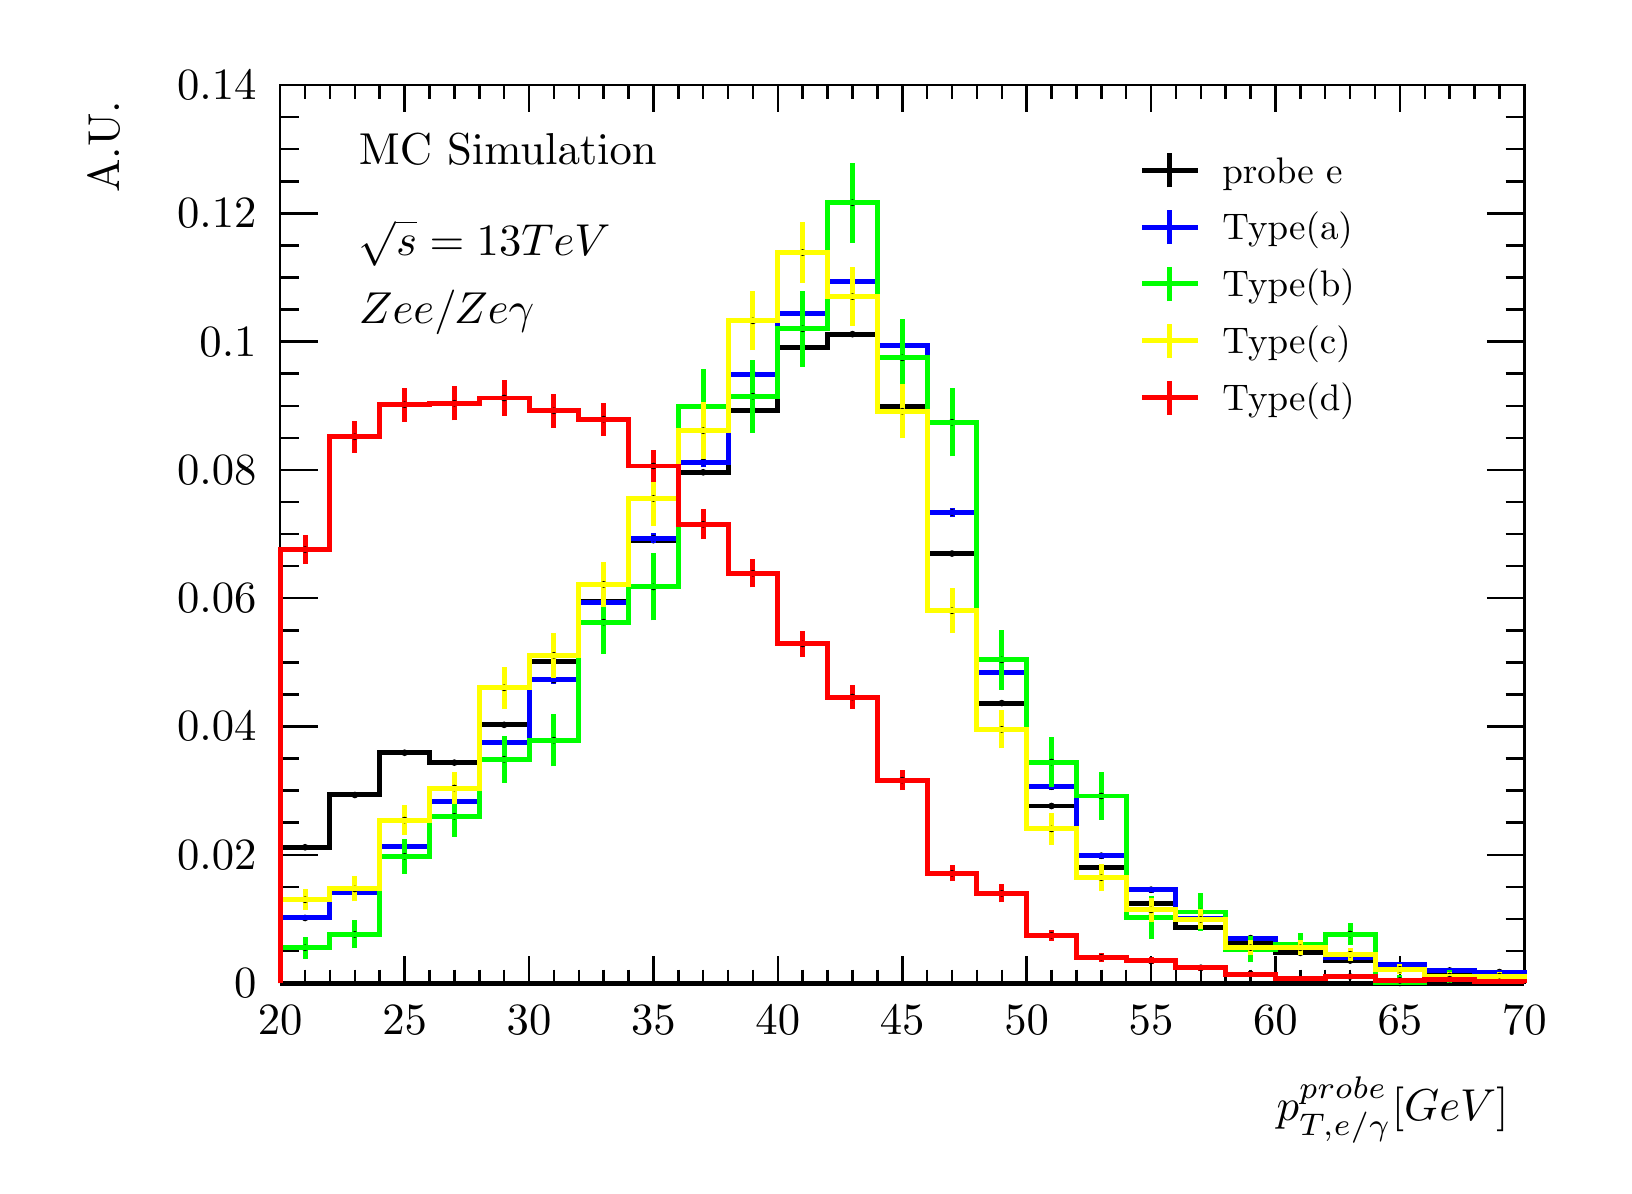
\begin{tikzpicture}
\pgfdeclareplotmark{cross} {
\pgfpathmoveto{\pgfpoint{-0.3\pgfplotmarksize}{\pgfplotmarksize}}
\pgfpathlineto{\pgfpoint{+0.3\pgfplotmarksize}{\pgfplotmarksize}}
\pgfpathlineto{\pgfpoint{+0.3\pgfplotmarksize}{0.3\pgfplotmarksize}}
\pgfpathlineto{\pgfpoint{+1\pgfplotmarksize}{0.3\pgfplotmarksize}}
\pgfpathlineto{\pgfpoint{+1\pgfplotmarksize}{-0.3\pgfplotmarksize}}
\pgfpathlineto{\pgfpoint{+0.3\pgfplotmarksize}{-0.3\pgfplotmarksize}}
\pgfpathlineto{\pgfpoint{+0.3\pgfplotmarksize}{-1.\pgfplotmarksize}}
\pgfpathlineto{\pgfpoint{-0.3\pgfplotmarksize}{-1.\pgfplotmarksize}}
\pgfpathlineto{\pgfpoint{-0.3\pgfplotmarksize}{-0.3\pgfplotmarksize}}
\pgfpathlineto{\pgfpoint{-1.\pgfplotmarksize}{-0.3\pgfplotmarksize}}
\pgfpathlineto{\pgfpoint{-1.\pgfplotmarksize}{0.3\pgfplotmarksize}}
\pgfpathlineto{\pgfpoint{-0.3\pgfplotmarksize}{0.3\pgfplotmarksize}}
\pgfpathclose
\pgfusepathqstroke
}
\pgfdeclareplotmark{cross*} {
\pgfpathmoveto{\pgfpoint{-0.3\pgfplotmarksize}{\pgfplotmarksize}}
\pgfpathlineto{\pgfpoint{+0.3\pgfplotmarksize}{\pgfplotmarksize}}
\pgfpathlineto{\pgfpoint{+0.3\pgfplotmarksize}{0.3\pgfplotmarksize}}
\pgfpathlineto{\pgfpoint{+1\pgfplotmarksize}{0.3\pgfplotmarksize}}
\pgfpathlineto{\pgfpoint{+1\pgfplotmarksize}{-0.3\pgfplotmarksize}}
\pgfpathlineto{\pgfpoint{+0.3\pgfplotmarksize}{-0.3\pgfplotmarksize}}
\pgfpathlineto{\pgfpoint{+0.3\pgfplotmarksize}{-1.\pgfplotmarksize}}
\pgfpathlineto{\pgfpoint{-0.3\pgfplotmarksize}{-1.\pgfplotmarksize}}
\pgfpathlineto{\pgfpoint{-0.3\pgfplotmarksize}{-0.3\pgfplotmarksize}}
\pgfpathlineto{\pgfpoint{-1.\pgfplotmarksize}{-0.3\pgfplotmarksize}}
\pgfpathlineto{\pgfpoint{-1.\pgfplotmarksize}{0.3\pgfplotmarksize}}
\pgfpathlineto{\pgfpoint{-0.3\pgfplotmarksize}{0.3\pgfplotmarksize}}
\pgfpathclose
\pgfusepathqfillstroke
}
\pgfdeclareplotmark{newstar} {
\pgfpathmoveto{\pgfqpoint{0pt}{\pgfplotmarksize}}
\pgfpathlineto{\pgfqpointpolar{44}{0.5\pgfplotmarksize}}
\pgfpathlineto{\pgfqpointpolar{18}{\pgfplotmarksize}}
\pgfpathlineto{\pgfqpointpolar{-20}{0.5\pgfplotmarksize}}
\pgfpathlineto{\pgfqpointpolar{-54}{\pgfplotmarksize}}
\pgfpathlineto{\pgfqpointpolar{-90}{0.5\pgfplotmarksize}}
\pgfpathlineto{\pgfqpointpolar{234}{\pgfplotmarksize}}
\pgfpathlineto{\pgfqpointpolar{198}{0.5\pgfplotmarksize}}
\pgfpathlineto{\pgfqpointpolar{162}{\pgfplotmarksize}}
\pgfpathlineto{\pgfqpointpolar{134}{0.5\pgfplotmarksize}}
\pgfpathclose
\pgfusepathqstroke
}
\pgfdeclareplotmark{newstar*} {
\pgfpathmoveto{\pgfqpoint{0pt}{\pgfplotmarksize}}
\pgfpathlineto{\pgfqpointpolar{44}{0.5\pgfplotmarksize}}
\pgfpathlineto{\pgfqpointpolar{18}{\pgfplotmarksize}}
\pgfpathlineto{\pgfqpointpolar{-20}{0.5\pgfplotmarksize}}
\pgfpathlineto{\pgfqpointpolar{-54}{\pgfplotmarksize}}
\pgfpathlineto{\pgfqpointpolar{-90}{0.5\pgfplotmarksize}}
\pgfpathlineto{\pgfqpointpolar{234}{\pgfplotmarksize}}
\pgfpathlineto{\pgfqpointpolar{198}{0.5\pgfplotmarksize}}
\pgfpathlineto{\pgfqpointpolar{162}{\pgfplotmarksize}}
\pgfpathlineto{\pgfqpointpolar{134}{0.5\pgfplotmarksize}}
\pgfpathclose
\pgfusepathqfillstroke
}
\definecolor{c}{rgb}{1,1,1};
\draw [color=c, fill=c] (0,0) rectangle (20,14.4361);
\draw [color=c, fill=c] (3.2,2.30977) rectangle (19,13.7143);
\definecolor{c}{rgb}{0,0,0};
\draw [c,line width=0.9] (3.2,2.30977) -- (3.2,13.7143) -- (19,13.7143) -- (19,2.30977) -- (3.2,2.30977);
\draw [c,line width=1.8] (3.2,2.30977) -- (3.2158,2.30977) -- (3.2158,2.30977) -- (3.2316,2.30977) -- (3.2316,2.30977) -- (3.2474,2.30977) -- (3.2474,2.30977) -- (3.2632,2.30977) -- (3.2632,2.30977) -- (3.279,2.30977) -- (3.279,2.30977) --
 (3.2948,2.30977) -- (3.2948,2.30977) -- (3.3106,2.30977) -- (3.3106,2.30977) -- (3.3264,2.30977) -- (3.3264,2.30977) -- (3.3422,2.30977) -- (3.3422,2.30977) -- (3.358,2.30977) -- (3.358,2.30977) -- (3.3738,2.30977) -- (3.3738,2.30977) --
 (3.3896,2.30977) -- (3.3896,2.30977) -- (3.4054,2.30977) -- (3.4054,2.30977) -- (3.4212,2.30977) -- (3.4212,2.30977) -- (3.437,2.30977) -- (3.437,2.30977) -- (3.4528,2.30977) -- (3.4528,2.30977) -- (3.4686,2.30977) -- (3.4686,2.30977) --
 (3.4844,2.30977) -- (3.4844,2.30977) -- (3.5002,2.30977) -- (3.5002,2.30977) -- (3.516,2.30977) -- (3.516,2.30977) -- (3.5318,2.30977) -- (3.5318,2.30977) -- (3.5476,2.30977) -- (3.5476,2.30977) -- (3.5634,2.30977) -- (3.5634,2.30977) --
 (3.5792,2.30977) -- (3.5792,2.30977) -- (3.595,2.30977) -- (3.595,2.30977) -- (3.6108,2.30977) -- (3.6108,2.30977) -- (3.6266,2.30977) -- (3.6266,2.30977) -- (3.6424,2.30977) -- (3.6424,2.30977) -- (3.6582,2.30977) -- (3.6582,2.30977) --
 (3.674,2.30977) -- (3.674,2.30977) -- (3.6898,2.30977) -- (3.6898,2.30977) -- (3.7056,2.30977) -- (3.7056,2.30977) -- (3.7214,2.30977) -- (3.7214,2.30977) -- (3.7372,2.30977) -- (3.7372,2.30977) -- (3.753,2.30977) -- (3.753,2.30977) --
 (3.7688,2.30977) -- (3.7688,2.30977) -- (3.7846,2.30977) -- (3.7846,2.30977) -- (3.8004,2.30977) -- (3.8004,2.30977) -- (3.8162,2.30977) -- (3.8162,2.30977) -- (3.832,2.30977) -- (3.832,2.30977) -- (3.8478,2.30977) -- (3.8478,2.30977) --
 (3.8636,2.30977) -- (3.8636,2.30977) -- (3.8794,2.30977) -- (3.8794,2.30977) -- (3.8952,2.30977) -- (3.8952,2.30977) -- (3.911,2.30977) -- (3.911,2.30977) -- (3.9268,2.30977) -- (3.9268,2.30977) -- (3.9426,2.30977) -- (3.9426,2.30977) --
 (3.9584,2.30977) -- (3.9584,2.30977) -- (3.9742,2.30977) -- (3.9742,2.30977) -- (3.99,2.30977) -- (3.99,2.30977) -- (4.0058,2.30977) -- (4.0058,2.30977) -- (4.0216,2.30977) -- (4.0216,2.30977) -- (4.0374,2.30977) -- (4.0374,2.30977) --
 (4.0532,2.30977) -- (4.0532,2.30977) -- (4.069,2.30977) -- (4.069,2.30977) -- (4.0848,2.30977) -- (4.0848,2.30977) -- (4.1006,2.30977) -- (4.1006,2.30977) -- (4.1164,2.30977) -- (4.1164,2.30977) -- (4.1322,2.30977) -- (4.1322,2.30977) --
 (4.148,2.30977) -- (4.148,2.30977) -- (4.1638,2.30977) -- (4.1638,2.30977) -- (4.1796,2.30977) -- (4.1796,2.30977) -- (4.1954,2.30977) -- (4.1954,2.30977) -- (4.2112,2.30977) -- (4.2112,2.30977) -- (4.227,2.30977) -- (4.227,2.30977) --
 (4.2428,2.30977) -- (4.2428,2.30977) -- (4.2586,2.30977) -- (4.2586,2.30977) -- (4.2744,2.30977) -- (4.2744,2.30977) -- (4.2902,2.30977) -- (4.2902,2.30977) -- (4.306,2.30977) -- (4.306,2.30977) -- (4.3218,2.30977) -- (4.3218,2.30977) --
 (4.3376,2.30977) -- (4.3376,2.30977) -- (4.3534,2.30977) -- (4.3534,2.30977) -- (4.3692,2.30977) -- (4.3692,2.30977) -- (4.385,2.30977) -- (4.385,2.30977) -- (4.4008,2.30977) -- (4.4008,2.30977) -- (4.4166,2.30977) -- (4.4166,2.30977) --
 (4.4324,2.30977) -- (4.4324,2.30977) -- (4.4482,2.30977) -- (4.4482,2.30977) -- (4.464,2.30977) -- (4.464,2.30977) -- (4.4798,2.30977) -- (4.4798,2.30977) -- (4.4956,2.30977) -- (4.4956,2.30977) -- (4.5114,2.30977) -- (4.5114,2.30977) --
 (4.5272,2.30977) -- (4.5272,2.30977) -- (4.543,2.30977) -- (4.543,2.30977) -- (4.5588,2.30977) -- (4.5588,2.30977) -- (4.5746,2.30977) -- (4.5746,2.30977) -- (4.5904,2.30977) -- (4.5904,2.30977) -- (4.6062,2.30977) -- (4.6062,2.30977) --
 (4.622,2.30977) -- (4.622,2.30977) -- (4.6378,2.30977) -- (4.6378,2.30977) -- (4.6536,2.30977) -- (4.6536,2.30977) -- (4.6694,2.30977) -- (4.6694,2.30977) -- (4.6852,2.30977) -- (4.6852,2.30977) -- (4.701,2.30977) -- (4.701,2.30977) --
 (4.7168,2.30977) -- (4.7168,2.30977) -- (4.7326,2.30977) -- (4.7326,2.30977) -- (4.7484,2.30977) -- (4.7484,2.30977) -- (4.7642,2.30977) -- (4.7642,2.30977) -- (4.78,2.30977) -- (4.78,2.30977) -- (4.7958,2.30977) -- (4.7958,2.30977) --
 (4.8116,2.30977) -- (4.8116,2.30977) -- (4.8274,2.30977) -- (4.8274,2.30977) -- (4.8432,2.30977) -- (4.8432,2.30977) -- (4.859,2.30977) -- (4.859,2.30977) -- (4.8748,2.30977) -- (4.8748,2.30977) -- (4.8906,2.30977) -- (4.8906,2.30977) --
 (4.9064,2.30977) -- (4.9064,2.30977) -- (4.9222,2.30977) -- (4.9222,2.30977) -- (4.938,2.30977) -- (4.938,2.30977) -- (4.9538,2.30977) -- (4.9538,2.30977) -- (4.9696,2.30977) -- (4.9696,2.30977) -- (4.9854,2.30977) -- (4.9854,2.30977) --
 (5.0012,2.30977) -- (5.0012,2.30977) -- (5.017,2.30977) -- (5.017,2.30977) -- (5.0328,2.30977) -- (5.0328,2.30977) -- (5.0486,2.30977) -- (5.0486,2.30977) -- (5.0644,2.30977) -- (5.0644,2.30977) -- (5.0802,2.30977) -- (5.0802,2.30977) --
 (5.096,2.30977) -- (5.096,2.30977) -- (5.1118,2.30977) -- (5.1118,2.30977) -- (5.1276,2.30977) -- (5.1276,2.30977) -- (5.1434,2.30977) -- (5.1434,2.30977) -- (5.1592,2.30977) -- (5.1592,2.30977) -- (5.175,2.30977) -- (5.175,2.30977) --
 (5.1908,2.30977) -- (5.1908,2.30977) -- (5.2066,2.30977) -- (5.2066,2.30977) -- (5.2224,2.30977) -- (5.2224,2.30977) -- (5.2382,2.30977) -- (5.2382,2.30977) -- (5.254,2.30977) -- (5.254,2.30977) -- (5.2698,2.30977) -- (5.2698,2.30977) --
 (5.2856,2.30977) -- (5.2856,2.30977) -- (5.3014,2.30977) -- (5.3014,2.30977) -- (5.3172,2.30977) -- (5.3172,2.30977) -- (5.333,2.30977) -- (5.333,2.30977) -- (5.3488,2.30977) -- (5.3488,2.30977) -- (5.3646,2.30977) -- (5.3646,2.30977) --
 (5.3804,2.30977) -- (5.3804,2.30977) -- (5.3962,2.30977) -- (5.3962,2.30977) -- (5.412,2.30977) -- (5.412,2.30977) -- (5.4278,2.30977) -- (5.4278,2.30977) -- (5.4436,2.30977) -- (5.4436,2.30977) -- (5.4594,2.30977) -- (5.4594,2.30977) --
 (5.4752,2.30977) -- (5.4752,2.30977) -- (5.491,2.30977) -- (5.491,2.30977) -- (5.5068,2.30977) -- (5.5068,2.30977) -- (5.5226,2.30977) -- (5.5226,2.30977) -- (5.5384,2.30977) -- (5.5384,2.30977) -- (5.5542,2.30977) -- (5.5542,2.30977) --
 (5.57,2.30977) -- (5.57,2.30977) -- (5.5858,2.30977) -- (5.5858,2.30977) -- (5.6016,2.30977) -- (5.6016,2.30977) -- (5.6174,2.30977) -- (5.6174,2.30977) -- (5.6332,2.30977) -- (5.6332,2.30977) -- (5.649,2.30977) -- (5.649,2.30977) --
 (5.6648,2.30977) -- (5.6648,2.30977) -- (5.6806,2.30977) -- (5.6806,2.30977) -- (5.6964,2.30977) -- (5.6964,2.30977) -- (5.7122,2.30977) -- (5.7122,2.30977) -- (5.728,2.30977) -- (5.728,2.30977) -- (5.7438,2.30977) -- (5.7438,2.30977) --
 (5.7596,2.30977) -- (5.7596,2.30977) -- (5.7754,2.30977) -- (5.7754,2.30977) -- (5.7912,2.30977) -- (5.7912,2.30977) -- (5.807,2.30977) -- (5.807,2.30977) -- (5.8228,2.30977) -- (5.8228,2.30977) -- (5.8386,2.30977) -- (5.8386,2.30977) --
 (5.8544,2.30977) -- (5.8544,2.30977) -- (5.8702,2.30977) -- (5.8702,2.30977) -- (5.886,2.30977) -- (5.886,2.30977) -- (5.9018,2.30977) -- (5.9018,2.30977) -- (5.9176,2.30977) -- (5.9176,2.30977) -- (5.9334,2.30977) -- (5.9334,2.30977) --
 (5.9492,2.30977) -- (5.9492,2.30977) -- (5.965,2.30977) -- (5.965,2.30977) -- (5.9808,2.30977) -- (5.9808,2.30977) -- (5.9966,2.30977) -- (5.9966,2.30977) -- (6.0124,2.30977) -- (6.0124,2.30977) -- (6.0282,2.30977) -- (6.0282,2.30977) --
 (6.044,2.30977) -- (6.044,2.30977) -- (6.0598,2.30977) -- (6.0598,2.30977) -- (6.0756,2.30977) -- (6.0756,2.30977) -- (6.0914,2.30977) -- (6.0914,2.30977) -- (6.1072,2.30977) -- (6.1072,2.30977) -- (6.123,2.30977) -- (6.123,2.30977) --
 (6.1388,2.30977) -- (6.1388,2.30977) -- (6.1546,2.30977) -- (6.1546,2.30977) -- (6.1704,2.30977) -- (6.1704,2.30977) -- (6.1862,2.30977) -- (6.1862,2.30977) -- (6.202,2.30977) -- (6.202,2.30977) -- (6.2178,2.30977) -- (6.2178,2.30977) --
 (6.2336,2.30977) -- (6.2336,2.30977) -- (6.2494,2.30977) -- (6.2494,2.30977) -- (6.2652,2.30977) -- (6.2652,2.30977) -- (6.281,2.30977) -- (6.281,2.30977) -- (6.2968,2.30977) -- (6.2968,2.30977) -- (6.3126,2.30977) -- (6.3126,2.30977) --
 (6.3284,2.30977) -- (6.3284,2.30977) -- (6.3442,2.30977) -- (6.3442,2.30977) -- (6.36,2.30977) -- (6.36,2.30977) -- (6.3758,2.30977) -- (6.3758,2.30977) -- (6.3916,2.30977) -- (6.3916,2.30977) -- (6.4074,2.30977) -- (6.4074,2.30977) --
 (6.4232,2.30977) -- (6.4232,2.30977) -- (6.439,2.30977) -- (6.439,2.30977) -- (6.4548,2.30977) -- (6.4548,2.30977) -- (6.4706,2.30977) -- (6.4706,2.30977) -- (6.4864,2.30977) -- (6.4864,2.30977) -- (6.5022,2.30977) -- (6.5022,2.30977) --
 (6.518,2.30977) -- (6.518,2.30977) -- (6.5338,2.30977) -- (6.5338,2.30977) -- (6.5496,2.30977) -- (6.5496,2.30977) -- (6.5654,2.30977) -- (6.5654,2.30977) -- (6.5812,2.30977) -- (6.5812,2.30977) -- (6.597,2.30977) -- (6.597,2.30977) --
 (6.6128,2.30977) -- (6.6128,2.30977) -- (6.6286,2.30977) -- (6.6286,2.30977) -- (6.6444,2.30977) -- (6.6444,2.30977) -- (6.6602,2.30977) -- (6.6602,2.30977) -- (6.676,2.30977) -- (6.676,2.30977) -- (6.6918,2.30977) -- (6.6918,2.30977) --
 (6.7076,2.30977) -- (6.7076,2.30977) -- (6.7234,2.30977) -- (6.7234,2.30977) -- (6.7392,2.30977) -- (6.7392,2.30977) -- (6.755,2.30977) -- (6.755,2.30977) -- (6.7708,2.30977) -- (6.7708,2.30977) -- (6.7866,2.30977) -- (6.7866,2.30977) --
 (6.8024,2.30977) -- (6.8024,2.30977) -- (6.8182,2.30977) -- (6.8182,2.30977) -- (6.834,2.30977) -- (6.834,2.30977) -- (6.8498,2.30977) -- (6.8498,2.30977) -- (6.8656,2.30977) -- (6.8656,2.30977) -- (6.8814,2.30977) -- (6.8814,2.30977) --
 (6.8972,2.30977) -- (6.8972,2.30977) -- (6.913,2.30977) -- (6.913,2.30977) -- (6.9288,2.30977) -- (6.9288,2.30977) -- (6.9446,2.30977) -- (6.9446,2.30977) -- (6.9604,2.30977) -- (6.9604,2.30977) -- (6.9762,2.30977) -- (6.9762,2.30977) --
 (6.992,2.30977) -- (6.992,2.30977) -- (7.0078,2.30977) -- (7.0078,2.30977) -- (7.0236,2.30977) -- (7.0236,2.30977) -- (7.0394,2.30977) -- (7.0394,2.30977) -- (7.0552,2.30977) -- (7.0552,2.30977) -- (7.071,2.30977) -- (7.071,2.30977) --
 (7.0868,2.30977) -- (7.0868,2.30977) -- (7.1026,2.30977) -- (7.1026,2.30977) -- (7.1184,2.30977) -- (7.1184,2.30977) -- (7.1342,2.30977) -- (7.1342,2.30977) -- (7.15,2.30977) -- (7.15,2.30977) -- (7.1658,2.30977) -- (7.1658,2.30977) --
 (7.1816,2.30977) -- (7.1816,2.30977) -- (7.1974,2.30977) -- (7.1974,2.30977) -- (7.2132,2.30977) -- (7.2132,2.30977) -- (7.229,2.30977) -- (7.229,2.30977) -- (7.2448,2.30977) -- (7.2448,2.30977) -- (7.2606,2.30977) -- (7.2606,2.30977) --
 (7.2764,2.30977) -- (7.2764,2.30977) -- (7.2922,2.30977) -- (7.2922,2.30977) -- (7.308,2.30977) -- (7.308,2.30977) -- (7.3238,2.30977) -- (7.3238,2.30977) -- (7.3396,2.30977) -- (7.3396,2.30977) -- (7.3554,2.30977) -- (7.3554,2.30977) --
 (7.3712,2.30977) -- (7.3712,2.30977) -- (7.387,2.30977) -- (7.387,2.30977) -- (7.4028,2.30977) -- (7.4028,2.30977) -- (7.4186,2.30977) -- (7.4186,2.30977) -- (7.4344,2.30977) -- (7.4344,2.30977) -- (7.4502,2.30977) -- (7.4502,2.30977) --
 (7.466,2.30977) -- (7.466,2.30977) -- (7.4818,2.30977) -- (7.4818,2.30977) -- (7.4976,2.30977) -- (7.4976,2.30977) -- (7.5134,2.30977) -- (7.5134,2.30977) -- (7.5292,2.30977) -- (7.5292,2.30977) -- (7.545,2.30977) -- (7.545,2.30977) --
 (7.5608,2.30977) -- (7.5608,2.30977) -- (7.5766,2.30977) -- (7.5766,2.30977) -- (7.5924,2.30977) -- (7.5924,2.30977) -- (7.6082,2.30977) -- (7.6082,2.30977) -- (7.624,2.30977) -- (7.624,2.30977) -- (7.6398,2.30977) -- (7.6398,2.30977) --
 (7.6556,2.30977) -- (7.6556,2.30977) -- (7.6714,2.30977) -- (7.6714,2.30977) -- (7.6872,2.30977) -- (7.6872,2.30977) -- (7.703,2.30977) -- (7.703,2.30977) -- (7.7188,2.30977) -- (7.7188,2.30977) -- (7.7346,2.30977) -- (7.7346,2.30977) --
 (7.7504,2.30977) -- (7.7504,2.30977) -- (7.7662,2.30977) -- (7.7662,2.30977) -- (7.782,2.30977) -- (7.782,2.30977) -- (7.7978,2.30977) -- (7.7978,2.30977) -- (7.8136,2.30977) -- (7.8136,2.30977) -- (7.8294,2.30977) -- (7.8294,2.30977) --
 (7.8452,2.30977) -- (7.8452,2.30977) -- (7.861,2.30977) -- (7.861,2.30977) -- (7.8768,2.30977) -- (7.8768,2.30977) -- (7.8926,2.30977) -- (7.8926,2.30977) -- (7.9084,2.30977) -- (7.9084,2.30977) -- (7.9242,2.30977) -- (7.9242,2.30977) --
 (7.94,2.30977) -- (7.94,2.30977) -- (7.9558,2.30977) -- (7.9558,2.30977) -- (7.9716,2.30977) -- (7.9716,2.30977) -- (7.9874,2.30977) -- (7.9874,2.30977) -- (8.0032,2.30977) -- (8.0032,2.30977) -- (8.019,2.30977) -- (8.019,2.30977) --
 (8.0348,2.30977) -- (8.0348,2.30977) -- (8.0506,2.30977) -- (8.0506,2.30977) -- (8.0664,2.30977) -- (8.0664,2.30977) -- (8.0822,2.30977) -- (8.0822,2.30977) -- (8.098,2.30977) -- (8.098,2.30977) -- (8.1138,2.30977) -- (8.1138,2.30977) --
 (8.1296,2.30977) -- (8.1296,2.30977) -- (8.1454,2.30977) -- (8.1454,2.30977) -- (8.1612,2.30977) -- (8.1612,2.30977) -- (8.177,2.30977) -- (8.177,2.30977) -- (8.1928,2.30977) -- (8.1928,2.30977) -- (8.2086,2.30977) -- (8.2086,2.30977) --
 (8.2244,2.30977) -- (8.2244,2.30977) -- (8.2402,2.30977) -- (8.2402,2.30977) -- (8.256,2.30977) -- (8.256,2.30977) -- (8.2718,2.30977) -- (8.2718,2.30977) -- (8.2876,2.30977) -- (8.2876,2.30977) -- (8.3034,2.30977) -- (8.3034,2.30977) --
 (8.3192,2.30977) -- (8.3192,2.30977) -- (8.335,2.30977) -- (8.335,2.30977) -- (8.3508,2.30977) -- (8.3508,2.30977) -- (8.3666,2.30977) -- (8.3666,2.30977) -- (8.3824,2.30977) -- (8.3824,2.30977) -- (8.3982,2.30977) -- (8.3982,2.30977) --
 (8.414,2.30977) -- (8.414,2.30977) -- (8.4298,2.30977) -- (8.4298,2.30977) -- (8.4456,2.30977) -- (8.4456,2.30977) -- (8.4614,2.30977) -- (8.4614,2.30977) -- (8.4772,2.30977) -- (8.4772,2.30977) -- (8.493,2.30977) -- (8.493,2.30977) --
 (8.5088,2.30977) -- (8.5088,2.30977) -- (8.5246,2.30977) -- (8.5246,2.30977) -- (8.5404,2.30977) -- (8.5404,2.30977) -- (8.5562,2.30977) -- (8.5562,2.30977) -- (8.572,2.30977) -- (8.572,2.30977) -- (8.5878,2.30977) -- (8.5878,2.30977) --
 (8.6036,2.30977) -- (8.6036,2.30977) -- (8.6194,2.30977) -- (8.6194,2.30977) -- (8.6352,2.30977) -- (8.6352,2.30977) -- (8.651,2.30977) -- (8.651,2.30977) -- (8.6668,2.30977) -- (8.6668,2.30977) -- (8.6826,2.30977) -- (8.6826,2.30977) --
 (8.6984,2.30977) -- (8.6984,2.30977) -- (8.7142,2.30977) -- (8.7142,2.30977) -- (8.73,2.30977) -- (8.73,2.30977) -- (8.7458,2.30977) -- (8.7458,2.30977) -- (8.7616,2.30977) -- (8.7616,2.30977) -- (8.7774,2.30977) -- (8.7774,2.30977) --
 (8.7932,2.30977) -- (8.7932,2.30977) -- (8.809,2.30977) -- (8.809,2.30977) -- (8.8248,2.30977) -- (8.8248,2.30977) -- (8.8406,2.30977) -- (8.8406,2.30977) -- (8.8564,2.30977) -- (8.8564,2.30977) -- (8.8722,2.30977) -- (8.8722,2.30977) --
 (8.888,2.30977) -- (8.888,2.30977) -- (8.9038,2.30977) -- (8.9038,2.30977) -- (8.9196,2.30977) -- (8.9196,2.30977) -- (8.9354,2.30977) -- (8.9354,2.30977) -- (8.9512,2.30977) -- (8.9512,2.30977) -- (8.967,2.30977) -- (8.967,2.30977) --
 (8.9828,2.30977) -- (8.9828,2.30977) -- (8.9986,2.30977) -- (8.9986,2.30977) -- (9.0144,2.30977) -- (9.0144,2.30977) -- (9.0302,2.30977) -- (9.0302,2.30977) -- (9.046,2.30977) -- (9.046,2.30977) -- (9.0618,2.30977) -- (9.0618,2.30977) --
 (9.0776,2.30977) -- (9.0776,2.30977) -- (9.0934,2.30977) -- (9.0934,2.30977) -- (9.1092,2.30977) -- (9.1092,2.30977) -- (9.125,2.30977) -- (9.125,2.30977) -- (9.1408,2.30977) -- (9.1408,2.30977) -- (9.1566,2.30977) -- (9.1566,2.30977) --
 (9.1724,2.30977) -- (9.1724,2.30977) -- (9.1882,2.30977) -- (9.1882,2.30977) -- (9.204,2.30977) -- (9.204,2.30977) -- (9.2198,2.30977) -- (9.2198,2.30977) -- (9.2356,2.30977) -- (9.2356,2.30977) -- (9.2514,2.30977) -- (9.2514,2.30977) --
 (9.2672,2.30977) -- (9.2672,2.30977) -- (9.283,2.30977) -- (9.283,2.30977) -- (9.2988,2.30977) -- (9.2988,2.30977) -- (9.3146,2.30977) -- (9.3146,2.30977) -- (9.3304,2.30977) -- (9.3304,2.30977) -- (9.3462,2.30977) -- (9.3462,2.30977) --
 (9.362,2.30977) -- (9.362,2.30977) -- (9.3778,2.30977) -- (9.3778,2.30977) -- (9.3936,2.30977) -- (9.3936,2.30977) -- (9.4094,2.30977) -- (9.4094,2.30977) -- (9.4252,2.30977) -- (9.4252,2.30977) -- (9.441,2.30977) -- (9.441,2.30977) --
 (9.4568,2.30977) -- (9.4568,2.30977) -- (9.4726,2.30977) -- (9.4726,2.30977) -- (9.4884,2.30977) -- (9.4884,2.30977) -- (9.5042,2.30977) -- (9.5042,2.30977) -- (9.52,2.30977) -- (9.52,2.30977) -- (9.5358,2.30977) -- (9.5358,2.30977) --
 (9.5516,2.30977) -- (9.5516,2.30977) -- (9.5674,2.30977) -- (9.5674,2.30977) -- (9.5832,2.30977) -- (9.5832,2.30977) -- (9.599,2.30977) -- (9.599,2.30977) -- (9.6148,2.30977) -- (9.6148,2.30977) -- (9.6306,2.30977) -- (9.6306,2.30977) --
 (9.6464,2.30977) -- (9.6464,2.30977) -- (9.6622,2.30977) -- (9.6622,2.30977) -- (9.678,2.30977) -- (9.678,2.30977) -- (9.6938,2.30977) -- (9.6938,2.30977) -- (9.7096,2.30977) -- (9.7096,2.30977) -- (9.7254,2.30977) -- (9.7254,2.30977) --
 (9.7412,2.30977) -- (9.7412,2.30977) -- (9.757,2.30977) -- (9.757,2.30977) -- (9.7728,2.30977) -- (9.7728,2.30977) -- (9.7886,2.30977) -- (9.7886,2.30977) -- (9.8044,2.30977) -- (9.8044,2.30977) -- (9.8202,2.30977) -- (9.8202,2.30977) --
 (9.836,2.30977) -- (9.836,2.30977) -- (9.8518,2.30977) -- (9.8518,2.30977) -- (9.8676,2.30977) -- (9.8676,2.30977) -- (9.8834,2.30977) -- (9.8834,2.30977) -- (9.8992,2.30977) -- (9.8992,2.30977) -- (9.915,2.30977) -- (9.915,2.30977) --
 (9.9308,2.30977) -- (9.9308,2.30977) -- (9.9466,2.30977) -- (9.9466,2.30977) -- (9.9624,2.30977) -- (9.9624,2.30977) -- (9.9782,2.30977) -- (9.9782,2.30977) -- (9.994,2.30977) -- (9.994,2.30977) -- (10.0098,2.30977) -- (10.0098,2.30977) --
 (10.0256,2.30977) -- (10.0256,2.30977) -- (10.0414,2.30977) -- (10.0414,2.30977) -- (10.0572,2.30977) -- (10.0572,2.30977) -- (10.073,2.30977) -- (10.073,2.30977) -- (10.0888,2.30977) -- (10.0888,2.30977) -- (10.1046,2.30977) -- (10.1046,2.30977) --
 (10.1204,2.30977) -- (10.1204,2.30977) -- (10.1362,2.30977) -- (10.1362,2.30977) -- (10.152,2.30977) -- (10.152,2.30977) -- (10.1678,2.30977) -- (10.1678,2.30977) -- (10.1836,2.30977) -- (10.1836,2.30977) -- (10.1994,2.30977) -- (10.1994,2.30977) --
 (10.2152,2.30977) -- (10.2152,2.30977) -- (10.231,2.30977) -- (10.231,2.30977) -- (10.2468,2.30977) -- (10.2468,2.30977) -- (10.2626,2.30977) -- (10.2626,2.30977) -- (10.2784,2.30977) -- (10.2784,2.30977) -- (10.2942,2.30977) -- (10.2942,2.30977) --
 (10.31,2.30977) -- (10.31,2.30977) -- (10.3258,2.30977) -- (10.3258,2.30977) -- (10.3416,2.30977) -- (10.3416,2.30977) -- (10.3574,2.30977) -- (10.3574,2.30977) -- (10.3732,2.30977) -- (10.3732,2.30977) -- (10.389,2.30977) -- (10.389,2.30977) --
 (10.4048,2.30977) -- (10.4048,2.30977) -- (10.4206,2.30977) -- (10.4206,2.30977) -- (10.4364,2.30977) -- (10.4364,2.30977) -- (10.4522,2.30977) -- (10.4522,2.30977) -- (10.468,2.30977) -- (10.468,2.30977) -- (10.4838,2.30977) -- (10.4838,2.30977) --
 (10.4996,2.30977) -- (10.4996,2.30977) -- (10.5154,2.30977) -- (10.5154,2.30977) -- (10.5312,2.30977) -- (10.5312,2.30977) -- (10.547,2.30977) -- (10.547,2.30977) -- (10.5628,2.30977) -- (10.5628,2.30977) -- (10.5786,2.30977) -- (10.5786,2.30977) --
 (10.5944,2.30977) -- (10.5944,2.30977) -- (10.6102,2.30977) -- (10.6102,2.30977) -- (10.626,2.30977) -- (10.626,2.30977) -- (10.6418,2.30977) -- (10.6418,2.30977) -- (10.6576,2.30977) -- (10.6576,2.30977) -- (10.6734,2.30977) -- (10.6734,2.30977) --
 (10.6892,2.30977) -- (10.6892,2.30977) -- (10.705,2.30977) -- (10.705,2.30977) -- (10.7208,2.30977) -- (10.7208,2.30977) -- (10.7366,2.30977) -- (10.7366,2.30977) -- (10.7524,2.30977) -- (10.7524,2.30977) -- (10.7682,2.30977) -- (10.7682,2.30977) --
 (10.784,2.30977) -- (10.784,2.30977) -- (10.7998,2.30977) -- (10.7998,2.30977) -- (10.8156,2.30977) -- (10.8156,2.30977) -- (10.8314,2.30977) -- (10.8314,2.30977) -- (10.8472,2.30977) -- (10.8472,2.30977) -- (10.863,2.30977) -- (10.863,2.30977) --
 (10.8788,2.30977) -- (10.8788,2.30977) -- (10.8946,2.30977) -- (10.8946,2.30977) -- (10.9104,2.30977) -- (10.9104,2.30977) -- (10.9262,2.30977) -- (10.9262,2.30977) -- (10.942,2.30977) -- (10.942,2.30977) -- (10.9578,2.30977) -- (10.9578,2.30977) --
 (10.9736,2.30977) -- (10.9736,2.30977) -- (10.9894,2.30977) -- (10.9894,2.30977) -- (11.0052,2.30977) -- (11.0052,2.30977) -- (11.021,2.30977) -- (11.021,2.30977) -- (11.0368,2.30977) -- (11.0368,2.30977) -- (11.0526,2.30977) -- (11.0526,2.30977) --
 (11.0684,2.30977) -- (11.0684,2.30977) -- (11.0842,2.30977) -- (11.0842,2.30977) -- (11.1,2.30977) -- (11.1,2.30977) -- (11.1158,2.30977) -- (11.1158,2.30977) -- (11.1316,2.30977) -- (11.1316,2.30977) -- (11.1474,2.30977) -- (11.1474,2.30977) --
 (11.1632,2.30977) -- (11.1632,2.30977) -- (11.179,2.30977) -- (11.179,2.30977) -- (11.1948,2.30977) -- (11.1948,2.30977) -- (11.2106,2.30977) -- (11.2106,2.30977) -- (11.2264,2.30977) -- (11.2264,2.30977) -- (11.2422,2.30977) -- (11.2422,2.30977) --
 (11.258,2.30977) -- (11.258,2.30977) -- (11.2738,2.30977) -- (11.2738,2.30977) -- (11.2896,2.30977) -- (11.2896,2.30977) -- (11.3054,2.30977) -- (11.3054,2.30977) -- (11.3212,2.30977) -- (11.3212,2.30977) -- (11.337,2.30977) -- (11.337,2.30977) --
 (11.3528,2.30977) -- (11.3528,2.30977) -- (11.3686,2.30977) -- (11.3686,2.30977) -- (11.3844,2.30977) -- (11.3844,2.30977) -- (11.4002,2.30977) -- (11.4002,2.30977) -- (11.416,2.30977) -- (11.416,2.30977) -- (11.4318,2.30977) -- (11.4318,2.30977) --
 (11.4476,2.30977) -- (11.4476,2.30977) -- (11.4634,2.30977) -- (11.4634,2.30977) -- (11.4792,2.30977) -- (11.4792,2.30977) -- (11.495,2.30977) -- (11.495,2.30977) -- (11.5108,2.30977) -- (11.5108,2.30977) -- (11.5266,2.30977) -- (11.5266,2.30977) --
 (11.5424,2.30977) -- (11.5424,2.30977) -- (11.5582,2.30977) -- (11.5582,2.30977) -- (11.574,2.30977) -- (11.574,2.30977) -- (11.5898,2.30977) -- (11.5898,2.30977) -- (11.6056,2.30977) -- (11.6056,2.30977) -- (11.6214,2.30977) -- (11.6214,2.30977) --
 (11.6372,2.30977) -- (11.6372,2.30977) -- (11.653,2.30977) -- (11.653,2.30977) -- (11.6688,2.30977) -- (11.6688,2.30977) -- (11.6846,2.30977) -- (11.6846,2.30977) -- (11.7004,2.30977) -- (11.7004,2.30977) -- (11.7162,2.30977) -- (11.7162,2.30977) --
 (11.732,2.30977) -- (11.732,2.30977) -- (11.7478,2.30977) -- (11.7478,2.30977) -- (11.7636,2.30977) -- (11.7636,2.30977) -- (11.7794,2.30977) -- (11.7794,2.30977) -- (11.7952,2.30977) -- (11.7952,2.30977) -- (11.811,2.30977) -- (11.811,2.30977) --
 (11.8268,2.30977) -- (11.8268,2.30977) -- (11.8426,2.30977) -- (11.8426,2.30977) -- (11.8584,2.30977) -- (11.8584,2.30977) -- (11.8742,2.30977) -- (11.8742,2.30977) -- (11.89,2.30977) -- (11.89,2.30977) -- (11.9058,2.30977) -- (11.9058,2.30977) --
 (11.9216,2.30977) -- (11.9216,2.30977) -- (11.9374,2.30977) -- (11.9374,2.30977) -- (11.9532,2.30977) -- (11.9532,2.30977) -- (11.969,2.30977) -- (11.969,2.30977) -- (11.9848,2.30977) -- (11.9848,2.30977) -- (12.0006,2.30977) -- (12.0006,2.30977) --
 (12.0164,2.30977) -- (12.0164,2.30977) -- (12.0322,2.30977) -- (12.0322,2.30977) -- (12.048,2.30977) -- (12.048,2.30977) -- (12.0638,2.30977) -- (12.0638,2.30977) -- (12.0796,2.30977) -- (12.0796,2.30977) -- (12.0954,2.30977) -- (12.0954,2.30977) --
 (12.1112,2.30977) -- (12.1112,2.30977) -- (12.127,2.30977) -- (12.127,2.30977) -- (12.1428,2.30977) -- (12.1428,2.30977) -- (12.1586,2.30977) -- (12.1586,2.30977) -- (12.1744,2.30977) -- (12.1744,2.30977) -- (12.1902,2.30977) -- (12.1902,2.30977) --
 (12.206,2.30977) -- (12.206,2.30977) -- (12.2218,2.30977) -- (12.2218,2.30977) -- (12.2376,2.30977) -- (12.2376,2.30977) -- (12.2534,2.30977) -- (12.2534,2.30977) -- (12.2692,2.30977) -- (12.2692,2.30977) -- (12.285,2.30977) -- (12.285,2.30977) --
 (12.3008,2.30977) -- (12.3008,2.30977) -- (12.3166,2.30977) -- (12.3166,2.30977) -- (12.3324,2.30977) -- (12.3324,2.30977) -- (12.3482,2.30977) -- (12.3482,2.30977) -- (12.364,2.30977) -- (12.364,2.30977) -- (12.3798,2.30977) -- (12.3798,2.30977) --
 (12.3956,2.30977) -- (12.3956,2.30977) -- (12.4114,2.30977) -- (12.4114,2.30977) -- (12.4272,2.30977) -- (12.4272,2.30977) -- (12.443,2.30977) -- (12.443,2.30977) -- (12.4588,2.30977) -- (12.4588,2.30977) -- (12.4746,2.30977) -- (12.4746,2.30977) --
 (12.4904,2.30977) -- (12.4904,2.30977) -- (12.5062,2.30977) -- (12.5062,2.30977) -- (12.522,2.30977) -- (12.522,2.30977) -- (12.5378,2.30977) -- (12.5378,2.30977) -- (12.5536,2.30977) -- (12.5536,2.30977) -- (12.5694,2.30977) -- (12.5694,2.30977) --
 (12.5852,2.30977) -- (12.5852,2.30977) -- (12.601,2.30977) -- (12.601,2.30977) -- (12.6168,2.30977) -- (12.6168,2.30977) -- (12.6326,2.30977) -- (12.6326,2.30977) -- (12.6484,2.30977) -- (12.6484,2.30977) -- (12.6642,2.30977) -- (12.6642,2.30977) --
 (12.68,2.30977) -- (12.68,2.30977) -- (12.6958,2.30977) -- (12.6958,2.30977) -- (12.7116,2.30977) -- (12.7116,2.30977) -- (12.7274,2.30977) -- (12.7274,2.30977) -- (12.7432,2.30977) -- (12.7432,2.30977) -- (12.759,2.30977) -- (12.759,2.30977) --
 (12.7748,2.30977) -- (12.7748,2.30977) -- (12.7906,2.30977) -- (12.7906,2.30977) -- (12.8064,2.30977) -- (12.8064,2.30977) -- (12.8222,2.30977) -- (12.8222,2.30977) -- (12.838,2.30977) -- (12.838,2.30977) -- (12.8538,2.30977) -- (12.8538,2.30977) --
 (12.8696,2.30977) -- (12.8696,2.30977) -- (12.8854,2.30977) -- (12.8854,2.30977) -- (12.9012,2.30977) -- (12.9012,2.30977) -- (12.917,2.30977) -- (12.917,2.30977) -- (12.9328,2.30977) -- (12.9328,2.30977) -- (12.9486,2.30977) -- (12.9486,2.30977) --
 (12.9644,2.30977) -- (12.9644,2.30977) -- (12.9802,2.30977) -- (12.9802,2.30977) -- (12.996,2.30977) -- (12.996,2.30977) -- (13.0118,2.30977) -- (13.0118,2.30977) -- (13.0276,2.30977) -- (13.0276,2.30977) -- (13.0434,2.30977) -- (13.0434,2.30977) --
 (13.0592,2.30977) -- (13.0592,2.30977) -- (13.075,2.30977) -- (13.075,2.30977) -- (13.0908,2.30977) -- (13.0908,2.30977) -- (13.1066,2.30977) -- (13.1066,2.30977) -- (13.1224,2.30977) -- (13.1224,2.30977) -- (13.1382,2.30977) -- (13.1382,2.30977) --
 (13.154,2.30977) -- (13.154,2.30977) -- (13.1698,2.30977) -- (13.1698,2.30977) -- (13.1856,2.30977) -- (13.1856,2.30977) -- (13.2014,2.30977) -- (13.2014,2.30977) -- (13.2172,2.30977) -- (13.2172,2.30977) -- (13.233,2.30977) -- (13.233,2.30977) --
 (13.2488,2.30977) -- (13.2488,2.30977) -- (13.2646,2.30977) -- (13.2646,2.30977) -- (13.2804,2.30977) -- (13.2804,2.30977) -- (13.2962,2.30977) -- (13.2962,2.30977) -- (13.312,2.30977) -- (13.312,2.30977) -- (13.3278,2.30977) -- (13.3278,2.30977) --
 (13.3436,2.30977) -- (13.3436,2.30977) -- (13.3594,2.30977) -- (13.3594,2.30977) -- (13.3752,2.30977) -- (13.3752,2.30977) -- (13.391,2.30977) -- (13.391,2.30977) -- (13.4068,2.30977) -- (13.4068,2.30977) -- (13.4226,2.30977) -- (13.4226,2.30977) --
 (13.4384,2.30977) -- (13.4384,2.30977) -- (13.4542,2.30977) -- (13.4542,2.30977) -- (13.47,2.30977) -- (13.47,2.30977) -- (13.4858,2.30977) -- (13.4858,2.30977) -- (13.5016,2.30977) -- (13.5016,2.30977) -- (13.5174,2.30977) -- (13.5174,2.30977) --
 (13.5332,2.30977) -- (13.5332,2.30977) -- (13.549,2.30977) -- (13.549,2.30977) -- (13.5648,2.30977) -- (13.5648,2.30977) -- (13.5806,2.30977) -- (13.5806,2.30977) -- (13.5964,2.30977) -- (13.5964,2.30977) -- (13.6122,2.30977) -- (13.6122,2.30977) --
 (13.628,2.30977) -- (13.628,2.30977) -- (13.6438,2.30977) -- (13.6438,2.30977) -- (13.6596,2.30977) -- (13.6596,2.30977) -- (13.6754,2.30977) -- (13.6754,2.30977) -- (13.6912,2.30977) -- (13.6912,2.30977) -- (13.707,2.30977) -- (13.707,2.30977) --
 (13.7228,2.30977) -- (13.7228,2.30977) -- (13.7386,2.30977) -- (13.7386,2.30977) -- (13.7544,2.30977) -- (13.7544,2.30977) -- (13.7702,2.30977) -- (13.7702,2.30977) -- (13.786,2.30977) -- (13.786,2.30977) -- (13.8018,2.30977) -- (13.8018,2.30977) --
 (13.8176,2.30977) -- (13.8176,2.30977) -- (13.8334,2.30977) -- (13.8334,2.30977) -- (13.8492,2.30977) -- (13.8492,2.30977) -- (13.865,2.30977) -- (13.865,2.30977) -- (13.8808,2.30977) -- (13.8808,2.30977) -- (13.8966,2.30977) -- (13.8966,2.30977) --
 (13.9124,2.30977) -- (13.9124,2.30977) -- (13.9282,2.30977) -- (13.9282,2.30977) -- (13.944,2.30977) -- (13.944,2.30977) -- (13.9598,2.30977) -- (13.9598,2.30977) -- (13.9756,2.30977) -- (13.9756,2.30977) -- (13.9914,2.30977) -- (13.9914,2.30977) --
 (14.0072,2.30977) -- (14.0072,2.30977) -- (14.023,2.30977) -- (14.023,2.30977) -- (14.0388,2.30977) -- (14.0388,2.30977) -- (14.0546,2.30977) -- (14.0546,2.30977) -- (14.0704,2.30977) -- (14.0704,2.30977) -- (14.0862,2.30977) -- (14.0862,2.30977) --
 (14.102,2.30977) -- (14.102,2.30977) -- (14.1178,2.30977) -- (14.1178,2.30977) -- (14.1336,2.30977) -- (14.1336,2.30977) -- (14.1494,2.30977) -- (14.1494,2.30977) -- (14.1652,2.30977) -- (14.1652,2.30977) -- (14.181,2.30977) -- (14.181,2.30977) --
 (14.1968,2.30977) -- (14.1968,2.30977) -- (14.2126,2.30977) -- (14.2126,2.30977) -- (14.2284,2.30977) -- (14.2284,2.30977) -- (14.2442,2.30977) -- (14.2442,2.30977) -- (14.26,2.30977) -- (14.26,2.30977) -- (14.2758,2.30977) -- (14.2758,2.30977) --
 (14.2916,2.30977) -- (14.2916,2.30977) -- (14.3074,2.30977) -- (14.3074,2.30977) -- (14.3232,2.30977) -- (14.3232,2.30977) -- (14.339,2.30977) -- (14.339,2.30977) -- (14.3548,2.30977) -- (14.3548,2.30977) -- (14.3706,2.30977) -- (14.3706,2.30977) --
 (14.3864,2.30977) -- (14.3864,2.30977) -- (14.4022,2.30977) -- (14.4022,2.30977) -- (14.418,2.30977) -- (14.418,2.30977) -- (14.4338,2.30977) -- (14.4338,2.30977) -- (14.4496,2.30977) -- (14.4496,2.30977) -- (14.4654,2.30977) -- (14.4654,2.30977) --
 (14.4812,2.30977) -- (14.4812,2.30977) -- (14.497,2.30977) -- (14.497,2.30977) -- (14.5128,2.30977) -- (14.5128,2.30977) -- (14.5286,2.30977) -- (14.5286,2.30977) -- (14.5444,2.30977) -- (14.5444,2.30977) -- (14.5602,2.30977) -- (14.5602,2.30977) --
 (14.576,2.30977) -- (14.576,2.30977) -- (14.5918,2.30977) -- (14.5918,2.30977) -- (14.6076,2.30977) -- (14.6076,2.30977) -- (14.6234,2.30977) -- (14.6234,2.30977) -- (14.6392,2.30977) -- (14.6392,2.30977) -- (14.655,2.30977) -- (14.655,2.30977) --
 (14.6708,2.30977) -- (14.6708,2.30977) -- (14.6866,2.30977) -- (14.6866,2.30977) -- (14.7024,2.30977) -- (14.7024,2.30977) -- (14.7182,2.30977) -- (14.7182,2.30977) -- (14.734,2.30977) -- (14.734,2.30977) -- (14.7498,2.30977) -- (14.7498,2.30977) --
 (14.7656,2.30977) -- (14.7656,2.30977) -- (14.7814,2.30977) -- (14.7814,2.30977) -- (14.7972,2.30977) -- (14.7972,2.30977) -- (14.813,2.30977) -- (14.813,2.30977) -- (14.8288,2.30977) -- (14.8288,2.30977) -- (14.8446,2.30977) -- (14.8446,2.30977) --
 (14.8604,2.30977) -- (14.8604,2.30977) -- (14.8762,2.30977) -- (14.8762,2.30977) -- (14.892,2.30977) -- (14.892,2.30977) -- (14.9078,2.30977) -- (14.9078,2.30977) -- (14.9236,2.30977) -- (14.9236,2.30977) -- (14.9394,2.30977) -- (14.9394,2.30977) --
 (14.9552,2.30977) -- (14.9552,2.30977) -- (14.971,2.30977) -- (14.971,2.30977) -- (14.9868,2.30977) -- (14.9868,2.30977) -- (15.0026,2.30977) -- (15.0026,2.30977) -- (15.0184,2.30977) -- (15.0184,2.30977) -- (15.0342,2.30977) -- (15.0342,2.30977) --
 (15.05,2.30977) -- (15.05,2.30977) -- (15.0658,2.30977) -- (15.0658,2.30977) -- (15.0816,2.30977) -- (15.0816,2.30977) -- (15.0974,2.30977) -- (15.0974,2.30977) -- (15.1132,2.30977) -- (15.1132,2.30977) -- (15.129,2.30977) -- (15.129,2.30977) --
 (15.1448,2.30977) -- (15.1448,2.30977) -- (15.1606,2.30977) -- (15.1606,2.30977) -- (15.1764,2.30977) -- (15.1764,2.30977) -- (15.1922,2.30977) -- (15.1922,2.30977) -- (15.208,2.30977) -- (15.208,2.30977) -- (15.2238,2.30977) -- (15.2238,2.30977) --
 (15.2396,2.30977) -- (15.2396,2.30977) -- (15.2554,2.30977) -- (15.2554,2.30977) -- (15.2712,2.30977) -- (15.2712,2.30977) -- (15.287,2.30977) -- (15.287,2.30977) -- (15.3028,2.30977) -- (15.3028,2.30977) -- (15.3186,2.30977) -- (15.3186,2.30977) --
 (15.3344,2.30977) -- (15.3344,2.30977) -- (15.3502,2.30977) -- (15.3502,2.30977) -- (15.366,2.30977) -- (15.366,2.30977) -- (15.3818,2.30977) -- (15.3818,2.30977) -- (15.3976,2.30977) -- (15.3976,2.30977) -- (15.4134,2.30977) -- (15.4134,2.30977) --
 (15.4292,2.30977) -- (15.4292,2.30977) -- (15.445,2.30977) -- (15.445,2.30977) -- (15.4608,2.30977) -- (15.4608,2.30977) -- (15.4766,2.30977) -- (15.4766,2.30977) -- (15.4924,2.30977) -- (15.4924,2.30977) -- (15.5082,2.30977) -- (15.5082,2.30977) --
 (15.524,2.30977) -- (15.524,2.30977) -- (15.5398,2.30977) -- (15.5398,2.30977) -- (15.5556,2.30977) -- (15.5556,2.30977) -- (15.5714,2.30977) -- (15.5714,2.30977) -- (15.5872,2.30977) -- (15.5872,2.30977) -- (15.603,2.30977) -- (15.603,2.30977) --
 (15.6188,2.30977) -- (15.6188,2.30977) -- (15.6346,2.30977) -- (15.6346,2.30977) -- (15.6504,2.30977) -- (15.6504,2.30977) -- (15.6662,2.30977) -- (15.6662,2.30977) -- (15.682,2.30977) -- (15.682,2.30977) -- (15.6978,2.30977) -- (15.6978,2.30977) --
 (15.7136,2.30977) -- (15.7136,2.30977) -- (15.7294,2.30977) -- (15.7294,2.30977) -- (15.7452,2.30977) -- (15.7452,2.30977) -- (15.761,2.30977) -- (15.761,2.30977) -- (15.7768,2.30977) -- (15.7768,2.30977) -- (15.7926,2.30977) -- (15.7926,2.30977) --
 (15.8084,2.30977) -- (15.8084,2.30977) -- (15.8242,2.30977) -- (15.8242,2.30977) -- (15.84,2.30977) -- (15.84,2.30977) -- (15.8558,2.30977) -- (15.8558,2.30977) -- (15.8716,2.30977) -- (15.8716,2.30977) -- (15.8874,2.30977) -- (15.8874,2.30977) --
 (15.9032,2.30977) -- (15.9032,2.30977) -- (15.919,2.30977) -- (15.919,2.30977) -- (15.9348,2.30977) -- (15.9348,2.30977) -- (15.9506,2.30977) -- (15.9506,2.30977) -- (15.9664,2.30977) -- (15.9664,2.30977) -- (15.9822,2.30977) -- (15.9822,2.30977) --
 (15.998,2.30977) -- (15.998,2.30977) -- (16.0138,2.30977) -- (16.0138,2.30977) -- (16.0296,2.30977) -- (16.0296,2.30977) -- (16.0454,2.30977) -- (16.0454,2.30977) -- (16.0612,2.30977) -- (16.0612,2.30977) -- (16.077,2.30977) -- (16.077,2.30977) --
 (16.0928,2.30977) -- (16.0928,2.30977) -- (16.1086,2.30977) -- (16.1086,2.30977) -- (16.1244,2.30977) -- (16.1244,2.30977) -- (16.1402,2.30977) -- (16.1402,2.30977) -- (16.156,2.30977) -- (16.156,2.30977) -- (16.1718,2.30977) -- (16.1718,2.30977) --
 (16.1876,2.30977) -- (16.1876,2.30977) -- (16.2034,2.30977) -- (16.2034,2.30977) -- (16.2192,2.30977) -- (16.2192,2.30977) -- (16.235,2.30977) -- (16.235,2.30977) -- (16.2508,2.30977) -- (16.2508,2.30977) -- (16.2666,2.30977) -- (16.2666,2.30977) --
 (16.2824,2.30977) -- (16.2824,2.30977) -- (16.2982,2.30977) -- (16.2982,2.30977) -- (16.314,2.30977) -- (16.314,2.30977) -- (16.3298,2.30977) -- (16.3298,2.30977) -- (16.3456,2.30977) -- (16.3456,2.30977) -- (16.3614,2.30977) -- (16.3614,2.30977) --
 (16.3772,2.30977) -- (16.3772,2.30977) -- (16.393,2.30977) -- (16.393,2.30977) -- (16.4088,2.30977) -- (16.4088,2.30977) -- (16.4246,2.30977) -- (16.4246,2.30977) -- (16.4404,2.30977) -- (16.4404,2.30977) -- (16.4562,2.30977) -- (16.4562,2.30977) --
 (16.472,2.30977) -- (16.472,2.30977) -- (16.4878,2.30977) -- (16.4878,2.30977) -- (16.5036,2.30977) -- (16.5036,2.30977) -- (16.5194,2.30977) -- (16.5194,2.30977) -- (16.5352,2.30977) -- (16.5352,2.30977) -- (16.551,2.30977) -- (16.551,2.30977) --
 (16.5668,2.30977) -- (16.5668,2.30977) -- (16.5826,2.30977) -- (16.5826,2.30977) -- (16.5984,2.30977) -- (16.5984,2.30977) -- (16.6142,2.30977) -- (16.6142,2.30977) -- (16.63,2.30977) -- (16.63,2.30977) -- (16.6458,2.30977) -- (16.6458,2.30977) --
 (16.6616,2.30977) -- (16.6616,2.30977) -- (16.6774,2.30977) -- (16.6774,2.30977) -- (16.6932,2.30977) -- (16.6932,2.30977) -- (16.709,2.30977) -- (16.709,2.30977) -- (16.7248,2.30977) -- (16.7248,2.30977) -- (16.7406,2.30977) -- (16.7406,2.30977) --
 (16.7564,2.30977) -- (16.7564,2.30977) -- (16.7722,2.30977) -- (16.7722,2.30977) -- (16.788,2.30977) -- (16.788,2.30977) -- (16.8038,2.30977) -- (16.8038,2.30977) -- (16.8196,2.30977) -- (16.8196,2.30977) -- (16.8354,2.30977) -- (16.8354,2.30977) --
 (16.8512,2.30977) -- (16.8512,2.30977) -- (16.867,2.30977) -- (16.867,2.30977) -- (16.8828,2.30977) -- (16.8828,2.30977) -- (16.8986,2.30977) -- (16.8986,2.30977) -- (16.9144,2.30977) -- (16.9144,2.30977) -- (16.9302,2.30977) -- (16.9302,2.30977) --
 (16.946,2.30977) -- (16.946,2.30977) -- (16.9618,2.30977) -- (16.9618,2.30977) -- (16.9776,2.30977) -- (16.9776,2.30977) -- (16.9934,2.30977) -- (16.9934,2.30977) -- (17.0092,2.30977) -- (17.0092,2.30977) -- (17.025,2.30977) -- (17.025,2.30977) --
 (17.0408,2.30977) -- (17.0408,2.30977) -- (17.0566,2.30977) -- (17.0566,2.30977) -- (17.0724,2.30977) -- (17.0724,2.30977) -- (17.0882,2.30977) -- (17.0882,2.30977) -- (17.104,2.30977) -- (17.104,2.30977) -- (17.1198,2.30977) -- (17.1198,2.30977) --
 (17.1356,2.30977) -- (17.1356,2.30977) -- (17.1514,2.30977) -- (17.1514,2.30977) -- (17.1672,2.30977) -- (17.1672,2.30977) -- (17.183,2.30977) -- (17.183,2.30977) -- (17.1988,2.30977) -- (17.1988,2.30977) -- (17.2146,2.30977) -- (17.2146,2.30977) --
 (17.2304,2.30977) -- (17.2304,2.30977) -- (17.2462,2.30977) -- (17.2462,2.30977) -- (17.262,2.30977) -- (17.262,2.30977) -- (17.2778,2.30977) -- (17.2778,2.30977) -- (17.2936,2.30977) -- (17.2936,2.30977) -- (17.3094,2.30977) -- (17.3094,2.30977) --
 (17.3252,2.30977) -- (17.3252,2.30977) -- (17.341,2.30977) -- (17.341,2.30977) -- (17.3568,2.30977) -- (17.3568,2.30977) -- (17.3726,2.30977) -- (17.3726,2.30977) -- (17.3884,2.30977) -- (17.3884,2.30977) -- (17.4042,2.30977) -- (17.4042,2.30977) --
 (17.42,2.30977) -- (17.42,2.30977) -- (17.4358,2.30977) -- (17.4358,2.30977) -- (17.4516,2.30977) -- (17.4516,2.30977) -- (17.4674,2.30977) -- (17.4674,2.30977) -- (17.4832,2.30977) -- (17.4832,2.30977) -- (17.499,2.30977) -- (17.499,2.30977) --
 (17.5148,2.30977) -- (17.5148,2.30977) -- (17.5306,2.30977) -- (17.5306,2.30977) -- (17.5464,2.30977) -- (17.5464,2.30977) -- (17.5622,2.30977) -- (17.5622,2.30977) -- (17.578,2.30977) -- (17.578,2.30977) -- (17.5938,2.30977) -- (17.5938,2.30977) --
 (17.6096,2.30977) -- (17.6096,2.30977) -- (17.6254,2.30977) -- (17.6254,2.30977) -- (17.6412,2.30977) -- (17.6412,2.30977) -- (17.657,2.30977) -- (17.657,2.30977) -- (17.6728,2.30977) -- (17.6728,2.30977) -- (17.6886,2.30977) -- (17.6886,2.30977) --
 (17.7044,2.30977) -- (17.7044,2.30977) -- (17.7202,2.30977) -- (17.7202,2.30977) -- (17.736,2.30977) -- (17.736,2.30977) -- (17.7518,2.30977) -- (17.7518,2.30977) -- (17.7676,2.30977) -- (17.7676,2.30977) -- (17.7834,2.30977) -- (17.7834,2.30977) --
 (17.7992,2.30977) -- (17.7992,2.30977) -- (17.815,2.30977) -- (17.815,2.30977) -- (17.8308,2.30977) -- (17.8308,2.30977) -- (17.8466,2.30977) -- (17.8466,2.30977) -- (17.8624,2.30977) -- (17.8624,2.30977) -- (17.8782,2.30977) -- (17.8782,2.30977) --
 (17.894,2.30977) -- (17.894,2.30977) -- (17.9098,2.30977) -- (17.9098,2.30977) -- (17.9256,2.30977) -- (17.9256,2.30977) -- (17.9414,2.30977) -- (17.9414,2.30977) -- (17.9572,2.30977) -- (17.9572,2.30977) -- (17.973,2.30977) -- (17.973,2.30977) --
 (17.9888,2.30977) -- (17.9888,2.30977) -- (18.0046,2.30977) -- (18.0046,2.30977) -- (18.0204,2.30977) -- (18.0204,2.30977) -- (18.0362,2.30977) -- (18.0362,2.30977) -- (18.052,2.30977) -- (18.052,2.30977) -- (18.0678,2.30977) -- (18.0678,2.30977) --
 (18.0836,2.30977) -- (18.0836,2.30977) -- (18.0994,2.30977) -- (18.0994,2.30977) -- (18.1152,2.30977) -- (18.1152,2.30977) -- (18.131,2.30977) -- (18.131,2.30977) -- (18.1468,2.30977) -- (18.1468,2.30977) -- (18.1626,2.30977) -- (18.1626,2.30977) --
 (18.1784,2.30977) -- (18.1784,2.30977) -- (18.1942,2.30977) -- (18.1942,2.30977) -- (18.21,2.30977) -- (18.21,2.30977) -- (18.2258,2.30977) -- (18.2258,2.30977) -- (18.2416,2.30977) -- (18.2416,2.30977) -- (18.2574,2.30977) -- (18.2574,2.30977) --
 (18.2732,2.30977) -- (18.2732,2.30977) -- (18.289,2.30977) -- (18.289,2.30977) -- (18.3048,2.30977) -- (18.3048,2.30977) -- (18.3206,2.30977) -- (18.3206,2.30977) -- (18.3364,2.30977) -- (18.3364,2.30977) -- (18.3522,2.30977) -- (18.3522,2.30977) --
 (18.368,2.30977) -- (18.368,2.30977) -- (18.3838,2.30977) -- (18.3838,2.30977) -- (18.3996,2.30977) -- (18.3996,2.30977) -- (18.4154,2.30977) -- (18.4154,2.30977) -- (18.4312,2.30977) -- (18.4312,2.30977) -- (18.447,2.30977) -- (18.447,2.30977) --
 (18.4628,2.30977) -- (18.4628,2.30977) -- (18.4786,2.30977) -- (18.4786,2.30977) -- (18.4944,2.30977) -- (18.4944,2.30977) -- (18.5102,2.30977) -- (18.5102,2.30977) -- (18.526,2.30977) -- (18.526,2.30977) -- (18.5418,2.30977) -- (18.5418,2.30977) --
 (18.5576,2.30977) -- (18.5576,2.30977) -- (18.5734,2.30977) -- (18.5734,2.30977) -- (18.5892,2.30977) -- (18.5892,2.30977) -- (18.605,2.30977) -- (18.605,2.30977) -- (18.6208,2.30977) -- (18.6208,2.30977) -- (18.6366,2.30977) -- (18.6366,2.30977) --
 (18.6524,2.30977) -- (18.6524,2.30977) -- (18.6682,2.30977) -- (18.6682,2.30977) -- (18.684,2.30977) -- (18.684,2.30977) -- (18.6998,2.30977) -- (18.6998,2.30977) -- (18.7156,2.30977) -- (18.7156,2.30977) -- (18.7314,2.30977) -- (18.7314,2.30977) --
 (18.7472,2.30977) -- (18.7472,2.30977) -- (18.763,2.30977) -- (18.763,2.30977) -- (18.7788,2.30977) -- (18.7788,2.30977) -- (18.7946,2.30977) -- (18.7946,2.30977) -- (18.8104,2.30977) -- (18.8104,2.30977) -- (18.8262,2.30977) -- (18.8262,2.30977) --
 (18.842,2.30977) -- (18.842,2.30977) -- (18.8578,2.30977) -- (18.8578,2.30977) -- (18.8736,2.30977) -- (18.8736,2.30977) -- (18.8894,2.30977) -- (18.8894,2.30977) -- (18.9052,2.30977) -- (18.9052,2.30977) -- (18.921,2.30977) -- (18.921,2.30977) --
 (18.9368,2.30977) -- (18.9368,2.30977) -- (18.9526,2.30977) -- (18.9526,2.30977) -- (18.9684,2.30977) -- (18.9684,2.30977) -- (18.9842,2.30977) -- (18.9842,2.30977) -- (19,2.30977);
\draw [c,line width=0.9] (3.2,2.30977) -- (19,2.30977);
\draw [c,line width=0.9] (3.2,2.65191) -- (3.2,2.30977);
\draw [c,line width=0.9] (3.516,2.48084) -- (3.516,2.30977);
\draw [c,line width=0.9] (3.832,2.48084) -- (3.832,2.30977);
\draw [c,line width=0.9] (4.148,2.48084) -- (4.148,2.30977);
\draw [c,line width=0.9] (4.464,2.48084) -- (4.464,2.30977);
\draw [c,line width=0.9] (4.78,2.65191) -- (4.78,2.30977);
\draw [c,line width=0.9] (5.096,2.48084) -- (5.096,2.30977);
\draw [c,line width=0.9] (5.412,2.48084) -- (5.412,2.30977);
\draw [c,line width=0.9] (5.728,2.48084) -- (5.728,2.30977);
\draw [c,line width=0.9] (6.044,2.48084) -- (6.044,2.30977);
\draw [c,line width=0.9] (6.36,2.65191) -- (6.36,2.30977);
\draw [c,line width=0.9] (6.676,2.48084) -- (6.676,2.30977);
\draw [c,line width=0.9] (6.992,2.48084) -- (6.992,2.30977);
\draw [c,line width=0.9] (7.308,2.48084) -- (7.308,2.30977);
\draw [c,line width=0.9] (7.624,2.48084) -- (7.624,2.30977);
\draw [c,line width=0.9] (7.94,2.65191) -- (7.94,2.30977);
\draw [c,line width=0.9] (8.256,2.48084) -- (8.256,2.30977);
\draw [c,line width=0.9] (8.572,2.48084) -- (8.572,2.30977);
\draw [c,line width=0.9] (8.888,2.48084) -- (8.888,2.30977);
\draw [c,line width=0.9] (9.204,2.48084) -- (9.204,2.30977);
\draw [c,line width=0.9] (9.52,2.65191) -- (9.52,2.30977);
\draw [c,line width=0.9] (9.836,2.48084) -- (9.836,2.30977);
\draw [c,line width=0.9] (10.152,2.48084) -- (10.152,2.30977);
\draw [c,line width=0.9] (10.468,2.48084) -- (10.468,2.30977);
\draw [c,line width=0.9] (10.784,2.48084) -- (10.784,2.30977);
\draw [c,line width=0.9] (11.1,2.65191) -- (11.1,2.30977);
\draw [c,line width=0.9] (11.416,2.48084) -- (11.416,2.30977);
\draw [c,line width=0.9] (11.732,2.48084) -- (11.732,2.30977);
\draw [c,line width=0.9] (12.048,2.48084) -- (12.048,2.30977);
\draw [c,line width=0.9] (12.364,2.48084) -- (12.364,2.30977);
\draw [c,line width=0.9] (12.68,2.65191) -- (12.68,2.30977);
\draw [c,line width=0.9] (12.996,2.48084) -- (12.996,2.30977);
\draw [c,line width=0.9] (13.312,2.48084) -- (13.312,2.30977);
\draw [c,line width=0.9] (13.628,2.48084) -- (13.628,2.30977);
\draw [c,line width=0.9] (13.944,2.48084) -- (13.944,2.30977);
\draw [c,line width=0.9] (14.26,2.65191) -- (14.26,2.30977);
\draw [c,line width=0.9] (14.576,2.48084) -- (14.576,2.30977);
\draw [c,line width=0.9] (14.892,2.48084) -- (14.892,2.30977);
\draw [c,line width=0.9] (15.208,2.48084) -- (15.208,2.30977);
\draw [c,line width=0.9] (15.524,2.48084) -- (15.524,2.30977);
\draw [c,line width=0.9] (15.84,2.65191) -- (15.84,2.30977);
\draw [c,line width=0.9] (16.156,2.48084) -- (16.156,2.30977);
\draw [c,line width=0.9] (16.472,2.48084) -- (16.472,2.30977);
\draw [c,line width=0.9] (16.788,2.48084) -- (16.788,2.30977);
\draw [c,line width=0.9] (17.104,2.48084) -- (17.104,2.30977);
\draw [c,line width=0.9] (17.42,2.65191) -- (17.42,2.30977);
\draw [c,line width=0.9] (17.736,2.48084) -- (17.736,2.30977);
\draw [c,line width=0.9] (18.052,2.48084) -- (18.052,2.30977);
\draw [c,line width=0.9] (18.368,2.48084) -- (18.368,2.30977);
\draw [c,line width=0.9] (18.684,2.48084) -- (18.684,2.30977);
\draw [c,line width=0.9] (19,2.65191) -- (19,2.30977);
\draw [anchor=base] (3.2,1.66015) node[scale=1.61424, color=c, rotate=0]{20};
\draw [anchor=base] (4.78,1.66015) node[scale=1.61424, color=c, rotate=0]{25};
\draw [anchor=base] (6.36,1.66015) node[scale=1.61424, color=c, rotate=0]{30};
\draw [anchor=base] (7.94,1.66015) node[scale=1.61424, color=c, rotate=0]{35};
\draw [anchor=base] (9.52,1.66015) node[scale=1.61424, color=c, rotate=0]{40};
\draw [anchor=base] (11.1,1.66015) node[scale=1.61424, color=c, rotate=0]{45};
\draw [anchor=base] (12.68,1.66015) node[scale=1.61424, color=c, rotate=0]{50};
\draw [anchor=base] (14.26,1.66015) node[scale=1.61424, color=c, rotate=0]{55};
\draw [anchor=base] (15.84,1.66015) node[scale=1.61424, color=c, rotate=0]{60};
\draw [anchor=base] (17.42,1.66015) node[scale=1.61424, color=c, rotate=0]{65};
\draw [anchor=base] (19,1.66015) node[scale=1.61424, color=c, rotate=0]{70};
\draw [anchor= east] (19,0.692932) node[scale=1.61424, color=c, rotate=0]{$p_{T,  e/\gamma}^{probe}  [GeV]$};
\draw [c,line width=0.9] (3.2,13.7143) -- (19,13.7143);
\draw [c,line width=0.9] (3.2,13.3722) -- (3.2,13.7143);
\draw [c,line width=0.9] (3.516,13.5432) -- (3.516,13.7143);
\draw [c,line width=0.9] (3.832,13.5432) -- (3.832,13.7143);
\draw [c,line width=0.9] (4.148,13.5432) -- (4.148,13.7143);
\draw [c,line width=0.9] (4.464,13.5432) -- (4.464,13.7143);
\draw [c,line width=0.9] (4.78,13.3722) -- (4.78,13.7143);
\draw [c,line width=0.9] (5.096,13.5432) -- (5.096,13.7143);
\draw [c,line width=0.9] (5.412,13.5432) -- (5.412,13.7143);
\draw [c,line width=0.9] (5.728,13.5432) -- (5.728,13.7143);
\draw [c,line width=0.9] (6.044,13.5432) -- (6.044,13.7143);
\draw [c,line width=0.9] (6.36,13.3722) -- (6.36,13.7143);
\draw [c,line width=0.9] (6.676,13.5432) -- (6.676,13.7143);
\draw [c,line width=0.9] (6.992,13.5432) -- (6.992,13.7143);
\draw [c,line width=0.9] (7.308,13.5432) -- (7.308,13.7143);
\draw [c,line width=0.9] (7.624,13.5432) -- (7.624,13.7143);
\draw [c,line width=0.9] (7.94,13.3722) -- (7.94,13.7143);
\draw [c,line width=0.9] (8.256,13.5432) -- (8.256,13.7143);
\draw [c,line width=0.9] (8.572,13.5432) -- (8.572,13.7143);
\draw [c,line width=0.9] (8.888,13.5432) -- (8.888,13.7143);
\draw [c,line width=0.9] (9.204,13.5432) -- (9.204,13.7143);
\draw [c,line width=0.9] (9.52,13.3722) -- (9.52,13.7143);
\draw [c,line width=0.9] (9.836,13.5432) -- (9.836,13.7143);
\draw [c,line width=0.9] (10.152,13.5432) -- (10.152,13.7143);
\draw [c,line width=0.9] (10.468,13.5432) -- (10.468,13.7143);
\draw [c,line width=0.9] (10.784,13.5432) -- (10.784,13.7143);
\draw [c,line width=0.9] (11.1,13.3722) -- (11.1,13.7143);
\draw [c,line width=0.9] (11.416,13.5432) -- (11.416,13.7143);
\draw [c,line width=0.9] (11.732,13.5432) -- (11.732,13.7143);
\draw [c,line width=0.9] (12.048,13.5432) -- (12.048,13.7143);
\draw [c,line width=0.9] (12.364,13.5432) -- (12.364,13.7143);
\draw [c,line width=0.9] (12.68,13.3722) -- (12.68,13.7143);
\draw [c,line width=0.9] (12.996,13.5432) -- (12.996,13.7143);
\draw [c,line width=0.9] (13.312,13.5432) -- (13.312,13.7143);
\draw [c,line width=0.9] (13.628,13.5432) -- (13.628,13.7143);
\draw [c,line width=0.9] (13.944,13.5432) -- (13.944,13.7143);
\draw [c,line width=0.9] (14.26,13.3722) -- (14.26,13.7143);
\draw [c,line width=0.9] (14.576,13.5432) -- (14.576,13.7143);
\draw [c,line width=0.9] (14.892,13.5432) -- (14.892,13.7143);
\draw [c,line width=0.9] (15.208,13.5432) -- (15.208,13.7143);
\draw [c,line width=0.9] (15.524,13.5432) -- (15.524,13.7143);
\draw [c,line width=0.9] (15.84,13.3722) -- (15.84,13.7143);
\draw [c,line width=0.9] (16.156,13.5432) -- (16.156,13.7143);
\draw [c,line width=0.9] (16.472,13.5432) -- (16.472,13.7143);
\draw [c,line width=0.9] (16.788,13.5432) -- (16.788,13.7143);
\draw [c,line width=0.9] (17.104,13.5432) -- (17.104,13.7143);
\draw [c,line width=0.9] (17.42,13.3722) -- (17.42,13.7143);
\draw [c,line width=0.9] (17.736,13.5432) -- (17.736,13.7143);
\draw [c,line width=0.9] (18.052,13.5432) -- (18.052,13.7143);
\draw [c,line width=0.9] (18.368,13.5432) -- (18.368,13.7143);
\draw [c,line width=0.9] (18.684,13.5432) -- (18.684,13.7143);
\draw [c,line width=0.9] (19,13.3722) -- (19,13.7143);
\draw [c,line width=0.9] (3.2,2.30977) -- (3.2,13.7143);
\draw [c,line width=0.9] (3.674,2.30977) -- (3.2,2.30977);
\draw [c,line width=0.9] (3.437,2.71708) -- (3.2,2.71708);
\draw [c,line width=0.9] (3.437,3.12438) -- (3.2,3.12438);
\draw [c,line width=0.9] (3.437,3.53169) -- (3.2,3.53169);
\draw [c,line width=0.9] (3.674,3.93899) -- (3.2,3.93899);
\draw [c,line width=0.9] (3.437,4.34629) -- (3.2,4.34629);
\draw [c,line width=0.9] (3.437,4.7536) -- (3.2,4.7536);
\draw [c,line width=0.9] (3.437,5.1609) -- (3.2,5.1609);
\draw [c,line width=0.9] (3.674,5.56821) -- (3.2,5.56821);
\draw [c,line width=0.9] (3.437,5.97551) -- (3.2,5.97551);
\draw [c,line width=0.9] (3.437,6.38281) -- (3.2,6.38281);
\draw [c,line width=0.9] (3.437,6.79012) -- (3.2,6.79012);
\draw [c,line width=0.9] (3.674,7.19742) -- (3.2,7.19742);
\draw [c,line width=0.9] (3.437,7.60473) -- (3.2,7.60473);
\draw [c,line width=0.9] (3.437,8.01203) -- (3.2,8.01203);
\draw [c,line width=0.9] (3.437,8.41933) -- (3.2,8.41933);
\draw [c,line width=0.9] (3.674,8.82664) -- (3.2,8.82664);
\draw [c,line width=0.9] (3.437,9.23394) -- (3.2,9.23394);
\draw [c,line width=0.9] (3.437,9.64125) -- (3.2,9.64125);
\draw [c,line width=0.9] (3.437,10.0485) -- (3.2,10.0485);
\draw [c,line width=0.9] (3.674,10.4559) -- (3.2,10.4559);
\draw [c,line width=0.9] (3.437,10.8632) -- (3.2,10.8632);
\draw [c,line width=0.9] (3.437,11.2705) -- (3.2,11.2705);
\draw [c,line width=0.9] (3.437,11.6778) -- (3.2,11.6778);
\draw [c,line width=0.9] (3.674,12.0851) -- (3.2,12.0851);
\draw [c,line width=0.9] (3.437,12.4924) -- (3.2,12.4924);
\draw [c,line width=0.9] (3.437,12.8997) -- (3.2,12.8997);
\draw [c,line width=0.9] (3.437,13.307) -- (3.2,13.307);
\draw [c,line width=0.9] (3.674,13.7143) -- (3.2,13.7143);
\draw [anchor= east] (3.1,2.30977) node[scale=1.61424, color=c, rotate=0]{0};
\draw [anchor= east] (3.1,3.93899) node[scale=1.61424, color=c, rotate=0]{0.02};
\draw [anchor= east] (3.1,5.56821) node[scale=1.61424, color=c, rotate=0]{0.04};
\draw [anchor= east] (3.1,7.19742) node[scale=1.61424, color=c, rotate=0]{0.06};
\draw [anchor= east] (3.1,8.82664) node[scale=1.61424, color=c, rotate=0]{0.08};
\draw [anchor= east] (3.1,10.4559) node[scale=1.61424, color=c, rotate=0]{0.1};
\draw [anchor= east] (3.1,12.0851) node[scale=1.61424, color=c, rotate=0]{0.12};
\draw [anchor= east] (3.1,13.7143) node[scale=1.61424, color=c, rotate=0]{0.14};
\draw [anchor= east] (0.96,13.7143) node[scale=1.61424, color=c, rotate=90]{A.U.};
\draw [c,line width=0.9] (19,2.30977) -- (19,13.7143);
\draw [c,line width=0.9] (18.526,2.30977) -- (19,2.30977);
\draw [c,line width=0.9] (18.763,2.71708) -- (19,2.71708);
\draw [c,line width=0.9] (18.763,3.12438) -- (19,3.12438);
\draw [c,line width=0.9] (18.763,3.53169) -- (19,3.53169);
\draw [c,line width=0.9] (18.526,3.93899) -- (19,3.93899);
\draw [c,line width=0.9] (18.763,4.34629) -- (19,4.34629);
\draw [c,line width=0.9] (18.763,4.7536) -- (19,4.7536);
\draw [c,line width=0.9] (18.763,5.1609) -- (19,5.1609);
\draw [c,line width=0.9] (18.526,5.56821) -- (19,5.56821);
\draw [c,line width=0.9] (18.763,5.97551) -- (19,5.97551);
\draw [c,line width=0.9] (18.763,6.38281) -- (19,6.38281);
\draw [c,line width=0.9] (18.763,6.79012) -- (19,6.79012);
\draw [c,line width=0.9] (18.526,7.19742) -- (19,7.19742);
\draw [c,line width=0.9] (18.763,7.60473) -- (19,7.60473);
\draw [c,line width=0.9] (18.763,8.01203) -- (19,8.01203);
\draw [c,line width=0.9] (18.763,8.41933) -- (19,8.41933);
\draw [c,line width=0.9] (18.526,8.82664) -- (19,8.82664);
\draw [c,line width=0.9] (18.763,9.23394) -- (19,9.23394);
\draw [c,line width=0.9] (18.763,9.64125) -- (19,9.64125);
\draw [c,line width=0.9] (18.763,10.0485) -- (19,10.0485);
\draw [c,line width=0.9] (18.526,10.4559) -- (19,10.4559);
\draw [c,line width=0.9] (18.763,10.8632) -- (19,10.8632);
\draw [c,line width=0.9] (18.763,11.2705) -- (19,11.2705);
\draw [c,line width=0.9] (18.763,11.6778) -- (19,11.6778);
\draw [c,line width=0.9] (18.526,12.0851) -- (19,12.0851);
\draw [c,line width=0.9] (18.763,12.4924) -- (19,12.4924);
\draw [c,line width=0.9] (18.763,12.8997) -- (19,12.8997);
\draw [c,line width=0.9] (18.763,13.307) -- (19,13.307);
\draw [c,line width=0.9] (18.526,13.7143) -- (19,13.7143);
\draw [c,line width=1.8] (3.516,4.02708) -- (3.516,4.03421);
\draw [c,line width=1.8] (3.516,4.03421) -- (3.516,4.04135);
\foreach \P in {(3.516,4.03421)}{\draw[mark options={color=c,fill=c},mark size=2.402402pt,mark=*,mark size=1pt] plot coordinates {\P};}
\draw [c,line width=1.8] (4.148,4.69077) -- (4.148,4.69826);
\draw [c,line width=1.8] (4.148,4.69826) -- (4.148,4.70576);
\foreach \P in {(4.148,4.69826)}{\draw[mark options={color=c,fill=c},mark size=2.402402pt,mark=*,mark size=1pt] plot coordinates {\P};}
\draw [c,line width=1.8] (4.78,5.22571) -- (4.78,5.2348);
\draw [c,line width=1.8] (4.78,5.2348) -- (4.78,5.24388);
\foreach \P in {(4.78,5.2348)}{\draw[mark options={color=c,fill=c},mark size=2.402402pt,mark=*,mark size=1pt] plot coordinates {\P};}
\draw [c,line width=1.8] (5.412,5.10108) -- (5.412,5.10899);
\draw [c,line width=1.8] (5.412,5.10899) -- (5.412,5.11689);
\foreach \P in {(5.412,5.10899)}{\draw[mark options={color=c,fill=c},mark size=2.402402pt,mark=*,mark size=1pt] plot coordinates {\P};}
\draw [c,line width=1.8] (6.044,5.58067) -- (6.044,5.58904);
\draw [c,line width=1.8] (6.044,5.58904) -- (6.044,5.5974);
\foreach \P in {(6.044,5.58904)}{\draw[mark options={color=c,fill=c},mark size=2.402402pt,mark=*,mark size=1pt] plot coordinates {\P};}
\draw [c,line width=1.8] (6.676,6.38746) -- (6.676,6.3968);
\draw [c,line width=1.8] (6.676,6.3968) -- (6.676,6.40613);
\foreach \P in {(6.676,6.3968)}{\draw[mark options={color=c,fill=c},mark size=2.402402pt,mark=*,mark size=1pt] plot coordinates {\P};}
\draw [c,line width=1.8] (7.308,7.14228) -- (7.308,7.15246);
\draw [c,line width=1.8] (7.308,7.15246) -- (7.308,7.16263);
\foreach \P in {(7.308,7.15246)}{\draw[mark options={color=c,fill=c},mark size=2.402402pt,mark=*,mark size=1pt] plot coordinates {\P};}
\draw [c,line width=1.8] (7.94,7.89697) -- (7.94,7.93434);
\draw [c,line width=1.8] (7.94,7.93434) -- (7.94,7.97171);
\foreach \P in {(7.94,7.93434)}{\draw[mark options={color=c,fill=c},mark size=2.402402pt,mark=*,mark size=1pt] plot coordinates {\P};}
\draw [c,line width=1.8] (8.572,8.78464) -- (8.572,8.79618);
\draw [c,line width=1.8] (8.572,8.79618) -- (8.572,8.80773);
\foreach \P in {(8.572,8.79618)}{\draw[mark options={color=c,fill=c},mark size=2.402402pt,mark=*,mark size=1pt] plot coordinates {\P};}
\draw [c,line width=1.8] (9.204,9.57222) -- (9.204,9.58429);
\draw [c,line width=1.8] (9.204,9.58429) -- (9.204,9.59635);
\foreach \P in {(9.204,9.58429)}{\draw[mark options={color=c,fill=c},mark size=2.402402pt,mark=*,mark size=1pt] plot coordinates {\P};}
\draw [c,line width=1.8] (9.836,10.3736) -- (9.836,10.3862);
\draw [c,line width=1.8] (9.836,10.3862) -- (9.836,10.3987);
\foreach \P in {(9.836,10.3862)}{\draw[mark options={color=c,fill=c},mark size=2.402402pt,mark=*,mark size=1pt] plot coordinates {\P};}
\draw [c,line width=1.8] (10.468,10.5378) -- (10.468,10.5505);
\draw [c,line width=1.8] (10.468,10.5505) -- (10.468,10.5631);
\foreach \P in {(10.468,10.5505)}{\draw[mark options={color=c,fill=c},mark size=2.402402pt,mark=*,mark size=1pt] plot coordinates {\P};}
\draw [c,line width=1.8] (11.1,9.62436) -- (11.1,9.63615);
\draw [c,line width=1.8] (11.1,9.63615) -- (11.1,9.64793);
\foreach \P in {(11.1,9.63615)}{\draw[mark options={color=c,fill=c},mark size=2.402402pt,mark=*,mark size=1pt] plot coordinates {\P};}
\draw [c,line width=1.8] (11.732,7.75373) -- (11.732,7.76415);
\draw [c,line width=1.8] (11.732,7.76415) -- (11.732,7.77457);
\foreach \P in {(11.732,7.76415)}{\draw[mark options={color=c,fill=c},mark size=2.402402pt,mark=*,mark size=1pt] plot coordinates {\P};}
\draw [c,line width=1.8] (12.364,5.856) -- (12.364,5.86491);
\draw [c,line width=1.8] (12.364,5.86491) -- (12.364,5.87382);
\foreach \P in {(12.364,5.86491)}{\draw[mark options={color=c,fill=c},mark size=2.402402pt,mark=*,mark size=1pt] plot coordinates {\P};}
\draw [c,line width=1.8] (12.996,4.55091) -- (12.996,4.55828);
\draw [c,line width=1.8] (12.996,4.55828) -- (12.996,4.56565);
\foreach \P in {(12.996,4.55828)}{\draw[mark options={color=c,fill=c},mark size=2.402402pt,mark=*,mark size=1pt] plot coordinates {\P};}
\draw [c,line width=1.8] (13.628,3.77073) -- (13.628,3.77704);
\draw [c,line width=1.8] (13.628,3.77704) -- (13.628,3.78335);
\foreach \P in {(13.628,3.77704)}{\draw[mark options={color=c,fill=c},mark size=2.402402pt,mark=*,mark size=1pt] plot coordinates {\P};}
\draw [c,line width=1.8] (14.26,3.31781) -- (14.26,3.32329);
\draw [c,line width=1.8] (14.26,3.32329) -- (14.26,3.32877);
\foreach \P in {(14.26,3.32329)}{\draw[mark options={color=c,fill=c},mark size=2.402402pt,mark=*,mark size=1pt] plot coordinates {\P};}
\draw [c,line width=1.8] (14.892,3.0124) -- (14.892,3.01703);
\draw [c,line width=1.8] (14.892,3.01703) -- (14.892,3.02166);
\foreach \P in {(14.892,3.01703)}{\draw[mark options={color=c,fill=c},mark size=2.402402pt,mark=*,mark size=1pt] plot coordinates {\P};}
\draw [c,line width=1.8] (15.524,2.8064) -- (15.524,2.81053);
\draw [c,line width=1.8] (15.524,2.81053) -- (15.524,2.81466);
\foreach \P in {(15.524,2.81053)}{\draw[mark options={color=c,fill=c},mark size=2.402402pt,mark=*,mark size=1pt] plot coordinates {\P};}
\draw [c,line width=1.8] (16.156,2.6906) -- (16.156,2.69407);
\draw [c,line width=1.8] (16.156,2.69407) -- (16.156,2.69753);
\foreach \P in {(16.156,2.69407)}{\draw[mark options={color=c,fill=c},mark size=2.402402pt,mark=*,mark size=1pt] plot coordinates {\P};}
\draw [c,line width=1.8] (16.788,2.59257) -- (16.788,2.59551);
\draw [c,line width=1.8] (16.788,2.59551) -- (16.788,2.59844);
\foreach \P in {(16.788,2.59551)}{\draw[mark options={color=c,fill=c},mark size=2.402402pt,mark=*,mark size=1pt] plot coordinates {\P};}
\draw [c,line width=1.8] (17.42,2.51416) -- (17.42,2.51665);
\draw [c,line width=1.8] (17.42,2.51665) -- (17.42,2.51914);
\foreach \P in {(17.42,2.51665)}{\draw[mark options={color=c,fill=c},mark size=2.402402pt,mark=*,mark size=1pt] plot coordinates {\P};}
\draw [c,line width=1.8] (18.052,2.45847) -- (18.052,2.46066);
\draw [c,line width=1.8] (18.052,2.46066) -- (18.052,2.46285);
\foreach \P in {(18.052,2.46066)}{\draw[mark options={color=c,fill=c},mark size=2.402402pt,mark=*,mark size=1pt] plot coordinates {\P};}
\draw [c,line width=1.8] (18.684,2.42202) -- (18.684,2.42385);
\draw [c,line width=1.8] (18.684,2.42385) -- (18.684,2.42568);
\foreach \P in {(18.684,2.42385)}{\draw[mark options={color=c,fill=c},mark size=2.402402pt,mark=*,mark size=1pt] plot coordinates {\P};}
\draw [c,line width=1.8] (3.2,2.30977) -- (3.2,2.30977) -- (3.2,4.03421) -- (3.832,4.03421) -- (3.832,4.69826) -- (4.464,4.69826) -- (4.464,5.2348) -- (5.096,5.2348) -- (5.096,5.10899) -- (5.728,5.10899) -- (5.728,5.58904) -- (6.36,5.58904) --
 (6.36,6.3968) -- (6.992,6.3968) -- (6.992,7.15246) -- (7.624,7.15246) -- (7.624,7.93434) -- (8.256,7.93434) -- (8.256,8.79618) -- (8.888,8.79618) -- (8.888,9.58429) -- (9.52,9.58429) -- (9.52,10.3862) -- (10.152,10.3862) -- (10.152,10.5505) --
 (10.784,10.5505) -- (10.784,9.63615) -- (11.416,9.63615) -- (11.416,7.76415) -- (12.048,7.76415) -- (12.048,5.86491) -- (12.68,5.86491) -- (12.68,4.55828) -- (13.312,4.55828) -- (13.312,3.77704) -- (13.944,3.77704) -- (13.944,3.32329) --
 (14.576,3.32329) -- (14.576,3.01703) -- (15.208,3.01703) -- (15.208,2.81053) -- (15.84,2.81053) -- (15.84,2.69407) -- (16.472,2.69407) -- (16.472,2.59551) -- (17.104,2.59551) -- (17.104,2.51665) -- (17.736,2.51665) -- (17.736,2.46066) --
 (18.368,2.46066) -- (18.368,2.42385) -- (19,2.42385) -- (19,2.39204) -- (19,2.39204);
\definecolor{c}{rgb}{0,0,1};
\draw [c,line width=1.8] (3.516,3.11138) -- (3.516,3.13632);
\draw [c,line width=1.8] (3.516,3.13632) -- (3.516,3.16125);
\definecolor{c}{rgb}{0,0,0};
\foreach \P in {(3.516,3.13632)}{\draw[mark options={color=c,fill=c},mark size=2.402402pt,mark=*,mark size=1pt] plot coordinates {\P};}
\definecolor{c}{rgb}{0,0,1};
\draw [c,line width=1.8] (4.148,3.43027) -- (4.148,3.45975);
\draw [c,line width=1.8] (4.148,3.45975) -- (4.148,3.48923);
\definecolor{c}{rgb}{0,0,0};
\foreach \P in {(4.148,3.45975)}{\draw[mark options={color=c,fill=c},mark size=2.402402pt,mark=*,mark size=1pt] plot coordinates {\P};}
\definecolor{c}{rgb}{0,0,1};
\draw [c,line width=1.8] (4.78,3.95849) -- (4.78,4.04172);
\draw [c,line width=1.8] (4.78,4.04172) -- (4.78,4.12495);
\definecolor{c}{rgb}{0,0,0};
\foreach \P in {(4.78,4.04172)}{\draw[mark options={color=c,fill=c},mark size=2.402402pt,mark=*,mark size=1pt] plot coordinates {\P};}
\definecolor{c}{rgb}{0,0,1};
\draw [c,line width=1.8] (5.412,4.57788) -- (5.412,4.61856);
\draw [c,line width=1.8] (5.412,4.61856) -- (5.412,4.65925);
\definecolor{c}{rgb}{0,0,0};
\foreach \P in {(5.412,4.61856)}{\draw[mark options={color=c,fill=c},mark size=2.402402pt,mark=*,mark size=1pt] plot coordinates {\P};}
\definecolor{c}{rgb}{0,0,1};
\draw [c,line width=1.8] (6.044,5.31929) -- (6.044,5.36579);
\draw [c,line width=1.8] (6.044,5.36579) -- (6.044,5.4123);
\definecolor{c}{rgb}{0,0,0};
\foreach \P in {(6.044,5.36579)}{\draw[mark options={color=c,fill=c},mark size=2.402402pt,mark=*,mark size=1pt] plot coordinates {\P};}
\definecolor{c}{rgb}{0,0,1};
\draw [c,line width=1.8] (6.676,6.10844) -- (6.676,6.15881);
\draw [c,line width=1.8] (6.676,6.15881) -- (6.676,6.20917);
\definecolor{c}{rgb}{0,0,0};
\foreach \P in {(6.676,6.15881)}{\draw[mark options={color=c,fill=c},mark size=2.402402pt,mark=*,mark size=1pt] plot coordinates {\P};}
\definecolor{c}{rgb}{0,0,1};
\draw [c,line width=1.8] (7.308,7.09199) -- (7.308,7.14865);
\draw [c,line width=1.8] (7.308,7.14865) -- (7.308,7.2053);
\definecolor{c}{rgb}{0,0,0};
\foreach \P in {(7.308,7.14865)}{\draw[mark options={color=c,fill=c},mark size=2.402402pt,mark=*,mark size=1pt] plot coordinates {\P};}
\definecolor{c}{rgb}{0,0,1};
\draw [c,line width=1.8] (7.94,7.89986) -- (7.94,7.95998);
\draw [c,line width=1.8] (7.94,7.95998) -- (7.94,8.02011);
\definecolor{c}{rgb}{0,0,0};
\foreach \P in {(7.94,7.95998)}{\draw[mark options={color=c,fill=c},mark size=2.402402pt,mark=*,mark size=1pt] plot coordinates {\P};}
\definecolor{c}{rgb}{0,0,1};
\draw [c,line width=1.8] (8.572,8.86239) -- (8.572,8.9265);
\draw [c,line width=1.8] (8.572,8.9265) -- (8.572,8.99061);
\definecolor{c}{rgb}{0,0,0};
\foreach \P in {(8.572,8.9265)}{\draw[mark options={color=c,fill=c},mark size=2.402402pt,mark=*,mark size=1pt] plot coordinates {\P};}
\definecolor{c}{rgb}{0,0,1};
\draw [c,line width=1.8] (9.204,9.97506) -- (9.204,10.0438);
\draw [c,line width=1.8] (9.204,10.0438) -- (9.204,10.1126);
\definecolor{c}{rgb}{0,0,0};
\foreach \P in {(9.204,10.0438)}{\draw[mark options={color=c,fill=c},mark size=2.402402pt,mark=*,mark size=1pt] plot coordinates {\P};}
\definecolor{c}{rgb}{0,0,1};
\draw [c,line width=1.8] (9.836,10.74) -- (9.836,10.8109);
\draw [c,line width=1.8] (9.836,10.8109) -- (9.836,10.8819);
\definecolor{c}{rgb}{0,0,0};
\foreach \P in {(9.836,10.8109)}{\draw[mark options={color=c,fill=c},mark size=2.402402pt,mark=*,mark size=1pt] plot coordinates {\P};}
\definecolor{c}{rgb}{0,0,1};
\draw [c,line width=1.8] (10.468,11.1483) -- (10.468,11.2193);
\draw [c,line width=1.8] (10.468,11.2193) -- (10.468,11.2903);
\definecolor{c}{rgb}{0,0,0};
\foreach \P in {(10.468,11.2193)}{\draw[mark options={color=c,fill=c},mark size=2.402402pt,mark=*,mark size=1pt] plot coordinates {\P};}
\definecolor{c}{rgb}{0,0,1};
\draw [c,line width=1.8] (11.1,10.3418) -- (11.1,10.4109);
\draw [c,line width=1.8] (11.1,10.4109) -- (11.1,10.48);
\definecolor{c}{rgb}{0,0,0};
\foreach \P in {(11.1,10.4109)}{\draw[mark options={color=c,fill=c},mark size=2.402402pt,mark=*,mark size=1pt] plot coordinates {\P};}
\definecolor{c}{rgb}{0,0,1};
\draw [c,line width=1.8] (11.732,8.22554) -- (11.732,8.28548);
\draw [c,line width=1.8] (11.732,8.28548) -- (11.732,8.34543);
\definecolor{c}{rgb}{0,0,0};
\foreach \P in {(11.732,8.28548)}{\draw[mark options={color=c,fill=c},mark size=2.402402pt,mark=*,mark size=1pt] plot coordinates {\P};}
\definecolor{c}{rgb}{0,0,1};
\draw [c,line width=1.8] (12.364,6.20119) -- (12.364,6.25232);
\draw [c,line width=1.8] (12.364,6.25232) -- (12.364,6.30344);
\definecolor{c}{rgb}{0,0,0};
\foreach \P in {(12.364,6.25232)}{\draw[mark options={color=c,fill=c},mark size=2.402402pt,mark=*,mark size=1pt] plot coordinates {\P};}
\definecolor{c}{rgb}{0,0,1};
\draw [c,line width=1.8] (12.996,4.75964) -- (12.996,4.80401);
\draw [c,line width=1.8] (12.996,4.80401) -- (12.996,4.84838);
\definecolor{c}{rgb}{0,0,0};
\foreach \P in {(12.996,4.80401)}{\draw[mark options={color=c,fill=c},mark size=2.402402pt,mark=*,mark size=1pt] plot coordinates {\P};}
\definecolor{c}{rgb}{0,0,1};
\draw [c,line width=1.8] (13.628,3.88986) -- (13.628,3.92763);
\draw [c,line width=1.8] (13.628,3.92763) -- (13.628,3.9654);
\definecolor{c}{rgb}{0,0,0};
\foreach \P in {(13.628,3.92763)}{\draw[mark options={color=c,fill=c},mark size=2.402402pt,mark=*,mark size=1pt] plot coordinates {\P};}
\definecolor{c}{rgb}{0,0,1};
\draw [c,line width=1.8] (14.26,3.45948) -- (14.26,3.4956);
\draw [c,line width=1.8] (14.26,3.4956) -- (14.26,3.53171);
\definecolor{c}{rgb}{0,0,0};
\foreach \P in {(14.26,3.4956)}{\draw[mark options={color=c,fill=c},mark size=2.402402pt,mark=*,mark size=1pt] plot coordinates {\P};}
\definecolor{c}{rgb}{0,0,1};
\draw [c,line width=1.8] (14.892,3.10184) -- (14.892,3.12949);
\draw [c,line width=1.8] (14.892,3.12949) -- (14.892,3.15715);
\definecolor{c}{rgb}{0,0,0};
\foreach \P in {(14.892,3.12949)}{\draw[mark options={color=c,fill=c},mark size=2.402402pt,mark=*,mark size=1pt] plot coordinates {\P};}
\definecolor{c}{rgb}{0,0,1};
\draw [c,line width=1.8] (15.524,2.85634) -- (15.524,2.88035);
\draw [c,line width=1.8] (15.524,2.88035) -- (15.524,2.90436);
\definecolor{c}{rgb}{0,0,0};
\foreach \P in {(15.524,2.88035)}{\draw[mark options={color=c,fill=c},mark size=2.402402pt,mark=*,mark size=1pt] plot coordinates {\P};}
\definecolor{c}{rgb}{0,0,1};
\draw [c,line width=1.8] (16.156,2.76549) -- (16.156,2.78566);
\draw [c,line width=1.8] (16.156,2.78566) -- (16.156,2.80582);
\definecolor{c}{rgb}{0,0,0};
\foreach \P in {(16.156,2.78566)}{\draw[mark options={color=c,fill=c},mark size=2.402402pt,mark=*,mark size=1pt] plot coordinates {\P};}
\definecolor{c}{rgb}{0,0,1};
\draw [c,line width=1.8] (16.788,2.61022) -- (16.788,2.62795);
\draw [c,line width=1.8] (16.788,2.62795) -- (16.788,2.64568);
\definecolor{c}{rgb}{0,0,0};
\foreach \P in {(16.788,2.62795)}{\draw[mark options={color=c,fill=c},mark size=2.402402pt,mark=*,mark size=1pt] plot coordinates {\P};}
\definecolor{c}{rgb}{0,0,1};
\draw [c,line width=1.8] (17.42,2.52579) -- (17.42,2.54009);
\draw [c,line width=1.8] (17.42,2.54009) -- (17.42,2.55439);
\definecolor{c}{rgb}{0,0,0};
\foreach \P in {(17.42,2.54009)}{\draw[mark options={color=c,fill=c},mark size=2.402402pt,mark=*,mark size=1pt] plot coordinates {\P};}
\definecolor{c}{rgb}{0,0,1};
\draw [c,line width=1.8] (18.052,2.45838) -- (18.052,2.47005);
\draw [c,line width=1.8] (18.052,2.47005) -- (18.052,2.48172);
\definecolor{c}{rgb}{0,0,0};
\foreach \P in {(18.052,2.47005)}{\draw[mark options={color=c,fill=c},mark size=2.402402pt,mark=*,mark size=1pt] plot coordinates {\P};}
\definecolor{c}{rgb}{0,0,1};
\draw [c,line width=1.8] (18.684,2.43929) -- (18.684,2.44958);
\draw [c,line width=1.8] (18.684,2.44958) -- (18.684,2.45987);
\definecolor{c}{rgb}{0,0,0};
\foreach \P in {(18.684,2.44958)}{\draw[mark options={color=c,fill=c},mark size=2.402402pt,mark=*,mark size=1pt] plot coordinates {\P};}
\definecolor{c}{rgb}{0,0,1};
\draw [c,line width=1.8] (3.2,2.30977) -- (3.2,2.30977) -- (3.2,3.13632) -- (3.832,3.13632) -- (3.832,3.45975) -- (4.464,3.45975) -- (4.464,4.04172) -- (5.096,4.04172) -- (5.096,4.61856) -- (5.728,4.61856) -- (5.728,5.36579) -- (6.36,5.36579) --
 (6.36,6.15881) -- (6.992,6.15881) -- (6.992,7.14865) -- (7.624,7.14865) -- (7.624,7.95998) -- (8.256,7.95998) -- (8.256,8.9265) -- (8.888,8.9265) -- (8.888,10.0438) -- (9.52,10.0438) -- (9.52,10.8109) -- (10.152,10.8109) -- (10.152,11.2193) --
 (10.784,11.2193) -- (10.784,10.4109) -- (11.416,10.4109) -- (11.416,8.28548) -- (12.048,8.28548) -- (12.048,6.25232) -- (12.68,6.25232) -- (12.68,4.80401) -- (13.312,4.80401) -- (13.312,3.92763) -- (13.944,3.92763) -- (13.944,3.4956) --
 (14.576,3.4956) -- (14.576,3.12949) -- (15.208,3.12949) -- (15.208,2.88035) -- (15.84,2.88035) -- (15.84,2.78566) -- (16.472,2.78566) -- (16.472,2.62795) -- (17.104,2.62795) -- (17.104,2.54009) -- (17.736,2.54009) -- (17.736,2.47005) --
 (18.368,2.47005) -- (18.368,2.44958) -- (19,2.44958) -- (19,2.38502) -- (19,2.38502);
\definecolor{c}{rgb}{0,1,0};
\draw [c,line width=1.8] (3.516,2.61568) -- (3.516,2.75767);
\draw [c,line width=1.8] (3.516,2.75767) -- (3.516,2.89966);
\definecolor{c}{rgb}{0,0,0};
\foreach \P in {(3.516,2.75767)}{\draw[mark options={color=c,fill=c},mark size=2.402402pt,mark=*,mark size=1pt] plot coordinates {\P};}
\definecolor{c}{rgb}{0,1,0};
\draw [c,line width=1.8] (4.148,2.74868) -- (4.148,2.92708);
\draw [c,line width=1.8] (4.148,2.92708) -- (4.148,3.10548);
\definecolor{c}{rgb}{0,0,0};
\foreach \P in {(4.148,2.92708)}{\draw[mark options={color=c,fill=c},mark size=2.402402pt,mark=*,mark size=1pt] plot coordinates {\P};}
\definecolor{c}{rgb}{0,1,0};
\draw [c,line width=1.8] (4.78,3.69595) -- (4.78,3.9194);
\draw [c,line width=1.8] (4.78,3.9194) -- (4.78,4.14285);
\definecolor{c}{rgb}{0,0,0};
\foreach \P in {(4.78,3.9194)}{\draw[mark options={color=c,fill=c},mark size=2.402402pt,mark=*,mark size=1pt] plot coordinates {\P};}
\definecolor{c}{rgb}{0,1,0};
\draw [c,line width=1.8] (5.412,4.16696) -- (5.412,4.42715);
\draw [c,line width=1.8] (5.412,4.42715) -- (5.412,4.68733);
\definecolor{c}{rgb}{0,0,0};
\foreach \P in {(5.412,4.42715)}{\draw[mark options={color=c,fill=c},mark size=2.402402pt,mark=*,mark size=1pt] plot coordinates {\P};}
\definecolor{c}{rgb}{0,1,0};
\draw [c,line width=1.8] (6.044,4.85107) -- (6.044,5.15106);
\draw [c,line width=1.8] (6.044,5.15106) -- (6.044,5.45106);
\definecolor{c}{rgb}{0,0,0};
\foreach \P in {(6.044,5.15106)}{\draw[mark options={color=c,fill=c},mark size=2.402402pt,mark=*,mark size=1pt] plot coordinates {\P};}
\definecolor{c}{rgb}{0,1,0};
\draw [c,line width=1.8] (6.676,5.06233) -- (6.676,5.39419);
\draw [c,line width=1.8] (6.676,5.39419) -- (6.676,5.72605);
\definecolor{c}{rgb}{0,0,0};
\foreach \P in {(6.676,5.39419)}{\draw[mark options={color=c,fill=c},mark size=2.402402pt,mark=*,mark size=1pt] plot coordinates {\P};}
\definecolor{c}{rgb}{0,1,0};
\draw [c,line width=1.8] (7.308,6.49174) -- (7.308,6.89313);
\draw [c,line width=1.8] (7.308,6.89313) -- (7.308,7.29453);
\definecolor{c}{rgb}{0,0,0};
\foreach \P in {(7.308,6.89313)}{\draw[mark options={color=c,fill=c},mark size=2.402402pt,mark=*,mark size=1pt] plot coordinates {\P};}
\definecolor{c}{rgb}{0,1,0};
\draw [c,line width=1.8] (7.94,6.91421) -- (7.94,7.33993);
\draw [c,line width=1.8] (7.94,7.33993) -- (7.94,7.76566);
\definecolor{c}{rgb}{0,0,0};
\foreach \P in {(7.94,7.33993)}{\draw[mark options={color=c,fill=c},mark size=2.402402pt,mark=*,mark size=1pt] plot coordinates {\P};}
\definecolor{c}{rgb}{0,1,0};
\draw [c,line width=1.8] (8.572,9.16663) -- (8.572,9.63711);
\draw [c,line width=1.8] (8.572,9.63711) -- (8.572,10.1076);
\definecolor{c}{rgb}{0,0,0};
\foreach \P in {(8.572,9.63711)}{\draw[mark options={color=c,fill=c},mark size=2.402402pt,mark=*,mark size=1pt] plot coordinates {\P};}
\definecolor{c}{rgb}{0,1,0};
\draw [c,line width=1.8] (9.204,9.29669) -- (9.204,9.76265);
\draw [c,line width=1.8] (9.204,9.76265) -- (9.204,10.2286);
\definecolor{c}{rgb}{0,0,0};
\foreach \P in {(9.204,9.76265)}{\draw[mark options={color=c,fill=c},mark size=2.402402pt,mark=*,mark size=1pt] plot coordinates {\P};}
\definecolor{c}{rgb}{0,1,0};
\draw [c,line width=1.8] (9.836,10.1363) -- (9.836,10.6188);
\draw [c,line width=1.8] (9.836,10.6188) -- (9.836,11.1013);
\definecolor{c}{rgb}{0,0,0};
\foreach \P in {(9.836,10.6188)}{\draw[mark options={color=c,fill=c},mark size=2.402402pt,mark=*,mark size=1pt] plot coordinates {\P};}
\definecolor{c}{rgb}{0,1,0};
\draw [c,line width=1.8] (10.468,11.7114) -- (10.468,12.2201);
\draw [c,line width=1.8] (10.468,12.2201) -- (10.468,12.7288);
\definecolor{c}{rgb}{0,0,0};
\foreach \P in {(10.468,12.2201)}{\draw[mark options={color=c,fill=c},mark size=2.402402pt,mark=*,mark size=1pt] plot coordinates {\P};}
\definecolor{c}{rgb}{0,1,0};
\draw [c,line width=1.8] (11.1,9.75635) -- (11.1,10.2502);
\draw [c,line width=1.8] (11.1,10.2502) -- (11.1,10.744);
\definecolor{c}{rgb}{0,0,0};
\foreach \P in {(11.1,10.2502)}{\draw[mark options={color=c,fill=c},mark size=2.402402pt,mark=*,mark size=1pt] plot coordinates {\P};}
\definecolor{c}{rgb}{0,1,0};
\draw [c,line width=1.8] (11.732,8.99696) -- (11.732,9.43216);
\draw [c,line width=1.8] (11.732,9.43216) -- (11.732,9.86736);
\definecolor{c}{rgb}{0,0,0};
\foreach \P in {(11.732,9.43216)}{\draw[mark options={color=c,fill=c},mark size=2.402402pt,mark=*,mark size=1pt] plot coordinates {\P};}
\definecolor{c}{rgb}{0,1,0};
\draw [c,line width=1.8] (12.364,6.0339) -- (12.364,6.41429);
\draw [c,line width=1.8] (12.364,6.41429) -- (12.364,6.79469);
\definecolor{c}{rgb}{0,0,0};
\foreach \P in {(12.364,6.41429)}{\draw[mark options={color=c,fill=c},mark size=2.402402pt,mark=*,mark size=1pt] plot coordinates {\P};}
\definecolor{c}{rgb}{0,1,0};
\draw [c,line width=1.8] (12.996,4.80387) -- (12.996,5.11659);
\draw [c,line width=1.8] (12.996,5.11659) -- (12.996,5.42932);
\definecolor{c}{rgb}{0,0,0};
\foreach \P in {(12.996,5.11659)}{\draw[mark options={color=c,fill=c},mark size=2.402402pt,mark=*,mark size=1pt] plot coordinates {\P};}
\definecolor{c}{rgb}{0,1,0};
\draw [c,line width=1.8] (13.628,4.38111) -- (13.628,4.68536);
\draw [c,line width=1.8] (13.628,4.68536) -- (13.628,4.98961);
\definecolor{c}{rgb}{0,0,0};
\foreach \P in {(13.628,4.68536)}{\draw[mark options={color=c,fill=c},mark size=2.402402pt,mark=*,mark size=1pt] plot coordinates {\P};}
\definecolor{c}{rgb}{0,1,0};
\draw [c,line width=1.8] (14.26,2.87098) -- (14.26,3.14621);
\draw [c,line width=1.8] (14.26,3.14621) -- (14.26,3.42143);
\definecolor{c}{rgb}{0,0,0};
\foreach \P in {(14.26,3.14621)}{\draw[mark options={color=c,fill=c},mark size=2.402402pt,mark=*,mark size=1pt] plot coordinates {\P};}
\definecolor{c}{rgb}{0,1,0};
\draw [c,line width=1.8] (14.892,2.97187) -- (14.892,3.21206);
\draw [c,line width=1.8] (14.892,3.21206) -- (14.892,3.45226);
\definecolor{c}{rgb}{0,0,0};
\foreach \P in {(14.892,3.21206)}{\draw[mark options={color=c,fill=c},mark size=2.402402pt,mark=*,mark size=1pt] plot coordinates {\P};}
\definecolor{c}{rgb}{0,1,0};
\draw [c,line width=1.8] (15.524,2.57296) -- (15.524,2.7415);
\draw [c,line width=1.8] (15.524,2.7415) -- (15.524,2.91004);
\definecolor{c}{rgb}{0,0,0};
\foreach \P in {(15.524,2.7415)}{\draw[mark options={color=c,fill=c},mark size=2.402402pt,mark=*,mark size=1pt] plot coordinates {\P};}
\definecolor{c}{rgb}{0,1,0};
\draw [c,line width=1.8] (16.156,2.6669) -- (16.156,2.80495);
\draw [c,line width=1.8] (16.156,2.80495) -- (16.156,2.94301);
\definecolor{c}{rgb}{0,0,0};
\foreach \P in {(16.156,2.80495)}{\draw[mark options={color=c,fill=c},mark size=2.402402pt,mark=*,mark size=1pt] plot coordinates {\P};}
\definecolor{c}{rgb}{0,1,0};
\draw [c,line width=1.8] (16.788,2.79799) -- (16.788,2.93221);
\draw [c,line width=1.8] (16.788,2.93221) -- (16.788,3.06643);
\definecolor{c}{rgb}{0,0,0};
\foreach \P in {(16.788,2.93221)}{\draw[mark options={color=c,fill=c},mark size=2.402402pt,mark=*,mark size=1pt] plot coordinates {\P};}
\definecolor{c}{rgb}{0,1,0};
\draw [c,line width=1.8] (17.42,2.30977) -- (17.42,2.31122);
\draw [c,line width=1.8] (17.42,2.31122) -- (17.42,2.40863);
\definecolor{c}{rgb}{0,0,0};
\foreach \P in {(17.42,2.31122)}{\draw[mark options={color=c,fill=c},mark size=2.402402pt,mark=*,mark size=1pt] plot coordinates {\P};}
\definecolor{c}{rgb}{0,1,0};
\draw [c,line width=1.8] (18.052,2.30977) -- (18.052,2.37764);
\draw [c,line width=1.8] (18.052,2.37764) -- (18.052,2.4736);
\definecolor{c}{rgb}{0,0,0};
\foreach \P in {(18.052,2.37764)}{\draw[mark options={color=c,fill=c},mark size=2.402402pt,mark=*,mark size=1pt] plot coordinates {\P};}
\definecolor{c}{rgb}{0,1,0};
\draw [c,line width=1.8] (18.684,2.30977) -- (18.684,2.37132);
\draw [c,line width=1.8] (18.684,2.37132) -- (18.684,2.44795);
\definecolor{c}{rgb}{0,0,0};
\foreach \P in {(18.684,2.37132)}{\draw[mark options={color=c,fill=c},mark size=2.402402pt,mark=*,mark size=1pt] plot coordinates {\P};}
\definecolor{c}{rgb}{0,1,0};
\draw [c,line width=1.8] (3.2,2.30977) -- (3.2,2.30977) -- (3.2,2.75767) -- (3.832,2.75767) -- (3.832,2.92708) -- (4.464,2.92708) -- (4.464,3.9194) -- (5.096,3.9194) -- (5.096,4.42715) -- (5.728,4.42715) -- (5.728,5.15106) -- (6.36,5.15106) --
 (6.36,5.39419) -- (6.992,5.39419) -- (6.992,6.89313) -- (7.624,6.89313) -- (7.624,7.33993) -- (8.256,7.33993) -- (8.256,9.63711) -- (8.888,9.63711) -- (8.888,9.76265) -- (9.52,9.76265) -- (9.52,10.6188) -- (10.152,10.6188) -- (10.152,12.2201) --
 (10.784,12.2201) -- (10.784,10.2502) -- (11.416,10.2502) -- (11.416,9.43216) -- (12.048,9.43216) -- (12.048,6.41429) -- (12.68,6.41429) -- (12.68,5.11659) -- (13.312,5.11659) -- (13.312,4.68536) -- (13.944,4.68536) -- (13.944,3.14621) --
 (14.576,3.14621) -- (14.576,3.21206) -- (15.208,3.21206) -- (15.208,2.7415) -- (15.84,2.7415) -- (15.84,2.80495) -- (16.472,2.80495) -- (16.472,2.93221) -- (17.104,2.93221) -- (17.104,2.31122) -- (17.736,2.31122) -- (17.736,2.37764) --
 (18.368,2.37764) -- (18.368,2.37132) -- (19,2.37132) -- (19,2.4204) -- (19,2.4204);
\definecolor{c}{rgb}{1,1,0};
\draw [c,line width=1.8] (3.516,3.2366) -- (3.516,3.36794);
\draw [c,line width=1.8] (3.516,3.36794) -- (3.516,3.49928);
\definecolor{c}{rgb}{0,0,0};
\foreach \P in {(3.516,3.36794)}{\draw[mark options={color=c,fill=c},mark size=2.402402pt,mark=*,mark size=1pt] plot coordinates {\P};}
\definecolor{c}{rgb}{1,1,0};
\draw [c,line width=1.8] (4.148,3.34574) -- (4.148,3.50437);
\draw [c,line width=1.8] (4.148,3.50437) -- (4.148,3.66299);
\definecolor{c}{rgb}{0,0,0};
\foreach \P in {(4.148,3.50437)}{\draw[mark options={color=c,fill=c},mark size=2.402402pt,mark=*,mark size=1pt] plot coordinates {\P};}
\definecolor{c}{rgb}{1,1,0};
\draw [c,line width=1.8] (4.78,4.18657) -- (4.78,4.37961);
\draw [c,line width=1.8] (4.78,4.37961) -- (4.78,4.57265);
\definecolor{c}{rgb}{0,0,0};
\foreach \P in {(4.78,4.37961)}{\draw[mark options={color=c,fill=c},mark size=2.402402pt,mark=*,mark size=1pt] plot coordinates {\P};}
\definecolor{c}{rgb}{1,1,0};
\draw [c,line width=1.8] (5.412,4.58562) -- (5.412,4.78642);
\draw [c,line width=1.8] (5.412,4.78642) -- (5.412,4.98722);
\definecolor{c}{rgb}{0,0,0};
\foreach \P in {(5.412,4.78642)}{\draw[mark options={color=c,fill=c},mark size=2.402402pt,mark=*,mark size=1pt] plot coordinates {\P};}
\definecolor{c}{rgb}{1,1,0};
\draw [c,line width=1.8] (6.044,5.79497) -- (6.044,6.05943);
\draw [c,line width=1.8] (6.044,6.05943) -- (6.044,6.32389);
\definecolor{c}{rgb}{0,0,0};
\foreach \P in {(6.044,6.05943)}{\draw[mark options={color=c,fill=c},mark size=2.402402pt,mark=*,mark size=1pt] plot coordinates {\P};}
\definecolor{c}{rgb}{1,1,0};
\draw [c,line width=1.8] (6.676,6.18957) -- (6.676,6.47151);
\draw [c,line width=1.8] (6.676,6.47151) -- (6.676,6.75346);
\definecolor{c}{rgb}{0,0,0};
\foreach \P in {(6.676,6.47151)}{\draw[mark options={color=c,fill=c},mark size=2.402402pt,mark=*,mark size=1pt] plot coordinates {\P};}
\definecolor{c}{rgb}{1,1,0};
\draw [c,line width=1.8] (7.308,7.08373) -- (7.308,7.37275);
\draw [c,line width=1.8] (7.308,7.37275) -- (7.308,7.66176);
\definecolor{c}{rgb}{0,0,0};
\foreach \P in {(7.308,7.37275)}{\draw[mark options={color=c,fill=c},mark size=2.402402pt,mark=*,mark size=1pt] plot coordinates {\P};}
\definecolor{c}{rgb}{1,1,0};
\draw [c,line width=1.8] (7.94,8.11368) -- (7.94,8.464);
\draw [c,line width=1.8] (7.94,8.464) -- (7.94,8.81431);
\definecolor{c}{rgb}{0,0,0};
\foreach \P in {(7.94,8.464)}{\draw[mark options={color=c,fill=c},mark size=2.402402pt,mark=*,mark size=1pt] plot coordinates {\P};}
\definecolor{c}{rgb}{1,1,0};
\draw [c,line width=1.8] (8.572,8.96277) -- (8.572,9.32575);
\draw [c,line width=1.8] (8.572,9.32575) -- (8.572,9.68873);
\definecolor{c}{rgb}{0,0,0};
\foreach \P in {(8.572,9.32575)}{\draw[mark options={color=c,fill=c},mark size=2.402402pt,mark=*,mark size=1pt] plot coordinates {\P};}
\definecolor{c}{rgb}{1,1,0};
\draw [c,line width=1.8] (9.204,10.3463) -- (9.204,10.7196);
\draw [c,line width=1.8] (9.204,10.7196) -- (9.204,11.0929);
\definecolor{c}{rgb}{0,0,0};
\foreach \P in {(9.204,10.7196)}{\draw[mark options={color=c,fill=c},mark size=2.402402pt,mark=*,mark size=1pt] plot coordinates {\P};}
\definecolor{c}{rgb}{1,1,0};
\draw [c,line width=1.8] (9.836,11.2039) -- (9.836,11.5871);
\draw [c,line width=1.8] (9.836,11.5871) -- (9.836,11.9704);
\definecolor{c}{rgb}{0,0,0};
\foreach \P in {(9.836,11.5871)}{\draw[mark options={color=c,fill=c},mark size=2.402402pt,mark=*,mark size=1pt] plot coordinates {\P};}
\definecolor{c}{rgb}{1,1,0};
\draw [c,line width=1.8] (10.468,10.6544) -- (10.468,11.0274);
\draw [c,line width=1.8] (10.468,11.0274) -- (10.468,11.4004);
\definecolor{c}{rgb}{0,0,0};
\foreach \P in {(10.468,11.0274)}{\draw[mark options={color=c,fill=c},mark size=2.402402pt,mark=*,mark size=1pt] plot coordinates {\P};}
\definecolor{c}{rgb}{1,1,0};
\draw [c,line width=1.8] (11.1,9.22866) -- (11.1,9.57219);
\draw [c,line width=1.8] (11.1,9.57219) -- (11.1,9.91572);
\definecolor{c}{rgb}{0,0,0};
\foreach \P in {(11.1,9.57219)}{\draw[mark options={color=c,fill=c},mark size=2.402402pt,mark=*,mark size=1pt] plot coordinates {\P};}
\definecolor{c}{rgb}{1,1,0};
\draw [c,line width=1.8] (11.732,6.75348) -- (11.732,7.03825);
\draw [c,line width=1.8] (11.732,7.03825) -- (11.732,7.32303);
\definecolor{c}{rgb}{0,0,0};
\foreach \P in {(11.732,7.03825)}{\draw[mark options={color=c,fill=c},mark size=2.402402pt,mark=*,mark size=1pt] plot coordinates {\P};}
\definecolor{c}{rgb}{1,1,0};
\draw [c,line width=1.8] (12.364,5.28939) -- (12.364,5.53123);
\draw [c,line width=1.8] (12.364,5.53123) -- (12.364,5.77308);
\definecolor{c}{rgb}{0,0,0};
\foreach \P in {(12.364,5.53123)}{\draw[mark options={color=c,fill=c},mark size=2.402402pt,mark=*,mark size=1pt] plot coordinates {\P};}
\definecolor{c}{rgb}{1,1,0};
\draw [c,line width=1.8] (12.996,4.06701) -- (12.996,4.26702);
\draw [c,line width=1.8] (12.996,4.26702) -- (12.996,4.46704);
\definecolor{c}{rgb}{0,0,0};
\foreach \P in {(12.996,4.26702)}{\draw[mark options={color=c,fill=c},mark size=2.402402pt,mark=*,mark size=1pt] plot coordinates {\P};}
\definecolor{c}{rgb}{1,1,0};
\draw [c,line width=1.8] (13.628,3.4752) -- (13.628,3.64792);
\draw [c,line width=1.8] (13.628,3.64792) -- (13.628,3.82064);
\definecolor{c}{rgb}{0,0,0};
\foreach \P in {(13.628,3.64792)}{\draw[mark options={color=c,fill=c},mark size=2.402402pt,mark=*,mark size=1pt] plot coordinates {\P};}
\definecolor{c}{rgb}{1,1,0};
\draw [c,line width=1.8] (14.26,3.09023) -- (14.26,3.23883);
\draw [c,line width=1.8] (14.26,3.23883) -- (14.26,3.38743);
\definecolor{c}{rgb}{0,0,0};
\foreach \P in {(14.26,3.23883)}{\draw[mark options={color=c,fill=c},mark size=2.402402pt,mark=*,mark size=1pt] plot coordinates {\P};}
\definecolor{c}{rgb}{1,1,0};
\draw [c,line width=1.8] (14.892,2.99209) -- (14.892,3.11824);
\draw [c,line width=1.8] (14.892,3.11824) -- (14.892,3.24439);
\definecolor{c}{rgb}{0,0,0};
\foreach \P in {(14.892,3.11824)}{\draw[mark options={color=c,fill=c},mark size=2.402402pt,mark=*,mark size=1pt] plot coordinates {\P};}
\definecolor{c}{rgb}{1,1,0};
\draw [c,line width=1.8] (15.524,2.66274) -- (15.524,2.75957);
\draw [c,line width=1.8] (15.524,2.75957) -- (15.524,2.85641);
\definecolor{c}{rgb}{0,0,0};
\foreach \P in {(15.524,2.75957)}{\draw[mark options={color=c,fill=c},mark size=2.402402pt,mark=*,mark size=1pt] plot coordinates {\P};}
\definecolor{c}{rgb}{1,1,0};
\draw [c,line width=1.8] (16.156,2.66194) -- (16.156,2.75816);
\draw [c,line width=1.8] (16.156,2.75816) -- (16.156,2.85437);
\definecolor{c}{rgb}{0,0,0};
\foreach \P in {(16.156,2.75816)}{\draw[mark options={color=c,fill=c},mark size=2.402402pt,mark=*,mark size=1pt] plot coordinates {\P};}
\definecolor{c}{rgb}{1,1,0};
\draw [c,line width=1.8] (16.788,2.59605) -- (16.788,2.67572);
\draw [c,line width=1.8] (16.788,2.67572) -- (16.788,2.7554);
\definecolor{c}{rgb}{0,0,0};
\foreach \P in {(16.788,2.67572)}{\draw[mark options={color=c,fill=c},mark size=2.402402pt,mark=*,mark size=1pt] plot coordinates {\P};}
\definecolor{c}{rgb}{1,1,0};
\draw [c,line width=1.8] (17.42,2.42156) -- (17.42,2.48432);
\draw [c,line width=1.8] (17.42,2.48432) -- (17.42,2.54708);
\definecolor{c}{rgb}{0,0,0};
\foreach \P in {(17.42,2.48432)}{\draw[mark options={color=c,fill=c},mark size=2.402402pt,mark=*,mark size=1pt] plot coordinates {\P};}
\definecolor{c}{rgb}{1,1,0};
\draw [c,line width=1.8] (18.052,2.34438) -- (18.052,2.39906);
\draw [c,line width=1.8] (18.052,2.39906) -- (18.052,2.45375);
\definecolor{c}{rgb}{0,0,0};
\foreach \P in {(18.052,2.39906)}{\draw[mark options={color=c,fill=c},mark size=2.402402pt,mark=*,mark size=1pt] plot coordinates {\P};}
\definecolor{c}{rgb}{1,1,0};
\draw [c,line width=1.8] (18.684,2.34808) -- (18.684,2.39793);
\draw [c,line width=1.8] (18.684,2.39793) -- (18.684,2.44777);
\definecolor{c}{rgb}{0,0,0};
\foreach \P in {(18.684,2.39793)}{\draw[mark options={color=c,fill=c},mark size=2.402402pt,mark=*,mark size=1pt] plot coordinates {\P};}
\definecolor{c}{rgb}{1,1,0};
\draw [c,line width=1.8] (3.2,2.30977) -- (3.2,2.30977) -- (3.2,3.36794) -- (3.832,3.36794) -- (3.832,3.50437) -- (4.464,3.50437) -- (4.464,4.37961) -- (5.096,4.37961) -- (5.096,4.78642) -- (5.728,4.78642) -- (5.728,6.05943) -- (6.36,6.05943) --
 (6.36,6.47151) -- (6.992,6.47151) -- (6.992,7.37275) -- (7.624,7.37275) -- (7.624,8.464) -- (8.256,8.464) -- (8.256,9.32575) -- (8.888,9.32575) -- (8.888,10.7196) -- (9.52,10.7196) -- (9.52,11.5871) -- (10.152,11.5871) -- (10.152,11.0274) --
 (10.784,11.0274) -- (10.784,9.57219) -- (11.416,9.57219) -- (11.416,7.03825) -- (12.048,7.03825) -- (12.048,5.53123) -- (12.68,5.53123) -- (12.68,4.26702) -- (13.312,4.26702) -- (13.312,3.64792) -- (13.944,3.64792) -- (13.944,3.23883) --
 (14.576,3.23883) -- (14.576,3.11824) -- (15.208,3.11824) -- (15.208,2.75957) -- (15.84,2.75957) -- (15.84,2.75816) -- (16.472,2.75816) -- (16.472,2.67572) -- (17.104,2.67572) -- (17.104,2.48432) -- (17.736,2.48432) -- (17.736,2.39906) --
 (18.368,2.39906) -- (18.368,2.39793) -- (19,2.39793) -- (19,2.42439) -- (19,2.42439);
\definecolor{c}{rgb}{1,0,0};
\draw [c,line width=1.8] (3.516,7.62968) -- (3.516,7.81482);
\draw [c,line width=1.8] (3.516,7.81482) -- (3.516,7.99996);
\definecolor{c}{rgb}{0,0,0};
\foreach \P in {(3.516,7.81482)}{\draw[mark options={color=c,fill=c},mark size=2.402402pt,mark=*,mark size=1pt] plot coordinates {\P};}
\definecolor{c}{rgb}{1,0,0};
\draw [c,line width=1.8] (4.148,9.0452) -- (4.148,9.24717);
\draw [c,line width=1.8] (4.148,9.24717) -- (4.148,9.44914);
\definecolor{c}{rgb}{0,0,0};
\foreach \P in {(4.148,9.24717)}{\draw[mark options={color=c,fill=c},mark size=2.402402pt,mark=*,mark size=1pt] plot coordinates {\P};}
\definecolor{c}{rgb}{1,0,0};
\draw [c,line width=1.8] (4.78,9.43843) -- (4.78,9.65525);
\draw [c,line width=1.8] (4.78,9.65525) -- (4.78,9.87207);
\definecolor{c}{rgb}{0,0,0};
\foreach \P in {(4.78,9.65525)}{\draw[mark options={color=c,fill=c},mark size=2.402402pt,mark=*,mark size=1pt] plot coordinates {\P};}
\definecolor{c}{rgb}{1,0,0};
\draw [c,line width=1.8] (5.412,9.45492) -- (5.412,9.67359);
\draw [c,line width=1.8] (5.412,9.67359) -- (5.412,9.89225);
\definecolor{c}{rgb}{0,0,0};
\foreach \P in {(5.412,9.67359)}{\draw[mark options={color=c,fill=c},mark size=2.402402pt,mark=*,mark size=1pt] plot coordinates {\P};}
\definecolor{c}{rgb}{1,0,0};
\draw [c,line width=1.8] (6.044,9.51619) -- (6.044,9.7398);
\draw [c,line width=1.8] (6.044,9.7398) -- (6.044,9.96341);
\definecolor{c}{rgb}{0,0,0};
\foreach \P in {(6.044,9.7398)}{\draw[mark options={color=c,fill=c},mark size=2.402402pt,mark=*,mark size=1pt] plot coordinates {\P};}
\definecolor{c}{rgb}{1,0,0};
\draw [c,line width=1.8] (6.676,9.36507) -- (6.676,9.5773);
\draw [c,line width=1.8] (6.676,9.5773) -- (6.676,9.78952);
\definecolor{c}{rgb}{0,0,0};
\foreach \P in {(6.676,9.5773)}{\draw[mark options={color=c,fill=c},mark size=2.402402pt,mark=*,mark size=1pt] plot coordinates {\P};}
\definecolor{c}{rgb}{1,0,0};
\draw [c,line width=1.8] (7.308,9.25963) -- (7.308,9.4709);
\draw [c,line width=1.8] (7.308,9.4709) -- (7.308,9.68217);
\definecolor{c}{rgb}{0,0,0};
\foreach \P in {(7.308,9.4709)}{\draw[mark options={color=c,fill=c},mark size=2.402402pt,mark=*,mark size=1pt] plot coordinates {\P};}
\definecolor{c}{rgb}{1,0,0};
\draw [c,line width=1.8] (7.94,8.66878) -- (7.94,8.87624);
\draw [c,line width=1.8] (7.94,8.87624) -- (7.94,9.08371);
\definecolor{c}{rgb}{0,0,0};
\foreach \P in {(7.94,8.87624)}{\draw[mark options={color=c,fill=c},mark size=2.402402pt,mark=*,mark size=1pt] plot coordinates {\P};}
\definecolor{c}{rgb}{1,0,0};
\draw [c,line width=1.8] (8.572,7.94722) -- (8.572,8.13574);
\draw [c,line width=1.8] (8.572,8.13574) -- (8.572,8.32426);
\definecolor{c}{rgb}{0,0,0};
\foreach \P in {(8.572,8.13574)}{\draw[mark options={color=c,fill=c},mark size=2.402402pt,mark=*,mark size=1pt] plot coordinates {\P};}
\definecolor{c}{rgb}{1,0,0};
\draw [c,line width=1.8] (9.204,7.33628) -- (9.204,7.51477);
\draw [c,line width=1.8] (9.204,7.51477) -- (9.204,7.69325);
\definecolor{c}{rgb}{0,0,0};
\foreach \P in {(9.204,7.51477)}{\draw[mark options={color=c,fill=c},mark size=2.402402pt,mark=*,mark size=1pt] plot coordinates {\P};}
\definecolor{c}{rgb}{1,0,0};
\draw [c,line width=1.8] (9.836,6.45618) -- (9.836,6.61672);
\draw [c,line width=1.8] (9.836,6.61672) -- (9.836,6.77727);
\definecolor{c}{rgb}{0,0,0};
\foreach \P in {(9.836,6.61672)}{\draw[mark options={color=c,fill=c},mark size=2.402402pt,mark=*,mark size=1pt] plot coordinates {\P};}
\definecolor{c}{rgb}{1,0,0};
\draw [c,line width=1.8] (10.468,5.7908) -- (10.468,5.94135);
\draw [c,line width=1.8] (10.468,5.94135) -- (10.468,6.09189);
\definecolor{c}{rgb}{0,0,0};
\foreach \P in {(10.468,5.94135)}{\draw[mark options={color=c,fill=c},mark size=2.402402pt,mark=*,mark size=1pt] plot coordinates {\P};}
\definecolor{c}{rgb}{1,0,0};
\draw [c,line width=1.8] (11.1,4.76073) -- (11.1,4.88687);
\draw [c,line width=1.8] (11.1,4.88687) -- (11.1,5.013);
\definecolor{c}{rgb}{0,0,0};
\foreach \P in {(11.1,4.88687)}{\draw[mark options={color=c,fill=c},mark size=2.402402pt,mark=*,mark size=1pt] plot coordinates {\P};}
\definecolor{c}{rgb}{1,0,0};
\draw [c,line width=1.8] (11.732,3.60368) -- (11.732,3.70387);
\draw [c,line width=1.8] (11.732,3.70387) -- (11.732,3.80406);
\definecolor{c}{rgb}{0,0,0};
\foreach \P in {(11.732,3.70387)}{\draw[mark options={color=c,fill=c},mark size=2.402402pt,mark=*,mark size=1pt] plot coordinates {\P};}
\definecolor{c}{rgb}{1,0,0};
\draw [c,line width=1.8] (12.364,3.33335) -- (12.364,3.44859);
\draw [c,line width=1.8] (12.364,3.44859) -- (12.364,3.56383);
\definecolor{c}{rgb}{0,0,0};
\foreach \P in {(12.364,3.44859)}{\draw[mark options={color=c,fill=c},mark size=2.402402pt,mark=*,mark size=1pt] plot coordinates {\P};}
\definecolor{c}{rgb}{1,0,0};
\draw [c,line width=1.8] (12.996,2.84558) -- (12.996,2.91606);
\draw [c,line width=1.8] (12.996,2.91606) -- (12.996,2.98654);
\definecolor{c}{rgb}{0,0,0};
\foreach \P in {(12.996,2.91606)}{\draw[mark options={color=c,fill=c},mark size=2.402402pt,mark=*,mark size=1pt] plot coordinates {\P};}
\definecolor{c}{rgb}{1,0,0};
\draw [c,line width=1.8] (13.628,2.5786) -- (13.628,2.63761);
\draw [c,line width=1.8] (13.628,2.63761) -- (13.628,2.69662);
\definecolor{c}{rgb}{0,0,0};
\foreach \P in {(13.628,2.63761)}{\draw[mark options={color=c,fill=c},mark size=2.402402pt,mark=*,mark size=1pt] plot coordinates {\P};}
\definecolor{c}{rgb}{1,0,0};
\draw [c,line width=1.8] (14.26,2.54565) -- (14.26,2.59047);
\draw [c,line width=1.8] (14.26,2.59047) -- (14.26,2.63529);
\definecolor{c}{rgb}{0,0,0};
\foreach \P in {(14.26,2.59047)}{\draw[mark options={color=c,fill=c},mark size=2.402402pt,mark=*,mark size=1pt] plot coordinates {\P};}
\definecolor{c}{rgb}{1,0,0};
\draw [c,line width=1.8] (14.892,2.46582) -- (14.892,2.50437);
\draw [c,line width=1.8] (14.892,2.50437) -- (14.892,2.54291);
\definecolor{c}{rgb}{0,0,0};
\foreach \P in {(14.892,2.50437)}{\draw[mark options={color=c,fill=c},mark size=2.402402pt,mark=*,mark size=1pt] plot coordinates {\P};}
\definecolor{c}{rgb}{1,0,0};
\draw [c,line width=1.8] (15.524,2.39011) -- (15.524,2.42451);
\draw [c,line width=1.8] (15.524,2.42451) -- (15.524,2.45891);
\definecolor{c}{rgb}{0,0,0};
\foreach \P in {(15.524,2.42451)}{\draw[mark options={color=c,fill=c},mark size=2.402402pt,mark=*,mark size=1pt] plot coordinates {\P};}
\definecolor{c}{rgb}{1,0,0};
\draw [c,line width=1.8] (16.156,2.34317) -- (16.156,2.36383);
\draw [c,line width=1.8] (16.156,2.36383) -- (16.156,2.38449);
\definecolor{c}{rgb}{0,0,0};
\foreach \P in {(16.156,2.36383)}{\draw[mark options={color=c,fill=c},mark size=2.402402pt,mark=*,mark size=1pt] plot coordinates {\P};}
\definecolor{c}{rgb}{1,0,0};
\draw [c,line width=1.8] (16.788,2.36822) -- (16.788,2.39307);
\draw [c,line width=1.8] (16.788,2.39307) -- (16.788,2.41792);
\definecolor{c}{rgb}{0,0,0};
\foreach \P in {(16.788,2.39307)}{\draw[mark options={color=c,fill=c},mark size=2.402402pt,mark=*,mark size=1pt] plot coordinates {\P};}
\definecolor{c}{rgb}{1,0,0};
\draw [c,line width=1.8] (17.42,2.32728) -- (17.42,2.34306);
\draw [c,line width=1.8] (17.42,2.34306) -- (17.42,2.35885);
\definecolor{c}{rgb}{0,0,0};
\foreach \P in {(17.42,2.34306)}{\draw[mark options={color=c,fill=c},mark size=2.402402pt,mark=*,mark size=1pt] plot coordinates {\P};}
\definecolor{c}{rgb}{1,0,0};
\draw [c,line width=1.8] (18.052,2.34117) -- (18.052,2.3588);
\draw [c,line width=1.8] (18.052,2.3588) -- (18.052,2.37643);
\definecolor{c}{rgb}{0,0,0};
\foreach \P in {(18.052,2.3588)}{\draw[mark options={color=c,fill=c},mark size=2.402402pt,mark=*,mark size=1pt] plot coordinates {\P};}
\definecolor{c}{rgb}{1,0,0};
\draw [c,line width=1.8] (18.684,2.31251) -- (18.684,2.32577);
\draw [c,line width=1.8] (18.684,2.32577) -- (18.684,2.33904);
\definecolor{c}{rgb}{0,0,0};
\foreach \P in {(18.684,2.32577)}{\draw[mark options={color=c,fill=c},mark size=2.402402pt,mark=*,mark size=1pt] plot coordinates {\P};}
\definecolor{c}{rgb}{1,0,0};
\draw [c,line width=1.8] (3.2,2.30977) -- (3.2,2.30977) -- (3.2,7.81482) -- (3.832,7.81482) -- (3.832,9.24717) -- (4.464,9.24717) -- (4.464,9.65525) -- (5.096,9.65525) -- (5.096,9.67359) -- (5.728,9.67359) -- (5.728,9.7398) -- (6.36,9.7398) --
 (6.36,9.5773) -- (6.992,9.5773) -- (6.992,9.4709) -- (7.624,9.4709) -- (7.624,8.87624) -- (8.256,8.87624) -- (8.256,8.13574) -- (8.888,8.13574) -- (8.888,7.51477) -- (9.52,7.51477) -- (9.52,6.61672) -- (10.152,6.61672) -- (10.152,5.94135) --
 (10.784,5.94135) -- (10.784,4.88687) -- (11.416,4.88687) -- (11.416,3.70387) -- (12.048,3.70387) -- (12.048,3.44859) -- (12.68,3.44859) -- (12.68,2.91606) -- (13.312,2.91606) -- (13.312,2.63761) -- (13.944,2.63761) -- (13.944,2.59047) --
 (14.576,2.59047) -- (14.576,2.50437) -- (15.208,2.50437) -- (15.208,2.42451) -- (15.84,2.42451) -- (15.84,2.36383) -- (16.472,2.36383) -- (16.472,2.39307) -- (17.104,2.39307) -- (17.104,2.34306) -- (17.736,2.34306) -- (17.736,2.3588) --
 (18.368,2.3588) -- (18.368,2.32577) -- (19,2.32577) -- (19,2.32298) -- (19,2.32298);
\definecolor{c}{rgb}{1,1,1};
\draw [color=c, fill=c] (14,9.38346) rectangle (18,12.9925);
\definecolor{c}{rgb}{0,0,0};
\draw [anchor=base west] (15,12.4692) node[scale=1.33592, color=c, rotate=0]{probe e};
\draw [c,line width=1.8] (14.15,12.6316) -- (14.85,12.6316);
\draw [c,line width=1.8] (14.5,12.415) -- (14.5,12.8481);
\draw [anchor=base west] (15,11.7474) node[scale=1.33592, color=c, rotate=0]{Type(a)};
\definecolor{c}{rgb}{0,0,1};
\draw [c,line width=1.8] (14.15,11.9098) -- (14.85,11.9098);
\draw [c,line width=1.8] (14.5,11.6932) -- (14.5,12.1263);
\definecolor{c}{rgb}{0,0,0};
\draw [anchor=base west] (15,11.0256) node[scale=1.33592, color=c, rotate=0]{Type(b)};
\definecolor{c}{rgb}{0,1,0};
\draw [c,line width=1.8] (14.15,11.188) -- (14.85,11.188);
\draw [c,line width=1.8] (14.5,10.9714) -- (14.5,11.4045);
\definecolor{c}{rgb}{0,0,0};
\draw [anchor=base west] (15,10.3038) node[scale=1.33592, color=c, rotate=0]{Type(c)};
\definecolor{c}{rgb}{1,1,0};
\draw [c,line width=1.8] (14.15,10.4662) -- (14.85,10.4662);
\draw [c,line width=1.8] (14.5,10.2496) -- (14.5,10.6827);
\definecolor{c}{rgb}{0,0,0};
\draw [anchor=base west] (15,9.58195) node[scale=1.33592, color=c, rotate=0]{Type(d)};
\definecolor{c}{rgb}{1,0,0};
\draw [c,line width=1.8] (14.15,9.74436) -- (14.85,9.74436);
\draw [c,line width=1.8] (14.5,9.52782) -- (14.5,9.9609);
\definecolor{c}{rgb}{0,0,0};
\draw [anchor=base west] (4,12.7038) node[scale=1.61424, color=c, rotate=0]{MC Simulation};
\draw [anchor=base west] (4,11.5489) node[scale=1.61424, color=c, rotate=0]{$\sqrt{s}= 13 TeV$};
\draw [anchor=base west] (4,10.6827) node[scale=1.61424, color=c, rotate=0]{$Zee/Ze\gamma$};
\end{tikzpicture}
}
\caption{$p_{T}$ distribution of probe $e/\gamma$}
\label{fig:mc_probe_pt}
\end{center}
\end{figure}

\begin{figure}[htbp]
\begin{center}
\scalebox{0.7}{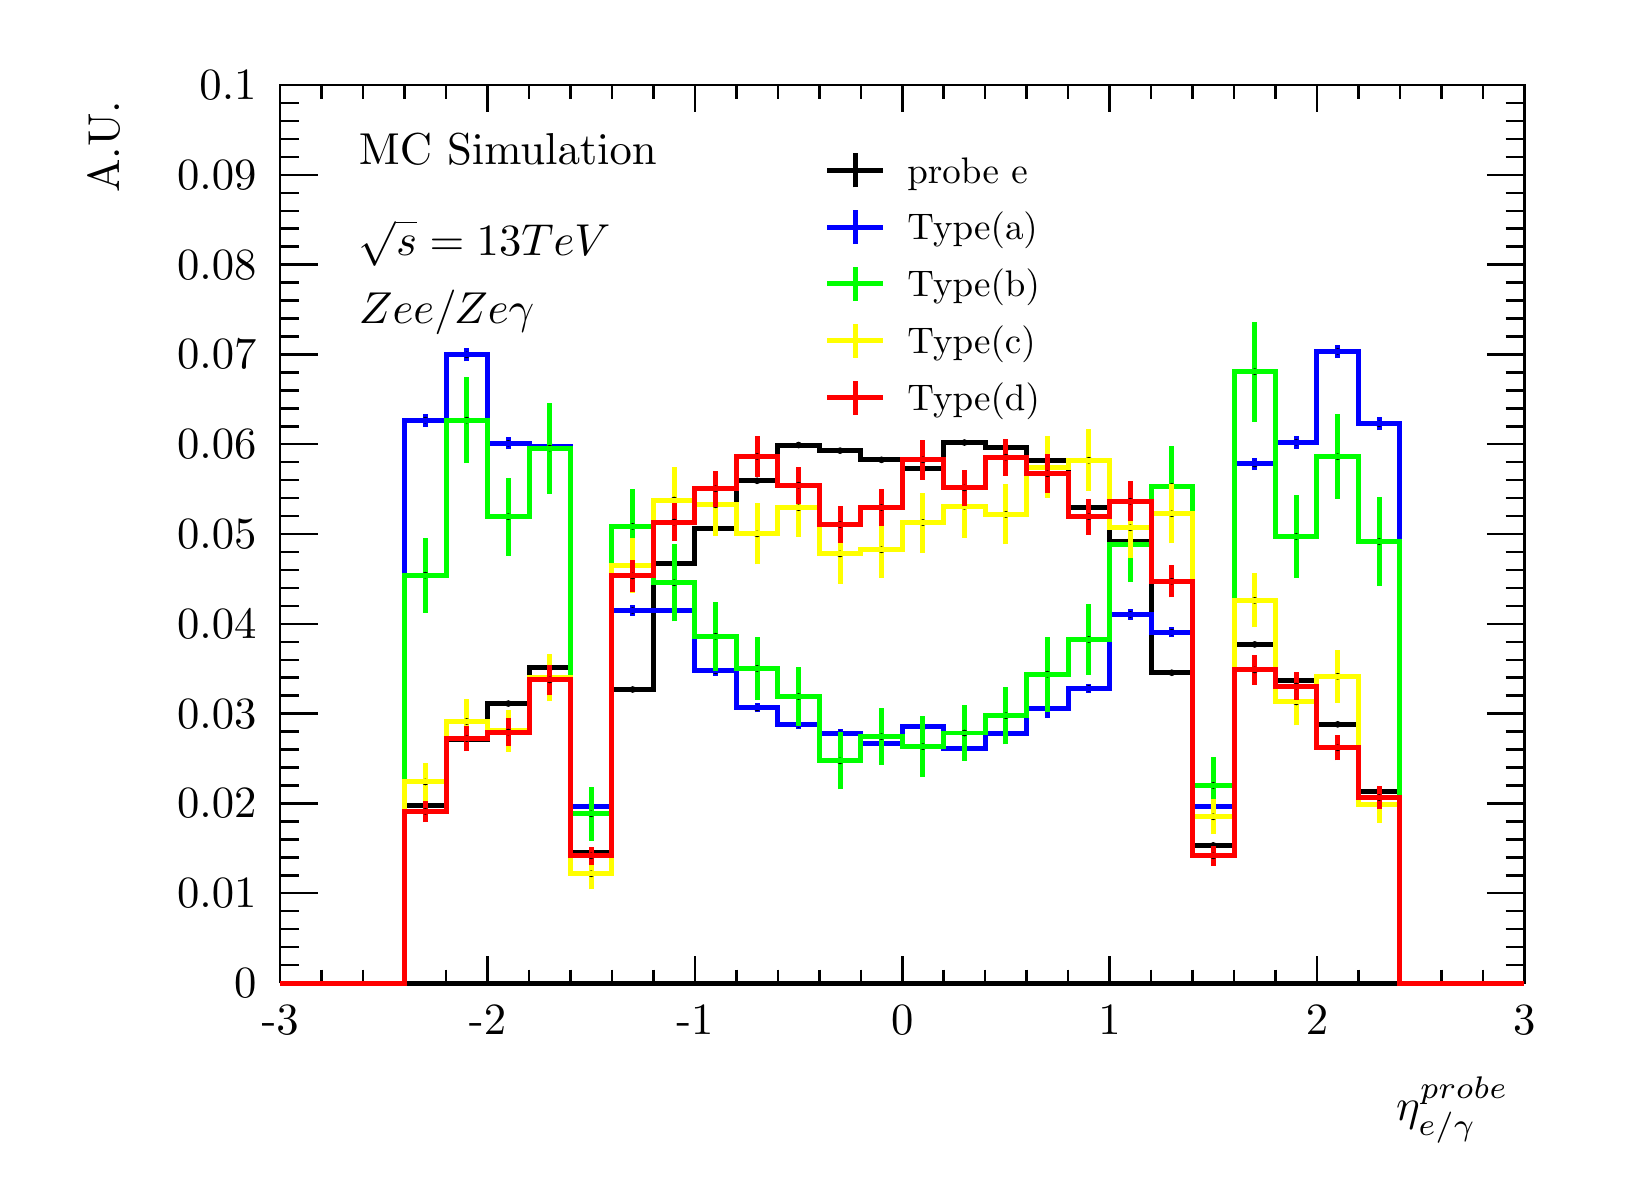
\begin{tikzpicture}
\pgfdeclareplotmark{cross} {
\pgfpathmoveto{\pgfpoint{-0.3\pgfplotmarksize}{\pgfplotmarksize}}
\pgfpathlineto{\pgfpoint{+0.3\pgfplotmarksize}{\pgfplotmarksize}}
\pgfpathlineto{\pgfpoint{+0.3\pgfplotmarksize}{0.3\pgfplotmarksize}}
\pgfpathlineto{\pgfpoint{+1\pgfplotmarksize}{0.3\pgfplotmarksize}}
\pgfpathlineto{\pgfpoint{+1\pgfplotmarksize}{-0.3\pgfplotmarksize}}
\pgfpathlineto{\pgfpoint{+0.3\pgfplotmarksize}{-0.3\pgfplotmarksize}}
\pgfpathlineto{\pgfpoint{+0.3\pgfplotmarksize}{-1.\pgfplotmarksize}}
\pgfpathlineto{\pgfpoint{-0.3\pgfplotmarksize}{-1.\pgfplotmarksize}}
\pgfpathlineto{\pgfpoint{-0.3\pgfplotmarksize}{-0.3\pgfplotmarksize}}
\pgfpathlineto{\pgfpoint{-1.\pgfplotmarksize}{-0.3\pgfplotmarksize}}
\pgfpathlineto{\pgfpoint{-1.\pgfplotmarksize}{0.3\pgfplotmarksize}}
\pgfpathlineto{\pgfpoint{-0.3\pgfplotmarksize}{0.3\pgfplotmarksize}}
\pgfpathclose
\pgfusepathqstroke
}
\pgfdeclareplotmark{cross*} {
\pgfpathmoveto{\pgfpoint{-0.3\pgfplotmarksize}{\pgfplotmarksize}}
\pgfpathlineto{\pgfpoint{+0.3\pgfplotmarksize}{\pgfplotmarksize}}
\pgfpathlineto{\pgfpoint{+0.3\pgfplotmarksize}{0.3\pgfplotmarksize}}
\pgfpathlineto{\pgfpoint{+1\pgfplotmarksize}{0.3\pgfplotmarksize}}
\pgfpathlineto{\pgfpoint{+1\pgfplotmarksize}{-0.3\pgfplotmarksize}}
\pgfpathlineto{\pgfpoint{+0.3\pgfplotmarksize}{-0.3\pgfplotmarksize}}
\pgfpathlineto{\pgfpoint{+0.3\pgfplotmarksize}{-1.\pgfplotmarksize}}
\pgfpathlineto{\pgfpoint{-0.3\pgfplotmarksize}{-1.\pgfplotmarksize}}
\pgfpathlineto{\pgfpoint{-0.3\pgfplotmarksize}{-0.3\pgfplotmarksize}}
\pgfpathlineto{\pgfpoint{-1.\pgfplotmarksize}{-0.3\pgfplotmarksize}}
\pgfpathlineto{\pgfpoint{-1.\pgfplotmarksize}{0.3\pgfplotmarksize}}
\pgfpathlineto{\pgfpoint{-0.3\pgfplotmarksize}{0.3\pgfplotmarksize}}
\pgfpathclose
\pgfusepathqfillstroke
}
\pgfdeclareplotmark{newstar} {
\pgfpathmoveto{\pgfqpoint{0pt}{\pgfplotmarksize}}
\pgfpathlineto{\pgfqpointpolar{44}{0.5\pgfplotmarksize}}
\pgfpathlineto{\pgfqpointpolar{18}{\pgfplotmarksize}}
\pgfpathlineto{\pgfqpointpolar{-20}{0.5\pgfplotmarksize}}
\pgfpathlineto{\pgfqpointpolar{-54}{\pgfplotmarksize}}
\pgfpathlineto{\pgfqpointpolar{-90}{0.5\pgfplotmarksize}}
\pgfpathlineto{\pgfqpointpolar{234}{\pgfplotmarksize}}
\pgfpathlineto{\pgfqpointpolar{198}{0.5\pgfplotmarksize}}
\pgfpathlineto{\pgfqpointpolar{162}{\pgfplotmarksize}}
\pgfpathlineto{\pgfqpointpolar{134}{0.5\pgfplotmarksize}}
\pgfpathclose
\pgfusepathqstroke
}
\pgfdeclareplotmark{newstar*} {
\pgfpathmoveto{\pgfqpoint{0pt}{\pgfplotmarksize}}
\pgfpathlineto{\pgfqpointpolar{44}{0.5\pgfplotmarksize}}
\pgfpathlineto{\pgfqpointpolar{18}{\pgfplotmarksize}}
\pgfpathlineto{\pgfqpointpolar{-20}{0.5\pgfplotmarksize}}
\pgfpathlineto{\pgfqpointpolar{-54}{\pgfplotmarksize}}
\pgfpathlineto{\pgfqpointpolar{-90}{0.5\pgfplotmarksize}}
\pgfpathlineto{\pgfqpointpolar{234}{\pgfplotmarksize}}
\pgfpathlineto{\pgfqpointpolar{198}{0.5\pgfplotmarksize}}
\pgfpathlineto{\pgfqpointpolar{162}{\pgfplotmarksize}}
\pgfpathlineto{\pgfqpointpolar{134}{0.5\pgfplotmarksize}}
\pgfpathclose
\pgfusepathqfillstroke
}
\definecolor{c}{rgb}{1,1,1};
\draw [color=c, fill=c] (0,0) rectangle (20,14.4361);
\draw [color=c, fill=c] (3.2,2.30977) rectangle (19,13.7143);
\definecolor{c}{rgb}{0,0,0};
\draw [c,line width=0.9] (3.2,2.30977) -- (3.2,13.7143) -- (19,13.7143) -- (19,2.30977) -- (3.2,2.30977);
\draw [c,line width=1.8] (3.2,2.30977) -- (3.2158,2.30977) -- (3.2158,2.30977) -- (3.2316,2.30977) -- (3.2316,2.30977) -- (3.2474,2.30977) -- (3.2474,2.30977) -- (3.2632,2.30977) -- (3.2632,2.30977) -- (3.279,2.30977) -- (3.279,2.30977) --
 (3.2948,2.30977) -- (3.2948,2.30977) -- (3.3106,2.30977) -- (3.3106,2.30977) -- (3.3264,2.30977) -- (3.3264,2.30977) -- (3.3422,2.30977) -- (3.3422,2.30977) -- (3.358,2.30977) -- (3.358,2.30977) -- (3.3738,2.30977) -- (3.3738,2.30977) --
 (3.3896,2.30977) -- (3.3896,2.30977) -- (3.4054,2.30977) -- (3.4054,2.30977) -- (3.4212,2.30977) -- (3.4212,2.30977) -- (3.437,2.30977) -- (3.437,2.30977) -- (3.4528,2.30977) -- (3.4528,2.30977) -- (3.4686,2.30977) -- (3.4686,2.30977) --
 (3.4844,2.30977) -- (3.4844,2.30977) -- (3.5002,2.30977) -- (3.5002,2.30977) -- (3.516,2.30977) -- (3.516,2.30977) -- (3.5318,2.30977) -- (3.5318,2.30977) -- (3.5476,2.30977) -- (3.5476,2.30977) -- (3.5634,2.30977) -- (3.5634,2.30977) --
 (3.5792,2.30977) -- (3.5792,2.30977) -- (3.595,2.30977) -- (3.595,2.30977) -- (3.6108,2.30977) -- (3.6108,2.30977) -- (3.6266,2.30977) -- (3.6266,2.30977) -- (3.6424,2.30977) -- (3.6424,2.30977) -- (3.6582,2.30977) -- (3.6582,2.30977) --
 (3.674,2.30977) -- (3.674,2.30977) -- (3.6898,2.30977) -- (3.6898,2.30977) -- (3.7056,2.30977) -- (3.7056,2.30977) -- (3.7214,2.30977) -- (3.7214,2.30977) -- (3.7372,2.30977) -- (3.7372,2.30977) -- (3.753,2.30977) -- (3.753,2.30977) --
 (3.7688,2.30977) -- (3.7688,2.30977) -- (3.7846,2.30977) -- (3.7846,2.30977) -- (3.8004,2.30977) -- (3.8004,2.30977) -- (3.8162,2.30977) -- (3.8162,2.30977) -- (3.832,2.30977) -- (3.832,2.30977) -- (3.8478,2.30977) -- (3.8478,2.30977) --
 (3.8636,2.30977) -- (3.8636,2.30977) -- (3.8794,2.30977) -- (3.8794,2.30977) -- (3.8952,2.30977) -- (3.8952,2.30977) -- (3.911,2.30977) -- (3.911,2.30977) -- (3.9268,2.30977) -- (3.9268,2.30977) -- (3.9426,2.30977) -- (3.9426,2.30977) --
 (3.9584,2.30977) -- (3.9584,2.30977) -- (3.9742,2.30977) -- (3.9742,2.30977) -- (3.99,2.30977) -- (3.99,2.30977) -- (4.0058,2.30977) -- (4.0058,2.30977) -- (4.0216,2.30977) -- (4.0216,2.30977) -- (4.0374,2.30977) -- (4.0374,2.30977) --
 (4.0532,2.30977) -- (4.0532,2.30977) -- (4.069,2.30977) -- (4.069,2.30977) -- (4.0848,2.30977) -- (4.0848,2.30977) -- (4.1006,2.30977) -- (4.1006,2.30977) -- (4.1164,2.30977) -- (4.1164,2.30977) -- (4.1322,2.30977) -- (4.1322,2.30977) --
 (4.148,2.30977) -- (4.148,2.30977) -- (4.1638,2.30977) -- (4.1638,2.30977) -- (4.1796,2.30977) -- (4.1796,2.30977) -- (4.1954,2.30977) -- (4.1954,2.30977) -- (4.2112,2.30977) -- (4.2112,2.30977) -- (4.227,2.30977) -- (4.227,2.30977) --
 (4.2428,2.30977) -- (4.2428,2.30977) -- (4.2586,2.30977) -- (4.2586,2.30977) -- (4.2744,2.30977) -- (4.2744,2.30977) -- (4.2902,2.30977) -- (4.2902,2.30977) -- (4.306,2.30977) -- (4.306,2.30977) -- (4.3218,2.30977) -- (4.3218,2.30977) --
 (4.3376,2.30977) -- (4.3376,2.30977) -- (4.3534,2.30977) -- (4.3534,2.30977) -- (4.3692,2.30977) -- (4.3692,2.30977) -- (4.385,2.30977) -- (4.385,2.30977) -- (4.4008,2.30977) -- (4.4008,2.30977) -- (4.4166,2.30977) -- (4.4166,2.30977) --
 (4.4324,2.30977) -- (4.4324,2.30977) -- (4.4482,2.30977) -- (4.4482,2.30977) -- (4.464,2.30977) -- (4.464,2.30977) -- (4.4798,2.30977) -- (4.4798,2.30977) -- (4.4956,2.30977) -- (4.4956,2.30977) -- (4.5114,2.30977) -- (4.5114,2.30977) --
 (4.5272,2.30977) -- (4.5272,2.30977) -- (4.543,2.30977) -- (4.543,2.30977) -- (4.5588,2.30977) -- (4.5588,2.30977) -- (4.5746,2.30977) -- (4.5746,2.30977) -- (4.5904,2.30977) -- (4.5904,2.30977) -- (4.6062,2.30977) -- (4.6062,2.30977) --
 (4.622,2.30977) -- (4.622,2.30977) -- (4.6378,2.30977) -- (4.6378,2.30977) -- (4.6536,2.30977) -- (4.6536,2.30977) -- (4.6694,2.30977) -- (4.6694,2.30977) -- (4.6852,2.30977) -- (4.6852,2.30977) -- (4.701,2.30977) -- (4.701,2.30977) --
 (4.7168,2.30977) -- (4.7168,2.30977) -- (4.7326,2.30977) -- (4.7326,2.30977) -- (4.7484,2.30977) -- (4.7484,2.30977) -- (4.7642,2.30977) -- (4.7642,2.30977) -- (4.78,2.30977) -- (4.78,2.30977) -- (4.7958,2.30977) -- (4.7958,2.30977) --
 (4.8116,2.30977) -- (4.8116,2.30977) -- (4.8274,2.30977) -- (4.8274,2.30977) -- (4.8432,2.30977) -- (4.8432,2.30977) -- (4.859,2.30977) -- (4.859,2.30977) -- (4.8748,2.30977) -- (4.8748,2.30977) -- (4.8906,2.30977) -- (4.8906,2.30977) --
 (4.9064,2.30977) -- (4.9064,2.30977) -- (4.9222,2.30977) -- (4.9222,2.30977) -- (4.938,2.30977) -- (4.938,2.30977) -- (4.9538,2.30977) -- (4.9538,2.30977) -- (4.9696,2.30977) -- (4.9696,2.30977) -- (4.9854,2.30977) -- (4.9854,2.30977) --
 (5.0012,2.30977) -- (5.0012,2.30977) -- (5.017,2.30977) -- (5.017,2.30977) -- (5.0328,2.30977) -- (5.0328,2.30977) -- (5.0486,2.30977) -- (5.0486,2.30977) -- (5.0644,2.30977) -- (5.0644,2.30977) -- (5.0802,2.30977) -- (5.0802,2.30977) --
 (5.096,2.30977) -- (5.096,2.30977) -- (5.1118,2.30977) -- (5.1118,2.30977) -- (5.1276,2.30977) -- (5.1276,2.30977) -- (5.1434,2.30977) -- (5.1434,2.30977) -- (5.1592,2.30977) -- (5.1592,2.30977) -- (5.175,2.30977) -- (5.175,2.30977) --
 (5.1908,2.30977) -- (5.1908,2.30977) -- (5.2066,2.30977) -- (5.2066,2.30977) -- (5.2224,2.30977) -- (5.2224,2.30977) -- (5.2382,2.30977) -- (5.2382,2.30977) -- (5.254,2.30977) -- (5.254,2.30977) -- (5.2698,2.30977) -- (5.2698,2.30977) --
 (5.2856,2.30977) -- (5.2856,2.30977) -- (5.3014,2.30977) -- (5.3014,2.30977) -- (5.3172,2.30977) -- (5.3172,2.30977) -- (5.333,2.30977) -- (5.333,2.30977) -- (5.3488,2.30977) -- (5.3488,2.30977) -- (5.3646,2.30977) -- (5.3646,2.30977) --
 (5.3804,2.30977) -- (5.3804,2.30977) -- (5.3962,2.30977) -- (5.3962,2.30977) -- (5.412,2.30977) -- (5.412,2.30977) -- (5.4278,2.30977) -- (5.4278,2.30977) -- (5.4436,2.30977) -- (5.4436,2.30977) -- (5.4594,2.30977) -- (5.4594,2.30977) --
 (5.4752,2.30977) -- (5.4752,2.30977) -- (5.491,2.30977) -- (5.491,2.30977) -- (5.5068,2.30977) -- (5.5068,2.30977) -- (5.5226,2.30977) -- (5.5226,2.30977) -- (5.5384,2.30977) -- (5.5384,2.30977) -- (5.5542,2.30977) -- (5.5542,2.30977) --
 (5.57,2.30977) -- (5.57,2.30977) -- (5.5858,2.30977) -- (5.5858,2.30977) -- (5.6016,2.30977) -- (5.6016,2.30977) -- (5.6174,2.30977) -- (5.6174,2.30977) -- (5.6332,2.30977) -- (5.6332,2.30977) -- (5.649,2.30977) -- (5.649,2.30977) --
 (5.6648,2.30977) -- (5.6648,2.30977) -- (5.6806,2.30977) -- (5.6806,2.30977) -- (5.6964,2.30977) -- (5.6964,2.30977) -- (5.7122,2.30977) -- (5.7122,2.30977) -- (5.728,2.30977) -- (5.728,2.30977) -- (5.7438,2.30977) -- (5.7438,2.30977) --
 (5.7596,2.30977) -- (5.7596,2.30977) -- (5.7754,2.30977) -- (5.7754,2.30977) -- (5.7912,2.30977) -- (5.7912,2.30977) -- (5.807,2.30977) -- (5.807,2.30977) -- (5.8228,2.30977) -- (5.8228,2.30977) -- (5.8386,2.30977) -- (5.8386,2.30977) --
 (5.8544,2.30977) -- (5.8544,2.30977) -- (5.8702,2.30977) -- (5.8702,2.30977) -- (5.886,2.30977) -- (5.886,2.30977) -- (5.9018,2.30977) -- (5.9018,2.30977) -- (5.9176,2.30977) -- (5.9176,2.30977) -- (5.9334,2.30977) -- (5.9334,2.30977) --
 (5.9492,2.30977) -- (5.9492,2.30977) -- (5.965,2.30977) -- (5.965,2.30977) -- (5.9808,2.30977) -- (5.9808,2.30977) -- (5.9966,2.30977) -- (5.9966,2.30977) -- (6.0124,2.30977) -- (6.0124,2.30977) -- (6.0282,2.30977) -- (6.0282,2.30977) --
 (6.044,2.30977) -- (6.044,2.30977) -- (6.0598,2.30977) -- (6.0598,2.30977) -- (6.0756,2.30977) -- (6.0756,2.30977) -- (6.0914,2.30977) -- (6.0914,2.30977) -- (6.1072,2.30977) -- (6.1072,2.30977) -- (6.123,2.30977) -- (6.123,2.30977) --
 (6.1388,2.30977) -- (6.1388,2.30977) -- (6.1546,2.30977) -- (6.1546,2.30977) -- (6.1704,2.30977) -- (6.1704,2.30977) -- (6.1862,2.30977) -- (6.1862,2.30977) -- (6.202,2.30977) -- (6.202,2.30977) -- (6.2178,2.30977) -- (6.2178,2.30977) --
 (6.2336,2.30977) -- (6.2336,2.30977) -- (6.2494,2.30977) -- (6.2494,2.30977) -- (6.2652,2.30977) -- (6.2652,2.30977) -- (6.281,2.30977) -- (6.281,2.30977) -- (6.2968,2.30977) -- (6.2968,2.30977) -- (6.3126,2.30977) -- (6.3126,2.30977) --
 (6.3284,2.30977) -- (6.3284,2.30977) -- (6.3442,2.30977) -- (6.3442,2.30977) -- (6.36,2.30977) -- (6.36,2.30977) -- (6.3758,2.30977) -- (6.3758,2.30977) -- (6.3916,2.30977) -- (6.3916,2.30977) -- (6.4074,2.30977) -- (6.4074,2.30977) --
 (6.4232,2.30977) -- (6.4232,2.30977) -- (6.439,2.30977) -- (6.439,2.30977) -- (6.4548,2.30977) -- (6.4548,2.30977) -- (6.4706,2.30977) -- (6.4706,2.30977) -- (6.4864,2.30977) -- (6.4864,2.30977) -- (6.5022,2.30977) -- (6.5022,2.30977) --
 (6.518,2.30977) -- (6.518,2.30977) -- (6.5338,2.30977) -- (6.5338,2.30977) -- (6.5496,2.30977) -- (6.5496,2.30977) -- (6.5654,2.30977) -- (6.5654,2.30977) -- (6.5812,2.30977) -- (6.5812,2.30977) -- (6.597,2.30977) -- (6.597,2.30977) --
 (6.6128,2.30977) -- (6.6128,2.30977) -- (6.6286,2.30977) -- (6.6286,2.30977) -- (6.6444,2.30977) -- (6.6444,2.30977) -- (6.6602,2.30977) -- (6.6602,2.30977) -- (6.676,2.30977) -- (6.676,2.30977) -- (6.6918,2.30977) -- (6.6918,2.30977) --
 (6.7076,2.30977) -- (6.7076,2.30977) -- (6.7234,2.30977) -- (6.7234,2.30977) -- (6.7392,2.30977) -- (6.7392,2.30977) -- (6.755,2.30977) -- (6.755,2.30977) -- (6.7708,2.30977) -- (6.7708,2.30977) -- (6.7866,2.30977) -- (6.7866,2.30977) --
 (6.8024,2.30977) -- (6.8024,2.30977) -- (6.8182,2.30977) -- (6.8182,2.30977) -- (6.834,2.30977) -- (6.834,2.30977) -- (6.8498,2.30977) -- (6.8498,2.30977) -- (6.8656,2.30977) -- (6.8656,2.30977) -- (6.8814,2.30977) -- (6.8814,2.30977) --
 (6.8972,2.30977) -- (6.8972,2.30977) -- (6.913,2.30977) -- (6.913,2.30977) -- (6.9288,2.30977) -- (6.9288,2.30977) -- (6.9446,2.30977) -- (6.9446,2.30977) -- (6.9604,2.30977) -- (6.9604,2.30977) -- (6.9762,2.30977) -- (6.9762,2.30977) --
 (6.992,2.30977) -- (6.992,2.30977) -- (7.0078,2.30977) -- (7.0078,2.30977) -- (7.0236,2.30977) -- (7.0236,2.30977) -- (7.0394,2.30977) -- (7.0394,2.30977) -- (7.0552,2.30977) -- (7.0552,2.30977) -- (7.071,2.30977) -- (7.071,2.30977) --
 (7.0868,2.30977) -- (7.0868,2.30977) -- (7.1026,2.30977) -- (7.1026,2.30977) -- (7.1184,2.30977) -- (7.1184,2.30977) -- (7.1342,2.30977) -- (7.1342,2.30977) -- (7.15,2.30977) -- (7.15,2.30977) -- (7.1658,2.30977) -- (7.1658,2.30977) --
 (7.1816,2.30977) -- (7.1816,2.30977) -- (7.1974,2.30977) -- (7.1974,2.30977) -- (7.2132,2.30977) -- (7.2132,2.30977) -- (7.229,2.30977) -- (7.229,2.30977) -- (7.2448,2.30977) -- (7.2448,2.30977) -- (7.2606,2.30977) -- (7.2606,2.30977) --
 (7.2764,2.30977) -- (7.2764,2.30977) -- (7.2922,2.30977) -- (7.2922,2.30977) -- (7.308,2.30977) -- (7.308,2.30977) -- (7.3238,2.30977) -- (7.3238,2.30977) -- (7.3396,2.30977) -- (7.3396,2.30977) -- (7.3554,2.30977) -- (7.3554,2.30977) --
 (7.3712,2.30977) -- (7.3712,2.30977) -- (7.387,2.30977) -- (7.387,2.30977) -- (7.4028,2.30977) -- (7.4028,2.30977) -- (7.4186,2.30977) -- (7.4186,2.30977) -- (7.4344,2.30977) -- (7.4344,2.30977) -- (7.4502,2.30977) -- (7.4502,2.30977) --
 (7.466,2.30977) -- (7.466,2.30977) -- (7.4818,2.30977) -- (7.4818,2.30977) -- (7.4976,2.30977) -- (7.4976,2.30977) -- (7.5134,2.30977) -- (7.5134,2.30977) -- (7.5292,2.30977) -- (7.5292,2.30977) -- (7.545,2.30977) -- (7.545,2.30977) --
 (7.5608,2.30977) -- (7.5608,2.30977) -- (7.5766,2.30977) -- (7.5766,2.30977) -- (7.5924,2.30977) -- (7.5924,2.30977) -- (7.6082,2.30977) -- (7.6082,2.30977) -- (7.624,2.30977) -- (7.624,2.30977) -- (7.6398,2.30977) -- (7.6398,2.30977) --
 (7.6556,2.30977) -- (7.6556,2.30977) -- (7.6714,2.30977) -- (7.6714,2.30977) -- (7.6872,2.30977) -- (7.6872,2.30977) -- (7.703,2.30977) -- (7.703,2.30977) -- (7.7188,2.30977) -- (7.7188,2.30977) -- (7.7346,2.30977) -- (7.7346,2.30977) --
 (7.7504,2.30977) -- (7.7504,2.30977) -- (7.7662,2.30977) -- (7.7662,2.30977) -- (7.782,2.30977) -- (7.782,2.30977) -- (7.7978,2.30977) -- (7.7978,2.30977) -- (7.8136,2.30977) -- (7.8136,2.30977) -- (7.8294,2.30977) -- (7.8294,2.30977) --
 (7.8452,2.30977) -- (7.8452,2.30977) -- (7.861,2.30977) -- (7.861,2.30977) -- (7.8768,2.30977) -- (7.8768,2.30977) -- (7.8926,2.30977) -- (7.8926,2.30977) -- (7.9084,2.30977) -- (7.9084,2.30977) -- (7.9242,2.30977) -- (7.9242,2.30977) --
 (7.94,2.30977) -- (7.94,2.30977) -- (7.9558,2.30977) -- (7.9558,2.30977) -- (7.9716,2.30977) -- (7.9716,2.30977) -- (7.9874,2.30977) -- (7.9874,2.30977) -- (8.0032,2.30977) -- (8.0032,2.30977) -- (8.019,2.30977) -- (8.019,2.30977) --
 (8.0348,2.30977) -- (8.0348,2.30977) -- (8.0506,2.30977) -- (8.0506,2.30977) -- (8.0664,2.30977) -- (8.0664,2.30977) -- (8.0822,2.30977) -- (8.0822,2.30977) -- (8.098,2.30977) -- (8.098,2.30977) -- (8.1138,2.30977) -- (8.1138,2.30977) --
 (8.1296,2.30977) -- (8.1296,2.30977) -- (8.1454,2.30977) -- (8.1454,2.30977) -- (8.1612,2.30977) -- (8.1612,2.30977) -- (8.177,2.30977) -- (8.177,2.30977) -- (8.1928,2.30977) -- (8.1928,2.30977) -- (8.2086,2.30977) -- (8.2086,2.30977) --
 (8.2244,2.30977) -- (8.2244,2.30977) -- (8.2402,2.30977) -- (8.2402,2.30977) -- (8.256,2.30977) -- (8.256,2.30977) -- (8.2718,2.30977) -- (8.2718,2.30977) -- (8.2876,2.30977) -- (8.2876,2.30977) -- (8.3034,2.30977) -- (8.3034,2.30977) --
 (8.3192,2.30977) -- (8.3192,2.30977) -- (8.335,2.30977) -- (8.335,2.30977) -- (8.3508,2.30977) -- (8.3508,2.30977) -- (8.3666,2.30977) -- (8.3666,2.30977) -- (8.3824,2.30977) -- (8.3824,2.30977) -- (8.3982,2.30977) -- (8.3982,2.30977) --
 (8.414,2.30977) -- (8.414,2.30977) -- (8.4298,2.30977) -- (8.4298,2.30977) -- (8.4456,2.30977) -- (8.4456,2.30977) -- (8.4614,2.30977) -- (8.4614,2.30977) -- (8.4772,2.30977) -- (8.4772,2.30977) -- (8.493,2.30977) -- (8.493,2.30977) --
 (8.5088,2.30977) -- (8.5088,2.30977) -- (8.5246,2.30977) -- (8.5246,2.30977) -- (8.5404,2.30977) -- (8.5404,2.30977) -- (8.5562,2.30977) -- (8.5562,2.30977) -- (8.572,2.30977) -- (8.572,2.30977) -- (8.5878,2.30977) -- (8.5878,2.30977) --
 (8.6036,2.30977) -- (8.6036,2.30977) -- (8.6194,2.30977) -- (8.6194,2.30977) -- (8.6352,2.30977) -- (8.6352,2.30977) -- (8.651,2.30977) -- (8.651,2.30977) -- (8.6668,2.30977) -- (8.6668,2.30977) -- (8.6826,2.30977) -- (8.6826,2.30977) --
 (8.6984,2.30977) -- (8.6984,2.30977) -- (8.7142,2.30977) -- (8.7142,2.30977) -- (8.73,2.30977) -- (8.73,2.30977) -- (8.7458,2.30977) -- (8.7458,2.30977) -- (8.7616,2.30977) -- (8.7616,2.30977) -- (8.7774,2.30977) -- (8.7774,2.30977) --
 (8.7932,2.30977) -- (8.7932,2.30977) -- (8.809,2.30977) -- (8.809,2.30977) -- (8.8248,2.30977) -- (8.8248,2.30977) -- (8.8406,2.30977) -- (8.8406,2.30977) -- (8.8564,2.30977) -- (8.8564,2.30977) -- (8.8722,2.30977) -- (8.8722,2.30977) --
 (8.888,2.30977) -- (8.888,2.30977) -- (8.9038,2.30977) -- (8.9038,2.30977) -- (8.9196,2.30977) -- (8.9196,2.30977) -- (8.9354,2.30977) -- (8.9354,2.30977) -- (8.9512,2.30977) -- (8.9512,2.30977) -- (8.967,2.30977) -- (8.967,2.30977) --
 (8.9828,2.30977) -- (8.9828,2.30977) -- (8.9986,2.30977) -- (8.9986,2.30977) -- (9.0144,2.30977) -- (9.0144,2.30977) -- (9.0302,2.30977) -- (9.0302,2.30977) -- (9.046,2.30977) -- (9.046,2.30977) -- (9.0618,2.30977) -- (9.0618,2.30977) --
 (9.0776,2.30977) -- (9.0776,2.30977) -- (9.0934,2.30977) -- (9.0934,2.30977) -- (9.1092,2.30977) -- (9.1092,2.30977) -- (9.125,2.30977) -- (9.125,2.30977) -- (9.1408,2.30977) -- (9.1408,2.30977) -- (9.1566,2.30977) -- (9.1566,2.30977) --
 (9.1724,2.30977) -- (9.1724,2.30977) -- (9.1882,2.30977) -- (9.1882,2.30977) -- (9.204,2.30977) -- (9.204,2.30977) -- (9.2198,2.30977) -- (9.2198,2.30977) -- (9.2356,2.30977) -- (9.2356,2.30977) -- (9.2514,2.30977) -- (9.2514,2.30977) --
 (9.2672,2.30977) -- (9.2672,2.30977) -- (9.283,2.30977) -- (9.283,2.30977) -- (9.2988,2.30977) -- (9.2988,2.30977) -- (9.3146,2.30977) -- (9.3146,2.30977) -- (9.3304,2.30977) -- (9.3304,2.30977) -- (9.3462,2.30977) -- (9.3462,2.30977) --
 (9.362,2.30977) -- (9.362,2.30977) -- (9.3778,2.30977) -- (9.3778,2.30977) -- (9.3936,2.30977) -- (9.3936,2.30977) -- (9.4094,2.30977) -- (9.4094,2.30977) -- (9.4252,2.30977) -- (9.4252,2.30977) -- (9.441,2.30977) -- (9.441,2.30977) --
 (9.4568,2.30977) -- (9.4568,2.30977) -- (9.4726,2.30977) -- (9.4726,2.30977) -- (9.4884,2.30977) -- (9.4884,2.30977) -- (9.5042,2.30977) -- (9.5042,2.30977) -- (9.52,2.30977) -- (9.52,2.30977) -- (9.5358,2.30977) -- (9.5358,2.30977) --
 (9.5516,2.30977) -- (9.5516,2.30977) -- (9.5674,2.30977) -- (9.5674,2.30977) -- (9.5832,2.30977) -- (9.5832,2.30977) -- (9.599,2.30977) -- (9.599,2.30977) -- (9.6148,2.30977) -- (9.6148,2.30977) -- (9.6306,2.30977) -- (9.6306,2.30977) --
 (9.6464,2.30977) -- (9.6464,2.30977) -- (9.6622,2.30977) -- (9.6622,2.30977) -- (9.678,2.30977) -- (9.678,2.30977) -- (9.6938,2.30977) -- (9.6938,2.30977) -- (9.7096,2.30977) -- (9.7096,2.30977) -- (9.7254,2.30977) -- (9.7254,2.30977) --
 (9.7412,2.30977) -- (9.7412,2.30977) -- (9.757,2.30977) -- (9.757,2.30977) -- (9.7728,2.30977) -- (9.7728,2.30977) -- (9.7886,2.30977) -- (9.7886,2.30977) -- (9.8044,2.30977) -- (9.8044,2.30977) -- (9.8202,2.30977) -- (9.8202,2.30977) --
 (9.836,2.30977) -- (9.836,2.30977) -- (9.8518,2.30977) -- (9.8518,2.30977) -- (9.8676,2.30977) -- (9.8676,2.30977) -- (9.8834,2.30977) -- (9.8834,2.30977) -- (9.8992,2.30977) -- (9.8992,2.30977) -- (9.915,2.30977) -- (9.915,2.30977) --
 (9.9308,2.30977) -- (9.9308,2.30977) -- (9.9466,2.30977) -- (9.9466,2.30977) -- (9.9624,2.30977) -- (9.9624,2.30977) -- (9.9782,2.30977) -- (9.9782,2.30977) -- (9.994,2.30977) -- (9.994,2.30977) -- (10.0098,2.30977) -- (10.0098,2.30977) --
 (10.0256,2.30977) -- (10.0256,2.30977) -- (10.0414,2.30977) -- (10.0414,2.30977) -- (10.0572,2.30977) -- (10.0572,2.30977) -- (10.073,2.30977) -- (10.073,2.30977) -- (10.0888,2.30977) -- (10.0888,2.30977) -- (10.1046,2.30977) -- (10.1046,2.30977) --
 (10.1204,2.30977) -- (10.1204,2.30977) -- (10.1362,2.30977) -- (10.1362,2.30977) -- (10.152,2.30977) -- (10.152,2.30977) -- (10.1678,2.30977) -- (10.1678,2.30977) -- (10.1836,2.30977) -- (10.1836,2.30977) -- (10.1994,2.30977) -- (10.1994,2.30977) --
 (10.2152,2.30977) -- (10.2152,2.30977) -- (10.231,2.30977) -- (10.231,2.30977) -- (10.2468,2.30977) -- (10.2468,2.30977) -- (10.2626,2.30977) -- (10.2626,2.30977) -- (10.2784,2.30977) -- (10.2784,2.30977) -- (10.2942,2.30977) -- (10.2942,2.30977) --
 (10.31,2.30977) -- (10.31,2.30977) -- (10.3258,2.30977) -- (10.3258,2.30977) -- (10.3416,2.30977) -- (10.3416,2.30977) -- (10.3574,2.30977) -- (10.3574,2.30977) -- (10.3732,2.30977) -- (10.3732,2.30977) -- (10.389,2.30977) -- (10.389,2.30977) --
 (10.4048,2.30977) -- (10.4048,2.30977) -- (10.4206,2.30977) -- (10.4206,2.30977) -- (10.4364,2.30977) -- (10.4364,2.30977) -- (10.4522,2.30977) -- (10.4522,2.30977) -- (10.468,2.30977) -- (10.468,2.30977) -- (10.4838,2.30977) -- (10.4838,2.30977) --
 (10.4996,2.30977) -- (10.4996,2.30977) -- (10.5154,2.30977) -- (10.5154,2.30977) -- (10.5312,2.30977) -- (10.5312,2.30977) -- (10.547,2.30977) -- (10.547,2.30977) -- (10.5628,2.30977) -- (10.5628,2.30977) -- (10.5786,2.30977) -- (10.5786,2.30977) --
 (10.5944,2.30977) -- (10.5944,2.30977) -- (10.6102,2.30977) -- (10.6102,2.30977) -- (10.626,2.30977) -- (10.626,2.30977) -- (10.6418,2.30977) -- (10.6418,2.30977) -- (10.6576,2.30977) -- (10.6576,2.30977) -- (10.6734,2.30977) -- (10.6734,2.30977) --
 (10.6892,2.30977) -- (10.6892,2.30977) -- (10.705,2.30977) -- (10.705,2.30977) -- (10.7208,2.30977) -- (10.7208,2.30977) -- (10.7366,2.30977) -- (10.7366,2.30977) -- (10.7524,2.30977) -- (10.7524,2.30977) -- (10.7682,2.30977) -- (10.7682,2.30977) --
 (10.784,2.30977) -- (10.784,2.30977) -- (10.7998,2.30977) -- (10.7998,2.30977) -- (10.8156,2.30977) -- (10.8156,2.30977) -- (10.8314,2.30977) -- (10.8314,2.30977) -- (10.8472,2.30977) -- (10.8472,2.30977) -- (10.863,2.30977) -- (10.863,2.30977) --
 (10.8788,2.30977) -- (10.8788,2.30977) -- (10.8946,2.30977) -- (10.8946,2.30977) -- (10.9104,2.30977) -- (10.9104,2.30977) -- (10.9262,2.30977) -- (10.9262,2.30977) -- (10.942,2.30977) -- (10.942,2.30977) -- (10.9578,2.30977) -- (10.9578,2.30977) --
 (10.9736,2.30977) -- (10.9736,2.30977) -- (10.9894,2.30977) -- (10.9894,2.30977) -- (11.0052,2.30977) -- (11.0052,2.30977) -- (11.021,2.30977) -- (11.021,2.30977) -- (11.0368,2.30977) -- (11.0368,2.30977) -- (11.0526,2.30977) -- (11.0526,2.30977) --
 (11.0684,2.30977) -- (11.0684,2.30977) -- (11.0842,2.30977) -- (11.0842,2.30977) -- (11.1,2.30977) -- (11.1,2.30977) -- (11.1158,2.30977) -- (11.1158,2.30977) -- (11.1316,2.30977) -- (11.1316,2.30977) -- (11.1474,2.30977) -- (11.1474,2.30977) --
 (11.1632,2.30977) -- (11.1632,2.30977) -- (11.179,2.30977) -- (11.179,2.30977) -- (11.1948,2.30977) -- (11.1948,2.30977) -- (11.2106,2.30977) -- (11.2106,2.30977) -- (11.2264,2.30977) -- (11.2264,2.30977) -- (11.2422,2.30977) -- (11.2422,2.30977) --
 (11.258,2.30977) -- (11.258,2.30977) -- (11.2738,2.30977) -- (11.2738,2.30977) -- (11.2896,2.30977) -- (11.2896,2.30977) -- (11.3054,2.30977) -- (11.3054,2.30977) -- (11.3212,2.30977) -- (11.3212,2.30977) -- (11.337,2.30977) -- (11.337,2.30977) --
 (11.3528,2.30977) -- (11.3528,2.30977) -- (11.3686,2.30977) -- (11.3686,2.30977) -- (11.3844,2.30977) -- (11.3844,2.30977) -- (11.4002,2.30977) -- (11.4002,2.30977) -- (11.416,2.30977) -- (11.416,2.30977) -- (11.4318,2.30977) -- (11.4318,2.30977) --
 (11.4476,2.30977) -- (11.4476,2.30977) -- (11.4634,2.30977) -- (11.4634,2.30977) -- (11.4792,2.30977) -- (11.4792,2.30977) -- (11.495,2.30977) -- (11.495,2.30977) -- (11.5108,2.30977) -- (11.5108,2.30977) -- (11.5266,2.30977) -- (11.5266,2.30977) --
 (11.5424,2.30977) -- (11.5424,2.30977) -- (11.5582,2.30977) -- (11.5582,2.30977) -- (11.574,2.30977) -- (11.574,2.30977) -- (11.5898,2.30977) -- (11.5898,2.30977) -- (11.6056,2.30977) -- (11.6056,2.30977) -- (11.6214,2.30977) -- (11.6214,2.30977) --
 (11.6372,2.30977) -- (11.6372,2.30977) -- (11.653,2.30977) -- (11.653,2.30977) -- (11.6688,2.30977) -- (11.6688,2.30977) -- (11.6846,2.30977) -- (11.6846,2.30977) -- (11.7004,2.30977) -- (11.7004,2.30977) -- (11.7162,2.30977) -- (11.7162,2.30977) --
 (11.732,2.30977) -- (11.732,2.30977) -- (11.7478,2.30977) -- (11.7478,2.30977) -- (11.7636,2.30977) -- (11.7636,2.30977) -- (11.7794,2.30977) -- (11.7794,2.30977) -- (11.7952,2.30977) -- (11.7952,2.30977) -- (11.811,2.30977) -- (11.811,2.30977) --
 (11.8268,2.30977) -- (11.8268,2.30977) -- (11.8426,2.30977) -- (11.8426,2.30977) -- (11.8584,2.30977) -- (11.8584,2.30977) -- (11.8742,2.30977) -- (11.8742,2.30977) -- (11.89,2.30977) -- (11.89,2.30977) -- (11.9058,2.30977) -- (11.9058,2.30977) --
 (11.9216,2.30977) -- (11.9216,2.30977) -- (11.9374,2.30977) -- (11.9374,2.30977) -- (11.9532,2.30977) -- (11.9532,2.30977) -- (11.969,2.30977) -- (11.969,2.30977) -- (11.9848,2.30977) -- (11.9848,2.30977) -- (12.0006,2.30977) -- (12.0006,2.30977) --
 (12.0164,2.30977) -- (12.0164,2.30977) -- (12.0322,2.30977) -- (12.0322,2.30977) -- (12.048,2.30977) -- (12.048,2.30977) -- (12.0638,2.30977) -- (12.0638,2.30977) -- (12.0796,2.30977) -- (12.0796,2.30977) -- (12.0954,2.30977) -- (12.0954,2.30977) --
 (12.1112,2.30977) -- (12.1112,2.30977) -- (12.127,2.30977) -- (12.127,2.30977) -- (12.1428,2.30977) -- (12.1428,2.30977) -- (12.1586,2.30977) -- (12.1586,2.30977) -- (12.1744,2.30977) -- (12.1744,2.30977) -- (12.1902,2.30977) -- (12.1902,2.30977) --
 (12.206,2.30977) -- (12.206,2.30977) -- (12.2218,2.30977) -- (12.2218,2.30977) -- (12.2376,2.30977) -- (12.2376,2.30977) -- (12.2534,2.30977) -- (12.2534,2.30977) -- (12.2692,2.30977) -- (12.2692,2.30977) -- (12.285,2.30977) -- (12.285,2.30977) --
 (12.3008,2.30977) -- (12.3008,2.30977) -- (12.3166,2.30977) -- (12.3166,2.30977) -- (12.3324,2.30977) -- (12.3324,2.30977) -- (12.3482,2.30977) -- (12.3482,2.30977) -- (12.364,2.30977) -- (12.364,2.30977) -- (12.3798,2.30977) -- (12.3798,2.30977) --
 (12.3956,2.30977) -- (12.3956,2.30977) -- (12.4114,2.30977) -- (12.4114,2.30977) -- (12.4272,2.30977) -- (12.4272,2.30977) -- (12.443,2.30977) -- (12.443,2.30977) -- (12.4588,2.30977) -- (12.4588,2.30977) -- (12.4746,2.30977) -- (12.4746,2.30977) --
 (12.4904,2.30977) -- (12.4904,2.30977) -- (12.5062,2.30977) -- (12.5062,2.30977) -- (12.522,2.30977) -- (12.522,2.30977) -- (12.5378,2.30977) -- (12.5378,2.30977) -- (12.5536,2.30977) -- (12.5536,2.30977) -- (12.5694,2.30977) -- (12.5694,2.30977) --
 (12.5852,2.30977) -- (12.5852,2.30977) -- (12.601,2.30977) -- (12.601,2.30977) -- (12.6168,2.30977) -- (12.6168,2.30977) -- (12.6326,2.30977) -- (12.6326,2.30977) -- (12.6484,2.30977) -- (12.6484,2.30977) -- (12.6642,2.30977) -- (12.6642,2.30977) --
 (12.68,2.30977) -- (12.68,2.30977) -- (12.6958,2.30977) -- (12.6958,2.30977) -- (12.7116,2.30977) -- (12.7116,2.30977) -- (12.7274,2.30977) -- (12.7274,2.30977) -- (12.7432,2.30977) -- (12.7432,2.30977) -- (12.759,2.30977) -- (12.759,2.30977) --
 (12.7748,2.30977) -- (12.7748,2.30977) -- (12.7906,2.30977) -- (12.7906,2.30977) -- (12.8064,2.30977) -- (12.8064,2.30977) -- (12.8222,2.30977) -- (12.8222,2.30977) -- (12.838,2.30977) -- (12.838,2.30977) -- (12.8538,2.30977) -- (12.8538,2.30977) --
 (12.8696,2.30977) -- (12.8696,2.30977) -- (12.8854,2.30977) -- (12.8854,2.30977) -- (12.9012,2.30977) -- (12.9012,2.30977) -- (12.917,2.30977) -- (12.917,2.30977) -- (12.9328,2.30977) -- (12.9328,2.30977) -- (12.9486,2.30977) -- (12.9486,2.30977) --
 (12.9644,2.30977) -- (12.9644,2.30977) -- (12.9802,2.30977) -- (12.9802,2.30977) -- (12.996,2.30977) -- (12.996,2.30977) -- (13.0118,2.30977) -- (13.0118,2.30977) -- (13.0276,2.30977) -- (13.0276,2.30977) -- (13.0434,2.30977) -- (13.0434,2.30977) --
 (13.0592,2.30977) -- (13.0592,2.30977) -- (13.075,2.30977) -- (13.075,2.30977) -- (13.0908,2.30977) -- (13.0908,2.30977) -- (13.1066,2.30977) -- (13.1066,2.30977) -- (13.1224,2.30977) -- (13.1224,2.30977) -- (13.1382,2.30977) -- (13.1382,2.30977) --
 (13.154,2.30977) -- (13.154,2.30977) -- (13.1698,2.30977) -- (13.1698,2.30977) -- (13.1856,2.30977) -- (13.1856,2.30977) -- (13.2014,2.30977) -- (13.2014,2.30977) -- (13.2172,2.30977) -- (13.2172,2.30977) -- (13.233,2.30977) -- (13.233,2.30977) --
 (13.2488,2.30977) -- (13.2488,2.30977) -- (13.2646,2.30977) -- (13.2646,2.30977) -- (13.2804,2.30977) -- (13.2804,2.30977) -- (13.2962,2.30977) -- (13.2962,2.30977) -- (13.312,2.30977) -- (13.312,2.30977) -- (13.3278,2.30977) -- (13.3278,2.30977) --
 (13.3436,2.30977) -- (13.3436,2.30977) -- (13.3594,2.30977) -- (13.3594,2.30977) -- (13.3752,2.30977) -- (13.3752,2.30977) -- (13.391,2.30977) -- (13.391,2.30977) -- (13.4068,2.30977) -- (13.4068,2.30977) -- (13.4226,2.30977) -- (13.4226,2.30977) --
 (13.4384,2.30977) -- (13.4384,2.30977) -- (13.4542,2.30977) -- (13.4542,2.30977) -- (13.47,2.30977) -- (13.47,2.30977) -- (13.4858,2.30977) -- (13.4858,2.30977) -- (13.5016,2.30977) -- (13.5016,2.30977) -- (13.5174,2.30977) -- (13.5174,2.30977) --
 (13.5332,2.30977) -- (13.5332,2.30977) -- (13.549,2.30977) -- (13.549,2.30977) -- (13.5648,2.30977) -- (13.5648,2.30977) -- (13.5806,2.30977) -- (13.5806,2.30977) -- (13.5964,2.30977) -- (13.5964,2.30977) -- (13.6122,2.30977) -- (13.6122,2.30977) --
 (13.628,2.30977) -- (13.628,2.30977) -- (13.6438,2.30977) -- (13.6438,2.30977) -- (13.6596,2.30977) -- (13.6596,2.30977) -- (13.6754,2.30977) -- (13.6754,2.30977) -- (13.6912,2.30977) -- (13.6912,2.30977) -- (13.707,2.30977) -- (13.707,2.30977) --
 (13.7228,2.30977) -- (13.7228,2.30977) -- (13.7386,2.30977) -- (13.7386,2.30977) -- (13.7544,2.30977) -- (13.7544,2.30977) -- (13.7702,2.30977) -- (13.7702,2.30977) -- (13.786,2.30977) -- (13.786,2.30977) -- (13.8018,2.30977) -- (13.8018,2.30977) --
 (13.8176,2.30977) -- (13.8176,2.30977) -- (13.8334,2.30977) -- (13.8334,2.30977) -- (13.8492,2.30977) -- (13.8492,2.30977) -- (13.865,2.30977) -- (13.865,2.30977) -- (13.8808,2.30977) -- (13.8808,2.30977) -- (13.8966,2.30977) -- (13.8966,2.30977) --
 (13.9124,2.30977) -- (13.9124,2.30977) -- (13.9282,2.30977) -- (13.9282,2.30977) -- (13.944,2.30977) -- (13.944,2.30977) -- (13.9598,2.30977) -- (13.9598,2.30977) -- (13.9756,2.30977) -- (13.9756,2.30977) -- (13.9914,2.30977) -- (13.9914,2.30977) --
 (14.0072,2.30977) -- (14.0072,2.30977) -- (14.023,2.30977) -- (14.023,2.30977) -- (14.0388,2.30977) -- (14.0388,2.30977) -- (14.0546,2.30977) -- (14.0546,2.30977) -- (14.0704,2.30977) -- (14.0704,2.30977) -- (14.0862,2.30977) -- (14.0862,2.30977) --
 (14.102,2.30977) -- (14.102,2.30977) -- (14.1178,2.30977) -- (14.1178,2.30977) -- (14.1336,2.30977) -- (14.1336,2.30977) -- (14.1494,2.30977) -- (14.1494,2.30977) -- (14.1652,2.30977) -- (14.1652,2.30977) -- (14.181,2.30977) -- (14.181,2.30977) --
 (14.1968,2.30977) -- (14.1968,2.30977) -- (14.2126,2.30977) -- (14.2126,2.30977) -- (14.2284,2.30977) -- (14.2284,2.30977) -- (14.2442,2.30977) -- (14.2442,2.30977) -- (14.26,2.30977) -- (14.26,2.30977) -- (14.2758,2.30977) -- (14.2758,2.30977) --
 (14.2916,2.30977) -- (14.2916,2.30977) -- (14.3074,2.30977) -- (14.3074,2.30977) -- (14.3232,2.30977) -- (14.3232,2.30977) -- (14.339,2.30977) -- (14.339,2.30977) -- (14.3548,2.30977) -- (14.3548,2.30977) -- (14.3706,2.30977) -- (14.3706,2.30977) --
 (14.3864,2.30977) -- (14.3864,2.30977) -- (14.4022,2.30977) -- (14.4022,2.30977) -- (14.418,2.30977) -- (14.418,2.30977) -- (14.4338,2.30977) -- (14.4338,2.30977) -- (14.4496,2.30977) -- (14.4496,2.30977) -- (14.4654,2.30977) -- (14.4654,2.30977) --
 (14.4812,2.30977) -- (14.4812,2.30977) -- (14.497,2.30977) -- (14.497,2.30977) -- (14.5128,2.30977) -- (14.5128,2.30977) -- (14.5286,2.30977) -- (14.5286,2.30977) -- (14.5444,2.30977) -- (14.5444,2.30977) -- (14.5602,2.30977) -- (14.5602,2.30977) --
 (14.576,2.30977) -- (14.576,2.30977) -- (14.5918,2.30977) -- (14.5918,2.30977) -- (14.6076,2.30977) -- (14.6076,2.30977) -- (14.6234,2.30977) -- (14.6234,2.30977) -- (14.6392,2.30977) -- (14.6392,2.30977) -- (14.655,2.30977) -- (14.655,2.30977) --
 (14.6708,2.30977) -- (14.6708,2.30977) -- (14.6866,2.30977) -- (14.6866,2.30977) -- (14.7024,2.30977) -- (14.7024,2.30977) -- (14.7182,2.30977) -- (14.7182,2.30977) -- (14.734,2.30977) -- (14.734,2.30977) -- (14.7498,2.30977) -- (14.7498,2.30977) --
 (14.7656,2.30977) -- (14.7656,2.30977) -- (14.7814,2.30977) -- (14.7814,2.30977) -- (14.7972,2.30977) -- (14.7972,2.30977) -- (14.813,2.30977) -- (14.813,2.30977) -- (14.8288,2.30977) -- (14.8288,2.30977) -- (14.8446,2.30977) -- (14.8446,2.30977) --
 (14.8604,2.30977) -- (14.8604,2.30977) -- (14.8762,2.30977) -- (14.8762,2.30977) -- (14.892,2.30977) -- (14.892,2.30977) -- (14.9078,2.30977) -- (14.9078,2.30977) -- (14.9236,2.30977) -- (14.9236,2.30977) -- (14.9394,2.30977) -- (14.9394,2.30977) --
 (14.9552,2.30977) -- (14.9552,2.30977) -- (14.971,2.30977) -- (14.971,2.30977) -- (14.9868,2.30977) -- (14.9868,2.30977) -- (15.0026,2.30977) -- (15.0026,2.30977) -- (15.0184,2.30977) -- (15.0184,2.30977) -- (15.0342,2.30977) -- (15.0342,2.30977) --
 (15.05,2.30977) -- (15.05,2.30977) -- (15.0658,2.30977) -- (15.0658,2.30977) -- (15.0816,2.30977) -- (15.0816,2.30977) -- (15.0974,2.30977) -- (15.0974,2.30977) -- (15.1132,2.30977) -- (15.1132,2.30977) -- (15.129,2.30977) -- (15.129,2.30977) --
 (15.1448,2.30977) -- (15.1448,2.30977) -- (15.1606,2.30977) -- (15.1606,2.30977) -- (15.1764,2.30977) -- (15.1764,2.30977) -- (15.1922,2.30977) -- (15.1922,2.30977) -- (15.208,2.30977) -- (15.208,2.30977) -- (15.2238,2.30977) -- (15.2238,2.30977) --
 (15.2396,2.30977) -- (15.2396,2.30977) -- (15.2554,2.30977) -- (15.2554,2.30977) -- (15.2712,2.30977) -- (15.2712,2.30977) -- (15.287,2.30977) -- (15.287,2.30977) -- (15.3028,2.30977) -- (15.3028,2.30977) -- (15.3186,2.30977) -- (15.3186,2.30977) --
 (15.3344,2.30977) -- (15.3344,2.30977) -- (15.3502,2.30977) -- (15.3502,2.30977) -- (15.366,2.30977) -- (15.366,2.30977) -- (15.3818,2.30977) -- (15.3818,2.30977) -- (15.3976,2.30977) -- (15.3976,2.30977) -- (15.4134,2.30977) -- (15.4134,2.30977) --
 (15.4292,2.30977) -- (15.4292,2.30977) -- (15.445,2.30977) -- (15.445,2.30977) -- (15.4608,2.30977) -- (15.4608,2.30977) -- (15.4766,2.30977) -- (15.4766,2.30977) -- (15.4924,2.30977) -- (15.4924,2.30977) -- (15.5082,2.30977) -- (15.5082,2.30977) --
 (15.524,2.30977) -- (15.524,2.30977) -- (15.5398,2.30977) -- (15.5398,2.30977) -- (15.5556,2.30977) -- (15.5556,2.30977) -- (15.5714,2.30977) -- (15.5714,2.30977) -- (15.5872,2.30977) -- (15.5872,2.30977) -- (15.603,2.30977) -- (15.603,2.30977) --
 (15.6188,2.30977) -- (15.6188,2.30977) -- (15.6346,2.30977) -- (15.6346,2.30977) -- (15.6504,2.30977) -- (15.6504,2.30977) -- (15.6662,2.30977) -- (15.6662,2.30977) -- (15.682,2.30977) -- (15.682,2.30977) -- (15.6978,2.30977) -- (15.6978,2.30977) --
 (15.7136,2.30977) -- (15.7136,2.30977) -- (15.7294,2.30977) -- (15.7294,2.30977) -- (15.7452,2.30977) -- (15.7452,2.30977) -- (15.761,2.30977) -- (15.761,2.30977) -- (15.7768,2.30977) -- (15.7768,2.30977) -- (15.7926,2.30977) -- (15.7926,2.30977) --
 (15.8084,2.30977) -- (15.8084,2.30977) -- (15.8242,2.30977) -- (15.8242,2.30977) -- (15.84,2.30977) -- (15.84,2.30977) -- (15.8558,2.30977) -- (15.8558,2.30977) -- (15.8716,2.30977) -- (15.8716,2.30977) -- (15.8874,2.30977) -- (15.8874,2.30977) --
 (15.9032,2.30977) -- (15.9032,2.30977) -- (15.919,2.30977) -- (15.919,2.30977) -- (15.9348,2.30977) -- (15.9348,2.30977) -- (15.9506,2.30977) -- (15.9506,2.30977) -- (15.9664,2.30977) -- (15.9664,2.30977) -- (15.9822,2.30977) -- (15.9822,2.30977) --
 (15.998,2.30977) -- (15.998,2.30977) -- (16.0138,2.30977) -- (16.0138,2.30977) -- (16.0296,2.30977) -- (16.0296,2.30977) -- (16.0454,2.30977) -- (16.0454,2.30977) -- (16.0612,2.30977) -- (16.0612,2.30977) -- (16.077,2.30977) -- (16.077,2.30977) --
 (16.0928,2.30977) -- (16.0928,2.30977) -- (16.1086,2.30977) -- (16.1086,2.30977) -- (16.1244,2.30977) -- (16.1244,2.30977) -- (16.1402,2.30977) -- (16.1402,2.30977) -- (16.156,2.30977) -- (16.156,2.30977) -- (16.1718,2.30977) -- (16.1718,2.30977) --
 (16.1876,2.30977) -- (16.1876,2.30977) -- (16.2034,2.30977) -- (16.2034,2.30977) -- (16.2192,2.30977) -- (16.2192,2.30977) -- (16.235,2.30977) -- (16.235,2.30977) -- (16.2508,2.30977) -- (16.2508,2.30977) -- (16.2666,2.30977) -- (16.2666,2.30977) --
 (16.2824,2.30977) -- (16.2824,2.30977) -- (16.2982,2.30977) -- (16.2982,2.30977) -- (16.314,2.30977) -- (16.314,2.30977) -- (16.3298,2.30977) -- (16.3298,2.30977) -- (16.3456,2.30977) -- (16.3456,2.30977) -- (16.3614,2.30977) -- (16.3614,2.30977) --
 (16.3772,2.30977) -- (16.3772,2.30977) -- (16.393,2.30977) -- (16.393,2.30977) -- (16.4088,2.30977) -- (16.4088,2.30977) -- (16.4246,2.30977) -- (16.4246,2.30977) -- (16.4404,2.30977) -- (16.4404,2.30977) -- (16.4562,2.30977) -- (16.4562,2.30977) --
 (16.472,2.30977) -- (16.472,2.30977) -- (16.4878,2.30977) -- (16.4878,2.30977) -- (16.5036,2.30977) -- (16.5036,2.30977) -- (16.5194,2.30977) -- (16.5194,2.30977) -- (16.5352,2.30977) -- (16.5352,2.30977) -- (16.551,2.30977) -- (16.551,2.30977) --
 (16.5668,2.30977) -- (16.5668,2.30977) -- (16.5826,2.30977) -- (16.5826,2.30977) -- (16.5984,2.30977) -- (16.5984,2.30977) -- (16.6142,2.30977) -- (16.6142,2.30977) -- (16.63,2.30977) -- (16.63,2.30977) -- (16.6458,2.30977) -- (16.6458,2.30977) --
 (16.6616,2.30977) -- (16.6616,2.30977) -- (16.6774,2.30977) -- (16.6774,2.30977) -- (16.6932,2.30977) -- (16.6932,2.30977) -- (16.709,2.30977) -- (16.709,2.30977) -- (16.7248,2.30977) -- (16.7248,2.30977) -- (16.7406,2.30977) -- (16.7406,2.30977) --
 (16.7564,2.30977) -- (16.7564,2.30977) -- (16.7722,2.30977) -- (16.7722,2.30977) -- (16.788,2.30977) -- (16.788,2.30977) -- (16.8038,2.30977) -- (16.8038,2.30977) -- (16.8196,2.30977) -- (16.8196,2.30977) -- (16.8354,2.30977) -- (16.8354,2.30977) --
 (16.8512,2.30977) -- (16.8512,2.30977) -- (16.867,2.30977) -- (16.867,2.30977) -- (16.8828,2.30977) -- (16.8828,2.30977) -- (16.8986,2.30977) -- (16.8986,2.30977) -- (16.9144,2.30977) -- (16.9144,2.30977) -- (16.9302,2.30977) -- (16.9302,2.30977) --
 (16.946,2.30977) -- (16.946,2.30977) -- (16.9618,2.30977) -- (16.9618,2.30977) -- (16.9776,2.30977) -- (16.9776,2.30977) -- (16.9934,2.30977) -- (16.9934,2.30977) -- (17.0092,2.30977) -- (17.0092,2.30977) -- (17.025,2.30977) -- (17.025,2.30977) --
 (17.0408,2.30977) -- (17.0408,2.30977) -- (17.0566,2.30977) -- (17.0566,2.30977) -- (17.0724,2.30977) -- (17.0724,2.30977) -- (17.0882,2.30977) -- (17.0882,2.30977) -- (17.104,2.30977) -- (17.104,2.30977) -- (17.1198,2.30977) -- (17.1198,2.30977) --
 (17.1356,2.30977) -- (17.1356,2.30977) -- (17.1514,2.30977) -- (17.1514,2.30977) -- (17.1672,2.30977) -- (17.1672,2.30977) -- (17.183,2.30977) -- (17.183,2.30977) -- (17.1988,2.30977) -- (17.1988,2.30977) -- (17.2146,2.30977) -- (17.2146,2.30977) --
 (17.2304,2.30977) -- (17.2304,2.30977) -- (17.2462,2.30977) -- (17.2462,2.30977) -- (17.262,2.30977) -- (17.262,2.30977) -- (17.2778,2.30977) -- (17.2778,2.30977) -- (17.2936,2.30977) -- (17.2936,2.30977) -- (17.3094,2.30977) -- (17.3094,2.30977) --
 (17.3252,2.30977) -- (17.3252,2.30977) -- (17.341,2.30977) -- (17.341,2.30977) -- (17.3568,2.30977) -- (17.3568,2.30977) -- (17.3726,2.30977) -- (17.3726,2.30977) -- (17.3884,2.30977) -- (17.3884,2.30977) -- (17.4042,2.30977) -- (17.4042,2.30977) --
 (17.42,2.30977) -- (17.42,2.30977) -- (17.4358,2.30977) -- (17.4358,2.30977) -- (17.4516,2.30977) -- (17.4516,2.30977) -- (17.4674,2.30977) -- (17.4674,2.30977) -- (17.4832,2.30977) -- (17.4832,2.30977) -- (17.499,2.30977) -- (17.499,2.30977) --
 (17.5148,2.30977) -- (17.5148,2.30977) -- (17.5306,2.30977) -- (17.5306,2.30977) -- (17.5464,2.30977) -- (17.5464,2.30977) -- (17.5622,2.30977) -- (17.5622,2.30977) -- (17.578,2.30977) -- (17.578,2.30977) -- (17.5938,2.30977) -- (17.5938,2.30977) --
 (17.6096,2.30977) -- (17.6096,2.30977) -- (17.6254,2.30977) -- (17.6254,2.30977) -- (17.6412,2.30977) -- (17.6412,2.30977) -- (17.657,2.30977) -- (17.657,2.30977) -- (17.6728,2.30977) -- (17.6728,2.30977) -- (17.6886,2.30977) -- (17.6886,2.30977) --
 (17.7044,2.30977) -- (17.7044,2.30977) -- (17.7202,2.30977) -- (17.7202,2.30977) -- (17.736,2.30977) -- (17.736,2.30977) -- (17.7518,2.30977) -- (17.7518,2.30977) -- (17.7676,2.30977) -- (17.7676,2.30977) -- (17.7834,2.30977) -- (17.7834,2.30977) --
 (17.7992,2.30977) -- (17.7992,2.30977) -- (17.815,2.30977) -- (17.815,2.30977) -- (17.8308,2.30977) -- (17.8308,2.30977) -- (17.8466,2.30977) -- (17.8466,2.30977) -- (17.8624,2.30977) -- (17.8624,2.30977) -- (17.8782,2.30977) -- (17.8782,2.30977) --
 (17.894,2.30977) -- (17.894,2.30977) -- (17.9098,2.30977) -- (17.9098,2.30977) -- (17.9256,2.30977) -- (17.9256,2.30977) -- (17.9414,2.30977) -- (17.9414,2.30977) -- (17.9572,2.30977) -- (17.9572,2.30977) -- (17.973,2.30977) -- (17.973,2.30977) --
 (17.9888,2.30977) -- (17.9888,2.30977) -- (18.0046,2.30977) -- (18.0046,2.30977) -- (18.0204,2.30977) -- (18.0204,2.30977) -- (18.0362,2.30977) -- (18.0362,2.30977) -- (18.052,2.30977) -- (18.052,2.30977) -- (18.0678,2.30977) -- (18.0678,2.30977) --
 (18.0836,2.30977) -- (18.0836,2.30977) -- (18.0994,2.30977) -- (18.0994,2.30977) -- (18.1152,2.30977) -- (18.1152,2.30977) -- (18.131,2.30977) -- (18.131,2.30977) -- (18.1468,2.30977) -- (18.1468,2.30977) -- (18.1626,2.30977) -- (18.1626,2.30977) --
 (18.1784,2.30977) -- (18.1784,2.30977) -- (18.1942,2.30977) -- (18.1942,2.30977) -- (18.21,2.30977) -- (18.21,2.30977) -- (18.2258,2.30977) -- (18.2258,2.30977) -- (18.2416,2.30977) -- (18.2416,2.30977) -- (18.2574,2.30977) -- (18.2574,2.30977) --
 (18.2732,2.30977) -- (18.2732,2.30977) -- (18.289,2.30977) -- (18.289,2.30977) -- (18.3048,2.30977) -- (18.3048,2.30977) -- (18.3206,2.30977) -- (18.3206,2.30977) -- (18.3364,2.30977) -- (18.3364,2.30977) -- (18.3522,2.30977) -- (18.3522,2.30977) --
 (18.368,2.30977) -- (18.368,2.30977) -- (18.3838,2.30977) -- (18.3838,2.30977) -- (18.3996,2.30977) -- (18.3996,2.30977) -- (18.4154,2.30977) -- (18.4154,2.30977) -- (18.4312,2.30977) -- (18.4312,2.30977) -- (18.447,2.30977) -- (18.447,2.30977) --
 (18.4628,2.30977) -- (18.4628,2.30977) -- (18.4786,2.30977) -- (18.4786,2.30977) -- (18.4944,2.30977) -- (18.4944,2.30977) -- (18.5102,2.30977) -- (18.5102,2.30977) -- (18.526,2.30977) -- (18.526,2.30977) -- (18.5418,2.30977) -- (18.5418,2.30977) --
 (18.5576,2.30977) -- (18.5576,2.30977) -- (18.5734,2.30977) -- (18.5734,2.30977) -- (18.5892,2.30977) -- (18.5892,2.30977) -- (18.605,2.30977) -- (18.605,2.30977) -- (18.6208,2.30977) -- (18.6208,2.30977) -- (18.6366,2.30977) -- (18.6366,2.30977) --
 (18.6524,2.30977) -- (18.6524,2.30977) -- (18.6682,2.30977) -- (18.6682,2.30977) -- (18.684,2.30977) -- (18.684,2.30977) -- (18.6998,2.30977) -- (18.6998,2.30977) -- (18.7156,2.30977) -- (18.7156,2.30977) -- (18.7314,2.30977) -- (18.7314,2.30977) --
 (18.7472,2.30977) -- (18.7472,2.30977) -- (18.763,2.30977) -- (18.763,2.30977) -- (18.7788,2.30977) -- (18.7788,2.30977) -- (18.7946,2.30977) -- (18.7946,2.30977) -- (18.8104,2.30977) -- (18.8104,2.30977) -- (18.8262,2.30977) -- (18.8262,2.30977) --
 (18.842,2.30977) -- (18.842,2.30977) -- (18.8578,2.30977) -- (18.8578,2.30977) -- (18.8736,2.30977) -- (18.8736,2.30977) -- (18.8894,2.30977) -- (18.8894,2.30977) -- (18.9052,2.30977) -- (18.9052,2.30977) -- (18.921,2.30977) -- (18.921,2.30977) --
 (18.9368,2.30977) -- (18.9368,2.30977) -- (18.9526,2.30977) -- (18.9526,2.30977) -- (18.9684,2.30977) -- (18.9684,2.30977) -- (18.9842,2.30977) -- (18.9842,2.30977) -- (19,2.30977);
\draw [c,line width=0.9] (3.2,2.30977) -- (19,2.30977);
\draw [c,line width=0.9] (3.2,2.65191) -- (3.2,2.30977);
\draw [c,line width=0.9] (3.72667,2.48084) -- (3.72667,2.30977);
\draw [c,line width=0.9] (4.25333,2.48084) -- (4.25333,2.30977);
\draw [c,line width=0.9] (4.78,2.48084) -- (4.78,2.30977);
\draw [c,line width=0.9] (5.30667,2.48084) -- (5.30667,2.30977);
\draw [c,line width=0.9] (5.83333,2.65191) -- (5.83333,2.30977);
\draw [c,line width=0.9] (6.36,2.48084) -- (6.36,2.30977);
\draw [c,line width=0.9] (6.88667,2.48084) -- (6.88667,2.30977);
\draw [c,line width=0.9] (7.41333,2.48084) -- (7.41333,2.30977);
\draw [c,line width=0.9] (7.94,2.48084) -- (7.94,2.30977);
\draw [c,line width=0.9] (8.46667,2.65191) -- (8.46667,2.30977);
\draw [c,line width=0.9] (8.99333,2.48084) -- (8.99333,2.30977);
\draw [c,line width=0.9] (9.52,2.48084) -- (9.52,2.30977);
\draw [c,line width=0.9] (10.0467,2.48084) -- (10.0467,2.30977);
\draw [c,line width=0.9] (10.5733,2.48084) -- (10.5733,2.30977);
\draw [c,line width=0.9] (11.1,2.65191) -- (11.1,2.30977);
\draw [c,line width=0.9] (11.6267,2.48084) -- (11.6267,2.30977);
\draw [c,line width=0.9] (12.1533,2.48084) -- (12.1533,2.30977);
\draw [c,line width=0.9] (12.68,2.48084) -- (12.68,2.30977);
\draw [c,line width=0.9] (13.2067,2.48084) -- (13.2067,2.30977);
\draw [c,line width=0.9] (13.7333,2.65191) -- (13.7333,2.30977);
\draw [c,line width=0.9] (14.26,2.48084) -- (14.26,2.30977);
\draw [c,line width=0.9] (14.7867,2.48084) -- (14.7867,2.30977);
\draw [c,line width=0.9] (15.3133,2.48084) -- (15.3133,2.30977);
\draw [c,line width=0.9] (15.84,2.48084) -- (15.84,2.30977);
\draw [c,line width=0.9] (16.3667,2.65191) -- (16.3667,2.30977);
\draw [c,line width=0.9] (16.8933,2.48084) -- (16.8933,2.30977);
\draw [c,line width=0.9] (17.42,2.48084) -- (17.42,2.30977);
\draw [c,line width=0.9] (17.9467,2.48084) -- (17.9467,2.30977);
\draw [c,line width=0.9] (18.4733,2.48084) -- (18.4733,2.30977);
\draw [c,line width=0.9] (19,2.65191) -- (19,2.30977);
\draw [c,line width=0.9] (19,2.65191) -- (19,2.30977);
\draw [anchor=base] (3.2,1.66015) node[scale=1.61424, color=c, rotate=0]{-3};
\draw [anchor=base] (5.83333,1.66015) node[scale=1.61424, color=c, rotate=0]{-2};
\draw [anchor=base] (8.46667,1.66015) node[scale=1.61424, color=c, rotate=0]{-1};
\draw [anchor=base] (11.1,1.66015) node[scale=1.61424, color=c, rotate=0]{0};
\draw [anchor=base] (13.7333,1.66015) node[scale=1.61424, color=c, rotate=0]{1};
\draw [anchor=base] (16.3667,1.66015) node[scale=1.61424, color=c, rotate=0]{2};
\draw [anchor=base] (19,1.66015) node[scale=1.61424, color=c, rotate=0]{3};
\draw [anchor= east] (19,0.692932) node[scale=1.61424, color=c, rotate=0]{$\eta_{  e/\gamma}^{probe}$};
\draw [c,line width=0.9] (3.2,13.7143) -- (19,13.7143);
\draw [c,line width=0.9] (3.2,13.3722) -- (3.2,13.7143);
\draw [c,line width=0.9] (3.72667,13.5432) -- (3.72667,13.7143);
\draw [c,line width=0.9] (4.25333,13.5432) -- (4.25333,13.7143);
\draw [c,line width=0.9] (4.78,13.5432) -- (4.78,13.7143);
\draw [c,line width=0.9] (5.30667,13.5432) -- (5.30667,13.7143);
\draw [c,line width=0.9] (5.83333,13.3722) -- (5.83333,13.7143);
\draw [c,line width=0.9] (6.36,13.5432) -- (6.36,13.7143);
\draw [c,line width=0.9] (6.88667,13.5432) -- (6.88667,13.7143);
\draw [c,line width=0.9] (7.41333,13.5432) -- (7.41333,13.7143);
\draw [c,line width=0.9] (7.94,13.5432) -- (7.94,13.7143);
\draw [c,line width=0.9] (8.46667,13.3722) -- (8.46667,13.7143);
\draw [c,line width=0.9] (8.99333,13.5432) -- (8.99333,13.7143);
\draw [c,line width=0.9] (9.52,13.5432) -- (9.52,13.7143);
\draw [c,line width=0.9] (10.0467,13.5432) -- (10.0467,13.7143);
\draw [c,line width=0.9] (10.5733,13.5432) -- (10.5733,13.7143);
\draw [c,line width=0.9] (11.1,13.3722) -- (11.1,13.7143);
\draw [c,line width=0.9] (11.6267,13.5432) -- (11.6267,13.7143);
\draw [c,line width=0.9] (12.1533,13.5432) -- (12.1533,13.7143);
\draw [c,line width=0.9] (12.68,13.5432) -- (12.68,13.7143);
\draw [c,line width=0.9] (13.2067,13.5432) -- (13.2067,13.7143);
\draw [c,line width=0.9] (13.7333,13.3722) -- (13.7333,13.7143);
\draw [c,line width=0.9] (14.26,13.5432) -- (14.26,13.7143);
\draw [c,line width=0.9] (14.7867,13.5432) -- (14.7867,13.7143);
\draw [c,line width=0.9] (15.3133,13.5432) -- (15.3133,13.7143);
\draw [c,line width=0.9] (15.84,13.5432) -- (15.84,13.7143);
\draw [c,line width=0.9] (16.3667,13.3722) -- (16.3667,13.7143);
\draw [c,line width=0.9] (16.8933,13.5432) -- (16.8933,13.7143);
\draw [c,line width=0.9] (17.42,13.5432) -- (17.42,13.7143);
\draw [c,line width=0.9] (17.9467,13.5432) -- (17.9467,13.7143);
\draw [c,line width=0.9] (18.4733,13.5432) -- (18.4733,13.7143);
\draw [c,line width=0.9] (19,13.3722) -- (19,13.7143);
\draw [c,line width=0.9] (19,13.3722) -- (19,13.7143);
\draw [c,line width=0.9] (3.2,2.30977) -- (3.2,13.7143);
\draw [c,line width=0.9] (3.674,2.30977) -- (3.2,2.30977);
\draw [c,line width=0.9] (3.437,2.53786) -- (3.2,2.53786);
\draw [c,line width=0.9] (3.437,2.76595) -- (3.2,2.76595);
\draw [c,line width=0.9] (3.437,2.99405) -- (3.2,2.99405);
\draw [c,line width=0.9] (3.437,3.22214) -- (3.2,3.22214);
\draw [c,line width=0.9] (3.674,3.45023) -- (3.2,3.45023);
\draw [c,line width=0.9] (3.437,3.67832) -- (3.2,3.67832);
\draw [c,line width=0.9] (3.437,3.90641) -- (3.2,3.90641);
\draw [c,line width=0.9] (3.437,4.1345) -- (3.2,4.1345);
\draw [c,line width=0.9] (3.437,4.36259) -- (3.2,4.36259);
\draw [c,line width=0.9] (3.674,4.59068) -- (3.2,4.59068);
\draw [c,line width=0.9] (3.437,4.81877) -- (3.2,4.81877);
\draw [c,line width=0.9] (3.437,5.04686) -- (3.2,5.04686);
\draw [c,line width=0.9] (3.437,5.27495) -- (3.2,5.27495);
\draw [c,line width=0.9] (3.437,5.50304) -- (3.2,5.50304);
\draw [c,line width=0.9] (3.674,5.73113) -- (3.2,5.73113);
\draw [c,line width=0.9] (3.437,5.95922) -- (3.2,5.95922);
\draw [c,line width=0.9] (3.437,6.18731) -- (3.2,6.18731);
\draw [c,line width=0.9] (3.437,6.4154) -- (3.2,6.4154);
\draw [c,line width=0.9] (3.437,6.64349) -- (3.2,6.64349);
\draw [c,line width=0.9] (3.674,6.87158) -- (3.2,6.87158);
\draw [c,line width=0.9] (3.437,7.09967) -- (3.2,7.09967);
\draw [c,line width=0.9] (3.437,7.32776) -- (3.2,7.32776);
\draw [c,line width=0.9] (3.437,7.55585) -- (3.2,7.55585);
\draw [c,line width=0.9] (3.437,7.78394) -- (3.2,7.78394);
\draw [c,line width=0.9] (3.674,8.01203) -- (3.2,8.01203);
\draw [c,line width=0.9] (3.437,8.24012) -- (3.2,8.24012);
\draw [c,line width=0.9] (3.437,8.46821) -- (3.2,8.46821);
\draw [c,line width=0.9] (3.437,8.6963) -- (3.2,8.6963);
\draw [c,line width=0.9] (3.437,8.92439) -- (3.2,8.92439);
\draw [c,line width=0.9] (3.674,9.15248) -- (3.2,9.15248);
\draw [c,line width=0.9] (3.437,9.38057) -- (3.2,9.38057);
\draw [c,line width=0.9] (3.437,9.60866) -- (3.2,9.60866);
\draw [c,line width=0.9] (3.437,9.83675) -- (3.2,9.83675);
\draw [c,line width=0.9] (3.437,10.0648) -- (3.2,10.0648);
\draw [c,line width=0.9] (3.674,10.2929) -- (3.2,10.2929);
\draw [c,line width=0.9] (3.437,10.521) -- (3.2,10.521);
\draw [c,line width=0.9] (3.437,10.7491) -- (3.2,10.7491);
\draw [c,line width=0.9] (3.437,10.9772) -- (3.2,10.9772);
\draw [c,line width=0.9] (3.437,11.2053) -- (3.2,11.2053);
\draw [c,line width=0.9] (3.674,11.4334) -- (3.2,11.4334);
\draw [c,line width=0.9] (3.437,11.6615) -- (3.2,11.6615);
\draw [c,line width=0.9] (3.437,11.8896) -- (3.2,11.8896);
\draw [c,line width=0.9] (3.437,12.1177) -- (3.2,12.1177);
\draw [c,line width=0.9] (3.437,12.3457) -- (3.2,12.3457);
\draw [c,line width=0.9] (3.674,12.5738) -- (3.2,12.5738);
\draw [c,line width=0.9] (3.437,12.8019) -- (3.2,12.8019);
\draw [c,line width=0.9] (3.437,13.03) -- (3.2,13.03);
\draw [c,line width=0.9] (3.437,13.2581) -- (3.2,13.2581);
\draw [c,line width=0.9] (3.437,13.4862) -- (3.2,13.4862);
\draw [c,line width=0.9] (3.674,13.7143) -- (3.2,13.7143);
\draw [anchor= east] (3.1,2.30977) node[scale=1.61424, color=c, rotate=0]{0};
\draw [anchor= east] (3.1,3.45023) node[scale=1.61424, color=c, rotate=0]{0.01};
\draw [anchor= east] (3.1,4.59068) node[scale=1.61424, color=c, rotate=0]{0.02};
\draw [anchor= east] (3.1,5.73113) node[scale=1.61424, color=c, rotate=0]{0.03};
\draw [anchor= east] (3.1,6.87158) node[scale=1.61424, color=c, rotate=0]{0.04};
\draw [anchor= east] (3.1,8.01203) node[scale=1.61424, color=c, rotate=0]{0.05};
\draw [anchor= east] (3.1,9.15248) node[scale=1.61424, color=c, rotate=0]{0.06};
\draw [anchor= east] (3.1,10.2929) node[scale=1.61424, color=c, rotate=0]{0.07};
\draw [anchor= east] (3.1,11.4334) node[scale=1.61424, color=c, rotate=0]{0.08};
\draw [anchor= east] (3.1,12.5738) node[scale=1.61424, color=c, rotate=0]{0.09};
\draw [anchor= east] (3.1,13.7143) node[scale=1.61424, color=c, rotate=0]{0.1};
\draw [anchor= east] (0.96,13.7143) node[scale=1.61424, color=c, rotate=90]{A.U.};
\draw [c,line width=0.9] (19,2.30977) -- (19,13.7143);
\draw [c,line width=0.9] (18.526,2.30977) -- (19,2.30977);
\draw [c,line width=0.9] (18.763,2.53786) -- (19,2.53786);
\draw [c,line width=0.9] (18.763,2.76595) -- (19,2.76595);
\draw [c,line width=0.9] (18.763,2.99405) -- (19,2.99405);
\draw [c,line width=0.9] (18.763,3.22214) -- (19,3.22214);
\draw [c,line width=0.9] (18.526,3.45023) -- (19,3.45023);
\draw [c,line width=0.9] (18.763,3.67832) -- (19,3.67832);
\draw [c,line width=0.9] (18.763,3.90641) -- (19,3.90641);
\draw [c,line width=0.9] (18.763,4.1345) -- (19,4.1345);
\draw [c,line width=0.9] (18.763,4.36259) -- (19,4.36259);
\draw [c,line width=0.9] (18.526,4.59068) -- (19,4.59068);
\draw [c,line width=0.9] (18.763,4.81877) -- (19,4.81877);
\draw [c,line width=0.9] (18.763,5.04686) -- (19,5.04686);
\draw [c,line width=0.9] (18.763,5.27495) -- (19,5.27495);
\draw [c,line width=0.9] (18.763,5.50304) -- (19,5.50304);
\draw [c,line width=0.9] (18.526,5.73113) -- (19,5.73113);
\draw [c,line width=0.9] (18.763,5.95922) -- (19,5.95922);
\draw [c,line width=0.9] (18.763,6.18731) -- (19,6.18731);
\draw [c,line width=0.9] (18.763,6.4154) -- (19,6.4154);
\draw [c,line width=0.9] (18.763,6.64349) -- (19,6.64349);
\draw [c,line width=0.9] (18.526,6.87158) -- (19,6.87158);
\draw [c,line width=0.9] (18.763,7.09967) -- (19,7.09967);
\draw [c,line width=0.9] (18.763,7.32776) -- (19,7.32776);
\draw [c,line width=0.9] (18.763,7.55585) -- (19,7.55585);
\draw [c,line width=0.9] (18.763,7.78394) -- (19,7.78394);
\draw [c,line width=0.9] (18.526,8.01203) -- (19,8.01203);
\draw [c,line width=0.9] (18.763,8.24012) -- (19,8.24012);
\draw [c,line width=0.9] (18.763,8.46821) -- (19,8.46821);
\draw [c,line width=0.9] (18.763,8.6963) -- (19,8.6963);
\draw [c,line width=0.9] (18.763,8.92439) -- (19,8.92439);
\draw [c,line width=0.9] (18.526,9.15248) -- (19,9.15248);
\draw [c,line width=0.9] (18.763,9.38057) -- (19,9.38057);
\draw [c,line width=0.9] (18.763,9.60866) -- (19,9.60866);
\draw [c,line width=0.9] (18.763,9.83675) -- (19,9.83675);
\draw [c,line width=0.9] (18.763,10.0648) -- (19,10.0648);
\draw [c,line width=0.9] (18.526,10.2929) -- (19,10.2929);
\draw [c,line width=0.9] (18.763,10.521) -- (19,10.521);
\draw [c,line width=0.9] (18.763,10.7491) -- (19,10.7491);
\draw [c,line width=0.9] (18.763,10.9772) -- (19,10.9772);
\draw [c,line width=0.9] (18.763,11.2053) -- (19,11.2053);
\draw [c,line width=0.9] (18.526,11.4334) -- (19,11.4334);
\draw [c,line width=0.9] (18.763,11.6615) -- (19,11.6615);
\draw [c,line width=0.9] (18.763,11.8896) -- (19,11.8896);
\draw [c,line width=0.9] (18.763,12.1177) -- (19,12.1177);
\draw [c,line width=0.9] (18.763,12.3457) -- (19,12.3457);
\draw [c,line width=0.9] (18.526,12.5738) -- (19,12.5738);
\draw [c,line width=0.9] (18.763,12.8019) -- (19,12.8019);
\draw [c,line width=0.9] (18.763,13.03) -- (19,13.03);
\draw [c,line width=0.9] (18.763,13.2581) -- (19,13.2581);
\draw [c,line width=0.9] (18.763,13.4862) -- (19,13.4862);
\draw [c,line width=0.9] (18.526,13.7143) -- (19,13.7143);
\draw [c,line width=1.8] (5.04333,4.5611) -- (5.04333,4.56889);
\draw [c,line width=1.8] (5.04333,4.56889) -- (5.04333,4.57668);
\foreach \P in {(5.04333,4.56889)}{\draw[mark options={color=c,fill=c},mark size=2.402402pt,mark=*,mark size=1pt] plot coordinates {\P};}
\draw [c,line width=1.8] (5.57,5.39932) -- (5.57,5.40857);
\draw [c,line width=1.8] (5.57,5.40857) -- (5.57,5.41783);
\foreach \P in {(5.57,5.40857)}{\draw[mark options={color=c,fill=c},mark size=2.402402pt,mark=*,mark size=1pt] plot coordinates {\P};}
\draw [c,line width=1.8] (6.09667,5.8496) -- (6.09667,5.85944);
\draw [c,line width=1.8] (6.09667,5.85944) -- (6.09667,5.86928);
\foreach \P in {(6.09667,5.85944)}{\draw[mark options={color=c,fill=c},mark size=2.402402pt,mark=*,mark size=1pt] plot coordinates {\P};}
\draw [c,line width=1.8] (6.62333,6.30085) -- (6.62333,6.31136);
\draw [c,line width=1.8] (6.62333,6.31136) -- (6.62333,6.32187);
\foreach \P in {(6.62333,6.31136)}{\draw[mark options={color=c,fill=c},mark size=2.402402pt,mark=*,mark size=1pt] plot coordinates {\P};}
\draw [c,line width=1.8] (7.15,3.95555) -- (7.15,3.9624);
\draw [c,line width=1.8] (7.15,3.9624) -- (7.15,3.96925);
\foreach \P in {(7.15,3.9624)}{\draw[mark options={color=c,fill=c},mark size=2.402402pt,mark=*,mark size=1pt] plot coordinates {\P};}
\draw [c,line width=1.8] (7.67667,6.02766) -- (7.67667,6.03781);
\draw [c,line width=1.8] (7.67667,6.03781) -- (7.67667,6.04797);
\foreach \P in {(7.67667,6.03781)}{\draw[mark options={color=c,fill=c},mark size=2.402402pt,mark=*,mark size=1pt] plot coordinates {\P};}
\draw [c,line width=1.8] (8.20333,7.62577) -- (8.20333,7.63795);
\draw [c,line width=1.8] (8.20333,7.63795) -- (8.20333,7.65013);
\foreach \P in {(8.20333,7.63795)}{\draw[mark options={color=c,fill=c},mark size=2.402402pt,mark=*,mark size=1pt] plot coordinates {\P};}
\draw [c,line width=1.8] (8.73,8.07523) -- (8.73,8.08816);
\draw [c,line width=1.8] (8.73,8.08816) -- (8.73,8.1011);
\foreach \P in {(8.73,8.08816)}{\draw[mark options={color=c,fill=c},mark size=2.402402pt,mark=*,mark size=1pt] plot coordinates {\P};}
\draw [c,line width=1.8] (9.25667,8.67448) -- (9.25667,8.68839);
\draw [c,line width=1.8] (9.25667,8.68839) -- (9.25667,8.70229);
\foreach \P in {(9.25667,8.68839)}{\draw[mark options={color=c,fill=c},mark size=2.402402pt,mark=*,mark size=1pt] plot coordinates {\P};}
\draw [c,line width=1.8] (9.78333,9.12746) -- (9.78333,9.14219);
\draw [c,line width=1.8] (9.78333,9.14219) -- (9.78333,9.15692);
\foreach \P in {(9.78333,9.14219)}{\draw[mark options={color=c,fill=c},mark size=2.402402pt,mark=*,mark size=1pt] plot coordinates {\P};}
\draw [c,line width=1.8] (10.31,9.05565) -- (10.31,9.07127);
\draw [c,line width=1.8] (10.31,9.07127) -- (10.31,9.08689);
\foreach \P in {(10.31,9.07127)}{\draw[mark options={color=c,fill=c},mark size=2.402402pt,mark=*,mark size=1pt] plot coordinates {\P};}
\draw [c,line width=1.8] (10.8367,8.94012) -- (10.8367,8.95453);
\draw [c,line width=1.8] (10.8367,8.95453) -- (10.8367,8.96893);
\foreach \P in {(10.8367,8.95453)}{\draw[mark options={color=c,fill=c},mark size=2.402402pt,mark=*,mark size=1pt] plot coordinates {\P};}
\draw [c,line width=1.8] (11.3633,8.82734) -- (11.3633,8.84162);
\draw [c,line width=1.8] (11.3633,8.84162) -- (11.3633,8.85589);
\foreach \P in {(11.3633,8.84162)}{\draw[mark options={color=c,fill=c},mark size=2.402402pt,mark=*,mark size=1pt] plot coordinates {\P};}
\draw [c,line width=1.8] (11.89,9.15921) -- (11.89,9.17393);
\draw [c,line width=1.8] (11.89,9.17393) -- (11.89,9.18865);
\foreach \P in {(11.89,9.17393)}{\draw[mark options={color=c,fill=c},mark size=2.402402pt,mark=*,mark size=1pt] plot coordinates {\P};}
\draw [c,line width=1.8] (12.4167,9.09114) -- (12.4167,9.10592);
\draw [c,line width=1.8] (12.4167,9.10592) -- (12.4167,9.12069);
\foreach \P in {(12.4167,9.10592)}{\draw[mark options={color=c,fill=c},mark size=2.402402pt,mark=*,mark size=1pt] plot coordinates {\P};}
\draw [c,line width=1.8] (12.9433,8.92566) -- (12.9433,8.94009);
\draw [c,line width=1.8] (12.9433,8.94009) -- (12.9433,8.95453);
\foreach \P in {(12.9433,8.94009)}{\draw[mark options={color=c,fill=c},mark size=2.402402pt,mark=*,mark size=1pt] plot coordinates {\P};}
\draw [c,line width=1.8] (13.47,8.33718) -- (13.47,8.35212);
\draw [c,line width=1.8] (13.47,8.35212) -- (13.47,8.36706);
\foreach \P in {(13.47,8.35212)}{\draw[mark options={color=c,fill=c},mark size=2.402402pt,mark=*,mark size=1pt] plot coordinates {\P};}
\draw [c,line width=1.8] (13.9967,7.87118) -- (13.9967,7.92283);
\draw [c,line width=1.8] (13.9967,7.92283) -- (13.9967,7.97448);
\foreach \P in {(13.9967,7.92283)}{\draw[mark options={color=c,fill=c},mark size=2.402402pt,mark=*,mark size=1pt] plot coordinates {\P};}
\draw [c,line width=1.8] (14.5233,6.2403) -- (14.5233,6.25083);
\draw [c,line width=1.8] (14.5233,6.25083) -- (14.5233,6.26136);
\foreach \P in {(14.5233,6.25083)}{\draw[mark options={color=c,fill=c},mark size=2.402402pt,mark=*,mark size=1pt] plot coordinates {\P};}
\draw [c,line width=1.8] (15.05,4.05097) -- (15.05,4.05811);
\draw [c,line width=1.8] (15.05,4.05811) -- (15.05,4.06525);
\foreach \P in {(15.05,4.05811)}{\draw[mark options={color=c,fill=c},mark size=2.402402pt,mark=*,mark size=1pt] plot coordinates {\P};}
\draw [c,line width=1.8] (15.5767,6.59869) -- (15.5767,6.61001);
\draw [c,line width=1.8] (15.5767,6.61001) -- (15.5767,6.62132);
\foreach \P in {(15.5767,6.61001)}{\draw[mark options={color=c,fill=c},mark size=2.402402pt,mark=*,mark size=1pt] plot coordinates {\P};}
\draw [c,line width=1.8] (16.1033,6.13924) -- (16.1033,6.1499);
\draw [c,line width=1.8] (16.1033,6.1499) -- (16.1033,6.16055);
\foreach \P in {(16.1033,6.1499)}{\draw[mark options={color=c,fill=c},mark size=2.402402pt,mark=*,mark size=1pt] plot coordinates {\P};}
\draw [c,line width=1.8] (16.63,5.58556) -- (16.63,5.59527);
\draw [c,line width=1.8] (16.63,5.59527) -- (16.63,5.60498);
\foreach \P in {(16.63,5.59527)}{\draw[mark options={color=c,fill=c},mark size=2.402402pt,mark=*,mark size=1pt] plot coordinates {\P};}
\draw [c,line width=1.8] (17.1567,4.73983) -- (17.1567,4.74812);
\draw [c,line width=1.8] (17.1567,4.74812) -- (17.1567,4.7564);
\foreach \P in {(17.1567,4.74812)}{\draw[mark options={color=c,fill=c},mark size=2.402402pt,mark=*,mark size=1pt] plot coordinates {\P};}
\draw [c,line width=1.8] (3.2,2.30977) -- (3.72667,2.30977) -- (3.72667,2.30977) -- (4.25333,2.30977) -- (4.25333,2.30977) -- (4.78,2.30977) -- (4.78,4.56889) -- (5.30667,4.56889) -- (5.30667,5.40857) -- (5.83333,5.40857) -- (5.83333,5.85944) --
 (6.36,5.85944) -- (6.36,6.31136) -- (6.88667,6.31136) -- (6.88667,3.9624) -- (7.41333,3.9624) -- (7.41333,6.03781) -- (7.94,6.03781) -- (7.94,7.63795) -- (8.46667,7.63795) -- (8.46667,8.08816) -- (8.99333,8.08816) -- (8.99333,8.68839) --
 (9.52,8.68839) -- (9.52,9.14219) -- (10.0467,9.14219) -- (10.0467,9.07127) -- (10.5733,9.07127) -- (10.5733,8.95453) -- (11.1,8.95453) -- (11.1,8.84162) -- (11.6267,8.84162) -- (11.6267,9.17393) -- (12.1533,9.17393) -- (12.1533,9.10592) --
 (12.68,9.10592) -- (12.68,8.94009) -- (13.2067,8.94009) -- (13.2067,8.35212) -- (13.7333,8.35212) -- (13.7333,7.92283) -- (14.26,7.92283) -- (14.26,6.25083) -- (14.7867,6.25083) -- (14.7867,4.05811) -- (15.3133,4.05811) -- (15.3133,6.61001) --
 (15.84,6.61001) -- (15.84,6.1499) -- (16.3667,6.1499) -- (16.3667,5.59527) -- (16.8933,5.59527) -- (16.8933,4.74812) -- (17.42,4.74812) -- (17.42,2.30977) -- (17.9467,2.30977) -- (17.9467,2.30977) -- (18.4733,2.30977) -- (18.4733,2.30977) --
 (19,2.30977);
\definecolor{c}{rgb}{0,0,1};
\draw [c,line width=1.8] (5.04333,9.37502) -- (5.04333,9.45861);
\draw [c,line width=1.8] (5.04333,9.45861) -- (5.04333,9.5422);
\definecolor{c}{rgb}{0,0,0};
\foreach \P in {(5.04333,9.45861)}{\draw[mark options={color=c,fill=c},mark size=2.402402pt,mark=*,mark size=1pt] plot coordinates {\P};}
\definecolor{c}{rgb}{0,0,1};
\draw [c,line width=1.8] (5.57,10.2042) -- (5.57,10.2878);
\draw [c,line width=1.8] (5.57,10.2878) -- (5.57,10.3715);
\definecolor{c}{rgb}{0,0,0};
\foreach \P in {(5.57,10.2878)}{\draw[mark options={color=c,fill=c},mark size=2.402402pt,mark=*,mark size=1pt] plot coordinates {\P};}
\definecolor{c}{rgb}{0,0,1};
\draw [c,line width=1.8] (6.09667,9.08629) -- (6.09667,9.16459);
\draw [c,line width=1.8] (6.09667,9.16459) -- (6.09667,9.24289);
\definecolor{c}{rgb}{0,0,0};
\foreach \P in {(6.09667,9.16459)}{\draw[mark options={color=c,fill=c},mark size=2.402402pt,mark=*,mark size=1pt] plot coordinates {\P};}
\definecolor{c}{rgb}{0,0,1};
\draw [c,line width=1.8] (6.62333,9.05252) -- (6.62333,9.12999);
\draw [c,line width=1.8] (6.62333,9.12999) -- (6.62333,9.20747);
\definecolor{c}{rgb}{0,0,0};
\foreach \P in {(6.62333,9.12999)}{\draw[mark options={color=c,fill=c},mark size=2.402402pt,mark=*,mark size=1pt] plot coordinates {\P};}
\definecolor{c}{rgb}{0,0,1};
\draw [c,line width=1.8] (7.15,4.51233) -- (7.15,4.55757);
\draw [c,line width=1.8] (7.15,4.55757) -- (7.15,4.6028);
\definecolor{c}{rgb}{0,0,0};
\foreach \P in {(7.15,4.55757)}{\draw[mark options={color=c,fill=c},mark size=2.402402pt,mark=*,mark size=1pt] plot coordinates {\P};}
\definecolor{c}{rgb}{0,0,1};
\draw [c,line width=1.8] (7.67667,6.97542) -- (7.67667,7.04103);
\draw [c,line width=1.8] (7.67667,7.04103) -- (7.67667,7.10664);
\definecolor{c}{rgb}{0,0,0};
\foreach \P in {(7.67667,7.04103)}{\draw[mark options={color=c,fill=c},mark size=2.402402pt,mark=*,mark size=1pt] plot coordinates {\P};}
\definecolor{c}{rgb}{0,0,1};
\draw [c,line width=1.8] (8.20333,6.9763) -- (8.20333,7.04212);
\draw [c,line width=1.8] (8.20333,7.04212) -- (8.20333,7.10794);
\definecolor{c}{rgb}{0,0,0};
\foreach \P in {(8.20333,7.04212)}{\draw[mark options={color=c,fill=c},mark size=2.402402pt,mark=*,mark size=1pt] plot coordinates {\P};}
\definecolor{c}{rgb}{0,0,1};
\draw [c,line width=1.8] (8.73,6.21469) -- (8.73,6.27534);
\draw [c,line width=1.8] (8.73,6.27534) -- (8.73,6.336);
\definecolor{c}{rgb}{0,0,0};
\foreach \P in {(8.73,6.27534)}{\draw[mark options={color=c,fill=c},mark size=2.402402pt,mark=*,mark size=1pt] plot coordinates {\P};}
\definecolor{c}{rgb}{0,0,1};
\draw [c,line width=1.8] (9.25667,5.74713) -- (9.25667,5.80372);
\draw [c,line width=1.8] (9.25667,5.80372) -- (9.25667,5.86032);
\definecolor{c}{rgb}{0,0,0};
\foreach \P in {(9.25667,5.80372)}{\draw[mark options={color=c,fill=c},mark size=2.402402pt,mark=*,mark size=1pt] plot coordinates {\P};}
\definecolor{c}{rgb}{0,0,1};
\draw [c,line width=1.8] (9.78333,5.53911) -- (9.78333,5.59448);
\draw [c,line width=1.8] (9.78333,5.59448) -- (9.78333,5.64984);
\definecolor{c}{rgb}{0,0,0};
\foreach \P in {(9.78333,5.59448)}{\draw[mark options={color=c,fill=c},mark size=2.402402pt,mark=*,mark size=1pt] plot coordinates {\P};}
\definecolor{c}{rgb}{0,0,1};
\draw [c,line width=1.8] (10.31,5.42202) -- (10.31,5.47633);
\draw [c,line width=1.8] (10.31,5.47633) -- (10.31,5.53064);
\definecolor{c}{rgb}{0,0,0};
\foreach \P in {(10.31,5.47633)}{\draw[mark options={color=c,fill=c},mark size=2.402402pt,mark=*,mark size=1pt] plot coordinates {\P};}
\definecolor{c}{rgb}{0,0,1};
\draw [c,line width=1.8] (10.8367,5.29526) -- (10.8367,5.34792);
\draw [c,line width=1.8] (10.8367,5.34792) -- (10.8367,5.40059);
\definecolor{c}{rgb}{0,0,0};
\foreach \P in {(10.8367,5.34792)}{\draw[mark options={color=c,fill=c},mark size=2.402402pt,mark=*,mark size=1pt] plot coordinates {\P};}
\definecolor{c}{rgb}{0,0,1};
\draw [c,line width=1.8] (11.3633,5.50817) -- (11.3633,5.56205);
\draw [c,line width=1.8] (11.3633,5.56205) -- (11.3633,5.61594);
\definecolor{c}{rgb}{0,0,0};
\foreach \P in {(11.3633,5.56205)}{\draw[mark options={color=c,fill=c},mark size=2.402402pt,mark=*,mark size=1pt] plot coordinates {\P};}
\definecolor{c}{rgb}{0,0,1};
\draw [c,line width=1.8] (11.89,5.23552) -- (11.89,5.28726);
\draw [c,line width=1.8] (11.89,5.28726) -- (11.89,5.33899);
\definecolor{c}{rgb}{0,0,0};
\foreach \P in {(11.89,5.28726)}{\draw[mark options={color=c,fill=c},mark size=2.402402pt,mark=*,mark size=1pt] plot coordinates {\P};}
\definecolor{c}{rgb}{0,0,1};
\draw [c,line width=1.8] (12.4167,5.42277) -- (12.4167,5.47678);
\draw [c,line width=1.8] (12.4167,5.47678) -- (12.4167,5.53078);
\definecolor{c}{rgb}{0,0,0};
\foreach \P in {(12.4167,5.47678)}{\draw[mark options={color=c,fill=c},mark size=2.402402pt,mark=*,mark size=1pt] plot coordinates {\P};}
\definecolor{c}{rgb}{0,0,1};
\draw [c,line width=1.8] (12.9433,5.67274) -- (12.9433,5.79253);
\draw [c,line width=1.8] (12.9433,5.79253) -- (12.9433,5.91232);
\definecolor{c}{rgb}{0,0,0};
\foreach \P in {(12.9433,5.79253)}{\draw[mark options={color=c,fill=c},mark size=2.402402pt,mark=*,mark size=1pt] plot coordinates {\P};}
\definecolor{c}{rgb}{0,0,1};
\draw [c,line width=1.8] (13.47,5.99393) -- (13.47,6.05206);
\draw [c,line width=1.8] (13.47,6.05206) -- (13.47,6.1102);
\definecolor{c}{rgb}{0,0,0};
\foreach \P in {(13.47,6.05206)}{\draw[mark options={color=c,fill=c},mark size=2.402402pt,mark=*,mark size=1pt] plot coordinates {\P};}
\definecolor{c}{rgb}{0,0,1};
\draw [c,line width=1.8] (13.9967,6.92522) -- (13.9967,6.9907);
\draw [c,line width=1.8] (13.9967,6.9907) -- (13.9967,7.05617);
\definecolor{c}{rgb}{0,0,0};
\foreach \P in {(13.9967,6.9907)}{\draw[mark options={color=c,fill=c},mark size=2.402402pt,mark=*,mark size=1pt] plot coordinates {\P};}
\definecolor{c}{rgb}{0,0,1};
\draw [c,line width=1.8] (14.5233,6.70097) -- (14.5233,6.76535);
\draw [c,line width=1.8] (14.5233,6.76535) -- (14.5233,6.82973);
\definecolor{c}{rgb}{0,0,0};
\foreach \P in {(14.5233,6.76535)}{\draw[mark options={color=c,fill=c},mark size=2.402402pt,mark=*,mark size=1pt] plot coordinates {\P};}
\definecolor{c}{rgb}{0,0,1};
\draw [c,line width=1.8] (15.05,4.50505) -- (15.05,4.55075);
\draw [c,line width=1.8] (15.05,4.55075) -- (15.05,4.59645);
\definecolor{c}{rgb}{0,0,0};
\foreach \P in {(15.05,4.55075)}{\draw[mark options={color=c,fill=c},mark size=2.402402pt,mark=*,mark size=1pt] plot coordinates {\P};}
\definecolor{c}{rgb}{0,0,1};
\draw [c,line width=1.8] (15.5767,8.82393) -- (15.5767,8.90186);
\draw [c,line width=1.8] (15.5767,8.90186) -- (15.5767,8.97978);
\definecolor{c}{rgb}{0,0,0};
\foreach \P in {(15.5767,8.90186)}{\draw[mark options={color=c,fill=c},mark size=2.402402pt,mark=*,mark size=1pt] plot coordinates {\P};}
\definecolor{c}{rgb}{0,0,1};
\draw [c,line width=1.8] (16.1033,9.09713) -- (16.1033,9.17688);
\draw [c,line width=1.8] (16.1033,9.17688) -- (16.1033,9.25664);
\definecolor{c}{rgb}{0,0,0};
\foreach \P in {(16.1033,9.17688)}{\draw[mark options={color=c,fill=c},mark size=2.402402pt,mark=*,mark size=1pt] plot coordinates {\P};}
\definecolor{c}{rgb}{0,0,1};
\draw [c,line width=1.8] (16.63,10.2458) -- (16.63,10.3316);
\draw [c,line width=1.8] (16.63,10.3316) -- (16.63,10.4173);
\definecolor{c}{rgb}{0,0,0};
\foreach \P in {(16.63,10.3316)}{\draw[mark options={color=c,fill=c},mark size=2.402402pt,mark=*,mark size=1pt] plot coordinates {\P};}
\definecolor{c}{rgb}{0,0,1};
\draw [c,line width=1.8] (17.1567,9.33191) -- (17.1567,9.4124);
\draw [c,line width=1.8] (17.1567,9.4124) -- (17.1567,9.49288);
\definecolor{c}{rgb}{0,0,0};
\foreach \P in {(17.1567,9.4124)}{\draw[mark options={color=c,fill=c},mark size=2.402402pt,mark=*,mark size=1pt] plot coordinates {\P};}
\definecolor{c}{rgb}{0,0,1};
\draw [c,line width=1.8] (3.2,2.30977) -- (3.72667,2.30977) -- (3.72667,2.30977) -- (4.25333,2.30977) -- (4.25333,2.30977) -- (4.78,2.30977) -- (4.78,9.45861) -- (5.30667,9.45861) -- (5.30667,10.2878) -- (5.83333,10.2878) -- (5.83333,9.16459) --
 (6.36,9.16459) -- (6.36,9.12999) -- (6.88667,9.12999) -- (6.88667,4.55757) -- (7.41333,4.55757) -- (7.41333,7.04103) -- (7.94,7.04103) -- (7.94,7.04212) -- (8.46667,7.04212) -- (8.46667,6.27534) -- (8.99333,6.27534) -- (8.99333,5.80372) --
 (9.52,5.80372) -- (9.52,5.59448) -- (10.0467,5.59448) -- (10.0467,5.47633) -- (10.5733,5.47633) -- (10.5733,5.34792) -- (11.1,5.34792) -- (11.1,5.56205) -- (11.6267,5.56205) -- (11.6267,5.28726) -- (12.1533,5.28726) -- (12.1533,5.47678) --
 (12.68,5.47678) -- (12.68,5.79253) -- (13.2067,5.79253) -- (13.2067,6.05206) -- (13.7333,6.05206) -- (13.7333,6.9907) -- (14.26,6.9907) -- (14.26,6.76535) -- (14.7867,6.76535) -- (14.7867,4.55075) -- (15.3133,4.55075) -- (15.3133,8.90186) --
 (15.84,8.90186) -- (15.84,9.17688) -- (16.3667,9.17688) -- (16.3667,10.3316) -- (16.8933,10.3316) -- (16.8933,9.4124) -- (17.42,9.4124) -- (17.42,2.30977) -- (17.9467,2.30977) -- (17.9467,2.30977) -- (18.4733,2.30977) -- (18.4733,2.30977) --
 (19,2.30977);
\definecolor{c}{rgb}{0,1,0};
\draw [c,line width=1.8] (5.04333,7.01412) -- (5.04333,7.49006);
\draw [c,line width=1.8] (5.04333,7.49006) -- (5.04333,7.966);
\definecolor{c}{rgb}{0,0,0};
\foreach \P in {(5.04333,7.49006)}{\draw[mark options={color=c,fill=c},mark size=2.402402pt,mark=*,mark size=1pt] plot coordinates {\P};}
\definecolor{c}{rgb}{0,1,0};
\draw [c,line width=1.8] (5.57,8.91284) -- (5.57,9.4585);
\draw [c,line width=1.8] (5.57,9.4585) -- (5.57,10.0042);
\definecolor{c}{rgb}{0,0,0};
\foreach \P in {(5.57,9.4585)}{\draw[mark options={color=c,fill=c},mark size=2.402402pt,mark=*,mark size=1pt] plot coordinates {\P};}
\definecolor{c}{rgb}{0,1,0};
\draw [c,line width=1.8] (6.09667,7.73905) -- (6.09667,8.2326);
\draw [c,line width=1.8] (6.09667,8.2326) -- (6.09667,8.72614);
\definecolor{c}{rgb}{0,0,0};
\foreach \P in {(6.09667,8.2326)}{\draw[mark options={color=c,fill=c},mark size=2.402402pt,mark=*,mark size=1pt] plot coordinates {\P};}
\definecolor{c}{rgb}{0,1,0};
\draw [c,line width=1.8] (6.62333,8.52449) -- (6.62333,9.10331);
\draw [c,line width=1.8] (6.62333,9.10331) -- (6.62333,9.68213);
\definecolor{c}{rgb}{0,0,0};
\foreach \P in {(6.62333,9.10331)}{\draw[mark options={color=c,fill=c},mark size=2.402402pt,mark=*,mark size=1pt] plot coordinates {\P};}
\definecolor{c}{rgb}{0,1,0};
\draw [c,line width=1.8] (7.15,4.11563) -- (7.15,4.45918);
\draw [c,line width=1.8] (7.15,4.45918) -- (7.15,4.80273);
\definecolor{c}{rgb}{0,0,0};
\foreach \P in {(7.15,4.45918)}{\draw[mark options={color=c,fill=c},mark size=2.402402pt,mark=*,mark size=1pt] plot coordinates {\P};}
\definecolor{c}{rgb}{0,1,0};
\draw [c,line width=1.8] (7.67667,7.62955) -- (7.67667,8.10926);
\draw [c,line width=1.8] (7.67667,8.10926) -- (7.67667,8.58898);
\definecolor{c}{rgb}{0,0,0};
\foreach \P in {(7.67667,8.10926)}{\draw[mark options={color=c,fill=c},mark size=2.402402pt,mark=*,mark size=1pt] plot coordinates {\P};}
\definecolor{c}{rgb}{0,1,0};
\draw [c,line width=1.8] (8.20333,6.90363) -- (8.20333,7.39345);
\draw [c,line width=1.8] (8.20333,7.39345) -- (8.20333,7.88326);
\definecolor{c}{rgb}{0,0,0};
\foreach \P in {(8.20333,7.39345)}{\draw[mark options={color=c,fill=c},mark size=2.402402pt,mark=*,mark size=1pt] plot coordinates {\P};}
\definecolor{c}{rgb}{0,1,0};
\draw [c,line width=1.8] (8.73,6.27338) -- (8.73,6.71384);
\draw [c,line width=1.8] (8.73,6.71384) -- (8.73,7.15431);
\definecolor{c}{rgb}{0,0,0};
\foreach \P in {(8.73,6.71384)}{\draw[mark options={color=c,fill=c},mark size=2.402402pt,mark=*,mark size=1pt] plot coordinates {\P};}
\definecolor{c}{rgb}{0,1,0};
\draw [c,line width=1.8] (9.25667,5.90259) -- (9.25667,6.30519);
\draw [c,line width=1.8] (9.25667,6.30519) -- (9.25667,6.70779);
\definecolor{c}{rgb}{0,0,0};
\foreach \P in {(9.25667,6.30519)}{\draw[mark options={color=c,fill=c},mark size=2.402402pt,mark=*,mark size=1pt] plot coordinates {\P};}
\definecolor{c}{rgb}{0,1,0};
\draw [c,line width=1.8] (9.78333,5.57657) -- (9.78333,5.94831);
\draw [c,line width=1.8] (9.78333,5.94831) -- (9.78333,6.32006);
\definecolor{c}{rgb}{0,0,0};
\foreach \P in {(9.78333,5.94831)}{\draw[mark options={color=c,fill=c},mark size=2.402402pt,mark=*,mark size=1pt] plot coordinates {\P};}
\definecolor{c}{rgb}{0,1,0};
\draw [c,line width=1.8] (10.31,4.76807) -- (10.31,5.13189);
\draw [c,line width=1.8] (10.31,5.13189) -- (10.31,5.49571);
\definecolor{c}{rgb}{0,0,0};
\foreach \P in {(10.31,5.13189)}{\draw[mark options={color=c,fill=c},mark size=2.402402pt,mark=*,mark size=1pt] plot coordinates {\P};}
\definecolor{c}{rgb}{0,1,0};
\draw [c,line width=1.8] (10.8367,5.08029) -- (10.8367,5.43883);
\draw [c,line width=1.8] (10.8367,5.43883) -- (10.8367,5.79736);
\definecolor{c}{rgb}{0,0,0};
\foreach \P in {(10.8367,5.43883)}{\draw[mark options={color=c,fill=c},mark size=2.402402pt,mark=*,mark size=1pt] plot coordinates {\P};}
\definecolor{c}{rgb}{0,1,0};
\draw [c,line width=1.8] (11.3633,4.92555) -- (11.3633,5.31232);
\draw [c,line width=1.8] (11.3633,5.31232) -- (11.3633,5.69909);
\definecolor{c}{rgb}{0,0,0};
\foreach \P in {(11.3633,5.31232)}{\draw[mark options={color=c,fill=c},mark size=2.402402pt,mark=*,mark size=1pt] plot coordinates {\P};}
\definecolor{c}{rgb}{0,1,0};
\draw [c,line width=1.8] (11.89,5.13328) -- (11.89,5.48531);
\draw [c,line width=1.8] (11.89,5.48531) -- (11.89,5.83735);
\definecolor{c}{rgb}{0,0,0};
\foreach \P in {(11.89,5.48531)}{\draw[mark options={color=c,fill=c},mark size=2.402402pt,mark=*,mark size=1pt] plot coordinates {\P};}
\definecolor{c}{rgb}{0,1,0};
\draw [c,line width=1.8] (12.4167,5.34195) -- (12.4167,5.70509);
\draw [c,line width=1.8] (12.4167,5.70509) -- (12.4167,6.06823);
\definecolor{c}{rgb}{0,0,0};
\foreach \P in {(12.4167,5.70509)}{\draw[mark options={color=c,fill=c},mark size=2.402402pt,mark=*,mark size=1pt] plot coordinates {\P};}
\definecolor{c}{rgb}{0,1,0};
\draw [c,line width=1.8] (12.9433,5.75526) -- (12.9433,6.2321);
\draw [c,line width=1.8] (12.9433,6.2321) -- (12.9433,6.70894);
\definecolor{c}{rgb}{0,0,0};
\foreach \P in {(12.9433,6.2321)}{\draw[mark options={color=c,fill=c},mark size=2.402402pt,mark=*,mark size=1pt] plot coordinates {\P};}
\definecolor{c}{rgb}{0,1,0};
\draw [c,line width=1.8] (13.47,6.22407) -- (13.47,6.67336);
\draw [c,line width=1.8] (13.47,6.67336) -- (13.47,7.12265);
\definecolor{c}{rgb}{0,0,0};
\foreach \P in {(13.47,6.67336)}{\draw[mark options={color=c,fill=c},mark size=2.402402pt,mark=*,mark size=1pt] plot coordinates {\P};}
\definecolor{c}{rgb}{0,1,0};
\draw [c,line width=1.8] (13.9967,7.40288) -- (13.9967,7.88303);
\draw [c,line width=1.8] (13.9967,7.88303) -- (13.9967,8.36318);
\definecolor{c}{rgb}{0,0,0};
\foreach \P in {(13.9967,7.88303)}{\draw[mark options={color=c,fill=c},mark size=2.402402pt,mark=*,mark size=1pt] plot coordinates {\P};}
\definecolor{c}{rgb}{0,1,0};
\draw [c,line width=1.8] (14.5233,8.10322) -- (14.5233,8.61691);
\draw [c,line width=1.8] (14.5233,8.61691) -- (14.5233,9.1306);
\definecolor{c}{rgb}{0,0,0};
\foreach \P in {(14.5233,8.61691)}{\draw[mark options={color=c,fill=c},mark size=2.402402pt,mark=*,mark size=1pt] plot coordinates {\P};}
\definecolor{c}{rgb}{0,1,0};
\draw [c,line width=1.8] (15.05,4.45993) -- (15.05,4.81971);
\draw [c,line width=1.8] (15.05,4.81971) -- (15.05,5.17948);
\definecolor{c}{rgb}{0,0,0};
\foreach \P in {(15.05,4.81971)}{\draw[mark options={color=c,fill=c},mark size=2.402402pt,mark=*,mark size=1pt] plot coordinates {\P};}
\definecolor{c}{rgb}{0,1,0};
\draw [c,line width=1.8] (15.5767,9.43959) -- (15.5767,10.0747);
\draw [c,line width=1.8] (15.5767,10.0747) -- (15.5767,10.7098);
\definecolor{c}{rgb}{0,0,0};
\foreach \P in {(15.5767,10.0747)}{\draw[mark options={color=c,fill=c},mark size=2.402402pt,mark=*,mark size=1pt] plot coordinates {\P};}
\definecolor{c}{rgb}{0,1,0};
\draw [c,line width=1.8] (16.1033,7.45609) -- (16.1033,7.98122);
\draw [c,line width=1.8] (16.1033,7.98122) -- (16.1033,8.50635);
\definecolor{c}{rgb}{0,0,0};
\foreach \P in {(16.1033,7.98122)}{\draw[mark options={color=c,fill=c},mark size=2.402402pt,mark=*,mark size=1pt] plot coordinates {\P};}
\definecolor{c}{rgb}{0,1,0};
\draw [c,line width=1.8] (16.63,8.45739) -- (16.63,8.99428);
\draw [c,line width=1.8] (16.63,8.99428) -- (16.63,9.53117);
\definecolor{c}{rgb}{0,0,0};
\foreach \P in {(16.63,8.99428)}{\draw[mark options={color=c,fill=c},mark size=2.402402pt,mark=*,mark size=1pt] plot coordinates {\P};}
\definecolor{c}{rgb}{0,1,0};
\draw [c,line width=1.8] (17.1567,7.35554) -- (17.1567,7.91724);
\draw [c,line width=1.8] (17.1567,7.91724) -- (17.1567,8.47893);
\definecolor{c}{rgb}{0,0,0};
\foreach \P in {(17.1567,7.91724)}{\draw[mark options={color=c,fill=c},mark size=2.402402pt,mark=*,mark size=1pt] plot coordinates {\P};}
\definecolor{c}{rgb}{0,1,0};
\draw [c,line width=1.8] (3.2,2.30977) -- (3.72667,2.30977) -- (3.72667,2.30977) -- (4.25333,2.30977) -- (4.25333,2.30977) -- (4.78,2.30977) -- (4.78,7.49006) -- (5.30667,7.49006) -- (5.30667,9.4585) -- (5.83333,9.4585) -- (5.83333,8.2326) --
 (6.36,8.2326) -- (6.36,9.10331) -- (6.88667,9.10331) -- (6.88667,4.45918) -- (7.41333,4.45918) -- (7.41333,8.10926) -- (7.94,8.10926) -- (7.94,7.39345) -- (8.46667,7.39345) -- (8.46667,6.71384) -- (8.99333,6.71384) -- (8.99333,6.30519) --
 (9.52,6.30519) -- (9.52,5.94831) -- (10.0467,5.94831) -- (10.0467,5.13189) -- (10.5733,5.13189) -- (10.5733,5.43883) -- (11.1,5.43883) -- (11.1,5.31232) -- (11.6267,5.31232) -- (11.6267,5.48531) -- (12.1533,5.48531) -- (12.1533,5.70509) --
 (12.68,5.70509) -- (12.68,6.2321) -- (13.2067,6.2321) -- (13.2067,6.67336) -- (13.7333,6.67336) -- (13.7333,7.88303) -- (14.26,7.88303) -- (14.26,8.61691) -- (14.7867,8.61691) -- (14.7867,4.81971) -- (15.3133,4.81971) -- (15.3133,10.0747) --
 (15.84,10.0747) -- (15.84,7.98122) -- (16.3667,7.98122) -- (16.3667,8.99428) -- (16.8933,8.99428) -- (16.8933,7.91724) -- (17.42,7.91724) -- (17.42,2.30977) -- (17.9467,2.30977) -- (17.9467,2.30977) -- (18.4733,2.30977) -- (18.4733,2.30977) --
 (19,2.30977);
\definecolor{c}{rgb}{1,1,0};
\draw [c,line width=1.8] (5.04333,4.61907) -- (5.04333,4.86356);
\draw [c,line width=1.8] (5.04333,4.86356) -- (5.04333,5.10804);
\definecolor{c}{rgb}{0,0,0};
\foreach \P in {(5.04333,4.86356)}{\draw[mark options={color=c,fill=c},mark size=2.402402pt,mark=*,mark size=1pt] plot coordinates {\P};}
\definecolor{c}{rgb}{1,1,0};
\draw [c,line width=1.8] (5.57,5.35099) -- (5.57,5.63165);
\draw [c,line width=1.8] (5.57,5.63165) -- (5.57,5.91231);
\definecolor{c}{rgb}{0,0,0};
\foreach \P in {(5.57,5.63165)}{\draw[mark options={color=c,fill=c},mark size=2.402402pt,mark=*,mark size=1pt] plot coordinates {\P};}
\definecolor{c}{rgb}{1,1,0};
\draw [c,line width=1.8] (6.09667,5.24732) -- (6.09667,5.51559);
\draw [c,line width=1.8] (6.09667,5.51559) -- (6.09667,5.78385);
\definecolor{c}{rgb}{0,0,0};
\foreach \P in {(6.09667,5.51559)}{\draw[mark options={color=c,fill=c},mark size=2.402402pt,mark=*,mark size=1pt] plot coordinates {\P};}
\definecolor{c}{rgb}{1,1,0};
\draw [c,line width=1.8] (6.62333,5.88963) -- (6.62333,6.18799);
\draw [c,line width=1.8] (6.62333,6.18799) -- (6.62333,6.48636);
\definecolor{c}{rgb}{0,0,0};
\foreach \P in {(6.62333,6.18799)}{\draw[mark options={color=c,fill=c},mark size=2.402402pt,mark=*,mark size=1pt] plot coordinates {\P};}
\definecolor{c}{rgb}{1,1,0};
\draw [c,line width=1.8] (7.15,3.49877) -- (7.15,3.69773);
\draw [c,line width=1.8] (7.15,3.69773) -- (7.15,3.89669);
\definecolor{c}{rgb}{0,0,0};
\foreach \P in {(7.15,3.69773)}{\draw[mark options={color=c,fill=c},mark size=2.402402pt,mark=*,mark size=1pt] plot coordinates {\P};}
\definecolor{c}{rgb}{1,1,0};
\draw [c,line width=1.8] (7.67667,7.25733) -- (7.67667,7.61174);
\draw [c,line width=1.8] (7.67667,7.61174) -- (7.67667,7.96614);
\definecolor{c}{rgb}{0,0,0};
\foreach \P in {(7.67667,7.61174)}{\draw[mark options={color=c,fill=c},mark size=2.402402pt,mark=*,mark size=1pt] plot coordinates {\P};}
\definecolor{c}{rgb}{1,1,0};
\draw [c,line width=1.8] (8.20333,8.02566) -- (8.20333,8.4443);
\draw [c,line width=1.8] (8.20333,8.4443) -- (8.20333,8.86294);
\definecolor{c}{rgb}{0,0,0};
\foreach \P in {(8.20333,8.4443)}{\draw[mark options={color=c,fill=c},mark size=2.402402pt,mark=*,mark size=1pt] plot coordinates {\P};}
\definecolor{c}{rgb}{1,1,0};
\draw [c,line width=1.8] (8.73,7.99248) -- (8.73,8.38323);
\draw [c,line width=1.8] (8.73,8.38323) -- (8.73,8.77397);
\definecolor{c}{rgb}{0,0,0};
\foreach \P in {(8.73,8.38323)}{\draw[mark options={color=c,fill=c},mark size=2.402402pt,mark=*,mark size=1pt] plot coordinates {\P};}
\definecolor{c}{rgb}{1,1,0};
\draw [c,line width=1.8] (9.25667,7.6266) -- (9.25667,8.01406);
\draw [c,line width=1.8] (9.25667,8.01406) -- (9.25667,8.40152);
\definecolor{c}{rgb}{0,0,0};
\foreach \P in {(9.25667,8.01406)}{\draw[mark options={color=c,fill=c},mark size=2.402402pt,mark=*,mark size=1pt] plot coordinates {\P};}
\definecolor{c}{rgb}{1,1,0};
\draw [c,line width=1.8] (9.78333,7.97994) -- (9.78333,8.34663);
\draw [c,line width=1.8] (9.78333,8.34663) -- (9.78333,8.71332);
\definecolor{c}{rgb}{0,0,0};
\foreach \P in {(9.78333,8.34663)}{\draw[mark options={color=c,fill=c},mark size=2.402402pt,mark=*,mark size=1pt] plot coordinates {\P};}
\definecolor{c}{rgb}{1,1,0};
\draw [c,line width=1.8] (10.31,7.38266) -- (10.31,7.75983);
\draw [c,line width=1.8] (10.31,7.75983) -- (10.31,8.13699);
\definecolor{c}{rgb}{0,0,0};
\foreach \P in {(10.31,7.75983)}{\draw[mark options={color=c,fill=c},mark size=2.402402pt,mark=*,mark size=1pt] plot coordinates {\P};}
\definecolor{c}{rgb}{1,1,0};
\draw [c,line width=1.8] (10.8367,7.45591) -- (10.8367,7.81271);
\draw [c,line width=1.8] (10.8367,7.81271) -- (10.8367,8.16951);
\definecolor{c}{rgb}{0,0,0};
\foreach \P in {(10.8367,7.81271)}{\draw[mark options={color=c,fill=c},mark size=2.402402pt,mark=*,mark size=1pt] plot coordinates {\P};}
\definecolor{c}{rgb}{1,1,0};
\draw [c,line width=1.8] (11.3633,7.7767) -- (11.3633,8.15814);
\draw [c,line width=1.8] (11.3633,8.15814) -- (11.3633,8.53958);
\definecolor{c}{rgb}{0,0,0};
\foreach \P in {(11.3633,8.15814)}{\draw[mark options={color=c,fill=c},mark size=2.402402pt,mark=*,mark size=1pt] plot coordinates {\P};}
\definecolor{c}{rgb}{1,1,0};
\draw [c,line width=1.8] (11.89,7.96464) -- (11.89,8.36398);
\draw [c,line width=1.8] (11.89,8.36398) -- (11.89,8.76331);
\definecolor{c}{rgb}{0,0,0};
\foreach \P in {(11.89,8.36398)}{\draw[mark options={color=c,fill=c},mark size=2.402402pt,mark=*,mark size=1pt] plot coordinates {\P};}
\definecolor{c}{rgb}{1,1,0};
\draw [c,line width=1.8] (12.4167,7.87968) -- (12.4167,8.26088);
\draw [c,line width=1.8] (12.4167,8.26088) -- (12.4167,8.64209);
\definecolor{c}{rgb}{0,0,0};
\foreach \P in {(12.4167,8.26088)}{\draw[mark options={color=c,fill=c},mark size=2.402402pt,mark=*,mark size=1pt] plot coordinates {\P};}
\definecolor{c}{rgb}{1,1,0};
\draw [c,line width=1.8] (12.9433,8.4738) -- (12.9433,8.86333);
\draw [c,line width=1.8] (12.9433,8.86333) -- (12.9433,9.25286);
\definecolor{c}{rgb}{0,0,0};
\foreach \P in {(12.9433,8.86333)}{\draw[mark options={color=c,fill=c},mark size=2.402402pt,mark=*,mark size=1pt] plot coordinates {\P};}
\definecolor{c}{rgb}{1,1,0};
\draw [c,line width=1.8] (13.47,8.55593) -- (13.47,8.94957);
\draw [c,line width=1.8] (13.47,8.94957) -- (13.47,9.3432);
\definecolor{c}{rgb}{0,0,0};
\foreach \P in {(13.47,8.94957)}{\draw[mark options={color=c,fill=c},mark size=2.402402pt,mark=*,mark size=1pt] plot coordinates {\P};}
\definecolor{c}{rgb}{1,1,0};
\draw [c,line width=1.8] (13.9967,7.7067) -- (13.9967,8.09206);
\draw [c,line width=1.8] (13.9967,8.09206) -- (13.9967,8.47743);
\definecolor{c}{rgb}{0,0,0};
\foreach \P in {(13.9967,8.09206)}{\draw[mark options={color=c,fill=c},mark size=2.402402pt,mark=*,mark size=1pt] plot coordinates {\P};}
\definecolor{c}{rgb}{1,1,0};
\draw [c,line width=1.8] (14.5233,7.89339) -- (14.5233,8.27006);
\draw [c,line width=1.8] (14.5233,8.27006) -- (14.5233,8.64674);
\definecolor{c}{rgb}{0,0,0};
\foreach \P in {(14.5233,8.27006)}{\draw[mark options={color=c,fill=c},mark size=2.402402pt,mark=*,mark size=1pt] plot coordinates {\P};}
\definecolor{c}{rgb}{1,1,0};
\draw [c,line width=1.8] (15.05,4.20111) -- (15.05,4.42139);
\draw [c,line width=1.8] (15.05,4.42139) -- (15.05,4.64166);
\definecolor{c}{rgb}{0,0,0};
\foreach \P in {(15.05,4.42139)}{\draw[mark options={color=c,fill=c},mark size=2.402402pt,mark=*,mark size=1pt] plot coordinates {\P};}
\definecolor{c}{rgb}{1,1,0};
\draw [c,line width=1.8] (15.5767,6.82615) -- (15.5767,7.16982);
\draw [c,line width=1.8] (15.5767,7.16982) -- (15.5767,7.51348);
\definecolor{c}{rgb}{0,0,0};
\foreach \P in {(15.5767,7.16982)}{\draw[mark options={color=c,fill=c},mark size=2.402402pt,mark=*,mark size=1pt] plot coordinates {\P};}
\definecolor{c}{rgb}{1,1,0};
\draw [c,line width=1.8] (16.1033,5.58371) -- (16.1033,5.87999);
\draw [c,line width=1.8] (16.1033,5.87999) -- (16.1033,6.17627);
\definecolor{c}{rgb}{0,0,0};
\foreach \P in {(16.1033,5.87999)}{\draw[mark options={color=c,fill=c},mark size=2.402402pt,mark=*,mark size=1pt] plot coordinates {\P};}
\definecolor{c}{rgb}{1,1,0};
\draw [c,line width=1.8] (16.63,5.86799) -- (16.63,6.20562);
\draw [c,line width=1.8] (16.63,6.20562) -- (16.63,6.54324);
\definecolor{c}{rgb}{0,0,0};
\foreach \P in {(16.63,6.20562)}{\draw[mark options={color=c,fill=c},mark size=2.402402pt,mark=*,mark size=1pt] plot coordinates {\P};}
\definecolor{c}{rgb}{1,1,0};
\draw [c,line width=1.8] (17.1567,4.344) -- (17.1567,4.57586);
\draw [c,line width=1.8] (17.1567,4.57586) -- (17.1567,4.80773);
\definecolor{c}{rgb}{0,0,0};
\foreach \P in {(17.1567,4.57586)}{\draw[mark options={color=c,fill=c},mark size=2.402402pt,mark=*,mark size=1pt] plot coordinates {\P};}
\definecolor{c}{rgb}{1,1,0};
\draw [c,line width=1.8] (3.2,2.30977) -- (3.72667,2.30977) -- (3.72667,2.30977) -- (4.25333,2.30977) -- (4.25333,2.30977) -- (4.78,2.30977) -- (4.78,4.86356) -- (5.30667,4.86356) -- (5.30667,5.63165) -- (5.83333,5.63165) -- (5.83333,5.51559) --
 (6.36,5.51559) -- (6.36,6.18799) -- (6.88667,6.18799) -- (6.88667,3.69773) -- (7.41333,3.69773) -- (7.41333,7.61174) -- (7.94,7.61174) -- (7.94,8.4443) -- (8.46667,8.4443) -- (8.46667,8.38323) -- (8.99333,8.38323) -- (8.99333,8.01406) --
 (9.52,8.01406) -- (9.52,8.34663) -- (10.0467,8.34663) -- (10.0467,7.75983) -- (10.5733,7.75983) -- (10.5733,7.81271) -- (11.1,7.81271) -- (11.1,8.15814) -- (11.6267,8.15814) -- (11.6267,8.36398) -- (12.1533,8.36398) -- (12.1533,8.26088) --
 (12.68,8.26088) -- (12.68,8.86333) -- (13.2067,8.86333) -- (13.2067,8.94957) -- (13.7333,8.94957) -- (13.7333,8.09206) -- (14.26,8.09206) -- (14.26,8.27006) -- (14.7867,8.27006) -- (14.7867,4.42139) -- (15.3133,4.42139) -- (15.3133,7.16982) --
 (15.84,7.16982) -- (15.84,5.87999) -- (16.3667,5.87999) -- (16.3667,6.20562) -- (16.8933,6.20562) -- (16.8933,4.57586) -- (17.42,4.57586) -- (17.42,2.30977) -- (17.9467,2.30977) -- (17.9467,2.30977) -- (18.4733,2.30977) -- (18.4733,2.30977) --
 (19,2.30977);
\definecolor{c}{rgb}{1,0,0};
\draw [c,line width=1.8] (5.04333,4.3547) -- (5.04333,4.49009);
\draw [c,line width=1.8] (5.04333,4.49009) -- (5.04333,4.62548);
\definecolor{c}{rgb}{0,0,0};
\foreach \P in {(5.04333,4.49009)}{\draw[mark options={color=c,fill=c},mark size=2.402402pt,mark=*,mark size=1pt] plot coordinates {\P};}
\definecolor{c}{rgb}{1,0,0};
\draw [c,line width=1.8] (5.57,5.25411) -- (5.57,5.41384);
\draw [c,line width=1.8] (5.57,5.41384) -- (5.57,5.57357);
\definecolor{c}{rgb}{0,0,0};
\foreach \P in {(5.57,5.41384)}{\draw[mark options={color=c,fill=c},mark size=2.402402pt,mark=*,mark size=1pt] plot coordinates {\P};}
\definecolor{c}{rgb}{1,0,0};
\draw [c,line width=1.8] (6.09667,5.32352) -- (6.09667,5.49699);
\draw [c,line width=1.8] (6.09667,5.49699) -- (6.09667,5.67046);
\definecolor{c}{rgb}{0,0,0};
\foreach \P in {(6.09667,5.49699)}{\draw[mark options={color=c,fill=c},mark size=2.402402pt,mark=*,mark size=1pt] plot coordinates {\P};}
\definecolor{c}{rgb}{1,0,0};
\draw [c,line width=1.8] (6.62333,5.96794) -- (6.62333,6.15969);
\draw [c,line width=1.8] (6.62333,6.15969) -- (6.62333,6.35144);
\definecolor{c}{rgb}{0,0,0};
\foreach \P in {(6.62333,6.15969)}{\draw[mark options={color=c,fill=c},mark size=2.402402pt,mark=*,mark size=1pt] plot coordinates {\P};}
\definecolor{c}{rgb}{1,0,0};
\draw [c,line width=1.8] (7.15,3.81251) -- (7.15,3.92587);
\draw [c,line width=1.8] (7.15,3.92587) -- (7.15,4.03923);
\definecolor{c}{rgb}{0,0,0};
\foreach \P in {(7.15,3.92587)}{\draw[mark options={color=c,fill=c},mark size=2.402402pt,mark=*,mark size=1pt] plot coordinates {\P};}
\definecolor{c}{rgb}{1,0,0};
\draw [c,line width=1.8] (7.67667,7.27584) -- (7.67667,7.47956);
\draw [c,line width=1.8] (7.67667,7.47956) -- (7.67667,7.68328);
\definecolor{c}{rgb}{0,0,0};
\foreach \P in {(7.67667,7.47956)}{\draw[mark options={color=c,fill=c},mark size=2.402402pt,mark=*,mark size=1pt] plot coordinates {\P};}
\definecolor{c}{rgb}{1,0,0};
\draw [c,line width=1.8] (8.20333,7.92205) -- (8.20333,8.16427);
\draw [c,line width=1.8] (8.20333,8.16427) -- (8.20333,8.40648);
\definecolor{c}{rgb}{0,0,0};
\foreach \P in {(8.20333,8.16427)}{\draw[mark options={color=c,fill=c},mark size=2.402402pt,mark=*,mark size=1pt] plot coordinates {\P};}
\definecolor{c}{rgb}{1,0,0};
\draw [c,line width=1.8] (8.73,8.35697) -- (8.73,8.58746);
\draw [c,line width=1.8] (8.73,8.58746) -- (8.73,8.81795);
\definecolor{c}{rgb}{0,0,0};
\foreach \P in {(8.73,8.58746)}{\draw[mark options={color=c,fill=c},mark size=2.402402pt,mark=*,mark size=1pt] plot coordinates {\P};}
\definecolor{c}{rgb}{1,0,0};
\draw [c,line width=1.8] (9.25667,8.73941) -- (9.25667,8.99732);
\draw [c,line width=1.8] (9.25667,8.99732) -- (9.25667,9.25523);
\definecolor{c}{rgb}{0,0,0};
\foreach \P in {(9.25667,8.99732)}{\draw[mark options={color=c,fill=c},mark size=2.402402pt,mark=*,mark size=1pt] plot coordinates {\P};}
\definecolor{c}{rgb}{1,0,0};
\draw [c,line width=1.8] (9.78333,8.39932) -- (9.78333,8.63262);
\draw [c,line width=1.8] (9.78333,8.63262) -- (9.78333,8.86591);
\definecolor{c}{rgb}{0,0,0};
\foreach \P in {(9.78333,8.63262)}{\draw[mark options={color=c,fill=c},mark size=2.402402pt,mark=*,mark size=1pt] plot coordinates {\P};}
\definecolor{c}{rgb}{1,0,0};
\draw [c,line width=1.8] (10.31,7.90192) -- (10.31,8.13276);
\draw [c,line width=1.8] (10.31,8.13276) -- (10.31,8.36361);
\definecolor{c}{rgb}{0,0,0};
\foreach \P in {(10.31,8.13276)}{\draw[mark options={color=c,fill=c},mark size=2.402402pt,mark=*,mark size=1pt] plot coordinates {\P};}
\definecolor{c}{rgb}{1,0,0};
\draw [c,line width=1.8] (10.8367,8.11804) -- (10.8367,8.34908);
\draw [c,line width=1.8] (10.8367,8.34908) -- (10.8367,8.58013);
\definecolor{c}{rgb}{0,0,0};
\foreach \P in {(10.8367,8.34908)}{\draw[mark options={color=c,fill=c},mark size=2.402402pt,mark=*,mark size=1pt] plot coordinates {\P};}
\definecolor{c}{rgb}{1,0,0};
\draw [c,line width=1.8] (11.3633,8.70427) -- (11.3633,8.95534);
\draw [c,line width=1.8] (11.3633,8.95534) -- (11.3633,9.2064);
\definecolor{c}{rgb}{0,0,0};
\foreach \P in {(11.3633,8.95534)}{\draw[mark options={color=c,fill=c},mark size=2.402402pt,mark=*,mark size=1pt] plot coordinates {\P};}
\definecolor{c}{rgb}{1,0,0};
\draw [c,line width=1.8] (11.89,8.36333) -- (11.89,8.59744);
\draw [c,line width=1.8] (11.89,8.59744) -- (11.89,8.83155);
\definecolor{c}{rgb}{0,0,0};
\foreach \P in {(11.89,8.59744)}{\draw[mark options={color=c,fill=c},mark size=2.402402pt,mark=*,mark size=1pt] plot coordinates {\P};}
\definecolor{c}{rgb}{1,0,0};
\draw [c,line width=1.8] (12.4167,8.75283) -- (12.4167,8.98842);
\draw [c,line width=1.8] (12.4167,8.98842) -- (12.4167,9.22401);
\definecolor{c}{rgb}{0,0,0};
\foreach \P in {(12.4167,8.98842)}{\draw[mark options={color=c,fill=c},mark size=2.402402pt,mark=*,mark size=1pt] plot coordinates {\P};}
\definecolor{c}{rgb}{1,0,0};
\draw [c,line width=1.8] (12.9433,8.53106) -- (12.9433,8.77759);
\draw [c,line width=1.8] (12.9433,8.77759) -- (12.9433,9.02412);
\definecolor{c}{rgb}{0,0,0};
\foreach \P in {(12.9433,8.77759)}{\draw[mark options={color=c,fill=c},mark size=2.402402pt,mark=*,mark size=1pt] plot coordinates {\P};}
\definecolor{c}{rgb}{1,0,0};
\draw [c,line width=1.8] (13.47,8.00566) -- (13.47,8.23278);
\draw [c,line width=1.8] (13.47,8.23278) -- (13.47,8.4599);
\definecolor{c}{rgb}{0,0,0};
\foreach \P in {(13.47,8.23278)}{\draw[mark options={color=c,fill=c},mark size=2.402402pt,mark=*,mark size=1pt] plot coordinates {\P};}
\definecolor{c}{rgb}{1,0,0};
\draw [c,line width=1.8] (13.9967,8.17345) -- (13.9967,8.42851);
\draw [c,line width=1.8] (13.9967,8.42851) -- (13.9967,8.68358);
\definecolor{c}{rgb}{0,0,0};
\foreach \P in {(13.9967,8.42851)}{\draw[mark options={color=c,fill=c},mark size=2.402402pt,mark=*,mark size=1pt] plot coordinates {\P};}
\definecolor{c}{rgb}{1,0,0};
\draw [c,line width=1.8] (14.5233,7.20714) -- (14.5233,7.41262);
\draw [c,line width=1.8] (14.5233,7.41262) -- (14.5233,7.6181);
\definecolor{c}{rgb}{0,0,0};
\foreach \P in {(14.5233,7.41262)}{\draw[mark options={color=c,fill=c},mark size=2.402402pt,mark=*,mark size=1pt] plot coordinates {\P};}
\definecolor{c}{rgb}{1,0,0};
\draw [c,line width=1.8] (15.05,3.80132) -- (15.05,3.92499);
\draw [c,line width=1.8] (15.05,3.92499) -- (15.05,4.04865);
\definecolor{c}{rgb}{0,0,0};
\foreach \P in {(15.05,3.92499)}{\draw[mark options={color=c,fill=c},mark size=2.402402pt,mark=*,mark size=1pt] plot coordinates {\P};}
\definecolor{c}{rgb}{1,0,0};
\draw [c,line width=1.8] (15.5767,6.09918) -- (15.5767,6.28622);
\draw [c,line width=1.8] (15.5767,6.28622) -- (15.5767,6.47327);
\definecolor{c}{rgb}{0,0,0};
\foreach \P in {(15.5767,6.28622)}{\draw[mark options={color=c,fill=c},mark size=2.402402pt,mark=*,mark size=1pt] plot coordinates {\P};}
\definecolor{c}{rgb}{1,0,0};
\draw [c,line width=1.8] (16.1033,5.90742) -- (16.1033,6.08218);
\draw [c,line width=1.8] (16.1033,6.08218) -- (16.1033,6.25694);
\definecolor{c}{rgb}{0,0,0};
\foreach \P in {(16.1033,6.08218)}{\draw[mark options={color=c,fill=c},mark size=2.402402pt,mark=*,mark size=1pt] plot coordinates {\P};}
\definecolor{c}{rgb}{1,0,0};
\draw [c,line width=1.8] (16.63,5.13907) -- (16.63,5.29815);
\draw [c,line width=1.8] (16.63,5.29815) -- (16.63,5.45723);
\definecolor{c}{rgb}{0,0,0};
\foreach \P in {(16.63,5.29815)}{\draw[mark options={color=c,fill=c},mark size=2.402402pt,mark=*,mark size=1pt] plot coordinates {\P};}
\definecolor{c}{rgb}{1,0,0};
\draw [c,line width=1.8] (17.1567,4.51817) -- (17.1567,4.66592);
\draw [c,line width=1.8] (17.1567,4.66592) -- (17.1567,4.81366);
\definecolor{c}{rgb}{0,0,0};
\foreach \P in {(17.1567,4.66592)}{\draw[mark options={color=c,fill=c},mark size=2.402402pt,mark=*,mark size=1pt] plot coordinates {\P};}
\definecolor{c}{rgb}{1,0,0};
\draw [c,line width=1.8] (3.2,2.30977) -- (3.72667,2.30977) -- (3.72667,2.30977) -- (4.25333,2.30977) -- (4.25333,2.30977) -- (4.78,2.30977) -- (4.78,4.49009) -- (5.30667,4.49009) -- (5.30667,5.41384) -- (5.83333,5.41384) -- (5.83333,5.49699) --
 (6.36,5.49699) -- (6.36,6.15969) -- (6.88667,6.15969) -- (6.88667,3.92587) -- (7.41333,3.92587) -- (7.41333,7.47956) -- (7.94,7.47956) -- (7.94,8.16427) -- (8.46667,8.16427) -- (8.46667,8.58746) -- (8.99333,8.58746) -- (8.99333,8.99732) --
 (9.52,8.99732) -- (9.52,8.63262) -- (10.0467,8.63262) -- (10.0467,8.13276) -- (10.5733,8.13276) -- (10.5733,8.34908) -- (11.1,8.34908) -- (11.1,8.95534) -- (11.6267,8.95534) -- (11.6267,8.59744) -- (12.1533,8.59744) -- (12.1533,8.98842) --
 (12.68,8.98842) -- (12.68,8.77759) -- (13.2067,8.77759) -- (13.2067,8.23278) -- (13.7333,8.23278) -- (13.7333,8.42851) -- (14.26,8.42851) -- (14.26,7.41262) -- (14.7867,7.41262) -- (14.7867,3.92499) -- (15.3133,3.92499) -- (15.3133,6.28622) --
 (15.84,6.28622) -- (15.84,6.08218) -- (16.3667,6.08218) -- (16.3667,5.29815) -- (16.8933,5.29815) -- (16.8933,4.66592) -- (17.42,4.66592) -- (17.42,2.30977) -- (17.9467,2.30977) -- (17.9467,2.30977) -- (18.4733,2.30977) -- (18.4733,2.30977) --
 (19,2.30977);
\definecolor{c}{rgb}{1,1,1};
\draw [color=c, fill=c] (10,9.38346) rectangle (14,12.9925);
\definecolor{c}{rgb}{0,0,0};
\draw [anchor=base west] (11,12.4692) node[scale=1.33592, color=c, rotate=0]{probe e};
\draw [c,line width=1.8] (10.15,12.6316) -- (10.85,12.6316);
\draw [c,line width=1.8] (10.5,12.415) -- (10.5,12.8481);
\draw [anchor=base west] (11,11.7474) node[scale=1.33592, color=c, rotate=0]{Type(a)};
\definecolor{c}{rgb}{0,0,1};
\draw [c,line width=1.8] (10.15,11.9098) -- (10.85,11.9098);
\draw [c,line width=1.8] (10.5,11.6932) -- (10.5,12.1263);
\definecolor{c}{rgb}{0,0,0};
\draw [anchor=base west] (11,11.0256) node[scale=1.33592, color=c, rotate=0]{Type(b)};
\definecolor{c}{rgb}{0,1,0};
\draw [c,line width=1.8] (10.15,11.188) -- (10.85,11.188);
\draw [c,line width=1.8] (10.5,10.9714) -- (10.5,11.4045);
\definecolor{c}{rgb}{0,0,0};
\draw [anchor=base west] (11,10.3038) node[scale=1.33592, color=c, rotate=0]{Type(c)};
\definecolor{c}{rgb}{1,1,0};
\draw [c,line width=1.8] (10.15,10.4662) -- (10.85,10.4662);
\draw [c,line width=1.8] (10.5,10.2496) -- (10.5,10.6827);
\definecolor{c}{rgb}{0,0,0};
\draw [anchor=base west] (11,9.58195) node[scale=1.33592, color=c, rotate=0]{Type(d)};
\definecolor{c}{rgb}{1,0,0};
\draw [c,line width=1.8] (10.15,9.74436) -- (10.85,9.74436);
\draw [c,line width=1.8] (10.5,9.52782) -- (10.5,9.9609);
\definecolor{c}{rgb}{0,0,0};
\draw [anchor=base west] (4,12.7038) node[scale=1.61424, color=c, rotate=0]{MC Simulation};
\draw [anchor=base west] (4,11.5489) node[scale=1.61424, color=c, rotate=0]{$\sqrt{s}= 13 TeV$};
\draw [anchor=base west] (4,10.6827) node[scale=1.61424, color=c, rotate=0]{$Zee/Ze\gamma$};
\end{tikzpicture}
}
\caption{$\eta$ distribution of probe $e/\gamma$}
\label{fig:mc_probe_eta}
\end{center}
\end{figure}

\begin{figure}[htbp]
\begin{center}
\scalebox{0.7}{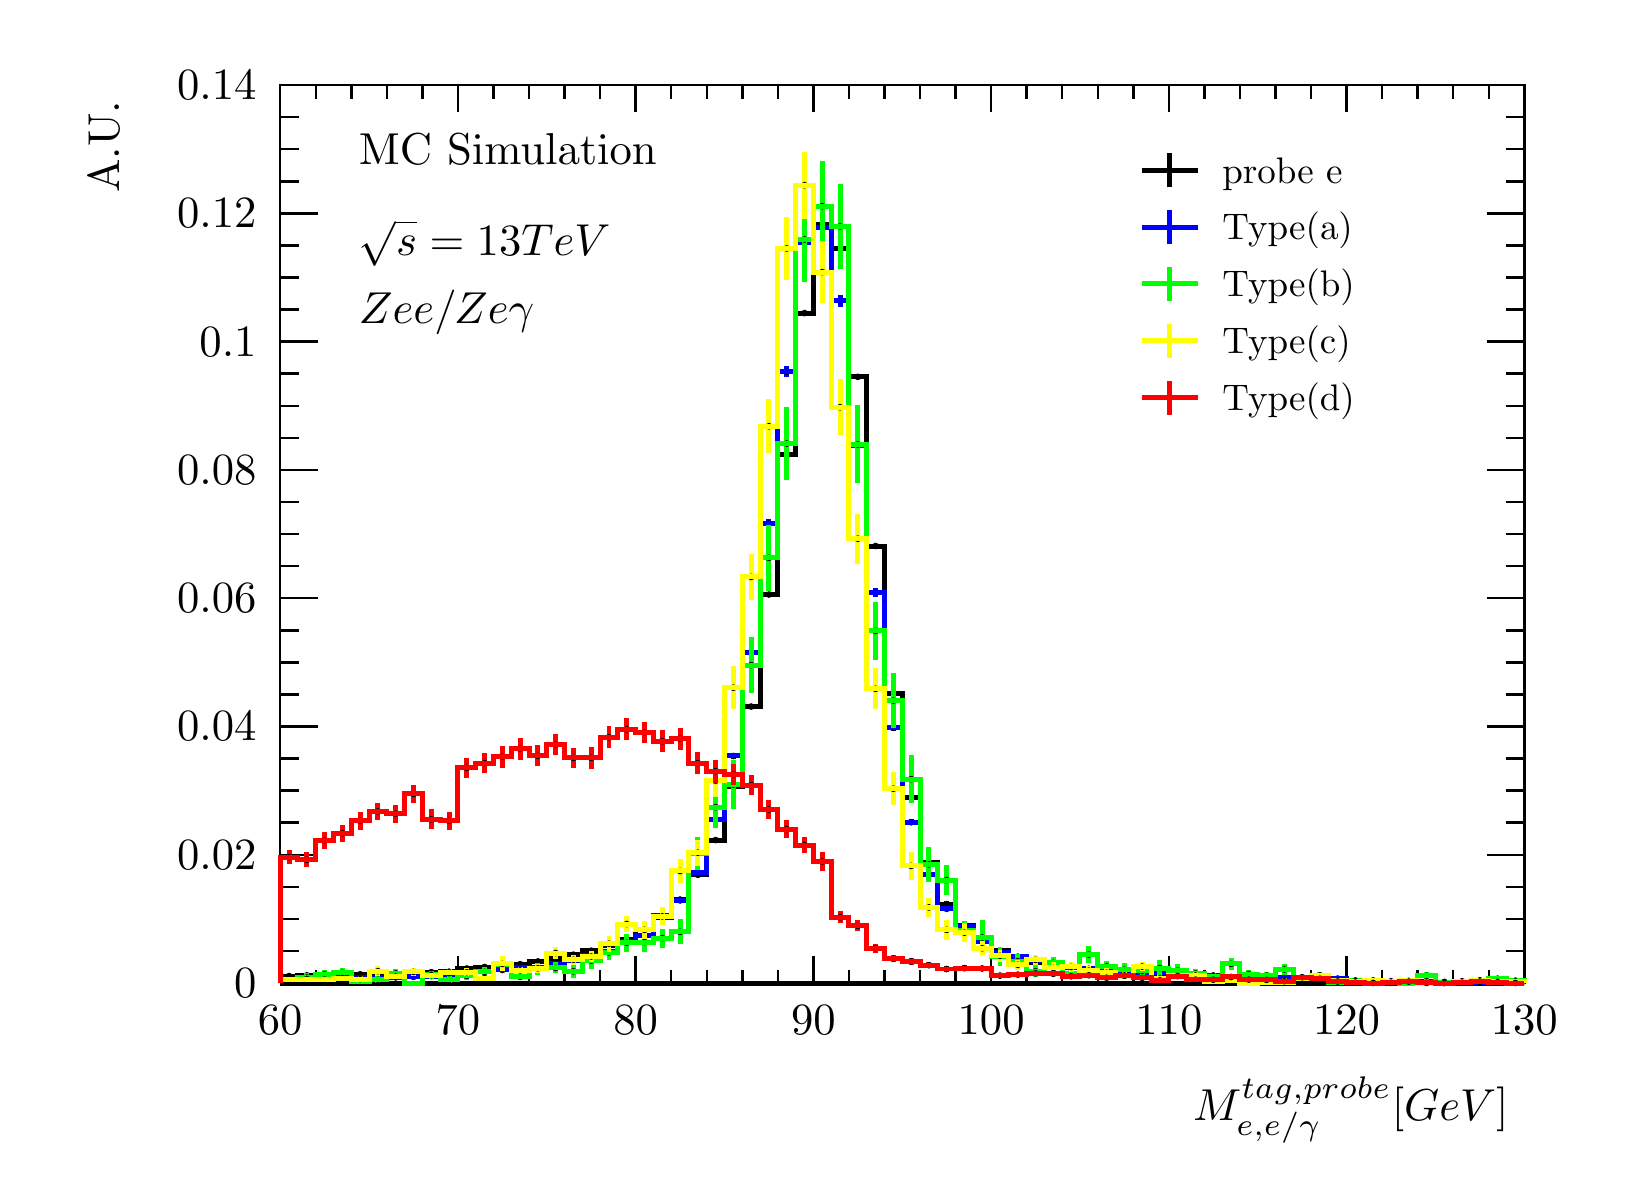
\begin{tikzpicture}
\pgfdeclareplotmark{cross} {
\pgfpathmoveto{\pgfpoint{-0.3\pgfplotmarksize}{\pgfplotmarksize}}
\pgfpathlineto{\pgfpoint{+0.3\pgfplotmarksize}{\pgfplotmarksize}}
\pgfpathlineto{\pgfpoint{+0.3\pgfplotmarksize}{0.3\pgfplotmarksize}}
\pgfpathlineto{\pgfpoint{+1\pgfplotmarksize}{0.3\pgfplotmarksize}}
\pgfpathlineto{\pgfpoint{+1\pgfplotmarksize}{-0.3\pgfplotmarksize}}
\pgfpathlineto{\pgfpoint{+0.3\pgfplotmarksize}{-0.3\pgfplotmarksize}}
\pgfpathlineto{\pgfpoint{+0.3\pgfplotmarksize}{-1.\pgfplotmarksize}}
\pgfpathlineto{\pgfpoint{-0.3\pgfplotmarksize}{-1.\pgfplotmarksize}}
\pgfpathlineto{\pgfpoint{-0.3\pgfplotmarksize}{-0.3\pgfplotmarksize}}
\pgfpathlineto{\pgfpoint{-1.\pgfplotmarksize}{-0.3\pgfplotmarksize}}
\pgfpathlineto{\pgfpoint{-1.\pgfplotmarksize}{0.3\pgfplotmarksize}}
\pgfpathlineto{\pgfpoint{-0.3\pgfplotmarksize}{0.3\pgfplotmarksize}}
\pgfpathclose
\pgfusepathqstroke
}
\pgfdeclareplotmark{cross*} {
\pgfpathmoveto{\pgfpoint{-0.3\pgfplotmarksize}{\pgfplotmarksize}}
\pgfpathlineto{\pgfpoint{+0.3\pgfplotmarksize}{\pgfplotmarksize}}
\pgfpathlineto{\pgfpoint{+0.3\pgfplotmarksize}{0.3\pgfplotmarksize}}
\pgfpathlineto{\pgfpoint{+1\pgfplotmarksize}{0.3\pgfplotmarksize}}
\pgfpathlineto{\pgfpoint{+1\pgfplotmarksize}{-0.3\pgfplotmarksize}}
\pgfpathlineto{\pgfpoint{+0.3\pgfplotmarksize}{-0.3\pgfplotmarksize}}
\pgfpathlineto{\pgfpoint{+0.3\pgfplotmarksize}{-1.\pgfplotmarksize}}
\pgfpathlineto{\pgfpoint{-0.3\pgfplotmarksize}{-1.\pgfplotmarksize}}
\pgfpathlineto{\pgfpoint{-0.3\pgfplotmarksize}{-0.3\pgfplotmarksize}}
\pgfpathlineto{\pgfpoint{-1.\pgfplotmarksize}{-0.3\pgfplotmarksize}}
\pgfpathlineto{\pgfpoint{-1.\pgfplotmarksize}{0.3\pgfplotmarksize}}
\pgfpathlineto{\pgfpoint{-0.3\pgfplotmarksize}{0.3\pgfplotmarksize}}
\pgfpathclose
\pgfusepathqfillstroke
}
\pgfdeclareplotmark{newstar} {
\pgfpathmoveto{\pgfqpoint{0pt}{\pgfplotmarksize}}
\pgfpathlineto{\pgfqpointpolar{44}{0.5\pgfplotmarksize}}
\pgfpathlineto{\pgfqpointpolar{18}{\pgfplotmarksize}}
\pgfpathlineto{\pgfqpointpolar{-20}{0.5\pgfplotmarksize}}
\pgfpathlineto{\pgfqpointpolar{-54}{\pgfplotmarksize}}
\pgfpathlineto{\pgfqpointpolar{-90}{0.5\pgfplotmarksize}}
\pgfpathlineto{\pgfqpointpolar{234}{\pgfplotmarksize}}
\pgfpathlineto{\pgfqpointpolar{198}{0.5\pgfplotmarksize}}
\pgfpathlineto{\pgfqpointpolar{162}{\pgfplotmarksize}}
\pgfpathlineto{\pgfqpointpolar{134}{0.5\pgfplotmarksize}}
\pgfpathclose
\pgfusepathqstroke
}
\pgfdeclareplotmark{newstar*} {
\pgfpathmoveto{\pgfqpoint{0pt}{\pgfplotmarksize}}
\pgfpathlineto{\pgfqpointpolar{44}{0.5\pgfplotmarksize}}
\pgfpathlineto{\pgfqpointpolar{18}{\pgfplotmarksize}}
\pgfpathlineto{\pgfqpointpolar{-20}{0.5\pgfplotmarksize}}
\pgfpathlineto{\pgfqpointpolar{-54}{\pgfplotmarksize}}
\pgfpathlineto{\pgfqpointpolar{-90}{0.5\pgfplotmarksize}}
\pgfpathlineto{\pgfqpointpolar{234}{\pgfplotmarksize}}
\pgfpathlineto{\pgfqpointpolar{198}{0.5\pgfplotmarksize}}
\pgfpathlineto{\pgfqpointpolar{162}{\pgfplotmarksize}}
\pgfpathlineto{\pgfqpointpolar{134}{0.5\pgfplotmarksize}}
\pgfpathclose
\pgfusepathqfillstroke
}
\definecolor{c}{rgb}{1,1,1};
\draw [color=c, fill=c] (0,0) rectangle (20,14.4361);
\draw [color=c, fill=c] (3.2,2.30977) rectangle (19,13.7143);
\definecolor{c}{rgb}{0,0,0};
\draw [c,line width=0.9] (3.2,2.30977) -- (3.2,13.7143) -- (19,13.7143) -- (19,2.30977) -- (3.2,2.30977);
\draw [c,line width=1.8] (3.2,2.30977) -- (3.2158,2.30977) -- (3.2158,2.30977) -- (3.2316,2.30977) -- (3.2316,2.30977) -- (3.2474,2.30977) -- (3.2474,2.30977) -- (3.2632,2.30977) -- (3.2632,2.30977) -- (3.279,2.30977) -- (3.279,2.30977) --
 (3.2948,2.30977) -- (3.2948,2.30977) -- (3.3106,2.30977) -- (3.3106,2.30977) -- (3.3264,2.30977) -- (3.3264,2.30977) -- (3.3422,2.30977) -- (3.3422,2.30977) -- (3.358,2.30977) -- (3.358,2.30977) -- (3.3738,2.30977) -- (3.3738,2.30977) --
 (3.3896,2.30977) -- (3.3896,2.30977) -- (3.4054,2.30977) -- (3.4054,2.30977) -- (3.4212,2.30977) -- (3.4212,2.30977) -- (3.437,2.30977) -- (3.437,2.30977) -- (3.4528,2.30977) -- (3.4528,2.30977) -- (3.4686,2.30977) -- (3.4686,2.30977) --
 (3.4844,2.30977) -- (3.4844,2.30977) -- (3.5002,2.30977) -- (3.5002,2.30977) -- (3.516,2.30977) -- (3.516,2.30977) -- (3.5318,2.30977) -- (3.5318,2.30977) -- (3.5476,2.30977) -- (3.5476,2.30977) -- (3.5634,2.30977) -- (3.5634,2.30977) --
 (3.5792,2.30977) -- (3.5792,2.30977) -- (3.595,2.30977) -- (3.595,2.30977) -- (3.6108,2.30977) -- (3.6108,2.30977) -- (3.6266,2.30977) -- (3.6266,2.30977) -- (3.6424,2.30977) -- (3.6424,2.30977) -- (3.6582,2.30977) -- (3.6582,2.30977) --
 (3.674,2.30977) -- (3.674,2.30977) -- (3.6898,2.30977) -- (3.6898,2.30977) -- (3.7056,2.30977) -- (3.7056,2.30977) -- (3.7214,2.30977) -- (3.7214,2.30977) -- (3.7372,2.30977) -- (3.7372,2.30977) -- (3.753,2.30977) -- (3.753,2.30977) --
 (3.7688,2.30977) -- (3.7688,2.30977) -- (3.7846,2.30977) -- (3.7846,2.30977) -- (3.8004,2.30977) -- (3.8004,2.30977) -- (3.8162,2.30977) -- (3.8162,2.30977) -- (3.832,2.30977) -- (3.832,2.30977) -- (3.8478,2.30977) -- (3.8478,2.30977) --
 (3.8636,2.30977) -- (3.8636,2.30977) -- (3.8794,2.30977) -- (3.8794,2.30977) -- (3.8952,2.30977) -- (3.8952,2.30977) -- (3.911,2.30977) -- (3.911,2.30977) -- (3.9268,2.30977) -- (3.9268,2.30977) -- (3.9426,2.30977) -- (3.9426,2.30977) --
 (3.9584,2.30977) -- (3.9584,2.30977) -- (3.9742,2.30977) -- (3.9742,2.30977) -- (3.99,2.30977) -- (3.99,2.30977) -- (4.0058,2.30977) -- (4.0058,2.30977) -- (4.0216,2.30977) -- (4.0216,2.30977) -- (4.0374,2.30977) -- (4.0374,2.30977) --
 (4.0532,2.30977) -- (4.0532,2.30977) -- (4.069,2.30977) -- (4.069,2.30977) -- (4.0848,2.30977) -- (4.0848,2.30977) -- (4.1006,2.30977) -- (4.1006,2.30977) -- (4.1164,2.30977) -- (4.1164,2.30977) -- (4.1322,2.30977) -- (4.1322,2.30977) --
 (4.148,2.30977) -- (4.148,2.30977) -- (4.1638,2.30977) -- (4.1638,2.30977) -- (4.1796,2.30977) -- (4.1796,2.30977) -- (4.1954,2.30977) -- (4.1954,2.30977) -- (4.2112,2.30977) -- (4.2112,2.30977) -- (4.227,2.30977) -- (4.227,2.30977) --
 (4.2428,2.30977) -- (4.2428,2.30977) -- (4.2586,2.30977) -- (4.2586,2.30977) -- (4.2744,2.30977) -- (4.2744,2.30977) -- (4.2902,2.30977) -- (4.2902,2.30977) -- (4.306,2.30977) -- (4.306,2.30977) -- (4.3218,2.30977) -- (4.3218,2.30977) --
 (4.3376,2.30977) -- (4.3376,2.30977) -- (4.3534,2.30977) -- (4.3534,2.30977) -- (4.3692,2.30977) -- (4.3692,2.30977) -- (4.385,2.30977) -- (4.385,2.30977) -- (4.4008,2.30977) -- (4.4008,2.30977) -- (4.4166,2.30977) -- (4.4166,2.30977) --
 (4.4324,2.30977) -- (4.4324,2.30977) -- (4.4482,2.30977) -- (4.4482,2.30977) -- (4.464,2.30977) -- (4.464,2.30977) -- (4.4798,2.30977) -- (4.4798,2.30977) -- (4.4956,2.30977) -- (4.4956,2.30977) -- (4.5114,2.30977) -- (4.5114,2.30977) --
 (4.5272,2.30977) -- (4.5272,2.30977) -- (4.543,2.30977) -- (4.543,2.30977) -- (4.5588,2.30977) -- (4.5588,2.30977) -- (4.5746,2.30977) -- (4.5746,2.30977) -- (4.5904,2.30977) -- (4.5904,2.30977) -- (4.6062,2.30977) -- (4.6062,2.30977) --
 (4.622,2.30977) -- (4.622,2.30977) -- (4.6378,2.30977) -- (4.6378,2.30977) -- (4.6536,2.30977) -- (4.6536,2.30977) -- (4.6694,2.30977) -- (4.6694,2.30977) -- (4.6852,2.30977) -- (4.6852,2.30977) -- (4.701,2.30977) -- (4.701,2.30977) --
 (4.7168,2.30977) -- (4.7168,2.30977) -- (4.7326,2.30977) -- (4.7326,2.30977) -- (4.7484,2.30977) -- (4.7484,2.30977) -- (4.7642,2.30977) -- (4.7642,2.30977) -- (4.78,2.30977) -- (4.78,2.30977) -- (4.7958,2.30977) -- (4.7958,2.30977) --
 (4.8116,2.30977) -- (4.8116,2.30977) -- (4.8274,2.30977) -- (4.8274,2.30977) -- (4.8432,2.30977) -- (4.8432,2.30977) -- (4.859,2.30977) -- (4.859,2.30977) -- (4.8748,2.30977) -- (4.8748,2.30977) -- (4.8906,2.30977) -- (4.8906,2.30977) --
 (4.9064,2.30977) -- (4.9064,2.30977) -- (4.9222,2.30977) -- (4.9222,2.30977) -- (4.938,2.30977) -- (4.938,2.30977) -- (4.9538,2.30977) -- (4.9538,2.30977) -- (4.9696,2.30977) -- (4.9696,2.30977) -- (4.9854,2.30977) -- (4.9854,2.30977) --
 (5.0012,2.30977) -- (5.0012,2.30977) -- (5.017,2.30977) -- (5.017,2.30977) -- (5.0328,2.30977) -- (5.0328,2.30977) -- (5.0486,2.30977) -- (5.0486,2.30977) -- (5.0644,2.30977) -- (5.0644,2.30977) -- (5.0802,2.30977) -- (5.0802,2.30977) --
 (5.096,2.30977) -- (5.096,2.30977) -- (5.1118,2.30977) -- (5.1118,2.30977) -- (5.1276,2.30977) -- (5.1276,2.30977) -- (5.1434,2.30977) -- (5.1434,2.30977) -- (5.1592,2.30977) -- (5.1592,2.30977) -- (5.175,2.30977) -- (5.175,2.30977) --
 (5.1908,2.30977) -- (5.1908,2.30977) -- (5.2066,2.30977) -- (5.2066,2.30977) -- (5.2224,2.30977) -- (5.2224,2.30977) -- (5.2382,2.30977) -- (5.2382,2.30977) -- (5.254,2.30977) -- (5.254,2.30977) -- (5.2698,2.30977) -- (5.2698,2.30977) --
 (5.2856,2.30977) -- (5.2856,2.30977) -- (5.3014,2.30977) -- (5.3014,2.30977) -- (5.3172,2.30977) -- (5.3172,2.30977) -- (5.333,2.30977) -- (5.333,2.30977) -- (5.3488,2.30977) -- (5.3488,2.30977) -- (5.3646,2.30977) -- (5.3646,2.30977) --
 (5.3804,2.30977) -- (5.3804,2.30977) -- (5.3962,2.30977) -- (5.3962,2.30977) -- (5.412,2.30977) -- (5.412,2.30977) -- (5.4278,2.30977) -- (5.4278,2.30977) -- (5.4436,2.30977) -- (5.4436,2.30977) -- (5.4594,2.30977) -- (5.4594,2.30977) --
 (5.4752,2.30977) -- (5.4752,2.30977) -- (5.491,2.30977) -- (5.491,2.30977) -- (5.5068,2.30977) -- (5.5068,2.30977) -- (5.5226,2.30977) -- (5.5226,2.30977) -- (5.5384,2.30977) -- (5.5384,2.30977) -- (5.5542,2.30977) -- (5.5542,2.30977) --
 (5.57,2.30977) -- (5.57,2.30977) -- (5.5858,2.30977) -- (5.5858,2.30977) -- (5.6016,2.30977) -- (5.6016,2.30977) -- (5.6174,2.30977) -- (5.6174,2.30977) -- (5.6332,2.30977) -- (5.6332,2.30977) -- (5.649,2.30977) -- (5.649,2.30977) --
 (5.6648,2.30977) -- (5.6648,2.30977) -- (5.6806,2.30977) -- (5.6806,2.30977) -- (5.6964,2.30977) -- (5.6964,2.30977) -- (5.7122,2.30977) -- (5.7122,2.30977) -- (5.728,2.30977) -- (5.728,2.30977) -- (5.7438,2.30977) -- (5.7438,2.30977) --
 (5.7596,2.30977) -- (5.7596,2.30977) -- (5.7754,2.30977) -- (5.7754,2.30977) -- (5.7912,2.30977) -- (5.7912,2.30977) -- (5.807,2.30977) -- (5.807,2.30977) -- (5.8228,2.30977) -- (5.8228,2.30977) -- (5.8386,2.30977) -- (5.8386,2.30977) --
 (5.8544,2.30977) -- (5.8544,2.30977) -- (5.8702,2.30977) -- (5.8702,2.30977) -- (5.886,2.30977) -- (5.886,2.30977) -- (5.9018,2.30977) -- (5.9018,2.30977) -- (5.9176,2.30977) -- (5.9176,2.30977) -- (5.9334,2.30977) -- (5.9334,2.30977) --
 (5.9492,2.30977) -- (5.9492,2.30977) -- (5.965,2.30977) -- (5.965,2.30977) -- (5.9808,2.30977) -- (5.9808,2.30977) -- (5.9966,2.30977) -- (5.9966,2.30977) -- (6.0124,2.30977) -- (6.0124,2.30977) -- (6.0282,2.30977) -- (6.0282,2.30977) --
 (6.044,2.30977) -- (6.044,2.30977) -- (6.0598,2.30977) -- (6.0598,2.30977) -- (6.0756,2.30977) -- (6.0756,2.30977) -- (6.0914,2.30977) -- (6.0914,2.30977) -- (6.1072,2.30977) -- (6.1072,2.30977) -- (6.123,2.30977) -- (6.123,2.30977) --
 (6.1388,2.30977) -- (6.1388,2.30977) -- (6.1546,2.30977) -- (6.1546,2.30977) -- (6.1704,2.30977) -- (6.1704,2.30977) -- (6.1862,2.30977) -- (6.1862,2.30977) -- (6.202,2.30977) -- (6.202,2.30977) -- (6.2178,2.30977) -- (6.2178,2.30977) --
 (6.2336,2.30977) -- (6.2336,2.30977) -- (6.2494,2.30977) -- (6.2494,2.30977) -- (6.2652,2.30977) -- (6.2652,2.30977) -- (6.281,2.30977) -- (6.281,2.30977) -- (6.2968,2.30977) -- (6.2968,2.30977) -- (6.3126,2.30977) -- (6.3126,2.30977) --
 (6.3284,2.30977) -- (6.3284,2.30977) -- (6.3442,2.30977) -- (6.3442,2.30977) -- (6.36,2.30977) -- (6.36,2.30977) -- (6.3758,2.30977) -- (6.3758,2.30977) -- (6.3916,2.30977) -- (6.3916,2.30977) -- (6.4074,2.30977) -- (6.4074,2.30977) --
 (6.4232,2.30977) -- (6.4232,2.30977) -- (6.439,2.30977) -- (6.439,2.30977) -- (6.4548,2.30977) -- (6.4548,2.30977) -- (6.4706,2.30977) -- (6.4706,2.30977) -- (6.4864,2.30977) -- (6.4864,2.30977) -- (6.5022,2.30977) -- (6.5022,2.30977) --
 (6.518,2.30977) -- (6.518,2.30977) -- (6.5338,2.30977) -- (6.5338,2.30977) -- (6.5496,2.30977) -- (6.5496,2.30977) -- (6.5654,2.30977) -- (6.5654,2.30977) -- (6.5812,2.30977) -- (6.5812,2.30977) -- (6.597,2.30977) -- (6.597,2.30977) --
 (6.6128,2.30977) -- (6.6128,2.30977) -- (6.6286,2.30977) -- (6.6286,2.30977) -- (6.6444,2.30977) -- (6.6444,2.30977) -- (6.6602,2.30977) -- (6.6602,2.30977) -- (6.676,2.30977) -- (6.676,2.30977) -- (6.6918,2.30977) -- (6.6918,2.30977) --
 (6.7076,2.30977) -- (6.7076,2.30977) -- (6.7234,2.30977) -- (6.7234,2.30977) -- (6.7392,2.30977) -- (6.7392,2.30977) -- (6.755,2.30977) -- (6.755,2.30977) -- (6.7708,2.30977) -- (6.7708,2.30977) -- (6.7866,2.30977) -- (6.7866,2.30977) --
 (6.8024,2.30977) -- (6.8024,2.30977) -- (6.8182,2.30977) -- (6.8182,2.30977) -- (6.834,2.30977) -- (6.834,2.30977) -- (6.8498,2.30977) -- (6.8498,2.30977) -- (6.8656,2.30977) -- (6.8656,2.30977) -- (6.8814,2.30977) -- (6.8814,2.30977) --
 (6.8972,2.30977) -- (6.8972,2.30977) -- (6.913,2.30977) -- (6.913,2.30977) -- (6.9288,2.30977) -- (6.9288,2.30977) -- (6.9446,2.30977) -- (6.9446,2.30977) -- (6.9604,2.30977) -- (6.9604,2.30977) -- (6.9762,2.30977) -- (6.9762,2.30977) --
 (6.992,2.30977) -- (6.992,2.30977) -- (7.0078,2.30977) -- (7.0078,2.30977) -- (7.0236,2.30977) -- (7.0236,2.30977) -- (7.0394,2.30977) -- (7.0394,2.30977) -- (7.0552,2.30977) -- (7.0552,2.30977) -- (7.071,2.30977) -- (7.071,2.30977) --
 (7.0868,2.30977) -- (7.0868,2.30977) -- (7.1026,2.30977) -- (7.1026,2.30977) -- (7.1184,2.30977) -- (7.1184,2.30977) -- (7.1342,2.30977) -- (7.1342,2.30977) -- (7.15,2.30977) -- (7.15,2.30977) -- (7.1658,2.30977) -- (7.1658,2.30977) --
 (7.1816,2.30977) -- (7.1816,2.30977) -- (7.1974,2.30977) -- (7.1974,2.30977) -- (7.2132,2.30977) -- (7.2132,2.30977) -- (7.229,2.30977) -- (7.229,2.30977) -- (7.2448,2.30977) -- (7.2448,2.30977) -- (7.2606,2.30977) -- (7.2606,2.30977) --
 (7.2764,2.30977) -- (7.2764,2.30977) -- (7.2922,2.30977) -- (7.2922,2.30977) -- (7.308,2.30977) -- (7.308,2.30977) -- (7.3238,2.30977) -- (7.3238,2.30977) -- (7.3396,2.30977) -- (7.3396,2.30977) -- (7.3554,2.30977) -- (7.3554,2.30977) --
 (7.3712,2.30977) -- (7.3712,2.30977) -- (7.387,2.30977) -- (7.387,2.30977) -- (7.4028,2.30977) -- (7.4028,2.30977) -- (7.4186,2.30977) -- (7.4186,2.30977) -- (7.4344,2.30977) -- (7.4344,2.30977) -- (7.4502,2.30977) -- (7.4502,2.30977) --
 (7.466,2.30977) -- (7.466,2.30977) -- (7.4818,2.30977) -- (7.4818,2.30977) -- (7.4976,2.30977) -- (7.4976,2.30977) -- (7.5134,2.30977) -- (7.5134,2.30977) -- (7.5292,2.30977) -- (7.5292,2.30977) -- (7.545,2.30977) -- (7.545,2.30977) --
 (7.5608,2.30977) -- (7.5608,2.30977) -- (7.5766,2.30977) -- (7.5766,2.30977) -- (7.5924,2.30977) -- (7.5924,2.30977) -- (7.6082,2.30977) -- (7.6082,2.30977) -- (7.624,2.30977) -- (7.624,2.30977) -- (7.6398,2.30977) -- (7.6398,2.30977) --
 (7.6556,2.30977) -- (7.6556,2.30977) -- (7.6714,2.30977) -- (7.6714,2.30977) -- (7.6872,2.30977) -- (7.6872,2.30977) -- (7.703,2.30977) -- (7.703,2.30977) -- (7.7188,2.30977) -- (7.7188,2.30977) -- (7.7346,2.30977) -- (7.7346,2.30977) --
 (7.7504,2.30977) -- (7.7504,2.30977) -- (7.7662,2.30977) -- (7.7662,2.30977) -- (7.782,2.30977) -- (7.782,2.30977) -- (7.7978,2.30977) -- (7.7978,2.30977) -- (7.8136,2.30977) -- (7.8136,2.30977) -- (7.8294,2.30977) -- (7.8294,2.30977) --
 (7.8452,2.30977) -- (7.8452,2.30977) -- (7.861,2.30977) -- (7.861,2.30977) -- (7.8768,2.30977) -- (7.8768,2.30977) -- (7.8926,2.30977) -- (7.8926,2.30977) -- (7.9084,2.30977) -- (7.9084,2.30977) -- (7.9242,2.30977) -- (7.9242,2.30977) --
 (7.94,2.30977) -- (7.94,2.30977) -- (7.9558,2.30977) -- (7.9558,2.30977) -- (7.9716,2.30977) -- (7.9716,2.30977) -- (7.9874,2.30977) -- (7.9874,2.30977) -- (8.0032,2.30977) -- (8.0032,2.30977) -- (8.019,2.30977) -- (8.019,2.30977) --
 (8.0348,2.30977) -- (8.0348,2.30977) -- (8.0506,2.30977) -- (8.0506,2.30977) -- (8.0664,2.30977) -- (8.0664,2.30977) -- (8.0822,2.30977) -- (8.0822,2.30977) -- (8.098,2.30977) -- (8.098,2.30977) -- (8.1138,2.30977) -- (8.1138,2.30977) --
 (8.1296,2.30977) -- (8.1296,2.30977) -- (8.1454,2.30977) -- (8.1454,2.30977) -- (8.1612,2.30977) -- (8.1612,2.30977) -- (8.177,2.30977) -- (8.177,2.30977) -- (8.1928,2.30977) -- (8.1928,2.30977) -- (8.2086,2.30977) -- (8.2086,2.30977) --
 (8.2244,2.30977) -- (8.2244,2.30977) -- (8.2402,2.30977) -- (8.2402,2.30977) -- (8.256,2.30977) -- (8.256,2.30977) -- (8.2718,2.30977) -- (8.2718,2.30977) -- (8.2876,2.30977) -- (8.2876,2.30977) -- (8.3034,2.30977) -- (8.3034,2.30977) --
 (8.3192,2.30977) -- (8.3192,2.30977) -- (8.335,2.30977) -- (8.335,2.30977) -- (8.3508,2.30977) -- (8.3508,2.30977) -- (8.3666,2.30977) -- (8.3666,2.30977) -- (8.3824,2.30977) -- (8.3824,2.30977) -- (8.3982,2.30977) -- (8.3982,2.30977) --
 (8.414,2.30977) -- (8.414,2.30977) -- (8.4298,2.30977) -- (8.4298,2.30977) -- (8.4456,2.30977) -- (8.4456,2.30977) -- (8.4614,2.30977) -- (8.4614,2.30977) -- (8.4772,2.30977) -- (8.4772,2.30977) -- (8.493,2.30977) -- (8.493,2.30977) --
 (8.5088,2.30977) -- (8.5088,2.30977) -- (8.5246,2.30977) -- (8.5246,2.30977) -- (8.5404,2.30977) -- (8.5404,2.30977) -- (8.5562,2.30977) -- (8.5562,2.30977) -- (8.572,2.30977) -- (8.572,2.30977) -- (8.5878,2.30977) -- (8.5878,2.30977) --
 (8.6036,2.30977) -- (8.6036,2.30977) -- (8.6194,2.30977) -- (8.6194,2.30977) -- (8.6352,2.30977) -- (8.6352,2.30977) -- (8.651,2.30977) -- (8.651,2.30977) -- (8.6668,2.30977) -- (8.6668,2.30977) -- (8.6826,2.30977) -- (8.6826,2.30977) --
 (8.6984,2.30977) -- (8.6984,2.30977) -- (8.7142,2.30977) -- (8.7142,2.30977) -- (8.73,2.30977) -- (8.73,2.30977) -- (8.7458,2.30977) -- (8.7458,2.30977) -- (8.7616,2.30977) -- (8.7616,2.30977) -- (8.7774,2.30977) -- (8.7774,2.30977) --
 (8.7932,2.30977) -- (8.7932,2.30977) -- (8.809,2.30977) -- (8.809,2.30977) -- (8.8248,2.30977) -- (8.8248,2.30977) -- (8.8406,2.30977) -- (8.8406,2.30977) -- (8.8564,2.30977) -- (8.8564,2.30977) -- (8.8722,2.30977) -- (8.8722,2.30977) --
 (8.888,2.30977) -- (8.888,2.30977) -- (8.9038,2.30977) -- (8.9038,2.30977) -- (8.9196,2.30977) -- (8.9196,2.30977) -- (8.9354,2.30977) -- (8.9354,2.30977) -- (8.9512,2.30977) -- (8.9512,2.30977) -- (8.967,2.30977) -- (8.967,2.30977) --
 (8.9828,2.30977) -- (8.9828,2.30977) -- (8.9986,2.30977) -- (8.9986,2.30977) -- (9.0144,2.30977) -- (9.0144,2.30977) -- (9.0302,2.30977) -- (9.0302,2.30977) -- (9.046,2.30977) -- (9.046,2.30977) -- (9.0618,2.30977) -- (9.0618,2.30977) --
 (9.0776,2.30977) -- (9.0776,2.30977) -- (9.0934,2.30977) -- (9.0934,2.30977) -- (9.1092,2.30977) -- (9.1092,2.30977) -- (9.125,2.30977) -- (9.125,2.30977) -- (9.1408,2.30977) -- (9.1408,2.30977) -- (9.1566,2.30977) -- (9.1566,2.30977) --
 (9.1724,2.30977) -- (9.1724,2.30977) -- (9.1882,2.30977) -- (9.1882,2.30977) -- (9.204,2.30977) -- (9.204,2.30977) -- (9.2198,2.30977) -- (9.2198,2.30977) -- (9.2356,2.30977) -- (9.2356,2.30977) -- (9.2514,2.30977) -- (9.2514,2.30977) --
 (9.2672,2.30977) -- (9.2672,2.30977) -- (9.283,2.30977) -- (9.283,2.30977) -- (9.2988,2.30977) -- (9.2988,2.30977) -- (9.3146,2.30977) -- (9.3146,2.30977) -- (9.3304,2.30977) -- (9.3304,2.30977) -- (9.3462,2.30977) -- (9.3462,2.30977) --
 (9.362,2.30977) -- (9.362,2.30977) -- (9.3778,2.30977) -- (9.3778,2.30977) -- (9.3936,2.30977) -- (9.3936,2.30977) -- (9.4094,2.30977) -- (9.4094,2.30977) -- (9.4252,2.30977) -- (9.4252,2.30977) -- (9.441,2.30977) -- (9.441,2.30977) --
 (9.4568,2.30977) -- (9.4568,2.30977) -- (9.4726,2.30977) -- (9.4726,2.30977) -- (9.4884,2.30977) -- (9.4884,2.30977) -- (9.5042,2.30977) -- (9.5042,2.30977) -- (9.52,2.30977) -- (9.52,2.30977) -- (9.5358,2.30977) -- (9.5358,2.30977) --
 (9.5516,2.30977) -- (9.5516,2.30977) -- (9.5674,2.30977) -- (9.5674,2.30977) -- (9.5832,2.30977) -- (9.5832,2.30977) -- (9.599,2.30977) -- (9.599,2.30977) -- (9.6148,2.30977) -- (9.6148,2.30977) -- (9.6306,2.30977) -- (9.6306,2.30977) --
 (9.6464,2.30977) -- (9.6464,2.30977) -- (9.6622,2.30977) -- (9.6622,2.30977) -- (9.678,2.30977) -- (9.678,2.30977) -- (9.6938,2.30977) -- (9.6938,2.30977) -- (9.7096,2.30977) -- (9.7096,2.30977) -- (9.7254,2.30977) -- (9.7254,2.30977) --
 (9.7412,2.30977) -- (9.7412,2.30977) -- (9.757,2.30977) -- (9.757,2.30977) -- (9.7728,2.30977) -- (9.7728,2.30977) -- (9.7886,2.30977) -- (9.7886,2.30977) -- (9.8044,2.30977) -- (9.8044,2.30977) -- (9.8202,2.30977) -- (9.8202,2.30977) --
 (9.836,2.30977) -- (9.836,2.30977) -- (9.8518,2.30977) -- (9.8518,2.30977) -- (9.8676,2.30977) -- (9.8676,2.30977) -- (9.8834,2.30977) -- (9.8834,2.30977) -- (9.8992,2.30977) -- (9.8992,2.30977) -- (9.915,2.30977) -- (9.915,2.30977) --
 (9.9308,2.30977) -- (9.9308,2.30977) -- (9.9466,2.30977) -- (9.9466,2.30977) -- (9.9624,2.30977) -- (9.9624,2.30977) -- (9.9782,2.30977) -- (9.9782,2.30977) -- (9.994,2.30977) -- (9.994,2.30977) -- (10.0098,2.30977) -- (10.0098,2.30977) --
 (10.0256,2.30977) -- (10.0256,2.30977) -- (10.0414,2.30977) -- (10.0414,2.30977) -- (10.0572,2.30977) -- (10.0572,2.30977) -- (10.073,2.30977) -- (10.073,2.30977) -- (10.0888,2.30977) -- (10.0888,2.30977) -- (10.1046,2.30977) -- (10.1046,2.30977) --
 (10.1204,2.30977) -- (10.1204,2.30977) -- (10.1362,2.30977) -- (10.1362,2.30977) -- (10.152,2.30977) -- (10.152,2.30977) -- (10.1678,2.30977) -- (10.1678,2.30977) -- (10.1836,2.30977) -- (10.1836,2.30977) -- (10.1994,2.30977) -- (10.1994,2.30977) --
 (10.2152,2.30977) -- (10.2152,2.30977) -- (10.231,2.30977) -- (10.231,2.30977) -- (10.2468,2.30977) -- (10.2468,2.30977) -- (10.2626,2.30977) -- (10.2626,2.30977) -- (10.2784,2.30977) -- (10.2784,2.30977) -- (10.2942,2.30977) -- (10.2942,2.30977) --
 (10.31,2.30977) -- (10.31,2.30977) -- (10.3258,2.30977) -- (10.3258,2.30977) -- (10.3416,2.30977) -- (10.3416,2.30977) -- (10.3574,2.30977) -- (10.3574,2.30977) -- (10.3732,2.30977) -- (10.3732,2.30977) -- (10.389,2.30977) -- (10.389,2.30977) --
 (10.4048,2.30977) -- (10.4048,2.30977) -- (10.4206,2.30977) -- (10.4206,2.30977) -- (10.4364,2.30977) -- (10.4364,2.30977) -- (10.4522,2.30977) -- (10.4522,2.30977) -- (10.468,2.30977) -- (10.468,2.30977) -- (10.4838,2.30977) -- (10.4838,2.30977) --
 (10.4996,2.30977) -- (10.4996,2.30977) -- (10.5154,2.30977) -- (10.5154,2.30977) -- (10.5312,2.30977) -- (10.5312,2.30977) -- (10.547,2.30977) -- (10.547,2.30977) -- (10.5628,2.30977) -- (10.5628,2.30977) -- (10.5786,2.30977) -- (10.5786,2.30977) --
 (10.5944,2.30977) -- (10.5944,2.30977) -- (10.6102,2.30977) -- (10.6102,2.30977) -- (10.626,2.30977) -- (10.626,2.30977) -- (10.6418,2.30977) -- (10.6418,2.30977) -- (10.6576,2.30977) -- (10.6576,2.30977) -- (10.6734,2.30977) -- (10.6734,2.30977) --
 (10.6892,2.30977) -- (10.6892,2.30977) -- (10.705,2.30977) -- (10.705,2.30977) -- (10.7208,2.30977) -- (10.7208,2.30977) -- (10.7366,2.30977) -- (10.7366,2.30977) -- (10.7524,2.30977) -- (10.7524,2.30977) -- (10.7682,2.30977) -- (10.7682,2.30977) --
 (10.784,2.30977) -- (10.784,2.30977) -- (10.7998,2.30977) -- (10.7998,2.30977) -- (10.8156,2.30977) -- (10.8156,2.30977) -- (10.8314,2.30977) -- (10.8314,2.30977) -- (10.8472,2.30977) -- (10.8472,2.30977) -- (10.863,2.30977) -- (10.863,2.30977) --
 (10.8788,2.30977) -- (10.8788,2.30977) -- (10.8946,2.30977) -- (10.8946,2.30977) -- (10.9104,2.30977) -- (10.9104,2.30977) -- (10.9262,2.30977) -- (10.9262,2.30977) -- (10.942,2.30977) -- (10.942,2.30977) -- (10.9578,2.30977) -- (10.9578,2.30977) --
 (10.9736,2.30977) -- (10.9736,2.30977) -- (10.9894,2.30977) -- (10.9894,2.30977) -- (11.0052,2.30977) -- (11.0052,2.30977) -- (11.021,2.30977) -- (11.021,2.30977) -- (11.0368,2.30977) -- (11.0368,2.30977) -- (11.0526,2.30977) -- (11.0526,2.30977) --
 (11.0684,2.30977) -- (11.0684,2.30977) -- (11.0842,2.30977) -- (11.0842,2.30977) -- (11.1,2.30977) -- (11.1,2.30977) -- (11.1158,2.30977) -- (11.1158,2.30977) -- (11.1316,2.30977) -- (11.1316,2.30977) -- (11.1474,2.30977) -- (11.1474,2.30977) --
 (11.1632,2.30977) -- (11.1632,2.30977) -- (11.179,2.30977) -- (11.179,2.30977) -- (11.1948,2.30977) -- (11.1948,2.30977) -- (11.2106,2.30977) -- (11.2106,2.30977) -- (11.2264,2.30977) -- (11.2264,2.30977) -- (11.2422,2.30977) -- (11.2422,2.30977) --
 (11.258,2.30977) -- (11.258,2.30977) -- (11.2738,2.30977) -- (11.2738,2.30977) -- (11.2896,2.30977) -- (11.2896,2.30977) -- (11.3054,2.30977) -- (11.3054,2.30977) -- (11.3212,2.30977) -- (11.3212,2.30977) -- (11.337,2.30977) -- (11.337,2.30977) --
 (11.3528,2.30977) -- (11.3528,2.30977) -- (11.3686,2.30977) -- (11.3686,2.30977) -- (11.3844,2.30977) -- (11.3844,2.30977) -- (11.4002,2.30977) -- (11.4002,2.30977) -- (11.416,2.30977) -- (11.416,2.30977) -- (11.4318,2.30977) -- (11.4318,2.30977) --
 (11.4476,2.30977) -- (11.4476,2.30977) -- (11.4634,2.30977) -- (11.4634,2.30977) -- (11.4792,2.30977) -- (11.4792,2.30977) -- (11.495,2.30977) -- (11.495,2.30977) -- (11.5108,2.30977) -- (11.5108,2.30977) -- (11.5266,2.30977) -- (11.5266,2.30977) --
 (11.5424,2.30977) -- (11.5424,2.30977) -- (11.5582,2.30977) -- (11.5582,2.30977) -- (11.574,2.30977) -- (11.574,2.30977) -- (11.5898,2.30977) -- (11.5898,2.30977) -- (11.6056,2.30977) -- (11.6056,2.30977) -- (11.6214,2.30977) -- (11.6214,2.30977) --
 (11.6372,2.30977) -- (11.6372,2.30977) -- (11.653,2.30977) -- (11.653,2.30977) -- (11.6688,2.30977) -- (11.6688,2.30977) -- (11.6846,2.30977) -- (11.6846,2.30977) -- (11.7004,2.30977) -- (11.7004,2.30977) -- (11.7162,2.30977) -- (11.7162,2.30977) --
 (11.732,2.30977) -- (11.732,2.30977) -- (11.7478,2.30977) -- (11.7478,2.30977) -- (11.7636,2.30977) -- (11.7636,2.30977) -- (11.7794,2.30977) -- (11.7794,2.30977) -- (11.7952,2.30977) -- (11.7952,2.30977) -- (11.811,2.30977) -- (11.811,2.30977) --
 (11.8268,2.30977) -- (11.8268,2.30977) -- (11.8426,2.30977) -- (11.8426,2.30977) -- (11.8584,2.30977) -- (11.8584,2.30977) -- (11.8742,2.30977) -- (11.8742,2.30977) -- (11.89,2.30977) -- (11.89,2.30977) -- (11.9058,2.30977) -- (11.9058,2.30977) --
 (11.9216,2.30977) -- (11.9216,2.30977) -- (11.9374,2.30977) -- (11.9374,2.30977) -- (11.9532,2.30977) -- (11.9532,2.30977) -- (11.969,2.30977) -- (11.969,2.30977) -- (11.9848,2.30977) -- (11.9848,2.30977) -- (12.0006,2.30977) -- (12.0006,2.30977) --
 (12.0164,2.30977) -- (12.0164,2.30977) -- (12.0322,2.30977) -- (12.0322,2.30977) -- (12.048,2.30977) -- (12.048,2.30977) -- (12.0638,2.30977) -- (12.0638,2.30977) -- (12.0796,2.30977) -- (12.0796,2.30977) -- (12.0954,2.30977) -- (12.0954,2.30977) --
 (12.1112,2.30977) -- (12.1112,2.30977) -- (12.127,2.30977) -- (12.127,2.30977) -- (12.1428,2.30977) -- (12.1428,2.30977) -- (12.1586,2.30977) -- (12.1586,2.30977) -- (12.1744,2.30977) -- (12.1744,2.30977) -- (12.1902,2.30977) -- (12.1902,2.30977) --
 (12.206,2.30977) -- (12.206,2.30977) -- (12.2218,2.30977) -- (12.2218,2.30977) -- (12.2376,2.30977) -- (12.2376,2.30977) -- (12.2534,2.30977) -- (12.2534,2.30977) -- (12.2692,2.30977) -- (12.2692,2.30977) -- (12.285,2.30977) -- (12.285,2.30977) --
 (12.3008,2.30977) -- (12.3008,2.30977) -- (12.3166,2.30977) -- (12.3166,2.30977) -- (12.3324,2.30977) -- (12.3324,2.30977) -- (12.3482,2.30977) -- (12.3482,2.30977) -- (12.364,2.30977) -- (12.364,2.30977) -- (12.3798,2.30977) -- (12.3798,2.30977) --
 (12.3956,2.30977) -- (12.3956,2.30977) -- (12.4114,2.30977) -- (12.4114,2.30977) -- (12.4272,2.30977) -- (12.4272,2.30977) -- (12.443,2.30977) -- (12.443,2.30977) -- (12.4588,2.30977) -- (12.4588,2.30977) -- (12.4746,2.30977) -- (12.4746,2.30977) --
 (12.4904,2.30977) -- (12.4904,2.30977) -- (12.5062,2.30977) -- (12.5062,2.30977) -- (12.522,2.30977) -- (12.522,2.30977) -- (12.5378,2.30977) -- (12.5378,2.30977) -- (12.5536,2.30977) -- (12.5536,2.30977) -- (12.5694,2.30977) -- (12.5694,2.30977) --
 (12.5852,2.30977) -- (12.5852,2.30977) -- (12.601,2.30977) -- (12.601,2.30977) -- (12.6168,2.30977) -- (12.6168,2.30977) -- (12.6326,2.30977) -- (12.6326,2.30977) -- (12.6484,2.30977) -- (12.6484,2.30977) -- (12.6642,2.30977) -- (12.6642,2.30977) --
 (12.68,2.30977) -- (12.68,2.30977) -- (12.6958,2.30977) -- (12.6958,2.30977) -- (12.7116,2.30977) -- (12.7116,2.30977) -- (12.7274,2.30977) -- (12.7274,2.30977) -- (12.7432,2.30977) -- (12.7432,2.30977) -- (12.759,2.30977) -- (12.759,2.30977) --
 (12.7748,2.30977) -- (12.7748,2.30977) -- (12.7906,2.30977) -- (12.7906,2.30977) -- (12.8064,2.30977) -- (12.8064,2.30977) -- (12.8222,2.30977) -- (12.8222,2.30977) -- (12.838,2.30977) -- (12.838,2.30977) -- (12.8538,2.30977) -- (12.8538,2.30977) --
 (12.8696,2.30977) -- (12.8696,2.30977) -- (12.8854,2.30977) -- (12.8854,2.30977) -- (12.9012,2.30977) -- (12.9012,2.30977) -- (12.917,2.30977) -- (12.917,2.30977) -- (12.9328,2.30977) -- (12.9328,2.30977) -- (12.9486,2.30977) -- (12.9486,2.30977) --
 (12.9644,2.30977) -- (12.9644,2.30977) -- (12.9802,2.30977) -- (12.9802,2.30977) -- (12.996,2.30977) -- (12.996,2.30977) -- (13.0118,2.30977) -- (13.0118,2.30977) -- (13.0276,2.30977) -- (13.0276,2.30977) -- (13.0434,2.30977) -- (13.0434,2.30977) --
 (13.0592,2.30977) -- (13.0592,2.30977) -- (13.075,2.30977) -- (13.075,2.30977) -- (13.0908,2.30977) -- (13.0908,2.30977) -- (13.1066,2.30977) -- (13.1066,2.30977) -- (13.1224,2.30977) -- (13.1224,2.30977) -- (13.1382,2.30977) -- (13.1382,2.30977) --
 (13.154,2.30977) -- (13.154,2.30977) -- (13.1698,2.30977) -- (13.1698,2.30977) -- (13.1856,2.30977) -- (13.1856,2.30977) -- (13.2014,2.30977) -- (13.2014,2.30977) -- (13.2172,2.30977) -- (13.2172,2.30977) -- (13.233,2.30977) -- (13.233,2.30977) --
 (13.2488,2.30977) -- (13.2488,2.30977) -- (13.2646,2.30977) -- (13.2646,2.30977) -- (13.2804,2.30977) -- (13.2804,2.30977) -- (13.2962,2.30977) -- (13.2962,2.30977) -- (13.312,2.30977) -- (13.312,2.30977) -- (13.3278,2.30977) -- (13.3278,2.30977) --
 (13.3436,2.30977) -- (13.3436,2.30977) -- (13.3594,2.30977) -- (13.3594,2.30977) -- (13.3752,2.30977) -- (13.3752,2.30977) -- (13.391,2.30977) -- (13.391,2.30977) -- (13.4068,2.30977) -- (13.4068,2.30977) -- (13.4226,2.30977) -- (13.4226,2.30977) --
 (13.4384,2.30977) -- (13.4384,2.30977) -- (13.4542,2.30977) -- (13.4542,2.30977) -- (13.47,2.30977) -- (13.47,2.30977) -- (13.4858,2.30977) -- (13.4858,2.30977) -- (13.5016,2.30977) -- (13.5016,2.30977) -- (13.5174,2.30977) -- (13.5174,2.30977) --
 (13.5332,2.30977) -- (13.5332,2.30977) -- (13.549,2.30977) -- (13.549,2.30977) -- (13.5648,2.30977) -- (13.5648,2.30977) -- (13.5806,2.30977) -- (13.5806,2.30977) -- (13.5964,2.30977) -- (13.5964,2.30977) -- (13.6122,2.30977) -- (13.6122,2.30977) --
 (13.628,2.30977) -- (13.628,2.30977) -- (13.6438,2.30977) -- (13.6438,2.30977) -- (13.6596,2.30977) -- (13.6596,2.30977) -- (13.6754,2.30977) -- (13.6754,2.30977) -- (13.6912,2.30977) -- (13.6912,2.30977) -- (13.707,2.30977) -- (13.707,2.30977) --
 (13.7228,2.30977) -- (13.7228,2.30977) -- (13.7386,2.30977) -- (13.7386,2.30977) -- (13.7544,2.30977) -- (13.7544,2.30977) -- (13.7702,2.30977) -- (13.7702,2.30977) -- (13.786,2.30977) -- (13.786,2.30977) -- (13.8018,2.30977) -- (13.8018,2.30977) --
 (13.8176,2.30977) -- (13.8176,2.30977) -- (13.8334,2.30977) -- (13.8334,2.30977) -- (13.8492,2.30977) -- (13.8492,2.30977) -- (13.865,2.30977) -- (13.865,2.30977) -- (13.8808,2.30977) -- (13.8808,2.30977) -- (13.8966,2.30977) -- (13.8966,2.30977) --
 (13.9124,2.30977) -- (13.9124,2.30977) -- (13.9282,2.30977) -- (13.9282,2.30977) -- (13.944,2.30977) -- (13.944,2.30977) -- (13.9598,2.30977) -- (13.9598,2.30977) -- (13.9756,2.30977) -- (13.9756,2.30977) -- (13.9914,2.30977) -- (13.9914,2.30977) --
 (14.0072,2.30977) -- (14.0072,2.30977) -- (14.023,2.30977) -- (14.023,2.30977) -- (14.0388,2.30977) -- (14.0388,2.30977) -- (14.0546,2.30977) -- (14.0546,2.30977) -- (14.0704,2.30977) -- (14.0704,2.30977) -- (14.0862,2.30977) -- (14.0862,2.30977) --
 (14.102,2.30977) -- (14.102,2.30977) -- (14.1178,2.30977) -- (14.1178,2.30977) -- (14.1336,2.30977) -- (14.1336,2.30977) -- (14.1494,2.30977) -- (14.1494,2.30977) -- (14.1652,2.30977) -- (14.1652,2.30977) -- (14.181,2.30977) -- (14.181,2.30977) --
 (14.1968,2.30977) -- (14.1968,2.30977) -- (14.2126,2.30977) -- (14.2126,2.30977) -- (14.2284,2.30977) -- (14.2284,2.30977) -- (14.2442,2.30977) -- (14.2442,2.30977) -- (14.26,2.30977) -- (14.26,2.30977) -- (14.2758,2.30977) -- (14.2758,2.30977) --
 (14.2916,2.30977) -- (14.2916,2.30977) -- (14.3074,2.30977) -- (14.3074,2.30977) -- (14.3232,2.30977) -- (14.3232,2.30977) -- (14.339,2.30977) -- (14.339,2.30977) -- (14.3548,2.30977) -- (14.3548,2.30977) -- (14.3706,2.30977) -- (14.3706,2.30977) --
 (14.3864,2.30977) -- (14.3864,2.30977) -- (14.4022,2.30977) -- (14.4022,2.30977) -- (14.418,2.30977) -- (14.418,2.30977) -- (14.4338,2.30977) -- (14.4338,2.30977) -- (14.4496,2.30977) -- (14.4496,2.30977) -- (14.4654,2.30977) -- (14.4654,2.30977) --
 (14.4812,2.30977) -- (14.4812,2.30977) -- (14.497,2.30977) -- (14.497,2.30977) -- (14.5128,2.30977) -- (14.5128,2.30977) -- (14.5286,2.30977) -- (14.5286,2.30977) -- (14.5444,2.30977) -- (14.5444,2.30977) -- (14.5602,2.30977) -- (14.5602,2.30977) --
 (14.576,2.30977) -- (14.576,2.30977) -- (14.5918,2.30977) -- (14.5918,2.30977) -- (14.6076,2.30977) -- (14.6076,2.30977) -- (14.6234,2.30977) -- (14.6234,2.30977) -- (14.6392,2.30977) -- (14.6392,2.30977) -- (14.655,2.30977) -- (14.655,2.30977) --
 (14.6708,2.30977) -- (14.6708,2.30977) -- (14.6866,2.30977) -- (14.6866,2.30977) -- (14.7024,2.30977) -- (14.7024,2.30977) -- (14.7182,2.30977) -- (14.7182,2.30977) -- (14.734,2.30977) -- (14.734,2.30977) -- (14.7498,2.30977) -- (14.7498,2.30977) --
 (14.7656,2.30977) -- (14.7656,2.30977) -- (14.7814,2.30977) -- (14.7814,2.30977) -- (14.7972,2.30977) -- (14.7972,2.30977) -- (14.813,2.30977) -- (14.813,2.30977) -- (14.8288,2.30977) -- (14.8288,2.30977) -- (14.8446,2.30977) -- (14.8446,2.30977) --
 (14.8604,2.30977) -- (14.8604,2.30977) -- (14.8762,2.30977) -- (14.8762,2.30977) -- (14.892,2.30977) -- (14.892,2.30977) -- (14.9078,2.30977) -- (14.9078,2.30977) -- (14.9236,2.30977) -- (14.9236,2.30977) -- (14.9394,2.30977) -- (14.9394,2.30977) --
 (14.9552,2.30977) -- (14.9552,2.30977) -- (14.971,2.30977) -- (14.971,2.30977) -- (14.9868,2.30977) -- (14.9868,2.30977) -- (15.0026,2.30977) -- (15.0026,2.30977) -- (15.0184,2.30977) -- (15.0184,2.30977) -- (15.0342,2.30977) -- (15.0342,2.30977) --
 (15.05,2.30977) -- (15.05,2.30977) -- (15.0658,2.30977) -- (15.0658,2.30977) -- (15.0816,2.30977) -- (15.0816,2.30977) -- (15.0974,2.30977) -- (15.0974,2.30977) -- (15.1132,2.30977) -- (15.1132,2.30977) -- (15.129,2.30977) -- (15.129,2.30977) --
 (15.1448,2.30977) -- (15.1448,2.30977) -- (15.1606,2.30977) -- (15.1606,2.30977) -- (15.1764,2.30977) -- (15.1764,2.30977) -- (15.1922,2.30977) -- (15.1922,2.30977) -- (15.208,2.30977) -- (15.208,2.30977) -- (15.2238,2.30977) -- (15.2238,2.30977) --
 (15.2396,2.30977) -- (15.2396,2.30977) -- (15.2554,2.30977) -- (15.2554,2.30977) -- (15.2712,2.30977) -- (15.2712,2.30977) -- (15.287,2.30977) -- (15.287,2.30977) -- (15.3028,2.30977) -- (15.3028,2.30977) -- (15.3186,2.30977) -- (15.3186,2.30977) --
 (15.3344,2.30977) -- (15.3344,2.30977) -- (15.3502,2.30977) -- (15.3502,2.30977) -- (15.366,2.30977) -- (15.366,2.30977) -- (15.3818,2.30977) -- (15.3818,2.30977) -- (15.3976,2.30977) -- (15.3976,2.30977) -- (15.4134,2.30977) -- (15.4134,2.30977) --
 (15.4292,2.30977) -- (15.4292,2.30977) -- (15.445,2.30977) -- (15.445,2.30977) -- (15.4608,2.30977) -- (15.4608,2.30977) -- (15.4766,2.30977) -- (15.4766,2.30977) -- (15.4924,2.30977) -- (15.4924,2.30977) -- (15.5082,2.30977) -- (15.5082,2.30977) --
 (15.524,2.30977) -- (15.524,2.30977) -- (15.5398,2.30977) -- (15.5398,2.30977) -- (15.5556,2.30977) -- (15.5556,2.30977) -- (15.5714,2.30977) -- (15.5714,2.30977) -- (15.5872,2.30977) -- (15.5872,2.30977) -- (15.603,2.30977) -- (15.603,2.30977) --
 (15.6188,2.30977) -- (15.6188,2.30977) -- (15.6346,2.30977) -- (15.6346,2.30977) -- (15.6504,2.30977) -- (15.6504,2.30977) -- (15.6662,2.30977) -- (15.6662,2.30977) -- (15.682,2.30977) -- (15.682,2.30977) -- (15.6978,2.30977) -- (15.6978,2.30977) --
 (15.7136,2.30977) -- (15.7136,2.30977) -- (15.7294,2.30977) -- (15.7294,2.30977) -- (15.7452,2.30977) -- (15.7452,2.30977) -- (15.761,2.30977) -- (15.761,2.30977) -- (15.7768,2.30977) -- (15.7768,2.30977) -- (15.7926,2.30977) -- (15.7926,2.30977) --
 (15.8084,2.30977) -- (15.8084,2.30977) -- (15.8242,2.30977) -- (15.8242,2.30977) -- (15.84,2.30977) -- (15.84,2.30977) -- (15.8558,2.30977) -- (15.8558,2.30977) -- (15.8716,2.30977) -- (15.8716,2.30977) -- (15.8874,2.30977) -- (15.8874,2.30977) --
 (15.9032,2.30977) -- (15.9032,2.30977) -- (15.919,2.30977) -- (15.919,2.30977) -- (15.9348,2.30977) -- (15.9348,2.30977) -- (15.9506,2.30977) -- (15.9506,2.30977) -- (15.9664,2.30977) -- (15.9664,2.30977) -- (15.9822,2.30977) -- (15.9822,2.30977) --
 (15.998,2.30977) -- (15.998,2.30977) -- (16.0138,2.30977) -- (16.0138,2.30977) -- (16.0296,2.30977) -- (16.0296,2.30977) -- (16.0454,2.30977) -- (16.0454,2.30977) -- (16.0612,2.30977) -- (16.0612,2.30977) -- (16.077,2.30977) -- (16.077,2.30977) --
 (16.0928,2.30977) -- (16.0928,2.30977) -- (16.1086,2.30977) -- (16.1086,2.30977) -- (16.1244,2.30977) -- (16.1244,2.30977) -- (16.1402,2.30977) -- (16.1402,2.30977) -- (16.156,2.30977) -- (16.156,2.30977) -- (16.1718,2.30977) -- (16.1718,2.30977) --
 (16.1876,2.30977) -- (16.1876,2.30977) -- (16.2034,2.30977) -- (16.2034,2.30977) -- (16.2192,2.30977) -- (16.2192,2.30977) -- (16.235,2.30977) -- (16.235,2.30977) -- (16.2508,2.30977) -- (16.2508,2.30977) -- (16.2666,2.30977) -- (16.2666,2.30977) --
 (16.2824,2.30977) -- (16.2824,2.30977) -- (16.2982,2.30977) -- (16.2982,2.30977) -- (16.314,2.30977) -- (16.314,2.30977) -- (16.3298,2.30977) -- (16.3298,2.30977) -- (16.3456,2.30977) -- (16.3456,2.30977) -- (16.3614,2.30977) -- (16.3614,2.30977) --
 (16.3772,2.30977) -- (16.3772,2.30977) -- (16.393,2.30977) -- (16.393,2.30977) -- (16.4088,2.30977) -- (16.4088,2.30977) -- (16.4246,2.30977) -- (16.4246,2.30977) -- (16.4404,2.30977) -- (16.4404,2.30977) -- (16.4562,2.30977) -- (16.4562,2.30977) --
 (16.472,2.30977) -- (16.472,2.30977) -- (16.4878,2.30977) -- (16.4878,2.30977) -- (16.5036,2.30977) -- (16.5036,2.30977) -- (16.5194,2.30977) -- (16.5194,2.30977) -- (16.5352,2.30977) -- (16.5352,2.30977) -- (16.551,2.30977) -- (16.551,2.30977) --
 (16.5668,2.30977) -- (16.5668,2.30977) -- (16.5826,2.30977) -- (16.5826,2.30977) -- (16.5984,2.30977) -- (16.5984,2.30977) -- (16.6142,2.30977) -- (16.6142,2.30977) -- (16.63,2.30977) -- (16.63,2.30977) -- (16.6458,2.30977) -- (16.6458,2.30977) --
 (16.6616,2.30977) -- (16.6616,2.30977) -- (16.6774,2.30977) -- (16.6774,2.30977) -- (16.6932,2.30977) -- (16.6932,2.30977) -- (16.709,2.30977) -- (16.709,2.30977) -- (16.7248,2.30977) -- (16.7248,2.30977) -- (16.7406,2.30977) -- (16.7406,2.30977) --
 (16.7564,2.30977) -- (16.7564,2.30977) -- (16.7722,2.30977) -- (16.7722,2.30977) -- (16.788,2.30977) -- (16.788,2.30977) -- (16.8038,2.30977) -- (16.8038,2.30977) -- (16.8196,2.30977) -- (16.8196,2.30977) -- (16.8354,2.30977) -- (16.8354,2.30977) --
 (16.8512,2.30977) -- (16.8512,2.30977) -- (16.867,2.30977) -- (16.867,2.30977) -- (16.8828,2.30977) -- (16.8828,2.30977) -- (16.8986,2.30977) -- (16.8986,2.30977) -- (16.9144,2.30977) -- (16.9144,2.30977) -- (16.9302,2.30977) -- (16.9302,2.30977) --
 (16.946,2.30977) -- (16.946,2.30977) -- (16.9618,2.30977) -- (16.9618,2.30977) -- (16.9776,2.30977) -- (16.9776,2.30977) -- (16.9934,2.30977) -- (16.9934,2.30977) -- (17.0092,2.30977) -- (17.0092,2.30977) -- (17.025,2.30977) -- (17.025,2.30977) --
 (17.0408,2.30977) -- (17.0408,2.30977) -- (17.0566,2.30977) -- (17.0566,2.30977) -- (17.0724,2.30977) -- (17.0724,2.30977) -- (17.0882,2.30977) -- (17.0882,2.30977) -- (17.104,2.30977) -- (17.104,2.30977) -- (17.1198,2.30977) -- (17.1198,2.30977) --
 (17.1356,2.30977) -- (17.1356,2.30977) -- (17.1514,2.30977) -- (17.1514,2.30977) -- (17.1672,2.30977) -- (17.1672,2.30977) -- (17.183,2.30977) -- (17.183,2.30977) -- (17.1988,2.30977) -- (17.1988,2.30977) -- (17.2146,2.30977) -- (17.2146,2.30977) --
 (17.2304,2.30977) -- (17.2304,2.30977) -- (17.2462,2.30977) -- (17.2462,2.30977) -- (17.262,2.30977) -- (17.262,2.30977) -- (17.2778,2.30977) -- (17.2778,2.30977) -- (17.2936,2.30977) -- (17.2936,2.30977) -- (17.3094,2.30977) -- (17.3094,2.30977) --
 (17.3252,2.30977) -- (17.3252,2.30977) -- (17.341,2.30977) -- (17.341,2.30977) -- (17.3568,2.30977) -- (17.3568,2.30977) -- (17.3726,2.30977) -- (17.3726,2.30977) -- (17.3884,2.30977) -- (17.3884,2.30977) -- (17.4042,2.30977) -- (17.4042,2.30977) --
 (17.42,2.30977) -- (17.42,2.30977) -- (17.4358,2.30977) -- (17.4358,2.30977) -- (17.4516,2.30977) -- (17.4516,2.30977) -- (17.4674,2.30977) -- (17.4674,2.30977) -- (17.4832,2.30977) -- (17.4832,2.30977) -- (17.499,2.30977) -- (17.499,2.30977) --
 (17.5148,2.30977) -- (17.5148,2.30977) -- (17.5306,2.30977) -- (17.5306,2.30977) -- (17.5464,2.30977) -- (17.5464,2.30977) -- (17.5622,2.30977) -- (17.5622,2.30977) -- (17.578,2.30977) -- (17.578,2.30977) -- (17.5938,2.30977) -- (17.5938,2.30977) --
 (17.6096,2.30977) -- (17.6096,2.30977) -- (17.6254,2.30977) -- (17.6254,2.30977) -- (17.6412,2.30977) -- (17.6412,2.30977) -- (17.657,2.30977) -- (17.657,2.30977) -- (17.6728,2.30977) -- (17.6728,2.30977) -- (17.6886,2.30977) -- (17.6886,2.30977) --
 (17.7044,2.30977) -- (17.7044,2.30977) -- (17.7202,2.30977) -- (17.7202,2.30977) -- (17.736,2.30977) -- (17.736,2.30977) -- (17.7518,2.30977) -- (17.7518,2.30977) -- (17.7676,2.30977) -- (17.7676,2.30977) -- (17.7834,2.30977) -- (17.7834,2.30977) --
 (17.7992,2.30977) -- (17.7992,2.30977) -- (17.815,2.30977) -- (17.815,2.30977) -- (17.8308,2.30977) -- (17.8308,2.30977) -- (17.8466,2.30977) -- (17.8466,2.30977) -- (17.8624,2.30977) -- (17.8624,2.30977) -- (17.8782,2.30977) -- (17.8782,2.30977) --
 (17.894,2.30977) -- (17.894,2.30977) -- (17.9098,2.30977) -- (17.9098,2.30977) -- (17.9256,2.30977) -- (17.9256,2.30977) -- (17.9414,2.30977) -- (17.9414,2.30977) -- (17.9572,2.30977) -- (17.9572,2.30977) -- (17.973,2.30977) -- (17.973,2.30977) --
 (17.9888,2.30977) -- (17.9888,2.30977) -- (18.0046,2.30977) -- (18.0046,2.30977) -- (18.0204,2.30977) -- (18.0204,2.30977) -- (18.0362,2.30977) -- (18.0362,2.30977) -- (18.052,2.30977) -- (18.052,2.30977) -- (18.0678,2.30977) -- (18.0678,2.30977) --
 (18.0836,2.30977) -- (18.0836,2.30977) -- (18.0994,2.30977) -- (18.0994,2.30977) -- (18.1152,2.30977) -- (18.1152,2.30977) -- (18.131,2.30977) -- (18.131,2.30977) -- (18.1468,2.30977) -- (18.1468,2.30977) -- (18.1626,2.30977) -- (18.1626,2.30977) --
 (18.1784,2.30977) -- (18.1784,2.30977) -- (18.1942,2.30977) -- (18.1942,2.30977) -- (18.21,2.30977) -- (18.21,2.30977) -- (18.2258,2.30977) -- (18.2258,2.30977) -- (18.2416,2.30977) -- (18.2416,2.30977) -- (18.2574,2.30977) -- (18.2574,2.30977) --
 (18.2732,2.30977) -- (18.2732,2.30977) -- (18.289,2.30977) -- (18.289,2.30977) -- (18.3048,2.30977) -- (18.3048,2.30977) -- (18.3206,2.30977) -- (18.3206,2.30977) -- (18.3364,2.30977) -- (18.3364,2.30977) -- (18.3522,2.30977) -- (18.3522,2.30977) --
 (18.368,2.30977) -- (18.368,2.30977) -- (18.3838,2.30977) -- (18.3838,2.30977) -- (18.3996,2.30977) -- (18.3996,2.30977) -- (18.4154,2.30977) -- (18.4154,2.30977) -- (18.4312,2.30977) -- (18.4312,2.30977) -- (18.447,2.30977) -- (18.447,2.30977) --
 (18.4628,2.30977) -- (18.4628,2.30977) -- (18.4786,2.30977) -- (18.4786,2.30977) -- (18.4944,2.30977) -- (18.4944,2.30977) -- (18.5102,2.30977) -- (18.5102,2.30977) -- (18.526,2.30977) -- (18.526,2.30977) -- (18.5418,2.30977) -- (18.5418,2.30977) --
 (18.5576,2.30977) -- (18.5576,2.30977) -- (18.5734,2.30977) -- (18.5734,2.30977) -- (18.5892,2.30977) -- (18.5892,2.30977) -- (18.605,2.30977) -- (18.605,2.30977) -- (18.6208,2.30977) -- (18.6208,2.30977) -- (18.6366,2.30977) -- (18.6366,2.30977) --
 (18.6524,2.30977) -- (18.6524,2.30977) -- (18.6682,2.30977) -- (18.6682,2.30977) -- (18.684,2.30977) -- (18.684,2.30977) -- (18.6998,2.30977) -- (18.6998,2.30977) -- (18.7156,2.30977) -- (18.7156,2.30977) -- (18.7314,2.30977) -- (18.7314,2.30977) --
 (18.7472,2.30977) -- (18.7472,2.30977) -- (18.763,2.30977) -- (18.763,2.30977) -- (18.7788,2.30977) -- (18.7788,2.30977) -- (18.7946,2.30977) -- (18.7946,2.30977) -- (18.8104,2.30977) -- (18.8104,2.30977) -- (18.8262,2.30977) -- (18.8262,2.30977) --
 (18.842,2.30977) -- (18.842,2.30977) -- (18.8578,2.30977) -- (18.8578,2.30977) -- (18.8736,2.30977) -- (18.8736,2.30977) -- (18.8894,2.30977) -- (18.8894,2.30977) -- (18.9052,2.30977) -- (18.9052,2.30977) -- (18.921,2.30977) -- (18.921,2.30977) --
 (18.9368,2.30977) -- (18.9368,2.30977) -- (18.9526,2.30977) -- (18.9526,2.30977) -- (18.9684,2.30977) -- (18.9684,2.30977) -- (18.9842,2.30977) -- (18.9842,2.30977) -- (19,2.30977);
\draw [c,line width=0.9] (3.2,2.30977) -- (19,2.30977);
\draw [c,line width=0.9] (3.2,2.65191) -- (3.2,2.30977);
\draw [c,line width=0.9] (3.65143,2.48084) -- (3.65143,2.30977);
\draw [c,line width=0.9] (4.10286,2.48084) -- (4.10286,2.30977);
\draw [c,line width=0.9] (4.55429,2.48084) -- (4.55429,2.30977);
\draw [c,line width=0.9] (5.00571,2.48084) -- (5.00571,2.30977);
\draw [c,line width=0.9] (5.45714,2.65191) -- (5.45714,2.30977);
\draw [c,line width=0.9] (5.90857,2.48084) -- (5.90857,2.30977);
\draw [c,line width=0.9] (6.36,2.48084) -- (6.36,2.30977);
\draw [c,line width=0.9] (6.81143,2.48084) -- (6.81143,2.30977);
\draw [c,line width=0.9] (7.26286,2.48084) -- (7.26286,2.30977);
\draw [c,line width=0.9] (7.71429,2.65191) -- (7.71429,2.30977);
\draw [c,line width=0.9] (8.16571,2.48084) -- (8.16571,2.30977);
\draw [c,line width=0.9] (8.61714,2.48084) -- (8.61714,2.30977);
\draw [c,line width=0.9] (9.06857,2.48084) -- (9.06857,2.30977);
\draw [c,line width=0.9] (9.52,2.48084) -- (9.52,2.30977);
\draw [c,line width=0.9] (9.97143,2.65191) -- (9.97143,2.30977);
\draw [c,line width=0.9] (10.4229,2.48084) -- (10.4229,2.30977);
\draw [c,line width=0.9] (10.8743,2.48084) -- (10.8743,2.30977);
\draw [c,line width=0.9] (11.3257,2.48084) -- (11.3257,2.30977);
\draw [c,line width=0.9] (11.7771,2.48084) -- (11.7771,2.30977);
\draw [c,line width=0.9] (12.2286,2.65191) -- (12.2286,2.30977);
\draw [c,line width=0.9] (12.68,2.48084) -- (12.68,2.30977);
\draw [c,line width=0.9] (13.1314,2.48084) -- (13.1314,2.30977);
\draw [c,line width=0.9] (13.5829,2.48084) -- (13.5829,2.30977);
\draw [c,line width=0.9] (14.0343,2.48084) -- (14.0343,2.30977);
\draw [c,line width=0.9] (14.4857,2.65191) -- (14.4857,2.30977);
\draw [c,line width=0.9] (14.9371,2.48084) -- (14.9371,2.30977);
\draw [c,line width=0.9] (15.3886,2.48084) -- (15.3886,2.30977);
\draw [c,line width=0.9] (15.84,2.48084) -- (15.84,2.30977);
\draw [c,line width=0.9] (16.2914,2.48084) -- (16.2914,2.30977);
\draw [c,line width=0.9] (16.7429,2.65191) -- (16.7429,2.30977);
\draw [c,line width=0.9] (17.1943,2.48084) -- (17.1943,2.30977);
\draw [c,line width=0.9] (17.6457,2.48084) -- (17.6457,2.30977);
\draw [c,line width=0.9] (18.0971,2.48084) -- (18.0971,2.30977);
\draw [c,line width=0.9] (18.5486,2.48084) -- (18.5486,2.30977);
\draw [c,line width=0.9] (19,2.65191) -- (19,2.30977);
\draw [anchor=base] (3.2,1.66015) node[scale=1.61424, color=c, rotate=0]{60};
\draw [anchor=base] (5.45714,1.66015) node[scale=1.61424, color=c, rotate=0]{70};
\draw [anchor=base] (7.71429,1.66015) node[scale=1.61424, color=c, rotate=0]{80};
\draw [anchor=base] (9.97143,1.66015) node[scale=1.61424, color=c, rotate=0]{90};
\draw [anchor=base] (12.2286,1.66015) node[scale=1.61424, color=c, rotate=0]{100};
\draw [anchor=base] (14.4857,1.66015) node[scale=1.61424, color=c, rotate=0]{110};
\draw [anchor=base] (16.7429,1.66015) node[scale=1.61424, color=c, rotate=0]{120};
\draw [anchor=base] (19,1.66015) node[scale=1.61424, color=c, rotate=0]{130};
\draw [anchor= east] (19,0.692932) node[scale=1.61424, color=c, rotate=0]{$M_{e, e/\gamma}^{tag, probe}  [GeV]$};
\draw [c,line width=0.9] (3.2,13.7143) -- (19,13.7143);
\draw [c,line width=0.9] (3.2,13.3722) -- (3.2,13.7143);
\draw [c,line width=0.9] (3.65143,13.5432) -- (3.65143,13.7143);
\draw [c,line width=0.9] (4.10286,13.5432) -- (4.10286,13.7143);
\draw [c,line width=0.9] (4.55429,13.5432) -- (4.55429,13.7143);
\draw [c,line width=0.9] (5.00571,13.5432) -- (5.00571,13.7143);
\draw [c,line width=0.9] (5.45714,13.3722) -- (5.45714,13.7143);
\draw [c,line width=0.9] (5.90857,13.5432) -- (5.90857,13.7143);
\draw [c,line width=0.9] (6.36,13.5432) -- (6.36,13.7143);
\draw [c,line width=0.9] (6.81143,13.5432) -- (6.81143,13.7143);
\draw [c,line width=0.9] (7.26286,13.5432) -- (7.26286,13.7143);
\draw [c,line width=0.9] (7.71429,13.3722) -- (7.71429,13.7143);
\draw [c,line width=0.9] (8.16571,13.5432) -- (8.16571,13.7143);
\draw [c,line width=0.9] (8.61714,13.5432) -- (8.61714,13.7143);
\draw [c,line width=0.9] (9.06857,13.5432) -- (9.06857,13.7143);
\draw [c,line width=0.9] (9.52,13.5432) -- (9.52,13.7143);
\draw [c,line width=0.9] (9.97143,13.3722) -- (9.97143,13.7143);
\draw [c,line width=0.9] (10.4229,13.5432) -- (10.4229,13.7143);
\draw [c,line width=0.9] (10.8743,13.5432) -- (10.8743,13.7143);
\draw [c,line width=0.9] (11.3257,13.5432) -- (11.3257,13.7143);
\draw [c,line width=0.9] (11.7771,13.5432) -- (11.7771,13.7143);
\draw [c,line width=0.9] (12.2286,13.3722) -- (12.2286,13.7143);
\draw [c,line width=0.9] (12.68,13.5432) -- (12.68,13.7143);
\draw [c,line width=0.9] (13.1314,13.5432) -- (13.1314,13.7143);
\draw [c,line width=0.9] (13.5829,13.5432) -- (13.5829,13.7143);
\draw [c,line width=0.9] (14.0343,13.5432) -- (14.0343,13.7143);
\draw [c,line width=0.9] (14.4857,13.3722) -- (14.4857,13.7143);
\draw [c,line width=0.9] (14.9371,13.5432) -- (14.9371,13.7143);
\draw [c,line width=0.9] (15.3886,13.5432) -- (15.3886,13.7143);
\draw [c,line width=0.9] (15.84,13.5432) -- (15.84,13.7143);
\draw [c,line width=0.9] (16.2914,13.5432) -- (16.2914,13.7143);
\draw [c,line width=0.9] (16.7429,13.3722) -- (16.7429,13.7143);
\draw [c,line width=0.9] (17.1943,13.5432) -- (17.1943,13.7143);
\draw [c,line width=0.9] (17.6457,13.5432) -- (17.6457,13.7143);
\draw [c,line width=0.9] (18.0971,13.5432) -- (18.0971,13.7143);
\draw [c,line width=0.9] (18.5486,13.5432) -- (18.5486,13.7143);
\draw [c,line width=0.9] (19,13.3722) -- (19,13.7143);
\draw [c,line width=0.9] (3.2,2.30977) -- (3.2,13.7143);
\draw [c,line width=0.9] (3.674,2.30977) -- (3.2,2.30977);
\draw [c,line width=0.9] (3.437,2.71708) -- (3.2,2.71708);
\draw [c,line width=0.9] (3.437,3.12438) -- (3.2,3.12438);
\draw [c,line width=0.9] (3.437,3.53169) -- (3.2,3.53169);
\draw [c,line width=0.9] (3.674,3.93899) -- (3.2,3.93899);
\draw [c,line width=0.9] (3.437,4.34629) -- (3.2,4.34629);
\draw [c,line width=0.9] (3.437,4.7536) -- (3.2,4.7536);
\draw [c,line width=0.9] (3.437,5.1609) -- (3.2,5.1609);
\draw [c,line width=0.9] (3.674,5.56821) -- (3.2,5.56821);
\draw [c,line width=0.9] (3.437,5.97551) -- (3.2,5.97551);
\draw [c,line width=0.9] (3.437,6.38281) -- (3.2,6.38281);
\draw [c,line width=0.9] (3.437,6.79012) -- (3.2,6.79012);
\draw [c,line width=0.9] (3.674,7.19742) -- (3.2,7.19742);
\draw [c,line width=0.9] (3.437,7.60473) -- (3.2,7.60473);
\draw [c,line width=0.9] (3.437,8.01203) -- (3.2,8.01203);
\draw [c,line width=0.9] (3.437,8.41933) -- (3.2,8.41933);
\draw [c,line width=0.9] (3.674,8.82664) -- (3.2,8.82664);
\draw [c,line width=0.9] (3.437,9.23394) -- (3.2,9.23394);
\draw [c,line width=0.9] (3.437,9.64125) -- (3.2,9.64125);
\draw [c,line width=0.9] (3.437,10.0485) -- (3.2,10.0485);
\draw [c,line width=0.9] (3.674,10.4559) -- (3.2,10.4559);
\draw [c,line width=0.9] (3.437,10.8632) -- (3.2,10.8632);
\draw [c,line width=0.9] (3.437,11.2705) -- (3.2,11.2705);
\draw [c,line width=0.9] (3.437,11.6778) -- (3.2,11.6778);
\draw [c,line width=0.9] (3.674,12.0851) -- (3.2,12.0851);
\draw [c,line width=0.9] (3.437,12.4924) -- (3.2,12.4924);
\draw [c,line width=0.9] (3.437,12.8997) -- (3.2,12.8997);
\draw [c,line width=0.9] (3.437,13.307) -- (3.2,13.307);
\draw [c,line width=0.9] (3.674,13.7143) -- (3.2,13.7143);
\draw [anchor= east] (3.1,2.30977) node[scale=1.61424, color=c, rotate=0]{0};
\draw [anchor= east] (3.1,3.93899) node[scale=1.61424, color=c, rotate=0]{0.02};
\draw [anchor= east] (3.1,5.56821) node[scale=1.61424, color=c, rotate=0]{0.04};
\draw [anchor= east] (3.1,7.19742) node[scale=1.61424, color=c, rotate=0]{0.06};
\draw [anchor= east] (3.1,8.82664) node[scale=1.61424, color=c, rotate=0]{0.08};
\draw [anchor= east] (3.1,10.4559) node[scale=1.61424, color=c, rotate=0]{0.1};
\draw [anchor= east] (3.1,12.0851) node[scale=1.61424, color=c, rotate=0]{0.12};
\draw [anchor= east] (3.1,13.7143) node[scale=1.61424, color=c, rotate=0]{0.14};
\draw [anchor= east] (0.96,13.7143) node[scale=1.61424, color=c, rotate=90]{A.U.};
\draw [c,line width=0.9] (19,2.30977) -- (19,13.7143);
\draw [c,line width=0.9] (18.526,2.30977) -- (19,2.30977);
\draw [c,line width=0.9] (18.763,2.71708) -- (19,2.71708);
\draw [c,line width=0.9] (18.763,3.12438) -- (19,3.12438);
\draw [c,line width=0.9] (18.763,3.53169) -- (19,3.53169);
\draw [c,line width=0.9] (18.526,3.93899) -- (19,3.93899);
\draw [c,line width=0.9] (18.763,4.34629) -- (19,4.34629);
\draw [c,line width=0.9] (18.763,4.7536) -- (19,4.7536);
\draw [c,line width=0.9] (18.763,5.1609) -- (19,5.1609);
\draw [c,line width=0.9] (18.526,5.56821) -- (19,5.56821);
\draw [c,line width=0.9] (18.763,5.97551) -- (19,5.97551);
\draw [c,line width=0.9] (18.763,6.38281) -- (19,6.38281);
\draw [c,line width=0.9] (18.763,6.79012) -- (19,6.79012);
\draw [c,line width=0.9] (18.526,7.19742) -- (19,7.19742);
\draw [c,line width=0.9] (18.763,7.60473) -- (19,7.60473);
\draw [c,line width=0.9] (18.763,8.01203) -- (19,8.01203);
\draw [c,line width=0.9] (18.763,8.41933) -- (19,8.41933);
\draw [c,line width=0.9] (18.526,8.82664) -- (19,8.82664);
\draw [c,line width=0.9] (18.763,9.23394) -- (19,9.23394);
\draw [c,line width=0.9] (18.763,9.64125) -- (19,9.64125);
\draw [c,line width=0.9] (18.763,10.0485) -- (19,10.0485);
\draw [c,line width=0.9] (18.526,10.4559) -- (19,10.4559);
\draw [c,line width=0.9] (18.763,10.8632) -- (19,10.8632);
\draw [c,line width=0.9] (18.763,11.2705) -- (19,11.2705);
\draw [c,line width=0.9] (18.763,11.6778) -- (19,11.6778);
\draw [c,line width=0.9] (18.526,12.0851) -- (19,12.0851);
\draw [c,line width=0.9] (18.763,12.4924) -- (19,12.4924);
\draw [c,line width=0.9] (18.763,12.8997) -- (19,12.8997);
\draw [c,line width=0.9] (18.763,13.307) -- (19,13.307);
\draw [c,line width=0.9] (18.526,13.7143) -- (19,13.7143);
\draw [c,line width=1.8] (3.31286,2.39696) -- (3.31286,2.39819);
\draw [c,line width=1.8] (3.31286,2.39819) -- (3.31286,2.39942);
\foreach \P in {(3.31286,2.39819)}{\draw[mark options={color=c,fill=c},mark size=2.402402pt,mark=*,mark size=1pt] plot coordinates {\P};}
\draw [c,line width=1.8] (3.53857,2.40667) -- (3.53857,2.40801);
\draw [c,line width=1.8] (3.53857,2.40801) -- (3.53857,2.40935);
\foreach \P in {(3.53857,2.40801)}{\draw[mark options={color=c,fill=c},mark size=2.402402pt,mark=*,mark size=1pt] plot coordinates {\P};}
\draw [c,line width=1.8] (3.76429,2.40852) -- (3.76429,2.40987);
\draw [c,line width=1.8] (3.76429,2.40987) -- (3.76429,2.41122);
\foreach \P in {(3.76429,2.40987)}{\draw[mark options={color=c,fill=c},mark size=2.402402pt,mark=*,mark size=1pt] plot coordinates {\P};}
\draw [c,line width=1.8] (3.99,2.41729) -- (3.99,2.4187);
\draw [c,line width=1.8] (3.99,2.4187) -- (3.99,2.42011);
\foreach \P in {(3.99,2.4187)}{\draw[mark options={color=c,fill=c},mark size=2.402402pt,mark=*,mark size=1pt] plot coordinates {\P};}
\draw [c,line width=1.8] (4.21571,2.41981) -- (4.21571,2.42125);
\draw [c,line width=1.8] (4.21571,2.42125) -- (4.21571,2.42269);
\foreach \P in {(4.21571,2.42125)}{\draw[mark options={color=c,fill=c},mark size=2.402402pt,mark=*,mark size=1pt] plot coordinates {\P};}
\draw [c,line width=1.8] (4.44143,2.42579) -- (4.44143,2.42729);
\draw [c,line width=1.8] (4.44143,2.42729) -- (4.44143,2.42879);
\foreach \P in {(4.44143,2.42729)}{\draw[mark options={color=c,fill=c},mark size=2.402402pt,mark=*,mark size=1pt] plot coordinates {\P};}
\draw [c,line width=1.8] (4.66714,2.43278) -- (4.66714,2.43462);
\draw [c,line width=1.8] (4.66714,2.43462) -- (4.66714,2.43645);
\foreach \P in {(4.66714,2.43462)}{\draw[mark options={color=c,fill=c},mark size=2.402402pt,mark=*,mark size=1pt] plot coordinates {\P};}
\draw [c,line width=1.8] (4.89286,2.43751) -- (4.89286,2.43908);
\draw [c,line width=1.8] (4.89286,2.43908) -- (4.89286,2.44064);
\foreach \P in {(4.89286,2.43908)}{\draw[mark options={color=c,fill=c},mark size=2.402402pt,mark=*,mark size=1pt] plot coordinates {\P};}
\draw [c,line width=1.8] (5.11857,2.4464) -- (5.11857,2.44801);
\draw [c,line width=1.8] (5.11857,2.44801) -- (5.11857,2.44962);
\foreach \P in {(5.11857,2.44801)}{\draw[mark options={color=c,fill=c},mark size=2.402402pt,mark=*,mark size=1pt] plot coordinates {\P};}
\draw [c,line width=1.8] (5.34429,2.45252) -- (5.34429,2.45418);
\draw [c,line width=1.8] (5.34429,2.45418) -- (5.34429,2.45585);
\foreach \P in {(5.34429,2.45418)}{\draw[mark options={color=c,fill=c},mark size=2.402402pt,mark=*,mark size=1pt] plot coordinates {\P};}
\draw [c,line width=1.8] (5.57,2.49233) -- (5.57,2.49419);
\draw [c,line width=1.8] (5.57,2.49419) -- (5.57,2.49606);
\foreach \P in {(5.57,2.49419)}{\draw[mark options={color=c,fill=c},mark size=2.402402pt,mark=*,mark size=1pt] plot coordinates {\P};}
\draw [c,line width=1.8] (5.79571,2.51175) -- (5.79571,2.51373);
\draw [c,line width=1.8] (5.79571,2.51373) -- (5.79571,2.51572);
\foreach \P in {(5.79571,2.51373)}{\draw[mark options={color=c,fill=c},mark size=2.402402pt,mark=*,mark size=1pt] plot coordinates {\P};}
\draw [c,line width=1.8] (6.02143,2.52744) -- (6.02143,2.5295);
\draw [c,line width=1.8] (6.02143,2.5295) -- (6.02143,2.53157);
\foreach \P in {(6.02143,2.5295)}{\draw[mark options={color=c,fill=c},mark size=2.402402pt,mark=*,mark size=1pt] plot coordinates {\P};}
\draw [c,line width=1.8] (6.24714,2.54754) -- (6.24714,2.54972);
\draw [c,line width=1.8] (6.24714,2.54972) -- (6.24714,2.5519);
\foreach \P in {(6.24714,2.54972)}{\draw[mark options={color=c,fill=c},mark size=2.402402pt,mark=*,mark size=1pt] plot coordinates {\P};}
\draw [c,line width=1.8] (6.47286,2.58189) -- (6.47286,2.58419);
\draw [c,line width=1.8] (6.47286,2.58419) -- (6.47286,2.5865);
\foreach \P in {(6.47286,2.58419)}{\draw[mark options={color=c,fill=c},mark size=2.402402pt,mark=*,mark size=1pt] plot coordinates {\P};}
\draw [c,line width=1.8] (6.69857,2.62097) -- (6.69857,2.62345);
\draw [c,line width=1.8] (6.69857,2.62345) -- (6.69857,2.62592);
\foreach \P in {(6.69857,2.62345)}{\draw[mark options={color=c,fill=c},mark size=2.402402pt,mark=*,mark size=1pt] plot coordinates {\P};}
\draw [c,line width=1.8] (6.92429,2.66773) -- (6.92429,2.67041);
\draw [c,line width=1.8] (6.92429,2.67041) -- (6.92429,2.6731);
\foreach \P in {(6.92429,2.67041)}{\draw[mark options={color=c,fill=c},mark size=2.402402pt,mark=*,mark size=1pt] plot coordinates {\P};}
\draw [c,line width=1.8] (7.15,2.71773) -- (7.15,2.72062);
\draw [c,line width=1.8] (7.15,2.72062) -- (7.15,2.72351);
\foreach \P in {(7.15,2.72062)}{\draw[mark options={color=c,fill=c},mark size=2.402402pt,mark=*,mark size=1pt] plot coordinates {\P};}
\draw [c,line width=1.8] (7.37571,2.78983) -- (7.37571,2.79293);
\draw [c,line width=1.8] (7.37571,2.79293) -- (7.37571,2.79602);
\foreach \P in {(7.37571,2.79293)}{\draw[mark options={color=c,fill=c},mark size=2.402402pt,mark=*,mark size=1pt] plot coordinates {\P};}
\draw [c,line width=1.8] (7.60143,2.86282) -- (7.60143,2.86617);
\draw [c,line width=1.8] (7.60143,2.86617) -- (7.60143,2.86952);
\foreach \P in {(7.60143,2.86617)}{\draw[mark options={color=c,fill=c},mark size=2.402402pt,mark=*,mark size=1pt] plot coordinates {\P};}
\draw [c,line width=1.8] (7.82714,2.99104) -- (7.82714,2.99476);
\draw [c,line width=1.8] (7.82714,2.99476) -- (7.82714,2.99849);
\foreach \P in {(7.82714,2.99476)}{\draw[mark options={color=c,fill=c},mark size=2.402402pt,mark=*,mark size=1pt] plot coordinates {\P};}
\draw [c,line width=1.8] (8.05286,3.13963) -- (8.05286,3.14403);
\draw [c,line width=1.8] (8.05286,3.14403) -- (8.05286,3.14843);
\foreach \P in {(8.05286,3.14403)}{\draw[mark options={color=c,fill=c},mark size=2.402402pt,mark=*,mark size=1pt] plot coordinates {\P};}
\draw [c,line width=1.8] (8.27857,3.36532) -- (8.27857,3.36997);
\draw [c,line width=1.8] (8.27857,3.36997) -- (8.27857,3.37461);
\foreach \P in {(8.27857,3.36997)}{\draw[mark options={color=c,fill=c},mark size=2.402402pt,mark=*,mark size=1pt] plot coordinates {\P};}
\draw [c,line width=1.8] (8.50429,3.67847) -- (8.50429,3.6842);
\draw [c,line width=1.8] (8.50429,3.6842) -- (8.50429,3.68994);
\foreach \P in {(8.50429,3.6842)}{\draw[mark options={color=c,fill=c},mark size=2.402402pt,mark=*,mark size=1pt] plot coordinates {\P};}
\draw [c,line width=1.8] (8.73,4.1194) -- (8.73,4.12554);
\draw [c,line width=1.8] (8.73,4.12554) -- (8.73,4.13168);
\foreach \P in {(8.73,4.12554)}{\draw[mark options={color=c,fill=c},mark size=2.402402pt,mark=*,mark size=1pt] plot coordinates {\P};}
\draw [c,line width=1.8] (8.95571,4.7989) -- (8.95571,4.80609);
\draw [c,line width=1.8] (8.95571,4.80609) -- (8.95571,4.81327);
\foreach \P in {(8.95571,4.80609)}{\draw[mark options={color=c,fill=c},mark size=2.402402pt,mark=*,mark size=1pt] plot coordinates {\P};}
\draw [c,line width=1.8] (9.18143,5.81277) -- (9.18143,5.82127);
\draw [c,line width=1.8] (9.18143,5.82127) -- (9.18143,5.82978);
\foreach \P in {(9.18143,5.82127)}{\draw[mark options={color=c,fill=c},mark size=2.402402pt,mark=*,mark size=1pt] plot coordinates {\P};}
\draw [c,line width=1.8] (9.40714,7.23392) -- (9.40714,7.24407);
\draw [c,line width=1.8] (9.40714,7.24407) -- (9.40714,7.25423);
\foreach \P in {(9.40714,7.24407)}{\draw[mark options={color=c,fill=c},mark size=2.402402pt,mark=*,mark size=1pt] plot coordinates {\P};}
\draw [c,line width=1.8] (9.63286,9.00696) -- (9.63286,9.01933);
\draw [c,line width=1.8] (9.63286,9.01933) -- (9.63286,9.03169);
\foreach \P in {(9.63286,9.01933)}{\draw[mark options={color=c,fill=c},mark size=2.402402pt,mark=*,mark size=1pt] plot coordinates {\P};}
\draw [c,line width=1.8] (9.85857,10.8045) -- (9.85857,10.818);
\draw [c,line width=1.8] (9.85857,10.818) -- (9.85857,10.8314);
\foreach \P in {(9.85857,10.818)}{\draw[mark options={color=c,fill=c},mark size=2.402402pt,mark=*,mark size=1pt] plot coordinates {\P};}
\draw [c,line width=1.8] (10.0843,11.9337) -- (10.0843,11.948);
\draw [c,line width=1.8] (10.0843,11.948) -- (10.0843,11.9623);
\foreach \P in {(10.0843,11.948)}{\draw[mark options={color=c,fill=c},mark size=2.402402pt,mark=*,mark size=1pt] plot coordinates {\P};}
\draw [c,line width=1.8] (10.31,11.6279) -- (10.31,11.6422);
\draw [c,line width=1.8] (10.31,11.6422) -- (10.31,11.6566);
\foreach \P in {(10.31,11.6422)}{\draw[mark options={color=c,fill=c},mark size=2.402402pt,mark=*,mark size=1pt] plot coordinates {\P};}
\draw [c,line width=1.8] (10.5357,9.99573) -- (10.5357,10.0086);
\draw [c,line width=1.8] (10.5357,10.0086) -- (10.5357,10.0215);
\foreach \P in {(10.5357,10.0086)}{\draw[mark options={color=c,fill=c},mark size=2.402402pt,mark=*,mark size=1pt] plot coordinates {\P};}
\draw [c,line width=1.8] (10.7614,7.8487) -- (10.7614,7.86016);
\draw [c,line width=1.8] (10.7614,7.86016) -- (10.7614,7.87161);
\foreach \P in {(10.7614,7.86016)}{\draw[mark options={color=c,fill=c},mark size=2.402402pt,mark=*,mark size=1pt] plot coordinates {\P};}
\draw [c,line width=1.8] (10.9871,5.97495) -- (10.9871,5.98396);
\draw [c,line width=1.8] (10.9871,5.98396) -- (10.9871,5.99296);
\foreach \P in {(10.9871,5.98396)}{\draw[mark options={color=c,fill=c},mark size=2.402402pt,mark=*,mark size=1pt] plot coordinates {\P};}
\draw [c,line width=1.8] (11.2129,4.65859) -- (11.2129,4.6658);
\draw [c,line width=1.8] (11.2129,4.6658) -- (11.2129,4.67302);
\foreach \P in {(11.2129,4.6658)}{\draw[mark options={color=c,fill=c},mark size=2.402402pt,mark=*,mark size=1pt] plot coordinates {\P};}
\draw [c,line width=1.8] (11.4386,3.83065) -- (11.4386,3.83655);
\draw [c,line width=1.8] (11.4386,3.83655) -- (11.4386,3.84246);
\foreach \P in {(11.4386,3.83655)}{\draw[mark options={color=c,fill=c},mark size=2.402402pt,mark=*,mark size=1pt] plot coordinates {\P};}
\draw [c,line width=1.8] (11.6643,3.27527) -- (11.6643,3.31129);
\draw [c,line width=1.8] (11.6643,3.31129) -- (11.6643,3.34732);
\foreach \P in {(11.6643,3.31129)}{\draw[mark options={color=c,fill=c},mark size=2.402402pt,mark=*,mark size=1pt] plot coordinates {\P};}
\draw [c,line width=1.8] (11.89,3.03054) -- (11.89,3.0346);
\draw [c,line width=1.8] (11.89,3.0346) -- (11.89,3.03867);
\foreach \P in {(11.89,3.0346)}{\draw[mark options={color=c,fill=c},mark size=2.402402pt,mark=*,mark size=1pt] plot coordinates {\P};}
\draw [c,line width=1.8] (12.1157,2.84427) -- (12.1157,2.84773);
\draw [c,line width=1.8] (12.1157,2.84773) -- (12.1157,2.85119);
\foreach \P in {(12.1157,2.84773)}{\draw[mark options={color=c,fill=c},mark size=2.402402pt,mark=*,mark size=1pt] plot coordinates {\P};}
\draw [c,line width=1.8] (12.3414,2.71794) -- (12.3414,2.72098);
\draw [c,line width=1.8] (12.3414,2.72098) -- (12.3414,2.72401);
\foreach \P in {(12.3414,2.72098)}{\draw[mark options={color=c,fill=c},mark size=2.402402pt,mark=*,mark size=1pt] plot coordinates {\P};}
\draw [c,line width=1.8] (12.5671,2.63802) -- (12.5671,2.64072);
\draw [c,line width=1.8] (12.5671,2.64072) -- (12.5671,2.64342);
\foreach \P in {(12.5671,2.64072)}{\draw[mark options={color=c,fill=c},mark size=2.402402pt,mark=*,mark size=1pt] plot coordinates {\P};}
\draw [c,line width=1.8] (12.7929,2.57443) -- (12.7929,2.57687);
\draw [c,line width=1.8] (12.7929,2.57687) -- (12.7929,2.57931);
\foreach \P in {(12.7929,2.57687)}{\draw[mark options={color=c,fill=c},mark size=2.402402pt,mark=*,mark size=1pt] plot coordinates {\P};}
\draw [c,line width=1.8] (13.0186,2.53215) -- (13.0186,2.53437);
\draw [c,line width=1.8] (13.0186,2.53437) -- (13.0186,2.53659);
\foreach \P in {(13.0186,2.53437)}{\draw[mark options={color=c,fill=c},mark size=2.402402pt,mark=*,mark size=1pt] plot coordinates {\P};}
\draw [c,line width=1.8] (13.2443,2.50513) -- (13.2443,2.50722);
\draw [c,line width=1.8] (13.2443,2.50722) -- (13.2443,2.50931);
\foreach \P in {(13.2443,2.50722)}{\draw[mark options={color=c,fill=c},mark size=2.402402pt,mark=*,mark size=1pt] plot coordinates {\P};}
\draw [c,line width=1.8] (13.47,2.47499) -- (13.47,2.47691);
\draw [c,line width=1.8] (13.47,2.47691) -- (13.47,2.47884);
\foreach \P in {(13.47,2.47691)}{\draw[mark options={color=c,fill=c},mark size=2.402402pt,mark=*,mark size=1pt] plot coordinates {\P};}
\draw [c,line width=1.8] (13.6957,2.4551) -- (13.6957,2.45693);
\draw [c,line width=1.8] (13.6957,2.45693) -- (13.6957,2.45876);
\foreach \P in {(13.6957,2.45693)}{\draw[mark options={color=c,fill=c},mark size=2.402402pt,mark=*,mark size=1pt] plot coordinates {\P};}
\draw [c,line width=1.8] (13.9214,2.44069) -- (13.9214,2.44442);
\draw [c,line width=1.8] (13.9214,2.44442) -- (13.9214,2.44815);
\foreach \P in {(13.9214,2.44442)}{\draw[mark options={color=c,fill=c},mark size=2.402402pt,mark=*,mark size=1pt] plot coordinates {\P};}
\draw [c,line width=1.8] (14.1471,2.42422) -- (14.1471,2.42582);
\draw [c,line width=1.8] (14.1471,2.42582) -- (14.1471,2.42742);
\foreach \P in {(14.1471,2.42582)}{\draw[mark options={color=c,fill=c},mark size=2.402402pt,mark=*,mark size=1pt] plot coordinates {\P};}
\draw [c,line width=1.8] (14.3729,2.41378) -- (14.3729,2.41533);
\draw [c,line width=1.8] (14.3729,2.41533) -- (14.3729,2.41688);
\foreach \P in {(14.3729,2.41533)}{\draw[mark options={color=c,fill=c},mark size=2.402402pt,mark=*,mark size=1pt] plot coordinates {\P};}
\draw [c,line width=1.8] (14.5986,2.4028) -- (14.5986,2.40427);
\draw [c,line width=1.8] (14.5986,2.40427) -- (14.5986,2.40574);
\foreach \P in {(14.5986,2.40427)}{\draw[mark options={color=c,fill=c},mark size=2.402402pt,mark=*,mark size=1pt] plot coordinates {\P};}
\draw [c,line width=1.8] (14.8243,2.39566) -- (14.8243,2.39713);
\draw [c,line width=1.8] (14.8243,2.39713) -- (14.8243,2.3986);
\foreach \P in {(14.8243,2.39713)}{\draw[mark options={color=c,fill=c},mark size=2.402402pt,mark=*,mark size=1pt] plot coordinates {\P};}
\draw [c,line width=1.8] (15.05,2.3896) -- (15.05,2.39096);
\draw [c,line width=1.8] (15.05,2.39096) -- (15.05,2.39232);
\foreach \P in {(15.05,2.39096)}{\draw[mark options={color=c,fill=c},mark size=2.402402pt,mark=*,mark size=1pt] plot coordinates {\P};}
\draw [c,line width=1.8] (15.2757,2.37978) -- (15.2757,2.38108);
\draw [c,line width=1.8] (15.2757,2.38108) -- (15.2757,2.38238);
\foreach \P in {(15.2757,2.38108)}{\draw[mark options={color=c,fill=c},mark size=2.402402pt,mark=*,mark size=1pt] plot coordinates {\P};}
\draw [c,line width=1.8] (15.5014,2.37829) -- (15.5014,2.37951);
\draw [c,line width=1.8] (15.5014,2.37951) -- (15.5014,2.38073);
\foreach \P in {(15.5014,2.37951)}{\draw[mark options={color=c,fill=c},mark size=2.402402pt,mark=*,mark size=1pt] plot coordinates {\P};}
\draw [c,line width=1.8] (15.7271,2.37116) -- (15.7271,2.37235);
\draw [c,line width=1.8] (15.7271,2.37235) -- (15.7271,2.37353);
\foreach \P in {(15.7271,2.37235)}{\draw[mark options={color=c,fill=c},mark size=2.402402pt,mark=*,mark size=1pt] plot coordinates {\P};}
\draw [c,line width=1.8] (15.9529,2.36779) -- (15.9529,2.36896);
\draw [c,line width=1.8] (15.9529,2.36896) -- (15.9529,2.37013);
\foreach \P in {(15.9529,2.36896)}{\draw[mark options={color=c,fill=c},mark size=2.402402pt,mark=*,mark size=1pt] plot coordinates {\P};}
\draw [c,line width=1.8] (16.1786,2.3616) -- (16.1786,2.3627);
\draw [c,line width=1.8] (16.1786,2.3627) -- (16.1786,2.36381);
\foreach \P in {(16.1786,2.3627)}{\draw[mark options={color=c,fill=c},mark size=2.402402pt,mark=*,mark size=1pt] plot coordinates {\P};}
\draw [c,line width=1.8] (16.4043,2.35941) -- (16.4043,2.3605);
\draw [c,line width=1.8] (16.4043,2.3605) -- (16.4043,2.36159);
\foreach \P in {(16.4043,2.3605)}{\draw[mark options={color=c,fill=c},mark size=2.402402pt,mark=*,mark size=1pt] plot coordinates {\P};}
\draw [c,line width=1.8] (16.63,2.356) -- (16.63,2.35705);
\draw [c,line width=1.8] (16.63,2.35705) -- (16.63,2.35811);
\foreach \P in {(16.63,2.35705)}{\draw[mark options={color=c,fill=c},mark size=2.402402pt,mark=*,mark size=1pt] plot coordinates {\P};}
\draw [c,line width=1.8] (16.8557,2.32203) -- (16.8557,2.32263);
\draw [c,line width=1.8] (16.8557,2.32263) -- (16.8557,2.32324);
\foreach \P in {(16.8557,2.32263)}{\draw[mark options={color=c,fill=c},mark size=2.402402pt,mark=*,mark size=1pt] plot coordinates {\P};}
\draw [c,line width=1.8] (17.0814,2.32279) -- (17.0814,2.32337);
\draw [c,line width=1.8] (17.0814,2.32337) -- (17.0814,2.32395);
\foreach \P in {(17.0814,2.32337)}{\draw[mark options={color=c,fill=c},mark size=2.402402pt,mark=*,mark size=1pt] plot coordinates {\P};}
\draw [c,line width=1.8] (17.3071,2.32275) -- (17.3071,2.32333);
\draw [c,line width=1.8] (17.3071,2.32333) -- (17.3071,2.32391);
\foreach \P in {(17.3071,2.32333)}{\draw[mark options={color=c,fill=c},mark size=2.402402pt,mark=*,mark size=1pt] plot coordinates {\P};}
\draw [c,line width=1.8] (17.5329,2.32293) -- (17.5329,2.32351);
\draw [c,line width=1.8] (17.5329,2.32351) -- (17.5329,2.32409);
\foreach \P in {(17.5329,2.32351)}{\draw[mark options={color=c,fill=c},mark size=2.402402pt,mark=*,mark size=1pt] plot coordinates {\P};}
\draw [c,line width=1.8] (17.7586,2.32279) -- (17.7586,2.32336);
\draw [c,line width=1.8] (17.7586,2.32336) -- (17.7586,2.32392);
\foreach \P in {(17.7586,2.32336)}{\draw[mark options={color=c,fill=c},mark size=2.402402pt,mark=*,mark size=1pt] plot coordinates {\P};}
\draw [c,line width=1.8] (17.9843,2.32161) -- (17.9843,2.32216);
\draw [c,line width=1.8] (17.9843,2.32216) -- (17.9843,2.3227);
\foreach \P in {(17.9843,2.32216)}{\draw[mark options={color=c,fill=c},mark size=2.402402pt,mark=*,mark size=1pt] plot coordinates {\P};}
\draw [c,line width=1.8] (18.21,2.32124) -- (18.21,2.3218);
\draw [c,line width=1.8] (18.21,2.3218) -- (18.21,2.32235);
\foreach \P in {(18.21,2.3218)}{\draw[mark options={color=c,fill=c},mark size=2.402402pt,mark=*,mark size=1pt] plot coordinates {\P};}
\draw [c,line width=1.8] (18.4357,2.32231) -- (18.4357,2.32286);
\draw [c,line width=1.8] (18.4357,2.32286) -- (18.4357,2.3234);
\foreach \P in {(18.4357,2.32286)}{\draw[mark options={color=c,fill=c},mark size=2.402402pt,mark=*,mark size=1pt] plot coordinates {\P};}
\draw [c,line width=1.8] (18.6614,2.32188) -- (18.6614,2.32242);
\draw [c,line width=1.8] (18.6614,2.32242) -- (18.6614,2.32296);
\foreach \P in {(18.6614,2.32242)}{\draw[mark options={color=c,fill=c},mark size=2.402402pt,mark=*,mark size=1pt] plot coordinates {\P};}
\draw [c,line width=1.8] (18.8871,2.32148) -- (18.8871,2.322);
\draw [c,line width=1.8] (18.8871,2.322) -- (18.8871,2.32252);
\foreach \P in {(18.8871,2.322)}{\draw[mark options={color=c,fill=c},mark size=2.402402pt,mark=*,mark size=1pt] plot coordinates {\P};}
\draw [c,line width=1.8] (3.2,2.32994) -- (3.2,2.32994) -- (3.2,2.39819) -- (3.42571,2.39819) -- (3.42571,2.40801) -- (3.65143,2.40801) -- (3.65143,2.40987) -- (3.87714,2.40987) -- (3.87714,2.4187) -- (4.10286,2.4187) -- (4.10286,2.42125) --
 (4.32857,2.42125) -- (4.32857,2.42729) -- (4.55429,2.42729) -- (4.55429,2.43462) -- (4.78,2.43462) -- (4.78,2.43908) -- (5.00571,2.43908) -- (5.00571,2.44801) -- (5.23143,2.44801) -- (5.23143,2.45418) -- (5.45714,2.45418) -- (5.45714,2.49419) --
 (5.68286,2.49419) -- (5.68286,2.51373) -- (5.90857,2.51373) -- (5.90857,2.5295) -- (6.13429,2.5295) -- (6.13429,2.54972) -- (6.36,2.54972) -- (6.36,2.58419) -- (6.58571,2.58419) -- (6.58571,2.62345) -- (6.81143,2.62345) -- (6.81143,2.67041) --
 (7.03714,2.67041) -- (7.03714,2.72062) -- (7.26286,2.72062) -- (7.26286,2.79293) -- (7.48857,2.79293) -- (7.48857,2.86617) -- (7.71429,2.86617) -- (7.71429,2.99476) -- (7.94,2.99476) -- (7.94,3.14403) -- (8.16571,3.14403) -- (8.16571,3.36997) --
 (8.39143,3.36997) -- (8.39143,3.6842) -- (8.61714,3.6842) -- (8.61714,4.12554) -- (8.84286,4.12554) -- (8.84286,4.80609) -- (9.06857,4.80609) -- (9.06857,5.82127) -- (9.29429,5.82127) -- (9.29429,7.24407) -- (9.52,7.24407) -- (9.52,9.01933) --
 (9.74571,9.01933) -- (9.74571,10.818) -- (9.97143,10.818) -- (9.97143,11.948) -- (10.1971,11.948) -- (10.1971,11.6422) -- (10.4229,11.6422) -- (10.4229,10.0086) -- (10.6486,10.0086) -- (10.6486,7.86016) -- (10.8743,7.86016) -- (10.8743,5.98396) --
 (11.1,5.98396) -- (11.1,4.6658) -- (11.3257,4.6658) -- (11.3257,3.83655) -- (11.5514,3.83655) -- (11.5514,3.31129) -- (11.7771,3.31129) -- (11.7771,3.0346) -- (12.0029,3.0346) -- (12.0029,2.84773) -- (12.2286,2.84773) -- (12.2286,2.72098) --
 (12.4543,2.72098) -- (12.4543,2.64072) -- (12.68,2.64072) -- (12.68,2.57687) -- (12.9057,2.57687) -- (12.9057,2.53437) -- (13.1314,2.53437) -- (13.1314,2.50722) -- (13.3571,2.50722) -- (13.3571,2.47691) -- (13.5829,2.47691) -- (13.5829,2.45693) --
 (13.8086,2.45693) -- (13.8086,2.44442) -- (14.0343,2.44442) -- (14.0343,2.42582) -- (14.26,2.42582) -- (14.26,2.41533) -- (14.4857,2.41533) -- (14.4857,2.40427) -- (14.7114,2.40427) -- (14.7114,2.39713) -- (14.9371,2.39713) -- (14.9371,2.39096) --
 (15.1629,2.39096) -- (15.1629,2.38108) -- (15.3886,2.38108) -- (15.3886,2.37951) -- (15.6143,2.37951) -- (15.6143,2.37235) -- (15.84,2.37235) -- (15.84,2.36896) -- (16.0657,2.36896) -- (16.0657,2.3627) -- (16.2914,2.3627) -- (16.2914,2.3605) --
 (16.5171,2.3605) -- (16.5171,2.35705) -- (16.7429,2.35705) -- (16.7429,2.32263) -- (16.9686,2.32263) -- (16.9686,2.32337) -- (17.1943,2.32337) -- (17.1943,2.32333) -- (17.42,2.32333) -- (17.42,2.32351) -- (17.6457,2.32351) -- (17.6457,2.32336) --
 (17.8714,2.32336) -- (17.8714,2.32216) -- (18.0971,2.32216) -- (18.0971,2.3218) -- (18.3229,2.3218) -- (18.3229,2.32286) -- (18.5486,2.32286) -- (18.5486,2.32242) -- (18.7743,2.32242) -- (18.7743,2.322) -- (19,2.322) -- (19,2.31207) -- (19,2.31207);
\definecolor{c}{rgb}{0,0,1};
\draw [c,line width=1.8] (3.31286,2.35207) -- (3.31286,2.35717);
\draw [c,line width=1.8] (3.31286,2.35717) -- (3.31286,2.36226);
\definecolor{c}{rgb}{0,0,0};
\foreach \P in {(3.31286,2.35717)}{\draw[mark options={color=c,fill=c},mark size=2.402402pt,mark=*,mark size=1pt] plot coordinates {\P};}
\definecolor{c}{rgb}{0,0,1};
\draw [c,line width=1.8] (3.53857,2.36639) -- (3.53857,2.37204);
\draw [c,line width=1.8] (3.53857,2.37204) -- (3.53857,2.37768);
\definecolor{c}{rgb}{0,0,0};
\foreach \P in {(3.53857,2.37204)}{\draw[mark options={color=c,fill=c},mark size=2.402402pt,mark=*,mark size=1pt] plot coordinates {\P};}
\definecolor{c}{rgb}{0,0,1};
\draw [c,line width=1.8] (3.76429,2.36734) -- (3.76429,2.37352);
\draw [c,line width=1.8] (3.76429,2.37352) -- (3.76429,2.3797);
\definecolor{c}{rgb}{0,0,0};
\foreach \P in {(3.76429,2.37352)}{\draw[mark options={color=c,fill=c},mark size=2.402402pt,mark=*,mark size=1pt] plot coordinates {\P};}
\definecolor{c}{rgb}{0,0,1};
\draw [c,line width=1.8] (3.99,2.37452) -- (3.99,2.38085);
\draw [c,line width=1.8] (3.99,2.38085) -- (3.99,2.38719);
\definecolor{c}{rgb}{0,0,0};
\foreach \P in {(3.99,2.38085)}{\draw[mark options={color=c,fill=c},mark size=2.402402pt,mark=*,mark size=1pt] plot coordinates {\P};}
\definecolor{c}{rgb}{0,0,1};
\draw [c,line width=1.8] (4.21571,2.3753) -- (4.21571,2.3819);
\draw [c,line width=1.8] (4.21571,2.3819) -- (4.21571,2.3885);
\definecolor{c}{rgb}{0,0,0};
\foreach \P in {(4.21571,2.3819)}{\draw[mark options={color=c,fill=c},mark size=2.402402pt,mark=*,mark size=1pt] plot coordinates {\P};}
\definecolor{c}{rgb}{0,0,1};
\draw [c,line width=1.8] (4.44143,2.37981) -- (4.44143,2.38634);
\draw [c,line width=1.8] (4.44143,2.38634) -- (4.44143,2.39287);
\definecolor{c}{rgb}{0,0,0};
\foreach \P in {(4.44143,2.38634)}{\draw[mark options={color=c,fill=c},mark size=2.402402pt,mark=*,mark size=1pt] plot coordinates {\P};}
\definecolor{c}{rgb}{0,0,1};
\draw [c,line width=1.8] (4.66714,2.37537) -- (4.66714,2.38145);
\draw [c,line width=1.8] (4.66714,2.38145) -- (4.66714,2.38753);
\definecolor{c}{rgb}{0,0,0};
\foreach \P in {(4.66714,2.38145)}{\draw[mark options={color=c,fill=c},mark size=2.402402pt,mark=*,mark size=1pt] plot coordinates {\P};}
\definecolor{c}{rgb}{0,0,1};
\draw [c,line width=1.8] (4.89286,2.38082) -- (4.89286,2.38842);
\draw [c,line width=1.8] (4.89286,2.38842) -- (4.89286,2.39602);
\definecolor{c}{rgb}{0,0,0};
\foreach \P in {(4.89286,2.38842)}{\draw[mark options={color=c,fill=c},mark size=2.402402pt,mark=*,mark size=1pt] plot coordinates {\P};}
\definecolor{c}{rgb}{0,0,1};
\draw [c,line width=1.8] (5.11857,2.39204) -- (5.11857,2.39895);
\draw [c,line width=1.8] (5.11857,2.39895) -- (5.11857,2.40586);
\definecolor{c}{rgb}{0,0,0};
\foreach \P in {(5.11857,2.39895)}{\draw[mark options={color=c,fill=c},mark size=2.402402pt,mark=*,mark size=1pt] plot coordinates {\P};}
\definecolor{c}{rgb}{0,0,1};
\draw [c,line width=1.8] (5.34429,2.3953) -- (5.34429,2.40337);
\draw [c,line width=1.8] (5.34429,2.40337) -- (5.34429,2.41144);
\definecolor{c}{rgb}{0,0,0};
\foreach \P in {(5.34429,2.40337)}{\draw[mark options={color=c,fill=c},mark size=2.402402pt,mark=*,mark size=1pt] plot coordinates {\P};}
\definecolor{c}{rgb}{0,0,1};
\draw [c,line width=1.8] (5.57,2.43718) -- (5.57,2.44595);
\draw [c,line width=1.8] (5.57,2.44595) -- (5.57,2.45473);
\definecolor{c}{rgb}{0,0,0};
\foreach \P in {(5.57,2.44595)}{\draw[mark options={color=c,fill=c},mark size=2.402402pt,mark=*,mark size=1pt] plot coordinates {\P};}
\definecolor{c}{rgb}{0,0,1};
\draw [c,line width=1.8] (5.79571,2.45205) -- (5.79571,2.46108);
\draw [c,line width=1.8] (5.79571,2.46108) -- (5.79571,2.4701);
\definecolor{c}{rgb}{0,0,0};
\foreach \P in {(5.79571,2.46108)}{\draw[mark options={color=c,fill=c},mark size=2.402402pt,mark=*,mark size=1pt] plot coordinates {\P};}
\definecolor{c}{rgb}{0,0,1};
\draw [c,line width=1.8] (6.02143,2.46646) -- (6.02143,2.47612);
\draw [c,line width=1.8] (6.02143,2.47612) -- (6.02143,2.48579);
\definecolor{c}{rgb}{0,0,0};
\foreach \P in {(6.02143,2.47612)}{\draw[mark options={color=c,fill=c},mark size=2.402402pt,mark=*,mark size=1pt] plot coordinates {\P};}
\definecolor{c}{rgb}{0,0,1};
\draw [c,line width=1.8] (6.24714,2.49629) -- (6.24714,2.50653);
\draw [c,line width=1.8] (6.24714,2.50653) -- (6.24714,2.51676);
\definecolor{c}{rgb}{0,0,0};
\foreach \P in {(6.24714,2.50653)}{\draw[mark options={color=c,fill=c},mark size=2.402402pt,mark=*,mark size=1pt] plot coordinates {\P};}
\definecolor{c}{rgb}{0,0,1};
\draw [c,line width=1.8] (6.47286,2.50149) -- (6.47286,2.51279);
\draw [c,line width=1.8] (6.47286,2.51279) -- (6.47286,2.52409);
\definecolor{c}{rgb}{0,0,0};
\foreach \P in {(6.47286,2.51279)}{\draw[mark options={color=c,fill=c},mark size=2.402402pt,mark=*,mark size=1pt] plot coordinates {\P};}
\definecolor{c}{rgb}{0,0,1};
\draw [c,line width=1.8] (6.69857,2.54141) -- (6.69857,2.55322);
\draw [c,line width=1.8] (6.69857,2.55322) -- (6.69857,2.56502);
\definecolor{c}{rgb}{0,0,0};
\foreach \P in {(6.69857,2.55322)}{\draw[mark options={color=c,fill=c},mark size=2.402402pt,mark=*,mark size=1pt] plot coordinates {\P};}
\definecolor{c}{rgb}{0,0,1};
\draw [c,line width=1.8] (6.92429,2.5779) -- (6.92429,2.59109);
\draw [c,line width=1.8] (6.92429,2.59109) -- (6.92429,2.60428);
\definecolor{c}{rgb}{0,0,0};
\foreach \P in {(6.92429,2.59109)}{\draw[mark options={color=c,fill=c},mark size=2.402402pt,mark=*,mark size=1pt] plot coordinates {\P};}
\definecolor{c}{rgb}{0,0,1};
\draw [c,line width=1.8] (7.15,2.64495) -- (7.15,2.65972);
\draw [c,line width=1.8] (7.15,2.65972) -- (7.15,2.67449);
\definecolor{c}{rgb}{0,0,0};
\foreach \P in {(7.15,2.65972)}{\draw[mark options={color=c,fill=c},mark size=2.402402pt,mark=*,mark size=1pt] plot coordinates {\P};}
\definecolor{c}{rgb}{0,0,1};
\draw [c,line width=1.8] (7.37571,2.68915) -- (7.37571,2.7047);
\draw [c,line width=1.8] (7.37571,2.7047) -- (7.37571,2.72025);
\definecolor{c}{rgb}{0,0,0};
\foreach \P in {(7.37571,2.7047)}{\draw[mark options={color=c,fill=c},mark size=2.402402pt,mark=*,mark size=1pt] plot coordinates {\P};}
\definecolor{c}{rgb}{0,0,1};
\draw [c,line width=1.8] (7.60143,2.81402) -- (7.60143,2.83193);
\draw [c,line width=1.8] (7.60143,2.83193) -- (7.60143,2.84985);
\definecolor{c}{rgb}{0,0,0};
\foreach \P in {(7.60143,2.83193)}{\draw[mark options={color=c,fill=c},mark size=2.402402pt,mark=*,mark size=1pt] plot coordinates {\P};}
\definecolor{c}{rgb}{0,0,1};
\draw [c,line width=1.8] (7.82714,2.89295) -- (7.82714,2.91215);
\draw [c,line width=1.8] (7.82714,2.91215) -- (7.82714,2.93136);
\definecolor{c}{rgb}{0,0,0};
\foreach \P in {(7.82714,2.91215)}{\draw[mark options={color=c,fill=c},mark size=2.402402pt,mark=*,mark size=1pt] plot coordinates {\P};}
\definecolor{c}{rgb}{0,0,1};
\draw [c,line width=1.8] (8.05286,3.08662) -- (8.05286,3.16542);
\draw [c,line width=1.8] (8.05286,3.16542) -- (8.05286,3.24422);
\definecolor{c}{rgb}{0,0,0};
\foreach \P in {(8.05286,3.16542)}{\draw[mark options={color=c,fill=c},mark size=2.402402pt,mark=*,mark size=1pt] plot coordinates {\P};}
\definecolor{c}{rgb}{0,0,1};
\draw [c,line width=1.8] (8.27857,3.33315) -- (8.27857,3.35935);
\draw [c,line width=1.8] (8.27857,3.35935) -- (8.27857,3.38556);
\definecolor{c}{rgb}{0,0,0};
\foreach \P in {(8.27857,3.35935)}{\draw[mark options={color=c,fill=c},mark size=2.402402pt,mark=*,mark size=1pt] plot coordinates {\P};}
\definecolor{c}{rgb}{0,0,1};
\draw [c,line width=1.8] (8.50429,3.6883) -- (8.50429,3.71815);
\draw [c,line width=1.8] (8.50429,3.71815) -- (8.50429,3.74799);
\definecolor{c}{rgb}{0,0,0};
\foreach \P in {(8.50429,3.71815)}{\draw[mark options={color=c,fill=c},mark size=2.402402pt,mark=*,mark size=1pt] plot coordinates {\P};}
\definecolor{c}{rgb}{0,0,1};
\draw [c,line width=1.8] (8.73,4.35169) -- (8.73,4.38721);
\draw [c,line width=1.8] (8.73,4.38721) -- (8.73,4.42273);
\definecolor{c}{rgb}{0,0,0};
\foreach \P in {(8.73,4.38721)}{\draw[mark options={color=c,fill=c},mark size=2.402402pt,mark=*,mark size=1pt] plot coordinates {\P};}
\definecolor{c}{rgb}{0,0,1};
\draw [c,line width=1.8] (8.95571,5.15094) -- (8.95571,5.19357);
\draw [c,line width=1.8] (8.95571,5.19357) -- (8.95571,5.23621);
\definecolor{c}{rgb}{0,0,0};
\foreach \P in {(8.95571,5.19357)}{\draw[mark options={color=c,fill=c},mark size=2.402402pt,mark=*,mark size=1pt] plot coordinates {\P};}
\definecolor{c}{rgb}{0,0,1};
\draw [c,line width=1.8] (9.18143,6.46172) -- (9.18143,6.51349);
\draw [c,line width=1.8] (9.18143,6.51349) -- (9.18143,6.56526);
\definecolor{c}{rgb}{0,0,0};
\foreach \P in {(9.18143,6.51349)}{\draw[mark options={color=c,fill=c},mark size=2.402402pt,mark=*,mark size=1pt] plot coordinates {\P};}
\definecolor{c}{rgb}{0,0,1};
\draw [c,line width=1.8] (9.40714,8.08056) -- (9.40714,8.14182);
\draw [c,line width=1.8] (9.40714,8.14182) -- (9.40714,8.20307);
\definecolor{c}{rgb}{0,0,0};
\foreach \P in {(9.40714,8.14182)}{\draw[mark options={color=c,fill=c},mark size=2.402402pt,mark=*,mark size=1pt] plot coordinates {\P};}
\definecolor{c}{rgb}{0,0,1};
\draw [c,line width=1.8] (9.63286,10.0026) -- (9.63286,10.0735);
\draw [c,line width=1.8] (9.63286,10.0735) -- (9.63286,10.1444);
\definecolor{c}{rgb}{0,0,0};
\foreach \P in {(9.63286,10.0735)}{\draw[mark options={color=c,fill=c},mark size=2.402402pt,mark=*,mark size=1pt] plot coordinates {\P};}
\definecolor{c}{rgb}{0,0,1};
\draw [c,line width=1.8] (9.85857,11.637) -- (9.85857,11.7148);
\draw [c,line width=1.8] (9.85857,11.7148) -- (9.85857,11.7926);
\definecolor{c}{rgb}{0,0,0};
\foreach \P in {(9.85857,11.7148)}{\draw[mark options={color=c,fill=c},mark size=2.402402pt,mark=*,mark size=1pt] plot coordinates {\P};}
\definecolor{c}{rgb}{0,0,1};
\draw [c,line width=1.8] (10.0843,11.8266) -- (10.0843,11.9066);
\draw [c,line width=1.8] (10.0843,11.9066) -- (10.0843,11.9865);
\definecolor{c}{rgb}{0,0,0};
\foreach \P in {(10.0843,11.9066)}{\draw[mark options={color=c,fill=c},mark size=2.402402pt,mark=*,mark size=1pt] plot coordinates {\P};}
\definecolor{c}{rgb}{0,0,1};
\draw [c,line width=1.8] (10.31,10.8976) -- (10.31,10.9734);
\draw [c,line width=1.8] (10.31,10.9734) -- (10.31,11.0493);
\definecolor{c}{rgb}{0,0,0};
\foreach \P in {(10.31,10.9734)}{\draw[mark options={color=c,fill=c},mark size=2.402402pt,mark=*,mark size=1pt] plot coordinates {\P};}
\definecolor{c}{rgb}{0,0,1};
\draw [c,line width=1.8] (10.5357,9.06688) -- (10.5357,9.13444);
\draw [c,line width=1.8] (10.5357,9.13444) -- (10.5357,9.20201);
\definecolor{c}{rgb}{0,0,0};
\foreach \P in {(10.5357,9.13444)}{\draw[mark options={color=c,fill=c},mark size=2.402402pt,mark=*,mark size=1pt] plot coordinates {\P};}
\definecolor{c}{rgb}{0,0,1};
\draw [c,line width=1.8] (10.7614,7.2136) -- (10.7614,7.27077);
\draw [c,line width=1.8] (10.7614,7.27077) -- (10.7614,7.32794);
\definecolor{c}{rgb}{0,0,0};
\foreach \P in {(10.7614,7.27077)}{\draw[mark options={color=c,fill=c},mark size=2.402402pt,mark=*,mark size=1pt] plot coordinates {\P};}
\definecolor{c}{rgb}{0,0,1};
\draw [c,line width=1.8] (10.9871,5.5058) -- (10.9871,5.552);
\draw [c,line width=1.8] (10.9871,5.552) -- (10.9871,5.5982);
\definecolor{c}{rgb}{0,0,0};
\foreach \P in {(10.9871,5.552)}{\draw[mark options={color=c,fill=c},mark size=2.402402pt,mark=*,mark size=1pt] plot coordinates {\P};}
\definecolor{c}{rgb}{0,0,1};
\draw [c,line width=1.8] (11.2129,4.31411) -- (11.2129,4.35156);
\draw [c,line width=1.8] (11.2129,4.35156) -- (11.2129,4.38901);
\definecolor{c}{rgb}{0,0,0};
\foreach \P in {(11.2129,4.35156)}{\draw[mark options={color=c,fill=c},mark size=2.402402pt,mark=*,mark size=1pt] plot coordinates {\P};}
\definecolor{c}{rgb}{0,0,1};
\draw [c,line width=1.8] (11.4386,3.65349) -- (11.4386,3.68333);
\draw [c,line width=1.8] (11.4386,3.68333) -- (11.4386,3.71317);
\definecolor{c}{rgb}{0,0,0};
\foreach \P in {(11.4386,3.68333)}{\draw[mark options={color=c,fill=c},mark size=2.402402pt,mark=*,mark size=1pt] plot coordinates {\P};}
\definecolor{c}{rgb}{0,0,1};
\draw [c,line width=1.8] (11.6643,3.22567) -- (11.6643,3.25253);
\draw [c,line width=1.8] (11.6643,3.25253) -- (11.6643,3.27939);
\definecolor{c}{rgb}{0,0,0};
\foreach \P in {(11.6643,3.25253)}{\draw[mark options={color=c,fill=c},mark size=2.402402pt,mark=*,mark size=1pt] plot coordinates {\P};}
\definecolor{c}{rgb}{0,0,1};
\draw [c,line width=1.8] (11.89,3.00311) -- (11.89,3.02517);
\draw [c,line width=1.8] (11.89,3.02517) -- (11.89,3.04724);
\definecolor{c}{rgb}{0,0,0};
\foreach \P in {(11.89,3.02517)}{\draw[mark options={color=c,fill=c},mark size=2.402402pt,mark=*,mark size=1pt] plot coordinates {\P};}
\definecolor{c}{rgb}{0,0,1};
\draw [c,line width=1.8] (12.1157,2.8236) -- (12.1157,2.84303);
\draw [c,line width=1.8] (12.1157,2.84303) -- (12.1157,2.86245);
\definecolor{c}{rgb}{0,0,0};
\foreach \P in {(12.1157,2.84303)}{\draw[mark options={color=c,fill=c},mark size=2.402402pt,mark=*,mark size=1pt] plot coordinates {\P};}
\definecolor{c}{rgb}{0,0,1};
\draw [c,line width=1.8] (12.3414,2.67838) -- (12.3414,2.69506);
\draw [c,line width=1.8] (12.3414,2.69506) -- (12.3414,2.71174);
\definecolor{c}{rgb}{0,0,0};
\foreach \P in {(12.3414,2.69506)}{\draw[mark options={color=c,fill=c},mark size=2.402402pt,mark=*,mark size=1pt] plot coordinates {\P};}
\definecolor{c}{rgb}{0,0,1};
\draw [c,line width=1.8] (12.5671,2.62969) -- (12.5671,2.64428);
\draw [c,line width=1.8] (12.5671,2.64428) -- (12.5671,2.65887);
\definecolor{c}{rgb}{0,0,0};
\foreach \P in {(12.5671,2.64428)}{\draw[mark options={color=c,fill=c},mark size=2.402402pt,mark=*,mark size=1pt] plot coordinates {\P};}
\definecolor{c}{rgb}{0,0,1};
\draw [c,line width=1.8] (12.7929,2.57984) -- (12.7929,2.59392);
\draw [c,line width=1.8] (12.7929,2.59392) -- (12.7929,2.60801);
\definecolor{c}{rgb}{0,0,0};
\foreach \P in {(12.7929,2.59392)}{\draw[mark options={color=c,fill=c},mark size=2.402402pt,mark=*,mark size=1pt] plot coordinates {\P};}
\definecolor{c}{rgb}{0,0,1};
\draw [c,line width=1.8] (13.0186,2.53794) -- (13.0186,2.55041);
\draw [c,line width=1.8] (13.0186,2.55041) -- (13.0186,2.56288);
\definecolor{c}{rgb}{0,0,0};
\foreach \P in {(13.0186,2.55041)}{\draw[mark options={color=c,fill=c},mark size=2.402402pt,mark=*,mark size=1pt] plot coordinates {\P};}
\definecolor{c}{rgb}{0,0,1};
\draw [c,line width=1.8] (13.2443,2.49033) -- (13.2443,2.5014);
\draw [c,line width=1.8] (13.2443,2.5014) -- (13.2443,2.51248);
\definecolor{c}{rgb}{0,0,0};
\foreach \P in {(13.2443,2.5014)}{\draw[mark options={color=c,fill=c},mark size=2.402402pt,mark=*,mark size=1pt] plot coordinates {\P};}
\definecolor{c}{rgb}{0,0,1};
\draw [c,line width=1.8] (13.47,2.47986) -- (13.47,2.4907);
\draw [c,line width=1.8] (13.47,2.4907) -- (13.47,2.50154);
\definecolor{c}{rgb}{0,0,0};
\foreach \P in {(13.47,2.4907)}{\draw[mark options={color=c,fill=c},mark size=2.402402pt,mark=*,mark size=1pt] plot coordinates {\P};}
\definecolor{c}{rgb}{0,0,1};
\draw [c,line width=1.8] (13.6957,2.46739) -- (13.6957,2.47735);
\draw [c,line width=1.8] (13.6957,2.47735) -- (13.6957,2.48731);
\definecolor{c}{rgb}{0,0,0};
\foreach \P in {(13.6957,2.47735)}{\draw[mark options={color=c,fill=c},mark size=2.402402pt,mark=*,mark size=1pt] plot coordinates {\P};}
\definecolor{c}{rgb}{0,0,1};
\draw [c,line width=1.8] (13.9214,2.43577) -- (13.9214,2.44657);
\draw [c,line width=1.8] (13.9214,2.44657) -- (13.9214,2.45738);
\definecolor{c}{rgb}{0,0,0};
\foreach \P in {(13.9214,2.44657)}{\draw[mark options={color=c,fill=c},mark size=2.402402pt,mark=*,mark size=1pt] plot coordinates {\P};}
\definecolor{c}{rgb}{0,0,1};
\draw [c,line width=1.8] (14.1471,2.43171) -- (14.1471,2.44187);
\draw [c,line width=1.8] (14.1471,2.44187) -- (14.1471,2.45202);
\definecolor{c}{rgb}{0,0,0};
\foreach \P in {(14.1471,2.44187)}{\draw[mark options={color=c,fill=c},mark size=2.402402pt,mark=*,mark size=1pt] plot coordinates {\P};}
\definecolor{c}{rgb}{0,0,1};
\draw [c,line width=1.8] (14.3729,2.43026) -- (14.3729,2.43983);
\draw [c,line width=1.8] (14.3729,2.43983) -- (14.3729,2.4494);
\definecolor{c}{rgb}{0,0,0};
\foreach \P in {(14.3729,2.43983)}{\draw[mark options={color=c,fill=c},mark size=2.402402pt,mark=*,mark size=1pt] plot coordinates {\P};}
\definecolor{c}{rgb}{0,0,1};
\draw [c,line width=1.8] (14.5986,2.41668) -- (14.5986,2.42534);
\draw [c,line width=1.8] (14.5986,2.42534) -- (14.5986,2.43401);
\definecolor{c}{rgb}{0,0,0};
\foreach \P in {(14.5986,2.42534)}{\draw[mark options={color=c,fill=c},mark size=2.402402pt,mark=*,mark size=1pt] plot coordinates {\P};}
\definecolor{c}{rgb}{0,0,1};
\draw [c,line width=1.8] (14.8243,2.39603) -- (14.8243,2.40529);
\draw [c,line width=1.8] (14.8243,2.40529) -- (14.8243,2.41455);
\definecolor{c}{rgb}{0,0,0};
\foreach \P in {(14.8243,2.40529)}{\draw[mark options={color=c,fill=c},mark size=2.402402pt,mark=*,mark size=1pt] plot coordinates {\P};}
\definecolor{c}{rgb}{0,0,1};
\draw [c,line width=1.8] (15.05,2.39816) -- (15.05,2.40634);
\draw [c,line width=1.8] (15.05,2.40634) -- (15.05,2.41452);
\definecolor{c}{rgb}{0,0,0};
\foreach \P in {(15.05,2.40634)}{\draw[mark options={color=c,fill=c},mark size=2.402402pt,mark=*,mark size=1pt] plot coordinates {\P};}
\definecolor{c}{rgb}{0,0,1};
\draw [c,line width=1.8] (15.2757,2.37549) -- (15.2757,2.38294);
\draw [c,line width=1.8] (15.2757,2.38294) -- (15.2757,2.39039);
\definecolor{c}{rgb}{0,0,0};
\foreach \P in {(15.2757,2.38294)}{\draw[mark options={color=c,fill=c},mark size=2.402402pt,mark=*,mark size=1pt] plot coordinates {\P};}
\definecolor{c}{rgb}{0,0,1};
\draw [c,line width=1.8] (15.5014,2.37655) -- (15.5014,2.38339);
\draw [c,line width=1.8] (15.5014,2.38339) -- (15.5014,2.39022);
\definecolor{c}{rgb}{0,0,0};
\foreach \P in {(15.5014,2.38339)}{\draw[mark options={color=c,fill=c},mark size=2.402402pt,mark=*,mark size=1pt] plot coordinates {\P};}
\definecolor{c}{rgb}{0,0,1};
\draw [c,line width=1.8] (15.7271,2.37921) -- (15.7271,2.38625);
\draw [c,line width=1.8] (15.7271,2.38625) -- (15.7271,2.39329);
\definecolor{c}{rgb}{0,0,0};
\foreach \P in {(15.7271,2.38625)}{\draw[mark options={color=c,fill=c},mark size=2.402402pt,mark=*,mark size=1pt] plot coordinates {\P};}
\definecolor{c}{rgb}{0,0,1};
\draw [c,line width=1.8] (15.9529,2.36865) -- (15.9529,2.37537);
\draw [c,line width=1.8] (15.9529,2.37537) -- (15.9529,2.38208);
\definecolor{c}{rgb}{0,0,0};
\foreach \P in {(15.9529,2.37537)}{\draw[mark options={color=c,fill=c},mark size=2.402402pt,mark=*,mark size=1pt] plot coordinates {\P};}
\definecolor{c}{rgb}{0,0,1};
\draw [c,line width=1.8] (16.1786,2.37284) -- (16.1786,2.37986);
\draw [c,line width=1.8] (16.1786,2.37986) -- (16.1786,2.38688);
\definecolor{c}{rgb}{0,0,0};
\foreach \P in {(16.1786,2.37986)}{\draw[mark options={color=c,fill=c},mark size=2.402402pt,mark=*,mark size=1pt] plot coordinates {\P};}
\definecolor{c}{rgb}{0,0,1};
\draw [c,line width=1.8] (16.4043,2.35651) -- (16.4043,2.36304);
\draw [c,line width=1.8] (16.4043,2.36304) -- (16.4043,2.36957);
\definecolor{c}{rgb}{0,0,0};
\foreach \P in {(16.4043,2.36304)}{\draw[mark options={color=c,fill=c},mark size=2.402402pt,mark=*,mark size=1pt] plot coordinates {\P};}
\definecolor{c}{rgb}{0,0,1};
\draw [c,line width=1.8] (16.63,2.3598) -- (16.63,2.36646);
\draw [c,line width=1.8] (16.63,2.36646) -- (16.63,2.37313);
\definecolor{c}{rgb}{0,0,0};
\foreach \P in {(16.63,2.36646)}{\draw[mark options={color=c,fill=c},mark size=2.402402pt,mark=*,mark size=1pt] plot coordinates {\P};}
\definecolor{c}{rgb}{0,0,1};
\draw [c,line width=1.8] (16.8557,2.32432) -- (16.8557,2.32736);
\draw [c,line width=1.8] (16.8557,2.32736) -- (16.8557,2.3304);
\definecolor{c}{rgb}{0,0,0};
\foreach \P in {(16.8557,2.32736)}{\draw[mark options={color=c,fill=c},mark size=2.402402pt,mark=*,mark size=1pt] plot coordinates {\P};}
\definecolor{c}{rgb}{0,0,1};
\draw [c,line width=1.8] (17.0814,2.32228) -- (17.0814,2.32567);
\draw [c,line width=1.8] (17.0814,2.32567) -- (17.0814,2.32906);
\definecolor{c}{rgb}{0,0,0};
\foreach \P in {(17.0814,2.32567)}{\draw[mark options={color=c,fill=c},mark size=2.402402pt,mark=*,mark size=1pt] plot coordinates {\P};}
\definecolor{c}{rgb}{0,0,1};
\draw [c,line width=1.8] (17.3071,2.3187) -- (17.3071,2.32184);
\draw [c,line width=1.8] (17.3071,2.32184) -- (17.3071,2.32497);
\definecolor{c}{rgb}{0,0,0};
\foreach \P in {(17.3071,2.32184)}{\draw[mark options={color=c,fill=c},mark size=2.402402pt,mark=*,mark size=1pt] plot coordinates {\P};}
\definecolor{c}{rgb}{0,0,1};
\draw [c,line width=1.8] (17.5329,2.32232) -- (17.5329,2.32547);
\draw [c,line width=1.8] (17.5329,2.32547) -- (17.5329,2.32862);
\definecolor{c}{rgb}{0,0,0};
\foreach \P in {(17.5329,2.32547)}{\draw[mark options={color=c,fill=c},mark size=2.402402pt,mark=*,mark size=1pt] plot coordinates {\P};}
\definecolor{c}{rgb}{0,0,1};
\draw [c,line width=1.8] (17.7586,2.32324) -- (17.7586,2.32755);
\draw [c,line width=1.8] (17.7586,2.32755) -- (17.7586,2.33187);
\definecolor{c}{rgb}{0,0,0};
\foreach \P in {(17.7586,2.32755)}{\draw[mark options={color=c,fill=c},mark size=2.402402pt,mark=*,mark size=1pt] plot coordinates {\P};}
\definecolor{c}{rgb}{0,0,1};
\draw [c,line width=1.8] (17.9843,2.31914) -- (17.9843,2.32239);
\draw [c,line width=1.8] (17.9843,2.32239) -- (17.9843,2.32564);
\definecolor{c}{rgb}{0,0,0};
\foreach \P in {(17.9843,2.32239)}{\draw[mark options={color=c,fill=c},mark size=2.402402pt,mark=*,mark size=1pt] plot coordinates {\P};}
\definecolor{c}{rgb}{0,0,1};
\draw [c,line width=1.8] (18.21,2.32232) -- (18.21,2.3257);
\draw [c,line width=1.8] (18.21,2.3257) -- (18.21,2.32908);
\definecolor{c}{rgb}{0,0,0};
\foreach \P in {(18.21,2.3257)}{\draw[mark options={color=c,fill=c},mark size=2.402402pt,mark=*,mark size=1pt] plot coordinates {\P};}
\definecolor{c}{rgb}{0,0,1};
\draw [c,line width=1.8] (18.4357,2.31785) -- (18.4357,2.32111);
\draw [c,line width=1.8] (18.4357,2.32111) -- (18.4357,2.32438);
\definecolor{c}{rgb}{0,0,0};
\foreach \P in {(18.4357,2.32111)}{\draw[mark options={color=c,fill=c},mark size=2.402402pt,mark=*,mark size=1pt] plot coordinates {\P};}
\definecolor{c}{rgb}{0,0,1};
\draw [c,line width=1.8] (18.6614,2.32401) -- (18.6614,2.32763);
\draw [c,line width=1.8] (18.6614,2.32763) -- (18.6614,2.33124);
\definecolor{c}{rgb}{0,0,0};
\foreach \P in {(18.6614,2.32763)}{\draw[mark options={color=c,fill=c},mark size=2.402402pt,mark=*,mark size=1pt] plot coordinates {\P};}
\definecolor{c}{rgb}{0,0,1};
\draw [c,line width=1.8] (18.8871,2.32202) -- (18.8871,2.32513);
\draw [c,line width=1.8] (18.8871,2.32513) -- (18.8871,2.32825);
\definecolor{c}{rgb}{0,0,0};
\foreach \P in {(18.8871,2.32513)}{\draw[mark options={color=c,fill=c},mark size=2.402402pt,mark=*,mark size=1pt] plot coordinates {\P};}
\definecolor{c}{rgb}{0,0,1};
\draw [c,line width=1.8] (3.2,2.30977) -- (3.2,2.30977) -- (3.2,2.35717) -- (3.42571,2.35717) -- (3.42571,2.37204) -- (3.65143,2.37204) -- (3.65143,2.37352) -- (3.87714,2.37352) -- (3.87714,2.38085) -- (4.10286,2.38085) -- (4.10286,2.3819) --
 (4.32857,2.3819) -- (4.32857,2.38634) -- (4.55429,2.38634) -- (4.55429,2.38145) -- (4.78,2.38145) -- (4.78,2.38842) -- (5.00571,2.38842) -- (5.00571,2.39895) -- (5.23143,2.39895) -- (5.23143,2.40337) -- (5.45714,2.40337) -- (5.45714,2.44595) --
 (5.68286,2.44595) -- (5.68286,2.46108) -- (5.90857,2.46108) -- (5.90857,2.47612) -- (6.13429,2.47612) -- (6.13429,2.50653) -- (6.36,2.50653) -- (6.36,2.51279) -- (6.58571,2.51279) -- (6.58571,2.55322) -- (6.81143,2.55322) -- (6.81143,2.59109) --
 (7.03714,2.59109) -- (7.03714,2.65972) -- (7.26286,2.65972) -- (7.26286,2.7047) -- (7.48857,2.7047) -- (7.48857,2.83193) -- (7.71429,2.83193) -- (7.71429,2.91215) -- (7.94,2.91215) -- (7.94,3.16542) -- (8.16571,3.16542) -- (8.16571,3.35935) --
 (8.39143,3.35935) -- (8.39143,3.71815) -- (8.61714,3.71815) -- (8.61714,4.38721) -- (8.84286,4.38721) -- (8.84286,5.19357) -- (9.06857,5.19357) -- (9.06857,6.51349) -- (9.29429,6.51349) -- (9.29429,8.14182) -- (9.52,8.14182) -- (9.52,10.0735) --
 (9.74571,10.0735) -- (9.74571,11.7148) -- (9.97143,11.7148) -- (9.97143,11.9066) -- (10.1971,11.9066) -- (10.1971,10.9734) -- (10.4229,10.9734) -- (10.4229,9.13444) -- (10.6486,9.13444) -- (10.6486,7.27077) -- (10.8743,7.27077) -- (10.8743,5.552) --
 (11.1,5.552) -- (11.1,4.35156) -- (11.3257,4.35156) -- (11.3257,3.68333) -- (11.5514,3.68333) -- (11.5514,3.25253) -- (11.7771,3.25253) -- (11.7771,3.02517) -- (12.0029,3.02517) -- (12.0029,2.84303) -- (12.2286,2.84303) -- (12.2286,2.69506) --
 (12.4543,2.69506) -- (12.4543,2.64428) -- (12.68,2.64428) -- (12.68,2.59392) -- (12.9057,2.59392) -- (12.9057,2.55041) -- (13.1314,2.55041) -- (13.1314,2.5014) -- (13.3571,2.5014) -- (13.3571,2.4907) -- (13.5829,2.4907) -- (13.5829,2.47735) --
 (13.8086,2.47735) -- (13.8086,2.44657) -- (14.0343,2.44657) -- (14.0343,2.44187) -- (14.26,2.44187) -- (14.26,2.43983) -- (14.4857,2.43983) -- (14.4857,2.42534) -- (14.7114,2.42534) -- (14.7114,2.40529) -- (14.9371,2.40529) -- (14.9371,2.40634) --
 (15.1629,2.40634) -- (15.1629,2.38294) -- (15.3886,2.38294) -- (15.3886,2.38339) -- (15.6143,2.38339) -- (15.6143,2.38625) -- (15.84,2.38625) -- (15.84,2.37537) -- (16.0657,2.37537) -- (16.0657,2.37986) -- (16.2914,2.37986) -- (16.2914,2.36304) --
 (16.5171,2.36304) -- (16.5171,2.36646) -- (16.7429,2.36646) -- (16.7429,2.32736) -- (16.9686,2.32736) -- (16.9686,2.32567) -- (17.1943,2.32567) -- (17.1943,2.32184) -- (17.42,2.32184) -- (17.42,2.32547) -- (17.6457,2.32547) -- (17.6457,2.32755) --
 (17.8714,2.32755) -- (17.8714,2.32239) -- (18.0971,2.32239) -- (18.0971,2.3257) -- (18.3229,2.3257) -- (18.3229,2.32111) -- (18.5486,2.32111) -- (18.5486,2.32763) -- (18.7743,2.32763) -- (18.7743,2.32513) -- (19,2.32513) -- (19,2.30977) --
 (19,2.30977);
\definecolor{c}{rgb}{0,1,0};
\draw [c,line width=1.8] (3.31286,2.32128) -- (3.31286,2.35031);
\draw [c,line width=1.8] (3.31286,2.35031) -- (3.31286,2.37934);
\definecolor{c}{rgb}{0,0,0};
\foreach \P in {(3.31286,2.35031)}{\draw[mark options={color=c,fill=c},mark size=2.402402pt,mark=*,mark size=1pt] plot coordinates {\P};}
\definecolor{c}{rgb}{0,1,0};
\draw [c,line width=1.8] (3.53857,2.32839) -- (3.53857,2.37982);
\draw [c,line width=1.8] (3.53857,2.37982) -- (3.53857,2.43126);
\definecolor{c}{rgb}{0,0,0};
\foreach \P in {(3.53857,2.37982)}{\draw[mark options={color=c,fill=c},mark size=2.402402pt,mark=*,mark size=1pt] plot coordinates {\P};}
\definecolor{c}{rgb}{0,1,0};
\draw [c,line width=1.8] (3.76429,2.36655) -- (3.76429,2.42115);
\draw [c,line width=1.8] (3.76429,2.42115) -- (3.76429,2.47575);
\definecolor{c}{rgb}{0,0,0};
\foreach \P in {(3.76429,2.42115)}{\draw[mark options={color=c,fill=c},mark size=2.402402pt,mark=*,mark size=1pt] plot coordinates {\P};}
\definecolor{c}{rgb}{0,1,0};
\draw [c,line width=1.8] (3.99,2.38202) -- (3.99,2.44027);
\draw [c,line width=1.8] (3.99,2.44027) -- (3.99,2.49852);
\definecolor{c}{rgb}{0,0,0};
\foreach \P in {(3.99,2.44027)}{\draw[mark options={color=c,fill=c},mark size=2.402402pt,mark=*,mark size=1pt] plot coordinates {\P};}
\definecolor{c}{rgb}{0,1,0};
\draw [c,line width=1.8] (4.21571,2.31649) -- (4.21571,2.33298);
\draw [c,line width=1.8] (4.21571,2.33298) -- (4.21571,2.34947);
\definecolor{c}{rgb}{0,0,0};
\foreach \P in {(4.21571,2.33298)}{\draw[mark options={color=c,fill=c},mark size=2.402402pt,mark=*,mark size=1pt] plot coordinates {\P};}
\definecolor{c}{rgb}{0,1,0};
\draw [c,line width=1.8] (4.44143,2.30977) -- (4.44143,2.35111);
\draw [c,line width=1.8] (4.44143,2.35111) -- (4.44143,2.39587);
\definecolor{c}{rgb}{0,0,0};
\foreach \P in {(4.44143,2.35111)}{\draw[mark options={color=c,fill=c},mark size=2.402402pt,mark=*,mark size=1pt] plot coordinates {\P};}
\definecolor{c}{rgb}{0,1,0};
\draw [c,line width=1.8] (4.66714,2.38056) -- (4.66714,2.43193);
\draw [c,line width=1.8] (4.66714,2.43193) -- (4.66714,2.4833);
\definecolor{c}{rgb}{0,0,0};
\foreach \P in {(4.66714,2.43193)}{\draw[mark options={color=c,fill=c},mark size=2.402402pt,mark=*,mark size=1pt] plot coordinates {\P};}
\definecolor{c}{rgb}{0,1,0};
\draw [c,line width=1.8] (5.11857,2.36403) -- (5.11857,2.41328);
\draw [c,line width=1.8] (5.11857,2.41328) -- (5.11857,2.46254);
\definecolor{c}{rgb}{0,0,0};
\foreach \P in {(5.11857,2.41328)}{\draw[mark options={color=c,fill=c},mark size=2.402402pt,mark=*,mark size=1pt] plot coordinates {\P};}
\definecolor{c}{rgb}{0,1,0};
\draw [c,line width=1.8] (5.34429,2.30977) -- (5.34429,2.3495);
\draw [c,line width=1.8] (5.34429,2.3495) -- (5.34429,2.40545);
\definecolor{c}{rgb}{0,0,0};
\foreach \P in {(5.34429,2.3495)}{\draw[mark options={color=c,fill=c},mark size=2.402402pt,mark=*,mark size=1pt] plot coordinates {\P};}
\definecolor{c}{rgb}{0,1,0};
\draw [c,line width=1.8] (5.57,2.34836) -- (5.57,2.40017);
\draw [c,line width=1.8] (5.57,2.40017) -- (5.57,2.45198);
\definecolor{c}{rgb}{0,0,0};
\foreach \P in {(5.57,2.40017)}{\draw[mark options={color=c,fill=c},mark size=2.402402pt,mark=*,mark size=1pt] plot coordinates {\P};}
\definecolor{c}{rgb}{0,1,0};
\draw [c,line width=1.8] (5.79571,2.3872) -- (5.79571,2.45161);
\draw [c,line width=1.8] (5.79571,2.45161) -- (5.79571,2.51602);
\definecolor{c}{rgb}{0,0,0};
\foreach \P in {(5.79571,2.45161)}{\draw[mark options={color=c,fill=c},mark size=2.402402pt,mark=*,mark size=1pt] plot coordinates {\P};}
\definecolor{c}{rgb}{0,1,0};
\draw [c,line width=1.8] (6.02143,2.46868) -- (6.02143,2.54085);
\draw [c,line width=1.8] (6.02143,2.54085) -- (6.02143,2.61302);
\definecolor{c}{rgb}{0,0,0};
\foreach \P in {(6.02143,2.54085)}{\draw[mark options={color=c,fill=c},mark size=2.402402pt,mark=*,mark size=1pt] plot coordinates {\P};}
\definecolor{c}{rgb}{0,1,0};
\draw [c,line width=1.8] (6.24714,2.35511) -- (6.24714,2.38812);
\draw [c,line width=1.8] (6.24714,2.38812) -- (6.24714,2.42114);
\definecolor{c}{rgb}{0,0,0};
\foreach \P in {(6.24714,2.38812)}{\draw[mark options={color=c,fill=c},mark size=2.402402pt,mark=*,mark size=1pt] plot coordinates {\P};}
\definecolor{c}{rgb}{0,1,0};
\draw [c,line width=1.8] (6.47286,2.41527) -- (6.47286,2.49117);
\draw [c,line width=1.8] (6.47286,2.49117) -- (6.47286,2.56706);
\definecolor{c}{rgb}{0,0,0};
\foreach \P in {(6.47286,2.49117)}{\draw[mark options={color=c,fill=c},mark size=2.402402pt,mark=*,mark size=1pt] plot coordinates {\P};}
\definecolor{c}{rgb}{0,1,0};
\draw [c,line width=1.8] (6.69857,2.43129) -- (6.69857,2.50123);
\draw [c,line width=1.8] (6.69857,2.50123) -- (6.69857,2.57117);
\definecolor{c}{rgb}{0,0,0};
\foreach \P in {(6.69857,2.50123)}{\draw[mark options={color=c,fill=c},mark size=2.402402pt,mark=*,mark size=1pt] plot coordinates {\P};}
\definecolor{c}{rgb}{0,1,0};
\draw [c,line width=1.8] (6.92429,2.3798) -- (6.92429,2.45898);
\draw [c,line width=1.8] (6.92429,2.45898) -- (6.92429,2.53816);
\definecolor{c}{rgb}{0,0,0};
\foreach \P in {(6.92429,2.45898)}{\draw[mark options={color=c,fill=c},mark size=2.402402pt,mark=*,mark size=1pt] plot coordinates {\P};}
\definecolor{c}{rgb}{0,1,0};
\draw [c,line width=1.8] (7.15,2.49408) -- (7.15,2.59415);
\draw [c,line width=1.8] (7.15,2.59415) -- (7.15,2.69421);
\definecolor{c}{rgb}{0,0,0};
\foreach \P in {(7.15,2.59415)}{\draw[mark options={color=c,fill=c},mark size=2.402402pt,mark=*,mark size=1pt] plot coordinates {\P};}
\definecolor{c}{rgb}{0,1,0};
\draw [c,line width=1.8] (7.37571,2.60002) -- (7.37571,2.69776);
\draw [c,line width=1.8] (7.37571,2.69776) -- (7.37571,2.79549);
\definecolor{c}{rgb}{0,0,0};
\foreach \P in {(7.37571,2.69776)}{\draw[mark options={color=c,fill=c},mark size=2.402402pt,mark=*,mark size=1pt] plot coordinates {\P};}
\definecolor{c}{rgb}{0,1,0};
\draw [c,line width=1.8] (7.60143,2.70569) -- (7.60143,2.82174);
\draw [c,line width=1.8] (7.60143,2.82174) -- (7.60143,2.9378);
\definecolor{c}{rgb}{0,0,0};
\foreach \P in {(7.60143,2.82174)}{\draw[mark options={color=c,fill=c},mark size=2.402402pt,mark=*,mark size=1pt] plot coordinates {\P};}
\definecolor{c}{rgb}{0,1,0};
\draw [c,line width=1.8] (7.82714,2.69903) -- (7.82714,2.83045);
\draw [c,line width=1.8] (7.82714,2.83045) -- (7.82714,2.96188);
\definecolor{c}{rgb}{0,0,0};
\foreach \P in {(7.82714,2.83045)}{\draw[mark options={color=c,fill=c},mark size=2.402402pt,mark=*,mark size=1pt] plot coordinates {\P};}
\definecolor{c}{rgb}{0,1,0};
\draw [c,line width=1.8] (8.05286,2.75855) -- (8.05286,2.87981);
\draw [c,line width=1.8] (8.05286,2.87981) -- (8.05286,3.00107);
\definecolor{c}{rgb}{0,0,0};
\foreach \P in {(8.05286,2.87981)}{\draw[mark options={color=c,fill=c},mark size=2.402402pt,mark=*,mark size=1pt] plot coordinates {\P};}
\definecolor{c}{rgb}{0,1,0};
\draw [c,line width=1.8] (8.27857,2.80009) -- (8.27857,2.95991);
\draw [c,line width=1.8] (8.27857,2.95991) -- (8.27857,3.11974);
\definecolor{c}{rgb}{0,0,0};
\foreach \P in {(8.27857,2.95991)}{\draw[mark options={color=c,fill=c},mark size=2.402402pt,mark=*,mark size=1pt] plot coordinates {\P};}
\definecolor{c}{rgb}{0,1,0};
\draw [c,line width=1.8] (8.50429,3.74799) -- (8.50429,3.95662);
\draw [c,line width=1.8] (8.50429,3.95662) -- (8.50429,4.16524);
\definecolor{c}{rgb}{0,0,0};
\foreach \P in {(8.50429,3.95662)}{\draw[mark options={color=c,fill=c},mark size=2.402402pt,mark=*,mark size=1pt] plot coordinates {\P};}
\definecolor{c}{rgb}{0,1,0};
\draw [c,line width=1.8] (8.73,4.27905) -- (8.73,4.5435);
\draw [c,line width=1.8] (8.73,4.5435) -- (8.73,4.80796);
\definecolor{c}{rgb}{0,0,0};
\foreach \P in {(8.73,4.5435)}{\draw[mark options={color=c,fill=c},mark size=2.402402pt,mark=*,mark size=1pt] plot coordinates {\P};}
\definecolor{c}{rgb}{0,1,0};
\draw [c,line width=1.8] (8.95571,4.51874) -- (8.95571,4.83);
\draw [c,line width=1.8] (8.95571,4.83) -- (8.95571,5.14126);
\definecolor{c}{rgb}{0,0,0};
\foreach \P in {(8.95571,4.83)}{\draw[mark options={color=c,fill=c},mark size=2.402402pt,mark=*,mark size=1pt] plot coordinates {\P};}
\definecolor{c}{rgb}{0,1,0};
\draw [c,line width=1.8] (9.18143,5.99322) -- (9.18143,6.34756);
\draw [c,line width=1.8] (9.18143,6.34756) -- (9.18143,6.7019);
\definecolor{c}{rgb}{0,0,0};
\foreach \P in {(9.18143,6.34756)}{\draw[mark options={color=c,fill=c},mark size=2.402402pt,mark=*,mark size=1pt] plot coordinates {\P};}
\definecolor{c}{rgb}{0,1,0};
\draw [c,line width=1.8] (9.40714,7.28627) -- (9.40714,7.70897);
\draw [c,line width=1.8] (9.40714,7.70897) -- (9.40714,8.13167);
\definecolor{c}{rgb}{0,0,0};
\foreach \P in {(9.40714,7.70897)}{\draw[mark options={color=c,fill=c},mark size=2.402402pt,mark=*,mark size=1pt] plot coordinates {\P};}
\definecolor{c}{rgb}{0,1,0};
\draw [c,line width=1.8] (9.63286,8.69853) -- (9.63286,9.16162);
\draw [c,line width=1.8] (9.63286,9.16162) -- (9.63286,9.62471);
\definecolor{c}{rgb}{0,0,0};
\foreach \P in {(9.63286,9.16162)}{\draw[mark options={color=c,fill=c},mark size=2.402402pt,mark=*,mark size=1pt] plot coordinates {\P};}
\definecolor{c}{rgb}{0,1,0};
\draw [c,line width=1.8] (9.85857,11.2187) -- (9.85857,11.7533);
\draw [c,line width=1.8] (9.85857,11.7533) -- (9.85857,12.288);
\definecolor{c}{rgb}{0,0,0};
\foreach \P in {(9.85857,11.7533)}{\draw[mark options={color=c,fill=c},mark size=2.402402pt,mark=*,mark size=1pt] plot coordinates {\P};}
\definecolor{c}{rgb}{0,1,0};
\draw [c,line width=1.8] (10.0843,11.6085) -- (10.0843,12.176);
\draw [c,line width=1.8] (10.0843,12.176) -- (10.0843,12.7435);
\definecolor{c}{rgb}{0,0,0};
\foreach \P in {(10.0843,12.176)}{\draw[mark options={color=c,fill=c},mark size=2.402402pt,mark=*,mark size=1pt] plot coordinates {\P};}
\definecolor{c}{rgb}{0,1,0};
\draw [c,line width=1.8] (10.31,11.3727) -- (10.31,11.9182);
\draw [c,line width=1.8] (10.31,11.9182) -- (10.31,12.4637);
\definecolor{c}{rgb}{0,0,0};
\foreach \P in {(10.31,11.9182)}{\draw[mark options={color=c,fill=c},mark size=2.402402pt,mark=*,mark size=1pt] plot coordinates {\P};}
\definecolor{c}{rgb}{0,1,0};
\draw [c,line width=1.8] (10.5357,8.6541) -- (10.5357,9.14969);
\draw [c,line width=1.8] (10.5357,9.14969) -- (10.5357,9.64527);
\definecolor{c}{rgb}{0,0,0};
\foreach \P in {(10.5357,9.14969)}{\draw[mark options={color=c,fill=c},mark size=2.402402pt,mark=*,mark size=1pt] plot coordinates {\P};}
\definecolor{c}{rgb}{0,1,0};
\draw [c,line width=1.8] (10.7614,6.41118) -- (10.7614,6.78232);
\draw [c,line width=1.8] (10.7614,6.78232) -- (10.7614,7.15347);
\definecolor{c}{rgb}{0,0,0};
\foreach \P in {(10.7614,6.78232)}{\draw[mark options={color=c,fill=c},mark size=2.402402pt,mark=*,mark size=1pt] plot coordinates {\P};}
\definecolor{c}{rgb}{0,1,0};
\draw [c,line width=1.8] (10.9871,5.54317) -- (10.9871,5.89716);
\draw [c,line width=1.8] (10.9871,5.89716) -- (10.9871,6.25116);
\definecolor{c}{rgb}{0,0,0};
\foreach \P in {(10.9871,5.89716)}{\draw[mark options={color=c,fill=c},mark size=2.402402pt,mark=*,mark size=1pt] plot coordinates {\P};}
\definecolor{c}{rgb}{0,1,0};
\draw [c,line width=1.8] (11.2129,4.59672) -- (11.2129,4.89959);
\draw [c,line width=1.8] (11.2129,4.89959) -- (11.2129,5.20246);
\definecolor{c}{rgb}{0,0,0};
\foreach \P in {(11.2129,4.89959)}{\draw[mark options={color=c,fill=c},mark size=2.402402pt,mark=*,mark size=1pt] plot coordinates {\P};}
\definecolor{c}{rgb}{0,1,0};
\draw [c,line width=1.8] (11.4386,3.59663) -- (11.4386,3.81599);
\draw [c,line width=1.8] (11.4386,3.81599) -- (11.4386,4.03535);
\definecolor{c}{rgb}{0,0,0};
\foreach \P in {(11.4386,3.81599)}{\draw[mark options={color=c,fill=c},mark size=2.402402pt,mark=*,mark size=1pt] plot coordinates {\P};}
\definecolor{c}{rgb}{0,1,0};
\draw [c,line width=1.8] (11.6643,3.42463) -- (11.6643,3.61761);
\draw [c,line width=1.8] (11.6643,3.61761) -- (11.6643,3.81059);
\definecolor{c}{rgb}{0,0,0};
\foreach \P in {(11.6643,3.61761)}{\draw[mark options={color=c,fill=c},mark size=2.402402pt,mark=*,mark size=1pt] plot coordinates {\P};}
\definecolor{c}{rgb}{0,1,0};
\draw [c,line width=1.8] (11.89,2.84704) -- (11.89,2.97359);
\draw [c,line width=1.8] (11.89,2.97359) -- (11.89,3.10015);
\definecolor{c}{rgb}{0,0,0};
\foreach \P in {(11.89,2.97359)}{\draw[mark options={color=c,fill=c},mark size=2.402402pt,mark=*,mark size=1pt] plot coordinates {\P};}
\definecolor{c}{rgb}{0,1,0};
\draw [c,line width=1.8] (12.1157,2.66757) -- (12.1157,2.88777);
\draw [c,line width=1.8] (12.1157,2.88777) -- (12.1157,3.10798);
\definecolor{c}{rgb}{0,0,0};
\foreach \P in {(12.1157,2.88777)}{\draw[mark options={color=c,fill=c},mark size=2.402402pt,mark=*,mark size=1pt] plot coordinates {\P};}
\definecolor{c}{rgb}{0,1,0};
\draw [c,line width=1.8] (12.3414,2.53034) -- (12.3414,2.64826);
\draw [c,line width=1.8] (12.3414,2.64826) -- (12.3414,2.76618);
\definecolor{c}{rgb}{0,0,0};
\foreach \P in {(12.3414,2.64826)}{\draw[mark options={color=c,fill=c},mark size=2.402402pt,mark=*,mark size=1pt] plot coordinates {\P};}
\definecolor{c}{rgb}{0,1,0};
\draw [c,line width=1.8] (12.5671,2.50062) -- (12.5671,2.58744);
\draw [c,line width=1.8] (12.5671,2.58744) -- (12.5671,2.67426);
\definecolor{c}{rgb}{0,0,0};
\foreach \P in {(12.5671,2.58744)}{\draw[mark options={color=c,fill=c},mark size=2.402402pt,mark=*,mark size=1pt] plot coordinates {\P};}
\definecolor{c}{rgb}{0,1,0};
\draw [c,line width=1.8] (12.7929,2.381) -- (12.7929,2.45996);
\draw [c,line width=1.8] (12.7929,2.45996) -- (12.7929,2.53893);
\definecolor{c}{rgb}{0,0,0};
\foreach \P in {(12.7929,2.45996)}{\draw[mark options={color=c,fill=c},mark size=2.402402pt,mark=*,mark size=1pt] plot coordinates {\P};}
\definecolor{c}{rgb}{0,1,0};
\draw [c,line width=1.8] (13.0186,2.48641) -- (13.0186,2.56538);
\draw [c,line width=1.8] (13.0186,2.56538) -- (13.0186,2.64434);
\definecolor{c}{rgb}{0,0,0};
\foreach \P in {(13.0186,2.56538)}{\draw[mark options={color=c,fill=c},mark size=2.402402pt,mark=*,mark size=1pt] plot coordinates {\P};}
\definecolor{c}{rgb}{0,1,0};
\draw [c,line width=1.8] (13.2443,2.37233) -- (13.2443,2.43555);
\draw [c,line width=1.8] (13.2443,2.43555) -- (13.2443,2.49876);
\definecolor{c}{rgb}{0,0,0};
\foreach \P in {(13.2443,2.43555)}{\draw[mark options={color=c,fill=c},mark size=2.402402pt,mark=*,mark size=1pt] plot coordinates {\P};}
\definecolor{c}{rgb}{0,1,0};
\draw [c,line width=1.8] (13.47,2.55847) -- (13.47,2.67064);
\draw [c,line width=1.8] (13.47,2.67064) -- (13.47,2.7828);
\definecolor{c}{rgb}{0,0,0};
\foreach \P in {(13.47,2.67064)}{\draw[mark options={color=c,fill=c},mark size=2.402402pt,mark=*,mark size=1pt] plot coordinates {\P};}
\definecolor{c}{rgb}{0,1,0};
\draw [c,line width=1.8] (13.6957,2.45341) -- (13.6957,2.52127);
\draw [c,line width=1.8] (13.6957,2.52127) -- (13.6957,2.58914);
\definecolor{c}{rgb}{0,0,0};
\foreach \P in {(13.6957,2.52127)}{\draw[mark options={color=c,fill=c},mark size=2.402402pt,mark=*,mark size=1pt] plot coordinates {\P};}
\definecolor{c}{rgb}{0,1,0};
\draw [c,line width=1.8] (13.9214,2.39038) -- (13.9214,2.47843);
\draw [c,line width=1.8] (13.9214,2.47843) -- (13.9214,2.56649);
\definecolor{c}{rgb}{0,0,0};
\foreach \P in {(13.9214,2.47843)}{\draw[mark options={color=c,fill=c},mark size=2.402402pt,mark=*,mark size=1pt] plot coordinates {\P};}
\definecolor{c}{rgb}{0,1,0};
\draw [c,line width=1.8] (14.1471,2.40174) -- (14.1471,2.4662);
\draw [c,line width=1.8] (14.1471,2.4662) -- (14.1471,2.53067);
\definecolor{c}{rgb}{0,0,0};
\foreach \P in {(14.1471,2.4662)}{\draw[mark options={color=c,fill=c},mark size=2.402402pt,mark=*,mark size=1pt] plot coordinates {\P};}
\definecolor{c}{rgb}{0,1,0};
\draw [c,line width=1.8] (14.3729,2.40011) -- (14.3729,2.50075);
\draw [c,line width=1.8] (14.3729,2.50075) -- (14.3729,2.60139);
\definecolor{c}{rgb}{0,0,0};
\foreach \P in {(14.3729,2.50075)}{\draw[mark options={color=c,fill=c},mark size=2.402402pt,mark=*,mark size=1pt] plot coordinates {\P};}
\definecolor{c}{rgb}{0,1,0};
\draw [c,line width=1.8] (14.5986,2.38823) -- (14.5986,2.46725);
\draw [c,line width=1.8] (14.5986,2.46725) -- (14.5986,2.54628);
\definecolor{c}{rgb}{0,0,0};
\foreach \P in {(14.5986,2.46725)}{\draw[mark options={color=c,fill=c},mark size=2.402402pt,mark=*,mark size=1pt] plot coordinates {\P};}
\definecolor{c}{rgb}{0,1,0};
\draw [c,line width=1.8] (14.8243,2.37361) -- (14.8243,2.43056);
\draw [c,line width=1.8] (14.8243,2.43056) -- (14.8243,2.48752);
\definecolor{c}{rgb}{0,0,0};
\foreach \P in {(14.8243,2.43056)}{\draw[mark options={color=c,fill=c},mark size=2.402402pt,mark=*,mark size=1pt] plot coordinates {\P};}
\definecolor{c}{rgb}{0,1,0};
\draw [c,line width=1.8] (15.05,2.35646) -- (15.05,2.39609);
\draw [c,line width=1.8] (15.05,2.39609) -- (15.05,2.43573);
\definecolor{c}{rgb}{0,0,0};
\foreach \P in {(15.05,2.39609)}{\draw[mark options={color=c,fill=c},mark size=2.402402pt,mark=*,mark size=1pt] plot coordinates {\P};}
\definecolor{c}{rgb}{0,1,0};
\draw [c,line width=1.8] (15.2757,2.47478) -- (15.2757,2.55246);
\draw [c,line width=1.8] (15.2757,2.55246) -- (15.2757,2.63015);
\definecolor{c}{rgb}{0,0,0};
\foreach \P in {(15.2757,2.55246)}{\draw[mark options={color=c,fill=c},mark size=2.402402pt,mark=*,mark size=1pt] plot coordinates {\P};}
\definecolor{c}{rgb}{0,1,0};
\draw [c,line width=1.8] (15.5014,2.37386) -- (15.5014,2.42398);
\draw [c,line width=1.8] (15.5014,2.42398) -- (15.5014,2.47409);
\definecolor{c}{rgb}{0,0,0};
\foreach \P in {(15.5014,2.42398)}{\draw[mark options={color=c,fill=c},mark size=2.402402pt,mark=*,mark size=1pt] plot coordinates {\P};}
\definecolor{c}{rgb}{0,1,0};
\draw [c,line width=1.8] (15.7271,2.35476) -- (15.7271,2.40334);
\draw [c,line width=1.8] (15.7271,2.40334) -- (15.7271,2.45191);
\definecolor{c}{rgb}{0,0,0};
\foreach \P in {(15.7271,2.40334)}{\draw[mark options={color=c,fill=c},mark size=2.402402pt,mark=*,mark size=1pt] plot coordinates {\P};}
\definecolor{c}{rgb}{0,1,0};
\draw [c,line width=1.8] (15.9529,2.40819) -- (15.9529,2.48193);
\draw [c,line width=1.8] (15.9529,2.48193) -- (15.9529,2.55567);
\definecolor{c}{rgb}{0,0,0};
\foreach \P in {(15.9529,2.48193)}{\draw[mark options={color=c,fill=c},mark size=2.402402pt,mark=*,mark size=1pt] plot coordinates {\P};}
\definecolor{c}{rgb}{0,1,0};
\draw [c,line width=1.8] (16.1786,2.33714) -- (16.1786,2.37215);
\draw [c,line width=1.8] (16.1786,2.37215) -- (16.1786,2.40716);
\definecolor{c}{rgb}{0,0,0};
\foreach \P in {(16.1786,2.37215)}{\draw[mark options={color=c,fill=c},mark size=2.402402pt,mark=*,mark size=1pt] plot coordinates {\P};}
\definecolor{c}{rgb}{0,1,0};
\draw [c,line width=1.8] (16.4043,2.34662) -- (16.4043,2.39989);
\draw [c,line width=1.8] (16.4043,2.39989) -- (16.4043,2.45315);
\definecolor{c}{rgb}{0,0,0};
\foreach \P in {(16.4043,2.39989)}{\draw[mark options={color=c,fill=c},mark size=2.402402pt,mark=*,mark size=1pt] plot coordinates {\P};}
\definecolor{c}{rgb}{0,1,0};
\draw [c,line width=1.8] (16.63,2.30977) -- (16.63,2.31636);
\draw [c,line width=1.8] (16.63,2.31636) -- (16.63,2.35899);
\definecolor{c}{rgb}{0,0,0};
\foreach \P in {(16.63,2.31636)}{\draw[mark options={color=c,fill=c},mark size=2.402402pt,mark=*,mark size=1pt] plot coordinates {\P};}
\definecolor{c}{rgb}{0,1,0};
\draw [c,line width=1.8] (16.8557,2.3109) -- (16.8557,2.34277);
\draw [c,line width=1.8] (16.8557,2.34277) -- (16.8557,2.37463);
\definecolor{c}{rgb}{0,0,0};
\foreach \P in {(16.8557,2.34277)}{\draw[mark options={color=c,fill=c},mark size=2.402402pt,mark=*,mark size=1pt] plot coordinates {\P};}
\definecolor{c}{rgb}{0,1,0};
\draw [c,line width=1.8] (17.0814,2.31018) -- (17.0814,2.32422);
\draw [c,line width=1.8] (17.0814,2.32422) -- (17.0814,2.33825);
\definecolor{c}{rgb}{0,0,0};
\foreach \P in {(17.0814,2.32422)}{\draw[mark options={color=c,fill=c},mark size=2.402402pt,mark=*,mark size=1pt] plot coordinates {\P};}
\definecolor{c}{rgb}{0,1,0};
\draw [c,line width=1.8] (17.3071,2.30977) -- (17.3071,2.32526);
\draw [c,line width=1.8] (17.3071,2.32526) -- (17.3071,2.35141);
\definecolor{c}{rgb}{0,0,0};
\foreach \P in {(17.3071,2.32526)}{\draw[mark options={color=c,fill=c},mark size=2.402402pt,mark=*,mark size=1pt] plot coordinates {\P};}
\definecolor{c}{rgb}{0,1,0};
\draw [c,line width=1.8] (17.7586,2.35347) -- (17.7586,2.40197);
\draw [c,line width=1.8] (17.7586,2.40197) -- (17.7586,2.45046);
\definecolor{c}{rgb}{0,0,0};
\foreach \P in {(17.7586,2.40197)}{\draw[mark options={color=c,fill=c},mark size=2.402402pt,mark=*,mark size=1pt] plot coordinates {\P};}
\definecolor{c}{rgb}{0,1,0};
\draw [c,line width=1.8] (17.9843,2.30977) -- (17.9843,2.31202);
\draw [c,line width=1.8] (17.9843,2.31202) -- (17.9843,2.34519);
\definecolor{c}{rgb}{0,0,0};
\foreach \P in {(17.9843,2.31202)}{\draw[mark options={color=c,fill=c},mark size=2.402402pt,mark=*,mark size=1pt] plot coordinates {\P};}
\definecolor{c}{rgb}{0,1,0};
\draw [c,line width=1.8] (18.21,2.30978) -- (18.21,2.32282);
\draw [c,line width=1.8] (18.21,2.32282) -- (18.21,2.33586);
\definecolor{c}{rgb}{0,0,0};
\foreach \P in {(18.21,2.32282)}{\draw[mark options={color=c,fill=c},mark size=2.402402pt,mark=*,mark size=1pt] plot coordinates {\P};}
\definecolor{c}{rgb}{0,1,0};
\draw [c,line width=1.8] (18.4357,2.31107) -- (18.4357,2.32976);
\draw [c,line width=1.8] (18.4357,2.32976) -- (18.4357,2.34845);
\definecolor{c}{rgb}{0,0,0};
\foreach \P in {(18.4357,2.32976)}{\draw[mark options={color=c,fill=c},mark size=2.402402pt,mark=*,mark size=1pt] plot coordinates {\P};}
\definecolor{c}{rgb}{0,1,0};
\draw [c,line width=1.8] (18.6614,2.32948) -- (18.6614,2.36508);
\draw [c,line width=1.8] (18.6614,2.36508) -- (18.6614,2.40067);
\definecolor{c}{rgb}{0,0,0};
\foreach \P in {(18.6614,2.36508)}{\draw[mark options={color=c,fill=c},mark size=2.402402pt,mark=*,mark size=1pt] plot coordinates {\P};}
\definecolor{c}{rgb}{0,1,0};
\draw [c,line width=1.8] (18.8871,2.3148) -- (18.8871,2.34041);
\draw [c,line width=1.8] (18.8871,2.34041) -- (18.8871,2.36601);
\definecolor{c}{rgb}{0,0,0};
\foreach \P in {(18.8871,2.34041)}{\draw[mark options={color=c,fill=c},mark size=2.402402pt,mark=*,mark size=1pt] plot coordinates {\P};}
\definecolor{c}{rgb}{0,1,0};
\draw [c,line width=1.8] (3.2,2.30977) -- (3.2,2.30977) -- (3.2,2.35031) -- (3.42571,2.35031) -- (3.42571,2.37982) -- (3.65143,2.37982) -- (3.65143,2.42115) -- (3.87714,2.42115) -- (3.87714,2.44027) -- (4.10286,2.44027) -- (4.10286,2.33298) --
 (4.32857,2.33298) -- (4.32857,2.35111) -- (4.55429,2.35111) -- (4.55429,2.43193) -- (4.78,2.43193) -- (4.78,2.30977) -- (5.00571,2.30977) -- (5.00571,2.41328) -- (5.23143,2.41328) -- (5.23143,2.3495) -- (5.45714,2.3495) -- (5.45714,2.40017) --
 (5.68286,2.40017) -- (5.68286,2.45161) -- (5.90857,2.45161) -- (5.90857,2.54085) -- (6.13429,2.54085) -- (6.13429,2.38812) -- (6.36,2.38812) -- (6.36,2.49117) -- (6.58571,2.49117) -- (6.58571,2.50123) -- (6.81143,2.50123) -- (6.81143,2.45898) --
 (7.03714,2.45898) -- (7.03714,2.59415) -- (7.26286,2.59415) -- (7.26286,2.69776) -- (7.48857,2.69776) -- (7.48857,2.82174) -- (7.71429,2.82174) -- (7.71429,2.83045) -- (7.94,2.83045) -- (7.94,2.87981) -- (8.16571,2.87981) -- (8.16571,2.95991) --
 (8.39143,2.95991) -- (8.39143,3.95662) -- (8.61714,3.95662) -- (8.61714,4.5435) -- (8.84286,4.5435) -- (8.84286,4.83) -- (9.06857,4.83) -- (9.06857,6.34756) -- (9.29429,6.34756) -- (9.29429,7.70897) -- (9.52,7.70897) -- (9.52,9.16162) --
 (9.74571,9.16162) -- (9.74571,11.7533) -- (9.97143,11.7533) -- (9.97143,12.176) -- (10.1971,12.176) -- (10.1971,11.9182) -- (10.4229,11.9182) -- (10.4229,9.14969) -- (10.6486,9.14969) -- (10.6486,6.78232) -- (10.8743,6.78232) -- (10.8743,5.89716) --
 (11.1,5.89716) -- (11.1,4.89959) -- (11.3257,4.89959) -- (11.3257,3.81599) -- (11.5514,3.81599) -- (11.5514,3.61761) -- (11.7771,3.61761) -- (11.7771,2.97359) -- (12.0029,2.97359) -- (12.0029,2.88777) -- (12.2286,2.88777) -- (12.2286,2.64826) --
 (12.4543,2.64826) -- (12.4543,2.58744) -- (12.68,2.58744) -- (12.68,2.45996) -- (12.9057,2.45996) -- (12.9057,2.56538) -- (13.1314,2.56538) -- (13.1314,2.43555) -- (13.3571,2.43555) -- (13.3571,2.67064) -- (13.5829,2.67064) -- (13.5829,2.52127) --
 (13.8086,2.52127) -- (13.8086,2.47843) -- (14.0343,2.47843) -- (14.0343,2.4662) -- (14.26,2.4662) -- (14.26,2.50075) -- (14.4857,2.50075) -- (14.4857,2.46725) -- (14.7114,2.46725) -- (14.7114,2.43056) -- (14.9371,2.43056) -- (14.9371,2.39609) --
 (15.1629,2.39609) -- (15.1629,2.55246) -- (15.3886,2.55246) -- (15.3886,2.42398) -- (15.6143,2.42398) -- (15.6143,2.40334) -- (15.84,2.40334) -- (15.84,2.48193) -- (16.0657,2.48193) -- (16.0657,2.37215) -- (16.2914,2.37215) -- (16.2914,2.39989) --
 (16.5171,2.39989) -- (16.5171,2.31636) -- (16.7429,2.31636) -- (16.7429,2.34277) -- (16.9686,2.34277) -- (16.9686,2.32422) -- (17.1943,2.32422) -- (17.1943,2.32526) -- (17.42,2.32526) -- (17.42,2.30977) -- (17.6457,2.30977) -- (17.6457,2.40197) --
 (17.8714,2.40197) -- (17.8714,2.31202) -- (18.0971,2.31202) -- (18.0971,2.32282) -- (18.3229,2.32282) -- (18.3229,2.32976) -- (18.5486,2.32976) -- (18.5486,2.36508) -- (18.7743,2.36508) -- (18.7743,2.34041) -- (19,2.34041) -- (19,2.30977) --
 (19,2.30977);
\definecolor{c}{rgb}{1,1,0};
\draw [c,line width=1.8] (3.31286,2.31791) -- (3.31286,2.3532);
\draw [c,line width=1.8] (3.31286,2.3532) -- (3.31286,2.38849);
\definecolor{c}{rgb}{0,0,0};
\foreach \P in {(3.31286,2.3532)}{\draw[mark options={color=c,fill=c},mark size=2.402402pt,mark=*,mark size=1pt] plot coordinates {\P};}
\definecolor{c}{rgb}{1,1,0};
\draw [c,line width=1.8] (3.53857,2.33436) -- (3.53857,2.36105);
\draw [c,line width=1.8] (3.53857,2.36105) -- (3.53857,2.38774);
\definecolor{c}{rgb}{0,0,0};
\foreach \P in {(3.53857,2.36105)}{\draw[mark options={color=c,fill=c},mark size=2.402402pt,mark=*,mark size=1pt] plot coordinates {\P};}
\definecolor{c}{rgb}{1,1,0};
\draw [c,line width=1.8] (3.76429,2.32913) -- (3.76429,2.35369);
\draw [c,line width=1.8] (3.76429,2.35369) -- (3.76429,2.37825);
\definecolor{c}{rgb}{0,0,0};
\foreach \P in {(3.76429,2.35369)}{\draw[mark options={color=c,fill=c},mark size=2.402402pt,mark=*,mark size=1pt] plot coordinates {\P};}
\definecolor{c}{rgb}{1,1,0};
\draw [c,line width=1.8] (3.99,2.34466) -- (3.99,2.37147);
\draw [c,line width=1.8] (3.99,2.37147) -- (3.99,2.39829);
\definecolor{c}{rgb}{0,0,0};
\foreach \P in {(3.99,2.37147)}{\draw[mark options={color=c,fill=c},mark size=2.402402pt,mark=*,mark size=1pt] plot coordinates {\P};}
\definecolor{c}{rgb}{1,1,0};
\draw [c,line width=1.8] (4.21571,2.32698) -- (4.21571,2.36002);
\draw [c,line width=1.8] (4.21571,2.36002) -- (4.21571,2.39305);
\definecolor{c}{rgb}{0,0,0};
\foreach \P in {(4.21571,2.36002)}{\draw[mark options={color=c,fill=c},mark size=2.402402pt,mark=*,mark size=1pt] plot coordinates {\P};}
\definecolor{c}{rgb}{1,1,0};
\draw [c,line width=1.8] (4.44143,2.39945) -- (4.44143,2.46063);
\draw [c,line width=1.8] (4.44143,2.46063) -- (4.44143,2.52181);
\definecolor{c}{rgb}{0,0,0};
\foreach \P in {(4.44143,2.46063)}{\draw[mark options={color=c,fill=c},mark size=2.402402pt,mark=*,mark size=1pt] plot coordinates {\P};}
\definecolor{c}{rgb}{1,1,0};
\draw [c,line width=1.8] (4.66714,2.35515) -- (4.66714,2.39194);
\draw [c,line width=1.8] (4.66714,2.39194) -- (4.66714,2.42872);
\definecolor{c}{rgb}{0,0,0};
\foreach \P in {(4.66714,2.39194)}{\draw[mark options={color=c,fill=c},mark size=2.402402pt,mark=*,mark size=1pt] plot coordinates {\P};}
\definecolor{c}{rgb}{1,1,0};
\draw [c,line width=1.8] (4.89286,2.40121) -- (4.89286,2.45074);
\draw [c,line width=1.8] (4.89286,2.45074) -- (4.89286,2.50026);
\definecolor{c}{rgb}{0,0,0};
\foreach \P in {(4.89286,2.45074)}{\draw[mark options={color=c,fill=c},mark size=2.402402pt,mark=*,mark size=1pt] plot coordinates {\P};}
\definecolor{c}{rgb}{1,1,0};
\draw [c,line width=1.8] (5.11857,2.37035) -- (5.11857,2.4119);
\draw [c,line width=1.8] (5.11857,2.4119) -- (5.11857,2.45345);
\definecolor{c}{rgb}{0,0,0};
\foreach \P in {(5.11857,2.4119)}{\draw[mark options={color=c,fill=c},mark size=2.402402pt,mark=*,mark size=1pt] plot coordinates {\P};}
\definecolor{c}{rgb}{1,1,0};
\draw [c,line width=1.8] (5.34429,2.40653) -- (5.34429,2.44784);
\draw [c,line width=1.8] (5.34429,2.44784) -- (5.34429,2.48915);
\definecolor{c}{rgb}{0,0,0};
\foreach \P in {(5.34429,2.44784)}{\draw[mark options={color=c,fill=c},mark size=2.402402pt,mark=*,mark size=1pt] plot coordinates {\P};}
\definecolor{c}{rgb}{1,1,0};
\draw [c,line width=1.8] (5.57,2.39748) -- (5.57,2.44705);
\draw [c,line width=1.8] (5.57,2.44705) -- (5.57,2.49661);
\definecolor{c}{rgb}{0,0,0};
\foreach \P in {(5.57,2.44705)}{\draw[mark options={color=c,fill=c},mark size=2.402402pt,mark=*,mark size=1pt] plot coordinates {\P};}
\definecolor{c}{rgb}{1,1,0};
\draw [c,line width=1.8] (5.79571,2.33369) -- (5.79571,2.3722);
\draw [c,line width=1.8] (5.79571,2.3722) -- (5.79571,2.4107);
\definecolor{c}{rgb}{0,0,0};
\foreach \P in {(5.79571,2.3722)}{\draw[mark options={color=c,fill=c},mark size=2.402402pt,mark=*,mark size=1pt] plot coordinates {\P};}
\definecolor{c}{rgb}{1,1,0};
\draw [c,line width=1.8] (6.02143,2.4579) -- (6.02143,2.55264);
\draw [c,line width=1.8] (6.02143,2.55264) -- (6.02143,2.64738);
\definecolor{c}{rgb}{0,0,0};
\foreach \P in {(6.02143,2.55264)}{\draw[mark options={color=c,fill=c},mark size=2.402402pt,mark=*,mark size=1pt] plot coordinates {\P};}
\definecolor{c}{rgb}{1,1,0};
\draw [c,line width=1.8] (6.24714,2.42591) -- (6.24714,2.47023);
\draw [c,line width=1.8] (6.24714,2.47023) -- (6.24714,2.51456);
\definecolor{c}{rgb}{0,0,0};
\foreach \P in {(6.24714,2.47023)}{\draw[mark options={color=c,fill=c},mark size=2.402402pt,mark=*,mark size=1pt] plot coordinates {\P};}
\definecolor{c}{rgb}{1,1,0};
\draw [c,line width=1.8] (6.47286,2.44245) -- (6.47286,2.49687);
\draw [c,line width=1.8] (6.47286,2.49687) -- (6.47286,2.55129);
\definecolor{c}{rgb}{0,0,0};
\foreach \P in {(6.47286,2.49687)}{\draw[mark options={color=c,fill=c},mark size=2.402402pt,mark=*,mark size=1pt] plot coordinates {\P};}
\definecolor{c}{rgb}{1,1,0};
\draw [c,line width=1.8] (6.69857,2.61463) -- (6.69857,2.69047);
\draw [c,line width=1.8] (6.69857,2.69047) -- (6.69857,2.7663);
\definecolor{c}{rgb}{0,0,0};
\foreach \P in {(6.69857,2.69047)}{\draw[mark options={color=c,fill=c},mark size=2.402402pt,mark=*,mark size=1pt] plot coordinates {\P};}
\definecolor{c}{rgb}{1,1,0};
\draw [c,line width=1.8] (6.92429,2.54021) -- (6.92429,2.60577);
\draw [c,line width=1.8] (6.92429,2.60577) -- (6.92429,2.67133);
\definecolor{c}{rgb}{0,0,0};
\foreach \P in {(6.92429,2.60577)}{\draw[mark options={color=c,fill=c},mark size=2.402402pt,mark=*,mark size=1pt] plot coordinates {\P};}
\definecolor{c}{rgb}{1,1,0};
\draw [c,line width=1.8] (7.15,2.57404) -- (7.15,2.64663);
\draw [c,line width=1.8] (7.15,2.64663) -- (7.15,2.71922);
\definecolor{c}{rgb}{0,0,0};
\foreach \P in {(7.15,2.64663)}{\draw[mark options={color=c,fill=c},mark size=2.402402pt,mark=*,mark size=1pt] plot coordinates {\P};}
\definecolor{c}{rgb}{1,1,0};
\draw [c,line width=1.8] (7.37571,2.7057) -- (7.37571,2.80965);
\draw [c,line width=1.8] (7.37571,2.80965) -- (7.37571,2.91361);
\definecolor{c}{rgb}{0,0,0};
\foreach \P in {(7.37571,2.80965)}{\draw[mark options={color=c,fill=c},mark size=2.402402pt,mark=*,mark size=1pt] plot coordinates {\P};}
\definecolor{c}{rgb}{1,1,0};
\draw [c,line width=1.8] (7.60143,2.9562) -- (7.60143,3.05873);
\draw [c,line width=1.8] (7.60143,3.05873) -- (7.60143,3.16125);
\definecolor{c}{rgb}{0,0,0};
\foreach \P in {(7.60143,3.05873)}{\draw[mark options={color=c,fill=c},mark size=2.402402pt,mark=*,mark size=1pt] plot coordinates {\P};}
\definecolor{c}{rgb}{1,1,0};
\draw [c,line width=1.8] (7.82714,2.87256) -- (7.82714,2.9857);
\draw [c,line width=1.8] (7.82714,2.9857) -- (7.82714,3.09885);
\definecolor{c}{rgb}{0,0,0};
\foreach \P in {(7.82714,2.9857)}{\draw[mark options={color=c,fill=c},mark size=2.402402pt,mark=*,mark size=1pt] plot coordinates {\P};}
\definecolor{c}{rgb}{1,1,0};
\draw [c,line width=1.8] (8.05286,3.04252) -- (8.05286,3.15627);
\draw [c,line width=1.8] (8.05286,3.15627) -- (8.05286,3.27001);
\definecolor{c}{rgb}{0,0,0};
\foreach \P in {(8.05286,3.15627)}{\draw[mark options={color=c,fill=c},mark size=2.402402pt,mark=*,mark size=1pt] plot coordinates {\P};}
\definecolor{c}{rgb}{1,1,0};
\draw [c,line width=1.8] (8.27857,3.58338) -- (8.27857,3.73296);
\draw [c,line width=1.8] (8.27857,3.73296) -- (8.27857,3.88254);
\definecolor{c}{rgb}{0,0,0};
\foreach \P in {(8.27857,3.73296)}{\draw[mark options={color=c,fill=c},mark size=2.402402pt,mark=*,mark size=1pt] plot coordinates {\P};}
\definecolor{c}{rgb}{1,1,0};
\draw [c,line width=1.8] (8.50429,3.80137) -- (8.50429,3.96516);
\draw [c,line width=1.8] (8.50429,3.96516) -- (8.50429,4.12894);
\definecolor{c}{rgb}{0,0,0};
\foreach \P in {(8.50429,3.96516)}{\draw[mark options={color=c,fill=c},mark size=2.402402pt,mark=*,mark size=1pt] plot coordinates {\P};}
\definecolor{c}{rgb}{1,1,0};
\draw [c,line width=1.8] (8.73,4.67859) -- (8.73,4.87933);
\draw [c,line width=1.8] (8.73,4.87933) -- (8.73,5.08007);
\definecolor{c}{rgb}{0,0,0};
\foreach \P in {(8.73,4.87933)}{\draw[mark options={color=c,fill=c},mark size=2.402402pt,mark=*,mark size=1pt] plot coordinates {\P};}
\definecolor{c}{rgb}{1,1,0};
\draw [c,line width=1.8] (8.95571,5.78641) -- (8.95571,6.06091);
\draw [c,line width=1.8] (8.95571,6.06091) -- (8.95571,6.33541);
\definecolor{c}{rgb}{0,0,0};
\foreach \P in {(8.95571,6.06091)}{\draw[mark options={color=c,fill=c},mark size=2.402402pt,mark=*,mark size=1pt] plot coordinates {\P};}
\definecolor{c}{rgb}{1,1,0};
\draw [c,line width=1.8] (9.18143,7.17571) -- (9.18143,7.46753);
\draw [c,line width=1.8] (9.18143,7.46753) -- (9.18143,7.75935);
\definecolor{c}{rgb}{0,0,0};
\foreach \P in {(9.18143,7.46753)}{\draw[mark options={color=c,fill=c},mark size=2.402402pt,mark=*,mark size=1pt] plot coordinates {\P};}
\definecolor{c}{rgb}{1,1,0};
\draw [c,line width=1.8] (9.40714,9.03954) -- (9.40714,9.38081);
\draw [c,line width=1.8] (9.40714,9.38081) -- (9.40714,9.72208);
\definecolor{c}{rgb}{0,0,0};
\foreach \P in {(9.40714,9.38081)}{\draw[mark options={color=c,fill=c},mark size=2.402402pt,mark=*,mark size=1pt] plot coordinates {\P};}
\definecolor{c}{rgb}{1,1,0};
\draw [c,line width=1.8] (9.63286,11.2389) -- (9.63286,11.639);
\draw [c,line width=1.8] (9.63286,11.639) -- (9.63286,12.039);
\definecolor{c}{rgb}{0,0,0};
\foreach \P in {(9.63286,11.639)}{\draw[mark options={color=c,fill=c},mark size=2.402402pt,mark=*,mark size=1pt] plot coordinates {\P};}
\definecolor{c}{rgb}{1,1,0};
\draw [c,line width=1.8] (9.85857,12.0189) -- (9.85857,12.4422);
\draw [c,line width=1.8] (9.85857,12.4422) -- (9.85857,12.8655);
\definecolor{c}{rgb}{0,0,0};
\foreach \P in {(9.85857,12.4422)}{\draw[mark options={color=c,fill=c},mark size=2.402402pt,mark=*,mark size=1pt] plot coordinates {\P};}
\definecolor{c}{rgb}{1,1,0};
\draw [c,line width=1.8] (10.0843,10.9413) -- (10.0843,11.3384);
\draw [c,line width=1.8] (10.0843,11.3384) -- (10.0843,11.7356);
\definecolor{c}{rgb}{0,0,0};
\foreach \P in {(10.0843,11.3384)}{\draw[mark options={color=c,fill=c},mark size=2.402402pt,mark=*,mark size=1pt] plot coordinates {\P};}
\definecolor{c}{rgb}{1,1,0};
\draw [c,line width=1.8] (10.31,9.26438) -- (10.31,9.6227);
\draw [c,line width=1.8] (10.31,9.6227) -- (10.31,9.98101);
\definecolor{c}{rgb}{0,0,0};
\foreach \P in {(10.31,9.6227)}{\draw[mark options={color=c,fill=c},mark size=2.402402pt,mark=*,mark size=1pt] plot coordinates {\P};}
\definecolor{c}{rgb}{1,1,0};
\draw [c,line width=1.8] (10.5357,7.63743) -- (10.5357,7.95321);
\draw [c,line width=1.8] (10.5357,7.95321) -- (10.5357,8.26898);
\definecolor{c}{rgb}{0,0,0};
\foreach \P in {(10.5357,7.95321)}{\draw[mark options={color=c,fill=c},mark size=2.402402pt,mark=*,mark size=1pt] plot coordinates {\P};}
\definecolor{c}{rgb}{1,1,0};
\draw [c,line width=1.8] (10.7614,5.7885) -- (10.7614,6.04661);
\draw [c,line width=1.8] (10.7614,6.04661) -- (10.7614,6.30473);
\definecolor{c}{rgb}{0,0,0};
\foreach \P in {(10.7614,6.04661)}{\draw[mark options={color=c,fill=c},mark size=2.402402pt,mark=*,mark size=1pt] plot coordinates {\P};}
\definecolor{c}{rgb}{1,1,0};
\draw [c,line width=1.8] (10.9871,4.57111) -- (10.9871,4.77776);
\draw [c,line width=1.8] (10.9871,4.77776) -- (10.9871,4.98441);
\definecolor{c}{rgb}{0,0,0};
\foreach \P in {(10.9871,4.77776)}{\draw[mark options={color=c,fill=c},mark size=2.402402pt,mark=*,mark size=1pt] plot coordinates {\P};}
\definecolor{c}{rgb}{1,1,0};
\draw [c,line width=1.8] (11.2129,3.62094) -- (11.2129,3.79727);
\draw [c,line width=1.8] (11.2129,3.79727) -- (11.2129,3.9736);
\definecolor{c}{rgb}{0,0,0};
\foreach \P in {(11.2129,3.79727)}{\draw[mark options={color=c,fill=c},mark size=2.402402pt,mark=*,mark size=1pt] plot coordinates {\P};}
\definecolor{c}{rgb}{1,1,0};
\draw [c,line width=1.8] (11.4386,3.14594) -- (11.4386,3.27018);
\draw [c,line width=1.8] (11.4386,3.27018) -- (11.4386,3.39442);
\definecolor{c}{rgb}{0,0,0};
\foreach \P in {(11.4386,3.27018)}{\draw[mark options={color=c,fill=c},mark size=2.402402pt,mark=*,mark size=1pt] plot coordinates {\P};}
\definecolor{c}{rgb}{1,1,0};
\draw [c,line width=1.8] (11.6643,2.85927) -- (11.6643,2.98541);
\draw [c,line width=1.8] (11.6643,2.98541) -- (11.6643,3.11155);
\definecolor{c}{rgb}{0,0,0};
\foreach \P in {(11.6643,2.98541)}{\draw[mark options={color=c,fill=c},mark size=2.402402pt,mark=*,mark size=1pt] plot coordinates {\P};}
\definecolor{c}{rgb}{1,1,0};
\draw [c,line width=1.8] (11.89,2.82582) -- (11.89,2.94991);
\draw [c,line width=1.8] (11.89,2.94991) -- (11.89,3.07401);
\definecolor{c}{rgb}{0,0,0};
\foreach \P in {(11.89,2.94991)}{\draw[mark options={color=c,fill=c},mark size=2.402402pt,mark=*,mark size=1pt] plot coordinates {\P};}
\definecolor{c}{rgb}{1,1,0};
\draw [c,line width=1.8] (12.1157,2.66457) -- (12.1157,2.75153);
\draw [c,line width=1.8] (12.1157,2.75153) -- (12.1157,2.8385);
\definecolor{c}{rgb}{0,0,0};
\foreach \P in {(12.1157,2.75153)}{\draw[mark options={color=c,fill=c},mark size=2.402402pt,mark=*,mark size=1pt] plot coordinates {\P};}
\definecolor{c}{rgb}{1,1,0};
\draw [c,line width=1.8] (12.3414,2.58052) -- (12.3414,2.65553);
\draw [c,line width=1.8] (12.3414,2.65553) -- (12.3414,2.73054);
\definecolor{c}{rgb}{0,0,0};
\foreach \P in {(12.3414,2.65553)}{\draw[mark options={color=c,fill=c},mark size=2.402402pt,mark=*,mark size=1pt] plot coordinates {\P};}
\definecolor{c}{rgb}{1,1,0};
\draw [c,line width=1.8] (12.5671,2.47769) -- (12.5671,2.54204);
\draw [c,line width=1.8] (12.5671,2.54204) -- (12.5671,2.60638);
\definecolor{c}{rgb}{0,0,0};
\foreach \P in {(12.5671,2.54204)}{\draw[mark options={color=c,fill=c},mark size=2.402402pt,mark=*,mark size=1pt] plot coordinates {\P};}
\definecolor{c}{rgb}{1,1,0};
\draw [c,line width=1.8] (12.7929,2.53563) -- (12.7929,2.60379);
\draw [c,line width=1.8] (12.7929,2.60379) -- (12.7929,2.67195);
\definecolor{c}{rgb}{0,0,0};
\foreach \P in {(12.7929,2.60379)}{\draw[mark options={color=c,fill=c},mark size=2.402402pt,mark=*,mark size=1pt] plot coordinates {\P};}
\definecolor{c}{rgb}{1,1,0};
\draw [c,line width=1.8] (13.0186,2.42407) -- (13.0186,2.50113);
\draw [c,line width=1.8] (13.0186,2.50113) -- (13.0186,2.5782);
\definecolor{c}{rgb}{0,0,0};
\foreach \P in {(13.0186,2.50113)}{\draw[mark options={color=c,fill=c},mark size=2.402402pt,mark=*,mark size=1pt] plot coordinates {\P};}
\definecolor{c}{rgb}{1,1,0};
\draw [c,line width=1.8] (13.2443,2.45305) -- (13.2443,2.51474);
\draw [c,line width=1.8] (13.2443,2.51474) -- (13.2443,2.57643);
\definecolor{c}{rgb}{0,0,0};
\foreach \P in {(13.2443,2.51474)}{\draw[mark options={color=c,fill=c},mark size=2.402402pt,mark=*,mark size=1pt] plot coordinates {\P};}
\definecolor{c}{rgb}{1,1,0};
\draw [c,line width=1.8] (13.47,2.40397) -- (13.47,2.46778);
\draw [c,line width=1.8] (13.47,2.46778) -- (13.47,2.53159);
\definecolor{c}{rgb}{0,0,0};
\foreach \P in {(13.47,2.46778)}{\draw[mark options={color=c,fill=c},mark size=2.402402pt,mark=*,mark size=1pt] plot coordinates {\P};}
\definecolor{c}{rgb}{1,1,0};
\draw [c,line width=1.8] (13.6957,2.37791) -- (13.6957,2.44051);
\draw [c,line width=1.8] (13.6957,2.44051) -- (13.6957,2.50311);
\definecolor{c}{rgb}{0,0,0};
\foreach \P in {(13.6957,2.44051)}{\draw[mark options={color=c,fill=c},mark size=2.402402pt,mark=*,mark size=1pt] plot coordinates {\P};}
\definecolor{c}{rgb}{1,1,0};
\draw [c,line width=1.8] (13.9214,2.35877) -- (13.9214,2.40274);
\draw [c,line width=1.8] (13.9214,2.40274) -- (13.9214,2.44671);
\definecolor{c}{rgb}{0,0,0};
\foreach \P in {(13.9214,2.40274)}{\draw[mark options={color=c,fill=c},mark size=2.402402pt,mark=*,mark size=1pt] plot coordinates {\P};}
\definecolor{c}{rgb}{1,1,0};
\draw [c,line width=1.8] (14.1471,2.46175) -- (14.1471,2.51914);
\draw [c,line width=1.8] (14.1471,2.51914) -- (14.1471,2.57654);
\definecolor{c}{rgb}{0,0,0};
\foreach \P in {(14.1471,2.51914)}{\draw[mark options={color=c,fill=c},mark size=2.402402pt,mark=*,mark size=1pt] plot coordinates {\P};}
\definecolor{c}{rgb}{1,1,0};
\draw [c,line width=1.8] (14.3729,2.32921) -- (14.3729,2.36936);
\draw [c,line width=1.8] (14.3729,2.36936) -- (14.3729,2.40951);
\definecolor{c}{rgb}{0,0,0};
\foreach \P in {(14.3729,2.36936)}{\draw[mark options={color=c,fill=c},mark size=2.402402pt,mark=*,mark size=1pt] plot coordinates {\P};}
\definecolor{c}{rgb}{1,1,0};
\draw [c,line width=1.8] (14.5986,2.36071) -- (14.5986,2.39967);
\draw [c,line width=1.8] (14.5986,2.39967) -- (14.5986,2.43862);
\definecolor{c}{rgb}{0,0,0};
\foreach \P in {(14.5986,2.39967)}{\draw[mark options={color=c,fill=c},mark size=2.402402pt,mark=*,mark size=1pt] plot coordinates {\P};}
\definecolor{c}{rgb}{1,1,0};
\draw [c,line width=1.8] (14.8243,2.36575) -- (14.8243,2.40626);
\draw [c,line width=1.8] (14.8243,2.40626) -- (14.8243,2.44677);
\definecolor{c}{rgb}{0,0,0};
\foreach \P in {(14.8243,2.40626)}{\draw[mark options={color=c,fill=c},mark size=2.402402pt,mark=*,mark size=1pt] plot coordinates {\P};}
\definecolor{c}{rgb}{1,1,0};
\draw [c,line width=1.8] (15.05,2.30977) -- (15.05,2.33435);
\draw [c,line width=1.8] (15.05,2.33435) -- (15.05,2.37185);
\definecolor{c}{rgb}{0,0,0};
\foreach \P in {(15.05,2.33435)}{\draw[mark options={color=c,fill=c},mark size=2.402402pt,mark=*,mark size=1pt] plot coordinates {\P};}
\definecolor{c}{rgb}{1,1,0};
\draw [c,line width=1.8] (15.2757,2.31258) -- (15.2757,2.33874);
\draw [c,line width=1.8] (15.2757,2.33874) -- (15.2757,2.36491);
\definecolor{c}{rgb}{0,0,0};
\foreach \P in {(15.2757,2.33874)}{\draw[mark options={color=c,fill=c},mark size=2.402402pt,mark=*,mark size=1pt] plot coordinates {\P};}
\definecolor{c}{rgb}{1,1,0};
\draw [c,line width=1.8] (15.7271,2.30977) -- (15.7271,2.32048);
\draw [c,line width=1.8] (15.7271,2.32048) -- (15.7271,2.34453);
\definecolor{c}{rgb}{0,0,0};
\foreach \P in {(15.7271,2.32048)}{\draw[mark options={color=c,fill=c},mark size=2.402402pt,mark=*,mark size=1pt] plot coordinates {\P};}
\definecolor{c}{rgb}{1,1,0};
\draw [c,line width=1.8] (15.9529,2.30977) -- (15.9529,2.3153);
\draw [c,line width=1.8] (15.9529,2.3153) -- (15.9529,2.37133);
\definecolor{c}{rgb}{0,0,0};
\foreach \P in {(15.9529,2.3153)}{\draw[mark options={color=c,fill=c},mark size=2.402402pt,mark=*,mark size=1pt] plot coordinates {\P};}
\definecolor{c}{rgb}{1,1,0};
\draw [c,line width=1.8] (16.1786,2.34443) -- (16.1786,2.37272);
\draw [c,line width=1.8] (16.1786,2.37272) -- (16.1786,2.40101);
\definecolor{c}{rgb}{0,0,0};
\foreach \P in {(16.1786,2.37272)}{\draw[mark options={color=c,fill=c},mark size=2.402402pt,mark=*,mark size=1pt] plot coordinates {\P};}
\definecolor{c}{rgb}{1,1,0};
\draw [c,line width=1.8] (16.4043,2.37227) -- (16.4043,2.40663);
\draw [c,line width=1.8] (16.4043,2.40663) -- (16.4043,2.44099);
\definecolor{c}{rgb}{0,0,0};
\foreach \P in {(16.4043,2.40663)}{\draw[mark options={color=c,fill=c},mark size=2.402402pt,mark=*,mark size=1pt] plot coordinates {\P};}
\definecolor{c}{rgb}{1,1,0};
\draw [c,line width=1.8] (16.63,2.31914) -- (16.63,2.33881);
\draw [c,line width=1.8] (16.63,2.33881) -- (16.63,2.35848);
\definecolor{c}{rgb}{0,0,0};
\foreach \P in {(16.63,2.33881)}{\draw[mark options={color=c,fill=c},mark size=2.402402pt,mark=*,mark size=1pt] plot coordinates {\P};}
\definecolor{c}{rgb}{1,1,0};
\draw [c,line width=1.8] (16.8557,2.31476) -- (16.8557,2.3336);
\draw [c,line width=1.8] (16.8557,2.3336) -- (16.8557,2.35243);
\definecolor{c}{rgb}{0,0,0};
\foreach \P in {(16.8557,2.3336)}{\draw[mark options={color=c,fill=c},mark size=2.402402pt,mark=*,mark size=1pt] plot coordinates {\P};}
\definecolor{c}{rgb}{1,1,0};
\draw [c,line width=1.8] (17.0814,2.3239) -- (17.0814,2.3428);
\draw [c,line width=1.8] (17.0814,2.3428) -- (17.0814,2.36171);
\definecolor{c}{rgb}{0,0,0};
\foreach \P in {(17.0814,2.3428)}{\draw[mark options={color=c,fill=c},mark size=2.402402pt,mark=*,mark size=1pt] plot coordinates {\P};}
\definecolor{c}{rgb}{1,1,0};
\draw [c,line width=1.8] (17.3071,2.31849) -- (17.3071,2.33275);
\draw [c,line width=1.8] (17.3071,2.33275) -- (17.3071,2.34701);
\definecolor{c}{rgb}{0,0,0};
\foreach \P in {(17.3071,2.33275)}{\draw[mark options={color=c,fill=c},mark size=2.402402pt,mark=*,mark size=1pt] plot coordinates {\P};}
\definecolor{c}{rgb}{1,1,0};
\draw [c,line width=1.8] (17.5329,2.31003) -- (17.5329,2.33749);
\draw [c,line width=1.8] (17.5329,2.33749) -- (17.5329,2.36496);
\definecolor{c}{rgb}{0,0,0};
\foreach \P in {(17.5329,2.33749)}{\draw[mark options={color=c,fill=c},mark size=2.402402pt,mark=*,mark size=1pt] plot coordinates {\P};}
\definecolor{c}{rgb}{1,1,0};
\draw [c,line width=1.8] (18.21,2.31602) -- (18.21,2.33234);
\draw [c,line width=1.8] (18.21,2.33234) -- (18.21,2.34867);
\definecolor{c}{rgb}{0,0,0};
\foreach \P in {(18.21,2.33234)}{\draw[mark options={color=c,fill=c},mark size=2.402402pt,mark=*,mark size=1pt] plot coordinates {\P};}
\definecolor{c}{rgb}{1,1,0};
\draw [c,line width=1.8] (18.4357,2.32473) -- (18.4357,2.34453);
\draw [c,line width=1.8] (18.4357,2.34453) -- (18.4357,2.36433);
\definecolor{c}{rgb}{0,0,0};
\foreach \P in {(18.4357,2.34453)}{\draw[mark options={color=c,fill=c},mark size=2.402402pt,mark=*,mark size=1pt] plot coordinates {\P};}
\definecolor{c}{rgb}{1,1,0};
\draw [c,line width=1.8] (18.6614,2.3118) -- (18.6614,2.32519);
\draw [c,line width=1.8] (18.6614,2.32519) -- (18.6614,2.33858);
\definecolor{c}{rgb}{0,0,0};
\foreach \P in {(18.6614,2.32519)}{\draw[mark options={color=c,fill=c},mark size=2.402402pt,mark=*,mark size=1pt] plot coordinates {\P};}
\definecolor{c}{rgb}{1,1,0};
\draw [c,line width=1.8] (18.8871,2.31604) -- (18.8871,2.32993);
\draw [c,line width=1.8] (18.8871,2.32993) -- (18.8871,2.34382);
\definecolor{c}{rgb}{0,0,0};
\foreach \P in {(18.8871,2.32993)}{\draw[mark options={color=c,fill=c},mark size=2.402402pt,mark=*,mark size=1pt] plot coordinates {\P};}
\definecolor{c}{rgb}{1,1,0};
\draw [c,line width=1.8] (3.2,2.30977) -- (3.2,2.30977) -- (3.2,2.3532) -- (3.42571,2.3532) -- (3.42571,2.36105) -- (3.65143,2.36105) -- (3.65143,2.35369) -- (3.87714,2.35369) -- (3.87714,2.37147) -- (4.10286,2.37147) -- (4.10286,2.36002) --
 (4.32857,2.36002) -- (4.32857,2.46063) -- (4.55429,2.46063) -- (4.55429,2.39194) -- (4.78,2.39194) -- (4.78,2.45074) -- (5.00571,2.45074) -- (5.00571,2.4119) -- (5.23143,2.4119) -- (5.23143,2.44784) -- (5.45714,2.44784) -- (5.45714,2.44705) --
 (5.68286,2.44705) -- (5.68286,2.3722) -- (5.90857,2.3722) -- (5.90857,2.55264) -- (6.13429,2.55264) -- (6.13429,2.47023) -- (6.36,2.47023) -- (6.36,2.49687) -- (6.58571,2.49687) -- (6.58571,2.69047) -- (6.81143,2.69047) -- (6.81143,2.60577) --
 (7.03714,2.60577) -- (7.03714,2.64663) -- (7.26286,2.64663) -- (7.26286,2.80965) -- (7.48857,2.80965) -- (7.48857,3.05873) -- (7.71429,3.05873) -- (7.71429,2.9857) -- (7.94,2.9857) -- (7.94,3.15627) -- (8.16571,3.15627) -- (8.16571,3.73296) --
 (8.39143,3.73296) -- (8.39143,3.96516) -- (8.61714,3.96516) -- (8.61714,4.87933) -- (8.84286,4.87933) -- (8.84286,6.06091) -- (9.06857,6.06091) -- (9.06857,7.46753) -- (9.29429,7.46753) -- (9.29429,9.38081) -- (9.52,9.38081) -- (9.52,11.639) --
 (9.74571,11.639) -- (9.74571,12.4422) -- (9.97143,12.4422) -- (9.97143,11.3384) -- (10.1971,11.3384) -- (10.1971,9.6227) -- (10.4229,9.6227) -- (10.4229,7.95321) -- (10.6486,7.95321) -- (10.6486,6.04661) -- (10.8743,6.04661) -- (10.8743,4.77776) --
 (11.1,4.77776) -- (11.1,3.79727) -- (11.3257,3.79727) -- (11.3257,3.27018) -- (11.5514,3.27018) -- (11.5514,2.98541) -- (11.7771,2.98541) -- (11.7771,2.94991) -- (12.0029,2.94991) -- (12.0029,2.75153) -- (12.2286,2.75153) -- (12.2286,2.65553) --
 (12.4543,2.65553) -- (12.4543,2.54204) -- (12.68,2.54204) -- (12.68,2.60379) -- (12.9057,2.60379) -- (12.9057,2.50113) -- (13.1314,2.50113) -- (13.1314,2.51474) -- (13.3571,2.51474) -- (13.3571,2.46778) -- (13.5829,2.46778) -- (13.5829,2.44051) --
 (13.8086,2.44051) -- (13.8086,2.40274) -- (14.0343,2.40274) -- (14.0343,2.51914) -- (14.26,2.51914) -- (14.26,2.36936) -- (14.4857,2.36936) -- (14.4857,2.39967) -- (14.7114,2.39967) -- (14.7114,2.40626) -- (14.9371,2.40626) -- (14.9371,2.33435) --
 (15.1629,2.33435) -- (15.1629,2.33874) -- (15.3886,2.33874) -- (15.3886,2.30977) -- (15.6143,2.30977) -- (15.6143,2.32048) -- (15.84,2.32048) -- (15.84,2.3153) -- (16.0657,2.3153) -- (16.0657,2.37272) -- (16.2914,2.37272) -- (16.2914,2.40663) --
 (16.5171,2.40663) -- (16.5171,2.33881) -- (16.7429,2.33881) -- (16.7429,2.3336) -- (16.9686,2.3336) -- (16.9686,2.3428) -- (17.1943,2.3428) -- (17.1943,2.33275) -- (17.42,2.33275) -- (17.42,2.33749) -- (17.6457,2.33749) -- (17.6457,2.30977) --
 (17.8714,2.30977) -- (17.8714,2.30977) -- (18.0971,2.30977) -- (18.0971,2.33234) -- (18.3229,2.33234) -- (18.3229,2.34453) -- (18.5486,2.34453) -- (18.5486,2.32519) -- (18.7743,2.32519) -- (18.7743,2.32993) -- (19,2.32993) -- (19,2.30977) --
 (19,2.30977);
\definecolor{c}{rgb}{1,0,0};
\draw [c,line width=1.8] (3.31286,3.81807) -- (3.31286,3.90802);
\draw [c,line width=1.8] (3.31286,3.90802) -- (3.31286,3.99796);
\definecolor{c}{rgb}{0,0,0};
\foreach \P in {(3.31286,3.90802)}{\draw[mark options={color=c,fill=c},mark size=2.402402pt,mark=*,mark size=1pt] plot coordinates {\P};}
\definecolor{c}{rgb}{1,0,0};
\draw [c,line width=1.8] (3.53857,3.77859) -- (3.53857,3.87459);
\draw [c,line width=1.8] (3.53857,3.87459) -- (3.53857,3.97059);
\definecolor{c}{rgb}{0,0,0};
\foreach \P in {(3.53857,3.87459)}{\draw[mark options={color=c,fill=c},mark size=2.402402pt,mark=*,mark size=1pt] plot coordinates {\P};}
\definecolor{c}{rgb}{1,0,0};
\draw [c,line width=1.8] (3.76429,4.01176) -- (3.76429,4.12098);
\draw [c,line width=1.8] (3.76429,4.12098) -- (3.76429,4.2302);
\definecolor{c}{rgb}{0,0,0};
\foreach \P in {(3.76429,4.12098)}{\draw[mark options={color=c,fill=c},mark size=2.402402pt,mark=*,mark size=1pt] plot coordinates {\P};}
\definecolor{c}{rgb}{1,0,0};
\draw [c,line width=1.8] (3.99,4.10672) -- (3.99,4.21225);
\draw [c,line width=1.8] (3.99,4.21225) -- (3.99,4.31778);
\definecolor{c}{rgb}{0,0,0};
\foreach \P in {(3.99,4.21225)}{\draw[mark options={color=c,fill=c},mark size=2.402402pt,mark=*,mark size=1pt] plot coordinates {\P};}
\definecolor{c}{rgb}{1,0,0};
\draw [c,line width=1.8] (4.21571,4.25783) -- (4.21571,4.37011);
\draw [c,line width=1.8] (4.21571,4.37011) -- (4.21571,4.4824);
\definecolor{c}{rgb}{0,0,0};
\foreach \P in {(4.21571,4.37011)}{\draw[mark options={color=c,fill=c},mark size=2.402402pt,mark=*,mark size=1pt] plot coordinates {\P};}
\definecolor{c}{rgb}{1,0,0};
\draw [c,line width=1.8] (4.44143,4.3796) -- (4.44143,4.4898);
\draw [c,line width=1.8] (4.44143,4.4898) -- (4.44143,4.6);
\definecolor{c}{rgb}{0,0,0};
\foreach \P in {(4.44143,4.4898)}{\draw[mark options={color=c,fill=c},mark size=2.402402pt,mark=*,mark size=1pt] plot coordinates {\P};}
\definecolor{c}{rgb}{1,0,0};
\draw [c,line width=1.8] (4.66714,4.34851) -- (4.66714,4.46203);
\draw [c,line width=1.8] (4.66714,4.46203) -- (4.66714,4.57554);
\definecolor{c}{rgb}{0,0,0};
\foreach \P in {(4.66714,4.46203)}{\draw[mark options={color=c,fill=c},mark size=2.402402pt,mark=*,mark size=1pt] plot coordinates {\P};}
\definecolor{c}{rgb}{1,0,0};
\draw [c,line width=1.8] (4.89286,4.5955) -- (4.89286,4.71128);
\draw [c,line width=1.8] (4.89286,4.71128) -- (4.89286,4.82707);
\definecolor{c}{rgb}{0,0,0};
\foreach \P in {(4.89286,4.71128)}{\draw[mark options={color=c,fill=c},mark size=2.402402pt,mark=*,mark size=1pt] plot coordinates {\P};}
\definecolor{c}{rgb}{1,0,0};
\draw [c,line width=1.8] (5.11857,4.26183) -- (5.11857,4.38948);
\draw [c,line width=1.8] (5.11857,4.38948) -- (5.11857,4.51714);
\definecolor{c}{rgb}{0,0,0};
\foreach \P in {(5.11857,4.38948)}{\draw[mark options={color=c,fill=c},mark size=2.402402pt,mark=*,mark size=1pt] plot coordinates {\P};}
\definecolor{c}{rgb}{1,0,0};
\draw [c,line width=1.8] (5.34429,4.25984) -- (5.34429,4.37028);
\draw [c,line width=1.8] (5.34429,4.37028) -- (5.34429,4.48073);
\definecolor{c}{rgb}{0,0,0};
\foreach \P in {(5.34429,4.37028)}{\draw[mark options={color=c,fill=c},mark size=2.402402pt,mark=*,mark size=1pt] plot coordinates {\P};}
\definecolor{c}{rgb}{1,0,0};
\draw [c,line width=1.8] (5.57,4.91295) -- (5.57,5.04309);
\draw [c,line width=1.8] (5.57,5.04309) -- (5.57,5.17322);
\definecolor{c}{rgb}{0,0,0};
\foreach \P in {(5.57,5.04309)}{\draw[mark options={color=c,fill=c},mark size=2.402402pt,mark=*,mark size=1pt] plot coordinates {\P};}
\definecolor{c}{rgb}{1,0,0};
\draw [c,line width=1.8] (5.79571,4.97352) -- (5.79571,5.1037);
\draw [c,line width=1.8] (5.79571,5.1037) -- (5.79571,5.23388);
\definecolor{c}{rgb}{0,0,0};
\foreach \P in {(5.79571,5.1037)}{\draw[mark options={color=c,fill=c},mark size=2.402402pt,mark=*,mark size=1pt] plot coordinates {\P};}
\definecolor{c}{rgb}{1,0,0};
\draw [c,line width=1.8] (6.02143,5.04406) -- (6.02143,5.18428);
\draw [c,line width=1.8] (6.02143,5.18428) -- (6.02143,5.32451);
\definecolor{c}{rgb}{0,0,0};
\foreach \P in {(6.02143,5.18428)}{\draw[mark options={color=c,fill=c},mark size=2.402402pt,mark=*,mark size=1pt] plot coordinates {\P};}
\definecolor{c}{rgb}{1,0,0};
\draw [c,line width=1.8] (6.24714,5.14733) -- (6.24714,5.28498);
\draw [c,line width=1.8] (6.24714,5.28498) -- (6.24714,5.42263);
\definecolor{c}{rgb}{0,0,0};
\foreach \P in {(6.24714,5.28498)}{\draw[mark options={color=c,fill=c},mark size=2.402402pt,mark=*,mark size=1pt] plot coordinates {\P};}
\definecolor{c}{rgb}{1,0,0};
\draw [c,line width=1.8] (6.47286,5.06345) -- (6.47286,5.19587);
\draw [c,line width=1.8] (6.47286,5.19587) -- (6.47286,5.3283);
\definecolor{c}{rgb}{0,0,0};
\foreach \P in {(6.47286,5.19587)}{\draw[mark options={color=c,fill=c},mark size=2.402402pt,mark=*,mark size=1pt] plot coordinates {\P};}
\definecolor{c}{rgb}{1,0,0};
\draw [c,line width=1.8] (6.69857,5.20275) -- (6.69857,5.33918);
\draw [c,line width=1.8] (6.69857,5.33918) -- (6.69857,5.47561);
\definecolor{c}{rgb}{0,0,0};
\foreach \P in {(6.69857,5.33918)}{\draw[mark options={color=c,fill=c},mark size=2.402402pt,mark=*,mark size=1pt] plot coordinates {\P};}
\definecolor{c}{rgb}{1,0,0};
\draw [c,line width=1.8] (6.92429,5.03721) -- (6.92429,5.16913);
\draw [c,line width=1.8] (6.92429,5.16913) -- (6.92429,5.30105);
\definecolor{c}{rgb}{0,0,0};
\foreach \P in {(6.92429,5.16913)}{\draw[mark options={color=c,fill=c},mark size=2.402402pt,mark=*,mark size=1pt] plot coordinates {\P};}
\definecolor{c}{rgb}{1,0,0};
\draw [c,line width=1.8] (7.15,5.03407) -- (7.15,5.17019);
\draw [c,line width=1.8] (7.15,5.17019) -- (7.15,5.30631);
\definecolor{c}{rgb}{0,0,0};
\foreach \P in {(7.15,5.17019)}{\draw[mark options={color=c,fill=c},mark size=2.402402pt,mark=*,mark size=1pt] plot coordinates {\P};}
\definecolor{c}{rgb}{1,0,0};
\draw [c,line width=1.8] (7.37571,5.29164) -- (7.37571,5.43145);
\draw [c,line width=1.8] (7.37571,5.43145) -- (7.37571,5.57127);
\definecolor{c}{rgb}{0,0,0};
\foreach \P in {(7.37571,5.43145)}{\draw[mark options={color=c,fill=c},mark size=2.402402pt,mark=*,mark size=1pt] plot coordinates {\P};}
\definecolor{c}{rgb}{1,0,0};
\draw [c,line width=1.8] (7.60143,5.39073) -- (7.60143,5.53221);
\draw [c,line width=1.8] (7.60143,5.53221) -- (7.60143,5.6737);
\definecolor{c}{rgb}{0,0,0};
\foreach \P in {(7.60143,5.53221)}{\draw[mark options={color=c,fill=c},mark size=2.402402pt,mark=*,mark size=1pt] plot coordinates {\P};}
\definecolor{c}{rgb}{1,0,0};
\draw [c,line width=1.8] (7.82714,5.35613) -- (7.82714,5.49325);
\draw [c,line width=1.8] (7.82714,5.49325) -- (7.82714,5.63037);
\definecolor{c}{rgb}{0,0,0};
\foreach \P in {(7.82714,5.49325)}{\draw[mark options={color=c,fill=c},mark size=2.402402pt,mark=*,mark size=1pt] plot coordinates {\P};}
\definecolor{c}{rgb}{1,0,0};
\draw [c,line width=1.8] (8.05286,5.24303) -- (8.05286,5.38159);
\draw [c,line width=1.8] (8.05286,5.38159) -- (8.05286,5.52015);
\definecolor{c}{rgb}{0,0,0};
\foreach \P in {(8.05286,5.38159)}{\draw[mark options={color=c,fill=c},mark size=2.402402pt,mark=*,mark size=1pt] plot coordinates {\P};}
\definecolor{c}{rgb}{1,0,0};
\draw [c,line width=1.8] (8.27857,5.27015) -- (8.27857,5.41254);
\draw [c,line width=1.8] (8.27857,5.41254) -- (8.27857,5.55494);
\definecolor{c}{rgb}{0,0,0};
\foreach \P in {(8.27857,5.41254)}{\draw[mark options={color=c,fill=c},mark size=2.402402pt,mark=*,mark size=1pt] plot coordinates {\P};}
\definecolor{c}{rgb}{1,0,0};
\draw [c,line width=1.8] (8.50429,4.96357) -- (8.50429,5.10334);
\draw [c,line width=1.8] (8.50429,5.10334) -- (8.50429,5.24312);
\definecolor{c}{rgb}{0,0,0};
\foreach \P in {(8.50429,5.10334)}{\draw[mark options={color=c,fill=c},mark size=2.402402pt,mark=*,mark size=1pt] plot coordinates {\P};}
\definecolor{c}{rgb}{1,0,0};
\draw [c,line width=1.8] (8.73,4.85561) -- (8.73,5.00054);
\draw [c,line width=1.8] (8.73,5.00054) -- (8.73,5.14547);
\definecolor{c}{rgb}{0,0,0};
\foreach \P in {(8.73,5.00054)}{\draw[mark options={color=c,fill=c},mark size=2.402402pt,mark=*,mark size=1pt] plot coordinates {\P};}
\definecolor{c}{rgb}{1,0,0};
\draw [c,line width=1.8] (8.95571,4.82785) -- (8.95571,4.95968);
\draw [c,line width=1.8] (8.95571,4.95968) -- (8.95571,5.0915);
\definecolor{c}{rgb}{0,0,0};
\foreach \P in {(8.95571,4.95968)}{\draw[mark options={color=c,fill=c},mark size=2.402402pt,mark=*,mark size=1pt] plot coordinates {\P};}
\definecolor{c}{rgb}{1,0,0};
\draw [c,line width=1.8] (9.18143,4.69626) -- (9.18143,4.82366);
\draw [c,line width=1.8] (9.18143,4.82366) -- (9.18143,4.95107);
\definecolor{c}{rgb}{0,0,0};
\foreach \P in {(9.18143,4.82366)}{\draw[mark options={color=c,fill=c},mark size=2.402402pt,mark=*,mark size=1pt] plot coordinates {\P};}
\definecolor{c}{rgb}{1,0,0};
\draw [c,line width=1.8] (9.40714,4.39188) -- (9.40714,4.5132);
\draw [c,line width=1.8] (9.40714,4.5132) -- (9.40714,4.63452);
\definecolor{c}{rgb}{0,0,0};
\foreach \P in {(9.40714,4.5132)}{\draw[mark options={color=c,fill=c},mark size=2.402402pt,mark=*,mark size=1pt] plot coordinates {\P};}
\definecolor{c}{rgb}{1,0,0};
\draw [c,line width=1.8] (9.63286,4.15416) -- (9.63286,4.26546);
\draw [c,line width=1.8] (9.63286,4.26546) -- (9.63286,4.37677);
\definecolor{c}{rgb}{0,0,0};
\foreach \P in {(9.63286,4.26546)}{\draw[mark options={color=c,fill=c},mark size=2.402402pt,mark=*,mark size=1pt] plot coordinates {\P};}
\definecolor{c}{rgb}{1,0,0};
\draw [c,line width=1.8] (9.85857,3.95791) -- (9.85857,4.06268);
\draw [c,line width=1.8] (9.85857,4.06268) -- (9.85857,4.16745);
\definecolor{c}{rgb}{0,0,0};
\foreach \P in {(9.85857,4.06268)}{\draw[mark options={color=c,fill=c},mark size=2.402402pt,mark=*,mark size=1pt] plot coordinates {\P};}
\definecolor{c}{rgb}{1,0,0};
\draw [c,line width=1.8] (10.0843,3.73013) -- (10.0843,3.85361);
\draw [c,line width=1.8] (10.0843,3.85361) -- (10.0843,3.9771);
\definecolor{c}{rgb}{0,0,0};
\foreach \P in {(10.0843,3.85361)}{\draw[mark options={color=c,fill=c},mark size=2.402402pt,mark=*,mark size=1pt] plot coordinates {\P};}
\definecolor{c}{rgb}{1,0,0};
\draw [c,line width=1.8] (10.31,3.06966) -- (10.31,3.14464);
\draw [c,line width=1.8] (10.31,3.14464) -- (10.31,3.21963);
\definecolor{c}{rgb}{0,0,0};
\foreach \P in {(10.31,3.14464)}{\draw[mark options={color=c,fill=c},mark size=2.402402pt,mark=*,mark size=1pt] plot coordinates {\P};}
\definecolor{c}{rgb}{1,0,0};
\draw [c,line width=1.8] (10.5357,2.96636) -- (10.5357,3.0363);
\draw [c,line width=1.8] (10.5357,3.0363) -- (10.5357,3.10625);
\definecolor{c}{rgb}{0,0,0};
\foreach \P in {(10.5357,3.0363)}{\draw[mark options={color=c,fill=c},mark size=2.402402pt,mark=*,mark size=1pt] plot coordinates {\P};}
\definecolor{c}{rgb}{1,0,0};
\draw [c,line width=1.8] (10.7614,2.69652) -- (10.7614,2.75412);
\draw [c,line width=1.8] (10.7614,2.75412) -- (10.7614,2.81172);
\definecolor{c}{rgb}{0,0,0};
\foreach \P in {(10.7614,2.75412)}{\draw[mark options={color=c,fill=c},mark size=2.402402pt,mark=*,mark size=1pt] plot coordinates {\P};}
\definecolor{c}{rgb}{1,0,0};
\draw [c,line width=1.8] (10.9871,2.57287) -- (10.9871,2.61968);
\draw [c,line width=1.8] (10.9871,2.61968) -- (10.9871,2.66649);
\definecolor{c}{rgb}{0,0,0};
\foreach \P in {(10.9871,2.61968)}{\draw[mark options={color=c,fill=c},mark size=2.402402pt,mark=*,mark size=1pt] plot coordinates {\P};}
\definecolor{c}{rgb}{1,0,0};
\draw [c,line width=1.8] (11.2129,2.54311) -- (11.2129,2.58415);
\draw [c,line width=1.8] (11.2129,2.58415) -- (11.2129,2.62518);
\definecolor{c}{rgb}{0,0,0};
\foreach \P in {(11.2129,2.58415)}{\draw[mark options={color=c,fill=c},mark size=2.402402pt,mark=*,mark size=1pt] plot coordinates {\P};}
\definecolor{c}{rgb}{1,0,0};
\draw [c,line width=1.8] (11.4386,2.49882) -- (11.4386,2.53647);
\draw [c,line width=1.8] (11.4386,2.53647) -- (11.4386,2.57412);
\definecolor{c}{rgb}{0,0,0};
\foreach \P in {(11.4386,2.53647)}{\draw[mark options={color=c,fill=c},mark size=2.402402pt,mark=*,mark size=1pt] plot coordinates {\P};}
\definecolor{c}{rgb}{1,0,0};
\draw [c,line width=1.8] (11.6643,2.44517) -- (11.6643,2.48824);
\draw [c,line width=1.8] (11.6643,2.48824) -- (11.6643,2.53131);
\definecolor{c}{rgb}{0,0,0};
\foreach \P in {(11.6643,2.48824)}{\draw[mark options={color=c,fill=c},mark size=2.402402pt,mark=*,mark size=1pt] plot coordinates {\P};}
\definecolor{c}{rgb}{1,0,0};
\draw [c,line width=1.8] (11.89,2.46359) -- (11.89,2.49816);
\draw [c,line width=1.8] (11.89,2.49816) -- (11.89,2.53273);
\definecolor{c}{rgb}{0,0,0};
\foreach \P in {(11.89,2.49816)}{\draw[mark options={color=c,fill=c},mark size=2.402402pt,mark=*,mark size=1pt] plot coordinates {\P};}
\definecolor{c}{rgb}{1,0,0};
\draw [c,line width=1.8] (12.1157,2.46278) -- (12.1157,2.49474);
\draw [c,line width=1.8] (12.1157,2.49474) -- (12.1157,2.5267);
\definecolor{c}{rgb}{0,0,0};
\foreach \P in {(12.1157,2.49474)}{\draw[mark options={color=c,fill=c},mark size=2.402402pt,mark=*,mark size=1pt] plot coordinates {\P};}
\definecolor{c}{rgb}{1,0,0};
\draw [c,line width=1.8] (12.3414,2.37394) -- (12.3414,2.40442);
\draw [c,line width=1.8] (12.3414,2.40442) -- (12.3414,2.43491);
\definecolor{c}{rgb}{0,0,0};
\foreach \P in {(12.3414,2.40442)}{\draw[mark options={color=c,fill=c},mark size=2.402402pt,mark=*,mark size=1pt] plot coordinates {\P};}
\definecolor{c}{rgb}{1,0,0};
\draw [c,line width=1.8] (12.5671,2.3909) -- (12.5671,2.41655);
\draw [c,line width=1.8] (12.5671,2.41655) -- (12.5671,2.44221);
\definecolor{c}{rgb}{0,0,0};
\foreach \P in {(12.5671,2.41655)}{\draw[mark options={color=c,fill=c},mark size=2.402402pt,mark=*,mark size=1pt] plot coordinates {\P};}
\definecolor{c}{rgb}{1,0,0};
\draw [c,line width=1.8] (12.7929,2.40406) -- (12.7929,2.4333);
\draw [c,line width=1.8] (12.7929,2.4333) -- (12.7929,2.46253);
\definecolor{c}{rgb}{0,0,0};
\foreach \P in {(12.7929,2.4333)}{\draw[mark options={color=c,fill=c},mark size=2.402402pt,mark=*,mark size=1pt] plot coordinates {\P};}
\definecolor{c}{rgb}{1,0,0};
\draw [c,line width=1.8] (13.0186,2.40166) -- (13.0186,2.42714);
\draw [c,line width=1.8] (13.0186,2.42714) -- (13.0186,2.45261);
\definecolor{c}{rgb}{0,0,0};
\foreach \P in {(13.0186,2.42714)}{\draw[mark options={color=c,fill=c},mark size=2.402402pt,mark=*,mark size=1pt] plot coordinates {\P};}
\definecolor{c}{rgb}{1,0,0};
\draw [c,line width=1.8] (13.2443,2.36685) -- (13.2443,2.39545);
\draw [c,line width=1.8] (13.2443,2.39545) -- (13.2443,2.42404);
\definecolor{c}{rgb}{0,0,0};
\foreach \P in {(13.2443,2.39545)}{\draw[mark options={color=c,fill=c},mark size=2.402402pt,mark=*,mark size=1pt] plot coordinates {\P};}
\definecolor{c}{rgb}{1,0,0};
\draw [c,line width=1.8] (13.47,2.38364) -- (13.47,2.40855);
\draw [c,line width=1.8] (13.47,2.40855) -- (13.47,2.43347);
\definecolor{c}{rgb}{0,0,0};
\foreach \P in {(13.47,2.40855)}{\draw[mark options={color=c,fill=c},mark size=2.402402pt,mark=*,mark size=1pt] plot coordinates {\P};}
\definecolor{c}{rgb}{1,0,0};
\draw [c,line width=1.8] (13.6957,2.35869) -- (13.6957,2.37738);
\draw [c,line width=1.8] (13.6957,2.37738) -- (13.6957,2.39607);
\definecolor{c}{rgb}{0,0,0};
\foreach \P in {(13.6957,2.37738)}{\draw[mark options={color=c,fill=c},mark size=2.402402pt,mark=*,mark size=1pt] plot coordinates {\P};}
\definecolor{c}{rgb}{1,0,0};
\draw [c,line width=1.8] (13.9214,2.38452) -- (13.9214,2.40541);
\draw [c,line width=1.8] (13.9214,2.40541) -- (13.9214,2.4263);
\definecolor{c}{rgb}{0,0,0};
\foreach \P in {(13.9214,2.40541)}{\draw[mark options={color=c,fill=c},mark size=2.402402pt,mark=*,mark size=1pt] plot coordinates {\P};}
\definecolor{c}{rgb}{1,0,0};
\draw [c,line width=1.8] (14.1471,2.35639) -- (14.1471,2.37478);
\draw [c,line width=1.8] (14.1471,2.37478) -- (14.1471,2.39318);
\definecolor{c}{rgb}{0,0,0};
\foreach \P in {(14.1471,2.37478)}{\draw[mark options={color=c,fill=c},mark size=2.402402pt,mark=*,mark size=1pt] plot coordinates {\P};}
\definecolor{c}{rgb}{1,0,0};
\draw [c,line width=1.8] (14.3729,2.32715) -- (14.3729,2.34371);
\draw [c,line width=1.8] (14.3729,2.34371) -- (14.3729,2.36027);
\definecolor{c}{rgb}{0,0,0};
\foreach \P in {(14.3729,2.34371)}{\draw[mark options={color=c,fill=c},mark size=2.402402pt,mark=*,mark size=1pt] plot coordinates {\P};}
\definecolor{c}{rgb}{1,0,0};
\draw [c,line width=1.8] (14.5986,2.37373) -- (14.5986,2.39885);
\draw [c,line width=1.8] (14.5986,2.39885) -- (14.5986,2.42398);
\definecolor{c}{rgb}{0,0,0};
\foreach \P in {(14.5986,2.39885)}{\draw[mark options={color=c,fill=c},mark size=2.402402pt,mark=*,mark size=1pt] plot coordinates {\P};}
\definecolor{c}{rgb}{1,0,0};
\draw [c,line width=1.8] (14.8243,2.33179) -- (14.8243,2.35292);
\draw [c,line width=1.8] (14.8243,2.35292) -- (14.8243,2.37406);
\definecolor{c}{rgb}{0,0,0};
\foreach \P in {(14.8243,2.35292)}{\draw[mark options={color=c,fill=c},mark size=2.402402pt,mark=*,mark size=1pt] plot coordinates {\P};}
\definecolor{c}{rgb}{1,0,0};
\draw [c,line width=1.8] (15.05,2.32827) -- (15.05,2.35215);
\draw [c,line width=1.8] (15.05,2.35215) -- (15.05,2.37603);
\definecolor{c}{rgb}{0,0,0};
\foreach \P in {(15.05,2.35215)}{\draw[mark options={color=c,fill=c},mark size=2.402402pt,mark=*,mark size=1pt] plot coordinates {\P};}
\definecolor{c}{rgb}{1,0,0};
\draw [c,line width=1.8] (15.2757,2.36581) -- (15.2757,2.38739);
\draw [c,line width=1.8] (15.2757,2.38739) -- (15.2757,2.40897);
\definecolor{c}{rgb}{0,0,0};
\foreach \P in {(15.2757,2.38739)}{\draw[mark options={color=c,fill=c},mark size=2.402402pt,mark=*,mark size=1pt] plot coordinates {\P};}
\definecolor{c}{rgb}{1,0,0};
\draw [c,line width=1.8] (15.5014,2.33604) -- (15.5014,2.3536);
\draw [c,line width=1.8] (15.5014,2.3536) -- (15.5014,2.37115);
\definecolor{c}{rgb}{0,0,0};
\foreach \P in {(15.5014,2.3536)}{\draw[mark options={color=c,fill=c},mark size=2.402402pt,mark=*,mark size=1pt] plot coordinates {\P};}
\definecolor{c}{rgb}{1,0,0};
\draw [c,line width=1.8] (15.7271,2.33426) -- (15.7271,2.34977);
\draw [c,line width=1.8] (15.7271,2.34977) -- (15.7271,2.36529);
\definecolor{c}{rgb}{0,0,0};
\foreach \P in {(15.7271,2.34977)}{\draw[mark options={color=c,fill=c},mark size=2.402402pt,mark=*,mark size=1pt] plot coordinates {\P};}
\definecolor{c}{rgb}{1,0,0};
\draw [c,line width=1.8] (15.9529,2.31732) -- (15.9529,2.33349);
\draw [c,line width=1.8] (15.9529,2.33349) -- (15.9529,2.34965);
\definecolor{c}{rgb}{0,0,0};
\foreach \P in {(15.9529,2.33349)}{\draw[mark options={color=c,fill=c},mark size=2.402402pt,mark=*,mark size=1pt] plot coordinates {\P};}
\definecolor{c}{rgb}{1,0,0};
\draw [c,line width=1.8] (16.1786,2.36528) -- (16.1786,2.38298);
\draw [c,line width=1.8] (16.1786,2.38298) -- (16.1786,2.40068);
\definecolor{c}{rgb}{0,0,0};
\foreach \P in {(16.1786,2.38298)}{\draw[mark options={color=c,fill=c},mark size=2.402402pt,mark=*,mark size=1pt] plot coordinates {\P};}
\definecolor{c}{rgb}{1,0,0};
\draw [c,line width=1.8] (16.4043,2.34617) -- (16.4043,2.36487);
\draw [c,line width=1.8] (16.4043,2.36487) -- (16.4043,2.38358);
\definecolor{c}{rgb}{0,0,0};
\foreach \P in {(16.4043,2.36487)}{\draw[mark options={color=c,fill=c},mark size=2.402402pt,mark=*,mark size=1pt] plot coordinates {\P};}
\definecolor{c}{rgb}{1,0,0};
\draw [c,line width=1.8] (16.63,2.31897) -- (16.63,2.32972);
\draw [c,line width=1.8] (16.63,2.32972) -- (16.63,2.34048);
\definecolor{c}{rgb}{0,0,0};
\foreach \P in {(16.63,2.32972)}{\draw[mark options={color=c,fill=c},mark size=2.402402pt,mark=*,mark size=1pt] plot coordinates {\P};}
\definecolor{c}{rgb}{1,0,0};
\draw [c,line width=1.8] (16.8557,2.30977) -- (16.8557,2.31491);
\draw [c,line width=1.8] (16.8557,2.31491) -- (16.8557,2.32388);
\definecolor{c}{rgb}{0,0,0};
\foreach \P in {(16.8557,2.31491)}{\draw[mark options={color=c,fill=c},mark size=2.402402pt,mark=*,mark size=1pt] plot coordinates {\P};}
\definecolor{c}{rgb}{1,0,0};
\draw [c,line width=1.8] (17.0814,2.30977) -- (17.0814,2.31071);
\draw [c,line width=1.8] (17.0814,2.31071) -- (17.0814,2.31284);
\definecolor{c}{rgb}{0,0,0};
\foreach \P in {(17.0814,2.31071)}{\draw[mark options={color=c,fill=c},mark size=2.402402pt,mark=*,mark size=1pt] plot coordinates {\P};}
\definecolor{c}{rgb}{1,0,0};
\draw [c,line width=1.8] (17.3071,2.30977) -- (17.3071,2.31331);
\draw [c,line width=1.8] (17.3071,2.31331) -- (17.3071,2.31875);
\definecolor{c}{rgb}{0,0,0};
\foreach \P in {(17.3071,2.31331)}{\draw[mark options={color=c,fill=c},mark size=2.402402pt,mark=*,mark size=1pt] plot coordinates {\P};}
\definecolor{c}{rgb}{1,0,0};
\draw [c,line width=1.8] (17.5329,2.31858) -- (17.5329,2.32859);
\draw [c,line width=1.8] (17.5329,2.32859) -- (17.5329,2.3386);
\definecolor{c}{rgb}{0,0,0};
\foreach \P in {(17.5329,2.32859)}{\draw[mark options={color=c,fill=c},mark size=2.402402pt,mark=*,mark size=1pt] plot coordinates {\P};}
\definecolor{c}{rgb}{1,0,0};
\draw [c,line width=1.8] (17.7586,2.30977) -- (17.7586,2.31154);
\draw [c,line width=1.8] (17.7586,2.31154) -- (17.7586,2.31967);
\definecolor{c}{rgb}{0,0,0};
\foreach \P in {(17.7586,2.31154)}{\draw[mark options={color=c,fill=c},mark size=2.402402pt,mark=*,mark size=1pt] plot coordinates {\P};}
\definecolor{c}{rgb}{1,0,0};
\draw [c,line width=1.8] (17.9843,2.30977) -- (17.9843,2.31033);
\draw [c,line width=1.8] (17.9843,2.31033) -- (17.9843,2.31382);
\definecolor{c}{rgb}{0,0,0};
\foreach \P in {(17.9843,2.31033)}{\draw[mark options={color=c,fill=c},mark size=2.402402pt,mark=*,mark size=1pt] plot coordinates {\P};}
\definecolor{c}{rgb}{1,0,0};
\draw [c,line width=1.8] (18.21,2.30977) -- (18.21,2.3148);
\draw [c,line width=1.8] (18.21,2.3148) -- (18.21,2.32014);
\definecolor{c}{rgb}{0,0,0};
\foreach \P in {(18.21,2.3148)}{\draw[mark options={color=c,fill=c},mark size=2.402402pt,mark=*,mark size=1pt] plot coordinates {\P};}
\definecolor{c}{rgb}{1,0,0};
\draw [c,line width=1.8] (18.4357,2.32023) -- (18.4357,2.32915);
\draw [c,line width=1.8] (18.4357,2.32915) -- (18.4357,2.33806);
\definecolor{c}{rgb}{0,0,0};
\foreach \P in {(18.4357,2.32915)}{\draw[mark options={color=c,fill=c},mark size=2.402402pt,mark=*,mark size=1pt] plot coordinates {\P};}
\definecolor{c}{rgb}{1,0,0};
\draw [c,line width=1.8] (18.6614,2.31212) -- (18.6614,2.31986);
\draw [c,line width=1.8] (18.6614,2.31986) -- (18.6614,2.32761);
\definecolor{c}{rgb}{0,0,0};
\foreach \P in {(18.6614,2.31986)}{\draw[mark options={color=c,fill=c},mark size=2.402402pt,mark=*,mark size=1pt] plot coordinates {\P};}
\definecolor{c}{rgb}{1,0,0};
\draw [c,line width=1.8] (18.8871,2.30977) -- (18.8871,2.31038);
\draw [c,line width=1.8] (18.8871,2.31038) -- (18.8871,2.31854);
\definecolor{c}{rgb}{0,0,0};
\foreach \P in {(18.8871,2.31038)}{\draw[mark options={color=c,fill=c},mark size=2.402402pt,mark=*,mark size=1pt] plot coordinates {\P};}
\definecolor{c}{rgb}{1,0,0};
\draw [c,line width=1.8] (3.2,2.30977) -- (3.2,2.30977) -- (3.2,3.90802) -- (3.42571,3.90802) -- (3.42571,3.87459) -- (3.65143,3.87459) -- (3.65143,4.12098) -- (3.87714,4.12098) -- (3.87714,4.21225) -- (4.10286,4.21225) -- (4.10286,4.37011) --
 (4.32857,4.37011) -- (4.32857,4.4898) -- (4.55429,4.4898) -- (4.55429,4.46203) -- (4.78,4.46203) -- (4.78,4.71128) -- (5.00571,4.71128) -- (5.00571,4.38948) -- (5.23143,4.38948) -- (5.23143,4.37028) -- (5.45714,4.37028) -- (5.45714,5.04309) --
 (5.68286,5.04309) -- (5.68286,5.1037) -- (5.90857,5.1037) -- (5.90857,5.18428) -- (6.13429,5.18428) -- (6.13429,5.28498) -- (6.36,5.28498) -- (6.36,5.19587) -- (6.58571,5.19587) -- (6.58571,5.33918) -- (6.81143,5.33918) -- (6.81143,5.16913) --
 (7.03714,5.16913) -- (7.03714,5.17019) -- (7.26286,5.17019) -- (7.26286,5.43145) -- (7.48857,5.43145) -- (7.48857,5.53221) -- (7.71429,5.53221) -- (7.71429,5.49325) -- (7.94,5.49325) -- (7.94,5.38159) -- (8.16571,5.38159) -- (8.16571,5.41254) --
 (8.39143,5.41254) -- (8.39143,5.10334) -- (8.61714,5.10334) -- (8.61714,5.00054) -- (8.84286,5.00054) -- (8.84286,4.95968) -- (9.06857,4.95968) -- (9.06857,4.82366) -- (9.29429,4.82366) -- (9.29429,4.5132) -- (9.52,4.5132) -- (9.52,4.26546) --
 (9.74571,4.26546) -- (9.74571,4.06268) -- (9.97143,4.06268) -- (9.97143,3.85361) -- (10.1971,3.85361) -- (10.1971,3.14464) -- (10.4229,3.14464) -- (10.4229,3.0363) -- (10.6486,3.0363) -- (10.6486,2.75412) -- (10.8743,2.75412) -- (10.8743,2.61968) --
 (11.1,2.61968) -- (11.1,2.58415) -- (11.3257,2.58415) -- (11.3257,2.53647) -- (11.5514,2.53647) -- (11.5514,2.48824) -- (11.7771,2.48824) -- (11.7771,2.49816) -- (12.0029,2.49816) -- (12.0029,2.49474) -- (12.2286,2.49474) -- (12.2286,2.40442) --
 (12.4543,2.40442) -- (12.4543,2.41655) -- (12.68,2.41655) -- (12.68,2.4333) -- (12.9057,2.4333) -- (12.9057,2.42714) -- (13.1314,2.42714) -- (13.1314,2.39545) -- (13.3571,2.39545) -- (13.3571,2.40855) -- (13.5829,2.40855) -- (13.5829,2.37738) --
 (13.8086,2.37738) -- (13.8086,2.40541) -- (14.0343,2.40541) -- (14.0343,2.37478) -- (14.26,2.37478) -- (14.26,2.34371) -- (14.4857,2.34371) -- (14.4857,2.39885) -- (14.7114,2.39885) -- (14.7114,2.35292) -- (14.9371,2.35292) -- (14.9371,2.35215) --
 (15.1629,2.35215) -- (15.1629,2.38739) -- (15.3886,2.38739) -- (15.3886,2.3536) -- (15.6143,2.3536) -- (15.6143,2.34977) -- (15.84,2.34977) -- (15.84,2.33349) -- (16.0657,2.33349) -- (16.0657,2.38298) -- (16.2914,2.38298) -- (16.2914,2.36487) --
 (16.5171,2.36487) -- (16.5171,2.32972) -- (16.7429,2.32972) -- (16.7429,2.31491) -- (16.9686,2.31491) -- (16.9686,2.30977) -- (17.1943,2.30977) -- (17.1943,2.31331) -- (17.42,2.31331) -- (17.42,2.32859) -- (17.6457,2.32859) -- (17.6457,2.31154) --
 (17.8714,2.31154) -- (17.8714,2.30977) -- (18.0971,2.30977) -- (18.0971,2.3148) -- (18.3229,2.3148) -- (18.3229,2.32915) -- (18.5486,2.32915) -- (18.5486,2.31986) -- (18.7743,2.31986) -- (18.7743,2.30977) -- (19,2.30977) -- (19,2.30977) --
 (19,2.30977);
\definecolor{c}{rgb}{1,1,1};
\draw [color=c, fill=c] (14,9.38346) rectangle (18,12.9925);
\definecolor{c}{rgb}{0,0,0};
\draw [anchor=base west] (15,12.4692) node[scale=1.33592, color=c, rotate=0]{probe e};
\draw [c,line width=1.8] (14.15,12.6316) -- (14.85,12.6316);
\draw [c,line width=1.8] (14.5,12.415) -- (14.5,12.8481);
\draw [anchor=base west] (15,11.7474) node[scale=1.33592, color=c, rotate=0]{Type(a)};
\definecolor{c}{rgb}{0,0,1};
\draw [c,line width=1.8] (14.15,11.9098) -- (14.85,11.9098);
\draw [c,line width=1.8] (14.5,11.6932) -- (14.5,12.1263);
\definecolor{c}{rgb}{0,0,0};
\draw [anchor=base west] (15,11.0256) node[scale=1.33592, color=c, rotate=0]{Type(b)};
\definecolor{c}{rgb}{0,1,0};
\draw [c,line width=1.8] (14.15,11.188) -- (14.85,11.188);
\draw [c,line width=1.8] (14.5,10.9714) -- (14.5,11.4045);
\definecolor{c}{rgb}{0,0,0};
\draw [anchor=base west] (15,10.3038) node[scale=1.33592, color=c, rotate=0]{Type(c)};
\definecolor{c}{rgb}{1,1,0};
\draw [c,line width=1.8] (14.15,10.4662) -- (14.85,10.4662);
\draw [c,line width=1.8] (14.5,10.2496) -- (14.5,10.6827);
\definecolor{c}{rgb}{0,0,0};
\draw [anchor=base west] (15,9.58195) node[scale=1.33592, color=c, rotate=0]{Type(d)};
\definecolor{c}{rgb}{1,0,0};
\draw [c,line width=1.8] (14.15,9.74436) -- (14.85,9.74436);
\draw [c,line width=1.8] (14.5,9.52782) -- (14.5,9.9609);
\definecolor{c}{rgb}{0,0,0};
\draw [anchor=base west] (4,12.7038) node[scale=1.61424, color=c, rotate=0]{MC Simulation};
\draw [anchor=base west] (4,11.5489) node[scale=1.61424, color=c, rotate=0]{$\sqrt{s}= 13 TeV$};
\draw [anchor=base west] (4,10.6827) node[scale=1.61424, color=c, rotate=0]{$Zee/Ze\gamma$};
\end{tikzpicture}
}
\caption{Invariant mass distribution between tag and probe objects depending on the probe classification}
\label{fig:mc_mass}
\end{center}
\end{figure}

\subsection{Fake Rate}

The fake rate is defined as the number of events in $Z\rightarrow e\gamma$ (\textit{$N_{e\gamma}$}) over the events counts in $Z \rightarrow ee$ control region (\textit{$N_{ee}$}), in other words the ratio of fake electrons over the true electrons. The ratio of the probe over tag object events in each control region can give us the probability of the electron to be misreconstructed as a $\gamma$. The above classification of the probe photon is used to exclude the prompt photons and estimate the fake rate in MC.

\begin{equation}
FR_{MC} = \frac{N_{e\gamma}}{N_{ee}}
\label{eqn:fakerate}
\end{equation}

From equation \ref{eqn:fakerate} the fake rate can be calculated for each bin, first the inclusive fake rates have been calculated. The MC fake rate for each class of probe photon is given in table \ref{tab:mc_fc}. Major contribution of the fakes is coming from the type (a) and type (b) and (c) have very tiny contribution as expected because 86\% of the probe photons classified as type (a). The differential fake rate also has been measured as for application the differential calculation is needed to account for differences in the fake rate depending on the kinematic properties of $e^-$ and $\gamma$. The inclusive fake rate is only given to have an idea about the overall ratio of the fakes depending on the probe photon type.
%In the fake rate calculation, the type (d) photons are excluded as they are the prompt-QED photons and not considered as fake photons.

\begin{table}
\caption{Number of MC events in each $\gamma$ category and fake rate for each type of reconstructed photon. Only statistical uncertainties are given.}
\label{tab:mc_fc}
\centering
\begin{tabular}{l l l }
\toprule
Class & $N(\gamma^{probe})$ & $FR_{MC}(\%)$\\
\midrule
Type(a) & $1698959\pm1303$ & $3.59\pm0.09\%$\\
Type(b) & $34752\pm186$ & $0.07\pm0.55\%$\\
Type(c) & $60152\pm245$ & $0.13\pm0.42\%$\\
Type(d) & $167999\pm409$  & $0.35\pm0.26\%$\\
All (Fakes) & $1793864\pm1339$ & $3.79\pm0.09\%$\\
\bottomrule\\
\end{tabular}
\end{table}

\begin{figure}[htbp]
\begin{center}
\scalebox{0.7}{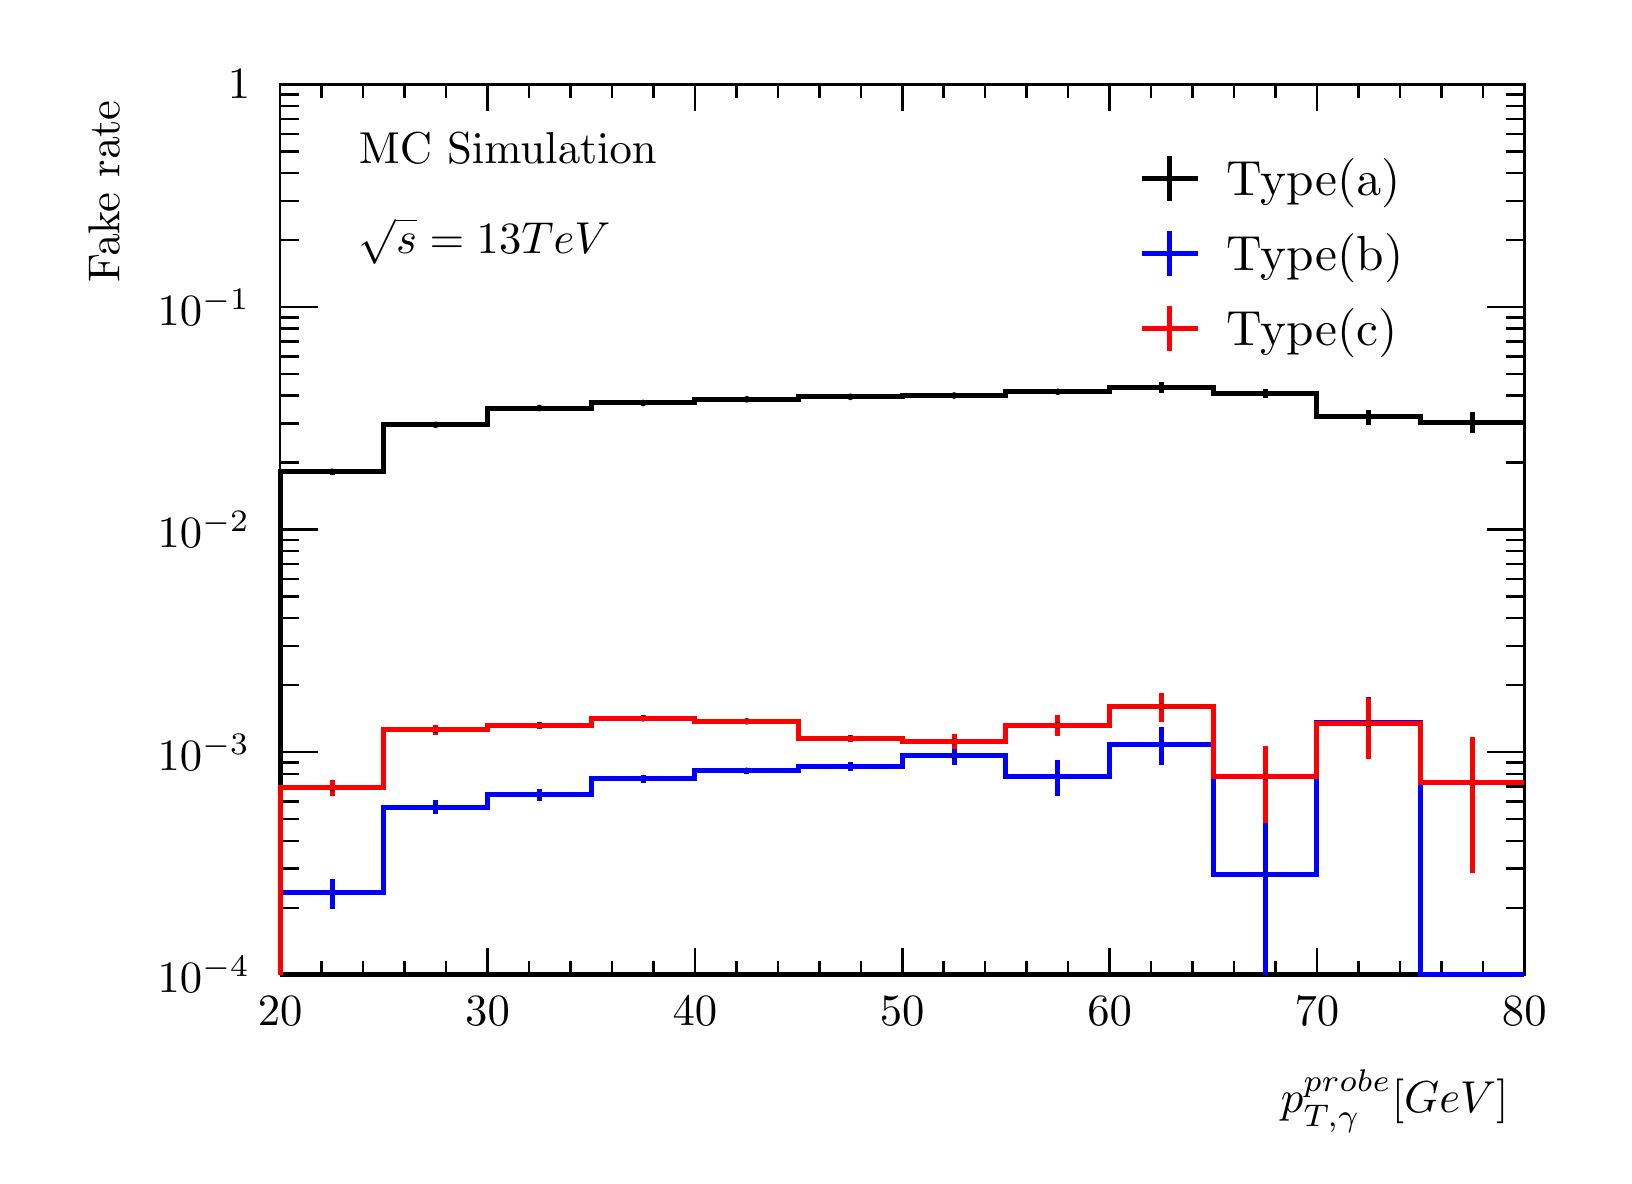
\begin{tikzpicture}
\pgfdeclareplotmark{cross} {
\pgfpathmoveto{\pgfpoint{-0.3\pgfplotmarksize}{\pgfplotmarksize}}
\pgfpathlineto{\pgfpoint{+0.3\pgfplotmarksize}{\pgfplotmarksize}}
\pgfpathlineto{\pgfpoint{+0.3\pgfplotmarksize}{0.3\pgfplotmarksize}}
\pgfpathlineto{\pgfpoint{+1\pgfplotmarksize}{0.3\pgfplotmarksize}}
\pgfpathlineto{\pgfpoint{+1\pgfplotmarksize}{-0.3\pgfplotmarksize}}
\pgfpathlineto{\pgfpoint{+0.3\pgfplotmarksize}{-0.3\pgfplotmarksize}}
\pgfpathlineto{\pgfpoint{+0.3\pgfplotmarksize}{-1.\pgfplotmarksize}}
\pgfpathlineto{\pgfpoint{-0.3\pgfplotmarksize}{-1.\pgfplotmarksize}}
\pgfpathlineto{\pgfpoint{-0.3\pgfplotmarksize}{-0.3\pgfplotmarksize}}
\pgfpathlineto{\pgfpoint{-1.\pgfplotmarksize}{-0.3\pgfplotmarksize}}
\pgfpathlineto{\pgfpoint{-1.\pgfplotmarksize}{0.3\pgfplotmarksize}}
\pgfpathlineto{\pgfpoint{-0.3\pgfplotmarksize}{0.3\pgfplotmarksize}}
\pgfpathclose
\pgfusepathqstroke
}
\pgfdeclareplotmark{cross*} {
\pgfpathmoveto{\pgfpoint{-0.3\pgfplotmarksize}{\pgfplotmarksize}}
\pgfpathlineto{\pgfpoint{+0.3\pgfplotmarksize}{\pgfplotmarksize}}
\pgfpathlineto{\pgfpoint{+0.3\pgfplotmarksize}{0.3\pgfplotmarksize}}
\pgfpathlineto{\pgfpoint{+1\pgfplotmarksize}{0.3\pgfplotmarksize}}
\pgfpathlineto{\pgfpoint{+1\pgfplotmarksize}{-0.3\pgfplotmarksize}}
\pgfpathlineto{\pgfpoint{+0.3\pgfplotmarksize}{-0.3\pgfplotmarksize}}
\pgfpathlineto{\pgfpoint{+0.3\pgfplotmarksize}{-1.\pgfplotmarksize}}
\pgfpathlineto{\pgfpoint{-0.3\pgfplotmarksize}{-1.\pgfplotmarksize}}
\pgfpathlineto{\pgfpoint{-0.3\pgfplotmarksize}{-0.3\pgfplotmarksize}}
\pgfpathlineto{\pgfpoint{-1.\pgfplotmarksize}{-0.3\pgfplotmarksize}}
\pgfpathlineto{\pgfpoint{-1.\pgfplotmarksize}{0.3\pgfplotmarksize}}
\pgfpathlineto{\pgfpoint{-0.3\pgfplotmarksize}{0.3\pgfplotmarksize}}
\pgfpathclose
\pgfusepathqfillstroke
}
\pgfdeclareplotmark{newstar} {
\pgfpathmoveto{\pgfqpoint{0pt}{\pgfplotmarksize}}
\pgfpathlineto{\pgfqpointpolar{44}{0.5\pgfplotmarksize}}
\pgfpathlineto{\pgfqpointpolar{18}{\pgfplotmarksize}}
\pgfpathlineto{\pgfqpointpolar{-20}{0.5\pgfplotmarksize}}
\pgfpathlineto{\pgfqpointpolar{-54}{\pgfplotmarksize}}
\pgfpathlineto{\pgfqpointpolar{-90}{0.5\pgfplotmarksize}}
\pgfpathlineto{\pgfqpointpolar{234}{\pgfplotmarksize}}
\pgfpathlineto{\pgfqpointpolar{198}{0.5\pgfplotmarksize}}
\pgfpathlineto{\pgfqpointpolar{162}{\pgfplotmarksize}}
\pgfpathlineto{\pgfqpointpolar{134}{0.5\pgfplotmarksize}}
\pgfpathclose
\pgfusepathqstroke
}
\pgfdeclareplotmark{newstar*} {
\pgfpathmoveto{\pgfqpoint{0pt}{\pgfplotmarksize}}
\pgfpathlineto{\pgfqpointpolar{44}{0.5\pgfplotmarksize}}
\pgfpathlineto{\pgfqpointpolar{18}{\pgfplotmarksize}}
\pgfpathlineto{\pgfqpointpolar{-20}{0.5\pgfplotmarksize}}
\pgfpathlineto{\pgfqpointpolar{-54}{\pgfplotmarksize}}
\pgfpathlineto{\pgfqpointpolar{-90}{0.5\pgfplotmarksize}}
\pgfpathlineto{\pgfqpointpolar{234}{\pgfplotmarksize}}
\pgfpathlineto{\pgfqpointpolar{198}{0.5\pgfplotmarksize}}
\pgfpathlineto{\pgfqpointpolar{162}{\pgfplotmarksize}}
\pgfpathlineto{\pgfqpointpolar{134}{0.5\pgfplotmarksize}}
\pgfpathclose
\pgfusepathqfillstroke
}
\definecolor{c}{rgb}{1,1,1};
\draw [color=c, fill=c] (0,0) rectangle (20,14.3108);
\draw [color=c, fill=c] (3.2,2.28972) rectangle (19,13.5952);
\definecolor{c}{rgb}{0,0,0};
\draw [c,line width=0.9] (3.2,2.28972) -- (3.2,13.5952) -- (19,13.5952) -- (19,2.28972) -- (3.2,2.28972);
\draw [c,line width=1.8] (3.2,2.28972) -- (3.2158,2.28972) -- (3.2158,2.28972) -- (3.2316,2.28972) -- (3.2316,2.28972) -- (3.2474,2.28972) -- (3.2474,2.28972) -- (3.2632,2.28972) -- (3.2632,2.28972) -- (3.279,2.28972) -- (3.279,2.28972) --
 (3.2948,2.28972) -- (3.2948,2.28972) -- (3.3106,2.28972) -- (3.3106,2.28972) -- (3.3264,2.28972) -- (3.3264,2.28972) -- (3.3422,2.28972) -- (3.3422,2.28972) -- (3.358,2.28972) -- (3.358,2.28972) -- (3.3738,2.28972) -- (3.3738,2.28972) --
 (3.3896,2.28972) -- (3.3896,2.28972) -- (3.4054,2.28972) -- (3.4054,2.28972) -- (3.4212,2.28972) -- (3.4212,2.28972) -- (3.437,2.28972) -- (3.437,2.28972) -- (3.4528,2.28972) -- (3.4528,2.28972) -- (3.4686,2.28972) -- (3.4686,2.28972) --
 (3.4844,2.28972) -- (3.4844,2.28972) -- (3.5002,2.28972) -- (3.5002,2.28972) -- (3.516,2.28972) -- (3.516,2.28972) -- (3.5318,2.28972) -- (3.5318,2.28972) -- (3.5476,2.28972) -- (3.5476,2.28972) -- (3.5634,2.28972) -- (3.5634,2.28972) --
 (3.5792,2.28972) -- (3.5792,2.28972) -- (3.595,2.28972) -- (3.595,2.28972) -- (3.6108,2.28972) -- (3.6108,2.28972) -- (3.6266,2.28972) -- (3.6266,2.28972) -- (3.6424,2.28972) -- (3.6424,2.28972) -- (3.6582,2.28972) -- (3.6582,2.28972) --
 (3.674,2.28972) -- (3.674,2.28972) -- (3.6898,2.28972) -- (3.6898,2.28972) -- (3.7056,2.28972) -- (3.7056,2.28972) -- (3.7214,2.28972) -- (3.7214,2.28972) -- (3.7372,2.28972) -- (3.7372,2.28972) -- (3.753,2.28972) -- (3.753,2.28972) --
 (3.7688,2.28972) -- (3.7688,2.28972) -- (3.7846,2.28972) -- (3.7846,2.28972) -- (3.8004,2.28972) -- (3.8004,2.28972) -- (3.8162,2.28972) -- (3.8162,2.28972) -- (3.832,2.28972) -- (3.832,2.28972) -- (3.8478,2.28972) -- (3.8478,2.28972) --
 (3.8636,2.28972) -- (3.8636,2.28972) -- (3.8794,2.28972) -- (3.8794,2.28972) -- (3.8952,2.28972) -- (3.8952,2.28972) -- (3.911,2.28972) -- (3.911,2.28972) -- (3.9268,2.28972) -- (3.9268,2.28972) -- (3.9426,2.28972) -- (3.9426,2.28972) --
 (3.9584,2.28972) -- (3.9584,2.28972) -- (3.9742,2.28972) -- (3.9742,2.28972) -- (3.99,2.28972) -- (3.99,2.28972) -- (4.0058,2.28972) -- (4.0058,2.28972) -- (4.0216,2.28972) -- (4.0216,2.28972) -- (4.0374,2.28972) -- (4.0374,2.28972) --
 (4.0532,2.28972) -- (4.0532,2.28972) -- (4.069,2.28972) -- (4.069,2.28972) -- (4.0848,2.28972) -- (4.0848,2.28972) -- (4.1006,2.28972) -- (4.1006,2.28972) -- (4.1164,2.28972) -- (4.1164,2.28972) -- (4.1322,2.28972) -- (4.1322,2.28972) --
 (4.148,2.28972) -- (4.148,2.28972) -- (4.1638,2.28972) -- (4.1638,2.28972) -- (4.1796,2.28972) -- (4.1796,2.28972) -- (4.1954,2.28972) -- (4.1954,2.28972) -- (4.2112,2.28972) -- (4.2112,2.28972) -- (4.227,2.28972) -- (4.227,2.28972) --
 (4.2428,2.28972) -- (4.2428,2.28972) -- (4.2586,2.28972) -- (4.2586,2.28972) -- (4.2744,2.28972) -- (4.2744,2.28972) -- (4.2902,2.28972) -- (4.2902,2.28972) -- (4.306,2.28972) -- (4.306,2.28972) -- (4.3218,2.28972) -- (4.3218,2.28972) --
 (4.3376,2.28972) -- (4.3376,2.28972) -- (4.3534,2.28972) -- (4.3534,2.28972) -- (4.3692,2.28972) -- (4.3692,2.28972) -- (4.385,2.28972) -- (4.385,2.28972) -- (4.4008,2.28972) -- (4.4008,2.28972) -- (4.4166,2.28972) -- (4.4166,2.28972) --
 (4.4324,2.28972) -- (4.4324,2.28972) -- (4.4482,2.28972) -- (4.4482,2.28972) -- (4.464,2.28972) -- (4.464,2.28972) -- (4.4798,2.28972) -- (4.4798,2.28972) -- (4.4956,2.28972) -- (4.4956,2.28972) -- (4.5114,2.28972) -- (4.5114,2.28972) --
 (4.5272,2.28972) -- (4.5272,2.28972) -- (4.543,2.28972) -- (4.543,2.28972) -- (4.5588,2.28972) -- (4.5588,2.28972) -- (4.5746,2.28972) -- (4.5746,2.28972) -- (4.5904,2.28972) -- (4.5904,2.28972) -- (4.6062,2.28972) -- (4.6062,2.28972) --
 (4.622,2.28972) -- (4.622,2.28972) -- (4.6378,2.28972) -- (4.6378,2.28972) -- (4.6536,2.28972) -- (4.6536,2.28972) -- (4.6694,2.28972) -- (4.6694,2.28972) -- (4.6852,2.28972) -- (4.6852,2.28972) -- (4.701,2.28972) -- (4.701,2.28972) --
 (4.7168,2.28972) -- (4.7168,2.28972) -- (4.7326,2.28972) -- (4.7326,2.28972) -- (4.7484,2.28972) -- (4.7484,2.28972) -- (4.7642,2.28972) -- (4.7642,2.28972) -- (4.78,2.28972) -- (4.78,2.28972) -- (4.7958,2.28972) -- (4.7958,2.28972) --
 (4.8116,2.28972) -- (4.8116,2.28972) -- (4.8274,2.28972) -- (4.8274,2.28972) -- (4.8432,2.28972) -- (4.8432,2.28972) -- (4.859,2.28972) -- (4.859,2.28972) -- (4.8748,2.28972) -- (4.8748,2.28972) -- (4.8906,2.28972) -- (4.8906,2.28972) --
 (4.9064,2.28972) -- (4.9064,2.28972) -- (4.9222,2.28972) -- (4.9222,2.28972) -- (4.938,2.28972) -- (4.938,2.28972) -- (4.9538,2.28972) -- (4.9538,2.28972) -- (4.9696,2.28972) -- (4.9696,2.28972) -- (4.9854,2.28972) -- (4.9854,2.28972) --
 (5.0012,2.28972) -- (5.0012,2.28972) -- (5.017,2.28972) -- (5.017,2.28972) -- (5.0328,2.28972) -- (5.0328,2.28972) -- (5.0486,2.28972) -- (5.0486,2.28972) -- (5.0644,2.28972) -- (5.0644,2.28972) -- (5.0802,2.28972) -- (5.0802,2.28972) --
 (5.096,2.28972) -- (5.096,2.28972) -- (5.1118,2.28972) -- (5.1118,2.28972) -- (5.1276,2.28972) -- (5.1276,2.28972) -- (5.1434,2.28972) -- (5.1434,2.28972) -- (5.1592,2.28972) -- (5.1592,2.28972) -- (5.175,2.28972) -- (5.175,2.28972) --
 (5.1908,2.28972) -- (5.1908,2.28972) -- (5.2066,2.28972) -- (5.2066,2.28972) -- (5.2224,2.28972) -- (5.2224,2.28972) -- (5.2382,2.28972) -- (5.2382,2.28972) -- (5.254,2.28972) -- (5.254,2.28972) -- (5.2698,2.28972) -- (5.2698,2.28972) --
 (5.2856,2.28972) -- (5.2856,2.28972) -- (5.3014,2.28972) -- (5.3014,2.28972) -- (5.3172,2.28972) -- (5.3172,2.28972) -- (5.333,2.28972) -- (5.333,2.28972) -- (5.3488,2.28972) -- (5.3488,2.28972) -- (5.3646,2.28972) -- (5.3646,2.28972) --
 (5.3804,2.28972) -- (5.3804,2.28972) -- (5.3962,2.28972) -- (5.3962,2.28972) -- (5.412,2.28972) -- (5.412,2.28972) -- (5.4278,2.28972) -- (5.4278,2.28972) -- (5.4436,2.28972) -- (5.4436,2.28972) -- (5.4594,2.28972) -- (5.4594,2.28972) --
 (5.4752,2.28972) -- (5.4752,2.28972) -- (5.491,2.28972) -- (5.491,2.28972) -- (5.5068,2.28972) -- (5.5068,2.28972) -- (5.5226,2.28972) -- (5.5226,2.28972) -- (5.5384,2.28972) -- (5.5384,2.28972) -- (5.5542,2.28972) -- (5.5542,2.28972) --
 (5.57,2.28972) -- (5.57,2.28972) -- (5.5858,2.28972) -- (5.5858,2.28972) -- (5.6016,2.28972) -- (5.6016,2.28972) -- (5.6174,2.28972) -- (5.6174,2.28972) -- (5.6332,2.28972) -- (5.6332,2.28972) -- (5.649,2.28972) -- (5.649,2.28972) --
 (5.6648,2.28972) -- (5.6648,2.28972) -- (5.6806,2.28972) -- (5.6806,2.28972) -- (5.6964,2.28972) -- (5.6964,2.28972) -- (5.7122,2.28972) -- (5.7122,2.28972) -- (5.728,2.28972) -- (5.728,2.28972) -- (5.7438,2.28972) -- (5.7438,2.28972) --
 (5.7596,2.28972) -- (5.7596,2.28972) -- (5.7754,2.28972) -- (5.7754,2.28972) -- (5.7912,2.28972) -- (5.7912,2.28972) -- (5.807,2.28972) -- (5.807,2.28972) -- (5.8228,2.28972) -- (5.8228,2.28972) -- (5.8386,2.28972) -- (5.8386,2.28972) --
 (5.8544,2.28972) -- (5.8544,2.28972) -- (5.8702,2.28972) -- (5.8702,2.28972) -- (5.886,2.28972) -- (5.886,2.28972) -- (5.9018,2.28972) -- (5.9018,2.28972) -- (5.9176,2.28972) -- (5.9176,2.28972) -- (5.9334,2.28972) -- (5.9334,2.28972) --
 (5.9492,2.28972) -- (5.9492,2.28972) -- (5.965,2.28972) -- (5.965,2.28972) -- (5.9808,2.28972) -- (5.9808,2.28972) -- (5.9966,2.28972) -- (5.9966,2.28972) -- (6.0124,2.28972) -- (6.0124,2.28972) -- (6.0282,2.28972) -- (6.0282,2.28972) --
 (6.044,2.28972) -- (6.044,2.28972) -- (6.0598,2.28972) -- (6.0598,2.28972) -- (6.0756,2.28972) -- (6.0756,2.28972) -- (6.0914,2.28972) -- (6.0914,2.28972) -- (6.1072,2.28972) -- (6.1072,2.28972) -- (6.123,2.28972) -- (6.123,2.28972) --
 (6.1388,2.28972) -- (6.1388,2.28972) -- (6.1546,2.28972) -- (6.1546,2.28972) -- (6.1704,2.28972) -- (6.1704,2.28972) -- (6.1862,2.28972) -- (6.1862,2.28972) -- (6.202,2.28972) -- (6.202,2.28972) -- (6.2178,2.28972) -- (6.2178,2.28972) --
 (6.2336,2.28972) -- (6.2336,2.28972) -- (6.2494,2.28972) -- (6.2494,2.28972) -- (6.2652,2.28972) -- (6.2652,2.28972) -- (6.281,2.28972) -- (6.281,2.28972) -- (6.2968,2.28972) -- (6.2968,2.28972) -- (6.3126,2.28972) -- (6.3126,2.28972) --
 (6.3284,2.28972) -- (6.3284,2.28972) -- (6.3442,2.28972) -- (6.3442,2.28972) -- (6.36,2.28972) -- (6.36,2.28972) -- (6.3758,2.28972) -- (6.3758,2.28972) -- (6.3916,2.28972) -- (6.3916,2.28972) -- (6.4074,2.28972) -- (6.4074,2.28972) --
 (6.4232,2.28972) -- (6.4232,2.28972) -- (6.439,2.28972) -- (6.439,2.28972) -- (6.4548,2.28972) -- (6.4548,2.28972) -- (6.4706,2.28972) -- (6.4706,2.28972) -- (6.4864,2.28972) -- (6.4864,2.28972) -- (6.5022,2.28972) -- (6.5022,2.28972) --
 (6.518,2.28972) -- (6.518,2.28972) -- (6.5338,2.28972) -- (6.5338,2.28972) -- (6.5496,2.28972) -- (6.5496,2.28972) -- (6.5654,2.28972) -- (6.5654,2.28972) -- (6.5812,2.28972) -- (6.5812,2.28972) -- (6.597,2.28972) -- (6.597,2.28972) --
 (6.6128,2.28972) -- (6.6128,2.28972) -- (6.6286,2.28972) -- (6.6286,2.28972) -- (6.6444,2.28972) -- (6.6444,2.28972) -- (6.6602,2.28972) -- (6.6602,2.28972) -- (6.676,2.28972) -- (6.676,2.28972) -- (6.6918,2.28972) -- (6.6918,2.28972) --
 (6.7076,2.28972) -- (6.7076,2.28972) -- (6.7234,2.28972) -- (6.7234,2.28972) -- (6.7392,2.28972) -- (6.7392,2.28972) -- (6.755,2.28972) -- (6.755,2.28972) -- (6.7708,2.28972) -- (6.7708,2.28972) -- (6.7866,2.28972) -- (6.7866,2.28972) --
 (6.8024,2.28972) -- (6.8024,2.28972) -- (6.8182,2.28972) -- (6.8182,2.28972) -- (6.834,2.28972) -- (6.834,2.28972) -- (6.8498,2.28972) -- (6.8498,2.28972) -- (6.8656,2.28972) -- (6.8656,2.28972) -- (6.8814,2.28972) -- (6.8814,2.28972) --
 (6.8972,2.28972) -- (6.8972,2.28972) -- (6.913,2.28972) -- (6.913,2.28972) -- (6.9288,2.28972) -- (6.9288,2.28972) -- (6.9446,2.28972) -- (6.9446,2.28972) -- (6.9604,2.28972) -- (6.9604,2.28972) -- (6.9762,2.28972) -- (6.9762,2.28972) --
 (6.992,2.28972) -- (6.992,2.28972) -- (7.0078,2.28972) -- (7.0078,2.28972) -- (7.0236,2.28972) -- (7.0236,2.28972) -- (7.0394,2.28972) -- (7.0394,2.28972) -- (7.0552,2.28972) -- (7.0552,2.28972) -- (7.071,2.28972) -- (7.071,2.28972) --
 (7.0868,2.28972) -- (7.0868,2.28972) -- (7.1026,2.28972) -- (7.1026,2.28972) -- (7.1184,2.28972) -- (7.1184,2.28972) -- (7.1342,2.28972) -- (7.1342,2.28972) -- (7.15,2.28972) -- (7.15,2.28972) -- (7.1658,2.28972) -- (7.1658,2.28972) --
 (7.1816,2.28972) -- (7.1816,2.28972) -- (7.1974,2.28972) -- (7.1974,2.28972) -- (7.2132,2.28972) -- (7.2132,2.28972) -- (7.229,2.28972) -- (7.229,2.28972) -- (7.2448,2.28972) -- (7.2448,2.28972) -- (7.2606,2.28972) -- (7.2606,2.28972) --
 (7.2764,2.28972) -- (7.2764,2.28972) -- (7.2922,2.28972) -- (7.2922,2.28972) -- (7.308,2.28972) -- (7.308,2.28972) -- (7.3238,2.28972) -- (7.3238,2.28972) -- (7.3396,2.28972) -- (7.3396,2.28972) -- (7.3554,2.28972) -- (7.3554,2.28972) --
 (7.3712,2.28972) -- (7.3712,2.28972) -- (7.387,2.28972) -- (7.387,2.28972) -- (7.4028,2.28972) -- (7.4028,2.28972) -- (7.4186,2.28972) -- (7.4186,2.28972) -- (7.4344,2.28972) -- (7.4344,2.28972) -- (7.4502,2.28972) -- (7.4502,2.28972) --
 (7.466,2.28972) -- (7.466,2.28972) -- (7.4818,2.28972) -- (7.4818,2.28972) -- (7.4976,2.28972) -- (7.4976,2.28972) -- (7.5134,2.28972) -- (7.5134,2.28972) -- (7.5292,2.28972) -- (7.5292,2.28972) -- (7.545,2.28972) -- (7.545,2.28972) --
 (7.5608,2.28972) -- (7.5608,2.28972) -- (7.5766,2.28972) -- (7.5766,2.28972) -- (7.5924,2.28972) -- (7.5924,2.28972) -- (7.6082,2.28972) -- (7.6082,2.28972) -- (7.624,2.28972) -- (7.624,2.28972) -- (7.6398,2.28972) -- (7.6398,2.28972) --
 (7.6556,2.28972) -- (7.6556,2.28972) -- (7.6714,2.28972) -- (7.6714,2.28972) -- (7.6872,2.28972) -- (7.6872,2.28972) -- (7.703,2.28972) -- (7.703,2.28972) -- (7.7188,2.28972) -- (7.7188,2.28972) -- (7.7346,2.28972) -- (7.7346,2.28972) --
 (7.7504,2.28972) -- (7.7504,2.28972) -- (7.7662,2.28972) -- (7.7662,2.28972) -- (7.782,2.28972) -- (7.782,2.28972) -- (7.7978,2.28972) -- (7.7978,2.28972) -- (7.8136,2.28972) -- (7.8136,2.28972) -- (7.8294,2.28972) -- (7.8294,2.28972) --
 (7.8452,2.28972) -- (7.8452,2.28972) -- (7.861,2.28972) -- (7.861,2.28972) -- (7.8768,2.28972) -- (7.8768,2.28972) -- (7.8926,2.28972) -- (7.8926,2.28972) -- (7.9084,2.28972) -- (7.9084,2.28972) -- (7.9242,2.28972) -- (7.9242,2.28972) --
 (7.94,2.28972) -- (7.94,2.28972) -- (7.9558,2.28972) -- (7.9558,2.28972) -- (7.9716,2.28972) -- (7.9716,2.28972) -- (7.9874,2.28972) -- (7.9874,2.28972) -- (8.0032,2.28972) -- (8.0032,2.28972) -- (8.019,2.28972) -- (8.019,2.28972) --
 (8.0348,2.28972) -- (8.0348,2.28972) -- (8.0506,2.28972) -- (8.0506,2.28972) -- (8.0664,2.28972) -- (8.0664,2.28972) -- (8.0822,2.28972) -- (8.0822,2.28972) -- (8.098,2.28972) -- (8.098,2.28972) -- (8.1138,2.28972) -- (8.1138,2.28972) --
 (8.1296,2.28972) -- (8.1296,2.28972) -- (8.1454,2.28972) -- (8.1454,2.28972) -- (8.1612,2.28972) -- (8.1612,2.28972) -- (8.177,2.28972) -- (8.177,2.28972) -- (8.1928,2.28972) -- (8.1928,2.28972) -- (8.2086,2.28972) -- (8.2086,2.28972) --
 (8.2244,2.28972) -- (8.2244,2.28972) -- (8.2402,2.28972) -- (8.2402,2.28972) -- (8.256,2.28972) -- (8.256,2.28972) -- (8.2718,2.28972) -- (8.2718,2.28972) -- (8.2876,2.28972) -- (8.2876,2.28972) -- (8.3034,2.28972) -- (8.3034,2.28972) --
 (8.3192,2.28972) -- (8.3192,2.28972) -- (8.335,2.28972) -- (8.335,2.28972) -- (8.3508,2.28972) -- (8.3508,2.28972) -- (8.3666,2.28972) -- (8.3666,2.28972) -- (8.3824,2.28972) -- (8.3824,2.28972) -- (8.3982,2.28972) -- (8.3982,2.28972) --
 (8.414,2.28972) -- (8.414,2.28972) -- (8.4298,2.28972) -- (8.4298,2.28972) -- (8.4456,2.28972) -- (8.4456,2.28972) -- (8.4614,2.28972) -- (8.4614,2.28972) -- (8.4772,2.28972) -- (8.4772,2.28972) -- (8.493,2.28972) -- (8.493,2.28972) --
 (8.5088,2.28972) -- (8.5088,2.28972) -- (8.5246,2.28972) -- (8.5246,2.28972) -- (8.5404,2.28972) -- (8.5404,2.28972) -- (8.5562,2.28972) -- (8.5562,2.28972) -- (8.572,2.28972) -- (8.572,2.28972) -- (8.5878,2.28972) -- (8.5878,2.28972) --
 (8.6036,2.28972) -- (8.6036,2.28972) -- (8.6194,2.28972) -- (8.6194,2.28972) -- (8.6352,2.28972) -- (8.6352,2.28972) -- (8.651,2.28972) -- (8.651,2.28972) -- (8.6668,2.28972) -- (8.6668,2.28972) -- (8.6826,2.28972) -- (8.6826,2.28972) --
 (8.6984,2.28972) -- (8.6984,2.28972) -- (8.7142,2.28972) -- (8.7142,2.28972) -- (8.73,2.28972) -- (8.73,2.28972) -- (8.7458,2.28972) -- (8.7458,2.28972) -- (8.7616,2.28972) -- (8.7616,2.28972) -- (8.7774,2.28972) -- (8.7774,2.28972) --
 (8.7932,2.28972) -- (8.7932,2.28972) -- (8.809,2.28972) -- (8.809,2.28972) -- (8.8248,2.28972) -- (8.8248,2.28972) -- (8.8406,2.28972) -- (8.8406,2.28972) -- (8.8564,2.28972) -- (8.8564,2.28972) -- (8.8722,2.28972) -- (8.8722,2.28972) --
 (8.888,2.28972) -- (8.888,2.28972) -- (8.9038,2.28972) -- (8.9038,2.28972) -- (8.9196,2.28972) -- (8.9196,2.28972) -- (8.9354,2.28972) -- (8.9354,2.28972) -- (8.9512,2.28972) -- (8.9512,2.28972) -- (8.967,2.28972) -- (8.967,2.28972) --
 (8.9828,2.28972) -- (8.9828,2.28972) -- (8.9986,2.28972) -- (8.9986,2.28972) -- (9.0144,2.28972) -- (9.0144,2.28972) -- (9.0302,2.28972) -- (9.0302,2.28972) -- (9.046,2.28972) -- (9.046,2.28972) -- (9.0618,2.28972) -- (9.0618,2.28972) --
 (9.0776,2.28972) -- (9.0776,2.28972) -- (9.0934,2.28972) -- (9.0934,2.28972) -- (9.1092,2.28972) -- (9.1092,2.28972) -- (9.125,2.28972) -- (9.125,2.28972) -- (9.1408,2.28972) -- (9.1408,2.28972) -- (9.1566,2.28972) -- (9.1566,2.28972) --
 (9.1724,2.28972) -- (9.1724,2.28972) -- (9.1882,2.28972) -- (9.1882,2.28972) -- (9.204,2.28972) -- (9.204,2.28972) -- (9.2198,2.28972) -- (9.2198,2.28972) -- (9.2356,2.28972) -- (9.2356,2.28972) -- (9.2514,2.28972) -- (9.2514,2.28972) --
 (9.2672,2.28972) -- (9.2672,2.28972) -- (9.283,2.28972) -- (9.283,2.28972) -- (9.2988,2.28972) -- (9.2988,2.28972) -- (9.3146,2.28972) -- (9.3146,2.28972) -- (9.3304,2.28972) -- (9.3304,2.28972) -- (9.3462,2.28972) -- (9.3462,2.28972) --
 (9.362,2.28972) -- (9.362,2.28972) -- (9.3778,2.28972) -- (9.3778,2.28972) -- (9.3936,2.28972) -- (9.3936,2.28972) -- (9.4094,2.28972) -- (9.4094,2.28972) -- (9.4252,2.28972) -- (9.4252,2.28972) -- (9.441,2.28972) -- (9.441,2.28972) --
 (9.4568,2.28972) -- (9.4568,2.28972) -- (9.4726,2.28972) -- (9.4726,2.28972) -- (9.4884,2.28972) -- (9.4884,2.28972) -- (9.5042,2.28972) -- (9.5042,2.28972) -- (9.52,2.28972) -- (9.52,2.28972) -- (9.5358,2.28972) -- (9.5358,2.28972) --
 (9.5516,2.28972) -- (9.5516,2.28972) -- (9.5674,2.28972) -- (9.5674,2.28972) -- (9.5832,2.28972) -- (9.5832,2.28972) -- (9.599,2.28972) -- (9.599,2.28972) -- (9.6148,2.28972) -- (9.6148,2.28972) -- (9.6306,2.28972) -- (9.6306,2.28972) --
 (9.6464,2.28972) -- (9.6464,2.28972) -- (9.6622,2.28972) -- (9.6622,2.28972) -- (9.678,2.28972) -- (9.678,2.28972) -- (9.6938,2.28972) -- (9.6938,2.28972) -- (9.7096,2.28972) -- (9.7096,2.28972) -- (9.7254,2.28972) -- (9.7254,2.28972) --
 (9.7412,2.28972) -- (9.7412,2.28972) -- (9.757,2.28972) -- (9.757,2.28972) -- (9.7728,2.28972) -- (9.7728,2.28972) -- (9.7886,2.28972) -- (9.7886,2.28972) -- (9.8044,2.28972) -- (9.8044,2.28972) -- (9.8202,2.28972) -- (9.8202,2.28972) --
 (9.836,2.28972) -- (9.836,2.28972) -- (9.8518,2.28972) -- (9.8518,2.28972) -- (9.8676,2.28972) -- (9.8676,2.28972) -- (9.8834,2.28972) -- (9.8834,2.28972) -- (9.8992,2.28972) -- (9.8992,2.28972) -- (9.915,2.28972) -- (9.915,2.28972) --
 (9.9308,2.28972) -- (9.9308,2.28972) -- (9.9466,2.28972) -- (9.9466,2.28972) -- (9.9624,2.28972) -- (9.9624,2.28972) -- (9.9782,2.28972) -- (9.9782,2.28972) -- (9.994,2.28972) -- (9.994,2.28972) -- (10.0098,2.28972) -- (10.0098,2.28972) --
 (10.0256,2.28972) -- (10.0256,2.28972) -- (10.0414,2.28972) -- (10.0414,2.28972) -- (10.0572,2.28972) -- (10.0572,2.28972) -- (10.073,2.28972) -- (10.073,2.28972) -- (10.0888,2.28972) -- (10.0888,2.28972) -- (10.1046,2.28972) -- (10.1046,2.28972) --
 (10.1204,2.28972) -- (10.1204,2.28972) -- (10.1362,2.28972) -- (10.1362,2.28972) -- (10.152,2.28972) -- (10.152,2.28972) -- (10.1678,2.28972) -- (10.1678,2.28972) -- (10.1836,2.28972) -- (10.1836,2.28972) -- (10.1994,2.28972) -- (10.1994,2.28972) --
 (10.2152,2.28972) -- (10.2152,2.28972) -- (10.231,2.28972) -- (10.231,2.28972) -- (10.2468,2.28972) -- (10.2468,2.28972) -- (10.2626,2.28972) -- (10.2626,2.28972) -- (10.2784,2.28972) -- (10.2784,2.28972) -- (10.2942,2.28972) -- (10.2942,2.28972) --
 (10.31,2.28972) -- (10.31,2.28972) -- (10.3258,2.28972) -- (10.3258,2.28972) -- (10.3416,2.28972) -- (10.3416,2.28972) -- (10.3574,2.28972) -- (10.3574,2.28972) -- (10.3732,2.28972) -- (10.3732,2.28972) -- (10.389,2.28972) -- (10.389,2.28972) --
 (10.4048,2.28972) -- (10.4048,2.28972) -- (10.4206,2.28972) -- (10.4206,2.28972) -- (10.4364,2.28972) -- (10.4364,2.28972) -- (10.4522,2.28972) -- (10.4522,2.28972) -- (10.468,2.28972) -- (10.468,2.28972) -- (10.4838,2.28972) -- (10.4838,2.28972) --
 (10.4996,2.28972) -- (10.4996,2.28972) -- (10.5154,2.28972) -- (10.5154,2.28972) -- (10.5312,2.28972) -- (10.5312,2.28972) -- (10.547,2.28972) -- (10.547,2.28972) -- (10.5628,2.28972) -- (10.5628,2.28972) -- (10.5786,2.28972) -- (10.5786,2.28972) --
 (10.5944,2.28972) -- (10.5944,2.28972) -- (10.6102,2.28972) -- (10.6102,2.28972) -- (10.626,2.28972) -- (10.626,2.28972) -- (10.6418,2.28972) -- (10.6418,2.28972) -- (10.6576,2.28972) -- (10.6576,2.28972) -- (10.6734,2.28972) -- (10.6734,2.28972) --
 (10.6892,2.28972) -- (10.6892,2.28972) -- (10.705,2.28972) -- (10.705,2.28972) -- (10.7208,2.28972) -- (10.7208,2.28972) -- (10.7366,2.28972) -- (10.7366,2.28972) -- (10.7524,2.28972) -- (10.7524,2.28972) -- (10.7682,2.28972) -- (10.7682,2.28972) --
 (10.784,2.28972) -- (10.784,2.28972) -- (10.7998,2.28972) -- (10.7998,2.28972) -- (10.8156,2.28972) -- (10.8156,2.28972) -- (10.8314,2.28972) -- (10.8314,2.28972) -- (10.8472,2.28972) -- (10.8472,2.28972) -- (10.863,2.28972) -- (10.863,2.28972) --
 (10.8788,2.28972) -- (10.8788,2.28972) -- (10.8946,2.28972) -- (10.8946,2.28972) -- (10.9104,2.28972) -- (10.9104,2.28972) -- (10.9262,2.28972) -- (10.9262,2.28972) -- (10.942,2.28972) -- (10.942,2.28972) -- (10.9578,2.28972) -- (10.9578,2.28972) --
 (10.9736,2.28972) -- (10.9736,2.28972) -- (10.9894,2.28972) -- (10.9894,2.28972) -- (11.0052,2.28972) -- (11.0052,2.28972) -- (11.021,2.28972) -- (11.021,2.28972) -- (11.0368,2.28972) -- (11.0368,2.28972) -- (11.0526,2.28972) -- (11.0526,2.28972) --
 (11.0684,2.28972) -- (11.0684,2.28972) -- (11.0842,2.28972) -- (11.0842,2.28972) -- (11.1,2.28972) -- (11.1,2.28972) -- (11.1158,2.28972) -- (11.1158,2.28972) -- (11.1316,2.28972) -- (11.1316,2.28972) -- (11.1474,2.28972) -- (11.1474,2.28972) --
 (11.1632,2.28972) -- (11.1632,2.28972) -- (11.179,2.28972) -- (11.179,2.28972) -- (11.1948,2.28972) -- (11.1948,2.28972) -- (11.2106,2.28972) -- (11.2106,2.28972) -- (11.2264,2.28972) -- (11.2264,2.28972) -- (11.2422,2.28972) -- (11.2422,2.28972) --
 (11.258,2.28972) -- (11.258,2.28972) -- (11.2738,2.28972) -- (11.2738,2.28972) -- (11.2896,2.28972) -- (11.2896,2.28972) -- (11.3054,2.28972) -- (11.3054,2.28972) -- (11.3212,2.28972) -- (11.3212,2.28972) -- (11.337,2.28972) -- (11.337,2.28972) --
 (11.3528,2.28972) -- (11.3528,2.28972) -- (11.3686,2.28972) -- (11.3686,2.28972) -- (11.3844,2.28972) -- (11.3844,2.28972) -- (11.4002,2.28972) -- (11.4002,2.28972) -- (11.416,2.28972) -- (11.416,2.28972) -- (11.4318,2.28972) -- (11.4318,2.28972) --
 (11.4476,2.28972) -- (11.4476,2.28972) -- (11.4634,2.28972) -- (11.4634,2.28972) -- (11.4792,2.28972) -- (11.4792,2.28972) -- (11.495,2.28972) -- (11.495,2.28972) -- (11.5108,2.28972) -- (11.5108,2.28972) -- (11.5266,2.28972) -- (11.5266,2.28972) --
 (11.5424,2.28972) -- (11.5424,2.28972) -- (11.5582,2.28972) -- (11.5582,2.28972) -- (11.574,2.28972) -- (11.574,2.28972) -- (11.5898,2.28972) -- (11.5898,2.28972) -- (11.6056,2.28972) -- (11.6056,2.28972) -- (11.6214,2.28972) -- (11.6214,2.28972) --
 (11.6372,2.28972) -- (11.6372,2.28972) -- (11.653,2.28972) -- (11.653,2.28972) -- (11.6688,2.28972) -- (11.6688,2.28972) -- (11.6846,2.28972) -- (11.6846,2.28972) -- (11.7004,2.28972) -- (11.7004,2.28972) -- (11.7162,2.28972) -- (11.7162,2.28972) --
 (11.732,2.28972) -- (11.732,2.28972) -- (11.7478,2.28972) -- (11.7478,2.28972) -- (11.7636,2.28972) -- (11.7636,2.28972) -- (11.7794,2.28972) -- (11.7794,2.28972) -- (11.7952,2.28972) -- (11.7952,2.28972) -- (11.811,2.28972) -- (11.811,2.28972) --
 (11.8268,2.28972) -- (11.8268,2.28972) -- (11.8426,2.28972) -- (11.8426,2.28972) -- (11.8584,2.28972) -- (11.8584,2.28972) -- (11.8742,2.28972) -- (11.8742,2.28972) -- (11.89,2.28972) -- (11.89,2.28972) -- (11.9058,2.28972) -- (11.9058,2.28972) --
 (11.9216,2.28972) -- (11.9216,2.28972) -- (11.9374,2.28972) -- (11.9374,2.28972) -- (11.9532,2.28972) -- (11.9532,2.28972) -- (11.969,2.28972) -- (11.969,2.28972) -- (11.9848,2.28972) -- (11.9848,2.28972) -- (12.0006,2.28972) -- (12.0006,2.28972) --
 (12.0164,2.28972) -- (12.0164,2.28972) -- (12.0322,2.28972) -- (12.0322,2.28972) -- (12.048,2.28972) -- (12.048,2.28972) -- (12.0638,2.28972) -- (12.0638,2.28972) -- (12.0796,2.28972) -- (12.0796,2.28972) -- (12.0954,2.28972) -- (12.0954,2.28972) --
 (12.1112,2.28972) -- (12.1112,2.28972) -- (12.127,2.28972) -- (12.127,2.28972) -- (12.1428,2.28972) -- (12.1428,2.28972) -- (12.1586,2.28972) -- (12.1586,2.28972) -- (12.1744,2.28972) -- (12.1744,2.28972) -- (12.1902,2.28972) -- (12.1902,2.28972) --
 (12.206,2.28972) -- (12.206,2.28972) -- (12.2218,2.28972) -- (12.2218,2.28972) -- (12.2376,2.28972) -- (12.2376,2.28972) -- (12.2534,2.28972) -- (12.2534,2.28972) -- (12.2692,2.28972) -- (12.2692,2.28972) -- (12.285,2.28972) -- (12.285,2.28972) --
 (12.3008,2.28972) -- (12.3008,2.28972) -- (12.3166,2.28972) -- (12.3166,2.28972) -- (12.3324,2.28972) -- (12.3324,2.28972) -- (12.3482,2.28972) -- (12.3482,2.28972) -- (12.364,2.28972) -- (12.364,2.28972) -- (12.3798,2.28972) -- (12.3798,2.28972) --
 (12.3956,2.28972) -- (12.3956,2.28972) -- (12.4114,2.28972) -- (12.4114,2.28972) -- (12.4272,2.28972) -- (12.4272,2.28972) -- (12.443,2.28972) -- (12.443,2.28972) -- (12.4588,2.28972) -- (12.4588,2.28972) -- (12.4746,2.28972) -- (12.4746,2.28972) --
 (12.4904,2.28972) -- (12.4904,2.28972) -- (12.5062,2.28972) -- (12.5062,2.28972) -- (12.522,2.28972) -- (12.522,2.28972) -- (12.5378,2.28972) -- (12.5378,2.28972) -- (12.5536,2.28972) -- (12.5536,2.28972) -- (12.5694,2.28972) -- (12.5694,2.28972) --
 (12.5852,2.28972) -- (12.5852,2.28972) -- (12.601,2.28972) -- (12.601,2.28972) -- (12.6168,2.28972) -- (12.6168,2.28972) -- (12.6326,2.28972) -- (12.6326,2.28972) -- (12.6484,2.28972) -- (12.6484,2.28972) -- (12.6642,2.28972) -- (12.6642,2.28972) --
 (12.68,2.28972) -- (12.68,2.28972) -- (12.6958,2.28972) -- (12.6958,2.28972) -- (12.7116,2.28972) -- (12.7116,2.28972) -- (12.7274,2.28972) -- (12.7274,2.28972) -- (12.7432,2.28972) -- (12.7432,2.28972) -- (12.759,2.28972) -- (12.759,2.28972) --
 (12.7748,2.28972) -- (12.7748,2.28972) -- (12.7906,2.28972) -- (12.7906,2.28972) -- (12.8064,2.28972) -- (12.8064,2.28972) -- (12.8222,2.28972) -- (12.8222,2.28972) -- (12.838,2.28972) -- (12.838,2.28972) -- (12.8538,2.28972) -- (12.8538,2.28972) --
 (12.8696,2.28972) -- (12.8696,2.28972) -- (12.8854,2.28972) -- (12.8854,2.28972) -- (12.9012,2.28972) -- (12.9012,2.28972) -- (12.917,2.28972) -- (12.917,2.28972) -- (12.9328,2.28972) -- (12.9328,2.28972) -- (12.9486,2.28972) -- (12.9486,2.28972) --
 (12.9644,2.28972) -- (12.9644,2.28972) -- (12.9802,2.28972) -- (12.9802,2.28972) -- (12.996,2.28972) -- (12.996,2.28972) -- (13.0118,2.28972) -- (13.0118,2.28972) -- (13.0276,2.28972) -- (13.0276,2.28972) -- (13.0434,2.28972) -- (13.0434,2.28972) --
 (13.0592,2.28972) -- (13.0592,2.28972) -- (13.075,2.28972) -- (13.075,2.28972) -- (13.0908,2.28972) -- (13.0908,2.28972) -- (13.1066,2.28972) -- (13.1066,2.28972) -- (13.1224,2.28972) -- (13.1224,2.28972) -- (13.1382,2.28972) -- (13.1382,2.28972) --
 (13.154,2.28972) -- (13.154,2.28972) -- (13.1698,2.28972) -- (13.1698,2.28972) -- (13.1856,2.28972) -- (13.1856,2.28972) -- (13.2014,2.28972) -- (13.2014,2.28972) -- (13.2172,2.28972) -- (13.2172,2.28972) -- (13.233,2.28972) -- (13.233,2.28972) --
 (13.2488,2.28972) -- (13.2488,2.28972) -- (13.2646,2.28972) -- (13.2646,2.28972) -- (13.2804,2.28972) -- (13.2804,2.28972) -- (13.2962,2.28972) -- (13.2962,2.28972) -- (13.312,2.28972) -- (13.312,2.28972) -- (13.3278,2.28972) -- (13.3278,2.28972) --
 (13.3436,2.28972) -- (13.3436,2.28972) -- (13.3594,2.28972) -- (13.3594,2.28972) -- (13.3752,2.28972) -- (13.3752,2.28972) -- (13.391,2.28972) -- (13.391,2.28972) -- (13.4068,2.28972) -- (13.4068,2.28972) -- (13.4226,2.28972) -- (13.4226,2.28972) --
 (13.4384,2.28972) -- (13.4384,2.28972) -- (13.4542,2.28972) -- (13.4542,2.28972) -- (13.47,2.28972) -- (13.47,2.28972) -- (13.4858,2.28972) -- (13.4858,2.28972) -- (13.5016,2.28972) -- (13.5016,2.28972) -- (13.5174,2.28972) -- (13.5174,2.28972) --
 (13.5332,2.28972) -- (13.5332,2.28972) -- (13.549,2.28972) -- (13.549,2.28972) -- (13.5648,2.28972) -- (13.5648,2.28972) -- (13.5806,2.28972) -- (13.5806,2.28972) -- (13.5964,2.28972) -- (13.5964,2.28972) -- (13.6122,2.28972) -- (13.6122,2.28972) --
 (13.628,2.28972) -- (13.628,2.28972) -- (13.6438,2.28972) -- (13.6438,2.28972) -- (13.6596,2.28972) -- (13.6596,2.28972) -- (13.6754,2.28972) -- (13.6754,2.28972) -- (13.6912,2.28972) -- (13.6912,2.28972) -- (13.707,2.28972) -- (13.707,2.28972) --
 (13.7228,2.28972) -- (13.7228,2.28972) -- (13.7386,2.28972) -- (13.7386,2.28972) -- (13.7544,2.28972) -- (13.7544,2.28972) -- (13.7702,2.28972) -- (13.7702,2.28972) -- (13.786,2.28972) -- (13.786,2.28972) -- (13.8018,2.28972) -- (13.8018,2.28972) --
 (13.8176,2.28972) -- (13.8176,2.28972) -- (13.8334,2.28972) -- (13.8334,2.28972) -- (13.8492,2.28972) -- (13.8492,2.28972) -- (13.865,2.28972) -- (13.865,2.28972) -- (13.8808,2.28972) -- (13.8808,2.28972) -- (13.8966,2.28972) -- (13.8966,2.28972) --
 (13.9124,2.28972) -- (13.9124,2.28972) -- (13.9282,2.28972) -- (13.9282,2.28972) -- (13.944,2.28972) -- (13.944,2.28972) -- (13.9598,2.28972) -- (13.9598,2.28972) -- (13.9756,2.28972) -- (13.9756,2.28972) -- (13.9914,2.28972) -- (13.9914,2.28972) --
 (14.0072,2.28972) -- (14.0072,2.28972) -- (14.023,2.28972) -- (14.023,2.28972) -- (14.0388,2.28972) -- (14.0388,2.28972) -- (14.0546,2.28972) -- (14.0546,2.28972) -- (14.0704,2.28972) -- (14.0704,2.28972) -- (14.0862,2.28972) -- (14.0862,2.28972) --
 (14.102,2.28972) -- (14.102,2.28972) -- (14.1178,2.28972) -- (14.1178,2.28972) -- (14.1336,2.28972) -- (14.1336,2.28972) -- (14.1494,2.28972) -- (14.1494,2.28972) -- (14.1652,2.28972) -- (14.1652,2.28972) -- (14.181,2.28972) -- (14.181,2.28972) --
 (14.1968,2.28972) -- (14.1968,2.28972) -- (14.2126,2.28972) -- (14.2126,2.28972) -- (14.2284,2.28972) -- (14.2284,2.28972) -- (14.2442,2.28972) -- (14.2442,2.28972) -- (14.26,2.28972) -- (14.26,2.28972) -- (14.2758,2.28972) -- (14.2758,2.28972) --
 (14.2916,2.28972) -- (14.2916,2.28972) -- (14.3074,2.28972) -- (14.3074,2.28972) -- (14.3232,2.28972) -- (14.3232,2.28972) -- (14.339,2.28972) -- (14.339,2.28972) -- (14.3548,2.28972) -- (14.3548,2.28972) -- (14.3706,2.28972) -- (14.3706,2.28972) --
 (14.3864,2.28972) -- (14.3864,2.28972) -- (14.4022,2.28972) -- (14.4022,2.28972) -- (14.418,2.28972) -- (14.418,2.28972) -- (14.4338,2.28972) -- (14.4338,2.28972) -- (14.4496,2.28972) -- (14.4496,2.28972) -- (14.4654,2.28972) -- (14.4654,2.28972) --
 (14.4812,2.28972) -- (14.4812,2.28972) -- (14.497,2.28972) -- (14.497,2.28972) -- (14.5128,2.28972) -- (14.5128,2.28972) -- (14.5286,2.28972) -- (14.5286,2.28972) -- (14.5444,2.28972) -- (14.5444,2.28972) -- (14.5602,2.28972) -- (14.5602,2.28972) --
 (14.576,2.28972) -- (14.576,2.28972) -- (14.5918,2.28972) -- (14.5918,2.28972) -- (14.6076,2.28972) -- (14.6076,2.28972) -- (14.6234,2.28972) -- (14.6234,2.28972) -- (14.6392,2.28972) -- (14.6392,2.28972) -- (14.655,2.28972) -- (14.655,2.28972) --
 (14.6708,2.28972) -- (14.6708,2.28972) -- (14.6866,2.28972) -- (14.6866,2.28972) -- (14.7024,2.28972) -- (14.7024,2.28972) -- (14.7182,2.28972) -- (14.7182,2.28972) -- (14.734,2.28972) -- (14.734,2.28972) -- (14.7498,2.28972) -- (14.7498,2.28972) --
 (14.7656,2.28972) -- (14.7656,2.28972) -- (14.7814,2.28972) -- (14.7814,2.28972) -- (14.7972,2.28972) -- (14.7972,2.28972) -- (14.813,2.28972) -- (14.813,2.28972) -- (14.8288,2.28972) -- (14.8288,2.28972) -- (14.8446,2.28972) -- (14.8446,2.28972) --
 (14.8604,2.28972) -- (14.8604,2.28972) -- (14.8762,2.28972) -- (14.8762,2.28972) -- (14.892,2.28972) -- (14.892,2.28972) -- (14.9078,2.28972) -- (14.9078,2.28972) -- (14.9236,2.28972) -- (14.9236,2.28972) -- (14.9394,2.28972) -- (14.9394,2.28972) --
 (14.9552,2.28972) -- (14.9552,2.28972) -- (14.971,2.28972) -- (14.971,2.28972) -- (14.9868,2.28972) -- (14.9868,2.28972) -- (15.0026,2.28972) -- (15.0026,2.28972) -- (15.0184,2.28972) -- (15.0184,2.28972) -- (15.0342,2.28972) -- (15.0342,2.28972) --
 (15.05,2.28972) -- (15.05,2.28972) -- (15.0658,2.28972) -- (15.0658,2.28972) -- (15.0816,2.28972) -- (15.0816,2.28972) -- (15.0974,2.28972) -- (15.0974,2.28972) -- (15.1132,2.28972) -- (15.1132,2.28972) -- (15.129,2.28972) -- (15.129,2.28972) --
 (15.1448,2.28972) -- (15.1448,2.28972) -- (15.1606,2.28972) -- (15.1606,2.28972) -- (15.1764,2.28972) -- (15.1764,2.28972) -- (15.1922,2.28972) -- (15.1922,2.28972) -- (15.208,2.28972) -- (15.208,2.28972) -- (15.2238,2.28972) -- (15.2238,2.28972) --
 (15.2396,2.28972) -- (15.2396,2.28972) -- (15.2554,2.28972) -- (15.2554,2.28972) -- (15.2712,2.28972) -- (15.2712,2.28972) -- (15.287,2.28972) -- (15.287,2.28972) -- (15.3028,2.28972) -- (15.3028,2.28972) -- (15.3186,2.28972) -- (15.3186,2.28972) --
 (15.3344,2.28972) -- (15.3344,2.28972) -- (15.3502,2.28972) -- (15.3502,2.28972) -- (15.366,2.28972) -- (15.366,2.28972) -- (15.3818,2.28972) -- (15.3818,2.28972) -- (15.3976,2.28972) -- (15.3976,2.28972) -- (15.4134,2.28972) -- (15.4134,2.28972) --
 (15.4292,2.28972) -- (15.4292,2.28972) -- (15.445,2.28972) -- (15.445,2.28972) -- (15.4608,2.28972) -- (15.4608,2.28972) -- (15.4766,2.28972) -- (15.4766,2.28972) -- (15.4924,2.28972) -- (15.4924,2.28972) -- (15.5082,2.28972) -- (15.5082,2.28972) --
 (15.524,2.28972) -- (15.524,2.28972) -- (15.5398,2.28972) -- (15.5398,2.28972) -- (15.5556,2.28972) -- (15.5556,2.28972) -- (15.5714,2.28972) -- (15.5714,2.28972) -- (15.5872,2.28972) -- (15.5872,2.28972) -- (15.603,2.28972) -- (15.603,2.28972) --
 (15.6188,2.28972) -- (15.6188,2.28972) -- (15.6346,2.28972) -- (15.6346,2.28972) -- (15.6504,2.28972) -- (15.6504,2.28972) -- (15.6662,2.28972) -- (15.6662,2.28972) -- (15.682,2.28972) -- (15.682,2.28972) -- (15.6978,2.28972) -- (15.6978,2.28972) --
 (15.7136,2.28972) -- (15.7136,2.28972) -- (15.7294,2.28972) -- (15.7294,2.28972) -- (15.7452,2.28972) -- (15.7452,2.28972) -- (15.761,2.28972) -- (15.761,2.28972) -- (15.7768,2.28972) -- (15.7768,2.28972) -- (15.7926,2.28972) -- (15.7926,2.28972) --
 (15.8084,2.28972) -- (15.8084,2.28972) -- (15.8242,2.28972) -- (15.8242,2.28972) -- (15.84,2.28972) -- (15.84,2.28972) -- (15.8558,2.28972) -- (15.8558,2.28972) -- (15.8716,2.28972) -- (15.8716,2.28972) -- (15.8874,2.28972) -- (15.8874,2.28972) --
 (15.9032,2.28972) -- (15.9032,2.28972) -- (15.919,2.28972) -- (15.919,2.28972) -- (15.9348,2.28972) -- (15.9348,2.28972) -- (15.9506,2.28972) -- (15.9506,2.28972) -- (15.9664,2.28972) -- (15.9664,2.28972) -- (15.9822,2.28972) -- (15.9822,2.28972) --
 (15.998,2.28972) -- (15.998,2.28972) -- (16.0138,2.28972) -- (16.0138,2.28972) -- (16.0296,2.28972) -- (16.0296,2.28972) -- (16.0454,2.28972) -- (16.0454,2.28972) -- (16.0612,2.28972) -- (16.0612,2.28972) -- (16.077,2.28972) -- (16.077,2.28972) --
 (16.0928,2.28972) -- (16.0928,2.28972) -- (16.1086,2.28972) -- (16.1086,2.28972) -- (16.1244,2.28972) -- (16.1244,2.28972) -- (16.1402,2.28972) -- (16.1402,2.28972) -- (16.156,2.28972) -- (16.156,2.28972) -- (16.1718,2.28972) -- (16.1718,2.28972) --
 (16.1876,2.28972) -- (16.1876,2.28972) -- (16.2034,2.28972) -- (16.2034,2.28972) -- (16.2192,2.28972) -- (16.2192,2.28972) -- (16.235,2.28972) -- (16.235,2.28972) -- (16.2508,2.28972) -- (16.2508,2.28972) -- (16.2666,2.28972) -- (16.2666,2.28972) --
 (16.2824,2.28972) -- (16.2824,2.28972) -- (16.2982,2.28972) -- (16.2982,2.28972) -- (16.314,2.28972) -- (16.314,2.28972) -- (16.3298,2.28972) -- (16.3298,2.28972) -- (16.3456,2.28972) -- (16.3456,2.28972) -- (16.3614,2.28972) -- (16.3614,2.28972) --
 (16.3772,2.28972) -- (16.3772,2.28972) -- (16.393,2.28972) -- (16.393,2.28972) -- (16.4088,2.28972) -- (16.4088,2.28972) -- (16.4246,2.28972) -- (16.4246,2.28972) -- (16.4404,2.28972) -- (16.4404,2.28972) -- (16.4562,2.28972) -- (16.4562,2.28972) --
 (16.472,2.28972) -- (16.472,2.28972) -- (16.4878,2.28972) -- (16.4878,2.28972) -- (16.5036,2.28972) -- (16.5036,2.28972) -- (16.5194,2.28972) -- (16.5194,2.28972) -- (16.5352,2.28972) -- (16.5352,2.28972) -- (16.551,2.28972) -- (16.551,2.28972) --
 (16.5668,2.28972) -- (16.5668,2.28972) -- (16.5826,2.28972) -- (16.5826,2.28972) -- (16.5984,2.28972) -- (16.5984,2.28972) -- (16.6142,2.28972) -- (16.6142,2.28972) -- (16.63,2.28972) -- (16.63,2.28972) -- (16.6458,2.28972) -- (16.6458,2.28972) --
 (16.6616,2.28972) -- (16.6616,2.28972) -- (16.6774,2.28972) -- (16.6774,2.28972) -- (16.6932,2.28972) -- (16.6932,2.28972) -- (16.709,2.28972) -- (16.709,2.28972) -- (16.7248,2.28972) -- (16.7248,2.28972) -- (16.7406,2.28972) -- (16.7406,2.28972) --
 (16.7564,2.28972) -- (16.7564,2.28972) -- (16.7722,2.28972) -- (16.7722,2.28972) -- (16.788,2.28972) -- (16.788,2.28972) -- (16.8038,2.28972) -- (16.8038,2.28972) -- (16.8196,2.28972) -- (16.8196,2.28972) -- (16.8354,2.28972) -- (16.8354,2.28972) --
 (16.8512,2.28972) -- (16.8512,2.28972) -- (16.867,2.28972) -- (16.867,2.28972) -- (16.8828,2.28972) -- (16.8828,2.28972) -- (16.8986,2.28972) -- (16.8986,2.28972) -- (16.9144,2.28972) -- (16.9144,2.28972) -- (16.9302,2.28972) -- (16.9302,2.28972) --
 (16.946,2.28972) -- (16.946,2.28972) -- (16.9618,2.28972) -- (16.9618,2.28972) -- (16.9776,2.28972) -- (16.9776,2.28972) -- (16.9934,2.28972) -- (16.9934,2.28972) -- (17.0092,2.28972) -- (17.0092,2.28972) -- (17.025,2.28972) -- (17.025,2.28972) --
 (17.0408,2.28972) -- (17.0408,2.28972) -- (17.0566,2.28972) -- (17.0566,2.28972) -- (17.0724,2.28972) -- (17.0724,2.28972) -- (17.0882,2.28972) -- (17.0882,2.28972) -- (17.104,2.28972) -- (17.104,2.28972) -- (17.1198,2.28972) -- (17.1198,2.28972) --
 (17.1356,2.28972) -- (17.1356,2.28972) -- (17.1514,2.28972) -- (17.1514,2.28972) -- (17.1672,2.28972) -- (17.1672,2.28972) -- (17.183,2.28972) -- (17.183,2.28972) -- (17.1988,2.28972) -- (17.1988,2.28972) -- (17.2146,2.28972) -- (17.2146,2.28972) --
 (17.2304,2.28972) -- (17.2304,2.28972) -- (17.2462,2.28972) -- (17.2462,2.28972) -- (17.262,2.28972) -- (17.262,2.28972) -- (17.2778,2.28972) -- (17.2778,2.28972) -- (17.2936,2.28972) -- (17.2936,2.28972) -- (17.3094,2.28972) -- (17.3094,2.28972) --
 (17.3252,2.28972) -- (17.3252,2.28972) -- (17.341,2.28972) -- (17.341,2.28972) -- (17.3568,2.28972) -- (17.3568,2.28972) -- (17.3726,2.28972) -- (17.3726,2.28972) -- (17.3884,2.28972) -- (17.3884,2.28972) -- (17.4042,2.28972) -- (17.4042,2.28972) --
 (17.42,2.28972) -- (17.42,2.28972) -- (17.4358,2.28972) -- (17.4358,2.28972) -- (17.4516,2.28972) -- (17.4516,2.28972) -- (17.4674,2.28972) -- (17.4674,2.28972) -- (17.4832,2.28972) -- (17.4832,2.28972) -- (17.499,2.28972) -- (17.499,2.28972) --
 (17.5148,2.28972) -- (17.5148,2.28972) -- (17.5306,2.28972) -- (17.5306,2.28972) -- (17.5464,2.28972) -- (17.5464,2.28972) -- (17.5622,2.28972) -- (17.5622,2.28972) -- (17.578,2.28972) -- (17.578,2.28972) -- (17.5938,2.28972) -- (17.5938,2.28972) --
 (17.6096,2.28972) -- (17.6096,2.28972) -- (17.6254,2.28972) -- (17.6254,2.28972) -- (17.6412,2.28972) -- (17.6412,2.28972) -- (17.657,2.28972) -- (17.657,2.28972) -- (17.6728,2.28972) -- (17.6728,2.28972) -- (17.6886,2.28972) -- (17.6886,2.28972) --
 (17.7044,2.28972) -- (17.7044,2.28972) -- (17.7202,2.28972) -- (17.7202,2.28972) -- (17.736,2.28972) -- (17.736,2.28972) -- (17.7518,2.28972) -- (17.7518,2.28972) -- (17.7676,2.28972) -- (17.7676,2.28972) -- (17.7834,2.28972) -- (17.7834,2.28972) --
 (17.7992,2.28972) -- (17.7992,2.28972) -- (17.815,2.28972) -- (17.815,2.28972) -- (17.8308,2.28972) -- (17.8308,2.28972) -- (17.8466,2.28972) -- (17.8466,2.28972) -- (17.8624,2.28972) -- (17.8624,2.28972) -- (17.8782,2.28972) -- (17.8782,2.28972) --
 (17.894,2.28972) -- (17.894,2.28972) -- (17.9098,2.28972) -- (17.9098,2.28972) -- (17.9256,2.28972) -- (17.9256,2.28972) -- (17.9414,2.28972) -- (17.9414,2.28972) -- (17.9572,2.28972) -- (17.9572,2.28972) -- (17.973,2.28972) -- (17.973,2.28972) --
 (17.9888,2.28972) -- (17.9888,2.28972) -- (18.0046,2.28972) -- (18.0046,2.28972) -- (18.0204,2.28972) -- (18.0204,2.28972) -- (18.0362,2.28972) -- (18.0362,2.28972) -- (18.052,2.28972) -- (18.052,2.28972) -- (18.0678,2.28972) -- (18.0678,2.28972) --
 (18.0836,2.28972) -- (18.0836,2.28972) -- (18.0994,2.28972) -- (18.0994,2.28972) -- (18.1152,2.28972) -- (18.1152,2.28972) -- (18.131,2.28972) -- (18.131,2.28972) -- (18.1468,2.28972) -- (18.1468,2.28972) -- (18.1626,2.28972) -- (18.1626,2.28972) --
 (18.1784,2.28972) -- (18.1784,2.28972) -- (18.1942,2.28972) -- (18.1942,2.28972) -- (18.21,2.28972) -- (18.21,2.28972) -- (18.2258,2.28972) -- (18.2258,2.28972) -- (18.2416,2.28972) -- (18.2416,2.28972) -- (18.2574,2.28972) -- (18.2574,2.28972) --
 (18.2732,2.28972) -- (18.2732,2.28972) -- (18.289,2.28972) -- (18.289,2.28972) -- (18.3048,2.28972) -- (18.3048,2.28972) -- (18.3206,2.28972) -- (18.3206,2.28972) -- (18.3364,2.28972) -- (18.3364,2.28972) -- (18.3522,2.28972) -- (18.3522,2.28972) --
 (18.368,2.28972) -- (18.368,2.28972) -- (18.3838,2.28972) -- (18.3838,2.28972) -- (18.3996,2.28972) -- (18.3996,2.28972) -- (18.4154,2.28972) -- (18.4154,2.28972) -- (18.4312,2.28972) -- (18.4312,2.28972) -- (18.447,2.28972) -- (18.447,2.28972) --
 (18.4628,2.28972) -- (18.4628,2.28972) -- (18.4786,2.28972) -- (18.4786,2.28972) -- (18.4944,2.28972) -- (18.4944,2.28972) -- (18.5102,2.28972) -- (18.5102,2.28972) -- (18.526,2.28972) -- (18.526,2.28972) -- (18.5418,2.28972) -- (18.5418,2.28972) --
 (18.5576,2.28972) -- (18.5576,2.28972) -- (18.5734,2.28972) -- (18.5734,2.28972) -- (18.5892,2.28972) -- (18.5892,2.28972) -- (18.605,2.28972) -- (18.605,2.28972) -- (18.6208,2.28972) -- (18.6208,2.28972) -- (18.6366,2.28972) -- (18.6366,2.28972) --
 (18.6524,2.28972) -- (18.6524,2.28972) -- (18.6682,2.28972) -- (18.6682,2.28972) -- (18.684,2.28972) -- (18.684,2.28972) -- (18.6998,2.28972) -- (18.6998,2.28972) -- (18.7156,2.28972) -- (18.7156,2.28972) -- (18.7314,2.28972) -- (18.7314,2.28972) --
 (18.7472,2.28972) -- (18.7472,2.28972) -- (18.763,2.28972) -- (18.763,2.28972) -- (18.7788,2.28972) -- (18.7788,2.28972) -- (18.7946,2.28972) -- (18.7946,2.28972) -- (18.8104,2.28972) -- (18.8104,2.28972) -- (18.8262,2.28972) -- (18.8262,2.28972) --
 (18.842,2.28972) -- (18.842,2.28972) -- (18.8578,2.28972) -- (18.8578,2.28972) -- (18.8736,2.28972) -- (18.8736,2.28972) -- (18.8894,2.28972) -- (18.8894,2.28972) -- (18.9052,2.28972) -- (18.9052,2.28972) -- (18.921,2.28972) -- (18.921,2.28972) --
 (18.9368,2.28972) -- (18.9368,2.28972) -- (18.9526,2.28972) -- (18.9526,2.28972) -- (18.9684,2.28972) -- (18.9684,2.28972) -- (18.9842,2.28972) -- (18.9842,2.28972) -- (19,2.28972);
\draw [c,line width=0.9] (3.2,2.28972) -- (19,2.28972);
\draw [c,line width=0.9] (3.2,2.62889) -- (3.2,2.28972);
\draw [c,line width=0.9] (3.72667,2.45931) -- (3.72667,2.28972);
\draw [c,line width=0.9] (4.25333,2.45931) -- (4.25333,2.28972);
\draw [c,line width=0.9] (4.78,2.45931) -- (4.78,2.28972);
\draw [c,line width=0.9] (5.30667,2.45931) -- (5.30667,2.28972);
\draw [c,line width=0.9] (5.83333,2.62889) -- (5.83333,2.28972);
\draw [c,line width=0.9] (6.36,2.45931) -- (6.36,2.28972);
\draw [c,line width=0.9] (6.88667,2.45931) -- (6.88667,2.28972);
\draw [c,line width=0.9] (7.41333,2.45931) -- (7.41333,2.28972);
\draw [c,line width=0.9] (7.94,2.45931) -- (7.94,2.28972);
\draw [c,line width=0.9] (8.46667,2.62889) -- (8.46667,2.28972);
\draw [c,line width=0.9] (8.99333,2.45931) -- (8.99333,2.28972);
\draw [c,line width=0.9] (9.52,2.45931) -- (9.52,2.28972);
\draw [c,line width=0.9] (10.0467,2.45931) -- (10.0467,2.28972);
\draw [c,line width=0.9] (10.5733,2.45931) -- (10.5733,2.28972);
\draw [c,line width=0.9] (11.1,2.62889) -- (11.1,2.28972);
\draw [c,line width=0.9] (11.6267,2.45931) -- (11.6267,2.28972);
\draw [c,line width=0.9] (12.1533,2.45931) -- (12.1533,2.28972);
\draw [c,line width=0.9] (12.68,2.45931) -- (12.68,2.28972);
\draw [c,line width=0.9] (13.2067,2.45931) -- (13.2067,2.28972);
\draw [c,line width=0.9] (13.7333,2.62889) -- (13.7333,2.28972);
\draw [c,line width=0.9] (14.26,2.45931) -- (14.26,2.28972);
\draw [c,line width=0.9] (14.7867,2.45931) -- (14.7867,2.28972);
\draw [c,line width=0.9] (15.3133,2.45931) -- (15.3133,2.28972);
\draw [c,line width=0.9] (15.84,2.45931) -- (15.84,2.28972);
\draw [c,line width=0.9] (16.3667,2.62889) -- (16.3667,2.28972);
\draw [c,line width=0.9] (16.8933,2.45931) -- (16.8933,2.28972);
\draw [c,line width=0.9] (17.42,2.45931) -- (17.42,2.28972);
\draw [c,line width=0.9] (17.9467,2.45931) -- (17.9467,2.28972);
\draw [c,line width=0.9] (18.4733,2.45931) -- (18.4733,2.28972);
\draw [c,line width=0.9] (19,2.62889) -- (19,2.28972);
\draw [anchor=base] (3.2,1.64574) node[scale=1.61424, color=c, rotate=0]{20};
\draw [anchor=base] (5.83333,1.64574) node[scale=1.61424, color=c, rotate=0]{30};
\draw [anchor=base] (8.46667,1.64574) node[scale=1.61424, color=c, rotate=0]{40};
\draw [anchor=base] (11.1,1.64574) node[scale=1.61424, color=c, rotate=0]{50};
\draw [anchor=base] (13.7333,1.64574) node[scale=1.61424, color=c, rotate=0]{60};
\draw [anchor=base] (16.3667,1.64574) node[scale=1.61424, color=c, rotate=0]{70};
\draw [anchor=base] (19,1.64574) node[scale=1.61424, color=c, rotate=0]{80};
\draw [anchor= east] (19,0.686917) node[scale=1.61424, color=c, rotate=0]{$p_{T,  \gamma}^{probe}  [GeV]$};
\draw [c,line width=0.9] (3.2,13.5952) -- (19,13.5952);
\draw [c,line width=0.9] (3.2,13.2561) -- (3.2,13.5952);
\draw [c,line width=0.9] (3.72667,13.4257) -- (3.72667,13.5952);
\draw [c,line width=0.9] (4.25333,13.4257) -- (4.25333,13.5952);
\draw [c,line width=0.9] (4.78,13.4257) -- (4.78,13.5952);
\draw [c,line width=0.9] (5.30667,13.4257) -- (5.30667,13.5952);
\draw [c,line width=0.9] (5.83333,13.2561) -- (5.83333,13.5952);
\draw [c,line width=0.9] (6.36,13.4257) -- (6.36,13.5952);
\draw [c,line width=0.9] (6.88667,13.4257) -- (6.88667,13.5952);
\draw [c,line width=0.9] (7.41333,13.4257) -- (7.41333,13.5952);
\draw [c,line width=0.9] (7.94,13.4257) -- (7.94,13.5952);
\draw [c,line width=0.9] (8.46667,13.2561) -- (8.46667,13.5952);
\draw [c,line width=0.9] (8.99333,13.4257) -- (8.99333,13.5952);
\draw [c,line width=0.9] (9.52,13.4257) -- (9.52,13.5952);
\draw [c,line width=0.9] (10.0467,13.4257) -- (10.0467,13.5952);
\draw [c,line width=0.9] (10.5733,13.4257) -- (10.5733,13.5952);
\draw [c,line width=0.9] (11.1,13.2561) -- (11.1,13.5952);
\draw [c,line width=0.9] (11.6267,13.4257) -- (11.6267,13.5952);
\draw [c,line width=0.9] (12.1533,13.4257) -- (12.1533,13.5952);
\draw [c,line width=0.9] (12.68,13.4257) -- (12.68,13.5952);
\draw [c,line width=0.9] (13.2067,13.4257) -- (13.2067,13.5952);
\draw [c,line width=0.9] (13.7333,13.2561) -- (13.7333,13.5952);
\draw [c,line width=0.9] (14.26,13.4257) -- (14.26,13.5952);
\draw [c,line width=0.9] (14.7867,13.4257) -- (14.7867,13.5952);
\draw [c,line width=0.9] (15.3133,13.4257) -- (15.3133,13.5952);
\draw [c,line width=0.9] (15.84,13.4257) -- (15.84,13.5952);
\draw [c,line width=0.9] (16.3667,13.2561) -- (16.3667,13.5952);
\draw [c,line width=0.9] (16.8933,13.4257) -- (16.8933,13.5952);
\draw [c,line width=0.9] (17.42,13.4257) -- (17.42,13.5952);
\draw [c,line width=0.9] (17.9467,13.4257) -- (17.9467,13.5952);
\draw [c,line width=0.9] (18.4733,13.4257) -- (18.4733,13.5952);
\draw [c,line width=0.9] (19,13.2561) -- (19,13.5952);
\draw [c,line width=0.9] (3.2,2.28972) -- (3.2,13.5952);
\draw [c,line width=0.9] (3.674,2.28973) -- (3.2,2.28973);
\draw [anchor= east] (3.02,2.28973) node[scale=1.61424, color=c, rotate=0]{$10^{-4}$};
\draw [c,line width=0.9] (3.437,3.14055) -- (3.2,3.14055);
\draw [c,line width=0.9] (3.437,3.63825) -- (3.2,3.63825);
\draw [c,line width=0.9] (3.437,3.99138) -- (3.2,3.99138);
\draw [c,line width=0.9] (3.437,4.26528) -- (3.2,4.26528);
\draw [c,line width=0.9] (3.437,4.48908) -- (3.2,4.48908);
\draw [c,line width=0.9] (3.437,4.67829) -- (3.2,4.67829);
\draw [c,line width=0.9] (3.437,4.8422) -- (3.2,4.8422);
\draw [c,line width=0.9] (3.437,4.98678) -- (3.2,4.98678);
\draw [c,line width=0.9] (3.674,5.1161) -- (3.2,5.1161);
\draw [anchor= east] (3.02,5.1161) node[scale=1.61424, color=c, rotate=0]{$10^{-3}$};
\draw [c,line width=0.9] (3.437,5.96693) -- (3.2,5.96693);
\draw [c,line width=0.9] (3.437,6.46463) -- (3.2,6.46463);
\draw [c,line width=0.9] (3.437,6.81775) -- (3.2,6.81775);
\draw [c,line width=0.9] (3.437,7.09166) -- (3.2,7.09166);
\draw [c,line width=0.9] (3.437,7.31545) -- (3.2,7.31545);
\draw [c,line width=0.9] (3.437,7.50467) -- (3.2,7.50467);
\draw [c,line width=0.9] (3.437,7.66858) -- (3.2,7.66858);
\draw [c,line width=0.9] (3.437,7.81315) -- (3.2,7.81315);
\draw [c,line width=0.9] (3.674,7.94248) -- (3.2,7.94248);
\draw [anchor= east] (3.02,7.94248) node[scale=1.61424, color=c, rotate=0]{$10^{-2}$};
\draw [c,line width=0.9] (3.437,8.79331) -- (3.2,8.79331);
\draw [c,line width=0.9] (3.437,9.29101) -- (3.2,9.29101);
\draw [c,line width=0.9] (3.437,9.64413) -- (3.2,9.64413);
\draw [c,line width=0.9] (3.437,9.91804) -- (3.2,9.91804);
\draw [c,line width=0.9] (3.437,10.1418) -- (3.2,10.1418);
\draw [c,line width=0.9] (3.437,10.331) -- (3.2,10.331);
\draw [c,line width=0.9] (3.437,10.495) -- (3.2,10.495);
\draw [c,line width=0.9] (3.437,10.6395) -- (3.2,10.6395);
\draw [c,line width=0.9] (3.674,10.7689) -- (3.2,10.7689);
\draw [anchor= east] (3.02,10.7689) node[scale=1.61424, color=c, rotate=0]{$10^{-1}$};
\draw [c,line width=0.9] (3.437,11.6197) -- (3.2,11.6197);
\draw [c,line width=0.9] (3.437,12.1174) -- (3.2,12.1174);
\draw [c,line width=0.9] (3.437,12.4705) -- (3.2,12.4705);
\draw [c,line width=0.9] (3.437,12.7444) -- (3.2,12.7444);
\draw [c,line width=0.9] (3.437,12.9682) -- (3.2,12.9682);
\draw [c,line width=0.9] (3.437,13.1574) -- (3.2,13.1574);
\draw [c,line width=0.9] (3.437,13.3213) -- (3.2,13.3213);
\draw [c,line width=0.9] (3.437,13.4659) -- (3.2,13.4659);
\draw [c,line width=0.9] (3.674,13.5952) -- (3.2,13.5952);
\draw [anchor= east] (3.02,13.5952) node[scale=1.61424, color=c, rotate=0]{1};
\draw [anchor= east] (0.96,13.5952) node[scale=1.61424, color=c, rotate=90]{Fake rate};
\draw [c,line width=0.9] (19,2.28972) -- (19,13.5952);
\draw [c,line width=0.9] (18.526,2.28973) -- (19,2.28973);
\draw [c,line width=0.9] (18.763,3.14055) -- (19,3.14055);
\draw [c,line width=0.9] (18.763,3.63825) -- (19,3.63825);
\draw [c,line width=0.9] (18.763,3.99138) -- (19,3.99138);
\draw [c,line width=0.9] (18.763,4.26528) -- (19,4.26528);
\draw [c,line width=0.9] (18.763,4.48908) -- (19,4.48908);
\draw [c,line width=0.9] (18.763,4.67829) -- (19,4.67829);
\draw [c,line width=0.9] (18.763,4.8422) -- (19,4.8422);
\draw [c,line width=0.9] (18.763,4.98678) -- (19,4.98678);
\draw [c,line width=0.9] (18.526,5.1161) -- (19,5.1161);
\draw [c,line width=0.9] (18.763,5.96693) -- (19,5.96693);
\draw [c,line width=0.9] (18.763,6.46463) -- (19,6.46463);
\draw [c,line width=0.9] (18.763,6.81775) -- (19,6.81775);
\draw [c,line width=0.9] (18.763,7.09166) -- (19,7.09166);
\draw [c,line width=0.9] (18.763,7.31545) -- (19,7.31545);
\draw [c,line width=0.9] (18.763,7.50467) -- (19,7.50467);
\draw [c,line width=0.9] (18.763,7.66858) -- (19,7.66858);
\draw [c,line width=0.9] (18.763,7.81315) -- (19,7.81315);
\draw [c,line width=0.9] (18.526,7.94248) -- (19,7.94248);
\draw [c,line width=0.9] (18.763,8.79331) -- (19,8.79331);
\draw [c,line width=0.9] (18.763,9.29101) -- (19,9.29101);
\draw [c,line width=0.9] (18.763,9.64413) -- (19,9.64413);
\draw [c,line width=0.9] (18.763,9.91804) -- (19,9.91804);
\draw [c,line width=0.9] (18.763,10.1418) -- (19,10.1418);
\draw [c,line width=0.9] (18.763,10.331) -- (19,10.331);
\draw [c,line width=0.9] (18.763,10.495) -- (19,10.495);
\draw [c,line width=0.9] (18.763,10.6395) -- (19,10.6395);
\draw [c,line width=0.9] (18.526,10.7689) -- (19,10.7689);
\draw [c,line width=0.9] (18.763,11.6197) -- (19,11.6197);
\draw [c,line width=0.9] (18.763,12.1174) -- (19,12.1174);
\draw [c,line width=0.9] (18.763,12.4705) -- (19,12.4705);
\draw [c,line width=0.9] (18.763,12.7444) -- (19,12.7444);
\draw [c,line width=0.9] (18.763,12.9682) -- (19,12.9682);
\draw [c,line width=0.9] (18.763,13.1574) -- (19,13.1574);
\draw [c,line width=0.9] (18.763,13.3213) -- (19,13.3213);
\draw [c,line width=0.9] (18.763,13.4659) -- (19,13.4659);
\draw [c,line width=0.9] (18.526,13.5952) -- (19,13.5952);
\draw [c,line width=1.8] (3.85833,8.6379) -- (3.85833,8.67727);
\draw [c,line width=1.8] (3.85833,8.67727) -- (3.85833,8.71541);
\foreach \P in {(3.85833,8.67727)}{\draw[mark options={color=c,fill=c},mark size=2.402402pt,mark=*,mark size=1pt] plot coordinates {\P};}
\draw [c,line width=1.8] (5.175,9.26084) -- (5.175,9.27413);
\draw [c,line width=1.8] (5.175,9.27413) -- (5.175,9.28728);
\foreach \P in {(5.175,9.27413)}{\draw[mark options={color=c,fill=c},mark size=2.402402pt,mark=*,mark size=1pt] plot coordinates {\P};}
\draw [c,line width=1.8] (6.49167,9.47723) -- (6.49167,9.48673);
\draw [c,line width=1.8] (6.49167,9.48673) -- (6.49167,9.49616);
\foreach \P in {(6.49167,9.48673)}{\draw[mark options={color=c,fill=c},mark size=2.402402pt,mark=*,mark size=1pt] plot coordinates {\P};}
\draw [c,line width=1.8] (7.80833,9.54405) -- (7.80833,9.55155);
\draw [c,line width=1.8] (7.80833,9.55155) -- (7.80833,9.559);
\foreach \P in {(7.80833,9.55155)}{\draw[mark options={color=c,fill=c},mark size=2.402402pt,mark=*,mark size=1pt] plot coordinates {\P};}
\draw [c,line width=1.8] (9.125,9.59186) -- (9.125,9.59835);
\draw [c,line width=1.8] (9.125,9.59835) -- (9.125,9.6048);
\foreach \P in {(9.125,9.59835)}{\draw[mark options={color=c,fill=c},mark size=2.402402pt,mark=*,mark size=1pt] plot coordinates {\P};}
\draw [c,line width=1.8] (10.4417,9.62152) -- (10.4417,9.62989);
\draw [c,line width=1.8] (10.4417,9.62989) -- (10.4417,9.6382);
\foreach \P in {(10.4417,9.62989)}{\draw[mark options={color=c,fill=c},mark size=2.402402pt,mark=*,mark size=1pt] plot coordinates {\P};}
\draw [c,line width=1.8] (11.7583,9.62932) -- (11.7583,9.64602);
\draw [c,line width=1.8] (11.7583,9.64602) -- (11.7583,9.6625);
\foreach \P in {(11.7583,9.64602)}{\draw[mark options={color=c,fill=c},mark size=2.402402pt,mark=*,mark size=1pt] plot coordinates {\P};}
\draw [c,line width=1.8] (13.075,9.6635) -- (13.075,9.6931);
\draw [c,line width=1.8] (13.075,9.6931) -- (13.075,9.722);
\foreach \P in {(13.075,9.6931)}{\draw[mark options={color=c,fill=c},mark size=2.402402pt,mark=*,mark size=1pt] plot coordinates {\P};}
\draw [c,line width=1.8] (14.3917,9.67885) -- (14.3917,9.75168);
\draw [c,line width=1.8] (14.3917,9.75168) -- (14.3917,9.82044);
\foreach \P in {(14.3917,9.75168)}{\draw[mark options={color=c,fill=c},mark size=2.402402pt,mark=*,mark size=1pt] plot coordinates {\P};}
\draw [c,line width=1.8] (15.7083,9.61286) -- (15.7083,9.66934);
\draw [c,line width=1.8] (15.7083,9.66934) -- (15.7083,9.72334);
\foreach \P in {(15.7083,9.66934)}{\draw[mark options={color=c,fill=c},mark size=2.402402pt,mark=*,mark size=1pt] plot coordinates {\P};}
\draw [c,line width=1.8] (17.025,9.27445) -- (17.025,9.37506);
\draw [c,line width=1.8] (17.025,9.37506) -- (17.025,9.46804);
\foreach \P in {(17.025,9.37506)}{\draw[mark options={color=c,fill=c},mark size=2.402402pt,mark=*,mark size=1pt] plot coordinates {\P};}
\draw [c,line width=1.8] (18.3417,9.16472) -- (18.3417,9.30698);
\draw [c,line width=1.8] (18.3417,9.30698) -- (18.3417,9.43445);
\foreach \P in {(18.3417,9.30698)}{\draw[mark options={color=c,fill=c},mark size=2.402402pt,mark=*,mark size=1pt] plot coordinates {\P};}
\draw [c,line width=1.8] (3.2,2.28972) -- (3.2,2.28972) -- (3.2,8.67727) -- (4.51667,8.67727) -- (4.51667,9.27413) -- (5.83333,9.27413) -- (5.83333,9.48673) -- (7.15,9.48673) -- (7.15,9.55155) -- (8.46667,9.55155) -- (8.46667,9.59835) --
 (9.78333,9.59835) -- (9.78333,9.62989) -- (11.1,9.62989) -- (11.1,9.64602) -- (12.4167,9.64602) -- (12.4167,9.6931) -- (13.7333,9.6931) -- (13.7333,9.75168) -- (15.05,9.75168) -- (15.05,9.66934) -- (16.3667,9.66934) -- (16.3667,9.37506) --
 (17.6833,9.37506) -- (17.6833,9.30698) -- (19,9.30698);
\definecolor{c}{rgb}{0,0,1};
\draw [c,line width=1.8] (3.85833,3.12) -- (3.85833,3.331);
\draw [c,line width=1.8] (3.85833,3.331) -- (3.85833,3.51099);
\definecolor{c}{rgb}{0,0,0};
\foreach \P in {(3.85833,3.331)}{\draw[mark options={color=c,fill=c},mark size=2.402402pt,mark=*,mark size=1pt] plot coordinates {\P};}
\definecolor{c}{rgb}{0,0,1};
\draw [c,line width=1.8] (5.175,4.32714) -- (5.175,4.41983);
\draw [c,line width=1.8] (5.175,4.41983) -- (5.175,4.50601);
\definecolor{c}{rgb}{0,0,0};
\foreach \P in {(5.175,4.41983)}{\draw[mark options={color=c,fill=c},mark size=2.402402pt,mark=*,mark size=1pt] plot coordinates {\P};}
\definecolor{c}{rgb}{0,0,1};
\draw [c,line width=1.8] (6.49167,4.49917) -- (6.49167,4.57318);
\draw [c,line width=1.8] (6.49167,4.57318) -- (6.49167,4.64299);
\definecolor{c}{rgb}{0,0,0};
\foreach \P in {(6.49167,4.57318)}{\draw[mark options={color=c,fill=c},mark size=2.402402pt,mark=*,mark size=1pt] plot coordinates {\P};}
\definecolor{c}{rgb}{0,0,1};
\draw [c,line width=1.8] (7.80833,4.72504) -- (7.80833,4.77815);
\draw [c,line width=1.8] (7.80833,4.77815) -- (7.80833,4.82907);
\definecolor{c}{rgb}{0,0,0};
\foreach \P in {(7.80833,4.77815)}{\draw[mark options={color=c,fill=c},mark size=2.402402pt,mark=*,mark size=1pt] plot coordinates {\P};}
\definecolor{c}{rgb}{0,0,1};
\draw [c,line width=1.8] (9.125,4.83649) -- (9.125,4.87984);
\draw [c,line width=1.8] (9.125,4.87984) -- (9.125,4.92171);
\definecolor{c}{rgb}{0,0,0};
\foreach \P in {(9.125,4.87984)}{\draw[mark options={color=c,fill=c},mark size=2.402402pt,mark=*,mark size=1pt] plot coordinates {\P};}
\definecolor{c}{rgb}{0,0,1};
\draw [c,line width=1.8] (10.4417,4.88008) -- (10.4417,4.93745);
\draw [c,line width=1.8] (10.4417,4.93745) -- (10.4417,4.99226);
\definecolor{c}{rgb}{0,0,0};
\foreach \P in {(10.4417,4.93745)}{\draw[mark options={color=c,fill=c},mark size=2.402402pt,mark=*,mark size=1pt] plot coordinates {\P};}
\definecolor{c}{rgb}{0,0,1};
\draw [c,line width=1.8] (11.7583,4.95428) -- (11.7583,5.06839);
\draw [c,line width=1.8] (11.7583,5.06839) -- (11.7583,5.17279);
\definecolor{c}{rgb}{0,0,0};
\foreach \P in {(11.7583,5.06839)}{\draw[mark options={color=c,fill=c},mark size=2.402402pt,mark=*,mark size=1pt] plot coordinates {\P};}
\definecolor{c}{rgb}{0,0,1};
\draw [c,line width=1.8] (13.075,4.56148) -- (13.075,4.81192);
\draw [c,line width=1.8] (13.075,4.81192) -- (13.075,5.01982);
\definecolor{c}{rgb}{0,0,0};
\foreach \P in {(13.075,4.81192)}{\draw[mark options={color=c,fill=c},mark size=2.402402pt,mark=*,mark size=1pt] plot coordinates {\P};}
\definecolor{c}{rgb}{0,0,1};
\draw [c,line width=1.8] (14.3917,4.95741) -- (14.3917,5.21762);
\draw [c,line width=1.8] (14.3917,5.21762) -- (14.3917,5.43221);
\definecolor{c}{rgb}{0,0,0};
\foreach \P in {(14.3917,5.21762)}{\draw[mark options={color=c,fill=c},mark size=2.402402pt,mark=*,mark size=1pt] plot coordinates {\P};}
\definecolor{c}{rgb}{0,0,1};
\draw [c,line width=1.8] (15.7083,2.28972) -- (15.7083,3.56273);
\draw [c,line width=1.8] (15.7083,3.56273) -- (15.7083,4.41655);
\definecolor{c}{rgb}{0,0,0};
\foreach \P in {(15.7083,3.56273)}{\draw[mark options={color=c,fill=c},mark size=2.402402pt,mark=*,mark size=1pt] plot coordinates {\P};}
\definecolor{c}{rgb}{0,0,1};
\draw [c,line width=1.8] (17.025,5.05899) -- (17.025,5.49445);
\draw [c,line width=1.8] (17.025,5.49445) -- (17.025,5.81522);
\definecolor{c}{rgb}{0,0,0};
\foreach \P in {(17.025,5.49445)}{\draw[mark options={color=c,fill=c},mark size=2.402402pt,mark=*,mark size=1pt] plot coordinates {\P};}
\definecolor{c}{rgb}{0,0,1};
\draw [c,line width=1.8] (3.2,2.28972) -- (3.2,2.28972) -- (3.2,3.331) -- (4.51667,3.331) -- (4.51667,4.41983) -- (5.83333,4.41983) -- (5.83333,4.57318) -- (7.15,4.57318) -- (7.15,4.77815) -- (8.46667,4.77815) -- (8.46667,4.87984) --
 (9.78333,4.87984) -- (9.78333,4.93745) -- (11.1,4.93745) -- (11.1,5.06839) -- (12.4167,5.06839) -- (12.4167,4.81192) -- (13.7333,4.81192) -- (13.7333,5.21762) -- (15.05,5.21762) -- (15.05,3.56273) -- (16.3667,3.56273) -- (16.3667,5.49445) --
 (17.6833,5.49445) -- (17.6833,2.28972) -- (19,2.28972);
\definecolor{c}{rgb}{1,0,0};
\draw [c,line width=1.8] (3.85833,4.56023) -- (3.85833,4.6638);
\draw [c,line width=1.8] (3.85833,4.6638) -- (3.85833,4.7593);
\definecolor{c}{rgb}{0,0,0};
\foreach \P in {(3.85833,4.6638)}{\draw[mark options={color=c,fill=c},mark size=2.402402pt,mark=*,mark size=1pt] plot coordinates {\P};}
\definecolor{c}{rgb}{1,0,0};
\draw [c,line width=1.8] (5.175,5.33911) -- (5.175,5.39946);
\draw [c,line width=1.8] (5.175,5.39946) -- (5.175,5.45698);
\definecolor{c}{rgb}{0,0,0};
\foreach \P in {(5.175,5.39946)}{\draw[mark options={color=c,fill=c},mark size=2.402402pt,mark=*,mark size=1pt] plot coordinates {\P};}
\definecolor{c}{rgb}{1,0,0};
\draw [c,line width=1.8] (6.49167,5.40927) -- (6.49167,5.45853);
\draw [c,line width=1.8] (6.49167,5.45853) -- (6.49167,5.50589);
\definecolor{c}{rgb}{0,0,0};
\foreach \P in {(6.49167,5.45853)}{\draw[mark options={color=c,fill=c},mark size=2.402402pt,mark=*,mark size=1pt] plot coordinates {\P};}
\definecolor{c}{rgb}{1,0,0};
\draw [c,line width=1.8] (7.80833,5.50927) -- (7.80833,5.54762);
\draw [c,line width=1.8] (7.80833,5.54762) -- (7.80833,5.58481);
\definecolor{c}{rgb}{0,0,0};
\foreach \P in {(7.80833,5.54762)}{\draw[mark options={color=c,fill=c},mark size=2.402402pt,mark=*,mark size=1pt] plot coordinates {\P};}
\definecolor{c}{rgb}{1,0,0};
\draw [c,line width=1.8] (9.125,5.47512) -- (9.125,5.50897);
\draw [c,line width=1.8] (9.125,5.50897) -- (9.125,5.54192);
\definecolor{c}{rgb}{0,0,0};
\foreach \P in {(9.125,5.50897)}{\draw[mark options={color=c,fill=c},mark size=2.402402pt,mark=*,mark size=1pt] plot coordinates {\P};}
\definecolor{c}{rgb}{1,0,0};
\draw [c,line width=1.8] (10.4417,5.24275) -- (10.4417,5.29091);
\draw [c,line width=1.8] (10.4417,5.29091) -- (10.4417,5.33725);
\definecolor{c}{rgb}{0,0,0};
\foreach \P in {(10.4417,5.29091)}{\draw[mark options={color=c,fill=c},mark size=2.402402pt,mark=*,mark size=1pt] plot coordinates {\P};}
\definecolor{c}{rgb}{1,0,0};
\draw [c,line width=1.8] (11.7583,5.15587) -- (11.7583,5.25323);
\draw [c,line width=1.8] (11.7583,5.25323) -- (11.7583,5.34343);
\definecolor{c}{rgb}{0,0,0};
\foreach \P in {(11.7583,5.25323)}{\draw[mark options={color=c,fill=c},mark size=2.402402pt,mark=*,mark size=1pt] plot coordinates {\P};}
\definecolor{c}{rgb}{1,0,0};
\draw [c,line width=1.8] (13.075,5.31723) -- (13.075,5.45872);
\draw [c,line width=1.8] (13.075,5.45872) -- (13.075,5.58558);
\definecolor{c}{rgb}{0,0,0};
\foreach \P in {(13.075,5.45872)}{\draw[mark options={color=c,fill=c},mark size=2.402402pt,mark=*,mark size=1pt] plot coordinates {\P};}
\definecolor{c}{rgb}{1,0,0};
\draw [c,line width=1.8] (14.3917,5.4947) -- (14.3917,5.69409);
\draw [c,line width=1.8] (14.3917,5.69409) -- (14.3917,5.86556);
\definecolor{c}{rgb}{0,0,0};
\foreach \P in {(14.3917,5.69409)}{\draw[mark options={color=c,fill=c},mark size=2.402402pt,mark=*,mark size=1pt] plot coordinates {\P};}
\definecolor{c}{rgb}{1,0,0};
\draw [c,line width=1.8] (15.7083,4.22251) -- (15.7083,4.80585);
\draw [c,line width=1.8] (15.7083,4.80585) -- (15.7083,5.19965);
\definecolor{c}{rgb}{0,0,0};
\foreach \P in {(15.7083,4.80585)}{\draw[mark options={color=c,fill=c},mark size=2.402402pt,mark=*,mark size=1pt] plot coordinates {\P};}
\definecolor{c}{rgb}{1,0,0};
\draw [c,line width=1.8] (17.025,5.03105) -- (17.025,5.4773);
\draw [c,line width=1.8] (17.025,5.4773) -- (17.025,5.80386);
\definecolor{c}{rgb}{0,0,0};
\foreach \P in {(17.025,5.4773)}{\draw[mark options={color=c,fill=c},mark size=2.402402pt,mark=*,mark size=1pt] plot coordinates {\P};}
\definecolor{c}{rgb}{1,0,0};
\draw [c,line width=1.8] (18.3417,3.57686) -- (18.3417,4.7274);
\draw [c,line width=1.8] (18.3417,4.7274) -- (18.3417,5.31069);
\definecolor{c}{rgb}{0,0,0};
\foreach \P in {(18.3417,4.7274)}{\draw[mark options={color=c,fill=c},mark size=2.402402pt,mark=*,mark size=1pt] plot coordinates {\P};}
\definecolor{c}{rgb}{1,0,0};
\draw [c,line width=1.8] (3.2,2.28972) -- (3.2,2.28972) -- (3.2,4.6638) -- (4.51667,4.6638) -- (4.51667,5.39946) -- (5.83333,5.39946) -- (5.83333,5.45853) -- (7.15,5.45853) -- (7.15,5.54762) -- (8.46667,5.54762) -- (8.46667,5.50897) --
 (9.78333,5.50897) -- (9.78333,5.29091) -- (11.1,5.29091) -- (11.1,5.25323) -- (12.4167,5.25323) -- (12.4167,5.45872) -- (13.7333,5.45872) -- (13.7333,5.69409) -- (15.05,5.69409) -- (15.05,4.80585) -- (16.3667,4.80585) -- (16.3667,5.4773) --
 (17.6833,5.4773) -- (17.6833,4.7274) -- (19,4.7274);
\definecolor{c}{rgb}{1,1,1};
\draw [color=c, fill=c] (14,10.0175) rectangle (18,12.8797);
\definecolor{c}{rgb}{0,0,0};
\draw [anchor=base west] (15,12.188) node[scale=1.78123, color=c, rotate=0]{Type(a)};
\draw [c,line width=1.8] (14.15,12.4027) -- (14.85,12.4027);
\draw [c,line width=1.8] (14.5,12.1165) -- (14.5,12.6889);
\draw [anchor=base west] (15,11.234) node[scale=1.78123, color=c, rotate=0]{Type(b)};
\definecolor{c}{rgb}{0,0,1};
\draw [c,line width=1.8] (14.15,11.4486) -- (14.85,11.4486);
\draw [c,line width=1.8] (14.5,11.1624) -- (14.5,11.7348);
\definecolor{c}{rgb}{0,0,0};
\draw [anchor=base west] (15,10.2799) node[scale=1.78123, color=c, rotate=0]{Type(c)};
\definecolor{c}{rgb}{1,0,0};
\draw [c,line width=1.8] (14.15,10.4946) -- (14.85,10.4946);
\draw [c,line width=1.8] (14.5,10.2084) -- (14.5,10.7808);
\definecolor{c}{rgb}{0,0,0};
\draw [anchor=base west] (4,12.5935) node[scale=1.61424, color=c, rotate=0]{MC Simulation};
\draw [anchor=base west] (4,11.4486) node[scale=1.61424, color=c, rotate=0]{$\sqrt{s}= 13 TeV$};
\end{tikzpicture}
}
\caption{The fake rate as a function of $p_{T}$ of the probe particles.}
\label{fig:mc_fc_pt}
\end{center}
\end{figure}

\begin{figure}[htbp]
\begin{center}
\scalebox{0.7}{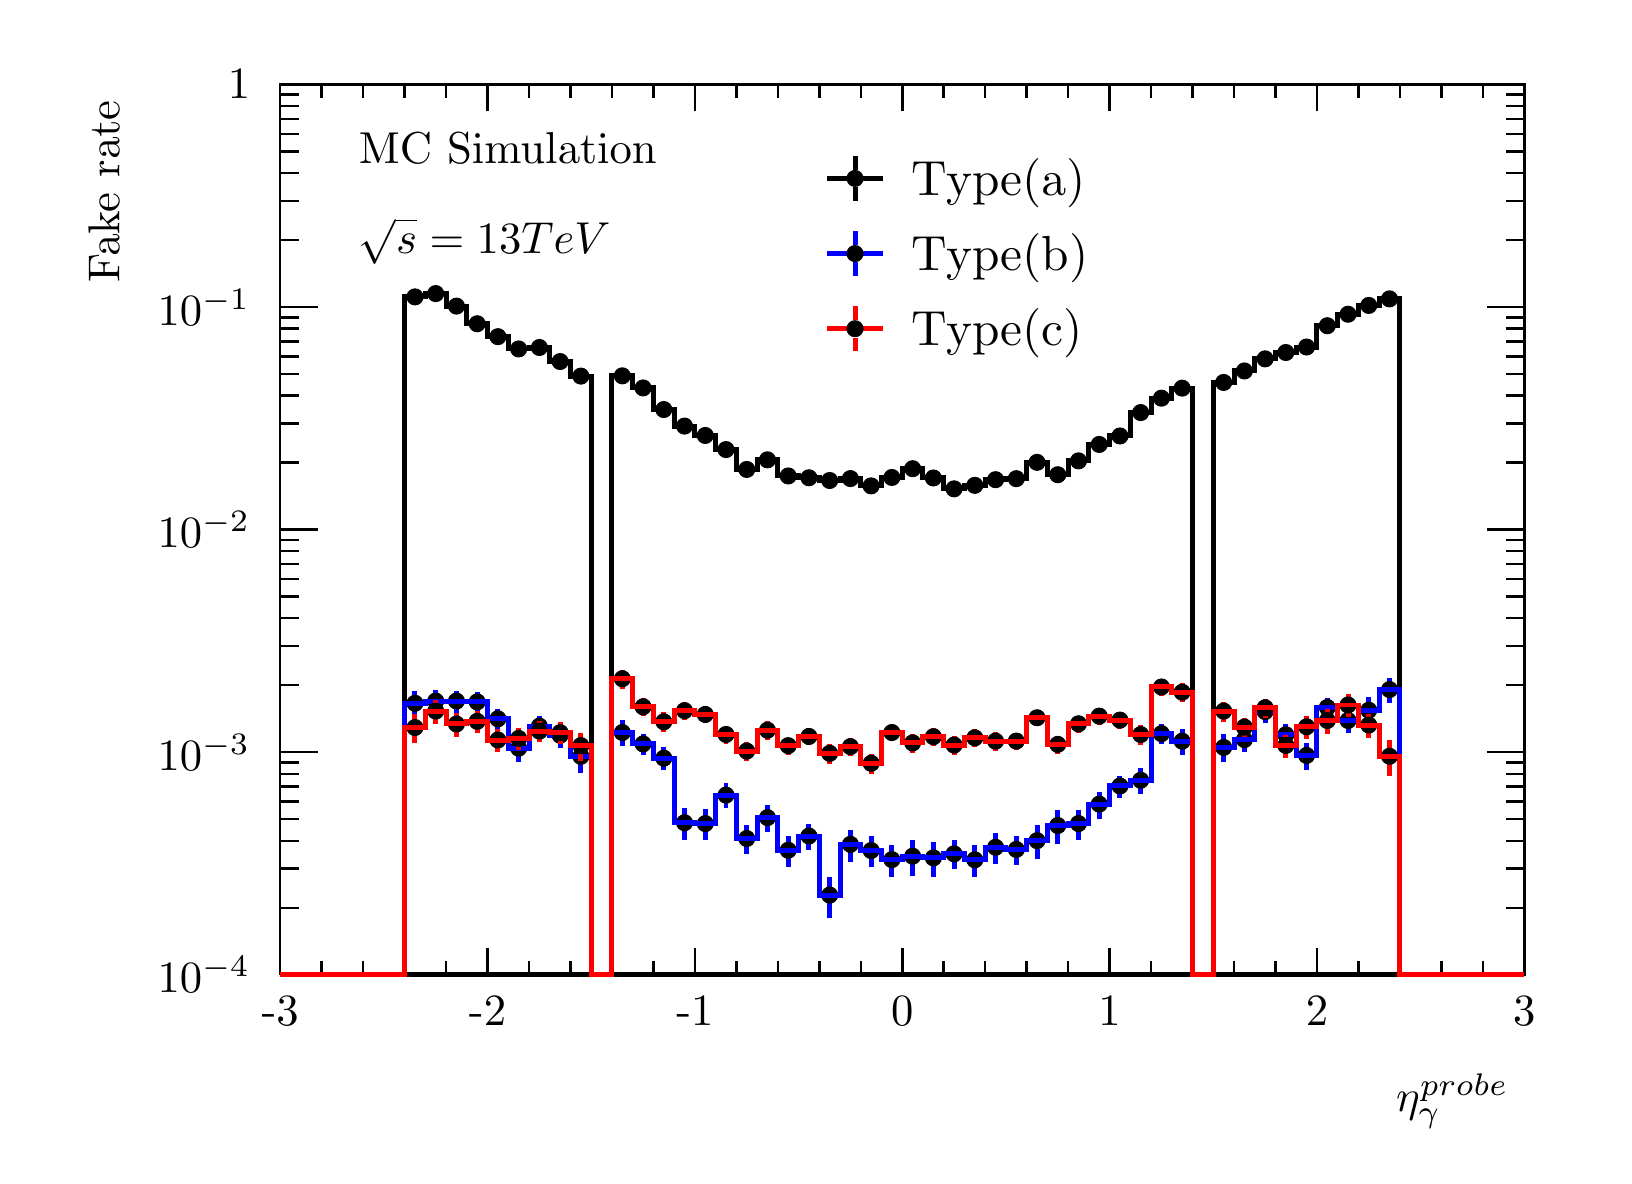
\begin{tikzpicture}
\pgfdeclareplotmark{cross} {
\pgfpathmoveto{\pgfpoint{-0.3\pgfplotmarksize}{\pgfplotmarksize}}
\pgfpathlineto{\pgfpoint{+0.3\pgfplotmarksize}{\pgfplotmarksize}}
\pgfpathlineto{\pgfpoint{+0.3\pgfplotmarksize}{0.3\pgfplotmarksize}}
\pgfpathlineto{\pgfpoint{+1\pgfplotmarksize}{0.3\pgfplotmarksize}}
\pgfpathlineto{\pgfpoint{+1\pgfplotmarksize}{-0.3\pgfplotmarksize}}
\pgfpathlineto{\pgfpoint{+0.3\pgfplotmarksize}{-0.3\pgfplotmarksize}}
\pgfpathlineto{\pgfpoint{+0.3\pgfplotmarksize}{-1.\pgfplotmarksize}}
\pgfpathlineto{\pgfpoint{-0.3\pgfplotmarksize}{-1.\pgfplotmarksize}}
\pgfpathlineto{\pgfpoint{-0.3\pgfplotmarksize}{-0.3\pgfplotmarksize}}
\pgfpathlineto{\pgfpoint{-1.\pgfplotmarksize}{-0.3\pgfplotmarksize}}
\pgfpathlineto{\pgfpoint{-1.\pgfplotmarksize}{0.3\pgfplotmarksize}}
\pgfpathlineto{\pgfpoint{-0.3\pgfplotmarksize}{0.3\pgfplotmarksize}}
\pgfpathclose
\pgfusepathqstroke
}
\pgfdeclareplotmark{cross*} {
\pgfpathmoveto{\pgfpoint{-0.3\pgfplotmarksize}{\pgfplotmarksize}}
\pgfpathlineto{\pgfpoint{+0.3\pgfplotmarksize}{\pgfplotmarksize}}
\pgfpathlineto{\pgfpoint{+0.3\pgfplotmarksize}{0.3\pgfplotmarksize}}
\pgfpathlineto{\pgfpoint{+1\pgfplotmarksize}{0.3\pgfplotmarksize}}
\pgfpathlineto{\pgfpoint{+1\pgfplotmarksize}{-0.3\pgfplotmarksize}}
\pgfpathlineto{\pgfpoint{+0.3\pgfplotmarksize}{-0.3\pgfplotmarksize}}
\pgfpathlineto{\pgfpoint{+0.3\pgfplotmarksize}{-1.\pgfplotmarksize}}
\pgfpathlineto{\pgfpoint{-0.3\pgfplotmarksize}{-1.\pgfplotmarksize}}
\pgfpathlineto{\pgfpoint{-0.3\pgfplotmarksize}{-0.3\pgfplotmarksize}}
\pgfpathlineto{\pgfpoint{-1.\pgfplotmarksize}{-0.3\pgfplotmarksize}}
\pgfpathlineto{\pgfpoint{-1.\pgfplotmarksize}{0.3\pgfplotmarksize}}
\pgfpathlineto{\pgfpoint{-0.3\pgfplotmarksize}{0.3\pgfplotmarksize}}
\pgfpathclose
\pgfusepathqfillstroke
}
\pgfdeclareplotmark{newstar} {
\pgfpathmoveto{\pgfqpoint{0pt}{\pgfplotmarksize}}
\pgfpathlineto{\pgfqpointpolar{44}{0.5\pgfplotmarksize}}
\pgfpathlineto{\pgfqpointpolar{18}{\pgfplotmarksize}}
\pgfpathlineto{\pgfqpointpolar{-20}{0.5\pgfplotmarksize}}
\pgfpathlineto{\pgfqpointpolar{-54}{\pgfplotmarksize}}
\pgfpathlineto{\pgfqpointpolar{-90}{0.5\pgfplotmarksize}}
\pgfpathlineto{\pgfqpointpolar{234}{\pgfplotmarksize}}
\pgfpathlineto{\pgfqpointpolar{198}{0.5\pgfplotmarksize}}
\pgfpathlineto{\pgfqpointpolar{162}{\pgfplotmarksize}}
\pgfpathlineto{\pgfqpointpolar{134}{0.5\pgfplotmarksize}}
\pgfpathclose
\pgfusepathqstroke
}
\pgfdeclareplotmark{newstar*} {
\pgfpathmoveto{\pgfqpoint{0pt}{\pgfplotmarksize}}
\pgfpathlineto{\pgfqpointpolar{44}{0.5\pgfplotmarksize}}
\pgfpathlineto{\pgfqpointpolar{18}{\pgfplotmarksize}}
\pgfpathlineto{\pgfqpointpolar{-20}{0.5\pgfplotmarksize}}
\pgfpathlineto{\pgfqpointpolar{-54}{\pgfplotmarksize}}
\pgfpathlineto{\pgfqpointpolar{-90}{0.5\pgfplotmarksize}}
\pgfpathlineto{\pgfqpointpolar{234}{\pgfplotmarksize}}
\pgfpathlineto{\pgfqpointpolar{198}{0.5\pgfplotmarksize}}
\pgfpathlineto{\pgfqpointpolar{162}{\pgfplotmarksize}}
\pgfpathlineto{\pgfqpointpolar{134}{0.5\pgfplotmarksize}}
\pgfpathclose
\pgfusepathqfillstroke
}
\definecolor{c}{rgb}{1,1,1};
\draw [color=c, fill=c] (0,0) rectangle (20,14.3108);
\draw [color=c, fill=c] (3.2,2.28972) rectangle (19,13.5952);
\definecolor{c}{rgb}{0,0,0};
\draw [c,line width=0.9] (3.2,2.28972) -- (3.2,13.5952) -- (19,13.5952) -- (19,2.28972) -- (3.2,2.28972);
\draw [c,line width=1.8] (3.2,2.28972) -- (3.2158,2.28972) -- (3.2158,2.28972) -- (3.2316,2.28972) -- (3.2316,2.28972) -- (3.2474,2.28972) -- (3.2474,2.28972) -- (3.2632,2.28972) -- (3.2632,2.28972) -- (3.279,2.28972) -- (3.279,2.28972) --
 (3.2948,2.28972) -- (3.2948,2.28972) -- (3.3106,2.28972) -- (3.3106,2.28972) -- (3.3264,2.28972) -- (3.3264,2.28972) -- (3.3422,2.28972) -- (3.3422,2.28972) -- (3.358,2.28972) -- (3.358,2.28972) -- (3.3738,2.28972) -- (3.3738,2.28972) --
 (3.3896,2.28972) -- (3.3896,2.28972) -- (3.4054,2.28972) -- (3.4054,2.28972) -- (3.4212,2.28972) -- (3.4212,2.28972) -- (3.437,2.28972) -- (3.437,2.28972) -- (3.4528,2.28972) -- (3.4528,2.28972) -- (3.4686,2.28972) -- (3.4686,2.28972) --
 (3.4844,2.28972) -- (3.4844,2.28972) -- (3.5002,2.28972) -- (3.5002,2.28972) -- (3.516,2.28972) -- (3.516,2.28972) -- (3.5318,2.28972) -- (3.5318,2.28972) -- (3.5476,2.28972) -- (3.5476,2.28972) -- (3.5634,2.28972) -- (3.5634,2.28972) --
 (3.5792,2.28972) -- (3.5792,2.28972) -- (3.595,2.28972) -- (3.595,2.28972) -- (3.6108,2.28972) -- (3.6108,2.28972) -- (3.6266,2.28972) -- (3.6266,2.28972) -- (3.6424,2.28972) -- (3.6424,2.28972) -- (3.6582,2.28972) -- (3.6582,2.28972) --
 (3.674,2.28972) -- (3.674,2.28972) -- (3.6898,2.28972) -- (3.6898,2.28972) -- (3.7056,2.28972) -- (3.7056,2.28972) -- (3.7214,2.28972) -- (3.7214,2.28972) -- (3.7372,2.28972) -- (3.7372,2.28972) -- (3.753,2.28972) -- (3.753,2.28972) --
 (3.7688,2.28972) -- (3.7688,2.28972) -- (3.7846,2.28972) -- (3.7846,2.28972) -- (3.8004,2.28972) -- (3.8004,2.28972) -- (3.8162,2.28972) -- (3.8162,2.28972) -- (3.832,2.28972) -- (3.832,2.28972) -- (3.8478,2.28972) -- (3.8478,2.28972) --
 (3.8636,2.28972) -- (3.8636,2.28972) -- (3.8794,2.28972) -- (3.8794,2.28972) -- (3.8952,2.28972) -- (3.8952,2.28972) -- (3.911,2.28972) -- (3.911,2.28972) -- (3.9268,2.28972) -- (3.9268,2.28972) -- (3.9426,2.28972) -- (3.9426,2.28972) --
 (3.9584,2.28972) -- (3.9584,2.28972) -- (3.9742,2.28972) -- (3.9742,2.28972) -- (3.99,2.28972) -- (3.99,2.28972) -- (4.0058,2.28972) -- (4.0058,2.28972) -- (4.0216,2.28972) -- (4.0216,2.28972) -- (4.0374,2.28972) -- (4.0374,2.28972) --
 (4.0532,2.28972) -- (4.0532,2.28972) -- (4.069,2.28972) -- (4.069,2.28972) -- (4.0848,2.28972) -- (4.0848,2.28972) -- (4.1006,2.28972) -- (4.1006,2.28972) -- (4.1164,2.28972) -- (4.1164,2.28972) -- (4.1322,2.28972) -- (4.1322,2.28972) --
 (4.148,2.28972) -- (4.148,2.28972) -- (4.1638,2.28972) -- (4.1638,2.28972) -- (4.1796,2.28972) -- (4.1796,2.28972) -- (4.1954,2.28972) -- (4.1954,2.28972) -- (4.2112,2.28972) -- (4.2112,2.28972) -- (4.227,2.28972) -- (4.227,2.28972) --
 (4.2428,2.28972) -- (4.2428,2.28972) -- (4.2586,2.28972) -- (4.2586,2.28972) -- (4.2744,2.28972) -- (4.2744,2.28972) -- (4.2902,2.28972) -- (4.2902,2.28972) -- (4.306,2.28972) -- (4.306,2.28972) -- (4.3218,2.28972) -- (4.3218,2.28972) --
 (4.3376,2.28972) -- (4.3376,2.28972) -- (4.3534,2.28972) -- (4.3534,2.28972) -- (4.3692,2.28972) -- (4.3692,2.28972) -- (4.385,2.28972) -- (4.385,2.28972) -- (4.4008,2.28972) -- (4.4008,2.28972) -- (4.4166,2.28972) -- (4.4166,2.28972) --
 (4.4324,2.28972) -- (4.4324,2.28972) -- (4.4482,2.28972) -- (4.4482,2.28972) -- (4.464,2.28972) -- (4.464,2.28972) -- (4.4798,2.28972) -- (4.4798,2.28972) -- (4.4956,2.28972) -- (4.4956,2.28972) -- (4.5114,2.28972) -- (4.5114,2.28972) --
 (4.5272,2.28972) -- (4.5272,2.28972) -- (4.543,2.28972) -- (4.543,2.28972) -- (4.5588,2.28972) -- (4.5588,2.28972) -- (4.5746,2.28972) -- (4.5746,2.28972) -- (4.5904,2.28972) -- (4.5904,2.28972) -- (4.6062,2.28972) -- (4.6062,2.28972) --
 (4.622,2.28972) -- (4.622,2.28972) -- (4.6378,2.28972) -- (4.6378,2.28972) -- (4.6536,2.28972) -- (4.6536,2.28972) -- (4.6694,2.28972) -- (4.6694,2.28972) -- (4.6852,2.28972) -- (4.6852,2.28972) -- (4.701,2.28972) -- (4.701,2.28972) --
 (4.7168,2.28972) -- (4.7168,2.28972) -- (4.7326,2.28972) -- (4.7326,2.28972) -- (4.7484,2.28972) -- (4.7484,2.28972) -- (4.7642,2.28972) -- (4.7642,2.28972) -- (4.78,2.28972) -- (4.78,2.28972) -- (4.7958,2.28972) -- (4.7958,2.28972) --
 (4.8116,2.28972) -- (4.8116,2.28972) -- (4.8274,2.28972) -- (4.8274,2.28972) -- (4.8432,2.28972) -- (4.8432,2.28972) -- (4.859,2.28972) -- (4.859,2.28972) -- (4.8748,2.28972) -- (4.8748,2.28972) -- (4.8906,2.28972) -- (4.8906,2.28972) --
 (4.9064,2.28972) -- (4.9064,2.28972) -- (4.9222,2.28972) -- (4.9222,2.28972) -- (4.938,2.28972) -- (4.938,2.28972) -- (4.9538,2.28972) -- (4.9538,2.28972) -- (4.9696,2.28972) -- (4.9696,2.28972) -- (4.9854,2.28972) -- (4.9854,2.28972) --
 (5.0012,2.28972) -- (5.0012,2.28972) -- (5.017,2.28972) -- (5.017,2.28972) -- (5.0328,2.28972) -- (5.0328,2.28972) -- (5.0486,2.28972) -- (5.0486,2.28972) -- (5.0644,2.28972) -- (5.0644,2.28972) -- (5.0802,2.28972) -- (5.0802,2.28972) --
 (5.096,2.28972) -- (5.096,2.28972) -- (5.1118,2.28972) -- (5.1118,2.28972) -- (5.1276,2.28972) -- (5.1276,2.28972) -- (5.1434,2.28972) -- (5.1434,2.28972) -- (5.1592,2.28972) -- (5.1592,2.28972) -- (5.175,2.28972) -- (5.175,2.28972) --
 (5.1908,2.28972) -- (5.1908,2.28972) -- (5.2066,2.28972) -- (5.2066,2.28972) -- (5.2224,2.28972) -- (5.2224,2.28972) -- (5.2382,2.28972) -- (5.2382,2.28972) -- (5.254,2.28972) -- (5.254,2.28972) -- (5.2698,2.28972) -- (5.2698,2.28972) --
 (5.2856,2.28972) -- (5.2856,2.28972) -- (5.3014,2.28972) -- (5.3014,2.28972) -- (5.3172,2.28972) -- (5.3172,2.28972) -- (5.333,2.28972) -- (5.333,2.28972) -- (5.3488,2.28972) -- (5.3488,2.28972) -- (5.3646,2.28972) -- (5.3646,2.28972) --
 (5.3804,2.28972) -- (5.3804,2.28972) -- (5.3962,2.28972) -- (5.3962,2.28972) -- (5.412,2.28972) -- (5.412,2.28972) -- (5.4278,2.28972) -- (5.4278,2.28972) -- (5.4436,2.28972) -- (5.4436,2.28972) -- (5.4594,2.28972) -- (5.4594,2.28972) --
 (5.4752,2.28972) -- (5.4752,2.28972) -- (5.491,2.28972) -- (5.491,2.28972) -- (5.5068,2.28972) -- (5.5068,2.28972) -- (5.5226,2.28972) -- (5.5226,2.28972) -- (5.5384,2.28972) -- (5.5384,2.28972) -- (5.5542,2.28972) -- (5.5542,2.28972) --
 (5.57,2.28972) -- (5.57,2.28972) -- (5.5858,2.28972) -- (5.5858,2.28972) -- (5.6016,2.28972) -- (5.6016,2.28972) -- (5.6174,2.28972) -- (5.6174,2.28972) -- (5.6332,2.28972) -- (5.6332,2.28972) -- (5.649,2.28972) -- (5.649,2.28972) --
 (5.6648,2.28972) -- (5.6648,2.28972) -- (5.6806,2.28972) -- (5.6806,2.28972) -- (5.6964,2.28972) -- (5.6964,2.28972) -- (5.7122,2.28972) -- (5.7122,2.28972) -- (5.728,2.28972) -- (5.728,2.28972) -- (5.7438,2.28972) -- (5.7438,2.28972) --
 (5.7596,2.28972) -- (5.7596,2.28972) -- (5.7754,2.28972) -- (5.7754,2.28972) -- (5.7912,2.28972) -- (5.7912,2.28972) -- (5.807,2.28972) -- (5.807,2.28972) -- (5.8228,2.28972) -- (5.8228,2.28972) -- (5.8386,2.28972) -- (5.8386,2.28972) --
 (5.8544,2.28972) -- (5.8544,2.28972) -- (5.8702,2.28972) -- (5.8702,2.28972) -- (5.886,2.28972) -- (5.886,2.28972) -- (5.9018,2.28972) -- (5.9018,2.28972) -- (5.9176,2.28972) -- (5.9176,2.28972) -- (5.9334,2.28972) -- (5.9334,2.28972) --
 (5.9492,2.28972) -- (5.9492,2.28972) -- (5.965,2.28972) -- (5.965,2.28972) -- (5.9808,2.28972) -- (5.9808,2.28972) -- (5.9966,2.28972) -- (5.9966,2.28972) -- (6.0124,2.28972) -- (6.0124,2.28972) -- (6.0282,2.28972) -- (6.0282,2.28972) --
 (6.044,2.28972) -- (6.044,2.28972) -- (6.0598,2.28972) -- (6.0598,2.28972) -- (6.0756,2.28972) -- (6.0756,2.28972) -- (6.0914,2.28972) -- (6.0914,2.28972) -- (6.1072,2.28972) -- (6.1072,2.28972) -- (6.123,2.28972) -- (6.123,2.28972) --
 (6.1388,2.28972) -- (6.1388,2.28972) -- (6.1546,2.28972) -- (6.1546,2.28972) -- (6.1704,2.28972) -- (6.1704,2.28972) -- (6.1862,2.28972) -- (6.1862,2.28972) -- (6.202,2.28972) -- (6.202,2.28972) -- (6.2178,2.28972) -- (6.2178,2.28972) --
 (6.2336,2.28972) -- (6.2336,2.28972) -- (6.2494,2.28972) -- (6.2494,2.28972) -- (6.2652,2.28972) -- (6.2652,2.28972) -- (6.281,2.28972) -- (6.281,2.28972) -- (6.2968,2.28972) -- (6.2968,2.28972) -- (6.3126,2.28972) -- (6.3126,2.28972) --
 (6.3284,2.28972) -- (6.3284,2.28972) -- (6.3442,2.28972) -- (6.3442,2.28972) -- (6.36,2.28972) -- (6.36,2.28972) -- (6.3758,2.28972) -- (6.3758,2.28972) -- (6.3916,2.28972) -- (6.3916,2.28972) -- (6.4074,2.28972) -- (6.4074,2.28972) --
 (6.4232,2.28972) -- (6.4232,2.28972) -- (6.439,2.28972) -- (6.439,2.28972) -- (6.4548,2.28972) -- (6.4548,2.28972) -- (6.4706,2.28972) -- (6.4706,2.28972) -- (6.4864,2.28972) -- (6.4864,2.28972) -- (6.5022,2.28972) -- (6.5022,2.28972) --
 (6.518,2.28972) -- (6.518,2.28972) -- (6.5338,2.28972) -- (6.5338,2.28972) -- (6.5496,2.28972) -- (6.5496,2.28972) -- (6.5654,2.28972) -- (6.5654,2.28972) -- (6.5812,2.28972) -- (6.5812,2.28972) -- (6.597,2.28972) -- (6.597,2.28972) --
 (6.6128,2.28972) -- (6.6128,2.28972) -- (6.6286,2.28972) -- (6.6286,2.28972) -- (6.6444,2.28972) -- (6.6444,2.28972) -- (6.6602,2.28972) -- (6.6602,2.28972) -- (6.676,2.28972) -- (6.676,2.28972) -- (6.6918,2.28972) -- (6.6918,2.28972) --
 (6.7076,2.28972) -- (6.7076,2.28972) -- (6.7234,2.28972) -- (6.7234,2.28972) -- (6.7392,2.28972) -- (6.7392,2.28972) -- (6.755,2.28972) -- (6.755,2.28972) -- (6.7708,2.28972) -- (6.7708,2.28972) -- (6.7866,2.28972) -- (6.7866,2.28972) --
 (6.8024,2.28972) -- (6.8024,2.28972) -- (6.8182,2.28972) -- (6.8182,2.28972) -- (6.834,2.28972) -- (6.834,2.28972) -- (6.8498,2.28972) -- (6.8498,2.28972) -- (6.8656,2.28972) -- (6.8656,2.28972) -- (6.8814,2.28972) -- (6.8814,2.28972) --
 (6.8972,2.28972) -- (6.8972,2.28972) -- (6.913,2.28972) -- (6.913,2.28972) -- (6.9288,2.28972) -- (6.9288,2.28972) -- (6.9446,2.28972) -- (6.9446,2.28972) -- (6.9604,2.28972) -- (6.9604,2.28972) -- (6.9762,2.28972) -- (6.9762,2.28972) --
 (6.992,2.28972) -- (6.992,2.28972) -- (7.0078,2.28972) -- (7.0078,2.28972) -- (7.0236,2.28972) -- (7.0236,2.28972) -- (7.0394,2.28972) -- (7.0394,2.28972) -- (7.0552,2.28972) -- (7.0552,2.28972) -- (7.071,2.28972) -- (7.071,2.28972) --
 (7.0868,2.28972) -- (7.0868,2.28972) -- (7.1026,2.28972) -- (7.1026,2.28972) -- (7.1184,2.28972) -- (7.1184,2.28972) -- (7.1342,2.28972) -- (7.1342,2.28972) -- (7.15,2.28972) -- (7.15,2.28972) -- (7.1658,2.28972) -- (7.1658,2.28972) --
 (7.1816,2.28972) -- (7.1816,2.28972) -- (7.1974,2.28972) -- (7.1974,2.28972) -- (7.2132,2.28972) -- (7.2132,2.28972) -- (7.229,2.28972) -- (7.229,2.28972) -- (7.2448,2.28972) -- (7.2448,2.28972) -- (7.2606,2.28972) -- (7.2606,2.28972) --
 (7.2764,2.28972) -- (7.2764,2.28972) -- (7.2922,2.28972) -- (7.2922,2.28972) -- (7.308,2.28972) -- (7.308,2.28972) -- (7.3238,2.28972) -- (7.3238,2.28972) -- (7.3396,2.28972) -- (7.3396,2.28972) -- (7.3554,2.28972) -- (7.3554,2.28972) --
 (7.3712,2.28972) -- (7.3712,2.28972) -- (7.387,2.28972) -- (7.387,2.28972) -- (7.4028,2.28972) -- (7.4028,2.28972) -- (7.4186,2.28972) -- (7.4186,2.28972) -- (7.4344,2.28972) -- (7.4344,2.28972) -- (7.4502,2.28972) -- (7.4502,2.28972) --
 (7.466,2.28972) -- (7.466,2.28972) -- (7.4818,2.28972) -- (7.4818,2.28972) -- (7.4976,2.28972) -- (7.4976,2.28972) -- (7.5134,2.28972) -- (7.5134,2.28972) -- (7.5292,2.28972) -- (7.5292,2.28972) -- (7.545,2.28972) -- (7.545,2.28972) --
 (7.5608,2.28972) -- (7.5608,2.28972) -- (7.5766,2.28972) -- (7.5766,2.28972) -- (7.5924,2.28972) -- (7.5924,2.28972) -- (7.6082,2.28972) -- (7.6082,2.28972) -- (7.624,2.28972) -- (7.624,2.28972) -- (7.6398,2.28972) -- (7.6398,2.28972) --
 (7.6556,2.28972) -- (7.6556,2.28972) -- (7.6714,2.28972) -- (7.6714,2.28972) -- (7.6872,2.28972) -- (7.6872,2.28972) -- (7.703,2.28972) -- (7.703,2.28972) -- (7.7188,2.28972) -- (7.7188,2.28972) -- (7.7346,2.28972) -- (7.7346,2.28972) --
 (7.7504,2.28972) -- (7.7504,2.28972) -- (7.7662,2.28972) -- (7.7662,2.28972) -- (7.782,2.28972) -- (7.782,2.28972) -- (7.7978,2.28972) -- (7.7978,2.28972) -- (7.8136,2.28972) -- (7.8136,2.28972) -- (7.8294,2.28972) -- (7.8294,2.28972) --
 (7.8452,2.28972) -- (7.8452,2.28972) -- (7.861,2.28972) -- (7.861,2.28972) -- (7.8768,2.28972) -- (7.8768,2.28972) -- (7.8926,2.28972) -- (7.8926,2.28972) -- (7.9084,2.28972) -- (7.9084,2.28972) -- (7.9242,2.28972) -- (7.9242,2.28972) --
 (7.94,2.28972) -- (7.94,2.28972) -- (7.9558,2.28972) -- (7.9558,2.28972) -- (7.9716,2.28972) -- (7.9716,2.28972) -- (7.9874,2.28972) -- (7.9874,2.28972) -- (8.0032,2.28972) -- (8.0032,2.28972) -- (8.019,2.28972) -- (8.019,2.28972) --
 (8.0348,2.28972) -- (8.0348,2.28972) -- (8.0506,2.28972) -- (8.0506,2.28972) -- (8.0664,2.28972) -- (8.0664,2.28972) -- (8.0822,2.28972) -- (8.0822,2.28972) -- (8.098,2.28972) -- (8.098,2.28972) -- (8.1138,2.28972) -- (8.1138,2.28972) --
 (8.1296,2.28972) -- (8.1296,2.28972) -- (8.1454,2.28972) -- (8.1454,2.28972) -- (8.1612,2.28972) -- (8.1612,2.28972) -- (8.177,2.28972) -- (8.177,2.28972) -- (8.1928,2.28972) -- (8.1928,2.28972) -- (8.2086,2.28972) -- (8.2086,2.28972) --
 (8.2244,2.28972) -- (8.2244,2.28972) -- (8.2402,2.28972) -- (8.2402,2.28972) -- (8.256,2.28972) -- (8.256,2.28972) -- (8.2718,2.28972) -- (8.2718,2.28972) -- (8.2876,2.28972) -- (8.2876,2.28972) -- (8.3034,2.28972) -- (8.3034,2.28972) --
 (8.3192,2.28972) -- (8.3192,2.28972) -- (8.335,2.28972) -- (8.335,2.28972) -- (8.3508,2.28972) -- (8.3508,2.28972) -- (8.3666,2.28972) -- (8.3666,2.28972) -- (8.3824,2.28972) -- (8.3824,2.28972) -- (8.3982,2.28972) -- (8.3982,2.28972) --
 (8.414,2.28972) -- (8.414,2.28972) -- (8.4298,2.28972) -- (8.4298,2.28972) -- (8.4456,2.28972) -- (8.4456,2.28972) -- (8.4614,2.28972) -- (8.4614,2.28972) -- (8.4772,2.28972) -- (8.4772,2.28972) -- (8.493,2.28972) -- (8.493,2.28972) --
 (8.5088,2.28972) -- (8.5088,2.28972) -- (8.5246,2.28972) -- (8.5246,2.28972) -- (8.5404,2.28972) -- (8.5404,2.28972) -- (8.5562,2.28972) -- (8.5562,2.28972) -- (8.572,2.28972) -- (8.572,2.28972) -- (8.5878,2.28972) -- (8.5878,2.28972) --
 (8.6036,2.28972) -- (8.6036,2.28972) -- (8.6194,2.28972) -- (8.6194,2.28972) -- (8.6352,2.28972) -- (8.6352,2.28972) -- (8.651,2.28972) -- (8.651,2.28972) -- (8.6668,2.28972) -- (8.6668,2.28972) -- (8.6826,2.28972) -- (8.6826,2.28972) --
 (8.6984,2.28972) -- (8.6984,2.28972) -- (8.7142,2.28972) -- (8.7142,2.28972) -- (8.73,2.28972) -- (8.73,2.28972) -- (8.7458,2.28972) -- (8.7458,2.28972) -- (8.7616,2.28972) -- (8.7616,2.28972) -- (8.7774,2.28972) -- (8.7774,2.28972) --
 (8.7932,2.28972) -- (8.7932,2.28972) -- (8.809,2.28972) -- (8.809,2.28972) -- (8.8248,2.28972) -- (8.8248,2.28972) -- (8.8406,2.28972) -- (8.8406,2.28972) -- (8.8564,2.28972) -- (8.8564,2.28972) -- (8.8722,2.28972) -- (8.8722,2.28972) --
 (8.888,2.28972) -- (8.888,2.28972) -- (8.9038,2.28972) -- (8.9038,2.28972) -- (8.9196,2.28972) -- (8.9196,2.28972) -- (8.9354,2.28972) -- (8.9354,2.28972) -- (8.9512,2.28972) -- (8.9512,2.28972) -- (8.967,2.28972) -- (8.967,2.28972) --
 (8.9828,2.28972) -- (8.9828,2.28972) -- (8.9986,2.28972) -- (8.9986,2.28972) -- (9.0144,2.28972) -- (9.0144,2.28972) -- (9.0302,2.28972) -- (9.0302,2.28972) -- (9.046,2.28972) -- (9.046,2.28972) -- (9.0618,2.28972) -- (9.0618,2.28972) --
 (9.0776,2.28972) -- (9.0776,2.28972) -- (9.0934,2.28972) -- (9.0934,2.28972) -- (9.1092,2.28972) -- (9.1092,2.28972) -- (9.125,2.28972) -- (9.125,2.28972) -- (9.1408,2.28972) -- (9.1408,2.28972) -- (9.1566,2.28972) -- (9.1566,2.28972) --
 (9.1724,2.28972) -- (9.1724,2.28972) -- (9.1882,2.28972) -- (9.1882,2.28972) -- (9.204,2.28972) -- (9.204,2.28972) -- (9.2198,2.28972) -- (9.2198,2.28972) -- (9.2356,2.28972) -- (9.2356,2.28972) -- (9.2514,2.28972) -- (9.2514,2.28972) --
 (9.2672,2.28972) -- (9.2672,2.28972) -- (9.283,2.28972) -- (9.283,2.28972) -- (9.2988,2.28972) -- (9.2988,2.28972) -- (9.3146,2.28972) -- (9.3146,2.28972) -- (9.3304,2.28972) -- (9.3304,2.28972) -- (9.3462,2.28972) -- (9.3462,2.28972) --
 (9.362,2.28972) -- (9.362,2.28972) -- (9.3778,2.28972) -- (9.3778,2.28972) -- (9.3936,2.28972) -- (9.3936,2.28972) -- (9.4094,2.28972) -- (9.4094,2.28972) -- (9.4252,2.28972) -- (9.4252,2.28972) -- (9.441,2.28972) -- (9.441,2.28972) --
 (9.4568,2.28972) -- (9.4568,2.28972) -- (9.4726,2.28972) -- (9.4726,2.28972) -- (9.4884,2.28972) -- (9.4884,2.28972) -- (9.5042,2.28972) -- (9.5042,2.28972) -- (9.52,2.28972) -- (9.52,2.28972) -- (9.5358,2.28972) -- (9.5358,2.28972) --
 (9.5516,2.28972) -- (9.5516,2.28972) -- (9.5674,2.28972) -- (9.5674,2.28972) -- (9.5832,2.28972) -- (9.5832,2.28972) -- (9.599,2.28972) -- (9.599,2.28972) -- (9.6148,2.28972) -- (9.6148,2.28972) -- (9.6306,2.28972) -- (9.6306,2.28972) --
 (9.6464,2.28972) -- (9.6464,2.28972) -- (9.6622,2.28972) -- (9.6622,2.28972) -- (9.678,2.28972) -- (9.678,2.28972) -- (9.6938,2.28972) -- (9.6938,2.28972) -- (9.7096,2.28972) -- (9.7096,2.28972) -- (9.7254,2.28972) -- (9.7254,2.28972) --
 (9.7412,2.28972) -- (9.7412,2.28972) -- (9.757,2.28972) -- (9.757,2.28972) -- (9.7728,2.28972) -- (9.7728,2.28972) -- (9.7886,2.28972) -- (9.7886,2.28972) -- (9.8044,2.28972) -- (9.8044,2.28972) -- (9.8202,2.28972) -- (9.8202,2.28972) --
 (9.836,2.28972) -- (9.836,2.28972) -- (9.8518,2.28972) -- (9.8518,2.28972) -- (9.8676,2.28972) -- (9.8676,2.28972) -- (9.8834,2.28972) -- (9.8834,2.28972) -- (9.8992,2.28972) -- (9.8992,2.28972) -- (9.915,2.28972) -- (9.915,2.28972) --
 (9.9308,2.28972) -- (9.9308,2.28972) -- (9.9466,2.28972) -- (9.9466,2.28972) -- (9.9624,2.28972) -- (9.9624,2.28972) -- (9.9782,2.28972) -- (9.9782,2.28972) -- (9.994,2.28972) -- (9.994,2.28972) -- (10.0098,2.28972) -- (10.0098,2.28972) --
 (10.0256,2.28972) -- (10.0256,2.28972) -- (10.0414,2.28972) -- (10.0414,2.28972) -- (10.0572,2.28972) -- (10.0572,2.28972) -- (10.073,2.28972) -- (10.073,2.28972) -- (10.0888,2.28972) -- (10.0888,2.28972) -- (10.1046,2.28972) -- (10.1046,2.28972) --
 (10.1204,2.28972) -- (10.1204,2.28972) -- (10.1362,2.28972) -- (10.1362,2.28972) -- (10.152,2.28972) -- (10.152,2.28972) -- (10.1678,2.28972) -- (10.1678,2.28972) -- (10.1836,2.28972) -- (10.1836,2.28972) -- (10.1994,2.28972) -- (10.1994,2.28972) --
 (10.2152,2.28972) -- (10.2152,2.28972) -- (10.231,2.28972) -- (10.231,2.28972) -- (10.2468,2.28972) -- (10.2468,2.28972) -- (10.2626,2.28972) -- (10.2626,2.28972) -- (10.2784,2.28972) -- (10.2784,2.28972) -- (10.2942,2.28972) -- (10.2942,2.28972) --
 (10.31,2.28972) -- (10.31,2.28972) -- (10.3258,2.28972) -- (10.3258,2.28972) -- (10.3416,2.28972) -- (10.3416,2.28972) -- (10.3574,2.28972) -- (10.3574,2.28972) -- (10.3732,2.28972) -- (10.3732,2.28972) -- (10.389,2.28972) -- (10.389,2.28972) --
 (10.4048,2.28972) -- (10.4048,2.28972) -- (10.4206,2.28972) -- (10.4206,2.28972) -- (10.4364,2.28972) -- (10.4364,2.28972) -- (10.4522,2.28972) -- (10.4522,2.28972) -- (10.468,2.28972) -- (10.468,2.28972) -- (10.4838,2.28972) -- (10.4838,2.28972) --
 (10.4996,2.28972) -- (10.4996,2.28972) -- (10.5154,2.28972) -- (10.5154,2.28972) -- (10.5312,2.28972) -- (10.5312,2.28972) -- (10.547,2.28972) -- (10.547,2.28972) -- (10.5628,2.28972) -- (10.5628,2.28972) -- (10.5786,2.28972) -- (10.5786,2.28972) --
 (10.5944,2.28972) -- (10.5944,2.28972) -- (10.6102,2.28972) -- (10.6102,2.28972) -- (10.626,2.28972) -- (10.626,2.28972) -- (10.6418,2.28972) -- (10.6418,2.28972) -- (10.6576,2.28972) -- (10.6576,2.28972) -- (10.6734,2.28972) -- (10.6734,2.28972) --
 (10.6892,2.28972) -- (10.6892,2.28972) -- (10.705,2.28972) -- (10.705,2.28972) -- (10.7208,2.28972) -- (10.7208,2.28972) -- (10.7366,2.28972) -- (10.7366,2.28972) -- (10.7524,2.28972) -- (10.7524,2.28972) -- (10.7682,2.28972) -- (10.7682,2.28972) --
 (10.784,2.28972) -- (10.784,2.28972) -- (10.7998,2.28972) -- (10.7998,2.28972) -- (10.8156,2.28972) -- (10.8156,2.28972) -- (10.8314,2.28972) -- (10.8314,2.28972) -- (10.8472,2.28972) -- (10.8472,2.28972) -- (10.863,2.28972) -- (10.863,2.28972) --
 (10.8788,2.28972) -- (10.8788,2.28972) -- (10.8946,2.28972) -- (10.8946,2.28972) -- (10.9104,2.28972) -- (10.9104,2.28972) -- (10.9262,2.28972) -- (10.9262,2.28972) -- (10.942,2.28972) -- (10.942,2.28972) -- (10.9578,2.28972) -- (10.9578,2.28972) --
 (10.9736,2.28972) -- (10.9736,2.28972) -- (10.9894,2.28972) -- (10.9894,2.28972) -- (11.0052,2.28972) -- (11.0052,2.28972) -- (11.021,2.28972) -- (11.021,2.28972) -- (11.0368,2.28972) -- (11.0368,2.28972) -- (11.0526,2.28972) -- (11.0526,2.28972) --
 (11.0684,2.28972) -- (11.0684,2.28972) -- (11.0842,2.28972) -- (11.0842,2.28972) -- (11.1,2.28972) -- (11.1,2.28972) -- (11.1158,2.28972) -- (11.1158,2.28972) -- (11.1316,2.28972) -- (11.1316,2.28972) -- (11.1474,2.28972) -- (11.1474,2.28972) --
 (11.1632,2.28972) -- (11.1632,2.28972) -- (11.179,2.28972) -- (11.179,2.28972) -- (11.1948,2.28972) -- (11.1948,2.28972) -- (11.2106,2.28972) -- (11.2106,2.28972) -- (11.2264,2.28972) -- (11.2264,2.28972) -- (11.2422,2.28972) -- (11.2422,2.28972) --
 (11.258,2.28972) -- (11.258,2.28972) -- (11.2738,2.28972) -- (11.2738,2.28972) -- (11.2896,2.28972) -- (11.2896,2.28972) -- (11.3054,2.28972) -- (11.3054,2.28972) -- (11.3212,2.28972) -- (11.3212,2.28972) -- (11.337,2.28972) -- (11.337,2.28972) --
 (11.3528,2.28972) -- (11.3528,2.28972) -- (11.3686,2.28972) -- (11.3686,2.28972) -- (11.3844,2.28972) -- (11.3844,2.28972) -- (11.4002,2.28972) -- (11.4002,2.28972) -- (11.416,2.28972) -- (11.416,2.28972) -- (11.4318,2.28972) -- (11.4318,2.28972) --
 (11.4476,2.28972) -- (11.4476,2.28972) -- (11.4634,2.28972) -- (11.4634,2.28972) -- (11.4792,2.28972) -- (11.4792,2.28972) -- (11.495,2.28972) -- (11.495,2.28972) -- (11.5108,2.28972) -- (11.5108,2.28972) -- (11.5266,2.28972) -- (11.5266,2.28972) --
 (11.5424,2.28972) -- (11.5424,2.28972) -- (11.5582,2.28972) -- (11.5582,2.28972) -- (11.574,2.28972) -- (11.574,2.28972) -- (11.5898,2.28972) -- (11.5898,2.28972) -- (11.6056,2.28972) -- (11.6056,2.28972) -- (11.6214,2.28972) -- (11.6214,2.28972) --
 (11.6372,2.28972) -- (11.6372,2.28972) -- (11.653,2.28972) -- (11.653,2.28972) -- (11.6688,2.28972) -- (11.6688,2.28972) -- (11.6846,2.28972) -- (11.6846,2.28972) -- (11.7004,2.28972) -- (11.7004,2.28972) -- (11.7162,2.28972) -- (11.7162,2.28972) --
 (11.732,2.28972) -- (11.732,2.28972) -- (11.7478,2.28972) -- (11.7478,2.28972) -- (11.7636,2.28972) -- (11.7636,2.28972) -- (11.7794,2.28972) -- (11.7794,2.28972) -- (11.7952,2.28972) -- (11.7952,2.28972) -- (11.811,2.28972) -- (11.811,2.28972) --
 (11.8268,2.28972) -- (11.8268,2.28972) -- (11.8426,2.28972) -- (11.8426,2.28972) -- (11.8584,2.28972) -- (11.8584,2.28972) -- (11.8742,2.28972) -- (11.8742,2.28972) -- (11.89,2.28972) -- (11.89,2.28972) -- (11.9058,2.28972) -- (11.9058,2.28972) --
 (11.9216,2.28972) -- (11.9216,2.28972) -- (11.9374,2.28972) -- (11.9374,2.28972) -- (11.9532,2.28972) -- (11.9532,2.28972) -- (11.969,2.28972) -- (11.969,2.28972) -- (11.9848,2.28972) -- (11.9848,2.28972) -- (12.0006,2.28972) -- (12.0006,2.28972) --
 (12.0164,2.28972) -- (12.0164,2.28972) -- (12.0322,2.28972) -- (12.0322,2.28972) -- (12.048,2.28972) -- (12.048,2.28972) -- (12.0638,2.28972) -- (12.0638,2.28972) -- (12.0796,2.28972) -- (12.0796,2.28972) -- (12.0954,2.28972) -- (12.0954,2.28972) --
 (12.1112,2.28972) -- (12.1112,2.28972) -- (12.127,2.28972) -- (12.127,2.28972) -- (12.1428,2.28972) -- (12.1428,2.28972) -- (12.1586,2.28972) -- (12.1586,2.28972) -- (12.1744,2.28972) -- (12.1744,2.28972) -- (12.1902,2.28972) -- (12.1902,2.28972) --
 (12.206,2.28972) -- (12.206,2.28972) -- (12.2218,2.28972) -- (12.2218,2.28972) -- (12.2376,2.28972) -- (12.2376,2.28972) -- (12.2534,2.28972) -- (12.2534,2.28972) -- (12.2692,2.28972) -- (12.2692,2.28972) -- (12.285,2.28972) -- (12.285,2.28972) --
 (12.3008,2.28972) -- (12.3008,2.28972) -- (12.3166,2.28972) -- (12.3166,2.28972) -- (12.3324,2.28972) -- (12.3324,2.28972) -- (12.3482,2.28972) -- (12.3482,2.28972) -- (12.364,2.28972) -- (12.364,2.28972) -- (12.3798,2.28972) -- (12.3798,2.28972) --
 (12.3956,2.28972) -- (12.3956,2.28972) -- (12.4114,2.28972) -- (12.4114,2.28972) -- (12.4272,2.28972) -- (12.4272,2.28972) -- (12.443,2.28972) -- (12.443,2.28972) -- (12.4588,2.28972) -- (12.4588,2.28972) -- (12.4746,2.28972) -- (12.4746,2.28972) --
 (12.4904,2.28972) -- (12.4904,2.28972) -- (12.5062,2.28972) -- (12.5062,2.28972) -- (12.522,2.28972) -- (12.522,2.28972) -- (12.5378,2.28972) -- (12.5378,2.28972) -- (12.5536,2.28972) -- (12.5536,2.28972) -- (12.5694,2.28972) -- (12.5694,2.28972) --
 (12.5852,2.28972) -- (12.5852,2.28972) -- (12.601,2.28972) -- (12.601,2.28972) -- (12.6168,2.28972) -- (12.6168,2.28972) -- (12.6326,2.28972) -- (12.6326,2.28972) -- (12.6484,2.28972) -- (12.6484,2.28972) -- (12.6642,2.28972) -- (12.6642,2.28972) --
 (12.68,2.28972) -- (12.68,2.28972) -- (12.6958,2.28972) -- (12.6958,2.28972) -- (12.7116,2.28972) -- (12.7116,2.28972) -- (12.7274,2.28972) -- (12.7274,2.28972) -- (12.7432,2.28972) -- (12.7432,2.28972) -- (12.759,2.28972) -- (12.759,2.28972) --
 (12.7748,2.28972) -- (12.7748,2.28972) -- (12.7906,2.28972) -- (12.7906,2.28972) -- (12.8064,2.28972) -- (12.8064,2.28972) -- (12.8222,2.28972) -- (12.8222,2.28972) -- (12.838,2.28972) -- (12.838,2.28972) -- (12.8538,2.28972) -- (12.8538,2.28972) --
 (12.8696,2.28972) -- (12.8696,2.28972) -- (12.8854,2.28972) -- (12.8854,2.28972) -- (12.9012,2.28972) -- (12.9012,2.28972) -- (12.917,2.28972) -- (12.917,2.28972) -- (12.9328,2.28972) -- (12.9328,2.28972) -- (12.9486,2.28972) -- (12.9486,2.28972) --
 (12.9644,2.28972) -- (12.9644,2.28972) -- (12.9802,2.28972) -- (12.9802,2.28972) -- (12.996,2.28972) -- (12.996,2.28972) -- (13.0118,2.28972) -- (13.0118,2.28972) -- (13.0276,2.28972) -- (13.0276,2.28972) -- (13.0434,2.28972) -- (13.0434,2.28972) --
 (13.0592,2.28972) -- (13.0592,2.28972) -- (13.075,2.28972) -- (13.075,2.28972) -- (13.0908,2.28972) -- (13.0908,2.28972) -- (13.1066,2.28972) -- (13.1066,2.28972) -- (13.1224,2.28972) -- (13.1224,2.28972) -- (13.1382,2.28972) -- (13.1382,2.28972) --
 (13.154,2.28972) -- (13.154,2.28972) -- (13.1698,2.28972) -- (13.1698,2.28972) -- (13.1856,2.28972) -- (13.1856,2.28972) -- (13.2014,2.28972) -- (13.2014,2.28972) -- (13.2172,2.28972) -- (13.2172,2.28972) -- (13.233,2.28972) -- (13.233,2.28972) --
 (13.2488,2.28972) -- (13.2488,2.28972) -- (13.2646,2.28972) -- (13.2646,2.28972) -- (13.2804,2.28972) -- (13.2804,2.28972) -- (13.2962,2.28972) -- (13.2962,2.28972) -- (13.312,2.28972) -- (13.312,2.28972) -- (13.3278,2.28972) -- (13.3278,2.28972) --
 (13.3436,2.28972) -- (13.3436,2.28972) -- (13.3594,2.28972) -- (13.3594,2.28972) -- (13.3752,2.28972) -- (13.3752,2.28972) -- (13.391,2.28972) -- (13.391,2.28972) -- (13.4068,2.28972) -- (13.4068,2.28972) -- (13.4226,2.28972) -- (13.4226,2.28972) --
 (13.4384,2.28972) -- (13.4384,2.28972) -- (13.4542,2.28972) -- (13.4542,2.28972) -- (13.47,2.28972) -- (13.47,2.28972) -- (13.4858,2.28972) -- (13.4858,2.28972) -- (13.5016,2.28972) -- (13.5016,2.28972) -- (13.5174,2.28972) -- (13.5174,2.28972) --
 (13.5332,2.28972) -- (13.5332,2.28972) -- (13.549,2.28972) -- (13.549,2.28972) -- (13.5648,2.28972) -- (13.5648,2.28972) -- (13.5806,2.28972) -- (13.5806,2.28972) -- (13.5964,2.28972) -- (13.5964,2.28972) -- (13.6122,2.28972) -- (13.6122,2.28972) --
 (13.628,2.28972) -- (13.628,2.28972) -- (13.6438,2.28972) -- (13.6438,2.28972) -- (13.6596,2.28972) -- (13.6596,2.28972) -- (13.6754,2.28972) -- (13.6754,2.28972) -- (13.6912,2.28972) -- (13.6912,2.28972) -- (13.707,2.28972) -- (13.707,2.28972) --
 (13.7228,2.28972) -- (13.7228,2.28972) -- (13.7386,2.28972) -- (13.7386,2.28972) -- (13.7544,2.28972) -- (13.7544,2.28972) -- (13.7702,2.28972) -- (13.7702,2.28972) -- (13.786,2.28972) -- (13.786,2.28972) -- (13.8018,2.28972) -- (13.8018,2.28972) --
 (13.8176,2.28972) -- (13.8176,2.28972) -- (13.8334,2.28972) -- (13.8334,2.28972) -- (13.8492,2.28972) -- (13.8492,2.28972) -- (13.865,2.28972) -- (13.865,2.28972) -- (13.8808,2.28972) -- (13.8808,2.28972) -- (13.8966,2.28972) -- (13.8966,2.28972) --
 (13.9124,2.28972) -- (13.9124,2.28972) -- (13.9282,2.28972) -- (13.9282,2.28972) -- (13.944,2.28972) -- (13.944,2.28972) -- (13.9598,2.28972) -- (13.9598,2.28972) -- (13.9756,2.28972) -- (13.9756,2.28972) -- (13.9914,2.28972) -- (13.9914,2.28972) --
 (14.0072,2.28972) -- (14.0072,2.28972) -- (14.023,2.28972) -- (14.023,2.28972) -- (14.0388,2.28972) -- (14.0388,2.28972) -- (14.0546,2.28972) -- (14.0546,2.28972) -- (14.0704,2.28972) -- (14.0704,2.28972) -- (14.0862,2.28972) -- (14.0862,2.28972) --
 (14.102,2.28972) -- (14.102,2.28972) -- (14.1178,2.28972) -- (14.1178,2.28972) -- (14.1336,2.28972) -- (14.1336,2.28972) -- (14.1494,2.28972) -- (14.1494,2.28972) -- (14.1652,2.28972) -- (14.1652,2.28972) -- (14.181,2.28972) -- (14.181,2.28972) --
 (14.1968,2.28972) -- (14.1968,2.28972) -- (14.2126,2.28972) -- (14.2126,2.28972) -- (14.2284,2.28972) -- (14.2284,2.28972) -- (14.2442,2.28972) -- (14.2442,2.28972) -- (14.26,2.28972) -- (14.26,2.28972) -- (14.2758,2.28972) -- (14.2758,2.28972) --
 (14.2916,2.28972) -- (14.2916,2.28972) -- (14.3074,2.28972) -- (14.3074,2.28972) -- (14.3232,2.28972) -- (14.3232,2.28972) -- (14.339,2.28972) -- (14.339,2.28972) -- (14.3548,2.28972) -- (14.3548,2.28972) -- (14.3706,2.28972) -- (14.3706,2.28972) --
 (14.3864,2.28972) -- (14.3864,2.28972) -- (14.4022,2.28972) -- (14.4022,2.28972) -- (14.418,2.28972) -- (14.418,2.28972) -- (14.4338,2.28972) -- (14.4338,2.28972) -- (14.4496,2.28972) -- (14.4496,2.28972) -- (14.4654,2.28972) -- (14.4654,2.28972) --
 (14.4812,2.28972) -- (14.4812,2.28972) -- (14.497,2.28972) -- (14.497,2.28972) -- (14.5128,2.28972) -- (14.5128,2.28972) -- (14.5286,2.28972) -- (14.5286,2.28972) -- (14.5444,2.28972) -- (14.5444,2.28972) -- (14.5602,2.28972) -- (14.5602,2.28972) --
 (14.576,2.28972) -- (14.576,2.28972) -- (14.5918,2.28972) -- (14.5918,2.28972) -- (14.6076,2.28972) -- (14.6076,2.28972) -- (14.6234,2.28972) -- (14.6234,2.28972) -- (14.6392,2.28972) -- (14.6392,2.28972) -- (14.655,2.28972) -- (14.655,2.28972) --
 (14.6708,2.28972) -- (14.6708,2.28972) -- (14.6866,2.28972) -- (14.6866,2.28972) -- (14.7024,2.28972) -- (14.7024,2.28972) -- (14.7182,2.28972) -- (14.7182,2.28972) -- (14.734,2.28972) -- (14.734,2.28972) -- (14.7498,2.28972) -- (14.7498,2.28972) --
 (14.7656,2.28972) -- (14.7656,2.28972) -- (14.7814,2.28972) -- (14.7814,2.28972) -- (14.7972,2.28972) -- (14.7972,2.28972) -- (14.813,2.28972) -- (14.813,2.28972) -- (14.8288,2.28972) -- (14.8288,2.28972) -- (14.8446,2.28972) -- (14.8446,2.28972) --
 (14.8604,2.28972) -- (14.8604,2.28972) -- (14.8762,2.28972) -- (14.8762,2.28972) -- (14.892,2.28972) -- (14.892,2.28972) -- (14.9078,2.28972) -- (14.9078,2.28972) -- (14.9236,2.28972) -- (14.9236,2.28972) -- (14.9394,2.28972) -- (14.9394,2.28972) --
 (14.9552,2.28972) -- (14.9552,2.28972) -- (14.971,2.28972) -- (14.971,2.28972) -- (14.9868,2.28972) -- (14.9868,2.28972) -- (15.0026,2.28972) -- (15.0026,2.28972) -- (15.0184,2.28972) -- (15.0184,2.28972) -- (15.0342,2.28972) -- (15.0342,2.28972) --
 (15.05,2.28972) -- (15.05,2.28972) -- (15.0658,2.28972) -- (15.0658,2.28972) -- (15.0816,2.28972) -- (15.0816,2.28972) -- (15.0974,2.28972) -- (15.0974,2.28972) -- (15.1132,2.28972) -- (15.1132,2.28972) -- (15.129,2.28972) -- (15.129,2.28972) --
 (15.1448,2.28972) -- (15.1448,2.28972) -- (15.1606,2.28972) -- (15.1606,2.28972) -- (15.1764,2.28972) -- (15.1764,2.28972) -- (15.1922,2.28972) -- (15.1922,2.28972) -- (15.208,2.28972) -- (15.208,2.28972) -- (15.2238,2.28972) -- (15.2238,2.28972) --
 (15.2396,2.28972) -- (15.2396,2.28972) -- (15.2554,2.28972) -- (15.2554,2.28972) -- (15.2712,2.28972) -- (15.2712,2.28972) -- (15.287,2.28972) -- (15.287,2.28972) -- (15.3028,2.28972) -- (15.3028,2.28972) -- (15.3186,2.28972) -- (15.3186,2.28972) --
 (15.3344,2.28972) -- (15.3344,2.28972) -- (15.3502,2.28972) -- (15.3502,2.28972) -- (15.366,2.28972) -- (15.366,2.28972) -- (15.3818,2.28972) -- (15.3818,2.28972) -- (15.3976,2.28972) -- (15.3976,2.28972) -- (15.4134,2.28972) -- (15.4134,2.28972) --
 (15.4292,2.28972) -- (15.4292,2.28972) -- (15.445,2.28972) -- (15.445,2.28972) -- (15.4608,2.28972) -- (15.4608,2.28972) -- (15.4766,2.28972) -- (15.4766,2.28972) -- (15.4924,2.28972) -- (15.4924,2.28972) -- (15.5082,2.28972) -- (15.5082,2.28972) --
 (15.524,2.28972) -- (15.524,2.28972) -- (15.5398,2.28972) -- (15.5398,2.28972) -- (15.5556,2.28972) -- (15.5556,2.28972) -- (15.5714,2.28972) -- (15.5714,2.28972) -- (15.5872,2.28972) -- (15.5872,2.28972) -- (15.603,2.28972) -- (15.603,2.28972) --
 (15.6188,2.28972) -- (15.6188,2.28972) -- (15.6346,2.28972) -- (15.6346,2.28972) -- (15.6504,2.28972) -- (15.6504,2.28972) -- (15.6662,2.28972) -- (15.6662,2.28972) -- (15.682,2.28972) -- (15.682,2.28972) -- (15.6978,2.28972) -- (15.6978,2.28972) --
 (15.7136,2.28972) -- (15.7136,2.28972) -- (15.7294,2.28972) -- (15.7294,2.28972) -- (15.7452,2.28972) -- (15.7452,2.28972) -- (15.761,2.28972) -- (15.761,2.28972) -- (15.7768,2.28972) -- (15.7768,2.28972) -- (15.7926,2.28972) -- (15.7926,2.28972) --
 (15.8084,2.28972) -- (15.8084,2.28972) -- (15.8242,2.28972) -- (15.8242,2.28972) -- (15.84,2.28972) -- (15.84,2.28972) -- (15.8558,2.28972) -- (15.8558,2.28972) -- (15.8716,2.28972) -- (15.8716,2.28972) -- (15.8874,2.28972) -- (15.8874,2.28972) --
 (15.9032,2.28972) -- (15.9032,2.28972) -- (15.919,2.28972) -- (15.919,2.28972) -- (15.9348,2.28972) -- (15.9348,2.28972) -- (15.9506,2.28972) -- (15.9506,2.28972) -- (15.9664,2.28972) -- (15.9664,2.28972) -- (15.9822,2.28972) -- (15.9822,2.28972) --
 (15.998,2.28972) -- (15.998,2.28972) -- (16.0138,2.28972) -- (16.0138,2.28972) -- (16.0296,2.28972) -- (16.0296,2.28972) -- (16.0454,2.28972) -- (16.0454,2.28972) -- (16.0612,2.28972) -- (16.0612,2.28972) -- (16.077,2.28972) -- (16.077,2.28972) --
 (16.0928,2.28972) -- (16.0928,2.28972) -- (16.1086,2.28972) -- (16.1086,2.28972) -- (16.1244,2.28972) -- (16.1244,2.28972) -- (16.1402,2.28972) -- (16.1402,2.28972) -- (16.156,2.28972) -- (16.156,2.28972) -- (16.1718,2.28972) -- (16.1718,2.28972) --
 (16.1876,2.28972) -- (16.1876,2.28972) -- (16.2034,2.28972) -- (16.2034,2.28972) -- (16.2192,2.28972) -- (16.2192,2.28972) -- (16.235,2.28972) -- (16.235,2.28972) -- (16.2508,2.28972) -- (16.2508,2.28972) -- (16.2666,2.28972) -- (16.2666,2.28972) --
 (16.2824,2.28972) -- (16.2824,2.28972) -- (16.2982,2.28972) -- (16.2982,2.28972) -- (16.314,2.28972) -- (16.314,2.28972) -- (16.3298,2.28972) -- (16.3298,2.28972) -- (16.3456,2.28972) -- (16.3456,2.28972) -- (16.3614,2.28972) -- (16.3614,2.28972) --
 (16.3772,2.28972) -- (16.3772,2.28972) -- (16.393,2.28972) -- (16.393,2.28972) -- (16.4088,2.28972) -- (16.4088,2.28972) -- (16.4246,2.28972) -- (16.4246,2.28972) -- (16.4404,2.28972) -- (16.4404,2.28972) -- (16.4562,2.28972) -- (16.4562,2.28972) --
 (16.472,2.28972) -- (16.472,2.28972) -- (16.4878,2.28972) -- (16.4878,2.28972) -- (16.5036,2.28972) -- (16.5036,2.28972) -- (16.5194,2.28972) -- (16.5194,2.28972) -- (16.5352,2.28972) -- (16.5352,2.28972) -- (16.551,2.28972) -- (16.551,2.28972) --
 (16.5668,2.28972) -- (16.5668,2.28972) -- (16.5826,2.28972) -- (16.5826,2.28972) -- (16.5984,2.28972) -- (16.5984,2.28972) -- (16.6142,2.28972) -- (16.6142,2.28972) -- (16.63,2.28972) -- (16.63,2.28972) -- (16.6458,2.28972) -- (16.6458,2.28972) --
 (16.6616,2.28972) -- (16.6616,2.28972) -- (16.6774,2.28972) -- (16.6774,2.28972) -- (16.6932,2.28972) -- (16.6932,2.28972) -- (16.709,2.28972) -- (16.709,2.28972) -- (16.7248,2.28972) -- (16.7248,2.28972) -- (16.7406,2.28972) -- (16.7406,2.28972) --
 (16.7564,2.28972) -- (16.7564,2.28972) -- (16.7722,2.28972) -- (16.7722,2.28972) -- (16.788,2.28972) -- (16.788,2.28972) -- (16.8038,2.28972) -- (16.8038,2.28972) -- (16.8196,2.28972) -- (16.8196,2.28972) -- (16.8354,2.28972) -- (16.8354,2.28972) --
 (16.8512,2.28972) -- (16.8512,2.28972) -- (16.867,2.28972) -- (16.867,2.28972) -- (16.8828,2.28972) -- (16.8828,2.28972) -- (16.8986,2.28972) -- (16.8986,2.28972) -- (16.9144,2.28972) -- (16.9144,2.28972) -- (16.9302,2.28972) -- (16.9302,2.28972) --
 (16.946,2.28972) -- (16.946,2.28972) -- (16.9618,2.28972) -- (16.9618,2.28972) -- (16.9776,2.28972) -- (16.9776,2.28972) -- (16.9934,2.28972) -- (16.9934,2.28972) -- (17.0092,2.28972) -- (17.0092,2.28972) -- (17.025,2.28972) -- (17.025,2.28972) --
 (17.0408,2.28972) -- (17.0408,2.28972) -- (17.0566,2.28972) -- (17.0566,2.28972) -- (17.0724,2.28972) -- (17.0724,2.28972) -- (17.0882,2.28972) -- (17.0882,2.28972) -- (17.104,2.28972) -- (17.104,2.28972) -- (17.1198,2.28972) -- (17.1198,2.28972) --
 (17.1356,2.28972) -- (17.1356,2.28972) -- (17.1514,2.28972) -- (17.1514,2.28972) -- (17.1672,2.28972) -- (17.1672,2.28972) -- (17.183,2.28972) -- (17.183,2.28972) -- (17.1988,2.28972) -- (17.1988,2.28972) -- (17.2146,2.28972) -- (17.2146,2.28972) --
 (17.2304,2.28972) -- (17.2304,2.28972) -- (17.2462,2.28972) -- (17.2462,2.28972) -- (17.262,2.28972) -- (17.262,2.28972) -- (17.2778,2.28972) -- (17.2778,2.28972) -- (17.2936,2.28972) -- (17.2936,2.28972) -- (17.3094,2.28972) -- (17.3094,2.28972) --
 (17.3252,2.28972) -- (17.3252,2.28972) -- (17.341,2.28972) -- (17.341,2.28972) -- (17.3568,2.28972) -- (17.3568,2.28972) -- (17.3726,2.28972) -- (17.3726,2.28972) -- (17.3884,2.28972) -- (17.3884,2.28972) -- (17.4042,2.28972) -- (17.4042,2.28972) --
 (17.42,2.28972) -- (17.42,2.28972) -- (17.4358,2.28972) -- (17.4358,2.28972) -- (17.4516,2.28972) -- (17.4516,2.28972) -- (17.4674,2.28972) -- (17.4674,2.28972) -- (17.4832,2.28972) -- (17.4832,2.28972) -- (17.499,2.28972) -- (17.499,2.28972) --
 (17.5148,2.28972) -- (17.5148,2.28972) -- (17.5306,2.28972) -- (17.5306,2.28972) -- (17.5464,2.28972) -- (17.5464,2.28972) -- (17.5622,2.28972) -- (17.5622,2.28972) -- (17.578,2.28972) -- (17.578,2.28972) -- (17.5938,2.28972) -- (17.5938,2.28972) --
 (17.6096,2.28972) -- (17.6096,2.28972) -- (17.6254,2.28972) -- (17.6254,2.28972) -- (17.6412,2.28972) -- (17.6412,2.28972) -- (17.657,2.28972) -- (17.657,2.28972) -- (17.6728,2.28972) -- (17.6728,2.28972) -- (17.6886,2.28972) -- (17.6886,2.28972) --
 (17.7044,2.28972) -- (17.7044,2.28972) -- (17.7202,2.28972) -- (17.7202,2.28972) -- (17.736,2.28972) -- (17.736,2.28972) -- (17.7518,2.28972) -- (17.7518,2.28972) -- (17.7676,2.28972) -- (17.7676,2.28972) -- (17.7834,2.28972) -- (17.7834,2.28972) --
 (17.7992,2.28972) -- (17.7992,2.28972) -- (17.815,2.28972) -- (17.815,2.28972) -- (17.8308,2.28972) -- (17.8308,2.28972) -- (17.8466,2.28972) -- (17.8466,2.28972) -- (17.8624,2.28972) -- (17.8624,2.28972) -- (17.8782,2.28972) -- (17.8782,2.28972) --
 (17.894,2.28972) -- (17.894,2.28972) -- (17.9098,2.28972) -- (17.9098,2.28972) -- (17.9256,2.28972) -- (17.9256,2.28972) -- (17.9414,2.28972) -- (17.9414,2.28972) -- (17.9572,2.28972) -- (17.9572,2.28972) -- (17.973,2.28972) -- (17.973,2.28972) --
 (17.9888,2.28972) -- (17.9888,2.28972) -- (18.0046,2.28972) -- (18.0046,2.28972) -- (18.0204,2.28972) -- (18.0204,2.28972) -- (18.0362,2.28972) -- (18.0362,2.28972) -- (18.052,2.28972) -- (18.052,2.28972) -- (18.0678,2.28972) -- (18.0678,2.28972) --
 (18.0836,2.28972) -- (18.0836,2.28972) -- (18.0994,2.28972) -- (18.0994,2.28972) -- (18.1152,2.28972) -- (18.1152,2.28972) -- (18.131,2.28972) -- (18.131,2.28972) -- (18.1468,2.28972) -- (18.1468,2.28972) -- (18.1626,2.28972) -- (18.1626,2.28972) --
 (18.1784,2.28972) -- (18.1784,2.28972) -- (18.1942,2.28972) -- (18.1942,2.28972) -- (18.21,2.28972) -- (18.21,2.28972) -- (18.2258,2.28972) -- (18.2258,2.28972) -- (18.2416,2.28972) -- (18.2416,2.28972) -- (18.2574,2.28972) -- (18.2574,2.28972) --
 (18.2732,2.28972) -- (18.2732,2.28972) -- (18.289,2.28972) -- (18.289,2.28972) -- (18.3048,2.28972) -- (18.3048,2.28972) -- (18.3206,2.28972) -- (18.3206,2.28972) -- (18.3364,2.28972) -- (18.3364,2.28972) -- (18.3522,2.28972) -- (18.3522,2.28972) --
 (18.368,2.28972) -- (18.368,2.28972) -- (18.3838,2.28972) -- (18.3838,2.28972) -- (18.3996,2.28972) -- (18.3996,2.28972) -- (18.4154,2.28972) -- (18.4154,2.28972) -- (18.4312,2.28972) -- (18.4312,2.28972) -- (18.447,2.28972) -- (18.447,2.28972) --
 (18.4628,2.28972) -- (18.4628,2.28972) -- (18.4786,2.28972) -- (18.4786,2.28972) -- (18.4944,2.28972) -- (18.4944,2.28972) -- (18.5102,2.28972) -- (18.5102,2.28972) -- (18.526,2.28972) -- (18.526,2.28972) -- (18.5418,2.28972) -- (18.5418,2.28972) --
 (18.5576,2.28972) -- (18.5576,2.28972) -- (18.5734,2.28972) -- (18.5734,2.28972) -- (18.5892,2.28972) -- (18.5892,2.28972) -- (18.605,2.28972) -- (18.605,2.28972) -- (18.6208,2.28972) -- (18.6208,2.28972) -- (18.6366,2.28972) -- (18.6366,2.28972) --
 (18.6524,2.28972) -- (18.6524,2.28972) -- (18.6682,2.28972) -- (18.6682,2.28972) -- (18.684,2.28972) -- (18.684,2.28972) -- (18.6998,2.28972) -- (18.6998,2.28972) -- (18.7156,2.28972) -- (18.7156,2.28972) -- (18.7314,2.28972) -- (18.7314,2.28972) --
 (18.7472,2.28972) -- (18.7472,2.28972) -- (18.763,2.28972) -- (18.763,2.28972) -- (18.7788,2.28972) -- (18.7788,2.28972) -- (18.7946,2.28972) -- (18.7946,2.28972) -- (18.8104,2.28972) -- (18.8104,2.28972) -- (18.8262,2.28972) -- (18.8262,2.28972) --
 (18.842,2.28972) -- (18.842,2.28972) -- (18.8578,2.28972) -- (18.8578,2.28972) -- (18.8736,2.28972) -- (18.8736,2.28972) -- (18.8894,2.28972) -- (18.8894,2.28972) -- (18.9052,2.28972) -- (18.9052,2.28972) -- (18.921,2.28972) -- (18.921,2.28972) --
 (18.9368,2.28972) -- (18.9368,2.28972) -- (18.9526,2.28972) -- (18.9526,2.28972) -- (18.9684,2.28972) -- (18.9684,2.28972) -- (18.9842,2.28972) -- (18.9842,2.28972) -- (19,2.28972);
\draw [c,line width=0.9] (3.2,2.28972) -- (19,2.28972);
\draw [c,line width=0.9] (3.2,2.62889) -- (3.2,2.28972);
\draw [c,line width=0.9] (3.72667,2.45931) -- (3.72667,2.28972);
\draw [c,line width=0.9] (4.25333,2.45931) -- (4.25333,2.28972);
\draw [c,line width=0.9] (4.78,2.45931) -- (4.78,2.28972);
\draw [c,line width=0.9] (5.30667,2.45931) -- (5.30667,2.28972);
\draw [c,line width=0.9] (5.83333,2.62889) -- (5.83333,2.28972);
\draw [c,line width=0.9] (6.36,2.45931) -- (6.36,2.28972);
\draw [c,line width=0.9] (6.88667,2.45931) -- (6.88667,2.28972);
\draw [c,line width=0.9] (7.41333,2.45931) -- (7.41333,2.28972);
\draw [c,line width=0.9] (7.94,2.45931) -- (7.94,2.28972);
\draw [c,line width=0.9] (8.46667,2.62889) -- (8.46667,2.28972);
\draw [c,line width=0.9] (8.99333,2.45931) -- (8.99333,2.28972);
\draw [c,line width=0.9] (9.52,2.45931) -- (9.52,2.28972);
\draw [c,line width=0.9] (10.0467,2.45931) -- (10.0467,2.28972);
\draw [c,line width=0.9] (10.5733,2.45931) -- (10.5733,2.28972);
\draw [c,line width=0.9] (11.1,2.62889) -- (11.1,2.28972);
\draw [c,line width=0.9] (11.6267,2.45931) -- (11.6267,2.28972);
\draw [c,line width=0.9] (12.1533,2.45931) -- (12.1533,2.28972);
\draw [c,line width=0.9] (12.68,2.45931) -- (12.68,2.28972);
\draw [c,line width=0.9] (13.2067,2.45931) -- (13.2067,2.28972);
\draw [c,line width=0.9] (13.7333,2.62889) -- (13.7333,2.28972);
\draw [c,line width=0.9] (14.26,2.45931) -- (14.26,2.28972);
\draw [c,line width=0.9] (14.7867,2.45931) -- (14.7867,2.28972);
\draw [c,line width=0.9] (15.3133,2.45931) -- (15.3133,2.28972);
\draw [c,line width=0.9] (15.84,2.45931) -- (15.84,2.28972);
\draw [c,line width=0.9] (16.3667,2.62889) -- (16.3667,2.28972);
\draw [c,line width=0.9] (16.8933,2.45931) -- (16.8933,2.28972);
\draw [c,line width=0.9] (17.42,2.45931) -- (17.42,2.28972);
\draw [c,line width=0.9] (17.9467,2.45931) -- (17.9467,2.28972);
\draw [c,line width=0.9] (18.4733,2.45931) -- (18.4733,2.28972);
\draw [c,line width=0.9] (19,2.62889) -- (19,2.28972);
\draw [c,line width=0.9] (19,2.62889) -- (19,2.28972);
\draw [anchor=base] (3.2,1.64574) node[scale=1.61424, color=c, rotate=0]{-3};
\draw [anchor=base] (5.83333,1.64574) node[scale=1.61424, color=c, rotate=0]{-2};
\draw [anchor=base] (8.46667,1.64574) node[scale=1.61424, color=c, rotate=0]{-1};
\draw [anchor=base] (11.1,1.64574) node[scale=1.61424, color=c, rotate=0]{0};
\draw [anchor=base] (13.7333,1.64574) node[scale=1.61424, color=c, rotate=0]{1};
\draw [anchor=base] (16.3667,1.64574) node[scale=1.61424, color=c, rotate=0]{2};
\draw [anchor=base] (19,1.64574) node[scale=1.61424, color=c, rotate=0]{3};
\draw [anchor= east] (19,0.686917) node[scale=1.61424, color=c, rotate=0]{$\eta_{\gamma}^{probe}$};
\draw [c,line width=0.9] (3.2,13.5952) -- (19,13.5952);
\draw [c,line width=0.9] (3.2,13.2561) -- (3.2,13.5952);
\draw [c,line width=0.9] (3.72667,13.4257) -- (3.72667,13.5952);
\draw [c,line width=0.9] (4.25333,13.4257) -- (4.25333,13.5952);
\draw [c,line width=0.9] (4.78,13.4257) -- (4.78,13.5952);
\draw [c,line width=0.9] (5.30667,13.4257) -- (5.30667,13.5952);
\draw [c,line width=0.9] (5.83333,13.2561) -- (5.83333,13.5952);
\draw [c,line width=0.9] (6.36,13.4257) -- (6.36,13.5952);
\draw [c,line width=0.9] (6.88667,13.4257) -- (6.88667,13.5952);
\draw [c,line width=0.9] (7.41333,13.4257) -- (7.41333,13.5952);
\draw [c,line width=0.9] (7.94,13.4257) -- (7.94,13.5952);
\draw [c,line width=0.9] (8.46667,13.2561) -- (8.46667,13.5952);
\draw [c,line width=0.9] (8.99333,13.4257) -- (8.99333,13.5952);
\draw [c,line width=0.9] (9.52,13.4257) -- (9.52,13.5952);
\draw [c,line width=0.9] (10.0467,13.4257) -- (10.0467,13.5952);
\draw [c,line width=0.9] (10.5733,13.4257) -- (10.5733,13.5952);
\draw [c,line width=0.9] (11.1,13.2561) -- (11.1,13.5952);
\draw [c,line width=0.9] (11.6267,13.4257) -- (11.6267,13.5952);
\draw [c,line width=0.9] (12.1533,13.4257) -- (12.1533,13.5952);
\draw [c,line width=0.9] (12.68,13.4257) -- (12.68,13.5952);
\draw [c,line width=0.9] (13.2067,13.4257) -- (13.2067,13.5952);
\draw [c,line width=0.9] (13.7333,13.2561) -- (13.7333,13.5952);
\draw [c,line width=0.9] (14.26,13.4257) -- (14.26,13.5952);
\draw [c,line width=0.9] (14.7867,13.4257) -- (14.7867,13.5952);
\draw [c,line width=0.9] (15.3133,13.4257) -- (15.3133,13.5952);
\draw [c,line width=0.9] (15.84,13.4257) -- (15.84,13.5952);
\draw [c,line width=0.9] (16.3667,13.2561) -- (16.3667,13.5952);
\draw [c,line width=0.9] (16.8933,13.4257) -- (16.8933,13.5952);
\draw [c,line width=0.9] (17.42,13.4257) -- (17.42,13.5952);
\draw [c,line width=0.9] (17.9467,13.4257) -- (17.9467,13.5952);
\draw [c,line width=0.9] (18.4733,13.4257) -- (18.4733,13.5952);
\draw [c,line width=0.9] (19,13.2561) -- (19,13.5952);
\draw [c,line width=0.9] (19,13.2561) -- (19,13.5952);
\draw [c,line width=0.9] (3.2,2.28972) -- (3.2,13.5952);
\draw [c,line width=0.9] (3.674,2.28973) -- (3.2,2.28973);
\draw [anchor= east] (3.02,2.28973) node[scale=1.61424, color=c, rotate=0]{$10^{-4}$};
\draw [c,line width=0.9] (3.437,3.14055) -- (3.2,3.14055);
\draw [c,line width=0.9] (3.437,3.63825) -- (3.2,3.63825);
\draw [c,line width=0.9] (3.437,3.99138) -- (3.2,3.99138);
\draw [c,line width=0.9] (3.437,4.26528) -- (3.2,4.26528);
\draw [c,line width=0.9] (3.437,4.48908) -- (3.2,4.48908);
\draw [c,line width=0.9] (3.437,4.67829) -- (3.2,4.67829);
\draw [c,line width=0.9] (3.437,4.8422) -- (3.2,4.8422);
\draw [c,line width=0.9] (3.437,4.98678) -- (3.2,4.98678);
\draw [c,line width=0.9] (3.674,5.1161) -- (3.2,5.1161);
\draw [anchor= east] (3.02,5.1161) node[scale=1.61424, color=c, rotate=0]{$10^{-3}$};
\draw [c,line width=0.9] (3.437,5.96693) -- (3.2,5.96693);
\draw [c,line width=0.9] (3.437,6.46463) -- (3.2,6.46463);
\draw [c,line width=0.9] (3.437,6.81775) -- (3.2,6.81775);
\draw [c,line width=0.9] (3.437,7.09166) -- (3.2,7.09166);
\draw [c,line width=0.9] (3.437,7.31545) -- (3.2,7.31545);
\draw [c,line width=0.9] (3.437,7.50467) -- (3.2,7.50467);
\draw [c,line width=0.9] (3.437,7.66858) -- (3.2,7.66858);
\draw [c,line width=0.9] (3.437,7.81315) -- (3.2,7.81315);
\draw [c,line width=0.9] (3.674,7.94248) -- (3.2,7.94248);
\draw [anchor= east] (3.02,7.94248) node[scale=1.61424, color=c, rotate=0]{$10^{-2}$};
\draw [c,line width=0.9] (3.437,8.79331) -- (3.2,8.79331);
\draw [c,line width=0.9] (3.437,9.29101) -- (3.2,9.29101);
\draw [c,line width=0.9] (3.437,9.64413) -- (3.2,9.64413);
\draw [c,line width=0.9] (3.437,9.91804) -- (3.2,9.91804);
\draw [c,line width=0.9] (3.437,10.1418) -- (3.2,10.1418);
\draw [c,line width=0.9] (3.437,10.331) -- (3.2,10.331);
\draw [c,line width=0.9] (3.437,10.495) -- (3.2,10.495);
\draw [c,line width=0.9] (3.437,10.6395) -- (3.2,10.6395);
\draw [c,line width=0.9] (3.674,10.7689) -- (3.2,10.7689);
\draw [anchor= east] (3.02,10.7689) node[scale=1.61424, color=c, rotate=0]{$10^{-1}$};
\draw [c,line width=0.9] (3.437,11.6197) -- (3.2,11.6197);
\draw [c,line width=0.9] (3.437,12.1174) -- (3.2,12.1174);
\draw [c,line width=0.9] (3.437,12.4705) -- (3.2,12.4705);
\draw [c,line width=0.9] (3.437,12.7444) -- (3.2,12.7444);
\draw [c,line width=0.9] (3.437,12.9682) -- (3.2,12.9682);
\draw [c,line width=0.9] (3.437,13.1574) -- (3.2,13.1574);
\draw [c,line width=0.9] (3.437,13.3213) -- (3.2,13.3213);
\draw [c,line width=0.9] (3.437,13.4659) -- (3.2,13.4659);
\draw [c,line width=0.9] (3.674,13.5952) -- (3.2,13.5952);
\draw [anchor= east] (3.02,13.5952) node[scale=1.61424, color=c, rotate=0]{1};
\draw [anchor= east] (0.96,13.5952) node[scale=1.61424, color=c, rotate=90]{Fake rate};
\draw [c,line width=0.9] (19,2.28972) -- (19,13.5952);
\draw [c,line width=0.9] (18.526,2.28973) -- (19,2.28973);
\draw [c,line width=0.9] (18.763,3.14055) -- (19,3.14055);
\draw [c,line width=0.9] (18.763,3.63825) -- (19,3.63825);
\draw [c,line width=0.9] (18.763,3.99138) -- (19,3.99138);
\draw [c,line width=0.9] (18.763,4.26528) -- (19,4.26528);
\draw [c,line width=0.9] (18.763,4.48908) -- (19,4.48908);
\draw [c,line width=0.9] (18.763,4.67829) -- (19,4.67829);
\draw [c,line width=0.9] (18.763,4.8422) -- (19,4.8422);
\draw [c,line width=0.9] (18.763,4.98678) -- (19,4.98678);
\draw [c,line width=0.9] (18.526,5.1161) -- (19,5.1161);
\draw [c,line width=0.9] (18.763,5.96693) -- (19,5.96693);
\draw [c,line width=0.9] (18.763,6.46463) -- (19,6.46463);
\draw [c,line width=0.9] (18.763,6.81775) -- (19,6.81775);
\draw [c,line width=0.9] (18.763,7.09166) -- (19,7.09166);
\draw [c,line width=0.9] (18.763,7.31545) -- (19,7.31545);
\draw [c,line width=0.9] (18.763,7.50467) -- (19,7.50467);
\draw [c,line width=0.9] (18.763,7.66858) -- (19,7.66858);
\draw [c,line width=0.9] (18.763,7.81315) -- (19,7.81315);
\draw [c,line width=0.9] (18.526,7.94248) -- (19,7.94248);
\draw [c,line width=0.9] (18.763,8.79331) -- (19,8.79331);
\draw [c,line width=0.9] (18.763,9.29101) -- (19,9.29101);
\draw [c,line width=0.9] (18.763,9.64413) -- (19,9.64413);
\draw [c,line width=0.9] (18.763,9.91804) -- (19,9.91804);
\draw [c,line width=0.9] (18.763,10.1418) -- (19,10.1418);
\draw [c,line width=0.9] (18.763,10.331) -- (19,10.331);
\draw [c,line width=0.9] (18.763,10.495) -- (19,10.495);
\draw [c,line width=0.9] (18.763,10.6395) -- (19,10.6395);
\draw [c,line width=0.9] (18.526,10.7689) -- (19,10.7689);
\draw [c,line width=0.9] (18.763,11.6197) -- (19,11.6197);
\draw [c,line width=0.9] (18.763,12.1174) -- (19,12.1174);
\draw [c,line width=0.9] (18.763,12.4705) -- (19,12.4705);
\draw [c,line width=0.9] (18.763,12.7444) -- (19,12.7444);
\draw [c,line width=0.9] (18.763,12.9682) -- (19,12.9682);
\draw [c,line width=0.9] (18.763,13.1574) -- (19,13.1574);
\draw [c,line width=0.9] (18.763,13.3213) -- (19,13.3213);
\draw [c,line width=0.9] (18.763,13.4659) -- (19,13.4659);
\draw [c,line width=0.9] (18.526,13.5952) -- (19,13.5952);
\foreach \P in {(4.91167,10.8988)}{\draw[mark options={color=c,fill=c},mark size=2.882883pt,mark=*] plot coordinates {\P};}
\foreach \P in {(5.175,10.9407)}{\draw[mark options={color=c,fill=c},mark size=2.882883pt,mark=*] plot coordinates {\P};}
\foreach \P in {(5.43833,10.7814)}{\draw[mark options={color=c,fill=c},mark size=2.882883pt,mark=*] plot coordinates {\P};}
\foreach \P in {(5.70167,10.5578)}{\draw[mark options={color=c,fill=c},mark size=2.882883pt,mark=*] plot coordinates {\P};}
\foreach \P in {(5.965,10.3935)}{\draw[mark options={color=c,fill=c},mark size=2.882883pt,mark=*] plot coordinates {\P};}
\foreach \P in {(6.22833,10.2375)}{\draw[mark options={color=c,fill=c},mark size=2.882883pt,mark=*] plot coordinates {\P};}
\foreach \P in {(6.49167,10.2558)}{\draw[mark options={color=c,fill=c},mark size=2.882883pt,mark=*] plot coordinates {\P};}
\foreach \P in {(6.755,10.0778)}{\draw[mark options={color=c,fill=c},mark size=2.882883pt,mark=*] plot coordinates {\P};}
\foreach \P in {(7.01833,9.89267)}{\draw[mark options={color=c,fill=c},mark size=2.882883pt,mark=*] plot coordinates {\P};}
\foreach \P in {(7.545,9.89589)}{\draw[mark options={color=c,fill=c},mark size=2.882883pt,mark=*] plot coordinates {\P};}
\foreach \P in {(7.80833,9.74239)}{\draw[mark options={color=c,fill=c},mark size=2.882883pt,mark=*] plot coordinates {\P};}
\foreach \P in {(8.07167,9.46797)}{\draw[mark options={color=c,fill=c},mark size=2.882883pt,mark=*] plot coordinates {\P};}
\foreach \P in {(8.335,9.2579)}{\draw[mark options={color=c,fill=c},mark size=2.882883pt,mark=*] plot coordinates {\P};}
\foreach \P in {(8.59833,9.13857)}{\draw[mark options={color=c,fill=c},mark size=2.882883pt,mark=*] plot coordinates {\P};}
\foreach \P in {(8.86167,8.95969)}{\draw[mark options={color=c,fill=c},mark size=2.882883pt,mark=*] plot coordinates {\P};}
\foreach \P in {(9.125,8.70706)}{\draw[mark options={color=c,fill=c},mark size=2.882883pt,mark=*] plot coordinates {\P};}
\foreach \P in {(9.38833,8.82937)}{\draw[mark options={color=c,fill=c},mark size=2.882883pt,mark=*] plot coordinates {\P};}
\foreach \P in {(9.65167,8.62449)}{\draw[mark options={color=c,fill=c},mark size=2.882883pt,mark=*] plot coordinates {\P};}
\foreach \P in {(9.915,8.60147)}{\draw[mark options={color=c,fill=c},mark size=2.882883pt,mark=*] plot coordinates {\P};}
\foreach \P in {(10.1783,8.56668)}{\draw[mark options={color=c,fill=c},mark size=2.882883pt,mark=*] plot coordinates {\P};}
\foreach \P in {(10.4417,8.59148)}{\draw[mark options={color=c,fill=c},mark size=2.882883pt,mark=*] plot coordinates {\P};}
\foreach \P in {(10.705,8.49856)}{\draw[mark options={color=c,fill=c},mark size=2.882883pt,mark=*] plot coordinates {\P};}
\foreach \P in {(10.9683,8.60519)}{\draw[mark options={color=c,fill=c},mark size=2.882883pt,mark=*] plot coordinates {\P};}
\foreach \P in {(11.2317,8.71686)}{\draw[mark options={color=c,fill=c},mark size=2.882883pt,mark=*] plot coordinates {\P};}
\foreach \P in {(11.495,8.59892)}{\draw[mark options={color=c,fill=c},mark size=2.882883pt,mark=*] plot coordinates {\P};}
\foreach \P in {(11.7583,8.46109)}{\draw[mark options={color=c,fill=c},mark size=2.882883pt,mark=*] plot coordinates {\P};}
\foreach \P in {(12.0217,8.50526)}{\draw[mark options={color=c,fill=c},mark size=2.882883pt,mark=*] plot coordinates {\P};}
\foreach \P in {(12.285,8.57706)}{\draw[mark options={color=c,fill=c},mark size=2.882883pt,mark=*] plot coordinates {\P};}
\foreach \P in {(12.5483,8.58999)}{\draw[mark options={color=c,fill=c},mark size=2.882883pt,mark=*] plot coordinates {\P};}
\foreach \P in {(12.8117,8.79733)}{\draw[mark options={color=c,fill=c},mark size=2.882883pt,mark=*] plot coordinates {\P};}
\foreach \P in {(13.075,8.63998)}{\draw[mark options={color=c,fill=c},mark size=2.882883pt,mark=*] plot coordinates {\P};}
\foreach \P in {(13.3383,8.81596)}{\draw[mark options={color=c,fill=c},mark size=2.882883pt,mark=*] plot coordinates {\P};}
\foreach \P in {(13.6017,9.02481)}{\draw[mark options={color=c,fill=c},mark size=2.882883pt,mark=*] plot coordinates {\P};}
\foreach \P in {(13.865,9.13229)}{\draw[mark options={color=c,fill=c},mark size=2.882883pt,mark=*] plot coordinates {\P};}
\foreach \P in {(14.1283,9.42969)}{\draw[mark options={color=c,fill=c},mark size=2.882883pt,mark=*] plot coordinates {\P};}
\foreach \P in {(14.3917,9.61259)}{\draw[mark options={color=c,fill=c},mark size=2.882883pt,mark=*] plot coordinates {\P};}
\foreach \P in {(14.655,9.73974)}{\draw[mark options={color=c,fill=c},mark size=2.882883pt,mark=*] plot coordinates {\P};}
\foreach \P in {(15.1817,9.81205)}{\draw[mark options={color=c,fill=c},mark size=2.882883pt,mark=*] plot coordinates {\P};}
\foreach \P in {(15.445,9.95796)}{\draw[mark options={color=c,fill=c},mark size=2.882883pt,mark=*] plot coordinates {\P};}
\foreach \P in {(15.7083,10.1117)}{\draw[mark options={color=c,fill=c},mark size=2.882883pt,mark=*] plot coordinates {\P};}
\foreach \P in {(15.9717,10.1922)}{\draw[mark options={color=c,fill=c},mark size=2.882883pt,mark=*] plot coordinates {\P};}
\foreach \P in {(16.235,10.2621)}{\draw[mark options={color=c,fill=c},mark size=2.882883pt,mark=*] plot coordinates {\P};}
\foreach \P in {(16.4983,10.5325)}{\draw[mark options={color=c,fill=c},mark size=2.882883pt,mark=*] plot coordinates {\P};}
\foreach \P in {(16.7617,10.6785)}{\draw[mark options={color=c,fill=c},mark size=2.882883pt,mark=*] plot coordinates {\P};}
\foreach \P in {(17.025,10.7901)}{\draw[mark options={color=c,fill=c},mark size=2.882883pt,mark=*] plot coordinates {\P};}
\foreach \P in {(17.2883,10.8735)}{\draw[mark options={color=c,fill=c},mark size=2.882883pt,mark=*] plot coordinates {\P};}
\draw [c,line width=1.8] (3.2,2.28972) -- (3.46333,2.28972) -- (3.46333,2.28972) -- (3.72667,2.28972) -- (3.72667,2.28972) -- (3.99,2.28972) -- (3.99,2.28972) -- (4.25333,2.28972) -- (4.25333,2.28972) -- (4.51667,2.28972) -- (4.51667,2.28972) --
 (4.78,2.28972) -- (4.78,10.8988) -- (5.04333,10.8988) -- (5.04333,10.9407) -- (5.30667,10.9407) -- (5.30667,10.7814) -- (5.57,10.7814) -- (5.57,10.5578) -- (5.83333,10.5578) -- (5.83333,10.3935) -- (6.09667,10.3935) -- (6.09667,10.2375) --
 (6.36,10.2375) -- (6.36,10.2558) -- (6.62333,10.2558) -- (6.62333,10.0778) -- (6.88667,10.0778) -- (6.88667,9.89267) -- (7.15,9.89267) -- (7.15,2.28972) -- (7.41333,2.28972) -- (7.41333,9.89589) -- (7.67667,9.89589) -- (7.67667,9.74239) --
 (7.94,9.74239) -- (7.94,9.46797) -- (8.20333,9.46797) -- (8.20333,9.2579) -- (8.46667,9.2579) -- (8.46667,9.13857) -- (8.73,9.13857) -- (8.73,8.95969) -- (8.99333,8.95969) -- (8.99333,8.70706) -- (9.25667,8.70706) -- (9.25667,8.82937) --
 (9.52,8.82937) -- (9.52,8.62449) -- (9.78333,8.62449) -- (9.78333,8.60147) -- (10.0467,8.60147) -- (10.0467,8.56668) -- (10.31,8.56668) -- (10.31,8.59148) -- (10.5733,8.59148) -- (10.5733,8.49856) -- (10.8367,8.49856) -- (10.8367,8.60519) --
 (11.1,8.60519) -- (11.1,8.71686) -- (11.3633,8.71686) -- (11.3633,8.59892) -- (11.6267,8.59892) -- (11.6267,8.46109) -- (11.89,8.46109) -- (11.89,8.50526) -- (12.1533,8.50526) -- (12.1533,8.57706) -- (12.4167,8.57706) -- (12.4167,8.58999) --
 (12.68,8.58999) -- (12.68,8.79733) -- (12.9433,8.79733) -- (12.9433,8.63998) -- (13.2067,8.63998) -- (13.2067,8.81596) -- (13.47,8.81596) -- (13.47,9.02481) -- (13.7333,9.02481) -- (13.7333,9.13229) -- (13.9967,9.13229) -- (13.9967,9.42969) --
 (14.26,9.42969) -- (14.26,9.61259) -- (14.5233,9.61259) -- (14.5233,9.73974) -- (14.7867,9.73974) -- (14.7867,2.28972) -- (15.05,2.28972) -- (15.05,9.81205) -- (15.3133,9.81205) -- (15.3133,9.95796) -- (15.5767,9.95796) -- (15.5767,10.1117) --
 (15.84,10.1117) -- (15.84,10.1922) -- (16.1033,10.1922) -- (16.1033,10.2621) -- (16.3667,10.2621) -- (16.3667,10.5325) -- (16.63,10.5325) -- (16.63,10.6785) -- (16.8933,10.6785) -- (16.8933,10.7901) -- (17.1567,10.7901) -- (17.1567,10.8735) --
 (17.42,10.8735) -- (17.42,2.28972) -- (17.6833,2.28972) -- (17.6833,2.28972) -- (17.9467,2.28972) -- (17.9467,2.28972) -- (18.21,2.28972) -- (18.21,2.28972) -- (18.4733,2.28972) -- (18.4733,2.28972) -- (18.7367,2.28972) -- (18.7367,2.28972) --
 (19,2.28972);
\definecolor{c}{rgb}{0,0,1};
\draw [c,line width=1.8] (4.91167,5.55569) -- (4.91167,5.63714);
\draw [c,line width=1.8] (4.91167,5.83764) -- (4.91167,5.89563);
\definecolor{c}{rgb}{0,0,0};
\foreach \P in {(4.91167,5.73739)}{\draw[mark options={color=c,fill=c},mark size=2.882883pt,mark=*] plot coordinates {\P};}
\definecolor{c}{rgb}{0,0,1};
\draw [c,line width=1.8] (5.175,5.6057) -- (5.175,5.6657);
\draw [c,line width=1.8] (5.175,5.8662) -- (5.175,5.90768);
\definecolor{c}{rgb}{0,0,0};
\foreach \P in {(5.175,5.76595)}{\draw[mark options={color=c,fill=c},mark size=2.882883pt,mark=*] plot coordinates {\P};}
\definecolor{c}{rgb}{0,0,1};
\draw [c,line width=1.8] (5.43833,5.6204) -- (5.43833,5.66553);
\draw [c,line width=1.8] (5.43833,5.86603) -- (5.43833,5.89576);
\definecolor{c}{rgb}{0,0,0};
\foreach \P in {(5.43833,5.76578)}{\draw[mark options={color=c,fill=c},mark size=2.882883pt,mark=*] plot coordinates {\P};}
\definecolor{c}{rgb}{0,0,1};
\draw [c,line width=1.8] (5.70167,5.61931) -- (5.70167,5.65476);
\draw [c,line width=1.8] (5.70167,5.85526) -- (5.70167,5.8772);
\definecolor{c}{rgb}{0,0,0};
\foreach \P in {(5.70167,5.75501)}{\draw[mark options={color=c,fill=c},mark size=2.882883pt,mark=*] plot coordinates {\P};}
\definecolor{c}{rgb}{0,0,1};
\draw [c,line width=1.8] (5.965,5.40474) -- (5.965,5.44022);
\draw [c,line width=1.8] (5.965,5.64072) -- (5.965,5.66267);
\definecolor{c}{rgb}{0,0,0};
\foreach \P in {(5.965,5.54047)}{\draw[mark options={color=c,fill=c},mark size=2.882883pt,mark=*] plot coordinates {\P};}
\definecolor{c}{rgb}{0,0,1};
\draw [c,line width=1.8] (6.22833,4.98964) -- (6.22833,5.06698);
\draw [c,line width=1.8] (6.22833,5.26748) -- (6.22833,5.32234);
\definecolor{c}{rgb}{0,0,0};
\foreach \P in {(6.22833,5.16723)}{\draw[mark options={color=c,fill=c},mark size=2.882883pt,mark=*] plot coordinates {\P};}
\definecolor{c}{rgb}{0,0,1};
\draw [c,line width=1.8] (6.49167,5.29768) -- (6.49167,5.3468);
\draw [c,line width=1.8] (6.49167,5.5473) -- (6.49167,5.5802);
\definecolor{c}{rgb}{0,0,0};
\foreach \P in {(6.49167,5.44705)}{\draw[mark options={color=c,fill=c},mark size=2.882883pt,mark=*] plot coordinates {\P};}
\definecolor{c}{rgb}{0,0,1};
\draw [c,line width=1.8] (6.755,5.16462) -- (6.755,5.2308);
\draw [c,line width=1.8] (6.755,5.4313) -- (6.755,5.47759);
\definecolor{c}{rgb}{0,0,0};
\foreach \P in {(6.755,5.33105)}{\draw[mark options={color=c,fill=c},mark size=2.882883pt,mark=*] plot coordinates {\P};}
\definecolor{c}{rgb}{0,0,1};
\draw [c,line width=1.8] (7.01833,4.84969) -- (7.01833,4.96329);
\draw [c,line width=1.8] (7.01833,5.16379) -- (7.01833,5.24561);
\definecolor{c}{rgb}{0,0,0};
\foreach \P in {(7.01833,5.06354)}{\draw[mark options={color=c,fill=c},mark size=2.882883pt,mark=*] plot coordinates {\P};}
\definecolor{c}{rgb}{0,0,1};
\draw [c,line width=1.8] (7.545,5.1918) -- (7.545,5.26595);
\draw [c,line width=1.8] (7.545,5.46645) -- (7.545,5.51887);
\definecolor{c}{rgb}{0,0,0};
\foreach \P in {(7.545,5.3662)}{\draw[mark options={color=c,fill=c},mark size=2.882883pt,mark=*] plot coordinates {\P};}
\definecolor{c}{rgb}{0,0,1};
\draw [c,line width=1.8] (7.80833,5.08466) -- (7.80833,5.12167);
\draw [c,line width=1.8] (7.80833,5.32217) -- (7.80833,5.34536);
\definecolor{c}{rgb}{0,0,0};
\foreach \P in {(7.80833,5.22192)}{\draw[mark options={color=c,fill=c},mark size=2.882883pt,mark=*] plot coordinates {\P};}
\definecolor{c}{rgb}{0,0,1};
\draw [c,line width=1.8] (8.07167,4.8857) -- (8.07167,4.94005);
\draw [c,line width=1.8] (8.07167,5.14055) -- (8.07167,5.17758);
\definecolor{c}{rgb}{0,0,0};
\foreach \P in {(8.07167,5.0403)}{\draw[mark options={color=c,fill=c},mark size=2.882883pt,mark=*] plot coordinates {\P};}
\definecolor{c}{rgb}{0,0,1};
\draw [c,line width=1.8] (8.335,3.99894) -- (8.335,4.12057);
\draw [c,line width=1.8] (8.335,4.32107) -- (8.335,4.40866);
\definecolor{c}{rgb}{0,0,0};
\foreach \P in {(8.335,4.22082)}{\draw[mark options={color=c,fill=c},mark size=2.882883pt,mark=*] plot coordinates {\P};}
\definecolor{c}{rgb}{0,0,1};
\draw [c,line width=1.8] (8.59833,3.99704) -- (8.59833,4.10931);
\draw [c,line width=1.8] (8.59833,4.30982) -- (8.59833,4.39067);
\definecolor{c}{rgb}{0,0,0};
\foreach \P in {(8.59833,4.20957)}{\draw[mark options={color=c,fill=c},mark size=2.882883pt,mark=*] plot coordinates {\P};}
\definecolor{c}{rgb}{0,0,1};
\draw [c,line width=1.8] (8.86167,4.40243) -- (8.86167,4.47089);
\draw [c,line width=1.8] (8.86167,4.67139) -- (8.86167,4.71944);
\definecolor{c}{rgb}{0,0,0};
\foreach \P in {(8.86167,4.57114)}{\draw[mark options={color=c,fill=c},mark size=2.882883pt,mark=*] plot coordinates {\P};}
\definecolor{c}{rgb}{0,0,1};
\draw [c,line width=1.8] (9.125,3.82071) -- (9.125,3.91993);
\draw [c,line width=1.8] (9.125,4.12043) -- (9.125,4.19173);
\definecolor{c}{rgb}{0,0,0};
\foreach \P in {(9.125,4.02018)}{\draw[mark options={color=c,fill=c},mark size=2.882883pt,mark=*] plot coordinates {\P};}
\definecolor{c}{rgb}{0,0,1};
\draw [c,line width=1.8] (9.38833,4.10549) -- (9.38833,4.18477);
\draw [c,line width=1.8] (9.38833,4.38527) -- (9.38833,4.44161);
\definecolor{c}{rgb}{0,0,0};
\foreach \P in {(9.38833,4.28502)}{\draw[mark options={color=c,fill=c},mark size=2.882883pt,mark=*] plot coordinates {\P};}
\definecolor{c}{rgb}{0,0,1};
\draw [c,line width=1.8] (9.65167,3.6623) -- (9.65167,3.7707);
\draw [c,line width=1.8] (9.65167,3.97121) -- (9.65167,4.04924);
\definecolor{c}{rgb}{0,0,0};
\foreach \P in {(9.65167,3.87095)}{\draw[mark options={color=c,fill=c},mark size=2.882883pt,mark=*] plot coordinates {\P};}
\definecolor{c}{rgb}{0,0,1};
\draw [c,line width=1.8] (9.915,3.87451) -- (9.915,3.95129);
\draw [c,line width=1.8] (9.915,4.15179) -- (9.915,4.20623);
\definecolor{c}{rgb}{0,0,0};
\foreach \P in {(9.915,4.05154)}{\draw[mark options={color=c,fill=c},mark size=2.882883pt,mark=*] plot coordinates {\P};}
\definecolor{c}{rgb}{0,0,1};
\draw [c,line width=1.8] (10.1783,3.00969) -- (10.1783,3.20117);
\draw [c,line width=1.8] (10.1783,3.40167) -- (10.1783,3.53695);
\definecolor{c}{rgb}{0,0,0};
\foreach \P in {(10.1783,3.30142)}{\draw[mark options={color=c,fill=c},mark size=2.882883pt,mark=*] plot coordinates {\P};}
\definecolor{c}{rgb}{0,0,1};
\draw [c,line width=1.8] (10.4417,3.72799) -- (10.4417,3.84562);
\draw [c,line width=1.8] (10.4417,4.04613) -- (10.4417,4.13085);
\definecolor{c}{rgb}{0,0,0};
\foreach \P in {(10.4417,3.94588)}{\draw[mark options={color=c,fill=c},mark size=2.882883pt,mark=*] plot coordinates {\P};}
\definecolor{c}{rgb}{0,0,1};
\draw [c,line width=1.8] (10.705,3.65322) -- (10.705,3.76692);
\draw [c,line width=1.8] (10.705,3.96742) -- (10.705,4.04931);
\definecolor{c}{rgb}{0,0,0};
\foreach \P in {(10.705,3.86717)}{\draw[mark options={color=c,fill=c},mark size=2.882883pt,mark=*] plot coordinates {\P};}
\definecolor{c}{rgb}{0,0,1};
\draw [c,line width=1.8] (10.9683,3.53284) -- (10.9683,3.652);
\draw [c,line width=1.8] (10.9683,3.8525) -- (10.9683,3.93832);
\definecolor{c}{rgb}{0,0,0};
\foreach \P in {(10.9683,3.75225)}{\draw[mark options={color=c,fill=c},mark size=2.882883pt,mark=*] plot coordinates {\P};}
\definecolor{c}{rgb}{0,0,1};
\draw [c,line width=1.8] (11.2317,3.54052) -- (11.2317,3.69523);
\draw [c,line width=1.8] (11.2317,3.89573) -- (11.2317,4.00648);
\definecolor{c}{rgb}{0,0,0};
\foreach \P in {(11.2317,3.79548)}{\draw[mark options={color=c,fill=c},mark size=2.882883pt,mark=*] plot coordinates {\P};}
\definecolor{c}{rgb}{0,0,1};
\draw [c,line width=1.8] (11.495,3.53484) -- (11.495,3.67399);
\draw [c,line width=1.8] (11.495,3.87449) -- (11.495,3.97449);
\definecolor{c}{rgb}{0,0,0};
\foreach \P in {(11.495,3.77424)}{\draw[mark options={color=c,fill=c},mark size=2.882883pt,mark=*] plot coordinates {\P};}
\definecolor{c}{rgb}{0,0,1};
\draw [c,line width=1.8] (11.7583,3.62677) -- (11.7583,3.72544);
\draw [c,line width=1.8] (11.7583,3.92594) -- (11.7583,3.99683);
\definecolor{c}{rgb}{0,0,0};
\foreach \P in {(11.7583,3.82569)}{\draw[mark options={color=c,fill=c},mark size=2.882883pt,mark=*] plot coordinates {\P};}
\definecolor{c}{rgb}{0,0,1};
\draw [c,line width=1.8] (12.0217,3.52912) -- (12.0217,3.64935);
\draw [c,line width=1.8] (12.0217,3.84986) -- (12.0217,3.93645);
\definecolor{c}{rgb}{0,0,0};
\foreach \P in {(12.0217,3.74961)}{\draw[mark options={color=c,fill=c},mark size=2.882883pt,mark=*] plot coordinates {\P};}
\definecolor{c}{rgb}{0,0,1};
\draw [c,line width=1.8] (12.285,3.70226) -- (12.285,3.8084);
\draw [c,line width=1.8] (12.285,4.00891) -- (12.285,4.08529);
\definecolor{c}{rgb}{0,0,0};
\foreach \P in {(12.285,3.90865)}{\draw[mark options={color=c,fill=c},mark size=2.882883pt,mark=*] plot coordinates {\P};}
\definecolor{c}{rgb}{0,0,1};
\draw [c,line width=1.8] (12.5483,3.68382) -- (12.5483,3.78077);
\draw [c,line width=1.8] (12.5483,3.98127) -- (12.5483,4.05088);
\definecolor{c}{rgb}{0,0,0};
\foreach \P in {(12.5483,3.88102)}{\draw[mark options={color=c,fill=c},mark size=2.882883pt,mark=*] plot coordinates {\P};}
\definecolor{c}{rgb}{0,0,1};
\draw [c,line width=1.8] (12.8117,3.75888) -- (12.8117,3.89271);
\draw [c,line width=1.8] (12.8117,4.09321) -- (12.8117,4.18948);
\definecolor{c}{rgb}{0,0,0};
\foreach \P in {(12.8117,3.99296)}{\draw[mark options={color=c,fill=c},mark size=2.882883pt,mark=*] plot coordinates {\P};}
\definecolor{c}{rgb}{0,0,1};
\draw [c,line width=1.8] (13.075,3.95663) -- (13.075,4.0848);
\draw [c,line width=1.8] (13.075,4.2853) -- (13.075,4.37757);
\definecolor{c}{rgb}{0,0,0};
\foreach \P in {(13.075,4.18505)}{\draw[mark options={color=c,fill=c},mark size=2.882883pt,mark=*] plot coordinates {\P};}
\definecolor{c}{rgb}{0,0,1};
\draw [c,line width=1.8] (13.3383,4.00563) -- (13.3383,4.1097);
\draw [c,line width=1.8] (13.3383,4.3102) -- (13.3383,4.38507);
\definecolor{c}{rgb}{0,0,0};
\foreach \P in {(13.3383,4.20995)}{\draw[mark options={color=c,fill=c},mark size=2.882883pt,mark=*] plot coordinates {\P};}
\definecolor{c}{rgb}{0,0,1};
\draw [c,line width=1.8] (13.6017,4.273) -- (13.6017,4.35642);
\draw [c,line width=1.8] (13.6017,4.55692) -- (13.6017,4.61641);
\definecolor{c}{rgb}{0,0,0};
\foreach \P in {(13.6017,4.45667)}{\draw[mark options={color=c,fill=c},mark size=2.882883pt,mark=*] plot coordinates {\P};}
\definecolor{c}{rgb}{0,0,1};
\draw [c,line width=1.8] (13.865,4.54058) -- (13.865,4.58696);
\draw [c,line width=1.8] (13.865,4.78746) -- (13.865,4.81818);
\definecolor{c}{rgb}{0,0,0};
\foreach \P in {(13.865,4.68721)}{\draw[mark options={color=c,fill=c},mark size=2.882883pt,mark=*] plot coordinates {\P};}
\definecolor{c}{rgb}{0,0,1};
\draw [c,line width=1.8] (14.1283,4.58695) -- (14.1283,4.65943);
\draw [c,line width=1.8] (14.1283,4.85993) -- (14.1283,4.91108);
\definecolor{c}{rgb}{0,0,0};
\foreach \P in {(14.1283,4.75968)}{\draw[mark options={color=c,fill=c},mark size=2.882883pt,mark=*] plot coordinates {\P};}
\definecolor{c}{rgb}{0,0,1};
\draw [c,line width=1.8] (14.3917,5.22072) -- (14.3917,5.25149);
\draw [c,line width=1.8] (14.3917,5.45199) -- (14.3917,5.47012);
\definecolor{c}{rgb}{0,0,0};
\foreach \P in {(14.3917,5.35174)}{\draw[mark options={color=c,fill=c},mark size=2.882883pt,mark=*] plot coordinates {\P};}
\definecolor{c}{rgb}{0,0,1};
\draw [c,line width=1.8] (14.655,5.07517) -- (14.655,5.15596);
\draw [c,line width=1.8] (14.655,5.35646) -- (14.655,5.41394);
\definecolor{c}{rgb}{0,0,0};
\foreach \P in {(14.655,5.25621)}{\draw[mark options={color=c,fill=c},mark size=2.882883pt,mark=*] plot coordinates {\P};}
\definecolor{c}{rgb}{0,0,1};
\draw [c,line width=1.8] (15.1817,4.987) -- (15.1817,5.07674);
\draw [c,line width=1.8] (15.1817,5.27724) -- (15.1817,5.34148);
\definecolor{c}{rgb}{0,0,0};
\foreach \P in {(15.1817,5.17699)}{\draw[mark options={color=c,fill=c},mark size=2.882883pt,mark=*] plot coordinates {\P};}
\definecolor{c}{rgb}{0,0,1};
\draw [c,line width=1.8] (15.445,5.12112) -- (15.445,5.1762);
\draw [c,line width=1.8] (15.445,5.3767) -- (15.445,5.41432);
\definecolor{c}{rgb}{0,0,0};
\foreach \P in {(15.445,5.27645)}{\draw[mark options={color=c,fill=c},mark size=2.882883pt,mark=*] plot coordinates {\P};}
\definecolor{c}{rgb}{0,0,1};
\draw [c,line width=1.8] (15.7083,5.48605) -- (15.7083,5.53229);
\draw [c,line width=1.8] (15.7083,5.73279) -- (15.7083,5.7634);
\definecolor{c}{rgb}{0,0,0};
\foreach \P in {(15.7083,5.63254)}{\draw[mark options={color=c,fill=c},mark size=2.882883pt,mark=*] plot coordinates {\P};}
\definecolor{c}{rgb}{0,0,1};
\draw [c,line width=1.8] (15.9717,5.17817) -- (15.9717,5.23796);
\draw [c,line width=1.8] (15.9717,5.43846) -- (15.9717,5.47976);
\definecolor{c}{rgb}{0,0,0};
\foreach \P in {(15.9717,5.33821)}{\draw[mark options={color=c,fill=c},mark size=2.882883pt,mark=*] plot coordinates {\P};}
\definecolor{c}{rgb}{0,0,1};
\draw [c,line width=1.8] (16.235,4.88728) -- (16.235,4.97495);
\draw [c,line width=1.8] (16.235,5.17545) -- (16.235,5.23813);
\definecolor{c}{rgb}{0,0,0};
\foreach \P in {(16.235,5.0752)}{\draw[mark options={color=c,fill=c},mark size=2.882883pt,mark=*] plot coordinates {\P};}
\definecolor{c}{rgb}{0,0,1};
\draw [c,line width=1.8] (16.4983,5.54945) -- (16.4983,5.58389);
\draw [c,line width=1.8] (16.4983,5.7844) -- (16.4983,5.80551);
\definecolor{c}{rgb}{0,0,0};
\foreach \P in {(16.4983,5.68414)}{\draw[mark options={color=c,fill=c},mark size=2.882883pt,mark=*] plot coordinates {\P};}
\definecolor{c}{rgb}{0,0,1};
\draw [c,line width=1.8] (16.7617,5.35386) -- (16.7617,5.41838);
\draw [c,line width=1.8] (16.7617,5.61888) -- (16.7617,5.66388);
\definecolor{c}{rgb}{0,0,0};
\foreach \P in {(16.7617,5.51863)}{\draw[mark options={color=c,fill=c},mark size=2.882883pt,mark=*] plot coordinates {\P};}
\definecolor{c}{rgb}{0,0,1};
\draw [c,line width=1.8] (17.025,5.45358) -- (17.025,5.54903);
\draw [c,line width=1.8] (17.025,5.74953) -- (17.025,5.81802);
\definecolor{c}{rgb}{0,0,0};
\foreach \P in {(17.025,5.64928)}{\draw[mark options={color=c,fill=c},mark size=2.882883pt,mark=*] plot coordinates {\P};}
\definecolor{c}{rgb}{0,0,1};
\draw [c,line width=1.8] (17.2883,5.74062) -- (17.2883,5.81155);
\draw [c,line width=1.8] (17.2883,6.01205) -- (17.2883,6.06201);
\definecolor{c}{rgb}{0,0,0};
\foreach \P in {(17.2883,5.9118)}{\draw[mark options={color=c,fill=c},mark size=2.882883pt,mark=*] plot coordinates {\P};}
\definecolor{c}{rgb}{0,0,1};
\draw [c,line width=1.8] (3.2,2.28972) -- (3.46333,2.28972) -- (3.46333,2.28972) -- (3.72667,2.28972) -- (3.72667,2.28972) -- (3.99,2.28972) -- (3.99,2.28972) -- (4.25333,2.28972) -- (4.25333,2.28972) -- (4.51667,2.28972) -- (4.51667,2.28972) --
 (4.78,2.28972) -- (4.78,5.73739) -- (5.04333,5.73739) -- (5.04333,5.76595) -- (5.30667,5.76595) -- (5.30667,5.76578) -- (5.57,5.76578) -- (5.57,5.75501) -- (5.83333,5.75501) -- (5.83333,5.54047) -- (6.09667,5.54047) -- (6.09667,5.16723) --
 (6.36,5.16723) -- (6.36,5.44705) -- (6.62333,5.44705) -- (6.62333,5.33105) -- (6.88667,5.33105) -- (6.88667,5.06354) -- (7.15,5.06354) -- (7.15,2.28972) -- (7.41333,2.28972) -- (7.41333,5.3662) -- (7.67667,5.3662) -- (7.67667,5.22192) --
 (7.94,5.22192) -- (7.94,5.0403) -- (8.20333,5.0403) -- (8.20333,4.22082) -- (8.46667,4.22082) -- (8.46667,4.20957) -- (8.73,4.20957) -- (8.73,4.57114) -- (8.99333,4.57114) -- (8.99333,4.02018) -- (9.25667,4.02018) -- (9.25667,4.28502) --
 (9.52,4.28502) -- (9.52,3.87095) -- (9.78333,3.87095) -- (9.78333,4.05154) -- (10.0467,4.05154) -- (10.0467,3.30142) -- (10.31,3.30142) -- (10.31,3.94588) -- (10.5733,3.94588) -- (10.5733,3.86717) -- (10.8367,3.86717) -- (10.8367,3.75225) --
 (11.1,3.75225) -- (11.1,3.79548) -- (11.3633,3.79548) -- (11.3633,3.77424) -- (11.6267,3.77424) -- (11.6267,3.82569) -- (11.89,3.82569) -- (11.89,3.74961) -- (12.1533,3.74961) -- (12.1533,3.90865) -- (12.4167,3.90865) -- (12.4167,3.88102) --
 (12.68,3.88102) -- (12.68,3.99296) -- (12.9433,3.99296) -- (12.9433,4.18505) -- (13.2067,4.18505) -- (13.2067,4.20995) -- (13.47,4.20995) -- (13.47,4.45667) -- (13.7333,4.45667) -- (13.7333,4.68721) -- (13.9967,4.68721) -- (13.9967,4.75968) --
 (14.26,4.75968) -- (14.26,5.35174) -- (14.5233,5.35174) -- (14.5233,5.25621) -- (14.7867,5.25621) -- (14.7867,2.28972) -- (15.05,2.28972) -- (15.05,5.17699) -- (15.3133,5.17699) -- (15.3133,5.27645) -- (15.5767,5.27645) -- (15.5767,5.63254) --
 (15.84,5.63254) -- (15.84,5.33821) -- (16.1033,5.33821) -- (16.1033,5.0752) -- (16.3667,5.0752) -- (16.3667,5.68414) -- (16.63,5.68414) -- (16.63,5.51863) -- (16.8933,5.51863) -- (16.8933,5.64928) -- (17.1567,5.64928) -- (17.1567,5.9118) --
 (17.42,5.9118) -- (17.42,2.28972) -- (17.6833,2.28972) -- (17.6833,2.28972) -- (17.9467,2.28972) -- (17.9467,2.28972) -- (18.21,2.28972) -- (18.21,2.28972) -- (18.4733,2.28972) -- (18.4733,2.28972) -- (18.7367,2.28972) -- (18.7367,2.28972) --
 (19,2.28972);
\definecolor{c}{rgb}{1,0,0};
\draw [c,line width=1.8] (4.91167,5.22705) -- (4.91167,5.32905);
\draw [c,line width=1.8] (4.91167,5.52956) -- (4.91167,5.6029);
\definecolor{c}{rgb}{0,0,0};
\foreach \P in {(4.91167,5.42931)}{\draw[mark options={color=c,fill=c},mark size=2.882883pt,mark=*] plot coordinates {\P};}
\definecolor{c}{rgb}{1,0,0};
\draw [c,line width=1.8] (5.175,5.47753) -- (5.175,5.53807);
\draw [c,line width=1.8] (5.175,5.73857) -- (5.175,5.78047);
\definecolor{c}{rgb}{0,0,0};
\foreach \P in {(5.175,5.63832)}{\draw[mark options={color=c,fill=c},mark size=2.882883pt,mark=*] plot coordinates {\P};}
\definecolor{c}{rgb}{1,0,0};
\draw [c,line width=1.8] (5.43833,5.31425) -- (5.43833,5.37452);
\draw [c,line width=1.8] (5.43833,5.57502) -- (5.43833,5.6167);
\definecolor{c}{rgb}{0,0,0};
\foreach \P in {(5.43833,5.47477)}{\draw[mark options={color=c,fill=c},mark size=2.882883pt,mark=*] plot coordinates {\P};}
\definecolor{c}{rgb}{1,0,0};
\draw [c,line width=1.8] (5.70167,5.35627) -- (5.70167,5.40837);
\draw [c,line width=1.8] (5.70167,5.60888) -- (5.70167,5.64414);
\definecolor{c}{rgb}{0,0,0};
\foreach \P in {(5.70167,5.50863)}{\draw[mark options={color=c,fill=c},mark size=2.882883pt,mark=*] plot coordinates {\P};}
\definecolor{c}{rgb}{1,0,0};
\draw [c,line width=1.8] (5.965,5.11412) -- (5.965,5.17081);
\draw [c,line width=1.8] (5.965,5.37131) -- (5.965,5.41019);
\definecolor{c}{rgb}{0,0,0};
\foreach \P in {(5.965,5.27106)}{\draw[mark options={color=c,fill=c},mark size=2.882883pt,mark=*] plot coordinates {\P};}
\definecolor{c}{rgb}{1,0,0};
\draw [c,line width=1.8] (6.22833,5.13898) -- (6.22833,5.19124);
\draw [c,line width=1.8] (6.22833,5.39174) -- (6.22833,5.42713);
\definecolor{c}{rgb}{0,0,0};
\foreach \P in {(6.22833,5.29149)}{\draw[mark options={color=c,fill=c},mark size=2.882883pt,mark=*] plot coordinates {\P};}
\definecolor{c}{rgb}{1,0,0};
\draw [c,line width=1.8] (6.49167,5.24826) -- (6.49167,5.28386);
\draw [c,line width=1.8] (6.49167,5.48436) -- (6.49167,5.5064);
\definecolor{c}{rgb}{0,0,0};
\foreach \P in {(6.49167,5.38411)}{\draw[mark options={color=c,fill=c},mark size=2.882883pt,mark=*] plot coordinates {\P};}
\definecolor{c}{rgb}{1,0,0};
\draw [c,line width=1.8] (6.755,5.21839) -- (6.755,5.26481);
\draw [c,line width=1.8] (6.755,5.46531) -- (6.755,5.49606);
\definecolor{c}{rgb}{0,0,0};
\foreach \P in {(6.755,5.36506)}{\draw[mark options={color=c,fill=c},mark size=2.882883pt,mark=*] plot coordinates {\P};}
\definecolor{c}{rgb}{1,0,0};
\draw [c,line width=1.8] (7.01833,5.00995) -- (7.01833,5.09971);
\draw [c,line width=1.8] (7.01833,5.30021) -- (7.01833,5.36446);
\definecolor{c}{rgb}{0,0,0};
\foreach \P in {(7.01833,5.19996)}{\draw[mark options={color=c,fill=c},mark size=2.882883pt,mark=*] plot coordinates {\P};}
\definecolor{c}{rgb}{1,0,0};
\draw [c,line width=1.8] (7.545,5.92423) -- (7.545,5.94898);
\draw [c,line width=1.8] (7.545,6.14948) -- (7.545,6.16267);
\definecolor{c}{rgb}{0,0,0};
\foreach \P in {(7.545,6.04923)}{\draw[mark options={color=c,fill=c},mark size=2.882883pt,mark=*] plot coordinates {\P};}
\definecolor{c}{rgb}{1,0,0};
\draw [c,line width=1.8] (7.80833,5.57392) -- (7.80833,5.59267);
\draw [c,line width=1.8] (7.80833,5.79317) -- (7.80833,5.80139);
\definecolor{c}{rgb}{0,0,0};
\foreach \P in {(7.80833,5.69292)}{\draw[mark options={color=c,fill=c},mark size=2.882883pt,mark=*] plot coordinates {\P};}
\definecolor{c}{rgb}{1,0,0};
\draw [c,line width=1.8] (8.07167,5.36696) -- (8.07167,5.40222);
\draw [c,line width=1.8] (8.07167,5.60272) -- (8.07167,5.6245);
\definecolor{c}{rgb}{0,0,0};
\foreach \P in {(8.07167,5.50247)}{\draw[mark options={color=c,fill=c},mark size=2.882883pt,mark=*] plot coordinates {\P};}
\definecolor{c}{rgb}{1,0,0};
\draw [c,line width=1.8] (8.335,5.52788) -- (8.335,5.54352);
\draw [c,line width=1.8] (8.335,5.74402) -- (8.335,5.74965);
\definecolor{c}{rgb}{0,0,0};
\foreach \P in {(8.335,5.64377)}{\draw[mark options={color=c,fill=c},mark size=2.882883pt,mark=*] plot coordinates {\P};}
\definecolor{c}{rgb}{1,0,0};
\draw [c,line width=1.8] (8.59833,5.48164) -- (8.59833,5.49545);
\draw [c,line width=1.8] (8.59833,5.69596) -- (8.59833,5.70007);
\definecolor{c}{rgb}{0,0,0};
\foreach \P in {(8.59833,5.5957)}{\draw[mark options={color=c,fill=c},mark size=2.882883pt,mark=*] plot coordinates {\P};}
\definecolor{c}{rgb}{1,0,0};
\draw [c,line width=1.8] (8.86167,5.22119) -- (8.86167,5.24126);
\draw [c,line width=1.8] (8.86167,5.44176) -- (8.86167,5.45108);
\definecolor{c}{rgb}{0,0,0};
\foreach \P in {(8.86167,5.34151)}{\draw[mark options={color=c,fill=c},mark size=2.882883pt,mark=*] plot coordinates {\P};}
\definecolor{c}{rgb}{1,0,0};
\draw [c,line width=1.8] (9.125,5.0053) -- (9.125,5.0302);
\draw [c,line width=1.8] (9.125,5.2307) -- (9.125,5.24401);
\definecolor{c}{rgb}{0,0,0};
\foreach \P in {(9.125,5.13045)}{\draw[mark options={color=c,fill=c},mark size=2.882883pt,mark=*] plot coordinates {\P};}
\definecolor{c}{rgb}{1,0,0};
\draw [c,line width=1.8] (9.38833,5.27346) -- (9.38833,5.29516);
\draw [c,line width=1.8] (9.38833,5.49566) -- (9.38833,5.50633);
\definecolor{c}{rgb}{0,0,0};
\foreach \P in {(9.38833,5.39541)}{\draw[mark options={color=c,fill=c},mark size=2.882883pt,mark=*] plot coordinates {\P};}
\definecolor{c}{rgb}{1,0,0};
\draw [c,line width=1.8] (9.65167,5.08961) -- (9.65167,5.09931);
\draw [c,line width=1.8] (9.65167,5.29981) -- (9.65167,5.30046);
\definecolor{c}{rgb}{0,0,0};
\foreach \P in {(9.65167,5.19956)}{\draw[mark options={color=c,fill=c},mark size=2.882883pt,mark=*] plot coordinates {\P};}
\definecolor{c}{rgb}{1,0,0};
\draw [c,line width=1.8] (9.915,5.20579) -- (9.915,5.21595);
\draw [c,line width=1.8] (9.915,5.41645) -- (9.915,5.41749);
\definecolor{c}{rgb}{0,0,0};
\foreach \P in {(9.915,5.3162)}{\draw[mark options={color=c,fill=c},mark size=2.882883pt,mark=*] plot coordinates {\P};}
\definecolor{c}{rgb}{1,0,0};
\draw [c,line width=1.8] (10.1783,4.97082) -- (10.1783,5.00159);
\draw [c,line width=1.8] (10.1783,5.20209) -- (10.1783,5.22022);
\definecolor{c}{rgb}{0,0,0};
\foreach \P in {(10.1783,5.10184)}{\draw[mark options={color=c,fill=c},mark size=2.882883pt,mark=*] plot coordinates {\P};}
\definecolor{c}{rgb}{1,0,0};
\draw [c,line width=1.8] (10.4417,5.06429) -- (10.4417,5.08626);
\draw [c,line width=1.8] (10.4417,5.28676) -- (10.4417,5.29766);
\definecolor{c}{rgb}{0,0,0};
\foreach \P in {(10.4417,5.18651)}{\draw[mark options={color=c,fill=c},mark size=2.882883pt,mark=*] plot coordinates {\P};}
\definecolor{c}{rgb}{1,0,0};
\draw [c,line width=1.8] (10.705,4.84425) -- (10.705,4.87499);
\draw [c,line width=1.8] (10.705,5.07549) -- (10.705,5.09358);
\definecolor{c}{rgb}{0,0,0};
\foreach \P in {(10.705,4.97524)}{\draw[mark options={color=c,fill=c},mark size=2.882883pt,mark=*] plot coordinates {\P};}
\definecolor{c}{rgb}{1,0,0};
\draw [c,line width=1.8] (10.9683,5.25839) -- (10.9683,5.2662);
\definecolor{c}{rgb}{0,0,0};
\foreach \P in {(10.9683,5.36645)}{\draw[mark options={color=c,fill=c},mark size=2.882883pt,mark=*] plot coordinates {\P};}
\definecolor{c}{rgb}{1,0,0};
\draw [c,line width=1.8] (11.2317,5.11049) -- (11.2317,5.13427);
\draw [c,line width=1.8] (11.2317,5.33477) -- (11.2317,5.34716);
\definecolor{c}{rgb}{0,0,0};
\foreach \P in {(11.2317,5.23452)}{\draw[mark options={color=c,fill=c},mark size=2.882883pt,mark=*] plot coordinates {\P};}
\definecolor{c}{rgb}{1,0,0};
\draw [c,line width=1.8] (11.495,5.1986) -- (11.495,5.21263);
\draw [c,line width=1.8] (11.495,5.41313) -- (11.495,5.41741);
\definecolor{c}{rgb}{0,0,0};
\foreach \P in {(11.495,5.31288)}{\draw[mark options={color=c,fill=c},mark size=2.882883pt,mark=*] plot coordinates {\P};}
\definecolor{c}{rgb}{1,0,0};
\draw [c,line width=1.8] (11.7583,5.08479) -- (11.7583,5.10619);
\draw [c,line width=1.8] (11.7583,5.30669) -- (11.7583,5.31711);
\definecolor{c}{rgb}{0,0,0};
\foreach \P in {(11.7583,5.20644)}{\draw[mark options={color=c,fill=c},mark size=2.882883pt,mark=*] plot coordinates {\P};}
\definecolor{c}{rgb}{1,0,0};
\draw [c,line width=1.8] (12.0217,5.18005) -- (12.0217,5.1987);
\draw [c,line width=1.8] (12.0217,5.3992) -- (12.0217,5.40734);
\definecolor{c}{rgb}{0,0,0};
\foreach \P in {(12.0217,5.29895)}{\draw[mark options={color=c,fill=c},mark size=2.882883pt,mark=*] plot coordinates {\P};}
\definecolor{c}{rgb}{1,0,0};
\draw [c,line width=1.8] (12.285,5.13308) -- (12.285,5.15614);
\draw [c,line width=1.8] (12.285,5.35664) -- (12.285,5.36844);
\definecolor{c}{rgb}{0,0,0};
\foreach \P in {(12.285,5.25639)}{\draw[mark options={color=c,fill=c},mark size=2.882883pt,mark=*] plot coordinates {\P};}
\definecolor{c}{rgb}{1,0,0};
\draw [c,line width=1.8] (12.5483,5.14601) -- (12.5483,5.15724);
\draw [c,line width=1.8] (12.5483,5.35774) -- (12.5483,5.35968);
\definecolor{c}{rgb}{0,0,0};
\foreach \P in {(12.5483,5.25749)}{\draw[mark options={color=c,fill=c},mark size=2.882883pt,mark=*] plot coordinates {\P};}
\foreach \P in {(12.8117,5.55387)}{\draw[mark options={color=c,fill=c},mark size=2.882883pt,mark=*] plot coordinates {\P};}
\definecolor{c}{rgb}{1,0,0};
\draw [c,line width=1.8] (13.075,5.09467) -- (13.075,5.11525);
\draw [c,line width=1.8] (13.075,5.31575) -- (13.075,5.3255);
\definecolor{c}{rgb}{0,0,0};
\foreach \P in {(13.075,5.2155)}{\draw[mark options={color=c,fill=c},mark size=2.882883pt,mark=*] plot coordinates {\P};}
\definecolor{c}{rgb}{1,0,0};
\draw [c,line width=1.8] (13.3383,5.37018) -- (13.3383,5.37693);
\definecolor{c}{rgb}{0,0,0};
\foreach \P in {(13.3383,5.47718)}{\draw[mark options={color=c,fill=c},mark size=2.882883pt,mark=*] plot coordinates {\P};}
\definecolor{c}{rgb}{1,0,0};
\draw [c,line width=1.8] (13.6017,5.46639) -- (13.6017,5.47417);
\definecolor{c}{rgb}{0,0,0};
\foreach \P in {(13.6017,5.57442)}{\draw[mark options={color=c,fill=c},mark size=2.882883pt,mark=*] plot coordinates {\P};}
\definecolor{c}{rgb}{1,0,0};
\draw [c,line width=1.8] (13.865,5.41463) -- (13.865,5.42371);
\draw [c,line width=1.8] (13.865,5.62421) -- (13.865,5.62434);
\definecolor{c}{rgb}{0,0,0};
\foreach \P in {(13.865,5.52396)}{\draw[mark options={color=c,fill=c},mark size=2.882883pt,mark=*] plot coordinates {\P};}
\definecolor{c}{rgb}{1,0,0};
\draw [c,line width=1.8] (14.1283,5.20289) -- (14.1283,5.2402);
\draw [c,line width=1.8] (14.1283,5.4407) -- (14.1283,5.46414);
\definecolor{c}{rgb}{0,0,0};
\foreach \P in {(14.1283,5.34045)}{\draw[mark options={color=c,fill=c},mark size=2.882883pt,mark=*] plot coordinates {\P};}
\definecolor{c}{rgb}{1,0,0};
\draw [c,line width=1.8] (14.3917,5.84048) -- (14.3917,5.84463);
\definecolor{c}{rgb}{0,0,0};
\foreach \P in {(14.3917,5.94489)}{\draw[mark options={color=c,fill=c},mark size=2.882883pt,mark=*] plot coordinates {\P};}
\definecolor{c}{rgb}{1,0,0};
\draw [c,line width=1.8] (14.655,5.74902) -- (14.655,5.77792);
\draw [c,line width=1.8] (14.655,5.97842) -- (14.655,5.99503);
\definecolor{c}{rgb}{0,0,0};
\foreach \P in {(14.655,5.87817)}{\draw[mark options={color=c,fill=c},mark size=2.882883pt,mark=*] plot coordinates {\P};}
\definecolor{c}{rgb}{1,0,0};
\draw [c,line width=1.8] (15.1817,5.5028) -- (15.1817,5.53789);
\draw [c,line width=1.8] (15.1817,5.73839) -- (15.1817,5.76003);
\definecolor{c}{rgb}{0,0,0};
\foreach \P in {(15.1817,5.63814)}{\draw[mark options={color=c,fill=c},mark size=2.882883pt,mark=*] plot coordinates {\P};}
\definecolor{c}{rgb}{1,0,0};
\draw [c,line width=1.8] (15.445,5.30607) -- (15.445,5.33419);
\draw [c,line width=1.8] (15.445,5.53469) -- (15.445,5.55064);
\definecolor{c}{rgb}{0,0,0};
\foreach \P in {(15.445,5.43444)}{\draw[mark options={color=c,fill=c},mark size=2.882883pt,mark=*] plot coordinates {\P};}
\definecolor{c}{rgb}{1,0,0};
\draw [c,line width=1.8] (15.7083,5.55088) -- (15.7083,5.58032);
\draw [c,line width=1.8] (15.7083,5.78082) -- (15.7083,5.79786);
\definecolor{c}{rgb}{0,0,0};
\foreach \P in {(15.7083,5.68057)}{\draw[mark options={color=c,fill=c},mark size=2.882883pt,mark=*] plot coordinates {\P};}
\definecolor{c}{rgb}{1,0,0};
\draw [c,line width=1.8] (15.9717,5.04665) -- (15.9717,5.10172);
\draw [c,line width=1.8] (15.9717,5.30222) -- (15.9717,5.33983);
\definecolor{c}{rgb}{0,0,0};
\foreach \P in {(15.9717,5.20197)}{\draw[mark options={color=c,fill=c},mark size=2.882883pt,mark=*] plot coordinates {\P};}
\definecolor{c}{rgb}{1,0,0};
\draw [c,line width=1.8] (16.235,5.28802) -- (16.235,5.33891);
\draw [c,line width=1.8] (16.235,5.53941) -- (16.235,5.57371);
\definecolor{c}{rgb}{0,0,0};
\foreach \P in {(16.235,5.43916)}{\draw[mark options={color=c,fill=c},mark size=2.882883pt,mark=*] plot coordinates {\P};}
\definecolor{c}{rgb}{1,0,0};
\draw [c,line width=1.8] (16.4983,5.35029) -- (16.4983,5.4183);
\draw [c,line width=1.8] (16.4983,5.61881) -- (16.4983,5.66651);
\definecolor{c}{rgb}{0,0,0};
\foreach \P in {(16.4983,5.51856)}{\draw[mark options={color=c,fill=c},mark size=2.882883pt,mark=*] plot coordinates {\P};}
\definecolor{c}{rgb}{1,0,0};
\draw [c,line width=1.8] (16.7617,5.56214) -- (16.7617,5.61551);
\draw [c,line width=1.8] (16.7617,5.81601) -- (16.7617,5.85228);
\definecolor{c}{rgb}{0,0,0};
\foreach \P in {(16.7617,5.71576)}{\draw[mark options={color=c,fill=c},mark size=2.882883pt,mark=*] plot coordinates {\P};}
\definecolor{c}{rgb}{1,0,0};
\draw [c,line width=1.8] (17.025,5.30148) -- (17.025,5.36108);
\draw [c,line width=1.8] (17.025,5.56158) -- (17.025,5.60274);
\definecolor{c}{rgb}{0,0,0};
\foreach \P in {(17.025,5.46133)}{\draw[mark options={color=c,fill=c},mark size=2.882883pt,mark=*] plot coordinates {\P};}
\definecolor{c}{rgb}{1,0,0};
\draw [c,line width=1.8] (17.2883,4.81022) -- (17.2883,4.96442);
\draw [c,line width=1.8] (17.2883,5.16492) -- (17.2883,5.27532);
\definecolor{c}{rgb}{0,0,0};
\foreach \P in {(17.2883,5.06467)}{\draw[mark options={color=c,fill=c},mark size=2.882883pt,mark=*] plot coordinates {\P};}
\definecolor{c}{rgb}{1,0,0};
\draw [c,line width=1.8] (3.2,2.28972) -- (3.46333,2.28972) -- (3.46333,2.28972) -- (3.72667,2.28972) -- (3.72667,2.28972) -- (3.99,2.28972) -- (3.99,2.28972) -- (4.25333,2.28972) -- (4.25333,2.28972) -- (4.51667,2.28972) -- (4.51667,2.28972) --
 (4.78,2.28972) -- (4.78,5.42931) -- (5.04333,5.42931) -- (5.04333,5.63832) -- (5.30667,5.63832) -- (5.30667,5.47477) -- (5.57,5.47477) -- (5.57,5.50863) -- (5.83333,5.50863) -- (5.83333,5.27106) -- (6.09667,5.27106) -- (6.09667,5.29149) --
 (6.36,5.29149) -- (6.36,5.38411) -- (6.62333,5.38411) -- (6.62333,5.36506) -- (6.88667,5.36506) -- (6.88667,5.19996) -- (7.15,5.19996) -- (7.15,2.28972) -- (7.41333,2.28972) -- (7.41333,6.04923) -- (7.67667,6.04923) -- (7.67667,5.69292) --
 (7.94,5.69292) -- (7.94,5.50247) -- (8.20333,5.50247) -- (8.20333,5.64377) -- (8.46667,5.64377) -- (8.46667,5.5957) -- (8.73,5.5957) -- (8.73,5.34151) -- (8.99333,5.34151) -- (8.99333,5.13045) -- (9.25667,5.13045) -- (9.25667,5.39541) --
 (9.52,5.39541) -- (9.52,5.19956) -- (9.78333,5.19956) -- (9.78333,5.3162) -- (10.0467,5.3162) -- (10.0467,5.10184) -- (10.31,5.10184) -- (10.31,5.18651) -- (10.5733,5.18651) -- (10.5733,4.97524) -- (10.8367,4.97524) -- (10.8367,5.36645) --
 (11.1,5.36645) -- (11.1,5.23452) -- (11.3633,5.23452) -- (11.3633,5.31288) -- (11.6267,5.31288) -- (11.6267,5.20644) -- (11.89,5.20644) -- (11.89,5.29895) -- (12.1533,5.29895) -- (12.1533,5.25639) -- (12.4167,5.25639) -- (12.4167,5.25749) --
 (12.68,5.25749) -- (12.68,5.55387) -- (12.9433,5.55387) -- (12.9433,5.2155) -- (13.2067,5.2155) -- (13.2067,5.47718) -- (13.47,5.47718) -- (13.47,5.57442) -- (13.7333,5.57442) -- (13.7333,5.52396) -- (13.9967,5.52396) -- (13.9967,5.34045) --
 (14.26,5.34045) -- (14.26,5.94489) -- (14.5233,5.94489) -- (14.5233,5.87817) -- (14.7867,5.87817) -- (14.7867,2.28972) -- (15.05,2.28972) -- (15.05,5.63814) -- (15.3133,5.63814) -- (15.3133,5.43444) -- (15.5767,5.43444) -- (15.5767,5.68057) --
 (15.84,5.68057) -- (15.84,5.20197) -- (16.1033,5.20197) -- (16.1033,5.43916) -- (16.3667,5.43916) -- (16.3667,5.51856) -- (16.63,5.51856) -- (16.63,5.71576) -- (16.8933,5.71576) -- (16.8933,5.46133) -- (17.1567,5.46133) -- (17.1567,5.06467) --
 (17.42,5.06467) -- (17.42,2.28972) -- (17.6833,2.28972) -- (17.6833,2.28972) -- (17.9467,2.28972) -- (17.9467,2.28972) -- (18.21,2.28972) -- (18.21,2.28972) -- (18.4733,2.28972) -- (18.4733,2.28972) -- (18.7367,2.28972) -- (18.7367,2.28972) --
 (19,2.28972);
\definecolor{c}{rgb}{1,1,1};
\draw [color=c, fill=c] (10,10.0175) rectangle (14,12.8797);
\definecolor{c}{rgb}{0,0,0};
\draw [anchor=base west] (11,12.188) node[scale=1.78123, color=c, rotate=0]{Type(a)};
\draw [c,line width=1.8] (10.15,12.4027) -- (10.85,12.4027);
\draw [c,line width=1.8] (10.5,12.5155) -- (10.5,12.6889);
\draw [c,line width=1.8] (10.5,12.2899) -- (10.5,12.1165);
\foreach \P in {(10.5,12.4027)}{\draw[mark options={color=c,fill=c},mark size=2.882883pt,mark=*] plot coordinates {\P};}
\draw [anchor=base west] (11,11.234) node[scale=1.78123, color=c, rotate=0]{Type(b)};
\definecolor{c}{rgb}{0,0,1};
\draw [c,line width=1.8] (10.15,11.4486) -- (10.85,11.4486);
\draw [c,line width=1.8] (10.5,11.5614) -- (10.5,11.7348);
\draw [c,line width=1.8] (10.5,11.3358) -- (10.5,11.1624);
\definecolor{c}{rgb}{0,0,0};
\foreach \P in {(10.5,11.4486)}{\draw[mark options={color=c,fill=c},mark size=2.882883pt,mark=*] plot coordinates {\P};}
\draw [anchor=base west] (11,10.2799) node[scale=1.78123, color=c, rotate=0]{Type(c)};
\definecolor{c}{rgb}{1,0,0};
\draw [c,line width=1.8] (10.15,10.4946) -- (10.85,10.4946);
\draw [c,line width=1.8] (10.5,10.6074) -- (10.5,10.7808);
\draw [c,line width=1.8] (10.5,10.3818) -- (10.5,10.2084);
\definecolor{c}{rgb}{0,0,0};
\foreach \P in {(10.5,10.4946)}{\draw[mark options={color=c,fill=c},mark size=2.882883pt,mark=*] plot coordinates {\P};}
\draw [anchor=base west] (4,12.5935) node[scale=1.61424, color=c, rotate=0]{MC Simulation};
\draw [anchor=base west] (4,11.4486) node[scale=1.61424, color=c, rotate=0]{$\sqrt{s}= 13 TeV$};
\end{tikzpicture}
}
\caption{The fake rate as a function of $\eta$ of the probe particles.}
\label{fig:mc_fc_eta}
\end{center}
\end{figure}

As can be seen from the figures \ref{fig:mc_fc_pt} and \ref{fig:mc_fc_eta}, the fake rate varies for different $p_{T}$ and $\eta$. To apply the fake rate scale factors into the signal region the dependency on the kinematic variables needed to be considered. So the differential fake rates have been calculated and presented in a 2D histogram. The events in both control regions divided into 20 bin depending on $p_{T}$ and $|\eta|$. The binning for $p_{T}$ is [20, 35, 45, 60, 100] (in GeV) and for $\eta$ is [0, 0.5, 1.0, 1.37] and [1.52, 2.0, 2.37]. The $Z\rightarrow ee$ and $Z\rightarrow e\gamma$ events distribution after the binning is give in figures \ref{fig:h2_mc_zee_probe} and \ref{fig:h2_mc_zeg_probe} respectively. The $p_{T}$-bin [35-45GeV] is more populated in both control regions as expected because of the kinematic properties of the electrons coming from the decay of the $Z$ boson, with a mass of $90GeV$. MC fake rates are presented in figure \ref{fig:h2_mc_fc}, it shows that the fake rates increase by $|\eta|$ and $p_{T}$, but the changes in $p_{T}$ have a relatively smaller impact on the fake rates. The fake rates vary from $1.42\%\pm0.02\%$ in low $p_{T}-\eta$-region to at most $12.09\%\pm0.15\%$ for high $p_{T}$ and $|\eta|$ values. The uncertainties correspond to statistical only.

\begin{figure}[H]
\begin{center}
\scalebox{0.6}{\begin{tikzpicture}
\pgfdeclareplotmark{cross} {
\pgfpathmoveto{\pgfpoint{-0.3\pgfplotmarksize}{\pgfplotmarksize}}
\pgfpathlineto{\pgfpoint{+0.3\pgfplotmarksize}{\pgfplotmarksize}}
\pgfpathlineto{\pgfpoint{+0.3\pgfplotmarksize}{0.3\pgfplotmarksize}}
\pgfpathlineto{\pgfpoint{+1\pgfplotmarksize}{0.3\pgfplotmarksize}}
\pgfpathlineto{\pgfpoint{+1\pgfplotmarksize}{-0.3\pgfplotmarksize}}
\pgfpathlineto{\pgfpoint{+0.3\pgfplotmarksize}{-0.3\pgfplotmarksize}}
\pgfpathlineto{\pgfpoint{+0.3\pgfplotmarksize}{-1.\pgfplotmarksize}}
\pgfpathlineto{\pgfpoint{-0.3\pgfplotmarksize}{-1.\pgfplotmarksize}}
\pgfpathlineto{\pgfpoint{-0.3\pgfplotmarksize}{-0.3\pgfplotmarksize}}
\pgfpathlineto{\pgfpoint{-1.\pgfplotmarksize}{-0.3\pgfplotmarksize}}
\pgfpathlineto{\pgfpoint{-1.\pgfplotmarksize}{0.3\pgfplotmarksize}}
\pgfpathlineto{\pgfpoint{-0.3\pgfplotmarksize}{0.3\pgfplotmarksize}}
\pgfpathclose
\pgfusepathqstroke
}
\pgfdeclareplotmark{cross*} {
\pgfpathmoveto{\pgfpoint{-0.3\pgfplotmarksize}{\pgfplotmarksize}}
\pgfpathlineto{\pgfpoint{+0.3\pgfplotmarksize}{\pgfplotmarksize}}
\pgfpathlineto{\pgfpoint{+0.3\pgfplotmarksize}{0.3\pgfplotmarksize}}
\pgfpathlineto{\pgfpoint{+1\pgfplotmarksize}{0.3\pgfplotmarksize}}
\pgfpathlineto{\pgfpoint{+1\pgfplotmarksize}{-0.3\pgfplotmarksize}}
\pgfpathlineto{\pgfpoint{+0.3\pgfplotmarksize}{-0.3\pgfplotmarksize}}
\pgfpathlineto{\pgfpoint{+0.3\pgfplotmarksize}{-1.\pgfplotmarksize}}
\pgfpathlineto{\pgfpoint{-0.3\pgfplotmarksize}{-1.\pgfplotmarksize}}
\pgfpathlineto{\pgfpoint{-0.3\pgfplotmarksize}{-0.3\pgfplotmarksize}}
\pgfpathlineto{\pgfpoint{-1.\pgfplotmarksize}{-0.3\pgfplotmarksize}}
\pgfpathlineto{\pgfpoint{-1.\pgfplotmarksize}{0.3\pgfplotmarksize}}
\pgfpathlineto{\pgfpoint{-0.3\pgfplotmarksize}{0.3\pgfplotmarksize}}
\pgfpathclose
\pgfusepathqfillstroke
}
\pgfdeclareplotmark{newstar} {
\pgfpathmoveto{\pgfqpoint{0pt}{\pgfplotmarksize}}
\pgfpathlineto{\pgfqpointpolar{44}{0.5\pgfplotmarksize}}
\pgfpathlineto{\pgfqpointpolar{18}{\pgfplotmarksize}}
\pgfpathlineto{\pgfqpointpolar{-20}{0.5\pgfplotmarksize}}
\pgfpathlineto{\pgfqpointpolar{-54}{\pgfplotmarksize}}
\pgfpathlineto{\pgfqpointpolar{-90}{0.5\pgfplotmarksize}}
\pgfpathlineto{\pgfqpointpolar{234}{\pgfplotmarksize}}
\pgfpathlineto{\pgfqpointpolar{198}{0.5\pgfplotmarksize}}
\pgfpathlineto{\pgfqpointpolar{162}{\pgfplotmarksize}}
\pgfpathlineto{\pgfqpointpolar{134}{0.5\pgfplotmarksize}}
\pgfpathclose
\pgfusepathqstroke
}
\pgfdeclareplotmark{newstar*} {
\pgfpathmoveto{\pgfqpoint{0pt}{\pgfplotmarksize}}
\pgfpathlineto{\pgfqpointpolar{44}{0.5\pgfplotmarksize}}
\pgfpathlineto{\pgfqpointpolar{18}{\pgfplotmarksize}}
\pgfpathlineto{\pgfqpointpolar{-20}{0.5\pgfplotmarksize}}
\pgfpathlineto{\pgfqpointpolar{-54}{\pgfplotmarksize}}
\pgfpathlineto{\pgfqpointpolar{-90}{0.5\pgfplotmarksize}}
\pgfpathlineto{\pgfqpointpolar{234}{\pgfplotmarksize}}
\pgfpathlineto{\pgfqpointpolar{198}{0.5\pgfplotmarksize}}
\pgfpathlineto{\pgfqpointpolar{162}{\pgfplotmarksize}}
\pgfpathlineto{\pgfqpointpolar{134}{0.5\pgfplotmarksize}}
\pgfpathclose
\pgfusepathqfillstroke
}
\definecolor{c}{rgb}{1,1,1};
\draw [color=c, fill=c] (0,0) rectangle (20,14.4361);
\draw [color=c, fill=c] (3.2,2.30977) rectangle (19,13.7143);
\definecolor{c}{rgb}{0,0,0};
\draw [c,line width=0.9] (3.2,2.30977) -- (3.2,13.7143) -- (19,13.7143) -- (19,2.30977) -- (3.2,2.30977);
\definecolor{c}{rgb}{0.851961,0.792892,0.499387};
\draw [color=c, fill=c] (3.2,2.30977) rectangle (6.53333,4.44812);
\definecolor{c}{rgb}{0.864706,0.840686,0.58701};
\draw [color=c, fill=c] (6.53333,2.30977) rectangle (9.86667,4.44812);
\definecolor{c}{rgb}{0.664216,0.842157,0.861765};
\draw [color=c, fill=c] (9.86667,2.30977) rectangle (12.3333,4.44812);
\draw [color=c, fill=c] (13.3333,2.30977) rectangle (16.5333,4.44812);
\definecolor{c}{rgb}{0.541299,0.734314,0.884559};
\draw [color=c, fill=c] (16.5333,2.30977) rectangle (19,4.44812);
\definecolor{c}{rgb}{0.719608,0.263113,0.13652};
\draw [color=c, fill=c] (3.2,4.44812) rectangle (6.53333,5.87368);
\draw [color=c, fill=c] (6.53333,4.44812) rectangle (9.86667,5.87368);
\definecolor{c}{rgb}{0.860294,0.872181,0.670343};
\draw [color=c, fill=c] (9.86667,4.44812) rectangle (12.3333,5.87368);
\draw [color=c, fill=c] (13.3333,4.44812) rectangle (16.5333,5.87368);
\definecolor{c}{rgb}{0.600245,0.798039,0.875};
\draw [color=c, fill=c] (16.5333,4.44812) rectangle (19,5.87368);
\definecolor{c}{rgb}{0.842647,0.888358,0.743873};
\draw [color=c, fill=c] (3.2,5.87368) rectangle (6.53333,8.01203);
\definecolor{c}{rgb}{0.823529,0.905882,0.823529};
\draw [color=c, fill=c] (6.53333,5.87368) rectangle (9.86667,8.01203);
\definecolor{c}{rgb}{0.541299,0.734314,0.884559};
\draw [color=c, fill=c] (9.86667,5.87368) rectangle (12.3333,8.01203);
\draw [color=c, fill=c] (13.3333,5.87368) rectangle (16.5333,8.01203);
\definecolor{c}{rgb}{0.39951,0.584559,0.871814};
\draw [color=c, fill=c] (16.5333,5.87368) rectangle (19,8.01203);
\definecolor{c}{rgb}{0.18229,0.273751,0.887287};
\draw [color=c, fill=c] (3.2,8.01203) rectangle (6.53333,13.7143);
\draw [color=c, fill=c] (6.53333,8.01203) rectangle (9.86667,13.7143);
\draw [color=c, fill=c] (9.86667,8.01203) rectangle (12.3333,13.7143);
\draw [color=c, fill=c] (13.3333,8.01203) rectangle (16.5333,13.7143);
\draw [color=c, fill=c] (16.5333,8.01203) rectangle (19,13.7143);
\draw [color=c, fill=c] (19.1,2.30977) rectangle (19.99,2.88);
\definecolor{c}{rgb}{0.248071,0.40038,0.854396};
\draw [color=c, fill=c] (19.1,2.88) rectangle (19.99,3.45023);
\definecolor{c}{rgb}{0.323039,0.505147,0.851225};
\draw [color=c, fill=c] (19.1,3.45023) rectangle (19.99,4.02045);
\definecolor{c}{rgb}{0.39951,0.584559,0.871814};
\draw [color=c, fill=c] (19.1,4.02045) rectangle (19.99,4.59068);
\definecolor{c}{rgb}{0.482353,0.670588,0.894118};
\draw [color=c, fill=c] (19.1,4.59068) rectangle (19.99,5.1609);
\definecolor{c}{rgb}{0.541299,0.734314,0.884559};
\draw [color=c, fill=c] (19.1,5.1609) rectangle (19.99,5.73113);
\definecolor{c}{rgb}{0.600245,0.798039,0.875};
\draw [color=c, fill=c] (19.1,5.73113) rectangle (19.99,6.30135);
\definecolor{c}{rgb}{0.664216,0.842157,0.861765};
\draw [color=c, fill=c] (19.1,6.30135) rectangle (19.99,6.87158);
\definecolor{c}{rgb}{0.743873,0.87402,0.842647};
\draw [color=c, fill=c] (19.1,6.87158) rectangle (19.99,7.4418);
\definecolor{c}{rgb}{0.823529,0.905882,0.823529};
\draw [color=c, fill=c] (19.1,7.4418) rectangle (19.99,8.01203);
\definecolor{c}{rgb}{0.842647,0.888358,0.743873};
\draw [color=c, fill=c] (19.1,8.01203) rectangle (19.99,8.58226);
\definecolor{c}{rgb}{0.860294,0.872181,0.670343};
\draw [color=c, fill=c] (19.1,8.58226) rectangle (19.99,9.15248);
\definecolor{c}{rgb}{0.864706,0.840686,0.58701};
\draw [color=c, fill=c] (19.1,9.15248) rectangle (19.99,9.72271);
\definecolor{c}{rgb}{0.851961,0.792892,0.499387};
\draw [color=c, fill=c] (19.1,9.72271) rectangle (19.99,10.2929);
\definecolor{c}{rgb}{0.839216,0.745098,0.411765};
\draw [color=c, fill=c] (19.1,10.2929) rectangle (19.99,10.8632);
\definecolor{c}{rgb}{0.817157,0.659804,0.345588};
\draw [color=c, fill=c] (19.1,10.8632) rectangle (19.99,11.4334);
\definecolor{c}{rgb}{0.79326,0.567402,0.273897};
\draw [color=c, fill=c] (19.1,11.4334) rectangle (19.99,12.0036);
\definecolor{c}{rgb}{0.768627,0.468382,0.216176};
\draw [color=c, fill=c] (19.1,12.0036) rectangle (19.99,12.5738);
\definecolor{c}{rgb}{0.743137,0.361642,0.174755};
\draw [color=c, fill=c] (19.1,12.5738) rectangle (19.99,13.1441);
\definecolor{c}{rgb}{0.719608,0.263113,0.13652};
\draw [color=c, fill=c] (19.1,13.1441) rectangle (19.99,13.7143);
\definecolor{c}{rgb}{0,0,0};
\draw [c,line width=0.9] (19.99,2.30977) -- (19.99,13.7143);
\draw [c,line width=0.9] (19.516,2.30977) -- (19.99,2.30977);
\draw [c,line width=0.9] (19.516,4.13523) -- (19.99,4.13523);
\draw [c,line width=0.9] (19.516,5.96068) -- (19.99,5.96068);
\draw [c,line width=0.9] (19.516,7.78613) -- (19.99,7.78613);
\draw [c,line width=0.9] (19.516,9.61158) -- (19.99,9.61158);
\draw [c,line width=0.9] (19.516,11.437) -- (19.99,11.437);
\draw [c,line width=0.9] (19.516,13.2625) -- (19.99,13.2625);
\draw [c,line width=0.9] (19.516,13.2625) -- (19.99,13.2625);
\draw [anchor= west] (20.09,2.30977) node[scale=1.11327, color=c, rotate=0]{0};
\draw [anchor= west] (20.09,4.13523) node[scale=1.11327, color=c, rotate=0]{1000};
\draw [anchor= west] (20.09,5.96068) node[scale=1.11327, color=c, rotate=0]{2000};
\draw [anchor= west] (20.09,7.78613) node[scale=1.11327, color=c, rotate=0]{3000};
\draw [anchor= west] (20.09,9.61158) node[scale=1.11327, color=c, rotate=0]{4000};
\draw [anchor= west] (20.09,11.437) node[scale=1.11327, color=c, rotate=0]{5000};
\draw [anchor= west] (20.09,13.2625) node[scale=1.11327, color=c, rotate=0]{6000};
\draw [anchor=base west] (19.99,13.7648) node[scale=1.11327, color=c, rotate=0]{$\times10^{3}$};
\draw (4.86667,3.37895) node[scale=1.39159, color=c, rotate=1]{$\genfrac{}{}{0pt}{}{4.25e+06}{\pm 7.83e+03}$};
\draw (8.2,3.37895) node[scale=1.39159, color=c, rotate=1]{$\genfrac{}{}{0pt}{}{3.79e+06}{\pm 7.32e+03}$};
\draw (11.1,3.37895) node[scale=1.39159, color=c, rotate=1]{$\genfrac{}{}{0pt}{}{2.19e+06}{\pm 5.11e+03}$};
\draw (14.9333,3.37895) node[scale=1.39159, color=c, rotate=1]{$\genfrac{}{}{0pt}{}{2.46e+06}{\pm 5.51e+03}$};
\draw (17.7667,3.37895) node[scale=1.39159, color=c, rotate=1]{$\genfrac{}{}{0pt}{}{1.67e+06}{\pm 4.61e+03}$};
\draw (4.86667,5.1609) node[scale=1.39159, color=c, rotate=1]{$\genfrac{}{}{0pt}{}{6.25e+06}{\pm 8.77e+03}$};
\draw (8.2,5.1609) node[scale=1.39159, color=c, rotate=1]{$\genfrac{}{}{0pt}{}{6.14e+06}{\pm 8.51e+03}$};
\draw (11.1,5.1609) node[scale=1.39159, color=c, rotate=1]{$\genfrac{}{}{0pt}{}{3.62e+06}{\pm 2.17e+04}$};
\draw (14.9333,5.1609) node[scale=1.39159, color=c, rotate=1]{$\genfrac{}{}{0pt}{}{3.5e+06}{\pm 6.24e+03}$};
\draw (17.7667,5.1609) node[scale=1.39159, color=c, rotate=1]{$\genfrac{}{}{0pt}{}{1.89e+06}{\pm 4.47e+03}$};
\draw (4.86667,6.94286) node[scale=1.39159, color=c, rotate=1]{$\genfrac{}{}{0pt}{}{3.18e+06}{\pm 6.65e+03}$};
\draw (8.2,6.94286) node[scale=1.39159, color=c, rotate=1]{$\genfrac{}{}{0pt}{}{2.95e+06}{\pm 6.36e+03}$};
\draw (11.1,6.94286) node[scale=1.39159, color=c, rotate=1]{$\genfrac{}{}{0pt}{}{1.78e+06}{\pm 4.8e+03}$};
\draw (14.9333,6.94286) node[scale=1.39159, color=c, rotate=1]{$\genfrac{}{}{0pt}{}{1.82e+06}{\pm 4.75e+03}$};
\draw (17.7667,6.94286) node[scale=1.39159, color=c, rotate=1]{$\genfrac{}{}{0pt}{}{9.65e+05}{\pm 3.28e+03}$};
\draw (4.86667,10.8632) node[scale=1.39159, color=c, rotate=1]{$\genfrac{}{}{0pt}{}{2.52e+05}{\pm 2.23e+03}$};
\draw (8.2,10.8632) node[scale=1.39159, color=c, rotate=1]{$\genfrac{}{}{0pt}{}{2.29e+05}{\pm 2.79e+03}$};
\draw (11.1,10.8632) node[scale=1.39159, color=c, rotate=1]{$\genfrac{}{}{0pt}{}{1.37e+05}{\pm 1.5e+03}$};
\draw (14.9333,10.8632) node[scale=1.39159, color=c, rotate=1]{$\genfrac{}{}{0pt}{}{1.42e+05}{\pm 1.56e+03}$};
\draw (17.7667,10.8632) node[scale=1.39159, color=c, rotate=1]{$\genfrac{}{}{0pt}{}{7.65e+04}{\pm 1.12e+03}$};
\draw [c,line width=0.9] (3.2,2.30977) -- (19,2.30977);
\draw [anchor=north] (4.86667,2.13871) node[scale=0.723624, color=c, rotate=0]{[0.0 - 0.5]};
\draw [anchor=north] (8.2,2.13871) node[scale=0.723624, color=c, rotate=0]{[0.5 - 1.0]};
\draw [anchor=north] (11.1,2.13871) node[scale=0.723624, color=c, rotate=0]{[1.0 - 1.37]};
\draw [anchor=north] (14.9333,2.13871) node[scale=0.723624, color=c, rotate=0]{[1.52 - 2.0]};
\draw [anchor=north] (17.7667,2.13871) node[scale=0.723624, color=c, rotate=0]{[2.0 - 2.37]};
\draw [c,line width=0.9] (3.2,2.65191) -- (3.2,2.30977);
\draw [c,line width=0.9] (6.53333,2.65191) -- (6.53333,2.30977);
\draw [c,line width=0.9] (9.86667,2.65191) -- (9.86667,2.30977);
\draw [c,line width=0.9] (13.2,2.65191) -- (13.2,2.30977);
\draw [c,line width=0.9] (16.5333,2.65191) -- (16.5333,2.30977);
\draw [c,line width=0.9] (16.5333,2.65191) -- (16.5333,2.30977);
\draw [anchor= east] (19,1.17798) node[scale=1.11327, color=c, rotate=0]{$|\eta|_{  e}^{probe}$};
\draw [c,line width=0.9] (3.2,13.7143) -- (19,13.7143);
\draw [c,line width=0.9] (3.2,13.3722) -- (3.2,13.7143);
\draw [c,line width=0.9] (6.53333,13.3722) -- (6.53333,13.7143);
\draw [c,line width=0.9] (9.86667,13.3722) -- (9.86667,13.7143);
\draw [c,line width=0.9] (13.2,13.3722) -- (13.2,13.7143);
\draw [c,line width=0.9] (16.5333,13.3722) -- (16.5333,13.7143);
\draw [c,line width=0.9] (16.5333,13.3722) -- (16.5333,13.7143);
\draw [c,line width=0.9] (3.2,2.30977) -- (3.2,13.7143);
\draw [anchor= east] (2.963,3.37895) node[scale=0.723624, color=c, rotate=0]{[20 - 35] };
\draw [anchor= east] (2.963,5.1609) node[scale=0.723624, color=c, rotate=0]{[35 - 45] };
\draw [anchor= east] (2.963,6.94286) node[scale=0.723624, color=c, rotate=0]{[45 - 60] };
\draw [anchor= east] (2.963,10.8632) node[scale=0.723624, color=c, rotate=0]{[60 - 100]};
\draw [c,line width=0.9] (3.674,2.30977) -- (3.2,2.30977);
\draw [c,line width=0.9] (3.674,5.1609) -- (3.2,5.1609);
\draw [c,line width=0.9] (3.674,8.01203) -- (3.2,8.01203);
\draw [c,line width=0.9] (3.674,10.8632) -- (3.2,10.8632);
\draw [c,line width=0.9] (3.674,13.7143) -- (3.2,13.7143);
\draw [anchor= east] (1.632,13.7143) node[scale=1.11327, color=c, rotate=90]{$p_{T,  e}^{probe}  [GeV]$};
\draw [c,line width=0.9] (19,2.30977) -- (19,13.7143);
\draw [c,line width=0.9] (18.526,2.30977) -- (19,2.30977);
\draw [c,line width=0.9] (18.526,5.1609) -- (19,5.1609);
\draw [c,line width=0.9] (18.526,8.01203) -- (19,8.01203);
\draw [c,line width=0.9] (18.526,10.8632) -- (19,10.8632);
\draw [c,line width=0.9] (18.526,13.7143) -- (19,13.7143);
\end{tikzpicture}
}
\caption{Signal events in the $Z \rightarrow e^{+}e^{-}$ control region divided into 20 bins according to the $p_{T}$ and $\eta$ of the probe particle.}
\label{fig:h2_mc_zee_probe}
\end{center}
\end{figure}

\begin{figure}[H]
\begin{center}
\scalebox{0.6}{\begin{tikzpicture}
\pgfdeclareplotmark{cross} {
\pgfpathmoveto{\pgfpoint{-0.3\pgfplotmarksize}{\pgfplotmarksize}}
\pgfpathlineto{\pgfpoint{+0.3\pgfplotmarksize}{\pgfplotmarksize}}
\pgfpathlineto{\pgfpoint{+0.3\pgfplotmarksize}{0.3\pgfplotmarksize}}
\pgfpathlineto{\pgfpoint{+1\pgfplotmarksize}{0.3\pgfplotmarksize}}
\pgfpathlineto{\pgfpoint{+1\pgfplotmarksize}{-0.3\pgfplotmarksize}}
\pgfpathlineto{\pgfpoint{+0.3\pgfplotmarksize}{-0.3\pgfplotmarksize}}
\pgfpathlineto{\pgfpoint{+0.3\pgfplotmarksize}{-1.\pgfplotmarksize}}
\pgfpathlineto{\pgfpoint{-0.3\pgfplotmarksize}{-1.\pgfplotmarksize}}
\pgfpathlineto{\pgfpoint{-0.3\pgfplotmarksize}{-0.3\pgfplotmarksize}}
\pgfpathlineto{\pgfpoint{-1.\pgfplotmarksize}{-0.3\pgfplotmarksize}}
\pgfpathlineto{\pgfpoint{-1.\pgfplotmarksize}{0.3\pgfplotmarksize}}
\pgfpathlineto{\pgfpoint{-0.3\pgfplotmarksize}{0.3\pgfplotmarksize}}
\pgfpathclose
\pgfusepathqstroke
}
\pgfdeclareplotmark{cross*} {
\pgfpathmoveto{\pgfpoint{-0.3\pgfplotmarksize}{\pgfplotmarksize}}
\pgfpathlineto{\pgfpoint{+0.3\pgfplotmarksize}{\pgfplotmarksize}}
\pgfpathlineto{\pgfpoint{+0.3\pgfplotmarksize}{0.3\pgfplotmarksize}}
\pgfpathlineto{\pgfpoint{+1\pgfplotmarksize}{0.3\pgfplotmarksize}}
\pgfpathlineto{\pgfpoint{+1\pgfplotmarksize}{-0.3\pgfplotmarksize}}
\pgfpathlineto{\pgfpoint{+0.3\pgfplotmarksize}{-0.3\pgfplotmarksize}}
\pgfpathlineto{\pgfpoint{+0.3\pgfplotmarksize}{-1.\pgfplotmarksize}}
\pgfpathlineto{\pgfpoint{-0.3\pgfplotmarksize}{-1.\pgfplotmarksize}}
\pgfpathlineto{\pgfpoint{-0.3\pgfplotmarksize}{-0.3\pgfplotmarksize}}
\pgfpathlineto{\pgfpoint{-1.\pgfplotmarksize}{-0.3\pgfplotmarksize}}
\pgfpathlineto{\pgfpoint{-1.\pgfplotmarksize}{0.3\pgfplotmarksize}}
\pgfpathlineto{\pgfpoint{-0.3\pgfplotmarksize}{0.3\pgfplotmarksize}}
\pgfpathclose
\pgfusepathqfillstroke
}
\pgfdeclareplotmark{newstar} {
\pgfpathmoveto{\pgfqpoint{0pt}{\pgfplotmarksize}}
\pgfpathlineto{\pgfqpointpolar{44}{0.5\pgfplotmarksize}}
\pgfpathlineto{\pgfqpointpolar{18}{\pgfplotmarksize}}
\pgfpathlineto{\pgfqpointpolar{-20}{0.5\pgfplotmarksize}}
\pgfpathlineto{\pgfqpointpolar{-54}{\pgfplotmarksize}}
\pgfpathlineto{\pgfqpointpolar{-90}{0.5\pgfplotmarksize}}
\pgfpathlineto{\pgfqpointpolar{234}{\pgfplotmarksize}}
\pgfpathlineto{\pgfqpointpolar{198}{0.5\pgfplotmarksize}}
\pgfpathlineto{\pgfqpointpolar{162}{\pgfplotmarksize}}
\pgfpathlineto{\pgfqpointpolar{134}{0.5\pgfplotmarksize}}
\pgfpathclose
\pgfusepathqstroke
}
\pgfdeclareplotmark{newstar*} {
\pgfpathmoveto{\pgfqpoint{0pt}{\pgfplotmarksize}}
\pgfpathlineto{\pgfqpointpolar{44}{0.5\pgfplotmarksize}}
\pgfpathlineto{\pgfqpointpolar{18}{\pgfplotmarksize}}
\pgfpathlineto{\pgfqpointpolar{-20}{0.5\pgfplotmarksize}}
\pgfpathlineto{\pgfqpointpolar{-54}{\pgfplotmarksize}}
\pgfpathlineto{\pgfqpointpolar{-90}{0.5\pgfplotmarksize}}
\pgfpathlineto{\pgfqpointpolar{234}{\pgfplotmarksize}}
\pgfpathlineto{\pgfqpointpolar{198}{0.5\pgfplotmarksize}}
\pgfpathlineto{\pgfqpointpolar{162}{\pgfplotmarksize}}
\pgfpathlineto{\pgfqpointpolar{134}{0.5\pgfplotmarksize}}
\pgfpathclose
\pgfusepathqfillstroke
}
\definecolor{c}{rgb}{1,1,1};
\draw [color=c, fill=c] (0,0) rectangle (20,14.4361);
\draw [color=c, fill=c] (3.2,2.30977) rectangle (19,13.7143);
\definecolor{c}{rgb}{0,0,0};
\draw [c,line width=0.9] (3.2,2.30977) -- (3.2,13.7143) -- (19,13.7143) -- (19,2.30977) -- (3.2,2.30977);
\definecolor{c}{rgb}{0.664216,0.842157,0.861765};
\draw [color=c, fill=c] (3.2,2.30977) rectangle (6.53333,4.44812);
\definecolor{c}{rgb}{0.743873,0.87402,0.842647};
\draw [color=c, fill=c] (6.53333,2.30977) rectangle (9.86667,4.44812);
\definecolor{c}{rgb}{0.664216,0.842157,0.861765};
\draw [color=c, fill=c] (9.86667,2.30977) rectangle (12.3333,4.44812);
\definecolor{c}{rgb}{0.860294,0.872181,0.670343};
\draw [color=c, fill=c] (13.3333,2.30977) rectangle (16.5333,4.44812);
\draw [color=c, fill=c] (16.5333,2.30977) rectangle (19,4.44812);
\draw [color=c, fill=c] (3.2,4.44812) rectangle (6.53333,5.87368);
\definecolor{c}{rgb}{0.864706,0.840686,0.58701};
\draw [color=c, fill=c] (6.53333,4.44812) rectangle (9.86667,5.87368);
\draw [color=c, fill=c] (9.86667,4.44812) rectangle (12.3333,5.87368);
\definecolor{c}{rgb}{0.719608,0.263113,0.13652};
\draw [color=c, fill=c] (13.3333,4.44812) rectangle (16.5333,5.87368);
\definecolor{c}{rgb}{0.743137,0.361642,0.174755};
\draw [color=c, fill=c] (16.5333,4.44812) rectangle (19,5.87368);
\definecolor{c}{rgb}{0.541299,0.734314,0.884559};
\draw [color=c, fill=c] (3.2,5.87368) rectangle (6.53333,8.01203);
\definecolor{c}{rgb}{0.600245,0.798039,0.875};
\draw [color=c, fill=c] (6.53333,5.87368) rectangle (9.86667,8.01203);
\draw [color=c, fill=c] (9.86667,5.87368) rectangle (12.3333,8.01203);
\definecolor{c}{rgb}{0.842647,0.888358,0.743873};
\draw [color=c, fill=c] (13.3333,5.87368) rectangle (16.5333,8.01203);
\definecolor{c}{rgb}{0.823529,0.905882,0.823529};
\draw [color=c, fill=c] (16.5333,5.87368) rectangle (19,8.01203);
\definecolor{c}{rgb}{0.18229,0.273751,0.887287};
\draw [color=c, fill=c] (3.2,8.01203) rectangle (6.53333,13.7143);
\draw [color=c, fill=c] (6.53333,8.01203) rectangle (9.86667,13.7143);
\draw [color=c, fill=c] (9.86667,8.01203) rectangle (12.3333,13.7143);
\draw [color=c, fill=c] (13.3333,8.01203) rectangle (16.5333,13.7143);
\draw [color=c, fill=c] (16.5333,8.01203) rectangle (19,13.7143);
\draw [color=c, fill=c] (19.1,2.30977) rectangle (19.99,2.88);
\definecolor{c}{rgb}{0.248071,0.40038,0.854396};
\draw [color=c, fill=c] (19.1,2.88) rectangle (19.99,3.45023);
\definecolor{c}{rgb}{0.323039,0.505147,0.851225};
\draw [color=c, fill=c] (19.1,3.45023) rectangle (19.99,4.02045);
\definecolor{c}{rgb}{0.39951,0.584559,0.871814};
\draw [color=c, fill=c] (19.1,4.02045) rectangle (19.99,4.59068);
\definecolor{c}{rgb}{0.482353,0.670588,0.894118};
\draw [color=c, fill=c] (19.1,4.59068) rectangle (19.99,5.1609);
\definecolor{c}{rgb}{0.541299,0.734314,0.884559};
\draw [color=c, fill=c] (19.1,5.1609) rectangle (19.99,5.73113);
\definecolor{c}{rgb}{0.600245,0.798039,0.875};
\draw [color=c, fill=c] (19.1,5.73113) rectangle (19.99,6.30135);
\definecolor{c}{rgb}{0.664216,0.842157,0.861765};
\draw [color=c, fill=c] (19.1,6.30135) rectangle (19.99,6.87158);
\definecolor{c}{rgb}{0.743873,0.87402,0.842647};
\draw [color=c, fill=c] (19.1,6.87158) rectangle (19.99,7.4418);
\definecolor{c}{rgb}{0.823529,0.905882,0.823529};
\draw [color=c, fill=c] (19.1,7.4418) rectangle (19.99,8.01203);
\definecolor{c}{rgb}{0.842647,0.888358,0.743873};
\draw [color=c, fill=c] (19.1,8.01203) rectangle (19.99,8.58226);
\definecolor{c}{rgb}{0.860294,0.872181,0.670343};
\draw [color=c, fill=c] (19.1,8.58226) rectangle (19.99,9.15248);
\definecolor{c}{rgb}{0.864706,0.840686,0.58701};
\draw [color=c, fill=c] (19.1,9.15248) rectangle (19.99,9.72271);
\definecolor{c}{rgb}{0.851961,0.792892,0.499387};
\draw [color=c, fill=c] (19.1,9.72271) rectangle (19.99,10.2929);
\definecolor{c}{rgb}{0.839216,0.745098,0.411765};
\draw [color=c, fill=c] (19.1,10.2929) rectangle (19.99,10.8632);
\definecolor{c}{rgb}{0.817157,0.659804,0.345588};
\draw [color=c, fill=c] (19.1,10.8632) rectangle (19.99,11.4334);
\definecolor{c}{rgb}{0.79326,0.567402,0.273897};
\draw [color=c, fill=c] (19.1,11.4334) rectangle (19.99,12.0036);
\definecolor{c}{rgb}{0.768627,0.468382,0.216176};
\draw [color=c, fill=c] (19.1,12.0036) rectangle (19.99,12.5738);
\definecolor{c}{rgb}{0.743137,0.361642,0.174755};
\draw [color=c, fill=c] (19.1,12.5738) rectangle (19.99,13.1441);
\definecolor{c}{rgb}{0.719608,0.263113,0.13652};
\draw [color=c, fill=c] (19.1,13.1441) rectangle (19.99,13.7143);
\definecolor{c}{rgb}{0,0,0};
\draw [c,line width=0.9] (19.99,2.30977) -- (19.99,13.7143);
\draw [c,line width=0.9] (19.516,2.30977) -- (19.99,2.30977);
\draw [c,line width=0.9] (19.516,3.25205) -- (19.99,3.25205);
\draw [c,line width=0.9] (19.516,4.19433) -- (19.99,4.19433);
\draw [c,line width=0.9] (19.516,5.1366) -- (19.99,5.1366);
\draw [c,line width=0.9] (19.516,6.07888) -- (19.99,6.07888);
\draw [c,line width=0.9] (19.516,7.02116) -- (19.99,7.02116);
\draw [c,line width=0.9] (19.516,7.96344) -- (19.99,7.96344);
\draw [c,line width=0.9] (19.516,8.90571) -- (19.99,8.90571);
\draw [c,line width=0.9] (19.516,9.84799) -- (19.99,9.84799);
\draw [c,line width=0.9] (19.516,10.7903) -- (19.99,10.7903);
\draw [c,line width=0.9] (19.516,11.7325) -- (19.99,11.7325);
\draw [c,line width=0.9] (19.516,12.6748) -- (19.99,12.6748);
\draw [c,line width=0.9] (19.516,13.6171) -- (19.99,13.6171);
\draw [c,line width=0.9] (19.516,13.6171) -- (19.99,13.6171);
\draw [anchor= west] (20.09,2.30977) node[scale=1.11327, color=c, rotate=0]{0};
\draw [anchor= west] (20.09,3.25205) node[scale=1.11327, color=c, rotate=0]{20};
\draw [anchor= west] (20.09,4.19433) node[scale=1.11327, color=c, rotate=0]{40};
\draw [anchor= west] (20.09,5.1366) node[scale=1.11327, color=c, rotate=0]{60};
\draw [anchor= west] (20.09,6.07888) node[scale=1.11327, color=c, rotate=0]{80};
\draw [anchor= west] (20.09,7.02116) node[scale=1.11327, color=c, rotate=0]{100};
\draw [anchor= west] (20.09,7.96344) node[scale=1.11327, color=c, rotate=0]{120};
\draw [anchor= west] (20.09,8.90571) node[scale=1.11327, color=c, rotate=0]{140};
\draw [anchor= west] (20.09,9.84799) node[scale=1.11327, color=c, rotate=0]{160};
\draw [anchor= west] (20.09,10.7903) node[scale=1.11327, color=c, rotate=0]{180};
\draw [anchor= west] (20.09,11.7325) node[scale=1.11327, color=c, rotate=0]{200};
\draw [anchor= west] (20.09,12.6748) node[scale=1.11327, color=c, rotate=0]{220};
\draw [anchor= west] (20.09,13.6171) node[scale=1.11327, color=c, rotate=0]{240};
\draw [anchor=base west] (19.99,13.7648) node[scale=1.11327, color=c, rotate=0]{$\times10^{3}$};
\draw (4.86667,3.37895) node[scale=1.39159, color=c, rotate=1]{$\genfrac{}{}{0pt}{}{8.96e+04}{\pm 1.11e+03}$};
\draw (8.2,3.37895) node[scale=1.39159, color=c, rotate=1]{$\genfrac{}{}{0pt}{}{1e+05}{\pm 1.97e+03}$};
\draw (11.1,3.37895) node[scale=1.39159, color=c, rotate=1]{$\genfrac{}{}{0pt}{}{9.33e+04}{\pm 1.16e+03}$};
\draw (14.9333,3.37895) node[scale=1.39159, color=c, rotate=1]{$\genfrac{}{}{0pt}{}{1.43e+05}{\pm 1.42e+03}$};
\draw (17.7667,3.37895) node[scale=1.39159, color=c, rotate=1]{$\genfrac{}{}{0pt}{}{1.35e+05}{\pm 1.37e+03}$};
\draw (4.86667,5.1609) node[scale=1.39159, color=c, rotate=1]{$\genfrac{}{}{0pt}{}{1.37e+05}{\pm 1.31e+03}$};
\draw (8.2,5.1609) node[scale=1.39159, color=c, rotate=1]{$\genfrac{}{}{0pt}{}{1.55e+05}{\pm 1.39e+03}$};
\draw (11.1,5.1609) node[scale=1.39159, color=c, rotate=1]{$\genfrac{}{}{0pt}{}{1.56e+05}{\pm 1.4e+03}$};
\draw (14.9333,5.1609) node[scale=1.39159, color=c, rotate=1]{$\genfrac{}{}{0pt}{}{2.42e+05}{\pm 1.73e+03}$};
\draw (17.7667,5.1609) node[scale=1.39159, color=c, rotate=1]{$\genfrac{}{}{0pt}{}{2.18e+05}{\pm 1.65e+03}$};
\draw (4.86667,6.94286) node[scale=1.39159, color=c, rotate=1]{$\genfrac{}{}{0pt}{}{6.76e+04}{\pm 991}$};
\draw (8.2,6.94286) node[scale=1.39159, color=c, rotate=1]{$\genfrac{}{}{0pt}{}{7.59e+04}{\pm 1.06e+03}$};
\draw (11.1,6.94286) node[scale=1.39159, color=c, rotate=1]{$\genfrac{}{}{0pt}{}{7.45e+04}{\pm 1.04e+03}$};
\draw (14.9333,6.94286) node[scale=1.39159, color=c, rotate=1]{$\genfrac{}{}{0pt}{}{1.23e+05}{\pm 1.34e+03}$};
\draw (17.7667,6.94286) node[scale=1.39159, color=c, rotate=1]{$\genfrac{}{}{0pt}{}{1.18e+05}{\pm 1.35e+03}$};
\draw (4.86667,10.8632) node[scale=1.39159, color=c, rotate=1]{$\genfrac{}{}{0pt}{}{5.33e+03}{\pm 315}$};
\draw (8.2,10.8632) node[scale=1.39159, color=c, rotate=1]{$\genfrac{}{}{0pt}{}{6.16e+03}{\pm 335}$};
\draw (11.1,10.8632) node[scale=1.39159, color=c, rotate=1]{$\genfrac{}{}{0pt}{}{5.44e+03}{\pm 317}$};
\draw (14.9333,10.8632) node[scale=1.39159, color=c, rotate=1]{$\genfrac{}{}{0pt}{}{9.23e+03}{\pm 413}$};
\draw (17.7667,10.8632) node[scale=1.39159, color=c, rotate=1]{$\genfrac{}{}{0pt}{}{9.12e+03}{\pm 402}$};
\draw [c,line width=0.9] (3.2,2.30977) -- (19,2.30977);
\draw [anchor=north] (4.86667,2.13871) node[scale=0.723624, color=c, rotate=0]{[0.0 - 0.5]};
\draw [anchor=north] (8.2,2.13871) node[scale=0.723624, color=c, rotate=0]{[0.5 - 1.0]};
\draw [anchor=north] (11.1,2.13871) node[scale=0.723624, color=c, rotate=0]{[1.0 - 1.37]};
\draw [anchor=north] (14.9333,2.13871) node[scale=0.723624, color=c, rotate=0]{[1.52 - 2.0]};
\draw [anchor=north] (17.7667,2.13871) node[scale=0.723624, color=c, rotate=0]{[2.0 - 2.37]};
\draw [c,line width=0.9] (3.2,2.65191) -- (3.2,2.30977);
\draw [c,line width=0.9] (6.53333,2.65191) -- (6.53333,2.30977);
\draw [c,line width=0.9] (9.86667,2.65191) -- (9.86667,2.30977);
\draw [c,line width=0.9] (13.2,2.65191) -- (13.2,2.30977);
\draw [c,line width=0.9] (16.5333,2.65191) -- (16.5333,2.30977);
\draw [c,line width=0.9] (16.5333,2.65191) -- (16.5333,2.30977);
\draw [anchor= east] (19,1.17798) node[scale=1.11327, color=c, rotate=0]{$|\eta|_{  \gamma}^{probe}$};
\draw [c,line width=0.9] (3.2,13.7143) -- (19,13.7143);
\draw [c,line width=0.9] (3.2,13.3722) -- (3.2,13.7143);
\draw [c,line width=0.9] (6.53333,13.3722) -- (6.53333,13.7143);
\draw [c,line width=0.9] (9.86667,13.3722) -- (9.86667,13.7143);
\draw [c,line width=0.9] (13.2,13.3722) -- (13.2,13.7143);
\draw [c,line width=0.9] (16.5333,13.3722) -- (16.5333,13.7143);
\draw [c,line width=0.9] (16.5333,13.3722) -- (16.5333,13.7143);
\draw [c,line width=0.9] (3.2,2.30977) -- (3.2,13.7143);
\draw [anchor= east] (2.963,3.37895) node[scale=0.723624, color=c, rotate=0]{[20 - 35] };
\draw [anchor= east] (2.963,5.1609) node[scale=0.723624, color=c, rotate=0]{[35 - 45] };
\draw [anchor= east] (2.963,6.94286) node[scale=0.723624, color=c, rotate=0]{[45 - 60] };
\draw [anchor= east] (2.963,10.8632) node[scale=0.723624, color=c, rotate=0]{[60 - 100]};
\draw [c,line width=0.9] (3.674,2.30977) -- (3.2,2.30977);
\draw [c,line width=0.9] (3.674,5.1609) -- (3.2,5.1609);
\draw [c,line width=0.9] (3.674,8.01203) -- (3.2,8.01203);
\draw [c,line width=0.9] (3.674,10.8632) -- (3.2,10.8632);
\draw [c,line width=0.9] (3.674,13.7143) -- (3.2,13.7143);
\draw [anchor= east] (1.632,13.7143) node[scale=1.11327, color=c, rotate=90]{$p_{T,  \gamma}^{probe}  [GeV]$};
\draw [c,line width=0.9] (19,2.30977) -- (19,13.7143);
\draw [c,line width=0.9] (18.526,2.30977) -- (19,2.30977);
\draw [c,line width=0.9] (18.526,5.1609) -- (19,5.1609);
\draw [c,line width=0.9] (18.526,8.01203) -- (19,8.01203);
\draw [c,line width=0.9] (18.526,10.8632) -- (19,10.8632);
\draw [c,line width=0.9] (18.526,13.7143) -- (19,13.7143);
\end{tikzpicture}
}
\caption{Signal events in the $Z \rightarrow e\gamma$ control region divided into 20 bins according to the $p_{T}$ and $\eta$ of the probe particle.}
\label{fig:h2_mc_zeg_probe}
\end{center}
\end{figure}

\begin{figure}[H]
\begin{center}
\scalebox{0.6}{\begin{tikzpicture}
\pgfdeclareplotmark{cross} {
\pgfpathmoveto{\pgfpoint{-0.3\pgfplotmarksize}{\pgfplotmarksize}}
\pgfpathlineto{\pgfpoint{+0.3\pgfplotmarksize}{\pgfplotmarksize}}
\pgfpathlineto{\pgfpoint{+0.3\pgfplotmarksize}{0.3\pgfplotmarksize}}
\pgfpathlineto{\pgfpoint{+1\pgfplotmarksize}{0.3\pgfplotmarksize}}
\pgfpathlineto{\pgfpoint{+1\pgfplotmarksize}{-0.3\pgfplotmarksize}}
\pgfpathlineto{\pgfpoint{+0.3\pgfplotmarksize}{-0.3\pgfplotmarksize}}
\pgfpathlineto{\pgfpoint{+0.3\pgfplotmarksize}{-1.\pgfplotmarksize}}
\pgfpathlineto{\pgfpoint{-0.3\pgfplotmarksize}{-1.\pgfplotmarksize}}
\pgfpathlineto{\pgfpoint{-0.3\pgfplotmarksize}{-0.3\pgfplotmarksize}}
\pgfpathlineto{\pgfpoint{-1.\pgfplotmarksize}{-0.3\pgfplotmarksize}}
\pgfpathlineto{\pgfpoint{-1.\pgfplotmarksize}{0.3\pgfplotmarksize}}
\pgfpathlineto{\pgfpoint{-0.3\pgfplotmarksize}{0.3\pgfplotmarksize}}
\pgfpathclose
\pgfusepathqstroke
}
\pgfdeclareplotmark{cross*} {
\pgfpathmoveto{\pgfpoint{-0.3\pgfplotmarksize}{\pgfplotmarksize}}
\pgfpathlineto{\pgfpoint{+0.3\pgfplotmarksize}{\pgfplotmarksize}}
\pgfpathlineto{\pgfpoint{+0.3\pgfplotmarksize}{0.3\pgfplotmarksize}}
\pgfpathlineto{\pgfpoint{+1\pgfplotmarksize}{0.3\pgfplotmarksize}}
\pgfpathlineto{\pgfpoint{+1\pgfplotmarksize}{-0.3\pgfplotmarksize}}
\pgfpathlineto{\pgfpoint{+0.3\pgfplotmarksize}{-0.3\pgfplotmarksize}}
\pgfpathlineto{\pgfpoint{+0.3\pgfplotmarksize}{-1.\pgfplotmarksize}}
\pgfpathlineto{\pgfpoint{-0.3\pgfplotmarksize}{-1.\pgfplotmarksize}}
\pgfpathlineto{\pgfpoint{-0.3\pgfplotmarksize}{-0.3\pgfplotmarksize}}
\pgfpathlineto{\pgfpoint{-1.\pgfplotmarksize}{-0.3\pgfplotmarksize}}
\pgfpathlineto{\pgfpoint{-1.\pgfplotmarksize}{0.3\pgfplotmarksize}}
\pgfpathlineto{\pgfpoint{-0.3\pgfplotmarksize}{0.3\pgfplotmarksize}}
\pgfpathclose
\pgfusepathqfillstroke
}
\pgfdeclareplotmark{newstar} {
\pgfpathmoveto{\pgfqpoint{0pt}{\pgfplotmarksize}}
\pgfpathlineto{\pgfqpointpolar{44}{0.5\pgfplotmarksize}}
\pgfpathlineto{\pgfqpointpolar{18}{\pgfplotmarksize}}
\pgfpathlineto{\pgfqpointpolar{-20}{0.5\pgfplotmarksize}}
\pgfpathlineto{\pgfqpointpolar{-54}{\pgfplotmarksize}}
\pgfpathlineto{\pgfqpointpolar{-90}{0.5\pgfplotmarksize}}
\pgfpathlineto{\pgfqpointpolar{234}{\pgfplotmarksize}}
\pgfpathlineto{\pgfqpointpolar{198}{0.5\pgfplotmarksize}}
\pgfpathlineto{\pgfqpointpolar{162}{\pgfplotmarksize}}
\pgfpathlineto{\pgfqpointpolar{134}{0.5\pgfplotmarksize}}
\pgfpathclose
\pgfusepathqstroke
}
\pgfdeclareplotmark{newstar*} {
\pgfpathmoveto{\pgfqpoint{0pt}{\pgfplotmarksize}}
\pgfpathlineto{\pgfqpointpolar{44}{0.5\pgfplotmarksize}}
\pgfpathlineto{\pgfqpointpolar{18}{\pgfplotmarksize}}
\pgfpathlineto{\pgfqpointpolar{-20}{0.5\pgfplotmarksize}}
\pgfpathlineto{\pgfqpointpolar{-54}{\pgfplotmarksize}}
\pgfpathlineto{\pgfqpointpolar{-90}{0.5\pgfplotmarksize}}
\pgfpathlineto{\pgfqpointpolar{234}{\pgfplotmarksize}}
\pgfpathlineto{\pgfqpointpolar{198}{0.5\pgfplotmarksize}}
\pgfpathlineto{\pgfqpointpolar{162}{\pgfplotmarksize}}
\pgfpathlineto{\pgfqpointpolar{134}{0.5\pgfplotmarksize}}
\pgfpathclose
\pgfusepathqfillstroke
}
\definecolor{c}{rgb}{1,1,1};
\draw [color=c, fill=c] (0,0) rectangle (20,14.4361);
\draw [color=c, fill=c] (3.2,2.30977) rectangle (19,13.7143);
\definecolor{c}{rgb}{0,0,0};
\draw [c,line width=0.9] (3.2,2.30977) -- (3.2,13.7143) -- (19,13.7143) -- (19,2.30977) -- (3.2,2.30977);
\definecolor{c}{rgb}{0.323039,0.505147,0.851225};
\draw [color=c, fill=c] (3.2,2.30977) rectangle (6.53333,4.44812);
\definecolor{c}{rgb}{0.39951,0.584559,0.871814};
\draw [color=c, fill=c] (6.53333,2.30977) rectangle (9.86667,4.44812);
\definecolor{c}{rgb}{0.541299,0.734314,0.884559};
\draw [color=c, fill=c] (9.86667,2.30977) rectangle (12.3333,4.44812);
\definecolor{c}{rgb}{0.743873,0.87402,0.842647};
\draw [color=c, fill=c] (13.3333,2.30977) rectangle (16.5333,4.44812);
\definecolor{c}{rgb}{0.864706,0.840686,0.58701};
\draw [color=c, fill=c] (16.5333,2.30977) rectangle (19,4.44812);
\definecolor{c}{rgb}{0.39951,0.584559,0.871814};
\draw [color=c, fill=c] (3.2,4.44812) rectangle (6.53333,5.87368);
\draw [color=c, fill=c] (6.53333,4.44812) rectangle (9.86667,5.87368);
\definecolor{c}{rgb}{0.600245,0.798039,0.875};
\draw [color=c, fill=c] (9.86667,4.44812) rectangle (12.3333,5.87368);
\definecolor{c}{rgb}{0.860294,0.872181,0.670343};
\draw [color=c, fill=c] (13.3333,4.44812) rectangle (16.5333,5.87368);
\definecolor{c}{rgb}{0.743137,0.361642,0.174755};
\draw [color=c, fill=c] (16.5333,4.44812) rectangle (19,5.87368);
\definecolor{c}{rgb}{0.39951,0.584559,0.871814};
\draw [color=c, fill=c] (3.2,5.87368) rectangle (6.53333,8.01203);
\definecolor{c}{rgb}{0.482353,0.670588,0.894118};
\draw [color=c, fill=c] (6.53333,5.87368) rectangle (9.86667,8.01203);
\definecolor{c}{rgb}{0.600245,0.798039,0.875};
\draw [color=c, fill=c] (9.86667,5.87368) rectangle (12.3333,8.01203);
\definecolor{c}{rgb}{0.860294,0.872181,0.670343};
\draw [color=c, fill=c] (13.3333,5.87368) rectangle (16.5333,8.01203);
\definecolor{c}{rgb}{0.719608,0.263113,0.13652};
\draw [color=c, fill=c] (16.5333,5.87368) rectangle (19,8.01203);
\definecolor{c}{rgb}{0.39951,0.584559,0.871814};
\draw [color=c, fill=c] (3.2,8.01203) rectangle (6.53333,13.7143);
\definecolor{c}{rgb}{0.482353,0.670588,0.894118};
\draw [color=c, fill=c] (6.53333,8.01203) rectangle (9.86667,13.7143);
\definecolor{c}{rgb}{0.600245,0.798039,0.875};
\draw [color=c, fill=c] (9.86667,8.01203) rectangle (12.3333,13.7143);
\definecolor{c}{rgb}{0.842647,0.888358,0.743873};
\draw [color=c, fill=c] (13.3333,8.01203) rectangle (16.5333,13.7143);
\definecolor{c}{rgb}{0.719608,0.263113,0.13652};
\draw [color=c, fill=c] (16.5333,8.01203) rectangle (19,13.7143);
\definecolor{c}{rgb}{0.18229,0.273751,0.887287};
\draw [color=c, fill=c] (19.1,2.30977) rectangle (19.99,2.88);
\definecolor{c}{rgb}{0.248071,0.40038,0.854396};
\draw [color=c, fill=c] (19.1,2.88) rectangle (19.99,3.45023);
\definecolor{c}{rgb}{0.323039,0.505147,0.851225};
\draw [color=c, fill=c] (19.1,3.45023) rectangle (19.99,4.02045);
\definecolor{c}{rgb}{0.39951,0.584559,0.871814};
\draw [color=c, fill=c] (19.1,4.02045) rectangle (19.99,4.59068);
\definecolor{c}{rgb}{0.482353,0.670588,0.894118};
\draw [color=c, fill=c] (19.1,4.59068) rectangle (19.99,5.1609);
\definecolor{c}{rgb}{0.541299,0.734314,0.884559};
\draw [color=c, fill=c] (19.1,5.1609) rectangle (19.99,5.73113);
\definecolor{c}{rgb}{0.600245,0.798039,0.875};
\draw [color=c, fill=c] (19.1,5.73113) rectangle (19.99,6.30135);
\definecolor{c}{rgb}{0.664216,0.842157,0.861765};
\draw [color=c, fill=c] (19.1,6.30135) rectangle (19.99,6.87158);
\definecolor{c}{rgb}{0.743873,0.87402,0.842647};
\draw [color=c, fill=c] (19.1,6.87158) rectangle (19.99,7.4418);
\definecolor{c}{rgb}{0.823529,0.905882,0.823529};
\draw [color=c, fill=c] (19.1,7.4418) rectangle (19.99,8.01203);
\definecolor{c}{rgb}{0.842647,0.888358,0.743873};
\draw [color=c, fill=c] (19.1,8.01203) rectangle (19.99,8.58226);
\definecolor{c}{rgb}{0.860294,0.872181,0.670343};
\draw [color=c, fill=c] (19.1,8.58226) rectangle (19.99,9.15248);
\definecolor{c}{rgb}{0.864706,0.840686,0.58701};
\draw [color=c, fill=c] (19.1,9.15248) rectangle (19.99,9.72271);
\definecolor{c}{rgb}{0.851961,0.792892,0.499387};
\draw [color=c, fill=c] (19.1,9.72271) rectangle (19.99,10.2929);
\definecolor{c}{rgb}{0.839216,0.745098,0.411765};
\draw [color=c, fill=c] (19.1,10.2929) rectangle (19.99,10.8632);
\definecolor{c}{rgb}{0.817157,0.659804,0.345588};
\draw [color=c, fill=c] (19.1,10.8632) rectangle (19.99,11.4334);
\definecolor{c}{rgb}{0.79326,0.567402,0.273897};
\draw [color=c, fill=c] (19.1,11.4334) rectangle (19.99,12.0036);
\definecolor{c}{rgb}{0.768627,0.468382,0.216176};
\draw [color=c, fill=c] (19.1,12.0036) rectangle (19.99,12.5738);
\definecolor{c}{rgb}{0.743137,0.361642,0.174755};
\draw [color=c, fill=c] (19.1,12.5738) rectangle (19.99,13.1441);
\definecolor{c}{rgb}{0.719608,0.263113,0.13652};
\draw [color=c, fill=c] (19.1,13.1441) rectangle (19.99,13.7143);
\definecolor{c}{rgb}{0,0,0};
\draw [c,line width=0.9] (19.99,2.30977) -- (19.99,13.7143);
\draw [c,line width=0.9] (19.516,2.30977) -- (19.99,2.30977);
\draw [c,line width=0.9] (19.516,4.19619) -- (19.99,4.19619);
\draw [c,line width=0.9] (19.516,6.08261) -- (19.99,6.08261);
\draw [c,line width=0.9] (19.516,7.96903) -- (19.99,7.96903);
\draw [c,line width=0.9] (19.516,9.85544) -- (19.99,9.85544);
\draw [c,line width=0.9] (19.516,11.7419) -- (19.99,11.7419);
\draw [c,line width=0.9] (19.516,13.6283) -- (19.99,13.6283);
\draw [c,line width=0.9] (19.516,13.6283) -- (19.99,13.6283);
\draw [anchor= west] (20.09,2.30977) node[scale=1.11327, color=c, rotate=0]{0};
\draw [anchor= west] (20.09,4.19619) node[scale=1.11327, color=c, rotate=0]{2};
\draw [anchor= west] (20.09,6.08261) node[scale=1.11327, color=c, rotate=0]{4};
\draw [anchor= west] (20.09,7.96903) node[scale=1.11327, color=c, rotate=0]{6};
\draw [anchor= west] (20.09,9.85544) node[scale=1.11327, color=c, rotate=0]{8};
\draw [anchor= west] (20.09,11.7419) node[scale=1.11327, color=c, rotate=0]{10};
\draw [anchor= west] (20.09,13.6283) node[scale=1.11327, color=c, rotate=0]{12};
\draw (4.86667,3.37895) node[scale=1.61424, color=c, rotate=1]{$\genfrac{}{}{0pt}{}{1.42}{\pm 0.02}$};
\draw (8.2,3.37895) node[scale=1.61424, color=c, rotate=1]{$\genfrac{}{}{0pt}{}{1.84}{\pm 0.05}$};
\draw (11.1,3.37895) node[scale=1.61424, color=c, rotate=1]{$\genfrac{}{}{0pt}{}{3.27}{\pm 0.05}$};
\draw (14.9333,3.37895) node[scale=1.61424, color=c, rotate=1]{$\genfrac{}{}{0pt}{}{5.08}{\pm 0.06}$};
\draw (17.7667,3.37895) node[scale=1.61424, color=c, rotate=1]{$\genfrac{}{}{0pt}{}{7.49}{\pm 0.08}$};
\draw (4.86667,5.1609) node[scale=1.61424, color=c, rotate=1]{$\genfrac{}{}{0pt}{}{1.97}{\pm 0.02}$};
\draw (8.2,5.1609) node[scale=1.61424, color=c, rotate=1]{$\genfrac{}{}{0pt}{}{2.30}{\pm 0.02}$};
\draw (11.1,5.1609) node[scale=1.61424, color=c, rotate=1]{$\genfrac{}{}{0pt}{}{4.06}{\pm 0.04}$};
\draw (14.9333,5.1609) node[scale=1.61424, color=c, rotate=1]{$\genfrac{}{}{0pt}{}{6.71}{\pm 0.05}$};
\draw (17.7667,5.1609) node[scale=1.61424, color=c, rotate=1]{$\genfrac{}{}{0pt}{}{11.32}{\pm 0.09}$};
\draw (4.86667,6.94286) node[scale=1.61424, color=c, rotate=1]{$\genfrac{}{}{0pt}{}{2.03}{\pm 0.03}$};
\draw (8.2,6.94286) node[scale=1.61424, color=c, rotate=1]{$\genfrac{}{}{0pt}{}{2.47}{\pm 0.04}$};
\draw (11.1,6.94286) node[scale=1.61424, color=c, rotate=1]{$\genfrac{}{}{0pt}{}{4.08}{\pm 0.06}$};
\draw (14.9333,6.94286) node[scale=1.61424, color=c, rotate=1]{$\genfrac{}{}{0pt}{}{6.68}{\pm 0.07}$};
\draw (17.7667,6.94286) node[scale=1.61424, color=c, rotate=1]{$\genfrac{}{}{0pt}{}{12.09}{\pm 0.15}$};
\draw (4.86667,10.8632) node[scale=1.61424, color=c, rotate=1]{$\genfrac{}{}{0pt}{}{2.08}{\pm 0.12}$};
\draw (8.2,10.8632) node[scale=1.61424, color=c, rotate=1]{$\genfrac{}{}{0pt}{}{2.62}{\pm 0.15}$};
\draw (11.1,10.8632) node[scale=1.61424, color=c, rotate=1]{$\genfrac{}{}{0pt}{}{3.83}{\pm 0.23}$};
\draw (14.9333,10.8632) node[scale=1.61424, color=c, rotate=1]{$\genfrac{}{}{0pt}{}{6.44}{\pm 0.30}$};
\draw (17.7667,10.8632) node[scale=1.61424, color=c, rotate=1]{$\genfrac{}{}{0pt}{}{11.83}{\pm 0.55}$};
\draw [c,line width=0.9] (3.2,2.30977) -- (19,2.30977);
\draw [anchor=north] (4.86667,2.13871) node[scale=0.723624, color=c, rotate=0]{[0.0 - 0.5]};
\draw [anchor=north] (8.2,2.13871) node[scale=0.723624, color=c, rotate=0]{[0.5 - 1.0]};
\draw [anchor=north] (11.1,2.13871) node[scale=0.723624, color=c, rotate=0]{[1.0 - 1.37]};
\draw [anchor=north] (14.9333,2.13871) node[scale=0.723624, color=c, rotate=0]{[1.52 - 2.0]};
\draw [anchor=north] (17.7667,2.13871) node[scale=0.723624, color=c, rotate=0]{[2.0 - 2.37]};
\draw [c,line width=0.9] (3.2,2.65191) -- (3.2,2.30977);
\draw [c,line width=0.9] (6.53333,2.65191) -- (6.53333,2.30977);
\draw [c,line width=0.9] (9.86667,2.65191) -- (9.86667,2.30977);
\draw [c,line width=0.9] (13.2,2.65191) -- (13.2,2.30977);
\draw [c,line width=0.9] (16.5333,2.65191) -- (16.5333,2.30977);
\draw [c,line width=0.9] (16.5333,2.65191) -- (16.5333,2.30977);
\draw [anchor= east] (19,1.17798) node[scale=1.11327, color=c, rotate=0]{$|\eta|_{  e}^{probe}$};
\draw [c,line width=0.9] (3.2,13.7143) -- (19,13.7143);
\draw [c,line width=0.9] (3.2,13.3722) -- (3.2,13.7143);
\draw [c,line width=0.9] (6.53333,13.3722) -- (6.53333,13.7143);
\draw [c,line width=0.9] (9.86667,13.3722) -- (9.86667,13.7143);
\draw [c,line width=0.9] (13.2,13.3722) -- (13.2,13.7143);
\draw [c,line width=0.9] (16.5333,13.3722) -- (16.5333,13.7143);
\draw [c,line width=0.9] (16.5333,13.3722) -- (16.5333,13.7143);
\draw [c,line width=0.9] (3.2,2.30977) -- (3.2,13.7143);
\draw [anchor= east] (2.963,3.37895) node[scale=0.723624, color=c, rotate=0]{[20 - 35] };
\draw [anchor= east] (2.963,5.1609) node[scale=0.723624, color=c, rotate=0]{[35 - 45] };
\draw [anchor= east] (2.963,6.94286) node[scale=0.723624, color=c, rotate=0]{[45 - 60] };
\draw [anchor= east] (2.963,10.8632) node[scale=0.723624, color=c, rotate=0]{[60 - 100]};
\draw [c,line width=0.9] (3.674,2.30977) -- (3.2,2.30977);
\draw [c,line width=0.9] (3.674,5.1609) -- (3.2,5.1609);
\draw [c,line width=0.9] (3.674,8.01203) -- (3.2,8.01203);
\draw [c,line width=0.9] (3.674,10.8632) -- (3.2,10.8632);
\draw [c,line width=0.9] (3.674,13.7143) -- (3.2,13.7143);
\draw [anchor= east] (1.632,13.7143) node[scale=1.11327, color=c, rotate=90]{$p_{T,  e}^{probe}  [GeV]$};
\draw [c,line width=0.9] (19,2.30977) -- (19,13.7143);
\draw [c,line width=0.9] (18.526,2.30977) -- (19,2.30977);
\draw [c,line width=0.9] (18.526,5.1609) -- (19,5.1609);
\draw [c,line width=0.9] (18.526,8.01203) -- (19,8.01203);
\draw [c,line width=0.9] (18.526,10.8632) -- (19,10.8632);
\draw [c,line width=0.9] (18.526,13.7143) -- (19,13.7143);
\end{tikzpicture}
}
\caption{The 2D histogram of the final MC fake rate in 20 bins of $p_{T}$ and $\eta$ of the probe particle. Bin value shows the fake rate for the corresponding bin in percentage (the values are multiplied by 100).}
\label{fig:h2_mc_fc}
\end{center}
\end{figure}


\section{Fake Rate Estimation in Data}
\label{datafc}
The events in data have been selected with the criteria discussed in section \ref{selection}. After the final event selection, the event count in the $Z \rightarrow e^{+}e^{-}$ control region was around 50 million, and around 2.5 million events survived after applying the final cuts in $Z \rightarrow e\gamma$ control region. Unlike the MC events, data events include background events which are coming from other processes that have similar final state with \textit{ee} or $e\gamma$ such as $t\overline{t}$, \textit{Z/W}+jets, diboson events and \textit{Z} decay to \textit{ee} from \textit{Z} decay to $\tau$. As we expect background in the data sample, it is required to estimate the background and signal ratio. Since the background contribution is not included in the MC, the MC samples cannot be used for the background subtraction. The fits are used to get the signal and background contribution; the sum of two Crystal-ball functions models the signal, and a Bernstein-polynomial is used to model the background. The sum of the two models is used to describe the data events distribution. The fitting results were better in the CR2 comparing with the fits in CR1. The $\chi^2 /ndf$ shows the goodness of the fits, values closer to one show a better agreement between the data and fit model. Figure \ref{fig:fit} shows the fits in both control regions.
The Crystall-Ball function is given by:
\[f(x;\alpha,n,\overline{x},\sigma) = \left\{
  \begin{array}{lr}
    \exp(-\dfrac{(x-\overline{x})^2}{2\sigma^2}) & : \dfrac{x-\overline{x}}{\sigma} > -\alpha\\
    A.(B-\dfrac{x-\overline{x}}{\sigma})^{-n} & : \dfrac{x-\overline{x}}{\sigma} \leq -\alpha
  \end{array}
\right.
\]
where

\begin{equation}
\begin{split}
A & = (\dfrac{n}{|\alpha|})^n .\exp(-\dfrac{|\alpha|^2}{2}), \\
B & = \dfrac{n}{|\alpha|} - |\alpha|, \\
N & = \dfrac{1}{\sigma(C + D)}, \\
C & = \dfrac{n}{|\alpha|}. \dfrac{1}{n-1} .\exp(-\dfrac{|\alpha|^2}{2}), \\
D & = \sqrt{\frac{\pi}{2}} (1+erf(-\dfrac{|\alpha|}{\sqrt{2}})).
\end{split}
\end{equation}

The Bernstein-polynomial is the sum of Bernstein basis polynomial with a coefficient. The polynomial basis with n degrees of freedom is given by

\begin{equation}
b_{\nu,n}(x) = \binom{n}{\nu}x^\nu(1-x)^{n-\nu}, \nu = 0,...,n
\end{equation}

\begin{figure}[H]
\begin{center}
\scalebox{0.35}{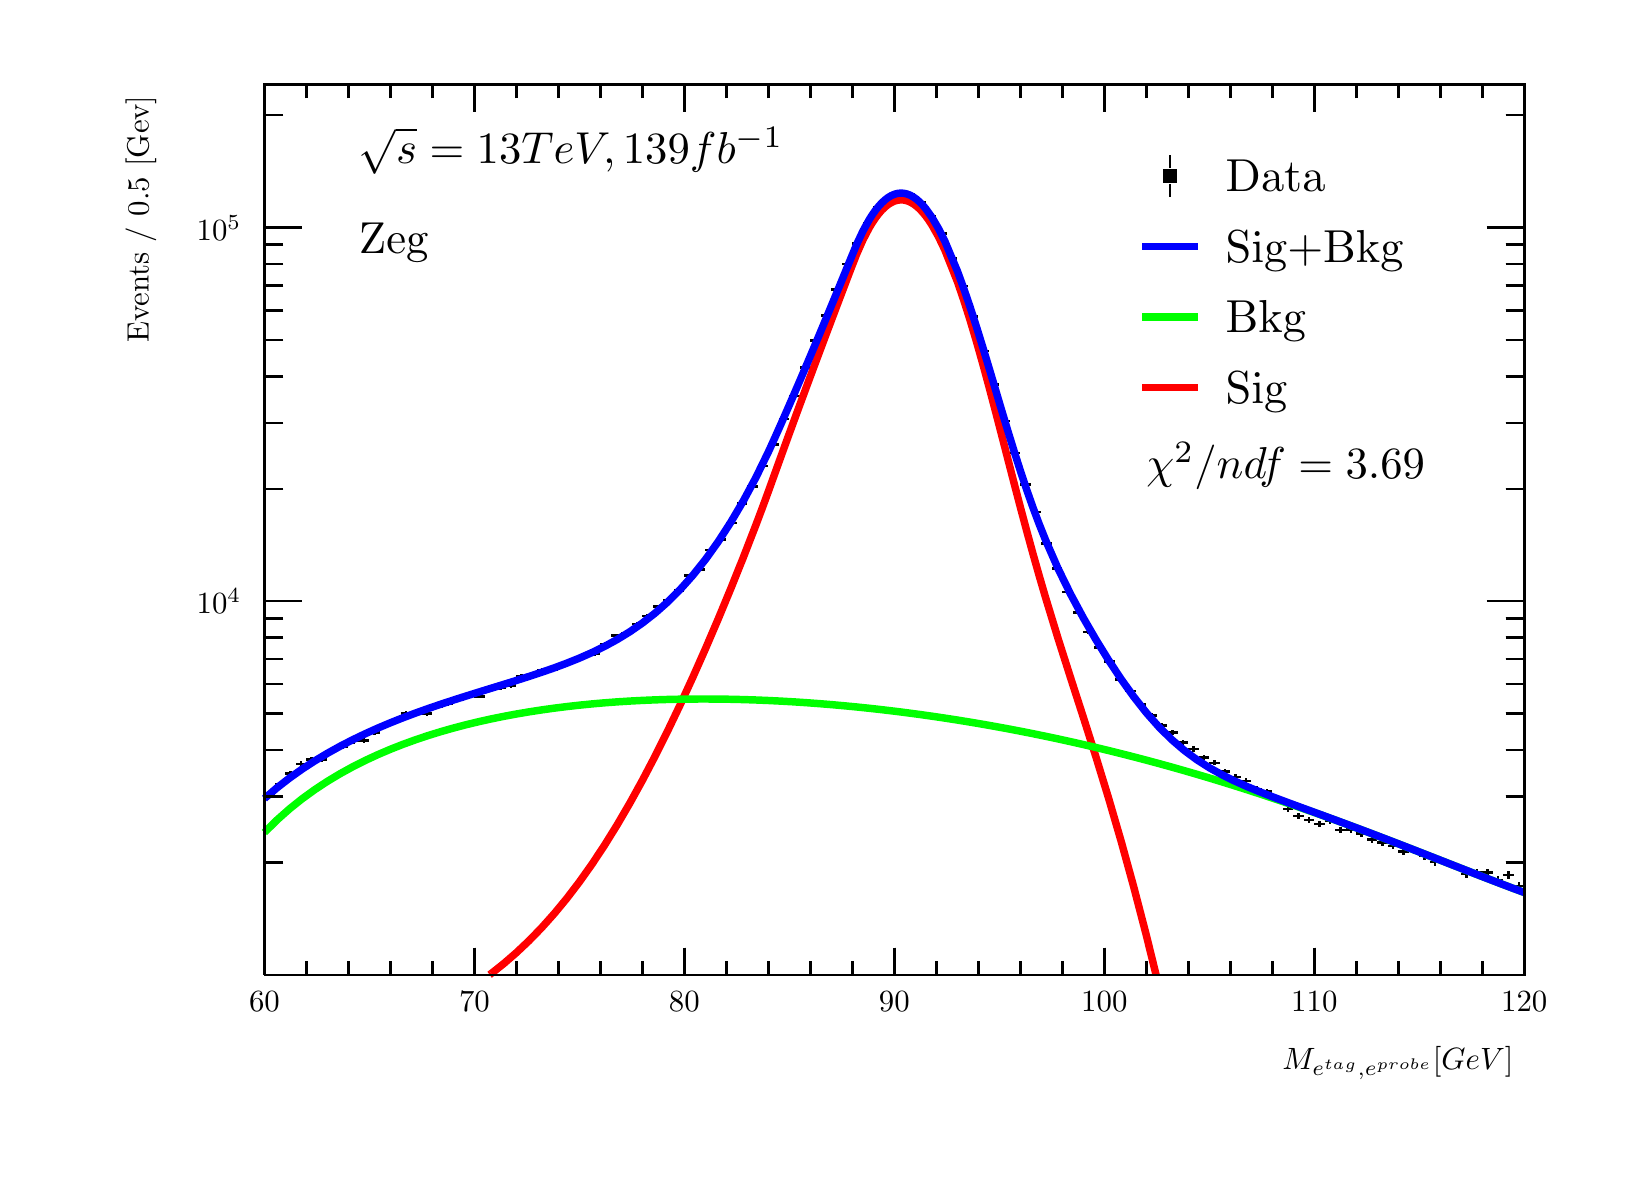
\begin{tikzpicture}
\pgfdeclareplotmark{cross} {
\pgfpathmoveto{\pgfpoint{-0.3\pgfplotmarksize}{\pgfplotmarksize}}
\pgfpathlineto{\pgfpoint{+0.3\pgfplotmarksize}{\pgfplotmarksize}}
\pgfpathlineto{\pgfpoint{+0.3\pgfplotmarksize}{0.3\pgfplotmarksize}}
\pgfpathlineto{\pgfpoint{+1\pgfplotmarksize}{0.3\pgfplotmarksize}}
\pgfpathlineto{\pgfpoint{+1\pgfplotmarksize}{-0.3\pgfplotmarksize}}
\pgfpathlineto{\pgfpoint{+0.3\pgfplotmarksize}{-0.3\pgfplotmarksize}}
\pgfpathlineto{\pgfpoint{+0.3\pgfplotmarksize}{-1.\pgfplotmarksize}}
\pgfpathlineto{\pgfpoint{-0.3\pgfplotmarksize}{-1.\pgfplotmarksize}}
\pgfpathlineto{\pgfpoint{-0.3\pgfplotmarksize}{-0.3\pgfplotmarksize}}
\pgfpathlineto{\pgfpoint{-1.\pgfplotmarksize}{-0.3\pgfplotmarksize}}
\pgfpathlineto{\pgfpoint{-1.\pgfplotmarksize}{0.3\pgfplotmarksize}}
\pgfpathlineto{\pgfpoint{-0.3\pgfplotmarksize}{0.3\pgfplotmarksize}}
\pgfpathclose
\pgfusepathqstroke
}
\pgfdeclareplotmark{cross*} {
\pgfpathmoveto{\pgfpoint{-0.3\pgfplotmarksize}{\pgfplotmarksize}}
\pgfpathlineto{\pgfpoint{+0.3\pgfplotmarksize}{\pgfplotmarksize}}
\pgfpathlineto{\pgfpoint{+0.3\pgfplotmarksize}{0.3\pgfplotmarksize}}
\pgfpathlineto{\pgfpoint{+1\pgfplotmarksize}{0.3\pgfplotmarksize}}
\pgfpathlineto{\pgfpoint{+1\pgfplotmarksize}{-0.3\pgfplotmarksize}}
\pgfpathlineto{\pgfpoint{+0.3\pgfplotmarksize}{-0.3\pgfplotmarksize}}
\pgfpathlineto{\pgfpoint{+0.3\pgfplotmarksize}{-1.\pgfplotmarksize}}
\pgfpathlineto{\pgfpoint{-0.3\pgfplotmarksize}{-1.\pgfplotmarksize}}
\pgfpathlineto{\pgfpoint{-0.3\pgfplotmarksize}{-0.3\pgfplotmarksize}}
\pgfpathlineto{\pgfpoint{-1.\pgfplotmarksize}{-0.3\pgfplotmarksize}}
\pgfpathlineto{\pgfpoint{-1.\pgfplotmarksize}{0.3\pgfplotmarksize}}
\pgfpathlineto{\pgfpoint{-0.3\pgfplotmarksize}{0.3\pgfplotmarksize}}
\pgfpathclose
\pgfusepathqfillstroke
}
\pgfdeclareplotmark{newstar} {
\pgfpathmoveto{\pgfqpoint{0pt}{\pgfplotmarksize}}
\pgfpathlineto{\pgfqpointpolar{44}{0.5\pgfplotmarksize}}
\pgfpathlineto{\pgfqpointpolar{18}{\pgfplotmarksize}}
\pgfpathlineto{\pgfqpointpolar{-20}{0.5\pgfplotmarksize}}
\pgfpathlineto{\pgfqpointpolar{-54}{\pgfplotmarksize}}
\pgfpathlineto{\pgfqpointpolar{-90}{0.5\pgfplotmarksize}}
\pgfpathlineto{\pgfqpointpolar{234}{\pgfplotmarksize}}
\pgfpathlineto{\pgfqpointpolar{198}{0.5\pgfplotmarksize}}
\pgfpathlineto{\pgfqpointpolar{162}{\pgfplotmarksize}}
\pgfpathlineto{\pgfqpointpolar{134}{0.5\pgfplotmarksize}}
\pgfpathclose
\pgfusepathqstroke
}
\pgfdeclareplotmark{newstar*} {
\pgfpathmoveto{\pgfqpoint{0pt}{\pgfplotmarksize}}
\pgfpathlineto{\pgfqpointpolar{44}{0.5\pgfplotmarksize}}
\pgfpathlineto{\pgfqpointpolar{18}{\pgfplotmarksize}}
\pgfpathlineto{\pgfqpointpolar{-20}{0.5\pgfplotmarksize}}
\pgfpathlineto{\pgfqpointpolar{-54}{\pgfplotmarksize}}
\pgfpathlineto{\pgfqpointpolar{-90}{0.5\pgfplotmarksize}}
\pgfpathlineto{\pgfqpointpolar{234}{\pgfplotmarksize}}
\pgfpathlineto{\pgfqpointpolar{198}{0.5\pgfplotmarksize}}
\pgfpathlineto{\pgfqpointpolar{162}{\pgfplotmarksize}}
\pgfpathlineto{\pgfqpointpolar{134}{0.5\pgfplotmarksize}}
\pgfpathclose
\pgfusepathqfillstroke
}
\definecolor{c}{rgb}{1,1,1};
\draw [color=c, fill=c] (0,0) rectangle (20,14.3108);
\draw [color=c, fill=c] (3,2.28972) rectangle (19,13.5952);
\definecolor{c}{rgb}{0,0,0};
\draw [c,line width=0.9] (3,2.28972) -- (3,13.5952) -- (19,13.5952) -- (19,2.28972) -- (3,2.28972);
\definecolor{c}{rgb}{1,1,1};
\draw [color=c, fill=c] (3,2.28972) rectangle (19,13.5952);
\definecolor{c}{rgb}{0,0,0};
\draw [c,line width=0.9] (3,2.28972) -- (3,13.5952) -- (19,13.5952) -- (19,2.28972) -- (3,2.28972);
\draw [c,line width=0.9] (3,2.28972) -- (19,2.28972);
\draw [c,line width=0.9] (3,2.63318) -- (3,2.28972);
\draw [c,line width=0.9] (3.53333,2.46145) -- (3.53333,2.28972);
\draw [c,line width=0.9] (4.06667,2.46145) -- (4.06667,2.28972);
\draw [c,line width=0.9] (4.6,2.46145) -- (4.6,2.28972);
\draw [c,line width=0.9] (5.13333,2.46145) -- (5.13333,2.28972);
\draw [c,line width=0.9] (5.66667,2.63318) -- (5.66667,2.28972);
\draw [c,line width=0.9] (6.2,2.46145) -- (6.2,2.28972);
\draw [c,line width=0.9] (6.73333,2.46145) -- (6.73333,2.28972);
\draw [c,line width=0.9] (7.26667,2.46145) -- (7.26667,2.28972);
\draw [c,line width=0.9] (7.8,2.46145) -- (7.8,2.28972);
\draw [c,line width=0.9] (8.33333,2.63318) -- (8.33333,2.28972);
\draw [c,line width=0.9] (8.86667,2.46145) -- (8.86667,2.28972);
\draw [c,line width=0.9] (9.4,2.46145) -- (9.4,2.28972);
\draw [c,line width=0.9] (9.93333,2.46145) -- (9.93333,2.28972);
\draw [c,line width=0.9] (10.4667,2.46145) -- (10.4667,2.28972);
\draw [c,line width=0.9] (11,2.63318) -- (11,2.28972);
\draw [c,line width=0.9] (11.5333,2.46145) -- (11.5333,2.28972);
\draw [c,line width=0.9] (12.0667,2.46145) -- (12.0667,2.28972);
\draw [c,line width=0.9] (12.6,2.46145) -- (12.6,2.28972);
\draw [c,line width=0.9] (13.1333,2.46145) -- (13.1333,2.28972);
\draw [c,line width=0.9] (13.6667,2.63318) -- (13.6667,2.28972);
\draw [c,line width=0.9] (14.2,2.46145) -- (14.2,2.28972);
\draw [c,line width=0.9] (14.7333,2.46145) -- (14.7333,2.28972);
\draw [c,line width=0.9] (15.2667,2.46145) -- (15.2667,2.28972);
\draw [c,line width=0.9] (15.8,2.46145) -- (15.8,2.28972);
\draw [c,line width=0.9] (16.3333,2.63318) -- (16.3333,2.28972);
\draw [c,line width=0.9] (16.8667,2.46145) -- (16.8667,2.28972);
\draw [c,line width=0.9] (17.4,2.46145) -- (17.4,2.28972);
\draw [c,line width=0.9] (17.9333,2.46145) -- (17.9333,2.28972);
\draw [c,line width=0.9] (18.4667,2.46145) -- (18.4667,2.28972);
\draw [c,line width=0.9] (19,2.63318) -- (19,2.28972);
\draw [anchor=base] (3,1.81747) node[scale=1.11327, color=c, rotate=0]{60};
\draw [anchor=base] (5.66667,1.81747) node[scale=1.11327, color=c, rotate=0]{70};
\draw [anchor=base] (8.33333,1.81747) node[scale=1.11327, color=c, rotate=0]{80};
\draw [anchor=base] (11,1.81747) node[scale=1.11327, color=c, rotate=0]{90};
\draw [anchor=base] (13.6667,1.81747) node[scale=1.11327, color=c, rotate=0]{100};
\draw [anchor=base] (16.3333,1.81747) node[scale=1.11327, color=c, rotate=0]{110};
\draw [anchor=base] (19,1.81747) node[scale=1.11327, color=c, rotate=0]{120};
\draw [anchor= east] (19,1.16776) node[scale=1.11327, color=c, rotate=0]{$M_{e^{tag}, e^{probe}}  [GeV]$};
\draw [c,line width=0.9] (3,13.5952) -- (19,13.5952);
\draw [c,line width=0.9] (3,13.2518) -- (3,13.5952);
\draw [c,line width=0.9] (3.53333,13.4235) -- (3.53333,13.5952);
\draw [c,line width=0.9] (4.06667,13.4235) -- (4.06667,13.5952);
\draw [c,line width=0.9] (4.6,13.4235) -- (4.6,13.5952);
\draw [c,line width=0.9] (5.13333,13.4235) -- (5.13333,13.5952);
\draw [c,line width=0.9] (5.66667,13.2518) -- (5.66667,13.5952);
\draw [c,line width=0.9] (6.2,13.4235) -- (6.2,13.5952);
\draw [c,line width=0.9] (6.73333,13.4235) -- (6.73333,13.5952);
\draw [c,line width=0.9] (7.26667,13.4235) -- (7.26667,13.5952);
\draw [c,line width=0.9] (7.8,13.4235) -- (7.8,13.5952);
\draw [c,line width=0.9] (8.33333,13.2518) -- (8.33333,13.5952);
\draw [c,line width=0.9] (8.86667,13.4235) -- (8.86667,13.5952);
\draw [c,line width=0.9] (9.4,13.4235) -- (9.4,13.5952);
\draw [c,line width=0.9] (9.93333,13.4235) -- (9.93333,13.5952);
\draw [c,line width=0.9] (10.4667,13.4235) -- (10.4667,13.5952);
\draw [c,line width=0.9] (11,13.2518) -- (11,13.5952);
\draw [c,line width=0.9] (11.5333,13.4235) -- (11.5333,13.5952);
\draw [c,line width=0.9] (12.0667,13.4235) -- (12.0667,13.5952);
\draw [c,line width=0.9] (12.6,13.4235) -- (12.6,13.5952);
\draw [c,line width=0.9] (13.1333,13.4235) -- (13.1333,13.5952);
\draw [c,line width=0.9] (13.6667,13.2518) -- (13.6667,13.5952);
\draw [c,line width=0.9] (14.2,13.4235) -- (14.2,13.5952);
\draw [c,line width=0.9] (14.7333,13.4235) -- (14.7333,13.5952);
\draw [c,line width=0.9] (15.2667,13.4235) -- (15.2667,13.5952);
\draw [c,line width=0.9] (15.8,13.4235) -- (15.8,13.5952);
\draw [c,line width=0.9] (16.3333,13.2518) -- (16.3333,13.5952);
\draw [c,line width=0.9] (16.8667,13.4235) -- (16.8667,13.5952);
\draw [c,line width=0.9] (17.4,13.4235) -- (17.4,13.5952);
\draw [c,line width=0.9] (17.9333,13.4235) -- (17.9333,13.5952);
\draw [c,line width=0.9] (18.4667,13.4235) -- (18.4667,13.5952);
\draw [c,line width=0.9] (19,13.2518) -- (19,13.5952);
\draw [c,line width=0.9] (3,2.28972) -- (3,13.5952);
\draw [c,line width=0.9] (3.237,3.71787) -- (3,3.71787);
\draw [c,line width=0.9] (3.237,4.55329) -- (3,4.55329);
\draw [c,line width=0.9] (3.237,5.14603) -- (3,5.14603);
\draw [c,line width=0.9] (3.237,5.60579) -- (3,5.60579);
\draw [c,line width=0.9] (3.237,5.98144) -- (3,5.98144);
\draw [c,line width=0.9] (3.237,6.29905) -- (3,6.29905);
\draw [c,line width=0.9] (3.237,6.57418) -- (3,6.57418);
\draw [c,line width=0.9] (3.237,6.81686) -- (3,6.81686);
\draw [c,line width=0.9] (3.474,7.03394) -- (3,7.03394);
\draw [anchor= east] (2.844,7.03394) node[scale=1.11327, color=c, rotate=0]{$10^{4}$};
\draw [c,line width=0.9] (3.237,8.4621) -- (3,8.4621);
\draw [c,line width=0.9] (3.237,9.29751) -- (3,9.29751);
\draw [c,line width=0.9] (3.237,9.89025) -- (3,9.89025);
\draw [c,line width=0.9] (3.237,10.35) -- (3,10.35);
\draw [c,line width=0.9] (3.237,10.7257) -- (3,10.7257);
\draw [c,line width=0.9] (3.237,11.0433) -- (3,11.0433);
\draw [c,line width=0.9] (3.237,11.3184) -- (3,11.3184);
\draw [c,line width=0.9] (3.237,11.5611) -- (3,11.5611);
\draw [c,line width=0.9] (3.474,11.7782) -- (3,11.7782);
\draw [anchor= east] (2.844,11.7782) node[scale=1.11327, color=c, rotate=0]{$10^{5}$};
\draw [c,line width=0.9] (3.237,13.2063) -- (3,13.2063);
\draw [anchor= east] (1.432,13.5952) node[scale=1.11327, color=c, rotate=90]{Events / 0.5 [Gev]};
\draw [c,line width=0.9] (19,2.28972) -- (19,13.5952);
\draw [c,line width=0.9] (18.763,3.71787) -- (19,3.71787);
\draw [c,line width=0.9] (18.763,4.55329) -- (19,4.55329);
\draw [c,line width=0.9] (18.763,5.14603) -- (19,5.14603);
\draw [c,line width=0.9] (18.763,5.60579) -- (19,5.60579);
\draw [c,line width=0.9] (18.763,5.98144) -- (19,5.98144);
\draw [c,line width=0.9] (18.763,6.29905) -- (19,6.29905);
\draw [c,line width=0.9] (18.763,6.57418) -- (19,6.57418);
\draw [c,line width=0.9] (18.763,6.81686) -- (19,6.81686);
\draw [c,line width=0.9] (18.526,7.03394) -- (19,7.03394);
\draw [c,line width=0.9] (18.763,8.4621) -- (19,8.4621);
\draw [c,line width=0.9] (18.763,9.29751) -- (19,9.29751);
\draw [c,line width=0.9] (18.763,9.89025) -- (19,9.89025);
\draw [c,line width=0.9] (18.763,10.35) -- (19,10.35);
\draw [c,line width=0.9] (18.763,10.7257) -- (19,10.7257);
\draw [c,line width=0.9] (18.763,11.0433) -- (19,11.0433);
\draw [c,line width=0.9] (18.763,11.3184) -- (19,11.3184);
\draw [c,line width=0.9] (18.763,11.5611) -- (19,11.5611);
\draw [c,line width=0.9] (18.526,11.7782) -- (19,11.7782);
\draw [c,line width=0.9] (18.763,13.2063) -- (19,13.2063);
\draw [c,line width=0.9] (3.06667,4.58668) -- (3,4.58668);
\draw [c,line width=0.9] (3,4.58668) -- (3,4.58668);
\draw [c,line width=0.9] (3.06667,4.58668) -- (3.13333,4.58668);
\draw [c,line width=0.9] (3.13333,4.58668) -- (3.13333,4.58668);
\draw [c,line width=0.9] (3.06667,4.58668) -- (3.06667,4.62399);
\draw [c,line width=0.9] (3.06667,4.62399) -- (3.06667,4.62399);
\draw [c,line width=0.9] (3.06667,4.58668) -- (3.06667,4.54936);
\draw [c,line width=0.9] (3.06667,4.54936) -- (3.06667,4.54936);
\draw [c,line width=0.9] (3.2,4.70486) -- (3.13333,4.70486);
\draw [c,line width=0.9] (3.13333,4.70486) -- (3.13333,4.70486);
\draw [c,line width=0.9] (3.2,4.70486) -- (3.26667,4.70486);
\draw [c,line width=0.9] (3.26667,4.70486) -- (3.26667,4.70486);
\draw [c,line width=0.9] (3.2,4.70486) -- (3.2,4.74112);
\draw [c,line width=0.9] (3.2,4.74112) -- (3.2,4.74112);
\draw [c,line width=0.9] (3.2,4.70486) -- (3.2,4.6686);
\draw [c,line width=0.9] (3.2,4.6686) -- (3.2,4.6686);
\draw [c,line width=0.9] (3.33333,4.84543) -- (3.26667,4.84543);
\draw [c,line width=0.9] (3.26667,4.84543) -- (3.26667,4.84543);
\draw [c,line width=0.9] (3.33333,4.84543) -- (3.4,4.84543);
\draw [c,line width=0.9] (3.4,4.84543) -- (3.4,4.84543);
\draw [c,line width=0.9] (3.33333,4.84543) -- (3.33333,4.88048);
\draw [c,line width=0.9] (3.33333,4.88048) -- (3.33333,4.88048);
\draw [c,line width=0.9] (3.33333,4.84543) -- (3.33333,4.81039);
\draw [c,line width=0.9] (3.33333,4.81039) -- (3.33333,4.81039);
\draw [c,line width=0.9] (3.46667,4.9675) -- (3.4,4.9675);
\draw [c,line width=0.9] (3.4,4.9675) -- (3.4,4.9675);
\draw [c,line width=0.9] (3.46667,4.9675) -- (3.53333,4.9675);
\draw [c,line width=0.9] (3.53333,4.9675) -- (3.53333,4.9675);
\draw [c,line width=0.9] (3.46667,4.9675) -- (3.46667,5.00152);
\draw [c,line width=0.9] (3.46667,5.00152) -- (3.46667,5.00152);
\draw [c,line width=0.9] (3.46667,4.9675) -- (3.46667,4.93348);
\draw [c,line width=0.9] (3.46667,4.93348) -- (3.46667,4.93348);
\draw [c,line width=0.9] (3.6,5.02566) -- (3.53333,5.02566);
\draw [c,line width=0.9] (3.53333,5.02566) -- (3.53333,5.02566);
\draw [c,line width=0.9] (3.6,5.02566) -- (3.66667,5.02566);
\draw [c,line width=0.9] (3.66667,5.02566) -- (3.66667,5.02566);
\draw [c,line width=0.9] (3.6,5.02566) -- (3.6,5.0592);
\draw [c,line width=0.9] (3.6,5.0592) -- (3.6,5.0592);
\draw [c,line width=0.9] (3.6,5.02566) -- (3.6,4.99211);
\draw [c,line width=0.9] (3.6,4.99211) -- (3.6,4.99211);
\draw [c,line width=0.9] (3.73333,5.02566) -- (3.66667,5.02566);
\draw [c,line width=0.9] (3.66667,5.02566) -- (3.66667,5.02566);
\draw [c,line width=0.9] (3.73333,5.02566) -- (3.8,5.02566);
\draw [c,line width=0.9] (3.8,5.02566) -- (3.8,5.02566);
\draw [c,line width=0.9] (3.73333,5.02566) -- (3.73333,5.0592);
\draw [c,line width=0.9] (3.73333,5.0592) -- (3.73333,5.0592);
\draw [c,line width=0.9] (3.73333,5.02566) -- (3.73333,4.99211);
\draw [c,line width=0.9] (3.73333,4.99211) -- (3.73333,4.99211);
\draw [c,line width=0.9] (3.86667,5.14552) -- (3.8,5.14552);
\draw [c,line width=0.9] (3.8,5.14552) -- (3.8,5.14552);
\draw [c,line width=0.9] (3.86667,5.14552) -- (3.93333,5.14552);
\draw [c,line width=0.9] (3.93333,5.14552) -- (3.93333,5.14552);
\draw [c,line width=0.9] (3.86667,5.14552) -- (3.86667,5.1781);
\draw [c,line width=0.9] (3.86667,5.1781) -- (3.86667,5.1781);
\draw [c,line width=0.9] (3.86667,5.14552) -- (3.86667,5.11293);
\draw [c,line width=0.9] (3.86667,5.11293) -- (3.86667,5.11293);
\draw [c,line width=0.9] (4,5.18633) -- (3.93333,5.18633);
\draw [c,line width=0.9] (3.93333,5.18633) -- (3.93333,5.18633);
\draw [c,line width=0.9] (4,5.18633) -- (4.06667,5.18633);
\draw [c,line width=0.9] (4.06667,5.18633) -- (4.06667,5.18633);
\draw [c,line width=0.9] (4,5.18633) -- (4,5.21859);
\draw [c,line width=0.9] (4,5.21859) -- (4,5.21859);
\draw [c,line width=0.9] (4,5.18633) -- (4,5.15407);
\draw [c,line width=0.9] (4,5.15407) -- (4,5.15407);
\draw [c,line width=0.9] (4.13333,5.25732) -- (4.06667,5.25732);
\draw [c,line width=0.9] (4.06667,5.25732) -- (4.06667,5.25732);
\draw [c,line width=0.9] (4.13333,5.25732) -- (4.2,5.25732);
\draw [c,line width=0.9] (4.2,5.25732) -- (4.2,5.25732);
\draw [c,line width=0.9] (4.13333,5.25732) -- (4.13333,5.28903);
\draw [c,line width=0.9] (4.13333,5.28903) -- (4.13333,5.28903);
\draw [c,line width=0.9] (4.13333,5.25732) -- (4.13333,5.22561);
\draw [c,line width=0.9] (4.13333,5.22561) -- (4.13333,5.22561);
\draw [c,line width=0.9] (4.26667,5.26706) -- (4.2,5.26706);
\draw [c,line width=0.9] (4.2,5.26706) -- (4.2,5.26706);
\draw [c,line width=0.9] (4.26667,5.26706) -- (4.33333,5.26706);
\draw [c,line width=0.9] (4.33333,5.26706) -- (4.33333,5.26706);
\draw [c,line width=0.9] (4.26667,5.26706) -- (4.26667,5.29869);
\draw [c,line width=0.9] (4.26667,5.29869) -- (4.26667,5.29869);
\draw [c,line width=0.9] (4.26667,5.26706) -- (4.26667,5.23542);
\draw [c,line width=0.9] (4.26667,5.23542) -- (4.26667,5.23542);
\draw [c,line width=0.9] (4.4,5.36337) -- (4.33333,5.36337);
\draw [c,line width=0.9] (4.33333,5.36337) -- (4.33333,5.36337);
\draw [c,line width=0.9] (4.4,5.36337) -- (4.46667,5.36337);
\draw [c,line width=0.9] (4.46667,5.36337) -- (4.46667,5.36337);
\draw [c,line width=0.9] (4.4,5.36337) -- (4.4,5.39428);
\draw [c,line width=0.9] (4.4,5.39428) -- (4.4,5.39428);
\draw [c,line width=0.9] (4.4,5.36337) -- (4.4,5.33247);
\draw [c,line width=0.9] (4.4,5.33247) -- (4.4,5.33247);
\draw [c,line width=0.9] (4.53333,5.4465) -- (4.46667,5.4465);
\draw [c,line width=0.9] (4.46667,5.4465) -- (4.46667,5.4465);
\draw [c,line width=0.9] (4.53333,5.4465) -- (4.6,5.4465);
\draw [c,line width=0.9] (4.6,5.4465) -- (4.6,5.4465);
\draw [c,line width=0.9] (4.53333,5.4465) -- (4.53333,5.47679);
\draw [c,line width=0.9] (4.53333,5.47679) -- (4.53333,5.47679);
\draw [c,line width=0.9] (4.53333,5.4465) -- (4.53333,5.41621);
\draw [c,line width=0.9] (4.53333,5.41621) -- (4.53333,5.41621);
\draw [c,line width=0.9] (4.66667,5.52597) -- (4.6,5.52597);
\draw [c,line width=0.9] (4.6,5.52597) -- (4.6,5.52597);
\draw [c,line width=0.9] (4.66667,5.52597) -- (4.73333,5.52597);
\draw [c,line width=0.9] (4.73333,5.52597) -- (4.73333,5.52597);
\draw [c,line width=0.9] (4.66667,5.52597) -- (4.66667,5.55568);
\draw [c,line width=0.9] (4.66667,5.55568) -- (4.66667,5.55568);
\draw [c,line width=0.9] (4.66667,5.52597) -- (4.66667,5.49626);
\draw [c,line width=0.9] (4.66667,5.49626) -- (4.66667,5.49626);
\draw [c,line width=0.9] (4.8,5.60538) -- (4.73333,5.60538);
\draw [c,line width=0.9] (4.73333,5.60538) -- (4.73333,5.60538);
\draw [c,line width=0.9] (4.8,5.60538) -- (4.86667,5.60538);
\draw [c,line width=0.9] (4.86667,5.60538) -- (4.86667,5.60538);
\draw [c,line width=0.9] (4.8,5.60538) -- (4.8,5.63452);
\draw [c,line width=0.9] (4.8,5.63452) -- (4.8,5.63452);
\draw [c,line width=0.9] (4.8,5.60538) -- (4.8,5.57624);
\draw [c,line width=0.9] (4.8,5.57624) -- (4.8,5.57624);
\draw [c,line width=0.9] (4.93333,5.62548) -- (4.86667,5.62548);
\draw [c,line width=0.9] (4.86667,5.62548) -- (4.86667,5.62548);
\draw [c,line width=0.9] (4.93333,5.62548) -- (5,5.62548);
\draw [c,line width=0.9] (5,5.62548) -- (5,5.62548);
\draw [c,line width=0.9] (4.93333,5.62548) -- (4.93333,5.65448);
\draw [c,line width=0.9] (4.93333,5.65448) -- (4.93333,5.65448);
\draw [c,line width=0.9] (4.93333,5.62548) -- (4.93333,5.59648);
\draw [c,line width=0.9] (4.93333,5.59648) -- (4.93333,5.59648);
\draw [c,line width=0.9] (5.06667,5.60868) -- (5,5.60868);
\draw [c,line width=0.9] (5,5.60868) -- (5,5.60868);
\draw [c,line width=0.9] (5.06667,5.60868) -- (5.13333,5.60868);
\draw [c,line width=0.9] (5.13333,5.60868) -- (5.13333,5.60868);
\draw [c,line width=0.9] (5.06667,5.60868) -- (5.06667,5.63779);
\draw [c,line width=0.9] (5.06667,5.63779) -- (5.06667,5.63779);
\draw [c,line width=0.9] (5.06667,5.60868) -- (5.06667,5.57956);
\draw [c,line width=0.9] (5.06667,5.57956) -- (5.06667,5.57956);
\draw [c,line width=0.9] (5.2,5.6874) -- (5.13333,5.6874);
\draw [c,line width=0.9] (5.13333,5.6874) -- (5.13333,5.6874);
\draw [c,line width=0.9] (5.2,5.6874) -- (5.26667,5.6874);
\draw [c,line width=0.9] (5.26667,5.6874) -- (5.26667,5.6874);
\draw [c,line width=0.9] (5.2,5.6874) -- (5.2,5.71596);
\draw [c,line width=0.9] (5.2,5.71596) -- (5.2,5.71596);
\draw [c,line width=0.9] (5.2,5.6874) -- (5.2,5.65883);
\draw [c,line width=0.9] (5.2,5.65883) -- (5.2,5.65883);
\draw [c,line width=0.9] (5.33333,5.72702) -- (5.26667,5.72702);
\draw [c,line width=0.9] (5.26667,5.72702) -- (5.26667,5.72702);
\draw [c,line width=0.9] (5.33333,5.72702) -- (5.4,5.72702);
\draw [c,line width=0.9] (5.4,5.72702) -- (5.4,5.72702);
\draw [c,line width=0.9] (5.33333,5.72702) -- (5.33333,5.75531);
\draw [c,line width=0.9] (5.33333,5.75531) -- (5.33333,5.75531);
\draw [c,line width=0.9] (5.33333,5.72702) -- (5.33333,5.69872);
\draw [c,line width=0.9] (5.33333,5.69872) -- (5.33333,5.69872);
\draw [c,line width=0.9] (5.46667,5.78411) -- (5.4,5.78411);
\draw [c,line width=0.9] (5.4,5.78411) -- (5.4,5.78411);
\draw [c,line width=0.9] (5.46667,5.78411) -- (5.53333,5.78411);
\draw [c,line width=0.9] (5.53333,5.78411) -- (5.53333,5.78411);
\draw [c,line width=0.9] (5.46667,5.78411) -- (5.46667,5.81201);
\draw [c,line width=0.9] (5.46667,5.81201) -- (5.46667,5.81201);
\draw [c,line width=0.9] (5.46667,5.78411) -- (5.46667,5.75621);
\draw [c,line width=0.9] (5.46667,5.75621) -- (5.46667,5.75621);
\draw [c,line width=0.9] (5.6,5.83709) -- (5.53333,5.83709);
\draw [c,line width=0.9] (5.53333,5.83709) -- (5.53333,5.83709);
\draw [c,line width=0.9] (5.6,5.83709) -- (5.66667,5.83709);
\draw [c,line width=0.9] (5.66667,5.83709) -- (5.66667,5.83709);
\draw [c,line width=0.9] (5.6,5.83709) -- (5.6,5.86463);
\draw [c,line width=0.9] (5.6,5.86463) -- (5.6,5.86463);
\draw [c,line width=0.9] (5.6,5.83709) -- (5.6,5.80954);
\draw [c,line width=0.9] (5.6,5.80954) -- (5.6,5.80954);
\draw [c,line width=0.9] (5.73333,5.82675) -- (5.66667,5.82675);
\draw [c,line width=0.9] (5.66667,5.82675) -- (5.66667,5.82675);
\draw [c,line width=0.9] (5.73333,5.82675) -- (5.8,5.82675);
\draw [c,line width=0.9] (5.8,5.82675) -- (5.8,5.82675);
\draw [c,line width=0.9] (5.73333,5.82675) -- (5.73333,5.85436);
\draw [c,line width=0.9] (5.73333,5.85436) -- (5.73333,5.85436);
\draw [c,line width=0.9] (5.73333,5.82675) -- (5.73333,5.79913);
\draw [c,line width=0.9] (5.73333,5.79913) -- (5.73333,5.79913);
\draw [c,line width=0.9] (5.86667,5.9116) -- (5.8,5.9116);
\draw [c,line width=0.9] (5.8,5.9116) -- (5.8,5.9116);
\draw [c,line width=0.9] (5.86667,5.9116) -- (5.93333,5.9116);
\draw [c,line width=0.9] (5.93333,5.9116) -- (5.93333,5.9116);
\draw [c,line width=0.9] (5.86667,5.9116) -- (5.86667,5.93865);
\draw [c,line width=0.9] (5.86667,5.93865) -- (5.86667,5.93865);
\draw [c,line width=0.9] (5.86667,5.9116) -- (5.86667,5.88454);
\draw [c,line width=0.9] (5.86667,5.88454) -- (5.86667,5.88454);
\draw [c,line width=0.9] (6,5.93702) -- (5.93333,5.93702);
\draw [c,line width=0.9] (5.93333,5.93702) -- (5.93333,5.93702);
\draw [c,line width=0.9] (6,5.93702) -- (6.06667,5.93702);
\draw [c,line width=0.9] (6.06667,5.93702) -- (6.06667,5.93702);
\draw [c,line width=0.9] (6,5.93702) -- (6,5.9639);
\draw [c,line width=0.9] (6,5.9639) -- (6,5.9639);
\draw [c,line width=0.9] (6,5.93702) -- (6,5.91013);
\draw [c,line width=0.9] (6,5.91013) -- (6,5.91013);
\draw [c,line width=0.9] (6.13333,5.96247) -- (6.06667,5.96247);
\draw [c,line width=0.9] (6.06667,5.96247) -- (6.06667,5.96247);
\draw [c,line width=0.9] (6.13333,5.96247) -- (6.2,5.96247);
\draw [c,line width=0.9] (6.2,5.96247) -- (6.2,5.96247);
\draw [c,line width=0.9] (6.13333,5.96247) -- (6.13333,5.9892);
\draw [c,line width=0.9] (6.13333,5.9892) -- (6.13333,5.9892);
\draw [c,line width=0.9] (6.13333,5.96247) -- (6.13333,5.93575);
\draw [c,line width=0.9] (6.13333,5.93575) -- (6.13333,5.93575);
\draw [c,line width=0.9] (6.26667,6.0823) -- (6.2,6.0823);
\draw [c,line width=0.9] (6.2,6.0823) -- (6.2,6.0823);
\draw [c,line width=0.9] (6.26667,6.0823) -- (6.33333,6.0823);
\draw [c,line width=0.9] (6.33333,6.0823) -- (6.33333,6.0823);
\draw [c,line width=0.9] (6.26667,6.0823) -- (6.26667,6.10826);
\draw [c,line width=0.9] (6.26667,6.10826) -- (6.26667,6.10826);
\draw [c,line width=0.9] (6.26667,6.0823) -- (6.26667,6.05634);
\draw [c,line width=0.9] (6.26667,6.05634) -- (6.26667,6.05634);
\draw [c,line width=0.9] (6.4,6.1083) -- (6.33333,6.1083);
\draw [c,line width=0.9] (6.33333,6.1083) -- (6.33333,6.1083);
\draw [c,line width=0.9] (6.4,6.1083) -- (6.46667,6.1083);
\draw [c,line width=0.9] (6.46667,6.1083) -- (6.46667,6.1083);
\draw [c,line width=0.9] (6.4,6.1083) -- (6.4,6.13409);
\draw [c,line width=0.9] (6.4,6.13409) -- (6.4,6.13409);
\draw [c,line width=0.9] (6.4,6.1083) -- (6.4,6.0825);
\draw [c,line width=0.9] (6.4,6.0825) -- (6.4,6.0825);
\draw [c,line width=0.9] (6.53333,6.15428) -- (6.46667,6.15428);
\draw [c,line width=0.9] (6.46667,6.15428) -- (6.46667,6.15428);
\draw [c,line width=0.9] (6.53333,6.15428) -- (6.6,6.15428);
\draw [c,line width=0.9] (6.6,6.15428) -- (6.6,6.15428);
\draw [c,line width=0.9] (6.53333,6.15428) -- (6.53333,6.17978);
\draw [c,line width=0.9] (6.53333,6.17978) -- (6.53333,6.17978);
\draw [c,line width=0.9] (6.53333,6.15428) -- (6.53333,6.12877);
\draw [c,line width=0.9] (6.53333,6.12877) -- (6.53333,6.12877);
\draw [c,line width=0.9] (6.66667,6.15901) -- (6.6,6.15901);
\draw [c,line width=0.9] (6.6,6.15901) -- (6.6,6.15901);
\draw [c,line width=0.9] (6.66667,6.15901) -- (6.73333,6.15901);
\draw [c,line width=0.9] (6.73333,6.15901) -- (6.73333,6.15901);
\draw [c,line width=0.9] (6.66667,6.15901) -- (6.66667,6.18448);
\draw [c,line width=0.9] (6.66667,6.18448) -- (6.66667,6.18448);
\draw [c,line width=0.9] (6.66667,6.15901) -- (6.66667,6.13353);
\draw [c,line width=0.9] (6.66667,6.13353) -- (6.66667,6.13353);
\draw [c,line width=0.9] (6.8,6.23569) -- (6.73333,6.23569);
\draw [c,line width=0.9] (6.73333,6.23569) -- (6.73333,6.23569);
\draw [c,line width=0.9] (6.8,6.23569) -- (6.86667,6.23569);
\draw [c,line width=0.9] (6.86667,6.23569) -- (6.86667,6.23569);
\draw [c,line width=0.9] (6.8,6.23569) -- (6.8,6.2607);
\draw [c,line width=0.9] (6.8,6.2607) -- (6.8,6.2607);
\draw [c,line width=0.9] (6.8,6.23569) -- (6.8,6.21069);
\draw [c,line width=0.9] (6.8,6.21069) -- (6.8,6.21069);
\draw [c,line width=0.9] (6.93333,6.28013) -- (6.86667,6.28013);
\draw [c,line width=0.9] (6.86667,6.28013) -- (6.86667,6.28013);
\draw [c,line width=0.9] (6.93333,6.28013) -- (7,6.28013);
\draw [c,line width=0.9] (7,6.28013) -- (7,6.28013);
\draw [c,line width=0.9] (6.93333,6.28013) -- (6.93333,6.30487);
\draw [c,line width=0.9] (6.93333,6.30487) -- (6.93333,6.30487);
\draw [c,line width=0.9] (6.93333,6.28013) -- (6.93333,6.25539);
\draw [c,line width=0.9] (6.93333,6.25539) -- (6.93333,6.25539);
\draw [c,line width=0.9] (7.06667,6.34217) -- (7,6.34217);
\draw [c,line width=0.9] (7,6.34217) -- (7,6.34217);
\draw [c,line width=0.9] (7.06667,6.34217) -- (7.13333,6.34217);
\draw [c,line width=0.9] (7.13333,6.34217) -- (7.13333,6.34217);
\draw [c,line width=0.9] (7.06667,6.34217) -- (7.06667,6.36654);
\draw [c,line width=0.9] (7.06667,6.36654) -- (7.06667,6.36654);
\draw [c,line width=0.9] (7.06667,6.34217) -- (7.06667,6.3178);
\draw [c,line width=0.9] (7.06667,6.3178) -- (7.06667,6.3178);
\draw [c,line width=0.9] (7.2,6.3631) -- (7.13333,6.3631);
\draw [c,line width=0.9] (7.13333,6.3631) -- (7.13333,6.3631);
\draw [c,line width=0.9] (7.2,6.3631) -- (7.26667,6.3631);
\draw [c,line width=0.9] (7.26667,6.3631) -- (7.26667,6.3631);
\draw [c,line width=0.9] (7.2,6.3631) -- (7.2,6.38735);
\draw [c,line width=0.9] (7.2,6.38735) -- (7.2,6.38735);
\draw [c,line width=0.9] (7.2,6.3631) -- (7.2,6.33886);
\draw [c,line width=0.9] (7.2,6.33886) -- (7.2,6.33886);
\draw [c,line width=0.9] (7.33333,6.48766) -- (7.26667,6.48766);
\draw [c,line width=0.9] (7.26667,6.48766) -- (7.26667,6.48766);
\draw [c,line width=0.9] (7.33333,6.48766) -- (7.4,6.48766);
\draw [c,line width=0.9] (7.4,6.48766) -- (7.4,6.48766);
\draw [c,line width=0.9] (7.33333,6.48766) -- (7.33333,6.51118);
\draw [c,line width=0.9] (7.33333,6.51118) -- (7.33333,6.51118);
\draw [c,line width=0.9] (7.33333,6.48766) -- (7.33333,6.46413);
\draw [c,line width=0.9] (7.33333,6.46413) -- (7.33333,6.46413);
\draw [c,line width=0.9] (7.46667,6.59672) -- (7.4,6.59672);
\draw [c,line width=0.9] (7.4,6.59672) -- (7.4,6.59672);
\draw [c,line width=0.9] (7.46667,6.59672) -- (7.53333,6.59672);
\draw [c,line width=0.9] (7.53333,6.59672) -- (7.53333,6.59672);
\draw [c,line width=0.9] (7.46667,6.59672) -- (7.46667,6.61964);
\draw [c,line width=0.9] (7.46667,6.61964) -- (7.46667,6.61964);
\draw [c,line width=0.9] (7.46667,6.59672) -- (7.46667,6.57381);
\draw [c,line width=0.9] (7.46667,6.57381) -- (7.46667,6.57381);
\draw [c,line width=0.9] (7.6,6.62858) -- (7.53333,6.62858);
\draw [c,line width=0.9] (7.53333,6.62858) -- (7.53333,6.62858);
\draw [c,line width=0.9] (7.6,6.62858) -- (7.66667,6.62858);
\draw [c,line width=0.9] (7.66667,6.62858) -- (7.66667,6.62858);
\draw [c,line width=0.9] (7.6,6.62858) -- (7.6,6.65131);
\draw [c,line width=0.9] (7.6,6.65131) -- (7.6,6.65131);
\draw [c,line width=0.9] (7.6,6.62858) -- (7.6,6.60584);
\draw [c,line width=0.9] (7.6,6.60584) -- (7.6,6.60584);
\draw [c,line width=0.9] (7.73333,6.7463) -- (7.66667,6.7463);
\draw [c,line width=0.9] (7.66667,6.7463) -- (7.66667,6.7463);
\draw [c,line width=0.9] (7.73333,6.7463) -- (7.8,6.7463);
\draw [c,line width=0.9] (7.8,6.7463) -- (7.8,6.7463);
\draw [c,line width=0.9] (7.73333,6.7463) -- (7.73333,6.7684);
\draw [c,line width=0.9] (7.73333,6.7684) -- (7.73333,6.7684);
\draw [c,line width=0.9] (7.73333,6.7463) -- (7.73333,6.72421);
\draw [c,line width=0.9] (7.73333,6.72421) -- (7.73333,6.72421);
\draw [c,line width=0.9] (7.86667,6.84664) -- (7.8,6.84664);
\draw [c,line width=0.9] (7.8,6.84664) -- (7.8,6.84664);
\draw [c,line width=0.9] (7.86667,6.84664) -- (7.93333,6.84664);
\draw [c,line width=0.9] (7.93333,6.84664) -- (7.93333,6.84664);
\draw [c,line width=0.9] (7.86667,6.84664) -- (7.86667,6.8682);
\draw [c,line width=0.9] (7.86667,6.8682) -- (7.86667,6.8682);
\draw [c,line width=0.9] (7.86667,6.84664) -- (7.86667,6.82508);
\draw [c,line width=0.9] (7.86667,6.82508) -- (7.86667,6.82508);
\draw [c,line width=0.9] (8,6.96928) -- (7.93333,6.96928);
\draw [c,line width=0.9] (7.93333,6.96928) -- (7.93333,6.96928);
\draw [c,line width=0.9] (8,6.96928) -- (8.06667,6.96928);
\draw [c,line width=0.9] (8.06667,6.96928) -- (8.06667,6.96928);
\draw [c,line width=0.9] (8,6.96928) -- (8,6.99021);
\draw [c,line width=0.9] (8,6.99021) -- (8,6.99021);
\draw [c,line width=0.9] (8,6.96928) -- (8,6.94835);
\draw [c,line width=0.9] (8,6.94835) -- (8,6.94835);
\draw [c,line width=0.9] (8.13333,7.04607) -- (8.06667,7.04607);
\draw [c,line width=0.9] (8.06667,7.04607) -- (8.06667,7.04607);
\draw [c,line width=0.9] (8.13333,7.04607) -- (8.2,7.04607);
\draw [c,line width=0.9] (8.2,7.04607) -- (8.2,7.04607);
\draw [c,line width=0.9] (8.13333,7.04607) -- (8.13333,7.06661);
\draw [c,line width=0.9] (8.13333,7.06661) -- (8.13333,7.06661);
\draw [c,line width=0.9] (8.13333,7.04607) -- (8.13333,7.02552);
\draw [c,line width=0.9] (8.13333,7.02552) -- (8.13333,7.02552);
\draw [c,line width=0.9] (8.26667,7.16969) -- (8.2,7.16969);
\draw [c,line width=0.9] (8.2,7.16969) -- (8.2,7.16969);
\draw [c,line width=0.9] (8.26667,7.16969) -- (8.33333,7.16969);
\draw [c,line width=0.9] (8.33333,7.16969) -- (8.33333,7.16969);
\draw [c,line width=0.9] (8.26667,7.16969) -- (8.26667,7.18962);
\draw [c,line width=0.9] (8.26667,7.18962) -- (8.26667,7.18962);
\draw [c,line width=0.9] (8.26667,7.16969) -- (8.26667,7.14975);
\draw [c,line width=0.9] (8.26667,7.14975) -- (8.26667,7.14975);
\draw [c,line width=0.9] (8.4,7.35832) -- (8.33333,7.35832);
\draw [c,line width=0.9] (8.33333,7.35832) -- (8.33333,7.35832);
\draw [c,line width=0.9] (8.4,7.35832) -- (8.46667,7.35832);
\draw [c,line width=0.9] (8.46667,7.35832) -- (8.46667,7.35832);
\draw [c,line width=0.9] (8.4,7.35832) -- (8.4,7.37736);
\draw [c,line width=0.9] (8.4,7.37736) -- (8.4,7.37736);
\draw [c,line width=0.9] (8.4,7.35832) -- (8.4,7.33927);
\draw [c,line width=0.9] (8.4,7.33927) -- (8.4,7.33927);
\draw [c,line width=0.9] (8.53333,7.43486) -- (8.46667,7.43486);
\draw [c,line width=0.9] (8.46667,7.43486) -- (8.46667,7.43486);
\draw [c,line width=0.9] (8.53333,7.43486) -- (8.6,7.43486);
\draw [c,line width=0.9] (8.6,7.43486) -- (8.6,7.43486);
\draw [c,line width=0.9] (8.53333,7.43486) -- (8.53333,7.45355);
\draw [c,line width=0.9] (8.53333,7.45355) -- (8.53333,7.45355);
\draw [c,line width=0.9] (8.53333,7.43486) -- (8.53333,7.41616);
\draw [c,line width=0.9] (8.53333,7.41616) -- (8.53333,7.41616);
\draw [c,line width=0.9] (8.66667,7.68649) -- (8.6,7.68649);
\draw [c,line width=0.9] (8.6,7.68649) -- (8.6,7.68649);
\draw [c,line width=0.9] (8.66667,7.68649) -- (8.73333,7.68649);
\draw [c,line width=0.9] (8.73333,7.68649) -- (8.73333,7.68649);
\draw [c,line width=0.9] (8.66667,7.68649) -- (8.66667,7.70407);
\draw [c,line width=0.9] (8.66667,7.70407) -- (8.66667,7.70407);
\draw [c,line width=0.9] (8.66667,7.68649) -- (8.66667,7.6689);
\draw [c,line width=0.9] (8.66667,7.6689) -- (8.66667,7.6689);
\draw [c,line width=0.9] (8.8,7.81593) -- (8.73333,7.81593);
\draw [c,line width=0.9] (8.73333,7.81593) -- (8.73333,7.81593);
\draw [c,line width=0.9] (8.8,7.81593) -- (8.86667,7.81593);
\draw [c,line width=0.9] (8.86667,7.81593) -- (8.86667,7.81593);
\draw [c,line width=0.9] (8.8,7.81593) -- (8.8,7.83297);
\draw [c,line width=0.9] (8.8,7.83297) -- (8.8,7.83297);
\draw [c,line width=0.9] (8.8,7.81593) -- (8.8,7.79889);
\draw [c,line width=0.9] (8.8,7.79889) -- (8.8,7.79889);
\draw [c,line width=0.9] (8.93333,8.02679) -- (8.86667,8.02679);
\draw [c,line width=0.9] (8.86667,8.02679) -- (8.86667,8.02679);
\draw [c,line width=0.9] (8.93333,8.02679) -- (9,8.02679);
\draw [c,line width=0.9] (9,8.02679) -- (9,8.02679);
\draw [c,line width=0.9] (8.93333,8.02679) -- (8.93333,8.04298);
\draw [c,line width=0.9] (8.93333,8.04298) -- (8.93333,8.04298);
\draw [c,line width=0.9] (8.93333,8.02679) -- (8.93333,8.0106);
\draw [c,line width=0.9] (8.93333,8.0106) -- (8.93333,8.0106);
\draw [c,line width=0.9] (9.06667,8.27716) -- (9,8.27716);
\draw [c,line width=0.9] (9,8.27716) -- (9,8.27716);
\draw [c,line width=0.9] (9.06667,8.27716) -- (9.13333,8.27716);
\draw [c,line width=0.9] (9.13333,8.27716) -- (9.13333,8.27716);
\draw [c,line width=0.9] (9.06667,8.27716) -- (9.06667,8.2924);
\draw [c,line width=0.9] (9.06667,8.2924) -- (9.06667,8.2924);
\draw [c,line width=0.9] (9.06667,8.27716) -- (9.06667,8.26192);
\draw [c,line width=0.9] (9.06667,8.26192) -- (9.06667,8.26192);
\draw [c,line width=0.9] (9.2,8.49146) -- (9.13333,8.49146);
\draw [c,line width=0.9] (9.13333,8.49146) -- (9.13333,8.49146);
\draw [c,line width=0.9] (9.2,8.49146) -- (9.26667,8.49146);
\draw [c,line width=0.9] (9.26667,8.49146) -- (9.26667,8.49146);
\draw [c,line width=0.9] (9.2,8.49146) -- (9.2,8.50592);
\draw [c,line width=0.9] (9.2,8.50592) -- (9.2,8.50592);
\draw [c,line width=0.9] (9.2,8.49146) -- (9.2,8.47699);
\draw [c,line width=0.9] (9.2,8.47699) -- (9.2,8.47699);
\draw [c,line width=0.9] (9.33333,8.7506) -- (9.26667,8.7506);
\draw [c,line width=0.9] (9.26667,8.7506) -- (9.26667,8.7506);
\draw [c,line width=0.9] (9.33333,8.7506) -- (9.4,8.7506);
\draw [c,line width=0.9] (9.4,8.7506) -- (9.4,8.7506);
\draw [c,line width=0.9] (9.33333,8.7506) -- (9.33333,8.76419);
\draw [c,line width=0.9] (9.33333,8.76419) -- (9.33333,8.76419);
\draw [c,line width=0.9] (9.33333,8.7506) -- (9.33333,8.73702);
\draw [c,line width=0.9] (9.33333,8.73702) -- (9.33333,8.73702);
\draw [c,line width=0.9] (9.46667,9.02223) -- (9.4,9.02223);
\draw [c,line width=0.9] (9.4,9.02223) -- (9.4,9.02223);
\draw [c,line width=0.9] (9.46667,9.02223) -- (9.53333,9.02223);
\draw [c,line width=0.9] (9.53333,9.02223) -- (9.53333,9.02223);
\draw [c,line width=0.9] (9.46667,9.02223) -- (9.46667,9.03495);
\draw [c,line width=0.9] (9.46667,9.03495) -- (9.46667,9.03495);
\draw [c,line width=0.9] (9.46667,9.02223) -- (9.46667,9.00952);
\draw [c,line width=0.9] (9.46667,9.00952) -- (9.46667,9.00952);
\draw [c,line width=0.9] (9.6,9.34786) -- (9.53333,9.34786);
\draw [c,line width=0.9] (9.53333,9.34786) -- (9.53333,9.34786);
\draw [c,line width=0.9] (9.6,9.34786) -- (9.66667,9.34786);
\draw [c,line width=0.9] (9.66667,9.34786) -- (9.66667,9.34786);
\draw [c,line width=0.9] (9.6,9.34786) -- (9.6,9.35961);
\draw [c,line width=0.9] (9.6,9.35961) -- (9.6,9.35961);
\draw [c,line width=0.9] (9.6,9.34786) -- (9.6,9.33611);
\draw [c,line width=0.9] (9.6,9.33611) -- (9.6,9.33611);
\draw [c,line width=0.9] (9.73333,9.64023) -- (9.66667,9.64023);
\draw [c,line width=0.9] (9.66667,9.64023) -- (9.66667,9.64023);
\draw [c,line width=0.9] (9.73333,9.64023) -- (9.8,9.64023);
\draw [c,line width=0.9] (9.8,9.64023) -- (9.8,9.64023);
\draw [c,line width=0.9] (9.73333,9.64023) -- (9.73333,9.65117);
\draw [c,line width=0.9] (9.73333,9.65117) -- (9.73333,9.65117);
\draw [c,line width=0.9] (9.73333,9.64023) -- (9.73333,9.62928);
\draw [c,line width=0.9] (9.73333,9.62928) -- (9.73333,9.62928);
\draw [c,line width=0.9] (9.86667,10.0004) -- (9.8,10.0004);
\draw [c,line width=0.9] (9.8,10.0004) -- (9.8,10.0004);
\draw [c,line width=0.9] (9.86667,10.0004) -- (9.93333,10.0004);
\draw [c,line width=0.9] (9.93333,10.0004) -- (9.93333,10.0004);
\draw [c,line width=0.9] (9.86667,10.0004) -- (9.86667,10.0105);
\draw [c,line width=0.9] (9.86667,10.0105) -- (9.86667,10.0105);
\draw [c,line width=0.9] (9.86667,10.0004) -- (9.86667,9.99039);
\draw [c,line width=0.9] (9.86667,9.99039) -- (9.86667,9.99039);
\draw [c,line width=0.9] (10,10.3425) -- (9.93333,10.3425);
\draw [c,line width=0.9] (9.93333,10.3425) -- (9.93333,10.3425);
\draw [c,line width=0.9] (10,10.3425) -- (10.0667,10.3425);
\draw [c,line width=0.9] (10.0667,10.3425) -- (10.0667,10.3425);
\draw [c,line width=0.9] (10,10.3425) -- (10,10.3517);
\draw [c,line width=0.9] (10,10.3517) -- (10,10.3517);
\draw [c,line width=0.9] (10,10.3425) -- (10,10.3333);
\draw [c,line width=0.9] (10,10.3333) -- (10,10.3333);
\draw [c,line width=0.9] (10.1333,10.6637) -- (10.0667,10.6637);
\draw [c,line width=0.9] (10.0667,10.6637) -- (10.0667,10.6637);
\draw [c,line width=0.9] (10.1333,10.6637) -- (10.2,10.6637);
\draw [c,line width=0.9] (10.2,10.6637) -- (10.2,10.6637);
\draw [c,line width=0.9] (10.1333,10.6637) -- (10.1333,10.6722);
\draw [c,line width=0.9] (10.1333,10.6722) -- (10.1333,10.6722);
\draw [c,line width=0.9] (10.1333,10.6637) -- (10.1333,10.6551);
\draw [c,line width=0.9] (10.1333,10.6551) -- (10.1333,10.6551);
\draw [c,line width=0.9] (10.2667,10.9894) -- (10.2,10.9894);
\draw [c,line width=0.9] (10.2,10.9894) -- (10.2,10.9894);
\draw [c,line width=0.9] (10.2667,10.9894) -- (10.3333,10.9894);
\draw [c,line width=0.9] (10.3333,10.9894) -- (10.3333,10.9894);
\draw [c,line width=0.9] (10.2667,10.9894) -- (10.2667,10.9973);
\draw [c,line width=0.9] (10.2667,10.9973) -- (10.2667,10.9973);
\draw [c,line width=0.9] (10.2667,10.9894) -- (10.2667,10.9815);
\draw [c,line width=0.9] (10.2667,10.9815) -- (10.2667,10.9815);
\draw [c,line width=0.9] (10.4,11.3163) -- (10.3333,11.3163);
\draw [c,line width=0.9] (10.3333,11.3163) -- (10.3333,11.3163);
\draw [c,line width=0.9] (10.4,11.3163) -- (10.4667,11.3163);
\draw [c,line width=0.9] (10.4667,11.3163) -- (10.4667,11.3163);
\draw [c,line width=0.9] (10.4,11.3163) -- (10.4,11.3236);
\draw [c,line width=0.9] (10.4,11.3236) -- (10.4,11.3236);
\draw [c,line width=0.9] (10.4,11.3163) -- (10.4,11.3091);
\draw [c,line width=0.9] (10.4,11.3091) -- (10.4,11.3091);
\draw [c,line width=0.9] (10.5333,11.5767) -- (10.4667,11.5767);
\draw [c,line width=0.9] (10.4667,11.5767) -- (10.4667,11.5767);
\draw [c,line width=0.9] (10.5333,11.5767) -- (10.6,11.5767);
\draw [c,line width=0.9] (10.6,11.5767) -- (10.6,11.5767);
\draw [c,line width=0.9] (10.5333,11.5767) -- (10.5333,11.5836);
\draw [c,line width=0.9] (10.5333,11.5836) -- (10.5333,11.5836);
\draw [c,line width=0.9] (10.5333,11.5767) -- (10.5333,11.5699);
\draw [c,line width=0.9] (10.5333,11.5699) -- (10.5333,11.5699);
\draw [c,line width=0.9] (10.6667,11.8356) -- (10.6,11.8356);
\draw [c,line width=0.9] (10.6,11.8356) -- (10.6,11.8356);
\draw [c,line width=0.9] (10.6667,11.8356) -- (10.7333,11.8356);
\draw [c,line width=0.9] (10.7333,11.8356) -- (10.7333,11.8356);
\draw [c,line width=0.9] (10.6667,11.8356) -- (10.6667,11.842);
\draw [c,line width=0.9] (10.6667,11.842) -- (10.6667,11.842);
\draw [c,line width=0.9] (10.6667,11.8356) -- (10.6667,11.8291);
\draw [c,line width=0.9] (10.6667,11.8291) -- (10.6667,11.8291);
\draw [c,line width=0.9] (10.8,12.0385) -- (10.7333,12.0385);
\draw [c,line width=0.9] (10.7333,12.0385) -- (10.7333,12.0385);
\draw [c,line width=0.9] (10.8,12.0385) -- (10.8667,12.0385);
\draw [c,line width=0.9] (10.8667,12.0385) -- (10.8667,12.0385);
\draw [c,line width=0.9] (10.8,12.0385) -- (10.8,12.0446);
\draw [c,line width=0.9] (10.8,12.0446) -- (10.8,12.0446);
\draw [c,line width=0.9] (10.8,12.0385) -- (10.8,12.0324);
\draw [c,line width=0.9] (10.8,12.0324) -- (10.8,12.0324);
\draw [c,line width=0.9] (10.9333,12.1516) -- (10.8667,12.1516);
\draw [c,line width=0.9] (10.8667,12.1516) -- (10.8667,12.1516);
\draw [c,line width=0.9] (10.9333,12.1516) -- (11,12.1516);
\draw [c,line width=0.9] (11,12.1516) -- (11,12.1516);
\draw [c,line width=0.9] (10.9333,12.1516) -- (10.9333,12.1575);
\draw [c,line width=0.9] (10.9333,12.1575) -- (10.9333,12.1575);
\draw [c,line width=0.9] (10.9333,12.1516) -- (10.9333,12.1456);
\draw [c,line width=0.9] (10.9333,12.1456) -- (10.9333,12.1456);
\draw [c,line width=0.9] (11.0667,12.2116) -- (11,12.2116);
\draw [c,line width=0.9] (11,12.2116) -- (11,12.2116);
\draw [c,line width=0.9] (11.0667,12.2116) -- (11.1333,12.2116);
\draw [c,line width=0.9] (11.1333,12.2116) -- (11.1333,12.2116);
\draw [c,line width=0.9] (11.0667,12.2116) -- (11.0667,12.2175);
\draw [c,line width=0.9] (11.0667,12.2175) -- (11.0667,12.2175);
\draw [c,line width=0.9] (11.0667,12.2116) -- (11.0667,12.2058);
\draw [c,line width=0.9] (11.0667,12.2058) -- (11.0667,12.2058);
\draw [c,line width=0.9] (11.2,12.197) -- (11.1333,12.197);
\draw [c,line width=0.9] (11.1333,12.197) -- (11.1333,12.197);
\draw [c,line width=0.9] (11.2,12.197) -- (11.2667,12.197);
\draw [c,line width=0.9] (11.2667,12.197) -- (11.2667,12.197);
\draw [c,line width=0.9] (11.2,12.197) -- (11.2,12.2029);
\draw [c,line width=0.9] (11.2,12.2029) -- (11.2,12.2029);
\draw [c,line width=0.9] (11.2,12.197) -- (11.2,12.1911);
\draw [c,line width=0.9] (11.2,12.1911) -- (11.2,12.1911);
\draw [c,line width=0.9] (11.3333,12.103) -- (11.2667,12.103);
\draw [c,line width=0.9] (11.2667,12.103) -- (11.2667,12.103);
\draw [c,line width=0.9] (11.3333,12.103) -- (11.4,12.103);
\draw [c,line width=0.9] (11.4,12.103) -- (11.4,12.103);
\draw [c,line width=0.9] (11.3333,12.103) -- (11.3333,12.109);
\draw [c,line width=0.9] (11.3333,12.109) -- (11.3333,12.109);
\draw [c,line width=0.9] (11.3333,12.103) -- (11.3333,12.0969);
\draw [c,line width=0.9] (11.3333,12.0969) -- (11.3333,12.0969);
\draw [c,line width=0.9] (11.4667,11.9271) -- (11.4,11.9271);
\draw [c,line width=0.9] (11.4,11.9271) -- (11.4,11.9271);
\draw [c,line width=0.9] (11.4667,11.9271) -- (11.5333,11.9271);
\draw [c,line width=0.9] (11.5333,11.9271) -- (11.5333,11.9271);
\draw [c,line width=0.9] (11.4667,11.9271) -- (11.4667,11.9334);
\draw [c,line width=0.9] (11.4667,11.9334) -- (11.4667,11.9334);
\draw [c,line width=0.9] (11.4667,11.9271) -- (11.4667,11.9208);
\draw [c,line width=0.9] (11.4667,11.9208) -- (11.4667,11.9208);
\draw [c,line width=0.9] (11.6,11.7034) -- (11.5333,11.7034);
\draw [c,line width=0.9] (11.5333,11.7034) -- (11.5333,11.7034);
\draw [c,line width=0.9] (11.6,11.7034) -- (11.6667,11.7034);
\draw [c,line width=0.9] (11.6667,11.7034) -- (11.6667,11.7034);
\draw [c,line width=0.9] (11.6,11.7034) -- (11.6,11.71);
\draw [c,line width=0.9] (11.6,11.71) -- (11.6,11.71);
\draw [c,line width=0.9] (11.6,11.7034) -- (11.6,11.6967);
\draw [c,line width=0.9] (11.6,11.6967) -- (11.6,11.6967);
\draw [c,line width=0.9] (11.7333,11.3864) -- (11.6667,11.3864);
\draw [c,line width=0.9] (11.6667,11.3864) -- (11.6667,11.3864);
\draw [c,line width=0.9] (11.7333,11.3864) -- (11.8,11.3864);
\draw [c,line width=0.9] (11.8,11.3864) -- (11.8,11.3864);
\draw [c,line width=0.9] (11.7333,11.3864) -- (11.7333,11.3936);
\draw [c,line width=0.9] (11.7333,11.3936) -- (11.7333,11.3936);
\draw [c,line width=0.9] (11.7333,11.3864) -- (11.7333,11.3793);
\draw [c,line width=0.9] (11.7333,11.3793) -- (11.7333,11.3793);
\draw [c,line width=0.9] (11.8667,11.0348) -- (11.8,11.0348);
\draw [c,line width=0.9] (11.8,11.0348) -- (11.8,11.0348);
\draw [c,line width=0.9] (11.8667,11.0348) -- (11.9333,11.0348);
\draw [c,line width=0.9] (11.9333,11.0348) -- (11.9333,11.0348);
\draw [c,line width=0.9] (11.8667,11.0348) -- (11.8667,11.0426);
\draw [c,line width=0.9] (11.8667,11.0426) -- (11.8667,11.0426);
\draw [c,line width=0.9] (11.8667,11.0348) -- (11.8667,11.027);
\draw [c,line width=0.9] (11.8667,11.027) -- (11.8667,11.027);
\draw [c,line width=0.9] (12,10.6477) -- (11.9333,10.6477);
\draw [c,line width=0.9] (11.9333,10.6477) -- (11.9333,10.6477);
\draw [c,line width=0.9] (12,10.6477) -- (12.0667,10.6477);
\draw [c,line width=0.9] (12.0667,10.6477) -- (12.0667,10.6477);
\draw [c,line width=0.9] (12,10.6477) -- (12,10.6562);
\draw [c,line width=0.9] (12,10.6562) -- (12,10.6562);
\draw [c,line width=0.9] (12,10.6477) -- (12,10.6391);
\draw [c,line width=0.9] (12,10.6391) -- (12,10.6391);
\draw [c,line width=0.9] (12.1333,10.2127) -- (12.0667,10.2127);
\draw [c,line width=0.9] (12.0667,10.2127) -- (12.0667,10.2127);
\draw [c,line width=0.9] (12.1333,10.2127) -- (12.2,10.2127);
\draw [c,line width=0.9] (12.2,10.2127) -- (12.2,10.2127);
\draw [c,line width=0.9] (12.1333,10.2127) -- (12.1333,10.2222);
\draw [c,line width=0.9] (12.1333,10.2222) -- (12.1333,10.2222);
\draw [c,line width=0.9] (12.1333,10.2127) -- (12.1333,10.2032);
\draw [c,line width=0.9] (12.1333,10.2032) -- (12.1333,10.2032);
\draw [c,line width=0.9] (12.2667,9.78674) -- (12.2,9.78674);
\draw [c,line width=0.9] (12.2,9.78674) -- (12.2,9.78674);
\draw [c,line width=0.9] (12.2667,9.78674) -- (12.3333,9.78674);
\draw [c,line width=0.9] (12.3333,9.78674) -- (12.3333,9.78674);
\draw [c,line width=0.9] (12.2667,9.78674) -- (12.2667,9.7973);
\draw [c,line width=0.9] (12.2667,9.7973) -- (12.2667,9.7973);
\draw [c,line width=0.9] (12.2667,9.78674) -- (12.2667,9.77617);
\draw [c,line width=0.9] (12.2667,9.77617) -- (12.2667,9.77617);
\draw [c,line width=0.9] (12.4,9.32209) -- (12.3333,9.32209);
\draw [c,line width=0.9] (12.3333,9.32209) -- (12.3333,9.32209);
\draw [c,line width=0.9] (12.4,9.32209) -- (12.4667,9.32209);
\draw [c,line width=0.9] (12.4667,9.32209) -- (12.4667,9.32209);
\draw [c,line width=0.9] (12.4,9.32209) -- (12.4,9.33392);
\draw [c,line width=0.9] (12.4,9.33392) -- (12.4,9.33392);
\draw [c,line width=0.9] (12.4,9.32209) -- (12.4,9.31027);
\draw [c,line width=0.9] (12.4,9.31027) -- (12.4,9.31027);
\draw [c,line width=0.9] (12.5333,8.91766) -- (12.4667,8.91766);
\draw [c,line width=0.9] (12.4667,8.91766) -- (12.4667,8.91766);
\draw [c,line width=0.9] (12.5333,8.91766) -- (12.6,8.91766);
\draw [c,line width=0.9] (12.6,8.91766) -- (12.6,8.91766);
\draw [c,line width=0.9] (12.5333,8.91766) -- (12.5333,8.9307);
\draw [c,line width=0.9] (12.5333,8.9307) -- (12.5333,8.9307);
\draw [c,line width=0.9] (12.5333,8.91766) -- (12.5333,8.90461);
\draw [c,line width=0.9] (12.5333,8.90461) -- (12.5333,8.90461);
\draw [c,line width=0.9] (12.6667,8.5179) -- (12.6,8.5179);
\draw [c,line width=0.9] (12.6,8.5179) -- (12.6,8.5179);
\draw [c,line width=0.9] (12.6667,8.5179) -- (12.7333,8.5179);
\draw [c,line width=0.9] (12.7333,8.5179) -- (12.7333,8.5179);
\draw [c,line width=0.9] (12.6667,8.5179) -- (12.6667,8.53227);
\draw [c,line width=0.9] (12.6667,8.53227) -- (12.6667,8.53227);
\draw [c,line width=0.9] (12.6667,8.5179) -- (12.6667,8.50352);
\draw [c,line width=0.9] (12.6667,8.50352) -- (12.6667,8.50352);
\draw [c,line width=0.9] (12.8,8.16377) -- (12.7333,8.16377);
\draw [c,line width=0.9] (12.7333,8.16377) -- (12.7333,8.16377);
\draw [c,line width=0.9] (12.8,8.16377) -- (12.8667,8.16377);
\draw [c,line width=0.9] (12.8667,8.16377) -- (12.8667,8.16377);
\draw [c,line width=0.9] (12.8,8.16377) -- (12.8,8.17943);
\draw [c,line width=0.9] (12.8,8.17943) -- (12.8,8.17943);
\draw [c,line width=0.9] (12.8,8.16377) -- (12.8,8.1481);
\draw [c,line width=0.9] (12.8,8.1481) -- (12.8,8.1481);
\draw [c,line width=0.9] (12.9333,7.76931) -- (12.8667,7.76931);
\draw [c,line width=0.9] (12.8667,7.76931) -- (12.8667,7.76931);
\draw [c,line width=0.9] (12.9333,7.76931) -- (13,7.76931);
\draw [c,line width=0.9] (13,7.76931) -- (13,7.76931);
\draw [c,line width=0.9] (12.9333,7.76931) -- (12.9333,7.78655);
\draw [c,line width=0.9] (12.9333,7.78655) -- (12.9333,7.78655);
\draw [c,line width=0.9] (12.9333,7.76931) -- (12.9333,7.75207);
\draw [c,line width=0.9] (12.9333,7.75207) -- (12.9333,7.75207);
\draw [c,line width=0.9] (13.0667,7.45208) -- (13,7.45208);
\draw [c,line width=0.9] (13,7.45208) -- (13,7.45208);
\draw [c,line width=0.9] (13.0667,7.45208) -- (13.1333,7.45208);
\draw [c,line width=0.9] (13.1333,7.45208) -- (13.1333,7.45208);
\draw [c,line width=0.9] (13.0667,7.45208) -- (13.0667,7.4707);
\draw [c,line width=0.9] (13.0667,7.4707) -- (13.0667,7.4707);
\draw [c,line width=0.9] (13.0667,7.45208) -- (13.0667,7.43347);
\draw [c,line width=0.9] (13.0667,7.43347) -- (13.0667,7.43347);
\draw [c,line width=0.9] (13.2,7.15148) -- (13.1333,7.15148);
\draw [c,line width=0.9] (13.1333,7.15148) -- (13.1333,7.15148);
\draw [c,line width=0.9] (13.2,7.15148) -- (13.2667,7.15148);
\draw [c,line width=0.9] (13.2667,7.15148) -- (13.2667,7.15148);
\draw [c,line width=0.9] (13.2,7.15148) -- (13.2,7.1715);
\draw [c,line width=0.9] (13.2,7.1715) -- (13.2,7.1715);
\draw [c,line width=0.9] (13.2,7.15148) -- (13.2,7.13145);
\draw [c,line width=0.9] (13.2,7.13145) -- (13.2,7.13145);
\draw [c,line width=0.9] (13.3333,6.88863) -- (13.2667,6.88863);
\draw [c,line width=0.9] (13.2667,6.88863) -- (13.2667,6.88863);
\draw [c,line width=0.9] (13.3333,6.88863) -- (13.4,6.88863);
\draw [c,line width=0.9] (13.4,6.88863) -- (13.4,6.88863);
\draw [c,line width=0.9] (13.3333,6.88863) -- (13.3333,6.90997);
\draw [c,line width=0.9] (13.3333,6.90997) -- (13.3333,6.90997);
\draw [c,line width=0.9] (13.3333,6.88863) -- (13.3333,6.86729);
\draw [c,line width=0.9] (13.3333,6.86729) -- (13.3333,6.86729);
\draw [c,line width=0.9] (13.4667,6.64158) -- (13.4,6.64158);
\draw [c,line width=0.9] (13.4,6.64158) -- (13.4,6.64158);
\draw [c,line width=0.9] (13.4667,6.64158) -- (13.5333,6.64158);
\draw [c,line width=0.9] (13.5333,6.64158) -- (13.5333,6.64158);
\draw [c,line width=0.9] (13.4667,6.64158) -- (13.4667,6.66424);
\draw [c,line width=0.9] (13.4667,6.66424) -- (13.4667,6.66424);
\draw [c,line width=0.9] (13.4667,6.64158) -- (13.4667,6.61892);
\draw [c,line width=0.9] (13.4667,6.61892) -- (13.4667,6.61892);
\draw [c,line width=0.9] (13.6,6.4456) -- (13.5333,6.4456);
\draw [c,line width=0.9] (13.5333,6.4456) -- (13.5333,6.4456);
\draw [c,line width=0.9] (13.6,6.4456) -- (13.6667,6.4456);
\draw [c,line width=0.9] (13.6667,6.4456) -- (13.6667,6.4456);
\draw [c,line width=0.9] (13.6,6.4456) -- (13.6,6.46937);
\draw [c,line width=0.9] (13.6,6.46937) -- (13.6,6.46937);
\draw [c,line width=0.9] (13.6,6.4456) -- (13.6,6.42183);
\draw [c,line width=0.9] (13.6,6.42183) -- (13.6,6.42183);
\draw [c,line width=0.9] (13.7333,6.26523) -- (13.6667,6.26523);
\draw [c,line width=0.9] (13.6667,6.26523) -- (13.6667,6.26523);
\draw [c,line width=0.9] (13.7333,6.26523) -- (13.8,6.26523);
\draw [c,line width=0.9] (13.8,6.26523) -- (13.8,6.26523);
\draw [c,line width=0.9] (13.7333,6.26523) -- (13.7333,6.29006);
\draw [c,line width=0.9] (13.7333,6.29006) -- (13.7333,6.29006);
\draw [c,line width=0.9] (13.7333,6.26523) -- (13.7333,6.2404);
\draw [c,line width=0.9] (13.7333,6.2404) -- (13.7333,6.2404);
\draw [c,line width=0.9] (13.8667,6.04168) -- (13.8,6.04168);
\draw [c,line width=0.9] (13.8,6.04168) -- (13.8,6.04168);
\draw [c,line width=0.9] (13.8667,6.04168) -- (13.9333,6.04168);
\draw [c,line width=0.9] (13.9333,6.04168) -- (13.9333,6.04168);
\draw [c,line width=0.9] (13.8667,6.04168) -- (13.8667,6.0679);
\draw [c,line width=0.9] (13.8667,6.0679) -- (13.8667,6.0679);
\draw [c,line width=0.9] (13.8667,6.04168) -- (13.8667,6.01547);
\draw [c,line width=0.9] (13.8667,6.01547) -- (13.8667,6.01547);
\draw [c,line width=0.9] (14,5.89161) -- (13.9333,5.89161);
\draw [c,line width=0.9] (13.9333,5.89161) -- (13.9333,5.89161);
\draw [c,line width=0.9] (14,5.89161) -- (14.0667,5.89161);
\draw [c,line width=0.9] (14.0667,5.89161) -- (14.0667,5.89161);
\draw [c,line width=0.9] (14,5.89161) -- (14,5.91879);
\draw [c,line width=0.9] (14,5.91879) -- (14,5.91879);
\draw [c,line width=0.9] (14,5.89161) -- (14,5.86442);
\draw [c,line width=0.9] (14,5.86442) -- (14,5.86442);
\draw [c,line width=0.9] (14.1333,5.72391) -- (14.0667,5.72391);
\draw [c,line width=0.9] (14.0667,5.72391) -- (14.0667,5.72391);
\draw [c,line width=0.9] (14.1333,5.72391) -- (14.2,5.72391);
\draw [c,line width=0.9] (14.2,5.72391) -- (14.2,5.72391);
\draw [c,line width=0.9] (14.1333,5.72391) -- (14.1333,5.75222);
\draw [c,line width=0.9] (14.1333,5.75222) -- (14.1333,5.75222);
\draw [c,line width=0.9] (14.1333,5.72391) -- (14.1333,5.69559);
\draw [c,line width=0.9] (14.1333,5.69559) -- (14.1333,5.69559);
\draw [c,line width=0.9] (14.2667,5.58425) -- (14.2,5.58425);
\draw [c,line width=0.9] (14.2,5.58425) -- (14.2,5.58425);
\draw [c,line width=0.9] (14.2667,5.58425) -- (14.3333,5.58425);
\draw [c,line width=0.9] (14.3333,5.58425) -- (14.3333,5.58425);
\draw [c,line width=0.9] (14.2667,5.58425) -- (14.2667,5.61354);
\draw [c,line width=0.9] (14.2667,5.61354) -- (14.2667,5.61354);
\draw [c,line width=0.9] (14.2667,5.58425) -- (14.2667,5.55496);
\draw [c,line width=0.9] (14.2667,5.55496) -- (14.2667,5.55496);
\draw [c,line width=0.9] (14.4,5.45583) -- (14.3333,5.45583);
\draw [c,line width=0.9] (14.3333,5.45583) -- (14.3333,5.45583);
\draw [c,line width=0.9] (14.4,5.45583) -- (14.4667,5.45583);
\draw [c,line width=0.9] (14.4667,5.45583) -- (14.4667,5.45583);
\draw [c,line width=0.9] (14.4,5.45583) -- (14.4,5.48604);
\draw [c,line width=0.9] (14.4,5.48604) -- (14.4,5.48604);
\draw [c,line width=0.9] (14.4,5.45583) -- (14.4,5.42561);
\draw [c,line width=0.9] (14.4,5.42561) -- (14.4,5.42561);
\draw [c,line width=0.9] (14.5333,5.36523) -- (14.4667,5.36523);
\draw [c,line width=0.9] (14.4667,5.36523) -- (14.4667,5.36523);
\draw [c,line width=0.9] (14.5333,5.36523) -- (14.6,5.36523);
\draw [c,line width=0.9] (14.6,5.36523) -- (14.6,5.36523);
\draw [c,line width=0.9] (14.5333,5.36523) -- (14.5333,5.39612);
\draw [c,line width=0.9] (14.5333,5.39612) -- (14.5333,5.39612);
\draw [c,line width=0.9] (14.5333,5.36523) -- (14.5333,5.33434);
\draw [c,line width=0.9] (14.5333,5.33434) -- (14.5333,5.33434);
\draw [c,line width=0.9] (14.6667,5.24066) -- (14.6,5.24066);
\draw [c,line width=0.9] (14.6,5.24066) -- (14.6,5.24066);
\draw [c,line width=0.9] (14.6667,5.24066) -- (14.7333,5.24066);
\draw [c,line width=0.9] (14.7333,5.24066) -- (14.7333,5.24066);
\draw [c,line width=0.9] (14.6667,5.24066) -- (14.6667,5.2725);
\draw [c,line width=0.9] (14.6667,5.2725) -- (14.6667,5.2725);
\draw [c,line width=0.9] (14.6667,5.24066) -- (14.6667,5.20883);
\draw [c,line width=0.9] (14.6667,5.20883) -- (14.6667,5.20883);
\draw [c,line width=0.9] (14.8,5.15631) -- (14.7333,5.15631);
\draw [c,line width=0.9] (14.7333,5.15631) -- (14.7333,5.15631);
\draw [c,line width=0.9] (14.8,5.15631) -- (14.8667,5.15631);
\draw [c,line width=0.9] (14.8667,5.15631) -- (14.8667,5.15631);
\draw [c,line width=0.9] (14.8,5.15631) -- (14.8,5.1888);
\draw [c,line width=0.9] (14.8,5.1888) -- (14.8,5.1888);
\draw [c,line width=0.9] (14.8,5.15631) -- (14.8,5.12381);
\draw [c,line width=0.9] (14.8,5.12381) -- (14.8,5.12381);
\draw [c,line width=0.9] (14.9333,5.04684) -- (14.8667,5.04684);
\draw [c,line width=0.9] (14.8667,5.04684) -- (14.8667,5.04684);
\draw [c,line width=0.9] (14.9333,5.04684) -- (15,5.04684);
\draw [c,line width=0.9] (15,5.04684) -- (15,5.04684);
\draw [c,line width=0.9] (14.9333,5.04684) -- (14.9333,5.08021);
\draw [c,line width=0.9] (14.9333,5.08021) -- (14.9333,5.08021);
\draw [c,line width=0.9] (14.9333,5.04684) -- (14.9333,5.01347);
\draw [c,line width=0.9] (14.9333,5.01347) -- (14.9333,5.01347);
\draw [c,line width=0.9] (15.0667,4.9815) -- (15,4.9815);
\draw [c,line width=0.9] (15,4.9815) -- (15,4.9815);
\draw [c,line width=0.9] (15.0667,4.9815) -- (15.1333,4.9815);
\draw [c,line width=0.9] (15.1333,4.9815) -- (15.1333,4.9815);
\draw [c,line width=0.9] (15.0667,4.9815) -- (15.0667,5.0154);
\draw [c,line width=0.9] (15.0667,5.0154) -- (15.0667,5.0154);
\draw [c,line width=0.9] (15.0667,4.9815) -- (15.0667,4.94759);
\draw [c,line width=0.9] (15.0667,4.94759) -- (15.0667,4.94759);
\draw [c,line width=0.9] (15.2,4.86914) -- (15.1333,4.86914);
\draw [c,line width=0.9] (15.1333,4.86914) -- (15.1333,4.86914);
\draw [c,line width=0.9] (15.2,4.86914) -- (15.2667,4.86914);
\draw [c,line width=0.9] (15.2667,4.86914) -- (15.2667,4.86914);
\draw [c,line width=0.9] (15.2,4.86914) -- (15.2,4.90398);
\draw [c,line width=0.9] (15.2,4.90398) -- (15.2,4.90398);
\draw [c,line width=0.9] (15.2,4.86914) -- (15.2,4.8343);
\draw [c,line width=0.9] (15.2,4.8343) -- (15.2,4.8343);
\draw [c,line width=0.9] (15.3333,4.79902) -- (15.2667,4.79902);
\draw [c,line width=0.9] (15.2667,4.79902) -- (15.2667,4.79902);
\draw [c,line width=0.9] (15.3333,4.79902) -- (15.4,4.79902);
\draw [c,line width=0.9] (15.4,4.79902) -- (15.4,4.79902);
\draw [c,line width=0.9] (15.3333,4.79902) -- (15.3333,4.83446);
\draw [c,line width=0.9] (15.3333,4.83446) -- (15.3333,4.83446);
\draw [c,line width=0.9] (15.3333,4.79902) -- (15.3333,4.76358);
\draw [c,line width=0.9] (15.3333,4.76358) -- (15.3333,4.76358);
\draw [c,line width=0.9] (15.4667,4.74905) -- (15.4,4.74905);
\draw [c,line width=0.9] (15.4,4.74905) -- (15.4,4.74905);
\draw [c,line width=0.9] (15.4667,4.74905) -- (15.5333,4.74905);
\draw [c,line width=0.9] (15.5333,4.74905) -- (15.5333,4.74905);
\draw [c,line width=0.9] (15.4667,4.74905) -- (15.4667,4.78492);
\draw [c,line width=0.9] (15.4667,4.78492) -- (15.4667,4.78492);
\draw [c,line width=0.9] (15.4667,4.74905) -- (15.4667,4.71317);
\draw [c,line width=0.9] (15.4667,4.71317) -- (15.4667,4.71317);
\draw [c,line width=0.9] (15.6,4.64399) -- (15.5333,4.64399);
\draw [c,line width=0.9] (15.5333,4.64399) -- (15.5333,4.64399);
\draw [c,line width=0.9] (15.6,4.64399) -- (15.6667,4.64399);
\draw [c,line width=0.9] (15.6667,4.64399) -- (15.6667,4.64399);
\draw [c,line width=0.9] (15.6,4.64399) -- (15.6,4.68078);
\draw [c,line width=0.9] (15.6,4.68078) -- (15.6,4.68078);
\draw [c,line width=0.9] (15.6,4.64399) -- (15.6,4.60719);
\draw [c,line width=0.9] (15.6,4.60719) -- (15.6,4.60719);
\draw [c,line width=0.9] (15.7333,4.6142) -- (15.6667,4.6142);
\draw [c,line width=0.9] (15.6667,4.6142) -- (15.6667,4.6142);
\draw [c,line width=0.9] (15.7333,4.6142) -- (15.8,4.6142);
\draw [c,line width=0.9] (15.8,4.6142) -- (15.8,4.6142);
\draw [c,line width=0.9] (15.7333,4.6142) -- (15.7333,4.65126);
\draw [c,line width=0.9] (15.7333,4.65126) -- (15.7333,4.65126);
\draw [c,line width=0.9] (15.7333,4.6142) -- (15.7333,4.57713);
\draw [c,line width=0.9] (15.7333,4.57713) -- (15.7333,4.57713);
\draw [c,line width=0.9] (15.8667,4.50676) -- (15.8,4.50676);
\draw [c,line width=0.9] (15.8,4.50676) -- (15.8,4.50676);
\draw [c,line width=0.9] (15.8667,4.50676) -- (15.9333,4.50676);
\draw [c,line width=0.9] (15.9333,4.50676) -- (15.9333,4.50676);
\draw [c,line width=0.9] (15.8667,4.50676) -- (15.8667,4.5448);
\draw [c,line width=0.9] (15.8667,4.5448) -- (15.8667,4.5448);
\draw [c,line width=0.9] (15.8667,4.50676) -- (15.8667,4.46871);
\draw [c,line width=0.9] (15.8667,4.46871) -- (15.8667,4.46871);
\draw [c,line width=0.9] (16,4.39192) -- (15.9333,4.39192);
\draw [c,line width=0.9] (15.9333,4.39192) -- (15.9333,4.39192);
\draw [c,line width=0.9] (16,4.39192) -- (16.0667,4.39192);
\draw [c,line width=0.9] (16.0667,4.39192) -- (16.0667,4.39192);
\draw [c,line width=0.9] (16,4.39192) -- (16,4.43104);
\draw [c,line width=0.9] (16,4.43104) -- (16,4.43104);
\draw [c,line width=0.9] (16,4.39192) -- (16,4.3528);
\draw [c,line width=0.9] (16,4.3528) -- (16,4.3528);
\draw [c,line width=0.9] (16.1333,4.30778) -- (16.0667,4.30778);
\draw [c,line width=0.9] (16.0667,4.30778) -- (16.0667,4.30778);
\draw [c,line width=0.9] (16.1333,4.30778) -- (16.2,4.30778);
\draw [c,line width=0.9] (16.2,4.30778) -- (16.2,4.30778);
\draw [c,line width=0.9] (16.1333,4.30778) -- (16.1333,4.34771);
\draw [c,line width=0.9] (16.1333,4.34771) -- (16.1333,4.34771);
\draw [c,line width=0.9] (16.1333,4.30778) -- (16.1333,4.26785);
\draw [c,line width=0.9] (16.1333,4.26785) -- (16.1333,4.26785);
\draw [c,line width=0.9] (16.2667,4.25845) -- (16.2,4.25845);
\draw [c,line width=0.9] (16.2,4.25845) -- (16.2,4.25845);
\draw [c,line width=0.9] (16.2667,4.25845) -- (16.3333,4.25845);
\draw [c,line width=0.9] (16.3333,4.25845) -- (16.3333,4.25845);
\draw [c,line width=0.9] (16.2667,4.25845) -- (16.2667,4.29886);
\draw [c,line width=0.9] (16.2667,4.29886) -- (16.2667,4.29886);
\draw [c,line width=0.9] (16.2667,4.25845) -- (16.2667,4.21804);
\draw [c,line width=0.9] (16.2667,4.21804) -- (16.2667,4.21804);
\draw [c,line width=0.9] (16.4,4.2014) -- (16.3333,4.2014);
\draw [c,line width=0.9] (16.3333,4.2014) -- (16.3333,4.2014);
\draw [c,line width=0.9] (16.4,4.2014) -- (16.4667,4.2014);
\draw [c,line width=0.9] (16.4667,4.2014) -- (16.4667,4.2014);
\draw [c,line width=0.9] (16.4,4.2014) -- (16.4,4.24237);
\draw [c,line width=0.9] (16.4,4.24237) -- (16.4,4.24237);
\draw [c,line width=0.9] (16.4,4.2014) -- (16.4,4.16043);
\draw [c,line width=0.9] (16.4,4.16043) -- (16.4,4.16043);
\draw [c,line width=0.9] (16.5333,4.24414) -- (16.4667,4.24414);
\draw [c,line width=0.9] (16.4667,4.24414) -- (16.4667,4.24414);
\draw [c,line width=0.9] (16.5333,4.24414) -- (16.6,4.24414);
\draw [c,line width=0.9] (16.6,4.24414) -- (16.6,4.24414);
\draw [c,line width=0.9] (16.5333,4.24414) -- (16.5333,4.28468);
\draw [c,line width=0.9] (16.5333,4.28468) -- (16.5333,4.28468);
\draw [c,line width=0.9] (16.5333,4.24414) -- (16.5333,4.20359);
\draw [c,line width=0.9] (16.5333,4.20359) -- (16.5333,4.20359);
\draw [c,line width=0.9] (16.6667,4.12928) -- (16.6,4.12928);
\draw [c,line width=0.9] (16.6,4.12928) -- (16.6,4.12928);
\draw [c,line width=0.9] (16.6667,4.12928) -- (16.7333,4.12928);
\draw [c,line width=0.9] (16.7333,4.12928) -- (16.7333,4.12928);
\draw [c,line width=0.9] (16.6667,4.12928) -- (16.6667,4.17097);
\draw [c,line width=0.9] (16.6667,4.17097) -- (16.6667,4.17097);
\draw [c,line width=0.9] (16.6667,4.12928) -- (16.6667,4.08758);
\draw [c,line width=0.9] (16.6667,4.08758) -- (16.6667,4.08758);
\draw [c,line width=0.9] (16.8,4.13181) -- (16.7333,4.13181);
\draw [c,line width=0.9] (16.7333,4.13181) -- (16.7333,4.13181);
\draw [c,line width=0.9] (16.8,4.13181) -- (16.8667,4.13181);
\draw [c,line width=0.9] (16.8667,4.13181) -- (16.8667,4.13181);
\draw [c,line width=0.9] (16.8,4.13181) -- (16.8,4.17347);
\draw [c,line width=0.9] (16.8,4.17347) -- (16.8,4.17347);
\draw [c,line width=0.9] (16.8,4.13181) -- (16.8,4.09014);
\draw [c,line width=0.9] (16.8,4.09014) -- (16.8,4.09014);
\draw [c,line width=0.9] (16.9333,4.0832) -- (16.8667,4.0832);
\draw [c,line width=0.9] (16.8667,4.0832) -- (16.8667,4.0832);
\draw [c,line width=0.9] (16.9333,4.0832) -- (17,4.0832);
\draw [c,line width=0.9] (17,4.0832) -- (17,4.0832);
\draw [c,line width=0.9] (16.9333,4.0832) -- (16.9333,4.12537);
\draw [c,line width=0.9] (16.9333,4.12537) -- (16.9333,4.12537);
\draw [c,line width=0.9] (16.9333,4.0832) -- (16.9333,4.04104);
\draw [c,line width=0.9] (16.9333,4.04104) -- (16.9333,4.04104);
\draw [c,line width=0.9] (17.0667,4.00495) -- (17,4.00495);
\draw [c,line width=0.9] (17,4.00495) -- (17,4.00495);
\draw [c,line width=0.9] (17.0667,4.00495) -- (17.1333,4.00495);
\draw [c,line width=0.9] (17.1333,4.00495) -- (17.1333,4.00495);
\draw [c,line width=0.9] (17.0667,4.00495) -- (17.0667,4.04792);
\draw [c,line width=0.9] (17.0667,4.04792) -- (17.0667,4.04792);
\draw [c,line width=0.9] (17.0667,4.00495) -- (17.0667,3.96198);
\draw [c,line width=0.9] (17.0667,3.96198) -- (17.0667,3.96198);
\draw [c,line width=0.9] (17.2,3.96696) -- (17.1333,3.96696);
\draw [c,line width=0.9] (17.1333,3.96696) -- (17.1333,3.96696);
\draw [c,line width=0.9] (17.2,3.96696) -- (17.2667,3.96696);
\draw [c,line width=0.9] (17.2667,3.96696) -- (17.2667,3.96696);
\draw [c,line width=0.9] (17.2,3.96696) -- (17.2,4.01033);
\draw [c,line width=0.9] (17.2,4.01033) -- (17.2,4.01033);
\draw [c,line width=0.9] (17.2,3.96696) -- (17.2,3.92359);
\draw [c,line width=0.9] (17.2,3.92359) -- (17.2,3.92359);
\draw [c,line width=0.9] (17.3333,3.92453) -- (17.2667,3.92453);
\draw [c,line width=0.9] (17.2667,3.92453) -- (17.2667,3.92453);
\draw [c,line width=0.9] (17.3333,3.92453) -- (17.4,3.92453);
\draw [c,line width=0.9] (17.4,3.92453) -- (17.4,3.92453);
\draw [c,line width=0.9] (17.3333,3.92453) -- (17.3333,3.96835);
\draw [c,line width=0.9] (17.3333,3.96835) -- (17.3333,3.96835);
\draw [c,line width=0.9] (17.3333,3.92453) -- (17.3333,3.88071);
\draw [c,line width=0.9] (17.3333,3.88071) -- (17.3333,3.88071);
\draw [c,line width=0.9] (17.4667,3.85343) -- (17.4,3.85343);
\draw [c,line width=0.9] (17.4,3.85343) -- (17.4,3.85343);
\draw [c,line width=0.9] (17.4667,3.85343) -- (17.5333,3.85343);
\draw [c,line width=0.9] (17.5333,3.85343) -- (17.5333,3.85343);
\draw [c,line width=0.9] (17.4667,3.85343) -- (17.4667,3.89801);
\draw [c,line width=0.9] (17.4667,3.89801) -- (17.4667,3.89801);
\draw [c,line width=0.9] (17.4667,3.85343) -- (17.4667,3.80885);
\draw [c,line width=0.9] (17.4667,3.80885) -- (17.4667,3.80885);
\draw [c,line width=0.9] (17.6,3.86976) -- (17.5333,3.86976);
\draw [c,line width=0.9] (17.5333,3.86976) -- (17.5333,3.86976);
\draw [c,line width=0.9] (17.6,3.86976) -- (17.6667,3.86976);
\draw [c,line width=0.9] (17.6667,3.86976) -- (17.6667,3.86976);
\draw [c,line width=0.9] (17.6,3.86976) -- (17.6,3.91416);
\draw [c,line width=0.9] (17.6,3.91416) -- (17.6,3.91416);
\draw [c,line width=0.9] (17.6,3.86976) -- (17.6,3.82536);
\draw [c,line width=0.9] (17.6,3.82536) -- (17.6,3.82536);
\draw [c,line width=0.9] (17.7333,3.79571) -- (17.6667,3.79571);
\draw [c,line width=0.9] (17.6667,3.79571) -- (17.6667,3.79571);
\draw [c,line width=0.9] (17.7333,3.79571) -- (17.8,3.79571);
\draw [c,line width=0.9] (17.8,3.79571) -- (17.8,3.79571);
\draw [c,line width=0.9] (17.7333,3.79571) -- (17.7333,3.84092);
\draw [c,line width=0.9] (17.7333,3.84092) -- (17.7333,3.84092);
\draw [c,line width=0.9] (17.7333,3.79571) -- (17.7333,3.7505);
\draw [c,line width=0.9] (17.7333,3.7505) -- (17.7333,3.7505);
\draw [c,line width=0.9] (17.8667,3.72199) -- (17.8,3.72199);
\draw [c,line width=0.9] (17.8,3.72199) -- (17.8,3.72199);
\draw [c,line width=0.9] (17.8667,3.72199) -- (17.9333,3.72199);
\draw [c,line width=0.9] (17.9333,3.72199) -- (17.9333,3.72199);
\draw [c,line width=0.9] (17.8667,3.72199) -- (17.8667,3.76802);
\draw [c,line width=0.9] (17.8667,3.76802) -- (17.8667,3.76802);
\draw [c,line width=0.9] (17.8667,3.72199) -- (17.8667,3.67597);
\draw [c,line width=0.9] (17.8667,3.67597) -- (17.8667,3.67597);
\draw [c,line width=0.9] (18,3.71375) -- (17.9333,3.71375);
\draw [c,line width=0.9] (17.9333,3.71375) -- (17.9333,3.71375);
\draw [c,line width=0.9] (18,3.71375) -- (18.0667,3.71375);
\draw [c,line width=0.9] (18.0667,3.71375) -- (18.0667,3.71375);
\draw [c,line width=0.9] (18,3.71375) -- (18,3.75987);
\draw [c,line width=0.9] (18,3.75987) -- (18,3.75987);
\draw [c,line width=0.9] (18,3.71375) -- (18,3.66764);
\draw [c,line width=0.9] (18,3.66764) -- (18,3.66764);
\draw [c,line width=0.9] (18.1333,3.66783) -- (18.0667,3.66783);
\draw [c,line width=0.9] (18.0667,3.66783) -- (18.0667,3.66783);
\draw [c,line width=0.9] (18.1333,3.66783) -- (18.2,3.66783);
\draw [c,line width=0.9] (18.2,3.66783) -- (18.2,3.66783);
\draw [c,line width=0.9] (18.1333,3.66783) -- (18.1333,3.71446);
\draw [c,line width=0.9] (18.1333,3.71446) -- (18.1333,3.71446);
\draw [c,line width=0.9] (18.1333,3.66783) -- (18.1333,3.62119);
\draw [c,line width=0.9] (18.1333,3.62119) -- (18.1333,3.62119);
\draw [c,line width=0.9] (18.2667,3.57057) -- (18.2,3.57057);
\draw [c,line width=0.9] (18.2,3.57057) -- (18.2,3.57057);
\draw [c,line width=0.9] (18.2667,3.57057) -- (18.3333,3.57057);
\draw [c,line width=0.9] (18.3333,3.57057) -- (18.3333,3.57057);
\draw [c,line width=0.9] (18.2667,3.57057) -- (18.2667,3.61832);
\draw [c,line width=0.9] (18.2667,3.61832) -- (18.2667,3.61832);
\draw [c,line width=0.9] (18.2667,3.57057) -- (18.2667,3.52282);
\draw [c,line width=0.9] (18.2667,3.52282) -- (18.2667,3.52282);
\draw [c,line width=0.9] (18.4,3.59039) -- (18.3333,3.59039);
\draw [c,line width=0.9] (18.3333,3.59039) -- (18.3333,3.59039);
\draw [c,line width=0.9] (18.4,3.59039) -- (18.4667,3.59039);
\draw [c,line width=0.9] (18.4667,3.59039) -- (18.4667,3.59039);
\draw [c,line width=0.9] (18.4,3.59039) -- (18.4,3.63791);
\draw [c,line width=0.9] (18.4,3.63791) -- (18.4,3.63791);
\draw [c,line width=0.9] (18.4,3.59039) -- (18.4,3.54287);
\draw [c,line width=0.9] (18.4,3.54287) -- (18.4,3.54287);
\draw [c,line width=0.9] (18.5333,3.59039) -- (18.4667,3.59039);
\draw [c,line width=0.9] (18.4667,3.59039) -- (18.4667,3.59039);
\draw [c,line width=0.9] (18.5333,3.59039) -- (18.6,3.59039);
\draw [c,line width=0.9] (18.6,3.59039) -- (18.6,3.59039);
\draw [c,line width=0.9] (18.5333,3.59039) -- (18.5333,3.63791);
\draw [c,line width=0.9] (18.5333,3.63791) -- (18.5333,3.63791);
\draw [c,line width=0.9] (18.5333,3.59039) -- (18.5333,3.54287);
\draw [c,line width=0.9] (18.5333,3.54287) -- (18.5333,3.54287);
\draw [c,line width=0.9] (18.6667,3.49621) -- (18.6,3.49621);
\draw [c,line width=0.9] (18.6,3.49621) -- (18.6,3.49621);
\draw [c,line width=0.9] (18.6667,3.49621) -- (18.7333,3.49621);
\draw [c,line width=0.9] (18.7333,3.49621) -- (18.7333,3.49621);
\draw [c,line width=0.9] (18.6667,3.49621) -- (18.6667,3.54483);
\draw [c,line width=0.9] (18.6667,3.54483) -- (18.6667,3.54483);
\draw [c,line width=0.9] (18.6667,3.49621) -- (18.6667,3.44759);
\draw [c,line width=0.9] (18.6667,3.44759) -- (18.6667,3.44759);
\draw [c,line width=0.9] (18.8,3.55502) -- (18.7333,3.55502);
\draw [c,line width=0.9] (18.7333,3.55502) -- (18.7333,3.55502);
\draw [c,line width=0.9] (18.8,3.55502) -- (18.8667,3.55502);
\draw [c,line width=0.9] (18.8667,3.55502) -- (18.8667,3.55502);
\draw [c,line width=0.9] (18.8,3.55502) -- (18.8,3.60295);
\draw [c,line width=0.9] (18.8,3.60295) -- (18.8,3.60295);
\draw [c,line width=0.9] (18.8,3.55502) -- (18.8,3.50709);
\draw [c,line width=0.9] (18.8,3.50709) -- (18.8,3.50709);
\draw [c,line width=0.9] (18.9333,3.41668) -- (18.8667,3.41668);
\draw [c,line width=0.9] (18.8667,3.41668) -- (18.8667,3.41668);
\draw [c,line width=0.9] (18.9333,3.41668) -- (19,3.41668);
\draw [c,line width=0.9] (19,3.41668) -- (19,3.41668);
\draw [c,line width=0.9] (18.9333,3.41668) -- (18.9333,3.46625);
\draw [c,line width=0.9] (18.9333,3.46625) -- (18.9333,3.46625);
\draw [c,line width=0.9] (18.9333,3.41668) -- (18.9333,3.36712);
\draw [c,line width=0.9] (18.9333,3.36712) -- (18.9333,3.36712);
\foreach \P in {(3.06667,4.58668), (3.2,4.70486), (3.33333,4.84543), (3.46667,4.9675), (3.6,5.02566), (3.73333,5.02566), (3.86667,5.14552), (4,5.18633), (4.13333,5.25732), (4.26667,5.26706), (4.4,5.36337), (4.53333,5.4465), (4.66667,5.52597),
 (4.8,5.60538), (4.93333,5.62548), (5.06667,5.60868), (5.2,5.6874), (5.33333,5.72702), (5.46667,5.78411), (5.6,5.83709), (5.73333,5.82675), (5.86667,5.9116), (6,5.93702), (6.13333,5.96247), (6.26667,6.0823), (6.4,6.1083), (6.53333,6.15428),
 (6.66667,6.15901), (6.8,6.23569), (6.93333,6.28013), (7.06667,6.34217), (7.2,6.3631), (7.33333,6.48766), (7.46667,6.59672), (7.6,6.62858), (7.73333,6.7463), (7.86667,6.84664), (8,6.96928), (8.13333,7.04607), (8.26667,7.16969), (8.4,7.35832),
 (8.53333,7.43486), (8.66667,7.68649), (8.8,7.81593), (8.93333,8.02679), (9.06667,8.27716), (9.2,8.49146), (9.33333,8.7506), (9.46667,9.02223), (9.6,9.34786), (9.73333,9.64023), (9.86667,10.0004), (10,10.3425), (10.1333,10.6637), (10.2667,10.9894),
 (10.4,11.3163), (10.5333,11.5767), (10.6667,11.8356), (10.8,12.0385), (10.9333,12.1516), (11.0667,12.2116), (11.2,12.197), (11.3333,12.103), (11.4667,11.9271), (11.6,11.7034), (11.7333,11.3864), (11.8667,11.0348), (12,10.6477), (12.1333,10.2127),
 (12.2667,9.78674), (12.4,9.32209), (12.5333,8.91766), (12.6667,8.5179), (12.8,8.16377), (12.9333,7.76931), (13.0667,7.45208), (13.2,7.15148), (13.3333,6.88863), (13.4667,6.64158), (13.6,6.4456), (13.7333,6.26523), (13.8667,6.04168), (14,5.89161),
 (14.1333,5.72391), (14.2667,5.58425), (14.4,5.45583), (14.5333,5.36523), (14.6667,5.24066), (14.8,5.15631), (14.9333,5.04684), (15.0667,4.9815), (15.2,4.86914), (15.3333,4.79902), (15.4667,4.74905), (15.6,4.64399), (15.7333,4.6142),
 (15.8667,4.50676), (16,4.39192), (16.1333,4.30778), (16.2667,4.25845), (16.4,4.2014), (16.5333,4.24414), (16.6667,4.12928), (16.8,4.13181), (16.9333,4.0832), (17.0667,4.00495), (17.2,3.96696), (17.3333,3.92453), (17.4667,3.85343), (17.6,3.86976),
 (17.7333,3.79571), (17.8667,3.72199), (18,3.71375), (18.1333,3.66783), (18.2667,3.57057), (18.4,3.59039), (18.5333,3.59039), (18.6667,3.49621), (18.8,3.55502), (18.9333,3.41668)}{\draw[mark options={color=c,fill=c},mark size=2.402402pt,mark=] plot
 coordinates {\P};}
\definecolor{c}{rgb}{1,0,0};
\draw [c,line width=2.7] (5.85955,2.28972) -- (5.88,2.30465);
\draw [c,line width=2.7] (5.88,2.30465) -- (6.04,2.43199) -- (6.2,2.57083) -- (6.36,2.72214) -- (6.52,2.88684) -- (6.68,3.06577) -- (6.84,3.25968) -- (7,3.46916) -- (7.16,3.69465) -- (7.32,3.9364) -- (7.48,4.19446) -- (7.64,4.4687) -- (7.8,4.75881)
 -- (7.96,5.06432) -- (8.12,5.38468) -- (8.28,5.71923) -- (8.44,6.06733) -- (8.6,6.42838) -- (8.76,6.80192) -- (8.92,7.18775) -- (9.08,7.58617) -- (9.24,7.99853) -- (9.32,8.21089) -- (9.4,8.4284) -- (9.48,8.65091) -- (9.56,8.87279) -- (9.64,9.0933)
 -- (9.72,9.31244) -- (9.8,9.53025) -- (9.88,9.74677) -- (9.96,9.96208) -- (10.04,10.1762) -- (10.12,10.3894) -- (10.2,10.6016) -- (10.28,10.8131) -- (10.36,11.024) -- (10.44,11.2344) -- (10.52,11.4399) -- (10.6,11.6209) -- (10.68,11.7747) --
 (10.72,11.8413) -- (10.76,11.9011) -- (10.8,11.954) -- (10.84,11.9999) -- (10.88,12.039) -- (10.92,12.0712) -- (10.96,12.0964) -- (11,12.1148) -- (11.04,12.1263) -- (11.08,12.1309) -- (11.12,12.1286) -- (11.16,12.1195) -- (11.2,12.1036) --
 (11.24,12.081) -- (11.28,12.0516) -- (11.32,12.0156) -- (11.36,11.973) -- (11.4,11.9238) -- (11.44,11.8682) -- (11.48,11.8062) -- (11.56,11.6634) -- (11.64,11.4962) -- (11.8,11.0933) -- (11.88,10.8604) -- (11.96,10.6087) -- (12.04,10.3404) --
 (12.12,10.0578) -- (12.2,9.76369) -- (12.28,9.46101) -- (12.36,9.15292) -- (12.44,8.84263) -- (12.52,8.53328) -- (12.6,8.22772) -- (12.68,7.92832) -- (12.76,7.63677) -- (12.84,7.35403) -- (12.92,7.08024) -- (13.08,6.55649) -- (13.24,6.05446) --
 (13.4,5.55908) -- (13.56,5.05596) -- (13.72,4.53385) -- (13.88,3.98504) -- (14.04,3.40474) -- (14.2,2.7902) -- (14.3231,2.28972);
\definecolor{c}{rgb}{0,1,0};
\draw [c,line width=2.7] (3,4.09685) -- (3,4.09685);
\draw [c,line width=2.7] (3,4.09685) -- (3.16,4.25559) -- (3.32,4.39761) -- (3.48,4.5255) -- (3.64,4.64128) -- (3.8,4.74655) -- (3.96,4.84262) -- (4.12,4.93054) -- (4.28,5.01121) -- (4.44,5.08537) -- (4.6,5.15363) -- (4.76,5.21654) -- (4.92,5.27456)
 -- (5.08,5.32808) -- (5.24,5.37745) -- (5.4,5.42298) -- (5.56,5.46494) -- (5.72,5.50356) -- (5.88,5.53905) -- (6.04,5.57161) -- (6.2,5.6014) -- (6.36,5.62858) -- (6.52,5.65327) -- (6.68,5.67561) -- (6.84,5.6957) -- (7,5.71365) -- (7.16,5.72954) --
 (7.32,5.74347) -- (7.48,5.75551) -- (7.64,5.76572) -- (7.8,5.77418) -- (7.96,5.78094) -- (8.12,5.78605) -- (8.28,5.78957) -- (8.44,5.79153) -- (8.6,5.79199) -- (8.76,5.79097) -- (8.92,5.78852) -- (9.08,5.78466) -- (9.24,5.77942) -- (9.4,5.77284) --
 (9.56,5.76493) -- (9.72,5.75572) -- (9.88,5.74523) -- (10.04,5.73348) -- (10.2,5.72048) -- (10.36,5.70624) -- (10.52,5.6908) -- (10.68,5.67414) -- (10.84,5.65629) -- (11,5.63726) -- (11.16,5.61706) -- (11.32,5.59568) -- (11.48,5.57315) --
 (11.64,5.54945) -- (11.8,5.52461) -- (11.96,5.49862) -- (12.12,5.47148) -- (12.28,5.44321) -- (12.44,5.41379) -- (12.6,5.38324) -- (12.76,5.35154) -- (12.92,5.31871) -- (13.08,5.28475) -- (13.24,5.24964) -- (13.4,5.2134) -- (13.56,5.17602) --
 (13.72,5.13751) -- (13.88,5.09785) -- (14.04,5.05706) -- (14.2,5.01513) -- (14.36,4.97206) -- (14.52,4.92786) -- (14.68,4.88253) -- (14.84,4.83608) -- (15,4.7885) -- (15.16,4.73981) -- (15.32,4.69002) -- (15.48,4.63913) -- (15.64,4.58717) --
 (15.8,4.53415) -- (15.96,4.4801) -- (16.12,4.42503) -- (16.28,4.36898) -- (16.44,4.31198) -- (16.6,4.25408) -- (16.76,4.19532) -- (16.92,4.13576) -- (17.08,4.07546) -- (17.24,4.0145) -- (17.4,3.95297) -- (17.56,3.89095) -- (17.72,3.82856) --
 (17.88,3.76592) -- (18.04,3.70317) -- (18.2,3.64047) -- (18.36,3.57799) -- (18.52,3.51592) -- (18.68,3.45447) -- (18.84,3.39388) -- (19,3.3344) -- (19,3.3344) -- (19,3.3344);
\definecolor{c}{rgb}{0,0,1};
\draw [c,line width=2.7] (3,4.52774) -- (3,4.52774);
\draw [c,line width=2.7] (3,4.52774) -- (3.16,4.6646) -- (3.32,4.7889) -- (3.48,4.90242) -- (3.64,5.00658) -- (3.8,5.10258) -- (3.96,5.19139) -- (4.12,5.27386) -- (4.28,5.35071) -- (4.44,5.42258) -- (4.6,5.49004) -- (4.76,5.55361) -- (4.92,5.61377)
 -- (5.08,5.67098) -- (5.24,5.72569) -- (5.4,5.77833) -- (5.56,5.82937) -- (5.72,5.87927) -- (5.88,5.92855) -- (6.04,5.97774) -- (6.2,6.02747) -- (6.36,6.07841) -- (6.52,6.13133) -- (6.68,6.18708) -- (6.84,6.24666) -- (7,6.31117) -- (7.16,6.38187) --
 (7.32,6.46016) -- (7.48,6.54757) -- (7.64,6.64578) -- (7.8,6.75657) -- (7.96,6.88178) -- (8.12,7.02328) -- (8.28,7.18285) -- (8.44,7.3622) -- (8.6,7.56281) -- (8.76,7.78599) -- (8.92,8.03285) -- (9.08,8.30449) -- (9.24,8.60247) -- (9.4,8.92991) --
 (9.48,9.10559) -- (9.56,9.28464) -- (9.64,9.46617) -- (9.72,9.64989) -- (9.8,9.83553) -- (9.88,10.0229) -- (9.96,10.2117) -- (10.04,10.4019) -- (10.12,10.5934) -- (10.2,10.7859) -- (10.28,10.9796) -- (10.36,11.1743) -- (10.44,11.3701) --
 (10.52,11.5627) -- (10.6,11.7332) -- (10.68,11.8787) -- (10.72,11.9419) -- (10.76,11.9986) -- (10.8,12.0489) -- (10.84,12.0926) -- (10.88,12.1298) -- (10.92,12.1604) -- (10.96,12.1844) -- (11,12.2018) -- (11.04,12.2126) -- (11.08,12.2168) --
 (11.12,12.2144) -- (11.16,12.2055) -- (11.2,12.19) -- (11.24,12.1681) -- (11.28,12.1397) -- (11.32,12.105) -- (11.36,12.064) -- (11.4,12.0167) -- (11.48,11.9039) -- (11.56,11.7673) -- (11.64,11.6081) -- (11.8,11.227) -- (11.88,11.0086) --
 (11.96,10.7744) -- (12.04,10.5269) -- (12.12,10.269) -- (12.2,10.004) -- (12.28,9.73508) -- (12.36,9.46591) -- (12.44,9.19991) -- (12.52,8.94031) -- (12.6,8.68986) -- (12.68,8.45067) -- (12.76,8.22412) -- (12.84,8.01075) -- (12.92,7.81041) --
 (13.08,7.44537) -- (13.24,7.11926) -- (13.4,6.82164) -- (13.56,6.54502) -- (13.72,6.28586) -- (13.88,6.04383) -- (14.04,5.82043) -- (14.2,5.61759) -- (14.36,5.43668) -- (14.52,5.27791) -- (14.68,5.14023) -- (14.84,5.02157) -- (15,4.91913) --
 (15.16,4.82989) -- (15.32,4.75089) -- (15.48,4.67947) -- (15.64,4.61339) -- (15.8,4.55088) -- (15.96,4.49058) -- (16.12,4.43148) -- (16.28,4.37287) -- (16.44,4.31429) -- (16.6,4.25543) -- (16.76,4.19609) -- (16.92,4.13619) -- (17.08,4.0757) --
 (17.24,4.01463) -- (17.4,3.95304) -- (17.56,3.89099) -- (17.72,3.82858) -- (17.88,3.76593) -- (18.04,3.70318) -- (18.2,3.64047) -- (18.36,3.57799) -- (18.52,3.51592) -- (18.68,3.45447) -- (18.84,3.39388) -- (19,3.3344) -- (19,3.3344) -- (19,3.3344);
\definecolor{c}{rgb}{0,0,0};
\draw [c,line width=0.9] (3,2.28972) -- (19,2.28972);
\draw [c,line width=0.9] (3,2.63318) -- (3,2.28972);
\draw [c,line width=0.9] (3.53333,2.46145) -- (3.53333,2.28972);
\draw [c,line width=0.9] (4.06667,2.46145) -- (4.06667,2.28972);
\draw [c,line width=0.9] (4.6,2.46145) -- (4.6,2.28972);
\draw [c,line width=0.9] (5.13333,2.46145) -- (5.13333,2.28972);
\draw [c,line width=0.9] (5.66667,2.63318) -- (5.66667,2.28972);
\draw [c,line width=0.9] (6.2,2.46145) -- (6.2,2.28972);
\draw [c,line width=0.9] (6.73333,2.46145) -- (6.73333,2.28972);
\draw [c,line width=0.9] (7.26667,2.46145) -- (7.26667,2.28972);
\draw [c,line width=0.9] (7.8,2.46145) -- (7.8,2.28972);
\draw [c,line width=0.9] (8.33333,2.63318) -- (8.33333,2.28972);
\draw [c,line width=0.9] (8.86667,2.46145) -- (8.86667,2.28972);
\draw [c,line width=0.9] (9.4,2.46145) -- (9.4,2.28972);
\draw [c,line width=0.9] (9.93333,2.46145) -- (9.93333,2.28972);
\draw [c,line width=0.9] (10.4667,2.46145) -- (10.4667,2.28972);
\draw [c,line width=0.9] (11,2.63318) -- (11,2.28972);
\draw [c,line width=0.9] (11.5333,2.46145) -- (11.5333,2.28972);
\draw [c,line width=0.9] (12.0667,2.46145) -- (12.0667,2.28972);
\draw [c,line width=0.9] (12.6,2.46145) -- (12.6,2.28972);
\draw [c,line width=0.9] (13.1333,2.46145) -- (13.1333,2.28972);
\draw [c,line width=0.9] (13.6667,2.63318) -- (13.6667,2.28972);
\draw [c,line width=0.9] (14.2,2.46145) -- (14.2,2.28972);
\draw [c,line width=0.9] (14.7333,2.46145) -- (14.7333,2.28972);
\draw [c,line width=0.9] (15.2667,2.46145) -- (15.2667,2.28972);
\draw [c,line width=0.9] (15.8,2.46145) -- (15.8,2.28972);
\draw [c,line width=0.9] (16.3333,2.63318) -- (16.3333,2.28972);
\draw [c,line width=0.9] (16.8667,2.46145) -- (16.8667,2.28972);
\draw [c,line width=0.9] (17.4,2.46145) -- (17.4,2.28972);
\draw [c,line width=0.9] (17.9333,2.46145) -- (17.9333,2.28972);
\draw [c,line width=0.9] (18.4667,2.46145) -- (18.4667,2.28972);
\draw [c,line width=0.9] (19,2.63318) -- (19,2.28972);
\draw [c,line width=0.9] (3,13.5952) -- (19,13.5952);
\draw [c,line width=0.9] (3,13.2518) -- (3,13.5952);
\draw [c,line width=0.9] (3.53333,13.4235) -- (3.53333,13.5952);
\draw [c,line width=0.9] (4.06667,13.4235) -- (4.06667,13.5952);
\draw [c,line width=0.9] (4.6,13.4235) -- (4.6,13.5952);
\draw [c,line width=0.9] (5.13333,13.4235) -- (5.13333,13.5952);
\draw [c,line width=0.9] (5.66667,13.2518) -- (5.66667,13.5952);
\draw [c,line width=0.9] (6.2,13.4235) -- (6.2,13.5952);
\draw [c,line width=0.9] (6.73333,13.4235) -- (6.73333,13.5952);
\draw [c,line width=0.9] (7.26667,13.4235) -- (7.26667,13.5952);
\draw [c,line width=0.9] (7.8,13.4235) -- (7.8,13.5952);
\draw [c,line width=0.9] (8.33333,13.2518) -- (8.33333,13.5952);
\draw [c,line width=0.9] (8.86667,13.4235) -- (8.86667,13.5952);
\draw [c,line width=0.9] (9.4,13.4235) -- (9.4,13.5952);
\draw [c,line width=0.9] (9.93333,13.4235) -- (9.93333,13.5952);
\draw [c,line width=0.9] (10.4667,13.4235) -- (10.4667,13.5952);
\draw [c,line width=0.9] (11,13.2518) -- (11,13.5952);
\draw [c,line width=0.9] (11.5333,13.4235) -- (11.5333,13.5952);
\draw [c,line width=0.9] (12.0667,13.4235) -- (12.0667,13.5952);
\draw [c,line width=0.9] (12.6,13.4235) -- (12.6,13.5952);
\draw [c,line width=0.9] (13.1333,13.4235) -- (13.1333,13.5952);
\draw [c,line width=0.9] (13.6667,13.2518) -- (13.6667,13.5952);
\draw [c,line width=0.9] (14.2,13.4235) -- (14.2,13.5952);
\draw [c,line width=0.9] (14.7333,13.4235) -- (14.7333,13.5952);
\draw [c,line width=0.9] (15.2667,13.4235) -- (15.2667,13.5952);
\draw [c,line width=0.9] (15.8,13.4235) -- (15.8,13.5952);
\draw [c,line width=0.9] (16.3333,13.2518) -- (16.3333,13.5952);
\draw [c,line width=0.9] (16.8667,13.4235) -- (16.8667,13.5952);
\draw [c,line width=0.9] (17.4,13.4235) -- (17.4,13.5952);
\draw [c,line width=0.9] (17.9333,13.4235) -- (17.9333,13.5952);
\draw [c,line width=0.9] (18.4667,13.4235) -- (18.4667,13.5952);
\draw [c,line width=0.9] (19,13.2518) -- (19,13.5952);
\draw [c,line width=0.9] (3,2.28972) -- (3,13.5952);
\draw [c,line width=0.9] (3.237,3.71787) -- (3,3.71787);
\draw [c,line width=0.9] (3.237,4.55329) -- (3,4.55329);
\draw [c,line width=0.9] (3.237,5.14603) -- (3,5.14603);
\draw [c,line width=0.9] (3.237,5.60579) -- (3,5.60579);
\draw [c,line width=0.9] (3.237,5.98144) -- (3,5.98144);
\draw [c,line width=0.9] (3.237,6.29905) -- (3,6.29905);
\draw [c,line width=0.9] (3.237,6.57418) -- (3,6.57418);
\draw [c,line width=0.9] (3.237,6.81686) -- (3,6.81686);
\draw [c,line width=0.9] (3.474,7.03394) -- (3,7.03394);
\draw [c,line width=0.9] (3.237,8.4621) -- (3,8.4621);
\draw [c,line width=0.9] (3.237,9.29751) -- (3,9.29751);
\draw [c,line width=0.9] (3.237,9.89025) -- (3,9.89025);
\draw [c,line width=0.9] (3.237,10.35) -- (3,10.35);
\draw [c,line width=0.9] (3.237,10.7257) -- (3,10.7257);
\draw [c,line width=0.9] (3.237,11.0433) -- (3,11.0433);
\draw [c,line width=0.9] (3.237,11.3184) -- (3,11.3184);
\draw [c,line width=0.9] (3.237,11.5611) -- (3,11.5611);
\draw [c,line width=0.9] (3.474,11.7782) -- (3,11.7782);
\draw [c,line width=0.9] (3.237,13.2063) -- (3,13.2063);
\draw [c,line width=0.9] (19,2.28972) -- (19,13.5952);
\draw [c,line width=0.9] (18.763,3.71787) -- (19,3.71787);
\draw [c,line width=0.9] (18.763,4.55329) -- (19,4.55329);
\draw [c,line width=0.9] (18.763,5.14603) -- (19,5.14603);
\draw [c,line width=0.9] (18.763,5.60579) -- (19,5.60579);
\draw [c,line width=0.9] (18.763,5.98144) -- (19,5.98144);
\draw [c,line width=0.9] (18.763,6.29905) -- (19,6.29905);
\draw [c,line width=0.9] (18.763,6.57418) -- (19,6.57418);
\draw [c,line width=0.9] (18.763,6.81686) -- (19,6.81686);
\draw [c,line width=0.9] (18.526,7.03394) -- (19,7.03394);
\draw [c,line width=0.9] (18.763,8.4621) -- (19,8.4621);
\draw [c,line width=0.9] (18.763,9.29751) -- (19,9.29751);
\draw [c,line width=0.9] (18.763,9.89025) -- (19,9.89025);
\draw [c,line width=0.9] (18.763,10.35) -- (19,10.35);
\draw [c,line width=0.9] (18.763,10.7257) -- (19,10.7257);
\draw [c,line width=0.9] (18.763,11.0433) -- (19,11.0433);
\draw [c,line width=0.9] (18.763,11.3184) -- (19,11.3184);
\draw [c,line width=0.9] (18.763,11.5611) -- (19,11.5611);
\draw [c,line width=0.9] (18.526,11.7782) -- (19,11.7782);
\draw [c,line width=0.9] (18.763,13.2063) -- (19,13.2063);
\definecolor{c}{rgb}{1,1,1};
\draw [color=c, fill=c] (14,9.302) rectangle (18,12.8797);
\definecolor{c}{rgb}{0,0,0};
\draw [anchor=base west] (15,12.2312) node[scale=1.6699, color=c, rotate=0]{Data};
\draw [c,line width=0.9] (14.5,12.5327) -- (14.5,12.7008);
\draw [c,line width=0.9] (14.5,12.3322) -- (14.5,12.1642);
\foreach \P in {(14.5,12.4325)}{\draw[mark options={color=c,fill=c},mark size=2.402402pt,mark=square*] plot coordinates {\P};}
\draw [anchor=base west] (15,11.3368) node[scale=1.6699, color=c, rotate=0]{Sig+Bkg};
\definecolor{c}{rgb}{0,0,1};
\draw [c,line width=2.7] (14.15,11.5381) -- (14.85,11.5381);
\definecolor{c}{rgb}{0,0,0};
\draw [anchor=base west] (15,10.4424) node[scale=1.6699, color=c, rotate=0]{Bkg};
\definecolor{c}{rgb}{0,1,0};
\draw [c,line width=2.7] (14.15,10.6436) -- (14.85,10.6436);
\definecolor{c}{rgb}{0,0,0};
\draw [anchor=base west] (15,9.54797) node[scale=1.6699, color=c, rotate=0]{Sig};
\definecolor{c}{rgb}{1,0,0};
\draw [c,line width=2.7] (14.15,9.74922) -- (14.85,9.74922);
\definecolor{c}{rgb}{0,0,0};
\draw [anchor=base west] (4,12.5935) node[scale=1.61424, color=c, rotate=0]{$\sqrt{s}= 13 TeV, 139fb^{-1}$};
\draw [anchor=base west] (4,11.4486) node[scale=1.61424, color=c, rotate=0]{Zeg};
\draw [anchor=base west] (14,8.58647) node[scale=1.61424, color=c, rotate=0]{$\chi^{2}/ndf= 3.69$};
\end{tikzpicture}
}\scalebox{0.35}{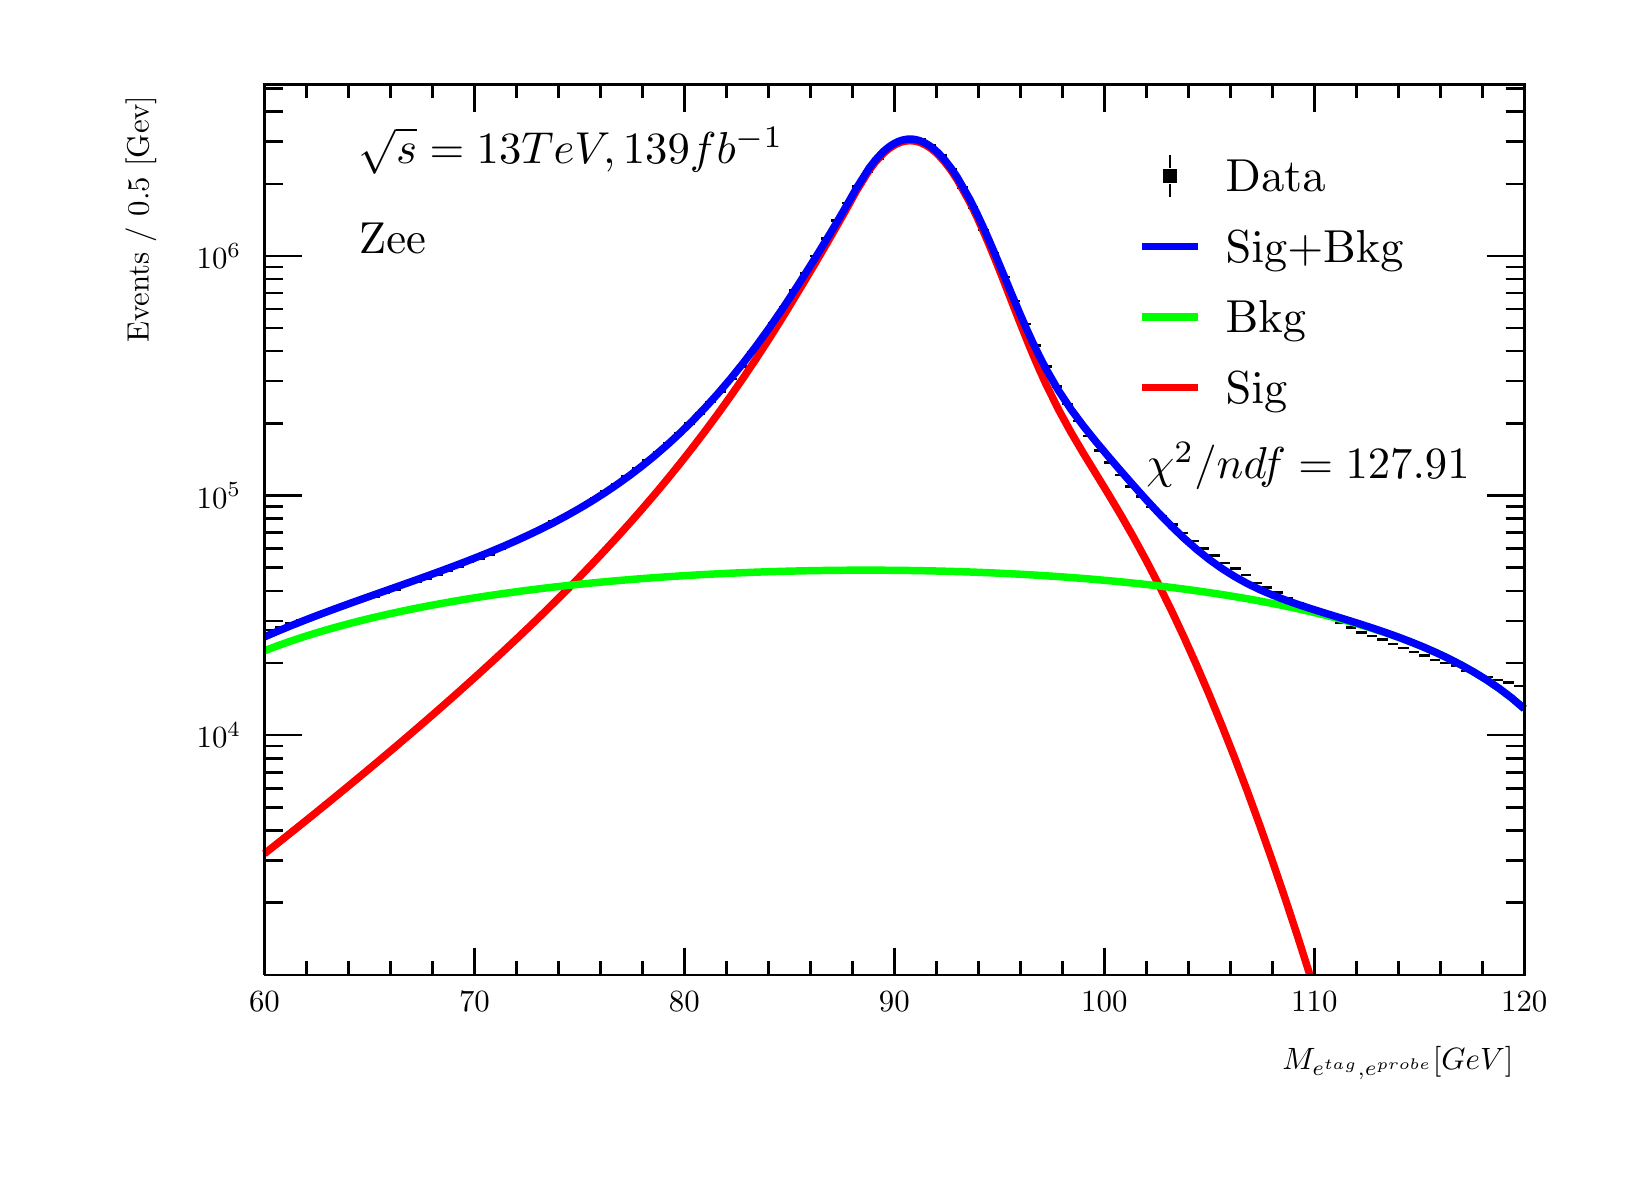
\begin{tikzpicture}
\pgfdeclareplotmark{cross} {
\pgfpathmoveto{\pgfpoint{-0.3\pgfplotmarksize}{\pgfplotmarksize}}
\pgfpathlineto{\pgfpoint{+0.3\pgfplotmarksize}{\pgfplotmarksize}}
\pgfpathlineto{\pgfpoint{+0.3\pgfplotmarksize}{0.3\pgfplotmarksize}}
\pgfpathlineto{\pgfpoint{+1\pgfplotmarksize}{0.3\pgfplotmarksize}}
\pgfpathlineto{\pgfpoint{+1\pgfplotmarksize}{-0.3\pgfplotmarksize}}
\pgfpathlineto{\pgfpoint{+0.3\pgfplotmarksize}{-0.3\pgfplotmarksize}}
\pgfpathlineto{\pgfpoint{+0.3\pgfplotmarksize}{-1.\pgfplotmarksize}}
\pgfpathlineto{\pgfpoint{-0.3\pgfplotmarksize}{-1.\pgfplotmarksize}}
\pgfpathlineto{\pgfpoint{-0.3\pgfplotmarksize}{-0.3\pgfplotmarksize}}
\pgfpathlineto{\pgfpoint{-1.\pgfplotmarksize}{-0.3\pgfplotmarksize}}
\pgfpathlineto{\pgfpoint{-1.\pgfplotmarksize}{0.3\pgfplotmarksize}}
\pgfpathlineto{\pgfpoint{-0.3\pgfplotmarksize}{0.3\pgfplotmarksize}}
\pgfpathclose
\pgfusepathqstroke
}
\pgfdeclareplotmark{cross*} {
\pgfpathmoveto{\pgfpoint{-0.3\pgfplotmarksize}{\pgfplotmarksize}}
\pgfpathlineto{\pgfpoint{+0.3\pgfplotmarksize}{\pgfplotmarksize}}
\pgfpathlineto{\pgfpoint{+0.3\pgfplotmarksize}{0.3\pgfplotmarksize}}
\pgfpathlineto{\pgfpoint{+1\pgfplotmarksize}{0.3\pgfplotmarksize}}
\pgfpathlineto{\pgfpoint{+1\pgfplotmarksize}{-0.3\pgfplotmarksize}}
\pgfpathlineto{\pgfpoint{+0.3\pgfplotmarksize}{-0.3\pgfplotmarksize}}
\pgfpathlineto{\pgfpoint{+0.3\pgfplotmarksize}{-1.\pgfplotmarksize}}
\pgfpathlineto{\pgfpoint{-0.3\pgfplotmarksize}{-1.\pgfplotmarksize}}
\pgfpathlineto{\pgfpoint{-0.3\pgfplotmarksize}{-0.3\pgfplotmarksize}}
\pgfpathlineto{\pgfpoint{-1.\pgfplotmarksize}{-0.3\pgfplotmarksize}}
\pgfpathlineto{\pgfpoint{-1.\pgfplotmarksize}{0.3\pgfplotmarksize}}
\pgfpathlineto{\pgfpoint{-0.3\pgfplotmarksize}{0.3\pgfplotmarksize}}
\pgfpathclose
\pgfusepathqfillstroke
}
\pgfdeclareplotmark{newstar} {
\pgfpathmoveto{\pgfqpoint{0pt}{\pgfplotmarksize}}
\pgfpathlineto{\pgfqpointpolar{44}{0.5\pgfplotmarksize}}
\pgfpathlineto{\pgfqpointpolar{18}{\pgfplotmarksize}}
\pgfpathlineto{\pgfqpointpolar{-20}{0.5\pgfplotmarksize}}
\pgfpathlineto{\pgfqpointpolar{-54}{\pgfplotmarksize}}
\pgfpathlineto{\pgfqpointpolar{-90}{0.5\pgfplotmarksize}}
\pgfpathlineto{\pgfqpointpolar{234}{\pgfplotmarksize}}
\pgfpathlineto{\pgfqpointpolar{198}{0.5\pgfplotmarksize}}
\pgfpathlineto{\pgfqpointpolar{162}{\pgfplotmarksize}}
\pgfpathlineto{\pgfqpointpolar{134}{0.5\pgfplotmarksize}}
\pgfpathclose
\pgfusepathqstroke
}
\pgfdeclareplotmark{newstar*} {
\pgfpathmoveto{\pgfqpoint{0pt}{\pgfplotmarksize}}
\pgfpathlineto{\pgfqpointpolar{44}{0.5\pgfplotmarksize}}
\pgfpathlineto{\pgfqpointpolar{18}{\pgfplotmarksize}}
\pgfpathlineto{\pgfqpointpolar{-20}{0.5\pgfplotmarksize}}
\pgfpathlineto{\pgfqpointpolar{-54}{\pgfplotmarksize}}
\pgfpathlineto{\pgfqpointpolar{-90}{0.5\pgfplotmarksize}}
\pgfpathlineto{\pgfqpointpolar{234}{\pgfplotmarksize}}
\pgfpathlineto{\pgfqpointpolar{198}{0.5\pgfplotmarksize}}
\pgfpathlineto{\pgfqpointpolar{162}{\pgfplotmarksize}}
\pgfpathlineto{\pgfqpointpolar{134}{0.5\pgfplotmarksize}}
\pgfpathclose
\pgfusepathqfillstroke
}
\definecolor{c}{rgb}{1,1,1};
\draw [color=c, fill=c] (0,0) rectangle (20,14.3108);
\draw [color=c, fill=c] (3,2.28972) rectangle (19,13.5952);
\definecolor{c}{rgb}{0,0,0};
\draw [c,line width=0.9] (3,2.28972) -- (3,13.5952) -- (19,13.5952) -- (19,2.28972) -- (3,2.28972);
\definecolor{c}{rgb}{1,1,1};
\draw [color=c, fill=c] (3,2.28972) rectangle (19,13.5952);
\definecolor{c}{rgb}{0,0,0};
\draw [c,line width=0.9] (3,2.28972) -- (3,13.5952) -- (19,13.5952) -- (19,2.28972) -- (3,2.28972);
\draw [c,line width=0.9] (3,2.28972) -- (19,2.28972);
\draw [c,line width=0.9] (3,2.63318) -- (3,2.28972);
\draw [c,line width=0.9] (3.53333,2.46145) -- (3.53333,2.28972);
\draw [c,line width=0.9] (4.06667,2.46145) -- (4.06667,2.28972);
\draw [c,line width=0.9] (4.6,2.46145) -- (4.6,2.28972);
\draw [c,line width=0.9] (5.13333,2.46145) -- (5.13333,2.28972);
\draw [c,line width=0.9] (5.66667,2.63318) -- (5.66667,2.28972);
\draw [c,line width=0.9] (6.2,2.46145) -- (6.2,2.28972);
\draw [c,line width=0.9] (6.73333,2.46145) -- (6.73333,2.28972);
\draw [c,line width=0.9] (7.26667,2.46145) -- (7.26667,2.28972);
\draw [c,line width=0.9] (7.8,2.46145) -- (7.8,2.28972);
\draw [c,line width=0.9] (8.33333,2.63318) -- (8.33333,2.28972);
\draw [c,line width=0.9] (8.86667,2.46145) -- (8.86667,2.28972);
\draw [c,line width=0.9] (9.4,2.46145) -- (9.4,2.28972);
\draw [c,line width=0.9] (9.93333,2.46145) -- (9.93333,2.28972);
\draw [c,line width=0.9] (10.4667,2.46145) -- (10.4667,2.28972);
\draw [c,line width=0.9] (11,2.63318) -- (11,2.28972);
\draw [c,line width=0.9] (11.5333,2.46145) -- (11.5333,2.28972);
\draw [c,line width=0.9] (12.0667,2.46145) -- (12.0667,2.28972);
\draw [c,line width=0.9] (12.6,2.46145) -- (12.6,2.28972);
\draw [c,line width=0.9] (13.1333,2.46145) -- (13.1333,2.28972);
\draw [c,line width=0.9] (13.6667,2.63318) -- (13.6667,2.28972);
\draw [c,line width=0.9] (14.2,2.46145) -- (14.2,2.28972);
\draw [c,line width=0.9] (14.7333,2.46145) -- (14.7333,2.28972);
\draw [c,line width=0.9] (15.2667,2.46145) -- (15.2667,2.28972);
\draw [c,line width=0.9] (15.8,2.46145) -- (15.8,2.28972);
\draw [c,line width=0.9] (16.3333,2.63318) -- (16.3333,2.28972);
\draw [c,line width=0.9] (16.8667,2.46145) -- (16.8667,2.28972);
\draw [c,line width=0.9] (17.4,2.46145) -- (17.4,2.28972);
\draw [c,line width=0.9] (17.9333,2.46145) -- (17.9333,2.28972);
\draw [c,line width=0.9] (18.4667,2.46145) -- (18.4667,2.28972);
\draw [c,line width=0.9] (19,2.63318) -- (19,2.28972);
\draw [anchor=base] (3,1.81747) node[scale=1.11327, color=c, rotate=0]{60};
\draw [anchor=base] (5.66667,1.81747) node[scale=1.11327, color=c, rotate=0]{70};
\draw [anchor=base] (8.33333,1.81747) node[scale=1.11327, color=c, rotate=0]{80};
\draw [anchor=base] (11,1.81747) node[scale=1.11327, color=c, rotate=0]{90};
\draw [anchor=base] (13.6667,1.81747) node[scale=1.11327, color=c, rotate=0]{100};
\draw [anchor=base] (16.3333,1.81747) node[scale=1.11327, color=c, rotate=0]{110};
\draw [anchor=base] (19,1.81747) node[scale=1.11327, color=c, rotate=0]{120};
\draw [anchor= east] (19,1.16776) node[scale=1.11327, color=c, rotate=0]{$M_{e^{tag}, e^{probe}}  [GeV]$};
\draw [c,line width=0.9] (3,13.5952) -- (19,13.5952);
\draw [c,line width=0.9] (3,13.2518) -- (3,13.5952);
\draw [c,line width=0.9] (3.53333,13.4235) -- (3.53333,13.5952);
\draw [c,line width=0.9] (4.06667,13.4235) -- (4.06667,13.5952);
\draw [c,line width=0.9] (4.6,13.4235) -- (4.6,13.5952);
\draw [c,line width=0.9] (5.13333,13.4235) -- (5.13333,13.5952);
\draw [c,line width=0.9] (5.66667,13.2518) -- (5.66667,13.5952);
\draw [c,line width=0.9] (6.2,13.4235) -- (6.2,13.5952);
\draw [c,line width=0.9] (6.73333,13.4235) -- (6.73333,13.5952);
\draw [c,line width=0.9] (7.26667,13.4235) -- (7.26667,13.5952);
\draw [c,line width=0.9] (7.8,13.4235) -- (7.8,13.5952);
\draw [c,line width=0.9] (8.33333,13.2518) -- (8.33333,13.5952);
\draw [c,line width=0.9] (8.86667,13.4235) -- (8.86667,13.5952);
\draw [c,line width=0.9] (9.4,13.4235) -- (9.4,13.5952);
\draw [c,line width=0.9] (9.93333,13.4235) -- (9.93333,13.5952);
\draw [c,line width=0.9] (10.4667,13.4235) -- (10.4667,13.5952);
\draw [c,line width=0.9] (11,13.2518) -- (11,13.5952);
\draw [c,line width=0.9] (11.5333,13.4235) -- (11.5333,13.5952);
\draw [c,line width=0.9] (12.0667,13.4235) -- (12.0667,13.5952);
\draw [c,line width=0.9] (12.6,13.4235) -- (12.6,13.5952);
\draw [c,line width=0.9] (13.1333,13.4235) -- (13.1333,13.5952);
\draw [c,line width=0.9] (13.6667,13.2518) -- (13.6667,13.5952);
\draw [c,line width=0.9] (14.2,13.4235) -- (14.2,13.5952);
\draw [c,line width=0.9] (14.7333,13.4235) -- (14.7333,13.5952);
\draw [c,line width=0.9] (15.2667,13.4235) -- (15.2667,13.5952);
\draw [c,line width=0.9] (15.8,13.4235) -- (15.8,13.5952);
\draw [c,line width=0.9] (16.3333,13.2518) -- (16.3333,13.5952);
\draw [c,line width=0.9] (16.8667,13.4235) -- (16.8667,13.5952);
\draw [c,line width=0.9] (17.4,13.4235) -- (17.4,13.5952);
\draw [c,line width=0.9] (17.9333,13.4235) -- (17.9333,13.5952);
\draw [c,line width=0.9] (18.4667,13.4235) -- (18.4667,13.5952);
\draw [c,line width=0.9] (19,13.2518) -- (19,13.5952);
\draw [c,line width=0.9] (3,2.28972) -- (3,13.5952);
\draw [c,line width=0.9] (3.237,3.20582) -- (3,3.20582);
\draw [c,line width=0.9] (3.237,3.74171) -- (3,3.74171);
\draw [c,line width=0.9] (3.237,4.12192) -- (3,4.12192);
\draw [c,line width=0.9] (3.237,4.41684) -- (3,4.41684);
\draw [c,line width=0.9] (3.237,4.65781) -- (3,4.65781);
\draw [c,line width=0.9] (3.237,4.86154) -- (3,4.86154);
\draw [c,line width=0.9] (3.237,5.03802) -- (3,5.03802);
\draw [c,line width=0.9] (3.237,5.19369) -- (3,5.19369);
\draw [c,line width=0.9] (3.474,5.33294) -- (3,5.33294);
\draw [anchor= east] (2.844,5.33294) node[scale=1.11327, color=c, rotate=0]{$10^{4}$};
\draw [c,line width=0.9] (3.237,6.24904) -- (3,6.24904);
\draw [c,line width=0.9] (3.237,6.78493) -- (3,6.78493);
\draw [c,line width=0.9] (3.237,7.16515) -- (3,7.16515);
\draw [c,line width=0.9] (3.237,7.46006) -- (3,7.46006);
\draw [c,line width=0.9] (3.237,7.70103) -- (3,7.70103);
\draw [c,line width=0.9] (3.237,7.90476) -- (3,7.90476);
\draw [c,line width=0.9] (3.237,8.08125) -- (3,8.08125);
\draw [c,line width=0.9] (3.237,8.23691) -- (3,8.23691);
\draw [c,line width=0.9] (3.474,8.37617) -- (3,8.37617);
\draw [anchor= east] (2.844,8.37617) node[scale=1.11327, color=c, rotate=0]{$10^{5}$};
\draw [c,line width=0.9] (3.237,9.29227) -- (3,9.29227);
\draw [c,line width=0.9] (3.237,9.82815) -- (3,9.82815);
\draw [c,line width=0.9] (3.237,10.2084) -- (3,10.2084);
\draw [c,line width=0.9] (3.237,10.5033) -- (3,10.5033);
\draw [c,line width=0.9] (3.237,10.7443) -- (3,10.7443);
\draw [c,line width=0.9] (3.237,10.948) -- (3,10.948);
\draw [c,line width=0.9] (3.237,11.1245) -- (3,11.1245);
\draw [c,line width=0.9] (3.237,11.2801) -- (3,11.2801);
\draw [c,line width=0.9] (3.474,11.4194) -- (3,11.4194);
\draw [anchor= east] (2.844,11.4194) node[scale=1.11327, color=c, rotate=0]{$10^{6}$};
\draw [c,line width=0.9] (3.237,12.3355) -- (3,12.3355);
\draw [c,line width=0.9] (3.237,12.8714) -- (3,12.8714);
\draw [c,line width=0.9] (3.237,13.2516) -- (3,13.2516);
\draw [c,line width=0.9] (3.237,13.5465) -- (3,13.5465);
\draw [anchor= east] (1.432,13.5952) node[scale=1.11327, color=c, rotate=90]{Events / 0.5 [Gev]};
\draw [c,line width=0.9] (19,2.28972) -- (19,13.5952);
\draw [c,line width=0.9] (18.763,3.20582) -- (19,3.20582);
\draw [c,line width=0.9] (18.763,3.74171) -- (19,3.74171);
\draw [c,line width=0.9] (18.763,4.12192) -- (19,4.12192);
\draw [c,line width=0.9] (18.763,4.41684) -- (19,4.41684);
\draw [c,line width=0.9] (18.763,4.65781) -- (19,4.65781);
\draw [c,line width=0.9] (18.763,4.86154) -- (19,4.86154);
\draw [c,line width=0.9] (18.763,5.03802) -- (19,5.03802);
\draw [c,line width=0.9] (18.763,5.19369) -- (19,5.19369);
\draw [c,line width=0.9] (18.526,5.33294) -- (19,5.33294);
\draw [c,line width=0.9] (18.763,6.24904) -- (19,6.24904);
\draw [c,line width=0.9] (18.763,6.78493) -- (19,6.78493);
\draw [c,line width=0.9] (18.763,7.16515) -- (19,7.16515);
\draw [c,line width=0.9] (18.763,7.46006) -- (19,7.46006);
\draw [c,line width=0.9] (18.763,7.70103) -- (19,7.70103);
\draw [c,line width=0.9] (18.763,7.90476) -- (19,7.90476);
\draw [c,line width=0.9] (18.763,8.08125) -- (19,8.08125);
\draw [c,line width=0.9] (18.763,8.23691) -- (19,8.23691);
\draw [c,line width=0.9] (18.526,8.37617) -- (19,8.37617);
\draw [c,line width=0.9] (18.763,9.29227) -- (19,9.29227);
\draw [c,line width=0.9] (18.763,9.82815) -- (19,9.82815);
\draw [c,line width=0.9] (18.763,10.2084) -- (19,10.2084);
\draw [c,line width=0.9] (18.763,10.5033) -- (19,10.5033);
\draw [c,line width=0.9] (18.763,10.7443) -- (19,10.7443);
\draw [c,line width=0.9] (18.763,10.948) -- (19,10.948);
\draw [c,line width=0.9] (18.763,11.1245) -- (19,11.1245);
\draw [c,line width=0.9] (18.763,11.2801) -- (19,11.2801);
\draw [c,line width=0.9] (18.526,11.4194) -- (19,11.4194);
\draw [c,line width=0.9] (18.763,12.3355) -- (19,12.3355);
\draw [c,line width=0.9] (18.763,12.8714) -- (19,12.8714);
\draw [c,line width=0.9] (18.763,13.2516) -- (19,13.2516);
\draw [c,line width=0.9] (18.763,13.5465) -- (19,13.5465);
\draw [c,line width=0.9] (3.06667,6.66868) -- (3,6.66868);
\draw [c,line width=0.9] (3,6.66868) -- (3,6.66868);
\draw [c,line width=0.9] (3.06667,6.66868) -- (3.13333,6.66868);
\draw [c,line width=0.9] (3.13333,6.66868) -- (3.13333,6.66868);
\draw [c,line width=0.9] (3.06667,6.66868) -- (3.06667,6.67666);
\draw [c,line width=0.9] (3.06667,6.67666) -- (3.06667,6.67666);
\draw [c,line width=0.9] (3.06667,6.66868) -- (3.06667,6.66071);
\draw [c,line width=0.9] (3.06667,6.66071) -- (3.06667,6.66071);
\draw [c,line width=0.9] (3.2,6.69954) -- (3.13333,6.69954);
\draw [c,line width=0.9] (3.13333,6.69954) -- (3.13333,6.69954);
\draw [c,line width=0.9] (3.2,6.69954) -- (3.26667,6.69954);
\draw [c,line width=0.9] (3.26667,6.69954) -- (3.26667,6.69954);
\draw [c,line width=0.9] (3.2,6.69954) -- (3.2,6.70742);
\draw [c,line width=0.9] (3.2,6.70742) -- (3.2,6.70742);
\draw [c,line width=0.9] (3.2,6.69954) -- (3.2,6.69166);
\draw [c,line width=0.9] (3.2,6.69166) -- (3.2,6.69166);
\draw [c,line width=0.9] (3.33333,6.75607) -- (3.26667,6.75607);
\draw [c,line width=0.9] (3.26667,6.75607) -- (3.26667,6.75607);
\draw [c,line width=0.9] (3.33333,6.75607) -- (3.4,6.75607);
\draw [c,line width=0.9] (3.4,6.75607) -- (3.4,6.75607);
\draw [c,line width=0.9] (3.33333,6.75607) -- (3.33333,6.76378);
\draw [c,line width=0.9] (3.33333,6.76378) -- (3.33333,6.76378);
\draw [c,line width=0.9] (3.33333,6.75607) -- (3.33333,6.74836);
\draw [c,line width=0.9] (3.33333,6.74836) -- (3.33333,6.74836);
\draw [c,line width=0.9] (3.46667,6.79284) -- (3.4,6.79284);
\draw [c,line width=0.9] (3.4,6.79284) -- (3.4,6.79284);
\draw [c,line width=0.9] (3.46667,6.79284) -- (3.53333,6.79284);
\draw [c,line width=0.9] (3.53333,6.79284) -- (3.53333,6.79284);
\draw [c,line width=0.9] (3.46667,6.79284) -- (3.46667,6.80045);
\draw [c,line width=0.9] (3.46667,6.80045) -- (3.46667,6.80045);
\draw [c,line width=0.9] (3.46667,6.79284) -- (3.46667,6.78523);
\draw [c,line width=0.9] (3.46667,6.78523) -- (3.46667,6.78523);
\draw [c,line width=0.9] (3.6,6.83099) -- (3.53333,6.83099);
\draw [c,line width=0.9] (3.53333,6.83099) -- (3.53333,6.83099);
\draw [c,line width=0.9] (3.6,6.83099) -- (3.66667,6.83099);
\draw [c,line width=0.9] (3.66667,6.83099) -- (3.66667,6.83099);
\draw [c,line width=0.9] (3.6,6.83099) -- (3.6,6.83849);
\draw [c,line width=0.9] (3.6,6.83849) -- (3.6,6.83849);
\draw [c,line width=0.9] (3.6,6.83099) -- (3.6,6.82349);
\draw [c,line width=0.9] (3.6,6.82349) -- (3.6,6.82349);
\draw [c,line width=0.9] (3.73333,6.87908) -- (3.66667,6.87908);
\draw [c,line width=0.9] (3.66667,6.87908) -- (3.66667,6.87908);
\draw [c,line width=0.9] (3.73333,6.87908) -- (3.8,6.87908);
\draw [c,line width=0.9] (3.8,6.87908) -- (3.8,6.87908);
\draw [c,line width=0.9] (3.73333,6.87908) -- (3.73333,6.88644);
\draw [c,line width=0.9] (3.73333,6.88644) -- (3.73333,6.88644);
\draw [c,line width=0.9] (3.73333,6.87908) -- (3.73333,6.87172);
\draw [c,line width=0.9] (3.73333,6.87172) -- (3.73333,6.87172);
\draw [c,line width=0.9] (3.86667,6.93129) -- (3.8,6.93129);
\draw [c,line width=0.9] (3.8,6.93129) -- (3.8,6.93129);
\draw [c,line width=0.9] (3.86667,6.93129) -- (3.93333,6.93129);
\draw [c,line width=0.9] (3.93333,6.93129) -- (3.93333,6.93129);
\draw [c,line width=0.9] (3.86667,6.93129) -- (3.86667,6.93851);
\draw [c,line width=0.9] (3.86667,6.93851) -- (3.86667,6.93851);
\draw [c,line width=0.9] (3.86667,6.93129) -- (3.86667,6.92407);
\draw [c,line width=0.9] (3.86667,6.92407) -- (3.86667,6.92407);
\draw [c,line width=0.9] (4,6.96585) -- (3.93333,6.96585);
\draw [c,line width=0.9] (3.93333,6.96585) -- (3.93333,6.96585);
\draw [c,line width=0.9] (4,6.96585) -- (4.06667,6.96585);
\draw [c,line width=0.9] (4.06667,6.96585) -- (4.06667,6.96585);
\draw [c,line width=0.9] (4,6.96585) -- (4,6.97298);
\draw [c,line width=0.9] (4,6.97298) -- (4,6.97298);
\draw [c,line width=0.9] (4,6.96585) -- (4,6.95872);
\draw [c,line width=0.9] (4,6.95872) -- (4,6.95872);
\draw [c,line width=0.9] (4.13333,7.02215) -- (4.06667,7.02215);
\draw [c,line width=0.9] (4.06667,7.02215) -- (4.06667,7.02215);
\draw [c,line width=0.9] (4.13333,7.02215) -- (4.2,7.02215);
\draw [c,line width=0.9] (4.2,7.02215) -- (4.2,7.02215);
\draw [c,line width=0.9] (4.13333,7.02215) -- (4.13333,7.02912);
\draw [c,line width=0.9] (4.13333,7.02912) -- (4.13333,7.02912);
\draw [c,line width=0.9] (4.13333,7.02215) -- (4.13333,7.01517);
\draw [c,line width=0.9] (4.13333,7.01517) -- (4.13333,7.01517);
\draw [c,line width=0.9] (4.26667,7.06813) -- (4.2,7.06813);
\draw [c,line width=0.9] (4.2,7.06813) -- (4.2,7.06813);
\draw [c,line width=0.9] (4.26667,7.06813) -- (4.33333,7.06813);
\draw [c,line width=0.9] (4.33333,7.06813) -- (4.33333,7.06813);
\draw [c,line width=0.9] (4.26667,7.06813) -- (4.26667,7.07499);
\draw [c,line width=0.9] (4.26667,7.07499) -- (4.26667,7.07499);
\draw [c,line width=0.9] (4.26667,7.06813) -- (4.26667,7.06128);
\draw [c,line width=0.9] (4.26667,7.06128) -- (4.26667,7.06128);
\draw [c,line width=0.9] (4.4,7.09038) -- (4.33333,7.09038);
\draw [c,line width=0.9] (4.33333,7.09038) -- (4.33333,7.09038);
\draw [c,line width=0.9] (4.4,7.09038) -- (4.46667,7.09038);
\draw [c,line width=0.9] (4.46667,7.09038) -- (4.46667,7.09038);
\draw [c,line width=0.9] (4.4,7.09038) -- (4.4,7.09718);
\draw [c,line width=0.9] (4.4,7.09718) -- (4.4,7.09718);
\draw [c,line width=0.9] (4.4,7.09038) -- (4.4,7.08358);
\draw [c,line width=0.9] (4.4,7.08358) -- (4.4,7.08358);
\draw [c,line width=0.9] (4.53333,7.13757) -- (4.46667,7.13757);
\draw [c,line width=0.9] (4.46667,7.13757) -- (4.46667,7.13757);
\draw [c,line width=0.9] (4.53333,7.13757) -- (4.6,7.13757);
\draw [c,line width=0.9] (4.6,7.13757) -- (4.6,7.13757);
\draw [c,line width=0.9] (4.53333,7.13757) -- (4.53333,7.14425);
\draw [c,line width=0.9] (4.53333,7.14425) -- (4.53333,7.14425);
\draw [c,line width=0.9] (4.53333,7.13757) -- (4.53333,7.13089);
\draw [c,line width=0.9] (4.53333,7.13089) -- (4.53333,7.13089);
\draw [c,line width=0.9] (4.66667,7.18124) -- (4.6,7.18124);
\draw [c,line width=0.9] (4.6,7.18124) -- (4.6,7.18124);
\draw [c,line width=0.9] (4.66667,7.18124) -- (4.73333,7.18124);
\draw [c,line width=0.9] (4.73333,7.18124) -- (4.73333,7.18124);
\draw [c,line width=0.9] (4.66667,7.18124) -- (4.66667,7.18781);
\draw [c,line width=0.9] (4.66667,7.18781) -- (4.66667,7.18781);
\draw [c,line width=0.9] (4.66667,7.18124) -- (4.66667,7.17467);
\draw [c,line width=0.9] (4.66667,7.17467) -- (4.66667,7.17467);
\draw [c,line width=0.9] (4.8,7.23776) -- (4.73333,7.23776);
\draw [c,line width=0.9] (4.73333,7.23776) -- (4.73333,7.23776);
\draw [c,line width=0.9] (4.8,7.23776) -- (4.86667,7.23776);
\draw [c,line width=0.9] (4.86667,7.23776) -- (4.86667,7.23776);
\draw [c,line width=0.9] (4.8,7.23776) -- (4.8,7.24418);
\draw [c,line width=0.9] (4.8,7.24418) -- (4.8,7.24418);
\draw [c,line width=0.9] (4.8,7.23776) -- (4.8,7.23133);
\draw [c,line width=0.9] (4.8,7.23133) -- (4.8,7.23133);
\draw [c,line width=0.9] (4.93333,7.27847) -- (4.86667,7.27847);
\draw [c,line width=0.9] (4.86667,7.27847) -- (4.86667,7.27847);
\draw [c,line width=0.9] (4.93333,7.27847) -- (5,7.27847);
\draw [c,line width=0.9] (5,7.27847) -- (5,7.27847);
\draw [c,line width=0.9] (4.93333,7.27847) -- (4.93333,7.2848);
\draw [c,line width=0.9] (4.93333,7.2848) -- (4.93333,7.2848);
\draw [c,line width=0.9] (4.93333,7.27847) -- (4.93333,7.27214);
\draw [c,line width=0.9] (4.93333,7.27214) -- (4.93333,7.27214);
\draw [c,line width=0.9] (5.06667,7.31979) -- (5,7.31979);
\draw [c,line width=0.9] (5,7.31979) -- (5,7.31979);
\draw [c,line width=0.9] (5.06667,7.31979) -- (5.13333,7.31979);
\draw [c,line width=0.9] (5.13333,7.31979) -- (5.13333,7.31979);
\draw [c,line width=0.9] (5.06667,7.31979) -- (5.06667,7.32602);
\draw [c,line width=0.9] (5.06667,7.32602) -- (5.06667,7.32602);
\draw [c,line width=0.9] (5.06667,7.31979) -- (5.06667,7.31355);
\draw [c,line width=0.9] (5.06667,7.31355) -- (5.06667,7.31355);
\draw [c,line width=0.9] (5.2,7.365) -- (5.13333,7.365);
\draw [c,line width=0.9] (5.13333,7.365) -- (5.13333,7.365);
\draw [c,line width=0.9] (5.2,7.365) -- (5.26667,7.365);
\draw [c,line width=0.9] (5.26667,7.365) -- (5.26667,7.365);
\draw [c,line width=0.9] (5.2,7.365) -- (5.2,7.37113);
\draw [c,line width=0.9] (5.2,7.37113) -- (5.2,7.37113);
\draw [c,line width=0.9] (5.2,7.365) -- (5.2,7.35888);
\draw [c,line width=0.9] (5.2,7.35888) -- (5.2,7.35888);
\draw [c,line width=0.9] (5.33333,7.42343) -- (5.26667,7.42343);
\draw [c,line width=0.9] (5.26667,7.42343) -- (5.26667,7.42343);
\draw [c,line width=0.9] (5.33333,7.42343) -- (5.4,7.42343);
\draw [c,line width=0.9] (5.4,7.42343) -- (5.4,7.42343);
\draw [c,line width=0.9] (5.33333,7.42343) -- (5.33333,7.42942);
\draw [c,line width=0.9] (5.33333,7.42942) -- (5.33333,7.42942);
\draw [c,line width=0.9] (5.33333,7.42343) -- (5.33333,7.41744);
\draw [c,line width=0.9] (5.33333,7.41744) -- (5.33333,7.41744);
\draw [c,line width=0.9] (5.46667,7.47541) -- (5.4,7.47541);
\draw [c,line width=0.9] (5.4,7.47541) -- (5.4,7.47541);
\draw [c,line width=0.9] (5.46667,7.47541) -- (5.53333,7.47541);
\draw [c,line width=0.9] (5.53333,7.47541) -- (5.53333,7.47541);
\draw [c,line width=0.9] (5.46667,7.47541) -- (5.46667,7.48129);
\draw [c,line width=0.9] (5.46667,7.48129) -- (5.46667,7.48129);
\draw [c,line width=0.9] (5.46667,7.47541) -- (5.46667,7.46954);
\draw [c,line width=0.9] (5.46667,7.46954) -- (5.46667,7.46954);
\draw [c,line width=0.9] (5.6,7.53118) -- (5.53333,7.53118);
\draw [c,line width=0.9] (5.53333,7.53118) -- (5.53333,7.53118);
\draw [c,line width=0.9] (5.6,7.53118) -- (5.66667,7.53118);
\draw [c,line width=0.9] (5.66667,7.53118) -- (5.66667,7.53118);
\draw [c,line width=0.9] (5.6,7.53118) -- (5.6,7.53693);
\draw [c,line width=0.9] (5.6,7.53693) -- (5.6,7.53693);
\draw [c,line width=0.9] (5.6,7.53118) -- (5.6,7.52542);
\draw [c,line width=0.9] (5.6,7.52542) -- (5.6,7.52542);
\draw [c,line width=0.9] (5.73333,7.57876) -- (5.66667,7.57876);
\draw [c,line width=0.9] (5.66667,7.57876) -- (5.66667,7.57876);
\draw [c,line width=0.9] (5.73333,7.57876) -- (5.8,7.57876);
\draw [c,line width=0.9] (5.8,7.57876) -- (5.8,7.57876);
\draw [c,line width=0.9] (5.73333,7.57876) -- (5.73333,7.58441);
\draw [c,line width=0.9] (5.73333,7.58441) -- (5.73333,7.58441);
\draw [c,line width=0.9] (5.73333,7.57876) -- (5.73333,7.5731);
\draw [c,line width=0.9] (5.73333,7.5731) -- (5.73333,7.5731);
\draw [c,line width=0.9] (5.86667,7.6278) -- (5.8,7.6278);
\draw [c,line width=0.9] (5.8,7.6278) -- (5.8,7.6278);
\draw [c,line width=0.9] (5.86667,7.6278) -- (5.93333,7.6278);
\draw [c,line width=0.9] (5.93333,7.6278) -- (5.93333,7.6278);
\draw [c,line width=0.9] (5.86667,7.6278) -- (5.86667,7.63335);
\draw [c,line width=0.9] (5.86667,7.63335) -- (5.86667,7.63335);
\draw [c,line width=0.9] (5.86667,7.6278) -- (5.86667,7.62226);
\draw [c,line width=0.9] (5.86667,7.62226) -- (5.86667,7.62226);
\draw [c,line width=0.9] (6,7.70413) -- (5.93333,7.70413);
\draw [c,line width=0.9] (5.93333,7.70413) -- (5.93333,7.70413);
\draw [c,line width=0.9] (6,7.70413) -- (6.06667,7.70413);
\draw [c,line width=0.9] (6.06667,7.70413) -- (6.06667,7.70413);
\draw [c,line width=0.9] (6,7.70413) -- (6,7.70952);
\draw [c,line width=0.9] (6,7.70952) -- (6,7.70952);
\draw [c,line width=0.9] (6,7.70413) -- (6,7.69874);
\draw [c,line width=0.9] (6,7.69874) -- (6,7.69874);
\draw [c,line width=0.9] (6.13333,7.76262) -- (6.06667,7.76262);
\draw [c,line width=0.9] (6.06667,7.76262) -- (6.06667,7.76262);
\draw [c,line width=0.9] (6.13333,7.76262) -- (6.2,7.76262);
\draw [c,line width=0.9] (6.2,7.76262) -- (6.2,7.76262);
\draw [c,line width=0.9] (6.13333,7.76262) -- (6.13333,7.76789);
\draw [c,line width=0.9] (6.13333,7.76789) -- (6.13333,7.76789);
\draw [c,line width=0.9] (6.13333,7.76262) -- (6.13333,7.75735);
\draw [c,line width=0.9] (6.13333,7.75735) -- (6.13333,7.75735);
\draw [c,line width=0.9] (6.26667,7.82564) -- (6.2,7.82564);
\draw [c,line width=0.9] (6.2,7.82564) -- (6.2,7.82564);
\draw [c,line width=0.9] (6.26667,7.82564) -- (6.33333,7.82564);
\draw [c,line width=0.9] (6.33333,7.82564) -- (6.33333,7.82564);
\draw [c,line width=0.9] (6.26667,7.82564) -- (6.26667,7.83078);
\draw [c,line width=0.9] (6.26667,7.83078) -- (6.26667,7.83078);
\draw [c,line width=0.9] (6.26667,7.82564) -- (6.26667,7.82049);
\draw [c,line width=0.9] (6.26667,7.82049) -- (6.26667,7.82049);
\draw [c,line width=0.9] (6.4,7.89911) -- (6.33333,7.89911);
\draw [c,line width=0.9] (6.33333,7.89911) -- (6.33333,7.89911);
\draw [c,line width=0.9] (6.4,7.89911) -- (6.46667,7.89911);
\draw [c,line width=0.9] (6.46667,7.89911) -- (6.46667,7.89911);
\draw [c,line width=0.9] (6.4,7.89911) -- (6.4,7.90411);
\draw [c,line width=0.9] (6.4,7.90411) -- (6.4,7.90411);
\draw [c,line width=0.9] (6.4,7.89911) -- (6.4,7.8941);
\draw [c,line width=0.9] (6.4,7.8941) -- (6.4,7.8941);
\draw [c,line width=0.9] (6.53333,7.96583) -- (6.46667,7.96583);
\draw [c,line width=0.9] (6.46667,7.96583) -- (6.46667,7.96583);
\draw [c,line width=0.9] (6.53333,7.96583) -- (6.6,7.96583);
\draw [c,line width=0.9] (6.6,7.96583) -- (6.6,7.96583);
\draw [c,line width=0.9] (6.53333,7.96583) -- (6.53333,7.97071);
\draw [c,line width=0.9] (6.53333,7.97071) -- (6.53333,7.97071);
\draw [c,line width=0.9] (6.53333,7.96583) -- (6.53333,7.96095);
\draw [c,line width=0.9] (6.53333,7.96095) -- (6.53333,7.96095);
\draw [c,line width=0.9] (6.66667,8.04375) -- (6.6,8.04375);
\draw [c,line width=0.9] (6.6,8.04375) -- (6.6,8.04375);
\draw [c,line width=0.9] (6.66667,8.04375) -- (6.73333,8.04375);
\draw [c,line width=0.9] (6.73333,8.04375) -- (6.73333,8.04375);
\draw [c,line width=0.9] (6.66667,8.04375) -- (6.66667,8.04849);
\draw [c,line width=0.9] (6.66667,8.04849) -- (6.66667,8.04849);
\draw [c,line width=0.9] (6.66667,8.04375) -- (6.66667,8.03901);
\draw [c,line width=0.9] (6.66667,8.03901) -- (6.66667,8.03901);
\draw [c,line width=0.9] (6.8,8.10158) -- (6.73333,8.10158);
\draw [c,line width=0.9] (6.73333,8.10158) -- (6.73333,8.10158);
\draw [c,line width=0.9] (6.8,8.10158) -- (6.86667,8.10158);
\draw [c,line width=0.9] (6.86667,8.10158) -- (6.86667,8.10158);
\draw [c,line width=0.9] (6.8,8.10158) -- (6.8,8.10621);
\draw [c,line width=0.9] (6.8,8.10621) -- (6.8,8.10621);
\draw [c,line width=0.9] (6.8,8.10158) -- (6.8,8.09694);
\draw [c,line width=0.9] (6.8,8.09694) -- (6.8,8.09694);
\draw [c,line width=0.9] (6.93333,8.17741) -- (6.86667,8.17741);
\draw [c,line width=0.9] (6.86667,8.17741) -- (6.86667,8.17741);
\draw [c,line width=0.9] (6.93333,8.17741) -- (7,8.17741);
\draw [c,line width=0.9] (7,8.17741) -- (7,8.17741);
\draw [c,line width=0.9] (6.93333,8.17741) -- (6.93333,8.18192);
\draw [c,line width=0.9] (6.93333,8.18192) -- (6.93333,8.18192);
\draw [c,line width=0.9] (6.93333,8.17741) -- (6.93333,8.17291);
\draw [c,line width=0.9] (6.93333,8.17291) -- (6.93333,8.17291);
\draw [c,line width=0.9] (7.06667,8.25778) -- (7,8.25778);
\draw [c,line width=0.9] (7,8.25778) -- (7,8.25778);
\draw [c,line width=0.9] (7.06667,8.25778) -- (7.13333,8.25778);
\draw [c,line width=0.9] (7.13333,8.25778) -- (7.13333,8.25778);
\draw [c,line width=0.9] (7.06667,8.25778) -- (7.06667,8.26215);
\draw [c,line width=0.9] (7.06667,8.26215) -- (7.06667,8.26215);
\draw [c,line width=0.9] (7.06667,8.25778) -- (7.06667,8.25341);
\draw [c,line width=0.9] (7.06667,8.25341) -- (7.06667,8.25341);
\draw [c,line width=0.9] (7.2,8.34102) -- (7.13333,8.34102);
\draw [c,line width=0.9] (7.13333,8.34102) -- (7.13333,8.34102);
\draw [c,line width=0.9] (7.2,8.34102) -- (7.26667,8.34102);
\draw [c,line width=0.9] (7.26667,8.34102) -- (7.26667,8.34102);
\draw [c,line width=0.9] (7.2,8.34102) -- (7.2,8.34526);
\draw [c,line width=0.9] (7.2,8.34526) -- (7.2,8.34526);
\draw [c,line width=0.9] (7.2,8.34102) -- (7.2,8.33679);
\draw [c,line width=0.9] (7.2,8.33679) -- (7.2,8.33679);
\draw [c,line width=0.9] (7.33333,8.43509) -- (7.26667,8.43509);
\draw [c,line width=0.9] (7.26667,8.43509) -- (7.26667,8.43509);
\draw [c,line width=0.9] (7.33333,8.43509) -- (7.4,8.43509);
\draw [c,line width=0.9] (7.4,8.43509) -- (7.4,8.43509);
\draw [c,line width=0.9] (7.33333,8.43509) -- (7.33333,8.43917);
\draw [c,line width=0.9] (7.33333,8.43917) -- (7.33333,8.43917);
\draw [c,line width=0.9] (7.33333,8.43509) -- (7.33333,8.431);
\draw [c,line width=0.9] (7.33333,8.431) -- (7.33333,8.431);
\draw [c,line width=0.9] (7.46667,8.52537) -- (7.4,8.52537);
\draw [c,line width=0.9] (7.4,8.52537) -- (7.4,8.52537);
\draw [c,line width=0.9] (7.46667,8.52537) -- (7.53333,8.52537);
\draw [c,line width=0.9] (7.53333,8.52537) -- (7.53333,8.52537);
\draw [c,line width=0.9] (7.46667,8.52537) -- (7.46667,8.52932);
\draw [c,line width=0.9] (7.46667,8.52932) -- (7.46667,8.52932);
\draw [c,line width=0.9] (7.46667,8.52537) -- (7.46667,8.52142);
\draw [c,line width=0.9] (7.46667,8.52142) -- (7.46667,8.52142);
\draw [c,line width=0.9] (7.6,8.61728) -- (7.53333,8.61728);
\draw [c,line width=0.9] (7.53333,8.61728) -- (7.53333,8.61728);
\draw [c,line width=0.9] (7.6,8.61728) -- (7.66667,8.61728);
\draw [c,line width=0.9] (7.66667,8.61728) -- (7.66667,8.61728);
\draw [c,line width=0.9] (7.6,8.61728) -- (7.6,8.62109);
\draw [c,line width=0.9] (7.6,8.62109) -- (7.6,8.62109);
\draw [c,line width=0.9] (7.6,8.61728) -- (7.6,8.61346);
\draw [c,line width=0.9] (7.6,8.61346) -- (7.6,8.61346);
\draw [c,line width=0.9] (7.73333,8.718) -- (7.66667,8.718);
\draw [c,line width=0.9] (7.66667,8.718) -- (7.66667,8.718);
\draw [c,line width=0.9] (7.73333,8.718) -- (7.8,8.718);
\draw [c,line width=0.9] (7.8,8.718) -- (7.8,8.718);
\draw [c,line width=0.9] (7.73333,8.718) -- (7.73333,8.72167);
\draw [c,line width=0.9] (7.73333,8.72167) -- (7.73333,8.72167);
\draw [c,line width=0.9] (7.73333,8.718) -- (7.73333,8.71433);
\draw [c,line width=0.9] (7.73333,8.71433) -- (7.73333,8.71433);
\draw [c,line width=0.9] (7.86667,8.82319) -- (7.8,8.82319);
\draw [c,line width=0.9] (7.8,8.82319) -- (7.8,8.82319);
\draw [c,line width=0.9] (7.86667,8.82319) -- (7.93333,8.82319);
\draw [c,line width=0.9] (7.93333,8.82319) -- (7.93333,8.82319);
\draw [c,line width=0.9] (7.86667,8.82319) -- (7.86667,8.82672);
\draw [c,line width=0.9] (7.86667,8.82672) -- (7.86667,8.82672);
\draw [c,line width=0.9] (7.86667,8.82319) -- (7.86667,8.81966);
\draw [c,line width=0.9] (7.86667,8.81966) -- (7.86667,8.81966);
\draw [c,line width=0.9] (8,8.92963) -- (7.93333,8.92963);
\draw [c,line width=0.9] (7.93333,8.92963) -- (7.93333,8.92963);
\draw [c,line width=0.9] (8,8.92963) -- (8.06667,8.92963);
\draw [c,line width=0.9] (8.06667,8.92963) -- (8.06667,8.92963);
\draw [c,line width=0.9] (8,8.92963) -- (8,8.93302);
\draw [c,line width=0.9] (8,8.93302) -- (8,8.93302);
\draw [c,line width=0.9] (8,8.92963) -- (8,8.92624);
\draw [c,line width=0.9] (8,8.92624) -- (8,8.92624);
\draw [c,line width=0.9] (8.13333,9.04058) -- (8.06667,9.04058);
\draw [c,line width=0.9] (8.06667,9.04058) -- (8.06667,9.04058);
\draw [c,line width=0.9] (8.13333,9.04058) -- (8.2,9.04058);
\draw [c,line width=0.9] (8.2,9.04058) -- (8.2,9.04058);
\draw [c,line width=0.9] (8.13333,9.04058) -- (8.13333,9.04383);
\draw [c,line width=0.9] (8.13333,9.04383) -- (8.13333,9.04383);
\draw [c,line width=0.9] (8.13333,9.04058) -- (8.13333,9.03733);
\draw [c,line width=0.9] (8.13333,9.03733) -- (8.13333,9.03733);
\draw [c,line width=0.9] (8.26667,9.1646) -- (8.2,9.1646);
\draw [c,line width=0.9] (8.2,9.1646) -- (8.2,9.1646);
\draw [c,line width=0.9] (8.26667,9.1646) -- (8.33333,9.1646);
\draw [c,line width=0.9] (8.33333,9.1646) -- (8.33333,9.1646);
\draw [c,line width=0.9] (8.26667,9.1646) -- (8.26667,9.1677);
\draw [c,line width=0.9] (8.26667,9.1677) -- (8.26667,9.1677);
\draw [c,line width=0.9] (8.26667,9.1646) -- (8.26667,9.1615);
\draw [c,line width=0.9] (8.26667,9.1615) -- (8.26667,9.1615);
\draw [c,line width=0.9] (8.4,9.28957) -- (8.33333,9.28957);
\draw [c,line width=0.9] (8.33333,9.28957) -- (8.33333,9.28957);
\draw [c,line width=0.9] (8.4,9.28957) -- (8.46667,9.28957);
\draw [c,line width=0.9] (8.46667,9.28957) -- (8.46667,9.28957);
\draw [c,line width=0.9] (8.4,9.28957) -- (8.4,9.29253);
\draw [c,line width=0.9] (8.4,9.29253) -- (8.4,9.29253);
\draw [c,line width=0.9] (8.4,9.28957) -- (8.4,9.28661);
\draw [c,line width=0.9] (8.4,9.28661) -- (8.4,9.28661);
\draw [c,line width=0.9] (8.53333,9.41735) -- (8.46667,9.41735);
\draw [c,line width=0.9] (8.46667,9.41735) -- (8.46667,9.41735);
\draw [c,line width=0.9] (8.53333,9.41735) -- (8.6,9.41735);
\draw [c,line width=0.9] (8.6,9.41735) -- (8.6,9.41735);
\draw [c,line width=0.9] (8.53333,9.41735) -- (8.53333,9.42016);
\draw [c,line width=0.9] (8.53333,9.42016) -- (8.53333,9.42016);
\draw [c,line width=0.9] (8.53333,9.41735) -- (8.53333,9.41453);
\draw [c,line width=0.9] (8.53333,9.41453) -- (8.53333,9.41453);
\draw [c,line width=0.9] (8.66667,9.56084) -- (8.6,9.56084);
\draw [c,line width=0.9] (8.6,9.56084) -- (8.6,9.56084);
\draw [c,line width=0.9] (8.66667,9.56084) -- (8.73333,9.56084);
\draw [c,line width=0.9] (8.73333,9.56084) -- (8.73333,9.56084);
\draw [c,line width=0.9] (8.66667,9.56084) -- (8.66667,9.56351);
\draw [c,line width=0.9] (8.66667,9.56351) -- (8.66667,9.56351);
\draw [c,line width=0.9] (8.66667,9.56084) -- (8.66667,9.55817);
\draw [c,line width=0.9] (8.66667,9.55817) -- (8.66667,9.55817);
\draw [c,line width=0.9] (8.8,9.69948) -- (8.73333,9.69948);
\draw [c,line width=0.9] (8.73333,9.69948) -- (8.73333,9.69948);
\draw [c,line width=0.9] (8.8,9.69948) -- (8.86667,9.69948);
\draw [c,line width=0.9] (8.86667,9.69948) -- (8.86667,9.69948);
\draw [c,line width=0.9] (8.8,9.69948) -- (8.8,9.70201);
\draw [c,line width=0.9] (8.8,9.70201) -- (8.8,9.70201);
\draw [c,line width=0.9] (8.8,9.69948) -- (8.8,9.69694);
\draw [c,line width=0.9] (8.8,9.69694) -- (8.8,9.69694);
\draw [c,line width=0.9] (8.93333,9.85526) -- (8.86667,9.85526);
\draw [c,line width=0.9] (8.86667,9.85526) -- (8.86667,9.85526);
\draw [c,line width=0.9] (8.93333,9.85526) -- (9,9.85526);
\draw [c,line width=0.9] (9,9.85526) -- (9,9.85526);
\draw [c,line width=0.9] (8.93333,9.85526) -- (8.93333,9.85765);
\draw [c,line width=0.9] (8.93333,9.85765) -- (8.93333,9.85765);
\draw [c,line width=0.9] (8.93333,9.85526) -- (8.93333,9.85287);
\draw [c,line width=0.9] (8.93333,9.85287) -- (8.93333,9.85287);
\draw [c,line width=0.9] (9.06667,10.0175) -- (9,10.0175);
\draw [c,line width=0.9] (9,10.0175) -- (9,10.0175);
\draw [c,line width=0.9] (9.06667,10.0175) -- (9.13333,10.0175);
\draw [c,line width=0.9] (9.13333,10.0175) -- (9.13333,10.0175);
\draw [c,line width=0.9] (9.06667,10.0175) -- (9.06667,10.0197);
\draw [c,line width=0.9] (9.06667,10.0197) -- (9.06667,10.0197);
\draw [c,line width=0.9] (9.06667,10.0175) -- (9.06667,10.0152);
\draw [c,line width=0.9] (9.06667,10.0152) -- (9.06667,10.0152);
\draw [c,line width=0.9] (9.2,10.1911) -- (9.13333,10.1911);
\draw [c,line width=0.9] (9.13333,10.1911) -- (9.13333,10.1911);
\draw [c,line width=0.9] (9.2,10.1911) -- (9.26667,10.1911);
\draw [c,line width=0.9] (9.26667,10.1911) -- (9.26667,10.1911);
\draw [c,line width=0.9] (9.2,10.1911) -- (9.2,10.1932);
\draw [c,line width=0.9] (9.2,10.1932) -- (9.2,10.1932);
\draw [c,line width=0.9] (9.2,10.1911) -- (9.2,10.189);
\draw [c,line width=0.9] (9.2,10.189) -- (9.2,10.189);
\draw [c,line width=0.9] (9.33333,10.3749) -- (9.26667,10.3749);
\draw [c,line width=0.9] (9.26667,10.3749) -- (9.26667,10.3749);
\draw [c,line width=0.9] (9.33333,10.3749) -- (9.4,10.3749);
\draw [c,line width=0.9] (9.4,10.3749) -- (9.4,10.3749);
\draw [c,line width=0.9] (9.33333,10.3749) -- (9.33333,10.3768);
\draw [c,line width=0.9] (9.33333,10.3768) -- (9.33333,10.3768);
\draw [c,line width=0.9] (9.33333,10.3749) -- (9.33333,10.3729);
\draw [c,line width=0.9] (9.33333,10.3729) -- (9.33333,10.3729);
\draw [c,line width=0.9] (9.46667,10.565) -- (9.4,10.565);
\draw [c,line width=0.9] (9.4,10.565) -- (9.4,10.565);
\draw [c,line width=0.9] (9.46667,10.565) -- (9.53333,10.565);
\draw [c,line width=0.9] (9.53333,10.565) -- (9.53333,10.565);
\draw [c,line width=0.9] (9.46667,10.565) -- (9.46667,10.5668);
\draw [c,line width=0.9] (9.46667,10.5668) -- (9.46667,10.5668);
\draw [c,line width=0.9] (9.46667,10.565) -- (9.46667,10.5632);
\draw [c,line width=0.9] (9.46667,10.5632) -- (9.46667,10.5632);
\draw [c,line width=0.9] (9.6,10.7682) -- (9.53333,10.7682);
\draw [c,line width=0.9] (9.53333,10.7682) -- (9.53333,10.7682);
\draw [c,line width=0.9] (9.6,10.7682) -- (9.66667,10.7682);
\draw [c,line width=0.9] (9.66667,10.7682) -- (9.66667,10.7682);
\draw [c,line width=0.9] (9.6,10.7682) -- (9.6,10.7699);
\draw [c,line width=0.9] (9.6,10.7699) -- (9.6,10.7699);
\draw [c,line width=0.9] (9.6,10.7682) -- (9.6,10.7665);
\draw [c,line width=0.9] (9.6,10.7665) -- (9.6,10.7665);
\draw [c,line width=0.9] (9.73333,10.9767) -- (9.66667,10.9767);
\draw [c,line width=0.9] (9.66667,10.9767) -- (9.66667,10.9767);
\draw [c,line width=0.9] (9.73333,10.9767) -- (9.8,10.9767);
\draw [c,line width=0.9] (9.8,10.9767) -- (9.8,10.9767);
\draw [c,line width=0.9] (9.73333,10.9767) -- (9.73333,10.9782);
\draw [c,line width=0.9] (9.73333,10.9782) -- (9.73333,10.9782);
\draw [c,line width=0.9] (9.73333,10.9767) -- (9.73333,10.9751);
\draw [c,line width=0.9] (9.73333,10.9751) -- (9.73333,10.9751);
\draw [c,line width=0.9] (9.86667,11.1943) -- (9.8,11.1943);
\draw [c,line width=0.9] (9.8,11.1943) -- (9.8,11.1943);
\draw [c,line width=0.9] (9.86667,11.1943) -- (9.93333,11.1943);
\draw [c,line width=0.9] (9.93333,11.1943) -- (9.93333,11.1943);
\draw [c,line width=0.9] (9.86667,11.1943) -- (9.86667,11.1957);
\draw [c,line width=0.9] (9.86667,11.1957) -- (9.86667,11.1957);
\draw [c,line width=0.9] (9.86667,11.1943) -- (9.86667,11.1929);
\draw [c,line width=0.9] (9.86667,11.1929) -- (9.86667,11.1929);
\draw [c,line width=0.9] (10,11.4164) -- (9.93333,11.4164);
\draw [c,line width=0.9] (9.93333,11.4164) -- (9.93333,11.4164);
\draw [c,line width=0.9] (10,11.4164) -- (10.0667,11.4164);
\draw [c,line width=0.9] (10.0667,11.4164) -- (10.0667,11.4164);
\draw [c,line width=0.9] (10,11.4164) -- (10,11.4177);
\draw [c,line width=0.9] (10,11.4177) -- (10,11.4177);
\draw [c,line width=0.9] (10,11.4164) -- (10,11.4151);
\draw [c,line width=0.9] (10,11.4151) -- (10,11.4151);
\draw [c,line width=0.9] (10.1333,11.6422) -- (10.0667,11.6422);
\draw [c,line width=0.9] (10.0667,11.6422) -- (10.0667,11.6422);
\draw [c,line width=0.9] (10.1333,11.6422) -- (10.2,11.6422);
\draw [c,line width=0.9] (10.2,11.6422) -- (10.2,11.6422);
\draw [c,line width=0.9] (10.1333,11.6422) -- (10.1333,11.6434);
\draw [c,line width=0.9] (10.1333,11.6434) -- (10.1333,11.6434);
\draw [c,line width=0.9] (10.1333,11.6422) -- (10.1333,11.641);
\draw [c,line width=0.9] (10.1333,11.641) -- (10.1333,11.641);
\draw [c,line width=0.9] (10.2667,11.8681) -- (10.2,11.8681);
\draw [c,line width=0.9] (10.2,11.8681) -- (10.2,11.8681);
\draw [c,line width=0.9] (10.2667,11.8681) -- (10.3333,11.8681);
\draw [c,line width=0.9] (10.3333,11.8681) -- (10.3333,11.8681);
\draw [c,line width=0.9] (10.2667,11.8681) -- (10.2667,11.8692);
\draw [c,line width=0.9] (10.2667,11.8692) -- (10.2667,11.8692);
\draw [c,line width=0.9] (10.2667,11.8681) -- (10.2667,11.867);
\draw [c,line width=0.9] (10.2667,11.867) -- (10.2667,11.867);
\draw [c,line width=0.9] (10.4,12.0886) -- (10.3333,12.0886);
\draw [c,line width=0.9] (10.3333,12.0886) -- (10.3333,12.0886);
\draw [c,line width=0.9] (10.4,12.0886) -- (10.4667,12.0886);
\draw [c,line width=0.9] (10.4667,12.0886) -- (10.4667,12.0886);
\draw [c,line width=0.9] (10.4,12.0886) -- (10.4,12.0896);
\draw [c,line width=0.9] (10.4,12.0896) -- (10.4,12.0896);
\draw [c,line width=0.9] (10.4,12.0886) -- (10.4,12.0875);
\draw [c,line width=0.9] (10.4,12.0875) -- (10.4,12.0875);
\draw [c,line width=0.9] (10.5333,12.2991) -- (10.4667,12.2991);
\draw [c,line width=0.9] (10.4667,12.2991) -- (10.4667,12.2991);
\draw [c,line width=0.9] (10.5333,12.2991) -- (10.6,12.2991);
\draw [c,line width=0.9] (10.6,12.2991) -- (10.6,12.2991);
\draw [c,line width=0.9] (10.5333,12.2991) -- (10.5333,12.3);
\draw [c,line width=0.9] (10.5333,12.3) -- (10.5333,12.3);
\draw [c,line width=0.9] (10.5333,12.2991) -- (10.5333,12.2981);
\draw [c,line width=0.9] (10.5333,12.2981) -- (10.5333,12.2981);
\draw [c,line width=0.9] (10.6667,12.4925) -- (10.6,12.4925);
\draw [c,line width=0.9] (10.6,12.4925) -- (10.6,12.4925);
\draw [c,line width=0.9] (10.6667,12.4925) -- (10.7333,12.4925);
\draw [c,line width=0.9] (10.7333,12.4925) -- (10.7333,12.4925);
\draw [c,line width=0.9] (10.6667,12.4925) -- (10.6667,12.4933);
\draw [c,line width=0.9] (10.6667,12.4933) -- (10.6667,12.4933);
\draw [c,line width=0.9] (10.6667,12.4925) -- (10.6667,12.4916);
\draw [c,line width=0.9] (10.6667,12.4916) -- (10.6667,12.4916);
\draw [c,line width=0.9] (10.8,12.6585) -- (10.7333,12.6585);
\draw [c,line width=0.9] (10.7333,12.6585) -- (10.7333,12.6585);
\draw [c,line width=0.9] (10.8,12.6585) -- (10.8667,12.6585);
\draw [c,line width=0.9] (10.8667,12.6585) -- (10.8667,12.6585);
\draw [c,line width=0.9] (10.8,12.6585) -- (10.8,12.6593);
\draw [c,line width=0.9] (10.8,12.6593) -- (10.8,12.6593);
\draw [c,line width=0.9] (10.8,12.6585) -- (10.8,12.6576);
\draw [c,line width=0.9] (10.8,12.6576) -- (10.8,12.6576);
\draw [c,line width=0.9] (10.9333,12.79) -- (10.8667,12.79);
\draw [c,line width=0.9] (10.8667,12.79) -- (10.8667,12.79);
\draw [c,line width=0.9] (10.9333,12.79) -- (11,12.79);
\draw [c,line width=0.9] (11,12.79) -- (11,12.79);
\draw [c,line width=0.9] (10.9333,12.79) -- (10.9333,12.7908);
\draw [c,line width=0.9] (10.9333,12.7908) -- (10.9333,12.7908);
\draw [c,line width=0.9] (10.9333,12.79) -- (10.9333,12.7892);
\draw [c,line width=0.9] (10.9333,12.7892) -- (10.9333,12.7892);
\draw [c,line width=0.9] (11.0667,12.8775) -- (11,12.8775);
\draw [c,line width=0.9] (11,12.8775) -- (11,12.8775);
\draw [c,line width=0.9] (11.0667,12.8775) -- (11.1333,12.8775);
\draw [c,line width=0.9] (11.1333,12.8775) -- (11.1333,12.8775);
\draw [c,line width=0.9] (11.0667,12.8775) -- (11.0667,12.8782);
\draw [c,line width=0.9] (11.0667,12.8782) -- (11.0667,12.8782);
\draw [c,line width=0.9] (11.0667,12.8775) -- (11.0667,12.8767);
\draw [c,line width=0.9] (11.0667,12.8767) -- (11.0667,12.8767);
\draw [c,line width=0.9] (11.2,12.9153) -- (11.1333,12.9153);
\draw [c,line width=0.9] (11.1333,12.9153) -- (11.1333,12.9153);
\draw [c,line width=0.9] (11.2,12.9153) -- (11.2667,12.9153);
\draw [c,line width=0.9] (11.2667,12.9153) -- (11.2667,12.9153);
\draw [c,line width=0.9] (11.2,12.9153) -- (11.2,12.916);
\draw [c,line width=0.9] (11.2,12.916) -- (11.2,12.916);
\draw [c,line width=0.9] (11.2,12.9153) -- (11.2,12.9145);
\draw [c,line width=0.9] (11.2,12.9145) -- (11.2,12.9145);
\draw [c,line width=0.9] (11.3333,12.8983) -- (11.2667,12.8983);
\draw [c,line width=0.9] (11.2667,12.8983) -- (11.2667,12.8983);
\draw [c,line width=0.9] (11.3333,12.8983) -- (11.4,12.8983);
\draw [c,line width=0.9] (11.4,12.8983) -- (11.4,12.8983);
\draw [c,line width=0.9] (11.3333,12.8983) -- (11.3333,12.8991);
\draw [c,line width=0.9] (11.3333,12.8991) -- (11.3333,12.8991);
\draw [c,line width=0.9] (11.3333,12.8983) -- (11.3333,12.8976);
\draw [c,line width=0.9] (11.3333,12.8976) -- (11.3333,12.8976);
\draw [c,line width=0.9] (11.4667,12.825) -- (11.4,12.825);
\draw [c,line width=0.9] (11.4,12.825) -- (11.4,12.825);
\draw [c,line width=0.9] (11.4667,12.825) -- (11.5333,12.825);
\draw [c,line width=0.9] (11.5333,12.825) -- (11.5333,12.825);
\draw [c,line width=0.9] (11.4667,12.825) -- (11.4667,12.8258);
\draw [c,line width=0.9] (11.4667,12.8258) -- (11.4667,12.8258);
\draw [c,line width=0.9] (11.4667,12.825) -- (11.4667,12.8242);
\draw [c,line width=0.9] (11.4667,12.8242) -- (11.4667,12.8242);
\draw [c,line width=0.9] (11.6,12.6937) -- (11.5333,12.6937);
\draw [c,line width=0.9] (11.5333,12.6937) -- (11.5333,12.6937);
\draw [c,line width=0.9] (11.6,12.6937) -- (11.6667,12.6937);
\draw [c,line width=0.9] (11.6667,12.6937) -- (11.6667,12.6937);
\draw [c,line width=0.9] (11.6,12.6937) -- (11.6,12.6945);
\draw [c,line width=0.9] (11.6,12.6945) -- (11.6,12.6945);
\draw [c,line width=0.9] (11.6,12.6937) -- (11.6,12.6929);
\draw [c,line width=0.9] (11.6,12.6929) -- (11.6,12.6929);
\draw [c,line width=0.9] (11.7333,12.5145) -- (11.6667,12.5145);
\draw [c,line width=0.9] (11.6667,12.5145) -- (11.6667,12.5145);
\draw [c,line width=0.9] (11.7333,12.5145) -- (11.8,12.5145);
\draw [c,line width=0.9] (11.8,12.5145) -- (11.8,12.5145);
\draw [c,line width=0.9] (11.7333,12.5145) -- (11.7333,12.5153);
\draw [c,line width=0.9] (11.7333,12.5153) -- (11.7333,12.5153);
\draw [c,line width=0.9] (11.7333,12.5145) -- (11.7333,12.5136);
\draw [c,line width=0.9] (11.7333,12.5136) -- (11.7333,12.5136);
\draw [c,line width=0.9] (11.8667,12.29) -- (11.8,12.29);
\draw [c,line width=0.9] (11.8,12.29) -- (11.8,12.29);
\draw [c,line width=0.9] (11.8667,12.29) -- (11.9333,12.29);
\draw [c,line width=0.9] (11.9333,12.29) -- (11.9333,12.29);
\draw [c,line width=0.9] (11.8667,12.29) -- (11.8667,12.2909);
\draw [c,line width=0.9] (11.8667,12.2909) -- (11.8667,12.2909);
\draw [c,line width=0.9] (11.8667,12.29) -- (11.8667,12.289);
\draw [c,line width=0.9] (11.8667,12.289) -- (11.8667,12.289);
\draw [c,line width=0.9] (12,12.0325) -- (11.9333,12.0325);
\draw [c,line width=0.9] (11.9333,12.0325) -- (11.9333,12.0325);
\draw [c,line width=0.9] (12,12.0325) -- (12.0667,12.0325);
\draw [c,line width=0.9] (12.0667,12.0325) -- (12.0667,12.0325);
\draw [c,line width=0.9] (12,12.0325) -- (12,12.0336);
\draw [c,line width=0.9] (12,12.0336) -- (12,12.0336);
\draw [c,line width=0.9] (12,12.0325) -- (12,12.0315);
\draw [c,line width=0.9] (12,12.0315) -- (12,12.0315);
\draw [c,line width=0.9] (12.1333,11.7473) -- (12.0667,11.7473);
\draw [c,line width=0.9] (12.0667,11.7473) -- (12.0667,11.7473);
\draw [c,line width=0.9] (12.1333,11.7473) -- (12.2,11.7473);
\draw [c,line width=0.9] (12.2,11.7473) -- (12.2,11.7473);
\draw [c,line width=0.9] (12.1333,11.7473) -- (12.1333,11.7485);
\draw [c,line width=0.9] (12.1333,11.7485) -- (12.1333,11.7485);
\draw [c,line width=0.9] (12.1333,11.7473) -- (12.1333,11.7461);
\draw [c,line width=0.9] (12.1333,11.7461) -- (12.1333,11.7461);
\draw [c,line width=0.9] (12.2667,11.4547) -- (12.2,11.4547);
\draw [c,line width=0.9] (12.2,11.4547) -- (12.2,11.4547);
\draw [c,line width=0.9] (12.2667,11.4547) -- (12.3333,11.4547);
\draw [c,line width=0.9] (12.3333,11.4547) -- (12.3333,11.4547);
\draw [c,line width=0.9] (12.2667,11.4547) -- (12.2667,11.456);
\draw [c,line width=0.9] (12.2667,11.456) -- (12.2667,11.456);
\draw [c,line width=0.9] (12.2667,11.4547) -- (12.2667,11.4534);
\draw [c,line width=0.9] (12.2667,11.4534) -- (12.2667,11.4534);
\draw [c,line width=0.9] (12.4,11.1492) -- (12.3333,11.1492);
\draw [c,line width=0.9] (12.3333,11.1492) -- (12.3333,11.1492);
\draw [c,line width=0.9] (12.4,11.1492) -- (12.4667,11.1492);
\draw [c,line width=0.9] (12.4667,11.1492) -- (12.4667,11.1492);
\draw [c,line width=0.9] (12.4,11.1492) -- (12.4,11.1506);
\draw [c,line width=0.9] (12.4,11.1506) -- (12.4,11.1506);
\draw [c,line width=0.9] (12.4,11.1492) -- (12.4,11.1477);
\draw [c,line width=0.9] (12.4,11.1477) -- (12.4,11.1477);
\draw [c,line width=0.9] (12.5333,10.8481) -- (12.4667,10.8481);
\draw [c,line width=0.9] (12.4667,10.8481) -- (12.4667,10.8481);
\draw [c,line width=0.9] (12.5333,10.8481) -- (12.6,10.8481);
\draw [c,line width=0.9] (12.6,10.8481) -- (12.6,10.8481);
\draw [c,line width=0.9] (12.5333,10.8481) -- (12.5333,10.8498);
\draw [c,line width=0.9] (12.5333,10.8498) -- (12.5333,10.8498);
\draw [c,line width=0.9] (12.5333,10.8481) -- (12.5333,10.8465);
\draw [c,line width=0.9] (12.5333,10.8465) -- (12.5333,10.8465);
\draw [c,line width=0.9] (12.6667,10.5554) -- (12.6,10.5554);
\draw [c,line width=0.9] (12.6,10.5554) -- (12.6,10.5554);
\draw [c,line width=0.9] (12.6667,10.5554) -- (12.7333,10.5554);
\draw [c,line width=0.9] (12.7333,10.5554) -- (12.7333,10.5554);
\draw [c,line width=0.9] (12.6667,10.5554) -- (12.6667,10.5572);
\draw [c,line width=0.9] (12.6667,10.5572) -- (12.6667,10.5572);
\draw [c,line width=0.9] (12.6667,10.5554) -- (12.6667,10.5536);
\draw [c,line width=0.9] (12.6667,10.5536) -- (12.6667,10.5536);
\draw [c,line width=0.9] (12.8,10.2788) -- (12.7333,10.2788);
\draw [c,line width=0.9] (12.7333,10.2788) -- (12.7333,10.2788);
\draw [c,line width=0.9] (12.8,10.2788) -- (12.8667,10.2788);
\draw [c,line width=0.9] (12.8667,10.2788) -- (12.8667,10.2788);
\draw [c,line width=0.9] (12.8,10.2788) -- (12.8,10.2809);
\draw [c,line width=0.9] (12.8,10.2809) -- (12.8,10.2809);
\draw [c,line width=0.9] (12.8,10.2788) -- (12.8,10.2768);
\draw [c,line width=0.9] (12.8,10.2768) -- (12.8,10.2768);
\draw [c,line width=0.9] (12.9333,10.015) -- (12.8667,10.015);
\draw [c,line width=0.9] (12.8667,10.015) -- (12.8667,10.015);
\draw [c,line width=0.9] (12.9333,10.015) -- (13,10.015);
\draw [c,line width=0.9] (13,10.015) -- (13,10.015);
\draw [c,line width=0.9] (12.9333,10.015) -- (12.9333,10.0172);
\draw [c,line width=0.9] (12.9333,10.0172) -- (12.9333,10.0172);
\draw [c,line width=0.9] (12.9333,10.015) -- (12.9333,10.0127);
\draw [c,line width=0.9] (12.9333,10.0127) -- (12.9333,10.0127);
\draw [c,line width=0.9] (13.0667,9.76264) -- (13,9.76264);
\draw [c,line width=0.9] (13,9.76264) -- (13,9.76264);
\draw [c,line width=0.9] (13.0667,9.76264) -- (13.1333,9.76264);
\draw [c,line width=0.9] (13.1333,9.76264) -- (13.1333,9.76264);
\draw [c,line width=0.9] (13.0667,9.76264) -- (13.0667,9.76512);
\draw [c,line width=0.9] (13.0667,9.76512) -- (13.0667,9.76512);
\draw [c,line width=0.9] (13.0667,9.76264) -- (13.0667,9.76017);
\draw [c,line width=0.9] (13.0667,9.76017) -- (13.0667,9.76017);
\draw [c,line width=0.9] (13.2,9.54014) -- (13.1333,9.54014);
\draw [c,line width=0.9] (13.1333,9.54014) -- (13.1333,9.54014);
\draw [c,line width=0.9] (13.2,9.54014) -- (13.2667,9.54014);
\draw [c,line width=0.9] (13.2667,9.54014) -- (13.2667,9.54014);
\draw [c,line width=0.9] (13.2,9.54014) -- (13.2,9.54283);
\draw [c,line width=0.9] (13.2,9.54283) -- (13.2,9.54283);
\draw [c,line width=0.9] (13.2,9.54014) -- (13.2,9.53745);
\draw [c,line width=0.9] (13.2,9.53745) -- (13.2,9.53745);
\draw [c,line width=0.9] (13.3333,9.32562) -- (13.2667,9.32562);
\draw [c,line width=0.9] (13.2667,9.32562) -- (13.2667,9.32562);
\draw [c,line width=0.9] (13.3333,9.32562) -- (13.4,9.32562);
\draw [c,line width=0.9] (13.4,9.32562) -- (13.4,9.32562);
\draw [c,line width=0.9] (13.3333,9.32562) -- (13.3333,9.32854);
\draw [c,line width=0.9] (13.3333,9.32854) -- (13.3333,9.32854);
\draw [c,line width=0.9] (13.3333,9.32562) -- (13.3333,9.3227);
\draw [c,line width=0.9] (13.3333,9.3227) -- (13.3333,9.3227);
\draw [c,line width=0.9] (13.4667,9.13305) -- (13.4,9.13305);
\draw [c,line width=0.9] (13.4,9.13305) -- (13.4,9.13305);
\draw [c,line width=0.9] (13.4667,9.13305) -- (13.5333,9.13305);
\draw [c,line width=0.9] (13.5333,9.13305) -- (13.5333,9.13305);
\draw [c,line width=0.9] (13.4667,9.13305) -- (13.4667,9.13619);
\draw [c,line width=0.9] (13.4667,9.13619) -- (13.4667,9.13619);
\draw [c,line width=0.9] (13.4667,9.13305) -- (13.4667,9.12991);
\draw [c,line width=0.9] (13.4667,9.12991) -- (13.4667,9.12991);
\draw [c,line width=0.9] (13.6,8.94923) -- (13.5333,8.94923);
\draw [c,line width=0.9] (13.5333,8.94923) -- (13.5333,8.94923);
\draw [c,line width=0.9] (13.6,8.94923) -- (13.6667,8.94923);
\draw [c,line width=0.9] (13.6667,8.94923) -- (13.6667,8.94923);
\draw [c,line width=0.9] (13.6,8.94923) -- (13.6,8.9526);
\draw [c,line width=0.9] (13.6,8.9526) -- (13.6,8.9526);
\draw [c,line width=0.9] (13.6,8.94923) -- (13.6,8.94587);
\draw [c,line width=0.9] (13.6,8.94587) -- (13.6,8.94587);
\draw [c,line width=0.9] (13.7333,8.79327) -- (13.6667,8.79327);
\draw [c,line width=0.9] (13.6667,8.79327) -- (13.6667,8.79327);
\draw [c,line width=0.9] (13.7333,8.79327) -- (13.8,8.79327);
\draw [c,line width=0.9] (13.8,8.79327) -- (13.8,8.79327);
\draw [c,line width=0.9] (13.7333,8.79327) -- (13.7333,8.79684);
\draw [c,line width=0.9] (13.7333,8.79684) -- (13.7333,8.79684);
\draw [c,line width=0.9] (13.7333,8.79327) -- (13.7333,8.7897);
\draw [c,line width=0.9] (13.7333,8.7897) -- (13.7333,8.7897);
\draw [c,line width=0.9] (13.8667,8.63884) -- (13.8,8.63884);
\draw [c,line width=0.9] (13.8,8.63884) -- (13.8,8.63884);
\draw [c,line width=0.9] (13.8667,8.63884) -- (13.9333,8.63884);
\draw [c,line width=0.9] (13.9333,8.63884) -- (13.9333,8.63884);
\draw [c,line width=0.9] (13.8667,8.63884) -- (13.8667,8.64262);
\draw [c,line width=0.9] (13.8667,8.64262) -- (13.8667,8.64262);
\draw [c,line width=0.9] (13.8667,8.63884) -- (13.8667,8.63505);
\draw [c,line width=0.9] (13.8667,8.63505) -- (13.8667,8.63505);
\draw [c,line width=0.9] (14,8.49126) -- (13.9333,8.49126);
\draw [c,line width=0.9] (13.9333,8.49126) -- (13.9333,8.49126);
\draw [c,line width=0.9] (14,8.49126) -- (14.0667,8.49126);
\draw [c,line width=0.9] (14.0667,8.49126) -- (14.0667,8.49126);
\draw [c,line width=0.9] (14,8.49126) -- (14,8.49527);
\draw [c,line width=0.9] (14,8.49527) -- (14,8.49527);
\draw [c,line width=0.9] (14,8.49126) -- (14,8.48726);
\draw [c,line width=0.9] (14,8.48726) -- (14,8.48726);
\draw [c,line width=0.9] (14.1333,8.36455) -- (14.0667,8.36455);
\draw [c,line width=0.9] (14.0667,8.36455) -- (14.0667,8.36455);
\draw [c,line width=0.9] (14.1333,8.36455) -- (14.2,8.36455);
\draw [c,line width=0.9] (14.2,8.36455) -- (14.2,8.36455);
\draw [c,line width=0.9] (14.1333,8.36455) -- (14.1333,8.36875);
\draw [c,line width=0.9] (14.1333,8.36875) -- (14.1333,8.36875);
\draw [c,line width=0.9] (14.1333,8.36455) -- (14.1333,8.36035);
\draw [c,line width=0.9] (14.1333,8.36035) -- (14.1333,8.36035);
\draw [c,line width=0.9] (14.2667,8.22771) -- (14.2,8.22771);
\draw [c,line width=0.9] (14.2,8.22771) -- (14.2,8.22771);
\draw [c,line width=0.9] (14.2667,8.22771) -- (14.3333,8.22771);
\draw [c,line width=0.9] (14.3333,8.22771) -- (14.3333,8.22771);
\draw [c,line width=0.9] (14.2667,8.22771) -- (14.2667,8.23213);
\draw [c,line width=0.9] (14.2667,8.23213) -- (14.2667,8.23213);
\draw [c,line width=0.9] (14.2667,8.22771) -- (14.2667,8.22329);
\draw [c,line width=0.9] (14.2667,8.22329) -- (14.2667,8.22329);
\draw [c,line width=0.9] (14.4,8.11483) -- (14.3333,8.11483);
\draw [c,line width=0.9] (14.3333,8.11483) -- (14.3333,8.11483);
\draw [c,line width=0.9] (14.4,8.11483) -- (14.4667,8.11483);
\draw [c,line width=0.9] (14.4667,8.11483) -- (14.4667,8.11483);
\draw [c,line width=0.9] (14.4,8.11483) -- (14.4,8.11945);
\draw [c,line width=0.9] (14.4,8.11945) -- (14.4,8.11945);
\draw [c,line width=0.9] (14.4,8.11483) -- (14.4,8.11022);
\draw [c,line width=0.9] (14.4,8.11022) -- (14.4,8.11022);
\draw [c,line width=0.9] (14.5333,8.00622) -- (14.4667,8.00622);
\draw [c,line width=0.9] (14.4667,8.00622) -- (14.4667,8.00622);
\draw [c,line width=0.9] (14.5333,8.00622) -- (14.6,8.00622);
\draw [c,line width=0.9] (14.6,8.00622) -- (14.6,8.00622);
\draw [c,line width=0.9] (14.5333,8.00622) -- (14.5333,8.01103);
\draw [c,line width=0.9] (14.5333,8.01103) -- (14.5333,8.01103);
\draw [c,line width=0.9] (14.5333,8.00622) -- (14.5333,8.00141);
\draw [c,line width=0.9] (14.5333,8.00141) -- (14.5333,8.00141);
\draw [c,line width=0.9] (14.6667,7.89844) -- (14.6,7.89844);
\draw [c,line width=0.9] (14.6,7.89844) -- (14.6,7.89844);
\draw [c,line width=0.9] (14.6667,7.89844) -- (14.7333,7.89844);
\draw [c,line width=0.9] (14.7333,7.89844) -- (14.7333,7.89844);
\draw [c,line width=0.9] (14.6667,7.89844) -- (14.6667,7.90345);
\draw [c,line width=0.9] (14.6667,7.90345) -- (14.6667,7.90345);
\draw [c,line width=0.9] (14.6667,7.89844) -- (14.6667,7.89344);
\draw [c,line width=0.9] (14.6667,7.89344) -- (14.6667,7.89344);
\draw [c,line width=0.9] (14.8,7.79653) -- (14.7333,7.79653);
\draw [c,line width=0.9] (14.7333,7.79653) -- (14.7333,7.79653);
\draw [c,line width=0.9] (14.8,7.79653) -- (14.8667,7.79653);
\draw [c,line width=0.9] (14.8667,7.79653) -- (14.8667,7.79653);
\draw [c,line width=0.9] (14.8,7.79653) -- (14.8,7.80174);
\draw [c,line width=0.9] (14.8,7.80174) -- (14.8,7.80174);
\draw [c,line width=0.9] (14.8,7.79653) -- (14.8,7.79133);
\draw [c,line width=0.9] (14.8,7.79133) -- (14.8,7.79133);
\draw [c,line width=0.9] (14.9333,7.70438) -- (14.8667,7.70438);
\draw [c,line width=0.9] (14.8667,7.70438) -- (14.8667,7.70438);
\draw [c,line width=0.9] (14.9333,7.70438) -- (15,7.70438);
\draw [c,line width=0.9] (15,7.70438) -- (15,7.70438);
\draw [c,line width=0.9] (14.9333,7.70438) -- (14.9333,7.70976);
\draw [c,line width=0.9] (14.9333,7.70976) -- (14.9333,7.70976);
\draw [c,line width=0.9] (14.9333,7.70438) -- (14.9333,7.69899);
\draw [c,line width=0.9] (14.9333,7.69899) -- (14.9333,7.69899);
\draw [c,line width=0.9] (15.0667,7.61543) -- (15,7.61543);
\draw [c,line width=0.9] (15,7.61543) -- (15,7.61543);
\draw [c,line width=0.9] (15.0667,7.61543) -- (15.1333,7.61543);
\draw [c,line width=0.9] (15.1333,7.61543) -- (15.1333,7.61543);
\draw [c,line width=0.9] (15.0667,7.61543) -- (15.0667,7.621);
\draw [c,line width=0.9] (15.0667,7.621) -- (15.0667,7.621);
\draw [c,line width=0.9] (15.0667,7.61543) -- (15.0667,7.60986);
\draw [c,line width=0.9] (15.0667,7.60986) -- (15.0667,7.60986);
\draw [c,line width=0.9] (15.2,7.52087) -- (15.1333,7.52087);
\draw [c,line width=0.9] (15.1333,7.52087) -- (15.1333,7.52087);
\draw [c,line width=0.9] (15.2,7.52087) -- (15.2667,7.52087);
\draw [c,line width=0.9] (15.2667,7.52087) -- (15.2667,7.52087);
\draw [c,line width=0.9] (15.2,7.52087) -- (15.2,7.52665);
\draw [c,line width=0.9] (15.2,7.52665) -- (15.2,7.52665);
\draw [c,line width=0.9] (15.2,7.52087) -- (15.2,7.51509);
\draw [c,line width=0.9] (15.2,7.51509) -- (15.2,7.51509);
\draw [c,line width=0.9] (15.3333,7.44678) -- (15.2667,7.44678);
\draw [c,line width=0.9] (15.2667,7.44678) -- (15.2667,7.44678);
\draw [c,line width=0.9] (15.3333,7.44678) -- (15.4,7.44678);
\draw [c,line width=0.9] (15.4,7.44678) -- (15.4,7.44678);
\draw [c,line width=0.9] (15.3333,7.44678) -- (15.3333,7.45272);
\draw [c,line width=0.9] (15.3333,7.45272) -- (15.3333,7.45272);
\draw [c,line width=0.9] (15.3333,7.44678) -- (15.3333,7.44084);
\draw [c,line width=0.9] (15.3333,7.44084) -- (15.3333,7.44084);
\draw [c,line width=0.9] (15.4667,7.36481) -- (15.4,7.36481);
\draw [c,line width=0.9] (15.4,7.36481) -- (15.4,7.36481);
\draw [c,line width=0.9] (15.4667,7.36481) -- (15.5333,7.36481);
\draw [c,line width=0.9] (15.5333,7.36481) -- (15.5333,7.36481);
\draw [c,line width=0.9] (15.4667,7.36481) -- (15.4667,7.37093);
\draw [c,line width=0.9] (15.4667,7.37093) -- (15.4667,7.37093);
\draw [c,line width=0.9] (15.4667,7.36481) -- (15.4667,7.35868);
\draw [c,line width=0.9] (15.4667,7.35868) -- (15.4667,7.35868);
\draw [c,line width=0.9] (15.6,7.26723) -- (15.5333,7.26723);
\draw [c,line width=0.9] (15.5333,7.26723) -- (15.5333,7.26723);
\draw [c,line width=0.9] (15.6,7.26723) -- (15.6667,7.26723);
\draw [c,line width=0.9] (15.6667,7.26723) -- (15.6667,7.26723);
\draw [c,line width=0.9] (15.6,7.26723) -- (15.6,7.27359);
\draw [c,line width=0.9] (15.6,7.27359) -- (15.6,7.27359);
\draw [c,line width=0.9] (15.6,7.26723) -- (15.6,7.26087);
\draw [c,line width=0.9] (15.6,7.26087) -- (15.6,7.26087);
\draw [c,line width=0.9] (15.7333,7.21058) -- (15.6667,7.21058);
\draw [c,line width=0.9] (15.6667,7.21058) -- (15.6667,7.21058);
\draw [c,line width=0.9] (15.7333,7.21058) -- (15.8,7.21058);
\draw [c,line width=0.9] (15.8,7.21058) -- (15.8,7.21058);
\draw [c,line width=0.9] (15.7333,7.21058) -- (15.7333,7.21708);
\draw [c,line width=0.9] (15.7333,7.21708) -- (15.7333,7.21708);
\draw [c,line width=0.9] (15.7333,7.21058) -- (15.7333,7.20409);
\draw [c,line width=0.9] (15.7333,7.20409) -- (15.7333,7.20409);
\draw [c,line width=0.9] (15.8667,7.14658) -- (15.8,7.14658);
\draw [c,line width=0.9] (15.8,7.14658) -- (15.8,7.14658);
\draw [c,line width=0.9] (15.8667,7.14658) -- (15.9333,7.14658);
\draw [c,line width=0.9] (15.9333,7.14658) -- (15.9333,7.14658);
\draw [c,line width=0.9] (15.8667,7.14658) -- (15.8667,7.15323);
\draw [c,line width=0.9] (15.8667,7.15323) -- (15.8667,7.15323);
\draw [c,line width=0.9] (15.8667,7.14658) -- (15.8667,7.13993);
\draw [c,line width=0.9] (15.8667,7.13993) -- (15.8667,7.13993);
\draw [c,line width=0.9] (16,7.07402) -- (15.9333,7.07402);
\draw [c,line width=0.9] (15.9333,7.07402) -- (15.9333,7.07402);
\draw [c,line width=0.9] (16,7.07402) -- (16.0667,7.07402);
\draw [c,line width=0.9] (16.0667,7.07402) -- (16.0667,7.07402);
\draw [c,line width=0.9] (16,7.07402) -- (16,7.08086);
\draw [c,line width=0.9] (16,7.08086) -- (16,7.08086);
\draw [c,line width=0.9] (16,7.07402) -- (16,7.06718);
\draw [c,line width=0.9] (16,7.06718) -- (16,7.06718);
\draw [c,line width=0.9] (16.1333,7.00525) -- (16.0667,7.00525);
\draw [c,line width=0.9] (16.0667,7.00525) -- (16.0667,7.00525);
\draw [c,line width=0.9] (16.1333,7.00525) -- (16.2,7.00525);
\draw [c,line width=0.9] (16.2,7.00525) -- (16.2,7.00525);
\draw [c,line width=0.9] (16.1333,7.00525) -- (16.1333,7.01227);
\draw [c,line width=0.9] (16.1333,7.01227) -- (16.1333,7.01227);
\draw [c,line width=0.9] (16.1333,7.00525) -- (16.1333,6.99823);
\draw [c,line width=0.9] (16.1333,6.99823) -- (16.1333,6.99823);
\draw [c,line width=0.9] (16.2667,6.92848) -- (16.2,6.92848);
\draw [c,line width=0.9] (16.2,6.92848) -- (16.2,6.92848);
\draw [c,line width=0.9] (16.2667,6.92848) -- (16.3333,6.92848);
\draw [c,line width=0.9] (16.3333,6.92848) -- (16.3333,6.92848);
\draw [c,line width=0.9] (16.2667,6.92848) -- (16.2667,6.93571);
\draw [c,line width=0.9] (16.2667,6.93571) -- (16.2667,6.93571);
\draw [c,line width=0.9] (16.2667,6.92848) -- (16.2667,6.92126);
\draw [c,line width=0.9] (16.2667,6.92126) -- (16.2667,6.92126);
\draw [c,line width=0.9] (16.4,6.87382) -- (16.3333,6.87382);
\draw [c,line width=0.9] (16.3333,6.87382) -- (16.3333,6.87382);
\draw [c,line width=0.9] (16.4,6.87382) -- (16.4667,6.87382);
\draw [c,line width=0.9] (16.4667,6.87382) -- (16.4667,6.87382);
\draw [c,line width=0.9] (16.4,6.87382) -- (16.4,6.8812);
\draw [c,line width=0.9] (16.4,6.8812) -- (16.4,6.8812);
\draw [c,line width=0.9] (16.4,6.87382) -- (16.4,6.86644);
\draw [c,line width=0.9] (16.4,6.86644) -- (16.4,6.86644);
\draw [c,line width=0.9] (16.5333,6.81907) -- (16.4667,6.81907);
\draw [c,line width=0.9] (16.4667,6.81907) -- (16.4667,6.81907);
\draw [c,line width=0.9] (16.5333,6.81907) -- (16.6,6.81907);
\draw [c,line width=0.9] (16.6,6.81907) -- (16.6,6.81907);
\draw [c,line width=0.9] (16.5333,6.81907) -- (16.5333,6.8266);
\draw [c,line width=0.9] (16.5333,6.8266) -- (16.5333,6.8266);
\draw [c,line width=0.9] (16.5333,6.81907) -- (16.5333,6.81154);
\draw [c,line width=0.9] (16.5333,6.81154) -- (16.5333,6.81154);
\draw [c,line width=0.9] (16.6667,6.75765) -- (16.6,6.75765);
\draw [c,line width=0.9] (16.6,6.75765) -- (16.6,6.75765);
\draw [c,line width=0.9] (16.6667,6.75765) -- (16.7333,6.75765);
\draw [c,line width=0.9] (16.7333,6.75765) -- (16.7333,6.75765);
\draw [c,line width=0.9] (16.6667,6.75765) -- (16.6667,6.76536);
\draw [c,line width=0.9] (16.6667,6.76536) -- (16.6667,6.76536);
\draw [c,line width=0.9] (16.6667,6.75765) -- (16.6667,6.74994);
\draw [c,line width=0.9] (16.6667,6.74994) -- (16.6667,6.74994);
\draw [c,line width=0.9] (16.8,6.69695) -- (16.7333,6.69695);
\draw [c,line width=0.9] (16.7333,6.69695) -- (16.7333,6.69695);
\draw [c,line width=0.9] (16.8,6.69695) -- (16.8667,6.69695);
\draw [c,line width=0.9] (16.8667,6.69695) -- (16.8667,6.69695);
\draw [c,line width=0.9] (16.8,6.69695) -- (16.8,6.70484);
\draw [c,line width=0.9] (16.8,6.70484) -- (16.8,6.70484);
\draw [c,line width=0.9] (16.8,6.69695) -- (16.8,6.68906);
\draw [c,line width=0.9] (16.8,6.68906) -- (16.8,6.68906);
\draw [c,line width=0.9] (16.9333,6.63635) -- (16.8667,6.63635);
\draw [c,line width=0.9] (16.8667,6.63635) -- (16.8667,6.63635);
\draw [c,line width=0.9] (16.9333,6.63635) -- (17,6.63635);
\draw [c,line width=0.9] (17,6.63635) -- (17,6.63635);
\draw [c,line width=0.9] (16.9333,6.63635) -- (16.9333,6.64442);
\draw [c,line width=0.9] (16.9333,6.64442) -- (16.9333,6.64442);
\draw [c,line width=0.9] (16.9333,6.63635) -- (16.9333,6.62828);
\draw [c,line width=0.9] (16.9333,6.62828) -- (16.9333,6.62828);
\draw [c,line width=0.9] (17.0667,6.58923) -- (17,6.58923);
\draw [c,line width=0.9] (17,6.58923) -- (17,6.58923);
\draw [c,line width=0.9] (17.0667,6.58923) -- (17.1333,6.58923);
\draw [c,line width=0.9] (17.1333,6.58923) -- (17.1333,6.58923);
\draw [c,line width=0.9] (17.0667,6.58923) -- (17.0667,6.59744);
\draw [c,line width=0.9] (17.0667,6.59744) -- (17.0667,6.59744);
\draw [c,line width=0.9] (17.0667,6.58923) -- (17.0667,6.58101);
\draw [c,line width=0.9] (17.0667,6.58101) -- (17.0667,6.58101);
\draw [c,line width=0.9] (17.2,6.54898) -- (17.1333,6.54898);
\draw [c,line width=0.9] (17.1333,6.54898) -- (17.1333,6.54898);
\draw [c,line width=0.9] (17.2,6.54898) -- (17.2667,6.54898);
\draw [c,line width=0.9] (17.2667,6.54898) -- (17.2667,6.54898);
\draw [c,line width=0.9] (17.2,6.54898) -- (17.2,6.55732);
\draw [c,line width=0.9] (17.2,6.55732) -- (17.2,6.55732);
\draw [c,line width=0.9] (17.2,6.54898) -- (17.2,6.54063);
\draw [c,line width=0.9] (17.2,6.54063) -- (17.2,6.54063);
\draw [c,line width=0.9] (17.3333,6.48792) -- (17.2667,6.48792);
\draw [c,line width=0.9] (17.2667,6.48792) -- (17.2667,6.48792);
\draw [c,line width=0.9] (17.3333,6.48792) -- (17.4,6.48792);
\draw [c,line width=0.9] (17.4,6.48792) -- (17.4,6.48792);
\draw [c,line width=0.9] (17.3333,6.48792) -- (17.3333,6.49646);
\draw [c,line width=0.9] (17.3333,6.49646) -- (17.3333,6.49646);
\draw [c,line width=0.9] (17.3333,6.48792) -- (17.3333,6.47938);
\draw [c,line width=0.9] (17.3333,6.47938) -- (17.3333,6.47938);
\draw [c,line width=0.9] (17.4667,6.4387) -- (17.4,6.4387);
\draw [c,line width=0.9] (17.4,6.4387) -- (17.4,6.4387);
\draw [c,line width=0.9] (17.4667,6.4387) -- (17.5333,6.4387);
\draw [c,line width=0.9] (17.5333,6.4387) -- (17.5333,6.4387);
\draw [c,line width=0.9] (17.4667,6.4387) -- (17.4667,6.44739);
\draw [c,line width=0.9] (17.4667,6.44739) -- (17.4667,6.44739);
\draw [c,line width=0.9] (17.4667,6.4387) -- (17.4667,6.43);
\draw [c,line width=0.9] (17.4667,6.43) -- (17.4667,6.43);
\draw [c,line width=0.9] (17.6,6.38703) -- (17.5333,6.38703);
\draw [c,line width=0.9] (17.5333,6.38703) -- (17.5333,6.38703);
\draw [c,line width=0.9] (17.6,6.38703) -- (17.6667,6.38703);
\draw [c,line width=0.9] (17.6667,6.38703) -- (17.6667,6.38703);
\draw [c,line width=0.9] (17.6,6.38703) -- (17.6,6.3959);
\draw [c,line width=0.9] (17.6,6.3959) -- (17.6,6.3959);
\draw [c,line width=0.9] (17.6,6.38703) -- (17.6,6.37816);
\draw [c,line width=0.9] (17.6,6.37816) -- (17.6,6.37816);
\draw [c,line width=0.9] (17.7333,6.34198) -- (17.6667,6.34198);
\draw [c,line width=0.9] (17.6667,6.34198) -- (17.6667,6.34198);
\draw [c,line width=0.9] (17.7333,6.34198) -- (17.8,6.34198);
\draw [c,line width=0.9] (17.8,6.34198) -- (17.8,6.34198);
\draw [c,line width=0.9] (17.7333,6.34198) -- (17.7333,6.35101);
\draw [c,line width=0.9] (17.7333,6.35101) -- (17.7333,6.35101);
\draw [c,line width=0.9] (17.7333,6.34198) -- (17.7333,6.33296);
\draw [c,line width=0.9] (17.7333,6.33296) -- (17.7333,6.33296);
\draw [c,line width=0.9] (17.8667,6.28709) -- (17.8,6.28709);
\draw [c,line width=0.9] (17.8,6.28709) -- (17.8,6.28709);
\draw [c,line width=0.9] (17.8667,6.28709) -- (17.9333,6.28709);
\draw [c,line width=0.9] (17.9333,6.28709) -- (17.9333,6.28709);
\draw [c,line width=0.9] (17.8667,6.28709) -- (17.8667,6.2963);
\draw [c,line width=0.9] (17.8667,6.2963) -- (17.8667,6.2963);
\draw [c,line width=0.9] (17.8667,6.28709) -- (17.8667,6.27787);
\draw [c,line width=0.9] (17.8667,6.27787) -- (17.8667,6.27787);
\draw [c,line width=0.9] (18,6.25155) -- (17.9333,6.25155);
\draw [c,line width=0.9] (17.9333,6.25155) -- (17.9333,6.25155);
\draw [c,line width=0.9] (18,6.25155) -- (18.0667,6.25155);
\draw [c,line width=0.9] (18.0667,6.25155) -- (18.0667,6.25155);
\draw [c,line width=0.9] (18,6.25155) -- (18,6.26089);
\draw [c,line width=0.9] (18,6.26089) -- (18,6.26089);
\draw [c,line width=0.9] (18,6.25155) -- (18,6.24222);
\draw [c,line width=0.9] (18,6.24222) -- (18,6.24222);
\draw [c,line width=0.9] (18.1333,6.21477) -- (18.0667,6.21477);
\draw [c,line width=0.9] (18.0667,6.21477) -- (18.0667,6.21477);
\draw [c,line width=0.9] (18.1333,6.21477) -- (18.2,6.21477);
\draw [c,line width=0.9] (18.2,6.21477) -- (18.2,6.21477);
\draw [c,line width=0.9] (18.1333,6.21477) -- (18.1333,6.22424);
\draw [c,line width=0.9] (18.1333,6.22424) -- (18.1333,6.22424);
\draw [c,line width=0.9] (18.1333,6.21477) -- (18.1333,6.2053);
\draw [c,line width=0.9] (18.1333,6.2053) -- (18.1333,6.2053);
\draw [c,line width=0.9] (18.2667,6.14579) -- (18.2,6.14579);
\draw [c,line width=0.9] (18.2,6.14579) -- (18.2,6.14579);
\draw [c,line width=0.9] (18.2667,6.14579) -- (18.3333,6.14579);
\draw [c,line width=0.9] (18.3333,6.14579) -- (18.3333,6.14579);
\draw [c,line width=0.9] (18.2667,6.14579) -- (18.2667,6.15551);
\draw [c,line width=0.9] (18.2667,6.15551) -- (18.2667,6.15551);
\draw [c,line width=0.9] (18.2667,6.14579) -- (18.2667,6.13608);
\draw [c,line width=0.9] (18.2667,6.13608) -- (18.2667,6.13608);
\draw [c,line width=0.9] (18.4,6.11624) -- (18.3333,6.11624);
\draw [c,line width=0.9] (18.3333,6.11624) -- (18.3333,6.11624);
\draw [c,line width=0.9] (18.4,6.11624) -- (18.4667,6.11624);
\draw [c,line width=0.9] (18.4667,6.11624) -- (18.4667,6.11624);
\draw [c,line width=0.9] (18.4,6.11624) -- (18.4,6.12607);
\draw [c,line width=0.9] (18.4,6.12607) -- (18.4,6.12607);
\draw [c,line width=0.9] (18.4,6.11624) -- (18.4,6.10641);
\draw [c,line width=0.9] (18.4,6.10641) -- (18.4,6.10641);
\draw [c,line width=0.9] (18.5333,6.06992) -- (18.4667,6.06992);
\draw [c,line width=0.9] (18.4667,6.06992) -- (18.4667,6.06992);
\draw [c,line width=0.9] (18.5333,6.06992) -- (18.6,6.06992);
\draw [c,line width=0.9] (18.6,6.06992) -- (18.6,6.06992);
\draw [c,line width=0.9] (18.5333,6.06992) -- (18.5333,6.07992);
\draw [c,line width=0.9] (18.5333,6.07992) -- (18.5333,6.07992);
\draw [c,line width=0.9] (18.5333,6.06992) -- (18.5333,6.05992);
\draw [c,line width=0.9] (18.5333,6.05992) -- (18.5333,6.05992);
\draw [c,line width=0.9] (18.6667,6.03441) -- (18.6,6.03441);
\draw [c,line width=0.9] (18.6,6.03441) -- (18.6,6.03441);
\draw [c,line width=0.9] (18.6667,6.03441) -- (18.7333,6.03441);
\draw [c,line width=0.9] (18.7333,6.03441) -- (18.7333,6.03441);
\draw [c,line width=0.9] (18.6667,6.03441) -- (18.6667,6.04454);
\draw [c,line width=0.9] (18.6667,6.04454) -- (18.6667,6.04454);
\draw [c,line width=0.9] (18.6667,6.03441) -- (18.6667,6.02427);
\draw [c,line width=0.9] (18.6667,6.02427) -- (18.6667,6.02427);
\draw [c,line width=0.9] (18.8,6.00023) -- (18.7333,6.00023);
\draw [c,line width=0.9] (18.7333,6.00023) -- (18.7333,6.00023);
\draw [c,line width=0.9] (18.8,6.00023) -- (18.8667,6.00023);
\draw [c,line width=0.9] (18.8667,6.00023) -- (18.8667,6.00023);
\draw [c,line width=0.9] (18.8,6.00023) -- (18.8,6.0105);
\draw [c,line width=0.9] (18.8,6.0105) -- (18.8,6.0105);
\draw [c,line width=0.9] (18.8,6.00023) -- (18.8,5.98996);
\draw [c,line width=0.9] (18.8,5.98996) -- (18.8,5.98996);
\draw [c,line width=0.9] (18.9333,5.95932) -- (18.8667,5.95932);
\draw [c,line width=0.9] (18.8667,5.95932) -- (18.8667,5.95932);
\draw [c,line width=0.9] (18.9333,5.95932) -- (19,5.95932);
\draw [c,line width=0.9] (19,5.95932) -- (19,5.95932);
\draw [c,line width=0.9] (18.9333,5.95932) -- (18.9333,5.96975);
\draw [c,line width=0.9] (18.9333,5.96975) -- (18.9333,5.96975);
\draw [c,line width=0.9] (18.9333,5.95932) -- (18.9333,5.94889);
\draw [c,line width=0.9] (18.9333,5.94889) -- (18.9333,5.94889);
\foreach \P in {(3.06667,6.66868), (3.2,6.69954), (3.33333,6.75607), (3.46667,6.79284), (3.6,6.83099), (3.73333,6.87908), (3.86667,6.93129), (4,6.96585), (4.13333,7.02215), (4.26667,7.06813), (4.4,7.09038), (4.53333,7.13757), (4.66667,7.18124),
 (4.8,7.23776), (4.93333,7.27847), (5.06667,7.31979), (5.2,7.365), (5.33333,7.42343), (5.46667,7.47541), (5.6,7.53118), (5.73333,7.57876), (5.86667,7.6278), (6,7.70413), (6.13333,7.76262), (6.26667,7.82564), (6.4,7.89911), (6.53333,7.96583),
 (6.66667,8.04375), (6.8,8.10158), (6.93333,8.17741), (7.06667,8.25778), (7.2,8.34102), (7.33333,8.43509), (7.46667,8.52537), (7.6,8.61728), (7.73333,8.718), (7.86667,8.82319), (8,8.92963), (8.13333,9.04058), (8.26667,9.1646), (8.4,9.28957),
 (8.53333,9.41735), (8.66667,9.56084), (8.8,9.69948), (8.93333,9.85526), (9.06667,10.0175), (9.2,10.1911), (9.33333,10.3749), (9.46667,10.565), (9.6,10.7682), (9.73333,10.9767), (9.86667,11.1943), (10,11.4164), (10.1333,11.6422), (10.2667,11.8681),
 (10.4,12.0886), (10.5333,12.2991), (10.6667,12.4925), (10.8,12.6585), (10.9333,12.79), (11.0667,12.8775), (11.2,12.9153), (11.3333,12.8983), (11.4667,12.825), (11.6,12.6937), (11.7333,12.5145), (11.8667,12.29), (12,12.0325), (12.1333,11.7473),
 (12.2667,11.4547), (12.4,11.1492), (12.5333,10.8481), (12.6667,10.5554), (12.8,10.2788), (12.9333,10.015), (13.0667,9.76264), (13.2,9.54014), (13.3333,9.32562), (13.4667,9.13305), (13.6,8.94923), (13.7333,8.79327), (13.8667,8.63884), (14,8.49126),
 (14.1333,8.36455), (14.2667,8.22771), (14.4,8.11483), (14.5333,8.00622), (14.6667,7.89844), (14.8,7.79653), (14.9333,7.70438), (15.0667,7.61543), (15.2,7.52087), (15.3333,7.44678), (15.4667,7.36481), (15.6,7.26723), (15.7333,7.21058),
 (15.8667,7.14658), (16,7.07402), (16.1333,7.00525), (16.2667,6.92848), (16.4,6.87382), (16.5333,6.81907), (16.6667,6.75765), (16.8,6.69695), (16.9333,6.63635), (17.0667,6.58923), (17.2,6.54898), (17.3333,6.48792), (17.4667,6.4387), (17.6,6.38703),
 (17.7333,6.34198), (17.8667,6.28709), (18,6.25155), (18.1333,6.21477), (18.2667,6.14579), (18.4,6.11624), (18.5333,6.06992), (18.6667,6.03441), (18.8,6.00023), (18.9333,5.95932)}{\draw[mark options={color=c,fill=c},mark size=2.402402pt,mark=] plot
 coordinates {\P};}
\definecolor{c}{rgb}{1,0,0};
\draw [c,line width=2.7] (3,3.82718) -- (3,3.82718);
\draw [c,line width=2.7] (3,3.82718) -- (3.16,3.95373) -- (3.32,4.08106) -- (3.48,4.20918) -- (3.64,4.33812) -- (3.8,4.46792) -- (3.96,4.59862) -- (4.12,4.73024) -- (4.28,4.86284) -- (4.44,4.99646) -- (4.6,5.13115) -- (4.76,5.26697) -- (4.92,5.40398)
 -- (5.08,5.54226) -- (5.24,5.68189) -- (5.4,5.82294) -- (5.56,5.96552) -- (5.72,6.10974) -- (5.88,6.25572) -- (6.04,6.40358) -- (6.2,6.55348) -- (6.36,6.70558) -- (6.52,6.86004) -- (6.68,7.01708) -- (6.84,7.17691) -- (7,7.33974) -- (7.16,7.50585) --
 (7.32,7.6755) -- (7.48,7.84898) -- (7.64,8.02661) -- (7.8,8.20871) -- (7.96,8.39562) -- (8.12,8.58771) -- (8.28,8.78533) -- (8.44,8.98884) -- (8.6,9.1986) -- (8.76,9.41497) -- (8.92,9.63827) -- (9.08,9.86882) -- (9.24,10.1069) -- (9.4,10.3527) --
 (9.56,10.6064) -- (9.64,10.7363) -- (9.72,10.8681) -- (9.8,11.0007) -- (9.88,11.1339) -- (9.96,11.268) -- (10.04,11.4032) -- (10.12,11.5396) -- (10.2,11.6776) -- (10.28,11.8173) -- (10.36,11.9588) -- (10.44,12.1024) -- (10.52,12.2479) --
 (10.68,12.5068) -- (10.76,12.6122) -- (10.84,12.7008) -- (10.88,12.7387) -- (10.92,12.7722) -- (10.96,12.8013) -- (11,12.8259) -- (11.04,12.8461) -- (11.08,12.8619) -- (11.12,12.8731) -- (11.16,12.8798) -- (11.2,12.882) -- (11.24,12.8797) --
 (11.28,12.8729) -- (11.32,12.8615) -- (11.36,12.8457) -- (11.4,12.8254) -- (11.44,12.8006) -- (11.48,12.7715) -- (11.52,12.7379) -- (11.56,12.7) -- (11.64,12.6113) -- (11.72,12.5059) -- (11.8,12.3844) -- (11.96,12.0963) -- (12.04,11.9317) --
 (12.12,11.7553) -- (12.2,11.5686) -- (12.28,11.3737) -- (12.36,11.1726) -- (12.44,10.9679) -- (12.52,10.7621) -- (12.6,10.5579) -- (12.68,10.3578) -- (12.76,10.164) -- (12.84,9.97815) -- (12.92,9.80139) -- (13.08,9.47596) -- (13.24,9.18327) --
 (13.4,8.91249) -- (13.56,8.6515) -- (13.72,8.39021) -- (13.88,8.12165) -- (14.04,7.84155) -- (14.2,7.54754) -- (14.36,7.23842) -- (14.52,6.91359) -- (14.68,6.5728) -- (14.84,6.21594) -- (15,5.84297) -- (15.16,5.45386) -- (15.32,5.04862) --
 (15.48,4.62724) -- (15.64,4.18971) -- (15.8,3.73605) -- (15.96,3.26625) -- (16.12,2.7803) -- (16.2763,2.28972);
\definecolor{c}{rgb}{0,1,0};
\draw [c,line width=2.7] (3,6.40473) -- (3,6.40473);
\draw [c,line width=2.7] (3,6.40473) -- (3.16,6.46528) -- (3.32,6.52211) -- (3.48,6.57555) -- (3.64,6.62591) -- (3.8,6.67344) -- (3.96,6.71837) -- (4.12,6.76091) -- (4.28,6.80121) -- (4.44,6.83945) -- (4.6,6.87575) -- (4.76,6.91025) -- (4.92,6.94304)
 -- (5.08,6.97423) -- (5.24,7.00391) -- (5.4,7.03216) -- (5.56,7.05905) -- (5.72,7.08465) -- (5.88,7.10901) -- (6.04,7.1322) -- (6.2,7.15426) -- (6.36,7.17524) -- (6.52,7.19518) -- (6.68,7.21412) -- (6.84,7.23209) -- (7,7.24913) -- (7.16,7.26527) --
 (7.32,7.28053) -- (7.48,7.29494) -- (7.64,7.30852) -- (7.8,7.3213) -- (7.96,7.33328) -- (8.12,7.3445) -- (8.28,7.35496) -- (8.44,7.36468) -- (8.6,7.37367) -- (8.76,7.38195) -- (8.92,7.38951) -- (9.08,7.39639) -- (9.24,7.40257) -- (9.4,7.40807) --
 (9.56,7.41289) -- (9.72,7.41705) -- (9.88,7.42053) -- (10.04,7.42335) -- (10.2,7.42551) -- (10.36,7.427) -- (10.52,7.42783) -- (10.68,7.42799) -- (10.84,7.42748) -- (11,7.42631) -- (11.16,7.42446) -- (11.32,7.42193) -- (11.48,7.41871) --
 (11.64,7.41479) -- (11.8,7.41017) -- (11.96,7.40484) -- (12.12,7.39879) -- (12.28,7.39199) -- (12.44,7.38444) -- (12.6,7.37613) -- (12.76,7.36703) -- (12.92,7.35713) -- (13.08,7.34641) -- (13.24,7.33484) -- (13.4,7.3224) -- (13.56,7.30906) --
 (13.72,7.2948) -- (13.88,7.27957) -- (14.04,7.26336) -- (14.2,7.24612) -- (14.36,7.2278) -- (14.52,7.20837) -- (14.68,7.18777) -- (14.84,7.16596) -- (15,7.14286) -- (15.16,7.11842) -- (15.32,7.09257) -- (15.48,7.06522) -- (15.64,7.03629) --
 (15.8,7.00568) -- (15.96,6.97329) -- (16.12,6.939) -- (16.28,6.90266) -- (16.44,6.86414) -- (16.6,6.82325) -- (16.76,6.77982) -- (16.92,6.7336) -- (17.08,6.68437) -- (17.24,6.63182) -- (17.4,6.57561) -- (17.56,6.51536) -- (17.72,6.4506) --
 (17.88,6.38078) -- (18.04,6.30522) -- (18.2,6.22312) -- (18.36,6.13347) -- (18.52,6.03503) -- (18.68,5.92618) -- (18.84,5.80483) -- (19,5.66817) -- (19,5.66817) -- (19,5.66817);
\definecolor{c}{rgb}{0,0,1};
\draw [c,line width=2.7] (3,6.58049) -- (3,6.58049);
\draw [c,line width=2.7] (3,6.58049) -- (3.16,6.64945) -- (3.32,6.71566) -- (3.48,6.77953) -- (3.64,6.84142) -- (3.8,6.90166) -- (3.96,6.96057) -- (4.12,7.01845) -- (4.28,7.07557) -- (4.44,7.13222) -- (4.6,7.18866) -- (4.76,7.24517) -- (4.92,7.30202)
 -- (5.08,7.35948) -- (5.24,7.41784) -- (5.4,7.47737) -- (5.56,7.5384) -- (5.72,7.60122) -- (5.88,7.66616) -- (6.04,7.73358) -- (6.2,7.80382) -- (6.36,7.87726) -- (6.52,7.95431) -- (6.68,8.03537) -- (6.84,8.12089) -- (7,8.21132) -- (7.16,8.30713) --
 (7.32,8.40882) -- (7.48,8.51688) -- (7.64,8.63185) -- (7.8,8.75423) -- (7.96,8.88454) -- (8.12,9.02329) -- (8.28,9.17098) -- (8.44,9.32807) -- (8.6,9.49498) -- (8.76,9.67209) -- (8.92,9.85973) -- (9.08,10.0581) -- (9.24,10.2675) -- (9.4,10.4879) --
 (9.56,10.7194) -- (9.64,10.8393) -- (9.72,10.9618) -- (9.8,11.0858) -- (9.88,11.2112) -- (9.96,11.3381) -- (10.04,11.4667) -- (10.12,11.5971) -- (10.2,11.7295) -- (10.28,11.8641) -- (10.36,12.001) -- (10.44,12.1403) -- (10.52,12.282) --
 (10.68,12.5348) -- (10.76,12.6381) -- (10.84,12.7251) -- (10.88,12.7622) -- (10.92,12.7951) -- (10.96,12.8237) -- (11,12.848) -- (11.04,12.8678) -- (11.08,12.8833) -- (11.12,12.8943) -- (11.16,12.9009) -- (11.2,12.9031) -- (11.24,12.9008) --
 (11.28,12.8941) -- (11.32,12.8829) -- (11.36,12.8673) -- (11.4,12.8473) -- (11.44,12.823) -- (11.48,12.7943) -- (11.52,12.7613) -- (11.56,12.724) -- (11.64,12.637) -- (11.72,12.5337) -- (11.8,12.4147) -- (11.96,12.1337) -- (12.04,11.974) --
 (12.12,11.8033) -- (12.2,11.6237) -- (12.28,11.4371) -- (12.36,11.246) -- (12.44,11.0529) -- (12.52,10.8607) -- (12.6,10.6719) -- (12.68,10.4891) -- (12.76,10.3143) -- (12.84,10.1492) -- (12.92,9.99451) -- (13.08,9.71652) -- (13.24,9.47496) --
 (13.4,9.25951) -- (13.56,9.05997) -- (13.72,8.86899) -- (13.88,8.68268) -- (14.04,8.49993) -- (14.2,8.32151) -- (14.36,8.14922) -- (14.52,7.98528) -- (14.68,7.83184) -- (14.84,7.69063) -- (15,7.56277) -- (15.16,7.44861) -- (15.32,7.34776) --
 (15.48,7.25919) -- (15.64,7.18139) -- (15.8,7.1126) -- (15.96,7.05095) -- (16.12,6.99464) -- (16.28,6.94202) -- (16.44,6.89164) -- (16.6,6.84225) -- (16.76,6.79279) -- (16.92,6.74237) -- (17.08,6.69023) -- (17.24,6.6357) -- (17.4,6.57816) --
 (17.56,6.51702) -- (17.72,6.45167) -- (17.88,6.38145) -- (18.04,6.30565) -- (18.2,6.22339) -- (18.36,6.13364) -- (18.52,6.03513) -- (18.68,5.92624) -- (18.84,5.80487) -- (19,5.6682) -- (19,5.6682) -- (19,5.6682);
\definecolor{c}{rgb}{0,0,0};
\draw [c,line width=0.9] (3,2.28972) -- (19,2.28972);
\draw [c,line width=0.9] (3,2.63318) -- (3,2.28972);
\draw [c,line width=0.9] (3.53333,2.46145) -- (3.53333,2.28972);
\draw [c,line width=0.9] (4.06667,2.46145) -- (4.06667,2.28972);
\draw [c,line width=0.9] (4.6,2.46145) -- (4.6,2.28972);
\draw [c,line width=0.9] (5.13333,2.46145) -- (5.13333,2.28972);
\draw [c,line width=0.9] (5.66667,2.63318) -- (5.66667,2.28972);
\draw [c,line width=0.9] (6.2,2.46145) -- (6.2,2.28972);
\draw [c,line width=0.9] (6.73333,2.46145) -- (6.73333,2.28972);
\draw [c,line width=0.9] (7.26667,2.46145) -- (7.26667,2.28972);
\draw [c,line width=0.9] (7.8,2.46145) -- (7.8,2.28972);
\draw [c,line width=0.9] (8.33333,2.63318) -- (8.33333,2.28972);
\draw [c,line width=0.9] (8.86667,2.46145) -- (8.86667,2.28972);
\draw [c,line width=0.9] (9.4,2.46145) -- (9.4,2.28972);
\draw [c,line width=0.9] (9.93333,2.46145) -- (9.93333,2.28972);
\draw [c,line width=0.9] (10.4667,2.46145) -- (10.4667,2.28972);
\draw [c,line width=0.9] (11,2.63318) -- (11,2.28972);
\draw [c,line width=0.9] (11.5333,2.46145) -- (11.5333,2.28972);
\draw [c,line width=0.9] (12.0667,2.46145) -- (12.0667,2.28972);
\draw [c,line width=0.9] (12.6,2.46145) -- (12.6,2.28972);
\draw [c,line width=0.9] (13.1333,2.46145) -- (13.1333,2.28972);
\draw [c,line width=0.9] (13.6667,2.63318) -- (13.6667,2.28972);
\draw [c,line width=0.9] (14.2,2.46145) -- (14.2,2.28972);
\draw [c,line width=0.9] (14.7333,2.46145) -- (14.7333,2.28972);
\draw [c,line width=0.9] (15.2667,2.46145) -- (15.2667,2.28972);
\draw [c,line width=0.9] (15.8,2.46145) -- (15.8,2.28972);
\draw [c,line width=0.9] (16.3333,2.63318) -- (16.3333,2.28972);
\draw [c,line width=0.9] (16.8667,2.46145) -- (16.8667,2.28972);
\draw [c,line width=0.9] (17.4,2.46145) -- (17.4,2.28972);
\draw [c,line width=0.9] (17.9333,2.46145) -- (17.9333,2.28972);
\draw [c,line width=0.9] (18.4667,2.46145) -- (18.4667,2.28972);
\draw [c,line width=0.9] (19,2.63318) -- (19,2.28972);
\draw [c,line width=0.9] (3,13.5952) -- (19,13.5952);
\draw [c,line width=0.9] (3,13.2518) -- (3,13.5952);
\draw [c,line width=0.9] (3.53333,13.4235) -- (3.53333,13.5952);
\draw [c,line width=0.9] (4.06667,13.4235) -- (4.06667,13.5952);
\draw [c,line width=0.9] (4.6,13.4235) -- (4.6,13.5952);
\draw [c,line width=0.9] (5.13333,13.4235) -- (5.13333,13.5952);
\draw [c,line width=0.9] (5.66667,13.2518) -- (5.66667,13.5952);
\draw [c,line width=0.9] (6.2,13.4235) -- (6.2,13.5952);
\draw [c,line width=0.9] (6.73333,13.4235) -- (6.73333,13.5952);
\draw [c,line width=0.9] (7.26667,13.4235) -- (7.26667,13.5952);
\draw [c,line width=0.9] (7.8,13.4235) -- (7.8,13.5952);
\draw [c,line width=0.9] (8.33333,13.2518) -- (8.33333,13.5952);
\draw [c,line width=0.9] (8.86667,13.4235) -- (8.86667,13.5952);
\draw [c,line width=0.9] (9.4,13.4235) -- (9.4,13.5952);
\draw [c,line width=0.9] (9.93333,13.4235) -- (9.93333,13.5952);
\draw [c,line width=0.9] (10.4667,13.4235) -- (10.4667,13.5952);
\draw [c,line width=0.9] (11,13.2518) -- (11,13.5952);
\draw [c,line width=0.9] (11.5333,13.4235) -- (11.5333,13.5952);
\draw [c,line width=0.9] (12.0667,13.4235) -- (12.0667,13.5952);
\draw [c,line width=0.9] (12.6,13.4235) -- (12.6,13.5952);
\draw [c,line width=0.9] (13.1333,13.4235) -- (13.1333,13.5952);
\draw [c,line width=0.9] (13.6667,13.2518) -- (13.6667,13.5952);
\draw [c,line width=0.9] (14.2,13.4235) -- (14.2,13.5952);
\draw [c,line width=0.9] (14.7333,13.4235) -- (14.7333,13.5952);
\draw [c,line width=0.9] (15.2667,13.4235) -- (15.2667,13.5952);
\draw [c,line width=0.9] (15.8,13.4235) -- (15.8,13.5952);
\draw [c,line width=0.9] (16.3333,13.2518) -- (16.3333,13.5952);
\draw [c,line width=0.9] (16.8667,13.4235) -- (16.8667,13.5952);
\draw [c,line width=0.9] (17.4,13.4235) -- (17.4,13.5952);
\draw [c,line width=0.9] (17.9333,13.4235) -- (17.9333,13.5952);
\draw [c,line width=0.9] (18.4667,13.4235) -- (18.4667,13.5952);
\draw [c,line width=0.9] (19,13.2518) -- (19,13.5952);
\draw [c,line width=0.9] (3,2.28972) -- (3,13.5952);
\draw [c,line width=0.9] (3.237,3.20582) -- (3,3.20582);
\draw [c,line width=0.9] (3.237,3.74171) -- (3,3.74171);
\draw [c,line width=0.9] (3.237,4.12192) -- (3,4.12192);
\draw [c,line width=0.9] (3.237,4.41684) -- (3,4.41684);
\draw [c,line width=0.9] (3.237,4.65781) -- (3,4.65781);
\draw [c,line width=0.9] (3.237,4.86154) -- (3,4.86154);
\draw [c,line width=0.9] (3.237,5.03802) -- (3,5.03802);
\draw [c,line width=0.9] (3.237,5.19369) -- (3,5.19369);
\draw [c,line width=0.9] (3.474,5.33294) -- (3,5.33294);
\draw [c,line width=0.9] (3.237,6.24904) -- (3,6.24904);
\draw [c,line width=0.9] (3.237,6.78493) -- (3,6.78493);
\draw [c,line width=0.9] (3.237,7.16515) -- (3,7.16515);
\draw [c,line width=0.9] (3.237,7.46006) -- (3,7.46006);
\draw [c,line width=0.9] (3.237,7.70103) -- (3,7.70103);
\draw [c,line width=0.9] (3.237,7.90476) -- (3,7.90476);
\draw [c,line width=0.9] (3.237,8.08125) -- (3,8.08125);
\draw [c,line width=0.9] (3.237,8.23691) -- (3,8.23691);
\draw [c,line width=0.9] (3.474,8.37617) -- (3,8.37617);
\draw [c,line width=0.9] (3.237,9.29227) -- (3,9.29227);
\draw [c,line width=0.9] (3.237,9.82815) -- (3,9.82815);
\draw [c,line width=0.9] (3.237,10.2084) -- (3,10.2084);
\draw [c,line width=0.9] (3.237,10.5033) -- (3,10.5033);
\draw [c,line width=0.9] (3.237,10.7443) -- (3,10.7443);
\draw [c,line width=0.9] (3.237,10.948) -- (3,10.948);
\draw [c,line width=0.9] (3.237,11.1245) -- (3,11.1245);
\draw [c,line width=0.9] (3.237,11.2801) -- (3,11.2801);
\draw [c,line width=0.9] (3.474,11.4194) -- (3,11.4194);
\draw [c,line width=0.9] (3.237,12.3355) -- (3,12.3355);
\draw [c,line width=0.9] (3.237,12.8714) -- (3,12.8714);
\draw [c,line width=0.9] (3.237,13.2516) -- (3,13.2516);
\draw [c,line width=0.9] (3.237,13.5465) -- (3,13.5465);
\draw [c,line width=0.9] (19,2.28972) -- (19,13.5952);
\draw [c,line width=0.9] (18.763,3.20582) -- (19,3.20582);
\draw [c,line width=0.9] (18.763,3.74171) -- (19,3.74171);
\draw [c,line width=0.9] (18.763,4.12192) -- (19,4.12192);
\draw [c,line width=0.9] (18.763,4.41684) -- (19,4.41684);
\draw [c,line width=0.9] (18.763,4.65781) -- (19,4.65781);
\draw [c,line width=0.9] (18.763,4.86154) -- (19,4.86154);
\draw [c,line width=0.9] (18.763,5.03802) -- (19,5.03802);
\draw [c,line width=0.9] (18.763,5.19369) -- (19,5.19369);
\draw [c,line width=0.9] (18.526,5.33294) -- (19,5.33294);
\draw [c,line width=0.9] (18.763,6.24904) -- (19,6.24904);
\draw [c,line width=0.9] (18.763,6.78493) -- (19,6.78493);
\draw [c,line width=0.9] (18.763,7.16515) -- (19,7.16515);
\draw [c,line width=0.9] (18.763,7.46006) -- (19,7.46006);
\draw [c,line width=0.9] (18.763,7.70103) -- (19,7.70103);
\draw [c,line width=0.9] (18.763,7.90476) -- (19,7.90476);
\draw [c,line width=0.9] (18.763,8.08125) -- (19,8.08125);
\draw [c,line width=0.9] (18.763,8.23691) -- (19,8.23691);
\draw [c,line width=0.9] (18.526,8.37617) -- (19,8.37617);
\draw [c,line width=0.9] (18.763,9.29227) -- (19,9.29227);
\draw [c,line width=0.9] (18.763,9.82815) -- (19,9.82815);
\draw [c,line width=0.9] (18.763,10.2084) -- (19,10.2084);
\draw [c,line width=0.9] (18.763,10.5033) -- (19,10.5033);
\draw [c,line width=0.9] (18.763,10.7443) -- (19,10.7443);
\draw [c,line width=0.9] (18.763,10.948) -- (19,10.948);
\draw [c,line width=0.9] (18.763,11.1245) -- (19,11.1245);
\draw [c,line width=0.9] (18.763,11.2801) -- (19,11.2801);
\draw [c,line width=0.9] (18.526,11.4194) -- (19,11.4194);
\draw [c,line width=0.9] (18.763,12.3355) -- (19,12.3355);
\draw [c,line width=0.9] (18.763,12.8714) -- (19,12.8714);
\draw [c,line width=0.9] (18.763,13.2516) -- (19,13.2516);
\draw [c,line width=0.9] (18.763,13.5465) -- (19,13.5465);
\definecolor{c}{rgb}{1,1,1};
\draw [color=c, fill=c] (14,9.302) rectangle (18,12.8797);
\definecolor{c}{rgb}{0,0,0};
\draw [anchor=base west] (15,12.2312) node[scale=1.6699, color=c, rotate=0]{Data};
\draw [c,line width=0.9] (14.5,12.5327) -- (14.5,12.7008);
\draw [c,line width=0.9] (14.5,12.3322) -- (14.5,12.1642);
\foreach \P in {(14.5,12.4325)}{\draw[mark options={color=c,fill=c},mark size=2.402402pt,mark=square*] plot coordinates {\P};}
\draw [anchor=base west] (15,11.3368) node[scale=1.6699, color=c, rotate=0]{Sig+Bkg};
\definecolor{c}{rgb}{0,0,1};
\draw [c,line width=2.7] (14.15,11.5381) -- (14.85,11.5381);
\definecolor{c}{rgb}{0,0,0};
\draw [anchor=base west] (15,10.4424) node[scale=1.6699, color=c, rotate=0]{Bkg};
\definecolor{c}{rgb}{0,1,0};
\draw [c,line width=2.7] (14.15,10.6436) -- (14.85,10.6436);
\definecolor{c}{rgb}{0,0,0};
\draw [anchor=base west] (15,9.54797) node[scale=1.6699, color=c, rotate=0]{Sig};
\definecolor{c}{rgb}{1,0,0};
\draw [c,line width=2.7] (14.15,9.74922) -- (14.85,9.74922);
\definecolor{c}{rgb}{0,0,0};
\draw [anchor=base west] (4,12.5935) node[scale=1.61424, color=c, rotate=0]{$\sqrt{s}= 13 TeV, 139fb^{-1}$};
\draw [anchor=base west] (4,11.4486) node[scale=1.61424, color=c, rotate=0]{Zee};
\draw [anchor=base west] (14,8.58647) node[scale=1.61424, color=c, rotate=0]{$\chi^{2}/ndf= 127.91$};
\end{tikzpicture}
}
\caption{Invariant mass distribution for the tag and probe pair in CR1 (right) and CR2 (left). Data is shown in black, the total fit function in blue, signal function in red and background function in green, respectively.}
\label{fig:fit}
\end{center}
\end{figure}

To calculate the differential fake rates in the data, the data events in both control regions were divided into the same 20 $p_{T}-\eta$ bins as in MC. The shape of the distributions is similar for different $\eta$ ranges for the same $p_{T}$ range. The fit models are changed accordingly to get the best description of the $Z\rightarrow ee$ invariant mass distribution. The Bernstein polynomial is varied between 3rd and 4th order depending on the shape of the distribution.

\begin{equation}
FR_{Data}^i = \frac{N_{e\gamma}^{data,i}-N_{e\gamma}^{non-Z,i}}{N_{ee}^{data,i}-N_{ee}^{non-Z,i}}
\label{eqn:datafakerate}
\end{equation}

The inclusive fake rate calculated using the equation \ref{eqn:datafakerate} in the data is $3.95\%\pm0.25\%$. And from the equation below, the measured overall fake rate scale factor is $1.04\pm0.33\%$ defined as $SF_{FR}^i = \frac{FR_{Data}^i}{FR_{MC}^i}$. This is the value by which the prediction has to be corrected to describe the data.

In the figure \ref{fig:fit_log} the fitted invariant masses are shown for 1st $\eta$-bin in both control regions. A complete set of fit plots can be found in appendix \ref{AppendixA}. The results are shown here for $0.0<|\eta|<0.5$ for illustration. The shape of the distribution in other regions of $|\eta|$ is similar. The integral of the signal function is used for the event count to calculate the fake rate in the data. The event counts for each bin is summarized in figures \ref{fig:h2_data_zee_probe} and \ref{fig:h2_data_zeg_probe}. The $p_{T}$-bin [35-45] GeV is more populated in both control regions as expected from the MC samples since $p_{T}$ distribution peaks at about $M_{\frac{Z}{2}}$.
Using the equation \ref{eqn:datafakerate} the fake rates are measured for each bin and shown in \ref{fig:h2_data_fc}. The distribution of the fake rates in the data follows the same pattern as MC and it increases by $\eta$, while the changes in $p_{T}$ have a relatively smaller impact on the fake rates. The fake rate varies from $2.5\%$ in the central region of the detector ($|\eta|<1$) to $11\%$ in the endcap region ($|\eta|>2.0$). The differences in $p_{T}$ are below $0.5\%$, except for the $2.0<|\eta|<2.37$ region. The uncertainties correspond to statistical only; the systematic uncertainties are discussed in the next section and results are presented with total uncertainties.

\begin{figure}[H]
\begin{center}
\scalebox{0.35}{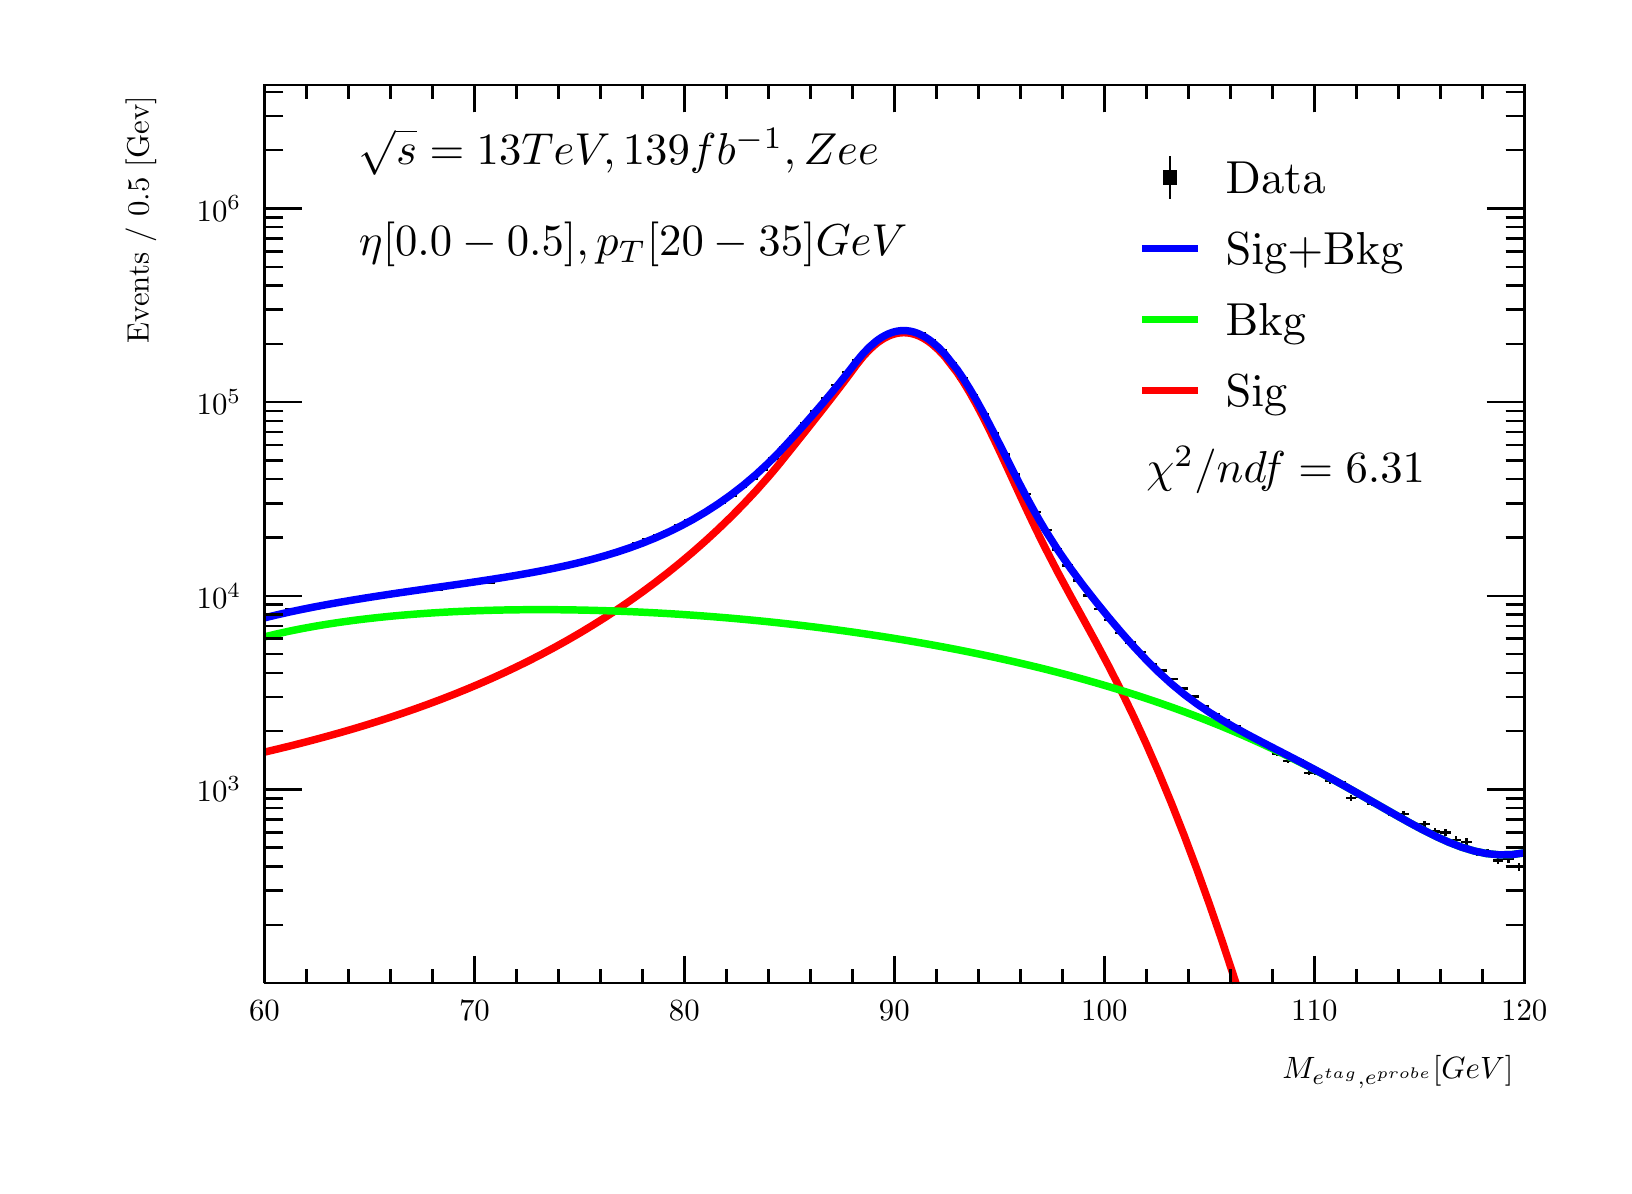
\begin{tikzpicture}
\pgfdeclareplotmark{cross} {
\pgfpathmoveto{\pgfpoint{-0.3\pgfplotmarksize}{\pgfplotmarksize}}
\pgfpathlineto{\pgfpoint{+0.3\pgfplotmarksize}{\pgfplotmarksize}}
\pgfpathlineto{\pgfpoint{+0.3\pgfplotmarksize}{0.3\pgfplotmarksize}}
\pgfpathlineto{\pgfpoint{+1\pgfplotmarksize}{0.3\pgfplotmarksize}}
\pgfpathlineto{\pgfpoint{+1\pgfplotmarksize}{-0.3\pgfplotmarksize}}
\pgfpathlineto{\pgfpoint{+0.3\pgfplotmarksize}{-0.3\pgfplotmarksize}}
\pgfpathlineto{\pgfpoint{+0.3\pgfplotmarksize}{-1.\pgfplotmarksize}}
\pgfpathlineto{\pgfpoint{-0.3\pgfplotmarksize}{-1.\pgfplotmarksize}}
\pgfpathlineto{\pgfpoint{-0.3\pgfplotmarksize}{-0.3\pgfplotmarksize}}
\pgfpathlineto{\pgfpoint{-1.\pgfplotmarksize}{-0.3\pgfplotmarksize}}
\pgfpathlineto{\pgfpoint{-1.\pgfplotmarksize}{0.3\pgfplotmarksize}}
\pgfpathlineto{\pgfpoint{-0.3\pgfplotmarksize}{0.3\pgfplotmarksize}}
\pgfpathclose
\pgfusepathqstroke
}
\pgfdeclareplotmark{cross*} {
\pgfpathmoveto{\pgfpoint{-0.3\pgfplotmarksize}{\pgfplotmarksize}}
\pgfpathlineto{\pgfpoint{+0.3\pgfplotmarksize}{\pgfplotmarksize}}
\pgfpathlineto{\pgfpoint{+0.3\pgfplotmarksize}{0.3\pgfplotmarksize}}
\pgfpathlineto{\pgfpoint{+1\pgfplotmarksize}{0.3\pgfplotmarksize}}
\pgfpathlineto{\pgfpoint{+1\pgfplotmarksize}{-0.3\pgfplotmarksize}}
\pgfpathlineto{\pgfpoint{+0.3\pgfplotmarksize}{-0.3\pgfplotmarksize}}
\pgfpathlineto{\pgfpoint{+0.3\pgfplotmarksize}{-1.\pgfplotmarksize}}
\pgfpathlineto{\pgfpoint{-0.3\pgfplotmarksize}{-1.\pgfplotmarksize}}
\pgfpathlineto{\pgfpoint{-0.3\pgfplotmarksize}{-0.3\pgfplotmarksize}}
\pgfpathlineto{\pgfpoint{-1.\pgfplotmarksize}{-0.3\pgfplotmarksize}}
\pgfpathlineto{\pgfpoint{-1.\pgfplotmarksize}{0.3\pgfplotmarksize}}
\pgfpathlineto{\pgfpoint{-0.3\pgfplotmarksize}{0.3\pgfplotmarksize}}
\pgfpathclose
\pgfusepathqfillstroke
}
\pgfdeclareplotmark{newstar} {
\pgfpathmoveto{\pgfqpoint{0pt}{\pgfplotmarksize}}
\pgfpathlineto{\pgfqpointpolar{44}{0.5\pgfplotmarksize}}
\pgfpathlineto{\pgfqpointpolar{18}{\pgfplotmarksize}}
\pgfpathlineto{\pgfqpointpolar{-20}{0.5\pgfplotmarksize}}
\pgfpathlineto{\pgfqpointpolar{-54}{\pgfplotmarksize}}
\pgfpathlineto{\pgfqpointpolar{-90}{0.5\pgfplotmarksize}}
\pgfpathlineto{\pgfqpointpolar{234}{\pgfplotmarksize}}
\pgfpathlineto{\pgfqpointpolar{198}{0.5\pgfplotmarksize}}
\pgfpathlineto{\pgfqpointpolar{162}{\pgfplotmarksize}}
\pgfpathlineto{\pgfqpointpolar{134}{0.5\pgfplotmarksize}}
\pgfpathclose
\pgfusepathqstroke
}
\pgfdeclareplotmark{newstar*} {
\pgfpathmoveto{\pgfqpoint{0pt}{\pgfplotmarksize}}
\pgfpathlineto{\pgfqpointpolar{44}{0.5\pgfplotmarksize}}
\pgfpathlineto{\pgfqpointpolar{18}{\pgfplotmarksize}}
\pgfpathlineto{\pgfqpointpolar{-20}{0.5\pgfplotmarksize}}
\pgfpathlineto{\pgfqpointpolar{-54}{\pgfplotmarksize}}
\pgfpathlineto{\pgfqpointpolar{-90}{0.5\pgfplotmarksize}}
\pgfpathlineto{\pgfqpointpolar{234}{\pgfplotmarksize}}
\pgfpathlineto{\pgfqpointpolar{198}{0.5\pgfplotmarksize}}
\pgfpathlineto{\pgfqpointpolar{162}{\pgfplotmarksize}}
\pgfpathlineto{\pgfqpointpolar{134}{0.5\pgfplotmarksize}}
\pgfpathclose
\pgfusepathqfillstroke
}
\definecolor{c}{rgb}{1,1,1};
\draw [color=c, fill=c] (0,0) rectangle (20,14.4361);
\draw [color=c, fill=c] (3,2.30977) rectangle (19,13.7143);
\definecolor{c}{rgb}{0,0,0};
\draw [c,line width=0.9] (3,2.30977) -- (3,13.7143) -- (19,13.7143) -- (19,2.30977) -- (3,2.30977);
\definecolor{c}{rgb}{1,1,1};
\draw [color=c, fill=c] (3,2.30977) rectangle (19,13.7143);
\definecolor{c}{rgb}{0,0,0};
\draw [c,line width=0.9] (3,2.30977) -- (3,13.7143) -- (19,13.7143) -- (19,2.30977) -- (3,2.30977);
\draw [c,line width=0.9] (3,2.30977) -- (19,2.30977);
\draw [c,line width=0.9] (3,2.65624) -- (3,2.30977);
\draw [c,line width=0.9] (3.53333,2.48301) -- (3.53333,2.30977);
\draw [c,line width=0.9] (4.06667,2.48301) -- (4.06667,2.30977);
\draw [c,line width=0.9] (4.6,2.48301) -- (4.6,2.30977);
\draw [c,line width=0.9] (5.13333,2.48301) -- (5.13333,2.30977);
\draw [c,line width=0.9] (5.66667,2.65624) -- (5.66667,2.30977);
\draw [c,line width=0.9] (6.2,2.48301) -- (6.2,2.30977);
\draw [c,line width=0.9] (6.73333,2.48301) -- (6.73333,2.30977);
\draw [c,line width=0.9] (7.26667,2.48301) -- (7.26667,2.30977);
\draw [c,line width=0.9] (7.8,2.48301) -- (7.8,2.30977);
\draw [c,line width=0.9] (8.33333,2.65624) -- (8.33333,2.30977);
\draw [c,line width=0.9] (8.86667,2.48301) -- (8.86667,2.30977);
\draw [c,line width=0.9] (9.4,2.48301) -- (9.4,2.30977);
\draw [c,line width=0.9] (9.93333,2.48301) -- (9.93333,2.30977);
\draw [c,line width=0.9] (10.4667,2.48301) -- (10.4667,2.30977);
\draw [c,line width=0.9] (11,2.65624) -- (11,2.30977);
\draw [c,line width=0.9] (11.5333,2.48301) -- (11.5333,2.30977);
\draw [c,line width=0.9] (12.0667,2.48301) -- (12.0667,2.30977);
\draw [c,line width=0.9] (12.6,2.48301) -- (12.6,2.30977);
\draw [c,line width=0.9] (13.1333,2.48301) -- (13.1333,2.30977);
\draw [c,line width=0.9] (13.6667,2.65624) -- (13.6667,2.30977);
\draw [c,line width=0.9] (14.2,2.48301) -- (14.2,2.30977);
\draw [c,line width=0.9] (14.7333,2.48301) -- (14.7333,2.30977);
\draw [c,line width=0.9] (15.2667,2.48301) -- (15.2667,2.30977);
\draw [c,line width=0.9] (15.8,2.48301) -- (15.8,2.30977);
\draw [c,line width=0.9] (16.3333,2.65624) -- (16.3333,2.30977);
\draw [c,line width=0.9] (16.8667,2.48301) -- (16.8667,2.30977);
\draw [c,line width=0.9] (17.4,2.48301) -- (17.4,2.30977);
\draw [c,line width=0.9] (17.9333,2.48301) -- (17.9333,2.30977);
\draw [c,line width=0.9] (18.4667,2.48301) -- (18.4667,2.30977);
\draw [c,line width=0.9] (19,2.65624) -- (19,2.30977);
\draw [anchor=base] (3,1.83338) node[scale=1.11327, color=c, rotate=0]{60};
\draw [anchor=base] (5.66667,1.83338) node[scale=1.11327, color=c, rotate=0]{70};
\draw [anchor=base] (8.33333,1.83338) node[scale=1.11327, color=c, rotate=0]{80};
\draw [anchor=base] (11,1.83338) node[scale=1.11327, color=c, rotate=0]{90};
\draw [anchor=base] (13.6667,1.83338) node[scale=1.11327, color=c, rotate=0]{100};
\draw [anchor=base] (16.3333,1.83338) node[scale=1.11327, color=c, rotate=0]{110};
\draw [anchor=base] (19,1.83338) node[scale=1.11327, color=c, rotate=0]{120};
\draw [anchor= east] (19,1.17798) node[scale=1.11327, color=c, rotate=0]{$M_{e^{tag}, e^{probe}}  [GeV]$};
\draw [c,line width=0.9] (3,13.7143) -- (19,13.7143);
\draw [c,line width=0.9] (3,13.3678) -- (3,13.7143);
\draw [c,line width=0.9] (3.53333,13.5411) -- (3.53333,13.7143);
\draw [c,line width=0.9] (4.06667,13.5411) -- (4.06667,13.7143);
\draw [c,line width=0.9] (4.6,13.5411) -- (4.6,13.7143);
\draw [c,line width=0.9] (5.13333,13.5411) -- (5.13333,13.7143);
\draw [c,line width=0.9] (5.66667,13.3678) -- (5.66667,13.7143);
\draw [c,line width=0.9] (6.2,13.5411) -- (6.2,13.7143);
\draw [c,line width=0.9] (6.73333,13.5411) -- (6.73333,13.7143);
\draw [c,line width=0.9] (7.26667,13.5411) -- (7.26667,13.7143);
\draw [c,line width=0.9] (7.8,13.5411) -- (7.8,13.7143);
\draw [c,line width=0.9] (8.33333,13.3678) -- (8.33333,13.7143);
\draw [c,line width=0.9] (8.86667,13.5411) -- (8.86667,13.7143);
\draw [c,line width=0.9] (9.4,13.5411) -- (9.4,13.7143);
\draw [c,line width=0.9] (9.93333,13.5411) -- (9.93333,13.7143);
\draw [c,line width=0.9] (10.4667,13.5411) -- (10.4667,13.7143);
\draw [c,line width=0.9] (11,13.3678) -- (11,13.7143);
\draw [c,line width=0.9] (11.5333,13.5411) -- (11.5333,13.7143);
\draw [c,line width=0.9] (12.0667,13.5411) -- (12.0667,13.7143);
\draw [c,line width=0.9] (12.6,13.5411) -- (12.6,13.7143);
\draw [c,line width=0.9] (13.1333,13.5411) -- (13.1333,13.7143);
\draw [c,line width=0.9] (13.6667,13.3678) -- (13.6667,13.7143);
\draw [c,line width=0.9] (14.2,13.5411) -- (14.2,13.7143);
\draw [c,line width=0.9] (14.7333,13.5411) -- (14.7333,13.7143);
\draw [c,line width=0.9] (15.2667,13.5411) -- (15.2667,13.7143);
\draw [c,line width=0.9] (15.8,13.5411) -- (15.8,13.7143);
\draw [c,line width=0.9] (16.3333,13.3678) -- (16.3333,13.7143);
\draw [c,line width=0.9] (16.8667,13.5411) -- (16.8667,13.7143);
\draw [c,line width=0.9] (17.4,13.5411) -- (17.4,13.7143);
\draw [c,line width=0.9] (17.9333,13.5411) -- (17.9333,13.7143);
\draw [c,line width=0.9] (18.4667,13.5411) -- (18.4667,13.7143);
\draw [c,line width=0.9] (19,13.3678) -- (19,13.7143);
\draw [c,line width=0.9] (3,2.30977) -- (3,13.7143);
\draw [c,line width=0.9] (3.237,3.05008) -- (3,3.05008);
\draw [c,line width=0.9] (3.237,3.48313) -- (3,3.48313);
\draw [c,line width=0.9] (3.237,3.79038) -- (3,3.79038);
\draw [c,line width=0.9] (3.237,4.02871) -- (3,4.02871);
\draw [c,line width=0.9] (3.237,4.22343) -- (3,4.22343);
\draw [c,line width=0.9] (3.237,4.38807) -- (3,4.38807);
\draw [c,line width=0.9] (3.237,4.53069) -- (3,4.53069);
\draw [c,line width=0.9] (3.237,4.65649) -- (3,4.65649);
\draw [c,line width=0.9] (3.474,4.76901) -- (3,4.76901);
\draw [anchor= east] (2.844,4.76901) node[scale=1.11327, color=c, rotate=0]{$10^{3}$};
\draw [c,line width=0.9] (3.237,5.50932) -- (3,5.50932);
\draw [c,line width=0.9] (3.237,5.94237) -- (3,5.94237);
\draw [c,line width=0.9] (3.237,6.24963) -- (3,6.24963);
\draw [c,line width=0.9] (3.237,6.48795) -- (3,6.48795);
\draw [c,line width=0.9] (3.237,6.68268) -- (3,6.68268);
\draw [c,line width=0.9] (3.237,6.84731) -- (3,6.84731);
\draw [c,line width=0.9] (3.237,6.98993) -- (3,6.98993);
\draw [c,line width=0.9] (3.237,7.11573) -- (3,7.11573);
\draw [c,line width=0.9] (3.474,7.22826) -- (3,7.22826);
\draw [anchor= east] (2.844,7.22826) node[scale=1.11327, color=c, rotate=0]{$10^{4}$};
\draw [c,line width=0.9] (3.237,7.96856) -- (3,7.96856);
\draw [c,line width=0.9] (3.237,8.40161) -- (3,8.40161);
\draw [c,line width=0.9] (3.237,8.70887) -- (3,8.70887);
\draw [c,line width=0.9] (3.237,8.94719) -- (3,8.94719);
\draw [c,line width=0.9] (3.237,9.14192) -- (3,9.14192);
\draw [c,line width=0.9] (3.237,9.30656) -- (3,9.30656);
\draw [c,line width=0.9] (3.237,9.44917) -- (3,9.44917);
\draw [c,line width=0.9] (3.237,9.57497) -- (3,9.57497);
\draw [c,line width=0.9] (3.474,9.6875) -- (3,9.6875);
\draw [anchor= east] (2.844,9.6875) node[scale=1.11327, color=c, rotate=0]{$10^{5}$};
\draw [c,line width=0.9] (3.237,10.4278) -- (3,10.4278);
\draw [c,line width=0.9] (3.237,10.8609) -- (3,10.8609);
\draw [c,line width=0.9] (3.237,11.1681) -- (3,11.1681);
\draw [c,line width=0.9] (3.237,11.4064) -- (3,11.4064);
\draw [c,line width=0.9] (3.237,11.6012) -- (3,11.6012);
\draw [c,line width=0.9] (3.237,11.7658) -- (3,11.7658);
\draw [c,line width=0.9] (3.237,11.9084) -- (3,11.9084);
\draw [c,line width=0.9] (3.237,12.0342) -- (3,12.0342);
\draw [c,line width=0.9] (3.474,12.1467) -- (3,12.1467);
\draw [anchor= east] (2.844,12.1467) node[scale=1.11327, color=c, rotate=0]{$10^{6}$};
\draw [c,line width=0.9] (3.237,12.887) -- (3,12.887);
\draw [c,line width=0.9] (3.237,13.3201) -- (3,13.3201);
\draw [c,line width=0.9] (3.237,13.6274) -- (3,13.6274);
\draw [anchor= east] (1.432,13.7143) node[scale=1.11327, color=c, rotate=90]{Events / 0.5 [Gev]};
\draw [c,line width=0.9] (19,2.30977) -- (19,13.7143);
\draw [c,line width=0.9] (18.763,3.05008) -- (19,3.05008);
\draw [c,line width=0.9] (18.763,3.48313) -- (19,3.48313);
\draw [c,line width=0.9] (18.763,3.79038) -- (19,3.79038);
\draw [c,line width=0.9] (18.763,4.02871) -- (19,4.02871);
\draw [c,line width=0.9] (18.763,4.22343) -- (19,4.22343);
\draw [c,line width=0.9] (18.763,4.38807) -- (19,4.38807);
\draw [c,line width=0.9] (18.763,4.53069) -- (19,4.53069);
\draw [c,line width=0.9] (18.763,4.65649) -- (19,4.65649);
\draw [c,line width=0.9] (18.526,4.76901) -- (19,4.76901);
\draw [c,line width=0.9] (18.763,5.50932) -- (19,5.50932);
\draw [c,line width=0.9] (18.763,5.94237) -- (19,5.94237);
\draw [c,line width=0.9] (18.763,6.24963) -- (19,6.24963);
\draw [c,line width=0.9] (18.763,6.48795) -- (19,6.48795);
\draw [c,line width=0.9] (18.763,6.68268) -- (19,6.68268);
\draw [c,line width=0.9] (18.763,6.84731) -- (19,6.84731);
\draw [c,line width=0.9] (18.763,6.98993) -- (19,6.98993);
\draw [c,line width=0.9] (18.763,7.11573) -- (19,7.11573);
\draw [c,line width=0.9] (18.526,7.22826) -- (19,7.22826);
\draw [c,line width=0.9] (18.763,7.96856) -- (19,7.96856);
\draw [c,line width=0.9] (18.763,8.40161) -- (19,8.40161);
\draw [c,line width=0.9] (18.763,8.70887) -- (19,8.70887);
\draw [c,line width=0.9] (18.763,8.94719) -- (19,8.94719);
\draw [c,line width=0.9] (18.763,9.14192) -- (19,9.14192);
\draw [c,line width=0.9] (18.763,9.30656) -- (19,9.30656);
\draw [c,line width=0.9] (18.763,9.44917) -- (19,9.44917);
\draw [c,line width=0.9] (18.763,9.57497) -- (19,9.57497);
\draw [c,line width=0.9] (18.526,9.6875) -- (19,9.6875);
\draw [c,line width=0.9] (18.763,10.4278) -- (19,10.4278);
\draw [c,line width=0.9] (18.763,10.8609) -- (19,10.8609);
\draw [c,line width=0.9] (18.763,11.1681) -- (19,11.1681);
\draw [c,line width=0.9] (18.763,11.4064) -- (19,11.4064);
\draw [c,line width=0.9] (18.763,11.6012) -- (19,11.6012);
\draw [c,line width=0.9] (18.763,11.7658) -- (19,11.7658);
\draw [c,line width=0.9] (18.763,11.9084) -- (19,11.9084);
\draw [c,line width=0.9] (18.763,12.0342) -- (19,12.0342);
\draw [c,line width=0.9] (18.526,12.1467) -- (19,12.1467);
\draw [c,line width=0.9] (18.763,12.887) -- (19,12.887);
\draw [c,line width=0.9] (18.763,13.3201) -- (19,13.3201);
\draw [c,line width=0.9] (18.763,13.6274) -- (19,13.6274);
\draw [c,line width=0.9] (3.06667,6.97555) -- (3,6.97555);
\draw [c,line width=0.9] (3,6.97555) -- (3,6.97555);
\draw [c,line width=0.9] (3.06667,6.97555) -- (3.13333,6.97555);
\draw [c,line width=0.9] (3.13333,6.97555) -- (3.13333,6.97555);
\draw [c,line width=0.9] (3.06667,6.97555) -- (3.06667,6.98757);
\draw [c,line width=0.9] (3.06667,6.98757) -- (3.06667,6.98757);
\draw [c,line width=0.9] (3.06667,6.97555) -- (3.06667,6.96353);
\draw [c,line width=0.9] (3.06667,6.96353) -- (3.06667,6.96353);
\draw [c,line width=0.9] (3.2,6.99897) -- (3.13333,6.99897);
\draw [c,line width=0.9] (3.13333,6.99897) -- (3.13333,6.99897);
\draw [c,line width=0.9] (3.2,6.99897) -- (3.26667,6.99897);
\draw [c,line width=0.9] (3.26667,6.99897) -- (3.26667,6.99897);
\draw [c,line width=0.9] (3.2,6.99897) -- (3.2,7.01086);
\draw [c,line width=0.9] (3.2,7.01086) -- (3.2,7.01086);
\draw [c,line width=0.9] (3.2,6.99897) -- (3.2,6.98708);
\draw [c,line width=0.9] (3.2,6.98708) -- (3.2,6.98708);
\draw [c,line width=0.9] (3.33333,7.05305) -- (3.26667,7.05305);
\draw [c,line width=0.9] (3.26667,7.05305) -- (3.26667,7.05305);
\draw [c,line width=0.9] (3.33333,7.05305) -- (3.4,7.05305);
\draw [c,line width=0.9] (3.4,7.05305) -- (3.4,7.05305);
\draw [c,line width=0.9] (3.33333,7.05305) -- (3.33333,7.06464);
\draw [c,line width=0.9] (3.33333,7.06464) -- (3.33333,7.06464);
\draw [c,line width=0.9] (3.33333,7.05305) -- (3.33333,7.04145);
\draw [c,line width=0.9] (3.33333,7.04145) -- (3.33333,7.04145);
\draw [c,line width=0.9] (3.46667,7.05619) -- (3.4,7.05619);
\draw [c,line width=0.9] (3.4,7.05619) -- (3.4,7.05619);
\draw [c,line width=0.9] (3.46667,7.05619) -- (3.53333,7.05619);
\draw [c,line width=0.9] (3.53333,7.05619) -- (3.53333,7.05619);
\draw [c,line width=0.9] (3.46667,7.05619) -- (3.46667,7.06776);
\draw [c,line width=0.9] (3.46667,7.06776) -- (3.46667,7.06776);
\draw [c,line width=0.9] (3.46667,7.05619) -- (3.46667,7.04461);
\draw [c,line width=0.9] (3.46667,7.04461) -- (3.46667,7.04461);
\draw [c,line width=0.9] (3.6,7.09403) -- (3.53333,7.09403);
\draw [c,line width=0.9] (3.53333,7.09403) -- (3.53333,7.09403);
\draw [c,line width=0.9] (3.6,7.09403) -- (3.66667,7.09403);
\draw [c,line width=0.9] (3.66667,7.09403) -- (3.66667,7.09403);
\draw [c,line width=0.9] (3.6,7.09403) -- (3.6,7.1054);
\draw [c,line width=0.9] (3.6,7.1054) -- (3.6,7.1054);
\draw [c,line width=0.9] (3.6,7.09403) -- (3.6,7.08266);
\draw [c,line width=0.9] (3.6,7.08266) -- (3.6,7.08266);
\draw [c,line width=0.9] (3.73333,7.12094) -- (3.66667,7.12094);
\draw [c,line width=0.9] (3.66667,7.12094) -- (3.66667,7.12094);
\draw [c,line width=0.9] (3.73333,7.12094) -- (3.8,7.12094);
\draw [c,line width=0.9] (3.8,7.12094) -- (3.8,7.12094);
\draw [c,line width=0.9] (3.73333,7.12094) -- (3.73333,7.13217);
\draw [c,line width=0.9] (3.73333,7.13217) -- (3.73333,7.13217);
\draw [c,line width=0.9] (3.73333,7.12094) -- (3.73333,7.10971);
\draw [c,line width=0.9] (3.73333,7.10971) -- (3.73333,7.10971);
\draw [c,line width=0.9] (3.86667,7.1328) -- (3.8,7.1328);
\draw [c,line width=0.9] (3.8,7.1328) -- (3.8,7.1328);
\draw [c,line width=0.9] (3.86667,7.1328) -- (3.93333,7.1328);
\draw [c,line width=0.9] (3.93333,7.1328) -- (3.93333,7.1328);
\draw [c,line width=0.9] (3.86667,7.1328) -- (3.86667,7.14397);
\draw [c,line width=0.9] (3.86667,7.14397) -- (3.86667,7.14397);
\draw [c,line width=0.9] (3.86667,7.1328) -- (3.86667,7.12163);
\draw [c,line width=0.9] (3.86667,7.12163) -- (3.86667,7.12163);
\draw [c,line width=0.9] (4,7.15407) -- (3.93333,7.15407);
\draw [c,line width=0.9] (3.93333,7.15407) -- (3.93333,7.15407);
\draw [c,line width=0.9] (4,7.15407) -- (4.06667,7.15407);
\draw [c,line width=0.9] (4.06667,7.15407) -- (4.06667,7.15407);
\draw [c,line width=0.9] (4,7.15407) -- (4,7.16513);
\draw [c,line width=0.9] (4,7.16513) -- (4,7.16513);
\draw [c,line width=0.9] (4,7.15407) -- (4,7.14302);
\draw [c,line width=0.9] (4,7.14302) -- (4,7.14302);
\draw [c,line width=0.9] (4.13333,7.18377) -- (4.06667,7.18377);
\draw [c,line width=0.9] (4.06667,7.18377) -- (4.06667,7.18377);
\draw [c,line width=0.9] (4.13333,7.18377) -- (4.2,7.18377);
\draw [c,line width=0.9] (4.2,7.18377) -- (4.2,7.18377);
\draw [c,line width=0.9] (4.13333,7.18377) -- (4.13333,7.19467);
\draw [c,line width=0.9] (4.13333,7.19467) -- (4.13333,7.19467);
\draw [c,line width=0.9] (4.13333,7.18377) -- (4.13333,7.17286);
\draw [c,line width=0.9] (4.13333,7.17286) -- (4.13333,7.17286);
\draw [c,line width=0.9] (4.26667,7.21439) -- (4.2,7.21439);
\draw [c,line width=0.9] (4.2,7.21439) -- (4.2,7.21439);
\draw [c,line width=0.9] (4.26667,7.21439) -- (4.33333,7.21439);
\draw [c,line width=0.9] (4.33333,7.21439) -- (4.33333,7.21439);
\draw [c,line width=0.9] (4.26667,7.21439) -- (4.26667,7.22514);
\draw [c,line width=0.9] (4.26667,7.22514) -- (4.26667,7.22514);
\draw [c,line width=0.9] (4.26667,7.21439) -- (4.26667,7.20364);
\draw [c,line width=0.9] (4.26667,7.20364) -- (4.26667,7.20364);
\draw [c,line width=0.9] (4.4,7.21114) -- (4.33333,7.21114);
\draw [c,line width=0.9] (4.33333,7.21114) -- (4.33333,7.21114);
\draw [c,line width=0.9] (4.4,7.21114) -- (4.46667,7.21114);
\draw [c,line width=0.9] (4.46667,7.21114) -- (4.46667,7.21114);
\draw [c,line width=0.9] (4.4,7.21114) -- (4.4,7.22191);
\draw [c,line width=0.9] (4.4,7.22191) -- (4.4,7.22191);
\draw [c,line width=0.9] (4.4,7.21114) -- (4.4,7.20037);
\draw [c,line width=0.9] (4.4,7.20037) -- (4.4,7.20037);
\draw [c,line width=0.9] (4.53333,7.21979) -- (4.46667,7.21979);
\draw [c,line width=0.9] (4.46667,7.21979) -- (4.46667,7.21979);
\draw [c,line width=0.9] (4.53333,7.21979) -- (4.6,7.21979);
\draw [c,line width=0.9] (4.6,7.21979) -- (4.6,7.21979);
\draw [c,line width=0.9] (4.53333,7.21979) -- (4.53333,7.23051);
\draw [c,line width=0.9] (4.53333,7.23051) -- (4.53333,7.23051);
\draw [c,line width=0.9] (4.53333,7.21979) -- (4.53333,7.20906);
\draw [c,line width=0.9] (4.53333,7.20906) -- (4.53333,7.20906);
\draw [c,line width=0.9] (4.66667,7.23878) -- (4.6,7.23878);
\draw [c,line width=0.9] (4.6,7.23878) -- (4.6,7.23878);
\draw [c,line width=0.9] (4.66667,7.23878) -- (4.73333,7.23878);
\draw [c,line width=0.9] (4.73333,7.23878) -- (4.73333,7.23878);
\draw [c,line width=0.9] (4.66667,7.23878) -- (4.66667,7.24941);
\draw [c,line width=0.9] (4.66667,7.24941) -- (4.66667,7.24941);
\draw [c,line width=0.9] (4.66667,7.23878) -- (4.66667,7.22815);
\draw [c,line width=0.9] (4.66667,7.22815) -- (4.66667,7.22815);
\draw [c,line width=0.9] (4.8,7.28756) -- (4.73333,7.28756);
\draw [c,line width=0.9] (4.73333,7.28756) -- (4.73333,7.28756);
\draw [c,line width=0.9] (4.8,7.28756) -- (4.86667,7.28756);
\draw [c,line width=0.9] (4.86667,7.28756) -- (4.86667,7.28756);
\draw [c,line width=0.9] (4.8,7.28756) -- (4.8,7.29795);
\draw [c,line width=0.9] (4.8,7.29795) -- (4.8,7.29795);
\draw [c,line width=0.9] (4.8,7.28756) -- (4.8,7.27718);
\draw [c,line width=0.9] (4.8,7.27718) -- (4.8,7.27718);
\draw [c,line width=0.9] (4.93333,7.27425) -- (4.86667,7.27425);
\draw [c,line width=0.9] (4.86667,7.27425) -- (4.86667,7.27425);
\draw [c,line width=0.9] (4.93333,7.27425) -- (5,7.27425);
\draw [c,line width=0.9] (5,7.27425) -- (5,7.27425);
\draw [c,line width=0.9] (4.93333,7.27425) -- (4.93333,7.2847);
\draw [c,line width=0.9] (4.93333,7.2847) -- (4.93333,7.2847);
\draw [c,line width=0.9] (4.93333,7.27425) -- (4.93333,7.26379);
\draw [c,line width=0.9] (4.93333,7.26379) -- (4.93333,7.26379);
\draw [c,line width=0.9] (5.06667,7.30986) -- (5,7.30986);
\draw [c,line width=0.9] (5,7.30986) -- (5,7.30986);
\draw [c,line width=0.9] (5.06667,7.30986) -- (5.13333,7.30986);
\draw [c,line width=0.9] (5.13333,7.30986) -- (5.13333,7.30986);
\draw [c,line width=0.9] (5.06667,7.30986) -- (5.06667,7.32014);
\draw [c,line width=0.9] (5.06667,7.32014) -- (5.06667,7.32014);
\draw [c,line width=0.9] (5.06667,7.30986) -- (5.06667,7.29958);
\draw [c,line width=0.9] (5.06667,7.29958) -- (5.06667,7.29958);
\draw [c,line width=0.9] (5.2,7.31065) -- (5.13333,7.31065);
\draw [c,line width=0.9] (5.13333,7.31065) -- (5.13333,7.31065);
\draw [c,line width=0.9] (5.2,7.31065) -- (5.26667,7.31065);
\draw [c,line width=0.9] (5.26667,7.31065) -- (5.26667,7.31065);
\draw [c,line width=0.9] (5.2,7.31065) -- (5.2,7.32093);
\draw [c,line width=0.9] (5.2,7.32093) -- (5.2,7.32093);
\draw [c,line width=0.9] (5.2,7.31065) -- (5.2,7.30038);
\draw [c,line width=0.9] (5.2,7.30038) -- (5.2,7.30038);
\draw [c,line width=0.9] (5.33333,7.34844) -- (5.26667,7.34844);
\draw [c,line width=0.9] (5.26667,7.34844) -- (5.26667,7.34844);
\draw [c,line width=0.9] (5.33333,7.34844) -- (5.4,7.34844);
\draw [c,line width=0.9] (5.4,7.34844) -- (5.4,7.34844);
\draw [c,line width=0.9] (5.33333,7.34844) -- (5.33333,7.35853);
\draw [c,line width=0.9] (5.33333,7.35853) -- (5.33333,7.35853);
\draw [c,line width=0.9] (5.33333,7.34844) -- (5.33333,7.33834);
\draw [c,line width=0.9] (5.33333,7.33834) -- (5.33333,7.33834);
\draw [c,line width=0.9] (5.46667,7.35358) -- (5.4,7.35358);
\draw [c,line width=0.9] (5.4,7.35358) -- (5.4,7.35358);
\draw [c,line width=0.9] (5.46667,7.35358) -- (5.53333,7.35358);
\draw [c,line width=0.9] (5.53333,7.35358) -- (5.53333,7.35358);
\draw [c,line width=0.9] (5.46667,7.35358) -- (5.46667,7.36365);
\draw [c,line width=0.9] (5.46667,7.36365) -- (5.46667,7.36365);
\draw [c,line width=0.9] (5.46667,7.35358) -- (5.46667,7.34351);
\draw [c,line width=0.9] (5.46667,7.34351) -- (5.46667,7.34351);
\draw [c,line width=0.9] (5.6,7.38401) -- (5.53333,7.38401);
\draw [c,line width=0.9] (5.53333,7.38401) -- (5.53333,7.38401);
\draw [c,line width=0.9] (5.6,7.38401) -- (5.66667,7.38401);
\draw [c,line width=0.9] (5.66667,7.38401) -- (5.66667,7.38401);
\draw [c,line width=0.9] (5.6,7.38401) -- (5.6,7.39394);
\draw [c,line width=0.9] (5.6,7.39394) -- (5.6,7.39394);
\draw [c,line width=0.9] (5.6,7.38401) -- (5.6,7.37408);
\draw [c,line width=0.9] (5.6,7.37408) -- (5.6,7.37408);
\draw [c,line width=0.9] (5.73333,7.39649) -- (5.66667,7.39649);
\draw [c,line width=0.9] (5.66667,7.39649) -- (5.66667,7.39649);
\draw [c,line width=0.9] (5.73333,7.39649) -- (5.8,7.39649);
\draw [c,line width=0.9] (5.8,7.39649) -- (5.8,7.39649);
\draw [c,line width=0.9] (5.73333,7.39649) -- (5.73333,7.40636);
\draw [c,line width=0.9] (5.73333,7.40636) -- (5.73333,7.40636);
\draw [c,line width=0.9] (5.73333,7.39649) -- (5.73333,7.38662);
\draw [c,line width=0.9] (5.73333,7.38662) -- (5.73333,7.38662);
\draw [c,line width=0.9] (5.86667,7.39722) -- (5.8,7.39722);
\draw [c,line width=0.9] (5.8,7.39722) -- (5.8,7.39722);
\draw [c,line width=0.9] (5.86667,7.39722) -- (5.93333,7.39722);
\draw [c,line width=0.9] (5.93333,7.39722) -- (5.93333,7.39722);
\draw [c,line width=0.9] (5.86667,7.39722) -- (5.86667,7.40709);
\draw [c,line width=0.9] (5.86667,7.40709) -- (5.86667,7.40709);
\draw [c,line width=0.9] (5.86667,7.39722) -- (5.86667,7.38735);
\draw [c,line width=0.9] (5.86667,7.38735) -- (5.86667,7.38735);
\draw [c,line width=0.9] (6,7.44378) -- (5.93333,7.44378);
\draw [c,line width=0.9] (5.93333,7.44378) -- (5.93333,7.44378);
\draw [c,line width=0.9] (6,7.44378) -- (6.06667,7.44378);
\draw [c,line width=0.9] (6.06667,7.44378) -- (6.06667,7.44378);
\draw [c,line width=0.9] (6,7.44378) -- (6,7.45344);
\draw [c,line width=0.9] (6,7.45344) -- (6,7.45344);
\draw [c,line width=0.9] (6,7.44378) -- (6,7.43413);
\draw [c,line width=0.9] (6,7.43413) -- (6,7.43413);
\draw [c,line width=0.9] (6.13333,7.45403) -- (6.06667,7.45403);
\draw [c,line width=0.9] (6.06667,7.45403) -- (6.06667,7.45403);
\draw [c,line width=0.9] (6.13333,7.45403) -- (6.2,7.45403);
\draw [c,line width=0.9] (6.2,7.45403) -- (6.2,7.45403);
\draw [c,line width=0.9] (6.13333,7.45403) -- (6.13333,7.46364);
\draw [c,line width=0.9] (6.13333,7.46364) -- (6.13333,7.46364);
\draw [c,line width=0.9] (6.13333,7.45403) -- (6.13333,7.44443);
\draw [c,line width=0.9] (6.13333,7.44443) -- (6.13333,7.44443);
\draw [c,line width=0.9] (6.26667,7.5008) -- (6.2,7.5008);
\draw [c,line width=0.9] (6.2,7.5008) -- (6.2,7.5008);
\draw [c,line width=0.9] (6.26667,7.5008) -- (6.33333,7.5008);
\draw [c,line width=0.9] (6.33333,7.5008) -- (6.33333,7.5008);
\draw [c,line width=0.9] (6.26667,7.5008) -- (6.26667,7.5102);
\draw [c,line width=0.9] (6.26667,7.5102) -- (6.26667,7.5102);
\draw [c,line width=0.9] (6.26667,7.5008) -- (6.26667,7.4914);
\draw [c,line width=0.9] (6.26667,7.4914) -- (6.26667,7.4914);
\draw [c,line width=0.9] (6.4,7.52162) -- (6.33333,7.52162);
\draw [c,line width=0.9] (6.33333,7.52162) -- (6.33333,7.52162);
\draw [c,line width=0.9] (6.4,7.52162) -- (6.46667,7.52162);
\draw [c,line width=0.9] (6.46667,7.52162) -- (6.46667,7.52162);
\draw [c,line width=0.9] (6.4,7.52162) -- (6.4,7.53093);
\draw [c,line width=0.9] (6.4,7.53093) -- (6.4,7.53093);
\draw [c,line width=0.9] (6.4,7.52162) -- (6.4,7.51231);
\draw [c,line width=0.9] (6.4,7.51231) -- (6.4,7.51231);
\draw [c,line width=0.9] (6.53333,7.54941) -- (6.46667,7.54941);
\draw [c,line width=0.9] (6.46667,7.54941) -- (6.46667,7.54941);
\draw [c,line width=0.9] (6.53333,7.54941) -- (6.6,7.54941);
\draw [c,line width=0.9] (6.6,7.54941) -- (6.6,7.54941);
\draw [c,line width=0.9] (6.53333,7.54941) -- (6.53333,7.5586);
\draw [c,line width=0.9] (6.53333,7.5586) -- (6.53333,7.5586);
\draw [c,line width=0.9] (6.53333,7.54941) -- (6.53333,7.54022);
\draw [c,line width=0.9] (6.53333,7.54022) -- (6.53333,7.54022);
\draw [c,line width=0.9] (6.66667,7.58211) -- (6.6,7.58211);
\draw [c,line width=0.9] (6.6,7.58211) -- (6.6,7.58211);
\draw [c,line width=0.9] (6.66667,7.58211) -- (6.73333,7.58211);
\draw [c,line width=0.9] (6.73333,7.58211) -- (6.73333,7.58211);
\draw [c,line width=0.9] (6.66667,7.58211) -- (6.66667,7.59116);
\draw [c,line width=0.9] (6.66667,7.59116) -- (6.66667,7.59116);
\draw [c,line width=0.9] (6.66667,7.58211) -- (6.66667,7.57306);
\draw [c,line width=0.9] (6.66667,7.57306) -- (6.66667,7.57306);
\draw [c,line width=0.9] (6.8,7.61094) -- (6.73333,7.61094);
\draw [c,line width=0.9] (6.73333,7.61094) -- (6.73333,7.61094);
\draw [c,line width=0.9] (6.8,7.61094) -- (6.86667,7.61094);
\draw [c,line width=0.9] (6.86667,7.61094) -- (6.86667,7.61094);
\draw [c,line width=0.9] (6.8,7.61094) -- (6.8,7.61987);
\draw [c,line width=0.9] (6.8,7.61987) -- (6.8,7.61987);
\draw [c,line width=0.9] (6.8,7.61094) -- (6.8,7.60201);
\draw [c,line width=0.9] (6.8,7.60201) -- (6.8,7.60201);
\draw [c,line width=0.9] (6.93333,7.6331) -- (6.86667,7.6331);
\draw [c,line width=0.9] (6.86667,7.6331) -- (6.86667,7.6331);
\draw [c,line width=0.9] (6.93333,7.6331) -- (7,7.6331);
\draw [c,line width=0.9] (7,7.6331) -- (7,7.6331);
\draw [c,line width=0.9] (6.93333,7.6331) -- (6.93333,7.64194);
\draw [c,line width=0.9] (6.93333,7.64194) -- (6.93333,7.64194);
\draw [c,line width=0.9] (6.93333,7.6331) -- (6.93333,7.62426);
\draw [c,line width=0.9] (6.93333,7.62426) -- (6.93333,7.62426);
\draw [c,line width=0.9] (7.06667,7.66734) -- (7,7.66734);
\draw [c,line width=0.9] (7,7.66734) -- (7,7.66734);
\draw [c,line width=0.9] (7.06667,7.66734) -- (7.13333,7.66734);
\draw [c,line width=0.9] (7.13333,7.66734) -- (7.13333,7.66734);
\draw [c,line width=0.9] (7.06667,7.66734) -- (7.06667,7.67604);
\draw [c,line width=0.9] (7.06667,7.67604) -- (7.06667,7.67604);
\draw [c,line width=0.9] (7.06667,7.66734) -- (7.06667,7.65865);
\draw [c,line width=0.9] (7.06667,7.65865) -- (7.06667,7.65865);
\draw [c,line width=0.9] (7.2,7.71829) -- (7.13333,7.71829);
\draw [c,line width=0.9] (7.13333,7.71829) -- (7.13333,7.71829);
\draw [c,line width=0.9] (7.2,7.71829) -- (7.26667,7.71829);
\draw [c,line width=0.9] (7.26667,7.71829) -- (7.26667,7.71829);
\draw [c,line width=0.9] (7.2,7.71829) -- (7.2,7.72678);
\draw [c,line width=0.9] (7.2,7.72678) -- (7.2,7.72678);
\draw [c,line width=0.9] (7.2,7.71829) -- (7.2,7.7098);
\draw [c,line width=0.9] (7.2,7.7098) -- (7.2,7.7098);
\draw [c,line width=0.9] (7.33333,7.73961) -- (7.26667,7.73961);
\draw [c,line width=0.9] (7.26667,7.73961) -- (7.26667,7.73961);
\draw [c,line width=0.9] (7.33333,7.73961) -- (7.4,7.73961);
\draw [c,line width=0.9] (7.4,7.73961) -- (7.4,7.73961);
\draw [c,line width=0.9] (7.33333,7.73961) -- (7.33333,7.74801);
\draw [c,line width=0.9] (7.33333,7.74801) -- (7.33333,7.74801);
\draw [c,line width=0.9] (7.33333,7.73961) -- (7.33333,7.7312);
\draw [c,line width=0.9] (7.33333,7.7312) -- (7.33333,7.7312);
\draw [c,line width=0.9] (7.46667,7.78235) -- (7.4,7.78235);
\draw [c,line width=0.9] (7.4,7.78235) -- (7.4,7.78235);
\draw [c,line width=0.9] (7.46667,7.78235) -- (7.53333,7.78235);
\draw [c,line width=0.9] (7.53333,7.78235) -- (7.53333,7.78235);
\draw [c,line width=0.9] (7.46667,7.78235) -- (7.46667,7.79059);
\draw [c,line width=0.9] (7.46667,7.79059) -- (7.46667,7.79059);
\draw [c,line width=0.9] (7.46667,7.78235) -- (7.46667,7.77411);
\draw [c,line width=0.9] (7.46667,7.77411) -- (7.46667,7.77411);
\draw [c,line width=0.9] (7.6,7.83343) -- (7.53333,7.83343);
\draw [c,line width=0.9] (7.53333,7.83343) -- (7.53333,7.83343);
\draw [c,line width=0.9] (7.6,7.83343) -- (7.66667,7.83343);
\draw [c,line width=0.9] (7.66667,7.83343) -- (7.66667,7.83343);
\draw [c,line width=0.9] (7.6,7.83343) -- (7.6,7.84147);
\draw [c,line width=0.9] (7.6,7.84147) -- (7.6,7.84147);
\draw [c,line width=0.9] (7.6,7.83343) -- (7.6,7.82538);
\draw [c,line width=0.9] (7.6,7.82538) -- (7.6,7.82538);
\draw [c,line width=0.9] (7.73333,7.89025) -- (7.66667,7.89025);
\draw [c,line width=0.9] (7.66667,7.89025) -- (7.66667,7.89025);
\draw [c,line width=0.9] (7.73333,7.89025) -- (7.8,7.89025);
\draw [c,line width=0.9] (7.8,7.89025) -- (7.8,7.89025);
\draw [c,line width=0.9] (7.73333,7.89025) -- (7.73333,7.89808);
\draw [c,line width=0.9] (7.73333,7.89808) -- (7.73333,7.89808);
\draw [c,line width=0.9] (7.73333,7.89025) -- (7.73333,7.88242);
\draw [c,line width=0.9] (7.73333,7.88242) -- (7.73333,7.88242);
\draw [c,line width=0.9] (7.86667,7.94824) -- (7.8,7.94824);
\draw [c,line width=0.9] (7.8,7.94824) -- (7.8,7.94824);
\draw [c,line width=0.9] (7.86667,7.94824) -- (7.93333,7.94824);
\draw [c,line width=0.9] (7.93333,7.94824) -- (7.93333,7.94824);
\draw [c,line width=0.9] (7.86667,7.94824) -- (7.86667,7.95586);
\draw [c,line width=0.9] (7.86667,7.95586) -- (7.86667,7.95586);
\draw [c,line width=0.9] (7.86667,7.94824) -- (7.86667,7.94061);
\draw [c,line width=0.9] (7.86667,7.94061) -- (7.86667,7.94061);
\draw [c,line width=0.9] (8,7.99107) -- (7.93333,7.99107);
\draw [c,line width=0.9] (7.93333,7.99107) -- (7.93333,7.99107);
\draw [c,line width=0.9] (8,7.99107) -- (8.06667,7.99107);
\draw [c,line width=0.9] (8.06667,7.99107) -- (8.06667,7.99107);
\draw [c,line width=0.9] (8,7.99107) -- (8,7.99855);
\draw [c,line width=0.9] (8,7.99855) -- (8,7.99855);
\draw [c,line width=0.9] (8,7.99107) -- (8,7.9836);
\draw [c,line width=0.9] (8,7.9836) -- (8,7.9836);
\draw [c,line width=0.9] (8.13333,8.04883) -- (8.06667,8.04883);
\draw [c,line width=0.9] (8.06667,8.04883) -- (8.06667,8.04883);
\draw [c,line width=0.9] (8.13333,8.04883) -- (8.2,8.04883);
\draw [c,line width=0.9] (8.2,8.04883) -- (8.2,8.04883);
\draw [c,line width=0.9] (8.13333,8.04883) -- (8.13333,8.0561);
\draw [c,line width=0.9] (8.13333,8.0561) -- (8.13333,8.0561);
\draw [c,line width=0.9] (8.13333,8.04883) -- (8.13333,8.04156);
\draw [c,line width=0.9] (8.13333,8.04156) -- (8.13333,8.04156);
\draw [c,line width=0.9] (8.26667,8.11821) -- (8.2,8.11821);
\draw [c,line width=0.9] (8.2,8.11821) -- (8.2,8.11821);
\draw [c,line width=0.9] (8.26667,8.11821) -- (8.33333,8.11821);
\draw [c,line width=0.9] (8.33333,8.11821) -- (8.33333,8.11821);
\draw [c,line width=0.9] (8.26667,8.11821) -- (8.26667,8.12525);
\draw [c,line width=0.9] (8.26667,8.12525) -- (8.26667,8.12525);
\draw [c,line width=0.9] (8.26667,8.11821) -- (8.26667,8.11116);
\draw [c,line width=0.9] (8.26667,8.11116) -- (8.26667,8.11116);
\draw [c,line width=0.9] (8.4,8.18278) -- (8.33333,8.18278);
\draw [c,line width=0.9] (8.33333,8.18278) -- (8.33333,8.18278);
\draw [c,line width=0.9] (8.4,8.18278) -- (8.46667,8.18278);
\draw [c,line width=0.9] (8.46667,8.18278) -- (8.46667,8.18278);
\draw [c,line width=0.9] (8.4,8.18278) -- (8.4,8.18961);
\draw [c,line width=0.9] (8.4,8.18961) -- (8.4,8.18961);
\draw [c,line width=0.9] (8.4,8.18278) -- (8.4,8.17595);
\draw [c,line width=0.9] (8.4,8.17595) -- (8.4,8.17595);
\draw [c,line width=0.9] (8.53333,8.25148) -- (8.46667,8.25148);
\draw [c,line width=0.9] (8.46667,8.25148) -- (8.46667,8.25148);
\draw [c,line width=0.9] (8.53333,8.25148) -- (8.6,8.25148);
\draw [c,line width=0.9] (8.6,8.25148) -- (8.6,8.25148);
\draw [c,line width=0.9] (8.53333,8.25148) -- (8.53333,8.2581);
\draw [c,line width=0.9] (8.53333,8.2581) -- (8.53333,8.2581);
\draw [c,line width=0.9] (8.53333,8.25148) -- (8.53333,8.24487);
\draw [c,line width=0.9] (8.53333,8.24487) -- (8.53333,8.24487);
\draw [c,line width=0.9] (8.66667,8.3296) -- (8.6,8.3296);
\draw [c,line width=0.9] (8.6,8.3296) -- (8.6,8.3296);
\draw [c,line width=0.9] (8.66667,8.3296) -- (8.73333,8.3296);
\draw [c,line width=0.9] (8.73333,8.3296) -- (8.73333,8.3296);
\draw [c,line width=0.9] (8.66667,8.3296) -- (8.66667,8.33598);
\draw [c,line width=0.9] (8.66667,8.33598) -- (8.66667,8.33598);
\draw [c,line width=0.9] (8.66667,8.3296) -- (8.66667,8.32323);
\draw [c,line width=0.9] (8.66667,8.32323) -- (8.66667,8.32323);
\draw [c,line width=0.9] (8.8,8.41062) -- (8.73333,8.41062);
\draw [c,line width=0.9] (8.73333,8.41062) -- (8.73333,8.41062);
\draw [c,line width=0.9] (8.8,8.41062) -- (8.86667,8.41062);
\draw [c,line width=0.9] (8.86667,8.41062) -- (8.86667,8.41062);
\draw [c,line width=0.9] (8.8,8.41062) -- (8.8,8.41676);
\draw [c,line width=0.9] (8.8,8.41676) -- (8.8,8.41676);
\draw [c,line width=0.9] (8.8,8.41062) -- (8.8,8.40448);
\draw [c,line width=0.9] (8.8,8.40448) -- (8.8,8.40448);
\draw [c,line width=0.9] (8.93333,8.50328) -- (8.86667,8.50328);
\draw [c,line width=0.9] (8.86667,8.50328) -- (8.86667,8.50328);
\draw [c,line width=0.9] (8.93333,8.50328) -- (9,8.50328);
\draw [c,line width=0.9] (9,8.50328) -- (9,8.50328);
\draw [c,line width=0.9] (8.93333,8.50328) -- (8.93333,8.50916);
\draw [c,line width=0.9] (8.93333,8.50916) -- (8.93333,8.50916);
\draw [c,line width=0.9] (8.93333,8.50328) -- (8.93333,8.4974);
\draw [c,line width=0.9] (8.93333,8.4974) -- (8.93333,8.4974);
\draw [c,line width=0.9] (9.06667,8.60958) -- (9,8.60958);
\draw [c,line width=0.9] (9,8.60958) -- (9,8.60958);
\draw [c,line width=0.9] (9.06667,8.60958) -- (9.13333,8.60958);
\draw [c,line width=0.9] (9.13333,8.60958) -- (9.13333,8.60958);
\draw [c,line width=0.9] (9.06667,8.60958) -- (9.06667,8.61517);
\draw [c,line width=0.9] (9.06667,8.61517) -- (9.06667,8.61517);
\draw [c,line width=0.9] (9.06667,8.60958) -- (9.06667,8.60398);
\draw [c,line width=0.9] (9.06667,8.60398) -- (9.06667,8.60398);
\draw [c,line width=0.9] (9.2,8.71741) -- (9.13333,8.71741);
\draw [c,line width=0.9] (9.13333,8.71741) -- (9.13333,8.71741);
\draw [c,line width=0.9] (9.2,8.71741) -- (9.26667,8.71741);
\draw [c,line width=0.9] (9.26667,8.71741) -- (9.26667,8.71741);
\draw [c,line width=0.9] (9.2,8.71741) -- (9.2,8.72272);
\draw [c,line width=0.9] (9.2,8.72272) -- (9.2,8.72272);
\draw [c,line width=0.9] (9.2,8.71741) -- (9.2,8.71209);
\draw [c,line width=0.9] (9.2,8.71209) -- (9.2,8.71209);
\draw [c,line width=0.9] (9.33333,8.83352) -- (9.26667,8.83352);
\draw [c,line width=0.9] (9.26667,8.83352) -- (9.26667,8.83352);
\draw [c,line width=0.9] (9.33333,8.83352) -- (9.4,8.83352);
\draw [c,line width=0.9] (9.4,8.83352) -- (9.4,8.83352);
\draw [c,line width=0.9] (9.33333,8.83352) -- (9.33333,8.83856);
\draw [c,line width=0.9] (9.33333,8.83856) -- (9.33333,8.83856);
\draw [c,line width=0.9] (9.33333,8.83352) -- (9.33333,8.82849);
\draw [c,line width=0.9] (9.33333,8.82849) -- (9.33333,8.82849);
\draw [c,line width=0.9] (9.46667,8.97016) -- (9.4,8.97016);
\draw [c,line width=0.9] (9.4,8.97016) -- (9.4,8.97016);
\draw [c,line width=0.9] (9.46667,8.97016) -- (9.53333,8.97016);
\draw [c,line width=0.9] (9.53333,8.97016) -- (9.53333,8.97016);
\draw [c,line width=0.9] (9.46667,8.97016) -- (9.46667,8.97489);
\draw [c,line width=0.9] (9.46667,8.97489) -- (9.46667,8.97489);
\draw [c,line width=0.9] (9.46667,8.97016) -- (9.46667,8.96544);
\draw [c,line width=0.9] (9.46667,8.96544) -- (9.46667,8.96544);
\draw [c,line width=0.9] (9.6,9.10987) -- (9.53333,9.10987);
\draw [c,line width=0.9] (9.53333,9.10987) -- (9.53333,9.10987);
\draw [c,line width=0.9] (9.6,9.10987) -- (9.66667,9.10987);
\draw [c,line width=0.9] (9.66667,9.10987) -- (9.66667,9.10987);
\draw [c,line width=0.9] (9.6,9.10987) -- (9.6,9.11429);
\draw [c,line width=0.9] (9.6,9.11429) -- (9.6,9.11429);
\draw [c,line width=0.9] (9.6,9.10987) -- (9.6,9.10544);
\draw [c,line width=0.9] (9.6,9.10544) -- (9.6,9.10544);
\draw [c,line width=0.9] (9.73333,9.25465) -- (9.66667,9.25465);
\draw [c,line width=0.9] (9.66667,9.25465) -- (9.66667,9.25465);
\draw [c,line width=0.9] (9.73333,9.25465) -- (9.8,9.25465);
\draw [c,line width=0.9] (9.8,9.25465) -- (9.8,9.25465);
\draw [c,line width=0.9] (9.73333,9.25465) -- (9.73333,9.25878);
\draw [c,line width=0.9] (9.73333,9.25878) -- (9.73333,9.25878);
\draw [c,line width=0.9] (9.73333,9.25465) -- (9.73333,9.25051);
\draw [c,line width=0.9] (9.73333,9.25051) -- (9.73333,9.25051);
\draw [c,line width=0.9] (9.86667,9.41402) -- (9.8,9.41402);
\draw [c,line width=0.9] (9.8,9.41402) -- (9.8,9.41402);
\draw [c,line width=0.9] (9.86667,9.41402) -- (9.93333,9.41402);
\draw [c,line width=0.9] (9.93333,9.41402) -- (9.93333,9.41402);
\draw [c,line width=0.9] (9.86667,9.41402) -- (9.86667,9.41786);
\draw [c,line width=0.9] (9.86667,9.41786) -- (9.86667,9.41786);
\draw [c,line width=0.9] (9.86667,9.41402) -- (9.86667,9.41018);
\draw [c,line width=0.9] (9.86667,9.41018) -- (9.86667,9.41018);
\draw [c,line width=0.9] (10,9.57757) -- (9.93333,9.57757);
\draw [c,line width=0.9] (9.93333,9.57757) -- (9.93333,9.57757);
\draw [c,line width=0.9] (10,9.57757) -- (10.0667,9.57757);
\draw [c,line width=0.9] (10.0667,9.57757) -- (10.0667,9.57757);
\draw [c,line width=0.9] (10,9.57757) -- (10,9.58112);
\draw [c,line width=0.9] (10,9.58112) -- (10,9.58112);
\draw [c,line width=0.9] (10,9.57757) -- (10,9.57401);
\draw [c,line width=0.9] (10,9.57401) -- (10,9.57401);
\draw [c,line width=0.9] (10.1333,9.74181) -- (10.0667,9.74181);
\draw [c,line width=0.9] (10.0667,9.74181) -- (10.0667,9.74181);
\draw [c,line width=0.9] (10.1333,9.74181) -- (10.2,9.74181);
\draw [c,line width=0.9] (10.2,9.74181) -- (10.2,9.74181);
\draw [c,line width=0.9] (10.1333,9.74181) -- (10.1333,9.74511);
\draw [c,line width=0.9] (10.1333,9.74511) -- (10.1333,9.74511);
\draw [c,line width=0.9] (10.1333,9.74181) -- (10.1333,9.73852);
\draw [c,line width=0.9] (10.1333,9.73852) -- (10.1333,9.73852);
\draw [c,line width=0.9] (10.2667,9.90267) -- (10.2,9.90267);
\draw [c,line width=0.9] (10.2,9.90267) -- (10.2,9.90267);
\draw [c,line width=0.9] (10.2667,9.90267) -- (10.3333,9.90267);
\draw [c,line width=0.9] (10.3333,9.90267) -- (10.3333,9.90267);
\draw [c,line width=0.9] (10.2667,9.90267) -- (10.2667,9.90572);
\draw [c,line width=0.9] (10.2667,9.90572) -- (10.2667,9.90572);
\draw [c,line width=0.9] (10.2667,9.90267) -- (10.2667,9.89961);
\draw [c,line width=0.9] (10.2667,9.89961) -- (10.2667,9.89961);
\draw [c,line width=0.9] (10.4,10.0673) -- (10.3333,10.0673);
\draw [c,line width=0.9] (10.3333,10.0673) -- (10.3333,10.0673);
\draw [c,line width=0.9] (10.4,10.0673) -- (10.4667,10.0673);
\draw [c,line width=0.9] (10.4667,10.0673) -- (10.4667,10.0673);
\draw [c,line width=0.9] (10.4,10.0673) -- (10.4,10.0701);
\draw [c,line width=0.9] (10.4,10.0701) -- (10.4,10.0701);
\draw [c,line width=0.9] (10.4,10.0673) -- (10.4,10.0645);
\draw [c,line width=0.9] (10.4,10.0645) -- (10.4,10.0645);
\draw [c,line width=0.9] (10.5333,10.217) -- (10.4667,10.217);
\draw [c,line width=0.9] (10.4667,10.217) -- (10.4667,10.217);
\draw [c,line width=0.9] (10.5333,10.217) -- (10.6,10.217);
\draw [c,line width=0.9] (10.6,10.217) -- (10.6,10.217);
\draw [c,line width=0.9] (10.5333,10.217) -- (10.5333,10.2197);
\draw [c,line width=0.9] (10.5333,10.2197) -- (10.5333,10.2197);
\draw [c,line width=0.9] (10.5333,10.217) -- (10.5333,10.2144);
\draw [c,line width=0.9] (10.5333,10.2144) -- (10.5333,10.2144);
\draw [c,line width=0.9] (10.6667,10.3535) -- (10.6,10.3535);
\draw [c,line width=0.9] (10.6,10.3535) -- (10.6,10.3535);
\draw [c,line width=0.9] (10.6667,10.3535) -- (10.7333,10.3535);
\draw [c,line width=0.9] (10.7333,10.3535) -- (10.7333,10.3535);
\draw [c,line width=0.9] (10.6667,10.3535) -- (10.6667,10.356);
\draw [c,line width=0.9] (10.6667,10.356) -- (10.6667,10.356);
\draw [c,line width=0.9] (10.6667,10.3535) -- (10.6667,10.351);
\draw [c,line width=0.9] (10.6667,10.351) -- (10.6667,10.351);
\draw [c,line width=0.9] (10.8,10.4675) -- (10.7333,10.4675);
\draw [c,line width=0.9] (10.7333,10.4675) -- (10.7333,10.4675);
\draw [c,line width=0.9] (10.8,10.4675) -- (10.8667,10.4675);
\draw [c,line width=0.9] (10.8667,10.4675) -- (10.8667,10.4675);
\draw [c,line width=0.9] (10.8,10.4675) -- (10.8,10.4698);
\draw [c,line width=0.9] (10.8,10.4698) -- (10.8,10.4698);
\draw [c,line width=0.9] (10.8,10.4675) -- (10.8,10.4652);
\draw [c,line width=0.9] (10.8,10.4652) -- (10.8,10.4652);
\draw [c,line width=0.9] (10.9333,10.546) -- (10.8667,10.546);
\draw [c,line width=0.9] (10.8667,10.546) -- (10.8667,10.546);
\draw [c,line width=0.9] (10.9333,10.546) -- (11,10.546);
\draw [c,line width=0.9] (11,10.546) -- (11,10.546);
\draw [c,line width=0.9] (10.9333,10.546) -- (10.9333,10.5482);
\draw [c,line width=0.9] (10.9333,10.5482) -- (10.9333,10.5482);
\draw [c,line width=0.9] (10.9333,10.546) -- (10.9333,10.5437);
\draw [c,line width=0.9] (10.9333,10.5437) -- (10.9333,10.5437);
\draw [c,line width=0.9] (11.0667,10.5926) -- (11,10.5926);
\draw [c,line width=0.9] (11,10.5926) -- (11,10.5926);
\draw [c,line width=0.9] (11.0667,10.5926) -- (11.1333,10.5926);
\draw [c,line width=0.9] (11.1333,10.5926) -- (11.1333,10.5926);
\draw [c,line width=0.9] (11.0667,10.5926) -- (11.0667,10.5948);
\draw [c,line width=0.9] (11.0667,10.5948) -- (11.0667,10.5948);
\draw [c,line width=0.9] (11.0667,10.5926) -- (11.0667,10.5904);
\draw [c,line width=0.9] (11.0667,10.5904) -- (11.0667,10.5904);
\draw [c,line width=0.9] (11.2,10.6009) -- (11.1333,10.6009);
\draw [c,line width=0.9] (11.1333,10.6009) -- (11.1333,10.6009);
\draw [c,line width=0.9] (11.2,10.6009) -- (11.2667,10.6009);
\draw [c,line width=0.9] (11.2667,10.6009) -- (11.2667,10.6009);
\draw [c,line width=0.9] (11.2,10.6009) -- (11.2,10.6031);
\draw [c,line width=0.9] (11.2,10.6031) -- (11.2,10.6031);
\draw [c,line width=0.9] (11.2,10.6009) -- (11.2,10.5987);
\draw [c,line width=0.9] (11.2,10.5987) -- (11.2,10.5987);
\draw [c,line width=0.9] (11.3333,10.5575) -- (11.2667,10.5575);
\draw [c,line width=0.9] (11.2667,10.5575) -- (11.2667,10.5575);
\draw [c,line width=0.9] (11.3333,10.5575) -- (11.4,10.5575);
\draw [c,line width=0.9] (11.4,10.5575) -- (11.4,10.5575);
\draw [c,line width=0.9] (11.3333,10.5575) -- (11.3333,10.5597);
\draw [c,line width=0.9] (11.3333,10.5597) -- (11.3333,10.5597);
\draw [c,line width=0.9] (11.3333,10.5575) -- (11.3333,10.5552);
\draw [c,line width=0.9] (11.3333,10.5552) -- (11.3333,10.5552);
\draw [c,line width=0.9] (11.4667,10.4745) -- (11.4,10.4745);
\draw [c,line width=0.9] (11.4,10.4745) -- (11.4,10.4745);
\draw [c,line width=0.9] (11.4667,10.4745) -- (11.5333,10.4745);
\draw [c,line width=0.9] (11.5333,10.4745) -- (11.5333,10.4745);
\draw [c,line width=0.9] (11.4667,10.4745) -- (11.4667,10.4768);
\draw [c,line width=0.9] (11.4667,10.4768) -- (11.4667,10.4768);
\draw [c,line width=0.9] (11.4667,10.4745) -- (11.4667,10.4721);
\draw [c,line width=0.9] (11.4667,10.4721) -- (11.4667,10.4721);
\draw [c,line width=0.9] (11.6,10.348) -- (11.5333,10.348);
\draw [c,line width=0.9] (11.5333,10.348) -- (11.5333,10.348);
\draw [c,line width=0.9] (11.6,10.348) -- (11.6667,10.348);
\draw [c,line width=0.9] (11.6667,10.348) -- (11.6667,10.348);
\draw [c,line width=0.9] (11.6,10.348) -- (11.6,10.3505);
\draw [c,line width=0.9] (11.6,10.3505) -- (11.6,10.3505);
\draw [c,line width=0.9] (11.6,10.348) -- (11.6,10.3456);
\draw [c,line width=0.9] (11.6,10.3456) -- (11.6,10.3456);
\draw [c,line width=0.9] (11.7333,10.1848) -- (11.6667,10.1848);
\draw [c,line width=0.9] (11.6667,10.1848) -- (11.6667,10.1848);
\draw [c,line width=0.9] (11.7333,10.1848) -- (11.8,10.1848);
\draw [c,line width=0.9] (11.8,10.1848) -- (11.8,10.1848);
\draw [c,line width=0.9] (11.7333,10.1848) -- (11.7333,10.1875);
\draw [c,line width=0.9] (11.7333,10.1875) -- (11.7333,10.1875);
\draw [c,line width=0.9] (11.7333,10.1848) -- (11.7333,10.1821);
\draw [c,line width=0.9] (11.7333,10.1821) -- (11.7333,10.1821);
\draw [c,line width=0.9] (11.8667,9.9901) -- (11.8,9.9901);
\draw [c,line width=0.9] (11.8,9.9901) -- (11.8,9.9901);
\draw [c,line width=0.9] (11.8667,9.9901) -- (11.9333,9.9901);
\draw [c,line width=0.9] (11.9333,9.9901) -- (11.9333,9.9901);
\draw [c,line width=0.9] (11.8667,9.9901) -- (11.8667,9.99303);
\draw [c,line width=0.9] (11.8667,9.99303) -- (11.8667,9.99303);
\draw [c,line width=0.9] (11.8667,9.9901) -- (11.8667,9.98717);
\draw [c,line width=0.9] (11.8667,9.98717) -- (11.8667,9.98717);
\draw [c,line width=0.9] (12,9.7739) -- (11.9333,9.7739);
\draw [c,line width=0.9] (11.9333,9.7739) -- (11.9333,9.7739);
\draw [c,line width=0.9] (12,9.7739) -- (12.0667,9.7739);
\draw [c,line width=0.9] (12.0667,9.7739) -- (12.0667,9.7739);
\draw [c,line width=0.9] (12,9.7739) -- (12,9.77714);
\draw [c,line width=0.9] (12,9.77714) -- (12,9.77714);
\draw [c,line width=0.9] (12,9.7739) -- (12,9.77066);
\draw [c,line width=0.9] (12,9.77066) -- (12,9.77066);
\draw [c,line width=0.9] (12.1333,9.52728) -- (12.0667,9.52728);
\draw [c,line width=0.9] (12.0667,9.52728) -- (12.0667,9.52728);
\draw [c,line width=0.9] (12.1333,9.52728) -- (12.2,9.52728);
\draw [c,line width=0.9] (12.2,9.52728) -- (12.2,9.52728);
\draw [c,line width=0.9] (12.1333,9.52728) -- (12.1333,9.53092);
\draw [c,line width=0.9] (12.1333,9.53092) -- (12.1333,9.53092);
\draw [c,line width=0.9] (12.1333,9.52728) -- (12.1333,9.52364);
\draw [c,line width=0.9] (12.1333,9.52364) -- (12.1333,9.52364);
\draw [c,line width=0.9] (12.2667,9.2891) -- (12.2,9.2891);
\draw [c,line width=0.9] (12.2,9.2891) -- (12.2,9.2891);
\draw [c,line width=0.9] (12.2667,9.2891) -- (12.3333,9.2891);
\draw [c,line width=0.9] (12.3333,9.2891) -- (12.3333,9.2891);
\draw [c,line width=0.9] (12.2667,9.2891) -- (12.2667,9.29317);
\draw [c,line width=0.9] (12.2667,9.29317) -- (12.2667,9.29317);
\draw [c,line width=0.9] (12.2667,9.2891) -- (12.2667,9.28503);
\draw [c,line width=0.9] (12.2667,9.28503) -- (12.2667,9.28503);
\draw [c,line width=0.9] (12.4,9.02525) -- (12.3333,9.02525);
\draw [c,line width=0.9] (12.3333,9.02525) -- (12.3333,9.02525);
\draw [c,line width=0.9] (12.4,9.02525) -- (12.4667,9.02525);
\draw [c,line width=0.9] (12.4667,9.02525) -- (12.4667,9.02525);
\draw [c,line width=0.9] (12.4,9.02525) -- (12.4,9.02985);
\draw [c,line width=0.9] (12.4,9.02985) -- (12.4,9.02985);
\draw [c,line width=0.9] (12.4,9.02525) -- (12.4,9.02064);
\draw [c,line width=0.9] (12.4,9.02064) -- (12.4,9.02064);
\draw [c,line width=0.9] (12.5333,8.76954) -- (12.4667,8.76954);
\draw [c,line width=0.9] (12.4667,8.76954) -- (12.4667,8.76954);
\draw [c,line width=0.9] (12.5333,8.76954) -- (12.6,8.76954);
\draw [c,line width=0.9] (12.6,8.76954) -- (12.6,8.76954);
\draw [c,line width=0.9] (12.5333,8.76954) -- (12.5333,8.77473);
\draw [c,line width=0.9] (12.5333,8.77473) -- (12.5333,8.77473);
\draw [c,line width=0.9] (12.5333,8.76954) -- (12.5333,8.76435);
\draw [c,line width=0.9] (12.5333,8.76435) -- (12.5333,8.76435);
\draw [c,line width=0.9] (12.6667,8.51756) -- (12.6,8.51756);
\draw [c,line width=0.9] (12.6,8.51756) -- (12.6,8.51756);
\draw [c,line width=0.9] (12.6667,8.51756) -- (12.7333,8.51756);
\draw [c,line width=0.9] (12.7333,8.51756) -- (12.7333,8.51756);
\draw [c,line width=0.9] (12.6667,8.51756) -- (12.6667,8.5234);
\draw [c,line width=0.9] (12.6667,8.5234) -- (12.6667,8.5234);
\draw [c,line width=0.9] (12.6667,8.51756) -- (12.6667,8.51171);
\draw [c,line width=0.9] (12.6667,8.51171) -- (12.6667,8.51171);
\draw [c,line width=0.9] (12.8,8.29134) -- (12.7333,8.29134);
\draw [c,line width=0.9] (12.7333,8.29134) -- (12.7333,8.29134);
\draw [c,line width=0.9] (12.8,8.29134) -- (12.8667,8.29134);
\draw [c,line width=0.9] (12.8667,8.29134) -- (12.8667,8.29134);
\draw [c,line width=0.9] (12.8,8.29134) -- (12.8,8.29783);
\draw [c,line width=0.9] (12.8,8.29783) -- (12.8,8.29783);
\draw [c,line width=0.9] (12.8,8.29134) -- (12.8,8.28484);
\draw [c,line width=0.9] (12.8,8.28484) -- (12.8,8.28484);
\draw [c,line width=0.9] (12.9333,8.06525) -- (12.8667,8.06525);
\draw [c,line width=0.9] (12.8667,8.06525) -- (12.8667,8.06525);
\draw [c,line width=0.9] (12.9333,8.06525) -- (13,8.06525);
\draw [c,line width=0.9] (13,8.06525) -- (13,8.06525);
\draw [c,line width=0.9] (12.9333,8.06525) -- (12.9333,8.07247);
\draw [c,line width=0.9] (12.9333,8.07247) -- (12.9333,8.07247);
\draw [c,line width=0.9] (12.9333,8.06525) -- (12.9333,8.05803);
\draw [c,line width=0.9] (12.9333,8.05803) -- (12.9333,8.05803);
\draw [c,line width=0.9] (13.0667,7.81878) -- (13,7.81878);
\draw [c,line width=0.9] (13,7.81878) -- (13,7.81878);
\draw [c,line width=0.9] (13.0667,7.81878) -- (13.1333,7.81878);
\draw [c,line width=0.9] (13.1333,7.81878) -- (13.1333,7.81878);
\draw [c,line width=0.9] (13.0667,7.81878) -- (13.0667,7.82688);
\draw [c,line width=0.9] (13.0667,7.82688) -- (13.0667,7.82688);
\draw [c,line width=0.9] (13.0667,7.81878) -- (13.0667,7.81068);
\draw [c,line width=0.9] (13.0667,7.81068) -- (13.0667,7.81068);
\draw [c,line width=0.9] (13.2,7.61355) -- (13.1333,7.61355);
\draw [c,line width=0.9] (13.1333,7.61355) -- (13.1333,7.61355);
\draw [c,line width=0.9] (13.2,7.61355) -- (13.2667,7.61355);
\draw [c,line width=0.9] (13.2667,7.61355) -- (13.2667,7.61355);
\draw [c,line width=0.9] (13.2,7.61355) -- (13.2,7.62247);
\draw [c,line width=0.9] (13.2,7.62247) -- (13.2,7.62247);
\draw [c,line width=0.9] (13.2,7.61355) -- (13.2,7.60463);
\draw [c,line width=0.9] (13.2,7.60463) -- (13.2,7.60463);
\draw [c,line width=0.9] (13.3333,7.42102) -- (13.2667,7.42102);
\draw [c,line width=0.9] (13.2667,7.42102) -- (13.2667,7.42102);
\draw [c,line width=0.9] (13.3333,7.42102) -- (13.4,7.42102);
\draw [c,line width=0.9] (13.4,7.42102) -- (13.4,7.42102);
\draw [c,line width=0.9] (13.3333,7.42102) -- (13.3333,7.43078);
\draw [c,line width=0.9] (13.3333,7.43078) -- (13.3333,7.43078);
\draw [c,line width=0.9] (13.3333,7.42102) -- (13.3333,7.41126);
\draw [c,line width=0.9] (13.3333,7.41126) -- (13.3333,7.41126);
\draw [c,line width=0.9] (13.4667,7.22943) -- (13.4,7.22943);
\draw [c,line width=0.9] (13.4,7.22943) -- (13.4,7.22943);
\draw [c,line width=0.9] (13.4667,7.22943) -- (13.5333,7.22943);
\draw [c,line width=0.9] (13.5333,7.22943) -- (13.5333,7.22943);
\draw [c,line width=0.9] (13.4667,7.22943) -- (13.4667,7.24011);
\draw [c,line width=0.9] (13.4667,7.24011) -- (13.4667,7.24011);
\draw [c,line width=0.9] (13.4667,7.22943) -- (13.4667,7.21876);
\draw [c,line width=0.9] (13.4667,7.21876) -- (13.4667,7.21876);
\draw [c,line width=0.9] (13.6,7.05982) -- (13.5333,7.05982);
\draw [c,line width=0.9] (13.5333,7.05982) -- (13.5333,7.05982);
\draw [c,line width=0.9] (13.6,7.05982) -- (13.6667,7.05982);
\draw [c,line width=0.9] (13.6667,7.05982) -- (13.6667,7.05982);
\draw [c,line width=0.9] (13.6,7.05982) -- (13.6,7.07138);
\draw [c,line width=0.9] (13.6,7.07138) -- (13.6,7.07138);
\draw [c,line width=0.9] (13.6,7.05982) -- (13.6,7.04826);
\draw [c,line width=0.9] (13.6,7.04826) -- (13.6,7.04826);
\draw [c,line width=0.9] (13.7333,6.92171) -- (13.6667,6.92171);
\draw [c,line width=0.9] (13.6667,6.92171) -- (13.6667,6.92171);
\draw [c,line width=0.9] (13.7333,6.92171) -- (13.8,6.92171);
\draw [c,line width=0.9] (13.8,6.92171) -- (13.8,6.92171);
\draw [c,line width=0.9] (13.7333,6.92171) -- (13.7333,6.93404);
\draw [c,line width=0.9] (13.7333,6.93404) -- (13.7333,6.93404);
\draw [c,line width=0.9] (13.7333,6.92171) -- (13.7333,6.90939);
\draw [c,line width=0.9] (13.7333,6.90939) -- (13.7333,6.90939);
\draw [c,line width=0.9] (13.8667,6.75727) -- (13.8,6.75727);
\draw [c,line width=0.9] (13.8,6.75727) -- (13.8,6.75727);
\draw [c,line width=0.9] (13.8667,6.75727) -- (13.9333,6.75727);
\draw [c,line width=0.9] (13.9333,6.75727) -- (13.9333,6.75727);
\draw [c,line width=0.9] (13.8667,6.75727) -- (13.8667,6.77058);
\draw [c,line width=0.9] (13.8667,6.77058) -- (13.8667,6.77058);
\draw [c,line width=0.9] (13.8667,6.75727) -- (13.8667,6.74395);
\draw [c,line width=0.9] (13.8667,6.74395) -- (13.8667,6.74395);
\draw [c,line width=0.9] (14,6.63648) -- (13.9333,6.63648);
\draw [c,line width=0.9] (13.9333,6.63648) -- (13.9333,6.63648);
\draw [c,line width=0.9] (14,6.63648) -- (14.0667,6.63648);
\draw [c,line width=0.9] (14.0667,6.63648) -- (14.0667,6.63648);
\draw [c,line width=0.9] (14,6.63648) -- (14,6.65057);
\draw [c,line width=0.9] (14,6.65057) -- (14,6.65057);
\draw [c,line width=0.9] (14,6.63648) -- (14,6.62239);
\draw [c,line width=0.9] (14,6.62239) -- (14,6.62239);
\draw [c,line width=0.9] (14.1333,6.51266) -- (14.0667,6.51266);
\draw [c,line width=0.9] (14.0667,6.51266) -- (14.0667,6.51266);
\draw [c,line width=0.9] (14.1333,6.51266) -- (14.2,6.51266);
\draw [c,line width=0.9] (14.2,6.51266) -- (14.2,6.51266);
\draw [c,line width=0.9] (14.1333,6.51266) -- (14.1333,6.52759);
\draw [c,line width=0.9] (14.1333,6.52759) -- (14.1333,6.52759);
\draw [c,line width=0.9] (14.1333,6.51266) -- (14.1333,6.49773);
\draw [c,line width=0.9] (14.1333,6.49773) -- (14.1333,6.49773);
\draw [c,line width=0.9] (14.2667,6.36253) -- (14.2,6.36253);
\draw [c,line width=0.9] (14.2,6.36253) -- (14.2,6.36253);
\draw [c,line width=0.9] (14.2667,6.36253) -- (14.3333,6.36253);
\draw [c,line width=0.9] (14.3333,6.36253) -- (14.3333,6.36253);
\draw [c,line width=0.9] (14.2667,6.36253) -- (14.2667,6.37855);
\draw [c,line width=0.9] (14.2667,6.37855) -- (14.2667,6.37855);
\draw [c,line width=0.9] (14.2667,6.36253) -- (14.2667,6.34651);
\draw [c,line width=0.9] (14.2667,6.34651) -- (14.2667,6.34651);
\draw [c,line width=0.9] (14.4,6.27626) -- (14.3333,6.27626);
\draw [c,line width=0.9] (14.3333,6.27626) -- (14.3333,6.27626);
\draw [c,line width=0.9] (14.4,6.27626) -- (14.4667,6.27626);
\draw [c,line width=0.9] (14.4667,6.27626) -- (14.4667,6.27626);
\draw [c,line width=0.9] (14.4,6.27626) -- (14.4,6.29294);
\draw [c,line width=0.9] (14.4,6.29294) -- (14.4,6.29294);
\draw [c,line width=0.9] (14.4,6.27626) -- (14.4,6.25958);
\draw [c,line width=0.9] (14.4,6.25958) -- (14.4,6.25958);
\draw [c,line width=0.9] (14.5333,6.17039) -- (14.4667,6.17039);
\draw [c,line width=0.9] (14.4667,6.17039) -- (14.4667,6.17039);
\draw [c,line width=0.9] (14.5333,6.17039) -- (14.6,6.17039);
\draw [c,line width=0.9] (14.6,6.17039) -- (14.6,6.17039);
\draw [c,line width=0.9] (14.5333,6.17039) -- (14.5333,6.18792);
\draw [c,line width=0.9] (14.5333,6.18792) -- (14.5333,6.18792);
\draw [c,line width=0.9] (14.5333,6.17039) -- (14.5333,6.15287);
\draw [c,line width=0.9] (14.5333,6.15287) -- (14.5333,6.15287);
\draw [c,line width=0.9] (14.6667,6.05223) -- (14.6,6.05223);
\draw [c,line width=0.9] (14.6,6.05223) -- (14.6,6.05223);
\draw [c,line width=0.9] (14.6667,6.05223) -- (14.7333,6.05223);
\draw [c,line width=0.9] (14.7333,6.05223) -- (14.7333,6.05223);
\draw [c,line width=0.9] (14.6667,6.05223) -- (14.6667,6.07075);
\draw [c,line width=0.9] (14.6667,6.07075) -- (14.6667,6.07075);
\draw [c,line width=0.9] (14.6667,6.05223) -- (14.6667,6.03371);
\draw [c,line width=0.9] (14.6667,6.03371) -- (14.6667,6.03371);
\draw [c,line width=0.9] (14.8,5.94841) -- (14.7333,5.94841);
\draw [c,line width=0.9] (14.7333,5.94841) -- (14.7333,5.94841);
\draw [c,line width=0.9] (14.8,5.94841) -- (14.8667,5.94841);
\draw [c,line width=0.9] (14.8667,5.94841) -- (14.8667,5.94841);
\draw [c,line width=0.9] (14.8,5.94841) -- (14.8,5.96785);
\draw [c,line width=0.9] (14.8,5.96785) -- (14.8,5.96785);
\draw [c,line width=0.9] (14.8,5.94841) -- (14.8,5.92896);
\draw [c,line width=0.9] (14.8,5.92896) -- (14.8,5.92896);
\draw [c,line width=0.9] (14.9333,5.82389) -- (14.8667,5.82389);
\draw [c,line width=0.9] (14.8667,5.82389) -- (14.8667,5.82389);
\draw [c,line width=0.9] (14.9333,5.82389) -- (15,5.82389);
\draw [c,line width=0.9] (15,5.82389) -- (15,5.82389);
\draw [c,line width=0.9] (14.9333,5.82389) -- (14.9333,5.8445);
\draw [c,line width=0.9] (14.9333,5.8445) -- (14.9333,5.8445);
\draw [c,line width=0.9] (14.9333,5.82389) -- (14.9333,5.80328);
\draw [c,line width=0.9] (14.9333,5.80328) -- (14.9333,5.80328);
\draw [c,line width=0.9] (15.0667,5.72607) -- (15,5.72607);
\draw [c,line width=0.9] (15,5.72607) -- (15,5.72607);
\draw [c,line width=0.9] (15.0667,5.72607) -- (15.1333,5.72607);
\draw [c,line width=0.9] (15.1333,5.72607) -- (15.1333,5.72607);
\draw [c,line width=0.9] (15.0667,5.72607) -- (15.0667,5.74765);
\draw [c,line width=0.9] (15.0667,5.74765) -- (15.0667,5.74765);
\draw [c,line width=0.9] (15.0667,5.72607) -- (15.0667,5.70449);
\draw [c,line width=0.9] (15.0667,5.70449) -- (15.0667,5.70449);
\draw [c,line width=0.9] (15.2,5.64598) -- (15.1333,5.64598);
\draw [c,line width=0.9] (15.1333,5.64598) -- (15.1333,5.64598);
\draw [c,line width=0.9] (15.2,5.64598) -- (15.2667,5.64598);
\draw [c,line width=0.9] (15.2667,5.64598) -- (15.2667,5.64598);
\draw [c,line width=0.9] (15.2,5.64598) -- (15.2,5.66838);
\draw [c,line width=0.9] (15.2,5.66838) -- (15.2,5.66838);
\draw [c,line width=0.9] (15.2,5.64598) -- (15.2,5.62358);
\draw [c,line width=0.9] (15.2,5.62358) -- (15.2,5.62358);
\draw [c,line width=0.9] (15.3333,5.566) -- (15.2667,5.566);
\draw [c,line width=0.9] (15.2667,5.566) -- (15.2667,5.566);
\draw [c,line width=0.9] (15.3333,5.566) -- (15.4,5.566);
\draw [c,line width=0.9] (15.4,5.566) -- (15.4,5.566);
\draw [c,line width=0.9] (15.3333,5.566) -- (15.3333,5.58925);
\draw [c,line width=0.9] (15.3333,5.58925) -- (15.3333,5.58925);
\draw [c,line width=0.9] (15.3333,5.566) -- (15.3333,5.54274);
\draw [c,line width=0.9] (15.3333,5.54274) -- (15.3333,5.54274);
\draw [c,line width=0.9] (15.4667,5.44777) -- (15.4,5.44777);
\draw [c,line width=0.9] (15.4,5.44777) -- (15.4,5.44777);
\draw [c,line width=0.9] (15.4667,5.44777) -- (15.5333,5.44777);
\draw [c,line width=0.9] (15.5333,5.44777) -- (15.5333,5.44777);
\draw [c,line width=0.9] (15.4667,5.44777) -- (15.4667,5.47235);
\draw [c,line width=0.9] (15.4667,5.47235) -- (15.4667,5.47235);
\draw [c,line width=0.9] (15.4667,5.44777) -- (15.4667,5.42319);
\draw [c,line width=0.9] (15.4667,5.42319) -- (15.4667,5.42319);
\draw [c,line width=0.9] (15.6,5.36793) -- (15.5333,5.36793);
\draw [c,line width=0.9] (15.5333,5.36793) -- (15.5333,5.36793);
\draw [c,line width=0.9] (15.6,5.36793) -- (15.6667,5.36793);
\draw [c,line width=0.9] (15.6667,5.36793) -- (15.6667,5.36793);
\draw [c,line width=0.9] (15.6,5.36793) -- (15.6,5.39344);
\draw [c,line width=0.9] (15.6,5.39344) -- (15.6,5.39344);
\draw [c,line width=0.9] (15.6,5.36793) -- (15.6,5.34241);
\draw [c,line width=0.9] (15.6,5.34241) -- (15.6,5.34241);
\draw [c,line width=0.9] (15.7333,5.31353) -- (15.6667,5.31353);
\draw [c,line width=0.9] (15.6667,5.31353) -- (15.6667,5.31353);
\draw [c,line width=0.9] (15.7333,5.31353) -- (15.8,5.31353);
\draw [c,line width=0.9] (15.8,5.31353) -- (15.8,5.31353);
\draw [c,line width=0.9] (15.7333,5.31353) -- (15.7333,5.3397);
\draw [c,line width=0.9] (15.7333,5.3397) -- (15.7333,5.3397);
\draw [c,line width=0.9] (15.7333,5.31353) -- (15.7333,5.28735);
\draw [c,line width=0.9] (15.7333,5.28735) -- (15.7333,5.28735);
\draw [c,line width=0.9] (15.8667,5.22042) -- (15.8,5.22042);
\draw [c,line width=0.9] (15.8,5.22042) -- (15.8,5.22042);
\draw [c,line width=0.9] (15.8667,5.22042) -- (15.9333,5.22042);
\draw [c,line width=0.9] (15.9333,5.22042) -- (15.9333,5.22042);
\draw [c,line width=0.9] (15.8667,5.22042) -- (15.8667,5.24776);
\draw [c,line width=0.9] (15.8667,5.24776) -- (15.8667,5.24776);
\draw [c,line width=0.9] (15.8667,5.22042) -- (15.8667,5.19308);
\draw [c,line width=0.9] (15.8667,5.19308) -- (15.8667,5.19308);
\draw [c,line width=0.9] (16,5.13143) -- (15.9333,5.13143);
\draw [c,line width=0.9] (15.9333,5.13143) -- (15.9333,5.13143);
\draw [c,line width=0.9] (16,5.13143) -- (16.0667,5.13143);
\draw [c,line width=0.9] (16.0667,5.13143) -- (16.0667,5.13143);
\draw [c,line width=0.9] (16,5.13143) -- (16,5.15993);
\draw [c,line width=0.9] (16,5.15993) -- (16,5.15993);
\draw [c,line width=0.9] (16,5.13143) -- (16,5.10292);
\draw [c,line width=0.9] (16,5.10292) -- (16,5.10292);
\draw [c,line width=0.9] (16.1333,5.13447) -- (16.0667,5.13447);
\draw [c,line width=0.9] (16.0667,5.13447) -- (16.0667,5.13447);
\draw [c,line width=0.9] (16.1333,5.13447) -- (16.2,5.13447);
\draw [c,line width=0.9] (16.2,5.13447) -- (16.2,5.13447);
\draw [c,line width=0.9] (16.1333,5.13447) -- (16.1333,5.16293);
\draw [c,line width=0.9] (16.1333,5.16293) -- (16.1333,5.16293);
\draw [c,line width=0.9] (16.1333,5.13447) -- (16.1333,5.106);
\draw [c,line width=0.9] (16.1333,5.106) -- (16.1333,5.106);
\draw [c,line width=0.9] (16.2667,4.97877) -- (16.2,4.97877);
\draw [c,line width=0.9] (16.2,4.97877) -- (16.2,4.97877);
\draw [c,line width=0.9] (16.2667,4.97877) -- (16.3333,4.97877);
\draw [c,line width=0.9] (16.3333,4.97877) -- (16.3333,4.97877);
\draw [c,line width=0.9] (16.2667,4.97877) -- (16.2667,5.00938);
\draw [c,line width=0.9] (16.2667,5.00938) -- (16.2667,5.00938);
\draw [c,line width=0.9] (16.2667,4.97877) -- (16.2667,4.94815);
\draw [c,line width=0.9] (16.2667,4.94815) -- (16.2667,4.94815);
\draw [c,line width=0.9] (16.4,4.97349) -- (16.3333,4.97349);
\draw [c,line width=0.9] (16.3333,4.97349) -- (16.3333,4.97349);
\draw [c,line width=0.9] (16.4,4.97349) -- (16.4667,4.97349);
\draw [c,line width=0.9] (16.4667,4.97349) -- (16.4667,4.97349);
\draw [c,line width=0.9] (16.4,4.97349) -- (16.4,5.00418);
\draw [c,line width=0.9] (16.4,5.00418) -- (16.4,5.00418);
\draw [c,line width=0.9] (16.4,4.97349) -- (16.4,4.9428);
\draw [c,line width=0.9] (16.4,4.9428) -- (16.4,4.9428);
\draw [c,line width=0.9] (16.5333,4.87275) -- (16.4667,4.87275);
\draw [c,line width=0.9] (16.4667,4.87275) -- (16.4667,4.87275);
\draw [c,line width=0.9] (16.5333,4.87275) -- (16.6,4.87275);
\draw [c,line width=0.9] (16.6,4.87275) -- (16.6,4.87275);
\draw [c,line width=0.9] (16.5333,4.87275) -- (16.5333,4.90492);
\draw [c,line width=0.9] (16.5333,4.90492) -- (16.5333,4.90492);
\draw [c,line width=0.9] (16.5333,4.87275) -- (16.5333,4.84058);
\draw [c,line width=0.9] (16.5333,4.84058) -- (16.5333,4.84058);
\draw [c,line width=0.9] (16.6667,4.86008) -- (16.6,4.86008);
\draw [c,line width=0.9] (16.6,4.86008) -- (16.6,4.86008);
\draw [c,line width=0.9] (16.6667,4.86008) -- (16.7333,4.86008);
\draw [c,line width=0.9] (16.7333,4.86008) -- (16.7333,4.86008);
\draw [c,line width=0.9] (16.6667,4.86008) -- (16.6667,4.89244);
\draw [c,line width=0.9] (16.6667,4.89244) -- (16.6667,4.89244);
\draw [c,line width=0.9] (16.6667,4.86008) -- (16.6667,4.82771);
\draw [c,line width=0.9] (16.6667,4.82771) -- (16.6667,4.82771);
\draw [c,line width=0.9] (16.8,4.65886) -- (16.7333,4.65886);
\draw [c,line width=0.9] (16.7333,4.65886) -- (16.7333,4.65886);
\draw [c,line width=0.9] (16.8,4.65886) -- (16.8667,4.65886);
\draw [c,line width=0.9] (16.8667,4.65886) -- (16.8667,4.65886);
\draw [c,line width=0.9] (16.8,4.65886) -- (16.8,4.69442);
\draw [c,line width=0.9] (16.8,4.69442) -- (16.8,4.69442);
\draw [c,line width=0.9] (16.8,4.65886) -- (16.8,4.6233);
\draw [c,line width=0.9] (16.8,4.6233) -- (16.8,4.6233);
\draw [c,line width=0.9] (16.9333,4.6788) -- (16.8667,4.6788);
\draw [c,line width=0.9] (16.8667,4.6788) -- (16.8667,4.6788);
\draw [c,line width=0.9] (16.9333,4.6788) -- (17,4.6788);
\draw [c,line width=0.9] (17,4.6788) -- (17,4.6788);
\draw [c,line width=0.9] (16.9333,4.6788) -- (16.9333,4.71403);
\draw [c,line width=0.9] (16.9333,4.71403) -- (16.9333,4.71403);
\draw [c,line width=0.9] (16.9333,4.6788) -- (16.9333,4.64357);
\draw [c,line width=0.9] (16.9333,4.64357) -- (16.9333,4.64357);
\draw [c,line width=0.9] (17.0667,4.59166) -- (17,4.59166);
\draw [c,line width=0.9] (17,4.59166) -- (17,4.59166);
\draw [c,line width=0.9] (17.0667,4.59166) -- (17.1333,4.59166);
\draw [c,line width=0.9] (17.1333,4.59166) -- (17.1333,4.59166);
\draw [c,line width=0.9] (17.0667,4.59166) -- (17.0667,4.62836);
\draw [c,line width=0.9] (17.0667,4.62836) -- (17.0667,4.62836);
\draw [c,line width=0.9] (17.0667,4.59166) -- (17.0667,4.55497);
\draw [c,line width=0.9] (17.0667,4.55497) -- (17.0667,4.55497);
\draw [c,line width=0.9] (17.2,4.54791) -- (17.1333,4.54791);
\draw [c,line width=0.9] (17.1333,4.54791) -- (17.1333,4.54791);
\draw [c,line width=0.9] (17.2,4.54791) -- (17.2667,4.54791);
\draw [c,line width=0.9] (17.2667,4.54791) -- (17.2667,4.54791);
\draw [c,line width=0.9] (17.2,4.54791) -- (17.2,4.58536);
\draw [c,line width=0.9] (17.2,4.58536) -- (17.2,4.58536);
\draw [c,line width=0.9] (17.2,4.54791) -- (17.2,4.51045);
\draw [c,line width=0.9] (17.2,4.51045) -- (17.2,4.51045);
\draw [c,line width=0.9] (17.3333,4.45318) -- (17.2667,4.45318);
\draw [c,line width=0.9] (17.2667,4.45318) -- (17.2667,4.45318);
\draw [c,line width=0.9] (17.3333,4.45318) -- (17.4,4.45318);
\draw [c,line width=0.9] (17.4,4.45318) -- (17.4,4.45318);
\draw [c,line width=0.9] (17.3333,4.45318) -- (17.3333,4.49234);
\draw [c,line width=0.9] (17.3333,4.49234) -- (17.3333,4.49234);
\draw [c,line width=0.9] (17.3333,4.45318) -- (17.3333,4.41403);
\draw [c,line width=0.9] (17.3333,4.41403) -- (17.3333,4.41403);
\draw [c,line width=0.9] (17.4667,4.45462) -- (17.4,4.45462);
\draw [c,line width=0.9] (17.4,4.45462) -- (17.4,4.45462);
\draw [c,line width=0.9] (17.4667,4.45462) -- (17.5333,4.45462);
\draw [c,line width=0.9] (17.5333,4.45462) -- (17.5333,4.45462);
\draw [c,line width=0.9] (17.4667,4.45462) -- (17.4667,4.49374);
\draw [c,line width=0.9] (17.4667,4.49374) -- (17.4667,4.49374);
\draw [c,line width=0.9] (17.4667,4.45462) -- (17.4667,4.41549);
\draw [c,line width=0.9] (17.4667,4.41549) -- (17.4667,4.41549);
\draw [c,line width=0.9] (17.6,4.32199) -- (17.5333,4.32199);
\draw [c,line width=0.9] (17.5333,4.32199) -- (17.5333,4.32199);
\draw [c,line width=0.9] (17.6,4.32199) -- (17.6667,4.32199);
\draw [c,line width=0.9] (17.6667,4.32199) -- (17.6667,4.32199);
\draw [c,line width=0.9] (17.6,4.32199) -- (17.6,4.36362);
\draw [c,line width=0.9] (17.6,4.36362) -- (17.6,4.36362);
\draw [c,line width=0.9] (17.6,4.32199) -- (17.6,4.28036);
\draw [c,line width=0.9] (17.6,4.28036) -- (17.6,4.28036);
\draw [c,line width=0.9] (17.7333,4.33007) -- (17.6667,4.33007);
\draw [c,line width=0.9] (17.6667,4.33007) -- (17.6667,4.33007);
\draw [c,line width=0.9] (17.7333,4.33007) -- (17.8,4.33007);
\draw [c,line width=0.9] (17.8,4.33007) -- (17.8,4.33007);
\draw [c,line width=0.9] (17.7333,4.33007) -- (17.7333,4.37155);
\draw [c,line width=0.9] (17.7333,4.37155) -- (17.7333,4.37155);
\draw [c,line width=0.9] (17.7333,4.33007) -- (17.7333,4.2886);
\draw [c,line width=0.9] (17.7333,4.2886) -- (17.7333,4.2886);
\draw [c,line width=0.9] (17.8667,4.23406) -- (17.8,4.23406);
\draw [c,line width=0.9] (17.8,4.23406) -- (17.8,4.23406);
\draw [c,line width=0.9] (17.8667,4.23406) -- (17.9333,4.23406);
\draw [c,line width=0.9] (17.9333,4.23406) -- (17.9333,4.23406);
\draw [c,line width=0.9] (17.8667,4.23406) -- (17.8667,4.27745);
\draw [c,line width=0.9] (17.8667,4.27745) -- (17.8667,4.27745);
\draw [c,line width=0.9] (17.8667,4.23406) -- (17.8667,4.19068);
\draw [c,line width=0.9] (17.8667,4.19068) -- (17.8667,4.19068);
\draw [c,line width=0.9] (18,4.22344) -- (17.9333,4.22344);
\draw [c,line width=0.9] (17.9333,4.22344) -- (17.9333,4.22344);
\draw [c,line width=0.9] (18,4.22344) -- (18.0667,4.22344);
\draw [c,line width=0.9] (18.0667,4.22344) -- (18.0667,4.22344);
\draw [c,line width=0.9] (18,4.22344) -- (18,4.26704);
\draw [c,line width=0.9] (18,4.26704) -- (18,4.26704);
\draw [c,line width=0.9] (18,4.22344) -- (18,4.17984);
\draw [c,line width=0.9] (18,4.17984) -- (18,4.17984);
\draw [c,line width=0.9] (18.1333,4.12856) -- (18.0667,4.12856);
\draw [c,line width=0.9] (18.0667,4.12856) -- (18.0667,4.12856);
\draw [c,line width=0.9] (18.1333,4.12856) -- (18.2,4.12856);
\draw [c,line width=0.9] (18.2,4.12856) -- (18.2,4.12856);
\draw [c,line width=0.9] (18.1333,4.12856) -- (18.1333,4.17414);
\draw [c,line width=0.9] (18.1333,4.17414) -- (18.1333,4.17414);
\draw [c,line width=0.9] (18.1333,4.12856) -- (18.1333,4.08298);
\draw [c,line width=0.9] (18.1333,4.08298) -- (18.1333,4.08298);
\draw [c,line width=0.9] (18.2667,4.10297) -- (18.2,4.10297);
\draw [c,line width=0.9] (18.2,4.10297) -- (18.2,4.10297);
\draw [c,line width=0.9] (18.2667,4.10297) -- (18.3333,4.10297);
\draw [c,line width=0.9] (18.3333,4.10297) -- (18.3333,4.10297);
\draw [c,line width=0.9] (18.2667,4.10297) -- (18.2667,4.1491);
\draw [c,line width=0.9] (18.2667,4.1491) -- (18.2667,4.1491);
\draw [c,line width=0.9] (18.2667,4.10297) -- (18.2667,4.05684);
\draw [c,line width=0.9] (18.2667,4.05684) -- (18.2667,4.05684);
\draw [c,line width=0.9] (18.4,3.97168) -- (18.3333,3.97168);
\draw [c,line width=0.9] (18.3333,3.97168) -- (18.3333,3.97168);
\draw [c,line width=0.9] (18.4,3.97168) -- (18.4667,3.97168);
\draw [c,line width=0.9] (18.4667,3.97168) -- (18.4667,3.97168);
\draw [c,line width=0.9] (18.4,3.97168) -- (18.4,4.02073);
\draw [c,line width=0.9] (18.4,4.02073) -- (18.4,4.02073);
\draw [c,line width=0.9] (18.4,3.97168) -- (18.4,3.92262);
\draw [c,line width=0.9] (18.4,3.92262) -- (18.4,3.92262);
\draw [c,line width=0.9] (18.5333,3.95807) -- (18.4667,3.95807);
\draw [c,line width=0.9] (18.4667,3.95807) -- (18.4667,3.95807);
\draw [c,line width=0.9] (18.5333,3.95807) -- (18.6,3.95807);
\draw [c,line width=0.9] (18.6,3.95807) -- (18.6,3.95807);
\draw [c,line width=0.9] (18.5333,3.95807) -- (18.5333,4.00744);
\draw [c,line width=0.9] (18.5333,4.00744) -- (18.5333,4.00744);
\draw [c,line width=0.9] (18.5333,3.95807) -- (18.5333,3.90871);
\draw [c,line width=0.9] (18.5333,3.90871) -- (18.5333,3.90871);
\draw [c,line width=0.9] (18.6667,3.86763) -- (18.6,3.86763);
\draw [c,line width=0.9] (18.6,3.86763) -- (18.6,3.86763);
\draw [c,line width=0.9] (18.6667,3.86763) -- (18.7333,3.86763);
\draw [c,line width=0.9] (18.7333,3.86763) -- (18.7333,3.86763);
\draw [c,line width=0.9] (18.6667,3.86763) -- (18.6667,3.91913);
\draw [c,line width=0.9] (18.6667,3.91913) -- (18.6667,3.91913);
\draw [c,line width=0.9] (18.6667,3.86763) -- (18.6667,3.81613);
\draw [c,line width=0.9] (18.6667,3.81613) -- (18.6667,3.81613);
\draw [c,line width=0.9] (18.8,3.88243) -- (18.7333,3.88243);
\draw [c,line width=0.9] (18.7333,3.88243) -- (18.7333,3.88243);
\draw [c,line width=0.9] (18.8,3.88243) -- (18.8667,3.88243);
\draw [c,line width=0.9] (18.8667,3.88243) -- (18.8667,3.88243);
\draw [c,line width=0.9] (18.8,3.88243) -- (18.8,3.93357);
\draw [c,line width=0.9] (18.8,3.93357) -- (18.8,3.93357);
\draw [c,line width=0.9] (18.8,3.88243) -- (18.8,3.83128);
\draw [c,line width=0.9] (18.8,3.83128) -- (18.8,3.83128);
\draw [c,line width=0.9] (18.9333,3.78503) -- (18.8667,3.78503);
\draw [c,line width=0.9] (18.8667,3.78503) -- (18.8667,3.78503);
\draw [c,line width=0.9] (18.9333,3.78503) -- (19,3.78503);
\draw [c,line width=0.9] (19,3.78503) -- (19,3.78503);
\draw [c,line width=0.9] (18.9333,3.78503) -- (18.9333,3.83856);
\draw [c,line width=0.9] (18.9333,3.83856) -- (18.9333,3.83856);
\draw [c,line width=0.9] (18.9333,3.78503) -- (18.9333,3.7315);
\draw [c,line width=0.9] (18.9333,3.7315) -- (18.9333,3.7315);
\foreach \P in {(3.06667,6.97555), (3.2,6.99897), (3.33333,7.05305), (3.46667,7.05619), (3.6,7.09403), (3.73333,7.12094), (3.86667,7.1328), (4,7.15407), (4.13333,7.18377), (4.26667,7.21439), (4.4,7.21114), (4.53333,7.21979), (4.66667,7.23878),
 (4.8,7.28756), (4.93333,7.27425), (5.06667,7.30986), (5.2,7.31065), (5.33333,7.34844), (5.46667,7.35358), (5.6,7.38401), (5.73333,7.39649), (5.86667,7.39722), (6,7.44378), (6.13333,7.45403), (6.26667,7.5008), (6.4,7.52162), (6.53333,7.54941),
 (6.66667,7.58211), (6.8,7.61094), (6.93333,7.6331), (7.06667,7.66734), (7.2,7.71829), (7.33333,7.73961), (7.46667,7.78235), (7.6,7.83343), (7.73333,7.89025), (7.86667,7.94824), (8,7.99107), (8.13333,8.04883), (8.26667,8.11821), (8.4,8.18278),
 (8.53333,8.25148), (8.66667,8.3296), (8.8,8.41062), (8.93333,8.50328), (9.06667,8.60958), (9.2,8.71741), (9.33333,8.83352), (9.46667,8.97016), (9.6,9.10987), (9.73333,9.25465), (9.86667,9.41402), (10,9.57757), (10.1333,9.74181), (10.2667,9.90267),
 (10.4,10.0673), (10.5333,10.217), (10.6667,10.3535), (10.8,10.4675), (10.9333,10.546), (11.0667,10.5926), (11.2,10.6009), (11.3333,10.5575), (11.4667,10.4745), (11.6,10.348), (11.7333,10.1848), (11.8667,9.9901), (12,9.7739), (12.1333,9.52728),
 (12.2667,9.2891), (12.4,9.02525), (12.5333,8.76954), (12.6667,8.51756), (12.8,8.29134), (12.9333,8.06525), (13.0667,7.81878), (13.2,7.61355), (13.3333,7.42102), (13.4667,7.22943), (13.6,7.05982), (13.7333,6.92171), (13.8667,6.75727), (14,6.63648),
 (14.1333,6.51266), (14.2667,6.36253), (14.4,6.27626), (14.5333,6.17039), (14.6667,6.05223), (14.8,5.94841), (14.9333,5.82389), (15.0667,5.72607), (15.2,5.64598), (15.3333,5.566), (15.4667,5.44777), (15.6,5.36793), (15.7333,5.31353),
 (15.8667,5.22042), (16,5.13143), (16.1333,5.13447), (16.2667,4.97877), (16.4,4.97349), (16.5333,4.87275), (16.6667,4.86008), (16.8,4.65886), (16.9333,4.6788), (17.0667,4.59166), (17.2,4.54791), (17.3333,4.45318), (17.4667,4.45462), (17.6,4.32199),
 (17.7333,4.33007), (17.8667,4.23406), (18,4.22344), (18.1333,4.12856), (18.2667,4.10297), (18.4,3.97168), (18.5333,3.95807), (18.6667,3.86763), (18.8,3.88243), (18.9333,3.78503)}{\draw[mark options={color=c,fill=c},mark size=2.402402pt,mark=] plot
 coordinates {\P};}
\definecolor{c}{rgb}{1,0,0};
\draw [c,line width=2.7] (3,5.24238) -- (3,5.24238);
\draw [c,line width=2.7] (3,5.24238) -- (3.16,5.28021) -- (3.32,5.3193) -- (3.48,5.3597) -- (3.64,5.40147) -- (3.8,5.44469) -- (3.96,5.48943) -- (4.12,5.53576) -- (4.28,5.58376) -- (4.44,5.63351) -- (4.6,5.68511) -- (4.76,5.73863) -- (4.92,5.79418)
 -- (5.08,5.85186) -- (5.24,5.91176) -- (5.4,5.974) -- (5.56,6.03869) -- (5.72,6.10594) -- (5.88,6.17588) -- (6.04,6.24863) -- (6.2,6.32433) -- (6.36,6.40311) -- (6.52,6.48511) -- (6.68,6.57048) -- (6.84,6.65938) -- (7,6.75197) -- (7.16,6.84841) --
 (7.32,6.9489) -- (7.48,7.0536) -- (7.64,7.16273) -- (7.8,7.2765) -- (7.96,7.39514) -- (8.12,7.51889) -- (8.28,7.64804) -- (8.44,7.7829) -- (8.6,7.92383) -- (8.76,8.07124) -- (8.92,8.22564) -- (9.08,8.38767) -- (9.24,8.55817) -- (9.4,8.73837) --
 (9.48,8.83263) -- (9.56,8.93009) -- (9.64,9.02986) -- (9.72,9.12983) -- (9.8,9.23001) -- (9.88,9.33046) -- (9.96,9.43128) -- (10.04,9.53262) -- (10.12,9.63461) -- (10.2,9.73744) -- (10.28,9.84131) -- (10.36,9.94646) -- (10.44,10.0531) --
 (10.52,10.1615) -- (10.6,10.2622) -- (10.68,10.349) -- (10.76,10.4216) -- (10.8,10.4525) -- (10.84,10.4799) -- (10.88,10.5036) -- (10.92,10.5236) -- (10.96,10.54) -- (11,10.5527) -- (11.04,10.5618) -- (11.08,10.5673) -- (11.12,10.569) --
 (11.16,10.5671) -- (11.2,10.5616) -- (11.24,10.5524) -- (11.28,10.5397) -- (11.32,10.5233) -- (11.36,10.5033) -- (11.4,10.4798) -- (11.44,10.4528) -- (11.48,10.4223) -- (11.56,10.3509) -- (11.64,10.2661) -- (11.8,10.0582) -- (11.88,9.93629) --
 (11.96,9.80343) -- (12.04,9.66059) -- (12.12,9.5089) -- (12.2,9.34962) -- (12.28,9.18421) -- (12.36,9.01423) -- (12.44,8.84134) -- (12.52,8.66722) -- (12.6,8.49349) -- (12.68,8.32161) -- (12.76,8.15274) -- (12.84,7.98772) -- (12.92,7.82697) --
 (13.08,7.51795) -- (13.24,7.22172) -- (13.4,6.93111) -- (13.56,6.6384) -- (13.72,6.33716) -- (13.88,6.02278) -- (14.04,5.69231) -- (14.2,5.34402) -- (14.36,4.97695) -- (14.52,4.59062) -- (14.68,4.18477) -- (14.84,3.75931) -- (15,3.31418) --
 (15.16,2.84936) -- (15.32,2.36485) -- (15.3375,2.30977);
\definecolor{c}{rgb}{0,1,0};
\draw [c,line width=2.7] (3,6.70622) -- (3,6.70622);
\draw [c,line width=2.7] (3,6.70622) -- (3.16,6.74471) -- (3.32,6.7798) -- (3.48,6.8118) -- (3.64,6.84098) -- (3.8,6.86758) -- (3.96,6.8918) -- (4.12,6.91381) -- (4.28,6.93377) -- (4.44,6.95182) -- (4.6,6.96807) -- (4.76,6.98263) -- (4.92,6.99558) --
 (5.08,7.00703) -- (5.24,7.01703) -- (5.4,7.02566) -- (5.56,7.03298) -- (5.72,7.03904) -- (5.88,7.04388) -- (6.04,7.04756) -- (6.2,7.05011) -- (6.36,7.05157) -- (6.52,7.05197) -- (6.68,7.05133) -- (6.84,7.04968) -- (7,7.04705) -- (7.16,7.04346) --
 (7.32,7.03891) -- (7.48,7.03344) -- (7.64,7.02704) -- (7.8,7.01974) -- (7.96,7.01154) -- (8.12,7.00245) -- (8.28,6.99247) -- (8.44,6.98162) -- (8.6,6.96989) -- (8.76,6.95729) -- (8.92,6.94381) -- (9.08,6.92946) -- (9.24,6.91424) -- (9.4,6.89813) --
 (9.56,6.88113) -- (9.72,6.86324) -- (9.88,6.84445) -- (10.04,6.82476) -- (10.2,6.80414) -- (10.36,6.78258) -- (10.52,6.76008) -- (10.68,6.73662) -- (10.84,6.71218) -- (11,6.68675) -- (11.16,6.66029) -- (11.32,6.6328) -- (11.48,6.60425) --
 (11.64,6.57462) -- (11.8,6.54387) -- (11.96,6.51198) -- (12.12,6.47891) -- (12.28,6.44464) -- (12.44,6.40914) -- (12.6,6.37235) -- (12.76,6.33424) -- (12.92,6.29477) -- (13.08,6.2539) -- (13.24,6.21157) -- (13.4,6.16773) -- (13.56,6.12233) --
 (13.72,6.07532) -- (13.88,6.02663) -- (14.04,5.97619) -- (14.2,5.92395) -- (14.36,5.86983) -- (14.52,5.81377) -- (14.68,5.75568) -- (14.84,5.69549) -- (15,5.63313) -- (15.16,5.56852) -- (15.32,5.50159) -- (15.48,5.43227) -- (15.64,5.3605) --
 (15.8,5.28624) -- (15.96,5.20945) -- (16.12,5.13014) -- (16.28,5.04834) -- (16.44,4.96414) -- (16.6,4.8777) -- (16.76,4.78927) -- (16.92,4.69922) -- (17.08,4.60808) -- (17.24,4.51657) -- (17.4,4.42568) -- (17.56,4.33668) -- (17.72,4.25116) --
 (17.88,4.1711) -- (18.04,4.09879) -- (18.2,4.0368) -- (18.36,3.98778) -- (18.52,3.95423) -- (18.68,3.9382) -- (18.84,3.941) -- (19,3.96297) -- (19,3.96297) -- (19,3.96297);
\definecolor{c}{rgb}{0,0,1};
\draw [c,line width=2.7] (3,6.94792) -- (3,6.94792);
\draw [c,line width=2.7] (3,6.94792) -- (3.16,6.98628) -- (3.32,7.02218) -- (3.48,7.05588) -- (3.64,7.08765) -- (3.8,7.1177) -- (3.96,7.14624) -- (4.12,7.17345) -- (4.28,7.19953) -- (4.44,7.22464) -- (4.6,7.24896) -- (4.76,7.27265) -- (4.92,7.2959)
 -- (5.08,7.31886) -- (5.24,7.34172) -- (5.4,7.36467) -- (5.56,7.38789) -- (5.72,7.41161) -- (5.88,7.43604) -- (6.04,7.46143) -- (6.2,7.48803) -- (6.36,7.51612) -- (6.52,7.54602) -- (6.68,7.57805) -- (6.84,7.61257) -- (7,7.64997) -- (7.16,7.69069) --
 (7.32,7.73516) -- (7.48,7.78387) -- (7.64,7.83735) -- (7.8,7.89612) -- (7.96,7.96077) -- (8.12,8.03189) -- (8.28,8.11009) -- (8.44,8.19601) -- (8.6,8.29031) -- (8.76,8.39366) -- (8.92,8.50679) -- (9.08,8.63051) -- (9.24,8.76577) -- (9.4,8.91381) --
 (9.48,8.99314) -- (9.56,9.07642) -- (9.64,9.16289) -- (9.72,9.25065) -- (9.8,9.33964) -- (9.88,9.42985) -- (9.96,9.5213) -- (10.04,9.61405) -- (10.12,9.7082) -- (10.2,9.80385) -- (10.28,9.90115) -- (10.36,10.0003) -- (10.44,10.1015) --
 (10.52,10.2048) -- (10.6,10.3013) -- (10.68,10.3847) -- (10.76,10.4546) -- (10.8,10.4844) -- (10.84,10.5108) -- (10.88,10.5336) -- (10.92,10.553) -- (10.96,10.5687) -- (11,10.581) -- (11.04,10.5897) -- (11.08,10.5948) -- (11.12,10.5963) --
 (11.16,10.5943) -- (11.2,10.5888) -- (11.24,10.5797) -- (11.28,10.567) -- (11.32,10.5509) -- (11.36,10.5313) -- (11.4,10.5082) -- (11.44,10.4817) -- (11.48,10.4518) -- (11.56,10.382) -- (11.64,10.2993) -- (11.8,10.0973) -- (11.88,9.97933) --
 (11.96,9.85134) -- (12.04,9.71437) -- (12.12,9.56972) -- (12.2,9.41884) -- (12.28,9.26335) -- (12.36,9.10501) -- (12.44,8.94562) -- (12.52,8.787) -- (12.6,8.63085) -- (12.68,8.47863) -- (12.76,8.3315) -- (12.84,8.19023) -- (12.92,8.05518) --
 (13.08,7.80324) -- (13.24,7.57218) -- (13.4,7.35652) -- (13.56,7.15154) -- (13.72,6.95455) -- (13.88,6.76501) -- (14.04,6.58396) -- (14.2,6.41318) -- (14.36,6.25441) -- (14.52,6.10879) -- (14.68,5.97655) -- (14.84,5.85694) -- (15,5.74847) --
 (15.16,5.64914) -- (15.32,5.55678) -- (15.48,5.46931) -- (15.64,5.3849) -- (15.8,5.30202) -- (15.96,5.21949) -- (16.12,5.13641) -- (16.28,5.05219) -- (16.44,4.96647) -- (16.6,4.87909) -- (16.76,4.79008) -- (16.92,4.69968) -- (17.08,4.60834) --
 (17.24,4.51672) -- (17.4,4.42576) -- (17.56,4.33672) -- (17.72,4.25118) -- (17.88,4.17111) -- (18.04,4.0988) -- (18.2,4.0368) -- (18.36,3.98778) -- (18.52,3.95423) -- (18.68,3.9382) -- (18.84,3.941) -- (19,3.96297) -- (19,3.96297) -- (19,3.96297);
\definecolor{c}{rgb}{0,0,0};
\draw [c,line width=0.9] (3,2.30977) -- (19,2.30977);
\draw [c,line width=0.9] (3,2.65624) -- (3,2.30977);
\draw [c,line width=0.9] (3.53333,2.48301) -- (3.53333,2.30977);
\draw [c,line width=0.9] (4.06667,2.48301) -- (4.06667,2.30977);
\draw [c,line width=0.9] (4.6,2.48301) -- (4.6,2.30977);
\draw [c,line width=0.9] (5.13333,2.48301) -- (5.13333,2.30977);
\draw [c,line width=0.9] (5.66667,2.65624) -- (5.66667,2.30977);
\draw [c,line width=0.9] (6.2,2.48301) -- (6.2,2.30977);
\draw [c,line width=0.9] (6.73333,2.48301) -- (6.73333,2.30977);
\draw [c,line width=0.9] (7.26667,2.48301) -- (7.26667,2.30977);
\draw [c,line width=0.9] (7.8,2.48301) -- (7.8,2.30977);
\draw [c,line width=0.9] (8.33333,2.65624) -- (8.33333,2.30977);
\draw [c,line width=0.9] (8.86667,2.48301) -- (8.86667,2.30977);
\draw [c,line width=0.9] (9.4,2.48301) -- (9.4,2.30977);
\draw [c,line width=0.9] (9.93333,2.48301) -- (9.93333,2.30977);
\draw [c,line width=0.9] (10.4667,2.48301) -- (10.4667,2.30977);
\draw [c,line width=0.9] (11,2.65624) -- (11,2.30977);
\draw [c,line width=0.9] (11.5333,2.48301) -- (11.5333,2.30977);
\draw [c,line width=0.9] (12.0667,2.48301) -- (12.0667,2.30977);
\draw [c,line width=0.9] (12.6,2.48301) -- (12.6,2.30977);
\draw [c,line width=0.9] (13.1333,2.48301) -- (13.1333,2.30977);
\draw [c,line width=0.9] (13.6667,2.65624) -- (13.6667,2.30977);
\draw [c,line width=0.9] (14.2,2.48301) -- (14.2,2.30977);
\draw [c,line width=0.9] (14.7333,2.48301) -- (14.7333,2.30977);
\draw [c,line width=0.9] (15.2667,2.48301) -- (15.2667,2.30977);
\draw [c,line width=0.9] (15.8,2.48301) -- (15.8,2.30977);
\draw [c,line width=0.9] (16.3333,2.65624) -- (16.3333,2.30977);
\draw [c,line width=0.9] (16.8667,2.48301) -- (16.8667,2.30977);
\draw [c,line width=0.9] (17.4,2.48301) -- (17.4,2.30977);
\draw [c,line width=0.9] (17.9333,2.48301) -- (17.9333,2.30977);
\draw [c,line width=0.9] (18.4667,2.48301) -- (18.4667,2.30977);
\draw [c,line width=0.9] (19,2.65624) -- (19,2.30977);
\draw [c,line width=0.9] (3,13.7143) -- (19,13.7143);
\draw [c,line width=0.9] (3,13.3678) -- (3,13.7143);
\draw [c,line width=0.9] (3.53333,13.5411) -- (3.53333,13.7143);
\draw [c,line width=0.9] (4.06667,13.5411) -- (4.06667,13.7143);
\draw [c,line width=0.9] (4.6,13.5411) -- (4.6,13.7143);
\draw [c,line width=0.9] (5.13333,13.5411) -- (5.13333,13.7143);
\draw [c,line width=0.9] (5.66667,13.3678) -- (5.66667,13.7143);
\draw [c,line width=0.9] (6.2,13.5411) -- (6.2,13.7143);
\draw [c,line width=0.9] (6.73333,13.5411) -- (6.73333,13.7143);
\draw [c,line width=0.9] (7.26667,13.5411) -- (7.26667,13.7143);
\draw [c,line width=0.9] (7.8,13.5411) -- (7.8,13.7143);
\draw [c,line width=0.9] (8.33333,13.3678) -- (8.33333,13.7143);
\draw [c,line width=0.9] (8.86667,13.5411) -- (8.86667,13.7143);
\draw [c,line width=0.9] (9.4,13.5411) -- (9.4,13.7143);
\draw [c,line width=0.9] (9.93333,13.5411) -- (9.93333,13.7143);
\draw [c,line width=0.9] (10.4667,13.5411) -- (10.4667,13.7143);
\draw [c,line width=0.9] (11,13.3678) -- (11,13.7143);
\draw [c,line width=0.9] (11.5333,13.5411) -- (11.5333,13.7143);
\draw [c,line width=0.9] (12.0667,13.5411) -- (12.0667,13.7143);
\draw [c,line width=0.9] (12.6,13.5411) -- (12.6,13.7143);
\draw [c,line width=0.9] (13.1333,13.5411) -- (13.1333,13.7143);
\draw [c,line width=0.9] (13.6667,13.3678) -- (13.6667,13.7143);
\draw [c,line width=0.9] (14.2,13.5411) -- (14.2,13.7143);
\draw [c,line width=0.9] (14.7333,13.5411) -- (14.7333,13.7143);
\draw [c,line width=0.9] (15.2667,13.5411) -- (15.2667,13.7143);
\draw [c,line width=0.9] (15.8,13.5411) -- (15.8,13.7143);
\draw [c,line width=0.9] (16.3333,13.3678) -- (16.3333,13.7143);
\draw [c,line width=0.9] (16.8667,13.5411) -- (16.8667,13.7143);
\draw [c,line width=0.9] (17.4,13.5411) -- (17.4,13.7143);
\draw [c,line width=0.9] (17.9333,13.5411) -- (17.9333,13.7143);
\draw [c,line width=0.9] (18.4667,13.5411) -- (18.4667,13.7143);
\draw [c,line width=0.9] (19,13.3678) -- (19,13.7143);
\draw [c,line width=0.9] (3,2.30977) -- (3,13.7143);
\draw [c,line width=0.9] (3.237,3.05008) -- (3,3.05008);
\draw [c,line width=0.9] (3.237,3.48313) -- (3,3.48313);
\draw [c,line width=0.9] (3.237,3.79038) -- (3,3.79038);
\draw [c,line width=0.9] (3.237,4.02871) -- (3,4.02871);
\draw [c,line width=0.9] (3.237,4.22343) -- (3,4.22343);
\draw [c,line width=0.9] (3.237,4.38807) -- (3,4.38807);
\draw [c,line width=0.9] (3.237,4.53069) -- (3,4.53069);
\draw [c,line width=0.9] (3.237,4.65649) -- (3,4.65649);
\draw [c,line width=0.9] (3.474,4.76901) -- (3,4.76901);
\draw [c,line width=0.9] (3.237,5.50932) -- (3,5.50932);
\draw [c,line width=0.9] (3.237,5.94237) -- (3,5.94237);
\draw [c,line width=0.9] (3.237,6.24963) -- (3,6.24963);
\draw [c,line width=0.9] (3.237,6.48795) -- (3,6.48795);
\draw [c,line width=0.9] (3.237,6.68268) -- (3,6.68268);
\draw [c,line width=0.9] (3.237,6.84731) -- (3,6.84731);
\draw [c,line width=0.9] (3.237,6.98993) -- (3,6.98993);
\draw [c,line width=0.9] (3.237,7.11573) -- (3,7.11573);
\draw [c,line width=0.9] (3.474,7.22826) -- (3,7.22826);
\draw [c,line width=0.9] (3.237,7.96856) -- (3,7.96856);
\draw [c,line width=0.9] (3.237,8.40161) -- (3,8.40161);
\draw [c,line width=0.9] (3.237,8.70887) -- (3,8.70887);
\draw [c,line width=0.9] (3.237,8.94719) -- (3,8.94719);
\draw [c,line width=0.9] (3.237,9.14192) -- (3,9.14192);
\draw [c,line width=0.9] (3.237,9.30656) -- (3,9.30656);
\draw [c,line width=0.9] (3.237,9.44917) -- (3,9.44917);
\draw [c,line width=0.9] (3.237,9.57497) -- (3,9.57497);
\draw [c,line width=0.9] (3.474,9.6875) -- (3,9.6875);
\draw [c,line width=0.9] (3.237,10.4278) -- (3,10.4278);
\draw [c,line width=0.9] (3.237,10.8609) -- (3,10.8609);
\draw [c,line width=0.9] (3.237,11.1681) -- (3,11.1681);
\draw [c,line width=0.9] (3.237,11.4064) -- (3,11.4064);
\draw [c,line width=0.9] (3.237,11.6012) -- (3,11.6012);
\draw [c,line width=0.9] (3.237,11.7658) -- (3,11.7658);
\draw [c,line width=0.9] (3.237,11.9084) -- (3,11.9084);
\draw [c,line width=0.9] (3.237,12.0342) -- (3,12.0342);
\draw [c,line width=0.9] (3.474,12.1467) -- (3,12.1467);
\draw [c,line width=0.9] (3.237,12.887) -- (3,12.887);
\draw [c,line width=0.9] (3.237,13.3201) -- (3,13.3201);
\draw [c,line width=0.9] (3.237,13.6274) -- (3,13.6274);
\draw [c,line width=0.9] (19,2.30977) -- (19,13.7143);
\draw [c,line width=0.9] (18.763,3.05008) -- (19,3.05008);
\draw [c,line width=0.9] (18.763,3.48313) -- (19,3.48313);
\draw [c,line width=0.9] (18.763,3.79038) -- (19,3.79038);
\draw [c,line width=0.9] (18.763,4.02871) -- (19,4.02871);
\draw [c,line width=0.9] (18.763,4.22343) -- (19,4.22343);
\draw [c,line width=0.9] (18.763,4.38807) -- (19,4.38807);
\draw [c,line width=0.9] (18.763,4.53069) -- (19,4.53069);
\draw [c,line width=0.9] (18.763,4.65649) -- (19,4.65649);
\draw [c,line width=0.9] (18.526,4.76901) -- (19,4.76901);
\draw [c,line width=0.9] (18.763,5.50932) -- (19,5.50932);
\draw [c,line width=0.9] (18.763,5.94237) -- (19,5.94237);
\draw [c,line width=0.9] (18.763,6.24963) -- (19,6.24963);
\draw [c,line width=0.9] (18.763,6.48795) -- (19,6.48795);
\draw [c,line width=0.9] (18.763,6.68268) -- (19,6.68268);
\draw [c,line width=0.9] (18.763,6.84731) -- (19,6.84731);
\draw [c,line width=0.9] (18.763,6.98993) -- (19,6.98993);
\draw [c,line width=0.9] (18.763,7.11573) -- (19,7.11573);
\draw [c,line width=0.9] (18.526,7.22826) -- (19,7.22826);
\draw [c,line width=0.9] (18.763,7.96856) -- (19,7.96856);
\draw [c,line width=0.9] (18.763,8.40161) -- (19,8.40161);
\draw [c,line width=0.9] (18.763,8.70887) -- (19,8.70887);
\draw [c,line width=0.9] (18.763,8.94719) -- (19,8.94719);
\draw [c,line width=0.9] (18.763,9.14192) -- (19,9.14192);
\draw [c,line width=0.9] (18.763,9.30656) -- (19,9.30656);
\draw [c,line width=0.9] (18.763,9.44917) -- (19,9.44917);
\draw [c,line width=0.9] (18.763,9.57497) -- (19,9.57497);
\draw [c,line width=0.9] (18.526,9.6875) -- (19,9.6875);
\draw [c,line width=0.9] (18.763,10.4278) -- (19,10.4278);
\draw [c,line width=0.9] (18.763,10.8609) -- (19,10.8609);
\draw [c,line width=0.9] (18.763,11.1681) -- (19,11.1681);
\draw [c,line width=0.9] (18.763,11.4064) -- (19,11.4064);
\draw [c,line width=0.9] (18.763,11.6012) -- (19,11.6012);
\draw [c,line width=0.9] (18.763,11.7658) -- (19,11.7658);
\draw [c,line width=0.9] (18.763,11.9084) -- (19,11.9084);
\draw [c,line width=0.9] (18.763,12.0342) -- (19,12.0342);
\draw [c,line width=0.9] (18.526,12.1467) -- (19,12.1467);
\draw [c,line width=0.9] (18.763,12.887) -- (19,12.887);
\draw [c,line width=0.9] (18.763,13.3201) -- (19,13.3201);
\draw [c,line width=0.9] (18.763,13.6274) -- (19,13.6274);
\definecolor{c}{rgb}{1,1,1};
\draw [color=c, fill=c] (14,9.38346) rectangle (18,12.9925);
\definecolor{c}{rgb}{0,0,0};
\draw [anchor=base west] (15,12.3383) node[scale=1.6699, color=c, rotate=0]{Data};
\draw [c,line width=0.9] (14.5,12.6416) -- (14.5,12.812);
\draw [c,line width=0.9] (14.5,12.4411) -- (14.5,12.2707);
\foreach \P in {(14.5,12.5414)}{\draw[mark options={color=c,fill=c},mark size=2.402402pt,mark=square*] plot coordinates {\P};}
\draw [anchor=base west] (15,11.4361) node[scale=1.6699, color=c, rotate=0]{Sig+Bkg};
\definecolor{c}{rgb}{0,0,1};
\draw [c,line width=2.7] (14.15,11.6391) -- (14.85,11.6391);
\definecolor{c}{rgb}{0,0,0};
\draw [anchor=base west] (15,10.5338) node[scale=1.6699, color=c, rotate=0]{Bkg};
\definecolor{c}{rgb}{0,1,0};
\draw [c,line width=2.7] (14.15,10.7368) -- (14.85,10.7368);
\definecolor{c}{rgb}{0,0,0};
\draw [anchor=base west] (15,9.63158) node[scale=1.6699, color=c, rotate=0]{Sig};
\definecolor{c}{rgb}{1,0,0};
\draw [c,line width=2.7] (14.15,9.83459) -- (14.85,9.83459);
\definecolor{c}{rgb}{0,0,0};
\draw [anchor=base west] (4,12.7038) node[scale=1.61424, color=c, rotate=0]{$\sqrt{s}= 13 TeV, 139fb^{-1}, Zee$};
\draw [anchor=base west] (4,11.5489) node[scale=1.61424, color=c, rotate=0]{$\eta[0.0-0.5], p_{T}[20-35]GeV$};
\draw [anchor=base west] (14,8.66165) node[scale=1.61424, color=c, rotate=0]{$\chi^{2}/ndf= 6.31$};
\end{tikzpicture}
}\scalebox{0.35}{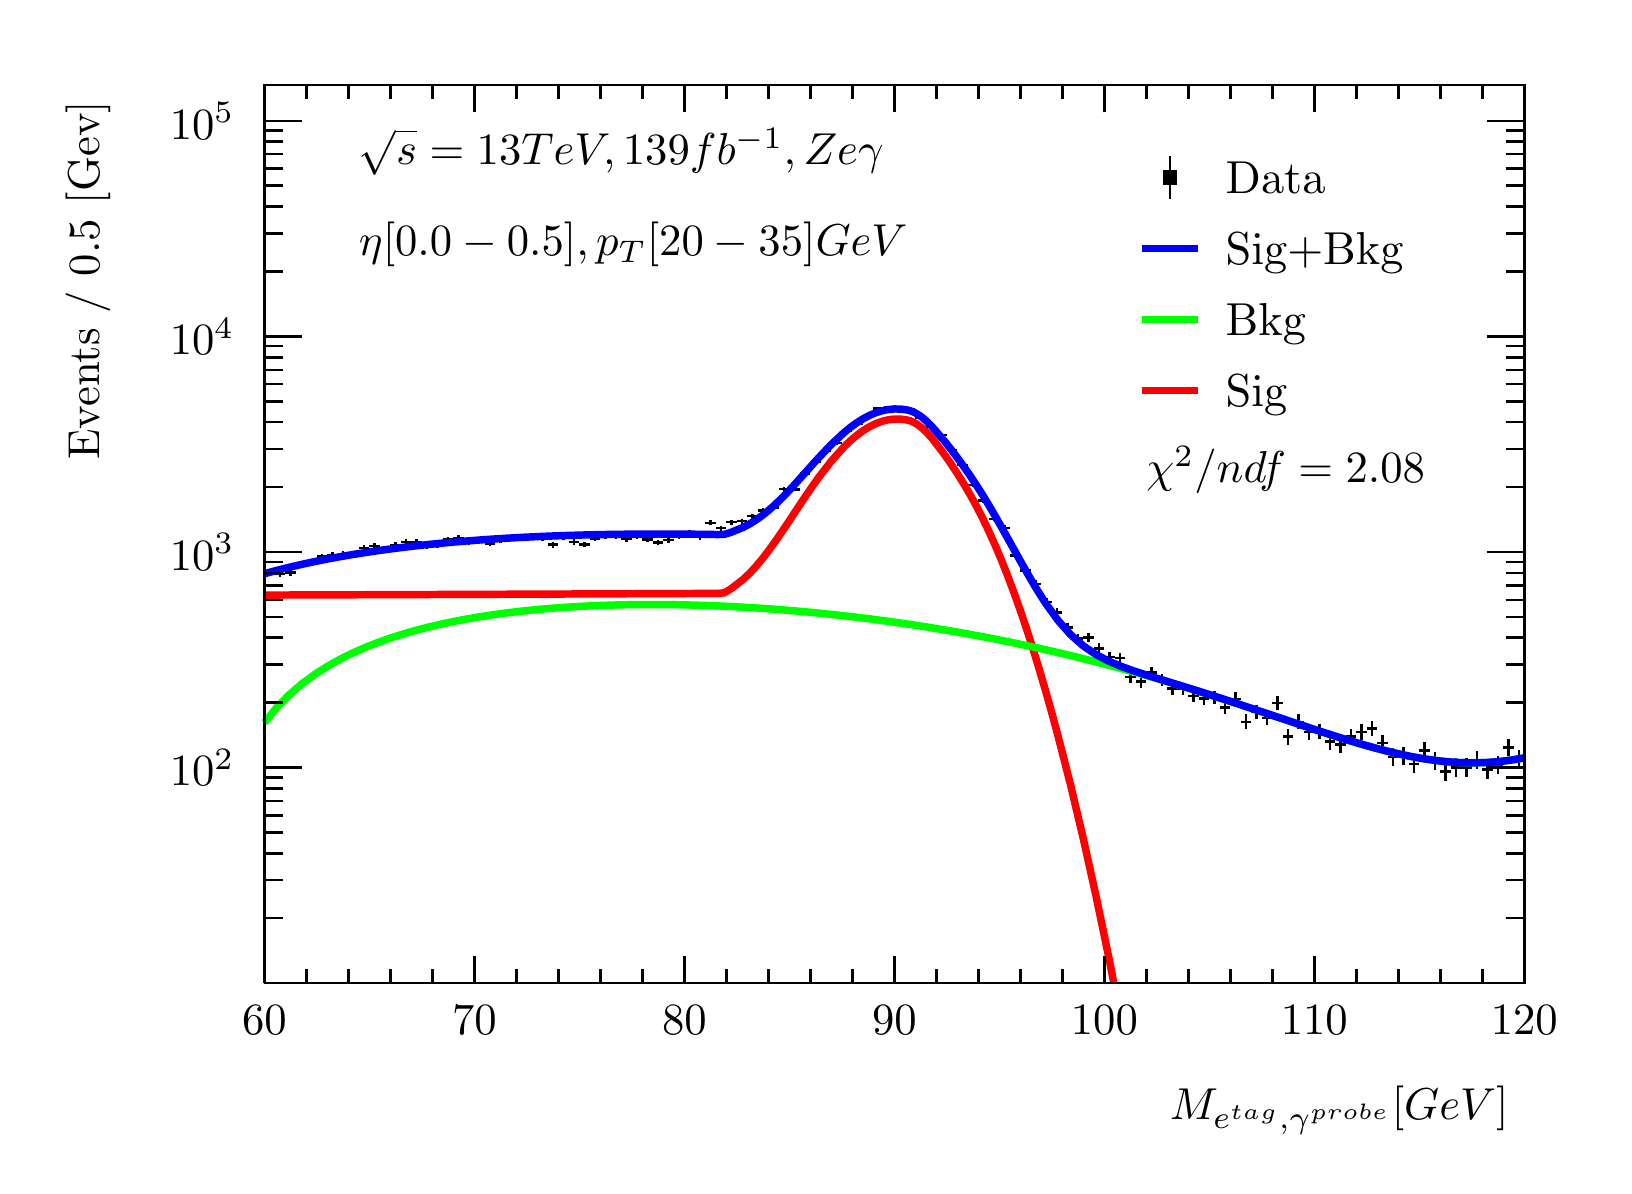
\begin{tikzpicture}
\pgfdeclareplotmark{cross} {
\pgfpathmoveto{\pgfpoint{-0.3\pgfplotmarksize}{\pgfplotmarksize}}
\pgfpathlineto{\pgfpoint{+0.3\pgfplotmarksize}{\pgfplotmarksize}}
\pgfpathlineto{\pgfpoint{+0.3\pgfplotmarksize}{0.3\pgfplotmarksize}}
\pgfpathlineto{\pgfpoint{+1\pgfplotmarksize}{0.3\pgfplotmarksize}}
\pgfpathlineto{\pgfpoint{+1\pgfplotmarksize}{-0.3\pgfplotmarksize}}
\pgfpathlineto{\pgfpoint{+0.3\pgfplotmarksize}{-0.3\pgfplotmarksize}}
\pgfpathlineto{\pgfpoint{+0.3\pgfplotmarksize}{-1.\pgfplotmarksize}}
\pgfpathlineto{\pgfpoint{-0.3\pgfplotmarksize}{-1.\pgfplotmarksize}}
\pgfpathlineto{\pgfpoint{-0.3\pgfplotmarksize}{-0.3\pgfplotmarksize}}
\pgfpathlineto{\pgfpoint{-1.\pgfplotmarksize}{-0.3\pgfplotmarksize}}
\pgfpathlineto{\pgfpoint{-1.\pgfplotmarksize}{0.3\pgfplotmarksize}}
\pgfpathlineto{\pgfpoint{-0.3\pgfplotmarksize}{0.3\pgfplotmarksize}}
\pgfpathclose
\pgfusepathqstroke
}
\pgfdeclareplotmark{cross*} {
\pgfpathmoveto{\pgfpoint{-0.3\pgfplotmarksize}{\pgfplotmarksize}}
\pgfpathlineto{\pgfpoint{+0.3\pgfplotmarksize}{\pgfplotmarksize}}
\pgfpathlineto{\pgfpoint{+0.3\pgfplotmarksize}{0.3\pgfplotmarksize}}
\pgfpathlineto{\pgfpoint{+1\pgfplotmarksize}{0.3\pgfplotmarksize}}
\pgfpathlineto{\pgfpoint{+1\pgfplotmarksize}{-0.3\pgfplotmarksize}}
\pgfpathlineto{\pgfpoint{+0.3\pgfplotmarksize}{-0.3\pgfplotmarksize}}
\pgfpathlineto{\pgfpoint{+0.3\pgfplotmarksize}{-1.\pgfplotmarksize}}
\pgfpathlineto{\pgfpoint{-0.3\pgfplotmarksize}{-1.\pgfplotmarksize}}
\pgfpathlineto{\pgfpoint{-0.3\pgfplotmarksize}{-0.3\pgfplotmarksize}}
\pgfpathlineto{\pgfpoint{-1.\pgfplotmarksize}{-0.3\pgfplotmarksize}}
\pgfpathlineto{\pgfpoint{-1.\pgfplotmarksize}{0.3\pgfplotmarksize}}
\pgfpathlineto{\pgfpoint{-0.3\pgfplotmarksize}{0.3\pgfplotmarksize}}
\pgfpathclose
\pgfusepathqfillstroke
}
\pgfdeclareplotmark{newstar} {
\pgfpathmoveto{\pgfqpoint{0pt}{\pgfplotmarksize}}
\pgfpathlineto{\pgfqpointpolar{44}{0.5\pgfplotmarksize}}
\pgfpathlineto{\pgfqpointpolar{18}{\pgfplotmarksize}}
\pgfpathlineto{\pgfqpointpolar{-20}{0.5\pgfplotmarksize}}
\pgfpathlineto{\pgfqpointpolar{-54}{\pgfplotmarksize}}
\pgfpathlineto{\pgfqpointpolar{-90}{0.5\pgfplotmarksize}}
\pgfpathlineto{\pgfqpointpolar{234}{\pgfplotmarksize}}
\pgfpathlineto{\pgfqpointpolar{198}{0.5\pgfplotmarksize}}
\pgfpathlineto{\pgfqpointpolar{162}{\pgfplotmarksize}}
\pgfpathlineto{\pgfqpointpolar{134}{0.5\pgfplotmarksize}}
\pgfpathclose
\pgfusepathqstroke
}
\pgfdeclareplotmark{newstar*} {
\pgfpathmoveto{\pgfqpoint{0pt}{\pgfplotmarksize}}
\pgfpathlineto{\pgfqpointpolar{44}{0.5\pgfplotmarksize}}
\pgfpathlineto{\pgfqpointpolar{18}{\pgfplotmarksize}}
\pgfpathlineto{\pgfqpointpolar{-20}{0.5\pgfplotmarksize}}
\pgfpathlineto{\pgfqpointpolar{-54}{\pgfplotmarksize}}
\pgfpathlineto{\pgfqpointpolar{-90}{0.5\pgfplotmarksize}}
\pgfpathlineto{\pgfqpointpolar{234}{\pgfplotmarksize}}
\pgfpathlineto{\pgfqpointpolar{198}{0.5\pgfplotmarksize}}
\pgfpathlineto{\pgfqpointpolar{162}{\pgfplotmarksize}}
\pgfpathlineto{\pgfqpointpolar{134}{0.5\pgfplotmarksize}}
\pgfpathclose
\pgfusepathqfillstroke
}
\definecolor{c}{rgb}{1,1,1};
\draw [color=c, fill=c] (0,0) rectangle (20,14.4361);
\draw [color=c, fill=c] (3,2.30977) rectangle (19,13.7143);
\definecolor{c}{rgb}{0,0,0};
\draw [c,line width=0.9] (3,2.30977) -- (3,13.7143) -- (19,13.7143) -- (19,2.30977) -- (3,2.30977);
\definecolor{c}{rgb}{1,1,1};
\draw [color=c, fill=c] (3,2.30977) rectangle (19,13.7143);
\definecolor{c}{rgb}{0,0,0};
\draw [c,line width=0.9] (3,2.30977) -- (3,13.7143) -- (19,13.7143) -- (19,2.30977) -- (3,2.30977);
\draw [c,line width=0.9] (3,2.30977) -- (19,2.30977);
\draw [c,line width=0.9] (3,2.65624) -- (3,2.30977);
\draw [c,line width=0.9] (3.53333,2.48301) -- (3.53333,2.30977);
\draw [c,line width=0.9] (4.06667,2.48301) -- (4.06667,2.30977);
\draw [c,line width=0.9] (4.6,2.48301) -- (4.6,2.30977);
\draw [c,line width=0.9] (5.13333,2.48301) -- (5.13333,2.30977);
\draw [c,line width=0.9] (5.66667,2.65624) -- (5.66667,2.30977);
\draw [c,line width=0.9] (6.2,2.48301) -- (6.2,2.30977);
\draw [c,line width=0.9] (6.73333,2.48301) -- (6.73333,2.30977);
\draw [c,line width=0.9] (7.26667,2.48301) -- (7.26667,2.30977);
\draw [c,line width=0.9] (7.8,2.48301) -- (7.8,2.30977);
\draw [c,line width=0.9] (8.33333,2.65624) -- (8.33333,2.30977);
\draw [c,line width=0.9] (8.86667,2.48301) -- (8.86667,2.30977);
\draw [c,line width=0.9] (9.4,2.48301) -- (9.4,2.30977);
\draw [c,line width=0.9] (9.93333,2.48301) -- (9.93333,2.30977);
\draw [c,line width=0.9] (10.4667,2.48301) -- (10.4667,2.30977);
\draw [c,line width=0.9] (11,2.65624) -- (11,2.30977);
\draw [c,line width=0.9] (11.5333,2.48301) -- (11.5333,2.30977);
\draw [c,line width=0.9] (12.0667,2.48301) -- (12.0667,2.30977);
\draw [c,line width=0.9] (12.6,2.48301) -- (12.6,2.30977);
\draw [c,line width=0.9] (13.1333,2.48301) -- (13.1333,2.30977);
\draw [c,line width=0.9] (13.6667,2.65624) -- (13.6667,2.30977);
\draw [c,line width=0.9] (14.2,2.48301) -- (14.2,2.30977);
\draw [c,line width=0.9] (14.7333,2.48301) -- (14.7333,2.30977);
\draw [c,line width=0.9] (15.2667,2.48301) -- (15.2667,2.30977);
\draw [c,line width=0.9] (15.8,2.48301) -- (15.8,2.30977);
\draw [c,line width=0.9] (16.3333,2.65624) -- (16.3333,2.30977);
\draw [c,line width=0.9] (16.8667,2.48301) -- (16.8667,2.30977);
\draw [c,line width=0.9] (17.4,2.48301) -- (17.4,2.30977);
\draw [c,line width=0.9] (17.9333,2.48301) -- (17.9333,2.30977);
\draw [c,line width=0.9] (18.4667,2.48301) -- (18.4667,2.30977);
\draw [c,line width=0.9] (19,2.65624) -- (19,2.30977);
\draw [anchor=base] (3,1.66015) node[scale=1.61424, color=c, rotate=0]{60};
\draw [anchor=base] (5.66667,1.66015) node[scale=1.61424, color=c, rotate=0]{70};
\draw [anchor=base] (8.33333,1.66015) node[scale=1.61424, color=c, rotate=0]{80};
\draw [anchor=base] (11,1.66015) node[scale=1.61424, color=c, rotate=0]{90};
\draw [anchor=base] (13.6667,1.66015) node[scale=1.61424, color=c, rotate=0]{100};
\draw [anchor=base] (16.3333,1.66015) node[scale=1.61424, color=c, rotate=0]{110};
\draw [anchor=base] (19,1.66015) node[scale=1.61424, color=c, rotate=0]{120};
\draw [anchor= east] (19,0.692932) node[scale=1.61424, color=c, rotate=0]{$M_{e^{tag}, \gamma^{probe}}  [GeV]$};
\draw [c,line width=0.9] (3,13.7143) -- (19,13.7143);
\draw [c,line width=0.9] (3,13.3678) -- (3,13.7143);
\draw [c,line width=0.9] (3.53333,13.5411) -- (3.53333,13.7143);
\draw [c,line width=0.9] (4.06667,13.5411) -- (4.06667,13.7143);
\draw [c,line width=0.9] (4.6,13.5411) -- (4.6,13.7143);
\draw [c,line width=0.9] (5.13333,13.5411) -- (5.13333,13.7143);
\draw [c,line width=0.9] (5.66667,13.3678) -- (5.66667,13.7143);
\draw [c,line width=0.9] (6.2,13.5411) -- (6.2,13.7143);
\draw [c,line width=0.9] (6.73333,13.5411) -- (6.73333,13.7143);
\draw [c,line width=0.9] (7.26667,13.5411) -- (7.26667,13.7143);
\draw [c,line width=0.9] (7.8,13.5411) -- (7.8,13.7143);
\draw [c,line width=0.9] (8.33333,13.3678) -- (8.33333,13.7143);
\draw [c,line width=0.9] (8.86667,13.5411) -- (8.86667,13.7143);
\draw [c,line width=0.9] (9.4,13.5411) -- (9.4,13.7143);
\draw [c,line width=0.9] (9.93333,13.5411) -- (9.93333,13.7143);
\draw [c,line width=0.9] (10.4667,13.5411) -- (10.4667,13.7143);
\draw [c,line width=0.9] (11,13.3678) -- (11,13.7143);
\draw [c,line width=0.9] (11.5333,13.5411) -- (11.5333,13.7143);
\draw [c,line width=0.9] (12.0667,13.5411) -- (12.0667,13.7143);
\draw [c,line width=0.9] (12.6,13.5411) -- (12.6,13.7143);
\draw [c,line width=0.9] (13.1333,13.5411) -- (13.1333,13.7143);
\draw [c,line width=0.9] (13.6667,13.3678) -- (13.6667,13.7143);
\draw [c,line width=0.9] (14.2,13.5411) -- (14.2,13.7143);
\draw [c,line width=0.9] (14.7333,13.5411) -- (14.7333,13.7143);
\draw [c,line width=0.9] (15.2667,13.5411) -- (15.2667,13.7143);
\draw [c,line width=0.9] (15.8,13.5411) -- (15.8,13.7143);
\draw [c,line width=0.9] (16.3333,13.3678) -- (16.3333,13.7143);
\draw [c,line width=0.9] (16.8667,13.5411) -- (16.8667,13.7143);
\draw [c,line width=0.9] (17.4,13.5411) -- (17.4,13.7143);
\draw [c,line width=0.9] (17.9333,13.5411) -- (17.9333,13.7143);
\draw [c,line width=0.9] (18.4667,13.5411) -- (18.4667,13.7143);
\draw [c,line width=0.9] (19,13.3678) -- (19,13.7143);
\draw [c,line width=0.9] (3,2.30977) -- (3,13.7143);
\draw [c,line width=0.9] (3.237,3.13385) -- (3,3.13385);
\draw [c,line width=0.9] (3.237,3.6159) -- (3,3.6159);
\draw [c,line width=0.9] (3.237,3.95792) -- (3,3.95792);
\draw [c,line width=0.9] (3.237,4.22321) -- (3,4.22321);
\draw [c,line width=0.9] (3.237,4.43997) -- (3,4.43997);
\draw [c,line width=0.9] (3.237,4.62324) -- (3,4.62324);
\draw [c,line width=0.9] (3.237,4.782) -- (3,4.782);
\draw [c,line width=0.9] (3.237,4.92203) -- (3,4.92203);
\draw [c,line width=0.9] (3.474,5.04729) -- (3,5.04729);
\draw [anchor= east] (2.82,5.04729) node[scale=1.61424, color=c, rotate=0]{$10^{2}$};
\draw [c,line width=0.9] (3.237,5.87136) -- (3,5.87136);
\draw [c,line width=0.9] (3.237,6.35342) -- (3,6.35342);
\draw [c,line width=0.9] (3.237,6.69544) -- (3,6.69544);
\draw [c,line width=0.9] (3.237,6.96073) -- (3,6.96073);
\draw [c,line width=0.9] (3.237,7.17749) -- (3,7.17749);
\draw [c,line width=0.9] (3.237,7.36076) -- (3,7.36076);
\draw [c,line width=0.9] (3.237,7.51951) -- (3,7.51951);
\draw [c,line width=0.9] (3.237,7.65954) -- (3,7.65954);
\draw [c,line width=0.9] (3.474,7.78481) -- (3,7.78481);
\draw [anchor= east] (2.82,7.78481) node[scale=1.61424, color=c, rotate=0]{$10^{3}$};
\draw [c,line width=0.9] (3.237,8.60888) -- (3,8.60888);
\draw [c,line width=0.9] (3.237,9.09093) -- (3,9.09093);
\draw [c,line width=0.9] (3.237,9.43296) -- (3,9.43296);
\draw [c,line width=0.9] (3.237,9.69825) -- (3,9.69825);
\draw [c,line width=0.9] (3.237,9.91501) -- (3,9.91501);
\draw [c,line width=0.9] (3.237,10.0983) -- (3,10.0983);
\draw [c,line width=0.9] (3.237,10.257) -- (3,10.257);
\draw [c,line width=0.9] (3.237,10.3971) -- (3,10.3971);
\draw [c,line width=0.9] (3.474,10.5223) -- (3,10.5223);
\draw [anchor= east] (2.82,10.5223) node[scale=1.61424, color=c, rotate=0]{$10^{4}$};
\draw [c,line width=0.9] (3.237,11.3464) -- (3,11.3464);
\draw [c,line width=0.9] (3.237,11.8285) -- (3,11.8285);
\draw [c,line width=0.9] (3.237,12.1705) -- (3,12.1705);
\draw [c,line width=0.9] (3.237,12.4358) -- (3,12.4358);
\draw [c,line width=0.9] (3.237,12.6525) -- (3,12.6525);
\draw [c,line width=0.9] (3.237,12.8358) -- (3,12.8358);
\draw [c,line width=0.9] (3.237,12.9945) -- (3,12.9945);
\draw [c,line width=0.9] (3.237,13.1346) -- (3,13.1346);
\draw [c,line width=0.9] (3.474,13.2598) -- (3,13.2598);
\draw [anchor= east] (2.82,13.2598) node[scale=1.61424, color=c, rotate=0]{$10^{5}$};
\draw [anchor= east] (0.76,13.7143) node[scale=1.61424, color=c, rotate=90]{Events / 0.5 [Gev]};
\draw [c,line width=0.9] (19,2.30977) -- (19,13.7143);
\draw [c,line width=0.9] (18.763,3.13385) -- (19,3.13385);
\draw [c,line width=0.9] (18.763,3.6159) -- (19,3.6159);
\draw [c,line width=0.9] (18.763,3.95792) -- (19,3.95792);
\draw [c,line width=0.9] (18.763,4.22321) -- (19,4.22321);
\draw [c,line width=0.9] (18.763,4.43997) -- (19,4.43997);
\draw [c,line width=0.9] (18.763,4.62324) -- (19,4.62324);
\draw [c,line width=0.9] (18.763,4.782) -- (19,4.782);
\draw [c,line width=0.9] (18.763,4.92203) -- (19,4.92203);
\draw [c,line width=0.9] (18.526,5.04729) -- (19,5.04729);
\draw [c,line width=0.9] (18.763,5.87136) -- (19,5.87136);
\draw [c,line width=0.9] (18.763,6.35342) -- (19,6.35342);
\draw [c,line width=0.9] (18.763,6.69544) -- (19,6.69544);
\draw [c,line width=0.9] (18.763,6.96073) -- (19,6.96073);
\draw [c,line width=0.9] (18.763,7.17749) -- (19,7.17749);
\draw [c,line width=0.9] (18.763,7.36076) -- (19,7.36076);
\draw [c,line width=0.9] (18.763,7.51951) -- (19,7.51951);
\draw [c,line width=0.9] (18.763,7.65954) -- (19,7.65954);
\draw [c,line width=0.9] (18.526,7.78481) -- (19,7.78481);
\draw [c,line width=0.9] (18.763,8.60888) -- (19,8.60888);
\draw [c,line width=0.9] (18.763,9.09093) -- (19,9.09093);
\draw [c,line width=0.9] (18.763,9.43296) -- (19,9.43296);
\draw [c,line width=0.9] (18.763,9.69825) -- (19,9.69825);
\draw [c,line width=0.9] (18.763,9.91501) -- (19,9.91501);
\draw [c,line width=0.9] (18.763,10.0983) -- (19,10.0983);
\draw [c,line width=0.9] (18.763,10.257) -- (19,10.257);
\draw [c,line width=0.9] (18.763,10.3971) -- (19,10.3971);
\draw [c,line width=0.9] (18.526,10.5223) -- (19,10.5223);
\draw [c,line width=0.9] (18.763,11.3464) -- (19,11.3464);
\draw [c,line width=0.9] (18.763,11.8285) -- (19,11.8285);
\draw [c,line width=0.9] (18.763,12.1705) -- (19,12.1705);
\draw [c,line width=0.9] (18.763,12.4358) -- (19,12.4358);
\draw [c,line width=0.9] (18.763,12.6525) -- (19,12.6525);
\draw [c,line width=0.9] (18.763,12.8358) -- (19,12.8358);
\draw [c,line width=0.9] (18.763,12.9945) -- (19,12.9945);
\draw [c,line width=0.9] (18.763,13.1346) -- (19,13.1346);
\draw [c,line width=0.9] (18.526,13.2598) -- (19,13.2598);
\draw [c,line width=0.9] (3.06667,7.51505) -- (3,7.51505);
\draw [c,line width=0.9] (3,7.51505) -- (3,7.51505);
\draw [c,line width=0.9] (3.06667,7.51505) -- (3.13333,7.51505);
\draw [c,line width=0.9] (3.13333,7.51505) -- (3.13333,7.51505);
\draw [c,line width=0.9] (3.06667,7.51505) -- (3.06667,7.55716);
\draw [c,line width=0.9] (3.06667,7.55716) -- (3.06667,7.55716);
\draw [c,line width=0.9] (3.06667,7.51505) -- (3.06667,7.47294);
\draw [c,line width=0.9] (3.06667,7.47294) -- (3.06667,7.47294);
\draw [c,line width=0.9] (3.2,7.50606) -- (3.13333,7.50606);
\draw [c,line width=0.9] (3.13333,7.50606) -- (3.13333,7.50606);
\draw [c,line width=0.9] (3.2,7.50606) -- (3.26667,7.50606);
\draw [c,line width=0.9] (3.26667,7.50606) -- (3.26667,7.50606);
\draw [c,line width=0.9] (3.2,7.50606) -- (3.2,7.54833);
\draw [c,line width=0.9] (3.2,7.54833) -- (3.2,7.54833);
\draw [c,line width=0.9] (3.2,7.50606) -- (3.2,7.46379);
\draw [c,line width=0.9] (3.2,7.46379) -- (3.2,7.46379);
\draw [c,line width=0.9] (3.33333,7.521) -- (3.26667,7.521);
\draw [c,line width=0.9] (3.26667,7.521) -- (3.26667,7.521);
\draw [c,line width=0.9] (3.33333,7.521) -- (3.4,7.521);
\draw [c,line width=0.9] (3.4,7.521) -- (3.4,7.521);
\draw [c,line width=0.9] (3.33333,7.521) -- (3.33333,7.563);
\draw [c,line width=0.9] (3.33333,7.563) -- (3.33333,7.563);
\draw [c,line width=0.9] (3.33333,7.521) -- (3.33333,7.47899);
\draw [c,line width=0.9] (3.33333,7.47899) -- (3.33333,7.47899);
\draw [c,line width=0.9] (3.46667,7.63012) -- (3.4,7.63012);
\draw [c,line width=0.9] (3.4,7.63012) -- (3.4,7.63012);
\draw [c,line width=0.9] (3.46667,7.63012) -- (3.53333,7.63012);
\draw [c,line width=0.9] (3.53333,7.63012) -- (3.53333,7.63012);
\draw [c,line width=0.9] (3.46667,7.63012) -- (3.46667,7.67024);
\draw [c,line width=0.9] (3.46667,7.67024) -- (3.46667,7.67024);
\draw [c,line width=0.9] (3.46667,7.63012) -- (3.46667,7.59);
\draw [c,line width=0.9] (3.46667,7.59) -- (3.46667,7.59);
\draw [c,line width=0.9] (3.6,7.65425) -- (3.53333,7.65425);
\draw [c,line width=0.9] (3.53333,7.65425) -- (3.53333,7.65425);
\draw [c,line width=0.9] (3.6,7.65425) -- (3.66667,7.65425);
\draw [c,line width=0.9] (3.66667,7.65425) -- (3.66667,7.65425);
\draw [c,line width=0.9] (3.6,7.65425) -- (3.6,7.69397);
\draw [c,line width=0.9] (3.6,7.69397) -- (3.6,7.69397);
\draw [c,line width=0.9] (3.6,7.65425) -- (3.6,7.61453);
\draw [c,line width=0.9] (3.6,7.61453) -- (3.6,7.61453);
\draw [c,line width=0.9] (3.73333,7.72633) -- (3.66667,7.72633);
\draw [c,line width=0.9] (3.66667,7.72633) -- (3.66667,7.72633);
\draw [c,line width=0.9] (3.73333,7.72633) -- (3.8,7.72633);
\draw [c,line width=0.9] (3.8,7.72633) -- (3.8,7.72633);
\draw [c,line width=0.9] (3.73333,7.72633) -- (3.73333,7.76486);
\draw [c,line width=0.9] (3.73333,7.76486) -- (3.73333,7.76486);
\draw [c,line width=0.9] (3.73333,7.72633) -- (3.73333,7.6878);
\draw [c,line width=0.9] (3.73333,7.6878) -- (3.73333,7.6878);
\draw [c,line width=0.9] (3.86667,7.73998) -- (3.8,7.73998);
\draw [c,line width=0.9] (3.8,7.73998) -- (3.8,7.73998);
\draw [c,line width=0.9] (3.86667,7.73998) -- (3.93333,7.73998);
\draw [c,line width=0.9] (3.93333,7.73998) -- (3.93333,7.73998);
\draw [c,line width=0.9] (3.86667,7.73998) -- (3.86667,7.77829);
\draw [c,line width=0.9] (3.86667,7.77829) -- (3.86667,7.77829);
\draw [c,line width=0.9] (3.86667,7.73998) -- (3.86667,7.70167);
\draw [c,line width=0.9] (3.86667,7.70167) -- (3.86667,7.70167);
\draw [c,line width=0.9] (4,7.75714) -- (3.93333,7.75714);
\draw [c,line width=0.9] (3.93333,7.75714) -- (3.93333,7.75714);
\draw [c,line width=0.9] (4,7.75714) -- (4.06667,7.75714);
\draw [c,line width=0.9] (4.06667,7.75714) -- (4.06667,7.75714);
\draw [c,line width=0.9] (4,7.75714) -- (4,7.79518);
\draw [c,line width=0.9] (4,7.79518) -- (4,7.79518);
\draw [c,line width=0.9] (4,7.75714) -- (4,7.71911);
\draw [c,line width=0.9] (4,7.71911) -- (4,7.71911);
\draw [c,line width=0.9] (4.13333,7.76079) -- (4.06667,7.76079);
\draw [c,line width=0.9] (4.06667,7.76079) -- (4.06667,7.76079);
\draw [c,line width=0.9] (4.13333,7.76079) -- (4.2,7.76079);
\draw [c,line width=0.9] (4.2,7.76079) -- (4.2,7.76079);
\draw [c,line width=0.9] (4.13333,7.76079) -- (4.13333,7.79876);
\draw [c,line width=0.9] (4.13333,7.79876) -- (4.13333,7.79876);
\draw [c,line width=0.9] (4.13333,7.76079) -- (4.13333,7.72281);
\draw [c,line width=0.9] (4.13333,7.72281) -- (4.13333,7.72281);
\draw [c,line width=0.9] (4.26667,7.83486) -- (4.2,7.83486);
\draw [c,line width=0.9] (4.2,7.83486) -- (4.2,7.83486);
\draw [c,line width=0.9] (4.26667,7.83486) -- (4.33333,7.83486);
\draw [c,line width=0.9] (4.33333,7.83486) -- (4.33333,7.83486);
\draw [c,line width=0.9] (4.26667,7.83486) -- (4.26667,7.87167);
\draw [c,line width=0.9] (4.26667,7.87167) -- (4.26667,7.87167);
\draw [c,line width=0.9] (4.26667,7.83486) -- (4.26667,7.79805);
\draw [c,line width=0.9] (4.26667,7.79805) -- (4.26667,7.79805);
\draw [c,line width=0.9] (4.4,7.85744) -- (4.33333,7.85744);
\draw [c,line width=0.9] (4.33333,7.85744) -- (4.33333,7.85744);
\draw [c,line width=0.9] (4.4,7.85744) -- (4.46667,7.85744);
\draw [c,line width=0.9] (4.46667,7.85744) -- (4.46667,7.85744);
\draw [c,line width=0.9] (4.4,7.85744) -- (4.4,7.89391);
\draw [c,line width=0.9] (4.4,7.89391) -- (4.4,7.89391);
\draw [c,line width=0.9] (4.4,7.85744) -- (4.4,7.82098);
\draw [c,line width=0.9] (4.4,7.82098) -- (4.4,7.82098);
\draw [c,line width=0.9] (4.53333,7.81995) -- (4.46667,7.81995);
\draw [c,line width=0.9] (4.46667,7.81995) -- (4.46667,7.81995);
\draw [c,line width=0.9] (4.53333,7.81995) -- (4.6,7.81995);
\draw [c,line width=0.9] (4.6,7.81995) -- (4.6,7.81995);
\draw [c,line width=0.9] (4.53333,7.81995) -- (4.53333,7.85699);
\draw [c,line width=0.9] (4.53333,7.85699) -- (4.53333,7.85699);
\draw [c,line width=0.9] (4.53333,7.81995) -- (4.53333,7.78291);
\draw [c,line width=0.9] (4.53333,7.78291) -- (4.53333,7.78291);
\draw [c,line width=0.9] (4.66667,7.86968) -- (4.6,7.86968);
\draw [c,line width=0.9] (4.6,7.86968) -- (4.6,7.86968);
\draw [c,line width=0.9] (4.66667,7.86968) -- (4.73333,7.86968);
\draw [c,line width=0.9] (4.73333,7.86968) -- (4.73333,7.86968);
\draw [c,line width=0.9] (4.66667,7.86968) -- (4.66667,7.90596);
\draw [c,line width=0.9] (4.66667,7.90596) -- (4.66667,7.90596);
\draw [c,line width=0.9] (4.66667,7.86968) -- (4.66667,7.83341);
\draw [c,line width=0.9] (4.66667,7.83341) -- (4.66667,7.83341);
\draw [c,line width=0.9] (4.8,7.91209) -- (4.73333,7.91209);
\draw [c,line width=0.9] (4.73333,7.91209) -- (4.73333,7.91209);
\draw [c,line width=0.9] (4.8,7.91209) -- (4.86667,7.91209);
\draw [c,line width=0.9] (4.86667,7.91209) -- (4.86667,7.91209);
\draw [c,line width=0.9] (4.8,7.91209) -- (4.8,7.94772);
\draw [c,line width=0.9] (4.8,7.94772) -- (4.8,7.94772);
\draw [c,line width=0.9] (4.8,7.91209) -- (4.8,7.87645);
\draw [c,line width=0.9] (4.8,7.87645) -- (4.8,7.87645);
\draw [c,line width=0.9] (4.93333,7.90995) -- (4.86667,7.90995);
\draw [c,line width=0.9] (4.86667,7.90995) -- (4.86667,7.90995);
\draw [c,line width=0.9] (4.93333,7.90995) -- (5,7.90995);
\draw [c,line width=0.9] (5,7.90995) -- (5,7.90995);
\draw [c,line width=0.9] (4.93333,7.90995) -- (4.93333,7.94562);
\draw [c,line width=0.9] (4.93333,7.94562) -- (4.93333,7.94562);
\draw [c,line width=0.9] (4.93333,7.90995) -- (4.93333,7.87428);
\draw [c,line width=0.9] (4.93333,7.87428) -- (4.93333,7.87428);
\draw [c,line width=0.9] (5.06667,7.85408) -- (5,7.85408);
\draw [c,line width=0.9] (5,7.85408) -- (5,7.85408);
\draw [c,line width=0.9] (5.06667,7.85408) -- (5.13333,7.85408);
\draw [c,line width=0.9] (5.13333,7.85408) -- (5.13333,7.85408);
\draw [c,line width=0.9] (5.06667,7.85408) -- (5.06667,7.8906);
\draw [c,line width=0.9] (5.06667,7.8906) -- (5.06667,7.8906);
\draw [c,line width=0.9] (5.06667,7.85408) -- (5.06667,7.81757);
\draw [c,line width=0.9] (5.06667,7.81757) -- (5.06667,7.81757);
\draw [c,line width=0.9] (5.2,7.87189) -- (5.13333,7.87189);
\draw [c,line width=0.9] (5.13333,7.87189) -- (5.13333,7.87189);
\draw [c,line width=0.9] (5.2,7.87189) -- (5.26667,7.87189);
\draw [c,line width=0.9] (5.26667,7.87189) -- (5.26667,7.87189);
\draw [c,line width=0.9] (5.2,7.87189) -- (5.2,7.90814);
\draw [c,line width=0.9] (5.2,7.90814) -- (5.2,7.90814);
\draw [c,line width=0.9] (5.2,7.87189) -- (5.2,7.83565);
\draw [c,line width=0.9] (5.2,7.83565) -- (5.2,7.83565);
\draw [c,line width=0.9] (5.33333,7.94163) -- (5.26667,7.94163);
\draw [c,line width=0.9] (5.26667,7.94163) -- (5.26667,7.94163);
\draw [c,line width=0.9] (5.33333,7.94163) -- (5.4,7.94163);
\draw [c,line width=0.9] (5.4,7.94163) -- (5.4,7.94163);
\draw [c,line width=0.9] (5.33333,7.94163) -- (5.33333,7.97682);
\draw [c,line width=0.9] (5.33333,7.97682) -- (5.33333,7.97682);
\draw [c,line width=0.9] (5.33333,7.94163) -- (5.33333,7.90643);
\draw [c,line width=0.9] (5.33333,7.90643) -- (5.33333,7.90643);
\draw [c,line width=0.9] (5.46667,7.96229) -- (5.4,7.96229);
\draw [c,line width=0.9] (5.4,7.96229) -- (5.4,7.96229);
\draw [c,line width=0.9] (5.46667,7.96229) -- (5.53333,7.96229);
\draw [c,line width=0.9] (5.53333,7.96229) -- (5.53333,7.96229);
\draw [c,line width=0.9] (5.46667,7.96229) -- (5.46667,7.99718);
\draw [c,line width=0.9] (5.46667,7.99718) -- (5.46667,7.99718);
\draw [c,line width=0.9] (5.46667,7.96229) -- (5.46667,7.9274);
\draw [c,line width=0.9] (5.46667,7.9274) -- (5.46667,7.9274);
\draw [c,line width=0.9] (5.6,7.91422) -- (5.53333,7.91422);
\draw [c,line width=0.9] (5.53333,7.91422) -- (5.53333,7.91422);
\draw [c,line width=0.9] (5.6,7.91422) -- (5.66667,7.91422);
\draw [c,line width=0.9] (5.66667,7.91422) -- (5.66667,7.91422);
\draw [c,line width=0.9] (5.6,7.91422) -- (5.6,7.94983);
\draw [c,line width=0.9] (5.6,7.94983) -- (5.6,7.94983);
\draw [c,line width=0.9] (5.6,7.91422) -- (5.6,7.87862);
\draw [c,line width=0.9] (5.6,7.87862) -- (5.6,7.87862);
\draw [c,line width=0.9] (5.73333,7.93221) -- (5.66667,7.93221);
\draw [c,line width=0.9] (5.66667,7.93221) -- (5.66667,7.93221);
\draw [c,line width=0.9] (5.73333,7.93221) -- (5.8,7.93221);
\draw [c,line width=0.9] (5.8,7.93221) -- (5.8,7.93221);
\draw [c,line width=0.9] (5.73333,7.93221) -- (5.73333,7.96755);
\draw [c,line width=0.9] (5.73333,7.96755) -- (5.73333,7.96755);
\draw [c,line width=0.9] (5.73333,7.93221) -- (5.73333,7.89688);
\draw [c,line width=0.9] (5.73333,7.89688) -- (5.73333,7.89688);
\draw [c,line width=0.9] (5.86667,7.89487) -- (5.8,7.89487);
\draw [c,line width=0.9] (5.8,7.89487) -- (5.8,7.89487);
\draw [c,line width=0.9] (5.86667,7.89487) -- (5.93333,7.89487);
\draw [c,line width=0.9] (5.93333,7.89487) -- (5.93333,7.89487);
\draw [c,line width=0.9] (5.86667,7.89487) -- (5.86667,7.93077);
\draw [c,line width=0.9] (5.86667,7.93077) -- (5.86667,7.93077);
\draw [c,line width=0.9] (5.86667,7.89487) -- (5.86667,7.85898);
\draw [c,line width=0.9] (5.86667,7.85898) -- (5.86667,7.85898);
\draw [c,line width=0.9] (6,7.9385) -- (5.93333,7.9385);
\draw [c,line width=0.9] (5.93333,7.9385) -- (5.93333,7.9385);
\draw [c,line width=0.9] (6,7.9385) -- (6.06667,7.9385);
\draw [c,line width=0.9] (6.06667,7.9385) -- (6.06667,7.9385);
\draw [c,line width=0.9] (6,7.9385) -- (6,7.97374);
\draw [c,line width=0.9] (6,7.97374) -- (6,7.97374);
\draw [c,line width=0.9] (6,7.9385) -- (6,7.90326);
\draw [c,line width=0.9] (6,7.90326) -- (6,7.90326);
\draw [c,line width=0.9] (6.13333,7.95303) -- (6.06667,7.95303);
\draw [c,line width=0.9] (6.06667,7.95303) -- (6.06667,7.95303);
\draw [c,line width=0.9] (6.13333,7.95303) -- (6.2,7.95303);
\draw [c,line width=0.9] (6.2,7.95303) -- (6.2,7.95303);
\draw [c,line width=0.9] (6.13333,7.95303) -- (6.13333,7.98806);
\draw [c,line width=0.9] (6.13333,7.98806) -- (6.13333,7.98806);
\draw [c,line width=0.9] (6.13333,7.95303) -- (6.13333,7.91801);
\draw [c,line width=0.9] (6.13333,7.91801) -- (6.13333,7.91801);
\draw [c,line width=0.9] (6.26667,7.9551) -- (6.2,7.9551);
\draw [c,line width=0.9] (6.2,7.9551) -- (6.2,7.9551);
\draw [c,line width=0.9] (6.26667,7.9551) -- (6.33333,7.9551);
\draw [c,line width=0.9] (6.33333,7.9551) -- (6.33333,7.9551);
\draw [c,line width=0.9] (6.26667,7.9551) -- (6.26667,7.99009);
\draw [c,line width=0.9] (6.26667,7.99009) -- (6.26667,7.99009);
\draw [c,line width=0.9] (6.26667,7.9551) -- (6.26667,7.9201);
\draw [c,line width=0.9] (6.26667,7.9201) -- (6.26667,7.9201);
\draw [c,line width=0.9] (6.4,7.99361) -- (6.33333,7.99361);
\draw [c,line width=0.9] (6.33333,7.99361) -- (6.33333,7.99361);
\draw [c,line width=0.9] (6.4,7.99361) -- (6.46667,7.99361);
\draw [c,line width=0.9] (6.46667,7.99361) -- (6.46667,7.99361);
\draw [c,line width=0.9] (6.4,7.99361) -- (6.4,8.02805);
\draw [c,line width=0.9] (6.4,8.02805) -- (6.4,8.02805);
\draw [c,line width=0.9] (6.4,7.99361) -- (6.4,7.95918);
\draw [c,line width=0.9] (6.4,7.95918) -- (6.4,7.95918);
\draw [c,line width=0.9] (6.53333,7.96433) -- (6.46667,7.96433);
\draw [c,line width=0.9] (6.46667,7.96433) -- (6.46667,7.96433);
\draw [c,line width=0.9] (6.53333,7.96433) -- (6.6,7.96433);
\draw [c,line width=0.9] (6.6,7.96433) -- (6.6,7.96433);
\draw [c,line width=0.9] (6.53333,7.96433) -- (6.53333,7.99919);
\draw [c,line width=0.9] (6.53333,7.99919) -- (6.53333,7.99919);
\draw [c,line width=0.9] (6.53333,7.96433) -- (6.53333,7.92947);
\draw [c,line width=0.9] (6.53333,7.92947) -- (6.53333,7.92947);
\draw [c,line width=0.9] (6.66667,7.87631) -- (6.6,7.87631);
\draw [c,line width=0.9] (6.6,7.87631) -- (6.6,7.87631);
\draw [c,line width=0.9] (6.66667,7.87631) -- (6.73333,7.87631);
\draw [c,line width=0.9] (6.73333,7.87631) -- (6.73333,7.87631);
\draw [c,line width=0.9] (6.66667,7.87631) -- (6.66667,7.91248);
\draw [c,line width=0.9] (6.66667,7.91248) -- (6.66667,7.91248);
\draw [c,line width=0.9] (6.66667,7.87631) -- (6.66667,7.84013);
\draw [c,line width=0.9] (6.66667,7.84013) -- (6.66667,7.84013);
\draw [c,line width=0.9] (6.8,7.97552) -- (6.73333,7.97552);
\draw [c,line width=0.9] (6.73333,7.97552) -- (6.73333,7.97552);
\draw [c,line width=0.9] (6.8,7.97552) -- (6.86667,7.97552);
\draw [c,line width=0.9] (6.86667,7.97552) -- (6.86667,7.97552);
\draw [c,line width=0.9] (6.8,7.97552) -- (6.8,8.01022);
\draw [c,line width=0.9] (6.8,8.01022) -- (6.8,8.01022);
\draw [c,line width=0.9] (6.8,7.97552) -- (6.8,7.94083);
\draw [c,line width=0.9] (6.8,7.94083) -- (6.8,7.94083);
\draw [c,line width=0.9] (6.93333,7.90888) -- (6.86667,7.90888);
\draw [c,line width=0.9] (6.86667,7.90888) -- (6.86667,7.90888);
\draw [c,line width=0.9] (6.93333,7.90888) -- (7,7.90888);
\draw [c,line width=0.9] (7,7.90888) -- (7,7.90888);
\draw [c,line width=0.9] (6.93333,7.90888) -- (6.93333,7.94456);
\draw [c,line width=0.9] (6.93333,7.94456) -- (6.93333,7.94456);
\draw [c,line width=0.9] (6.93333,7.90888) -- (6.93333,7.8732);
\draw [c,line width=0.9] (6.93333,7.8732) -- (6.93333,7.8732);
\draw [c,line width=0.9] (7.06667,7.87851) -- (7,7.87851);
\draw [c,line width=0.9] (7,7.87851) -- (7,7.87851);
\draw [c,line width=0.9] (7.06667,7.87851) -- (7.13333,7.87851);
\draw [c,line width=0.9] (7.13333,7.87851) -- (7.13333,7.87851);
\draw [c,line width=0.9] (7.06667,7.87851) -- (7.06667,7.91465);
\draw [c,line width=0.9] (7.06667,7.91465) -- (7.06667,7.91465);
\draw [c,line width=0.9] (7.06667,7.87851) -- (7.06667,7.84236);
\draw [c,line width=0.9] (7.06667,7.84236) -- (7.06667,7.84236);
\draw [c,line width=0.9] (7.2,7.95716) -- (7.13333,7.95716);
\draw [c,line width=0.9] (7.13333,7.95716) -- (7.13333,7.95716);
\draw [c,line width=0.9] (7.2,7.95716) -- (7.26667,7.95716);
\draw [c,line width=0.9] (7.26667,7.95716) -- (7.26667,7.95716);
\draw [c,line width=0.9] (7.2,7.95716) -- (7.2,7.99212);
\draw [c,line width=0.9] (7.2,7.99212) -- (7.2,7.99212);
\draw [c,line width=0.9] (7.2,7.95716) -- (7.2,7.92219);
\draw [c,line width=0.9] (7.2,7.92219) -- (7.2,7.92219);
\draw [c,line width=0.9] (7.33333,7.97957) -- (7.26667,7.97957);
\draw [c,line width=0.9] (7.26667,7.97957) -- (7.26667,7.97957);
\draw [c,line width=0.9] (7.33333,7.97957) -- (7.4,7.97957);
\draw [c,line width=0.9] (7.4,7.97957) -- (7.4,7.97957);
\draw [c,line width=0.9] (7.33333,7.97957) -- (7.33333,8.01421);
\draw [c,line width=0.9] (7.33333,8.01421) -- (7.33333,8.01421);
\draw [c,line width=0.9] (7.33333,7.97957) -- (7.33333,7.94493);
\draw [c,line width=0.9] (7.33333,7.94493) -- (7.33333,7.94493);
\draw [c,line width=0.9] (7.46667,7.97755) -- (7.4,7.97755);
\draw [c,line width=0.9] (7.4,7.97755) -- (7.4,7.97755);
\draw [c,line width=0.9] (7.46667,7.97755) -- (7.53333,7.97755);
\draw [c,line width=0.9] (7.53333,7.97755) -- (7.53333,7.97755);
\draw [c,line width=0.9] (7.46667,7.97755) -- (7.46667,8.01222);
\draw [c,line width=0.9] (7.46667,8.01222) -- (7.46667,8.01222);
\draw [c,line width=0.9] (7.46667,7.97755) -- (7.46667,7.94288);
\draw [c,line width=0.9] (7.46667,7.94288) -- (7.46667,7.94288);
\draw [c,line width=0.9] (7.6,7.94683) -- (7.53333,7.94683);
\draw [c,line width=0.9] (7.53333,7.94683) -- (7.53333,7.94683);
\draw [c,line width=0.9] (7.6,7.94683) -- (7.66667,7.94683);
\draw [c,line width=0.9] (7.66667,7.94683) -- (7.66667,7.94683);
\draw [c,line width=0.9] (7.6,7.94683) -- (7.6,7.98194);
\draw [c,line width=0.9] (7.6,7.98194) -- (7.6,7.98194);
\draw [c,line width=0.9] (7.6,7.94683) -- (7.6,7.91171);
\draw [c,line width=0.9] (7.6,7.91171) -- (7.6,7.91171);
\draw [c,line width=0.9] (7.73333,7.98159) -- (7.66667,7.98159);
\draw [c,line width=0.9] (7.66667,7.98159) -- (7.66667,7.98159);
\draw [c,line width=0.9] (7.73333,7.98159) -- (7.8,7.98159);
\draw [c,line width=0.9] (7.8,7.98159) -- (7.8,7.98159);
\draw [c,line width=0.9] (7.73333,7.98159) -- (7.73333,8.01619);
\draw [c,line width=0.9] (7.73333,8.01619) -- (7.73333,8.01619);
\draw [c,line width=0.9] (7.73333,7.98159) -- (7.73333,7.94698);
\draw [c,line width=0.9] (7.73333,7.94698) -- (7.73333,7.94698);
\draw [c,line width=0.9] (7.86667,7.94475) -- (7.8,7.94475);
\draw [c,line width=0.9] (7.8,7.94475) -- (7.8,7.94475);
\draw [c,line width=0.9] (7.86667,7.94475) -- (7.93333,7.94475);
\draw [c,line width=0.9] (7.93333,7.94475) -- (7.93333,7.94475);
\draw [c,line width=0.9] (7.86667,7.94475) -- (7.86667,7.9799);
\draw [c,line width=0.9] (7.86667,7.9799) -- (7.86667,7.9799);
\draw [c,line width=0.9] (7.86667,7.94475) -- (7.86667,7.9096);
\draw [c,line width=0.9] (7.86667,7.9096) -- (7.86667,7.9096);
\draw [c,line width=0.9] (8,7.90351) -- (7.93333,7.90351);
\draw [c,line width=0.9] (7.93333,7.90351) -- (7.93333,7.90351);
\draw [c,line width=0.9] (8,7.90351) -- (8.06667,7.90351);
\draw [c,line width=0.9] (8.06667,7.90351) -- (8.06667,7.90351);
\draw [c,line width=0.9] (8,7.90351) -- (8,7.93928);
\draw [c,line width=0.9] (8,7.93928) -- (8,7.93928);
\draw [c,line width=0.9] (8,7.90351) -- (8,7.86775);
\draw [c,line width=0.9] (8,7.86775) -- (8,7.86775);
\draw [c,line width=0.9] (8.13333,7.93536) -- (8.06667,7.93536);
\draw [c,line width=0.9] (8.06667,7.93536) -- (8.06667,7.93536);
\draw [c,line width=0.9] (8.13333,7.93536) -- (8.2,7.93536);
\draw [c,line width=0.9] (8.2,7.93536) -- (8.2,7.93536);
\draw [c,line width=0.9] (8.13333,7.93536) -- (8.13333,7.97065);
\draw [c,line width=0.9] (8.13333,7.97065) -- (8.13333,7.97065);
\draw [c,line width=0.9] (8.13333,7.93536) -- (8.13333,7.90007);
\draw [c,line width=0.9] (8.13333,7.90007) -- (8.13333,7.90007);
\draw [c,line width=0.9] (8.26667,7.98259) -- (8.2,7.98259);
\draw [c,line width=0.9] (8.2,7.98259) -- (8.2,7.98259);
\draw [c,line width=0.9] (8.26667,7.98259) -- (8.33333,7.98259);
\draw [c,line width=0.9] (8.33333,7.98259) -- (8.33333,7.98259);
\draw [c,line width=0.9] (8.26667,7.98259) -- (8.26667,8.01719);
\draw [c,line width=0.9] (8.26667,8.01719) -- (8.26667,8.01719);
\draw [c,line width=0.9] (8.26667,7.98259) -- (8.26667,7.948);
\draw [c,line width=0.9] (8.26667,7.948) -- (8.26667,7.948);
\draw [c,line width=0.9] (8.4,8.03092) -- (8.33333,8.03092);
\draw [c,line width=0.9] (8.33333,8.03092) -- (8.33333,8.03092);
\draw [c,line width=0.9] (8.4,8.03092) -- (8.46667,8.03092);
\draw [c,line width=0.9] (8.46667,8.03092) -- (8.46667,8.03092);
\draw [c,line width=0.9] (8.4,8.03092) -- (8.4,8.06482);
\draw [c,line width=0.9] (8.4,8.06482) -- (8.4,8.06482);
\draw [c,line width=0.9] (8.4,8.03092) -- (8.4,7.99703);
\draw [c,line width=0.9] (8.4,7.99703) -- (8.4,7.99703);
\draw [c,line width=0.9] (8.53333,7.97248) -- (8.46667,7.97248);
\draw [c,line width=0.9] (8.46667,7.97248) -- (8.46667,7.97248);
\draw [c,line width=0.9] (8.53333,7.97248) -- (8.6,7.97248);
\draw [c,line width=0.9] (8.6,7.97248) -- (8.6,7.97248);
\draw [c,line width=0.9] (8.53333,7.97248) -- (8.53333,8.00722);
\draw [c,line width=0.9] (8.53333,8.00722) -- (8.53333,8.00722);
\draw [c,line width=0.9] (8.53333,7.97248) -- (8.53333,7.93774);
\draw [c,line width=0.9] (8.53333,7.93774) -- (8.53333,7.93774);
\draw [c,line width=0.9] (8.66667,8.15299) -- (8.6,8.15299);
\draw [c,line width=0.9] (8.6,8.15299) -- (8.6,8.15299);
\draw [c,line width=0.9] (8.66667,8.15299) -- (8.73333,8.15299);
\draw [c,line width=0.9] (8.73333,8.15299) -- (8.73333,8.15299);
\draw [c,line width=0.9] (8.66667,8.15299) -- (8.66667,8.18519);
\draw [c,line width=0.9] (8.66667,8.18519) -- (8.66667,8.18519);
\draw [c,line width=0.9] (8.66667,8.15299) -- (8.66667,8.12079);
\draw [c,line width=0.9] (8.66667,8.12079) -- (8.66667,8.12079);
\draw [c,line width=0.9] (8.8,8.0857) -- (8.73333,8.0857);
\draw [c,line width=0.9] (8.73333,8.0857) -- (8.73333,8.0857);
\draw [c,line width=0.9] (8.8,8.0857) -- (8.86667,8.0857);
\draw [c,line width=0.9] (8.86667,8.0857) -- (8.86667,8.0857);
\draw [c,line width=0.9] (8.8,8.0857) -- (8.8,8.11883);
\draw [c,line width=0.9] (8.8,8.11883) -- (8.8,8.11883);
\draw [c,line width=0.9] (8.8,8.0857) -- (8.8,8.05258);
\draw [c,line width=0.9] (8.8,8.05258) -- (8.8,8.05258);
\draw [c,line width=0.9] (8.93333,8.16341) -- (8.86667,8.16341);
\draw [c,line width=0.9] (8.86667,8.16341) -- (8.86667,8.16341);
\draw [c,line width=0.9] (8.93333,8.16341) -- (9,8.16341);
\draw [c,line width=0.9] (9,8.16341) -- (9,8.16341);
\draw [c,line width=0.9] (8.93333,8.16341) -- (8.93333,8.19547);
\draw [c,line width=0.9] (8.93333,8.19547) -- (8.93333,8.19547);
\draw [c,line width=0.9] (8.93333,8.16341) -- (8.93333,8.13135);
\draw [c,line width=0.9] (8.93333,8.13135) -- (8.93333,8.13135);
\draw [c,line width=0.9] (9.06667,8.17717) -- (9,8.17717);
\draw [c,line width=0.9] (9,8.17717) -- (9,8.17717);
\draw [c,line width=0.9] (9.06667,8.17717) -- (9.13333,8.17717);
\draw [c,line width=0.9] (9.13333,8.17717) -- (9.13333,8.17717);
\draw [c,line width=0.9] (9.06667,8.17717) -- (9.06667,8.20904);
\draw [c,line width=0.9] (9.06667,8.20904) -- (9.06667,8.20904);
\draw [c,line width=0.9] (9.06667,8.17717) -- (9.06667,8.14529);
\draw [c,line width=0.9] (9.06667,8.14529) -- (9.06667,8.14529);
\draw [c,line width=0.9] (9.2,8.23879) -- (9.13333,8.23879);
\draw [c,line width=0.9] (9.13333,8.23879) -- (9.13333,8.23879);
\draw [c,line width=0.9] (9.2,8.23879) -- (9.26667,8.23879);
\draw [c,line width=0.9] (9.26667,8.23879) -- (9.26667,8.23879);
\draw [c,line width=0.9] (9.2,8.23879) -- (9.2,8.26985);
\draw [c,line width=0.9] (9.2,8.26985) -- (9.2,8.26985);
\draw [c,line width=0.9] (9.2,8.23879) -- (9.2,8.20773);
\draw [c,line width=0.9] (9.2,8.20773) -- (9.2,8.20773);
\draw [c,line width=0.9] (9.33333,8.31273) -- (9.26667,8.31273);
\draw [c,line width=0.9] (9.26667,8.31273) -- (9.26667,8.31273);
\draw [c,line width=0.9] (9.33333,8.31273) -- (9.4,8.31273);
\draw [c,line width=0.9] (9.4,8.31273) -- (9.4,8.31273);
\draw [c,line width=0.9] (9.33333,8.31273) -- (9.33333,8.34284);
\draw [c,line width=0.9] (9.33333,8.34284) -- (9.33333,8.34284);
\draw [c,line width=0.9] (9.33333,8.31273) -- (9.33333,8.28262);
\draw [c,line width=0.9] (9.33333,8.28262) -- (9.33333,8.28262);
\draw [c,line width=0.9] (9.46667,8.351) -- (9.4,8.351);
\draw [c,line width=0.9] (9.4,8.351) -- (9.4,8.351);
\draw [c,line width=0.9] (9.46667,8.351) -- (9.53333,8.351);
\draw [c,line width=0.9] (9.53333,8.351) -- (9.53333,8.351);
\draw [c,line width=0.9] (9.46667,8.351) -- (9.46667,8.38063);
\draw [c,line width=0.9] (9.46667,8.38063) -- (9.46667,8.38063);
\draw [c,line width=0.9] (9.46667,8.351) -- (9.46667,8.32137);
\draw [c,line width=0.9] (9.46667,8.32137) -- (9.46667,8.32137);
\draw [c,line width=0.9] (9.6,8.58365) -- (9.53333,8.58365);
\draw [c,line width=0.9] (9.53333,8.58365) -- (9.53333,8.58365);
\draw [c,line width=0.9] (9.6,8.58365) -- (9.66667,8.58365);
\draw [c,line width=0.9] (9.66667,8.58365) -- (9.66667,8.58365);
\draw [c,line width=0.9] (9.6,8.58365) -- (9.6,8.61052);
\draw [c,line width=0.9] (9.6,8.61052) -- (9.6,8.61052);
\draw [c,line width=0.9] (9.6,8.58365) -- (9.6,8.55678);
\draw [c,line width=0.9] (9.6,8.55678) -- (9.6,8.55678);
\draw [c,line width=0.9] (9.73333,8.58) -- (9.66667,8.58);
\draw [c,line width=0.9] (9.66667,8.58) -- (9.66667,8.58);
\draw [c,line width=0.9] (9.73333,8.58) -- (9.8,8.58);
\draw [c,line width=0.9] (9.8,8.58) -- (9.8,8.58);
\draw [c,line width=0.9] (9.73333,8.58) -- (9.73333,8.60691);
\draw [c,line width=0.9] (9.73333,8.60691) -- (9.73333,8.60691);
\draw [c,line width=0.9] (9.73333,8.58) -- (9.73333,8.55309);
\draw [c,line width=0.9] (9.73333,8.55309) -- (9.73333,8.55309);
\draw [c,line width=0.9] (9.86667,8.77917) -- (9.8,8.77917);
\draw [c,line width=0.9] (9.8,8.77917) -- (9.8,8.77917);
\draw [c,line width=0.9] (9.86667,8.77917) -- (9.93333,8.77917);
\draw [c,line width=0.9] (9.93333,8.77917) -- (9.93333,8.77917);
\draw [c,line width=0.9] (9.86667,8.77917) -- (9.86667,8.80392);
\draw [c,line width=0.9] (9.86667,8.80392) -- (9.86667,8.80392);
\draw [c,line width=0.9] (9.86667,8.77917) -- (9.86667,8.75443);
\draw [c,line width=0.9] (9.86667,8.75443) -- (9.86667,8.75443);
\draw [c,line width=0.9] (10,8.92491) -- (9.93333,8.92491);
\draw [c,line width=0.9] (9.93333,8.92491) -- (9.93333,8.92491);
\draw [c,line width=0.9] (10,8.92491) -- (10.0667,8.92491);
\draw [c,line width=0.9] (10.0667,8.92491) -- (10.0667,8.92491);
\draw [c,line width=0.9] (10,8.92491) -- (10,8.94819);
\draw [c,line width=0.9] (10,8.94819) -- (10,8.94819);
\draw [c,line width=0.9] (10,8.92491) -- (10,8.90164);
\draw [c,line width=0.9] (10,8.90164) -- (10,8.90164);
\draw [c,line width=0.9] (10.1333,9.0653) -- (10.0667,9.0653);
\draw [c,line width=0.9] (10.0667,9.0653) -- (10.0667,9.0653);
\draw [c,line width=0.9] (10.1333,9.0653) -- (10.2,9.0653);
\draw [c,line width=0.9] (10.2,9.0653) -- (10.2,9.0653);
\draw [c,line width=0.9] (10.1333,9.0653) -- (10.1333,9.08724);
\draw [c,line width=0.9] (10.1333,9.08724) -- (10.1333,9.08724);
\draw [c,line width=0.9] (10.1333,9.0653) -- (10.1333,9.04336);
\draw [c,line width=0.9] (10.1333,9.04336) -- (10.1333,9.04336);
\draw [c,line width=0.9] (10.2667,9.16915) -- (10.2,9.16915);
\draw [c,line width=0.9] (10.2,9.16915) -- (10.2,9.16915);
\draw [c,line width=0.9] (10.2667,9.16915) -- (10.3333,9.16915);
\draw [c,line width=0.9] (10.3333,9.16915) -- (10.3333,9.16915);
\draw [c,line width=0.9] (10.2667,9.16915) -- (10.2667,9.19015);
\draw [c,line width=0.9] (10.2667,9.19015) -- (10.2667,9.19015);
\draw [c,line width=0.9] (10.2667,9.16915) -- (10.2667,9.14815);
\draw [c,line width=0.9] (10.2667,9.14815) -- (10.2667,9.14815);
\draw [c,line width=0.9] (10.4,9.32312) -- (10.3333,9.32312);
\draw [c,line width=0.9] (10.3333,9.32312) -- (10.3333,9.32312);
\draw [c,line width=0.9] (10.4,9.32312) -- (10.4667,9.32312);
\draw [c,line width=0.9] (10.4667,9.32312) -- (10.4667,9.32312);
\draw [c,line width=0.9] (10.4,9.32312) -- (10.4,9.3428);
\draw [c,line width=0.9] (10.4,9.3428) -- (10.4,9.3428);
\draw [c,line width=0.9] (10.4,9.32312) -- (10.4,9.30343);
\draw [c,line width=0.9] (10.4,9.30343) -- (10.4,9.30343);
\draw [c,line width=0.9] (10.5333,9.41348) -- (10.4667,9.41348);
\draw [c,line width=0.9] (10.4667,9.41348) -- (10.4667,9.41348);
\draw [c,line width=0.9] (10.5333,9.41348) -- (10.6,9.41348);
\draw [c,line width=0.9] (10.6,9.41348) -- (10.6,9.41348);
\draw [c,line width=0.9] (10.5333,9.41348) -- (10.5333,9.43243);
\draw [c,line width=0.9] (10.5333,9.43243) -- (10.5333,9.43243);
\draw [c,line width=0.9] (10.5333,9.41348) -- (10.5333,9.39453);
\draw [c,line width=0.9] (10.5333,9.39453) -- (10.5333,9.39453);
\draw [c,line width=0.9] (10.6667,9.51228) -- (10.6,9.51228);
\draw [c,line width=0.9] (10.6,9.51228) -- (10.6,9.51228);
\draw [c,line width=0.9] (10.6667,9.51228) -- (10.7333,9.51228);
\draw [c,line width=0.9] (10.7333,9.51228) -- (10.7333,9.51228);
\draw [c,line width=0.9] (10.6667,9.51228) -- (10.6667,9.53046);
\draw [c,line width=0.9] (10.6667,9.53046) -- (10.6667,9.53046);
\draw [c,line width=0.9] (10.6667,9.51228) -- (10.6667,9.4941);
\draw [c,line width=0.9] (10.6667,9.4941) -- (10.6667,9.4941);
\draw [c,line width=0.9] (10.8,9.60428) -- (10.7333,9.60428);
\draw [c,line width=0.9] (10.7333,9.60428) -- (10.7333,9.60428);
\draw [c,line width=0.9] (10.8,9.60428) -- (10.8667,9.60428);
\draw [c,line width=0.9] (10.8667,9.60428) -- (10.8667,9.60428);
\draw [c,line width=0.9] (10.8,9.60428) -- (10.8,9.62177);
\draw [c,line width=0.9] (10.8,9.62177) -- (10.8,9.62177);
\draw [c,line width=0.9] (10.8,9.60428) -- (10.8,9.58678);
\draw [c,line width=0.9] (10.8,9.58678) -- (10.8,9.58678);
\draw [c,line width=0.9] (10.9333,9.62721) -- (10.8667,9.62721);
\draw [c,line width=0.9] (10.8667,9.62721) -- (10.8667,9.62721);
\draw [c,line width=0.9] (10.9333,9.62721) -- (11,9.62721);
\draw [c,line width=0.9] (11,9.62721) -- (11,9.62721);
\draw [c,line width=0.9] (10.9333,9.62721) -- (10.9333,9.64454);
\draw [c,line width=0.9] (10.9333,9.64454) -- (10.9333,9.64454);
\draw [c,line width=0.9] (10.9333,9.62721) -- (10.9333,9.60989);
\draw [c,line width=0.9] (10.9333,9.60989) -- (10.9333,9.60989);
\draw [c,line width=0.9] (11.0667,9.60967) -- (11,9.60967);
\draw [c,line width=0.9] (11,9.60967) -- (11,9.60967);
\draw [c,line width=0.9] (11.0667,9.60967) -- (11.1333,9.60967);
\draw [c,line width=0.9] (11.1333,9.60967) -- (11.1333,9.60967);
\draw [c,line width=0.9] (11.0667,9.60967) -- (11.0667,9.62712);
\draw [c,line width=0.9] (11.0667,9.62712) -- (11.0667,9.62712);
\draw [c,line width=0.9] (11.0667,9.60967) -- (11.0667,9.59222);
\draw [c,line width=0.9] (11.0667,9.59222) -- (11.0667,9.59222);
\draw [c,line width=0.9] (11.2,9.60144) -- (11.1333,9.60144);
\draw [c,line width=0.9] (11.1333,9.60144) -- (11.1333,9.60144);
\draw [c,line width=0.9] (11.2,9.60144) -- (11.2667,9.60144);
\draw [c,line width=0.9] (11.2667,9.60144) -- (11.2667,9.60144);
\draw [c,line width=0.9] (11.2,9.60144) -- (11.2,9.61895);
\draw [c,line width=0.9] (11.2,9.61895) -- (11.2,9.61895);
\draw [c,line width=0.9] (11.2,9.60144) -- (11.2,9.58393);
\draw [c,line width=0.9] (11.2,9.58393) -- (11.2,9.58393);
\draw [c,line width=0.9] (11.3333,9.48728) -- (11.2667,9.48728);
\draw [c,line width=0.9] (11.2667,9.48728) -- (11.2667,9.48728);
\draw [c,line width=0.9] (11.3333,9.48728) -- (11.4,9.48728);
\draw [c,line width=0.9] (11.4,9.48728) -- (11.4,9.48728);
\draw [c,line width=0.9] (11.3333,9.48728) -- (11.3333,9.50565);
\draw [c,line width=0.9] (11.3333,9.50565) -- (11.3333,9.50565);
\draw [c,line width=0.9] (11.3333,9.48728) -- (11.3333,9.4689);
\draw [c,line width=0.9] (11.3333,9.4689) -- (11.3333,9.4689);
\draw [c,line width=0.9] (11.4667,9.36978) -- (11.4,9.36978);
\draw [c,line width=0.9] (11.4,9.36978) -- (11.4,9.36978);
\draw [c,line width=0.9] (11.4667,9.36978) -- (11.5333,9.36978);
\draw [c,line width=0.9] (11.5333,9.36978) -- (11.5333,9.36978);
\draw [c,line width=0.9] (11.4667,9.36978) -- (11.4667,9.38909);
\draw [c,line width=0.9] (11.4667,9.38909) -- (11.4667,9.38909);
\draw [c,line width=0.9] (11.4667,9.36978) -- (11.4667,9.35048);
\draw [c,line width=0.9] (11.4667,9.35048) -- (11.4667,9.35048);
\draw [c,line width=0.9] (11.6,9.27182) -- (11.5333,9.27182);
\draw [c,line width=0.9] (11.5333,9.27182) -- (11.5333,9.27182);
\draw [c,line width=0.9] (11.6,9.27182) -- (11.6667,9.27182);
\draw [c,line width=0.9] (11.6667,9.27182) -- (11.6667,9.27182);
\draw [c,line width=0.9] (11.6,9.27182) -- (11.6,9.29194);
\draw [c,line width=0.9] (11.6,9.29194) -- (11.6,9.29194);
\draw [c,line width=0.9] (11.6,9.27182) -- (11.6,9.25171);
\draw [c,line width=0.9] (11.6,9.25171) -- (11.6,9.25171);
\draw [c,line width=0.9] (11.7333,9.08019) -- (11.6667,9.08019);
\draw [c,line width=0.9] (11.6667,9.08019) -- (11.6667,9.08019);
\draw [c,line width=0.9] (11.7333,9.08019) -- (11.8,9.08019);
\draw [c,line width=0.9] (11.8,9.08019) -- (11.8,9.08019);
\draw [c,line width=0.9] (11.7333,9.08019) -- (11.7333,9.10199);
\draw [c,line width=0.9] (11.7333,9.10199) -- (11.7333,9.10199);
\draw [c,line width=0.9] (11.7333,9.08019) -- (11.7333,9.05838);
\draw [c,line width=0.9] (11.7333,9.05838) -- (11.7333,9.05838);
\draw [c,line width=0.9] (11.8667,8.89164) -- (11.8,8.89164);
\draw [c,line width=0.9] (11.8,8.89164) -- (11.8,8.89164);
\draw [c,line width=0.9] (11.8667,8.89164) -- (11.9333,8.89164);
\draw [c,line width=0.9] (11.9333,8.89164) -- (11.9333,8.89164);
\draw [c,line width=0.9] (11.8667,8.89164) -- (11.8667,8.91525);
\draw [c,line width=0.9] (11.8667,8.91525) -- (11.8667,8.91525);
\draw [c,line width=0.9] (11.8667,8.89164) -- (11.8667,8.86804);
\draw [c,line width=0.9] (11.8667,8.86804) -- (11.8667,8.86804);
\draw [c,line width=0.9] (12,8.6365) -- (11.9333,8.6365);
\draw [c,line width=0.9] (11.9333,8.6365) -- (11.9333,8.6365);
\draw [c,line width=0.9] (12,8.6365) -- (12.0667,8.6365);
\draw [c,line width=0.9] (12.0667,8.6365) -- (12.0667,8.6365);
\draw [c,line width=0.9] (12,8.6365) -- (12,8.66277);
\draw [c,line width=0.9] (12,8.66277) -- (12,8.66277);
\draw [c,line width=0.9] (12,8.6365) -- (12,8.61022);
\draw [c,line width=0.9] (12,8.61022) -- (12,8.61022);
\draw [c,line width=0.9] (12.1333,8.43577) -- (12.0667,8.43577);
\draw [c,line width=0.9] (12.0667,8.43577) -- (12.0667,8.43577);
\draw [c,line width=0.9] (12.1333,8.43577) -- (12.2,8.43577);
\draw [c,line width=0.9] (12.2,8.43577) -- (12.2,8.43577);
\draw [c,line width=0.9] (12.1333,8.43577) -- (12.1333,8.46437);
\draw [c,line width=0.9] (12.1333,8.46437) -- (12.1333,8.46437);
\draw [c,line width=0.9] (12.1333,8.43577) -- (12.1333,8.40718);
\draw [c,line width=0.9] (12.1333,8.40718) -- (12.1333,8.40718);
\draw [c,line width=0.9] (12.2667,8.20337) -- (12.2,8.20337);
\draw [c,line width=0.9] (12.2,8.20337) -- (12.2,8.20337);
\draw [c,line width=0.9] (12.2667,8.20337) -- (12.3333,8.20337);
\draw [c,line width=0.9] (12.3333,8.20337) -- (12.3333,8.20337);
\draw [c,line width=0.9] (12.2667,8.20337) -- (12.2667,8.2349);
\draw [c,line width=0.9] (12.2667,8.2349) -- (12.2667,8.2349);
\draw [c,line width=0.9] (12.2667,8.20337) -- (12.2667,8.17185);
\draw [c,line width=0.9] (12.2667,8.17185) -- (12.2667,8.17185);
\draw [c,line width=0.9] (12.4,8.09123) -- (12.3333,8.09123);
\draw [c,line width=0.9] (12.3333,8.09123) -- (12.3333,8.09123);
\draw [c,line width=0.9] (12.4,8.09123) -- (12.4667,8.09123);
\draw [c,line width=0.9] (12.4667,8.09123) -- (12.4667,8.09123);
\draw [c,line width=0.9] (12.4,8.09123) -- (12.4,8.12428);
\draw [c,line width=0.9] (12.4,8.12428) -- (12.4,8.12428);
\draw [c,line width=0.9] (12.4,8.09123) -- (12.4,8.05818);
\draw [c,line width=0.9] (12.4,8.05818) -- (12.4,8.05818);
\draw [c,line width=0.9] (12.5333,7.73998) -- (12.4667,7.73998);
\draw [c,line width=0.9] (12.4667,7.73998) -- (12.4667,7.73998);
\draw [c,line width=0.9] (12.5333,7.73998) -- (12.6,7.73998);
\draw [c,line width=0.9] (12.6,7.73998) -- (12.6,7.73998);
\draw [c,line width=0.9] (12.5333,7.73998) -- (12.5333,7.77829);
\draw [c,line width=0.9] (12.5333,7.77829) -- (12.5333,7.77829);
\draw [c,line width=0.9] (12.5333,7.73998) -- (12.5333,7.70167);
\draw [c,line width=0.9] (12.5333,7.70167) -- (12.5333,7.70167);
\draw [c,line width=0.9] (12.6667,7.55177) -- (12.6,7.55177);
\draw [c,line width=0.9] (12.6,7.55177) -- (12.6,7.55177);
\draw [c,line width=0.9] (12.6667,7.55177) -- (12.7333,7.55177);
\draw [c,line width=0.9] (12.7333,7.55177) -- (12.7333,7.55177);
\draw [c,line width=0.9] (12.6667,7.55177) -- (12.6667,7.59323);
\draw [c,line width=0.9] (12.6667,7.59323) -- (12.6667,7.59323);
\draw [c,line width=0.9] (12.6667,7.55177) -- (12.6667,7.5103);
\draw [c,line width=0.9] (12.6667,7.5103) -- (12.6667,7.5103);
\draw [c,line width=0.9] (12.8,7.37762) -- (12.7333,7.37762);
\draw [c,line width=0.9] (12.7333,7.37762) -- (12.7333,7.37762);
\draw [c,line width=0.9] (12.8,7.37762) -- (12.8667,7.37762);
\draw [c,line width=0.9] (12.8667,7.37762) -- (12.8667,7.37762);
\draw [c,line width=0.9] (12.8,7.37762) -- (12.8,7.42224);
\draw [c,line width=0.9] (12.8,7.42224) -- (12.8,7.42224);
\draw [c,line width=0.9] (12.8,7.37762) -- (12.8,7.33301);
\draw [c,line width=0.9] (12.8,7.33301) -- (12.8,7.33301);
\draw [c,line width=0.9] (12.9333,7.15145) -- (12.8667,7.15145);
\draw [c,line width=0.9] (12.8667,7.15145) -- (12.8667,7.15145);
\draw [c,line width=0.9] (12.9333,7.15145) -- (13,7.15145);
\draw [c,line width=0.9] (13,7.15145) -- (13,7.15145);
\draw [c,line width=0.9] (12.9333,7.15145) -- (12.9333,7.20052);
\draw [c,line width=0.9] (12.9333,7.20052) -- (12.9333,7.20052);
\draw [c,line width=0.9] (12.9333,7.15145) -- (12.9333,7.10238);
\draw [c,line width=0.9] (12.9333,7.10238) -- (12.9333,7.10238);
\draw [c,line width=0.9] (13.0667,7.01874) -- (13,7.01874);
\draw [c,line width=0.9] (13,7.01874) -- (13,7.01874);
\draw [c,line width=0.9] (13.0667,7.01874) -- (13.1333,7.01874);
\draw [c,line width=0.9] (13.1333,7.01874) -- (13.1333,7.01874);
\draw [c,line width=0.9] (13.0667,7.01874) -- (13.0667,7.07062);
\draw [c,line width=0.9] (13.0667,7.07062) -- (13.0667,7.07062);
\draw [c,line width=0.9] (13.0667,7.01874) -- (13.0667,6.96686);
\draw [c,line width=0.9] (13.0667,6.96686) -- (13.0667,6.96686);
\draw [c,line width=0.9] (13.2,6.82219) -- (13.1333,6.82219);
\draw [c,line width=0.9] (13.1333,6.82219) -- (13.1333,6.82219);
\draw [c,line width=0.9] (13.2,6.82219) -- (13.2667,6.82219);
\draw [c,line width=0.9] (13.2667,6.82219) -- (13.2667,6.82219);
\draw [c,line width=0.9] (13.2,6.82219) -- (13.2,6.87854);
\draw [c,line width=0.9] (13.2,6.87854) -- (13.2,6.87854);
\draw [c,line width=0.9] (13.2,6.82219) -- (13.2,6.76583);
\draw [c,line width=0.9] (13.2,6.76583) -- (13.2,6.76583);
\draw [c,line width=0.9] (13.3333,6.68349) -- (13.2667,6.68349);
\draw [c,line width=0.9] (13.2667,6.68349) -- (13.2667,6.68349);
\draw [c,line width=0.9] (13.3333,6.68349) -- (13.4,6.68349);
\draw [c,line width=0.9] (13.4,6.68349) -- (13.4,6.68349);
\draw [c,line width=0.9] (13.3333,6.68349) -- (13.3333,6.74323);
\draw [c,line width=0.9] (13.3333,6.74323) -- (13.3333,6.74323);
\draw [c,line width=0.9] (13.3333,6.68349) -- (13.3333,6.62375);
\draw [c,line width=0.9] (13.3333,6.62375) -- (13.3333,6.62375);
\draw [c,line width=0.9] (13.4667,6.69841) -- (13.4,6.69841);
\draw [c,line width=0.9] (13.4,6.69841) -- (13.4,6.69841);
\draw [c,line width=0.9] (13.4667,6.69841) -- (13.5333,6.69841);
\draw [c,line width=0.9] (13.5333,6.69841) -- (13.5333,6.69841);
\draw [c,line width=0.9] (13.4667,6.69841) -- (13.4667,6.75777);
\draw [c,line width=0.9] (13.4667,6.75777) -- (13.4667,6.75777);
\draw [c,line width=0.9] (13.4667,6.69841) -- (13.4667,6.63904);
\draw [c,line width=0.9] (13.4667,6.63904) -- (13.4667,6.63904);
\draw [c,line width=0.9] (13.6,6.56023) -- (13.5333,6.56023);
\draw [c,line width=0.9] (13.5333,6.56023) -- (13.5333,6.56023);
\draw [c,line width=0.9] (13.6,6.56023) -- (13.6667,6.56023);
\draw [c,line width=0.9] (13.6667,6.56023) -- (13.6667,6.56023);
\draw [c,line width=0.9] (13.6,6.56023) -- (13.6,6.62314);
\draw [c,line width=0.9] (13.6,6.62314) -- (13.6,6.62314);
\draw [c,line width=0.9] (13.6,6.56023) -- (13.6,6.49731);
\draw [c,line width=0.9] (13.6,6.49731) -- (13.6,6.49731);
\draw [c,line width=0.9] (13.7333,6.45223) -- (13.6667,6.45223);
\draw [c,line width=0.9] (13.6667,6.45223) -- (13.6667,6.45223);
\draw [c,line width=0.9] (13.7333,6.45223) -- (13.8,6.45223);
\draw [c,line width=0.9] (13.8,6.45223) -- (13.8,6.45223);
\draw [c,line width=0.9] (13.7333,6.45223) -- (13.7333,6.51807);
\draw [c,line width=0.9] (13.7333,6.51807) -- (13.7333,6.51807);
\draw [c,line width=0.9] (13.7333,6.45223) -- (13.7333,6.38639);
\draw [c,line width=0.9] (13.7333,6.38639) -- (13.7333,6.38639);
\draw [c,line width=0.9] (13.8667,6.43755) -- (13.8,6.43755);
\draw [c,line width=0.9] (13.8,6.43755) -- (13.8,6.43755);
\draw [c,line width=0.9] (13.8667,6.43755) -- (13.9333,6.43755);
\draw [c,line width=0.9] (13.9333,6.43755) -- (13.9333,6.43755);
\draw [c,line width=0.9] (13.8667,6.43755) -- (13.8667,6.5038);
\draw [c,line width=0.9] (13.8667,6.5038) -- (13.8667,6.5038);
\draw [c,line width=0.9] (13.8667,6.43755) -- (13.8667,6.37131);
\draw [c,line width=0.9] (13.8667,6.37131) -- (13.8667,6.37131);
\draw [c,line width=0.9] (14,6.19693) -- (13.9333,6.19693);
\draw [c,line width=0.9] (13.9333,6.19693) -- (13.9333,6.19693);
\draw [c,line width=0.9] (14,6.19693) -- (14.0667,6.19693);
\draw [c,line width=0.9] (14.0667,6.19693) -- (14.0667,6.19693);
\draw [c,line width=0.9] (14,6.19693) -- (14,6.27023);
\draw [c,line width=0.9] (14,6.27023) -- (14,6.27023);
\draw [c,line width=0.9] (14,6.19693) -- (14,6.12363);
\draw [c,line width=0.9] (14,6.12363) -- (14,6.12363);
\draw [c,line width=0.9] (14.1333,6.13666) -- (14.0667,6.13666);
\draw [c,line width=0.9] (14.0667,6.13666) -- (14.0667,6.13666);
\draw [c,line width=0.9] (14.1333,6.13666) -- (14.2,6.13666);
\draw [c,line width=0.9] (14.2,6.13666) -- (14.2,6.13666);
\draw [c,line width=0.9] (14.1333,6.13666) -- (14.1333,6.21184);
\draw [c,line width=0.9] (14.1333,6.21184) -- (14.1333,6.21184);
\draw [c,line width=0.9] (14.1333,6.13666) -- (14.1333,6.06148);
\draw [c,line width=0.9] (14.1333,6.06148) -- (14.1333,6.06148);
\draw [c,line width=0.9] (14.2667,6.25429) -- (14.2,6.25429);
\draw [c,line width=0.9] (14.2,6.25429) -- (14.2,6.25429);
\draw [c,line width=0.9] (14.2667,6.25429) -- (14.3333,6.25429);
\draw [c,line width=0.9] (14.3333,6.25429) -- (14.3333,6.25429);
\draw [c,line width=0.9] (14.2667,6.25429) -- (14.2667,6.32584);
\draw [c,line width=0.9] (14.2667,6.32584) -- (14.2667,6.32584);
\draw [c,line width=0.9] (14.2667,6.25429) -- (14.2667,6.18273);
\draw [c,line width=0.9] (14.2667,6.18273) -- (14.2667,6.18273);
\draw [c,line width=0.9] (14.4,6.15553) -- (14.3333,6.15553);
\draw [c,line width=0.9] (14.3333,6.15553) -- (14.3333,6.15553);
\draw [c,line width=0.9] (14.4,6.15553) -- (14.4667,6.15553);
\draw [c,line width=0.9] (14.4667,6.15553) -- (14.4667,6.15553);
\draw [c,line width=0.9] (14.4,6.15553) -- (14.4,6.23011);
\draw [c,line width=0.9] (14.4,6.23011) -- (14.4,6.23011);
\draw [c,line width=0.9] (14.4,6.15553) -- (14.4,6.08094);
\draw [c,line width=0.9] (14.4,6.08094) -- (14.4,6.08094);
\draw [c,line width=0.9] (14.5333,6.04782) -- (14.4667,6.04782);
\draw [c,line width=0.9] (14.4667,6.04782) -- (14.4667,6.04782);
\draw [c,line width=0.9] (14.5333,6.04782) -- (14.6,6.04782);
\draw [c,line width=0.9] (14.6,6.04782) -- (14.6,6.04782);
\draw [c,line width=0.9] (14.5333,6.04782) -- (14.5333,6.12586);
\draw [c,line width=0.9] (14.5333,6.12586) -- (14.5333,6.12586);
\draw [c,line width=0.9] (14.5333,6.04782) -- (14.5333,5.96978);
\draw [c,line width=0.9] (14.5333,5.96978) -- (14.5333,5.96978);
\draw [c,line width=0.9] (14.6667,6.04268) -- (14.6,6.04268);
\draw [c,line width=0.9] (14.6,6.04268) -- (14.6,6.04268);
\draw [c,line width=0.9] (14.6667,6.04268) -- (14.7333,6.04268);
\draw [c,line width=0.9] (14.7333,6.04268) -- (14.7333,6.04268);
\draw [c,line width=0.9] (14.6667,6.04268) -- (14.6667,6.12089);
\draw [c,line width=0.9] (14.6667,6.12089) -- (14.6667,6.12089);
\draw [c,line width=0.9] (14.6667,6.04268) -- (14.6667,5.96448);
\draw [c,line width=0.9] (14.6667,5.96448) -- (14.6667,5.96448);
\draw [c,line width=0.9] (14.8,5.95735) -- (14.7333,5.95735);
\draw [c,line width=0.9] (14.7333,5.95735) -- (14.7333,5.95735);
\draw [c,line width=0.9] (14.8,5.95735) -- (14.8667,5.95735);
\draw [c,line width=0.9] (14.8667,5.95735) -- (14.8667,5.95735);
\draw [c,line width=0.9] (14.8,5.95735) -- (14.8,6.03841);
\draw [c,line width=0.9] (14.8,6.03841) -- (14.8,6.03841);
\draw [c,line width=0.9] (14.8,5.95735) -- (14.8,5.87628);
\draw [c,line width=0.9] (14.8,5.87628) -- (14.8,5.87628);
\draw [c,line width=0.9] (14.9333,5.9237) -- (14.8667,5.9237);
\draw [c,line width=0.9] (14.8667,5.9237) -- (14.8667,5.9237);
\draw [c,line width=0.9] (14.9333,5.9237) -- (15,5.9237);
\draw [c,line width=0.9] (15,5.9237) -- (15,5.9237);
\draw [c,line width=0.9] (14.9333,5.9237) -- (14.9333,6.00592);
\draw [c,line width=0.9] (14.9333,6.00592) -- (14.9333,6.00592);
\draw [c,line width=0.9] (14.9333,5.9237) -- (14.9333,5.84148);
\draw [c,line width=0.9] (14.9333,5.84148) -- (14.9333,5.84148);
\draw [c,line width=0.9] (15.0667,5.94064) -- (15,5.94064);
\draw [c,line width=0.9] (15,5.94064) -- (15,5.94064);
\draw [c,line width=0.9] (15.0667,5.94064) -- (15.1333,5.94064);
\draw [c,line width=0.9] (15.1333,5.94064) -- (15.1333,5.94064);
\draw [c,line width=0.9] (15.0667,5.94064) -- (15.0667,6.02228);
\draw [c,line width=0.9] (15.0667,6.02228) -- (15.0667,6.02228);
\draw [c,line width=0.9] (15.0667,5.94064) -- (15.0667,5.859);
\draw [c,line width=0.9] (15.0667,5.859) -- (15.0667,5.859);
\draw [c,line width=0.9] (15.2,5.81038) -- (15.1333,5.81038);
\draw [c,line width=0.9] (15.1333,5.81038) -- (15.1333,5.81038);
\draw [c,line width=0.9] (15.2,5.81038) -- (15.2667,5.81038);
\draw [c,line width=0.9] (15.2667,5.81038) -- (15.2667,5.81038);
\draw [c,line width=0.9] (15.2,5.81038) -- (15.2,5.89662);
\draw [c,line width=0.9] (15.2,5.89662) -- (15.2,5.89662);
\draw [c,line width=0.9] (15.2,5.81038) -- (15.2,5.72415);
\draw [c,line width=0.9] (15.2,5.72415) -- (15.2,5.72415);
\draw [c,line width=0.9] (15.3333,5.91799) -- (15.2667,5.91799);
\draw [c,line width=0.9] (15.2667,5.91799) -- (15.2667,5.91799);
\draw [c,line width=0.9] (15.3333,5.91799) -- (15.4,5.91799);
\draw [c,line width=0.9] (15.4,5.91799) -- (15.4,5.91799);
\draw [c,line width=0.9] (15.3333,5.91799) -- (15.3333,6.00041);
\draw [c,line width=0.9] (15.3333,6.00041) -- (15.3333,6.00041);
\draw [c,line width=0.9] (15.3333,5.91799) -- (15.3333,5.83558);
\draw [c,line width=0.9] (15.3333,5.83558) -- (15.3333,5.83558);
\draw [c,line width=0.9] (15.4667,5.62816) -- (15.4,5.62816);
\draw [c,line width=0.9] (15.4,5.62816) -- (15.4,5.62816);
\draw [c,line width=0.9] (15.4667,5.62816) -- (15.5333,5.62816);
\draw [c,line width=0.9] (15.5333,5.62816) -- (15.5333,5.62816);
\draw [c,line width=0.9] (15.4667,5.62816) -- (15.4667,5.72125);
\draw [c,line width=0.9] (15.4667,5.72125) -- (15.4667,5.72125);
\draw [c,line width=0.9] (15.4667,5.62816) -- (15.4667,5.53506);
\draw [c,line width=0.9] (15.4667,5.53506) -- (15.4667,5.53506);
\draw [c,line width=0.9] (15.6,5.75269) -- (15.5333,5.75269);
\draw [c,line width=0.9] (15.5333,5.75269) -- (15.5333,5.75269);
\draw [c,line width=0.9] (15.6,5.75269) -- (15.6667,5.75269);
\draw [c,line width=0.9] (15.6667,5.75269) -- (15.6667,5.75269);
\draw [c,line width=0.9] (15.6,5.75269) -- (15.6,5.84104);
\draw [c,line width=0.9] (15.6,5.84104) -- (15.6,5.84104);
\draw [c,line width=0.9] (15.6,5.75269) -- (15.6,5.66434);
\draw [c,line width=0.9] (15.6,5.66434) -- (15.6,5.66434);
\draw [c,line width=0.9] (15.7333,5.67815) -- (15.6667,5.67815);
\draw [c,line width=0.9] (15.6667,5.67815) -- (15.6667,5.67815);
\draw [c,line width=0.9] (15.7333,5.67815) -- (15.8,5.67815);
\draw [c,line width=0.9] (15.8,5.67815) -- (15.8,5.67815);
\draw [c,line width=0.9] (15.7333,5.67815) -- (15.7333,5.76931);
\draw [c,line width=0.9] (15.7333,5.76931) -- (15.7333,5.76931);
\draw [c,line width=0.9] (15.7333,5.67815) -- (15.7333,5.58699);
\draw [c,line width=0.9] (15.7333,5.58699) -- (15.7333,5.58699);
\draw [c,line width=0.9] (15.8667,5.86541) -- (15.8,5.86541);
\draw [c,line width=0.9] (15.8,5.86541) -- (15.8,5.86541);
\draw [c,line width=0.9] (15.8667,5.86541) -- (15.9333,5.86541);
\draw [c,line width=0.9] (15.9333,5.86541) -- (15.9333,5.86541);
\draw [c,line width=0.9] (15.8667,5.86541) -- (15.8667,5.94967);
\draw [c,line width=0.9] (15.8667,5.94967) -- (15.8667,5.94967);
\draw [c,line width=0.9] (15.8667,5.86541) -- (15.8667,5.78115);
\draw [c,line width=0.9] (15.8667,5.78115) -- (15.8667,5.78115);
\draw [c,line width=0.9] (16,5.4388) -- (15.9333,5.4388);
\draw [c,line width=0.9] (15.9333,5.4388) -- (15.9333,5.4388);
\draw [c,line width=0.9] (16,5.4388) -- (16.0667,5.4388);
\draw [c,line width=0.9] (16.0667,5.4388) -- (16.0667,5.4388);
\draw [c,line width=0.9] (16,5.4388) -- (16,5.53961);
\draw [c,line width=0.9] (16,5.53961) -- (16,5.53961);
\draw [c,line width=0.9] (16,5.4388) -- (16,5.33799);
\draw [c,line width=0.9] (16,5.33799) -- (16,5.33799);
\draw [c,line width=0.9] (16.1333,5.62816) -- (16.0667,5.62816);
\draw [c,line width=0.9] (16.0667,5.62816) -- (16.0667,5.62816);
\draw [c,line width=0.9] (16.1333,5.62816) -- (16.2,5.62816);
\draw [c,line width=0.9] (16.2,5.62816) -- (16.2,5.62816);
\draw [c,line width=0.9] (16.1333,5.62816) -- (16.1333,5.72125);
\draw [c,line width=0.9] (16.1333,5.72125) -- (16.1333,5.72125);
\draw [c,line width=0.9] (16.1333,5.62816) -- (16.1333,5.53506);
\draw [c,line width=0.9] (16.1333,5.53506) -- (16.1333,5.53506);
\draw [c,line width=0.9] (16.2667,5.49721) -- (16.2,5.49721);
\draw [c,line width=0.9] (16.2,5.49721) -- (16.2,5.49721);
\draw [c,line width=0.9] (16.2667,5.49721) -- (16.3333,5.49721);
\draw [c,line width=0.9] (16.3333,5.49721) -- (16.3333,5.49721);
\draw [c,line width=0.9] (16.2667,5.49721) -- (16.2667,5.59557);
\draw [c,line width=0.9] (16.2667,5.59557) -- (16.2667,5.59557);
\draw [c,line width=0.9] (16.2667,5.49721) -- (16.2667,5.39884);
\draw [c,line width=0.9] (16.2667,5.39884) -- (16.2667,5.39884);
\draw [c,line width=0.9] (16.4,5.50532) -- (16.3333,5.50532);
\draw [c,line width=0.9] (16.3333,5.50532) -- (16.3333,5.50532);
\draw [c,line width=0.9] (16.4,5.50532) -- (16.4667,5.50532);
\draw [c,line width=0.9] (16.4667,5.50532) -- (16.4667,5.50532);
\draw [c,line width=0.9] (16.4,5.50532) -- (16.4,5.60335);
\draw [c,line width=0.9] (16.4,5.60335) -- (16.4,5.60335);
\draw [c,line width=0.9] (16.4,5.50532) -- (16.4,5.40729);
\draw [c,line width=0.9] (16.4,5.40729) -- (16.4,5.40729);
\draw [c,line width=0.9] (16.5333,5.37736) -- (16.4667,5.37736);
\draw [c,line width=0.9] (16.4667,5.37736) -- (16.4667,5.37736);
\draw [c,line width=0.9] (16.5333,5.37736) -- (16.6,5.37736);
\draw [c,line width=0.9] (16.6,5.37736) -- (16.6,5.37736);
\draw [c,line width=0.9] (16.5333,5.37736) -- (16.5333,5.48081);
\draw [c,line width=0.9] (16.5333,5.48081) -- (16.5333,5.48081);
\draw [c,line width=0.9] (16.5333,5.37736) -- (16.5333,5.27392);
\draw [c,line width=0.9] (16.5333,5.27392) -- (16.5333,5.27392);
\draw [c,line width=0.9] (16.6667,5.34078) -- (16.6,5.34078);
\draw [c,line width=0.9] (16.6,5.34078) -- (16.6,5.34078);
\draw [c,line width=0.9] (16.6667,5.34078) -- (16.7333,5.34078);
\draw [c,line width=0.9] (16.7333,5.34078) -- (16.7333,5.34078);
\draw [c,line width=0.9] (16.6667,5.34078) -- (16.6667,5.44583);
\draw [c,line width=0.9] (16.6667,5.44583) -- (16.6667,5.44583);
\draw [c,line width=0.9] (16.6667,5.34078) -- (16.6667,5.23573);
\draw [c,line width=0.9] (16.6667,5.23573) -- (16.6667,5.23573);
\draw [c,line width=0.9] (16.8,5.4388) -- (16.7333,5.4388);
\draw [c,line width=0.9] (16.7333,5.4388) -- (16.7333,5.4388);
\draw [c,line width=0.9] (16.8,5.4388) -- (16.8667,5.4388);
\draw [c,line width=0.9] (16.8667,5.4388) -- (16.8667,5.4388);
\draw [c,line width=0.9] (16.8,5.4388) -- (16.8,5.53961);
\draw [c,line width=0.9] (16.8,5.53961) -- (16.8,5.53961);
\draw [c,line width=0.9] (16.8,5.4388) -- (16.8,5.33799);
\draw [c,line width=0.9] (16.8,5.33799) -- (16.8,5.33799);
\draw [c,line width=0.9] (16.9333,5.49721) -- (16.8667,5.49721);
\draw [c,line width=0.9] (16.8667,5.49721) -- (16.8667,5.49721);
\draw [c,line width=0.9] (16.9333,5.49721) -- (17,5.49721);
\draw [c,line width=0.9] (17,5.49721) -- (17,5.49721);
\draw [c,line width=0.9] (16.9333,5.49721) -- (16.9333,5.59557);
\draw [c,line width=0.9] (16.9333,5.59557) -- (16.9333,5.59557);
\draw [c,line width=0.9] (16.9333,5.49721) -- (16.9333,5.39884);
\draw [c,line width=0.9] (16.9333,5.39884) -- (16.9333,5.39884);
\draw [c,line width=0.9] (17.0667,5.54509) -- (17,5.54509);
\draw [c,line width=0.9] (17,5.54509) -- (17,5.54509);
\draw [c,line width=0.9] (17.0667,5.54509) -- (17.1333,5.54509);
\draw [c,line width=0.9] (17.1333,5.54509) -- (17.1333,5.54509);
\draw [c,line width=0.9] (17.0667,5.54509) -- (17.0667,5.6415);
\draw [c,line width=0.9] (17.0667,5.6415) -- (17.0667,5.6415);
\draw [c,line width=0.9] (17.0667,5.54509) -- (17.0667,5.44869);
\draw [c,line width=0.9] (17.0667,5.44869) -- (17.0667,5.44869);
\draw [c,line width=0.9] (17.2,5.35921) -- (17.1333,5.35921);
\draw [c,line width=0.9] (17.1333,5.35921) -- (17.1333,5.35921);
\draw [c,line width=0.9] (17.2,5.35921) -- (17.2667,5.35921);
\draw [c,line width=0.9] (17.2667,5.35921) -- (17.2667,5.35921);
\draw [c,line width=0.9] (17.2,5.35921) -- (17.2,5.46345);
\draw [c,line width=0.9] (17.2,5.46345) -- (17.2,5.46345);
\draw [c,line width=0.9] (17.2,5.35921) -- (17.2,5.25497);
\draw [c,line width=0.9] (17.2,5.25497) -- (17.2,5.25497);
\draw [c,line width=0.9] (17.3333,5.18203) -- (17.2667,5.18203);
\draw [c,line width=0.9] (17.2667,5.18203) -- (17.2667,5.18203);
\draw [c,line width=0.9] (17.3333,5.18203) -- (17.4,5.18203);
\draw [c,line width=0.9] (17.4,5.18203) -- (17.4,5.18203);
\draw [c,line width=0.9] (17.3333,5.18203) -- (17.3333,5.29432);
\draw [c,line width=0.9] (17.3333,5.29432) -- (17.3333,5.29432);
\draw [c,line width=0.9] (17.3333,5.18203) -- (17.3333,5.06973);
\draw [c,line width=0.9] (17.3333,5.06973) -- (17.3333,5.06973);
\draw [c,line width=0.9] (17.4667,5.19259) -- (17.4,5.19259);
\draw [c,line width=0.9] (17.4,5.19259) -- (17.4,5.19259);
\draw [c,line width=0.9] (17.4667,5.19259) -- (17.5333,5.19259);
\draw [c,line width=0.9] (17.5333,5.19259) -- (17.5333,5.19259);
\draw [c,line width=0.9] (17.4667,5.19259) -- (17.4667,5.30439);
\draw [c,line width=0.9] (17.4667,5.30439) -- (17.4667,5.30439);
\draw [c,line width=0.9] (17.4667,5.19259) -- (17.4667,5.08079);
\draw [c,line width=0.9] (17.4667,5.08079) -- (17.4667,5.08079);
\draw [c,line width=0.9] (17.6,5.09392) -- (17.5333,5.09392);
\draw [c,line width=0.9] (17.5333,5.09392) -- (17.5333,5.09392);
\draw [c,line width=0.9] (17.6,5.09392) -- (17.6667,5.09392);
\draw [c,line width=0.9] (17.6667,5.09392) -- (17.6667,5.09392);
\draw [c,line width=0.9] (17.6,5.09392) -- (17.6,5.21045);
\draw [c,line width=0.9] (17.6,5.21045) -- (17.6,5.21045);
\draw [c,line width=0.9] (17.6,5.09392) -- (17.6,4.97739);
\draw [c,line width=0.9] (17.6,4.97739) -- (17.6,4.97739);
\draw [c,line width=0.9] (17.7333,5.26405) -- (17.6667,5.26405);
\draw [c,line width=0.9] (17.6667,5.26405) -- (17.6667,5.26405);
\draw [c,line width=0.9] (17.7333,5.26405) -- (17.8,5.26405);
\draw [c,line width=0.9] (17.8,5.26405) -- (17.8,5.26405);
\draw [c,line width=0.9] (17.7333,5.26405) -- (17.7333,5.37254);
\draw [c,line width=0.9] (17.7333,5.37254) -- (17.7333,5.37254);
\draw [c,line width=0.9] (17.7333,5.26405) -- (17.7333,5.15556);
\draw [c,line width=0.9] (17.7333,5.15556) -- (17.7333,5.15556);
\draw [c,line width=0.9] (17.8667,5.12773) -- (17.8,5.12773);
\draw [c,line width=0.9] (17.8,5.12773) -- (17.8,5.12773);
\draw [c,line width=0.9] (17.8667,5.12773) -- (17.9333,5.12773);
\draw [c,line width=0.9] (17.9333,5.12773) -- (17.9333,5.12773);
\draw [c,line width=0.9] (17.8667,5.12773) -- (17.8667,5.24262);
\draw [c,line width=0.9] (17.8667,5.24262) -- (17.8667,5.24262);
\draw [c,line width=0.9] (17.8667,5.12773) -- (17.8667,5.01284);
\draw [c,line width=0.9] (17.8667,5.01284) -- (17.8667,5.01284);
\draw [c,line width=0.9] (18,4.99876) -- (17.9333,4.99876);
\draw [c,line width=0.9] (17.9333,4.99876) -- (17.9333,4.99876);
\draw [c,line width=0.9] (18,4.99876) -- (18.0667,4.99876);
\draw [c,line width=0.9] (18.0667,4.99876) -- (18.0667,4.99876);
\draw [c,line width=0.9] (18,4.99876) -- (18,5.12586);
\draw [c,line width=0.9] (18,5.12586) -- (18,5.12586);
\draw [c,line width=0.9] (18,4.99876) -- (18,4.871);
\draw [c,line width=0.9] (18,4.871) -- (18,4.871);
\draw [c,line width=0.9] (18.1333,5.04729) -- (18.0667,5.04729);
\draw [c,line width=0.9] (18.0667,5.04729) -- (18.0667,5.04729);
\draw [c,line width=0.9] (18.1333,5.04729) -- (18.2,5.04729);
\draw [c,line width=0.9] (18.2,5.04729) -- (18.2,5.04729);
\draw [c,line width=0.9] (18.1333,5.04729) -- (18.1333,5.17172);
\draw [c,line width=0.9] (18.1333,5.17172) -- (18.1333,5.17172);
\draw [c,line width=0.9] (18.1333,5.04729) -- (18.1333,4.92225);
\draw [c,line width=0.9] (18.1333,4.92225) -- (18.1333,4.92225);
\draw [c,line width=0.9] (18.2667,5.04729) -- (18.2,5.04729);
\draw [c,line width=0.9] (18.2,5.04729) -- (18.2,5.04729);
\draw [c,line width=0.9] (18.2667,5.04729) -- (18.3333,5.04729);
\draw [c,line width=0.9] (18.3333,5.04729) -- (18.3333,5.04729);
\draw [c,line width=0.9] (18.2667,5.04729) -- (18.2667,5.17172);
\draw [c,line width=0.9] (18.2667,5.17172) -- (18.2667,5.17172);
\draw [c,line width=0.9] (18.2667,5.04729) -- (18.2667,4.92225);
\draw [c,line width=0.9] (18.2667,4.92225) -- (18.2667,4.92225);
\draw [c,line width=0.9] (18.4,5.13879) -- (18.3333,5.13879);
\draw [c,line width=0.9] (18.3333,5.13879) -- (18.3333,5.13879);
\draw [c,line width=0.9] (18.4,5.13879) -- (18.4667,5.13879);
\draw [c,line width=0.9] (18.4667,5.13879) -- (18.4667,5.13879);
\draw [c,line width=0.9] (18.4,5.13879) -- (18.4,5.25315);
\draw [c,line width=0.9] (18.4,5.25315) -- (18.4,5.25315);
\draw [c,line width=0.9] (18.4,5.13879) -- (18.4,5.02443);
\draw [c,line width=0.9] (18.4,5.02443) -- (18.4,5.02443);
\draw [c,line width=0.9] (18.5333,5.02327) -- (18.4667,5.02327);
\draw [c,line width=0.9] (18.4667,5.02327) -- (18.4667,5.02327);
\draw [c,line width=0.9] (18.5333,5.02327) -- (18.6,5.02327);
\draw [c,line width=0.9] (18.6,5.02327) -- (18.6,5.02327);
\draw [c,line width=0.9] (18.5333,5.02327) -- (18.5333,5.14902);
\draw [c,line width=0.9] (18.5333,5.14902) -- (18.5333,5.14902);
\draw [c,line width=0.9] (18.5333,5.02327) -- (18.5333,4.8969);
\draw [c,line width=0.9] (18.5333,4.8969) -- (18.5333,4.8969);
\draw [c,line width=0.9] (18.6667,5.08243) -- (18.6,5.08243);
\draw [c,line width=0.9] (18.6,5.08243) -- (18.6,5.08243);
\draw [c,line width=0.9] (18.6667,5.08243) -- (18.7333,5.08243);
\draw [c,line width=0.9] (18.7333,5.08243) -- (18.7333,5.08243);
\draw [c,line width=0.9] (18.6667,5.08243) -- (18.6667,5.19953);
\draw [c,line width=0.9] (18.6667,5.19953) -- (18.6667,5.19953);
\draw [c,line width=0.9] (18.6667,5.08243) -- (18.6667,4.96534);
\draw [c,line width=0.9] (18.6667,4.96534) -- (18.6667,4.96534);
\draw [c,line width=0.9] (18.8,5.30303) -- (18.7333,5.30303);
\draw [c,line width=0.9] (18.7333,5.30303) -- (18.7333,5.30303);
\draw [c,line width=0.9] (18.8,5.30303) -- (18.8667,5.30303);
\draw [c,line width=0.9] (18.8667,5.30303) -- (18.8667,5.30303);
\draw [c,line width=0.9] (18.8,5.30303) -- (18.8,5.40976);
\draw [c,line width=0.9] (18.8,5.40976) -- (18.8,5.40976);
\draw [c,line width=0.9] (18.8,5.30303) -- (18.8,5.1963);
\draw [c,line width=0.9] (18.8,5.1963) -- (18.8,5.1963);
\draw [c,line width=0.9] (18.9333,5.1606) -- (18.8667,5.1606);
\draw [c,line width=0.9] (18.8667,5.1606) -- (18.8667,5.1606);
\draw [c,line width=0.9] (18.9333,5.1606) -- (19,5.1606);
\draw [c,line width=0.9] (19,5.1606) -- (19,5.1606);
\draw [c,line width=0.9] (18.9333,5.1606) -- (18.9333,5.27392);
\draw [c,line width=0.9] (18.9333,5.27392) -- (18.9333,5.27392);
\draw [c,line width=0.9] (18.9333,5.1606) -- (18.9333,5.04729);
\draw [c,line width=0.9] (18.9333,5.04729) -- (18.9333,5.04729);
\foreach \P in {(3.06667,7.51505), (3.2,7.50606), (3.33333,7.521), (3.46667,7.63012), (3.6,7.65425), (3.73333,7.72633), (3.86667,7.73998), (4,7.75714), (4.13333,7.76079), (4.26667,7.83486), (4.4,7.85744), (4.53333,7.81995), (4.66667,7.86968),
 (4.8,7.91209), (4.93333,7.90995), (5.06667,7.85408), (5.2,7.87189), (5.33333,7.94163), (5.46667,7.96229), (5.6,7.91422), (5.73333,7.93221), (5.86667,7.89487), (6,7.9385), (6.13333,7.95303), (6.26667,7.9551), (6.4,7.99361), (6.53333,7.96433),
 (6.66667,7.87631), (6.8,7.97552), (6.93333,7.90888), (7.06667,7.87851), (7.2,7.95716), (7.33333,7.97957), (7.46667,7.97755), (7.6,7.94683), (7.73333,7.98159), (7.86667,7.94475), (8,7.90351), (8.13333,7.93536), (8.26667,7.98259), (8.4,8.03092),
 (8.53333,7.97248), (8.66667,8.15299), (8.8,8.0857), (8.93333,8.16341), (9.06667,8.17717), (9.2,8.23879), (9.33333,8.31273), (9.46667,8.351), (9.6,8.58365), (9.73333,8.58), (9.86667,8.77917), (10,8.92491), (10.1333,9.0653), (10.2667,9.16915),
 (10.4,9.32312), (10.5333,9.41348), (10.6667,9.51228), (10.8,9.60428), (10.9333,9.62721), (11.0667,9.60967), (11.2,9.60144), (11.3333,9.48728), (11.4667,9.36978), (11.6,9.27182), (11.7333,9.08019), (11.8667,8.89164), (12,8.6365), (12.1333,8.43577),
 (12.2667,8.20337), (12.4,8.09123), (12.5333,7.73998), (12.6667,7.55177), (12.8,7.37762), (12.9333,7.15145), (13.0667,7.01874), (13.2,6.82219), (13.3333,6.68349), (13.4667,6.69841), (13.6,6.56023), (13.7333,6.45223), (13.8667,6.43755), (14,6.19693),
 (14.1333,6.13666), (14.2667,6.25429), (14.4,6.15553), (14.5333,6.04782), (14.6667,6.04268), (14.8,5.95735), (14.9333,5.9237), (15.0667,5.94064), (15.2,5.81038), (15.3333,5.91799), (15.4667,5.62816), (15.6,5.75269), (15.7333,5.67815),
 (15.8667,5.86541), (16,5.4388), (16.1333,5.62816), (16.2667,5.49721), (16.4,5.50532), (16.5333,5.37736), (16.6667,5.34078), (16.8,5.4388), (16.9333,5.49721), (17.0667,5.54509), (17.2,5.35921), (17.3333,5.18203), (17.4667,5.19259), (17.6,5.09392),
 (17.7333,5.26405), (17.8667,5.12773), (18,4.99876), (18.1333,5.04729), (18.2667,5.04729), (18.4,5.13879), (18.5333,5.02327), (18.6667,5.08243), (18.8,5.30303), (18.9333,5.1606)}{\draw[mark options={color=c,fill=c},mark size=2.882883pt,mark=] plot
 coordinates {\P};}
\definecolor{c}{rgb}{1,0,0};
\draw [c,line width=2.7] (3,7.23717) -- (3,7.23717);
\draw [c,line width=2.7] (3,7.23717) -- (3.16,7.23767) -- (3.32,7.23818) -- (3.48,7.2387) -- (3.64,7.23921) -- (3.8,7.23974) -- (3.96,7.24026) -- (4.12,7.2408) -- (4.28,7.24133) -- (4.44,7.24187) -- (4.6,7.24242) -- (4.76,7.24297) -- (4.92,7.24353)
 -- (5.08,7.24409) -- (5.24,7.24465) -- (5.4,7.24522) -- (5.56,7.2458) -- (5.72,7.24638) -- (5.88,7.24697) -- (6.04,7.24756) -- (6.2,7.24816) -- (6.36,7.24877) -- (6.52,7.24938) -- (6.68,7.25) -- (6.84,7.25062) -- (7,7.25125) -- (7.16,7.25188) --
 (7.32,7.25253) -- (7.48,7.25318) -- (7.64,7.25383) -- (7.8,7.2545) -- (7.96,7.25517) -- (8.12,7.25585) -- (8.28,7.25653) -- (8.44,7.25723) -- (8.6,7.25793) -- (8.76,7.25864) -- (8.84,7.26597) -- (8.92,7.31323) -- (9.08,7.43617) -- (9.16,7.51259) --
 (9.24,7.59882) -- (9.32,7.69423) -- (9.4,7.7978) -- (9.48,7.90817) -- (9.56,8.02375) -- (9.64,8.14284) -- (9.72,8.26369) -- (9.8,8.38461) -- (9.88,8.504) -- (9.96,8.62042) -- (10.04,8.7326) -- (10.2,8.9399) -- (10.36,9.11878) -- (10.44,9.19593) --
 (10.52,9.26425) -- (10.6,9.32334) -- (10.68,9.37291) -- (10.76,9.41273) -- (10.84,9.44261) -- (10.88,9.45378) -- (10.92,9.46243) -- (10.96,9.46854) -- (11,9.47211) -- (11.04,9.47313) -- (11.08,9.4716) -- (11.12,9.46754) -- (11.16,9.46093) --
 (11.2,9.45057) -- (11.24,9.43429) -- (11.28,9.41215) -- (11.32,9.38441) -- (11.36,9.35146) -- (11.4,9.31377) -- (11.48,9.22629) -- (11.64,9.0174) -- (11.72,8.9018) -- (11.8,8.7801) -- (11.88,8.65169) -- (11.96,8.51538) -- (12.04,8.36988) --
 (12.12,8.21414) -- (12.2,8.04744) -- (12.28,7.86936) -- (12.36,7.67966) -- (12.44,7.47823) -- (12.52,7.26502) -- (12.6,7.04002) -- (12.68,6.80321) -- (12.76,6.55459) -- (12.84,6.29417) -- (12.92,6.02194) -- (13,5.7379) -- (13.08,5.44205) --
 (13.24,4.81494) -- (13.4,4.1406) -- (13.56,3.41903) -- (13.72,2.65023) -- (13.7868,2.30977);
\definecolor{c}{rgb}{0,1,0};
\draw [c,line width=2.7] (3,5.61693) -- (3,5.61693);
\draw [c,line width=2.7] (3,5.61693) -- (3.16,5.8142) -- (3.32,5.97652) -- (3.48,6.11333) -- (3.64,6.23066) -- (3.8,6.33263) -- (3.96,6.42213) -- (4.12,6.50133) -- (4.28,6.57183) -- (4.44,6.63489) -- (4.6,6.6915) -- (4.76,6.74247) -- (4.92,6.78845)
 -- (5.08,6.82996) -- (5.24,6.86746) -- (5.4,6.90133) -- (5.56,6.93188) -- (5.72,6.95939) -- (5.88,6.9841) -- (6.04,7.00622) -- (6.2,7.02591) -- (6.36,7.04335) -- (6.52,7.05867) -- (6.68,7.07198) -- (6.84,7.0834) -- (7,7.09302) -- (7.16,7.10094) --
 (7.32,7.10721) -- (7.48,7.11192) -- (7.64,7.11512) -- (7.8,7.11687) -- (7.96,7.11721) -- (8.12,7.11619) -- (8.28,7.11385) -- (8.44,7.11022) -- (8.6,7.10533) -- (8.76,7.09921) -- (8.92,7.09189) -- (9.08,7.08338) -- (9.24,7.0737) -- (9.4,7.06287) --
 (9.56,7.05091) -- (9.72,7.03782) -- (9.88,7.02361) -- (10.04,7.0083) -- (10.2,6.99188) -- (10.36,6.97436) -- (10.52,6.95574) -- (10.68,6.93603) -- (10.84,6.91522) -- (11,6.89332) -- (11.16,6.87031) -- (11.32,6.8462) -- (11.48,6.82097) --
 (11.64,6.79463) -- (11.8,6.76717) -- (11.96,6.73857) -- (12.12,6.70884) -- (12.28,6.67796) -- (12.44,6.64592) -- (12.6,6.61272) -- (12.76,6.57834) -- (12.92,6.54278) -- (13.08,6.50603) -- (13.24,6.46809) -- (13.4,6.42895) -- (13.56,6.38861) --
 (13.72,6.34706) -- (13.88,6.30432) -- (14.04,6.26039) -- (14.2,6.21528) -- (14.36,6.16902) -- (14.52,6.12163) -- (14.68,6.07316) -- (14.84,6.02365) -- (15,5.97317) -- (15.16,5.92179) -- (15.32,5.86962) -- (15.48,5.81678) -- (15.64,5.7634) --
 (15.8,5.70968) -- (15.96,5.65583) -- (16.12,5.60208) -- (16.28,5.54873) -- (16.44,5.49612) -- (16.6,5.44464) -- (16.76,5.39472) -- (16.92,5.34686) -- (17.08,5.30158) -- (17.24,5.25949) -- (17.4,5.22119) -- (17.56,5.18733) -- (17.72,5.15854) --
 (17.88,5.13546) -- (18.04,5.11865) -- (18.2,5.10861) -- (18.36,5.10576) -- (18.52,5.11037) -- (18.68,5.12258) -- (18.84,5.14238) -- (19,5.16962) -- (19,5.16962) -- (19,5.16962);
\definecolor{c}{rgb}{0,0,1};
\draw [c,line width=2.7] (3,7.50809) -- (3,7.50809);
\draw [c,line width=2.7] (3,7.50809) -- (3.16,7.55143) -- (3.32,7.59148) -- (3.48,7.62855) -- (3.64,7.6629) -- (3.8,7.69475) -- (3.96,7.7243) -- (4.12,7.75172) -- (4.28,7.77717) -- (4.44,7.80078) -- (4.6,7.82267) -- (4.76,7.84294) -- (4.92,7.8617) --
 (5.08,7.87904) -- (5.24,7.89503) -- (5.4,7.90974) -- (5.56,7.92324) -- (5.72,7.9356) -- (5.88,7.94686) -- (6.04,7.95708) -- (6.2,7.9663) -- (6.36,7.97457) -- (6.52,7.98192) -- (6.68,7.98839) -- (6.84,7.99402) -- (7,7.99884) -- (7.16,8.00288) --
 (7.32,8.00616) -- (7.48,8.00872) -- (7.64,8.01057) -- (7.8,8.01175) -- (7.96,8.01226) -- (8.12,8.01214) -- (8.28,8.0114) -- (8.44,8.01007) -- (8.6,8.00815) -- (8.76,8.00567) -- (8.84,8.00795) -- (8.92,8.03178) -- (9.08,8.09689) -- (9.16,8.1394) --
 (9.24,8.18909) -- (9.32,8.24611) -- (9.4,8.31032) -- (9.48,8.38127) -- (9.56,8.45825) -- (9.64,8.54031) -- (9.72,8.62629) -- (9.8,8.7149) -- (9.88,8.80479) -- (9.96,8.89461) -- (10.04,8.98305) -- (10.2,9.15096) -- (10.36,9.30003) -- (10.44,9.36535)
 -- (10.52,9.42362) -- (10.6,9.4743) -- (10.68,9.51692) -- (10.76,9.55113) -- (10.84,9.57664) -- (10.92,9.59323) -- (11,9.60076) -- (11.08,9.59915) -- (11.16,9.58837) -- (11.2,9.57847) -- (11.24,9.56324) -- (11.28,9.54276) -- (11.32,9.51729) --
 (11.36,9.4872) -- (11.4,9.45293) -- (11.48,9.37395) -- (11.64,9.18788) -- (11.72,9.08642) -- (11.8,8.98084) -- (11.88,8.87092) -- (11.96,8.75603) -- (12.04,8.6356) -- (12.12,8.50941) -- (12.2,8.3777) -- (12.28,8.24112) -- (12.36,8.10065) --
 (12.44,7.95754) -- (12.52,7.81329) -- (12.6,7.66954) -- (12.68,7.52804) -- (12.76,7.3906) -- (12.84,7.25897) -- (12.92,7.13473) -- (13.08,6.91337) -- (13.24,6.73239) -- (13.4,6.59087) -- (13.56,6.4826) -- (13.72,6.39896) -- (13.88,6.33168) --
 (14.04,6.2742) -- (14.2,6.22197) -- (14.36,6.17213) -- (14.52,6.12303) -- (14.68,6.07376) -- (14.84,6.0239) -- (15,5.97327) -- (15.16,5.92183) -- (15.32,5.86963) -- (15.48,5.81678) -- (15.64,5.76341) -- (15.8,5.70969) -- (15.96,5.65583) --
 (16.12,5.60208) -- (16.28,5.54873) -- (16.44,5.49612) -- (16.6,5.44464) -- (16.76,5.39472) -- (16.92,5.34686) -- (17.08,5.30158) -- (17.24,5.25949) -- (17.4,5.22119) -- (17.56,5.18733) -- (17.72,5.15854) -- (17.88,5.13546) -- (18.04,5.11865) --
 (18.2,5.10861) -- (18.36,5.10576) -- (18.52,5.11037) -- (18.68,5.12258) -- (18.84,5.14238) -- (19,5.16962) -- (19,5.16962) -- (19,5.16962);
\definecolor{c}{rgb}{0,0,0};
\draw [c,line width=0.9] (3,2.30977) -- (19,2.30977);
\draw [c,line width=0.9] (3,2.65624) -- (3,2.30977);
\draw [c,line width=0.9] (3.53333,2.48301) -- (3.53333,2.30977);
\draw [c,line width=0.9] (4.06667,2.48301) -- (4.06667,2.30977);
\draw [c,line width=0.9] (4.6,2.48301) -- (4.6,2.30977);
\draw [c,line width=0.9] (5.13333,2.48301) -- (5.13333,2.30977);
\draw [c,line width=0.9] (5.66667,2.65624) -- (5.66667,2.30977);
\draw [c,line width=0.9] (6.2,2.48301) -- (6.2,2.30977);
\draw [c,line width=0.9] (6.73333,2.48301) -- (6.73333,2.30977);
\draw [c,line width=0.9] (7.26667,2.48301) -- (7.26667,2.30977);
\draw [c,line width=0.9] (7.8,2.48301) -- (7.8,2.30977);
\draw [c,line width=0.9] (8.33333,2.65624) -- (8.33333,2.30977);
\draw [c,line width=0.9] (8.86667,2.48301) -- (8.86667,2.30977);
\draw [c,line width=0.9] (9.4,2.48301) -- (9.4,2.30977);
\draw [c,line width=0.9] (9.93333,2.48301) -- (9.93333,2.30977);
\draw [c,line width=0.9] (10.4667,2.48301) -- (10.4667,2.30977);
\draw [c,line width=0.9] (11,2.65624) -- (11,2.30977);
\draw [c,line width=0.9] (11.5333,2.48301) -- (11.5333,2.30977);
\draw [c,line width=0.9] (12.0667,2.48301) -- (12.0667,2.30977);
\draw [c,line width=0.9] (12.6,2.48301) -- (12.6,2.30977);
\draw [c,line width=0.9] (13.1333,2.48301) -- (13.1333,2.30977);
\draw [c,line width=0.9] (13.6667,2.65624) -- (13.6667,2.30977);
\draw [c,line width=0.9] (14.2,2.48301) -- (14.2,2.30977);
\draw [c,line width=0.9] (14.7333,2.48301) -- (14.7333,2.30977);
\draw [c,line width=0.9] (15.2667,2.48301) -- (15.2667,2.30977);
\draw [c,line width=0.9] (15.8,2.48301) -- (15.8,2.30977);
\draw [c,line width=0.9] (16.3333,2.65624) -- (16.3333,2.30977);
\draw [c,line width=0.9] (16.8667,2.48301) -- (16.8667,2.30977);
\draw [c,line width=0.9] (17.4,2.48301) -- (17.4,2.30977);
\draw [c,line width=0.9] (17.9333,2.48301) -- (17.9333,2.30977);
\draw [c,line width=0.9] (18.4667,2.48301) -- (18.4667,2.30977);
\draw [c,line width=0.9] (19,2.65624) -- (19,2.30977);
\draw [c,line width=0.9] (3,13.7143) -- (19,13.7143);
\draw [c,line width=0.9] (3,13.3678) -- (3,13.7143);
\draw [c,line width=0.9] (3.53333,13.5411) -- (3.53333,13.7143);
\draw [c,line width=0.9] (4.06667,13.5411) -- (4.06667,13.7143);
\draw [c,line width=0.9] (4.6,13.5411) -- (4.6,13.7143);
\draw [c,line width=0.9] (5.13333,13.5411) -- (5.13333,13.7143);
\draw [c,line width=0.9] (5.66667,13.3678) -- (5.66667,13.7143);
\draw [c,line width=0.9] (6.2,13.5411) -- (6.2,13.7143);
\draw [c,line width=0.9] (6.73333,13.5411) -- (6.73333,13.7143);
\draw [c,line width=0.9] (7.26667,13.5411) -- (7.26667,13.7143);
\draw [c,line width=0.9] (7.8,13.5411) -- (7.8,13.7143);
\draw [c,line width=0.9] (8.33333,13.3678) -- (8.33333,13.7143);
\draw [c,line width=0.9] (8.86667,13.5411) -- (8.86667,13.7143);
\draw [c,line width=0.9] (9.4,13.5411) -- (9.4,13.7143);
\draw [c,line width=0.9] (9.93333,13.5411) -- (9.93333,13.7143);
\draw [c,line width=0.9] (10.4667,13.5411) -- (10.4667,13.7143);
\draw [c,line width=0.9] (11,13.3678) -- (11,13.7143);
\draw [c,line width=0.9] (11.5333,13.5411) -- (11.5333,13.7143);
\draw [c,line width=0.9] (12.0667,13.5411) -- (12.0667,13.7143);
\draw [c,line width=0.9] (12.6,13.5411) -- (12.6,13.7143);
\draw [c,line width=0.9] (13.1333,13.5411) -- (13.1333,13.7143);
\draw [c,line width=0.9] (13.6667,13.3678) -- (13.6667,13.7143);
\draw [c,line width=0.9] (14.2,13.5411) -- (14.2,13.7143);
\draw [c,line width=0.9] (14.7333,13.5411) -- (14.7333,13.7143);
\draw [c,line width=0.9] (15.2667,13.5411) -- (15.2667,13.7143);
\draw [c,line width=0.9] (15.8,13.5411) -- (15.8,13.7143);
\draw [c,line width=0.9] (16.3333,13.3678) -- (16.3333,13.7143);
\draw [c,line width=0.9] (16.8667,13.5411) -- (16.8667,13.7143);
\draw [c,line width=0.9] (17.4,13.5411) -- (17.4,13.7143);
\draw [c,line width=0.9] (17.9333,13.5411) -- (17.9333,13.7143);
\draw [c,line width=0.9] (18.4667,13.5411) -- (18.4667,13.7143);
\draw [c,line width=0.9] (19,13.3678) -- (19,13.7143);
\draw [c,line width=0.9] (3,2.30977) -- (3,13.7143);
\draw [c,line width=0.9] (3.237,3.13385) -- (3,3.13385);
\draw [c,line width=0.9] (3.237,3.6159) -- (3,3.6159);
\draw [c,line width=0.9] (3.237,3.95792) -- (3,3.95792);
\draw [c,line width=0.9] (3.237,4.22321) -- (3,4.22321);
\draw [c,line width=0.9] (3.237,4.43997) -- (3,4.43997);
\draw [c,line width=0.9] (3.237,4.62324) -- (3,4.62324);
\draw [c,line width=0.9] (3.237,4.782) -- (3,4.782);
\draw [c,line width=0.9] (3.237,4.92203) -- (3,4.92203);
\draw [c,line width=0.9] (3.474,5.04729) -- (3,5.04729);
\draw [c,line width=0.9] (3.237,5.87136) -- (3,5.87136);
\draw [c,line width=0.9] (3.237,6.35342) -- (3,6.35342);
\draw [c,line width=0.9] (3.237,6.69544) -- (3,6.69544);
\draw [c,line width=0.9] (3.237,6.96073) -- (3,6.96073);
\draw [c,line width=0.9] (3.237,7.17749) -- (3,7.17749);
\draw [c,line width=0.9] (3.237,7.36076) -- (3,7.36076);
\draw [c,line width=0.9] (3.237,7.51951) -- (3,7.51951);
\draw [c,line width=0.9] (3.237,7.65954) -- (3,7.65954);
\draw [c,line width=0.9] (3.474,7.78481) -- (3,7.78481);
\draw [c,line width=0.9] (3.237,8.60888) -- (3,8.60888);
\draw [c,line width=0.9] (3.237,9.09093) -- (3,9.09093);
\draw [c,line width=0.9] (3.237,9.43296) -- (3,9.43296);
\draw [c,line width=0.9] (3.237,9.69825) -- (3,9.69825);
\draw [c,line width=0.9] (3.237,9.91501) -- (3,9.91501);
\draw [c,line width=0.9] (3.237,10.0983) -- (3,10.0983);
\draw [c,line width=0.9] (3.237,10.257) -- (3,10.257);
\draw [c,line width=0.9] (3.237,10.3971) -- (3,10.3971);
\draw [c,line width=0.9] (3.474,10.5223) -- (3,10.5223);
\draw [c,line width=0.9] (3.237,11.3464) -- (3,11.3464);
\draw [c,line width=0.9] (3.237,11.8285) -- (3,11.8285);
\draw [c,line width=0.9] (3.237,12.1705) -- (3,12.1705);
\draw [c,line width=0.9] (3.237,12.4358) -- (3,12.4358);
\draw [c,line width=0.9] (3.237,12.6525) -- (3,12.6525);
\draw [c,line width=0.9] (3.237,12.8358) -- (3,12.8358);
\draw [c,line width=0.9] (3.237,12.9945) -- (3,12.9945);
\draw [c,line width=0.9] (3.237,13.1346) -- (3,13.1346);
\draw [c,line width=0.9] (3.474,13.2598) -- (3,13.2598);
\draw [c,line width=0.9] (19,2.30977) -- (19,13.7143);
\draw [c,line width=0.9] (18.763,3.13385) -- (19,3.13385);
\draw [c,line width=0.9] (18.763,3.6159) -- (19,3.6159);
\draw [c,line width=0.9] (18.763,3.95792) -- (19,3.95792);
\draw [c,line width=0.9] (18.763,4.22321) -- (19,4.22321);
\draw [c,line width=0.9] (18.763,4.43997) -- (19,4.43997);
\draw [c,line width=0.9] (18.763,4.62324) -- (19,4.62324);
\draw [c,line width=0.9] (18.763,4.782) -- (19,4.782);
\draw [c,line width=0.9] (18.763,4.92203) -- (19,4.92203);
\draw [c,line width=0.9] (18.526,5.04729) -- (19,5.04729);
\draw [c,line width=0.9] (18.763,5.87136) -- (19,5.87136);
\draw [c,line width=0.9] (18.763,6.35342) -- (19,6.35342);
\draw [c,line width=0.9] (18.763,6.69544) -- (19,6.69544);
\draw [c,line width=0.9] (18.763,6.96073) -- (19,6.96073);
\draw [c,line width=0.9] (18.763,7.17749) -- (19,7.17749);
\draw [c,line width=0.9] (18.763,7.36076) -- (19,7.36076);
\draw [c,line width=0.9] (18.763,7.51951) -- (19,7.51951);
\draw [c,line width=0.9] (18.763,7.65954) -- (19,7.65954);
\draw [c,line width=0.9] (18.526,7.78481) -- (19,7.78481);
\draw [c,line width=0.9] (18.763,8.60888) -- (19,8.60888);
\draw [c,line width=0.9] (18.763,9.09093) -- (19,9.09093);
\draw [c,line width=0.9] (18.763,9.43296) -- (19,9.43296);
\draw [c,line width=0.9] (18.763,9.69825) -- (19,9.69825);
\draw [c,line width=0.9] (18.763,9.91501) -- (19,9.91501);
\draw [c,line width=0.9] (18.763,10.0983) -- (19,10.0983);
\draw [c,line width=0.9] (18.763,10.257) -- (19,10.257);
\draw [c,line width=0.9] (18.763,10.3971) -- (19,10.3971);
\draw [c,line width=0.9] (18.526,10.5223) -- (19,10.5223);
\draw [c,line width=0.9] (18.763,11.3464) -- (19,11.3464);
\draw [c,line width=0.9] (18.763,11.8285) -- (19,11.8285);
\draw [c,line width=0.9] (18.763,12.1705) -- (19,12.1705);
\draw [c,line width=0.9] (18.763,12.4358) -- (19,12.4358);
\draw [c,line width=0.9] (18.763,12.6525) -- (19,12.6525);
\draw [c,line width=0.9] (18.763,12.8358) -- (19,12.8358);
\draw [c,line width=0.9] (18.763,12.9945) -- (19,12.9945);
\draw [c,line width=0.9] (18.763,13.1346) -- (19,13.1346);
\draw [c,line width=0.9] (18.526,13.2598) -- (19,13.2598);
\definecolor{c}{rgb}{1,1,1};
\draw [color=c, fill=c] (14,9.38346) rectangle (18,12.9925);
\definecolor{c}{rgb}{0,0,0};
\draw [anchor=base west] (15,12.3383) node[scale=1.6699, color=c, rotate=0]{Data};
\draw [c,line width=0.9] (14.5,12.6416) -- (14.5,12.812);
\draw [c,line width=0.9] (14.5,12.4411) -- (14.5,12.2707);
\foreach \P in {(14.5,12.5414)}{\draw[mark options={color=c,fill=c},mark size=2.402402pt,mark=square*] plot coordinates {\P};}
\draw [anchor=base west] (15,11.4361) node[scale=1.6699, color=c, rotate=0]{Sig+Bkg};
\definecolor{c}{rgb}{0,0,1};
\draw [c,line width=2.7] (14.15,11.6391) -- (14.85,11.6391);
\definecolor{c}{rgb}{0,0,0};
\draw [anchor=base west] (15,10.5338) node[scale=1.6699, color=c, rotate=0]{Bkg};
\definecolor{c}{rgb}{0,1,0};
\draw [c,line width=2.7] (14.15,10.7368) -- (14.85,10.7368);
\definecolor{c}{rgb}{0,0,0};
\draw [anchor=base west] (15,9.63158) node[scale=1.6699, color=c, rotate=0]{Sig};
\definecolor{c}{rgb}{1,0,0};
\draw [c,line width=2.7] (14.15,9.83459) -- (14.85,9.83459);
\definecolor{c}{rgb}{0,0,0};
\draw [anchor=base west] (4,12.7038) node[scale=1.61424, color=c, rotate=0]{$\sqrt{s}= 13 TeV, 139fb^{-1}, Ze\gamma$};
\draw [anchor=base west] (4,11.5489) node[scale=1.61424, color=c, rotate=0]{$\eta[0.0-0.5], p_{T}[20-35]GeV$};
\draw [anchor=base west] (14,8.66165) node[scale=1.61424, color=c, rotate=0]{$\chi^{2}/ndf= 2.08$};
\end{tikzpicture}
}
\scalebox{0.35}{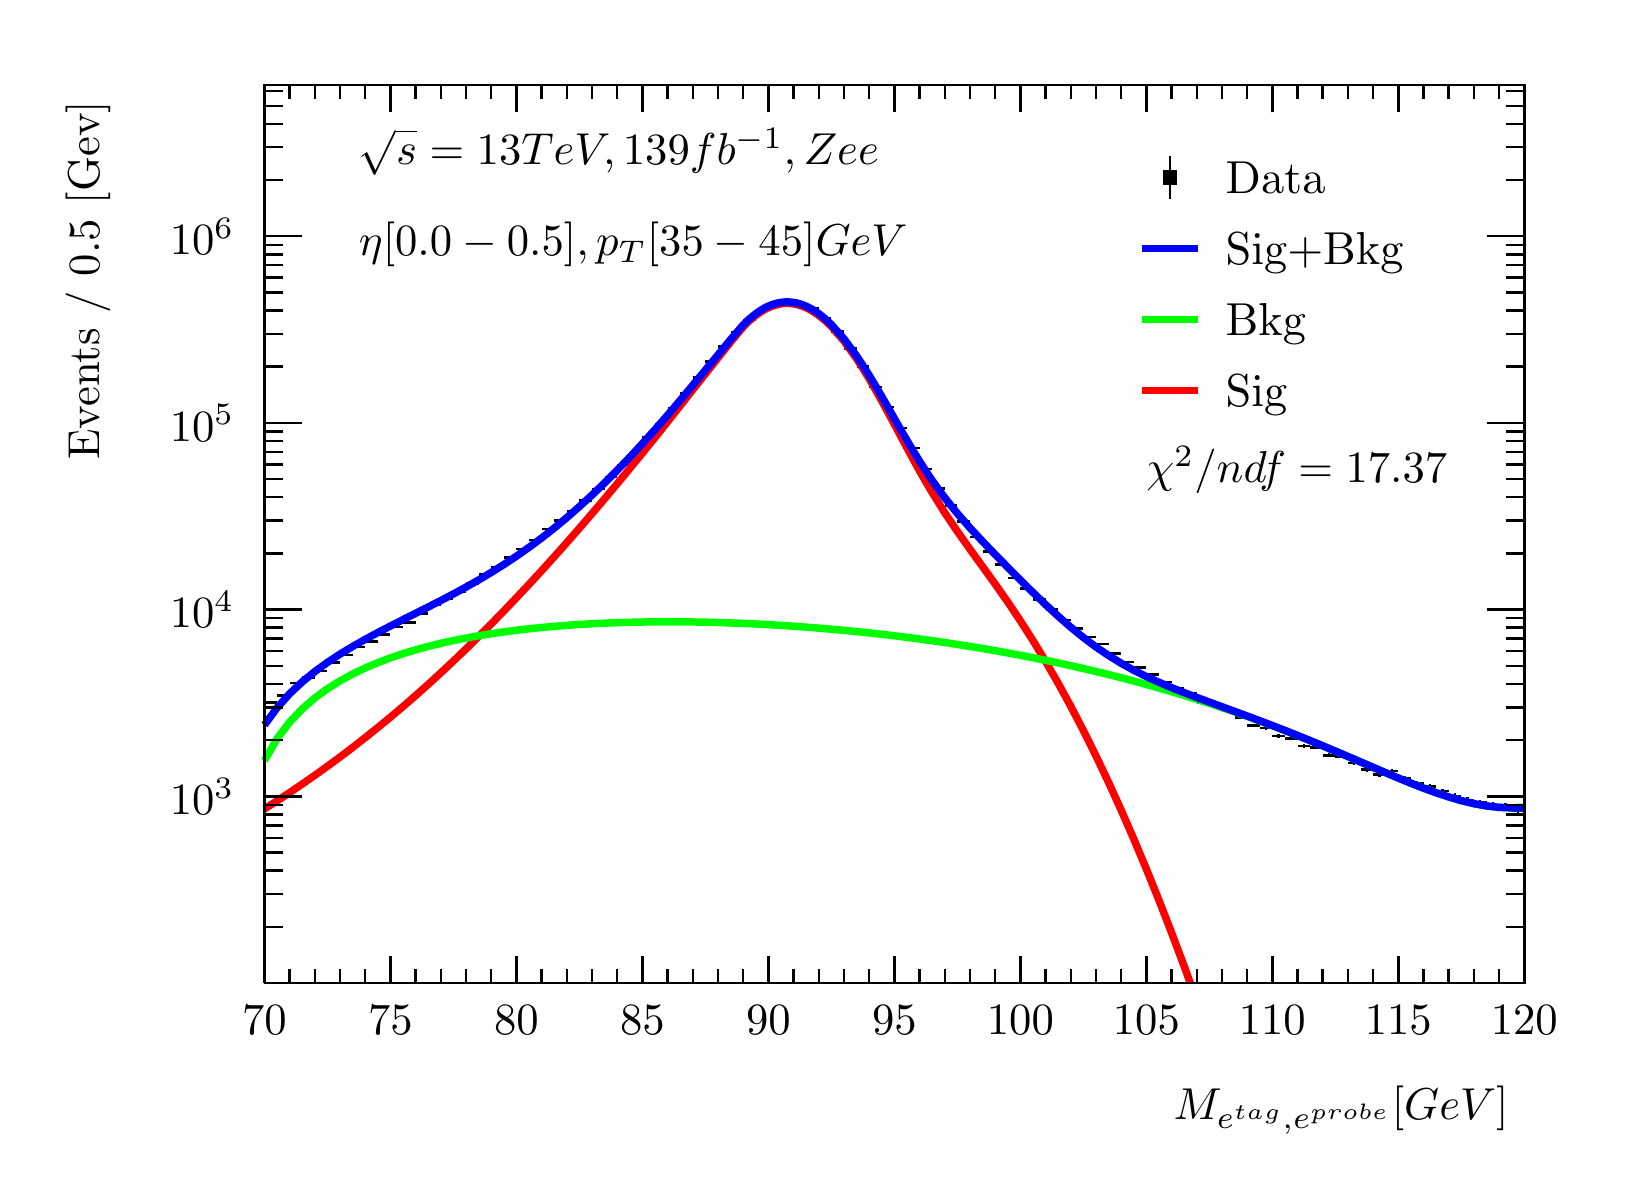
\begin{tikzpicture}
\pgfdeclareplotmark{cross} {
\pgfpathmoveto{\pgfpoint{-0.3\pgfplotmarksize}{\pgfplotmarksize}}
\pgfpathlineto{\pgfpoint{+0.3\pgfplotmarksize}{\pgfplotmarksize}}
\pgfpathlineto{\pgfpoint{+0.3\pgfplotmarksize}{0.3\pgfplotmarksize}}
\pgfpathlineto{\pgfpoint{+1\pgfplotmarksize}{0.3\pgfplotmarksize}}
\pgfpathlineto{\pgfpoint{+1\pgfplotmarksize}{-0.3\pgfplotmarksize}}
\pgfpathlineto{\pgfpoint{+0.3\pgfplotmarksize}{-0.3\pgfplotmarksize}}
\pgfpathlineto{\pgfpoint{+0.3\pgfplotmarksize}{-1.\pgfplotmarksize}}
\pgfpathlineto{\pgfpoint{-0.3\pgfplotmarksize}{-1.\pgfplotmarksize}}
\pgfpathlineto{\pgfpoint{-0.3\pgfplotmarksize}{-0.3\pgfplotmarksize}}
\pgfpathlineto{\pgfpoint{-1.\pgfplotmarksize}{-0.3\pgfplotmarksize}}
\pgfpathlineto{\pgfpoint{-1.\pgfplotmarksize}{0.3\pgfplotmarksize}}
\pgfpathlineto{\pgfpoint{-0.3\pgfplotmarksize}{0.3\pgfplotmarksize}}
\pgfpathclose
\pgfusepathqstroke
}
\pgfdeclareplotmark{cross*} {
\pgfpathmoveto{\pgfpoint{-0.3\pgfplotmarksize}{\pgfplotmarksize}}
\pgfpathlineto{\pgfpoint{+0.3\pgfplotmarksize}{\pgfplotmarksize}}
\pgfpathlineto{\pgfpoint{+0.3\pgfplotmarksize}{0.3\pgfplotmarksize}}
\pgfpathlineto{\pgfpoint{+1\pgfplotmarksize}{0.3\pgfplotmarksize}}
\pgfpathlineto{\pgfpoint{+1\pgfplotmarksize}{-0.3\pgfplotmarksize}}
\pgfpathlineto{\pgfpoint{+0.3\pgfplotmarksize}{-0.3\pgfplotmarksize}}
\pgfpathlineto{\pgfpoint{+0.3\pgfplotmarksize}{-1.\pgfplotmarksize}}
\pgfpathlineto{\pgfpoint{-0.3\pgfplotmarksize}{-1.\pgfplotmarksize}}
\pgfpathlineto{\pgfpoint{-0.3\pgfplotmarksize}{-0.3\pgfplotmarksize}}
\pgfpathlineto{\pgfpoint{-1.\pgfplotmarksize}{-0.3\pgfplotmarksize}}
\pgfpathlineto{\pgfpoint{-1.\pgfplotmarksize}{0.3\pgfplotmarksize}}
\pgfpathlineto{\pgfpoint{-0.3\pgfplotmarksize}{0.3\pgfplotmarksize}}
\pgfpathclose
\pgfusepathqfillstroke
}
\pgfdeclareplotmark{newstar} {
\pgfpathmoveto{\pgfqpoint{0pt}{\pgfplotmarksize}}
\pgfpathlineto{\pgfqpointpolar{44}{0.5\pgfplotmarksize}}
\pgfpathlineto{\pgfqpointpolar{18}{\pgfplotmarksize}}
\pgfpathlineto{\pgfqpointpolar{-20}{0.5\pgfplotmarksize}}
\pgfpathlineto{\pgfqpointpolar{-54}{\pgfplotmarksize}}
\pgfpathlineto{\pgfqpointpolar{-90}{0.5\pgfplotmarksize}}
\pgfpathlineto{\pgfqpointpolar{234}{\pgfplotmarksize}}
\pgfpathlineto{\pgfqpointpolar{198}{0.5\pgfplotmarksize}}
\pgfpathlineto{\pgfqpointpolar{162}{\pgfplotmarksize}}
\pgfpathlineto{\pgfqpointpolar{134}{0.5\pgfplotmarksize}}
\pgfpathclose
\pgfusepathqstroke
}
\pgfdeclareplotmark{newstar*} {
\pgfpathmoveto{\pgfqpoint{0pt}{\pgfplotmarksize}}
\pgfpathlineto{\pgfqpointpolar{44}{0.5\pgfplotmarksize}}
\pgfpathlineto{\pgfqpointpolar{18}{\pgfplotmarksize}}
\pgfpathlineto{\pgfqpointpolar{-20}{0.5\pgfplotmarksize}}
\pgfpathlineto{\pgfqpointpolar{-54}{\pgfplotmarksize}}
\pgfpathlineto{\pgfqpointpolar{-90}{0.5\pgfplotmarksize}}
\pgfpathlineto{\pgfqpointpolar{234}{\pgfplotmarksize}}
\pgfpathlineto{\pgfqpointpolar{198}{0.5\pgfplotmarksize}}
\pgfpathlineto{\pgfqpointpolar{162}{\pgfplotmarksize}}
\pgfpathlineto{\pgfqpointpolar{134}{0.5\pgfplotmarksize}}
\pgfpathclose
\pgfusepathqfillstroke
}
\definecolor{c}{rgb}{1,1,1};
\draw [color=c, fill=c] (0,0) rectangle (20,14.4361);
\draw [color=c, fill=c] (3,2.30977) rectangle (19,13.7143);
\definecolor{c}{rgb}{0,0,0};
\draw [c,line width=0.9] (3,2.30977) -- (3,13.7143) -- (19,13.7143) -- (19,2.30977) -- (3,2.30977);
\definecolor{c}{rgb}{1,1,1};
\draw [color=c, fill=c] (3,2.30977) rectangle (19,13.7143);
\definecolor{c}{rgb}{0,0,0};
\draw [c,line width=0.9] (3,2.30977) -- (3,13.7143) -- (19,13.7143) -- (19,2.30977) -- (3,2.30977);
\draw [c,line width=0.9] (3,2.30977) -- (19,2.30977);
\draw [c,line width=0.9] (3,2.65624) -- (3,2.30977);
\draw [c,line width=0.9] (3.32,2.48301) -- (3.32,2.30977);
\draw [c,line width=0.9] (3.64,2.48301) -- (3.64,2.30977);
\draw [c,line width=0.9] (3.96,2.48301) -- (3.96,2.30977);
\draw [c,line width=0.9] (4.28,2.48301) -- (4.28,2.30977);
\draw [c,line width=0.9] (4.6,2.65624) -- (4.6,2.30977);
\draw [c,line width=0.9] (4.92,2.48301) -- (4.92,2.30977);
\draw [c,line width=0.9] (5.24,2.48301) -- (5.24,2.30977);
\draw [c,line width=0.9] (5.56,2.48301) -- (5.56,2.30977);
\draw [c,line width=0.9] (5.88,2.48301) -- (5.88,2.30977);
\draw [c,line width=0.9] (6.2,2.65624) -- (6.2,2.30977);
\draw [c,line width=0.9] (6.52,2.48301) -- (6.52,2.30977);
\draw [c,line width=0.9] (6.84,2.48301) -- (6.84,2.30977);
\draw [c,line width=0.9] (7.16,2.48301) -- (7.16,2.30977);
\draw [c,line width=0.9] (7.48,2.48301) -- (7.48,2.30977);
\draw [c,line width=0.9] (7.8,2.65624) -- (7.8,2.30977);
\draw [c,line width=0.9] (8.12,2.48301) -- (8.12,2.30977);
\draw [c,line width=0.9] (8.44,2.48301) -- (8.44,2.30977);
\draw [c,line width=0.9] (8.76,2.48301) -- (8.76,2.30977);
\draw [c,line width=0.9] (9.08,2.48301) -- (9.08,2.30977);
\draw [c,line width=0.9] (9.4,2.65624) -- (9.4,2.30977);
\draw [c,line width=0.9] (9.72,2.48301) -- (9.72,2.30977);
\draw [c,line width=0.9] (10.04,2.48301) -- (10.04,2.30977);
\draw [c,line width=0.9] (10.36,2.48301) -- (10.36,2.30977);
\draw [c,line width=0.9] (10.68,2.48301) -- (10.68,2.30977);
\draw [c,line width=0.9] (11,2.65624) -- (11,2.30977);
\draw [c,line width=0.9] (11.32,2.48301) -- (11.32,2.30977);
\draw [c,line width=0.9] (11.64,2.48301) -- (11.64,2.30977);
\draw [c,line width=0.9] (11.96,2.48301) -- (11.96,2.30977);
\draw [c,line width=0.9] (12.28,2.48301) -- (12.28,2.30977);
\draw [c,line width=0.9] (12.6,2.65624) -- (12.6,2.30977);
\draw [c,line width=0.9] (12.92,2.48301) -- (12.92,2.30977);
\draw [c,line width=0.9] (13.24,2.48301) -- (13.24,2.30977);
\draw [c,line width=0.9] (13.56,2.48301) -- (13.56,2.30977);
\draw [c,line width=0.9] (13.88,2.48301) -- (13.88,2.30977);
\draw [c,line width=0.9] (14.2,2.65624) -- (14.2,2.30977);
\draw [c,line width=0.9] (14.52,2.48301) -- (14.52,2.30977);
\draw [c,line width=0.9] (14.84,2.48301) -- (14.84,2.30977);
\draw [c,line width=0.9] (15.16,2.48301) -- (15.16,2.30977);
\draw [c,line width=0.9] (15.48,2.48301) -- (15.48,2.30977);
\draw [c,line width=0.9] (15.8,2.65624) -- (15.8,2.30977);
\draw [c,line width=0.9] (16.12,2.48301) -- (16.12,2.30977);
\draw [c,line width=0.9] (16.44,2.48301) -- (16.44,2.30977);
\draw [c,line width=0.9] (16.76,2.48301) -- (16.76,2.30977);
\draw [c,line width=0.9] (17.08,2.48301) -- (17.08,2.30977);
\draw [c,line width=0.9] (17.4,2.65624) -- (17.4,2.30977);
\draw [c,line width=0.9] (17.72,2.48301) -- (17.72,2.30977);
\draw [c,line width=0.9] (18.04,2.48301) -- (18.04,2.30977);
\draw [c,line width=0.9] (18.36,2.48301) -- (18.36,2.30977);
\draw [c,line width=0.9] (18.68,2.48301) -- (18.68,2.30977);
\draw [c,line width=0.9] (19,2.65624) -- (19,2.30977);
\draw [anchor=base] (3,1.66015) node[scale=1.61424, color=c, rotate=0]{70};
\draw [anchor=base] (4.6,1.66015) node[scale=1.61424, color=c, rotate=0]{75};
\draw [anchor=base] (6.2,1.66015) node[scale=1.61424, color=c, rotate=0]{80};
\draw [anchor=base] (7.8,1.66015) node[scale=1.61424, color=c, rotate=0]{85};
\draw [anchor=base] (9.4,1.66015) node[scale=1.61424, color=c, rotate=0]{90};
\draw [anchor=base] (11,1.66015) node[scale=1.61424, color=c, rotate=0]{95};
\draw [anchor=base] (12.6,1.66015) node[scale=1.61424, color=c, rotate=0]{100};
\draw [anchor=base] (14.2,1.66015) node[scale=1.61424, color=c, rotate=0]{105};
\draw [anchor=base] (15.8,1.66015) node[scale=1.61424, color=c, rotate=0]{110};
\draw [anchor=base] (17.4,1.66015) node[scale=1.61424, color=c, rotate=0]{115};
\draw [anchor=base] (19,1.66015) node[scale=1.61424, color=c, rotate=0]{120};
\draw [anchor= east] (19,0.692932) node[scale=1.61424, color=c, rotate=0]{$M_{e^{tag}, e^{probe}}  [GeV]$};
\draw [c,line width=0.9] (3,13.7143) -- (19,13.7143);
\draw [c,line width=0.9] (3,13.3678) -- (3,13.7143);
\draw [c,line width=0.9] (3.32,13.5411) -- (3.32,13.7143);
\draw [c,line width=0.9] (3.64,13.5411) -- (3.64,13.7143);
\draw [c,line width=0.9] (3.96,13.5411) -- (3.96,13.7143);
\draw [c,line width=0.9] (4.28,13.5411) -- (4.28,13.7143);
\draw [c,line width=0.9] (4.6,13.3678) -- (4.6,13.7143);
\draw [c,line width=0.9] (4.92,13.5411) -- (4.92,13.7143);
\draw [c,line width=0.9] (5.24,13.5411) -- (5.24,13.7143);
\draw [c,line width=0.9] (5.56,13.5411) -- (5.56,13.7143);
\draw [c,line width=0.9] (5.88,13.5411) -- (5.88,13.7143);
\draw [c,line width=0.9] (6.2,13.3678) -- (6.2,13.7143);
\draw [c,line width=0.9] (6.52,13.5411) -- (6.52,13.7143);
\draw [c,line width=0.9] (6.84,13.5411) -- (6.84,13.7143);
\draw [c,line width=0.9] (7.16,13.5411) -- (7.16,13.7143);
\draw [c,line width=0.9] (7.48,13.5411) -- (7.48,13.7143);
\draw [c,line width=0.9] (7.8,13.3678) -- (7.8,13.7143);
\draw [c,line width=0.9] (8.12,13.5411) -- (8.12,13.7143);
\draw [c,line width=0.9] (8.44,13.5411) -- (8.44,13.7143);
\draw [c,line width=0.9] (8.76,13.5411) -- (8.76,13.7143);
\draw [c,line width=0.9] (9.08,13.5411) -- (9.08,13.7143);
\draw [c,line width=0.9] (9.4,13.3678) -- (9.4,13.7143);
\draw [c,line width=0.9] (9.72,13.5411) -- (9.72,13.7143);
\draw [c,line width=0.9] (10.04,13.5411) -- (10.04,13.7143);
\draw [c,line width=0.9] (10.36,13.5411) -- (10.36,13.7143);
\draw [c,line width=0.9] (10.68,13.5411) -- (10.68,13.7143);
\draw [c,line width=0.9] (11,13.3678) -- (11,13.7143);
\draw [c,line width=0.9] (11.32,13.5411) -- (11.32,13.7143);
\draw [c,line width=0.9] (11.64,13.5411) -- (11.64,13.7143);
\draw [c,line width=0.9] (11.96,13.5411) -- (11.96,13.7143);
\draw [c,line width=0.9] (12.28,13.5411) -- (12.28,13.7143);
\draw [c,line width=0.9] (12.6,13.3678) -- (12.6,13.7143);
\draw [c,line width=0.9] (12.92,13.5411) -- (12.92,13.7143);
\draw [c,line width=0.9] (13.24,13.5411) -- (13.24,13.7143);
\draw [c,line width=0.9] (13.56,13.5411) -- (13.56,13.7143);
\draw [c,line width=0.9] (13.88,13.5411) -- (13.88,13.7143);
\draw [c,line width=0.9] (14.2,13.3678) -- (14.2,13.7143);
\draw [c,line width=0.9] (14.52,13.5411) -- (14.52,13.7143);
\draw [c,line width=0.9] (14.84,13.5411) -- (14.84,13.7143);
\draw [c,line width=0.9] (15.16,13.5411) -- (15.16,13.7143);
\draw [c,line width=0.9] (15.48,13.5411) -- (15.48,13.7143);
\draw [c,line width=0.9] (15.8,13.3678) -- (15.8,13.7143);
\draw [c,line width=0.9] (16.12,13.5411) -- (16.12,13.7143);
\draw [c,line width=0.9] (16.44,13.5411) -- (16.44,13.7143);
\draw [c,line width=0.9] (16.76,13.5411) -- (16.76,13.7143);
\draw [c,line width=0.9] (17.08,13.5411) -- (17.08,13.7143);
\draw [c,line width=0.9] (17.4,13.3678) -- (17.4,13.7143);
\draw [c,line width=0.9] (17.72,13.5411) -- (17.72,13.7143);
\draw [c,line width=0.9] (18.04,13.5411) -- (18.04,13.7143);
\draw [c,line width=0.9] (18.36,13.5411) -- (18.36,13.7143);
\draw [c,line width=0.9] (18.68,13.5411) -- (18.68,13.7143);
\draw [c,line width=0.9] (19,13.3678) -- (19,13.7143);
\draw [c,line width=0.9] (3,2.30977) -- (3,13.7143);
\draw [c,line width=0.9] (3.237,3.02354) -- (3,3.02354);
\draw [c,line width=0.9] (3.237,3.44107) -- (3,3.44107);
\draw [c,line width=0.9] (3.237,3.73731) -- (3,3.73731);
\draw [c,line width=0.9] (3.237,3.96709) -- (3,3.96709);
\draw [c,line width=0.9] (3.237,4.15484) -- (3,4.15484);
\draw [c,line width=0.9] (3.237,4.31357) -- (3,4.31357);
\draw [c,line width=0.9] (3.237,4.45108) -- (3,4.45108);
\draw [c,line width=0.9] (3.237,4.57236) -- (3,4.57236);
\draw [c,line width=0.9] (3.474,4.68086) -- (3,4.68086);
\draw [anchor= east] (2.82,4.68086) node[scale=1.61424, color=c, rotate=0]{$10^{3}$};
\draw [c,line width=0.9] (3.237,5.39463) -- (3,5.39463);
\draw [c,line width=0.9] (3.237,5.81216) -- (3,5.81216);
\draw [c,line width=0.9] (3.237,6.1084) -- (3,6.1084);
\draw [c,line width=0.9] (3.237,6.33818) -- (3,6.33818);
\draw [c,line width=0.9] (3.237,6.52593) -- (3,6.52593);
\draw [c,line width=0.9] (3.237,6.68466) -- (3,6.68466);
\draw [c,line width=0.9] (3.237,6.82217) -- (3,6.82217);
\draw [c,line width=0.9] (3.237,6.94345) -- (3,6.94345);
\draw [c,line width=0.9] (3.474,7.05195) -- (3,7.05195);
\draw [anchor= east] (2.82,7.05195) node[scale=1.61424, color=c, rotate=0]{$10^{4}$};
\draw [c,line width=0.9] (3.237,7.76572) -- (3,7.76572);
\draw [c,line width=0.9] (3.237,8.18324) -- (3,8.18324);
\draw [c,line width=0.9] (3.237,8.47948) -- (3,8.47948);
\draw [c,line width=0.9] (3.237,8.70927) -- (3,8.70927);
\draw [c,line width=0.9] (3.237,8.89701) -- (3,8.89701);
\draw [c,line width=0.9] (3.237,9.05575) -- (3,9.05575);
\draw [c,line width=0.9] (3.237,9.19325) -- (3,9.19325);
\draw [c,line width=0.9] (3.237,9.31454) -- (3,9.31454);
\draw [c,line width=0.9] (3.474,9.42304) -- (3,9.42304);
\draw [anchor= east] (2.82,9.42304) node[scale=1.61424, color=c, rotate=0]{$10^{5}$};
\draw [c,line width=0.9] (3.237,10.1368) -- (3,10.1368);
\draw [c,line width=0.9] (3.237,10.5543) -- (3,10.5543);
\draw [c,line width=0.9] (3.237,10.8506) -- (3,10.8506);
\draw [c,line width=0.9] (3.237,11.0804) -- (3,11.0804);
\draw [c,line width=0.9] (3.237,11.2681) -- (3,11.2681);
\draw [c,line width=0.9] (3.237,11.4268) -- (3,11.4268);
\draw [c,line width=0.9] (3.237,11.5643) -- (3,11.5643);
\draw [c,line width=0.9] (3.237,11.6856) -- (3,11.6856);
\draw [c,line width=0.9] (3.474,11.7941) -- (3,11.7941);
\draw [anchor= east] (2.82,11.7941) node[scale=1.61424, color=c, rotate=0]{$10^{6}$};
\draw [c,line width=0.9] (3.237,12.5079) -- (3,12.5079);
\draw [c,line width=0.9] (3.237,12.9254) -- (3,12.9254);
\draw [c,line width=0.9] (3.237,13.2217) -- (3,13.2217);
\draw [c,line width=0.9] (3.237,13.4514) -- (3,13.4514);
\draw [c,line width=0.9] (3.237,13.6392) -- (3,13.6392);
\draw [anchor= east] (0.76,13.7143) node[scale=1.61424, color=c, rotate=90]{Events / 0.5 [Gev]};
\draw [c,line width=0.9] (19,2.30977) -- (19,13.7143);
\draw [c,line width=0.9] (18.763,3.02354) -- (19,3.02354);
\draw [c,line width=0.9] (18.763,3.44107) -- (19,3.44107);
\draw [c,line width=0.9] (18.763,3.73731) -- (19,3.73731);
\draw [c,line width=0.9] (18.763,3.96709) -- (19,3.96709);
\draw [c,line width=0.9] (18.763,4.15484) -- (19,4.15484);
\draw [c,line width=0.9] (18.763,4.31357) -- (19,4.31357);
\draw [c,line width=0.9] (18.763,4.45108) -- (19,4.45108);
\draw [c,line width=0.9] (18.763,4.57236) -- (19,4.57236);
\draw [c,line width=0.9] (18.526,4.68086) -- (19,4.68086);
\draw [c,line width=0.9] (18.763,5.39463) -- (19,5.39463);
\draw [c,line width=0.9] (18.763,5.81216) -- (19,5.81216);
\draw [c,line width=0.9] (18.763,6.1084) -- (19,6.1084);
\draw [c,line width=0.9] (18.763,6.33818) -- (19,6.33818);
\draw [c,line width=0.9] (18.763,6.52593) -- (19,6.52593);
\draw [c,line width=0.9] (18.763,6.68466) -- (19,6.68466);
\draw [c,line width=0.9] (18.763,6.82217) -- (19,6.82217);
\draw [c,line width=0.9] (18.763,6.94345) -- (19,6.94345);
\draw [c,line width=0.9] (18.526,7.05195) -- (19,7.05195);
\draw [c,line width=0.9] (18.763,7.76572) -- (19,7.76572);
\draw [c,line width=0.9] (18.763,8.18324) -- (19,8.18324);
\draw [c,line width=0.9] (18.763,8.47948) -- (19,8.47948);
\draw [c,line width=0.9] (18.763,8.70927) -- (19,8.70927);
\draw [c,line width=0.9] (18.763,8.89701) -- (19,8.89701);
\draw [c,line width=0.9] (18.763,9.05575) -- (19,9.05575);
\draw [c,line width=0.9] (18.763,9.19325) -- (19,9.19325);
\draw [c,line width=0.9] (18.763,9.31454) -- (19,9.31454);
\draw [c,line width=0.9] (18.526,9.42304) -- (19,9.42304);
\draw [c,line width=0.9] (18.763,10.1368) -- (19,10.1368);
\draw [c,line width=0.9] (18.763,10.5543) -- (19,10.5543);
\draw [c,line width=0.9] (18.763,10.8506) -- (19,10.8506);
\draw [c,line width=0.9] (18.763,11.0804) -- (19,11.0804);
\draw [c,line width=0.9] (18.763,11.2681) -- (19,11.2681);
\draw [c,line width=0.9] (18.763,11.4268) -- (19,11.4268);
\draw [c,line width=0.9] (18.763,11.5643) -- (19,11.5643);
\draw [c,line width=0.9] (18.763,11.6856) -- (19,11.6856);
\draw [c,line width=0.9] (18.526,11.7941) -- (19,11.7941);
\draw [c,line width=0.9] (18.763,12.5079) -- (19,12.5079);
\draw [c,line width=0.9] (18.763,12.9254) -- (19,12.9254);
\draw [c,line width=0.9] (18.763,13.2217) -- (19,13.2217);
\draw [c,line width=0.9] (18.763,13.4514) -- (19,13.4514);
\draw [c,line width=0.9] (18.763,13.6392) -- (19,13.6392);
\draw [c,line width=0.9] (3.08,5.87086) -- (3,5.87086);
\draw [c,line width=0.9] (3,5.87086) -- (3,5.87086);
\draw [c,line width=0.9] (3.08,5.87086) -- (3.16,5.87086);
\draw [c,line width=0.9] (3.16,5.87086) -- (3.16,5.87086);
\draw [c,line width=0.9] (3.08,5.87086) -- (3.08,5.88914);
\draw [c,line width=0.9] (3.08,5.88914) -- (3.08,5.88914);
\draw [c,line width=0.9] (3.08,5.87086) -- (3.08,5.85259);
\draw [c,line width=0.9] (3.08,5.85259) -- (3.08,5.85259);
\draw [c,line width=0.9] (3.24,5.95965) -- (3.16,5.95965);
\draw [c,line width=0.9] (3.16,5.95965) -- (3.16,5.95965);
\draw [c,line width=0.9] (3.24,5.95965) -- (3.32,5.95965);
\draw [c,line width=0.9] (3.32,5.95965) -- (3.32,5.95965);
\draw [c,line width=0.9] (3.24,5.95965) -- (3.24,5.97715);
\draw [c,line width=0.9] (3.24,5.97715) -- (3.24,5.97715);
\draw [c,line width=0.9] (3.24,5.95965) -- (3.24,5.94215);
\draw [c,line width=0.9] (3.24,5.94215) -- (3.24,5.94215);
\draw [c,line width=0.9] (3.4,6.12246) -- (3.32,6.12246);
\draw [c,line width=0.9] (3.32,6.12246) -- (3.32,6.12246);
\draw [c,line width=0.9] (3.4,6.12246) -- (3.48,6.12246);
\draw [c,line width=0.9] (3.48,6.12246) -- (3.48,6.12246);
\draw [c,line width=0.9] (3.4,6.12246) -- (3.4,6.13863);
\draw [c,line width=0.9] (3.4,6.13863) -- (3.4,6.13863);
\draw [c,line width=0.9] (3.4,6.12246) -- (3.4,6.10629);
\draw [c,line width=0.9] (3.4,6.10629) -- (3.4,6.10629);
\draw [c,line width=0.9] (3.56,6.19027) -- (3.48,6.19027);
\draw [c,line width=0.9] (3.48,6.19027) -- (3.48,6.19027);
\draw [c,line width=0.9] (3.56,6.19027) -- (3.64,6.19027);
\draw [c,line width=0.9] (3.64,6.19027) -- (3.64,6.19027);
\draw [c,line width=0.9] (3.56,6.19027) -- (3.56,6.20591);
\draw [c,line width=0.9] (3.56,6.20591) -- (3.56,6.20591);
\draw [c,line width=0.9] (3.56,6.19027) -- (3.56,6.17462);
\draw [c,line width=0.9] (3.56,6.17462) -- (3.56,6.17462);
\draw [c,line width=0.9] (3.72,6.27556) -- (3.64,6.27556);
\draw [c,line width=0.9] (3.64,6.27556) -- (3.64,6.27556);
\draw [c,line width=0.9] (3.72,6.27556) -- (3.8,6.27556);
\draw [c,line width=0.9] (3.8,6.27556) -- (3.8,6.27556);
\draw [c,line width=0.9] (3.72,6.27556) -- (3.72,6.29057);
\draw [c,line width=0.9] (3.72,6.29057) -- (3.72,6.29057);
\draw [c,line width=0.9] (3.72,6.27556) -- (3.72,6.26055);
\draw [c,line width=0.9] (3.72,6.26055) -- (3.72,6.26055);
\draw [c,line width=0.9] (3.88,6.37916) -- (3.8,6.37916);
\draw [c,line width=0.9] (3.8,6.37916) -- (3.8,6.37916);
\draw [c,line width=0.9] (3.88,6.37916) -- (3.96,6.37916);
\draw [c,line width=0.9] (3.96,6.37916) -- (3.96,6.37916);
\draw [c,line width=0.9] (3.88,6.37916) -- (3.88,6.39344);
\draw [c,line width=0.9] (3.88,6.39344) -- (3.88,6.39344);
\draw [c,line width=0.9] (3.88,6.37916) -- (3.88,6.36489);
\draw [c,line width=0.9] (3.88,6.36489) -- (3.88,6.36489);
\draw [c,line width=0.9] (4.04,6.47509) -- (3.96,6.47509);
\draw [c,line width=0.9] (3.96,6.47509) -- (3.96,6.47509);
\draw [c,line width=0.9] (4.04,6.47509) -- (4.12,6.47509);
\draw [c,line width=0.9] (4.12,6.47509) -- (4.12,6.47509);
\draw [c,line width=0.9] (4.04,6.47509) -- (4.04,6.48872);
\draw [c,line width=0.9] (4.04,6.48872) -- (4.04,6.48872);
\draw [c,line width=0.9] (4.04,6.47509) -- (4.04,6.46147);
\draw [c,line width=0.9] (4.04,6.46147) -- (4.04,6.46147);
\draw [c,line width=0.9] (4.2,6.576) -- (4.12,6.576);
\draw [c,line width=0.9] (4.12,6.576) -- (4.12,6.576);
\draw [c,line width=0.9] (4.2,6.576) -- (4.28,6.576);
\draw [c,line width=0.9] (4.28,6.576) -- (4.28,6.576);
\draw [c,line width=0.9] (4.2,6.576) -- (4.2,6.58898);
\draw [c,line width=0.9] (4.2,6.58898) -- (4.2,6.58898);
\draw [c,line width=0.9] (4.2,6.576) -- (4.2,6.56303);
\draw [c,line width=0.9] (4.2,6.56303) -- (4.2,6.56303);
\draw [c,line width=0.9] (4.36,6.64508) -- (4.28,6.64508);
\draw [c,line width=0.9] (4.28,6.64508) -- (4.28,6.64508);
\draw [c,line width=0.9] (4.36,6.64508) -- (4.44,6.64508);
\draw [c,line width=0.9] (4.44,6.64508) -- (4.44,6.64508);
\draw [c,line width=0.9] (4.36,6.64508) -- (4.36,6.65762);
\draw [c,line width=0.9] (4.36,6.65762) -- (4.36,6.65762);
\draw [c,line width=0.9] (4.36,6.64508) -- (4.36,6.63253);
\draw [c,line width=0.9] (4.36,6.63253) -- (4.36,6.63253);
\draw [c,line width=0.9] (4.52,6.7335) -- (4.44,6.7335);
\draw [c,line width=0.9] (4.44,6.7335) -- (4.44,6.7335);
\draw [c,line width=0.9] (4.52,6.7335) -- (4.6,6.7335);
\draw [c,line width=0.9] (4.6,6.7335) -- (4.6,6.7335);
\draw [c,line width=0.9] (4.52,6.7335) -- (4.52,6.74552);
\draw [c,line width=0.9] (4.52,6.74552) -- (4.52,6.74552);
\draw [c,line width=0.9] (4.52,6.7335) -- (4.52,6.72148);
\draw [c,line width=0.9] (4.52,6.72148) -- (4.52,6.72148);
\draw [c,line width=0.9] (4.68,6.83216) -- (4.6,6.83216);
\draw [c,line width=0.9] (4.6,6.83216) -- (4.6,6.83216);
\draw [c,line width=0.9] (4.68,6.83216) -- (4.76,6.83216);
\draw [c,line width=0.9] (4.76,6.83216) -- (4.76,6.83216);
\draw [c,line width=0.9] (4.68,6.83216) -- (4.68,6.84362);
\draw [c,line width=0.9] (4.68,6.84362) -- (4.68,6.84362);
\draw [c,line width=0.9] (4.68,6.83216) -- (4.68,6.8207);
\draw [c,line width=0.9] (4.68,6.8207) -- (4.68,6.8207);
\draw [c,line width=0.9] (4.84,6.88786) -- (4.76,6.88786);
\draw [c,line width=0.9] (4.76,6.88786) -- (4.76,6.88786);
\draw [c,line width=0.9] (4.84,6.88786) -- (4.92,6.88786);
\draw [c,line width=0.9] (4.92,6.88786) -- (4.92,6.88786);
\draw [c,line width=0.9] (4.84,6.88786) -- (4.84,6.89901);
\draw [c,line width=0.9] (4.84,6.89901) -- (4.84,6.89901);
\draw [c,line width=0.9] (4.84,6.88786) -- (4.84,6.87671);
\draw [c,line width=0.9] (4.84,6.87671) -- (4.84,6.87671);
\draw [c,line width=0.9] (5,7.00162) -- (4.92,7.00162);
\draw [c,line width=0.9] (4.92,7.00162) -- (4.92,7.00162);
\draw [c,line width=0.9] (5,7.00162) -- (5.08,7.00162);
\draw [c,line width=0.9] (5.08,7.00162) -- (5.08,7.00162);
\draw [c,line width=0.9] (5,7.00162) -- (5,7.01217);
\draw [c,line width=0.9] (5,7.01217) -- (5,7.01217);
\draw [c,line width=0.9] (5,7.00162) -- (5,6.99107);
\draw [c,line width=0.9] (5,6.99107) -- (5,6.99107);
\draw [c,line width=0.9] (5.16,7.11506) -- (5.08,7.11506);
\draw [c,line width=0.9] (5.08,7.11506) -- (5.08,7.11506);
\draw [c,line width=0.9] (5.16,7.11506) -- (5.24,7.11506);
\draw [c,line width=0.9] (5.24,7.11506) -- (5.24,7.11506);
\draw [c,line width=0.9] (5.16,7.11506) -- (5.16,7.12504);
\draw [c,line width=0.9] (5.16,7.12504) -- (5.16,7.12504);
\draw [c,line width=0.9] (5.16,7.11506) -- (5.16,7.10507);
\draw [c,line width=0.9] (5.16,7.10507) -- (5.16,7.10507);
\draw [c,line width=0.9] (5.32,7.18416) -- (5.24,7.18416);
\draw [c,line width=0.9] (5.24,7.18416) -- (5.24,7.18416);
\draw [c,line width=0.9] (5.32,7.18416) -- (5.4,7.18416);
\draw [c,line width=0.9] (5.4,7.18416) -- (5.4,7.18416);
\draw [c,line width=0.9] (5.32,7.18416) -- (5.32,7.19382);
\draw [c,line width=0.9] (5.32,7.19382) -- (5.32,7.19382);
\draw [c,line width=0.9] (5.32,7.18416) -- (5.32,7.1745);
\draw [c,line width=0.9] (5.32,7.1745) -- (5.32,7.1745);
\draw [c,line width=0.9] (5.48,7.28543) -- (5.4,7.28543);
\draw [c,line width=0.9] (5.4,7.28543) -- (5.4,7.28543);
\draw [c,line width=0.9] (5.48,7.28543) -- (5.56,7.28543);
\draw [c,line width=0.9] (5.56,7.28543) -- (5.56,7.28543);
\draw [c,line width=0.9] (5.48,7.28543) -- (5.48,7.29463);
\draw [c,line width=0.9] (5.48,7.29463) -- (5.48,7.29463);
\draw [c,line width=0.9] (5.48,7.28543) -- (5.48,7.27624);
\draw [c,line width=0.9] (5.48,7.27624) -- (5.48,7.27624);
\draw [c,line width=0.9] (5.64,7.38674) -- (5.56,7.38674);
\draw [c,line width=0.9] (5.56,7.38674) -- (5.56,7.38674);
\draw [c,line width=0.9] (5.64,7.38674) -- (5.72,7.38674);
\draw [c,line width=0.9] (5.72,7.38674) -- (5.72,7.38674);
\draw [c,line width=0.9] (5.64,7.38674) -- (5.64,7.3955);
\draw [c,line width=0.9] (5.64,7.3955) -- (5.64,7.3955);
\draw [c,line width=0.9] (5.64,7.38674) -- (5.64,7.37799);
\draw [c,line width=0.9] (5.64,7.37799) -- (5.64,7.37799);
\draw [c,line width=0.9] (5.8,7.50696) -- (5.72,7.50696);
\draw [c,line width=0.9] (5.72,7.50696) -- (5.72,7.50696);
\draw [c,line width=0.9] (5.8,7.50696) -- (5.88,7.50696);
\draw [c,line width=0.9] (5.88,7.50696) -- (5.88,7.50696);
\draw [c,line width=0.9] (5.8,7.50696) -- (5.8,7.51521);
\draw [c,line width=0.9] (5.8,7.51521) -- (5.8,7.51521);
\draw [c,line width=0.9] (5.8,7.50696) -- (5.8,7.4987);
\draw [c,line width=0.9] (5.8,7.4987) -- (5.8,7.4987);
\draw [c,line width=0.9] (5.96,7.59618) -- (5.88,7.59618);
\draw [c,line width=0.9] (5.88,7.59618) -- (5.88,7.59618);
\draw [c,line width=0.9] (5.96,7.59618) -- (6.04,7.59618);
\draw [c,line width=0.9] (6.04,7.59618) -- (6.04,7.59618);
\draw [c,line width=0.9] (5.96,7.59618) -- (5.96,7.60409);
\draw [c,line width=0.9] (5.96,7.60409) -- (5.96,7.60409);
\draw [c,line width=0.9] (5.96,7.59618) -- (5.96,7.58827);
\draw [c,line width=0.9] (5.96,7.58827) -- (5.96,7.58827);
\draw [c,line width=0.9] (6.12,7.71447) -- (6.04,7.71447);
\draw [c,line width=0.9] (6.04,7.71447) -- (6.04,7.71447);
\draw [c,line width=0.9] (6.12,7.71447) -- (6.2,7.71447);
\draw [c,line width=0.9] (6.2,7.71447) -- (6.2,7.71447);
\draw [c,line width=0.9] (6.12,7.71447) -- (6.12,7.72193);
\draw [c,line width=0.9] (6.12,7.72193) -- (6.12,7.72193);
\draw [c,line width=0.9] (6.12,7.71447) -- (6.12,7.707);
\draw [c,line width=0.9] (6.12,7.707) -- (6.12,7.707);
\draw [c,line width=0.9] (6.28,7.82212) -- (6.2,7.82212);
\draw [c,line width=0.9] (6.2,7.82212) -- (6.2,7.82212);
\draw [c,line width=0.9] (6.28,7.82212) -- (6.36,7.82212);
\draw [c,line width=0.9] (6.36,7.82212) -- (6.36,7.82212);
\draw [c,line width=0.9] (6.28,7.82212) -- (6.28,7.8292);
\draw [c,line width=0.9] (6.28,7.8292) -- (6.28,7.8292);
\draw [c,line width=0.9] (6.28,7.82212) -- (6.28,7.81503);
\draw [c,line width=0.9] (6.28,7.81503) -- (6.28,7.81503);
\draw [c,line width=0.9] (6.44,7.93472) -- (6.36,7.93472);
\draw [c,line width=0.9] (6.36,7.93472) -- (6.36,7.93472);
\draw [c,line width=0.9] (6.44,7.93472) -- (6.52,7.93472);
\draw [c,line width=0.9] (6.52,7.93472) -- (6.52,7.93472);
\draw [c,line width=0.9] (6.44,7.93472) -- (6.44,7.94142);
\draw [c,line width=0.9] (6.44,7.94142) -- (6.44,7.94142);
\draw [c,line width=0.9] (6.44,7.93472) -- (6.44,7.92801);
\draw [c,line width=0.9] (6.44,7.92801) -- (6.44,7.92801);
\draw [c,line width=0.9] (6.6,8.07448) -- (6.52,8.07448);
\draw [c,line width=0.9] (6.52,8.07448) -- (6.52,8.07448);
\draw [c,line width=0.9] (6.6,8.07448) -- (6.68,8.07448);
\draw [c,line width=0.9] (6.68,8.07448) -- (6.68,8.07448);
\draw [c,line width=0.9] (6.6,8.07448) -- (6.6,8.08075);
\draw [c,line width=0.9] (6.6,8.08075) -- (6.6,8.08075);
\draw [c,line width=0.9] (6.6,8.07448) -- (6.6,8.06822);
\draw [c,line width=0.9] (6.6,8.06822) -- (6.6,8.06822);
\draw [c,line width=0.9] (6.76,8.18149) -- (6.68,8.18149);
\draw [c,line width=0.9] (6.68,8.18149) -- (6.68,8.18149);
\draw [c,line width=0.9] (6.76,8.18149) -- (6.84,8.18149);
\draw [c,line width=0.9] (6.84,8.18149) -- (6.84,8.18149);
\draw [c,line width=0.9] (6.76,8.18149) -- (6.76,8.18744);
\draw [c,line width=0.9] (6.76,8.18744) -- (6.76,8.18744);
\draw [c,line width=0.9] (6.76,8.18149) -- (6.76,8.17554);
\draw [c,line width=0.9] (6.76,8.17554) -- (6.76,8.17554);
\draw [c,line width=0.9] (6.92,8.30533) -- (6.84,8.30533);
\draw [c,line width=0.9] (6.84,8.30533) -- (6.84,8.30533);
\draw [c,line width=0.9] (6.92,8.30533) -- (7,8.30533);
\draw [c,line width=0.9] (7,8.30533) -- (7,8.30533);
\draw [c,line width=0.9] (6.92,8.30533) -- (6.92,8.31093);
\draw [c,line width=0.9] (6.92,8.31093) -- (6.92,8.31093);
\draw [c,line width=0.9] (6.92,8.30533) -- (6.92,8.29972);
\draw [c,line width=0.9] (6.92,8.29972) -- (6.92,8.29972);
\draw [c,line width=0.9] (7.08,8.44101) -- (7,8.44101);
\draw [c,line width=0.9] (7,8.44101) -- (7,8.44101);
\draw [c,line width=0.9] (7.08,8.44101) -- (7.16,8.44101);
\draw [c,line width=0.9] (7.16,8.44101) -- (7.16,8.44101);
\draw [c,line width=0.9] (7.08,8.44101) -- (7.08,8.44626);
\draw [c,line width=0.9] (7.08,8.44626) -- (7.08,8.44626);
\draw [c,line width=0.9] (7.08,8.44101) -- (7.08,8.43576);
\draw [c,line width=0.9] (7.08,8.43576) -- (7.08,8.43576);
\draw [c,line width=0.9] (7.24,8.58649) -- (7.16,8.58649);
\draw [c,line width=0.9] (7.16,8.58649) -- (7.16,8.58649);
\draw [c,line width=0.9] (7.24,8.58649) -- (7.32,8.58649);
\draw [c,line width=0.9] (7.32,8.58649) -- (7.32,8.58649);
\draw [c,line width=0.9] (7.24,8.58649) -- (7.24,8.59138);
\draw [c,line width=0.9] (7.24,8.59138) -- (7.24,8.59138);
\draw [c,line width=0.9] (7.24,8.58649) -- (7.24,8.5816);
\draw [c,line width=0.9] (7.24,8.5816) -- (7.24,8.5816);
\draw [c,line width=0.9] (7.4,8.7375) -- (7.32,8.7375);
\draw [c,line width=0.9] (7.32,8.7375) -- (7.32,8.7375);
\draw [c,line width=0.9] (7.4,8.7375) -- (7.48,8.7375);
\draw [c,line width=0.9] (7.48,8.7375) -- (7.48,8.7375);
\draw [c,line width=0.9] (7.4,8.7375) -- (7.4,8.74205);
\draw [c,line width=0.9] (7.4,8.74205) -- (7.4,8.74205);
\draw [c,line width=0.9] (7.4,8.7375) -- (7.4,8.73296);
\draw [c,line width=0.9] (7.4,8.73296) -- (7.4,8.73296);
\draw [c,line width=0.9] (7.56,8.88897) -- (7.48,8.88897);
\draw [c,line width=0.9] (7.48,8.88897) -- (7.48,8.88897);
\draw [c,line width=0.9] (7.56,8.88897) -- (7.64,8.88897);
\draw [c,line width=0.9] (7.64,8.88897) -- (7.64,8.88897);
\draw [c,line width=0.9] (7.56,8.88897) -- (7.56,8.89319);
\draw [c,line width=0.9] (7.56,8.89319) -- (7.56,8.89319);
\draw [c,line width=0.9] (7.56,8.88897) -- (7.56,8.88475);
\draw [c,line width=0.9] (7.56,8.88475) -- (7.56,8.88475);
\draw [c,line width=0.9] (7.72,9.05543) -- (7.64,9.05543);
\draw [c,line width=0.9] (7.64,9.05543) -- (7.64,9.05543);
\draw [c,line width=0.9] (7.72,9.05543) -- (7.8,9.05543);
\draw [c,line width=0.9] (7.8,9.05543) -- (7.8,9.05543);
\draw [c,line width=0.9] (7.72,9.05543) -- (7.72,9.05932);
\draw [c,line width=0.9] (7.72,9.05932) -- (7.72,9.05932);
\draw [c,line width=0.9] (7.72,9.05543) -- (7.72,9.05153);
\draw [c,line width=0.9] (7.72,9.05153) -- (7.72,9.05153);
\draw [c,line width=0.9] (7.88,9.23782) -- (7.8,9.23782);
\draw [c,line width=0.9] (7.8,9.23782) -- (7.8,9.23782);
\draw [c,line width=0.9] (7.88,9.23782) -- (7.96,9.23782);
\draw [c,line width=0.9] (7.96,9.23782) -- (7.96,9.23782);
\draw [c,line width=0.9] (7.88,9.23782) -- (7.88,9.24138);
\draw [c,line width=0.9] (7.88,9.24138) -- (7.88,9.24138);
\draw [c,line width=0.9] (7.88,9.23782) -- (7.88,9.23425);
\draw [c,line width=0.9] (7.88,9.23425) -- (7.88,9.23425);
\draw [c,line width=0.9] (8.04,9.41066) -- (7.96,9.41066);
\draw [c,line width=0.9] (7.96,9.41066) -- (7.96,9.41066);
\draw [c,line width=0.9] (8.04,9.41066) -- (8.12,9.41066);
\draw [c,line width=0.9] (8.12,9.41066) -- (8.12,9.41066);
\draw [c,line width=0.9] (8.04,9.41066) -- (8.04,9.41393);
\draw [c,line width=0.9] (8.04,9.41393) -- (8.04,9.41393);
\draw [c,line width=0.9] (8.04,9.41066) -- (8.04,9.40738);
\draw [c,line width=0.9] (8.04,9.40738) -- (8.04,9.40738);
\draw [c,line width=0.9] (8.2,9.60518) -- (8.12,9.60518);
\draw [c,line width=0.9] (8.12,9.60518) -- (8.12,9.60518);
\draw [c,line width=0.9] (8.2,9.60518) -- (8.28,9.60518);
\draw [c,line width=0.9] (8.28,9.60518) -- (8.28,9.60518);
\draw [c,line width=0.9] (8.2,9.60518) -- (8.2,9.60816);
\draw [c,line width=0.9] (8.2,9.60816) -- (8.2,9.60816);
\draw [c,line width=0.9] (8.2,9.60518) -- (8.2,9.6022);
\draw [c,line width=0.9] (8.2,9.6022) -- (8.2,9.6022);
\draw [c,line width=0.9] (8.36,9.80488) -- (8.28,9.80488);
\draw [c,line width=0.9] (8.28,9.80488) -- (8.28,9.80488);
\draw [c,line width=0.9] (8.36,9.80488) -- (8.44,9.80488);
\draw [c,line width=0.9] (8.44,9.80488) -- (8.44,9.80488);
\draw [c,line width=0.9] (8.36,9.80488) -- (8.36,9.80758);
\draw [c,line width=0.9] (8.36,9.80758) -- (8.36,9.80758);
\draw [c,line width=0.9] (8.36,9.80488) -- (8.36,9.80217);
\draw [c,line width=0.9] (8.36,9.80217) -- (8.36,9.80217);
\draw [c,line width=0.9] (8.52,10.0023) -- (8.44,10.0023);
\draw [c,line width=0.9] (8.44,10.0023) -- (8.44,10.0023);
\draw [c,line width=0.9] (8.52,10.0023) -- (8.6,10.0023);
\draw [c,line width=0.9] (8.6,10.0023) -- (8.6,10.0023);
\draw [c,line width=0.9] (8.52,10.0023) -- (8.52,10.0048);
\draw [c,line width=0.9] (8.52,10.0048) -- (8.52,10.0048);
\draw [c,line width=0.9] (8.52,10.0023) -- (8.52,9.99984);
\draw [c,line width=0.9] (8.52,9.99984) -- (8.52,9.99984);
\draw [c,line width=0.9] (8.68,10.2031) -- (8.6,10.2031);
\draw [c,line width=0.9] (8.6,10.2031) -- (8.6,10.2031);
\draw [c,line width=0.9] (8.68,10.2031) -- (8.76,10.2031);
\draw [c,line width=0.9] (8.76,10.2031) -- (8.76,10.2031);
\draw [c,line width=0.9] (8.68,10.2031) -- (8.68,10.2053);
\draw [c,line width=0.9] (8.68,10.2053) -- (8.68,10.2053);
\draw [c,line width=0.9] (8.68,10.2031) -- (8.68,10.2008);
\draw [c,line width=0.9] (8.68,10.2008) -- (8.68,10.2008);
\draw [c,line width=0.9] (8.84,10.3968) -- (8.76,10.3968);
\draw [c,line width=0.9] (8.76,10.3968) -- (8.76,10.3968);
\draw [c,line width=0.9] (8.84,10.3968) -- (8.92,10.3968);
\draw [c,line width=0.9] (8.92,10.3968) -- (8.92,10.3968);
\draw [c,line width=0.9] (8.84,10.3968) -- (8.84,10.3988);
\draw [c,line width=0.9] (8.84,10.3988) -- (8.84,10.3988);
\draw [c,line width=0.9] (8.84,10.3968) -- (8.84,10.3948);
\draw [c,line width=0.9] (8.84,10.3948) -- (8.84,10.3948);
\draw [c,line width=0.9] (9,10.5752) -- (8.92,10.5752);
\draw [c,line width=0.9] (8.92,10.5752) -- (8.92,10.5752);
\draw [c,line width=0.9] (9,10.5752) -- (9.08,10.5752);
\draw [c,line width=0.9] (9.08,10.5752) -- (9.08,10.5752);
\draw [c,line width=0.9] (9,10.5752) -- (9,10.5771);
\draw [c,line width=0.9] (9,10.5771) -- (9,10.5771);
\draw [c,line width=0.9] (9,10.5752) -- (9,10.5734);
\draw [c,line width=0.9] (9,10.5734) -- (9,10.5734);
\draw [c,line width=0.9] (9.16,10.7326) -- (9.08,10.7326);
\draw [c,line width=0.9] (9.08,10.7326) -- (9.08,10.7326);
\draw [c,line width=0.9] (9.16,10.7326) -- (9.24,10.7326);
\draw [c,line width=0.9] (9.24,10.7326) -- (9.24,10.7326);
\draw [c,line width=0.9] (9.16,10.7326) -- (9.16,10.7344);
\draw [c,line width=0.9] (9.16,10.7344) -- (9.16,10.7344);
\draw [c,line width=0.9] (9.16,10.7326) -- (9.16,10.7309);
\draw [c,line width=0.9] (9.16,10.7309) -- (9.16,10.7309);
\draw [c,line width=0.9] (9.32,10.8566) -- (9.24,10.8566);
\draw [c,line width=0.9] (9.24,10.8566) -- (9.24,10.8566);
\draw [c,line width=0.9] (9.32,10.8566) -- (9.4,10.8566);
\draw [c,line width=0.9] (9.4,10.8566) -- (9.4,10.8566);
\draw [c,line width=0.9] (9.32,10.8566) -- (9.32,10.8582);
\draw [c,line width=0.9] (9.32,10.8582) -- (9.32,10.8582);
\draw [c,line width=0.9] (9.32,10.8566) -- (9.32,10.855);
\draw [c,line width=0.9] (9.32,10.855) -- (9.32,10.855);
\draw [c,line width=0.9] (9.48,10.9355) -- (9.4,10.9355);
\draw [c,line width=0.9] (9.4,10.9355) -- (9.4,10.9355);
\draw [c,line width=0.9] (9.48,10.9355) -- (9.56,10.9355);
\draw [c,line width=0.9] (9.56,10.9355) -- (9.56,10.9355);
\draw [c,line width=0.9] (9.48,10.9355) -- (9.48,10.9371);
\draw [c,line width=0.9] (9.48,10.9371) -- (9.48,10.9371);
\draw [c,line width=0.9] (9.48,10.9355) -- (9.48,10.934);
\draw [c,line width=0.9] (9.48,10.934) -- (9.48,10.934);
\draw [c,line width=0.9] (9.64,10.9682) -- (9.56,10.9682);
\draw [c,line width=0.9] (9.56,10.9682) -- (9.56,10.9682);
\draw [c,line width=0.9] (9.64,10.9682) -- (9.72,10.9682);
\draw [c,line width=0.9] (9.72,10.9682) -- (9.72,10.9682);
\draw [c,line width=0.9] (9.64,10.9682) -- (9.64,10.9698);
\draw [c,line width=0.9] (9.64,10.9698) -- (9.64,10.9698);
\draw [c,line width=0.9] (9.64,10.9682) -- (9.64,10.9667);
\draw [c,line width=0.9] (9.64,10.9667) -- (9.64,10.9667);
\draw [c,line width=0.9] (9.8,10.9489) -- (9.72,10.9489);
\draw [c,line width=0.9] (9.72,10.9489) -- (9.72,10.9489);
\draw [c,line width=0.9] (9.8,10.9489) -- (9.88,10.9489);
\draw [c,line width=0.9] (9.88,10.9489) -- (9.88,10.9489);
\draw [c,line width=0.9] (9.8,10.9489) -- (9.8,10.9505);
\draw [c,line width=0.9] (9.8,10.9505) -- (9.8,10.9505);
\draw [c,line width=0.9] (9.8,10.9489) -- (9.8,10.9474);
\draw [c,line width=0.9] (9.8,10.9474) -- (9.8,10.9474);
\draw [c,line width=0.9] (9.96,10.8741) -- (9.88,10.8741);
\draw [c,line width=0.9] (9.88,10.8741) -- (9.88,10.8741);
\draw [c,line width=0.9] (9.96,10.8741) -- (10.04,10.8741);
\draw [c,line width=0.9] (10.04,10.8741) -- (10.04,10.8741);
\draw [c,line width=0.9] (9.96,10.8741) -- (9.96,10.8757);
\draw [c,line width=0.9] (9.96,10.8757) -- (9.96,10.8757);
\draw [c,line width=0.9] (9.96,10.8741) -- (9.96,10.8725);
\draw [c,line width=0.9] (9.96,10.8725) -- (9.96,10.8725);
\draw [c,line width=0.9] (10.12,10.7496) -- (10.04,10.7496);
\draw [c,line width=0.9] (10.04,10.7496) -- (10.04,10.7496);
\draw [c,line width=0.9] (10.12,10.7496) -- (10.2,10.7496);
\draw [c,line width=0.9] (10.2,10.7496) -- (10.2,10.7496);
\draw [c,line width=0.9] (10.12,10.7496) -- (10.12,10.7513);
\draw [c,line width=0.9] (10.12,10.7513) -- (10.12,10.7513);
\draw [c,line width=0.9] (10.12,10.7496) -- (10.12,10.7479);
\draw [c,line width=0.9] (10.12,10.7479) -- (10.12,10.7479);
\draw [c,line width=0.9] (10.28,10.5813) -- (10.2,10.5813);
\draw [c,line width=0.9] (10.2,10.5813) -- (10.2,10.5813);
\draw [c,line width=0.9] (10.28,10.5813) -- (10.36,10.5813);
\draw [c,line width=0.9] (10.36,10.5813) -- (10.36,10.5813);
\draw [c,line width=0.9] (10.28,10.5813) -- (10.28,10.5831);
\draw [c,line width=0.9] (10.28,10.5831) -- (10.28,10.5831);
\draw [c,line width=0.9] (10.28,10.5813) -- (10.28,10.5794);
\draw [c,line width=0.9] (10.28,10.5794) -- (10.28,10.5794);
\draw [c,line width=0.9] (10.44,10.3716) -- (10.36,10.3716);
\draw [c,line width=0.9] (10.36,10.3716) -- (10.36,10.3716);
\draw [c,line width=0.9] (10.44,10.3716) -- (10.52,10.3716);
\draw [c,line width=0.9] (10.52,10.3716) -- (10.52,10.3716);
\draw [c,line width=0.9] (10.44,10.3716) -- (10.44,10.3737);
\draw [c,line width=0.9] (10.44,10.3737) -- (10.44,10.3737);
\draw [c,line width=0.9] (10.44,10.3716) -- (10.44,10.3696);
\draw [c,line width=0.9] (10.44,10.3696) -- (10.44,10.3696);
\draw [c,line width=0.9] (10.6,10.14) -- (10.52,10.14);
\draw [c,line width=0.9] (10.52,10.14) -- (10.52,10.14);
\draw [c,line width=0.9] (10.6,10.14) -- (10.68,10.14);
\draw [c,line width=0.9] (10.68,10.14) -- (10.68,10.14);
\draw [c,line width=0.9] (10.6,10.14) -- (10.6,10.1423);
\draw [c,line width=0.9] (10.6,10.1423) -- (10.6,10.1423);
\draw [c,line width=0.9] (10.6,10.14) -- (10.6,10.1377);
\draw [c,line width=0.9] (10.6,10.1377) -- (10.6,10.1377);
\draw [c,line width=0.9] (10.76,9.88095) -- (10.68,9.88095);
\draw [c,line width=0.9] (10.68,9.88095) -- (10.68,9.88095);
\draw [c,line width=0.9] (10.76,9.88095) -- (10.84,9.88095);
\draw [c,line width=0.9] (10.84,9.88095) -- (10.84,9.88095);
\draw [c,line width=0.9] (10.76,9.88095) -- (10.76,9.88355);
\draw [c,line width=0.9] (10.76,9.88355) -- (10.76,9.88355);
\draw [c,line width=0.9] (10.76,9.88095) -- (10.76,9.87834);
\draw [c,line width=0.9] (10.76,9.87834) -- (10.76,9.87834);
\draw [c,line width=0.9] (10.92,9.62369) -- (10.84,9.62369);
\draw [c,line width=0.9] (10.84,9.62369) -- (10.84,9.62369);
\draw [c,line width=0.9] (10.92,9.62369) -- (11,9.62369);
\draw [c,line width=0.9] (11,9.62369) -- (11,9.62369);
\draw [c,line width=0.9] (10.92,9.62369) -- (10.92,9.62665);
\draw [c,line width=0.9] (10.92,9.62665) -- (10.92,9.62665);
\draw [c,line width=0.9] (10.92,9.62369) -- (10.92,9.62074);
\draw [c,line width=0.9] (10.92,9.62074) -- (10.92,9.62074);
\draw [c,line width=0.9] (11.08,9.3557) -- (11,9.3557);
\draw [c,line width=0.9] (11,9.3557) -- (11,9.3557);
\draw [c,line width=0.9] (11.08,9.3557) -- (11.16,9.3557);
\draw [c,line width=0.9] (11.16,9.3557) -- (11.16,9.3557);
\draw [c,line width=0.9] (11.08,9.3557) -- (11.08,9.35906);
\draw [c,line width=0.9] (11.08,9.35906) -- (11.08,9.35906);
\draw [c,line width=0.9] (11.08,9.3557) -- (11.08,9.35233);
\draw [c,line width=0.9] (11.08,9.35233) -- (11.08,9.35233);
\draw [c,line width=0.9] (11.24,9.10165) -- (11.16,9.10165);
\draw [c,line width=0.9] (11.16,9.10165) -- (11.16,9.10165);
\draw [c,line width=0.9] (11.24,9.10165) -- (11.32,9.10165);
\draw [c,line width=0.9] (11.32,9.10165) -- (11.32,9.10165);
\draw [c,line width=0.9] (11.24,9.10165) -- (11.24,9.10546);
\draw [c,line width=0.9] (11.24,9.10546) -- (11.24,9.10546);
\draw [c,line width=0.9] (11.24,9.10165) -- (11.24,9.09785);
\draw [c,line width=0.9] (11.24,9.09785) -- (11.24,9.09785);
\draw [c,line width=0.9] (11.4,8.83731) -- (11.32,8.83731);
\draw [c,line width=0.9] (11.32,8.83731) -- (11.32,8.83731);
\draw [c,line width=0.9] (11.4,8.83731) -- (11.48,8.83731);
\draw [c,line width=0.9] (11.48,8.83731) -- (11.48,8.83731);
\draw [c,line width=0.9] (11.4,8.83731) -- (11.4,8.84163);
\draw [c,line width=0.9] (11.4,8.84163) -- (11.4,8.84163);
\draw [c,line width=0.9] (11.4,8.83731) -- (11.4,8.83298);
\draw [c,line width=0.9] (11.4,8.83298) -- (11.4,8.83298);
\draw [c,line width=0.9] (11.56,8.59072) -- (11.48,8.59072);
\draw [c,line width=0.9] (11.48,8.59072) -- (11.48,8.59072);
\draw [c,line width=0.9] (11.56,8.59072) -- (11.64,8.59072);
\draw [c,line width=0.9] (11.64,8.59072) -- (11.64,8.59072);
\draw [c,line width=0.9] (11.56,8.59072) -- (11.56,8.5956);
\draw [c,line width=0.9] (11.56,8.5956) -- (11.56,8.5956);
\draw [c,line width=0.9] (11.56,8.59072) -- (11.56,8.58585);
\draw [c,line width=0.9] (11.56,8.58585) -- (11.56,8.58585);
\draw [c,line width=0.9] (11.72,8.3747) -- (11.64,8.3747);
\draw [c,line width=0.9] (11.64,8.3747) -- (11.64,8.3747);
\draw [c,line width=0.9] (11.72,8.3747) -- (11.8,8.3747);
\draw [c,line width=0.9] (11.8,8.3747) -- (11.8,8.3747);
\draw [c,line width=0.9] (11.72,8.3747) -- (11.72,8.38012);
\draw [c,line width=0.9] (11.72,8.38012) -- (11.72,8.38012);
\draw [c,line width=0.9] (11.72,8.3747) -- (11.72,8.36929);
\draw [c,line width=0.9] (11.72,8.36929) -- (11.72,8.36929);
\draw [c,line width=0.9] (11.88,8.16838) -- (11.8,8.16838);
\draw [c,line width=0.9] (11.8,8.16838) -- (11.8,8.16838);
\draw [c,line width=0.9] (11.88,8.16838) -- (11.96,8.16838);
\draw [c,line width=0.9] (11.96,8.16838) -- (11.96,8.16838);
\draw [c,line width=0.9] (11.88,8.16838) -- (11.88,8.17437);
\draw [c,line width=0.9] (11.88,8.17437) -- (11.88,8.17437);
\draw [c,line width=0.9] (11.88,8.16838) -- (11.88,8.16239);
\draw [c,line width=0.9] (11.88,8.16239) -- (11.88,8.16239);
\draw [c,line width=0.9] (12.04,7.97272) -- (11.96,7.97272);
\draw [c,line width=0.9] (11.96,7.97272) -- (11.96,7.97272);
\draw [c,line width=0.9] (12.04,7.97272) -- (12.12,7.97272);
\draw [c,line width=0.9] (12.12,7.97272) -- (12.12,7.97272);
\draw [c,line width=0.9] (12.04,7.97272) -- (12.04,7.9793);
\draw [c,line width=0.9] (12.04,7.9793) -- (12.04,7.9793);
\draw [c,line width=0.9] (12.04,7.97272) -- (12.04,7.96613);
\draw [c,line width=0.9] (12.04,7.96613) -- (12.04,7.96613);
\draw [c,line width=0.9] (12.2,7.79195) -- (12.12,7.79195);
\draw [c,line width=0.9] (12.12,7.79195) -- (12.12,7.79195);
\draw [c,line width=0.9] (12.2,7.79195) -- (12.28,7.79195);
\draw [c,line width=0.9] (12.28,7.79195) -- (12.28,7.79195);
\draw [c,line width=0.9] (12.2,7.79195) -- (12.2,7.79914);
\draw [c,line width=0.9] (12.2,7.79914) -- (12.2,7.79914);
\draw [c,line width=0.9] (12.2,7.79195) -- (12.2,7.78476);
\draw [c,line width=0.9] (12.2,7.78476) -- (12.2,7.78476);
\draw [c,line width=0.9] (12.36,7.62302) -- (12.28,7.62302);
\draw [c,line width=0.9] (12.28,7.62302) -- (12.28,7.62302);
\draw [c,line width=0.9] (12.36,7.62302) -- (12.44,7.62302);
\draw [c,line width=0.9] (12.44,7.62302) -- (12.44,7.62302);
\draw [c,line width=0.9] (12.36,7.62302) -- (12.36,7.63083);
\draw [c,line width=0.9] (12.36,7.63083) -- (12.36,7.63083);
\draw [c,line width=0.9] (12.36,7.62302) -- (12.36,7.61522);
\draw [c,line width=0.9] (12.36,7.61522) -- (12.36,7.61522);
\draw [c,line width=0.9] (12.52,7.4535) -- (12.44,7.4535);
\draw [c,line width=0.9] (12.44,7.4535) -- (12.44,7.4535);
\draw [c,line width=0.9] (12.52,7.4535) -- (12.6,7.4535);
\draw [c,line width=0.9] (12.6,7.4535) -- (12.6,7.4535);
\draw [c,line width=0.9] (12.52,7.4535) -- (12.52,7.46197);
\draw [c,line width=0.9] (12.52,7.46197) -- (12.52,7.46197);
\draw [c,line width=0.9] (12.52,7.4535) -- (12.52,7.44502);
\draw [c,line width=0.9] (12.52,7.44502) -- (12.52,7.44502);
\draw [c,line width=0.9] (12.68,7.31974) -- (12.6,7.31974);
\draw [c,line width=0.9] (12.6,7.31974) -- (12.6,7.31974);
\draw [c,line width=0.9] (12.68,7.31974) -- (12.76,7.31974);
\draw [c,line width=0.9] (12.76,7.31974) -- (12.76,7.31974);
\draw [c,line width=0.9] (12.68,7.31974) -- (12.68,7.32878);
\draw [c,line width=0.9] (12.68,7.32878) -- (12.68,7.32878);
\draw [c,line width=0.9] (12.68,7.31974) -- (12.68,7.3107);
\draw [c,line width=0.9] (12.68,7.3107) -- (12.68,7.3107);
\draw [c,line width=0.9] (12.84,7.18008) -- (12.76,7.18008);
\draw [c,line width=0.9] (12.76,7.18008) -- (12.76,7.18008);
\draw [c,line width=0.9] (12.84,7.18008) -- (12.92,7.18008);
\draw [c,line width=0.9] (12.92,7.18008) -- (12.92,7.18008);
\draw [c,line width=0.9] (12.84,7.18008) -- (12.84,7.18975);
\draw [c,line width=0.9] (12.84,7.18975) -- (12.84,7.18975);
\draw [c,line width=0.9] (12.84,7.18008) -- (12.84,7.1704);
\draw [c,line width=0.9] (12.84,7.1704) -- (12.84,7.1704);
\draw [c,line width=0.9] (13,7.05668) -- (12.92,7.05668);
\draw [c,line width=0.9] (12.92,7.05668) -- (12.92,7.05668);
\draw [c,line width=0.9] (13,7.05668) -- (13.08,7.05668);
\draw [c,line width=0.9] (13.08,7.05668) -- (13.08,7.05668);
\draw [c,line width=0.9] (13,7.05668) -- (13,7.06695);
\draw [c,line width=0.9] (13,7.06695) -- (13,7.06695);
\draw [c,line width=0.9] (13,7.05668) -- (13,7.0464);
\draw [c,line width=0.9] (13,7.0464) -- (13,7.0464);
\draw [c,line width=0.9] (13.16,6.92078) -- (13.08,6.92078);
\draw [c,line width=0.9] (13.08,6.92078) -- (13.08,6.92078);
\draw [c,line width=0.9] (13.16,6.92078) -- (13.24,6.92078);
\draw [c,line width=0.9] (13.24,6.92078) -- (13.24,6.92078);
\draw [c,line width=0.9] (13.16,6.92078) -- (13.16,6.93176);
\draw [c,line width=0.9] (13.16,6.93176) -- (13.16,6.93176);
\draw [c,line width=0.9] (13.16,6.92078) -- (13.16,6.90981);
\draw [c,line width=0.9] (13.16,6.90981) -- (13.16,6.90981);
\draw [c,line width=0.9] (13.32,6.81221) -- (13.24,6.81221);
\draw [c,line width=0.9] (13.24,6.81221) -- (13.24,6.81221);
\draw [c,line width=0.9] (13.32,6.81221) -- (13.4,6.81221);
\draw [c,line width=0.9] (13.4,6.81221) -- (13.4,6.81221);
\draw [c,line width=0.9] (13.32,6.81221) -- (13.32,6.82378);
\draw [c,line width=0.9] (13.32,6.82378) -- (13.32,6.82378);
\draw [c,line width=0.9] (13.32,6.81221) -- (13.32,6.80064);
\draw [c,line width=0.9] (13.32,6.80064) -- (13.32,6.80064);
\draw [c,line width=0.9] (13.48,6.70188) -- (13.4,6.70188);
\draw [c,line width=0.9] (13.4,6.70188) -- (13.4,6.70188);
\draw [c,line width=0.9] (13.48,6.70188) -- (13.56,6.70188);
\draw [c,line width=0.9] (13.56,6.70188) -- (13.56,6.70188);
\draw [c,line width=0.9] (13.48,6.70188) -- (13.48,6.71408);
\draw [c,line width=0.9] (13.48,6.71408) -- (13.48,6.71408);
\draw [c,line width=0.9] (13.48,6.70188) -- (13.48,6.68967);
\draw [c,line width=0.9] (13.48,6.68967) -- (13.48,6.68967);
\draw [c,line width=0.9] (13.64,6.6142) -- (13.56,6.6142);
\draw [c,line width=0.9] (13.56,6.6142) -- (13.56,6.6142);
\draw [c,line width=0.9] (13.64,6.6142) -- (13.72,6.6142);
\draw [c,line width=0.9] (13.72,6.6142) -- (13.72,6.6142);
\draw [c,line width=0.9] (13.64,6.6142) -- (13.64,6.62693);
\draw [c,line width=0.9] (13.64,6.62693) -- (13.64,6.62693);
\draw [c,line width=0.9] (13.64,6.6142) -- (13.64,6.60146);
\draw [c,line width=0.9] (13.64,6.60146) -- (13.64,6.60146);
\draw [c,line width=0.9] (13.8,6.49332) -- (13.72,6.49332);
\draw [c,line width=0.9] (13.72,6.49332) -- (13.72,6.49332);
\draw [c,line width=0.9] (13.8,6.49332) -- (13.88,6.49332);
\draw [c,line width=0.9] (13.88,6.49332) -- (13.88,6.49332);
\draw [c,line width=0.9] (13.8,6.49332) -- (13.8,6.50683);
\draw [c,line width=0.9] (13.8,6.50683) -- (13.8,6.50683);
\draw [c,line width=0.9] (13.8,6.49332) -- (13.8,6.47982);
\draw [c,line width=0.9] (13.8,6.47982) -- (13.8,6.47982);
\draw [c,line width=0.9] (13.96,6.38783) -- (13.88,6.38783);
\draw [c,line width=0.9] (13.88,6.38783) -- (13.88,6.38783);
\draw [c,line width=0.9] (13.96,6.38783) -- (14.04,6.38783);
\draw [c,line width=0.9] (14.04,6.38783) -- (14.04,6.38783);
\draw [c,line width=0.9] (13.96,6.38783) -- (13.96,6.40205);
\draw [c,line width=0.9] (13.96,6.40205) -- (13.96,6.40205);
\draw [c,line width=0.9] (13.96,6.38783) -- (13.96,6.37362);
\draw [c,line width=0.9] (13.96,6.37362) -- (13.96,6.37362);
\draw [c,line width=0.9] (14.12,6.31464) -- (14.04,6.31464);
\draw [c,line width=0.9] (14.04,6.31464) -- (14.04,6.31464);
\draw [c,line width=0.9] (14.12,6.31464) -- (14.2,6.31464);
\draw [c,line width=0.9] (14.2,6.31464) -- (14.2,6.31464);
\draw [c,line width=0.9] (14.12,6.31464) -- (14.12,6.32937);
\draw [c,line width=0.9] (14.12,6.32937) -- (14.12,6.32937);
\draw [c,line width=0.9] (14.12,6.31464) -- (14.12,6.29991);
\draw [c,line width=0.9] (14.12,6.29991) -- (14.12,6.29991);
\draw [c,line width=0.9] (14.28,6.22625) -- (14.2,6.22625);
\draw [c,line width=0.9] (14.2,6.22625) -- (14.2,6.22625);
\draw [c,line width=0.9] (14.28,6.22625) -- (14.36,6.22625);
\draw [c,line width=0.9] (14.36,6.22625) -- (14.36,6.22625);
\draw [c,line width=0.9] (14.28,6.22625) -- (14.28,6.24162);
\draw [c,line width=0.9] (14.28,6.24162) -- (14.28,6.24162);
\draw [c,line width=0.9] (14.28,6.22625) -- (14.28,6.21087);
\draw [c,line width=0.9] (14.28,6.21087) -- (14.28,6.21087);
\draw [c,line width=0.9] (14.44,6.13257) -- (14.36,6.13257);
\draw [c,line width=0.9] (14.36,6.13257) -- (14.36,6.13257);
\draw [c,line width=0.9] (14.44,6.13257) -- (14.52,6.13257);
\draw [c,line width=0.9] (14.52,6.13257) -- (14.52,6.13257);
\draw [c,line width=0.9] (14.44,6.13257) -- (14.44,6.14866);
\draw [c,line width=0.9] (14.44,6.14866) -- (14.44,6.14866);
\draw [c,line width=0.9] (14.44,6.13257) -- (14.44,6.11648);
\draw [c,line width=0.9] (14.44,6.11648) -- (14.44,6.11648);
\draw [c,line width=0.9] (14.6,6.05639) -- (14.52,6.05639);
\draw [c,line width=0.9] (14.52,6.05639) -- (14.52,6.05639);
\draw [c,line width=0.9] (14.6,6.05639) -- (14.68,6.05639);
\draw [c,line width=0.9] (14.68,6.05639) -- (14.68,6.05639);
\draw [c,line width=0.9] (14.6,6.05639) -- (14.6,6.07309);
\draw [c,line width=0.9] (14.6,6.07309) -- (14.6,6.07309);
\draw [c,line width=0.9] (14.6,6.05639) -- (14.6,6.03969);
\draw [c,line width=0.9] (14.6,6.03969) -- (14.6,6.03969);
\draw [c,line width=0.9] (14.76,5.98608) -- (14.68,5.98608);
\draw [c,line width=0.9] (14.68,5.98608) -- (14.68,5.98608);
\draw [c,line width=0.9] (14.76,5.98608) -- (14.84,5.98608);
\draw [c,line width=0.9] (14.84,5.98608) -- (14.84,5.98608);
\draw [c,line width=0.9] (14.76,5.98608) -- (14.76,6.00336);
\draw [c,line width=0.9] (14.76,6.00336) -- (14.76,6.00336);
\draw [c,line width=0.9] (14.76,5.98608) -- (14.76,5.9688);
\draw [c,line width=0.9] (14.76,5.9688) -- (14.76,5.9688);
\draw [c,line width=0.9] (14.92,5.87378) -- (14.84,5.87378);
\draw [c,line width=0.9] (14.84,5.87378) -- (14.84,5.87378);
\draw [c,line width=0.9] (14.92,5.87378) -- (15,5.87378);
\draw [c,line width=0.9] (15,5.87378) -- (15,5.87378);
\draw [c,line width=0.9] (14.92,5.87378) -- (14.92,5.89202);
\draw [c,line width=0.9] (14.92,5.89202) -- (14.92,5.89202);
\draw [c,line width=0.9] (14.92,5.87378) -- (14.92,5.85553);
\draw [c,line width=0.9] (14.92,5.85553) -- (14.92,5.85553);
\draw [c,line width=0.9] (15.08,5.8349) -- (15,5.8349);
\draw [c,line width=0.9] (15,5.8349) -- (15,5.8349);
\draw [c,line width=0.9] (15.08,5.8349) -- (15.16,5.8349);
\draw [c,line width=0.9] (15.16,5.8349) -- (15.16,5.8349);
\draw [c,line width=0.9] (15.08,5.8349) -- (15.08,5.8535);
\draw [c,line width=0.9] (15.08,5.8535) -- (15.08,5.8535);
\draw [c,line width=0.9] (15.08,5.8349) -- (15.08,5.81631);
\draw [c,line width=0.9] (15.08,5.81631) -- (15.08,5.81631);
\draw [c,line width=0.9] (15.24,5.77012) -- (15.16,5.77012);
\draw [c,line width=0.9] (15.16,5.77012) -- (15.16,5.77012);
\draw [c,line width=0.9] (15.24,5.77012) -- (15.32,5.77012);
\draw [c,line width=0.9] (15.32,5.77012) -- (15.32,5.77012);
\draw [c,line width=0.9] (15.24,5.77012) -- (15.24,5.78931);
\draw [c,line width=0.9] (15.24,5.78931) -- (15.24,5.78931);
\draw [c,line width=0.9] (15.24,5.77012) -- (15.24,5.75093);
\draw [c,line width=0.9] (15.24,5.75093) -- (15.24,5.75093);
\draw [c,line width=0.9] (15.4,5.68091) -- (15.32,5.68091);
\draw [c,line width=0.9] (15.32,5.68091) -- (15.32,5.68091);
\draw [c,line width=0.9] (15.4,5.68091) -- (15.48,5.68091);
\draw [c,line width=0.9] (15.48,5.68091) -- (15.48,5.68091);
\draw [c,line width=0.9] (15.4,5.68091) -- (15.4,5.70095);
\draw [c,line width=0.9] (15.4,5.70095) -- (15.4,5.70095);
\draw [c,line width=0.9] (15.4,5.68091) -- (15.4,5.66087);
\draw [c,line width=0.9] (15.4,5.66087) -- (15.4,5.66087);
\draw [c,line width=0.9] (15.56,5.58238) -- (15.48,5.58238);
\draw [c,line width=0.9] (15.48,5.58238) -- (15.48,5.58238);
\draw [c,line width=0.9] (15.56,5.58238) -- (15.64,5.58238);
\draw [c,line width=0.9] (15.64,5.58238) -- (15.64,5.58238);
\draw [c,line width=0.9] (15.56,5.58238) -- (15.56,5.60339);
\draw [c,line width=0.9] (15.56,5.60339) -- (15.56,5.60339);
\draw [c,line width=0.9] (15.56,5.58238) -- (15.56,5.56136);
\draw [c,line width=0.9] (15.56,5.56136) -- (15.56,5.56136);
\draw [c,line width=0.9] (15.72,5.55057) -- (15.64,5.55057);
\draw [c,line width=0.9] (15.64,5.55057) -- (15.64,5.55057);
\draw [c,line width=0.9] (15.72,5.55057) -- (15.8,5.55057);
\draw [c,line width=0.9] (15.8,5.55057) -- (15.8,5.55057);
\draw [c,line width=0.9] (15.72,5.55057) -- (15.72,5.57191);
\draw [c,line width=0.9] (15.72,5.57191) -- (15.72,5.57191);
\draw [c,line width=0.9] (15.72,5.55057) -- (15.72,5.52922);
\draw [c,line width=0.9] (15.72,5.52922) -- (15.72,5.52922);
\draw [c,line width=0.9] (15.88,5.44634) -- (15.8,5.44634);
\draw [c,line width=0.9] (15.8,5.44634) -- (15.8,5.44634);
\draw [c,line width=0.9] (15.88,5.44634) -- (15.96,5.44634);
\draw [c,line width=0.9] (15.96,5.44634) -- (15.96,5.44634);
\draw [c,line width=0.9] (15.88,5.44634) -- (15.88,5.4688);
\draw [c,line width=0.9] (15.88,5.4688) -- (15.88,5.4688);
\draw [c,line width=0.9] (15.88,5.44634) -- (15.88,5.42389);
\draw [c,line width=0.9] (15.88,5.42389) -- (15.88,5.42389);
\draw [c,line width=0.9] (16.04,5.41351) -- (15.96,5.41351);
\draw [c,line width=0.9] (15.96,5.41351) -- (15.96,5.41351);
\draw [c,line width=0.9] (16.04,5.41351) -- (16.12,5.41351);
\draw [c,line width=0.9] (16.12,5.41351) -- (16.12,5.41351);
\draw [c,line width=0.9] (16.04,5.41351) -- (16.04,5.43632);
\draw [c,line width=0.9] (16.04,5.43632) -- (16.04,5.43632);
\draw [c,line width=0.9] (16.04,5.41351) -- (16.04,5.39069);
\draw [c,line width=0.9] (16.04,5.39069) -- (16.04,5.39069);
\draw [c,line width=0.9] (16.2,5.31713) -- (16.12,5.31713);
\draw [c,line width=0.9] (16.12,5.31713) -- (16.12,5.31713);
\draw [c,line width=0.9] (16.2,5.31713) -- (16.28,5.31713);
\draw [c,line width=0.9] (16.28,5.31713) -- (16.28,5.31713);
\draw [c,line width=0.9] (16.2,5.31713) -- (16.2,5.34104);
\draw [c,line width=0.9] (16.2,5.34104) -- (16.2,5.34104);
\draw [c,line width=0.9] (16.2,5.31713) -- (16.2,5.29322);
\draw [c,line width=0.9] (16.2,5.29322) -- (16.2,5.29322);
\draw [c,line width=0.9] (16.36,5.30372) -- (16.28,5.30372);
\draw [c,line width=0.9] (16.28,5.30372) -- (16.28,5.30372);
\draw [c,line width=0.9] (16.36,5.30372) -- (16.44,5.30372);
\draw [c,line width=0.9] (16.44,5.30372) -- (16.44,5.30372);
\draw [c,line width=0.9] (16.36,5.30372) -- (16.36,5.32778);
\draw [c,line width=0.9] (16.36,5.32778) -- (16.36,5.32778);
\draw [c,line width=0.9] (16.36,5.30372) -- (16.36,5.27965);
\draw [c,line width=0.9] (16.36,5.27965) -- (16.36,5.27965);
\draw [c,line width=0.9] (16.52,5.20152) -- (16.44,5.20152);
\draw [c,line width=0.9] (16.44,5.20152) -- (16.44,5.20152);
\draw [c,line width=0.9] (16.52,5.20152) -- (16.6,5.20152);
\draw [c,line width=0.9] (16.6,5.20152) -- (16.6,5.20152);
\draw [c,line width=0.9] (16.52,5.20152) -- (16.52,5.2268);
\draw [c,line width=0.9] (16.52,5.2268) -- (16.52,5.2268);
\draw [c,line width=0.9] (16.52,5.20152) -- (16.52,5.17623);
\draw [c,line width=0.9] (16.52,5.17623) -- (16.52,5.17623);
\draw [c,line width=0.9] (16.68,5.18776) -- (16.6,5.18776);
\draw [c,line width=0.9] (16.6,5.18776) -- (16.6,5.18776);
\draw [c,line width=0.9] (16.68,5.18776) -- (16.76,5.18776);
\draw [c,line width=0.9] (16.76,5.18776) -- (16.76,5.18776);
\draw [c,line width=0.9] (16.68,5.18776) -- (16.68,5.21322);
\draw [c,line width=0.9] (16.68,5.21322) -- (16.68,5.21322);
\draw [c,line width=0.9] (16.68,5.18776) -- (16.68,5.1623);
\draw [c,line width=0.9] (16.68,5.1623) -- (16.68,5.1623);
\draw [c,line width=0.9] (16.84,5.1025) -- (16.76,5.1025);
\draw [c,line width=0.9] (16.76,5.1025) -- (16.76,5.1025);
\draw [c,line width=0.9] (16.84,5.1025) -- (16.92,5.1025);
\draw [c,line width=0.9] (16.92,5.1025) -- (16.92,5.1025);
\draw [c,line width=0.9] (16.84,5.1025) -- (16.84,5.12903);
\draw [c,line width=0.9] (16.84,5.12903) -- (16.84,5.12903);
\draw [c,line width=0.9] (16.84,5.1025) -- (16.84,5.07597);
\draw [c,line width=0.9] (16.84,5.07597) -- (16.84,5.07597);
\draw [c,line width=0.9] (17,5.0207) -- (16.92,5.0207);
\draw [c,line width=0.9] (16.92,5.0207) -- (16.92,5.0207);
\draw [c,line width=0.9] (17,5.0207) -- (17.08,5.0207);
\draw [c,line width=0.9] (17.08,5.0207) -- (17.08,5.0207);
\draw [c,line width=0.9] (17,5.0207) -- (17,5.04831);
\draw [c,line width=0.9] (17,5.04831) -- (17,5.04831);
\draw [c,line width=0.9] (17,5.0207) -- (17,4.99309);
\draw [c,line width=0.9] (17,4.99309) -- (17,4.99309);
\draw [c,line width=0.9] (17.16,4.95892) -- (17.08,4.95892);
\draw [c,line width=0.9] (17.08,4.95892) -- (17.08,4.95892);
\draw [c,line width=0.9] (17.16,4.95892) -- (17.24,4.95892);
\draw [c,line width=0.9] (17.24,4.95892) -- (17.24,4.95892);
\draw [c,line width=0.9] (17.16,4.95892) -- (17.16,4.98737);
\draw [c,line width=0.9] (17.16,4.98737) -- (17.16,4.98737);
\draw [c,line width=0.9] (17.16,4.95892) -- (17.16,4.93047);
\draw [c,line width=0.9] (17.16,4.93047) -- (17.16,4.93047);
\draw [c,line width=0.9] (17.32,5.00429) -- (17.24,5.00429);
\draw [c,line width=0.9] (17.24,5.00429) -- (17.24,5.00429);
\draw [c,line width=0.9] (17.32,5.00429) -- (17.4,5.00429);
\draw [c,line width=0.9] (17.4,5.00429) -- (17.4,5.00429);
\draw [c,line width=0.9] (17.32,5.00429) -- (17.32,5.03212);
\draw [c,line width=0.9] (17.32,5.03212) -- (17.32,5.03212);
\draw [c,line width=0.9] (17.32,5.00429) -- (17.32,4.97646);
\draw [c,line width=0.9] (17.32,4.97646) -- (17.32,4.97646);
\draw [c,line width=0.9] (17.48,4.90652) -- (17.4,4.90652);
\draw [c,line width=0.9] (17.4,4.90652) -- (17.4,4.90652);
\draw [c,line width=0.9] (17.48,4.90652) -- (17.56,4.90652);
\draw [c,line width=0.9] (17.56,4.90652) -- (17.56,4.90652);
\draw [c,line width=0.9] (17.48,4.90652) -- (17.48,4.9357);
\draw [c,line width=0.9] (17.48,4.9357) -- (17.48,4.9357);
\draw [c,line width=0.9] (17.48,4.90652) -- (17.48,4.87733);
\draw [c,line width=0.9] (17.48,4.87733) -- (17.48,4.87733);
\draw [c,line width=0.9] (17.64,4.8513) -- (17.56,4.8513);
\draw [c,line width=0.9] (17.56,4.8513) -- (17.56,4.8513);
\draw [c,line width=0.9] (17.64,4.8513) -- (17.72,4.8513);
\draw [c,line width=0.9] (17.72,4.8513) -- (17.72,4.8513);
\draw [c,line width=0.9] (17.64,4.8513) -- (17.64,4.88128);
\draw [c,line width=0.9] (17.64,4.88128) -- (17.64,4.88128);
\draw [c,line width=0.9] (17.64,4.8513) -- (17.64,4.82132);
\draw [c,line width=0.9] (17.64,4.82132) -- (17.64,4.82132);
\draw [c,line width=0.9] (17.8,4.80763) -- (17.72,4.80763);
\draw [c,line width=0.9] (17.72,4.80763) -- (17.72,4.80763);
\draw [c,line width=0.9] (17.8,4.80763) -- (17.88,4.80763);
\draw [c,line width=0.9] (17.88,4.80763) -- (17.88,4.80763);
\draw [c,line width=0.9] (17.8,4.80763) -- (17.8,4.83824);
\draw [c,line width=0.9] (17.8,4.83824) -- (17.8,4.83824);
\draw [c,line width=0.9] (17.8,4.80763) -- (17.8,4.77701);
\draw [c,line width=0.9] (17.8,4.77701) -- (17.8,4.77701);
\draw [c,line width=0.9] (17.96,4.74861) -- (17.88,4.74861);
\draw [c,line width=0.9] (17.88,4.74861) -- (17.88,4.74861);
\draw [c,line width=0.9] (17.96,4.74861) -- (18.04,4.74861);
\draw [c,line width=0.9] (18.04,4.74861) -- (18.04,4.74861);
\draw [c,line width=0.9] (17.96,4.74861) -- (17.96,4.78012);
\draw [c,line width=0.9] (17.96,4.78012) -- (17.96,4.78012);
\draw [c,line width=0.9] (17.96,4.74861) -- (17.96,4.7171);
\draw [c,line width=0.9] (17.96,4.7171) -- (17.96,4.7171);
\draw [c,line width=0.9] (18.12,4.68702) -- (18.04,4.68702);
\draw [c,line width=0.9] (18.04,4.68702) -- (18.04,4.68702);
\draw [c,line width=0.9] (18.12,4.68702) -- (18.2,4.68702);
\draw [c,line width=0.9] (18.2,4.68702) -- (18.2,4.68702);
\draw [c,line width=0.9] (18.12,4.68702) -- (18.12,4.71949);
\draw [c,line width=0.9] (18.12,4.71949) -- (18.12,4.71949);
\draw [c,line width=0.9] (18.12,4.68702) -- (18.12,4.65456);
\draw [c,line width=0.9] (18.12,4.65456) -- (18.12,4.65456);
\draw [c,line width=0.9] (18.28,4.63453) -- (18.2,4.63453);
\draw [c,line width=0.9] (18.2,4.63453) -- (18.2,4.63453);
\draw [c,line width=0.9] (18.28,4.63453) -- (18.36,4.63453);
\draw [c,line width=0.9] (18.36,4.63453) -- (18.36,4.63453);
\draw [c,line width=0.9] (18.28,4.63453) -- (18.28,4.66783);
\draw [c,line width=0.9] (18.28,4.66783) -- (18.28,4.66783);
\draw [c,line width=0.9] (18.28,4.63453) -- (18.28,4.60122);
\draw [c,line width=0.9] (18.28,4.60122) -- (18.28,4.60122);
\draw [c,line width=0.9] (18.44,4.60058) -- (18.36,4.60058);
\draw [c,line width=0.9] (18.36,4.60058) -- (18.36,4.60058);
\draw [c,line width=0.9] (18.44,4.60058) -- (18.52,4.60058);
\draw [c,line width=0.9] (18.52,4.60058) -- (18.52,4.60058);
\draw [c,line width=0.9] (18.44,4.60058) -- (18.44,4.63444);
\draw [c,line width=0.9] (18.44,4.63444) -- (18.44,4.63444);
\draw [c,line width=0.9] (18.44,4.60058) -- (18.44,4.56672);
\draw [c,line width=0.9] (18.44,4.56672) -- (18.44,4.56672);
\draw [c,line width=0.9] (18.6,4.57122) -- (18.52,4.57122);
\draw [c,line width=0.9] (18.52,4.57122) -- (18.52,4.57122);
\draw [c,line width=0.9] (18.6,4.57122) -- (18.68,4.57122);
\draw [c,line width=0.9] (18.68,4.57122) -- (18.68,4.57122);
\draw [c,line width=0.9] (18.6,4.57122) -- (18.6,4.60556);
\draw [c,line width=0.9] (18.6,4.60556) -- (18.6,4.60556);
\draw [c,line width=0.9] (18.6,4.57122) -- (18.6,4.53688);
\draw [c,line width=0.9] (18.6,4.53688) -- (18.6,4.53688);
\draw [c,line width=0.9] (18.76,4.56663) -- (18.68,4.56663);
\draw [c,line width=0.9] (18.68,4.56663) -- (18.68,4.56663);
\draw [c,line width=0.9] (18.76,4.56663) -- (18.84,4.56663);
\draw [c,line width=0.9] (18.84,4.56663) -- (18.84,4.56663);
\draw [c,line width=0.9] (18.76,4.56663) -- (18.76,4.60105);
\draw [c,line width=0.9] (18.76,4.60105) -- (18.76,4.60105);
\draw [c,line width=0.9] (18.76,4.56663) -- (18.76,4.53221);
\draw [c,line width=0.9] (18.76,4.53221) -- (18.76,4.53221);
\draw [c,line width=0.9] (18.92,4.49517) -- (18.84,4.49517);
\draw [c,line width=0.9] (18.84,4.49517) -- (18.84,4.49517);
\draw [c,line width=0.9] (18.92,4.49517) -- (19,4.49517);
\draw [c,line width=0.9] (19,4.49517) -- (19,4.49517);
\draw [c,line width=0.9] (18.92,4.49517) -- (18.92,4.53081);
\draw [c,line width=0.9] (18.92,4.53081) -- (18.92,4.53081);
\draw [c,line width=0.9] (18.92,4.49517) -- (18.92,4.45954);
\draw [c,line width=0.9] (18.92,4.45954) -- (18.92,4.45954);
\foreach \P in {(3.08,5.87086), (3.24,5.95965), (3.4,6.12246), (3.56,6.19027), (3.72,6.27556), (3.88,6.37916), (4.04,6.47509), (4.2,6.576), (4.36,6.64508), (4.52,6.7335), (4.68,6.83216), (4.84,6.88786), (5,7.00162), (5.16,7.11506), (5.32,7.18416),
 (5.48,7.28543), (5.64,7.38674), (5.8,7.50696), (5.96,7.59618), (6.12,7.71447), (6.28,7.82212), (6.44,7.93472), (6.6,8.07448), (6.76,8.18149), (6.92,8.30533), (7.08,8.44101), (7.24,8.58649), (7.4,8.7375), (7.56,8.88897), (7.72,9.05543),
 (7.88,9.23782), (8.04,9.41066), (8.2,9.60518), (8.36,9.80488), (8.52,10.0023), (8.68,10.2031), (8.84,10.3968), (9,10.5752), (9.16,10.7326), (9.32,10.8566), (9.48,10.9355), (9.64,10.9682), (9.8,10.9489), (9.96,10.8741), (10.12,10.7496),
 (10.28,10.5813), (10.44,10.3716), (10.6,10.14), (10.76,9.88095), (10.92,9.62369), (11.08,9.3557), (11.24,9.10165), (11.4,8.83731), (11.56,8.59072), (11.72,8.3747), (11.88,8.16838), (12.04,7.97272), (12.2,7.79195), (12.36,7.62302), (12.52,7.4535),
 (12.68,7.31974), (12.84,7.18008), (13,7.05668), (13.16,6.92078), (13.32,6.81221), (13.48,6.70188), (13.64,6.6142), (13.8,6.49332), (13.96,6.38783), (14.12,6.31464), (14.28,6.22625), (14.44,6.13257), (14.6,6.05639), (14.76,5.98608), (14.92,5.87378),
 (15.08,5.8349), (15.24,5.77012), (15.4,5.68091), (15.56,5.58238), (15.72,5.55057), (15.88,5.44634), (16.04,5.41351), (16.2,5.31713), (16.36,5.30372), (16.52,5.20152), (16.68,5.18776), (16.84,5.1025), (17,5.0207), (17.16,4.95892), (17.32,5.00429),
 (17.48,4.90652), (17.64,4.8513), (17.8,4.80763), (17.96,4.74861), (18.12,4.68702), (18.28,4.63453), (18.44,4.60058), (18.6,4.57122), (18.76,4.56663), (18.92,4.49517)}{\draw[mark options={color=c,fill=c},mark size=2.882883pt,mark=] plot coordinates
 {\P};}
\definecolor{c}{rgb}{1,0,0};
\draw [c,line width=2.7] (3,4.52107) -- (3,4.52107);
\draw [c,line width=2.7] (3,4.52107) -- (3.16,4.62343) -- (3.32,4.72867) -- (3.48,4.8369) -- (3.64,4.94822) -- (3.8,5.06274) -- (3.96,5.18055) -- (4.12,5.30175) -- (4.28,5.4264) -- (4.44,5.55459) -- (4.6,5.68635) -- (4.76,5.82173) -- (4.92,5.96076)
 -- (5.08,6.10344) -- (5.24,6.24977) -- (5.4,6.39974) -- (5.56,6.5533) -- (5.72,6.71042) -- (5.88,6.87103) -- (6.04,7.03507) -- (6.2,7.20247) -- (6.36,7.37313) -- (6.52,7.54696) -- (6.68,7.72388) -- (6.84,7.90379) -- (7,8.08657) -- (7.16,8.27215) --
 (7.32,8.46041) -- (7.48,8.65126) -- (7.64,8.84461) -- (7.8,9.04037) -- (7.96,9.23847) -- (8.04,9.33836) -- (8.12,9.43882) -- (8.2,9.53981) -- (8.28,9.64134) -- (8.36,9.74334) -- (8.44,9.84512) -- (8.52,9.94657) -- (8.6,10.0477) -- (8.68,10.1487) --
 (8.76,10.2495) -- (8.84,10.3503) -- (8.92,10.451) -- (9.08,10.6423) -- (9.16,10.7215) -- (9.24,10.7887) -- (9.28,10.8177) -- (9.32,10.8437) -- (9.36,10.8666) -- (9.4,10.8865) -- (9.44,10.9033) -- (9.48,10.917) -- (9.52,10.9276) -- (9.56,10.9352) --
 (9.6,10.9397) -- (9.64,10.9411) -- (9.68,10.9395) -- (9.72,10.9348) -- (9.76,10.9271) -- (9.8,10.9164) -- (9.84,10.9027) -- (9.88,10.886) -- (9.92,10.8663) -- (9.96,10.8436) -- (10.04,10.7896) -- (10.12,10.7242) -- (10.2,10.6477) -- (10.36,10.4629)
 -- (10.52,10.2395) -- (10.6,10.115) -- (10.68,9.98322) -- (10.76,9.84516) -- (10.84,9.70202) -- (10.92,9.55513) -- (11,9.40591) -- (11.08,9.25584) -- (11.16,9.10636) -- (11.24,8.95887) -- (11.32,8.81456) -- (11.4,8.67438) -- (11.48,8.53894) --
 (11.64,8.28304) -- (11.8,8.04505) -- (11.96,7.81932) -- (12.12,7.59877) -- (12.28,7.37685) -- (12.44,7.14848) -- (12.6,6.91014) -- (12.76,6.65966) -- (12.92,6.39572) -- (13.08,6.11762) -- (13.24,5.82499) -- (13.4,5.51763) -- (13.56,5.19547) --
 (13.72,4.85845) -- (13.88,4.50657) -- (14.04,4.13981) -- (14.2,3.75818) -- (14.36,3.36166) -- (14.52,2.95027) -- (14.68,2.52399) -- (14.7577,2.30977);
\definecolor{c}{rgb}{0,1,0};
\draw [c,line width=2.7] (3,5.13428) -- (3,5.13428);
\draw [c,line width=2.7] (3,5.13428) -- (3.16,5.41287) -- (3.32,5.6237) -- (3.48,5.79174) -- (3.64,5.93025) -- (3.8,6.04712) -- (3.96,6.14743) -- (4.12,6.23463) -- (4.28,6.31119) -- (4.44,6.37893) -- (4.6,6.43921) -- (4.76,6.49312) -- (4.92,6.54149)
 -- (5.08,6.585) -- (5.24,6.62421) -- (5.4,6.65958) -- (5.56,6.69149) -- (5.72,6.72025) -- (5.88,6.74615) -- (6.04,6.76942) -- (6.2,6.79026) -- (6.36,6.80885) -- (6.52,6.82534) -- (6.68,6.83986) -- (6.84,6.85254) -- (7,6.86347) -- (7.16,6.87274) --
 (7.32,6.88044) -- (7.48,6.88664) -- (7.64,6.8914) -- (7.8,6.89478) -- (7.96,6.89683) -- (8.12,6.8976) -- (8.28,6.89713) -- (8.44,6.89544) -- (8.6,6.89257) -- (8.76,6.88856) -- (8.92,6.88342) -- (9.08,6.87717) -- (9.24,6.86984) -- (9.4,6.86143) --
 (9.56,6.85196) -- (9.72,6.84145) -- (9.88,6.82989) -- (10.04,6.8173) -- (10.2,6.80367) -- (10.36,6.78902) -- (10.52,6.77334) -- (10.68,6.75662) -- (10.84,6.73887) -- (11,6.72008) -- (11.16,6.70024) -- (11.32,6.67934) -- (11.48,6.65737) --
 (11.64,6.63433) -- (11.8,6.61019) -- (11.96,6.58494) -- (12.12,6.55856) -- (12.28,6.53103) -- (12.44,6.50234) -- (12.6,6.47245) -- (12.76,6.44135) -- (12.92,6.40901) -- (13.08,6.3754) -- (13.24,6.34049) -- (13.4,6.30425) -- (13.56,6.26665) --
 (13.72,6.22766) -- (13.88,6.18723) -- (14.04,6.14534) -- (14.2,6.10195) -- (14.36,6.05702) -- (14.52,6.01051) -- (14.68,5.9624) -- (14.84,5.91264) -- (15,5.86121) -- (15.16,5.80808) -- (15.32,5.75324) -- (15.48,5.69666) -- (15.64,5.63837) --
 (15.8,5.57836) -- (15.96,5.51669) -- (16.12,5.45342) -- (16.28,5.38864) -- (16.44,5.32249) -- (16.6,5.25517) -- (16.76,5.18693) -- (16.92,5.11812) -- (17.08,5.04918) -- (17.24,4.98064) -- (17.4,4.91319) -- (17.56,4.84767) -- (17.72,4.78504) --
 (17.88,4.72645) -- (18.04,4.67318) -- (18.2,4.6266) -- (18.36,4.58813) -- (18.52,4.55916) -- (18.68,4.54089) -- (18.84,4.53429) -- (19,4.53994) -- (19,4.53994) -- (19,4.53994);
\definecolor{c}{rgb}{0,0,1};
\draw [c,line width=2.7] (3,5.58643) -- (3,5.58643);
\draw [c,line width=2.7] (3,5.58643) -- (3.16,5.80579) -- (3.32,5.98428) -- (3.48,6.13501) -- (3.64,6.26588) -- (3.8,6.3821) -- (3.96,6.4873) -- (4.12,6.58417) -- (4.28,6.67481) -- (4.44,6.7609) -- (4.6,6.84387) -- (4.76,6.92497) -- (4.92,7.0053) --
 (5.08,7.08589) -- (5.24,7.16769) -- (5.4,7.2516) -- (5.56,7.33848) -- (5.72,7.42911) -- (5.88,7.52425) -- (6.04,7.62456) -- (6.2,7.73062) -- (6.36,7.84294) -- (6.52,7.96188) -- (6.68,8.08773) -- (6.84,8.22063) -- (7,8.36062) -- (7.16,8.50762) --
 (7.32,8.66145) -- (7.48,8.82188) -- (7.64,8.98857) -- (7.8,9.16119) -- (7.96,9.33933) -- (8.04,9.43035) -- (8.12,9.5226) -- (8.2,9.61605) -- (8.28,9.71063) -- (8.36,9.80625) -- (8.44,9.90222) -- (8.52,9.99838) -- (8.6,10.0947) -- (8.68,10.1913) --
 (8.76,10.2882) -- (8.84,10.3853) -- (8.92,10.4827) -- (9.08,10.6686) -- (9.16,10.7458) -- (9.24,10.8113) -- (9.32,10.8651) -- (9.36,10.8875) -- (9.4,10.9069) -- (9.44,10.9234) -- (9.48,10.9368) -- (9.52,10.9472) -- (9.56,10.9545) -- (9.6,10.9589) --
 (9.64,10.9603) -- (9.68,10.9586) -- (9.72,10.954) -- (9.76,10.9464) -- (9.8,10.9358) -- (9.84,10.9223) -- (9.88,10.9058) -- (9.92,10.8864) -- (9.96,10.8642) -- (10.04,10.8111) -- (10.12,10.747) -- (10.2,10.672) -- (10.36,10.4916) -- (10.52,10.2745)
 -- (10.6,10.1541) -- (10.68,10.0271) -- (10.76,9.89481) -- (10.84,9.7584) -- (10.92,9.61932) -- (11,9.47911) -- (11.08,9.33929) -- (11.16,9.20137) -- (11.24,9.06673) -- (11.32,8.93653) -- (11.4,8.81162) -- (11.48,8.69254) -- (11.64,8.47223) --
 (11.8,8.27337) -- (11.96,8.09074) -- (12.12,7.91855) -- (12.28,7.75221) -- (12.44,7.58904) -- (12.6,7.42815) -- (12.76,7.27005) -- (12.92,7.11615) -- (13.08,6.96832) -- (13.24,6.82843) -- (13.4,6.69806) -- (13.56,6.57825) -- (13.72,6.46937) --
 (13.88,6.37112) -- (14.04,6.28263) -- (14.2,6.20261) -- (14.36,6.12956) -- (14.52,6.06194) -- (14.68,5.99829) -- (14.84,5.93732) -- (15,5.87793) -- (15.16,5.81926) -- (15.32,5.7606) -- (15.48,5.70146) -- (15.64,5.64144) -- (15.8,5.58031) --
 (15.96,5.51791) -- (16.12,5.45417) -- (16.28,5.38909) -- (16.44,5.32276) -- (16.6,5.25533) -- (16.76,5.18703) -- (16.92,5.11818) -- (17.08,5.04921) -- (17.24,4.98066) -- (17.4,4.9132) -- (17.56,4.84767) -- (17.72,4.78504) -- (17.88,4.72645) --
 (18.04,4.67318) -- (18.2,4.6266) -- (18.36,4.58813) -- (18.52,4.55916) -- (18.68,4.54089) -- (18.84,4.53429) -- (19,4.53994) -- (19,4.53994) -- (19,4.53994);
\definecolor{c}{rgb}{0,0,0};
\draw [c,line width=0.9] (3,2.30977) -- (19,2.30977);
\draw [c,line width=0.9] (3,2.65624) -- (3,2.30977);
\draw [c,line width=0.9] (3.32,2.48301) -- (3.32,2.30977);
\draw [c,line width=0.9] (3.64,2.48301) -- (3.64,2.30977);
\draw [c,line width=0.9] (3.96,2.48301) -- (3.96,2.30977);
\draw [c,line width=0.9] (4.28,2.48301) -- (4.28,2.30977);
\draw [c,line width=0.9] (4.6,2.65624) -- (4.6,2.30977);
\draw [c,line width=0.9] (4.92,2.48301) -- (4.92,2.30977);
\draw [c,line width=0.9] (5.24,2.48301) -- (5.24,2.30977);
\draw [c,line width=0.9] (5.56,2.48301) -- (5.56,2.30977);
\draw [c,line width=0.9] (5.88,2.48301) -- (5.88,2.30977);
\draw [c,line width=0.9] (6.2,2.65624) -- (6.2,2.30977);
\draw [c,line width=0.9] (6.52,2.48301) -- (6.52,2.30977);
\draw [c,line width=0.9] (6.84,2.48301) -- (6.84,2.30977);
\draw [c,line width=0.9] (7.16,2.48301) -- (7.16,2.30977);
\draw [c,line width=0.9] (7.48,2.48301) -- (7.48,2.30977);
\draw [c,line width=0.9] (7.8,2.65624) -- (7.8,2.30977);
\draw [c,line width=0.9] (8.12,2.48301) -- (8.12,2.30977);
\draw [c,line width=0.9] (8.44,2.48301) -- (8.44,2.30977);
\draw [c,line width=0.9] (8.76,2.48301) -- (8.76,2.30977);
\draw [c,line width=0.9] (9.08,2.48301) -- (9.08,2.30977);
\draw [c,line width=0.9] (9.4,2.65624) -- (9.4,2.30977);
\draw [c,line width=0.9] (9.72,2.48301) -- (9.72,2.30977);
\draw [c,line width=0.9] (10.04,2.48301) -- (10.04,2.30977);
\draw [c,line width=0.9] (10.36,2.48301) -- (10.36,2.30977);
\draw [c,line width=0.9] (10.68,2.48301) -- (10.68,2.30977);
\draw [c,line width=0.9] (11,2.65624) -- (11,2.30977);
\draw [c,line width=0.9] (11.32,2.48301) -- (11.32,2.30977);
\draw [c,line width=0.9] (11.64,2.48301) -- (11.64,2.30977);
\draw [c,line width=0.9] (11.96,2.48301) -- (11.96,2.30977);
\draw [c,line width=0.9] (12.28,2.48301) -- (12.28,2.30977);
\draw [c,line width=0.9] (12.6,2.65624) -- (12.6,2.30977);
\draw [c,line width=0.9] (12.92,2.48301) -- (12.92,2.30977);
\draw [c,line width=0.9] (13.24,2.48301) -- (13.24,2.30977);
\draw [c,line width=0.9] (13.56,2.48301) -- (13.56,2.30977);
\draw [c,line width=0.9] (13.88,2.48301) -- (13.88,2.30977);
\draw [c,line width=0.9] (14.2,2.65624) -- (14.2,2.30977);
\draw [c,line width=0.9] (14.52,2.48301) -- (14.52,2.30977);
\draw [c,line width=0.9] (14.84,2.48301) -- (14.84,2.30977);
\draw [c,line width=0.9] (15.16,2.48301) -- (15.16,2.30977);
\draw [c,line width=0.9] (15.48,2.48301) -- (15.48,2.30977);
\draw [c,line width=0.9] (15.8,2.65624) -- (15.8,2.30977);
\draw [c,line width=0.9] (16.12,2.48301) -- (16.12,2.30977);
\draw [c,line width=0.9] (16.44,2.48301) -- (16.44,2.30977);
\draw [c,line width=0.9] (16.76,2.48301) -- (16.76,2.30977);
\draw [c,line width=0.9] (17.08,2.48301) -- (17.08,2.30977);
\draw [c,line width=0.9] (17.4,2.65624) -- (17.4,2.30977);
\draw [c,line width=0.9] (17.72,2.48301) -- (17.72,2.30977);
\draw [c,line width=0.9] (18.04,2.48301) -- (18.04,2.30977);
\draw [c,line width=0.9] (18.36,2.48301) -- (18.36,2.30977);
\draw [c,line width=0.9] (18.68,2.48301) -- (18.68,2.30977);
\draw [c,line width=0.9] (19,2.65624) -- (19,2.30977);
\draw [c,line width=0.9] (3,13.7143) -- (19,13.7143);
\draw [c,line width=0.9] (3,13.3678) -- (3,13.7143);
\draw [c,line width=0.9] (3.32,13.5411) -- (3.32,13.7143);
\draw [c,line width=0.9] (3.64,13.5411) -- (3.64,13.7143);
\draw [c,line width=0.9] (3.96,13.5411) -- (3.96,13.7143);
\draw [c,line width=0.9] (4.28,13.5411) -- (4.28,13.7143);
\draw [c,line width=0.9] (4.6,13.3678) -- (4.6,13.7143);
\draw [c,line width=0.9] (4.92,13.5411) -- (4.92,13.7143);
\draw [c,line width=0.9] (5.24,13.5411) -- (5.24,13.7143);
\draw [c,line width=0.9] (5.56,13.5411) -- (5.56,13.7143);
\draw [c,line width=0.9] (5.88,13.5411) -- (5.88,13.7143);
\draw [c,line width=0.9] (6.2,13.3678) -- (6.2,13.7143);
\draw [c,line width=0.9] (6.52,13.5411) -- (6.52,13.7143);
\draw [c,line width=0.9] (6.84,13.5411) -- (6.84,13.7143);
\draw [c,line width=0.9] (7.16,13.5411) -- (7.16,13.7143);
\draw [c,line width=0.9] (7.48,13.5411) -- (7.48,13.7143);
\draw [c,line width=0.9] (7.8,13.3678) -- (7.8,13.7143);
\draw [c,line width=0.9] (8.12,13.5411) -- (8.12,13.7143);
\draw [c,line width=0.9] (8.44,13.5411) -- (8.44,13.7143);
\draw [c,line width=0.9] (8.76,13.5411) -- (8.76,13.7143);
\draw [c,line width=0.9] (9.08,13.5411) -- (9.08,13.7143);
\draw [c,line width=0.9] (9.4,13.3678) -- (9.4,13.7143);
\draw [c,line width=0.9] (9.72,13.5411) -- (9.72,13.7143);
\draw [c,line width=0.9] (10.04,13.5411) -- (10.04,13.7143);
\draw [c,line width=0.9] (10.36,13.5411) -- (10.36,13.7143);
\draw [c,line width=0.9] (10.68,13.5411) -- (10.68,13.7143);
\draw [c,line width=0.9] (11,13.3678) -- (11,13.7143);
\draw [c,line width=0.9] (11.32,13.5411) -- (11.32,13.7143);
\draw [c,line width=0.9] (11.64,13.5411) -- (11.64,13.7143);
\draw [c,line width=0.9] (11.96,13.5411) -- (11.96,13.7143);
\draw [c,line width=0.9] (12.28,13.5411) -- (12.28,13.7143);
\draw [c,line width=0.9] (12.6,13.3678) -- (12.6,13.7143);
\draw [c,line width=0.9] (12.92,13.5411) -- (12.92,13.7143);
\draw [c,line width=0.9] (13.24,13.5411) -- (13.24,13.7143);
\draw [c,line width=0.9] (13.56,13.5411) -- (13.56,13.7143);
\draw [c,line width=0.9] (13.88,13.5411) -- (13.88,13.7143);
\draw [c,line width=0.9] (14.2,13.3678) -- (14.2,13.7143);
\draw [c,line width=0.9] (14.52,13.5411) -- (14.52,13.7143);
\draw [c,line width=0.9] (14.84,13.5411) -- (14.84,13.7143);
\draw [c,line width=0.9] (15.16,13.5411) -- (15.16,13.7143);
\draw [c,line width=0.9] (15.48,13.5411) -- (15.48,13.7143);
\draw [c,line width=0.9] (15.8,13.3678) -- (15.8,13.7143);
\draw [c,line width=0.9] (16.12,13.5411) -- (16.12,13.7143);
\draw [c,line width=0.9] (16.44,13.5411) -- (16.44,13.7143);
\draw [c,line width=0.9] (16.76,13.5411) -- (16.76,13.7143);
\draw [c,line width=0.9] (17.08,13.5411) -- (17.08,13.7143);
\draw [c,line width=0.9] (17.4,13.3678) -- (17.4,13.7143);
\draw [c,line width=0.9] (17.72,13.5411) -- (17.72,13.7143);
\draw [c,line width=0.9] (18.04,13.5411) -- (18.04,13.7143);
\draw [c,line width=0.9] (18.36,13.5411) -- (18.36,13.7143);
\draw [c,line width=0.9] (18.68,13.5411) -- (18.68,13.7143);
\draw [c,line width=0.9] (19,13.3678) -- (19,13.7143);
\draw [c,line width=0.9] (3,2.30977) -- (3,13.7143);
\draw [c,line width=0.9] (3.237,3.02354) -- (3,3.02354);
\draw [c,line width=0.9] (3.237,3.44107) -- (3,3.44107);
\draw [c,line width=0.9] (3.237,3.73731) -- (3,3.73731);
\draw [c,line width=0.9] (3.237,3.96709) -- (3,3.96709);
\draw [c,line width=0.9] (3.237,4.15484) -- (3,4.15484);
\draw [c,line width=0.9] (3.237,4.31357) -- (3,4.31357);
\draw [c,line width=0.9] (3.237,4.45108) -- (3,4.45108);
\draw [c,line width=0.9] (3.237,4.57236) -- (3,4.57236);
\draw [c,line width=0.9] (3.474,4.68086) -- (3,4.68086);
\draw [c,line width=0.9] (3.237,5.39463) -- (3,5.39463);
\draw [c,line width=0.9] (3.237,5.81216) -- (3,5.81216);
\draw [c,line width=0.9] (3.237,6.1084) -- (3,6.1084);
\draw [c,line width=0.9] (3.237,6.33818) -- (3,6.33818);
\draw [c,line width=0.9] (3.237,6.52593) -- (3,6.52593);
\draw [c,line width=0.9] (3.237,6.68466) -- (3,6.68466);
\draw [c,line width=0.9] (3.237,6.82217) -- (3,6.82217);
\draw [c,line width=0.9] (3.237,6.94345) -- (3,6.94345);
\draw [c,line width=0.9] (3.474,7.05195) -- (3,7.05195);
\draw [c,line width=0.9] (3.237,7.76572) -- (3,7.76572);
\draw [c,line width=0.9] (3.237,8.18324) -- (3,8.18324);
\draw [c,line width=0.9] (3.237,8.47948) -- (3,8.47948);
\draw [c,line width=0.9] (3.237,8.70927) -- (3,8.70927);
\draw [c,line width=0.9] (3.237,8.89701) -- (3,8.89701);
\draw [c,line width=0.9] (3.237,9.05575) -- (3,9.05575);
\draw [c,line width=0.9] (3.237,9.19325) -- (3,9.19325);
\draw [c,line width=0.9] (3.237,9.31454) -- (3,9.31454);
\draw [c,line width=0.9] (3.474,9.42304) -- (3,9.42304);
\draw [c,line width=0.9] (3.237,10.1368) -- (3,10.1368);
\draw [c,line width=0.9] (3.237,10.5543) -- (3,10.5543);
\draw [c,line width=0.9] (3.237,10.8506) -- (3,10.8506);
\draw [c,line width=0.9] (3.237,11.0804) -- (3,11.0804);
\draw [c,line width=0.9] (3.237,11.2681) -- (3,11.2681);
\draw [c,line width=0.9] (3.237,11.4268) -- (3,11.4268);
\draw [c,line width=0.9] (3.237,11.5643) -- (3,11.5643);
\draw [c,line width=0.9] (3.237,11.6856) -- (3,11.6856);
\draw [c,line width=0.9] (3.474,11.7941) -- (3,11.7941);
\draw [c,line width=0.9] (3.237,12.5079) -- (3,12.5079);
\draw [c,line width=0.9] (3.237,12.9254) -- (3,12.9254);
\draw [c,line width=0.9] (3.237,13.2217) -- (3,13.2217);
\draw [c,line width=0.9] (3.237,13.4514) -- (3,13.4514);
\draw [c,line width=0.9] (3.237,13.6392) -- (3,13.6392);
\draw [c,line width=0.9] (19,2.30977) -- (19,13.7143);
\draw [c,line width=0.9] (18.763,3.02354) -- (19,3.02354);
\draw [c,line width=0.9] (18.763,3.44107) -- (19,3.44107);
\draw [c,line width=0.9] (18.763,3.73731) -- (19,3.73731);
\draw [c,line width=0.9] (18.763,3.96709) -- (19,3.96709);
\draw [c,line width=0.9] (18.763,4.15484) -- (19,4.15484);
\draw [c,line width=0.9] (18.763,4.31357) -- (19,4.31357);
\draw [c,line width=0.9] (18.763,4.45108) -- (19,4.45108);
\draw [c,line width=0.9] (18.763,4.57236) -- (19,4.57236);
\draw [c,line width=0.9] (18.526,4.68086) -- (19,4.68086);
\draw [c,line width=0.9] (18.763,5.39463) -- (19,5.39463);
\draw [c,line width=0.9] (18.763,5.81216) -- (19,5.81216);
\draw [c,line width=0.9] (18.763,6.1084) -- (19,6.1084);
\draw [c,line width=0.9] (18.763,6.33818) -- (19,6.33818);
\draw [c,line width=0.9] (18.763,6.52593) -- (19,6.52593);
\draw [c,line width=0.9] (18.763,6.68466) -- (19,6.68466);
\draw [c,line width=0.9] (18.763,6.82217) -- (19,6.82217);
\draw [c,line width=0.9] (18.763,6.94345) -- (19,6.94345);
\draw [c,line width=0.9] (18.526,7.05195) -- (19,7.05195);
\draw [c,line width=0.9] (18.763,7.76572) -- (19,7.76572);
\draw [c,line width=0.9] (18.763,8.18324) -- (19,8.18324);
\draw [c,line width=0.9] (18.763,8.47948) -- (19,8.47948);
\draw [c,line width=0.9] (18.763,8.70927) -- (19,8.70927);
\draw [c,line width=0.9] (18.763,8.89701) -- (19,8.89701);
\draw [c,line width=0.9] (18.763,9.05575) -- (19,9.05575);
\draw [c,line width=0.9] (18.763,9.19325) -- (19,9.19325);
\draw [c,line width=0.9] (18.763,9.31454) -- (19,9.31454);
\draw [c,line width=0.9] (18.526,9.42304) -- (19,9.42304);
\draw [c,line width=0.9] (18.763,10.1368) -- (19,10.1368);
\draw [c,line width=0.9] (18.763,10.5543) -- (19,10.5543);
\draw [c,line width=0.9] (18.763,10.8506) -- (19,10.8506);
\draw [c,line width=0.9] (18.763,11.0804) -- (19,11.0804);
\draw [c,line width=0.9] (18.763,11.2681) -- (19,11.2681);
\draw [c,line width=0.9] (18.763,11.4268) -- (19,11.4268);
\draw [c,line width=0.9] (18.763,11.5643) -- (19,11.5643);
\draw [c,line width=0.9] (18.763,11.6856) -- (19,11.6856);
\draw [c,line width=0.9] (18.526,11.7941) -- (19,11.7941);
\draw [c,line width=0.9] (18.763,12.5079) -- (19,12.5079);
\draw [c,line width=0.9] (18.763,12.9254) -- (19,12.9254);
\draw [c,line width=0.9] (18.763,13.2217) -- (19,13.2217);
\draw [c,line width=0.9] (18.763,13.4514) -- (19,13.4514);
\draw [c,line width=0.9] (18.763,13.6392) -- (19,13.6392);
\definecolor{c}{rgb}{1,1,1};
\draw [color=c, fill=c] (14,9.38346) rectangle (18,12.9925);
\definecolor{c}{rgb}{0,0,0};
\draw [anchor=base west] (15,12.3383) node[scale=1.6699, color=c, rotate=0]{Data};
\draw [c,line width=0.9] (14.5,12.6416) -- (14.5,12.812);
\draw [c,line width=0.9] (14.5,12.4411) -- (14.5,12.2707);
\foreach \P in {(14.5,12.5414)}{\draw[mark options={color=c,fill=c},mark size=2.402402pt,mark=square*] plot coordinates {\P};}
\draw [anchor=base west] (15,11.4361) node[scale=1.6699, color=c, rotate=0]{Sig+Bkg};
\definecolor{c}{rgb}{0,0,1};
\draw [c,line width=2.7] (14.15,11.6391) -- (14.85,11.6391);
\definecolor{c}{rgb}{0,0,0};
\draw [anchor=base west] (15,10.5338) node[scale=1.6699, color=c, rotate=0]{Bkg};
\definecolor{c}{rgb}{0,1,0};
\draw [c,line width=2.7] (14.15,10.7368) -- (14.85,10.7368);
\definecolor{c}{rgb}{0,0,0};
\draw [anchor=base west] (15,9.63158) node[scale=1.6699, color=c, rotate=0]{Sig};
\definecolor{c}{rgb}{1,0,0};
\draw [c,line width=2.7] (14.15,9.83459) -- (14.85,9.83459);
\definecolor{c}{rgb}{0,0,0};
\draw [anchor=base west] (4,12.7038) node[scale=1.61424, color=c, rotate=0]{$\sqrt{s}= 13 TeV, 139fb^{-1}, Zee$};
\draw [anchor=base west] (4,11.5489) node[scale=1.61424, color=c, rotate=0]{$\eta[0.0-0.5], p_{T}[35-45]GeV$};
\draw [anchor=base west] (14,8.66165) node[scale=1.61424, color=c, rotate=0]{$\chi^{2}/ndf= 17.37$};
\end{tikzpicture}
}\scalebox{0.35}{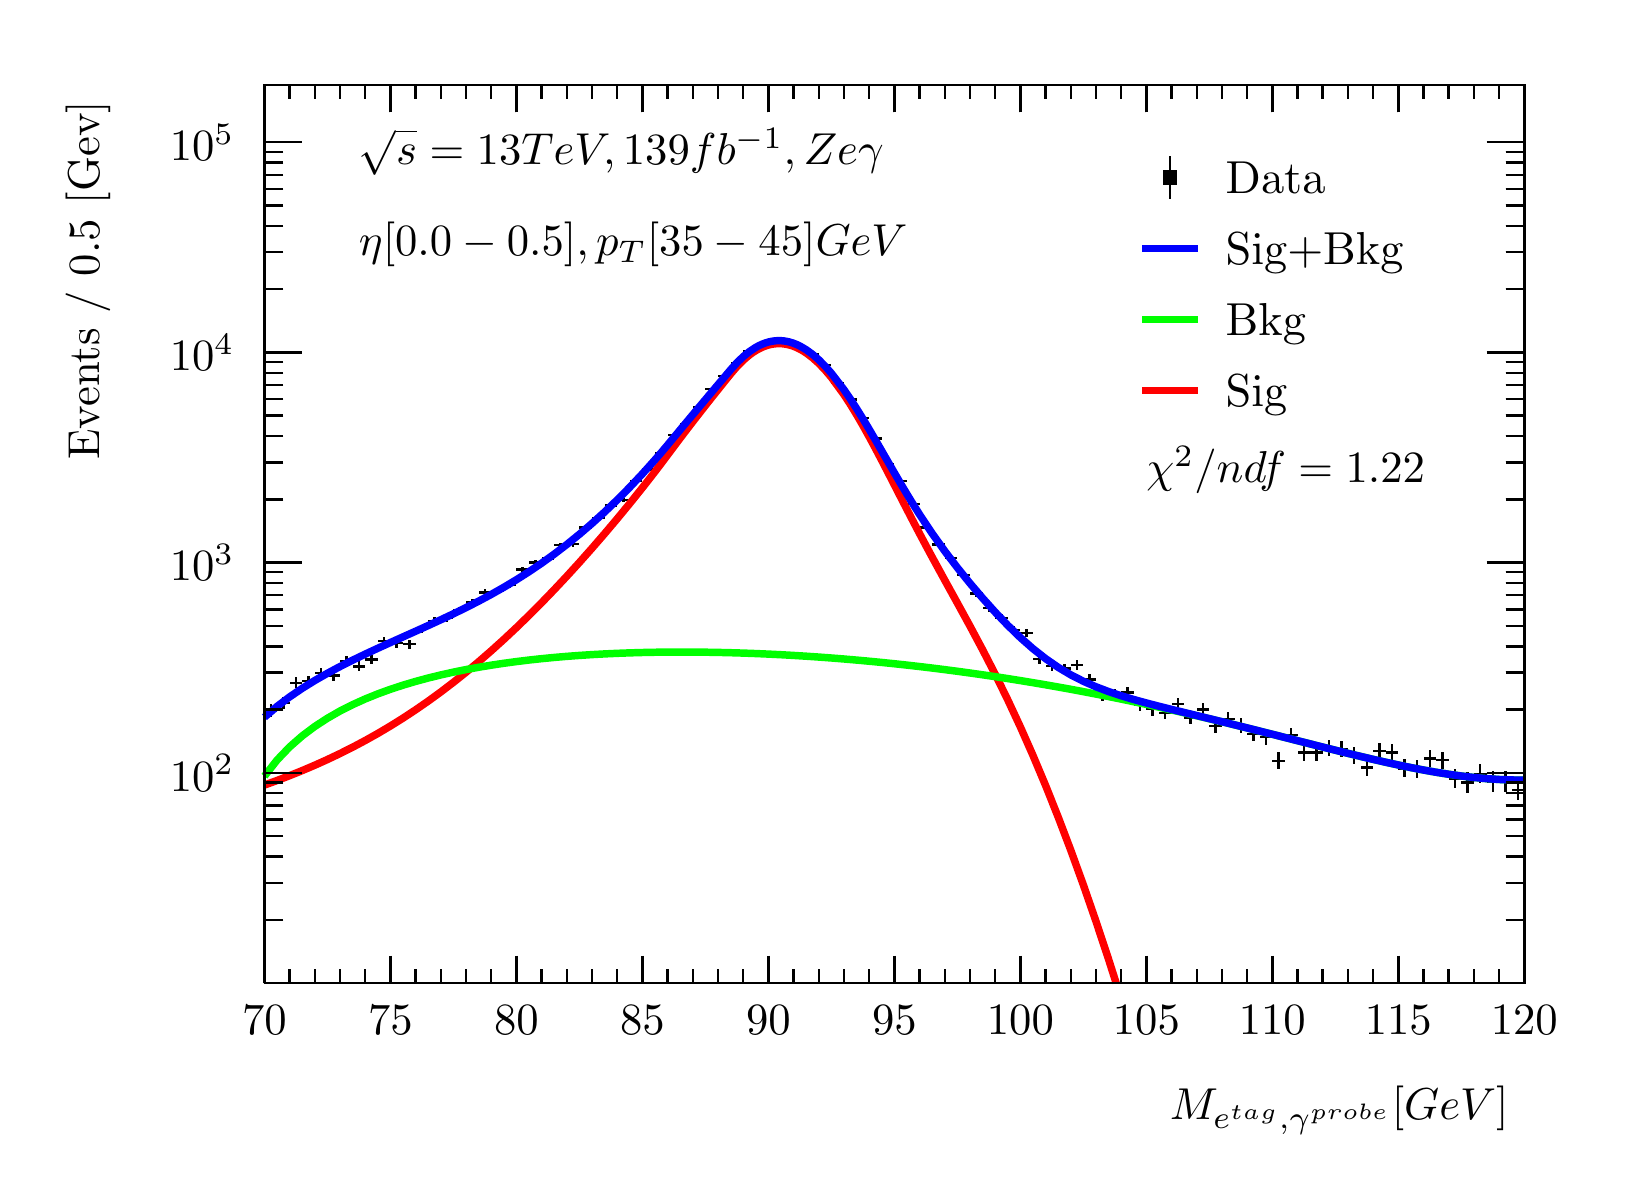
\begin{tikzpicture}
\pgfdeclareplotmark{cross} {
\pgfpathmoveto{\pgfpoint{-0.3\pgfplotmarksize}{\pgfplotmarksize}}
\pgfpathlineto{\pgfpoint{+0.3\pgfplotmarksize}{\pgfplotmarksize}}
\pgfpathlineto{\pgfpoint{+0.3\pgfplotmarksize}{0.3\pgfplotmarksize}}
\pgfpathlineto{\pgfpoint{+1\pgfplotmarksize}{0.3\pgfplotmarksize}}
\pgfpathlineto{\pgfpoint{+1\pgfplotmarksize}{-0.3\pgfplotmarksize}}
\pgfpathlineto{\pgfpoint{+0.3\pgfplotmarksize}{-0.3\pgfplotmarksize}}
\pgfpathlineto{\pgfpoint{+0.3\pgfplotmarksize}{-1.\pgfplotmarksize}}
\pgfpathlineto{\pgfpoint{-0.3\pgfplotmarksize}{-1.\pgfplotmarksize}}
\pgfpathlineto{\pgfpoint{-0.3\pgfplotmarksize}{-0.3\pgfplotmarksize}}
\pgfpathlineto{\pgfpoint{-1.\pgfplotmarksize}{-0.3\pgfplotmarksize}}
\pgfpathlineto{\pgfpoint{-1.\pgfplotmarksize}{0.3\pgfplotmarksize}}
\pgfpathlineto{\pgfpoint{-0.3\pgfplotmarksize}{0.3\pgfplotmarksize}}
\pgfpathclose
\pgfusepathqstroke
}
\pgfdeclareplotmark{cross*} {
\pgfpathmoveto{\pgfpoint{-0.3\pgfplotmarksize}{\pgfplotmarksize}}
\pgfpathlineto{\pgfpoint{+0.3\pgfplotmarksize}{\pgfplotmarksize}}
\pgfpathlineto{\pgfpoint{+0.3\pgfplotmarksize}{0.3\pgfplotmarksize}}
\pgfpathlineto{\pgfpoint{+1\pgfplotmarksize}{0.3\pgfplotmarksize}}
\pgfpathlineto{\pgfpoint{+1\pgfplotmarksize}{-0.3\pgfplotmarksize}}
\pgfpathlineto{\pgfpoint{+0.3\pgfplotmarksize}{-0.3\pgfplotmarksize}}
\pgfpathlineto{\pgfpoint{+0.3\pgfplotmarksize}{-1.\pgfplotmarksize}}
\pgfpathlineto{\pgfpoint{-0.3\pgfplotmarksize}{-1.\pgfplotmarksize}}
\pgfpathlineto{\pgfpoint{-0.3\pgfplotmarksize}{-0.3\pgfplotmarksize}}
\pgfpathlineto{\pgfpoint{-1.\pgfplotmarksize}{-0.3\pgfplotmarksize}}
\pgfpathlineto{\pgfpoint{-1.\pgfplotmarksize}{0.3\pgfplotmarksize}}
\pgfpathlineto{\pgfpoint{-0.3\pgfplotmarksize}{0.3\pgfplotmarksize}}
\pgfpathclose
\pgfusepathqfillstroke
}
\pgfdeclareplotmark{newstar} {
\pgfpathmoveto{\pgfqpoint{0pt}{\pgfplotmarksize}}
\pgfpathlineto{\pgfqpointpolar{44}{0.5\pgfplotmarksize}}
\pgfpathlineto{\pgfqpointpolar{18}{\pgfplotmarksize}}
\pgfpathlineto{\pgfqpointpolar{-20}{0.5\pgfplotmarksize}}
\pgfpathlineto{\pgfqpointpolar{-54}{\pgfplotmarksize}}
\pgfpathlineto{\pgfqpointpolar{-90}{0.5\pgfplotmarksize}}
\pgfpathlineto{\pgfqpointpolar{234}{\pgfplotmarksize}}
\pgfpathlineto{\pgfqpointpolar{198}{0.5\pgfplotmarksize}}
\pgfpathlineto{\pgfqpointpolar{162}{\pgfplotmarksize}}
\pgfpathlineto{\pgfqpointpolar{134}{0.5\pgfplotmarksize}}
\pgfpathclose
\pgfusepathqstroke
}
\pgfdeclareplotmark{newstar*} {
\pgfpathmoveto{\pgfqpoint{0pt}{\pgfplotmarksize}}
\pgfpathlineto{\pgfqpointpolar{44}{0.5\pgfplotmarksize}}
\pgfpathlineto{\pgfqpointpolar{18}{\pgfplotmarksize}}
\pgfpathlineto{\pgfqpointpolar{-20}{0.5\pgfplotmarksize}}
\pgfpathlineto{\pgfqpointpolar{-54}{\pgfplotmarksize}}
\pgfpathlineto{\pgfqpointpolar{-90}{0.5\pgfplotmarksize}}
\pgfpathlineto{\pgfqpointpolar{234}{\pgfplotmarksize}}
\pgfpathlineto{\pgfqpointpolar{198}{0.5\pgfplotmarksize}}
\pgfpathlineto{\pgfqpointpolar{162}{\pgfplotmarksize}}
\pgfpathlineto{\pgfqpointpolar{134}{0.5\pgfplotmarksize}}
\pgfpathclose
\pgfusepathqfillstroke
}
\definecolor{c}{rgb}{1,1,1};
\draw [color=c, fill=c] (0,0) rectangle (20,14.4361);
\draw [color=c, fill=c] (3,2.30977) rectangle (19,13.7143);
\definecolor{c}{rgb}{0,0,0};
\draw [c,line width=0.9] (3,2.30977) -- (3,13.7143) -- (19,13.7143) -- (19,2.30977) -- (3,2.30977);
\definecolor{c}{rgb}{1,1,1};
\draw [color=c, fill=c] (3,2.30977) rectangle (19,13.7143);
\definecolor{c}{rgb}{0,0,0};
\draw [c,line width=0.9] (3,2.30977) -- (3,13.7143) -- (19,13.7143) -- (19,2.30977) -- (3,2.30977);
\draw [c,line width=0.9] (3,2.30977) -- (19,2.30977);
\draw [c,line width=0.9] (3,2.65624) -- (3,2.30977);
\draw [c,line width=0.9] (3.32,2.48301) -- (3.32,2.30977);
\draw [c,line width=0.9] (3.64,2.48301) -- (3.64,2.30977);
\draw [c,line width=0.9] (3.96,2.48301) -- (3.96,2.30977);
\draw [c,line width=0.9] (4.28,2.48301) -- (4.28,2.30977);
\draw [c,line width=0.9] (4.6,2.65624) -- (4.6,2.30977);
\draw [c,line width=0.9] (4.92,2.48301) -- (4.92,2.30977);
\draw [c,line width=0.9] (5.24,2.48301) -- (5.24,2.30977);
\draw [c,line width=0.9] (5.56,2.48301) -- (5.56,2.30977);
\draw [c,line width=0.9] (5.88,2.48301) -- (5.88,2.30977);
\draw [c,line width=0.9] (6.2,2.65624) -- (6.2,2.30977);
\draw [c,line width=0.9] (6.52,2.48301) -- (6.52,2.30977);
\draw [c,line width=0.9] (6.84,2.48301) -- (6.84,2.30977);
\draw [c,line width=0.9] (7.16,2.48301) -- (7.16,2.30977);
\draw [c,line width=0.9] (7.48,2.48301) -- (7.48,2.30977);
\draw [c,line width=0.9] (7.8,2.65624) -- (7.8,2.30977);
\draw [c,line width=0.9] (8.12,2.48301) -- (8.12,2.30977);
\draw [c,line width=0.9] (8.44,2.48301) -- (8.44,2.30977);
\draw [c,line width=0.9] (8.76,2.48301) -- (8.76,2.30977);
\draw [c,line width=0.9] (9.08,2.48301) -- (9.08,2.30977);
\draw [c,line width=0.9] (9.4,2.65624) -- (9.4,2.30977);
\draw [c,line width=0.9] (9.72,2.48301) -- (9.72,2.30977);
\draw [c,line width=0.9] (10.04,2.48301) -- (10.04,2.30977);
\draw [c,line width=0.9] (10.36,2.48301) -- (10.36,2.30977);
\draw [c,line width=0.9] (10.68,2.48301) -- (10.68,2.30977);
\draw [c,line width=0.9] (11,2.65624) -- (11,2.30977);
\draw [c,line width=0.9] (11.32,2.48301) -- (11.32,2.30977);
\draw [c,line width=0.9] (11.64,2.48301) -- (11.64,2.30977);
\draw [c,line width=0.9] (11.96,2.48301) -- (11.96,2.30977);
\draw [c,line width=0.9] (12.28,2.48301) -- (12.28,2.30977);
\draw [c,line width=0.9] (12.6,2.65624) -- (12.6,2.30977);
\draw [c,line width=0.9] (12.92,2.48301) -- (12.92,2.30977);
\draw [c,line width=0.9] (13.24,2.48301) -- (13.24,2.30977);
\draw [c,line width=0.9] (13.56,2.48301) -- (13.56,2.30977);
\draw [c,line width=0.9] (13.88,2.48301) -- (13.88,2.30977);
\draw [c,line width=0.9] (14.2,2.65624) -- (14.2,2.30977);
\draw [c,line width=0.9] (14.52,2.48301) -- (14.52,2.30977);
\draw [c,line width=0.9] (14.84,2.48301) -- (14.84,2.30977);
\draw [c,line width=0.9] (15.16,2.48301) -- (15.16,2.30977);
\draw [c,line width=0.9] (15.48,2.48301) -- (15.48,2.30977);
\draw [c,line width=0.9] (15.8,2.65624) -- (15.8,2.30977);
\draw [c,line width=0.9] (16.12,2.48301) -- (16.12,2.30977);
\draw [c,line width=0.9] (16.44,2.48301) -- (16.44,2.30977);
\draw [c,line width=0.9] (16.76,2.48301) -- (16.76,2.30977);
\draw [c,line width=0.9] (17.08,2.48301) -- (17.08,2.30977);
\draw [c,line width=0.9] (17.4,2.65624) -- (17.4,2.30977);
\draw [c,line width=0.9] (17.72,2.48301) -- (17.72,2.30977);
\draw [c,line width=0.9] (18.04,2.48301) -- (18.04,2.30977);
\draw [c,line width=0.9] (18.36,2.48301) -- (18.36,2.30977);
\draw [c,line width=0.9] (18.68,2.48301) -- (18.68,2.30977);
\draw [c,line width=0.9] (19,2.65624) -- (19,2.30977);
\draw [anchor=base] (3,1.66015) node[scale=1.61424, color=c, rotate=0]{70};
\draw [anchor=base] (4.6,1.66015) node[scale=1.61424, color=c, rotate=0]{75};
\draw [anchor=base] (6.2,1.66015) node[scale=1.61424, color=c, rotate=0]{80};
\draw [anchor=base] (7.8,1.66015) node[scale=1.61424, color=c, rotate=0]{85};
\draw [anchor=base] (9.4,1.66015) node[scale=1.61424, color=c, rotate=0]{90};
\draw [anchor=base] (11,1.66015) node[scale=1.61424, color=c, rotate=0]{95};
\draw [anchor=base] (12.6,1.66015) node[scale=1.61424, color=c, rotate=0]{100};
\draw [anchor=base] (14.2,1.66015) node[scale=1.61424, color=c, rotate=0]{105};
\draw [anchor=base] (15.8,1.66015) node[scale=1.61424, color=c, rotate=0]{110};
\draw [anchor=base] (17.4,1.66015) node[scale=1.61424, color=c, rotate=0]{115};
\draw [anchor=base] (19,1.66015) node[scale=1.61424, color=c, rotate=0]{120};
\draw [anchor= east] (19,0.692932) node[scale=1.61424, color=c, rotate=0]{$M_{e^{tag}, \gamma^{probe}}  [GeV]$};
\draw [c,line width=0.9] (3,13.7143) -- (19,13.7143);
\draw [c,line width=0.9] (3,13.3678) -- (3,13.7143);
\draw [c,line width=0.9] (3.32,13.5411) -- (3.32,13.7143);
\draw [c,line width=0.9] (3.64,13.5411) -- (3.64,13.7143);
\draw [c,line width=0.9] (3.96,13.5411) -- (3.96,13.7143);
\draw [c,line width=0.9] (4.28,13.5411) -- (4.28,13.7143);
\draw [c,line width=0.9] (4.6,13.3678) -- (4.6,13.7143);
\draw [c,line width=0.9] (4.92,13.5411) -- (4.92,13.7143);
\draw [c,line width=0.9] (5.24,13.5411) -- (5.24,13.7143);
\draw [c,line width=0.9] (5.56,13.5411) -- (5.56,13.7143);
\draw [c,line width=0.9] (5.88,13.5411) -- (5.88,13.7143);
\draw [c,line width=0.9] (6.2,13.3678) -- (6.2,13.7143);
\draw [c,line width=0.9] (6.52,13.5411) -- (6.52,13.7143);
\draw [c,line width=0.9] (6.84,13.5411) -- (6.84,13.7143);
\draw [c,line width=0.9] (7.16,13.5411) -- (7.16,13.7143);
\draw [c,line width=0.9] (7.48,13.5411) -- (7.48,13.7143);
\draw [c,line width=0.9] (7.8,13.3678) -- (7.8,13.7143);
\draw [c,line width=0.9] (8.12,13.5411) -- (8.12,13.7143);
\draw [c,line width=0.9] (8.44,13.5411) -- (8.44,13.7143);
\draw [c,line width=0.9] (8.76,13.5411) -- (8.76,13.7143);
\draw [c,line width=0.9] (9.08,13.5411) -- (9.08,13.7143);
\draw [c,line width=0.9] (9.4,13.3678) -- (9.4,13.7143);
\draw [c,line width=0.9] (9.72,13.5411) -- (9.72,13.7143);
\draw [c,line width=0.9] (10.04,13.5411) -- (10.04,13.7143);
\draw [c,line width=0.9] (10.36,13.5411) -- (10.36,13.7143);
\draw [c,line width=0.9] (10.68,13.5411) -- (10.68,13.7143);
\draw [c,line width=0.9] (11,13.3678) -- (11,13.7143);
\draw [c,line width=0.9] (11.32,13.5411) -- (11.32,13.7143);
\draw [c,line width=0.9] (11.64,13.5411) -- (11.64,13.7143);
\draw [c,line width=0.9] (11.96,13.5411) -- (11.96,13.7143);
\draw [c,line width=0.9] (12.28,13.5411) -- (12.28,13.7143);
\draw [c,line width=0.9] (12.6,13.3678) -- (12.6,13.7143);
\draw [c,line width=0.9] (12.92,13.5411) -- (12.92,13.7143);
\draw [c,line width=0.9] (13.24,13.5411) -- (13.24,13.7143);
\draw [c,line width=0.9] (13.56,13.5411) -- (13.56,13.7143);
\draw [c,line width=0.9] (13.88,13.5411) -- (13.88,13.7143);
\draw [c,line width=0.9] (14.2,13.3678) -- (14.2,13.7143);
\draw [c,line width=0.9] (14.52,13.5411) -- (14.52,13.7143);
\draw [c,line width=0.9] (14.84,13.5411) -- (14.84,13.7143);
\draw [c,line width=0.9] (15.16,13.5411) -- (15.16,13.7143);
\draw [c,line width=0.9] (15.48,13.5411) -- (15.48,13.7143);
\draw [c,line width=0.9] (15.8,13.3678) -- (15.8,13.7143);
\draw [c,line width=0.9] (16.12,13.5411) -- (16.12,13.7143);
\draw [c,line width=0.9] (16.44,13.5411) -- (16.44,13.7143);
\draw [c,line width=0.9] (16.76,13.5411) -- (16.76,13.7143);
\draw [c,line width=0.9] (17.08,13.5411) -- (17.08,13.7143);
\draw [c,line width=0.9] (17.4,13.3678) -- (17.4,13.7143);
\draw [c,line width=0.9] (17.72,13.5411) -- (17.72,13.7143);
\draw [c,line width=0.9] (18.04,13.5411) -- (18.04,13.7143);
\draw [c,line width=0.9] (18.36,13.5411) -- (18.36,13.7143);
\draw [c,line width=0.9] (18.68,13.5411) -- (18.68,13.7143);
\draw [c,line width=0.9] (19,13.3678) -- (19,13.7143);
\draw [c,line width=0.9] (3,2.30977) -- (3,13.7143);
\draw [c,line width=0.9] (3.237,3.11343) -- (3,3.11343);
\draw [c,line width=0.9] (3.237,3.58354) -- (3,3.58354);
\draw [c,line width=0.9] (3.237,3.91709) -- (3,3.91709);
\draw [c,line width=0.9] (3.237,4.17581) -- (3,4.17581);
\draw [c,line width=0.9] (3.237,4.38719) -- (3,4.38719);
\draw [c,line width=0.9] (3.237,4.56592) -- (3,4.56592);
\draw [c,line width=0.9] (3.237,4.72074) -- (3,4.72074);
\draw [c,line width=0.9] (3.237,4.8573) -- (3,4.8573);
\draw [c,line width=0.9] (3.474,4.97946) -- (3,4.97946);
\draw [anchor= east] (2.82,4.97946) node[scale=1.61424, color=c, rotate=0]{$10^{2}$};
\draw [c,line width=0.9] (3.237,5.78312) -- (3,5.78312);
\draw [c,line width=0.9] (3.237,6.25323) -- (3,6.25323);
\draw [c,line width=0.9] (3.237,6.58678) -- (3,6.58678);
\draw [c,line width=0.9] (3.237,6.8455) -- (3,6.8455);
\draw [c,line width=0.9] (3.237,7.05689) -- (3,7.05689);
\draw [c,line width=0.9] (3.237,7.23561) -- (3,7.23561);
\draw [c,line width=0.9] (3.237,7.39043) -- (3,7.39043);
\draw [c,line width=0.9] (3.237,7.52699) -- (3,7.52699);
\draw [c,line width=0.9] (3.474,7.64915) -- (3,7.64915);
\draw [anchor= east] (2.82,7.64915) node[scale=1.61424, color=c, rotate=0]{$10^{3}$};
\draw [c,line width=0.9] (3.237,8.45281) -- (3,8.45281);
\draw [c,line width=0.9] (3.237,8.92292) -- (3,8.92292);
\draw [c,line width=0.9] (3.237,9.25647) -- (3,9.25647);
\draw [c,line width=0.9] (3.237,9.51519) -- (3,9.51519);
\draw [c,line width=0.9] (3.237,9.72658) -- (3,9.72658);
\draw [c,line width=0.9] (3.237,9.9053) -- (3,9.9053);
\draw [c,line width=0.9] (3.237,10.0601) -- (3,10.0601);
\draw [c,line width=0.9] (3.237,10.1967) -- (3,10.1967);
\draw [c,line width=0.9] (3.474,10.3188) -- (3,10.3188);
\draw [anchor= east] (2.82,10.3188) node[scale=1.61424, color=c, rotate=0]{$10^{4}$};
\draw [c,line width=0.9] (3.237,11.1225) -- (3,11.1225);
\draw [c,line width=0.9] (3.237,11.5926) -- (3,11.5926);
\draw [c,line width=0.9] (3.237,11.9262) -- (3,11.9262);
\draw [c,line width=0.9] (3.237,12.1849) -- (3,12.1849);
\draw [c,line width=0.9] (3.237,12.3963) -- (3,12.3963);
\draw [c,line width=0.9] (3.237,12.575) -- (3,12.575);
\draw [c,line width=0.9] (3.237,12.7298) -- (3,12.7298);
\draw [c,line width=0.9] (3.237,12.8664) -- (3,12.8664);
\draw [c,line width=0.9] (3.474,12.9885) -- (3,12.9885);
\draw [anchor= east] (2.82,12.9885) node[scale=1.61424, color=c, rotate=0]{$10^{5}$};
\draw [anchor= east] (0.76,13.7143) node[scale=1.61424, color=c, rotate=90]{Events / 0.5 [Gev]};
\draw [c,line width=0.9] (19,2.30977) -- (19,13.7143);
\draw [c,line width=0.9] (18.763,3.11343) -- (19,3.11343);
\draw [c,line width=0.9] (18.763,3.58354) -- (19,3.58354);
\draw [c,line width=0.9] (18.763,3.91709) -- (19,3.91709);
\draw [c,line width=0.9] (18.763,4.17581) -- (19,4.17581);
\draw [c,line width=0.9] (18.763,4.38719) -- (19,4.38719);
\draw [c,line width=0.9] (18.763,4.56592) -- (19,4.56592);
\draw [c,line width=0.9] (18.763,4.72074) -- (19,4.72074);
\draw [c,line width=0.9] (18.763,4.8573) -- (19,4.8573);
\draw [c,line width=0.9] (18.526,4.97946) -- (19,4.97946);
\draw [c,line width=0.9] (18.763,5.78312) -- (19,5.78312);
\draw [c,line width=0.9] (18.763,6.25323) -- (19,6.25323);
\draw [c,line width=0.9] (18.763,6.58678) -- (19,6.58678);
\draw [c,line width=0.9] (18.763,6.8455) -- (19,6.8455);
\draw [c,line width=0.9] (18.763,7.05689) -- (19,7.05689);
\draw [c,line width=0.9] (18.763,7.23561) -- (19,7.23561);
\draw [c,line width=0.9] (18.763,7.39043) -- (19,7.39043);
\draw [c,line width=0.9] (18.763,7.52699) -- (19,7.52699);
\draw [c,line width=0.9] (18.526,7.64915) -- (19,7.64915);
\draw [c,line width=0.9] (18.763,8.45281) -- (19,8.45281);
\draw [c,line width=0.9] (18.763,8.92292) -- (19,8.92292);
\draw [c,line width=0.9] (18.763,9.25647) -- (19,9.25647);
\draw [c,line width=0.9] (18.763,9.51519) -- (19,9.51519);
\draw [c,line width=0.9] (18.763,9.72658) -- (19,9.72658);
\draw [c,line width=0.9] (18.763,9.9053) -- (19,9.9053);
\draw [c,line width=0.9] (18.763,10.0601) -- (19,10.0601);
\draw [c,line width=0.9] (18.763,10.1967) -- (19,10.1967);
\draw [c,line width=0.9] (18.526,10.3188) -- (19,10.3188);
\draw [c,line width=0.9] (18.763,11.1225) -- (19,11.1225);
\draw [c,line width=0.9] (18.763,11.5926) -- (19,11.5926);
\draw [c,line width=0.9] (18.763,11.9262) -- (19,11.9262);
\draw [c,line width=0.9] (18.763,12.1849) -- (19,12.1849);
\draw [c,line width=0.9] (18.763,12.3963) -- (19,12.3963);
\draw [c,line width=0.9] (18.763,12.575) -- (19,12.575);
\draw [c,line width=0.9] (18.763,12.7298) -- (19,12.7298);
\draw [c,line width=0.9] (18.763,12.8664) -- (19,12.8664);
\draw [c,line width=0.9] (18.526,12.9885) -- (19,12.9885);
\draw [c,line width=0.9] (3.08,5.77147) -- (3,5.77147);
\draw [c,line width=0.9] (3,5.77147) -- (3,5.77147);
\draw [c,line width=0.9] (3.08,5.77147) -- (3.16,5.77147);
\draw [c,line width=0.9] (3.16,5.77147) -- (3.16,5.77147);
\draw [c,line width=0.9] (3.08,5.77147) -- (3.08,5.85385);
\draw [c,line width=0.9] (3.08,5.85385) -- (3.08,5.85385);
\draw [c,line width=0.9] (3.08,5.77147) -- (3.08,5.68909);
\draw [c,line width=0.9] (3.08,5.68909) -- (3.08,5.68909);
\draw [c,line width=0.9] (3.24,5.86697) -- (3.16,5.86697);
\draw [c,line width=0.9] (3.16,5.86697) -- (3.16,5.86697);
\draw [c,line width=0.9] (3.24,5.86697) -- (3.32,5.86697);
\draw [c,line width=0.9] (3.32,5.86697) -- (3.32,5.86697);
\draw [c,line width=0.9] (3.24,5.86697) -- (3.24,5.94603);
\draw [c,line width=0.9] (3.24,5.94603) -- (3.24,5.94603);
\draw [c,line width=0.9] (3.24,5.86697) -- (3.24,5.78791);
\draw [c,line width=0.9] (3.24,5.78791) -- (3.24,5.78791);
\draw [c,line width=0.9] (3.4,6.12245) -- (3.32,6.12245);
\draw [c,line width=0.9] (3.32,6.12245) -- (3.32,6.12245);
\draw [c,line width=0.9] (3.4,6.12245) -- (3.48,6.12245);
\draw [c,line width=0.9] (3.48,6.12245) -- (3.48,6.12245);
\draw [c,line width=0.9] (3.4,6.12245) -- (3.4,6.19326);
\draw [c,line width=0.9] (3.4,6.19326) -- (3.4,6.19326);
\draw [c,line width=0.9] (3.4,6.12245) -- (3.4,6.05164);
\draw [c,line width=0.9] (3.4,6.05164) -- (3.4,6.05164);
\draw [c,line width=0.9] (3.56,6.14388) -- (3.48,6.14388);
\draw [c,line width=0.9] (3.48,6.14388) -- (3.48,6.14388);
\draw [c,line width=0.9] (3.56,6.14388) -- (3.64,6.14388);
\draw [c,line width=0.9] (3.64,6.14388) -- (3.64,6.14388);
\draw [c,line width=0.9] (3.56,6.14388) -- (3.56,6.21404);
\draw [c,line width=0.9] (3.56,6.21404) -- (3.56,6.21404);
\draw [c,line width=0.9] (3.56,6.14388) -- (3.56,6.07372);
\draw [c,line width=0.9] (3.56,6.07372) -- (3.56,6.07372);
\draw [c,line width=0.9] (3.72,6.24547) -- (3.64,6.24547);
\draw [c,line width=0.9] (3.64,6.24547) -- (3.64,6.24547);
\draw [c,line width=0.9] (3.72,6.24547) -- (3.8,6.24547);
\draw [c,line width=0.9] (3.8,6.24547) -- (3.8,6.24547);
\draw [c,line width=0.9] (3.72,6.24547) -- (3.72,6.31263);
\draw [c,line width=0.9] (3.72,6.31263) -- (3.72,6.31263);
\draw [c,line width=0.9] (3.72,6.24547) -- (3.72,6.17832);
\draw [c,line width=0.9] (3.72,6.17832) -- (3.72,6.17832);
\draw [c,line width=0.9] (3.88,6.21392) -- (3.8,6.21392);
\draw [c,line width=0.9] (3.8,6.21392) -- (3.8,6.21392);
\draw [c,line width=0.9] (3.88,6.21392) -- (3.96,6.21392);
\draw [c,line width=0.9] (3.96,6.21392) -- (3.96,6.21392);
\draw [c,line width=0.9] (3.88,6.21392) -- (3.88,6.282);
\draw [c,line width=0.9] (3.88,6.282) -- (3.88,6.282);
\draw [c,line width=0.9] (3.88,6.21392) -- (3.88,6.14585);
\draw [c,line width=0.9] (3.88,6.14585) -- (3.88,6.14585);
\draw [c,line width=0.9] (4.04,6.39835) -- (3.96,6.39835);
\draw [c,line width=0.9] (3.96,6.39835) -- (3.96,6.39835);
\draw [c,line width=0.9] (4.04,6.39835) -- (4.12,6.39835);
\draw [c,line width=0.9] (4.12,6.39835) -- (4.12,6.39835);
\draw [c,line width=0.9] (4.04,6.39835) -- (4.04,6.46122);
\draw [c,line width=0.9] (4.04,6.46122) -- (4.04,6.46122);
\draw [c,line width=0.9] (4.04,6.39835) -- (4.04,6.33548);
\draw [c,line width=0.9] (4.04,6.33548) -- (4.04,6.33548);
\draw [c,line width=0.9] (4.2,6.33168) -- (4.12,6.33168);
\draw [c,line width=0.9] (4.12,6.33168) -- (4.12,6.33168);
\draw [c,line width=0.9] (4.2,6.33168) -- (4.28,6.33168);
\draw [c,line width=0.9] (4.28,6.33168) -- (4.28,6.33168);
\draw [c,line width=0.9] (4.2,6.33168) -- (4.2,6.39638);
\draw [c,line width=0.9] (4.2,6.39638) -- (4.2,6.39638);
\draw [c,line width=0.9] (4.2,6.33168) -- (4.2,6.26697);
\draw [c,line width=0.9] (4.2,6.26697) -- (4.2,6.26697);
\draw [c,line width=0.9] (4.36,6.41863) -- (4.28,6.41863);
\draw [c,line width=0.9] (4.28,6.41863) -- (4.28,6.41863);
\draw [c,line width=0.9] (4.36,6.41863) -- (4.44,6.41863);
\draw [c,line width=0.9] (4.44,6.41863) -- (4.44,6.41863);
\draw [c,line width=0.9] (4.36,6.41863) -- (4.36,6.48095);
\draw [c,line width=0.9] (4.36,6.48095) -- (4.36,6.48095);
\draw [c,line width=0.9] (4.36,6.41863) -- (4.36,6.35631);
\draw [c,line width=0.9] (4.36,6.35631) -- (4.36,6.35631);
\draw [c,line width=0.9] (4.52,6.6516) -- (4.44,6.6516);
\draw [c,line width=0.9] (4.44,6.6516) -- (4.44,6.6516);
\draw [c,line width=0.9] (4.52,6.6516) -- (4.6,6.6516);
\draw [c,line width=0.9] (4.6,6.6516) -- (4.6,6.6516);
\draw [c,line width=0.9] (4.52,6.6516) -- (4.52,6.70797);
\draw [c,line width=0.9] (4.52,6.70797) -- (4.52,6.70797);
\draw [c,line width=0.9] (4.52,6.6516) -- (4.52,6.59523);
\draw [c,line width=0.9] (4.52,6.59523) -- (4.52,6.59523);
\draw [c,line width=0.9] (4.68,6.62666) -- (4.6,6.62666);
\draw [c,line width=0.9] (4.6,6.62666) -- (4.6,6.62666);
\draw [c,line width=0.9] (4.68,6.62666) -- (4.76,6.62666);
\draw [c,line width=0.9] (4.76,6.62666) -- (4.76,6.62666);
\draw [c,line width=0.9] (4.68,6.62666) -- (4.68,6.68364);
\draw [c,line width=0.9] (4.68,6.68364) -- (4.68,6.68364);
\draw [c,line width=0.9] (4.68,6.62666) -- (4.68,6.56969);
\draw [c,line width=0.9] (4.68,6.56969) -- (4.68,6.56969);
\draw [c,line width=0.9] (4.84,6.61258) -- (4.76,6.61258);
\draw [c,line width=0.9] (4.76,6.61258) -- (4.76,6.61258);
\draw [c,line width=0.9] (4.84,6.61258) -- (4.92,6.61258);
\draw [c,line width=0.9] (4.92,6.61258) -- (4.92,6.61258);
\draw [c,line width=0.9] (4.84,6.61258) -- (4.84,6.6699);
\draw [c,line width=0.9] (4.84,6.6699) -- (4.84,6.6699);
\draw [c,line width=0.9] (4.84,6.61258) -- (4.84,6.55525);
\draw [c,line width=0.9] (4.84,6.55525) -- (4.84,6.55525);
\draw [c,line width=0.9] (5,6.80779) -- (4.92,6.80779);
\draw [c,line width=0.9] (4.92,6.80779) -- (4.92,6.80779);
\draw [c,line width=0.9] (5,6.80779) -- (5.08,6.80779);
\draw [c,line width=0.9] (5.08,6.80779) -- (5.08,6.80779);
\draw [c,line width=0.9] (5,6.80779) -- (5,6.86049);
\draw [c,line width=0.9] (5,6.86049) -- (5,6.86049);
\draw [c,line width=0.9] (5,6.80779) -- (5,6.75509);
\draw [c,line width=0.9] (5,6.75509) -- (5,6.75509);
\draw [c,line width=0.9] (5.16,6.90207) -- (5.08,6.90207);
\draw [c,line width=0.9] (5.08,6.90207) -- (5.08,6.90207);
\draw [c,line width=0.9] (5.16,6.90207) -- (5.24,6.90207);
\draw [c,line width=0.9] (5.24,6.90207) -- (5.24,6.90207);
\draw [c,line width=0.9] (5.16,6.90207) -- (5.16,6.95266);
\draw [c,line width=0.9] (5.16,6.95266) -- (5.16,6.95266);
\draw [c,line width=0.9] (5.16,6.90207) -- (5.16,6.85147);
\draw [c,line width=0.9] (5.16,6.85147) -- (5.16,6.85147);
\draw [c,line width=0.9] (5.32,6.94754) -- (5.24,6.94754);
\draw [c,line width=0.9] (5.24,6.94754) -- (5.24,6.94754);
\draw [c,line width=0.9] (5.32,6.94754) -- (5.4,6.94754);
\draw [c,line width=0.9] (5.4,6.94754) -- (5.4,6.94754);
\draw [c,line width=0.9] (5.32,6.94754) -- (5.32,6.99716);
\draw [c,line width=0.9] (5.32,6.99716) -- (5.32,6.99716);
\draw [c,line width=0.9] (5.32,6.94754) -- (5.32,6.89792);
\draw [c,line width=0.9] (5.32,6.89792) -- (5.32,6.89792);
\draw [c,line width=0.9] (5.48,7.03936) -- (5.4,7.03936);
\draw [c,line width=0.9] (5.4,7.03936) -- (5.4,7.03936);
\draw [c,line width=0.9] (5.48,7.03936) -- (5.56,7.03936);
\draw [c,line width=0.9] (5.56,7.03936) -- (5.56,7.03936);
\draw [c,line width=0.9] (5.48,7.03936) -- (5.48,7.08705);
\draw [c,line width=0.9] (5.48,7.08705) -- (5.48,7.08705);
\draw [c,line width=0.9] (5.48,7.03936) -- (5.48,6.99167);
\draw [c,line width=0.9] (5.48,6.99167) -- (5.48,6.99167);
\draw [c,line width=0.9] (5.64,7.14074) -- (5.56,7.14074);
\draw [c,line width=0.9] (5.56,7.14074) -- (5.56,7.14074);
\draw [c,line width=0.9] (5.64,7.14074) -- (5.72,7.14074);
\draw [c,line width=0.9] (5.72,7.14074) -- (5.72,7.14074);
\draw [c,line width=0.9] (5.64,7.14074) -- (5.64,7.18639);
\draw [c,line width=0.9] (5.64,7.18639) -- (5.64,7.18639);
\draw [c,line width=0.9] (5.64,7.14074) -- (5.64,7.09509);
\draw [c,line width=0.9] (5.64,7.09509) -- (5.64,7.09509);
\draw [c,line width=0.9] (5.8,7.26666) -- (5.72,7.26666);
\draw [c,line width=0.9] (5.72,7.26666) -- (5.72,7.26666);
\draw [c,line width=0.9] (5.8,7.26666) -- (5.88,7.26666);
\draw [c,line width=0.9] (5.88,7.26666) -- (5.88,7.26666);
\draw [c,line width=0.9] (5.8,7.26666) -- (5.8,7.3099);
\draw [c,line width=0.9] (5.8,7.3099) -- (5.8,7.3099);
\draw [c,line width=0.9] (5.8,7.26666) -- (5.8,7.22343);
\draw [c,line width=0.9] (5.8,7.22343) -- (5.8,7.22343);
\draw [c,line width=0.9] (5.96,7.28902) -- (5.88,7.28902);
\draw [c,line width=0.9] (5.88,7.28902) -- (5.88,7.28902);
\draw [c,line width=0.9] (5.96,7.28902) -- (6.04,7.28902);
\draw [c,line width=0.9] (6.04,7.28902) -- (6.04,7.28902);
\draw [c,line width=0.9] (5.96,7.28902) -- (5.96,7.33185);
\draw [c,line width=0.9] (5.96,7.33185) -- (5.96,7.33185);
\draw [c,line width=0.9] (5.96,7.28902) -- (5.96,7.2462);
\draw [c,line width=0.9] (5.96,7.2462) -- (5.96,7.2462);
\draw [c,line width=0.9] (6.12,7.36553) -- (6.04,7.36553);
\draw [c,line width=0.9] (6.04,7.36553) -- (6.04,7.36553);
\draw [c,line width=0.9] (6.12,7.36553) -- (6.2,7.36553);
\draw [c,line width=0.9] (6.2,7.36553) -- (6.2,7.36553);
\draw [c,line width=0.9] (6.12,7.36553) -- (6.12,7.40696);
\draw [c,line width=0.9] (6.12,7.40696) -- (6.12,7.40696);
\draw [c,line width=0.9] (6.12,7.36553) -- (6.12,7.3241);
\draw [c,line width=0.9] (6.12,7.3241) -- (6.12,7.3241);
\draw [c,line width=0.9] (6.28,7.55876) -- (6.2,7.55876);
\draw [c,line width=0.9] (6.2,7.55876) -- (6.2,7.55876);
\draw [c,line width=0.9] (6.28,7.55876) -- (6.36,7.55876);
\draw [c,line width=0.9] (6.36,7.55876) -- (6.36,7.55876);
\draw [c,line width=0.9] (6.28,7.55876) -- (6.28,7.59688);
\draw [c,line width=0.9] (6.28,7.59688) -- (6.28,7.59688);
\draw [c,line width=0.9] (6.28,7.55876) -- (6.28,7.52064);
\draw [c,line width=0.9] (6.28,7.52064) -- (6.28,7.52064);
\draw [c,line width=0.9] (6.44,7.65031) -- (6.36,7.65031);
\draw [c,line width=0.9] (6.36,7.65031) -- (6.36,7.65031);
\draw [c,line width=0.9] (6.44,7.65031) -- (6.52,7.65031);
\draw [c,line width=0.9] (6.52,7.65031) -- (6.52,7.65031);
\draw [c,line width=0.9] (6.44,7.65031) -- (6.44,7.68696);
\draw [c,line width=0.9] (6.44,7.68696) -- (6.44,7.68696);
\draw [c,line width=0.9] (6.44,7.65031) -- (6.44,7.61367);
\draw [c,line width=0.9] (6.44,7.61367) -- (6.44,7.61367);
\draw [c,line width=0.9] (6.6,7.69908) -- (6.52,7.69908);
\draw [c,line width=0.9] (6.52,7.69908) -- (6.52,7.69908);
\draw [c,line width=0.9] (6.6,7.69908) -- (6.68,7.69908);
\draw [c,line width=0.9] (6.68,7.69908) -- (6.68,7.69908);
\draw [c,line width=0.9] (6.6,7.69908) -- (6.6,7.73496);
\draw [c,line width=0.9] (6.6,7.73496) -- (6.6,7.73496);
\draw [c,line width=0.9] (6.6,7.69908) -- (6.6,7.6632);
\draw [c,line width=0.9] (6.6,7.6632) -- (6.6,7.6632);
\draw [c,line width=0.9] (6.76,7.87112) -- (6.68,7.87112);
\draw [c,line width=0.9] (6.68,7.87112) -- (6.68,7.87112);
\draw [c,line width=0.9] (6.76,7.87112) -- (6.84,7.87112);
\draw [c,line width=0.9] (6.84,7.87112) -- (6.84,7.87112);
\draw [c,line width=0.9] (6.76,7.87112) -- (6.76,7.90444);
\draw [c,line width=0.9] (6.76,7.90444) -- (6.76,7.90444);
\draw [c,line width=0.9] (6.76,7.87112) -- (6.76,7.83781);
\draw [c,line width=0.9] (6.76,7.83781) -- (6.76,7.83781);
\draw [c,line width=0.9] (6.92,7.8854) -- (6.84,7.8854);
\draw [c,line width=0.9] (6.84,7.8854) -- (6.84,7.8854);
\draw [c,line width=0.9] (6.92,7.8854) -- (7,7.8854);
\draw [c,line width=0.9] (7,7.8854) -- (7,7.8854);
\draw [c,line width=0.9] (6.92,7.8854) -- (6.92,7.91851);
\draw [c,line width=0.9] (6.92,7.91851) -- (6.92,7.91851);
\draw [c,line width=0.9] (6.92,7.8854) -- (6.92,7.85228);
\draw [c,line width=0.9] (6.92,7.85228) -- (6.92,7.85228);
\draw [c,line width=0.9] (7.08,8.09426) -- (7,8.09426);
\draw [c,line width=0.9] (7,8.09426) -- (7,8.09426);
\draw [c,line width=0.9] (7.08,8.09426) -- (7.16,8.09426);
\draw [c,line width=0.9] (7.16,8.09426) -- (7.16,8.09426);
\draw [c,line width=0.9] (7.08,8.09426) -- (7.08,8.12452);
\draw [c,line width=0.9] (7.08,8.12452) -- (7.08,8.12452);
\draw [c,line width=0.9] (7.08,8.09426) -- (7.08,8.064);
\draw [c,line width=0.9] (7.08,8.064) -- (7.08,8.064);
\draw [c,line width=0.9] (7.24,8.21705) -- (7.16,8.21705);
\draw [c,line width=0.9] (7.16,8.21705) -- (7.16,8.21705);
\draw [c,line width=0.9] (7.24,8.21705) -- (7.32,8.21705);
\draw [c,line width=0.9] (7.32,8.21705) -- (7.32,8.21705);
\draw [c,line width=0.9] (7.24,8.21705) -- (7.24,8.24575);
\draw [c,line width=0.9] (7.24,8.24575) -- (7.24,8.24575);
\draw [c,line width=0.9] (7.24,8.21705) -- (7.24,8.18835);
\draw [c,line width=0.9] (7.24,8.18835) -- (7.24,8.18835);
\draw [c,line width=0.9] (7.4,8.37365) -- (7.32,8.37365);
\draw [c,line width=0.9] (7.32,8.37365) -- (7.32,8.37365);
\draw [c,line width=0.9] (7.4,8.37365) -- (7.48,8.37365);
\draw [c,line width=0.9] (7.48,8.37365) -- (7.48,8.37365);
\draw [c,line width=0.9] (7.4,8.37365) -- (7.4,8.40047);
\draw [c,line width=0.9] (7.4,8.40047) -- (7.4,8.40047);
\draw [c,line width=0.9] (7.4,8.37365) -- (7.4,8.34682);
\draw [c,line width=0.9] (7.4,8.34682) -- (7.4,8.34682);
\draw [c,line width=0.9] (7.56,8.44233) -- (7.48,8.44233);
\draw [c,line width=0.9] (7.48,8.44233) -- (7.48,8.44233);
\draw [c,line width=0.9] (7.56,8.44233) -- (7.64,8.44233);
\draw [c,line width=0.9] (7.64,8.44233) -- (7.64,8.44233);
\draw [c,line width=0.9] (7.56,8.44233) -- (7.56,8.46837);
\draw [c,line width=0.9] (7.56,8.46837) -- (7.56,8.46837);
\draw [c,line width=0.9] (7.56,8.44233) -- (7.56,8.41629);
\draw [c,line width=0.9] (7.56,8.41629) -- (7.56,8.41629);
\draw [c,line width=0.9] (7.72,8.68526) -- (7.64,8.68526);
\draw [c,line width=0.9] (7.64,8.68526) -- (7.64,8.68526);
\draw [c,line width=0.9] (7.72,8.68526) -- (7.8,8.68526);
\draw [c,line width=0.9] (7.8,8.68526) -- (7.8,8.68526);
\draw [c,line width=0.9] (7.72,8.68526) -- (7.72,8.70872);
\draw [c,line width=0.9] (7.72,8.70872) -- (7.72,8.70872);
\draw [c,line width=0.9] (7.72,8.68526) -- (7.72,8.66181);
\draw [c,line width=0.9] (7.72,8.66181) -- (7.72,8.66181);
\draw [c,line width=0.9] (7.88,8.83336) -- (7.8,8.83336);
\draw [c,line width=0.9] (7.8,8.83336) -- (7.8,8.83336);
\draw [c,line width=0.9] (7.88,8.83336) -- (7.96,8.83336);
\draw [c,line width=0.9] (7.96,8.83336) -- (7.96,8.83336);
\draw [c,line width=0.9] (7.88,8.83336) -- (7.88,8.85537);
\draw [c,line width=0.9] (7.88,8.85537) -- (7.88,8.85537);
\draw [c,line width=0.9] (7.88,8.83336) -- (7.88,8.81136);
\draw [c,line width=0.9] (7.88,8.81136) -- (7.88,8.81136);
\draw [c,line width=0.9] (8.04,9.03763) -- (7.96,9.03763);
\draw [c,line width=0.9] (7.96,9.03763) -- (7.96,9.03763);
\draw [c,line width=0.9] (8.04,9.03763) -- (8.12,9.03763);
\draw [c,line width=0.9] (8.12,9.03763) -- (8.12,9.03763);
\draw [c,line width=0.9] (8.04,9.03763) -- (8.04,9.05778);
\draw [c,line width=0.9] (8.04,9.05778) -- (8.04,9.05778);
\draw [c,line width=0.9] (8.04,9.03763) -- (8.04,9.01749);
\draw [c,line width=0.9] (8.04,9.01749) -- (8.04,9.01749);
\draw [c,line width=0.9] (8.2,9.26858) -- (8.12,9.26858);
\draw [c,line width=0.9] (8.12,9.26858) -- (8.12,9.26858);
\draw [c,line width=0.9] (8.2,9.26858) -- (8.28,9.26858);
\draw [c,line width=0.9] (8.28,9.26858) -- (8.28,9.26858);
\draw [c,line width=0.9] (8.2,9.26858) -- (8.2,9.28681);
\draw [c,line width=0.9] (8.2,9.28681) -- (8.2,9.28681);
\draw [c,line width=0.9] (8.2,9.26858) -- (8.2,9.25034);
\draw [c,line width=0.9] (8.2,9.25034) -- (8.2,9.25034);
\draw [c,line width=0.9] (8.36,9.41093) -- (8.28,9.41093);
\draw [c,line width=0.9] (8.28,9.41093) -- (8.28,9.41093);
\draw [c,line width=0.9] (8.36,9.41093) -- (8.44,9.41093);
\draw [c,line width=0.9] (8.44,9.41093) -- (8.44,9.41093);
\draw [c,line width=0.9] (8.36,9.41093) -- (8.36,9.42808);
\draw [c,line width=0.9] (8.36,9.42808) -- (8.36,9.42808);
\draw [c,line width=0.9] (8.36,9.41093) -- (8.36,9.39377);
\draw [c,line width=0.9] (8.36,9.39377) -- (8.36,9.39377);
\draw [c,line width=0.9] (8.52,9.62801) -- (8.44,9.62801);
\draw [c,line width=0.9] (8.44,9.62801) -- (8.44,9.62801);
\draw [c,line width=0.9] (8.52,9.62801) -- (8.6,9.62801);
\draw [c,line width=0.9] (8.6,9.62801) -- (8.6,9.62801);
\draw [c,line width=0.9] (8.52,9.62801) -- (8.52,9.64363);
\draw [c,line width=0.9] (8.52,9.64363) -- (8.52,9.64363);
\draw [c,line width=0.9] (8.52,9.62801) -- (8.52,9.61239);
\draw [c,line width=0.9] (8.52,9.61239) -- (8.52,9.61239);
\draw [c,line width=0.9] (8.68,9.85105) -- (8.6,9.85105);
\draw [c,line width=0.9] (8.6,9.85105) -- (8.6,9.85105);
\draw [c,line width=0.9] (8.68,9.85105) -- (8.76,9.85105);
\draw [c,line width=0.9] (8.76,9.85105) -- (8.76,9.85105);
\draw [c,line width=0.9] (8.68,9.85105) -- (8.68,9.86524);
\draw [c,line width=0.9] (8.68,9.86524) -- (8.68,9.86524);
\draw [c,line width=0.9] (8.68,9.85105) -- (8.68,9.83687);
\draw [c,line width=0.9] (8.68,9.83687) -- (8.68,9.83687);
\draw [c,line width=0.9] (8.84,10.0176) -- (8.76,10.0176);
\draw [c,line width=0.9] (8.76,10.0176) -- (8.76,10.0176);
\draw [c,line width=0.9] (8.84,10.0176) -- (8.92,10.0176);
\draw [c,line width=0.9] (8.92,10.0176) -- (8.92,10.0176);
\draw [c,line width=0.9] (8.84,10.0176) -- (8.84,10.0308);
\draw [c,line width=0.9] (8.84,10.0308) -- (8.84,10.0308);
\draw [c,line width=0.9] (8.84,10.0176) -- (8.84,10.0044);
\draw [c,line width=0.9] (8.84,10.0044) -- (8.84,10.0044);
\draw [c,line width=0.9] (9,10.1863) -- (8.92,10.1863);
\draw [c,line width=0.9] (8.92,10.1863) -- (8.92,10.1863);
\draw [c,line width=0.9] (9,10.1863) -- (9.08,10.1863);
\draw [c,line width=0.9] (9.08,10.1863) -- (9.08,10.1863);
\draw [c,line width=0.9] (9,10.1863) -- (9,10.1986);
\draw [c,line width=0.9] (9,10.1986) -- (9,10.1986);
\draw [c,line width=0.9] (9,10.1863) -- (9,10.1741);
\draw [c,line width=0.9] (9,10.1741) -- (9,10.1741);
\draw [c,line width=0.9] (9.16,10.3322) -- (9.08,10.3322);
\draw [c,line width=0.9] (9.08,10.3322) -- (9.08,10.3322);
\draw [c,line width=0.9] (9.16,10.3322) -- (9.24,10.3322);
\draw [c,line width=0.9] (9.24,10.3322) -- (9.24,10.3322);
\draw [c,line width=0.9] (9.16,10.3322) -- (9.16,10.3437);
\draw [c,line width=0.9] (9.16,10.3437) -- (9.16,10.3437);
\draw [c,line width=0.9] (9.16,10.3322) -- (9.16,10.3207);
\draw [c,line width=0.9] (9.16,10.3207) -- (9.16,10.3207);
\draw [c,line width=0.9] (9.32,10.4103) -- (9.24,10.4103);
\draw [c,line width=0.9] (9.24,10.4103) -- (9.24,10.4103);
\draw [c,line width=0.9] (9.32,10.4103) -- (9.4,10.4103);
\draw [c,line width=0.9] (9.4,10.4103) -- (9.4,10.4103);
\draw [c,line width=0.9] (9.32,10.4103) -- (9.32,10.4215);
\draw [c,line width=0.9] (9.32,10.4215) -- (9.32,10.4215);
\draw [c,line width=0.9] (9.32,10.4103) -- (9.32,10.3992);
\draw [c,line width=0.9] (9.32,10.3992) -- (9.32,10.3992);
\draw [c,line width=0.9] (9.48,10.4655) -- (9.4,10.4655);
\draw [c,line width=0.9] (9.4,10.4655) -- (9.4,10.4655);
\draw [c,line width=0.9] (9.48,10.4655) -- (9.56,10.4655);
\draw [c,line width=0.9] (9.56,10.4655) -- (9.56,10.4655);
\draw [c,line width=0.9] (9.48,10.4655) -- (9.48,10.4763);
\draw [c,line width=0.9] (9.48,10.4763) -- (9.48,10.4763);
\draw [c,line width=0.9] (9.48,10.4655) -- (9.48,10.4546);
\draw [c,line width=0.9] (9.48,10.4546) -- (9.48,10.4546);
\draw [c,line width=0.9] (9.64,10.4522) -- (9.56,10.4522);
\draw [c,line width=0.9] (9.56,10.4522) -- (9.56,10.4522);
\draw [c,line width=0.9] (9.64,10.4522) -- (9.72,10.4522);
\draw [c,line width=0.9] (9.72,10.4522) -- (9.72,10.4522);
\draw [c,line width=0.9] (9.64,10.4522) -- (9.64,10.4632);
\draw [c,line width=0.9] (9.64,10.4632) -- (9.64,10.4632);
\draw [c,line width=0.9] (9.64,10.4522) -- (9.64,10.4413);
\draw [c,line width=0.9] (9.64,10.4413) -- (9.64,10.4413);
\draw [c,line width=0.9] (9.8,10.3965) -- (9.72,10.3965);
\draw [c,line width=0.9] (9.72,10.3965) -- (9.72,10.3965);
\draw [c,line width=0.9] (9.8,10.3965) -- (9.88,10.3965);
\draw [c,line width=0.9] (9.88,10.3965) -- (9.88,10.3965);
\draw [c,line width=0.9] (9.8,10.3965) -- (9.8,10.4077);
\draw [c,line width=0.9] (9.8,10.4077) -- (9.8,10.4077);
\draw [c,line width=0.9] (9.8,10.3965) -- (9.8,10.3853);
\draw [c,line width=0.9] (9.8,10.3853) -- (9.8,10.3853);
\draw [c,line width=0.9] (9.96,10.2945) -- (9.88,10.2945);
\draw [c,line width=0.9] (9.88,10.2945) -- (9.88,10.2945);
\draw [c,line width=0.9] (9.96,10.2945) -- (10.04,10.2945);
\draw [c,line width=0.9] (10.04,10.2945) -- (10.04,10.2945);
\draw [c,line width=0.9] (9.96,10.2945) -- (9.96,10.3062);
\draw [c,line width=0.9] (9.96,10.3062) -- (9.96,10.3062);
\draw [c,line width=0.9] (9.96,10.2945) -- (9.96,10.2828);
\draw [c,line width=0.9] (9.96,10.2828) -- (9.96,10.2828);
\draw [c,line width=0.9] (10.12,10.1619) -- (10.04,10.1619);
\draw [c,line width=0.9] (10.04,10.1619) -- (10.04,10.1619);
\draw [c,line width=0.9] (10.12,10.1619) -- (10.2,10.1619);
\draw [c,line width=0.9] (10.2,10.1619) -- (10.2,10.1619);
\draw [c,line width=0.9] (10.12,10.1619) -- (10.12,10.1743);
\draw [c,line width=0.9] (10.12,10.1743) -- (10.12,10.1743);
\draw [c,line width=0.9] (10.12,10.1619) -- (10.12,10.1495);
\draw [c,line width=0.9] (10.12,10.1495) -- (10.12,10.1495);
\draw [c,line width=0.9] (10.28,9.9328) -- (10.2,9.9328);
\draw [c,line width=0.9] (10.2,9.9328) -- (10.2,9.9328);
\draw [c,line width=0.9] (10.28,9.9328) -- (10.36,9.9328);
\draw [c,line width=0.9] (10.36,9.9328) -- (10.36,9.9328);
\draw [c,line width=0.9] (10.28,9.9328) -- (10.28,9.9465);
\draw [c,line width=0.9] (10.28,9.9465) -- (10.28,9.9465);
\draw [c,line width=0.9] (10.28,9.9328) -- (10.28,9.91911);
\draw [c,line width=0.9] (10.28,9.91911) -- (10.28,9.91911);
\draw [c,line width=0.9] (10.44,9.71979) -- (10.36,9.71979);
\draw [c,line width=0.9] (10.36,9.71979) -- (10.36,9.71979);
\draw [c,line width=0.9] (10.44,9.71979) -- (10.52,9.71979);
\draw [c,line width=0.9] (10.52,9.71979) -- (10.52,9.71979);
\draw [c,line width=0.9] (10.44,9.71979) -- (10.44,9.73481);
\draw [c,line width=0.9] (10.44,9.73481) -- (10.44,9.73481);
\draw [c,line width=0.9] (10.44,9.71979) -- (10.44,9.70478);
\draw [c,line width=0.9] (10.44,9.70478) -- (10.44,9.70478);
\draw [c,line width=0.9] (10.6,9.48868) -- (10.52,9.48868);
\draw [c,line width=0.9] (10.52,9.48868) -- (10.52,9.48868);
\draw [c,line width=0.9] (10.6,9.48868) -- (10.68,9.48868);
\draw [c,line width=0.9] (10.68,9.48868) -- (10.68,9.48868);
\draw [c,line width=0.9] (10.6,9.48868) -- (10.6,9.50527);
\draw [c,line width=0.9] (10.6,9.50527) -- (10.6,9.50527);
\draw [c,line width=0.9] (10.6,9.48868) -- (10.6,9.4721);
\draw [c,line width=0.9] (10.6,9.4721) -- (10.6,9.4721);
\draw [c,line width=0.9] (10.76,9.2283) -- (10.68,9.2283);
\draw [c,line width=0.9] (10.68,9.2283) -- (10.68,9.2283);
\draw [c,line width=0.9] (10.76,9.2283) -- (10.84,9.2283);
\draw [c,line width=0.9] (10.84,9.2283) -- (10.84,9.2283);
\draw [c,line width=0.9] (10.76,9.2283) -- (10.76,9.24686);
\draw [c,line width=0.9] (10.76,9.24686) -- (10.76,9.24686);
\draw [c,line width=0.9] (10.76,9.2283) -- (10.76,9.20975);
\draw [c,line width=0.9] (10.76,9.20975) -- (10.76,9.20975);
\draw [c,line width=0.9] (10.92,8.8995) -- (10.84,8.8995);
\draw [c,line width=0.9] (10.84,8.8995) -- (10.84,8.8995);
\draw [c,line width=0.9] (10.92,8.8995) -- (11,8.8995);
\draw [c,line width=0.9] (11,8.8995) -- (11,8.8995);
\draw [c,line width=0.9] (10.92,8.8995) -- (10.92,8.92088);
\draw [c,line width=0.9] (10.92,8.92088) -- (10.92,8.92088);
\draw [c,line width=0.9] (10.92,8.8995) -- (10.92,8.87811);
\draw [c,line width=0.9] (10.92,8.87811) -- (10.92,8.87811);
\draw [c,line width=0.9] (11.08,8.68716) -- (11,8.68716);
\draw [c,line width=0.9] (11,8.68716) -- (11,8.68716);
\draw [c,line width=0.9] (11.08,8.68716) -- (11.16,8.68716);
\draw [c,line width=0.9] (11.16,8.68716) -- (11.16,8.68716);
\draw [c,line width=0.9] (11.08,8.68716) -- (11.08,8.71059);
\draw [c,line width=0.9] (11.08,8.71059) -- (11.08,8.71059);
\draw [c,line width=0.9] (11.08,8.68716) -- (11.08,8.66373);
\draw [c,line width=0.9] (11.08,8.66373) -- (11.08,8.66373);
\draw [c,line width=0.9] (11.24,8.3909) -- (11.16,8.3909);
\draw [c,line width=0.9] (11.16,8.3909) -- (11.16,8.3909);
\draw [c,line width=0.9] (11.24,8.3909) -- (11.32,8.3909);
\draw [c,line width=0.9] (11.32,8.3909) -- (11.32,8.3909);
\draw [c,line width=0.9] (11.24,8.3909) -- (11.24,8.41752);
\draw [c,line width=0.9] (11.24,8.41752) -- (11.24,8.41752);
\draw [c,line width=0.9] (11.24,8.3909) -- (11.24,8.36427);
\draw [c,line width=0.9] (11.24,8.36427) -- (11.24,8.36427);
\draw [c,line width=0.9] (11.4,8.09426) -- (11.32,8.09426);
\draw [c,line width=0.9] (11.32,8.09426) -- (11.32,8.09426);
\draw [c,line width=0.9] (11.4,8.09426) -- (11.48,8.09426);
\draw [c,line width=0.9] (11.48,8.09426) -- (11.48,8.09426);
\draw [c,line width=0.9] (11.4,8.09426) -- (11.4,8.12452);
\draw [c,line width=0.9] (11.4,8.12452) -- (11.4,8.12452);
\draw [c,line width=0.9] (11.4,8.09426) -- (11.4,8.064);
\draw [c,line width=0.9] (11.4,8.064) -- (11.4,8.064);
\draw [c,line width=0.9] (11.56,7.88161) -- (11.48,7.88161);
\draw [c,line width=0.9] (11.48,7.88161) -- (11.48,7.88161);
\draw [c,line width=0.9] (11.56,7.88161) -- (11.64,7.88161);
\draw [c,line width=0.9] (11.64,7.88161) -- (11.64,7.88161);
\draw [c,line width=0.9] (11.56,7.88161) -- (11.56,7.91477);
\draw [c,line width=0.9] (11.56,7.91477) -- (11.56,7.91477);
\draw [c,line width=0.9] (11.56,7.88161) -- (11.56,7.84844);
\draw [c,line width=0.9] (11.56,7.84844) -- (11.56,7.84844);
\draw [c,line width=0.9] (11.72,7.71013) -- (11.64,7.71013);
\draw [c,line width=0.9] (11.64,7.71013) -- (11.64,7.71013);
\draw [c,line width=0.9] (11.72,7.71013) -- (11.8,7.71013);
\draw [c,line width=0.9] (11.8,7.71013) -- (11.8,7.71013);
\draw [c,line width=0.9] (11.72,7.71013) -- (11.72,7.74584);
\draw [c,line width=0.9] (11.72,7.74584) -- (11.72,7.74584);
\draw [c,line width=0.9] (11.72,7.71013) -- (11.72,7.67442);
\draw [c,line width=0.9] (11.72,7.67442) -- (11.72,7.67442);
\draw [c,line width=0.9] (11.88,7.49035) -- (11.8,7.49035);
\draw [c,line width=0.9] (11.8,7.49035) -- (11.8,7.49035);
\draw [c,line width=0.9] (11.88,7.49035) -- (11.96,7.49035);
\draw [c,line width=0.9] (11.96,7.49035) -- (11.96,7.49035);
\draw [c,line width=0.9] (11.88,7.49035) -- (11.88,7.52961);
\draw [c,line width=0.9] (11.88,7.52961) -- (11.88,7.52961);
\draw [c,line width=0.9] (11.88,7.49035) -- (11.88,7.45109);
\draw [c,line width=0.9] (11.88,7.45109) -- (11.88,7.45109);
\draw [c,line width=0.9] (12.04,7.25695) -- (11.96,7.25695);
\draw [c,line width=0.9] (11.96,7.25695) -- (11.96,7.25695);
\draw [c,line width=0.9] (12.04,7.25695) -- (12.12,7.25695);
\draw [c,line width=0.9] (12.12,7.25695) -- (12.12,7.25695);
\draw [c,line width=0.9] (12.04,7.25695) -- (12.04,7.30037);
\draw [c,line width=0.9] (12.04,7.30037) -- (12.04,7.30037);
\draw [c,line width=0.9] (12.04,7.25695) -- (12.04,7.21353);
\draw [c,line width=0.9] (12.04,7.21353) -- (12.04,7.21353);
\draw [c,line width=0.9] (12.2,7.07034) -- (12.12,7.07034);
\draw [c,line width=0.9] (12.12,7.07034) -- (12.12,7.07034);
\draw [c,line width=0.9] (12.2,7.07034) -- (12.28,7.07034);
\draw [c,line width=0.9] (12.28,7.07034) -- (12.28,7.07034);
\draw [c,line width=0.9] (12.2,7.07034) -- (12.2,7.11739);
\draw [c,line width=0.9] (12.2,7.11739) -- (12.2,7.11739);
\draw [c,line width=0.9] (12.2,7.07034) -- (12.2,7.02328);
\draw [c,line width=0.9] (12.2,7.02328) -- (12.2,7.02328);
\draw [c,line width=0.9] (12.36,6.94329) -- (12.28,6.94329);
\draw [c,line width=0.9] (12.28,6.94329) -- (12.28,6.94329);
\draw [c,line width=0.9] (12.36,6.94329) -- (12.44,6.94329);
\draw [c,line width=0.9] (12.44,6.94329) -- (12.44,6.94329);
\draw [c,line width=0.9] (12.36,6.94329) -- (12.36,6.99299);
\draw [c,line width=0.9] (12.36,6.99299) -- (12.36,6.99299);
\draw [c,line width=0.9] (12.36,6.94329) -- (12.36,6.89358);
\draw [c,line width=0.9] (12.36,6.89358) -- (12.36,6.89358);
\draw [c,line width=0.9] (12.52,6.79575) -- (12.44,6.79575);
\draw [c,line width=0.9] (12.44,6.79575) -- (12.44,6.79575);
\draw [c,line width=0.9] (12.52,6.79575) -- (12.6,6.79575);
\draw [c,line width=0.9] (12.6,6.79575) -- (12.6,6.79575);
\draw [c,line width=0.9] (12.52,6.79575) -- (12.52,6.84872);
\draw [c,line width=0.9] (12.52,6.84872) -- (12.52,6.84872);
\draw [c,line width=0.9] (12.52,6.79575) -- (12.52,6.74278);
\draw [c,line width=0.9] (12.52,6.74278) -- (12.52,6.74278);
\draw [c,line width=0.9] (12.68,6.75636) -- (12.6,6.75636);
\draw [c,line width=0.9] (12.6,6.75636) -- (12.6,6.75636);
\draw [c,line width=0.9] (12.68,6.75636) -- (12.76,6.75636);
\draw [c,line width=0.9] (12.76,6.75636) -- (12.76,6.75636);
\draw [c,line width=0.9] (12.68,6.75636) -- (12.68,6.81024);
\draw [c,line width=0.9] (12.68,6.81024) -- (12.68,6.81024);
\draw [c,line width=0.9] (12.68,6.75636) -- (12.68,6.70248);
\draw [c,line width=0.9] (12.68,6.70248) -- (12.68,6.70248);
\draw [c,line width=0.9] (12.84,6.42198) -- (12.76,6.42198);
\draw [c,line width=0.9] (12.76,6.42198) -- (12.76,6.42198);
\draw [c,line width=0.9] (12.84,6.42198) -- (12.92,6.42198);
\draw [c,line width=0.9] (12.92,6.42198) -- (12.92,6.42198);
\draw [c,line width=0.9] (12.84,6.42198) -- (12.84,6.48421);
\draw [c,line width=0.9] (12.84,6.48421) -- (12.84,6.48421);
\draw [c,line width=0.9] (12.84,6.42198) -- (12.84,6.35974);
\draw [c,line width=0.9] (12.84,6.35974) -- (12.84,6.35974);
\draw [c,line width=0.9] (13,6.33528) -- (12.92,6.33528);
\draw [c,line width=0.9] (12.92,6.33528) -- (12.92,6.33528);
\draw [c,line width=0.9] (13,6.33528) -- (13.08,6.33528);
\draw [c,line width=0.9] (13.08,6.33528) -- (13.08,6.33528);
\draw [c,line width=0.9] (13,6.33528) -- (13,6.39989);
\draw [c,line width=0.9] (13,6.39989) -- (13,6.39989);
\draw [c,line width=0.9] (13,6.33528) -- (13,6.27068);
\draw [c,line width=0.9] (13,6.27068) -- (13,6.27068);
\draw [c,line width=0.9] (13.16,6.30241) -- (13.08,6.30241);
\draw [c,line width=0.9] (13.08,6.30241) -- (13.08,6.30241);
\draw [c,line width=0.9] (13.16,6.30241) -- (13.24,6.30241);
\draw [c,line width=0.9] (13.24,6.30241) -- (13.24,6.30241);
\draw [c,line width=0.9] (13.16,6.30241) -- (13.16,6.36794);
\draw [c,line width=0.9] (13.16,6.36794) -- (13.16,6.36794);
\draw [c,line width=0.9] (13.16,6.30241) -- (13.16,6.23689);
\draw [c,line width=0.9] (13.16,6.23689) -- (13.16,6.23689);
\draw [c,line width=0.9] (13.32,6.34603) -- (13.24,6.34603);
\draw [c,line width=0.9] (13.24,6.34603) -- (13.24,6.34603);
\draw [c,line width=0.9] (13.32,6.34603) -- (13.4,6.34603);
\draw [c,line width=0.9] (13.4,6.34603) -- (13.4,6.34603);
\draw [c,line width=0.9] (13.32,6.34603) -- (13.32,6.41034);
\draw [c,line width=0.9] (13.32,6.41034) -- (13.32,6.41034);
\draw [c,line width=0.9] (13.32,6.34603) -- (13.32,6.28173);
\draw [c,line width=0.9] (13.32,6.28173) -- (13.32,6.28173);
\draw [c,line width=0.9] (13.48,6.16493) -- (13.4,6.16493);
\draw [c,line width=0.9] (13.4,6.16493) -- (13.4,6.16493);
\draw [c,line width=0.9] (13.48,6.16493) -- (13.56,6.16493);
\draw [c,line width=0.9] (13.56,6.16493) -- (13.56,6.16493);
\draw [c,line width=0.9] (13.48,6.16493) -- (13.48,6.23445);
\draw [c,line width=0.9] (13.48,6.23445) -- (13.48,6.23445);
\draw [c,line width=0.9] (13.48,6.16493) -- (13.48,6.0954);
\draw [c,line width=0.9] (13.48,6.0954) -- (13.48,6.0954);
\draw [c,line width=0.9] (13.64,5.9701) -- (13.56,5.9701);
\draw [c,line width=0.9] (13.56,5.9701) -- (13.56,5.9701);
\draw [c,line width=0.9] (13.64,5.9701) -- (13.72,5.9701);
\draw [c,line width=0.9] (13.72,5.9701) -- (13.72,5.9701);
\draw [c,line width=0.9] (13.64,5.9701) -- (13.64,6.04572);
\draw [c,line width=0.9] (13.64,6.04572) -- (13.64,6.04572);
\draw [c,line width=0.9] (13.64,5.9701) -- (13.64,5.89448);
\draw [c,line width=0.9] (13.64,5.89448) -- (13.64,5.89448);
\draw [c,line width=0.9] (13.8,5.96516) -- (13.72,5.96516);
\draw [c,line width=0.9] (13.72,5.96516) -- (13.72,5.96516);
\draw [c,line width=0.9] (13.8,5.96516) -- (13.88,5.96516);
\draw [c,line width=0.9] (13.88,5.96516) -- (13.88,5.96516);
\draw [c,line width=0.9] (13.8,5.96516) -- (13.8,6.04094);
\draw [c,line width=0.9] (13.8,6.04094) -- (13.8,6.04094);
\draw [c,line width=0.9] (13.8,5.96516) -- (13.8,5.88938);
\draw [c,line width=0.9] (13.8,5.88938) -- (13.8,5.88938);
\draw [c,line width=0.9] (13.96,5.99933) -- (13.88,5.99933);
\draw [c,line width=0.9] (13.88,5.99933) -- (13.88,5.99933);
\draw [c,line width=0.9] (13.96,5.99933) -- (14.04,5.99933);
\draw [c,line width=0.9] (14.04,5.99933) -- (14.04,5.99933);
\draw [c,line width=0.9] (13.96,5.99933) -- (13.96,6.074);
\draw [c,line width=0.9] (13.96,6.074) -- (13.96,6.074);
\draw [c,line width=0.9] (13.96,5.99933) -- (13.96,5.92466);
\draw [c,line width=0.9] (13.96,5.92466) -- (13.96,5.92466);
\draw [c,line width=0.9] (14.12,5.8452) -- (14.04,5.8452);
\draw [c,line width=0.9] (14.04,5.8452) -- (14.04,5.8452);
\draw [c,line width=0.9] (14.12,5.8452) -- (14.2,5.8452);
\draw [c,line width=0.9] (14.2,5.8452) -- (14.2,5.8452);
\draw [c,line width=0.9] (14.12,5.8452) -- (14.12,5.925);
\draw [c,line width=0.9] (14.12,5.925) -- (14.12,5.925);
\draw [c,line width=0.9] (14.12,5.8452) -- (14.12,5.7654);
\draw [c,line width=0.9] (14.12,5.7654) -- (14.12,5.7654);
\draw [c,line width=0.9] (14.28,5.7889) -- (14.2,5.7889);
\draw [c,line width=0.9] (14.2,5.7889) -- (14.2,5.7889);
\draw [c,line width=0.9] (14.28,5.7889) -- (14.36,5.7889);
\draw [c,line width=0.9] (14.36,5.7889) -- (14.36,5.7889);
\draw [c,line width=0.9] (14.28,5.7889) -- (14.28,5.87067);
\draw [c,line width=0.9] (14.28,5.87067) -- (14.28,5.87067);
\draw [c,line width=0.9] (14.28,5.7889) -- (14.28,5.70714);
\draw [c,line width=0.9] (14.28,5.70714) -- (14.28,5.70714);
\draw [c,line width=0.9] (14.44,5.74181) -- (14.36,5.74181);
\draw [c,line width=0.9] (14.36,5.74181) -- (14.36,5.74181);
\draw [c,line width=0.9] (14.44,5.74181) -- (14.52,5.74181);
\draw [c,line width=0.9] (14.52,5.74181) -- (14.52,5.74181);
\draw [c,line width=0.9] (14.44,5.74181) -- (14.44,5.82525);
\draw [c,line width=0.9] (14.44,5.82525) -- (14.44,5.82525);
\draw [c,line width=0.9] (14.44,5.74181) -- (14.44,5.65837);
\draw [c,line width=0.9] (14.44,5.65837) -- (14.44,5.65837);
\draw [c,line width=0.9] (14.6,5.85614) -- (14.52,5.85614);
\draw [c,line width=0.9] (14.52,5.85614) -- (14.52,5.85614);
\draw [c,line width=0.9] (14.6,5.85614) -- (14.68,5.85614);
\draw [c,line width=0.9] (14.68,5.85614) -- (14.68,5.85614);
\draw [c,line width=0.9] (14.6,5.85614) -- (14.6,5.93556);
\draw [c,line width=0.9] (14.6,5.93556) -- (14.6,5.93556);
\draw [c,line width=0.9] (14.6,5.85614) -- (14.6,5.77671);
\draw [c,line width=0.9] (14.6,5.77671) -- (14.6,5.77671);
\draw [c,line width=0.9] (14.76,5.68013) -- (14.68,5.68013);
\draw [c,line width=0.9] (14.68,5.68013) -- (14.68,5.68013);
\draw [c,line width=0.9] (14.76,5.68013) -- (14.84,5.68013);
\draw [c,line width=0.9] (14.84,5.68013) -- (14.84,5.68013);
\draw [c,line width=0.9] (14.76,5.68013) -- (14.76,5.76582);
\draw [c,line width=0.9] (14.76,5.76582) -- (14.76,5.76582);
\draw [c,line width=0.9] (14.76,5.68013) -- (14.76,5.59444);
\draw [c,line width=0.9] (14.76,5.59444) -- (14.76,5.59444);
\draw [c,line width=0.9] (14.92,5.78312) -- (14.84,5.78312);
\draw [c,line width=0.9] (14.84,5.78312) -- (14.84,5.78312);
\draw [c,line width=0.9] (14.92,5.78312) -- (15,5.78312);
\draw [c,line width=0.9] (15,5.78312) -- (15,5.78312);
\draw [c,line width=0.9] (14.92,5.78312) -- (14.92,5.86509);
\draw [c,line width=0.9] (14.92,5.86509) -- (14.92,5.86509);
\draw [c,line width=0.9] (14.92,5.78312) -- (14.92,5.70115);
\draw [c,line width=0.9] (14.92,5.70115) -- (14.92,5.70115);
\draw [c,line width=0.9] (15.08,5.57405) -- (15,5.57405);
\draw [c,line width=0.9] (15,5.57405) -- (15,5.57405);
\draw [c,line width=0.9] (15.08,5.57405) -- (15.16,5.57405);
\draw [c,line width=0.9] (15.16,5.57405) -- (15.16,5.57405);
\draw [c,line width=0.9] (15.08,5.57405) -- (15.08,5.66375);
\draw [c,line width=0.9] (15.08,5.66375) -- (15.08,5.66375);
\draw [c,line width=0.9] (15.08,5.57405) -- (15.08,5.48435);
\draw [c,line width=0.9] (15.08,5.48435) -- (15.08,5.48435);
\draw [c,line width=0.9] (15.24,5.66096) -- (15.16,5.66096);
\draw [c,line width=0.9] (15.16,5.66096) -- (15.16,5.66096);
\draw [c,line width=0.9] (15.24,5.66096) -- (15.32,5.66096);
\draw [c,line width=0.9] (15.32,5.66096) -- (15.32,5.66096);
\draw [c,line width=0.9] (15.24,5.66096) -- (15.24,5.74736);
\draw [c,line width=0.9] (15.24,5.74736) -- (15.24,5.74736);
\draw [c,line width=0.9] (15.24,5.66096) -- (15.24,5.57456);
\draw [c,line width=0.9] (15.24,5.57456) -- (15.24,5.57456);
\draw [c,line width=0.9] (15.4,5.58097) -- (15.32,5.58097);
\draw [c,line width=0.9] (15.32,5.58097) -- (15.32,5.58097);
\draw [c,line width=0.9] (15.4,5.58097) -- (15.48,5.58097);
\draw [c,line width=0.9] (15.48,5.58097) -- (15.48,5.58097);
\draw [c,line width=0.9] (15.4,5.58097) -- (15.4,5.6704);
\draw [c,line width=0.9] (15.4,5.6704) -- (15.4,5.6704);
\draw [c,line width=0.9] (15.4,5.58097) -- (15.4,5.49154);
\draw [c,line width=0.9] (15.4,5.49154) -- (15.4,5.49154);
\draw [c,line width=0.9] (15.56,5.47253) -- (15.48,5.47253);
\draw [c,line width=0.9] (15.48,5.47253) -- (15.48,5.47253);
\draw [c,line width=0.9] (15.56,5.47253) -- (15.64,5.47253);
\draw [c,line width=0.9] (15.64,5.47253) -- (15.64,5.47253);
\draw [c,line width=0.9] (15.56,5.47253) -- (15.56,5.56624);
\draw [c,line width=0.9] (15.56,5.56624) -- (15.56,5.56624);
\draw [c,line width=0.9] (15.56,5.47253) -- (15.56,5.37882);
\draw [c,line width=0.9] (15.56,5.37882) -- (15.56,5.37882);
\draw [c,line width=0.9] (15.72,5.43401) -- (15.64,5.43401);
\draw [c,line width=0.9] (15.64,5.43401) -- (15.64,5.43401);
\draw [c,line width=0.9] (15.72,5.43401) -- (15.8,5.43401);
\draw [c,line width=0.9] (15.8,5.43401) -- (15.8,5.43401);
\draw [c,line width=0.9] (15.72,5.43401) -- (15.72,5.52929);
\draw [c,line width=0.9] (15.72,5.52929) -- (15.72,5.52929);
\draw [c,line width=0.9] (15.72,5.43401) -- (15.72,5.33873);
\draw [c,line width=0.9] (15.72,5.33873) -- (15.72,5.33873);
\draw [c,line width=0.9] (15.88,5.13138) -- (15.8,5.13138);
\draw [c,line width=0.9] (15.8,5.13138) -- (15.8,5.13138);
\draw [c,line width=0.9] (15.88,5.13138) -- (15.96,5.13138);
\draw [c,line width=0.9] (15.96,5.13138) -- (15.96,5.13138);
\draw [c,line width=0.9] (15.88,5.13138) -- (15.88,5.23993);
\draw [c,line width=0.9] (15.88,5.23993) -- (15.88,5.23993);
\draw [c,line width=0.9] (15.88,5.13138) -- (15.88,5.02283);
\draw [c,line width=0.9] (15.88,5.02283) -- (15.88,5.02283);
\draw [c,line width=0.9] (16.04,5.45728) -- (15.96,5.45728);
\draw [c,line width=0.9] (15.96,5.45728) -- (15.96,5.45728);
\draw [c,line width=0.9] (16.04,5.45728) -- (16.12,5.45728);
\draw [c,line width=0.9] (16.12,5.45728) -- (16.12,5.45728);
\draw [c,line width=0.9] (16.04,5.45728) -- (16.04,5.5516);
\draw [c,line width=0.9] (16.04,5.5516) -- (16.04,5.5516);
\draw [c,line width=0.9] (16.04,5.45728) -- (16.04,5.36295);
\draw [c,line width=0.9] (16.04,5.36295) -- (16.04,5.36295);
\draw [c,line width=0.9] (16.2,5.23818) -- (16.12,5.23818);
\draw [c,line width=0.9] (16.12,5.23818) -- (16.12,5.23818);
\draw [c,line width=0.9] (16.2,5.23818) -- (16.28,5.23818);
\draw [c,line width=0.9] (16.28,5.23818) -- (16.28,5.23818);
\draw [c,line width=0.9] (16.2,5.23818) -- (16.2,5.34185);
\draw [c,line width=0.9] (16.2,5.34185) -- (16.2,5.34185);
\draw [c,line width=0.9] (16.2,5.23818) -- (16.2,5.13452);
\draw [c,line width=0.9] (16.2,5.13452) -- (16.2,5.13452);
\draw [c,line width=0.9] (16.36,5.23818) -- (16.28,5.23818);
\draw [c,line width=0.9] (16.28,5.23818) -- (16.28,5.23818);
\draw [c,line width=0.9] (16.36,5.23818) -- (16.44,5.23818);
\draw [c,line width=0.9] (16.44,5.23818) -- (16.44,5.23818);
\draw [c,line width=0.9] (16.36,5.23818) -- (16.36,5.34185);
\draw [c,line width=0.9] (16.36,5.34185) -- (16.36,5.34185);
\draw [c,line width=0.9] (16.36,5.23818) -- (16.36,5.13452);
\draw [c,line width=0.9] (16.36,5.13452) -- (16.36,5.13452);
\draw [c,line width=0.9] (16.52,5.29254) -- (16.44,5.29254);
\draw [c,line width=0.9] (16.44,5.29254) -- (16.44,5.29254);
\draw [c,line width=0.9] (16.52,5.29254) -- (16.6,5.29254);
\draw [c,line width=0.9] (16.6,5.29254) -- (16.6,5.29254);
\draw [c,line width=0.9] (16.52,5.29254) -- (16.52,5.39381);
\draw [c,line width=0.9] (16.52,5.39381) -- (16.52,5.39381);
\draw [c,line width=0.9] (16.52,5.29254) -- (16.52,5.19127);
\draw [c,line width=0.9] (16.52,5.19127) -- (16.52,5.19127);
\draw [c,line width=0.9] (16.68,5.28366) -- (16.6,5.28366);
\draw [c,line width=0.9] (16.6,5.28366) -- (16.6,5.28366);
\draw [c,line width=0.9] (16.68,5.28366) -- (16.76,5.28366);
\draw [c,line width=0.9] (16.76,5.28366) -- (16.76,5.28366);
\draw [c,line width=0.9] (16.68,5.28366) -- (16.68,5.38531);
\draw [c,line width=0.9] (16.68,5.38531) -- (16.68,5.38531);
\draw [c,line width=0.9] (16.68,5.28366) -- (16.68,5.182);
\draw [c,line width=0.9] (16.68,5.182) -- (16.68,5.182);
\draw [c,line width=0.9] (16.84,5.20048) -- (16.76,5.20048);
\draw [c,line width=0.9] (16.76,5.20048) -- (16.76,5.20048);
\draw [c,line width=0.9] (16.84,5.20048) -- (16.92,5.20048);
\draw [c,line width=0.9] (16.92,5.20048) -- (16.92,5.20048);
\draw [c,line width=0.9] (16.84,5.20048) -- (16.84,5.30584);
\draw [c,line width=0.9] (16.84,5.30584) -- (16.84,5.30584);
\draw [c,line width=0.9] (16.84,5.20048) -- (16.84,5.09511);
\draw [c,line width=0.9] (16.84,5.09511) -- (16.84,5.09511);
\draw [c,line width=0.9] (17,5.04702) -- (16.92,5.04702);
\draw [c,line width=0.9] (16.92,5.04702) -- (16.92,5.04702);
\draw [c,line width=0.9] (17,5.04702) -- (17.08,5.04702);
\draw [c,line width=0.9] (17.08,5.04702) -- (17.08,5.04702);
\draw [c,line width=0.9] (17,5.04702) -- (17,5.15959);
\draw [c,line width=0.9] (17,5.15959) -- (17,5.15959);
\draw [c,line width=0.9] (17,5.04702) -- (17,4.93445);
\draw [c,line width=0.9] (17,4.93445) -- (17,4.93445);
\draw [c,line width=0.9] (17.16,5.25659) -- (17.08,5.25659);
\draw [c,line width=0.9] (17.08,5.25659) -- (17.08,5.25659);
\draw [c,line width=0.9] (17.16,5.25659) -- (17.24,5.25659);
\draw [c,line width=0.9] (17.24,5.25659) -- (17.24,5.25659);
\draw [c,line width=0.9] (17.16,5.25659) -- (17.16,5.35944);
\draw [c,line width=0.9] (17.16,5.35944) -- (17.16,5.35944);
\draw [c,line width=0.9] (17.16,5.25659) -- (17.16,5.15374);
\draw [c,line width=0.9] (17.16,5.15374) -- (17.16,5.15374);
\draw [c,line width=0.9] (17.32,5.23818) -- (17.24,5.23818);
\draw [c,line width=0.9] (17.24,5.23818) -- (17.24,5.23818);
\draw [c,line width=0.9] (17.32,5.23818) -- (17.4,5.23818);
\draw [c,line width=0.9] (17.4,5.23818) -- (17.4,5.23818);
\draw [c,line width=0.9] (17.32,5.23818) -- (17.32,5.34185);
\draw [c,line width=0.9] (17.32,5.34185) -- (17.32,5.34185);
\draw [c,line width=0.9] (17.32,5.23818) -- (17.32,5.13452);
\draw [c,line width=0.9] (17.32,5.13452) -- (17.32,5.13452);
\draw [c,line width=0.9] (17.48,5.03603) -- (17.4,5.03603);
\draw [c,line width=0.9] (17.4,5.03603) -- (17.4,5.03603);
\draw [c,line width=0.9] (17.48,5.03603) -- (17.56,5.03603);
\draw [c,line width=0.9] (17.56,5.03603) -- (17.56,5.03603);
\draw [c,line width=0.9] (17.48,5.03603) -- (17.48,5.14914);
\draw [c,line width=0.9] (17.48,5.14914) -- (17.48,5.14914);
\draw [c,line width=0.9] (17.48,5.03603) -- (17.48,4.92293);
\draw [c,line width=0.9] (17.48,4.92293) -- (17.48,4.92293);
\draw [c,line width=0.9] (17.64,5.02494) -- (17.56,5.02494);
\draw [c,line width=0.9] (17.56,5.02494) -- (17.56,5.02494);
\draw [c,line width=0.9] (17.64,5.02494) -- (17.72,5.02494);
\draw [c,line width=0.9] (17.72,5.02494) -- (17.72,5.02494);
\draw [c,line width=0.9] (17.64,5.02494) -- (17.64,5.13858);
\draw [c,line width=0.9] (17.64,5.13858) -- (17.64,5.13858);
\draw [c,line width=0.9] (17.64,5.02494) -- (17.64,4.91129);
\draw [c,line width=0.9] (17.64,4.91129) -- (17.64,4.91129);
\draw [c,line width=0.9] (17.8,5.1615) -- (17.72,5.1615);
\draw [c,line width=0.9] (17.72,5.1615) -- (17.72,5.1615);
\draw [c,line width=0.9] (17.8,5.1615) -- (17.88,5.1615);
\draw [c,line width=0.9] (17.88,5.1615) -- (17.88,5.1615);
\draw [c,line width=0.9] (17.8,5.1615) -- (17.8,5.26865);
\draw [c,line width=0.9] (17.8,5.26865) -- (17.8,5.26865);
\draw [c,line width=0.9] (17.8,5.1615) -- (17.8,5.05435);
\draw [c,line width=0.9] (17.8,5.05435) -- (17.8,5.05435);
\draw [c,line width=0.9] (17.96,5.14151) -- (17.88,5.14151);
\draw [c,line width=0.9] (17.88,5.14151) -- (17.88,5.14151);
\draw [c,line width=0.9] (17.96,5.14151) -- (18.04,5.14151);
\draw [c,line width=0.9] (18.04,5.14151) -- (18.04,5.14151);
\draw [c,line width=0.9] (17.96,5.14151) -- (17.96,5.24959);
\draw [c,line width=0.9] (17.96,5.24959) -- (17.96,5.24959);
\draw [c,line width=0.9] (17.96,5.14151) -- (17.96,5.03343);
\draw [c,line width=0.9] (17.96,5.03343) -- (17.96,5.03343);
\draw [c,line width=0.9] (18.12,4.90772) -- (18.04,4.90772);
\draw [c,line width=0.9] (18.04,4.90772) -- (18.04,4.90772);
\draw [c,line width=0.9] (18.12,4.90772) -- (18.2,4.90772);
\draw [c,line width=0.9] (18.2,4.90772) -- (18.2,4.90772);
\draw [c,line width=0.9] (18.12,4.90772) -- (18.12,5.03305);
\draw [c,line width=0.9] (18.12,5.03305) -- (18.12,5.03305);
\draw [c,line width=0.9] (18.12,4.90772) -- (18.12,4.78175);
\draw [c,line width=0.9] (18.12,4.78175) -- (18.12,4.78175);
\draw [c,line width=0.9] (18.28,4.85731) -- (18.2,4.85731);
\draw [c,line width=0.9] (18.2,4.85731) -- (18.2,4.85731);
\draw [c,line width=0.9] (18.28,4.85731) -- (18.36,4.85731);
\draw [c,line width=0.9] (18.36,4.85731) -- (18.36,4.85731);
\draw [c,line width=0.9] (18.28,4.85731) -- (18.28,4.9855);
\draw [c,line width=0.9] (18.28,4.9855) -- (18.28,4.9855);
\draw [c,line width=0.9] (18.28,4.85731) -- (18.28,4.72841);
\draw [c,line width=0.9] (18.28,4.72841) -- (18.28,4.72841);
\draw [c,line width=0.9] (18.44,4.96781) -- (18.36,4.96781);
\draw [c,line width=0.9] (18.36,4.96781) -- (18.36,4.96781);
\draw [c,line width=0.9] (18.44,4.96781) -- (18.52,4.96781);
\draw [c,line width=0.9] (18.52,4.96781) -- (18.52,4.96781);
\draw [c,line width=0.9] (18.44,4.96781) -- (18.44,5.0898);
\draw [c,line width=0.9] (18.44,5.0898) -- (18.44,5.0898);
\draw [c,line width=0.9] (18.44,4.96781) -- (18.44,4.84522);
\draw [c,line width=0.9] (18.44,4.84522) -- (18.44,4.84522);
\draw [c,line width=0.9] (18.6,4.87012) -- (18.52,4.87012);
\draw [c,line width=0.9] (18.52,4.87012) -- (18.52,4.87012);
\draw [c,line width=0.9] (18.6,4.87012) -- (18.68,4.87012);
\draw [c,line width=0.9] (18.68,4.87012) -- (18.68,4.87012);
\draw [c,line width=0.9] (18.6,4.87012) -- (18.6,4.99758);
\draw [c,line width=0.9] (18.6,4.99758) -- (18.6,4.99758);
\draw [c,line width=0.9] (18.6,4.87012) -- (18.6,4.74197);
\draw [c,line width=0.9] (18.6,4.74197) -- (18.6,4.74197);
\draw [c,line width=0.9] (18.76,4.87012) -- (18.68,4.87012);
\draw [c,line width=0.9] (18.68,4.87012) -- (18.68,4.87012);
\draw [c,line width=0.9] (18.76,4.87012) -- (18.84,4.87012);
\draw [c,line width=0.9] (18.84,4.87012) -- (18.84,4.87012);
\draw [c,line width=0.9] (18.76,4.87012) -- (18.76,4.99758);
\draw [c,line width=0.9] (18.76,4.99758) -- (18.76,4.99758);
\draw [c,line width=0.9] (18.76,4.87012) -- (18.76,4.74197);
\draw [c,line width=0.9] (18.76,4.74197) -- (18.76,4.74197);
\draw [c,line width=0.9] (18.92,4.76343) -- (18.84,4.76343);
\draw [c,line width=0.9] (18.84,4.76343) -- (18.84,4.76343);
\draw [c,line width=0.9] (18.92,4.76343) -- (19,4.76343);
\draw [c,line width=0.9] (19,4.76343) -- (19,4.76343);
\draw [c,line width=0.9] (18.92,4.76343) -- (18.92,4.89716);
\draw [c,line width=0.9] (18.92,4.89716) -- (18.92,4.89716);
\draw [c,line width=0.9] (18.92,4.76343) -- (18.92,4.62891);
\draw [c,line width=0.9] (18.92,4.62891) -- (18.92,4.62891);
\foreach \P in {(3.08,5.77147), (3.24,5.86697), (3.4,6.12245), (3.56,6.14388), (3.72,6.24547), (3.88,6.21392), (4.04,6.39835), (4.2,6.33168), (4.36,6.41863), (4.52,6.6516), (4.68,6.62666), (4.84,6.61258), (5,6.80779), (5.16,6.90207), (5.32,6.94754),
 (5.48,7.03936), (5.64,7.14074), (5.8,7.26666), (5.96,7.28902), (6.12,7.36553), (6.28,7.55876), (6.44,7.65031), (6.6,7.69908), (6.76,7.87112), (6.92,7.8854), (7.08,8.09426), (7.24,8.21705), (7.4,8.37365), (7.56,8.44233), (7.72,8.68526),
 (7.88,8.83336), (8.04,9.03763), (8.2,9.26858), (8.36,9.41093), (8.52,9.62801), (8.68,9.85105), (8.84,10.0176), (9,10.1863), (9.16,10.3322), (9.32,10.4103), (9.48,10.4655), (9.64,10.4522), (9.8,10.3965), (9.96,10.2945), (10.12,10.1619),
 (10.28,9.9328), (10.44,9.71979), (10.6,9.48868), (10.76,9.2283), (10.92,8.8995), (11.08,8.68716), (11.24,8.3909), (11.4,8.09426), (11.56,7.88161), (11.72,7.71013), (11.88,7.49035), (12.04,7.25695), (12.2,7.07034), (12.36,6.94329), (12.52,6.79575),
 (12.68,6.75636), (12.84,6.42198), (13,6.33528), (13.16,6.30241), (13.32,6.34603), (13.48,6.16493), (13.64,5.9701), (13.8,5.96516), (13.96,5.99933), (14.12,5.8452), (14.28,5.7889), (14.44,5.74181), (14.6,5.85614), (14.76,5.68013), (14.92,5.78312),
 (15.08,5.57405), (15.24,5.66096), (15.4,5.58097), (15.56,5.47253), (15.72,5.43401), (15.88,5.13138), (16.04,5.45728), (16.2,5.23818), (16.36,5.23818), (16.52,5.29254), (16.68,5.28366), (16.84,5.20048), (17,5.04702), (17.16,5.25659), (17.32,5.23818),
 (17.48,5.03603), (17.64,5.02494), (17.8,5.1615), (17.96,5.14151), (18.12,4.90772), (18.28,4.85731), (18.44,4.96781), (18.6,4.87012), (18.76,4.87012), (18.92,4.76343)}{\draw[mark options={color=c,fill=c},mark size=2.882883pt,mark=] plot coordinates
 {\P};}
\definecolor{c}{rgb}{1,0,0};
\draw [c,line width=2.7] (3,4.82412) -- (3,4.82412);
\draw [c,line width=2.7] (3,4.82412) -- (3.16,4.88233) -- (3.32,4.94364) -- (3.48,5.00827) -- (3.64,5.07648) -- (3.8,5.1485) -- (3.96,5.2246) -- (4.12,5.30501) -- (4.28,5.38998) -- (4.44,5.47974) -- (4.6,5.57449) -- (4.76,5.67444) -- (4.92,5.77974)
 -- (5.08,5.89053) -- (5.24,6.00691) -- (5.4,6.12895) -- (5.56,6.25667) -- (5.72,6.39008) -- (5.88,6.52913) -- (6.04,6.67375) -- (6.2,6.82384) -- (6.36,6.97928) -- (6.52,7.13994) -- (6.68,7.30568) -- (6.84,7.47636) -- (7,7.65186) -- (7.16,7.83208) --
 (7.32,8.01697) -- (7.48,8.20653) -- (7.64,8.40088) -- (7.8,8.60028) -- (7.88,8.70203) -- (7.96,8.80525) -- (8.04,8.91009) -- (8.12,9.01671) -- (8.2,9.12386) -- (8.28,9.22995) -- (8.36,9.335) -- (8.44,9.43902) -- (8.52,9.54207) -- (8.6,9.64419) --
 (8.68,9.74544) -- (8.76,9.84589) -- (8.84,9.94564) -- (8.92,10.0448) -- (9,10.1383) -- (9.08,10.219) -- (9.16,10.2869) -- (9.2,10.3159) -- (9.24,10.3417) -- (9.28,10.3642) -- (9.32,10.3834) -- (9.36,10.3994) -- (9.4,10.412) -- (9.44,10.4214) --
 (9.48,10.4276) -- (9.52,10.4304) -- (9.56,10.43) -- (9.6,10.4264) -- (9.64,10.4195) -- (9.68,10.4095) -- (9.72,10.3962) -- (9.76,10.3798) -- (9.8,10.3603) -- (9.84,10.3377) -- (9.88,10.312) -- (9.96,10.2515) -- (10.04,10.1793) -- (10.12,10.0958) --
 (10.2,10.0014) -- (10.36,9.78257) -- (10.44,9.65957) -- (10.52,9.52866) -- (10.6,9.39079) -- (10.68,9.24704) -- (10.76,9.09851) -- (10.84,8.94639) -- (10.92,8.79184) -- (11,8.63598) -- (11.08,8.47984) -- (11.16,8.3243) -- (11.24,8.17005) --
 (11.32,8.01754) -- (11.4,7.86698) -- (11.48,7.71835) -- (11.64,7.4257) -- (11.8,7.13579) -- (11.96,6.84352) -- (12.12,6.54382) -- (12.28,6.23241) -- (12.44,5.90611) -- (12.6,5.56272) -- (12.76,5.20083) -- (12.92,4.81961) -- (13.08,4.41855) --
 (13.24,3.99741) -- (13.4,3.55603) -- (13.56,3.09435) -- (13.72,2.61233) -- (13.8164,2.30977);
\definecolor{c}{rgb}{0,1,0};
\draw [c,line width=2.7] (3,4.93736) -- (3,4.93736);
\draw [c,line width=2.7] (3,4.93736) -- (3.16,5.14151) -- (3.32,5.3085) -- (3.48,5.44874) -- (3.64,5.56878) -- (3.8,5.67299) -- (3.96,5.76446) -- (4.12,5.84544) -- (4.28,5.91762) -- (4.44,5.9823) -- (4.6,6.0405) -- (4.76,6.09306) -- (4.92,6.14064) --
 (5.08,6.18378) -- (5.24,6.22295) -- (5.4,6.25852) -- (5.56,6.29083) -- (5.72,6.32016) -- (5.88,6.34674) -- (6.04,6.3708) -- (6.2,6.3925) -- (6.36,6.412) -- (6.52,6.42946) -- (6.68,6.44499) -- (6.84,6.4587) -- (7,6.4707) -- (7.16,6.48106) --
 (7.32,6.48988) -- (7.48,6.49721) -- (7.64,6.50312) -- (7.8,6.50767) -- (7.96,6.51091) -- (8.12,6.51289) -- (8.28,6.51364) -- (8.44,6.51321) -- (8.6,6.51163) -- (8.76,6.50893) -- (8.92,6.50514) -- (9.08,6.50028) -- (9.24,6.49437) -- (9.4,6.48745) --
 (9.56,6.47951) -- (9.72,6.47059) -- (9.88,6.4607) -- (10.04,6.44984) -- (10.2,6.43803) -- (10.36,6.42528) -- (10.52,6.41159) -- (10.68,6.39698) -- (10.84,6.38146) -- (11,6.36502) -- (11.16,6.34767) -- (11.32,6.32941) -- (11.48,6.31026) --
 (11.64,6.2902) -- (11.8,6.26925) -- (11.96,6.2474) -- (12.12,6.22465) -- (12.28,6.20101) -- (12.44,6.17648) -- (12.6,6.15106) -- (12.76,6.12474) -- (12.92,6.09754) -- (13.08,6.06945) -- (13.24,6.04048) -- (13.4,6.01063) -- (13.56,5.97991) --
 (13.72,5.94833) -- (13.88,5.91589) -- (14.04,5.88261) -- (14.2,5.84851) -- (14.36,5.8136) -- (14.52,5.77791) -- (14.68,5.74146) -- (14.84,5.7043) -- (15,5.66645) -- (15.16,5.62798) -- (15.32,5.58894) -- (15.48,5.54939) -- (15.64,5.50941) --
 (15.8,5.4691) -- (15.96,5.42855) -- (16.12,5.38789) -- (16.28,5.34726) -- (16.44,5.3068) -- (16.6,5.2667) -- (16.76,5.22716) -- (16.92,5.18838) -- (17.08,5.15062) -- (17.24,5.11413) -- (17.4,5.0792) -- (17.56,5.04615) -- (17.72,5.01528) --
 (17.88,4.98695) -- (18.04,4.96149) -- (18.2,4.93925) -- (18.36,4.92056) -- (18.52,4.90576) -- (18.68,4.89513) -- (18.84,4.88895) -- (19,4.88741) -- (19,4.88741) -- (19,4.88741);
\definecolor{c}{rgb}{0,0,1};
\draw [c,line width=2.7] (3,5.68578) -- (3,5.68578);
\draw [c,line width=2.7] (3,5.68578) -- (3.16,5.8228) -- (3.32,5.94402) -- (3.48,6.05296) -- (3.64,6.15222) -- (3.8,6.24381) -- (3.96,6.32933) -- (4.12,6.41009) -- (4.28,6.48721) -- (4.44,6.56169) -- (4.6,6.63441) -- (4.76,6.7062) -- (4.92,6.77783)
 -- (5.08,6.85006) -- (5.24,6.92361) -- (5.4,6.9992) -- (5.56,7.07753) -- (5.72,7.1593) -- (5.88,7.24518) -- (6.04,7.33579) -- (6.2,7.43177) -- (6.36,7.53365) -- (6.52,7.64195) -- (6.68,7.75709) -- (6.84,7.87943) -- (7,8.00926) -- (7.16,8.1468) --
 (7.32,8.29218) -- (7.48,8.44555) -- (7.64,8.60704) -- (7.8,8.77685) -- (7.96,8.95537) -- (8.04,9.04809) -- (8.12,9.14331) -- (8.2,9.23988) -- (8.28,9.33629) -- (8.36,9.4325) -- (8.44,9.52845) -- (8.52,9.62411) -- (8.6,9.71947) -- (8.68,9.81454) --
 (8.76,9.90933) -- (8.84,10.0039) -- (8.92,10.0983) -- (9,10.1876) -- (9.08,10.265) -- (9.16,10.3302) -- (9.24,10.3829) -- (9.28,10.4046) -- (9.32,10.4231) -- (9.36,10.4385) -- (9.4,10.4507) -- (9.44,10.4597) -- (9.48,10.4656) -- (9.52,10.4683) --
 (9.56,10.4678) -- (9.6,10.4642) -- (9.64,10.4575) -- (9.68,10.4477) -- (9.72,10.4348) -- (9.76,10.4189) -- (9.8,10.3999) -- (9.88,10.3531) -- (9.96,10.2946) -- (10.04,10.2249) -- (10.12,10.1444) -- (10.2,10.0538) -- (10.36,9.84493) --
 (10.44,9.72832) -- (10.52,9.60492) -- (10.6,9.47583) -- (10.68,9.34226) -- (10.76,9.20548) -- (10.84,9.06682) -- (10.92,8.92757) -- (11,8.78896) -- (11.08,8.65211) -- (11.16,8.51797) -- (11.24,8.38729) -- (11.32,8.26054) -- (11.48,8.01975) --
 (11.64,7.79539) -- (11.8,7.58531) -- (11.96,7.38701) -- (12.12,7.19884) -- (12.28,7.02048) -- (12.44,6.85282) -- (12.6,6.69747) -- (12.76,6.55614) -- (12.92,6.43005) -- (13.08,6.31958) -- (13.24,6.22418) -- (13.4,6.14242) -- (13.56,6.07237) --
 (13.72,6.01182) -- (13.88,5.95861) -- (14.04,5.9108) -- (14.2,5.86676) -- (14.36,5.8252) -- (14.52,5.78515) -- (14.68,5.74591) -- (14.84,5.70698) -- (15,5.66804) -- (15.16,5.62891) -- (15.32,5.58947) -- (15.48,5.54969) -- (15.64,5.50958) --
 (15.8,5.46919) -- (15.96,5.4286) -- (16.12,5.38792) -- (16.28,5.34727) -- (16.44,5.30681) -- (16.6,5.26671) -- (16.76,5.22716) -- (16.92,5.18838) -- (17.08,5.15062) -- (17.24,5.11413) -- (17.4,5.0792) -- (17.56,5.04615) -- (17.72,5.01528) --
 (17.88,4.98695) -- (18.04,4.96149) -- (18.2,4.93925) -- (18.36,4.92056) -- (18.52,4.90576) -- (18.68,4.89513) -- (18.84,4.88895) -- (19,4.88741) -- (19,4.88741) -- (19,4.88741);
\definecolor{c}{rgb}{0,0,0};
\draw [c,line width=0.9] (3,2.30977) -- (19,2.30977);
\draw [c,line width=0.9] (3,2.65624) -- (3,2.30977);
\draw [c,line width=0.9] (3.32,2.48301) -- (3.32,2.30977);
\draw [c,line width=0.9] (3.64,2.48301) -- (3.64,2.30977);
\draw [c,line width=0.9] (3.96,2.48301) -- (3.96,2.30977);
\draw [c,line width=0.9] (4.28,2.48301) -- (4.28,2.30977);
\draw [c,line width=0.9] (4.6,2.65624) -- (4.6,2.30977);
\draw [c,line width=0.9] (4.92,2.48301) -- (4.92,2.30977);
\draw [c,line width=0.9] (5.24,2.48301) -- (5.24,2.30977);
\draw [c,line width=0.9] (5.56,2.48301) -- (5.56,2.30977);
\draw [c,line width=0.9] (5.88,2.48301) -- (5.88,2.30977);
\draw [c,line width=0.9] (6.2,2.65624) -- (6.2,2.30977);
\draw [c,line width=0.9] (6.52,2.48301) -- (6.52,2.30977);
\draw [c,line width=0.9] (6.84,2.48301) -- (6.84,2.30977);
\draw [c,line width=0.9] (7.16,2.48301) -- (7.16,2.30977);
\draw [c,line width=0.9] (7.48,2.48301) -- (7.48,2.30977);
\draw [c,line width=0.9] (7.8,2.65624) -- (7.8,2.30977);
\draw [c,line width=0.9] (8.12,2.48301) -- (8.12,2.30977);
\draw [c,line width=0.9] (8.44,2.48301) -- (8.44,2.30977);
\draw [c,line width=0.9] (8.76,2.48301) -- (8.76,2.30977);
\draw [c,line width=0.9] (9.08,2.48301) -- (9.08,2.30977);
\draw [c,line width=0.9] (9.4,2.65624) -- (9.4,2.30977);
\draw [c,line width=0.9] (9.72,2.48301) -- (9.72,2.30977);
\draw [c,line width=0.9] (10.04,2.48301) -- (10.04,2.30977);
\draw [c,line width=0.9] (10.36,2.48301) -- (10.36,2.30977);
\draw [c,line width=0.9] (10.68,2.48301) -- (10.68,2.30977);
\draw [c,line width=0.9] (11,2.65624) -- (11,2.30977);
\draw [c,line width=0.9] (11.32,2.48301) -- (11.32,2.30977);
\draw [c,line width=0.9] (11.64,2.48301) -- (11.64,2.30977);
\draw [c,line width=0.9] (11.96,2.48301) -- (11.96,2.30977);
\draw [c,line width=0.9] (12.28,2.48301) -- (12.28,2.30977);
\draw [c,line width=0.9] (12.6,2.65624) -- (12.6,2.30977);
\draw [c,line width=0.9] (12.92,2.48301) -- (12.92,2.30977);
\draw [c,line width=0.9] (13.24,2.48301) -- (13.24,2.30977);
\draw [c,line width=0.9] (13.56,2.48301) -- (13.56,2.30977);
\draw [c,line width=0.9] (13.88,2.48301) -- (13.88,2.30977);
\draw [c,line width=0.9] (14.2,2.65624) -- (14.2,2.30977);
\draw [c,line width=0.9] (14.52,2.48301) -- (14.52,2.30977);
\draw [c,line width=0.9] (14.84,2.48301) -- (14.84,2.30977);
\draw [c,line width=0.9] (15.16,2.48301) -- (15.16,2.30977);
\draw [c,line width=0.9] (15.48,2.48301) -- (15.48,2.30977);
\draw [c,line width=0.9] (15.8,2.65624) -- (15.8,2.30977);
\draw [c,line width=0.9] (16.12,2.48301) -- (16.12,2.30977);
\draw [c,line width=0.9] (16.44,2.48301) -- (16.44,2.30977);
\draw [c,line width=0.9] (16.76,2.48301) -- (16.76,2.30977);
\draw [c,line width=0.9] (17.08,2.48301) -- (17.08,2.30977);
\draw [c,line width=0.9] (17.4,2.65624) -- (17.4,2.30977);
\draw [c,line width=0.9] (17.72,2.48301) -- (17.72,2.30977);
\draw [c,line width=0.9] (18.04,2.48301) -- (18.04,2.30977);
\draw [c,line width=0.9] (18.36,2.48301) -- (18.36,2.30977);
\draw [c,line width=0.9] (18.68,2.48301) -- (18.68,2.30977);
\draw [c,line width=0.9] (19,2.65624) -- (19,2.30977);
\draw [c,line width=0.9] (3,13.7143) -- (19,13.7143);
\draw [c,line width=0.9] (3,13.3678) -- (3,13.7143);
\draw [c,line width=0.9] (3.32,13.5411) -- (3.32,13.7143);
\draw [c,line width=0.9] (3.64,13.5411) -- (3.64,13.7143);
\draw [c,line width=0.9] (3.96,13.5411) -- (3.96,13.7143);
\draw [c,line width=0.9] (4.28,13.5411) -- (4.28,13.7143);
\draw [c,line width=0.9] (4.6,13.3678) -- (4.6,13.7143);
\draw [c,line width=0.9] (4.92,13.5411) -- (4.92,13.7143);
\draw [c,line width=0.9] (5.24,13.5411) -- (5.24,13.7143);
\draw [c,line width=0.9] (5.56,13.5411) -- (5.56,13.7143);
\draw [c,line width=0.9] (5.88,13.5411) -- (5.88,13.7143);
\draw [c,line width=0.9] (6.2,13.3678) -- (6.2,13.7143);
\draw [c,line width=0.9] (6.52,13.5411) -- (6.52,13.7143);
\draw [c,line width=0.9] (6.84,13.5411) -- (6.84,13.7143);
\draw [c,line width=0.9] (7.16,13.5411) -- (7.16,13.7143);
\draw [c,line width=0.9] (7.48,13.5411) -- (7.48,13.7143);
\draw [c,line width=0.9] (7.8,13.3678) -- (7.8,13.7143);
\draw [c,line width=0.9] (8.12,13.5411) -- (8.12,13.7143);
\draw [c,line width=0.9] (8.44,13.5411) -- (8.44,13.7143);
\draw [c,line width=0.9] (8.76,13.5411) -- (8.76,13.7143);
\draw [c,line width=0.9] (9.08,13.5411) -- (9.08,13.7143);
\draw [c,line width=0.9] (9.4,13.3678) -- (9.4,13.7143);
\draw [c,line width=0.9] (9.72,13.5411) -- (9.72,13.7143);
\draw [c,line width=0.9] (10.04,13.5411) -- (10.04,13.7143);
\draw [c,line width=0.9] (10.36,13.5411) -- (10.36,13.7143);
\draw [c,line width=0.9] (10.68,13.5411) -- (10.68,13.7143);
\draw [c,line width=0.9] (11,13.3678) -- (11,13.7143);
\draw [c,line width=0.9] (11.32,13.5411) -- (11.32,13.7143);
\draw [c,line width=0.9] (11.64,13.5411) -- (11.64,13.7143);
\draw [c,line width=0.9] (11.96,13.5411) -- (11.96,13.7143);
\draw [c,line width=0.9] (12.28,13.5411) -- (12.28,13.7143);
\draw [c,line width=0.9] (12.6,13.3678) -- (12.6,13.7143);
\draw [c,line width=0.9] (12.92,13.5411) -- (12.92,13.7143);
\draw [c,line width=0.9] (13.24,13.5411) -- (13.24,13.7143);
\draw [c,line width=0.9] (13.56,13.5411) -- (13.56,13.7143);
\draw [c,line width=0.9] (13.88,13.5411) -- (13.88,13.7143);
\draw [c,line width=0.9] (14.2,13.3678) -- (14.2,13.7143);
\draw [c,line width=0.9] (14.52,13.5411) -- (14.52,13.7143);
\draw [c,line width=0.9] (14.84,13.5411) -- (14.84,13.7143);
\draw [c,line width=0.9] (15.16,13.5411) -- (15.16,13.7143);
\draw [c,line width=0.9] (15.48,13.5411) -- (15.48,13.7143);
\draw [c,line width=0.9] (15.8,13.3678) -- (15.8,13.7143);
\draw [c,line width=0.9] (16.12,13.5411) -- (16.12,13.7143);
\draw [c,line width=0.9] (16.44,13.5411) -- (16.44,13.7143);
\draw [c,line width=0.9] (16.76,13.5411) -- (16.76,13.7143);
\draw [c,line width=0.9] (17.08,13.5411) -- (17.08,13.7143);
\draw [c,line width=0.9] (17.4,13.3678) -- (17.4,13.7143);
\draw [c,line width=0.9] (17.72,13.5411) -- (17.72,13.7143);
\draw [c,line width=0.9] (18.04,13.5411) -- (18.04,13.7143);
\draw [c,line width=0.9] (18.36,13.5411) -- (18.36,13.7143);
\draw [c,line width=0.9] (18.68,13.5411) -- (18.68,13.7143);
\draw [c,line width=0.9] (19,13.3678) -- (19,13.7143);
\draw [c,line width=0.9] (3,2.30977) -- (3,13.7143);
\draw [c,line width=0.9] (3.237,3.11343) -- (3,3.11343);
\draw [c,line width=0.9] (3.237,3.58354) -- (3,3.58354);
\draw [c,line width=0.9] (3.237,3.91709) -- (3,3.91709);
\draw [c,line width=0.9] (3.237,4.17581) -- (3,4.17581);
\draw [c,line width=0.9] (3.237,4.38719) -- (3,4.38719);
\draw [c,line width=0.9] (3.237,4.56592) -- (3,4.56592);
\draw [c,line width=0.9] (3.237,4.72074) -- (3,4.72074);
\draw [c,line width=0.9] (3.237,4.8573) -- (3,4.8573);
\draw [c,line width=0.9] (3.474,4.97946) -- (3,4.97946);
\draw [c,line width=0.9] (3.237,5.78312) -- (3,5.78312);
\draw [c,line width=0.9] (3.237,6.25323) -- (3,6.25323);
\draw [c,line width=0.9] (3.237,6.58678) -- (3,6.58678);
\draw [c,line width=0.9] (3.237,6.8455) -- (3,6.8455);
\draw [c,line width=0.9] (3.237,7.05689) -- (3,7.05689);
\draw [c,line width=0.9] (3.237,7.23561) -- (3,7.23561);
\draw [c,line width=0.9] (3.237,7.39043) -- (3,7.39043);
\draw [c,line width=0.9] (3.237,7.52699) -- (3,7.52699);
\draw [c,line width=0.9] (3.474,7.64915) -- (3,7.64915);
\draw [c,line width=0.9] (3.237,8.45281) -- (3,8.45281);
\draw [c,line width=0.9] (3.237,8.92292) -- (3,8.92292);
\draw [c,line width=0.9] (3.237,9.25647) -- (3,9.25647);
\draw [c,line width=0.9] (3.237,9.51519) -- (3,9.51519);
\draw [c,line width=0.9] (3.237,9.72658) -- (3,9.72658);
\draw [c,line width=0.9] (3.237,9.9053) -- (3,9.9053);
\draw [c,line width=0.9] (3.237,10.0601) -- (3,10.0601);
\draw [c,line width=0.9] (3.237,10.1967) -- (3,10.1967);
\draw [c,line width=0.9] (3.474,10.3188) -- (3,10.3188);
\draw [c,line width=0.9] (3.237,11.1225) -- (3,11.1225);
\draw [c,line width=0.9] (3.237,11.5926) -- (3,11.5926);
\draw [c,line width=0.9] (3.237,11.9262) -- (3,11.9262);
\draw [c,line width=0.9] (3.237,12.1849) -- (3,12.1849);
\draw [c,line width=0.9] (3.237,12.3963) -- (3,12.3963);
\draw [c,line width=0.9] (3.237,12.575) -- (3,12.575);
\draw [c,line width=0.9] (3.237,12.7298) -- (3,12.7298);
\draw [c,line width=0.9] (3.237,12.8664) -- (3,12.8664);
\draw [c,line width=0.9] (3.474,12.9885) -- (3,12.9885);
\draw [c,line width=0.9] (19,2.30977) -- (19,13.7143);
\draw [c,line width=0.9] (18.763,3.11343) -- (19,3.11343);
\draw [c,line width=0.9] (18.763,3.58354) -- (19,3.58354);
\draw [c,line width=0.9] (18.763,3.91709) -- (19,3.91709);
\draw [c,line width=0.9] (18.763,4.17581) -- (19,4.17581);
\draw [c,line width=0.9] (18.763,4.38719) -- (19,4.38719);
\draw [c,line width=0.9] (18.763,4.56592) -- (19,4.56592);
\draw [c,line width=0.9] (18.763,4.72074) -- (19,4.72074);
\draw [c,line width=0.9] (18.763,4.8573) -- (19,4.8573);
\draw [c,line width=0.9] (18.526,4.97946) -- (19,4.97946);
\draw [c,line width=0.9] (18.763,5.78312) -- (19,5.78312);
\draw [c,line width=0.9] (18.763,6.25323) -- (19,6.25323);
\draw [c,line width=0.9] (18.763,6.58678) -- (19,6.58678);
\draw [c,line width=0.9] (18.763,6.8455) -- (19,6.8455);
\draw [c,line width=0.9] (18.763,7.05689) -- (19,7.05689);
\draw [c,line width=0.9] (18.763,7.23561) -- (19,7.23561);
\draw [c,line width=0.9] (18.763,7.39043) -- (19,7.39043);
\draw [c,line width=0.9] (18.763,7.52699) -- (19,7.52699);
\draw [c,line width=0.9] (18.526,7.64915) -- (19,7.64915);
\draw [c,line width=0.9] (18.763,8.45281) -- (19,8.45281);
\draw [c,line width=0.9] (18.763,8.92292) -- (19,8.92292);
\draw [c,line width=0.9] (18.763,9.25647) -- (19,9.25647);
\draw [c,line width=0.9] (18.763,9.51519) -- (19,9.51519);
\draw [c,line width=0.9] (18.763,9.72658) -- (19,9.72658);
\draw [c,line width=0.9] (18.763,9.9053) -- (19,9.9053);
\draw [c,line width=0.9] (18.763,10.0601) -- (19,10.0601);
\draw [c,line width=0.9] (18.763,10.1967) -- (19,10.1967);
\draw [c,line width=0.9] (18.526,10.3188) -- (19,10.3188);
\draw [c,line width=0.9] (18.763,11.1225) -- (19,11.1225);
\draw [c,line width=0.9] (18.763,11.5926) -- (19,11.5926);
\draw [c,line width=0.9] (18.763,11.9262) -- (19,11.9262);
\draw [c,line width=0.9] (18.763,12.1849) -- (19,12.1849);
\draw [c,line width=0.9] (18.763,12.3963) -- (19,12.3963);
\draw [c,line width=0.9] (18.763,12.575) -- (19,12.575);
\draw [c,line width=0.9] (18.763,12.7298) -- (19,12.7298);
\draw [c,line width=0.9] (18.763,12.8664) -- (19,12.8664);
\draw [c,line width=0.9] (18.526,12.9885) -- (19,12.9885);
\definecolor{c}{rgb}{1,1,1};
\draw [color=c, fill=c] (14,9.38346) rectangle (18,12.9925);
\definecolor{c}{rgb}{0,0,0};
\draw [anchor=base west] (15,12.3383) node[scale=1.6699, color=c, rotate=0]{Data};
\draw [c,line width=0.9] (14.5,12.6416) -- (14.5,12.812);
\draw [c,line width=0.9] (14.5,12.4411) -- (14.5,12.2707);
\foreach \P in {(14.5,12.5414)}{\draw[mark options={color=c,fill=c},mark size=2.402402pt,mark=square*] plot coordinates {\P};}
\draw [anchor=base west] (15,11.4361) node[scale=1.6699, color=c, rotate=0]{Sig+Bkg};
\definecolor{c}{rgb}{0,0,1};
\draw [c,line width=2.7] (14.15,11.6391) -- (14.85,11.6391);
\definecolor{c}{rgb}{0,0,0};
\draw [anchor=base west] (15,10.5338) node[scale=1.6699, color=c, rotate=0]{Bkg};
\definecolor{c}{rgb}{0,1,0};
\draw [c,line width=2.7] (14.15,10.7368) -- (14.85,10.7368);
\definecolor{c}{rgb}{0,0,0};
\draw [anchor=base west] (15,9.63158) node[scale=1.6699, color=c, rotate=0]{Sig};
\definecolor{c}{rgb}{1,0,0};
\draw [c,line width=2.7] (14.15,9.83459) -- (14.85,9.83459);
\definecolor{c}{rgb}{0,0,0};
\draw [anchor=base west] (4,12.7038) node[scale=1.61424, color=c, rotate=0]{$\sqrt{s}= 13 TeV, 139fb^{-1}, Ze\gamma$};
\draw [anchor=base west] (4,11.5489) node[scale=1.61424, color=c, rotate=0]{$\eta[0.0-0.5], p_{T}[35-45]GeV$};
\draw [anchor=base west] (14,8.66165) node[scale=1.61424, color=c, rotate=0]{$\chi^{2}/ndf= 1.22$};
\end{tikzpicture}
}
\scalebox{0.35}{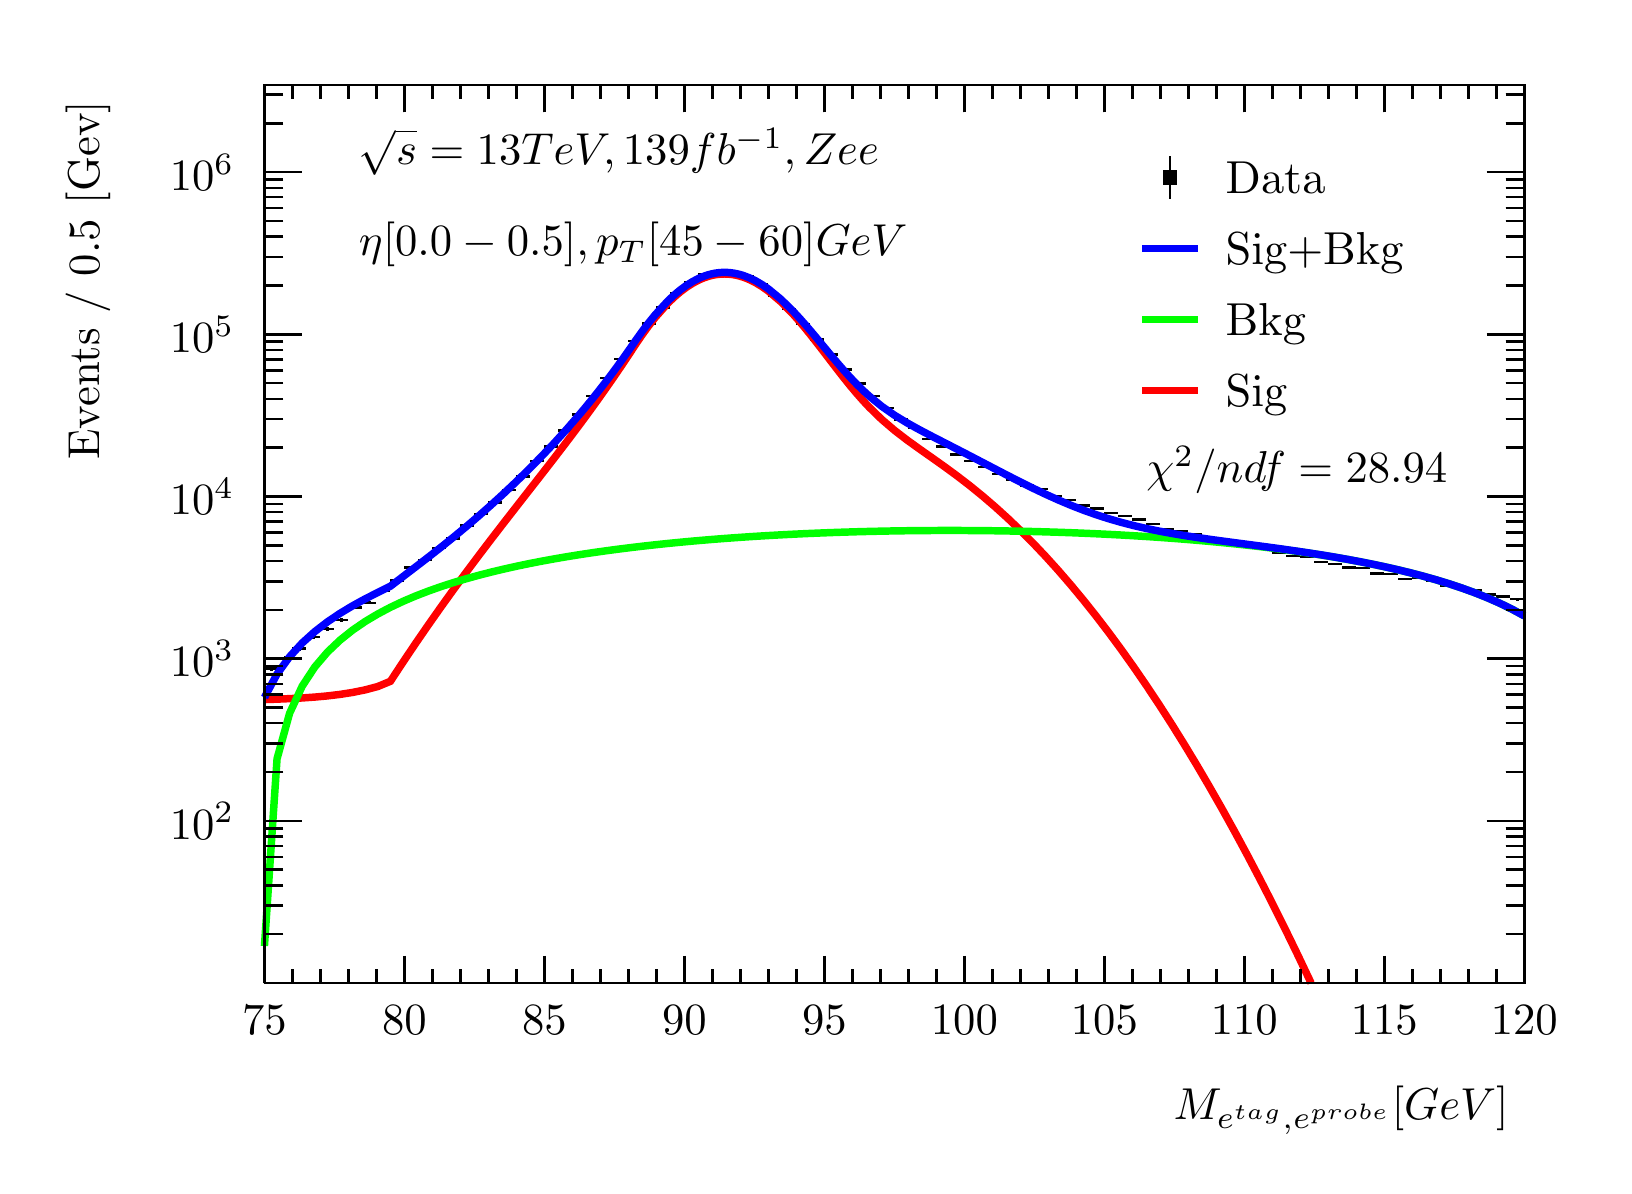
\begin{tikzpicture}
\pgfdeclareplotmark{cross} {
\pgfpathmoveto{\pgfpoint{-0.3\pgfplotmarksize}{\pgfplotmarksize}}
\pgfpathlineto{\pgfpoint{+0.3\pgfplotmarksize}{\pgfplotmarksize}}
\pgfpathlineto{\pgfpoint{+0.3\pgfplotmarksize}{0.3\pgfplotmarksize}}
\pgfpathlineto{\pgfpoint{+1\pgfplotmarksize}{0.3\pgfplotmarksize}}
\pgfpathlineto{\pgfpoint{+1\pgfplotmarksize}{-0.3\pgfplotmarksize}}
\pgfpathlineto{\pgfpoint{+0.3\pgfplotmarksize}{-0.3\pgfplotmarksize}}
\pgfpathlineto{\pgfpoint{+0.3\pgfplotmarksize}{-1.\pgfplotmarksize}}
\pgfpathlineto{\pgfpoint{-0.3\pgfplotmarksize}{-1.\pgfplotmarksize}}
\pgfpathlineto{\pgfpoint{-0.3\pgfplotmarksize}{-0.3\pgfplotmarksize}}
\pgfpathlineto{\pgfpoint{-1.\pgfplotmarksize}{-0.3\pgfplotmarksize}}
\pgfpathlineto{\pgfpoint{-1.\pgfplotmarksize}{0.3\pgfplotmarksize}}
\pgfpathlineto{\pgfpoint{-0.3\pgfplotmarksize}{0.3\pgfplotmarksize}}
\pgfpathclose
\pgfusepathqstroke
}
\pgfdeclareplotmark{cross*} {
\pgfpathmoveto{\pgfpoint{-0.3\pgfplotmarksize}{\pgfplotmarksize}}
\pgfpathlineto{\pgfpoint{+0.3\pgfplotmarksize}{\pgfplotmarksize}}
\pgfpathlineto{\pgfpoint{+0.3\pgfplotmarksize}{0.3\pgfplotmarksize}}
\pgfpathlineto{\pgfpoint{+1\pgfplotmarksize}{0.3\pgfplotmarksize}}
\pgfpathlineto{\pgfpoint{+1\pgfplotmarksize}{-0.3\pgfplotmarksize}}
\pgfpathlineto{\pgfpoint{+0.3\pgfplotmarksize}{-0.3\pgfplotmarksize}}
\pgfpathlineto{\pgfpoint{+0.3\pgfplotmarksize}{-1.\pgfplotmarksize}}
\pgfpathlineto{\pgfpoint{-0.3\pgfplotmarksize}{-1.\pgfplotmarksize}}
\pgfpathlineto{\pgfpoint{-0.3\pgfplotmarksize}{-0.3\pgfplotmarksize}}
\pgfpathlineto{\pgfpoint{-1.\pgfplotmarksize}{-0.3\pgfplotmarksize}}
\pgfpathlineto{\pgfpoint{-1.\pgfplotmarksize}{0.3\pgfplotmarksize}}
\pgfpathlineto{\pgfpoint{-0.3\pgfplotmarksize}{0.3\pgfplotmarksize}}
\pgfpathclose
\pgfusepathqfillstroke
}
\pgfdeclareplotmark{newstar} {
\pgfpathmoveto{\pgfqpoint{0pt}{\pgfplotmarksize}}
\pgfpathlineto{\pgfqpointpolar{44}{0.5\pgfplotmarksize}}
\pgfpathlineto{\pgfqpointpolar{18}{\pgfplotmarksize}}
\pgfpathlineto{\pgfqpointpolar{-20}{0.5\pgfplotmarksize}}
\pgfpathlineto{\pgfqpointpolar{-54}{\pgfplotmarksize}}
\pgfpathlineto{\pgfqpointpolar{-90}{0.5\pgfplotmarksize}}
\pgfpathlineto{\pgfqpointpolar{234}{\pgfplotmarksize}}
\pgfpathlineto{\pgfqpointpolar{198}{0.5\pgfplotmarksize}}
\pgfpathlineto{\pgfqpointpolar{162}{\pgfplotmarksize}}
\pgfpathlineto{\pgfqpointpolar{134}{0.5\pgfplotmarksize}}
\pgfpathclose
\pgfusepathqstroke
}
\pgfdeclareplotmark{newstar*} {
\pgfpathmoveto{\pgfqpoint{0pt}{\pgfplotmarksize}}
\pgfpathlineto{\pgfqpointpolar{44}{0.5\pgfplotmarksize}}
\pgfpathlineto{\pgfqpointpolar{18}{\pgfplotmarksize}}
\pgfpathlineto{\pgfqpointpolar{-20}{0.5\pgfplotmarksize}}
\pgfpathlineto{\pgfqpointpolar{-54}{\pgfplotmarksize}}
\pgfpathlineto{\pgfqpointpolar{-90}{0.5\pgfplotmarksize}}
\pgfpathlineto{\pgfqpointpolar{234}{\pgfplotmarksize}}
\pgfpathlineto{\pgfqpointpolar{198}{0.5\pgfplotmarksize}}
\pgfpathlineto{\pgfqpointpolar{162}{\pgfplotmarksize}}
\pgfpathlineto{\pgfqpointpolar{134}{0.5\pgfplotmarksize}}
\pgfpathclose
\pgfusepathqfillstroke
}
\definecolor{c}{rgb}{1,1,1};
\draw [color=c, fill=c] (0,0) rectangle (20,14.4361);
\draw [color=c, fill=c] (3,2.30977) rectangle (19,13.7143);
\definecolor{c}{rgb}{0,0,0};
\draw [c,line width=0.9] (3,2.30977) -- (3,13.7143) -- (19,13.7143) -- (19,2.30977) -- (3,2.30977);
\definecolor{c}{rgb}{1,1,1};
\draw [color=c, fill=c] (3,2.30977) rectangle (19,13.7143);
\definecolor{c}{rgb}{0,0,0};
\draw [c,line width=0.9] (3,2.30977) -- (3,13.7143) -- (19,13.7143) -- (19,2.30977) -- (3,2.30977);
\draw [c,line width=0.9] (3,2.30977) -- (19,2.30977);
\draw [c,line width=0.9] (3,2.65624) -- (3,2.30977);
\draw [c,line width=0.9] (3.35556,2.48301) -- (3.35556,2.30977);
\draw [c,line width=0.9] (3.71111,2.48301) -- (3.71111,2.30977);
\draw [c,line width=0.9] (4.06667,2.48301) -- (4.06667,2.30977);
\draw [c,line width=0.9] (4.42222,2.48301) -- (4.42222,2.30977);
\draw [c,line width=0.9] (4.77778,2.65624) -- (4.77778,2.30977);
\draw [c,line width=0.9] (5.13333,2.48301) -- (5.13333,2.30977);
\draw [c,line width=0.9] (5.48889,2.48301) -- (5.48889,2.30977);
\draw [c,line width=0.9] (5.84444,2.48301) -- (5.84444,2.30977);
\draw [c,line width=0.9] (6.2,2.48301) -- (6.2,2.30977);
\draw [c,line width=0.9] (6.55556,2.65624) -- (6.55556,2.30977);
\draw [c,line width=0.9] (6.91111,2.48301) -- (6.91111,2.30977);
\draw [c,line width=0.9] (7.26667,2.48301) -- (7.26667,2.30977);
\draw [c,line width=0.9] (7.62222,2.48301) -- (7.62222,2.30977);
\draw [c,line width=0.9] (7.97778,2.48301) -- (7.97778,2.30977);
\draw [c,line width=0.9] (8.33333,2.65624) -- (8.33333,2.30977);
\draw [c,line width=0.9] (8.68889,2.48301) -- (8.68889,2.30977);
\draw [c,line width=0.9] (9.04444,2.48301) -- (9.04444,2.30977);
\draw [c,line width=0.9] (9.4,2.48301) -- (9.4,2.30977);
\draw [c,line width=0.9] (9.75556,2.48301) -- (9.75556,2.30977);
\draw [c,line width=0.9] (10.1111,2.65624) -- (10.1111,2.30977);
\draw [c,line width=0.9] (10.4667,2.48301) -- (10.4667,2.30977);
\draw [c,line width=0.9] (10.8222,2.48301) -- (10.8222,2.30977);
\draw [c,line width=0.9] (11.1778,2.48301) -- (11.1778,2.30977);
\draw [c,line width=0.9] (11.5333,2.48301) -- (11.5333,2.30977);
\draw [c,line width=0.9] (11.8889,2.65624) -- (11.8889,2.30977);
\draw [c,line width=0.9] (12.2444,2.48301) -- (12.2444,2.30977);
\draw [c,line width=0.9] (12.6,2.48301) -- (12.6,2.30977);
\draw [c,line width=0.9] (12.9556,2.48301) -- (12.9556,2.30977);
\draw [c,line width=0.9] (13.3111,2.48301) -- (13.3111,2.30977);
\draw [c,line width=0.9] (13.6667,2.65624) -- (13.6667,2.30977);
\draw [c,line width=0.9] (14.0222,2.48301) -- (14.0222,2.30977);
\draw [c,line width=0.9] (14.3778,2.48301) -- (14.3778,2.30977);
\draw [c,line width=0.9] (14.7333,2.48301) -- (14.7333,2.30977);
\draw [c,line width=0.9] (15.0889,2.48301) -- (15.0889,2.30977);
\draw [c,line width=0.9] (15.4444,2.65624) -- (15.4444,2.30977);
\draw [c,line width=0.9] (15.8,2.48301) -- (15.8,2.30977);
\draw [c,line width=0.9] (16.1556,2.48301) -- (16.1556,2.30977);
\draw [c,line width=0.9] (16.5111,2.48301) -- (16.5111,2.30977);
\draw [c,line width=0.9] (16.8667,2.48301) -- (16.8667,2.30977);
\draw [c,line width=0.9] (17.2222,2.65624) -- (17.2222,2.30977);
\draw [c,line width=0.9] (17.5778,2.48301) -- (17.5778,2.30977);
\draw [c,line width=0.9] (17.9333,2.48301) -- (17.9333,2.30977);
\draw [c,line width=0.9] (18.2889,2.48301) -- (18.2889,2.30977);
\draw [c,line width=0.9] (18.6444,2.48301) -- (18.6444,2.30977);
\draw [c,line width=0.9] (19,2.65624) -- (19,2.30977);
\draw [c,line width=0.9] (19,2.65624) -- (19,2.30977);
\draw [anchor=base] (3,1.66015) node[scale=1.61424, color=c, rotate=0]{75};
\draw [anchor=base] (4.77778,1.66015) node[scale=1.61424, color=c, rotate=0]{80};
\draw [anchor=base] (6.55556,1.66015) node[scale=1.61424, color=c, rotate=0]{85};
\draw [anchor=base] (8.33333,1.66015) node[scale=1.61424, color=c, rotate=0]{90};
\draw [anchor=base] (10.1111,1.66015) node[scale=1.61424, color=c, rotate=0]{95};
\draw [anchor=base] (11.8889,1.66015) node[scale=1.61424, color=c, rotate=0]{100};
\draw [anchor=base] (13.6667,1.66015) node[scale=1.61424, color=c, rotate=0]{105};
\draw [anchor=base] (15.4444,1.66015) node[scale=1.61424, color=c, rotate=0]{110};
\draw [anchor=base] (17.2222,1.66015) node[scale=1.61424, color=c, rotate=0]{115};
\draw [anchor=base] (19,1.66015) node[scale=1.61424, color=c, rotate=0]{120};
\draw [anchor= east] (19,0.692932) node[scale=1.61424, color=c, rotate=0]{$M_{e^{tag}, e^{probe}}  [GeV]$};
\draw [c,line width=0.9] (3,13.7143) -- (19,13.7143);
\draw [c,line width=0.9] (3,13.3678) -- (3,13.7143);
\draw [c,line width=0.9] (3.35556,13.5411) -- (3.35556,13.7143);
\draw [c,line width=0.9] (3.71111,13.5411) -- (3.71111,13.7143);
\draw [c,line width=0.9] (4.06667,13.5411) -- (4.06667,13.7143);
\draw [c,line width=0.9] (4.42222,13.5411) -- (4.42222,13.7143);
\draw [c,line width=0.9] (4.77778,13.3678) -- (4.77778,13.7143);
\draw [c,line width=0.9] (5.13333,13.5411) -- (5.13333,13.7143);
\draw [c,line width=0.9] (5.48889,13.5411) -- (5.48889,13.7143);
\draw [c,line width=0.9] (5.84444,13.5411) -- (5.84444,13.7143);
\draw [c,line width=0.9] (6.2,13.5411) -- (6.2,13.7143);
\draw [c,line width=0.9] (6.55556,13.3678) -- (6.55556,13.7143);
\draw [c,line width=0.9] (6.91111,13.5411) -- (6.91111,13.7143);
\draw [c,line width=0.9] (7.26667,13.5411) -- (7.26667,13.7143);
\draw [c,line width=0.9] (7.62222,13.5411) -- (7.62222,13.7143);
\draw [c,line width=0.9] (7.97778,13.5411) -- (7.97778,13.7143);
\draw [c,line width=0.9] (8.33333,13.3678) -- (8.33333,13.7143);
\draw [c,line width=0.9] (8.68889,13.5411) -- (8.68889,13.7143);
\draw [c,line width=0.9] (9.04444,13.5411) -- (9.04444,13.7143);
\draw [c,line width=0.9] (9.4,13.5411) -- (9.4,13.7143);
\draw [c,line width=0.9] (9.75556,13.5411) -- (9.75556,13.7143);
\draw [c,line width=0.9] (10.1111,13.3678) -- (10.1111,13.7143);
\draw [c,line width=0.9] (10.4667,13.5411) -- (10.4667,13.7143);
\draw [c,line width=0.9] (10.8222,13.5411) -- (10.8222,13.7143);
\draw [c,line width=0.9] (11.1778,13.5411) -- (11.1778,13.7143);
\draw [c,line width=0.9] (11.5333,13.5411) -- (11.5333,13.7143);
\draw [c,line width=0.9] (11.8889,13.3678) -- (11.8889,13.7143);
\draw [c,line width=0.9] (12.2444,13.5411) -- (12.2444,13.7143);
\draw [c,line width=0.9] (12.6,13.5411) -- (12.6,13.7143);
\draw [c,line width=0.9] (12.9556,13.5411) -- (12.9556,13.7143);
\draw [c,line width=0.9] (13.3111,13.5411) -- (13.3111,13.7143);
\draw [c,line width=0.9] (13.6667,13.3678) -- (13.6667,13.7143);
\draw [c,line width=0.9] (14.0222,13.5411) -- (14.0222,13.7143);
\draw [c,line width=0.9] (14.3778,13.5411) -- (14.3778,13.7143);
\draw [c,line width=0.9] (14.7333,13.5411) -- (14.7333,13.7143);
\draw [c,line width=0.9] (15.0889,13.5411) -- (15.0889,13.7143);
\draw [c,line width=0.9] (15.4444,13.3678) -- (15.4444,13.7143);
\draw [c,line width=0.9] (15.8,13.5411) -- (15.8,13.7143);
\draw [c,line width=0.9] (16.1556,13.5411) -- (16.1556,13.7143);
\draw [c,line width=0.9] (16.5111,13.5411) -- (16.5111,13.7143);
\draw [c,line width=0.9] (16.8667,13.5411) -- (16.8667,13.7143);
\draw [c,line width=0.9] (17.2222,13.3678) -- (17.2222,13.7143);
\draw [c,line width=0.9] (17.5778,13.5411) -- (17.5778,13.7143);
\draw [c,line width=0.9] (17.9333,13.5411) -- (17.9333,13.7143);
\draw [c,line width=0.9] (18.2889,13.5411) -- (18.2889,13.7143);
\draw [c,line width=0.9] (18.6444,13.5411) -- (18.6444,13.7143);
\draw [c,line width=0.9] (19,13.3678) -- (19,13.7143);
\draw [c,line width=0.9] (19,13.3678) -- (19,13.7143);
\draw [c,line width=0.9] (3,2.30977) -- (3,13.7143);
\draw [c,line width=0.9] (3.237,2.92982) -- (3,2.92982);
\draw [c,line width=0.9] (3.237,3.29252) -- (3,3.29252);
\draw [c,line width=0.9] (3.237,3.54986) -- (3,3.54986);
\draw [c,line width=0.9] (3.237,3.74947) -- (3,3.74947);
\draw [c,line width=0.9] (3.237,3.91257) -- (3,3.91257);
\draw [c,line width=0.9] (3.237,4.05046) -- (3,4.05046);
\draw [c,line width=0.9] (3.237,4.16991) -- (3,4.16991);
\draw [c,line width=0.9] (3.237,4.27527) -- (3,4.27527);
\draw [c,line width=0.9] (3.474,4.36952) -- (3,4.36952);
\draw [anchor= east] (2.82,4.36952) node[scale=1.61424, color=c, rotate=0]{$10^{2}$};
\draw [c,line width=0.9] (3.237,4.98956) -- (3,4.98956);
\draw [c,line width=0.9] (3.237,5.35227) -- (3,5.35227);
\draw [c,line width=0.9] (3.237,5.60961) -- (3,5.60961);
\draw [c,line width=0.9] (3.237,5.80922) -- (3,5.80922);
\draw [c,line width=0.9] (3.237,5.97231) -- (3,5.97231);
\draw [c,line width=0.9] (3.237,6.11021) -- (3,6.11021);
\draw [c,line width=0.9] (3.237,6.22966) -- (3,6.22966);
\draw [c,line width=0.9] (3.237,6.33502) -- (3,6.33502);
\draw [c,line width=0.9] (3.474,6.42927) -- (3,6.42927);
\draw [anchor= east] (2.82,6.42927) node[scale=1.61424, color=c, rotate=0]{$10^{3}$};
\draw [c,line width=0.9] (3.237,7.04931) -- (3,7.04931);
\draw [c,line width=0.9] (3.237,7.41202) -- (3,7.41202);
\draw [c,line width=0.9] (3.237,7.66936) -- (3,7.66936);
\draw [c,line width=0.9] (3.237,7.86897) -- (3,7.86897);
\draw [c,line width=0.9] (3.237,8.03206) -- (3,8.03206);
\draw [c,line width=0.9] (3.237,8.16995) -- (3,8.16995);
\draw [c,line width=0.9] (3.237,8.2894) -- (3,8.2894);
\draw [c,line width=0.9] (3.237,8.39476) -- (3,8.39476);
\draw [c,line width=0.9] (3.474,8.48901) -- (3,8.48901);
\draw [anchor= east] (2.82,8.48901) node[scale=1.61424, color=c, rotate=0]{$10^{4}$};
\draw [c,line width=0.9] (3.237,9.10906) -- (3,9.10906);
\draw [c,line width=0.9] (3.237,9.47176) -- (3,9.47176);
\draw [c,line width=0.9] (3.237,9.7291) -- (3,9.7291);
\draw [c,line width=0.9] (3.237,9.92871) -- (3,9.92871);
\draw [c,line width=0.9] (3.237,10.0918) -- (3,10.0918);
\draw [c,line width=0.9] (3.237,10.2297) -- (3,10.2297);
\draw [c,line width=0.9] (3.237,10.3491) -- (3,10.3491);
\draw [c,line width=0.9] (3.237,10.4545) -- (3,10.4545);
\draw [c,line width=0.9] (3.474,10.5488) -- (3,10.5488);
\draw [anchor= east] (2.82,10.5488) node[scale=1.61424, color=c, rotate=0]{$10^{5}$};
\draw [c,line width=0.9] (3.237,11.1688) -- (3,11.1688);
\draw [c,line width=0.9] (3.237,11.5315) -- (3,11.5315);
\draw [c,line width=0.9] (3.237,11.7889) -- (3,11.7889);
\draw [c,line width=0.9] (3.237,11.9885) -- (3,11.9885);
\draw [c,line width=0.9] (3.237,12.1516) -- (3,12.1516);
\draw [c,line width=0.9] (3.237,12.2894) -- (3,12.2894);
\draw [c,line width=0.9] (3.237,12.4089) -- (3,12.4089);
\draw [c,line width=0.9] (3.237,12.5143) -- (3,12.5143);
\draw [c,line width=0.9] (3.474,12.6085) -- (3,12.6085);
\draw [anchor= east] (2.82,12.6085) node[scale=1.61424, color=c, rotate=0]{$10^{6}$};
\draw [c,line width=0.9] (3.237,13.2286) -- (3,13.2286);
\draw [c,line width=0.9] (3.237,13.5913) -- (3,13.5913);
\draw [anchor= east] (0.76,13.7143) node[scale=1.61424, color=c, rotate=90]{Events / 0.5 [Gev]};
\draw [c,line width=0.9] (19,2.30977) -- (19,13.7143);
\draw [c,line width=0.9] (18.763,2.92982) -- (19,2.92982);
\draw [c,line width=0.9] (18.763,3.29252) -- (19,3.29252);
\draw [c,line width=0.9] (18.763,3.54986) -- (19,3.54986);
\draw [c,line width=0.9] (18.763,3.74947) -- (19,3.74947);
\draw [c,line width=0.9] (18.763,3.91257) -- (19,3.91257);
\draw [c,line width=0.9] (18.763,4.05046) -- (19,4.05046);
\draw [c,line width=0.9] (18.763,4.16991) -- (19,4.16991);
\draw [c,line width=0.9] (18.763,4.27527) -- (19,4.27527);
\draw [c,line width=0.9] (18.526,4.36952) -- (19,4.36952);
\draw [c,line width=0.9] (18.763,4.98956) -- (19,4.98956);
\draw [c,line width=0.9] (18.763,5.35227) -- (19,5.35227);
\draw [c,line width=0.9] (18.763,5.60961) -- (19,5.60961);
\draw [c,line width=0.9] (18.763,5.80922) -- (19,5.80922);
\draw [c,line width=0.9] (18.763,5.97231) -- (19,5.97231);
\draw [c,line width=0.9] (18.763,6.11021) -- (19,6.11021);
\draw [c,line width=0.9] (18.763,6.22966) -- (19,6.22966);
\draw [c,line width=0.9] (18.763,6.33502) -- (19,6.33502);
\draw [c,line width=0.9] (18.526,6.42927) -- (19,6.42927);
\draw [c,line width=0.9] (18.763,7.04931) -- (19,7.04931);
\draw [c,line width=0.9] (18.763,7.41202) -- (19,7.41202);
\draw [c,line width=0.9] (18.763,7.66936) -- (19,7.66936);
\draw [c,line width=0.9] (18.763,7.86897) -- (19,7.86897);
\draw [c,line width=0.9] (18.763,8.03206) -- (19,8.03206);
\draw [c,line width=0.9] (18.763,8.16995) -- (19,8.16995);
\draw [c,line width=0.9] (18.763,8.2894) -- (19,8.2894);
\draw [c,line width=0.9] (18.763,8.39476) -- (19,8.39476);
\draw [c,line width=0.9] (18.526,8.48901) -- (19,8.48901);
\draw [c,line width=0.9] (18.763,9.10906) -- (19,9.10906);
\draw [c,line width=0.9] (18.763,9.47176) -- (19,9.47176);
\draw [c,line width=0.9] (18.763,9.7291) -- (19,9.7291);
\draw [c,line width=0.9] (18.763,9.92871) -- (19,9.92871);
\draw [c,line width=0.9] (18.763,10.0918) -- (19,10.0918);
\draw [c,line width=0.9] (18.763,10.2297) -- (19,10.2297);
\draw [c,line width=0.9] (18.763,10.3491) -- (19,10.3491);
\draw [c,line width=0.9] (18.763,10.4545) -- (19,10.4545);
\draw [c,line width=0.9] (18.526,10.5488) -- (19,10.5488);
\draw [c,line width=0.9] (18.763,11.1688) -- (19,11.1688);
\draw [c,line width=0.9] (18.763,11.5315) -- (19,11.5315);
\draw [c,line width=0.9] (18.763,11.7889) -- (19,11.7889);
\draw [c,line width=0.9] (18.763,11.9885) -- (19,11.9885);
\draw [c,line width=0.9] (18.763,12.1516) -- (19,12.1516);
\draw [c,line width=0.9] (18.763,12.2894) -- (19,12.2894);
\draw [c,line width=0.9] (18.763,12.4089) -- (19,12.4089);
\draw [c,line width=0.9] (18.763,12.5143) -- (19,12.5143);
\draw [c,line width=0.9] (18.526,12.6085) -- (19,12.6085);
\draw [c,line width=0.9] (18.763,13.2286) -- (19,13.2286);
\draw [c,line width=0.9] (18.763,13.5913) -- (19,13.5913);
\draw [c,line width=0.9] (3.08889,6.30572) -- (3,6.30572);
\draw [c,line width=0.9] (3,6.30572) -- (3,6.30572);
\draw [c,line width=0.9] (3.08889,6.30572) -- (3.17778,6.30572);
\draw [c,line width=0.9] (3.17778,6.30572) -- (3.17778,6.30572);
\draw [c,line width=0.9] (3.08889,6.30572) -- (3.08889,6.33603);
\draw [c,line width=0.9] (3.08889,6.33603) -- (3.08889,6.33603);
\draw [c,line width=0.9] (3.08889,6.30572) -- (3.08889,6.27541);
\draw [c,line width=0.9] (3.08889,6.27541) -- (3.08889,6.27541);
\draw [c,line width=0.9] (3.26667,6.43994) -- (3.17778,6.43994);
\draw [c,line width=0.9] (3.17778,6.43994) -- (3.17778,6.43994);
\draw [c,line width=0.9] (3.26667,6.43994) -- (3.35556,6.43994);
\draw [c,line width=0.9] (3.35556,6.43994) -- (3.35556,6.43994);
\draw [c,line width=0.9] (3.26667,6.43994) -- (3.26667,6.46806);
\draw [c,line width=0.9] (3.26667,6.46806) -- (3.26667,6.46806);
\draw [c,line width=0.9] (3.26667,6.43994) -- (3.26667,6.41182);
\draw [c,line width=0.9] (3.26667,6.41182) -- (3.26667,6.41182);
\draw [c,line width=0.9] (3.44444,6.55584) -- (3.35556,6.55584);
\draw [c,line width=0.9] (3.35556,6.55584) -- (3.35556,6.55584);
\draw [c,line width=0.9] (3.44444,6.55584) -- (3.53333,6.55584);
\draw [c,line width=0.9] (3.53333,6.55584) -- (3.53333,6.55584);
\draw [c,line width=0.9] (3.44444,6.55584) -- (3.44444,6.5822);
\draw [c,line width=0.9] (3.44444,6.5822) -- (3.44444,6.5822);
\draw [c,line width=0.9] (3.44444,6.55584) -- (3.44444,6.52949);
\draw [c,line width=0.9] (3.44444,6.52949) -- (3.44444,6.52949);
\draw [c,line width=0.9] (3.62222,6.70301) -- (3.53333,6.70301);
\draw [c,line width=0.9] (3.53333,6.70301) -- (3.53333,6.70301);
\draw [c,line width=0.9] (3.62222,6.70301) -- (3.71111,6.70301);
\draw [c,line width=0.9] (3.71111,6.70301) -- (3.71111,6.70301);
\draw [c,line width=0.9] (3.62222,6.70301) -- (3.62222,6.72728);
\draw [c,line width=0.9] (3.62222,6.72728) -- (3.62222,6.72728);
\draw [c,line width=0.9] (3.62222,6.70301) -- (3.62222,6.67873);
\draw [c,line width=0.9] (3.62222,6.67873) -- (3.62222,6.67873);
\draw [c,line width=0.9] (3.8,6.80852) -- (3.71111,6.80852);
\draw [c,line width=0.9] (3.71111,6.80852) -- (3.71111,6.80852);
\draw [c,line width=0.9] (3.8,6.80852) -- (3.88889,6.80852);
\draw [c,line width=0.9] (3.88889,6.80852) -- (3.88889,6.80852);
\draw [c,line width=0.9] (3.8,6.80852) -- (3.8,6.8314);
\draw [c,line width=0.9] (3.8,6.8314) -- (3.8,6.8314);
\draw [c,line width=0.9] (3.8,6.80852) -- (3.8,6.78563);
\draw [c,line width=0.9] (3.8,6.78563) -- (3.8,6.78563);
\draw [c,line width=0.9] (3.97778,6.91855) -- (3.88889,6.91855);
\draw [c,line width=0.9] (3.88889,6.91855) -- (3.88889,6.91855);
\draw [c,line width=0.9] (3.97778,6.91855) -- (4.06667,6.91855);
\draw [c,line width=0.9] (4.06667,6.91855) -- (4.06667,6.91855);
\draw [c,line width=0.9] (3.97778,6.91855) -- (3.97778,6.94007);
\draw [c,line width=0.9] (3.97778,6.94007) -- (3.97778,6.94007);
\draw [c,line width=0.9] (3.97778,6.91855) -- (3.97778,6.89703);
\draw [c,line width=0.9] (3.97778,6.89703) -- (3.97778,6.89703);
\draw [c,line width=0.9] (4.15556,7.08052) -- (4.06667,7.08052);
\draw [c,line width=0.9] (4.06667,7.08052) -- (4.06667,7.08052);
\draw [c,line width=0.9] (4.15556,7.08052) -- (4.24444,7.08052);
\draw [c,line width=0.9] (4.24444,7.08052) -- (4.24444,7.08052);
\draw [c,line width=0.9] (4.15556,7.08052) -- (4.15556,7.10017);
\draw [c,line width=0.9] (4.15556,7.10017) -- (4.15556,7.10017);
\draw [c,line width=0.9] (4.15556,7.08052) -- (4.15556,7.06086);
\draw [c,line width=0.9] (4.15556,7.06086) -- (4.15556,7.06086);
\draw [c,line width=0.9] (4.33333,7.13863) -- (4.24444,7.13863);
\draw [c,line width=0.9] (4.24444,7.13863) -- (4.24444,7.13863);
\draw [c,line width=0.9] (4.33333,7.13863) -- (4.42222,7.13863);
\draw [c,line width=0.9] (4.42222,7.13863) -- (4.42222,7.13863);
\draw [c,line width=0.9] (4.33333,7.13863) -- (4.33333,7.15766);
\draw [c,line width=0.9] (4.33333,7.15766) -- (4.33333,7.15766);
\draw [c,line width=0.9] (4.33333,7.13863) -- (4.33333,7.1196);
\draw [c,line width=0.9] (4.33333,7.1196) -- (4.33333,7.1196);
\draw [c,line width=0.9] (4.51111,7.29393) -- (4.42222,7.29393);
\draw [c,line width=0.9] (4.42222,7.29393) -- (4.42222,7.29393);
\draw [c,line width=0.9] (4.51111,7.29393) -- (4.6,7.29393);
\draw [c,line width=0.9] (4.6,7.29393) -- (4.6,7.29393);
\draw [c,line width=0.9] (4.51111,7.29393) -- (4.51111,7.31138);
\draw [c,line width=0.9] (4.51111,7.31138) -- (4.51111,7.31138);
\draw [c,line width=0.9] (4.51111,7.29393) -- (4.51111,7.27648);
\draw [c,line width=0.9] (4.51111,7.27648) -- (4.51111,7.27648);
\draw [c,line width=0.9] (4.68889,7.42239) -- (4.6,7.42239);
\draw [c,line width=0.9] (4.6,7.42239) -- (4.6,7.42239);
\draw [c,line width=0.9] (4.68889,7.42239) -- (4.77778,7.42239);
\draw [c,line width=0.9] (4.77778,7.42239) -- (4.77778,7.42239);
\draw [c,line width=0.9] (4.68889,7.42239) -- (4.68889,7.43863);
\draw [c,line width=0.9] (4.68889,7.43863) -- (4.68889,7.43863);
\draw [c,line width=0.9] (4.68889,7.42239) -- (4.68889,7.40616);
\draw [c,line width=0.9] (4.68889,7.40616) -- (4.68889,7.40616);
\draw [c,line width=0.9] (4.86667,7.58647) -- (4.77778,7.58647);
\draw [c,line width=0.9] (4.77778,7.58647) -- (4.77778,7.58647);
\draw [c,line width=0.9] (4.86667,7.58647) -- (4.95556,7.58647);
\draw [c,line width=0.9] (4.95556,7.58647) -- (4.95556,7.58647);
\draw [c,line width=0.9] (4.86667,7.58647) -- (4.86667,7.60128);
\draw [c,line width=0.9] (4.86667,7.60128) -- (4.86667,7.60128);
\draw [c,line width=0.9] (4.86667,7.58647) -- (4.86667,7.57165);
\draw [c,line width=0.9] (4.86667,7.57165) -- (4.86667,7.57165);
\draw [c,line width=0.9] (5.04444,7.68466) -- (4.95556,7.68466);
\draw [c,line width=0.9] (4.95556,7.68466) -- (4.95556,7.68466);
\draw [c,line width=0.9] (5.04444,7.68466) -- (5.13333,7.68466);
\draw [c,line width=0.9] (5.13333,7.68466) -- (5.13333,7.68466);
\draw [c,line width=0.9] (5.04444,7.68466) -- (5.04444,7.69868);
\draw [c,line width=0.9] (5.04444,7.69868) -- (5.04444,7.69868);
\draw [c,line width=0.9] (5.04444,7.68466) -- (5.04444,7.67063);
\draw [c,line width=0.9] (5.04444,7.67063) -- (5.04444,7.67063);
\draw [c,line width=0.9] (5.22222,7.83413) -- (5.13333,7.83413);
\draw [c,line width=0.9] (5.13333,7.83413) -- (5.13333,7.83413);
\draw [c,line width=0.9] (5.22222,7.83413) -- (5.31111,7.83413);
\draw [c,line width=0.9] (5.31111,7.83413) -- (5.31111,7.83413);
\draw [c,line width=0.9] (5.22222,7.83413) -- (5.22222,7.84703);
\draw [c,line width=0.9] (5.22222,7.84703) -- (5.22222,7.84703);
\draw [c,line width=0.9] (5.22222,7.83413) -- (5.22222,7.82123);
\draw [c,line width=0.9] (5.22222,7.82123) -- (5.22222,7.82123);
\draw [c,line width=0.9] (5.4,7.95861) -- (5.31111,7.95861);
\draw [c,line width=0.9] (5.31111,7.95861) -- (5.31111,7.95861);
\draw [c,line width=0.9] (5.4,7.95861) -- (5.48889,7.95861);
\draw [c,line width=0.9] (5.48889,7.95861) -- (5.48889,7.95861);
\draw [c,line width=0.9] (5.4,7.95861) -- (5.4,7.97064);
\draw [c,line width=0.9] (5.4,7.97064) -- (5.4,7.97064);
\draw [c,line width=0.9] (5.4,7.95861) -- (5.4,7.94658);
\draw [c,line width=0.9] (5.4,7.94658) -- (5.4,7.94658);
\draw [c,line width=0.9] (5.57778,8.118) -- (5.48889,8.118);
\draw [c,line width=0.9] (5.48889,8.118) -- (5.48889,8.118);
\draw [c,line width=0.9] (5.57778,8.118) -- (5.66667,8.118);
\draw [c,line width=0.9] (5.66667,8.118) -- (5.66667,8.118);
\draw [c,line width=0.9] (5.57778,8.118) -- (5.57778,8.129);
\draw [c,line width=0.9] (5.57778,8.129) -- (5.57778,8.129);
\draw [c,line width=0.9] (5.57778,8.118) -- (5.57778,8.10699);
\draw [c,line width=0.9] (5.57778,8.10699) -- (5.57778,8.10699);
\draw [c,line width=0.9] (5.75556,8.26354) -- (5.66667,8.26354);
\draw [c,line width=0.9] (5.66667,8.26354) -- (5.66667,8.26354);
\draw [c,line width=0.9] (5.75556,8.26354) -- (5.84444,8.26354);
\draw [c,line width=0.9] (5.84444,8.26354) -- (5.84444,8.26354);
\draw [c,line width=0.9] (5.75556,8.26354) -- (5.75556,8.27369);
\draw [c,line width=0.9] (5.75556,8.27369) -- (5.75556,8.27369);
\draw [c,line width=0.9] (5.75556,8.26354) -- (5.75556,8.25339);
\draw [c,line width=0.9] (5.75556,8.25339) -- (5.75556,8.25339);
\draw [c,line width=0.9] (5.93333,8.41189) -- (5.84444,8.41189);
\draw [c,line width=0.9] (5.84444,8.41189) -- (5.84444,8.41189);
\draw [c,line width=0.9] (5.93333,8.41189) -- (6.02222,8.41189);
\draw [c,line width=0.9] (6.02222,8.41189) -- (6.02222,8.41189);
\draw [c,line width=0.9] (5.93333,8.41189) -- (5.93333,8.42123);
\draw [c,line width=0.9] (5.93333,8.42123) -- (5.93333,8.42123);
\draw [c,line width=0.9] (5.93333,8.41189) -- (5.93333,8.40256);
\draw [c,line width=0.9] (5.93333,8.40256) -- (5.93333,8.40256);
\draw [c,line width=0.9] (6.11111,8.5702) -- (6.02222,8.5702);
\draw [c,line width=0.9] (6.02222,8.5702) -- (6.02222,8.5702);
\draw [c,line width=0.9] (6.11111,8.5702) -- (6.2,8.5702);
\draw [c,line width=0.9] (6.2,8.5702) -- (6.2,8.5702);
\draw [c,line width=0.9] (6.11111,8.5702) -- (6.11111,8.57875);
\draw [c,line width=0.9] (6.11111,8.57875) -- (6.11111,8.57875);
\draw [c,line width=0.9] (6.11111,8.5702) -- (6.11111,8.56165);
\draw [c,line width=0.9] (6.11111,8.56165) -- (6.11111,8.56165);
\draw [c,line width=0.9] (6.28889,8.74338) -- (6.2,8.74338);
\draw [c,line width=0.9] (6.2,8.74338) -- (6.2,8.74338);
\draw [c,line width=0.9] (6.28889,8.74338) -- (6.37778,8.74338);
\draw [c,line width=0.9] (6.37778,8.74338) -- (6.37778,8.74338);
\draw [c,line width=0.9] (6.28889,8.74338) -- (6.28889,8.75114);
\draw [c,line width=0.9] (6.28889,8.75114) -- (6.28889,8.75114);
\draw [c,line width=0.9] (6.28889,8.74338) -- (6.28889,8.73562);
\draw [c,line width=0.9] (6.28889,8.73562) -- (6.28889,8.73562);
\draw [c,line width=0.9] (6.46667,8.93957) -- (6.37778,8.93957);
\draw [c,line width=0.9] (6.37778,8.93957) -- (6.37778,8.93957);
\draw [c,line width=0.9] (6.46667,8.93957) -- (6.55556,8.93957);
\draw [c,line width=0.9] (6.55556,8.93957) -- (6.55556,8.93957);
\draw [c,line width=0.9] (6.46667,8.93957) -- (6.46667,8.94653);
\draw [c,line width=0.9] (6.46667,8.94653) -- (6.46667,8.94653);
\draw [c,line width=0.9] (6.46667,8.93957) -- (6.46667,8.93262);
\draw [c,line width=0.9] (6.46667,8.93262) -- (6.46667,8.93262);
\draw [c,line width=0.9] (6.64444,9.12594) -- (6.55556,9.12594);
\draw [c,line width=0.9] (6.55556,9.12594) -- (6.55556,9.12594);
\draw [c,line width=0.9] (6.64444,9.12594) -- (6.73333,9.12594);
\draw [c,line width=0.9] (6.73333,9.12594) -- (6.73333,9.12594);
\draw [c,line width=0.9] (6.64444,9.12594) -- (6.64444,9.13221);
\draw [c,line width=0.9] (6.64444,9.13221) -- (6.64444,9.13221);
\draw [c,line width=0.9] (6.64444,9.12594) -- (6.64444,9.11967);
\draw [c,line width=0.9] (6.64444,9.11967) -- (6.64444,9.11967);
\draw [c,line width=0.9] (6.82222,9.32751) -- (6.73333,9.32751);
\draw [c,line width=0.9] (6.73333,9.32751) -- (6.73333,9.32751);
\draw [c,line width=0.9] (6.82222,9.32751) -- (6.91111,9.32751);
\draw [c,line width=0.9] (6.91111,9.32751) -- (6.91111,9.32751);
\draw [c,line width=0.9] (6.82222,9.32751) -- (6.82222,9.3331);
\draw [c,line width=0.9] (6.82222,9.3331) -- (6.82222,9.3331);
\draw [c,line width=0.9] (6.82222,9.32751) -- (6.82222,9.32191);
\draw [c,line width=0.9] (6.82222,9.32191) -- (6.82222,9.32191);
\draw [c,line width=0.9] (7,9.53) -- (6.91111,9.53);
\draw [c,line width=0.9] (6.91111,9.53) -- (6.91111,9.53);
\draw [c,line width=0.9] (7,9.53) -- (7.08889,9.53);
\draw [c,line width=0.9] (7.08889,9.53) -- (7.08889,9.53);
\draw [c,line width=0.9] (7,9.53) -- (7,9.535);
\draw [c,line width=0.9] (7,9.535) -- (7,9.535);
\draw [c,line width=0.9] (7,9.53) -- (7,9.525);
\draw [c,line width=0.9] (7,9.525) -- (7,9.525);
\draw [c,line width=0.9] (7.17778,9.76837) -- (7.08889,9.76837);
\draw [c,line width=0.9] (7.08889,9.76837) -- (7.08889,9.76837);
\draw [c,line width=0.9] (7.17778,9.76837) -- (7.26667,9.76837);
\draw [c,line width=0.9] (7.26667,9.76837) -- (7.26667,9.76837);
\draw [c,line width=0.9] (7.17778,9.76837) -- (7.17778,9.77275);
\draw [c,line width=0.9] (7.17778,9.77275) -- (7.17778,9.77275);
\draw [c,line width=0.9] (7.17778,9.76837) -- (7.17778,9.764);
\draw [c,line width=0.9] (7.17778,9.764) -- (7.17778,9.764);
\draw [c,line width=0.9] (7.35556,9.99199) -- (7.26667,9.99199);
\draw [c,line width=0.9] (7.26667,9.99199) -- (7.26667,9.99199);
\draw [c,line width=0.9] (7.35556,9.99199) -- (7.44444,9.99199);
\draw [c,line width=0.9] (7.44444,9.99199) -- (7.44444,9.99199);
\draw [c,line width=0.9] (7.35556,9.99199) -- (7.35556,9.99585);
\draw [c,line width=0.9] (7.35556,9.99585) -- (7.35556,9.99585);
\draw [c,line width=0.9] (7.35556,9.99199) -- (7.35556,9.98813);
\draw [c,line width=0.9] (7.35556,9.98813) -- (7.35556,9.98813);
\draw [c,line width=0.9] (7.53333,10.2354) -- (7.44444,10.2354);
\draw [c,line width=0.9] (7.44444,10.2354) -- (7.44444,10.2354);
\draw [c,line width=0.9] (7.53333,10.2354) -- (7.62222,10.2354);
\draw [c,line width=0.9] (7.62222,10.2354) -- (7.62222,10.2354);
\draw [c,line width=0.9] (7.53333,10.2354) -- (7.53333,10.2387);
\draw [c,line width=0.9] (7.53333,10.2387) -- (7.53333,10.2387);
\draw [c,line width=0.9] (7.53333,10.2354) -- (7.53333,10.232);
\draw [c,line width=0.9] (7.53333,10.232) -- (7.53333,10.232);
\draw [c,line width=0.9] (7.71111,10.4629) -- (7.62222,10.4629);
\draw [c,line width=0.9] (7.62222,10.4629) -- (7.62222,10.4629);
\draw [c,line width=0.9] (7.71111,10.4629) -- (7.8,10.4629);
\draw [c,line width=0.9] (7.8,10.4629) -- (7.8,10.4629);
\draw [c,line width=0.9] (7.71111,10.4629) -- (7.71111,10.4658);
\draw [c,line width=0.9] (7.71111,10.4658) -- (7.71111,10.4658);
\draw [c,line width=0.9] (7.71111,10.4629) -- (7.71111,10.4599);
\draw [c,line width=0.9] (7.71111,10.4599) -- (7.71111,10.4599);
\draw [c,line width=0.9] (7.88889,10.6841) -- (7.8,10.6841);
\draw [c,line width=0.9] (7.8,10.6841) -- (7.8,10.6841);
\draw [c,line width=0.9] (7.88889,10.6841) -- (7.97778,10.6841);
\draw [c,line width=0.9] (7.97778,10.6841) -- (7.97778,10.6841);
\draw [c,line width=0.9] (7.88889,10.6841) -- (7.88889,10.6867);
\draw [c,line width=0.9] (7.88889,10.6867) -- (7.88889,10.6867);
\draw [c,line width=0.9] (7.88889,10.6841) -- (7.88889,10.6815);
\draw [c,line width=0.9] (7.88889,10.6815) -- (7.88889,10.6815);
\draw [c,line width=0.9] (8.06667,10.8887) -- (7.97778,10.8887);
\draw [c,line width=0.9] (7.97778,10.8887) -- (7.97778,10.8887);
\draw [c,line width=0.9] (8.06667,10.8887) -- (8.15556,10.8887);
\draw [c,line width=0.9] (8.15556,10.8887) -- (8.15556,10.8887);
\draw [c,line width=0.9] (8.06667,10.8887) -- (8.06667,10.891);
\draw [c,line width=0.9] (8.06667,10.891) -- (8.06667,10.891);
\draw [c,line width=0.9] (8.06667,10.8887) -- (8.06667,10.8863);
\draw [c,line width=0.9] (8.06667,10.8863) -- (8.06667,10.8863);
\draw [c,line width=0.9] (8.24444,11.0725) -- (8.15556,11.0725);
\draw [c,line width=0.9] (8.15556,11.0725) -- (8.15556,11.0725);
\draw [c,line width=0.9] (8.24444,11.0725) -- (8.33333,11.0725);
\draw [c,line width=0.9] (8.33333,11.0725) -- (8.33333,11.0725);
\draw [c,line width=0.9] (8.24444,11.0725) -- (8.24444,11.0746);
\draw [c,line width=0.9] (8.24444,11.0746) -- (8.24444,11.0746);
\draw [c,line width=0.9] (8.24444,11.0725) -- (8.24444,11.0704);
\draw [c,line width=0.9] (8.24444,11.0704) -- (8.24444,11.0704);
\draw [c,line width=0.9] (8.42222,11.2095) -- (8.33333,11.2095);
\draw [c,line width=0.9] (8.33333,11.2095) -- (8.33333,11.2095);
\draw [c,line width=0.9] (8.42222,11.2095) -- (8.51111,11.2095);
\draw [c,line width=0.9] (8.51111,11.2095) -- (8.51111,11.2095);
\draw [c,line width=0.9] (8.42222,11.2095) -- (8.42222,11.2115);
\draw [c,line width=0.9] (8.42222,11.2115) -- (8.42222,11.2115);
\draw [c,line width=0.9] (8.42222,11.2095) -- (8.42222,11.2076);
\draw [c,line width=0.9] (8.42222,11.2076) -- (8.42222,11.2076);
\draw [c,line width=0.9] (8.6,11.3058) -- (8.51111,11.3058);
\draw [c,line width=0.9] (8.51111,11.3058) -- (8.51111,11.3058);
\draw [c,line width=0.9] (8.6,11.3058) -- (8.68889,11.3058);
\draw [c,line width=0.9] (8.68889,11.3058) -- (8.68889,11.3058);
\draw [c,line width=0.9] (8.6,11.3058) -- (8.6,11.3076);
\draw [c,line width=0.9] (8.6,11.3076) -- (8.6,11.3076);
\draw [c,line width=0.9] (8.6,11.3058) -- (8.6,11.3039);
\draw [c,line width=0.9] (8.6,11.3039) -- (8.6,11.3039);
\draw [c,line width=0.9] (8.77778,11.3499) -- (8.68889,11.3499);
\draw [c,line width=0.9] (8.68889,11.3499) -- (8.68889,11.3499);
\draw [c,line width=0.9] (8.77778,11.3499) -- (8.86667,11.3499);
\draw [c,line width=0.9] (8.86667,11.3499) -- (8.86667,11.3499);
\draw [c,line width=0.9] (8.77778,11.3499) -- (8.77778,11.3517);
\draw [c,line width=0.9] (8.77778,11.3517) -- (8.77778,11.3517);
\draw [c,line width=0.9] (8.77778,11.3499) -- (8.77778,11.348);
\draw [c,line width=0.9] (8.77778,11.348) -- (8.77778,11.348);
\draw [c,line width=0.9] (8.95556,11.3424) -- (8.86667,11.3424);
\draw [c,line width=0.9] (8.86667,11.3424) -- (8.86667,11.3424);
\draw [c,line width=0.9] (8.95556,11.3424) -- (9.04444,11.3424);
\draw [c,line width=0.9] (9.04444,11.3424) -- (9.04444,11.3424);
\draw [c,line width=0.9] (8.95556,11.3424) -- (8.95556,11.3442);
\draw [c,line width=0.9] (8.95556,11.3442) -- (8.95556,11.3442);
\draw [c,line width=0.9] (8.95556,11.3424) -- (8.95556,11.3406);
\draw [c,line width=0.9] (8.95556,11.3406) -- (8.95556,11.3406);
\draw [c,line width=0.9] (9.13333,11.2839) -- (9.04444,11.2839);
\draw [c,line width=0.9] (9.04444,11.2839) -- (9.04444,11.2839);
\draw [c,line width=0.9] (9.13333,11.2839) -- (9.22222,11.2839);
\draw [c,line width=0.9] (9.22222,11.2839) -- (9.22222,11.2839);
\draw [c,line width=0.9] (9.13333,11.2839) -- (9.13333,11.2858);
\draw [c,line width=0.9] (9.13333,11.2858) -- (9.13333,11.2858);
\draw [c,line width=0.9] (9.13333,11.2839) -- (9.13333,11.2821);
\draw [c,line width=0.9] (9.13333,11.2821) -- (9.13333,11.2821);
\draw [c,line width=0.9] (9.31111,11.1805) -- (9.22222,11.1805);
\draw [c,line width=0.9] (9.22222,11.1805) -- (9.22222,11.1805);
\draw [c,line width=0.9] (9.31111,11.1805) -- (9.4,11.1805);
\draw [c,line width=0.9] (9.4,11.1805) -- (9.4,11.1805);
\draw [c,line width=0.9] (9.31111,11.1805) -- (9.31111,11.1825);
\draw [c,line width=0.9] (9.31111,11.1825) -- (9.31111,11.1825);
\draw [c,line width=0.9] (9.31111,11.1805) -- (9.31111,11.1785);
\draw [c,line width=0.9] (9.31111,11.1785) -- (9.31111,11.1785);
\draw [c,line width=0.9] (9.48889,11.0348) -- (9.4,11.0348);
\draw [c,line width=0.9] (9.4,11.0348) -- (9.4,11.0348);
\draw [c,line width=0.9] (9.48889,11.0348) -- (9.57778,11.0348);
\draw [c,line width=0.9] (9.57778,11.0348) -- (9.57778,11.0348);
\draw [c,line width=0.9] (9.48889,11.0348) -- (9.48889,11.037);
\draw [c,line width=0.9] (9.48889,11.037) -- (9.48889,11.037);
\draw [c,line width=0.9] (9.48889,11.0348) -- (9.48889,11.0326);
\draw [c,line width=0.9] (9.48889,11.0326) -- (9.48889,11.0326);
\draw [c,line width=0.9] (9.66667,10.8686) -- (9.57778,10.8686);
\draw [c,line width=0.9] (9.57778,10.8686) -- (9.57778,10.8686);
\draw [c,line width=0.9] (9.66667,10.8686) -- (9.75556,10.8686);
\draw [c,line width=0.9] (9.75556,10.8686) -- (9.75556,10.8686);
\draw [c,line width=0.9] (9.66667,10.8686) -- (9.66667,10.8709);
\draw [c,line width=0.9] (9.66667,10.8709) -- (9.66667,10.8709);
\draw [c,line width=0.9] (9.66667,10.8686) -- (9.66667,10.8662);
\draw [c,line width=0.9] (9.66667,10.8662) -- (9.66667,10.8662);
\draw [c,line width=0.9] (9.84444,10.6793) -- (9.75556,10.6793);
\draw [c,line width=0.9] (9.75556,10.6793) -- (9.75556,10.6793);
\draw [c,line width=0.9] (9.84444,10.6793) -- (9.93333,10.6793);
\draw [c,line width=0.9] (9.93333,10.6793) -- (9.93333,10.6793);
\draw [c,line width=0.9] (9.84444,10.6793) -- (9.84444,10.6819);
\draw [c,line width=0.9] (9.84444,10.6819) -- (9.84444,10.6819);
\draw [c,line width=0.9] (9.84444,10.6793) -- (9.84444,10.6766);
\draw [c,line width=0.9] (9.84444,10.6766) -- (9.84444,10.6766);
\draw [c,line width=0.9] (10.0222,10.4843) -- (9.93333,10.4843);
\draw [c,line width=0.9] (9.93333,10.4843) -- (9.93333,10.4843);
\draw [c,line width=0.9] (10.0222,10.4843) -- (10.1111,10.4843);
\draw [c,line width=0.9] (10.1111,10.4843) -- (10.1111,10.4843);
\draw [c,line width=0.9] (10.0222,10.4843) -- (10.0222,10.4872);
\draw [c,line width=0.9] (10.0222,10.4872) -- (10.0222,10.4872);
\draw [c,line width=0.9] (10.0222,10.4843) -- (10.0222,10.4814);
\draw [c,line width=0.9] (10.0222,10.4814) -- (10.0222,10.4814);
\draw [c,line width=0.9] (10.2,10.2927) -- (10.1111,10.2927);
\draw [c,line width=0.9] (10.1111,10.2927) -- (10.1111,10.2927);
\draw [c,line width=0.9] (10.2,10.2927) -- (10.2889,10.2927);
\draw [c,line width=0.9] (10.2889,10.2927) -- (10.2889,10.2927);
\draw [c,line width=0.9] (10.2,10.2927) -- (10.2,10.296);
\draw [c,line width=0.9] (10.2,10.296) -- (10.2,10.296);
\draw [c,line width=0.9] (10.2,10.2927) -- (10.2,10.2895);
\draw [c,line width=0.9] (10.2,10.2895) -- (10.2,10.2895);
\draw [c,line width=0.9] (10.3778,10.1023) -- (10.2889,10.1023);
\draw [c,line width=0.9] (10.2889,10.1023) -- (10.2889,10.1023);
\draw [c,line width=0.9] (10.3778,10.1023) -- (10.4667,10.1023);
\draw [c,line width=0.9] (10.4667,10.1023) -- (10.4667,10.1023);
\draw [c,line width=0.9] (10.3778,10.1023) -- (10.3778,10.1059);
\draw [c,line width=0.9] (10.3778,10.1059) -- (10.3778,10.1059);
\draw [c,line width=0.9] (10.3778,10.1023) -- (10.3778,10.0987);
\draw [c,line width=0.9] (10.3778,10.0987) -- (10.3778,10.0987);
\draw [c,line width=0.9] (10.5556,9.92126) -- (10.4667,9.92126);
\draw [c,line width=0.9] (10.4667,9.92126) -- (10.4667,9.92126);
\draw [c,line width=0.9] (10.5556,9.92126) -- (10.6444,9.92126);
\draw [c,line width=0.9] (10.6444,9.92126) -- (10.6444,9.92126);
\draw [c,line width=0.9] (10.5556,9.92126) -- (10.5556,9.92528);
\draw [c,line width=0.9] (10.5556,9.92528) -- (10.5556,9.92528);
\draw [c,line width=0.9] (10.5556,9.92126) -- (10.5556,9.91724);
\draw [c,line width=0.9] (10.5556,9.91724) -- (10.5556,9.91724);
\draw [c,line width=0.9] (10.7333,9.7638) -- (10.6444,9.7638);
\draw [c,line width=0.9] (10.6444,9.7638) -- (10.6444,9.7638);
\draw [c,line width=0.9] (10.7333,9.7638) -- (10.8222,9.7638);
\draw [c,line width=0.9] (10.8222,9.7638) -- (10.8222,9.7638);
\draw [c,line width=0.9] (10.7333,9.7638) -- (10.7333,9.76819);
\draw [c,line width=0.9] (10.7333,9.76819) -- (10.7333,9.76819);
\draw [c,line width=0.9] (10.7333,9.7638) -- (10.7333,9.75942);
\draw [c,line width=0.9] (10.7333,9.75942) -- (10.7333,9.75942);
\draw [c,line width=0.9] (10.9111,9.61001) -- (10.8222,9.61001);
\draw [c,line width=0.9] (10.8222,9.61001) -- (10.8222,9.61001);
\draw [c,line width=0.9] (10.9111,9.61001) -- (11,9.61001);
\draw [c,line width=0.9] (11,9.61001) -- (11,9.61001);
\draw [c,line width=0.9] (10.9111,9.61001) -- (10.9111,9.61479);
\draw [c,line width=0.9] (10.9111,9.61479) -- (10.9111,9.61479);
\draw [c,line width=0.9] (10.9111,9.61001) -- (10.9111,9.60523);
\draw [c,line width=0.9] (10.9111,9.60523) -- (10.9111,9.60523);
\draw [c,line width=0.9] (11.0889,9.46485) -- (11,9.46485);
\draw [c,line width=0.9] (11,9.46485) -- (11,9.46485);
\draw [c,line width=0.9] (11.0889,9.46485) -- (11.1778,9.46485);
\draw [c,line width=0.9] (11.1778,9.46485) -- (11.1778,9.46485);
\draw [c,line width=0.9] (11.0889,9.46485) -- (11.0889,9.47003);
\draw [c,line width=0.9] (11.0889,9.47003) -- (11.0889,9.47003);
\draw [c,line width=0.9] (11.0889,9.46485) -- (11.0889,9.45966);
\draw [c,line width=0.9] (11.0889,9.45966) -- (11.0889,9.45966);
\draw [c,line width=0.9] (11.2667,9.35677) -- (11.1778,9.35677);
\draw [c,line width=0.9] (11.1778,9.35677) -- (11.1778,9.35677);
\draw [c,line width=0.9] (11.2667,9.35677) -- (11.3556,9.35677);
\draw [c,line width=0.9] (11.3556,9.35677) -- (11.3556,9.35677);
\draw [c,line width=0.9] (11.2667,9.35677) -- (11.2667,9.36228);
\draw [c,line width=0.9] (11.2667,9.36228) -- (11.2667,9.36228);
\draw [c,line width=0.9] (11.2667,9.35677) -- (11.2667,9.35126);
\draw [c,line width=0.9] (11.2667,9.35126) -- (11.2667,9.35126);
\draw [c,line width=0.9] (11.4444,9.22135) -- (11.3556,9.22135);
\draw [c,line width=0.9] (11.3556,9.22135) -- (11.3556,9.22135);
\draw [c,line width=0.9] (11.4444,9.22135) -- (11.5333,9.22135);
\draw [c,line width=0.9] (11.5333,9.22135) -- (11.5333,9.22135);
\draw [c,line width=0.9] (11.4444,9.22135) -- (11.4444,9.22729);
\draw [c,line width=0.9] (11.4444,9.22729) -- (11.4444,9.22729);
\draw [c,line width=0.9] (11.4444,9.22135) -- (11.4444,9.21541);
\draw [c,line width=0.9] (11.4444,9.21541) -- (11.4444,9.21541);
\draw [c,line width=0.9] (11.6222,9.12374) -- (11.5333,9.12374);
\draw [c,line width=0.9] (11.5333,9.12374) -- (11.5333,9.12374);
\draw [c,line width=0.9] (11.6222,9.12374) -- (11.7111,9.12374);
\draw [c,line width=0.9] (11.7111,9.12374) -- (11.7111,9.12374);
\draw [c,line width=0.9] (11.6222,9.12374) -- (11.6222,9.13002);
\draw [c,line width=0.9] (11.6222,9.13002) -- (11.6222,9.13002);
\draw [c,line width=0.9] (11.6222,9.12374) -- (11.6222,9.11747);
\draw [c,line width=0.9] (11.6222,9.11747) -- (11.6222,9.11747);
\draw [c,line width=0.9] (11.8,9.02361) -- (11.7111,9.02361);
\draw [c,line width=0.9] (11.7111,9.02361) -- (11.7111,9.02361);
\draw [c,line width=0.9] (11.8,9.02361) -- (11.8889,9.02361);
\draw [c,line width=0.9] (11.8889,9.02361) -- (11.8889,9.02361);
\draw [c,line width=0.9] (11.8,9.02361) -- (11.8,9.03025);
\draw [c,line width=0.9] (11.8,9.03025) -- (11.8,9.03025);
\draw [c,line width=0.9] (11.8,9.02361) -- (11.8,9.01698);
\draw [c,line width=0.9] (11.8,9.01698) -- (11.8,9.01698);
\draw [c,line width=0.9] (11.9778,8.9379) -- (11.8889,8.9379);
\draw [c,line width=0.9] (11.8889,8.9379) -- (11.8889,8.9379);
\draw [c,line width=0.9] (11.9778,8.9379) -- (12.0667,8.9379);
\draw [c,line width=0.9] (12.0667,8.9379) -- (12.0667,8.9379);
\draw [c,line width=0.9] (11.9778,8.9379) -- (11.9778,8.94486);
\draw [c,line width=0.9] (11.9778,8.94486) -- (11.9778,8.94486);
\draw [c,line width=0.9] (11.9778,8.9379) -- (11.9778,8.93094);
\draw [c,line width=0.9] (11.9778,8.93094) -- (11.9778,8.93094);
\draw [c,line width=0.9] (12.1556,8.86144) -- (12.0667,8.86144);
\draw [c,line width=0.9] (12.0667,8.86144) -- (12.0667,8.86144);
\draw [c,line width=0.9] (12.1556,8.86144) -- (12.2444,8.86144);
\draw [c,line width=0.9] (12.2444,8.86144) -- (12.2444,8.86144);
\draw [c,line width=0.9] (12.1556,8.86144) -- (12.1556,8.86871);
\draw [c,line width=0.9] (12.1556,8.86871) -- (12.1556,8.86871);
\draw [c,line width=0.9] (12.1556,8.86144) -- (12.1556,8.85418);
\draw [c,line width=0.9] (12.1556,8.85418) -- (12.1556,8.85418);
\draw [c,line width=0.9] (12.3333,8.77297) -- (12.2444,8.77297);
\draw [c,line width=0.9] (12.2444,8.77297) -- (12.2444,8.77297);
\draw [c,line width=0.9] (12.3333,8.77297) -- (12.4222,8.77297);
\draw [c,line width=0.9] (12.4222,8.77297) -- (12.4222,8.77297);
\draw [c,line width=0.9] (12.3333,8.77297) -- (12.3333,8.7806);
\draw [c,line width=0.9] (12.3333,8.7806) -- (12.3333,8.7806);
\draw [c,line width=0.9] (12.3333,8.77297) -- (12.3333,8.76534);
\draw [c,line width=0.9] (12.3333,8.76534) -- (12.3333,8.76534);
\draw [c,line width=0.9] (12.5111,8.70325) -- (12.4222,8.70325);
\draw [c,line width=0.9] (12.4222,8.70325) -- (12.4222,8.70325);
\draw [c,line width=0.9] (12.5111,8.70325) -- (12.6,8.70325);
\draw [c,line width=0.9] (12.6,8.70325) -- (12.6,8.70325);
\draw [c,line width=0.9] (12.5111,8.70325) -- (12.5111,8.71118);
\draw [c,line width=0.9] (12.5111,8.71118) -- (12.5111,8.71118);
\draw [c,line width=0.9] (12.5111,8.70325) -- (12.5111,8.69531);
\draw [c,line width=0.9] (12.5111,8.69531) -- (12.5111,8.69531);
\draw [c,line width=0.9] (12.6889,8.62785) -- (12.6,8.62785);
\draw [c,line width=0.9] (12.6,8.62785) -- (12.6,8.62785);
\draw [c,line width=0.9] (12.6889,8.62785) -- (12.7778,8.62785);
\draw [c,line width=0.9] (12.7778,8.62785) -- (12.7778,8.62785);
\draw [c,line width=0.9] (12.6889,8.62785) -- (12.6889,8.63613);
\draw [c,line width=0.9] (12.6889,8.63613) -- (12.6889,8.63613);
\draw [c,line width=0.9] (12.6889,8.62785) -- (12.6889,8.61958);
\draw [c,line width=0.9] (12.6889,8.61958) -- (12.6889,8.61958);
\draw [c,line width=0.9] (12.8667,8.58309) -- (12.7778,8.58309);
\draw [c,line width=0.9] (12.7778,8.58309) -- (12.7778,8.58309);
\draw [c,line width=0.9] (12.8667,8.58309) -- (12.9556,8.58309);
\draw [c,line width=0.9] (12.9556,8.58309) -- (12.9556,8.58309);
\draw [c,line width=0.9] (12.8667,8.58309) -- (12.8667,8.59158);
\draw [c,line width=0.9] (12.8667,8.59158) -- (12.8667,8.59158);
\draw [c,line width=0.9] (12.8667,8.58309) -- (12.8667,8.57461);
\draw [c,line width=0.9] (12.8667,8.57461) -- (12.8667,8.57461);
\draw [c,line width=0.9] (13.0444,8.49676) -- (12.9556,8.49676);
\draw [c,line width=0.9] (12.9556,8.49676) -- (12.9556,8.49676);
\draw [c,line width=0.9] (13.0444,8.49676) -- (13.1333,8.49676);
\draw [c,line width=0.9] (13.1333,8.49676) -- (13.1333,8.49676);
\draw [c,line width=0.9] (13.0444,8.49676) -- (13.0444,8.50567);
\draw [c,line width=0.9] (13.0444,8.50567) -- (13.0444,8.50567);
\draw [c,line width=0.9] (13.0444,8.49676) -- (13.0444,8.48786);
\draw [c,line width=0.9] (13.0444,8.48786) -- (13.0444,8.48786);
\draw [c,line width=0.9] (13.2222,8.44238) -- (13.1333,8.44238);
\draw [c,line width=0.9] (13.1333,8.44238) -- (13.1333,8.44238);
\draw [c,line width=0.9] (13.2222,8.44238) -- (13.3111,8.44238);
\draw [c,line width=0.9] (13.3111,8.44238) -- (13.3111,8.44238);
\draw [c,line width=0.9] (13.2222,8.44238) -- (13.2222,8.45156);
\draw [c,line width=0.9] (13.2222,8.45156) -- (13.2222,8.45156);
\draw [c,line width=0.9] (13.2222,8.44238) -- (13.2222,8.4332);
\draw [c,line width=0.9] (13.2222,8.4332) -- (13.2222,8.4332);
\draw [c,line width=0.9] (13.4,8.37558) -- (13.3111,8.37558);
\draw [c,line width=0.9] (13.3111,8.37558) -- (13.3111,8.37558);
\draw [c,line width=0.9] (13.4,8.37558) -- (13.4889,8.37558);
\draw [c,line width=0.9] (13.4889,8.37558) -- (13.4889,8.37558);
\draw [c,line width=0.9] (13.4,8.37558) -- (13.4,8.38511);
\draw [c,line width=0.9] (13.4,8.38511) -- (13.4,8.38511);
\draw [c,line width=0.9] (13.4,8.37558) -- (13.4,8.36605);
\draw [c,line width=0.9] (13.4,8.36605) -- (13.4,8.36605);
\draw [c,line width=0.9] (13.5778,8.3373) -- (13.4889,8.3373);
\draw [c,line width=0.9] (13.4889,8.3373) -- (13.4889,8.3373);
\draw [c,line width=0.9] (13.5778,8.3373) -- (13.6667,8.3373);
\draw [c,line width=0.9] (13.6667,8.3373) -- (13.6667,8.3373);
\draw [c,line width=0.9] (13.5778,8.3373) -- (13.5778,8.34704);
\draw [c,line width=0.9] (13.5778,8.34704) -- (13.5778,8.34704);
\draw [c,line width=0.9] (13.5778,8.3373) -- (13.5778,8.32756);
\draw [c,line width=0.9] (13.5778,8.32756) -- (13.5778,8.32756);
\draw [c,line width=0.9] (13.7556,8.2777) -- (13.6667,8.2777);
\draw [c,line width=0.9] (13.6667,8.2777) -- (13.6667,8.2777);
\draw [c,line width=0.9] (13.7556,8.2777) -- (13.8444,8.2777);
\draw [c,line width=0.9] (13.8444,8.2777) -- (13.8444,8.2777);
\draw [c,line width=0.9] (13.7556,8.2777) -- (13.7556,8.28777);
\draw [c,line width=0.9] (13.7556,8.28777) -- (13.7556,8.28777);
\draw [c,line width=0.9] (13.7556,8.2777) -- (13.7556,8.26763);
\draw [c,line width=0.9] (13.7556,8.26763) -- (13.7556,8.26763);
\draw [c,line width=0.9] (13.9333,8.23821) -- (13.8444,8.23821);
\draw [c,line width=0.9] (13.8444,8.23821) -- (13.8444,8.23821);
\draw [c,line width=0.9] (13.9333,8.23821) -- (14.0222,8.23821);
\draw [c,line width=0.9] (14.0222,8.23821) -- (14.0222,8.23821);
\draw [c,line width=0.9] (13.9333,8.23821) -- (13.9333,8.2485);
\draw [c,line width=0.9] (13.9333,8.2485) -- (13.9333,8.2485);
\draw [c,line width=0.9] (13.9333,8.23821) -- (13.9333,8.22792);
\draw [c,line width=0.9] (13.9333,8.22792) -- (13.9333,8.22792);
\draw [c,line width=0.9] (14.1111,8.19739) -- (14.0222,8.19739);
\draw [c,line width=0.9] (14.0222,8.19739) -- (14.0222,8.19739);
\draw [c,line width=0.9] (14.1111,8.19739) -- (14.2,8.19739);
\draw [c,line width=0.9] (14.2,8.19739) -- (14.2,8.19739);
\draw [c,line width=0.9] (14.1111,8.19739) -- (14.1111,8.20792);
\draw [c,line width=0.9] (14.1111,8.20792) -- (14.1111,8.20792);
\draw [c,line width=0.9] (14.1111,8.19739) -- (14.1111,8.18686);
\draw [c,line width=0.9] (14.1111,8.18686) -- (14.1111,8.18686);
\draw [c,line width=0.9] (14.2889,8.13689) -- (14.2,8.13689);
\draw [c,line width=0.9] (14.2,8.13689) -- (14.2,8.13689);
\draw [c,line width=0.9] (14.2889,8.13689) -- (14.3778,8.13689);
\draw [c,line width=0.9] (14.3778,8.13689) -- (14.3778,8.13689);
\draw [c,line width=0.9] (14.2889,8.13689) -- (14.2889,8.14778);
\draw [c,line width=0.9] (14.2889,8.14778) -- (14.2889,8.14778);
\draw [c,line width=0.9] (14.2889,8.13689) -- (14.2889,8.126);
\draw [c,line width=0.9] (14.2889,8.126) -- (14.2889,8.126);
\draw [c,line width=0.9] (14.4667,8.06772) -- (14.3778,8.06772);
\draw [c,line width=0.9] (14.3778,8.06772) -- (14.3778,8.06772);
\draw [c,line width=0.9] (14.4667,8.06772) -- (14.5556,8.06772);
\draw [c,line width=0.9] (14.5556,8.06772) -- (14.5556,8.06772);
\draw [c,line width=0.9] (14.4667,8.06772) -- (14.4667,8.07904);
\draw [c,line width=0.9] (14.4667,8.07904) -- (14.4667,8.07904);
\draw [c,line width=0.9] (14.4667,8.06772) -- (14.4667,8.0564);
\draw [c,line width=0.9] (14.4667,8.0564) -- (14.4667,8.0564);
\draw [c,line width=0.9] (14.6444,8.05138) -- (14.5556,8.05138);
\draw [c,line width=0.9] (14.5556,8.05138) -- (14.5556,8.05138);
\draw [c,line width=0.9] (14.6444,8.05138) -- (14.7333,8.05138);
\draw [c,line width=0.9] (14.7333,8.05138) -- (14.7333,8.05138);
\draw [c,line width=0.9] (14.6444,8.05138) -- (14.6444,8.06281);
\draw [c,line width=0.9] (14.6444,8.06281) -- (14.6444,8.06281);
\draw [c,line width=0.9] (14.6444,8.05138) -- (14.6444,8.03996);
\draw [c,line width=0.9] (14.6444,8.03996) -- (14.6444,8.03996);
\draw [c,line width=0.9] (14.8222,8.00742) -- (14.7333,8.00742);
\draw [c,line width=0.9] (14.7333,8.00742) -- (14.7333,8.00742);
\draw [c,line width=0.9] (14.8222,8.00742) -- (14.9111,8.00742);
\draw [c,line width=0.9] (14.9111,8.00742) -- (14.9111,8.00742);
\draw [c,line width=0.9] (14.8222,8.00742) -- (14.8222,8.01913);
\draw [c,line width=0.9] (14.8222,8.01913) -- (14.8222,8.01913);
\draw [c,line width=0.9] (14.8222,8.00742) -- (14.8222,7.99572);
\draw [c,line width=0.9] (14.8222,7.99572) -- (14.8222,7.99572);
\draw [c,line width=0.9] (15,7.96442) -- (14.9111,7.96442);
\draw [c,line width=0.9] (14.9111,7.96442) -- (14.9111,7.96442);
\draw [c,line width=0.9] (15,7.96442) -- (15.0889,7.96442);
\draw [c,line width=0.9] (15.0889,7.96442) -- (15.0889,7.96442);
\draw [c,line width=0.9] (15,7.96442) -- (15,7.97641);
\draw [c,line width=0.9] (15,7.97641) -- (15,7.97641);
\draw [c,line width=0.9] (15,7.96442) -- (15,7.95242);
\draw [c,line width=0.9] (15,7.95242) -- (15,7.95242);
\draw [c,line width=0.9] (15.1778,7.91432) -- (15.0889,7.91432);
\draw [c,line width=0.9] (15.0889,7.91432) -- (15.0889,7.91432);
\draw [c,line width=0.9] (15.1778,7.91432) -- (15.2667,7.91432);
\draw [c,line width=0.9] (15.2667,7.91432) -- (15.2667,7.91432);
\draw [c,line width=0.9] (15.1778,7.91432) -- (15.1778,7.92665);
\draw [c,line width=0.9] (15.1778,7.92665) -- (15.1778,7.92665);
\draw [c,line width=0.9] (15.1778,7.91432) -- (15.1778,7.90198);
\draw [c,line width=0.9] (15.1778,7.90198) -- (15.1778,7.90198);
\draw [c,line width=0.9] (15.3556,7.85907) -- (15.2667,7.85907);
\draw [c,line width=0.9] (15.2667,7.85907) -- (15.2667,7.85907);
\draw [c,line width=0.9] (15.3556,7.85907) -- (15.4444,7.85907);
\draw [c,line width=0.9] (15.4444,7.85907) -- (15.4444,7.85907);
\draw [c,line width=0.9] (15.3556,7.85907) -- (15.3556,7.8718);
\draw [c,line width=0.9] (15.3556,7.8718) -- (15.3556,7.8718);
\draw [c,line width=0.9] (15.3556,7.85907) -- (15.3556,7.84635);
\draw [c,line width=0.9] (15.3556,7.84635) -- (15.3556,7.84635);
\draw [c,line width=0.9] (15.5333,7.84962) -- (15.4444,7.84962);
\draw [c,line width=0.9] (15.4444,7.84962) -- (15.4444,7.84962);
\draw [c,line width=0.9] (15.5333,7.84962) -- (15.6222,7.84962);
\draw [c,line width=0.9] (15.6222,7.84962) -- (15.6222,7.84962);
\draw [c,line width=0.9] (15.5333,7.84962) -- (15.5333,7.86241);
\draw [c,line width=0.9] (15.5333,7.86241) -- (15.5333,7.86241);
\draw [c,line width=0.9] (15.5333,7.84962) -- (15.5333,7.83683);
\draw [c,line width=0.9] (15.5333,7.83683) -- (15.5333,7.83683);
\draw [c,line width=0.9] (15.7111,7.82214) -- (15.6222,7.82214);
\draw [c,line width=0.9] (15.6222,7.82214) -- (15.6222,7.82214);
\draw [c,line width=0.9] (15.7111,7.82214) -- (15.8,7.82214);
\draw [c,line width=0.9] (15.8,7.82214) -- (15.8,7.82214);
\draw [c,line width=0.9] (15.7111,7.82214) -- (15.7111,7.83513);
\draw [c,line width=0.9] (15.7111,7.83513) -- (15.7111,7.83513);
\draw [c,line width=0.9] (15.7111,7.82214) -- (15.7111,7.80916);
\draw [c,line width=0.9] (15.7111,7.80916) -- (15.7111,7.80916);
\draw [c,line width=0.9] (15.8889,7.77512) -- (15.8,7.77512);
\draw [c,line width=0.9] (15.8,7.77512) -- (15.8,7.77512);
\draw [c,line width=0.9] (15.8889,7.77512) -- (15.9778,7.77512);
\draw [c,line width=0.9] (15.9778,7.77512) -- (15.9778,7.77512);
\draw [c,line width=0.9] (15.8889,7.77512) -- (15.8889,7.78845);
\draw [c,line width=0.9] (15.8889,7.78845) -- (15.8889,7.78845);
\draw [c,line width=0.9] (15.8889,7.77512) -- (15.8889,7.76179);
\draw [c,line width=0.9] (15.8889,7.76179) -- (15.8889,7.76179);
\draw [c,line width=0.9] (16.0667,7.73218) -- (15.9778,7.73218);
\draw [c,line width=0.9] (15.9778,7.73218) -- (15.9778,7.73218);
\draw [c,line width=0.9] (16.0667,7.73218) -- (16.1556,7.73218);
\draw [c,line width=0.9] (16.1556,7.73218) -- (16.1556,7.73218);
\draw [c,line width=0.9] (16.0667,7.73218) -- (16.0667,7.74583);
\draw [c,line width=0.9] (16.0667,7.74583) -- (16.0667,7.74583);
\draw [c,line width=0.9] (16.0667,7.73218) -- (16.0667,7.71852);
\draw [c,line width=0.9] (16.0667,7.71852) -- (16.0667,7.71852);
\draw [c,line width=0.9] (16.2444,7.71852) -- (16.1556,7.71852);
\draw [c,line width=0.9] (16.1556,7.71852) -- (16.1556,7.71852);
\draw [c,line width=0.9] (16.2444,7.71852) -- (16.3333,7.71852);
\draw [c,line width=0.9] (16.3333,7.71852) -- (16.3333,7.71852);
\draw [c,line width=0.9] (16.2444,7.71852) -- (16.2444,7.73228);
\draw [c,line width=0.9] (16.2444,7.73228) -- (16.2444,7.73228);
\draw [c,line width=0.9] (16.2444,7.71852) -- (16.2444,7.70476);
\draw [c,line width=0.9] (16.2444,7.70476) -- (16.2444,7.70476);
\draw [c,line width=0.9] (16.4222,7.65448) -- (16.3333,7.65448);
\draw [c,line width=0.9] (16.3333,7.65448) -- (16.3333,7.65448);
\draw [c,line width=0.9] (16.4222,7.65448) -- (16.5111,7.65448);
\draw [c,line width=0.9] (16.5111,7.65448) -- (16.5111,7.65448);
\draw [c,line width=0.9] (16.4222,7.65448) -- (16.4222,7.66874);
\draw [c,line width=0.9] (16.4222,7.66874) -- (16.4222,7.66874);
\draw [c,line width=0.9] (16.4222,7.65448) -- (16.4222,7.64021);
\draw [c,line width=0.9] (16.4222,7.64021) -- (16.4222,7.64021);
\draw [c,line width=0.9] (16.6,7.63284) -- (16.5111,7.63284);
\draw [c,line width=0.9] (16.5111,7.63284) -- (16.5111,7.63284);
\draw [c,line width=0.9] (16.6,7.63284) -- (16.6889,7.63284);
\draw [c,line width=0.9] (16.6889,7.63284) -- (16.6889,7.63284);
\draw [c,line width=0.9] (16.6,7.63284) -- (16.6,7.64728);
\draw [c,line width=0.9] (16.6,7.64728) -- (16.6,7.64728);
\draw [c,line width=0.9] (16.6,7.63284) -- (16.6,7.61841);
\draw [c,line width=0.9] (16.6,7.61841) -- (16.6,7.61841);
\draw [c,line width=0.9] (16.7778,7.58916) -- (16.6889,7.58916);
\draw [c,line width=0.9] (16.6889,7.58916) -- (16.6889,7.58916);
\draw [c,line width=0.9] (16.7778,7.58916) -- (16.8667,7.58916);
\draw [c,line width=0.9] (16.8667,7.58916) -- (16.8667,7.58916);
\draw [c,line width=0.9] (16.7778,7.58916) -- (16.7778,7.60395);
\draw [c,line width=0.9] (16.7778,7.60395) -- (16.7778,7.60395);
\draw [c,line width=0.9] (16.7778,7.58916) -- (16.7778,7.57437);
\draw [c,line width=0.9] (16.7778,7.57437) -- (16.7778,7.57437);
\draw [c,line width=0.9] (16.9556,7.57932) -- (16.8667,7.57932);
\draw [c,line width=0.9] (16.8667,7.57932) -- (16.8667,7.57932);
\draw [c,line width=0.9] (16.9556,7.57932) -- (17.0444,7.57932);
\draw [c,line width=0.9] (17.0444,7.57932) -- (17.0444,7.57932);
\draw [c,line width=0.9] (16.9556,7.57932) -- (16.9556,7.5942);
\draw [c,line width=0.9] (16.9556,7.5942) -- (16.9556,7.5942);
\draw [c,line width=0.9] (16.9556,7.57932) -- (16.9556,7.56445);
\draw [c,line width=0.9] (16.9556,7.56445) -- (16.9556,7.56445);
\draw [c,line width=0.9] (17.1333,7.51099) -- (17.0444,7.51099);
\draw [c,line width=0.9] (17.0444,7.51099) -- (17.0444,7.51099);
\draw [c,line width=0.9] (17.1333,7.51099) -- (17.2222,7.51099);
\draw [c,line width=0.9] (17.2222,7.51099) -- (17.2222,7.51099);
\draw [c,line width=0.9] (17.1333,7.51099) -- (17.1333,7.52645);
\draw [c,line width=0.9] (17.1333,7.52645) -- (17.1333,7.52645);
\draw [c,line width=0.9] (17.1333,7.51099) -- (17.1333,7.49554);
\draw [c,line width=0.9] (17.1333,7.49554) -- (17.1333,7.49554);
\draw [c,line width=0.9] (17.3111,7.50564) -- (17.2222,7.50564);
\draw [c,line width=0.9] (17.2222,7.50564) -- (17.2222,7.50564);
\draw [c,line width=0.9] (17.3111,7.50564) -- (17.4,7.50564);
\draw [c,line width=0.9] (17.4,7.50564) -- (17.4,7.50564);
\draw [c,line width=0.9] (17.3111,7.50564) -- (17.3111,7.52114);
\draw [c,line width=0.9] (17.3111,7.52114) -- (17.3111,7.52114);
\draw [c,line width=0.9] (17.3111,7.50564) -- (17.3111,7.49014);
\draw [c,line width=0.9] (17.3111,7.49014) -- (17.3111,7.49014);
\draw [c,line width=0.9] (17.4889,7.44394) -- (17.4,7.44394);
\draw [c,line width=0.9] (17.4,7.44394) -- (17.4,7.44394);
\draw [c,line width=0.9] (17.4889,7.44394) -- (17.5778,7.44394);
\draw [c,line width=0.9] (17.5778,7.44394) -- (17.5778,7.44394);
\draw [c,line width=0.9] (17.4889,7.44394) -- (17.4889,7.45998);
\draw [c,line width=0.9] (17.4889,7.45998) -- (17.4889,7.45998);
\draw [c,line width=0.9] (17.4889,7.44394) -- (17.4889,7.4279);
\draw [c,line width=0.9] (17.4889,7.4279) -- (17.4889,7.4279);
\draw [c,line width=0.9] (17.6667,7.45708) -- (17.5778,7.45708);
\draw [c,line width=0.9] (17.5778,7.45708) -- (17.5778,7.45708);
\draw [c,line width=0.9] (17.6667,7.45708) -- (17.7556,7.45708);
\draw [c,line width=0.9] (17.7556,7.45708) -- (17.7556,7.45708);
\draw [c,line width=0.9] (17.6667,7.45708) -- (17.6667,7.47301);
\draw [c,line width=0.9] (17.6667,7.47301) -- (17.6667,7.47301);
\draw [c,line width=0.9] (17.6667,7.45708) -- (17.6667,7.44115);
\draw [c,line width=0.9] (17.6667,7.44115) -- (17.6667,7.44115);
\draw [c,line width=0.9] (17.8444,7.41618) -- (17.7556,7.41618);
\draw [c,line width=0.9] (17.7556,7.41618) -- (17.7556,7.41618);
\draw [c,line width=0.9] (17.8444,7.41618) -- (17.9333,7.41618);
\draw [c,line width=0.9] (17.9333,7.41618) -- (17.9333,7.41618);
\draw [c,line width=0.9] (17.8444,7.41618) -- (17.8444,7.43248);
\draw [c,line width=0.9] (17.8444,7.43248) -- (17.8444,7.43248);
\draw [c,line width=0.9] (17.8444,7.41618) -- (17.8444,7.39989);
\draw [c,line width=0.9] (17.8444,7.39989) -- (17.8444,7.39989);
\draw [c,line width=0.9] (18.0222,7.35158) -- (17.9333,7.35158);
\draw [c,line width=0.9] (17.9333,7.35158) -- (17.9333,7.35158);
\draw [c,line width=0.9] (18.0222,7.35158) -- (18.1111,7.35158);
\draw [c,line width=0.9] (18.1111,7.35158) -- (18.1111,7.35158);
\draw [c,line width=0.9] (18.0222,7.35158) -- (18.0222,7.36847);
\draw [c,line width=0.9] (18.0222,7.36847) -- (18.0222,7.36847);
\draw [c,line width=0.9] (18.0222,7.35158) -- (18.0222,7.33468);
\draw [c,line width=0.9] (18.0222,7.33468) -- (18.0222,7.33468);
\draw [c,line width=0.9] (18.2,7.3371) -- (18.1111,7.3371);
\draw [c,line width=0.9] (18.1111,7.3371) -- (18.1111,7.3371);
\draw [c,line width=0.9] (18.2,7.3371) -- (18.2889,7.3371);
\draw [c,line width=0.9] (18.2889,7.3371) -- (18.2889,7.3371);
\draw [c,line width=0.9] (18.2,7.3371) -- (18.2,7.35413);
\draw [c,line width=0.9] (18.2,7.35413) -- (18.2,7.35413);
\draw [c,line width=0.9] (18.2,7.3371) -- (18.2,7.32007);
\draw [c,line width=0.9] (18.2,7.32007) -- (18.2,7.32007);
\draw [c,line width=0.9] (18.3778,7.29597) -- (18.2889,7.29597);
\draw [c,line width=0.9] (18.2889,7.29597) -- (18.2889,7.29597);
\draw [c,line width=0.9] (18.3778,7.29597) -- (18.4667,7.29597);
\draw [c,line width=0.9] (18.4667,7.29597) -- (18.4667,7.29597);
\draw [c,line width=0.9] (18.3778,7.29597) -- (18.3778,7.3134);
\draw [c,line width=0.9] (18.3778,7.3134) -- (18.3778,7.3134);
\draw [c,line width=0.9] (18.3778,7.29597) -- (18.3778,7.27854);
\draw [c,line width=0.9] (18.3778,7.27854) -- (18.3778,7.27854);
\draw [c,line width=0.9] (18.5556,7.24246) -- (18.4667,7.24246);
\draw [c,line width=0.9] (18.4667,7.24246) -- (18.4667,7.24246);
\draw [c,line width=0.9] (18.5556,7.24246) -- (18.6444,7.24246);
\draw [c,line width=0.9] (18.6444,7.24246) -- (18.6444,7.24246);
\draw [c,line width=0.9] (18.5556,7.24246) -- (18.5556,7.26041);
\draw [c,line width=0.9] (18.5556,7.26041) -- (18.5556,7.26041);
\draw [c,line width=0.9] (18.5556,7.24246) -- (18.5556,7.2245);
\draw [c,line width=0.9] (18.5556,7.2245) -- (18.5556,7.2245);
\draw [c,line width=0.9] (18.7333,7.21909) -- (18.6444,7.21909);
\draw [c,line width=0.9] (18.6444,7.21909) -- (18.6444,7.21909);
\draw [c,line width=0.9] (18.7333,7.21909) -- (18.8222,7.21909);
\draw [c,line width=0.9] (18.8222,7.21909) -- (18.8222,7.21909);
\draw [c,line width=0.9] (18.7333,7.21909) -- (18.7333,7.23728);
\draw [c,line width=0.9] (18.7333,7.23728) -- (18.7333,7.23728);
\draw [c,line width=0.9] (18.7333,7.21909) -- (18.7333,7.2009);
\draw [c,line width=0.9] (18.7333,7.2009) -- (18.7333,7.2009);
\draw [c,line width=0.9] (18.9111,7.18593) -- (18.8222,7.18593);
\draw [c,line width=0.9] (18.8222,7.18593) -- (18.8222,7.18593);
\draw [c,line width=0.9] (18.9111,7.18593) -- (19,7.18593);
\draw [c,line width=0.9] (19,7.18593) -- (19,7.18593);
\draw [c,line width=0.9] (18.9111,7.18593) -- (18.9111,7.20446);
\draw [c,line width=0.9] (18.9111,7.20446) -- (18.9111,7.20446);
\draw [c,line width=0.9] (18.9111,7.18593) -- (18.9111,7.1674);
\draw [c,line width=0.9] (18.9111,7.1674) -- (18.9111,7.1674);
\foreach \P in {(3.08889,6.30572), (3.26667,6.43994), (3.44444,6.55584), (3.62222,6.70301), (3.8,6.80852), (3.97778,6.91855), (4.15556,7.08052), (4.33333,7.13863), (4.51111,7.29393), (4.68889,7.42239), (4.86667,7.58647), (5.04444,7.68466),
 (5.22222,7.83413), (5.4,7.95861), (5.57778,8.118), (5.75556,8.26354), (5.93333,8.41189), (6.11111,8.5702), (6.28889,8.74338), (6.46667,8.93957), (6.64444,9.12594), (6.82222,9.32751), (7,9.53), (7.17778,9.76837), (7.35556,9.99199), (7.53333,10.2354),
 (7.71111,10.4629), (7.88889,10.6841), (8.06667,10.8887), (8.24444,11.0725), (8.42222,11.2095), (8.6,11.3058), (8.77778,11.3499), (8.95556,11.3424), (9.13333,11.2839), (9.31111,11.1805), (9.48889,11.0348), (9.66667,10.8686), (9.84444,10.6793),
 (10.0222,10.4843), (10.2,10.2927), (10.3778,10.1023), (10.5556,9.92126), (10.7333,9.7638), (10.9111,9.61001), (11.0889,9.46485), (11.2667,9.35677), (11.4444,9.22135), (11.6222,9.12374), (11.8,9.02361), (11.9778,8.9379), (12.1556,8.86144),
 (12.3333,8.77297), (12.5111,8.70325), (12.6889,8.62785), (12.8667,8.58309), (13.0444,8.49676), (13.2222,8.44238), (13.4,8.37558), (13.5778,8.3373), (13.7556,8.2777), (13.9333,8.23821), (14.1111,8.19739), (14.2889,8.13689), (14.4667,8.06772),
 (14.6444,8.05138), (14.8222,8.00742), (15,7.96442), (15.1778,7.91432), (15.3556,7.85907), (15.5333,7.84962), (15.7111,7.82214), (15.8889,7.77512), (16.0667,7.73218), (16.2444,7.71852), (16.4222,7.65448), (16.6,7.63284), (16.7778,7.58916),
 (16.9556,7.57932), (17.1333,7.51099), (17.3111,7.50564), (17.4889,7.44394), (17.6667,7.45708), (17.8444,7.41618), (18.0222,7.35158), (18.2,7.3371), (18.3778,7.29597), (18.5556,7.24246), (18.7333,7.21909), (18.9111,7.18593)}{\draw[mark
 options={color=c,fill=c},mark size=2.882883pt,mark=] plot coordinates {\P};}
\definecolor{c}{rgb}{1,0,0};
\draw [c,line width=2.7] (3,5.91006) -- (3,5.91006);
\draw [c,line width=2.7] (3,5.91006) -- (3.16,5.91516) -- (3.32,5.92179) -- (3.48,5.93043) -- (3.64,5.9417) -- (3.8,5.95642) -- (3.96,5.97563) -- (4.12,6.00069) -- (4.28,6.03332) -- (4.44,6.07595) -- (4.6,6.14221) -- (4.76,6.38583) -- (4.92,6.62373)
 -- (5.08,6.8561) -- (5.24,7.08321) -- (5.4,7.30539) -- (5.56,7.52306) -- (5.72,7.73672) -- (5.88,7.94698) -- (6.04,8.15456) -- (6.2,8.36028) -- (6.36,8.56511) -- (6.52,8.77009) -- (6.68,8.97638) -- (6.84,9.1852) -- (7,9.39781) -- (7.08,9.50592) --
 (7.16,9.61542) -- (7.24,9.72646) -- (7.32,9.83915) -- (7.4,9.95361) -- (7.48,10.0699) -- (7.56,10.1882) -- (7.64,10.3086) -- (7.72,10.4303) -- (7.8,10.5471) -- (7.88,10.6569) -- (7.96,10.7593) -- (8.12,10.9399) -- (8.2,11.0176) -- (8.28,11.0866) --
 (8.36,11.1467) -- (8.44,11.1977) -- (8.52,11.2395) -- (8.56,11.257) -- (8.6,11.2722) -- (8.64,11.2851) -- (8.68,11.2956) -- (8.72,11.3038) -- (8.76,11.3097) -- (8.8,11.3133) -- (8.84,11.3146) -- (8.88,11.3135) -- (8.92,11.3102) -- (8.96,11.3046) --
 (9,11.2967) -- (9.04,11.2866) -- (9.08,11.2742) -- (9.12,11.2596) -- (9.16,11.2428) -- (9.24,11.2027) -- (9.32,11.1541) -- (9.4,11.0974) -- (9.56,10.9608) -- (9.72,10.7967) -- (9.8,10.7059) -- (9.88,10.6103) -- (9.96,10.5108) -- (10.04,10.4084) --
 (10.12,10.3043) -- (10.2,10.1997) -- (10.28,10.0957) -- (10.36,9.99363) -- (10.44,9.8945) -- (10.52,9.79926) -- (10.6,9.70862) -- (10.68,9.62302) -- (10.84,9.46729) -- (11,9.33016) -- (11.16,9.2069) -- (11.32,9.09173) -- (11.48,8.97941) --
 (11.64,8.86587) -- (11.8,8.74833) -- (11.96,8.625) -- (12.12,8.49486) -- (12.28,8.35733) -- (12.44,8.2121) -- (12.6,8.05901) -- (12.76,7.89799) -- (12.92,7.72902) -- (13.08,7.55206) -- (13.24,7.36713) -- (13.4,7.17422) -- (13.56,6.97331) --
 (13.72,6.76443) -- (13.88,6.54756) -- (14.04,6.3227) -- (14.2,6.08986) -- (14.36,5.84903) -- (14.52,5.60021) -- (14.68,5.34342) -- (14.84,5.07863) -- (15,4.80586) -- (15.16,4.52511) -- (15.32,4.23637) -- (15.48,3.93964) -- (15.64,3.63493) --
 (15.8,3.32223) -- (15.96,3.00155) -- (16.12,2.67288) -- (16.28,2.33623) -- (16.2923,2.30977);
\definecolor{c}{rgb}{0,1,0};
\draw [c,line width=2.7] (3,2.78037) -- (3,2.78037);
\draw [c,line width=2.7] (3,2.78037) -- (3.16,5.1577) -- (3.32,5.73778) -- (3.48,6.08127) -- (3.64,6.32467) -- (3.8,6.51242) -- (3.96,6.66466) -- (4.12,6.79224) -- (4.28,6.90168) -- (4.44,6.9972) -- (4.6,7.0817) -- (4.76,7.15726) -- (4.92,7.2254) --
 (5.08,7.28728) -- (5.24,7.34383) -- (5.4,7.39574) -- (5.56,7.44361) -- (5.72,7.4879) -- (5.88,7.52902) -- (6.04,7.56728) -- (6.2,7.60297) -- (6.36,7.63633) -- (6.52,7.66755) -- (6.68,7.69682) -- (6.84,7.72428) -- (7,7.75008) -- (7.16,7.77432) --
 (7.32,7.79712) -- (7.48,7.81856) -- (7.64,7.83873) -- (7.8,7.8577) -- (7.96,7.87553) -- (8.12,7.8923) -- (8.28,7.90804) -- (8.44,7.9228) -- (8.6,7.93664) -- (8.76,7.94958) -- (8.92,7.96167) -- (9.08,7.97293) -- (9.24,7.9834) -- (9.4,7.99309) --
 (9.56,8.00204) -- (9.72,8.01027) -- (9.88,8.01779) -- (10.04,8.02462) -- (10.2,8.03078) -- (10.36,8.03628) -- (10.52,8.04113) -- (10.68,8.04534) -- (10.84,8.04892) -- (11,8.05188) -- (11.16,8.05422) -- (11.32,8.05596) -- (11.48,8.05708) --
 (11.64,8.05761) -- (11.8,8.05752) -- (11.96,8.05684) -- (12.12,8.05555) -- (12.28,8.05365) -- (12.44,8.05114) -- (12.6,8.04801) -- (12.76,8.04425) -- (12.92,8.03987) -- (13.08,8.03485) -- (13.24,8.02917) -- (13.4,8.02283) -- (13.56,8.01581) --
 (13.72,8.0081) -- (13.88,7.99968) -- (14.04,7.99053) -- (14.2,7.98063) -- (14.36,7.96995) -- (14.52,7.95846) -- (14.68,7.94615) -- (14.84,7.93296) -- (15,7.91888) -- (15.16,7.90385) -- (15.32,7.88784) -- (15.48,7.87079) -- (15.64,7.85266) --
 (15.8,7.83337) -- (15.96,7.81286) -- (16.12,7.79106) -- (16.28,7.76788) -- (16.44,7.74323) -- (16.6,7.71699) -- (16.76,7.68905) -- (16.92,7.65927) -- (17.08,7.62748) -- (17.24,7.59351) -- (17.4,7.55715) -- (17.56,7.51814) -- (17.72,7.47619) --
 (17.88,7.43097) -- (18.04,7.38205) -- (18.2,7.32894) -- (18.36,7.27102) -- (18.52,7.20754) -- (18.68,7.13751) -- (18.84,7.05969) -- (19,6.97242) -- (19,6.97242) -- (19,6.97242);
\definecolor{c}{rgb}{0,0,1};
\draw [c,line width=2.7] (3,5.93671) -- (3,5.93671);
\draw [c,line width=2.7] (3,5.93671) -- (3.16,6.23436) -- (3.32,6.45456) -- (3.48,6.62907) -- (3.64,6.77357) -- (3.8,6.89699) -- (3.96,7.00496) -- (4.12,7.10135) -- (4.28,7.18902) -- (4.44,7.27032) -- (4.6,7.35006) -- (4.76,7.47229) -- (4.92,7.59427)
 -- (5.08,7.71747) -- (5.24,7.84302) -- (5.4,7.97175) -- (5.56,8.10426) -- (5.72,8.24098) -- (5.88,8.38224) -- (6.04,8.52832) -- (6.2,8.67953) -- (6.36,8.83625) -- (6.52,8.99895) -- (6.68,9.16823) -- (6.84,9.3448) -- (7,9.52942) -- (7.08,9.62501) --
 (7.16,9.72292) -- (7.24,9.82323) -- (7.32,9.92603) -- (7.4,10.0314) -- (7.48,10.1394) -- (7.56,10.25) -- (7.64,10.3634) -- (7.72,10.4788) -- (7.8,10.5903) -- (7.88,10.6956) -- (7.96,10.7942) -- (8.12,10.9691) -- (8.2,11.0446) -- (8.28,11.1119) --
 (8.36,11.1705) -- (8.44,11.2204) -- (8.52,11.2614) -- (8.56,11.2785) -- (8.6,11.2934) -- (8.64,11.3061) -- (8.68,11.3164) -- (8.72,11.3245) -- (8.76,11.3304) -- (8.8,11.3339) -- (8.84,11.3353) -- (8.88,11.3343) -- (8.92,11.3311) -- (8.96,11.3257) --
 (9,11.3181) -- (9.04,11.3083) -- (9.08,11.2963) -- (9.16,11.2658) -- (9.24,11.2268) -- (9.32,11.1798) -- (9.4,11.1248) -- (9.56,10.993) -- (9.72,10.8356) -- (9.8,10.749) -- (9.88,10.6583) -- (9.96,10.5645) -- (10.04,10.4686) -- (10.12,10.3719) --
 (10.2,10.2755) -- (10.28,10.1808) -- (10.36,10.0887) -- (10.44,10.0003) -- (10.52,9.91654) -- (10.6,9.83785) -- (10.68,9.76455) -- (10.84,9.63397) -- (11,9.52226) -- (11.16,9.42469) -- (11.32,9.33611) -- (11.48,9.25224) -- (11.64,9.17013) --
 (11.8,9.08806) -- (11.96,9.00534) -- (12.12,8.92195) -- (12.28,8.83836) -- (12.44,8.75528) -- (12.6,8.67357) -- (12.76,8.59415) -- (12.92,8.51792) -- (13.08,8.44568) -- (13.24,8.37809) -- (13.4,8.31564) -- (13.56,8.25859) -- (13.72,8.207) --
 (13.88,8.16072) -- (14.04,8.11942) -- (14.2,8.08264) -- (14.36,8.04981) -- (14.52,8.02035) -- (14.68,7.99362) -- (14.84,7.96903) -- (15,7.94602) -- (15.16,7.9241) -- (15.32,7.90281) -- (15.48,7.88177) -- (15.64,7.86064) -- (15.8,7.83912) --
 (15.96,7.81698) -- (16.12,7.79398) -- (16.28,7.76994) -- (16.44,7.74467) -- (16.6,7.71799) -- (16.76,7.68974) -- (16.92,7.65974) -- (17.08,7.6278) -- (17.24,7.59373) -- (17.4,7.55729) -- (17.56,7.51823) -- (17.72,7.47626) -- (17.88,7.43101) --
 (18.04,7.38208) -- (18.2,7.32896) -- (18.36,7.27104) -- (18.52,7.20754) -- (18.68,7.13752) -- (18.84,7.0597) -- (19,6.97243) -- (19,6.97243) -- (19,6.97243);
\definecolor{c}{rgb}{0,0,0};
\draw [c,line width=0.9] (3,2.30977) -- (19,2.30977);
\draw [c,line width=0.9] (3,2.65624) -- (3,2.30977);
\draw [c,line width=0.9] (3.35556,2.48301) -- (3.35556,2.30977);
\draw [c,line width=0.9] (3.71111,2.48301) -- (3.71111,2.30977);
\draw [c,line width=0.9] (4.06667,2.48301) -- (4.06667,2.30977);
\draw [c,line width=0.9] (4.42222,2.48301) -- (4.42222,2.30977);
\draw [c,line width=0.9] (4.77778,2.65624) -- (4.77778,2.30977);
\draw [c,line width=0.9] (5.13333,2.48301) -- (5.13333,2.30977);
\draw [c,line width=0.9] (5.48889,2.48301) -- (5.48889,2.30977);
\draw [c,line width=0.9] (5.84444,2.48301) -- (5.84444,2.30977);
\draw [c,line width=0.9] (6.2,2.48301) -- (6.2,2.30977);
\draw [c,line width=0.9] (6.55556,2.65624) -- (6.55556,2.30977);
\draw [c,line width=0.9] (6.91111,2.48301) -- (6.91111,2.30977);
\draw [c,line width=0.9] (7.26667,2.48301) -- (7.26667,2.30977);
\draw [c,line width=0.9] (7.62222,2.48301) -- (7.62222,2.30977);
\draw [c,line width=0.9] (7.97778,2.48301) -- (7.97778,2.30977);
\draw [c,line width=0.9] (8.33333,2.65624) -- (8.33333,2.30977);
\draw [c,line width=0.9] (8.68889,2.48301) -- (8.68889,2.30977);
\draw [c,line width=0.9] (9.04444,2.48301) -- (9.04444,2.30977);
\draw [c,line width=0.9] (9.4,2.48301) -- (9.4,2.30977);
\draw [c,line width=0.9] (9.75556,2.48301) -- (9.75556,2.30977);
\draw [c,line width=0.9] (10.1111,2.65624) -- (10.1111,2.30977);
\draw [c,line width=0.9] (10.4667,2.48301) -- (10.4667,2.30977);
\draw [c,line width=0.9] (10.8222,2.48301) -- (10.8222,2.30977);
\draw [c,line width=0.9] (11.1778,2.48301) -- (11.1778,2.30977);
\draw [c,line width=0.9] (11.5333,2.48301) -- (11.5333,2.30977);
\draw [c,line width=0.9] (11.8889,2.65624) -- (11.8889,2.30977);
\draw [c,line width=0.9] (12.2444,2.48301) -- (12.2444,2.30977);
\draw [c,line width=0.9] (12.6,2.48301) -- (12.6,2.30977);
\draw [c,line width=0.9] (12.9556,2.48301) -- (12.9556,2.30977);
\draw [c,line width=0.9] (13.3111,2.48301) -- (13.3111,2.30977);
\draw [c,line width=0.9] (13.6667,2.65624) -- (13.6667,2.30977);
\draw [c,line width=0.9] (14.0222,2.48301) -- (14.0222,2.30977);
\draw [c,line width=0.9] (14.3778,2.48301) -- (14.3778,2.30977);
\draw [c,line width=0.9] (14.7333,2.48301) -- (14.7333,2.30977);
\draw [c,line width=0.9] (15.0889,2.48301) -- (15.0889,2.30977);
\draw [c,line width=0.9] (15.4444,2.65624) -- (15.4444,2.30977);
\draw [c,line width=0.9] (15.8,2.48301) -- (15.8,2.30977);
\draw [c,line width=0.9] (16.1556,2.48301) -- (16.1556,2.30977);
\draw [c,line width=0.9] (16.5111,2.48301) -- (16.5111,2.30977);
\draw [c,line width=0.9] (16.8667,2.48301) -- (16.8667,2.30977);
\draw [c,line width=0.9] (17.2222,2.65624) -- (17.2222,2.30977);
\draw [c,line width=0.9] (17.5778,2.48301) -- (17.5778,2.30977);
\draw [c,line width=0.9] (17.9333,2.48301) -- (17.9333,2.30977);
\draw [c,line width=0.9] (18.2889,2.48301) -- (18.2889,2.30977);
\draw [c,line width=0.9] (18.6444,2.48301) -- (18.6444,2.30977);
\draw [c,line width=0.9] (19,2.65624) -- (19,2.30977);
\draw [c,line width=0.9] (19,2.65624) -- (19,2.30977);
\draw [c,line width=0.9] (3,13.7143) -- (19,13.7143);
\draw [c,line width=0.9] (3,13.3678) -- (3,13.7143);
\draw [c,line width=0.9] (3.35556,13.5411) -- (3.35556,13.7143);
\draw [c,line width=0.9] (3.71111,13.5411) -- (3.71111,13.7143);
\draw [c,line width=0.9] (4.06667,13.5411) -- (4.06667,13.7143);
\draw [c,line width=0.9] (4.42222,13.5411) -- (4.42222,13.7143);
\draw [c,line width=0.9] (4.77778,13.3678) -- (4.77778,13.7143);
\draw [c,line width=0.9] (5.13333,13.5411) -- (5.13333,13.7143);
\draw [c,line width=0.9] (5.48889,13.5411) -- (5.48889,13.7143);
\draw [c,line width=0.9] (5.84444,13.5411) -- (5.84444,13.7143);
\draw [c,line width=0.9] (6.2,13.5411) -- (6.2,13.7143);
\draw [c,line width=0.9] (6.55556,13.3678) -- (6.55556,13.7143);
\draw [c,line width=0.9] (6.91111,13.5411) -- (6.91111,13.7143);
\draw [c,line width=0.9] (7.26667,13.5411) -- (7.26667,13.7143);
\draw [c,line width=0.9] (7.62222,13.5411) -- (7.62222,13.7143);
\draw [c,line width=0.9] (7.97778,13.5411) -- (7.97778,13.7143);
\draw [c,line width=0.9] (8.33333,13.3678) -- (8.33333,13.7143);
\draw [c,line width=0.9] (8.68889,13.5411) -- (8.68889,13.7143);
\draw [c,line width=0.9] (9.04444,13.5411) -- (9.04444,13.7143);
\draw [c,line width=0.9] (9.4,13.5411) -- (9.4,13.7143);
\draw [c,line width=0.9] (9.75556,13.5411) -- (9.75556,13.7143);
\draw [c,line width=0.9] (10.1111,13.3678) -- (10.1111,13.7143);
\draw [c,line width=0.9] (10.4667,13.5411) -- (10.4667,13.7143);
\draw [c,line width=0.9] (10.8222,13.5411) -- (10.8222,13.7143);
\draw [c,line width=0.9] (11.1778,13.5411) -- (11.1778,13.7143);
\draw [c,line width=0.9] (11.5333,13.5411) -- (11.5333,13.7143);
\draw [c,line width=0.9] (11.8889,13.3678) -- (11.8889,13.7143);
\draw [c,line width=0.9] (12.2444,13.5411) -- (12.2444,13.7143);
\draw [c,line width=0.9] (12.6,13.5411) -- (12.6,13.7143);
\draw [c,line width=0.9] (12.9556,13.5411) -- (12.9556,13.7143);
\draw [c,line width=0.9] (13.3111,13.5411) -- (13.3111,13.7143);
\draw [c,line width=0.9] (13.6667,13.3678) -- (13.6667,13.7143);
\draw [c,line width=0.9] (14.0222,13.5411) -- (14.0222,13.7143);
\draw [c,line width=0.9] (14.3778,13.5411) -- (14.3778,13.7143);
\draw [c,line width=0.9] (14.7333,13.5411) -- (14.7333,13.7143);
\draw [c,line width=0.9] (15.0889,13.5411) -- (15.0889,13.7143);
\draw [c,line width=0.9] (15.4444,13.3678) -- (15.4444,13.7143);
\draw [c,line width=0.9] (15.8,13.5411) -- (15.8,13.7143);
\draw [c,line width=0.9] (16.1556,13.5411) -- (16.1556,13.7143);
\draw [c,line width=0.9] (16.5111,13.5411) -- (16.5111,13.7143);
\draw [c,line width=0.9] (16.8667,13.5411) -- (16.8667,13.7143);
\draw [c,line width=0.9] (17.2222,13.3678) -- (17.2222,13.7143);
\draw [c,line width=0.9] (17.5778,13.5411) -- (17.5778,13.7143);
\draw [c,line width=0.9] (17.9333,13.5411) -- (17.9333,13.7143);
\draw [c,line width=0.9] (18.2889,13.5411) -- (18.2889,13.7143);
\draw [c,line width=0.9] (18.6444,13.5411) -- (18.6444,13.7143);
\draw [c,line width=0.9] (19,13.3678) -- (19,13.7143);
\draw [c,line width=0.9] (19,13.3678) -- (19,13.7143);
\draw [c,line width=0.9] (3,2.30977) -- (3,13.7143);
\draw [c,line width=0.9] (3.237,2.92982) -- (3,2.92982);
\draw [c,line width=0.9] (3.237,3.29252) -- (3,3.29252);
\draw [c,line width=0.9] (3.237,3.54986) -- (3,3.54986);
\draw [c,line width=0.9] (3.237,3.74947) -- (3,3.74947);
\draw [c,line width=0.9] (3.237,3.91257) -- (3,3.91257);
\draw [c,line width=0.9] (3.237,4.05046) -- (3,4.05046);
\draw [c,line width=0.9] (3.237,4.16991) -- (3,4.16991);
\draw [c,line width=0.9] (3.237,4.27527) -- (3,4.27527);
\draw [c,line width=0.9] (3.474,4.36952) -- (3,4.36952);
\draw [c,line width=0.9] (3.237,4.98956) -- (3,4.98956);
\draw [c,line width=0.9] (3.237,5.35227) -- (3,5.35227);
\draw [c,line width=0.9] (3.237,5.60961) -- (3,5.60961);
\draw [c,line width=0.9] (3.237,5.80922) -- (3,5.80922);
\draw [c,line width=0.9] (3.237,5.97231) -- (3,5.97231);
\draw [c,line width=0.9] (3.237,6.11021) -- (3,6.11021);
\draw [c,line width=0.9] (3.237,6.22966) -- (3,6.22966);
\draw [c,line width=0.9] (3.237,6.33502) -- (3,6.33502);
\draw [c,line width=0.9] (3.474,6.42927) -- (3,6.42927);
\draw [c,line width=0.9] (3.237,7.04931) -- (3,7.04931);
\draw [c,line width=0.9] (3.237,7.41202) -- (3,7.41202);
\draw [c,line width=0.9] (3.237,7.66936) -- (3,7.66936);
\draw [c,line width=0.9] (3.237,7.86897) -- (3,7.86897);
\draw [c,line width=0.9] (3.237,8.03206) -- (3,8.03206);
\draw [c,line width=0.9] (3.237,8.16995) -- (3,8.16995);
\draw [c,line width=0.9] (3.237,8.2894) -- (3,8.2894);
\draw [c,line width=0.9] (3.237,8.39476) -- (3,8.39476);
\draw [c,line width=0.9] (3.474,8.48901) -- (3,8.48901);
\draw [c,line width=0.9] (3.237,9.10906) -- (3,9.10906);
\draw [c,line width=0.9] (3.237,9.47176) -- (3,9.47176);
\draw [c,line width=0.9] (3.237,9.7291) -- (3,9.7291);
\draw [c,line width=0.9] (3.237,9.92871) -- (3,9.92871);
\draw [c,line width=0.9] (3.237,10.0918) -- (3,10.0918);
\draw [c,line width=0.9] (3.237,10.2297) -- (3,10.2297);
\draw [c,line width=0.9] (3.237,10.3491) -- (3,10.3491);
\draw [c,line width=0.9] (3.237,10.4545) -- (3,10.4545);
\draw [c,line width=0.9] (3.474,10.5488) -- (3,10.5488);
\draw [c,line width=0.9] (3.237,11.1688) -- (3,11.1688);
\draw [c,line width=0.9] (3.237,11.5315) -- (3,11.5315);
\draw [c,line width=0.9] (3.237,11.7889) -- (3,11.7889);
\draw [c,line width=0.9] (3.237,11.9885) -- (3,11.9885);
\draw [c,line width=0.9] (3.237,12.1516) -- (3,12.1516);
\draw [c,line width=0.9] (3.237,12.2894) -- (3,12.2894);
\draw [c,line width=0.9] (3.237,12.4089) -- (3,12.4089);
\draw [c,line width=0.9] (3.237,12.5143) -- (3,12.5143);
\draw [c,line width=0.9] (3.474,12.6085) -- (3,12.6085);
\draw [c,line width=0.9] (3.237,13.2286) -- (3,13.2286);
\draw [c,line width=0.9] (3.237,13.5913) -- (3,13.5913);
\draw [c,line width=0.9] (19,2.30977) -- (19,13.7143);
\draw [c,line width=0.9] (18.763,2.92982) -- (19,2.92982);
\draw [c,line width=0.9] (18.763,3.29252) -- (19,3.29252);
\draw [c,line width=0.9] (18.763,3.54986) -- (19,3.54986);
\draw [c,line width=0.9] (18.763,3.74947) -- (19,3.74947);
\draw [c,line width=0.9] (18.763,3.91257) -- (19,3.91257);
\draw [c,line width=0.9] (18.763,4.05046) -- (19,4.05046);
\draw [c,line width=0.9] (18.763,4.16991) -- (19,4.16991);
\draw [c,line width=0.9] (18.763,4.27527) -- (19,4.27527);
\draw [c,line width=0.9] (18.526,4.36952) -- (19,4.36952);
\draw [c,line width=0.9] (18.763,4.98956) -- (19,4.98956);
\draw [c,line width=0.9] (18.763,5.35227) -- (19,5.35227);
\draw [c,line width=0.9] (18.763,5.60961) -- (19,5.60961);
\draw [c,line width=0.9] (18.763,5.80922) -- (19,5.80922);
\draw [c,line width=0.9] (18.763,5.97231) -- (19,5.97231);
\draw [c,line width=0.9] (18.763,6.11021) -- (19,6.11021);
\draw [c,line width=0.9] (18.763,6.22966) -- (19,6.22966);
\draw [c,line width=0.9] (18.763,6.33502) -- (19,6.33502);
\draw [c,line width=0.9] (18.526,6.42927) -- (19,6.42927);
\draw [c,line width=0.9] (18.763,7.04931) -- (19,7.04931);
\draw [c,line width=0.9] (18.763,7.41202) -- (19,7.41202);
\draw [c,line width=0.9] (18.763,7.66936) -- (19,7.66936);
\draw [c,line width=0.9] (18.763,7.86897) -- (19,7.86897);
\draw [c,line width=0.9] (18.763,8.03206) -- (19,8.03206);
\draw [c,line width=0.9] (18.763,8.16995) -- (19,8.16995);
\draw [c,line width=0.9] (18.763,8.2894) -- (19,8.2894);
\draw [c,line width=0.9] (18.763,8.39476) -- (19,8.39476);
\draw [c,line width=0.9] (18.526,8.48901) -- (19,8.48901);
\draw [c,line width=0.9] (18.763,9.10906) -- (19,9.10906);
\draw [c,line width=0.9] (18.763,9.47176) -- (19,9.47176);
\draw [c,line width=0.9] (18.763,9.7291) -- (19,9.7291);
\draw [c,line width=0.9] (18.763,9.92871) -- (19,9.92871);
\draw [c,line width=0.9] (18.763,10.0918) -- (19,10.0918);
\draw [c,line width=0.9] (18.763,10.2297) -- (19,10.2297);
\draw [c,line width=0.9] (18.763,10.3491) -- (19,10.3491);
\draw [c,line width=0.9] (18.763,10.4545) -- (19,10.4545);
\draw [c,line width=0.9] (18.526,10.5488) -- (19,10.5488);
\draw [c,line width=0.9] (18.763,11.1688) -- (19,11.1688);
\draw [c,line width=0.9] (18.763,11.5315) -- (19,11.5315);
\draw [c,line width=0.9] (18.763,11.7889) -- (19,11.7889);
\draw [c,line width=0.9] (18.763,11.9885) -- (19,11.9885);
\draw [c,line width=0.9] (18.763,12.1516) -- (19,12.1516);
\draw [c,line width=0.9] (18.763,12.2894) -- (19,12.2894);
\draw [c,line width=0.9] (18.763,12.4089) -- (19,12.4089);
\draw [c,line width=0.9] (18.763,12.5143) -- (19,12.5143);
\draw [c,line width=0.9] (18.526,12.6085) -- (19,12.6085);
\draw [c,line width=0.9] (18.763,13.2286) -- (19,13.2286);
\draw [c,line width=0.9] (18.763,13.5913) -- (19,13.5913);
\definecolor{c}{rgb}{1,1,1};
\draw [color=c, fill=c] (14,9.38346) rectangle (18,12.9925);
\definecolor{c}{rgb}{0,0,0};
\draw [anchor=base west] (15,12.3383) node[scale=1.6699, color=c, rotate=0]{Data};
\draw [c,line width=0.9] (14.5,12.6416) -- (14.5,12.812);
\draw [c,line width=0.9] (14.5,12.4411) -- (14.5,12.2707);
\foreach \P in {(14.5,12.5414)}{\draw[mark options={color=c,fill=c},mark size=2.402402pt,mark=square*] plot coordinates {\P};}
\draw [anchor=base west] (15,11.4361) node[scale=1.6699, color=c, rotate=0]{Sig+Bkg};
\definecolor{c}{rgb}{0,0,1};
\draw [c,line width=2.7] (14.15,11.6391) -- (14.85,11.6391);
\definecolor{c}{rgb}{0,0,0};
\draw [anchor=base west] (15,10.5338) node[scale=1.6699, color=c, rotate=0]{Bkg};
\definecolor{c}{rgb}{0,1,0};
\draw [c,line width=2.7] (14.15,10.7368) -- (14.85,10.7368);
\definecolor{c}{rgb}{0,0,0};
\draw [anchor=base west] (15,9.63158) node[scale=1.6699, color=c, rotate=0]{Sig};
\definecolor{c}{rgb}{1,0,0};
\draw [c,line width=2.7] (14.15,9.83459) -- (14.85,9.83459);
\definecolor{c}{rgb}{0,0,0};
\draw [anchor=base west] (4,12.7038) node[scale=1.61424, color=c, rotate=0]{$\sqrt{s}= 13 TeV, 139fb^{-1}, Zee$};
\draw [anchor=base west] (4,11.5489) node[scale=1.61424, color=c, rotate=0]{$\eta[0.0-0.5], p_{T}[45-60]GeV$};
\draw [anchor=base west] (14,8.66165) node[scale=1.61424, color=c, rotate=0]{$\chi^{2}/ndf= 28.94$};
\end{tikzpicture}
}\scalebox{0.35}{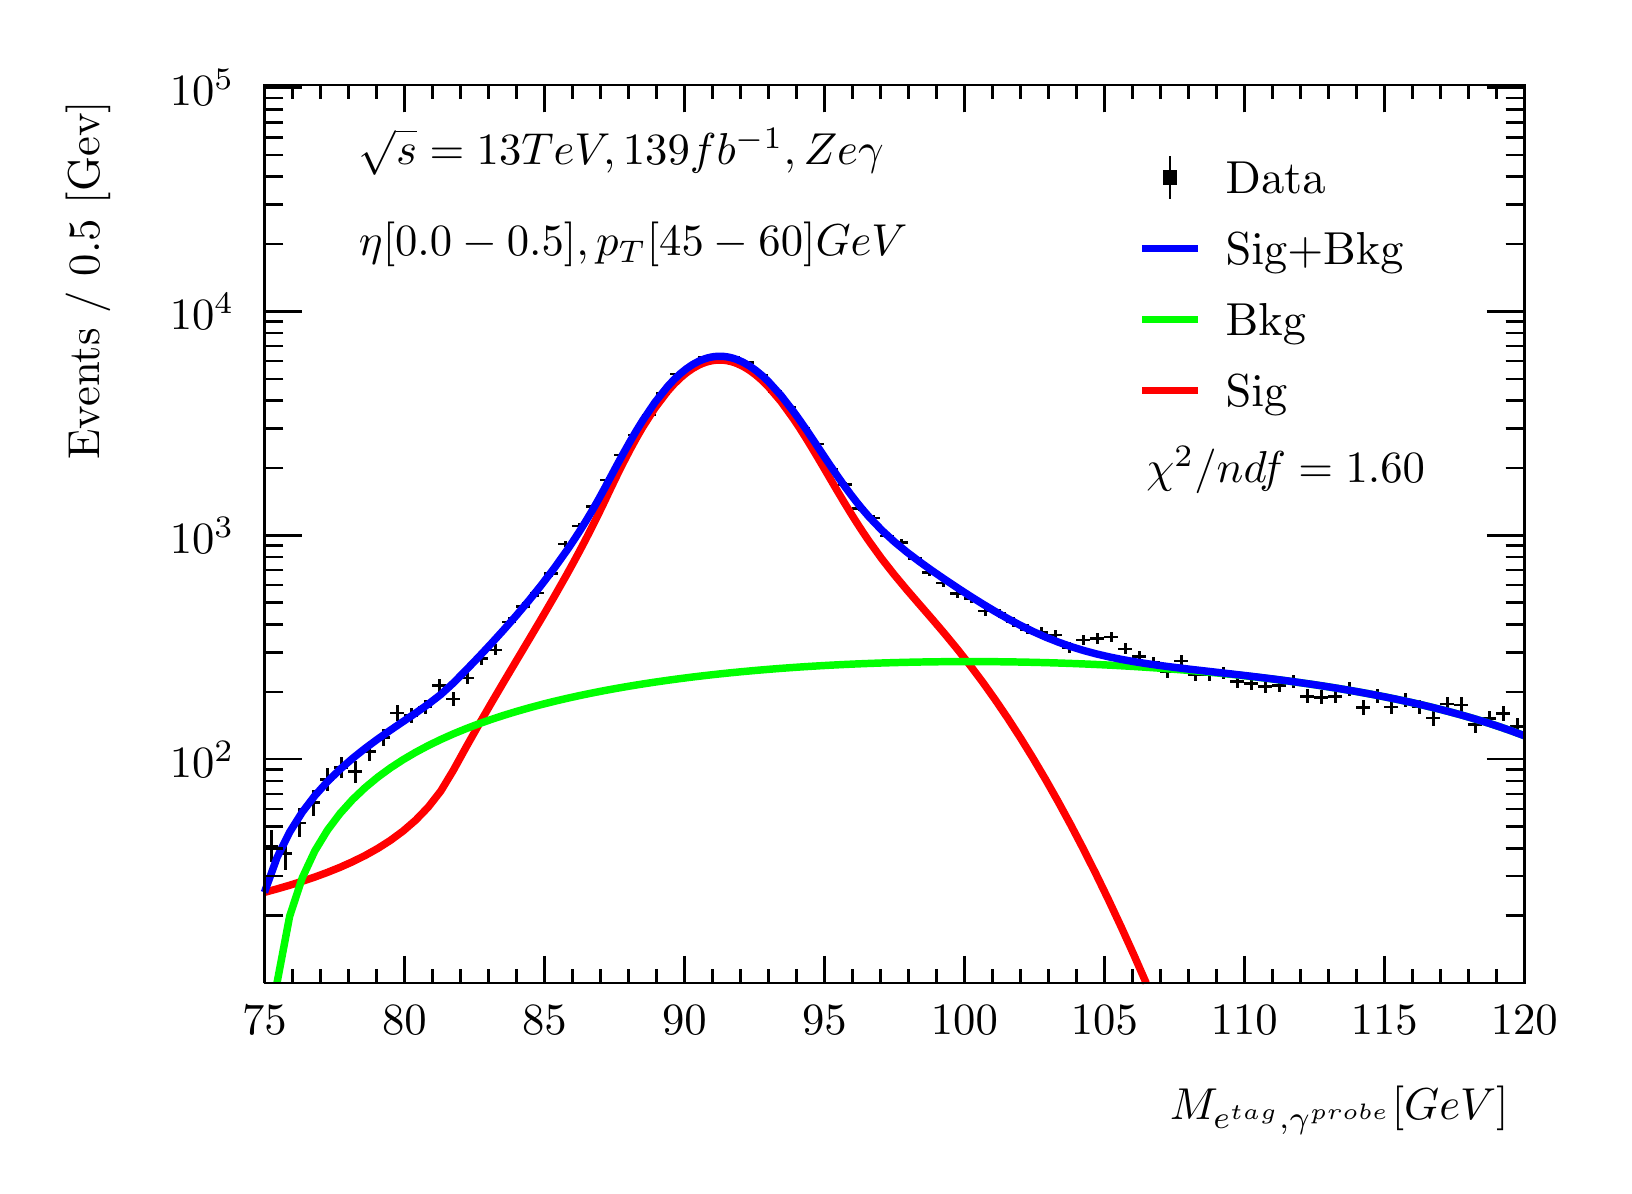
\begin{tikzpicture}
\pgfdeclareplotmark{cross} {
\pgfpathmoveto{\pgfpoint{-0.3\pgfplotmarksize}{\pgfplotmarksize}}
\pgfpathlineto{\pgfpoint{+0.3\pgfplotmarksize}{\pgfplotmarksize}}
\pgfpathlineto{\pgfpoint{+0.3\pgfplotmarksize}{0.3\pgfplotmarksize}}
\pgfpathlineto{\pgfpoint{+1\pgfplotmarksize}{0.3\pgfplotmarksize}}
\pgfpathlineto{\pgfpoint{+1\pgfplotmarksize}{-0.3\pgfplotmarksize}}
\pgfpathlineto{\pgfpoint{+0.3\pgfplotmarksize}{-0.3\pgfplotmarksize}}
\pgfpathlineto{\pgfpoint{+0.3\pgfplotmarksize}{-1.\pgfplotmarksize}}
\pgfpathlineto{\pgfpoint{-0.3\pgfplotmarksize}{-1.\pgfplotmarksize}}
\pgfpathlineto{\pgfpoint{-0.3\pgfplotmarksize}{-0.3\pgfplotmarksize}}
\pgfpathlineto{\pgfpoint{-1.\pgfplotmarksize}{-0.3\pgfplotmarksize}}
\pgfpathlineto{\pgfpoint{-1.\pgfplotmarksize}{0.3\pgfplotmarksize}}
\pgfpathlineto{\pgfpoint{-0.3\pgfplotmarksize}{0.3\pgfplotmarksize}}
\pgfpathclose
\pgfusepathqstroke
}
\pgfdeclareplotmark{cross*} {
\pgfpathmoveto{\pgfpoint{-0.3\pgfplotmarksize}{\pgfplotmarksize}}
\pgfpathlineto{\pgfpoint{+0.3\pgfplotmarksize}{\pgfplotmarksize}}
\pgfpathlineto{\pgfpoint{+0.3\pgfplotmarksize}{0.3\pgfplotmarksize}}
\pgfpathlineto{\pgfpoint{+1\pgfplotmarksize}{0.3\pgfplotmarksize}}
\pgfpathlineto{\pgfpoint{+1\pgfplotmarksize}{-0.3\pgfplotmarksize}}
\pgfpathlineto{\pgfpoint{+0.3\pgfplotmarksize}{-0.3\pgfplotmarksize}}
\pgfpathlineto{\pgfpoint{+0.3\pgfplotmarksize}{-1.\pgfplotmarksize}}
\pgfpathlineto{\pgfpoint{-0.3\pgfplotmarksize}{-1.\pgfplotmarksize}}
\pgfpathlineto{\pgfpoint{-0.3\pgfplotmarksize}{-0.3\pgfplotmarksize}}
\pgfpathlineto{\pgfpoint{-1.\pgfplotmarksize}{-0.3\pgfplotmarksize}}
\pgfpathlineto{\pgfpoint{-1.\pgfplotmarksize}{0.3\pgfplotmarksize}}
\pgfpathlineto{\pgfpoint{-0.3\pgfplotmarksize}{0.3\pgfplotmarksize}}
\pgfpathclose
\pgfusepathqfillstroke
}
\pgfdeclareplotmark{newstar} {
\pgfpathmoveto{\pgfqpoint{0pt}{\pgfplotmarksize}}
\pgfpathlineto{\pgfqpointpolar{44}{0.5\pgfplotmarksize}}
\pgfpathlineto{\pgfqpointpolar{18}{\pgfplotmarksize}}
\pgfpathlineto{\pgfqpointpolar{-20}{0.5\pgfplotmarksize}}
\pgfpathlineto{\pgfqpointpolar{-54}{\pgfplotmarksize}}
\pgfpathlineto{\pgfqpointpolar{-90}{0.5\pgfplotmarksize}}
\pgfpathlineto{\pgfqpointpolar{234}{\pgfplotmarksize}}
\pgfpathlineto{\pgfqpointpolar{198}{0.5\pgfplotmarksize}}
\pgfpathlineto{\pgfqpointpolar{162}{\pgfplotmarksize}}
\pgfpathlineto{\pgfqpointpolar{134}{0.5\pgfplotmarksize}}
\pgfpathclose
\pgfusepathqstroke
}
\pgfdeclareplotmark{newstar*} {
\pgfpathmoveto{\pgfqpoint{0pt}{\pgfplotmarksize}}
\pgfpathlineto{\pgfqpointpolar{44}{0.5\pgfplotmarksize}}
\pgfpathlineto{\pgfqpointpolar{18}{\pgfplotmarksize}}
\pgfpathlineto{\pgfqpointpolar{-20}{0.5\pgfplotmarksize}}
\pgfpathlineto{\pgfqpointpolar{-54}{\pgfplotmarksize}}
\pgfpathlineto{\pgfqpointpolar{-90}{0.5\pgfplotmarksize}}
\pgfpathlineto{\pgfqpointpolar{234}{\pgfplotmarksize}}
\pgfpathlineto{\pgfqpointpolar{198}{0.5\pgfplotmarksize}}
\pgfpathlineto{\pgfqpointpolar{162}{\pgfplotmarksize}}
\pgfpathlineto{\pgfqpointpolar{134}{0.5\pgfplotmarksize}}
\pgfpathclose
\pgfusepathqfillstroke
}
\definecolor{c}{rgb}{1,1,1};
\draw [color=c, fill=c] (0,0) rectangle (20,14.4361);
\draw [color=c, fill=c] (3,2.30977) rectangle (19,13.7143);
\definecolor{c}{rgb}{0,0,0};
\draw [c,line width=0.9] (3,2.30977) -- (3,13.7143) -- (19,13.7143) -- (19,2.30977) -- (3,2.30977);
\definecolor{c}{rgb}{1,1,1};
\draw [color=c, fill=c] (3,2.30977) rectangle (19,13.7143);
\definecolor{c}{rgb}{0,0,0};
\draw [c,line width=0.9] (3,2.30977) -- (3,13.7143) -- (19,13.7143) -- (19,2.30977) -- (3,2.30977);
\draw [c,line width=0.9] (3,2.30977) -- (19,2.30977);
\draw [c,line width=0.9] (3,2.65624) -- (3,2.30977);
\draw [c,line width=0.9] (3.35556,2.48301) -- (3.35556,2.30977);
\draw [c,line width=0.9] (3.71111,2.48301) -- (3.71111,2.30977);
\draw [c,line width=0.9] (4.06667,2.48301) -- (4.06667,2.30977);
\draw [c,line width=0.9] (4.42222,2.48301) -- (4.42222,2.30977);
\draw [c,line width=0.9] (4.77778,2.65624) -- (4.77778,2.30977);
\draw [c,line width=0.9] (5.13333,2.48301) -- (5.13333,2.30977);
\draw [c,line width=0.9] (5.48889,2.48301) -- (5.48889,2.30977);
\draw [c,line width=0.9] (5.84444,2.48301) -- (5.84444,2.30977);
\draw [c,line width=0.9] (6.2,2.48301) -- (6.2,2.30977);
\draw [c,line width=0.9] (6.55556,2.65624) -- (6.55556,2.30977);
\draw [c,line width=0.9] (6.91111,2.48301) -- (6.91111,2.30977);
\draw [c,line width=0.9] (7.26667,2.48301) -- (7.26667,2.30977);
\draw [c,line width=0.9] (7.62222,2.48301) -- (7.62222,2.30977);
\draw [c,line width=0.9] (7.97778,2.48301) -- (7.97778,2.30977);
\draw [c,line width=0.9] (8.33333,2.65624) -- (8.33333,2.30977);
\draw [c,line width=0.9] (8.68889,2.48301) -- (8.68889,2.30977);
\draw [c,line width=0.9] (9.04444,2.48301) -- (9.04444,2.30977);
\draw [c,line width=0.9] (9.4,2.48301) -- (9.4,2.30977);
\draw [c,line width=0.9] (9.75556,2.48301) -- (9.75556,2.30977);
\draw [c,line width=0.9] (10.1111,2.65624) -- (10.1111,2.30977);
\draw [c,line width=0.9] (10.4667,2.48301) -- (10.4667,2.30977);
\draw [c,line width=0.9] (10.8222,2.48301) -- (10.8222,2.30977);
\draw [c,line width=0.9] (11.1778,2.48301) -- (11.1778,2.30977);
\draw [c,line width=0.9] (11.5333,2.48301) -- (11.5333,2.30977);
\draw [c,line width=0.9] (11.8889,2.65624) -- (11.8889,2.30977);
\draw [c,line width=0.9] (12.2444,2.48301) -- (12.2444,2.30977);
\draw [c,line width=0.9] (12.6,2.48301) -- (12.6,2.30977);
\draw [c,line width=0.9] (12.9556,2.48301) -- (12.9556,2.30977);
\draw [c,line width=0.9] (13.3111,2.48301) -- (13.3111,2.30977);
\draw [c,line width=0.9] (13.6667,2.65624) -- (13.6667,2.30977);
\draw [c,line width=0.9] (14.0222,2.48301) -- (14.0222,2.30977);
\draw [c,line width=0.9] (14.3778,2.48301) -- (14.3778,2.30977);
\draw [c,line width=0.9] (14.7333,2.48301) -- (14.7333,2.30977);
\draw [c,line width=0.9] (15.0889,2.48301) -- (15.0889,2.30977);
\draw [c,line width=0.9] (15.4444,2.65624) -- (15.4444,2.30977);
\draw [c,line width=0.9] (15.8,2.48301) -- (15.8,2.30977);
\draw [c,line width=0.9] (16.1556,2.48301) -- (16.1556,2.30977);
\draw [c,line width=0.9] (16.5111,2.48301) -- (16.5111,2.30977);
\draw [c,line width=0.9] (16.8667,2.48301) -- (16.8667,2.30977);
\draw [c,line width=0.9] (17.2222,2.65624) -- (17.2222,2.30977);
\draw [c,line width=0.9] (17.5778,2.48301) -- (17.5778,2.30977);
\draw [c,line width=0.9] (17.9333,2.48301) -- (17.9333,2.30977);
\draw [c,line width=0.9] (18.2889,2.48301) -- (18.2889,2.30977);
\draw [c,line width=0.9] (18.6444,2.48301) -- (18.6444,2.30977);
\draw [c,line width=0.9] (19,2.65624) -- (19,2.30977);
\draw [c,line width=0.9] (19,2.65624) -- (19,2.30977);
\draw [anchor=base] (3,1.66015) node[scale=1.61424, color=c, rotate=0]{75};
\draw [anchor=base] (4.77778,1.66015) node[scale=1.61424, color=c, rotate=0]{80};
\draw [anchor=base] (6.55556,1.66015) node[scale=1.61424, color=c, rotate=0]{85};
\draw [anchor=base] (8.33333,1.66015) node[scale=1.61424, color=c, rotate=0]{90};
\draw [anchor=base] (10.1111,1.66015) node[scale=1.61424, color=c, rotate=0]{95};
\draw [anchor=base] (11.8889,1.66015) node[scale=1.61424, color=c, rotate=0]{100};
\draw [anchor=base] (13.6667,1.66015) node[scale=1.61424, color=c, rotate=0]{105};
\draw [anchor=base] (15.4444,1.66015) node[scale=1.61424, color=c, rotate=0]{110};
\draw [anchor=base] (17.2222,1.66015) node[scale=1.61424, color=c, rotate=0]{115};
\draw [anchor=base] (19,1.66015) node[scale=1.61424, color=c, rotate=0]{120};
\draw [anchor= east] (19,0.692932) node[scale=1.61424, color=c, rotate=0]{$M_{e^{tag}, \gamma^{probe}}  [GeV]$};
\draw [c,line width=0.9] (3,13.7143) -- (19,13.7143);
\draw [c,line width=0.9] (3,13.3678) -- (3,13.7143);
\draw [c,line width=0.9] (3.35556,13.5411) -- (3.35556,13.7143);
\draw [c,line width=0.9] (3.71111,13.5411) -- (3.71111,13.7143);
\draw [c,line width=0.9] (4.06667,13.5411) -- (4.06667,13.7143);
\draw [c,line width=0.9] (4.42222,13.5411) -- (4.42222,13.7143);
\draw [c,line width=0.9] (4.77778,13.3678) -- (4.77778,13.7143);
\draw [c,line width=0.9] (5.13333,13.5411) -- (5.13333,13.7143);
\draw [c,line width=0.9] (5.48889,13.5411) -- (5.48889,13.7143);
\draw [c,line width=0.9] (5.84444,13.5411) -- (5.84444,13.7143);
\draw [c,line width=0.9] (6.2,13.5411) -- (6.2,13.7143);
\draw [c,line width=0.9] (6.55556,13.3678) -- (6.55556,13.7143);
\draw [c,line width=0.9] (6.91111,13.5411) -- (6.91111,13.7143);
\draw [c,line width=0.9] (7.26667,13.5411) -- (7.26667,13.7143);
\draw [c,line width=0.9] (7.62222,13.5411) -- (7.62222,13.7143);
\draw [c,line width=0.9] (7.97778,13.5411) -- (7.97778,13.7143);
\draw [c,line width=0.9] (8.33333,13.3678) -- (8.33333,13.7143);
\draw [c,line width=0.9] (8.68889,13.5411) -- (8.68889,13.7143);
\draw [c,line width=0.9] (9.04444,13.5411) -- (9.04444,13.7143);
\draw [c,line width=0.9] (9.4,13.5411) -- (9.4,13.7143);
\draw [c,line width=0.9] (9.75556,13.5411) -- (9.75556,13.7143);
\draw [c,line width=0.9] (10.1111,13.3678) -- (10.1111,13.7143);
\draw [c,line width=0.9] (10.4667,13.5411) -- (10.4667,13.7143);
\draw [c,line width=0.9] (10.8222,13.5411) -- (10.8222,13.7143);
\draw [c,line width=0.9] (11.1778,13.5411) -- (11.1778,13.7143);
\draw [c,line width=0.9] (11.5333,13.5411) -- (11.5333,13.7143);
\draw [c,line width=0.9] (11.8889,13.3678) -- (11.8889,13.7143);
\draw [c,line width=0.9] (12.2444,13.5411) -- (12.2444,13.7143);
\draw [c,line width=0.9] (12.6,13.5411) -- (12.6,13.7143);
\draw [c,line width=0.9] (12.9556,13.5411) -- (12.9556,13.7143);
\draw [c,line width=0.9] (13.3111,13.5411) -- (13.3111,13.7143);
\draw [c,line width=0.9] (13.6667,13.3678) -- (13.6667,13.7143);
\draw [c,line width=0.9] (14.0222,13.5411) -- (14.0222,13.7143);
\draw [c,line width=0.9] (14.3778,13.5411) -- (14.3778,13.7143);
\draw [c,line width=0.9] (14.7333,13.5411) -- (14.7333,13.7143);
\draw [c,line width=0.9] (15.0889,13.5411) -- (15.0889,13.7143);
\draw [c,line width=0.9] (15.4444,13.3678) -- (15.4444,13.7143);
\draw [c,line width=0.9] (15.8,13.5411) -- (15.8,13.7143);
\draw [c,line width=0.9] (16.1556,13.5411) -- (16.1556,13.7143);
\draw [c,line width=0.9] (16.5111,13.5411) -- (16.5111,13.7143);
\draw [c,line width=0.9] (16.8667,13.5411) -- (16.8667,13.7143);
\draw [c,line width=0.9] (17.2222,13.3678) -- (17.2222,13.7143);
\draw [c,line width=0.9] (17.5778,13.5411) -- (17.5778,13.7143);
\draw [c,line width=0.9] (17.9333,13.5411) -- (17.9333,13.7143);
\draw [c,line width=0.9] (18.2889,13.5411) -- (18.2889,13.7143);
\draw [c,line width=0.9] (18.6444,13.5411) -- (18.6444,13.7143);
\draw [c,line width=0.9] (19,13.3678) -- (19,13.7143);
\draw [c,line width=0.9] (19,13.3678) -- (19,13.7143);
\draw [c,line width=0.9] (3,2.30977) -- (3,13.7143);
\draw [c,line width=0.9] (3.237,3.16561) -- (3,3.16561);
\draw [c,line width=0.9] (3.237,3.66625) -- (3,3.66625);
\draw [c,line width=0.9] (3.237,4.02146) -- (3,4.02146);
\draw [c,line width=0.9] (3.237,4.29698) -- (3,4.29698);
\draw [c,line width=0.9] (3.237,4.52209) -- (3,4.52209);
\draw [c,line width=0.9] (3.237,4.71242) -- (3,4.71242);
\draw [c,line width=0.9] (3.237,4.8773) -- (3,4.8773);
\draw [c,line width=0.9] (3.237,5.02273) -- (3,5.02273);
\draw [c,line width=0.9] (3.474,5.15282) -- (3,5.15282);
\draw [anchor= east] (2.82,5.15282) node[scale=1.61424, color=c, rotate=0]{$10^{2}$};
\draw [c,line width=0.9] (3.237,6.00866) -- (3,6.00866);
\draw [c,line width=0.9] (3.237,6.5093) -- (3,6.5093);
\draw [c,line width=0.9] (3.237,6.8645) -- (3,6.8645);
\draw [c,line width=0.9] (3.237,7.14002) -- (3,7.14002);
\draw [c,line width=0.9] (3.237,7.36514) -- (3,7.36514);
\draw [c,line width=0.9] (3.237,7.55547) -- (3,7.55547);
\draw [c,line width=0.9] (3.237,7.72034) -- (3,7.72034);
\draw [c,line width=0.9] (3.237,7.86577) -- (3,7.86577);
\draw [c,line width=0.9] (3.474,7.99586) -- (3,7.99586);
\draw [anchor= east] (2.82,7.99586) node[scale=1.61424, color=c, rotate=0]{$10^{3}$};
\draw [c,line width=0.9] (3.237,8.85171) -- (3,8.85171);
\draw [c,line width=0.9] (3.237,9.35234) -- (3,9.35234);
\draw [c,line width=0.9] (3.237,9.70755) -- (3,9.70755);
\draw [c,line width=0.9] (3.237,9.98307) -- (3,9.98307);
\draw [c,line width=0.9] (3.237,10.2082) -- (3,10.2082);
\draw [c,line width=0.9] (3.237,10.3985) -- (3,10.3985);
\draw [c,line width=0.9] (3.237,10.5634) -- (3,10.5634);
\draw [c,line width=0.9] (3.237,10.7088) -- (3,10.7088);
\draw [c,line width=0.9] (3.474,10.8389) -- (3,10.8389);
\draw [anchor= east] (2.82,10.8389) node[scale=1.61424, color=c, rotate=0]{$10^{4}$};
\draw [c,line width=0.9] (3.237,11.6948) -- (3,11.6948);
\draw [c,line width=0.9] (3.237,12.1954) -- (3,12.1954);
\draw [c,line width=0.9] (3.237,12.5506) -- (3,12.5506);
\draw [c,line width=0.9] (3.237,12.8261) -- (3,12.8261);
\draw [c,line width=0.9] (3.237,13.0512) -- (3,13.0512);
\draw [c,line width=0.9] (3.237,13.2416) -- (3,13.2416);
\draw [c,line width=0.9] (3.237,13.4064) -- (3,13.4064);
\draw [c,line width=0.9] (3.237,13.5519) -- (3,13.5519);
\draw [c,line width=0.9] (3.474,13.682) -- (3,13.682);
\draw [anchor= east] (2.82,13.682) node[scale=1.61424, color=c, rotate=0]{$10^{5}$};
\draw [anchor= east] (0.76,13.7143) node[scale=1.61424, color=c, rotate=90]{Events / 0.5 [Gev]};
\draw [c,line width=0.9] (19,2.30977) -- (19,13.7143);
\draw [c,line width=0.9] (18.763,3.16561) -- (19,3.16561);
\draw [c,line width=0.9] (18.763,3.66625) -- (19,3.66625);
\draw [c,line width=0.9] (18.763,4.02146) -- (19,4.02146);
\draw [c,line width=0.9] (18.763,4.29698) -- (19,4.29698);
\draw [c,line width=0.9] (18.763,4.52209) -- (19,4.52209);
\draw [c,line width=0.9] (18.763,4.71242) -- (19,4.71242);
\draw [c,line width=0.9] (18.763,4.8773) -- (19,4.8773);
\draw [c,line width=0.9] (18.763,5.02273) -- (19,5.02273);
\draw [c,line width=0.9] (18.526,5.15282) -- (19,5.15282);
\draw [c,line width=0.9] (18.763,6.00866) -- (19,6.00866);
\draw [c,line width=0.9] (18.763,6.5093) -- (19,6.5093);
\draw [c,line width=0.9] (18.763,6.8645) -- (19,6.8645);
\draw [c,line width=0.9] (18.763,7.14002) -- (19,7.14002);
\draw [c,line width=0.9] (18.763,7.36514) -- (19,7.36514);
\draw [c,line width=0.9] (18.763,7.55547) -- (19,7.55547);
\draw [c,line width=0.9] (18.763,7.72034) -- (19,7.72034);
\draw [c,line width=0.9] (18.763,7.86577) -- (19,7.86577);
\draw [c,line width=0.9] (18.526,7.99586) -- (19,7.99586);
\draw [c,line width=0.9] (18.763,8.85171) -- (19,8.85171);
\draw [c,line width=0.9] (18.763,9.35234) -- (19,9.35234);
\draw [c,line width=0.9] (18.763,9.70755) -- (19,9.70755);
\draw [c,line width=0.9] (18.763,9.98307) -- (19,9.98307);
\draw [c,line width=0.9] (18.763,10.2082) -- (19,10.2082);
\draw [c,line width=0.9] (18.763,10.3985) -- (19,10.3985);
\draw [c,line width=0.9] (18.763,10.5634) -- (19,10.5634);
\draw [c,line width=0.9] (18.763,10.7088) -- (19,10.7088);
\draw [c,line width=0.9] (18.526,10.8389) -- (19,10.8389);
\draw [c,line width=0.9] (18.763,11.6948) -- (19,11.6948);
\draw [c,line width=0.9] (18.763,12.1954) -- (19,12.1954);
\draw [c,line width=0.9] (18.763,12.5506) -- (19,12.5506);
\draw [c,line width=0.9] (18.763,12.8261) -- (19,12.8261);
\draw [c,line width=0.9] (18.763,13.0512) -- (19,13.0512);
\draw [c,line width=0.9] (18.763,13.2416) -- (19,13.2416);
\draw [c,line width=0.9] (18.763,13.4064) -- (19,13.4064);
\draw [c,line width=0.9] (18.763,13.5519) -- (19,13.5519);
\draw [c,line width=0.9] (18.526,13.682) -- (19,13.682);
\draw [c,line width=0.9] (3.08889,4.05195) -- (3,4.05195);
\draw [c,line width=0.9] (3,4.05195) -- (3,4.05195);
\draw [c,line width=0.9] (3.08889,4.05195) -- (3.17778,4.05195);
\draw [c,line width=0.9] (3.17778,4.05195) -- (3.17778,4.05195);
\draw [c,line width=0.9] (3.08889,4.05195) -- (3.08889,4.25823);
\draw [c,line width=0.9] (3.08889,4.25823) -- (3.08889,4.25823);
\draw [c,line width=0.9] (3.08889,4.05195) -- (3.08889,3.84322);
\draw [c,line width=0.9] (3.08889,3.84322) -- (3.08889,3.84322);
\draw [c,line width=0.9] (3.26667,3.95813) -- (3.17778,3.95813);
\draw [c,line width=0.9] (3.17778,3.95813) -- (3.17778,3.95813);
\draw [c,line width=0.9] (3.26667,3.95813) -- (3.35556,3.95813);
\draw [c,line width=0.9] (3.35556,3.95813) -- (3.35556,3.95813);
\draw [c,line width=0.9] (3.26667,3.95813) -- (3.26667,4.17287);
\draw [c,line width=0.9] (3.26667,4.17287) -- (3.26667,4.17287);
\draw [c,line width=0.9] (3.26667,3.95813) -- (3.26667,3.74063);
\draw [c,line width=0.9] (3.26667,3.74063) -- (3.26667,3.74063);
\draw [c,line width=0.9] (3.44444,4.3454) -- (3.35556,4.3454);
\draw [c,line width=0.9] (3.35556,4.3454) -- (3.35556,4.3454);
\draw [c,line width=0.9] (3.44444,4.3454) -- (3.53333,4.3454);
\draw [c,line width=0.9] (3.53333,4.3454) -- (3.53333,4.3454);
\draw [c,line width=0.9] (3.44444,4.3454) -- (3.44444,4.52738);
\draw [c,line width=0.9] (3.44444,4.52738) -- (3.44444,4.52738);
\draw [c,line width=0.9] (3.44444,4.3454) -- (3.44444,4.16172);
\draw [c,line width=0.9] (3.44444,4.16172) -- (3.44444,4.16172);
\draw [c,line width=0.9] (3.62222,4.60178) -- (3.53333,4.60178);
\draw [c,line width=0.9] (3.53333,4.60178) -- (3.53333,4.60178);
\draw [c,line width=0.9] (3.62222,4.60178) -- (3.71111,4.60178);
\draw [c,line width=0.9] (3.71111,4.60178) -- (3.71111,4.60178);
\draw [c,line width=0.9] (3.62222,4.60178) -- (3.62222,4.76495);
\draw [c,line width=0.9] (3.62222,4.76495) -- (3.62222,4.76495);
\draw [c,line width=0.9] (3.62222,4.60178) -- (3.62222,4.43737);
\draw [c,line width=0.9] (3.62222,4.43737) -- (3.62222,4.43737);
\draw [c,line width=0.9] (3.8,4.89264) -- (3.71111,4.89264);
\draw [c,line width=0.9] (3.71111,4.89264) -- (3.71111,4.89264);
\draw [c,line width=0.9] (3.8,4.89264) -- (3.88889,4.89264);
\draw [c,line width=0.9] (3.88889,4.89264) -- (3.88889,4.89264);
\draw [c,line width=0.9] (3.8,4.89264) -- (3.8,5.03688);
\draw [c,line width=0.9] (3.8,5.03688) -- (3.8,5.03688);
\draw [c,line width=0.9] (3.8,4.89264) -- (3.8,4.74753);
\draw [c,line width=0.9] (3.8,4.74753) -- (3.8,4.74753);
\draw [c,line width=0.9] (3.97778,5.04987) -- (3.88889,5.04987);
\draw [c,line width=0.9] (3.88889,5.04987) -- (3.88889,5.04987);
\draw [c,line width=0.9] (3.97778,5.04987) -- (4.06667,5.04987);
\draw [c,line width=0.9] (4.06667,5.04987) -- (4.06667,5.04987);
\draw [c,line width=0.9] (3.97778,5.04987) -- (3.97778,5.18483);
\draw [c,line width=0.9] (3.97778,5.18483) -- (3.97778,5.18483);
\draw [c,line width=0.9] (3.97778,5.04987) -- (3.97778,4.91418);
\draw [c,line width=0.9] (3.97778,4.91418) -- (3.97778,4.91418);
\draw [c,line width=0.9] (4.15556,4.99498) -- (4.06667,4.99498);
\draw [c,line width=0.9] (4.06667,4.99498) -- (4.06667,4.99498);
\draw [c,line width=0.9] (4.15556,4.99498) -- (4.24444,4.99498);
\draw [c,line width=0.9] (4.24444,4.99498) -- (4.24444,4.99498);
\draw [c,line width=0.9] (4.15556,4.99498) -- (4.15556,5.13311);
\draw [c,line width=0.9] (4.15556,5.13311) -- (4.15556,5.13311);
\draw [c,line width=0.9] (4.15556,4.99498) -- (4.15556,4.85608);
\draw [c,line width=0.9] (4.15556,4.85608) -- (4.15556,4.85608);
\draw [c,line width=0.9] (4.33333,5.24785) -- (4.24444,5.24785);
\draw [c,line width=0.9] (4.24444,5.24785) -- (4.24444,5.24785);
\draw [c,line width=0.9] (4.33333,5.24785) -- (4.42222,5.24785);
\draw [c,line width=0.9] (4.42222,5.24785) -- (4.42222,5.24785);
\draw [c,line width=0.9] (4.33333,5.24785) -- (4.33333,5.36661);
\draw [c,line width=0.9] (4.33333,5.36661) -- (4.33333,5.36661);
\draw [c,line width=0.9] (4.33333,5.24785) -- (4.33333,5.12908);
\draw [c,line width=0.9] (4.33333,5.12908) -- (4.33333,5.12908);
\draw [c,line width=0.9] (4.51111,5.42834) -- (4.42222,5.42834);
\draw [c,line width=0.9] (4.42222,5.42834) -- (4.42222,5.42834);
\draw [c,line width=0.9] (4.51111,5.42834) -- (4.6,5.42834);
\draw [c,line width=0.9] (4.6,5.42834) -- (4.6,5.42834);
\draw [c,line width=0.9] (4.51111,5.42834) -- (4.51111,5.53874);
\draw [c,line width=0.9] (4.51111,5.53874) -- (4.51111,5.53874);
\draw [c,line width=0.9] (4.51111,5.42834) -- (4.51111,5.31794);
\draw [c,line width=0.9] (4.51111,5.31794) -- (4.51111,5.31794);
\draw [c,line width=0.9] (4.68889,5.74084) -- (4.6,5.74084);
\draw [c,line width=0.9] (4.6,5.74084) -- (4.6,5.74084);
\draw [c,line width=0.9] (4.68889,5.74084) -- (4.77778,5.74084);
\draw [c,line width=0.9] (4.77778,5.74084) -- (4.77778,5.74084);
\draw [c,line width=0.9] (4.68889,5.74084) -- (4.68889,5.83812);
\draw [c,line width=0.9] (4.68889,5.83812) -- (4.68889,5.83812);
\draw [c,line width=0.9] (4.68889,5.74084) -- (4.68889,5.64355);
\draw [c,line width=0.9] (4.68889,5.64355) -- (4.68889,5.64355);
\draw [c,line width=0.9] (4.86667,5.70977) -- (4.77778,5.70977);
\draw [c,line width=0.9] (4.77778,5.70977) -- (4.77778,5.70977);
\draw [c,line width=0.9] (4.86667,5.70977) -- (4.95556,5.70977);
\draw [c,line width=0.9] (4.95556,5.70977) -- (4.95556,5.70977);
\draw [c,line width=0.9] (4.86667,5.70977) -- (4.86667,5.80829);
\draw [c,line width=0.9] (4.86667,5.80829) -- (4.86667,5.80829);
\draw [c,line width=0.9] (4.86667,5.70977) -- (4.86667,5.61126);
\draw [c,line width=0.9] (4.86667,5.61126) -- (4.86667,5.61126);
\draw [c,line width=0.9] (5.04444,5.81524) -- (4.95556,5.81524);
\draw [c,line width=0.9] (4.95556,5.81524) -- (4.95556,5.81524);
\draw [c,line width=0.9] (5.04444,5.81524) -- (5.13333,5.81524);
\draw [c,line width=0.9] (5.13333,5.81524) -- (5.13333,5.81524);
\draw [c,line width=0.9] (5.04444,5.81524) -- (5.04444,5.90964);
\draw [c,line width=0.9] (5.04444,5.90964) -- (5.04444,5.90964);
\draw [c,line width=0.9] (5.04444,5.81524) -- (5.04444,5.72084);
\draw [c,line width=0.9] (5.04444,5.72084) -- (5.04444,5.72084);
\draw [c,line width=0.9] (5.22222,6.08642) -- (5.13333,6.08642);
\draw [c,line width=0.9] (5.13333,6.08642) -- (5.13333,6.08642);
\draw [c,line width=0.9] (5.22222,6.08642) -- (5.31111,6.08642);
\draw [c,line width=0.9] (5.31111,6.08642) -- (5.31111,6.08642);
\draw [c,line width=0.9] (5.22222,6.08642) -- (5.22222,6.171);
\draw [c,line width=0.9] (5.22222,6.171) -- (5.22222,6.171);
\draw [c,line width=0.9] (5.22222,6.08642) -- (5.22222,6.00183);
\draw [c,line width=0.9] (5.22222,6.00183) -- (5.22222,6.00183);
\draw [c,line width=0.9] (5.4,5.91906) -- (5.31111,5.91906);
\draw [c,line width=0.9] (5.31111,5.91906) -- (5.31111,5.91906);
\draw [c,line width=0.9] (5.4,5.91906) -- (5.48889,5.91906);
\draw [c,line width=0.9] (5.48889,5.91906) -- (5.48889,5.91906);
\draw [c,line width=0.9] (5.4,5.91906) -- (5.4,6.00957);
\draw [c,line width=0.9] (5.4,6.00957) -- (5.4,6.00957);
\draw [c,line width=0.9] (5.4,5.91906) -- (5.4,5.82854);
\draw [c,line width=0.9] (5.4,5.82854) -- (5.4,5.82854);
\draw [c,line width=0.9] (5.57778,6.18658) -- (5.48889,6.18658);
\draw [c,line width=0.9] (5.48889,6.18658) -- (5.48889,6.18658);
\draw [c,line width=0.9] (5.57778,6.18658) -- (5.66667,6.18658);
\draw [c,line width=0.9] (5.66667,6.18658) -- (5.66667,6.18658);
\draw [c,line width=0.9] (5.57778,6.18658) -- (5.57778,6.26781);
\draw [c,line width=0.9] (5.57778,6.26781) -- (5.57778,6.26781);
\draw [c,line width=0.9] (5.57778,6.18658) -- (5.57778,6.10536);
\draw [c,line width=0.9] (5.57778,6.10536) -- (5.57778,6.10536);
\draw [c,line width=0.9] (5.75556,6.42851) -- (5.66667,6.42851);
\draw [c,line width=0.9] (5.66667,6.42851) -- (5.66667,6.42851);
\draw [c,line width=0.9] (5.75556,6.42851) -- (5.84444,6.42851);
\draw [c,line width=0.9] (5.84444,6.42851) -- (5.84444,6.42851);
\draw [c,line width=0.9] (5.75556,6.42851) -- (5.75556,6.50216);
\draw [c,line width=0.9] (5.75556,6.50216) -- (5.75556,6.50216);
\draw [c,line width=0.9] (5.75556,6.42851) -- (5.75556,6.35487);
\draw [c,line width=0.9] (5.75556,6.35487) -- (5.75556,6.35487);
\draw [c,line width=0.9] (5.93333,6.54179) -- (5.84444,6.54179);
\draw [c,line width=0.9] (5.84444,6.54179) -- (5.84444,6.54179);
\draw [c,line width=0.9] (5.93333,6.54179) -- (6.02222,6.54179);
\draw [c,line width=0.9] (6.02222,6.54179) -- (6.02222,6.54179);
\draw [c,line width=0.9] (5.93333,6.54179) -- (5.93333,6.61214);
\draw [c,line width=0.9] (5.93333,6.61214) -- (5.93333,6.61214);
\draw [c,line width=0.9] (5.93333,6.54179) -- (5.93333,6.47145);
\draw [c,line width=0.9] (5.93333,6.47145) -- (5.93333,6.47145);
\draw [c,line width=0.9] (6.11111,6.89198) -- (6.02222,6.89198);
\draw [c,line width=0.9] (6.02222,6.89198) -- (6.02222,6.89198);
\draw [c,line width=0.9] (6.11111,6.89198) -- (6.2,6.89198);
\draw [c,line width=0.9] (6.2,6.89198) -- (6.2,6.89198);
\draw [c,line width=0.9] (6.11111,6.89198) -- (6.11111,6.95302);
\draw [c,line width=0.9] (6.11111,6.95302) -- (6.11111,6.95302);
\draw [c,line width=0.9] (6.11111,6.89198) -- (6.11111,6.83093);
\draw [c,line width=0.9] (6.11111,6.83093) -- (6.11111,6.83093);
\draw [c,line width=0.9] (6.28889,7.09475) -- (6.2,7.09475);
\draw [c,line width=0.9] (6.2,7.09475) -- (6.2,7.09475);
\draw [c,line width=0.9] (6.28889,7.09475) -- (6.37778,7.09475);
\draw [c,line width=0.9] (6.37778,7.09475) -- (6.37778,7.09475);
\draw [c,line width=0.9] (6.28889,7.09475) -- (6.28889,7.15099);
\draw [c,line width=0.9] (6.28889,7.15099) -- (6.28889,7.15099);
\draw [c,line width=0.9] (6.28889,7.09475) -- (6.28889,7.03852);
\draw [c,line width=0.9] (6.28889,7.03852) -- (6.28889,7.03852);
\draw [c,line width=0.9] (6.46667,7.26442) -- (6.37778,7.26442);
\draw [c,line width=0.9] (6.37778,7.26442) -- (6.37778,7.26442);
\draw [c,line width=0.9] (6.46667,7.26442) -- (6.55556,7.26442);
\draw [c,line width=0.9] (6.55556,7.26442) -- (6.55556,7.26442);
\draw [c,line width=0.9] (6.46667,7.26442) -- (6.46667,7.31692);
\draw [c,line width=0.9] (6.46667,7.31692) -- (6.46667,7.31692);
\draw [c,line width=0.9] (6.46667,7.26442) -- (6.46667,7.21192);
\draw [c,line width=0.9] (6.46667,7.21192) -- (6.46667,7.21192);
\draw [c,line width=0.9] (6.64444,7.50874) -- (6.55556,7.50874);
\draw [c,line width=0.9] (6.55556,7.50874) -- (6.55556,7.50874);
\draw [c,line width=0.9] (6.64444,7.50874) -- (6.73333,7.50874);
\draw [c,line width=0.9] (6.73333,7.50874) -- (6.73333,7.50874);
\draw [c,line width=0.9] (6.64444,7.50874) -- (6.64444,7.55629);
\draw [c,line width=0.9] (6.64444,7.55629) -- (6.64444,7.55629);
\draw [c,line width=0.9] (6.64444,7.50874) -- (6.64444,7.46118);
\draw [c,line width=0.9] (6.64444,7.46118) -- (6.64444,7.46118);
\draw [c,line width=0.9] (6.82222,7.88618) -- (6.73333,7.88618);
\draw [c,line width=0.9] (6.73333,7.88618) -- (6.73333,7.88618);
\draw [c,line width=0.9] (6.82222,7.88618) -- (6.91111,7.88618);
\draw [c,line width=0.9] (6.91111,7.88618) -- (6.91111,7.88618);
\draw [c,line width=0.9] (6.82222,7.88618) -- (6.82222,7.927);
\draw [c,line width=0.9] (6.82222,7.927) -- (6.82222,7.927);
\draw [c,line width=0.9] (6.82222,7.88618) -- (6.82222,7.84537);
\draw [c,line width=0.9] (6.82222,7.84537) -- (6.82222,7.84537);
\draw [c,line width=0.9] (7,8.11242) -- (6.91111,8.11242);
\draw [c,line width=0.9] (6.91111,8.11242) -- (6.91111,8.11242);
\draw [c,line width=0.9] (7,8.11242) -- (7.08889,8.11242);
\draw [c,line width=0.9] (7.08889,8.11242) -- (7.08889,8.11242);
\draw [c,line width=0.9] (7,8.11242) -- (7,8.14967);
\draw [c,line width=0.9] (7,8.14967) -- (7,8.14967);
\draw [c,line width=0.9] (7,8.11242) -- (7,8.07518);
\draw [c,line width=0.9] (7,8.07518) -- (7,8.07518);
\draw [c,line width=0.9] (7.17778,8.36183) -- (7.08889,8.36183);
\draw [c,line width=0.9] (7.08889,8.36183) -- (7.08889,8.36183);
\draw [c,line width=0.9] (7.17778,8.36183) -- (7.26667,8.36183);
\draw [c,line width=0.9] (7.26667,8.36183) -- (7.26667,8.36183);
\draw [c,line width=0.9] (7.17778,8.36183) -- (7.17778,8.39549);
\draw [c,line width=0.9] (7.17778,8.39549) -- (7.17778,8.39549);
\draw [c,line width=0.9] (7.17778,8.36183) -- (7.17778,8.32816);
\draw [c,line width=0.9] (7.17778,8.32816) -- (7.17778,8.32816);
\draw [c,line width=0.9] (7.35556,8.70156) -- (7.26667,8.70156);
\draw [c,line width=0.9] (7.26667,8.70156) -- (7.26667,8.70156);
\draw [c,line width=0.9] (7.35556,8.70156) -- (7.44444,8.70156);
\draw [c,line width=0.9] (7.44444,8.70156) -- (7.44444,8.70156);
\draw [c,line width=0.9] (7.35556,8.70156) -- (7.35556,8.7309);
\draw [c,line width=0.9] (7.35556,8.7309) -- (7.35556,8.7309);
\draw [c,line width=0.9] (7.35556,8.70156) -- (7.35556,8.67222);
\draw [c,line width=0.9] (7.35556,8.67222) -- (7.35556,8.67222);
\draw [c,line width=0.9] (7.53333,9.01511) -- (7.44444,9.01511);
\draw [c,line width=0.9] (7.44444,9.01511) -- (7.44444,9.01511);
\draw [c,line width=0.9] (7.53333,9.01511) -- (7.62222,9.01511);
\draw [c,line width=0.9] (7.62222,9.01511) -- (7.62222,9.01511);
\draw [c,line width=0.9] (7.53333,9.01511) -- (7.53333,9.04095);
\draw [c,line width=0.9] (7.53333,9.04095) -- (7.53333,9.04095);
\draw [c,line width=0.9] (7.53333,9.01511) -- (7.53333,8.98927);
\draw [c,line width=0.9] (7.53333,8.98927) -- (7.53333,8.98927);
\draw [c,line width=0.9] (7.71111,9.26848) -- (7.62222,9.26848);
\draw [c,line width=0.9] (7.62222,9.26848) -- (7.62222,9.26848);
\draw [c,line width=0.9] (7.71111,9.26848) -- (7.8,9.26848);
\draw [c,line width=0.9] (7.8,9.26848) -- (7.8,9.26848);
\draw [c,line width=0.9] (7.71111,9.26848) -- (7.71111,9.2918);
\draw [c,line width=0.9] (7.71111,9.2918) -- (7.71111,9.2918);
\draw [c,line width=0.9] (7.71111,9.26848) -- (7.71111,9.24516);
\draw [c,line width=0.9] (7.71111,9.24516) -- (7.71111,9.24516);
\draw [c,line width=0.9] (7.88889,9.52312) -- (7.8,9.52312);
\draw [c,line width=0.9] (7.8,9.52312) -- (7.8,9.52312);
\draw [c,line width=0.9] (7.88889,9.52312) -- (7.97778,9.52312);
\draw [c,line width=0.9] (7.97778,9.52312) -- (7.97778,9.52312);
\draw [c,line width=0.9] (7.88889,9.52312) -- (7.88889,9.54416);
\draw [c,line width=0.9] (7.88889,9.54416) -- (7.88889,9.54416);
\draw [c,line width=0.9] (7.88889,9.52312) -- (7.88889,9.50208);
\draw [c,line width=0.9] (7.88889,9.50208) -- (7.88889,9.50208);
\draw [c,line width=0.9] (8.06667,9.79426) -- (7.97778,9.79426);
\draw [c,line width=0.9] (7.97778,9.79426) -- (7.97778,9.79426);
\draw [c,line width=0.9] (8.06667,9.79426) -- (8.15556,9.79426);
\draw [c,line width=0.9] (8.15556,9.79426) -- (8.15556,9.79426);
\draw [c,line width=0.9] (8.06667,9.79426) -- (8.06667,9.81311);
\draw [c,line width=0.9] (8.06667,9.81311) -- (8.06667,9.81311);
\draw [c,line width=0.9] (8.06667,9.79426) -- (8.06667,9.77541);
\draw [c,line width=0.9] (8.06667,9.77541) -- (8.06667,9.77541);
\draw [c,line width=0.9] (8.24444,10.0452) -- (8.15556,10.0452);
\draw [c,line width=0.9] (8.15556,10.0452) -- (8.15556,10.0452);
\draw [c,line width=0.9] (8.24444,10.0452) -- (8.33333,10.0452);
\draw [c,line width=0.9] (8.33333,10.0452) -- (8.33333,10.0452);
\draw [c,line width=0.9] (8.24444,10.0452) -- (8.24444,10.0622);
\draw [c,line width=0.9] (8.24444,10.0622) -- (8.24444,10.0622);
\draw [c,line width=0.9] (8.24444,10.0452) -- (8.24444,10.0282);
\draw [c,line width=0.9] (8.24444,10.0282) -- (8.24444,10.0282);
\draw [c,line width=0.9] (8.42222,10.1292) -- (8.33333,10.1292);
\draw [c,line width=0.9] (8.33333,10.1292) -- (8.33333,10.1292);
\draw [c,line width=0.9] (8.42222,10.1292) -- (8.51111,10.1292);
\draw [c,line width=0.9] (8.51111,10.1292) -- (8.51111,10.1292);
\draw [c,line width=0.9] (8.42222,10.1292) -- (8.42222,10.1456);
\draw [c,line width=0.9] (8.42222,10.1456) -- (8.42222,10.1456);
\draw [c,line width=0.9] (8.42222,10.1292) -- (8.42222,10.1127);
\draw [c,line width=0.9] (8.42222,10.1127) -- (8.42222,10.1127);
\draw [c,line width=0.9] (8.6,10.256) -- (8.51111,10.256);
\draw [c,line width=0.9] (8.51111,10.256) -- (8.51111,10.256);
\draw [c,line width=0.9] (8.6,10.256) -- (8.68889,10.256);
\draw [c,line width=0.9] (8.68889,10.256) -- (8.68889,10.256);
\draw [c,line width=0.9] (8.6,10.256) -- (8.6,10.2717);
\draw [c,line width=0.9] (8.6,10.2717) -- (8.6,10.2717);
\draw [c,line width=0.9] (8.6,10.256) -- (8.6,10.2404);
\draw [c,line width=0.9] (8.6,10.2404) -- (8.6,10.2404);
\draw [c,line width=0.9] (8.77778,10.2819) -- (8.68889,10.2819);
\draw [c,line width=0.9] (8.68889,10.2819) -- (8.68889,10.2819);
\draw [c,line width=0.9] (8.77778,10.2819) -- (8.86667,10.2819);
\draw [c,line width=0.9] (8.86667,10.2819) -- (8.86667,10.2819);
\draw [c,line width=0.9] (8.77778,10.2819) -- (8.77778,10.2973);
\draw [c,line width=0.9] (8.77778,10.2973) -- (8.77778,10.2973);
\draw [c,line width=0.9] (8.77778,10.2819) -- (8.77778,10.2664);
\draw [c,line width=0.9] (8.77778,10.2664) -- (8.77778,10.2664);
\draw [c,line width=0.9] (8.95556,10.258) -- (8.86667,10.258);
\draw [c,line width=0.9] (8.86667,10.258) -- (8.86667,10.258);
\draw [c,line width=0.9] (8.95556,10.258) -- (9.04444,10.258);
\draw [c,line width=0.9] (9.04444,10.258) -- (9.04444,10.258);
\draw [c,line width=0.9] (8.95556,10.258) -- (8.95556,10.2736);
\draw [c,line width=0.9] (8.95556,10.2736) -- (8.95556,10.2736);
\draw [c,line width=0.9] (8.95556,10.258) -- (8.95556,10.2424);
\draw [c,line width=0.9] (8.95556,10.2424) -- (8.95556,10.2424);
\draw [c,line width=0.9] (9.13333,10.1906) -- (9.04444,10.1906);
\draw [c,line width=0.9] (9.04444,10.1906) -- (9.04444,10.1906);
\draw [c,line width=0.9] (9.13333,10.1906) -- (9.22222,10.1906);
\draw [c,line width=0.9] (9.22222,10.1906) -- (9.22222,10.1906);
\draw [c,line width=0.9] (9.13333,10.1906) -- (9.13333,10.2066);
\draw [c,line width=0.9] (9.13333,10.2066) -- (9.13333,10.2066);
\draw [c,line width=0.9] (9.13333,10.1906) -- (9.13333,10.1745);
\draw [c,line width=0.9] (9.13333,10.1745) -- (9.13333,10.1745);
\draw [c,line width=0.9] (9.31111,10.0346) -- (9.22222,10.0346);
\draw [c,line width=0.9] (9.22222,10.0346) -- (9.22222,10.0346);
\draw [c,line width=0.9] (9.31111,10.0346) -- (9.4,10.0346);
\draw [c,line width=0.9] (9.4,10.0346) -- (9.4,10.0346);
\draw [c,line width=0.9] (9.31111,10.0346) -- (9.31111,10.0517);
\draw [c,line width=0.9] (9.31111,10.0517) -- (9.31111,10.0517);
\draw [c,line width=0.9] (9.31111,10.0346) -- (9.31111,10.0175);
\draw [c,line width=0.9] (9.31111,10.0175) -- (9.31111,10.0175);
\draw [c,line width=0.9] (9.48889,9.82551) -- (9.4,9.82551);
\draw [c,line width=0.9] (9.4,9.82551) -- (9.4,9.82551);
\draw [c,line width=0.9] (9.48889,9.82551) -- (9.57778,9.82551);
\draw [c,line width=0.9] (9.57778,9.82551) -- (9.57778,9.82551);
\draw [c,line width=0.9] (9.48889,9.82551) -- (9.48889,9.84412);
\draw [c,line width=0.9] (9.48889,9.84412) -- (9.48889,9.84412);
\draw [c,line width=0.9] (9.48889,9.82551) -- (9.48889,9.8069);
\draw [c,line width=0.9] (9.48889,9.8069) -- (9.48889,9.8069);
\draw [c,line width=0.9] (9.66667,9.62523) -- (9.57778,9.62523);
\draw [c,line width=0.9] (9.57778,9.62523) -- (9.57778,9.62523);
\draw [c,line width=0.9] (9.66667,9.62523) -- (9.75556,9.62523);
\draw [c,line width=0.9] (9.75556,9.62523) -- (9.75556,9.62523);
\draw [c,line width=0.9] (9.66667,9.62523) -- (9.66667,9.64541);
\draw [c,line width=0.9] (9.66667,9.64541) -- (9.66667,9.64541);
\draw [c,line width=0.9] (9.66667,9.62523) -- (9.66667,9.60504);
\draw [c,line width=0.9] (9.66667,9.60504) -- (9.66667,9.60504);
\draw [c,line width=0.9] (9.84444,9.35645) -- (9.75556,9.35645);
\draw [c,line width=0.9] (9.75556,9.35645) -- (9.75556,9.35645);
\draw [c,line width=0.9] (9.84444,9.35645) -- (9.93333,9.35645);
\draw [c,line width=0.9] (9.93333,9.35645) -- (9.93333,9.35645);
\draw [c,line width=0.9] (9.84444,9.35645) -- (9.84444,9.37896);
\draw [c,line width=0.9] (9.84444,9.37896) -- (9.84444,9.37896);
\draw [c,line width=0.9] (9.84444,9.35645) -- (9.84444,9.33395);
\draw [c,line width=0.9] (9.84444,9.33395) -- (9.84444,9.33395);
\draw [c,line width=0.9] (10.0222,9.15796) -- (9.93333,9.15796);
\draw [c,line width=0.9] (9.93333,9.15796) -- (9.93333,9.15796);
\draw [c,line width=0.9] (10.0222,9.15796) -- (10.1111,9.15796);
\draw [c,line width=0.9] (10.1111,9.15796) -- (10.1111,9.15796);
\draw [c,line width=0.9] (10.0222,9.15796) -- (10.0222,9.18234);
\draw [c,line width=0.9] (10.0222,9.18234) -- (10.0222,9.18234);
\draw [c,line width=0.9] (10.0222,9.15796) -- (10.0222,9.13357);
\draw [c,line width=0.9] (10.0222,9.13357) -- (10.0222,9.13357);
\draw [c,line width=0.9] (10.2,8.8368) -- (10.1111,8.8368);
\draw [c,line width=0.9] (10.1111,8.8368) -- (10.1111,8.8368);
\draw [c,line width=0.9] (10.2,8.8368) -- (10.2889,8.8368);
\draw [c,line width=0.9] (10.2889,8.8368) -- (10.2889,8.8368);
\draw [c,line width=0.9] (10.2,8.8368) -- (10.2,8.86458);
\draw [c,line width=0.9] (10.2,8.86458) -- (10.2,8.86458);
\draw [c,line width=0.9] (10.2,8.8368) -- (10.2,8.80902);
\draw [c,line width=0.9] (10.2,8.80902) -- (10.2,8.80902);
\draw [c,line width=0.9] (10.3778,8.64229) -- (10.2889,8.64229);
\draw [c,line width=0.9] (10.2889,8.64229) -- (10.2889,8.64229);
\draw [c,line width=0.9] (10.3778,8.64229) -- (10.4667,8.64229);
\draw [c,line width=0.9] (10.4667,8.64229) -- (10.4667,8.64229);
\draw [c,line width=0.9] (10.3778,8.64229) -- (10.3778,8.67235);
\draw [c,line width=0.9] (10.3778,8.67235) -- (10.3778,8.67235);
\draw [c,line width=0.9] (10.3778,8.64229) -- (10.3778,8.61224);
\draw [c,line width=0.9] (10.3778,8.61224) -- (10.3778,8.61224);
\draw [c,line width=0.9] (10.5556,8.33679) -- (10.4667,8.33679);
\draw [c,line width=0.9] (10.4667,8.33679) -- (10.4667,8.33679);
\draw [c,line width=0.9] (10.5556,8.33679) -- (10.6444,8.33679);
\draw [c,line width=0.9] (10.6444,8.33679) -- (10.6444,8.33679);
\draw [c,line width=0.9] (10.5556,8.33679) -- (10.5556,8.3708);
\draw [c,line width=0.9] (10.5556,8.3708) -- (10.5556,8.3708);
\draw [c,line width=0.9] (10.5556,8.33679) -- (10.5556,8.30278);
\draw [c,line width=0.9] (10.5556,8.30278) -- (10.5556,8.30278);
\draw [c,line width=0.9] (10.7333,8.21272) -- (10.6444,8.21272);
\draw [c,line width=0.9] (10.6444,8.21272) -- (10.6444,8.21272);
\draw [c,line width=0.9] (10.7333,8.21272) -- (10.8222,8.21272);
\draw [c,line width=0.9] (10.8222,8.21272) -- (10.8222,8.21272);
\draw [c,line width=0.9] (10.7333,8.21272) -- (10.7333,8.24848);
\draw [c,line width=0.9] (10.7333,8.24848) -- (10.7333,8.24848);
\draw [c,line width=0.9] (10.7333,8.21272) -- (10.7333,8.17696);
\draw [c,line width=0.9] (10.7333,8.17696) -- (10.7333,8.17696);
\draw [c,line width=0.9] (10.9111,7.98595) -- (10.8222,7.98595);
\draw [c,line width=0.9] (10.8222,7.98595) -- (10.8222,7.98595);
\draw [c,line width=0.9] (10.9111,7.98595) -- (11,7.98595);
\draw [c,line width=0.9] (11,7.98595) -- (11,7.98595);
\draw [c,line width=0.9] (10.9111,7.98595) -- (10.9111,8.02515);
\draw [c,line width=0.9] (10.9111,8.02515) -- (10.9111,8.02515);
\draw [c,line width=0.9] (10.9111,7.98595) -- (10.9111,7.94675);
\draw [c,line width=0.9] (10.9111,7.94675) -- (10.9111,7.94675);
\draw [c,line width=0.9] (11.0889,7.90759) -- (11,7.90759);
\draw [c,line width=0.9] (11,7.90759) -- (11,7.90759);
\draw [c,line width=0.9] (11.0889,7.90759) -- (11.1778,7.90759);
\draw [c,line width=0.9] (11.1778,7.90759) -- (11.1778,7.90759);
\draw [c,line width=0.9] (11.0889,7.90759) -- (11.0889,7.94805);
\draw [c,line width=0.9] (11.0889,7.94805) -- (11.0889,7.94805);
\draw [c,line width=0.9] (11.0889,7.90759) -- (11.0889,7.86712);
\draw [c,line width=0.9] (11.0889,7.86712) -- (11.0889,7.86712);
\draw [c,line width=0.9] (11.2667,7.70168) -- (11.1778,7.70168);
\draw [c,line width=0.9] (11.1778,7.70168) -- (11.1778,7.70168);
\draw [c,line width=0.9] (11.2667,7.70168) -- (11.3556,7.70168);
\draw [c,line width=0.9] (11.3556,7.70168) -- (11.3556,7.70168);
\draw [c,line width=0.9] (11.2667,7.70168) -- (11.2667,7.74567);
\draw [c,line width=0.9] (11.2667,7.74567) -- (11.2667,7.74567);
\draw [c,line width=0.9] (11.2667,7.70168) -- (11.2667,7.6577);
\draw [c,line width=0.9] (11.2667,7.6577) -- (11.2667,7.6577);
\draw [c,line width=0.9] (11.4444,7.52149) -- (11.3556,7.52149);
\draw [c,line width=0.9] (11.3556,7.52149) -- (11.3556,7.52149);
\draw [c,line width=0.9] (11.4444,7.52149) -- (11.5333,7.52149);
\draw [c,line width=0.9] (11.5333,7.52149) -- (11.5333,7.52149);
\draw [c,line width=0.9] (11.4444,7.52149) -- (11.4444,7.56881);
\draw [c,line width=0.9] (11.4444,7.56881) -- (11.4444,7.56881);
\draw [c,line width=0.9] (11.4444,7.52149) -- (11.4444,7.47418);
\draw [c,line width=0.9] (11.4444,7.47418) -- (11.4444,7.47418);
\draw [c,line width=0.9] (11.6222,7.38959) -- (11.5333,7.38959);
\draw [c,line width=0.9] (11.5333,7.38959) -- (11.5333,7.38959);
\draw [c,line width=0.9] (11.6222,7.38959) -- (11.7111,7.38959);
\draw [c,line width=0.9] (11.7111,7.38959) -- (11.7111,7.38959);
\draw [c,line width=0.9] (11.6222,7.38959) -- (11.6222,7.4395);
\draw [c,line width=0.9] (11.6222,7.4395) -- (11.6222,7.4395);
\draw [c,line width=0.9] (11.6222,7.38959) -- (11.6222,7.33968);
\draw [c,line width=0.9] (11.6222,7.33968) -- (11.6222,7.33968);
\draw [c,line width=0.9] (11.8,7.2577) -- (11.7111,7.2577);
\draw [c,line width=0.9] (11.7111,7.2577) -- (11.7111,7.2577);
\draw [c,line width=0.9] (11.8,7.2577) -- (11.8889,7.2577);
\draw [c,line width=0.9] (11.8889,7.2577) -- (11.8889,7.2577);
\draw [c,line width=0.9] (11.8,7.2577) -- (11.8,7.31035);
\draw [c,line width=0.9] (11.8,7.31035) -- (11.8,7.31035);
\draw [c,line width=0.9] (11.8,7.2577) -- (11.8,7.20506);
\draw [c,line width=0.9] (11.8,7.20506) -- (11.8,7.20506);
\draw [c,line width=0.9] (11.9778,7.19082) -- (11.8889,7.19082);
\draw [c,line width=0.9] (11.8889,7.19082) -- (11.8889,7.19082);
\draw [c,line width=0.9] (11.9778,7.19082) -- (12.0667,7.19082);
\draw [c,line width=0.9] (12.0667,7.19082) -- (12.0667,7.19082);
\draw [c,line width=0.9] (11.9778,7.19082) -- (11.9778,7.24491);
\draw [c,line width=0.9] (11.9778,7.24491) -- (11.9778,7.24491);
\draw [c,line width=0.9] (11.9778,7.19082) -- (11.9778,7.13673);
\draw [c,line width=0.9] (11.9778,7.13673) -- (11.9778,7.13673);
\draw [c,line width=0.9] (12.1556,7.03438) -- (12.0667,7.03438);
\draw [c,line width=0.9] (12.0667,7.03438) -- (12.0667,7.03438);
\draw [c,line width=0.9] (12.1556,7.03438) -- (12.2444,7.03438);
\draw [c,line width=0.9] (12.2444,7.03438) -- (12.2444,7.03438);
\draw [c,line width=0.9] (12.1556,7.03438) -- (12.1556,7.09201);
\draw [c,line width=0.9] (12.1556,7.09201) -- (12.1556,7.09201);
\draw [c,line width=0.9] (12.1556,7.03438) -- (12.1556,6.97676);
\draw [c,line width=0.9] (12.1556,6.97676) -- (12.1556,6.97676);
\draw [c,line width=0.9] (12.3333,7.00719) -- (12.2444,7.00719);
\draw [c,line width=0.9] (12.2444,7.00719) -- (12.2444,7.00719);
\draw [c,line width=0.9] (12.3333,7.00719) -- (12.4222,7.00719);
\draw [c,line width=0.9] (12.4222,7.00719) -- (12.4222,7.00719);
\draw [c,line width=0.9] (12.3333,7.00719) -- (12.3333,7.06545);
\draw [c,line width=0.9] (12.3333,7.06545) -- (12.3333,7.06545);
\draw [c,line width=0.9] (12.3333,7.00719) -- (12.3333,6.94892);
\draw [c,line width=0.9] (12.3333,6.94892) -- (12.3333,6.94892);
\draw [c,line width=0.9] (12.5111,6.898) -- (12.4222,6.898);
\draw [c,line width=0.9] (12.4222,6.898) -- (12.4222,6.898);
\draw [c,line width=0.9] (12.5111,6.898) -- (12.6,6.898);
\draw [c,line width=0.9] (12.6,6.898) -- (12.6,6.898);
\draw [c,line width=0.9] (12.5111,6.898) -- (12.5111,6.9589);
\draw [c,line width=0.9] (12.5111,6.9589) -- (12.5111,6.9589);
\draw [c,line width=0.9] (12.5111,6.898) -- (12.5111,6.8371);
\draw [c,line width=0.9] (12.5111,6.8371) -- (12.5111,6.8371);
\draw [c,line width=0.9] (12.6889,6.80117) -- (12.6,6.80117);
\draw [c,line width=0.9] (12.6,6.80117) -- (12.6,6.80117);
\draw [c,line width=0.9] (12.6889,6.80117) -- (12.7778,6.80117);
\draw [c,line width=0.9] (12.7778,6.80117) -- (12.7778,6.80117);
\draw [c,line width=0.9] (12.6889,6.80117) -- (12.6889,6.8645);
\draw [c,line width=0.9] (12.6889,6.8645) -- (12.6889,6.8645);
\draw [c,line width=0.9] (12.6889,6.80117) -- (12.6889,6.73784);
\draw [c,line width=0.9] (12.6889,6.73784) -- (12.6889,6.73784);
\draw [c,line width=0.9] (12.8667,6.76155) -- (12.7778,6.76155);
\draw [c,line width=0.9] (12.7778,6.76155) -- (12.7778,6.76155);
\draw [c,line width=0.9] (12.8667,6.76155) -- (12.9556,6.76155);
\draw [c,line width=0.9] (12.9556,6.76155) -- (12.9556,6.76155);
\draw [c,line width=0.9] (12.8667,6.76155) -- (12.8667,6.82591);
\draw [c,line width=0.9] (12.8667,6.82591) -- (12.8667,6.82591);
\draw [c,line width=0.9] (12.8667,6.76155) -- (12.8667,6.69719);
\draw [c,line width=0.9] (12.8667,6.69719) -- (12.8667,6.69719);
\draw [c,line width=0.9] (13.0444,6.72753) -- (12.9556,6.72753);
\draw [c,line width=0.9] (12.9556,6.72753) -- (12.9556,6.72753);
\draw [c,line width=0.9] (13.0444,6.72753) -- (13.1333,6.72753);
\draw [c,line width=0.9] (13.1333,6.72753) -- (13.1333,6.72753);
\draw [c,line width=0.9] (13.0444,6.72753) -- (13.0444,6.79278);
\draw [c,line width=0.9] (13.0444,6.79278) -- (13.0444,6.79278);
\draw [c,line width=0.9] (13.0444,6.72753) -- (13.0444,6.66228);
\draw [c,line width=0.9] (13.0444,6.66228) -- (13.0444,6.66228);
\draw [c,line width=0.9] (13.2222,6.57345) -- (13.1333,6.57345);
\draw [c,line width=0.9] (13.1333,6.57345) -- (13.1333,6.57345);
\draw [c,line width=0.9] (13.2222,6.57345) -- (13.3111,6.57345);
\draw [c,line width=0.9] (13.3111,6.57345) -- (13.3111,6.57345);
\draw [c,line width=0.9] (13.2222,6.57345) -- (13.2222,6.6429);
\draw [c,line width=0.9] (13.2222,6.6429) -- (13.2222,6.6429);
\draw [c,line width=0.9] (13.2222,6.57345) -- (13.2222,6.504);
\draw [c,line width=0.9] (13.2222,6.504) -- (13.2222,6.504);
\draw [c,line width=0.9] (13.4,6.66384) -- (13.3111,6.66384);
\draw [c,line width=0.9] (13.3111,6.66384) -- (13.3111,6.66384);
\draw [c,line width=0.9] (13.4,6.66384) -- (13.4889,6.66384);
\draw [c,line width=0.9] (13.4889,6.66384) -- (13.4889,6.66384);
\draw [c,line width=0.9] (13.4,6.66384) -- (13.4,6.73079);
\draw [c,line width=0.9] (13.4,6.73079) -- (13.4,6.73079);
\draw [c,line width=0.9] (13.4,6.66384) -- (13.4,6.59688);
\draw [c,line width=0.9] (13.4,6.59688) -- (13.4,6.59688);
\draw [c,line width=0.9] (13.5778,6.68544) -- (13.4889,6.68544);
\draw [c,line width=0.9] (13.4889,6.68544) -- (13.4889,6.68544);
\draw [c,line width=0.9] (13.5778,6.68544) -- (13.6667,6.68544);
\draw [c,line width=0.9] (13.6667,6.68544) -- (13.6667,6.68544);
\draw [c,line width=0.9] (13.5778,6.68544) -- (13.5778,6.75181);
\draw [c,line width=0.9] (13.5778,6.75181) -- (13.5778,6.75181);
\draw [c,line width=0.9] (13.5778,6.68544) -- (13.5778,6.61907);
\draw [c,line width=0.9] (13.5778,6.61907) -- (13.5778,6.61907);
\draw [c,line width=0.9] (13.7556,6.70667) -- (13.6667,6.70667);
\draw [c,line width=0.9] (13.6667,6.70667) -- (13.6667,6.70667);
\draw [c,line width=0.9] (13.7556,6.70667) -- (13.8444,6.70667);
\draw [c,line width=0.9] (13.8444,6.70667) -- (13.8444,6.70667);
\draw [c,line width=0.9] (13.7556,6.70667) -- (13.7556,6.77247);
\draw [c,line width=0.9] (13.7556,6.77247) -- (13.7556,6.77247);
\draw [c,line width=0.9] (13.7556,6.70667) -- (13.7556,6.64086);
\draw [c,line width=0.9] (13.7556,6.64086) -- (13.7556,6.64086);
\draw [c,line width=0.9] (13.9333,6.55376) -- (13.8444,6.55376);
\draw [c,line width=0.9] (13.8444,6.55376) -- (13.8444,6.55376);
\draw [c,line width=0.9] (13.9333,6.55376) -- (14.0222,6.55376);
\draw [c,line width=0.9] (14.0222,6.55376) -- (14.0222,6.55376);
\draw [c,line width=0.9] (13.9333,6.55376) -- (13.9333,6.62376);
\draw [c,line width=0.9] (13.9333,6.62376) -- (13.9333,6.62376);
\draw [c,line width=0.9] (13.9333,6.55376) -- (13.9333,6.48375);
\draw [c,line width=0.9] (13.9333,6.48375) -- (13.9333,6.48375);
\draw [c,line width=0.9] (14.1111,6.4546) -- (14.0222,6.4546);
\draw [c,line width=0.9] (14.0222,6.4546) -- (14.0222,6.4546);
\draw [c,line width=0.9] (14.1111,6.4546) -- (14.2,6.4546);
\draw [c,line width=0.9] (14.2,6.4546) -- (14.2,6.4546);
\draw [c,line width=0.9] (14.1111,6.4546) -- (14.1111,6.52747);
\draw [c,line width=0.9] (14.1111,6.52747) -- (14.1111,6.52747);
\draw [c,line width=0.9] (14.1111,6.4546) -- (14.1111,6.38173);
\draw [c,line width=0.9] (14.1111,6.38173) -- (14.1111,6.38173);
\draw [c,line width=0.9] (14.2889,6.37921) -- (14.2,6.37921);
\draw [c,line width=0.9] (14.2,6.37921) -- (14.2,6.37921);
\draw [c,line width=0.9] (14.2889,6.37921) -- (14.3778,6.37921);
\draw [c,line width=0.9] (14.3778,6.37921) -- (14.3778,6.37921);
\draw [c,line width=0.9] (14.2889,6.37921) -- (14.2889,6.45434);
\draw [c,line width=0.9] (14.2889,6.45434) -- (14.2889,6.45434);
\draw [c,line width=0.9] (14.2889,6.37921) -- (14.2889,6.30408);
\draw [c,line width=0.9] (14.2889,6.30408) -- (14.2889,6.30408);
\draw [c,line width=0.9] (14.4667,6.26427) -- (14.3778,6.26427);
\draw [c,line width=0.9] (14.3778,6.26427) -- (14.3778,6.26427);
\draw [c,line width=0.9] (14.4667,6.26427) -- (14.5556,6.26427);
\draw [c,line width=0.9] (14.5556,6.26427) -- (14.5556,6.26427);
\draw [c,line width=0.9] (14.4667,6.26427) -- (14.4667,6.34298);
\draw [c,line width=0.9] (14.4667,6.34298) -- (14.4667,6.34298);
\draw [c,line width=0.9] (14.4667,6.26427) -- (14.4667,6.18556);
\draw [c,line width=0.9] (14.4667,6.18556) -- (14.4667,6.18556);
\draw [c,line width=0.9] (14.6444,6.39736) -- (14.5556,6.39736);
\draw [c,line width=0.9] (14.5556,6.39736) -- (14.5556,6.39736);
\draw [c,line width=0.9] (14.6444,6.39736) -- (14.7333,6.39736);
\draw [c,line width=0.9] (14.7333,6.39736) -- (14.7333,6.39736);
\draw [c,line width=0.9] (14.6444,6.39736) -- (14.6444,6.47195);
\draw [c,line width=0.9] (14.6444,6.47195) -- (14.6444,6.47195);
\draw [c,line width=0.9] (14.6444,6.39736) -- (14.6444,6.32278);
\draw [c,line width=0.9] (14.6444,6.32278) -- (14.6444,6.32278);
\draw [c,line width=0.9] (14.8222,6.22862) -- (14.7333,6.22862);
\draw [c,line width=0.9] (14.7333,6.22862) -- (14.7333,6.22862);
\draw [c,line width=0.9] (14.8222,6.22862) -- (14.9111,6.22862);
\draw [c,line width=0.9] (14.9111,6.22862) -- (14.9111,6.22862);
\draw [c,line width=0.9] (14.8222,6.22862) -- (14.8222,6.30848);
\draw [c,line width=0.9] (14.8222,6.30848) -- (14.8222,6.30848);
\draw [c,line width=0.9] (14.8222,6.22862) -- (14.8222,6.14877);
\draw [c,line width=0.9] (14.8222,6.14877) -- (14.8222,6.14877);
\draw [c,line width=0.9] (15,6.22862) -- (14.9111,6.22862);
\draw [c,line width=0.9] (14.9111,6.22862) -- (14.9111,6.22862);
\draw [c,line width=0.9] (15,6.22862) -- (15.0889,6.22862);
\draw [c,line width=0.9] (15.0889,6.22862) -- (15.0889,6.22862);
\draw [c,line width=0.9] (15,6.22862) -- (15,6.30848);
\draw [c,line width=0.9] (15,6.30848) -- (15,6.30848);
\draw [c,line width=0.9] (15,6.22862) -- (15,6.14877);
\draw [c,line width=0.9] (15,6.14877) -- (15,6.14877);
\draw [c,line width=0.9] (15.1778,6.24912) -- (15.0889,6.24912);
\draw [c,line width=0.9] (15.0889,6.24912) -- (15.0889,6.24912);
\draw [c,line width=0.9] (15.1778,6.24912) -- (15.2667,6.24912);
\draw [c,line width=0.9] (15.2667,6.24912) -- (15.2667,6.24912);
\draw [c,line width=0.9] (15.1778,6.24912) -- (15.1778,6.32831);
\draw [c,line width=0.9] (15.1778,6.32831) -- (15.1778,6.32831);
\draw [c,line width=0.9] (15.1778,6.24912) -- (15.1778,6.16992);
\draw [c,line width=0.9] (15.1778,6.16992) -- (15.1778,6.16992);
\draw [c,line width=0.9] (15.3556,6.13752) -- (15.2667,6.13752);
\draw [c,line width=0.9] (15.2667,6.13752) -- (15.2667,6.13752);
\draw [c,line width=0.9] (15.3556,6.13752) -- (15.4444,6.13752);
\draw [c,line width=0.9] (15.4444,6.13752) -- (15.4444,6.13752);
\draw [c,line width=0.9] (15.3556,6.13752) -- (15.3556,6.22037);
\draw [c,line width=0.9] (15.3556,6.22037) -- (15.3556,6.22037);
\draw [c,line width=0.9] (15.3556,6.13752) -- (15.3556,6.05466);
\draw [c,line width=0.9] (15.3556,6.05466) -- (15.3556,6.05466);
\draw [c,line width=0.9] (15.5333,6.11507) -- (15.4444,6.11507);
\draw [c,line width=0.9] (15.4444,6.11507) -- (15.4444,6.11507);
\draw [c,line width=0.9] (15.5333,6.11507) -- (15.6222,6.11507);
\draw [c,line width=0.9] (15.6222,6.11507) -- (15.6222,6.11507);
\draw [c,line width=0.9] (15.5333,6.11507) -- (15.5333,6.19868);
\draw [c,line width=0.9] (15.5333,6.19868) -- (15.5333,6.19868);
\draw [c,line width=0.9] (15.5333,6.11507) -- (15.5333,6.03146);
\draw [c,line width=0.9] (15.5333,6.03146) -- (15.5333,6.03146);
\draw [c,line width=0.9] (15.7111,6.07477) -- (15.6222,6.07477);
\draw [c,line width=0.9] (15.6222,6.07477) -- (15.6222,6.07477);
\draw [c,line width=0.9] (15.7111,6.07477) -- (15.8,6.07477);
\draw [c,line width=0.9] (15.8,6.07477) -- (15.8,6.07477);
\draw [c,line width=0.9] (15.7111,6.07477) -- (15.7111,6.15975);
\draw [c,line width=0.9] (15.7111,6.15975) -- (15.7111,6.15975);
\draw [c,line width=0.9] (15.7111,6.07477) -- (15.7111,5.98978);
\draw [c,line width=0.9] (15.7111,5.98978) -- (15.7111,5.98978);
\draw [c,line width=0.9] (15.8889,6.08642) -- (15.8,6.08642);
\draw [c,line width=0.9] (15.8,6.08642) -- (15.8,6.08642);
\draw [c,line width=0.9] (15.8889,6.08642) -- (15.9778,6.08642);
\draw [c,line width=0.9] (15.9778,6.08642) -- (15.9778,6.08642);
\draw [c,line width=0.9] (15.8889,6.08642) -- (15.8889,6.171);
\draw [c,line width=0.9] (15.8889,6.171) -- (15.8889,6.171);
\draw [c,line width=0.9] (15.8889,6.08642) -- (15.8889,6.00183);
\draw [c,line width=0.9] (15.8889,6.00183) -- (15.8889,6.00183);
\draw [c,line width=0.9] (16.0667,6.14307) -- (15.9778,6.14307);
\draw [c,line width=0.9] (15.9778,6.14307) -- (15.9778,6.14307);
\draw [c,line width=0.9] (16.0667,6.14307) -- (16.1556,6.14307);
\draw [c,line width=0.9] (16.1556,6.14307) -- (16.1556,6.14307);
\draw [c,line width=0.9] (16.0667,6.14307) -- (16.0667,6.22573);
\draw [c,line width=0.9] (16.0667,6.22573) -- (16.0667,6.22573);
\draw [c,line width=0.9] (16.0667,6.14307) -- (16.0667,6.0604);
\draw [c,line width=0.9] (16.0667,6.0604) -- (16.0667,6.0604);
\draw [c,line width=0.9] (16.2444,5.95181) -- (16.1556,5.95181);
\draw [c,line width=0.9] (16.1556,5.95181) -- (16.1556,5.95181);
\draw [c,line width=0.9] (16.2444,5.95181) -- (16.3333,5.95181);
\draw [c,line width=0.9] (16.3333,5.95181) -- (16.3333,5.95181);
\draw [c,line width=0.9] (16.2444,5.95181) -- (16.2444,6.04113);
\draw [c,line width=0.9] (16.2444,6.04113) -- (16.2444,6.04113);
\draw [c,line width=0.9] (16.2444,5.95181) -- (16.2444,5.86249);
\draw [c,line width=0.9] (16.2444,5.86249) -- (16.2444,5.86249);
\draw [c,line width=0.9] (16.4222,5.93881) -- (16.3333,5.93881);
\draw [c,line width=0.9] (16.3333,5.93881) -- (16.3333,5.93881);
\draw [c,line width=0.9] (16.4222,5.93881) -- (16.5111,5.93881);
\draw [c,line width=0.9] (16.5111,5.93881) -- (16.5111,5.93881);
\draw [c,line width=0.9] (16.4222,5.93881) -- (16.4222,6.02861);
\draw [c,line width=0.9] (16.4222,6.02861) -- (16.4222,6.02861);
\draw [c,line width=0.9] (16.4222,5.93881) -- (16.4222,5.84902);
\draw [c,line width=0.9] (16.4222,5.84902) -- (16.4222,5.84902);
\draw [c,line width=0.9] (16.6,5.95181) -- (16.5111,5.95181);
\draw [c,line width=0.9] (16.5111,5.95181) -- (16.5111,5.95181);
\draw [c,line width=0.9] (16.6,5.95181) -- (16.6889,5.95181);
\draw [c,line width=0.9] (16.6889,5.95181) -- (16.6889,5.95181);
\draw [c,line width=0.9] (16.6,5.95181) -- (16.6,6.04113);
\draw [c,line width=0.9] (16.6,6.04113) -- (16.6,6.04113);
\draw [c,line width=0.9] (16.6,5.95181) -- (16.6,5.86249);
\draw [c,line width=0.9] (16.6,5.86249) -- (16.6,5.86249);
\draw [c,line width=0.9] (16.7778,6.04516) -- (16.6889,6.04516);
\draw [c,line width=0.9] (16.6889,6.04516) -- (16.6889,6.04516);
\draw [c,line width=0.9] (16.7778,6.04516) -- (16.8667,6.04516);
\draw [c,line width=0.9] (16.8667,6.04516) -- (16.8667,6.04516);
\draw [c,line width=0.9] (16.7778,6.04516) -- (16.7778,6.13117);
\draw [c,line width=0.9] (16.7778,6.13117) -- (16.7778,6.13117);
\draw [c,line width=0.9] (16.7778,6.04516) -- (16.7778,5.95915);
\draw [c,line width=0.9] (16.7778,5.95915) -- (16.7778,5.95915);
\draw [c,line width=0.9] (16.9556,5.808) -- (16.8667,5.808);
\draw [c,line width=0.9] (16.8667,5.808) -- (16.8667,5.808);
\draw [c,line width=0.9] (16.9556,5.808) -- (17.0444,5.808);
\draw [c,line width=0.9] (17.0444,5.808) -- (17.0444,5.808);
\draw [c,line width=0.9] (16.9556,5.808) -- (16.9556,5.90267);
\draw [c,line width=0.9] (16.9556,5.90267) -- (16.9556,5.90267);
\draw [c,line width=0.9] (16.9556,5.808) -- (16.9556,5.71332);
\draw [c,line width=0.9] (16.9556,5.71332) -- (16.9556,5.71332);
\draw [c,line width=0.9] (17.1333,5.95181) -- (17.0444,5.95181);
\draw [c,line width=0.9] (17.0444,5.95181) -- (17.0444,5.95181);
\draw [c,line width=0.9] (17.1333,5.95181) -- (17.2222,5.95181);
\draw [c,line width=0.9] (17.2222,5.95181) -- (17.2222,5.95181);
\draw [c,line width=0.9] (17.1333,5.95181) -- (17.1333,6.04113);
\draw [c,line width=0.9] (17.1333,6.04113) -- (17.1333,6.04113);
\draw [c,line width=0.9] (17.1333,5.95181) -- (17.1333,5.86249);
\draw [c,line width=0.9] (17.1333,5.86249) -- (17.1333,5.86249);
\draw [c,line width=0.9] (17.3111,5.81524) -- (17.2222,5.81524);
\draw [c,line width=0.9] (17.2222,5.81524) -- (17.2222,5.81524);
\draw [c,line width=0.9] (17.3111,5.81524) -- (17.4,5.81524);
\draw [c,line width=0.9] (17.4,5.81524) -- (17.4,5.81524);
\draw [c,line width=0.9] (17.3111,5.81524) -- (17.3111,5.90964);
\draw [c,line width=0.9] (17.3111,5.90964) -- (17.3111,5.90964);
\draw [c,line width=0.9] (17.3111,5.81524) -- (17.3111,5.72084);
\draw [c,line width=0.9] (17.3111,5.72084) -- (17.3111,5.72084);
\draw [c,line width=0.9] (17.4889,5.90571) -- (17.4,5.90571);
\draw [c,line width=0.9] (17.4,5.90571) -- (17.4,5.90571);
\draw [c,line width=0.9] (17.4889,5.90571) -- (17.5778,5.90571);
\draw [c,line width=0.9] (17.5778,5.90571) -- (17.5778,5.90571);
\draw [c,line width=0.9] (17.4889,5.90571) -- (17.4889,5.99671);
\draw [c,line width=0.9] (17.4889,5.99671) -- (17.4889,5.99671);
\draw [c,line width=0.9] (17.4889,5.90571) -- (17.4889,5.8147);
\draw [c,line width=0.9] (17.4889,5.8147) -- (17.4889,5.8147);
\draw [c,line width=0.9] (17.6667,5.81524) -- (17.5778,5.81524);
\draw [c,line width=0.9] (17.5778,5.81524) -- (17.5778,5.81524);
\draw [c,line width=0.9] (17.6667,5.81524) -- (17.7556,5.81524);
\draw [c,line width=0.9] (17.7556,5.81524) -- (17.7556,5.81524);
\draw [c,line width=0.9] (17.6667,5.81524) -- (17.6667,5.90964);
\draw [c,line width=0.9] (17.6667,5.90964) -- (17.6667,5.90964);
\draw [c,line width=0.9] (17.6667,5.81524) -- (17.6667,5.72084);
\draw [c,line width=0.9] (17.6667,5.72084) -- (17.6667,5.72084);
\draw [c,line width=0.9] (17.8444,5.67791) -- (17.7556,5.67791);
\draw [c,line width=0.9] (17.7556,5.67791) -- (17.7556,5.67791);
\draw [c,line width=0.9] (17.8444,5.67791) -- (17.9333,5.67791);
\draw [c,line width=0.9] (17.9333,5.67791) -- (17.9333,5.67791);
\draw [c,line width=0.9] (17.8444,5.67791) -- (17.8444,5.7777);
\draw [c,line width=0.9] (17.8444,5.7777) -- (17.8444,5.7777);
\draw [c,line width=0.9] (17.8444,5.67791) -- (17.8444,5.57811);
\draw [c,line width=0.9] (17.8444,5.57811) -- (17.8444,5.57811);
\draw [c,line width=0.9] (18.0222,5.85082) -- (17.9333,5.85082);
\draw [c,line width=0.9] (17.9333,5.85082) -- (17.9333,5.85082);
\draw [c,line width=0.9] (18.0222,5.85082) -- (18.1111,5.85082);
\draw [c,line width=0.9] (18.1111,5.85082) -- (18.1111,5.85082);
\draw [c,line width=0.9] (18.0222,5.85082) -- (18.0222,5.94387);
\draw [c,line width=0.9] (18.0222,5.94387) -- (18.0222,5.94387);
\draw [c,line width=0.9] (18.0222,5.85082) -- (18.0222,5.75777);
\draw [c,line width=0.9] (18.0222,5.75777) -- (18.0222,5.75777);
\draw [c,line width=0.9] (18.2,5.84379) -- (18.1111,5.84379);
\draw [c,line width=0.9] (18.1111,5.84379) -- (18.1111,5.84379);
\draw [c,line width=0.9] (18.2,5.84379) -- (18.2889,5.84379);
\draw [c,line width=0.9] (18.2889,5.84379) -- (18.2889,5.84379);
\draw [c,line width=0.9] (18.2,5.84379) -- (18.2,5.9371);
\draw [c,line width=0.9] (18.2,5.9371) -- (18.2,5.9371);
\draw [c,line width=0.9] (18.2,5.84379) -- (18.2,5.75047);
\draw [c,line width=0.9] (18.2,5.75047) -- (18.2,5.75047);
\draw [c,line width=0.9] (18.3778,5.59445) -- (18.2889,5.59445);
\draw [c,line width=0.9] (18.2889,5.59445) -- (18.2889,5.59445);
\draw [c,line width=0.9] (18.3778,5.59445) -- (18.4667,5.59445);
\draw [c,line width=0.9] (18.4667,5.59445) -- (18.4667,5.59445);
\draw [c,line width=0.9] (18.3778,5.59445) -- (18.3778,5.69767);
\draw [c,line width=0.9] (18.3778,5.69767) -- (18.3778,5.69767);
\draw [c,line width=0.9] (18.3778,5.59445) -- (18.3778,5.49122);
\draw [c,line width=0.9] (18.3778,5.49122) -- (18.3778,5.49122);
\draw [c,line width=0.9] (18.5556,5.66981) -- (18.4667,5.66981);
\draw [c,line width=0.9] (18.4667,5.66981) -- (18.4667,5.66981);
\draw [c,line width=0.9] (18.5556,5.66981) -- (18.6444,5.66981);
\draw [c,line width=0.9] (18.6444,5.66981) -- (18.6444,5.66981);
\draw [c,line width=0.9] (18.5556,5.66981) -- (18.5556,5.76993);
\draw [c,line width=0.9] (18.5556,5.76993) -- (18.5556,5.76993);
\draw [c,line width=0.9] (18.5556,5.66981) -- (18.5556,5.56969);
\draw [c,line width=0.9] (18.5556,5.56969) -- (18.5556,5.56969);
\draw [c,line width=0.9] (18.7333,5.73314) -- (18.6444,5.73314);
\draw [c,line width=0.9] (18.6444,5.73314) -- (18.6444,5.73314);
\draw [c,line width=0.9] (18.7333,5.73314) -- (18.8222,5.73314);
\draw [c,line width=0.9] (18.8222,5.73314) -- (18.8222,5.73314);
\draw [c,line width=0.9] (18.7333,5.73314) -- (18.7333,5.83073);
\draw [c,line width=0.9] (18.7333,5.83073) -- (18.7333,5.83073);
\draw [c,line width=0.9] (18.7333,5.73314) -- (18.7333,5.63555);
\draw [c,line width=0.9] (18.7333,5.63555) -- (18.7333,5.63555);
\draw [c,line width=0.9] (18.9111,5.56827) -- (18.8222,5.56827);
\draw [c,line width=0.9] (18.8222,5.56827) -- (18.8222,5.56827);
\draw [c,line width=0.9] (18.9111,5.56827) -- (19,5.56827);
\draw [c,line width=0.9] (19,5.56827) -- (19,5.56827);
\draw [c,line width=0.9] (18.9111,5.56827) -- (18.9111,5.67259);
\draw [c,line width=0.9] (18.9111,5.67259) -- (18.9111,5.67259);
\draw [c,line width=0.9] (18.9111,5.56827) -- (18.9111,5.46395);
\draw [c,line width=0.9] (18.9111,5.46395) -- (18.9111,5.46395);
\foreach \P in {(3.08889,4.05195), (3.26667,3.95813), (3.44444,4.3454), (3.62222,4.60178), (3.8,4.89264), (3.97778,5.04987), (4.15556,4.99498), (4.33333,5.24785), (4.51111,5.42834), (4.68889,5.74084), (4.86667,5.70977), (5.04444,5.81524),
 (5.22222,6.08642), (5.4,5.91906), (5.57778,6.18658), (5.75556,6.42851), (5.93333,6.54179), (6.11111,6.89198), (6.28889,7.09475), (6.46667,7.26442), (6.64444,7.50874), (6.82222,7.88618), (7,8.11242), (7.17778,8.36183), (7.35556,8.70156),
 (7.53333,9.01511), (7.71111,9.26848), (7.88889,9.52312), (8.06667,9.79426), (8.24444,10.0452), (8.42222,10.1292), (8.6,10.256), (8.77778,10.2819), (8.95556,10.258), (9.13333,10.1906), (9.31111,10.0346), (9.48889,9.82551), (9.66667,9.62523),
 (9.84444,9.35645), (10.0222,9.15796), (10.2,8.8368), (10.3778,8.64229), (10.5556,8.33679), (10.7333,8.21272), (10.9111,7.98595), (11.0889,7.90759), (11.2667,7.70168), (11.4444,7.52149), (11.6222,7.38959), (11.8,7.2577), (11.9778,7.19082),
 (12.1556,7.03438), (12.3333,7.00719), (12.5111,6.898), (12.6889,6.80117), (12.8667,6.76155), (13.0444,6.72753), (13.2222,6.57345), (13.4,6.66384), (13.5778,6.68544), (13.7556,6.70667), (13.9333,6.55376), (14.1111,6.4546), (14.2889,6.37921),
 (14.4667,6.26427), (14.6444,6.39736), (14.8222,6.22862), (15,6.22862), (15.1778,6.24912), (15.3556,6.13752), (15.5333,6.11507), (15.7111,6.07477), (15.8889,6.08642), (16.0667,6.14307), (16.2444,5.95181), (16.4222,5.93881), (16.6,5.95181),
 (16.7778,6.04516), (16.9556,5.808), (17.1333,5.95181), (17.3111,5.81524), (17.4889,5.90571), (17.6667,5.81524), (17.8444,5.67791), (18.0222,5.85082), (18.2,5.84379), (18.3778,5.59445), (18.5556,5.66981), (18.7333,5.73314),
 (18.9111,5.56827)}{\draw[mark options={color=c,fill=c},mark size=2.882883pt,mark=] plot coordinates {\P};}
\definecolor{c}{rgb}{1,0,0};
\draw [c,line width=2.7] (3,3.46148) -- (3,3.46148);
\draw [c,line width=2.7] (3,3.46148) -- (3.16,3.50518) -- (3.32,3.55187) -- (3.48,3.60201) -- (3.64,3.65617) -- (3.8,3.71505) -- (3.96,3.77955) -- (4.12,3.85079) -- (4.28,3.93022) -- (4.44,4.01971) -- (4.6,4.12174) -- (4.76,4.23964) -- (4.92,4.37807)
 -- (5.08,4.54397) -- (5.24,4.74873) -- (5.4,5.0135) -- (5.56,5.3039) -- (5.72,5.58697) -- (5.88,5.86383) -- (6.04,6.13587) -- (6.2,6.40482) -- (6.36,6.6728) -- (6.52,6.94236) -- (6.68,7.21648) -- (6.84,7.49852) -- (6.92,7.64361) -- (7,7.79204) --
 (7.08,7.94424) -- (7.16,8.10064) -- (7.24,8.26163) -- (7.32,8.42758) -- (7.4,8.59689) -- (7.48,8.76264) -- (7.56,8.92313) -- (7.64,9.07731) -- (7.72,9.22423) -- (7.8,9.36308) -- (7.96,9.61373) -- (8.12,9.82468) -- (8.2,9.9142) -- (8.28,9.99267) --
 (8.36,10.0599) -- (8.44,10.1156) -- (8.52,10.1596) -- (8.56,10.1773) -- (8.6,10.192) -- (8.64,10.2038) -- (8.68,10.2126) -- (8.72,10.2186) -- (8.76,10.2215) -- (8.8,10.2216) -- (8.84,10.2187) -- (8.88,10.2129) -- (8.92,10.2042) -- (8.96,10.1926) --
 (9,10.1782) -- (9.08,10.1408) -- (9.16,10.0923) -- (9.24,10.0329) -- (9.32,9.96309) -- (9.4,9.88315) -- (9.56,9.6951) -- (9.72,9.47394) -- (9.8,9.35301) -- (9.88,9.2265) -- (9.96,9.09554) -- (10.04,8.96135) -- (10.12,8.82522) -- (10.2,8.68847) --
 (10.28,8.55239) -- (10.36,8.41821) -- (10.44,8.28701) -- (10.52,8.15967) -- (10.6,8.03684) -- (10.68,7.91888) -- (10.84,7.69761) -- (11,7.49363) -- (11.16,7.30199) -- (11.32,7.11676) -- (11.48,6.93243) -- (11.64,6.74457) -- (11.8,6.54999) --
 (11.96,6.34658) -- (12.12,6.13304) -- (12.28,5.90859) -- (12.44,5.67281) -- (12.6,5.42546) -- (12.76,5.16643) -- (12.92,4.89566) -- (13.08,4.61312) -- (13.24,4.31881) -- (13.4,4.01271) -- (13.56,3.69483) -- (13.72,3.36516) -- (13.88,3.0237) --
 (14.04,2.67046) -- (14.1981,2.30977);
\definecolor{c}{rgb}{0,1,0};
\draw [c,line width=2.7] (3.15992,2.30977) -- (3.16,2.31442);
\draw [c,line width=2.7] (3.16,2.31442) -- (3.32,3.15763) -- (3.48,3.64569) -- (3.64,3.98825) -- (3.8,4.25104) -- (3.96,4.46334) -- (4.12,4.64075) -- (4.28,4.7926) -- (4.44,4.9249) -- (4.6,5.04176) -- (4.76,5.1461) -- (4.92,5.24008) -- (5.08,5.32534)
 -- (5.24,5.40316) -- (5.4,5.47454) -- (5.56,5.5403) -- (5.72,5.60111) -- (5.88,5.65751) -- (6.04,5.70997) -- (6.2,5.75887) -- (6.36,5.80455) -- (6.52,5.84729) -- (6.68,5.88733) -- (6.84,5.9249) -- (7,5.96018) -- (7.16,5.99333) -- (7.32,6.0245) --
 (7.48,6.05382) -- (7.64,6.08141) -- (7.8,6.10737) -- (7.96,6.13179) -- (8.12,6.15476) -- (8.28,6.17634) -- (8.44,6.19662) -- (8.6,6.21564) -- (8.76,6.23347) -- (8.92,6.25016) -- (9.08,6.26575) -- (9.24,6.28029) -- (9.4,6.2938) -- (9.56,6.30634) --
 (9.72,6.31792) -- (9.88,6.32859) -- (10.04,6.33835) -- (10.2,6.34725) -- (10.36,6.35529) -- (10.52,6.36251) -- (10.68,6.36891) -- (10.84,6.37451) -- (11,6.37933) -- (11.16,6.38339) -- (11.32,6.38668) -- (11.48,6.38921) -- (11.64,6.39101) --
 (11.8,6.39207) -- (11.96,6.3924) -- (12.12,6.392) -- (12.28,6.39088) -- (12.44,6.38903) -- (12.6,6.38646) -- (12.76,6.38317) -- (12.92,6.37914) -- (13.08,6.37439) -- (13.24,6.3689) -- (13.4,6.36267) -- (13.56,6.35569) -- (13.72,6.34796) --
 (13.88,6.33945) -- (14.04,6.33015) -- (14.2,6.32007) -- (14.36,6.30917) -- (14.52,6.29744) -- (14.68,6.28487) -- (14.84,6.27142) -- (15,6.25709) -- (15.16,6.24183) -- (15.32,6.22562) -- (15.48,6.20844) -- (15.64,6.19025) -- (15.8,6.171) --
 (15.96,6.15066) -- (16.12,6.12918) -- (16.28,6.10651) -- (16.44,6.0826) -- (16.6,6.05738) -- (16.76,6.0308) -- (16.92,6.00276) -- (17.08,5.9732) -- (17.24,5.94201) -- (17.4,5.90911) -- (17.56,5.87437) -- (17.72,5.83766) -- (17.88,5.79884) --
 (18.04,5.75776) -- (18.2,5.71421) -- (18.36,5.668) -- (18.52,5.61888) -- (18.68,5.56657) -- (18.84,5.51074) -- (19,5.45101) -- (19,5.45101) -- (19,5.45101);
\definecolor{c}{rgb}{0,0,1};
\draw [c,line width=2.7] (3,3.46165) -- (3,3.46165);
\draw [c,line width=2.7] (3,3.46165) -- (3.16,3.90395) -- (3.32,4.22626) -- (3.48,4.47989) -- (3.64,4.68918) -- (3.8,4.86775) -- (3.96,5.02403) -- (4.12,5.16374) -- (4.28,5.29106) -- (4.44,5.40931) -- (4.6,5.52137) -- (4.76,5.63009) -- (4.92,5.73866)
 -- (5.08,5.8513) -- (5.24,5.97464) -- (5.4,6.12126) -- (5.56,6.28359) -- (5.72,6.4499) -- (5.88,6.62082) -- (6.04,6.79703) -- (6.2,6.97945) -- (6.36,7.16931) -- (6.52,7.36829) -- (6.68,7.57858) -- (6.84,7.80291) -- (6.92,7.92132) -- (7,8.04444) --
 (7.08,8.17271) -- (7.16,8.30653) -- (7.24,8.44631) -- (7.32,8.5924) -- (7.4,8.74344) -- (7.48,8.89315) -- (7.56,9.0397) -- (7.64,9.18185) -- (7.72,9.31844) -- (7.8,9.44845) -- (7.96,9.68522) -- (8.12,9.88632) -- (8.2,9.97213) -- (8.28,10.0476) --
 (8.36,10.1123) -- (8.44,10.1662) -- (8.52,10.2089) -- (8.56,10.226) -- (8.6,10.2404) -- (8.64,10.2519) -- (8.68,10.2606) -- (8.72,10.2664) -- (8.76,10.2694) -- (8.8,10.2696) -- (8.84,10.267) -- (8.88,10.2616) -- (8.92,10.2534) -- (8.96,10.2424) --
 (9,10.2287) -- (9.08,10.1932) -- (9.16,10.1471) -- (9.24,10.0907) -- (9.32,10.0244) -- (9.4,9.94883) -- (9.56,9.77202) -- (9.72,9.56623) -- (9.8,9.45485) -- (9.88,9.33929) -- (9.96,9.22081) -- (10.04,9.10073) -- (10.12,8.98041) -- (10.2,8.86119) --
 (10.28,8.74434) -- (10.36,8.63102) -- (10.44,8.52219) -- (10.52,8.41856) -- (10.6,8.3206) -- (10.68,8.22848) -- (10.84,8.06125) -- (11,7.91398) -- (11.16,7.78206) -- (11.32,7.66076) -- (11.48,7.5463) -- (11.64,7.43624) -- (11.8,7.32939) --
 (11.96,7.22555) -- (12.12,7.12514) -- (12.28,7.02898) -- (12.44,6.93798) -- (12.6,6.85303) -- (12.76,6.77482) -- (12.92,6.7038) -- (13.08,6.64015) -- (13.24,6.58376) -- (13.4,6.53426) -- (13.56,6.49109) -- (13.72,6.45357) -- (13.88,6.4209) --
 (14.04,6.39229) -- (14.2,6.36697) -- (14.36,6.34421) -- (14.52,6.32336) -- (14.68,6.30385) -- (14.84,6.2852) -- (15,6.26699) -- (15.16,6.24888) -- (15.32,6.2306) -- (15.48,6.21192) -- (15.64,6.19266) -- (15.8,6.17266) -- (15.96,6.15179) --
 (16.12,6.12994) -- (16.28,6.10702) -- (16.44,6.08294) -- (16.6,6.05761) -- (16.76,6.03094) -- (16.92,6.00285) -- (17.08,5.97326) -- (17.24,5.94205) -- (17.4,5.90913) -- (17.56,5.87438) -- (17.72,5.83767) -- (17.88,5.79885) -- (18.04,5.75776) --
 (18.2,5.71422) -- (18.36,5.668) -- (18.52,5.61888) -- (18.68,5.56657) -- (18.84,5.51074) -- (19,5.45101) -- (19,5.45101) -- (19,5.45101);
\definecolor{c}{rgb}{0,0,0};
\draw [c,line width=0.9] (3,2.30977) -- (19,2.30977);
\draw [c,line width=0.9] (3,2.65624) -- (3,2.30977);
\draw [c,line width=0.9] (3.35556,2.48301) -- (3.35556,2.30977);
\draw [c,line width=0.9] (3.71111,2.48301) -- (3.71111,2.30977);
\draw [c,line width=0.9] (4.06667,2.48301) -- (4.06667,2.30977);
\draw [c,line width=0.9] (4.42222,2.48301) -- (4.42222,2.30977);
\draw [c,line width=0.9] (4.77778,2.65624) -- (4.77778,2.30977);
\draw [c,line width=0.9] (5.13333,2.48301) -- (5.13333,2.30977);
\draw [c,line width=0.9] (5.48889,2.48301) -- (5.48889,2.30977);
\draw [c,line width=0.9] (5.84444,2.48301) -- (5.84444,2.30977);
\draw [c,line width=0.9] (6.2,2.48301) -- (6.2,2.30977);
\draw [c,line width=0.9] (6.55556,2.65624) -- (6.55556,2.30977);
\draw [c,line width=0.9] (6.91111,2.48301) -- (6.91111,2.30977);
\draw [c,line width=0.9] (7.26667,2.48301) -- (7.26667,2.30977);
\draw [c,line width=0.9] (7.62222,2.48301) -- (7.62222,2.30977);
\draw [c,line width=0.9] (7.97778,2.48301) -- (7.97778,2.30977);
\draw [c,line width=0.9] (8.33333,2.65624) -- (8.33333,2.30977);
\draw [c,line width=0.9] (8.68889,2.48301) -- (8.68889,2.30977);
\draw [c,line width=0.9] (9.04444,2.48301) -- (9.04444,2.30977);
\draw [c,line width=0.9] (9.4,2.48301) -- (9.4,2.30977);
\draw [c,line width=0.9] (9.75556,2.48301) -- (9.75556,2.30977);
\draw [c,line width=0.9] (10.1111,2.65624) -- (10.1111,2.30977);
\draw [c,line width=0.9] (10.4667,2.48301) -- (10.4667,2.30977);
\draw [c,line width=0.9] (10.8222,2.48301) -- (10.8222,2.30977);
\draw [c,line width=0.9] (11.1778,2.48301) -- (11.1778,2.30977);
\draw [c,line width=0.9] (11.5333,2.48301) -- (11.5333,2.30977);
\draw [c,line width=0.9] (11.8889,2.65624) -- (11.8889,2.30977);
\draw [c,line width=0.9] (12.2444,2.48301) -- (12.2444,2.30977);
\draw [c,line width=0.9] (12.6,2.48301) -- (12.6,2.30977);
\draw [c,line width=0.9] (12.9556,2.48301) -- (12.9556,2.30977);
\draw [c,line width=0.9] (13.3111,2.48301) -- (13.3111,2.30977);
\draw [c,line width=0.9] (13.6667,2.65624) -- (13.6667,2.30977);
\draw [c,line width=0.9] (14.0222,2.48301) -- (14.0222,2.30977);
\draw [c,line width=0.9] (14.3778,2.48301) -- (14.3778,2.30977);
\draw [c,line width=0.9] (14.7333,2.48301) -- (14.7333,2.30977);
\draw [c,line width=0.9] (15.0889,2.48301) -- (15.0889,2.30977);
\draw [c,line width=0.9] (15.4444,2.65624) -- (15.4444,2.30977);
\draw [c,line width=0.9] (15.8,2.48301) -- (15.8,2.30977);
\draw [c,line width=0.9] (16.1556,2.48301) -- (16.1556,2.30977);
\draw [c,line width=0.9] (16.5111,2.48301) -- (16.5111,2.30977);
\draw [c,line width=0.9] (16.8667,2.48301) -- (16.8667,2.30977);
\draw [c,line width=0.9] (17.2222,2.65624) -- (17.2222,2.30977);
\draw [c,line width=0.9] (17.5778,2.48301) -- (17.5778,2.30977);
\draw [c,line width=0.9] (17.9333,2.48301) -- (17.9333,2.30977);
\draw [c,line width=0.9] (18.2889,2.48301) -- (18.2889,2.30977);
\draw [c,line width=0.9] (18.6444,2.48301) -- (18.6444,2.30977);
\draw [c,line width=0.9] (19,2.65624) -- (19,2.30977);
\draw [c,line width=0.9] (19,2.65624) -- (19,2.30977);
\draw [c,line width=0.9] (3,13.7143) -- (19,13.7143);
\draw [c,line width=0.9] (3,13.3678) -- (3,13.7143);
\draw [c,line width=0.9] (3.35556,13.5411) -- (3.35556,13.7143);
\draw [c,line width=0.9] (3.71111,13.5411) -- (3.71111,13.7143);
\draw [c,line width=0.9] (4.06667,13.5411) -- (4.06667,13.7143);
\draw [c,line width=0.9] (4.42222,13.5411) -- (4.42222,13.7143);
\draw [c,line width=0.9] (4.77778,13.3678) -- (4.77778,13.7143);
\draw [c,line width=0.9] (5.13333,13.5411) -- (5.13333,13.7143);
\draw [c,line width=0.9] (5.48889,13.5411) -- (5.48889,13.7143);
\draw [c,line width=0.9] (5.84444,13.5411) -- (5.84444,13.7143);
\draw [c,line width=0.9] (6.2,13.5411) -- (6.2,13.7143);
\draw [c,line width=0.9] (6.55556,13.3678) -- (6.55556,13.7143);
\draw [c,line width=0.9] (6.91111,13.5411) -- (6.91111,13.7143);
\draw [c,line width=0.9] (7.26667,13.5411) -- (7.26667,13.7143);
\draw [c,line width=0.9] (7.62222,13.5411) -- (7.62222,13.7143);
\draw [c,line width=0.9] (7.97778,13.5411) -- (7.97778,13.7143);
\draw [c,line width=0.9] (8.33333,13.3678) -- (8.33333,13.7143);
\draw [c,line width=0.9] (8.68889,13.5411) -- (8.68889,13.7143);
\draw [c,line width=0.9] (9.04444,13.5411) -- (9.04444,13.7143);
\draw [c,line width=0.9] (9.4,13.5411) -- (9.4,13.7143);
\draw [c,line width=0.9] (9.75556,13.5411) -- (9.75556,13.7143);
\draw [c,line width=0.9] (10.1111,13.3678) -- (10.1111,13.7143);
\draw [c,line width=0.9] (10.4667,13.5411) -- (10.4667,13.7143);
\draw [c,line width=0.9] (10.8222,13.5411) -- (10.8222,13.7143);
\draw [c,line width=0.9] (11.1778,13.5411) -- (11.1778,13.7143);
\draw [c,line width=0.9] (11.5333,13.5411) -- (11.5333,13.7143);
\draw [c,line width=0.9] (11.8889,13.3678) -- (11.8889,13.7143);
\draw [c,line width=0.9] (12.2444,13.5411) -- (12.2444,13.7143);
\draw [c,line width=0.9] (12.6,13.5411) -- (12.6,13.7143);
\draw [c,line width=0.9] (12.9556,13.5411) -- (12.9556,13.7143);
\draw [c,line width=0.9] (13.3111,13.5411) -- (13.3111,13.7143);
\draw [c,line width=0.9] (13.6667,13.3678) -- (13.6667,13.7143);
\draw [c,line width=0.9] (14.0222,13.5411) -- (14.0222,13.7143);
\draw [c,line width=0.9] (14.3778,13.5411) -- (14.3778,13.7143);
\draw [c,line width=0.9] (14.7333,13.5411) -- (14.7333,13.7143);
\draw [c,line width=0.9] (15.0889,13.5411) -- (15.0889,13.7143);
\draw [c,line width=0.9] (15.4444,13.3678) -- (15.4444,13.7143);
\draw [c,line width=0.9] (15.8,13.5411) -- (15.8,13.7143);
\draw [c,line width=0.9] (16.1556,13.5411) -- (16.1556,13.7143);
\draw [c,line width=0.9] (16.5111,13.5411) -- (16.5111,13.7143);
\draw [c,line width=0.9] (16.8667,13.5411) -- (16.8667,13.7143);
\draw [c,line width=0.9] (17.2222,13.3678) -- (17.2222,13.7143);
\draw [c,line width=0.9] (17.5778,13.5411) -- (17.5778,13.7143);
\draw [c,line width=0.9] (17.9333,13.5411) -- (17.9333,13.7143);
\draw [c,line width=0.9] (18.2889,13.5411) -- (18.2889,13.7143);
\draw [c,line width=0.9] (18.6444,13.5411) -- (18.6444,13.7143);
\draw [c,line width=0.9] (19,13.3678) -- (19,13.7143);
\draw [c,line width=0.9] (19,13.3678) -- (19,13.7143);
\draw [c,line width=0.9] (3,2.30977) -- (3,13.7143);
\draw [c,line width=0.9] (3.237,3.16561) -- (3,3.16561);
\draw [c,line width=0.9] (3.237,3.66625) -- (3,3.66625);
\draw [c,line width=0.9] (3.237,4.02146) -- (3,4.02146);
\draw [c,line width=0.9] (3.237,4.29698) -- (3,4.29698);
\draw [c,line width=0.9] (3.237,4.52209) -- (3,4.52209);
\draw [c,line width=0.9] (3.237,4.71242) -- (3,4.71242);
\draw [c,line width=0.9] (3.237,4.8773) -- (3,4.8773);
\draw [c,line width=0.9] (3.237,5.02273) -- (3,5.02273);
\draw [c,line width=0.9] (3.474,5.15282) -- (3,5.15282);
\draw [c,line width=0.9] (3.237,6.00866) -- (3,6.00866);
\draw [c,line width=0.9] (3.237,6.5093) -- (3,6.5093);
\draw [c,line width=0.9] (3.237,6.8645) -- (3,6.8645);
\draw [c,line width=0.9] (3.237,7.14002) -- (3,7.14002);
\draw [c,line width=0.9] (3.237,7.36514) -- (3,7.36514);
\draw [c,line width=0.9] (3.237,7.55547) -- (3,7.55547);
\draw [c,line width=0.9] (3.237,7.72034) -- (3,7.72034);
\draw [c,line width=0.9] (3.237,7.86577) -- (3,7.86577);
\draw [c,line width=0.9] (3.474,7.99586) -- (3,7.99586);
\draw [c,line width=0.9] (3.237,8.85171) -- (3,8.85171);
\draw [c,line width=0.9] (3.237,9.35234) -- (3,9.35234);
\draw [c,line width=0.9] (3.237,9.70755) -- (3,9.70755);
\draw [c,line width=0.9] (3.237,9.98307) -- (3,9.98307);
\draw [c,line width=0.9] (3.237,10.2082) -- (3,10.2082);
\draw [c,line width=0.9] (3.237,10.3985) -- (3,10.3985);
\draw [c,line width=0.9] (3.237,10.5634) -- (3,10.5634);
\draw [c,line width=0.9] (3.237,10.7088) -- (3,10.7088);
\draw [c,line width=0.9] (3.474,10.8389) -- (3,10.8389);
\draw [c,line width=0.9] (3.237,11.6948) -- (3,11.6948);
\draw [c,line width=0.9] (3.237,12.1954) -- (3,12.1954);
\draw [c,line width=0.9] (3.237,12.5506) -- (3,12.5506);
\draw [c,line width=0.9] (3.237,12.8261) -- (3,12.8261);
\draw [c,line width=0.9] (3.237,13.0512) -- (3,13.0512);
\draw [c,line width=0.9] (3.237,13.2416) -- (3,13.2416);
\draw [c,line width=0.9] (3.237,13.4064) -- (3,13.4064);
\draw [c,line width=0.9] (3.237,13.5519) -- (3,13.5519);
\draw [c,line width=0.9] (3.474,13.682) -- (3,13.682);
\draw [c,line width=0.9] (19,2.30977) -- (19,13.7143);
\draw [c,line width=0.9] (18.763,3.16561) -- (19,3.16561);
\draw [c,line width=0.9] (18.763,3.66625) -- (19,3.66625);
\draw [c,line width=0.9] (18.763,4.02146) -- (19,4.02146);
\draw [c,line width=0.9] (18.763,4.29698) -- (19,4.29698);
\draw [c,line width=0.9] (18.763,4.52209) -- (19,4.52209);
\draw [c,line width=0.9] (18.763,4.71242) -- (19,4.71242);
\draw [c,line width=0.9] (18.763,4.8773) -- (19,4.8773);
\draw [c,line width=0.9] (18.763,5.02273) -- (19,5.02273);
\draw [c,line width=0.9] (18.526,5.15282) -- (19,5.15282);
\draw [c,line width=0.9] (18.763,6.00866) -- (19,6.00866);
\draw [c,line width=0.9] (18.763,6.5093) -- (19,6.5093);
\draw [c,line width=0.9] (18.763,6.8645) -- (19,6.8645);
\draw [c,line width=0.9] (18.763,7.14002) -- (19,7.14002);
\draw [c,line width=0.9] (18.763,7.36514) -- (19,7.36514);
\draw [c,line width=0.9] (18.763,7.55547) -- (19,7.55547);
\draw [c,line width=0.9] (18.763,7.72034) -- (19,7.72034);
\draw [c,line width=0.9] (18.763,7.86577) -- (19,7.86577);
\draw [c,line width=0.9] (18.526,7.99586) -- (19,7.99586);
\draw [c,line width=0.9] (18.763,8.85171) -- (19,8.85171);
\draw [c,line width=0.9] (18.763,9.35234) -- (19,9.35234);
\draw [c,line width=0.9] (18.763,9.70755) -- (19,9.70755);
\draw [c,line width=0.9] (18.763,9.98307) -- (19,9.98307);
\draw [c,line width=0.9] (18.763,10.2082) -- (19,10.2082);
\draw [c,line width=0.9] (18.763,10.3985) -- (19,10.3985);
\draw [c,line width=0.9] (18.763,10.5634) -- (19,10.5634);
\draw [c,line width=0.9] (18.763,10.7088) -- (19,10.7088);
\draw [c,line width=0.9] (18.526,10.8389) -- (19,10.8389);
\draw [c,line width=0.9] (18.763,11.6948) -- (19,11.6948);
\draw [c,line width=0.9] (18.763,12.1954) -- (19,12.1954);
\draw [c,line width=0.9] (18.763,12.5506) -- (19,12.5506);
\draw [c,line width=0.9] (18.763,12.8261) -- (19,12.8261);
\draw [c,line width=0.9] (18.763,13.0512) -- (19,13.0512);
\draw [c,line width=0.9] (18.763,13.2416) -- (19,13.2416);
\draw [c,line width=0.9] (18.763,13.4064) -- (19,13.4064);
\draw [c,line width=0.9] (18.763,13.5519) -- (19,13.5519);
\draw [c,line width=0.9] (18.526,13.682) -- (19,13.682);
\definecolor{c}{rgb}{1,1,1};
\draw [color=c, fill=c] (14,9.38346) rectangle (18,12.9925);
\definecolor{c}{rgb}{0,0,0};
\draw [anchor=base west] (15,12.3383) node[scale=1.6699, color=c, rotate=0]{Data};
\draw [c,line width=0.9] (14.5,12.6416) -- (14.5,12.812);
\draw [c,line width=0.9] (14.5,12.4411) -- (14.5,12.2707);
\foreach \P in {(14.5,12.5414)}{\draw[mark options={color=c,fill=c},mark size=2.402402pt,mark=square*] plot coordinates {\P};}
\draw [anchor=base west] (15,11.4361) node[scale=1.6699, color=c, rotate=0]{Sig+Bkg};
\definecolor{c}{rgb}{0,0,1};
\draw [c,line width=2.7] (14.15,11.6391) -- (14.85,11.6391);
\definecolor{c}{rgb}{0,0,0};
\draw [anchor=base west] (15,10.5338) node[scale=1.6699, color=c, rotate=0]{Bkg};
\definecolor{c}{rgb}{0,1,0};
\draw [c,line width=2.7] (14.15,10.7368) -- (14.85,10.7368);
\definecolor{c}{rgb}{0,0,0};
\draw [anchor=base west] (15,9.63158) node[scale=1.6699, color=c, rotate=0]{Sig};
\definecolor{c}{rgb}{1,0,0};
\draw [c,line width=2.7] (14.15,9.83459) -- (14.85,9.83459);
\definecolor{c}{rgb}{0,0,0};
\draw [anchor=base west] (4,12.7038) node[scale=1.61424, color=c, rotate=0]{$\sqrt{s}= 13 TeV, 139fb^{-1}, Ze\gamma$};
\draw [anchor=base west] (4,11.5489) node[scale=1.61424, color=c, rotate=0]{$\eta[0.0-0.5], p_{T}[45-60]GeV$};
\draw [anchor=base west] (14,8.66165) node[scale=1.61424, color=c, rotate=0]{$\chi^{2}/ndf= 1.60$};
\end{tikzpicture}
}
\scalebox{0.35}{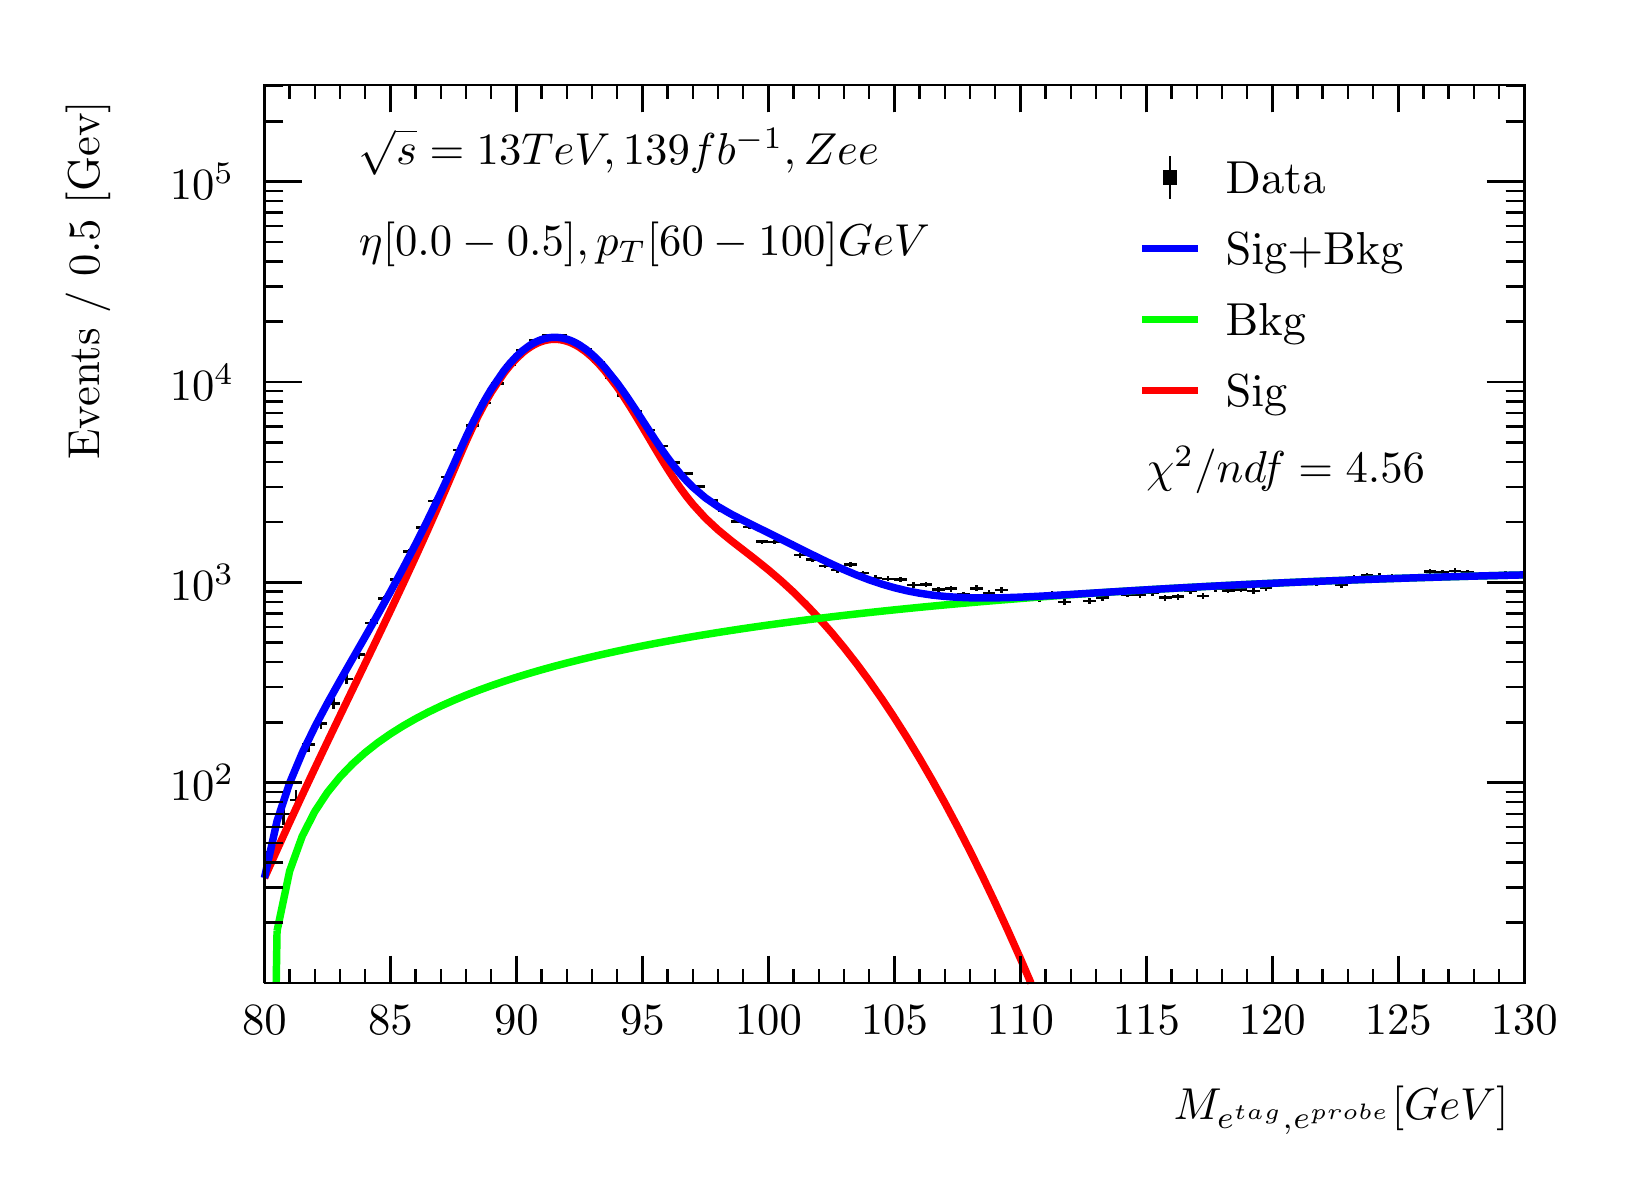
\begin{tikzpicture}
\pgfdeclareplotmark{cross} {
\pgfpathmoveto{\pgfpoint{-0.3\pgfplotmarksize}{\pgfplotmarksize}}
\pgfpathlineto{\pgfpoint{+0.3\pgfplotmarksize}{\pgfplotmarksize}}
\pgfpathlineto{\pgfpoint{+0.3\pgfplotmarksize}{0.3\pgfplotmarksize}}
\pgfpathlineto{\pgfpoint{+1\pgfplotmarksize}{0.3\pgfplotmarksize}}
\pgfpathlineto{\pgfpoint{+1\pgfplotmarksize}{-0.3\pgfplotmarksize}}
\pgfpathlineto{\pgfpoint{+0.3\pgfplotmarksize}{-0.3\pgfplotmarksize}}
\pgfpathlineto{\pgfpoint{+0.3\pgfplotmarksize}{-1.\pgfplotmarksize}}
\pgfpathlineto{\pgfpoint{-0.3\pgfplotmarksize}{-1.\pgfplotmarksize}}
\pgfpathlineto{\pgfpoint{-0.3\pgfplotmarksize}{-0.3\pgfplotmarksize}}
\pgfpathlineto{\pgfpoint{-1.\pgfplotmarksize}{-0.3\pgfplotmarksize}}
\pgfpathlineto{\pgfpoint{-1.\pgfplotmarksize}{0.3\pgfplotmarksize}}
\pgfpathlineto{\pgfpoint{-0.3\pgfplotmarksize}{0.3\pgfplotmarksize}}
\pgfpathclose
\pgfusepathqstroke
}
\pgfdeclareplotmark{cross*} {
\pgfpathmoveto{\pgfpoint{-0.3\pgfplotmarksize}{\pgfplotmarksize}}
\pgfpathlineto{\pgfpoint{+0.3\pgfplotmarksize}{\pgfplotmarksize}}
\pgfpathlineto{\pgfpoint{+0.3\pgfplotmarksize}{0.3\pgfplotmarksize}}
\pgfpathlineto{\pgfpoint{+1\pgfplotmarksize}{0.3\pgfplotmarksize}}
\pgfpathlineto{\pgfpoint{+1\pgfplotmarksize}{-0.3\pgfplotmarksize}}
\pgfpathlineto{\pgfpoint{+0.3\pgfplotmarksize}{-0.3\pgfplotmarksize}}
\pgfpathlineto{\pgfpoint{+0.3\pgfplotmarksize}{-1.\pgfplotmarksize}}
\pgfpathlineto{\pgfpoint{-0.3\pgfplotmarksize}{-1.\pgfplotmarksize}}
\pgfpathlineto{\pgfpoint{-0.3\pgfplotmarksize}{-0.3\pgfplotmarksize}}
\pgfpathlineto{\pgfpoint{-1.\pgfplotmarksize}{-0.3\pgfplotmarksize}}
\pgfpathlineto{\pgfpoint{-1.\pgfplotmarksize}{0.3\pgfplotmarksize}}
\pgfpathlineto{\pgfpoint{-0.3\pgfplotmarksize}{0.3\pgfplotmarksize}}
\pgfpathclose
\pgfusepathqfillstroke
}
\pgfdeclareplotmark{newstar} {
\pgfpathmoveto{\pgfqpoint{0pt}{\pgfplotmarksize}}
\pgfpathlineto{\pgfqpointpolar{44}{0.5\pgfplotmarksize}}
\pgfpathlineto{\pgfqpointpolar{18}{\pgfplotmarksize}}
\pgfpathlineto{\pgfqpointpolar{-20}{0.5\pgfplotmarksize}}
\pgfpathlineto{\pgfqpointpolar{-54}{\pgfplotmarksize}}
\pgfpathlineto{\pgfqpointpolar{-90}{0.5\pgfplotmarksize}}
\pgfpathlineto{\pgfqpointpolar{234}{\pgfplotmarksize}}
\pgfpathlineto{\pgfqpointpolar{198}{0.5\pgfplotmarksize}}
\pgfpathlineto{\pgfqpointpolar{162}{\pgfplotmarksize}}
\pgfpathlineto{\pgfqpointpolar{134}{0.5\pgfplotmarksize}}
\pgfpathclose
\pgfusepathqstroke
}
\pgfdeclareplotmark{newstar*} {
\pgfpathmoveto{\pgfqpoint{0pt}{\pgfplotmarksize}}
\pgfpathlineto{\pgfqpointpolar{44}{0.5\pgfplotmarksize}}
\pgfpathlineto{\pgfqpointpolar{18}{\pgfplotmarksize}}
\pgfpathlineto{\pgfqpointpolar{-20}{0.5\pgfplotmarksize}}
\pgfpathlineto{\pgfqpointpolar{-54}{\pgfplotmarksize}}
\pgfpathlineto{\pgfqpointpolar{-90}{0.5\pgfplotmarksize}}
\pgfpathlineto{\pgfqpointpolar{234}{\pgfplotmarksize}}
\pgfpathlineto{\pgfqpointpolar{198}{0.5\pgfplotmarksize}}
\pgfpathlineto{\pgfqpointpolar{162}{\pgfplotmarksize}}
\pgfpathlineto{\pgfqpointpolar{134}{0.5\pgfplotmarksize}}
\pgfpathclose
\pgfusepathqfillstroke
}
\definecolor{c}{rgb}{1,1,1};
\draw [color=c, fill=c] (0,0) rectangle (20,14.4361);
\draw [color=c, fill=c] (3,2.30977) rectangle (19,13.7143);
\definecolor{c}{rgb}{0,0,0};
\draw [c,line width=0.9] (3,2.30977) -- (3,13.7143) -- (19,13.7143) -- (19,2.30977) -- (3,2.30977);
\definecolor{c}{rgb}{1,1,1};
\draw [color=c, fill=c] (3,2.30977) rectangle (19,13.7143);
\definecolor{c}{rgb}{0,0,0};
\draw [c,line width=0.9] (3,2.30977) -- (3,13.7143) -- (19,13.7143) -- (19,2.30977) -- (3,2.30977);
\draw [c,line width=0.9] (3,2.30977) -- (19,2.30977);
\draw [c,line width=0.9] (3,2.65624) -- (3,2.30977);
\draw [c,line width=0.9] (3.32,2.48301) -- (3.32,2.30977);
\draw [c,line width=0.9] (3.64,2.48301) -- (3.64,2.30977);
\draw [c,line width=0.9] (3.96,2.48301) -- (3.96,2.30977);
\draw [c,line width=0.9] (4.28,2.48301) -- (4.28,2.30977);
\draw [c,line width=0.9] (4.6,2.65624) -- (4.6,2.30977);
\draw [c,line width=0.9] (4.92,2.48301) -- (4.92,2.30977);
\draw [c,line width=0.9] (5.24,2.48301) -- (5.24,2.30977);
\draw [c,line width=0.9] (5.56,2.48301) -- (5.56,2.30977);
\draw [c,line width=0.9] (5.88,2.48301) -- (5.88,2.30977);
\draw [c,line width=0.9] (6.2,2.65624) -- (6.2,2.30977);
\draw [c,line width=0.9] (6.52,2.48301) -- (6.52,2.30977);
\draw [c,line width=0.9] (6.84,2.48301) -- (6.84,2.30977);
\draw [c,line width=0.9] (7.16,2.48301) -- (7.16,2.30977);
\draw [c,line width=0.9] (7.48,2.48301) -- (7.48,2.30977);
\draw [c,line width=0.9] (7.8,2.65624) -- (7.8,2.30977);
\draw [c,line width=0.9] (8.12,2.48301) -- (8.12,2.30977);
\draw [c,line width=0.9] (8.44,2.48301) -- (8.44,2.30977);
\draw [c,line width=0.9] (8.76,2.48301) -- (8.76,2.30977);
\draw [c,line width=0.9] (9.08,2.48301) -- (9.08,2.30977);
\draw [c,line width=0.9] (9.4,2.65624) -- (9.4,2.30977);
\draw [c,line width=0.9] (9.72,2.48301) -- (9.72,2.30977);
\draw [c,line width=0.9] (10.04,2.48301) -- (10.04,2.30977);
\draw [c,line width=0.9] (10.36,2.48301) -- (10.36,2.30977);
\draw [c,line width=0.9] (10.68,2.48301) -- (10.68,2.30977);
\draw [c,line width=0.9] (11,2.65624) -- (11,2.30977);
\draw [c,line width=0.9] (11.32,2.48301) -- (11.32,2.30977);
\draw [c,line width=0.9] (11.64,2.48301) -- (11.64,2.30977);
\draw [c,line width=0.9] (11.96,2.48301) -- (11.96,2.30977);
\draw [c,line width=0.9] (12.28,2.48301) -- (12.28,2.30977);
\draw [c,line width=0.9] (12.6,2.65624) -- (12.6,2.30977);
\draw [c,line width=0.9] (12.92,2.48301) -- (12.92,2.30977);
\draw [c,line width=0.9] (13.24,2.48301) -- (13.24,2.30977);
\draw [c,line width=0.9] (13.56,2.48301) -- (13.56,2.30977);
\draw [c,line width=0.9] (13.88,2.48301) -- (13.88,2.30977);
\draw [c,line width=0.9] (14.2,2.65624) -- (14.2,2.30977);
\draw [c,line width=0.9] (14.52,2.48301) -- (14.52,2.30977);
\draw [c,line width=0.9] (14.84,2.48301) -- (14.84,2.30977);
\draw [c,line width=0.9] (15.16,2.48301) -- (15.16,2.30977);
\draw [c,line width=0.9] (15.48,2.48301) -- (15.48,2.30977);
\draw [c,line width=0.9] (15.8,2.65624) -- (15.8,2.30977);
\draw [c,line width=0.9] (16.12,2.48301) -- (16.12,2.30977);
\draw [c,line width=0.9] (16.44,2.48301) -- (16.44,2.30977);
\draw [c,line width=0.9] (16.76,2.48301) -- (16.76,2.30977);
\draw [c,line width=0.9] (17.08,2.48301) -- (17.08,2.30977);
\draw [c,line width=0.9] (17.4,2.65624) -- (17.4,2.30977);
\draw [c,line width=0.9] (17.72,2.48301) -- (17.72,2.30977);
\draw [c,line width=0.9] (18.04,2.48301) -- (18.04,2.30977);
\draw [c,line width=0.9] (18.36,2.48301) -- (18.36,2.30977);
\draw [c,line width=0.9] (18.68,2.48301) -- (18.68,2.30977);
\draw [c,line width=0.9] (19,2.65624) -- (19,2.30977);
\draw [anchor=base] (3,1.66015) node[scale=1.61424, color=c, rotate=0]{80};
\draw [anchor=base] (4.6,1.66015) node[scale=1.61424, color=c, rotate=0]{85};
\draw [anchor=base] (6.2,1.66015) node[scale=1.61424, color=c, rotate=0]{90};
\draw [anchor=base] (7.8,1.66015) node[scale=1.61424, color=c, rotate=0]{95};
\draw [anchor=base] (9.4,1.66015) node[scale=1.61424, color=c, rotate=0]{100};
\draw [anchor=base] (11,1.66015) node[scale=1.61424, color=c, rotate=0]{105};
\draw [anchor=base] (12.6,1.66015) node[scale=1.61424, color=c, rotate=0]{110};
\draw [anchor=base] (14.2,1.66015) node[scale=1.61424, color=c, rotate=0]{115};
\draw [anchor=base] (15.8,1.66015) node[scale=1.61424, color=c, rotate=0]{120};
\draw [anchor=base] (17.4,1.66015) node[scale=1.61424, color=c, rotate=0]{125};
\draw [anchor=base] (19,1.66015) node[scale=1.61424, color=c, rotate=0]{130};
\draw [anchor= east] (19,0.692932) node[scale=1.61424, color=c, rotate=0]{$M_{e^{tag}, e^{probe}}  [GeV]$};
\draw [c,line width=0.9] (3,13.7143) -- (19,13.7143);
\draw [c,line width=0.9] (3,13.3678) -- (3,13.7143);
\draw [c,line width=0.9] (3.32,13.5411) -- (3.32,13.7143);
\draw [c,line width=0.9] (3.64,13.5411) -- (3.64,13.7143);
\draw [c,line width=0.9] (3.96,13.5411) -- (3.96,13.7143);
\draw [c,line width=0.9] (4.28,13.5411) -- (4.28,13.7143);
\draw [c,line width=0.9] (4.6,13.3678) -- (4.6,13.7143);
\draw [c,line width=0.9] (4.92,13.5411) -- (4.92,13.7143);
\draw [c,line width=0.9] (5.24,13.5411) -- (5.24,13.7143);
\draw [c,line width=0.9] (5.56,13.5411) -- (5.56,13.7143);
\draw [c,line width=0.9] (5.88,13.5411) -- (5.88,13.7143);
\draw [c,line width=0.9] (6.2,13.3678) -- (6.2,13.7143);
\draw [c,line width=0.9] (6.52,13.5411) -- (6.52,13.7143);
\draw [c,line width=0.9] (6.84,13.5411) -- (6.84,13.7143);
\draw [c,line width=0.9] (7.16,13.5411) -- (7.16,13.7143);
\draw [c,line width=0.9] (7.48,13.5411) -- (7.48,13.7143);
\draw [c,line width=0.9] (7.8,13.3678) -- (7.8,13.7143);
\draw [c,line width=0.9] (8.12,13.5411) -- (8.12,13.7143);
\draw [c,line width=0.9] (8.44,13.5411) -- (8.44,13.7143);
\draw [c,line width=0.9] (8.76,13.5411) -- (8.76,13.7143);
\draw [c,line width=0.9] (9.08,13.5411) -- (9.08,13.7143);
\draw [c,line width=0.9] (9.4,13.3678) -- (9.4,13.7143);
\draw [c,line width=0.9] (9.72,13.5411) -- (9.72,13.7143);
\draw [c,line width=0.9] (10.04,13.5411) -- (10.04,13.7143);
\draw [c,line width=0.9] (10.36,13.5411) -- (10.36,13.7143);
\draw [c,line width=0.9] (10.68,13.5411) -- (10.68,13.7143);
\draw [c,line width=0.9] (11,13.3678) -- (11,13.7143);
\draw [c,line width=0.9] (11.32,13.5411) -- (11.32,13.7143);
\draw [c,line width=0.9] (11.64,13.5411) -- (11.64,13.7143);
\draw [c,line width=0.9] (11.96,13.5411) -- (11.96,13.7143);
\draw [c,line width=0.9] (12.28,13.5411) -- (12.28,13.7143);
\draw [c,line width=0.9] (12.6,13.3678) -- (12.6,13.7143);
\draw [c,line width=0.9] (12.92,13.5411) -- (12.92,13.7143);
\draw [c,line width=0.9] (13.24,13.5411) -- (13.24,13.7143);
\draw [c,line width=0.9] (13.56,13.5411) -- (13.56,13.7143);
\draw [c,line width=0.9] (13.88,13.5411) -- (13.88,13.7143);
\draw [c,line width=0.9] (14.2,13.3678) -- (14.2,13.7143);
\draw [c,line width=0.9] (14.52,13.5411) -- (14.52,13.7143);
\draw [c,line width=0.9] (14.84,13.5411) -- (14.84,13.7143);
\draw [c,line width=0.9] (15.16,13.5411) -- (15.16,13.7143);
\draw [c,line width=0.9] (15.48,13.5411) -- (15.48,13.7143);
\draw [c,line width=0.9] (15.8,13.3678) -- (15.8,13.7143);
\draw [c,line width=0.9] (16.12,13.5411) -- (16.12,13.7143);
\draw [c,line width=0.9] (16.44,13.5411) -- (16.44,13.7143);
\draw [c,line width=0.9] (16.76,13.5411) -- (16.76,13.7143);
\draw [c,line width=0.9] (17.08,13.5411) -- (17.08,13.7143);
\draw [c,line width=0.9] (17.4,13.3678) -- (17.4,13.7143);
\draw [c,line width=0.9] (17.72,13.5411) -- (17.72,13.7143);
\draw [c,line width=0.9] (18.04,13.5411) -- (18.04,13.7143);
\draw [c,line width=0.9] (18.36,13.5411) -- (18.36,13.7143);
\draw [c,line width=0.9] (18.68,13.5411) -- (18.68,13.7143);
\draw [c,line width=0.9] (19,13.3678) -- (19,13.7143);
\draw [c,line width=0.9] (3,2.30977) -- (3,13.7143);
\draw [c,line width=0.9] (3.237,3.07568) -- (3,3.07568);
\draw [c,line width=0.9] (3.237,3.5237) -- (3,3.5237);
\draw [c,line width=0.9] (3.237,3.84158) -- (3,3.84158);
\draw [c,line width=0.9] (3.237,4.08815) -- (3,4.08815);
\draw [c,line width=0.9] (3.237,4.2896) -- (3,4.2896);
\draw [c,line width=0.9] (3.237,4.45994) -- (3,4.45994);
\draw [c,line width=0.9] (3.237,4.60748) -- (3,4.60748);
\draw [c,line width=0.9] (3.237,4.73763) -- (3,4.73763);
\draw [c,line width=0.9] (3.474,4.85405) -- (3,4.85405);
\draw [anchor= east] (2.82,4.85405) node[scale=1.61424, color=c, rotate=0]{$10^{2}$};
\draw [c,line width=0.9] (3.237,5.61995) -- (3,5.61995);
\draw [c,line width=0.9] (3.237,6.06798) -- (3,6.06798);
\draw [c,line width=0.9] (3.237,6.38586) -- (3,6.38586);
\draw [c,line width=0.9] (3.237,6.63242) -- (3,6.63242);
\draw [c,line width=0.9] (3.237,6.83388) -- (3,6.83388);
\draw [c,line width=0.9] (3.237,7.00421) -- (3,7.00421);
\draw [c,line width=0.9] (3.237,7.15176) -- (3,7.15176);
\draw [c,line width=0.9] (3.237,7.28191) -- (3,7.28191);
\draw [c,line width=0.9] (3.474,7.39833) -- (3,7.39833);
\draw [anchor= east] (2.82,7.39833) node[scale=1.61424, color=c, rotate=0]{$10^{3}$};
\draw [c,line width=0.9] (3.237,8.16423) -- (3,8.16423);
\draw [c,line width=0.9] (3.237,8.61226) -- (3,8.61226);
\draw [c,line width=0.9] (3.237,8.93013) -- (3,8.93013);
\draw [c,line width=0.9] (3.237,9.1767) -- (3,9.1767);
\draw [c,line width=0.9] (3.237,9.37816) -- (3,9.37816);
\draw [c,line width=0.9] (3.237,9.54849) -- (3,9.54849);
\draw [c,line width=0.9] (3.237,9.69604) -- (3,9.69604);
\draw [c,line width=0.9] (3.237,9.82618) -- (3,9.82618);
\draw [c,line width=0.9] (3.474,9.9426) -- (3,9.9426);
\draw [anchor= east] (2.82,9.9426) node[scale=1.61424, color=c, rotate=0]{$10^{4}$};
\draw [c,line width=0.9] (3.237,10.7085) -- (3,10.7085);
\draw [c,line width=0.9] (3.237,11.1565) -- (3,11.1565);
\draw [c,line width=0.9] (3.237,11.4744) -- (3,11.4744);
\draw [c,line width=0.9] (3.237,11.721) -- (3,11.721);
\draw [c,line width=0.9] (3.237,11.9224) -- (3,11.9224);
\draw [c,line width=0.9] (3.237,12.0928) -- (3,12.0928);
\draw [c,line width=0.9] (3.237,12.2403) -- (3,12.2403);
\draw [c,line width=0.9] (3.237,12.3705) -- (3,12.3705);
\draw [c,line width=0.9] (3.474,12.4869) -- (3,12.4869);
\draw [anchor= east] (2.82,12.4869) node[scale=1.61424, color=c, rotate=0]{$10^{5}$};
\draw [c,line width=0.9] (3.237,13.2528) -- (3,13.2528);
\draw [c,line width=0.9] (3.237,13.7008) -- (3,13.7008);
\draw [anchor= east] (0.76,13.7143) node[scale=1.61424, color=c, rotate=90]{Events / 0.5 [Gev]};
\draw [c,line width=0.9] (19,2.30977) -- (19,13.7143);
\draw [c,line width=0.9] (18.763,3.07568) -- (19,3.07568);
\draw [c,line width=0.9] (18.763,3.5237) -- (19,3.5237);
\draw [c,line width=0.9] (18.763,3.84158) -- (19,3.84158);
\draw [c,line width=0.9] (18.763,4.08815) -- (19,4.08815);
\draw [c,line width=0.9] (18.763,4.2896) -- (19,4.2896);
\draw [c,line width=0.9] (18.763,4.45994) -- (19,4.45994);
\draw [c,line width=0.9] (18.763,4.60748) -- (19,4.60748);
\draw [c,line width=0.9] (18.763,4.73763) -- (19,4.73763);
\draw [c,line width=0.9] (18.526,4.85405) -- (19,4.85405);
\draw [c,line width=0.9] (18.763,5.61995) -- (19,5.61995);
\draw [c,line width=0.9] (18.763,6.06798) -- (19,6.06798);
\draw [c,line width=0.9] (18.763,6.38586) -- (19,6.38586);
\draw [c,line width=0.9] (18.763,6.63242) -- (19,6.63242);
\draw [c,line width=0.9] (18.763,6.83388) -- (19,6.83388);
\draw [c,line width=0.9] (18.763,7.00421) -- (19,7.00421);
\draw [c,line width=0.9] (18.763,7.15176) -- (19,7.15176);
\draw [c,line width=0.9] (18.763,7.28191) -- (19,7.28191);
\draw [c,line width=0.9] (18.526,7.39833) -- (19,7.39833);
\draw [c,line width=0.9] (18.763,8.16423) -- (19,8.16423);
\draw [c,line width=0.9] (18.763,8.61226) -- (19,8.61226);
\draw [c,line width=0.9] (18.763,8.93013) -- (19,8.93013);
\draw [c,line width=0.9] (18.763,9.1767) -- (19,9.1767);
\draw [c,line width=0.9] (18.763,9.37816) -- (19,9.37816);
\draw [c,line width=0.9] (18.763,9.54849) -- (19,9.54849);
\draw [c,line width=0.9] (18.763,9.69604) -- (19,9.69604);
\draw [c,line width=0.9] (18.763,9.82618) -- (19,9.82618);
\draw [c,line width=0.9] (18.526,9.9426) -- (19,9.9426);
\draw [c,line width=0.9] (18.763,10.7085) -- (19,10.7085);
\draw [c,line width=0.9] (18.763,11.1565) -- (19,11.1565);
\draw [c,line width=0.9] (18.763,11.4744) -- (19,11.4744);
\draw [c,line width=0.9] (18.763,11.721) -- (19,11.721);
\draw [c,line width=0.9] (18.763,11.9224) -- (19,11.9224);
\draw [c,line width=0.9] (18.763,12.0928) -- (19,12.0928);
\draw [c,line width=0.9] (18.763,12.2403) -- (19,12.2403);
\draw [c,line width=0.9] (18.763,12.3705) -- (19,12.3705);
\draw [c,line width=0.9] (18.526,12.4869) -- (19,12.4869);
\draw [c,line width=0.9] (18.763,13.2528) -- (19,13.2528);
\draw [c,line width=0.9] (18.763,13.7008) -- (19,13.7008);
\draw [c,line width=0.9] (3.08,3.97173) -- (3,3.97173);
\draw [c,line width=0.9] (3,3.97173) -- (3,3.97173);
\draw [c,line width=0.9] (3.08,3.97173) -- (3.16,3.97173);
\draw [c,line width=0.9] (3.16,3.97173) -- (3.16,3.97173);
\draw [c,line width=0.9] (3.08,3.97173) -- (3.08,4.14747);
\draw [c,line width=0.9] (3.08,4.14747) -- (3.08,4.14747);
\draw [c,line width=0.9] (3.08,3.97173) -- (3.08,3.79408);
\draw [c,line width=0.9] (3.08,3.79408) -- (3.08,3.79408);
\draw [c,line width=0.9] (3.24,4.45994) -- (3.16,4.45994);
\draw [c,line width=0.9] (3.16,4.45994) -- (3.16,4.45994);
\draw [c,line width=0.9] (3.24,4.45994) -- (3.32,4.45994);
\draw [c,line width=0.9] (3.32,4.45994) -- (3.32,4.45994);
\draw [c,line width=0.9] (3.24,4.45994) -- (3.24,4.59926);
\draw [c,line width=0.9] (3.24,4.59926) -- (3.24,4.59926);
\draw [c,line width=0.9] (3.24,4.45994) -- (3.24,4.31964);
\draw [c,line width=0.9] (3.24,4.31964) -- (3.24,4.31964);
\draw [c,line width=0.9] (3.4,4.63477) -- (3.32,4.63477);
\draw [c,line width=0.9] (3.32,4.63477) -- (3.32,4.63477);
\draw [c,line width=0.9] (3.4,4.63477) -- (3.48,4.63477);
\draw [c,line width=0.9] (3.48,4.63477) -- (3.48,4.63477);
\draw [c,line width=0.9] (3.4,4.63477) -- (3.4,4.76302);
\draw [c,line width=0.9] (3.4,4.76302) -- (3.4,4.76302);
\draw [c,line width=0.9] (3.4,4.63477) -- (3.4,4.50575);
\draw [c,line width=0.9] (3.4,4.50575) -- (3.4,4.50575);
\draw [c,line width=0.9] (3.56,5.33831) -- (3.48,5.33831);
\draw [c,line width=0.9] (3.48,5.33831) -- (3.48,5.33831);
\draw [c,line width=0.9] (3.56,5.33831) -- (3.64,5.33831);
\draw [c,line width=0.9] (3.64,5.33831) -- (3.64,5.33831);
\draw [c,line width=0.9] (3.56,5.33831) -- (3.56,5.42704);
\draw [c,line width=0.9] (3.56,5.42704) -- (3.56,5.42704);
\draw [c,line width=0.9] (3.56,5.33831) -- (3.56,5.24958);
\draw [c,line width=0.9] (3.56,5.24958) -- (3.56,5.24958);
\draw [c,line width=0.9] (3.72,5.60885) -- (3.64,5.60885);
\draw [c,line width=0.9] (3.64,5.60885) -- (3.64,5.60885);
\draw [c,line width=0.9] (3.72,5.60885) -- (3.8,5.60885);
\draw [c,line width=0.9] (3.8,5.60885) -- (3.8,5.60885);
\draw [c,line width=0.9] (3.72,5.60885) -- (3.72,5.68736);
\draw [c,line width=0.9] (3.72,5.68736) -- (3.72,5.68736);
\draw [c,line width=0.9] (3.72,5.60885) -- (3.72,5.53034);
\draw [c,line width=0.9] (3.72,5.53034) -- (3.72,5.53034);
\draw [c,line width=0.9] (3.88,5.85765) -- (3.8,5.85765);
\draw [c,line width=0.9] (3.8,5.85765) -- (3.8,5.85765);
\draw [c,line width=0.9] (3.88,5.85765) -- (3.96,5.85765);
\draw [c,line width=0.9] (3.96,5.85765) -- (3.96,5.85765);
\draw [c,line width=0.9] (3.88,5.85765) -- (3.88,5.9278);
\draw [c,line width=0.9] (3.88,5.9278) -- (3.88,5.9278);
\draw [c,line width=0.9] (3.88,5.85765) -- (3.88,5.78749);
\draw [c,line width=0.9] (3.88,5.78749) -- (3.88,5.78749);
\draw [c,line width=0.9] (4.04,6.16994) -- (3.96,6.16994);
\draw [c,line width=0.9] (3.96,6.16994) -- (3.96,6.16994);
\draw [c,line width=0.9] (4.04,6.16994) -- (4.12,6.16994);
\draw [c,line width=0.9] (4.12,6.16994) -- (4.12,6.16994);
\draw [c,line width=0.9] (4.04,6.16994) -- (4.04,6.23085);
\draw [c,line width=0.9] (4.04,6.23085) -- (4.04,6.23085);
\draw [c,line width=0.9] (4.04,6.16994) -- (4.04,6.10903);
\draw [c,line width=0.9] (4.04,6.10903) -- (4.04,6.10903);
\draw [c,line width=0.9] (4.2,6.48361) -- (4.12,6.48361);
\draw [c,line width=0.9] (4.12,6.48361) -- (4.12,6.48361);
\draw [c,line width=0.9] (4.2,6.48361) -- (4.28,6.48361);
\draw [c,line width=0.9] (4.28,6.48361) -- (4.28,6.48361);
\draw [c,line width=0.9] (4.2,6.48361) -- (4.2,6.53647);
\draw [c,line width=0.9] (4.2,6.53647) -- (4.2,6.53647);
\draw [c,line width=0.9] (4.2,6.48361) -- (4.2,6.43076);
\draw [c,line width=0.9] (4.2,6.43076) -- (4.2,6.43076);
\draw [c,line width=0.9] (4.36,6.88428) -- (4.28,6.88428);
\draw [c,line width=0.9] (4.28,6.88428) -- (4.28,6.88428);
\draw [c,line width=0.9] (4.36,6.88428) -- (4.44,6.88428);
\draw [c,line width=0.9] (4.44,6.88428) -- (4.44,6.88428);
\draw [c,line width=0.9] (4.36,6.88428) -- (4.36,6.92837);
\draw [c,line width=0.9] (4.36,6.92837) -- (4.36,6.92837);
\draw [c,line width=0.9] (4.36,6.88428) -- (4.36,6.84019);
\draw [c,line width=0.9] (4.36,6.84019) -- (4.36,6.84019);
\draw [c,line width=0.9] (4.52,7.19244) -- (4.44,7.19244);
\draw [c,line width=0.9] (4.44,7.19244) -- (4.44,7.19244);
\draw [c,line width=0.9] (4.52,7.19244) -- (4.6,7.19244);
\draw [c,line width=0.9] (4.6,7.19244) -- (4.6,7.19244);
\draw [c,line width=0.9] (4.52,7.19244) -- (4.52,7.23079);
\draw [c,line width=0.9] (4.52,7.23079) -- (4.52,7.23079);
\draw [c,line width=0.9] (4.52,7.19244) -- (4.52,7.15409);
\draw [c,line width=0.9] (4.52,7.15409) -- (4.52,7.15409);
\draw [c,line width=0.9] (4.68,7.4342) -- (4.6,7.4342);
\draw [c,line width=0.9] (4.6,7.4342) -- (4.6,7.4342);
\draw [c,line width=0.9] (4.68,7.4342) -- (4.76,7.4342);
\draw [c,line width=0.9] (4.76,7.4342) -- (4.76,7.4342);
\draw [c,line width=0.9] (4.68,7.4342) -- (4.68,7.46858);
\draw [c,line width=0.9] (4.68,7.46858) -- (4.68,7.46858);
\draw [c,line width=0.9] (4.68,7.4342) -- (4.68,7.39983);
\draw [c,line width=0.9] (4.68,7.39983) -- (4.68,7.39983);
\draw [c,line width=0.9] (4.84,7.7889) -- (4.76,7.7889);
\draw [c,line width=0.9] (4.76,7.7889) -- (4.76,7.7889);
\draw [c,line width=0.9] (4.84,7.7889) -- (4.92,7.7889);
\draw [c,line width=0.9] (4.92,7.7889) -- (4.92,7.7889);
\draw [c,line width=0.9] (4.84,7.7889) -- (4.84,7.81818);
\draw [c,line width=0.9] (4.84,7.81818) -- (4.84,7.81818);
\draw [c,line width=0.9] (4.84,7.7889) -- (4.84,7.75962);
\draw [c,line width=0.9] (4.84,7.75962) -- (4.84,7.75962);
\draw [c,line width=0.9] (5,8.09645) -- (4.92,8.09645);
\draw [c,line width=0.9] (4.92,8.09645) -- (4.92,8.09645);
\draw [c,line width=0.9] (5,8.09645) -- (5.08,8.09645);
\draw [c,line width=0.9] (5.08,8.09645) -- (5.08,8.09645);
\draw [c,line width=0.9] (5,8.09645) -- (5,8.12193);
\draw [c,line width=0.9] (5,8.12193) -- (5,8.12193);
\draw [c,line width=0.9] (5,8.09645) -- (5,8.07097);
\draw [c,line width=0.9] (5,8.07097) -- (5,8.07097);
\draw [c,line width=0.9] (5.16,8.43008) -- (5.08,8.43008);
\draw [c,line width=0.9] (5.08,8.43008) -- (5.08,8.43008);
\draw [c,line width=0.9] (5.16,8.43008) -- (5.24,8.43008);
\draw [c,line width=0.9] (5.24,8.43008) -- (5.24,8.43008);
\draw [c,line width=0.9] (5.16,8.43008) -- (5.16,8.45198);
\draw [c,line width=0.9] (5.16,8.45198) -- (5.16,8.45198);
\draw [c,line width=0.9] (5.16,8.43008) -- (5.16,8.40817);
\draw [c,line width=0.9] (5.16,8.40817) -- (5.16,8.40817);
\draw [c,line width=0.9] (5.32,8.73386) -- (5.24,8.73386);
\draw [c,line width=0.9] (5.24,8.73386) -- (5.24,8.73386);
\draw [c,line width=0.9] (5.32,8.73386) -- (5.4,8.73386);
\draw [c,line width=0.9] (5.4,8.73386) -- (5.4,8.73386);
\draw [c,line width=0.9] (5.32,8.73386) -- (5.32,8.75295);
\draw [c,line width=0.9] (5.32,8.75295) -- (5.32,8.75295);
\draw [c,line width=0.9] (5.32,8.73386) -- (5.32,8.71476);
\draw [c,line width=0.9] (5.32,8.71476) -- (5.32,8.71476);
\draw [c,line width=0.9] (5.48,9.07903) -- (5.4,9.07903);
\draw [c,line width=0.9] (5.4,9.07903) -- (5.4,9.07903);
\draw [c,line width=0.9] (5.48,9.07903) -- (5.56,9.07903);
\draw [c,line width=0.9] (5.56,9.07903) -- (5.56,9.07903);
\draw [c,line width=0.9] (5.48,9.07903) -- (5.48,9.09536);
\draw [c,line width=0.9] (5.48,9.09536) -- (5.48,9.09536);
\draw [c,line width=0.9] (5.48,9.07903) -- (5.48,9.0627);
\draw [c,line width=0.9] (5.48,9.0627) -- (5.48,9.0627);
\draw [c,line width=0.9] (5.64,9.39261) -- (5.56,9.39261);
\draw [c,line width=0.9] (5.56,9.39261) -- (5.56,9.39261);
\draw [c,line width=0.9] (5.64,9.39261) -- (5.72,9.39261);
\draw [c,line width=0.9] (5.72,9.39261) -- (5.72,9.39261);
\draw [c,line width=0.9] (5.64,9.39261) -- (5.64,9.40679);
\draw [c,line width=0.9] (5.64,9.40679) -- (5.64,9.40679);
\draw [c,line width=0.9] (5.64,9.39261) -- (5.64,9.37844);
\draw [c,line width=0.9] (5.64,9.37844) -- (5.64,9.37844);
\draw [c,line width=0.9] (5.8,9.67681) -- (5.72,9.67681);
\draw [c,line width=0.9] (5.72,9.67681) -- (5.72,9.67681);
\draw [c,line width=0.9] (5.8,9.67681) -- (5.88,9.67681);
\draw [c,line width=0.9] (5.88,9.67681) -- (5.88,9.67681);
\draw [c,line width=0.9] (5.8,9.67681) -- (5.8,9.68927);
\draw [c,line width=0.9] (5.8,9.68927) -- (5.8,9.68927);
\draw [c,line width=0.9] (5.8,9.67681) -- (5.8,9.66435);
\draw [c,line width=0.9] (5.8,9.66435) -- (5.8,9.66435);
\draw [c,line width=0.9] (5.96,9.9213) -- (5.88,9.9213);
\draw [c,line width=0.9] (5.88,9.9213) -- (5.88,9.9213);
\draw [c,line width=0.9] (5.96,9.9213) -- (6.04,9.9213);
\draw [c,line width=0.9] (6.04,9.9213) -- (6.04,9.9213);
\draw [c,line width=0.9] (5.96,9.9213) -- (5.96,9.93245);
\draw [c,line width=0.9] (5.96,9.93245) -- (5.96,9.93245);
\draw [c,line width=0.9] (5.96,9.9213) -- (5.96,9.91014);
\draw [c,line width=0.9] (5.96,9.91014) -- (5.96,9.91014);
\draw [c,line width=0.9] (6.12,10.1618) -- (6.04,10.1618);
\draw [c,line width=0.9] (6.04,10.1618) -- (6.04,10.1618);
\draw [c,line width=0.9] (6.12,10.1618) -- (6.2,10.1618);
\draw [c,line width=0.9] (6.2,10.1618) -- (6.2,10.1618);
\draw [c,line width=0.9] (6.12,10.1618) -- (6.12,10.1718);
\draw [c,line width=0.9] (6.12,10.1718) -- (6.12,10.1718);
\draw [c,line width=0.9] (6.12,10.1618) -- (6.12,10.1518);
\draw [c,line width=0.9] (6.12,10.1518) -- (6.12,10.1518);
\draw [c,line width=0.9] (6.28,10.3471) -- (6.2,10.3471);
\draw [c,line width=0.9] (6.2,10.3471) -- (6.2,10.3471);
\draw [c,line width=0.9] (6.28,10.3471) -- (6.36,10.3471);
\draw [c,line width=0.9] (6.36,10.3471) -- (6.36,10.3471);
\draw [c,line width=0.9] (6.28,10.3471) -- (6.28,10.3563);
\draw [c,line width=0.9] (6.28,10.3563) -- (6.28,10.3563);
\draw [c,line width=0.9] (6.28,10.3471) -- (6.28,10.3379);
\draw [c,line width=0.9] (6.28,10.3379) -- (6.28,10.3379);
\draw [c,line width=0.9] (6.44,10.4746) -- (6.36,10.4746);
\draw [c,line width=0.9] (6.36,10.4746) -- (6.36,10.4746);
\draw [c,line width=0.9] (6.44,10.4746) -- (6.52,10.4746);
\draw [c,line width=0.9] (6.52,10.4746) -- (6.52,10.4746);
\draw [c,line width=0.9] (6.44,10.4746) -- (6.44,10.4833);
\draw [c,line width=0.9] (6.44,10.4833) -- (6.44,10.4833);
\draw [c,line width=0.9] (6.44,10.4746) -- (6.44,10.466);
\draw [c,line width=0.9] (6.44,10.466) -- (6.44,10.466);
\draw [c,line width=0.9] (6.6,10.5373) -- (6.52,10.5373);
\draw [c,line width=0.9] (6.52,10.5373) -- (6.52,10.5373);
\draw [c,line width=0.9] (6.6,10.5373) -- (6.68,10.5373);
\draw [c,line width=0.9] (6.68,10.5373) -- (6.68,10.5373);
\draw [c,line width=0.9] (6.6,10.5373) -- (6.6,10.5457);
\draw [c,line width=0.9] (6.6,10.5457) -- (6.6,10.5457);
\draw [c,line width=0.9] (6.6,10.5373) -- (6.6,10.5288);
\draw [c,line width=0.9] (6.6,10.5288) -- (6.6,10.5288);
\draw [c,line width=0.9] (6.76,10.5319) -- (6.68,10.5319);
\draw [c,line width=0.9] (6.68,10.5319) -- (6.68,10.5319);
\draw [c,line width=0.9] (6.76,10.5319) -- (6.84,10.5319);
\draw [c,line width=0.9] (6.84,10.5319) -- (6.84,10.5319);
\draw [c,line width=0.9] (6.76,10.5319) -- (6.76,10.5403);
\draw [c,line width=0.9] (6.76,10.5403) -- (6.76,10.5403);
\draw [c,line width=0.9] (6.76,10.5319) -- (6.76,10.5234);
\draw [c,line width=0.9] (6.76,10.5234) -- (6.76,10.5234);
\draw [c,line width=0.9] (6.92,10.4613) -- (6.84,10.4613);
\draw [c,line width=0.9] (6.84,10.4613) -- (6.84,10.4613);
\draw [c,line width=0.9] (6.92,10.4613) -- (7,10.4613);
\draw [c,line width=0.9] (7,10.4613) -- (7,10.4613);
\draw [c,line width=0.9] (6.92,10.4613) -- (6.92,10.4701);
\draw [c,line width=0.9] (6.92,10.4701) -- (6.92,10.4701);
\draw [c,line width=0.9] (6.92,10.4613) -- (6.92,10.4526);
\draw [c,line width=0.9] (6.92,10.4526) -- (6.92,10.4526);
\draw [c,line width=0.9] (7.08,10.3639) -- (7,10.3639);
\draw [c,line width=0.9] (7,10.3639) -- (7,10.3639);
\draw [c,line width=0.9] (7.08,10.3639) -- (7.16,10.3639);
\draw [c,line width=0.9] (7.16,10.3639) -- (7.16,10.3639);
\draw [c,line width=0.9] (7.08,10.3639) -- (7.08,10.373);
\draw [c,line width=0.9] (7.08,10.373) -- (7.08,10.373);
\draw [c,line width=0.9] (7.08,10.3639) -- (7.08,10.3547);
\draw [c,line width=0.9] (7.08,10.3547) -- (7.08,10.3547);
\draw [c,line width=0.9] (7.24,10.1946) -- (7.16,10.1946);
\draw [c,line width=0.9] (7.16,10.1946) -- (7.16,10.1946);
\draw [c,line width=0.9] (7.24,10.1946) -- (7.32,10.1946);
\draw [c,line width=0.9] (7.32,10.1946) -- (7.32,10.1946);
\draw [c,line width=0.9] (7.24,10.1946) -- (7.24,10.2044);
\draw [c,line width=0.9] (7.24,10.2044) -- (7.24,10.2044);
\draw [c,line width=0.9] (7.24,10.1946) -- (7.24,10.1847);
\draw [c,line width=0.9] (7.24,10.1847) -- (7.24,10.1847);
\draw [c,line width=0.9] (7.4,9.9942) -- (7.32,9.9942);
\draw [c,line width=0.9] (7.32,9.9942) -- (7.32,9.9942);
\draw [c,line width=0.9] (7.4,9.9942) -- (7.48,9.9942);
\draw [c,line width=0.9] (7.48,9.9942) -- (7.48,9.9942);
\draw [c,line width=0.9] (7.4,9.9942) -- (7.4,10.005);
\draw [c,line width=0.9] (7.4,10.005) -- (7.4,10.005);
\draw [c,line width=0.9] (7.4,9.9942) -- (7.4,9.9834);
\draw [c,line width=0.9] (7.4,9.9834) -- (7.4,9.9834);
\draw [c,line width=0.9] (7.56,9.77273) -- (7.48,9.77273);
\draw [c,line width=0.9] (7.48,9.77273) -- (7.48,9.77273);
\draw [c,line width=0.9] (7.56,9.77273) -- (7.64,9.77273);
\draw [c,line width=0.9] (7.64,9.77273) -- (7.64,9.77273);
\draw [c,line width=0.9] (7.56,9.77273) -- (7.56,9.78467);
\draw [c,line width=0.9] (7.56,9.78467) -- (7.56,9.78467);
\draw [c,line width=0.9] (7.56,9.77273) -- (7.56,9.7608);
\draw [c,line width=0.9] (7.56,9.7608) -- (7.56,9.7608);
\draw [c,line width=0.9] (7.72,9.57099) -- (7.64,9.57099);
\draw [c,line width=0.9] (7.64,9.57099) -- (7.64,9.57099);
\draw [c,line width=0.9] (7.72,9.57099) -- (7.8,9.57099);
\draw [c,line width=0.9] (7.8,9.57099) -- (7.8,9.57099);
\draw [c,line width=0.9] (7.72,9.57099) -- (7.72,9.58406);
\draw [c,line width=0.9] (7.72,9.58406) -- (7.72,9.58406);
\draw [c,line width=0.9] (7.72,9.57099) -- (7.72,9.55792);
\draw [c,line width=0.9] (7.72,9.55792) -- (7.72,9.55792);
\draw [c,line width=0.9] (7.88,9.33075) -- (7.8,9.33075);
\draw [c,line width=0.9] (7.8,9.33075) -- (7.8,9.33075);
\draw [c,line width=0.9] (7.88,9.33075) -- (7.96,9.33075);
\draw [c,line width=0.9] (7.96,9.33075) -- (7.96,9.33075);
\draw [c,line width=0.9] (7.88,9.33075) -- (7.88,9.34532);
\draw [c,line width=0.9] (7.88,9.34532) -- (7.88,9.34532);
\draw [c,line width=0.9] (7.88,9.33075) -- (7.88,9.31617);
\draw [c,line width=0.9] (7.88,9.31617) -- (7.88,9.31617);
\draw [c,line width=0.9] (8.04,9.13159) -- (7.96,9.13159);
\draw [c,line width=0.9] (7.96,9.13159) -- (7.96,9.13159);
\draw [c,line width=0.9] (8.04,9.13159) -- (8.12,9.13159);
\draw [c,line width=0.9] (8.12,9.13159) -- (8.12,9.13159);
\draw [c,line width=0.9] (8.04,9.13159) -- (8.04,9.14754);
\draw [c,line width=0.9] (8.04,9.14754) -- (8.04,9.14754);
\draw [c,line width=0.9] (8.04,9.13159) -- (8.04,9.11565);
\draw [c,line width=0.9] (8.04,9.11565) -- (8.04,9.11565);
\draw [c,line width=0.9] (8.2,8.91903) -- (8.12,8.91903);
\draw [c,line width=0.9] (8.12,8.91903) -- (8.12,8.91903);
\draw [c,line width=0.9] (8.2,8.91903) -- (8.28,8.91903);
\draw [c,line width=0.9] (8.28,8.91903) -- (8.28,8.91903);
\draw [c,line width=0.9] (8.2,8.91903) -- (8.2,8.93659);
\draw [c,line width=0.9] (8.2,8.93659) -- (8.2,8.93659);
\draw [c,line width=0.9] (8.2,8.91903) -- (8.2,8.90147);
\draw [c,line width=0.9] (8.2,8.90147) -- (8.2,8.90147);
\draw [c,line width=0.9] (8.36,8.77911) -- (8.28,8.77911);
\draw [c,line width=0.9] (8.28,8.77911) -- (8.28,8.77911);
\draw [c,line width=0.9] (8.36,8.77911) -- (8.44,8.77911);
\draw [c,line width=0.9] (8.44,8.77911) -- (8.44,8.77911);
\draw [c,line width=0.9] (8.36,8.77911) -- (8.36,8.79782);
\draw [c,line width=0.9] (8.36,8.79782) -- (8.36,8.79782);
\draw [c,line width=0.9] (8.36,8.77911) -- (8.36,8.7604);
\draw [c,line width=0.9] (8.36,8.7604) -- (8.36,8.7604);
\draw [c,line width=0.9] (8.52,8.61887) -- (8.44,8.61887);
\draw [c,line width=0.9] (8.44,8.61887) -- (8.44,8.61887);
\draw [c,line width=0.9] (8.52,8.61887) -- (8.6,8.61887);
\draw [c,line width=0.9] (8.6,8.61887) -- (8.6,8.61887);
\draw [c,line width=0.9] (8.52,8.61887) -- (8.52,8.63898);
\draw [c,line width=0.9] (8.52,8.63898) -- (8.52,8.63898);
\draw [c,line width=0.9] (8.52,8.61887) -- (8.52,8.59875);
\draw [c,line width=0.9] (8.52,8.59875) -- (8.52,8.59875);
\draw [c,line width=0.9] (8.68,8.43657) -- (8.6,8.43657);
\draw [c,line width=0.9] (8.6,8.43657) -- (8.6,8.43657);
\draw [c,line width=0.9] (8.68,8.43657) -- (8.76,8.43657);
\draw [c,line width=0.9] (8.76,8.43657) -- (8.76,8.43657);
\draw [c,line width=0.9] (8.68,8.43657) -- (8.68,8.45842);
\draw [c,line width=0.9] (8.68,8.45842) -- (8.68,8.45842);
\draw [c,line width=0.9] (8.68,8.43657) -- (8.68,8.41473);
\draw [c,line width=0.9] (8.68,8.41473) -- (8.68,8.41473);
\draw [c,line width=0.9] (8.84,8.30464) -- (8.76,8.30464);
\draw [c,line width=0.9] (8.76,8.30464) -- (8.76,8.30464);
\draw [c,line width=0.9] (8.84,8.30464) -- (8.92,8.30464);
\draw [c,line width=0.9] (8.92,8.30464) -- (8.92,8.30464);
\draw [c,line width=0.9] (8.84,8.30464) -- (8.84,8.32783);
\draw [c,line width=0.9] (8.84,8.32783) -- (8.84,8.32783);
\draw [c,line width=0.9] (8.84,8.30464) -- (8.84,8.28146);
\draw [c,line width=0.9] (8.84,8.28146) -- (8.84,8.28146);
\draw [c,line width=0.9] (9,8.17358) -- (8.92,8.17358);
\draw [c,line width=0.9] (8.92,8.17358) -- (8.92,8.17358);
\draw [c,line width=0.9] (9,8.17358) -- (9.08,8.17358);
\draw [c,line width=0.9] (9.08,8.17358) -- (9.08,8.17358);
\draw [c,line width=0.9] (9,8.17358) -- (9,8.19819);
\draw [c,line width=0.9] (9,8.19819) -- (9,8.19819);
\draw [c,line width=0.9] (9,8.17358) -- (9,8.14898);
\draw [c,line width=0.9] (9,8.14898) -- (9,8.14898);
\draw [c,line width=0.9] (9.16,8.10231) -- (9.08,8.10231);
\draw [c,line width=0.9] (9.08,8.10231) -- (9.08,8.10231);
\draw [c,line width=0.9] (9.16,8.10231) -- (9.24,8.10231);
\draw [c,line width=0.9] (9.24,8.10231) -- (9.24,8.10231);
\draw [c,line width=0.9] (9.16,8.10231) -- (9.16,8.12772);
\draw [c,line width=0.9] (9.16,8.12772) -- (9.16,8.12772);
\draw [c,line width=0.9] (9.16,8.10231) -- (9.16,8.0769);
\draw [c,line width=0.9] (9.16,8.0769) -- (9.16,8.0769);
\draw [c,line width=0.9] (9.32,7.9149) -- (9.24,7.9149);
\draw [c,line width=0.9] (9.24,7.9149) -- (9.24,7.9149);
\draw [c,line width=0.9] (9.32,7.9149) -- (9.4,7.9149);
\draw [c,line width=0.9] (9.4,7.9149) -- (9.4,7.9149);
\draw [c,line width=0.9] (9.32,7.9149) -- (9.32,7.94256);
\draw [c,line width=0.9] (9.32,7.94256) -- (9.32,7.94256);
\draw [c,line width=0.9] (9.32,7.9149) -- (9.32,7.88724);
\draw [c,line width=0.9] (9.32,7.88724) -- (9.32,7.88724);
\draw [c,line width=0.9] (9.48,7.90865) -- (9.4,7.90865);
\draw [c,line width=0.9] (9.4,7.90865) -- (9.4,7.90865);
\draw [c,line width=0.9] (9.48,7.90865) -- (9.56,7.90865);
\draw [c,line width=0.9] (9.56,7.90865) -- (9.56,7.90865);
\draw [c,line width=0.9] (9.48,7.90865) -- (9.48,7.93639);
\draw [c,line width=0.9] (9.48,7.93639) -- (9.48,7.93639);
\draw [c,line width=0.9] (9.48,7.90865) -- (9.48,7.88092);
\draw [c,line width=0.9] (9.48,7.88092) -- (9.48,7.88092);
\draw [c,line width=0.9] (9.64,7.90795) -- (9.56,7.90795);
\draw [c,line width=0.9] (9.56,7.90795) -- (9.56,7.90795);
\draw [c,line width=0.9] (9.64,7.90795) -- (9.72,7.90795);
\draw [c,line width=0.9] (9.72,7.90795) -- (9.72,7.90795);
\draw [c,line width=0.9] (9.64,7.90795) -- (9.64,7.9357);
\draw [c,line width=0.9] (9.64,7.9357) -- (9.64,7.9357);
\draw [c,line width=0.9] (9.64,7.90795) -- (9.64,7.88021);
\draw [c,line width=0.9] (9.64,7.88021) -- (9.64,7.88021);
\draw [c,line width=0.9] (9.8,7.74295) -- (9.72,7.74295);
\draw [c,line width=0.9] (9.72,7.74295) -- (9.72,7.74295);
\draw [c,line width=0.9] (9.8,7.74295) -- (9.88,7.74295);
\draw [c,line width=0.9] (9.88,7.74295) -- (9.88,7.74295);
\draw [c,line width=0.9] (9.8,7.74295) -- (9.8,7.77285);
\draw [c,line width=0.9] (9.8,7.77285) -- (9.8,7.77285);
\draw [c,line width=0.9] (9.8,7.74295) -- (9.8,7.71306);
\draw [c,line width=0.9] (9.8,7.71306) -- (9.8,7.71306);
\draw [c,line width=0.9] (9.96,7.68653) -- (9.88,7.68653);
\draw [c,line width=0.9] (9.88,7.68653) -- (9.88,7.68653);
\draw [c,line width=0.9] (9.96,7.68653) -- (10.04,7.68653);
\draw [c,line width=0.9] (10.04,7.68653) -- (10.04,7.68653);
\draw [c,line width=0.9] (9.96,7.68653) -- (9.96,7.7172);
\draw [c,line width=0.9] (9.96,7.7172) -- (9.96,7.7172);
\draw [c,line width=0.9] (9.96,7.68653) -- (9.96,7.65586);
\draw [c,line width=0.9] (9.96,7.65586) -- (9.96,7.65586);
\draw [c,line width=0.9] (10.12,7.60896) -- (10.04,7.60896);
\draw [c,line width=0.9] (10.04,7.60896) -- (10.04,7.60896);
\draw [c,line width=0.9] (10.12,7.60896) -- (10.2,7.60896);
\draw [c,line width=0.9] (10.2,7.60896) -- (10.2,7.60896);
\draw [c,line width=0.9] (10.12,7.60896) -- (10.12,7.64072);
\draw [c,line width=0.9] (10.12,7.64072) -- (10.12,7.64072);
\draw [c,line width=0.9] (10.12,7.60896) -- (10.12,7.57719);
\draw [c,line width=0.9] (10.12,7.57719) -- (10.12,7.57719);
\draw [c,line width=0.9] (10.28,7.55468) -- (10.2,7.55468);
\draw [c,line width=0.9] (10.2,7.55468) -- (10.2,7.55468);
\draw [c,line width=0.9] (10.28,7.55468) -- (10.36,7.55468);
\draw [c,line width=0.9] (10.36,7.55468) -- (10.36,7.55468);
\draw [c,line width=0.9] (10.28,7.55468) -- (10.28,7.58723);
\draw [c,line width=0.9] (10.28,7.58723) -- (10.28,7.58723);
\draw [c,line width=0.9] (10.28,7.55468) -- (10.28,7.52213);
\draw [c,line width=0.9] (10.28,7.52213) -- (10.28,7.52213);
\draw [c,line width=0.9] (10.44,7.62347) -- (10.36,7.62347);
\draw [c,line width=0.9] (10.36,7.62347) -- (10.36,7.62347);
\draw [c,line width=0.9] (10.44,7.62347) -- (10.52,7.62347);
\draw [c,line width=0.9] (10.52,7.62347) -- (10.52,7.62347);
\draw [c,line width=0.9] (10.44,7.62347) -- (10.44,7.65503);
\draw [c,line width=0.9] (10.44,7.65503) -- (10.44,7.65503);
\draw [c,line width=0.9] (10.44,7.62347) -- (10.44,7.59192);
\draw [c,line width=0.9] (10.44,7.59192) -- (10.44,7.59192);
\draw [c,line width=0.9] (10.6,7.51563) -- (10.52,7.51563);
\draw [c,line width=0.9] (10.52,7.51563) -- (10.52,7.51563);
\draw [c,line width=0.9] (10.6,7.51563) -- (10.68,7.51563);
\draw [c,line width=0.9] (10.68,7.51563) -- (10.68,7.51563);
\draw [c,line width=0.9] (10.6,7.51563) -- (10.6,7.54877);
\draw [c,line width=0.9] (10.6,7.54877) -- (10.6,7.54877);
\draw [c,line width=0.9] (10.6,7.51563) -- (10.6,7.4825);
\draw [c,line width=0.9] (10.6,7.4825) -- (10.6,7.4825);
\draw [c,line width=0.9] (10.76,7.45644) -- (10.68,7.45644);
\draw [c,line width=0.9] (10.68,7.45644) -- (10.68,7.45644);
\draw [c,line width=0.9] (10.76,7.45644) -- (10.84,7.45644);
\draw [c,line width=0.9] (10.84,7.45644) -- (10.84,7.45644);
\draw [c,line width=0.9] (10.76,7.45644) -- (10.76,7.49047);
\draw [c,line width=0.9] (10.76,7.49047) -- (10.76,7.49047);
\draw [c,line width=0.9] (10.76,7.45644) -- (10.76,7.42241);
\draw [c,line width=0.9] (10.76,7.42241) -- (10.76,7.42241);
\draw [c,line width=0.9] (10.92,7.44379) -- (10.84,7.44379);
\draw [c,line width=0.9] (10.84,7.44379) -- (10.84,7.44379);
\draw [c,line width=0.9] (10.92,7.44379) -- (11,7.44379);
\draw [c,line width=0.9] (11,7.44379) -- (11,7.44379);
\draw [c,line width=0.9] (10.92,7.44379) -- (10.92,7.47802);
\draw [c,line width=0.9] (10.92,7.47802) -- (10.92,7.47802);
\draw [c,line width=0.9] (10.92,7.44379) -- (10.92,7.40956);
\draw [c,line width=0.9] (10.92,7.40956) -- (10.92,7.40956);
\draw [c,line width=0.9] (11.08,7.43634) -- (11,7.43634);
\draw [c,line width=0.9] (11,7.43634) -- (11,7.43634);
\draw [c,line width=0.9] (11.08,7.43634) -- (11.16,7.43634);
\draw [c,line width=0.9] (11.16,7.43634) -- (11.16,7.43634);
\draw [c,line width=0.9] (11.08,7.43634) -- (11.08,7.47069);
\draw [c,line width=0.9] (11.08,7.47069) -- (11.08,7.47069);
\draw [c,line width=0.9] (11.08,7.43634) -- (11.08,7.402);
\draw [c,line width=0.9] (11.08,7.402) -- (11.08,7.402);
\draw [c,line width=0.9] (11.24,7.36695) -- (11.16,7.36695);
\draw [c,line width=0.9] (11.16,7.36695) -- (11.16,7.36695);
\draw [c,line width=0.9] (11.24,7.36695) -- (11.32,7.36695);
\draw [c,line width=0.9] (11.32,7.36695) -- (11.32,7.36695);
\draw [c,line width=0.9] (11.24,7.36695) -- (11.24,7.40239);
\draw [c,line width=0.9] (11.24,7.40239) -- (11.24,7.40239);
\draw [c,line width=0.9] (11.24,7.36695) -- (11.24,7.33151);
\draw [c,line width=0.9] (11.24,7.33151) -- (11.24,7.33151);
\draw [c,line width=0.9] (11.4,7.37262) -- (11.32,7.37262);
\draw [c,line width=0.9] (11.32,7.37262) -- (11.32,7.37262);
\draw [c,line width=0.9] (11.4,7.37262) -- (11.48,7.37262);
\draw [c,line width=0.9] (11.48,7.37262) -- (11.48,7.37262);
\draw [c,line width=0.9] (11.4,7.37262) -- (11.4,7.40797);
\draw [c,line width=0.9] (11.4,7.40797) -- (11.4,7.40797);
\draw [c,line width=0.9] (11.4,7.37262) -- (11.4,7.33727);
\draw [c,line width=0.9] (11.4,7.33727) -- (11.4,7.33727);
\draw [c,line width=0.9] (11.56,7.30739) -- (11.48,7.30739);
\draw [c,line width=0.9] (11.48,7.30739) -- (11.48,7.30739);
\draw [c,line width=0.9] (11.56,7.30739) -- (11.64,7.30739);
\draw [c,line width=0.9] (11.64,7.30739) -- (11.64,7.30739);
\draw [c,line width=0.9] (11.56,7.30739) -- (11.56,7.3438);
\draw [c,line width=0.9] (11.56,7.3438) -- (11.56,7.3438);
\draw [c,line width=0.9] (11.56,7.30739) -- (11.56,7.27099);
\draw [c,line width=0.9] (11.56,7.27099) -- (11.56,7.27099);
\draw [c,line width=0.9] (11.72,7.31814) -- (11.64,7.31814);
\draw [c,line width=0.9] (11.64,7.31814) -- (11.64,7.31814);
\draw [c,line width=0.9] (11.72,7.31814) -- (11.8,7.31814);
\draw [c,line width=0.9] (11.8,7.31814) -- (11.8,7.31814);
\draw [c,line width=0.9] (11.72,7.31814) -- (11.72,7.35437);
\draw [c,line width=0.9] (11.72,7.35437) -- (11.72,7.35437);
\draw [c,line width=0.9] (11.72,7.31814) -- (11.72,7.28191);
\draw [c,line width=0.9] (11.72,7.28191) -- (11.72,7.28191);
\draw [c,line width=0.9] (11.88,7.24445) -- (11.8,7.24445);
\draw [c,line width=0.9] (11.8,7.24445) -- (11.8,7.24445);
\draw [c,line width=0.9] (11.88,7.24445) -- (11.96,7.24445);
\draw [c,line width=0.9] (11.96,7.24445) -- (11.96,7.24445);
\draw [c,line width=0.9] (11.88,7.24445) -- (11.88,7.28191);
\draw [c,line width=0.9] (11.88,7.28191) -- (11.88,7.28191);
\draw [c,line width=0.9] (11.88,7.24445) -- (11.88,7.20699);
\draw [c,line width=0.9] (11.88,7.20699) -- (11.88,7.20699);
\draw [c,line width=0.9] (12.04,7.32288) -- (11.96,7.32288);
\draw [c,line width=0.9] (11.96,7.32288) -- (11.96,7.32288);
\draw [c,line width=0.9] (12.04,7.32288) -- (12.12,7.32288);
\draw [c,line width=0.9] (12.12,7.32288) -- (12.12,7.32288);
\draw [c,line width=0.9] (12.04,7.32288) -- (12.04,7.35904);
\draw [c,line width=0.9] (12.04,7.35904) -- (12.04,7.35904);
\draw [c,line width=0.9] (12.04,7.32288) -- (12.04,7.28673);
\draw [c,line width=0.9] (12.04,7.28673) -- (12.04,7.28673);
\draw [c,line width=0.9] (12.2,7.26209) -- (12.12,7.26209);
\draw [c,line width=0.9] (12.12,7.26209) -- (12.12,7.26209);
\draw [c,line width=0.9] (12.2,7.26209) -- (12.28,7.26209);
\draw [c,line width=0.9] (12.28,7.26209) -- (12.28,7.26209);
\draw [c,line width=0.9] (12.2,7.26209) -- (12.2,7.29925);
\draw [c,line width=0.9] (12.2,7.29925) -- (12.2,7.29925);
\draw [c,line width=0.9] (12.2,7.26209) -- (12.2,7.22493);
\draw [c,line width=0.9] (12.2,7.22493) -- (12.2,7.22493);
\draw [c,line width=0.9] (12.36,7.30379) -- (12.28,7.30379);
\draw [c,line width=0.9] (12.28,7.30379) -- (12.28,7.30379);
\draw [c,line width=0.9] (12.36,7.30379) -- (12.44,7.30379);
\draw [c,line width=0.9] (12.44,7.30379) -- (12.44,7.30379);
\draw [c,line width=0.9] (12.36,7.30379) -- (12.36,7.34026);
\draw [c,line width=0.9] (12.36,7.34026) -- (12.36,7.34026);
\draw [c,line width=0.9] (12.36,7.30379) -- (12.36,7.26732);
\draw [c,line width=0.9] (12.36,7.26732) -- (12.36,7.26732);
\draw [c,line width=0.9] (12.52,7.19775) -- (12.44,7.19775);
\draw [c,line width=0.9] (12.44,7.19775) -- (12.44,7.19775);
\draw [c,line width=0.9] (12.52,7.19775) -- (12.6,7.19775);
\draw [c,line width=0.9] (12.6,7.19775) -- (12.6,7.19775);
\draw [c,line width=0.9] (12.52,7.19775) -- (12.52,7.23601);
\draw [c,line width=0.9] (12.52,7.23601) -- (12.52,7.23601);
\draw [c,line width=0.9] (12.52,7.19775) -- (12.52,7.15949);
\draw [c,line width=0.9] (12.52,7.15949) -- (12.52,7.15949);
\draw [c,line width=0.9] (12.68,7.21484) -- (12.6,7.21484);
\draw [c,line width=0.9] (12.6,7.21484) -- (12.6,7.21484);
\draw [c,line width=0.9] (12.68,7.21484) -- (12.76,7.21484);
\draw [c,line width=0.9] (12.76,7.21484) -- (12.76,7.21484);
\draw [c,line width=0.9] (12.68,7.21484) -- (12.68,7.25281);
\draw [c,line width=0.9] (12.68,7.25281) -- (12.68,7.25281);
\draw [c,line width=0.9] (12.68,7.21484) -- (12.68,7.17688);
\draw [c,line width=0.9] (12.68,7.17688) -- (12.68,7.17688);
\draw [c,line width=0.9] (12.84,7.18576) -- (12.76,7.18576);
\draw [c,line width=0.9] (12.76,7.18576) -- (12.76,7.18576);
\draw [c,line width=0.9] (12.84,7.18576) -- (12.92,7.18576);
\draw [c,line width=0.9] (12.92,7.18576) -- (12.92,7.18576);
\draw [c,line width=0.9] (12.84,7.18576) -- (12.84,7.22423);
\draw [c,line width=0.9] (12.84,7.22423) -- (12.84,7.22423);
\draw [c,line width=0.9] (12.84,7.18576) -- (12.84,7.1473);
\draw [c,line width=0.9] (12.84,7.1473) -- (12.84,7.1473);
\draw [c,line width=0.9] (13,7.25078) -- (12.92,7.25078);
\draw [c,line width=0.9] (12.92,7.25078) -- (12.92,7.25078);
\draw [c,line width=0.9] (13,7.25078) -- (13.08,7.25078);
\draw [c,line width=0.9] (13.08,7.25078) -- (13.08,7.25078);
\draw [c,line width=0.9] (13,7.25078) -- (13,7.28813);
\draw [c,line width=0.9] (13,7.28813) -- (13,7.28813);
\draw [c,line width=0.9] (13,7.25078) -- (13,7.21343);
\draw [c,line width=0.9] (13,7.21343) -- (13,7.21343);
\draw [c,line width=0.9] (13.16,7.14761) -- (13.08,7.14761);
\draw [c,line width=0.9] (13.08,7.14761) -- (13.08,7.14761);
\draw [c,line width=0.9] (13.16,7.14761) -- (13.24,7.14761);
\draw [c,line width=0.9] (13.24,7.14761) -- (13.24,7.14761);
\draw [c,line width=0.9] (13.16,7.14761) -- (13.16,7.18675);
\draw [c,line width=0.9] (13.16,7.18675) -- (13.16,7.18675);
\draw [c,line width=0.9] (13.16,7.14761) -- (13.16,7.10847);
\draw [c,line width=0.9] (13.16,7.10847) -- (13.16,7.10847);
\draw [c,line width=0.9] (13.32,7.25582) -- (13.24,7.25582);
\draw [c,line width=0.9] (13.24,7.25582) -- (13.24,7.25582);
\draw [c,line width=0.9] (13.32,7.25582) -- (13.4,7.25582);
\draw [c,line width=0.9] (13.4,7.25582) -- (13.4,7.25582);
\draw [c,line width=0.9] (13.32,7.25582) -- (13.32,7.29309);
\draw [c,line width=0.9] (13.32,7.29309) -- (13.32,7.29309);
\draw [c,line width=0.9] (13.32,7.25582) -- (13.32,7.21855);
\draw [c,line width=0.9] (13.32,7.21855) -- (13.32,7.21855);
\draw [c,line width=0.9] (13.48,7.16002) -- (13.4,7.16002);
\draw [c,line width=0.9] (13.4,7.16002) -- (13.4,7.16002);
\draw [c,line width=0.9] (13.48,7.16002) -- (13.56,7.16002);
\draw [c,line width=0.9] (13.56,7.16002) -- (13.56,7.16002);
\draw [c,line width=0.9] (13.48,7.16002) -- (13.48,7.19894);
\draw [c,line width=0.9] (13.48,7.19894) -- (13.48,7.19894);
\draw [c,line width=0.9] (13.48,7.16002) -- (13.48,7.1211);
\draw [c,line width=0.9] (13.48,7.1211) -- (13.48,7.1211);
\draw [c,line width=0.9] (13.64,7.20567) -- (13.56,7.20567);
\draw [c,line width=0.9] (13.56,7.20567) -- (13.56,7.20567);
\draw [c,line width=0.9] (13.64,7.20567) -- (13.72,7.20567);
\draw [c,line width=0.9] (13.72,7.20567) -- (13.72,7.20567);
\draw [c,line width=0.9] (13.64,7.20567) -- (13.64,7.2438);
\draw [c,line width=0.9] (13.64,7.2438) -- (13.64,7.2438);
\draw [c,line width=0.9] (13.64,7.20567) -- (13.64,7.16755);
\draw [c,line width=0.9] (13.64,7.16755) -- (13.64,7.16755);
\draw [c,line width=0.9] (13.8,7.28191) -- (13.72,7.28191);
\draw [c,line width=0.9] (13.72,7.28191) -- (13.72,7.28191);
\draw [c,line width=0.9] (13.8,7.28191) -- (13.88,7.28191);
\draw [c,line width=0.9] (13.88,7.28191) -- (13.88,7.28191);
\draw [c,line width=0.9] (13.8,7.28191) -- (13.8,7.31874);
\draw [c,line width=0.9] (13.8,7.31874) -- (13.8,7.31874);
\draw [c,line width=0.9] (13.8,7.28191) -- (13.8,7.24508);
\draw [c,line width=0.9] (13.8,7.24508) -- (13.8,7.24508);
\draw [c,line width=0.9] (13.96,7.24572) -- (13.88,7.24572);
\draw [c,line width=0.9] (13.88,7.24572) -- (13.88,7.24572);
\draw [c,line width=0.9] (13.96,7.24572) -- (14.04,7.24572);
\draw [c,line width=0.9] (14.04,7.24572) -- (14.04,7.24572);
\draw [c,line width=0.9] (13.96,7.24572) -- (13.96,7.28316);
\draw [c,line width=0.9] (13.96,7.28316) -- (13.96,7.28316);
\draw [c,line width=0.9] (13.96,7.24572) -- (13.96,7.20828);
\draw [c,line width=0.9] (13.96,7.20828) -- (13.96,7.20828);
\draw [c,line width=0.9] (14.12,7.24318) -- (14.04,7.24318);
\draw [c,line width=0.9] (14.04,7.24318) -- (14.04,7.24318);
\draw [c,line width=0.9] (14.12,7.24318) -- (14.2,7.24318);
\draw [c,line width=0.9] (14.2,7.24318) -- (14.2,7.24318);
\draw [c,line width=0.9] (14.12,7.24318) -- (14.12,7.28066);
\draw [c,line width=0.9] (14.12,7.28066) -- (14.12,7.28066);
\draw [c,line width=0.9] (14.12,7.24318) -- (14.12,7.2057);
\draw [c,line width=0.9] (14.12,7.2057) -- (14.12,7.2057);
\draw [c,line width=0.9] (14.28,7.26583) -- (14.2,7.26583);
\draw [c,line width=0.9] (14.2,7.26583) -- (14.2,7.26583);
\draw [c,line width=0.9] (14.28,7.26583) -- (14.36,7.26583);
\draw [c,line width=0.9] (14.36,7.26583) -- (14.36,7.26583);
\draw [c,line width=0.9] (14.28,7.26583) -- (14.28,7.30293);
\draw [c,line width=0.9] (14.28,7.30293) -- (14.28,7.30293);
\draw [c,line width=0.9] (14.28,7.26583) -- (14.28,7.22873);
\draw [c,line width=0.9] (14.28,7.22873) -- (14.28,7.22873);
\draw [c,line width=0.9] (14.44,7.20567) -- (14.36,7.20567);
\draw [c,line width=0.9] (14.36,7.20567) -- (14.36,7.20567);
\draw [c,line width=0.9] (14.44,7.20567) -- (14.52,7.20567);
\draw [c,line width=0.9] (14.52,7.20567) -- (14.52,7.20567);
\draw [c,line width=0.9] (14.44,7.20567) -- (14.44,7.2438);
\draw [c,line width=0.9] (14.44,7.2438) -- (14.44,7.2438);
\draw [c,line width=0.9] (14.44,7.20567) -- (14.44,7.16755);
\draw [c,line width=0.9] (14.44,7.16755) -- (14.44,7.16755);
\draw [c,line width=0.9] (14.6,7.21745) -- (14.52,7.21745);
\draw [c,line width=0.9] (14.52,7.21745) -- (14.52,7.21745);
\draw [c,line width=0.9] (14.6,7.21745) -- (14.68,7.21745);
\draw [c,line width=0.9] (14.68,7.21745) -- (14.68,7.21745);
\draw [c,line width=0.9] (14.6,7.21745) -- (14.6,7.25537);
\draw [c,line width=0.9] (14.6,7.25537) -- (14.6,7.25537);
\draw [c,line width=0.9] (14.6,7.21745) -- (14.6,7.17953);
\draw [c,line width=0.9] (14.6,7.17953) -- (14.6,7.17953);
\draw [c,line width=0.9] (14.76,7.28681) -- (14.68,7.28681);
\draw [c,line width=0.9] (14.68,7.28681) -- (14.68,7.28681);
\draw [c,line width=0.9] (14.76,7.28681) -- (14.84,7.28681);
\draw [c,line width=0.9] (14.84,7.28681) -- (14.84,7.28681);
\draw [c,line width=0.9] (14.76,7.28681) -- (14.76,7.32356);
\draw [c,line width=0.9] (14.76,7.32356) -- (14.76,7.32356);
\draw [c,line width=0.9] (14.76,7.28681) -- (14.76,7.25006);
\draw [c,line width=0.9] (14.76,7.25006) -- (14.76,7.25006);
\draw [c,line width=0.9] (14.92,7.22523) -- (14.84,7.22523);
\draw [c,line width=0.9] (14.84,7.22523) -- (14.84,7.22523);
\draw [c,line width=0.9] (14.92,7.22523) -- (15,7.22523);
\draw [c,line width=0.9] (15,7.22523) -- (15,7.22523);
\draw [c,line width=0.9] (14.92,7.22523) -- (14.92,7.26302);
\draw [c,line width=0.9] (14.92,7.26302) -- (14.92,7.26302);
\draw [c,line width=0.9] (14.92,7.22523) -- (14.92,7.18744);
\draw [c,line width=0.9] (14.92,7.18744) -- (14.92,7.18744);
\draw [c,line width=0.9] (15.08,7.31695) -- (15,7.31695);
\draw [c,line width=0.9] (15,7.31695) -- (15,7.31695);
\draw [c,line width=0.9] (15.08,7.31695) -- (15.16,7.31695);
\draw [c,line width=0.9] (15.16,7.31695) -- (15.16,7.31695);
\draw [c,line width=0.9] (15.08,7.31695) -- (15.08,7.3532);
\draw [c,line width=0.9] (15.08,7.3532) -- (15.08,7.3532);
\draw [c,line width=0.9] (15.08,7.31695) -- (15.08,7.2807);
\draw [c,line width=0.9] (15.08,7.2807) -- (15.08,7.2807);
\draw [c,line width=0.9] (15.24,7.29654) -- (15.16,7.29654);
\draw [c,line width=0.9] (15.16,7.29654) -- (15.16,7.29654);
\draw [c,line width=0.9] (15.24,7.29654) -- (15.32,7.29654);
\draw [c,line width=0.9] (15.32,7.29654) -- (15.32,7.29654);
\draw [c,line width=0.9] (15.24,7.29654) -- (15.24,7.33313);
\draw [c,line width=0.9] (15.24,7.33313) -- (15.24,7.33313);
\draw [c,line width=0.9] (15.24,7.29654) -- (15.24,7.25996);
\draw [c,line width=0.9] (15.24,7.25996) -- (15.24,7.25996);
\draw [c,line width=0.9] (15.4,7.30979) -- (15.32,7.30979);
\draw [c,line width=0.9] (15.32,7.30979) -- (15.32,7.30979);
\draw [c,line width=0.9] (15.4,7.30979) -- (15.48,7.30979);
\draw [c,line width=0.9] (15.48,7.30979) -- (15.48,7.30979);
\draw [c,line width=0.9] (15.4,7.30979) -- (15.4,7.34616);
\draw [c,line width=0.9] (15.4,7.34616) -- (15.4,7.34616);
\draw [c,line width=0.9] (15.4,7.30979) -- (15.4,7.27342);
\draw [c,line width=0.9] (15.4,7.27342) -- (15.4,7.27342);
\draw [c,line width=0.9] (15.56,7.29169) -- (15.48,7.29169);
\draw [c,line width=0.9] (15.48,7.29169) -- (15.48,7.29169);
\draw [c,line width=0.9] (15.56,7.29169) -- (15.64,7.29169);
\draw [c,line width=0.9] (15.64,7.29169) -- (15.64,7.29169);
\draw [c,line width=0.9] (15.56,7.29169) -- (15.56,7.32835);
\draw [c,line width=0.9] (15.56,7.32835) -- (15.56,7.32835);
\draw [c,line width=0.9] (15.56,7.29169) -- (15.56,7.25502);
\draw [c,line width=0.9] (15.56,7.25502) -- (15.56,7.25502);
\draw [c,line width=0.9] (15.72,7.32996) -- (15.64,7.32996);
\draw [c,line width=0.9] (15.64,7.32996) -- (15.64,7.32996);
\draw [c,line width=0.9] (15.72,7.32996) -- (15.8,7.32996);
\draw [c,line width=0.9] (15.8,7.32996) -- (15.8,7.32996);
\draw [c,line width=0.9] (15.72,7.32996) -- (15.72,7.366);
\draw [c,line width=0.9] (15.72,7.366) -- (15.72,7.366);
\draw [c,line width=0.9] (15.72,7.32996) -- (15.72,7.29392);
\draw [c,line width=0.9] (15.72,7.29392) -- (15.72,7.29392);
\draw [c,line width=0.9] (15.88,7.37375) -- (15.8,7.37375);
\draw [c,line width=0.9] (15.8,7.37375) -- (15.8,7.37375);
\draw [c,line width=0.9] (15.88,7.37375) -- (15.96,7.37375);
\draw [c,line width=0.9] (15.96,7.37375) -- (15.96,7.37375);
\draw [c,line width=0.9] (15.88,7.37375) -- (15.88,7.40908);
\draw [c,line width=0.9] (15.88,7.40908) -- (15.88,7.40908);
\draw [c,line width=0.9] (15.88,7.37375) -- (15.88,7.33842);
\draw [c,line width=0.9] (15.88,7.33842) -- (15.88,7.33842);
\draw [c,line width=0.9] (16.04,7.38611) -- (15.96,7.38611);
\draw [c,line width=0.9] (15.96,7.38611) -- (15.96,7.38611);
\draw [c,line width=0.9] (16.04,7.38611) -- (16.12,7.38611);
\draw [c,line width=0.9] (16.12,7.38611) -- (16.12,7.38611);
\draw [c,line width=0.9] (16.04,7.38611) -- (16.04,7.42124);
\draw [c,line width=0.9] (16.04,7.42124) -- (16.04,7.42124);
\draw [c,line width=0.9] (16.04,7.38611) -- (16.04,7.35097);
\draw [c,line width=0.9] (16.04,7.35097) -- (16.04,7.35097);
\draw [c,line width=0.9] (16.2,7.39722) -- (16.12,7.39722);
\draw [c,line width=0.9] (16.12,7.39722) -- (16.12,7.39722);
\draw [c,line width=0.9] (16.2,7.39722) -- (16.28,7.39722);
\draw [c,line width=0.9] (16.28,7.39722) -- (16.28,7.39722);
\draw [c,line width=0.9] (16.2,7.39722) -- (16.2,7.43218);
\draw [c,line width=0.9] (16.2,7.43218) -- (16.2,7.43218);
\draw [c,line width=0.9] (16.2,7.39722) -- (16.2,7.36226);
\draw [c,line width=0.9] (16.2,7.36226) -- (16.2,7.36226);
\draw [c,line width=0.9] (16.36,7.38945) -- (16.28,7.38945);
\draw [c,line width=0.9] (16.28,7.38945) -- (16.28,7.38945);
\draw [c,line width=0.9] (16.36,7.38945) -- (16.44,7.38945);
\draw [c,line width=0.9] (16.44,7.38945) -- (16.44,7.38945);
\draw [c,line width=0.9] (16.36,7.38945) -- (16.36,7.42453);
\draw [c,line width=0.9] (16.36,7.42453) -- (16.36,7.42453);
\draw [c,line width=0.9] (16.36,7.38945) -- (16.36,7.35437);
\draw [c,line width=0.9] (16.36,7.35437) -- (16.36,7.35437);
\draw [c,line width=0.9] (16.52,7.41804) -- (16.44,7.41804);
\draw [c,line width=0.9] (16.44,7.41804) -- (16.44,7.41804);
\draw [c,line width=0.9] (16.52,7.41804) -- (16.6,7.41804);
\draw [c,line width=0.9] (16.6,7.41804) -- (16.6,7.41804);
\draw [c,line width=0.9] (16.52,7.41804) -- (16.52,7.45267);
\draw [c,line width=0.9] (16.52,7.45267) -- (16.52,7.45267);
\draw [c,line width=0.9] (16.52,7.41804) -- (16.52,7.38341);
\draw [c,line width=0.9] (16.52,7.38341) -- (16.52,7.38341);
\draw [c,line width=0.9] (16.68,7.36467) -- (16.6,7.36467);
\draw [c,line width=0.9] (16.6,7.36467) -- (16.6,7.36467);
\draw [c,line width=0.9] (16.68,7.36467) -- (16.76,7.36467);
\draw [c,line width=0.9] (16.76,7.36467) -- (16.76,7.36467);
\draw [c,line width=0.9] (16.68,7.36467) -- (16.68,7.40015);
\draw [c,line width=0.9] (16.68,7.40015) -- (16.68,7.40015);
\draw [c,line width=0.9] (16.68,7.36467) -- (16.68,7.3292);
\draw [c,line width=0.9] (16.68,7.3292) -- (16.68,7.3292);
\draw [c,line width=0.9] (16.84,7.46167) -- (16.76,7.46167);
\draw [c,line width=0.9] (16.76,7.46167) -- (16.76,7.46167);
\draw [c,line width=0.9] (16.84,7.46167) -- (16.92,7.46167);
\draw [c,line width=0.9] (16.92,7.46167) -- (16.92,7.46167);
\draw [c,line width=0.9] (16.84,7.46167) -- (16.84,7.49562);
\draw [c,line width=0.9] (16.84,7.49562) -- (16.84,7.49562);
\draw [c,line width=0.9] (16.84,7.46167) -- (16.84,7.42772);
\draw [c,line width=0.9] (16.84,7.42772) -- (16.84,7.42772);
\draw [c,line width=0.9] (17,7.48847) -- (16.92,7.48847);
\draw [c,line width=0.9] (16.92,7.48847) -- (16.92,7.48847);
\draw [c,line width=0.9] (17,7.48847) -- (17.08,7.48847);
\draw [c,line width=0.9] (17.08,7.48847) -- (17.08,7.48847);
\draw [c,line width=0.9] (17,7.48847) -- (17,7.52202);
\draw [c,line width=0.9] (17,7.52202) -- (17,7.52202);
\draw [c,line width=0.9] (17,7.48847) -- (17,7.45493);
\draw [c,line width=0.9] (17,7.45493) -- (17,7.45493);
\draw [c,line width=0.9] (17.16,7.47927) -- (17.08,7.47927);
\draw [c,line width=0.9] (17.08,7.47927) -- (17.08,7.47927);
\draw [c,line width=0.9] (17.16,7.47927) -- (17.24,7.47927);
\draw [c,line width=0.9] (17.24,7.47927) -- (17.24,7.47927);
\draw [c,line width=0.9] (17.16,7.47927) -- (17.16,7.51295);
\draw [c,line width=0.9] (17.16,7.51295) -- (17.16,7.51295);
\draw [c,line width=0.9] (17.16,7.47927) -- (17.16,7.44558);
\draw [c,line width=0.9] (17.16,7.44558) -- (17.16,7.44558);
\draw [c,line width=0.9] (17.32,7.4648) -- (17.24,7.4648);
\draw [c,line width=0.9] (17.24,7.4648) -- (17.24,7.4648);
\draw [c,line width=0.9] (17.32,7.4648) -- (17.4,7.4648);
\draw [c,line width=0.9] (17.4,7.4648) -- (17.4,7.4648);
\draw [c,line width=0.9] (17.32,7.4648) -- (17.32,7.4987);
\draw [c,line width=0.9] (17.32,7.4987) -- (17.32,7.4987);
\draw [c,line width=0.9] (17.32,7.4648) -- (17.32,7.43089);
\draw [c,line width=0.9] (17.32,7.43089) -- (17.32,7.43089);
\draw [c,line width=0.9] (17.48,7.43741) -- (17.4,7.43741);
\draw [c,line width=0.9] (17.4,7.43741) -- (17.4,7.43741);
\draw [c,line width=0.9] (17.48,7.43741) -- (17.56,7.43741);
\draw [c,line width=0.9] (17.56,7.43741) -- (17.56,7.43741);
\draw [c,line width=0.9] (17.48,7.43741) -- (17.48,7.47174);
\draw [c,line width=0.9] (17.48,7.47174) -- (17.48,7.47174);
\draw [c,line width=0.9] (17.48,7.43741) -- (17.48,7.40308);
\draw [c,line width=0.9] (17.48,7.40308) -- (17.48,7.40308);
\draw [c,line width=0.9] (17.64,7.46271) -- (17.56,7.46271);
\draw [c,line width=0.9] (17.56,7.46271) -- (17.56,7.46271);
\draw [c,line width=0.9] (17.64,7.46271) -- (17.72,7.46271);
\draw [c,line width=0.9] (17.72,7.46271) -- (17.72,7.46271);
\draw [c,line width=0.9] (17.64,7.46271) -- (17.64,7.49665);
\draw [c,line width=0.9] (17.64,7.49665) -- (17.64,7.49665);
\draw [c,line width=0.9] (17.64,7.46271) -- (17.64,7.42878);
\draw [c,line width=0.9] (17.64,7.42878) -- (17.64,7.42878);
\draw [c,line width=0.9] (17.8,7.53533) -- (17.72,7.53533);
\draw [c,line width=0.9] (17.72,7.53533) -- (17.72,7.53533);
\draw [c,line width=0.9] (17.8,7.53533) -- (17.88,7.53533);
\draw [c,line width=0.9] (17.88,7.53533) -- (17.88,7.53533);
\draw [c,line width=0.9] (17.8,7.53533) -- (17.8,7.56817);
\draw [c,line width=0.9] (17.8,7.56817) -- (17.8,7.56817);
\draw [c,line width=0.9] (17.8,7.53533) -- (17.8,7.50249);
\draw [c,line width=0.9] (17.8,7.50249) -- (17.8,7.50249);
\draw [c,line width=0.9] (17.96,7.52847) -- (17.88,7.52847);
\draw [c,line width=0.9] (17.88,7.52847) -- (17.88,7.52847);
\draw [c,line width=0.9] (17.96,7.52847) -- (18.04,7.52847);
\draw [c,line width=0.9] (18.04,7.52847) -- (18.04,7.52847);
\draw [c,line width=0.9] (17.96,7.52847) -- (17.96,7.56142);
\draw [c,line width=0.9] (17.96,7.56142) -- (17.96,7.56142);
\draw [c,line width=0.9] (17.96,7.52847) -- (17.96,7.49553);
\draw [c,line width=0.9] (17.96,7.49553) -- (17.96,7.49553);
\draw [c,line width=0.9] (18.12,7.54601) -- (18.04,7.54601);
\draw [c,line width=0.9] (18.04,7.54601) -- (18.04,7.54601);
\draw [c,line width=0.9] (18.12,7.54601) -- (18.2,7.54601);
\draw [c,line width=0.9] (18.2,7.54601) -- (18.2,7.54601);
\draw [c,line width=0.9] (18.12,7.54601) -- (18.12,7.5787);
\draw [c,line width=0.9] (18.12,7.5787) -- (18.12,7.5787);
\draw [c,line width=0.9] (18.12,7.54601) -- (18.12,7.51333);
\draw [c,line width=0.9] (18.12,7.51333) -- (18.12,7.51333);
\draw [c,line width=0.9] (18.28,7.52454) -- (18.2,7.52454);
\draw [c,line width=0.9] (18.2,7.52454) -- (18.2,7.52454);
\draw [c,line width=0.9] (18.28,7.52454) -- (18.36,7.52454);
\draw [c,line width=0.9] (18.36,7.52454) -- (18.36,7.52454);
\draw [c,line width=0.9] (18.28,7.52454) -- (18.28,7.55754);
\draw [c,line width=0.9] (18.28,7.55754) -- (18.28,7.55754);
\draw [c,line width=0.9] (18.28,7.52454) -- (18.28,7.49154);
\draw [c,line width=0.9] (18.28,7.49154) -- (18.28,7.49154);
\draw [c,line width=0.9] (18.44,7.47206) -- (18.36,7.47206);
\draw [c,line width=0.9] (18.36,7.47206) -- (18.36,7.47206);
\draw [c,line width=0.9] (18.44,7.47206) -- (18.52,7.47206);
\draw [c,line width=0.9] (18.52,7.47206) -- (18.52,7.47206);
\draw [c,line width=0.9] (18.44,7.47206) -- (18.44,7.50585);
\draw [c,line width=0.9] (18.44,7.50585) -- (18.44,7.50585);
\draw [c,line width=0.9] (18.44,7.47206) -- (18.44,7.43826);
\draw [c,line width=0.9] (18.44,7.43826) -- (18.44,7.43826);
\draw [c,line width=0.9] (18.6,7.49962) -- (18.52,7.49962);
\draw [c,line width=0.9] (18.52,7.49962) -- (18.52,7.49962);
\draw [c,line width=0.9] (18.6,7.49962) -- (18.68,7.49962);
\draw [c,line width=0.9] (18.68,7.49962) -- (18.68,7.49962);
\draw [c,line width=0.9] (18.6,7.49962) -- (18.6,7.53299);
\draw [c,line width=0.9] (18.6,7.53299) -- (18.6,7.53299);
\draw [c,line width=0.9] (18.6,7.49962) -- (18.6,7.46624);
\draw [c,line width=0.9] (18.6,7.46624) -- (18.6,7.46624);
\draw [c,line width=0.9] (18.76,7.51165) -- (18.68,7.51165);
\draw [c,line width=0.9] (18.68,7.51165) -- (18.68,7.51165);
\draw [c,line width=0.9] (18.76,7.51165) -- (18.84,7.51165);
\draw [c,line width=0.9] (18.84,7.51165) -- (18.84,7.51165);
\draw [c,line width=0.9] (18.76,7.51165) -- (18.76,7.54484);
\draw [c,line width=0.9] (18.76,7.54484) -- (18.76,7.54484);
\draw [c,line width=0.9] (18.76,7.51165) -- (18.76,7.47846);
\draw [c,line width=0.9] (18.76,7.47846) -- (18.76,7.47846);
\draw [c,line width=0.9] (18.92,7.49152) -- (18.84,7.49152);
\draw [c,line width=0.9] (18.84,7.49152) -- (18.84,7.49152);
\draw [c,line width=0.9] (18.92,7.49152) -- (19,7.49152);
\draw [c,line width=0.9] (19,7.49152) -- (19,7.49152);
\draw [c,line width=0.9] (18.92,7.49152) -- (18.92,7.52502);
\draw [c,line width=0.9] (18.92,7.52502) -- (18.92,7.52502);
\draw [c,line width=0.9] (18.92,7.49152) -- (18.92,7.45802);
\draw [c,line width=0.9] (18.92,7.45802) -- (18.92,7.45802);
\foreach \P in {(3.08,3.97173), (3.24,4.45994), (3.4,4.63477), (3.56,5.33831), (3.72,5.60885), (3.88,5.85765), (4.04,6.16994), (4.2,6.48361), (4.36,6.88428), (4.52,7.19244), (4.68,7.4342), (4.84,7.7889), (5,8.09645), (5.16,8.43008), (5.32,8.73386),
 (5.48,9.07903), (5.64,9.39261), (5.8,9.67681), (5.96,9.9213), (6.12,10.1618), (6.28,10.3471), (6.44,10.4746), (6.6,10.5373), (6.76,10.5319), (6.92,10.4613), (7.08,10.3639), (7.24,10.1946), (7.4,9.9942), (7.56,9.77273), (7.72,9.57099),
 (7.88,9.33075), (8.04,9.13159), (8.2,8.91903), (8.36,8.77911), (8.52,8.61887), (8.68,8.43657), (8.84,8.30464), (9,8.17358), (9.16,8.10231), (9.32,7.9149), (9.48,7.90865), (9.64,7.90795), (9.8,7.74295), (9.96,7.68653), (10.12,7.60896),
 (10.28,7.55468), (10.44,7.62347), (10.6,7.51563), (10.76,7.45644), (10.92,7.44379), (11.08,7.43634), (11.24,7.36695), (11.4,7.37262), (11.56,7.30739), (11.72,7.31814), (11.88,7.24445), (12.04,7.32288), (12.2,7.26209), (12.36,7.30379),
 (12.52,7.19775), (12.68,7.21484), (12.84,7.18576), (13,7.25078), (13.16,7.14761), (13.32,7.25582), (13.48,7.16002), (13.64,7.20567), (13.8,7.28191), (13.96,7.24572), (14.12,7.24318), (14.28,7.26583), (14.44,7.20567), (14.6,7.21745), (14.76,7.28681),
 (14.92,7.22523), (15.08,7.31695), (15.24,7.29654), (15.4,7.30979), (15.56,7.29169), (15.72,7.32996), (15.88,7.37375), (16.04,7.38611), (16.2,7.39722), (16.36,7.38945), (16.52,7.41804), (16.68,7.36467), (16.84,7.46167), (17,7.48847), (17.16,7.47927),
 (17.32,7.4648), (17.48,7.43741), (17.64,7.46271), (17.8,7.53533), (17.96,7.52847), (18.12,7.54601), (18.28,7.52454), (18.44,7.47206), (18.6,7.49962), (18.76,7.51165), (18.92,7.49152)}{\draw[mark options={color=c,fill=c},mark size=2.882883pt,mark=]
 plot coordinates {\P};}
\definecolor{c}{rgb}{1,0,0};
\draw [c,line width=2.7] (3,3.64506) -- (3,3.64506);
\draw [c,line width=2.7] (3,3.64506) -- (3.16,4.00162) -- (3.32,4.35211) -- (3.48,4.69711) -- (3.64,5.03732) -- (3.8,5.37362) -- (3.96,5.70706) -- (4.12,6.03886) -- (4.28,6.37038) -- (4.44,6.70312) -- (4.6,7.03864) -- (4.76,7.37857) -- (4.92,7.72444)
 -- (5,7.90006) -- (5.08,8.07768) -- (5.16,8.25745) -- (5.24,8.43948) -- (5.32,8.62389) -- (5.4,8.81074) -- (5.48,9.00011) -- (5.56,9.18541) -- (5.64,9.35994) -- (5.72,9.52309) -- (5.8,9.67437) -- (5.88,9.81337) -- (6.04,10.0534) -- (6.12,10.1539) --
 (6.2,10.2413) -- (6.28,10.3153) -- (6.32,10.3474) -- (6.36,10.3761) -- (6.4,10.4014) -- (6.44,10.4234) -- (6.48,10.442) -- (6.52,10.4573) -- (6.56,10.4693) -- (6.6,10.4779) -- (6.64,10.4832) -- (6.68,10.4852) -- (6.72,10.4839) -- (6.76,10.4793) --
 (6.8,10.4714) -- (6.84,10.4604) -- (6.88,10.4461) -- (6.92,10.4286) -- (6.96,10.408) -- (7,10.3842) -- (7.08,10.3276) -- (7.16,10.2591) -- (7.24,10.1793) -- (7.32,10.0886) -- (7.48,9.87819) -- (7.56,9.76033) -- (7.64,9.63566) -- (7.72,9.50565) --
 (7.8,9.37196) -- (7.88,9.23642) -- (7.96,9.10099) -- (8.04,8.96768) -- (8.12,8.83841) -- (8.2,8.71489) -- (8.28,8.59849) -- (8.36,8.49012) -- (8.44,8.39017) -- (8.6,8.21451) -- (8.76,8.06559) -- (8.92,7.9339) -- (9.08,7.80991) -- (9.24,7.68605) --
 (9.4,7.55716) -- (9.56,7.42004) -- (9.72,7.2729) -- (9.88,7.11477) -- (10.04,6.94517) -- (10.2,6.76388) -- (10.36,6.5708) -- (10.52,6.36587) -- (10.68,6.14909) -- (10.84,5.92045) -- (11,5.67994) -- (11.16,5.42756) -- (11.32,5.16332) --
 (11.48,4.88721) -- (11.64,4.59923) -- (11.8,4.29939) -- (11.96,3.98767) -- (12.12,3.66409) -- (12.28,3.32864) -- (12.44,2.98133) -- (12.6,2.62214) -- (12.7347,2.30977);
\definecolor{c}{rgb}{0,1,0};
\draw [c,line width=2.7] (3.14942,2.30977) -- (3.16,2.97112);
\draw [c,line width=2.7] (3.16,2.97112) -- (3.32,3.73247) -- (3.48,4.17598) -- (3.64,4.48932) -- (3.8,4.73134) -- (3.96,4.92824) -- (4.12,5.09399) -- (4.28,5.23694) -- (4.44,5.36247) -- (4.6,5.47426) -- (4.76,5.57492) -- (4.92,5.66639) --
 (5.08,5.75014) -- (5.24,5.82731) -- (5.4,5.89881) -- (5.56,5.96537) -- (5.72,6.02758) -- (5.88,6.08595) -- (6.04,6.14087) -- (6.2,6.19271) -- (6.36,6.24177) -- (6.52,6.28829) -- (6.68,6.33251) -- (6.84,6.37461) -- (7,6.41477) -- (7.16,6.45314) --
 (7.32,6.48985) -- (7.48,6.52503) -- (7.64,6.55877) -- (7.8,6.59117) -- (7.96,6.62232) -- (8.12,6.65229) -- (8.28,6.68117) -- (8.44,6.709) -- (8.6,6.73585) -- (8.76,6.76178) -- (8.92,6.78683) -- (9.08,6.81105) -- (9.24,6.83447) -- (9.4,6.85715) --
 (9.56,6.87911) -- (9.72,6.90038) -- (9.88,6.921) -- (10.04,6.941) -- (10.2,6.9604) -- (10.36,6.97923) -- (10.52,6.99751) -- (10.68,7.01526) -- (10.84,7.0325) -- (11,7.04926) -- (11.16,7.06554) -- (11.32,7.08137) -- (11.48,7.09677) -- (11.64,7.11174)
 -- (11.8,7.1263) -- (11.96,7.14047) -- (12.12,7.15426) -- (12.28,7.16767) -- (12.44,7.18073) -- (12.6,7.19344) -- (12.76,7.20581) -- (12.92,7.21785) -- (13.08,7.22957) -- (13.24,7.24098) -- (13.4,7.25209) -- (13.56,7.2629) -- (13.72,7.27343) --
 (13.88,7.28367) -- (14.04,7.29365) -- (14.2,7.30336) -- (14.36,7.3128) -- (14.52,7.32199) -- (14.68,7.33094) -- (14.84,7.33964) -- (15,7.3481) -- (15.16,7.35633) -- (15.32,7.36433) -- (15.48,7.3721) -- (15.64,7.37966) -- (15.8,7.387) --
 (15.96,7.39412) -- (16.12,7.40104) -- (16.28,7.40776) -- (16.44,7.41427) -- (16.6,7.42059) -- (16.76,7.42671) -- (16.92,7.43264) -- (17.08,7.43838) -- (17.24,7.44394) -- (17.4,7.44931) -- (17.56,7.4545) -- (17.72,7.45952) -- (17.88,7.46435) --
 (18.04,7.46902) -- (18.2,7.47351) -- (18.36,7.47783) -- (18.52,7.48199) -- (18.68,7.48598) -- (18.84,7.4898) -- (19,7.49346) -- (19,7.49346) -- (19,7.49346);
\definecolor{c}{rgb}{0,0,1};
\draw [c,line width=2.7] (3,3.64513) -- (3,3.64513);
\draw [c,line width=2.7] (3,3.64513) -- (3.16,4.36829) -- (3.32,4.85108) -- (3.48,5.23289) -- (3.64,5.56285) -- (3.8,5.86441) -- (3.96,6.1508) -- (4.12,6.43039) -- (4.28,6.70894) -- (4.44,6.99065) -- (4.6,7.27877) -- (4.76,7.57585) -- (4.92,7.88393)
 -- (5,8.04259) -- (5.08,8.20455) -- (5.16,8.36992) -- (5.24,8.53879) -- (5.32,8.71123) -- (5.4,8.88725) -- (5.48,9.06687) -- (5.56,9.24379) -- (5.64,9.4114) -- (5.72,9.56885) -- (5.8,9.71544) -- (5.88,9.85061) -- (6.04,10.0849) -- (6.12,10.1835) --
 (6.2,10.2692) -- (6.28,10.3421) -- (6.36,10.402) -- (6.4,10.427) -- (6.44,10.4487) -- (6.48,10.4672) -- (6.52,10.4824) -- (6.56,10.4944) -- (6.6,10.503) -- (6.64,10.5085) -- (6.68,10.5107) -- (6.72,10.5096) -- (6.76,10.5054) -- (6.8,10.498) --
 (6.84,10.4874) -- (6.88,10.4737) -- (6.92,10.4569) -- (6.96,10.4371) -- (7,10.4142) -- (7.08,10.3597) -- (7.16,10.2939) -- (7.24,10.2172) -- (7.32,10.1304) -- (7.48,9.9301) -- (7.56,9.8188) -- (7.64,9.70188) -- (7.72,9.58093) -- (7.8,9.45774) --
 (7.88,9.33425) -- (7.96,9.21244) -- (8.04,9.09426) -- (8.12,8.98153) -- (8.2,8.87573) -- (8.28,8.77797) -- (8.36,8.68884) -- (8.44,8.60843) -- (8.6,8.47191) -- (8.76,8.36168) -- (8.92,8.26888) -- (9.08,8.1856) -- (9.24,8.10625) -- (9.4,8.02759) --
 (9.56,7.94825) -- (9.72,7.86817) -- (9.88,7.78803) -- (10.04,7.70899) -- (10.2,7.63241) -- (10.36,7.55968) -- (10.52,7.49213) -- (10.68,7.43086) -- (10.84,7.37674) -- (11,7.33029) -- (11.16,7.29167) -- (11.32,7.26074) -- (11.48,7.23706) --
 (11.64,7.21998) -- (11.8,7.20871) -- (11.96,7.20241) -- (12.12,7.20023) -- (12.28,7.20139) -- (12.44,7.20516) -- (12.6,7.21094) -- (12.76,7.21821) -- (12.92,7.22654) -- (13.08,7.23559) -- (13.24,7.24511) -- (13.4,7.25489) -- (13.56,7.26478) --
 (13.72,7.27468) -- (13.88,7.28449) -- (14.04,7.29418) -- (14.2,7.3037) -- (14.36,7.31302) -- (14.52,7.32213) -- (14.68,7.33102) -- (14.84,7.33969) -- (15,7.34813) -- (15.16,7.35635) -- (15.32,7.36434) -- (15.48,7.37211) -- (15.64,7.37966) --
 (15.8,7.387) -- (15.96,7.39412) -- (16.12,7.40104) -- (16.28,7.40776) -- (16.44,7.41427) -- (16.6,7.42059) -- (16.76,7.42671) -- (16.92,7.43264) -- (17.08,7.43838) -- (17.24,7.44394) -- (17.4,7.44931) -- (17.56,7.4545) -- (17.72,7.45952) --
 (17.88,7.46435) -- (18.04,7.46902) -- (18.2,7.47351) -- (18.36,7.47783) -- (18.52,7.48199) -- (18.68,7.48598) -- (18.84,7.4898) -- (19,7.49346) -- (19,7.49346) -- (19,7.49346);
\definecolor{c}{rgb}{0,0,0};
\draw [c,line width=0.9] (3,2.30977) -- (19,2.30977);
\draw [c,line width=0.9] (3,2.65624) -- (3,2.30977);
\draw [c,line width=0.9] (3.32,2.48301) -- (3.32,2.30977);
\draw [c,line width=0.9] (3.64,2.48301) -- (3.64,2.30977);
\draw [c,line width=0.9] (3.96,2.48301) -- (3.96,2.30977);
\draw [c,line width=0.9] (4.28,2.48301) -- (4.28,2.30977);
\draw [c,line width=0.9] (4.6,2.65624) -- (4.6,2.30977);
\draw [c,line width=0.9] (4.92,2.48301) -- (4.92,2.30977);
\draw [c,line width=0.9] (5.24,2.48301) -- (5.24,2.30977);
\draw [c,line width=0.9] (5.56,2.48301) -- (5.56,2.30977);
\draw [c,line width=0.9] (5.88,2.48301) -- (5.88,2.30977);
\draw [c,line width=0.9] (6.2,2.65624) -- (6.2,2.30977);
\draw [c,line width=0.9] (6.52,2.48301) -- (6.52,2.30977);
\draw [c,line width=0.9] (6.84,2.48301) -- (6.84,2.30977);
\draw [c,line width=0.9] (7.16,2.48301) -- (7.16,2.30977);
\draw [c,line width=0.9] (7.48,2.48301) -- (7.48,2.30977);
\draw [c,line width=0.9] (7.8,2.65624) -- (7.8,2.30977);
\draw [c,line width=0.9] (8.12,2.48301) -- (8.12,2.30977);
\draw [c,line width=0.9] (8.44,2.48301) -- (8.44,2.30977);
\draw [c,line width=0.9] (8.76,2.48301) -- (8.76,2.30977);
\draw [c,line width=0.9] (9.08,2.48301) -- (9.08,2.30977);
\draw [c,line width=0.9] (9.4,2.65624) -- (9.4,2.30977);
\draw [c,line width=0.9] (9.72,2.48301) -- (9.72,2.30977);
\draw [c,line width=0.9] (10.04,2.48301) -- (10.04,2.30977);
\draw [c,line width=0.9] (10.36,2.48301) -- (10.36,2.30977);
\draw [c,line width=0.9] (10.68,2.48301) -- (10.68,2.30977);
\draw [c,line width=0.9] (11,2.65624) -- (11,2.30977);
\draw [c,line width=0.9] (11.32,2.48301) -- (11.32,2.30977);
\draw [c,line width=0.9] (11.64,2.48301) -- (11.64,2.30977);
\draw [c,line width=0.9] (11.96,2.48301) -- (11.96,2.30977);
\draw [c,line width=0.9] (12.28,2.48301) -- (12.28,2.30977);
\draw [c,line width=0.9] (12.6,2.65624) -- (12.6,2.30977);
\draw [c,line width=0.9] (12.92,2.48301) -- (12.92,2.30977);
\draw [c,line width=0.9] (13.24,2.48301) -- (13.24,2.30977);
\draw [c,line width=0.9] (13.56,2.48301) -- (13.56,2.30977);
\draw [c,line width=0.9] (13.88,2.48301) -- (13.88,2.30977);
\draw [c,line width=0.9] (14.2,2.65624) -- (14.2,2.30977);
\draw [c,line width=0.9] (14.52,2.48301) -- (14.52,2.30977);
\draw [c,line width=0.9] (14.84,2.48301) -- (14.84,2.30977);
\draw [c,line width=0.9] (15.16,2.48301) -- (15.16,2.30977);
\draw [c,line width=0.9] (15.48,2.48301) -- (15.48,2.30977);
\draw [c,line width=0.9] (15.8,2.65624) -- (15.8,2.30977);
\draw [c,line width=0.9] (16.12,2.48301) -- (16.12,2.30977);
\draw [c,line width=0.9] (16.44,2.48301) -- (16.44,2.30977);
\draw [c,line width=0.9] (16.76,2.48301) -- (16.76,2.30977);
\draw [c,line width=0.9] (17.08,2.48301) -- (17.08,2.30977);
\draw [c,line width=0.9] (17.4,2.65624) -- (17.4,2.30977);
\draw [c,line width=0.9] (17.72,2.48301) -- (17.72,2.30977);
\draw [c,line width=0.9] (18.04,2.48301) -- (18.04,2.30977);
\draw [c,line width=0.9] (18.36,2.48301) -- (18.36,2.30977);
\draw [c,line width=0.9] (18.68,2.48301) -- (18.68,2.30977);
\draw [c,line width=0.9] (19,2.65624) -- (19,2.30977);
\draw [c,line width=0.9] (3,13.7143) -- (19,13.7143);
\draw [c,line width=0.9] (3,13.3678) -- (3,13.7143);
\draw [c,line width=0.9] (3.32,13.5411) -- (3.32,13.7143);
\draw [c,line width=0.9] (3.64,13.5411) -- (3.64,13.7143);
\draw [c,line width=0.9] (3.96,13.5411) -- (3.96,13.7143);
\draw [c,line width=0.9] (4.28,13.5411) -- (4.28,13.7143);
\draw [c,line width=0.9] (4.6,13.3678) -- (4.6,13.7143);
\draw [c,line width=0.9] (4.92,13.5411) -- (4.92,13.7143);
\draw [c,line width=0.9] (5.24,13.5411) -- (5.24,13.7143);
\draw [c,line width=0.9] (5.56,13.5411) -- (5.56,13.7143);
\draw [c,line width=0.9] (5.88,13.5411) -- (5.88,13.7143);
\draw [c,line width=0.9] (6.2,13.3678) -- (6.2,13.7143);
\draw [c,line width=0.9] (6.52,13.5411) -- (6.52,13.7143);
\draw [c,line width=0.9] (6.84,13.5411) -- (6.84,13.7143);
\draw [c,line width=0.9] (7.16,13.5411) -- (7.16,13.7143);
\draw [c,line width=0.9] (7.48,13.5411) -- (7.48,13.7143);
\draw [c,line width=0.9] (7.8,13.3678) -- (7.8,13.7143);
\draw [c,line width=0.9] (8.12,13.5411) -- (8.12,13.7143);
\draw [c,line width=0.9] (8.44,13.5411) -- (8.44,13.7143);
\draw [c,line width=0.9] (8.76,13.5411) -- (8.76,13.7143);
\draw [c,line width=0.9] (9.08,13.5411) -- (9.08,13.7143);
\draw [c,line width=0.9] (9.4,13.3678) -- (9.4,13.7143);
\draw [c,line width=0.9] (9.72,13.5411) -- (9.72,13.7143);
\draw [c,line width=0.9] (10.04,13.5411) -- (10.04,13.7143);
\draw [c,line width=0.9] (10.36,13.5411) -- (10.36,13.7143);
\draw [c,line width=0.9] (10.68,13.5411) -- (10.68,13.7143);
\draw [c,line width=0.9] (11,13.3678) -- (11,13.7143);
\draw [c,line width=0.9] (11.32,13.5411) -- (11.32,13.7143);
\draw [c,line width=0.9] (11.64,13.5411) -- (11.64,13.7143);
\draw [c,line width=0.9] (11.96,13.5411) -- (11.96,13.7143);
\draw [c,line width=0.9] (12.28,13.5411) -- (12.28,13.7143);
\draw [c,line width=0.9] (12.6,13.3678) -- (12.6,13.7143);
\draw [c,line width=0.9] (12.92,13.5411) -- (12.92,13.7143);
\draw [c,line width=0.9] (13.24,13.5411) -- (13.24,13.7143);
\draw [c,line width=0.9] (13.56,13.5411) -- (13.56,13.7143);
\draw [c,line width=0.9] (13.88,13.5411) -- (13.88,13.7143);
\draw [c,line width=0.9] (14.2,13.3678) -- (14.2,13.7143);
\draw [c,line width=0.9] (14.52,13.5411) -- (14.52,13.7143);
\draw [c,line width=0.9] (14.84,13.5411) -- (14.84,13.7143);
\draw [c,line width=0.9] (15.16,13.5411) -- (15.16,13.7143);
\draw [c,line width=0.9] (15.48,13.5411) -- (15.48,13.7143);
\draw [c,line width=0.9] (15.8,13.3678) -- (15.8,13.7143);
\draw [c,line width=0.9] (16.12,13.5411) -- (16.12,13.7143);
\draw [c,line width=0.9] (16.44,13.5411) -- (16.44,13.7143);
\draw [c,line width=0.9] (16.76,13.5411) -- (16.76,13.7143);
\draw [c,line width=0.9] (17.08,13.5411) -- (17.08,13.7143);
\draw [c,line width=0.9] (17.4,13.3678) -- (17.4,13.7143);
\draw [c,line width=0.9] (17.72,13.5411) -- (17.72,13.7143);
\draw [c,line width=0.9] (18.04,13.5411) -- (18.04,13.7143);
\draw [c,line width=0.9] (18.36,13.5411) -- (18.36,13.7143);
\draw [c,line width=0.9] (18.68,13.5411) -- (18.68,13.7143);
\draw [c,line width=0.9] (19,13.3678) -- (19,13.7143);
\draw [c,line width=0.9] (3,2.30977) -- (3,13.7143);
\draw [c,line width=0.9] (3.237,3.07568) -- (3,3.07568);
\draw [c,line width=0.9] (3.237,3.5237) -- (3,3.5237);
\draw [c,line width=0.9] (3.237,3.84158) -- (3,3.84158);
\draw [c,line width=0.9] (3.237,4.08815) -- (3,4.08815);
\draw [c,line width=0.9] (3.237,4.2896) -- (3,4.2896);
\draw [c,line width=0.9] (3.237,4.45994) -- (3,4.45994);
\draw [c,line width=0.9] (3.237,4.60748) -- (3,4.60748);
\draw [c,line width=0.9] (3.237,4.73763) -- (3,4.73763);
\draw [c,line width=0.9] (3.474,4.85405) -- (3,4.85405);
\draw [c,line width=0.9] (3.237,5.61995) -- (3,5.61995);
\draw [c,line width=0.9] (3.237,6.06798) -- (3,6.06798);
\draw [c,line width=0.9] (3.237,6.38586) -- (3,6.38586);
\draw [c,line width=0.9] (3.237,6.63242) -- (3,6.63242);
\draw [c,line width=0.9] (3.237,6.83388) -- (3,6.83388);
\draw [c,line width=0.9] (3.237,7.00421) -- (3,7.00421);
\draw [c,line width=0.9] (3.237,7.15176) -- (3,7.15176);
\draw [c,line width=0.9] (3.237,7.28191) -- (3,7.28191);
\draw [c,line width=0.9] (3.474,7.39833) -- (3,7.39833);
\draw [c,line width=0.9] (3.237,8.16423) -- (3,8.16423);
\draw [c,line width=0.9] (3.237,8.61226) -- (3,8.61226);
\draw [c,line width=0.9] (3.237,8.93013) -- (3,8.93013);
\draw [c,line width=0.9] (3.237,9.1767) -- (3,9.1767);
\draw [c,line width=0.9] (3.237,9.37816) -- (3,9.37816);
\draw [c,line width=0.9] (3.237,9.54849) -- (3,9.54849);
\draw [c,line width=0.9] (3.237,9.69604) -- (3,9.69604);
\draw [c,line width=0.9] (3.237,9.82618) -- (3,9.82618);
\draw [c,line width=0.9] (3.474,9.9426) -- (3,9.9426);
\draw [c,line width=0.9] (3.237,10.7085) -- (3,10.7085);
\draw [c,line width=0.9] (3.237,11.1565) -- (3,11.1565);
\draw [c,line width=0.9] (3.237,11.4744) -- (3,11.4744);
\draw [c,line width=0.9] (3.237,11.721) -- (3,11.721);
\draw [c,line width=0.9] (3.237,11.9224) -- (3,11.9224);
\draw [c,line width=0.9] (3.237,12.0928) -- (3,12.0928);
\draw [c,line width=0.9] (3.237,12.2403) -- (3,12.2403);
\draw [c,line width=0.9] (3.237,12.3705) -- (3,12.3705);
\draw [c,line width=0.9] (3.474,12.4869) -- (3,12.4869);
\draw [c,line width=0.9] (3.237,13.2528) -- (3,13.2528);
\draw [c,line width=0.9] (3.237,13.7008) -- (3,13.7008);
\draw [c,line width=0.9] (19,2.30977) -- (19,13.7143);
\draw [c,line width=0.9] (18.763,3.07568) -- (19,3.07568);
\draw [c,line width=0.9] (18.763,3.5237) -- (19,3.5237);
\draw [c,line width=0.9] (18.763,3.84158) -- (19,3.84158);
\draw [c,line width=0.9] (18.763,4.08815) -- (19,4.08815);
\draw [c,line width=0.9] (18.763,4.2896) -- (19,4.2896);
\draw [c,line width=0.9] (18.763,4.45994) -- (19,4.45994);
\draw [c,line width=0.9] (18.763,4.60748) -- (19,4.60748);
\draw [c,line width=0.9] (18.763,4.73763) -- (19,4.73763);
\draw [c,line width=0.9] (18.526,4.85405) -- (19,4.85405);
\draw [c,line width=0.9] (18.763,5.61995) -- (19,5.61995);
\draw [c,line width=0.9] (18.763,6.06798) -- (19,6.06798);
\draw [c,line width=0.9] (18.763,6.38586) -- (19,6.38586);
\draw [c,line width=0.9] (18.763,6.63242) -- (19,6.63242);
\draw [c,line width=0.9] (18.763,6.83388) -- (19,6.83388);
\draw [c,line width=0.9] (18.763,7.00421) -- (19,7.00421);
\draw [c,line width=0.9] (18.763,7.15176) -- (19,7.15176);
\draw [c,line width=0.9] (18.763,7.28191) -- (19,7.28191);
\draw [c,line width=0.9] (18.526,7.39833) -- (19,7.39833);
\draw [c,line width=0.9] (18.763,8.16423) -- (19,8.16423);
\draw [c,line width=0.9] (18.763,8.61226) -- (19,8.61226);
\draw [c,line width=0.9] (18.763,8.93013) -- (19,8.93013);
\draw [c,line width=0.9] (18.763,9.1767) -- (19,9.1767);
\draw [c,line width=0.9] (18.763,9.37816) -- (19,9.37816);
\draw [c,line width=0.9] (18.763,9.54849) -- (19,9.54849);
\draw [c,line width=0.9] (18.763,9.69604) -- (19,9.69604);
\draw [c,line width=0.9] (18.763,9.82618) -- (19,9.82618);
\draw [c,line width=0.9] (18.526,9.9426) -- (19,9.9426);
\draw [c,line width=0.9] (18.763,10.7085) -- (19,10.7085);
\draw [c,line width=0.9] (18.763,11.1565) -- (19,11.1565);
\draw [c,line width=0.9] (18.763,11.4744) -- (19,11.4744);
\draw [c,line width=0.9] (18.763,11.721) -- (19,11.721);
\draw [c,line width=0.9] (18.763,11.9224) -- (19,11.9224);
\draw [c,line width=0.9] (18.763,12.0928) -- (19,12.0928);
\draw [c,line width=0.9] (18.763,12.2403) -- (19,12.2403);
\draw [c,line width=0.9] (18.763,12.3705) -- (19,12.3705);
\draw [c,line width=0.9] (18.526,12.4869) -- (19,12.4869);
\draw [c,line width=0.9] (18.763,13.2528) -- (19,13.2528);
\draw [c,line width=0.9] (18.763,13.7008) -- (19,13.7008);
\definecolor{c}{rgb}{1,1,1};
\draw [color=c, fill=c] (14,9.38346) rectangle (18,12.9925);
\definecolor{c}{rgb}{0,0,0};
\draw [anchor=base west] (15,12.3383) node[scale=1.6699, color=c, rotate=0]{Data};
\draw [c,line width=0.9] (14.5,12.6416) -- (14.5,12.812);
\draw [c,line width=0.9] (14.5,12.4411) -- (14.5,12.2707);
\foreach \P in {(14.5,12.5414)}{\draw[mark options={color=c,fill=c},mark size=2.402402pt,mark=square*] plot coordinates {\P};}
\draw [anchor=base west] (15,11.4361) node[scale=1.6699, color=c, rotate=0]{Sig+Bkg};
\definecolor{c}{rgb}{0,0,1};
\draw [c,line width=2.7] (14.15,11.6391) -- (14.85,11.6391);
\definecolor{c}{rgb}{0,0,0};
\draw [anchor=base west] (15,10.5338) node[scale=1.6699, color=c, rotate=0]{Bkg};
\definecolor{c}{rgb}{0,1,0};
\draw [c,line width=2.7] (14.15,10.7368) -- (14.85,10.7368);
\definecolor{c}{rgb}{0,0,0};
\draw [anchor=base west] (15,9.63158) node[scale=1.6699, color=c, rotate=0]{Sig};
\definecolor{c}{rgb}{1,0,0};
\draw [c,line width=2.7] (14.15,9.83459) -- (14.85,9.83459);
\definecolor{c}{rgb}{0,0,0};
\draw [anchor=base west] (4,12.7038) node[scale=1.61424, color=c, rotate=0]{$\sqrt{s}= 13 TeV, 139fb^{-1}, Zee$};
\draw [anchor=base west] (4,11.5489) node[scale=1.61424, color=c, rotate=0]{$\eta[0.0-0.5], p_{T}[60-100]GeV$};
\draw [anchor=base west] (14,8.66165) node[scale=1.61424, color=c, rotate=0]{$\chi^{2}/ndf= 4.56$};
\end{tikzpicture}
}\scalebox{0.35}{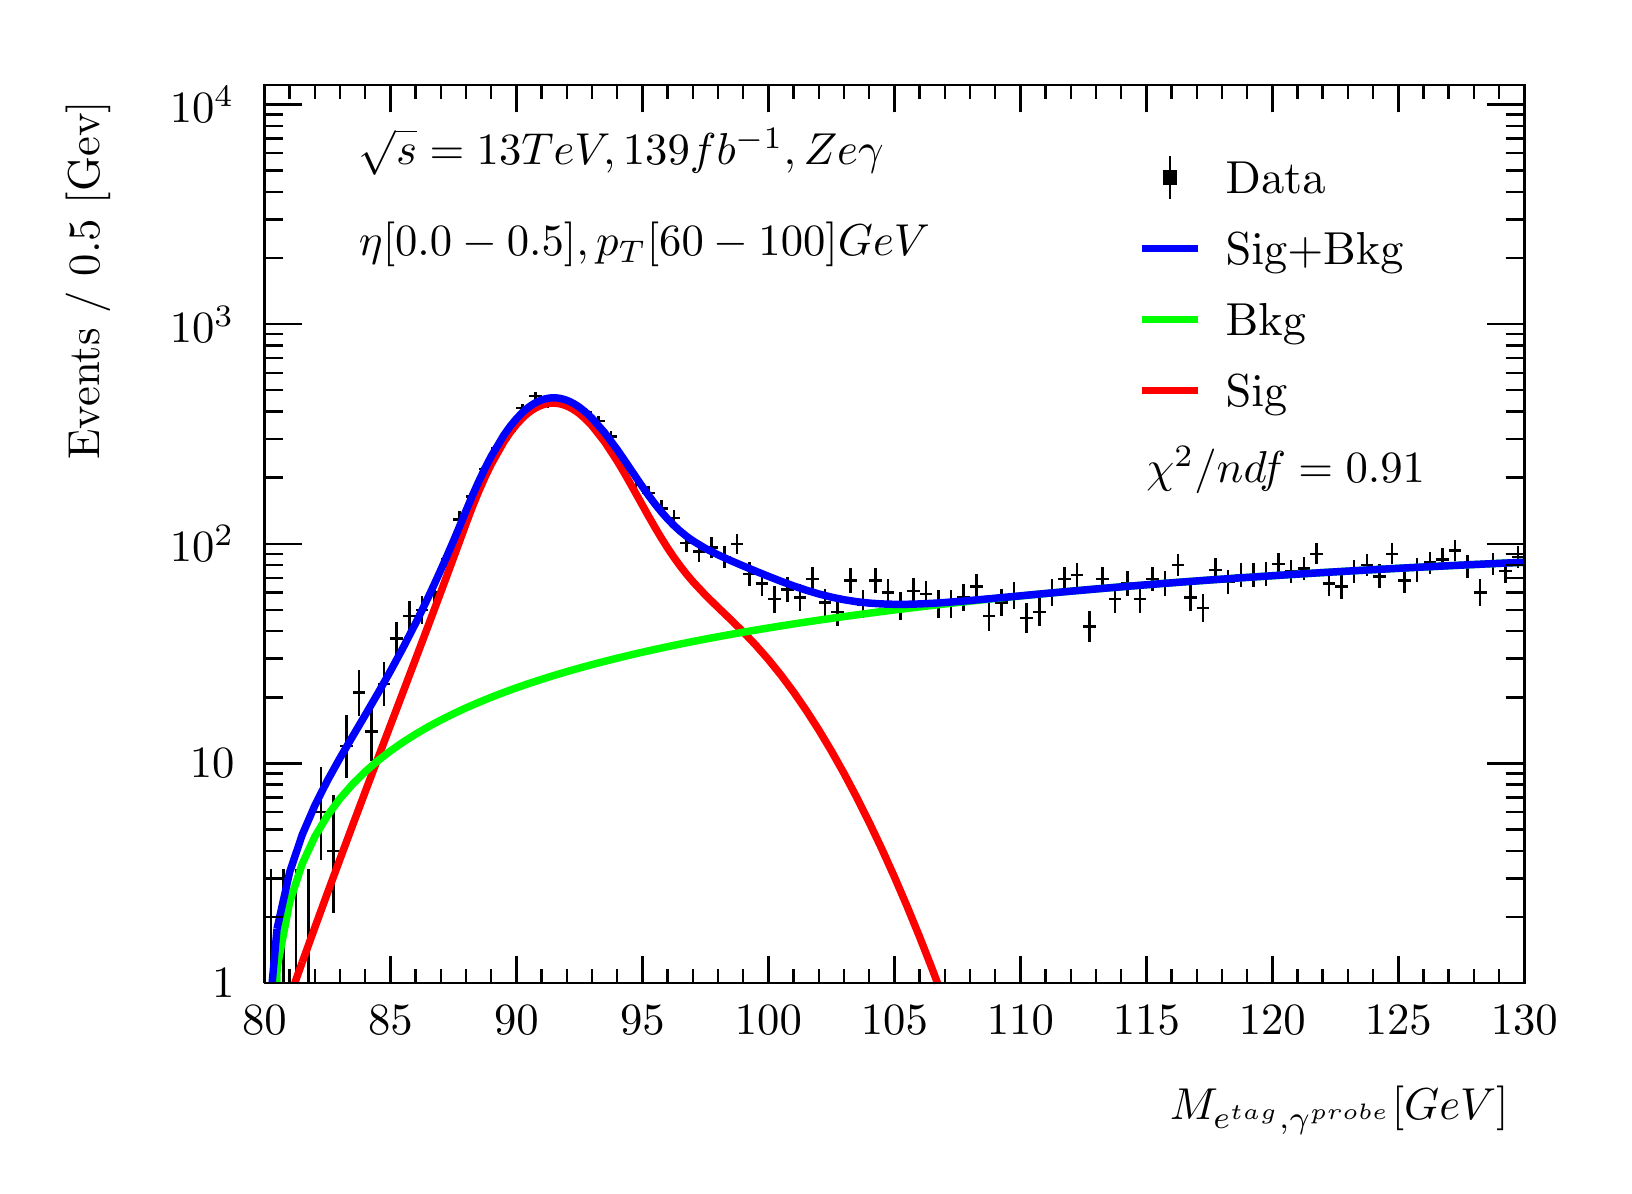
\begin{tikzpicture}
\pgfdeclareplotmark{cross} {
\pgfpathmoveto{\pgfpoint{-0.3\pgfplotmarksize}{\pgfplotmarksize}}
\pgfpathlineto{\pgfpoint{+0.3\pgfplotmarksize}{\pgfplotmarksize}}
\pgfpathlineto{\pgfpoint{+0.3\pgfplotmarksize}{0.3\pgfplotmarksize}}
\pgfpathlineto{\pgfpoint{+1\pgfplotmarksize}{0.3\pgfplotmarksize}}
\pgfpathlineto{\pgfpoint{+1\pgfplotmarksize}{-0.3\pgfplotmarksize}}
\pgfpathlineto{\pgfpoint{+0.3\pgfplotmarksize}{-0.3\pgfplotmarksize}}
\pgfpathlineto{\pgfpoint{+0.3\pgfplotmarksize}{-1.\pgfplotmarksize}}
\pgfpathlineto{\pgfpoint{-0.3\pgfplotmarksize}{-1.\pgfplotmarksize}}
\pgfpathlineto{\pgfpoint{-0.3\pgfplotmarksize}{-0.3\pgfplotmarksize}}
\pgfpathlineto{\pgfpoint{-1.\pgfplotmarksize}{-0.3\pgfplotmarksize}}
\pgfpathlineto{\pgfpoint{-1.\pgfplotmarksize}{0.3\pgfplotmarksize}}
\pgfpathlineto{\pgfpoint{-0.3\pgfplotmarksize}{0.3\pgfplotmarksize}}
\pgfpathclose
\pgfusepathqstroke
}
\pgfdeclareplotmark{cross*} {
\pgfpathmoveto{\pgfpoint{-0.3\pgfplotmarksize}{\pgfplotmarksize}}
\pgfpathlineto{\pgfpoint{+0.3\pgfplotmarksize}{\pgfplotmarksize}}
\pgfpathlineto{\pgfpoint{+0.3\pgfplotmarksize}{0.3\pgfplotmarksize}}
\pgfpathlineto{\pgfpoint{+1\pgfplotmarksize}{0.3\pgfplotmarksize}}
\pgfpathlineto{\pgfpoint{+1\pgfplotmarksize}{-0.3\pgfplotmarksize}}
\pgfpathlineto{\pgfpoint{+0.3\pgfplotmarksize}{-0.3\pgfplotmarksize}}
\pgfpathlineto{\pgfpoint{+0.3\pgfplotmarksize}{-1.\pgfplotmarksize}}
\pgfpathlineto{\pgfpoint{-0.3\pgfplotmarksize}{-1.\pgfplotmarksize}}
\pgfpathlineto{\pgfpoint{-0.3\pgfplotmarksize}{-0.3\pgfplotmarksize}}
\pgfpathlineto{\pgfpoint{-1.\pgfplotmarksize}{-0.3\pgfplotmarksize}}
\pgfpathlineto{\pgfpoint{-1.\pgfplotmarksize}{0.3\pgfplotmarksize}}
\pgfpathlineto{\pgfpoint{-0.3\pgfplotmarksize}{0.3\pgfplotmarksize}}
\pgfpathclose
\pgfusepathqfillstroke
}
\pgfdeclareplotmark{newstar} {
\pgfpathmoveto{\pgfqpoint{0pt}{\pgfplotmarksize}}
\pgfpathlineto{\pgfqpointpolar{44}{0.5\pgfplotmarksize}}
\pgfpathlineto{\pgfqpointpolar{18}{\pgfplotmarksize}}
\pgfpathlineto{\pgfqpointpolar{-20}{0.5\pgfplotmarksize}}
\pgfpathlineto{\pgfqpointpolar{-54}{\pgfplotmarksize}}
\pgfpathlineto{\pgfqpointpolar{-90}{0.5\pgfplotmarksize}}
\pgfpathlineto{\pgfqpointpolar{234}{\pgfplotmarksize}}
\pgfpathlineto{\pgfqpointpolar{198}{0.5\pgfplotmarksize}}
\pgfpathlineto{\pgfqpointpolar{162}{\pgfplotmarksize}}
\pgfpathlineto{\pgfqpointpolar{134}{0.5\pgfplotmarksize}}
\pgfpathclose
\pgfusepathqstroke
}
\pgfdeclareplotmark{newstar*} {
\pgfpathmoveto{\pgfqpoint{0pt}{\pgfplotmarksize}}
\pgfpathlineto{\pgfqpointpolar{44}{0.5\pgfplotmarksize}}
\pgfpathlineto{\pgfqpointpolar{18}{\pgfplotmarksize}}
\pgfpathlineto{\pgfqpointpolar{-20}{0.5\pgfplotmarksize}}
\pgfpathlineto{\pgfqpointpolar{-54}{\pgfplotmarksize}}
\pgfpathlineto{\pgfqpointpolar{-90}{0.5\pgfplotmarksize}}
\pgfpathlineto{\pgfqpointpolar{234}{\pgfplotmarksize}}
\pgfpathlineto{\pgfqpointpolar{198}{0.5\pgfplotmarksize}}
\pgfpathlineto{\pgfqpointpolar{162}{\pgfplotmarksize}}
\pgfpathlineto{\pgfqpointpolar{134}{0.5\pgfplotmarksize}}
\pgfpathclose
\pgfusepathqfillstroke
}
\definecolor{c}{rgb}{1,1,1};
\draw [color=c, fill=c] (0,0) rectangle (20,14.4361);
\draw [color=c, fill=c] (3,2.30977) rectangle (19,13.7143);
\definecolor{c}{rgb}{0,0,0};
\draw [c,line width=0.9] (3,2.30977) -- (3,13.7143) -- (19,13.7143) -- (19,2.30977) -- (3,2.30977);
\definecolor{c}{rgb}{1,1,1};
\draw [color=c, fill=c] (3,2.30977) rectangle (19,13.7143);
\definecolor{c}{rgb}{0,0,0};
\draw [c,line width=0.9] (3,2.30977) -- (3,13.7143) -- (19,13.7143) -- (19,2.30977) -- (3,2.30977);
\draw [c,line width=0.9] (3,2.30977) -- (19,2.30977);
\draw [c,line width=0.9] (3,2.65624) -- (3,2.30977);
\draw [c,line width=0.9] (3.32,2.48301) -- (3.32,2.30977);
\draw [c,line width=0.9] (3.64,2.48301) -- (3.64,2.30977);
\draw [c,line width=0.9] (3.96,2.48301) -- (3.96,2.30977);
\draw [c,line width=0.9] (4.28,2.48301) -- (4.28,2.30977);
\draw [c,line width=0.9] (4.6,2.65624) -- (4.6,2.30977);
\draw [c,line width=0.9] (4.92,2.48301) -- (4.92,2.30977);
\draw [c,line width=0.9] (5.24,2.48301) -- (5.24,2.30977);
\draw [c,line width=0.9] (5.56,2.48301) -- (5.56,2.30977);
\draw [c,line width=0.9] (5.88,2.48301) -- (5.88,2.30977);
\draw [c,line width=0.9] (6.2,2.65624) -- (6.2,2.30977);
\draw [c,line width=0.9] (6.52,2.48301) -- (6.52,2.30977);
\draw [c,line width=0.9] (6.84,2.48301) -- (6.84,2.30977);
\draw [c,line width=0.9] (7.16,2.48301) -- (7.16,2.30977);
\draw [c,line width=0.9] (7.48,2.48301) -- (7.48,2.30977);
\draw [c,line width=0.9] (7.8,2.65624) -- (7.8,2.30977);
\draw [c,line width=0.9] (8.12,2.48301) -- (8.12,2.30977);
\draw [c,line width=0.9] (8.44,2.48301) -- (8.44,2.30977);
\draw [c,line width=0.9] (8.76,2.48301) -- (8.76,2.30977);
\draw [c,line width=0.9] (9.08,2.48301) -- (9.08,2.30977);
\draw [c,line width=0.9] (9.4,2.65624) -- (9.4,2.30977);
\draw [c,line width=0.9] (9.72,2.48301) -- (9.72,2.30977);
\draw [c,line width=0.9] (10.04,2.48301) -- (10.04,2.30977);
\draw [c,line width=0.9] (10.36,2.48301) -- (10.36,2.30977);
\draw [c,line width=0.9] (10.68,2.48301) -- (10.68,2.30977);
\draw [c,line width=0.9] (11,2.65624) -- (11,2.30977);
\draw [c,line width=0.9] (11.32,2.48301) -- (11.32,2.30977);
\draw [c,line width=0.9] (11.64,2.48301) -- (11.64,2.30977);
\draw [c,line width=0.9] (11.96,2.48301) -- (11.96,2.30977);
\draw [c,line width=0.9] (12.28,2.48301) -- (12.28,2.30977);
\draw [c,line width=0.9] (12.6,2.65624) -- (12.6,2.30977);
\draw [c,line width=0.9] (12.92,2.48301) -- (12.92,2.30977);
\draw [c,line width=0.9] (13.24,2.48301) -- (13.24,2.30977);
\draw [c,line width=0.9] (13.56,2.48301) -- (13.56,2.30977);
\draw [c,line width=0.9] (13.88,2.48301) -- (13.88,2.30977);
\draw [c,line width=0.9] (14.2,2.65624) -- (14.2,2.30977);
\draw [c,line width=0.9] (14.52,2.48301) -- (14.52,2.30977);
\draw [c,line width=0.9] (14.84,2.48301) -- (14.84,2.30977);
\draw [c,line width=0.9] (15.16,2.48301) -- (15.16,2.30977);
\draw [c,line width=0.9] (15.48,2.48301) -- (15.48,2.30977);
\draw [c,line width=0.9] (15.8,2.65624) -- (15.8,2.30977);
\draw [c,line width=0.9] (16.12,2.48301) -- (16.12,2.30977);
\draw [c,line width=0.9] (16.44,2.48301) -- (16.44,2.30977);
\draw [c,line width=0.9] (16.76,2.48301) -- (16.76,2.30977);
\draw [c,line width=0.9] (17.08,2.48301) -- (17.08,2.30977);
\draw [c,line width=0.9] (17.4,2.65624) -- (17.4,2.30977);
\draw [c,line width=0.9] (17.72,2.48301) -- (17.72,2.30977);
\draw [c,line width=0.9] (18.04,2.48301) -- (18.04,2.30977);
\draw [c,line width=0.9] (18.36,2.48301) -- (18.36,2.30977);
\draw [c,line width=0.9] (18.68,2.48301) -- (18.68,2.30977);
\draw [c,line width=0.9] (19,2.65624) -- (19,2.30977);
\draw [anchor=base] (3,1.66015) node[scale=1.61424, color=c, rotate=0]{80};
\draw [anchor=base] (4.6,1.66015) node[scale=1.61424, color=c, rotate=0]{85};
\draw [anchor=base] (6.2,1.66015) node[scale=1.61424, color=c, rotate=0]{90};
\draw [anchor=base] (7.8,1.66015) node[scale=1.61424, color=c, rotate=0]{95};
\draw [anchor=base] (9.4,1.66015) node[scale=1.61424, color=c, rotate=0]{100};
\draw [anchor=base] (11,1.66015) node[scale=1.61424, color=c, rotate=0]{105};
\draw [anchor=base] (12.6,1.66015) node[scale=1.61424, color=c, rotate=0]{110};
\draw [anchor=base] (14.2,1.66015) node[scale=1.61424, color=c, rotate=0]{115};
\draw [anchor=base] (15.8,1.66015) node[scale=1.61424, color=c, rotate=0]{120};
\draw [anchor=base] (17.4,1.66015) node[scale=1.61424, color=c, rotate=0]{125};
\draw [anchor=base] (19,1.66015) node[scale=1.61424, color=c, rotate=0]{130};
\draw [anchor= east] (19,0.692932) node[scale=1.61424, color=c, rotate=0]{$M_{e^{tag}, \gamma^{probe}}  [GeV]$};
\draw [c,line width=0.9] (3,13.7143) -- (19,13.7143);
\draw [c,line width=0.9] (3,13.3678) -- (3,13.7143);
\draw [c,line width=0.9] (3.32,13.5411) -- (3.32,13.7143);
\draw [c,line width=0.9] (3.64,13.5411) -- (3.64,13.7143);
\draw [c,line width=0.9] (3.96,13.5411) -- (3.96,13.7143);
\draw [c,line width=0.9] (4.28,13.5411) -- (4.28,13.7143);
\draw [c,line width=0.9] (4.6,13.3678) -- (4.6,13.7143);
\draw [c,line width=0.9] (4.92,13.5411) -- (4.92,13.7143);
\draw [c,line width=0.9] (5.24,13.5411) -- (5.24,13.7143);
\draw [c,line width=0.9] (5.56,13.5411) -- (5.56,13.7143);
\draw [c,line width=0.9] (5.88,13.5411) -- (5.88,13.7143);
\draw [c,line width=0.9] (6.2,13.3678) -- (6.2,13.7143);
\draw [c,line width=0.9] (6.52,13.5411) -- (6.52,13.7143);
\draw [c,line width=0.9] (6.84,13.5411) -- (6.84,13.7143);
\draw [c,line width=0.9] (7.16,13.5411) -- (7.16,13.7143);
\draw [c,line width=0.9] (7.48,13.5411) -- (7.48,13.7143);
\draw [c,line width=0.9] (7.8,13.3678) -- (7.8,13.7143);
\draw [c,line width=0.9] (8.12,13.5411) -- (8.12,13.7143);
\draw [c,line width=0.9] (8.44,13.5411) -- (8.44,13.7143);
\draw [c,line width=0.9] (8.76,13.5411) -- (8.76,13.7143);
\draw [c,line width=0.9] (9.08,13.5411) -- (9.08,13.7143);
\draw [c,line width=0.9] (9.4,13.3678) -- (9.4,13.7143);
\draw [c,line width=0.9] (9.72,13.5411) -- (9.72,13.7143);
\draw [c,line width=0.9] (10.04,13.5411) -- (10.04,13.7143);
\draw [c,line width=0.9] (10.36,13.5411) -- (10.36,13.7143);
\draw [c,line width=0.9] (10.68,13.5411) -- (10.68,13.7143);
\draw [c,line width=0.9] (11,13.3678) -- (11,13.7143);
\draw [c,line width=0.9] (11.32,13.5411) -- (11.32,13.7143);
\draw [c,line width=0.9] (11.64,13.5411) -- (11.64,13.7143);
\draw [c,line width=0.9] (11.96,13.5411) -- (11.96,13.7143);
\draw [c,line width=0.9] (12.28,13.5411) -- (12.28,13.7143);
\draw [c,line width=0.9] (12.6,13.3678) -- (12.6,13.7143);
\draw [c,line width=0.9] (12.92,13.5411) -- (12.92,13.7143);
\draw [c,line width=0.9] (13.24,13.5411) -- (13.24,13.7143);
\draw [c,line width=0.9] (13.56,13.5411) -- (13.56,13.7143);
\draw [c,line width=0.9] (13.88,13.5411) -- (13.88,13.7143);
\draw [c,line width=0.9] (14.2,13.3678) -- (14.2,13.7143);
\draw [c,line width=0.9] (14.52,13.5411) -- (14.52,13.7143);
\draw [c,line width=0.9] (14.84,13.5411) -- (14.84,13.7143);
\draw [c,line width=0.9] (15.16,13.5411) -- (15.16,13.7143);
\draw [c,line width=0.9] (15.48,13.5411) -- (15.48,13.7143);
\draw [c,line width=0.9] (15.8,13.3678) -- (15.8,13.7143);
\draw [c,line width=0.9] (16.12,13.5411) -- (16.12,13.7143);
\draw [c,line width=0.9] (16.44,13.5411) -- (16.44,13.7143);
\draw [c,line width=0.9] (16.76,13.5411) -- (16.76,13.7143);
\draw [c,line width=0.9] (17.08,13.5411) -- (17.08,13.7143);
\draw [c,line width=0.9] (17.4,13.3678) -- (17.4,13.7143);
\draw [c,line width=0.9] (17.72,13.5411) -- (17.72,13.7143);
\draw [c,line width=0.9] (18.04,13.5411) -- (18.04,13.7143);
\draw [c,line width=0.9] (18.36,13.5411) -- (18.36,13.7143);
\draw [c,line width=0.9] (18.68,13.5411) -- (18.68,13.7143);
\draw [c,line width=0.9] (19,13.3678) -- (19,13.7143);
\draw [c,line width=0.9] (3,2.30977) -- (3,13.7143);
\draw [c,line width=0.9] (3.474,2.30978) -- (3,2.30978);
\draw [anchor= east] (2.82,2.30978) node[scale=1.61424, color=c, rotate=0]{1};
\draw [c,line width=0.9] (3.237,3.1495) -- (3,3.1495);
\draw [c,line width=0.9] (3.237,3.6407) -- (3,3.6407);
\draw [c,line width=0.9] (3.237,3.98922) -- (3,3.98922);
\draw [c,line width=0.9] (3.237,4.25955) -- (3,4.25955);
\draw [c,line width=0.9] (3.237,4.48042) -- (3,4.48042);
\draw [c,line width=0.9] (3.237,4.66717) -- (3,4.66717);
\draw [c,line width=0.9] (3.237,4.82894) -- (3,4.82894);
\draw [c,line width=0.9] (3.237,4.97163) -- (3,4.97163);
\draw [c,line width=0.9] (3.474,5.09927) -- (3,5.09927);
\draw [anchor= east] (2.82,5.09927) node[scale=1.61424, color=c, rotate=0]{10};
\draw [c,line width=0.9] (3.237,5.93899) -- (3,5.93899);
\draw [c,line width=0.9] (3.237,6.43019) -- (3,6.43019);
\draw [c,line width=0.9] (3.237,6.77871) -- (3,6.77871);
\draw [c,line width=0.9] (3.237,7.04904) -- (3,7.04904);
\draw [c,line width=0.9] (3.237,7.26991) -- (3,7.26991);
\draw [c,line width=0.9] (3.237,7.45666) -- (3,7.45666);
\draw [c,line width=0.9] (3.237,7.61843) -- (3,7.61843);
\draw [c,line width=0.9] (3.237,7.76112) -- (3,7.76112);
\draw [c,line width=0.9] (3.474,7.88876) -- (3,7.88876);
\draw [anchor= east] (2.82,7.88876) node[scale=1.61424, color=c, rotate=0]{$10^{2}$};
\draw [c,line width=0.9] (3.237,8.72848) -- (3,8.72848);
\draw [c,line width=0.9] (3.237,9.21968) -- (3,9.21968);
\draw [c,line width=0.9] (3.237,9.5682) -- (3,9.5682);
\draw [c,line width=0.9] (3.237,9.83853) -- (3,9.83853);
\draw [c,line width=0.9] (3.237,10.0594) -- (3,10.0594);
\draw [c,line width=0.9] (3.237,10.2462) -- (3,10.2462);
\draw [c,line width=0.9] (3.237,10.4079) -- (3,10.4079);
\draw [c,line width=0.9] (3.237,10.5506) -- (3,10.5506);
\draw [c,line width=0.9] (3.474,10.6782) -- (3,10.6782);
\draw [anchor= east] (2.82,10.6782) node[scale=1.61424, color=c, rotate=0]{$10^{3}$};
\draw [c,line width=0.9] (3.237,11.518) -- (3,11.518);
\draw [c,line width=0.9] (3.237,12.0092) -- (3,12.0092);
\draw [c,line width=0.9] (3.237,12.3577) -- (3,12.3577);
\draw [c,line width=0.9] (3.237,12.628) -- (3,12.628);
\draw [c,line width=0.9] (3.237,12.8489) -- (3,12.8489);
\draw [c,line width=0.9] (3.237,13.0356) -- (3,13.0356);
\draw [c,line width=0.9] (3.237,13.1974) -- (3,13.1974);
\draw [c,line width=0.9] (3.237,13.3401) -- (3,13.3401);
\draw [c,line width=0.9] (3.474,13.4677) -- (3,13.4677);
\draw [anchor= east] (2.82,13.4677) node[scale=1.61424, color=c, rotate=0]{$10^{4}$};
\draw [anchor= east] (0.76,13.7143) node[scale=1.61424, color=c, rotate=90]{Events / 0.5 [Gev]};
\draw [c,line width=0.9] (19,2.30977) -- (19,13.7143);
\draw [c,line width=0.9] (18.526,2.30978) -- (19,2.30978);
\draw [c,line width=0.9] (18.763,3.1495) -- (19,3.1495);
\draw [c,line width=0.9] (18.763,3.6407) -- (19,3.6407);
\draw [c,line width=0.9] (18.763,3.98922) -- (19,3.98922);
\draw [c,line width=0.9] (18.763,4.25955) -- (19,4.25955);
\draw [c,line width=0.9] (18.763,4.48042) -- (19,4.48042);
\draw [c,line width=0.9] (18.763,4.66717) -- (19,4.66717);
\draw [c,line width=0.9] (18.763,4.82894) -- (19,4.82894);
\draw [c,line width=0.9] (18.763,4.97163) -- (19,4.97163);
\draw [c,line width=0.9] (18.526,5.09927) -- (19,5.09927);
\draw [c,line width=0.9] (18.763,5.93899) -- (19,5.93899);
\draw [c,line width=0.9] (18.763,6.43019) -- (19,6.43019);
\draw [c,line width=0.9] (18.763,6.77871) -- (19,6.77871);
\draw [c,line width=0.9] (18.763,7.04904) -- (19,7.04904);
\draw [c,line width=0.9] (18.763,7.26991) -- (19,7.26991);
\draw [c,line width=0.9] (18.763,7.45666) -- (19,7.45666);
\draw [c,line width=0.9] (18.763,7.61843) -- (19,7.61843);
\draw [c,line width=0.9] (18.763,7.76112) -- (19,7.76112);
\draw [c,line width=0.9] (18.526,7.88876) -- (19,7.88876);
\draw [c,line width=0.9] (18.763,8.72848) -- (19,8.72848);
\draw [c,line width=0.9] (18.763,9.21968) -- (19,9.21968);
\draw [c,line width=0.9] (18.763,9.5682) -- (19,9.5682);
\draw [c,line width=0.9] (18.763,9.83853) -- (19,9.83853);
\draw [c,line width=0.9] (18.763,10.0594) -- (19,10.0594);
\draw [c,line width=0.9] (18.763,10.2462) -- (19,10.2462);
\draw [c,line width=0.9] (18.763,10.4079) -- (19,10.4079);
\draw [c,line width=0.9] (18.763,10.5506) -- (19,10.5506);
\draw [c,line width=0.9] (18.526,10.6782) -- (19,10.6782);
\draw [c,line width=0.9] (18.763,11.518) -- (19,11.518);
\draw [c,line width=0.9] (18.763,12.0092) -- (19,12.0092);
\draw [c,line width=0.9] (18.763,12.3577) -- (19,12.3577);
\draw [c,line width=0.9] (18.763,12.628) -- (19,12.628);
\draw [c,line width=0.9] (18.763,12.8489) -- (19,12.8489);
\draw [c,line width=0.9] (18.763,13.0356) -- (19,13.0356);
\draw [c,line width=0.9] (18.763,13.1974) -- (19,13.1974);
\draw [c,line width=0.9] (18.763,13.3401) -- (19,13.3401);
\draw [c,line width=0.9] (18.526,13.4677) -- (19,13.4677);
\draw [c,line width=0.9] (3.08,2.30977) -- (3,2.30977);
\draw [c,line width=0.9] (3,2.30977) -- (3,2.30977);
\draw [c,line width=0.9] (3.08,2.30977) -- (3.16,2.30977);
\draw [c,line width=0.9] (3.16,2.30977) -- (3.16,2.30977);
\draw [c,line width=0.9] (3.08,2.30977) -- (3.08,3.75599);
\draw [c,line width=0.9] (3.08,3.75599) -- (3.08,3.75599);
\draw [c,line width=0.9] (3.24,2.30977) -- (3.16,2.30977);
\draw [c,line width=0.9] (3.16,2.30977) -- (3.16,2.30977);
\draw [c,line width=0.9] (3.24,2.30977) -- (3.32,2.30977);
\draw [c,line width=0.9] (3.32,2.30977) -- (3.32,2.30977);
\draw [c,line width=0.9] (3.24,2.30977) -- (3.24,3.75599);
\draw [c,line width=0.9] (3.24,3.75599) -- (3.24,3.75599);
\draw [c,line width=0.9] (3.4,2.30977) -- (3.32,2.30977);
\draw [c,line width=0.9] (3.32,2.30977) -- (3.32,2.30977);
\draw [c,line width=0.9] (3.4,2.30977) -- (3.48,2.30977);
\draw [c,line width=0.9] (3.48,2.30977) -- (3.48,2.30977);
\draw [c,line width=0.9] (3.4,2.30977) -- (3.4,3.75599);
\draw [c,line width=0.9] (3.4,3.75599) -- (3.4,3.75599);
\draw [c,line width=0.9] (3.56,2.30977) -- (3.48,2.30977);
\draw [c,line width=0.9] (3.48,2.30977) -- (3.48,2.30977);
\draw [c,line width=0.9] (3.56,2.30977) -- (3.64,2.30977);
\draw [c,line width=0.9] (3.64,2.30977) -- (3.64,2.30977);
\draw [c,line width=0.9] (3.56,2.30977) -- (3.56,3.75599);
\draw [c,line width=0.9] (3.56,3.75599) -- (3.56,3.75599);
\draw [c,line width=0.9] (3.72,4.48042) -- (3.64,4.48042);
\draw [c,line width=0.9] (3.64,4.48042) -- (3.64,4.48042);
\draw [c,line width=0.9] (3.72,4.48042) -- (3.8,4.48042);
\draw [c,line width=0.9] (3.8,4.48042) -- (3.8,4.48042);
\draw [c,line width=0.9] (3.72,4.48042) -- (3.72,5.04775);
\draw [c,line width=0.9] (3.72,5.04775) -- (3.72,5.04775);
\draw [c,line width=0.9] (3.72,4.48042) -- (3.72,3.86831);
\draw [c,line width=0.9] (3.72,3.86831) -- (3.72,3.86831);
\draw [c,line width=0.9] (3.88,3.98922) -- (3.8,3.98922);
\draw [c,line width=0.9] (3.8,3.98922) -- (3.8,3.98922);
\draw [c,line width=0.9] (3.88,3.98922) -- (3.96,3.98922);
\draw [c,line width=0.9] (3.96,3.98922) -- (3.96,3.98922);
\draw [c,line width=0.9] (3.88,3.98922) -- (3.88,4.69501);
\draw [c,line width=0.9] (3.88,4.69501) -- (3.88,4.69501);
\draw [c,line width=0.9] (3.88,3.98922) -- (3.88,3.2003);
\draw [c,line width=0.9] (3.88,3.2003) -- (3.88,3.2003);
\draw [c,line width=0.9] (4.04,5.32014) -- (3.96,5.32014);
\draw [c,line width=0.9] (3.96,5.32014) -- (3.96,5.32014);
\draw [c,line width=0.9] (4.04,5.32014) -- (4.12,5.32014);
\draw [c,line width=0.9] (4.12,5.32014) -- (4.12,5.32014);
\draw [c,line width=0.9] (4.04,5.32014) -- (4.04,5.71032);
\draw [c,line width=0.9] (4.04,5.71032) -- (4.04,5.71032);
\draw [c,line width=0.9] (4.04,5.32014) -- (4.04,4.9144);
\draw [c,line width=0.9] (4.04,4.9144) -- (4.04,4.9144);
\draw [c,line width=0.9] (4.2,5.99809) -- (4.12,5.99809);
\draw [c,line width=0.9] (4.12,5.99809) -- (4.12,5.99809);
\draw [c,line width=0.9] (4.2,5.99809) -- (4.28,5.99809);
\draw [c,line width=0.9] (4.28,5.99809) -- (4.28,5.99809);
\draw [c,line width=0.9] (4.2,5.99809) -- (4.2,6.28698);
\draw [c,line width=0.9] (4.2,6.28698) -- (4.2,6.28698);
\draw [c,line width=0.9] (4.2,5.99809) -- (4.2,5.70257);
\draw [c,line width=0.9] (4.2,5.70257) -- (4.2,5.70257);
\draw [c,line width=0.9] (4.36,5.50689) -- (4.28,5.50689);
\draw [c,line width=0.9] (4.28,5.50689) -- (4.28,5.50689);
\draw [c,line width=0.9] (4.36,5.50689) -- (4.44,5.50689);
\draw [c,line width=0.9] (4.44,5.50689) -- (4.44,5.50689);
\draw [c,line width=0.9] (4.36,5.50689) -- (4.36,5.86598);
\draw [c,line width=0.9] (4.36,5.86598) -- (4.36,5.86598);
\draw [c,line width=0.9] (4.36,5.50689) -- (4.36,5.13549);
\draw [c,line width=0.9] (4.36,5.13549) -- (4.36,5.13549);
\draw [c,line width=0.9] (4.52,6.1083) -- (4.44,6.1083);
\draw [c,line width=0.9] (4.44,6.1083) -- (4.44,6.1083);
\draw [c,line width=0.9] (4.52,6.1083) -- (4.6,6.1083);
\draw [c,line width=0.9] (4.6,6.1083) -- (4.6,6.1083);
\draw [c,line width=0.9] (4.52,6.1083) -- (4.52,6.38348);
\draw [c,line width=0.9] (4.52,6.38348) -- (4.52,6.38348);
\draw [c,line width=0.9] (4.52,6.1083) -- (4.52,5.82734);
\draw [c,line width=0.9] (4.52,5.82734) -- (4.52,5.82734);
\draw [c,line width=0.9] (4.68,6.68426) -- (4.6,6.68426);
\draw [c,line width=0.9] (4.6,6.68426) -- (4.6,6.68426);
\draw [c,line width=0.9] (4.68,6.68426) -- (4.76,6.68426);
\draw [c,line width=0.9] (4.76,6.68426) -- (4.76,6.68426);
\draw [c,line width=0.9] (4.68,6.68426) -- (4.68,6.89795);
\draw [c,line width=0.9] (4.68,6.89795) -- (4.68,6.89795);
\draw [c,line width=0.9] (4.68,6.68426) -- (4.68,6.46776);
\draw [c,line width=0.9] (4.68,6.46776) -- (4.68,6.46776);
\draw [c,line width=0.9] (4.84,6.97408) -- (4.76,6.97408);
\draw [c,line width=0.9] (4.76,6.97408) -- (4.76,6.97408);
\draw [c,line width=0.9] (4.84,6.97408) -- (4.92,6.97408);
\draw [c,line width=0.9] (4.92,6.97408) -- (4.92,6.97408);
\draw [c,line width=0.9] (4.84,6.97408) -- (4.84,7.16239);
\draw [c,line width=0.9] (4.84,7.16239) -- (4.84,7.16239);
\draw [c,line width=0.9] (4.84,6.97408) -- (4.84,6.78381);
\draw [c,line width=0.9] (4.84,6.78381) -- (4.84,6.78381);
\draw [c,line width=0.9] (5,7.04904) -- (4.92,7.04904);
\draw [c,line width=0.9] (4.92,7.04904) -- (4.92,7.04904);
\draw [c,line width=0.9] (5,7.04904) -- (5.08,7.04904);
\draw [c,line width=0.9] (5.08,7.04904) -- (5.08,7.04904);
\draw [c,line width=0.9] (5,7.04904) -- (5,7.23131);
\draw [c,line width=0.9] (5,7.23131) -- (5,7.23131);
\draw [c,line width=0.9] (5,7.04904) -- (5,6.86499);
\draw [c,line width=0.9] (5,6.86499) -- (5,6.86499);
\draw [c,line width=0.9] (5.16,7.26991) -- (5.08,7.26991);
\draw [c,line width=0.9] (5.08,7.26991) -- (5.08,7.26991);
\draw [c,line width=0.9] (5.16,7.26991) -- (5.24,7.26991);
\draw [c,line width=0.9] (5.24,7.26991) -- (5.24,7.26991);
\draw [c,line width=0.9] (5.16,7.26991) -- (5.16,7.43552);
\draw [c,line width=0.9] (5.16,7.43552) -- (5.16,7.43552);
\draw [c,line width=0.9] (5.16,7.26991) -- (5.16,7.10296);
\draw [c,line width=0.9] (5.16,7.10296) -- (5.16,7.10296);
\draw [c,line width=0.9] (5.32,7.69187) -- (5.24,7.69187);
\draw [c,line width=0.9] (5.24,7.69187) -- (5.24,7.69187);
\draw [c,line width=0.9] (5.32,7.69187) -- (5.4,7.69187);
\draw [c,line width=0.9] (5.4,7.69187) -- (5.4,7.69187);
\draw [c,line width=0.9] (5.32,7.69187) -- (5.32,7.82987);
\draw [c,line width=0.9] (5.32,7.82987) -- (5.32,7.82987);
\draw [c,line width=0.9] (5.32,7.69187) -- (5.32,7.55307);
\draw [c,line width=0.9] (5.32,7.55307) -- (5.32,7.55307);
\draw [c,line width=0.9] (5.48,8.19725) -- (5.4,8.19725);
\draw [c,line width=0.9] (5.4,8.19725) -- (5.4,8.19725);
\draw [c,line width=0.9] (5.48,8.19725) -- (5.56,8.19725);
\draw [c,line width=0.9] (5.56,8.19725) -- (5.56,8.19725);
\draw [c,line width=0.9] (5.48,8.19725) -- (5.48,8.30387);
\draw [c,line width=0.9] (5.48,8.30387) -- (5.48,8.30387);
\draw [c,line width=0.9] (5.48,8.19725) -- (5.48,8.09062);
\draw [c,line width=0.9] (5.48,8.09062) -- (5.48,8.09062);
\draw [c,line width=0.9] (5.64,8.48806) -- (5.56,8.48806);
\draw [c,line width=0.9] (5.56,8.48806) -- (5.56,8.48806);
\draw [c,line width=0.9] (5.64,8.48806) -- (5.72,8.48806);
\draw [c,line width=0.9] (5.72,8.48806) -- (5.72,8.48806);
\draw [c,line width=0.9] (5.64,8.48806) -- (5.64,8.58264);
\draw [c,line width=0.9] (5.64,8.58264) -- (5.64,8.58264);
\draw [c,line width=0.9] (5.64,8.48806) -- (5.64,8.39349);
\draw [c,line width=0.9] (5.64,8.39349) -- (5.64,8.39349);
\draw [c,line width=0.9] (5.8,8.83842) -- (5.72,8.83842);
\draw [c,line width=0.9] (5.72,8.83842) -- (5.72,8.83842);
\draw [c,line width=0.9] (5.8,8.83842) -- (5.88,8.83842);
\draw [c,line width=0.9] (5.88,8.83842) -- (5.88,8.83842);
\draw [c,line width=0.9] (5.8,8.83842) -- (5.8,8.92027);
\draw [c,line width=0.9] (5.8,8.92027) -- (5.8,8.92027);
\draw [c,line width=0.9] (5.8,8.83842) -- (5.8,8.75658);
\draw [c,line width=0.9] (5.8,8.75658) -- (5.8,8.75658);
\draw [c,line width=0.9] (5.96,9.10543) -- (5.88,9.10543);
\draw [c,line width=0.9] (5.88,9.10543) -- (5.88,9.10543);
\draw [c,line width=0.9] (5.96,9.10543) -- (6.04,9.10543);
\draw [c,line width=0.9] (6.04,9.10543) -- (6.04,9.10543);
\draw [c,line width=0.9] (5.96,9.10543) -- (5.96,9.17874);
\draw [c,line width=0.9] (5.96,9.17874) -- (5.96,9.17874);
\draw [c,line width=0.9] (5.96,9.10543) -- (5.96,9.03212);
\draw [c,line width=0.9] (5.96,9.03212) -- (5.96,9.03212);
\draw [c,line width=0.9] (6.12,9.32037) -- (6.04,9.32037);
\draw [c,line width=0.9] (6.04,9.32037) -- (6.04,9.32037);
\draw [c,line width=0.9] (6.12,9.32037) -- (6.2,9.32037);
\draw [c,line width=0.9] (6.2,9.32037) -- (6.2,9.32037);
\draw [c,line width=0.9] (6.12,9.32037) -- (6.12,9.38746);
\draw [c,line width=0.9] (6.12,9.38746) -- (6.12,9.38746);
\draw [c,line width=0.9] (6.12,9.32037) -- (6.12,9.25328);
\draw [c,line width=0.9] (6.12,9.25328) -- (6.12,9.25328);
\draw [c,line width=0.9] (6.28,9.60987) -- (6.2,9.60987);
\draw [c,line width=0.9] (6.2,9.60987) -- (6.2,9.60987);
\draw [c,line width=0.9] (6.28,9.60987) -- (6.36,9.60987);
\draw [c,line width=0.9] (6.36,9.60987) -- (6.36,9.60987);
\draw [c,line width=0.9] (6.28,9.60987) -- (6.28,9.66941);
\draw [c,line width=0.9] (6.28,9.66941) -- (6.28,9.66941);
\draw [c,line width=0.9] (6.28,9.60987) -- (6.28,9.55034);
\draw [c,line width=0.9] (6.28,9.55034) -- (6.28,9.55034);
\draw [c,line width=0.9] (6.44,9.76357) -- (6.36,9.76357);
\draw [c,line width=0.9] (6.36,9.76357) -- (6.36,9.76357);
\draw [c,line width=0.9] (6.44,9.76357) -- (6.52,9.76357);
\draw [c,line width=0.9] (6.52,9.76357) -- (6.52,9.76357);
\draw [c,line width=0.9] (6.44,9.76357) -- (6.44,9.81944);
\draw [c,line width=0.9] (6.44,9.81944) -- (6.44,9.81944);
\draw [c,line width=0.9] (6.44,9.76357) -- (6.44,9.70769);
\draw [c,line width=0.9] (6.44,9.70769) -- (6.44,9.70769);
\draw [c,line width=0.9] (6.6,9.66982) -- (6.52,9.66982);
\draw [c,line width=0.9] (6.52,9.66982) -- (6.52,9.66982);
\draw [c,line width=0.9] (6.6,9.66982) -- (6.68,9.66982);
\draw [c,line width=0.9] (6.68,9.66982) -- (6.68,9.66982);
\draw [c,line width=0.9] (6.6,9.66982) -- (6.6,9.7279);
\draw [c,line width=0.9] (6.6,9.7279) -- (6.6,9.7279);
\draw [c,line width=0.9] (6.6,9.66982) -- (6.6,9.61174);
\draw [c,line width=0.9] (6.6,9.61174) -- (6.6,9.61174);
\draw [c,line width=0.9] (6.76,9.72161) -- (6.68,9.72161);
\draw [c,line width=0.9] (6.68,9.72161) -- (6.68,9.72161);
\draw [c,line width=0.9] (6.76,9.72161) -- (6.84,9.72161);
\draw [c,line width=0.9] (6.84,9.72161) -- (6.84,9.72161);
\draw [c,line width=0.9] (6.76,9.72161) -- (6.76,9.77846);
\draw [c,line width=0.9] (6.76,9.77846) -- (6.76,9.77846);
\draw [c,line width=0.9] (6.76,9.72161) -- (6.76,9.66476);
\draw [c,line width=0.9] (6.76,9.66476) -- (6.76,9.66476);
\draw [c,line width=0.9] (6.92,9.64449) -- (6.84,9.64449);
\draw [c,line width=0.9] (6.84,9.64449) -- (6.84,9.64449);
\draw [c,line width=0.9] (6.92,9.64449) -- (7,9.64449);
\draw [c,line width=0.9] (7,9.64449) -- (7,9.64449);
\draw [c,line width=0.9] (6.92,9.64449) -- (6.92,9.70318);
\draw [c,line width=0.9] (6.92,9.70318) -- (6.92,9.70318);
\draw [c,line width=0.9] (6.92,9.64449) -- (6.92,9.5858);
\draw [c,line width=0.9] (6.92,9.5858) -- (6.92,9.5858);
\draw [c,line width=0.9] (7.08,9.55296) -- (7,9.55296);
\draw [c,line width=0.9] (7,9.55296) -- (7,9.55296);
\draw [c,line width=0.9] (7.08,9.55296) -- (7.16,9.55296);
\draw [c,line width=0.9] (7.16,9.55296) -- (7.16,9.55296);
\draw [c,line width=0.9] (7.08,9.55296) -- (7.08,9.61391);
\draw [c,line width=0.9] (7.08,9.61391) -- (7.08,9.61391);
\draw [c,line width=0.9] (7.08,9.55296) -- (7.08,9.49201);
\draw [c,line width=0.9] (7.08,9.49201) -- (7.08,9.49201);
\draw [c,line width=0.9] (7.24,9.44727) -- (7.16,9.44727);
\draw [c,line width=0.9] (7.16,9.44727) -- (7.16,9.44727);
\draw [c,line width=0.9] (7.24,9.44727) -- (7.32,9.44727);
\draw [c,line width=0.9] (7.32,9.44727) -- (7.32,9.44727);
\draw [c,line width=0.9] (7.24,9.44727) -- (7.24,9.51093);
\draw [c,line width=0.9] (7.24,9.51093) -- (7.24,9.51093);
\draw [c,line width=0.9] (7.24,9.44727) -- (7.24,9.3836);
\draw [c,line width=0.9] (7.24,9.3836) -- (7.24,9.3836);
\draw [c,line width=0.9] (7.4,9.25156) -- (7.32,9.25156);
\draw [c,line width=0.9] (7.32,9.25156) -- (7.32,9.25156);
\draw [c,line width=0.9] (7.4,9.25156) -- (7.48,9.25156);
\draw [c,line width=0.9] (7.48,9.25156) -- (7.48,9.25156);
\draw [c,line width=0.9] (7.4,9.25156) -- (7.4,9.32058);
\draw [c,line width=0.9] (7.4,9.32058) -- (7.4,9.32058);
\draw [c,line width=0.9] (7.4,9.25156) -- (7.4,9.18254);
\draw [c,line width=0.9] (7.4,9.18254) -- (7.4,9.18254);
\draw [c,line width=0.9] (7.56,8.90828) -- (7.48,8.90828);
\draw [c,line width=0.9] (7.48,8.90828) -- (7.48,8.90828);
\draw [c,line width=0.9] (7.56,8.90828) -- (7.64,8.90828);
\draw [c,line width=0.9] (7.64,8.90828) -- (7.64,8.90828);
\draw [c,line width=0.9] (7.56,8.90828) -- (7.56,8.9878);
\draw [c,line width=0.9] (7.56,8.9878) -- (7.56,8.9878);
\draw [c,line width=0.9] (7.56,8.90828) -- (7.56,8.82876);
\draw [c,line width=0.9] (7.56,8.82876) -- (7.56,8.82876);
\draw [c,line width=0.9] (7.72,8.63403) -- (7.64,8.63403);
\draw [c,line width=0.9] (7.64,8.63403) -- (7.64,8.63403);
\draw [c,line width=0.9] (7.72,8.63403) -- (7.8,8.63403);
\draw [c,line width=0.9] (7.8,8.63403) -- (7.8,8.63403);
\draw [c,line width=0.9] (7.72,8.63403) -- (7.72,8.72308);
\draw [c,line width=0.9] (7.72,8.72308) -- (7.72,8.72308);
\draw [c,line width=0.9] (7.72,8.63403) -- (7.72,8.54498);
\draw [c,line width=0.9] (7.72,8.54498) -- (7.72,8.54498);
\draw [c,line width=0.9] (7.88,8.53159) -- (7.8,8.53159);
\draw [c,line width=0.9] (7.8,8.53159) -- (7.8,8.53159);
\draw [c,line width=0.9] (7.88,8.53159) -- (7.96,8.53159);
\draw [c,line width=0.9] (7.96,8.53159) -- (7.96,8.53159);
\draw [c,line width=0.9] (7.88,8.53159) -- (7.88,8.62448);
\draw [c,line width=0.9] (7.88,8.62448) -- (7.88,8.62448);
\draw [c,line width=0.9] (7.88,8.53159) -- (7.88,8.4387);
\draw [c,line width=0.9] (7.88,8.4387) -- (7.88,8.4387);
\draw [c,line width=0.9] (8.04,8.33889) -- (7.96,8.33889);
\draw [c,line width=0.9] (7.96,8.33889) -- (7.96,8.33889);
\draw [c,line width=0.9] (8.04,8.33889) -- (8.12,8.33889);
\draw [c,line width=0.9] (8.12,8.33889) -- (8.12,8.33889);
\draw [c,line width=0.9] (8.04,8.33889) -- (8.04,8.43947);
\draw [c,line width=0.9] (8.04,8.43947) -- (8.04,8.43947);
\draw [c,line width=0.9] (8.04,8.33889) -- (8.04,8.23831);
\draw [c,line width=0.9] (8.04,8.23831) -- (8.04,8.23831);
\draw [c,line width=0.9] (8.2,8.21588) -- (8.12,8.21588);
\draw [c,line width=0.9] (8.12,8.21588) -- (8.12,8.21588);
\draw [c,line width=0.9] (8.2,8.21588) -- (8.28,8.21588);
\draw [c,line width=0.9] (8.28,8.21588) -- (8.28,8.21588);
\draw [c,line width=0.9] (8.2,8.21588) -- (8.2,8.3217);
\draw [c,line width=0.9] (8.2,8.3217) -- (8.2,8.3217);
\draw [c,line width=0.9] (8.2,8.21588) -- (8.2,8.11007);
\draw [c,line width=0.9] (8.2,8.11007) -- (8.2,8.11007);
\draw [c,line width=0.9] (8.36,7.90081) -- (8.28,7.90081);
\draw [c,line width=0.9] (8.28,7.90081) -- (8.28,7.90081);
\draw [c,line width=0.9] (8.36,7.90081) -- (8.44,7.90081);
\draw [c,line width=0.9] (8.44,7.90081) -- (8.44,7.90081);
\draw [c,line width=0.9] (8.36,7.90081) -- (8.36,8.02131);
\draw [c,line width=0.9] (8.36,8.02131) -- (8.36,8.02131);
\draw [c,line width=0.9] (8.36,7.90081) -- (8.36,7.78032);
\draw [c,line width=0.9] (8.36,7.78032) -- (8.36,7.78032);
\draw [c,line width=0.9] (8.52,7.78774) -- (8.44,7.78774);
\draw [c,line width=0.9] (8.44,7.78774) -- (8.44,7.78774);
\draw [c,line width=0.9] (8.52,7.78774) -- (8.6,7.78774);
\draw [c,line width=0.9] (8.6,7.78774) -- (8.6,7.78774);
\draw [c,line width=0.9] (8.52,7.78774) -- (8.52,7.92016);
\draw [c,line width=0.9] (8.52,7.92016) -- (8.52,7.92016);
\draw [c,line width=0.9] (8.52,7.78774) -- (8.52,7.65462);
\draw [c,line width=0.9] (8.52,7.65462) -- (8.52,7.65462);
\draw [c,line width=0.9] (8.68,7.8393) -- (8.6,7.8393);
\draw [c,line width=0.9] (8.6,7.8393) -- (8.6,7.8393);
\draw [c,line width=0.9] (8.68,7.8393) -- (8.76,7.8393);
\draw [c,line width=0.9] (8.76,7.8393) -- (8.76,7.8393);
\draw [c,line width=0.9] (8.68,7.8393) -- (8.68,7.96882);
\draw [c,line width=0.9] (8.68,7.96882) -- (8.68,7.96882);
\draw [c,line width=0.9] (8.68,7.8393) -- (8.68,7.70912);
\draw [c,line width=0.9] (8.68,7.70912) -- (8.68,7.70912);
\draw [c,line width=0.9] (8.84,7.72005) -- (8.76,7.72005);
\draw [c,line width=0.9] (8.76,7.72005) -- (8.76,7.72005);
\draw [c,line width=0.9] (8.84,7.72005) -- (8.92,7.72005);
\draw [c,line width=0.9] (8.92,7.72005) -- (8.92,7.72005);
\draw [c,line width=0.9] (8.84,7.72005) -- (8.84,7.85638);
\draw [c,line width=0.9] (8.84,7.85638) -- (8.84,7.85638);
\draw [c,line width=0.9] (8.84,7.72005) -- (8.84,7.58294);
\draw [c,line width=0.9] (8.84,7.58294) -- (8.84,7.58294);
\draw [c,line width=0.9] (9,7.88876) -- (8.92,7.88876);
\draw [c,line width=0.9] (8.92,7.88876) -- (8.92,7.88876);
\draw [c,line width=0.9] (9,7.88876) -- (9.08,7.88876);
\draw [c,line width=0.9] (9.08,7.88876) -- (9.08,7.88876);
\draw [c,line width=0.9] (9,7.88876) -- (9,8.01555);
\draw [c,line width=0.9] (9,8.01555) -- (9,8.01555);
\draw [c,line width=0.9] (9,7.88876) -- (9,7.76134);
\draw [c,line width=0.9] (9,7.76134) -- (9,7.76134);
\draw [c,line width=0.9] (9.16,7.5075) -- (9.08,7.5075);
\draw [c,line width=0.9] (9.08,7.5075) -- (9.08,7.5075);
\draw [c,line width=0.9] (9.16,7.5075) -- (9.24,7.5075);
\draw [c,line width=0.9] (9.24,7.5075) -- (9.24,7.5075);
\draw [c,line width=0.9] (9.16,7.5075) -- (9.16,7.65692);
\draw [c,line width=0.9] (9.16,7.65692) -- (9.16,7.65692);
\draw [c,line width=0.9] (9.16,7.5075) -- (9.16,7.35707);
\draw [c,line width=0.9] (9.16,7.35707) -- (9.16,7.35707);
\draw [c,line width=0.9] (9.32,7.38538) -- (9.24,7.38538);
\draw [c,line width=0.9] (9.24,7.38538) -- (9.24,7.38538);
\draw [c,line width=0.9] (9.32,7.38538) -- (9.4,7.38538);
\draw [c,line width=0.9] (9.4,7.38538) -- (9.4,7.38538);
\draw [c,line width=0.9] (9.32,7.38538) -- (9.32,7.5429);
\draw [c,line width=0.9] (9.32,7.5429) -- (9.32,7.5429);
\draw [c,line width=0.9] (9.32,7.38538) -- (9.32,7.22668);
\draw [c,line width=0.9] (9.32,7.22668) -- (9.32,7.22668);
\draw [c,line width=0.9] (9.48,7.18633) -- (9.4,7.18633);
\draw [c,line width=0.9] (9.4,7.18633) -- (9.4,7.18633);
\draw [c,line width=0.9] (9.48,7.18633) -- (9.56,7.18633);
\draw [c,line width=0.9] (9.56,7.18633) -- (9.56,7.18633);
\draw [c,line width=0.9] (9.48,7.18633) -- (9.48,7.35805);
\draw [c,line width=0.9] (9.48,7.35805) -- (9.48,7.35805);
\draw [c,line width=0.9] (9.48,7.18633) -- (9.48,7.01311);
\draw [c,line width=0.9] (9.48,7.01311) -- (9.48,7.01311);
\draw [c,line width=0.9] (9.64,7.30964) -- (9.56,7.30964);
\draw [c,line width=0.9] (9.56,7.30964) -- (9.56,7.30964);
\draw [c,line width=0.9] (9.64,7.30964) -- (9.72,7.30964);
\draw [c,line width=0.9] (9.72,7.30964) -- (9.72,7.30964);
\draw [c,line width=0.9] (9.64,7.30964) -- (9.64,7.47242);
\draw [c,line width=0.9] (9.64,7.47242) -- (9.64,7.47242);
\draw [c,line width=0.9] (9.64,7.30964) -- (9.64,7.14557);
\draw [c,line width=0.9] (9.64,7.14557) -- (9.64,7.14557);
\draw [c,line width=0.9] (9.8,7.20777) -- (9.72,7.20777);
\draw [c,line width=0.9] (9.72,7.20777) -- (9.72,7.20777);
\draw [c,line width=0.9] (9.8,7.20777) -- (9.88,7.20777);
\draw [c,line width=0.9] (9.88,7.20777) -- (9.88,7.20777);
\draw [c,line width=0.9] (9.8,7.20777) -- (9.8,7.3779);
\draw [c,line width=0.9] (9.8,7.3779) -- (9.8,7.3779);
\draw [c,line width=0.9] (9.8,7.20777) -- (9.8,7.03618);
\draw [c,line width=0.9] (9.8,7.03618) -- (9.8,7.03618);
\draw [c,line width=0.9] (9.96,7.43923) -- (9.88,7.43923);
\draw [c,line width=0.9] (9.88,7.43923) -- (9.88,7.43923);
\draw [c,line width=0.9] (9.96,7.43923) -- (10.04,7.43923);
\draw [c,line width=0.9] (10.04,7.43923) -- (10.04,7.43923);
\draw [c,line width=0.9] (9.96,7.43923) -- (9.96,7.59313);
\draw [c,line width=0.9] (9.96,7.59313) -- (9.96,7.59313);
\draw [c,line width=0.9] (9.96,7.43923) -- (9.96,7.28423);
\draw [c,line width=0.9] (9.96,7.28423) -- (9.96,7.28423);
\draw [c,line width=0.9] (10.12,7.14227) -- (10.04,7.14227);
\draw [c,line width=0.9] (10.04,7.14227) -- (10.04,7.14227);
\draw [c,line width=0.9] (10.12,7.14227) -- (10.2,7.14227);
\draw [c,line width=0.9] (10.2,7.14227) -- (10.2,7.14227);
\draw [c,line width=0.9] (10.12,7.14227) -- (10.12,7.31731);
\draw [c,line width=0.9] (10.12,7.31731) -- (10.12,7.31731);
\draw [c,line width=0.9] (10.12,7.14227) -- (10.12,6.96565);
\draw [c,line width=0.9] (10.12,6.96565) -- (10.12,6.96565);
\draw [c,line width=0.9] (10.28,7.02456) -- (10.2,7.02456);
\draw [c,line width=0.9] (10.2,7.02456) -- (10.2,7.02456);
\draw [c,line width=0.9] (10.28,7.02456) -- (10.36,7.02456);
\draw [c,line width=0.9] (10.36,7.02456) -- (10.36,7.02456);
\draw [c,line width=0.9] (10.28,7.02456) -- (10.28,7.20878);
\draw [c,line width=0.9] (10.28,7.20878) -- (10.28,7.20878);
\draw [c,line width=0.9] (10.28,7.02456) -- (10.28,6.83851);
\draw [c,line width=0.9] (10.28,6.83851) -- (10.28,6.83851);
\draw [c,line width=0.9] (10.44,7.42154) -- (10.36,7.42154);
\draw [c,line width=0.9] (10.36,7.42154) -- (10.36,7.42154);
\draw [c,line width=0.9] (10.44,7.42154) -- (10.52,7.42154);
\draw [c,line width=0.9] (10.52,7.42154) -- (10.52,7.42154);
\draw [c,line width=0.9] (10.44,7.42154) -- (10.44,7.57663);
\draw [c,line width=0.9] (10.44,7.57663) -- (10.44,7.57663);
\draw [c,line width=0.9] (10.44,7.42154) -- (10.44,7.26534);
\draw [c,line width=0.9] (10.44,7.26534) -- (10.44,7.26534);
\draw [c,line width=0.9] (10.6,7.11963) -- (10.52,7.11963);
\draw [c,line width=0.9] (10.52,7.11963) -- (10.52,7.11963);
\draw [c,line width=0.9] (10.6,7.11963) -- (10.68,7.11963);
\draw [c,line width=0.9] (10.68,7.11963) -- (10.68,7.11963);
\draw [c,line width=0.9] (10.6,7.11963) -- (10.6,7.29639);
\draw [c,line width=0.9] (10.6,7.29639) -- (10.6,7.29639);
\draw [c,line width=0.9] (10.6,7.11963) -- (10.6,6.94123);
\draw [c,line width=0.9] (10.6,6.94123) -- (10.6,6.94123);
\draw [c,line width=0.9] (10.76,7.42154) -- (10.68,7.42154);
\draw [c,line width=0.9] (10.68,7.42154) -- (10.68,7.42154);
\draw [c,line width=0.9] (10.76,7.42154) -- (10.84,7.42154);
\draw [c,line width=0.9] (10.84,7.42154) -- (10.84,7.42154);
\draw [c,line width=0.9] (10.76,7.42154) -- (10.76,7.57663);
\draw [c,line width=0.9] (10.76,7.57663) -- (10.76,7.57663);
\draw [c,line width=0.9] (10.76,7.42154) -- (10.76,7.26534);
\draw [c,line width=0.9] (10.76,7.26534) -- (10.76,7.26534);
\draw [c,line width=0.9] (10.92,7.26991) -- (10.84,7.26991);
\draw [c,line width=0.9] (10.84,7.26991) -- (10.84,7.26991);
\draw [c,line width=0.9] (10.92,7.26991) -- (11,7.26991);
\draw [c,line width=0.9] (11,7.26991) -- (11,7.26991);
\draw [c,line width=0.9] (10.92,7.26991) -- (10.92,7.43552);
\draw [c,line width=0.9] (10.92,7.43552) -- (10.92,7.43552);
\draw [c,line width=0.9] (10.92,7.26991) -- (10.92,7.10296);
\draw [c,line width=0.9] (10.92,7.10296) -- (10.92,7.10296);
\draw [c,line width=0.9] (11.08,7.09655) -- (11,7.09655);
\draw [c,line width=0.9] (11,7.09655) -- (11,7.09655);
\draw [c,line width=0.9] (11.08,7.09655) -- (11.16,7.09655);
\draw [c,line width=0.9] (11.16,7.09655) -- (11.16,7.09655);
\draw [c,line width=0.9] (11.08,7.09655) -- (11.08,7.2751);
\draw [c,line width=0.9] (11.08,7.2751) -- (11.08,7.2751);
\draw [c,line width=0.9] (11.08,7.09655) -- (11.08,6.91633);
\draw [c,line width=0.9] (11.08,6.91633) -- (11.08,6.91633);
\draw [c,line width=0.9] (11.24,7.28994) -- (11.16,7.28994);
\draw [c,line width=0.9] (11.16,7.28994) -- (11.16,7.28994);
\draw [c,line width=0.9] (11.24,7.28994) -- (11.32,7.28994);
\draw [c,line width=0.9] (11.32,7.28994) -- (11.32,7.28994);
\draw [c,line width=0.9] (11.24,7.28994) -- (11.24,7.45411);
\draw [c,line width=0.9] (11.24,7.45411) -- (11.24,7.45411);
\draw [c,line width=0.9] (11.24,7.28994) -- (11.24,7.12444);
\draw [c,line width=0.9] (11.24,7.12444) -- (11.24,7.12444);
\draw [c,line width=0.9] (11.4,7.24955) -- (11.32,7.24955);
\draw [c,line width=0.9] (11.32,7.24955) -- (11.32,7.24955);
\draw [c,line width=0.9] (11.4,7.24955) -- (11.48,7.24955);
\draw [c,line width=0.9] (11.48,7.24955) -- (11.48,7.24955);
\draw [c,line width=0.9] (11.4,7.24955) -- (11.4,7.41663);
\draw [c,line width=0.9] (11.4,7.41663) -- (11.4,7.41663);
\draw [c,line width=0.9] (11.4,7.24955) -- (11.4,7.08109);
\draw [c,line width=0.9] (11.4,7.08109) -- (11.4,7.08109);
\draw [c,line width=0.9] (11.56,7.11963) -- (11.48,7.11963);
\draw [c,line width=0.9] (11.48,7.11963) -- (11.48,7.11963);
\draw [c,line width=0.9] (11.56,7.11963) -- (11.64,7.11963);
\draw [c,line width=0.9] (11.64,7.11963) -- (11.64,7.11963);
\draw [c,line width=0.9] (11.56,7.11963) -- (11.56,7.29639);
\draw [c,line width=0.9] (11.56,7.29639) -- (11.56,7.29639);
\draw [c,line width=0.9] (11.56,7.11963) -- (11.56,6.94123);
\draw [c,line width=0.9] (11.56,6.94123) -- (11.56,6.94123);
\draw [c,line width=0.9] (11.72,7.11963) -- (11.64,7.11963);
\draw [c,line width=0.9] (11.64,7.11963) -- (11.64,7.11963);
\draw [c,line width=0.9] (11.72,7.11963) -- (11.8,7.11963);
\draw [c,line width=0.9] (11.8,7.11963) -- (11.8,7.11963);
\draw [c,line width=0.9] (11.72,7.11963) -- (11.72,7.29639);
\draw [c,line width=0.9] (11.72,7.29639) -- (11.72,7.29639);
\draw [c,line width=0.9] (11.72,7.11963) -- (11.72,6.94123);
\draw [c,line width=0.9] (11.72,6.94123) -- (11.72,6.94123);
\draw [c,line width=0.9] (11.88,7.20777) -- (11.8,7.20777);
\draw [c,line width=0.9] (11.8,7.20777) -- (11.8,7.20777);
\draw [c,line width=0.9] (11.88,7.20777) -- (11.96,7.20777);
\draw [c,line width=0.9] (11.96,7.20777) -- (11.96,7.20777);
\draw [c,line width=0.9] (11.88,7.20777) -- (11.88,7.3779);
\draw [c,line width=0.9] (11.88,7.3779) -- (11.88,7.3779);
\draw [c,line width=0.9] (11.88,7.20777) -- (11.88,7.03618);
\draw [c,line width=0.9] (11.88,7.03618) -- (11.88,7.03618);
\draw [c,line width=0.9] (12.04,7.3481) -- (11.96,7.3481);
\draw [c,line width=0.9] (11.96,7.3481) -- (11.96,7.3481);
\draw [c,line width=0.9] (12.04,7.3481) -- (12.12,7.3481);
\draw [c,line width=0.9] (12.12,7.3481) -- (12.12,7.3481);
\draw [c,line width=0.9] (12.04,7.3481) -- (12.04,7.50819);
\draw [c,line width=0.9] (12.04,7.50819) -- (12.04,7.50819);
\draw [c,line width=0.9] (12.04,7.3481) -- (12.04,7.18678);
\draw [c,line width=0.9] (12.04,7.18678) -- (12.04,7.18678);
\draw [c,line width=0.9] (12.2,6.97408) -- (12.12,6.97408);
\draw [c,line width=0.9] (12.12,6.97408) -- (12.12,6.97408);
\draw [c,line width=0.9] (12.2,6.97408) -- (12.28,6.97408);
\draw [c,line width=0.9] (12.28,6.97408) -- (12.28,6.97408);
\draw [c,line width=0.9] (12.2,6.97408) -- (12.2,7.16239);
\draw [c,line width=0.9] (12.2,7.16239) -- (12.2,7.16239);
\draw [c,line width=0.9] (12.2,6.97408) -- (12.2,6.78381);
\draw [c,line width=0.9] (12.2,6.78381) -- (12.2,6.78381);
\draw [c,line width=0.9] (12.36,7.14227) -- (12.28,7.14227);
\draw [c,line width=0.9] (12.28,7.14227) -- (12.28,7.14227);
\draw [c,line width=0.9] (12.36,7.14227) -- (12.44,7.14227);
\draw [c,line width=0.9] (12.44,7.14227) -- (12.44,7.14227);
\draw [c,line width=0.9] (12.36,7.14227) -- (12.36,7.31731);
\draw [c,line width=0.9] (12.36,7.31731) -- (12.36,7.31731);
\draw [c,line width=0.9] (12.36,7.14227) -- (12.36,6.96565);
\draw [c,line width=0.9] (12.36,6.96565) -- (12.36,6.96565);
\draw [c,line width=0.9] (12.52,7.22884) -- (12.44,7.22884);
\draw [c,line width=0.9] (12.44,7.22884) -- (12.44,7.22884);
\draw [c,line width=0.9] (12.52,7.22884) -- (12.6,7.22884);
\draw [c,line width=0.9] (12.6,7.22884) -- (12.6,7.22884);
\draw [c,line width=0.9] (12.52,7.22884) -- (12.52,7.39742);
\draw [c,line width=0.9] (12.52,7.39742) -- (12.52,7.39742);
\draw [c,line width=0.9] (12.52,7.22884) -- (12.52,7.05884);
\draw [c,line width=0.9] (12.52,7.05884) -- (12.52,7.05884);
\draw [c,line width=0.9] (12.68,6.94802) -- (12.6,6.94802);
\draw [c,line width=0.9] (12.6,6.94802) -- (12.6,6.94802);
\draw [c,line width=0.9] (12.68,6.94802) -- (12.76,6.94802);
\draw [c,line width=0.9] (12.76,6.94802) -- (12.76,6.94802);
\draw [c,line width=0.9] (12.68,6.94802) -- (12.68,7.13848);
\draw [c,line width=0.9] (12.68,7.13848) -- (12.68,7.13848);
\draw [c,line width=0.9] (12.68,6.94802) -- (12.68,6.75554);
\draw [c,line width=0.9] (12.68,6.75554) -- (12.68,6.75554);
\draw [c,line width=0.9] (12.84,7.02456) -- (12.76,7.02456);
\draw [c,line width=0.9] (12.76,7.02456) -- (12.76,7.02456);
\draw [c,line width=0.9] (12.84,7.02456) -- (12.92,7.02456);
\draw [c,line width=0.9] (12.92,7.02456) -- (12.92,7.02456);
\draw [c,line width=0.9] (12.84,7.02456) -- (12.84,7.20878);
\draw [c,line width=0.9] (12.84,7.20878) -- (12.84,7.20878);
\draw [c,line width=0.9] (12.84,7.02456) -- (12.84,6.83851);
\draw [c,line width=0.9] (12.84,6.83851) -- (12.84,6.83851);
\draw [c,line width=0.9] (13,7.26991) -- (12.92,7.26991);
\draw [c,line width=0.9] (12.92,7.26991) -- (12.92,7.26991);
\draw [c,line width=0.9] (13,7.26991) -- (13.08,7.26991);
\draw [c,line width=0.9] (13.08,7.26991) -- (13.08,7.26991);
\draw [c,line width=0.9] (13,7.26991) -- (13,7.43552);
\draw [c,line width=0.9] (13,7.43552) -- (13,7.43552);
\draw [c,line width=0.9] (13,7.26991) -- (13,7.10296);
\draw [c,line width=0.9] (13,7.10296) -- (13,7.10296);
\draw [c,line width=0.9] (13.16,7.43923) -- (13.08,7.43923);
\draw [c,line width=0.9] (13.08,7.43923) -- (13.08,7.43923);
\draw [c,line width=0.9] (13.16,7.43923) -- (13.24,7.43923);
\draw [c,line width=0.9] (13.24,7.43923) -- (13.24,7.43923);
\draw [c,line width=0.9] (13.16,7.43923) -- (13.16,7.59313);
\draw [c,line width=0.9] (13.16,7.59313) -- (13.16,7.59313);
\draw [c,line width=0.9] (13.16,7.43923) -- (13.16,7.28423);
\draw [c,line width=0.9] (13.16,7.28423) -- (13.16,7.28423);
\draw [c,line width=0.9] (13.32,7.49079) -- (13.24,7.49079);
\draw [c,line width=0.9] (13.24,7.49079) -- (13.24,7.49079);
\draw [c,line width=0.9] (13.32,7.49079) -- (13.4,7.49079);
\draw [c,line width=0.9] (13.4,7.49079) -- (13.4,7.49079);
\draw [c,line width=0.9] (13.32,7.49079) -- (13.32,7.6413);
\draw [c,line width=0.9] (13.32,7.6413) -- (13.32,7.6413);
\draw [c,line width=0.9] (13.32,7.49079) -- (13.32,7.33925);
\draw [c,line width=0.9] (13.32,7.33925) -- (13.32,7.33925);
\draw [c,line width=0.9] (13.48,6.83781) -- (13.4,6.83781);
\draw [c,line width=0.9] (13.4,6.83781) -- (13.4,6.83781);
\draw [c,line width=0.9] (13.48,6.83781) -- (13.56,6.83781);
\draw [c,line width=0.9] (13.56,6.83781) -- (13.56,6.83781);
\draw [c,line width=0.9] (13.48,6.83781) -- (13.48,7.03765);
\draw [c,line width=0.9] (13.48,7.03765) -- (13.48,7.03765);
\draw [c,line width=0.9] (13.48,6.83781) -- (13.48,6.63566);
\draw [c,line width=0.9] (13.48,6.63566) -- (13.48,6.63566);
\draw [c,line width=0.9] (13.64,7.43923) -- (13.56,7.43923);
\draw [c,line width=0.9] (13.56,7.43923) -- (13.56,7.43923);
\draw [c,line width=0.9] (13.64,7.43923) -- (13.72,7.43923);
\draw [c,line width=0.9] (13.72,7.43923) -- (13.72,7.43923);
\draw [c,line width=0.9] (13.64,7.43923) -- (13.64,7.59313);
\draw [c,line width=0.9] (13.64,7.59313) -- (13.64,7.59313);
\draw [c,line width=0.9] (13.64,7.43923) -- (13.64,7.28423);
\draw [c,line width=0.9] (13.64,7.28423) -- (13.64,7.28423);
\draw [c,line width=0.9] (13.8,7.18633) -- (13.72,7.18633);
\draw [c,line width=0.9] (13.72,7.18633) -- (13.72,7.18633);
\draw [c,line width=0.9] (13.8,7.18633) -- (13.88,7.18633);
\draw [c,line width=0.9] (13.88,7.18633) -- (13.88,7.18633);
\draw [c,line width=0.9] (13.8,7.18633) -- (13.8,7.35805);
\draw [c,line width=0.9] (13.8,7.35805) -- (13.8,7.35805);
\draw [c,line width=0.9] (13.8,7.18633) -- (13.8,7.01311);
\draw [c,line width=0.9] (13.8,7.01311) -- (13.8,7.01311);
\draw [c,line width=0.9] (13.96,7.38538) -- (13.88,7.38538);
\draw [c,line width=0.9] (13.88,7.38538) -- (13.88,7.38538);
\draw [c,line width=0.9] (13.96,7.38538) -- (14.04,7.38538);
\draw [c,line width=0.9] (14.04,7.38538) -- (14.04,7.38538);
\draw [c,line width=0.9] (13.96,7.38538) -- (13.96,7.5429);
\draw [c,line width=0.9] (13.96,7.5429) -- (13.96,7.5429);
\draw [c,line width=0.9] (13.96,7.38538) -- (13.96,7.22668);
\draw [c,line width=0.9] (13.96,7.22668) -- (13.96,7.22668);
\draw [c,line width=0.9] (14.12,7.18633) -- (14.04,7.18633);
\draw [c,line width=0.9] (14.04,7.18633) -- (14.04,7.18633);
\draw [c,line width=0.9] (14.12,7.18633) -- (14.2,7.18633);
\draw [c,line width=0.9] (14.2,7.18633) -- (14.2,7.18633);
\draw [c,line width=0.9] (14.12,7.18633) -- (14.12,7.35805);
\draw [c,line width=0.9] (14.12,7.35805) -- (14.12,7.35805);
\draw [c,line width=0.9] (14.12,7.18633) -- (14.12,7.01311);
\draw [c,line width=0.9] (14.12,7.01311) -- (14.12,7.01311);
\draw [c,line width=0.9] (14.28,7.43923) -- (14.2,7.43923);
\draw [c,line width=0.9] (14.2,7.43923) -- (14.2,7.43923);
\draw [c,line width=0.9] (14.28,7.43923) -- (14.36,7.43923);
\draw [c,line width=0.9] (14.36,7.43923) -- (14.36,7.43923);
\draw [c,line width=0.9] (14.28,7.43923) -- (14.28,7.59313);
\draw [c,line width=0.9] (14.28,7.59313) -- (14.28,7.59313);
\draw [c,line width=0.9] (14.28,7.43923) -- (14.28,7.28423);
\draw [c,line width=0.9] (14.28,7.28423) -- (14.28,7.28423);
\draw [c,line width=0.9] (14.44,7.38538) -- (14.36,7.38538);
\draw [c,line width=0.9] (14.36,7.38538) -- (14.36,7.38538);
\draw [c,line width=0.9] (14.44,7.38538) -- (14.52,7.38538);
\draw [c,line width=0.9] (14.52,7.38538) -- (14.52,7.38538);
\draw [c,line width=0.9] (14.44,7.38538) -- (14.44,7.5429);
\draw [c,line width=0.9] (14.44,7.5429) -- (14.44,7.5429);
\draw [c,line width=0.9] (14.44,7.38538) -- (14.44,7.22668);
\draw [c,line width=0.9] (14.44,7.22668) -- (14.44,7.22668);
\draw [c,line width=0.9] (14.6,7.61843) -- (14.52,7.61843);
\draw [c,line width=0.9] (14.52,7.61843) -- (14.52,7.61843);
\draw [c,line width=0.9] (14.6,7.61843) -- (14.68,7.61843);
\draw [c,line width=0.9] (14.68,7.61843) -- (14.68,7.61843);
\draw [c,line width=0.9] (14.6,7.61843) -- (14.6,7.76087);
\draw [c,line width=0.9] (14.6,7.76087) -- (14.6,7.76087);
\draw [c,line width=0.9] (14.6,7.61843) -- (14.6,7.47511);
\draw [c,line width=0.9] (14.6,7.47511) -- (14.6,7.47511);
\draw [c,line width=0.9] (14.76,7.20777) -- (14.68,7.20777);
\draw [c,line width=0.9] (14.68,7.20777) -- (14.68,7.20777);
\draw [c,line width=0.9] (14.76,7.20777) -- (14.84,7.20777);
\draw [c,line width=0.9] (14.84,7.20777) -- (14.84,7.20777);
\draw [c,line width=0.9] (14.76,7.20777) -- (14.76,7.3779);
\draw [c,line width=0.9] (14.76,7.3779) -- (14.76,7.3779);
\draw [c,line width=0.9] (14.76,7.20777) -- (14.76,7.03618);
\draw [c,line width=0.9] (14.76,7.03618) -- (14.76,7.03618);
\draw [c,line width=0.9] (14.92,7.07303) -- (14.84,7.07303);
\draw [c,line width=0.9] (14.84,7.07303) -- (14.84,7.07303);
\draw [c,line width=0.9] (14.92,7.07303) -- (15,7.07303);
\draw [c,line width=0.9] (15,7.07303) -- (15,7.07303);
\draw [c,line width=0.9] (14.92,7.07303) -- (14.92,7.25341);
\draw [c,line width=0.9] (14.92,7.25341) -- (14.92,7.25341);
\draw [c,line width=0.9] (14.92,7.07303) -- (14.92,6.89092);
\draw [c,line width=0.9] (14.92,6.89092) -- (14.92,6.89092);
\draw [c,line width=0.9] (15.08,7.55629) -- (15,7.55629);
\draw [c,line width=0.9] (15,7.55629) -- (15,7.55629);
\draw [c,line width=0.9] (15.08,7.55629) -- (15.16,7.55629);
\draw [c,line width=0.9] (15.16,7.55629) -- (15.16,7.55629);
\draw [c,line width=0.9] (15.08,7.55629) -- (15.08,7.7026);
\draw [c,line width=0.9] (15.08,7.7026) -- (15.08,7.7026);
\draw [c,line width=0.9] (15.08,7.55629) -- (15.08,7.40903);
\draw [c,line width=0.9] (15.08,7.40903) -- (15.08,7.40903);
\draw [c,line width=0.9] (15.24,7.40359) -- (15.16,7.40359);
\draw [c,line width=0.9] (15.16,7.40359) -- (15.16,7.40359);
\draw [c,line width=0.9] (15.24,7.40359) -- (15.32,7.40359);
\draw [c,line width=0.9] (15.32,7.40359) -- (15.32,7.40359);
\draw [c,line width=0.9] (15.24,7.40359) -- (15.24,7.55989);
\draw [c,line width=0.9] (15.24,7.55989) -- (15.24,7.55989);
\draw [c,line width=0.9] (15.24,7.40359) -- (15.24,7.24616);
\draw [c,line width=0.9] (15.24,7.24616) -- (15.24,7.24616);
\draw [c,line width=0.9] (15.4,7.49079) -- (15.32,7.49079);
\draw [c,line width=0.9] (15.32,7.49079) -- (15.32,7.49079);
\draw [c,line width=0.9] (15.4,7.49079) -- (15.48,7.49079);
\draw [c,line width=0.9] (15.48,7.49079) -- (15.48,7.49079);
\draw [c,line width=0.9] (15.4,7.49079) -- (15.4,7.6413);
\draw [c,line width=0.9] (15.4,7.6413) -- (15.4,7.6413);
\draw [c,line width=0.9] (15.4,7.49079) -- (15.4,7.33925);
\draw [c,line width=0.9] (15.4,7.33925) -- (15.4,7.33925);
\draw [c,line width=0.9] (15.56,7.49079) -- (15.48,7.49079);
\draw [c,line width=0.9] (15.48,7.49079) -- (15.48,7.49079);
\draw [c,line width=0.9] (15.56,7.49079) -- (15.64,7.49079);
\draw [c,line width=0.9] (15.64,7.49079) -- (15.64,7.49079);
\draw [c,line width=0.9] (15.56,7.49079) -- (15.56,7.6413);
\draw [c,line width=0.9] (15.56,7.6413) -- (15.56,7.6413);
\draw [c,line width=0.9] (15.56,7.49079) -- (15.56,7.33925);
\draw [c,line width=0.9] (15.56,7.33925) -- (15.56,7.33925);
\draw [c,line width=0.9] (15.72,7.5075) -- (15.64,7.5075);
\draw [c,line width=0.9] (15.64,7.5075) -- (15.64,7.5075);
\draw [c,line width=0.9] (15.72,7.5075) -- (15.8,7.5075);
\draw [c,line width=0.9] (15.8,7.5075) -- (15.8,7.5075);
\draw [c,line width=0.9] (15.72,7.5075) -- (15.72,7.65692);
\draw [c,line width=0.9] (15.72,7.65692) -- (15.72,7.65692);
\draw [c,line width=0.9] (15.72,7.5075) -- (15.72,7.35707);
\draw [c,line width=0.9] (15.72,7.35707) -- (15.72,7.35707);
\draw [c,line width=0.9] (15.88,7.63348) -- (15.8,7.63348);
\draw [c,line width=0.9] (15.8,7.63348) -- (15.8,7.63348);
\draw [c,line width=0.9] (15.88,7.63348) -- (15.96,7.63348);
\draw [c,line width=0.9] (15.96,7.63348) -- (15.96,7.63348);
\draw [c,line width=0.9] (15.88,7.63348) -- (15.88,7.775);
\draw [c,line width=0.9] (15.88,7.775) -- (15.88,7.775);
\draw [c,line width=0.9] (15.88,7.63348) -- (15.88,7.4911);
\draw [c,line width=0.9] (15.88,7.4911) -- (15.88,7.4911);
\draw [c,line width=0.9] (16.04,7.54024) -- (15.96,7.54024);
\draw [c,line width=0.9] (15.96,7.54024) -- (15.96,7.54024);
\draw [c,line width=0.9] (16.04,7.54024) -- (16.12,7.54024);
\draw [c,line width=0.9] (16.12,7.54024) -- (16.12,7.54024);
\draw [c,line width=0.9] (16.04,7.54024) -- (16.04,7.68757);
\draw [c,line width=0.9] (16.04,7.68757) -- (16.04,7.68757);
\draw [c,line width=0.9] (16.04,7.54024) -- (16.04,7.39195);
\draw [c,line width=0.9] (16.04,7.39195) -- (16.04,7.39195);
\draw [c,line width=0.9] (16.2,7.57212) -- (16.12,7.57212);
\draw [c,line width=0.9] (16.12,7.57212) -- (16.12,7.57212);
\draw [c,line width=0.9] (16.2,7.57212) -- (16.28,7.57212);
\draw [c,line width=0.9] (16.28,7.57212) -- (16.28,7.57212);
\draw [c,line width=0.9] (16.2,7.57212) -- (16.2,7.71744);
\draw [c,line width=0.9] (16.2,7.71744) -- (16.2,7.71744);
\draw [c,line width=0.9] (16.2,7.57212) -- (16.2,7.42588);
\draw [c,line width=0.9] (16.2,7.42588) -- (16.2,7.42588);
\draw [c,line width=0.9] (16.36,7.76112) -- (16.28,7.76112);
\draw [c,line width=0.9] (16.28,7.76112) -- (16.28,7.76112);
\draw [c,line width=0.9] (16.36,7.76112) -- (16.44,7.76112);
\draw [c,line width=0.9] (16.44,7.76112) -- (16.44,7.76112);
\draw [c,line width=0.9] (16.36,7.76112) -- (16.36,7.89506);
\draw [c,line width=0.9] (16.36,7.89506) -- (16.36,7.89506);
\draw [c,line width=0.9] (16.36,7.76112) -- (16.36,7.62644);
\draw [c,line width=0.9] (16.36,7.62644) -- (16.36,7.62644);
\draw [c,line width=0.9] (16.52,7.38538) -- (16.44,7.38538);
\draw [c,line width=0.9] (16.44,7.38538) -- (16.44,7.38538);
\draw [c,line width=0.9] (16.52,7.38538) -- (16.6,7.38538);
\draw [c,line width=0.9] (16.6,7.38538) -- (16.6,7.38538);
\draw [c,line width=0.9] (16.52,7.38538) -- (16.52,7.5429);
\draw [c,line width=0.9] (16.52,7.5429) -- (16.52,7.5429);
\draw [c,line width=0.9] (16.52,7.38538) -- (16.52,7.22668);
\draw [c,line width=0.9] (16.52,7.22668) -- (16.52,7.22668);
\draw [c,line width=0.9] (16.68,7.3481) -- (16.6,7.3481);
\draw [c,line width=0.9] (16.6,7.3481) -- (16.6,7.3481);
\draw [c,line width=0.9] (16.68,7.3481) -- (16.76,7.3481);
\draw [c,line width=0.9] (16.76,7.3481) -- (16.76,7.3481);
\draw [c,line width=0.9] (16.68,7.3481) -- (16.68,7.50819);
\draw [c,line width=0.9] (16.68,7.50819) -- (16.68,7.50819);
\draw [c,line width=0.9] (16.68,7.3481) -- (16.68,7.18678);
\draw [c,line width=0.9] (16.68,7.18678) -- (16.68,7.18678);
\draw [c,line width=0.9] (16.84,7.54024) -- (16.76,7.54024);
\draw [c,line width=0.9] (16.76,7.54024) -- (16.76,7.54024);
\draw [c,line width=0.9] (16.84,7.54024) -- (16.92,7.54024);
\draw [c,line width=0.9] (16.92,7.54024) -- (16.92,7.54024);
\draw [c,line width=0.9] (16.84,7.54024) -- (16.84,7.68757);
\draw [c,line width=0.9] (16.84,7.68757) -- (16.84,7.68757);
\draw [c,line width=0.9] (16.84,7.54024) -- (16.84,7.39195);
\draw [c,line width=0.9] (16.84,7.39195) -- (16.84,7.39195);
\draw [c,line width=0.9] (17,7.61843) -- (16.92,7.61843);
\draw [c,line width=0.9] (16.92,7.61843) -- (16.92,7.61843);
\draw [c,line width=0.9] (17,7.61843) -- (17.08,7.61843);
\draw [c,line width=0.9] (17.08,7.61843) -- (17.08,7.61843);
\draw [c,line width=0.9] (17,7.61843) -- (17,7.76087);
\draw [c,line width=0.9] (17,7.76087) -- (17,7.76087);
\draw [c,line width=0.9] (17,7.61843) -- (17,7.47511);
\draw [c,line width=0.9] (17,7.47511) -- (17,7.47511);
\draw [c,line width=0.9] (17.16,7.47384) -- (17.08,7.47384);
\draw [c,line width=0.9] (17.08,7.47384) -- (17.08,7.47384);
\draw [c,line width=0.9] (17.16,7.47384) -- (17.24,7.47384);
\draw [c,line width=0.9] (17.24,7.47384) -- (17.24,7.47384);
\draw [c,line width=0.9] (17.16,7.47384) -- (17.16,7.62546);
\draw [c,line width=0.9] (17.16,7.62546) -- (17.16,7.62546);
\draw [c,line width=0.9] (17.16,7.47384) -- (17.16,7.32118);
\draw [c,line width=0.9] (17.16,7.32118) -- (17.16,7.32118);
\draw [c,line width=0.9] (17.32,7.76112) -- (17.24,7.76112);
\draw [c,line width=0.9] (17.24,7.76112) -- (17.24,7.76112);
\draw [c,line width=0.9] (17.32,7.76112) -- (17.4,7.76112);
\draw [c,line width=0.9] (17.4,7.76112) -- (17.4,7.76112);
\draw [c,line width=0.9] (17.32,7.76112) -- (17.32,7.89506);
\draw [c,line width=0.9] (17.32,7.89506) -- (17.32,7.89506);
\draw [c,line width=0.9] (17.32,7.76112) -- (17.32,7.62644);
\draw [c,line width=0.9] (17.32,7.62644) -- (17.32,7.62644);
\draw [c,line width=0.9] (17.48,7.42154) -- (17.4,7.42154);
\draw [c,line width=0.9] (17.4,7.42154) -- (17.4,7.42154);
\draw [c,line width=0.9] (17.48,7.42154) -- (17.56,7.42154);
\draw [c,line width=0.9] (17.56,7.42154) -- (17.56,7.42154);
\draw [c,line width=0.9] (17.48,7.42154) -- (17.48,7.57663);
\draw [c,line width=0.9] (17.48,7.57663) -- (17.48,7.57663);
\draw [c,line width=0.9] (17.48,7.42154) -- (17.48,7.26534);
\draw [c,line width=0.9] (17.48,7.26534) -- (17.48,7.26534);
\draw [c,line width=0.9] (17.64,7.55629) -- (17.56,7.55629);
\draw [c,line width=0.9] (17.56,7.55629) -- (17.56,7.55629);
\draw [c,line width=0.9] (17.64,7.55629) -- (17.72,7.55629);
\draw [c,line width=0.9] (17.72,7.55629) -- (17.72,7.55629);
\draw [c,line width=0.9] (17.64,7.55629) -- (17.64,7.7026);
\draw [c,line width=0.9] (17.64,7.7026) -- (17.64,7.7026);
\draw [c,line width=0.9] (17.64,7.55629) -- (17.64,7.40903);
\draw [c,line width=0.9] (17.64,7.40903) -- (17.64,7.40903);
\draw [c,line width=0.9] (17.8,7.64834) -- (17.72,7.64834);
\draw [c,line width=0.9] (17.72,7.64834) -- (17.72,7.64834);
\draw [c,line width=0.9] (17.8,7.64834) -- (17.88,7.64834);
\draw [c,line width=0.9] (17.88,7.64834) -- (17.88,7.64834);
\draw [c,line width=0.9] (17.8,7.64834) -- (17.8,7.78896);
\draw [c,line width=0.9] (17.8,7.78896) -- (17.8,7.78896);
\draw [c,line width=0.9] (17.8,7.64834) -- (17.8,7.50688);
\draw [c,line width=0.9] (17.8,7.50688) -- (17.8,7.50688);
\draw [c,line width=0.9] (17.96,7.69187) -- (17.88,7.69187);
\draw [c,line width=0.9] (17.88,7.69187) -- (17.88,7.69187);
\draw [c,line width=0.9] (17.96,7.69187) -- (18.04,7.69187);
\draw [c,line width=0.9] (18.04,7.69187) -- (18.04,7.69187);
\draw [c,line width=0.9] (17.96,7.69187) -- (17.96,7.82987);
\draw [c,line width=0.9] (17.96,7.82987) -- (17.96,7.82987);
\draw [c,line width=0.9] (17.96,7.69187) -- (17.96,7.55307);
\draw [c,line width=0.9] (17.96,7.55307) -- (17.96,7.55307);
\draw [c,line width=0.9] (18.12,7.80084) -- (18.04,7.80084);
\draw [c,line width=0.9] (18.04,7.80084) -- (18.04,7.80084);
\draw [c,line width=0.9] (18.12,7.80084) -- (18.2,7.80084);
\draw [c,line width=0.9] (18.2,7.80084) -- (18.2,7.80084);
\draw [c,line width=0.9] (18.12,7.80084) -- (18.12,7.93252);
\draw [c,line width=0.9] (18.12,7.93252) -- (18.12,7.93252);
\draw [c,line width=0.9] (18.12,7.80084) -- (18.12,7.66847);
\draw [c,line width=0.9] (18.12,7.66847) -- (18.12,7.66847);
\draw [c,line width=0.9] (18.28,7.60319) -- (18.2,7.60319);
\draw [c,line width=0.9] (18.2,7.60319) -- (18.2,7.60319);
\draw [c,line width=0.9] (18.28,7.60319) -- (18.36,7.60319);
\draw [c,line width=0.9] (18.36,7.60319) -- (18.36,7.60319);
\draw [c,line width=0.9] (18.28,7.60319) -- (18.28,7.74657);
\draw [c,line width=0.9] (18.28,7.74657) -- (18.28,7.74657);
\draw [c,line width=0.9] (18.28,7.60319) -- (18.28,7.45892);
\draw [c,line width=0.9] (18.28,7.45892) -- (18.28,7.45892);
\draw [c,line width=0.9] (18.44,7.26991) -- (18.36,7.26991);
\draw [c,line width=0.9] (18.36,7.26991) -- (18.36,7.26991);
\draw [c,line width=0.9] (18.44,7.26991) -- (18.52,7.26991);
\draw [c,line width=0.9] (18.52,7.26991) -- (18.52,7.26991);
\draw [c,line width=0.9] (18.44,7.26991) -- (18.44,7.43552);
\draw [c,line width=0.9] (18.44,7.43552) -- (18.44,7.43552);
\draw [c,line width=0.9] (18.44,7.26991) -- (18.44,7.10296);
\draw [c,line width=0.9] (18.44,7.10296) -- (18.44,7.10296);
\draw [c,line width=0.9] (18.6,7.63348) -- (18.52,7.63348);
\draw [c,line width=0.9] (18.52,7.63348) -- (18.52,7.63348);
\draw [c,line width=0.9] (18.6,7.63348) -- (18.68,7.63348);
\draw [c,line width=0.9] (18.68,7.63348) -- (18.68,7.63348);
\draw [c,line width=0.9] (18.6,7.63348) -- (18.6,7.775);
\draw [c,line width=0.9] (18.6,7.775) -- (18.6,7.775);
\draw [c,line width=0.9] (18.6,7.63348) -- (18.6,7.4911);
\draw [c,line width=0.9] (18.6,7.4911) -- (18.6,7.4911);
\draw [c,line width=0.9] (18.76,7.54024) -- (18.68,7.54024);
\draw [c,line width=0.9] (18.68,7.54024) -- (18.68,7.54024);
\draw [c,line width=0.9] (18.76,7.54024) -- (18.84,7.54024);
\draw [c,line width=0.9] (18.84,7.54024) -- (18.84,7.54024);
\draw [c,line width=0.9] (18.76,7.54024) -- (18.76,7.68757);
\draw [c,line width=0.9] (18.76,7.68757) -- (18.76,7.68757);
\draw [c,line width=0.9] (18.76,7.54024) -- (18.76,7.39195);
\draw [c,line width=0.9] (18.76,7.39195) -- (18.76,7.39195);
\draw [c,line width=0.9] (18.92,7.72005) -- (18.84,7.72005);
\draw [c,line width=0.9] (18.84,7.72005) -- (18.84,7.72005);
\draw [c,line width=0.9] (18.92,7.72005) -- (19,7.72005);
\draw [c,line width=0.9] (19,7.72005) -- (19,7.72005);
\draw [c,line width=0.9] (18.92,7.72005) -- (18.92,7.85638);
\draw [c,line width=0.9] (18.92,7.85638) -- (18.92,7.85638);
\draw [c,line width=0.9] (18.92,7.72005) -- (18.92,7.58294);
\draw [c,line width=0.9] (18.92,7.58294) -- (18.92,7.58294);
\foreach \P in {(3.08,2.30977), (3.24,2.30977), (3.4,2.30977), (3.56,2.30977), (3.72,4.48042), (3.88,3.98922), (4.04,5.32014), (4.2,5.99809), (4.36,5.50689), (4.52,6.1083), (4.68,6.68426), (4.84,6.97408), (5,7.04904), (5.16,7.26991), (5.32,7.69187),
 (5.48,8.19725), (5.64,8.48806), (5.8,8.83842), (5.96,9.10543), (6.12,9.32037), (6.28,9.60987), (6.44,9.76357), (6.6,9.66982), (6.76,9.72161), (6.92,9.64449), (7.08,9.55296), (7.24,9.44727), (7.4,9.25156), (7.56,8.90828), (7.72,8.63403),
 (7.88,8.53159), (8.04,8.33889), (8.2,8.21588), (8.36,7.90081), (8.52,7.78774), (8.68,7.8393), (8.84,7.72005), (9,7.88876), (9.16,7.5075), (9.32,7.38538), (9.48,7.18633), (9.64,7.30964), (9.8,7.20777), (9.96,7.43923), (10.12,7.14227),
 (10.28,7.02456), (10.44,7.42154), (10.6,7.11963), (10.76,7.42154), (10.92,7.26991), (11.08,7.09655), (11.24,7.28994), (11.4,7.24955), (11.56,7.11963), (11.72,7.11963), (11.88,7.20777), (12.04,7.3481), (12.2,6.97408), (12.36,7.14227),
 (12.52,7.22884), (12.68,6.94802), (12.84,7.02456), (13,7.26991), (13.16,7.43923), (13.32,7.49079), (13.48,6.83781), (13.64,7.43923), (13.8,7.18633), (13.96,7.38538), (14.12,7.18633), (14.28,7.43923), (14.44,7.38538), (14.6,7.61843), (14.76,7.20777),
 (14.92,7.07303), (15.08,7.55629), (15.24,7.40359), (15.4,7.49079), (15.56,7.49079), (15.72,7.5075), (15.88,7.63348), (16.04,7.54024), (16.2,7.57212), (16.36,7.76112), (16.52,7.38538), (16.68,7.3481), (16.84,7.54024), (17,7.61843), (17.16,7.47384),
 (17.32,7.76112), (17.48,7.42154), (17.64,7.55629), (17.8,7.64834), (17.96,7.69187), (18.12,7.80084), (18.28,7.60319), (18.44,7.26991), (18.6,7.63348), (18.76,7.54024), (18.92,7.72005)}{\draw[mark options={color=c,fill=c},mark size=2.882883pt,mark=]
 plot coordinates {\P};}
\definecolor{c}{rgb}{1,0,0};
\draw [c,line width=2.7] (3.3851,2.30977) -- (3.48,2.57396);
\draw [c,line width=2.7] (3.48,2.57396) -- (3.64,3.01532) -- (3.8,3.45245) -- (3.96,3.88536) -- (4.12,4.31435) -- (4.28,4.73992) -- (4.44,5.16283) -- (4.6,5.58402) -- (4.76,6.00463) -- (4.92,6.42591) -- (5,6.63723) -- (5.08,6.84922) -- (5.16,7.06204)
 -- (5.24,7.27588) -- (5.32,7.49087) -- (5.4,7.70717) -- (5.48,7.92492) -- (5.52,8.03438) -- (5.56,8.14412) -- (5.64,8.35511) -- (5.72,8.55144) -- (5.8,8.73268) -- (5.88,8.89848) -- (6.04,9.18276) -- (6.12,9.30087) -- (6.2,9.40282) -- (6.28,9.48853)
 -- (6.32,9.52529) -- (6.36,9.55799) -- (6.4,9.58663) -- (6.44,9.61122) -- (6.48,9.63177) -- (6.52,9.64828) -- (6.56,9.66078) -- (6.6,9.66928) -- (6.64,9.6738) -- (6.68,9.67437) -- (6.72,9.67101) -- (6.76,9.66376) -- (6.8,9.65265) -- (6.84,9.63771)
 -- (6.88,9.61901) -- (6.92,9.59659) -- (6.96,9.5705) -- (7,9.54081) -- (7.08,9.47094) -- (7.16,9.38763) -- (7.32,9.18419) -- (7.48,8.93935) -- (7.56,8.80511) -- (7.64,8.66545) -- (7.72,8.52246) -- (7.8,8.37839) -- (7.88,8.23555) -- (7.96,8.09616) --
 (8.04,7.96218) -- (8.12,7.8352) -- (8.2,7.71624) -- (8.28,7.60573) -- (8.36,7.50349) -- (8.44,7.4088) -- (8.6,7.23735) -- (8.76,7.08039) -- (8.92,6.92712) -- (9.08,6.7691) -- (9.24,6.60067) -- (9.4,6.41841) -- (9.56,6.22041) -- (9.72,6.00569) --
 (9.88,5.77376) -- (10.04,5.5244) -- (10.2,5.25752) -- (10.36,4.97306) -- (10.52,4.67102) -- (10.68,4.35138) -- (10.84,4.01415) -- (11,3.65933) -- (11.16,3.28691) -- (11.32,2.89689) -- (11.48,2.48928) -- (11.5475,2.30977);
\definecolor{c}{rgb}{0,1,0};
\draw [c,line width=2.7] (3.15835,2.30977) -- (3.16,2.50104);
\draw [c,line width=2.7] (3.16,2.50104) -- (3.32,3.33713) -- (3.48,3.82469) -- (3.64,4.16955) -- (3.8,4.43621) -- (3.96,4.65341) -- (4.12,4.83647) -- (4.28,4.99454) -- (4.44,5.13352) -- (4.6,5.25743) -- (4.76,5.36916) -- (4.92,5.47083) --
 (5.08,5.56404) -- (5.24,5.65005) -- (5.4,5.72985) -- (5.56,5.80424) -- (5.72,5.87388) -- (5.88,5.93931) -- (6.04,6.00098) -- (6.2,6.05928) -- (6.36,6.11454) -- (6.52,6.16703) -- (6.68,6.217) -- (6.84,6.26467) -- (7,6.31022) -- (7.16,6.35382) --
 (7.32,6.39562) -- (7.48,6.43573) -- (7.64,6.47429) -- (7.8,6.51139) -- (7.96,6.54714) -- (8.12,6.58161) -- (8.28,6.61488) -- (8.44,6.64703) -- (8.6,6.67811) -- (8.76,6.70819) -- (8.92,6.73733) -- (9.08,6.76556) -- (9.24,6.79294) -- (9.4,6.81951) --
 (9.56,6.84531) -- (9.72,6.87038) -- (9.88,6.89474) -- (10.04,6.91843) -- (10.2,6.94149) -- (10.36,6.96393) -- (10.52,6.98578) -- (10.68,7.00707) -- (10.84,7.02782) -- (11,7.04805) -- (11.16,7.06778) -- (11.32,7.08703) -- (11.48,7.10582) --
 (11.64,7.12416) -- (11.8,7.14207) -- (11.96,7.15956) -- (12.12,7.17665) -- (12.28,7.19336) -- (12.44,7.20968) -- (12.6,7.22564) -- (12.76,7.24125) -- (12.92,7.25652) -- (13.08,7.27146) -- (13.24,7.28607) -- (13.4,7.30038) -- (13.56,7.31438) --
 (13.72,7.32808) -- (13.88,7.3415) -- (14.04,7.35464) -- (14.2,7.3675) -- (14.36,7.38011) -- (14.52,7.39245) -- (14.68,7.40454) -- (14.84,7.41639) -- (15,7.428) -- (15.16,7.43938) -- (15.32,7.45053) -- (15.48,7.46145) -- (15.64,7.47216) --
 (15.8,7.48266) -- (15.96,7.49294) -- (16.12,7.50303) -- (16.28,7.51291) -- (16.44,7.5226) -- (16.6,7.5321) -- (16.76,7.54142) -- (16.92,7.55054) -- (17.08,7.55949) -- (17.24,7.56827) -- (17.4,7.57687) -- (17.56,7.5853) -- (17.72,7.59356) --
 (17.88,7.60166) -- (18.04,7.6096) -- (18.2,7.61738) -- (18.36,7.625) -- (18.52,7.63248) -- (18.68,7.6398) -- (18.84,7.64697) -- (19,7.654) -- (19,7.654) -- (19,7.654);
\definecolor{c}{rgb}{0,0,1};
\draw [c,line width=2.7] (3.09778,2.30977) -- (3.16,2.99837);
\draw [c,line width=2.7] (3.16,2.99837) -- (3.32,3.71741) -- (3.48,4.19376) -- (3.64,4.56471) -- (3.8,4.88128) -- (3.96,5.16898) -- (4.12,5.44304) -- (4.28,5.71363) -- (4.44,5.98798) -- (4.6,6.27142) -- (4.76,6.56781) -- (4.92,6.87987) -- (5,7.04235)
 -- (5.08,7.20933) -- (5.16,7.3809) -- (5.24,7.55712) -- (5.32,7.73799) -- (5.4,7.9235) -- (5.48,8.11359) -- (5.52,8.21034) -- (5.56,8.30809) -- (5.64,8.49821) -- (5.72,8.67752) -- (5.8,8.84491) -- (5.88,8.99947) -- (6.04,9.26737) -- (6.12,9.37971)
 -- (6.2,9.47717) -- (6.28,9.55952) -- (6.32,9.59498) -- (6.36,9.62662) -- (6.4,9.65443) -- (6.44,9.6784) -- (6.48,9.69854) -- (6.52,9.71486) -- (6.56,9.72737) -- (6.6,9.73609) -- (6.64,9.74104) -- (6.68,9.74224) -- (6.72,9.73973) -- (6.76,9.73354)
 -- (6.8,9.72373) -- (6.84,9.71033) -- (6.88,9.69341) -- (6.92,9.67303) -- (6.96,9.64926) -- (7,9.62219) -- (7.08,9.5585) -- (7.16,9.48281) -- (7.32,9.29974) -- (7.48,9.08378) -- (7.56,8.96782) -- (7.64,8.84929) -- (7.72,8.73042) -- (7.8,8.61346) --
 (7.88,8.50059) -- (7.96,8.39372) -- (8.04,8.29436) -- (8.12,8.20352) -- (8.2,8.12164) -- (8.28,8.04863) -- (8.36,7.9839) -- (8.44,7.92655) -- (8.6,7.82944) -- (8.76,7.74825) -- (8.92,7.67566) -- (9.08,7.60705) -- (9.24,7.54034) -- (9.4,7.47521) --
 (9.56,7.41243) -- (9.72,7.35332) -- (9.88,7.29925) -- (10.04,7.25148) -- (10.2,7.21091) -- (10.36,7.17805) -- (10.52,7.15296) -- (10.68,7.13533) -- (10.84,7.12454) -- (11,7.11976) -- (11.16,7.12008) -- (11.32,7.12457) -- (11.48,7.13234) --
 (11.64,7.14261) -- (11.8,7.15471) -- (11.96,7.1681) -- (12.12,7.18233) -- (12.28,7.19708) -- (12.44,7.21209) -- (12.6,7.22718) -- (12.76,7.24222) -- (12.92,7.25712) -- (13.08,7.27182) -- (13.24,7.28629) -- (13.4,7.30051) -- (13.56,7.31445) --
 (13.72,7.32812) -- (13.88,7.34152) -- (14.04,7.35465) -- (14.2,7.36751) -- (14.36,7.38011) -- (14.52,7.39245) -- (14.68,7.40455) -- (14.84,7.41639) -- (15,7.428) -- (15.16,7.43938) -- (15.32,7.45053) -- (15.48,7.46145) -- (15.64,7.47216) --
 (15.8,7.48266) -- (15.96,7.49294) -- (16.12,7.50303) -- (16.28,7.51291) -- (16.44,7.5226) -- (16.6,7.5321) -- (16.76,7.54142) -- (16.92,7.55054) -- (17.08,7.55949) -- (17.24,7.56827) -- (17.4,7.57687) -- (17.56,7.5853) -- (17.72,7.59356) --
 (17.88,7.60166) -- (18.04,7.6096) -- (18.2,7.61738) -- (18.36,7.625) -- (18.52,7.63248) -- (18.68,7.6398) -- (18.84,7.64697) -- (19,7.654) -- (19,7.654) -- (19,7.654);
\definecolor{c}{rgb}{0,0,0};
\draw [c,line width=0.9] (3,2.30977) -- (19,2.30977);
\draw [c,line width=0.9] (3,2.65624) -- (3,2.30977);
\draw [c,line width=0.9] (3.32,2.48301) -- (3.32,2.30977);
\draw [c,line width=0.9] (3.64,2.48301) -- (3.64,2.30977);
\draw [c,line width=0.9] (3.96,2.48301) -- (3.96,2.30977);
\draw [c,line width=0.9] (4.28,2.48301) -- (4.28,2.30977);
\draw [c,line width=0.9] (4.6,2.65624) -- (4.6,2.30977);
\draw [c,line width=0.9] (4.92,2.48301) -- (4.92,2.30977);
\draw [c,line width=0.9] (5.24,2.48301) -- (5.24,2.30977);
\draw [c,line width=0.9] (5.56,2.48301) -- (5.56,2.30977);
\draw [c,line width=0.9] (5.88,2.48301) -- (5.88,2.30977);
\draw [c,line width=0.9] (6.2,2.65624) -- (6.2,2.30977);
\draw [c,line width=0.9] (6.52,2.48301) -- (6.52,2.30977);
\draw [c,line width=0.9] (6.84,2.48301) -- (6.84,2.30977);
\draw [c,line width=0.9] (7.16,2.48301) -- (7.16,2.30977);
\draw [c,line width=0.9] (7.48,2.48301) -- (7.48,2.30977);
\draw [c,line width=0.9] (7.8,2.65624) -- (7.8,2.30977);
\draw [c,line width=0.9] (8.12,2.48301) -- (8.12,2.30977);
\draw [c,line width=0.9] (8.44,2.48301) -- (8.44,2.30977);
\draw [c,line width=0.9] (8.76,2.48301) -- (8.76,2.30977);
\draw [c,line width=0.9] (9.08,2.48301) -- (9.08,2.30977);
\draw [c,line width=0.9] (9.4,2.65624) -- (9.4,2.30977);
\draw [c,line width=0.9] (9.72,2.48301) -- (9.72,2.30977);
\draw [c,line width=0.9] (10.04,2.48301) -- (10.04,2.30977);
\draw [c,line width=0.9] (10.36,2.48301) -- (10.36,2.30977);
\draw [c,line width=0.9] (10.68,2.48301) -- (10.68,2.30977);
\draw [c,line width=0.9] (11,2.65624) -- (11,2.30977);
\draw [c,line width=0.9] (11.32,2.48301) -- (11.32,2.30977);
\draw [c,line width=0.9] (11.64,2.48301) -- (11.64,2.30977);
\draw [c,line width=0.9] (11.96,2.48301) -- (11.96,2.30977);
\draw [c,line width=0.9] (12.28,2.48301) -- (12.28,2.30977);
\draw [c,line width=0.9] (12.6,2.65624) -- (12.6,2.30977);
\draw [c,line width=0.9] (12.92,2.48301) -- (12.92,2.30977);
\draw [c,line width=0.9] (13.24,2.48301) -- (13.24,2.30977);
\draw [c,line width=0.9] (13.56,2.48301) -- (13.56,2.30977);
\draw [c,line width=0.9] (13.88,2.48301) -- (13.88,2.30977);
\draw [c,line width=0.9] (14.2,2.65624) -- (14.2,2.30977);
\draw [c,line width=0.9] (14.52,2.48301) -- (14.52,2.30977);
\draw [c,line width=0.9] (14.84,2.48301) -- (14.84,2.30977);
\draw [c,line width=0.9] (15.16,2.48301) -- (15.16,2.30977);
\draw [c,line width=0.9] (15.48,2.48301) -- (15.48,2.30977);
\draw [c,line width=0.9] (15.8,2.65624) -- (15.8,2.30977);
\draw [c,line width=0.9] (16.12,2.48301) -- (16.12,2.30977);
\draw [c,line width=0.9] (16.44,2.48301) -- (16.44,2.30977);
\draw [c,line width=0.9] (16.76,2.48301) -- (16.76,2.30977);
\draw [c,line width=0.9] (17.08,2.48301) -- (17.08,2.30977);
\draw [c,line width=0.9] (17.4,2.65624) -- (17.4,2.30977);
\draw [c,line width=0.9] (17.72,2.48301) -- (17.72,2.30977);
\draw [c,line width=0.9] (18.04,2.48301) -- (18.04,2.30977);
\draw [c,line width=0.9] (18.36,2.48301) -- (18.36,2.30977);
\draw [c,line width=0.9] (18.68,2.48301) -- (18.68,2.30977);
\draw [c,line width=0.9] (19,2.65624) -- (19,2.30977);
\draw [c,line width=0.9] (3,13.7143) -- (19,13.7143);
\draw [c,line width=0.9] (3,13.3678) -- (3,13.7143);
\draw [c,line width=0.9] (3.32,13.5411) -- (3.32,13.7143);
\draw [c,line width=0.9] (3.64,13.5411) -- (3.64,13.7143);
\draw [c,line width=0.9] (3.96,13.5411) -- (3.96,13.7143);
\draw [c,line width=0.9] (4.28,13.5411) -- (4.28,13.7143);
\draw [c,line width=0.9] (4.6,13.3678) -- (4.6,13.7143);
\draw [c,line width=0.9] (4.92,13.5411) -- (4.92,13.7143);
\draw [c,line width=0.9] (5.24,13.5411) -- (5.24,13.7143);
\draw [c,line width=0.9] (5.56,13.5411) -- (5.56,13.7143);
\draw [c,line width=0.9] (5.88,13.5411) -- (5.88,13.7143);
\draw [c,line width=0.9] (6.2,13.3678) -- (6.2,13.7143);
\draw [c,line width=0.9] (6.52,13.5411) -- (6.52,13.7143);
\draw [c,line width=0.9] (6.84,13.5411) -- (6.84,13.7143);
\draw [c,line width=0.9] (7.16,13.5411) -- (7.16,13.7143);
\draw [c,line width=0.9] (7.48,13.5411) -- (7.48,13.7143);
\draw [c,line width=0.9] (7.8,13.3678) -- (7.8,13.7143);
\draw [c,line width=0.9] (8.12,13.5411) -- (8.12,13.7143);
\draw [c,line width=0.9] (8.44,13.5411) -- (8.44,13.7143);
\draw [c,line width=0.9] (8.76,13.5411) -- (8.76,13.7143);
\draw [c,line width=0.9] (9.08,13.5411) -- (9.08,13.7143);
\draw [c,line width=0.9] (9.4,13.3678) -- (9.4,13.7143);
\draw [c,line width=0.9] (9.72,13.5411) -- (9.72,13.7143);
\draw [c,line width=0.9] (10.04,13.5411) -- (10.04,13.7143);
\draw [c,line width=0.9] (10.36,13.5411) -- (10.36,13.7143);
\draw [c,line width=0.9] (10.68,13.5411) -- (10.68,13.7143);
\draw [c,line width=0.9] (11,13.3678) -- (11,13.7143);
\draw [c,line width=0.9] (11.32,13.5411) -- (11.32,13.7143);
\draw [c,line width=0.9] (11.64,13.5411) -- (11.64,13.7143);
\draw [c,line width=0.9] (11.96,13.5411) -- (11.96,13.7143);
\draw [c,line width=0.9] (12.28,13.5411) -- (12.28,13.7143);
\draw [c,line width=0.9] (12.6,13.3678) -- (12.6,13.7143);
\draw [c,line width=0.9] (12.92,13.5411) -- (12.92,13.7143);
\draw [c,line width=0.9] (13.24,13.5411) -- (13.24,13.7143);
\draw [c,line width=0.9] (13.56,13.5411) -- (13.56,13.7143);
\draw [c,line width=0.9] (13.88,13.5411) -- (13.88,13.7143);
\draw [c,line width=0.9] (14.2,13.3678) -- (14.2,13.7143);
\draw [c,line width=0.9] (14.52,13.5411) -- (14.52,13.7143);
\draw [c,line width=0.9] (14.84,13.5411) -- (14.84,13.7143);
\draw [c,line width=0.9] (15.16,13.5411) -- (15.16,13.7143);
\draw [c,line width=0.9] (15.48,13.5411) -- (15.48,13.7143);
\draw [c,line width=0.9] (15.8,13.3678) -- (15.8,13.7143);
\draw [c,line width=0.9] (16.12,13.5411) -- (16.12,13.7143);
\draw [c,line width=0.9] (16.44,13.5411) -- (16.44,13.7143);
\draw [c,line width=0.9] (16.76,13.5411) -- (16.76,13.7143);
\draw [c,line width=0.9] (17.08,13.5411) -- (17.08,13.7143);
\draw [c,line width=0.9] (17.4,13.3678) -- (17.4,13.7143);
\draw [c,line width=0.9] (17.72,13.5411) -- (17.72,13.7143);
\draw [c,line width=0.9] (18.04,13.5411) -- (18.04,13.7143);
\draw [c,line width=0.9] (18.36,13.5411) -- (18.36,13.7143);
\draw [c,line width=0.9] (18.68,13.5411) -- (18.68,13.7143);
\draw [c,line width=0.9] (19,13.3678) -- (19,13.7143);
\draw [c,line width=0.9] (3,2.30977) -- (3,13.7143);
\draw [c,line width=0.9] (3.474,2.30978) -- (3,2.30978);
\draw [c,line width=0.9] (3.237,3.1495) -- (3,3.1495);
\draw [c,line width=0.9] (3.237,3.6407) -- (3,3.6407);
\draw [c,line width=0.9] (3.237,3.98922) -- (3,3.98922);
\draw [c,line width=0.9] (3.237,4.25955) -- (3,4.25955);
\draw [c,line width=0.9] (3.237,4.48042) -- (3,4.48042);
\draw [c,line width=0.9] (3.237,4.66717) -- (3,4.66717);
\draw [c,line width=0.9] (3.237,4.82894) -- (3,4.82894);
\draw [c,line width=0.9] (3.237,4.97163) -- (3,4.97163);
\draw [c,line width=0.9] (3.474,5.09927) -- (3,5.09927);
\draw [c,line width=0.9] (3.237,5.93899) -- (3,5.93899);
\draw [c,line width=0.9] (3.237,6.43019) -- (3,6.43019);
\draw [c,line width=0.9] (3.237,6.77871) -- (3,6.77871);
\draw [c,line width=0.9] (3.237,7.04904) -- (3,7.04904);
\draw [c,line width=0.9] (3.237,7.26991) -- (3,7.26991);
\draw [c,line width=0.9] (3.237,7.45666) -- (3,7.45666);
\draw [c,line width=0.9] (3.237,7.61843) -- (3,7.61843);
\draw [c,line width=0.9] (3.237,7.76112) -- (3,7.76112);
\draw [c,line width=0.9] (3.474,7.88876) -- (3,7.88876);
\draw [c,line width=0.9] (3.237,8.72848) -- (3,8.72848);
\draw [c,line width=0.9] (3.237,9.21968) -- (3,9.21968);
\draw [c,line width=0.9] (3.237,9.5682) -- (3,9.5682);
\draw [c,line width=0.9] (3.237,9.83853) -- (3,9.83853);
\draw [c,line width=0.9] (3.237,10.0594) -- (3,10.0594);
\draw [c,line width=0.9] (3.237,10.2462) -- (3,10.2462);
\draw [c,line width=0.9] (3.237,10.4079) -- (3,10.4079);
\draw [c,line width=0.9] (3.237,10.5506) -- (3,10.5506);
\draw [c,line width=0.9] (3.474,10.6782) -- (3,10.6782);
\draw [c,line width=0.9] (3.237,11.518) -- (3,11.518);
\draw [c,line width=0.9] (3.237,12.0092) -- (3,12.0092);
\draw [c,line width=0.9] (3.237,12.3577) -- (3,12.3577);
\draw [c,line width=0.9] (3.237,12.628) -- (3,12.628);
\draw [c,line width=0.9] (3.237,12.8489) -- (3,12.8489);
\draw [c,line width=0.9] (3.237,13.0356) -- (3,13.0356);
\draw [c,line width=0.9] (3.237,13.1974) -- (3,13.1974);
\draw [c,line width=0.9] (3.237,13.3401) -- (3,13.3401);
\draw [c,line width=0.9] (3.474,13.4677) -- (3,13.4677);
\draw [c,line width=0.9] (19,2.30977) -- (19,13.7143);
\draw [c,line width=0.9] (18.526,2.30978) -- (19,2.30978);
\draw [c,line width=0.9] (18.763,3.1495) -- (19,3.1495);
\draw [c,line width=0.9] (18.763,3.6407) -- (19,3.6407);
\draw [c,line width=0.9] (18.763,3.98922) -- (19,3.98922);
\draw [c,line width=0.9] (18.763,4.25955) -- (19,4.25955);
\draw [c,line width=0.9] (18.763,4.48042) -- (19,4.48042);
\draw [c,line width=0.9] (18.763,4.66717) -- (19,4.66717);
\draw [c,line width=0.9] (18.763,4.82894) -- (19,4.82894);
\draw [c,line width=0.9] (18.763,4.97163) -- (19,4.97163);
\draw [c,line width=0.9] (18.526,5.09927) -- (19,5.09927);
\draw [c,line width=0.9] (18.763,5.93899) -- (19,5.93899);
\draw [c,line width=0.9] (18.763,6.43019) -- (19,6.43019);
\draw [c,line width=0.9] (18.763,6.77871) -- (19,6.77871);
\draw [c,line width=0.9] (18.763,7.04904) -- (19,7.04904);
\draw [c,line width=0.9] (18.763,7.26991) -- (19,7.26991);
\draw [c,line width=0.9] (18.763,7.45666) -- (19,7.45666);
\draw [c,line width=0.9] (18.763,7.61843) -- (19,7.61843);
\draw [c,line width=0.9] (18.763,7.76112) -- (19,7.76112);
\draw [c,line width=0.9] (18.526,7.88876) -- (19,7.88876);
\draw [c,line width=0.9] (18.763,8.72848) -- (19,8.72848);
\draw [c,line width=0.9] (18.763,9.21968) -- (19,9.21968);
\draw [c,line width=0.9] (18.763,9.5682) -- (19,9.5682);
\draw [c,line width=0.9] (18.763,9.83853) -- (19,9.83853);
\draw [c,line width=0.9] (18.763,10.0594) -- (19,10.0594);
\draw [c,line width=0.9] (18.763,10.2462) -- (19,10.2462);
\draw [c,line width=0.9] (18.763,10.4079) -- (19,10.4079);
\draw [c,line width=0.9] (18.763,10.5506) -- (19,10.5506);
\draw [c,line width=0.9] (18.526,10.6782) -- (19,10.6782);
\draw [c,line width=0.9] (18.763,11.518) -- (19,11.518);
\draw [c,line width=0.9] (18.763,12.0092) -- (19,12.0092);
\draw [c,line width=0.9] (18.763,12.3577) -- (19,12.3577);
\draw [c,line width=0.9] (18.763,12.628) -- (19,12.628);
\draw [c,line width=0.9] (18.763,12.8489) -- (19,12.8489);
\draw [c,line width=0.9] (18.763,13.0356) -- (19,13.0356);
\draw [c,line width=0.9] (18.763,13.1974) -- (19,13.1974);
\draw [c,line width=0.9] (18.763,13.3401) -- (19,13.3401);
\draw [c,line width=0.9] (18.526,13.4677) -- (19,13.4677);
\definecolor{c}{rgb}{1,1,1};
\draw [color=c, fill=c] (14,9.38346) rectangle (18,12.9925);
\definecolor{c}{rgb}{0,0,0};
\draw [anchor=base west] (15,12.3383) node[scale=1.6699, color=c, rotate=0]{Data};
\draw [c,line width=0.9] (14.5,12.6416) -- (14.5,12.812);
\draw [c,line width=0.9] (14.5,12.4411) -- (14.5,12.2707);
\foreach \P in {(14.5,12.5414)}{\draw[mark options={color=c,fill=c},mark size=2.402402pt,mark=square*] plot coordinates {\P};}
\draw [anchor=base west] (15,11.4361) node[scale=1.6699, color=c, rotate=0]{Sig+Bkg};
\definecolor{c}{rgb}{0,0,1};
\draw [c,line width=2.7] (14.15,11.6391) -- (14.85,11.6391);
\definecolor{c}{rgb}{0,0,0};
\draw [anchor=base west] (15,10.5338) node[scale=1.6699, color=c, rotate=0]{Bkg};
\definecolor{c}{rgb}{0,1,0};
\draw [c,line width=2.7] (14.15,10.7368) -- (14.85,10.7368);
\definecolor{c}{rgb}{0,0,0};
\draw [anchor=base west] (15,9.63158) node[scale=1.6699, color=c, rotate=0]{Sig};
\definecolor{c}{rgb}{1,0,0};
\draw [c,line width=2.7] (14.15,9.83459) -- (14.85,9.83459);
\definecolor{c}{rgb}{0,0,0};
\draw [anchor=base west] (4,12.7038) node[scale=1.61424, color=c, rotate=0]{$\sqrt{s}= 13 TeV, 139fb^{-1}, Ze\gamma$};
\draw [anchor=base west] (4,11.5489) node[scale=1.61424, color=c, rotate=0]{$\eta[0.0-0.5], p_{T}[60-100]GeV$};
\draw [anchor=base west] (14,8.66165) node[scale=1.61424, color=c, rotate=0]{$\chi^{2}/ndf= 0.91$};
\end{tikzpicture}
}
\caption{The fit in zee (left) and zeg (right) control regions from four $p_{T}-\eta$ bins. As the shape is similar by changes in $\eta$, only the 1st $\eta$-bin fits are shown.}
\label{fig:fit_log}
\end{center}
\end{figure}

\begin{figure}[H]
\begin{center}
\scalebox{0.6}{\begin{tikzpicture}
\pgfdeclareplotmark{cross} {
\pgfpathmoveto{\pgfpoint{-0.3\pgfplotmarksize}{\pgfplotmarksize}}
\pgfpathlineto{\pgfpoint{+0.3\pgfplotmarksize}{\pgfplotmarksize}}
\pgfpathlineto{\pgfpoint{+0.3\pgfplotmarksize}{0.3\pgfplotmarksize}}
\pgfpathlineto{\pgfpoint{+1\pgfplotmarksize}{0.3\pgfplotmarksize}}
\pgfpathlineto{\pgfpoint{+1\pgfplotmarksize}{-0.3\pgfplotmarksize}}
\pgfpathlineto{\pgfpoint{+0.3\pgfplotmarksize}{-0.3\pgfplotmarksize}}
\pgfpathlineto{\pgfpoint{+0.3\pgfplotmarksize}{-1.\pgfplotmarksize}}
\pgfpathlineto{\pgfpoint{-0.3\pgfplotmarksize}{-1.\pgfplotmarksize}}
\pgfpathlineto{\pgfpoint{-0.3\pgfplotmarksize}{-0.3\pgfplotmarksize}}
\pgfpathlineto{\pgfpoint{-1.\pgfplotmarksize}{-0.3\pgfplotmarksize}}
\pgfpathlineto{\pgfpoint{-1.\pgfplotmarksize}{0.3\pgfplotmarksize}}
\pgfpathlineto{\pgfpoint{-0.3\pgfplotmarksize}{0.3\pgfplotmarksize}}
\pgfpathclose
\pgfusepathqstroke
}
\pgfdeclareplotmark{cross*} {
\pgfpathmoveto{\pgfpoint{-0.3\pgfplotmarksize}{\pgfplotmarksize}}
\pgfpathlineto{\pgfpoint{+0.3\pgfplotmarksize}{\pgfplotmarksize}}
\pgfpathlineto{\pgfpoint{+0.3\pgfplotmarksize}{0.3\pgfplotmarksize}}
\pgfpathlineto{\pgfpoint{+1\pgfplotmarksize}{0.3\pgfplotmarksize}}
\pgfpathlineto{\pgfpoint{+1\pgfplotmarksize}{-0.3\pgfplotmarksize}}
\pgfpathlineto{\pgfpoint{+0.3\pgfplotmarksize}{-0.3\pgfplotmarksize}}
\pgfpathlineto{\pgfpoint{+0.3\pgfplotmarksize}{-1.\pgfplotmarksize}}
\pgfpathlineto{\pgfpoint{-0.3\pgfplotmarksize}{-1.\pgfplotmarksize}}
\pgfpathlineto{\pgfpoint{-0.3\pgfplotmarksize}{-0.3\pgfplotmarksize}}
\pgfpathlineto{\pgfpoint{-1.\pgfplotmarksize}{-0.3\pgfplotmarksize}}
\pgfpathlineto{\pgfpoint{-1.\pgfplotmarksize}{0.3\pgfplotmarksize}}
\pgfpathlineto{\pgfpoint{-0.3\pgfplotmarksize}{0.3\pgfplotmarksize}}
\pgfpathclose
\pgfusepathqfillstroke
}
\pgfdeclareplotmark{newstar} {
\pgfpathmoveto{\pgfqpoint{0pt}{\pgfplotmarksize}}
\pgfpathlineto{\pgfqpointpolar{44}{0.5\pgfplotmarksize}}
\pgfpathlineto{\pgfqpointpolar{18}{\pgfplotmarksize}}
\pgfpathlineto{\pgfqpointpolar{-20}{0.5\pgfplotmarksize}}
\pgfpathlineto{\pgfqpointpolar{-54}{\pgfplotmarksize}}
\pgfpathlineto{\pgfqpointpolar{-90}{0.5\pgfplotmarksize}}
\pgfpathlineto{\pgfqpointpolar{234}{\pgfplotmarksize}}
\pgfpathlineto{\pgfqpointpolar{198}{0.5\pgfplotmarksize}}
\pgfpathlineto{\pgfqpointpolar{162}{\pgfplotmarksize}}
\pgfpathlineto{\pgfqpointpolar{134}{0.5\pgfplotmarksize}}
\pgfpathclose
\pgfusepathqstroke
}
\pgfdeclareplotmark{newstar*} {
\pgfpathmoveto{\pgfqpoint{0pt}{\pgfplotmarksize}}
\pgfpathlineto{\pgfqpointpolar{44}{0.5\pgfplotmarksize}}
\pgfpathlineto{\pgfqpointpolar{18}{\pgfplotmarksize}}
\pgfpathlineto{\pgfqpointpolar{-20}{0.5\pgfplotmarksize}}
\pgfpathlineto{\pgfqpointpolar{-54}{\pgfplotmarksize}}
\pgfpathlineto{\pgfqpointpolar{-90}{0.5\pgfplotmarksize}}
\pgfpathlineto{\pgfqpointpolar{234}{\pgfplotmarksize}}
\pgfpathlineto{\pgfqpointpolar{198}{0.5\pgfplotmarksize}}
\pgfpathlineto{\pgfqpointpolar{162}{\pgfplotmarksize}}
\pgfpathlineto{\pgfqpointpolar{134}{0.5\pgfplotmarksize}}
\pgfpathclose
\pgfusepathqfillstroke
}
\definecolor{c}{rgb}{1,1,1};
\draw [color=c, fill=c] (0,0) rectangle (20,14.4361);
\draw [color=c, fill=c] (2,1.44361) rectangle (18,12.9925);
\definecolor{c}{rgb}{0,0,0};
\draw [c,line width=0.9] (2,1.44361) -- (2,12.9925) -- (18,12.9925) -- (18,1.44361) -- (2,1.44361);
\definecolor{c}{rgb}{0.860294,0.872181,0.670343};
\draw [color=c, fill=c] (2,1.44361) rectangle (5.37553,3.60902);
\draw [color=c, fill=c] (5.37553,1.44361) rectangle (8.75105,3.60902);
\definecolor{c}{rgb}{0.664216,0.842157,0.861765};
\draw [color=c, fill=c] (8.75105,1.44361) rectangle (11.2489,3.60902);
\draw [color=c, fill=c] (12.2616,1.44361) rectangle (15.5021,3.60902);
\definecolor{c}{rgb}{0.482353,0.670588,0.894118};
\draw [color=c, fill=c] (15.5021,1.44361) rectangle (18,3.60902);
\definecolor{c}{rgb}{0.719608,0.263113,0.13652};
\draw [color=c, fill=c] (2,3.60902) rectangle (5.37553,5.05263);
\draw [color=c, fill=c] (5.37553,3.60902) rectangle (8.75105,5.05263);
\definecolor{c}{rgb}{0.864706,0.840686,0.58701};
\draw [color=c, fill=c] (8.75105,3.60902) rectangle (11.2489,5.05263);
\definecolor{c}{rgb}{0.860294,0.872181,0.670343};
\draw [color=c, fill=c] (12.2616,3.60902) rectangle (15.5021,5.05263);
\definecolor{c}{rgb}{0.600245,0.798039,0.875};
\draw [color=c, fill=c] (15.5021,3.60902) rectangle (18,5.05263);
\definecolor{c}{rgb}{0.823529,0.905882,0.823529};
\draw [color=c, fill=c] (2,5.05263) rectangle (5.37553,7.21805);
\draw [color=c, fill=c] (5.37553,5.05263) rectangle (8.75105,7.21805);
\definecolor{c}{rgb}{0.541299,0.734314,0.884559};
\draw [color=c, fill=c] (8.75105,5.05263) rectangle (11.2489,7.21805);
\draw [color=c, fill=c] (12.2616,5.05263) rectangle (15.5021,7.21805);
\definecolor{c}{rgb}{0.39951,0.584559,0.871814};
\draw [color=c, fill=c] (15.5021,5.05263) rectangle (18,7.21805);
\definecolor{c}{rgb}{0.18229,0.273751,0.887287};
\draw [color=c, fill=c] (2,7.21805) rectangle (5.37553,12.9925);
\draw [color=c, fill=c] (5.37553,7.21805) rectangle (8.75105,12.9925);
\draw [color=c, fill=c] (8.75105,7.21805) rectangle (11.2489,12.9925);
\draw [color=c, fill=c] (12.2616,7.21805) rectangle (15.5021,12.9925);
\draw [color=c, fill=c] (15.5021,7.21805) rectangle (18,12.9925);
\definecolor{c}{rgb}{0,0,0};
\draw (3.68776,2.52632) node[scale=1.39159, color=c, rotate=1]{$\genfrac{}{}{0pt}{}{3.62e+06}{\pm 2.09e+03}$};
\draw (7.06329,2.52632) node[scale=1.39159, color=c, rotate=1]{$\genfrac{}{}{0pt}{}{3.64e+06}{\pm 6.36e+03}$};
\draw (10,2.52632) node[scale=1.39159, color=c, rotate=1]{$\genfrac{}{}{0pt}{}{2.19e+06}{\pm 9.26e+03}$};
\draw (13.8819,2.52632) node[scale=1.39159, color=c, rotate=1]{$\genfrac{}{}{0pt}{}{2.33e+06}{\pm 4.14e+03}$};
\draw (16.7511,2.52632) node[scale=1.39159, color=c, rotate=1]{$\genfrac{}{}{0pt}{}{1.54e+06}{\pm 2.12e+03}$};
\draw (3.68776,4.33083) node[scale=1.39159, color=c, rotate=1]{$\genfrac{}{}{0pt}{}{5.89e+06}{\pm 1.49e+03}$};
\draw (7.06329,4.33083) node[scale=1.39159, color=c, rotate=1]{$\genfrac{}{}{0pt}{}{6.19e+06}{\pm 3.73e+03}$};
\draw (10,4.33083) node[scale=1.39159, color=c, rotate=1]{$\genfrac{}{}{0pt}{}{3.91e+06}{\pm 1.79e+03}$};
\draw (13.8819,4.33083) node[scale=1.39159, color=c, rotate=1]{$\genfrac{}{}{0pt}{}{3.5e+06}{\pm 5.73e+03}$};
\draw (16.7511,4.33083) node[scale=1.39159, color=c, rotate=1]{$\genfrac{}{}{0pt}{}{1.94e+06}{\pm 2.22e+03}$};
\draw (3.68776,6.13534) node[scale=1.39159, color=c, rotate=1]{$\genfrac{}{}{0pt}{}{2.99e+06}{\pm 1.83e+03}$};
\draw (7.06329,6.13534) node[scale=1.39159, color=c, rotate=1]{$\genfrac{}{}{0pt}{}{2.86e+06}{\pm 2.59e+03}$};
\draw (10,6.13534) node[scale=1.39159, color=c, rotate=1]{$\genfrac{}{}{0pt}{}{1.83e+06}{\pm 2.04e+03}$};
\draw (13.8819,6.13534) node[scale=1.39159, color=c, rotate=1]{$\genfrac{}{}{0pt}{}{1.83e+06}{\pm 3.85e+03}$};
\draw (16.7511,6.13534) node[scale=1.39159, color=c, rotate=1]{$\genfrac{}{}{0pt}{}{1e+06}{\pm 1.43e+03}$};
\draw (3.68776,10.1053) node[scale=1.39159, color=c, rotate=1]{$\genfrac{}{}{0pt}{}{2.13e+05}{\pm 479}$};
\draw (7.06329,10.1053) node[scale=1.39159, color=c, rotate=1]{$\genfrac{}{}{0pt}{}{1.92e+05}{\pm 455}$};
\draw (10,10.1053) node[scale=1.39159, color=c, rotate=1]{$\genfrac{}{}{0pt}{}{1.15e+05}{\pm 354}$};
\draw (13.8819,10.1053) node[scale=1.39159, color=c, rotate=1]{$\genfrac{}{}{0pt}{}{1.19e+05}{\pm 359}$};
\draw (16.7511,10.1053) node[scale=1.39159, color=c, rotate=1]{$\genfrac{}{}{0pt}{}{6.12e+04}{\pm 257}$};
\draw [c,line width=0.9] (2,1.44361) -- (18,1.44361);
\draw [anchor=north] (3.68776,1.27038) node[scale=0.723624, color=c, rotate=0]{[0.0 - 0.5]};
\draw [anchor=north] (7.06329,1.27038) node[scale=0.723624, color=c, rotate=0]{[0.5 - 1.0]};
\draw [anchor=north] (10,1.27038) node[scale=0.723624, color=c, rotate=0]{[1.0 - 1.37]};
\draw [anchor=north] (13.8819,1.27038) node[scale=0.723624, color=c, rotate=0]{[1.52 - 2.0]};
\draw [anchor=north] (16.7511,1.27038) node[scale=0.723624, color=c, rotate=0]{[2.0 - 2.37]};
\draw [c,line width=0.9] (2,1.79008) -- (2,1.44361);
\draw [c,line width=0.9] (5.37553,1.79008) -- (5.37553,1.44361);
\draw [c,line width=0.9] (8.75105,1.79008) -- (8.75105,1.44361);
\draw [c,line width=0.9] (12.1266,1.79008) -- (12.1266,1.44361);
\draw [c,line width=0.9] (15.5021,1.79008) -- (15.5021,1.44361);
\draw [c,line width=0.9] (15.5021,1.79008) -- (15.5021,1.44361);
\draw [anchor= east] (18,0.31182) node[scale=1.11327, color=c, rotate=0]{$|\eta|_{  e}^{probe}$};
\draw [c,line width=0.9] (2,12.9925) -- (18,12.9925);
\draw [c,line width=0.9] (2,12.646) -- (2,12.9925);
\draw [c,line width=0.9] (5.37553,12.646) -- (5.37553,12.9925);
\draw [c,line width=0.9] (8.75105,12.646) -- (8.75105,12.9925);
\draw [c,line width=0.9] (12.1266,12.646) -- (12.1266,12.9925);
\draw [c,line width=0.9] (15.5021,12.646) -- (15.5021,12.9925);
\draw [c,line width=0.9] (15.5021,12.646) -- (15.5021,12.9925);
\draw [c,line width=0.9] (2,1.44361) -- (2,12.9925);
\draw [anchor= east] (1.76,2.52632) node[scale=0.723624, color=c, rotate=0]{[20 - 35] };
\draw [anchor= east] (1.76,4.33083) node[scale=0.723624, color=c, rotate=0]{[35 - 45] };
\draw [anchor= east] (1.76,6.13534) node[scale=0.723624, color=c, rotate=0]{[45 - 60] };
\draw [anchor= east] (1.76,10.1053) node[scale=0.723624, color=c, rotate=0]{[60 - 100]};
\draw [c,line width=0.9] (2.48,1.44361) -- (2,1.44361);
\draw [c,line width=0.9] (2.48,4.33083) -- (2,4.33083);
\draw [c,line width=0.9] (2.48,7.21805) -- (2,7.21805);
\draw [c,line width=0.9] (2.48,10.1053) -- (2,10.1053);
\draw [c,line width=0.9] (2.48,12.9925) -- (2,12.9925);
\draw [anchor= east] (0.432,12.9925) node[scale=1.11327, color=c, rotate=90]{$p_{T,  e}^{probe}  [GeV]$};
\draw [c,line width=0.9] (18,1.44361) -- (18,12.9925);
\draw [c,line width=0.9] (17.52,1.44361) -- (18,1.44361);
\draw [c,line width=0.9] (17.52,4.33083) -- (18,4.33083);
\draw [c,line width=0.9] (17.52,7.21805) -- (18,7.21805);
\draw [c,line width=0.9] (17.52,10.1053) -- (18,10.1053);
\draw [c,line width=0.9] (17.52,12.9925) -- (18,12.9925);
\definecolor{c}{rgb}{0.18229,0.273751,0.887287};
\draw [color=c, fill=c] (18.1,1.44361) rectangle (19,2.02105);
\definecolor{c}{rgb}{0.248071,0.40038,0.854396};
\draw [color=c, fill=c] (18.1,2.02105) rectangle (19,2.5985);
\definecolor{c}{rgb}{0.323039,0.505147,0.851225};
\draw [color=c, fill=c] (18.1,2.5985) rectangle (19,3.17594);
\definecolor{c}{rgb}{0.39951,0.584559,0.871814};
\draw [color=c, fill=c] (18.1,3.17594) rectangle (19,3.75338);
\definecolor{c}{rgb}{0.482353,0.670588,0.894118};
\draw [color=c, fill=c] (18.1,3.75338) rectangle (19,4.33083);
\definecolor{c}{rgb}{0.541299,0.734314,0.884559};
\draw [color=c, fill=c] (18.1,4.33083) rectangle (19,4.90827);
\definecolor{c}{rgb}{0.600245,0.798039,0.875};
\draw [color=c, fill=c] (18.1,4.90827) rectangle (19,5.48571);
\definecolor{c}{rgb}{0.664216,0.842157,0.861765};
\draw [color=c, fill=c] (18.1,5.48571) rectangle (19,6.06316);
\definecolor{c}{rgb}{0.743873,0.87402,0.842647};
\draw [color=c, fill=c] (18.1,6.06316) rectangle (19,6.6406);
\definecolor{c}{rgb}{0.823529,0.905882,0.823529};
\draw [color=c, fill=c] (18.1,6.6406) rectangle (19,7.21805);
\definecolor{c}{rgb}{0.842647,0.888358,0.743873};
\draw [color=c, fill=c] (18.1,7.21805) rectangle (19,7.79549);
\definecolor{c}{rgb}{0.860294,0.872181,0.670343};
\draw [color=c, fill=c] (18.1,7.79549) rectangle (19,8.37293);
\definecolor{c}{rgb}{0.864706,0.840686,0.58701};
\draw [color=c, fill=c] (18.1,8.37293) rectangle (19,8.95038);
\definecolor{c}{rgb}{0.851961,0.792892,0.499387};
\draw [color=c, fill=c] (18.1,8.95038) rectangle (19,9.52782);
\definecolor{c}{rgb}{0.839216,0.745098,0.411765};
\draw [color=c, fill=c] (18.1,9.52782) rectangle (19,10.1053);
\definecolor{c}{rgb}{0.817157,0.659804,0.345588};
\draw [color=c, fill=c] (18.1,10.1053) rectangle (19,10.6827);
\definecolor{c}{rgb}{0.79326,0.567402,0.273897};
\draw [color=c, fill=c] (18.1,10.6827) rectangle (19,11.2602);
\definecolor{c}{rgb}{0.768627,0.468382,0.216176};
\draw [color=c, fill=c] (18.1,11.2602) rectangle (19,11.8376);
\definecolor{c}{rgb}{0.743137,0.361642,0.174755};
\draw [color=c, fill=c] (18.1,11.8376) rectangle (19,12.415);
\definecolor{c}{rgb}{0.719608,0.263113,0.13652};
\draw [color=c, fill=c] (18.1,12.415) rectangle (19,12.9925);
\definecolor{c}{rgb}{0,0,0};
\draw [c,line width=0.9] (19,1.44361) -- (19,12.9925);
\draw [c,line width=0.9] (18.52,1.44361) -- (19,1.44361);
\draw [c,line width=0.9] (18.52,3.3095) -- (19,3.3095);
\draw [c,line width=0.9] (18.52,5.17538) -- (19,5.17538);
\draw [c,line width=0.9] (18.52,7.04127) -- (19,7.04127);
\draw [c,line width=0.9] (18.52,8.90716) -- (19,8.90716);
\draw [c,line width=0.9] (18.52,10.773) -- (19,10.773);
\draw [c,line width=0.9] (18.52,12.6389) -- (19,12.6389);
\draw [c,line width=0.9] (18.52,12.6389) -- (19,12.6389);
\draw [anchor= west] (19.1,1.44361) node[scale=1.11327, color=c, rotate=0]{0};
\draw [anchor= west] (19.1,3.3095) node[scale=1.11327, color=c, rotate=0]{1000};
\draw [anchor= west] (19.1,5.17538) node[scale=1.11327, color=c, rotate=0]{2000};
\draw [anchor= west] (19.1,7.04127) node[scale=1.11327, color=c, rotate=0]{3000};
\draw [anchor= west] (19.1,8.90716) node[scale=1.11327, color=c, rotate=0]{4000};
\draw [anchor= west] (19.1,10.773) node[scale=1.11327, color=c, rotate=0]{5000};
\draw [anchor= west] (19.1,12.6389) node[scale=1.11327, color=c, rotate=0]{6000};
\draw [anchor=base west] (19,13.043) node[scale=1.11327, color=c, rotate=0]{$\times10^{3}$};
\end{tikzpicture}
}
\caption{Signal events in $Z \rightarrow e^{+}e^{-}$ control region divided into 20 bins according to $p_{T}$ and $\eta$ of the probe particle.}
\label{fig:h2_data_zee_probe}
\end{center}
\end{figure}

\begin{figure}[H]
\begin{center}
\scalebox{0.6}{\begin{tikzpicture}
\pgfdeclareplotmark{cross} {
\pgfpathmoveto{\pgfpoint{-0.3\pgfplotmarksize}{\pgfplotmarksize}}
\pgfpathlineto{\pgfpoint{+0.3\pgfplotmarksize}{\pgfplotmarksize}}
\pgfpathlineto{\pgfpoint{+0.3\pgfplotmarksize}{0.3\pgfplotmarksize}}
\pgfpathlineto{\pgfpoint{+1\pgfplotmarksize}{0.3\pgfplotmarksize}}
\pgfpathlineto{\pgfpoint{+1\pgfplotmarksize}{-0.3\pgfplotmarksize}}
\pgfpathlineto{\pgfpoint{+0.3\pgfplotmarksize}{-0.3\pgfplotmarksize}}
\pgfpathlineto{\pgfpoint{+0.3\pgfplotmarksize}{-1.\pgfplotmarksize}}
\pgfpathlineto{\pgfpoint{-0.3\pgfplotmarksize}{-1.\pgfplotmarksize}}
\pgfpathlineto{\pgfpoint{-0.3\pgfplotmarksize}{-0.3\pgfplotmarksize}}
\pgfpathlineto{\pgfpoint{-1.\pgfplotmarksize}{-0.3\pgfplotmarksize}}
\pgfpathlineto{\pgfpoint{-1.\pgfplotmarksize}{0.3\pgfplotmarksize}}
\pgfpathlineto{\pgfpoint{-0.3\pgfplotmarksize}{0.3\pgfplotmarksize}}
\pgfpathclose
\pgfusepathqstroke
}
\pgfdeclareplotmark{cross*} {
\pgfpathmoveto{\pgfpoint{-0.3\pgfplotmarksize}{\pgfplotmarksize}}
\pgfpathlineto{\pgfpoint{+0.3\pgfplotmarksize}{\pgfplotmarksize}}
\pgfpathlineto{\pgfpoint{+0.3\pgfplotmarksize}{0.3\pgfplotmarksize}}
\pgfpathlineto{\pgfpoint{+1\pgfplotmarksize}{0.3\pgfplotmarksize}}
\pgfpathlineto{\pgfpoint{+1\pgfplotmarksize}{-0.3\pgfplotmarksize}}
\pgfpathlineto{\pgfpoint{+0.3\pgfplotmarksize}{-0.3\pgfplotmarksize}}
\pgfpathlineto{\pgfpoint{+0.3\pgfplotmarksize}{-1.\pgfplotmarksize}}
\pgfpathlineto{\pgfpoint{-0.3\pgfplotmarksize}{-1.\pgfplotmarksize}}
\pgfpathlineto{\pgfpoint{-0.3\pgfplotmarksize}{-0.3\pgfplotmarksize}}
\pgfpathlineto{\pgfpoint{-1.\pgfplotmarksize}{-0.3\pgfplotmarksize}}
\pgfpathlineto{\pgfpoint{-1.\pgfplotmarksize}{0.3\pgfplotmarksize}}
\pgfpathlineto{\pgfpoint{-0.3\pgfplotmarksize}{0.3\pgfplotmarksize}}
\pgfpathclose
\pgfusepathqfillstroke
}
\pgfdeclareplotmark{newstar} {
\pgfpathmoveto{\pgfqpoint{0pt}{\pgfplotmarksize}}
\pgfpathlineto{\pgfqpointpolar{44}{0.5\pgfplotmarksize}}
\pgfpathlineto{\pgfqpointpolar{18}{\pgfplotmarksize}}
\pgfpathlineto{\pgfqpointpolar{-20}{0.5\pgfplotmarksize}}
\pgfpathlineto{\pgfqpointpolar{-54}{\pgfplotmarksize}}
\pgfpathlineto{\pgfqpointpolar{-90}{0.5\pgfplotmarksize}}
\pgfpathlineto{\pgfqpointpolar{234}{\pgfplotmarksize}}
\pgfpathlineto{\pgfqpointpolar{198}{0.5\pgfplotmarksize}}
\pgfpathlineto{\pgfqpointpolar{162}{\pgfplotmarksize}}
\pgfpathlineto{\pgfqpointpolar{134}{0.5\pgfplotmarksize}}
\pgfpathclose
\pgfusepathqstroke
}
\pgfdeclareplotmark{newstar*} {
\pgfpathmoveto{\pgfqpoint{0pt}{\pgfplotmarksize}}
\pgfpathlineto{\pgfqpointpolar{44}{0.5\pgfplotmarksize}}
\pgfpathlineto{\pgfqpointpolar{18}{\pgfplotmarksize}}
\pgfpathlineto{\pgfqpointpolar{-20}{0.5\pgfplotmarksize}}
\pgfpathlineto{\pgfqpointpolar{-54}{\pgfplotmarksize}}
\pgfpathlineto{\pgfqpointpolar{-90}{0.5\pgfplotmarksize}}
\pgfpathlineto{\pgfqpointpolar{234}{\pgfplotmarksize}}
\pgfpathlineto{\pgfqpointpolar{198}{0.5\pgfplotmarksize}}
\pgfpathlineto{\pgfqpointpolar{162}{\pgfplotmarksize}}
\pgfpathlineto{\pgfqpointpolar{134}{0.5\pgfplotmarksize}}
\pgfpathclose
\pgfusepathqfillstroke
}
\definecolor{c}{rgb}{1,1,1};
\draw [color=c, fill=c] (0,0) rectangle (20,14.4361);
\draw [color=c, fill=c] (2,1.44361) rectangle (18,12.9925);
\definecolor{c}{rgb}{0,0,0};
\draw [c,line width=0.9] (2,1.44361) -- (2,12.9925) -- (18,12.9925) -- (18,1.44361) -- (2,1.44361);
\definecolor{c}{rgb}{0.743873,0.87402,0.842647};
\draw [color=c, fill=c] (2,1.44361) rectangle (5.37553,3.60902);
\draw [color=c, fill=c] (5.37553,1.44361) rectangle (8.75105,3.60902);
\definecolor{c}{rgb}{0.664216,0.842157,0.861765};
\draw [color=c, fill=c] (8.75105,1.44361) rectangle (11.2489,3.60902);
\definecolor{c}{rgb}{0.860294,0.872181,0.670343};
\draw [color=c, fill=c] (12.2616,1.44361) rectangle (15.5021,3.60902);
\definecolor{c}{rgb}{0.864706,0.840686,0.58701};
\draw [color=c, fill=c] (15.5021,1.44361) rectangle (18,3.60902);
\definecolor{c}{rgb}{0.839216,0.745098,0.411765};
\draw [color=c, fill=c] (2,3.60902) rectangle (5.37553,5.05263);
\draw [color=c, fill=c] (5.37553,3.60902) rectangle (8.75105,5.05263);
\definecolor{c}{rgb}{0.864706,0.840686,0.58701};
\draw [color=c, fill=c] (8.75105,3.60902) rectangle (11.2489,5.05263);
\definecolor{c}{rgb}{0.719608,0.263113,0.13652};
\draw [color=c, fill=c] (12.2616,3.60902) rectangle (15.5021,5.05263);
\draw [color=c, fill=c] (15.5021,3.60902) rectangle (18,5.05263);
\definecolor{c}{rgb}{0.664216,0.842157,0.861765};
\draw [color=c, fill=c] (2,5.05263) rectangle (5.37553,7.21805);
\definecolor{c}{rgb}{0.600245,0.798039,0.875};
\draw [color=c, fill=c] (5.37553,5.05263) rectangle (8.75105,7.21805);
\draw [color=c, fill=c] (8.75105,5.05263) rectangle (11.2489,7.21805);
\definecolor{c}{rgb}{0.842647,0.888358,0.743873};
\draw [color=c, fill=c] (12.2616,5.05263) rectangle (15.5021,7.21805);
\draw [color=c, fill=c] (15.5021,5.05263) rectangle (18,7.21805);
\definecolor{c}{rgb}{0.18229,0.273751,0.887287};
\draw [color=c, fill=c] (2,7.21805) rectangle (5.37553,12.9925);
\draw [color=c, fill=c] (5.37553,7.21805) rectangle (8.75105,12.9925);
\draw [color=c, fill=c] (8.75105,7.21805) rectangle (11.2489,12.9925);
\draw [color=c, fill=c] (12.2616,7.21805) rectangle (15.5021,12.9925);
\draw [color=c, fill=c] (15.5021,7.21805) rectangle (18,12.9925);
\definecolor{c}{rgb}{0,0,0};
\draw (3.68776,2.52632) node[scale=1.39159, color=c, rotate=1]{$\genfrac{}{}{0pt}{}{9.29e+04}{\pm 142}$};
\draw (7.06329,2.52632) node[scale=1.39159, color=c, rotate=1]{$\genfrac{}{}{0pt}{}{1e+05}{\pm 215}$};
\draw (10,2.52632) node[scale=1.39159, color=c, rotate=1]{$\genfrac{}{}{0pt}{}{8.86e+04}{\pm 332}$};
\draw (13.8819,2.52632) node[scale=1.39159, color=c, rotate=1]{$\genfrac{}{}{0pt}{}{1.28e+05}{\pm 1.37e+03}$};
\draw (16.7511,2.52632) node[scale=1.39159, color=c, rotate=1]{$\genfrac{}{}{0pt}{}{1.36e+05}{\pm 1.67e+03}$};
\draw (3.68776,4.33083) node[scale=1.39159, color=c, rotate=1]{$\genfrac{}{}{0pt}{}{1.6e+05}{\pm 1.54e+03}$};
\draw (7.06329,4.33083) node[scale=1.39159, color=c, rotate=1]{$\genfrac{}{}{0pt}{}{1.58e+05}{\pm 1.38e+03}$};
\draw (10,4.33083) node[scale=1.39159, color=c, rotate=1]{$\genfrac{}{}{0pt}{}{1.45e+05}{\pm 654}$};
\draw (13.8819,4.33083) node[scale=1.39159, color=c, rotate=1]{$\genfrac{}{}{0pt}{}{2.24e+05}{\pm 952}$};
\draw (16.7511,4.33083) node[scale=1.39159, color=c, rotate=1]{$\genfrac{}{}{0pt}{}{2.16e+05}{\pm 435}$};
\draw (3.68776,6.13534) node[scale=1.39159, color=c, rotate=1]{$\genfrac{}{}{0pt}{}{7.99e+04}{\pm 423}$};
\draw (7.06329,6.13534) node[scale=1.39159, color=c, rotate=1]{$\genfrac{}{}{0pt}{}{7.21e+04}{\pm 462}$};
\draw (10,6.13534) node[scale=1.39159, color=c, rotate=1]{$\genfrac{}{}{0pt}{}{6.99e+04}{\pm 796}$};
\draw (13.8819,6.13534) node[scale=1.39159, color=c, rotate=1]{$\genfrac{}{}{0pt}{}{1.18e+05}{\pm 355}$};
\draw (16.7511,6.13534) node[scale=1.39159, color=c, rotate=1]{$\genfrac{}{}{0pt}{}{1.16e+05}{\pm 516}$};
\draw (3.68776,10.1053) node[scale=1.39159, color=c, rotate=1]{$\genfrac{}{}{0pt}{}{5.49e+03}{\pm 88.2}$};
\draw (7.06329,10.1053) node[scale=1.39159, color=c, rotate=1]{$\genfrac{}{}{0pt}{}{4.84e+03}{\pm 75.3}$};
\draw (10,10.1053) node[scale=1.39159, color=c, rotate=1]{$\genfrac{}{}{0pt}{}{4.37e+03}{\pm 71.1}$};
\draw (13.8819,10.1053) node[scale=1.39159, color=c, rotate=1]{$\genfrac{}{}{0pt}{}{7.53e+03}{\pm 138}$};
\draw (16.7511,10.1053) node[scale=1.39159, color=c, rotate=1]{$\genfrac{}{}{0pt}{}{6.95e+03}{\pm 103}$};
\draw [c,line width=0.9] (2,1.44361) -- (18,1.44361);
\draw [anchor=north] (3.68776,1.27038) node[scale=0.723624, color=c, rotate=0]{[0.0 - 0.5]};
\draw [anchor=north] (7.06329,1.27038) node[scale=0.723624, color=c, rotate=0]{[0.5 - 1.0]};
\draw [anchor=north] (10,1.27038) node[scale=0.723624, color=c, rotate=0]{[1.0 - 1.37]};
\draw [anchor=north] (13.8819,1.27038) node[scale=0.723624, color=c, rotate=0]{[1.52 - 2.0]};
\draw [anchor=north] (16.7511,1.27038) node[scale=0.723624, color=c, rotate=0]{[2.0 - 2.37]};
\draw [c,line width=0.9] (2,1.79008) -- (2,1.44361);
\draw [c,line width=0.9] (5.37553,1.79008) -- (5.37553,1.44361);
\draw [c,line width=0.9] (8.75105,1.79008) -- (8.75105,1.44361);
\draw [c,line width=0.9] (12.1266,1.79008) -- (12.1266,1.44361);
\draw [c,line width=0.9] (15.5021,1.79008) -- (15.5021,1.44361);
\draw [c,line width=0.9] (15.5021,1.79008) -- (15.5021,1.44361);
\draw [anchor= east] (18,0.31182) node[scale=1.11327, color=c, rotate=0]{$|\eta|_{  \gamma}^{probe}$};
\draw [c,line width=0.9] (2,12.9925) -- (18,12.9925);
\draw [c,line width=0.9] (2,12.646) -- (2,12.9925);
\draw [c,line width=0.9] (5.37553,12.646) -- (5.37553,12.9925);
\draw [c,line width=0.9] (8.75105,12.646) -- (8.75105,12.9925);
\draw [c,line width=0.9] (12.1266,12.646) -- (12.1266,12.9925);
\draw [c,line width=0.9] (15.5021,12.646) -- (15.5021,12.9925);
\draw [c,line width=0.9] (15.5021,12.646) -- (15.5021,12.9925);
\draw [c,line width=0.9] (2,1.44361) -- (2,12.9925);
\draw [anchor= east] (1.76,2.52632) node[scale=0.723624, color=c, rotate=0]{[20 - 35] };
\draw [anchor= east] (1.76,4.33083) node[scale=0.723624, color=c, rotate=0]{[35 - 45] };
\draw [anchor= east] (1.76,6.13534) node[scale=0.723624, color=c, rotate=0]{[45 - 60] };
\draw [anchor= east] (1.76,10.1053) node[scale=0.723624, color=c, rotate=0]{[60 - 100]};
\draw [c,line width=0.9] (2.48,1.44361) -- (2,1.44361);
\draw [c,line width=0.9] (2.48,4.33083) -- (2,4.33083);
\draw [c,line width=0.9] (2.48,7.21805) -- (2,7.21805);
\draw [c,line width=0.9] (2.48,10.1053) -- (2,10.1053);
\draw [c,line width=0.9] (2.48,12.9925) -- (2,12.9925);
\draw [anchor= east] (0.432,12.9925) node[scale=1.11327, color=c, rotate=90]{$p_{T,  \gamma}^{probe}  [GeV]$};
\draw [c,line width=0.9] (18,1.44361) -- (18,12.9925);
\draw [c,line width=0.9] (17.52,1.44361) -- (18,1.44361);
\draw [c,line width=0.9] (17.52,4.33083) -- (18,4.33083);
\draw [c,line width=0.9] (17.52,7.21805) -- (18,7.21805);
\draw [c,line width=0.9] (17.52,10.1053) -- (18,10.1053);
\draw [c,line width=0.9] (17.52,12.9925) -- (18,12.9925);
\definecolor{c}{rgb}{0.18229,0.273751,0.887287};
\draw [color=c, fill=c] (18.1,1.44361) rectangle (19,2.02105);
\definecolor{c}{rgb}{0.248071,0.40038,0.854396};
\draw [color=c, fill=c] (18.1,2.02105) rectangle (19,2.5985);
\definecolor{c}{rgb}{0.323039,0.505147,0.851225};
\draw [color=c, fill=c] (18.1,2.5985) rectangle (19,3.17594);
\definecolor{c}{rgb}{0.39951,0.584559,0.871814};
\draw [color=c, fill=c] (18.1,3.17594) rectangle (19,3.75338);
\definecolor{c}{rgb}{0.482353,0.670588,0.894118};
\draw [color=c, fill=c] (18.1,3.75338) rectangle (19,4.33083);
\definecolor{c}{rgb}{0.541299,0.734314,0.884559};
\draw [color=c, fill=c] (18.1,4.33083) rectangle (19,4.90827);
\definecolor{c}{rgb}{0.600245,0.798039,0.875};
\draw [color=c, fill=c] (18.1,4.90827) rectangle (19,5.48571);
\definecolor{c}{rgb}{0.664216,0.842157,0.861765};
\draw [color=c, fill=c] (18.1,5.48571) rectangle (19,6.06316);
\definecolor{c}{rgb}{0.743873,0.87402,0.842647};
\draw [color=c, fill=c] (18.1,6.06316) rectangle (19,6.6406);
\definecolor{c}{rgb}{0.823529,0.905882,0.823529};
\draw [color=c, fill=c] (18.1,6.6406) rectangle (19,7.21805);
\definecolor{c}{rgb}{0.842647,0.888358,0.743873};
\draw [color=c, fill=c] (18.1,7.21805) rectangle (19,7.79549);
\definecolor{c}{rgb}{0.860294,0.872181,0.670343};
\draw [color=c, fill=c] (18.1,7.79549) rectangle (19,8.37293);
\definecolor{c}{rgb}{0.864706,0.840686,0.58701};
\draw [color=c, fill=c] (18.1,8.37293) rectangle (19,8.95038);
\definecolor{c}{rgb}{0.851961,0.792892,0.499387};
\draw [color=c, fill=c] (18.1,8.95038) rectangle (19,9.52782);
\definecolor{c}{rgb}{0.839216,0.745098,0.411765};
\draw [color=c, fill=c] (18.1,9.52782) rectangle (19,10.1053);
\definecolor{c}{rgb}{0.817157,0.659804,0.345588};
\draw [color=c, fill=c] (18.1,10.1053) rectangle (19,10.6827);
\definecolor{c}{rgb}{0.79326,0.567402,0.273897};
\draw [color=c, fill=c] (18.1,10.6827) rectangle (19,11.2602);
\definecolor{c}{rgb}{0.768627,0.468382,0.216176};
\draw [color=c, fill=c] (18.1,11.2602) rectangle (19,11.8376);
\definecolor{c}{rgb}{0.743137,0.361642,0.174755};
\draw [color=c, fill=c] (18.1,11.8376) rectangle (19,12.415);
\definecolor{c}{rgb}{0.719608,0.263113,0.13652};
\draw [color=c, fill=c] (18.1,12.415) rectangle (19,12.9925);
\definecolor{c}{rgb}{0,0,0};
\draw [c,line width=0.9] (19,1.44361) -- (19,12.9925);
\draw [c,line width=0.9] (18.52,1.44361) -- (19,1.44361);
\draw [c,line width=0.9] (18.52,2.4741) -- (19,2.4741);
\draw [c,line width=0.9] (18.52,3.50459) -- (19,3.50459);
\draw [c,line width=0.9] (18.52,4.53507) -- (19,4.53507);
\draw [c,line width=0.9] (18.52,5.56556) -- (19,5.56556);
\draw [c,line width=0.9] (18.52,6.59605) -- (19,6.59605);
\draw [c,line width=0.9] (18.52,7.62654) -- (19,7.62654);
\draw [c,line width=0.9] (18.52,8.65703) -- (19,8.65703);
\draw [c,line width=0.9] (18.52,9.68752) -- (19,9.68752);
\draw [c,line width=0.9] (18.52,10.718) -- (19,10.718);
\draw [c,line width=0.9] (18.52,11.7485) -- (19,11.7485);
\draw [c,line width=0.9] (18.52,12.779) -- (19,12.779);
\draw [c,line width=0.9] (18.52,12.779) -- (19,12.779);
\draw [anchor= west] (19.1,1.44361) node[scale=1.11327, color=c, rotate=0]{0};
\draw [anchor= west] (19.1,2.4741) node[scale=1.11327, color=c, rotate=0]{20};
\draw [anchor= west] (19.1,3.50459) node[scale=1.11327, color=c, rotate=0]{40};
\draw [anchor= west] (19.1,4.53507) node[scale=1.11327, color=c, rotate=0]{60};
\draw [anchor= west] (19.1,5.56556) node[scale=1.11327, color=c, rotate=0]{80};
\draw [anchor= west] (19.1,6.59605) node[scale=1.11327, color=c, rotate=0]{100};
\draw [anchor= west] (19.1,7.62654) node[scale=1.11327, color=c, rotate=0]{120};
\draw [anchor= west] (19.1,8.65703) node[scale=1.11327, color=c, rotate=0]{140};
\draw [anchor= west] (19.1,9.68752) node[scale=1.11327, color=c, rotate=0]{160};
\draw [anchor= west] (19.1,10.718) node[scale=1.11327, color=c, rotate=0]{180};
\draw [anchor= west] (19.1,11.7485) node[scale=1.11327, color=c, rotate=0]{200};
\draw [anchor= west] (19.1,12.779) node[scale=1.11327, color=c, rotate=0]{220};
\draw [anchor=base west] (19,13.043) node[scale=1.11327, color=c, rotate=0]{$\times10^{3}$};
\end{tikzpicture}
}
\caption{Signal events in $Z \rightarrow e\gamma$ control region divided into 20 bins according to $p_{T}$ and $\eta$ of the probe particle.}
\label{fig:h2_data_zeg_probe}
\end{center}
\end{figure}

\begin{figure}[H]
\begin{center}
\scalebox{0.6}{\begin{tikzpicture}
\pgfdeclareplotmark{cross} {
\pgfpathmoveto{\pgfpoint{-0.3\pgfplotmarksize}{\pgfplotmarksize}}
\pgfpathlineto{\pgfpoint{+0.3\pgfplotmarksize}{\pgfplotmarksize}}
\pgfpathlineto{\pgfpoint{+0.3\pgfplotmarksize}{0.3\pgfplotmarksize}}
\pgfpathlineto{\pgfpoint{+1\pgfplotmarksize}{0.3\pgfplotmarksize}}
\pgfpathlineto{\pgfpoint{+1\pgfplotmarksize}{-0.3\pgfplotmarksize}}
\pgfpathlineto{\pgfpoint{+0.3\pgfplotmarksize}{-0.3\pgfplotmarksize}}
\pgfpathlineto{\pgfpoint{+0.3\pgfplotmarksize}{-1.\pgfplotmarksize}}
\pgfpathlineto{\pgfpoint{-0.3\pgfplotmarksize}{-1.\pgfplotmarksize}}
\pgfpathlineto{\pgfpoint{-0.3\pgfplotmarksize}{-0.3\pgfplotmarksize}}
\pgfpathlineto{\pgfpoint{-1.\pgfplotmarksize}{-0.3\pgfplotmarksize}}
\pgfpathlineto{\pgfpoint{-1.\pgfplotmarksize}{0.3\pgfplotmarksize}}
\pgfpathlineto{\pgfpoint{-0.3\pgfplotmarksize}{0.3\pgfplotmarksize}}
\pgfpathclose
\pgfusepathqstroke
}
\pgfdeclareplotmark{cross*} {
\pgfpathmoveto{\pgfpoint{-0.3\pgfplotmarksize}{\pgfplotmarksize}}
\pgfpathlineto{\pgfpoint{+0.3\pgfplotmarksize}{\pgfplotmarksize}}
\pgfpathlineto{\pgfpoint{+0.3\pgfplotmarksize}{0.3\pgfplotmarksize}}
\pgfpathlineto{\pgfpoint{+1\pgfplotmarksize}{0.3\pgfplotmarksize}}
\pgfpathlineto{\pgfpoint{+1\pgfplotmarksize}{-0.3\pgfplotmarksize}}
\pgfpathlineto{\pgfpoint{+0.3\pgfplotmarksize}{-0.3\pgfplotmarksize}}
\pgfpathlineto{\pgfpoint{+0.3\pgfplotmarksize}{-1.\pgfplotmarksize}}
\pgfpathlineto{\pgfpoint{-0.3\pgfplotmarksize}{-1.\pgfplotmarksize}}
\pgfpathlineto{\pgfpoint{-0.3\pgfplotmarksize}{-0.3\pgfplotmarksize}}
\pgfpathlineto{\pgfpoint{-1.\pgfplotmarksize}{-0.3\pgfplotmarksize}}
\pgfpathlineto{\pgfpoint{-1.\pgfplotmarksize}{0.3\pgfplotmarksize}}
\pgfpathlineto{\pgfpoint{-0.3\pgfplotmarksize}{0.3\pgfplotmarksize}}
\pgfpathclose
\pgfusepathqfillstroke
}
\pgfdeclareplotmark{newstar} {
\pgfpathmoveto{\pgfqpoint{0pt}{\pgfplotmarksize}}
\pgfpathlineto{\pgfqpointpolar{44}{0.5\pgfplotmarksize}}
\pgfpathlineto{\pgfqpointpolar{18}{\pgfplotmarksize}}
\pgfpathlineto{\pgfqpointpolar{-20}{0.5\pgfplotmarksize}}
\pgfpathlineto{\pgfqpointpolar{-54}{\pgfplotmarksize}}
\pgfpathlineto{\pgfqpointpolar{-90}{0.5\pgfplotmarksize}}
\pgfpathlineto{\pgfqpointpolar{234}{\pgfplotmarksize}}
\pgfpathlineto{\pgfqpointpolar{198}{0.5\pgfplotmarksize}}
\pgfpathlineto{\pgfqpointpolar{162}{\pgfplotmarksize}}
\pgfpathlineto{\pgfqpointpolar{134}{0.5\pgfplotmarksize}}
\pgfpathclose
\pgfusepathqstroke
}
\pgfdeclareplotmark{newstar*} {
\pgfpathmoveto{\pgfqpoint{0pt}{\pgfplotmarksize}}
\pgfpathlineto{\pgfqpointpolar{44}{0.5\pgfplotmarksize}}
\pgfpathlineto{\pgfqpointpolar{18}{\pgfplotmarksize}}
\pgfpathlineto{\pgfqpointpolar{-20}{0.5\pgfplotmarksize}}
\pgfpathlineto{\pgfqpointpolar{-54}{\pgfplotmarksize}}
\pgfpathlineto{\pgfqpointpolar{-90}{0.5\pgfplotmarksize}}
\pgfpathlineto{\pgfqpointpolar{234}{\pgfplotmarksize}}
\pgfpathlineto{\pgfqpointpolar{198}{0.5\pgfplotmarksize}}
\pgfpathlineto{\pgfqpointpolar{162}{\pgfplotmarksize}}
\pgfpathlineto{\pgfqpointpolar{134}{0.5\pgfplotmarksize}}
\pgfpathclose
\pgfusepathqfillstroke
}
\definecolor{c}{rgb}{1,1,1};
\draw [color=c, fill=c] (0,0) rectangle (20,14.4361);
\draw [color=c, fill=c] (2,1.44361) rectangle (18,12.9925);
\definecolor{c}{rgb}{0,0,0};
\draw [c,line width=0.9] (2,1.44361) -- (2,12.9925) -- (18,12.9925) -- (18,1.44361) -- (2,1.44361);
\definecolor{c}{rgb}{0.482353,0.670588,0.894118};
\draw [color=c, fill=c] (2,1.44361) rectangle (5.37553,3.60902);
\draw [color=c, fill=c] (5.37553,1.44361) rectangle (8.75105,3.60902);
\definecolor{c}{rgb}{0.600245,0.798039,0.875};
\draw [color=c, fill=c] (8.75105,1.44361) rectangle (11.2489,3.60902);
\definecolor{c}{rgb}{0.823529,0.905882,0.823529};
\draw [color=c, fill=c] (12.2616,1.44361) rectangle (15.5021,3.60902);
\definecolor{c}{rgb}{0.817157,0.659804,0.345588};
\draw [color=c, fill=c] (15.5021,1.44361) rectangle (18,3.60902);
\definecolor{c}{rgb}{0.482353,0.670588,0.894118};
\draw [color=c, fill=c] (2,3.60902) rectangle (5.37553,5.05263);
\draw [color=c, fill=c] (5.37553,3.60902) rectangle (8.75105,5.05263);
\definecolor{c}{rgb}{0.600245,0.798039,0.875};
\draw [color=c, fill=c] (8.75105,3.60902) rectangle (11.2489,5.05263);
\definecolor{c}{rgb}{0.860294,0.872181,0.670343};
\draw [color=c, fill=c] (12.2616,3.60902) rectangle (15.5021,5.05263);
\definecolor{c}{rgb}{0.719608,0.263113,0.13652};
\draw [color=c, fill=c] (15.5021,3.60902) rectangle (18,5.05263);
\definecolor{c}{rgb}{0.482353,0.670588,0.894118};
\draw [color=c, fill=c] (2,5.05263) rectangle (5.37553,7.21805);
\draw [color=c, fill=c] (5.37553,5.05263) rectangle (8.75105,7.21805);
\definecolor{c}{rgb}{0.600245,0.798039,0.875};
\draw [color=c, fill=c] (8.75105,5.05263) rectangle (11.2489,7.21805);
\definecolor{c}{rgb}{0.860294,0.872181,0.670343};
\draw [color=c, fill=c] (12.2616,5.05263) rectangle (15.5021,7.21805);
\definecolor{c}{rgb}{0.719608,0.263113,0.13652};
\draw [color=c, fill=c] (15.5021,5.05263) rectangle (18,7.21805);
\definecolor{c}{rgb}{0.482353,0.670588,0.894118};
\draw [color=c, fill=c] (2,7.21805) rectangle (5.37553,12.9925);
\draw [color=c, fill=c] (5.37553,7.21805) rectangle (8.75105,12.9925);
\definecolor{c}{rgb}{0.600245,0.798039,0.875};
\draw [color=c, fill=c] (8.75105,7.21805) rectangle (11.2489,12.9925);
\definecolor{c}{rgb}{0.842647,0.888358,0.743873};
\draw [color=c, fill=c] (12.2616,7.21805) rectangle (15.5021,12.9925);
\definecolor{c}{rgb}{0.719608,0.263113,0.13652};
\draw [color=c, fill=c] (15.5021,7.21805) rectangle (18,12.9925);
\definecolor{c}{rgb}{0,0,0};
\draw (3.68776,2.52632) node[scale=1.61424, color=c, rotate=1]{$\genfrac{}{}{0pt}{}{2.568}{\pm 0.004}$};
\draw (7.06329,2.52632) node[scale=1.61424, color=c, rotate=1]{$\genfrac{}{}{0pt}{}{2.747}{\pm 0.008}$};
\draw (10,2.52632) node[scale=1.61424, color=c, rotate=1]{$\genfrac{}{}{0pt}{}{4.044}{\pm 0.023}$};
\draw (13.8819,2.52632) node[scale=1.61424, color=c, rotate=1]{$\genfrac{}{}{0pt}{}{5.483}{\pm 0.060}$};
\draw (16.7511,2.52632) node[scale=1.61424, color=c, rotate=1]{$\genfrac{}{}{0pt}{}{8.839}{\pm 0.109}$};
\draw (3.68776,4.33083) node[scale=1.61424, color=c, rotate=1]{$\genfrac{}{}{0pt}{}{2.712}{\pm 0.026}$};
\draw (7.06329,4.33083) node[scale=1.61424, color=c, rotate=1]{$\genfrac{}{}{0pt}{}{2.551}{\pm 0.022}$};
\draw (10,4.33083) node[scale=1.61424, color=c, rotate=1]{$\genfrac{}{}{0pt}{}{3.708}{\pm 0.017}$};
\draw (13.8819,4.33083) node[scale=1.61424, color=c, rotate=1]{$\genfrac{}{}{0pt}{}{6.413}{\pm 0.029}$};
\draw (16.7511,4.33083) node[scale=1.61424, color=c, rotate=1]{$\genfrac{}{}{0pt}{}{11.154}{\pm 0.026}$};
\draw (3.68776,6.13534) node[scale=1.61424, color=c, rotate=1]{$\genfrac{}{}{0pt}{}{2.669}{\pm 0.014}$};
\draw (7.06329,6.13534) node[scale=1.61424, color=c, rotate=1]{$\genfrac{}{}{0pt}{}{2.523}{\pm 0.016}$};
\draw (10,6.13534) node[scale=1.61424, color=c, rotate=1]{$\genfrac{}{}{0pt}{}{3.812}{\pm 0.044}$};
\draw (13.8819,6.13534) node[scale=1.61424, color=c, rotate=1]{$\genfrac{}{}{0pt}{}{6.437}{\pm 0.024}$};
\draw (16.7511,6.13534) node[scale=1.61424, color=c, rotate=1]{$\genfrac{}{}{0pt}{}{11.629}{\pm 0.054}$};
\draw (3.68776,10.1053) node[scale=1.61424, color=c, rotate=1]{$\genfrac{}{}{0pt}{}{2.576}{\pm 0.042}$};
\draw (7.06329,10.1053) node[scale=1.61424, color=c, rotate=1]{$\genfrac{}{}{0pt}{}{2.523}{\pm 0.040}$};
\draw (10,10.1053) node[scale=1.61424, color=c, rotate=1]{$\genfrac{}{}{0pt}{}{3.798}{\pm 0.063}$};
\draw (13.8819,10.1053) node[scale=1.61424, color=c, rotate=1]{$\genfrac{}{}{0pt}{}{6.347}{\pm 0.118}$};
\draw (16.7511,10.1053) node[scale=1.61424, color=c, rotate=1]{$\genfrac{}{}{0pt}{}{11.358}{\pm 0.175}$};
\draw [c,line width=0.9] (2,1.44361) -- (18,1.44361);
\draw [anchor=north] (3.68776,1.27038) node[scale=0.723624, color=c, rotate=0]{[0.0 - 0.5]};
\draw [anchor=north] (7.06329,1.27038) node[scale=0.723624, color=c, rotate=0]{[0.5 - 1.0]};
\draw [anchor=north] (10,1.27038) node[scale=0.723624, color=c, rotate=0]{[1.0 - 1.37]};
\draw [anchor=north] (11.7553,1.27038) node[scale=0.723624, color=c, rotate=0]{[1.37 - 1.52]};
\draw [anchor=north] (13.8819,1.27038) node[scale=0.723624, color=c, rotate=0]{[1.52 - 2.0]};
\draw [anchor=north] (16.7511,1.27038) node[scale=0.723624, color=c, rotate=0]{[2.0 - 2.37]};
\draw [c,line width=0.9] (2,1.79008) -- (2,1.44361);
\draw [c,line width=0.9] (5.37553,1.79008) -- (5.37553,1.44361);
\draw [c,line width=0.9] (8.75105,1.79008) -- (8.75105,1.44361);
\draw [c,line width=0.9] (12.1266,1.79008) -- (12.1266,1.44361);
\draw [c,line width=0.9] (15.5021,1.79008) -- (15.5021,1.44361);
\draw [c,line width=0.9] (15.5021,1.79008) -- (15.5021,1.44361);
\draw [anchor= east] (18,0.31182) node[scale=1.11327, color=c, rotate=0]{$|\eta|_{  e}^{probe}$};
\draw [c,line width=0.9] (2,12.9925) -- (18,12.9925);
\draw [c,line width=0.9] (2,12.646) -- (2,12.9925);
\draw [c,line width=0.9] (5.37553,12.646) -- (5.37553,12.9925);
\draw [c,line width=0.9] (8.75105,12.646) -- (8.75105,12.9925);
\draw [c,line width=0.9] (12.1266,12.646) -- (12.1266,12.9925);
\draw [c,line width=0.9] (15.5021,12.646) -- (15.5021,12.9925);
\draw [c,line width=0.9] (15.5021,12.646) -- (15.5021,12.9925);
\draw [c,line width=0.9] (2,1.44361) -- (2,12.9925);
\draw [anchor= east] (1.76,2.52632) node[scale=0.723624, color=c, rotate=0]{[20 - 35] };
\draw [anchor= east] (1.76,4.33083) node[scale=0.723624, color=c, rotate=0]{[35 - 45] };
\draw [anchor= east] (1.76,6.13534) node[scale=0.723624, color=c, rotate=0]{[45 - 60] };
\draw [anchor= east] (1.76,10.1053) node[scale=0.723624, color=c, rotate=0]{[60 - 100]};
\draw [c,line width=0.9] (2.48,1.44361) -- (2,1.44361);
\draw [c,line width=0.9] (2.48,4.33083) -- (2,4.33083);
\draw [c,line width=0.9] (2.48,7.21805) -- (2,7.21805);
\draw [c,line width=0.9] (2.48,10.1053) -- (2,10.1053);
\draw [c,line width=0.9] (2.48,12.9925) -- (2,12.9925);
\draw [anchor= east] (0.432,12.9925) node[scale=1.11327, color=c, rotate=90]{$p_{T,  e}^{probe}  [GeV]$};
\draw [c,line width=0.9] (18,1.44361) -- (18,12.9925);
\draw [c,line width=0.9] (17.52,1.44361) -- (18,1.44361);
\draw [c,line width=0.9] (17.52,4.33083) -- (18,4.33083);
\draw [c,line width=0.9] (17.52,7.21805) -- (18,7.21805);
\draw [c,line width=0.9] (17.52,10.1053) -- (18,10.1053);
\draw [c,line width=0.9] (17.52,12.9925) -- (18,12.9925);
\definecolor{c}{rgb}{0.18229,0.273751,0.887287};
\draw [color=c, fill=c] (18.1,1.44361) rectangle (19,2.02105);
\definecolor{c}{rgb}{0.248071,0.40038,0.854396};
\draw [color=c, fill=c] (18.1,2.02105) rectangle (19,2.5985);
\definecolor{c}{rgb}{0.323039,0.505147,0.851225};
\draw [color=c, fill=c] (18.1,2.5985) rectangle (19,3.17594);
\definecolor{c}{rgb}{0.39951,0.584559,0.871814};
\draw [color=c, fill=c] (18.1,3.17594) rectangle (19,3.75338);
\definecolor{c}{rgb}{0.482353,0.670588,0.894118};
\draw [color=c, fill=c] (18.1,3.75338) rectangle (19,4.33083);
\definecolor{c}{rgb}{0.541299,0.734314,0.884559};
\draw [color=c, fill=c] (18.1,4.33083) rectangle (19,4.90827);
\definecolor{c}{rgb}{0.600245,0.798039,0.875};
\draw [color=c, fill=c] (18.1,4.90827) rectangle (19,5.48571);
\definecolor{c}{rgb}{0.664216,0.842157,0.861765};
\draw [color=c, fill=c] (18.1,5.48571) rectangle (19,6.06316);
\definecolor{c}{rgb}{0.743873,0.87402,0.842647};
\draw [color=c, fill=c] (18.1,6.06316) rectangle (19,6.6406);
\definecolor{c}{rgb}{0.823529,0.905882,0.823529};
\draw [color=c, fill=c] (18.1,6.6406) rectangle (19,7.21805);
\definecolor{c}{rgb}{0.842647,0.888358,0.743873};
\draw [color=c, fill=c] (18.1,7.21805) rectangle (19,7.79549);
\definecolor{c}{rgb}{0.860294,0.872181,0.670343};
\draw [color=c, fill=c] (18.1,7.79549) rectangle (19,8.37293);
\definecolor{c}{rgb}{0.864706,0.840686,0.58701};
\draw [color=c, fill=c] (18.1,8.37293) rectangle (19,8.95038);
\definecolor{c}{rgb}{0.851961,0.792892,0.499387};
\draw [color=c, fill=c] (18.1,8.95038) rectangle (19,9.52782);
\definecolor{c}{rgb}{0.839216,0.745098,0.411765};
\draw [color=c, fill=c] (18.1,9.52782) rectangle (19,10.1053);
\definecolor{c}{rgb}{0.817157,0.659804,0.345588};
\draw [color=c, fill=c] (18.1,10.1053) rectangle (19,10.6827);
\definecolor{c}{rgb}{0.79326,0.567402,0.273897};
\draw [color=c, fill=c] (18.1,10.6827) rectangle (19,11.2602);
\definecolor{c}{rgb}{0.768627,0.468382,0.216176};
\draw [color=c, fill=c] (18.1,11.2602) rectangle (19,11.8376);
\definecolor{c}{rgb}{0.743137,0.361642,0.174755};
\draw [color=c, fill=c] (18.1,11.8376) rectangle (19,12.415);
\definecolor{c}{rgb}{0.719608,0.263113,0.13652};
\draw [color=c, fill=c] (18.1,12.415) rectangle (19,12.9925);
\definecolor{c}{rgb}{0,0,0};
\draw [c,line width=0.9] (19,1.44361) -- (19,12.9925);
\draw [c,line width=0.9] (18.52,1.44361) -- (19,1.44361);
\draw [c,line width=0.9] (18.52,3.42984) -- (19,3.42984);
\draw [c,line width=0.9] (18.52,5.41607) -- (19,5.41607);
\draw [c,line width=0.9] (18.52,7.4023) -- (19,7.4023);
\draw [c,line width=0.9] (18.52,9.38853) -- (19,9.38853);
\draw [c,line width=0.9] (18.52,11.3748) -- (19,11.3748);
\draw [c,line width=0.9] (18.52,11.3748) -- (19,11.3748);
\draw [anchor= west] (19.1,1.44361) node[scale=1.11327, color=c, rotate=0]{0};
\draw [anchor= west] (19.1,3.42984) node[scale=1.11327, color=c, rotate=0]{2};
\draw [anchor= west] (19.1,5.41607) node[scale=1.11327, color=c, rotate=0]{4};
\draw [anchor= west] (19.1,7.4023) node[scale=1.11327, color=c, rotate=0]{6};
\draw [anchor= west] (19.1,9.38853) node[scale=1.11327, color=c, rotate=0]{8};
\draw [anchor= west] (19.1,11.3748) node[scale=1.11327, color=c, rotate=0]{10};
\end{tikzpicture}
}
\caption{The 2D histogram of the final data fake rate in 20 bins of $p_{T}$ and $\eta$ of the probe particle. Bin value shows the fake rate for the corresponding bin in percentage (the values are multiplied by 100).}
\label{fig:h2_data_fc}
\end{center}
\end{figure}

\section{Systematic Uncertainties}
\label{systematic}

The systematic uncertainties for the fake rate scale factors measurement, have been calculated by consideration of the following variations:

\begin{itemize}
\item \textbf{Fitting range:} The fitting range for the invariant mass distribution of tag and probe reduced by 10 GeV (5 GeV from low tail and 5 GeV from high tail). The resulting scale factor is calculated to be $1.03\pm0.81\%$. It shows less than $1\%$ difference with the nominal scale factor.
\item \textbf{Signal template:} The signal modeling function is changed from the sum of two Crystal-Ball functions to monte carlo template. The calculated scale factor by this change is $1.13\pm0.52\%$ which shows around $9\%$ difference with the nominal scale factors
\item \textbf{Background template:} The function for background modeling is changed from a Bernstein-Polynomial to a Gaussian function. By changing the background model the scale factor is $1.08\pm0.72\%$ and which is less than $4\%$ difference.
\end{itemize}

The effect of changing the fit model and fit range can be seen from the figures \ref{fig:fit_sys1}, \ref{fig:fit_sys2} and \ref{fig:fit_sys3}, the fits are shown for each variation only for $|\eta|-[0.0-0.5]$. Complete set of the fits are given in appendices \ref{AppendixB}, \ref{AppendixC}, and \ref{AppendixD}. The total systematic uncertainty is calculated as the square root of quadrature sum of the three systematics. Each systematic uncertainty evaluated by difference between the data scale factor and the scale factor for the selected events for systematics sample. The total uncertainty results from $5\%$ to $25\%$ and it is dominated by low $p_{T}$ region ($[20-35]GeV$).

\begin{equation}
\sigma_{total}^{2} = \sigma_{1}^{2} + \sigma_{2}^{2} + \sigma_{3}^{2}
\label{eqn:systematics}
\end{equation}

in which

\begin{equation}
\sigma_{i} = |SF_{data} - SF_{i}|
\label{eqn:systematic}
\end{equation}

\begin{figure}[H]
\begin{center}
\scalebox{0.35}{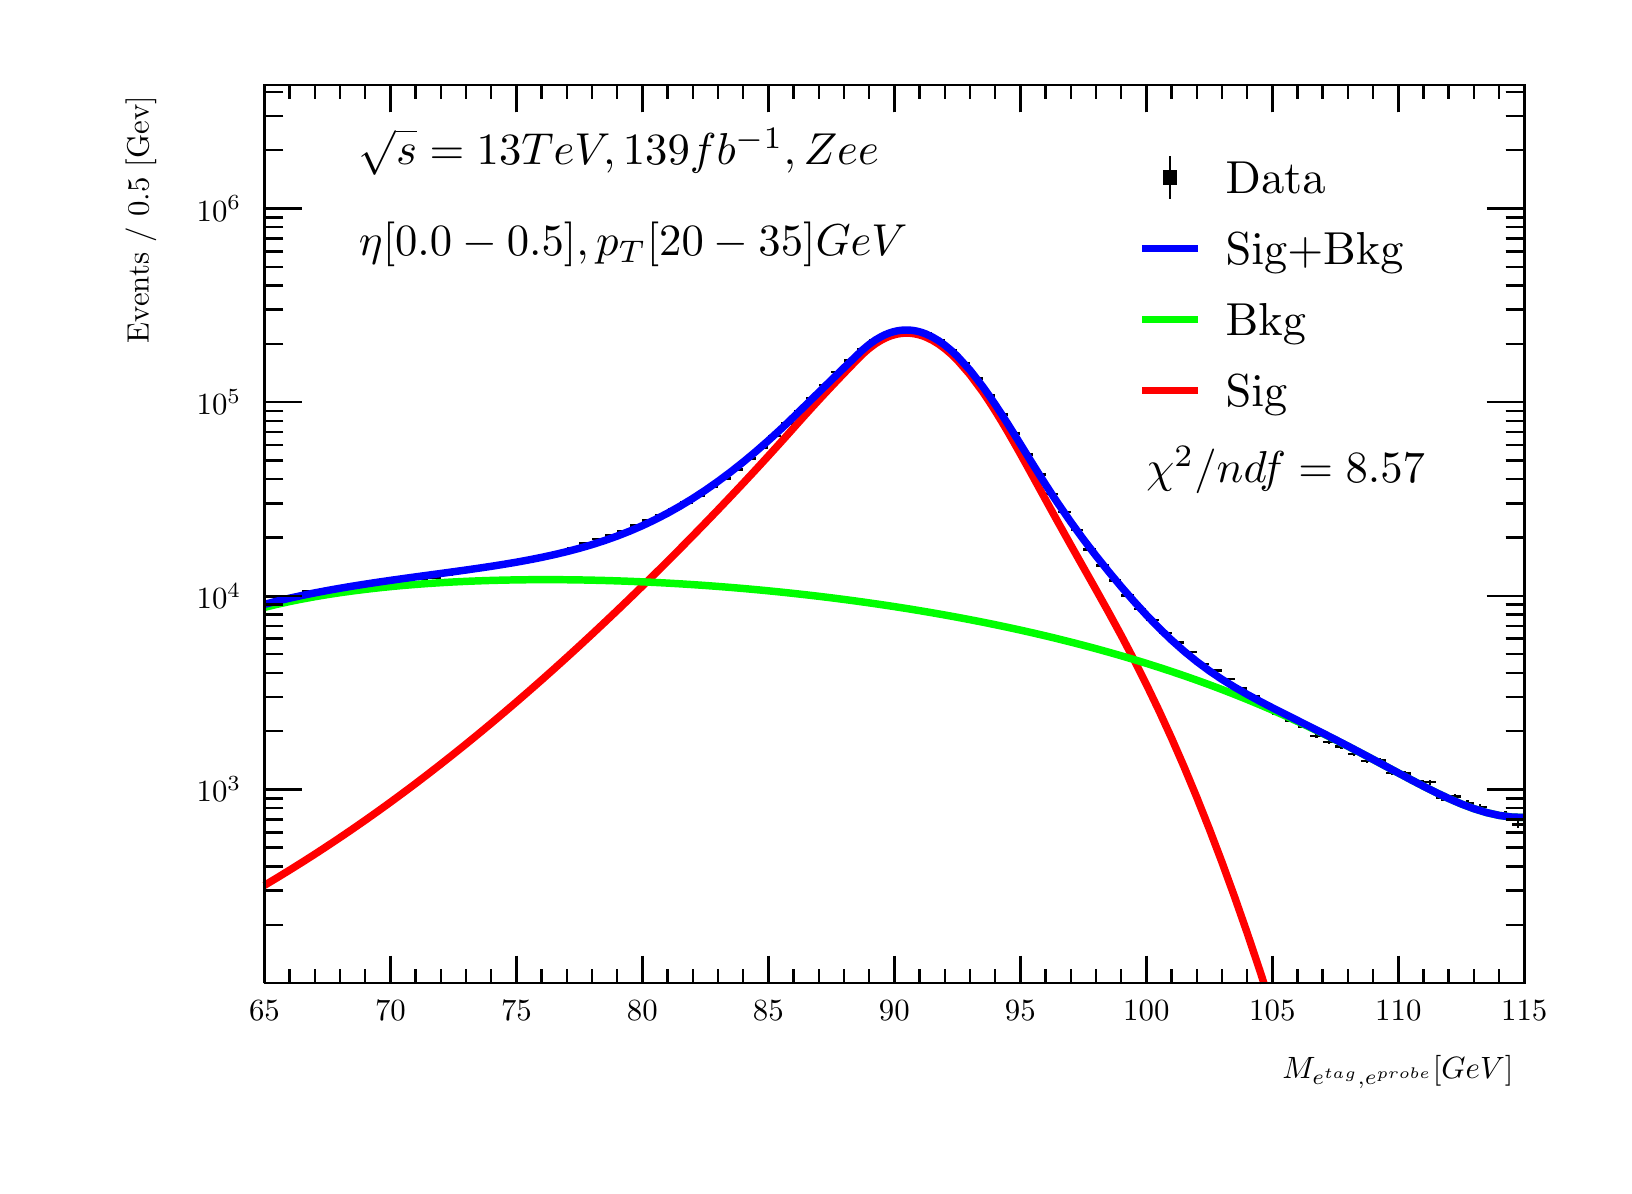
\begin{tikzpicture}
\pgfdeclareplotmark{cross} {
\pgfpathmoveto{\pgfpoint{-0.3\pgfplotmarksize}{\pgfplotmarksize}}
\pgfpathlineto{\pgfpoint{+0.3\pgfplotmarksize}{\pgfplotmarksize}}
\pgfpathlineto{\pgfpoint{+0.3\pgfplotmarksize}{0.3\pgfplotmarksize}}
\pgfpathlineto{\pgfpoint{+1\pgfplotmarksize}{0.3\pgfplotmarksize}}
\pgfpathlineto{\pgfpoint{+1\pgfplotmarksize}{-0.3\pgfplotmarksize}}
\pgfpathlineto{\pgfpoint{+0.3\pgfplotmarksize}{-0.3\pgfplotmarksize}}
\pgfpathlineto{\pgfpoint{+0.3\pgfplotmarksize}{-1.\pgfplotmarksize}}
\pgfpathlineto{\pgfpoint{-0.3\pgfplotmarksize}{-1.\pgfplotmarksize}}
\pgfpathlineto{\pgfpoint{-0.3\pgfplotmarksize}{-0.3\pgfplotmarksize}}
\pgfpathlineto{\pgfpoint{-1.\pgfplotmarksize}{-0.3\pgfplotmarksize}}
\pgfpathlineto{\pgfpoint{-1.\pgfplotmarksize}{0.3\pgfplotmarksize}}
\pgfpathlineto{\pgfpoint{-0.3\pgfplotmarksize}{0.3\pgfplotmarksize}}
\pgfpathclose
\pgfusepathqstroke
}
\pgfdeclareplotmark{cross*} {
\pgfpathmoveto{\pgfpoint{-0.3\pgfplotmarksize}{\pgfplotmarksize}}
\pgfpathlineto{\pgfpoint{+0.3\pgfplotmarksize}{\pgfplotmarksize}}
\pgfpathlineto{\pgfpoint{+0.3\pgfplotmarksize}{0.3\pgfplotmarksize}}
\pgfpathlineto{\pgfpoint{+1\pgfplotmarksize}{0.3\pgfplotmarksize}}
\pgfpathlineto{\pgfpoint{+1\pgfplotmarksize}{-0.3\pgfplotmarksize}}
\pgfpathlineto{\pgfpoint{+0.3\pgfplotmarksize}{-0.3\pgfplotmarksize}}
\pgfpathlineto{\pgfpoint{+0.3\pgfplotmarksize}{-1.\pgfplotmarksize}}
\pgfpathlineto{\pgfpoint{-0.3\pgfplotmarksize}{-1.\pgfplotmarksize}}
\pgfpathlineto{\pgfpoint{-0.3\pgfplotmarksize}{-0.3\pgfplotmarksize}}
\pgfpathlineto{\pgfpoint{-1.\pgfplotmarksize}{-0.3\pgfplotmarksize}}
\pgfpathlineto{\pgfpoint{-1.\pgfplotmarksize}{0.3\pgfplotmarksize}}
\pgfpathlineto{\pgfpoint{-0.3\pgfplotmarksize}{0.3\pgfplotmarksize}}
\pgfpathclose
\pgfusepathqfillstroke
}
\pgfdeclareplotmark{newstar} {
\pgfpathmoveto{\pgfqpoint{0pt}{\pgfplotmarksize}}
\pgfpathlineto{\pgfqpointpolar{44}{0.5\pgfplotmarksize}}
\pgfpathlineto{\pgfqpointpolar{18}{\pgfplotmarksize}}
\pgfpathlineto{\pgfqpointpolar{-20}{0.5\pgfplotmarksize}}
\pgfpathlineto{\pgfqpointpolar{-54}{\pgfplotmarksize}}
\pgfpathlineto{\pgfqpointpolar{-90}{0.5\pgfplotmarksize}}
\pgfpathlineto{\pgfqpointpolar{234}{\pgfplotmarksize}}
\pgfpathlineto{\pgfqpointpolar{198}{0.5\pgfplotmarksize}}
\pgfpathlineto{\pgfqpointpolar{162}{\pgfplotmarksize}}
\pgfpathlineto{\pgfqpointpolar{134}{0.5\pgfplotmarksize}}
\pgfpathclose
\pgfusepathqstroke
}
\pgfdeclareplotmark{newstar*} {
\pgfpathmoveto{\pgfqpoint{0pt}{\pgfplotmarksize}}
\pgfpathlineto{\pgfqpointpolar{44}{0.5\pgfplotmarksize}}
\pgfpathlineto{\pgfqpointpolar{18}{\pgfplotmarksize}}
\pgfpathlineto{\pgfqpointpolar{-20}{0.5\pgfplotmarksize}}
\pgfpathlineto{\pgfqpointpolar{-54}{\pgfplotmarksize}}
\pgfpathlineto{\pgfqpointpolar{-90}{0.5\pgfplotmarksize}}
\pgfpathlineto{\pgfqpointpolar{234}{\pgfplotmarksize}}
\pgfpathlineto{\pgfqpointpolar{198}{0.5\pgfplotmarksize}}
\pgfpathlineto{\pgfqpointpolar{162}{\pgfplotmarksize}}
\pgfpathlineto{\pgfqpointpolar{134}{0.5\pgfplotmarksize}}
\pgfpathclose
\pgfusepathqfillstroke
}
\definecolor{c}{rgb}{1,1,1};
\draw [color=c, fill=c] (0,0) rectangle (20,14.4361);
\draw [color=c, fill=c] (3,2.30977) rectangle (19,13.7143);
\definecolor{c}{rgb}{0,0,0};
\draw [c,line width=0.9] (3,2.30977) -- (3,13.7143) -- (19,13.7143) -- (19,2.30977) -- (3,2.30977);
\definecolor{c}{rgb}{1,1,1};
\draw [color=c, fill=c] (3,2.30977) rectangle (19,13.7143);
\definecolor{c}{rgb}{0,0,0};
\draw [c,line width=0.9] (3,2.30977) -- (3,13.7143) -- (19,13.7143) -- (19,2.30977) -- (3,2.30977);
\draw [c,line width=0.9] (3,2.30977) -- (19,2.30977);
\draw [c,line width=0.9] (3,2.65624) -- (3,2.30977);
\draw [c,line width=0.9] (3.32,2.48301) -- (3.32,2.30977);
\draw [c,line width=0.9] (3.64,2.48301) -- (3.64,2.30977);
\draw [c,line width=0.9] (3.96,2.48301) -- (3.96,2.30977);
\draw [c,line width=0.9] (4.28,2.48301) -- (4.28,2.30977);
\draw [c,line width=0.9] (4.6,2.65624) -- (4.6,2.30977);
\draw [c,line width=0.9] (4.92,2.48301) -- (4.92,2.30977);
\draw [c,line width=0.9] (5.24,2.48301) -- (5.24,2.30977);
\draw [c,line width=0.9] (5.56,2.48301) -- (5.56,2.30977);
\draw [c,line width=0.9] (5.88,2.48301) -- (5.88,2.30977);
\draw [c,line width=0.9] (6.2,2.65624) -- (6.2,2.30977);
\draw [c,line width=0.9] (6.52,2.48301) -- (6.52,2.30977);
\draw [c,line width=0.9] (6.84,2.48301) -- (6.84,2.30977);
\draw [c,line width=0.9] (7.16,2.48301) -- (7.16,2.30977);
\draw [c,line width=0.9] (7.48,2.48301) -- (7.48,2.30977);
\draw [c,line width=0.9] (7.8,2.65624) -- (7.8,2.30977);
\draw [c,line width=0.9] (8.12,2.48301) -- (8.12,2.30977);
\draw [c,line width=0.9] (8.44,2.48301) -- (8.44,2.30977);
\draw [c,line width=0.9] (8.76,2.48301) -- (8.76,2.30977);
\draw [c,line width=0.9] (9.08,2.48301) -- (9.08,2.30977);
\draw [c,line width=0.9] (9.4,2.65624) -- (9.4,2.30977);
\draw [c,line width=0.9] (9.72,2.48301) -- (9.72,2.30977);
\draw [c,line width=0.9] (10.04,2.48301) -- (10.04,2.30977);
\draw [c,line width=0.9] (10.36,2.48301) -- (10.36,2.30977);
\draw [c,line width=0.9] (10.68,2.48301) -- (10.68,2.30977);
\draw [c,line width=0.9] (11,2.65624) -- (11,2.30977);
\draw [c,line width=0.9] (11.32,2.48301) -- (11.32,2.30977);
\draw [c,line width=0.9] (11.64,2.48301) -- (11.64,2.30977);
\draw [c,line width=0.9] (11.96,2.48301) -- (11.96,2.30977);
\draw [c,line width=0.9] (12.28,2.48301) -- (12.28,2.30977);
\draw [c,line width=0.9] (12.6,2.65624) -- (12.6,2.30977);
\draw [c,line width=0.9] (12.92,2.48301) -- (12.92,2.30977);
\draw [c,line width=0.9] (13.24,2.48301) -- (13.24,2.30977);
\draw [c,line width=0.9] (13.56,2.48301) -- (13.56,2.30977);
\draw [c,line width=0.9] (13.88,2.48301) -- (13.88,2.30977);
\draw [c,line width=0.9] (14.2,2.65624) -- (14.2,2.30977);
\draw [c,line width=0.9] (14.52,2.48301) -- (14.52,2.30977);
\draw [c,line width=0.9] (14.84,2.48301) -- (14.84,2.30977);
\draw [c,line width=0.9] (15.16,2.48301) -- (15.16,2.30977);
\draw [c,line width=0.9] (15.48,2.48301) -- (15.48,2.30977);
\draw [c,line width=0.9] (15.8,2.65624) -- (15.8,2.30977);
\draw [c,line width=0.9] (16.12,2.48301) -- (16.12,2.30977);
\draw [c,line width=0.9] (16.44,2.48301) -- (16.44,2.30977);
\draw [c,line width=0.9] (16.76,2.48301) -- (16.76,2.30977);
\draw [c,line width=0.9] (17.08,2.48301) -- (17.08,2.30977);
\draw [c,line width=0.9] (17.4,2.65624) -- (17.4,2.30977);
\draw [c,line width=0.9] (17.72,2.48301) -- (17.72,2.30977);
\draw [c,line width=0.9] (18.04,2.48301) -- (18.04,2.30977);
\draw [c,line width=0.9] (18.36,2.48301) -- (18.36,2.30977);
\draw [c,line width=0.9] (18.68,2.48301) -- (18.68,2.30977);
\draw [c,line width=0.9] (19,2.65624) -- (19,2.30977);
\draw [c,line width=0.9] (19,2.65624) -- (19,2.30977);
\draw [anchor=base] (3,1.83338) node[scale=1.11327, color=c, rotate=0]{65};
\draw [anchor=base] (4.6,1.83338) node[scale=1.11327, color=c, rotate=0]{70};
\draw [anchor=base] (6.2,1.83338) node[scale=1.11327, color=c, rotate=0]{75};
\draw [anchor=base] (7.8,1.83338) node[scale=1.11327, color=c, rotate=0]{80};
\draw [anchor=base] (9.4,1.83338) node[scale=1.11327, color=c, rotate=0]{85};
\draw [anchor=base] (11,1.83338) node[scale=1.11327, color=c, rotate=0]{90};
\draw [anchor=base] (12.6,1.83338) node[scale=1.11327, color=c, rotate=0]{95};
\draw [anchor=base] (14.2,1.83338) node[scale=1.11327, color=c, rotate=0]{100};
\draw [anchor=base] (15.8,1.83338) node[scale=1.11327, color=c, rotate=0]{105};
\draw [anchor=base] (17.4,1.83338) node[scale=1.11327, color=c, rotate=0]{110};
\draw [anchor=base] (19,1.83338) node[scale=1.11327, color=c, rotate=0]{115};
\draw [anchor= east] (19,1.17798) node[scale=1.11327, color=c, rotate=0]{$M_{e^{tag}, e^{probe}}  [GeV]$};
\draw [c,line width=0.9] (3,13.7143) -- (19,13.7143);
\draw [c,line width=0.9] (3,13.3678) -- (3,13.7143);
\draw [c,line width=0.9] (3.32,13.5411) -- (3.32,13.7143);
\draw [c,line width=0.9] (3.64,13.5411) -- (3.64,13.7143);
\draw [c,line width=0.9] (3.96,13.5411) -- (3.96,13.7143);
\draw [c,line width=0.9] (4.28,13.5411) -- (4.28,13.7143);
\draw [c,line width=0.9] (4.6,13.3678) -- (4.6,13.7143);
\draw [c,line width=0.9] (4.92,13.5411) -- (4.92,13.7143);
\draw [c,line width=0.9] (5.24,13.5411) -- (5.24,13.7143);
\draw [c,line width=0.9] (5.56,13.5411) -- (5.56,13.7143);
\draw [c,line width=0.9] (5.88,13.5411) -- (5.88,13.7143);
\draw [c,line width=0.9] (6.2,13.3678) -- (6.2,13.7143);
\draw [c,line width=0.9] (6.52,13.5411) -- (6.52,13.7143);
\draw [c,line width=0.9] (6.84,13.5411) -- (6.84,13.7143);
\draw [c,line width=0.9] (7.16,13.5411) -- (7.16,13.7143);
\draw [c,line width=0.9] (7.48,13.5411) -- (7.48,13.7143);
\draw [c,line width=0.9] (7.8,13.3678) -- (7.8,13.7143);
\draw [c,line width=0.9] (8.12,13.5411) -- (8.12,13.7143);
\draw [c,line width=0.9] (8.44,13.5411) -- (8.44,13.7143);
\draw [c,line width=0.9] (8.76,13.5411) -- (8.76,13.7143);
\draw [c,line width=0.9] (9.08,13.5411) -- (9.08,13.7143);
\draw [c,line width=0.9] (9.4,13.3678) -- (9.4,13.7143);
\draw [c,line width=0.9] (9.72,13.5411) -- (9.72,13.7143);
\draw [c,line width=0.9] (10.04,13.5411) -- (10.04,13.7143);
\draw [c,line width=0.9] (10.36,13.5411) -- (10.36,13.7143);
\draw [c,line width=0.9] (10.68,13.5411) -- (10.68,13.7143);
\draw [c,line width=0.9] (11,13.3678) -- (11,13.7143);
\draw [c,line width=0.9] (11.32,13.5411) -- (11.32,13.7143);
\draw [c,line width=0.9] (11.64,13.5411) -- (11.64,13.7143);
\draw [c,line width=0.9] (11.96,13.5411) -- (11.96,13.7143);
\draw [c,line width=0.9] (12.28,13.5411) -- (12.28,13.7143);
\draw [c,line width=0.9] (12.6,13.3678) -- (12.6,13.7143);
\draw [c,line width=0.9] (12.92,13.5411) -- (12.92,13.7143);
\draw [c,line width=0.9] (13.24,13.5411) -- (13.24,13.7143);
\draw [c,line width=0.9] (13.56,13.5411) -- (13.56,13.7143);
\draw [c,line width=0.9] (13.88,13.5411) -- (13.88,13.7143);
\draw [c,line width=0.9] (14.2,13.3678) -- (14.2,13.7143);
\draw [c,line width=0.9] (14.52,13.5411) -- (14.52,13.7143);
\draw [c,line width=0.9] (14.84,13.5411) -- (14.84,13.7143);
\draw [c,line width=0.9] (15.16,13.5411) -- (15.16,13.7143);
\draw [c,line width=0.9] (15.48,13.5411) -- (15.48,13.7143);
\draw [c,line width=0.9] (15.8,13.3678) -- (15.8,13.7143);
\draw [c,line width=0.9] (16.12,13.5411) -- (16.12,13.7143);
\draw [c,line width=0.9] (16.44,13.5411) -- (16.44,13.7143);
\draw [c,line width=0.9] (16.76,13.5411) -- (16.76,13.7143);
\draw [c,line width=0.9] (17.08,13.5411) -- (17.08,13.7143);
\draw [c,line width=0.9] (17.4,13.3678) -- (17.4,13.7143);
\draw [c,line width=0.9] (17.72,13.5411) -- (17.72,13.7143);
\draw [c,line width=0.9] (18.04,13.5411) -- (18.04,13.7143);
\draw [c,line width=0.9] (18.36,13.5411) -- (18.36,13.7143);
\draw [c,line width=0.9] (18.68,13.5411) -- (18.68,13.7143);
\draw [c,line width=0.9] (19,13.3678) -- (19,13.7143);
\draw [c,line width=0.9] (19,13.3678) -- (19,13.7143);
\draw [c,line width=0.9] (3,2.30977) -- (3,13.7143);
\draw [c,line width=0.9] (3.237,3.05008) -- (3,3.05008);
\draw [c,line width=0.9] (3.237,3.48313) -- (3,3.48313);
\draw [c,line width=0.9] (3.237,3.79038) -- (3,3.79038);
\draw [c,line width=0.9] (3.237,4.02871) -- (3,4.02871);
\draw [c,line width=0.9] (3.237,4.22343) -- (3,4.22343);
\draw [c,line width=0.9] (3.237,4.38807) -- (3,4.38807);
\draw [c,line width=0.9] (3.237,4.53069) -- (3,4.53069);
\draw [c,line width=0.9] (3.237,4.65649) -- (3,4.65649);
\draw [c,line width=0.9] (3.474,4.76901) -- (3,4.76901);
\draw [anchor= east] (2.844,4.76901) node[scale=1.11327, color=c, rotate=0]{$10^{3}$};
\draw [c,line width=0.9] (3.237,5.50932) -- (3,5.50932);
\draw [c,line width=0.9] (3.237,5.94237) -- (3,5.94237);
\draw [c,line width=0.9] (3.237,6.24963) -- (3,6.24963);
\draw [c,line width=0.9] (3.237,6.48795) -- (3,6.48795);
\draw [c,line width=0.9] (3.237,6.68268) -- (3,6.68268);
\draw [c,line width=0.9] (3.237,6.84731) -- (3,6.84731);
\draw [c,line width=0.9] (3.237,6.98993) -- (3,6.98993);
\draw [c,line width=0.9] (3.237,7.11573) -- (3,7.11573);
\draw [c,line width=0.9] (3.474,7.22826) -- (3,7.22826);
\draw [anchor= east] (2.844,7.22826) node[scale=1.11327, color=c, rotate=0]{$10^{4}$};
\draw [c,line width=0.9] (3.237,7.96856) -- (3,7.96856);
\draw [c,line width=0.9] (3.237,8.40161) -- (3,8.40161);
\draw [c,line width=0.9] (3.237,8.70887) -- (3,8.70887);
\draw [c,line width=0.9] (3.237,8.94719) -- (3,8.94719);
\draw [c,line width=0.9] (3.237,9.14192) -- (3,9.14192);
\draw [c,line width=0.9] (3.237,9.30656) -- (3,9.30656);
\draw [c,line width=0.9] (3.237,9.44917) -- (3,9.44917);
\draw [c,line width=0.9] (3.237,9.57497) -- (3,9.57497);
\draw [c,line width=0.9] (3.474,9.6875) -- (3,9.6875);
\draw [anchor= east] (2.844,9.6875) node[scale=1.11327, color=c, rotate=0]{$10^{5}$};
\draw [c,line width=0.9] (3.237,10.4278) -- (3,10.4278);
\draw [c,line width=0.9] (3.237,10.8609) -- (3,10.8609);
\draw [c,line width=0.9] (3.237,11.1681) -- (3,11.1681);
\draw [c,line width=0.9] (3.237,11.4064) -- (3,11.4064);
\draw [c,line width=0.9] (3.237,11.6012) -- (3,11.6012);
\draw [c,line width=0.9] (3.237,11.7658) -- (3,11.7658);
\draw [c,line width=0.9] (3.237,11.9084) -- (3,11.9084);
\draw [c,line width=0.9] (3.237,12.0342) -- (3,12.0342);
\draw [c,line width=0.9] (3.474,12.1467) -- (3,12.1467);
\draw [anchor= east] (2.844,12.1467) node[scale=1.11327, color=c, rotate=0]{$10^{6}$};
\draw [c,line width=0.9] (3.237,12.887) -- (3,12.887);
\draw [c,line width=0.9] (3.237,13.3201) -- (3,13.3201);
\draw [c,line width=0.9] (3.237,13.6274) -- (3,13.6274);
\draw [anchor= east] (1.432,13.7143) node[scale=1.11327, color=c, rotate=90]{Events / 0.5 [Gev]};
\draw [c,line width=0.9] (19,2.30977) -- (19,13.7143);
\draw [c,line width=0.9] (18.763,3.05008) -- (19,3.05008);
\draw [c,line width=0.9] (18.763,3.48313) -- (19,3.48313);
\draw [c,line width=0.9] (18.763,3.79038) -- (19,3.79038);
\draw [c,line width=0.9] (18.763,4.02871) -- (19,4.02871);
\draw [c,line width=0.9] (18.763,4.22343) -- (19,4.22343);
\draw [c,line width=0.9] (18.763,4.38807) -- (19,4.38807);
\draw [c,line width=0.9] (18.763,4.53069) -- (19,4.53069);
\draw [c,line width=0.9] (18.763,4.65649) -- (19,4.65649);
\draw [c,line width=0.9] (18.526,4.76901) -- (19,4.76901);
\draw [c,line width=0.9] (18.763,5.50932) -- (19,5.50932);
\draw [c,line width=0.9] (18.763,5.94237) -- (19,5.94237);
\draw [c,line width=0.9] (18.763,6.24963) -- (19,6.24963);
\draw [c,line width=0.9] (18.763,6.48795) -- (19,6.48795);
\draw [c,line width=0.9] (18.763,6.68268) -- (19,6.68268);
\draw [c,line width=0.9] (18.763,6.84731) -- (19,6.84731);
\draw [c,line width=0.9] (18.763,6.98993) -- (19,6.98993);
\draw [c,line width=0.9] (18.763,7.11573) -- (19,7.11573);
\draw [c,line width=0.9] (18.526,7.22826) -- (19,7.22826);
\draw [c,line width=0.9] (18.763,7.96856) -- (19,7.96856);
\draw [c,line width=0.9] (18.763,8.40161) -- (19,8.40161);
\draw [c,line width=0.9] (18.763,8.70887) -- (19,8.70887);
\draw [c,line width=0.9] (18.763,8.94719) -- (19,8.94719);
\draw [c,line width=0.9] (18.763,9.14192) -- (19,9.14192);
\draw [c,line width=0.9] (18.763,9.30656) -- (19,9.30656);
\draw [c,line width=0.9] (18.763,9.44917) -- (19,9.44917);
\draw [c,line width=0.9] (18.763,9.57497) -- (19,9.57497);
\draw [c,line width=0.9] (18.526,9.6875) -- (19,9.6875);
\draw [c,line width=0.9] (18.763,10.4278) -- (19,10.4278);
\draw [c,line width=0.9] (18.763,10.8609) -- (19,10.8609);
\draw [c,line width=0.9] (18.763,11.1681) -- (19,11.1681);
\draw [c,line width=0.9] (18.763,11.4064) -- (19,11.4064);
\draw [c,line width=0.9] (18.763,11.6012) -- (19,11.6012);
\draw [c,line width=0.9] (18.763,11.7658) -- (19,11.7658);
\draw [c,line width=0.9] (18.763,11.9084) -- (19,11.9084);
\draw [c,line width=0.9] (18.763,12.0342) -- (19,12.0342);
\draw [c,line width=0.9] (18.526,12.1467) -- (19,12.1467);
\draw [c,line width=0.9] (18.763,12.887) -- (19,12.887);
\draw [c,line width=0.9] (18.763,13.3201) -- (19,13.3201);
\draw [c,line width=0.9] (18.763,13.6274) -- (19,13.6274);
\draw [c,line width=0.9] (3.08,7.21114) -- (3,7.21114);
\draw [c,line width=0.9] (3,7.21114) -- (3,7.21114);
\draw [c,line width=0.9] (3.08,7.21114) -- (3.16,7.21114);
\draw [c,line width=0.9] (3.16,7.21114) -- (3.16,7.21114);
\draw [c,line width=0.9] (3.08,7.21114) -- (3.08,7.22191);
\draw [c,line width=0.9] (3.08,7.22191) -- (3.08,7.22191);
\draw [c,line width=0.9] (3.08,7.21114) -- (3.08,7.20037);
\draw [c,line width=0.9] (3.08,7.20037) -- (3.08,7.20037);
\draw [c,line width=0.9] (3.24,7.21979) -- (3.16,7.21979);
\draw [c,line width=0.9] (3.16,7.21979) -- (3.16,7.21979);
\draw [c,line width=0.9] (3.24,7.21979) -- (3.32,7.21979);
\draw [c,line width=0.9] (3.32,7.21979) -- (3.32,7.21979);
\draw [c,line width=0.9] (3.24,7.21979) -- (3.24,7.23051);
\draw [c,line width=0.9] (3.24,7.23051) -- (3.24,7.23051);
\draw [c,line width=0.9] (3.24,7.21979) -- (3.24,7.20906);
\draw [c,line width=0.9] (3.24,7.20906) -- (3.24,7.20906);
\draw [c,line width=0.9] (3.4,7.23878) -- (3.32,7.23878);
\draw [c,line width=0.9] (3.32,7.23878) -- (3.32,7.23878);
\draw [c,line width=0.9] (3.4,7.23878) -- (3.48,7.23878);
\draw [c,line width=0.9] (3.48,7.23878) -- (3.48,7.23878);
\draw [c,line width=0.9] (3.4,7.23878) -- (3.4,7.24941);
\draw [c,line width=0.9] (3.4,7.24941) -- (3.4,7.24941);
\draw [c,line width=0.9] (3.4,7.23878) -- (3.4,7.22815);
\draw [c,line width=0.9] (3.4,7.22815) -- (3.4,7.22815);
\draw [c,line width=0.9] (3.56,7.28756) -- (3.48,7.28756);
\draw [c,line width=0.9] (3.48,7.28756) -- (3.48,7.28756);
\draw [c,line width=0.9] (3.56,7.28756) -- (3.64,7.28756);
\draw [c,line width=0.9] (3.64,7.28756) -- (3.64,7.28756);
\draw [c,line width=0.9] (3.56,7.28756) -- (3.56,7.29795);
\draw [c,line width=0.9] (3.56,7.29795) -- (3.56,7.29795);
\draw [c,line width=0.9] (3.56,7.28756) -- (3.56,7.27718);
\draw [c,line width=0.9] (3.56,7.27718) -- (3.56,7.27718);
\draw [c,line width=0.9] (3.72,7.27425) -- (3.64,7.27425);
\draw [c,line width=0.9] (3.64,7.27425) -- (3.64,7.27425);
\draw [c,line width=0.9] (3.72,7.27425) -- (3.8,7.27425);
\draw [c,line width=0.9] (3.8,7.27425) -- (3.8,7.27425);
\draw [c,line width=0.9] (3.72,7.27425) -- (3.72,7.2847);
\draw [c,line width=0.9] (3.72,7.2847) -- (3.72,7.2847);
\draw [c,line width=0.9] (3.72,7.27425) -- (3.72,7.26379);
\draw [c,line width=0.9] (3.72,7.26379) -- (3.72,7.26379);
\draw [c,line width=0.9] (3.88,7.30986) -- (3.8,7.30986);
\draw [c,line width=0.9] (3.8,7.30986) -- (3.8,7.30986);
\draw [c,line width=0.9] (3.88,7.30986) -- (3.96,7.30986);
\draw [c,line width=0.9] (3.96,7.30986) -- (3.96,7.30986);
\draw [c,line width=0.9] (3.88,7.30986) -- (3.88,7.32014);
\draw [c,line width=0.9] (3.88,7.32014) -- (3.88,7.32014);
\draw [c,line width=0.9] (3.88,7.30986) -- (3.88,7.29958);
\draw [c,line width=0.9] (3.88,7.29958) -- (3.88,7.29958);
\draw [c,line width=0.9] (4.04,7.31065) -- (3.96,7.31065);
\draw [c,line width=0.9] (3.96,7.31065) -- (3.96,7.31065);
\draw [c,line width=0.9] (4.04,7.31065) -- (4.12,7.31065);
\draw [c,line width=0.9] (4.12,7.31065) -- (4.12,7.31065);
\draw [c,line width=0.9] (4.04,7.31065) -- (4.04,7.32093);
\draw [c,line width=0.9] (4.04,7.32093) -- (4.04,7.32093);
\draw [c,line width=0.9] (4.04,7.31065) -- (4.04,7.30038);
\draw [c,line width=0.9] (4.04,7.30038) -- (4.04,7.30038);
\draw [c,line width=0.9] (4.2,7.34844) -- (4.12,7.34844);
\draw [c,line width=0.9] (4.12,7.34844) -- (4.12,7.34844);
\draw [c,line width=0.9] (4.2,7.34844) -- (4.28,7.34844);
\draw [c,line width=0.9] (4.28,7.34844) -- (4.28,7.34844);
\draw [c,line width=0.9] (4.2,7.34844) -- (4.2,7.35853);
\draw [c,line width=0.9] (4.2,7.35853) -- (4.2,7.35853);
\draw [c,line width=0.9] (4.2,7.34844) -- (4.2,7.33834);
\draw [c,line width=0.9] (4.2,7.33834) -- (4.2,7.33834);
\draw [c,line width=0.9] (4.36,7.35358) -- (4.28,7.35358);
\draw [c,line width=0.9] (4.28,7.35358) -- (4.28,7.35358);
\draw [c,line width=0.9] (4.36,7.35358) -- (4.44,7.35358);
\draw [c,line width=0.9] (4.44,7.35358) -- (4.44,7.35358);
\draw [c,line width=0.9] (4.36,7.35358) -- (4.36,7.36365);
\draw [c,line width=0.9] (4.36,7.36365) -- (4.36,7.36365);
\draw [c,line width=0.9] (4.36,7.35358) -- (4.36,7.34351);
\draw [c,line width=0.9] (4.36,7.34351) -- (4.36,7.34351);
\draw [c,line width=0.9] (4.52,7.38401) -- (4.44,7.38401);
\draw [c,line width=0.9] (4.44,7.38401) -- (4.44,7.38401);
\draw [c,line width=0.9] (4.52,7.38401) -- (4.6,7.38401);
\draw [c,line width=0.9] (4.6,7.38401) -- (4.6,7.38401);
\draw [c,line width=0.9] (4.52,7.38401) -- (4.52,7.39394);
\draw [c,line width=0.9] (4.52,7.39394) -- (4.52,7.39394);
\draw [c,line width=0.9] (4.52,7.38401) -- (4.52,7.37408);
\draw [c,line width=0.9] (4.52,7.37408) -- (4.52,7.37408);
\draw [c,line width=0.9] (4.68,7.39649) -- (4.6,7.39649);
\draw [c,line width=0.9] (4.6,7.39649) -- (4.6,7.39649);
\draw [c,line width=0.9] (4.68,7.39649) -- (4.76,7.39649);
\draw [c,line width=0.9] (4.76,7.39649) -- (4.76,7.39649);
\draw [c,line width=0.9] (4.68,7.39649) -- (4.68,7.40636);
\draw [c,line width=0.9] (4.68,7.40636) -- (4.68,7.40636);
\draw [c,line width=0.9] (4.68,7.39649) -- (4.68,7.38662);
\draw [c,line width=0.9] (4.68,7.38662) -- (4.68,7.38662);
\draw [c,line width=0.9] (4.84,7.39722) -- (4.76,7.39722);
\draw [c,line width=0.9] (4.76,7.39722) -- (4.76,7.39722);
\draw [c,line width=0.9] (4.84,7.39722) -- (4.92,7.39722);
\draw [c,line width=0.9] (4.92,7.39722) -- (4.92,7.39722);
\draw [c,line width=0.9] (4.84,7.39722) -- (4.84,7.40709);
\draw [c,line width=0.9] (4.84,7.40709) -- (4.84,7.40709);
\draw [c,line width=0.9] (4.84,7.39722) -- (4.84,7.38735);
\draw [c,line width=0.9] (4.84,7.38735) -- (4.84,7.38735);
\draw [c,line width=0.9] (5,7.44378) -- (4.92,7.44378);
\draw [c,line width=0.9] (4.92,7.44378) -- (4.92,7.44378);
\draw [c,line width=0.9] (5,7.44378) -- (5.08,7.44378);
\draw [c,line width=0.9] (5.08,7.44378) -- (5.08,7.44378);
\draw [c,line width=0.9] (5,7.44378) -- (5,7.45344);
\draw [c,line width=0.9] (5,7.45344) -- (5,7.45344);
\draw [c,line width=0.9] (5,7.44378) -- (5,7.43413);
\draw [c,line width=0.9] (5,7.43413) -- (5,7.43413);
\draw [c,line width=0.9] (5.16,7.45403) -- (5.08,7.45403);
\draw [c,line width=0.9] (5.08,7.45403) -- (5.08,7.45403);
\draw [c,line width=0.9] (5.16,7.45403) -- (5.24,7.45403);
\draw [c,line width=0.9] (5.24,7.45403) -- (5.24,7.45403);
\draw [c,line width=0.9] (5.16,7.45403) -- (5.16,7.46364);
\draw [c,line width=0.9] (5.16,7.46364) -- (5.16,7.46364);
\draw [c,line width=0.9] (5.16,7.45403) -- (5.16,7.44443);
\draw [c,line width=0.9] (5.16,7.44443) -- (5.16,7.44443);
\draw [c,line width=0.9] (5.32,7.5008) -- (5.24,7.5008);
\draw [c,line width=0.9] (5.24,7.5008) -- (5.24,7.5008);
\draw [c,line width=0.9] (5.32,7.5008) -- (5.4,7.5008);
\draw [c,line width=0.9] (5.4,7.5008) -- (5.4,7.5008);
\draw [c,line width=0.9] (5.32,7.5008) -- (5.32,7.5102);
\draw [c,line width=0.9] (5.32,7.5102) -- (5.32,7.5102);
\draw [c,line width=0.9] (5.32,7.5008) -- (5.32,7.4914);
\draw [c,line width=0.9] (5.32,7.4914) -- (5.32,7.4914);
\draw [c,line width=0.9] (5.48,7.52162) -- (5.4,7.52162);
\draw [c,line width=0.9] (5.4,7.52162) -- (5.4,7.52162);
\draw [c,line width=0.9] (5.48,7.52162) -- (5.56,7.52162);
\draw [c,line width=0.9] (5.56,7.52162) -- (5.56,7.52162);
\draw [c,line width=0.9] (5.48,7.52162) -- (5.48,7.53093);
\draw [c,line width=0.9] (5.48,7.53093) -- (5.48,7.53093);
\draw [c,line width=0.9] (5.48,7.52162) -- (5.48,7.51231);
\draw [c,line width=0.9] (5.48,7.51231) -- (5.48,7.51231);
\draw [c,line width=0.9] (5.64,7.54941) -- (5.56,7.54941);
\draw [c,line width=0.9] (5.56,7.54941) -- (5.56,7.54941);
\draw [c,line width=0.9] (5.64,7.54941) -- (5.72,7.54941);
\draw [c,line width=0.9] (5.72,7.54941) -- (5.72,7.54941);
\draw [c,line width=0.9] (5.64,7.54941) -- (5.64,7.5586);
\draw [c,line width=0.9] (5.64,7.5586) -- (5.64,7.5586);
\draw [c,line width=0.9] (5.64,7.54941) -- (5.64,7.54022);
\draw [c,line width=0.9] (5.64,7.54022) -- (5.64,7.54022);
\draw [c,line width=0.9] (5.8,7.58211) -- (5.72,7.58211);
\draw [c,line width=0.9] (5.72,7.58211) -- (5.72,7.58211);
\draw [c,line width=0.9] (5.8,7.58211) -- (5.88,7.58211);
\draw [c,line width=0.9] (5.88,7.58211) -- (5.88,7.58211);
\draw [c,line width=0.9] (5.8,7.58211) -- (5.8,7.59116);
\draw [c,line width=0.9] (5.8,7.59116) -- (5.8,7.59116);
\draw [c,line width=0.9] (5.8,7.58211) -- (5.8,7.57306);
\draw [c,line width=0.9] (5.8,7.57306) -- (5.8,7.57306);
\draw [c,line width=0.9] (5.96,7.61094) -- (5.88,7.61094);
\draw [c,line width=0.9] (5.88,7.61094) -- (5.88,7.61094);
\draw [c,line width=0.9] (5.96,7.61094) -- (6.04,7.61094);
\draw [c,line width=0.9] (6.04,7.61094) -- (6.04,7.61094);
\draw [c,line width=0.9] (5.96,7.61094) -- (5.96,7.61987);
\draw [c,line width=0.9] (5.96,7.61987) -- (5.96,7.61987);
\draw [c,line width=0.9] (5.96,7.61094) -- (5.96,7.60201);
\draw [c,line width=0.9] (5.96,7.60201) -- (5.96,7.60201);
\draw [c,line width=0.9] (6.12,7.6331) -- (6.04,7.6331);
\draw [c,line width=0.9] (6.04,7.6331) -- (6.04,7.6331);
\draw [c,line width=0.9] (6.12,7.6331) -- (6.2,7.6331);
\draw [c,line width=0.9] (6.2,7.6331) -- (6.2,7.6331);
\draw [c,line width=0.9] (6.12,7.6331) -- (6.12,7.64194);
\draw [c,line width=0.9] (6.12,7.64194) -- (6.12,7.64194);
\draw [c,line width=0.9] (6.12,7.6331) -- (6.12,7.62426);
\draw [c,line width=0.9] (6.12,7.62426) -- (6.12,7.62426);
\draw [c,line width=0.9] (6.28,7.66734) -- (6.2,7.66734);
\draw [c,line width=0.9] (6.2,7.66734) -- (6.2,7.66734);
\draw [c,line width=0.9] (6.28,7.66734) -- (6.36,7.66734);
\draw [c,line width=0.9] (6.36,7.66734) -- (6.36,7.66734);
\draw [c,line width=0.9] (6.28,7.66734) -- (6.28,7.67604);
\draw [c,line width=0.9] (6.28,7.67604) -- (6.28,7.67604);
\draw [c,line width=0.9] (6.28,7.66734) -- (6.28,7.65865);
\draw [c,line width=0.9] (6.28,7.65865) -- (6.28,7.65865);
\draw [c,line width=0.9] (6.44,7.71829) -- (6.36,7.71829);
\draw [c,line width=0.9] (6.36,7.71829) -- (6.36,7.71829);
\draw [c,line width=0.9] (6.44,7.71829) -- (6.52,7.71829);
\draw [c,line width=0.9] (6.52,7.71829) -- (6.52,7.71829);
\draw [c,line width=0.9] (6.44,7.71829) -- (6.44,7.72678);
\draw [c,line width=0.9] (6.44,7.72678) -- (6.44,7.72678);
\draw [c,line width=0.9] (6.44,7.71829) -- (6.44,7.7098);
\draw [c,line width=0.9] (6.44,7.7098) -- (6.44,7.7098);
\draw [c,line width=0.9] (6.6,7.73961) -- (6.52,7.73961);
\draw [c,line width=0.9] (6.52,7.73961) -- (6.52,7.73961);
\draw [c,line width=0.9] (6.6,7.73961) -- (6.68,7.73961);
\draw [c,line width=0.9] (6.68,7.73961) -- (6.68,7.73961);
\draw [c,line width=0.9] (6.6,7.73961) -- (6.6,7.74801);
\draw [c,line width=0.9] (6.6,7.74801) -- (6.6,7.74801);
\draw [c,line width=0.9] (6.6,7.73961) -- (6.6,7.7312);
\draw [c,line width=0.9] (6.6,7.7312) -- (6.6,7.7312);
\draw [c,line width=0.9] (6.76,7.78235) -- (6.68,7.78235);
\draw [c,line width=0.9] (6.68,7.78235) -- (6.68,7.78235);
\draw [c,line width=0.9] (6.76,7.78235) -- (6.84,7.78235);
\draw [c,line width=0.9] (6.84,7.78235) -- (6.84,7.78235);
\draw [c,line width=0.9] (6.76,7.78235) -- (6.76,7.79059);
\draw [c,line width=0.9] (6.76,7.79059) -- (6.76,7.79059);
\draw [c,line width=0.9] (6.76,7.78235) -- (6.76,7.77411);
\draw [c,line width=0.9] (6.76,7.77411) -- (6.76,7.77411);
\draw [c,line width=0.9] (6.92,7.83343) -- (6.84,7.83343);
\draw [c,line width=0.9] (6.84,7.83343) -- (6.84,7.83343);
\draw [c,line width=0.9] (6.92,7.83343) -- (7,7.83343);
\draw [c,line width=0.9] (7,7.83343) -- (7,7.83343);
\draw [c,line width=0.9] (6.92,7.83343) -- (6.92,7.84147);
\draw [c,line width=0.9] (6.92,7.84147) -- (6.92,7.84147);
\draw [c,line width=0.9] (6.92,7.83343) -- (6.92,7.82538);
\draw [c,line width=0.9] (6.92,7.82538) -- (6.92,7.82538);
\draw [c,line width=0.9] (7.08,7.89025) -- (7,7.89025);
\draw [c,line width=0.9] (7,7.89025) -- (7,7.89025);
\draw [c,line width=0.9] (7.08,7.89025) -- (7.16,7.89025);
\draw [c,line width=0.9] (7.16,7.89025) -- (7.16,7.89025);
\draw [c,line width=0.9] (7.08,7.89025) -- (7.08,7.89808);
\draw [c,line width=0.9] (7.08,7.89808) -- (7.08,7.89808);
\draw [c,line width=0.9] (7.08,7.89025) -- (7.08,7.88242);
\draw [c,line width=0.9] (7.08,7.88242) -- (7.08,7.88242);
\draw [c,line width=0.9] (7.24,7.94824) -- (7.16,7.94824);
\draw [c,line width=0.9] (7.16,7.94824) -- (7.16,7.94824);
\draw [c,line width=0.9] (7.24,7.94824) -- (7.32,7.94824);
\draw [c,line width=0.9] (7.32,7.94824) -- (7.32,7.94824);
\draw [c,line width=0.9] (7.24,7.94824) -- (7.24,7.95586);
\draw [c,line width=0.9] (7.24,7.95586) -- (7.24,7.95586);
\draw [c,line width=0.9] (7.24,7.94824) -- (7.24,7.94061);
\draw [c,line width=0.9] (7.24,7.94061) -- (7.24,7.94061);
\draw [c,line width=0.9] (7.4,7.99107) -- (7.32,7.99107);
\draw [c,line width=0.9] (7.32,7.99107) -- (7.32,7.99107);
\draw [c,line width=0.9] (7.4,7.99107) -- (7.48,7.99107);
\draw [c,line width=0.9] (7.48,7.99107) -- (7.48,7.99107);
\draw [c,line width=0.9] (7.4,7.99107) -- (7.4,7.99855);
\draw [c,line width=0.9] (7.4,7.99855) -- (7.4,7.99855);
\draw [c,line width=0.9] (7.4,7.99107) -- (7.4,7.9836);
\draw [c,line width=0.9] (7.4,7.9836) -- (7.4,7.9836);
\draw [c,line width=0.9] (7.56,8.04883) -- (7.48,8.04883);
\draw [c,line width=0.9] (7.48,8.04883) -- (7.48,8.04883);
\draw [c,line width=0.9] (7.56,8.04883) -- (7.64,8.04883);
\draw [c,line width=0.9] (7.64,8.04883) -- (7.64,8.04883);
\draw [c,line width=0.9] (7.56,8.04883) -- (7.56,8.0561);
\draw [c,line width=0.9] (7.56,8.0561) -- (7.56,8.0561);
\draw [c,line width=0.9] (7.56,8.04883) -- (7.56,8.04156);
\draw [c,line width=0.9] (7.56,8.04156) -- (7.56,8.04156);
\draw [c,line width=0.9] (7.72,8.11821) -- (7.64,8.11821);
\draw [c,line width=0.9] (7.64,8.11821) -- (7.64,8.11821);
\draw [c,line width=0.9] (7.72,8.11821) -- (7.8,8.11821);
\draw [c,line width=0.9] (7.8,8.11821) -- (7.8,8.11821);
\draw [c,line width=0.9] (7.72,8.11821) -- (7.72,8.12525);
\draw [c,line width=0.9] (7.72,8.12525) -- (7.72,8.12525);
\draw [c,line width=0.9] (7.72,8.11821) -- (7.72,8.11116);
\draw [c,line width=0.9] (7.72,8.11116) -- (7.72,8.11116);
\draw [c,line width=0.9] (7.88,8.18278) -- (7.8,8.18278);
\draw [c,line width=0.9] (7.8,8.18278) -- (7.8,8.18278);
\draw [c,line width=0.9] (7.88,8.18278) -- (7.96,8.18278);
\draw [c,line width=0.9] (7.96,8.18278) -- (7.96,8.18278);
\draw [c,line width=0.9] (7.88,8.18278) -- (7.88,8.18961);
\draw [c,line width=0.9] (7.88,8.18961) -- (7.88,8.18961);
\draw [c,line width=0.9] (7.88,8.18278) -- (7.88,8.17595);
\draw [c,line width=0.9] (7.88,8.17595) -- (7.88,8.17595);
\draw [c,line width=0.9] (8.04,8.25148) -- (7.96,8.25148);
\draw [c,line width=0.9] (7.96,8.25148) -- (7.96,8.25148);
\draw [c,line width=0.9] (8.04,8.25148) -- (8.12,8.25148);
\draw [c,line width=0.9] (8.12,8.25148) -- (8.12,8.25148);
\draw [c,line width=0.9] (8.04,8.25148) -- (8.04,8.2581);
\draw [c,line width=0.9] (8.04,8.2581) -- (8.04,8.2581);
\draw [c,line width=0.9] (8.04,8.25148) -- (8.04,8.24487);
\draw [c,line width=0.9] (8.04,8.24487) -- (8.04,8.24487);
\draw [c,line width=0.9] (8.2,8.3296) -- (8.12,8.3296);
\draw [c,line width=0.9] (8.12,8.3296) -- (8.12,8.3296);
\draw [c,line width=0.9] (8.2,8.3296) -- (8.28,8.3296);
\draw [c,line width=0.9] (8.28,8.3296) -- (8.28,8.3296);
\draw [c,line width=0.9] (8.2,8.3296) -- (8.2,8.33598);
\draw [c,line width=0.9] (8.2,8.33598) -- (8.2,8.33598);
\draw [c,line width=0.9] (8.2,8.3296) -- (8.2,8.32323);
\draw [c,line width=0.9] (8.2,8.32323) -- (8.2,8.32323);
\draw [c,line width=0.9] (8.36,8.41062) -- (8.28,8.41062);
\draw [c,line width=0.9] (8.28,8.41062) -- (8.28,8.41062);
\draw [c,line width=0.9] (8.36,8.41062) -- (8.44,8.41062);
\draw [c,line width=0.9] (8.44,8.41062) -- (8.44,8.41062);
\draw [c,line width=0.9] (8.36,8.41062) -- (8.36,8.41676);
\draw [c,line width=0.9] (8.36,8.41676) -- (8.36,8.41676);
\draw [c,line width=0.9] (8.36,8.41062) -- (8.36,8.40448);
\draw [c,line width=0.9] (8.36,8.40448) -- (8.36,8.40448);
\draw [c,line width=0.9] (8.52,8.50328) -- (8.44,8.50328);
\draw [c,line width=0.9] (8.44,8.50328) -- (8.44,8.50328);
\draw [c,line width=0.9] (8.52,8.50328) -- (8.6,8.50328);
\draw [c,line width=0.9] (8.6,8.50328) -- (8.6,8.50328);
\draw [c,line width=0.9] (8.52,8.50328) -- (8.52,8.50916);
\draw [c,line width=0.9] (8.52,8.50916) -- (8.52,8.50916);
\draw [c,line width=0.9] (8.52,8.50328) -- (8.52,8.4974);
\draw [c,line width=0.9] (8.52,8.4974) -- (8.52,8.4974);
\draw [c,line width=0.9] (8.68,8.60958) -- (8.6,8.60958);
\draw [c,line width=0.9] (8.6,8.60958) -- (8.6,8.60958);
\draw [c,line width=0.9] (8.68,8.60958) -- (8.76,8.60958);
\draw [c,line width=0.9] (8.76,8.60958) -- (8.76,8.60958);
\draw [c,line width=0.9] (8.68,8.60958) -- (8.68,8.61517);
\draw [c,line width=0.9] (8.68,8.61517) -- (8.68,8.61517);
\draw [c,line width=0.9] (8.68,8.60958) -- (8.68,8.60398);
\draw [c,line width=0.9] (8.68,8.60398) -- (8.68,8.60398);
\draw [c,line width=0.9] (8.84,8.71741) -- (8.76,8.71741);
\draw [c,line width=0.9] (8.76,8.71741) -- (8.76,8.71741);
\draw [c,line width=0.9] (8.84,8.71741) -- (8.92,8.71741);
\draw [c,line width=0.9] (8.92,8.71741) -- (8.92,8.71741);
\draw [c,line width=0.9] (8.84,8.71741) -- (8.84,8.72272);
\draw [c,line width=0.9] (8.84,8.72272) -- (8.84,8.72272);
\draw [c,line width=0.9] (8.84,8.71741) -- (8.84,8.71209);
\draw [c,line width=0.9] (8.84,8.71209) -- (8.84,8.71209);
\draw [c,line width=0.9] (9,8.83352) -- (8.92,8.83352);
\draw [c,line width=0.9] (8.92,8.83352) -- (8.92,8.83352);
\draw [c,line width=0.9] (9,8.83352) -- (9.08,8.83352);
\draw [c,line width=0.9] (9.08,8.83352) -- (9.08,8.83352);
\draw [c,line width=0.9] (9,8.83352) -- (9,8.83856);
\draw [c,line width=0.9] (9,8.83856) -- (9,8.83856);
\draw [c,line width=0.9] (9,8.83352) -- (9,8.82849);
\draw [c,line width=0.9] (9,8.82849) -- (9,8.82849);
\draw [c,line width=0.9] (9.16,8.97016) -- (9.08,8.97016);
\draw [c,line width=0.9] (9.08,8.97016) -- (9.08,8.97016);
\draw [c,line width=0.9] (9.16,8.97016) -- (9.24,8.97016);
\draw [c,line width=0.9] (9.24,8.97016) -- (9.24,8.97016);
\draw [c,line width=0.9] (9.16,8.97016) -- (9.16,8.97489);
\draw [c,line width=0.9] (9.16,8.97489) -- (9.16,8.97489);
\draw [c,line width=0.9] (9.16,8.97016) -- (9.16,8.96544);
\draw [c,line width=0.9] (9.16,8.96544) -- (9.16,8.96544);
\draw [c,line width=0.9] (9.32,9.10987) -- (9.24,9.10987);
\draw [c,line width=0.9] (9.24,9.10987) -- (9.24,9.10987);
\draw [c,line width=0.9] (9.32,9.10987) -- (9.4,9.10987);
\draw [c,line width=0.9] (9.4,9.10987) -- (9.4,9.10987);
\draw [c,line width=0.9] (9.32,9.10987) -- (9.32,9.11429);
\draw [c,line width=0.9] (9.32,9.11429) -- (9.32,9.11429);
\draw [c,line width=0.9] (9.32,9.10987) -- (9.32,9.10544);
\draw [c,line width=0.9] (9.32,9.10544) -- (9.32,9.10544);
\draw [c,line width=0.9] (9.48,9.25465) -- (9.4,9.25465);
\draw [c,line width=0.9] (9.4,9.25465) -- (9.4,9.25465);
\draw [c,line width=0.9] (9.48,9.25465) -- (9.56,9.25465);
\draw [c,line width=0.9] (9.56,9.25465) -- (9.56,9.25465);
\draw [c,line width=0.9] (9.48,9.25465) -- (9.48,9.25878);
\draw [c,line width=0.9] (9.48,9.25878) -- (9.48,9.25878);
\draw [c,line width=0.9] (9.48,9.25465) -- (9.48,9.25051);
\draw [c,line width=0.9] (9.48,9.25051) -- (9.48,9.25051);
\draw [c,line width=0.9] (9.64,9.41402) -- (9.56,9.41402);
\draw [c,line width=0.9] (9.56,9.41402) -- (9.56,9.41402);
\draw [c,line width=0.9] (9.64,9.41402) -- (9.72,9.41402);
\draw [c,line width=0.9] (9.72,9.41402) -- (9.72,9.41402);
\draw [c,line width=0.9] (9.64,9.41402) -- (9.64,9.41786);
\draw [c,line width=0.9] (9.64,9.41786) -- (9.64,9.41786);
\draw [c,line width=0.9] (9.64,9.41402) -- (9.64,9.41018);
\draw [c,line width=0.9] (9.64,9.41018) -- (9.64,9.41018);
\draw [c,line width=0.9] (9.8,9.57757) -- (9.72,9.57757);
\draw [c,line width=0.9] (9.72,9.57757) -- (9.72,9.57757);
\draw [c,line width=0.9] (9.8,9.57757) -- (9.88,9.57757);
\draw [c,line width=0.9] (9.88,9.57757) -- (9.88,9.57757);
\draw [c,line width=0.9] (9.8,9.57757) -- (9.8,9.58112);
\draw [c,line width=0.9] (9.8,9.58112) -- (9.8,9.58112);
\draw [c,line width=0.9] (9.8,9.57757) -- (9.8,9.57401);
\draw [c,line width=0.9] (9.8,9.57401) -- (9.8,9.57401);
\draw [c,line width=0.9] (9.96,9.74181) -- (9.88,9.74181);
\draw [c,line width=0.9] (9.88,9.74181) -- (9.88,9.74181);
\draw [c,line width=0.9] (9.96,9.74181) -- (10.04,9.74181);
\draw [c,line width=0.9] (10.04,9.74181) -- (10.04,9.74181);
\draw [c,line width=0.9] (9.96,9.74181) -- (9.96,9.74511);
\draw [c,line width=0.9] (9.96,9.74511) -- (9.96,9.74511);
\draw [c,line width=0.9] (9.96,9.74181) -- (9.96,9.73852);
\draw [c,line width=0.9] (9.96,9.73852) -- (9.96,9.73852);
\draw [c,line width=0.9] (10.12,9.90267) -- (10.04,9.90267);
\draw [c,line width=0.9] (10.04,9.90267) -- (10.04,9.90267);
\draw [c,line width=0.9] (10.12,9.90267) -- (10.2,9.90267);
\draw [c,line width=0.9] (10.2,9.90267) -- (10.2,9.90267);
\draw [c,line width=0.9] (10.12,9.90267) -- (10.12,9.90572);
\draw [c,line width=0.9] (10.12,9.90572) -- (10.12,9.90572);
\draw [c,line width=0.9] (10.12,9.90267) -- (10.12,9.89961);
\draw [c,line width=0.9] (10.12,9.89961) -- (10.12,9.89961);
\draw [c,line width=0.9] (10.28,10.0673) -- (10.2,10.0673);
\draw [c,line width=0.9] (10.2,10.0673) -- (10.2,10.0673);
\draw [c,line width=0.9] (10.28,10.0673) -- (10.36,10.0673);
\draw [c,line width=0.9] (10.36,10.0673) -- (10.36,10.0673);
\draw [c,line width=0.9] (10.28,10.0673) -- (10.28,10.0701);
\draw [c,line width=0.9] (10.28,10.0701) -- (10.28,10.0701);
\draw [c,line width=0.9] (10.28,10.0673) -- (10.28,10.0645);
\draw [c,line width=0.9] (10.28,10.0645) -- (10.28,10.0645);
\draw [c,line width=0.9] (10.44,10.217) -- (10.36,10.217);
\draw [c,line width=0.9] (10.36,10.217) -- (10.36,10.217);
\draw [c,line width=0.9] (10.44,10.217) -- (10.52,10.217);
\draw [c,line width=0.9] (10.52,10.217) -- (10.52,10.217);
\draw [c,line width=0.9] (10.44,10.217) -- (10.44,10.2197);
\draw [c,line width=0.9] (10.44,10.2197) -- (10.44,10.2197);
\draw [c,line width=0.9] (10.44,10.217) -- (10.44,10.2144);
\draw [c,line width=0.9] (10.44,10.2144) -- (10.44,10.2144);
\draw [c,line width=0.9] (10.6,10.3535) -- (10.52,10.3535);
\draw [c,line width=0.9] (10.52,10.3535) -- (10.52,10.3535);
\draw [c,line width=0.9] (10.6,10.3535) -- (10.68,10.3535);
\draw [c,line width=0.9] (10.68,10.3535) -- (10.68,10.3535);
\draw [c,line width=0.9] (10.6,10.3535) -- (10.6,10.356);
\draw [c,line width=0.9] (10.6,10.356) -- (10.6,10.356);
\draw [c,line width=0.9] (10.6,10.3535) -- (10.6,10.351);
\draw [c,line width=0.9] (10.6,10.351) -- (10.6,10.351);
\draw [c,line width=0.9] (10.76,10.4675) -- (10.68,10.4675);
\draw [c,line width=0.9] (10.68,10.4675) -- (10.68,10.4675);
\draw [c,line width=0.9] (10.76,10.4675) -- (10.84,10.4675);
\draw [c,line width=0.9] (10.84,10.4675) -- (10.84,10.4675);
\draw [c,line width=0.9] (10.76,10.4675) -- (10.76,10.4698);
\draw [c,line width=0.9] (10.76,10.4698) -- (10.76,10.4698);
\draw [c,line width=0.9] (10.76,10.4675) -- (10.76,10.4652);
\draw [c,line width=0.9] (10.76,10.4652) -- (10.76,10.4652);
\draw [c,line width=0.9] (10.92,10.546) -- (10.84,10.546);
\draw [c,line width=0.9] (10.84,10.546) -- (10.84,10.546);
\draw [c,line width=0.9] (10.92,10.546) -- (11,10.546);
\draw [c,line width=0.9] (11,10.546) -- (11,10.546);
\draw [c,line width=0.9] (10.92,10.546) -- (10.92,10.5482);
\draw [c,line width=0.9] (10.92,10.5482) -- (10.92,10.5482);
\draw [c,line width=0.9] (10.92,10.546) -- (10.92,10.5437);
\draw [c,line width=0.9] (10.92,10.5437) -- (10.92,10.5437);
\draw [c,line width=0.9] (11.08,10.5926) -- (11,10.5926);
\draw [c,line width=0.9] (11,10.5926) -- (11,10.5926);
\draw [c,line width=0.9] (11.08,10.5926) -- (11.16,10.5926);
\draw [c,line width=0.9] (11.16,10.5926) -- (11.16,10.5926);
\draw [c,line width=0.9] (11.08,10.5926) -- (11.08,10.5948);
\draw [c,line width=0.9] (11.08,10.5948) -- (11.08,10.5948);
\draw [c,line width=0.9] (11.08,10.5926) -- (11.08,10.5904);
\draw [c,line width=0.9] (11.08,10.5904) -- (11.08,10.5904);
\draw [c,line width=0.9] (11.24,10.6009) -- (11.16,10.6009);
\draw [c,line width=0.9] (11.16,10.6009) -- (11.16,10.6009);
\draw [c,line width=0.9] (11.24,10.6009) -- (11.32,10.6009);
\draw [c,line width=0.9] (11.32,10.6009) -- (11.32,10.6009);
\draw [c,line width=0.9] (11.24,10.6009) -- (11.24,10.6031);
\draw [c,line width=0.9] (11.24,10.6031) -- (11.24,10.6031);
\draw [c,line width=0.9] (11.24,10.6009) -- (11.24,10.5987);
\draw [c,line width=0.9] (11.24,10.5987) -- (11.24,10.5987);
\draw [c,line width=0.9] (11.4,10.5575) -- (11.32,10.5575);
\draw [c,line width=0.9] (11.32,10.5575) -- (11.32,10.5575);
\draw [c,line width=0.9] (11.4,10.5575) -- (11.48,10.5575);
\draw [c,line width=0.9] (11.48,10.5575) -- (11.48,10.5575);
\draw [c,line width=0.9] (11.4,10.5575) -- (11.4,10.5597);
\draw [c,line width=0.9] (11.4,10.5597) -- (11.4,10.5597);
\draw [c,line width=0.9] (11.4,10.5575) -- (11.4,10.5552);
\draw [c,line width=0.9] (11.4,10.5552) -- (11.4,10.5552);
\draw [c,line width=0.9] (11.56,10.4745) -- (11.48,10.4745);
\draw [c,line width=0.9] (11.48,10.4745) -- (11.48,10.4745);
\draw [c,line width=0.9] (11.56,10.4745) -- (11.64,10.4745);
\draw [c,line width=0.9] (11.64,10.4745) -- (11.64,10.4745);
\draw [c,line width=0.9] (11.56,10.4745) -- (11.56,10.4768);
\draw [c,line width=0.9] (11.56,10.4768) -- (11.56,10.4768);
\draw [c,line width=0.9] (11.56,10.4745) -- (11.56,10.4721);
\draw [c,line width=0.9] (11.56,10.4721) -- (11.56,10.4721);
\draw [c,line width=0.9] (11.72,10.348) -- (11.64,10.348);
\draw [c,line width=0.9] (11.64,10.348) -- (11.64,10.348);
\draw [c,line width=0.9] (11.72,10.348) -- (11.8,10.348);
\draw [c,line width=0.9] (11.8,10.348) -- (11.8,10.348);
\draw [c,line width=0.9] (11.72,10.348) -- (11.72,10.3505);
\draw [c,line width=0.9] (11.72,10.3505) -- (11.72,10.3505);
\draw [c,line width=0.9] (11.72,10.348) -- (11.72,10.3456);
\draw [c,line width=0.9] (11.72,10.3456) -- (11.72,10.3456);
\draw [c,line width=0.9] (11.88,10.1848) -- (11.8,10.1848);
\draw [c,line width=0.9] (11.8,10.1848) -- (11.8,10.1848);
\draw [c,line width=0.9] (11.88,10.1848) -- (11.96,10.1848);
\draw [c,line width=0.9] (11.96,10.1848) -- (11.96,10.1848);
\draw [c,line width=0.9] (11.88,10.1848) -- (11.88,10.1875);
\draw [c,line width=0.9] (11.88,10.1875) -- (11.88,10.1875);
\draw [c,line width=0.9] (11.88,10.1848) -- (11.88,10.1821);
\draw [c,line width=0.9] (11.88,10.1821) -- (11.88,10.1821);
\draw [c,line width=0.9] (12.04,9.9901) -- (11.96,9.9901);
\draw [c,line width=0.9] (11.96,9.9901) -- (11.96,9.9901);
\draw [c,line width=0.9] (12.04,9.9901) -- (12.12,9.9901);
\draw [c,line width=0.9] (12.12,9.9901) -- (12.12,9.9901);
\draw [c,line width=0.9] (12.04,9.9901) -- (12.04,9.99303);
\draw [c,line width=0.9] (12.04,9.99303) -- (12.04,9.99303);
\draw [c,line width=0.9] (12.04,9.9901) -- (12.04,9.98717);
\draw [c,line width=0.9] (12.04,9.98717) -- (12.04,9.98717);
\draw [c,line width=0.9] (12.2,9.7739) -- (12.12,9.7739);
\draw [c,line width=0.9] (12.12,9.7739) -- (12.12,9.7739);
\draw [c,line width=0.9] (12.2,9.7739) -- (12.28,9.7739);
\draw [c,line width=0.9] (12.28,9.7739) -- (12.28,9.7739);
\draw [c,line width=0.9] (12.2,9.7739) -- (12.2,9.77714);
\draw [c,line width=0.9] (12.2,9.77714) -- (12.2,9.77714);
\draw [c,line width=0.9] (12.2,9.7739) -- (12.2,9.77066);
\draw [c,line width=0.9] (12.2,9.77066) -- (12.2,9.77066);
\draw [c,line width=0.9] (12.36,9.52728) -- (12.28,9.52728);
\draw [c,line width=0.9] (12.28,9.52728) -- (12.28,9.52728);
\draw [c,line width=0.9] (12.36,9.52728) -- (12.44,9.52728);
\draw [c,line width=0.9] (12.44,9.52728) -- (12.44,9.52728);
\draw [c,line width=0.9] (12.36,9.52728) -- (12.36,9.53092);
\draw [c,line width=0.9] (12.36,9.53092) -- (12.36,9.53092);
\draw [c,line width=0.9] (12.36,9.52728) -- (12.36,9.52364);
\draw [c,line width=0.9] (12.36,9.52364) -- (12.36,9.52364);
\draw [c,line width=0.9] (12.52,9.2891) -- (12.44,9.2891);
\draw [c,line width=0.9] (12.44,9.2891) -- (12.44,9.2891);
\draw [c,line width=0.9] (12.52,9.2891) -- (12.6,9.2891);
\draw [c,line width=0.9] (12.6,9.2891) -- (12.6,9.2891);
\draw [c,line width=0.9] (12.52,9.2891) -- (12.52,9.29317);
\draw [c,line width=0.9] (12.52,9.29317) -- (12.52,9.29317);
\draw [c,line width=0.9] (12.52,9.2891) -- (12.52,9.28503);
\draw [c,line width=0.9] (12.52,9.28503) -- (12.52,9.28503);
\draw [c,line width=0.9] (12.68,9.02525) -- (12.6,9.02525);
\draw [c,line width=0.9] (12.6,9.02525) -- (12.6,9.02525);
\draw [c,line width=0.9] (12.68,9.02525) -- (12.76,9.02525);
\draw [c,line width=0.9] (12.76,9.02525) -- (12.76,9.02525);
\draw [c,line width=0.9] (12.68,9.02525) -- (12.68,9.02985);
\draw [c,line width=0.9] (12.68,9.02985) -- (12.68,9.02985);
\draw [c,line width=0.9] (12.68,9.02525) -- (12.68,9.02064);
\draw [c,line width=0.9] (12.68,9.02064) -- (12.68,9.02064);
\draw [c,line width=0.9] (12.84,8.76954) -- (12.76,8.76954);
\draw [c,line width=0.9] (12.76,8.76954) -- (12.76,8.76954);
\draw [c,line width=0.9] (12.84,8.76954) -- (12.92,8.76954);
\draw [c,line width=0.9] (12.92,8.76954) -- (12.92,8.76954);
\draw [c,line width=0.9] (12.84,8.76954) -- (12.84,8.77473);
\draw [c,line width=0.9] (12.84,8.77473) -- (12.84,8.77473);
\draw [c,line width=0.9] (12.84,8.76954) -- (12.84,8.76435);
\draw [c,line width=0.9] (12.84,8.76435) -- (12.84,8.76435);
\draw [c,line width=0.9] (13,8.51756) -- (12.92,8.51756);
\draw [c,line width=0.9] (12.92,8.51756) -- (12.92,8.51756);
\draw [c,line width=0.9] (13,8.51756) -- (13.08,8.51756);
\draw [c,line width=0.9] (13.08,8.51756) -- (13.08,8.51756);
\draw [c,line width=0.9] (13,8.51756) -- (13,8.5234);
\draw [c,line width=0.9] (13,8.5234) -- (13,8.5234);
\draw [c,line width=0.9] (13,8.51756) -- (13,8.51171);
\draw [c,line width=0.9] (13,8.51171) -- (13,8.51171);
\draw [c,line width=0.9] (13.16,8.29134) -- (13.08,8.29134);
\draw [c,line width=0.9] (13.08,8.29134) -- (13.08,8.29134);
\draw [c,line width=0.9] (13.16,8.29134) -- (13.24,8.29134);
\draw [c,line width=0.9] (13.24,8.29134) -- (13.24,8.29134);
\draw [c,line width=0.9] (13.16,8.29134) -- (13.16,8.29783);
\draw [c,line width=0.9] (13.16,8.29783) -- (13.16,8.29783);
\draw [c,line width=0.9] (13.16,8.29134) -- (13.16,8.28484);
\draw [c,line width=0.9] (13.16,8.28484) -- (13.16,8.28484);
\draw [c,line width=0.9] (13.32,8.06525) -- (13.24,8.06525);
\draw [c,line width=0.9] (13.24,8.06525) -- (13.24,8.06525);
\draw [c,line width=0.9] (13.32,8.06525) -- (13.4,8.06525);
\draw [c,line width=0.9] (13.4,8.06525) -- (13.4,8.06525);
\draw [c,line width=0.9] (13.32,8.06525) -- (13.32,8.07247);
\draw [c,line width=0.9] (13.32,8.07247) -- (13.32,8.07247);
\draw [c,line width=0.9] (13.32,8.06525) -- (13.32,8.05803);
\draw [c,line width=0.9] (13.32,8.05803) -- (13.32,8.05803);
\draw [c,line width=0.9] (13.48,7.81878) -- (13.4,7.81878);
\draw [c,line width=0.9] (13.4,7.81878) -- (13.4,7.81878);
\draw [c,line width=0.9] (13.48,7.81878) -- (13.56,7.81878);
\draw [c,line width=0.9] (13.56,7.81878) -- (13.56,7.81878);
\draw [c,line width=0.9] (13.48,7.81878) -- (13.48,7.82688);
\draw [c,line width=0.9] (13.48,7.82688) -- (13.48,7.82688);
\draw [c,line width=0.9] (13.48,7.81878) -- (13.48,7.81068);
\draw [c,line width=0.9] (13.48,7.81068) -- (13.48,7.81068);
\draw [c,line width=0.9] (13.64,7.61355) -- (13.56,7.61355);
\draw [c,line width=0.9] (13.56,7.61355) -- (13.56,7.61355);
\draw [c,line width=0.9] (13.64,7.61355) -- (13.72,7.61355);
\draw [c,line width=0.9] (13.72,7.61355) -- (13.72,7.61355);
\draw [c,line width=0.9] (13.64,7.61355) -- (13.64,7.62247);
\draw [c,line width=0.9] (13.64,7.62247) -- (13.64,7.62247);
\draw [c,line width=0.9] (13.64,7.61355) -- (13.64,7.60463);
\draw [c,line width=0.9] (13.64,7.60463) -- (13.64,7.60463);
\draw [c,line width=0.9] (13.8,7.42102) -- (13.72,7.42102);
\draw [c,line width=0.9] (13.72,7.42102) -- (13.72,7.42102);
\draw [c,line width=0.9] (13.8,7.42102) -- (13.88,7.42102);
\draw [c,line width=0.9] (13.88,7.42102) -- (13.88,7.42102);
\draw [c,line width=0.9] (13.8,7.42102) -- (13.8,7.43078);
\draw [c,line width=0.9] (13.8,7.43078) -- (13.8,7.43078);
\draw [c,line width=0.9] (13.8,7.42102) -- (13.8,7.41126);
\draw [c,line width=0.9] (13.8,7.41126) -- (13.8,7.41126);
\draw [c,line width=0.9] (13.96,7.22943) -- (13.88,7.22943);
\draw [c,line width=0.9] (13.88,7.22943) -- (13.88,7.22943);
\draw [c,line width=0.9] (13.96,7.22943) -- (14.04,7.22943);
\draw [c,line width=0.9] (14.04,7.22943) -- (14.04,7.22943);
\draw [c,line width=0.9] (13.96,7.22943) -- (13.96,7.24011);
\draw [c,line width=0.9] (13.96,7.24011) -- (13.96,7.24011);
\draw [c,line width=0.9] (13.96,7.22943) -- (13.96,7.21876);
\draw [c,line width=0.9] (13.96,7.21876) -- (13.96,7.21876);
\draw [c,line width=0.9] (14.12,7.05982) -- (14.04,7.05982);
\draw [c,line width=0.9] (14.04,7.05982) -- (14.04,7.05982);
\draw [c,line width=0.9] (14.12,7.05982) -- (14.2,7.05982);
\draw [c,line width=0.9] (14.2,7.05982) -- (14.2,7.05982);
\draw [c,line width=0.9] (14.12,7.05982) -- (14.12,7.07138);
\draw [c,line width=0.9] (14.12,7.07138) -- (14.12,7.07138);
\draw [c,line width=0.9] (14.12,7.05982) -- (14.12,7.04826);
\draw [c,line width=0.9] (14.12,7.04826) -- (14.12,7.04826);
\draw [c,line width=0.9] (14.28,6.92171) -- (14.2,6.92171);
\draw [c,line width=0.9] (14.2,6.92171) -- (14.2,6.92171);
\draw [c,line width=0.9] (14.28,6.92171) -- (14.36,6.92171);
\draw [c,line width=0.9] (14.36,6.92171) -- (14.36,6.92171);
\draw [c,line width=0.9] (14.28,6.92171) -- (14.28,6.93404);
\draw [c,line width=0.9] (14.28,6.93404) -- (14.28,6.93404);
\draw [c,line width=0.9] (14.28,6.92171) -- (14.28,6.90939);
\draw [c,line width=0.9] (14.28,6.90939) -- (14.28,6.90939);
\draw [c,line width=0.9] (14.44,6.75727) -- (14.36,6.75727);
\draw [c,line width=0.9] (14.36,6.75727) -- (14.36,6.75727);
\draw [c,line width=0.9] (14.44,6.75727) -- (14.52,6.75727);
\draw [c,line width=0.9] (14.52,6.75727) -- (14.52,6.75727);
\draw [c,line width=0.9] (14.44,6.75727) -- (14.44,6.77058);
\draw [c,line width=0.9] (14.44,6.77058) -- (14.44,6.77058);
\draw [c,line width=0.9] (14.44,6.75727) -- (14.44,6.74395);
\draw [c,line width=0.9] (14.44,6.74395) -- (14.44,6.74395);
\draw [c,line width=0.9] (14.6,6.63648) -- (14.52,6.63648);
\draw [c,line width=0.9] (14.52,6.63648) -- (14.52,6.63648);
\draw [c,line width=0.9] (14.6,6.63648) -- (14.68,6.63648);
\draw [c,line width=0.9] (14.68,6.63648) -- (14.68,6.63648);
\draw [c,line width=0.9] (14.6,6.63648) -- (14.6,6.65057);
\draw [c,line width=0.9] (14.6,6.65057) -- (14.6,6.65057);
\draw [c,line width=0.9] (14.6,6.63648) -- (14.6,6.62239);
\draw [c,line width=0.9] (14.6,6.62239) -- (14.6,6.62239);
\draw [c,line width=0.9] (14.76,6.51266) -- (14.68,6.51266);
\draw [c,line width=0.9] (14.68,6.51266) -- (14.68,6.51266);
\draw [c,line width=0.9] (14.76,6.51266) -- (14.84,6.51266);
\draw [c,line width=0.9] (14.84,6.51266) -- (14.84,6.51266);
\draw [c,line width=0.9] (14.76,6.51266) -- (14.76,6.52759);
\draw [c,line width=0.9] (14.76,6.52759) -- (14.76,6.52759);
\draw [c,line width=0.9] (14.76,6.51266) -- (14.76,6.49773);
\draw [c,line width=0.9] (14.76,6.49773) -- (14.76,6.49773);
\draw [c,line width=0.9] (14.92,6.36253) -- (14.84,6.36253);
\draw [c,line width=0.9] (14.84,6.36253) -- (14.84,6.36253);
\draw [c,line width=0.9] (14.92,6.36253) -- (15,6.36253);
\draw [c,line width=0.9] (15,6.36253) -- (15,6.36253);
\draw [c,line width=0.9] (14.92,6.36253) -- (14.92,6.37855);
\draw [c,line width=0.9] (14.92,6.37855) -- (14.92,6.37855);
\draw [c,line width=0.9] (14.92,6.36253) -- (14.92,6.34651);
\draw [c,line width=0.9] (14.92,6.34651) -- (14.92,6.34651);
\draw [c,line width=0.9] (15.08,6.27626) -- (15,6.27626);
\draw [c,line width=0.9] (15,6.27626) -- (15,6.27626);
\draw [c,line width=0.9] (15.08,6.27626) -- (15.16,6.27626);
\draw [c,line width=0.9] (15.16,6.27626) -- (15.16,6.27626);
\draw [c,line width=0.9] (15.08,6.27626) -- (15.08,6.29294);
\draw [c,line width=0.9] (15.08,6.29294) -- (15.08,6.29294);
\draw [c,line width=0.9] (15.08,6.27626) -- (15.08,6.25958);
\draw [c,line width=0.9] (15.08,6.25958) -- (15.08,6.25958);
\draw [c,line width=0.9] (15.24,6.17039) -- (15.16,6.17039);
\draw [c,line width=0.9] (15.16,6.17039) -- (15.16,6.17039);
\draw [c,line width=0.9] (15.24,6.17039) -- (15.32,6.17039);
\draw [c,line width=0.9] (15.32,6.17039) -- (15.32,6.17039);
\draw [c,line width=0.9] (15.24,6.17039) -- (15.24,6.18792);
\draw [c,line width=0.9] (15.24,6.18792) -- (15.24,6.18792);
\draw [c,line width=0.9] (15.24,6.17039) -- (15.24,6.15287);
\draw [c,line width=0.9] (15.24,6.15287) -- (15.24,6.15287);
\draw [c,line width=0.9] (15.4,6.05223) -- (15.32,6.05223);
\draw [c,line width=0.9] (15.32,6.05223) -- (15.32,6.05223);
\draw [c,line width=0.9] (15.4,6.05223) -- (15.48,6.05223);
\draw [c,line width=0.9] (15.48,6.05223) -- (15.48,6.05223);
\draw [c,line width=0.9] (15.4,6.05223) -- (15.4,6.07075);
\draw [c,line width=0.9] (15.4,6.07075) -- (15.4,6.07075);
\draw [c,line width=0.9] (15.4,6.05223) -- (15.4,6.03371);
\draw [c,line width=0.9] (15.4,6.03371) -- (15.4,6.03371);
\draw [c,line width=0.9] (15.56,5.94841) -- (15.48,5.94841);
\draw [c,line width=0.9] (15.48,5.94841) -- (15.48,5.94841);
\draw [c,line width=0.9] (15.56,5.94841) -- (15.64,5.94841);
\draw [c,line width=0.9] (15.64,5.94841) -- (15.64,5.94841);
\draw [c,line width=0.9] (15.56,5.94841) -- (15.56,5.96785);
\draw [c,line width=0.9] (15.56,5.96785) -- (15.56,5.96785);
\draw [c,line width=0.9] (15.56,5.94841) -- (15.56,5.92896);
\draw [c,line width=0.9] (15.56,5.92896) -- (15.56,5.92896);
\draw [c,line width=0.9] (15.72,5.82389) -- (15.64,5.82389);
\draw [c,line width=0.9] (15.64,5.82389) -- (15.64,5.82389);
\draw [c,line width=0.9] (15.72,5.82389) -- (15.8,5.82389);
\draw [c,line width=0.9] (15.8,5.82389) -- (15.8,5.82389);
\draw [c,line width=0.9] (15.72,5.82389) -- (15.72,5.8445);
\draw [c,line width=0.9] (15.72,5.8445) -- (15.72,5.8445);
\draw [c,line width=0.9] (15.72,5.82389) -- (15.72,5.80328);
\draw [c,line width=0.9] (15.72,5.80328) -- (15.72,5.80328);
\draw [c,line width=0.9] (15.88,5.72607) -- (15.8,5.72607);
\draw [c,line width=0.9] (15.8,5.72607) -- (15.8,5.72607);
\draw [c,line width=0.9] (15.88,5.72607) -- (15.96,5.72607);
\draw [c,line width=0.9] (15.96,5.72607) -- (15.96,5.72607);
\draw [c,line width=0.9] (15.88,5.72607) -- (15.88,5.74765);
\draw [c,line width=0.9] (15.88,5.74765) -- (15.88,5.74765);
\draw [c,line width=0.9] (15.88,5.72607) -- (15.88,5.70449);
\draw [c,line width=0.9] (15.88,5.70449) -- (15.88,5.70449);
\draw [c,line width=0.9] (16.04,5.64598) -- (15.96,5.64598);
\draw [c,line width=0.9] (15.96,5.64598) -- (15.96,5.64598);
\draw [c,line width=0.9] (16.04,5.64598) -- (16.12,5.64598);
\draw [c,line width=0.9] (16.12,5.64598) -- (16.12,5.64598);
\draw [c,line width=0.9] (16.04,5.64598) -- (16.04,5.66838);
\draw [c,line width=0.9] (16.04,5.66838) -- (16.04,5.66838);
\draw [c,line width=0.9] (16.04,5.64598) -- (16.04,5.62358);
\draw [c,line width=0.9] (16.04,5.62358) -- (16.04,5.62358);
\draw [c,line width=0.9] (16.2,5.566) -- (16.12,5.566);
\draw [c,line width=0.9] (16.12,5.566) -- (16.12,5.566);
\draw [c,line width=0.9] (16.2,5.566) -- (16.28,5.566);
\draw [c,line width=0.9] (16.28,5.566) -- (16.28,5.566);
\draw [c,line width=0.9] (16.2,5.566) -- (16.2,5.58925);
\draw [c,line width=0.9] (16.2,5.58925) -- (16.2,5.58925);
\draw [c,line width=0.9] (16.2,5.566) -- (16.2,5.54274);
\draw [c,line width=0.9] (16.2,5.54274) -- (16.2,5.54274);
\draw [c,line width=0.9] (16.36,5.44777) -- (16.28,5.44777);
\draw [c,line width=0.9] (16.28,5.44777) -- (16.28,5.44777);
\draw [c,line width=0.9] (16.36,5.44777) -- (16.44,5.44777);
\draw [c,line width=0.9] (16.44,5.44777) -- (16.44,5.44777);
\draw [c,line width=0.9] (16.36,5.44777) -- (16.36,5.47235);
\draw [c,line width=0.9] (16.36,5.47235) -- (16.36,5.47235);
\draw [c,line width=0.9] (16.36,5.44777) -- (16.36,5.42319);
\draw [c,line width=0.9] (16.36,5.42319) -- (16.36,5.42319);
\draw [c,line width=0.9] (16.52,5.36793) -- (16.44,5.36793);
\draw [c,line width=0.9] (16.44,5.36793) -- (16.44,5.36793);
\draw [c,line width=0.9] (16.52,5.36793) -- (16.6,5.36793);
\draw [c,line width=0.9] (16.6,5.36793) -- (16.6,5.36793);
\draw [c,line width=0.9] (16.52,5.36793) -- (16.52,5.39344);
\draw [c,line width=0.9] (16.52,5.39344) -- (16.52,5.39344);
\draw [c,line width=0.9] (16.52,5.36793) -- (16.52,5.34241);
\draw [c,line width=0.9] (16.52,5.34241) -- (16.52,5.34241);
\draw [c,line width=0.9] (16.68,5.31353) -- (16.6,5.31353);
\draw [c,line width=0.9] (16.6,5.31353) -- (16.6,5.31353);
\draw [c,line width=0.9] (16.68,5.31353) -- (16.76,5.31353);
\draw [c,line width=0.9] (16.76,5.31353) -- (16.76,5.31353);
\draw [c,line width=0.9] (16.68,5.31353) -- (16.68,5.3397);
\draw [c,line width=0.9] (16.68,5.3397) -- (16.68,5.3397);
\draw [c,line width=0.9] (16.68,5.31353) -- (16.68,5.28735);
\draw [c,line width=0.9] (16.68,5.28735) -- (16.68,5.28735);
\draw [c,line width=0.9] (16.84,5.22042) -- (16.76,5.22042);
\draw [c,line width=0.9] (16.76,5.22042) -- (16.76,5.22042);
\draw [c,line width=0.9] (16.84,5.22042) -- (16.92,5.22042);
\draw [c,line width=0.9] (16.92,5.22042) -- (16.92,5.22042);
\draw [c,line width=0.9] (16.84,5.22042) -- (16.84,5.24776);
\draw [c,line width=0.9] (16.84,5.24776) -- (16.84,5.24776);
\draw [c,line width=0.9] (16.84,5.22042) -- (16.84,5.19308);
\draw [c,line width=0.9] (16.84,5.19308) -- (16.84,5.19308);
\draw [c,line width=0.9] (17,5.13143) -- (16.92,5.13143);
\draw [c,line width=0.9] (16.92,5.13143) -- (16.92,5.13143);
\draw [c,line width=0.9] (17,5.13143) -- (17.08,5.13143);
\draw [c,line width=0.9] (17.08,5.13143) -- (17.08,5.13143);
\draw [c,line width=0.9] (17,5.13143) -- (17,5.15993);
\draw [c,line width=0.9] (17,5.15993) -- (17,5.15993);
\draw [c,line width=0.9] (17,5.13143) -- (17,5.10292);
\draw [c,line width=0.9] (17,5.10292) -- (17,5.10292);
\draw [c,line width=0.9] (17.16,5.13447) -- (17.08,5.13447);
\draw [c,line width=0.9] (17.08,5.13447) -- (17.08,5.13447);
\draw [c,line width=0.9] (17.16,5.13447) -- (17.24,5.13447);
\draw [c,line width=0.9] (17.24,5.13447) -- (17.24,5.13447);
\draw [c,line width=0.9] (17.16,5.13447) -- (17.16,5.16293);
\draw [c,line width=0.9] (17.16,5.16293) -- (17.16,5.16293);
\draw [c,line width=0.9] (17.16,5.13447) -- (17.16,5.106);
\draw [c,line width=0.9] (17.16,5.106) -- (17.16,5.106);
\draw [c,line width=0.9] (17.32,4.97877) -- (17.24,4.97877);
\draw [c,line width=0.9] (17.24,4.97877) -- (17.24,4.97877);
\draw [c,line width=0.9] (17.32,4.97877) -- (17.4,4.97877);
\draw [c,line width=0.9] (17.4,4.97877) -- (17.4,4.97877);
\draw [c,line width=0.9] (17.32,4.97877) -- (17.32,5.00938);
\draw [c,line width=0.9] (17.32,5.00938) -- (17.32,5.00938);
\draw [c,line width=0.9] (17.32,4.97877) -- (17.32,4.94815);
\draw [c,line width=0.9] (17.32,4.94815) -- (17.32,4.94815);
\draw [c,line width=0.9] (17.48,4.97349) -- (17.4,4.97349);
\draw [c,line width=0.9] (17.4,4.97349) -- (17.4,4.97349);
\draw [c,line width=0.9] (17.48,4.97349) -- (17.56,4.97349);
\draw [c,line width=0.9] (17.56,4.97349) -- (17.56,4.97349);
\draw [c,line width=0.9] (17.48,4.97349) -- (17.48,5.00418);
\draw [c,line width=0.9] (17.48,5.00418) -- (17.48,5.00418);
\draw [c,line width=0.9] (17.48,4.97349) -- (17.48,4.9428);
\draw [c,line width=0.9] (17.48,4.9428) -- (17.48,4.9428);
\draw [c,line width=0.9] (17.64,4.87275) -- (17.56,4.87275);
\draw [c,line width=0.9] (17.56,4.87275) -- (17.56,4.87275);
\draw [c,line width=0.9] (17.64,4.87275) -- (17.72,4.87275);
\draw [c,line width=0.9] (17.72,4.87275) -- (17.72,4.87275);
\draw [c,line width=0.9] (17.64,4.87275) -- (17.64,4.90492);
\draw [c,line width=0.9] (17.64,4.90492) -- (17.64,4.90492);
\draw [c,line width=0.9] (17.64,4.87275) -- (17.64,4.84058);
\draw [c,line width=0.9] (17.64,4.84058) -- (17.64,4.84058);
\draw [c,line width=0.9] (17.8,4.86008) -- (17.72,4.86008);
\draw [c,line width=0.9] (17.72,4.86008) -- (17.72,4.86008);
\draw [c,line width=0.9] (17.8,4.86008) -- (17.88,4.86008);
\draw [c,line width=0.9] (17.88,4.86008) -- (17.88,4.86008);
\draw [c,line width=0.9] (17.8,4.86008) -- (17.8,4.89244);
\draw [c,line width=0.9] (17.8,4.89244) -- (17.8,4.89244);
\draw [c,line width=0.9] (17.8,4.86008) -- (17.8,4.82771);
\draw [c,line width=0.9] (17.8,4.82771) -- (17.8,4.82771);
\draw [c,line width=0.9] (17.96,4.65886) -- (17.88,4.65886);
\draw [c,line width=0.9] (17.88,4.65886) -- (17.88,4.65886);
\draw [c,line width=0.9] (17.96,4.65886) -- (18.04,4.65886);
\draw [c,line width=0.9] (18.04,4.65886) -- (18.04,4.65886);
\draw [c,line width=0.9] (17.96,4.65886) -- (17.96,4.69442);
\draw [c,line width=0.9] (17.96,4.69442) -- (17.96,4.69442);
\draw [c,line width=0.9] (17.96,4.65886) -- (17.96,4.6233);
\draw [c,line width=0.9] (17.96,4.6233) -- (17.96,4.6233);
\draw [c,line width=0.9] (18.12,4.6788) -- (18.04,4.6788);
\draw [c,line width=0.9] (18.04,4.6788) -- (18.04,4.6788);
\draw [c,line width=0.9] (18.12,4.6788) -- (18.2,4.6788);
\draw [c,line width=0.9] (18.2,4.6788) -- (18.2,4.6788);
\draw [c,line width=0.9] (18.12,4.6788) -- (18.12,4.71403);
\draw [c,line width=0.9] (18.12,4.71403) -- (18.12,4.71403);
\draw [c,line width=0.9] (18.12,4.6788) -- (18.12,4.64357);
\draw [c,line width=0.9] (18.12,4.64357) -- (18.12,4.64357);
\draw [c,line width=0.9] (18.28,4.59166) -- (18.2,4.59166);
\draw [c,line width=0.9] (18.2,4.59166) -- (18.2,4.59166);
\draw [c,line width=0.9] (18.28,4.59166) -- (18.36,4.59166);
\draw [c,line width=0.9] (18.36,4.59166) -- (18.36,4.59166);
\draw [c,line width=0.9] (18.28,4.59166) -- (18.28,4.62836);
\draw [c,line width=0.9] (18.28,4.62836) -- (18.28,4.62836);
\draw [c,line width=0.9] (18.28,4.59166) -- (18.28,4.55497);
\draw [c,line width=0.9] (18.28,4.55497) -- (18.28,4.55497);
\draw [c,line width=0.9] (18.44,4.54791) -- (18.36,4.54791);
\draw [c,line width=0.9] (18.36,4.54791) -- (18.36,4.54791);
\draw [c,line width=0.9] (18.44,4.54791) -- (18.52,4.54791);
\draw [c,line width=0.9] (18.52,4.54791) -- (18.52,4.54791);
\draw [c,line width=0.9] (18.44,4.54791) -- (18.44,4.58536);
\draw [c,line width=0.9] (18.44,4.58536) -- (18.44,4.58536);
\draw [c,line width=0.9] (18.44,4.54791) -- (18.44,4.51045);
\draw [c,line width=0.9] (18.44,4.51045) -- (18.44,4.51045);
\draw [c,line width=0.9] (18.6,4.45318) -- (18.52,4.45318);
\draw [c,line width=0.9] (18.52,4.45318) -- (18.52,4.45318);
\draw [c,line width=0.9] (18.6,4.45318) -- (18.68,4.45318);
\draw [c,line width=0.9] (18.68,4.45318) -- (18.68,4.45318);
\draw [c,line width=0.9] (18.6,4.45318) -- (18.6,4.49234);
\draw [c,line width=0.9] (18.6,4.49234) -- (18.6,4.49234);
\draw [c,line width=0.9] (18.6,4.45318) -- (18.6,4.41403);
\draw [c,line width=0.9] (18.6,4.41403) -- (18.6,4.41403);
\draw [c,line width=0.9] (18.76,4.45462) -- (18.68,4.45462);
\draw [c,line width=0.9] (18.68,4.45462) -- (18.68,4.45462);
\draw [c,line width=0.9] (18.76,4.45462) -- (18.84,4.45462);
\draw [c,line width=0.9] (18.84,4.45462) -- (18.84,4.45462);
\draw [c,line width=0.9] (18.76,4.45462) -- (18.76,4.49374);
\draw [c,line width=0.9] (18.76,4.49374) -- (18.76,4.49374);
\draw [c,line width=0.9] (18.76,4.45462) -- (18.76,4.41549);
\draw [c,line width=0.9] (18.76,4.41549) -- (18.76,4.41549);
\draw [c,line width=0.9] (18.92,4.32199) -- (18.84,4.32199);
\draw [c,line width=0.9] (18.84,4.32199) -- (18.84,4.32199);
\draw [c,line width=0.9] (18.92,4.32199) -- (19,4.32199);
\draw [c,line width=0.9] (19,4.32199) -- (19,4.32199);
\draw [c,line width=0.9] (18.92,4.32199) -- (18.92,4.36362);
\draw [c,line width=0.9] (18.92,4.36362) -- (18.92,4.36362);
\draw [c,line width=0.9] (18.92,4.32199) -- (18.92,4.28036);
\draw [c,line width=0.9] (18.92,4.28036) -- (18.92,4.28036);
\foreach \P in {(3.08,7.21114), (3.24,7.21979), (3.4,7.23878), (3.56,7.28756), (3.72,7.27425), (3.88,7.30986), (4.04,7.31065), (4.2,7.34844), (4.36,7.35358), (4.52,7.38401), (4.68,7.39649), (4.84,7.39722), (5,7.44378), (5.16,7.45403), (5.32,7.5008),
 (5.48,7.52162), (5.64,7.54941), (5.8,7.58211), (5.96,7.61094), (6.12,7.6331), (6.28,7.66734), (6.44,7.71829), (6.6,7.73961), (6.76,7.78235), (6.92,7.83343), (7.08,7.89025), (7.24,7.94824), (7.4,7.99107), (7.56,8.04883), (7.72,8.11821),
 (7.88,8.18278), (8.04,8.25148), (8.2,8.3296), (8.36,8.41062), (8.52,8.50328), (8.68,8.60958), (8.84,8.71741), (9,8.83352), (9.16,8.97016), (9.32,9.10987), (9.48,9.25465), (9.64,9.41402), (9.8,9.57757), (9.96,9.74181), (10.12,9.90267),
 (10.28,10.0673), (10.44,10.217), (10.6,10.3535), (10.76,10.4675), (10.92,10.546), (11.08,10.5926), (11.24,10.6009), (11.4,10.5575), (11.56,10.4745), (11.72,10.348), (11.88,10.1848), (12.04,9.9901), (12.2,9.7739), (12.36,9.52728), (12.52,9.2891),
 (12.68,9.02525), (12.84,8.76954), (13,8.51756), (13.16,8.29134), (13.32,8.06525), (13.48,7.81878), (13.64,7.61355), (13.8,7.42102), (13.96,7.22943), (14.12,7.05982), (14.28,6.92171), (14.44,6.75727), (14.6,6.63648), (14.76,6.51266), (14.92,6.36253),
 (15.08,6.27626), (15.24,6.17039), (15.4,6.05223), (15.56,5.94841), (15.72,5.82389), (15.88,5.72607), (16.04,5.64598), (16.2,5.566), (16.36,5.44777), (16.52,5.36793), (16.68,5.31353), (16.84,5.22042), (17,5.13143), (17.16,5.13447), (17.32,4.97877),
 (17.48,4.97349), (17.64,4.87275), (17.8,4.86008), (17.96,4.65886), (18.12,4.6788), (18.28,4.59166), (18.44,4.54791), (18.6,4.45318), (18.76,4.45462), (18.92,4.32199)}{\draw[mark options={color=c,fill=c},mark size=2.402402pt,mark=] plot coordinates
 {\P};}
\definecolor{c}{rgb}{1,0,0};
\draw [c,line width=2.7] (3,3.55063) -- (3,3.55063);
\draw [c,line width=2.7] (3,3.55063) -- (3.16,3.64641) -- (3.32,3.74433) -- (3.48,3.84439) -- (3.64,3.94663) -- (3.8,4.05105) -- (3.96,4.15768) -- (4.12,4.26652) -- (4.28,4.37757) -- (4.44,4.49085) -- (4.6,4.60633) -- (4.76,4.72401) -- (4.92,4.84389)
 -- (5.08,4.96595) -- (5.24,5.09016) -- (5.4,5.21652) -- (5.56,5.34499) -- (5.72,5.47555) -- (5.88,5.60817) -- (6.04,5.74284) -- (6.2,5.87951) -- (6.36,6.01816) -- (6.52,6.15876) -- (6.68,6.30129) -- (6.84,6.44571) -- (7,6.592) -- (7.16,6.74013) --
 (7.32,6.89009) -- (7.48,7.04185) -- (7.64,7.1954) -- (7.8,7.35074) -- (7.96,7.50784) -- (8.12,7.66671) -- (8.28,7.82737) -- (8.44,7.9898) -- (8.6,8.15405) -- (8.76,8.32015) -- (8.92,8.48812) -- (9.08,8.65805) -- (9.24,8.82999) -- (9.4,9.00406) --
 (9.56,9.18038) -- (9.64,9.26943) -- (9.72,9.3591) -- (9.8,9.44901) -- (9.88,9.53806) -- (9.96,9.62619) -- (10.04,9.7134) -- (10.12,9.79972) -- (10.2,9.88516) -- (10.28,9.96976) -- (10.36,10.0536) -- (10.44,10.1367) -- (10.52,10.2191) --
 (10.6,10.2994) -- (10.68,10.37) -- (10.76,10.4298) -- (10.84,10.4786) -- (10.88,10.4988) -- (10.92,10.5164) -- (10.96,10.5312) -- (11,10.5432) -- (11.04,10.5524) -- (11.08,10.559) -- (11.12,10.5627) -- (11.16,10.5638) -- (11.2,10.562) --
 (11.24,10.5576) -- (11.28,10.5505) -- (11.32,10.5406) -- (11.36,10.5281) -- (11.4,10.5129) -- (11.48,10.4747) -- (11.56,10.426) -- (11.64,10.3673) -- (11.72,10.2986) -- (11.8,10.2204) -- (11.96,10.0371) -- (12.12,9.82098) -- (12.2,9.70215) --
 (12.28,9.57706) -- (12.36,9.44648) -- (12.44,9.31123) -- (12.52,9.17217) -- (12.6,9.03018) -- (12.68,8.8861) -- (12.76,8.74073) -- (12.84,8.59481) -- (12.92,8.44894) -- (13,8.30359) -- (13.08,8.15906) -- (13.24,7.87285) -- (13.4,7.58954) --
 (13.56,7.30642) -- (13.72,7.01978) -- (13.88,6.72583) -- (14.04,6.4212) -- (14.2,6.10329) -- (14.36,5.7702) -- (14.52,5.42063) -- (14.68,5.05377) -- (14.84,4.66911) -- (15,4.26636) -- (15.16,3.84535) -- (15.32,3.40599) -- (15.48,2.94824) --
 (15.64,2.47207) -- (15.6925,2.30977);
\definecolor{c}{rgb}{0,1,0};
\draw [c,line width=2.7] (3,7.08111) -- (3,7.08111);
\draw [c,line width=2.7] (3,7.08111) -- (3.16,7.11959) -- (3.32,7.15472) -- (3.48,7.18679) -- (3.64,7.21608) -- (3.8,7.24282) -- (3.96,7.2672) -- (4.12,7.28941) -- (4.28,7.30958) -- (4.44,7.32787) -- (4.6,7.34438) -- (4.76,7.35921) -- (4.92,7.37247)
 -- (5.08,7.38423) -- (5.24,7.39457) -- (5.4,7.40355) -- (5.56,7.41124) -- (5.72,7.41769) -- (5.88,7.42294) -- (6.04,7.42704) -- (6.2,7.43003) -- (6.36,7.43195) -- (6.52,7.43282) -- (6.68,7.43267) -- (6.84,7.43154) -- (7,7.42944) -- (7.16,7.42639) --
 (7.32,7.42242) -- (7.48,7.41753) -- (7.64,7.41174) -- (7.8,7.40507) -- (7.96,7.39752) -- (8.12,7.3891) -- (8.28,7.37983) -- (8.44,7.36969) -- (8.6,7.35871) -- (8.76,7.34688) -- (8.92,7.33421) -- (9.08,7.32068) -- (9.24,7.30631) -- (9.4,7.29109) --
 (9.56,7.27502) -- (9.72,7.25808) -- (9.88,7.24028) -- (10.04,7.22161) -- (10.2,7.20205) -- (10.36,7.1816) -- (10.52,7.16024) -- (10.68,7.13797) -- (10.84,7.11477) -- (11,7.09062) -- (11.16,7.0655) -- (11.32,7.0394) -- (11.48,7.0123) --
 (11.64,6.98418) -- (11.8,6.955) -- (11.96,6.92475) -- (12.12,6.89341) -- (12.28,6.86093) -- (12.44,6.8273) -- (12.6,6.79247) -- (12.76,6.75642) -- (12.92,6.71911) -- (13.08,6.68049) -- (13.24,6.64053) -- (13.4,6.59918) -- (13.56,6.5564) --
 (13.72,6.51214) -- (13.88,6.46635) -- (14.04,6.41897) -- (14.2,6.36994) -- (14.36,6.31922) -- (14.52,6.26674) -- (14.68,6.21243) -- (14.84,6.15624) -- (15,6.0981) -- (15.16,6.03795) -- (15.32,5.97573) -- (15.48,5.91138) -- (15.64,5.84485) --
 (15.8,5.7761) -- (15.96,5.7051) -- (16.12,5.63184) -- (16.28,5.55634) -- (16.44,5.47865) -- (16.6,5.39888) -- (16.76,5.31717) -- (16.92,5.23379) -- (17.08,5.14907) -- (17.24,5.0635) -- (17.4,4.97773) -- (17.56,4.89261) -- (17.72,4.80921) --
 (17.88,4.72891) -- (18.04,4.65333) -- (18.2,4.58438) -- (18.36,4.52419) -- (18.52,4.47497) -- (18.68,4.43889) -- (18.84,4.41782) -- (19,4.41312) -- (19,4.41312) -- (19,4.41312);
\definecolor{c}{rgb}{0,0,1};
\draw [c,line width=2.7] (3,7.11958) -- (3,7.11958);
\draw [c,line width=2.7] (3,7.11958) -- (3.16,7.16015) -- (3.32,7.19767) -- (3.48,7.23251) -- (3.64,7.26496) -- (3.8,7.2953) -- (3.96,7.32377) -- (4.12,7.35063) -- (4.28,7.37607) -- (4.44,7.40034) -- (4.6,7.42363) -- (4.76,7.44616) -- (4.92,7.46814)
 -- (5.08,7.48981) -- (5.24,7.5114) -- (5.4,7.53317) -- (5.56,7.55537) -- (5.72,7.5783) -- (5.88,7.60228) -- (6.04,7.62763) -- (6.2,7.65474) -- (6.36,7.68397) -- (6.52,7.71577) -- (6.68,7.75058) -- (6.84,7.78885) -- (7,7.83108) -- (7.16,7.87776) --
 (7.32,7.92938) -- (7.48,7.98643) -- (7.64,8.04935) -- (7.8,8.11855) -- (7.96,8.19441) -- (8.12,8.27721) -- (8.28,8.36717) -- (8.44,8.46444) -- (8.6,8.56907) -- (8.76,8.68105) -- (8.92,8.80027) -- (9.08,8.9266) -- (9.24,9.05984) -- (9.4,9.19978) --
 (9.56,9.3462) -- (9.64,9.42178) -- (9.72,9.4989) -- (9.8,9.57718) -- (9.88,9.65559) -- (9.96,9.73397) -- (10.04,9.81228) -- (10.12,9.89044) -- (10.2,9.96843) -- (10.28,10.0462) -- (10.36,10.1238) -- (10.44,10.2012) -- (10.52,10.2784) --
 (10.6,10.354) -- (10.68,10.4206) -- (10.76,10.4772) -- (10.84,10.5234) -- (10.88,10.5426) -- (10.92,10.5592) -- (10.96,10.5732) -- (11,10.5845) -- (11.04,10.5932) -- (11.08,10.5992) -- (11.12,10.6026) -- (11.16,10.6034) -- (11.2,10.6015) --
 (11.24,10.597) -- (11.28,10.5899) -- (11.32,10.5802) -- (11.36,10.5679) -- (11.4,10.553) -- (11.48,10.5156) -- (11.56,10.4683) -- (11.64,10.4113) -- (11.72,10.3449) -- (11.8,10.2695) -- (11.96,10.0935) -- (12.12,9.88773) -- (12.2,9.77542) --
 (12.28,9.65789) -- (12.36,9.53604) -- (12.44,9.4108) -- (12.52,9.28317) -- (12.6,9.15412) -- (12.68,9.02462) -- (12.76,8.89556) -- (12.84,8.76775) -- (12.92,8.64186) -- (13,8.51842) -- (13.08,8.39779) -- (13.24,8.16566) -- (13.4,7.94557) --
 (13.56,7.73624) -- (13.72,7.53615) -- (13.88,7.34425) -- (14.04,7.16039) -- (14.2,6.98522) -- (14.36,6.81991) -- (14.52,6.66567) -- (14.68,6.52338) -- (14.84,6.39326) -- (15,6.27483) -- (15.16,6.16693) -- (15.32,6.06794) -- (15.48,5.97601) --
 (15.64,5.88931) -- (15.8,5.80614) -- (15.96,5.72506) -- (16.12,5.64488) -- (16.28,5.56472) -- (16.44,5.48395) -- (16.6,5.40218) -- (16.76,5.3192) -- (16.92,5.23501) -- (17.08,5.1498) -- (17.24,5.06393) -- (17.4,4.97797) -- (17.56,4.89274) --
 (17.72,4.80929) -- (17.88,4.72895) -- (18.04,4.65335) -- (18.2,4.58439) -- (18.36,4.52419) -- (18.52,4.47497) -- (18.68,4.43889) -- (18.84,4.41782) -- (19,4.41312) -- (19,4.41312) -- (19,4.41312);
\definecolor{c}{rgb}{0,0,0};
\draw [c,line width=0.9] (3,2.30977) -- (19,2.30977);
\draw [c,line width=0.9] (3,2.65624) -- (3,2.30977);
\draw [c,line width=0.9] (3.32,2.48301) -- (3.32,2.30977);
\draw [c,line width=0.9] (3.64,2.48301) -- (3.64,2.30977);
\draw [c,line width=0.9] (3.96,2.48301) -- (3.96,2.30977);
\draw [c,line width=0.9] (4.28,2.48301) -- (4.28,2.30977);
\draw [c,line width=0.9] (4.6,2.65624) -- (4.6,2.30977);
\draw [c,line width=0.9] (4.92,2.48301) -- (4.92,2.30977);
\draw [c,line width=0.9] (5.24,2.48301) -- (5.24,2.30977);
\draw [c,line width=0.9] (5.56,2.48301) -- (5.56,2.30977);
\draw [c,line width=0.9] (5.88,2.48301) -- (5.88,2.30977);
\draw [c,line width=0.9] (6.2,2.65624) -- (6.2,2.30977);
\draw [c,line width=0.9] (6.52,2.48301) -- (6.52,2.30977);
\draw [c,line width=0.9] (6.84,2.48301) -- (6.84,2.30977);
\draw [c,line width=0.9] (7.16,2.48301) -- (7.16,2.30977);
\draw [c,line width=0.9] (7.48,2.48301) -- (7.48,2.30977);
\draw [c,line width=0.9] (7.8,2.65624) -- (7.8,2.30977);
\draw [c,line width=0.9] (8.12,2.48301) -- (8.12,2.30977);
\draw [c,line width=0.9] (8.44,2.48301) -- (8.44,2.30977);
\draw [c,line width=0.9] (8.76,2.48301) -- (8.76,2.30977);
\draw [c,line width=0.9] (9.08,2.48301) -- (9.08,2.30977);
\draw [c,line width=0.9] (9.4,2.65624) -- (9.4,2.30977);
\draw [c,line width=0.9] (9.72,2.48301) -- (9.72,2.30977);
\draw [c,line width=0.9] (10.04,2.48301) -- (10.04,2.30977);
\draw [c,line width=0.9] (10.36,2.48301) -- (10.36,2.30977);
\draw [c,line width=0.9] (10.68,2.48301) -- (10.68,2.30977);
\draw [c,line width=0.9] (11,2.65624) -- (11,2.30977);
\draw [c,line width=0.9] (11.32,2.48301) -- (11.32,2.30977);
\draw [c,line width=0.9] (11.64,2.48301) -- (11.64,2.30977);
\draw [c,line width=0.9] (11.96,2.48301) -- (11.96,2.30977);
\draw [c,line width=0.9] (12.28,2.48301) -- (12.28,2.30977);
\draw [c,line width=0.9] (12.6,2.65624) -- (12.6,2.30977);
\draw [c,line width=0.9] (12.92,2.48301) -- (12.92,2.30977);
\draw [c,line width=0.9] (13.24,2.48301) -- (13.24,2.30977);
\draw [c,line width=0.9] (13.56,2.48301) -- (13.56,2.30977);
\draw [c,line width=0.9] (13.88,2.48301) -- (13.88,2.30977);
\draw [c,line width=0.9] (14.2,2.65624) -- (14.2,2.30977);
\draw [c,line width=0.9] (14.52,2.48301) -- (14.52,2.30977);
\draw [c,line width=0.9] (14.84,2.48301) -- (14.84,2.30977);
\draw [c,line width=0.9] (15.16,2.48301) -- (15.16,2.30977);
\draw [c,line width=0.9] (15.48,2.48301) -- (15.48,2.30977);
\draw [c,line width=0.9] (15.8,2.65624) -- (15.8,2.30977);
\draw [c,line width=0.9] (16.12,2.48301) -- (16.12,2.30977);
\draw [c,line width=0.9] (16.44,2.48301) -- (16.44,2.30977);
\draw [c,line width=0.9] (16.76,2.48301) -- (16.76,2.30977);
\draw [c,line width=0.9] (17.08,2.48301) -- (17.08,2.30977);
\draw [c,line width=0.9] (17.4,2.65624) -- (17.4,2.30977);
\draw [c,line width=0.9] (17.72,2.48301) -- (17.72,2.30977);
\draw [c,line width=0.9] (18.04,2.48301) -- (18.04,2.30977);
\draw [c,line width=0.9] (18.36,2.48301) -- (18.36,2.30977);
\draw [c,line width=0.9] (18.68,2.48301) -- (18.68,2.30977);
\draw [c,line width=0.9] (19,2.65624) -- (19,2.30977);
\draw [c,line width=0.9] (19,2.65624) -- (19,2.30977);
\draw [c,line width=0.9] (3,13.7143) -- (19,13.7143);
\draw [c,line width=0.9] (3,13.3678) -- (3,13.7143);
\draw [c,line width=0.9] (3.32,13.5411) -- (3.32,13.7143);
\draw [c,line width=0.9] (3.64,13.5411) -- (3.64,13.7143);
\draw [c,line width=0.9] (3.96,13.5411) -- (3.96,13.7143);
\draw [c,line width=0.9] (4.28,13.5411) -- (4.28,13.7143);
\draw [c,line width=0.9] (4.6,13.3678) -- (4.6,13.7143);
\draw [c,line width=0.9] (4.92,13.5411) -- (4.92,13.7143);
\draw [c,line width=0.9] (5.24,13.5411) -- (5.24,13.7143);
\draw [c,line width=0.9] (5.56,13.5411) -- (5.56,13.7143);
\draw [c,line width=0.9] (5.88,13.5411) -- (5.88,13.7143);
\draw [c,line width=0.9] (6.2,13.3678) -- (6.2,13.7143);
\draw [c,line width=0.9] (6.52,13.5411) -- (6.52,13.7143);
\draw [c,line width=0.9] (6.84,13.5411) -- (6.84,13.7143);
\draw [c,line width=0.9] (7.16,13.5411) -- (7.16,13.7143);
\draw [c,line width=0.9] (7.48,13.5411) -- (7.48,13.7143);
\draw [c,line width=0.9] (7.8,13.3678) -- (7.8,13.7143);
\draw [c,line width=0.9] (8.12,13.5411) -- (8.12,13.7143);
\draw [c,line width=0.9] (8.44,13.5411) -- (8.44,13.7143);
\draw [c,line width=0.9] (8.76,13.5411) -- (8.76,13.7143);
\draw [c,line width=0.9] (9.08,13.5411) -- (9.08,13.7143);
\draw [c,line width=0.9] (9.4,13.3678) -- (9.4,13.7143);
\draw [c,line width=0.9] (9.72,13.5411) -- (9.72,13.7143);
\draw [c,line width=0.9] (10.04,13.5411) -- (10.04,13.7143);
\draw [c,line width=0.9] (10.36,13.5411) -- (10.36,13.7143);
\draw [c,line width=0.9] (10.68,13.5411) -- (10.68,13.7143);
\draw [c,line width=0.9] (11,13.3678) -- (11,13.7143);
\draw [c,line width=0.9] (11.32,13.5411) -- (11.32,13.7143);
\draw [c,line width=0.9] (11.64,13.5411) -- (11.64,13.7143);
\draw [c,line width=0.9] (11.96,13.5411) -- (11.96,13.7143);
\draw [c,line width=0.9] (12.28,13.5411) -- (12.28,13.7143);
\draw [c,line width=0.9] (12.6,13.3678) -- (12.6,13.7143);
\draw [c,line width=0.9] (12.92,13.5411) -- (12.92,13.7143);
\draw [c,line width=0.9] (13.24,13.5411) -- (13.24,13.7143);
\draw [c,line width=0.9] (13.56,13.5411) -- (13.56,13.7143);
\draw [c,line width=0.9] (13.88,13.5411) -- (13.88,13.7143);
\draw [c,line width=0.9] (14.2,13.3678) -- (14.2,13.7143);
\draw [c,line width=0.9] (14.52,13.5411) -- (14.52,13.7143);
\draw [c,line width=0.9] (14.84,13.5411) -- (14.84,13.7143);
\draw [c,line width=0.9] (15.16,13.5411) -- (15.16,13.7143);
\draw [c,line width=0.9] (15.48,13.5411) -- (15.48,13.7143);
\draw [c,line width=0.9] (15.8,13.3678) -- (15.8,13.7143);
\draw [c,line width=0.9] (16.12,13.5411) -- (16.12,13.7143);
\draw [c,line width=0.9] (16.44,13.5411) -- (16.44,13.7143);
\draw [c,line width=0.9] (16.76,13.5411) -- (16.76,13.7143);
\draw [c,line width=0.9] (17.08,13.5411) -- (17.08,13.7143);
\draw [c,line width=0.9] (17.4,13.3678) -- (17.4,13.7143);
\draw [c,line width=0.9] (17.72,13.5411) -- (17.72,13.7143);
\draw [c,line width=0.9] (18.04,13.5411) -- (18.04,13.7143);
\draw [c,line width=0.9] (18.36,13.5411) -- (18.36,13.7143);
\draw [c,line width=0.9] (18.68,13.5411) -- (18.68,13.7143);
\draw [c,line width=0.9] (19,13.3678) -- (19,13.7143);
\draw [c,line width=0.9] (19,13.3678) -- (19,13.7143);
\draw [c,line width=0.9] (3,2.30977) -- (3,13.7143);
\draw [c,line width=0.9] (3.237,3.05008) -- (3,3.05008);
\draw [c,line width=0.9] (3.237,3.48313) -- (3,3.48313);
\draw [c,line width=0.9] (3.237,3.79038) -- (3,3.79038);
\draw [c,line width=0.9] (3.237,4.02871) -- (3,4.02871);
\draw [c,line width=0.9] (3.237,4.22343) -- (3,4.22343);
\draw [c,line width=0.9] (3.237,4.38807) -- (3,4.38807);
\draw [c,line width=0.9] (3.237,4.53069) -- (3,4.53069);
\draw [c,line width=0.9] (3.237,4.65649) -- (3,4.65649);
\draw [c,line width=0.9] (3.474,4.76901) -- (3,4.76901);
\draw [c,line width=0.9] (3.237,5.50932) -- (3,5.50932);
\draw [c,line width=0.9] (3.237,5.94237) -- (3,5.94237);
\draw [c,line width=0.9] (3.237,6.24963) -- (3,6.24963);
\draw [c,line width=0.9] (3.237,6.48795) -- (3,6.48795);
\draw [c,line width=0.9] (3.237,6.68268) -- (3,6.68268);
\draw [c,line width=0.9] (3.237,6.84731) -- (3,6.84731);
\draw [c,line width=0.9] (3.237,6.98993) -- (3,6.98993);
\draw [c,line width=0.9] (3.237,7.11573) -- (3,7.11573);
\draw [c,line width=0.9] (3.474,7.22826) -- (3,7.22826);
\draw [c,line width=0.9] (3.237,7.96856) -- (3,7.96856);
\draw [c,line width=0.9] (3.237,8.40161) -- (3,8.40161);
\draw [c,line width=0.9] (3.237,8.70887) -- (3,8.70887);
\draw [c,line width=0.9] (3.237,8.94719) -- (3,8.94719);
\draw [c,line width=0.9] (3.237,9.14192) -- (3,9.14192);
\draw [c,line width=0.9] (3.237,9.30656) -- (3,9.30656);
\draw [c,line width=0.9] (3.237,9.44917) -- (3,9.44917);
\draw [c,line width=0.9] (3.237,9.57497) -- (3,9.57497);
\draw [c,line width=0.9] (3.474,9.6875) -- (3,9.6875);
\draw [c,line width=0.9] (3.237,10.4278) -- (3,10.4278);
\draw [c,line width=0.9] (3.237,10.8609) -- (3,10.8609);
\draw [c,line width=0.9] (3.237,11.1681) -- (3,11.1681);
\draw [c,line width=0.9] (3.237,11.4064) -- (3,11.4064);
\draw [c,line width=0.9] (3.237,11.6012) -- (3,11.6012);
\draw [c,line width=0.9] (3.237,11.7658) -- (3,11.7658);
\draw [c,line width=0.9] (3.237,11.9084) -- (3,11.9084);
\draw [c,line width=0.9] (3.237,12.0342) -- (3,12.0342);
\draw [c,line width=0.9] (3.474,12.1467) -- (3,12.1467);
\draw [c,line width=0.9] (3.237,12.887) -- (3,12.887);
\draw [c,line width=0.9] (3.237,13.3201) -- (3,13.3201);
\draw [c,line width=0.9] (3.237,13.6274) -- (3,13.6274);
\draw [c,line width=0.9] (19,2.30977) -- (19,13.7143);
\draw [c,line width=0.9] (18.763,3.05008) -- (19,3.05008);
\draw [c,line width=0.9] (18.763,3.48313) -- (19,3.48313);
\draw [c,line width=0.9] (18.763,3.79038) -- (19,3.79038);
\draw [c,line width=0.9] (18.763,4.02871) -- (19,4.02871);
\draw [c,line width=0.9] (18.763,4.22343) -- (19,4.22343);
\draw [c,line width=0.9] (18.763,4.38807) -- (19,4.38807);
\draw [c,line width=0.9] (18.763,4.53069) -- (19,4.53069);
\draw [c,line width=0.9] (18.763,4.65649) -- (19,4.65649);
\draw [c,line width=0.9] (18.526,4.76901) -- (19,4.76901);
\draw [c,line width=0.9] (18.763,5.50932) -- (19,5.50932);
\draw [c,line width=0.9] (18.763,5.94237) -- (19,5.94237);
\draw [c,line width=0.9] (18.763,6.24963) -- (19,6.24963);
\draw [c,line width=0.9] (18.763,6.48795) -- (19,6.48795);
\draw [c,line width=0.9] (18.763,6.68268) -- (19,6.68268);
\draw [c,line width=0.9] (18.763,6.84731) -- (19,6.84731);
\draw [c,line width=0.9] (18.763,6.98993) -- (19,6.98993);
\draw [c,line width=0.9] (18.763,7.11573) -- (19,7.11573);
\draw [c,line width=0.9] (18.526,7.22826) -- (19,7.22826);
\draw [c,line width=0.9] (18.763,7.96856) -- (19,7.96856);
\draw [c,line width=0.9] (18.763,8.40161) -- (19,8.40161);
\draw [c,line width=0.9] (18.763,8.70887) -- (19,8.70887);
\draw [c,line width=0.9] (18.763,8.94719) -- (19,8.94719);
\draw [c,line width=0.9] (18.763,9.14192) -- (19,9.14192);
\draw [c,line width=0.9] (18.763,9.30656) -- (19,9.30656);
\draw [c,line width=0.9] (18.763,9.44917) -- (19,9.44917);
\draw [c,line width=0.9] (18.763,9.57497) -- (19,9.57497);
\draw [c,line width=0.9] (18.526,9.6875) -- (19,9.6875);
\draw [c,line width=0.9] (18.763,10.4278) -- (19,10.4278);
\draw [c,line width=0.9] (18.763,10.8609) -- (19,10.8609);
\draw [c,line width=0.9] (18.763,11.1681) -- (19,11.1681);
\draw [c,line width=0.9] (18.763,11.4064) -- (19,11.4064);
\draw [c,line width=0.9] (18.763,11.6012) -- (19,11.6012);
\draw [c,line width=0.9] (18.763,11.7658) -- (19,11.7658);
\draw [c,line width=0.9] (18.763,11.9084) -- (19,11.9084);
\draw [c,line width=0.9] (18.763,12.0342) -- (19,12.0342);
\draw [c,line width=0.9] (18.526,12.1467) -- (19,12.1467);
\draw [c,line width=0.9] (18.763,12.887) -- (19,12.887);
\draw [c,line width=0.9] (18.763,13.3201) -- (19,13.3201);
\draw [c,line width=0.9] (18.763,13.6274) -- (19,13.6274);
\definecolor{c}{rgb}{1,1,1};
\draw [color=c, fill=c] (14,9.38346) rectangle (18,12.9925);
\definecolor{c}{rgb}{0,0,0};
\draw [anchor=base west] (15,12.3383) node[scale=1.6699, color=c, rotate=0]{Data};
\draw [c,line width=0.9] (14.5,12.6416) -- (14.5,12.812);
\draw [c,line width=0.9] (14.5,12.4411) -- (14.5,12.2707);
\foreach \P in {(14.5,12.5414)}{\draw[mark options={color=c,fill=c},mark size=2.402402pt,mark=square*] plot coordinates {\P};}
\draw [anchor=base west] (15,11.4361) node[scale=1.6699, color=c, rotate=0]{Sig+Bkg};
\definecolor{c}{rgb}{0,0,1};
\draw [c,line width=2.7] (14.15,11.6391) -- (14.85,11.6391);
\definecolor{c}{rgb}{0,0,0};
\draw [anchor=base west] (15,10.5338) node[scale=1.6699, color=c, rotate=0]{Bkg};
\definecolor{c}{rgb}{0,1,0};
\draw [c,line width=2.7] (14.15,10.7368) -- (14.85,10.7368);
\definecolor{c}{rgb}{0,0,0};
\draw [anchor=base west] (15,9.63158) node[scale=1.6699, color=c, rotate=0]{Sig};
\definecolor{c}{rgb}{1,0,0};
\draw [c,line width=2.7] (14.15,9.83459) -- (14.85,9.83459);
\definecolor{c}{rgb}{0,0,0};
\draw [anchor=base west] (4,12.7038) node[scale=1.61424, color=c, rotate=0]{$\sqrt{s}= 13 TeV, 139fb^{-1}, Zee$};
\draw [anchor=base west] (4,11.5489) node[scale=1.61424, color=c, rotate=0]{$\eta[0.0-0.5], p_{T}[20-35]GeV$};
\draw [anchor=base west] (14,8.66165) node[scale=1.61424, color=c, rotate=0]{$\chi^{2}/ndf= 8.57$};
\end{tikzpicture}
}\scalebox{0.35}{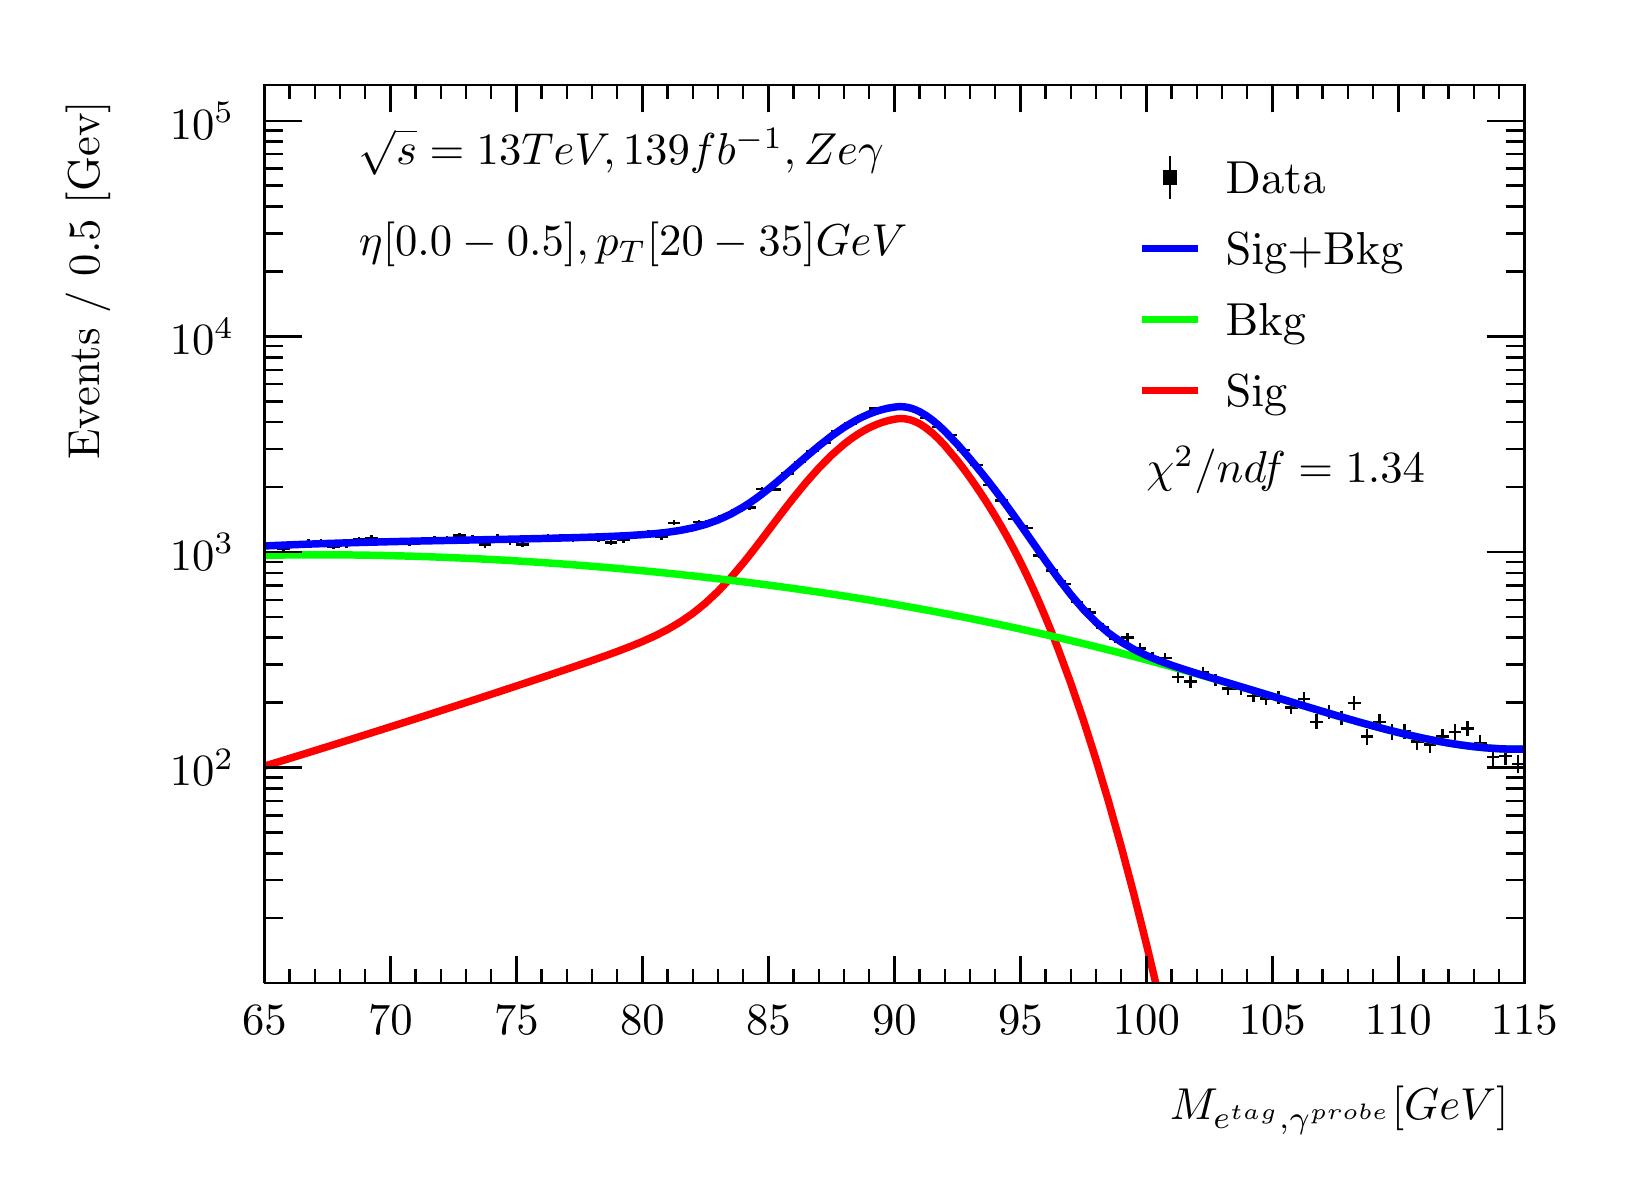
\begin{tikzpicture}
\pgfdeclareplotmark{cross} {
\pgfpathmoveto{\pgfpoint{-0.3\pgfplotmarksize}{\pgfplotmarksize}}
\pgfpathlineto{\pgfpoint{+0.3\pgfplotmarksize}{\pgfplotmarksize}}
\pgfpathlineto{\pgfpoint{+0.3\pgfplotmarksize}{0.3\pgfplotmarksize}}
\pgfpathlineto{\pgfpoint{+1\pgfplotmarksize}{0.3\pgfplotmarksize}}
\pgfpathlineto{\pgfpoint{+1\pgfplotmarksize}{-0.3\pgfplotmarksize}}
\pgfpathlineto{\pgfpoint{+0.3\pgfplotmarksize}{-0.3\pgfplotmarksize}}
\pgfpathlineto{\pgfpoint{+0.3\pgfplotmarksize}{-1.\pgfplotmarksize}}
\pgfpathlineto{\pgfpoint{-0.3\pgfplotmarksize}{-1.\pgfplotmarksize}}
\pgfpathlineto{\pgfpoint{-0.3\pgfplotmarksize}{-0.3\pgfplotmarksize}}
\pgfpathlineto{\pgfpoint{-1.\pgfplotmarksize}{-0.3\pgfplotmarksize}}
\pgfpathlineto{\pgfpoint{-1.\pgfplotmarksize}{0.3\pgfplotmarksize}}
\pgfpathlineto{\pgfpoint{-0.3\pgfplotmarksize}{0.3\pgfplotmarksize}}
\pgfpathclose
\pgfusepathqstroke
}
\pgfdeclareplotmark{cross*} {
\pgfpathmoveto{\pgfpoint{-0.3\pgfplotmarksize}{\pgfplotmarksize}}
\pgfpathlineto{\pgfpoint{+0.3\pgfplotmarksize}{\pgfplotmarksize}}
\pgfpathlineto{\pgfpoint{+0.3\pgfplotmarksize}{0.3\pgfplotmarksize}}
\pgfpathlineto{\pgfpoint{+1\pgfplotmarksize}{0.3\pgfplotmarksize}}
\pgfpathlineto{\pgfpoint{+1\pgfplotmarksize}{-0.3\pgfplotmarksize}}
\pgfpathlineto{\pgfpoint{+0.3\pgfplotmarksize}{-0.3\pgfplotmarksize}}
\pgfpathlineto{\pgfpoint{+0.3\pgfplotmarksize}{-1.\pgfplotmarksize}}
\pgfpathlineto{\pgfpoint{-0.3\pgfplotmarksize}{-1.\pgfplotmarksize}}
\pgfpathlineto{\pgfpoint{-0.3\pgfplotmarksize}{-0.3\pgfplotmarksize}}
\pgfpathlineto{\pgfpoint{-1.\pgfplotmarksize}{-0.3\pgfplotmarksize}}
\pgfpathlineto{\pgfpoint{-1.\pgfplotmarksize}{0.3\pgfplotmarksize}}
\pgfpathlineto{\pgfpoint{-0.3\pgfplotmarksize}{0.3\pgfplotmarksize}}
\pgfpathclose
\pgfusepathqfillstroke
}
\pgfdeclareplotmark{newstar} {
\pgfpathmoveto{\pgfqpoint{0pt}{\pgfplotmarksize}}
\pgfpathlineto{\pgfqpointpolar{44}{0.5\pgfplotmarksize}}
\pgfpathlineto{\pgfqpointpolar{18}{\pgfplotmarksize}}
\pgfpathlineto{\pgfqpointpolar{-20}{0.5\pgfplotmarksize}}
\pgfpathlineto{\pgfqpointpolar{-54}{\pgfplotmarksize}}
\pgfpathlineto{\pgfqpointpolar{-90}{0.5\pgfplotmarksize}}
\pgfpathlineto{\pgfqpointpolar{234}{\pgfplotmarksize}}
\pgfpathlineto{\pgfqpointpolar{198}{0.5\pgfplotmarksize}}
\pgfpathlineto{\pgfqpointpolar{162}{\pgfplotmarksize}}
\pgfpathlineto{\pgfqpointpolar{134}{0.5\pgfplotmarksize}}
\pgfpathclose
\pgfusepathqstroke
}
\pgfdeclareplotmark{newstar*} {
\pgfpathmoveto{\pgfqpoint{0pt}{\pgfplotmarksize}}
\pgfpathlineto{\pgfqpointpolar{44}{0.5\pgfplotmarksize}}
\pgfpathlineto{\pgfqpointpolar{18}{\pgfplotmarksize}}
\pgfpathlineto{\pgfqpointpolar{-20}{0.5\pgfplotmarksize}}
\pgfpathlineto{\pgfqpointpolar{-54}{\pgfplotmarksize}}
\pgfpathlineto{\pgfqpointpolar{-90}{0.5\pgfplotmarksize}}
\pgfpathlineto{\pgfqpointpolar{234}{\pgfplotmarksize}}
\pgfpathlineto{\pgfqpointpolar{198}{0.5\pgfplotmarksize}}
\pgfpathlineto{\pgfqpointpolar{162}{\pgfplotmarksize}}
\pgfpathlineto{\pgfqpointpolar{134}{0.5\pgfplotmarksize}}
\pgfpathclose
\pgfusepathqfillstroke
}
\definecolor{c}{rgb}{1,1,1};
\draw [color=c, fill=c] (0,0) rectangle (20,14.4361);
\draw [color=c, fill=c] (3,2.30977) rectangle (19,13.7143);
\definecolor{c}{rgb}{0,0,0};
\draw [c,line width=0.9] (3,2.30977) -- (3,13.7143) -- (19,13.7143) -- (19,2.30977) -- (3,2.30977);
\definecolor{c}{rgb}{1,1,1};
\draw [color=c, fill=c] (3,2.30977) rectangle (19,13.7143);
\definecolor{c}{rgb}{0,0,0};
\draw [c,line width=0.9] (3,2.30977) -- (3,13.7143) -- (19,13.7143) -- (19,2.30977) -- (3,2.30977);
\draw [c,line width=0.9] (3,2.30977) -- (19,2.30977);
\draw [c,line width=0.9] (3,2.65624) -- (3,2.30977);
\draw [c,line width=0.9] (3.32,2.48301) -- (3.32,2.30977);
\draw [c,line width=0.9] (3.64,2.48301) -- (3.64,2.30977);
\draw [c,line width=0.9] (3.96,2.48301) -- (3.96,2.30977);
\draw [c,line width=0.9] (4.28,2.48301) -- (4.28,2.30977);
\draw [c,line width=0.9] (4.6,2.65624) -- (4.6,2.30977);
\draw [c,line width=0.9] (4.92,2.48301) -- (4.92,2.30977);
\draw [c,line width=0.9] (5.24,2.48301) -- (5.24,2.30977);
\draw [c,line width=0.9] (5.56,2.48301) -- (5.56,2.30977);
\draw [c,line width=0.9] (5.88,2.48301) -- (5.88,2.30977);
\draw [c,line width=0.9] (6.2,2.65624) -- (6.2,2.30977);
\draw [c,line width=0.9] (6.52,2.48301) -- (6.52,2.30977);
\draw [c,line width=0.9] (6.84,2.48301) -- (6.84,2.30977);
\draw [c,line width=0.9] (7.16,2.48301) -- (7.16,2.30977);
\draw [c,line width=0.9] (7.48,2.48301) -- (7.48,2.30977);
\draw [c,line width=0.9] (7.8,2.65624) -- (7.8,2.30977);
\draw [c,line width=0.9] (8.12,2.48301) -- (8.12,2.30977);
\draw [c,line width=0.9] (8.44,2.48301) -- (8.44,2.30977);
\draw [c,line width=0.9] (8.76,2.48301) -- (8.76,2.30977);
\draw [c,line width=0.9] (9.08,2.48301) -- (9.08,2.30977);
\draw [c,line width=0.9] (9.4,2.65624) -- (9.4,2.30977);
\draw [c,line width=0.9] (9.72,2.48301) -- (9.72,2.30977);
\draw [c,line width=0.9] (10.04,2.48301) -- (10.04,2.30977);
\draw [c,line width=0.9] (10.36,2.48301) -- (10.36,2.30977);
\draw [c,line width=0.9] (10.68,2.48301) -- (10.68,2.30977);
\draw [c,line width=0.9] (11,2.65624) -- (11,2.30977);
\draw [c,line width=0.9] (11.32,2.48301) -- (11.32,2.30977);
\draw [c,line width=0.9] (11.64,2.48301) -- (11.64,2.30977);
\draw [c,line width=0.9] (11.96,2.48301) -- (11.96,2.30977);
\draw [c,line width=0.9] (12.28,2.48301) -- (12.28,2.30977);
\draw [c,line width=0.9] (12.6,2.65624) -- (12.6,2.30977);
\draw [c,line width=0.9] (12.92,2.48301) -- (12.92,2.30977);
\draw [c,line width=0.9] (13.24,2.48301) -- (13.24,2.30977);
\draw [c,line width=0.9] (13.56,2.48301) -- (13.56,2.30977);
\draw [c,line width=0.9] (13.88,2.48301) -- (13.88,2.30977);
\draw [c,line width=0.9] (14.2,2.65624) -- (14.2,2.30977);
\draw [c,line width=0.9] (14.52,2.48301) -- (14.52,2.30977);
\draw [c,line width=0.9] (14.84,2.48301) -- (14.84,2.30977);
\draw [c,line width=0.9] (15.16,2.48301) -- (15.16,2.30977);
\draw [c,line width=0.9] (15.48,2.48301) -- (15.48,2.30977);
\draw [c,line width=0.9] (15.8,2.65624) -- (15.8,2.30977);
\draw [c,line width=0.9] (16.12,2.48301) -- (16.12,2.30977);
\draw [c,line width=0.9] (16.44,2.48301) -- (16.44,2.30977);
\draw [c,line width=0.9] (16.76,2.48301) -- (16.76,2.30977);
\draw [c,line width=0.9] (17.08,2.48301) -- (17.08,2.30977);
\draw [c,line width=0.9] (17.4,2.65624) -- (17.4,2.30977);
\draw [c,line width=0.9] (17.72,2.48301) -- (17.72,2.30977);
\draw [c,line width=0.9] (18.04,2.48301) -- (18.04,2.30977);
\draw [c,line width=0.9] (18.36,2.48301) -- (18.36,2.30977);
\draw [c,line width=0.9] (18.68,2.48301) -- (18.68,2.30977);
\draw [c,line width=0.9] (19,2.65624) -- (19,2.30977);
\draw [c,line width=0.9] (19,2.65624) -- (19,2.30977);
\draw [anchor=base] (3,1.66015) node[scale=1.61424, color=c, rotate=0]{65};
\draw [anchor=base] (4.6,1.66015) node[scale=1.61424, color=c, rotate=0]{70};
\draw [anchor=base] (6.2,1.66015) node[scale=1.61424, color=c, rotate=0]{75};
\draw [anchor=base] (7.8,1.66015) node[scale=1.61424, color=c, rotate=0]{80};
\draw [anchor=base] (9.4,1.66015) node[scale=1.61424, color=c, rotate=0]{85};
\draw [anchor=base] (11,1.66015) node[scale=1.61424, color=c, rotate=0]{90};
\draw [anchor=base] (12.6,1.66015) node[scale=1.61424, color=c, rotate=0]{95};
\draw [anchor=base] (14.2,1.66015) node[scale=1.61424, color=c, rotate=0]{100};
\draw [anchor=base] (15.8,1.66015) node[scale=1.61424, color=c, rotate=0]{105};
\draw [anchor=base] (17.4,1.66015) node[scale=1.61424, color=c, rotate=0]{110};
\draw [anchor=base] (19,1.66015) node[scale=1.61424, color=c, rotate=0]{115};
\draw [anchor= east] (19,0.692932) node[scale=1.61424, color=c, rotate=0]{$M_{e^{tag}, \gamma^{probe}}  [GeV]$};
\draw [c,line width=0.9] (3,13.7143) -- (19,13.7143);
\draw [c,line width=0.9] (3,13.3678) -- (3,13.7143);
\draw [c,line width=0.9] (3.32,13.5411) -- (3.32,13.7143);
\draw [c,line width=0.9] (3.64,13.5411) -- (3.64,13.7143);
\draw [c,line width=0.9] (3.96,13.5411) -- (3.96,13.7143);
\draw [c,line width=0.9] (4.28,13.5411) -- (4.28,13.7143);
\draw [c,line width=0.9] (4.6,13.3678) -- (4.6,13.7143);
\draw [c,line width=0.9] (4.92,13.5411) -- (4.92,13.7143);
\draw [c,line width=0.9] (5.24,13.5411) -- (5.24,13.7143);
\draw [c,line width=0.9] (5.56,13.5411) -- (5.56,13.7143);
\draw [c,line width=0.9] (5.88,13.5411) -- (5.88,13.7143);
\draw [c,line width=0.9] (6.2,13.3678) -- (6.2,13.7143);
\draw [c,line width=0.9] (6.52,13.5411) -- (6.52,13.7143);
\draw [c,line width=0.9] (6.84,13.5411) -- (6.84,13.7143);
\draw [c,line width=0.9] (7.16,13.5411) -- (7.16,13.7143);
\draw [c,line width=0.9] (7.48,13.5411) -- (7.48,13.7143);
\draw [c,line width=0.9] (7.8,13.3678) -- (7.8,13.7143);
\draw [c,line width=0.9] (8.12,13.5411) -- (8.12,13.7143);
\draw [c,line width=0.9] (8.44,13.5411) -- (8.44,13.7143);
\draw [c,line width=0.9] (8.76,13.5411) -- (8.76,13.7143);
\draw [c,line width=0.9] (9.08,13.5411) -- (9.08,13.7143);
\draw [c,line width=0.9] (9.4,13.3678) -- (9.4,13.7143);
\draw [c,line width=0.9] (9.72,13.5411) -- (9.72,13.7143);
\draw [c,line width=0.9] (10.04,13.5411) -- (10.04,13.7143);
\draw [c,line width=0.9] (10.36,13.5411) -- (10.36,13.7143);
\draw [c,line width=0.9] (10.68,13.5411) -- (10.68,13.7143);
\draw [c,line width=0.9] (11,13.3678) -- (11,13.7143);
\draw [c,line width=0.9] (11.32,13.5411) -- (11.32,13.7143);
\draw [c,line width=0.9] (11.64,13.5411) -- (11.64,13.7143);
\draw [c,line width=0.9] (11.96,13.5411) -- (11.96,13.7143);
\draw [c,line width=0.9] (12.28,13.5411) -- (12.28,13.7143);
\draw [c,line width=0.9] (12.6,13.3678) -- (12.6,13.7143);
\draw [c,line width=0.9] (12.92,13.5411) -- (12.92,13.7143);
\draw [c,line width=0.9] (13.24,13.5411) -- (13.24,13.7143);
\draw [c,line width=0.9] (13.56,13.5411) -- (13.56,13.7143);
\draw [c,line width=0.9] (13.88,13.5411) -- (13.88,13.7143);
\draw [c,line width=0.9] (14.2,13.3678) -- (14.2,13.7143);
\draw [c,line width=0.9] (14.52,13.5411) -- (14.52,13.7143);
\draw [c,line width=0.9] (14.84,13.5411) -- (14.84,13.7143);
\draw [c,line width=0.9] (15.16,13.5411) -- (15.16,13.7143);
\draw [c,line width=0.9] (15.48,13.5411) -- (15.48,13.7143);
\draw [c,line width=0.9] (15.8,13.3678) -- (15.8,13.7143);
\draw [c,line width=0.9] (16.12,13.5411) -- (16.12,13.7143);
\draw [c,line width=0.9] (16.44,13.5411) -- (16.44,13.7143);
\draw [c,line width=0.9] (16.76,13.5411) -- (16.76,13.7143);
\draw [c,line width=0.9] (17.08,13.5411) -- (17.08,13.7143);
\draw [c,line width=0.9] (17.4,13.3678) -- (17.4,13.7143);
\draw [c,line width=0.9] (17.72,13.5411) -- (17.72,13.7143);
\draw [c,line width=0.9] (18.04,13.5411) -- (18.04,13.7143);
\draw [c,line width=0.9] (18.36,13.5411) -- (18.36,13.7143);
\draw [c,line width=0.9] (18.68,13.5411) -- (18.68,13.7143);
\draw [c,line width=0.9] (19,13.3678) -- (19,13.7143);
\draw [c,line width=0.9] (19,13.3678) -- (19,13.7143);
\draw [c,line width=0.9] (3,2.30977) -- (3,13.7143);
\draw [c,line width=0.9] (3.237,3.13385) -- (3,3.13385);
\draw [c,line width=0.9] (3.237,3.6159) -- (3,3.6159);
\draw [c,line width=0.9] (3.237,3.95792) -- (3,3.95792);
\draw [c,line width=0.9] (3.237,4.22321) -- (3,4.22321);
\draw [c,line width=0.9] (3.237,4.43997) -- (3,4.43997);
\draw [c,line width=0.9] (3.237,4.62324) -- (3,4.62324);
\draw [c,line width=0.9] (3.237,4.782) -- (3,4.782);
\draw [c,line width=0.9] (3.237,4.92203) -- (3,4.92203);
\draw [c,line width=0.9] (3.474,5.04729) -- (3,5.04729);
\draw [anchor= east] (2.82,5.04729) node[scale=1.61424, color=c, rotate=0]{$10^{2}$};
\draw [c,line width=0.9] (3.237,5.87136) -- (3,5.87136);
\draw [c,line width=0.9] (3.237,6.35342) -- (3,6.35342);
\draw [c,line width=0.9] (3.237,6.69544) -- (3,6.69544);
\draw [c,line width=0.9] (3.237,6.96073) -- (3,6.96073);
\draw [c,line width=0.9] (3.237,7.17749) -- (3,7.17749);
\draw [c,line width=0.9] (3.237,7.36076) -- (3,7.36076);
\draw [c,line width=0.9] (3.237,7.51951) -- (3,7.51951);
\draw [c,line width=0.9] (3.237,7.65954) -- (3,7.65954);
\draw [c,line width=0.9] (3.474,7.78481) -- (3,7.78481);
\draw [anchor= east] (2.82,7.78481) node[scale=1.61424, color=c, rotate=0]{$10^{3}$};
\draw [c,line width=0.9] (3.237,8.60888) -- (3,8.60888);
\draw [c,line width=0.9] (3.237,9.09093) -- (3,9.09093);
\draw [c,line width=0.9] (3.237,9.43296) -- (3,9.43296);
\draw [c,line width=0.9] (3.237,9.69825) -- (3,9.69825);
\draw [c,line width=0.9] (3.237,9.91501) -- (3,9.91501);
\draw [c,line width=0.9] (3.237,10.0983) -- (3,10.0983);
\draw [c,line width=0.9] (3.237,10.257) -- (3,10.257);
\draw [c,line width=0.9] (3.237,10.3971) -- (3,10.3971);
\draw [c,line width=0.9] (3.474,10.5223) -- (3,10.5223);
\draw [anchor= east] (2.82,10.5223) node[scale=1.61424, color=c, rotate=0]{$10^{4}$};
\draw [c,line width=0.9] (3.237,11.3464) -- (3,11.3464);
\draw [c,line width=0.9] (3.237,11.8285) -- (3,11.8285);
\draw [c,line width=0.9] (3.237,12.1705) -- (3,12.1705);
\draw [c,line width=0.9] (3.237,12.4358) -- (3,12.4358);
\draw [c,line width=0.9] (3.237,12.6525) -- (3,12.6525);
\draw [c,line width=0.9] (3.237,12.8358) -- (3,12.8358);
\draw [c,line width=0.9] (3.237,12.9945) -- (3,12.9945);
\draw [c,line width=0.9] (3.237,13.1346) -- (3,13.1346);
\draw [c,line width=0.9] (3.474,13.2598) -- (3,13.2598);
\draw [anchor= east] (2.82,13.2598) node[scale=1.61424, color=c, rotate=0]{$10^{5}$};
\draw [anchor= east] (0.76,13.7143) node[scale=1.61424, color=c, rotate=90]{Events / 0.5 [Gev]};
\draw [c,line width=0.9] (19,2.30977) -- (19,13.7143);
\draw [c,line width=0.9] (18.763,3.13385) -- (19,3.13385);
\draw [c,line width=0.9] (18.763,3.6159) -- (19,3.6159);
\draw [c,line width=0.9] (18.763,3.95792) -- (19,3.95792);
\draw [c,line width=0.9] (18.763,4.22321) -- (19,4.22321);
\draw [c,line width=0.9] (18.763,4.43997) -- (19,4.43997);
\draw [c,line width=0.9] (18.763,4.62324) -- (19,4.62324);
\draw [c,line width=0.9] (18.763,4.782) -- (19,4.782);
\draw [c,line width=0.9] (18.763,4.92203) -- (19,4.92203);
\draw [c,line width=0.9] (18.526,5.04729) -- (19,5.04729);
\draw [c,line width=0.9] (18.763,5.87136) -- (19,5.87136);
\draw [c,line width=0.9] (18.763,6.35342) -- (19,6.35342);
\draw [c,line width=0.9] (18.763,6.69544) -- (19,6.69544);
\draw [c,line width=0.9] (18.763,6.96073) -- (19,6.96073);
\draw [c,line width=0.9] (18.763,7.17749) -- (19,7.17749);
\draw [c,line width=0.9] (18.763,7.36076) -- (19,7.36076);
\draw [c,line width=0.9] (18.763,7.51951) -- (19,7.51951);
\draw [c,line width=0.9] (18.763,7.65954) -- (19,7.65954);
\draw [c,line width=0.9] (18.526,7.78481) -- (19,7.78481);
\draw [c,line width=0.9] (18.763,8.60888) -- (19,8.60888);
\draw [c,line width=0.9] (18.763,9.09093) -- (19,9.09093);
\draw [c,line width=0.9] (18.763,9.43296) -- (19,9.43296);
\draw [c,line width=0.9] (18.763,9.69825) -- (19,9.69825);
\draw [c,line width=0.9] (18.763,9.91501) -- (19,9.91501);
\draw [c,line width=0.9] (18.763,10.0983) -- (19,10.0983);
\draw [c,line width=0.9] (18.763,10.257) -- (19,10.257);
\draw [c,line width=0.9] (18.763,10.3971) -- (19,10.3971);
\draw [c,line width=0.9] (18.526,10.5223) -- (19,10.5223);
\draw [c,line width=0.9] (18.763,11.3464) -- (19,11.3464);
\draw [c,line width=0.9] (18.763,11.8285) -- (19,11.8285);
\draw [c,line width=0.9] (18.763,12.1705) -- (19,12.1705);
\draw [c,line width=0.9] (18.763,12.4358) -- (19,12.4358);
\draw [c,line width=0.9] (18.763,12.6525) -- (19,12.6525);
\draw [c,line width=0.9] (18.763,12.8358) -- (19,12.8358);
\draw [c,line width=0.9] (18.763,12.9945) -- (19,12.9945);
\draw [c,line width=0.9] (18.763,13.1346) -- (19,13.1346);
\draw [c,line width=0.9] (18.526,13.2598) -- (19,13.2598);
\draw [c,line width=0.9] (3.08,7.85744) -- (3,7.85744);
\draw [c,line width=0.9] (3,7.85744) -- (3,7.85744);
\draw [c,line width=0.9] (3.08,7.85744) -- (3.16,7.85744);
\draw [c,line width=0.9] (3.16,7.85744) -- (3.16,7.85744);
\draw [c,line width=0.9] (3.08,7.85744) -- (3.08,7.89391);
\draw [c,line width=0.9] (3.08,7.89391) -- (3.08,7.89391);
\draw [c,line width=0.9] (3.08,7.85744) -- (3.08,7.82098);
\draw [c,line width=0.9] (3.08,7.82098) -- (3.08,7.82098);
\draw [c,line width=0.9] (3.24,7.81995) -- (3.16,7.81995);
\draw [c,line width=0.9] (3.16,7.81995) -- (3.16,7.81995);
\draw [c,line width=0.9] (3.24,7.81995) -- (3.32,7.81995);
\draw [c,line width=0.9] (3.32,7.81995) -- (3.32,7.81995);
\draw [c,line width=0.9] (3.24,7.81995) -- (3.24,7.85699);
\draw [c,line width=0.9] (3.24,7.85699) -- (3.24,7.85699);
\draw [c,line width=0.9] (3.24,7.81995) -- (3.24,7.78291);
\draw [c,line width=0.9] (3.24,7.78291) -- (3.24,7.78291);
\draw [c,line width=0.9] (3.4,7.86968) -- (3.32,7.86968);
\draw [c,line width=0.9] (3.32,7.86968) -- (3.32,7.86968);
\draw [c,line width=0.9] (3.4,7.86968) -- (3.48,7.86968);
\draw [c,line width=0.9] (3.48,7.86968) -- (3.48,7.86968);
\draw [c,line width=0.9] (3.4,7.86968) -- (3.4,7.90596);
\draw [c,line width=0.9] (3.4,7.90596) -- (3.4,7.90596);
\draw [c,line width=0.9] (3.4,7.86968) -- (3.4,7.83341);
\draw [c,line width=0.9] (3.4,7.83341) -- (3.4,7.83341);
\draw [c,line width=0.9] (3.56,7.91209) -- (3.48,7.91209);
\draw [c,line width=0.9] (3.48,7.91209) -- (3.48,7.91209);
\draw [c,line width=0.9] (3.56,7.91209) -- (3.64,7.91209);
\draw [c,line width=0.9] (3.64,7.91209) -- (3.64,7.91209);
\draw [c,line width=0.9] (3.56,7.91209) -- (3.56,7.94772);
\draw [c,line width=0.9] (3.56,7.94772) -- (3.56,7.94772);
\draw [c,line width=0.9] (3.56,7.91209) -- (3.56,7.87645);
\draw [c,line width=0.9] (3.56,7.87645) -- (3.56,7.87645);
\draw [c,line width=0.9] (3.72,7.90995) -- (3.64,7.90995);
\draw [c,line width=0.9] (3.64,7.90995) -- (3.64,7.90995);
\draw [c,line width=0.9] (3.72,7.90995) -- (3.8,7.90995);
\draw [c,line width=0.9] (3.8,7.90995) -- (3.8,7.90995);
\draw [c,line width=0.9] (3.72,7.90995) -- (3.72,7.94562);
\draw [c,line width=0.9] (3.72,7.94562) -- (3.72,7.94562);
\draw [c,line width=0.9] (3.72,7.90995) -- (3.72,7.87428);
\draw [c,line width=0.9] (3.72,7.87428) -- (3.72,7.87428);
\draw [c,line width=0.9] (3.88,7.85408) -- (3.8,7.85408);
\draw [c,line width=0.9] (3.8,7.85408) -- (3.8,7.85408);
\draw [c,line width=0.9] (3.88,7.85408) -- (3.96,7.85408);
\draw [c,line width=0.9] (3.96,7.85408) -- (3.96,7.85408);
\draw [c,line width=0.9] (3.88,7.85408) -- (3.88,7.8906);
\draw [c,line width=0.9] (3.88,7.8906) -- (3.88,7.8906);
\draw [c,line width=0.9] (3.88,7.85408) -- (3.88,7.81757);
\draw [c,line width=0.9] (3.88,7.81757) -- (3.88,7.81757);
\draw [c,line width=0.9] (4.04,7.87189) -- (3.96,7.87189);
\draw [c,line width=0.9] (3.96,7.87189) -- (3.96,7.87189);
\draw [c,line width=0.9] (4.04,7.87189) -- (4.12,7.87189);
\draw [c,line width=0.9] (4.12,7.87189) -- (4.12,7.87189);
\draw [c,line width=0.9] (4.04,7.87189) -- (4.04,7.90814);
\draw [c,line width=0.9] (4.04,7.90814) -- (4.04,7.90814);
\draw [c,line width=0.9] (4.04,7.87189) -- (4.04,7.83565);
\draw [c,line width=0.9] (4.04,7.83565) -- (4.04,7.83565);
\draw [c,line width=0.9] (4.2,7.94163) -- (4.12,7.94163);
\draw [c,line width=0.9] (4.12,7.94163) -- (4.12,7.94163);
\draw [c,line width=0.9] (4.2,7.94163) -- (4.28,7.94163);
\draw [c,line width=0.9] (4.28,7.94163) -- (4.28,7.94163);
\draw [c,line width=0.9] (4.2,7.94163) -- (4.2,7.97682);
\draw [c,line width=0.9] (4.2,7.97682) -- (4.2,7.97682);
\draw [c,line width=0.9] (4.2,7.94163) -- (4.2,7.90643);
\draw [c,line width=0.9] (4.2,7.90643) -- (4.2,7.90643);
\draw [c,line width=0.9] (4.36,7.96229) -- (4.28,7.96229);
\draw [c,line width=0.9] (4.28,7.96229) -- (4.28,7.96229);
\draw [c,line width=0.9] (4.36,7.96229) -- (4.44,7.96229);
\draw [c,line width=0.9] (4.44,7.96229) -- (4.44,7.96229);
\draw [c,line width=0.9] (4.36,7.96229) -- (4.36,7.99718);
\draw [c,line width=0.9] (4.36,7.99718) -- (4.36,7.99718);
\draw [c,line width=0.9] (4.36,7.96229) -- (4.36,7.9274);
\draw [c,line width=0.9] (4.36,7.9274) -- (4.36,7.9274);
\draw [c,line width=0.9] (4.52,7.91422) -- (4.44,7.91422);
\draw [c,line width=0.9] (4.44,7.91422) -- (4.44,7.91422);
\draw [c,line width=0.9] (4.52,7.91422) -- (4.6,7.91422);
\draw [c,line width=0.9] (4.6,7.91422) -- (4.6,7.91422);
\draw [c,line width=0.9] (4.52,7.91422) -- (4.52,7.94983);
\draw [c,line width=0.9] (4.52,7.94983) -- (4.52,7.94983);
\draw [c,line width=0.9] (4.52,7.91422) -- (4.52,7.87862);
\draw [c,line width=0.9] (4.52,7.87862) -- (4.52,7.87862);
\draw [c,line width=0.9] (4.68,7.93221) -- (4.6,7.93221);
\draw [c,line width=0.9] (4.6,7.93221) -- (4.6,7.93221);
\draw [c,line width=0.9] (4.68,7.93221) -- (4.76,7.93221);
\draw [c,line width=0.9] (4.76,7.93221) -- (4.76,7.93221);
\draw [c,line width=0.9] (4.68,7.93221) -- (4.68,7.96755);
\draw [c,line width=0.9] (4.68,7.96755) -- (4.68,7.96755);
\draw [c,line width=0.9] (4.68,7.93221) -- (4.68,7.89688);
\draw [c,line width=0.9] (4.68,7.89688) -- (4.68,7.89688);
\draw [c,line width=0.9] (4.84,7.89487) -- (4.76,7.89487);
\draw [c,line width=0.9] (4.76,7.89487) -- (4.76,7.89487);
\draw [c,line width=0.9] (4.84,7.89487) -- (4.92,7.89487);
\draw [c,line width=0.9] (4.92,7.89487) -- (4.92,7.89487);
\draw [c,line width=0.9] (4.84,7.89487) -- (4.84,7.93077);
\draw [c,line width=0.9] (4.84,7.93077) -- (4.84,7.93077);
\draw [c,line width=0.9] (4.84,7.89487) -- (4.84,7.85898);
\draw [c,line width=0.9] (4.84,7.85898) -- (4.84,7.85898);
\draw [c,line width=0.9] (5,7.9385) -- (4.92,7.9385);
\draw [c,line width=0.9] (4.92,7.9385) -- (4.92,7.9385);
\draw [c,line width=0.9] (5,7.9385) -- (5.08,7.9385);
\draw [c,line width=0.9] (5.08,7.9385) -- (5.08,7.9385);
\draw [c,line width=0.9] (5,7.9385) -- (5,7.97374);
\draw [c,line width=0.9] (5,7.97374) -- (5,7.97374);
\draw [c,line width=0.9] (5,7.9385) -- (5,7.90326);
\draw [c,line width=0.9] (5,7.90326) -- (5,7.90326);
\draw [c,line width=0.9] (5.16,7.95303) -- (5.08,7.95303);
\draw [c,line width=0.9] (5.08,7.95303) -- (5.08,7.95303);
\draw [c,line width=0.9] (5.16,7.95303) -- (5.24,7.95303);
\draw [c,line width=0.9] (5.24,7.95303) -- (5.24,7.95303);
\draw [c,line width=0.9] (5.16,7.95303) -- (5.16,7.98806);
\draw [c,line width=0.9] (5.16,7.98806) -- (5.16,7.98806);
\draw [c,line width=0.9] (5.16,7.95303) -- (5.16,7.91801);
\draw [c,line width=0.9] (5.16,7.91801) -- (5.16,7.91801);
\draw [c,line width=0.9] (5.32,7.9551) -- (5.24,7.9551);
\draw [c,line width=0.9] (5.24,7.9551) -- (5.24,7.9551);
\draw [c,line width=0.9] (5.32,7.9551) -- (5.4,7.9551);
\draw [c,line width=0.9] (5.4,7.9551) -- (5.4,7.9551);
\draw [c,line width=0.9] (5.32,7.9551) -- (5.32,7.99009);
\draw [c,line width=0.9] (5.32,7.99009) -- (5.32,7.99009);
\draw [c,line width=0.9] (5.32,7.9551) -- (5.32,7.9201);
\draw [c,line width=0.9] (5.32,7.9201) -- (5.32,7.9201);
\draw [c,line width=0.9] (5.48,7.99361) -- (5.4,7.99361);
\draw [c,line width=0.9] (5.4,7.99361) -- (5.4,7.99361);
\draw [c,line width=0.9] (5.48,7.99361) -- (5.56,7.99361);
\draw [c,line width=0.9] (5.56,7.99361) -- (5.56,7.99361);
\draw [c,line width=0.9] (5.48,7.99361) -- (5.48,8.02805);
\draw [c,line width=0.9] (5.48,8.02805) -- (5.48,8.02805);
\draw [c,line width=0.9] (5.48,7.99361) -- (5.48,7.95918);
\draw [c,line width=0.9] (5.48,7.95918) -- (5.48,7.95918);
\draw [c,line width=0.9] (5.64,7.96433) -- (5.56,7.96433);
\draw [c,line width=0.9] (5.56,7.96433) -- (5.56,7.96433);
\draw [c,line width=0.9] (5.64,7.96433) -- (5.72,7.96433);
\draw [c,line width=0.9] (5.72,7.96433) -- (5.72,7.96433);
\draw [c,line width=0.9] (5.64,7.96433) -- (5.64,7.99919);
\draw [c,line width=0.9] (5.64,7.99919) -- (5.64,7.99919);
\draw [c,line width=0.9] (5.64,7.96433) -- (5.64,7.92947);
\draw [c,line width=0.9] (5.64,7.92947) -- (5.64,7.92947);
\draw [c,line width=0.9] (5.8,7.87631) -- (5.72,7.87631);
\draw [c,line width=0.9] (5.72,7.87631) -- (5.72,7.87631);
\draw [c,line width=0.9] (5.8,7.87631) -- (5.88,7.87631);
\draw [c,line width=0.9] (5.88,7.87631) -- (5.88,7.87631);
\draw [c,line width=0.9] (5.8,7.87631) -- (5.8,7.91248);
\draw [c,line width=0.9] (5.8,7.91248) -- (5.8,7.91248);
\draw [c,line width=0.9] (5.8,7.87631) -- (5.8,7.84013);
\draw [c,line width=0.9] (5.8,7.84013) -- (5.8,7.84013);
\draw [c,line width=0.9] (5.96,7.97552) -- (5.88,7.97552);
\draw [c,line width=0.9] (5.88,7.97552) -- (5.88,7.97552);
\draw [c,line width=0.9] (5.96,7.97552) -- (6.04,7.97552);
\draw [c,line width=0.9] (6.04,7.97552) -- (6.04,7.97552);
\draw [c,line width=0.9] (5.96,7.97552) -- (5.96,8.01022);
\draw [c,line width=0.9] (5.96,8.01022) -- (5.96,8.01022);
\draw [c,line width=0.9] (5.96,7.97552) -- (5.96,7.94083);
\draw [c,line width=0.9] (5.96,7.94083) -- (5.96,7.94083);
\draw [c,line width=0.9] (6.12,7.90888) -- (6.04,7.90888);
\draw [c,line width=0.9] (6.04,7.90888) -- (6.04,7.90888);
\draw [c,line width=0.9] (6.12,7.90888) -- (6.2,7.90888);
\draw [c,line width=0.9] (6.2,7.90888) -- (6.2,7.90888);
\draw [c,line width=0.9] (6.12,7.90888) -- (6.12,7.94456);
\draw [c,line width=0.9] (6.12,7.94456) -- (6.12,7.94456);
\draw [c,line width=0.9] (6.12,7.90888) -- (6.12,7.8732);
\draw [c,line width=0.9] (6.12,7.8732) -- (6.12,7.8732);
\draw [c,line width=0.9] (6.28,7.87851) -- (6.2,7.87851);
\draw [c,line width=0.9] (6.2,7.87851) -- (6.2,7.87851);
\draw [c,line width=0.9] (6.28,7.87851) -- (6.36,7.87851);
\draw [c,line width=0.9] (6.36,7.87851) -- (6.36,7.87851);
\draw [c,line width=0.9] (6.28,7.87851) -- (6.28,7.91465);
\draw [c,line width=0.9] (6.28,7.91465) -- (6.28,7.91465);
\draw [c,line width=0.9] (6.28,7.87851) -- (6.28,7.84236);
\draw [c,line width=0.9] (6.28,7.84236) -- (6.28,7.84236);
\draw [c,line width=0.9] (6.44,7.95716) -- (6.36,7.95716);
\draw [c,line width=0.9] (6.36,7.95716) -- (6.36,7.95716);
\draw [c,line width=0.9] (6.44,7.95716) -- (6.52,7.95716);
\draw [c,line width=0.9] (6.52,7.95716) -- (6.52,7.95716);
\draw [c,line width=0.9] (6.44,7.95716) -- (6.44,7.99212);
\draw [c,line width=0.9] (6.44,7.99212) -- (6.44,7.99212);
\draw [c,line width=0.9] (6.44,7.95716) -- (6.44,7.92219);
\draw [c,line width=0.9] (6.44,7.92219) -- (6.44,7.92219);
\draw [c,line width=0.9] (6.6,7.97957) -- (6.52,7.97957);
\draw [c,line width=0.9] (6.52,7.97957) -- (6.52,7.97957);
\draw [c,line width=0.9] (6.6,7.97957) -- (6.68,7.97957);
\draw [c,line width=0.9] (6.68,7.97957) -- (6.68,7.97957);
\draw [c,line width=0.9] (6.6,7.97957) -- (6.6,8.01421);
\draw [c,line width=0.9] (6.6,8.01421) -- (6.6,8.01421);
\draw [c,line width=0.9] (6.6,7.97957) -- (6.6,7.94493);
\draw [c,line width=0.9] (6.6,7.94493) -- (6.6,7.94493);
\draw [c,line width=0.9] (6.76,7.97755) -- (6.68,7.97755);
\draw [c,line width=0.9] (6.68,7.97755) -- (6.68,7.97755);
\draw [c,line width=0.9] (6.76,7.97755) -- (6.84,7.97755);
\draw [c,line width=0.9] (6.84,7.97755) -- (6.84,7.97755);
\draw [c,line width=0.9] (6.76,7.97755) -- (6.76,8.01222);
\draw [c,line width=0.9] (6.76,8.01222) -- (6.76,8.01222);
\draw [c,line width=0.9] (6.76,7.97755) -- (6.76,7.94288);
\draw [c,line width=0.9] (6.76,7.94288) -- (6.76,7.94288);
\draw [c,line width=0.9] (6.92,7.94683) -- (6.84,7.94683);
\draw [c,line width=0.9] (6.84,7.94683) -- (6.84,7.94683);
\draw [c,line width=0.9] (6.92,7.94683) -- (7,7.94683);
\draw [c,line width=0.9] (7,7.94683) -- (7,7.94683);
\draw [c,line width=0.9] (6.92,7.94683) -- (6.92,7.98194);
\draw [c,line width=0.9] (6.92,7.98194) -- (6.92,7.98194);
\draw [c,line width=0.9] (6.92,7.94683) -- (6.92,7.91171);
\draw [c,line width=0.9] (6.92,7.91171) -- (6.92,7.91171);
\draw [c,line width=0.9] (7.08,7.98159) -- (7,7.98159);
\draw [c,line width=0.9] (7,7.98159) -- (7,7.98159);
\draw [c,line width=0.9] (7.08,7.98159) -- (7.16,7.98159);
\draw [c,line width=0.9] (7.16,7.98159) -- (7.16,7.98159);
\draw [c,line width=0.9] (7.08,7.98159) -- (7.08,8.01619);
\draw [c,line width=0.9] (7.08,8.01619) -- (7.08,8.01619);
\draw [c,line width=0.9] (7.08,7.98159) -- (7.08,7.94698);
\draw [c,line width=0.9] (7.08,7.94698) -- (7.08,7.94698);
\draw [c,line width=0.9] (7.24,7.94475) -- (7.16,7.94475);
\draw [c,line width=0.9] (7.16,7.94475) -- (7.16,7.94475);
\draw [c,line width=0.9] (7.24,7.94475) -- (7.32,7.94475);
\draw [c,line width=0.9] (7.32,7.94475) -- (7.32,7.94475);
\draw [c,line width=0.9] (7.24,7.94475) -- (7.24,7.9799);
\draw [c,line width=0.9] (7.24,7.9799) -- (7.24,7.9799);
\draw [c,line width=0.9] (7.24,7.94475) -- (7.24,7.9096);
\draw [c,line width=0.9] (7.24,7.9096) -- (7.24,7.9096);
\draw [c,line width=0.9] (7.4,7.90351) -- (7.32,7.90351);
\draw [c,line width=0.9] (7.32,7.90351) -- (7.32,7.90351);
\draw [c,line width=0.9] (7.4,7.90351) -- (7.48,7.90351);
\draw [c,line width=0.9] (7.48,7.90351) -- (7.48,7.90351);
\draw [c,line width=0.9] (7.4,7.90351) -- (7.4,7.93928);
\draw [c,line width=0.9] (7.4,7.93928) -- (7.4,7.93928);
\draw [c,line width=0.9] (7.4,7.90351) -- (7.4,7.86775);
\draw [c,line width=0.9] (7.4,7.86775) -- (7.4,7.86775);
\draw [c,line width=0.9] (7.56,7.93536) -- (7.48,7.93536);
\draw [c,line width=0.9] (7.48,7.93536) -- (7.48,7.93536);
\draw [c,line width=0.9] (7.56,7.93536) -- (7.64,7.93536);
\draw [c,line width=0.9] (7.64,7.93536) -- (7.64,7.93536);
\draw [c,line width=0.9] (7.56,7.93536) -- (7.56,7.97065);
\draw [c,line width=0.9] (7.56,7.97065) -- (7.56,7.97065);
\draw [c,line width=0.9] (7.56,7.93536) -- (7.56,7.90007);
\draw [c,line width=0.9] (7.56,7.90007) -- (7.56,7.90007);
\draw [c,line width=0.9] (7.72,7.98259) -- (7.64,7.98259);
\draw [c,line width=0.9] (7.64,7.98259) -- (7.64,7.98259);
\draw [c,line width=0.9] (7.72,7.98259) -- (7.8,7.98259);
\draw [c,line width=0.9] (7.8,7.98259) -- (7.8,7.98259);
\draw [c,line width=0.9] (7.72,7.98259) -- (7.72,8.01719);
\draw [c,line width=0.9] (7.72,8.01719) -- (7.72,8.01719);
\draw [c,line width=0.9] (7.72,7.98259) -- (7.72,7.948);
\draw [c,line width=0.9] (7.72,7.948) -- (7.72,7.948);
\draw [c,line width=0.9] (7.88,8.03092) -- (7.8,8.03092);
\draw [c,line width=0.9] (7.8,8.03092) -- (7.8,8.03092);
\draw [c,line width=0.9] (7.88,8.03092) -- (7.96,8.03092);
\draw [c,line width=0.9] (7.96,8.03092) -- (7.96,8.03092);
\draw [c,line width=0.9] (7.88,8.03092) -- (7.88,8.06482);
\draw [c,line width=0.9] (7.88,8.06482) -- (7.88,8.06482);
\draw [c,line width=0.9] (7.88,8.03092) -- (7.88,7.99703);
\draw [c,line width=0.9] (7.88,7.99703) -- (7.88,7.99703);
\draw [c,line width=0.9] (8.04,7.97248) -- (7.96,7.97248);
\draw [c,line width=0.9] (7.96,7.97248) -- (7.96,7.97248);
\draw [c,line width=0.9] (8.04,7.97248) -- (8.12,7.97248);
\draw [c,line width=0.9] (8.12,7.97248) -- (8.12,7.97248);
\draw [c,line width=0.9] (8.04,7.97248) -- (8.04,8.00722);
\draw [c,line width=0.9] (8.04,8.00722) -- (8.04,8.00722);
\draw [c,line width=0.9] (8.04,7.97248) -- (8.04,7.93774);
\draw [c,line width=0.9] (8.04,7.93774) -- (8.04,7.93774);
\draw [c,line width=0.9] (8.2,8.15299) -- (8.12,8.15299);
\draw [c,line width=0.9] (8.12,8.15299) -- (8.12,8.15299);
\draw [c,line width=0.9] (8.2,8.15299) -- (8.28,8.15299);
\draw [c,line width=0.9] (8.28,8.15299) -- (8.28,8.15299);
\draw [c,line width=0.9] (8.2,8.15299) -- (8.2,8.18519);
\draw [c,line width=0.9] (8.2,8.18519) -- (8.2,8.18519);
\draw [c,line width=0.9] (8.2,8.15299) -- (8.2,8.12079);
\draw [c,line width=0.9] (8.2,8.12079) -- (8.2,8.12079);
\draw [c,line width=0.9] (8.36,8.0857) -- (8.28,8.0857);
\draw [c,line width=0.9] (8.28,8.0857) -- (8.28,8.0857);
\draw [c,line width=0.9] (8.36,8.0857) -- (8.44,8.0857);
\draw [c,line width=0.9] (8.44,8.0857) -- (8.44,8.0857);
\draw [c,line width=0.9] (8.36,8.0857) -- (8.36,8.11883);
\draw [c,line width=0.9] (8.36,8.11883) -- (8.36,8.11883);
\draw [c,line width=0.9] (8.36,8.0857) -- (8.36,8.05258);
\draw [c,line width=0.9] (8.36,8.05258) -- (8.36,8.05258);
\draw [c,line width=0.9] (8.52,8.16341) -- (8.44,8.16341);
\draw [c,line width=0.9] (8.44,8.16341) -- (8.44,8.16341);
\draw [c,line width=0.9] (8.52,8.16341) -- (8.6,8.16341);
\draw [c,line width=0.9] (8.6,8.16341) -- (8.6,8.16341);
\draw [c,line width=0.9] (8.52,8.16341) -- (8.52,8.19547);
\draw [c,line width=0.9] (8.52,8.19547) -- (8.52,8.19547);
\draw [c,line width=0.9] (8.52,8.16341) -- (8.52,8.13135);
\draw [c,line width=0.9] (8.52,8.13135) -- (8.52,8.13135);
\draw [c,line width=0.9] (8.68,8.17717) -- (8.6,8.17717);
\draw [c,line width=0.9] (8.6,8.17717) -- (8.6,8.17717);
\draw [c,line width=0.9] (8.68,8.17717) -- (8.76,8.17717);
\draw [c,line width=0.9] (8.76,8.17717) -- (8.76,8.17717);
\draw [c,line width=0.9] (8.68,8.17717) -- (8.68,8.20904);
\draw [c,line width=0.9] (8.68,8.20904) -- (8.68,8.20904);
\draw [c,line width=0.9] (8.68,8.17717) -- (8.68,8.14529);
\draw [c,line width=0.9] (8.68,8.14529) -- (8.68,8.14529);
\draw [c,line width=0.9] (8.84,8.23879) -- (8.76,8.23879);
\draw [c,line width=0.9] (8.76,8.23879) -- (8.76,8.23879);
\draw [c,line width=0.9] (8.84,8.23879) -- (8.92,8.23879);
\draw [c,line width=0.9] (8.92,8.23879) -- (8.92,8.23879);
\draw [c,line width=0.9] (8.84,8.23879) -- (8.84,8.26985);
\draw [c,line width=0.9] (8.84,8.26985) -- (8.84,8.26985);
\draw [c,line width=0.9] (8.84,8.23879) -- (8.84,8.20773);
\draw [c,line width=0.9] (8.84,8.20773) -- (8.84,8.20773);
\draw [c,line width=0.9] (9,8.31273) -- (8.92,8.31273);
\draw [c,line width=0.9] (8.92,8.31273) -- (8.92,8.31273);
\draw [c,line width=0.9] (9,8.31273) -- (9.08,8.31273);
\draw [c,line width=0.9] (9.08,8.31273) -- (9.08,8.31273);
\draw [c,line width=0.9] (9,8.31273) -- (9,8.34284);
\draw [c,line width=0.9] (9,8.34284) -- (9,8.34284);
\draw [c,line width=0.9] (9,8.31273) -- (9,8.28262);
\draw [c,line width=0.9] (9,8.28262) -- (9,8.28262);
\draw [c,line width=0.9] (9.16,8.351) -- (9.08,8.351);
\draw [c,line width=0.9] (9.08,8.351) -- (9.08,8.351);
\draw [c,line width=0.9] (9.16,8.351) -- (9.24,8.351);
\draw [c,line width=0.9] (9.24,8.351) -- (9.24,8.351);
\draw [c,line width=0.9] (9.16,8.351) -- (9.16,8.38063);
\draw [c,line width=0.9] (9.16,8.38063) -- (9.16,8.38063);
\draw [c,line width=0.9] (9.16,8.351) -- (9.16,8.32137);
\draw [c,line width=0.9] (9.16,8.32137) -- (9.16,8.32137);
\draw [c,line width=0.9] (9.32,8.58365) -- (9.24,8.58365);
\draw [c,line width=0.9] (9.24,8.58365) -- (9.24,8.58365);
\draw [c,line width=0.9] (9.32,8.58365) -- (9.4,8.58365);
\draw [c,line width=0.9] (9.4,8.58365) -- (9.4,8.58365);
\draw [c,line width=0.9] (9.32,8.58365) -- (9.32,8.61052);
\draw [c,line width=0.9] (9.32,8.61052) -- (9.32,8.61052);
\draw [c,line width=0.9] (9.32,8.58365) -- (9.32,8.55678);
\draw [c,line width=0.9] (9.32,8.55678) -- (9.32,8.55678);
\draw [c,line width=0.9] (9.48,8.58) -- (9.4,8.58);
\draw [c,line width=0.9] (9.4,8.58) -- (9.4,8.58);
\draw [c,line width=0.9] (9.48,8.58) -- (9.56,8.58);
\draw [c,line width=0.9] (9.56,8.58) -- (9.56,8.58);
\draw [c,line width=0.9] (9.48,8.58) -- (9.48,8.60691);
\draw [c,line width=0.9] (9.48,8.60691) -- (9.48,8.60691);
\draw [c,line width=0.9] (9.48,8.58) -- (9.48,8.55309);
\draw [c,line width=0.9] (9.48,8.55309) -- (9.48,8.55309);
\draw [c,line width=0.9] (9.64,8.77917) -- (9.56,8.77917);
\draw [c,line width=0.9] (9.56,8.77917) -- (9.56,8.77917);
\draw [c,line width=0.9] (9.64,8.77917) -- (9.72,8.77917);
\draw [c,line width=0.9] (9.72,8.77917) -- (9.72,8.77917);
\draw [c,line width=0.9] (9.64,8.77917) -- (9.64,8.80392);
\draw [c,line width=0.9] (9.64,8.80392) -- (9.64,8.80392);
\draw [c,line width=0.9] (9.64,8.77917) -- (9.64,8.75443);
\draw [c,line width=0.9] (9.64,8.75443) -- (9.64,8.75443);
\draw [c,line width=0.9] (9.8,8.92491) -- (9.72,8.92491);
\draw [c,line width=0.9] (9.72,8.92491) -- (9.72,8.92491);
\draw [c,line width=0.9] (9.8,8.92491) -- (9.88,8.92491);
\draw [c,line width=0.9] (9.88,8.92491) -- (9.88,8.92491);
\draw [c,line width=0.9] (9.8,8.92491) -- (9.8,8.94819);
\draw [c,line width=0.9] (9.8,8.94819) -- (9.8,8.94819);
\draw [c,line width=0.9] (9.8,8.92491) -- (9.8,8.90164);
\draw [c,line width=0.9] (9.8,8.90164) -- (9.8,8.90164);
\draw [c,line width=0.9] (9.96,9.0653) -- (9.88,9.0653);
\draw [c,line width=0.9] (9.88,9.0653) -- (9.88,9.0653);
\draw [c,line width=0.9] (9.96,9.0653) -- (10.04,9.0653);
\draw [c,line width=0.9] (10.04,9.0653) -- (10.04,9.0653);
\draw [c,line width=0.9] (9.96,9.0653) -- (9.96,9.08724);
\draw [c,line width=0.9] (9.96,9.08724) -- (9.96,9.08724);
\draw [c,line width=0.9] (9.96,9.0653) -- (9.96,9.04336);
\draw [c,line width=0.9] (9.96,9.04336) -- (9.96,9.04336);
\draw [c,line width=0.9] (10.12,9.16915) -- (10.04,9.16915);
\draw [c,line width=0.9] (10.04,9.16915) -- (10.04,9.16915);
\draw [c,line width=0.9] (10.12,9.16915) -- (10.2,9.16915);
\draw [c,line width=0.9] (10.2,9.16915) -- (10.2,9.16915);
\draw [c,line width=0.9] (10.12,9.16915) -- (10.12,9.19015);
\draw [c,line width=0.9] (10.12,9.19015) -- (10.12,9.19015);
\draw [c,line width=0.9] (10.12,9.16915) -- (10.12,9.14815);
\draw [c,line width=0.9] (10.12,9.14815) -- (10.12,9.14815);
\draw [c,line width=0.9] (10.28,9.32312) -- (10.2,9.32312);
\draw [c,line width=0.9] (10.2,9.32312) -- (10.2,9.32312);
\draw [c,line width=0.9] (10.28,9.32312) -- (10.36,9.32312);
\draw [c,line width=0.9] (10.36,9.32312) -- (10.36,9.32312);
\draw [c,line width=0.9] (10.28,9.32312) -- (10.28,9.3428);
\draw [c,line width=0.9] (10.28,9.3428) -- (10.28,9.3428);
\draw [c,line width=0.9] (10.28,9.32312) -- (10.28,9.30343);
\draw [c,line width=0.9] (10.28,9.30343) -- (10.28,9.30343);
\draw [c,line width=0.9] (10.44,9.41348) -- (10.36,9.41348);
\draw [c,line width=0.9] (10.36,9.41348) -- (10.36,9.41348);
\draw [c,line width=0.9] (10.44,9.41348) -- (10.52,9.41348);
\draw [c,line width=0.9] (10.52,9.41348) -- (10.52,9.41348);
\draw [c,line width=0.9] (10.44,9.41348) -- (10.44,9.43243);
\draw [c,line width=0.9] (10.44,9.43243) -- (10.44,9.43243);
\draw [c,line width=0.9] (10.44,9.41348) -- (10.44,9.39453);
\draw [c,line width=0.9] (10.44,9.39453) -- (10.44,9.39453);
\draw [c,line width=0.9] (10.6,9.51228) -- (10.52,9.51228);
\draw [c,line width=0.9] (10.52,9.51228) -- (10.52,9.51228);
\draw [c,line width=0.9] (10.6,9.51228) -- (10.68,9.51228);
\draw [c,line width=0.9] (10.68,9.51228) -- (10.68,9.51228);
\draw [c,line width=0.9] (10.6,9.51228) -- (10.6,9.53046);
\draw [c,line width=0.9] (10.6,9.53046) -- (10.6,9.53046);
\draw [c,line width=0.9] (10.6,9.51228) -- (10.6,9.4941);
\draw [c,line width=0.9] (10.6,9.4941) -- (10.6,9.4941);
\draw [c,line width=0.9] (10.76,9.60428) -- (10.68,9.60428);
\draw [c,line width=0.9] (10.68,9.60428) -- (10.68,9.60428);
\draw [c,line width=0.9] (10.76,9.60428) -- (10.84,9.60428);
\draw [c,line width=0.9] (10.84,9.60428) -- (10.84,9.60428);
\draw [c,line width=0.9] (10.76,9.60428) -- (10.76,9.62177);
\draw [c,line width=0.9] (10.76,9.62177) -- (10.76,9.62177);
\draw [c,line width=0.9] (10.76,9.60428) -- (10.76,9.58678);
\draw [c,line width=0.9] (10.76,9.58678) -- (10.76,9.58678);
\draw [c,line width=0.9] (10.92,9.62721) -- (10.84,9.62721);
\draw [c,line width=0.9] (10.84,9.62721) -- (10.84,9.62721);
\draw [c,line width=0.9] (10.92,9.62721) -- (11,9.62721);
\draw [c,line width=0.9] (11,9.62721) -- (11,9.62721);
\draw [c,line width=0.9] (10.92,9.62721) -- (10.92,9.64454);
\draw [c,line width=0.9] (10.92,9.64454) -- (10.92,9.64454);
\draw [c,line width=0.9] (10.92,9.62721) -- (10.92,9.60989);
\draw [c,line width=0.9] (10.92,9.60989) -- (10.92,9.60989);
\draw [c,line width=0.9] (11.08,9.60967) -- (11,9.60967);
\draw [c,line width=0.9] (11,9.60967) -- (11,9.60967);
\draw [c,line width=0.9] (11.08,9.60967) -- (11.16,9.60967);
\draw [c,line width=0.9] (11.16,9.60967) -- (11.16,9.60967);
\draw [c,line width=0.9] (11.08,9.60967) -- (11.08,9.62712);
\draw [c,line width=0.9] (11.08,9.62712) -- (11.08,9.62712);
\draw [c,line width=0.9] (11.08,9.60967) -- (11.08,9.59222);
\draw [c,line width=0.9] (11.08,9.59222) -- (11.08,9.59222);
\draw [c,line width=0.9] (11.24,9.60144) -- (11.16,9.60144);
\draw [c,line width=0.9] (11.16,9.60144) -- (11.16,9.60144);
\draw [c,line width=0.9] (11.24,9.60144) -- (11.32,9.60144);
\draw [c,line width=0.9] (11.32,9.60144) -- (11.32,9.60144);
\draw [c,line width=0.9] (11.24,9.60144) -- (11.24,9.61895);
\draw [c,line width=0.9] (11.24,9.61895) -- (11.24,9.61895);
\draw [c,line width=0.9] (11.24,9.60144) -- (11.24,9.58393);
\draw [c,line width=0.9] (11.24,9.58393) -- (11.24,9.58393);
\draw [c,line width=0.9] (11.4,9.48728) -- (11.32,9.48728);
\draw [c,line width=0.9] (11.32,9.48728) -- (11.32,9.48728);
\draw [c,line width=0.9] (11.4,9.48728) -- (11.48,9.48728);
\draw [c,line width=0.9] (11.48,9.48728) -- (11.48,9.48728);
\draw [c,line width=0.9] (11.4,9.48728) -- (11.4,9.50565);
\draw [c,line width=0.9] (11.4,9.50565) -- (11.4,9.50565);
\draw [c,line width=0.9] (11.4,9.48728) -- (11.4,9.4689);
\draw [c,line width=0.9] (11.4,9.4689) -- (11.4,9.4689);
\draw [c,line width=0.9] (11.56,9.36978) -- (11.48,9.36978);
\draw [c,line width=0.9] (11.48,9.36978) -- (11.48,9.36978);
\draw [c,line width=0.9] (11.56,9.36978) -- (11.64,9.36978);
\draw [c,line width=0.9] (11.64,9.36978) -- (11.64,9.36978);
\draw [c,line width=0.9] (11.56,9.36978) -- (11.56,9.38909);
\draw [c,line width=0.9] (11.56,9.38909) -- (11.56,9.38909);
\draw [c,line width=0.9] (11.56,9.36978) -- (11.56,9.35048);
\draw [c,line width=0.9] (11.56,9.35048) -- (11.56,9.35048);
\draw [c,line width=0.9] (11.72,9.27182) -- (11.64,9.27182);
\draw [c,line width=0.9] (11.64,9.27182) -- (11.64,9.27182);
\draw [c,line width=0.9] (11.72,9.27182) -- (11.8,9.27182);
\draw [c,line width=0.9] (11.8,9.27182) -- (11.8,9.27182);
\draw [c,line width=0.9] (11.72,9.27182) -- (11.72,9.29194);
\draw [c,line width=0.9] (11.72,9.29194) -- (11.72,9.29194);
\draw [c,line width=0.9] (11.72,9.27182) -- (11.72,9.25171);
\draw [c,line width=0.9] (11.72,9.25171) -- (11.72,9.25171);
\draw [c,line width=0.9] (11.88,9.08019) -- (11.8,9.08019);
\draw [c,line width=0.9] (11.8,9.08019) -- (11.8,9.08019);
\draw [c,line width=0.9] (11.88,9.08019) -- (11.96,9.08019);
\draw [c,line width=0.9] (11.96,9.08019) -- (11.96,9.08019);
\draw [c,line width=0.9] (11.88,9.08019) -- (11.88,9.10199);
\draw [c,line width=0.9] (11.88,9.10199) -- (11.88,9.10199);
\draw [c,line width=0.9] (11.88,9.08019) -- (11.88,9.05838);
\draw [c,line width=0.9] (11.88,9.05838) -- (11.88,9.05838);
\draw [c,line width=0.9] (12.04,8.89164) -- (11.96,8.89164);
\draw [c,line width=0.9] (11.96,8.89164) -- (11.96,8.89164);
\draw [c,line width=0.9] (12.04,8.89164) -- (12.12,8.89164);
\draw [c,line width=0.9] (12.12,8.89164) -- (12.12,8.89164);
\draw [c,line width=0.9] (12.04,8.89164) -- (12.04,8.91525);
\draw [c,line width=0.9] (12.04,8.91525) -- (12.04,8.91525);
\draw [c,line width=0.9] (12.04,8.89164) -- (12.04,8.86804);
\draw [c,line width=0.9] (12.04,8.86804) -- (12.04,8.86804);
\draw [c,line width=0.9] (12.2,8.6365) -- (12.12,8.6365);
\draw [c,line width=0.9] (12.12,8.6365) -- (12.12,8.6365);
\draw [c,line width=0.9] (12.2,8.6365) -- (12.28,8.6365);
\draw [c,line width=0.9] (12.28,8.6365) -- (12.28,8.6365);
\draw [c,line width=0.9] (12.2,8.6365) -- (12.2,8.66277);
\draw [c,line width=0.9] (12.2,8.66277) -- (12.2,8.66277);
\draw [c,line width=0.9] (12.2,8.6365) -- (12.2,8.61022);
\draw [c,line width=0.9] (12.2,8.61022) -- (12.2,8.61022);
\draw [c,line width=0.9] (12.36,8.43577) -- (12.28,8.43577);
\draw [c,line width=0.9] (12.28,8.43577) -- (12.28,8.43577);
\draw [c,line width=0.9] (12.36,8.43577) -- (12.44,8.43577);
\draw [c,line width=0.9] (12.44,8.43577) -- (12.44,8.43577);
\draw [c,line width=0.9] (12.36,8.43577) -- (12.36,8.46437);
\draw [c,line width=0.9] (12.36,8.46437) -- (12.36,8.46437);
\draw [c,line width=0.9] (12.36,8.43577) -- (12.36,8.40718);
\draw [c,line width=0.9] (12.36,8.40718) -- (12.36,8.40718);
\draw [c,line width=0.9] (12.52,8.20337) -- (12.44,8.20337);
\draw [c,line width=0.9] (12.44,8.20337) -- (12.44,8.20337);
\draw [c,line width=0.9] (12.52,8.20337) -- (12.6,8.20337);
\draw [c,line width=0.9] (12.6,8.20337) -- (12.6,8.20337);
\draw [c,line width=0.9] (12.52,8.20337) -- (12.52,8.2349);
\draw [c,line width=0.9] (12.52,8.2349) -- (12.52,8.2349);
\draw [c,line width=0.9] (12.52,8.20337) -- (12.52,8.17185);
\draw [c,line width=0.9] (12.52,8.17185) -- (12.52,8.17185);
\draw [c,line width=0.9] (12.68,8.09123) -- (12.6,8.09123);
\draw [c,line width=0.9] (12.6,8.09123) -- (12.6,8.09123);
\draw [c,line width=0.9] (12.68,8.09123) -- (12.76,8.09123);
\draw [c,line width=0.9] (12.76,8.09123) -- (12.76,8.09123);
\draw [c,line width=0.9] (12.68,8.09123) -- (12.68,8.12428);
\draw [c,line width=0.9] (12.68,8.12428) -- (12.68,8.12428);
\draw [c,line width=0.9] (12.68,8.09123) -- (12.68,8.05818);
\draw [c,line width=0.9] (12.68,8.05818) -- (12.68,8.05818);
\draw [c,line width=0.9] (12.84,7.73998) -- (12.76,7.73998);
\draw [c,line width=0.9] (12.76,7.73998) -- (12.76,7.73998);
\draw [c,line width=0.9] (12.84,7.73998) -- (12.92,7.73998);
\draw [c,line width=0.9] (12.92,7.73998) -- (12.92,7.73998);
\draw [c,line width=0.9] (12.84,7.73998) -- (12.84,7.77829);
\draw [c,line width=0.9] (12.84,7.77829) -- (12.84,7.77829);
\draw [c,line width=0.9] (12.84,7.73998) -- (12.84,7.70167);
\draw [c,line width=0.9] (12.84,7.70167) -- (12.84,7.70167);
\draw [c,line width=0.9] (13,7.55177) -- (12.92,7.55177);
\draw [c,line width=0.9] (12.92,7.55177) -- (12.92,7.55177);
\draw [c,line width=0.9] (13,7.55177) -- (13.08,7.55177);
\draw [c,line width=0.9] (13.08,7.55177) -- (13.08,7.55177);
\draw [c,line width=0.9] (13,7.55177) -- (13,7.59323);
\draw [c,line width=0.9] (13,7.59323) -- (13,7.59323);
\draw [c,line width=0.9] (13,7.55177) -- (13,7.5103);
\draw [c,line width=0.9] (13,7.5103) -- (13,7.5103);
\draw [c,line width=0.9] (13.16,7.37762) -- (13.08,7.37762);
\draw [c,line width=0.9] (13.08,7.37762) -- (13.08,7.37762);
\draw [c,line width=0.9] (13.16,7.37762) -- (13.24,7.37762);
\draw [c,line width=0.9] (13.24,7.37762) -- (13.24,7.37762);
\draw [c,line width=0.9] (13.16,7.37762) -- (13.16,7.42224);
\draw [c,line width=0.9] (13.16,7.42224) -- (13.16,7.42224);
\draw [c,line width=0.9] (13.16,7.37762) -- (13.16,7.33301);
\draw [c,line width=0.9] (13.16,7.33301) -- (13.16,7.33301);
\draw [c,line width=0.9] (13.32,7.15145) -- (13.24,7.15145);
\draw [c,line width=0.9] (13.24,7.15145) -- (13.24,7.15145);
\draw [c,line width=0.9] (13.32,7.15145) -- (13.4,7.15145);
\draw [c,line width=0.9] (13.4,7.15145) -- (13.4,7.15145);
\draw [c,line width=0.9] (13.32,7.15145) -- (13.32,7.20052);
\draw [c,line width=0.9] (13.32,7.20052) -- (13.32,7.20052);
\draw [c,line width=0.9] (13.32,7.15145) -- (13.32,7.10238);
\draw [c,line width=0.9] (13.32,7.10238) -- (13.32,7.10238);
\draw [c,line width=0.9] (13.48,7.01874) -- (13.4,7.01874);
\draw [c,line width=0.9] (13.4,7.01874) -- (13.4,7.01874);
\draw [c,line width=0.9] (13.48,7.01874) -- (13.56,7.01874);
\draw [c,line width=0.9] (13.56,7.01874) -- (13.56,7.01874);
\draw [c,line width=0.9] (13.48,7.01874) -- (13.48,7.07062);
\draw [c,line width=0.9] (13.48,7.07062) -- (13.48,7.07062);
\draw [c,line width=0.9] (13.48,7.01874) -- (13.48,6.96686);
\draw [c,line width=0.9] (13.48,6.96686) -- (13.48,6.96686);
\draw [c,line width=0.9] (13.64,6.82219) -- (13.56,6.82219);
\draw [c,line width=0.9] (13.56,6.82219) -- (13.56,6.82219);
\draw [c,line width=0.9] (13.64,6.82219) -- (13.72,6.82219);
\draw [c,line width=0.9] (13.72,6.82219) -- (13.72,6.82219);
\draw [c,line width=0.9] (13.64,6.82219) -- (13.64,6.87854);
\draw [c,line width=0.9] (13.64,6.87854) -- (13.64,6.87854);
\draw [c,line width=0.9] (13.64,6.82219) -- (13.64,6.76583);
\draw [c,line width=0.9] (13.64,6.76583) -- (13.64,6.76583);
\draw [c,line width=0.9] (13.8,6.68349) -- (13.72,6.68349);
\draw [c,line width=0.9] (13.72,6.68349) -- (13.72,6.68349);
\draw [c,line width=0.9] (13.8,6.68349) -- (13.88,6.68349);
\draw [c,line width=0.9] (13.88,6.68349) -- (13.88,6.68349);
\draw [c,line width=0.9] (13.8,6.68349) -- (13.8,6.74323);
\draw [c,line width=0.9] (13.8,6.74323) -- (13.8,6.74323);
\draw [c,line width=0.9] (13.8,6.68349) -- (13.8,6.62375);
\draw [c,line width=0.9] (13.8,6.62375) -- (13.8,6.62375);
\draw [c,line width=0.9] (13.96,6.69841) -- (13.88,6.69841);
\draw [c,line width=0.9] (13.88,6.69841) -- (13.88,6.69841);
\draw [c,line width=0.9] (13.96,6.69841) -- (14.04,6.69841);
\draw [c,line width=0.9] (14.04,6.69841) -- (14.04,6.69841);
\draw [c,line width=0.9] (13.96,6.69841) -- (13.96,6.75777);
\draw [c,line width=0.9] (13.96,6.75777) -- (13.96,6.75777);
\draw [c,line width=0.9] (13.96,6.69841) -- (13.96,6.63904);
\draw [c,line width=0.9] (13.96,6.63904) -- (13.96,6.63904);
\draw [c,line width=0.9] (14.12,6.56023) -- (14.04,6.56023);
\draw [c,line width=0.9] (14.04,6.56023) -- (14.04,6.56023);
\draw [c,line width=0.9] (14.12,6.56023) -- (14.2,6.56023);
\draw [c,line width=0.9] (14.2,6.56023) -- (14.2,6.56023);
\draw [c,line width=0.9] (14.12,6.56023) -- (14.12,6.62314);
\draw [c,line width=0.9] (14.12,6.62314) -- (14.12,6.62314);
\draw [c,line width=0.9] (14.12,6.56023) -- (14.12,6.49731);
\draw [c,line width=0.9] (14.12,6.49731) -- (14.12,6.49731);
\draw [c,line width=0.9] (14.28,6.45223) -- (14.2,6.45223);
\draw [c,line width=0.9] (14.2,6.45223) -- (14.2,6.45223);
\draw [c,line width=0.9] (14.28,6.45223) -- (14.36,6.45223);
\draw [c,line width=0.9] (14.36,6.45223) -- (14.36,6.45223);
\draw [c,line width=0.9] (14.28,6.45223) -- (14.28,6.51807);
\draw [c,line width=0.9] (14.28,6.51807) -- (14.28,6.51807);
\draw [c,line width=0.9] (14.28,6.45223) -- (14.28,6.38639);
\draw [c,line width=0.9] (14.28,6.38639) -- (14.28,6.38639);
\draw [c,line width=0.9] (14.44,6.43755) -- (14.36,6.43755);
\draw [c,line width=0.9] (14.36,6.43755) -- (14.36,6.43755);
\draw [c,line width=0.9] (14.44,6.43755) -- (14.52,6.43755);
\draw [c,line width=0.9] (14.52,6.43755) -- (14.52,6.43755);
\draw [c,line width=0.9] (14.44,6.43755) -- (14.44,6.5038);
\draw [c,line width=0.9] (14.44,6.5038) -- (14.44,6.5038);
\draw [c,line width=0.9] (14.44,6.43755) -- (14.44,6.37131);
\draw [c,line width=0.9] (14.44,6.37131) -- (14.44,6.37131);
\draw [c,line width=0.9] (14.6,6.19693) -- (14.52,6.19693);
\draw [c,line width=0.9] (14.52,6.19693) -- (14.52,6.19693);
\draw [c,line width=0.9] (14.6,6.19693) -- (14.68,6.19693);
\draw [c,line width=0.9] (14.68,6.19693) -- (14.68,6.19693);
\draw [c,line width=0.9] (14.6,6.19693) -- (14.6,6.27023);
\draw [c,line width=0.9] (14.6,6.27023) -- (14.6,6.27023);
\draw [c,line width=0.9] (14.6,6.19693) -- (14.6,6.12363);
\draw [c,line width=0.9] (14.6,6.12363) -- (14.6,6.12363);
\draw [c,line width=0.9] (14.76,6.13666) -- (14.68,6.13666);
\draw [c,line width=0.9] (14.68,6.13666) -- (14.68,6.13666);
\draw [c,line width=0.9] (14.76,6.13666) -- (14.84,6.13666);
\draw [c,line width=0.9] (14.84,6.13666) -- (14.84,6.13666);
\draw [c,line width=0.9] (14.76,6.13666) -- (14.76,6.21184);
\draw [c,line width=0.9] (14.76,6.21184) -- (14.76,6.21184);
\draw [c,line width=0.9] (14.76,6.13666) -- (14.76,6.06148);
\draw [c,line width=0.9] (14.76,6.06148) -- (14.76,6.06148);
\draw [c,line width=0.9] (14.92,6.25429) -- (14.84,6.25429);
\draw [c,line width=0.9] (14.84,6.25429) -- (14.84,6.25429);
\draw [c,line width=0.9] (14.92,6.25429) -- (15,6.25429);
\draw [c,line width=0.9] (15,6.25429) -- (15,6.25429);
\draw [c,line width=0.9] (14.92,6.25429) -- (14.92,6.32584);
\draw [c,line width=0.9] (14.92,6.32584) -- (14.92,6.32584);
\draw [c,line width=0.9] (14.92,6.25429) -- (14.92,6.18273);
\draw [c,line width=0.9] (14.92,6.18273) -- (14.92,6.18273);
\draw [c,line width=0.9] (15.08,6.15553) -- (15,6.15553);
\draw [c,line width=0.9] (15,6.15553) -- (15,6.15553);
\draw [c,line width=0.9] (15.08,6.15553) -- (15.16,6.15553);
\draw [c,line width=0.9] (15.16,6.15553) -- (15.16,6.15553);
\draw [c,line width=0.9] (15.08,6.15553) -- (15.08,6.23011);
\draw [c,line width=0.9] (15.08,6.23011) -- (15.08,6.23011);
\draw [c,line width=0.9] (15.08,6.15553) -- (15.08,6.08094);
\draw [c,line width=0.9] (15.08,6.08094) -- (15.08,6.08094);
\draw [c,line width=0.9] (15.24,6.04782) -- (15.16,6.04782);
\draw [c,line width=0.9] (15.16,6.04782) -- (15.16,6.04782);
\draw [c,line width=0.9] (15.24,6.04782) -- (15.32,6.04782);
\draw [c,line width=0.9] (15.32,6.04782) -- (15.32,6.04782);
\draw [c,line width=0.9] (15.24,6.04782) -- (15.24,6.12586);
\draw [c,line width=0.9] (15.24,6.12586) -- (15.24,6.12586);
\draw [c,line width=0.9] (15.24,6.04782) -- (15.24,5.96978);
\draw [c,line width=0.9] (15.24,5.96978) -- (15.24,5.96978);
\draw [c,line width=0.9] (15.4,6.04268) -- (15.32,6.04268);
\draw [c,line width=0.9] (15.32,6.04268) -- (15.32,6.04268);
\draw [c,line width=0.9] (15.4,6.04268) -- (15.48,6.04268);
\draw [c,line width=0.9] (15.48,6.04268) -- (15.48,6.04268);
\draw [c,line width=0.9] (15.4,6.04268) -- (15.4,6.12089);
\draw [c,line width=0.9] (15.4,6.12089) -- (15.4,6.12089);
\draw [c,line width=0.9] (15.4,6.04268) -- (15.4,5.96448);
\draw [c,line width=0.9] (15.4,5.96448) -- (15.4,5.96448);
\draw [c,line width=0.9] (15.56,5.95735) -- (15.48,5.95735);
\draw [c,line width=0.9] (15.48,5.95735) -- (15.48,5.95735);
\draw [c,line width=0.9] (15.56,5.95735) -- (15.64,5.95735);
\draw [c,line width=0.9] (15.64,5.95735) -- (15.64,5.95735);
\draw [c,line width=0.9] (15.56,5.95735) -- (15.56,6.03841);
\draw [c,line width=0.9] (15.56,6.03841) -- (15.56,6.03841);
\draw [c,line width=0.9] (15.56,5.95735) -- (15.56,5.87628);
\draw [c,line width=0.9] (15.56,5.87628) -- (15.56,5.87628);
\draw [c,line width=0.9] (15.72,5.9237) -- (15.64,5.9237);
\draw [c,line width=0.9] (15.64,5.9237) -- (15.64,5.9237);
\draw [c,line width=0.9] (15.72,5.9237) -- (15.8,5.9237);
\draw [c,line width=0.9] (15.8,5.9237) -- (15.8,5.9237);
\draw [c,line width=0.9] (15.72,5.9237) -- (15.72,6.00592);
\draw [c,line width=0.9] (15.72,6.00592) -- (15.72,6.00592);
\draw [c,line width=0.9] (15.72,5.9237) -- (15.72,5.84148);
\draw [c,line width=0.9] (15.72,5.84148) -- (15.72,5.84148);
\draw [c,line width=0.9] (15.88,5.94064) -- (15.8,5.94064);
\draw [c,line width=0.9] (15.8,5.94064) -- (15.8,5.94064);
\draw [c,line width=0.9] (15.88,5.94064) -- (15.96,5.94064);
\draw [c,line width=0.9] (15.96,5.94064) -- (15.96,5.94064);
\draw [c,line width=0.9] (15.88,5.94064) -- (15.88,6.02228);
\draw [c,line width=0.9] (15.88,6.02228) -- (15.88,6.02228);
\draw [c,line width=0.9] (15.88,5.94064) -- (15.88,5.859);
\draw [c,line width=0.9] (15.88,5.859) -- (15.88,5.859);
\draw [c,line width=0.9] (16.04,5.81038) -- (15.96,5.81038);
\draw [c,line width=0.9] (15.96,5.81038) -- (15.96,5.81038);
\draw [c,line width=0.9] (16.04,5.81038) -- (16.12,5.81038);
\draw [c,line width=0.9] (16.12,5.81038) -- (16.12,5.81038);
\draw [c,line width=0.9] (16.04,5.81038) -- (16.04,5.89662);
\draw [c,line width=0.9] (16.04,5.89662) -- (16.04,5.89662);
\draw [c,line width=0.9] (16.04,5.81038) -- (16.04,5.72415);
\draw [c,line width=0.9] (16.04,5.72415) -- (16.04,5.72415);
\draw [c,line width=0.9] (16.2,5.91799) -- (16.12,5.91799);
\draw [c,line width=0.9] (16.12,5.91799) -- (16.12,5.91799);
\draw [c,line width=0.9] (16.2,5.91799) -- (16.28,5.91799);
\draw [c,line width=0.9] (16.28,5.91799) -- (16.28,5.91799);
\draw [c,line width=0.9] (16.2,5.91799) -- (16.2,6.00041);
\draw [c,line width=0.9] (16.2,6.00041) -- (16.2,6.00041);
\draw [c,line width=0.9] (16.2,5.91799) -- (16.2,5.83558);
\draw [c,line width=0.9] (16.2,5.83558) -- (16.2,5.83558);
\draw [c,line width=0.9] (16.36,5.62816) -- (16.28,5.62816);
\draw [c,line width=0.9] (16.28,5.62816) -- (16.28,5.62816);
\draw [c,line width=0.9] (16.36,5.62816) -- (16.44,5.62816);
\draw [c,line width=0.9] (16.44,5.62816) -- (16.44,5.62816);
\draw [c,line width=0.9] (16.36,5.62816) -- (16.36,5.72125);
\draw [c,line width=0.9] (16.36,5.72125) -- (16.36,5.72125);
\draw [c,line width=0.9] (16.36,5.62816) -- (16.36,5.53506);
\draw [c,line width=0.9] (16.36,5.53506) -- (16.36,5.53506);
\draw [c,line width=0.9] (16.52,5.75269) -- (16.44,5.75269);
\draw [c,line width=0.9] (16.44,5.75269) -- (16.44,5.75269);
\draw [c,line width=0.9] (16.52,5.75269) -- (16.6,5.75269);
\draw [c,line width=0.9] (16.6,5.75269) -- (16.6,5.75269);
\draw [c,line width=0.9] (16.52,5.75269) -- (16.52,5.84104);
\draw [c,line width=0.9] (16.52,5.84104) -- (16.52,5.84104);
\draw [c,line width=0.9] (16.52,5.75269) -- (16.52,5.66434);
\draw [c,line width=0.9] (16.52,5.66434) -- (16.52,5.66434);
\draw [c,line width=0.9] (16.68,5.67815) -- (16.6,5.67815);
\draw [c,line width=0.9] (16.6,5.67815) -- (16.6,5.67815);
\draw [c,line width=0.9] (16.68,5.67815) -- (16.76,5.67815);
\draw [c,line width=0.9] (16.76,5.67815) -- (16.76,5.67815);
\draw [c,line width=0.9] (16.68,5.67815) -- (16.68,5.76931);
\draw [c,line width=0.9] (16.68,5.76931) -- (16.68,5.76931);
\draw [c,line width=0.9] (16.68,5.67815) -- (16.68,5.58699);
\draw [c,line width=0.9] (16.68,5.58699) -- (16.68,5.58699);
\draw [c,line width=0.9] (16.84,5.86541) -- (16.76,5.86541);
\draw [c,line width=0.9] (16.76,5.86541) -- (16.76,5.86541);
\draw [c,line width=0.9] (16.84,5.86541) -- (16.92,5.86541);
\draw [c,line width=0.9] (16.92,5.86541) -- (16.92,5.86541);
\draw [c,line width=0.9] (16.84,5.86541) -- (16.84,5.94967);
\draw [c,line width=0.9] (16.84,5.94967) -- (16.84,5.94967);
\draw [c,line width=0.9] (16.84,5.86541) -- (16.84,5.78115);
\draw [c,line width=0.9] (16.84,5.78115) -- (16.84,5.78115);
\draw [c,line width=0.9] (17,5.4388) -- (16.92,5.4388);
\draw [c,line width=0.9] (16.92,5.4388) -- (16.92,5.4388);
\draw [c,line width=0.9] (17,5.4388) -- (17.08,5.4388);
\draw [c,line width=0.9] (17.08,5.4388) -- (17.08,5.4388);
\draw [c,line width=0.9] (17,5.4388) -- (17,5.53961);
\draw [c,line width=0.9] (17,5.53961) -- (17,5.53961);
\draw [c,line width=0.9] (17,5.4388) -- (17,5.33799);
\draw [c,line width=0.9] (17,5.33799) -- (17,5.33799);
\draw [c,line width=0.9] (17.16,5.62816) -- (17.08,5.62816);
\draw [c,line width=0.9] (17.08,5.62816) -- (17.08,5.62816);
\draw [c,line width=0.9] (17.16,5.62816) -- (17.24,5.62816);
\draw [c,line width=0.9] (17.24,5.62816) -- (17.24,5.62816);
\draw [c,line width=0.9] (17.16,5.62816) -- (17.16,5.72125);
\draw [c,line width=0.9] (17.16,5.72125) -- (17.16,5.72125);
\draw [c,line width=0.9] (17.16,5.62816) -- (17.16,5.53506);
\draw [c,line width=0.9] (17.16,5.53506) -- (17.16,5.53506);
\draw [c,line width=0.9] (17.32,5.49721) -- (17.24,5.49721);
\draw [c,line width=0.9] (17.24,5.49721) -- (17.24,5.49721);
\draw [c,line width=0.9] (17.32,5.49721) -- (17.4,5.49721);
\draw [c,line width=0.9] (17.4,5.49721) -- (17.4,5.49721);
\draw [c,line width=0.9] (17.32,5.49721) -- (17.32,5.59557);
\draw [c,line width=0.9] (17.32,5.59557) -- (17.32,5.59557);
\draw [c,line width=0.9] (17.32,5.49721) -- (17.32,5.39884);
\draw [c,line width=0.9] (17.32,5.39884) -- (17.32,5.39884);
\draw [c,line width=0.9] (17.48,5.50532) -- (17.4,5.50532);
\draw [c,line width=0.9] (17.4,5.50532) -- (17.4,5.50532);
\draw [c,line width=0.9] (17.48,5.50532) -- (17.56,5.50532);
\draw [c,line width=0.9] (17.56,5.50532) -- (17.56,5.50532);
\draw [c,line width=0.9] (17.48,5.50532) -- (17.48,5.60335);
\draw [c,line width=0.9] (17.48,5.60335) -- (17.48,5.60335);
\draw [c,line width=0.9] (17.48,5.50532) -- (17.48,5.40729);
\draw [c,line width=0.9] (17.48,5.40729) -- (17.48,5.40729);
\draw [c,line width=0.9] (17.64,5.37736) -- (17.56,5.37736);
\draw [c,line width=0.9] (17.56,5.37736) -- (17.56,5.37736);
\draw [c,line width=0.9] (17.64,5.37736) -- (17.72,5.37736);
\draw [c,line width=0.9] (17.72,5.37736) -- (17.72,5.37736);
\draw [c,line width=0.9] (17.64,5.37736) -- (17.64,5.48081);
\draw [c,line width=0.9] (17.64,5.48081) -- (17.64,5.48081);
\draw [c,line width=0.9] (17.64,5.37736) -- (17.64,5.27392);
\draw [c,line width=0.9] (17.64,5.27392) -- (17.64,5.27392);
\draw [c,line width=0.9] (17.8,5.34078) -- (17.72,5.34078);
\draw [c,line width=0.9] (17.72,5.34078) -- (17.72,5.34078);
\draw [c,line width=0.9] (17.8,5.34078) -- (17.88,5.34078);
\draw [c,line width=0.9] (17.88,5.34078) -- (17.88,5.34078);
\draw [c,line width=0.9] (17.8,5.34078) -- (17.8,5.44583);
\draw [c,line width=0.9] (17.8,5.44583) -- (17.8,5.44583);
\draw [c,line width=0.9] (17.8,5.34078) -- (17.8,5.23573);
\draw [c,line width=0.9] (17.8,5.23573) -- (17.8,5.23573);
\draw [c,line width=0.9] (17.96,5.4388) -- (17.88,5.4388);
\draw [c,line width=0.9] (17.88,5.4388) -- (17.88,5.4388);
\draw [c,line width=0.9] (17.96,5.4388) -- (18.04,5.4388);
\draw [c,line width=0.9] (18.04,5.4388) -- (18.04,5.4388);
\draw [c,line width=0.9] (17.96,5.4388) -- (17.96,5.53961);
\draw [c,line width=0.9] (17.96,5.53961) -- (17.96,5.53961);
\draw [c,line width=0.9] (17.96,5.4388) -- (17.96,5.33799);
\draw [c,line width=0.9] (17.96,5.33799) -- (17.96,5.33799);
\draw [c,line width=0.9] (18.12,5.49721) -- (18.04,5.49721);
\draw [c,line width=0.9] (18.04,5.49721) -- (18.04,5.49721);
\draw [c,line width=0.9] (18.12,5.49721) -- (18.2,5.49721);
\draw [c,line width=0.9] (18.2,5.49721) -- (18.2,5.49721);
\draw [c,line width=0.9] (18.12,5.49721) -- (18.12,5.59557);
\draw [c,line width=0.9] (18.12,5.59557) -- (18.12,5.59557);
\draw [c,line width=0.9] (18.12,5.49721) -- (18.12,5.39884);
\draw [c,line width=0.9] (18.12,5.39884) -- (18.12,5.39884);
\draw [c,line width=0.9] (18.28,5.54509) -- (18.2,5.54509);
\draw [c,line width=0.9] (18.2,5.54509) -- (18.2,5.54509);
\draw [c,line width=0.9] (18.28,5.54509) -- (18.36,5.54509);
\draw [c,line width=0.9] (18.36,5.54509) -- (18.36,5.54509);
\draw [c,line width=0.9] (18.28,5.54509) -- (18.28,5.6415);
\draw [c,line width=0.9] (18.28,5.6415) -- (18.28,5.6415);
\draw [c,line width=0.9] (18.28,5.54509) -- (18.28,5.44869);
\draw [c,line width=0.9] (18.28,5.44869) -- (18.28,5.44869);
\draw [c,line width=0.9] (18.44,5.35921) -- (18.36,5.35921);
\draw [c,line width=0.9] (18.36,5.35921) -- (18.36,5.35921);
\draw [c,line width=0.9] (18.44,5.35921) -- (18.52,5.35921);
\draw [c,line width=0.9] (18.52,5.35921) -- (18.52,5.35921);
\draw [c,line width=0.9] (18.44,5.35921) -- (18.44,5.46345);
\draw [c,line width=0.9] (18.44,5.46345) -- (18.44,5.46345);
\draw [c,line width=0.9] (18.44,5.35921) -- (18.44,5.25497);
\draw [c,line width=0.9] (18.44,5.25497) -- (18.44,5.25497);
\draw [c,line width=0.9] (18.6,5.18203) -- (18.52,5.18203);
\draw [c,line width=0.9] (18.52,5.18203) -- (18.52,5.18203);
\draw [c,line width=0.9] (18.6,5.18203) -- (18.68,5.18203);
\draw [c,line width=0.9] (18.68,5.18203) -- (18.68,5.18203);
\draw [c,line width=0.9] (18.6,5.18203) -- (18.6,5.29432);
\draw [c,line width=0.9] (18.6,5.29432) -- (18.6,5.29432);
\draw [c,line width=0.9] (18.6,5.18203) -- (18.6,5.06973);
\draw [c,line width=0.9] (18.6,5.06973) -- (18.6,5.06973);
\draw [c,line width=0.9] (18.76,5.19259) -- (18.68,5.19259);
\draw [c,line width=0.9] (18.68,5.19259) -- (18.68,5.19259);
\draw [c,line width=0.9] (18.76,5.19259) -- (18.84,5.19259);
\draw [c,line width=0.9] (18.84,5.19259) -- (18.84,5.19259);
\draw [c,line width=0.9] (18.76,5.19259) -- (18.76,5.30439);
\draw [c,line width=0.9] (18.76,5.30439) -- (18.76,5.30439);
\draw [c,line width=0.9] (18.76,5.19259) -- (18.76,5.08079);
\draw [c,line width=0.9] (18.76,5.08079) -- (18.76,5.08079);
\draw [c,line width=0.9] (18.92,5.09392) -- (18.84,5.09392);
\draw [c,line width=0.9] (18.84,5.09392) -- (18.84,5.09392);
\draw [c,line width=0.9] (18.92,5.09392) -- (19,5.09392);
\draw [c,line width=0.9] (19,5.09392) -- (19,5.09392);
\draw [c,line width=0.9] (18.92,5.09392) -- (18.92,5.21045);
\draw [c,line width=0.9] (18.92,5.21045) -- (18.92,5.21045);
\draw [c,line width=0.9] (18.92,5.09392) -- (18.92,4.97739);
\draw [c,line width=0.9] (18.92,4.97739) -- (18.92,4.97739);
\foreach \P in {(3.08,7.85744), (3.24,7.81995), (3.4,7.86968), (3.56,7.91209), (3.72,7.90995), (3.88,7.85408), (4.04,7.87189), (4.2,7.94163), (4.36,7.96229), (4.52,7.91422), (4.68,7.93221), (4.84,7.89487), (5,7.9385), (5.16,7.95303), (5.32,7.9551),
 (5.48,7.99361), (5.64,7.96433), (5.8,7.87631), (5.96,7.97552), (6.12,7.90888), (6.28,7.87851), (6.44,7.95716), (6.6,7.97957), (6.76,7.97755), (6.92,7.94683), (7.08,7.98159), (7.24,7.94475), (7.4,7.90351), (7.56,7.93536), (7.72,7.98259),
 (7.88,8.03092), (8.04,7.97248), (8.2,8.15299), (8.36,8.0857), (8.52,8.16341), (8.68,8.17717), (8.84,8.23879), (9,8.31273), (9.16,8.351), (9.32,8.58365), (9.48,8.58), (9.64,8.77917), (9.8,8.92491), (9.96,9.0653), (10.12,9.16915), (10.28,9.32312),
 (10.44,9.41348), (10.6,9.51228), (10.76,9.60428), (10.92,9.62721), (11.08,9.60967), (11.24,9.60144), (11.4,9.48728), (11.56,9.36978), (11.72,9.27182), (11.88,9.08019), (12.04,8.89164), (12.2,8.6365), (12.36,8.43577), (12.52,8.20337),
 (12.68,8.09123), (12.84,7.73998), (13,7.55177), (13.16,7.37762), (13.32,7.15145), (13.48,7.01874), (13.64,6.82219), (13.8,6.68349), (13.96,6.69841), (14.12,6.56023), (14.28,6.45223), (14.44,6.43755), (14.6,6.19693), (14.76,6.13666), (14.92,6.25429),
 (15.08,6.15553), (15.24,6.04782), (15.4,6.04268), (15.56,5.95735), (15.72,5.9237), (15.88,5.94064), (16.04,5.81038), (16.2,5.91799), (16.36,5.62816), (16.52,5.75269), (16.68,5.67815), (16.84,5.86541), (17,5.4388), (17.16,5.62816), (17.32,5.49721),
 (17.48,5.50532), (17.64,5.37736), (17.8,5.34078), (17.96,5.4388), (18.12,5.49721), (18.28,5.54509), (18.44,5.35921), (18.6,5.18203), (18.76,5.19259), (18.92,5.09392)}{\draw[mark options={color=c,fill=c},mark size=2.882883pt,mark=] plot coordinates
 {\P};}
\definecolor{c}{rgb}{1,0,0};
\draw [c,line width=2.7] (3,5.06429) -- (3,5.06429);
\draw [c,line width=2.7] (3,5.06429) -- (3.16,5.1134) -- (3.32,5.16268) -- (3.48,5.21215) -- (3.64,5.2618) -- (3.8,5.31164) -- (3.96,5.36166) -- (4.12,5.41186) -- (4.28,5.46226) -- (4.44,5.51285) -- (4.6,5.56363) -- (4.76,5.6146) -- (4.92,5.66577) --
 (5.08,5.71714) -- (5.24,5.7687) -- (5.4,5.82047) -- (5.56,5.87244) -- (5.72,5.92461) -- (5.88,5.977) -- (6.04,6.0296) -- (6.2,6.08241) -- (6.36,6.13546) -- (6.52,6.18874) -- (6.68,6.2423) -- (6.84,6.29618) -- (7,6.35052) -- (7.16,6.40568) --
 (7.32,6.46207) -- (7.48,6.52031) -- (7.64,6.58143) -- (7.8,6.64697) -- (7.96,6.71906) -- (8.12,6.80049) -- (8.28,6.89455) -- (8.44,7.00469) -- (8.6,7.13392) -- (8.76,7.284) -- (8.92,7.45471) -- (9.08,7.64358) -- (9.16,7.74346) -- (9.24,7.84604) --
 (9.32,7.95055) -- (9.4,8.05618) -- (9.48,8.1621) -- (9.56,8.26753) -- (9.64,8.37168) -- (9.72,8.47385) -- (9.88,8.66961) -- (10.04,8.85024) -- (10.2,9.01211) -- (10.36,9.1525) -- (10.44,9.214) -- (10.52,9.26946) -- (10.6,9.31873) -- (10.68,9.36172)
 -- (10.76,9.39835) -- (10.84,9.42859) -- (10.92,9.45244) -- (11,9.46993) -- (11.04,9.47604) -- (11.08,9.47852) -- (11.12,9.47705) -- (11.16,9.47164) -- (11.2,9.46231) -- (11.24,9.44916) -- (11.28,9.43225) -- (11.32,9.41172) -- (11.36,9.3877) --
 (11.4,9.36035) -- (11.48,9.29635) -- (11.56,9.22123) -- (11.64,9.13658) -- (11.8,8.94454) -- (11.88,8.83951) -- (11.96,8.72949) -- (12.04,8.61477) -- (12.12,8.49535) -- (12.2,8.37096) -- (12.28,8.24115) -- (12.36,8.10543) -- (12.44,7.96327) --
 (12.52,7.81421) -- (12.6,7.65784) -- (12.68,7.49384) -- (12.76,7.32197) -- (12.84,7.14205) -- (12.92,6.95396) -- (13,6.7576) -- (13.08,6.55294) -- (13.24,6.11856) -- (13.4,5.65068) -- (13.56,5.14926) -- (13.72,4.61428) -- (13.88,4.04574) --
 (14.04,3.44364) -- (14.2,2.80797) -- (14.3191,2.30977);
\definecolor{c}{rgb}{0,1,0};
\draw [c,line width=2.7] (3,7.74175) -- (3,7.74175);
\draw [c,line width=2.7] (3,7.74175) -- (3.16,7.74453) -- (3.32,7.74656) -- (3.48,7.74786) -- (3.64,7.74845) -- (3.8,7.74835) -- (3.96,7.74757) -- (4.12,7.74612) -- (4.28,7.74402) -- (4.44,7.74127) -- (4.6,7.73789) -- (4.76,7.73389) -- (4.92,7.72927)
 -- (5.08,7.72405) -- (5.24,7.71822) -- (5.4,7.7118) -- (5.56,7.70479) -- (5.72,7.69719) -- (5.88,7.68901) -- (6.04,7.68026) -- (6.2,7.67093) -- (6.36,7.66104) -- (6.52,7.65057) -- (6.68,7.63953) -- (6.84,7.62793) -- (7,7.61576) -- (7.16,7.60303) --
 (7.32,7.58973) -- (7.48,7.57586) -- (7.64,7.56142) -- (7.8,7.54641) -- (7.96,7.53083) -- (8.12,7.51467) -- (8.28,7.49793) -- (8.44,7.48061) -- (8.6,7.46271) -- (8.76,7.44421) -- (8.92,7.42512) -- (9.08,7.40543) -- (9.24,7.38513) -- (9.4,7.36422) --
 (9.56,7.3427) -- (9.72,7.32055) -- (9.88,7.29776) -- (10.04,7.27435) -- (10.2,7.25028) -- (10.36,7.22557) -- (10.52,7.20019) -- (10.68,7.17414) -- (10.84,7.14741) -- (11,7.12) -- (11.16,7.09189) -- (11.32,7.06308) -- (11.48,7.03355) --
 (11.64,7.0033) -- (11.8,6.97232) -- (11.96,6.94059) -- (12.12,6.90812) -- (12.28,6.87488) -- (12.44,6.84088) -- (12.6,6.8061) -- (12.76,6.77054) -- (12.92,6.73418) -- (13.08,6.69704) -- (13.24,6.6591) -- (13.4,6.62035) -- (13.56,6.58081) --
 (13.72,6.54047) -- (13.88,6.49933) -- (14.04,6.45741) -- (14.2,6.41471) -- (14.36,6.37126) -- (14.52,6.32707) -- (14.68,6.28217) -- (14.84,6.2366) -- (15,6.19039) -- (15.16,6.1436) -- (15.32,6.09629) -- (15.48,6.04854) -- (15.64,6.00043) --
 (15.8,5.95207) -- (15.96,5.90357) -- (16.12,5.85508) -- (16.28,5.80676) -- (16.44,5.75879) -- (16.6,5.71138) -- (16.76,5.66476) -- (16.92,5.6192) -- (17.08,5.57499) -- (17.24,5.53243) -- (17.4,5.49188) -- (17.56,5.4537) -- (17.72,5.41828) --
 (17.88,5.386) -- (18.04,5.35727) -- (18.2,5.33248) -- (18.36,5.31201) -- (18.52,5.29621) -- (18.68,5.28538) -- (18.84,5.27978) -- (19,5.2796) -- (19,5.2796) -- (19,5.2796);
\definecolor{c}{rgb}{0,0,1};
\draw [c,line width=2.7] (3,7.86065) -- (3,7.86065);
\draw [c,line width=2.7] (3,7.86065) -- (3.16,7.86791) -- (3.32,7.87469) -- (3.48,7.881) -- (3.64,7.88689) -- (3.8,7.89238) -- (3.96,7.8975) -- (4.12,7.9023) -- (4.28,7.90678) -- (4.44,7.911) -- (4.6,7.91497) -- (4.76,7.91872) -- (4.92,7.9223) --
 (5.08,7.92573) -- (5.24,7.92904) -- (5.4,7.93227) -- (5.56,7.93545) -- (5.72,7.93862) -- (5.88,7.94181) -- (6.04,7.94505) -- (6.2,7.94839) -- (6.36,7.95188) -- (6.52,7.95554) -- (6.68,7.95942) -- (6.84,7.9636) -- (7,7.96814) -- (7.16,7.97319) --
 (7.32,7.97894) -- (7.48,7.98565) -- (7.64,7.99374) -- (7.8,8.00387) -- (7.96,8.017) -- (8.12,8.0345) -- (8.28,8.05819) -- (8.44,8.09038) -- (8.6,8.13372) -- (8.76,8.19088) -- (8.92,8.26408) -- (9.08,8.35453) -- (9.16,8.40618) -- (9.24,8.46186) --
 (9.32,8.52125) -- (9.4,8.58392) -- (9.48,8.64935) -- (9.56,8.71693) -- (9.64,8.78603) -- (9.72,8.85596) -- (9.88,8.99554) -- (10.04,9.13034) -- (10.2,9.25552) -- (10.36,9.36702) -- (10.52,9.46163) -- (10.6,9.50182) -- (10.68,9.53696) --
 (10.76,9.56687) -- (10.84,9.59143) -- (10.92,9.61055) -- (11,9.62418) -- (11.04,9.62871) -- (11.08,9.63006) -- (11.12,9.62792) -- (11.16,9.6223) -- (11.2,9.61324) -- (11.24,9.6008) -- (11.28,9.58506) -- (11.32,9.56614) -- (11.4,9.51929) --
 (11.48,9.46156) -- (11.56,9.39441) -- (11.64,9.31941) -- (11.8,9.15171) -- (11.88,9.06141) -- (11.96,8.96793) -- (12.04,8.87175) -- (12.12,8.77308) -- (12.2,8.67198) -- (12.28,8.56842) -- (12.36,8.46239) -- (12.44,8.35395) -- (12.52,8.24329) --
 (12.6,8.13074) -- (12.68,8.01677) -- (12.76,7.90202) -- (12.84,7.78722) -- (12.92,7.67322) -- (13.08,7.45125) -- (13.24,7.24336) -- (13.4,7.05583) -- (13.56,6.8927) -- (13.72,6.75511) -- (13.88,6.64145) -- (14.04,6.5481) -- (14.2,6.47061) --
 (14.36,6.4046) -- (14.52,6.34634) -- (14.68,6.29298) -- (14.84,6.24249) -- (15,6.19351) -- (15.16,6.1452) -- (15.32,6.0971) -- (15.48,6.04893) -- (15.64,6.00062) -- (15.8,5.95215) -- (15.96,5.90361) -- (16.12,5.8551) -- (16.28,5.80677) --
 (16.44,5.75879) -- (16.6,5.71138) -- (16.76,5.66476) -- (16.92,5.6192) -- (17.08,5.57499) -- (17.24,5.53243) -- (17.4,5.49188) -- (17.56,5.4537) -- (17.72,5.41828) -- (17.88,5.386) -- (18.04,5.35727) -- (18.2,5.33248) -- (18.36,5.31201) --
 (18.52,5.29621) -- (18.68,5.28538) -- (18.84,5.27978) -- (19,5.2796) -- (19,5.2796) -- (19,5.2796);
\definecolor{c}{rgb}{0,0,0};
\draw [c,line width=0.9] (3,2.30977) -- (19,2.30977);
\draw [c,line width=0.9] (3,2.65624) -- (3,2.30977);
\draw [c,line width=0.9] (3.32,2.48301) -- (3.32,2.30977);
\draw [c,line width=0.9] (3.64,2.48301) -- (3.64,2.30977);
\draw [c,line width=0.9] (3.96,2.48301) -- (3.96,2.30977);
\draw [c,line width=0.9] (4.28,2.48301) -- (4.28,2.30977);
\draw [c,line width=0.9] (4.6,2.65624) -- (4.6,2.30977);
\draw [c,line width=0.9] (4.92,2.48301) -- (4.92,2.30977);
\draw [c,line width=0.9] (5.24,2.48301) -- (5.24,2.30977);
\draw [c,line width=0.9] (5.56,2.48301) -- (5.56,2.30977);
\draw [c,line width=0.9] (5.88,2.48301) -- (5.88,2.30977);
\draw [c,line width=0.9] (6.2,2.65624) -- (6.2,2.30977);
\draw [c,line width=0.9] (6.52,2.48301) -- (6.52,2.30977);
\draw [c,line width=0.9] (6.84,2.48301) -- (6.84,2.30977);
\draw [c,line width=0.9] (7.16,2.48301) -- (7.16,2.30977);
\draw [c,line width=0.9] (7.48,2.48301) -- (7.48,2.30977);
\draw [c,line width=0.9] (7.8,2.65624) -- (7.8,2.30977);
\draw [c,line width=0.9] (8.12,2.48301) -- (8.12,2.30977);
\draw [c,line width=0.9] (8.44,2.48301) -- (8.44,2.30977);
\draw [c,line width=0.9] (8.76,2.48301) -- (8.76,2.30977);
\draw [c,line width=0.9] (9.08,2.48301) -- (9.08,2.30977);
\draw [c,line width=0.9] (9.4,2.65624) -- (9.4,2.30977);
\draw [c,line width=0.9] (9.72,2.48301) -- (9.72,2.30977);
\draw [c,line width=0.9] (10.04,2.48301) -- (10.04,2.30977);
\draw [c,line width=0.9] (10.36,2.48301) -- (10.36,2.30977);
\draw [c,line width=0.9] (10.68,2.48301) -- (10.68,2.30977);
\draw [c,line width=0.9] (11,2.65624) -- (11,2.30977);
\draw [c,line width=0.9] (11.32,2.48301) -- (11.32,2.30977);
\draw [c,line width=0.9] (11.64,2.48301) -- (11.64,2.30977);
\draw [c,line width=0.9] (11.96,2.48301) -- (11.96,2.30977);
\draw [c,line width=0.9] (12.28,2.48301) -- (12.28,2.30977);
\draw [c,line width=0.9] (12.6,2.65624) -- (12.6,2.30977);
\draw [c,line width=0.9] (12.92,2.48301) -- (12.92,2.30977);
\draw [c,line width=0.9] (13.24,2.48301) -- (13.24,2.30977);
\draw [c,line width=0.9] (13.56,2.48301) -- (13.56,2.30977);
\draw [c,line width=0.9] (13.88,2.48301) -- (13.88,2.30977);
\draw [c,line width=0.9] (14.2,2.65624) -- (14.2,2.30977);
\draw [c,line width=0.9] (14.52,2.48301) -- (14.52,2.30977);
\draw [c,line width=0.9] (14.84,2.48301) -- (14.84,2.30977);
\draw [c,line width=0.9] (15.16,2.48301) -- (15.16,2.30977);
\draw [c,line width=0.9] (15.48,2.48301) -- (15.48,2.30977);
\draw [c,line width=0.9] (15.8,2.65624) -- (15.8,2.30977);
\draw [c,line width=0.9] (16.12,2.48301) -- (16.12,2.30977);
\draw [c,line width=0.9] (16.44,2.48301) -- (16.44,2.30977);
\draw [c,line width=0.9] (16.76,2.48301) -- (16.76,2.30977);
\draw [c,line width=0.9] (17.08,2.48301) -- (17.08,2.30977);
\draw [c,line width=0.9] (17.4,2.65624) -- (17.4,2.30977);
\draw [c,line width=0.9] (17.72,2.48301) -- (17.72,2.30977);
\draw [c,line width=0.9] (18.04,2.48301) -- (18.04,2.30977);
\draw [c,line width=0.9] (18.36,2.48301) -- (18.36,2.30977);
\draw [c,line width=0.9] (18.68,2.48301) -- (18.68,2.30977);
\draw [c,line width=0.9] (19,2.65624) -- (19,2.30977);
\draw [c,line width=0.9] (19,2.65624) -- (19,2.30977);
\draw [c,line width=0.9] (3,13.7143) -- (19,13.7143);
\draw [c,line width=0.9] (3,13.3678) -- (3,13.7143);
\draw [c,line width=0.9] (3.32,13.5411) -- (3.32,13.7143);
\draw [c,line width=0.9] (3.64,13.5411) -- (3.64,13.7143);
\draw [c,line width=0.9] (3.96,13.5411) -- (3.96,13.7143);
\draw [c,line width=0.9] (4.28,13.5411) -- (4.28,13.7143);
\draw [c,line width=0.9] (4.6,13.3678) -- (4.6,13.7143);
\draw [c,line width=0.9] (4.92,13.5411) -- (4.92,13.7143);
\draw [c,line width=0.9] (5.24,13.5411) -- (5.24,13.7143);
\draw [c,line width=0.9] (5.56,13.5411) -- (5.56,13.7143);
\draw [c,line width=0.9] (5.88,13.5411) -- (5.88,13.7143);
\draw [c,line width=0.9] (6.2,13.3678) -- (6.2,13.7143);
\draw [c,line width=0.9] (6.52,13.5411) -- (6.52,13.7143);
\draw [c,line width=0.9] (6.84,13.5411) -- (6.84,13.7143);
\draw [c,line width=0.9] (7.16,13.5411) -- (7.16,13.7143);
\draw [c,line width=0.9] (7.48,13.5411) -- (7.48,13.7143);
\draw [c,line width=0.9] (7.8,13.3678) -- (7.8,13.7143);
\draw [c,line width=0.9] (8.12,13.5411) -- (8.12,13.7143);
\draw [c,line width=0.9] (8.44,13.5411) -- (8.44,13.7143);
\draw [c,line width=0.9] (8.76,13.5411) -- (8.76,13.7143);
\draw [c,line width=0.9] (9.08,13.5411) -- (9.08,13.7143);
\draw [c,line width=0.9] (9.4,13.3678) -- (9.4,13.7143);
\draw [c,line width=0.9] (9.72,13.5411) -- (9.72,13.7143);
\draw [c,line width=0.9] (10.04,13.5411) -- (10.04,13.7143);
\draw [c,line width=0.9] (10.36,13.5411) -- (10.36,13.7143);
\draw [c,line width=0.9] (10.68,13.5411) -- (10.68,13.7143);
\draw [c,line width=0.9] (11,13.3678) -- (11,13.7143);
\draw [c,line width=0.9] (11.32,13.5411) -- (11.32,13.7143);
\draw [c,line width=0.9] (11.64,13.5411) -- (11.64,13.7143);
\draw [c,line width=0.9] (11.96,13.5411) -- (11.96,13.7143);
\draw [c,line width=0.9] (12.28,13.5411) -- (12.28,13.7143);
\draw [c,line width=0.9] (12.6,13.3678) -- (12.6,13.7143);
\draw [c,line width=0.9] (12.92,13.5411) -- (12.92,13.7143);
\draw [c,line width=0.9] (13.24,13.5411) -- (13.24,13.7143);
\draw [c,line width=0.9] (13.56,13.5411) -- (13.56,13.7143);
\draw [c,line width=0.9] (13.88,13.5411) -- (13.88,13.7143);
\draw [c,line width=0.9] (14.2,13.3678) -- (14.2,13.7143);
\draw [c,line width=0.9] (14.52,13.5411) -- (14.52,13.7143);
\draw [c,line width=0.9] (14.84,13.5411) -- (14.84,13.7143);
\draw [c,line width=0.9] (15.16,13.5411) -- (15.16,13.7143);
\draw [c,line width=0.9] (15.48,13.5411) -- (15.48,13.7143);
\draw [c,line width=0.9] (15.8,13.3678) -- (15.8,13.7143);
\draw [c,line width=0.9] (16.12,13.5411) -- (16.12,13.7143);
\draw [c,line width=0.9] (16.44,13.5411) -- (16.44,13.7143);
\draw [c,line width=0.9] (16.76,13.5411) -- (16.76,13.7143);
\draw [c,line width=0.9] (17.08,13.5411) -- (17.08,13.7143);
\draw [c,line width=0.9] (17.4,13.3678) -- (17.4,13.7143);
\draw [c,line width=0.9] (17.72,13.5411) -- (17.72,13.7143);
\draw [c,line width=0.9] (18.04,13.5411) -- (18.04,13.7143);
\draw [c,line width=0.9] (18.36,13.5411) -- (18.36,13.7143);
\draw [c,line width=0.9] (18.68,13.5411) -- (18.68,13.7143);
\draw [c,line width=0.9] (19,13.3678) -- (19,13.7143);
\draw [c,line width=0.9] (19,13.3678) -- (19,13.7143);
\draw [c,line width=0.9] (3,2.30977) -- (3,13.7143);
\draw [c,line width=0.9] (3.237,3.13385) -- (3,3.13385);
\draw [c,line width=0.9] (3.237,3.6159) -- (3,3.6159);
\draw [c,line width=0.9] (3.237,3.95792) -- (3,3.95792);
\draw [c,line width=0.9] (3.237,4.22321) -- (3,4.22321);
\draw [c,line width=0.9] (3.237,4.43997) -- (3,4.43997);
\draw [c,line width=0.9] (3.237,4.62324) -- (3,4.62324);
\draw [c,line width=0.9] (3.237,4.782) -- (3,4.782);
\draw [c,line width=0.9] (3.237,4.92203) -- (3,4.92203);
\draw [c,line width=0.9] (3.474,5.04729) -- (3,5.04729);
\draw [c,line width=0.9] (3.237,5.87136) -- (3,5.87136);
\draw [c,line width=0.9] (3.237,6.35342) -- (3,6.35342);
\draw [c,line width=0.9] (3.237,6.69544) -- (3,6.69544);
\draw [c,line width=0.9] (3.237,6.96073) -- (3,6.96073);
\draw [c,line width=0.9] (3.237,7.17749) -- (3,7.17749);
\draw [c,line width=0.9] (3.237,7.36076) -- (3,7.36076);
\draw [c,line width=0.9] (3.237,7.51951) -- (3,7.51951);
\draw [c,line width=0.9] (3.237,7.65954) -- (3,7.65954);
\draw [c,line width=0.9] (3.474,7.78481) -- (3,7.78481);
\draw [c,line width=0.9] (3.237,8.60888) -- (3,8.60888);
\draw [c,line width=0.9] (3.237,9.09093) -- (3,9.09093);
\draw [c,line width=0.9] (3.237,9.43296) -- (3,9.43296);
\draw [c,line width=0.9] (3.237,9.69825) -- (3,9.69825);
\draw [c,line width=0.9] (3.237,9.91501) -- (3,9.91501);
\draw [c,line width=0.9] (3.237,10.0983) -- (3,10.0983);
\draw [c,line width=0.9] (3.237,10.257) -- (3,10.257);
\draw [c,line width=0.9] (3.237,10.3971) -- (3,10.3971);
\draw [c,line width=0.9] (3.474,10.5223) -- (3,10.5223);
\draw [c,line width=0.9] (3.237,11.3464) -- (3,11.3464);
\draw [c,line width=0.9] (3.237,11.8285) -- (3,11.8285);
\draw [c,line width=0.9] (3.237,12.1705) -- (3,12.1705);
\draw [c,line width=0.9] (3.237,12.4358) -- (3,12.4358);
\draw [c,line width=0.9] (3.237,12.6525) -- (3,12.6525);
\draw [c,line width=0.9] (3.237,12.8358) -- (3,12.8358);
\draw [c,line width=0.9] (3.237,12.9945) -- (3,12.9945);
\draw [c,line width=0.9] (3.237,13.1346) -- (3,13.1346);
\draw [c,line width=0.9] (3.474,13.2598) -- (3,13.2598);
\draw [c,line width=0.9] (19,2.30977) -- (19,13.7143);
\draw [c,line width=0.9] (18.763,3.13385) -- (19,3.13385);
\draw [c,line width=0.9] (18.763,3.6159) -- (19,3.6159);
\draw [c,line width=0.9] (18.763,3.95792) -- (19,3.95792);
\draw [c,line width=0.9] (18.763,4.22321) -- (19,4.22321);
\draw [c,line width=0.9] (18.763,4.43997) -- (19,4.43997);
\draw [c,line width=0.9] (18.763,4.62324) -- (19,4.62324);
\draw [c,line width=0.9] (18.763,4.782) -- (19,4.782);
\draw [c,line width=0.9] (18.763,4.92203) -- (19,4.92203);
\draw [c,line width=0.9] (18.526,5.04729) -- (19,5.04729);
\draw [c,line width=0.9] (18.763,5.87136) -- (19,5.87136);
\draw [c,line width=0.9] (18.763,6.35342) -- (19,6.35342);
\draw [c,line width=0.9] (18.763,6.69544) -- (19,6.69544);
\draw [c,line width=0.9] (18.763,6.96073) -- (19,6.96073);
\draw [c,line width=0.9] (18.763,7.17749) -- (19,7.17749);
\draw [c,line width=0.9] (18.763,7.36076) -- (19,7.36076);
\draw [c,line width=0.9] (18.763,7.51951) -- (19,7.51951);
\draw [c,line width=0.9] (18.763,7.65954) -- (19,7.65954);
\draw [c,line width=0.9] (18.526,7.78481) -- (19,7.78481);
\draw [c,line width=0.9] (18.763,8.60888) -- (19,8.60888);
\draw [c,line width=0.9] (18.763,9.09093) -- (19,9.09093);
\draw [c,line width=0.9] (18.763,9.43296) -- (19,9.43296);
\draw [c,line width=0.9] (18.763,9.69825) -- (19,9.69825);
\draw [c,line width=0.9] (18.763,9.91501) -- (19,9.91501);
\draw [c,line width=0.9] (18.763,10.0983) -- (19,10.0983);
\draw [c,line width=0.9] (18.763,10.257) -- (19,10.257);
\draw [c,line width=0.9] (18.763,10.3971) -- (19,10.3971);
\draw [c,line width=0.9] (18.526,10.5223) -- (19,10.5223);
\draw [c,line width=0.9] (18.763,11.3464) -- (19,11.3464);
\draw [c,line width=0.9] (18.763,11.8285) -- (19,11.8285);
\draw [c,line width=0.9] (18.763,12.1705) -- (19,12.1705);
\draw [c,line width=0.9] (18.763,12.4358) -- (19,12.4358);
\draw [c,line width=0.9] (18.763,12.6525) -- (19,12.6525);
\draw [c,line width=0.9] (18.763,12.8358) -- (19,12.8358);
\draw [c,line width=0.9] (18.763,12.9945) -- (19,12.9945);
\draw [c,line width=0.9] (18.763,13.1346) -- (19,13.1346);
\draw [c,line width=0.9] (18.526,13.2598) -- (19,13.2598);
\definecolor{c}{rgb}{1,1,1};
\draw [color=c, fill=c] (14,9.38346) rectangle (18,12.9925);
\definecolor{c}{rgb}{0,0,0};
\draw [anchor=base west] (15,12.3383) node[scale=1.6699, color=c, rotate=0]{Data};
\draw [c,line width=0.9] (14.5,12.6416) -- (14.5,12.812);
\draw [c,line width=0.9] (14.5,12.4411) -- (14.5,12.2707);
\foreach \P in {(14.5,12.5414)}{\draw[mark options={color=c,fill=c},mark size=2.402402pt,mark=square*] plot coordinates {\P};}
\draw [anchor=base west] (15,11.4361) node[scale=1.6699, color=c, rotate=0]{Sig+Bkg};
\definecolor{c}{rgb}{0,0,1};
\draw [c,line width=2.7] (14.15,11.6391) -- (14.85,11.6391);
\definecolor{c}{rgb}{0,0,0};
\draw [anchor=base west] (15,10.5338) node[scale=1.6699, color=c, rotate=0]{Bkg};
\definecolor{c}{rgb}{0,1,0};
\draw [c,line width=2.7] (14.15,10.7368) -- (14.85,10.7368);
\definecolor{c}{rgb}{0,0,0};
\draw [anchor=base west] (15,9.63158) node[scale=1.6699, color=c, rotate=0]{Sig};
\definecolor{c}{rgb}{1,0,0};
\draw [c,line width=2.7] (14.15,9.83459) -- (14.85,9.83459);
\definecolor{c}{rgb}{0,0,0};
\draw [anchor=base west] (4,12.7038) node[scale=1.61424, color=c, rotate=0]{$\sqrt{s}= 13 TeV, 139fb^{-1}, Ze\gamma$};
\draw [anchor=base west] (4,11.5489) node[scale=1.61424, color=c, rotate=0]{$\eta[0.0-0.5], p_{T}[20-35]GeV$};
\draw [anchor=base west] (14,8.66165) node[scale=1.61424, color=c, rotate=0]{$\chi^{2}/ndf= 1.34$};
\end{tikzpicture}
}
\scalebox{0.35}{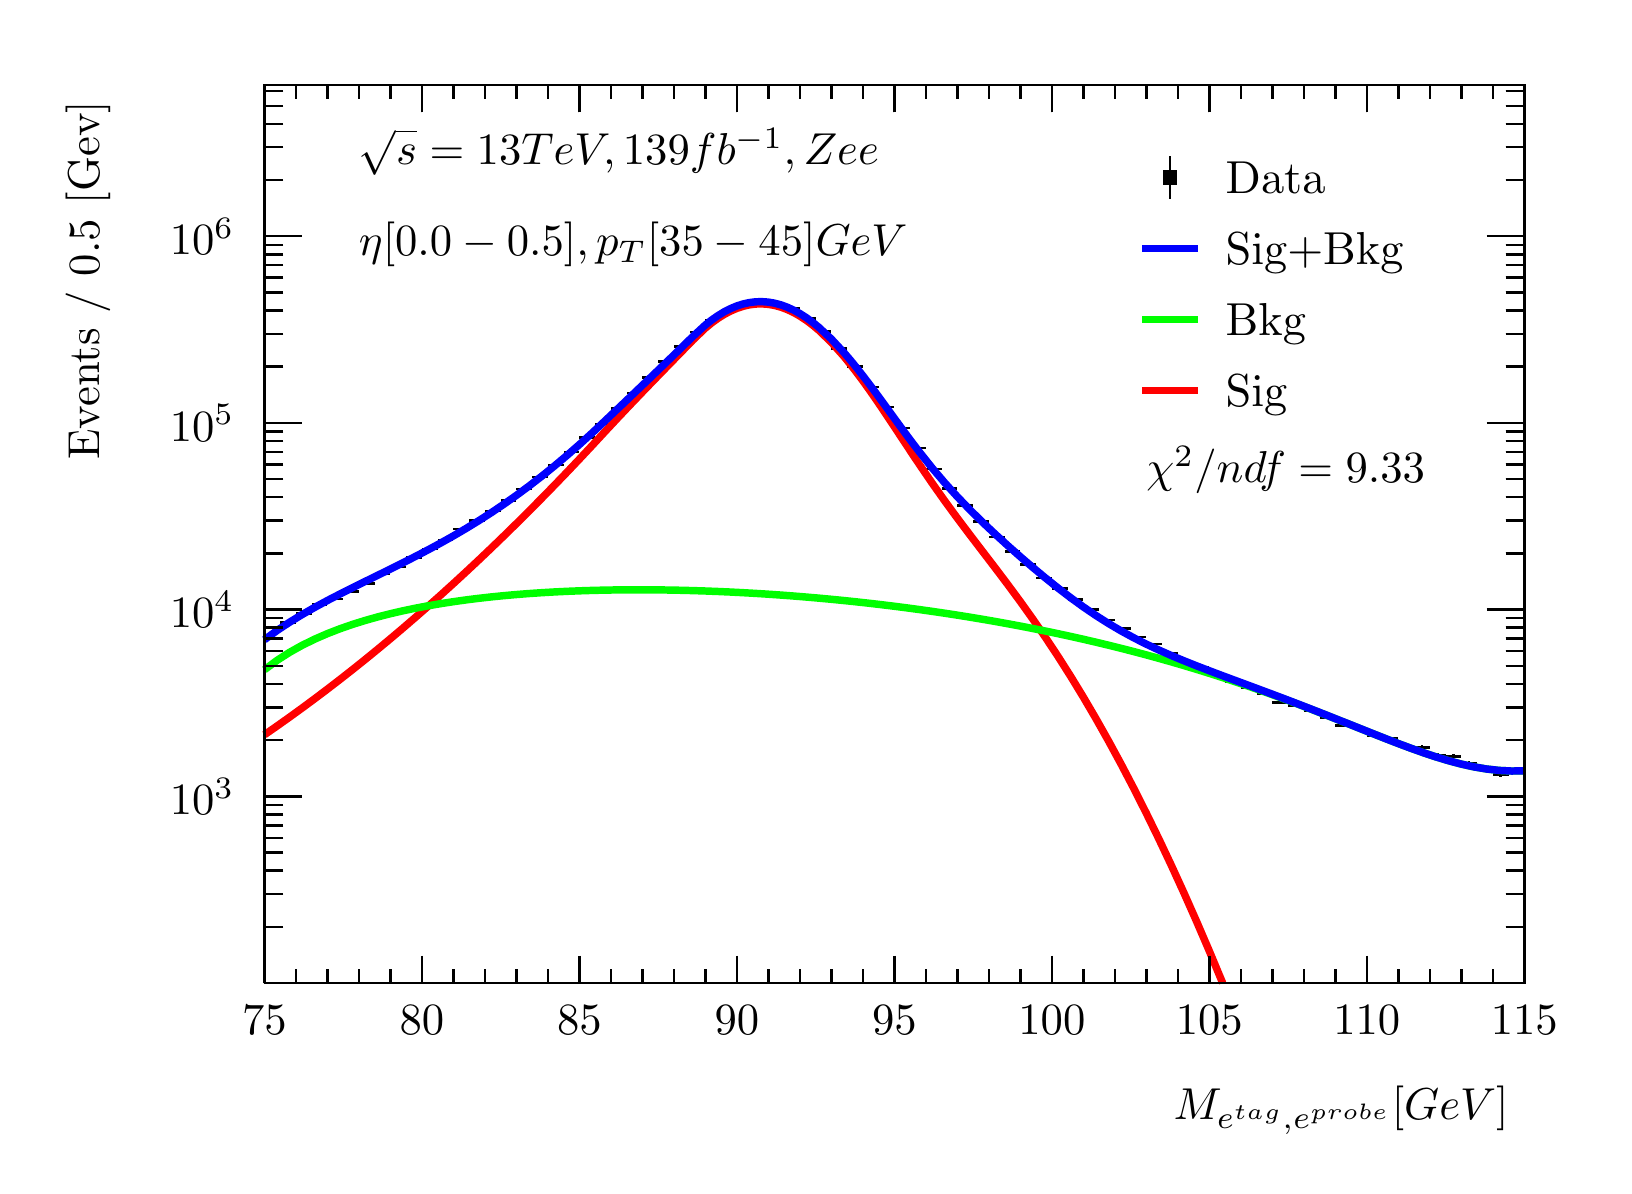
\begin{tikzpicture}
\pgfdeclareplotmark{cross} {
\pgfpathmoveto{\pgfpoint{-0.3\pgfplotmarksize}{\pgfplotmarksize}}
\pgfpathlineto{\pgfpoint{+0.3\pgfplotmarksize}{\pgfplotmarksize}}
\pgfpathlineto{\pgfpoint{+0.3\pgfplotmarksize}{0.3\pgfplotmarksize}}
\pgfpathlineto{\pgfpoint{+1\pgfplotmarksize}{0.3\pgfplotmarksize}}
\pgfpathlineto{\pgfpoint{+1\pgfplotmarksize}{-0.3\pgfplotmarksize}}
\pgfpathlineto{\pgfpoint{+0.3\pgfplotmarksize}{-0.3\pgfplotmarksize}}
\pgfpathlineto{\pgfpoint{+0.3\pgfplotmarksize}{-1.\pgfplotmarksize}}
\pgfpathlineto{\pgfpoint{-0.3\pgfplotmarksize}{-1.\pgfplotmarksize}}
\pgfpathlineto{\pgfpoint{-0.3\pgfplotmarksize}{-0.3\pgfplotmarksize}}
\pgfpathlineto{\pgfpoint{-1.\pgfplotmarksize}{-0.3\pgfplotmarksize}}
\pgfpathlineto{\pgfpoint{-1.\pgfplotmarksize}{0.3\pgfplotmarksize}}
\pgfpathlineto{\pgfpoint{-0.3\pgfplotmarksize}{0.3\pgfplotmarksize}}
\pgfpathclose
\pgfusepathqstroke
}
\pgfdeclareplotmark{cross*} {
\pgfpathmoveto{\pgfpoint{-0.3\pgfplotmarksize}{\pgfplotmarksize}}
\pgfpathlineto{\pgfpoint{+0.3\pgfplotmarksize}{\pgfplotmarksize}}
\pgfpathlineto{\pgfpoint{+0.3\pgfplotmarksize}{0.3\pgfplotmarksize}}
\pgfpathlineto{\pgfpoint{+1\pgfplotmarksize}{0.3\pgfplotmarksize}}
\pgfpathlineto{\pgfpoint{+1\pgfplotmarksize}{-0.3\pgfplotmarksize}}
\pgfpathlineto{\pgfpoint{+0.3\pgfplotmarksize}{-0.3\pgfplotmarksize}}
\pgfpathlineto{\pgfpoint{+0.3\pgfplotmarksize}{-1.\pgfplotmarksize}}
\pgfpathlineto{\pgfpoint{-0.3\pgfplotmarksize}{-1.\pgfplotmarksize}}
\pgfpathlineto{\pgfpoint{-0.3\pgfplotmarksize}{-0.3\pgfplotmarksize}}
\pgfpathlineto{\pgfpoint{-1.\pgfplotmarksize}{-0.3\pgfplotmarksize}}
\pgfpathlineto{\pgfpoint{-1.\pgfplotmarksize}{0.3\pgfplotmarksize}}
\pgfpathlineto{\pgfpoint{-0.3\pgfplotmarksize}{0.3\pgfplotmarksize}}
\pgfpathclose
\pgfusepathqfillstroke
}
\pgfdeclareplotmark{newstar} {
\pgfpathmoveto{\pgfqpoint{0pt}{\pgfplotmarksize}}
\pgfpathlineto{\pgfqpointpolar{44}{0.5\pgfplotmarksize}}
\pgfpathlineto{\pgfqpointpolar{18}{\pgfplotmarksize}}
\pgfpathlineto{\pgfqpointpolar{-20}{0.5\pgfplotmarksize}}
\pgfpathlineto{\pgfqpointpolar{-54}{\pgfplotmarksize}}
\pgfpathlineto{\pgfqpointpolar{-90}{0.5\pgfplotmarksize}}
\pgfpathlineto{\pgfqpointpolar{234}{\pgfplotmarksize}}
\pgfpathlineto{\pgfqpointpolar{198}{0.5\pgfplotmarksize}}
\pgfpathlineto{\pgfqpointpolar{162}{\pgfplotmarksize}}
\pgfpathlineto{\pgfqpointpolar{134}{0.5\pgfplotmarksize}}
\pgfpathclose
\pgfusepathqstroke
}
\pgfdeclareplotmark{newstar*} {
\pgfpathmoveto{\pgfqpoint{0pt}{\pgfplotmarksize}}
\pgfpathlineto{\pgfqpointpolar{44}{0.5\pgfplotmarksize}}
\pgfpathlineto{\pgfqpointpolar{18}{\pgfplotmarksize}}
\pgfpathlineto{\pgfqpointpolar{-20}{0.5\pgfplotmarksize}}
\pgfpathlineto{\pgfqpointpolar{-54}{\pgfplotmarksize}}
\pgfpathlineto{\pgfqpointpolar{-90}{0.5\pgfplotmarksize}}
\pgfpathlineto{\pgfqpointpolar{234}{\pgfplotmarksize}}
\pgfpathlineto{\pgfqpointpolar{198}{0.5\pgfplotmarksize}}
\pgfpathlineto{\pgfqpointpolar{162}{\pgfplotmarksize}}
\pgfpathlineto{\pgfqpointpolar{134}{0.5\pgfplotmarksize}}
\pgfpathclose
\pgfusepathqfillstroke
}
\definecolor{c}{rgb}{1,1,1};
\draw [color=c, fill=c] (0,0) rectangle (20,14.4361);
\draw [color=c, fill=c] (3,2.30977) rectangle (19,13.7143);
\definecolor{c}{rgb}{0,0,0};
\draw [c,line width=0.9] (3,2.30977) -- (3,13.7143) -- (19,13.7143) -- (19,2.30977) -- (3,2.30977);
\definecolor{c}{rgb}{1,1,1};
\draw [color=c, fill=c] (3,2.30977) rectangle (19,13.7143);
\definecolor{c}{rgb}{0,0,0};
\draw [c,line width=0.9] (3,2.30977) -- (3,13.7143) -- (19,13.7143) -- (19,2.30977) -- (3,2.30977);
\draw [c,line width=0.9] (3,2.30977) -- (19,2.30977);
\draw [c,line width=0.9] (3,2.65624) -- (3,2.30977);
\draw [c,line width=0.9] (3.4,2.48301) -- (3.4,2.30977);
\draw [c,line width=0.9] (3.8,2.48301) -- (3.8,2.30977);
\draw [c,line width=0.9] (4.2,2.48301) -- (4.2,2.30977);
\draw [c,line width=0.9] (4.6,2.48301) -- (4.6,2.30977);
\draw [c,line width=0.9] (5,2.65624) -- (5,2.30977);
\draw [c,line width=0.9] (5.4,2.48301) -- (5.4,2.30977);
\draw [c,line width=0.9] (5.8,2.48301) -- (5.8,2.30977);
\draw [c,line width=0.9] (6.2,2.48301) -- (6.2,2.30977);
\draw [c,line width=0.9] (6.6,2.48301) -- (6.6,2.30977);
\draw [c,line width=0.9] (7,2.65624) -- (7,2.30977);
\draw [c,line width=0.9] (7.4,2.48301) -- (7.4,2.30977);
\draw [c,line width=0.9] (7.8,2.48301) -- (7.8,2.30977);
\draw [c,line width=0.9] (8.2,2.48301) -- (8.2,2.30977);
\draw [c,line width=0.9] (8.6,2.48301) -- (8.6,2.30977);
\draw [c,line width=0.9] (9,2.65624) -- (9,2.30977);
\draw [c,line width=0.9] (9.4,2.48301) -- (9.4,2.30977);
\draw [c,line width=0.9] (9.8,2.48301) -- (9.8,2.30977);
\draw [c,line width=0.9] (10.2,2.48301) -- (10.2,2.30977);
\draw [c,line width=0.9] (10.6,2.48301) -- (10.6,2.30977);
\draw [c,line width=0.9] (11,2.65624) -- (11,2.30977);
\draw [c,line width=0.9] (11.4,2.48301) -- (11.4,2.30977);
\draw [c,line width=0.9] (11.8,2.48301) -- (11.8,2.30977);
\draw [c,line width=0.9] (12.2,2.48301) -- (12.2,2.30977);
\draw [c,line width=0.9] (12.6,2.48301) -- (12.6,2.30977);
\draw [c,line width=0.9] (13,2.65624) -- (13,2.30977);
\draw [c,line width=0.9] (13.4,2.48301) -- (13.4,2.30977);
\draw [c,line width=0.9] (13.8,2.48301) -- (13.8,2.30977);
\draw [c,line width=0.9] (14.2,2.48301) -- (14.2,2.30977);
\draw [c,line width=0.9] (14.6,2.48301) -- (14.6,2.30977);
\draw [c,line width=0.9] (15,2.65624) -- (15,2.30977);
\draw [c,line width=0.9] (15.4,2.48301) -- (15.4,2.30977);
\draw [c,line width=0.9] (15.8,2.48301) -- (15.8,2.30977);
\draw [c,line width=0.9] (16.2,2.48301) -- (16.2,2.30977);
\draw [c,line width=0.9] (16.6,2.48301) -- (16.6,2.30977);
\draw [c,line width=0.9] (17,2.65624) -- (17,2.30977);
\draw [c,line width=0.9] (17.4,2.48301) -- (17.4,2.30977);
\draw [c,line width=0.9] (17.8,2.48301) -- (17.8,2.30977);
\draw [c,line width=0.9] (18.2,2.48301) -- (18.2,2.30977);
\draw [c,line width=0.9] (18.6,2.48301) -- (18.6,2.30977);
\draw [c,line width=0.9] (19,2.65624) -- (19,2.30977);
\draw [c,line width=0.9] (19,2.65624) -- (19,2.30977);
\draw [anchor=base] (3,1.66015) node[scale=1.61424, color=c, rotate=0]{75};
\draw [anchor=base] (5,1.66015) node[scale=1.61424, color=c, rotate=0]{80};
\draw [anchor=base] (7,1.66015) node[scale=1.61424, color=c, rotate=0]{85};
\draw [anchor=base] (9,1.66015) node[scale=1.61424, color=c, rotate=0]{90};
\draw [anchor=base] (11,1.66015) node[scale=1.61424, color=c, rotate=0]{95};
\draw [anchor=base] (13,1.66015) node[scale=1.61424, color=c, rotate=0]{100};
\draw [anchor=base] (15,1.66015) node[scale=1.61424, color=c, rotate=0]{105};
\draw [anchor=base] (17,1.66015) node[scale=1.61424, color=c, rotate=0]{110};
\draw [anchor=base] (19,1.66015) node[scale=1.61424, color=c, rotate=0]{115};
\draw [anchor= east] (19,0.692932) node[scale=1.61424, color=c, rotate=0]{$M_{e^{tag}, e^{probe}}  [GeV]$};
\draw [c,line width=0.9] (3,13.7143) -- (19,13.7143);
\draw [c,line width=0.9] (3,13.3678) -- (3,13.7143);
\draw [c,line width=0.9] (3.4,13.5411) -- (3.4,13.7143);
\draw [c,line width=0.9] (3.8,13.5411) -- (3.8,13.7143);
\draw [c,line width=0.9] (4.2,13.5411) -- (4.2,13.7143);
\draw [c,line width=0.9] (4.6,13.5411) -- (4.6,13.7143);
\draw [c,line width=0.9] (5,13.3678) -- (5,13.7143);
\draw [c,line width=0.9] (5.4,13.5411) -- (5.4,13.7143);
\draw [c,line width=0.9] (5.8,13.5411) -- (5.8,13.7143);
\draw [c,line width=0.9] (6.2,13.5411) -- (6.2,13.7143);
\draw [c,line width=0.9] (6.6,13.5411) -- (6.6,13.7143);
\draw [c,line width=0.9] (7,13.3678) -- (7,13.7143);
\draw [c,line width=0.9] (7.4,13.5411) -- (7.4,13.7143);
\draw [c,line width=0.9] (7.8,13.5411) -- (7.8,13.7143);
\draw [c,line width=0.9] (8.2,13.5411) -- (8.2,13.7143);
\draw [c,line width=0.9] (8.6,13.5411) -- (8.6,13.7143);
\draw [c,line width=0.9] (9,13.3678) -- (9,13.7143);
\draw [c,line width=0.9] (9.4,13.5411) -- (9.4,13.7143);
\draw [c,line width=0.9] (9.8,13.5411) -- (9.8,13.7143);
\draw [c,line width=0.9] (10.2,13.5411) -- (10.2,13.7143);
\draw [c,line width=0.9] (10.6,13.5411) -- (10.6,13.7143);
\draw [c,line width=0.9] (11,13.3678) -- (11,13.7143);
\draw [c,line width=0.9] (11.4,13.5411) -- (11.4,13.7143);
\draw [c,line width=0.9] (11.8,13.5411) -- (11.8,13.7143);
\draw [c,line width=0.9] (12.2,13.5411) -- (12.2,13.7143);
\draw [c,line width=0.9] (12.6,13.5411) -- (12.6,13.7143);
\draw [c,line width=0.9] (13,13.3678) -- (13,13.7143);
\draw [c,line width=0.9] (13.4,13.5411) -- (13.4,13.7143);
\draw [c,line width=0.9] (13.8,13.5411) -- (13.8,13.7143);
\draw [c,line width=0.9] (14.2,13.5411) -- (14.2,13.7143);
\draw [c,line width=0.9] (14.6,13.5411) -- (14.6,13.7143);
\draw [c,line width=0.9] (15,13.3678) -- (15,13.7143);
\draw [c,line width=0.9] (15.4,13.5411) -- (15.4,13.7143);
\draw [c,line width=0.9] (15.8,13.5411) -- (15.8,13.7143);
\draw [c,line width=0.9] (16.2,13.5411) -- (16.2,13.7143);
\draw [c,line width=0.9] (16.6,13.5411) -- (16.6,13.7143);
\draw [c,line width=0.9] (17,13.3678) -- (17,13.7143);
\draw [c,line width=0.9] (17.4,13.5411) -- (17.4,13.7143);
\draw [c,line width=0.9] (17.8,13.5411) -- (17.8,13.7143);
\draw [c,line width=0.9] (18.2,13.5411) -- (18.2,13.7143);
\draw [c,line width=0.9] (18.6,13.5411) -- (18.6,13.7143);
\draw [c,line width=0.9] (19,13.3678) -- (19,13.7143);
\draw [c,line width=0.9] (19,13.3678) -- (19,13.7143);
\draw [c,line width=0.9] (3,2.30977) -- (3,13.7143);
\draw [c,line width=0.9] (3.237,3.02354) -- (3,3.02354);
\draw [c,line width=0.9] (3.237,3.44107) -- (3,3.44107);
\draw [c,line width=0.9] (3.237,3.73731) -- (3,3.73731);
\draw [c,line width=0.9] (3.237,3.96709) -- (3,3.96709);
\draw [c,line width=0.9] (3.237,4.15484) -- (3,4.15484);
\draw [c,line width=0.9] (3.237,4.31357) -- (3,4.31357);
\draw [c,line width=0.9] (3.237,4.45108) -- (3,4.45108);
\draw [c,line width=0.9] (3.237,4.57236) -- (3,4.57236);
\draw [c,line width=0.9] (3.474,4.68086) -- (3,4.68086);
\draw [anchor= east] (2.82,4.68086) node[scale=1.61424, color=c, rotate=0]{$10^{3}$};
\draw [c,line width=0.9] (3.237,5.39463) -- (3,5.39463);
\draw [c,line width=0.9] (3.237,5.81216) -- (3,5.81216);
\draw [c,line width=0.9] (3.237,6.1084) -- (3,6.1084);
\draw [c,line width=0.9] (3.237,6.33818) -- (3,6.33818);
\draw [c,line width=0.9] (3.237,6.52593) -- (3,6.52593);
\draw [c,line width=0.9] (3.237,6.68466) -- (3,6.68466);
\draw [c,line width=0.9] (3.237,6.82217) -- (3,6.82217);
\draw [c,line width=0.9] (3.237,6.94345) -- (3,6.94345);
\draw [c,line width=0.9] (3.474,7.05195) -- (3,7.05195);
\draw [anchor= east] (2.82,7.05195) node[scale=1.61424, color=c, rotate=0]{$10^{4}$};
\draw [c,line width=0.9] (3.237,7.76572) -- (3,7.76572);
\draw [c,line width=0.9] (3.237,8.18324) -- (3,8.18324);
\draw [c,line width=0.9] (3.237,8.47948) -- (3,8.47948);
\draw [c,line width=0.9] (3.237,8.70927) -- (3,8.70927);
\draw [c,line width=0.9] (3.237,8.89701) -- (3,8.89701);
\draw [c,line width=0.9] (3.237,9.05575) -- (3,9.05575);
\draw [c,line width=0.9] (3.237,9.19325) -- (3,9.19325);
\draw [c,line width=0.9] (3.237,9.31454) -- (3,9.31454);
\draw [c,line width=0.9] (3.474,9.42304) -- (3,9.42304);
\draw [anchor= east] (2.82,9.42304) node[scale=1.61424, color=c, rotate=0]{$10^{5}$};
\draw [c,line width=0.9] (3.237,10.1368) -- (3,10.1368);
\draw [c,line width=0.9] (3.237,10.5543) -- (3,10.5543);
\draw [c,line width=0.9] (3.237,10.8506) -- (3,10.8506);
\draw [c,line width=0.9] (3.237,11.0804) -- (3,11.0804);
\draw [c,line width=0.9] (3.237,11.2681) -- (3,11.2681);
\draw [c,line width=0.9] (3.237,11.4268) -- (3,11.4268);
\draw [c,line width=0.9] (3.237,11.5643) -- (3,11.5643);
\draw [c,line width=0.9] (3.237,11.6856) -- (3,11.6856);
\draw [c,line width=0.9] (3.474,11.7941) -- (3,11.7941);
\draw [anchor= east] (2.82,11.7941) node[scale=1.61424, color=c, rotate=0]{$10^{6}$};
\draw [c,line width=0.9] (3.237,12.5079) -- (3,12.5079);
\draw [c,line width=0.9] (3.237,12.9254) -- (3,12.9254);
\draw [c,line width=0.9] (3.237,13.2217) -- (3,13.2217);
\draw [c,line width=0.9] (3.237,13.4514) -- (3,13.4514);
\draw [c,line width=0.9] (3.237,13.6392) -- (3,13.6392);
\draw [anchor= east] (0.76,13.7143) node[scale=1.61424, color=c, rotate=90]{Events / 0.5 [Gev]};
\draw [c,line width=0.9] (19,2.30977) -- (19,13.7143);
\draw [c,line width=0.9] (18.763,3.02354) -- (19,3.02354);
\draw [c,line width=0.9] (18.763,3.44107) -- (19,3.44107);
\draw [c,line width=0.9] (18.763,3.73731) -- (19,3.73731);
\draw [c,line width=0.9] (18.763,3.96709) -- (19,3.96709);
\draw [c,line width=0.9] (18.763,4.15484) -- (19,4.15484);
\draw [c,line width=0.9] (18.763,4.31357) -- (19,4.31357);
\draw [c,line width=0.9] (18.763,4.45108) -- (19,4.45108);
\draw [c,line width=0.9] (18.763,4.57236) -- (19,4.57236);
\draw [c,line width=0.9] (18.526,4.68086) -- (19,4.68086);
\draw [c,line width=0.9] (18.763,5.39463) -- (19,5.39463);
\draw [c,line width=0.9] (18.763,5.81216) -- (19,5.81216);
\draw [c,line width=0.9] (18.763,6.1084) -- (19,6.1084);
\draw [c,line width=0.9] (18.763,6.33818) -- (19,6.33818);
\draw [c,line width=0.9] (18.763,6.52593) -- (19,6.52593);
\draw [c,line width=0.9] (18.763,6.68466) -- (19,6.68466);
\draw [c,line width=0.9] (18.763,6.82217) -- (19,6.82217);
\draw [c,line width=0.9] (18.763,6.94345) -- (19,6.94345);
\draw [c,line width=0.9] (18.526,7.05195) -- (19,7.05195);
\draw [c,line width=0.9] (18.763,7.76572) -- (19,7.76572);
\draw [c,line width=0.9] (18.763,8.18324) -- (19,8.18324);
\draw [c,line width=0.9] (18.763,8.47948) -- (19,8.47948);
\draw [c,line width=0.9] (18.763,8.70927) -- (19,8.70927);
\draw [c,line width=0.9] (18.763,8.89701) -- (19,8.89701);
\draw [c,line width=0.9] (18.763,9.05575) -- (19,9.05575);
\draw [c,line width=0.9] (18.763,9.19325) -- (19,9.19325);
\draw [c,line width=0.9] (18.763,9.31454) -- (19,9.31454);
\draw [c,line width=0.9] (18.526,9.42304) -- (19,9.42304);
\draw [c,line width=0.9] (18.763,10.1368) -- (19,10.1368);
\draw [c,line width=0.9] (18.763,10.5543) -- (19,10.5543);
\draw [c,line width=0.9] (18.763,10.8506) -- (19,10.8506);
\draw [c,line width=0.9] (18.763,11.0804) -- (19,11.0804);
\draw [c,line width=0.9] (18.763,11.2681) -- (19,11.2681);
\draw [c,line width=0.9] (18.763,11.4268) -- (19,11.4268);
\draw [c,line width=0.9] (18.763,11.5643) -- (19,11.5643);
\draw [c,line width=0.9] (18.763,11.6856) -- (19,11.6856);
\draw [c,line width=0.9] (18.526,11.7941) -- (19,11.7941);
\draw [c,line width=0.9] (18.763,12.5079) -- (19,12.5079);
\draw [c,line width=0.9] (18.763,12.9254) -- (19,12.9254);
\draw [c,line width=0.9] (18.763,13.2217) -- (19,13.2217);
\draw [c,line width=0.9] (18.763,13.4514) -- (19,13.4514);
\draw [c,line width=0.9] (18.763,13.6392) -- (19,13.6392);
\draw [c,line width=0.9] (3.1,6.83216) -- (3,6.83216);
\draw [c,line width=0.9] (3,6.83216) -- (3,6.83216);
\draw [c,line width=0.9] (3.1,6.83216) -- (3.2,6.83216);
\draw [c,line width=0.9] (3.2,6.83216) -- (3.2,6.83216);
\draw [c,line width=0.9] (3.1,6.83216) -- (3.1,6.84362);
\draw [c,line width=0.9] (3.1,6.84362) -- (3.1,6.84362);
\draw [c,line width=0.9] (3.1,6.83216) -- (3.1,6.8207);
\draw [c,line width=0.9] (3.1,6.8207) -- (3.1,6.8207);
\draw [c,line width=0.9] (3.3,6.88786) -- (3.2,6.88786);
\draw [c,line width=0.9] (3.2,6.88786) -- (3.2,6.88786);
\draw [c,line width=0.9] (3.3,6.88786) -- (3.4,6.88786);
\draw [c,line width=0.9] (3.4,6.88786) -- (3.4,6.88786);
\draw [c,line width=0.9] (3.3,6.88786) -- (3.3,6.89901);
\draw [c,line width=0.9] (3.3,6.89901) -- (3.3,6.89901);
\draw [c,line width=0.9] (3.3,6.88786) -- (3.3,6.87671);
\draw [c,line width=0.9] (3.3,6.87671) -- (3.3,6.87671);
\draw [c,line width=0.9] (3.5,7.00162) -- (3.4,7.00162);
\draw [c,line width=0.9] (3.4,7.00162) -- (3.4,7.00162);
\draw [c,line width=0.9] (3.5,7.00162) -- (3.6,7.00162);
\draw [c,line width=0.9] (3.6,7.00162) -- (3.6,7.00162);
\draw [c,line width=0.9] (3.5,7.00162) -- (3.5,7.01217);
\draw [c,line width=0.9] (3.5,7.01217) -- (3.5,7.01217);
\draw [c,line width=0.9] (3.5,7.00162) -- (3.5,6.99107);
\draw [c,line width=0.9] (3.5,6.99107) -- (3.5,6.99107);
\draw [c,line width=0.9] (3.7,7.11506) -- (3.6,7.11506);
\draw [c,line width=0.9] (3.6,7.11506) -- (3.6,7.11506);
\draw [c,line width=0.9] (3.7,7.11506) -- (3.8,7.11506);
\draw [c,line width=0.9] (3.8,7.11506) -- (3.8,7.11506);
\draw [c,line width=0.9] (3.7,7.11506) -- (3.7,7.12504);
\draw [c,line width=0.9] (3.7,7.12504) -- (3.7,7.12504);
\draw [c,line width=0.9] (3.7,7.11506) -- (3.7,7.10507);
\draw [c,line width=0.9] (3.7,7.10507) -- (3.7,7.10507);
\draw [c,line width=0.9] (3.9,7.18416) -- (3.8,7.18416);
\draw [c,line width=0.9] (3.8,7.18416) -- (3.8,7.18416);
\draw [c,line width=0.9] (3.9,7.18416) -- (4,7.18416);
\draw [c,line width=0.9] (4,7.18416) -- (4,7.18416);
\draw [c,line width=0.9] (3.9,7.18416) -- (3.9,7.19382);
\draw [c,line width=0.9] (3.9,7.19382) -- (3.9,7.19382);
\draw [c,line width=0.9] (3.9,7.18416) -- (3.9,7.1745);
\draw [c,line width=0.9] (3.9,7.1745) -- (3.9,7.1745);
\draw [c,line width=0.9] (4.1,7.28543) -- (4,7.28543);
\draw [c,line width=0.9] (4,7.28543) -- (4,7.28543);
\draw [c,line width=0.9] (4.1,7.28543) -- (4.2,7.28543);
\draw [c,line width=0.9] (4.2,7.28543) -- (4.2,7.28543);
\draw [c,line width=0.9] (4.1,7.28543) -- (4.1,7.29463);
\draw [c,line width=0.9] (4.1,7.29463) -- (4.1,7.29463);
\draw [c,line width=0.9] (4.1,7.28543) -- (4.1,7.27624);
\draw [c,line width=0.9] (4.1,7.27624) -- (4.1,7.27624);
\draw [c,line width=0.9] (4.3,7.38674) -- (4.2,7.38674);
\draw [c,line width=0.9] (4.2,7.38674) -- (4.2,7.38674);
\draw [c,line width=0.9] (4.3,7.38674) -- (4.4,7.38674);
\draw [c,line width=0.9] (4.4,7.38674) -- (4.4,7.38674);
\draw [c,line width=0.9] (4.3,7.38674) -- (4.3,7.3955);
\draw [c,line width=0.9] (4.3,7.3955) -- (4.3,7.3955);
\draw [c,line width=0.9] (4.3,7.38674) -- (4.3,7.37799);
\draw [c,line width=0.9] (4.3,7.37799) -- (4.3,7.37799);
\draw [c,line width=0.9] (4.5,7.50696) -- (4.4,7.50696);
\draw [c,line width=0.9] (4.4,7.50696) -- (4.4,7.50696);
\draw [c,line width=0.9] (4.5,7.50696) -- (4.6,7.50696);
\draw [c,line width=0.9] (4.6,7.50696) -- (4.6,7.50696);
\draw [c,line width=0.9] (4.5,7.50696) -- (4.5,7.51521);
\draw [c,line width=0.9] (4.5,7.51521) -- (4.5,7.51521);
\draw [c,line width=0.9] (4.5,7.50696) -- (4.5,7.4987);
\draw [c,line width=0.9] (4.5,7.4987) -- (4.5,7.4987);
\draw [c,line width=0.9] (4.7,7.59618) -- (4.6,7.59618);
\draw [c,line width=0.9] (4.6,7.59618) -- (4.6,7.59618);
\draw [c,line width=0.9] (4.7,7.59618) -- (4.8,7.59618);
\draw [c,line width=0.9] (4.8,7.59618) -- (4.8,7.59618);
\draw [c,line width=0.9] (4.7,7.59618) -- (4.7,7.60409);
\draw [c,line width=0.9] (4.7,7.60409) -- (4.7,7.60409);
\draw [c,line width=0.9] (4.7,7.59618) -- (4.7,7.58827);
\draw [c,line width=0.9] (4.7,7.58827) -- (4.7,7.58827);
\draw [c,line width=0.9] (4.9,7.71447) -- (4.8,7.71447);
\draw [c,line width=0.9] (4.8,7.71447) -- (4.8,7.71447);
\draw [c,line width=0.9] (4.9,7.71447) -- (5,7.71447);
\draw [c,line width=0.9] (5,7.71447) -- (5,7.71447);
\draw [c,line width=0.9] (4.9,7.71447) -- (4.9,7.72193);
\draw [c,line width=0.9] (4.9,7.72193) -- (4.9,7.72193);
\draw [c,line width=0.9] (4.9,7.71447) -- (4.9,7.707);
\draw [c,line width=0.9] (4.9,7.707) -- (4.9,7.707);
\draw [c,line width=0.9] (5.1,7.82212) -- (5,7.82212);
\draw [c,line width=0.9] (5,7.82212) -- (5,7.82212);
\draw [c,line width=0.9] (5.1,7.82212) -- (5.2,7.82212);
\draw [c,line width=0.9] (5.2,7.82212) -- (5.2,7.82212);
\draw [c,line width=0.9] (5.1,7.82212) -- (5.1,7.8292);
\draw [c,line width=0.9] (5.1,7.8292) -- (5.1,7.8292);
\draw [c,line width=0.9] (5.1,7.82212) -- (5.1,7.81503);
\draw [c,line width=0.9] (5.1,7.81503) -- (5.1,7.81503);
\draw [c,line width=0.9] (5.3,7.93472) -- (5.2,7.93472);
\draw [c,line width=0.9] (5.2,7.93472) -- (5.2,7.93472);
\draw [c,line width=0.9] (5.3,7.93472) -- (5.4,7.93472);
\draw [c,line width=0.9] (5.4,7.93472) -- (5.4,7.93472);
\draw [c,line width=0.9] (5.3,7.93472) -- (5.3,7.94142);
\draw [c,line width=0.9] (5.3,7.94142) -- (5.3,7.94142);
\draw [c,line width=0.9] (5.3,7.93472) -- (5.3,7.92801);
\draw [c,line width=0.9] (5.3,7.92801) -- (5.3,7.92801);
\draw [c,line width=0.9] (5.5,8.07448) -- (5.4,8.07448);
\draw [c,line width=0.9] (5.4,8.07448) -- (5.4,8.07448);
\draw [c,line width=0.9] (5.5,8.07448) -- (5.6,8.07448);
\draw [c,line width=0.9] (5.6,8.07448) -- (5.6,8.07448);
\draw [c,line width=0.9] (5.5,8.07448) -- (5.5,8.08075);
\draw [c,line width=0.9] (5.5,8.08075) -- (5.5,8.08075);
\draw [c,line width=0.9] (5.5,8.07448) -- (5.5,8.06822);
\draw [c,line width=0.9] (5.5,8.06822) -- (5.5,8.06822);
\draw [c,line width=0.9] (5.7,8.18149) -- (5.6,8.18149);
\draw [c,line width=0.9] (5.6,8.18149) -- (5.6,8.18149);
\draw [c,line width=0.9] (5.7,8.18149) -- (5.8,8.18149);
\draw [c,line width=0.9] (5.8,8.18149) -- (5.8,8.18149);
\draw [c,line width=0.9] (5.7,8.18149) -- (5.7,8.18744);
\draw [c,line width=0.9] (5.7,8.18744) -- (5.7,8.18744);
\draw [c,line width=0.9] (5.7,8.18149) -- (5.7,8.17554);
\draw [c,line width=0.9] (5.7,8.17554) -- (5.7,8.17554);
\draw [c,line width=0.9] (5.9,8.30533) -- (5.8,8.30533);
\draw [c,line width=0.9] (5.8,8.30533) -- (5.8,8.30533);
\draw [c,line width=0.9] (5.9,8.30533) -- (6,8.30533);
\draw [c,line width=0.9] (6,8.30533) -- (6,8.30533);
\draw [c,line width=0.9] (5.9,8.30533) -- (5.9,8.31093);
\draw [c,line width=0.9] (5.9,8.31093) -- (5.9,8.31093);
\draw [c,line width=0.9] (5.9,8.30533) -- (5.9,8.29972);
\draw [c,line width=0.9] (5.9,8.29972) -- (5.9,8.29972);
\draw [c,line width=0.9] (6.1,8.44101) -- (6,8.44101);
\draw [c,line width=0.9] (6,8.44101) -- (6,8.44101);
\draw [c,line width=0.9] (6.1,8.44101) -- (6.2,8.44101);
\draw [c,line width=0.9] (6.2,8.44101) -- (6.2,8.44101);
\draw [c,line width=0.9] (6.1,8.44101) -- (6.1,8.44626);
\draw [c,line width=0.9] (6.1,8.44626) -- (6.1,8.44626);
\draw [c,line width=0.9] (6.1,8.44101) -- (6.1,8.43576);
\draw [c,line width=0.9] (6.1,8.43576) -- (6.1,8.43576);
\draw [c,line width=0.9] (6.3,8.58649) -- (6.2,8.58649);
\draw [c,line width=0.9] (6.2,8.58649) -- (6.2,8.58649);
\draw [c,line width=0.9] (6.3,8.58649) -- (6.4,8.58649);
\draw [c,line width=0.9] (6.4,8.58649) -- (6.4,8.58649);
\draw [c,line width=0.9] (6.3,8.58649) -- (6.3,8.59138);
\draw [c,line width=0.9] (6.3,8.59138) -- (6.3,8.59138);
\draw [c,line width=0.9] (6.3,8.58649) -- (6.3,8.5816);
\draw [c,line width=0.9] (6.3,8.5816) -- (6.3,8.5816);
\draw [c,line width=0.9] (6.5,8.7375) -- (6.4,8.7375);
\draw [c,line width=0.9] (6.4,8.7375) -- (6.4,8.7375);
\draw [c,line width=0.9] (6.5,8.7375) -- (6.6,8.7375);
\draw [c,line width=0.9] (6.6,8.7375) -- (6.6,8.7375);
\draw [c,line width=0.9] (6.5,8.7375) -- (6.5,8.74205);
\draw [c,line width=0.9] (6.5,8.74205) -- (6.5,8.74205);
\draw [c,line width=0.9] (6.5,8.7375) -- (6.5,8.73296);
\draw [c,line width=0.9] (6.5,8.73296) -- (6.5,8.73296);
\draw [c,line width=0.9] (6.7,8.88897) -- (6.6,8.88897);
\draw [c,line width=0.9] (6.6,8.88897) -- (6.6,8.88897);
\draw [c,line width=0.9] (6.7,8.88897) -- (6.8,8.88897);
\draw [c,line width=0.9] (6.8,8.88897) -- (6.8,8.88897);
\draw [c,line width=0.9] (6.7,8.88897) -- (6.7,8.89319);
\draw [c,line width=0.9] (6.7,8.89319) -- (6.7,8.89319);
\draw [c,line width=0.9] (6.7,8.88897) -- (6.7,8.88475);
\draw [c,line width=0.9] (6.7,8.88475) -- (6.7,8.88475);
\draw [c,line width=0.9] (6.9,9.05543) -- (6.8,9.05543);
\draw [c,line width=0.9] (6.8,9.05543) -- (6.8,9.05543);
\draw [c,line width=0.9] (6.9,9.05543) -- (7,9.05543);
\draw [c,line width=0.9] (7,9.05543) -- (7,9.05543);
\draw [c,line width=0.9] (6.9,9.05543) -- (6.9,9.05932);
\draw [c,line width=0.9] (6.9,9.05932) -- (6.9,9.05932);
\draw [c,line width=0.9] (6.9,9.05543) -- (6.9,9.05153);
\draw [c,line width=0.9] (6.9,9.05153) -- (6.9,9.05153);
\draw [c,line width=0.9] (7.1,9.23782) -- (7,9.23782);
\draw [c,line width=0.9] (7,9.23782) -- (7,9.23782);
\draw [c,line width=0.9] (7.1,9.23782) -- (7.2,9.23782);
\draw [c,line width=0.9] (7.2,9.23782) -- (7.2,9.23782);
\draw [c,line width=0.9] (7.1,9.23782) -- (7.1,9.24138);
\draw [c,line width=0.9] (7.1,9.24138) -- (7.1,9.24138);
\draw [c,line width=0.9] (7.1,9.23782) -- (7.1,9.23425);
\draw [c,line width=0.9] (7.1,9.23425) -- (7.1,9.23425);
\draw [c,line width=0.9] (7.3,9.41066) -- (7.2,9.41066);
\draw [c,line width=0.9] (7.2,9.41066) -- (7.2,9.41066);
\draw [c,line width=0.9] (7.3,9.41066) -- (7.4,9.41066);
\draw [c,line width=0.9] (7.4,9.41066) -- (7.4,9.41066);
\draw [c,line width=0.9] (7.3,9.41066) -- (7.3,9.41393);
\draw [c,line width=0.9] (7.3,9.41393) -- (7.3,9.41393);
\draw [c,line width=0.9] (7.3,9.41066) -- (7.3,9.40738);
\draw [c,line width=0.9] (7.3,9.40738) -- (7.3,9.40738);
\draw [c,line width=0.9] (7.5,9.60518) -- (7.4,9.60518);
\draw [c,line width=0.9] (7.4,9.60518) -- (7.4,9.60518);
\draw [c,line width=0.9] (7.5,9.60518) -- (7.6,9.60518);
\draw [c,line width=0.9] (7.6,9.60518) -- (7.6,9.60518);
\draw [c,line width=0.9] (7.5,9.60518) -- (7.5,9.60816);
\draw [c,line width=0.9] (7.5,9.60816) -- (7.5,9.60816);
\draw [c,line width=0.9] (7.5,9.60518) -- (7.5,9.6022);
\draw [c,line width=0.9] (7.5,9.6022) -- (7.5,9.6022);
\draw [c,line width=0.9] (7.7,9.80488) -- (7.6,9.80488);
\draw [c,line width=0.9] (7.6,9.80488) -- (7.6,9.80488);
\draw [c,line width=0.9] (7.7,9.80488) -- (7.8,9.80488);
\draw [c,line width=0.9] (7.8,9.80488) -- (7.8,9.80488);
\draw [c,line width=0.9] (7.7,9.80488) -- (7.7,9.80758);
\draw [c,line width=0.9] (7.7,9.80758) -- (7.7,9.80758);
\draw [c,line width=0.9] (7.7,9.80488) -- (7.7,9.80217);
\draw [c,line width=0.9] (7.7,9.80217) -- (7.7,9.80217);
\draw [c,line width=0.9] (7.9,10.0023) -- (7.8,10.0023);
\draw [c,line width=0.9] (7.8,10.0023) -- (7.8,10.0023);
\draw [c,line width=0.9] (7.9,10.0023) -- (8,10.0023);
\draw [c,line width=0.9] (8,10.0023) -- (8,10.0023);
\draw [c,line width=0.9] (7.9,10.0023) -- (7.9,10.0048);
\draw [c,line width=0.9] (7.9,10.0048) -- (7.9,10.0048);
\draw [c,line width=0.9] (7.9,10.0023) -- (7.9,9.99984);
\draw [c,line width=0.9] (7.9,9.99984) -- (7.9,9.99984);
\draw [c,line width=0.9] (8.1,10.2031) -- (8,10.2031);
\draw [c,line width=0.9] (8,10.2031) -- (8,10.2031);
\draw [c,line width=0.9] (8.1,10.2031) -- (8.2,10.2031);
\draw [c,line width=0.9] (8.2,10.2031) -- (8.2,10.2031);
\draw [c,line width=0.9] (8.1,10.2031) -- (8.1,10.2053);
\draw [c,line width=0.9] (8.1,10.2053) -- (8.1,10.2053);
\draw [c,line width=0.9] (8.1,10.2031) -- (8.1,10.2008);
\draw [c,line width=0.9] (8.1,10.2008) -- (8.1,10.2008);
\draw [c,line width=0.9] (8.3,10.3968) -- (8.2,10.3968);
\draw [c,line width=0.9] (8.2,10.3968) -- (8.2,10.3968);
\draw [c,line width=0.9] (8.3,10.3968) -- (8.4,10.3968);
\draw [c,line width=0.9] (8.4,10.3968) -- (8.4,10.3968);
\draw [c,line width=0.9] (8.3,10.3968) -- (8.3,10.3988);
\draw [c,line width=0.9] (8.3,10.3988) -- (8.3,10.3988);
\draw [c,line width=0.9] (8.3,10.3968) -- (8.3,10.3948);
\draw [c,line width=0.9] (8.3,10.3948) -- (8.3,10.3948);
\draw [c,line width=0.9] (8.5,10.5752) -- (8.4,10.5752);
\draw [c,line width=0.9] (8.4,10.5752) -- (8.4,10.5752);
\draw [c,line width=0.9] (8.5,10.5752) -- (8.6,10.5752);
\draw [c,line width=0.9] (8.6,10.5752) -- (8.6,10.5752);
\draw [c,line width=0.9] (8.5,10.5752) -- (8.5,10.5771);
\draw [c,line width=0.9] (8.5,10.5771) -- (8.5,10.5771);
\draw [c,line width=0.9] (8.5,10.5752) -- (8.5,10.5734);
\draw [c,line width=0.9] (8.5,10.5734) -- (8.5,10.5734);
\draw [c,line width=0.9] (8.7,10.7326) -- (8.6,10.7326);
\draw [c,line width=0.9] (8.6,10.7326) -- (8.6,10.7326);
\draw [c,line width=0.9] (8.7,10.7326) -- (8.8,10.7326);
\draw [c,line width=0.9] (8.8,10.7326) -- (8.8,10.7326);
\draw [c,line width=0.9] (8.7,10.7326) -- (8.7,10.7344);
\draw [c,line width=0.9] (8.7,10.7344) -- (8.7,10.7344);
\draw [c,line width=0.9] (8.7,10.7326) -- (8.7,10.7309);
\draw [c,line width=0.9] (8.7,10.7309) -- (8.7,10.7309);
\draw [c,line width=0.9] (8.9,10.8566) -- (8.8,10.8566);
\draw [c,line width=0.9] (8.8,10.8566) -- (8.8,10.8566);
\draw [c,line width=0.9] (8.9,10.8566) -- (9,10.8566);
\draw [c,line width=0.9] (9,10.8566) -- (9,10.8566);
\draw [c,line width=0.9] (8.9,10.8566) -- (8.9,10.8582);
\draw [c,line width=0.9] (8.9,10.8582) -- (8.9,10.8582);
\draw [c,line width=0.9] (8.9,10.8566) -- (8.9,10.855);
\draw [c,line width=0.9] (8.9,10.855) -- (8.9,10.855);
\draw [c,line width=0.9] (9.1,10.9355) -- (9,10.9355);
\draw [c,line width=0.9] (9,10.9355) -- (9,10.9355);
\draw [c,line width=0.9] (9.1,10.9355) -- (9.2,10.9355);
\draw [c,line width=0.9] (9.2,10.9355) -- (9.2,10.9355);
\draw [c,line width=0.9] (9.1,10.9355) -- (9.1,10.9371);
\draw [c,line width=0.9] (9.1,10.9371) -- (9.1,10.9371);
\draw [c,line width=0.9] (9.1,10.9355) -- (9.1,10.934);
\draw [c,line width=0.9] (9.1,10.934) -- (9.1,10.934);
\draw [c,line width=0.9] (9.3,10.9682) -- (9.2,10.9682);
\draw [c,line width=0.9] (9.2,10.9682) -- (9.2,10.9682);
\draw [c,line width=0.9] (9.3,10.9682) -- (9.4,10.9682);
\draw [c,line width=0.9] (9.4,10.9682) -- (9.4,10.9682);
\draw [c,line width=0.9] (9.3,10.9682) -- (9.3,10.9698);
\draw [c,line width=0.9] (9.3,10.9698) -- (9.3,10.9698);
\draw [c,line width=0.9] (9.3,10.9682) -- (9.3,10.9667);
\draw [c,line width=0.9] (9.3,10.9667) -- (9.3,10.9667);
\draw [c,line width=0.9] (9.5,10.9489) -- (9.4,10.9489);
\draw [c,line width=0.9] (9.4,10.9489) -- (9.4,10.9489);
\draw [c,line width=0.9] (9.5,10.9489) -- (9.6,10.9489);
\draw [c,line width=0.9] (9.6,10.9489) -- (9.6,10.9489);
\draw [c,line width=0.9] (9.5,10.9489) -- (9.5,10.9505);
\draw [c,line width=0.9] (9.5,10.9505) -- (9.5,10.9505);
\draw [c,line width=0.9] (9.5,10.9489) -- (9.5,10.9474);
\draw [c,line width=0.9] (9.5,10.9474) -- (9.5,10.9474);
\draw [c,line width=0.9] (9.7,10.8741) -- (9.6,10.8741);
\draw [c,line width=0.9] (9.6,10.8741) -- (9.6,10.8741);
\draw [c,line width=0.9] (9.7,10.8741) -- (9.8,10.8741);
\draw [c,line width=0.9] (9.8,10.8741) -- (9.8,10.8741);
\draw [c,line width=0.9] (9.7,10.8741) -- (9.7,10.8757);
\draw [c,line width=0.9] (9.7,10.8757) -- (9.7,10.8757);
\draw [c,line width=0.9] (9.7,10.8741) -- (9.7,10.8725);
\draw [c,line width=0.9] (9.7,10.8725) -- (9.7,10.8725);
\draw [c,line width=0.9] (9.9,10.7496) -- (9.8,10.7496);
\draw [c,line width=0.9] (9.8,10.7496) -- (9.8,10.7496);
\draw [c,line width=0.9] (9.9,10.7496) -- (10,10.7496);
\draw [c,line width=0.9] (10,10.7496) -- (10,10.7496);
\draw [c,line width=0.9] (9.9,10.7496) -- (9.9,10.7513);
\draw [c,line width=0.9] (9.9,10.7513) -- (9.9,10.7513);
\draw [c,line width=0.9] (9.9,10.7496) -- (9.9,10.7479);
\draw [c,line width=0.9] (9.9,10.7479) -- (9.9,10.7479);
\draw [c,line width=0.9] (10.1,10.5813) -- (10,10.5813);
\draw [c,line width=0.9] (10,10.5813) -- (10,10.5813);
\draw [c,line width=0.9] (10.1,10.5813) -- (10.2,10.5813);
\draw [c,line width=0.9] (10.2,10.5813) -- (10.2,10.5813);
\draw [c,line width=0.9] (10.1,10.5813) -- (10.1,10.5831);
\draw [c,line width=0.9] (10.1,10.5831) -- (10.1,10.5831);
\draw [c,line width=0.9] (10.1,10.5813) -- (10.1,10.5794);
\draw [c,line width=0.9] (10.1,10.5794) -- (10.1,10.5794);
\draw [c,line width=0.9] (10.3,10.3716) -- (10.2,10.3716);
\draw [c,line width=0.9] (10.2,10.3716) -- (10.2,10.3716);
\draw [c,line width=0.9] (10.3,10.3716) -- (10.4,10.3716);
\draw [c,line width=0.9] (10.4,10.3716) -- (10.4,10.3716);
\draw [c,line width=0.9] (10.3,10.3716) -- (10.3,10.3737);
\draw [c,line width=0.9] (10.3,10.3737) -- (10.3,10.3737);
\draw [c,line width=0.9] (10.3,10.3716) -- (10.3,10.3696);
\draw [c,line width=0.9] (10.3,10.3696) -- (10.3,10.3696);
\draw [c,line width=0.9] (10.5,10.14) -- (10.4,10.14);
\draw [c,line width=0.9] (10.4,10.14) -- (10.4,10.14);
\draw [c,line width=0.9] (10.5,10.14) -- (10.6,10.14);
\draw [c,line width=0.9] (10.6,10.14) -- (10.6,10.14);
\draw [c,line width=0.9] (10.5,10.14) -- (10.5,10.1423);
\draw [c,line width=0.9] (10.5,10.1423) -- (10.5,10.1423);
\draw [c,line width=0.9] (10.5,10.14) -- (10.5,10.1377);
\draw [c,line width=0.9] (10.5,10.1377) -- (10.5,10.1377);
\draw [c,line width=0.9] (10.7,9.88095) -- (10.6,9.88095);
\draw [c,line width=0.9] (10.6,9.88095) -- (10.6,9.88095);
\draw [c,line width=0.9] (10.7,9.88095) -- (10.8,9.88095);
\draw [c,line width=0.9] (10.8,9.88095) -- (10.8,9.88095);
\draw [c,line width=0.9] (10.7,9.88095) -- (10.7,9.88355);
\draw [c,line width=0.9] (10.7,9.88355) -- (10.7,9.88355);
\draw [c,line width=0.9] (10.7,9.88095) -- (10.7,9.87834);
\draw [c,line width=0.9] (10.7,9.87834) -- (10.7,9.87834);
\draw [c,line width=0.9] (10.9,9.62369) -- (10.8,9.62369);
\draw [c,line width=0.9] (10.8,9.62369) -- (10.8,9.62369);
\draw [c,line width=0.9] (10.9,9.62369) -- (11,9.62369);
\draw [c,line width=0.9] (11,9.62369) -- (11,9.62369);
\draw [c,line width=0.9] (10.9,9.62369) -- (10.9,9.62665);
\draw [c,line width=0.9] (10.9,9.62665) -- (10.9,9.62665);
\draw [c,line width=0.9] (10.9,9.62369) -- (10.9,9.62074);
\draw [c,line width=0.9] (10.9,9.62074) -- (10.9,9.62074);
\draw [c,line width=0.9] (11.1,9.3557) -- (11,9.3557);
\draw [c,line width=0.9] (11,9.3557) -- (11,9.3557);
\draw [c,line width=0.9] (11.1,9.3557) -- (11.2,9.3557);
\draw [c,line width=0.9] (11.2,9.3557) -- (11.2,9.3557);
\draw [c,line width=0.9] (11.1,9.3557) -- (11.1,9.35906);
\draw [c,line width=0.9] (11.1,9.35906) -- (11.1,9.35906);
\draw [c,line width=0.9] (11.1,9.3557) -- (11.1,9.35233);
\draw [c,line width=0.9] (11.1,9.35233) -- (11.1,9.35233);
\draw [c,line width=0.9] (11.3,9.10165) -- (11.2,9.10165);
\draw [c,line width=0.9] (11.2,9.10165) -- (11.2,9.10165);
\draw [c,line width=0.9] (11.3,9.10165) -- (11.4,9.10165);
\draw [c,line width=0.9] (11.4,9.10165) -- (11.4,9.10165);
\draw [c,line width=0.9] (11.3,9.10165) -- (11.3,9.10546);
\draw [c,line width=0.9] (11.3,9.10546) -- (11.3,9.10546);
\draw [c,line width=0.9] (11.3,9.10165) -- (11.3,9.09785);
\draw [c,line width=0.9] (11.3,9.09785) -- (11.3,9.09785);
\draw [c,line width=0.9] (11.5,8.83731) -- (11.4,8.83731);
\draw [c,line width=0.9] (11.4,8.83731) -- (11.4,8.83731);
\draw [c,line width=0.9] (11.5,8.83731) -- (11.6,8.83731);
\draw [c,line width=0.9] (11.6,8.83731) -- (11.6,8.83731);
\draw [c,line width=0.9] (11.5,8.83731) -- (11.5,8.84163);
\draw [c,line width=0.9] (11.5,8.84163) -- (11.5,8.84163);
\draw [c,line width=0.9] (11.5,8.83731) -- (11.5,8.83298);
\draw [c,line width=0.9] (11.5,8.83298) -- (11.5,8.83298);
\draw [c,line width=0.9] (11.7,8.59072) -- (11.6,8.59072);
\draw [c,line width=0.9] (11.6,8.59072) -- (11.6,8.59072);
\draw [c,line width=0.9] (11.7,8.59072) -- (11.8,8.59072);
\draw [c,line width=0.9] (11.8,8.59072) -- (11.8,8.59072);
\draw [c,line width=0.9] (11.7,8.59072) -- (11.7,8.5956);
\draw [c,line width=0.9] (11.7,8.5956) -- (11.7,8.5956);
\draw [c,line width=0.9] (11.7,8.59072) -- (11.7,8.58585);
\draw [c,line width=0.9] (11.7,8.58585) -- (11.7,8.58585);
\draw [c,line width=0.9] (11.9,8.3747) -- (11.8,8.3747);
\draw [c,line width=0.9] (11.8,8.3747) -- (11.8,8.3747);
\draw [c,line width=0.9] (11.9,8.3747) -- (12,8.3747);
\draw [c,line width=0.9] (12,8.3747) -- (12,8.3747);
\draw [c,line width=0.9] (11.9,8.3747) -- (11.9,8.38012);
\draw [c,line width=0.9] (11.9,8.38012) -- (11.9,8.38012);
\draw [c,line width=0.9] (11.9,8.3747) -- (11.9,8.36929);
\draw [c,line width=0.9] (11.9,8.36929) -- (11.9,8.36929);
\draw [c,line width=0.9] (12.1,8.16838) -- (12,8.16838);
\draw [c,line width=0.9] (12,8.16838) -- (12,8.16838);
\draw [c,line width=0.9] (12.1,8.16838) -- (12.2,8.16838);
\draw [c,line width=0.9] (12.2,8.16838) -- (12.2,8.16838);
\draw [c,line width=0.9] (12.1,8.16838) -- (12.1,8.17437);
\draw [c,line width=0.9] (12.1,8.17437) -- (12.1,8.17437);
\draw [c,line width=0.9] (12.1,8.16838) -- (12.1,8.16239);
\draw [c,line width=0.9] (12.1,8.16239) -- (12.1,8.16239);
\draw [c,line width=0.9] (12.3,7.97272) -- (12.2,7.97272);
\draw [c,line width=0.9] (12.2,7.97272) -- (12.2,7.97272);
\draw [c,line width=0.9] (12.3,7.97272) -- (12.4,7.97272);
\draw [c,line width=0.9] (12.4,7.97272) -- (12.4,7.97272);
\draw [c,line width=0.9] (12.3,7.97272) -- (12.3,7.9793);
\draw [c,line width=0.9] (12.3,7.9793) -- (12.3,7.9793);
\draw [c,line width=0.9] (12.3,7.97272) -- (12.3,7.96613);
\draw [c,line width=0.9] (12.3,7.96613) -- (12.3,7.96613);
\draw [c,line width=0.9] (12.5,7.79195) -- (12.4,7.79195);
\draw [c,line width=0.9] (12.4,7.79195) -- (12.4,7.79195);
\draw [c,line width=0.9] (12.5,7.79195) -- (12.6,7.79195);
\draw [c,line width=0.9] (12.6,7.79195) -- (12.6,7.79195);
\draw [c,line width=0.9] (12.5,7.79195) -- (12.5,7.79914);
\draw [c,line width=0.9] (12.5,7.79914) -- (12.5,7.79914);
\draw [c,line width=0.9] (12.5,7.79195) -- (12.5,7.78476);
\draw [c,line width=0.9] (12.5,7.78476) -- (12.5,7.78476);
\draw [c,line width=0.9] (12.7,7.62302) -- (12.6,7.62302);
\draw [c,line width=0.9] (12.6,7.62302) -- (12.6,7.62302);
\draw [c,line width=0.9] (12.7,7.62302) -- (12.8,7.62302);
\draw [c,line width=0.9] (12.8,7.62302) -- (12.8,7.62302);
\draw [c,line width=0.9] (12.7,7.62302) -- (12.7,7.63083);
\draw [c,line width=0.9] (12.7,7.63083) -- (12.7,7.63083);
\draw [c,line width=0.9] (12.7,7.62302) -- (12.7,7.61522);
\draw [c,line width=0.9] (12.7,7.61522) -- (12.7,7.61522);
\draw [c,line width=0.9] (12.9,7.4535) -- (12.8,7.4535);
\draw [c,line width=0.9] (12.8,7.4535) -- (12.8,7.4535);
\draw [c,line width=0.9] (12.9,7.4535) -- (13,7.4535);
\draw [c,line width=0.9] (13,7.4535) -- (13,7.4535);
\draw [c,line width=0.9] (12.9,7.4535) -- (12.9,7.46197);
\draw [c,line width=0.9] (12.9,7.46197) -- (12.9,7.46197);
\draw [c,line width=0.9] (12.9,7.4535) -- (12.9,7.44502);
\draw [c,line width=0.9] (12.9,7.44502) -- (12.9,7.44502);
\draw [c,line width=0.9] (13.1,7.31974) -- (13,7.31974);
\draw [c,line width=0.9] (13,7.31974) -- (13,7.31974);
\draw [c,line width=0.9] (13.1,7.31974) -- (13.2,7.31974);
\draw [c,line width=0.9] (13.2,7.31974) -- (13.2,7.31974);
\draw [c,line width=0.9] (13.1,7.31974) -- (13.1,7.32878);
\draw [c,line width=0.9] (13.1,7.32878) -- (13.1,7.32878);
\draw [c,line width=0.9] (13.1,7.31974) -- (13.1,7.3107);
\draw [c,line width=0.9] (13.1,7.3107) -- (13.1,7.3107);
\draw [c,line width=0.9] (13.3,7.18008) -- (13.2,7.18008);
\draw [c,line width=0.9] (13.2,7.18008) -- (13.2,7.18008);
\draw [c,line width=0.9] (13.3,7.18008) -- (13.4,7.18008);
\draw [c,line width=0.9] (13.4,7.18008) -- (13.4,7.18008);
\draw [c,line width=0.9] (13.3,7.18008) -- (13.3,7.18975);
\draw [c,line width=0.9] (13.3,7.18975) -- (13.3,7.18975);
\draw [c,line width=0.9] (13.3,7.18008) -- (13.3,7.1704);
\draw [c,line width=0.9] (13.3,7.1704) -- (13.3,7.1704);
\draw [c,line width=0.9] (13.5,7.05668) -- (13.4,7.05668);
\draw [c,line width=0.9] (13.4,7.05668) -- (13.4,7.05668);
\draw [c,line width=0.9] (13.5,7.05668) -- (13.6,7.05668);
\draw [c,line width=0.9] (13.6,7.05668) -- (13.6,7.05668);
\draw [c,line width=0.9] (13.5,7.05668) -- (13.5,7.06695);
\draw [c,line width=0.9] (13.5,7.06695) -- (13.5,7.06695);
\draw [c,line width=0.9] (13.5,7.05668) -- (13.5,7.0464);
\draw [c,line width=0.9] (13.5,7.0464) -- (13.5,7.0464);
\draw [c,line width=0.9] (13.7,6.92078) -- (13.6,6.92078);
\draw [c,line width=0.9] (13.6,6.92078) -- (13.6,6.92078);
\draw [c,line width=0.9] (13.7,6.92078) -- (13.8,6.92078);
\draw [c,line width=0.9] (13.8,6.92078) -- (13.8,6.92078);
\draw [c,line width=0.9] (13.7,6.92078) -- (13.7,6.93176);
\draw [c,line width=0.9] (13.7,6.93176) -- (13.7,6.93176);
\draw [c,line width=0.9] (13.7,6.92078) -- (13.7,6.90981);
\draw [c,line width=0.9] (13.7,6.90981) -- (13.7,6.90981);
\draw [c,line width=0.9] (13.9,6.81221) -- (13.8,6.81221);
\draw [c,line width=0.9] (13.8,6.81221) -- (13.8,6.81221);
\draw [c,line width=0.9] (13.9,6.81221) -- (14,6.81221);
\draw [c,line width=0.9] (14,6.81221) -- (14,6.81221);
\draw [c,line width=0.9] (13.9,6.81221) -- (13.9,6.82378);
\draw [c,line width=0.9] (13.9,6.82378) -- (13.9,6.82378);
\draw [c,line width=0.9] (13.9,6.81221) -- (13.9,6.80064);
\draw [c,line width=0.9] (13.9,6.80064) -- (13.9,6.80064);
\draw [c,line width=0.9] (14.1,6.70188) -- (14,6.70188);
\draw [c,line width=0.9] (14,6.70188) -- (14,6.70188);
\draw [c,line width=0.9] (14.1,6.70188) -- (14.2,6.70188);
\draw [c,line width=0.9] (14.2,6.70188) -- (14.2,6.70188);
\draw [c,line width=0.9] (14.1,6.70188) -- (14.1,6.71408);
\draw [c,line width=0.9] (14.1,6.71408) -- (14.1,6.71408);
\draw [c,line width=0.9] (14.1,6.70188) -- (14.1,6.68967);
\draw [c,line width=0.9] (14.1,6.68967) -- (14.1,6.68967);
\draw [c,line width=0.9] (14.3,6.6142) -- (14.2,6.6142);
\draw [c,line width=0.9] (14.2,6.6142) -- (14.2,6.6142);
\draw [c,line width=0.9] (14.3,6.6142) -- (14.4,6.6142);
\draw [c,line width=0.9] (14.4,6.6142) -- (14.4,6.6142);
\draw [c,line width=0.9] (14.3,6.6142) -- (14.3,6.62693);
\draw [c,line width=0.9] (14.3,6.62693) -- (14.3,6.62693);
\draw [c,line width=0.9] (14.3,6.6142) -- (14.3,6.60146);
\draw [c,line width=0.9] (14.3,6.60146) -- (14.3,6.60146);
\draw [c,line width=0.9] (14.5,6.49332) -- (14.4,6.49332);
\draw [c,line width=0.9] (14.4,6.49332) -- (14.4,6.49332);
\draw [c,line width=0.9] (14.5,6.49332) -- (14.6,6.49332);
\draw [c,line width=0.9] (14.6,6.49332) -- (14.6,6.49332);
\draw [c,line width=0.9] (14.5,6.49332) -- (14.5,6.50683);
\draw [c,line width=0.9] (14.5,6.50683) -- (14.5,6.50683);
\draw [c,line width=0.9] (14.5,6.49332) -- (14.5,6.47982);
\draw [c,line width=0.9] (14.5,6.47982) -- (14.5,6.47982);
\draw [c,line width=0.9] (14.7,6.38783) -- (14.6,6.38783);
\draw [c,line width=0.9] (14.6,6.38783) -- (14.6,6.38783);
\draw [c,line width=0.9] (14.7,6.38783) -- (14.8,6.38783);
\draw [c,line width=0.9] (14.8,6.38783) -- (14.8,6.38783);
\draw [c,line width=0.9] (14.7,6.38783) -- (14.7,6.40205);
\draw [c,line width=0.9] (14.7,6.40205) -- (14.7,6.40205);
\draw [c,line width=0.9] (14.7,6.38783) -- (14.7,6.37362);
\draw [c,line width=0.9] (14.7,6.37362) -- (14.7,6.37362);
\draw [c,line width=0.9] (14.9,6.31464) -- (14.8,6.31464);
\draw [c,line width=0.9] (14.8,6.31464) -- (14.8,6.31464);
\draw [c,line width=0.9] (14.9,6.31464) -- (15,6.31464);
\draw [c,line width=0.9] (15,6.31464) -- (15,6.31464);
\draw [c,line width=0.9] (14.9,6.31464) -- (14.9,6.32937);
\draw [c,line width=0.9] (14.9,6.32937) -- (14.9,6.32937);
\draw [c,line width=0.9] (14.9,6.31464) -- (14.9,6.29991);
\draw [c,line width=0.9] (14.9,6.29991) -- (14.9,6.29991);
\draw [c,line width=0.9] (15.1,6.22625) -- (15,6.22625);
\draw [c,line width=0.9] (15,6.22625) -- (15,6.22625);
\draw [c,line width=0.9] (15.1,6.22625) -- (15.2,6.22625);
\draw [c,line width=0.9] (15.2,6.22625) -- (15.2,6.22625);
\draw [c,line width=0.9] (15.1,6.22625) -- (15.1,6.24162);
\draw [c,line width=0.9] (15.1,6.24162) -- (15.1,6.24162);
\draw [c,line width=0.9] (15.1,6.22625) -- (15.1,6.21087);
\draw [c,line width=0.9] (15.1,6.21087) -- (15.1,6.21087);
\draw [c,line width=0.9] (15.3,6.13257) -- (15.2,6.13257);
\draw [c,line width=0.9] (15.2,6.13257) -- (15.2,6.13257);
\draw [c,line width=0.9] (15.3,6.13257) -- (15.4,6.13257);
\draw [c,line width=0.9] (15.4,6.13257) -- (15.4,6.13257);
\draw [c,line width=0.9] (15.3,6.13257) -- (15.3,6.14866);
\draw [c,line width=0.9] (15.3,6.14866) -- (15.3,6.14866);
\draw [c,line width=0.9] (15.3,6.13257) -- (15.3,6.11648);
\draw [c,line width=0.9] (15.3,6.11648) -- (15.3,6.11648);
\draw [c,line width=0.9] (15.5,6.05639) -- (15.4,6.05639);
\draw [c,line width=0.9] (15.4,6.05639) -- (15.4,6.05639);
\draw [c,line width=0.9] (15.5,6.05639) -- (15.6,6.05639);
\draw [c,line width=0.9] (15.6,6.05639) -- (15.6,6.05639);
\draw [c,line width=0.9] (15.5,6.05639) -- (15.5,6.07309);
\draw [c,line width=0.9] (15.5,6.07309) -- (15.5,6.07309);
\draw [c,line width=0.9] (15.5,6.05639) -- (15.5,6.03969);
\draw [c,line width=0.9] (15.5,6.03969) -- (15.5,6.03969);
\draw [c,line width=0.9] (15.7,5.98608) -- (15.6,5.98608);
\draw [c,line width=0.9] (15.6,5.98608) -- (15.6,5.98608);
\draw [c,line width=0.9] (15.7,5.98608) -- (15.8,5.98608);
\draw [c,line width=0.9] (15.8,5.98608) -- (15.8,5.98608);
\draw [c,line width=0.9] (15.7,5.98608) -- (15.7,6.00336);
\draw [c,line width=0.9] (15.7,6.00336) -- (15.7,6.00336);
\draw [c,line width=0.9] (15.7,5.98608) -- (15.7,5.9688);
\draw [c,line width=0.9] (15.7,5.9688) -- (15.7,5.9688);
\draw [c,line width=0.9] (15.9,5.87378) -- (15.8,5.87378);
\draw [c,line width=0.9] (15.8,5.87378) -- (15.8,5.87378);
\draw [c,line width=0.9] (15.9,5.87378) -- (16,5.87378);
\draw [c,line width=0.9] (16,5.87378) -- (16,5.87378);
\draw [c,line width=0.9] (15.9,5.87378) -- (15.9,5.89202);
\draw [c,line width=0.9] (15.9,5.89202) -- (15.9,5.89202);
\draw [c,line width=0.9] (15.9,5.87378) -- (15.9,5.85553);
\draw [c,line width=0.9] (15.9,5.85553) -- (15.9,5.85553);
\draw [c,line width=0.9] (16.1,5.8349) -- (16,5.8349);
\draw [c,line width=0.9] (16,5.8349) -- (16,5.8349);
\draw [c,line width=0.9] (16.1,5.8349) -- (16.2,5.8349);
\draw [c,line width=0.9] (16.2,5.8349) -- (16.2,5.8349);
\draw [c,line width=0.9] (16.1,5.8349) -- (16.1,5.8535);
\draw [c,line width=0.9] (16.1,5.8535) -- (16.1,5.8535);
\draw [c,line width=0.9] (16.1,5.8349) -- (16.1,5.81631);
\draw [c,line width=0.9] (16.1,5.81631) -- (16.1,5.81631);
\draw [c,line width=0.9] (16.3,5.77012) -- (16.2,5.77012);
\draw [c,line width=0.9] (16.2,5.77012) -- (16.2,5.77012);
\draw [c,line width=0.9] (16.3,5.77012) -- (16.4,5.77012);
\draw [c,line width=0.9] (16.4,5.77012) -- (16.4,5.77012);
\draw [c,line width=0.9] (16.3,5.77012) -- (16.3,5.78931);
\draw [c,line width=0.9] (16.3,5.78931) -- (16.3,5.78931);
\draw [c,line width=0.9] (16.3,5.77012) -- (16.3,5.75093);
\draw [c,line width=0.9] (16.3,5.75093) -- (16.3,5.75093);
\draw [c,line width=0.9] (16.5,5.68091) -- (16.4,5.68091);
\draw [c,line width=0.9] (16.4,5.68091) -- (16.4,5.68091);
\draw [c,line width=0.9] (16.5,5.68091) -- (16.6,5.68091);
\draw [c,line width=0.9] (16.6,5.68091) -- (16.6,5.68091);
\draw [c,line width=0.9] (16.5,5.68091) -- (16.5,5.70095);
\draw [c,line width=0.9] (16.5,5.70095) -- (16.5,5.70095);
\draw [c,line width=0.9] (16.5,5.68091) -- (16.5,5.66087);
\draw [c,line width=0.9] (16.5,5.66087) -- (16.5,5.66087);
\draw [c,line width=0.9] (16.7,5.58238) -- (16.6,5.58238);
\draw [c,line width=0.9] (16.6,5.58238) -- (16.6,5.58238);
\draw [c,line width=0.9] (16.7,5.58238) -- (16.8,5.58238);
\draw [c,line width=0.9] (16.8,5.58238) -- (16.8,5.58238);
\draw [c,line width=0.9] (16.7,5.58238) -- (16.7,5.60339);
\draw [c,line width=0.9] (16.7,5.60339) -- (16.7,5.60339);
\draw [c,line width=0.9] (16.7,5.58238) -- (16.7,5.56136);
\draw [c,line width=0.9] (16.7,5.56136) -- (16.7,5.56136);
\draw [c,line width=0.9] (16.9,5.55057) -- (16.8,5.55057);
\draw [c,line width=0.9] (16.8,5.55057) -- (16.8,5.55057);
\draw [c,line width=0.9] (16.9,5.55057) -- (17,5.55057);
\draw [c,line width=0.9] (17,5.55057) -- (17,5.55057);
\draw [c,line width=0.9] (16.9,5.55057) -- (16.9,5.57191);
\draw [c,line width=0.9] (16.9,5.57191) -- (16.9,5.57191);
\draw [c,line width=0.9] (16.9,5.55057) -- (16.9,5.52922);
\draw [c,line width=0.9] (16.9,5.52922) -- (16.9,5.52922);
\draw [c,line width=0.9] (17.1,5.44634) -- (17,5.44634);
\draw [c,line width=0.9] (17,5.44634) -- (17,5.44634);
\draw [c,line width=0.9] (17.1,5.44634) -- (17.2,5.44634);
\draw [c,line width=0.9] (17.2,5.44634) -- (17.2,5.44634);
\draw [c,line width=0.9] (17.1,5.44634) -- (17.1,5.4688);
\draw [c,line width=0.9] (17.1,5.4688) -- (17.1,5.4688);
\draw [c,line width=0.9] (17.1,5.44634) -- (17.1,5.42389);
\draw [c,line width=0.9] (17.1,5.42389) -- (17.1,5.42389);
\draw [c,line width=0.9] (17.3,5.41351) -- (17.2,5.41351);
\draw [c,line width=0.9] (17.2,5.41351) -- (17.2,5.41351);
\draw [c,line width=0.9] (17.3,5.41351) -- (17.4,5.41351);
\draw [c,line width=0.9] (17.4,5.41351) -- (17.4,5.41351);
\draw [c,line width=0.9] (17.3,5.41351) -- (17.3,5.43632);
\draw [c,line width=0.9] (17.3,5.43632) -- (17.3,5.43632);
\draw [c,line width=0.9] (17.3,5.41351) -- (17.3,5.39069);
\draw [c,line width=0.9] (17.3,5.39069) -- (17.3,5.39069);
\draw [c,line width=0.9] (17.5,5.31713) -- (17.4,5.31713);
\draw [c,line width=0.9] (17.4,5.31713) -- (17.4,5.31713);
\draw [c,line width=0.9] (17.5,5.31713) -- (17.6,5.31713);
\draw [c,line width=0.9] (17.6,5.31713) -- (17.6,5.31713);
\draw [c,line width=0.9] (17.5,5.31713) -- (17.5,5.34104);
\draw [c,line width=0.9] (17.5,5.34104) -- (17.5,5.34104);
\draw [c,line width=0.9] (17.5,5.31713) -- (17.5,5.29322);
\draw [c,line width=0.9] (17.5,5.29322) -- (17.5,5.29322);
\draw [c,line width=0.9] (17.7,5.30372) -- (17.6,5.30372);
\draw [c,line width=0.9] (17.6,5.30372) -- (17.6,5.30372);
\draw [c,line width=0.9] (17.7,5.30372) -- (17.8,5.30372);
\draw [c,line width=0.9] (17.8,5.30372) -- (17.8,5.30372);
\draw [c,line width=0.9] (17.7,5.30372) -- (17.7,5.32778);
\draw [c,line width=0.9] (17.7,5.32778) -- (17.7,5.32778);
\draw [c,line width=0.9] (17.7,5.30372) -- (17.7,5.27965);
\draw [c,line width=0.9] (17.7,5.27965) -- (17.7,5.27965);
\draw [c,line width=0.9] (17.9,5.20152) -- (17.8,5.20152);
\draw [c,line width=0.9] (17.8,5.20152) -- (17.8,5.20152);
\draw [c,line width=0.9] (17.9,5.20152) -- (18,5.20152);
\draw [c,line width=0.9] (18,5.20152) -- (18,5.20152);
\draw [c,line width=0.9] (17.9,5.20152) -- (17.9,5.2268);
\draw [c,line width=0.9] (17.9,5.2268) -- (17.9,5.2268);
\draw [c,line width=0.9] (17.9,5.20152) -- (17.9,5.17623);
\draw [c,line width=0.9] (17.9,5.17623) -- (17.9,5.17623);
\draw [c,line width=0.9] (18.1,5.18776) -- (18,5.18776);
\draw [c,line width=0.9] (18,5.18776) -- (18,5.18776);
\draw [c,line width=0.9] (18.1,5.18776) -- (18.2,5.18776);
\draw [c,line width=0.9] (18.2,5.18776) -- (18.2,5.18776);
\draw [c,line width=0.9] (18.1,5.18776) -- (18.1,5.21322);
\draw [c,line width=0.9] (18.1,5.21322) -- (18.1,5.21322);
\draw [c,line width=0.9] (18.1,5.18776) -- (18.1,5.1623);
\draw [c,line width=0.9] (18.1,5.1623) -- (18.1,5.1623);
\draw [c,line width=0.9] (18.3,5.1025) -- (18.2,5.1025);
\draw [c,line width=0.9] (18.2,5.1025) -- (18.2,5.1025);
\draw [c,line width=0.9] (18.3,5.1025) -- (18.4,5.1025);
\draw [c,line width=0.9] (18.4,5.1025) -- (18.4,5.1025);
\draw [c,line width=0.9] (18.3,5.1025) -- (18.3,5.12903);
\draw [c,line width=0.9] (18.3,5.12903) -- (18.3,5.12903);
\draw [c,line width=0.9] (18.3,5.1025) -- (18.3,5.07597);
\draw [c,line width=0.9] (18.3,5.07597) -- (18.3,5.07597);
\draw [c,line width=0.9] (18.5,5.0207) -- (18.4,5.0207);
\draw [c,line width=0.9] (18.4,5.0207) -- (18.4,5.0207);
\draw [c,line width=0.9] (18.5,5.0207) -- (18.6,5.0207);
\draw [c,line width=0.9] (18.6,5.0207) -- (18.6,5.0207);
\draw [c,line width=0.9] (18.5,5.0207) -- (18.5,5.04831);
\draw [c,line width=0.9] (18.5,5.04831) -- (18.5,5.04831);
\draw [c,line width=0.9] (18.5,5.0207) -- (18.5,4.99309);
\draw [c,line width=0.9] (18.5,4.99309) -- (18.5,4.99309);
\draw [c,line width=0.9] (18.7,4.95892) -- (18.6,4.95892);
\draw [c,line width=0.9] (18.6,4.95892) -- (18.6,4.95892);
\draw [c,line width=0.9] (18.7,4.95892) -- (18.8,4.95892);
\draw [c,line width=0.9] (18.8,4.95892) -- (18.8,4.95892);
\draw [c,line width=0.9] (18.7,4.95892) -- (18.7,4.98737);
\draw [c,line width=0.9] (18.7,4.98737) -- (18.7,4.98737);
\draw [c,line width=0.9] (18.7,4.95892) -- (18.7,4.93047);
\draw [c,line width=0.9] (18.7,4.93047) -- (18.7,4.93047);
\draw [c,line width=0.9] (18.9,5.00429) -- (18.8,5.00429);
\draw [c,line width=0.9] (18.8,5.00429) -- (18.8,5.00429);
\draw [c,line width=0.9] (18.9,5.00429) -- (19,5.00429);
\draw [c,line width=0.9] (19,5.00429) -- (19,5.00429);
\draw [c,line width=0.9] (18.9,5.00429) -- (18.9,5.03212);
\draw [c,line width=0.9] (18.9,5.03212) -- (18.9,5.03212);
\draw [c,line width=0.9] (18.9,5.00429) -- (18.9,4.97646);
\draw [c,line width=0.9] (18.9,4.97646) -- (18.9,4.97646);
\foreach \P in {(3.1,6.83216), (3.3,6.88786), (3.5,7.00162), (3.7,7.11506), (3.9,7.18416), (4.1,7.28543), (4.3,7.38674), (4.5,7.50696), (4.7,7.59618), (4.9,7.71447), (5.1,7.82212), (5.3,7.93472), (5.5,8.07448), (5.7,8.18149), (5.9,8.30533),
 (6.1,8.44101), (6.3,8.58649), (6.5,8.7375), (6.7,8.88897), (6.9,9.05543), (7.1,9.23782), (7.3,9.41066), (7.5,9.60518), (7.7,9.80488), (7.9,10.0023), (8.1,10.2031), (8.3,10.3968), (8.5,10.5752), (8.7,10.7326), (8.9,10.8566), (9.1,10.9355),
 (9.3,10.9682), (9.5,10.9489), (9.7,10.8741), (9.9,10.7496), (10.1,10.5813), (10.3,10.3716), (10.5,10.14), (10.7,9.88095), (10.9,9.62369), (11.1,9.3557), (11.3,9.10165), (11.5,8.83731), (11.7,8.59072), (11.9,8.3747), (12.1,8.16838), (12.3,7.97272),
 (12.5,7.79195), (12.7,7.62302), (12.9,7.4535), (13.1,7.31974), (13.3,7.18008), (13.5,7.05668), (13.7,6.92078), (13.9,6.81221), (14.1,6.70188), (14.3,6.6142), (14.5,6.49332), (14.7,6.38783), (14.9,6.31464), (15.1,6.22625), (15.3,6.13257),
 (15.5,6.05639), (15.7,5.98608), (15.9,5.87378), (16.1,5.8349), (16.3,5.77012), (16.5,5.68091), (16.7,5.58238), (16.9,5.55057), (17.1,5.44634), (17.3,5.41351), (17.5,5.31713), (17.7,5.30372), (17.9,5.20152), (18.1,5.18776), (18.3,5.1025),
 (18.5,5.0207), (18.7,4.95892), (18.9,5.00429)}{\draw[mark options={color=c,fill=c},mark size=2.882883pt,mark=] plot coordinates {\P};}
\definecolor{c}{rgb}{1,0,0};
\draw [c,line width=2.7] (3,5.46282) -- (3,5.46282);
\draw [c,line width=2.7] (3,5.46282) -- (3.16,5.57406) -- (3.32,5.68765) -- (3.48,5.80361) -- (3.64,5.92196) -- (3.8,6.04272) -- (3.96,6.16591) -- (4.12,6.29152) -- (4.28,6.41956) -- (4.44,6.55005) -- (4.6,6.68297) -- (4.76,6.81833) -- (4.92,6.95611)
 -- (5.08,7.09631) -- (5.24,7.23892) -- (5.4,7.38392) -- (5.56,7.53132) -- (5.72,7.68109) -- (5.88,7.83322) -- (6.04,7.98771) -- (6.2,8.14454) -- (6.36,8.30371) -- (6.52,8.46523) -- (6.68,8.62908) -- (6.84,8.79527) -- (7,8.96383) -- (7.16,9.13478) --
 (7.32,9.30774) -- (7.48,9.47908) -- (7.64,9.64815) -- (7.8,9.81531) -- (7.88,9.89831) -- (7.96,9.981) -- (8.04,10.0634) -- (8.12,10.1457) -- (8.2,10.2279) -- (8.28,10.31) -- (8.36,10.3922) -- (8.44,10.4745) -- (8.6,10.6281) -- (8.68,10.6938) --
 (8.76,10.7518) -- (8.84,10.802) -- (8.92,10.8442) -- (9,10.8785) -- (9.08,10.9048) -- (9.16,10.923) -- (9.24,10.9331) -- (9.32,10.9352) -- (9.4,10.9291) -- (9.48,10.9151) -- (9.56,10.8932) -- (9.64,10.8633) -- (9.72,10.8257) -- (9.8,10.7804) --
 (9.88,10.7277) -- (9.96,10.6676) -- (10.04,10.6005) -- (10.2,10.4459) -- (10.36,10.2664) -- (10.44,10.1683) -- (10.52,10.0652) -- (10.6,9.95768) -- (10.68,9.84627) -- (10.76,9.7316) -- (10.84,9.6143) -- (10.92,9.49504) -- (11,9.37451) --
 (11.08,9.25337) -- (11.16,9.13226) -- (11.24,9.01175) -- (11.32,8.89234) -- (11.48,8.65836) -- (11.64,8.43214) -- (11.8,8.21359) -- (11.96,8.00102) -- (12.12,7.79172) -- (12.28,7.58263) -- (12.44,7.37083) -- (12.6,7.15387) -- (12.76,6.92983) --
 (12.92,6.69732) -- (13.08,6.45538) -- (13.24,6.20337) -- (13.4,5.9409) -- (13.56,5.66772) -- (13.72,5.38369) -- (13.88,5.08872) -- (14.04,4.78277) -- (14.2,4.46581) -- (14.36,4.13783) -- (14.52,3.79882) -- (14.68,3.44878) -- (14.84,3.08772) --
 (15,2.71562) -- (15.16,2.33248) -- (15.1692,2.30977);
\definecolor{c}{rgb}{0,1,0};
\draw [c,line width=2.7] (3,6.28817) -- (3,6.28817);
\draw [c,line width=2.7] (3,6.28817) -- (3.16,6.40774) -- (3.32,6.51038) -- (3.48,6.59965) -- (3.64,6.67809) -- (3.8,6.74759) -- (3.96,6.80954) -- (4.12,6.86504) -- (4.28,6.91496) -- (4.44,6.95998) -- (4.6,7.00068) -- (4.76,7.03751) -- (4.92,7.07088)
 -- (5.08,7.10111) -- (5.24,7.12848) -- (5.4,7.15322) -- (5.56,7.17554) -- (5.72,7.19563) -- (5.88,7.21363) -- (6.04,7.22969) -- (6.2,7.24392) -- (6.36,7.25643) -- (6.52,7.26731) -- (6.68,7.27665) -- (6.84,7.28453) -- (7,7.29099) -- (7.16,7.29612) --
 (7.32,7.29995) -- (7.48,7.30254) -- (7.64,7.30392) -- (7.8,7.30415) -- (7.96,7.30324) -- (8.12,7.30123) -- (8.28,7.29814) -- (8.44,7.294) -- (8.6,7.28884) -- (8.76,7.28266) -- (8.92,7.27548) -- (9.08,7.26732) -- (9.24,7.25819) -- (9.4,7.2481) --
 (9.56,7.23704) -- (9.72,7.22504) -- (9.88,7.21209) -- (10.04,7.1982) -- (10.2,7.18336) -- (10.36,7.16757) -- (10.52,7.15084) -- (10.68,7.13315) -- (10.84,7.11451) -- (11,7.0949) -- (11.16,7.07432) -- (11.32,7.05275) -- (11.48,7.03019) --
 (11.64,7.00662) -- (11.8,6.98203) -- (11.96,6.9564) -- (12.12,6.92972) -- (12.28,6.90197) -- (12.44,6.87312) -- (12.6,6.84316) -- (12.76,6.81207) -- (12.92,6.77983) -- (13.08,6.7464) -- (13.24,6.71176) -- (13.4,6.67589) -- (13.56,6.63876) --
 (13.72,6.60033) -- (13.88,6.56059) -- (14.04,6.5195) -- (14.2,6.47704) -- (14.36,6.43317) -- (14.52,6.38787) -- (14.68,6.34111) -- (14.84,6.29288) -- (15,6.24315) -- (15.16,6.19192) -- (15.32,6.13917) -- (15.48,6.08492) -- (15.64,6.02919) --
 (15.8,5.972) -- (15.96,5.91342) -- (16.12,5.85352) -- (16.28,5.79242) -- (16.44,5.73028) -- (16.6,5.66728) -- (16.76,5.60369) -- (16.92,5.53984) -- (17.08,5.47614) -- (17.24,5.41309) -- (17.4,5.3513) -- (17.56,5.29149) -- (17.72,5.23451) --
 (17.88,5.1813) -- (18.04,5.13293) -- (18.2,5.09052) -- (18.36,5.05522) -- (18.52,5.02814) -- (18.68,5.01028) -- (18.84,5.00243) -- (19,5.00513) -- (19,5.00513) -- (19,5.00513);
\definecolor{c}{rgb}{0,0,1};
\draw [c,line width=2.7] (3,6.66983) -- (3,6.66983);
\draw [c,line width=2.7] (3,6.66983) -- (3.16,6.78683) -- (3.32,6.89285) -- (3.48,6.99047) -- (3.64,7.08169) -- (3.8,7.16809) -- (3.96,7.25098) -- (4.12,7.33147) -- (4.28,7.41054) -- (4.44,7.48905) -- (4.6,7.5678) -- (4.76,7.64751) -- (4.92,7.72886)
 -- (5.08,7.81248) -- (5.24,7.89894) -- (5.4,7.98879) -- (5.56,8.08249) -- (5.72,8.18047) -- (5.88,8.28311) -- (6.04,8.3907) -- (6.2,8.50347) -- (6.36,8.62161) -- (6.52,8.74521) -- (6.68,8.87433) -- (6.84,9.00894) -- (7,9.14901) -- (7.16,9.29443) --
 (7.32,9.44474) -- (7.48,9.59651) -- (7.64,9.74877) -- (7.8,9.90148) -- (7.88,9.97803) -- (7.96,10.0547) -- (8.04,10.1316) -- (8.12,10.2088) -- (8.2,10.2862) -- (8.28,10.3639) -- (8.36,10.4419) -- (8.44,10.5204) -- (8.6,10.6676) -- (8.68,10.7307) --
 (8.76,10.7866) -- (8.84,10.8351) -- (8.92,10.8759) -- (9,10.9091) -- (9.08,10.9345) -- (9.16,10.952) -- (9.24,10.9617) -- (9.32,10.9636) -- (9.4,10.9576) -- (9.48,10.9438) -- (9.56,10.9223) -- (9.64,10.8931) -- (9.72,10.8564) -- (9.8,10.8123) --
 (9.88,10.761) -- (9.96,10.7027) -- (10.04,10.6376) -- (10.2,10.4883) -- (10.36,10.316) -- (10.44,10.2223) -- (10.52,10.1242) -- (10.6,10.0225) -- (10.68,9.91762) -- (10.76,9.81035) -- (10.84,9.70139) -- (10.92,9.59147) -- (11,9.48132) --
 (11.08,9.37166) -- (11.16,9.26315) -- (11.24,9.15638) -- (11.32,9.05186) -- (11.48,8.85102) -- (11.64,8.66232) -- (11.8,8.48566) -- (11.96,8.31962) -- (12.12,8.16217) -- (12.28,8.01131) -- (12.44,7.86553) -- (12.6,7.72396) -- (12.76,7.5864) --
 (12.92,7.45317) -- (13.08,7.3249) -- (13.24,7.20239) -- (13.4,7.08639) -- (13.56,6.97746) -- (13.72,6.87589) -- (13.88,6.78166) -- (14.04,6.69443) -- (14.2,6.61362) -- (14.36,6.53843) -- (14.52,6.468) -- (14.68,6.40139) -- (14.84,6.3377) --
 (15,6.27611) -- (15.16,6.2159) -- (15.32,6.15645) -- (15.48,6.09724) -- (15.64,6.03788) -- (15.8,5.97808) -- (15.96,5.91763) -- (16.12,5.85641) -- (16.28,5.79438) -- (16.44,5.73159) -- (16.6,5.66815) -- (16.76,5.60427) -- (16.92,5.54022) --
 (17.08,5.47638) -- (17.24,5.41324) -- (17.4,5.3514) -- (17.56,5.29155) -- (17.72,5.23454) -- (17.88,5.18132) -- (18.04,5.13295) -- (18.2,5.09053) -- (18.36,5.05523) -- (18.52,5.02815) -- (18.68,5.01028) -- (18.84,5.00243) -- (19,5.00513) --
 (19,5.00513) -- (19,5.00513);
\definecolor{c}{rgb}{0,0,0};
\draw [c,line width=0.9] (3,2.30977) -- (19,2.30977);
\draw [c,line width=0.9] (3,2.65624) -- (3,2.30977);
\draw [c,line width=0.9] (3.4,2.48301) -- (3.4,2.30977);
\draw [c,line width=0.9] (3.8,2.48301) -- (3.8,2.30977);
\draw [c,line width=0.9] (4.2,2.48301) -- (4.2,2.30977);
\draw [c,line width=0.9] (4.6,2.48301) -- (4.6,2.30977);
\draw [c,line width=0.9] (5,2.65624) -- (5,2.30977);
\draw [c,line width=0.9] (5.4,2.48301) -- (5.4,2.30977);
\draw [c,line width=0.9] (5.8,2.48301) -- (5.8,2.30977);
\draw [c,line width=0.9] (6.2,2.48301) -- (6.2,2.30977);
\draw [c,line width=0.9] (6.6,2.48301) -- (6.6,2.30977);
\draw [c,line width=0.9] (7,2.65624) -- (7,2.30977);
\draw [c,line width=0.9] (7.4,2.48301) -- (7.4,2.30977);
\draw [c,line width=0.9] (7.8,2.48301) -- (7.8,2.30977);
\draw [c,line width=0.9] (8.2,2.48301) -- (8.2,2.30977);
\draw [c,line width=0.9] (8.6,2.48301) -- (8.6,2.30977);
\draw [c,line width=0.9] (9,2.65624) -- (9,2.30977);
\draw [c,line width=0.9] (9.4,2.48301) -- (9.4,2.30977);
\draw [c,line width=0.9] (9.8,2.48301) -- (9.8,2.30977);
\draw [c,line width=0.9] (10.2,2.48301) -- (10.2,2.30977);
\draw [c,line width=0.9] (10.6,2.48301) -- (10.6,2.30977);
\draw [c,line width=0.9] (11,2.65624) -- (11,2.30977);
\draw [c,line width=0.9] (11.4,2.48301) -- (11.4,2.30977);
\draw [c,line width=0.9] (11.8,2.48301) -- (11.8,2.30977);
\draw [c,line width=0.9] (12.2,2.48301) -- (12.2,2.30977);
\draw [c,line width=0.9] (12.6,2.48301) -- (12.6,2.30977);
\draw [c,line width=0.9] (13,2.65624) -- (13,2.30977);
\draw [c,line width=0.9] (13.4,2.48301) -- (13.4,2.30977);
\draw [c,line width=0.9] (13.8,2.48301) -- (13.8,2.30977);
\draw [c,line width=0.9] (14.2,2.48301) -- (14.2,2.30977);
\draw [c,line width=0.9] (14.6,2.48301) -- (14.6,2.30977);
\draw [c,line width=0.9] (15,2.65624) -- (15,2.30977);
\draw [c,line width=0.9] (15.4,2.48301) -- (15.4,2.30977);
\draw [c,line width=0.9] (15.8,2.48301) -- (15.8,2.30977);
\draw [c,line width=0.9] (16.2,2.48301) -- (16.2,2.30977);
\draw [c,line width=0.9] (16.6,2.48301) -- (16.6,2.30977);
\draw [c,line width=0.9] (17,2.65624) -- (17,2.30977);
\draw [c,line width=0.9] (17.4,2.48301) -- (17.4,2.30977);
\draw [c,line width=0.9] (17.8,2.48301) -- (17.8,2.30977);
\draw [c,line width=0.9] (18.2,2.48301) -- (18.2,2.30977);
\draw [c,line width=0.9] (18.6,2.48301) -- (18.6,2.30977);
\draw [c,line width=0.9] (19,2.65624) -- (19,2.30977);
\draw [c,line width=0.9] (19,2.65624) -- (19,2.30977);
\draw [c,line width=0.9] (3,13.7143) -- (19,13.7143);
\draw [c,line width=0.9] (3,13.3678) -- (3,13.7143);
\draw [c,line width=0.9] (3.4,13.5411) -- (3.4,13.7143);
\draw [c,line width=0.9] (3.8,13.5411) -- (3.8,13.7143);
\draw [c,line width=0.9] (4.2,13.5411) -- (4.2,13.7143);
\draw [c,line width=0.9] (4.6,13.5411) -- (4.6,13.7143);
\draw [c,line width=0.9] (5,13.3678) -- (5,13.7143);
\draw [c,line width=0.9] (5.4,13.5411) -- (5.4,13.7143);
\draw [c,line width=0.9] (5.8,13.5411) -- (5.8,13.7143);
\draw [c,line width=0.9] (6.2,13.5411) -- (6.2,13.7143);
\draw [c,line width=0.9] (6.6,13.5411) -- (6.6,13.7143);
\draw [c,line width=0.9] (7,13.3678) -- (7,13.7143);
\draw [c,line width=0.9] (7.4,13.5411) -- (7.4,13.7143);
\draw [c,line width=0.9] (7.8,13.5411) -- (7.8,13.7143);
\draw [c,line width=0.9] (8.2,13.5411) -- (8.2,13.7143);
\draw [c,line width=0.9] (8.6,13.5411) -- (8.6,13.7143);
\draw [c,line width=0.9] (9,13.3678) -- (9,13.7143);
\draw [c,line width=0.9] (9.4,13.5411) -- (9.4,13.7143);
\draw [c,line width=0.9] (9.8,13.5411) -- (9.8,13.7143);
\draw [c,line width=0.9] (10.2,13.5411) -- (10.2,13.7143);
\draw [c,line width=0.9] (10.6,13.5411) -- (10.6,13.7143);
\draw [c,line width=0.9] (11,13.3678) -- (11,13.7143);
\draw [c,line width=0.9] (11.4,13.5411) -- (11.4,13.7143);
\draw [c,line width=0.9] (11.8,13.5411) -- (11.8,13.7143);
\draw [c,line width=0.9] (12.2,13.5411) -- (12.2,13.7143);
\draw [c,line width=0.9] (12.6,13.5411) -- (12.6,13.7143);
\draw [c,line width=0.9] (13,13.3678) -- (13,13.7143);
\draw [c,line width=0.9] (13.4,13.5411) -- (13.4,13.7143);
\draw [c,line width=0.9] (13.8,13.5411) -- (13.8,13.7143);
\draw [c,line width=0.9] (14.2,13.5411) -- (14.2,13.7143);
\draw [c,line width=0.9] (14.6,13.5411) -- (14.6,13.7143);
\draw [c,line width=0.9] (15,13.3678) -- (15,13.7143);
\draw [c,line width=0.9] (15.4,13.5411) -- (15.4,13.7143);
\draw [c,line width=0.9] (15.8,13.5411) -- (15.8,13.7143);
\draw [c,line width=0.9] (16.2,13.5411) -- (16.2,13.7143);
\draw [c,line width=0.9] (16.6,13.5411) -- (16.6,13.7143);
\draw [c,line width=0.9] (17,13.3678) -- (17,13.7143);
\draw [c,line width=0.9] (17.4,13.5411) -- (17.4,13.7143);
\draw [c,line width=0.9] (17.8,13.5411) -- (17.8,13.7143);
\draw [c,line width=0.9] (18.2,13.5411) -- (18.2,13.7143);
\draw [c,line width=0.9] (18.6,13.5411) -- (18.6,13.7143);
\draw [c,line width=0.9] (19,13.3678) -- (19,13.7143);
\draw [c,line width=0.9] (19,13.3678) -- (19,13.7143);
\draw [c,line width=0.9] (3,2.30977) -- (3,13.7143);
\draw [c,line width=0.9] (3.237,3.02354) -- (3,3.02354);
\draw [c,line width=0.9] (3.237,3.44107) -- (3,3.44107);
\draw [c,line width=0.9] (3.237,3.73731) -- (3,3.73731);
\draw [c,line width=0.9] (3.237,3.96709) -- (3,3.96709);
\draw [c,line width=0.9] (3.237,4.15484) -- (3,4.15484);
\draw [c,line width=0.9] (3.237,4.31357) -- (3,4.31357);
\draw [c,line width=0.9] (3.237,4.45108) -- (3,4.45108);
\draw [c,line width=0.9] (3.237,4.57236) -- (3,4.57236);
\draw [c,line width=0.9] (3.474,4.68086) -- (3,4.68086);
\draw [c,line width=0.9] (3.237,5.39463) -- (3,5.39463);
\draw [c,line width=0.9] (3.237,5.81216) -- (3,5.81216);
\draw [c,line width=0.9] (3.237,6.1084) -- (3,6.1084);
\draw [c,line width=0.9] (3.237,6.33818) -- (3,6.33818);
\draw [c,line width=0.9] (3.237,6.52593) -- (3,6.52593);
\draw [c,line width=0.9] (3.237,6.68466) -- (3,6.68466);
\draw [c,line width=0.9] (3.237,6.82217) -- (3,6.82217);
\draw [c,line width=0.9] (3.237,6.94345) -- (3,6.94345);
\draw [c,line width=0.9] (3.474,7.05195) -- (3,7.05195);
\draw [c,line width=0.9] (3.237,7.76572) -- (3,7.76572);
\draw [c,line width=0.9] (3.237,8.18324) -- (3,8.18324);
\draw [c,line width=0.9] (3.237,8.47948) -- (3,8.47948);
\draw [c,line width=0.9] (3.237,8.70927) -- (3,8.70927);
\draw [c,line width=0.9] (3.237,8.89701) -- (3,8.89701);
\draw [c,line width=0.9] (3.237,9.05575) -- (3,9.05575);
\draw [c,line width=0.9] (3.237,9.19325) -- (3,9.19325);
\draw [c,line width=0.9] (3.237,9.31454) -- (3,9.31454);
\draw [c,line width=0.9] (3.474,9.42304) -- (3,9.42304);
\draw [c,line width=0.9] (3.237,10.1368) -- (3,10.1368);
\draw [c,line width=0.9] (3.237,10.5543) -- (3,10.5543);
\draw [c,line width=0.9] (3.237,10.8506) -- (3,10.8506);
\draw [c,line width=0.9] (3.237,11.0804) -- (3,11.0804);
\draw [c,line width=0.9] (3.237,11.2681) -- (3,11.2681);
\draw [c,line width=0.9] (3.237,11.4268) -- (3,11.4268);
\draw [c,line width=0.9] (3.237,11.5643) -- (3,11.5643);
\draw [c,line width=0.9] (3.237,11.6856) -- (3,11.6856);
\draw [c,line width=0.9] (3.474,11.7941) -- (3,11.7941);
\draw [c,line width=0.9] (3.237,12.5079) -- (3,12.5079);
\draw [c,line width=0.9] (3.237,12.9254) -- (3,12.9254);
\draw [c,line width=0.9] (3.237,13.2217) -- (3,13.2217);
\draw [c,line width=0.9] (3.237,13.4514) -- (3,13.4514);
\draw [c,line width=0.9] (3.237,13.6392) -- (3,13.6392);
\draw [c,line width=0.9] (19,2.30977) -- (19,13.7143);
\draw [c,line width=0.9] (18.763,3.02354) -- (19,3.02354);
\draw [c,line width=0.9] (18.763,3.44107) -- (19,3.44107);
\draw [c,line width=0.9] (18.763,3.73731) -- (19,3.73731);
\draw [c,line width=0.9] (18.763,3.96709) -- (19,3.96709);
\draw [c,line width=0.9] (18.763,4.15484) -- (19,4.15484);
\draw [c,line width=0.9] (18.763,4.31357) -- (19,4.31357);
\draw [c,line width=0.9] (18.763,4.45108) -- (19,4.45108);
\draw [c,line width=0.9] (18.763,4.57236) -- (19,4.57236);
\draw [c,line width=0.9] (18.526,4.68086) -- (19,4.68086);
\draw [c,line width=0.9] (18.763,5.39463) -- (19,5.39463);
\draw [c,line width=0.9] (18.763,5.81216) -- (19,5.81216);
\draw [c,line width=0.9] (18.763,6.1084) -- (19,6.1084);
\draw [c,line width=0.9] (18.763,6.33818) -- (19,6.33818);
\draw [c,line width=0.9] (18.763,6.52593) -- (19,6.52593);
\draw [c,line width=0.9] (18.763,6.68466) -- (19,6.68466);
\draw [c,line width=0.9] (18.763,6.82217) -- (19,6.82217);
\draw [c,line width=0.9] (18.763,6.94345) -- (19,6.94345);
\draw [c,line width=0.9] (18.526,7.05195) -- (19,7.05195);
\draw [c,line width=0.9] (18.763,7.76572) -- (19,7.76572);
\draw [c,line width=0.9] (18.763,8.18324) -- (19,8.18324);
\draw [c,line width=0.9] (18.763,8.47948) -- (19,8.47948);
\draw [c,line width=0.9] (18.763,8.70927) -- (19,8.70927);
\draw [c,line width=0.9] (18.763,8.89701) -- (19,8.89701);
\draw [c,line width=0.9] (18.763,9.05575) -- (19,9.05575);
\draw [c,line width=0.9] (18.763,9.19325) -- (19,9.19325);
\draw [c,line width=0.9] (18.763,9.31454) -- (19,9.31454);
\draw [c,line width=0.9] (18.526,9.42304) -- (19,9.42304);
\draw [c,line width=0.9] (18.763,10.1368) -- (19,10.1368);
\draw [c,line width=0.9] (18.763,10.5543) -- (19,10.5543);
\draw [c,line width=0.9] (18.763,10.8506) -- (19,10.8506);
\draw [c,line width=0.9] (18.763,11.0804) -- (19,11.0804);
\draw [c,line width=0.9] (18.763,11.2681) -- (19,11.2681);
\draw [c,line width=0.9] (18.763,11.4268) -- (19,11.4268);
\draw [c,line width=0.9] (18.763,11.5643) -- (19,11.5643);
\draw [c,line width=0.9] (18.763,11.6856) -- (19,11.6856);
\draw [c,line width=0.9] (18.526,11.7941) -- (19,11.7941);
\draw [c,line width=0.9] (18.763,12.5079) -- (19,12.5079);
\draw [c,line width=0.9] (18.763,12.9254) -- (19,12.9254);
\draw [c,line width=0.9] (18.763,13.2217) -- (19,13.2217);
\draw [c,line width=0.9] (18.763,13.4514) -- (19,13.4514);
\draw [c,line width=0.9] (18.763,13.6392) -- (19,13.6392);
\definecolor{c}{rgb}{1,1,1};
\draw [color=c, fill=c] (14,9.38346) rectangle (18,12.9925);
\definecolor{c}{rgb}{0,0,0};
\draw [anchor=base west] (15,12.3383) node[scale=1.6699, color=c, rotate=0]{Data};
\draw [c,line width=0.9] (14.5,12.6416) -- (14.5,12.812);
\draw [c,line width=0.9] (14.5,12.4411) -- (14.5,12.2707);
\foreach \P in {(14.5,12.5414)}{\draw[mark options={color=c,fill=c},mark size=2.402402pt,mark=square*] plot coordinates {\P};}
\draw [anchor=base west] (15,11.4361) node[scale=1.6699, color=c, rotate=0]{Sig+Bkg};
\definecolor{c}{rgb}{0,0,1};
\draw [c,line width=2.7] (14.15,11.6391) -- (14.85,11.6391);
\definecolor{c}{rgb}{0,0,0};
\draw [anchor=base west] (15,10.5338) node[scale=1.6699, color=c, rotate=0]{Bkg};
\definecolor{c}{rgb}{0,1,0};
\draw [c,line width=2.7] (14.15,10.7368) -- (14.85,10.7368);
\definecolor{c}{rgb}{0,0,0};
\draw [anchor=base west] (15,9.63158) node[scale=1.6699, color=c, rotate=0]{Sig};
\definecolor{c}{rgb}{1,0,0};
\draw [c,line width=2.7] (14.15,9.83459) -- (14.85,9.83459);
\definecolor{c}{rgb}{0,0,0};
\draw [anchor=base west] (4,12.7038) node[scale=1.61424, color=c, rotate=0]{$\sqrt{s}= 13 TeV, 139fb^{-1}, Zee$};
\draw [anchor=base west] (4,11.5489) node[scale=1.61424, color=c, rotate=0]{$\eta[0.0-0.5], p_{T}[35-45]GeV$};
\draw [anchor=base west] (14,8.66165) node[scale=1.61424, color=c, rotate=0]{$\chi^{2}/ndf= 9.33$};
\end{tikzpicture}
}\scalebox{0.35}{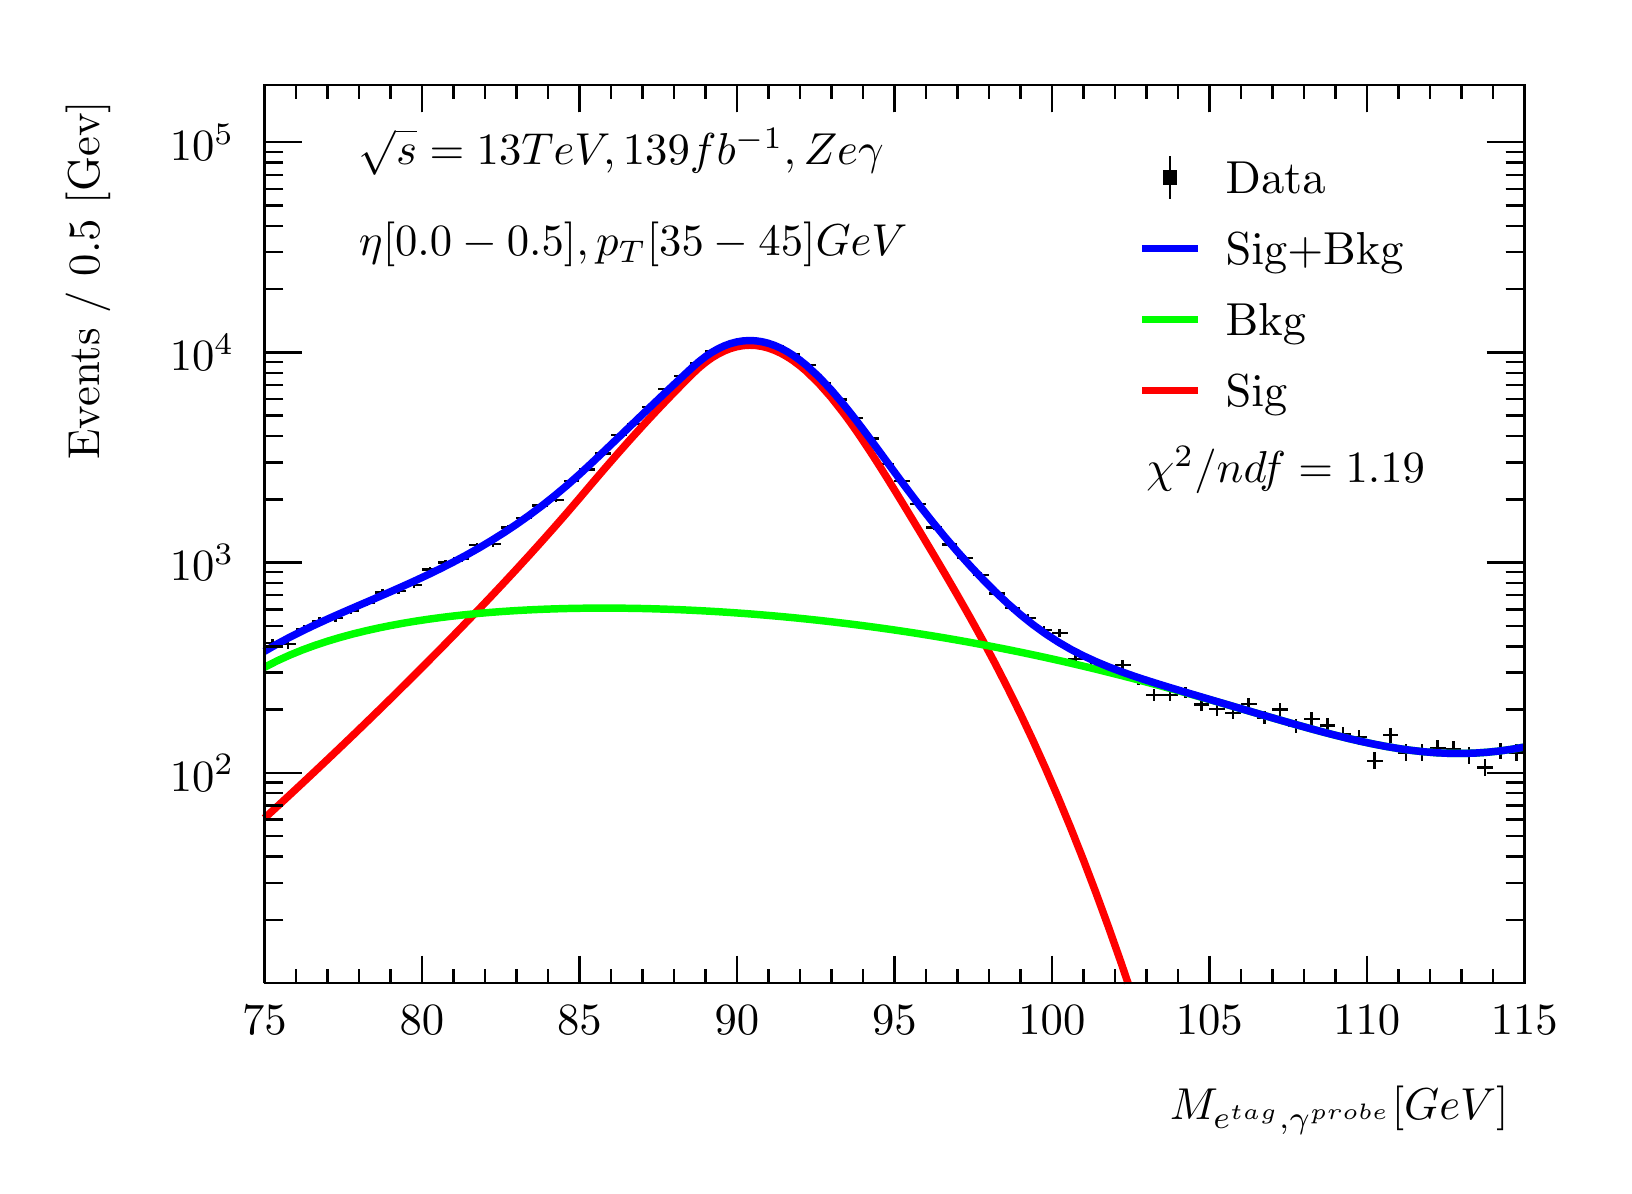
\begin{tikzpicture}
\pgfdeclareplotmark{cross} {
\pgfpathmoveto{\pgfpoint{-0.3\pgfplotmarksize}{\pgfplotmarksize}}
\pgfpathlineto{\pgfpoint{+0.3\pgfplotmarksize}{\pgfplotmarksize}}
\pgfpathlineto{\pgfpoint{+0.3\pgfplotmarksize}{0.3\pgfplotmarksize}}
\pgfpathlineto{\pgfpoint{+1\pgfplotmarksize}{0.3\pgfplotmarksize}}
\pgfpathlineto{\pgfpoint{+1\pgfplotmarksize}{-0.3\pgfplotmarksize}}
\pgfpathlineto{\pgfpoint{+0.3\pgfplotmarksize}{-0.3\pgfplotmarksize}}
\pgfpathlineto{\pgfpoint{+0.3\pgfplotmarksize}{-1.\pgfplotmarksize}}
\pgfpathlineto{\pgfpoint{-0.3\pgfplotmarksize}{-1.\pgfplotmarksize}}
\pgfpathlineto{\pgfpoint{-0.3\pgfplotmarksize}{-0.3\pgfplotmarksize}}
\pgfpathlineto{\pgfpoint{-1.\pgfplotmarksize}{-0.3\pgfplotmarksize}}
\pgfpathlineto{\pgfpoint{-1.\pgfplotmarksize}{0.3\pgfplotmarksize}}
\pgfpathlineto{\pgfpoint{-0.3\pgfplotmarksize}{0.3\pgfplotmarksize}}
\pgfpathclose
\pgfusepathqstroke
}
\pgfdeclareplotmark{cross*} {
\pgfpathmoveto{\pgfpoint{-0.3\pgfplotmarksize}{\pgfplotmarksize}}
\pgfpathlineto{\pgfpoint{+0.3\pgfplotmarksize}{\pgfplotmarksize}}
\pgfpathlineto{\pgfpoint{+0.3\pgfplotmarksize}{0.3\pgfplotmarksize}}
\pgfpathlineto{\pgfpoint{+1\pgfplotmarksize}{0.3\pgfplotmarksize}}
\pgfpathlineto{\pgfpoint{+1\pgfplotmarksize}{-0.3\pgfplotmarksize}}
\pgfpathlineto{\pgfpoint{+0.3\pgfplotmarksize}{-0.3\pgfplotmarksize}}
\pgfpathlineto{\pgfpoint{+0.3\pgfplotmarksize}{-1.\pgfplotmarksize}}
\pgfpathlineto{\pgfpoint{-0.3\pgfplotmarksize}{-1.\pgfplotmarksize}}
\pgfpathlineto{\pgfpoint{-0.3\pgfplotmarksize}{-0.3\pgfplotmarksize}}
\pgfpathlineto{\pgfpoint{-1.\pgfplotmarksize}{-0.3\pgfplotmarksize}}
\pgfpathlineto{\pgfpoint{-1.\pgfplotmarksize}{0.3\pgfplotmarksize}}
\pgfpathlineto{\pgfpoint{-0.3\pgfplotmarksize}{0.3\pgfplotmarksize}}
\pgfpathclose
\pgfusepathqfillstroke
}
\pgfdeclareplotmark{newstar} {
\pgfpathmoveto{\pgfqpoint{0pt}{\pgfplotmarksize}}
\pgfpathlineto{\pgfqpointpolar{44}{0.5\pgfplotmarksize}}
\pgfpathlineto{\pgfqpointpolar{18}{\pgfplotmarksize}}
\pgfpathlineto{\pgfqpointpolar{-20}{0.5\pgfplotmarksize}}
\pgfpathlineto{\pgfqpointpolar{-54}{\pgfplotmarksize}}
\pgfpathlineto{\pgfqpointpolar{-90}{0.5\pgfplotmarksize}}
\pgfpathlineto{\pgfqpointpolar{234}{\pgfplotmarksize}}
\pgfpathlineto{\pgfqpointpolar{198}{0.5\pgfplotmarksize}}
\pgfpathlineto{\pgfqpointpolar{162}{\pgfplotmarksize}}
\pgfpathlineto{\pgfqpointpolar{134}{0.5\pgfplotmarksize}}
\pgfpathclose
\pgfusepathqstroke
}
\pgfdeclareplotmark{newstar*} {
\pgfpathmoveto{\pgfqpoint{0pt}{\pgfplotmarksize}}
\pgfpathlineto{\pgfqpointpolar{44}{0.5\pgfplotmarksize}}
\pgfpathlineto{\pgfqpointpolar{18}{\pgfplotmarksize}}
\pgfpathlineto{\pgfqpointpolar{-20}{0.5\pgfplotmarksize}}
\pgfpathlineto{\pgfqpointpolar{-54}{\pgfplotmarksize}}
\pgfpathlineto{\pgfqpointpolar{-90}{0.5\pgfplotmarksize}}
\pgfpathlineto{\pgfqpointpolar{234}{\pgfplotmarksize}}
\pgfpathlineto{\pgfqpointpolar{198}{0.5\pgfplotmarksize}}
\pgfpathlineto{\pgfqpointpolar{162}{\pgfplotmarksize}}
\pgfpathlineto{\pgfqpointpolar{134}{0.5\pgfplotmarksize}}
\pgfpathclose
\pgfusepathqfillstroke
}
\definecolor{c}{rgb}{1,1,1};
\draw [color=c, fill=c] (0,0) rectangle (20,14.4361);
\draw [color=c, fill=c] (3,2.30977) rectangle (19,13.7143);
\definecolor{c}{rgb}{0,0,0};
\draw [c,line width=0.9] (3,2.30977) -- (3,13.7143) -- (19,13.7143) -- (19,2.30977) -- (3,2.30977);
\definecolor{c}{rgb}{1,1,1};
\draw [color=c, fill=c] (3,2.30977) rectangle (19,13.7143);
\definecolor{c}{rgb}{0,0,0};
\draw [c,line width=0.9] (3,2.30977) -- (3,13.7143) -- (19,13.7143) -- (19,2.30977) -- (3,2.30977);
\draw [c,line width=0.9] (3,2.30977) -- (19,2.30977);
\draw [c,line width=0.9] (3,2.65624) -- (3,2.30977);
\draw [c,line width=0.9] (3.4,2.48301) -- (3.4,2.30977);
\draw [c,line width=0.9] (3.8,2.48301) -- (3.8,2.30977);
\draw [c,line width=0.9] (4.2,2.48301) -- (4.2,2.30977);
\draw [c,line width=0.9] (4.6,2.48301) -- (4.6,2.30977);
\draw [c,line width=0.9] (5,2.65624) -- (5,2.30977);
\draw [c,line width=0.9] (5.4,2.48301) -- (5.4,2.30977);
\draw [c,line width=0.9] (5.8,2.48301) -- (5.8,2.30977);
\draw [c,line width=0.9] (6.2,2.48301) -- (6.2,2.30977);
\draw [c,line width=0.9] (6.6,2.48301) -- (6.6,2.30977);
\draw [c,line width=0.9] (7,2.65624) -- (7,2.30977);
\draw [c,line width=0.9] (7.4,2.48301) -- (7.4,2.30977);
\draw [c,line width=0.9] (7.8,2.48301) -- (7.8,2.30977);
\draw [c,line width=0.9] (8.2,2.48301) -- (8.2,2.30977);
\draw [c,line width=0.9] (8.6,2.48301) -- (8.6,2.30977);
\draw [c,line width=0.9] (9,2.65624) -- (9,2.30977);
\draw [c,line width=0.9] (9.4,2.48301) -- (9.4,2.30977);
\draw [c,line width=0.9] (9.8,2.48301) -- (9.8,2.30977);
\draw [c,line width=0.9] (10.2,2.48301) -- (10.2,2.30977);
\draw [c,line width=0.9] (10.6,2.48301) -- (10.6,2.30977);
\draw [c,line width=0.9] (11,2.65624) -- (11,2.30977);
\draw [c,line width=0.9] (11.4,2.48301) -- (11.4,2.30977);
\draw [c,line width=0.9] (11.8,2.48301) -- (11.8,2.30977);
\draw [c,line width=0.9] (12.2,2.48301) -- (12.2,2.30977);
\draw [c,line width=0.9] (12.6,2.48301) -- (12.6,2.30977);
\draw [c,line width=0.9] (13,2.65624) -- (13,2.30977);
\draw [c,line width=0.9] (13.4,2.48301) -- (13.4,2.30977);
\draw [c,line width=0.9] (13.8,2.48301) -- (13.8,2.30977);
\draw [c,line width=0.9] (14.2,2.48301) -- (14.2,2.30977);
\draw [c,line width=0.9] (14.6,2.48301) -- (14.6,2.30977);
\draw [c,line width=0.9] (15,2.65624) -- (15,2.30977);
\draw [c,line width=0.9] (15.4,2.48301) -- (15.4,2.30977);
\draw [c,line width=0.9] (15.8,2.48301) -- (15.8,2.30977);
\draw [c,line width=0.9] (16.2,2.48301) -- (16.2,2.30977);
\draw [c,line width=0.9] (16.6,2.48301) -- (16.6,2.30977);
\draw [c,line width=0.9] (17,2.65624) -- (17,2.30977);
\draw [c,line width=0.9] (17.4,2.48301) -- (17.4,2.30977);
\draw [c,line width=0.9] (17.8,2.48301) -- (17.8,2.30977);
\draw [c,line width=0.9] (18.2,2.48301) -- (18.2,2.30977);
\draw [c,line width=0.9] (18.6,2.48301) -- (18.6,2.30977);
\draw [c,line width=0.9] (19,2.65624) -- (19,2.30977);
\draw [c,line width=0.9] (19,2.65624) -- (19,2.30977);
\draw [anchor=base] (3,1.66015) node[scale=1.61424, color=c, rotate=0]{75};
\draw [anchor=base] (5,1.66015) node[scale=1.61424, color=c, rotate=0]{80};
\draw [anchor=base] (7,1.66015) node[scale=1.61424, color=c, rotate=0]{85};
\draw [anchor=base] (9,1.66015) node[scale=1.61424, color=c, rotate=0]{90};
\draw [anchor=base] (11,1.66015) node[scale=1.61424, color=c, rotate=0]{95};
\draw [anchor=base] (13,1.66015) node[scale=1.61424, color=c, rotate=0]{100};
\draw [anchor=base] (15,1.66015) node[scale=1.61424, color=c, rotate=0]{105};
\draw [anchor=base] (17,1.66015) node[scale=1.61424, color=c, rotate=0]{110};
\draw [anchor=base] (19,1.66015) node[scale=1.61424, color=c, rotate=0]{115};
\draw [anchor= east] (19,0.692932) node[scale=1.61424, color=c, rotate=0]{$M_{e^{tag}, \gamma^{probe}}  [GeV]$};
\draw [c,line width=0.9] (3,13.7143) -- (19,13.7143);
\draw [c,line width=0.9] (3,13.3678) -- (3,13.7143);
\draw [c,line width=0.9] (3.4,13.5411) -- (3.4,13.7143);
\draw [c,line width=0.9] (3.8,13.5411) -- (3.8,13.7143);
\draw [c,line width=0.9] (4.2,13.5411) -- (4.2,13.7143);
\draw [c,line width=0.9] (4.6,13.5411) -- (4.6,13.7143);
\draw [c,line width=0.9] (5,13.3678) -- (5,13.7143);
\draw [c,line width=0.9] (5.4,13.5411) -- (5.4,13.7143);
\draw [c,line width=0.9] (5.8,13.5411) -- (5.8,13.7143);
\draw [c,line width=0.9] (6.2,13.5411) -- (6.2,13.7143);
\draw [c,line width=0.9] (6.6,13.5411) -- (6.6,13.7143);
\draw [c,line width=0.9] (7,13.3678) -- (7,13.7143);
\draw [c,line width=0.9] (7.4,13.5411) -- (7.4,13.7143);
\draw [c,line width=0.9] (7.8,13.5411) -- (7.8,13.7143);
\draw [c,line width=0.9] (8.2,13.5411) -- (8.2,13.7143);
\draw [c,line width=0.9] (8.6,13.5411) -- (8.6,13.7143);
\draw [c,line width=0.9] (9,13.3678) -- (9,13.7143);
\draw [c,line width=0.9] (9.4,13.5411) -- (9.4,13.7143);
\draw [c,line width=0.9] (9.8,13.5411) -- (9.8,13.7143);
\draw [c,line width=0.9] (10.2,13.5411) -- (10.2,13.7143);
\draw [c,line width=0.9] (10.6,13.5411) -- (10.6,13.7143);
\draw [c,line width=0.9] (11,13.3678) -- (11,13.7143);
\draw [c,line width=0.9] (11.4,13.5411) -- (11.4,13.7143);
\draw [c,line width=0.9] (11.8,13.5411) -- (11.8,13.7143);
\draw [c,line width=0.9] (12.2,13.5411) -- (12.2,13.7143);
\draw [c,line width=0.9] (12.6,13.5411) -- (12.6,13.7143);
\draw [c,line width=0.9] (13,13.3678) -- (13,13.7143);
\draw [c,line width=0.9] (13.4,13.5411) -- (13.4,13.7143);
\draw [c,line width=0.9] (13.8,13.5411) -- (13.8,13.7143);
\draw [c,line width=0.9] (14.2,13.5411) -- (14.2,13.7143);
\draw [c,line width=0.9] (14.6,13.5411) -- (14.6,13.7143);
\draw [c,line width=0.9] (15,13.3678) -- (15,13.7143);
\draw [c,line width=0.9] (15.4,13.5411) -- (15.4,13.7143);
\draw [c,line width=0.9] (15.8,13.5411) -- (15.8,13.7143);
\draw [c,line width=0.9] (16.2,13.5411) -- (16.2,13.7143);
\draw [c,line width=0.9] (16.6,13.5411) -- (16.6,13.7143);
\draw [c,line width=0.9] (17,13.3678) -- (17,13.7143);
\draw [c,line width=0.9] (17.4,13.5411) -- (17.4,13.7143);
\draw [c,line width=0.9] (17.8,13.5411) -- (17.8,13.7143);
\draw [c,line width=0.9] (18.2,13.5411) -- (18.2,13.7143);
\draw [c,line width=0.9] (18.6,13.5411) -- (18.6,13.7143);
\draw [c,line width=0.9] (19,13.3678) -- (19,13.7143);
\draw [c,line width=0.9] (19,13.3678) -- (19,13.7143);
\draw [c,line width=0.9] (3,2.30977) -- (3,13.7143);
\draw [c,line width=0.9] (3.237,3.11343) -- (3,3.11343);
\draw [c,line width=0.9] (3.237,3.58354) -- (3,3.58354);
\draw [c,line width=0.9] (3.237,3.91709) -- (3,3.91709);
\draw [c,line width=0.9] (3.237,4.17581) -- (3,4.17581);
\draw [c,line width=0.9] (3.237,4.38719) -- (3,4.38719);
\draw [c,line width=0.9] (3.237,4.56592) -- (3,4.56592);
\draw [c,line width=0.9] (3.237,4.72074) -- (3,4.72074);
\draw [c,line width=0.9] (3.237,4.8573) -- (3,4.8573);
\draw [c,line width=0.9] (3.474,4.97946) -- (3,4.97946);
\draw [anchor= east] (2.82,4.97946) node[scale=1.61424, color=c, rotate=0]{$10^{2}$};
\draw [c,line width=0.9] (3.237,5.78312) -- (3,5.78312);
\draw [c,line width=0.9] (3.237,6.25323) -- (3,6.25323);
\draw [c,line width=0.9] (3.237,6.58678) -- (3,6.58678);
\draw [c,line width=0.9] (3.237,6.8455) -- (3,6.8455);
\draw [c,line width=0.9] (3.237,7.05689) -- (3,7.05689);
\draw [c,line width=0.9] (3.237,7.23561) -- (3,7.23561);
\draw [c,line width=0.9] (3.237,7.39043) -- (3,7.39043);
\draw [c,line width=0.9] (3.237,7.52699) -- (3,7.52699);
\draw [c,line width=0.9] (3.474,7.64915) -- (3,7.64915);
\draw [anchor= east] (2.82,7.64915) node[scale=1.61424, color=c, rotate=0]{$10^{3}$};
\draw [c,line width=0.9] (3.237,8.45281) -- (3,8.45281);
\draw [c,line width=0.9] (3.237,8.92292) -- (3,8.92292);
\draw [c,line width=0.9] (3.237,9.25647) -- (3,9.25647);
\draw [c,line width=0.9] (3.237,9.51519) -- (3,9.51519);
\draw [c,line width=0.9] (3.237,9.72658) -- (3,9.72658);
\draw [c,line width=0.9] (3.237,9.9053) -- (3,9.9053);
\draw [c,line width=0.9] (3.237,10.0601) -- (3,10.0601);
\draw [c,line width=0.9] (3.237,10.1967) -- (3,10.1967);
\draw [c,line width=0.9] (3.474,10.3188) -- (3,10.3188);
\draw [anchor= east] (2.82,10.3188) node[scale=1.61424, color=c, rotate=0]{$10^{4}$};
\draw [c,line width=0.9] (3.237,11.1225) -- (3,11.1225);
\draw [c,line width=0.9] (3.237,11.5926) -- (3,11.5926);
\draw [c,line width=0.9] (3.237,11.9262) -- (3,11.9262);
\draw [c,line width=0.9] (3.237,12.1849) -- (3,12.1849);
\draw [c,line width=0.9] (3.237,12.3963) -- (3,12.3963);
\draw [c,line width=0.9] (3.237,12.575) -- (3,12.575);
\draw [c,line width=0.9] (3.237,12.7298) -- (3,12.7298);
\draw [c,line width=0.9] (3.237,12.8664) -- (3,12.8664);
\draw [c,line width=0.9] (3.474,12.9885) -- (3,12.9885);
\draw [anchor= east] (2.82,12.9885) node[scale=1.61424, color=c, rotate=0]{$10^{5}$};
\draw [anchor= east] (0.76,13.7143) node[scale=1.61424, color=c, rotate=90]{Events / 0.5 [Gev]};
\draw [c,line width=0.9] (19,2.30977) -- (19,13.7143);
\draw [c,line width=0.9] (18.763,3.11343) -- (19,3.11343);
\draw [c,line width=0.9] (18.763,3.58354) -- (19,3.58354);
\draw [c,line width=0.9] (18.763,3.91709) -- (19,3.91709);
\draw [c,line width=0.9] (18.763,4.17581) -- (19,4.17581);
\draw [c,line width=0.9] (18.763,4.38719) -- (19,4.38719);
\draw [c,line width=0.9] (18.763,4.56592) -- (19,4.56592);
\draw [c,line width=0.9] (18.763,4.72074) -- (19,4.72074);
\draw [c,line width=0.9] (18.763,4.8573) -- (19,4.8573);
\draw [c,line width=0.9] (18.526,4.97946) -- (19,4.97946);
\draw [c,line width=0.9] (18.763,5.78312) -- (19,5.78312);
\draw [c,line width=0.9] (18.763,6.25323) -- (19,6.25323);
\draw [c,line width=0.9] (18.763,6.58678) -- (19,6.58678);
\draw [c,line width=0.9] (18.763,6.8455) -- (19,6.8455);
\draw [c,line width=0.9] (18.763,7.05689) -- (19,7.05689);
\draw [c,line width=0.9] (18.763,7.23561) -- (19,7.23561);
\draw [c,line width=0.9] (18.763,7.39043) -- (19,7.39043);
\draw [c,line width=0.9] (18.763,7.52699) -- (19,7.52699);
\draw [c,line width=0.9] (18.526,7.64915) -- (19,7.64915);
\draw [c,line width=0.9] (18.763,8.45281) -- (19,8.45281);
\draw [c,line width=0.9] (18.763,8.92292) -- (19,8.92292);
\draw [c,line width=0.9] (18.763,9.25647) -- (19,9.25647);
\draw [c,line width=0.9] (18.763,9.51519) -- (19,9.51519);
\draw [c,line width=0.9] (18.763,9.72658) -- (19,9.72658);
\draw [c,line width=0.9] (18.763,9.9053) -- (19,9.9053);
\draw [c,line width=0.9] (18.763,10.0601) -- (19,10.0601);
\draw [c,line width=0.9] (18.763,10.1967) -- (19,10.1967);
\draw [c,line width=0.9] (18.526,10.3188) -- (19,10.3188);
\draw [c,line width=0.9] (18.763,11.1225) -- (19,11.1225);
\draw [c,line width=0.9] (18.763,11.5926) -- (19,11.5926);
\draw [c,line width=0.9] (18.763,11.9262) -- (19,11.9262);
\draw [c,line width=0.9] (18.763,12.1849) -- (19,12.1849);
\draw [c,line width=0.9] (18.763,12.3963) -- (19,12.3963);
\draw [c,line width=0.9] (18.763,12.575) -- (19,12.575);
\draw [c,line width=0.9] (18.763,12.7298) -- (19,12.7298);
\draw [c,line width=0.9] (18.763,12.8664) -- (19,12.8664);
\draw [c,line width=0.9] (18.526,12.9885) -- (19,12.9885);
\draw [c,line width=0.9] (3.1,6.62666) -- (3,6.62666);
\draw [c,line width=0.9] (3,6.62666) -- (3,6.62666);
\draw [c,line width=0.9] (3.1,6.62666) -- (3.2,6.62666);
\draw [c,line width=0.9] (3.2,6.62666) -- (3.2,6.62666);
\draw [c,line width=0.9] (3.1,6.62666) -- (3.1,6.68364);
\draw [c,line width=0.9] (3.1,6.68364) -- (3.1,6.68364);
\draw [c,line width=0.9] (3.1,6.62666) -- (3.1,6.56969);
\draw [c,line width=0.9] (3.1,6.56969) -- (3.1,6.56969);
\draw [c,line width=0.9] (3.3,6.61258) -- (3.2,6.61258);
\draw [c,line width=0.9] (3.2,6.61258) -- (3.2,6.61258);
\draw [c,line width=0.9] (3.3,6.61258) -- (3.4,6.61258);
\draw [c,line width=0.9] (3.4,6.61258) -- (3.4,6.61258);
\draw [c,line width=0.9] (3.3,6.61258) -- (3.3,6.6699);
\draw [c,line width=0.9] (3.3,6.6699) -- (3.3,6.6699);
\draw [c,line width=0.9] (3.3,6.61258) -- (3.3,6.55525);
\draw [c,line width=0.9] (3.3,6.55525) -- (3.3,6.55525);
\draw [c,line width=0.9] (3.5,6.80779) -- (3.4,6.80779);
\draw [c,line width=0.9] (3.4,6.80779) -- (3.4,6.80779);
\draw [c,line width=0.9] (3.5,6.80779) -- (3.6,6.80779);
\draw [c,line width=0.9] (3.6,6.80779) -- (3.6,6.80779);
\draw [c,line width=0.9] (3.5,6.80779) -- (3.5,6.86049);
\draw [c,line width=0.9] (3.5,6.86049) -- (3.5,6.86049);
\draw [c,line width=0.9] (3.5,6.80779) -- (3.5,6.75509);
\draw [c,line width=0.9] (3.5,6.75509) -- (3.5,6.75509);
\draw [c,line width=0.9] (3.7,6.90207) -- (3.6,6.90207);
\draw [c,line width=0.9] (3.6,6.90207) -- (3.6,6.90207);
\draw [c,line width=0.9] (3.7,6.90207) -- (3.8,6.90207);
\draw [c,line width=0.9] (3.8,6.90207) -- (3.8,6.90207);
\draw [c,line width=0.9] (3.7,6.90207) -- (3.7,6.95266);
\draw [c,line width=0.9] (3.7,6.95266) -- (3.7,6.95266);
\draw [c,line width=0.9] (3.7,6.90207) -- (3.7,6.85147);
\draw [c,line width=0.9] (3.7,6.85147) -- (3.7,6.85147);
\draw [c,line width=0.9] (3.9,6.94754) -- (3.8,6.94754);
\draw [c,line width=0.9] (3.8,6.94754) -- (3.8,6.94754);
\draw [c,line width=0.9] (3.9,6.94754) -- (4,6.94754);
\draw [c,line width=0.9] (4,6.94754) -- (4,6.94754);
\draw [c,line width=0.9] (3.9,6.94754) -- (3.9,6.99716);
\draw [c,line width=0.9] (3.9,6.99716) -- (3.9,6.99716);
\draw [c,line width=0.9] (3.9,6.94754) -- (3.9,6.89792);
\draw [c,line width=0.9] (3.9,6.89792) -- (3.9,6.89792);
\draw [c,line width=0.9] (4.1,7.03936) -- (4,7.03936);
\draw [c,line width=0.9] (4,7.03936) -- (4,7.03936);
\draw [c,line width=0.9] (4.1,7.03936) -- (4.2,7.03936);
\draw [c,line width=0.9] (4.2,7.03936) -- (4.2,7.03936);
\draw [c,line width=0.9] (4.1,7.03936) -- (4.1,7.08705);
\draw [c,line width=0.9] (4.1,7.08705) -- (4.1,7.08705);
\draw [c,line width=0.9] (4.1,7.03936) -- (4.1,6.99167);
\draw [c,line width=0.9] (4.1,6.99167) -- (4.1,6.99167);
\draw [c,line width=0.9] (4.3,7.14074) -- (4.2,7.14074);
\draw [c,line width=0.9] (4.2,7.14074) -- (4.2,7.14074);
\draw [c,line width=0.9] (4.3,7.14074) -- (4.4,7.14074);
\draw [c,line width=0.9] (4.4,7.14074) -- (4.4,7.14074);
\draw [c,line width=0.9] (4.3,7.14074) -- (4.3,7.18639);
\draw [c,line width=0.9] (4.3,7.18639) -- (4.3,7.18639);
\draw [c,line width=0.9] (4.3,7.14074) -- (4.3,7.09509);
\draw [c,line width=0.9] (4.3,7.09509) -- (4.3,7.09509);
\draw [c,line width=0.9] (4.5,7.26666) -- (4.4,7.26666);
\draw [c,line width=0.9] (4.4,7.26666) -- (4.4,7.26666);
\draw [c,line width=0.9] (4.5,7.26666) -- (4.6,7.26666);
\draw [c,line width=0.9] (4.6,7.26666) -- (4.6,7.26666);
\draw [c,line width=0.9] (4.5,7.26666) -- (4.5,7.3099);
\draw [c,line width=0.9] (4.5,7.3099) -- (4.5,7.3099);
\draw [c,line width=0.9] (4.5,7.26666) -- (4.5,7.22343);
\draw [c,line width=0.9] (4.5,7.22343) -- (4.5,7.22343);
\draw [c,line width=0.9] (4.7,7.28902) -- (4.6,7.28902);
\draw [c,line width=0.9] (4.6,7.28902) -- (4.6,7.28902);
\draw [c,line width=0.9] (4.7,7.28902) -- (4.8,7.28902);
\draw [c,line width=0.9] (4.8,7.28902) -- (4.8,7.28902);
\draw [c,line width=0.9] (4.7,7.28902) -- (4.7,7.33185);
\draw [c,line width=0.9] (4.7,7.33185) -- (4.7,7.33185);
\draw [c,line width=0.9] (4.7,7.28902) -- (4.7,7.2462);
\draw [c,line width=0.9] (4.7,7.2462) -- (4.7,7.2462);
\draw [c,line width=0.9] (4.9,7.36553) -- (4.8,7.36553);
\draw [c,line width=0.9] (4.8,7.36553) -- (4.8,7.36553);
\draw [c,line width=0.9] (4.9,7.36553) -- (5,7.36553);
\draw [c,line width=0.9] (5,7.36553) -- (5,7.36553);
\draw [c,line width=0.9] (4.9,7.36553) -- (4.9,7.40696);
\draw [c,line width=0.9] (4.9,7.40696) -- (4.9,7.40696);
\draw [c,line width=0.9] (4.9,7.36553) -- (4.9,7.3241);
\draw [c,line width=0.9] (4.9,7.3241) -- (4.9,7.3241);
\draw [c,line width=0.9] (5.1,7.55876) -- (5,7.55876);
\draw [c,line width=0.9] (5,7.55876) -- (5,7.55876);
\draw [c,line width=0.9] (5.1,7.55876) -- (5.2,7.55876);
\draw [c,line width=0.9] (5.2,7.55876) -- (5.2,7.55876);
\draw [c,line width=0.9] (5.1,7.55876) -- (5.1,7.59688);
\draw [c,line width=0.9] (5.1,7.59688) -- (5.1,7.59688);
\draw [c,line width=0.9] (5.1,7.55876) -- (5.1,7.52064);
\draw [c,line width=0.9] (5.1,7.52064) -- (5.1,7.52064);
\draw [c,line width=0.9] (5.3,7.65031) -- (5.2,7.65031);
\draw [c,line width=0.9] (5.2,7.65031) -- (5.2,7.65031);
\draw [c,line width=0.9] (5.3,7.65031) -- (5.4,7.65031);
\draw [c,line width=0.9] (5.4,7.65031) -- (5.4,7.65031);
\draw [c,line width=0.9] (5.3,7.65031) -- (5.3,7.68696);
\draw [c,line width=0.9] (5.3,7.68696) -- (5.3,7.68696);
\draw [c,line width=0.9] (5.3,7.65031) -- (5.3,7.61367);
\draw [c,line width=0.9] (5.3,7.61367) -- (5.3,7.61367);
\draw [c,line width=0.9] (5.5,7.69908) -- (5.4,7.69908);
\draw [c,line width=0.9] (5.4,7.69908) -- (5.4,7.69908);
\draw [c,line width=0.9] (5.5,7.69908) -- (5.6,7.69908);
\draw [c,line width=0.9] (5.6,7.69908) -- (5.6,7.69908);
\draw [c,line width=0.9] (5.5,7.69908) -- (5.5,7.73496);
\draw [c,line width=0.9] (5.5,7.73496) -- (5.5,7.73496);
\draw [c,line width=0.9] (5.5,7.69908) -- (5.5,7.6632);
\draw [c,line width=0.9] (5.5,7.6632) -- (5.5,7.6632);
\draw [c,line width=0.9] (5.7,7.87112) -- (5.6,7.87112);
\draw [c,line width=0.9] (5.6,7.87112) -- (5.6,7.87112);
\draw [c,line width=0.9] (5.7,7.87112) -- (5.8,7.87112);
\draw [c,line width=0.9] (5.8,7.87112) -- (5.8,7.87112);
\draw [c,line width=0.9] (5.7,7.87112) -- (5.7,7.90444);
\draw [c,line width=0.9] (5.7,7.90444) -- (5.7,7.90444);
\draw [c,line width=0.9] (5.7,7.87112) -- (5.7,7.83781);
\draw [c,line width=0.9] (5.7,7.83781) -- (5.7,7.83781);
\draw [c,line width=0.9] (5.9,7.8854) -- (5.8,7.8854);
\draw [c,line width=0.9] (5.8,7.8854) -- (5.8,7.8854);
\draw [c,line width=0.9] (5.9,7.8854) -- (6,7.8854);
\draw [c,line width=0.9] (6,7.8854) -- (6,7.8854);
\draw [c,line width=0.9] (5.9,7.8854) -- (5.9,7.91851);
\draw [c,line width=0.9] (5.9,7.91851) -- (5.9,7.91851);
\draw [c,line width=0.9] (5.9,7.8854) -- (5.9,7.85228);
\draw [c,line width=0.9] (5.9,7.85228) -- (5.9,7.85228);
\draw [c,line width=0.9] (6.1,8.09426) -- (6,8.09426);
\draw [c,line width=0.9] (6,8.09426) -- (6,8.09426);
\draw [c,line width=0.9] (6.1,8.09426) -- (6.2,8.09426);
\draw [c,line width=0.9] (6.2,8.09426) -- (6.2,8.09426);
\draw [c,line width=0.9] (6.1,8.09426) -- (6.1,8.12452);
\draw [c,line width=0.9] (6.1,8.12452) -- (6.1,8.12452);
\draw [c,line width=0.9] (6.1,8.09426) -- (6.1,8.064);
\draw [c,line width=0.9] (6.1,8.064) -- (6.1,8.064);
\draw [c,line width=0.9] (6.3,8.21705) -- (6.2,8.21705);
\draw [c,line width=0.9] (6.2,8.21705) -- (6.2,8.21705);
\draw [c,line width=0.9] (6.3,8.21705) -- (6.4,8.21705);
\draw [c,line width=0.9] (6.4,8.21705) -- (6.4,8.21705);
\draw [c,line width=0.9] (6.3,8.21705) -- (6.3,8.24575);
\draw [c,line width=0.9] (6.3,8.24575) -- (6.3,8.24575);
\draw [c,line width=0.9] (6.3,8.21705) -- (6.3,8.18835);
\draw [c,line width=0.9] (6.3,8.18835) -- (6.3,8.18835);
\draw [c,line width=0.9] (6.5,8.37365) -- (6.4,8.37365);
\draw [c,line width=0.9] (6.4,8.37365) -- (6.4,8.37365);
\draw [c,line width=0.9] (6.5,8.37365) -- (6.6,8.37365);
\draw [c,line width=0.9] (6.6,8.37365) -- (6.6,8.37365);
\draw [c,line width=0.9] (6.5,8.37365) -- (6.5,8.40047);
\draw [c,line width=0.9] (6.5,8.40047) -- (6.5,8.40047);
\draw [c,line width=0.9] (6.5,8.37365) -- (6.5,8.34682);
\draw [c,line width=0.9] (6.5,8.34682) -- (6.5,8.34682);
\draw [c,line width=0.9] (6.7,8.44233) -- (6.6,8.44233);
\draw [c,line width=0.9] (6.6,8.44233) -- (6.6,8.44233);
\draw [c,line width=0.9] (6.7,8.44233) -- (6.8,8.44233);
\draw [c,line width=0.9] (6.8,8.44233) -- (6.8,8.44233);
\draw [c,line width=0.9] (6.7,8.44233) -- (6.7,8.46837);
\draw [c,line width=0.9] (6.7,8.46837) -- (6.7,8.46837);
\draw [c,line width=0.9] (6.7,8.44233) -- (6.7,8.41629);
\draw [c,line width=0.9] (6.7,8.41629) -- (6.7,8.41629);
\draw [c,line width=0.9] (6.9,8.68526) -- (6.8,8.68526);
\draw [c,line width=0.9] (6.8,8.68526) -- (6.8,8.68526);
\draw [c,line width=0.9] (6.9,8.68526) -- (7,8.68526);
\draw [c,line width=0.9] (7,8.68526) -- (7,8.68526);
\draw [c,line width=0.9] (6.9,8.68526) -- (6.9,8.70872);
\draw [c,line width=0.9] (6.9,8.70872) -- (6.9,8.70872);
\draw [c,line width=0.9] (6.9,8.68526) -- (6.9,8.66181);
\draw [c,line width=0.9] (6.9,8.66181) -- (6.9,8.66181);
\draw [c,line width=0.9] (7.1,8.83336) -- (7,8.83336);
\draw [c,line width=0.9] (7,8.83336) -- (7,8.83336);
\draw [c,line width=0.9] (7.1,8.83336) -- (7.2,8.83336);
\draw [c,line width=0.9] (7.2,8.83336) -- (7.2,8.83336);
\draw [c,line width=0.9] (7.1,8.83336) -- (7.1,8.85537);
\draw [c,line width=0.9] (7.1,8.85537) -- (7.1,8.85537);
\draw [c,line width=0.9] (7.1,8.83336) -- (7.1,8.81136);
\draw [c,line width=0.9] (7.1,8.81136) -- (7.1,8.81136);
\draw [c,line width=0.9] (7.3,9.03763) -- (7.2,9.03763);
\draw [c,line width=0.9] (7.2,9.03763) -- (7.2,9.03763);
\draw [c,line width=0.9] (7.3,9.03763) -- (7.4,9.03763);
\draw [c,line width=0.9] (7.4,9.03763) -- (7.4,9.03763);
\draw [c,line width=0.9] (7.3,9.03763) -- (7.3,9.05778);
\draw [c,line width=0.9] (7.3,9.05778) -- (7.3,9.05778);
\draw [c,line width=0.9] (7.3,9.03763) -- (7.3,9.01749);
\draw [c,line width=0.9] (7.3,9.01749) -- (7.3,9.01749);
\draw [c,line width=0.9] (7.5,9.26858) -- (7.4,9.26858);
\draw [c,line width=0.9] (7.4,9.26858) -- (7.4,9.26858);
\draw [c,line width=0.9] (7.5,9.26858) -- (7.6,9.26858);
\draw [c,line width=0.9] (7.6,9.26858) -- (7.6,9.26858);
\draw [c,line width=0.9] (7.5,9.26858) -- (7.5,9.28681);
\draw [c,line width=0.9] (7.5,9.28681) -- (7.5,9.28681);
\draw [c,line width=0.9] (7.5,9.26858) -- (7.5,9.25034);
\draw [c,line width=0.9] (7.5,9.25034) -- (7.5,9.25034);
\draw [c,line width=0.9] (7.7,9.41093) -- (7.6,9.41093);
\draw [c,line width=0.9] (7.6,9.41093) -- (7.6,9.41093);
\draw [c,line width=0.9] (7.7,9.41093) -- (7.8,9.41093);
\draw [c,line width=0.9] (7.8,9.41093) -- (7.8,9.41093);
\draw [c,line width=0.9] (7.7,9.41093) -- (7.7,9.42808);
\draw [c,line width=0.9] (7.7,9.42808) -- (7.7,9.42808);
\draw [c,line width=0.9] (7.7,9.41093) -- (7.7,9.39377);
\draw [c,line width=0.9] (7.7,9.39377) -- (7.7,9.39377);
\draw [c,line width=0.9] (7.9,9.62801) -- (7.8,9.62801);
\draw [c,line width=0.9] (7.8,9.62801) -- (7.8,9.62801);
\draw [c,line width=0.9] (7.9,9.62801) -- (8,9.62801);
\draw [c,line width=0.9] (8,9.62801) -- (8,9.62801);
\draw [c,line width=0.9] (7.9,9.62801) -- (7.9,9.64363);
\draw [c,line width=0.9] (7.9,9.64363) -- (7.9,9.64363);
\draw [c,line width=0.9] (7.9,9.62801) -- (7.9,9.61239);
\draw [c,line width=0.9] (7.9,9.61239) -- (7.9,9.61239);
\draw [c,line width=0.9] (8.1,9.85105) -- (8,9.85105);
\draw [c,line width=0.9] (8,9.85105) -- (8,9.85105);
\draw [c,line width=0.9] (8.1,9.85105) -- (8.2,9.85105);
\draw [c,line width=0.9] (8.2,9.85105) -- (8.2,9.85105);
\draw [c,line width=0.9] (8.1,9.85105) -- (8.1,9.86524);
\draw [c,line width=0.9] (8.1,9.86524) -- (8.1,9.86524);
\draw [c,line width=0.9] (8.1,9.85105) -- (8.1,9.83687);
\draw [c,line width=0.9] (8.1,9.83687) -- (8.1,9.83687);
\draw [c,line width=0.9] (8.3,10.0176) -- (8.2,10.0176);
\draw [c,line width=0.9] (8.2,10.0176) -- (8.2,10.0176);
\draw [c,line width=0.9] (8.3,10.0176) -- (8.4,10.0176);
\draw [c,line width=0.9] (8.4,10.0176) -- (8.4,10.0176);
\draw [c,line width=0.9] (8.3,10.0176) -- (8.3,10.0308);
\draw [c,line width=0.9] (8.3,10.0308) -- (8.3,10.0308);
\draw [c,line width=0.9] (8.3,10.0176) -- (8.3,10.0044);
\draw [c,line width=0.9] (8.3,10.0044) -- (8.3,10.0044);
\draw [c,line width=0.9] (8.5,10.1863) -- (8.4,10.1863);
\draw [c,line width=0.9] (8.4,10.1863) -- (8.4,10.1863);
\draw [c,line width=0.9] (8.5,10.1863) -- (8.6,10.1863);
\draw [c,line width=0.9] (8.6,10.1863) -- (8.6,10.1863);
\draw [c,line width=0.9] (8.5,10.1863) -- (8.5,10.1986);
\draw [c,line width=0.9] (8.5,10.1986) -- (8.5,10.1986);
\draw [c,line width=0.9] (8.5,10.1863) -- (8.5,10.1741);
\draw [c,line width=0.9] (8.5,10.1741) -- (8.5,10.1741);
\draw [c,line width=0.9] (8.7,10.3322) -- (8.6,10.3322);
\draw [c,line width=0.9] (8.6,10.3322) -- (8.6,10.3322);
\draw [c,line width=0.9] (8.7,10.3322) -- (8.8,10.3322);
\draw [c,line width=0.9] (8.8,10.3322) -- (8.8,10.3322);
\draw [c,line width=0.9] (8.7,10.3322) -- (8.7,10.3437);
\draw [c,line width=0.9] (8.7,10.3437) -- (8.7,10.3437);
\draw [c,line width=0.9] (8.7,10.3322) -- (8.7,10.3207);
\draw [c,line width=0.9] (8.7,10.3207) -- (8.7,10.3207);
\draw [c,line width=0.9] (8.9,10.4103) -- (8.8,10.4103);
\draw [c,line width=0.9] (8.8,10.4103) -- (8.8,10.4103);
\draw [c,line width=0.9] (8.9,10.4103) -- (9,10.4103);
\draw [c,line width=0.9] (9,10.4103) -- (9,10.4103);
\draw [c,line width=0.9] (8.9,10.4103) -- (8.9,10.4215);
\draw [c,line width=0.9] (8.9,10.4215) -- (8.9,10.4215);
\draw [c,line width=0.9] (8.9,10.4103) -- (8.9,10.3992);
\draw [c,line width=0.9] (8.9,10.3992) -- (8.9,10.3992);
\draw [c,line width=0.9] (9.1,10.4655) -- (9,10.4655);
\draw [c,line width=0.9] (9,10.4655) -- (9,10.4655);
\draw [c,line width=0.9] (9.1,10.4655) -- (9.2,10.4655);
\draw [c,line width=0.9] (9.2,10.4655) -- (9.2,10.4655);
\draw [c,line width=0.9] (9.1,10.4655) -- (9.1,10.4763);
\draw [c,line width=0.9] (9.1,10.4763) -- (9.1,10.4763);
\draw [c,line width=0.9] (9.1,10.4655) -- (9.1,10.4546);
\draw [c,line width=0.9] (9.1,10.4546) -- (9.1,10.4546);
\draw [c,line width=0.9] (9.3,10.4522) -- (9.2,10.4522);
\draw [c,line width=0.9] (9.2,10.4522) -- (9.2,10.4522);
\draw [c,line width=0.9] (9.3,10.4522) -- (9.4,10.4522);
\draw [c,line width=0.9] (9.4,10.4522) -- (9.4,10.4522);
\draw [c,line width=0.9] (9.3,10.4522) -- (9.3,10.4632);
\draw [c,line width=0.9] (9.3,10.4632) -- (9.3,10.4632);
\draw [c,line width=0.9] (9.3,10.4522) -- (9.3,10.4413);
\draw [c,line width=0.9] (9.3,10.4413) -- (9.3,10.4413);
\draw [c,line width=0.9] (9.5,10.3965) -- (9.4,10.3965);
\draw [c,line width=0.9] (9.4,10.3965) -- (9.4,10.3965);
\draw [c,line width=0.9] (9.5,10.3965) -- (9.6,10.3965);
\draw [c,line width=0.9] (9.6,10.3965) -- (9.6,10.3965);
\draw [c,line width=0.9] (9.5,10.3965) -- (9.5,10.4077);
\draw [c,line width=0.9] (9.5,10.4077) -- (9.5,10.4077);
\draw [c,line width=0.9] (9.5,10.3965) -- (9.5,10.3853);
\draw [c,line width=0.9] (9.5,10.3853) -- (9.5,10.3853);
\draw [c,line width=0.9] (9.7,10.2945) -- (9.6,10.2945);
\draw [c,line width=0.9] (9.6,10.2945) -- (9.6,10.2945);
\draw [c,line width=0.9] (9.7,10.2945) -- (9.8,10.2945);
\draw [c,line width=0.9] (9.8,10.2945) -- (9.8,10.2945);
\draw [c,line width=0.9] (9.7,10.2945) -- (9.7,10.3062);
\draw [c,line width=0.9] (9.7,10.3062) -- (9.7,10.3062);
\draw [c,line width=0.9] (9.7,10.2945) -- (9.7,10.2828);
\draw [c,line width=0.9] (9.7,10.2828) -- (9.7,10.2828);
\draw [c,line width=0.9] (9.9,10.1619) -- (9.8,10.1619);
\draw [c,line width=0.9] (9.8,10.1619) -- (9.8,10.1619);
\draw [c,line width=0.9] (9.9,10.1619) -- (10,10.1619);
\draw [c,line width=0.9] (10,10.1619) -- (10,10.1619);
\draw [c,line width=0.9] (9.9,10.1619) -- (9.9,10.1743);
\draw [c,line width=0.9] (9.9,10.1743) -- (9.9,10.1743);
\draw [c,line width=0.9] (9.9,10.1619) -- (9.9,10.1495);
\draw [c,line width=0.9] (9.9,10.1495) -- (9.9,10.1495);
\draw [c,line width=0.9] (10.1,9.9328) -- (10,9.9328);
\draw [c,line width=0.9] (10,9.9328) -- (10,9.9328);
\draw [c,line width=0.9] (10.1,9.9328) -- (10.2,9.9328);
\draw [c,line width=0.9] (10.2,9.9328) -- (10.2,9.9328);
\draw [c,line width=0.9] (10.1,9.9328) -- (10.1,9.9465);
\draw [c,line width=0.9] (10.1,9.9465) -- (10.1,9.9465);
\draw [c,line width=0.9] (10.1,9.9328) -- (10.1,9.91911);
\draw [c,line width=0.9] (10.1,9.91911) -- (10.1,9.91911);
\draw [c,line width=0.9] (10.3,9.71979) -- (10.2,9.71979);
\draw [c,line width=0.9] (10.2,9.71979) -- (10.2,9.71979);
\draw [c,line width=0.9] (10.3,9.71979) -- (10.4,9.71979);
\draw [c,line width=0.9] (10.4,9.71979) -- (10.4,9.71979);
\draw [c,line width=0.9] (10.3,9.71979) -- (10.3,9.73481);
\draw [c,line width=0.9] (10.3,9.73481) -- (10.3,9.73481);
\draw [c,line width=0.9] (10.3,9.71979) -- (10.3,9.70478);
\draw [c,line width=0.9] (10.3,9.70478) -- (10.3,9.70478);
\draw [c,line width=0.9] (10.5,9.48868) -- (10.4,9.48868);
\draw [c,line width=0.9] (10.4,9.48868) -- (10.4,9.48868);
\draw [c,line width=0.9] (10.5,9.48868) -- (10.6,9.48868);
\draw [c,line width=0.9] (10.6,9.48868) -- (10.6,9.48868);
\draw [c,line width=0.9] (10.5,9.48868) -- (10.5,9.50527);
\draw [c,line width=0.9] (10.5,9.50527) -- (10.5,9.50527);
\draw [c,line width=0.9] (10.5,9.48868) -- (10.5,9.4721);
\draw [c,line width=0.9] (10.5,9.4721) -- (10.5,9.4721);
\draw [c,line width=0.9] (10.7,9.2283) -- (10.6,9.2283);
\draw [c,line width=0.9] (10.6,9.2283) -- (10.6,9.2283);
\draw [c,line width=0.9] (10.7,9.2283) -- (10.8,9.2283);
\draw [c,line width=0.9] (10.8,9.2283) -- (10.8,9.2283);
\draw [c,line width=0.9] (10.7,9.2283) -- (10.7,9.24686);
\draw [c,line width=0.9] (10.7,9.24686) -- (10.7,9.24686);
\draw [c,line width=0.9] (10.7,9.2283) -- (10.7,9.20975);
\draw [c,line width=0.9] (10.7,9.20975) -- (10.7,9.20975);
\draw [c,line width=0.9] (10.9,8.8995) -- (10.8,8.8995);
\draw [c,line width=0.9] (10.8,8.8995) -- (10.8,8.8995);
\draw [c,line width=0.9] (10.9,8.8995) -- (11,8.8995);
\draw [c,line width=0.9] (11,8.8995) -- (11,8.8995);
\draw [c,line width=0.9] (10.9,8.8995) -- (10.9,8.92088);
\draw [c,line width=0.9] (10.9,8.92088) -- (10.9,8.92088);
\draw [c,line width=0.9] (10.9,8.8995) -- (10.9,8.87811);
\draw [c,line width=0.9] (10.9,8.87811) -- (10.9,8.87811);
\draw [c,line width=0.9] (11.1,8.68716) -- (11,8.68716);
\draw [c,line width=0.9] (11,8.68716) -- (11,8.68716);
\draw [c,line width=0.9] (11.1,8.68716) -- (11.2,8.68716);
\draw [c,line width=0.9] (11.2,8.68716) -- (11.2,8.68716);
\draw [c,line width=0.9] (11.1,8.68716) -- (11.1,8.71059);
\draw [c,line width=0.9] (11.1,8.71059) -- (11.1,8.71059);
\draw [c,line width=0.9] (11.1,8.68716) -- (11.1,8.66373);
\draw [c,line width=0.9] (11.1,8.66373) -- (11.1,8.66373);
\draw [c,line width=0.9] (11.3,8.3909) -- (11.2,8.3909);
\draw [c,line width=0.9] (11.2,8.3909) -- (11.2,8.3909);
\draw [c,line width=0.9] (11.3,8.3909) -- (11.4,8.3909);
\draw [c,line width=0.9] (11.4,8.3909) -- (11.4,8.3909);
\draw [c,line width=0.9] (11.3,8.3909) -- (11.3,8.41752);
\draw [c,line width=0.9] (11.3,8.41752) -- (11.3,8.41752);
\draw [c,line width=0.9] (11.3,8.3909) -- (11.3,8.36427);
\draw [c,line width=0.9] (11.3,8.36427) -- (11.3,8.36427);
\draw [c,line width=0.9] (11.5,8.09426) -- (11.4,8.09426);
\draw [c,line width=0.9] (11.4,8.09426) -- (11.4,8.09426);
\draw [c,line width=0.9] (11.5,8.09426) -- (11.6,8.09426);
\draw [c,line width=0.9] (11.6,8.09426) -- (11.6,8.09426);
\draw [c,line width=0.9] (11.5,8.09426) -- (11.5,8.12452);
\draw [c,line width=0.9] (11.5,8.12452) -- (11.5,8.12452);
\draw [c,line width=0.9] (11.5,8.09426) -- (11.5,8.064);
\draw [c,line width=0.9] (11.5,8.064) -- (11.5,8.064);
\draw [c,line width=0.9] (11.7,7.88161) -- (11.6,7.88161);
\draw [c,line width=0.9] (11.6,7.88161) -- (11.6,7.88161);
\draw [c,line width=0.9] (11.7,7.88161) -- (11.8,7.88161);
\draw [c,line width=0.9] (11.8,7.88161) -- (11.8,7.88161);
\draw [c,line width=0.9] (11.7,7.88161) -- (11.7,7.91477);
\draw [c,line width=0.9] (11.7,7.91477) -- (11.7,7.91477);
\draw [c,line width=0.9] (11.7,7.88161) -- (11.7,7.84844);
\draw [c,line width=0.9] (11.7,7.84844) -- (11.7,7.84844);
\draw [c,line width=0.9] (11.9,7.71013) -- (11.8,7.71013);
\draw [c,line width=0.9] (11.8,7.71013) -- (11.8,7.71013);
\draw [c,line width=0.9] (11.9,7.71013) -- (12,7.71013);
\draw [c,line width=0.9] (12,7.71013) -- (12,7.71013);
\draw [c,line width=0.9] (11.9,7.71013) -- (11.9,7.74584);
\draw [c,line width=0.9] (11.9,7.74584) -- (11.9,7.74584);
\draw [c,line width=0.9] (11.9,7.71013) -- (11.9,7.67442);
\draw [c,line width=0.9] (11.9,7.67442) -- (11.9,7.67442);
\draw [c,line width=0.9] (12.1,7.49035) -- (12,7.49035);
\draw [c,line width=0.9] (12,7.49035) -- (12,7.49035);
\draw [c,line width=0.9] (12.1,7.49035) -- (12.2,7.49035);
\draw [c,line width=0.9] (12.2,7.49035) -- (12.2,7.49035);
\draw [c,line width=0.9] (12.1,7.49035) -- (12.1,7.52961);
\draw [c,line width=0.9] (12.1,7.52961) -- (12.1,7.52961);
\draw [c,line width=0.9] (12.1,7.49035) -- (12.1,7.45109);
\draw [c,line width=0.9] (12.1,7.45109) -- (12.1,7.45109);
\draw [c,line width=0.9] (12.3,7.25695) -- (12.2,7.25695);
\draw [c,line width=0.9] (12.2,7.25695) -- (12.2,7.25695);
\draw [c,line width=0.9] (12.3,7.25695) -- (12.4,7.25695);
\draw [c,line width=0.9] (12.4,7.25695) -- (12.4,7.25695);
\draw [c,line width=0.9] (12.3,7.25695) -- (12.3,7.30037);
\draw [c,line width=0.9] (12.3,7.30037) -- (12.3,7.30037);
\draw [c,line width=0.9] (12.3,7.25695) -- (12.3,7.21353);
\draw [c,line width=0.9] (12.3,7.21353) -- (12.3,7.21353);
\draw [c,line width=0.9] (12.5,7.07034) -- (12.4,7.07034);
\draw [c,line width=0.9] (12.4,7.07034) -- (12.4,7.07034);
\draw [c,line width=0.9] (12.5,7.07034) -- (12.6,7.07034);
\draw [c,line width=0.9] (12.6,7.07034) -- (12.6,7.07034);
\draw [c,line width=0.9] (12.5,7.07034) -- (12.5,7.11739);
\draw [c,line width=0.9] (12.5,7.11739) -- (12.5,7.11739);
\draw [c,line width=0.9] (12.5,7.07034) -- (12.5,7.02328);
\draw [c,line width=0.9] (12.5,7.02328) -- (12.5,7.02328);
\draw [c,line width=0.9] (12.7,6.94329) -- (12.6,6.94329);
\draw [c,line width=0.9] (12.6,6.94329) -- (12.6,6.94329);
\draw [c,line width=0.9] (12.7,6.94329) -- (12.8,6.94329);
\draw [c,line width=0.9] (12.8,6.94329) -- (12.8,6.94329);
\draw [c,line width=0.9] (12.7,6.94329) -- (12.7,6.99299);
\draw [c,line width=0.9] (12.7,6.99299) -- (12.7,6.99299);
\draw [c,line width=0.9] (12.7,6.94329) -- (12.7,6.89358);
\draw [c,line width=0.9] (12.7,6.89358) -- (12.7,6.89358);
\draw [c,line width=0.9] (12.9,6.79575) -- (12.8,6.79575);
\draw [c,line width=0.9] (12.8,6.79575) -- (12.8,6.79575);
\draw [c,line width=0.9] (12.9,6.79575) -- (13,6.79575);
\draw [c,line width=0.9] (13,6.79575) -- (13,6.79575);
\draw [c,line width=0.9] (12.9,6.79575) -- (12.9,6.84872);
\draw [c,line width=0.9] (12.9,6.84872) -- (12.9,6.84872);
\draw [c,line width=0.9] (12.9,6.79575) -- (12.9,6.74278);
\draw [c,line width=0.9] (12.9,6.74278) -- (12.9,6.74278);
\draw [c,line width=0.9] (13.1,6.75636) -- (13,6.75636);
\draw [c,line width=0.9] (13,6.75636) -- (13,6.75636);
\draw [c,line width=0.9] (13.1,6.75636) -- (13.2,6.75636);
\draw [c,line width=0.9] (13.2,6.75636) -- (13.2,6.75636);
\draw [c,line width=0.9] (13.1,6.75636) -- (13.1,6.81024);
\draw [c,line width=0.9] (13.1,6.81024) -- (13.1,6.81024);
\draw [c,line width=0.9] (13.1,6.75636) -- (13.1,6.70248);
\draw [c,line width=0.9] (13.1,6.70248) -- (13.1,6.70248);
\draw [c,line width=0.9] (13.3,6.42198) -- (13.2,6.42198);
\draw [c,line width=0.9] (13.2,6.42198) -- (13.2,6.42198);
\draw [c,line width=0.9] (13.3,6.42198) -- (13.4,6.42198);
\draw [c,line width=0.9] (13.4,6.42198) -- (13.4,6.42198);
\draw [c,line width=0.9] (13.3,6.42198) -- (13.3,6.48421);
\draw [c,line width=0.9] (13.3,6.48421) -- (13.3,6.48421);
\draw [c,line width=0.9] (13.3,6.42198) -- (13.3,6.35974);
\draw [c,line width=0.9] (13.3,6.35974) -- (13.3,6.35974);
\draw [c,line width=0.9] (13.5,6.33528) -- (13.4,6.33528);
\draw [c,line width=0.9] (13.4,6.33528) -- (13.4,6.33528);
\draw [c,line width=0.9] (13.5,6.33528) -- (13.6,6.33528);
\draw [c,line width=0.9] (13.6,6.33528) -- (13.6,6.33528);
\draw [c,line width=0.9] (13.5,6.33528) -- (13.5,6.39989);
\draw [c,line width=0.9] (13.5,6.39989) -- (13.5,6.39989);
\draw [c,line width=0.9] (13.5,6.33528) -- (13.5,6.27068);
\draw [c,line width=0.9] (13.5,6.27068) -- (13.5,6.27068);
\draw [c,line width=0.9] (13.7,6.30241) -- (13.6,6.30241);
\draw [c,line width=0.9] (13.6,6.30241) -- (13.6,6.30241);
\draw [c,line width=0.9] (13.7,6.30241) -- (13.8,6.30241);
\draw [c,line width=0.9] (13.8,6.30241) -- (13.8,6.30241);
\draw [c,line width=0.9] (13.7,6.30241) -- (13.7,6.36794);
\draw [c,line width=0.9] (13.7,6.36794) -- (13.7,6.36794);
\draw [c,line width=0.9] (13.7,6.30241) -- (13.7,6.23689);
\draw [c,line width=0.9] (13.7,6.23689) -- (13.7,6.23689);
\draw [c,line width=0.9] (13.9,6.34603) -- (13.8,6.34603);
\draw [c,line width=0.9] (13.8,6.34603) -- (13.8,6.34603);
\draw [c,line width=0.9] (13.9,6.34603) -- (14,6.34603);
\draw [c,line width=0.9] (14,6.34603) -- (14,6.34603);
\draw [c,line width=0.9] (13.9,6.34603) -- (13.9,6.41034);
\draw [c,line width=0.9] (13.9,6.41034) -- (13.9,6.41034);
\draw [c,line width=0.9] (13.9,6.34603) -- (13.9,6.28173);
\draw [c,line width=0.9] (13.9,6.28173) -- (13.9,6.28173);
\draw [c,line width=0.9] (14.1,6.16493) -- (14,6.16493);
\draw [c,line width=0.9] (14,6.16493) -- (14,6.16493);
\draw [c,line width=0.9] (14.1,6.16493) -- (14.2,6.16493);
\draw [c,line width=0.9] (14.2,6.16493) -- (14.2,6.16493);
\draw [c,line width=0.9] (14.1,6.16493) -- (14.1,6.23445);
\draw [c,line width=0.9] (14.1,6.23445) -- (14.1,6.23445);
\draw [c,line width=0.9] (14.1,6.16493) -- (14.1,6.0954);
\draw [c,line width=0.9] (14.1,6.0954) -- (14.1,6.0954);
\draw [c,line width=0.9] (14.3,5.9701) -- (14.2,5.9701);
\draw [c,line width=0.9] (14.2,5.9701) -- (14.2,5.9701);
\draw [c,line width=0.9] (14.3,5.9701) -- (14.4,5.9701);
\draw [c,line width=0.9] (14.4,5.9701) -- (14.4,5.9701);
\draw [c,line width=0.9] (14.3,5.9701) -- (14.3,6.04572);
\draw [c,line width=0.9] (14.3,6.04572) -- (14.3,6.04572);
\draw [c,line width=0.9] (14.3,5.9701) -- (14.3,5.89448);
\draw [c,line width=0.9] (14.3,5.89448) -- (14.3,5.89448);
\draw [c,line width=0.9] (14.5,5.96516) -- (14.4,5.96516);
\draw [c,line width=0.9] (14.4,5.96516) -- (14.4,5.96516);
\draw [c,line width=0.9] (14.5,5.96516) -- (14.6,5.96516);
\draw [c,line width=0.9] (14.6,5.96516) -- (14.6,5.96516);
\draw [c,line width=0.9] (14.5,5.96516) -- (14.5,6.04094);
\draw [c,line width=0.9] (14.5,6.04094) -- (14.5,6.04094);
\draw [c,line width=0.9] (14.5,5.96516) -- (14.5,5.88938);
\draw [c,line width=0.9] (14.5,5.88938) -- (14.5,5.88938);
\draw [c,line width=0.9] (14.7,5.99933) -- (14.6,5.99933);
\draw [c,line width=0.9] (14.6,5.99933) -- (14.6,5.99933);
\draw [c,line width=0.9] (14.7,5.99933) -- (14.8,5.99933);
\draw [c,line width=0.9] (14.8,5.99933) -- (14.8,5.99933);
\draw [c,line width=0.9] (14.7,5.99933) -- (14.7,6.074);
\draw [c,line width=0.9] (14.7,6.074) -- (14.7,6.074);
\draw [c,line width=0.9] (14.7,5.99933) -- (14.7,5.92466);
\draw [c,line width=0.9] (14.7,5.92466) -- (14.7,5.92466);
\draw [c,line width=0.9] (14.9,5.8452) -- (14.8,5.8452);
\draw [c,line width=0.9] (14.8,5.8452) -- (14.8,5.8452);
\draw [c,line width=0.9] (14.9,5.8452) -- (15,5.8452);
\draw [c,line width=0.9] (15,5.8452) -- (15,5.8452);
\draw [c,line width=0.9] (14.9,5.8452) -- (14.9,5.925);
\draw [c,line width=0.9] (14.9,5.925) -- (14.9,5.925);
\draw [c,line width=0.9] (14.9,5.8452) -- (14.9,5.7654);
\draw [c,line width=0.9] (14.9,5.7654) -- (14.9,5.7654);
\draw [c,line width=0.9] (15.1,5.7889) -- (15,5.7889);
\draw [c,line width=0.9] (15,5.7889) -- (15,5.7889);
\draw [c,line width=0.9] (15.1,5.7889) -- (15.2,5.7889);
\draw [c,line width=0.9] (15.2,5.7889) -- (15.2,5.7889);
\draw [c,line width=0.9] (15.1,5.7889) -- (15.1,5.87067);
\draw [c,line width=0.9] (15.1,5.87067) -- (15.1,5.87067);
\draw [c,line width=0.9] (15.1,5.7889) -- (15.1,5.70714);
\draw [c,line width=0.9] (15.1,5.70714) -- (15.1,5.70714);
\draw [c,line width=0.9] (15.3,5.74181) -- (15.2,5.74181);
\draw [c,line width=0.9] (15.2,5.74181) -- (15.2,5.74181);
\draw [c,line width=0.9] (15.3,5.74181) -- (15.4,5.74181);
\draw [c,line width=0.9] (15.4,5.74181) -- (15.4,5.74181);
\draw [c,line width=0.9] (15.3,5.74181) -- (15.3,5.82525);
\draw [c,line width=0.9] (15.3,5.82525) -- (15.3,5.82525);
\draw [c,line width=0.9] (15.3,5.74181) -- (15.3,5.65837);
\draw [c,line width=0.9] (15.3,5.65837) -- (15.3,5.65837);
\draw [c,line width=0.9] (15.5,5.85614) -- (15.4,5.85614);
\draw [c,line width=0.9] (15.4,5.85614) -- (15.4,5.85614);
\draw [c,line width=0.9] (15.5,5.85614) -- (15.6,5.85614);
\draw [c,line width=0.9] (15.6,5.85614) -- (15.6,5.85614);
\draw [c,line width=0.9] (15.5,5.85614) -- (15.5,5.93556);
\draw [c,line width=0.9] (15.5,5.93556) -- (15.5,5.93556);
\draw [c,line width=0.9] (15.5,5.85614) -- (15.5,5.77671);
\draw [c,line width=0.9] (15.5,5.77671) -- (15.5,5.77671);
\draw [c,line width=0.9] (15.7,5.68013) -- (15.6,5.68013);
\draw [c,line width=0.9] (15.6,5.68013) -- (15.6,5.68013);
\draw [c,line width=0.9] (15.7,5.68013) -- (15.8,5.68013);
\draw [c,line width=0.9] (15.8,5.68013) -- (15.8,5.68013);
\draw [c,line width=0.9] (15.7,5.68013) -- (15.7,5.76582);
\draw [c,line width=0.9] (15.7,5.76582) -- (15.7,5.76582);
\draw [c,line width=0.9] (15.7,5.68013) -- (15.7,5.59444);
\draw [c,line width=0.9] (15.7,5.59444) -- (15.7,5.59444);
\draw [c,line width=0.9] (15.9,5.78312) -- (15.8,5.78312);
\draw [c,line width=0.9] (15.8,5.78312) -- (15.8,5.78312);
\draw [c,line width=0.9] (15.9,5.78312) -- (16,5.78312);
\draw [c,line width=0.9] (16,5.78312) -- (16,5.78312);
\draw [c,line width=0.9] (15.9,5.78312) -- (15.9,5.86509);
\draw [c,line width=0.9] (15.9,5.86509) -- (15.9,5.86509);
\draw [c,line width=0.9] (15.9,5.78312) -- (15.9,5.70115);
\draw [c,line width=0.9] (15.9,5.70115) -- (15.9,5.70115);
\draw [c,line width=0.9] (16.1,5.57405) -- (16,5.57405);
\draw [c,line width=0.9] (16,5.57405) -- (16,5.57405);
\draw [c,line width=0.9] (16.1,5.57405) -- (16.2,5.57405);
\draw [c,line width=0.9] (16.2,5.57405) -- (16.2,5.57405);
\draw [c,line width=0.9] (16.1,5.57405) -- (16.1,5.66375);
\draw [c,line width=0.9] (16.1,5.66375) -- (16.1,5.66375);
\draw [c,line width=0.9] (16.1,5.57405) -- (16.1,5.48435);
\draw [c,line width=0.9] (16.1,5.48435) -- (16.1,5.48435);
\draw [c,line width=0.9] (16.3,5.66096) -- (16.2,5.66096);
\draw [c,line width=0.9] (16.2,5.66096) -- (16.2,5.66096);
\draw [c,line width=0.9] (16.3,5.66096) -- (16.4,5.66096);
\draw [c,line width=0.9] (16.4,5.66096) -- (16.4,5.66096);
\draw [c,line width=0.9] (16.3,5.66096) -- (16.3,5.74736);
\draw [c,line width=0.9] (16.3,5.74736) -- (16.3,5.74736);
\draw [c,line width=0.9] (16.3,5.66096) -- (16.3,5.57456);
\draw [c,line width=0.9] (16.3,5.57456) -- (16.3,5.57456);
\draw [c,line width=0.9] (16.5,5.58097) -- (16.4,5.58097);
\draw [c,line width=0.9] (16.4,5.58097) -- (16.4,5.58097);
\draw [c,line width=0.9] (16.5,5.58097) -- (16.6,5.58097);
\draw [c,line width=0.9] (16.6,5.58097) -- (16.6,5.58097);
\draw [c,line width=0.9] (16.5,5.58097) -- (16.5,5.6704);
\draw [c,line width=0.9] (16.5,5.6704) -- (16.5,5.6704);
\draw [c,line width=0.9] (16.5,5.58097) -- (16.5,5.49154);
\draw [c,line width=0.9] (16.5,5.49154) -- (16.5,5.49154);
\draw [c,line width=0.9] (16.7,5.47253) -- (16.6,5.47253);
\draw [c,line width=0.9] (16.6,5.47253) -- (16.6,5.47253);
\draw [c,line width=0.9] (16.7,5.47253) -- (16.8,5.47253);
\draw [c,line width=0.9] (16.8,5.47253) -- (16.8,5.47253);
\draw [c,line width=0.9] (16.7,5.47253) -- (16.7,5.56624);
\draw [c,line width=0.9] (16.7,5.56624) -- (16.7,5.56624);
\draw [c,line width=0.9] (16.7,5.47253) -- (16.7,5.37882);
\draw [c,line width=0.9] (16.7,5.37882) -- (16.7,5.37882);
\draw [c,line width=0.9] (16.9,5.43401) -- (16.8,5.43401);
\draw [c,line width=0.9] (16.8,5.43401) -- (16.8,5.43401);
\draw [c,line width=0.9] (16.9,5.43401) -- (17,5.43401);
\draw [c,line width=0.9] (17,5.43401) -- (17,5.43401);
\draw [c,line width=0.9] (16.9,5.43401) -- (16.9,5.52929);
\draw [c,line width=0.9] (16.9,5.52929) -- (16.9,5.52929);
\draw [c,line width=0.9] (16.9,5.43401) -- (16.9,5.33873);
\draw [c,line width=0.9] (16.9,5.33873) -- (16.9,5.33873);
\draw [c,line width=0.9] (17.1,5.13138) -- (17,5.13138);
\draw [c,line width=0.9] (17,5.13138) -- (17,5.13138);
\draw [c,line width=0.9] (17.1,5.13138) -- (17.2,5.13138);
\draw [c,line width=0.9] (17.2,5.13138) -- (17.2,5.13138);
\draw [c,line width=0.9] (17.1,5.13138) -- (17.1,5.23993);
\draw [c,line width=0.9] (17.1,5.23993) -- (17.1,5.23993);
\draw [c,line width=0.9] (17.1,5.13138) -- (17.1,5.02283);
\draw [c,line width=0.9] (17.1,5.02283) -- (17.1,5.02283);
\draw [c,line width=0.9] (17.3,5.45728) -- (17.2,5.45728);
\draw [c,line width=0.9] (17.2,5.45728) -- (17.2,5.45728);
\draw [c,line width=0.9] (17.3,5.45728) -- (17.4,5.45728);
\draw [c,line width=0.9] (17.4,5.45728) -- (17.4,5.45728);
\draw [c,line width=0.9] (17.3,5.45728) -- (17.3,5.5516);
\draw [c,line width=0.9] (17.3,5.5516) -- (17.3,5.5516);
\draw [c,line width=0.9] (17.3,5.45728) -- (17.3,5.36295);
\draw [c,line width=0.9] (17.3,5.36295) -- (17.3,5.36295);
\draw [c,line width=0.9] (17.5,5.23818) -- (17.4,5.23818);
\draw [c,line width=0.9] (17.4,5.23818) -- (17.4,5.23818);
\draw [c,line width=0.9] (17.5,5.23818) -- (17.6,5.23818);
\draw [c,line width=0.9] (17.6,5.23818) -- (17.6,5.23818);
\draw [c,line width=0.9] (17.5,5.23818) -- (17.5,5.34185);
\draw [c,line width=0.9] (17.5,5.34185) -- (17.5,5.34185);
\draw [c,line width=0.9] (17.5,5.23818) -- (17.5,5.13452);
\draw [c,line width=0.9] (17.5,5.13452) -- (17.5,5.13452);
\draw [c,line width=0.9] (17.7,5.23818) -- (17.6,5.23818);
\draw [c,line width=0.9] (17.6,5.23818) -- (17.6,5.23818);
\draw [c,line width=0.9] (17.7,5.23818) -- (17.8,5.23818);
\draw [c,line width=0.9] (17.8,5.23818) -- (17.8,5.23818);
\draw [c,line width=0.9] (17.7,5.23818) -- (17.7,5.34185);
\draw [c,line width=0.9] (17.7,5.34185) -- (17.7,5.34185);
\draw [c,line width=0.9] (17.7,5.23818) -- (17.7,5.13452);
\draw [c,line width=0.9] (17.7,5.13452) -- (17.7,5.13452);
\draw [c,line width=0.9] (17.9,5.29254) -- (17.8,5.29254);
\draw [c,line width=0.9] (17.8,5.29254) -- (17.8,5.29254);
\draw [c,line width=0.9] (17.9,5.29254) -- (18,5.29254);
\draw [c,line width=0.9] (18,5.29254) -- (18,5.29254);
\draw [c,line width=0.9] (17.9,5.29254) -- (17.9,5.39381);
\draw [c,line width=0.9] (17.9,5.39381) -- (17.9,5.39381);
\draw [c,line width=0.9] (17.9,5.29254) -- (17.9,5.19127);
\draw [c,line width=0.9] (17.9,5.19127) -- (17.9,5.19127);
\draw [c,line width=0.9] (18.1,5.28366) -- (18,5.28366);
\draw [c,line width=0.9] (18,5.28366) -- (18,5.28366);
\draw [c,line width=0.9] (18.1,5.28366) -- (18.2,5.28366);
\draw [c,line width=0.9] (18.2,5.28366) -- (18.2,5.28366);
\draw [c,line width=0.9] (18.1,5.28366) -- (18.1,5.38531);
\draw [c,line width=0.9] (18.1,5.38531) -- (18.1,5.38531);
\draw [c,line width=0.9] (18.1,5.28366) -- (18.1,5.182);
\draw [c,line width=0.9] (18.1,5.182) -- (18.1,5.182);
\draw [c,line width=0.9] (18.3,5.20048) -- (18.2,5.20048);
\draw [c,line width=0.9] (18.2,5.20048) -- (18.2,5.20048);
\draw [c,line width=0.9] (18.3,5.20048) -- (18.4,5.20048);
\draw [c,line width=0.9] (18.4,5.20048) -- (18.4,5.20048);
\draw [c,line width=0.9] (18.3,5.20048) -- (18.3,5.30584);
\draw [c,line width=0.9] (18.3,5.30584) -- (18.3,5.30584);
\draw [c,line width=0.9] (18.3,5.20048) -- (18.3,5.09511);
\draw [c,line width=0.9] (18.3,5.09511) -- (18.3,5.09511);
\draw [c,line width=0.9] (18.5,5.04702) -- (18.4,5.04702);
\draw [c,line width=0.9] (18.4,5.04702) -- (18.4,5.04702);
\draw [c,line width=0.9] (18.5,5.04702) -- (18.6,5.04702);
\draw [c,line width=0.9] (18.6,5.04702) -- (18.6,5.04702);
\draw [c,line width=0.9] (18.5,5.04702) -- (18.5,5.15959);
\draw [c,line width=0.9] (18.5,5.15959) -- (18.5,5.15959);
\draw [c,line width=0.9] (18.5,5.04702) -- (18.5,4.93445);
\draw [c,line width=0.9] (18.5,4.93445) -- (18.5,4.93445);
\draw [c,line width=0.9] (18.7,5.25659) -- (18.6,5.25659);
\draw [c,line width=0.9] (18.6,5.25659) -- (18.6,5.25659);
\draw [c,line width=0.9] (18.7,5.25659) -- (18.8,5.25659);
\draw [c,line width=0.9] (18.8,5.25659) -- (18.8,5.25659);
\draw [c,line width=0.9] (18.7,5.25659) -- (18.7,5.35944);
\draw [c,line width=0.9] (18.7,5.35944) -- (18.7,5.35944);
\draw [c,line width=0.9] (18.7,5.25659) -- (18.7,5.15374);
\draw [c,line width=0.9] (18.7,5.15374) -- (18.7,5.15374);
\draw [c,line width=0.9] (18.9,5.23818) -- (18.8,5.23818);
\draw [c,line width=0.9] (18.8,5.23818) -- (18.8,5.23818);
\draw [c,line width=0.9] (18.9,5.23818) -- (19,5.23818);
\draw [c,line width=0.9] (19,5.23818) -- (19,5.23818);
\draw [c,line width=0.9] (18.9,5.23818) -- (18.9,5.34185);
\draw [c,line width=0.9] (18.9,5.34185) -- (18.9,5.34185);
\draw [c,line width=0.9] (18.9,5.23818) -- (18.9,5.13452);
\draw [c,line width=0.9] (18.9,5.13452) -- (18.9,5.13452);
\foreach \P in {(3.1,6.62666), (3.3,6.61258), (3.5,6.80779), (3.7,6.90207), (3.9,6.94754), (4.1,7.03936), (4.3,7.14074), (4.5,7.26666), (4.7,7.28902), (4.9,7.36553), (5.1,7.55876), (5.3,7.65031), (5.5,7.69908), (5.7,7.87112), (5.9,7.8854),
 (6.1,8.09426), (6.3,8.21705), (6.5,8.37365), (6.7,8.44233), (6.9,8.68526), (7.1,8.83336), (7.3,9.03763), (7.5,9.26858), (7.7,9.41093), (7.9,9.62801), (8.1,9.85105), (8.3,10.0176), (8.5,10.1863), (8.7,10.3322), (8.9,10.4103), (9.1,10.4655),
 (9.3,10.4522), (9.5,10.3965), (9.7,10.2945), (9.9,10.1619), (10.1,9.9328), (10.3,9.71979), (10.5,9.48868), (10.7,9.2283), (10.9,8.8995), (11.1,8.68716), (11.3,8.3909), (11.5,8.09426), (11.7,7.88161), (11.9,7.71013), (12.1,7.49035), (12.3,7.25695),
 (12.5,7.07034), (12.7,6.94329), (12.9,6.79575), (13.1,6.75636), (13.3,6.42198), (13.5,6.33528), (13.7,6.30241), (13.9,6.34603), (14.1,6.16493), (14.3,5.9701), (14.5,5.96516), (14.7,5.99933), (14.9,5.8452), (15.1,5.7889), (15.3,5.74181),
 (15.5,5.85614), (15.7,5.68013), (15.9,5.78312), (16.1,5.57405), (16.3,5.66096), (16.5,5.58097), (16.7,5.47253), (16.9,5.43401), (17.1,5.13138), (17.3,5.45728), (17.5,5.23818), (17.7,5.23818), (17.9,5.29254), (18.1,5.28366), (18.3,5.20048),
 (18.5,5.04702), (18.7,5.25659), (18.9,5.23818)}{\draw[mark options={color=c,fill=c},mark size=2.882883pt,mark=] plot coordinates {\P};}
\definecolor{c}{rgb}{1,0,0};
\draw [c,line width=2.7] (3,4.40307) -- (3,4.40307);
\draw [c,line width=2.7] (3,4.40307) -- (3.16,4.54997) -- (3.32,4.69787) -- (3.48,4.84676) -- (3.64,4.99668) -- (3.8,5.14765) -- (3.96,5.29968) -- (4.12,5.45281) -- (4.28,5.60707) -- (4.44,5.76248) -- (4.6,5.91909) -- (4.76,6.07693) -- (4.92,6.23607)
 -- (5.08,6.39655) -- (5.24,6.55844) -- (5.4,6.72182) -- (5.56,6.88676) -- (5.72,7.05338) -- (5.88,7.22178) -- (6.04,7.39211) -- (6.2,7.56452) -- (6.36,7.7392) -- (6.52,7.91638) -- (6.68,8.09633) -- (6.84,8.27937) -- (7,8.46587) -- (7.16,8.65506) --
 (7.32,8.84217) -- (7.48,9.02619) -- (7.64,9.20666) -- (7.8,9.38326) -- (7.88,9.47006) -- (7.96,9.55585) -- (8.04,9.64063) -- (8.12,9.72442) -- (8.2,9.80726) -- (8.28,9.88917) -- (8.36,9.97021) -- (8.44,10.0504) -- (8.52,10.1252) -- (8.6,10.1913) --
 (8.68,10.2488) -- (8.76,10.2976) -- (8.84,10.3376) -- (8.92,10.3688) -- (9,10.3913) -- (9.08,10.4051) -- (9.16,10.4101) -- (9.24,10.4066) -- (9.32,10.3945) -- (9.4,10.374) -- (9.48,10.3451) -- (9.56,10.3081) -- (9.64,10.2631) -- (9.72,10.2103) --
 (9.8,10.1499) -- (9.88,10.0822) -- (10.04,9.92602) -- (10.2,9.74435) -- (10.36,9.54035) -- (10.44,9.43108) -- (10.52,9.31758) -- (10.6,9.20034) -- (10.68,9.07985) -- (10.76,8.95658) -- (10.84,8.83098) -- (10.92,8.70348) -- (11,8.57445) --
 (11.08,8.44421) -- (11.16,8.31301) -- (11.32,8.04842) -- (11.48,7.78126) -- (11.64,7.51102) -- (11.8,7.23637) -- (11.96,6.95544) -- (12.12,6.6662) -- (12.28,6.36667) -- (12.44,6.05515) -- (12.6,5.73024) -- (12.76,5.39085) -- (12.92,5.03618) --
 (13.08,4.66567) -- (13.24,4.27893) -- (13.4,3.87571) -- (13.56,3.45582) -- (13.72,3.01918) -- (13.88,2.56571) -- (13.9671,2.30977);
\definecolor{c}{rgb}{0,1,0};
\draw [c,line width=2.7] (3,6.31935) -- (3,6.31935);
\draw [c,line width=2.7] (3,6.31935) -- (3.16,6.40115) -- (3.32,6.474) -- (3.48,6.53924) -- (3.64,6.59792) -- (3.8,6.65086) -- (3.96,6.69877) -- (4.12,6.74218) -- (4.28,6.78157) -- (4.44,6.81734) -- (4.6,6.8498) -- (4.76,6.87925) -- (4.92,6.90593) --
 (5.08,6.93005) -- (5.24,6.95179) -- (5.4,6.97132) -- (5.56,6.98878) -- (5.72,7.00429) -- (5.88,7.01797) -- (6.04,7.02991) -- (6.2,7.0402) -- (6.36,7.04892) -- (6.52,7.05614) -- (6.68,7.06193) -- (6.84,7.06633) -- (7,7.06941) -- (7.16,7.07121) --
 (7.32,7.07176) -- (7.48,7.07112) -- (7.64,7.0693) -- (7.8,7.06634) -- (7.96,7.06228) -- (8.12,7.05712) -- (8.28,7.0509) -- (8.44,7.04363) -- (8.6,7.03533) -- (8.76,7.02601) -- (8.92,7.0157) -- (9.08,7.00439) -- (9.24,6.9921) -- (9.4,6.97884) --
 (9.56,6.96461) -- (9.72,6.94942) -- (9.88,6.93327) -- (10.04,6.91617) -- (10.2,6.89812) -- (10.36,6.87912) -- (10.52,6.85917) -- (10.68,6.83827) -- (10.84,6.81641) -- (11,6.79359) -- (11.16,6.76982) -- (11.32,6.74509) -- (11.48,6.71939) --
 (11.64,6.69272) -- (11.8,6.66507) -- (11.96,6.63645) -- (12.12,6.60684) -- (12.28,6.57624) -- (12.44,6.54466) -- (12.6,6.51208) -- (12.76,6.47851) -- (12.92,6.44395) -- (13.08,6.40839) -- (13.24,6.37185) -- (13.4,6.33433) -- (13.56,6.29584) --
 (13.72,6.25639) -- (13.88,6.21601) -- (14.04,6.17473) -- (14.2,6.13256) -- (14.36,6.08956) -- (14.52,6.04578) -- (14.68,6.00127) -- (14.84,5.95611) -- (15,5.9104) -- (15.16,5.86422) -- (15.32,5.81772) -- (15.48,5.77103) -- (15.64,5.72433) --
 (15.8,5.67782) -- (15.96,5.63171) -- (16.12,5.58627) -- (16.28,5.54178) -- (16.44,5.49858) -- (16.6,5.45701) -- (16.76,5.41747) -- (16.92,5.38038) -- (17.08,5.34618) -- (17.24,5.31533) -- (17.4,5.28829) -- (17.56,5.26553) -- (17.72,5.24749) --
 (17.88,5.23456) -- (18.04,5.2271) -- (18.2,5.22539) -- (18.36,5.22963) -- (18.52,5.23992) -- (18.68,5.25628) -- (18.84,5.27861) -- (19,5.30675) -- (19,5.30675) -- (19,5.30675);
\definecolor{c}{rgb}{0,0,1};
\draw [c,line width=2.7] (3,6.52251) -- (3,6.52251);
\draw [c,line width=2.7] (3,6.52251) -- (3.16,6.61503) -- (3.32,6.70087) -- (3.48,6.78142) -- (3.64,6.85785) -- (3.8,6.93117) -- (3.96,7.00223) -- (4.12,7.07185) -- (4.28,7.14075) -- (4.44,7.20961) -- (4.6,7.27909) -- (4.76,7.34981) -- (4.92,7.42238)
 -- (5.08,7.49738) -- (5.24,7.57538) -- (5.4,7.65693) -- (5.56,7.74255) -- (5.72,7.83275) -- (5.88,7.928) -- (6.04,8.02875) -- (6.2,8.1354) -- (6.36,8.24835) -- (6.52,8.36794) -- (6.68,8.49451) -- (6.84,8.6284) -- (7,8.76994) -- (7.16,8.91851) --
 (7.32,9.07006) -- (7.48,9.22321) -- (7.64,9.37701) -- (7.8,9.53066) -- (7.96,9.68352) -- (8.04,9.7595) -- (8.12,9.83515) -- (8.2,9.91042) -- (8.28,9.98533) -- (8.36,10.0599) -- (8.44,10.134) -- (8.52,10.2035) -- (8.6,10.2652) -- (8.68,10.3189) --
 (8.76,10.3646) -- (8.84,10.4021) -- (8.92,10.4314) -- (9,10.4524) -- (9.08,10.4652) -- (9.16,10.4697) -- (9.24,10.466) -- (9.32,10.4542) -- (9.4,10.4344) -- (9.48,10.4067) -- (9.56,10.3712) -- (9.64,10.3282) -- (9.72,10.2779) -- (9.8,10.2206) --
 (9.88,10.1565) -- (10.04,10.0094) -- (10.2,9.83987) -- (10.36,9.65163) -- (10.44,9.55182) -- (10.52,9.44897) -- (10.6,9.34366) -- (10.68,9.2365) -- (10.76,9.12806) -- (10.84,9.0189) -- (10.92,8.90954) -- (11,8.80048) -- (11.08,8.69212) --
 (11.16,8.58484) -- (11.32,8.37465) -- (11.48,8.17152) -- (11.64,7.97627) -- (11.8,7.78922) -- (11.96,7.61054) -- (12.12,7.44055) -- (12.28,7.27984) -- (12.44,7.12921) -- (12.6,6.98951) -- (12.76,6.86146) -- (12.92,6.74542) -- (13.08,6.64127) --
 (13.24,6.54838) -- (13.4,6.46569) -- (13.56,6.39185) -- (13.72,6.32537) -- (13.88,6.26474) -- (14.04,6.2086) -- (14.2,6.15574) -- (14.36,6.10519) -- (14.52,6.05616) -- (14.68,6.00806) -- (14.84,5.96049) -- (15,5.91318) -- (15.16,5.86597) --
 (15.32,5.8188) -- (15.48,5.77169) -- (15.64,5.72473) -- (15.8,5.67805) -- (15.96,5.63184) -- (16.12,5.58635) -- (16.28,5.54183) -- (16.44,5.4986) -- (16.6,5.45703) -- (16.76,5.41748) -- (16.92,5.38038) -- (17.08,5.34618) -- (17.24,5.31533) --
 (17.4,5.28829) -- (17.56,5.26553) -- (17.72,5.24749) -- (17.88,5.23456) -- (18.04,5.2271) -- (18.2,5.22539) -- (18.36,5.22963) -- (18.52,5.23992) -- (18.68,5.25628) -- (18.84,5.27861) -- (19,5.30675) -- (19,5.30675) -- (19,5.30675);
\definecolor{c}{rgb}{0,0,0};
\draw [c,line width=0.9] (3,2.30977) -- (19,2.30977);
\draw [c,line width=0.9] (3,2.65624) -- (3,2.30977);
\draw [c,line width=0.9] (3.4,2.48301) -- (3.4,2.30977);
\draw [c,line width=0.9] (3.8,2.48301) -- (3.8,2.30977);
\draw [c,line width=0.9] (4.2,2.48301) -- (4.2,2.30977);
\draw [c,line width=0.9] (4.6,2.48301) -- (4.6,2.30977);
\draw [c,line width=0.9] (5,2.65624) -- (5,2.30977);
\draw [c,line width=0.9] (5.4,2.48301) -- (5.4,2.30977);
\draw [c,line width=0.9] (5.8,2.48301) -- (5.8,2.30977);
\draw [c,line width=0.9] (6.2,2.48301) -- (6.2,2.30977);
\draw [c,line width=0.9] (6.6,2.48301) -- (6.6,2.30977);
\draw [c,line width=0.9] (7,2.65624) -- (7,2.30977);
\draw [c,line width=0.9] (7.4,2.48301) -- (7.4,2.30977);
\draw [c,line width=0.9] (7.8,2.48301) -- (7.8,2.30977);
\draw [c,line width=0.9] (8.2,2.48301) -- (8.2,2.30977);
\draw [c,line width=0.9] (8.6,2.48301) -- (8.6,2.30977);
\draw [c,line width=0.9] (9,2.65624) -- (9,2.30977);
\draw [c,line width=0.9] (9.4,2.48301) -- (9.4,2.30977);
\draw [c,line width=0.9] (9.8,2.48301) -- (9.8,2.30977);
\draw [c,line width=0.9] (10.2,2.48301) -- (10.2,2.30977);
\draw [c,line width=0.9] (10.6,2.48301) -- (10.6,2.30977);
\draw [c,line width=0.9] (11,2.65624) -- (11,2.30977);
\draw [c,line width=0.9] (11.4,2.48301) -- (11.4,2.30977);
\draw [c,line width=0.9] (11.8,2.48301) -- (11.8,2.30977);
\draw [c,line width=0.9] (12.2,2.48301) -- (12.2,2.30977);
\draw [c,line width=0.9] (12.6,2.48301) -- (12.6,2.30977);
\draw [c,line width=0.9] (13,2.65624) -- (13,2.30977);
\draw [c,line width=0.9] (13.4,2.48301) -- (13.4,2.30977);
\draw [c,line width=0.9] (13.8,2.48301) -- (13.8,2.30977);
\draw [c,line width=0.9] (14.2,2.48301) -- (14.2,2.30977);
\draw [c,line width=0.9] (14.6,2.48301) -- (14.6,2.30977);
\draw [c,line width=0.9] (15,2.65624) -- (15,2.30977);
\draw [c,line width=0.9] (15.4,2.48301) -- (15.4,2.30977);
\draw [c,line width=0.9] (15.8,2.48301) -- (15.8,2.30977);
\draw [c,line width=0.9] (16.2,2.48301) -- (16.2,2.30977);
\draw [c,line width=0.9] (16.6,2.48301) -- (16.6,2.30977);
\draw [c,line width=0.9] (17,2.65624) -- (17,2.30977);
\draw [c,line width=0.9] (17.4,2.48301) -- (17.4,2.30977);
\draw [c,line width=0.9] (17.8,2.48301) -- (17.8,2.30977);
\draw [c,line width=0.9] (18.2,2.48301) -- (18.2,2.30977);
\draw [c,line width=0.9] (18.6,2.48301) -- (18.6,2.30977);
\draw [c,line width=0.9] (19,2.65624) -- (19,2.30977);
\draw [c,line width=0.9] (19,2.65624) -- (19,2.30977);
\draw [c,line width=0.9] (3,13.7143) -- (19,13.7143);
\draw [c,line width=0.9] (3,13.3678) -- (3,13.7143);
\draw [c,line width=0.9] (3.4,13.5411) -- (3.4,13.7143);
\draw [c,line width=0.9] (3.8,13.5411) -- (3.8,13.7143);
\draw [c,line width=0.9] (4.2,13.5411) -- (4.2,13.7143);
\draw [c,line width=0.9] (4.6,13.5411) -- (4.6,13.7143);
\draw [c,line width=0.9] (5,13.3678) -- (5,13.7143);
\draw [c,line width=0.9] (5.4,13.5411) -- (5.4,13.7143);
\draw [c,line width=0.9] (5.8,13.5411) -- (5.8,13.7143);
\draw [c,line width=0.9] (6.2,13.5411) -- (6.2,13.7143);
\draw [c,line width=0.9] (6.6,13.5411) -- (6.6,13.7143);
\draw [c,line width=0.9] (7,13.3678) -- (7,13.7143);
\draw [c,line width=0.9] (7.4,13.5411) -- (7.4,13.7143);
\draw [c,line width=0.9] (7.8,13.5411) -- (7.8,13.7143);
\draw [c,line width=0.9] (8.2,13.5411) -- (8.2,13.7143);
\draw [c,line width=0.9] (8.6,13.5411) -- (8.6,13.7143);
\draw [c,line width=0.9] (9,13.3678) -- (9,13.7143);
\draw [c,line width=0.9] (9.4,13.5411) -- (9.4,13.7143);
\draw [c,line width=0.9] (9.8,13.5411) -- (9.8,13.7143);
\draw [c,line width=0.9] (10.2,13.5411) -- (10.2,13.7143);
\draw [c,line width=0.9] (10.6,13.5411) -- (10.6,13.7143);
\draw [c,line width=0.9] (11,13.3678) -- (11,13.7143);
\draw [c,line width=0.9] (11.4,13.5411) -- (11.4,13.7143);
\draw [c,line width=0.9] (11.8,13.5411) -- (11.8,13.7143);
\draw [c,line width=0.9] (12.2,13.5411) -- (12.2,13.7143);
\draw [c,line width=0.9] (12.6,13.5411) -- (12.6,13.7143);
\draw [c,line width=0.9] (13,13.3678) -- (13,13.7143);
\draw [c,line width=0.9] (13.4,13.5411) -- (13.4,13.7143);
\draw [c,line width=0.9] (13.8,13.5411) -- (13.8,13.7143);
\draw [c,line width=0.9] (14.2,13.5411) -- (14.2,13.7143);
\draw [c,line width=0.9] (14.6,13.5411) -- (14.6,13.7143);
\draw [c,line width=0.9] (15,13.3678) -- (15,13.7143);
\draw [c,line width=0.9] (15.4,13.5411) -- (15.4,13.7143);
\draw [c,line width=0.9] (15.8,13.5411) -- (15.8,13.7143);
\draw [c,line width=0.9] (16.2,13.5411) -- (16.2,13.7143);
\draw [c,line width=0.9] (16.6,13.5411) -- (16.6,13.7143);
\draw [c,line width=0.9] (17,13.3678) -- (17,13.7143);
\draw [c,line width=0.9] (17.4,13.5411) -- (17.4,13.7143);
\draw [c,line width=0.9] (17.8,13.5411) -- (17.8,13.7143);
\draw [c,line width=0.9] (18.2,13.5411) -- (18.2,13.7143);
\draw [c,line width=0.9] (18.6,13.5411) -- (18.6,13.7143);
\draw [c,line width=0.9] (19,13.3678) -- (19,13.7143);
\draw [c,line width=0.9] (19,13.3678) -- (19,13.7143);
\draw [c,line width=0.9] (3,2.30977) -- (3,13.7143);
\draw [c,line width=0.9] (3.237,3.11343) -- (3,3.11343);
\draw [c,line width=0.9] (3.237,3.58354) -- (3,3.58354);
\draw [c,line width=0.9] (3.237,3.91709) -- (3,3.91709);
\draw [c,line width=0.9] (3.237,4.17581) -- (3,4.17581);
\draw [c,line width=0.9] (3.237,4.38719) -- (3,4.38719);
\draw [c,line width=0.9] (3.237,4.56592) -- (3,4.56592);
\draw [c,line width=0.9] (3.237,4.72074) -- (3,4.72074);
\draw [c,line width=0.9] (3.237,4.8573) -- (3,4.8573);
\draw [c,line width=0.9] (3.474,4.97946) -- (3,4.97946);
\draw [c,line width=0.9] (3.237,5.78312) -- (3,5.78312);
\draw [c,line width=0.9] (3.237,6.25323) -- (3,6.25323);
\draw [c,line width=0.9] (3.237,6.58678) -- (3,6.58678);
\draw [c,line width=0.9] (3.237,6.8455) -- (3,6.8455);
\draw [c,line width=0.9] (3.237,7.05689) -- (3,7.05689);
\draw [c,line width=0.9] (3.237,7.23561) -- (3,7.23561);
\draw [c,line width=0.9] (3.237,7.39043) -- (3,7.39043);
\draw [c,line width=0.9] (3.237,7.52699) -- (3,7.52699);
\draw [c,line width=0.9] (3.474,7.64915) -- (3,7.64915);
\draw [c,line width=0.9] (3.237,8.45281) -- (3,8.45281);
\draw [c,line width=0.9] (3.237,8.92292) -- (3,8.92292);
\draw [c,line width=0.9] (3.237,9.25647) -- (3,9.25647);
\draw [c,line width=0.9] (3.237,9.51519) -- (3,9.51519);
\draw [c,line width=0.9] (3.237,9.72658) -- (3,9.72658);
\draw [c,line width=0.9] (3.237,9.9053) -- (3,9.9053);
\draw [c,line width=0.9] (3.237,10.0601) -- (3,10.0601);
\draw [c,line width=0.9] (3.237,10.1967) -- (3,10.1967);
\draw [c,line width=0.9] (3.474,10.3188) -- (3,10.3188);
\draw [c,line width=0.9] (3.237,11.1225) -- (3,11.1225);
\draw [c,line width=0.9] (3.237,11.5926) -- (3,11.5926);
\draw [c,line width=0.9] (3.237,11.9262) -- (3,11.9262);
\draw [c,line width=0.9] (3.237,12.1849) -- (3,12.1849);
\draw [c,line width=0.9] (3.237,12.3963) -- (3,12.3963);
\draw [c,line width=0.9] (3.237,12.575) -- (3,12.575);
\draw [c,line width=0.9] (3.237,12.7298) -- (3,12.7298);
\draw [c,line width=0.9] (3.237,12.8664) -- (3,12.8664);
\draw [c,line width=0.9] (3.474,12.9885) -- (3,12.9885);
\draw [c,line width=0.9] (19,2.30977) -- (19,13.7143);
\draw [c,line width=0.9] (18.763,3.11343) -- (19,3.11343);
\draw [c,line width=0.9] (18.763,3.58354) -- (19,3.58354);
\draw [c,line width=0.9] (18.763,3.91709) -- (19,3.91709);
\draw [c,line width=0.9] (18.763,4.17581) -- (19,4.17581);
\draw [c,line width=0.9] (18.763,4.38719) -- (19,4.38719);
\draw [c,line width=0.9] (18.763,4.56592) -- (19,4.56592);
\draw [c,line width=0.9] (18.763,4.72074) -- (19,4.72074);
\draw [c,line width=0.9] (18.763,4.8573) -- (19,4.8573);
\draw [c,line width=0.9] (18.526,4.97946) -- (19,4.97946);
\draw [c,line width=0.9] (18.763,5.78312) -- (19,5.78312);
\draw [c,line width=0.9] (18.763,6.25323) -- (19,6.25323);
\draw [c,line width=0.9] (18.763,6.58678) -- (19,6.58678);
\draw [c,line width=0.9] (18.763,6.8455) -- (19,6.8455);
\draw [c,line width=0.9] (18.763,7.05689) -- (19,7.05689);
\draw [c,line width=0.9] (18.763,7.23561) -- (19,7.23561);
\draw [c,line width=0.9] (18.763,7.39043) -- (19,7.39043);
\draw [c,line width=0.9] (18.763,7.52699) -- (19,7.52699);
\draw [c,line width=0.9] (18.526,7.64915) -- (19,7.64915);
\draw [c,line width=0.9] (18.763,8.45281) -- (19,8.45281);
\draw [c,line width=0.9] (18.763,8.92292) -- (19,8.92292);
\draw [c,line width=0.9] (18.763,9.25647) -- (19,9.25647);
\draw [c,line width=0.9] (18.763,9.51519) -- (19,9.51519);
\draw [c,line width=0.9] (18.763,9.72658) -- (19,9.72658);
\draw [c,line width=0.9] (18.763,9.9053) -- (19,9.9053);
\draw [c,line width=0.9] (18.763,10.0601) -- (19,10.0601);
\draw [c,line width=0.9] (18.763,10.1967) -- (19,10.1967);
\draw [c,line width=0.9] (18.526,10.3188) -- (19,10.3188);
\draw [c,line width=0.9] (18.763,11.1225) -- (19,11.1225);
\draw [c,line width=0.9] (18.763,11.5926) -- (19,11.5926);
\draw [c,line width=0.9] (18.763,11.9262) -- (19,11.9262);
\draw [c,line width=0.9] (18.763,12.1849) -- (19,12.1849);
\draw [c,line width=0.9] (18.763,12.3963) -- (19,12.3963);
\draw [c,line width=0.9] (18.763,12.575) -- (19,12.575);
\draw [c,line width=0.9] (18.763,12.7298) -- (19,12.7298);
\draw [c,line width=0.9] (18.763,12.8664) -- (19,12.8664);
\draw [c,line width=0.9] (18.526,12.9885) -- (19,12.9885);
\definecolor{c}{rgb}{1,1,1};
\draw [color=c, fill=c] (14,9.38346) rectangle (18,12.9925);
\definecolor{c}{rgb}{0,0,0};
\draw [anchor=base west] (15,12.3383) node[scale=1.6699, color=c, rotate=0]{Data};
\draw [c,line width=0.9] (14.5,12.6416) -- (14.5,12.812);
\draw [c,line width=0.9] (14.5,12.4411) -- (14.5,12.2707);
\foreach \P in {(14.5,12.5414)}{\draw[mark options={color=c,fill=c},mark size=2.402402pt,mark=square*] plot coordinates {\P};}
\draw [anchor=base west] (15,11.4361) node[scale=1.6699, color=c, rotate=0]{Sig+Bkg};
\definecolor{c}{rgb}{0,0,1};
\draw [c,line width=2.7] (14.15,11.6391) -- (14.85,11.6391);
\definecolor{c}{rgb}{0,0,0};
\draw [anchor=base west] (15,10.5338) node[scale=1.6699, color=c, rotate=0]{Bkg};
\definecolor{c}{rgb}{0,1,0};
\draw [c,line width=2.7] (14.15,10.7368) -- (14.85,10.7368);
\definecolor{c}{rgb}{0,0,0};
\draw [anchor=base west] (15,9.63158) node[scale=1.6699, color=c, rotate=0]{Sig};
\definecolor{c}{rgb}{1,0,0};
\draw [c,line width=2.7] (14.15,9.83459) -- (14.85,9.83459);
\definecolor{c}{rgb}{0,0,0};
\draw [anchor=base west] (4,12.7038) node[scale=1.61424, color=c, rotate=0]{$\sqrt{s}= 13 TeV, 139fb^{-1}, Ze\gamma$};
\draw [anchor=base west] (4,11.5489) node[scale=1.61424, color=c, rotate=0]{$\eta[0.0-0.5], p_{T}[35-45]GeV$};
\draw [anchor=base west] (14,8.66165) node[scale=1.61424, color=c, rotate=0]{$\chi^{2}/ndf= 1.19$};
\end{tikzpicture}
}
\scalebox{0.35}{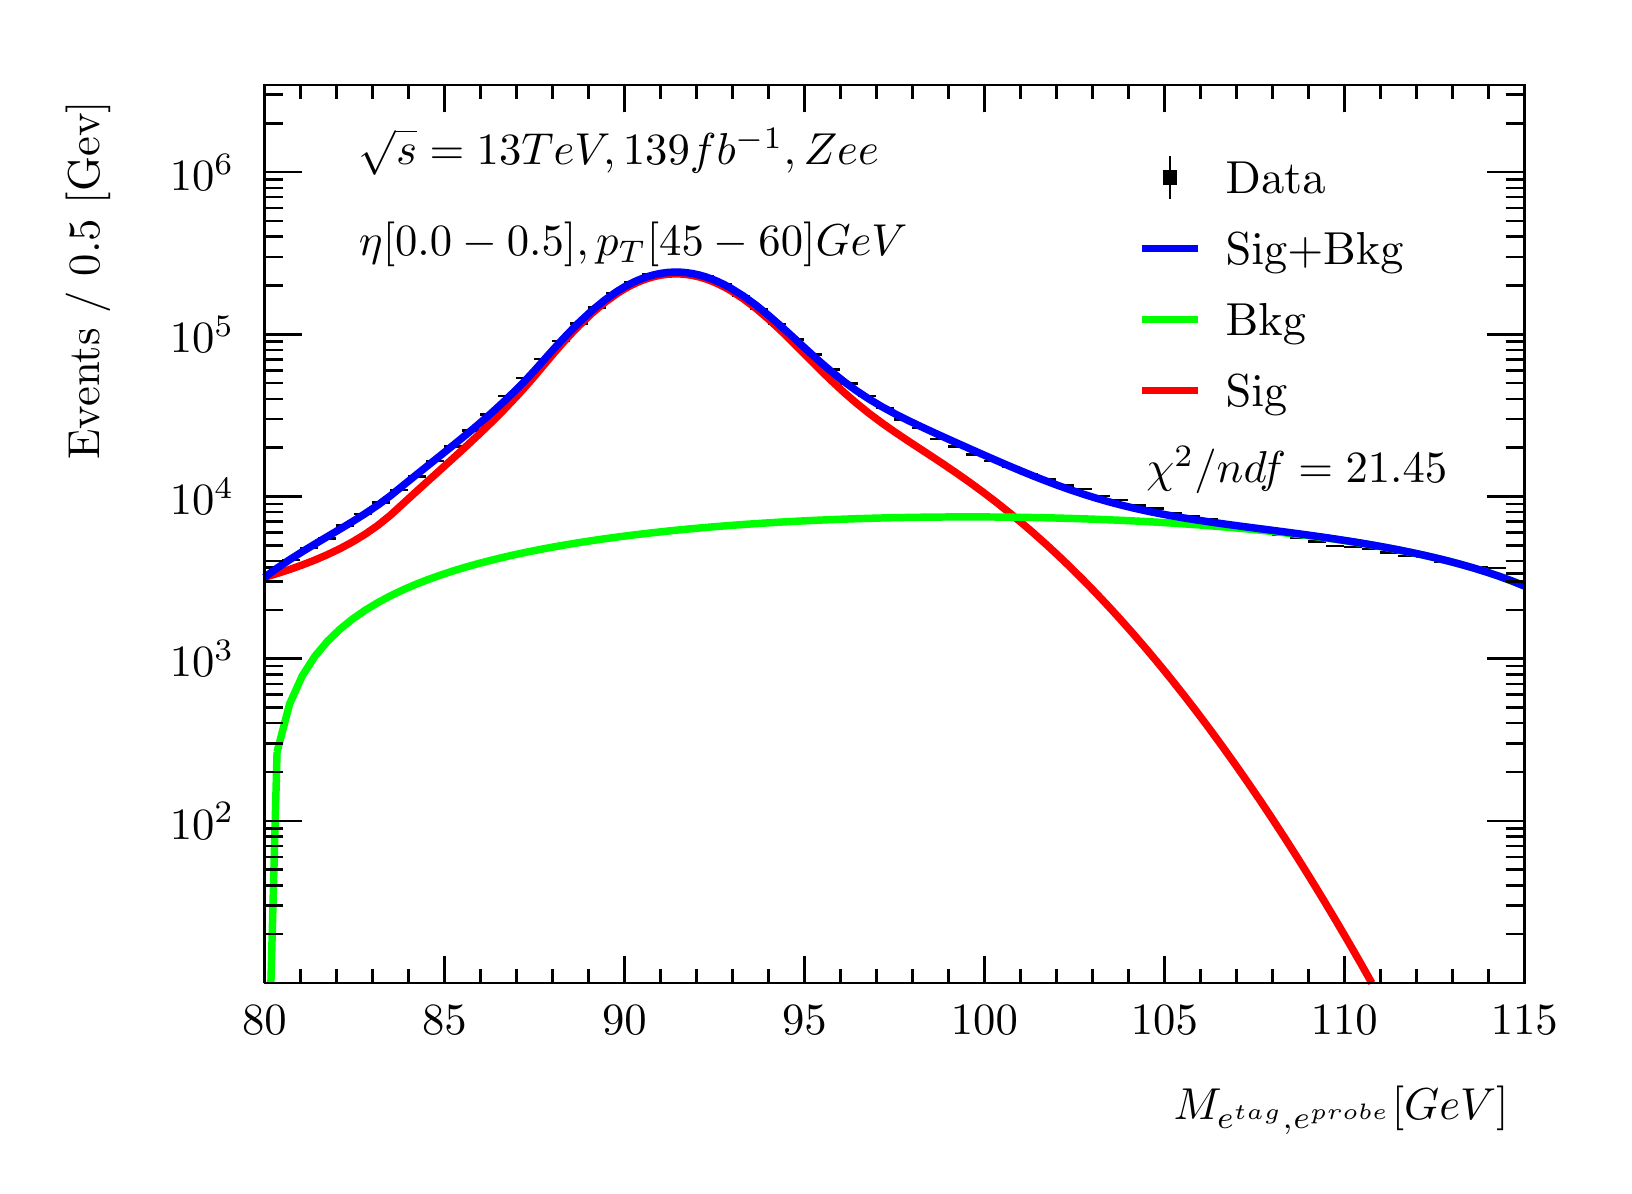
\begin{tikzpicture}
\pgfdeclareplotmark{cross} {
\pgfpathmoveto{\pgfpoint{-0.3\pgfplotmarksize}{\pgfplotmarksize}}
\pgfpathlineto{\pgfpoint{+0.3\pgfplotmarksize}{\pgfplotmarksize}}
\pgfpathlineto{\pgfpoint{+0.3\pgfplotmarksize}{0.3\pgfplotmarksize}}
\pgfpathlineto{\pgfpoint{+1\pgfplotmarksize}{0.3\pgfplotmarksize}}
\pgfpathlineto{\pgfpoint{+1\pgfplotmarksize}{-0.3\pgfplotmarksize}}
\pgfpathlineto{\pgfpoint{+0.3\pgfplotmarksize}{-0.3\pgfplotmarksize}}
\pgfpathlineto{\pgfpoint{+0.3\pgfplotmarksize}{-1.\pgfplotmarksize}}
\pgfpathlineto{\pgfpoint{-0.3\pgfplotmarksize}{-1.\pgfplotmarksize}}
\pgfpathlineto{\pgfpoint{-0.3\pgfplotmarksize}{-0.3\pgfplotmarksize}}
\pgfpathlineto{\pgfpoint{-1.\pgfplotmarksize}{-0.3\pgfplotmarksize}}
\pgfpathlineto{\pgfpoint{-1.\pgfplotmarksize}{0.3\pgfplotmarksize}}
\pgfpathlineto{\pgfpoint{-0.3\pgfplotmarksize}{0.3\pgfplotmarksize}}
\pgfpathclose
\pgfusepathqstroke
}
\pgfdeclareplotmark{cross*} {
\pgfpathmoveto{\pgfpoint{-0.3\pgfplotmarksize}{\pgfplotmarksize}}
\pgfpathlineto{\pgfpoint{+0.3\pgfplotmarksize}{\pgfplotmarksize}}
\pgfpathlineto{\pgfpoint{+0.3\pgfplotmarksize}{0.3\pgfplotmarksize}}
\pgfpathlineto{\pgfpoint{+1\pgfplotmarksize}{0.3\pgfplotmarksize}}
\pgfpathlineto{\pgfpoint{+1\pgfplotmarksize}{-0.3\pgfplotmarksize}}
\pgfpathlineto{\pgfpoint{+0.3\pgfplotmarksize}{-0.3\pgfplotmarksize}}
\pgfpathlineto{\pgfpoint{+0.3\pgfplotmarksize}{-1.\pgfplotmarksize}}
\pgfpathlineto{\pgfpoint{-0.3\pgfplotmarksize}{-1.\pgfplotmarksize}}
\pgfpathlineto{\pgfpoint{-0.3\pgfplotmarksize}{-0.3\pgfplotmarksize}}
\pgfpathlineto{\pgfpoint{-1.\pgfplotmarksize}{-0.3\pgfplotmarksize}}
\pgfpathlineto{\pgfpoint{-1.\pgfplotmarksize}{0.3\pgfplotmarksize}}
\pgfpathlineto{\pgfpoint{-0.3\pgfplotmarksize}{0.3\pgfplotmarksize}}
\pgfpathclose
\pgfusepathqfillstroke
}
\pgfdeclareplotmark{newstar} {
\pgfpathmoveto{\pgfqpoint{0pt}{\pgfplotmarksize}}
\pgfpathlineto{\pgfqpointpolar{44}{0.5\pgfplotmarksize}}
\pgfpathlineto{\pgfqpointpolar{18}{\pgfplotmarksize}}
\pgfpathlineto{\pgfqpointpolar{-20}{0.5\pgfplotmarksize}}
\pgfpathlineto{\pgfqpointpolar{-54}{\pgfplotmarksize}}
\pgfpathlineto{\pgfqpointpolar{-90}{0.5\pgfplotmarksize}}
\pgfpathlineto{\pgfqpointpolar{234}{\pgfplotmarksize}}
\pgfpathlineto{\pgfqpointpolar{198}{0.5\pgfplotmarksize}}
\pgfpathlineto{\pgfqpointpolar{162}{\pgfplotmarksize}}
\pgfpathlineto{\pgfqpointpolar{134}{0.5\pgfplotmarksize}}
\pgfpathclose
\pgfusepathqstroke
}
\pgfdeclareplotmark{newstar*} {
\pgfpathmoveto{\pgfqpoint{0pt}{\pgfplotmarksize}}
\pgfpathlineto{\pgfqpointpolar{44}{0.5\pgfplotmarksize}}
\pgfpathlineto{\pgfqpointpolar{18}{\pgfplotmarksize}}
\pgfpathlineto{\pgfqpointpolar{-20}{0.5\pgfplotmarksize}}
\pgfpathlineto{\pgfqpointpolar{-54}{\pgfplotmarksize}}
\pgfpathlineto{\pgfqpointpolar{-90}{0.5\pgfplotmarksize}}
\pgfpathlineto{\pgfqpointpolar{234}{\pgfplotmarksize}}
\pgfpathlineto{\pgfqpointpolar{198}{0.5\pgfplotmarksize}}
\pgfpathlineto{\pgfqpointpolar{162}{\pgfplotmarksize}}
\pgfpathlineto{\pgfqpointpolar{134}{0.5\pgfplotmarksize}}
\pgfpathclose
\pgfusepathqfillstroke
}
\definecolor{c}{rgb}{1,1,1};
\draw [color=c, fill=c] (0,0) rectangle (20,14.4361);
\draw [color=c, fill=c] (3,2.30977) rectangle (19,13.7143);
\definecolor{c}{rgb}{0,0,0};
\draw [c,line width=0.9] (3,2.30977) -- (3,13.7143) -- (19,13.7143) -- (19,2.30977) -- (3,2.30977);
\definecolor{c}{rgb}{1,1,1};
\draw [color=c, fill=c] (3,2.30977) rectangle (19,13.7143);
\definecolor{c}{rgb}{0,0,0};
\draw [c,line width=0.9] (3,2.30977) -- (3,13.7143) -- (19,13.7143) -- (19,2.30977) -- (3,2.30977);
\draw [c,line width=0.9] (3,2.30977) -- (19,2.30977);
\draw [c,line width=0.9] (3,2.65624) -- (3,2.30977);
\draw [c,line width=0.9] (3.45714,2.48301) -- (3.45714,2.30977);
\draw [c,line width=0.9] (3.91429,2.48301) -- (3.91429,2.30977);
\draw [c,line width=0.9] (4.37143,2.48301) -- (4.37143,2.30977);
\draw [c,line width=0.9] (4.82857,2.48301) -- (4.82857,2.30977);
\draw [c,line width=0.9] (5.28571,2.65624) -- (5.28571,2.30977);
\draw [c,line width=0.9] (5.74286,2.48301) -- (5.74286,2.30977);
\draw [c,line width=0.9] (6.2,2.48301) -- (6.2,2.30977);
\draw [c,line width=0.9] (6.65714,2.48301) -- (6.65714,2.30977);
\draw [c,line width=0.9] (7.11429,2.48301) -- (7.11429,2.30977);
\draw [c,line width=0.9] (7.57143,2.65624) -- (7.57143,2.30977);
\draw [c,line width=0.9] (8.02857,2.48301) -- (8.02857,2.30977);
\draw [c,line width=0.9] (8.48571,2.48301) -- (8.48571,2.30977);
\draw [c,line width=0.9] (8.94286,2.48301) -- (8.94286,2.30977);
\draw [c,line width=0.9] (9.4,2.48301) -- (9.4,2.30977);
\draw [c,line width=0.9] (9.85714,2.65624) -- (9.85714,2.30977);
\draw [c,line width=0.9] (10.3143,2.48301) -- (10.3143,2.30977);
\draw [c,line width=0.9] (10.7714,2.48301) -- (10.7714,2.30977);
\draw [c,line width=0.9] (11.2286,2.48301) -- (11.2286,2.30977);
\draw [c,line width=0.9] (11.6857,2.48301) -- (11.6857,2.30977);
\draw [c,line width=0.9] (12.1429,2.65624) -- (12.1429,2.30977);
\draw [c,line width=0.9] (12.6,2.48301) -- (12.6,2.30977);
\draw [c,line width=0.9] (13.0571,2.48301) -- (13.0571,2.30977);
\draw [c,line width=0.9] (13.5143,2.48301) -- (13.5143,2.30977);
\draw [c,line width=0.9] (13.9714,2.48301) -- (13.9714,2.30977);
\draw [c,line width=0.9] (14.4286,2.65624) -- (14.4286,2.30977);
\draw [c,line width=0.9] (14.8857,2.48301) -- (14.8857,2.30977);
\draw [c,line width=0.9] (15.3429,2.48301) -- (15.3429,2.30977);
\draw [c,line width=0.9] (15.8,2.48301) -- (15.8,2.30977);
\draw [c,line width=0.9] (16.2571,2.48301) -- (16.2571,2.30977);
\draw [c,line width=0.9] (16.7143,2.65624) -- (16.7143,2.30977);
\draw [c,line width=0.9] (17.1714,2.48301) -- (17.1714,2.30977);
\draw [c,line width=0.9] (17.6286,2.48301) -- (17.6286,2.30977);
\draw [c,line width=0.9] (18.0857,2.48301) -- (18.0857,2.30977);
\draw [c,line width=0.9] (18.5429,2.48301) -- (18.5429,2.30977);
\draw [c,line width=0.9] (19,2.65624) -- (19,2.30977);
\draw [anchor=base] (3,1.66015) node[scale=1.61424, color=c, rotate=0]{80};
\draw [anchor=base] (5.28571,1.66015) node[scale=1.61424, color=c, rotate=0]{85};
\draw [anchor=base] (7.57143,1.66015) node[scale=1.61424, color=c, rotate=0]{90};
\draw [anchor=base] (9.85714,1.66015) node[scale=1.61424, color=c, rotate=0]{95};
\draw [anchor=base] (12.1429,1.66015) node[scale=1.61424, color=c, rotate=0]{100};
\draw [anchor=base] (14.4286,1.66015) node[scale=1.61424, color=c, rotate=0]{105};
\draw [anchor=base] (16.7143,1.66015) node[scale=1.61424, color=c, rotate=0]{110};
\draw [anchor=base] (19,1.66015) node[scale=1.61424, color=c, rotate=0]{115};
\draw [anchor= east] (19,0.692932) node[scale=1.61424, color=c, rotate=0]{$M_{e^{tag}, e^{probe}}  [GeV]$};
\draw [c,line width=0.9] (3,13.7143) -- (19,13.7143);
\draw [c,line width=0.9] (3,13.3678) -- (3,13.7143);
\draw [c,line width=0.9] (3.45714,13.5411) -- (3.45714,13.7143);
\draw [c,line width=0.9] (3.91429,13.5411) -- (3.91429,13.7143);
\draw [c,line width=0.9] (4.37143,13.5411) -- (4.37143,13.7143);
\draw [c,line width=0.9] (4.82857,13.5411) -- (4.82857,13.7143);
\draw [c,line width=0.9] (5.28571,13.3678) -- (5.28571,13.7143);
\draw [c,line width=0.9] (5.74286,13.5411) -- (5.74286,13.7143);
\draw [c,line width=0.9] (6.2,13.5411) -- (6.2,13.7143);
\draw [c,line width=0.9] (6.65714,13.5411) -- (6.65714,13.7143);
\draw [c,line width=0.9] (7.11429,13.5411) -- (7.11429,13.7143);
\draw [c,line width=0.9] (7.57143,13.3678) -- (7.57143,13.7143);
\draw [c,line width=0.9] (8.02857,13.5411) -- (8.02857,13.7143);
\draw [c,line width=0.9] (8.48571,13.5411) -- (8.48571,13.7143);
\draw [c,line width=0.9] (8.94286,13.5411) -- (8.94286,13.7143);
\draw [c,line width=0.9] (9.4,13.5411) -- (9.4,13.7143);
\draw [c,line width=0.9] (9.85714,13.3678) -- (9.85714,13.7143);
\draw [c,line width=0.9] (10.3143,13.5411) -- (10.3143,13.7143);
\draw [c,line width=0.9] (10.7714,13.5411) -- (10.7714,13.7143);
\draw [c,line width=0.9] (11.2286,13.5411) -- (11.2286,13.7143);
\draw [c,line width=0.9] (11.6857,13.5411) -- (11.6857,13.7143);
\draw [c,line width=0.9] (12.1429,13.3678) -- (12.1429,13.7143);
\draw [c,line width=0.9] (12.6,13.5411) -- (12.6,13.7143);
\draw [c,line width=0.9] (13.0571,13.5411) -- (13.0571,13.7143);
\draw [c,line width=0.9] (13.5143,13.5411) -- (13.5143,13.7143);
\draw [c,line width=0.9] (13.9714,13.5411) -- (13.9714,13.7143);
\draw [c,line width=0.9] (14.4286,13.3678) -- (14.4286,13.7143);
\draw [c,line width=0.9] (14.8857,13.5411) -- (14.8857,13.7143);
\draw [c,line width=0.9] (15.3429,13.5411) -- (15.3429,13.7143);
\draw [c,line width=0.9] (15.8,13.5411) -- (15.8,13.7143);
\draw [c,line width=0.9] (16.2571,13.5411) -- (16.2571,13.7143);
\draw [c,line width=0.9] (16.7143,13.3678) -- (16.7143,13.7143);
\draw [c,line width=0.9] (17.1714,13.5411) -- (17.1714,13.7143);
\draw [c,line width=0.9] (17.6286,13.5411) -- (17.6286,13.7143);
\draw [c,line width=0.9] (18.0857,13.5411) -- (18.0857,13.7143);
\draw [c,line width=0.9] (18.5429,13.5411) -- (18.5429,13.7143);
\draw [c,line width=0.9] (19,13.3678) -- (19,13.7143);
\draw [c,line width=0.9] (3,2.30977) -- (3,13.7143);
\draw [c,line width=0.9] (3.237,2.92982) -- (3,2.92982);
\draw [c,line width=0.9] (3.237,3.29252) -- (3,3.29252);
\draw [c,line width=0.9] (3.237,3.54986) -- (3,3.54986);
\draw [c,line width=0.9] (3.237,3.74947) -- (3,3.74947);
\draw [c,line width=0.9] (3.237,3.91257) -- (3,3.91257);
\draw [c,line width=0.9] (3.237,4.05046) -- (3,4.05046);
\draw [c,line width=0.9] (3.237,4.16991) -- (3,4.16991);
\draw [c,line width=0.9] (3.237,4.27527) -- (3,4.27527);
\draw [c,line width=0.9] (3.474,4.36952) -- (3,4.36952);
\draw [anchor= east] (2.82,4.36952) node[scale=1.61424, color=c, rotate=0]{$10^{2}$};
\draw [c,line width=0.9] (3.237,4.98956) -- (3,4.98956);
\draw [c,line width=0.9] (3.237,5.35227) -- (3,5.35227);
\draw [c,line width=0.9] (3.237,5.60961) -- (3,5.60961);
\draw [c,line width=0.9] (3.237,5.80922) -- (3,5.80922);
\draw [c,line width=0.9] (3.237,5.97231) -- (3,5.97231);
\draw [c,line width=0.9] (3.237,6.11021) -- (3,6.11021);
\draw [c,line width=0.9] (3.237,6.22966) -- (3,6.22966);
\draw [c,line width=0.9] (3.237,6.33502) -- (3,6.33502);
\draw [c,line width=0.9] (3.474,6.42927) -- (3,6.42927);
\draw [anchor= east] (2.82,6.42927) node[scale=1.61424, color=c, rotate=0]{$10^{3}$};
\draw [c,line width=0.9] (3.237,7.04931) -- (3,7.04931);
\draw [c,line width=0.9] (3.237,7.41202) -- (3,7.41202);
\draw [c,line width=0.9] (3.237,7.66936) -- (3,7.66936);
\draw [c,line width=0.9] (3.237,7.86897) -- (3,7.86897);
\draw [c,line width=0.9] (3.237,8.03206) -- (3,8.03206);
\draw [c,line width=0.9] (3.237,8.16995) -- (3,8.16995);
\draw [c,line width=0.9] (3.237,8.2894) -- (3,8.2894);
\draw [c,line width=0.9] (3.237,8.39476) -- (3,8.39476);
\draw [c,line width=0.9] (3.474,8.48901) -- (3,8.48901);
\draw [anchor= east] (2.82,8.48901) node[scale=1.61424, color=c, rotate=0]{$10^{4}$};
\draw [c,line width=0.9] (3.237,9.10906) -- (3,9.10906);
\draw [c,line width=0.9] (3.237,9.47176) -- (3,9.47176);
\draw [c,line width=0.9] (3.237,9.7291) -- (3,9.7291);
\draw [c,line width=0.9] (3.237,9.92871) -- (3,9.92871);
\draw [c,line width=0.9] (3.237,10.0918) -- (3,10.0918);
\draw [c,line width=0.9] (3.237,10.2297) -- (3,10.2297);
\draw [c,line width=0.9] (3.237,10.3491) -- (3,10.3491);
\draw [c,line width=0.9] (3.237,10.4545) -- (3,10.4545);
\draw [c,line width=0.9] (3.474,10.5488) -- (3,10.5488);
\draw [anchor= east] (2.82,10.5488) node[scale=1.61424, color=c, rotate=0]{$10^{5}$};
\draw [c,line width=0.9] (3.237,11.1688) -- (3,11.1688);
\draw [c,line width=0.9] (3.237,11.5315) -- (3,11.5315);
\draw [c,line width=0.9] (3.237,11.7889) -- (3,11.7889);
\draw [c,line width=0.9] (3.237,11.9885) -- (3,11.9885);
\draw [c,line width=0.9] (3.237,12.1516) -- (3,12.1516);
\draw [c,line width=0.9] (3.237,12.2894) -- (3,12.2894);
\draw [c,line width=0.9] (3.237,12.4089) -- (3,12.4089);
\draw [c,line width=0.9] (3.237,12.5143) -- (3,12.5143);
\draw [c,line width=0.9] (3.474,12.6085) -- (3,12.6085);
\draw [anchor= east] (2.82,12.6085) node[scale=1.61424, color=c, rotate=0]{$10^{6}$};
\draw [c,line width=0.9] (3.237,13.2286) -- (3,13.2286);
\draw [c,line width=0.9] (3.237,13.5913) -- (3,13.5913);
\draw [anchor= east] (0.76,13.7143) node[scale=1.61424, color=c, rotate=90]{Events / 0.5 [Gev]};
\draw [c,line width=0.9] (19,2.30977) -- (19,13.7143);
\draw [c,line width=0.9] (18.763,2.92982) -- (19,2.92982);
\draw [c,line width=0.9] (18.763,3.29252) -- (19,3.29252);
\draw [c,line width=0.9] (18.763,3.54986) -- (19,3.54986);
\draw [c,line width=0.9] (18.763,3.74947) -- (19,3.74947);
\draw [c,line width=0.9] (18.763,3.91257) -- (19,3.91257);
\draw [c,line width=0.9] (18.763,4.05046) -- (19,4.05046);
\draw [c,line width=0.9] (18.763,4.16991) -- (19,4.16991);
\draw [c,line width=0.9] (18.763,4.27527) -- (19,4.27527);
\draw [c,line width=0.9] (18.526,4.36952) -- (19,4.36952);
\draw [c,line width=0.9] (18.763,4.98956) -- (19,4.98956);
\draw [c,line width=0.9] (18.763,5.35227) -- (19,5.35227);
\draw [c,line width=0.9] (18.763,5.60961) -- (19,5.60961);
\draw [c,line width=0.9] (18.763,5.80922) -- (19,5.80922);
\draw [c,line width=0.9] (18.763,5.97231) -- (19,5.97231);
\draw [c,line width=0.9] (18.763,6.11021) -- (19,6.11021);
\draw [c,line width=0.9] (18.763,6.22966) -- (19,6.22966);
\draw [c,line width=0.9] (18.763,6.33502) -- (19,6.33502);
\draw [c,line width=0.9] (18.526,6.42927) -- (19,6.42927);
\draw [c,line width=0.9] (18.763,7.04931) -- (19,7.04931);
\draw [c,line width=0.9] (18.763,7.41202) -- (19,7.41202);
\draw [c,line width=0.9] (18.763,7.66936) -- (19,7.66936);
\draw [c,line width=0.9] (18.763,7.86897) -- (19,7.86897);
\draw [c,line width=0.9] (18.763,8.03206) -- (19,8.03206);
\draw [c,line width=0.9] (18.763,8.16995) -- (19,8.16995);
\draw [c,line width=0.9] (18.763,8.2894) -- (19,8.2894);
\draw [c,line width=0.9] (18.763,8.39476) -- (19,8.39476);
\draw [c,line width=0.9] (18.526,8.48901) -- (19,8.48901);
\draw [c,line width=0.9] (18.763,9.10906) -- (19,9.10906);
\draw [c,line width=0.9] (18.763,9.47176) -- (19,9.47176);
\draw [c,line width=0.9] (18.763,9.7291) -- (19,9.7291);
\draw [c,line width=0.9] (18.763,9.92871) -- (19,9.92871);
\draw [c,line width=0.9] (18.763,10.0918) -- (19,10.0918);
\draw [c,line width=0.9] (18.763,10.2297) -- (19,10.2297);
\draw [c,line width=0.9] (18.763,10.3491) -- (19,10.3491);
\draw [c,line width=0.9] (18.763,10.4545) -- (19,10.4545);
\draw [c,line width=0.9] (18.526,10.5488) -- (19,10.5488);
\draw [c,line width=0.9] (18.763,11.1688) -- (19,11.1688);
\draw [c,line width=0.9] (18.763,11.5315) -- (19,11.5315);
\draw [c,line width=0.9] (18.763,11.7889) -- (19,11.7889);
\draw [c,line width=0.9] (18.763,11.9885) -- (19,11.9885);
\draw [c,line width=0.9] (18.763,12.1516) -- (19,12.1516);
\draw [c,line width=0.9] (18.763,12.2894) -- (19,12.2894);
\draw [c,line width=0.9] (18.763,12.4089) -- (19,12.4089);
\draw [c,line width=0.9] (18.763,12.5143) -- (19,12.5143);
\draw [c,line width=0.9] (18.526,12.6085) -- (19,12.6085);
\draw [c,line width=0.9] (18.763,13.2286) -- (19,13.2286);
\draw [c,line width=0.9] (18.763,13.5913) -- (19,13.5913);
\draw [c,line width=0.9] (3.11429,7.58647) -- (3,7.58647);
\draw [c,line width=0.9] (3,7.58647) -- (3,7.58647);
\draw [c,line width=0.9] (3.11429,7.58647) -- (3.22857,7.58647);
\draw [c,line width=0.9] (3.22857,7.58647) -- (3.22857,7.58647);
\draw [c,line width=0.9] (3.11429,7.58647) -- (3.11429,7.60128);
\draw [c,line width=0.9] (3.11429,7.60128) -- (3.11429,7.60128);
\draw [c,line width=0.9] (3.11429,7.58647) -- (3.11429,7.57165);
\draw [c,line width=0.9] (3.11429,7.57165) -- (3.11429,7.57165);
\draw [c,line width=0.9] (3.34286,7.68466) -- (3.22857,7.68466);
\draw [c,line width=0.9] (3.22857,7.68466) -- (3.22857,7.68466);
\draw [c,line width=0.9] (3.34286,7.68466) -- (3.45714,7.68466);
\draw [c,line width=0.9] (3.45714,7.68466) -- (3.45714,7.68466);
\draw [c,line width=0.9] (3.34286,7.68466) -- (3.34286,7.69868);
\draw [c,line width=0.9] (3.34286,7.69868) -- (3.34286,7.69868);
\draw [c,line width=0.9] (3.34286,7.68466) -- (3.34286,7.67063);
\draw [c,line width=0.9] (3.34286,7.67063) -- (3.34286,7.67063);
\draw [c,line width=0.9] (3.57143,7.83413) -- (3.45714,7.83413);
\draw [c,line width=0.9] (3.45714,7.83413) -- (3.45714,7.83413);
\draw [c,line width=0.9] (3.57143,7.83413) -- (3.68571,7.83413);
\draw [c,line width=0.9] (3.68571,7.83413) -- (3.68571,7.83413);
\draw [c,line width=0.9] (3.57143,7.83413) -- (3.57143,7.84703);
\draw [c,line width=0.9] (3.57143,7.84703) -- (3.57143,7.84703);
\draw [c,line width=0.9] (3.57143,7.83413) -- (3.57143,7.82123);
\draw [c,line width=0.9] (3.57143,7.82123) -- (3.57143,7.82123);
\draw [c,line width=0.9] (3.8,7.95861) -- (3.68571,7.95861);
\draw [c,line width=0.9] (3.68571,7.95861) -- (3.68571,7.95861);
\draw [c,line width=0.9] (3.8,7.95861) -- (3.91429,7.95861);
\draw [c,line width=0.9] (3.91429,7.95861) -- (3.91429,7.95861);
\draw [c,line width=0.9] (3.8,7.95861) -- (3.8,7.97064);
\draw [c,line width=0.9] (3.8,7.97064) -- (3.8,7.97064);
\draw [c,line width=0.9] (3.8,7.95861) -- (3.8,7.94658);
\draw [c,line width=0.9] (3.8,7.94658) -- (3.8,7.94658);
\draw [c,line width=0.9] (4.02857,8.118) -- (3.91429,8.118);
\draw [c,line width=0.9] (3.91429,8.118) -- (3.91429,8.118);
\draw [c,line width=0.9] (4.02857,8.118) -- (4.14286,8.118);
\draw [c,line width=0.9] (4.14286,8.118) -- (4.14286,8.118);
\draw [c,line width=0.9] (4.02857,8.118) -- (4.02857,8.129);
\draw [c,line width=0.9] (4.02857,8.129) -- (4.02857,8.129);
\draw [c,line width=0.9] (4.02857,8.118) -- (4.02857,8.10699);
\draw [c,line width=0.9] (4.02857,8.10699) -- (4.02857,8.10699);
\draw [c,line width=0.9] (4.25714,8.26354) -- (4.14286,8.26354);
\draw [c,line width=0.9] (4.14286,8.26354) -- (4.14286,8.26354);
\draw [c,line width=0.9] (4.25714,8.26354) -- (4.37143,8.26354);
\draw [c,line width=0.9] (4.37143,8.26354) -- (4.37143,8.26354);
\draw [c,line width=0.9] (4.25714,8.26354) -- (4.25714,8.27369);
\draw [c,line width=0.9] (4.25714,8.27369) -- (4.25714,8.27369);
\draw [c,line width=0.9] (4.25714,8.26354) -- (4.25714,8.25339);
\draw [c,line width=0.9] (4.25714,8.25339) -- (4.25714,8.25339);
\draw [c,line width=0.9] (4.48571,8.41189) -- (4.37143,8.41189);
\draw [c,line width=0.9] (4.37143,8.41189) -- (4.37143,8.41189);
\draw [c,line width=0.9] (4.48571,8.41189) -- (4.6,8.41189);
\draw [c,line width=0.9] (4.6,8.41189) -- (4.6,8.41189);
\draw [c,line width=0.9] (4.48571,8.41189) -- (4.48571,8.42123);
\draw [c,line width=0.9] (4.48571,8.42123) -- (4.48571,8.42123);
\draw [c,line width=0.9] (4.48571,8.41189) -- (4.48571,8.40256);
\draw [c,line width=0.9] (4.48571,8.40256) -- (4.48571,8.40256);
\draw [c,line width=0.9] (4.71429,8.5702) -- (4.6,8.5702);
\draw [c,line width=0.9] (4.6,8.5702) -- (4.6,8.5702);
\draw [c,line width=0.9] (4.71429,8.5702) -- (4.82857,8.5702);
\draw [c,line width=0.9] (4.82857,8.5702) -- (4.82857,8.5702);
\draw [c,line width=0.9] (4.71429,8.5702) -- (4.71429,8.57875);
\draw [c,line width=0.9] (4.71429,8.57875) -- (4.71429,8.57875);
\draw [c,line width=0.9] (4.71429,8.5702) -- (4.71429,8.56165);
\draw [c,line width=0.9] (4.71429,8.56165) -- (4.71429,8.56165);
\draw [c,line width=0.9] (4.94286,8.74338) -- (4.82857,8.74338);
\draw [c,line width=0.9] (4.82857,8.74338) -- (4.82857,8.74338);
\draw [c,line width=0.9] (4.94286,8.74338) -- (5.05714,8.74338);
\draw [c,line width=0.9] (5.05714,8.74338) -- (5.05714,8.74338);
\draw [c,line width=0.9] (4.94286,8.74338) -- (4.94286,8.75114);
\draw [c,line width=0.9] (4.94286,8.75114) -- (4.94286,8.75114);
\draw [c,line width=0.9] (4.94286,8.74338) -- (4.94286,8.73562);
\draw [c,line width=0.9] (4.94286,8.73562) -- (4.94286,8.73562);
\draw [c,line width=0.9] (5.17143,8.93957) -- (5.05714,8.93957);
\draw [c,line width=0.9] (5.05714,8.93957) -- (5.05714,8.93957);
\draw [c,line width=0.9] (5.17143,8.93957) -- (5.28571,8.93957);
\draw [c,line width=0.9] (5.28571,8.93957) -- (5.28571,8.93957);
\draw [c,line width=0.9] (5.17143,8.93957) -- (5.17143,8.94653);
\draw [c,line width=0.9] (5.17143,8.94653) -- (5.17143,8.94653);
\draw [c,line width=0.9] (5.17143,8.93957) -- (5.17143,8.93262);
\draw [c,line width=0.9] (5.17143,8.93262) -- (5.17143,8.93262);
\draw [c,line width=0.9] (5.4,9.12594) -- (5.28571,9.12594);
\draw [c,line width=0.9] (5.28571,9.12594) -- (5.28571,9.12594);
\draw [c,line width=0.9] (5.4,9.12594) -- (5.51429,9.12594);
\draw [c,line width=0.9] (5.51429,9.12594) -- (5.51429,9.12594);
\draw [c,line width=0.9] (5.4,9.12594) -- (5.4,9.13221);
\draw [c,line width=0.9] (5.4,9.13221) -- (5.4,9.13221);
\draw [c,line width=0.9] (5.4,9.12594) -- (5.4,9.11967);
\draw [c,line width=0.9] (5.4,9.11967) -- (5.4,9.11967);
\draw [c,line width=0.9] (5.62857,9.32751) -- (5.51429,9.32751);
\draw [c,line width=0.9] (5.51429,9.32751) -- (5.51429,9.32751);
\draw [c,line width=0.9] (5.62857,9.32751) -- (5.74286,9.32751);
\draw [c,line width=0.9] (5.74286,9.32751) -- (5.74286,9.32751);
\draw [c,line width=0.9] (5.62857,9.32751) -- (5.62857,9.3331);
\draw [c,line width=0.9] (5.62857,9.3331) -- (5.62857,9.3331);
\draw [c,line width=0.9] (5.62857,9.32751) -- (5.62857,9.32191);
\draw [c,line width=0.9] (5.62857,9.32191) -- (5.62857,9.32191);
\draw [c,line width=0.9] (5.85714,9.53) -- (5.74286,9.53);
\draw [c,line width=0.9] (5.74286,9.53) -- (5.74286,9.53);
\draw [c,line width=0.9] (5.85714,9.53) -- (5.97143,9.53);
\draw [c,line width=0.9] (5.97143,9.53) -- (5.97143,9.53);
\draw [c,line width=0.9] (5.85714,9.53) -- (5.85714,9.535);
\draw [c,line width=0.9] (5.85714,9.535) -- (5.85714,9.535);
\draw [c,line width=0.9] (5.85714,9.53) -- (5.85714,9.525);
\draw [c,line width=0.9] (5.85714,9.525) -- (5.85714,9.525);
\draw [c,line width=0.9] (6.08571,9.76837) -- (5.97143,9.76837);
\draw [c,line width=0.9] (5.97143,9.76837) -- (5.97143,9.76837);
\draw [c,line width=0.9] (6.08571,9.76837) -- (6.2,9.76837);
\draw [c,line width=0.9] (6.2,9.76837) -- (6.2,9.76837);
\draw [c,line width=0.9] (6.08571,9.76837) -- (6.08571,9.77275);
\draw [c,line width=0.9] (6.08571,9.77275) -- (6.08571,9.77275);
\draw [c,line width=0.9] (6.08571,9.76837) -- (6.08571,9.764);
\draw [c,line width=0.9] (6.08571,9.764) -- (6.08571,9.764);
\draw [c,line width=0.9] (6.31429,9.99199) -- (6.2,9.99199);
\draw [c,line width=0.9] (6.2,9.99199) -- (6.2,9.99199);
\draw [c,line width=0.9] (6.31429,9.99199) -- (6.42857,9.99199);
\draw [c,line width=0.9] (6.42857,9.99199) -- (6.42857,9.99199);
\draw [c,line width=0.9] (6.31429,9.99199) -- (6.31429,9.99585);
\draw [c,line width=0.9] (6.31429,9.99585) -- (6.31429,9.99585);
\draw [c,line width=0.9] (6.31429,9.99199) -- (6.31429,9.98813);
\draw [c,line width=0.9] (6.31429,9.98813) -- (6.31429,9.98813);
\draw [c,line width=0.9] (6.54286,10.2354) -- (6.42857,10.2354);
\draw [c,line width=0.9] (6.42857,10.2354) -- (6.42857,10.2354);
\draw [c,line width=0.9] (6.54286,10.2354) -- (6.65714,10.2354);
\draw [c,line width=0.9] (6.65714,10.2354) -- (6.65714,10.2354);
\draw [c,line width=0.9] (6.54286,10.2354) -- (6.54286,10.2387);
\draw [c,line width=0.9] (6.54286,10.2387) -- (6.54286,10.2387);
\draw [c,line width=0.9] (6.54286,10.2354) -- (6.54286,10.232);
\draw [c,line width=0.9] (6.54286,10.232) -- (6.54286,10.232);
\draw [c,line width=0.9] (6.77143,10.4629) -- (6.65714,10.4629);
\draw [c,line width=0.9] (6.65714,10.4629) -- (6.65714,10.4629);
\draw [c,line width=0.9] (6.77143,10.4629) -- (6.88571,10.4629);
\draw [c,line width=0.9] (6.88571,10.4629) -- (6.88571,10.4629);
\draw [c,line width=0.9] (6.77143,10.4629) -- (6.77143,10.4658);
\draw [c,line width=0.9] (6.77143,10.4658) -- (6.77143,10.4658);
\draw [c,line width=0.9] (6.77143,10.4629) -- (6.77143,10.4599);
\draw [c,line width=0.9] (6.77143,10.4599) -- (6.77143,10.4599);
\draw [c,line width=0.9] (7,10.6841) -- (6.88571,10.6841);
\draw [c,line width=0.9] (6.88571,10.6841) -- (6.88571,10.6841);
\draw [c,line width=0.9] (7,10.6841) -- (7.11429,10.6841);
\draw [c,line width=0.9] (7.11429,10.6841) -- (7.11429,10.6841);
\draw [c,line width=0.9] (7,10.6841) -- (7,10.6867);
\draw [c,line width=0.9] (7,10.6867) -- (7,10.6867);
\draw [c,line width=0.9] (7,10.6841) -- (7,10.6815);
\draw [c,line width=0.9] (7,10.6815) -- (7,10.6815);
\draw [c,line width=0.9] (7.22857,10.8887) -- (7.11429,10.8887);
\draw [c,line width=0.9] (7.11429,10.8887) -- (7.11429,10.8887);
\draw [c,line width=0.9] (7.22857,10.8887) -- (7.34286,10.8887);
\draw [c,line width=0.9] (7.34286,10.8887) -- (7.34286,10.8887);
\draw [c,line width=0.9] (7.22857,10.8887) -- (7.22857,10.891);
\draw [c,line width=0.9] (7.22857,10.891) -- (7.22857,10.891);
\draw [c,line width=0.9] (7.22857,10.8887) -- (7.22857,10.8863);
\draw [c,line width=0.9] (7.22857,10.8863) -- (7.22857,10.8863);
\draw [c,line width=0.9] (7.45714,11.0725) -- (7.34286,11.0725);
\draw [c,line width=0.9] (7.34286,11.0725) -- (7.34286,11.0725);
\draw [c,line width=0.9] (7.45714,11.0725) -- (7.57143,11.0725);
\draw [c,line width=0.9] (7.57143,11.0725) -- (7.57143,11.0725);
\draw [c,line width=0.9] (7.45714,11.0725) -- (7.45714,11.0746);
\draw [c,line width=0.9] (7.45714,11.0746) -- (7.45714,11.0746);
\draw [c,line width=0.9] (7.45714,11.0725) -- (7.45714,11.0704);
\draw [c,line width=0.9] (7.45714,11.0704) -- (7.45714,11.0704);
\draw [c,line width=0.9] (7.68571,11.2095) -- (7.57143,11.2095);
\draw [c,line width=0.9] (7.57143,11.2095) -- (7.57143,11.2095);
\draw [c,line width=0.9] (7.68571,11.2095) -- (7.8,11.2095);
\draw [c,line width=0.9] (7.8,11.2095) -- (7.8,11.2095);
\draw [c,line width=0.9] (7.68571,11.2095) -- (7.68571,11.2115);
\draw [c,line width=0.9] (7.68571,11.2115) -- (7.68571,11.2115);
\draw [c,line width=0.9] (7.68571,11.2095) -- (7.68571,11.2076);
\draw [c,line width=0.9] (7.68571,11.2076) -- (7.68571,11.2076);
\draw [c,line width=0.9] (7.91429,11.3058) -- (7.8,11.3058);
\draw [c,line width=0.9] (7.8,11.3058) -- (7.8,11.3058);
\draw [c,line width=0.9] (7.91429,11.3058) -- (8.02857,11.3058);
\draw [c,line width=0.9] (8.02857,11.3058) -- (8.02857,11.3058);
\draw [c,line width=0.9] (7.91429,11.3058) -- (7.91429,11.3076);
\draw [c,line width=0.9] (7.91429,11.3076) -- (7.91429,11.3076);
\draw [c,line width=0.9] (7.91429,11.3058) -- (7.91429,11.3039);
\draw [c,line width=0.9] (7.91429,11.3039) -- (7.91429,11.3039);
\draw [c,line width=0.9] (8.14286,11.3499) -- (8.02857,11.3499);
\draw [c,line width=0.9] (8.02857,11.3499) -- (8.02857,11.3499);
\draw [c,line width=0.9] (8.14286,11.3499) -- (8.25714,11.3499);
\draw [c,line width=0.9] (8.25714,11.3499) -- (8.25714,11.3499);
\draw [c,line width=0.9] (8.14286,11.3499) -- (8.14286,11.3517);
\draw [c,line width=0.9] (8.14286,11.3517) -- (8.14286,11.3517);
\draw [c,line width=0.9] (8.14286,11.3499) -- (8.14286,11.348);
\draw [c,line width=0.9] (8.14286,11.348) -- (8.14286,11.348);
\draw [c,line width=0.9] (8.37143,11.3424) -- (8.25714,11.3424);
\draw [c,line width=0.9] (8.25714,11.3424) -- (8.25714,11.3424);
\draw [c,line width=0.9] (8.37143,11.3424) -- (8.48571,11.3424);
\draw [c,line width=0.9] (8.48571,11.3424) -- (8.48571,11.3424);
\draw [c,line width=0.9] (8.37143,11.3424) -- (8.37143,11.3442);
\draw [c,line width=0.9] (8.37143,11.3442) -- (8.37143,11.3442);
\draw [c,line width=0.9] (8.37143,11.3424) -- (8.37143,11.3406);
\draw [c,line width=0.9] (8.37143,11.3406) -- (8.37143,11.3406);
\draw [c,line width=0.9] (8.6,11.2839) -- (8.48571,11.2839);
\draw [c,line width=0.9] (8.48571,11.2839) -- (8.48571,11.2839);
\draw [c,line width=0.9] (8.6,11.2839) -- (8.71429,11.2839);
\draw [c,line width=0.9] (8.71429,11.2839) -- (8.71429,11.2839);
\draw [c,line width=0.9] (8.6,11.2839) -- (8.6,11.2858);
\draw [c,line width=0.9] (8.6,11.2858) -- (8.6,11.2858);
\draw [c,line width=0.9] (8.6,11.2839) -- (8.6,11.2821);
\draw [c,line width=0.9] (8.6,11.2821) -- (8.6,11.2821);
\draw [c,line width=0.9] (8.82857,11.1805) -- (8.71429,11.1805);
\draw [c,line width=0.9] (8.71429,11.1805) -- (8.71429,11.1805);
\draw [c,line width=0.9] (8.82857,11.1805) -- (8.94286,11.1805);
\draw [c,line width=0.9] (8.94286,11.1805) -- (8.94286,11.1805);
\draw [c,line width=0.9] (8.82857,11.1805) -- (8.82857,11.1825);
\draw [c,line width=0.9] (8.82857,11.1825) -- (8.82857,11.1825);
\draw [c,line width=0.9] (8.82857,11.1805) -- (8.82857,11.1785);
\draw [c,line width=0.9] (8.82857,11.1785) -- (8.82857,11.1785);
\draw [c,line width=0.9] (9.05714,11.0348) -- (8.94286,11.0348);
\draw [c,line width=0.9] (8.94286,11.0348) -- (8.94286,11.0348);
\draw [c,line width=0.9] (9.05714,11.0348) -- (9.17143,11.0348);
\draw [c,line width=0.9] (9.17143,11.0348) -- (9.17143,11.0348);
\draw [c,line width=0.9] (9.05714,11.0348) -- (9.05714,11.037);
\draw [c,line width=0.9] (9.05714,11.037) -- (9.05714,11.037);
\draw [c,line width=0.9] (9.05714,11.0348) -- (9.05714,11.0326);
\draw [c,line width=0.9] (9.05714,11.0326) -- (9.05714,11.0326);
\draw [c,line width=0.9] (9.28571,10.8686) -- (9.17143,10.8686);
\draw [c,line width=0.9] (9.17143,10.8686) -- (9.17143,10.8686);
\draw [c,line width=0.9] (9.28571,10.8686) -- (9.4,10.8686);
\draw [c,line width=0.9] (9.4,10.8686) -- (9.4,10.8686);
\draw [c,line width=0.9] (9.28571,10.8686) -- (9.28571,10.8709);
\draw [c,line width=0.9] (9.28571,10.8709) -- (9.28571,10.8709);
\draw [c,line width=0.9] (9.28571,10.8686) -- (9.28571,10.8662);
\draw [c,line width=0.9] (9.28571,10.8662) -- (9.28571,10.8662);
\draw [c,line width=0.9] (9.51429,10.6793) -- (9.4,10.6793);
\draw [c,line width=0.9] (9.4,10.6793) -- (9.4,10.6793);
\draw [c,line width=0.9] (9.51429,10.6793) -- (9.62857,10.6793);
\draw [c,line width=0.9] (9.62857,10.6793) -- (9.62857,10.6793);
\draw [c,line width=0.9] (9.51429,10.6793) -- (9.51429,10.6819);
\draw [c,line width=0.9] (9.51429,10.6819) -- (9.51429,10.6819);
\draw [c,line width=0.9] (9.51429,10.6793) -- (9.51429,10.6766);
\draw [c,line width=0.9] (9.51429,10.6766) -- (9.51429,10.6766);
\draw [c,line width=0.9] (9.74286,10.4843) -- (9.62857,10.4843);
\draw [c,line width=0.9] (9.62857,10.4843) -- (9.62857,10.4843);
\draw [c,line width=0.9] (9.74286,10.4843) -- (9.85714,10.4843);
\draw [c,line width=0.9] (9.85714,10.4843) -- (9.85714,10.4843);
\draw [c,line width=0.9] (9.74286,10.4843) -- (9.74286,10.4872);
\draw [c,line width=0.9] (9.74286,10.4872) -- (9.74286,10.4872);
\draw [c,line width=0.9] (9.74286,10.4843) -- (9.74286,10.4814);
\draw [c,line width=0.9] (9.74286,10.4814) -- (9.74286,10.4814);
\draw [c,line width=0.9] (9.97143,10.2927) -- (9.85714,10.2927);
\draw [c,line width=0.9] (9.85714,10.2927) -- (9.85714,10.2927);
\draw [c,line width=0.9] (9.97143,10.2927) -- (10.0857,10.2927);
\draw [c,line width=0.9] (10.0857,10.2927) -- (10.0857,10.2927);
\draw [c,line width=0.9] (9.97143,10.2927) -- (9.97143,10.296);
\draw [c,line width=0.9] (9.97143,10.296) -- (9.97143,10.296);
\draw [c,line width=0.9] (9.97143,10.2927) -- (9.97143,10.2895);
\draw [c,line width=0.9] (9.97143,10.2895) -- (9.97143,10.2895);
\draw [c,line width=0.9] (10.2,10.1023) -- (10.0857,10.1023);
\draw [c,line width=0.9] (10.0857,10.1023) -- (10.0857,10.1023);
\draw [c,line width=0.9] (10.2,10.1023) -- (10.3143,10.1023);
\draw [c,line width=0.9] (10.3143,10.1023) -- (10.3143,10.1023);
\draw [c,line width=0.9] (10.2,10.1023) -- (10.2,10.1059);
\draw [c,line width=0.9] (10.2,10.1059) -- (10.2,10.1059);
\draw [c,line width=0.9] (10.2,10.1023) -- (10.2,10.0987);
\draw [c,line width=0.9] (10.2,10.0987) -- (10.2,10.0987);
\draw [c,line width=0.9] (10.4286,9.92126) -- (10.3143,9.92126);
\draw [c,line width=0.9] (10.3143,9.92126) -- (10.3143,9.92126);
\draw [c,line width=0.9] (10.4286,9.92126) -- (10.5429,9.92126);
\draw [c,line width=0.9] (10.5429,9.92126) -- (10.5429,9.92126);
\draw [c,line width=0.9] (10.4286,9.92126) -- (10.4286,9.92528);
\draw [c,line width=0.9] (10.4286,9.92528) -- (10.4286,9.92528);
\draw [c,line width=0.9] (10.4286,9.92126) -- (10.4286,9.91724);
\draw [c,line width=0.9] (10.4286,9.91724) -- (10.4286,9.91724);
\draw [c,line width=0.9] (10.6571,9.7638) -- (10.5429,9.7638);
\draw [c,line width=0.9] (10.5429,9.7638) -- (10.5429,9.7638);
\draw [c,line width=0.9] (10.6571,9.7638) -- (10.7714,9.7638);
\draw [c,line width=0.9] (10.7714,9.7638) -- (10.7714,9.7638);
\draw [c,line width=0.9] (10.6571,9.7638) -- (10.6571,9.76819);
\draw [c,line width=0.9] (10.6571,9.76819) -- (10.6571,9.76819);
\draw [c,line width=0.9] (10.6571,9.7638) -- (10.6571,9.75942);
\draw [c,line width=0.9] (10.6571,9.75942) -- (10.6571,9.75942);
\draw [c,line width=0.9] (10.8857,9.61001) -- (10.7714,9.61001);
\draw [c,line width=0.9] (10.7714,9.61001) -- (10.7714,9.61001);
\draw [c,line width=0.9] (10.8857,9.61001) -- (11,9.61001);
\draw [c,line width=0.9] (11,9.61001) -- (11,9.61001);
\draw [c,line width=0.9] (10.8857,9.61001) -- (10.8857,9.61479);
\draw [c,line width=0.9] (10.8857,9.61479) -- (10.8857,9.61479);
\draw [c,line width=0.9] (10.8857,9.61001) -- (10.8857,9.60523);
\draw [c,line width=0.9] (10.8857,9.60523) -- (10.8857,9.60523);
\draw [c,line width=0.9] (11.1143,9.46485) -- (11,9.46485);
\draw [c,line width=0.9] (11,9.46485) -- (11,9.46485);
\draw [c,line width=0.9] (11.1143,9.46485) -- (11.2286,9.46485);
\draw [c,line width=0.9] (11.2286,9.46485) -- (11.2286,9.46485);
\draw [c,line width=0.9] (11.1143,9.46485) -- (11.1143,9.47003);
\draw [c,line width=0.9] (11.1143,9.47003) -- (11.1143,9.47003);
\draw [c,line width=0.9] (11.1143,9.46485) -- (11.1143,9.45966);
\draw [c,line width=0.9] (11.1143,9.45966) -- (11.1143,9.45966);
\draw [c,line width=0.9] (11.3429,9.35677) -- (11.2286,9.35677);
\draw [c,line width=0.9] (11.2286,9.35677) -- (11.2286,9.35677);
\draw [c,line width=0.9] (11.3429,9.35677) -- (11.4571,9.35677);
\draw [c,line width=0.9] (11.4571,9.35677) -- (11.4571,9.35677);
\draw [c,line width=0.9] (11.3429,9.35677) -- (11.3429,9.36228);
\draw [c,line width=0.9] (11.3429,9.36228) -- (11.3429,9.36228);
\draw [c,line width=0.9] (11.3429,9.35677) -- (11.3429,9.35126);
\draw [c,line width=0.9] (11.3429,9.35126) -- (11.3429,9.35126);
\draw [c,line width=0.9] (11.5714,9.22135) -- (11.4571,9.22135);
\draw [c,line width=0.9] (11.4571,9.22135) -- (11.4571,9.22135);
\draw [c,line width=0.9] (11.5714,9.22135) -- (11.6857,9.22135);
\draw [c,line width=0.9] (11.6857,9.22135) -- (11.6857,9.22135);
\draw [c,line width=0.9] (11.5714,9.22135) -- (11.5714,9.22729);
\draw [c,line width=0.9] (11.5714,9.22729) -- (11.5714,9.22729);
\draw [c,line width=0.9] (11.5714,9.22135) -- (11.5714,9.21541);
\draw [c,line width=0.9] (11.5714,9.21541) -- (11.5714,9.21541);
\draw [c,line width=0.9] (11.8,9.12374) -- (11.6857,9.12374);
\draw [c,line width=0.9] (11.6857,9.12374) -- (11.6857,9.12374);
\draw [c,line width=0.9] (11.8,9.12374) -- (11.9143,9.12374);
\draw [c,line width=0.9] (11.9143,9.12374) -- (11.9143,9.12374);
\draw [c,line width=0.9] (11.8,9.12374) -- (11.8,9.13002);
\draw [c,line width=0.9] (11.8,9.13002) -- (11.8,9.13002);
\draw [c,line width=0.9] (11.8,9.12374) -- (11.8,9.11747);
\draw [c,line width=0.9] (11.8,9.11747) -- (11.8,9.11747);
\draw [c,line width=0.9] (12.0286,9.02361) -- (11.9143,9.02361);
\draw [c,line width=0.9] (11.9143,9.02361) -- (11.9143,9.02361);
\draw [c,line width=0.9] (12.0286,9.02361) -- (12.1429,9.02361);
\draw [c,line width=0.9] (12.1429,9.02361) -- (12.1429,9.02361);
\draw [c,line width=0.9] (12.0286,9.02361) -- (12.0286,9.03025);
\draw [c,line width=0.9] (12.0286,9.03025) -- (12.0286,9.03025);
\draw [c,line width=0.9] (12.0286,9.02361) -- (12.0286,9.01698);
\draw [c,line width=0.9] (12.0286,9.01698) -- (12.0286,9.01698);
\draw [c,line width=0.9] (12.2571,8.9379) -- (12.1429,8.9379);
\draw [c,line width=0.9] (12.1429,8.9379) -- (12.1429,8.9379);
\draw [c,line width=0.9] (12.2571,8.9379) -- (12.3714,8.9379);
\draw [c,line width=0.9] (12.3714,8.9379) -- (12.3714,8.9379);
\draw [c,line width=0.9] (12.2571,8.9379) -- (12.2571,8.94486);
\draw [c,line width=0.9] (12.2571,8.94486) -- (12.2571,8.94486);
\draw [c,line width=0.9] (12.2571,8.9379) -- (12.2571,8.93094);
\draw [c,line width=0.9] (12.2571,8.93094) -- (12.2571,8.93094);
\draw [c,line width=0.9] (12.4857,8.86144) -- (12.3714,8.86144);
\draw [c,line width=0.9] (12.3714,8.86144) -- (12.3714,8.86144);
\draw [c,line width=0.9] (12.4857,8.86144) -- (12.6,8.86144);
\draw [c,line width=0.9] (12.6,8.86144) -- (12.6,8.86144);
\draw [c,line width=0.9] (12.4857,8.86144) -- (12.4857,8.86871);
\draw [c,line width=0.9] (12.4857,8.86871) -- (12.4857,8.86871);
\draw [c,line width=0.9] (12.4857,8.86144) -- (12.4857,8.85418);
\draw [c,line width=0.9] (12.4857,8.85418) -- (12.4857,8.85418);
\draw [c,line width=0.9] (12.7143,8.77297) -- (12.6,8.77297);
\draw [c,line width=0.9] (12.6,8.77297) -- (12.6,8.77297);
\draw [c,line width=0.9] (12.7143,8.77297) -- (12.8286,8.77297);
\draw [c,line width=0.9] (12.8286,8.77297) -- (12.8286,8.77297);
\draw [c,line width=0.9] (12.7143,8.77297) -- (12.7143,8.7806);
\draw [c,line width=0.9] (12.7143,8.7806) -- (12.7143,8.7806);
\draw [c,line width=0.9] (12.7143,8.77297) -- (12.7143,8.76534);
\draw [c,line width=0.9] (12.7143,8.76534) -- (12.7143,8.76534);
\draw [c,line width=0.9] (12.9429,8.70325) -- (12.8286,8.70325);
\draw [c,line width=0.9] (12.8286,8.70325) -- (12.8286,8.70325);
\draw [c,line width=0.9] (12.9429,8.70325) -- (13.0571,8.70325);
\draw [c,line width=0.9] (13.0571,8.70325) -- (13.0571,8.70325);
\draw [c,line width=0.9] (12.9429,8.70325) -- (12.9429,8.71118);
\draw [c,line width=0.9] (12.9429,8.71118) -- (12.9429,8.71118);
\draw [c,line width=0.9] (12.9429,8.70325) -- (12.9429,8.69531);
\draw [c,line width=0.9] (12.9429,8.69531) -- (12.9429,8.69531);
\draw [c,line width=0.9] (13.1714,8.62785) -- (13.0571,8.62785);
\draw [c,line width=0.9] (13.0571,8.62785) -- (13.0571,8.62785);
\draw [c,line width=0.9] (13.1714,8.62785) -- (13.2857,8.62785);
\draw [c,line width=0.9] (13.2857,8.62785) -- (13.2857,8.62785);
\draw [c,line width=0.9] (13.1714,8.62785) -- (13.1714,8.63613);
\draw [c,line width=0.9] (13.1714,8.63613) -- (13.1714,8.63613);
\draw [c,line width=0.9] (13.1714,8.62785) -- (13.1714,8.61958);
\draw [c,line width=0.9] (13.1714,8.61958) -- (13.1714,8.61958);
\draw [c,line width=0.9] (13.4,8.58309) -- (13.2857,8.58309);
\draw [c,line width=0.9] (13.2857,8.58309) -- (13.2857,8.58309);
\draw [c,line width=0.9] (13.4,8.58309) -- (13.5143,8.58309);
\draw [c,line width=0.9] (13.5143,8.58309) -- (13.5143,8.58309);
\draw [c,line width=0.9] (13.4,8.58309) -- (13.4,8.59158);
\draw [c,line width=0.9] (13.4,8.59158) -- (13.4,8.59158);
\draw [c,line width=0.9] (13.4,8.58309) -- (13.4,8.57461);
\draw [c,line width=0.9] (13.4,8.57461) -- (13.4,8.57461);
\draw [c,line width=0.9] (13.6286,8.49676) -- (13.5143,8.49676);
\draw [c,line width=0.9] (13.5143,8.49676) -- (13.5143,8.49676);
\draw [c,line width=0.9] (13.6286,8.49676) -- (13.7429,8.49676);
\draw [c,line width=0.9] (13.7429,8.49676) -- (13.7429,8.49676);
\draw [c,line width=0.9] (13.6286,8.49676) -- (13.6286,8.50567);
\draw [c,line width=0.9] (13.6286,8.50567) -- (13.6286,8.50567);
\draw [c,line width=0.9] (13.6286,8.49676) -- (13.6286,8.48786);
\draw [c,line width=0.9] (13.6286,8.48786) -- (13.6286,8.48786);
\draw [c,line width=0.9] (13.8571,8.44238) -- (13.7429,8.44238);
\draw [c,line width=0.9] (13.7429,8.44238) -- (13.7429,8.44238);
\draw [c,line width=0.9] (13.8571,8.44238) -- (13.9714,8.44238);
\draw [c,line width=0.9] (13.9714,8.44238) -- (13.9714,8.44238);
\draw [c,line width=0.9] (13.8571,8.44238) -- (13.8571,8.45156);
\draw [c,line width=0.9] (13.8571,8.45156) -- (13.8571,8.45156);
\draw [c,line width=0.9] (13.8571,8.44238) -- (13.8571,8.4332);
\draw [c,line width=0.9] (13.8571,8.4332) -- (13.8571,8.4332);
\draw [c,line width=0.9] (14.0857,8.37558) -- (13.9714,8.37558);
\draw [c,line width=0.9] (13.9714,8.37558) -- (13.9714,8.37558);
\draw [c,line width=0.9] (14.0857,8.37558) -- (14.2,8.37558);
\draw [c,line width=0.9] (14.2,8.37558) -- (14.2,8.37558);
\draw [c,line width=0.9] (14.0857,8.37558) -- (14.0857,8.38511);
\draw [c,line width=0.9] (14.0857,8.38511) -- (14.0857,8.38511);
\draw [c,line width=0.9] (14.0857,8.37558) -- (14.0857,8.36605);
\draw [c,line width=0.9] (14.0857,8.36605) -- (14.0857,8.36605);
\draw [c,line width=0.9] (14.3143,8.3373) -- (14.2,8.3373);
\draw [c,line width=0.9] (14.2,8.3373) -- (14.2,8.3373);
\draw [c,line width=0.9] (14.3143,8.3373) -- (14.4286,8.3373);
\draw [c,line width=0.9] (14.4286,8.3373) -- (14.4286,8.3373);
\draw [c,line width=0.9] (14.3143,8.3373) -- (14.3143,8.34704);
\draw [c,line width=0.9] (14.3143,8.34704) -- (14.3143,8.34704);
\draw [c,line width=0.9] (14.3143,8.3373) -- (14.3143,8.32756);
\draw [c,line width=0.9] (14.3143,8.32756) -- (14.3143,8.32756);
\draw [c,line width=0.9] (14.5429,8.2777) -- (14.4286,8.2777);
\draw [c,line width=0.9] (14.4286,8.2777) -- (14.4286,8.2777);
\draw [c,line width=0.9] (14.5429,8.2777) -- (14.6571,8.2777);
\draw [c,line width=0.9] (14.6571,8.2777) -- (14.6571,8.2777);
\draw [c,line width=0.9] (14.5429,8.2777) -- (14.5429,8.28777);
\draw [c,line width=0.9] (14.5429,8.28777) -- (14.5429,8.28777);
\draw [c,line width=0.9] (14.5429,8.2777) -- (14.5429,8.26763);
\draw [c,line width=0.9] (14.5429,8.26763) -- (14.5429,8.26763);
\draw [c,line width=0.9] (14.7714,8.23821) -- (14.6571,8.23821);
\draw [c,line width=0.9] (14.6571,8.23821) -- (14.6571,8.23821);
\draw [c,line width=0.9] (14.7714,8.23821) -- (14.8857,8.23821);
\draw [c,line width=0.9] (14.8857,8.23821) -- (14.8857,8.23821);
\draw [c,line width=0.9] (14.7714,8.23821) -- (14.7714,8.2485);
\draw [c,line width=0.9] (14.7714,8.2485) -- (14.7714,8.2485);
\draw [c,line width=0.9] (14.7714,8.23821) -- (14.7714,8.22792);
\draw [c,line width=0.9] (14.7714,8.22792) -- (14.7714,8.22792);
\draw [c,line width=0.9] (15,8.19739) -- (14.8857,8.19739);
\draw [c,line width=0.9] (14.8857,8.19739) -- (14.8857,8.19739);
\draw [c,line width=0.9] (15,8.19739) -- (15.1143,8.19739);
\draw [c,line width=0.9] (15.1143,8.19739) -- (15.1143,8.19739);
\draw [c,line width=0.9] (15,8.19739) -- (15,8.20792);
\draw [c,line width=0.9] (15,8.20792) -- (15,8.20792);
\draw [c,line width=0.9] (15,8.19739) -- (15,8.18686);
\draw [c,line width=0.9] (15,8.18686) -- (15,8.18686);
\draw [c,line width=0.9] (15.2286,8.13689) -- (15.1143,8.13689);
\draw [c,line width=0.9] (15.1143,8.13689) -- (15.1143,8.13689);
\draw [c,line width=0.9] (15.2286,8.13689) -- (15.3429,8.13689);
\draw [c,line width=0.9] (15.3429,8.13689) -- (15.3429,8.13689);
\draw [c,line width=0.9] (15.2286,8.13689) -- (15.2286,8.14778);
\draw [c,line width=0.9] (15.2286,8.14778) -- (15.2286,8.14778);
\draw [c,line width=0.9] (15.2286,8.13689) -- (15.2286,8.126);
\draw [c,line width=0.9] (15.2286,8.126) -- (15.2286,8.126);
\draw [c,line width=0.9] (15.4571,8.06772) -- (15.3429,8.06772);
\draw [c,line width=0.9] (15.3429,8.06772) -- (15.3429,8.06772);
\draw [c,line width=0.9] (15.4571,8.06772) -- (15.5714,8.06772);
\draw [c,line width=0.9] (15.5714,8.06772) -- (15.5714,8.06772);
\draw [c,line width=0.9] (15.4571,8.06772) -- (15.4571,8.07904);
\draw [c,line width=0.9] (15.4571,8.07904) -- (15.4571,8.07904);
\draw [c,line width=0.9] (15.4571,8.06772) -- (15.4571,8.0564);
\draw [c,line width=0.9] (15.4571,8.0564) -- (15.4571,8.0564);
\draw [c,line width=0.9] (15.6857,8.05138) -- (15.5714,8.05138);
\draw [c,line width=0.9] (15.5714,8.05138) -- (15.5714,8.05138);
\draw [c,line width=0.9] (15.6857,8.05138) -- (15.8,8.05138);
\draw [c,line width=0.9] (15.8,8.05138) -- (15.8,8.05138);
\draw [c,line width=0.9] (15.6857,8.05138) -- (15.6857,8.06281);
\draw [c,line width=0.9] (15.6857,8.06281) -- (15.6857,8.06281);
\draw [c,line width=0.9] (15.6857,8.05138) -- (15.6857,8.03996);
\draw [c,line width=0.9] (15.6857,8.03996) -- (15.6857,8.03996);
\draw [c,line width=0.9] (15.9143,8.00742) -- (15.8,8.00742);
\draw [c,line width=0.9] (15.8,8.00742) -- (15.8,8.00742);
\draw [c,line width=0.9] (15.9143,8.00742) -- (16.0286,8.00742);
\draw [c,line width=0.9] (16.0286,8.00742) -- (16.0286,8.00742);
\draw [c,line width=0.9] (15.9143,8.00742) -- (15.9143,8.01913);
\draw [c,line width=0.9] (15.9143,8.01913) -- (15.9143,8.01913);
\draw [c,line width=0.9] (15.9143,8.00742) -- (15.9143,7.99572);
\draw [c,line width=0.9] (15.9143,7.99572) -- (15.9143,7.99572);
\draw [c,line width=0.9] (16.1429,7.96442) -- (16.0286,7.96442);
\draw [c,line width=0.9] (16.0286,7.96442) -- (16.0286,7.96442);
\draw [c,line width=0.9] (16.1429,7.96442) -- (16.2571,7.96442);
\draw [c,line width=0.9] (16.2571,7.96442) -- (16.2571,7.96442);
\draw [c,line width=0.9] (16.1429,7.96442) -- (16.1429,7.97641);
\draw [c,line width=0.9] (16.1429,7.97641) -- (16.1429,7.97641);
\draw [c,line width=0.9] (16.1429,7.96442) -- (16.1429,7.95242);
\draw [c,line width=0.9] (16.1429,7.95242) -- (16.1429,7.95242);
\draw [c,line width=0.9] (16.3714,7.91432) -- (16.2571,7.91432);
\draw [c,line width=0.9] (16.2571,7.91432) -- (16.2571,7.91432);
\draw [c,line width=0.9] (16.3714,7.91432) -- (16.4857,7.91432);
\draw [c,line width=0.9] (16.4857,7.91432) -- (16.4857,7.91432);
\draw [c,line width=0.9] (16.3714,7.91432) -- (16.3714,7.92665);
\draw [c,line width=0.9] (16.3714,7.92665) -- (16.3714,7.92665);
\draw [c,line width=0.9] (16.3714,7.91432) -- (16.3714,7.90198);
\draw [c,line width=0.9] (16.3714,7.90198) -- (16.3714,7.90198);
\draw [c,line width=0.9] (16.6,7.85907) -- (16.4857,7.85907);
\draw [c,line width=0.9] (16.4857,7.85907) -- (16.4857,7.85907);
\draw [c,line width=0.9] (16.6,7.85907) -- (16.7143,7.85907);
\draw [c,line width=0.9] (16.7143,7.85907) -- (16.7143,7.85907);
\draw [c,line width=0.9] (16.6,7.85907) -- (16.6,7.8718);
\draw [c,line width=0.9] (16.6,7.8718) -- (16.6,7.8718);
\draw [c,line width=0.9] (16.6,7.85907) -- (16.6,7.84635);
\draw [c,line width=0.9] (16.6,7.84635) -- (16.6,7.84635);
\draw [c,line width=0.9] (16.8286,7.84962) -- (16.7143,7.84962);
\draw [c,line width=0.9] (16.7143,7.84962) -- (16.7143,7.84962);
\draw [c,line width=0.9] (16.8286,7.84962) -- (16.9429,7.84962);
\draw [c,line width=0.9] (16.9429,7.84962) -- (16.9429,7.84962);
\draw [c,line width=0.9] (16.8286,7.84962) -- (16.8286,7.86241);
\draw [c,line width=0.9] (16.8286,7.86241) -- (16.8286,7.86241);
\draw [c,line width=0.9] (16.8286,7.84962) -- (16.8286,7.83683);
\draw [c,line width=0.9] (16.8286,7.83683) -- (16.8286,7.83683);
\draw [c,line width=0.9] (17.0571,7.82214) -- (16.9429,7.82214);
\draw [c,line width=0.9] (16.9429,7.82214) -- (16.9429,7.82214);
\draw [c,line width=0.9] (17.0571,7.82214) -- (17.1714,7.82214);
\draw [c,line width=0.9] (17.1714,7.82214) -- (17.1714,7.82214);
\draw [c,line width=0.9] (17.0571,7.82214) -- (17.0571,7.83513);
\draw [c,line width=0.9] (17.0571,7.83513) -- (17.0571,7.83513);
\draw [c,line width=0.9] (17.0571,7.82214) -- (17.0571,7.80916);
\draw [c,line width=0.9] (17.0571,7.80916) -- (17.0571,7.80916);
\draw [c,line width=0.9] (17.2857,7.77512) -- (17.1714,7.77512);
\draw [c,line width=0.9] (17.1714,7.77512) -- (17.1714,7.77512);
\draw [c,line width=0.9] (17.2857,7.77512) -- (17.4,7.77512);
\draw [c,line width=0.9] (17.4,7.77512) -- (17.4,7.77512);
\draw [c,line width=0.9] (17.2857,7.77512) -- (17.2857,7.78845);
\draw [c,line width=0.9] (17.2857,7.78845) -- (17.2857,7.78845);
\draw [c,line width=0.9] (17.2857,7.77512) -- (17.2857,7.76179);
\draw [c,line width=0.9] (17.2857,7.76179) -- (17.2857,7.76179);
\draw [c,line width=0.9] (17.5143,7.73218) -- (17.4,7.73218);
\draw [c,line width=0.9] (17.4,7.73218) -- (17.4,7.73218);
\draw [c,line width=0.9] (17.5143,7.73218) -- (17.6286,7.73218);
\draw [c,line width=0.9] (17.6286,7.73218) -- (17.6286,7.73218);
\draw [c,line width=0.9] (17.5143,7.73218) -- (17.5143,7.74583);
\draw [c,line width=0.9] (17.5143,7.74583) -- (17.5143,7.74583);
\draw [c,line width=0.9] (17.5143,7.73218) -- (17.5143,7.71852);
\draw [c,line width=0.9] (17.5143,7.71852) -- (17.5143,7.71852);
\draw [c,line width=0.9] (17.7429,7.71852) -- (17.6286,7.71852);
\draw [c,line width=0.9] (17.6286,7.71852) -- (17.6286,7.71852);
\draw [c,line width=0.9] (17.7429,7.71852) -- (17.8571,7.71852);
\draw [c,line width=0.9] (17.8571,7.71852) -- (17.8571,7.71852);
\draw [c,line width=0.9] (17.7429,7.71852) -- (17.7429,7.73228);
\draw [c,line width=0.9] (17.7429,7.73228) -- (17.7429,7.73228);
\draw [c,line width=0.9] (17.7429,7.71852) -- (17.7429,7.70476);
\draw [c,line width=0.9] (17.7429,7.70476) -- (17.7429,7.70476);
\draw [c,line width=0.9] (17.9714,7.65448) -- (17.8571,7.65448);
\draw [c,line width=0.9] (17.8571,7.65448) -- (17.8571,7.65448);
\draw [c,line width=0.9] (17.9714,7.65448) -- (18.0857,7.65448);
\draw [c,line width=0.9] (18.0857,7.65448) -- (18.0857,7.65448);
\draw [c,line width=0.9] (17.9714,7.65448) -- (17.9714,7.66874);
\draw [c,line width=0.9] (17.9714,7.66874) -- (17.9714,7.66874);
\draw [c,line width=0.9] (17.9714,7.65448) -- (17.9714,7.64021);
\draw [c,line width=0.9] (17.9714,7.64021) -- (17.9714,7.64021);
\draw [c,line width=0.9] (18.2,7.63284) -- (18.0857,7.63284);
\draw [c,line width=0.9] (18.0857,7.63284) -- (18.0857,7.63284);
\draw [c,line width=0.9] (18.2,7.63284) -- (18.3143,7.63284);
\draw [c,line width=0.9] (18.3143,7.63284) -- (18.3143,7.63284);
\draw [c,line width=0.9] (18.2,7.63284) -- (18.2,7.64728);
\draw [c,line width=0.9] (18.2,7.64728) -- (18.2,7.64728);
\draw [c,line width=0.9] (18.2,7.63284) -- (18.2,7.61841);
\draw [c,line width=0.9] (18.2,7.61841) -- (18.2,7.61841);
\draw [c,line width=0.9] (18.4286,7.58916) -- (18.3143,7.58916);
\draw [c,line width=0.9] (18.3143,7.58916) -- (18.3143,7.58916);
\draw [c,line width=0.9] (18.4286,7.58916) -- (18.5429,7.58916);
\draw [c,line width=0.9] (18.5429,7.58916) -- (18.5429,7.58916);
\draw [c,line width=0.9] (18.4286,7.58916) -- (18.4286,7.60395);
\draw [c,line width=0.9] (18.4286,7.60395) -- (18.4286,7.60395);
\draw [c,line width=0.9] (18.4286,7.58916) -- (18.4286,7.57437);
\draw [c,line width=0.9] (18.4286,7.57437) -- (18.4286,7.57437);
\draw [c,line width=0.9] (18.6571,7.57932) -- (18.5429,7.57932);
\draw [c,line width=0.9] (18.5429,7.57932) -- (18.5429,7.57932);
\draw [c,line width=0.9] (18.6571,7.57932) -- (18.7714,7.57932);
\draw [c,line width=0.9] (18.7714,7.57932) -- (18.7714,7.57932);
\draw [c,line width=0.9] (18.6571,7.57932) -- (18.6571,7.5942);
\draw [c,line width=0.9] (18.6571,7.5942) -- (18.6571,7.5942);
\draw [c,line width=0.9] (18.6571,7.57932) -- (18.6571,7.56445);
\draw [c,line width=0.9] (18.6571,7.56445) -- (18.6571,7.56445);
\draw [c,line width=0.9] (18.8857,7.51099) -- (18.7714,7.51099);
\draw [c,line width=0.9] (18.7714,7.51099) -- (18.7714,7.51099);
\draw [c,line width=0.9] (18.8857,7.51099) -- (19,7.51099);
\draw [c,line width=0.9] (19,7.51099) -- (19,7.51099);
\draw [c,line width=0.9] (18.8857,7.51099) -- (18.8857,7.52645);
\draw [c,line width=0.9] (18.8857,7.52645) -- (18.8857,7.52645);
\draw [c,line width=0.9] (18.8857,7.51099) -- (18.8857,7.49554);
\draw [c,line width=0.9] (18.8857,7.49554) -- (18.8857,7.49554);
\foreach \P in {(3.11429,7.58647), (3.34286,7.68466), (3.57143,7.83413), (3.8,7.95861), (4.02857,8.118), (4.25714,8.26354), (4.48571,8.41189), (4.71429,8.5702), (4.94286,8.74338), (5.17143,8.93957), (5.4,9.12594), (5.62857,9.32751), (5.85714,9.53),
 (6.08571,9.76837), (6.31429,9.99199), (6.54286,10.2354), (6.77143,10.4629), (7,10.6841), (7.22857,10.8887), (7.45714,11.0725), (7.68571,11.2095), (7.91429,11.3058), (8.14286,11.3499), (8.37143,11.3424), (8.6,11.2839), (8.82857,11.1805),
 (9.05714,11.0348), (9.28571,10.8686), (9.51429,10.6793), (9.74286,10.4843), (9.97143,10.2927), (10.2,10.1023), (10.4286,9.92126), (10.6571,9.7638), (10.8857,9.61001), (11.1143,9.46485), (11.3429,9.35677), (11.5714,9.22135), (11.8,9.12374),
 (12.0286,9.02361), (12.2571,8.9379), (12.4857,8.86144), (12.7143,8.77297), (12.9429,8.70325), (13.1714,8.62785), (13.4,8.58309), (13.6286,8.49676), (13.8571,8.44238), (14.0857,8.37558), (14.3143,8.3373), (14.5429,8.2777), (14.7714,8.23821),
 (15,8.19739), (15.2286,8.13689), (15.4571,8.06772), (15.6857,8.05138), (15.9143,8.00742), (16.1429,7.96442), (16.3714,7.91432), (16.6,7.85907), (16.8286,7.84962), (17.0571,7.82214), (17.2857,7.77512), (17.5143,7.73218), (17.7429,7.71852),
 (17.9714,7.65448), (18.2,7.63284), (18.4286,7.58916), (18.6571,7.57932), (18.8857,7.51099)}{\draw[mark options={color=c,fill=c},mark size=2.882883pt,mark=] plot coordinates {\P};}
\definecolor{c}{rgb}{1,0,0};
\draw [c,line width=2.7] (3,7.46241) -- (3,7.46241);
\draw [c,line width=2.7] (3,7.46241) -- (3.16,7.5104) -- (3.32,7.56244) -- (3.48,7.61919) -- (3.64,7.68149) -- (3.8,7.75034) -- (3.96,7.82699) -- (4.12,7.91301) -- (4.28,8.01041) -- (4.44,8.12186) -- (4.6,8.25113) -- (4.76,8.39774) -- (4.92,8.544) --
 (5.08,8.68886) -- (5.24,8.83318) -- (5.4,8.97799) -- (5.56,9.12449) -- (5.72,9.27408) -- (5.88,9.4283) -- (6.04,9.58878) -- (6.2,9.75724) -- (6.28,9.84498) -- (6.36,9.9353) -- (6.44,10.0284) -- (6.52,10.1243) -- (6.6,10.22) -- (6.68,10.314) --
 (6.76,10.4059) -- (6.84,10.495) -- (6.92,10.581) -- (7,10.6635) -- (7.16,10.8166) -- (7.32,10.9518) -- (7.48,11.0674) -- (7.56,11.1174) -- (7.64,11.162) -- (7.72,11.201) -- (7.8,11.2345) -- (7.88,11.2623) -- (7.96,11.2843) -- (8.04,11.3006) --
 (8.12,11.3111) -- (8.2,11.3158) -- (8.28,11.3148) -- (8.36,11.308) -- (8.44,11.2954) -- (8.52,11.2773) -- (8.6,11.2535) -- (8.68,11.2243) -- (8.76,11.1897) -- (8.84,11.1499) -- (8.92,11.105) -- (9.08,11.0009) -- (9.24,10.8793) -- (9.4,10.7426) --
 (9.56,10.5941) -- (9.64,10.5165) -- (9.72,10.4373) -- (9.8,10.3571) -- (9.88,10.2764) -- (9.96,10.1959) -- (10.04,10.1159) -- (10.12,10.037) -- (10.2,9.95975) -- (10.36,9.81124) -- (10.52,9.67238) -- (10.68,9.5436) -- (10.84,9.424) -- (11,9.31166)
 -- (11.16,9.20416) -- (11.32,9.09908) -- (11.48,8.99428) -- (11.64,8.888) -- (11.8,8.77893) -- (11.96,8.66613) -- (12.12,8.54898) -- (12.28,8.42705) -- (12.44,8.30009) -- (12.6,8.16793) -- (12.76,8.03049) -- (12.92,7.88771) -- (13.08,7.73956) --
 (13.24,7.58603) -- (13.4,7.42711) -- (13.56,7.26279) -- (13.72,7.09307) -- (13.88,6.91796) -- (14.04,6.73744) -- (14.2,6.55153) -- (14.36,6.36021) -- (14.52,6.1635) -- (14.68,5.96138) -- (14.84,5.75387) -- (15,5.54095) -- (15.16,5.32264) --
 (15.32,5.09892) -- (15.48,4.86981) -- (15.64,4.6353) -- (15.8,4.39538) -- (15.96,4.15007) -- (16.12,3.89936) -- (16.28,3.64325) -- (16.44,3.38173) -- (16.6,3.11482) -- (16.76,2.84251) -- (16.92,2.5648) -- (17.0641,2.30977);
\definecolor{c}{rgb}{0,1,0};
\draw [c,line width=2.7] (3.08186,2.30977) -- (3.16,5.24426);
\draw [c,line width=2.7] (3.16,5.24426) -- (3.32,5.85566) -- (3.48,6.20999) -- (3.64,6.45898) -- (3.8,6.65019) -- (3.96,6.80482) -- (4.12,6.93419) -- (4.28,7.04503) -- (4.44,7.14171) -- (4.6,7.2272) -- (4.76,7.30361) -- (4.92,7.37251) --
 (5.08,7.43508) -- (5.24,7.49226) -- (5.4,7.54477) -- (5.56,7.5932) -- (5.72,7.63803) -- (5.88,7.67966) -- (6.04,7.71843) -- (6.2,7.75461) -- (6.36,7.78844) -- (6.52,7.82014) -- (6.68,7.84987) -- (6.84,7.8778) -- (7,7.90405) -- (7.16,7.92876) --
 (7.32,7.95202) -- (7.48,7.97393) -- (7.64,7.99457) -- (7.8,8.01401) -- (7.96,8.03232) -- (8.12,8.04957) -- (8.28,8.0658) -- (8.44,8.08107) -- (8.6,8.09541) -- (8.76,8.10887) -- (8.92,8.12149) -- (9.08,8.13329) -- (9.24,8.1443) -- (9.4,8.15456) --
 (9.56,8.16409) -- (9.72,8.1729) -- (9.88,8.18102) -- (10.04,8.18847) -- (10.2,8.19526) -- (10.36,8.20141) -- (10.52,8.20693) -- (10.68,8.21183) -- (10.84,8.21612) -- (11,8.21982) -- (11.16,8.22291) -- (11.32,8.22542) -- (11.48,8.22736) --
 (11.64,8.22871) -- (11.8,8.22948) -- (11.96,8.22969) -- (12.12,8.22931) -- (12.28,8.22837) -- (12.44,8.22685) -- (12.6,8.22475) -- (12.76,8.22206) -- (12.92,8.21879) -- (13.08,8.21492) -- (13.24,8.21045) -- (13.4,8.20537) -- (13.56,8.19967) --
 (13.72,8.19333) -- (13.88,8.18635) -- (14.04,8.17871) -- (14.2,8.17038) -- (14.36,8.16136) -- (14.52,8.15162) -- (14.68,8.14114) -- (14.84,8.1299) -- (15,8.11786) -- (15.16,8.10501) -- (15.32,8.09129) -- (15.48,8.07668) -- (15.64,8.06113) --
 (15.8,8.04461) -- (15.96,8.02706) -- (16.12,8.00842) -- (16.28,7.98863) -- (16.44,7.96762) -- (16.6,7.94533) -- (16.76,7.92165) -- (16.92,7.8965) -- (17.08,7.86977) -- (17.24,7.84132) -- (17.4,7.81103) -- (17.56,7.77873) -- (17.72,7.74423) --
 (17.88,7.70731) -- (18.04,7.66774) -- (18.2,7.6252) -- (18.36,7.57936) -- (18.52,7.52979) -- (18.68,7.47597) -- (18.84,7.41729) -- (19,7.35296) -- (19,7.35296) -- (19,7.35296);
\definecolor{c}{rgb}{0,0,1};
\draw [c,line width=2.7] (3,7.4625) -- (3,7.4625);
\draw [c,line width=2.7] (3,7.4625) -- (3.16,7.57874) -- (3.32,7.6862) -- (3.48,7.78744) -- (3.64,7.88464) -- (3.8,7.97974) -- (3.96,8.07464) -- (4.12,8.17134) -- (4.28,8.27213) -- (4.44,8.37986) -- (4.6,8.49835) -- (4.76,8.62851) -- (4.92,8.75776)
 -- (5.08,8.88575) -- (5.24,9.01351) -- (5.4,9.14216) -- (5.56,9.27296) -- (5.72,9.4073) -- (5.88,9.54676) -- (6.04,9.69302) -- (6.2,9.84785) -- (6.28,9.92902) -- (6.36,10.013) -- (6.44,10.0999) -- (6.52,10.1899) -- (6.6,10.2801) -- (6.68,10.3692) --
 (6.76,10.4566) -- (6.84,10.5417) -- (6.92,10.6242) -- (7,10.7035) -- (7.16,10.8514) -- (7.32,10.9826) -- (7.48,11.0952) -- (7.56,11.1439) -- (7.64,11.1875) -- (7.72,11.2258) -- (7.8,11.2586) -- (7.88,11.2859) -- (7.96,11.3076) -- (8.04,11.3237) --
 (8.12,11.3342) -- (8.2,11.339) -- (8.28,11.3381) -- (8.36,11.3317) -- (8.44,11.3197) -- (8.52,11.3022) -- (8.6,11.2794) -- (8.68,11.2512) -- (8.76,11.2178) -- (8.84,11.1795) -- (8.92,11.1363) -- (9.08,11.0364) -- (9.24,10.9204) -- (9.4,10.7909) --
 (9.56,10.6513) -- (9.64,10.579) -- (9.72,10.5058) -- (9.8,10.4321) -- (9.88,10.3585) -- (9.96,10.2857) -- (10.04,10.214) -- (10.12,10.1441) -- (10.2,10.0763) -- (10.36,9.94814) -- (10.52,9.83123) -- (10.68,9.72561) -- (10.84,9.63015) -- (11,9.54295)
 -- (11.16,9.46188) -- (11.32,9.38497) -- (11.48,9.31065) -- (11.64,9.23781) -- (11.8,9.16579) -- (11.96,9.09431) -- (12.12,9.0234) -- (12.28,8.95326) -- (12.44,8.88426) -- (12.6,8.81684) -- (12.76,8.75144) -- (12.92,8.68853) -- (13.08,8.6285) --
 (13.24,8.5717) -- (13.4,8.51838) -- (13.56,8.4687) -- (13.72,8.42271) -- (13.88,8.38037) -- (14.04,8.34154) -- (14.2,8.306) -- (14.36,8.27347) -- (14.52,8.24363) -- (14.68,8.21613) -- (14.84,8.19061) -- (15,8.16669) -- (15.16,8.14402) --
 (15.32,8.12228) -- (15.48,8.10115) -- (15.64,8.08035) -- (15.8,8.05962) -- (15.96,8.03871) -- (16.12,8.01742) -- (16.28,7.99555) -- (16.44,7.97292) -- (16.6,7.94936) -- (16.76,7.92471) -- (16.92,7.89881) -- (17.08,7.8715) -- (17.24,7.84262) --
 (17.4,7.812) -- (17.56,7.77944) -- (17.72,7.74476) -- (17.88,7.7077) -- (18.04,7.66802) -- (18.2,7.62541) -- (18.36,7.57951) -- (18.52,7.5299) -- (18.68,7.47605) -- (18.84,7.41735) -- (19,7.353) -- (19,7.353) -- (19,7.353);
\definecolor{c}{rgb}{0,0,0};
\draw [c,line width=0.9] (3,2.30977) -- (19,2.30977);
\draw [c,line width=0.9] (3,2.65624) -- (3,2.30977);
\draw [c,line width=0.9] (3.45714,2.48301) -- (3.45714,2.30977);
\draw [c,line width=0.9] (3.91429,2.48301) -- (3.91429,2.30977);
\draw [c,line width=0.9] (4.37143,2.48301) -- (4.37143,2.30977);
\draw [c,line width=0.9] (4.82857,2.48301) -- (4.82857,2.30977);
\draw [c,line width=0.9] (5.28571,2.65624) -- (5.28571,2.30977);
\draw [c,line width=0.9] (5.74286,2.48301) -- (5.74286,2.30977);
\draw [c,line width=0.9] (6.2,2.48301) -- (6.2,2.30977);
\draw [c,line width=0.9] (6.65714,2.48301) -- (6.65714,2.30977);
\draw [c,line width=0.9] (7.11429,2.48301) -- (7.11429,2.30977);
\draw [c,line width=0.9] (7.57143,2.65624) -- (7.57143,2.30977);
\draw [c,line width=0.9] (8.02857,2.48301) -- (8.02857,2.30977);
\draw [c,line width=0.9] (8.48571,2.48301) -- (8.48571,2.30977);
\draw [c,line width=0.9] (8.94286,2.48301) -- (8.94286,2.30977);
\draw [c,line width=0.9] (9.4,2.48301) -- (9.4,2.30977);
\draw [c,line width=0.9] (9.85714,2.65624) -- (9.85714,2.30977);
\draw [c,line width=0.9] (10.3143,2.48301) -- (10.3143,2.30977);
\draw [c,line width=0.9] (10.7714,2.48301) -- (10.7714,2.30977);
\draw [c,line width=0.9] (11.2286,2.48301) -- (11.2286,2.30977);
\draw [c,line width=0.9] (11.6857,2.48301) -- (11.6857,2.30977);
\draw [c,line width=0.9] (12.1429,2.65624) -- (12.1429,2.30977);
\draw [c,line width=0.9] (12.6,2.48301) -- (12.6,2.30977);
\draw [c,line width=0.9] (13.0571,2.48301) -- (13.0571,2.30977);
\draw [c,line width=0.9] (13.5143,2.48301) -- (13.5143,2.30977);
\draw [c,line width=0.9] (13.9714,2.48301) -- (13.9714,2.30977);
\draw [c,line width=0.9] (14.4286,2.65624) -- (14.4286,2.30977);
\draw [c,line width=0.9] (14.8857,2.48301) -- (14.8857,2.30977);
\draw [c,line width=0.9] (15.3429,2.48301) -- (15.3429,2.30977);
\draw [c,line width=0.9] (15.8,2.48301) -- (15.8,2.30977);
\draw [c,line width=0.9] (16.2571,2.48301) -- (16.2571,2.30977);
\draw [c,line width=0.9] (16.7143,2.65624) -- (16.7143,2.30977);
\draw [c,line width=0.9] (17.1714,2.48301) -- (17.1714,2.30977);
\draw [c,line width=0.9] (17.6286,2.48301) -- (17.6286,2.30977);
\draw [c,line width=0.9] (18.0857,2.48301) -- (18.0857,2.30977);
\draw [c,line width=0.9] (18.5429,2.48301) -- (18.5429,2.30977);
\draw [c,line width=0.9] (19,2.65624) -- (19,2.30977);
\draw [c,line width=0.9] (3,13.7143) -- (19,13.7143);
\draw [c,line width=0.9] (3,13.3678) -- (3,13.7143);
\draw [c,line width=0.9] (3.45714,13.5411) -- (3.45714,13.7143);
\draw [c,line width=0.9] (3.91429,13.5411) -- (3.91429,13.7143);
\draw [c,line width=0.9] (4.37143,13.5411) -- (4.37143,13.7143);
\draw [c,line width=0.9] (4.82857,13.5411) -- (4.82857,13.7143);
\draw [c,line width=0.9] (5.28571,13.3678) -- (5.28571,13.7143);
\draw [c,line width=0.9] (5.74286,13.5411) -- (5.74286,13.7143);
\draw [c,line width=0.9] (6.2,13.5411) -- (6.2,13.7143);
\draw [c,line width=0.9] (6.65714,13.5411) -- (6.65714,13.7143);
\draw [c,line width=0.9] (7.11429,13.5411) -- (7.11429,13.7143);
\draw [c,line width=0.9] (7.57143,13.3678) -- (7.57143,13.7143);
\draw [c,line width=0.9] (8.02857,13.5411) -- (8.02857,13.7143);
\draw [c,line width=0.9] (8.48571,13.5411) -- (8.48571,13.7143);
\draw [c,line width=0.9] (8.94286,13.5411) -- (8.94286,13.7143);
\draw [c,line width=0.9] (9.4,13.5411) -- (9.4,13.7143);
\draw [c,line width=0.9] (9.85714,13.3678) -- (9.85714,13.7143);
\draw [c,line width=0.9] (10.3143,13.5411) -- (10.3143,13.7143);
\draw [c,line width=0.9] (10.7714,13.5411) -- (10.7714,13.7143);
\draw [c,line width=0.9] (11.2286,13.5411) -- (11.2286,13.7143);
\draw [c,line width=0.9] (11.6857,13.5411) -- (11.6857,13.7143);
\draw [c,line width=0.9] (12.1429,13.3678) -- (12.1429,13.7143);
\draw [c,line width=0.9] (12.6,13.5411) -- (12.6,13.7143);
\draw [c,line width=0.9] (13.0571,13.5411) -- (13.0571,13.7143);
\draw [c,line width=0.9] (13.5143,13.5411) -- (13.5143,13.7143);
\draw [c,line width=0.9] (13.9714,13.5411) -- (13.9714,13.7143);
\draw [c,line width=0.9] (14.4286,13.3678) -- (14.4286,13.7143);
\draw [c,line width=0.9] (14.8857,13.5411) -- (14.8857,13.7143);
\draw [c,line width=0.9] (15.3429,13.5411) -- (15.3429,13.7143);
\draw [c,line width=0.9] (15.8,13.5411) -- (15.8,13.7143);
\draw [c,line width=0.9] (16.2571,13.5411) -- (16.2571,13.7143);
\draw [c,line width=0.9] (16.7143,13.3678) -- (16.7143,13.7143);
\draw [c,line width=0.9] (17.1714,13.5411) -- (17.1714,13.7143);
\draw [c,line width=0.9] (17.6286,13.5411) -- (17.6286,13.7143);
\draw [c,line width=0.9] (18.0857,13.5411) -- (18.0857,13.7143);
\draw [c,line width=0.9] (18.5429,13.5411) -- (18.5429,13.7143);
\draw [c,line width=0.9] (19,13.3678) -- (19,13.7143);
\draw [c,line width=0.9] (3,2.30977) -- (3,13.7143);
\draw [c,line width=0.9] (3.237,2.92982) -- (3,2.92982);
\draw [c,line width=0.9] (3.237,3.29252) -- (3,3.29252);
\draw [c,line width=0.9] (3.237,3.54986) -- (3,3.54986);
\draw [c,line width=0.9] (3.237,3.74947) -- (3,3.74947);
\draw [c,line width=0.9] (3.237,3.91257) -- (3,3.91257);
\draw [c,line width=0.9] (3.237,4.05046) -- (3,4.05046);
\draw [c,line width=0.9] (3.237,4.16991) -- (3,4.16991);
\draw [c,line width=0.9] (3.237,4.27527) -- (3,4.27527);
\draw [c,line width=0.9] (3.474,4.36952) -- (3,4.36952);
\draw [c,line width=0.9] (3.237,4.98956) -- (3,4.98956);
\draw [c,line width=0.9] (3.237,5.35227) -- (3,5.35227);
\draw [c,line width=0.9] (3.237,5.60961) -- (3,5.60961);
\draw [c,line width=0.9] (3.237,5.80922) -- (3,5.80922);
\draw [c,line width=0.9] (3.237,5.97231) -- (3,5.97231);
\draw [c,line width=0.9] (3.237,6.11021) -- (3,6.11021);
\draw [c,line width=0.9] (3.237,6.22966) -- (3,6.22966);
\draw [c,line width=0.9] (3.237,6.33502) -- (3,6.33502);
\draw [c,line width=0.9] (3.474,6.42927) -- (3,6.42927);
\draw [c,line width=0.9] (3.237,7.04931) -- (3,7.04931);
\draw [c,line width=0.9] (3.237,7.41202) -- (3,7.41202);
\draw [c,line width=0.9] (3.237,7.66936) -- (3,7.66936);
\draw [c,line width=0.9] (3.237,7.86897) -- (3,7.86897);
\draw [c,line width=0.9] (3.237,8.03206) -- (3,8.03206);
\draw [c,line width=0.9] (3.237,8.16995) -- (3,8.16995);
\draw [c,line width=0.9] (3.237,8.2894) -- (3,8.2894);
\draw [c,line width=0.9] (3.237,8.39476) -- (3,8.39476);
\draw [c,line width=0.9] (3.474,8.48901) -- (3,8.48901);
\draw [c,line width=0.9] (3.237,9.10906) -- (3,9.10906);
\draw [c,line width=0.9] (3.237,9.47176) -- (3,9.47176);
\draw [c,line width=0.9] (3.237,9.7291) -- (3,9.7291);
\draw [c,line width=0.9] (3.237,9.92871) -- (3,9.92871);
\draw [c,line width=0.9] (3.237,10.0918) -- (3,10.0918);
\draw [c,line width=0.9] (3.237,10.2297) -- (3,10.2297);
\draw [c,line width=0.9] (3.237,10.3491) -- (3,10.3491);
\draw [c,line width=0.9] (3.237,10.4545) -- (3,10.4545);
\draw [c,line width=0.9] (3.474,10.5488) -- (3,10.5488);
\draw [c,line width=0.9] (3.237,11.1688) -- (3,11.1688);
\draw [c,line width=0.9] (3.237,11.5315) -- (3,11.5315);
\draw [c,line width=0.9] (3.237,11.7889) -- (3,11.7889);
\draw [c,line width=0.9] (3.237,11.9885) -- (3,11.9885);
\draw [c,line width=0.9] (3.237,12.1516) -- (3,12.1516);
\draw [c,line width=0.9] (3.237,12.2894) -- (3,12.2894);
\draw [c,line width=0.9] (3.237,12.4089) -- (3,12.4089);
\draw [c,line width=0.9] (3.237,12.5143) -- (3,12.5143);
\draw [c,line width=0.9] (3.474,12.6085) -- (3,12.6085);
\draw [c,line width=0.9] (3.237,13.2286) -- (3,13.2286);
\draw [c,line width=0.9] (3.237,13.5913) -- (3,13.5913);
\draw [c,line width=0.9] (19,2.30977) -- (19,13.7143);
\draw [c,line width=0.9] (18.763,2.92982) -- (19,2.92982);
\draw [c,line width=0.9] (18.763,3.29252) -- (19,3.29252);
\draw [c,line width=0.9] (18.763,3.54986) -- (19,3.54986);
\draw [c,line width=0.9] (18.763,3.74947) -- (19,3.74947);
\draw [c,line width=0.9] (18.763,3.91257) -- (19,3.91257);
\draw [c,line width=0.9] (18.763,4.05046) -- (19,4.05046);
\draw [c,line width=0.9] (18.763,4.16991) -- (19,4.16991);
\draw [c,line width=0.9] (18.763,4.27527) -- (19,4.27527);
\draw [c,line width=0.9] (18.526,4.36952) -- (19,4.36952);
\draw [c,line width=0.9] (18.763,4.98956) -- (19,4.98956);
\draw [c,line width=0.9] (18.763,5.35227) -- (19,5.35227);
\draw [c,line width=0.9] (18.763,5.60961) -- (19,5.60961);
\draw [c,line width=0.9] (18.763,5.80922) -- (19,5.80922);
\draw [c,line width=0.9] (18.763,5.97231) -- (19,5.97231);
\draw [c,line width=0.9] (18.763,6.11021) -- (19,6.11021);
\draw [c,line width=0.9] (18.763,6.22966) -- (19,6.22966);
\draw [c,line width=0.9] (18.763,6.33502) -- (19,6.33502);
\draw [c,line width=0.9] (18.526,6.42927) -- (19,6.42927);
\draw [c,line width=0.9] (18.763,7.04931) -- (19,7.04931);
\draw [c,line width=0.9] (18.763,7.41202) -- (19,7.41202);
\draw [c,line width=0.9] (18.763,7.66936) -- (19,7.66936);
\draw [c,line width=0.9] (18.763,7.86897) -- (19,7.86897);
\draw [c,line width=0.9] (18.763,8.03206) -- (19,8.03206);
\draw [c,line width=0.9] (18.763,8.16995) -- (19,8.16995);
\draw [c,line width=0.9] (18.763,8.2894) -- (19,8.2894);
\draw [c,line width=0.9] (18.763,8.39476) -- (19,8.39476);
\draw [c,line width=0.9] (18.526,8.48901) -- (19,8.48901);
\draw [c,line width=0.9] (18.763,9.10906) -- (19,9.10906);
\draw [c,line width=0.9] (18.763,9.47176) -- (19,9.47176);
\draw [c,line width=0.9] (18.763,9.7291) -- (19,9.7291);
\draw [c,line width=0.9] (18.763,9.92871) -- (19,9.92871);
\draw [c,line width=0.9] (18.763,10.0918) -- (19,10.0918);
\draw [c,line width=0.9] (18.763,10.2297) -- (19,10.2297);
\draw [c,line width=0.9] (18.763,10.3491) -- (19,10.3491);
\draw [c,line width=0.9] (18.763,10.4545) -- (19,10.4545);
\draw [c,line width=0.9] (18.526,10.5488) -- (19,10.5488);
\draw [c,line width=0.9] (18.763,11.1688) -- (19,11.1688);
\draw [c,line width=0.9] (18.763,11.5315) -- (19,11.5315);
\draw [c,line width=0.9] (18.763,11.7889) -- (19,11.7889);
\draw [c,line width=0.9] (18.763,11.9885) -- (19,11.9885);
\draw [c,line width=0.9] (18.763,12.1516) -- (19,12.1516);
\draw [c,line width=0.9] (18.763,12.2894) -- (19,12.2894);
\draw [c,line width=0.9] (18.763,12.4089) -- (19,12.4089);
\draw [c,line width=0.9] (18.763,12.5143) -- (19,12.5143);
\draw [c,line width=0.9] (18.526,12.6085) -- (19,12.6085);
\draw [c,line width=0.9] (18.763,13.2286) -- (19,13.2286);
\draw [c,line width=0.9] (18.763,13.5913) -- (19,13.5913);
\definecolor{c}{rgb}{1,1,1};
\draw [color=c, fill=c] (14,9.38346) rectangle (18,12.9925);
\definecolor{c}{rgb}{0,0,0};
\draw [anchor=base west] (15,12.3383) node[scale=1.6699, color=c, rotate=0]{Data};
\draw [c,line width=0.9] (14.5,12.6416) -- (14.5,12.812);
\draw [c,line width=0.9] (14.5,12.4411) -- (14.5,12.2707);
\foreach \P in {(14.5,12.5414)}{\draw[mark options={color=c,fill=c},mark size=2.402402pt,mark=square*] plot coordinates {\P};}
\draw [anchor=base west] (15,11.4361) node[scale=1.6699, color=c, rotate=0]{Sig+Bkg};
\definecolor{c}{rgb}{0,0,1};
\draw [c,line width=2.7] (14.15,11.6391) -- (14.85,11.6391);
\definecolor{c}{rgb}{0,0,0};
\draw [anchor=base west] (15,10.5338) node[scale=1.6699, color=c, rotate=0]{Bkg};
\definecolor{c}{rgb}{0,1,0};
\draw [c,line width=2.7] (14.15,10.7368) -- (14.85,10.7368);
\definecolor{c}{rgb}{0,0,0};
\draw [anchor=base west] (15,9.63158) node[scale=1.6699, color=c, rotate=0]{Sig};
\definecolor{c}{rgb}{1,0,0};
\draw [c,line width=2.7] (14.15,9.83459) -- (14.85,9.83459);
\definecolor{c}{rgb}{0,0,0};
\draw [anchor=base west] (4,12.7038) node[scale=1.61424, color=c, rotate=0]{$\sqrt{s}= 13 TeV, 139fb^{-1}, Zee$};
\draw [anchor=base west] (4,11.5489) node[scale=1.61424, color=c, rotate=0]{$\eta[0.0-0.5], p_{T}[45-60]GeV$};
\draw [anchor=base west] (14,8.66165) node[scale=1.61424, color=c, rotate=0]{$\chi^{2}/ndf= 21.45$};
\end{tikzpicture}
}\scalebox{0.35}{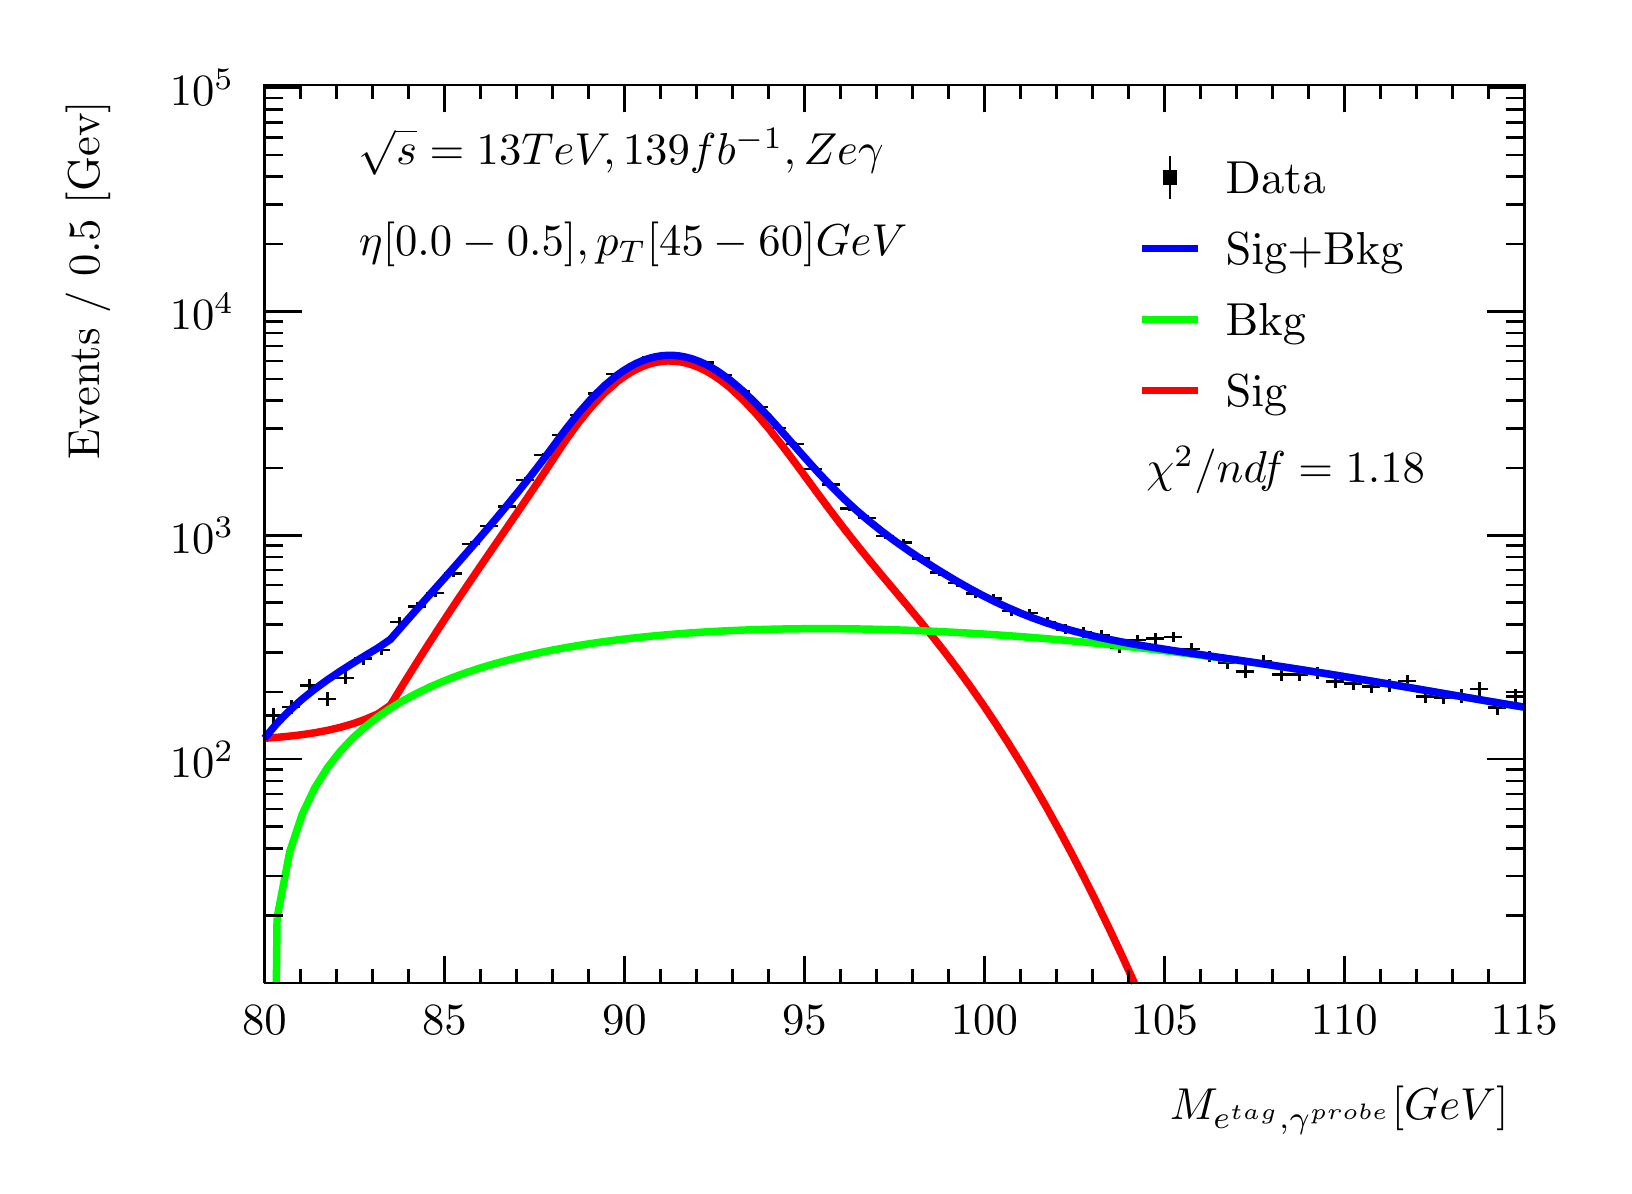
\begin{tikzpicture}
\pgfdeclareplotmark{cross} {
\pgfpathmoveto{\pgfpoint{-0.3\pgfplotmarksize}{\pgfplotmarksize}}
\pgfpathlineto{\pgfpoint{+0.3\pgfplotmarksize}{\pgfplotmarksize}}
\pgfpathlineto{\pgfpoint{+0.3\pgfplotmarksize}{0.3\pgfplotmarksize}}
\pgfpathlineto{\pgfpoint{+1\pgfplotmarksize}{0.3\pgfplotmarksize}}
\pgfpathlineto{\pgfpoint{+1\pgfplotmarksize}{-0.3\pgfplotmarksize}}
\pgfpathlineto{\pgfpoint{+0.3\pgfplotmarksize}{-0.3\pgfplotmarksize}}
\pgfpathlineto{\pgfpoint{+0.3\pgfplotmarksize}{-1.\pgfplotmarksize}}
\pgfpathlineto{\pgfpoint{-0.3\pgfplotmarksize}{-1.\pgfplotmarksize}}
\pgfpathlineto{\pgfpoint{-0.3\pgfplotmarksize}{-0.3\pgfplotmarksize}}
\pgfpathlineto{\pgfpoint{-1.\pgfplotmarksize}{-0.3\pgfplotmarksize}}
\pgfpathlineto{\pgfpoint{-1.\pgfplotmarksize}{0.3\pgfplotmarksize}}
\pgfpathlineto{\pgfpoint{-0.3\pgfplotmarksize}{0.3\pgfplotmarksize}}
\pgfpathclose
\pgfusepathqstroke
}
\pgfdeclareplotmark{cross*} {
\pgfpathmoveto{\pgfpoint{-0.3\pgfplotmarksize}{\pgfplotmarksize}}
\pgfpathlineto{\pgfpoint{+0.3\pgfplotmarksize}{\pgfplotmarksize}}
\pgfpathlineto{\pgfpoint{+0.3\pgfplotmarksize}{0.3\pgfplotmarksize}}
\pgfpathlineto{\pgfpoint{+1\pgfplotmarksize}{0.3\pgfplotmarksize}}
\pgfpathlineto{\pgfpoint{+1\pgfplotmarksize}{-0.3\pgfplotmarksize}}
\pgfpathlineto{\pgfpoint{+0.3\pgfplotmarksize}{-0.3\pgfplotmarksize}}
\pgfpathlineto{\pgfpoint{+0.3\pgfplotmarksize}{-1.\pgfplotmarksize}}
\pgfpathlineto{\pgfpoint{-0.3\pgfplotmarksize}{-1.\pgfplotmarksize}}
\pgfpathlineto{\pgfpoint{-0.3\pgfplotmarksize}{-0.3\pgfplotmarksize}}
\pgfpathlineto{\pgfpoint{-1.\pgfplotmarksize}{-0.3\pgfplotmarksize}}
\pgfpathlineto{\pgfpoint{-1.\pgfplotmarksize}{0.3\pgfplotmarksize}}
\pgfpathlineto{\pgfpoint{-0.3\pgfplotmarksize}{0.3\pgfplotmarksize}}
\pgfpathclose
\pgfusepathqfillstroke
}
\pgfdeclareplotmark{newstar} {
\pgfpathmoveto{\pgfqpoint{0pt}{\pgfplotmarksize}}
\pgfpathlineto{\pgfqpointpolar{44}{0.5\pgfplotmarksize}}
\pgfpathlineto{\pgfqpointpolar{18}{\pgfplotmarksize}}
\pgfpathlineto{\pgfqpointpolar{-20}{0.5\pgfplotmarksize}}
\pgfpathlineto{\pgfqpointpolar{-54}{\pgfplotmarksize}}
\pgfpathlineto{\pgfqpointpolar{-90}{0.5\pgfplotmarksize}}
\pgfpathlineto{\pgfqpointpolar{234}{\pgfplotmarksize}}
\pgfpathlineto{\pgfqpointpolar{198}{0.5\pgfplotmarksize}}
\pgfpathlineto{\pgfqpointpolar{162}{\pgfplotmarksize}}
\pgfpathlineto{\pgfqpointpolar{134}{0.5\pgfplotmarksize}}
\pgfpathclose
\pgfusepathqstroke
}
\pgfdeclareplotmark{newstar*} {
\pgfpathmoveto{\pgfqpoint{0pt}{\pgfplotmarksize}}
\pgfpathlineto{\pgfqpointpolar{44}{0.5\pgfplotmarksize}}
\pgfpathlineto{\pgfqpointpolar{18}{\pgfplotmarksize}}
\pgfpathlineto{\pgfqpointpolar{-20}{0.5\pgfplotmarksize}}
\pgfpathlineto{\pgfqpointpolar{-54}{\pgfplotmarksize}}
\pgfpathlineto{\pgfqpointpolar{-90}{0.5\pgfplotmarksize}}
\pgfpathlineto{\pgfqpointpolar{234}{\pgfplotmarksize}}
\pgfpathlineto{\pgfqpointpolar{198}{0.5\pgfplotmarksize}}
\pgfpathlineto{\pgfqpointpolar{162}{\pgfplotmarksize}}
\pgfpathlineto{\pgfqpointpolar{134}{0.5\pgfplotmarksize}}
\pgfpathclose
\pgfusepathqfillstroke
}
\definecolor{c}{rgb}{1,1,1};
\draw [color=c, fill=c] (0,0) rectangle (20,14.4361);
\draw [color=c, fill=c] (3,2.30977) rectangle (19,13.7143);
\definecolor{c}{rgb}{0,0,0};
\draw [c,line width=0.9] (3,2.30977) -- (3,13.7143) -- (19,13.7143) -- (19,2.30977) -- (3,2.30977);
\definecolor{c}{rgb}{1,1,1};
\draw [color=c, fill=c] (3,2.30977) rectangle (19,13.7143);
\definecolor{c}{rgb}{0,0,0};
\draw [c,line width=0.9] (3,2.30977) -- (3,13.7143) -- (19,13.7143) -- (19,2.30977) -- (3,2.30977);
\draw [c,line width=0.9] (3,2.30977) -- (19,2.30977);
\draw [c,line width=0.9] (3,2.65624) -- (3,2.30977);
\draw [c,line width=0.9] (3.45714,2.48301) -- (3.45714,2.30977);
\draw [c,line width=0.9] (3.91429,2.48301) -- (3.91429,2.30977);
\draw [c,line width=0.9] (4.37143,2.48301) -- (4.37143,2.30977);
\draw [c,line width=0.9] (4.82857,2.48301) -- (4.82857,2.30977);
\draw [c,line width=0.9] (5.28571,2.65624) -- (5.28571,2.30977);
\draw [c,line width=0.9] (5.74286,2.48301) -- (5.74286,2.30977);
\draw [c,line width=0.9] (6.2,2.48301) -- (6.2,2.30977);
\draw [c,line width=0.9] (6.65714,2.48301) -- (6.65714,2.30977);
\draw [c,line width=0.9] (7.11429,2.48301) -- (7.11429,2.30977);
\draw [c,line width=0.9] (7.57143,2.65624) -- (7.57143,2.30977);
\draw [c,line width=0.9] (8.02857,2.48301) -- (8.02857,2.30977);
\draw [c,line width=0.9] (8.48571,2.48301) -- (8.48571,2.30977);
\draw [c,line width=0.9] (8.94286,2.48301) -- (8.94286,2.30977);
\draw [c,line width=0.9] (9.4,2.48301) -- (9.4,2.30977);
\draw [c,line width=0.9] (9.85714,2.65624) -- (9.85714,2.30977);
\draw [c,line width=0.9] (10.3143,2.48301) -- (10.3143,2.30977);
\draw [c,line width=0.9] (10.7714,2.48301) -- (10.7714,2.30977);
\draw [c,line width=0.9] (11.2286,2.48301) -- (11.2286,2.30977);
\draw [c,line width=0.9] (11.6857,2.48301) -- (11.6857,2.30977);
\draw [c,line width=0.9] (12.1429,2.65624) -- (12.1429,2.30977);
\draw [c,line width=0.9] (12.6,2.48301) -- (12.6,2.30977);
\draw [c,line width=0.9] (13.0571,2.48301) -- (13.0571,2.30977);
\draw [c,line width=0.9] (13.5143,2.48301) -- (13.5143,2.30977);
\draw [c,line width=0.9] (13.9714,2.48301) -- (13.9714,2.30977);
\draw [c,line width=0.9] (14.4286,2.65624) -- (14.4286,2.30977);
\draw [c,line width=0.9] (14.8857,2.48301) -- (14.8857,2.30977);
\draw [c,line width=0.9] (15.3429,2.48301) -- (15.3429,2.30977);
\draw [c,line width=0.9] (15.8,2.48301) -- (15.8,2.30977);
\draw [c,line width=0.9] (16.2571,2.48301) -- (16.2571,2.30977);
\draw [c,line width=0.9] (16.7143,2.65624) -- (16.7143,2.30977);
\draw [c,line width=0.9] (17.1714,2.48301) -- (17.1714,2.30977);
\draw [c,line width=0.9] (17.6286,2.48301) -- (17.6286,2.30977);
\draw [c,line width=0.9] (18.0857,2.48301) -- (18.0857,2.30977);
\draw [c,line width=0.9] (18.5429,2.48301) -- (18.5429,2.30977);
\draw [c,line width=0.9] (19,2.65624) -- (19,2.30977);
\draw [anchor=base] (3,1.66015) node[scale=1.61424, color=c, rotate=0]{80};
\draw [anchor=base] (5.28571,1.66015) node[scale=1.61424, color=c, rotate=0]{85};
\draw [anchor=base] (7.57143,1.66015) node[scale=1.61424, color=c, rotate=0]{90};
\draw [anchor=base] (9.85714,1.66015) node[scale=1.61424, color=c, rotate=0]{95};
\draw [anchor=base] (12.1429,1.66015) node[scale=1.61424, color=c, rotate=0]{100};
\draw [anchor=base] (14.4286,1.66015) node[scale=1.61424, color=c, rotate=0]{105};
\draw [anchor=base] (16.7143,1.66015) node[scale=1.61424, color=c, rotate=0]{110};
\draw [anchor=base] (19,1.66015) node[scale=1.61424, color=c, rotate=0]{115};
\draw [anchor= east] (19,0.692932) node[scale=1.61424, color=c, rotate=0]{$M_{e^{tag}, \gamma^{probe}}  [GeV]$};
\draw [c,line width=0.9] (3,13.7143) -- (19,13.7143);
\draw [c,line width=0.9] (3,13.3678) -- (3,13.7143);
\draw [c,line width=0.9] (3.45714,13.5411) -- (3.45714,13.7143);
\draw [c,line width=0.9] (3.91429,13.5411) -- (3.91429,13.7143);
\draw [c,line width=0.9] (4.37143,13.5411) -- (4.37143,13.7143);
\draw [c,line width=0.9] (4.82857,13.5411) -- (4.82857,13.7143);
\draw [c,line width=0.9] (5.28571,13.3678) -- (5.28571,13.7143);
\draw [c,line width=0.9] (5.74286,13.5411) -- (5.74286,13.7143);
\draw [c,line width=0.9] (6.2,13.5411) -- (6.2,13.7143);
\draw [c,line width=0.9] (6.65714,13.5411) -- (6.65714,13.7143);
\draw [c,line width=0.9] (7.11429,13.5411) -- (7.11429,13.7143);
\draw [c,line width=0.9] (7.57143,13.3678) -- (7.57143,13.7143);
\draw [c,line width=0.9] (8.02857,13.5411) -- (8.02857,13.7143);
\draw [c,line width=0.9] (8.48571,13.5411) -- (8.48571,13.7143);
\draw [c,line width=0.9] (8.94286,13.5411) -- (8.94286,13.7143);
\draw [c,line width=0.9] (9.4,13.5411) -- (9.4,13.7143);
\draw [c,line width=0.9] (9.85714,13.3678) -- (9.85714,13.7143);
\draw [c,line width=0.9] (10.3143,13.5411) -- (10.3143,13.7143);
\draw [c,line width=0.9] (10.7714,13.5411) -- (10.7714,13.7143);
\draw [c,line width=0.9] (11.2286,13.5411) -- (11.2286,13.7143);
\draw [c,line width=0.9] (11.6857,13.5411) -- (11.6857,13.7143);
\draw [c,line width=0.9] (12.1429,13.3678) -- (12.1429,13.7143);
\draw [c,line width=0.9] (12.6,13.5411) -- (12.6,13.7143);
\draw [c,line width=0.9] (13.0571,13.5411) -- (13.0571,13.7143);
\draw [c,line width=0.9] (13.5143,13.5411) -- (13.5143,13.7143);
\draw [c,line width=0.9] (13.9714,13.5411) -- (13.9714,13.7143);
\draw [c,line width=0.9] (14.4286,13.3678) -- (14.4286,13.7143);
\draw [c,line width=0.9] (14.8857,13.5411) -- (14.8857,13.7143);
\draw [c,line width=0.9] (15.3429,13.5411) -- (15.3429,13.7143);
\draw [c,line width=0.9] (15.8,13.5411) -- (15.8,13.7143);
\draw [c,line width=0.9] (16.2571,13.5411) -- (16.2571,13.7143);
\draw [c,line width=0.9] (16.7143,13.3678) -- (16.7143,13.7143);
\draw [c,line width=0.9] (17.1714,13.5411) -- (17.1714,13.7143);
\draw [c,line width=0.9] (17.6286,13.5411) -- (17.6286,13.7143);
\draw [c,line width=0.9] (18.0857,13.5411) -- (18.0857,13.7143);
\draw [c,line width=0.9] (18.5429,13.5411) -- (18.5429,13.7143);
\draw [c,line width=0.9] (19,13.3678) -- (19,13.7143);
\draw [c,line width=0.9] (3,2.30977) -- (3,13.7143);
\draw [c,line width=0.9] (3.237,3.16561) -- (3,3.16561);
\draw [c,line width=0.9] (3.237,3.66625) -- (3,3.66625);
\draw [c,line width=0.9] (3.237,4.02146) -- (3,4.02146);
\draw [c,line width=0.9] (3.237,4.29698) -- (3,4.29698);
\draw [c,line width=0.9] (3.237,4.52209) -- (3,4.52209);
\draw [c,line width=0.9] (3.237,4.71242) -- (3,4.71242);
\draw [c,line width=0.9] (3.237,4.8773) -- (3,4.8773);
\draw [c,line width=0.9] (3.237,5.02273) -- (3,5.02273);
\draw [c,line width=0.9] (3.474,5.15282) -- (3,5.15282);
\draw [anchor= east] (2.82,5.15282) node[scale=1.61424, color=c, rotate=0]{$10^{2}$};
\draw [c,line width=0.9] (3.237,6.00866) -- (3,6.00866);
\draw [c,line width=0.9] (3.237,6.5093) -- (3,6.5093);
\draw [c,line width=0.9] (3.237,6.8645) -- (3,6.8645);
\draw [c,line width=0.9] (3.237,7.14002) -- (3,7.14002);
\draw [c,line width=0.9] (3.237,7.36514) -- (3,7.36514);
\draw [c,line width=0.9] (3.237,7.55547) -- (3,7.55547);
\draw [c,line width=0.9] (3.237,7.72034) -- (3,7.72034);
\draw [c,line width=0.9] (3.237,7.86577) -- (3,7.86577);
\draw [c,line width=0.9] (3.474,7.99586) -- (3,7.99586);
\draw [anchor= east] (2.82,7.99586) node[scale=1.61424, color=c, rotate=0]{$10^{3}$};
\draw [c,line width=0.9] (3.237,8.85171) -- (3,8.85171);
\draw [c,line width=0.9] (3.237,9.35234) -- (3,9.35234);
\draw [c,line width=0.9] (3.237,9.70755) -- (3,9.70755);
\draw [c,line width=0.9] (3.237,9.98307) -- (3,9.98307);
\draw [c,line width=0.9] (3.237,10.2082) -- (3,10.2082);
\draw [c,line width=0.9] (3.237,10.3985) -- (3,10.3985);
\draw [c,line width=0.9] (3.237,10.5634) -- (3,10.5634);
\draw [c,line width=0.9] (3.237,10.7088) -- (3,10.7088);
\draw [c,line width=0.9] (3.474,10.8389) -- (3,10.8389);
\draw [anchor= east] (2.82,10.8389) node[scale=1.61424, color=c, rotate=0]{$10^{4}$};
\draw [c,line width=0.9] (3.237,11.6948) -- (3,11.6948);
\draw [c,line width=0.9] (3.237,12.1954) -- (3,12.1954);
\draw [c,line width=0.9] (3.237,12.5506) -- (3,12.5506);
\draw [c,line width=0.9] (3.237,12.8261) -- (3,12.8261);
\draw [c,line width=0.9] (3.237,13.0512) -- (3,13.0512);
\draw [c,line width=0.9] (3.237,13.2416) -- (3,13.2416);
\draw [c,line width=0.9] (3.237,13.4064) -- (3,13.4064);
\draw [c,line width=0.9] (3.237,13.5519) -- (3,13.5519);
\draw [c,line width=0.9] (3.474,13.682) -- (3,13.682);
\draw [anchor= east] (2.82,13.682) node[scale=1.61424, color=c, rotate=0]{$10^{5}$};
\draw [anchor= east] (0.76,13.7143) node[scale=1.61424, color=c, rotate=90]{Events / 0.5 [Gev]};
\draw [c,line width=0.9] (19,2.30977) -- (19,13.7143);
\draw [c,line width=0.9] (18.763,3.16561) -- (19,3.16561);
\draw [c,line width=0.9] (18.763,3.66625) -- (19,3.66625);
\draw [c,line width=0.9] (18.763,4.02146) -- (19,4.02146);
\draw [c,line width=0.9] (18.763,4.29698) -- (19,4.29698);
\draw [c,line width=0.9] (18.763,4.52209) -- (19,4.52209);
\draw [c,line width=0.9] (18.763,4.71242) -- (19,4.71242);
\draw [c,line width=0.9] (18.763,4.8773) -- (19,4.8773);
\draw [c,line width=0.9] (18.763,5.02273) -- (19,5.02273);
\draw [c,line width=0.9] (18.526,5.15282) -- (19,5.15282);
\draw [c,line width=0.9] (18.763,6.00866) -- (19,6.00866);
\draw [c,line width=0.9] (18.763,6.5093) -- (19,6.5093);
\draw [c,line width=0.9] (18.763,6.8645) -- (19,6.8645);
\draw [c,line width=0.9] (18.763,7.14002) -- (19,7.14002);
\draw [c,line width=0.9] (18.763,7.36514) -- (19,7.36514);
\draw [c,line width=0.9] (18.763,7.55547) -- (19,7.55547);
\draw [c,line width=0.9] (18.763,7.72034) -- (19,7.72034);
\draw [c,line width=0.9] (18.763,7.86577) -- (19,7.86577);
\draw [c,line width=0.9] (18.526,7.99586) -- (19,7.99586);
\draw [c,line width=0.9] (18.763,8.85171) -- (19,8.85171);
\draw [c,line width=0.9] (18.763,9.35234) -- (19,9.35234);
\draw [c,line width=0.9] (18.763,9.70755) -- (19,9.70755);
\draw [c,line width=0.9] (18.763,9.98307) -- (19,9.98307);
\draw [c,line width=0.9] (18.763,10.2082) -- (19,10.2082);
\draw [c,line width=0.9] (18.763,10.3985) -- (19,10.3985);
\draw [c,line width=0.9] (18.763,10.5634) -- (19,10.5634);
\draw [c,line width=0.9] (18.763,10.7088) -- (19,10.7088);
\draw [c,line width=0.9] (18.526,10.8389) -- (19,10.8389);
\draw [c,line width=0.9] (18.763,11.6948) -- (19,11.6948);
\draw [c,line width=0.9] (18.763,12.1954) -- (19,12.1954);
\draw [c,line width=0.9] (18.763,12.5506) -- (19,12.5506);
\draw [c,line width=0.9] (18.763,12.8261) -- (19,12.8261);
\draw [c,line width=0.9] (18.763,13.0512) -- (19,13.0512);
\draw [c,line width=0.9] (18.763,13.2416) -- (19,13.2416);
\draw [c,line width=0.9] (18.763,13.4064) -- (19,13.4064);
\draw [c,line width=0.9] (18.763,13.5519) -- (19,13.5519);
\draw [c,line width=0.9] (18.526,13.682) -- (19,13.682);
\draw [c,line width=0.9] (3.11429,5.70977) -- (3,5.70977);
\draw [c,line width=0.9] (3,5.70977) -- (3,5.70977);
\draw [c,line width=0.9] (3.11429,5.70977) -- (3.22857,5.70977);
\draw [c,line width=0.9] (3.22857,5.70977) -- (3.22857,5.70977);
\draw [c,line width=0.9] (3.11429,5.70977) -- (3.11429,5.80829);
\draw [c,line width=0.9] (3.11429,5.80829) -- (3.11429,5.80829);
\draw [c,line width=0.9] (3.11429,5.70977) -- (3.11429,5.61126);
\draw [c,line width=0.9] (3.11429,5.61126) -- (3.11429,5.61126);
\draw [c,line width=0.9] (3.34286,5.81524) -- (3.22857,5.81524);
\draw [c,line width=0.9] (3.22857,5.81524) -- (3.22857,5.81524);
\draw [c,line width=0.9] (3.34286,5.81524) -- (3.45714,5.81524);
\draw [c,line width=0.9] (3.45714,5.81524) -- (3.45714,5.81524);
\draw [c,line width=0.9] (3.34286,5.81524) -- (3.34286,5.90964);
\draw [c,line width=0.9] (3.34286,5.90964) -- (3.34286,5.90964);
\draw [c,line width=0.9] (3.34286,5.81524) -- (3.34286,5.72084);
\draw [c,line width=0.9] (3.34286,5.72084) -- (3.34286,5.72084);
\draw [c,line width=0.9] (3.57143,6.08642) -- (3.45714,6.08642);
\draw [c,line width=0.9] (3.45714,6.08642) -- (3.45714,6.08642);
\draw [c,line width=0.9] (3.57143,6.08642) -- (3.68571,6.08642);
\draw [c,line width=0.9] (3.68571,6.08642) -- (3.68571,6.08642);
\draw [c,line width=0.9] (3.57143,6.08642) -- (3.57143,6.171);
\draw [c,line width=0.9] (3.57143,6.171) -- (3.57143,6.171);
\draw [c,line width=0.9] (3.57143,6.08642) -- (3.57143,6.00183);
\draw [c,line width=0.9] (3.57143,6.00183) -- (3.57143,6.00183);
\draw [c,line width=0.9] (3.8,5.91906) -- (3.68571,5.91906);
\draw [c,line width=0.9] (3.68571,5.91906) -- (3.68571,5.91906);
\draw [c,line width=0.9] (3.8,5.91906) -- (3.91429,5.91906);
\draw [c,line width=0.9] (3.91429,5.91906) -- (3.91429,5.91906);
\draw [c,line width=0.9] (3.8,5.91906) -- (3.8,6.00957);
\draw [c,line width=0.9] (3.8,6.00957) -- (3.8,6.00957);
\draw [c,line width=0.9] (3.8,5.91906) -- (3.8,5.82854);
\draw [c,line width=0.9] (3.8,5.82854) -- (3.8,5.82854);
\draw [c,line width=0.9] (4.02857,6.18658) -- (3.91429,6.18658);
\draw [c,line width=0.9] (3.91429,6.18658) -- (3.91429,6.18658);
\draw [c,line width=0.9] (4.02857,6.18658) -- (4.14286,6.18658);
\draw [c,line width=0.9] (4.14286,6.18658) -- (4.14286,6.18658);
\draw [c,line width=0.9] (4.02857,6.18658) -- (4.02857,6.26781);
\draw [c,line width=0.9] (4.02857,6.26781) -- (4.02857,6.26781);
\draw [c,line width=0.9] (4.02857,6.18658) -- (4.02857,6.10536);
\draw [c,line width=0.9] (4.02857,6.10536) -- (4.02857,6.10536);
\draw [c,line width=0.9] (4.25714,6.42851) -- (4.14286,6.42851);
\draw [c,line width=0.9] (4.14286,6.42851) -- (4.14286,6.42851);
\draw [c,line width=0.9] (4.25714,6.42851) -- (4.37143,6.42851);
\draw [c,line width=0.9] (4.37143,6.42851) -- (4.37143,6.42851);
\draw [c,line width=0.9] (4.25714,6.42851) -- (4.25714,6.50216);
\draw [c,line width=0.9] (4.25714,6.50216) -- (4.25714,6.50216);
\draw [c,line width=0.9] (4.25714,6.42851) -- (4.25714,6.35487);
\draw [c,line width=0.9] (4.25714,6.35487) -- (4.25714,6.35487);
\draw [c,line width=0.9] (4.48571,6.54179) -- (4.37143,6.54179);
\draw [c,line width=0.9] (4.37143,6.54179) -- (4.37143,6.54179);
\draw [c,line width=0.9] (4.48571,6.54179) -- (4.6,6.54179);
\draw [c,line width=0.9] (4.6,6.54179) -- (4.6,6.54179);
\draw [c,line width=0.9] (4.48571,6.54179) -- (4.48571,6.61214);
\draw [c,line width=0.9] (4.48571,6.61214) -- (4.48571,6.61214);
\draw [c,line width=0.9] (4.48571,6.54179) -- (4.48571,6.47145);
\draw [c,line width=0.9] (4.48571,6.47145) -- (4.48571,6.47145);
\draw [c,line width=0.9] (4.71429,6.89198) -- (4.6,6.89198);
\draw [c,line width=0.9] (4.6,6.89198) -- (4.6,6.89198);
\draw [c,line width=0.9] (4.71429,6.89198) -- (4.82857,6.89198);
\draw [c,line width=0.9] (4.82857,6.89198) -- (4.82857,6.89198);
\draw [c,line width=0.9] (4.71429,6.89198) -- (4.71429,6.95302);
\draw [c,line width=0.9] (4.71429,6.95302) -- (4.71429,6.95302);
\draw [c,line width=0.9] (4.71429,6.89198) -- (4.71429,6.83093);
\draw [c,line width=0.9] (4.71429,6.83093) -- (4.71429,6.83093);
\draw [c,line width=0.9] (4.94286,7.09475) -- (4.82857,7.09475);
\draw [c,line width=0.9] (4.82857,7.09475) -- (4.82857,7.09475);
\draw [c,line width=0.9] (4.94286,7.09475) -- (5.05714,7.09475);
\draw [c,line width=0.9] (5.05714,7.09475) -- (5.05714,7.09475);
\draw [c,line width=0.9] (4.94286,7.09475) -- (4.94286,7.15099);
\draw [c,line width=0.9] (4.94286,7.15099) -- (4.94286,7.15099);
\draw [c,line width=0.9] (4.94286,7.09475) -- (4.94286,7.03852);
\draw [c,line width=0.9] (4.94286,7.03852) -- (4.94286,7.03852);
\draw [c,line width=0.9] (5.17143,7.26442) -- (5.05714,7.26442);
\draw [c,line width=0.9] (5.05714,7.26442) -- (5.05714,7.26442);
\draw [c,line width=0.9] (5.17143,7.26442) -- (5.28571,7.26442);
\draw [c,line width=0.9] (5.28571,7.26442) -- (5.28571,7.26442);
\draw [c,line width=0.9] (5.17143,7.26442) -- (5.17143,7.31692);
\draw [c,line width=0.9] (5.17143,7.31692) -- (5.17143,7.31692);
\draw [c,line width=0.9] (5.17143,7.26442) -- (5.17143,7.21192);
\draw [c,line width=0.9] (5.17143,7.21192) -- (5.17143,7.21192);
\draw [c,line width=0.9] (5.4,7.50874) -- (5.28571,7.50874);
\draw [c,line width=0.9] (5.28571,7.50874) -- (5.28571,7.50874);
\draw [c,line width=0.9] (5.4,7.50874) -- (5.51429,7.50874);
\draw [c,line width=0.9] (5.51429,7.50874) -- (5.51429,7.50874);
\draw [c,line width=0.9] (5.4,7.50874) -- (5.4,7.55629);
\draw [c,line width=0.9] (5.4,7.55629) -- (5.4,7.55629);
\draw [c,line width=0.9] (5.4,7.50874) -- (5.4,7.46118);
\draw [c,line width=0.9] (5.4,7.46118) -- (5.4,7.46118);
\draw [c,line width=0.9] (5.62857,7.88618) -- (5.51429,7.88618);
\draw [c,line width=0.9] (5.51429,7.88618) -- (5.51429,7.88618);
\draw [c,line width=0.9] (5.62857,7.88618) -- (5.74286,7.88618);
\draw [c,line width=0.9] (5.74286,7.88618) -- (5.74286,7.88618);
\draw [c,line width=0.9] (5.62857,7.88618) -- (5.62857,7.927);
\draw [c,line width=0.9] (5.62857,7.927) -- (5.62857,7.927);
\draw [c,line width=0.9] (5.62857,7.88618) -- (5.62857,7.84537);
\draw [c,line width=0.9] (5.62857,7.84537) -- (5.62857,7.84537);
\draw [c,line width=0.9] (5.85714,8.11242) -- (5.74286,8.11242);
\draw [c,line width=0.9] (5.74286,8.11242) -- (5.74286,8.11242);
\draw [c,line width=0.9] (5.85714,8.11242) -- (5.97143,8.11242);
\draw [c,line width=0.9] (5.97143,8.11242) -- (5.97143,8.11242);
\draw [c,line width=0.9] (5.85714,8.11242) -- (5.85714,8.14967);
\draw [c,line width=0.9] (5.85714,8.14967) -- (5.85714,8.14967);
\draw [c,line width=0.9] (5.85714,8.11242) -- (5.85714,8.07518);
\draw [c,line width=0.9] (5.85714,8.07518) -- (5.85714,8.07518);
\draw [c,line width=0.9] (6.08571,8.36183) -- (5.97143,8.36183);
\draw [c,line width=0.9] (5.97143,8.36183) -- (5.97143,8.36183);
\draw [c,line width=0.9] (6.08571,8.36183) -- (6.2,8.36183);
\draw [c,line width=0.9] (6.2,8.36183) -- (6.2,8.36183);
\draw [c,line width=0.9] (6.08571,8.36183) -- (6.08571,8.39549);
\draw [c,line width=0.9] (6.08571,8.39549) -- (6.08571,8.39549);
\draw [c,line width=0.9] (6.08571,8.36183) -- (6.08571,8.32816);
\draw [c,line width=0.9] (6.08571,8.32816) -- (6.08571,8.32816);
\draw [c,line width=0.9] (6.31429,8.70156) -- (6.2,8.70156);
\draw [c,line width=0.9] (6.2,8.70156) -- (6.2,8.70156);
\draw [c,line width=0.9] (6.31429,8.70156) -- (6.42857,8.70156);
\draw [c,line width=0.9] (6.42857,8.70156) -- (6.42857,8.70156);
\draw [c,line width=0.9] (6.31429,8.70156) -- (6.31429,8.7309);
\draw [c,line width=0.9] (6.31429,8.7309) -- (6.31429,8.7309);
\draw [c,line width=0.9] (6.31429,8.70156) -- (6.31429,8.67222);
\draw [c,line width=0.9] (6.31429,8.67222) -- (6.31429,8.67222);
\draw [c,line width=0.9] (6.54286,9.01511) -- (6.42857,9.01511);
\draw [c,line width=0.9] (6.42857,9.01511) -- (6.42857,9.01511);
\draw [c,line width=0.9] (6.54286,9.01511) -- (6.65714,9.01511);
\draw [c,line width=0.9] (6.65714,9.01511) -- (6.65714,9.01511);
\draw [c,line width=0.9] (6.54286,9.01511) -- (6.54286,9.04095);
\draw [c,line width=0.9] (6.54286,9.04095) -- (6.54286,9.04095);
\draw [c,line width=0.9] (6.54286,9.01511) -- (6.54286,8.98927);
\draw [c,line width=0.9] (6.54286,8.98927) -- (6.54286,8.98927);
\draw [c,line width=0.9] (6.77143,9.26848) -- (6.65714,9.26848);
\draw [c,line width=0.9] (6.65714,9.26848) -- (6.65714,9.26848);
\draw [c,line width=0.9] (6.77143,9.26848) -- (6.88571,9.26848);
\draw [c,line width=0.9] (6.88571,9.26848) -- (6.88571,9.26848);
\draw [c,line width=0.9] (6.77143,9.26848) -- (6.77143,9.2918);
\draw [c,line width=0.9] (6.77143,9.2918) -- (6.77143,9.2918);
\draw [c,line width=0.9] (6.77143,9.26848) -- (6.77143,9.24516);
\draw [c,line width=0.9] (6.77143,9.24516) -- (6.77143,9.24516);
\draw [c,line width=0.9] (7,9.52312) -- (6.88571,9.52312);
\draw [c,line width=0.9] (6.88571,9.52312) -- (6.88571,9.52312);
\draw [c,line width=0.9] (7,9.52312) -- (7.11429,9.52312);
\draw [c,line width=0.9] (7.11429,9.52312) -- (7.11429,9.52312);
\draw [c,line width=0.9] (7,9.52312) -- (7,9.54416);
\draw [c,line width=0.9] (7,9.54416) -- (7,9.54416);
\draw [c,line width=0.9] (7,9.52312) -- (7,9.50208);
\draw [c,line width=0.9] (7,9.50208) -- (7,9.50208);
\draw [c,line width=0.9] (7.22857,9.79426) -- (7.11429,9.79426);
\draw [c,line width=0.9] (7.11429,9.79426) -- (7.11429,9.79426);
\draw [c,line width=0.9] (7.22857,9.79426) -- (7.34286,9.79426);
\draw [c,line width=0.9] (7.34286,9.79426) -- (7.34286,9.79426);
\draw [c,line width=0.9] (7.22857,9.79426) -- (7.22857,9.81311);
\draw [c,line width=0.9] (7.22857,9.81311) -- (7.22857,9.81311);
\draw [c,line width=0.9] (7.22857,9.79426) -- (7.22857,9.77541);
\draw [c,line width=0.9] (7.22857,9.77541) -- (7.22857,9.77541);
\draw [c,line width=0.9] (7.45714,10.0452) -- (7.34286,10.0452);
\draw [c,line width=0.9] (7.34286,10.0452) -- (7.34286,10.0452);
\draw [c,line width=0.9] (7.45714,10.0452) -- (7.57143,10.0452);
\draw [c,line width=0.9] (7.57143,10.0452) -- (7.57143,10.0452);
\draw [c,line width=0.9] (7.45714,10.0452) -- (7.45714,10.0622);
\draw [c,line width=0.9] (7.45714,10.0622) -- (7.45714,10.0622);
\draw [c,line width=0.9] (7.45714,10.0452) -- (7.45714,10.0282);
\draw [c,line width=0.9] (7.45714,10.0282) -- (7.45714,10.0282);
\draw [c,line width=0.9] (7.68571,10.1292) -- (7.57143,10.1292);
\draw [c,line width=0.9] (7.57143,10.1292) -- (7.57143,10.1292);
\draw [c,line width=0.9] (7.68571,10.1292) -- (7.8,10.1292);
\draw [c,line width=0.9] (7.8,10.1292) -- (7.8,10.1292);
\draw [c,line width=0.9] (7.68571,10.1292) -- (7.68571,10.1456);
\draw [c,line width=0.9] (7.68571,10.1456) -- (7.68571,10.1456);
\draw [c,line width=0.9] (7.68571,10.1292) -- (7.68571,10.1127);
\draw [c,line width=0.9] (7.68571,10.1127) -- (7.68571,10.1127);
\draw [c,line width=0.9] (7.91429,10.256) -- (7.8,10.256);
\draw [c,line width=0.9] (7.8,10.256) -- (7.8,10.256);
\draw [c,line width=0.9] (7.91429,10.256) -- (8.02857,10.256);
\draw [c,line width=0.9] (8.02857,10.256) -- (8.02857,10.256);
\draw [c,line width=0.9] (7.91429,10.256) -- (7.91429,10.2717);
\draw [c,line width=0.9] (7.91429,10.2717) -- (7.91429,10.2717);
\draw [c,line width=0.9] (7.91429,10.256) -- (7.91429,10.2404);
\draw [c,line width=0.9] (7.91429,10.2404) -- (7.91429,10.2404);
\draw [c,line width=0.9] (8.14286,10.2819) -- (8.02857,10.2819);
\draw [c,line width=0.9] (8.02857,10.2819) -- (8.02857,10.2819);
\draw [c,line width=0.9] (8.14286,10.2819) -- (8.25714,10.2819);
\draw [c,line width=0.9] (8.25714,10.2819) -- (8.25714,10.2819);
\draw [c,line width=0.9] (8.14286,10.2819) -- (8.14286,10.2973);
\draw [c,line width=0.9] (8.14286,10.2973) -- (8.14286,10.2973);
\draw [c,line width=0.9] (8.14286,10.2819) -- (8.14286,10.2664);
\draw [c,line width=0.9] (8.14286,10.2664) -- (8.14286,10.2664);
\draw [c,line width=0.9] (8.37143,10.258) -- (8.25714,10.258);
\draw [c,line width=0.9] (8.25714,10.258) -- (8.25714,10.258);
\draw [c,line width=0.9] (8.37143,10.258) -- (8.48571,10.258);
\draw [c,line width=0.9] (8.48571,10.258) -- (8.48571,10.258);
\draw [c,line width=0.9] (8.37143,10.258) -- (8.37143,10.2736);
\draw [c,line width=0.9] (8.37143,10.2736) -- (8.37143,10.2736);
\draw [c,line width=0.9] (8.37143,10.258) -- (8.37143,10.2424);
\draw [c,line width=0.9] (8.37143,10.2424) -- (8.37143,10.2424);
\draw [c,line width=0.9] (8.6,10.1906) -- (8.48571,10.1906);
\draw [c,line width=0.9] (8.48571,10.1906) -- (8.48571,10.1906);
\draw [c,line width=0.9] (8.6,10.1906) -- (8.71429,10.1906);
\draw [c,line width=0.9] (8.71429,10.1906) -- (8.71429,10.1906);
\draw [c,line width=0.9] (8.6,10.1906) -- (8.6,10.2066);
\draw [c,line width=0.9] (8.6,10.2066) -- (8.6,10.2066);
\draw [c,line width=0.9] (8.6,10.1906) -- (8.6,10.1745);
\draw [c,line width=0.9] (8.6,10.1745) -- (8.6,10.1745);
\draw [c,line width=0.9] (8.82857,10.0346) -- (8.71429,10.0346);
\draw [c,line width=0.9] (8.71429,10.0346) -- (8.71429,10.0346);
\draw [c,line width=0.9] (8.82857,10.0346) -- (8.94286,10.0346);
\draw [c,line width=0.9] (8.94286,10.0346) -- (8.94286,10.0346);
\draw [c,line width=0.9] (8.82857,10.0346) -- (8.82857,10.0517);
\draw [c,line width=0.9] (8.82857,10.0517) -- (8.82857,10.0517);
\draw [c,line width=0.9] (8.82857,10.0346) -- (8.82857,10.0175);
\draw [c,line width=0.9] (8.82857,10.0175) -- (8.82857,10.0175);
\draw [c,line width=0.9] (9.05714,9.82551) -- (8.94286,9.82551);
\draw [c,line width=0.9] (8.94286,9.82551) -- (8.94286,9.82551);
\draw [c,line width=0.9] (9.05714,9.82551) -- (9.17143,9.82551);
\draw [c,line width=0.9] (9.17143,9.82551) -- (9.17143,9.82551);
\draw [c,line width=0.9] (9.05714,9.82551) -- (9.05714,9.84412);
\draw [c,line width=0.9] (9.05714,9.84412) -- (9.05714,9.84412);
\draw [c,line width=0.9] (9.05714,9.82551) -- (9.05714,9.8069);
\draw [c,line width=0.9] (9.05714,9.8069) -- (9.05714,9.8069);
\draw [c,line width=0.9] (9.28571,9.62523) -- (9.17143,9.62523);
\draw [c,line width=0.9] (9.17143,9.62523) -- (9.17143,9.62523);
\draw [c,line width=0.9] (9.28571,9.62523) -- (9.4,9.62523);
\draw [c,line width=0.9] (9.4,9.62523) -- (9.4,9.62523);
\draw [c,line width=0.9] (9.28571,9.62523) -- (9.28571,9.64541);
\draw [c,line width=0.9] (9.28571,9.64541) -- (9.28571,9.64541);
\draw [c,line width=0.9] (9.28571,9.62523) -- (9.28571,9.60504);
\draw [c,line width=0.9] (9.28571,9.60504) -- (9.28571,9.60504);
\draw [c,line width=0.9] (9.51429,9.35645) -- (9.4,9.35645);
\draw [c,line width=0.9] (9.4,9.35645) -- (9.4,9.35645);
\draw [c,line width=0.9] (9.51429,9.35645) -- (9.62857,9.35645);
\draw [c,line width=0.9] (9.62857,9.35645) -- (9.62857,9.35645);
\draw [c,line width=0.9] (9.51429,9.35645) -- (9.51429,9.37896);
\draw [c,line width=0.9] (9.51429,9.37896) -- (9.51429,9.37896);
\draw [c,line width=0.9] (9.51429,9.35645) -- (9.51429,9.33395);
\draw [c,line width=0.9] (9.51429,9.33395) -- (9.51429,9.33395);
\draw [c,line width=0.9] (9.74286,9.15796) -- (9.62857,9.15796);
\draw [c,line width=0.9] (9.62857,9.15796) -- (9.62857,9.15796);
\draw [c,line width=0.9] (9.74286,9.15796) -- (9.85714,9.15796);
\draw [c,line width=0.9] (9.85714,9.15796) -- (9.85714,9.15796);
\draw [c,line width=0.9] (9.74286,9.15796) -- (9.74286,9.18234);
\draw [c,line width=0.9] (9.74286,9.18234) -- (9.74286,9.18234);
\draw [c,line width=0.9] (9.74286,9.15796) -- (9.74286,9.13357);
\draw [c,line width=0.9] (9.74286,9.13357) -- (9.74286,9.13357);
\draw [c,line width=0.9] (9.97143,8.8368) -- (9.85714,8.8368);
\draw [c,line width=0.9] (9.85714,8.8368) -- (9.85714,8.8368);
\draw [c,line width=0.9] (9.97143,8.8368) -- (10.0857,8.8368);
\draw [c,line width=0.9] (10.0857,8.8368) -- (10.0857,8.8368);
\draw [c,line width=0.9] (9.97143,8.8368) -- (9.97143,8.86458);
\draw [c,line width=0.9] (9.97143,8.86458) -- (9.97143,8.86458);
\draw [c,line width=0.9] (9.97143,8.8368) -- (9.97143,8.80902);
\draw [c,line width=0.9] (9.97143,8.80902) -- (9.97143,8.80902);
\draw [c,line width=0.9] (10.2,8.64229) -- (10.0857,8.64229);
\draw [c,line width=0.9] (10.0857,8.64229) -- (10.0857,8.64229);
\draw [c,line width=0.9] (10.2,8.64229) -- (10.3143,8.64229);
\draw [c,line width=0.9] (10.3143,8.64229) -- (10.3143,8.64229);
\draw [c,line width=0.9] (10.2,8.64229) -- (10.2,8.67235);
\draw [c,line width=0.9] (10.2,8.67235) -- (10.2,8.67235);
\draw [c,line width=0.9] (10.2,8.64229) -- (10.2,8.61224);
\draw [c,line width=0.9] (10.2,8.61224) -- (10.2,8.61224);
\draw [c,line width=0.9] (10.4286,8.33679) -- (10.3143,8.33679);
\draw [c,line width=0.9] (10.3143,8.33679) -- (10.3143,8.33679);
\draw [c,line width=0.9] (10.4286,8.33679) -- (10.5429,8.33679);
\draw [c,line width=0.9] (10.5429,8.33679) -- (10.5429,8.33679);
\draw [c,line width=0.9] (10.4286,8.33679) -- (10.4286,8.3708);
\draw [c,line width=0.9] (10.4286,8.3708) -- (10.4286,8.3708);
\draw [c,line width=0.9] (10.4286,8.33679) -- (10.4286,8.30278);
\draw [c,line width=0.9] (10.4286,8.30278) -- (10.4286,8.30278);
\draw [c,line width=0.9] (10.6571,8.21272) -- (10.5429,8.21272);
\draw [c,line width=0.9] (10.5429,8.21272) -- (10.5429,8.21272);
\draw [c,line width=0.9] (10.6571,8.21272) -- (10.7714,8.21272);
\draw [c,line width=0.9] (10.7714,8.21272) -- (10.7714,8.21272);
\draw [c,line width=0.9] (10.6571,8.21272) -- (10.6571,8.24848);
\draw [c,line width=0.9] (10.6571,8.24848) -- (10.6571,8.24848);
\draw [c,line width=0.9] (10.6571,8.21272) -- (10.6571,8.17696);
\draw [c,line width=0.9] (10.6571,8.17696) -- (10.6571,8.17696);
\draw [c,line width=0.9] (10.8857,7.98595) -- (10.7714,7.98595);
\draw [c,line width=0.9] (10.7714,7.98595) -- (10.7714,7.98595);
\draw [c,line width=0.9] (10.8857,7.98595) -- (11,7.98595);
\draw [c,line width=0.9] (11,7.98595) -- (11,7.98595);
\draw [c,line width=0.9] (10.8857,7.98595) -- (10.8857,8.02515);
\draw [c,line width=0.9] (10.8857,8.02515) -- (10.8857,8.02515);
\draw [c,line width=0.9] (10.8857,7.98595) -- (10.8857,7.94675);
\draw [c,line width=0.9] (10.8857,7.94675) -- (10.8857,7.94675);
\draw [c,line width=0.9] (11.1143,7.90759) -- (11,7.90759);
\draw [c,line width=0.9] (11,7.90759) -- (11,7.90759);
\draw [c,line width=0.9] (11.1143,7.90759) -- (11.2286,7.90759);
\draw [c,line width=0.9] (11.2286,7.90759) -- (11.2286,7.90759);
\draw [c,line width=0.9] (11.1143,7.90759) -- (11.1143,7.94805);
\draw [c,line width=0.9] (11.1143,7.94805) -- (11.1143,7.94805);
\draw [c,line width=0.9] (11.1143,7.90759) -- (11.1143,7.86712);
\draw [c,line width=0.9] (11.1143,7.86712) -- (11.1143,7.86712);
\draw [c,line width=0.9] (11.3429,7.70168) -- (11.2286,7.70168);
\draw [c,line width=0.9] (11.2286,7.70168) -- (11.2286,7.70168);
\draw [c,line width=0.9] (11.3429,7.70168) -- (11.4571,7.70168);
\draw [c,line width=0.9] (11.4571,7.70168) -- (11.4571,7.70168);
\draw [c,line width=0.9] (11.3429,7.70168) -- (11.3429,7.74567);
\draw [c,line width=0.9] (11.3429,7.74567) -- (11.3429,7.74567);
\draw [c,line width=0.9] (11.3429,7.70168) -- (11.3429,7.6577);
\draw [c,line width=0.9] (11.3429,7.6577) -- (11.3429,7.6577);
\draw [c,line width=0.9] (11.5714,7.52149) -- (11.4571,7.52149);
\draw [c,line width=0.9] (11.4571,7.52149) -- (11.4571,7.52149);
\draw [c,line width=0.9] (11.5714,7.52149) -- (11.6857,7.52149);
\draw [c,line width=0.9] (11.6857,7.52149) -- (11.6857,7.52149);
\draw [c,line width=0.9] (11.5714,7.52149) -- (11.5714,7.56881);
\draw [c,line width=0.9] (11.5714,7.56881) -- (11.5714,7.56881);
\draw [c,line width=0.9] (11.5714,7.52149) -- (11.5714,7.47418);
\draw [c,line width=0.9] (11.5714,7.47418) -- (11.5714,7.47418);
\draw [c,line width=0.9] (11.8,7.38959) -- (11.6857,7.38959);
\draw [c,line width=0.9] (11.6857,7.38959) -- (11.6857,7.38959);
\draw [c,line width=0.9] (11.8,7.38959) -- (11.9143,7.38959);
\draw [c,line width=0.9] (11.9143,7.38959) -- (11.9143,7.38959);
\draw [c,line width=0.9] (11.8,7.38959) -- (11.8,7.4395);
\draw [c,line width=0.9] (11.8,7.4395) -- (11.8,7.4395);
\draw [c,line width=0.9] (11.8,7.38959) -- (11.8,7.33968);
\draw [c,line width=0.9] (11.8,7.33968) -- (11.8,7.33968);
\draw [c,line width=0.9] (12.0286,7.2577) -- (11.9143,7.2577);
\draw [c,line width=0.9] (11.9143,7.2577) -- (11.9143,7.2577);
\draw [c,line width=0.9] (12.0286,7.2577) -- (12.1429,7.2577);
\draw [c,line width=0.9] (12.1429,7.2577) -- (12.1429,7.2577);
\draw [c,line width=0.9] (12.0286,7.2577) -- (12.0286,7.31035);
\draw [c,line width=0.9] (12.0286,7.31035) -- (12.0286,7.31035);
\draw [c,line width=0.9] (12.0286,7.2577) -- (12.0286,7.20506);
\draw [c,line width=0.9] (12.0286,7.20506) -- (12.0286,7.20506);
\draw [c,line width=0.9] (12.2571,7.19082) -- (12.1429,7.19082);
\draw [c,line width=0.9] (12.1429,7.19082) -- (12.1429,7.19082);
\draw [c,line width=0.9] (12.2571,7.19082) -- (12.3714,7.19082);
\draw [c,line width=0.9] (12.3714,7.19082) -- (12.3714,7.19082);
\draw [c,line width=0.9] (12.2571,7.19082) -- (12.2571,7.24491);
\draw [c,line width=0.9] (12.2571,7.24491) -- (12.2571,7.24491);
\draw [c,line width=0.9] (12.2571,7.19082) -- (12.2571,7.13673);
\draw [c,line width=0.9] (12.2571,7.13673) -- (12.2571,7.13673);
\draw [c,line width=0.9] (12.4857,7.03438) -- (12.3714,7.03438);
\draw [c,line width=0.9] (12.3714,7.03438) -- (12.3714,7.03438);
\draw [c,line width=0.9] (12.4857,7.03438) -- (12.6,7.03438);
\draw [c,line width=0.9] (12.6,7.03438) -- (12.6,7.03438);
\draw [c,line width=0.9] (12.4857,7.03438) -- (12.4857,7.09201);
\draw [c,line width=0.9] (12.4857,7.09201) -- (12.4857,7.09201);
\draw [c,line width=0.9] (12.4857,7.03438) -- (12.4857,6.97676);
\draw [c,line width=0.9] (12.4857,6.97676) -- (12.4857,6.97676);
\draw [c,line width=0.9] (12.7143,7.00719) -- (12.6,7.00719);
\draw [c,line width=0.9] (12.6,7.00719) -- (12.6,7.00719);
\draw [c,line width=0.9] (12.7143,7.00719) -- (12.8286,7.00719);
\draw [c,line width=0.9] (12.8286,7.00719) -- (12.8286,7.00719);
\draw [c,line width=0.9] (12.7143,7.00719) -- (12.7143,7.06545);
\draw [c,line width=0.9] (12.7143,7.06545) -- (12.7143,7.06545);
\draw [c,line width=0.9] (12.7143,7.00719) -- (12.7143,6.94892);
\draw [c,line width=0.9] (12.7143,6.94892) -- (12.7143,6.94892);
\draw [c,line width=0.9] (12.9429,6.898) -- (12.8286,6.898);
\draw [c,line width=0.9] (12.8286,6.898) -- (12.8286,6.898);
\draw [c,line width=0.9] (12.9429,6.898) -- (13.0571,6.898);
\draw [c,line width=0.9] (13.0571,6.898) -- (13.0571,6.898);
\draw [c,line width=0.9] (12.9429,6.898) -- (12.9429,6.9589);
\draw [c,line width=0.9] (12.9429,6.9589) -- (12.9429,6.9589);
\draw [c,line width=0.9] (12.9429,6.898) -- (12.9429,6.8371);
\draw [c,line width=0.9] (12.9429,6.8371) -- (12.9429,6.8371);
\draw [c,line width=0.9] (13.1714,6.80117) -- (13.0571,6.80117);
\draw [c,line width=0.9] (13.0571,6.80117) -- (13.0571,6.80117);
\draw [c,line width=0.9] (13.1714,6.80117) -- (13.2857,6.80117);
\draw [c,line width=0.9] (13.2857,6.80117) -- (13.2857,6.80117);
\draw [c,line width=0.9] (13.1714,6.80117) -- (13.1714,6.8645);
\draw [c,line width=0.9] (13.1714,6.8645) -- (13.1714,6.8645);
\draw [c,line width=0.9] (13.1714,6.80117) -- (13.1714,6.73784);
\draw [c,line width=0.9] (13.1714,6.73784) -- (13.1714,6.73784);
\draw [c,line width=0.9] (13.4,6.76155) -- (13.2857,6.76155);
\draw [c,line width=0.9] (13.2857,6.76155) -- (13.2857,6.76155);
\draw [c,line width=0.9] (13.4,6.76155) -- (13.5143,6.76155);
\draw [c,line width=0.9] (13.5143,6.76155) -- (13.5143,6.76155);
\draw [c,line width=0.9] (13.4,6.76155) -- (13.4,6.82591);
\draw [c,line width=0.9] (13.4,6.82591) -- (13.4,6.82591);
\draw [c,line width=0.9] (13.4,6.76155) -- (13.4,6.69719);
\draw [c,line width=0.9] (13.4,6.69719) -- (13.4,6.69719);
\draw [c,line width=0.9] (13.6286,6.72753) -- (13.5143,6.72753);
\draw [c,line width=0.9] (13.5143,6.72753) -- (13.5143,6.72753);
\draw [c,line width=0.9] (13.6286,6.72753) -- (13.7429,6.72753);
\draw [c,line width=0.9] (13.7429,6.72753) -- (13.7429,6.72753);
\draw [c,line width=0.9] (13.6286,6.72753) -- (13.6286,6.79278);
\draw [c,line width=0.9] (13.6286,6.79278) -- (13.6286,6.79278);
\draw [c,line width=0.9] (13.6286,6.72753) -- (13.6286,6.66228);
\draw [c,line width=0.9] (13.6286,6.66228) -- (13.6286,6.66228);
\draw [c,line width=0.9] (13.8571,6.57345) -- (13.7429,6.57345);
\draw [c,line width=0.9] (13.7429,6.57345) -- (13.7429,6.57345);
\draw [c,line width=0.9] (13.8571,6.57345) -- (13.9714,6.57345);
\draw [c,line width=0.9] (13.9714,6.57345) -- (13.9714,6.57345);
\draw [c,line width=0.9] (13.8571,6.57345) -- (13.8571,6.6429);
\draw [c,line width=0.9] (13.8571,6.6429) -- (13.8571,6.6429);
\draw [c,line width=0.9] (13.8571,6.57345) -- (13.8571,6.504);
\draw [c,line width=0.9] (13.8571,6.504) -- (13.8571,6.504);
\draw [c,line width=0.9] (14.0857,6.66384) -- (13.9714,6.66384);
\draw [c,line width=0.9] (13.9714,6.66384) -- (13.9714,6.66384);
\draw [c,line width=0.9] (14.0857,6.66384) -- (14.2,6.66384);
\draw [c,line width=0.9] (14.2,6.66384) -- (14.2,6.66384);
\draw [c,line width=0.9] (14.0857,6.66384) -- (14.0857,6.73079);
\draw [c,line width=0.9] (14.0857,6.73079) -- (14.0857,6.73079);
\draw [c,line width=0.9] (14.0857,6.66384) -- (14.0857,6.59688);
\draw [c,line width=0.9] (14.0857,6.59688) -- (14.0857,6.59688);
\draw [c,line width=0.9] (14.3143,6.68544) -- (14.2,6.68544);
\draw [c,line width=0.9] (14.2,6.68544) -- (14.2,6.68544);
\draw [c,line width=0.9] (14.3143,6.68544) -- (14.4286,6.68544);
\draw [c,line width=0.9] (14.4286,6.68544) -- (14.4286,6.68544);
\draw [c,line width=0.9] (14.3143,6.68544) -- (14.3143,6.75181);
\draw [c,line width=0.9] (14.3143,6.75181) -- (14.3143,6.75181);
\draw [c,line width=0.9] (14.3143,6.68544) -- (14.3143,6.61907);
\draw [c,line width=0.9] (14.3143,6.61907) -- (14.3143,6.61907);
\draw [c,line width=0.9] (14.5429,6.70667) -- (14.4286,6.70667);
\draw [c,line width=0.9] (14.4286,6.70667) -- (14.4286,6.70667);
\draw [c,line width=0.9] (14.5429,6.70667) -- (14.6571,6.70667);
\draw [c,line width=0.9] (14.6571,6.70667) -- (14.6571,6.70667);
\draw [c,line width=0.9] (14.5429,6.70667) -- (14.5429,6.77247);
\draw [c,line width=0.9] (14.5429,6.77247) -- (14.5429,6.77247);
\draw [c,line width=0.9] (14.5429,6.70667) -- (14.5429,6.64086);
\draw [c,line width=0.9] (14.5429,6.64086) -- (14.5429,6.64086);
\draw [c,line width=0.9] (14.7714,6.55376) -- (14.6571,6.55376);
\draw [c,line width=0.9] (14.6571,6.55376) -- (14.6571,6.55376);
\draw [c,line width=0.9] (14.7714,6.55376) -- (14.8857,6.55376);
\draw [c,line width=0.9] (14.8857,6.55376) -- (14.8857,6.55376);
\draw [c,line width=0.9] (14.7714,6.55376) -- (14.7714,6.62376);
\draw [c,line width=0.9] (14.7714,6.62376) -- (14.7714,6.62376);
\draw [c,line width=0.9] (14.7714,6.55376) -- (14.7714,6.48375);
\draw [c,line width=0.9] (14.7714,6.48375) -- (14.7714,6.48375);
\draw [c,line width=0.9] (15,6.4546) -- (14.8857,6.4546);
\draw [c,line width=0.9] (14.8857,6.4546) -- (14.8857,6.4546);
\draw [c,line width=0.9] (15,6.4546) -- (15.1143,6.4546);
\draw [c,line width=0.9] (15.1143,6.4546) -- (15.1143,6.4546);
\draw [c,line width=0.9] (15,6.4546) -- (15,6.52747);
\draw [c,line width=0.9] (15,6.52747) -- (15,6.52747);
\draw [c,line width=0.9] (15,6.4546) -- (15,6.38173);
\draw [c,line width=0.9] (15,6.38173) -- (15,6.38173);
\draw [c,line width=0.9] (15.2286,6.37921) -- (15.1143,6.37921);
\draw [c,line width=0.9] (15.1143,6.37921) -- (15.1143,6.37921);
\draw [c,line width=0.9] (15.2286,6.37921) -- (15.3429,6.37921);
\draw [c,line width=0.9] (15.3429,6.37921) -- (15.3429,6.37921);
\draw [c,line width=0.9] (15.2286,6.37921) -- (15.2286,6.45434);
\draw [c,line width=0.9] (15.2286,6.45434) -- (15.2286,6.45434);
\draw [c,line width=0.9] (15.2286,6.37921) -- (15.2286,6.30408);
\draw [c,line width=0.9] (15.2286,6.30408) -- (15.2286,6.30408);
\draw [c,line width=0.9] (15.4571,6.26427) -- (15.3429,6.26427);
\draw [c,line width=0.9] (15.3429,6.26427) -- (15.3429,6.26427);
\draw [c,line width=0.9] (15.4571,6.26427) -- (15.5714,6.26427);
\draw [c,line width=0.9] (15.5714,6.26427) -- (15.5714,6.26427);
\draw [c,line width=0.9] (15.4571,6.26427) -- (15.4571,6.34298);
\draw [c,line width=0.9] (15.4571,6.34298) -- (15.4571,6.34298);
\draw [c,line width=0.9] (15.4571,6.26427) -- (15.4571,6.18556);
\draw [c,line width=0.9] (15.4571,6.18556) -- (15.4571,6.18556);
\draw [c,line width=0.9] (15.6857,6.39736) -- (15.5714,6.39736);
\draw [c,line width=0.9] (15.5714,6.39736) -- (15.5714,6.39736);
\draw [c,line width=0.9] (15.6857,6.39736) -- (15.8,6.39736);
\draw [c,line width=0.9] (15.8,6.39736) -- (15.8,6.39736);
\draw [c,line width=0.9] (15.6857,6.39736) -- (15.6857,6.47195);
\draw [c,line width=0.9] (15.6857,6.47195) -- (15.6857,6.47195);
\draw [c,line width=0.9] (15.6857,6.39736) -- (15.6857,6.32278);
\draw [c,line width=0.9] (15.6857,6.32278) -- (15.6857,6.32278);
\draw [c,line width=0.9] (15.9143,6.22862) -- (15.8,6.22862);
\draw [c,line width=0.9] (15.8,6.22862) -- (15.8,6.22862);
\draw [c,line width=0.9] (15.9143,6.22862) -- (16.0286,6.22862);
\draw [c,line width=0.9] (16.0286,6.22862) -- (16.0286,6.22862);
\draw [c,line width=0.9] (15.9143,6.22862) -- (15.9143,6.30848);
\draw [c,line width=0.9] (15.9143,6.30848) -- (15.9143,6.30848);
\draw [c,line width=0.9] (15.9143,6.22862) -- (15.9143,6.14877);
\draw [c,line width=0.9] (15.9143,6.14877) -- (15.9143,6.14877);
\draw [c,line width=0.9] (16.1429,6.22862) -- (16.0286,6.22862);
\draw [c,line width=0.9] (16.0286,6.22862) -- (16.0286,6.22862);
\draw [c,line width=0.9] (16.1429,6.22862) -- (16.2571,6.22862);
\draw [c,line width=0.9] (16.2571,6.22862) -- (16.2571,6.22862);
\draw [c,line width=0.9] (16.1429,6.22862) -- (16.1429,6.30848);
\draw [c,line width=0.9] (16.1429,6.30848) -- (16.1429,6.30848);
\draw [c,line width=0.9] (16.1429,6.22862) -- (16.1429,6.14877);
\draw [c,line width=0.9] (16.1429,6.14877) -- (16.1429,6.14877);
\draw [c,line width=0.9] (16.3714,6.24912) -- (16.2571,6.24912);
\draw [c,line width=0.9] (16.2571,6.24912) -- (16.2571,6.24912);
\draw [c,line width=0.9] (16.3714,6.24912) -- (16.4857,6.24912);
\draw [c,line width=0.9] (16.4857,6.24912) -- (16.4857,6.24912);
\draw [c,line width=0.9] (16.3714,6.24912) -- (16.3714,6.32831);
\draw [c,line width=0.9] (16.3714,6.32831) -- (16.3714,6.32831);
\draw [c,line width=0.9] (16.3714,6.24912) -- (16.3714,6.16992);
\draw [c,line width=0.9] (16.3714,6.16992) -- (16.3714,6.16992);
\draw [c,line width=0.9] (16.6,6.13752) -- (16.4857,6.13752);
\draw [c,line width=0.9] (16.4857,6.13752) -- (16.4857,6.13752);
\draw [c,line width=0.9] (16.6,6.13752) -- (16.7143,6.13752);
\draw [c,line width=0.9] (16.7143,6.13752) -- (16.7143,6.13752);
\draw [c,line width=0.9] (16.6,6.13752) -- (16.6,6.22037);
\draw [c,line width=0.9] (16.6,6.22037) -- (16.6,6.22037);
\draw [c,line width=0.9] (16.6,6.13752) -- (16.6,6.05466);
\draw [c,line width=0.9] (16.6,6.05466) -- (16.6,6.05466);
\draw [c,line width=0.9] (16.8286,6.11507) -- (16.7143,6.11507);
\draw [c,line width=0.9] (16.7143,6.11507) -- (16.7143,6.11507);
\draw [c,line width=0.9] (16.8286,6.11507) -- (16.9429,6.11507);
\draw [c,line width=0.9] (16.9429,6.11507) -- (16.9429,6.11507);
\draw [c,line width=0.9] (16.8286,6.11507) -- (16.8286,6.19868);
\draw [c,line width=0.9] (16.8286,6.19868) -- (16.8286,6.19868);
\draw [c,line width=0.9] (16.8286,6.11507) -- (16.8286,6.03146);
\draw [c,line width=0.9] (16.8286,6.03146) -- (16.8286,6.03146);
\draw [c,line width=0.9] (17.0571,6.07477) -- (16.9429,6.07477);
\draw [c,line width=0.9] (16.9429,6.07477) -- (16.9429,6.07477);
\draw [c,line width=0.9] (17.0571,6.07477) -- (17.1714,6.07477);
\draw [c,line width=0.9] (17.1714,6.07477) -- (17.1714,6.07477);
\draw [c,line width=0.9] (17.0571,6.07477) -- (17.0571,6.15975);
\draw [c,line width=0.9] (17.0571,6.15975) -- (17.0571,6.15975);
\draw [c,line width=0.9] (17.0571,6.07477) -- (17.0571,5.98978);
\draw [c,line width=0.9] (17.0571,5.98978) -- (17.0571,5.98978);
\draw [c,line width=0.9] (17.2857,6.08642) -- (17.1714,6.08642);
\draw [c,line width=0.9] (17.1714,6.08642) -- (17.1714,6.08642);
\draw [c,line width=0.9] (17.2857,6.08642) -- (17.4,6.08642);
\draw [c,line width=0.9] (17.4,6.08642) -- (17.4,6.08642);
\draw [c,line width=0.9] (17.2857,6.08642) -- (17.2857,6.171);
\draw [c,line width=0.9] (17.2857,6.171) -- (17.2857,6.171);
\draw [c,line width=0.9] (17.2857,6.08642) -- (17.2857,6.00183);
\draw [c,line width=0.9] (17.2857,6.00183) -- (17.2857,6.00183);
\draw [c,line width=0.9] (17.5143,6.14307) -- (17.4,6.14307);
\draw [c,line width=0.9] (17.4,6.14307) -- (17.4,6.14307);
\draw [c,line width=0.9] (17.5143,6.14307) -- (17.6286,6.14307);
\draw [c,line width=0.9] (17.6286,6.14307) -- (17.6286,6.14307);
\draw [c,line width=0.9] (17.5143,6.14307) -- (17.5143,6.22573);
\draw [c,line width=0.9] (17.5143,6.22573) -- (17.5143,6.22573);
\draw [c,line width=0.9] (17.5143,6.14307) -- (17.5143,6.0604);
\draw [c,line width=0.9] (17.5143,6.0604) -- (17.5143,6.0604);
\draw [c,line width=0.9] (17.7429,5.95181) -- (17.6286,5.95181);
\draw [c,line width=0.9] (17.6286,5.95181) -- (17.6286,5.95181);
\draw [c,line width=0.9] (17.7429,5.95181) -- (17.8571,5.95181);
\draw [c,line width=0.9] (17.8571,5.95181) -- (17.8571,5.95181);
\draw [c,line width=0.9] (17.7429,5.95181) -- (17.7429,6.04113);
\draw [c,line width=0.9] (17.7429,6.04113) -- (17.7429,6.04113);
\draw [c,line width=0.9] (17.7429,5.95181) -- (17.7429,5.86249);
\draw [c,line width=0.9] (17.7429,5.86249) -- (17.7429,5.86249);
\draw [c,line width=0.9] (17.9714,5.93881) -- (17.8571,5.93881);
\draw [c,line width=0.9] (17.8571,5.93881) -- (17.8571,5.93881);
\draw [c,line width=0.9] (17.9714,5.93881) -- (18.0857,5.93881);
\draw [c,line width=0.9] (18.0857,5.93881) -- (18.0857,5.93881);
\draw [c,line width=0.9] (17.9714,5.93881) -- (17.9714,6.02861);
\draw [c,line width=0.9] (17.9714,6.02861) -- (17.9714,6.02861);
\draw [c,line width=0.9] (17.9714,5.93881) -- (17.9714,5.84902);
\draw [c,line width=0.9] (17.9714,5.84902) -- (17.9714,5.84902);
\draw [c,line width=0.9] (18.2,5.95181) -- (18.0857,5.95181);
\draw [c,line width=0.9] (18.0857,5.95181) -- (18.0857,5.95181);
\draw [c,line width=0.9] (18.2,5.95181) -- (18.3143,5.95181);
\draw [c,line width=0.9] (18.3143,5.95181) -- (18.3143,5.95181);
\draw [c,line width=0.9] (18.2,5.95181) -- (18.2,6.04113);
\draw [c,line width=0.9] (18.2,6.04113) -- (18.2,6.04113);
\draw [c,line width=0.9] (18.2,5.95181) -- (18.2,5.86249);
\draw [c,line width=0.9] (18.2,5.86249) -- (18.2,5.86249);
\draw [c,line width=0.9] (18.4286,6.04516) -- (18.3143,6.04516);
\draw [c,line width=0.9] (18.3143,6.04516) -- (18.3143,6.04516);
\draw [c,line width=0.9] (18.4286,6.04516) -- (18.5429,6.04516);
\draw [c,line width=0.9] (18.5429,6.04516) -- (18.5429,6.04516);
\draw [c,line width=0.9] (18.4286,6.04516) -- (18.4286,6.13117);
\draw [c,line width=0.9] (18.4286,6.13117) -- (18.4286,6.13117);
\draw [c,line width=0.9] (18.4286,6.04516) -- (18.4286,5.95915);
\draw [c,line width=0.9] (18.4286,5.95915) -- (18.4286,5.95915);
\draw [c,line width=0.9] (18.6571,5.808) -- (18.5429,5.808);
\draw [c,line width=0.9] (18.5429,5.808) -- (18.5429,5.808);
\draw [c,line width=0.9] (18.6571,5.808) -- (18.7714,5.808);
\draw [c,line width=0.9] (18.7714,5.808) -- (18.7714,5.808);
\draw [c,line width=0.9] (18.6571,5.808) -- (18.6571,5.90267);
\draw [c,line width=0.9] (18.6571,5.90267) -- (18.6571,5.90267);
\draw [c,line width=0.9] (18.6571,5.808) -- (18.6571,5.71332);
\draw [c,line width=0.9] (18.6571,5.71332) -- (18.6571,5.71332);
\draw [c,line width=0.9] (18.8857,5.95181) -- (18.7714,5.95181);
\draw [c,line width=0.9] (18.7714,5.95181) -- (18.7714,5.95181);
\draw [c,line width=0.9] (18.8857,5.95181) -- (19,5.95181);
\draw [c,line width=0.9] (19,5.95181) -- (19,5.95181);
\draw [c,line width=0.9] (18.8857,5.95181) -- (18.8857,6.04113);
\draw [c,line width=0.9] (18.8857,6.04113) -- (18.8857,6.04113);
\draw [c,line width=0.9] (18.8857,5.95181) -- (18.8857,5.86249);
\draw [c,line width=0.9] (18.8857,5.86249) -- (18.8857,5.86249);
\foreach \P in {(3.11429,5.70977), (3.34286,5.81524), (3.57143,6.08642), (3.8,5.91906), (4.02857,6.18658), (4.25714,6.42851), (4.48571,6.54179), (4.71429,6.89198), (4.94286,7.09475), (5.17143,7.26442), (5.4,7.50874), (5.62857,7.88618),
 (5.85714,8.11242), (6.08571,8.36183), (6.31429,8.70156), (6.54286,9.01511), (6.77143,9.26848), (7,9.52312), (7.22857,9.79426), (7.45714,10.0452), (7.68571,10.1292), (7.91429,10.256), (8.14286,10.2819), (8.37143,10.258), (8.6,10.1906),
 (8.82857,10.0346), (9.05714,9.82551), (9.28571,9.62523), (9.51429,9.35645), (9.74286,9.15796), (9.97143,8.8368), (10.2,8.64229), (10.4286,8.33679), (10.6571,8.21272), (10.8857,7.98595), (11.1143,7.90759), (11.3429,7.70168), (11.5714,7.52149),
 (11.8,7.38959), (12.0286,7.2577), (12.2571,7.19082), (12.4857,7.03438), (12.7143,7.00719), (12.9429,6.898), (13.1714,6.80117), (13.4,6.76155), (13.6286,6.72753), (13.8571,6.57345), (14.0857,6.66384), (14.3143,6.68544), (14.5429,6.70667),
 (14.7714,6.55376), (15,6.4546), (15.2286,6.37921), (15.4571,6.26427), (15.6857,6.39736), (15.9143,6.22862), (16.1429,6.22862), (16.3714,6.24912), (16.6,6.13752), (16.8286,6.11507), (17.0571,6.07477), (17.2857,6.08642), (17.5143,6.14307),
 (17.7429,5.95181), (17.9714,5.93881), (18.2,5.95181), (18.4286,6.04516), (18.6571,5.808), (18.8857,5.95181)}{\draw[mark options={color=c,fill=c},mark size=2.882883pt,mark=] plot coordinates {\P};}
\definecolor{c}{rgb}{1,0,0};
\draw [c,line width=2.7] (3,5.41784) -- (3,5.41784);
\draw [c,line width=2.7] (3,5.41784) -- (3.16,5.43007) -- (3.32,5.44543) -- (3.48,5.46469) -- (3.64,5.48879) -- (3.8,5.51884) -- (3.96,5.55616) -- (4.12,5.60226) -- (4.28,5.65882) -- (4.44,5.72767) -- (4.6,5.83813) -- (4.76,6.10085) -- (4.92,6.35756)
 -- (5.08,6.60871) -- (5.24,6.85485) -- (5.4,7.09661) -- (5.56,7.33474) -- (5.72,7.5701) -- (5.88,7.80364) -- (6.04,8.03641) -- (6.2,8.26958) -- (6.28,8.38668) -- (6.36,8.50433) -- (6.44,8.6227) -- (6.52,8.74192) -- (6.6,8.86216) -- (6.68,8.98355) --
 (6.76,9.10551) -- (6.84,9.22332) -- (7,9.44255) -- (7.16,9.63766) -- (7.32,9.80642) -- (7.48,9.94712) -- (7.56,10.0065) -- (7.64,10.0585) -- (7.72,10.1029) -- (7.8,10.1397) -- (7.88,10.1689) -- (7.96,10.1903) -- (8.04,10.204) -- (8.12,10.21) --
 (8.2,10.2084) -- (8.28,10.1991) -- (8.36,10.1823) -- (8.44,10.158) -- (8.52,10.1264) -- (8.6,10.0876) -- (8.68,10.0418) -- (8.76,9.98915) -- (8.84,9.92989) -- (8.92,9.8643) -- (9.08,9.71531) -- (9.24,9.54498) -- (9.4,9.35671) -- (9.56,9.15445) --
 (9.64,9.04944) -- (9.72,8.94258) -- (9.8,8.83446) -- (9.88,8.72563) -- (9.96,8.6166) -- (10.04,8.50787) -- (10.2,8.29286) -- (10.36,8.08306) -- (10.52,7.87951) -- (10.68,7.68191) -- (10.84,7.48883) -- (11,7.29813) -- (11.16,7.10741) --
 (11.32,6.91429) -- (11.48,6.71673) -- (11.64,6.51303) -- (11.8,6.30189) -- (11.96,6.08237) -- (12.12,5.85379) -- (12.28,5.6157) -- (12.44,5.36781) -- (12.6,5.10993) -- (12.76,4.84194) -- (12.92,4.56378) -- (13.08,4.2754) -- (13.24,3.97678) --
 (13.4,3.66791) -- (13.56,3.34878) -- (13.72,3.01939) -- (13.88,2.67973) -- (14.04,2.32981) -- (14.0489,2.30977);
\definecolor{c}{rgb}{0,1,0};
\draw [c,line width=2.7] (3.15104,2.30977) -- (3.16,3.13658);
\draw [c,line width=2.7] (3.16,3.13658) -- (3.32,3.97294) -- (3.48,4.45395) -- (3.64,4.78939) -- (3.8,5.04498) -- (3.96,5.25003) -- (4.12,5.42014) -- (4.28,5.56463) -- (4.44,5.68952) -- (4.6,5.79891) -- (4.76,5.89574) -- (4.92,5.98215) --
 (5.08,6.05979) -- (5.24,6.12993) -- (5.4,6.19359) -- (5.56,6.25157) -- (5.72,6.30454) -- (5.88,6.35306) -- (6.04,6.39757) -- (6.2,6.43848) -- (6.36,6.47611) -- (6.52,6.51075) -- (6.68,6.54264) -- (6.84,6.572) -- (7,6.59901) -- (7.16,6.62385) --
 (7.32,6.64665) -- (7.48,6.66755) -- (7.64,6.68667) -- (7.8,6.7041) -- (7.96,6.71994) -- (8.12,6.73428) -- (8.28,6.74718) -- (8.44,6.75873) -- (8.6,6.76897) -- (8.76,6.77798) -- (8.92,6.78579) -- (9.08,6.79246) -- (9.24,6.79803) -- (9.4,6.80254) --
 (9.56,6.80603) -- (9.72,6.80852) -- (9.88,6.81006) -- (10.04,6.81067) -- (10.2,6.81037) -- (10.36,6.80919) -- (10.52,6.80715) -- (10.68,6.80427) -- (10.84,6.80057) -- (11,6.79608) -- (11.16,6.7908) -- (11.32,6.78475) -- (11.48,6.77794) --
 (11.64,6.7704) -- (11.8,6.76212) -- (11.96,6.75313) -- (12.12,6.74343) -- (12.28,6.73303) -- (12.44,6.72195) -- (12.6,6.71019) -- (12.76,6.69776) -- (12.92,6.68466) -- (13.08,6.67092) -- (13.24,6.65653) -- (13.4,6.6415) -- (13.56,6.62584) --
 (13.72,6.60956) -- (13.88,6.59266) -- (14.04,6.57515) -- (14.2,6.55704) -- (14.36,6.53834) -- (14.52,6.51905) -- (14.68,6.49919) -- (14.84,6.47876) -- (15,6.45778) -- (15.16,6.43624) -- (15.32,6.41418) -- (15.48,6.39158) -- (15.64,6.36849) --
 (15.8,6.34489) -- (15.96,6.32083) -- (16.12,6.2963) -- (16.28,6.27134) -- (16.44,6.24596) -- (16.6,6.22019) -- (16.76,6.19405) -- (16.92,6.16758) -- (17.08,6.14081) -- (17.24,6.11378) -- (17.4,6.08653) -- (17.56,6.05909) -- (17.72,6.03152) --
 (17.88,6.00387) -- (18.04,5.9762) -- (18.2,5.94858) -- (18.36,5.92106) -- (18.52,5.89372) -- (18.68,5.86665) -- (18.84,5.83993) -- (19,5.81365) -- (19,5.81365) -- (19,5.81365);
\definecolor{c}{rgb}{0,0,1};
\draw [c,line width=2.7] (3,5.41784) -- (3,5.41784);
\draw [c,line width=2.7] (3,5.41784) -- (3.16,5.60913) -- (3.32,5.77264) -- (3.48,5.91582) -- (3.64,6.0438) -- (3.8,6.16035) -- (3.96,6.2684) -- (4.12,6.37039) -- (4.28,6.46846) -- (4.44,6.56459) -- (4.6,6.67452) -- (4.76,6.85839) -- (4.92,7.03991)
 -- (5.08,7.22035) -- (5.24,7.40069) -- (5.4,7.58172) -- (5.56,7.76415) -- (5.72,7.94867) -- (5.88,8.13598) -- (6.04,8.32685) -- (6.2,8.52212) -- (6.28,8.62169) -- (6.36,8.72271) -- (6.44,8.82529) -- (6.52,8.92958) -- (6.6,9.03567) -- (6.68,9.14371)
 -- (6.76,9.25314) -- (6.84,9.35971) -- (7,9.56019) -- (7.16,9.74076) -- (7.32,9.89844) -- (7.48,10.0309) -- (7.56,10.0871) -- (7.64,10.1365) -- (7.72,10.1787) -- (7.8,10.2139) -- (7.88,10.2418) -- (7.96,10.2624) -- (8.04,10.2758) -- (8.12,10.2819)
 -- (8.2,10.2807) -- (8.28,10.2723) -- (8.36,10.2568) -- (8.44,10.2343) -- (8.52,10.205) -- (8.6,10.1689) -- (8.68,10.1263) -- (8.76,10.0775) -- (8.92,9.96234) -- (9.08,9.82595) -- (9.24,9.67171) -- (9.4,9.50363) -- (9.56,9.32624) -- (9.64,9.23557)
 -- (9.72,9.1444) -- (9.8,9.05335) -- (9.88,8.96298) -- (9.96,8.8738) -- (10.04,8.7863) -- (10.2,8.61775) -- (10.36,8.45944) -- (10.52,8.31211) -- (10.68,8.17532) -- (10.84,8.04789) -- (11,7.92829) -- (11.16,7.81506) -- (11.32,7.70706) --
 (11.48,7.60356) -- (11.64,7.50425) -- (11.8,7.40917) -- (11.96,7.31859) -- (12.12,7.2329) -- (12.28,7.1525) -- (12.44,7.07774) -- (12.6,7.00881) -- (12.76,6.94576) -- (12.92,6.88848) -- (13.08,6.83669) -- (13.24,6.78998) -- (13.4,6.74787) --
 (13.56,6.7098) -- (13.72,6.6752) -- (13.88,6.64351) -- (14.04,6.61419) -- (14.2,6.58674) -- (14.36,6.56075) -- (14.52,6.53581) -- (14.68,6.51162) -- (14.84,6.48791) -- (15,6.46445) -- (15.16,6.44107) -- (15.32,6.41764) -- (15.48,6.39405) --
 (15.64,6.37023) -- (15.8,6.34612) -- (15.96,6.32168) -- (16.12,6.29689) -- (16.28,6.27174) -- (16.44,6.24623) -- (16.6,6.22037) -- (16.76,6.19417) -- (16.92,6.16766) -- (17.08,6.14087) -- (17.24,6.11382) -- (17.4,6.08655) -- (17.56,6.0591) --
 (17.72,6.03153) -- (17.88,6.00388) -- (18.04,5.97621) -- (18.2,5.94858) -- (18.36,5.92106) -- (18.52,5.89372) -- (18.68,5.86665) -- (18.84,5.83993) -- (19,5.81365) -- (19,5.81365) -- (19,5.81365);
\definecolor{c}{rgb}{0,0,0};
\draw [c,line width=0.9] (3,2.30977) -- (19,2.30977);
\draw [c,line width=0.9] (3,2.65624) -- (3,2.30977);
\draw [c,line width=0.9] (3.45714,2.48301) -- (3.45714,2.30977);
\draw [c,line width=0.9] (3.91429,2.48301) -- (3.91429,2.30977);
\draw [c,line width=0.9] (4.37143,2.48301) -- (4.37143,2.30977);
\draw [c,line width=0.9] (4.82857,2.48301) -- (4.82857,2.30977);
\draw [c,line width=0.9] (5.28571,2.65624) -- (5.28571,2.30977);
\draw [c,line width=0.9] (5.74286,2.48301) -- (5.74286,2.30977);
\draw [c,line width=0.9] (6.2,2.48301) -- (6.2,2.30977);
\draw [c,line width=0.9] (6.65714,2.48301) -- (6.65714,2.30977);
\draw [c,line width=0.9] (7.11429,2.48301) -- (7.11429,2.30977);
\draw [c,line width=0.9] (7.57143,2.65624) -- (7.57143,2.30977);
\draw [c,line width=0.9] (8.02857,2.48301) -- (8.02857,2.30977);
\draw [c,line width=0.9] (8.48571,2.48301) -- (8.48571,2.30977);
\draw [c,line width=0.9] (8.94286,2.48301) -- (8.94286,2.30977);
\draw [c,line width=0.9] (9.4,2.48301) -- (9.4,2.30977);
\draw [c,line width=0.9] (9.85714,2.65624) -- (9.85714,2.30977);
\draw [c,line width=0.9] (10.3143,2.48301) -- (10.3143,2.30977);
\draw [c,line width=0.9] (10.7714,2.48301) -- (10.7714,2.30977);
\draw [c,line width=0.9] (11.2286,2.48301) -- (11.2286,2.30977);
\draw [c,line width=0.9] (11.6857,2.48301) -- (11.6857,2.30977);
\draw [c,line width=0.9] (12.1429,2.65624) -- (12.1429,2.30977);
\draw [c,line width=0.9] (12.6,2.48301) -- (12.6,2.30977);
\draw [c,line width=0.9] (13.0571,2.48301) -- (13.0571,2.30977);
\draw [c,line width=0.9] (13.5143,2.48301) -- (13.5143,2.30977);
\draw [c,line width=0.9] (13.9714,2.48301) -- (13.9714,2.30977);
\draw [c,line width=0.9] (14.4286,2.65624) -- (14.4286,2.30977);
\draw [c,line width=0.9] (14.8857,2.48301) -- (14.8857,2.30977);
\draw [c,line width=0.9] (15.3429,2.48301) -- (15.3429,2.30977);
\draw [c,line width=0.9] (15.8,2.48301) -- (15.8,2.30977);
\draw [c,line width=0.9] (16.2571,2.48301) -- (16.2571,2.30977);
\draw [c,line width=0.9] (16.7143,2.65624) -- (16.7143,2.30977);
\draw [c,line width=0.9] (17.1714,2.48301) -- (17.1714,2.30977);
\draw [c,line width=0.9] (17.6286,2.48301) -- (17.6286,2.30977);
\draw [c,line width=0.9] (18.0857,2.48301) -- (18.0857,2.30977);
\draw [c,line width=0.9] (18.5429,2.48301) -- (18.5429,2.30977);
\draw [c,line width=0.9] (19,2.65624) -- (19,2.30977);
\draw [c,line width=0.9] (3,13.7143) -- (19,13.7143);
\draw [c,line width=0.9] (3,13.3678) -- (3,13.7143);
\draw [c,line width=0.9] (3.45714,13.5411) -- (3.45714,13.7143);
\draw [c,line width=0.9] (3.91429,13.5411) -- (3.91429,13.7143);
\draw [c,line width=0.9] (4.37143,13.5411) -- (4.37143,13.7143);
\draw [c,line width=0.9] (4.82857,13.5411) -- (4.82857,13.7143);
\draw [c,line width=0.9] (5.28571,13.3678) -- (5.28571,13.7143);
\draw [c,line width=0.9] (5.74286,13.5411) -- (5.74286,13.7143);
\draw [c,line width=0.9] (6.2,13.5411) -- (6.2,13.7143);
\draw [c,line width=0.9] (6.65714,13.5411) -- (6.65714,13.7143);
\draw [c,line width=0.9] (7.11429,13.5411) -- (7.11429,13.7143);
\draw [c,line width=0.9] (7.57143,13.3678) -- (7.57143,13.7143);
\draw [c,line width=0.9] (8.02857,13.5411) -- (8.02857,13.7143);
\draw [c,line width=0.9] (8.48571,13.5411) -- (8.48571,13.7143);
\draw [c,line width=0.9] (8.94286,13.5411) -- (8.94286,13.7143);
\draw [c,line width=0.9] (9.4,13.5411) -- (9.4,13.7143);
\draw [c,line width=0.9] (9.85714,13.3678) -- (9.85714,13.7143);
\draw [c,line width=0.9] (10.3143,13.5411) -- (10.3143,13.7143);
\draw [c,line width=0.9] (10.7714,13.5411) -- (10.7714,13.7143);
\draw [c,line width=0.9] (11.2286,13.5411) -- (11.2286,13.7143);
\draw [c,line width=0.9] (11.6857,13.5411) -- (11.6857,13.7143);
\draw [c,line width=0.9] (12.1429,13.3678) -- (12.1429,13.7143);
\draw [c,line width=0.9] (12.6,13.5411) -- (12.6,13.7143);
\draw [c,line width=0.9] (13.0571,13.5411) -- (13.0571,13.7143);
\draw [c,line width=0.9] (13.5143,13.5411) -- (13.5143,13.7143);
\draw [c,line width=0.9] (13.9714,13.5411) -- (13.9714,13.7143);
\draw [c,line width=0.9] (14.4286,13.3678) -- (14.4286,13.7143);
\draw [c,line width=0.9] (14.8857,13.5411) -- (14.8857,13.7143);
\draw [c,line width=0.9] (15.3429,13.5411) -- (15.3429,13.7143);
\draw [c,line width=0.9] (15.8,13.5411) -- (15.8,13.7143);
\draw [c,line width=0.9] (16.2571,13.5411) -- (16.2571,13.7143);
\draw [c,line width=0.9] (16.7143,13.3678) -- (16.7143,13.7143);
\draw [c,line width=0.9] (17.1714,13.5411) -- (17.1714,13.7143);
\draw [c,line width=0.9] (17.6286,13.5411) -- (17.6286,13.7143);
\draw [c,line width=0.9] (18.0857,13.5411) -- (18.0857,13.7143);
\draw [c,line width=0.9] (18.5429,13.5411) -- (18.5429,13.7143);
\draw [c,line width=0.9] (19,13.3678) -- (19,13.7143);
\draw [c,line width=0.9] (3,2.30977) -- (3,13.7143);
\draw [c,line width=0.9] (3.237,3.16561) -- (3,3.16561);
\draw [c,line width=0.9] (3.237,3.66625) -- (3,3.66625);
\draw [c,line width=0.9] (3.237,4.02146) -- (3,4.02146);
\draw [c,line width=0.9] (3.237,4.29698) -- (3,4.29698);
\draw [c,line width=0.9] (3.237,4.52209) -- (3,4.52209);
\draw [c,line width=0.9] (3.237,4.71242) -- (3,4.71242);
\draw [c,line width=0.9] (3.237,4.8773) -- (3,4.8773);
\draw [c,line width=0.9] (3.237,5.02273) -- (3,5.02273);
\draw [c,line width=0.9] (3.474,5.15282) -- (3,5.15282);
\draw [c,line width=0.9] (3.237,6.00866) -- (3,6.00866);
\draw [c,line width=0.9] (3.237,6.5093) -- (3,6.5093);
\draw [c,line width=0.9] (3.237,6.8645) -- (3,6.8645);
\draw [c,line width=0.9] (3.237,7.14002) -- (3,7.14002);
\draw [c,line width=0.9] (3.237,7.36514) -- (3,7.36514);
\draw [c,line width=0.9] (3.237,7.55547) -- (3,7.55547);
\draw [c,line width=0.9] (3.237,7.72034) -- (3,7.72034);
\draw [c,line width=0.9] (3.237,7.86577) -- (3,7.86577);
\draw [c,line width=0.9] (3.474,7.99586) -- (3,7.99586);
\draw [c,line width=0.9] (3.237,8.85171) -- (3,8.85171);
\draw [c,line width=0.9] (3.237,9.35234) -- (3,9.35234);
\draw [c,line width=0.9] (3.237,9.70755) -- (3,9.70755);
\draw [c,line width=0.9] (3.237,9.98307) -- (3,9.98307);
\draw [c,line width=0.9] (3.237,10.2082) -- (3,10.2082);
\draw [c,line width=0.9] (3.237,10.3985) -- (3,10.3985);
\draw [c,line width=0.9] (3.237,10.5634) -- (3,10.5634);
\draw [c,line width=0.9] (3.237,10.7088) -- (3,10.7088);
\draw [c,line width=0.9] (3.474,10.8389) -- (3,10.8389);
\draw [c,line width=0.9] (3.237,11.6948) -- (3,11.6948);
\draw [c,line width=0.9] (3.237,12.1954) -- (3,12.1954);
\draw [c,line width=0.9] (3.237,12.5506) -- (3,12.5506);
\draw [c,line width=0.9] (3.237,12.8261) -- (3,12.8261);
\draw [c,line width=0.9] (3.237,13.0512) -- (3,13.0512);
\draw [c,line width=0.9] (3.237,13.2416) -- (3,13.2416);
\draw [c,line width=0.9] (3.237,13.4064) -- (3,13.4064);
\draw [c,line width=0.9] (3.237,13.5519) -- (3,13.5519);
\draw [c,line width=0.9] (3.474,13.682) -- (3,13.682);
\draw [c,line width=0.9] (19,2.30977) -- (19,13.7143);
\draw [c,line width=0.9] (18.763,3.16561) -- (19,3.16561);
\draw [c,line width=0.9] (18.763,3.66625) -- (19,3.66625);
\draw [c,line width=0.9] (18.763,4.02146) -- (19,4.02146);
\draw [c,line width=0.9] (18.763,4.29698) -- (19,4.29698);
\draw [c,line width=0.9] (18.763,4.52209) -- (19,4.52209);
\draw [c,line width=0.9] (18.763,4.71242) -- (19,4.71242);
\draw [c,line width=0.9] (18.763,4.8773) -- (19,4.8773);
\draw [c,line width=0.9] (18.763,5.02273) -- (19,5.02273);
\draw [c,line width=0.9] (18.526,5.15282) -- (19,5.15282);
\draw [c,line width=0.9] (18.763,6.00866) -- (19,6.00866);
\draw [c,line width=0.9] (18.763,6.5093) -- (19,6.5093);
\draw [c,line width=0.9] (18.763,6.8645) -- (19,6.8645);
\draw [c,line width=0.9] (18.763,7.14002) -- (19,7.14002);
\draw [c,line width=0.9] (18.763,7.36514) -- (19,7.36514);
\draw [c,line width=0.9] (18.763,7.55547) -- (19,7.55547);
\draw [c,line width=0.9] (18.763,7.72034) -- (19,7.72034);
\draw [c,line width=0.9] (18.763,7.86577) -- (19,7.86577);
\draw [c,line width=0.9] (18.526,7.99586) -- (19,7.99586);
\draw [c,line width=0.9] (18.763,8.85171) -- (19,8.85171);
\draw [c,line width=0.9] (18.763,9.35234) -- (19,9.35234);
\draw [c,line width=0.9] (18.763,9.70755) -- (19,9.70755);
\draw [c,line width=0.9] (18.763,9.98307) -- (19,9.98307);
\draw [c,line width=0.9] (18.763,10.2082) -- (19,10.2082);
\draw [c,line width=0.9] (18.763,10.3985) -- (19,10.3985);
\draw [c,line width=0.9] (18.763,10.5634) -- (19,10.5634);
\draw [c,line width=0.9] (18.763,10.7088) -- (19,10.7088);
\draw [c,line width=0.9] (18.526,10.8389) -- (19,10.8389);
\draw [c,line width=0.9] (18.763,11.6948) -- (19,11.6948);
\draw [c,line width=0.9] (18.763,12.1954) -- (19,12.1954);
\draw [c,line width=0.9] (18.763,12.5506) -- (19,12.5506);
\draw [c,line width=0.9] (18.763,12.8261) -- (19,12.8261);
\draw [c,line width=0.9] (18.763,13.0512) -- (19,13.0512);
\draw [c,line width=0.9] (18.763,13.2416) -- (19,13.2416);
\draw [c,line width=0.9] (18.763,13.4064) -- (19,13.4064);
\draw [c,line width=0.9] (18.763,13.5519) -- (19,13.5519);
\draw [c,line width=0.9] (18.526,13.682) -- (19,13.682);
\definecolor{c}{rgb}{1,1,1};
\draw [color=c, fill=c] (14,9.38346) rectangle (18,12.9925);
\definecolor{c}{rgb}{0,0,0};
\draw [anchor=base west] (15,12.3383) node[scale=1.6699, color=c, rotate=0]{Data};
\draw [c,line width=0.9] (14.5,12.6416) -- (14.5,12.812);
\draw [c,line width=0.9] (14.5,12.4411) -- (14.5,12.2707);
\foreach \P in {(14.5,12.5414)}{\draw[mark options={color=c,fill=c},mark size=2.402402pt,mark=square*] plot coordinates {\P};}
\draw [anchor=base west] (15,11.4361) node[scale=1.6699, color=c, rotate=0]{Sig+Bkg};
\definecolor{c}{rgb}{0,0,1};
\draw [c,line width=2.7] (14.15,11.6391) -- (14.85,11.6391);
\definecolor{c}{rgb}{0,0,0};
\draw [anchor=base west] (15,10.5338) node[scale=1.6699, color=c, rotate=0]{Bkg};
\definecolor{c}{rgb}{0,1,0};
\draw [c,line width=2.7] (14.15,10.7368) -- (14.85,10.7368);
\definecolor{c}{rgb}{0,0,0};
\draw [anchor=base west] (15,9.63158) node[scale=1.6699, color=c, rotate=0]{Sig};
\definecolor{c}{rgb}{1,0,0};
\draw [c,line width=2.7] (14.15,9.83459) -- (14.85,9.83459);
\definecolor{c}{rgb}{0,0,0};
\draw [anchor=base west] (4,12.7038) node[scale=1.61424, color=c, rotate=0]{$\sqrt{s}= 13 TeV, 139fb^{-1}, Ze\gamma$};
\draw [anchor=base west] (4,11.5489) node[scale=1.61424, color=c, rotate=0]{$\eta[0.0-0.5], p_{T}[45-60]GeV$};
\draw [anchor=base west] (14,8.66165) node[scale=1.61424, color=c, rotate=0]{$\chi^{2}/ndf= 1.18$};
\end{tikzpicture}
}
\scalebox{0.35}{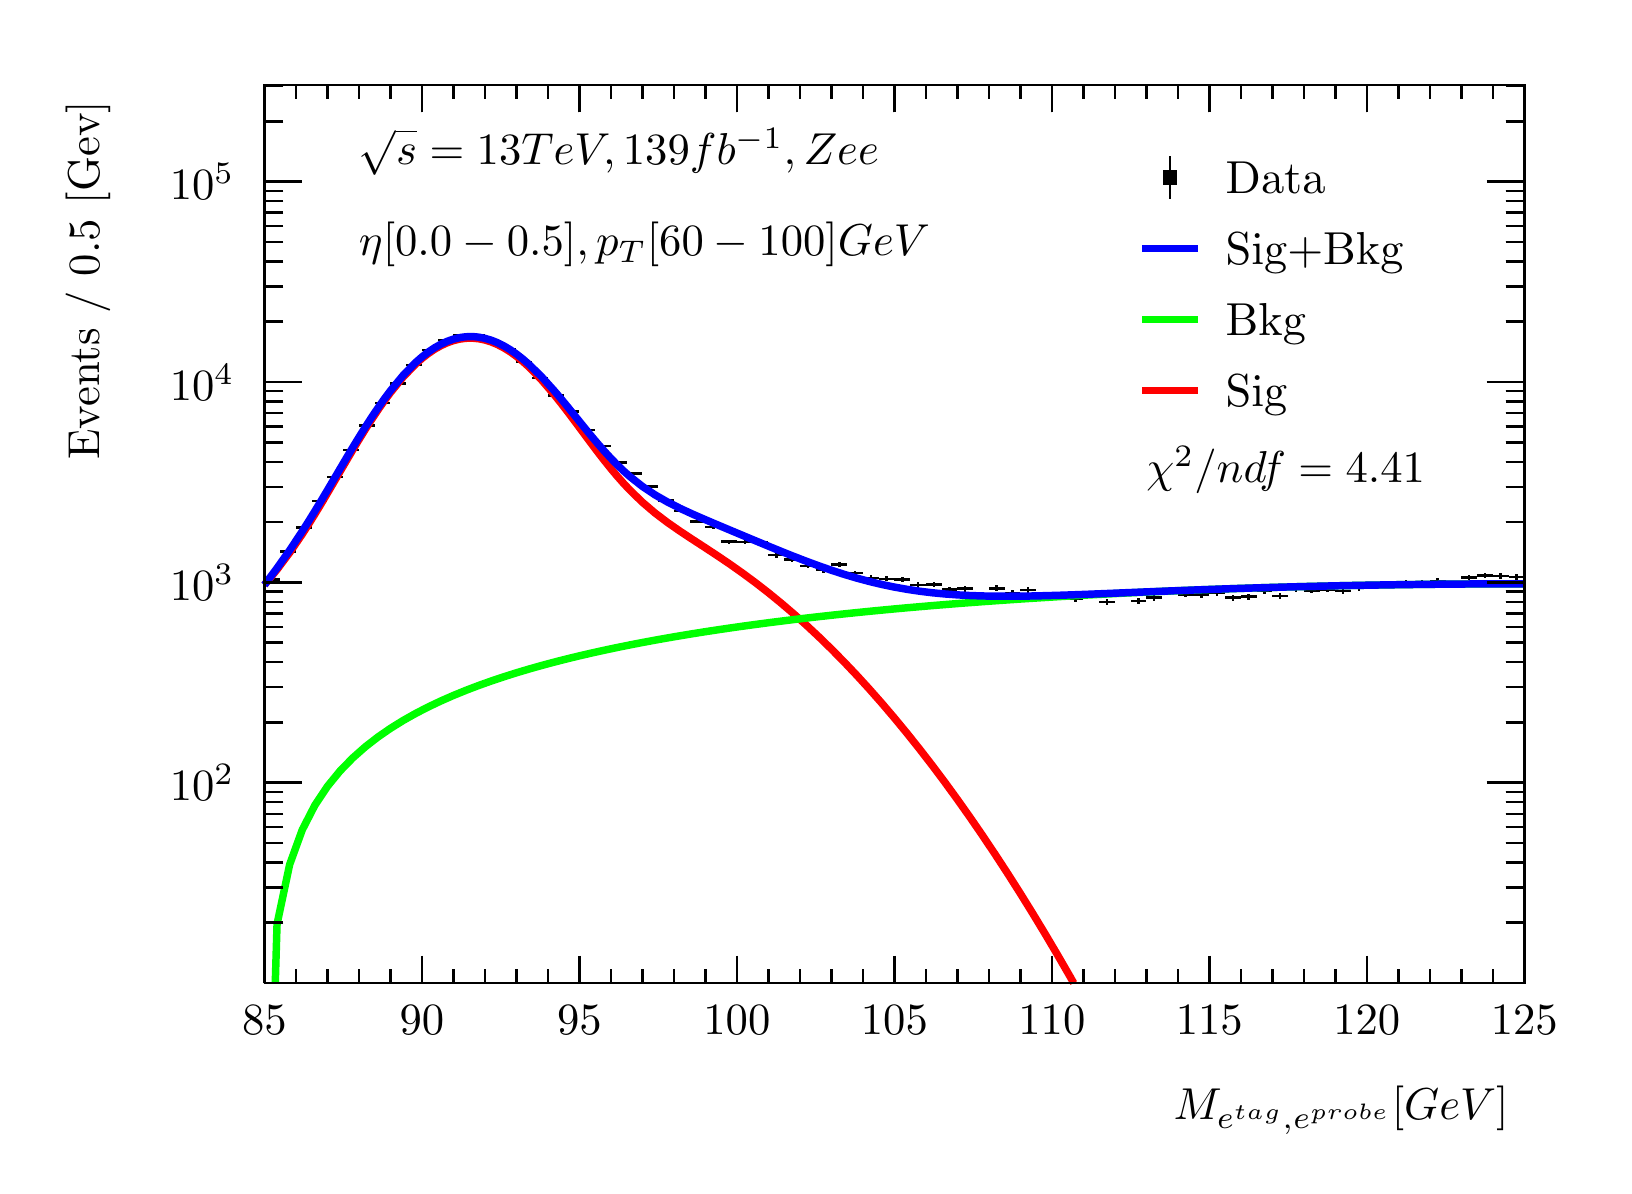
\begin{tikzpicture}
\pgfdeclareplotmark{cross} {
\pgfpathmoveto{\pgfpoint{-0.3\pgfplotmarksize}{\pgfplotmarksize}}
\pgfpathlineto{\pgfpoint{+0.3\pgfplotmarksize}{\pgfplotmarksize}}
\pgfpathlineto{\pgfpoint{+0.3\pgfplotmarksize}{0.3\pgfplotmarksize}}
\pgfpathlineto{\pgfpoint{+1\pgfplotmarksize}{0.3\pgfplotmarksize}}
\pgfpathlineto{\pgfpoint{+1\pgfplotmarksize}{-0.3\pgfplotmarksize}}
\pgfpathlineto{\pgfpoint{+0.3\pgfplotmarksize}{-0.3\pgfplotmarksize}}
\pgfpathlineto{\pgfpoint{+0.3\pgfplotmarksize}{-1.\pgfplotmarksize}}
\pgfpathlineto{\pgfpoint{-0.3\pgfplotmarksize}{-1.\pgfplotmarksize}}
\pgfpathlineto{\pgfpoint{-0.3\pgfplotmarksize}{-0.3\pgfplotmarksize}}
\pgfpathlineto{\pgfpoint{-1.\pgfplotmarksize}{-0.3\pgfplotmarksize}}
\pgfpathlineto{\pgfpoint{-1.\pgfplotmarksize}{0.3\pgfplotmarksize}}
\pgfpathlineto{\pgfpoint{-0.3\pgfplotmarksize}{0.3\pgfplotmarksize}}
\pgfpathclose
\pgfusepathqstroke
}
\pgfdeclareplotmark{cross*} {
\pgfpathmoveto{\pgfpoint{-0.3\pgfplotmarksize}{\pgfplotmarksize}}
\pgfpathlineto{\pgfpoint{+0.3\pgfplotmarksize}{\pgfplotmarksize}}
\pgfpathlineto{\pgfpoint{+0.3\pgfplotmarksize}{0.3\pgfplotmarksize}}
\pgfpathlineto{\pgfpoint{+1\pgfplotmarksize}{0.3\pgfplotmarksize}}
\pgfpathlineto{\pgfpoint{+1\pgfplotmarksize}{-0.3\pgfplotmarksize}}
\pgfpathlineto{\pgfpoint{+0.3\pgfplotmarksize}{-0.3\pgfplotmarksize}}
\pgfpathlineto{\pgfpoint{+0.3\pgfplotmarksize}{-1.\pgfplotmarksize}}
\pgfpathlineto{\pgfpoint{-0.3\pgfplotmarksize}{-1.\pgfplotmarksize}}
\pgfpathlineto{\pgfpoint{-0.3\pgfplotmarksize}{-0.3\pgfplotmarksize}}
\pgfpathlineto{\pgfpoint{-1.\pgfplotmarksize}{-0.3\pgfplotmarksize}}
\pgfpathlineto{\pgfpoint{-1.\pgfplotmarksize}{0.3\pgfplotmarksize}}
\pgfpathlineto{\pgfpoint{-0.3\pgfplotmarksize}{0.3\pgfplotmarksize}}
\pgfpathclose
\pgfusepathqfillstroke
}
\pgfdeclareplotmark{newstar} {
\pgfpathmoveto{\pgfqpoint{0pt}{\pgfplotmarksize}}
\pgfpathlineto{\pgfqpointpolar{44}{0.5\pgfplotmarksize}}
\pgfpathlineto{\pgfqpointpolar{18}{\pgfplotmarksize}}
\pgfpathlineto{\pgfqpointpolar{-20}{0.5\pgfplotmarksize}}
\pgfpathlineto{\pgfqpointpolar{-54}{\pgfplotmarksize}}
\pgfpathlineto{\pgfqpointpolar{-90}{0.5\pgfplotmarksize}}
\pgfpathlineto{\pgfqpointpolar{234}{\pgfplotmarksize}}
\pgfpathlineto{\pgfqpointpolar{198}{0.5\pgfplotmarksize}}
\pgfpathlineto{\pgfqpointpolar{162}{\pgfplotmarksize}}
\pgfpathlineto{\pgfqpointpolar{134}{0.5\pgfplotmarksize}}
\pgfpathclose
\pgfusepathqstroke
}
\pgfdeclareplotmark{newstar*} {
\pgfpathmoveto{\pgfqpoint{0pt}{\pgfplotmarksize}}
\pgfpathlineto{\pgfqpointpolar{44}{0.5\pgfplotmarksize}}
\pgfpathlineto{\pgfqpointpolar{18}{\pgfplotmarksize}}
\pgfpathlineto{\pgfqpointpolar{-20}{0.5\pgfplotmarksize}}
\pgfpathlineto{\pgfqpointpolar{-54}{\pgfplotmarksize}}
\pgfpathlineto{\pgfqpointpolar{-90}{0.5\pgfplotmarksize}}
\pgfpathlineto{\pgfqpointpolar{234}{\pgfplotmarksize}}
\pgfpathlineto{\pgfqpointpolar{198}{0.5\pgfplotmarksize}}
\pgfpathlineto{\pgfqpointpolar{162}{\pgfplotmarksize}}
\pgfpathlineto{\pgfqpointpolar{134}{0.5\pgfplotmarksize}}
\pgfpathclose
\pgfusepathqfillstroke
}
\definecolor{c}{rgb}{1,1,1};
\draw [color=c, fill=c] (0,0) rectangle (20,14.4361);
\draw [color=c, fill=c] (3,2.30977) rectangle (19,13.7143);
\definecolor{c}{rgb}{0,0,0};
\draw [c,line width=0.9] (3,2.30977) -- (3,13.7143) -- (19,13.7143) -- (19,2.30977) -- (3,2.30977);
\definecolor{c}{rgb}{1,1,1};
\draw [color=c, fill=c] (3,2.30977) rectangle (19,13.7143);
\definecolor{c}{rgb}{0,0,0};
\draw [c,line width=0.9] (3,2.30977) -- (3,13.7143) -- (19,13.7143) -- (19,2.30977) -- (3,2.30977);
\draw [c,line width=0.9] (3,2.30977) -- (19,2.30977);
\draw [c,line width=0.9] (3,2.65624) -- (3,2.30977);
\draw [c,line width=0.9] (3.4,2.48301) -- (3.4,2.30977);
\draw [c,line width=0.9] (3.8,2.48301) -- (3.8,2.30977);
\draw [c,line width=0.9] (4.2,2.48301) -- (4.2,2.30977);
\draw [c,line width=0.9] (4.6,2.48301) -- (4.6,2.30977);
\draw [c,line width=0.9] (5,2.65624) -- (5,2.30977);
\draw [c,line width=0.9] (5.4,2.48301) -- (5.4,2.30977);
\draw [c,line width=0.9] (5.8,2.48301) -- (5.8,2.30977);
\draw [c,line width=0.9] (6.2,2.48301) -- (6.2,2.30977);
\draw [c,line width=0.9] (6.6,2.48301) -- (6.6,2.30977);
\draw [c,line width=0.9] (7,2.65624) -- (7,2.30977);
\draw [c,line width=0.9] (7.4,2.48301) -- (7.4,2.30977);
\draw [c,line width=0.9] (7.8,2.48301) -- (7.8,2.30977);
\draw [c,line width=0.9] (8.2,2.48301) -- (8.2,2.30977);
\draw [c,line width=0.9] (8.6,2.48301) -- (8.6,2.30977);
\draw [c,line width=0.9] (9,2.65624) -- (9,2.30977);
\draw [c,line width=0.9] (9.4,2.48301) -- (9.4,2.30977);
\draw [c,line width=0.9] (9.8,2.48301) -- (9.8,2.30977);
\draw [c,line width=0.9] (10.2,2.48301) -- (10.2,2.30977);
\draw [c,line width=0.9] (10.6,2.48301) -- (10.6,2.30977);
\draw [c,line width=0.9] (11,2.65624) -- (11,2.30977);
\draw [c,line width=0.9] (11.4,2.48301) -- (11.4,2.30977);
\draw [c,line width=0.9] (11.8,2.48301) -- (11.8,2.30977);
\draw [c,line width=0.9] (12.2,2.48301) -- (12.2,2.30977);
\draw [c,line width=0.9] (12.6,2.48301) -- (12.6,2.30977);
\draw [c,line width=0.9] (13,2.65624) -- (13,2.30977);
\draw [c,line width=0.9] (13.4,2.48301) -- (13.4,2.30977);
\draw [c,line width=0.9] (13.8,2.48301) -- (13.8,2.30977);
\draw [c,line width=0.9] (14.2,2.48301) -- (14.2,2.30977);
\draw [c,line width=0.9] (14.6,2.48301) -- (14.6,2.30977);
\draw [c,line width=0.9] (15,2.65624) -- (15,2.30977);
\draw [c,line width=0.9] (15.4,2.48301) -- (15.4,2.30977);
\draw [c,line width=0.9] (15.8,2.48301) -- (15.8,2.30977);
\draw [c,line width=0.9] (16.2,2.48301) -- (16.2,2.30977);
\draw [c,line width=0.9] (16.6,2.48301) -- (16.6,2.30977);
\draw [c,line width=0.9] (17,2.65624) -- (17,2.30977);
\draw [c,line width=0.9] (17.4,2.48301) -- (17.4,2.30977);
\draw [c,line width=0.9] (17.8,2.48301) -- (17.8,2.30977);
\draw [c,line width=0.9] (18.2,2.48301) -- (18.2,2.30977);
\draw [c,line width=0.9] (18.6,2.48301) -- (18.6,2.30977);
\draw [c,line width=0.9] (19,2.65624) -- (19,2.30977);
\draw [anchor=base] (3,1.66015) node[scale=1.61424, color=c, rotate=0]{85};
\draw [anchor=base] (5,1.66015) node[scale=1.61424, color=c, rotate=0]{90};
\draw [anchor=base] (7,1.66015) node[scale=1.61424, color=c, rotate=0]{95};
\draw [anchor=base] (9,1.66015) node[scale=1.61424, color=c, rotate=0]{100};
\draw [anchor=base] (11,1.66015) node[scale=1.61424, color=c, rotate=0]{105};
\draw [anchor=base] (13,1.66015) node[scale=1.61424, color=c, rotate=0]{110};
\draw [anchor=base] (15,1.66015) node[scale=1.61424, color=c, rotate=0]{115};
\draw [anchor=base] (17,1.66015) node[scale=1.61424, color=c, rotate=0]{120};
\draw [anchor=base] (19,1.66015) node[scale=1.61424, color=c, rotate=0]{125};
\draw [anchor= east] (19,0.692932) node[scale=1.61424, color=c, rotate=0]{$M_{e^{tag}, e^{probe}}  [GeV]$};
\draw [c,line width=0.9] (3,13.7143) -- (19,13.7143);
\draw [c,line width=0.9] (3,13.3678) -- (3,13.7143);
\draw [c,line width=0.9] (3.4,13.5411) -- (3.4,13.7143);
\draw [c,line width=0.9] (3.8,13.5411) -- (3.8,13.7143);
\draw [c,line width=0.9] (4.2,13.5411) -- (4.2,13.7143);
\draw [c,line width=0.9] (4.6,13.5411) -- (4.6,13.7143);
\draw [c,line width=0.9] (5,13.3678) -- (5,13.7143);
\draw [c,line width=0.9] (5.4,13.5411) -- (5.4,13.7143);
\draw [c,line width=0.9] (5.8,13.5411) -- (5.8,13.7143);
\draw [c,line width=0.9] (6.2,13.5411) -- (6.2,13.7143);
\draw [c,line width=0.9] (6.6,13.5411) -- (6.6,13.7143);
\draw [c,line width=0.9] (7,13.3678) -- (7,13.7143);
\draw [c,line width=0.9] (7.4,13.5411) -- (7.4,13.7143);
\draw [c,line width=0.9] (7.8,13.5411) -- (7.8,13.7143);
\draw [c,line width=0.9] (8.2,13.5411) -- (8.2,13.7143);
\draw [c,line width=0.9] (8.6,13.5411) -- (8.6,13.7143);
\draw [c,line width=0.9] (9,13.3678) -- (9,13.7143);
\draw [c,line width=0.9] (9.4,13.5411) -- (9.4,13.7143);
\draw [c,line width=0.9] (9.8,13.5411) -- (9.8,13.7143);
\draw [c,line width=0.9] (10.2,13.5411) -- (10.2,13.7143);
\draw [c,line width=0.9] (10.6,13.5411) -- (10.6,13.7143);
\draw [c,line width=0.9] (11,13.3678) -- (11,13.7143);
\draw [c,line width=0.9] (11.4,13.5411) -- (11.4,13.7143);
\draw [c,line width=0.9] (11.8,13.5411) -- (11.8,13.7143);
\draw [c,line width=0.9] (12.2,13.5411) -- (12.2,13.7143);
\draw [c,line width=0.9] (12.6,13.5411) -- (12.6,13.7143);
\draw [c,line width=0.9] (13,13.3678) -- (13,13.7143);
\draw [c,line width=0.9] (13.4,13.5411) -- (13.4,13.7143);
\draw [c,line width=0.9] (13.8,13.5411) -- (13.8,13.7143);
\draw [c,line width=0.9] (14.2,13.5411) -- (14.2,13.7143);
\draw [c,line width=0.9] (14.6,13.5411) -- (14.6,13.7143);
\draw [c,line width=0.9] (15,13.3678) -- (15,13.7143);
\draw [c,line width=0.9] (15.4,13.5411) -- (15.4,13.7143);
\draw [c,line width=0.9] (15.8,13.5411) -- (15.8,13.7143);
\draw [c,line width=0.9] (16.2,13.5411) -- (16.2,13.7143);
\draw [c,line width=0.9] (16.6,13.5411) -- (16.6,13.7143);
\draw [c,line width=0.9] (17,13.3678) -- (17,13.7143);
\draw [c,line width=0.9] (17.4,13.5411) -- (17.4,13.7143);
\draw [c,line width=0.9] (17.8,13.5411) -- (17.8,13.7143);
\draw [c,line width=0.9] (18.2,13.5411) -- (18.2,13.7143);
\draw [c,line width=0.9] (18.6,13.5411) -- (18.6,13.7143);
\draw [c,line width=0.9] (19,13.3678) -- (19,13.7143);
\draw [c,line width=0.9] (3,2.30977) -- (3,13.7143);
\draw [c,line width=0.9] (3.237,3.07568) -- (3,3.07568);
\draw [c,line width=0.9] (3.237,3.5237) -- (3,3.5237);
\draw [c,line width=0.9] (3.237,3.84158) -- (3,3.84158);
\draw [c,line width=0.9] (3.237,4.08815) -- (3,4.08815);
\draw [c,line width=0.9] (3.237,4.2896) -- (3,4.2896);
\draw [c,line width=0.9] (3.237,4.45994) -- (3,4.45994);
\draw [c,line width=0.9] (3.237,4.60748) -- (3,4.60748);
\draw [c,line width=0.9] (3.237,4.73763) -- (3,4.73763);
\draw [c,line width=0.9] (3.474,4.85405) -- (3,4.85405);
\draw [anchor= east] (2.82,4.85405) node[scale=1.61424, color=c, rotate=0]{$10^{2}$};
\draw [c,line width=0.9] (3.237,5.61995) -- (3,5.61995);
\draw [c,line width=0.9] (3.237,6.06798) -- (3,6.06798);
\draw [c,line width=0.9] (3.237,6.38586) -- (3,6.38586);
\draw [c,line width=0.9] (3.237,6.63242) -- (3,6.63242);
\draw [c,line width=0.9] (3.237,6.83388) -- (3,6.83388);
\draw [c,line width=0.9] (3.237,7.00421) -- (3,7.00421);
\draw [c,line width=0.9] (3.237,7.15176) -- (3,7.15176);
\draw [c,line width=0.9] (3.237,7.28191) -- (3,7.28191);
\draw [c,line width=0.9] (3.474,7.39833) -- (3,7.39833);
\draw [anchor= east] (2.82,7.39833) node[scale=1.61424, color=c, rotate=0]{$10^{3}$};
\draw [c,line width=0.9] (3.237,8.16423) -- (3,8.16423);
\draw [c,line width=0.9] (3.237,8.61226) -- (3,8.61226);
\draw [c,line width=0.9] (3.237,8.93013) -- (3,8.93013);
\draw [c,line width=0.9] (3.237,9.1767) -- (3,9.1767);
\draw [c,line width=0.9] (3.237,9.37816) -- (3,9.37816);
\draw [c,line width=0.9] (3.237,9.54849) -- (3,9.54849);
\draw [c,line width=0.9] (3.237,9.69604) -- (3,9.69604);
\draw [c,line width=0.9] (3.237,9.82618) -- (3,9.82618);
\draw [c,line width=0.9] (3.474,9.9426) -- (3,9.9426);
\draw [anchor= east] (2.82,9.9426) node[scale=1.61424, color=c, rotate=0]{$10^{4}$};
\draw [c,line width=0.9] (3.237,10.7085) -- (3,10.7085);
\draw [c,line width=0.9] (3.237,11.1565) -- (3,11.1565);
\draw [c,line width=0.9] (3.237,11.4744) -- (3,11.4744);
\draw [c,line width=0.9] (3.237,11.721) -- (3,11.721);
\draw [c,line width=0.9] (3.237,11.9224) -- (3,11.9224);
\draw [c,line width=0.9] (3.237,12.0928) -- (3,12.0928);
\draw [c,line width=0.9] (3.237,12.2403) -- (3,12.2403);
\draw [c,line width=0.9] (3.237,12.3705) -- (3,12.3705);
\draw [c,line width=0.9] (3.474,12.4869) -- (3,12.4869);
\draw [anchor= east] (2.82,12.4869) node[scale=1.61424, color=c, rotate=0]{$10^{5}$};
\draw [c,line width=0.9] (3.237,13.2528) -- (3,13.2528);
\draw [c,line width=0.9] (3.237,13.7008) -- (3,13.7008);
\draw [anchor= east] (0.76,13.7143) node[scale=1.61424, color=c, rotate=90]{Events / 0.5 [Gev]};
\draw [c,line width=0.9] (19,2.30977) -- (19,13.7143);
\draw [c,line width=0.9] (18.763,3.07568) -- (19,3.07568);
\draw [c,line width=0.9] (18.763,3.5237) -- (19,3.5237);
\draw [c,line width=0.9] (18.763,3.84158) -- (19,3.84158);
\draw [c,line width=0.9] (18.763,4.08815) -- (19,4.08815);
\draw [c,line width=0.9] (18.763,4.2896) -- (19,4.2896);
\draw [c,line width=0.9] (18.763,4.45994) -- (19,4.45994);
\draw [c,line width=0.9] (18.763,4.60748) -- (19,4.60748);
\draw [c,line width=0.9] (18.763,4.73763) -- (19,4.73763);
\draw [c,line width=0.9] (18.526,4.85405) -- (19,4.85405);
\draw [c,line width=0.9] (18.763,5.61995) -- (19,5.61995);
\draw [c,line width=0.9] (18.763,6.06798) -- (19,6.06798);
\draw [c,line width=0.9] (18.763,6.38586) -- (19,6.38586);
\draw [c,line width=0.9] (18.763,6.63242) -- (19,6.63242);
\draw [c,line width=0.9] (18.763,6.83388) -- (19,6.83388);
\draw [c,line width=0.9] (18.763,7.00421) -- (19,7.00421);
\draw [c,line width=0.9] (18.763,7.15176) -- (19,7.15176);
\draw [c,line width=0.9] (18.763,7.28191) -- (19,7.28191);
\draw [c,line width=0.9] (18.526,7.39833) -- (19,7.39833);
\draw [c,line width=0.9] (18.763,8.16423) -- (19,8.16423);
\draw [c,line width=0.9] (18.763,8.61226) -- (19,8.61226);
\draw [c,line width=0.9] (18.763,8.93013) -- (19,8.93013);
\draw [c,line width=0.9] (18.763,9.1767) -- (19,9.1767);
\draw [c,line width=0.9] (18.763,9.37816) -- (19,9.37816);
\draw [c,line width=0.9] (18.763,9.54849) -- (19,9.54849);
\draw [c,line width=0.9] (18.763,9.69604) -- (19,9.69604);
\draw [c,line width=0.9] (18.763,9.82618) -- (19,9.82618);
\draw [c,line width=0.9] (18.526,9.9426) -- (19,9.9426);
\draw [c,line width=0.9] (18.763,10.7085) -- (19,10.7085);
\draw [c,line width=0.9] (18.763,11.1565) -- (19,11.1565);
\draw [c,line width=0.9] (18.763,11.4744) -- (19,11.4744);
\draw [c,line width=0.9] (18.763,11.721) -- (19,11.721);
\draw [c,line width=0.9] (18.763,11.9224) -- (19,11.9224);
\draw [c,line width=0.9] (18.763,12.0928) -- (19,12.0928);
\draw [c,line width=0.9] (18.763,12.2403) -- (19,12.2403);
\draw [c,line width=0.9] (18.763,12.3705) -- (19,12.3705);
\draw [c,line width=0.9] (18.526,12.4869) -- (19,12.4869);
\draw [c,line width=0.9] (18.763,13.2528) -- (19,13.2528);
\draw [c,line width=0.9] (18.763,13.7008) -- (19,13.7008);
\draw [c,line width=0.9] (3.1,7.4342) -- (3,7.4342);
\draw [c,line width=0.9] (3,7.4342) -- (3,7.4342);
\draw [c,line width=0.9] (3.1,7.4342) -- (3.2,7.4342);
\draw [c,line width=0.9] (3.2,7.4342) -- (3.2,7.4342);
\draw [c,line width=0.9] (3.1,7.4342) -- (3.1,7.46858);
\draw [c,line width=0.9] (3.1,7.46858) -- (3.1,7.46858);
\draw [c,line width=0.9] (3.1,7.4342) -- (3.1,7.39983);
\draw [c,line width=0.9] (3.1,7.39983) -- (3.1,7.39983);
\draw [c,line width=0.9] (3.3,7.7889) -- (3.2,7.7889);
\draw [c,line width=0.9] (3.2,7.7889) -- (3.2,7.7889);
\draw [c,line width=0.9] (3.3,7.7889) -- (3.4,7.7889);
\draw [c,line width=0.9] (3.4,7.7889) -- (3.4,7.7889);
\draw [c,line width=0.9] (3.3,7.7889) -- (3.3,7.81818);
\draw [c,line width=0.9] (3.3,7.81818) -- (3.3,7.81818);
\draw [c,line width=0.9] (3.3,7.7889) -- (3.3,7.75962);
\draw [c,line width=0.9] (3.3,7.75962) -- (3.3,7.75962);
\draw [c,line width=0.9] (3.5,8.09645) -- (3.4,8.09645);
\draw [c,line width=0.9] (3.4,8.09645) -- (3.4,8.09645);
\draw [c,line width=0.9] (3.5,8.09645) -- (3.6,8.09645);
\draw [c,line width=0.9] (3.6,8.09645) -- (3.6,8.09645);
\draw [c,line width=0.9] (3.5,8.09645) -- (3.5,8.12193);
\draw [c,line width=0.9] (3.5,8.12193) -- (3.5,8.12193);
\draw [c,line width=0.9] (3.5,8.09645) -- (3.5,8.07097);
\draw [c,line width=0.9] (3.5,8.07097) -- (3.5,8.07097);
\draw [c,line width=0.9] (3.7,8.43008) -- (3.6,8.43008);
\draw [c,line width=0.9] (3.6,8.43008) -- (3.6,8.43008);
\draw [c,line width=0.9] (3.7,8.43008) -- (3.8,8.43008);
\draw [c,line width=0.9] (3.8,8.43008) -- (3.8,8.43008);
\draw [c,line width=0.9] (3.7,8.43008) -- (3.7,8.45198);
\draw [c,line width=0.9] (3.7,8.45198) -- (3.7,8.45198);
\draw [c,line width=0.9] (3.7,8.43008) -- (3.7,8.40817);
\draw [c,line width=0.9] (3.7,8.40817) -- (3.7,8.40817);
\draw [c,line width=0.9] (3.9,8.73386) -- (3.8,8.73386);
\draw [c,line width=0.9] (3.8,8.73386) -- (3.8,8.73386);
\draw [c,line width=0.9] (3.9,8.73386) -- (4,8.73386);
\draw [c,line width=0.9] (4,8.73386) -- (4,8.73386);
\draw [c,line width=0.9] (3.9,8.73386) -- (3.9,8.75295);
\draw [c,line width=0.9] (3.9,8.75295) -- (3.9,8.75295);
\draw [c,line width=0.9] (3.9,8.73386) -- (3.9,8.71476);
\draw [c,line width=0.9] (3.9,8.71476) -- (3.9,8.71476);
\draw [c,line width=0.9] (4.1,9.07903) -- (4,9.07903);
\draw [c,line width=0.9] (4,9.07903) -- (4,9.07903);
\draw [c,line width=0.9] (4.1,9.07903) -- (4.2,9.07903);
\draw [c,line width=0.9] (4.2,9.07903) -- (4.2,9.07903);
\draw [c,line width=0.9] (4.1,9.07903) -- (4.1,9.09536);
\draw [c,line width=0.9] (4.1,9.09536) -- (4.1,9.09536);
\draw [c,line width=0.9] (4.1,9.07903) -- (4.1,9.0627);
\draw [c,line width=0.9] (4.1,9.0627) -- (4.1,9.0627);
\draw [c,line width=0.9] (4.3,9.39261) -- (4.2,9.39261);
\draw [c,line width=0.9] (4.2,9.39261) -- (4.2,9.39261);
\draw [c,line width=0.9] (4.3,9.39261) -- (4.4,9.39261);
\draw [c,line width=0.9] (4.4,9.39261) -- (4.4,9.39261);
\draw [c,line width=0.9] (4.3,9.39261) -- (4.3,9.40679);
\draw [c,line width=0.9] (4.3,9.40679) -- (4.3,9.40679);
\draw [c,line width=0.9] (4.3,9.39261) -- (4.3,9.37844);
\draw [c,line width=0.9] (4.3,9.37844) -- (4.3,9.37844);
\draw [c,line width=0.9] (4.5,9.67681) -- (4.4,9.67681);
\draw [c,line width=0.9] (4.4,9.67681) -- (4.4,9.67681);
\draw [c,line width=0.9] (4.5,9.67681) -- (4.6,9.67681);
\draw [c,line width=0.9] (4.6,9.67681) -- (4.6,9.67681);
\draw [c,line width=0.9] (4.5,9.67681) -- (4.5,9.68927);
\draw [c,line width=0.9] (4.5,9.68927) -- (4.5,9.68927);
\draw [c,line width=0.9] (4.5,9.67681) -- (4.5,9.66435);
\draw [c,line width=0.9] (4.5,9.66435) -- (4.5,9.66435);
\draw [c,line width=0.9] (4.7,9.9213) -- (4.6,9.9213);
\draw [c,line width=0.9] (4.6,9.9213) -- (4.6,9.9213);
\draw [c,line width=0.9] (4.7,9.9213) -- (4.8,9.9213);
\draw [c,line width=0.9] (4.8,9.9213) -- (4.8,9.9213);
\draw [c,line width=0.9] (4.7,9.9213) -- (4.7,9.93245);
\draw [c,line width=0.9] (4.7,9.93245) -- (4.7,9.93245);
\draw [c,line width=0.9] (4.7,9.9213) -- (4.7,9.91014);
\draw [c,line width=0.9] (4.7,9.91014) -- (4.7,9.91014);
\draw [c,line width=0.9] (4.9,10.1618) -- (4.8,10.1618);
\draw [c,line width=0.9] (4.8,10.1618) -- (4.8,10.1618);
\draw [c,line width=0.9] (4.9,10.1618) -- (5,10.1618);
\draw [c,line width=0.9] (5,10.1618) -- (5,10.1618);
\draw [c,line width=0.9] (4.9,10.1618) -- (4.9,10.1718);
\draw [c,line width=0.9] (4.9,10.1718) -- (4.9,10.1718);
\draw [c,line width=0.9] (4.9,10.1618) -- (4.9,10.1518);
\draw [c,line width=0.9] (4.9,10.1518) -- (4.9,10.1518);
\draw [c,line width=0.9] (5.1,10.3471) -- (5,10.3471);
\draw [c,line width=0.9] (5,10.3471) -- (5,10.3471);
\draw [c,line width=0.9] (5.1,10.3471) -- (5.2,10.3471);
\draw [c,line width=0.9] (5.2,10.3471) -- (5.2,10.3471);
\draw [c,line width=0.9] (5.1,10.3471) -- (5.1,10.3563);
\draw [c,line width=0.9] (5.1,10.3563) -- (5.1,10.3563);
\draw [c,line width=0.9] (5.1,10.3471) -- (5.1,10.3379);
\draw [c,line width=0.9] (5.1,10.3379) -- (5.1,10.3379);
\draw [c,line width=0.9] (5.3,10.4746) -- (5.2,10.4746);
\draw [c,line width=0.9] (5.2,10.4746) -- (5.2,10.4746);
\draw [c,line width=0.9] (5.3,10.4746) -- (5.4,10.4746);
\draw [c,line width=0.9] (5.4,10.4746) -- (5.4,10.4746);
\draw [c,line width=0.9] (5.3,10.4746) -- (5.3,10.4833);
\draw [c,line width=0.9] (5.3,10.4833) -- (5.3,10.4833);
\draw [c,line width=0.9] (5.3,10.4746) -- (5.3,10.466);
\draw [c,line width=0.9] (5.3,10.466) -- (5.3,10.466);
\draw [c,line width=0.9] (5.5,10.5373) -- (5.4,10.5373);
\draw [c,line width=0.9] (5.4,10.5373) -- (5.4,10.5373);
\draw [c,line width=0.9] (5.5,10.5373) -- (5.6,10.5373);
\draw [c,line width=0.9] (5.6,10.5373) -- (5.6,10.5373);
\draw [c,line width=0.9] (5.5,10.5373) -- (5.5,10.5457);
\draw [c,line width=0.9] (5.5,10.5457) -- (5.5,10.5457);
\draw [c,line width=0.9] (5.5,10.5373) -- (5.5,10.5288);
\draw [c,line width=0.9] (5.5,10.5288) -- (5.5,10.5288);
\draw [c,line width=0.9] (5.7,10.5319) -- (5.6,10.5319);
\draw [c,line width=0.9] (5.6,10.5319) -- (5.6,10.5319);
\draw [c,line width=0.9] (5.7,10.5319) -- (5.8,10.5319);
\draw [c,line width=0.9] (5.8,10.5319) -- (5.8,10.5319);
\draw [c,line width=0.9] (5.7,10.5319) -- (5.7,10.5403);
\draw [c,line width=0.9] (5.7,10.5403) -- (5.7,10.5403);
\draw [c,line width=0.9] (5.7,10.5319) -- (5.7,10.5234);
\draw [c,line width=0.9] (5.7,10.5234) -- (5.7,10.5234);
\draw [c,line width=0.9] (5.9,10.4613) -- (5.8,10.4613);
\draw [c,line width=0.9] (5.8,10.4613) -- (5.8,10.4613);
\draw [c,line width=0.9] (5.9,10.4613) -- (6,10.4613);
\draw [c,line width=0.9] (6,10.4613) -- (6,10.4613);
\draw [c,line width=0.9] (5.9,10.4613) -- (5.9,10.4701);
\draw [c,line width=0.9] (5.9,10.4701) -- (5.9,10.4701);
\draw [c,line width=0.9] (5.9,10.4613) -- (5.9,10.4526);
\draw [c,line width=0.9] (5.9,10.4526) -- (5.9,10.4526);
\draw [c,line width=0.9] (6.1,10.3639) -- (6,10.3639);
\draw [c,line width=0.9] (6,10.3639) -- (6,10.3639);
\draw [c,line width=0.9] (6.1,10.3639) -- (6.2,10.3639);
\draw [c,line width=0.9] (6.2,10.3639) -- (6.2,10.3639);
\draw [c,line width=0.9] (6.1,10.3639) -- (6.1,10.373);
\draw [c,line width=0.9] (6.1,10.373) -- (6.1,10.373);
\draw [c,line width=0.9] (6.1,10.3639) -- (6.1,10.3547);
\draw [c,line width=0.9] (6.1,10.3547) -- (6.1,10.3547);
\draw [c,line width=0.9] (6.3,10.1946) -- (6.2,10.1946);
\draw [c,line width=0.9] (6.2,10.1946) -- (6.2,10.1946);
\draw [c,line width=0.9] (6.3,10.1946) -- (6.4,10.1946);
\draw [c,line width=0.9] (6.4,10.1946) -- (6.4,10.1946);
\draw [c,line width=0.9] (6.3,10.1946) -- (6.3,10.2044);
\draw [c,line width=0.9] (6.3,10.2044) -- (6.3,10.2044);
\draw [c,line width=0.9] (6.3,10.1946) -- (6.3,10.1847);
\draw [c,line width=0.9] (6.3,10.1847) -- (6.3,10.1847);
\draw [c,line width=0.9] (6.5,9.9942) -- (6.4,9.9942);
\draw [c,line width=0.9] (6.4,9.9942) -- (6.4,9.9942);
\draw [c,line width=0.9] (6.5,9.9942) -- (6.6,9.9942);
\draw [c,line width=0.9] (6.6,9.9942) -- (6.6,9.9942);
\draw [c,line width=0.9] (6.5,9.9942) -- (6.5,10.005);
\draw [c,line width=0.9] (6.5,10.005) -- (6.5,10.005);
\draw [c,line width=0.9] (6.5,9.9942) -- (6.5,9.9834);
\draw [c,line width=0.9] (6.5,9.9834) -- (6.5,9.9834);
\draw [c,line width=0.9] (6.7,9.77273) -- (6.6,9.77273);
\draw [c,line width=0.9] (6.6,9.77273) -- (6.6,9.77273);
\draw [c,line width=0.9] (6.7,9.77273) -- (6.8,9.77273);
\draw [c,line width=0.9] (6.8,9.77273) -- (6.8,9.77273);
\draw [c,line width=0.9] (6.7,9.77273) -- (6.7,9.78467);
\draw [c,line width=0.9] (6.7,9.78467) -- (6.7,9.78467);
\draw [c,line width=0.9] (6.7,9.77273) -- (6.7,9.7608);
\draw [c,line width=0.9] (6.7,9.7608) -- (6.7,9.7608);
\draw [c,line width=0.9] (6.9,9.57099) -- (6.8,9.57099);
\draw [c,line width=0.9] (6.8,9.57099) -- (6.8,9.57099);
\draw [c,line width=0.9] (6.9,9.57099) -- (7,9.57099);
\draw [c,line width=0.9] (7,9.57099) -- (7,9.57099);
\draw [c,line width=0.9] (6.9,9.57099) -- (6.9,9.58406);
\draw [c,line width=0.9] (6.9,9.58406) -- (6.9,9.58406);
\draw [c,line width=0.9] (6.9,9.57099) -- (6.9,9.55792);
\draw [c,line width=0.9] (6.9,9.55792) -- (6.9,9.55792);
\draw [c,line width=0.9] (7.1,9.33075) -- (7,9.33075);
\draw [c,line width=0.9] (7,9.33075) -- (7,9.33075);
\draw [c,line width=0.9] (7.1,9.33075) -- (7.2,9.33075);
\draw [c,line width=0.9] (7.2,9.33075) -- (7.2,9.33075);
\draw [c,line width=0.9] (7.1,9.33075) -- (7.1,9.34532);
\draw [c,line width=0.9] (7.1,9.34532) -- (7.1,9.34532);
\draw [c,line width=0.9] (7.1,9.33075) -- (7.1,9.31617);
\draw [c,line width=0.9] (7.1,9.31617) -- (7.1,9.31617);
\draw [c,line width=0.9] (7.3,9.13159) -- (7.2,9.13159);
\draw [c,line width=0.9] (7.2,9.13159) -- (7.2,9.13159);
\draw [c,line width=0.9] (7.3,9.13159) -- (7.4,9.13159);
\draw [c,line width=0.9] (7.4,9.13159) -- (7.4,9.13159);
\draw [c,line width=0.9] (7.3,9.13159) -- (7.3,9.14754);
\draw [c,line width=0.9] (7.3,9.14754) -- (7.3,9.14754);
\draw [c,line width=0.9] (7.3,9.13159) -- (7.3,9.11565);
\draw [c,line width=0.9] (7.3,9.11565) -- (7.3,9.11565);
\draw [c,line width=0.9] (7.5,8.91903) -- (7.4,8.91903);
\draw [c,line width=0.9] (7.4,8.91903) -- (7.4,8.91903);
\draw [c,line width=0.9] (7.5,8.91903) -- (7.6,8.91903);
\draw [c,line width=0.9] (7.6,8.91903) -- (7.6,8.91903);
\draw [c,line width=0.9] (7.5,8.91903) -- (7.5,8.93659);
\draw [c,line width=0.9] (7.5,8.93659) -- (7.5,8.93659);
\draw [c,line width=0.9] (7.5,8.91903) -- (7.5,8.90147);
\draw [c,line width=0.9] (7.5,8.90147) -- (7.5,8.90147);
\draw [c,line width=0.9] (7.7,8.77911) -- (7.6,8.77911);
\draw [c,line width=0.9] (7.6,8.77911) -- (7.6,8.77911);
\draw [c,line width=0.9] (7.7,8.77911) -- (7.8,8.77911);
\draw [c,line width=0.9] (7.8,8.77911) -- (7.8,8.77911);
\draw [c,line width=0.9] (7.7,8.77911) -- (7.7,8.79782);
\draw [c,line width=0.9] (7.7,8.79782) -- (7.7,8.79782);
\draw [c,line width=0.9] (7.7,8.77911) -- (7.7,8.7604);
\draw [c,line width=0.9] (7.7,8.7604) -- (7.7,8.7604);
\draw [c,line width=0.9] (7.9,8.61887) -- (7.8,8.61887);
\draw [c,line width=0.9] (7.8,8.61887) -- (7.8,8.61887);
\draw [c,line width=0.9] (7.9,8.61887) -- (8,8.61887);
\draw [c,line width=0.9] (8,8.61887) -- (8,8.61887);
\draw [c,line width=0.9] (7.9,8.61887) -- (7.9,8.63898);
\draw [c,line width=0.9] (7.9,8.63898) -- (7.9,8.63898);
\draw [c,line width=0.9] (7.9,8.61887) -- (7.9,8.59875);
\draw [c,line width=0.9] (7.9,8.59875) -- (7.9,8.59875);
\draw [c,line width=0.9] (8.1,8.43657) -- (8,8.43657);
\draw [c,line width=0.9] (8,8.43657) -- (8,8.43657);
\draw [c,line width=0.9] (8.1,8.43657) -- (8.2,8.43657);
\draw [c,line width=0.9] (8.2,8.43657) -- (8.2,8.43657);
\draw [c,line width=0.9] (8.1,8.43657) -- (8.1,8.45842);
\draw [c,line width=0.9] (8.1,8.45842) -- (8.1,8.45842);
\draw [c,line width=0.9] (8.1,8.43657) -- (8.1,8.41473);
\draw [c,line width=0.9] (8.1,8.41473) -- (8.1,8.41473);
\draw [c,line width=0.9] (8.3,8.30464) -- (8.2,8.30464);
\draw [c,line width=0.9] (8.2,8.30464) -- (8.2,8.30464);
\draw [c,line width=0.9] (8.3,8.30464) -- (8.4,8.30464);
\draw [c,line width=0.9] (8.4,8.30464) -- (8.4,8.30464);
\draw [c,line width=0.9] (8.3,8.30464) -- (8.3,8.32783);
\draw [c,line width=0.9] (8.3,8.32783) -- (8.3,8.32783);
\draw [c,line width=0.9] (8.3,8.30464) -- (8.3,8.28146);
\draw [c,line width=0.9] (8.3,8.28146) -- (8.3,8.28146);
\draw [c,line width=0.9] (8.5,8.17358) -- (8.4,8.17358);
\draw [c,line width=0.9] (8.4,8.17358) -- (8.4,8.17358);
\draw [c,line width=0.9] (8.5,8.17358) -- (8.6,8.17358);
\draw [c,line width=0.9] (8.6,8.17358) -- (8.6,8.17358);
\draw [c,line width=0.9] (8.5,8.17358) -- (8.5,8.19819);
\draw [c,line width=0.9] (8.5,8.19819) -- (8.5,8.19819);
\draw [c,line width=0.9] (8.5,8.17358) -- (8.5,8.14898);
\draw [c,line width=0.9] (8.5,8.14898) -- (8.5,8.14898);
\draw [c,line width=0.9] (8.7,8.10231) -- (8.6,8.10231);
\draw [c,line width=0.9] (8.6,8.10231) -- (8.6,8.10231);
\draw [c,line width=0.9] (8.7,8.10231) -- (8.8,8.10231);
\draw [c,line width=0.9] (8.8,8.10231) -- (8.8,8.10231);
\draw [c,line width=0.9] (8.7,8.10231) -- (8.7,8.12772);
\draw [c,line width=0.9] (8.7,8.12772) -- (8.7,8.12772);
\draw [c,line width=0.9] (8.7,8.10231) -- (8.7,8.0769);
\draw [c,line width=0.9] (8.7,8.0769) -- (8.7,8.0769);
\draw [c,line width=0.9] (8.9,7.9149) -- (8.8,7.9149);
\draw [c,line width=0.9] (8.8,7.9149) -- (8.8,7.9149);
\draw [c,line width=0.9] (8.9,7.9149) -- (9,7.9149);
\draw [c,line width=0.9] (9,7.9149) -- (9,7.9149);
\draw [c,line width=0.9] (8.9,7.9149) -- (8.9,7.94256);
\draw [c,line width=0.9] (8.9,7.94256) -- (8.9,7.94256);
\draw [c,line width=0.9] (8.9,7.9149) -- (8.9,7.88724);
\draw [c,line width=0.9] (8.9,7.88724) -- (8.9,7.88724);
\draw [c,line width=0.9] (9.1,7.90865) -- (9,7.90865);
\draw [c,line width=0.9] (9,7.90865) -- (9,7.90865);
\draw [c,line width=0.9] (9.1,7.90865) -- (9.2,7.90865);
\draw [c,line width=0.9] (9.2,7.90865) -- (9.2,7.90865);
\draw [c,line width=0.9] (9.1,7.90865) -- (9.1,7.93639);
\draw [c,line width=0.9] (9.1,7.93639) -- (9.1,7.93639);
\draw [c,line width=0.9] (9.1,7.90865) -- (9.1,7.88092);
\draw [c,line width=0.9] (9.1,7.88092) -- (9.1,7.88092);
\draw [c,line width=0.9] (9.3,7.90795) -- (9.2,7.90795);
\draw [c,line width=0.9] (9.2,7.90795) -- (9.2,7.90795);
\draw [c,line width=0.9] (9.3,7.90795) -- (9.4,7.90795);
\draw [c,line width=0.9] (9.4,7.90795) -- (9.4,7.90795);
\draw [c,line width=0.9] (9.3,7.90795) -- (9.3,7.9357);
\draw [c,line width=0.9] (9.3,7.9357) -- (9.3,7.9357);
\draw [c,line width=0.9] (9.3,7.90795) -- (9.3,7.88021);
\draw [c,line width=0.9] (9.3,7.88021) -- (9.3,7.88021);
\draw [c,line width=0.9] (9.5,7.74295) -- (9.4,7.74295);
\draw [c,line width=0.9] (9.4,7.74295) -- (9.4,7.74295);
\draw [c,line width=0.9] (9.5,7.74295) -- (9.6,7.74295);
\draw [c,line width=0.9] (9.6,7.74295) -- (9.6,7.74295);
\draw [c,line width=0.9] (9.5,7.74295) -- (9.5,7.77285);
\draw [c,line width=0.9] (9.5,7.77285) -- (9.5,7.77285);
\draw [c,line width=0.9] (9.5,7.74295) -- (9.5,7.71306);
\draw [c,line width=0.9] (9.5,7.71306) -- (9.5,7.71306);
\draw [c,line width=0.9] (9.7,7.68653) -- (9.6,7.68653);
\draw [c,line width=0.9] (9.6,7.68653) -- (9.6,7.68653);
\draw [c,line width=0.9] (9.7,7.68653) -- (9.8,7.68653);
\draw [c,line width=0.9] (9.8,7.68653) -- (9.8,7.68653);
\draw [c,line width=0.9] (9.7,7.68653) -- (9.7,7.7172);
\draw [c,line width=0.9] (9.7,7.7172) -- (9.7,7.7172);
\draw [c,line width=0.9] (9.7,7.68653) -- (9.7,7.65586);
\draw [c,line width=0.9] (9.7,7.65586) -- (9.7,7.65586);
\draw [c,line width=0.9] (9.9,7.60896) -- (9.8,7.60896);
\draw [c,line width=0.9] (9.8,7.60896) -- (9.8,7.60896);
\draw [c,line width=0.9] (9.9,7.60896) -- (10,7.60896);
\draw [c,line width=0.9] (10,7.60896) -- (10,7.60896);
\draw [c,line width=0.9] (9.9,7.60896) -- (9.9,7.64072);
\draw [c,line width=0.9] (9.9,7.64072) -- (9.9,7.64072);
\draw [c,line width=0.9] (9.9,7.60896) -- (9.9,7.57719);
\draw [c,line width=0.9] (9.9,7.57719) -- (9.9,7.57719);
\draw [c,line width=0.9] (10.1,7.55468) -- (10,7.55468);
\draw [c,line width=0.9] (10,7.55468) -- (10,7.55468);
\draw [c,line width=0.9] (10.1,7.55468) -- (10.2,7.55468);
\draw [c,line width=0.9] (10.2,7.55468) -- (10.2,7.55468);
\draw [c,line width=0.9] (10.1,7.55468) -- (10.1,7.58723);
\draw [c,line width=0.9] (10.1,7.58723) -- (10.1,7.58723);
\draw [c,line width=0.9] (10.1,7.55468) -- (10.1,7.52213);
\draw [c,line width=0.9] (10.1,7.52213) -- (10.1,7.52213);
\draw [c,line width=0.9] (10.3,7.62347) -- (10.2,7.62347);
\draw [c,line width=0.9] (10.2,7.62347) -- (10.2,7.62347);
\draw [c,line width=0.9] (10.3,7.62347) -- (10.4,7.62347);
\draw [c,line width=0.9] (10.4,7.62347) -- (10.4,7.62347);
\draw [c,line width=0.9] (10.3,7.62347) -- (10.3,7.65503);
\draw [c,line width=0.9] (10.3,7.65503) -- (10.3,7.65503);
\draw [c,line width=0.9] (10.3,7.62347) -- (10.3,7.59192);
\draw [c,line width=0.9] (10.3,7.59192) -- (10.3,7.59192);
\draw [c,line width=0.9] (10.5,7.51563) -- (10.4,7.51563);
\draw [c,line width=0.9] (10.4,7.51563) -- (10.4,7.51563);
\draw [c,line width=0.9] (10.5,7.51563) -- (10.6,7.51563);
\draw [c,line width=0.9] (10.6,7.51563) -- (10.6,7.51563);
\draw [c,line width=0.9] (10.5,7.51563) -- (10.5,7.54877);
\draw [c,line width=0.9] (10.5,7.54877) -- (10.5,7.54877);
\draw [c,line width=0.9] (10.5,7.51563) -- (10.5,7.4825);
\draw [c,line width=0.9] (10.5,7.4825) -- (10.5,7.4825);
\draw [c,line width=0.9] (10.7,7.45644) -- (10.6,7.45644);
\draw [c,line width=0.9] (10.6,7.45644) -- (10.6,7.45644);
\draw [c,line width=0.9] (10.7,7.45644) -- (10.8,7.45644);
\draw [c,line width=0.9] (10.8,7.45644) -- (10.8,7.45644);
\draw [c,line width=0.9] (10.7,7.45644) -- (10.7,7.49047);
\draw [c,line width=0.9] (10.7,7.49047) -- (10.7,7.49047);
\draw [c,line width=0.9] (10.7,7.45644) -- (10.7,7.42241);
\draw [c,line width=0.9] (10.7,7.42241) -- (10.7,7.42241);
\draw [c,line width=0.9] (10.9,7.44379) -- (10.8,7.44379);
\draw [c,line width=0.9] (10.8,7.44379) -- (10.8,7.44379);
\draw [c,line width=0.9] (10.9,7.44379) -- (11,7.44379);
\draw [c,line width=0.9] (11,7.44379) -- (11,7.44379);
\draw [c,line width=0.9] (10.9,7.44379) -- (10.9,7.47802);
\draw [c,line width=0.9] (10.9,7.47802) -- (10.9,7.47802);
\draw [c,line width=0.9] (10.9,7.44379) -- (10.9,7.40956);
\draw [c,line width=0.9] (10.9,7.40956) -- (10.9,7.40956);
\draw [c,line width=0.9] (11.1,7.43634) -- (11,7.43634);
\draw [c,line width=0.9] (11,7.43634) -- (11,7.43634);
\draw [c,line width=0.9] (11.1,7.43634) -- (11.2,7.43634);
\draw [c,line width=0.9] (11.2,7.43634) -- (11.2,7.43634);
\draw [c,line width=0.9] (11.1,7.43634) -- (11.1,7.47069);
\draw [c,line width=0.9] (11.1,7.47069) -- (11.1,7.47069);
\draw [c,line width=0.9] (11.1,7.43634) -- (11.1,7.402);
\draw [c,line width=0.9] (11.1,7.402) -- (11.1,7.402);
\draw [c,line width=0.9] (11.3,7.36695) -- (11.2,7.36695);
\draw [c,line width=0.9] (11.2,7.36695) -- (11.2,7.36695);
\draw [c,line width=0.9] (11.3,7.36695) -- (11.4,7.36695);
\draw [c,line width=0.9] (11.4,7.36695) -- (11.4,7.36695);
\draw [c,line width=0.9] (11.3,7.36695) -- (11.3,7.40239);
\draw [c,line width=0.9] (11.3,7.40239) -- (11.3,7.40239);
\draw [c,line width=0.9] (11.3,7.36695) -- (11.3,7.33151);
\draw [c,line width=0.9] (11.3,7.33151) -- (11.3,7.33151);
\draw [c,line width=0.9] (11.5,7.37262) -- (11.4,7.37262);
\draw [c,line width=0.9] (11.4,7.37262) -- (11.4,7.37262);
\draw [c,line width=0.9] (11.5,7.37262) -- (11.6,7.37262);
\draw [c,line width=0.9] (11.6,7.37262) -- (11.6,7.37262);
\draw [c,line width=0.9] (11.5,7.37262) -- (11.5,7.40797);
\draw [c,line width=0.9] (11.5,7.40797) -- (11.5,7.40797);
\draw [c,line width=0.9] (11.5,7.37262) -- (11.5,7.33727);
\draw [c,line width=0.9] (11.5,7.33727) -- (11.5,7.33727);
\draw [c,line width=0.9] (11.7,7.30739) -- (11.6,7.30739);
\draw [c,line width=0.9] (11.6,7.30739) -- (11.6,7.30739);
\draw [c,line width=0.9] (11.7,7.30739) -- (11.8,7.30739);
\draw [c,line width=0.9] (11.8,7.30739) -- (11.8,7.30739);
\draw [c,line width=0.9] (11.7,7.30739) -- (11.7,7.3438);
\draw [c,line width=0.9] (11.7,7.3438) -- (11.7,7.3438);
\draw [c,line width=0.9] (11.7,7.30739) -- (11.7,7.27099);
\draw [c,line width=0.9] (11.7,7.27099) -- (11.7,7.27099);
\draw [c,line width=0.9] (11.9,7.31814) -- (11.8,7.31814);
\draw [c,line width=0.9] (11.8,7.31814) -- (11.8,7.31814);
\draw [c,line width=0.9] (11.9,7.31814) -- (12,7.31814);
\draw [c,line width=0.9] (12,7.31814) -- (12,7.31814);
\draw [c,line width=0.9] (11.9,7.31814) -- (11.9,7.35437);
\draw [c,line width=0.9] (11.9,7.35437) -- (11.9,7.35437);
\draw [c,line width=0.9] (11.9,7.31814) -- (11.9,7.28191);
\draw [c,line width=0.9] (11.9,7.28191) -- (11.9,7.28191);
\draw [c,line width=0.9] (12.1,7.24445) -- (12,7.24445);
\draw [c,line width=0.9] (12,7.24445) -- (12,7.24445);
\draw [c,line width=0.9] (12.1,7.24445) -- (12.2,7.24445);
\draw [c,line width=0.9] (12.2,7.24445) -- (12.2,7.24445);
\draw [c,line width=0.9] (12.1,7.24445) -- (12.1,7.28191);
\draw [c,line width=0.9] (12.1,7.28191) -- (12.1,7.28191);
\draw [c,line width=0.9] (12.1,7.24445) -- (12.1,7.20699);
\draw [c,line width=0.9] (12.1,7.20699) -- (12.1,7.20699);
\draw [c,line width=0.9] (12.3,7.32288) -- (12.2,7.32288);
\draw [c,line width=0.9] (12.2,7.32288) -- (12.2,7.32288);
\draw [c,line width=0.9] (12.3,7.32288) -- (12.4,7.32288);
\draw [c,line width=0.9] (12.4,7.32288) -- (12.4,7.32288);
\draw [c,line width=0.9] (12.3,7.32288) -- (12.3,7.35904);
\draw [c,line width=0.9] (12.3,7.35904) -- (12.3,7.35904);
\draw [c,line width=0.9] (12.3,7.32288) -- (12.3,7.28673);
\draw [c,line width=0.9] (12.3,7.28673) -- (12.3,7.28673);
\draw [c,line width=0.9] (12.5,7.26209) -- (12.4,7.26209);
\draw [c,line width=0.9] (12.4,7.26209) -- (12.4,7.26209);
\draw [c,line width=0.9] (12.5,7.26209) -- (12.6,7.26209);
\draw [c,line width=0.9] (12.6,7.26209) -- (12.6,7.26209);
\draw [c,line width=0.9] (12.5,7.26209) -- (12.5,7.29925);
\draw [c,line width=0.9] (12.5,7.29925) -- (12.5,7.29925);
\draw [c,line width=0.9] (12.5,7.26209) -- (12.5,7.22493);
\draw [c,line width=0.9] (12.5,7.22493) -- (12.5,7.22493);
\draw [c,line width=0.9] (12.7,7.30379) -- (12.6,7.30379);
\draw [c,line width=0.9] (12.6,7.30379) -- (12.6,7.30379);
\draw [c,line width=0.9] (12.7,7.30379) -- (12.8,7.30379);
\draw [c,line width=0.9] (12.8,7.30379) -- (12.8,7.30379);
\draw [c,line width=0.9] (12.7,7.30379) -- (12.7,7.34026);
\draw [c,line width=0.9] (12.7,7.34026) -- (12.7,7.34026);
\draw [c,line width=0.9] (12.7,7.30379) -- (12.7,7.26732);
\draw [c,line width=0.9] (12.7,7.26732) -- (12.7,7.26732);
\draw [c,line width=0.9] (12.9,7.19775) -- (12.8,7.19775);
\draw [c,line width=0.9] (12.8,7.19775) -- (12.8,7.19775);
\draw [c,line width=0.9] (12.9,7.19775) -- (13,7.19775);
\draw [c,line width=0.9] (13,7.19775) -- (13,7.19775);
\draw [c,line width=0.9] (12.9,7.19775) -- (12.9,7.23601);
\draw [c,line width=0.9] (12.9,7.23601) -- (12.9,7.23601);
\draw [c,line width=0.9] (12.9,7.19775) -- (12.9,7.15949);
\draw [c,line width=0.9] (12.9,7.15949) -- (12.9,7.15949);
\draw [c,line width=0.9] (13.1,7.21484) -- (13,7.21484);
\draw [c,line width=0.9] (13,7.21484) -- (13,7.21484);
\draw [c,line width=0.9] (13.1,7.21484) -- (13.2,7.21484);
\draw [c,line width=0.9] (13.2,7.21484) -- (13.2,7.21484);
\draw [c,line width=0.9] (13.1,7.21484) -- (13.1,7.25281);
\draw [c,line width=0.9] (13.1,7.25281) -- (13.1,7.25281);
\draw [c,line width=0.9] (13.1,7.21484) -- (13.1,7.17688);
\draw [c,line width=0.9] (13.1,7.17688) -- (13.1,7.17688);
\draw [c,line width=0.9] (13.3,7.18576) -- (13.2,7.18576);
\draw [c,line width=0.9] (13.2,7.18576) -- (13.2,7.18576);
\draw [c,line width=0.9] (13.3,7.18576) -- (13.4,7.18576);
\draw [c,line width=0.9] (13.4,7.18576) -- (13.4,7.18576);
\draw [c,line width=0.9] (13.3,7.18576) -- (13.3,7.22423);
\draw [c,line width=0.9] (13.3,7.22423) -- (13.3,7.22423);
\draw [c,line width=0.9] (13.3,7.18576) -- (13.3,7.1473);
\draw [c,line width=0.9] (13.3,7.1473) -- (13.3,7.1473);
\draw [c,line width=0.9] (13.5,7.25078) -- (13.4,7.25078);
\draw [c,line width=0.9] (13.4,7.25078) -- (13.4,7.25078);
\draw [c,line width=0.9] (13.5,7.25078) -- (13.6,7.25078);
\draw [c,line width=0.9] (13.6,7.25078) -- (13.6,7.25078);
\draw [c,line width=0.9] (13.5,7.25078) -- (13.5,7.28813);
\draw [c,line width=0.9] (13.5,7.28813) -- (13.5,7.28813);
\draw [c,line width=0.9] (13.5,7.25078) -- (13.5,7.21343);
\draw [c,line width=0.9] (13.5,7.21343) -- (13.5,7.21343);
\draw [c,line width=0.9] (13.7,7.14761) -- (13.6,7.14761);
\draw [c,line width=0.9] (13.6,7.14761) -- (13.6,7.14761);
\draw [c,line width=0.9] (13.7,7.14761) -- (13.8,7.14761);
\draw [c,line width=0.9] (13.8,7.14761) -- (13.8,7.14761);
\draw [c,line width=0.9] (13.7,7.14761) -- (13.7,7.18675);
\draw [c,line width=0.9] (13.7,7.18675) -- (13.7,7.18675);
\draw [c,line width=0.9] (13.7,7.14761) -- (13.7,7.10847);
\draw [c,line width=0.9] (13.7,7.10847) -- (13.7,7.10847);
\draw [c,line width=0.9] (13.9,7.25582) -- (13.8,7.25582);
\draw [c,line width=0.9] (13.8,7.25582) -- (13.8,7.25582);
\draw [c,line width=0.9] (13.9,7.25582) -- (14,7.25582);
\draw [c,line width=0.9] (14,7.25582) -- (14,7.25582);
\draw [c,line width=0.9] (13.9,7.25582) -- (13.9,7.29309);
\draw [c,line width=0.9] (13.9,7.29309) -- (13.9,7.29309);
\draw [c,line width=0.9] (13.9,7.25582) -- (13.9,7.21855);
\draw [c,line width=0.9] (13.9,7.21855) -- (13.9,7.21855);
\draw [c,line width=0.9] (14.1,7.16002) -- (14,7.16002);
\draw [c,line width=0.9] (14,7.16002) -- (14,7.16002);
\draw [c,line width=0.9] (14.1,7.16002) -- (14.2,7.16002);
\draw [c,line width=0.9] (14.2,7.16002) -- (14.2,7.16002);
\draw [c,line width=0.9] (14.1,7.16002) -- (14.1,7.19894);
\draw [c,line width=0.9] (14.1,7.19894) -- (14.1,7.19894);
\draw [c,line width=0.9] (14.1,7.16002) -- (14.1,7.1211);
\draw [c,line width=0.9] (14.1,7.1211) -- (14.1,7.1211);
\draw [c,line width=0.9] (14.3,7.20567) -- (14.2,7.20567);
\draw [c,line width=0.9] (14.2,7.20567) -- (14.2,7.20567);
\draw [c,line width=0.9] (14.3,7.20567) -- (14.4,7.20567);
\draw [c,line width=0.9] (14.4,7.20567) -- (14.4,7.20567);
\draw [c,line width=0.9] (14.3,7.20567) -- (14.3,7.2438);
\draw [c,line width=0.9] (14.3,7.2438) -- (14.3,7.2438);
\draw [c,line width=0.9] (14.3,7.20567) -- (14.3,7.16755);
\draw [c,line width=0.9] (14.3,7.16755) -- (14.3,7.16755);
\draw [c,line width=0.9] (14.5,7.28191) -- (14.4,7.28191);
\draw [c,line width=0.9] (14.4,7.28191) -- (14.4,7.28191);
\draw [c,line width=0.9] (14.5,7.28191) -- (14.6,7.28191);
\draw [c,line width=0.9] (14.6,7.28191) -- (14.6,7.28191);
\draw [c,line width=0.9] (14.5,7.28191) -- (14.5,7.31874);
\draw [c,line width=0.9] (14.5,7.31874) -- (14.5,7.31874);
\draw [c,line width=0.9] (14.5,7.28191) -- (14.5,7.24508);
\draw [c,line width=0.9] (14.5,7.24508) -- (14.5,7.24508);
\draw [c,line width=0.9] (14.7,7.24572) -- (14.6,7.24572);
\draw [c,line width=0.9] (14.6,7.24572) -- (14.6,7.24572);
\draw [c,line width=0.9] (14.7,7.24572) -- (14.8,7.24572);
\draw [c,line width=0.9] (14.8,7.24572) -- (14.8,7.24572);
\draw [c,line width=0.9] (14.7,7.24572) -- (14.7,7.28316);
\draw [c,line width=0.9] (14.7,7.28316) -- (14.7,7.28316);
\draw [c,line width=0.9] (14.7,7.24572) -- (14.7,7.20828);
\draw [c,line width=0.9] (14.7,7.20828) -- (14.7,7.20828);
\draw [c,line width=0.9] (14.9,7.24318) -- (14.8,7.24318);
\draw [c,line width=0.9] (14.8,7.24318) -- (14.8,7.24318);
\draw [c,line width=0.9] (14.9,7.24318) -- (15,7.24318);
\draw [c,line width=0.9] (15,7.24318) -- (15,7.24318);
\draw [c,line width=0.9] (14.9,7.24318) -- (14.9,7.28066);
\draw [c,line width=0.9] (14.9,7.28066) -- (14.9,7.28066);
\draw [c,line width=0.9] (14.9,7.24318) -- (14.9,7.2057);
\draw [c,line width=0.9] (14.9,7.2057) -- (14.9,7.2057);
\draw [c,line width=0.9] (15.1,7.26583) -- (15,7.26583);
\draw [c,line width=0.9] (15,7.26583) -- (15,7.26583);
\draw [c,line width=0.9] (15.1,7.26583) -- (15.2,7.26583);
\draw [c,line width=0.9] (15.2,7.26583) -- (15.2,7.26583);
\draw [c,line width=0.9] (15.1,7.26583) -- (15.1,7.30293);
\draw [c,line width=0.9] (15.1,7.30293) -- (15.1,7.30293);
\draw [c,line width=0.9] (15.1,7.26583) -- (15.1,7.22873);
\draw [c,line width=0.9] (15.1,7.22873) -- (15.1,7.22873);
\draw [c,line width=0.9] (15.3,7.20567) -- (15.2,7.20567);
\draw [c,line width=0.9] (15.2,7.20567) -- (15.2,7.20567);
\draw [c,line width=0.9] (15.3,7.20567) -- (15.4,7.20567);
\draw [c,line width=0.9] (15.4,7.20567) -- (15.4,7.20567);
\draw [c,line width=0.9] (15.3,7.20567) -- (15.3,7.2438);
\draw [c,line width=0.9] (15.3,7.2438) -- (15.3,7.2438);
\draw [c,line width=0.9] (15.3,7.20567) -- (15.3,7.16755);
\draw [c,line width=0.9] (15.3,7.16755) -- (15.3,7.16755);
\draw [c,line width=0.9] (15.5,7.21745) -- (15.4,7.21745);
\draw [c,line width=0.9] (15.4,7.21745) -- (15.4,7.21745);
\draw [c,line width=0.9] (15.5,7.21745) -- (15.6,7.21745);
\draw [c,line width=0.9] (15.6,7.21745) -- (15.6,7.21745);
\draw [c,line width=0.9] (15.5,7.21745) -- (15.5,7.25537);
\draw [c,line width=0.9] (15.5,7.25537) -- (15.5,7.25537);
\draw [c,line width=0.9] (15.5,7.21745) -- (15.5,7.17953);
\draw [c,line width=0.9] (15.5,7.17953) -- (15.5,7.17953);
\draw [c,line width=0.9] (15.7,7.28681) -- (15.6,7.28681);
\draw [c,line width=0.9] (15.6,7.28681) -- (15.6,7.28681);
\draw [c,line width=0.9] (15.7,7.28681) -- (15.8,7.28681);
\draw [c,line width=0.9] (15.8,7.28681) -- (15.8,7.28681);
\draw [c,line width=0.9] (15.7,7.28681) -- (15.7,7.32356);
\draw [c,line width=0.9] (15.7,7.32356) -- (15.7,7.32356);
\draw [c,line width=0.9] (15.7,7.28681) -- (15.7,7.25006);
\draw [c,line width=0.9] (15.7,7.25006) -- (15.7,7.25006);
\draw [c,line width=0.9] (15.9,7.22523) -- (15.8,7.22523);
\draw [c,line width=0.9] (15.8,7.22523) -- (15.8,7.22523);
\draw [c,line width=0.9] (15.9,7.22523) -- (16,7.22523);
\draw [c,line width=0.9] (16,7.22523) -- (16,7.22523);
\draw [c,line width=0.9] (15.9,7.22523) -- (15.9,7.26302);
\draw [c,line width=0.9] (15.9,7.26302) -- (15.9,7.26302);
\draw [c,line width=0.9] (15.9,7.22523) -- (15.9,7.18744);
\draw [c,line width=0.9] (15.9,7.18744) -- (15.9,7.18744);
\draw [c,line width=0.9] (16.1,7.31695) -- (16,7.31695);
\draw [c,line width=0.9] (16,7.31695) -- (16,7.31695);
\draw [c,line width=0.9] (16.1,7.31695) -- (16.2,7.31695);
\draw [c,line width=0.9] (16.2,7.31695) -- (16.2,7.31695);
\draw [c,line width=0.9] (16.1,7.31695) -- (16.1,7.3532);
\draw [c,line width=0.9] (16.1,7.3532) -- (16.1,7.3532);
\draw [c,line width=0.9] (16.1,7.31695) -- (16.1,7.2807);
\draw [c,line width=0.9] (16.1,7.2807) -- (16.1,7.2807);
\draw [c,line width=0.9] (16.3,7.29654) -- (16.2,7.29654);
\draw [c,line width=0.9] (16.2,7.29654) -- (16.2,7.29654);
\draw [c,line width=0.9] (16.3,7.29654) -- (16.4,7.29654);
\draw [c,line width=0.9] (16.4,7.29654) -- (16.4,7.29654);
\draw [c,line width=0.9] (16.3,7.29654) -- (16.3,7.33313);
\draw [c,line width=0.9] (16.3,7.33313) -- (16.3,7.33313);
\draw [c,line width=0.9] (16.3,7.29654) -- (16.3,7.25996);
\draw [c,line width=0.9] (16.3,7.25996) -- (16.3,7.25996);
\draw [c,line width=0.9] (16.5,7.30979) -- (16.4,7.30979);
\draw [c,line width=0.9] (16.4,7.30979) -- (16.4,7.30979);
\draw [c,line width=0.9] (16.5,7.30979) -- (16.6,7.30979);
\draw [c,line width=0.9] (16.6,7.30979) -- (16.6,7.30979);
\draw [c,line width=0.9] (16.5,7.30979) -- (16.5,7.34616);
\draw [c,line width=0.9] (16.5,7.34616) -- (16.5,7.34616);
\draw [c,line width=0.9] (16.5,7.30979) -- (16.5,7.27342);
\draw [c,line width=0.9] (16.5,7.27342) -- (16.5,7.27342);
\draw [c,line width=0.9] (16.7,7.29169) -- (16.6,7.29169);
\draw [c,line width=0.9] (16.6,7.29169) -- (16.6,7.29169);
\draw [c,line width=0.9] (16.7,7.29169) -- (16.8,7.29169);
\draw [c,line width=0.9] (16.8,7.29169) -- (16.8,7.29169);
\draw [c,line width=0.9] (16.7,7.29169) -- (16.7,7.32835);
\draw [c,line width=0.9] (16.7,7.32835) -- (16.7,7.32835);
\draw [c,line width=0.9] (16.7,7.29169) -- (16.7,7.25502);
\draw [c,line width=0.9] (16.7,7.25502) -- (16.7,7.25502);
\draw [c,line width=0.9] (16.9,7.32996) -- (16.8,7.32996);
\draw [c,line width=0.9] (16.8,7.32996) -- (16.8,7.32996);
\draw [c,line width=0.9] (16.9,7.32996) -- (17,7.32996);
\draw [c,line width=0.9] (17,7.32996) -- (17,7.32996);
\draw [c,line width=0.9] (16.9,7.32996) -- (16.9,7.366);
\draw [c,line width=0.9] (16.9,7.366) -- (16.9,7.366);
\draw [c,line width=0.9] (16.9,7.32996) -- (16.9,7.29392);
\draw [c,line width=0.9] (16.9,7.29392) -- (16.9,7.29392);
\draw [c,line width=0.9] (17.1,7.37375) -- (17,7.37375);
\draw [c,line width=0.9] (17,7.37375) -- (17,7.37375);
\draw [c,line width=0.9] (17.1,7.37375) -- (17.2,7.37375);
\draw [c,line width=0.9] (17.2,7.37375) -- (17.2,7.37375);
\draw [c,line width=0.9] (17.1,7.37375) -- (17.1,7.40908);
\draw [c,line width=0.9] (17.1,7.40908) -- (17.1,7.40908);
\draw [c,line width=0.9] (17.1,7.37375) -- (17.1,7.33842);
\draw [c,line width=0.9] (17.1,7.33842) -- (17.1,7.33842);
\draw [c,line width=0.9] (17.3,7.38611) -- (17.2,7.38611);
\draw [c,line width=0.9] (17.2,7.38611) -- (17.2,7.38611);
\draw [c,line width=0.9] (17.3,7.38611) -- (17.4,7.38611);
\draw [c,line width=0.9] (17.4,7.38611) -- (17.4,7.38611);
\draw [c,line width=0.9] (17.3,7.38611) -- (17.3,7.42124);
\draw [c,line width=0.9] (17.3,7.42124) -- (17.3,7.42124);
\draw [c,line width=0.9] (17.3,7.38611) -- (17.3,7.35097);
\draw [c,line width=0.9] (17.3,7.35097) -- (17.3,7.35097);
\draw [c,line width=0.9] (17.5,7.39722) -- (17.4,7.39722);
\draw [c,line width=0.9] (17.4,7.39722) -- (17.4,7.39722);
\draw [c,line width=0.9] (17.5,7.39722) -- (17.6,7.39722);
\draw [c,line width=0.9] (17.6,7.39722) -- (17.6,7.39722);
\draw [c,line width=0.9] (17.5,7.39722) -- (17.5,7.43218);
\draw [c,line width=0.9] (17.5,7.43218) -- (17.5,7.43218);
\draw [c,line width=0.9] (17.5,7.39722) -- (17.5,7.36226);
\draw [c,line width=0.9] (17.5,7.36226) -- (17.5,7.36226);
\draw [c,line width=0.9] (17.7,7.38945) -- (17.6,7.38945);
\draw [c,line width=0.9] (17.6,7.38945) -- (17.6,7.38945);
\draw [c,line width=0.9] (17.7,7.38945) -- (17.8,7.38945);
\draw [c,line width=0.9] (17.8,7.38945) -- (17.8,7.38945);
\draw [c,line width=0.9] (17.7,7.38945) -- (17.7,7.42453);
\draw [c,line width=0.9] (17.7,7.42453) -- (17.7,7.42453);
\draw [c,line width=0.9] (17.7,7.38945) -- (17.7,7.35437);
\draw [c,line width=0.9] (17.7,7.35437) -- (17.7,7.35437);
\draw [c,line width=0.9] (17.9,7.41804) -- (17.8,7.41804);
\draw [c,line width=0.9] (17.8,7.41804) -- (17.8,7.41804);
\draw [c,line width=0.9] (17.9,7.41804) -- (18,7.41804);
\draw [c,line width=0.9] (18,7.41804) -- (18,7.41804);
\draw [c,line width=0.9] (17.9,7.41804) -- (17.9,7.45267);
\draw [c,line width=0.9] (17.9,7.45267) -- (17.9,7.45267);
\draw [c,line width=0.9] (17.9,7.41804) -- (17.9,7.38341);
\draw [c,line width=0.9] (17.9,7.38341) -- (17.9,7.38341);
\draw [c,line width=0.9] (18.1,7.36467) -- (18,7.36467);
\draw [c,line width=0.9] (18,7.36467) -- (18,7.36467);
\draw [c,line width=0.9] (18.1,7.36467) -- (18.2,7.36467);
\draw [c,line width=0.9] (18.2,7.36467) -- (18.2,7.36467);
\draw [c,line width=0.9] (18.1,7.36467) -- (18.1,7.40015);
\draw [c,line width=0.9] (18.1,7.40015) -- (18.1,7.40015);
\draw [c,line width=0.9] (18.1,7.36467) -- (18.1,7.3292);
\draw [c,line width=0.9] (18.1,7.3292) -- (18.1,7.3292);
\draw [c,line width=0.9] (18.3,7.46167) -- (18.2,7.46167);
\draw [c,line width=0.9] (18.2,7.46167) -- (18.2,7.46167);
\draw [c,line width=0.9] (18.3,7.46167) -- (18.4,7.46167);
\draw [c,line width=0.9] (18.4,7.46167) -- (18.4,7.46167);
\draw [c,line width=0.9] (18.3,7.46167) -- (18.3,7.49562);
\draw [c,line width=0.9] (18.3,7.49562) -- (18.3,7.49562);
\draw [c,line width=0.9] (18.3,7.46167) -- (18.3,7.42772);
\draw [c,line width=0.9] (18.3,7.42772) -- (18.3,7.42772);
\draw [c,line width=0.9] (18.5,7.48847) -- (18.4,7.48847);
\draw [c,line width=0.9] (18.4,7.48847) -- (18.4,7.48847);
\draw [c,line width=0.9] (18.5,7.48847) -- (18.6,7.48847);
\draw [c,line width=0.9] (18.6,7.48847) -- (18.6,7.48847);
\draw [c,line width=0.9] (18.5,7.48847) -- (18.5,7.52202);
\draw [c,line width=0.9] (18.5,7.52202) -- (18.5,7.52202);
\draw [c,line width=0.9] (18.5,7.48847) -- (18.5,7.45493);
\draw [c,line width=0.9] (18.5,7.45493) -- (18.5,7.45493);
\draw [c,line width=0.9] (18.7,7.47927) -- (18.6,7.47927);
\draw [c,line width=0.9] (18.6,7.47927) -- (18.6,7.47927);
\draw [c,line width=0.9] (18.7,7.47927) -- (18.8,7.47927);
\draw [c,line width=0.9] (18.8,7.47927) -- (18.8,7.47927);
\draw [c,line width=0.9] (18.7,7.47927) -- (18.7,7.51295);
\draw [c,line width=0.9] (18.7,7.51295) -- (18.7,7.51295);
\draw [c,line width=0.9] (18.7,7.47927) -- (18.7,7.44558);
\draw [c,line width=0.9] (18.7,7.44558) -- (18.7,7.44558);
\draw [c,line width=0.9] (18.9,7.4648) -- (18.8,7.4648);
\draw [c,line width=0.9] (18.8,7.4648) -- (18.8,7.4648);
\draw [c,line width=0.9] (18.9,7.4648) -- (19,7.4648);
\draw [c,line width=0.9] (19,7.4648) -- (19,7.4648);
\draw [c,line width=0.9] (18.9,7.4648) -- (18.9,7.4987);
\draw [c,line width=0.9] (18.9,7.4987) -- (18.9,7.4987);
\draw [c,line width=0.9] (18.9,7.4648) -- (18.9,7.43089);
\draw [c,line width=0.9] (18.9,7.43089) -- (18.9,7.43089);
\foreach \P in {(3.1,7.4342), (3.3,7.7889), (3.5,8.09645), (3.7,8.43008), (3.9,8.73386), (4.1,9.07903), (4.3,9.39261), (4.5,9.67681), (4.7,9.9213), (4.9,10.1618), (5.1,10.3471), (5.3,10.4746), (5.5,10.5373), (5.7,10.5319), (5.9,10.4613),
 (6.1,10.3639), (6.3,10.1946), (6.5,9.9942), (6.7,9.77273), (6.9,9.57099), (7.1,9.33075), (7.3,9.13159), (7.5,8.91903), (7.7,8.77911), (7.9,8.61887), (8.1,8.43657), (8.3,8.30464), (8.5,8.17358), (8.7,8.10231), (8.9,7.9149), (9.1,7.90865),
 (9.3,7.90795), (9.5,7.74295), (9.7,7.68653), (9.9,7.60896), (10.1,7.55468), (10.3,7.62347), (10.5,7.51563), (10.7,7.45644), (10.9,7.44379), (11.1,7.43634), (11.3,7.36695), (11.5,7.37262), (11.7,7.30739), (11.9,7.31814), (12.1,7.24445),
 (12.3,7.32288), (12.5,7.26209), (12.7,7.30379), (12.9,7.19775), (13.1,7.21484), (13.3,7.18576), (13.5,7.25078), (13.7,7.14761), (13.9,7.25582), (14.1,7.16002), (14.3,7.20567), (14.5,7.28191), (14.7,7.24572), (14.9,7.24318), (15.1,7.26583),
 (15.3,7.20567), (15.5,7.21745), (15.7,7.28681), (15.9,7.22523), (16.1,7.31695), (16.3,7.29654), (16.5,7.30979), (16.7,7.29169), (16.9,7.32996), (17.1,7.37375), (17.3,7.38611), (17.5,7.39722), (17.7,7.38945), (17.9,7.41804), (18.1,7.36467),
 (18.3,7.46167), (18.5,7.48847), (18.7,7.47927), (18.9,7.4648)}{\draw[mark options={color=c,fill=c},mark size=2.882883pt,mark=] plot coordinates {\P};}
\definecolor{c}{rgb}{1,0,0};
\draw [c,line width=2.7] (3,7.36574) -- (3,7.36574);
\draw [c,line width=2.7] (3,7.36574) -- (3.16,7.56116) -- (3.32,7.77548) -- (3.48,8.01029) -- (3.56,8.13498) -- (3.64,8.26391) -- (3.72,8.39635) -- (3.8,8.53141) -- (3.88,8.66813) -- (3.96,8.80547) -- (4.04,8.94235) -- (4.12,9.07774) -- (4.2,9.21066)
 -- (4.28,9.34018) -- (4.36,9.46546) -- (4.44,9.58574) -- (4.52,9.70037) -- (4.6,9.80875) -- (4.76,10.0049) -- (4.92,10.1708) -- (5,10.2418) -- (5.08,10.3044) -- (5.16,10.3586) -- (5.24,10.4041) -- (5.32,10.4409) -- (5.4,10.4689) -- (5.48,10.488) --
 (5.56,10.4983) -- (5.64,10.4998) -- (5.72,10.4924) -- (5.8,10.4764) -- (5.88,10.4517) -- (5.96,10.4185) -- (6.04,10.377) -- (6.12,10.3274) -- (6.2,10.2699) -- (6.28,10.2049) -- (6.36,10.1327) -- (6.52,9.96863) -- (6.68,9.782) -- (6.76,9.68195) --
 (6.84,9.57851) -- (6.92,9.47259) -- (7,9.36519) -- (7.08,9.25734) -- (7.16,9.15011) -- (7.24,9.04454) -- (7.32,8.9416) -- (7.4,8.84218) -- (7.48,8.74698) -- (7.56,8.65655) -- (7.64,8.57119) -- (7.8,8.41588) -- (7.96,8.27947) -- (8.12,8.1581) --
 (8.28,8.04693) -- (8.44,7.94128) -- (8.6,7.83725) -- (8.76,7.73194) -- (8.92,7.62334) -- (9.08,7.51015) -- (9.24,7.39158) -- (9.4,7.26715) -- (9.56,7.13662) -- (9.72,6.99984) -- (9.88,6.85674) -- (10.04,6.70727) -- (10.2,6.55143) -- (10.36,6.38921)
 -- (10.52,6.2206) -- (10.68,6.04561) -- (10.84,5.86422) -- (11,5.67644) -- (11.16,5.48227) -- (11.32,5.28172) -- (11.48,5.07477) -- (11.64,4.86143) -- (11.8,4.64171) -- (11.96,4.41559) -- (12.12,4.18309) -- (12.28,3.94419) -- (12.44,3.6989) --
 (12.6,3.44723) -- (12.76,3.18916) -- (12.92,2.92471) -- (13.08,2.65386) -- (13.24,2.37662) -- (13.2777,2.30977);
\definecolor{c}{rgb}{0,1,0};
\draw [c,line width=2.7] (3.13746,2.30977) -- (3.16,3.05882);
\draw [c,line width=2.7] (3.16,3.05882) -- (3.32,3.81469) -- (3.48,4.25563) -- (3.64,4.56715) -- (3.8,4.80762) -- (3.96,5.00311) -- (4.12,5.16753) -- (4.28,5.30919) -- (4.44,5.43345) -- (4.6,5.54398) -- (4.76,5.64339) -- (4.92,5.73362) --
 (5.08,5.81612) -- (5.24,5.89205) -- (5.4,5.9623) -- (5.56,6.02759) -- (5.72,6.08854) -- (5.88,6.14563) -- (6.04,6.19927) -- (6.2,6.24981) -- (6.36,6.29756) -- (6.52,6.34276) -- (6.68,6.38565) -- (6.84,6.42641) -- (7,6.46522) -- (7.16,6.50223) --
 (7.32,6.53756) -- (7.48,6.57134) -- (7.64,6.60368) -- (7.8,6.63466) -- (7.96,6.66438) -- (8.12,6.69291) -- (8.28,6.72032) -- (8.44,6.74668) -- (8.6,6.77204) -- (8.76,6.79646) -- (8.92,6.81998) -- (9.08,6.84266) -- (9.24,6.86453) -- (9.4,6.88563) --
 (9.56,6.906) -- (9.72,6.92566) -- (9.88,6.94466) -- (10.04,6.96301) -- (10.2,6.98075) -- (10.36,6.9979) -- (10.52,7.01448) -- (10.68,7.03051) -- (10.84,7.04601) -- (11,7.06101) -- (11.16,7.07551) -- (11.32,7.08954) -- (11.48,7.10311) --
 (11.64,7.11624) -- (11.8,7.12894) -- (11.96,7.14122) -- (12.12,7.15309) -- (12.28,7.16457) -- (12.44,7.17567) -- (12.6,7.1864) -- (12.76,7.19676) -- (12.92,7.20677) -- (13.08,7.21643) -- (13.24,7.22575) -- (13.4,7.23475) -- (13.56,7.24343) --
 (13.72,7.25179) -- (13.88,7.25984) -- (14.04,7.26759) -- (14.2,7.27504) -- (14.36,7.28221) -- (14.52,7.28909) -- (14.68,7.29568) -- (14.84,7.30201) -- (15,7.30806) -- (15.16,7.31384) -- (15.32,7.31937) -- (15.48,7.32463) -- (15.64,7.32964) --
 (15.8,7.33439) -- (15.96,7.3389) -- (16.12,7.34316) -- (16.28,7.34718) -- (16.44,7.35096) -- (16.6,7.3545) -- (16.76,7.3578) -- (16.92,7.36087) -- (17.08,7.36371) -- (17.24,7.36631) -- (17.4,7.36869) -- (17.56,7.37084) -- (17.72,7.37277) --
 (17.88,7.37447) -- (18.04,7.37595) -- (18.2,7.3772) -- (18.36,7.37824) -- (18.52,7.37905) -- (18.68,7.37964) -- (18.84,7.38001) -- (19,7.38016) -- (19,7.38016) -- (19,7.38016);
\definecolor{c}{rgb}{0,0,1};
\draw [c,line width=2.7] (3,7.36593) -- (3,7.36593);
\draw [c,line width=2.7] (3,7.36593) -- (3.16,7.57978) -- (3.32,7.80573) -- (3.48,8.04663) -- (3.56,8.17273) -- (3.64,8.30218) -- (3.72,8.43443) -- (3.8,8.56877) -- (3.88,8.70437) -- (3.96,8.8403) -- (4.04,8.97562) -- (4.12,9.10938) -- (4.2,9.24066)
 -- (4.28,9.36858) -- (4.36,9.49235) -- (4.44,9.61123) -- (4.52,9.72457) -- (4.6,9.8318) -- (4.76,10.026) -- (4.92,10.1906) -- (5,10.261) -- (5.08,10.3233) -- (5.16,10.3772) -- (5.24,10.4225) -- (5.32,10.4593) -- (5.4,10.4874) -- (5.48,10.5068) --
 (5.52,10.5132) -- (5.56,10.5175) -- (5.6,10.5195) -- (5.64,10.5194) -- (5.68,10.5172) -- (5.72,10.5128) -- (5.8,10.4975) -- (5.88,10.4739) -- (5.96,10.4419) -- (6.04,10.4019) -- (6.12,10.354) -- (6.2,10.2986) -- (6.28,10.236) -- (6.36,10.1666) --
 (6.52,10.0094) -- (6.68,9.83195) -- (6.76,9.73753) -- (6.84,9.64048) -- (6.92,9.54179) -- (7,9.4425) -- (7.08,9.34368) -- (7.16,9.2464) -- (7.24,9.15167) -- (7.32,9.06043) -- (7.4,8.97346) -- (7.48,8.89138) -- (7.56,8.81459) -- (7.64,8.74329) --
 (7.8,8.61687) -- (7.96,8.50988) -- (8.12,8.41831) -- (8.28,8.3377) -- (8.44,8.26402) -- (8.6,8.19423) -- (8.76,8.12628) -- (8.92,8.05902) -- (9.08,7.99196) -- (9.24,7.92509) -- (9.4,7.85868) -- (9.56,7.79322) -- (9.72,7.72928) -- (9.88,7.66747) --
 (10.04,7.60843) -- (10.2,7.55272) -- (10.36,7.50085) -- (10.52,7.45326) -- (10.68,7.41024) -- (10.84,7.37201) -- (11,7.33863) -- (11.16,7.31006) -- (11.32,7.28615) -- (11.48,7.26664) -- (11.64,7.25124) -- (11.8,7.23956) -- (11.96,7.23122) --
 (12.12,7.22581) -- (12.28,7.22293) -- (12.44,7.22219) -- (12.6,7.22325) -- (12.76,7.22576) -- (12.92,7.22946) -- (13.08,7.23407) -- (13.24,7.23939) -- (13.4,7.24523) -- (13.56,7.25143) -- (13.72,7.25787) -- (13.88,7.26443) -- (14.04,7.27104) --
 (14.2,7.27762) -- (14.36,7.28412) -- (14.52,7.2905) -- (14.68,7.29672) -- (14.84,7.30276) -- (15,7.30861) -- (15.16,7.31424) -- (15.32,7.31965) -- (15.48,7.32483) -- (15.64,7.32978) -- (15.8,7.3345) -- (15.96,7.33897) -- (16.12,7.34321) --
 (16.28,7.34721) -- (16.44,7.35098) -- (16.6,7.35451) -- (16.76,7.35781) -- (16.92,7.36088) -- (17.08,7.36371) -- (17.24,7.36632) -- (17.4,7.36869) -- (17.56,7.37084) -- (17.72,7.37277) -- (17.88,7.37447) -- (18.04,7.37595) -- (18.2,7.3772) --
 (18.36,7.37824) -- (18.52,7.37905) -- (18.68,7.37964) -- (18.84,7.38001) -- (19,7.38016) -- (19,7.38016) -- (19,7.38016);
\definecolor{c}{rgb}{0,0,0};
\draw [c,line width=0.9] (3,2.30977) -- (19,2.30977);
\draw [c,line width=0.9] (3,2.65624) -- (3,2.30977);
\draw [c,line width=0.9] (3.4,2.48301) -- (3.4,2.30977);
\draw [c,line width=0.9] (3.8,2.48301) -- (3.8,2.30977);
\draw [c,line width=0.9] (4.2,2.48301) -- (4.2,2.30977);
\draw [c,line width=0.9] (4.6,2.48301) -- (4.6,2.30977);
\draw [c,line width=0.9] (5,2.65624) -- (5,2.30977);
\draw [c,line width=0.9] (5.4,2.48301) -- (5.4,2.30977);
\draw [c,line width=0.9] (5.8,2.48301) -- (5.8,2.30977);
\draw [c,line width=0.9] (6.2,2.48301) -- (6.2,2.30977);
\draw [c,line width=0.9] (6.6,2.48301) -- (6.6,2.30977);
\draw [c,line width=0.9] (7,2.65624) -- (7,2.30977);
\draw [c,line width=0.9] (7.4,2.48301) -- (7.4,2.30977);
\draw [c,line width=0.9] (7.8,2.48301) -- (7.8,2.30977);
\draw [c,line width=0.9] (8.2,2.48301) -- (8.2,2.30977);
\draw [c,line width=0.9] (8.6,2.48301) -- (8.6,2.30977);
\draw [c,line width=0.9] (9,2.65624) -- (9,2.30977);
\draw [c,line width=0.9] (9.4,2.48301) -- (9.4,2.30977);
\draw [c,line width=0.9] (9.8,2.48301) -- (9.8,2.30977);
\draw [c,line width=0.9] (10.2,2.48301) -- (10.2,2.30977);
\draw [c,line width=0.9] (10.6,2.48301) -- (10.6,2.30977);
\draw [c,line width=0.9] (11,2.65624) -- (11,2.30977);
\draw [c,line width=0.9] (11.4,2.48301) -- (11.4,2.30977);
\draw [c,line width=0.9] (11.8,2.48301) -- (11.8,2.30977);
\draw [c,line width=0.9] (12.2,2.48301) -- (12.2,2.30977);
\draw [c,line width=0.9] (12.6,2.48301) -- (12.6,2.30977);
\draw [c,line width=0.9] (13,2.65624) -- (13,2.30977);
\draw [c,line width=0.9] (13.4,2.48301) -- (13.4,2.30977);
\draw [c,line width=0.9] (13.8,2.48301) -- (13.8,2.30977);
\draw [c,line width=0.9] (14.2,2.48301) -- (14.2,2.30977);
\draw [c,line width=0.9] (14.6,2.48301) -- (14.6,2.30977);
\draw [c,line width=0.9] (15,2.65624) -- (15,2.30977);
\draw [c,line width=0.9] (15.4,2.48301) -- (15.4,2.30977);
\draw [c,line width=0.9] (15.8,2.48301) -- (15.8,2.30977);
\draw [c,line width=0.9] (16.2,2.48301) -- (16.2,2.30977);
\draw [c,line width=0.9] (16.6,2.48301) -- (16.6,2.30977);
\draw [c,line width=0.9] (17,2.65624) -- (17,2.30977);
\draw [c,line width=0.9] (17.4,2.48301) -- (17.4,2.30977);
\draw [c,line width=0.9] (17.8,2.48301) -- (17.8,2.30977);
\draw [c,line width=0.9] (18.2,2.48301) -- (18.2,2.30977);
\draw [c,line width=0.9] (18.6,2.48301) -- (18.6,2.30977);
\draw [c,line width=0.9] (19,2.65624) -- (19,2.30977);
\draw [c,line width=0.9] (3,13.7143) -- (19,13.7143);
\draw [c,line width=0.9] (3,13.3678) -- (3,13.7143);
\draw [c,line width=0.9] (3.4,13.5411) -- (3.4,13.7143);
\draw [c,line width=0.9] (3.8,13.5411) -- (3.8,13.7143);
\draw [c,line width=0.9] (4.2,13.5411) -- (4.2,13.7143);
\draw [c,line width=0.9] (4.6,13.5411) -- (4.6,13.7143);
\draw [c,line width=0.9] (5,13.3678) -- (5,13.7143);
\draw [c,line width=0.9] (5.4,13.5411) -- (5.4,13.7143);
\draw [c,line width=0.9] (5.8,13.5411) -- (5.8,13.7143);
\draw [c,line width=0.9] (6.2,13.5411) -- (6.2,13.7143);
\draw [c,line width=0.9] (6.6,13.5411) -- (6.6,13.7143);
\draw [c,line width=0.9] (7,13.3678) -- (7,13.7143);
\draw [c,line width=0.9] (7.4,13.5411) -- (7.4,13.7143);
\draw [c,line width=0.9] (7.8,13.5411) -- (7.8,13.7143);
\draw [c,line width=0.9] (8.2,13.5411) -- (8.2,13.7143);
\draw [c,line width=0.9] (8.6,13.5411) -- (8.6,13.7143);
\draw [c,line width=0.9] (9,13.3678) -- (9,13.7143);
\draw [c,line width=0.9] (9.4,13.5411) -- (9.4,13.7143);
\draw [c,line width=0.9] (9.8,13.5411) -- (9.8,13.7143);
\draw [c,line width=0.9] (10.2,13.5411) -- (10.2,13.7143);
\draw [c,line width=0.9] (10.6,13.5411) -- (10.6,13.7143);
\draw [c,line width=0.9] (11,13.3678) -- (11,13.7143);
\draw [c,line width=0.9] (11.4,13.5411) -- (11.4,13.7143);
\draw [c,line width=0.9] (11.8,13.5411) -- (11.8,13.7143);
\draw [c,line width=0.9] (12.2,13.5411) -- (12.2,13.7143);
\draw [c,line width=0.9] (12.6,13.5411) -- (12.6,13.7143);
\draw [c,line width=0.9] (13,13.3678) -- (13,13.7143);
\draw [c,line width=0.9] (13.4,13.5411) -- (13.4,13.7143);
\draw [c,line width=0.9] (13.8,13.5411) -- (13.8,13.7143);
\draw [c,line width=0.9] (14.2,13.5411) -- (14.2,13.7143);
\draw [c,line width=0.9] (14.6,13.5411) -- (14.6,13.7143);
\draw [c,line width=0.9] (15,13.3678) -- (15,13.7143);
\draw [c,line width=0.9] (15.4,13.5411) -- (15.4,13.7143);
\draw [c,line width=0.9] (15.8,13.5411) -- (15.8,13.7143);
\draw [c,line width=0.9] (16.2,13.5411) -- (16.2,13.7143);
\draw [c,line width=0.9] (16.6,13.5411) -- (16.6,13.7143);
\draw [c,line width=0.9] (17,13.3678) -- (17,13.7143);
\draw [c,line width=0.9] (17.4,13.5411) -- (17.4,13.7143);
\draw [c,line width=0.9] (17.8,13.5411) -- (17.8,13.7143);
\draw [c,line width=0.9] (18.2,13.5411) -- (18.2,13.7143);
\draw [c,line width=0.9] (18.6,13.5411) -- (18.6,13.7143);
\draw [c,line width=0.9] (19,13.3678) -- (19,13.7143);
\draw [c,line width=0.9] (3,2.30977) -- (3,13.7143);
\draw [c,line width=0.9] (3.237,3.07568) -- (3,3.07568);
\draw [c,line width=0.9] (3.237,3.5237) -- (3,3.5237);
\draw [c,line width=0.9] (3.237,3.84158) -- (3,3.84158);
\draw [c,line width=0.9] (3.237,4.08815) -- (3,4.08815);
\draw [c,line width=0.9] (3.237,4.2896) -- (3,4.2896);
\draw [c,line width=0.9] (3.237,4.45994) -- (3,4.45994);
\draw [c,line width=0.9] (3.237,4.60748) -- (3,4.60748);
\draw [c,line width=0.9] (3.237,4.73763) -- (3,4.73763);
\draw [c,line width=0.9] (3.474,4.85405) -- (3,4.85405);
\draw [c,line width=0.9] (3.237,5.61995) -- (3,5.61995);
\draw [c,line width=0.9] (3.237,6.06798) -- (3,6.06798);
\draw [c,line width=0.9] (3.237,6.38586) -- (3,6.38586);
\draw [c,line width=0.9] (3.237,6.63242) -- (3,6.63242);
\draw [c,line width=0.9] (3.237,6.83388) -- (3,6.83388);
\draw [c,line width=0.9] (3.237,7.00421) -- (3,7.00421);
\draw [c,line width=0.9] (3.237,7.15176) -- (3,7.15176);
\draw [c,line width=0.9] (3.237,7.28191) -- (3,7.28191);
\draw [c,line width=0.9] (3.474,7.39833) -- (3,7.39833);
\draw [c,line width=0.9] (3.237,8.16423) -- (3,8.16423);
\draw [c,line width=0.9] (3.237,8.61226) -- (3,8.61226);
\draw [c,line width=0.9] (3.237,8.93013) -- (3,8.93013);
\draw [c,line width=0.9] (3.237,9.1767) -- (3,9.1767);
\draw [c,line width=0.9] (3.237,9.37816) -- (3,9.37816);
\draw [c,line width=0.9] (3.237,9.54849) -- (3,9.54849);
\draw [c,line width=0.9] (3.237,9.69604) -- (3,9.69604);
\draw [c,line width=0.9] (3.237,9.82618) -- (3,9.82618);
\draw [c,line width=0.9] (3.474,9.9426) -- (3,9.9426);
\draw [c,line width=0.9] (3.237,10.7085) -- (3,10.7085);
\draw [c,line width=0.9] (3.237,11.1565) -- (3,11.1565);
\draw [c,line width=0.9] (3.237,11.4744) -- (3,11.4744);
\draw [c,line width=0.9] (3.237,11.721) -- (3,11.721);
\draw [c,line width=0.9] (3.237,11.9224) -- (3,11.9224);
\draw [c,line width=0.9] (3.237,12.0928) -- (3,12.0928);
\draw [c,line width=0.9] (3.237,12.2403) -- (3,12.2403);
\draw [c,line width=0.9] (3.237,12.3705) -- (3,12.3705);
\draw [c,line width=0.9] (3.474,12.4869) -- (3,12.4869);
\draw [c,line width=0.9] (3.237,13.2528) -- (3,13.2528);
\draw [c,line width=0.9] (3.237,13.7008) -- (3,13.7008);
\draw [c,line width=0.9] (19,2.30977) -- (19,13.7143);
\draw [c,line width=0.9] (18.763,3.07568) -- (19,3.07568);
\draw [c,line width=0.9] (18.763,3.5237) -- (19,3.5237);
\draw [c,line width=0.9] (18.763,3.84158) -- (19,3.84158);
\draw [c,line width=0.9] (18.763,4.08815) -- (19,4.08815);
\draw [c,line width=0.9] (18.763,4.2896) -- (19,4.2896);
\draw [c,line width=0.9] (18.763,4.45994) -- (19,4.45994);
\draw [c,line width=0.9] (18.763,4.60748) -- (19,4.60748);
\draw [c,line width=0.9] (18.763,4.73763) -- (19,4.73763);
\draw [c,line width=0.9] (18.526,4.85405) -- (19,4.85405);
\draw [c,line width=0.9] (18.763,5.61995) -- (19,5.61995);
\draw [c,line width=0.9] (18.763,6.06798) -- (19,6.06798);
\draw [c,line width=0.9] (18.763,6.38586) -- (19,6.38586);
\draw [c,line width=0.9] (18.763,6.63242) -- (19,6.63242);
\draw [c,line width=0.9] (18.763,6.83388) -- (19,6.83388);
\draw [c,line width=0.9] (18.763,7.00421) -- (19,7.00421);
\draw [c,line width=0.9] (18.763,7.15176) -- (19,7.15176);
\draw [c,line width=0.9] (18.763,7.28191) -- (19,7.28191);
\draw [c,line width=0.9] (18.526,7.39833) -- (19,7.39833);
\draw [c,line width=0.9] (18.763,8.16423) -- (19,8.16423);
\draw [c,line width=0.9] (18.763,8.61226) -- (19,8.61226);
\draw [c,line width=0.9] (18.763,8.93013) -- (19,8.93013);
\draw [c,line width=0.9] (18.763,9.1767) -- (19,9.1767);
\draw [c,line width=0.9] (18.763,9.37816) -- (19,9.37816);
\draw [c,line width=0.9] (18.763,9.54849) -- (19,9.54849);
\draw [c,line width=0.9] (18.763,9.69604) -- (19,9.69604);
\draw [c,line width=0.9] (18.763,9.82618) -- (19,9.82618);
\draw [c,line width=0.9] (18.526,9.9426) -- (19,9.9426);
\draw [c,line width=0.9] (18.763,10.7085) -- (19,10.7085);
\draw [c,line width=0.9] (18.763,11.1565) -- (19,11.1565);
\draw [c,line width=0.9] (18.763,11.4744) -- (19,11.4744);
\draw [c,line width=0.9] (18.763,11.721) -- (19,11.721);
\draw [c,line width=0.9] (18.763,11.9224) -- (19,11.9224);
\draw [c,line width=0.9] (18.763,12.0928) -- (19,12.0928);
\draw [c,line width=0.9] (18.763,12.2403) -- (19,12.2403);
\draw [c,line width=0.9] (18.763,12.3705) -- (19,12.3705);
\draw [c,line width=0.9] (18.526,12.4869) -- (19,12.4869);
\draw [c,line width=0.9] (18.763,13.2528) -- (19,13.2528);
\draw [c,line width=0.9] (18.763,13.7008) -- (19,13.7008);
\definecolor{c}{rgb}{1,1,1};
\draw [color=c, fill=c] (14,9.38346) rectangle (18,12.9925);
\definecolor{c}{rgb}{0,0,0};
\draw [anchor=base west] (15,12.3383) node[scale=1.6699, color=c, rotate=0]{Data};
\draw [c,line width=0.9] (14.5,12.6416) -- (14.5,12.812);
\draw [c,line width=0.9] (14.5,12.4411) -- (14.5,12.2707);
\foreach \P in {(14.5,12.5414)}{\draw[mark options={color=c,fill=c},mark size=2.402402pt,mark=square*] plot coordinates {\P};}
\draw [anchor=base west] (15,11.4361) node[scale=1.6699, color=c, rotate=0]{Sig+Bkg};
\definecolor{c}{rgb}{0,0,1};
\draw [c,line width=2.7] (14.15,11.6391) -- (14.85,11.6391);
\definecolor{c}{rgb}{0,0,0};
\draw [anchor=base west] (15,10.5338) node[scale=1.6699, color=c, rotate=0]{Bkg};
\definecolor{c}{rgb}{0,1,0};
\draw [c,line width=2.7] (14.15,10.7368) -- (14.85,10.7368);
\definecolor{c}{rgb}{0,0,0};
\draw [anchor=base west] (15,9.63158) node[scale=1.6699, color=c, rotate=0]{Sig};
\definecolor{c}{rgb}{1,0,0};
\draw [c,line width=2.7] (14.15,9.83459) -- (14.85,9.83459);
\definecolor{c}{rgb}{0,0,0};
\draw [anchor=base west] (4,12.7038) node[scale=1.61424, color=c, rotate=0]{$\sqrt{s}= 13 TeV, 139fb^{-1}, Zee$};
\draw [anchor=base west] (4,11.5489) node[scale=1.61424, color=c, rotate=0]{$\eta[0.0-0.5], p_{T}[60-100]GeV$};
\draw [anchor=base west] (14,8.66165) node[scale=1.61424, color=c, rotate=0]{$\chi^{2}/ndf= 4.41$};
\end{tikzpicture}
}\scalebox{0.35}{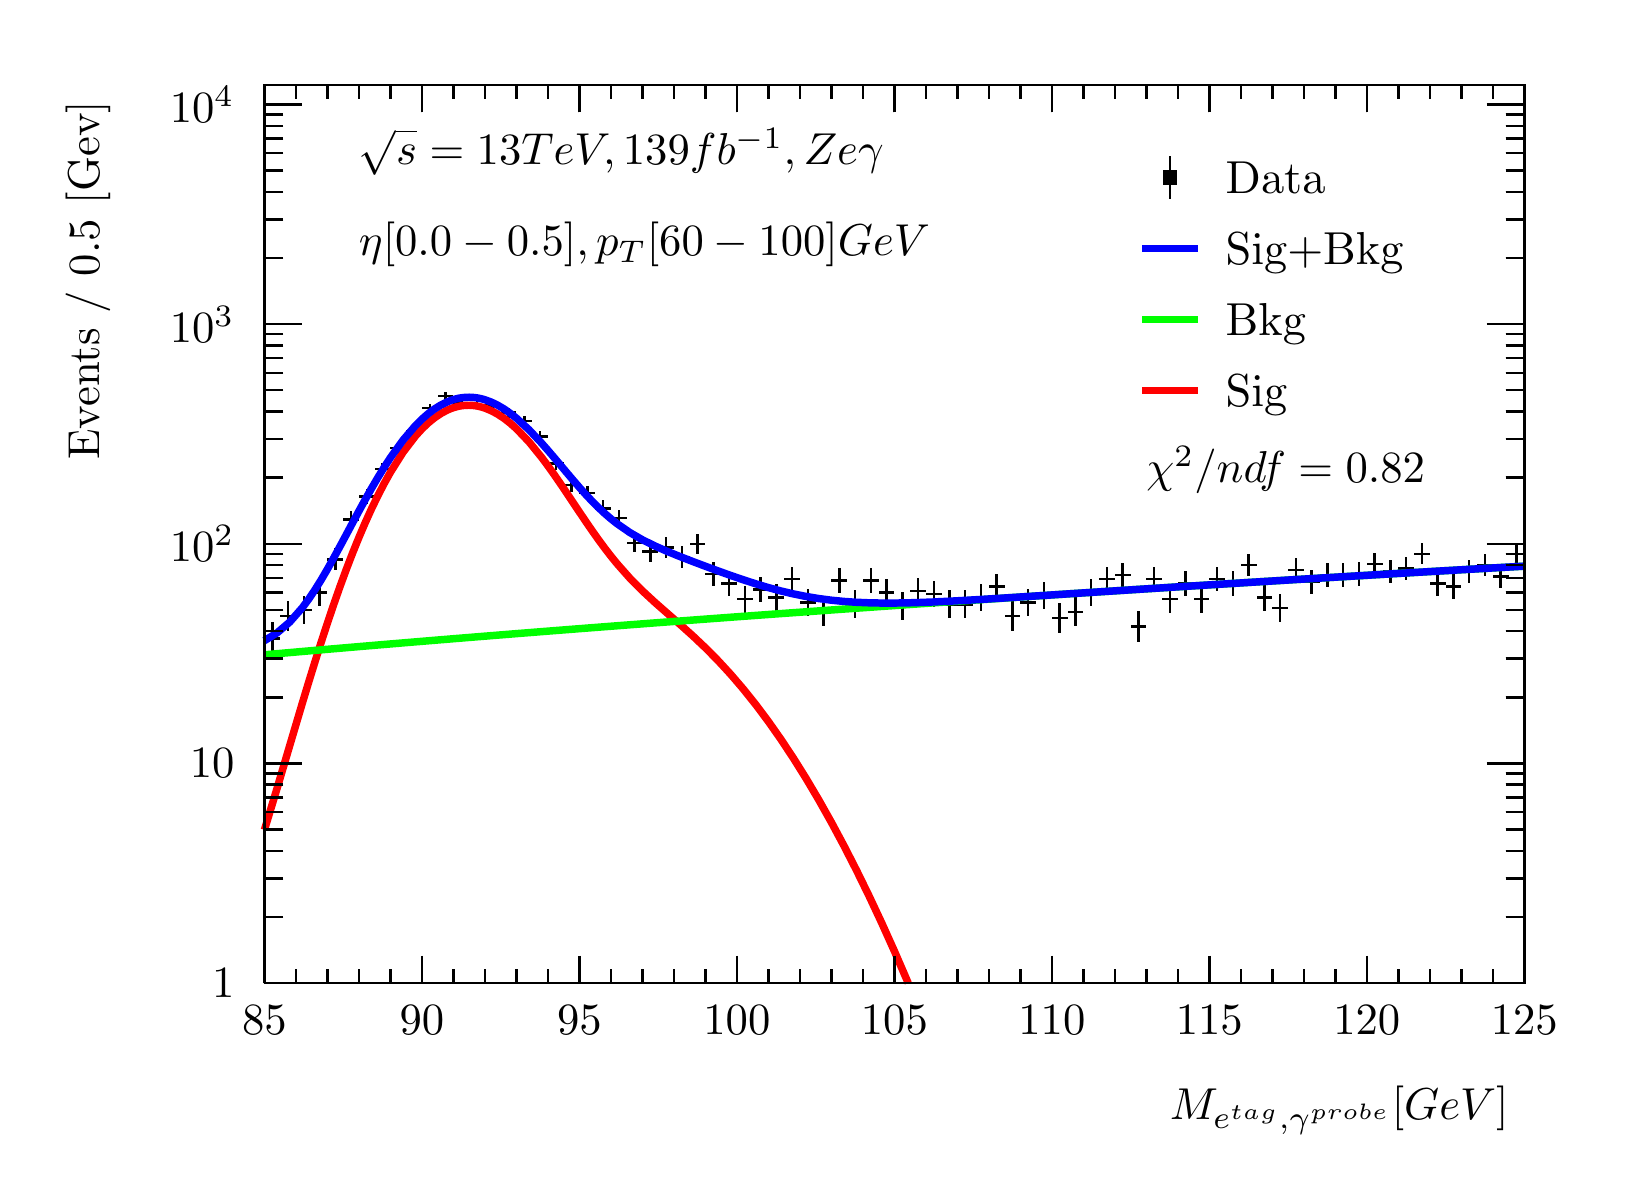
\begin{tikzpicture}
\pgfdeclareplotmark{cross} {
\pgfpathmoveto{\pgfpoint{-0.3\pgfplotmarksize}{\pgfplotmarksize}}
\pgfpathlineto{\pgfpoint{+0.3\pgfplotmarksize}{\pgfplotmarksize}}
\pgfpathlineto{\pgfpoint{+0.3\pgfplotmarksize}{0.3\pgfplotmarksize}}
\pgfpathlineto{\pgfpoint{+1\pgfplotmarksize}{0.3\pgfplotmarksize}}
\pgfpathlineto{\pgfpoint{+1\pgfplotmarksize}{-0.3\pgfplotmarksize}}
\pgfpathlineto{\pgfpoint{+0.3\pgfplotmarksize}{-0.3\pgfplotmarksize}}
\pgfpathlineto{\pgfpoint{+0.3\pgfplotmarksize}{-1.\pgfplotmarksize}}
\pgfpathlineto{\pgfpoint{-0.3\pgfplotmarksize}{-1.\pgfplotmarksize}}
\pgfpathlineto{\pgfpoint{-0.3\pgfplotmarksize}{-0.3\pgfplotmarksize}}
\pgfpathlineto{\pgfpoint{-1.\pgfplotmarksize}{-0.3\pgfplotmarksize}}
\pgfpathlineto{\pgfpoint{-1.\pgfplotmarksize}{0.3\pgfplotmarksize}}
\pgfpathlineto{\pgfpoint{-0.3\pgfplotmarksize}{0.3\pgfplotmarksize}}
\pgfpathclose
\pgfusepathqstroke
}
\pgfdeclareplotmark{cross*} {
\pgfpathmoveto{\pgfpoint{-0.3\pgfplotmarksize}{\pgfplotmarksize}}
\pgfpathlineto{\pgfpoint{+0.3\pgfplotmarksize}{\pgfplotmarksize}}
\pgfpathlineto{\pgfpoint{+0.3\pgfplotmarksize}{0.3\pgfplotmarksize}}
\pgfpathlineto{\pgfpoint{+1\pgfplotmarksize}{0.3\pgfplotmarksize}}
\pgfpathlineto{\pgfpoint{+1\pgfplotmarksize}{-0.3\pgfplotmarksize}}
\pgfpathlineto{\pgfpoint{+0.3\pgfplotmarksize}{-0.3\pgfplotmarksize}}
\pgfpathlineto{\pgfpoint{+0.3\pgfplotmarksize}{-1.\pgfplotmarksize}}
\pgfpathlineto{\pgfpoint{-0.3\pgfplotmarksize}{-1.\pgfplotmarksize}}
\pgfpathlineto{\pgfpoint{-0.3\pgfplotmarksize}{-0.3\pgfplotmarksize}}
\pgfpathlineto{\pgfpoint{-1.\pgfplotmarksize}{-0.3\pgfplotmarksize}}
\pgfpathlineto{\pgfpoint{-1.\pgfplotmarksize}{0.3\pgfplotmarksize}}
\pgfpathlineto{\pgfpoint{-0.3\pgfplotmarksize}{0.3\pgfplotmarksize}}
\pgfpathclose
\pgfusepathqfillstroke
}
\pgfdeclareplotmark{newstar} {
\pgfpathmoveto{\pgfqpoint{0pt}{\pgfplotmarksize}}
\pgfpathlineto{\pgfqpointpolar{44}{0.5\pgfplotmarksize}}
\pgfpathlineto{\pgfqpointpolar{18}{\pgfplotmarksize}}
\pgfpathlineto{\pgfqpointpolar{-20}{0.5\pgfplotmarksize}}
\pgfpathlineto{\pgfqpointpolar{-54}{\pgfplotmarksize}}
\pgfpathlineto{\pgfqpointpolar{-90}{0.5\pgfplotmarksize}}
\pgfpathlineto{\pgfqpointpolar{234}{\pgfplotmarksize}}
\pgfpathlineto{\pgfqpointpolar{198}{0.5\pgfplotmarksize}}
\pgfpathlineto{\pgfqpointpolar{162}{\pgfplotmarksize}}
\pgfpathlineto{\pgfqpointpolar{134}{0.5\pgfplotmarksize}}
\pgfpathclose
\pgfusepathqstroke
}
\pgfdeclareplotmark{newstar*} {
\pgfpathmoveto{\pgfqpoint{0pt}{\pgfplotmarksize}}
\pgfpathlineto{\pgfqpointpolar{44}{0.5\pgfplotmarksize}}
\pgfpathlineto{\pgfqpointpolar{18}{\pgfplotmarksize}}
\pgfpathlineto{\pgfqpointpolar{-20}{0.5\pgfplotmarksize}}
\pgfpathlineto{\pgfqpointpolar{-54}{\pgfplotmarksize}}
\pgfpathlineto{\pgfqpointpolar{-90}{0.5\pgfplotmarksize}}
\pgfpathlineto{\pgfqpointpolar{234}{\pgfplotmarksize}}
\pgfpathlineto{\pgfqpointpolar{198}{0.5\pgfplotmarksize}}
\pgfpathlineto{\pgfqpointpolar{162}{\pgfplotmarksize}}
\pgfpathlineto{\pgfqpointpolar{134}{0.5\pgfplotmarksize}}
\pgfpathclose
\pgfusepathqfillstroke
}
\definecolor{c}{rgb}{1,1,1};
\draw [color=c, fill=c] (0,0) rectangle (20,14.4361);
\draw [color=c, fill=c] (3,2.30977) rectangle (19,13.7143);
\definecolor{c}{rgb}{0,0,0};
\draw [c,line width=0.9] (3,2.30977) -- (3,13.7143) -- (19,13.7143) -- (19,2.30977) -- (3,2.30977);
\definecolor{c}{rgb}{1,1,1};
\draw [color=c, fill=c] (3,2.30977) rectangle (19,13.7143);
\definecolor{c}{rgb}{0,0,0};
\draw [c,line width=0.9] (3,2.30977) -- (3,13.7143) -- (19,13.7143) -- (19,2.30977) -- (3,2.30977);
\draw [c,line width=0.9] (3,2.30977) -- (19,2.30977);
\draw [c,line width=0.9] (3,2.65624) -- (3,2.30977);
\draw [c,line width=0.9] (3.4,2.48301) -- (3.4,2.30977);
\draw [c,line width=0.9] (3.8,2.48301) -- (3.8,2.30977);
\draw [c,line width=0.9] (4.2,2.48301) -- (4.2,2.30977);
\draw [c,line width=0.9] (4.6,2.48301) -- (4.6,2.30977);
\draw [c,line width=0.9] (5,2.65624) -- (5,2.30977);
\draw [c,line width=0.9] (5.4,2.48301) -- (5.4,2.30977);
\draw [c,line width=0.9] (5.8,2.48301) -- (5.8,2.30977);
\draw [c,line width=0.9] (6.2,2.48301) -- (6.2,2.30977);
\draw [c,line width=0.9] (6.6,2.48301) -- (6.6,2.30977);
\draw [c,line width=0.9] (7,2.65624) -- (7,2.30977);
\draw [c,line width=0.9] (7.4,2.48301) -- (7.4,2.30977);
\draw [c,line width=0.9] (7.8,2.48301) -- (7.8,2.30977);
\draw [c,line width=0.9] (8.2,2.48301) -- (8.2,2.30977);
\draw [c,line width=0.9] (8.6,2.48301) -- (8.6,2.30977);
\draw [c,line width=0.9] (9,2.65624) -- (9,2.30977);
\draw [c,line width=0.9] (9.4,2.48301) -- (9.4,2.30977);
\draw [c,line width=0.9] (9.8,2.48301) -- (9.8,2.30977);
\draw [c,line width=0.9] (10.2,2.48301) -- (10.2,2.30977);
\draw [c,line width=0.9] (10.6,2.48301) -- (10.6,2.30977);
\draw [c,line width=0.9] (11,2.65624) -- (11,2.30977);
\draw [c,line width=0.9] (11.4,2.48301) -- (11.4,2.30977);
\draw [c,line width=0.9] (11.8,2.48301) -- (11.8,2.30977);
\draw [c,line width=0.9] (12.2,2.48301) -- (12.2,2.30977);
\draw [c,line width=0.9] (12.6,2.48301) -- (12.6,2.30977);
\draw [c,line width=0.9] (13,2.65624) -- (13,2.30977);
\draw [c,line width=0.9] (13.4,2.48301) -- (13.4,2.30977);
\draw [c,line width=0.9] (13.8,2.48301) -- (13.8,2.30977);
\draw [c,line width=0.9] (14.2,2.48301) -- (14.2,2.30977);
\draw [c,line width=0.9] (14.6,2.48301) -- (14.6,2.30977);
\draw [c,line width=0.9] (15,2.65624) -- (15,2.30977);
\draw [c,line width=0.9] (15.4,2.48301) -- (15.4,2.30977);
\draw [c,line width=0.9] (15.8,2.48301) -- (15.8,2.30977);
\draw [c,line width=0.9] (16.2,2.48301) -- (16.2,2.30977);
\draw [c,line width=0.9] (16.6,2.48301) -- (16.6,2.30977);
\draw [c,line width=0.9] (17,2.65624) -- (17,2.30977);
\draw [c,line width=0.9] (17.4,2.48301) -- (17.4,2.30977);
\draw [c,line width=0.9] (17.8,2.48301) -- (17.8,2.30977);
\draw [c,line width=0.9] (18.2,2.48301) -- (18.2,2.30977);
\draw [c,line width=0.9] (18.6,2.48301) -- (18.6,2.30977);
\draw [c,line width=0.9] (19,2.65624) -- (19,2.30977);
\draw [anchor=base] (3,1.66015) node[scale=1.61424, color=c, rotate=0]{85};
\draw [anchor=base] (5,1.66015) node[scale=1.61424, color=c, rotate=0]{90};
\draw [anchor=base] (7,1.66015) node[scale=1.61424, color=c, rotate=0]{95};
\draw [anchor=base] (9,1.66015) node[scale=1.61424, color=c, rotate=0]{100};
\draw [anchor=base] (11,1.66015) node[scale=1.61424, color=c, rotate=0]{105};
\draw [anchor=base] (13,1.66015) node[scale=1.61424, color=c, rotate=0]{110};
\draw [anchor=base] (15,1.66015) node[scale=1.61424, color=c, rotate=0]{115};
\draw [anchor=base] (17,1.66015) node[scale=1.61424, color=c, rotate=0]{120};
\draw [anchor=base] (19,1.66015) node[scale=1.61424, color=c, rotate=0]{125};
\draw [anchor= east] (19,0.692932) node[scale=1.61424, color=c, rotate=0]{$M_{e^{tag}, \gamma^{probe}}  [GeV]$};
\draw [c,line width=0.9] (3,13.7143) -- (19,13.7143);
\draw [c,line width=0.9] (3,13.3678) -- (3,13.7143);
\draw [c,line width=0.9] (3.4,13.5411) -- (3.4,13.7143);
\draw [c,line width=0.9] (3.8,13.5411) -- (3.8,13.7143);
\draw [c,line width=0.9] (4.2,13.5411) -- (4.2,13.7143);
\draw [c,line width=0.9] (4.6,13.5411) -- (4.6,13.7143);
\draw [c,line width=0.9] (5,13.3678) -- (5,13.7143);
\draw [c,line width=0.9] (5.4,13.5411) -- (5.4,13.7143);
\draw [c,line width=0.9] (5.8,13.5411) -- (5.8,13.7143);
\draw [c,line width=0.9] (6.2,13.5411) -- (6.2,13.7143);
\draw [c,line width=0.9] (6.6,13.5411) -- (6.6,13.7143);
\draw [c,line width=0.9] (7,13.3678) -- (7,13.7143);
\draw [c,line width=0.9] (7.4,13.5411) -- (7.4,13.7143);
\draw [c,line width=0.9] (7.8,13.5411) -- (7.8,13.7143);
\draw [c,line width=0.9] (8.2,13.5411) -- (8.2,13.7143);
\draw [c,line width=0.9] (8.6,13.5411) -- (8.6,13.7143);
\draw [c,line width=0.9] (9,13.3678) -- (9,13.7143);
\draw [c,line width=0.9] (9.4,13.5411) -- (9.4,13.7143);
\draw [c,line width=0.9] (9.8,13.5411) -- (9.8,13.7143);
\draw [c,line width=0.9] (10.2,13.5411) -- (10.2,13.7143);
\draw [c,line width=0.9] (10.6,13.5411) -- (10.6,13.7143);
\draw [c,line width=0.9] (11,13.3678) -- (11,13.7143);
\draw [c,line width=0.9] (11.4,13.5411) -- (11.4,13.7143);
\draw [c,line width=0.9] (11.8,13.5411) -- (11.8,13.7143);
\draw [c,line width=0.9] (12.2,13.5411) -- (12.2,13.7143);
\draw [c,line width=0.9] (12.6,13.5411) -- (12.6,13.7143);
\draw [c,line width=0.9] (13,13.3678) -- (13,13.7143);
\draw [c,line width=0.9] (13.4,13.5411) -- (13.4,13.7143);
\draw [c,line width=0.9] (13.8,13.5411) -- (13.8,13.7143);
\draw [c,line width=0.9] (14.2,13.5411) -- (14.2,13.7143);
\draw [c,line width=0.9] (14.6,13.5411) -- (14.6,13.7143);
\draw [c,line width=0.9] (15,13.3678) -- (15,13.7143);
\draw [c,line width=0.9] (15.4,13.5411) -- (15.4,13.7143);
\draw [c,line width=0.9] (15.8,13.5411) -- (15.8,13.7143);
\draw [c,line width=0.9] (16.2,13.5411) -- (16.2,13.7143);
\draw [c,line width=0.9] (16.6,13.5411) -- (16.6,13.7143);
\draw [c,line width=0.9] (17,13.3678) -- (17,13.7143);
\draw [c,line width=0.9] (17.4,13.5411) -- (17.4,13.7143);
\draw [c,line width=0.9] (17.8,13.5411) -- (17.8,13.7143);
\draw [c,line width=0.9] (18.2,13.5411) -- (18.2,13.7143);
\draw [c,line width=0.9] (18.6,13.5411) -- (18.6,13.7143);
\draw [c,line width=0.9] (19,13.3678) -- (19,13.7143);
\draw [c,line width=0.9] (3,2.30977) -- (3,13.7143);
\draw [c,line width=0.9] (3.474,2.30978) -- (3,2.30978);
\draw [anchor= east] (2.82,2.30978) node[scale=1.61424, color=c, rotate=0]{1};
\draw [c,line width=0.9] (3.237,3.1495) -- (3,3.1495);
\draw [c,line width=0.9] (3.237,3.6407) -- (3,3.6407);
\draw [c,line width=0.9] (3.237,3.98922) -- (3,3.98922);
\draw [c,line width=0.9] (3.237,4.25955) -- (3,4.25955);
\draw [c,line width=0.9] (3.237,4.48042) -- (3,4.48042);
\draw [c,line width=0.9] (3.237,4.66717) -- (3,4.66717);
\draw [c,line width=0.9] (3.237,4.82894) -- (3,4.82894);
\draw [c,line width=0.9] (3.237,4.97163) -- (3,4.97163);
\draw [c,line width=0.9] (3.474,5.09927) -- (3,5.09927);
\draw [anchor= east] (2.82,5.09927) node[scale=1.61424, color=c, rotate=0]{10};
\draw [c,line width=0.9] (3.237,5.93899) -- (3,5.93899);
\draw [c,line width=0.9] (3.237,6.43019) -- (3,6.43019);
\draw [c,line width=0.9] (3.237,6.77871) -- (3,6.77871);
\draw [c,line width=0.9] (3.237,7.04904) -- (3,7.04904);
\draw [c,line width=0.9] (3.237,7.26991) -- (3,7.26991);
\draw [c,line width=0.9] (3.237,7.45666) -- (3,7.45666);
\draw [c,line width=0.9] (3.237,7.61843) -- (3,7.61843);
\draw [c,line width=0.9] (3.237,7.76112) -- (3,7.76112);
\draw [c,line width=0.9] (3.474,7.88876) -- (3,7.88876);
\draw [anchor= east] (2.82,7.88876) node[scale=1.61424, color=c, rotate=0]{$10^{2}$};
\draw [c,line width=0.9] (3.237,8.72848) -- (3,8.72848);
\draw [c,line width=0.9] (3.237,9.21968) -- (3,9.21968);
\draw [c,line width=0.9] (3.237,9.5682) -- (3,9.5682);
\draw [c,line width=0.9] (3.237,9.83853) -- (3,9.83853);
\draw [c,line width=0.9] (3.237,10.0594) -- (3,10.0594);
\draw [c,line width=0.9] (3.237,10.2462) -- (3,10.2462);
\draw [c,line width=0.9] (3.237,10.4079) -- (3,10.4079);
\draw [c,line width=0.9] (3.237,10.5506) -- (3,10.5506);
\draw [c,line width=0.9] (3.474,10.6782) -- (3,10.6782);
\draw [anchor= east] (2.82,10.6782) node[scale=1.61424, color=c, rotate=0]{$10^{3}$};
\draw [c,line width=0.9] (3.237,11.518) -- (3,11.518);
\draw [c,line width=0.9] (3.237,12.0092) -- (3,12.0092);
\draw [c,line width=0.9] (3.237,12.3577) -- (3,12.3577);
\draw [c,line width=0.9] (3.237,12.628) -- (3,12.628);
\draw [c,line width=0.9] (3.237,12.8489) -- (3,12.8489);
\draw [c,line width=0.9] (3.237,13.0356) -- (3,13.0356);
\draw [c,line width=0.9] (3.237,13.1974) -- (3,13.1974);
\draw [c,line width=0.9] (3.237,13.3401) -- (3,13.3401);
\draw [c,line width=0.9] (3.474,13.4677) -- (3,13.4677);
\draw [anchor= east] (2.82,13.4677) node[scale=1.61424, color=c, rotate=0]{$10^{4}$};
\draw [anchor= east] (0.76,13.7143) node[scale=1.61424, color=c, rotate=90]{Events / 0.5 [Gev]};
\draw [c,line width=0.9] (19,2.30977) -- (19,13.7143);
\draw [c,line width=0.9] (18.526,2.30978) -- (19,2.30978);
\draw [c,line width=0.9] (18.763,3.1495) -- (19,3.1495);
\draw [c,line width=0.9] (18.763,3.6407) -- (19,3.6407);
\draw [c,line width=0.9] (18.763,3.98922) -- (19,3.98922);
\draw [c,line width=0.9] (18.763,4.25955) -- (19,4.25955);
\draw [c,line width=0.9] (18.763,4.48042) -- (19,4.48042);
\draw [c,line width=0.9] (18.763,4.66717) -- (19,4.66717);
\draw [c,line width=0.9] (18.763,4.82894) -- (19,4.82894);
\draw [c,line width=0.9] (18.763,4.97163) -- (19,4.97163);
\draw [c,line width=0.9] (18.526,5.09927) -- (19,5.09927);
\draw [c,line width=0.9] (18.763,5.93899) -- (19,5.93899);
\draw [c,line width=0.9] (18.763,6.43019) -- (19,6.43019);
\draw [c,line width=0.9] (18.763,6.77871) -- (19,6.77871);
\draw [c,line width=0.9] (18.763,7.04904) -- (19,7.04904);
\draw [c,line width=0.9] (18.763,7.26991) -- (19,7.26991);
\draw [c,line width=0.9] (18.763,7.45666) -- (19,7.45666);
\draw [c,line width=0.9] (18.763,7.61843) -- (19,7.61843);
\draw [c,line width=0.9] (18.763,7.76112) -- (19,7.76112);
\draw [c,line width=0.9] (18.526,7.88876) -- (19,7.88876);
\draw [c,line width=0.9] (18.763,8.72848) -- (19,8.72848);
\draw [c,line width=0.9] (18.763,9.21968) -- (19,9.21968);
\draw [c,line width=0.9] (18.763,9.5682) -- (19,9.5682);
\draw [c,line width=0.9] (18.763,9.83853) -- (19,9.83853);
\draw [c,line width=0.9] (18.763,10.0594) -- (19,10.0594);
\draw [c,line width=0.9] (18.763,10.2462) -- (19,10.2462);
\draw [c,line width=0.9] (18.763,10.4079) -- (19,10.4079);
\draw [c,line width=0.9] (18.763,10.5506) -- (19,10.5506);
\draw [c,line width=0.9] (18.526,10.6782) -- (19,10.6782);
\draw [c,line width=0.9] (18.763,11.518) -- (19,11.518);
\draw [c,line width=0.9] (18.763,12.0092) -- (19,12.0092);
\draw [c,line width=0.9] (18.763,12.3577) -- (19,12.3577);
\draw [c,line width=0.9] (18.763,12.628) -- (19,12.628);
\draw [c,line width=0.9] (18.763,12.8489) -- (19,12.8489);
\draw [c,line width=0.9] (18.763,13.0356) -- (19,13.0356);
\draw [c,line width=0.9] (18.763,13.1974) -- (19,13.1974);
\draw [c,line width=0.9] (18.763,13.3401) -- (19,13.3401);
\draw [c,line width=0.9] (18.526,13.4677) -- (19,13.4677);
\draw [c,line width=0.9] (3.1,6.68426) -- (3,6.68426);
\draw [c,line width=0.9] (3,6.68426) -- (3,6.68426);
\draw [c,line width=0.9] (3.1,6.68426) -- (3.2,6.68426);
\draw [c,line width=0.9] (3.2,6.68426) -- (3.2,6.68426);
\draw [c,line width=0.9] (3.1,6.68426) -- (3.1,6.89795);
\draw [c,line width=0.9] (3.1,6.89795) -- (3.1,6.89795);
\draw [c,line width=0.9] (3.1,6.68426) -- (3.1,6.46776);
\draw [c,line width=0.9] (3.1,6.46776) -- (3.1,6.46776);
\draw [c,line width=0.9] (3.3,6.97408) -- (3.2,6.97408);
\draw [c,line width=0.9] (3.2,6.97408) -- (3.2,6.97408);
\draw [c,line width=0.9] (3.3,6.97408) -- (3.4,6.97408);
\draw [c,line width=0.9] (3.4,6.97408) -- (3.4,6.97408);
\draw [c,line width=0.9] (3.3,6.97408) -- (3.3,7.16239);
\draw [c,line width=0.9] (3.3,7.16239) -- (3.3,7.16239);
\draw [c,line width=0.9] (3.3,6.97408) -- (3.3,6.78381);
\draw [c,line width=0.9] (3.3,6.78381) -- (3.3,6.78381);
\draw [c,line width=0.9] (3.5,7.04904) -- (3.4,7.04904);
\draw [c,line width=0.9] (3.4,7.04904) -- (3.4,7.04904);
\draw [c,line width=0.9] (3.5,7.04904) -- (3.6,7.04904);
\draw [c,line width=0.9] (3.6,7.04904) -- (3.6,7.04904);
\draw [c,line width=0.9] (3.5,7.04904) -- (3.5,7.23131);
\draw [c,line width=0.9] (3.5,7.23131) -- (3.5,7.23131);
\draw [c,line width=0.9] (3.5,7.04904) -- (3.5,6.86499);
\draw [c,line width=0.9] (3.5,6.86499) -- (3.5,6.86499);
\draw [c,line width=0.9] (3.7,7.26991) -- (3.6,7.26991);
\draw [c,line width=0.9] (3.6,7.26991) -- (3.6,7.26991);
\draw [c,line width=0.9] (3.7,7.26991) -- (3.8,7.26991);
\draw [c,line width=0.9] (3.8,7.26991) -- (3.8,7.26991);
\draw [c,line width=0.9] (3.7,7.26991) -- (3.7,7.43552);
\draw [c,line width=0.9] (3.7,7.43552) -- (3.7,7.43552);
\draw [c,line width=0.9] (3.7,7.26991) -- (3.7,7.10296);
\draw [c,line width=0.9] (3.7,7.10296) -- (3.7,7.10296);
\draw [c,line width=0.9] (3.9,7.69187) -- (3.8,7.69187);
\draw [c,line width=0.9] (3.8,7.69187) -- (3.8,7.69187);
\draw [c,line width=0.9] (3.9,7.69187) -- (4,7.69187);
\draw [c,line width=0.9] (4,7.69187) -- (4,7.69187);
\draw [c,line width=0.9] (3.9,7.69187) -- (3.9,7.82987);
\draw [c,line width=0.9] (3.9,7.82987) -- (3.9,7.82987);
\draw [c,line width=0.9] (3.9,7.69187) -- (3.9,7.55307);
\draw [c,line width=0.9] (3.9,7.55307) -- (3.9,7.55307);
\draw [c,line width=0.9] (4.1,8.19725) -- (4,8.19725);
\draw [c,line width=0.9] (4,8.19725) -- (4,8.19725);
\draw [c,line width=0.9] (4.1,8.19725) -- (4.2,8.19725);
\draw [c,line width=0.9] (4.2,8.19725) -- (4.2,8.19725);
\draw [c,line width=0.9] (4.1,8.19725) -- (4.1,8.30387);
\draw [c,line width=0.9] (4.1,8.30387) -- (4.1,8.30387);
\draw [c,line width=0.9] (4.1,8.19725) -- (4.1,8.09062);
\draw [c,line width=0.9] (4.1,8.09062) -- (4.1,8.09062);
\draw [c,line width=0.9] (4.3,8.48806) -- (4.2,8.48806);
\draw [c,line width=0.9] (4.2,8.48806) -- (4.2,8.48806);
\draw [c,line width=0.9] (4.3,8.48806) -- (4.4,8.48806);
\draw [c,line width=0.9] (4.4,8.48806) -- (4.4,8.48806);
\draw [c,line width=0.9] (4.3,8.48806) -- (4.3,8.58264);
\draw [c,line width=0.9] (4.3,8.58264) -- (4.3,8.58264);
\draw [c,line width=0.9] (4.3,8.48806) -- (4.3,8.39349);
\draw [c,line width=0.9] (4.3,8.39349) -- (4.3,8.39349);
\draw [c,line width=0.9] (4.5,8.83842) -- (4.4,8.83842);
\draw [c,line width=0.9] (4.4,8.83842) -- (4.4,8.83842);
\draw [c,line width=0.9] (4.5,8.83842) -- (4.6,8.83842);
\draw [c,line width=0.9] (4.6,8.83842) -- (4.6,8.83842);
\draw [c,line width=0.9] (4.5,8.83842) -- (4.5,8.92027);
\draw [c,line width=0.9] (4.5,8.92027) -- (4.5,8.92027);
\draw [c,line width=0.9] (4.5,8.83842) -- (4.5,8.75658);
\draw [c,line width=0.9] (4.5,8.75658) -- (4.5,8.75658);
\draw [c,line width=0.9] (4.7,9.10543) -- (4.6,9.10543);
\draw [c,line width=0.9] (4.6,9.10543) -- (4.6,9.10543);
\draw [c,line width=0.9] (4.7,9.10543) -- (4.8,9.10543);
\draw [c,line width=0.9] (4.8,9.10543) -- (4.8,9.10543);
\draw [c,line width=0.9] (4.7,9.10543) -- (4.7,9.17874);
\draw [c,line width=0.9] (4.7,9.17874) -- (4.7,9.17874);
\draw [c,line width=0.9] (4.7,9.10543) -- (4.7,9.03212);
\draw [c,line width=0.9] (4.7,9.03212) -- (4.7,9.03212);
\draw [c,line width=0.9] (4.9,9.32037) -- (4.8,9.32037);
\draw [c,line width=0.9] (4.8,9.32037) -- (4.8,9.32037);
\draw [c,line width=0.9] (4.9,9.32037) -- (5,9.32037);
\draw [c,line width=0.9] (5,9.32037) -- (5,9.32037);
\draw [c,line width=0.9] (4.9,9.32037) -- (4.9,9.38746);
\draw [c,line width=0.9] (4.9,9.38746) -- (4.9,9.38746);
\draw [c,line width=0.9] (4.9,9.32037) -- (4.9,9.25328);
\draw [c,line width=0.9] (4.9,9.25328) -- (4.9,9.25328);
\draw [c,line width=0.9] (5.1,9.60987) -- (5,9.60987);
\draw [c,line width=0.9] (5,9.60987) -- (5,9.60987);
\draw [c,line width=0.9] (5.1,9.60987) -- (5.2,9.60987);
\draw [c,line width=0.9] (5.2,9.60987) -- (5.2,9.60987);
\draw [c,line width=0.9] (5.1,9.60987) -- (5.1,9.66941);
\draw [c,line width=0.9] (5.1,9.66941) -- (5.1,9.66941);
\draw [c,line width=0.9] (5.1,9.60987) -- (5.1,9.55034);
\draw [c,line width=0.9] (5.1,9.55034) -- (5.1,9.55034);
\draw [c,line width=0.9] (5.3,9.76357) -- (5.2,9.76357);
\draw [c,line width=0.9] (5.2,9.76357) -- (5.2,9.76357);
\draw [c,line width=0.9] (5.3,9.76357) -- (5.4,9.76357);
\draw [c,line width=0.9] (5.4,9.76357) -- (5.4,9.76357);
\draw [c,line width=0.9] (5.3,9.76357) -- (5.3,9.81944);
\draw [c,line width=0.9] (5.3,9.81944) -- (5.3,9.81944);
\draw [c,line width=0.9] (5.3,9.76357) -- (5.3,9.70769);
\draw [c,line width=0.9] (5.3,9.70769) -- (5.3,9.70769);
\draw [c,line width=0.9] (5.5,9.66982) -- (5.4,9.66982);
\draw [c,line width=0.9] (5.4,9.66982) -- (5.4,9.66982);
\draw [c,line width=0.9] (5.5,9.66982) -- (5.6,9.66982);
\draw [c,line width=0.9] (5.6,9.66982) -- (5.6,9.66982);
\draw [c,line width=0.9] (5.5,9.66982) -- (5.5,9.7279);
\draw [c,line width=0.9] (5.5,9.7279) -- (5.5,9.7279);
\draw [c,line width=0.9] (5.5,9.66982) -- (5.5,9.61174);
\draw [c,line width=0.9] (5.5,9.61174) -- (5.5,9.61174);
\draw [c,line width=0.9] (5.7,9.72161) -- (5.6,9.72161);
\draw [c,line width=0.9] (5.6,9.72161) -- (5.6,9.72161);
\draw [c,line width=0.9] (5.7,9.72161) -- (5.8,9.72161);
\draw [c,line width=0.9] (5.8,9.72161) -- (5.8,9.72161);
\draw [c,line width=0.9] (5.7,9.72161) -- (5.7,9.77846);
\draw [c,line width=0.9] (5.7,9.77846) -- (5.7,9.77846);
\draw [c,line width=0.9] (5.7,9.72161) -- (5.7,9.66476);
\draw [c,line width=0.9] (5.7,9.66476) -- (5.7,9.66476);
\draw [c,line width=0.9] (5.9,9.64449) -- (5.8,9.64449);
\draw [c,line width=0.9] (5.8,9.64449) -- (5.8,9.64449);
\draw [c,line width=0.9] (5.9,9.64449) -- (6,9.64449);
\draw [c,line width=0.9] (6,9.64449) -- (6,9.64449);
\draw [c,line width=0.9] (5.9,9.64449) -- (5.9,9.70318);
\draw [c,line width=0.9] (5.9,9.70318) -- (5.9,9.70318);
\draw [c,line width=0.9] (5.9,9.64449) -- (5.9,9.5858);
\draw [c,line width=0.9] (5.9,9.5858) -- (5.9,9.5858);
\draw [c,line width=0.9] (6.1,9.55296) -- (6,9.55296);
\draw [c,line width=0.9] (6,9.55296) -- (6,9.55296);
\draw [c,line width=0.9] (6.1,9.55296) -- (6.2,9.55296);
\draw [c,line width=0.9] (6.2,9.55296) -- (6.2,9.55296);
\draw [c,line width=0.9] (6.1,9.55296) -- (6.1,9.61391);
\draw [c,line width=0.9] (6.1,9.61391) -- (6.1,9.61391);
\draw [c,line width=0.9] (6.1,9.55296) -- (6.1,9.49201);
\draw [c,line width=0.9] (6.1,9.49201) -- (6.1,9.49201);
\draw [c,line width=0.9] (6.3,9.44727) -- (6.2,9.44727);
\draw [c,line width=0.9] (6.2,9.44727) -- (6.2,9.44727);
\draw [c,line width=0.9] (6.3,9.44727) -- (6.4,9.44727);
\draw [c,line width=0.9] (6.4,9.44727) -- (6.4,9.44727);
\draw [c,line width=0.9] (6.3,9.44727) -- (6.3,9.51093);
\draw [c,line width=0.9] (6.3,9.51093) -- (6.3,9.51093);
\draw [c,line width=0.9] (6.3,9.44727) -- (6.3,9.3836);
\draw [c,line width=0.9] (6.3,9.3836) -- (6.3,9.3836);
\draw [c,line width=0.9] (6.5,9.25156) -- (6.4,9.25156);
\draw [c,line width=0.9] (6.4,9.25156) -- (6.4,9.25156);
\draw [c,line width=0.9] (6.5,9.25156) -- (6.6,9.25156);
\draw [c,line width=0.9] (6.6,9.25156) -- (6.6,9.25156);
\draw [c,line width=0.9] (6.5,9.25156) -- (6.5,9.32058);
\draw [c,line width=0.9] (6.5,9.32058) -- (6.5,9.32058);
\draw [c,line width=0.9] (6.5,9.25156) -- (6.5,9.18254);
\draw [c,line width=0.9] (6.5,9.18254) -- (6.5,9.18254);
\draw [c,line width=0.9] (6.7,8.90828) -- (6.6,8.90828);
\draw [c,line width=0.9] (6.6,8.90828) -- (6.6,8.90828);
\draw [c,line width=0.9] (6.7,8.90828) -- (6.8,8.90828);
\draw [c,line width=0.9] (6.8,8.90828) -- (6.8,8.90828);
\draw [c,line width=0.9] (6.7,8.90828) -- (6.7,8.9878);
\draw [c,line width=0.9] (6.7,8.9878) -- (6.7,8.9878);
\draw [c,line width=0.9] (6.7,8.90828) -- (6.7,8.82876);
\draw [c,line width=0.9] (6.7,8.82876) -- (6.7,8.82876);
\draw [c,line width=0.9] (6.9,8.63403) -- (6.8,8.63403);
\draw [c,line width=0.9] (6.8,8.63403) -- (6.8,8.63403);
\draw [c,line width=0.9] (6.9,8.63403) -- (7,8.63403);
\draw [c,line width=0.9] (7,8.63403) -- (7,8.63403);
\draw [c,line width=0.9] (6.9,8.63403) -- (6.9,8.72308);
\draw [c,line width=0.9] (6.9,8.72308) -- (6.9,8.72308);
\draw [c,line width=0.9] (6.9,8.63403) -- (6.9,8.54498);
\draw [c,line width=0.9] (6.9,8.54498) -- (6.9,8.54498);
\draw [c,line width=0.9] (7.1,8.53159) -- (7,8.53159);
\draw [c,line width=0.9] (7,8.53159) -- (7,8.53159);
\draw [c,line width=0.9] (7.1,8.53159) -- (7.2,8.53159);
\draw [c,line width=0.9] (7.2,8.53159) -- (7.2,8.53159);
\draw [c,line width=0.9] (7.1,8.53159) -- (7.1,8.62448);
\draw [c,line width=0.9] (7.1,8.62448) -- (7.1,8.62448);
\draw [c,line width=0.9] (7.1,8.53159) -- (7.1,8.4387);
\draw [c,line width=0.9] (7.1,8.4387) -- (7.1,8.4387);
\draw [c,line width=0.9] (7.3,8.33889) -- (7.2,8.33889);
\draw [c,line width=0.9] (7.2,8.33889) -- (7.2,8.33889);
\draw [c,line width=0.9] (7.3,8.33889) -- (7.4,8.33889);
\draw [c,line width=0.9] (7.4,8.33889) -- (7.4,8.33889);
\draw [c,line width=0.9] (7.3,8.33889) -- (7.3,8.43947);
\draw [c,line width=0.9] (7.3,8.43947) -- (7.3,8.43947);
\draw [c,line width=0.9] (7.3,8.33889) -- (7.3,8.23831);
\draw [c,line width=0.9] (7.3,8.23831) -- (7.3,8.23831);
\draw [c,line width=0.9] (7.5,8.21588) -- (7.4,8.21588);
\draw [c,line width=0.9] (7.4,8.21588) -- (7.4,8.21588);
\draw [c,line width=0.9] (7.5,8.21588) -- (7.6,8.21588);
\draw [c,line width=0.9] (7.6,8.21588) -- (7.6,8.21588);
\draw [c,line width=0.9] (7.5,8.21588) -- (7.5,8.3217);
\draw [c,line width=0.9] (7.5,8.3217) -- (7.5,8.3217);
\draw [c,line width=0.9] (7.5,8.21588) -- (7.5,8.11007);
\draw [c,line width=0.9] (7.5,8.11007) -- (7.5,8.11007);
\draw [c,line width=0.9] (7.7,7.90081) -- (7.6,7.90081);
\draw [c,line width=0.9] (7.6,7.90081) -- (7.6,7.90081);
\draw [c,line width=0.9] (7.7,7.90081) -- (7.8,7.90081);
\draw [c,line width=0.9] (7.8,7.90081) -- (7.8,7.90081);
\draw [c,line width=0.9] (7.7,7.90081) -- (7.7,8.02131);
\draw [c,line width=0.9] (7.7,8.02131) -- (7.7,8.02131);
\draw [c,line width=0.9] (7.7,7.90081) -- (7.7,7.78032);
\draw [c,line width=0.9] (7.7,7.78032) -- (7.7,7.78032);
\draw [c,line width=0.9] (7.9,7.78774) -- (7.8,7.78774);
\draw [c,line width=0.9] (7.8,7.78774) -- (7.8,7.78774);
\draw [c,line width=0.9] (7.9,7.78774) -- (8,7.78774);
\draw [c,line width=0.9] (8,7.78774) -- (8,7.78774);
\draw [c,line width=0.9] (7.9,7.78774) -- (7.9,7.92016);
\draw [c,line width=0.9] (7.9,7.92016) -- (7.9,7.92016);
\draw [c,line width=0.9] (7.9,7.78774) -- (7.9,7.65462);
\draw [c,line width=0.9] (7.9,7.65462) -- (7.9,7.65462);
\draw [c,line width=0.9] (8.1,7.8393) -- (8,7.8393);
\draw [c,line width=0.9] (8,7.8393) -- (8,7.8393);
\draw [c,line width=0.9] (8.1,7.8393) -- (8.2,7.8393);
\draw [c,line width=0.9] (8.2,7.8393) -- (8.2,7.8393);
\draw [c,line width=0.9] (8.1,7.8393) -- (8.1,7.96882);
\draw [c,line width=0.9] (8.1,7.96882) -- (8.1,7.96882);
\draw [c,line width=0.9] (8.1,7.8393) -- (8.1,7.70912);
\draw [c,line width=0.9] (8.1,7.70912) -- (8.1,7.70912);
\draw [c,line width=0.9] (8.3,7.72005) -- (8.2,7.72005);
\draw [c,line width=0.9] (8.2,7.72005) -- (8.2,7.72005);
\draw [c,line width=0.9] (8.3,7.72005) -- (8.4,7.72005);
\draw [c,line width=0.9] (8.4,7.72005) -- (8.4,7.72005);
\draw [c,line width=0.9] (8.3,7.72005) -- (8.3,7.85638);
\draw [c,line width=0.9] (8.3,7.85638) -- (8.3,7.85638);
\draw [c,line width=0.9] (8.3,7.72005) -- (8.3,7.58294);
\draw [c,line width=0.9] (8.3,7.58294) -- (8.3,7.58294);
\draw [c,line width=0.9] (8.5,7.88876) -- (8.4,7.88876);
\draw [c,line width=0.9] (8.4,7.88876) -- (8.4,7.88876);
\draw [c,line width=0.9] (8.5,7.88876) -- (8.6,7.88876);
\draw [c,line width=0.9] (8.6,7.88876) -- (8.6,7.88876);
\draw [c,line width=0.9] (8.5,7.88876) -- (8.5,8.01555);
\draw [c,line width=0.9] (8.5,8.01555) -- (8.5,8.01555);
\draw [c,line width=0.9] (8.5,7.88876) -- (8.5,7.76134);
\draw [c,line width=0.9] (8.5,7.76134) -- (8.5,7.76134);
\draw [c,line width=0.9] (8.7,7.5075) -- (8.6,7.5075);
\draw [c,line width=0.9] (8.6,7.5075) -- (8.6,7.5075);
\draw [c,line width=0.9] (8.7,7.5075) -- (8.8,7.5075);
\draw [c,line width=0.9] (8.8,7.5075) -- (8.8,7.5075);
\draw [c,line width=0.9] (8.7,7.5075) -- (8.7,7.65692);
\draw [c,line width=0.9] (8.7,7.65692) -- (8.7,7.65692);
\draw [c,line width=0.9] (8.7,7.5075) -- (8.7,7.35707);
\draw [c,line width=0.9] (8.7,7.35707) -- (8.7,7.35707);
\draw [c,line width=0.9] (8.9,7.38538) -- (8.8,7.38538);
\draw [c,line width=0.9] (8.8,7.38538) -- (8.8,7.38538);
\draw [c,line width=0.9] (8.9,7.38538) -- (9,7.38538);
\draw [c,line width=0.9] (9,7.38538) -- (9,7.38538);
\draw [c,line width=0.9] (8.9,7.38538) -- (8.9,7.5429);
\draw [c,line width=0.9] (8.9,7.5429) -- (8.9,7.5429);
\draw [c,line width=0.9] (8.9,7.38538) -- (8.9,7.22668);
\draw [c,line width=0.9] (8.9,7.22668) -- (8.9,7.22668);
\draw [c,line width=0.9] (9.1,7.18633) -- (9,7.18633);
\draw [c,line width=0.9] (9,7.18633) -- (9,7.18633);
\draw [c,line width=0.9] (9.1,7.18633) -- (9.2,7.18633);
\draw [c,line width=0.9] (9.2,7.18633) -- (9.2,7.18633);
\draw [c,line width=0.9] (9.1,7.18633) -- (9.1,7.35805);
\draw [c,line width=0.9] (9.1,7.35805) -- (9.1,7.35805);
\draw [c,line width=0.9] (9.1,7.18633) -- (9.1,7.01311);
\draw [c,line width=0.9] (9.1,7.01311) -- (9.1,7.01311);
\draw [c,line width=0.9] (9.3,7.30964) -- (9.2,7.30964);
\draw [c,line width=0.9] (9.2,7.30964) -- (9.2,7.30964);
\draw [c,line width=0.9] (9.3,7.30964) -- (9.4,7.30964);
\draw [c,line width=0.9] (9.4,7.30964) -- (9.4,7.30964);
\draw [c,line width=0.9] (9.3,7.30964) -- (9.3,7.47242);
\draw [c,line width=0.9] (9.3,7.47242) -- (9.3,7.47242);
\draw [c,line width=0.9] (9.3,7.30964) -- (9.3,7.14557);
\draw [c,line width=0.9] (9.3,7.14557) -- (9.3,7.14557);
\draw [c,line width=0.9] (9.5,7.20777) -- (9.4,7.20777);
\draw [c,line width=0.9] (9.4,7.20777) -- (9.4,7.20777);
\draw [c,line width=0.9] (9.5,7.20777) -- (9.6,7.20777);
\draw [c,line width=0.9] (9.6,7.20777) -- (9.6,7.20777);
\draw [c,line width=0.9] (9.5,7.20777) -- (9.5,7.3779);
\draw [c,line width=0.9] (9.5,7.3779) -- (9.5,7.3779);
\draw [c,line width=0.9] (9.5,7.20777) -- (9.5,7.03618);
\draw [c,line width=0.9] (9.5,7.03618) -- (9.5,7.03618);
\draw [c,line width=0.9] (9.7,7.43923) -- (9.6,7.43923);
\draw [c,line width=0.9] (9.6,7.43923) -- (9.6,7.43923);
\draw [c,line width=0.9] (9.7,7.43923) -- (9.8,7.43923);
\draw [c,line width=0.9] (9.8,7.43923) -- (9.8,7.43923);
\draw [c,line width=0.9] (9.7,7.43923) -- (9.7,7.59313);
\draw [c,line width=0.9] (9.7,7.59313) -- (9.7,7.59313);
\draw [c,line width=0.9] (9.7,7.43923) -- (9.7,7.28423);
\draw [c,line width=0.9] (9.7,7.28423) -- (9.7,7.28423);
\draw [c,line width=0.9] (9.9,7.14227) -- (9.8,7.14227);
\draw [c,line width=0.9] (9.8,7.14227) -- (9.8,7.14227);
\draw [c,line width=0.9] (9.9,7.14227) -- (10,7.14227);
\draw [c,line width=0.9] (10,7.14227) -- (10,7.14227);
\draw [c,line width=0.9] (9.9,7.14227) -- (9.9,7.31731);
\draw [c,line width=0.9] (9.9,7.31731) -- (9.9,7.31731);
\draw [c,line width=0.9] (9.9,7.14227) -- (9.9,6.96565);
\draw [c,line width=0.9] (9.9,6.96565) -- (9.9,6.96565);
\draw [c,line width=0.9] (10.1,7.02456) -- (10,7.02456);
\draw [c,line width=0.9] (10,7.02456) -- (10,7.02456);
\draw [c,line width=0.9] (10.1,7.02456) -- (10.2,7.02456);
\draw [c,line width=0.9] (10.2,7.02456) -- (10.2,7.02456);
\draw [c,line width=0.9] (10.1,7.02456) -- (10.1,7.20878);
\draw [c,line width=0.9] (10.1,7.20878) -- (10.1,7.20878);
\draw [c,line width=0.9] (10.1,7.02456) -- (10.1,6.83851);
\draw [c,line width=0.9] (10.1,6.83851) -- (10.1,6.83851);
\draw [c,line width=0.9] (10.3,7.42154) -- (10.2,7.42154);
\draw [c,line width=0.9] (10.2,7.42154) -- (10.2,7.42154);
\draw [c,line width=0.9] (10.3,7.42154) -- (10.4,7.42154);
\draw [c,line width=0.9] (10.4,7.42154) -- (10.4,7.42154);
\draw [c,line width=0.9] (10.3,7.42154) -- (10.3,7.57663);
\draw [c,line width=0.9] (10.3,7.57663) -- (10.3,7.57663);
\draw [c,line width=0.9] (10.3,7.42154) -- (10.3,7.26534);
\draw [c,line width=0.9] (10.3,7.26534) -- (10.3,7.26534);
\draw [c,line width=0.9] (10.5,7.11963) -- (10.4,7.11963);
\draw [c,line width=0.9] (10.4,7.11963) -- (10.4,7.11963);
\draw [c,line width=0.9] (10.5,7.11963) -- (10.6,7.11963);
\draw [c,line width=0.9] (10.6,7.11963) -- (10.6,7.11963);
\draw [c,line width=0.9] (10.5,7.11963) -- (10.5,7.29639);
\draw [c,line width=0.9] (10.5,7.29639) -- (10.5,7.29639);
\draw [c,line width=0.9] (10.5,7.11963) -- (10.5,6.94123);
\draw [c,line width=0.9] (10.5,6.94123) -- (10.5,6.94123);
\draw [c,line width=0.9] (10.7,7.42154) -- (10.6,7.42154);
\draw [c,line width=0.9] (10.6,7.42154) -- (10.6,7.42154);
\draw [c,line width=0.9] (10.7,7.42154) -- (10.8,7.42154);
\draw [c,line width=0.9] (10.8,7.42154) -- (10.8,7.42154);
\draw [c,line width=0.9] (10.7,7.42154) -- (10.7,7.57663);
\draw [c,line width=0.9] (10.7,7.57663) -- (10.7,7.57663);
\draw [c,line width=0.9] (10.7,7.42154) -- (10.7,7.26534);
\draw [c,line width=0.9] (10.7,7.26534) -- (10.7,7.26534);
\draw [c,line width=0.9] (10.9,7.26991) -- (10.8,7.26991);
\draw [c,line width=0.9] (10.8,7.26991) -- (10.8,7.26991);
\draw [c,line width=0.9] (10.9,7.26991) -- (11,7.26991);
\draw [c,line width=0.9] (11,7.26991) -- (11,7.26991);
\draw [c,line width=0.9] (10.9,7.26991) -- (10.9,7.43552);
\draw [c,line width=0.9] (10.9,7.43552) -- (10.9,7.43552);
\draw [c,line width=0.9] (10.9,7.26991) -- (10.9,7.10296);
\draw [c,line width=0.9] (10.9,7.10296) -- (10.9,7.10296);
\draw [c,line width=0.9] (11.1,7.09655) -- (11,7.09655);
\draw [c,line width=0.9] (11,7.09655) -- (11,7.09655);
\draw [c,line width=0.9] (11.1,7.09655) -- (11.2,7.09655);
\draw [c,line width=0.9] (11.2,7.09655) -- (11.2,7.09655);
\draw [c,line width=0.9] (11.1,7.09655) -- (11.1,7.2751);
\draw [c,line width=0.9] (11.1,7.2751) -- (11.1,7.2751);
\draw [c,line width=0.9] (11.1,7.09655) -- (11.1,6.91633);
\draw [c,line width=0.9] (11.1,6.91633) -- (11.1,6.91633);
\draw [c,line width=0.9] (11.3,7.28994) -- (11.2,7.28994);
\draw [c,line width=0.9] (11.2,7.28994) -- (11.2,7.28994);
\draw [c,line width=0.9] (11.3,7.28994) -- (11.4,7.28994);
\draw [c,line width=0.9] (11.4,7.28994) -- (11.4,7.28994);
\draw [c,line width=0.9] (11.3,7.28994) -- (11.3,7.45411);
\draw [c,line width=0.9] (11.3,7.45411) -- (11.3,7.45411);
\draw [c,line width=0.9] (11.3,7.28994) -- (11.3,7.12444);
\draw [c,line width=0.9] (11.3,7.12444) -- (11.3,7.12444);
\draw [c,line width=0.9] (11.5,7.24955) -- (11.4,7.24955);
\draw [c,line width=0.9] (11.4,7.24955) -- (11.4,7.24955);
\draw [c,line width=0.9] (11.5,7.24955) -- (11.6,7.24955);
\draw [c,line width=0.9] (11.6,7.24955) -- (11.6,7.24955);
\draw [c,line width=0.9] (11.5,7.24955) -- (11.5,7.41663);
\draw [c,line width=0.9] (11.5,7.41663) -- (11.5,7.41663);
\draw [c,line width=0.9] (11.5,7.24955) -- (11.5,7.08109);
\draw [c,line width=0.9] (11.5,7.08109) -- (11.5,7.08109);
\draw [c,line width=0.9] (11.7,7.11963) -- (11.6,7.11963);
\draw [c,line width=0.9] (11.6,7.11963) -- (11.6,7.11963);
\draw [c,line width=0.9] (11.7,7.11963) -- (11.8,7.11963);
\draw [c,line width=0.9] (11.8,7.11963) -- (11.8,7.11963);
\draw [c,line width=0.9] (11.7,7.11963) -- (11.7,7.29639);
\draw [c,line width=0.9] (11.7,7.29639) -- (11.7,7.29639);
\draw [c,line width=0.9] (11.7,7.11963) -- (11.7,6.94123);
\draw [c,line width=0.9] (11.7,6.94123) -- (11.7,6.94123);
\draw [c,line width=0.9] (11.9,7.11963) -- (11.8,7.11963);
\draw [c,line width=0.9] (11.8,7.11963) -- (11.8,7.11963);
\draw [c,line width=0.9] (11.9,7.11963) -- (12,7.11963);
\draw [c,line width=0.9] (12,7.11963) -- (12,7.11963);
\draw [c,line width=0.9] (11.9,7.11963) -- (11.9,7.29639);
\draw [c,line width=0.9] (11.9,7.29639) -- (11.9,7.29639);
\draw [c,line width=0.9] (11.9,7.11963) -- (11.9,6.94123);
\draw [c,line width=0.9] (11.9,6.94123) -- (11.9,6.94123);
\draw [c,line width=0.9] (12.1,7.20777) -- (12,7.20777);
\draw [c,line width=0.9] (12,7.20777) -- (12,7.20777);
\draw [c,line width=0.9] (12.1,7.20777) -- (12.2,7.20777);
\draw [c,line width=0.9] (12.2,7.20777) -- (12.2,7.20777);
\draw [c,line width=0.9] (12.1,7.20777) -- (12.1,7.3779);
\draw [c,line width=0.9] (12.1,7.3779) -- (12.1,7.3779);
\draw [c,line width=0.9] (12.1,7.20777) -- (12.1,7.03618);
\draw [c,line width=0.9] (12.1,7.03618) -- (12.1,7.03618);
\draw [c,line width=0.9] (12.3,7.3481) -- (12.2,7.3481);
\draw [c,line width=0.9] (12.2,7.3481) -- (12.2,7.3481);
\draw [c,line width=0.9] (12.3,7.3481) -- (12.4,7.3481);
\draw [c,line width=0.9] (12.4,7.3481) -- (12.4,7.3481);
\draw [c,line width=0.9] (12.3,7.3481) -- (12.3,7.50819);
\draw [c,line width=0.9] (12.3,7.50819) -- (12.3,7.50819);
\draw [c,line width=0.9] (12.3,7.3481) -- (12.3,7.18678);
\draw [c,line width=0.9] (12.3,7.18678) -- (12.3,7.18678);
\draw [c,line width=0.9] (12.5,6.97408) -- (12.4,6.97408);
\draw [c,line width=0.9] (12.4,6.97408) -- (12.4,6.97408);
\draw [c,line width=0.9] (12.5,6.97408) -- (12.6,6.97408);
\draw [c,line width=0.9] (12.6,6.97408) -- (12.6,6.97408);
\draw [c,line width=0.9] (12.5,6.97408) -- (12.5,7.16239);
\draw [c,line width=0.9] (12.5,7.16239) -- (12.5,7.16239);
\draw [c,line width=0.9] (12.5,6.97408) -- (12.5,6.78381);
\draw [c,line width=0.9] (12.5,6.78381) -- (12.5,6.78381);
\draw [c,line width=0.9] (12.7,7.14227) -- (12.6,7.14227);
\draw [c,line width=0.9] (12.6,7.14227) -- (12.6,7.14227);
\draw [c,line width=0.9] (12.7,7.14227) -- (12.8,7.14227);
\draw [c,line width=0.9] (12.8,7.14227) -- (12.8,7.14227);
\draw [c,line width=0.9] (12.7,7.14227) -- (12.7,7.31731);
\draw [c,line width=0.9] (12.7,7.31731) -- (12.7,7.31731);
\draw [c,line width=0.9] (12.7,7.14227) -- (12.7,6.96565);
\draw [c,line width=0.9] (12.7,6.96565) -- (12.7,6.96565);
\draw [c,line width=0.9] (12.9,7.22884) -- (12.8,7.22884);
\draw [c,line width=0.9] (12.8,7.22884) -- (12.8,7.22884);
\draw [c,line width=0.9] (12.9,7.22884) -- (13,7.22884);
\draw [c,line width=0.9] (13,7.22884) -- (13,7.22884);
\draw [c,line width=0.9] (12.9,7.22884) -- (12.9,7.39742);
\draw [c,line width=0.9] (12.9,7.39742) -- (12.9,7.39742);
\draw [c,line width=0.9] (12.9,7.22884) -- (12.9,7.05884);
\draw [c,line width=0.9] (12.9,7.05884) -- (12.9,7.05884);
\draw [c,line width=0.9] (13.1,6.94802) -- (13,6.94802);
\draw [c,line width=0.9] (13,6.94802) -- (13,6.94802);
\draw [c,line width=0.9] (13.1,6.94802) -- (13.2,6.94802);
\draw [c,line width=0.9] (13.2,6.94802) -- (13.2,6.94802);
\draw [c,line width=0.9] (13.1,6.94802) -- (13.1,7.13848);
\draw [c,line width=0.9] (13.1,7.13848) -- (13.1,7.13848);
\draw [c,line width=0.9] (13.1,6.94802) -- (13.1,6.75554);
\draw [c,line width=0.9] (13.1,6.75554) -- (13.1,6.75554);
\draw [c,line width=0.9] (13.3,7.02456) -- (13.2,7.02456);
\draw [c,line width=0.9] (13.2,7.02456) -- (13.2,7.02456);
\draw [c,line width=0.9] (13.3,7.02456) -- (13.4,7.02456);
\draw [c,line width=0.9] (13.4,7.02456) -- (13.4,7.02456);
\draw [c,line width=0.9] (13.3,7.02456) -- (13.3,7.20878);
\draw [c,line width=0.9] (13.3,7.20878) -- (13.3,7.20878);
\draw [c,line width=0.9] (13.3,7.02456) -- (13.3,6.83851);
\draw [c,line width=0.9] (13.3,6.83851) -- (13.3,6.83851);
\draw [c,line width=0.9] (13.5,7.26991) -- (13.4,7.26991);
\draw [c,line width=0.9] (13.4,7.26991) -- (13.4,7.26991);
\draw [c,line width=0.9] (13.5,7.26991) -- (13.6,7.26991);
\draw [c,line width=0.9] (13.6,7.26991) -- (13.6,7.26991);
\draw [c,line width=0.9] (13.5,7.26991) -- (13.5,7.43552);
\draw [c,line width=0.9] (13.5,7.43552) -- (13.5,7.43552);
\draw [c,line width=0.9] (13.5,7.26991) -- (13.5,7.10296);
\draw [c,line width=0.9] (13.5,7.10296) -- (13.5,7.10296);
\draw [c,line width=0.9] (13.7,7.43923) -- (13.6,7.43923);
\draw [c,line width=0.9] (13.6,7.43923) -- (13.6,7.43923);
\draw [c,line width=0.9] (13.7,7.43923) -- (13.8,7.43923);
\draw [c,line width=0.9] (13.8,7.43923) -- (13.8,7.43923);
\draw [c,line width=0.9] (13.7,7.43923) -- (13.7,7.59313);
\draw [c,line width=0.9] (13.7,7.59313) -- (13.7,7.59313);
\draw [c,line width=0.9] (13.7,7.43923) -- (13.7,7.28423);
\draw [c,line width=0.9] (13.7,7.28423) -- (13.7,7.28423);
\draw [c,line width=0.9] (13.9,7.49079) -- (13.8,7.49079);
\draw [c,line width=0.9] (13.8,7.49079) -- (13.8,7.49079);
\draw [c,line width=0.9] (13.9,7.49079) -- (14,7.49079);
\draw [c,line width=0.9] (14,7.49079) -- (14,7.49079);
\draw [c,line width=0.9] (13.9,7.49079) -- (13.9,7.6413);
\draw [c,line width=0.9] (13.9,7.6413) -- (13.9,7.6413);
\draw [c,line width=0.9] (13.9,7.49079) -- (13.9,7.33925);
\draw [c,line width=0.9] (13.9,7.33925) -- (13.9,7.33925);
\draw [c,line width=0.9] (14.1,6.83781) -- (14,6.83781);
\draw [c,line width=0.9] (14,6.83781) -- (14,6.83781);
\draw [c,line width=0.9] (14.1,6.83781) -- (14.2,6.83781);
\draw [c,line width=0.9] (14.2,6.83781) -- (14.2,6.83781);
\draw [c,line width=0.9] (14.1,6.83781) -- (14.1,7.03765);
\draw [c,line width=0.9] (14.1,7.03765) -- (14.1,7.03765);
\draw [c,line width=0.9] (14.1,6.83781) -- (14.1,6.63566);
\draw [c,line width=0.9] (14.1,6.63566) -- (14.1,6.63566);
\draw [c,line width=0.9] (14.3,7.43923) -- (14.2,7.43923);
\draw [c,line width=0.9] (14.2,7.43923) -- (14.2,7.43923);
\draw [c,line width=0.9] (14.3,7.43923) -- (14.4,7.43923);
\draw [c,line width=0.9] (14.4,7.43923) -- (14.4,7.43923);
\draw [c,line width=0.9] (14.3,7.43923) -- (14.3,7.59313);
\draw [c,line width=0.9] (14.3,7.59313) -- (14.3,7.59313);
\draw [c,line width=0.9] (14.3,7.43923) -- (14.3,7.28423);
\draw [c,line width=0.9] (14.3,7.28423) -- (14.3,7.28423);
\draw [c,line width=0.9] (14.5,7.18633) -- (14.4,7.18633);
\draw [c,line width=0.9] (14.4,7.18633) -- (14.4,7.18633);
\draw [c,line width=0.9] (14.5,7.18633) -- (14.6,7.18633);
\draw [c,line width=0.9] (14.6,7.18633) -- (14.6,7.18633);
\draw [c,line width=0.9] (14.5,7.18633) -- (14.5,7.35805);
\draw [c,line width=0.9] (14.5,7.35805) -- (14.5,7.35805);
\draw [c,line width=0.9] (14.5,7.18633) -- (14.5,7.01311);
\draw [c,line width=0.9] (14.5,7.01311) -- (14.5,7.01311);
\draw [c,line width=0.9] (14.7,7.38538) -- (14.6,7.38538);
\draw [c,line width=0.9] (14.6,7.38538) -- (14.6,7.38538);
\draw [c,line width=0.9] (14.7,7.38538) -- (14.8,7.38538);
\draw [c,line width=0.9] (14.8,7.38538) -- (14.8,7.38538);
\draw [c,line width=0.9] (14.7,7.38538) -- (14.7,7.5429);
\draw [c,line width=0.9] (14.7,7.5429) -- (14.7,7.5429);
\draw [c,line width=0.9] (14.7,7.38538) -- (14.7,7.22668);
\draw [c,line width=0.9] (14.7,7.22668) -- (14.7,7.22668);
\draw [c,line width=0.9] (14.9,7.18633) -- (14.8,7.18633);
\draw [c,line width=0.9] (14.8,7.18633) -- (14.8,7.18633);
\draw [c,line width=0.9] (14.9,7.18633) -- (15,7.18633);
\draw [c,line width=0.9] (15,7.18633) -- (15,7.18633);
\draw [c,line width=0.9] (14.9,7.18633) -- (14.9,7.35805);
\draw [c,line width=0.9] (14.9,7.35805) -- (14.9,7.35805);
\draw [c,line width=0.9] (14.9,7.18633) -- (14.9,7.01311);
\draw [c,line width=0.9] (14.9,7.01311) -- (14.9,7.01311);
\draw [c,line width=0.9] (15.1,7.43923) -- (15,7.43923);
\draw [c,line width=0.9] (15,7.43923) -- (15,7.43923);
\draw [c,line width=0.9] (15.1,7.43923) -- (15.2,7.43923);
\draw [c,line width=0.9] (15.2,7.43923) -- (15.2,7.43923);
\draw [c,line width=0.9] (15.1,7.43923) -- (15.1,7.59313);
\draw [c,line width=0.9] (15.1,7.59313) -- (15.1,7.59313);
\draw [c,line width=0.9] (15.1,7.43923) -- (15.1,7.28423);
\draw [c,line width=0.9] (15.1,7.28423) -- (15.1,7.28423);
\draw [c,line width=0.9] (15.3,7.38538) -- (15.2,7.38538);
\draw [c,line width=0.9] (15.2,7.38538) -- (15.2,7.38538);
\draw [c,line width=0.9] (15.3,7.38538) -- (15.4,7.38538);
\draw [c,line width=0.9] (15.4,7.38538) -- (15.4,7.38538);
\draw [c,line width=0.9] (15.3,7.38538) -- (15.3,7.5429);
\draw [c,line width=0.9] (15.3,7.5429) -- (15.3,7.5429);
\draw [c,line width=0.9] (15.3,7.38538) -- (15.3,7.22668);
\draw [c,line width=0.9] (15.3,7.22668) -- (15.3,7.22668);
\draw [c,line width=0.9] (15.5,7.61843) -- (15.4,7.61843);
\draw [c,line width=0.9] (15.4,7.61843) -- (15.4,7.61843);
\draw [c,line width=0.9] (15.5,7.61843) -- (15.6,7.61843);
\draw [c,line width=0.9] (15.6,7.61843) -- (15.6,7.61843);
\draw [c,line width=0.9] (15.5,7.61843) -- (15.5,7.76087);
\draw [c,line width=0.9] (15.5,7.76087) -- (15.5,7.76087);
\draw [c,line width=0.9] (15.5,7.61843) -- (15.5,7.47511);
\draw [c,line width=0.9] (15.5,7.47511) -- (15.5,7.47511);
\draw [c,line width=0.9] (15.7,7.20777) -- (15.6,7.20777);
\draw [c,line width=0.9] (15.6,7.20777) -- (15.6,7.20777);
\draw [c,line width=0.9] (15.7,7.20777) -- (15.8,7.20777);
\draw [c,line width=0.9] (15.8,7.20777) -- (15.8,7.20777);
\draw [c,line width=0.9] (15.7,7.20777) -- (15.7,7.3779);
\draw [c,line width=0.9] (15.7,7.3779) -- (15.7,7.3779);
\draw [c,line width=0.9] (15.7,7.20777) -- (15.7,7.03618);
\draw [c,line width=0.9] (15.7,7.03618) -- (15.7,7.03618);
\draw [c,line width=0.9] (15.9,7.07303) -- (15.8,7.07303);
\draw [c,line width=0.9] (15.8,7.07303) -- (15.8,7.07303);
\draw [c,line width=0.9] (15.9,7.07303) -- (16,7.07303);
\draw [c,line width=0.9] (16,7.07303) -- (16,7.07303);
\draw [c,line width=0.9] (15.9,7.07303) -- (15.9,7.25341);
\draw [c,line width=0.9] (15.9,7.25341) -- (15.9,7.25341);
\draw [c,line width=0.9] (15.9,7.07303) -- (15.9,6.89092);
\draw [c,line width=0.9] (15.9,6.89092) -- (15.9,6.89092);
\draw [c,line width=0.9] (16.1,7.55629) -- (16,7.55629);
\draw [c,line width=0.9] (16,7.55629) -- (16,7.55629);
\draw [c,line width=0.9] (16.1,7.55629) -- (16.2,7.55629);
\draw [c,line width=0.9] (16.2,7.55629) -- (16.2,7.55629);
\draw [c,line width=0.9] (16.1,7.55629) -- (16.1,7.7026);
\draw [c,line width=0.9] (16.1,7.7026) -- (16.1,7.7026);
\draw [c,line width=0.9] (16.1,7.55629) -- (16.1,7.40903);
\draw [c,line width=0.9] (16.1,7.40903) -- (16.1,7.40903);
\draw [c,line width=0.9] (16.3,7.40359) -- (16.2,7.40359);
\draw [c,line width=0.9] (16.2,7.40359) -- (16.2,7.40359);
\draw [c,line width=0.9] (16.3,7.40359) -- (16.4,7.40359);
\draw [c,line width=0.9] (16.4,7.40359) -- (16.4,7.40359);
\draw [c,line width=0.9] (16.3,7.40359) -- (16.3,7.55989);
\draw [c,line width=0.9] (16.3,7.55989) -- (16.3,7.55989);
\draw [c,line width=0.9] (16.3,7.40359) -- (16.3,7.24616);
\draw [c,line width=0.9] (16.3,7.24616) -- (16.3,7.24616);
\draw [c,line width=0.9] (16.5,7.49079) -- (16.4,7.49079);
\draw [c,line width=0.9] (16.4,7.49079) -- (16.4,7.49079);
\draw [c,line width=0.9] (16.5,7.49079) -- (16.6,7.49079);
\draw [c,line width=0.9] (16.6,7.49079) -- (16.6,7.49079);
\draw [c,line width=0.9] (16.5,7.49079) -- (16.5,7.6413);
\draw [c,line width=0.9] (16.5,7.6413) -- (16.5,7.6413);
\draw [c,line width=0.9] (16.5,7.49079) -- (16.5,7.33925);
\draw [c,line width=0.9] (16.5,7.33925) -- (16.5,7.33925);
\draw [c,line width=0.9] (16.7,7.49079) -- (16.6,7.49079);
\draw [c,line width=0.9] (16.6,7.49079) -- (16.6,7.49079);
\draw [c,line width=0.9] (16.7,7.49079) -- (16.8,7.49079);
\draw [c,line width=0.9] (16.8,7.49079) -- (16.8,7.49079);
\draw [c,line width=0.9] (16.7,7.49079) -- (16.7,7.6413);
\draw [c,line width=0.9] (16.7,7.6413) -- (16.7,7.6413);
\draw [c,line width=0.9] (16.7,7.49079) -- (16.7,7.33925);
\draw [c,line width=0.9] (16.7,7.33925) -- (16.7,7.33925);
\draw [c,line width=0.9] (16.9,7.5075) -- (16.8,7.5075);
\draw [c,line width=0.9] (16.8,7.5075) -- (16.8,7.5075);
\draw [c,line width=0.9] (16.9,7.5075) -- (17,7.5075);
\draw [c,line width=0.9] (17,7.5075) -- (17,7.5075);
\draw [c,line width=0.9] (16.9,7.5075) -- (16.9,7.65692);
\draw [c,line width=0.9] (16.9,7.65692) -- (16.9,7.65692);
\draw [c,line width=0.9] (16.9,7.5075) -- (16.9,7.35707);
\draw [c,line width=0.9] (16.9,7.35707) -- (16.9,7.35707);
\draw [c,line width=0.9] (17.1,7.63348) -- (17,7.63348);
\draw [c,line width=0.9] (17,7.63348) -- (17,7.63348);
\draw [c,line width=0.9] (17.1,7.63348) -- (17.2,7.63348);
\draw [c,line width=0.9] (17.2,7.63348) -- (17.2,7.63348);
\draw [c,line width=0.9] (17.1,7.63348) -- (17.1,7.775);
\draw [c,line width=0.9] (17.1,7.775) -- (17.1,7.775);
\draw [c,line width=0.9] (17.1,7.63348) -- (17.1,7.4911);
\draw [c,line width=0.9] (17.1,7.4911) -- (17.1,7.4911);
\draw [c,line width=0.9] (17.3,7.54024) -- (17.2,7.54024);
\draw [c,line width=0.9] (17.2,7.54024) -- (17.2,7.54024);
\draw [c,line width=0.9] (17.3,7.54024) -- (17.4,7.54024);
\draw [c,line width=0.9] (17.4,7.54024) -- (17.4,7.54024);
\draw [c,line width=0.9] (17.3,7.54024) -- (17.3,7.68757);
\draw [c,line width=0.9] (17.3,7.68757) -- (17.3,7.68757);
\draw [c,line width=0.9] (17.3,7.54024) -- (17.3,7.39195);
\draw [c,line width=0.9] (17.3,7.39195) -- (17.3,7.39195);
\draw [c,line width=0.9] (17.5,7.57212) -- (17.4,7.57212);
\draw [c,line width=0.9] (17.4,7.57212) -- (17.4,7.57212);
\draw [c,line width=0.9] (17.5,7.57212) -- (17.6,7.57212);
\draw [c,line width=0.9] (17.6,7.57212) -- (17.6,7.57212);
\draw [c,line width=0.9] (17.5,7.57212) -- (17.5,7.71744);
\draw [c,line width=0.9] (17.5,7.71744) -- (17.5,7.71744);
\draw [c,line width=0.9] (17.5,7.57212) -- (17.5,7.42588);
\draw [c,line width=0.9] (17.5,7.42588) -- (17.5,7.42588);
\draw [c,line width=0.9] (17.7,7.76112) -- (17.6,7.76112);
\draw [c,line width=0.9] (17.6,7.76112) -- (17.6,7.76112);
\draw [c,line width=0.9] (17.7,7.76112) -- (17.8,7.76112);
\draw [c,line width=0.9] (17.8,7.76112) -- (17.8,7.76112);
\draw [c,line width=0.9] (17.7,7.76112) -- (17.7,7.89506);
\draw [c,line width=0.9] (17.7,7.89506) -- (17.7,7.89506);
\draw [c,line width=0.9] (17.7,7.76112) -- (17.7,7.62644);
\draw [c,line width=0.9] (17.7,7.62644) -- (17.7,7.62644);
\draw [c,line width=0.9] (17.9,7.38538) -- (17.8,7.38538);
\draw [c,line width=0.9] (17.8,7.38538) -- (17.8,7.38538);
\draw [c,line width=0.9] (17.9,7.38538) -- (18,7.38538);
\draw [c,line width=0.9] (18,7.38538) -- (18,7.38538);
\draw [c,line width=0.9] (17.9,7.38538) -- (17.9,7.5429);
\draw [c,line width=0.9] (17.9,7.5429) -- (17.9,7.5429);
\draw [c,line width=0.9] (17.9,7.38538) -- (17.9,7.22668);
\draw [c,line width=0.9] (17.9,7.22668) -- (17.9,7.22668);
\draw [c,line width=0.9] (18.1,7.3481) -- (18,7.3481);
\draw [c,line width=0.9] (18,7.3481) -- (18,7.3481);
\draw [c,line width=0.9] (18.1,7.3481) -- (18.2,7.3481);
\draw [c,line width=0.9] (18.2,7.3481) -- (18.2,7.3481);
\draw [c,line width=0.9] (18.1,7.3481) -- (18.1,7.50819);
\draw [c,line width=0.9] (18.1,7.50819) -- (18.1,7.50819);
\draw [c,line width=0.9] (18.1,7.3481) -- (18.1,7.18678);
\draw [c,line width=0.9] (18.1,7.18678) -- (18.1,7.18678);
\draw [c,line width=0.9] (18.3,7.54024) -- (18.2,7.54024);
\draw [c,line width=0.9] (18.2,7.54024) -- (18.2,7.54024);
\draw [c,line width=0.9] (18.3,7.54024) -- (18.4,7.54024);
\draw [c,line width=0.9] (18.4,7.54024) -- (18.4,7.54024);
\draw [c,line width=0.9] (18.3,7.54024) -- (18.3,7.68757);
\draw [c,line width=0.9] (18.3,7.68757) -- (18.3,7.68757);
\draw [c,line width=0.9] (18.3,7.54024) -- (18.3,7.39195);
\draw [c,line width=0.9] (18.3,7.39195) -- (18.3,7.39195);
\draw [c,line width=0.9] (18.5,7.61843) -- (18.4,7.61843);
\draw [c,line width=0.9] (18.4,7.61843) -- (18.4,7.61843);
\draw [c,line width=0.9] (18.5,7.61843) -- (18.6,7.61843);
\draw [c,line width=0.9] (18.6,7.61843) -- (18.6,7.61843);
\draw [c,line width=0.9] (18.5,7.61843) -- (18.5,7.76087);
\draw [c,line width=0.9] (18.5,7.76087) -- (18.5,7.76087);
\draw [c,line width=0.9] (18.5,7.61843) -- (18.5,7.47511);
\draw [c,line width=0.9] (18.5,7.47511) -- (18.5,7.47511);
\draw [c,line width=0.9] (18.7,7.47384) -- (18.6,7.47384);
\draw [c,line width=0.9] (18.6,7.47384) -- (18.6,7.47384);
\draw [c,line width=0.9] (18.7,7.47384) -- (18.8,7.47384);
\draw [c,line width=0.9] (18.8,7.47384) -- (18.8,7.47384);
\draw [c,line width=0.9] (18.7,7.47384) -- (18.7,7.62546);
\draw [c,line width=0.9] (18.7,7.62546) -- (18.7,7.62546);
\draw [c,line width=0.9] (18.7,7.47384) -- (18.7,7.32118);
\draw [c,line width=0.9] (18.7,7.32118) -- (18.7,7.32118);
\draw [c,line width=0.9] (18.9,7.76112) -- (18.8,7.76112);
\draw [c,line width=0.9] (18.8,7.76112) -- (18.8,7.76112);
\draw [c,line width=0.9] (18.9,7.76112) -- (19,7.76112);
\draw [c,line width=0.9] (19,7.76112) -- (19,7.76112);
\draw [c,line width=0.9] (18.9,7.76112) -- (18.9,7.89506);
\draw [c,line width=0.9] (18.9,7.89506) -- (18.9,7.89506);
\draw [c,line width=0.9] (18.9,7.76112) -- (18.9,7.62644);
\draw [c,line width=0.9] (18.9,7.62644) -- (18.9,7.62644);
\foreach \P in {(3.1,6.68426), (3.3,6.97408), (3.5,7.04904), (3.7,7.26991), (3.9,7.69187), (4.1,8.19725), (4.3,8.48806), (4.5,8.83842), (4.7,9.10543), (4.9,9.32037), (5.1,9.60987), (5.3,9.76357), (5.5,9.66982), (5.7,9.72161), (5.9,9.64449),
 (6.1,9.55296), (6.3,9.44727), (6.5,9.25156), (6.7,8.90828), (6.9,8.63403), (7.1,8.53159), (7.3,8.33889), (7.5,8.21588), (7.7,7.90081), (7.9,7.78774), (8.1,7.8393), (8.3,7.72005), (8.5,7.88876), (8.7,7.5075), (8.9,7.38538), (9.1,7.18633),
 (9.3,7.30964), (9.5,7.20777), (9.7,7.43923), (9.9,7.14227), (10.1,7.02456), (10.3,7.42154), (10.5,7.11963), (10.7,7.42154), (10.9,7.26991), (11.1,7.09655), (11.3,7.28994), (11.5,7.24955), (11.7,7.11963), (11.9,7.11963), (12.1,7.20777),
 (12.3,7.3481), (12.5,6.97408), (12.7,7.14227), (12.9,7.22884), (13.1,6.94802), (13.3,7.02456), (13.5,7.26991), (13.7,7.43923), (13.9,7.49079), (14.1,6.83781), (14.3,7.43923), (14.5,7.18633), (14.7,7.38538), (14.9,7.18633), (15.1,7.43923),
 (15.3,7.38538), (15.5,7.61843), (15.7,7.20777), (15.9,7.07303), (16.1,7.55629), (16.3,7.40359), (16.5,7.49079), (16.7,7.49079), (16.9,7.5075), (17.1,7.63348), (17.3,7.54024), (17.5,7.57212), (17.7,7.76112), (17.9,7.38538), (18.1,7.3481),
 (18.3,7.54024), (18.5,7.61843), (18.7,7.47384), (18.9,7.76112)}{\draw[mark options={color=c,fill=c},mark size=2.882883pt,mark=] plot coordinates {\P};}
\definecolor{c}{rgb}{1,0,0};
\draw [c,line width=2.7] (3,4.25585) -- (3,4.25585);
\draw [c,line width=2.7] (3,4.25585) -- (3.16,4.78173) -- (3.32,5.32253) -- (3.48,5.86132) -- (3.56,6.12558) -- (3.64,6.38457) -- (3.72,6.63718) -- (3.8,6.88248) -- (3.88,7.11931) -- (3.96,7.34678) -- (4.04,7.56453) -- (4.12,7.77227) -- (4.2,7.96973)
 -- (4.28,8.15672) -- (4.36,8.33304) -- (4.44,8.49856) -- (4.52,8.65315) -- (4.6,8.79672) -- (4.76,9.05049) -- (4.92,9.25946) -- (5,9.34708) -- (5.08,9.42345) -- (5.16,9.48858) -- (5.24,9.5425) -- (5.32,9.58524) -- (5.36,9.60244) -- (5.4,9.61687) --
 (5.44,9.62854) -- (5.48,9.63745) -- (5.52,9.64363) -- (5.56,9.64708) -- (5.6,9.64782) -- (5.64,9.64587) -- (5.68,9.64124) -- (5.72,9.63396) -- (5.76,9.62405) -- (5.8,9.61152) -- (5.88,9.57875) -- (5.96,9.5359) -- (6.04,9.48325) -- (6.12,9.42115) --
 (6.2,9.35) -- (6.36,9.18256) -- (6.52,8.98577) -- (6.6,8.87831) -- (6.68,8.76606) -- (6.76,8.65009) -- (6.84,8.53155) -- (6.92,8.41167) -- (7,8.29173) -- (7.08,8.17298) -- (7.16,8.05661) -- (7.24,7.94369) -- (7.32,7.83509) -- (7.4,7.73147) --
 (7.48,7.63317) -- (7.64,7.45263) -- (7.8,7.29105) -- (7.96,7.14311) -- (8.12,7.00235) -- (8.28,6.86262) -- (8.44,6.71888) -- (8.6,6.56741) -- (8.76,6.40568) -- (8.92,6.23206) -- (9.08,6.04552) -- (9.24,5.8455) -- (9.4,5.63166) -- (9.56,5.40381) --
 (9.72,5.16186) -- (9.88,4.90576) -- (10.04,4.63549) -- (10.2,4.35103) -- (10.36,4.05239) -- (10.52,3.73955) -- (10.68,3.41252) -- (10.84,3.0713) -- (11,2.71589) -- (11.16,2.34628) -- (11.1752,2.30977);
\definecolor{c}{rgb}{0,1,0};
\draw [c,line width=2.7] (3,6.47845) -- (3,6.47845);
\draw [c,line width=2.7] (3,6.47845) -- (3.16,6.49258) -- (3.32,6.50663) -- (3.48,6.52061) -- (3.64,6.53451) -- (3.8,6.54834) -- (3.96,6.56209) -- (4.12,6.57577) -- (4.28,6.58938) -- (4.44,6.60291) -- (4.6,6.61637) -- (4.76,6.62977) -- (4.92,6.64309)
 -- (5.08,6.65635) -- (5.24,6.66953) -- (5.4,6.68265) -- (5.56,6.69571) -- (5.72,6.70869) -- (5.88,6.72161) -- (6.04,6.73447) -- (6.2,6.74726) -- (6.36,6.75998) -- (6.52,6.77265) -- (6.68,6.78525) -- (6.84,6.79778) -- (7,6.81026) -- (7.16,6.82268) --
 (7.32,6.83503) -- (7.48,6.84733) -- (7.64,6.85956) -- (7.8,6.87174) -- (7.96,6.88386) -- (8.12,6.89592) -- (8.28,6.90793) -- (8.44,6.91987) -- (8.6,6.93177) -- (8.76,6.9436) -- (8.92,6.95538) -- (9.08,6.96711) -- (9.24,6.97878) -- (9.4,6.9904) --
 (9.56,7.00196) -- (9.72,7.01347) -- (9.88,7.02493) -- (10.04,7.03634) -- (10.2,7.0477) -- (10.36,7.059) -- (10.52,7.07026) -- (10.68,7.08146) -- (10.84,7.09262) -- (11,7.10372) -- (11.16,7.11478) -- (11.32,7.12579) -- (11.48,7.13675) --
 (11.64,7.14766) -- (11.8,7.15853) -- (11.96,7.16935) -- (12.12,7.18012) -- (12.28,7.19084) -- (12.44,7.20152) -- (12.6,7.21216) -- (12.76,7.22275) -- (12.92,7.23329) -- (13.08,7.2438) -- (13.24,7.25425) -- (13.4,7.26467) -- (13.56,7.27504) --
 (13.72,7.28537) -- (13.88,7.29565) -- (14.04,7.30589) -- (14.2,7.3161) -- (14.36,7.32626) -- (14.52,7.33637) -- (14.68,7.34645) -- (14.84,7.35649) -- (15,7.36649) -- (15.16,7.37644) -- (15.32,7.38636) -- (15.48,7.39624) -- (15.64,7.40608) --
 (15.8,7.41588) -- (15.96,7.42564) -- (16.12,7.43537) -- (16.28,7.44505) -- (16.44,7.4547) -- (16.6,7.46431) -- (16.76,7.47389) -- (16.92,7.48343) -- (17.08,7.49293) -- (17.24,7.50239) -- (17.4,7.51182) -- (17.56,7.52121) -- (17.72,7.53057) --
 (17.88,7.5399) -- (18.04,7.54918) -- (18.2,7.55844) -- (18.36,7.56766) -- (18.52,7.57684) -- (18.68,7.586) -- (18.84,7.59511) -- (19,7.6042) -- (19,7.6042) -- (19,7.6042);
\definecolor{c}{rgb}{0,0,1};
\draw [c,line width=2.7] (3,6.65791) -- (3,6.65791);
\draw [c,line width=2.7] (3,6.65791) -- (3.16,6.75669) -- (3.32,6.89356) -- (3.48,7.07499) -- (3.56,7.18289) -- (3.64,7.30158) -- (3.72,7.42997) -- (3.8,7.56661) -- (3.88,7.70952) -- (3.96,7.8566) -- (4.04,8.00597) -- (4.12,8.15581) -- (4.2,8.30444)
 -- (4.28,8.45031) -- (4.36,8.5921) -- (4.44,8.72862) -- (4.52,8.8589) -- (4.6,8.98208) -- (4.76,9.20452) -- (4.92,9.39172) -- (5,9.47121) -- (5.08,9.54097) -- (5.16,9.6008) -- (5.24,9.65061) -- (5.32,9.6903) -- (5.36,9.70635) -- (5.4,9.71987) --
 (5.44,9.73085) -- (5.48,9.73931) -- (5.52,9.74525) -- (5.56,9.74869) -- (5.6,9.74964) -- (5.64,9.7481) -- (5.68,9.74412) -- (5.72,9.73769) -- (5.76,9.72886) -- (5.8,9.71765) -- (5.88,9.68822) -- (5.96,9.64971) -- (6.04,9.60247) -- (6.12,9.54696) --
 (6.2,9.48368) -- (6.36,9.33637) -- (6.52,9.16654) -- (6.6,9.07551) -- (6.68,8.98182) -- (6.76,8.88665) -- (6.84,8.79121) -- (6.92,8.69671) -- (7,8.60433) -- (7.08,8.51515) -- (7.16,8.43011) -- (7.24,8.34995) -- (7.32,8.27517) -- (7.4,8.20605) --
 (7.48,8.1426) -- (7.64,8.03175) -- (7.8,7.93917) -- (7.96,7.86013) -- (8.12,7.79003) -- (8.28,7.7252) -- (8.44,7.66326) -- (8.6,7.60296) -- (8.76,7.54398) -- (8.92,7.48664) -- (9.08,7.43163) -- (9.24,7.37981) -- (9.4,7.33202) -- (9.56,7.28899) --
 (9.72,7.25127) -- (9.88,7.21917) -- (10.04,7.19276) -- (10.2,7.1719) -- (10.36,7.15626) -- (10.52,7.14538) -- (10.68,7.13871) -- (10.84,7.13567) -- (11,7.13568) -- (11.16,7.1382) -- (11.32,7.14274) -- (11.48,7.14887) -- (11.64,7.15622) --
 (11.8,7.1645) -- (11.96,7.17346) -- (12.12,7.18292) -- (12.28,7.19273) -- (12.44,7.20278) -- (12.6,7.21299) -- (12.76,7.22329) -- (12.92,7.23364) -- (13.08,7.24401) -- (13.24,7.25439) -- (13.4,7.26475) -- (13.56,7.27509) -- (13.72,7.2854) --
 (13.88,7.29567) -- (14.04,7.30591) -- (14.2,7.3161) -- (14.36,7.32626) -- (14.52,7.33638) -- (14.68,7.34645) -- (14.84,7.35649) -- (15,7.36649) -- (15.16,7.37644) -- (15.32,7.38636) -- (15.48,7.39624) -- (15.64,7.40608) -- (15.8,7.41588) --
 (15.96,7.42564) -- (16.12,7.43537) -- (16.28,7.44505) -- (16.44,7.4547) -- (16.6,7.46431) -- (16.76,7.47389) -- (16.92,7.48343) -- (17.08,7.49293) -- (17.24,7.50239) -- (17.4,7.51182) -- (17.56,7.52121) -- (17.72,7.53057) -- (17.88,7.5399) --
 (18.04,7.54918) -- (18.2,7.55844) -- (18.36,7.56766) -- (18.52,7.57684) -- (18.68,7.586) -- (18.84,7.59511) -- (19,7.6042) -- (19,7.6042) -- (19,7.6042);
\definecolor{c}{rgb}{0,0,0};
\draw [c,line width=0.9] (3,2.30977) -- (19,2.30977);
\draw [c,line width=0.9] (3,2.65624) -- (3,2.30977);
\draw [c,line width=0.9] (3.4,2.48301) -- (3.4,2.30977);
\draw [c,line width=0.9] (3.8,2.48301) -- (3.8,2.30977);
\draw [c,line width=0.9] (4.2,2.48301) -- (4.2,2.30977);
\draw [c,line width=0.9] (4.6,2.48301) -- (4.6,2.30977);
\draw [c,line width=0.9] (5,2.65624) -- (5,2.30977);
\draw [c,line width=0.9] (5.4,2.48301) -- (5.4,2.30977);
\draw [c,line width=0.9] (5.8,2.48301) -- (5.8,2.30977);
\draw [c,line width=0.9] (6.2,2.48301) -- (6.2,2.30977);
\draw [c,line width=0.9] (6.6,2.48301) -- (6.6,2.30977);
\draw [c,line width=0.9] (7,2.65624) -- (7,2.30977);
\draw [c,line width=0.9] (7.4,2.48301) -- (7.4,2.30977);
\draw [c,line width=0.9] (7.8,2.48301) -- (7.8,2.30977);
\draw [c,line width=0.9] (8.2,2.48301) -- (8.2,2.30977);
\draw [c,line width=0.9] (8.6,2.48301) -- (8.6,2.30977);
\draw [c,line width=0.9] (9,2.65624) -- (9,2.30977);
\draw [c,line width=0.9] (9.4,2.48301) -- (9.4,2.30977);
\draw [c,line width=0.9] (9.8,2.48301) -- (9.8,2.30977);
\draw [c,line width=0.9] (10.2,2.48301) -- (10.2,2.30977);
\draw [c,line width=0.9] (10.6,2.48301) -- (10.6,2.30977);
\draw [c,line width=0.9] (11,2.65624) -- (11,2.30977);
\draw [c,line width=0.9] (11.4,2.48301) -- (11.4,2.30977);
\draw [c,line width=0.9] (11.8,2.48301) -- (11.8,2.30977);
\draw [c,line width=0.9] (12.2,2.48301) -- (12.2,2.30977);
\draw [c,line width=0.9] (12.6,2.48301) -- (12.6,2.30977);
\draw [c,line width=0.9] (13,2.65624) -- (13,2.30977);
\draw [c,line width=0.9] (13.4,2.48301) -- (13.4,2.30977);
\draw [c,line width=0.9] (13.8,2.48301) -- (13.8,2.30977);
\draw [c,line width=0.9] (14.2,2.48301) -- (14.2,2.30977);
\draw [c,line width=0.9] (14.6,2.48301) -- (14.6,2.30977);
\draw [c,line width=0.9] (15,2.65624) -- (15,2.30977);
\draw [c,line width=0.9] (15.4,2.48301) -- (15.4,2.30977);
\draw [c,line width=0.9] (15.8,2.48301) -- (15.8,2.30977);
\draw [c,line width=0.9] (16.2,2.48301) -- (16.2,2.30977);
\draw [c,line width=0.9] (16.6,2.48301) -- (16.6,2.30977);
\draw [c,line width=0.9] (17,2.65624) -- (17,2.30977);
\draw [c,line width=0.9] (17.4,2.48301) -- (17.4,2.30977);
\draw [c,line width=0.9] (17.8,2.48301) -- (17.8,2.30977);
\draw [c,line width=0.9] (18.2,2.48301) -- (18.2,2.30977);
\draw [c,line width=0.9] (18.6,2.48301) -- (18.6,2.30977);
\draw [c,line width=0.9] (19,2.65624) -- (19,2.30977);
\draw [c,line width=0.9] (3,13.7143) -- (19,13.7143);
\draw [c,line width=0.9] (3,13.3678) -- (3,13.7143);
\draw [c,line width=0.9] (3.4,13.5411) -- (3.4,13.7143);
\draw [c,line width=0.9] (3.8,13.5411) -- (3.8,13.7143);
\draw [c,line width=0.9] (4.2,13.5411) -- (4.2,13.7143);
\draw [c,line width=0.9] (4.6,13.5411) -- (4.6,13.7143);
\draw [c,line width=0.9] (5,13.3678) -- (5,13.7143);
\draw [c,line width=0.9] (5.4,13.5411) -- (5.4,13.7143);
\draw [c,line width=0.9] (5.8,13.5411) -- (5.8,13.7143);
\draw [c,line width=0.9] (6.2,13.5411) -- (6.2,13.7143);
\draw [c,line width=0.9] (6.6,13.5411) -- (6.6,13.7143);
\draw [c,line width=0.9] (7,13.3678) -- (7,13.7143);
\draw [c,line width=0.9] (7.4,13.5411) -- (7.4,13.7143);
\draw [c,line width=0.9] (7.8,13.5411) -- (7.8,13.7143);
\draw [c,line width=0.9] (8.2,13.5411) -- (8.2,13.7143);
\draw [c,line width=0.9] (8.6,13.5411) -- (8.6,13.7143);
\draw [c,line width=0.9] (9,13.3678) -- (9,13.7143);
\draw [c,line width=0.9] (9.4,13.5411) -- (9.4,13.7143);
\draw [c,line width=0.9] (9.8,13.5411) -- (9.8,13.7143);
\draw [c,line width=0.9] (10.2,13.5411) -- (10.2,13.7143);
\draw [c,line width=0.9] (10.6,13.5411) -- (10.6,13.7143);
\draw [c,line width=0.9] (11,13.3678) -- (11,13.7143);
\draw [c,line width=0.9] (11.4,13.5411) -- (11.4,13.7143);
\draw [c,line width=0.9] (11.8,13.5411) -- (11.8,13.7143);
\draw [c,line width=0.9] (12.2,13.5411) -- (12.2,13.7143);
\draw [c,line width=0.9] (12.6,13.5411) -- (12.6,13.7143);
\draw [c,line width=0.9] (13,13.3678) -- (13,13.7143);
\draw [c,line width=0.9] (13.4,13.5411) -- (13.4,13.7143);
\draw [c,line width=0.9] (13.8,13.5411) -- (13.8,13.7143);
\draw [c,line width=0.9] (14.2,13.5411) -- (14.2,13.7143);
\draw [c,line width=0.9] (14.6,13.5411) -- (14.6,13.7143);
\draw [c,line width=0.9] (15,13.3678) -- (15,13.7143);
\draw [c,line width=0.9] (15.4,13.5411) -- (15.4,13.7143);
\draw [c,line width=0.9] (15.8,13.5411) -- (15.8,13.7143);
\draw [c,line width=0.9] (16.2,13.5411) -- (16.2,13.7143);
\draw [c,line width=0.9] (16.6,13.5411) -- (16.6,13.7143);
\draw [c,line width=0.9] (17,13.3678) -- (17,13.7143);
\draw [c,line width=0.9] (17.4,13.5411) -- (17.4,13.7143);
\draw [c,line width=0.9] (17.8,13.5411) -- (17.8,13.7143);
\draw [c,line width=0.9] (18.2,13.5411) -- (18.2,13.7143);
\draw [c,line width=0.9] (18.6,13.5411) -- (18.6,13.7143);
\draw [c,line width=0.9] (19,13.3678) -- (19,13.7143);
\draw [c,line width=0.9] (3,2.30977) -- (3,13.7143);
\draw [c,line width=0.9] (3.474,2.30978) -- (3,2.30978);
\draw [c,line width=0.9] (3.237,3.1495) -- (3,3.1495);
\draw [c,line width=0.9] (3.237,3.6407) -- (3,3.6407);
\draw [c,line width=0.9] (3.237,3.98922) -- (3,3.98922);
\draw [c,line width=0.9] (3.237,4.25955) -- (3,4.25955);
\draw [c,line width=0.9] (3.237,4.48042) -- (3,4.48042);
\draw [c,line width=0.9] (3.237,4.66717) -- (3,4.66717);
\draw [c,line width=0.9] (3.237,4.82894) -- (3,4.82894);
\draw [c,line width=0.9] (3.237,4.97163) -- (3,4.97163);
\draw [c,line width=0.9] (3.474,5.09927) -- (3,5.09927);
\draw [c,line width=0.9] (3.237,5.93899) -- (3,5.93899);
\draw [c,line width=0.9] (3.237,6.43019) -- (3,6.43019);
\draw [c,line width=0.9] (3.237,6.77871) -- (3,6.77871);
\draw [c,line width=0.9] (3.237,7.04904) -- (3,7.04904);
\draw [c,line width=0.9] (3.237,7.26991) -- (3,7.26991);
\draw [c,line width=0.9] (3.237,7.45666) -- (3,7.45666);
\draw [c,line width=0.9] (3.237,7.61843) -- (3,7.61843);
\draw [c,line width=0.9] (3.237,7.76112) -- (3,7.76112);
\draw [c,line width=0.9] (3.474,7.88876) -- (3,7.88876);
\draw [c,line width=0.9] (3.237,8.72848) -- (3,8.72848);
\draw [c,line width=0.9] (3.237,9.21968) -- (3,9.21968);
\draw [c,line width=0.9] (3.237,9.5682) -- (3,9.5682);
\draw [c,line width=0.9] (3.237,9.83853) -- (3,9.83853);
\draw [c,line width=0.9] (3.237,10.0594) -- (3,10.0594);
\draw [c,line width=0.9] (3.237,10.2462) -- (3,10.2462);
\draw [c,line width=0.9] (3.237,10.4079) -- (3,10.4079);
\draw [c,line width=0.9] (3.237,10.5506) -- (3,10.5506);
\draw [c,line width=0.9] (3.474,10.6782) -- (3,10.6782);
\draw [c,line width=0.9] (3.237,11.518) -- (3,11.518);
\draw [c,line width=0.9] (3.237,12.0092) -- (3,12.0092);
\draw [c,line width=0.9] (3.237,12.3577) -- (3,12.3577);
\draw [c,line width=0.9] (3.237,12.628) -- (3,12.628);
\draw [c,line width=0.9] (3.237,12.8489) -- (3,12.8489);
\draw [c,line width=0.9] (3.237,13.0356) -- (3,13.0356);
\draw [c,line width=0.9] (3.237,13.1974) -- (3,13.1974);
\draw [c,line width=0.9] (3.237,13.3401) -- (3,13.3401);
\draw [c,line width=0.9] (3.474,13.4677) -- (3,13.4677);
\draw [c,line width=0.9] (19,2.30977) -- (19,13.7143);
\draw [c,line width=0.9] (18.526,2.30978) -- (19,2.30978);
\draw [c,line width=0.9] (18.763,3.1495) -- (19,3.1495);
\draw [c,line width=0.9] (18.763,3.6407) -- (19,3.6407);
\draw [c,line width=0.9] (18.763,3.98922) -- (19,3.98922);
\draw [c,line width=0.9] (18.763,4.25955) -- (19,4.25955);
\draw [c,line width=0.9] (18.763,4.48042) -- (19,4.48042);
\draw [c,line width=0.9] (18.763,4.66717) -- (19,4.66717);
\draw [c,line width=0.9] (18.763,4.82894) -- (19,4.82894);
\draw [c,line width=0.9] (18.763,4.97163) -- (19,4.97163);
\draw [c,line width=0.9] (18.526,5.09927) -- (19,5.09927);
\draw [c,line width=0.9] (18.763,5.93899) -- (19,5.93899);
\draw [c,line width=0.9] (18.763,6.43019) -- (19,6.43019);
\draw [c,line width=0.9] (18.763,6.77871) -- (19,6.77871);
\draw [c,line width=0.9] (18.763,7.04904) -- (19,7.04904);
\draw [c,line width=0.9] (18.763,7.26991) -- (19,7.26991);
\draw [c,line width=0.9] (18.763,7.45666) -- (19,7.45666);
\draw [c,line width=0.9] (18.763,7.61843) -- (19,7.61843);
\draw [c,line width=0.9] (18.763,7.76112) -- (19,7.76112);
\draw [c,line width=0.9] (18.526,7.88876) -- (19,7.88876);
\draw [c,line width=0.9] (18.763,8.72848) -- (19,8.72848);
\draw [c,line width=0.9] (18.763,9.21968) -- (19,9.21968);
\draw [c,line width=0.9] (18.763,9.5682) -- (19,9.5682);
\draw [c,line width=0.9] (18.763,9.83853) -- (19,9.83853);
\draw [c,line width=0.9] (18.763,10.0594) -- (19,10.0594);
\draw [c,line width=0.9] (18.763,10.2462) -- (19,10.2462);
\draw [c,line width=0.9] (18.763,10.4079) -- (19,10.4079);
\draw [c,line width=0.9] (18.763,10.5506) -- (19,10.5506);
\draw [c,line width=0.9] (18.526,10.6782) -- (19,10.6782);
\draw [c,line width=0.9] (18.763,11.518) -- (19,11.518);
\draw [c,line width=0.9] (18.763,12.0092) -- (19,12.0092);
\draw [c,line width=0.9] (18.763,12.3577) -- (19,12.3577);
\draw [c,line width=0.9] (18.763,12.628) -- (19,12.628);
\draw [c,line width=0.9] (18.763,12.8489) -- (19,12.8489);
\draw [c,line width=0.9] (18.763,13.0356) -- (19,13.0356);
\draw [c,line width=0.9] (18.763,13.1974) -- (19,13.1974);
\draw [c,line width=0.9] (18.763,13.3401) -- (19,13.3401);
\draw [c,line width=0.9] (18.526,13.4677) -- (19,13.4677);
\definecolor{c}{rgb}{1,1,1};
\draw [color=c, fill=c] (14,9.38346) rectangle (18,12.9925);
\definecolor{c}{rgb}{0,0,0};
\draw [anchor=base west] (15,12.3383) node[scale=1.6699, color=c, rotate=0]{Data};
\draw [c,line width=0.9] (14.5,12.6416) -- (14.5,12.812);
\draw [c,line width=0.9] (14.5,12.4411) -- (14.5,12.2707);
\foreach \P in {(14.5,12.5414)}{\draw[mark options={color=c,fill=c},mark size=2.402402pt,mark=square*] plot coordinates {\P};}
\draw [anchor=base west] (15,11.4361) node[scale=1.6699, color=c, rotate=0]{Sig+Bkg};
\definecolor{c}{rgb}{0,0,1};
\draw [c,line width=2.7] (14.15,11.6391) -- (14.85,11.6391);
\definecolor{c}{rgb}{0,0,0};
\draw [anchor=base west] (15,10.5338) node[scale=1.6699, color=c, rotate=0]{Bkg};
\definecolor{c}{rgb}{0,1,0};
\draw [c,line width=2.7] (14.15,10.7368) -- (14.85,10.7368);
\definecolor{c}{rgb}{0,0,0};
\draw [anchor=base west] (15,9.63158) node[scale=1.6699, color=c, rotate=0]{Sig};
\definecolor{c}{rgb}{1,0,0};
\draw [c,line width=2.7] (14.15,9.83459) -- (14.85,9.83459);
\definecolor{c}{rgb}{0,0,0};
\draw [anchor=base west] (4,12.7038) node[scale=1.61424, color=c, rotate=0]{$\sqrt{s}= 13 TeV, 139fb^{-1}, Ze\gamma$};
\draw [anchor=base west] (4,11.5489) node[scale=1.61424, color=c, rotate=0]{$\eta[0.0-0.5], p_{T}[60-100]GeV$};
\draw [anchor=base west] (14,8.66165) node[scale=1.61424, color=c, rotate=0]{$\chi^{2}/ndf= 0.82$};
\end{tikzpicture}
}
\caption{The fit in zee (left) and zeg (right) control regions from four $p_{T}-\eta$ bins and the fit range is reduced by 10GeV as compare to the \ref{fig:fit_log}. As the shape is similar by changes in $\eta$, only the 1st $\eta$-bin fits are shown.}
\label{fig:fit_sys1}
\end{center}
\end{figure}

\begin{figure}[H]
\begin{center}
\scalebox{0.35}{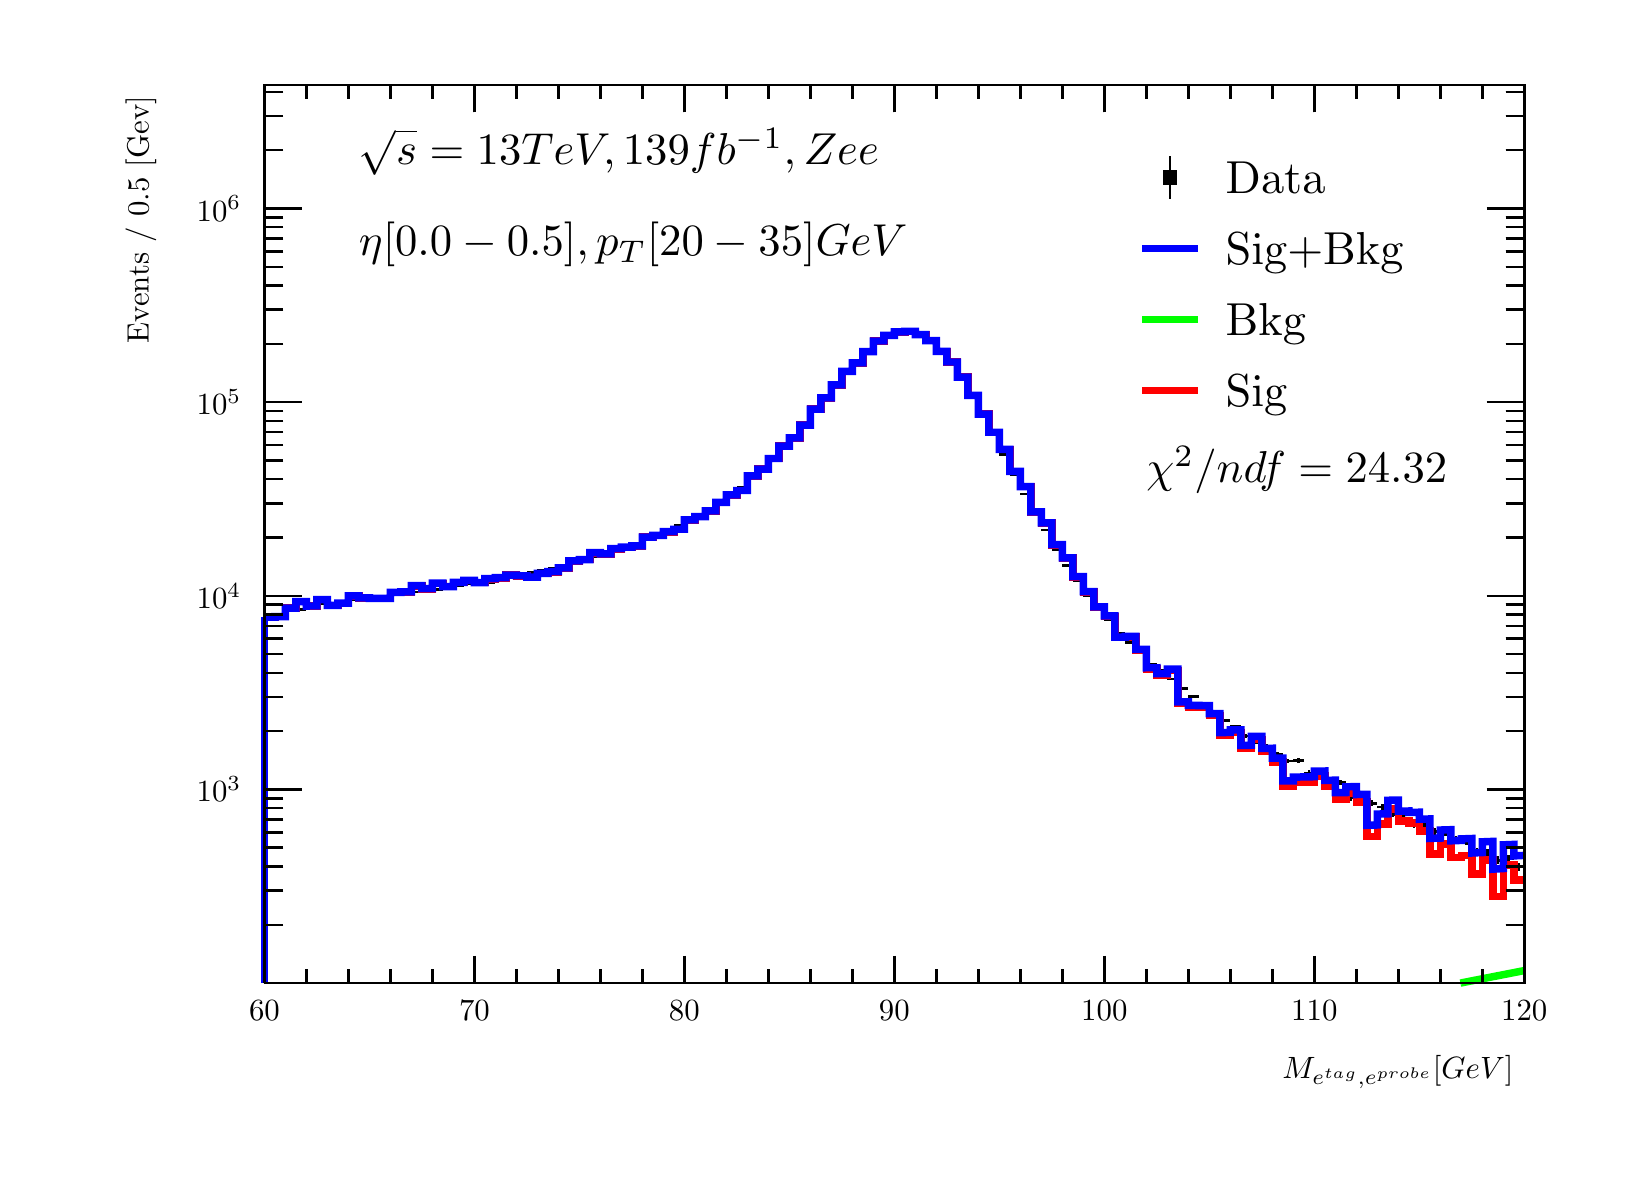
\begin{tikzpicture}
\pgfdeclareplotmark{cross} {
\pgfpathmoveto{\pgfpoint{-0.3\pgfplotmarksize}{\pgfplotmarksize}}
\pgfpathlineto{\pgfpoint{+0.3\pgfplotmarksize}{\pgfplotmarksize}}
\pgfpathlineto{\pgfpoint{+0.3\pgfplotmarksize}{0.3\pgfplotmarksize}}
\pgfpathlineto{\pgfpoint{+1\pgfplotmarksize}{0.3\pgfplotmarksize}}
\pgfpathlineto{\pgfpoint{+1\pgfplotmarksize}{-0.3\pgfplotmarksize}}
\pgfpathlineto{\pgfpoint{+0.3\pgfplotmarksize}{-0.3\pgfplotmarksize}}
\pgfpathlineto{\pgfpoint{+0.3\pgfplotmarksize}{-1.\pgfplotmarksize}}
\pgfpathlineto{\pgfpoint{-0.3\pgfplotmarksize}{-1.\pgfplotmarksize}}
\pgfpathlineto{\pgfpoint{-0.3\pgfplotmarksize}{-0.3\pgfplotmarksize}}
\pgfpathlineto{\pgfpoint{-1.\pgfplotmarksize}{-0.3\pgfplotmarksize}}
\pgfpathlineto{\pgfpoint{-1.\pgfplotmarksize}{0.3\pgfplotmarksize}}
\pgfpathlineto{\pgfpoint{-0.3\pgfplotmarksize}{0.3\pgfplotmarksize}}
\pgfpathclose
\pgfusepathqstroke
}
\pgfdeclareplotmark{cross*} {
\pgfpathmoveto{\pgfpoint{-0.3\pgfplotmarksize}{\pgfplotmarksize}}
\pgfpathlineto{\pgfpoint{+0.3\pgfplotmarksize}{\pgfplotmarksize}}
\pgfpathlineto{\pgfpoint{+0.3\pgfplotmarksize}{0.3\pgfplotmarksize}}
\pgfpathlineto{\pgfpoint{+1\pgfplotmarksize}{0.3\pgfplotmarksize}}
\pgfpathlineto{\pgfpoint{+1\pgfplotmarksize}{-0.3\pgfplotmarksize}}
\pgfpathlineto{\pgfpoint{+0.3\pgfplotmarksize}{-0.3\pgfplotmarksize}}
\pgfpathlineto{\pgfpoint{+0.3\pgfplotmarksize}{-1.\pgfplotmarksize}}
\pgfpathlineto{\pgfpoint{-0.3\pgfplotmarksize}{-1.\pgfplotmarksize}}
\pgfpathlineto{\pgfpoint{-0.3\pgfplotmarksize}{-0.3\pgfplotmarksize}}
\pgfpathlineto{\pgfpoint{-1.\pgfplotmarksize}{-0.3\pgfplotmarksize}}
\pgfpathlineto{\pgfpoint{-1.\pgfplotmarksize}{0.3\pgfplotmarksize}}
\pgfpathlineto{\pgfpoint{-0.3\pgfplotmarksize}{0.3\pgfplotmarksize}}
\pgfpathclose
\pgfusepathqfillstroke
}
\pgfdeclareplotmark{newstar} {
\pgfpathmoveto{\pgfqpoint{0pt}{\pgfplotmarksize}}
\pgfpathlineto{\pgfqpointpolar{44}{0.5\pgfplotmarksize}}
\pgfpathlineto{\pgfqpointpolar{18}{\pgfplotmarksize}}
\pgfpathlineto{\pgfqpointpolar{-20}{0.5\pgfplotmarksize}}
\pgfpathlineto{\pgfqpointpolar{-54}{\pgfplotmarksize}}
\pgfpathlineto{\pgfqpointpolar{-90}{0.5\pgfplotmarksize}}
\pgfpathlineto{\pgfqpointpolar{234}{\pgfplotmarksize}}
\pgfpathlineto{\pgfqpointpolar{198}{0.5\pgfplotmarksize}}
\pgfpathlineto{\pgfqpointpolar{162}{\pgfplotmarksize}}
\pgfpathlineto{\pgfqpointpolar{134}{0.5\pgfplotmarksize}}
\pgfpathclose
\pgfusepathqstroke
}
\pgfdeclareplotmark{newstar*} {
\pgfpathmoveto{\pgfqpoint{0pt}{\pgfplotmarksize}}
\pgfpathlineto{\pgfqpointpolar{44}{0.5\pgfplotmarksize}}
\pgfpathlineto{\pgfqpointpolar{18}{\pgfplotmarksize}}
\pgfpathlineto{\pgfqpointpolar{-20}{0.5\pgfplotmarksize}}
\pgfpathlineto{\pgfqpointpolar{-54}{\pgfplotmarksize}}
\pgfpathlineto{\pgfqpointpolar{-90}{0.5\pgfplotmarksize}}
\pgfpathlineto{\pgfqpointpolar{234}{\pgfplotmarksize}}
\pgfpathlineto{\pgfqpointpolar{198}{0.5\pgfplotmarksize}}
\pgfpathlineto{\pgfqpointpolar{162}{\pgfplotmarksize}}
\pgfpathlineto{\pgfqpointpolar{134}{0.5\pgfplotmarksize}}
\pgfpathclose
\pgfusepathqfillstroke
}
\definecolor{c}{rgb}{1,1,1};
\draw [color=c, fill=c] (0,0) rectangle (20,14.4361);
\draw [color=c, fill=c] (3,2.30977) rectangle (19,13.7143);
\definecolor{c}{rgb}{0,0,0};
\draw [c,line width=0.9] (3,2.30977) -- (3,13.7143) -- (19,13.7143) -- (19,2.30977) -- (3,2.30977);
\definecolor{c}{rgb}{1,1,1};
\draw [color=c, fill=c] (3,2.30977) rectangle (19,13.7143);
\definecolor{c}{rgb}{0,0,0};
\draw [c,line width=0.9] (3,2.30977) -- (3,13.7143) -- (19,13.7143) -- (19,2.30977) -- (3,2.30977);
\draw [c,line width=0.9] (3,2.30977) -- (19,2.30977);
\draw [c,line width=0.9] (3,2.65624) -- (3,2.30977);
\draw [c,line width=0.9] (3.53333,2.48301) -- (3.53333,2.30977);
\draw [c,line width=0.9] (4.06667,2.48301) -- (4.06667,2.30977);
\draw [c,line width=0.9] (4.6,2.48301) -- (4.6,2.30977);
\draw [c,line width=0.9] (5.13333,2.48301) -- (5.13333,2.30977);
\draw [c,line width=0.9] (5.66667,2.65624) -- (5.66667,2.30977);
\draw [c,line width=0.9] (6.2,2.48301) -- (6.2,2.30977);
\draw [c,line width=0.9] (6.73333,2.48301) -- (6.73333,2.30977);
\draw [c,line width=0.9] (7.26667,2.48301) -- (7.26667,2.30977);
\draw [c,line width=0.9] (7.8,2.48301) -- (7.8,2.30977);
\draw [c,line width=0.9] (8.33333,2.65624) -- (8.33333,2.30977);
\draw [c,line width=0.9] (8.86667,2.48301) -- (8.86667,2.30977);
\draw [c,line width=0.9] (9.4,2.48301) -- (9.4,2.30977);
\draw [c,line width=0.9] (9.93333,2.48301) -- (9.93333,2.30977);
\draw [c,line width=0.9] (10.4667,2.48301) -- (10.4667,2.30977);
\draw [c,line width=0.9] (11,2.65624) -- (11,2.30977);
\draw [c,line width=0.9] (11.5333,2.48301) -- (11.5333,2.30977);
\draw [c,line width=0.9] (12.0667,2.48301) -- (12.0667,2.30977);
\draw [c,line width=0.9] (12.6,2.48301) -- (12.6,2.30977);
\draw [c,line width=0.9] (13.1333,2.48301) -- (13.1333,2.30977);
\draw [c,line width=0.9] (13.6667,2.65624) -- (13.6667,2.30977);
\draw [c,line width=0.9] (14.2,2.48301) -- (14.2,2.30977);
\draw [c,line width=0.9] (14.7333,2.48301) -- (14.7333,2.30977);
\draw [c,line width=0.9] (15.2667,2.48301) -- (15.2667,2.30977);
\draw [c,line width=0.9] (15.8,2.48301) -- (15.8,2.30977);
\draw [c,line width=0.9] (16.3333,2.65624) -- (16.3333,2.30977);
\draw [c,line width=0.9] (16.8667,2.48301) -- (16.8667,2.30977);
\draw [c,line width=0.9] (17.4,2.48301) -- (17.4,2.30977);
\draw [c,line width=0.9] (17.9333,2.48301) -- (17.9333,2.30977);
\draw [c,line width=0.9] (18.4667,2.48301) -- (18.4667,2.30977);
\draw [c,line width=0.9] (19,2.65624) -- (19,2.30977);
\draw [anchor=base] (3,1.83338) node[scale=1.11327, color=c, rotate=0]{60};
\draw [anchor=base] (5.66667,1.83338) node[scale=1.11327, color=c, rotate=0]{70};
\draw [anchor=base] (8.33333,1.83338) node[scale=1.11327, color=c, rotate=0]{80};
\draw [anchor=base] (11,1.83338) node[scale=1.11327, color=c, rotate=0]{90};
\draw [anchor=base] (13.6667,1.83338) node[scale=1.11327, color=c, rotate=0]{100};
\draw [anchor=base] (16.3333,1.83338) node[scale=1.11327, color=c, rotate=0]{110};
\draw [anchor=base] (19,1.83338) node[scale=1.11327, color=c, rotate=0]{120};
\draw [anchor= east] (19,1.17798) node[scale=1.11327, color=c, rotate=0]{$M_{e^{tag}, e^{probe}}  [GeV]$};
\draw [c,line width=0.9] (3,13.7143) -- (19,13.7143);
\draw [c,line width=0.9] (3,13.3678) -- (3,13.7143);
\draw [c,line width=0.9] (3.53333,13.5411) -- (3.53333,13.7143);
\draw [c,line width=0.9] (4.06667,13.5411) -- (4.06667,13.7143);
\draw [c,line width=0.9] (4.6,13.5411) -- (4.6,13.7143);
\draw [c,line width=0.9] (5.13333,13.5411) -- (5.13333,13.7143);
\draw [c,line width=0.9] (5.66667,13.3678) -- (5.66667,13.7143);
\draw [c,line width=0.9] (6.2,13.5411) -- (6.2,13.7143);
\draw [c,line width=0.9] (6.73333,13.5411) -- (6.73333,13.7143);
\draw [c,line width=0.9] (7.26667,13.5411) -- (7.26667,13.7143);
\draw [c,line width=0.9] (7.8,13.5411) -- (7.8,13.7143);
\draw [c,line width=0.9] (8.33333,13.3678) -- (8.33333,13.7143);
\draw [c,line width=0.9] (8.86667,13.5411) -- (8.86667,13.7143);
\draw [c,line width=0.9] (9.4,13.5411) -- (9.4,13.7143);
\draw [c,line width=0.9] (9.93333,13.5411) -- (9.93333,13.7143);
\draw [c,line width=0.9] (10.4667,13.5411) -- (10.4667,13.7143);
\draw [c,line width=0.9] (11,13.3678) -- (11,13.7143);
\draw [c,line width=0.9] (11.5333,13.5411) -- (11.5333,13.7143);
\draw [c,line width=0.9] (12.0667,13.5411) -- (12.0667,13.7143);
\draw [c,line width=0.9] (12.6,13.5411) -- (12.6,13.7143);
\draw [c,line width=0.9] (13.1333,13.5411) -- (13.1333,13.7143);
\draw [c,line width=0.9] (13.6667,13.3678) -- (13.6667,13.7143);
\draw [c,line width=0.9] (14.2,13.5411) -- (14.2,13.7143);
\draw [c,line width=0.9] (14.7333,13.5411) -- (14.7333,13.7143);
\draw [c,line width=0.9] (15.2667,13.5411) -- (15.2667,13.7143);
\draw [c,line width=0.9] (15.8,13.5411) -- (15.8,13.7143);
\draw [c,line width=0.9] (16.3333,13.3678) -- (16.3333,13.7143);
\draw [c,line width=0.9] (16.8667,13.5411) -- (16.8667,13.7143);
\draw [c,line width=0.9] (17.4,13.5411) -- (17.4,13.7143);
\draw [c,line width=0.9] (17.9333,13.5411) -- (17.9333,13.7143);
\draw [c,line width=0.9] (18.4667,13.5411) -- (18.4667,13.7143);
\draw [c,line width=0.9] (19,13.3678) -- (19,13.7143);
\draw [c,line width=0.9] (3,2.30977) -- (3,13.7143);
\draw [c,line width=0.9] (3.237,3.05008) -- (3,3.05008);
\draw [c,line width=0.9] (3.237,3.48313) -- (3,3.48313);
\draw [c,line width=0.9] (3.237,3.79038) -- (3,3.79038);
\draw [c,line width=0.9] (3.237,4.02871) -- (3,4.02871);
\draw [c,line width=0.9] (3.237,4.22343) -- (3,4.22343);
\draw [c,line width=0.9] (3.237,4.38807) -- (3,4.38807);
\draw [c,line width=0.9] (3.237,4.53069) -- (3,4.53069);
\draw [c,line width=0.9] (3.237,4.65649) -- (3,4.65649);
\draw [c,line width=0.9] (3.474,4.76901) -- (3,4.76901);
\draw [anchor= east] (2.844,4.76901) node[scale=1.11327, color=c, rotate=0]{$10^{3}$};
\draw [c,line width=0.9] (3.237,5.50932) -- (3,5.50932);
\draw [c,line width=0.9] (3.237,5.94237) -- (3,5.94237);
\draw [c,line width=0.9] (3.237,6.24963) -- (3,6.24963);
\draw [c,line width=0.9] (3.237,6.48795) -- (3,6.48795);
\draw [c,line width=0.9] (3.237,6.68268) -- (3,6.68268);
\draw [c,line width=0.9] (3.237,6.84731) -- (3,6.84731);
\draw [c,line width=0.9] (3.237,6.98993) -- (3,6.98993);
\draw [c,line width=0.9] (3.237,7.11573) -- (3,7.11573);
\draw [c,line width=0.9] (3.474,7.22826) -- (3,7.22826);
\draw [anchor= east] (2.844,7.22826) node[scale=1.11327, color=c, rotate=0]{$10^{4}$};
\draw [c,line width=0.9] (3.237,7.96856) -- (3,7.96856);
\draw [c,line width=0.9] (3.237,8.40161) -- (3,8.40161);
\draw [c,line width=0.9] (3.237,8.70887) -- (3,8.70887);
\draw [c,line width=0.9] (3.237,8.94719) -- (3,8.94719);
\draw [c,line width=0.9] (3.237,9.14192) -- (3,9.14192);
\draw [c,line width=0.9] (3.237,9.30656) -- (3,9.30656);
\draw [c,line width=0.9] (3.237,9.44917) -- (3,9.44917);
\draw [c,line width=0.9] (3.237,9.57497) -- (3,9.57497);
\draw [c,line width=0.9] (3.474,9.6875) -- (3,9.6875);
\draw [anchor= east] (2.844,9.6875) node[scale=1.11327, color=c, rotate=0]{$10^{5}$};
\draw [c,line width=0.9] (3.237,10.4278) -- (3,10.4278);
\draw [c,line width=0.9] (3.237,10.8609) -- (3,10.8609);
\draw [c,line width=0.9] (3.237,11.1681) -- (3,11.1681);
\draw [c,line width=0.9] (3.237,11.4064) -- (3,11.4064);
\draw [c,line width=0.9] (3.237,11.6012) -- (3,11.6012);
\draw [c,line width=0.9] (3.237,11.7658) -- (3,11.7658);
\draw [c,line width=0.9] (3.237,11.9084) -- (3,11.9084);
\draw [c,line width=0.9] (3.237,12.0342) -- (3,12.0342);
\draw [c,line width=0.9] (3.474,12.1467) -- (3,12.1467);
\draw [anchor= east] (2.844,12.1467) node[scale=1.11327, color=c, rotate=0]{$10^{6}$};
\draw [c,line width=0.9] (3.237,12.887) -- (3,12.887);
\draw [c,line width=0.9] (3.237,13.3201) -- (3,13.3201);
\draw [c,line width=0.9] (3.237,13.6274) -- (3,13.6274);
\draw [anchor= east] (1.432,13.7143) node[scale=1.11327, color=c, rotate=90]{Events / 0.5 [Gev]};
\draw [c,line width=0.9] (19,2.30977) -- (19,13.7143);
\draw [c,line width=0.9] (18.763,3.05008) -- (19,3.05008);
\draw [c,line width=0.9] (18.763,3.48313) -- (19,3.48313);
\draw [c,line width=0.9] (18.763,3.79038) -- (19,3.79038);
\draw [c,line width=0.9] (18.763,4.02871) -- (19,4.02871);
\draw [c,line width=0.9] (18.763,4.22343) -- (19,4.22343);
\draw [c,line width=0.9] (18.763,4.38807) -- (19,4.38807);
\draw [c,line width=0.9] (18.763,4.53069) -- (19,4.53069);
\draw [c,line width=0.9] (18.763,4.65649) -- (19,4.65649);
\draw [c,line width=0.9] (18.526,4.76901) -- (19,4.76901);
\draw [c,line width=0.9] (18.763,5.50932) -- (19,5.50932);
\draw [c,line width=0.9] (18.763,5.94237) -- (19,5.94237);
\draw [c,line width=0.9] (18.763,6.24963) -- (19,6.24963);
\draw [c,line width=0.9] (18.763,6.48795) -- (19,6.48795);
\draw [c,line width=0.9] (18.763,6.68268) -- (19,6.68268);
\draw [c,line width=0.9] (18.763,6.84731) -- (19,6.84731);
\draw [c,line width=0.9] (18.763,6.98993) -- (19,6.98993);
\draw [c,line width=0.9] (18.763,7.11573) -- (19,7.11573);
\draw [c,line width=0.9] (18.526,7.22826) -- (19,7.22826);
\draw [c,line width=0.9] (18.763,7.96856) -- (19,7.96856);
\draw [c,line width=0.9] (18.763,8.40161) -- (19,8.40161);
\draw [c,line width=0.9] (18.763,8.70887) -- (19,8.70887);
\draw [c,line width=0.9] (18.763,8.94719) -- (19,8.94719);
\draw [c,line width=0.9] (18.763,9.14192) -- (19,9.14192);
\draw [c,line width=0.9] (18.763,9.30656) -- (19,9.30656);
\draw [c,line width=0.9] (18.763,9.44917) -- (19,9.44917);
\draw [c,line width=0.9] (18.763,9.57497) -- (19,9.57497);
\draw [c,line width=0.9] (18.526,9.6875) -- (19,9.6875);
\draw [c,line width=0.9] (18.763,10.4278) -- (19,10.4278);
\draw [c,line width=0.9] (18.763,10.8609) -- (19,10.8609);
\draw [c,line width=0.9] (18.763,11.1681) -- (19,11.1681);
\draw [c,line width=0.9] (18.763,11.4064) -- (19,11.4064);
\draw [c,line width=0.9] (18.763,11.6012) -- (19,11.6012);
\draw [c,line width=0.9] (18.763,11.7658) -- (19,11.7658);
\draw [c,line width=0.9] (18.763,11.9084) -- (19,11.9084);
\draw [c,line width=0.9] (18.763,12.0342) -- (19,12.0342);
\draw [c,line width=0.9] (18.526,12.1467) -- (19,12.1467);
\draw [c,line width=0.9] (18.763,12.887) -- (19,12.887);
\draw [c,line width=0.9] (18.763,13.3201) -- (19,13.3201);
\draw [c,line width=0.9] (18.763,13.6274) -- (19,13.6274);
\draw [c,line width=0.9] (3.06667,6.97555) -- (3,6.97555);
\draw [c,line width=0.9] (3,6.97555) -- (3,6.97555);
\draw [c,line width=0.9] (3.06667,6.97555) -- (3.13333,6.97555);
\draw [c,line width=0.9] (3.13333,6.97555) -- (3.13333,6.97555);
\draw [c,line width=0.9] (3.06667,6.97555) -- (3.06667,6.98757);
\draw [c,line width=0.9] (3.06667,6.98757) -- (3.06667,6.98757);
\draw [c,line width=0.9] (3.06667,6.97555) -- (3.06667,6.96353);
\draw [c,line width=0.9] (3.06667,6.96353) -- (3.06667,6.96353);
\draw [c,line width=0.9] (3.2,6.99897) -- (3.13333,6.99897);
\draw [c,line width=0.9] (3.13333,6.99897) -- (3.13333,6.99897);
\draw [c,line width=0.9] (3.2,6.99897) -- (3.26667,6.99897);
\draw [c,line width=0.9] (3.26667,6.99897) -- (3.26667,6.99897);
\draw [c,line width=0.9] (3.2,6.99897) -- (3.2,7.01086);
\draw [c,line width=0.9] (3.2,7.01086) -- (3.2,7.01086);
\draw [c,line width=0.9] (3.2,6.99897) -- (3.2,6.98708);
\draw [c,line width=0.9] (3.2,6.98708) -- (3.2,6.98708);
\draw [c,line width=0.9] (3.33333,7.05305) -- (3.26667,7.05305);
\draw [c,line width=0.9] (3.26667,7.05305) -- (3.26667,7.05305);
\draw [c,line width=0.9] (3.33333,7.05305) -- (3.4,7.05305);
\draw [c,line width=0.9] (3.4,7.05305) -- (3.4,7.05305);
\draw [c,line width=0.9] (3.33333,7.05305) -- (3.33333,7.06464);
\draw [c,line width=0.9] (3.33333,7.06464) -- (3.33333,7.06464);
\draw [c,line width=0.9] (3.33333,7.05305) -- (3.33333,7.04145);
\draw [c,line width=0.9] (3.33333,7.04145) -- (3.33333,7.04145);
\draw [c,line width=0.9] (3.46667,7.05619) -- (3.4,7.05619);
\draw [c,line width=0.9] (3.4,7.05619) -- (3.4,7.05619);
\draw [c,line width=0.9] (3.46667,7.05619) -- (3.53333,7.05619);
\draw [c,line width=0.9] (3.53333,7.05619) -- (3.53333,7.05619);
\draw [c,line width=0.9] (3.46667,7.05619) -- (3.46667,7.06776);
\draw [c,line width=0.9] (3.46667,7.06776) -- (3.46667,7.06776);
\draw [c,line width=0.9] (3.46667,7.05619) -- (3.46667,7.04461);
\draw [c,line width=0.9] (3.46667,7.04461) -- (3.46667,7.04461);
\draw [c,line width=0.9] (3.6,7.09403) -- (3.53333,7.09403);
\draw [c,line width=0.9] (3.53333,7.09403) -- (3.53333,7.09403);
\draw [c,line width=0.9] (3.6,7.09403) -- (3.66667,7.09403);
\draw [c,line width=0.9] (3.66667,7.09403) -- (3.66667,7.09403);
\draw [c,line width=0.9] (3.6,7.09403) -- (3.6,7.1054);
\draw [c,line width=0.9] (3.6,7.1054) -- (3.6,7.1054);
\draw [c,line width=0.9] (3.6,7.09403) -- (3.6,7.08266);
\draw [c,line width=0.9] (3.6,7.08266) -- (3.6,7.08266);
\draw [c,line width=0.9] (3.73333,7.12094) -- (3.66667,7.12094);
\draw [c,line width=0.9] (3.66667,7.12094) -- (3.66667,7.12094);
\draw [c,line width=0.9] (3.73333,7.12094) -- (3.8,7.12094);
\draw [c,line width=0.9] (3.8,7.12094) -- (3.8,7.12094);
\draw [c,line width=0.9] (3.73333,7.12094) -- (3.73333,7.13217);
\draw [c,line width=0.9] (3.73333,7.13217) -- (3.73333,7.13217);
\draw [c,line width=0.9] (3.73333,7.12094) -- (3.73333,7.10971);
\draw [c,line width=0.9] (3.73333,7.10971) -- (3.73333,7.10971);
\draw [c,line width=0.9] (3.86667,7.1328) -- (3.8,7.1328);
\draw [c,line width=0.9] (3.8,7.1328) -- (3.8,7.1328);
\draw [c,line width=0.9] (3.86667,7.1328) -- (3.93333,7.1328);
\draw [c,line width=0.9] (3.93333,7.1328) -- (3.93333,7.1328);
\draw [c,line width=0.9] (3.86667,7.1328) -- (3.86667,7.14397);
\draw [c,line width=0.9] (3.86667,7.14397) -- (3.86667,7.14397);
\draw [c,line width=0.9] (3.86667,7.1328) -- (3.86667,7.12163);
\draw [c,line width=0.9] (3.86667,7.12163) -- (3.86667,7.12163);
\draw [c,line width=0.9] (4,7.15407) -- (3.93333,7.15407);
\draw [c,line width=0.9] (3.93333,7.15407) -- (3.93333,7.15407);
\draw [c,line width=0.9] (4,7.15407) -- (4.06667,7.15407);
\draw [c,line width=0.9] (4.06667,7.15407) -- (4.06667,7.15407);
\draw [c,line width=0.9] (4,7.15407) -- (4,7.16513);
\draw [c,line width=0.9] (4,7.16513) -- (4,7.16513);
\draw [c,line width=0.9] (4,7.15407) -- (4,7.14302);
\draw [c,line width=0.9] (4,7.14302) -- (4,7.14302);
\draw [c,line width=0.9] (4.13333,7.18377) -- (4.06667,7.18377);
\draw [c,line width=0.9] (4.06667,7.18377) -- (4.06667,7.18377);
\draw [c,line width=0.9] (4.13333,7.18377) -- (4.2,7.18377);
\draw [c,line width=0.9] (4.2,7.18377) -- (4.2,7.18377);
\draw [c,line width=0.9] (4.13333,7.18377) -- (4.13333,7.19467);
\draw [c,line width=0.9] (4.13333,7.19467) -- (4.13333,7.19467);
\draw [c,line width=0.9] (4.13333,7.18377) -- (4.13333,7.17286);
\draw [c,line width=0.9] (4.13333,7.17286) -- (4.13333,7.17286);
\draw [c,line width=0.9] (4.26667,7.21439) -- (4.2,7.21439);
\draw [c,line width=0.9] (4.2,7.21439) -- (4.2,7.21439);
\draw [c,line width=0.9] (4.26667,7.21439) -- (4.33333,7.21439);
\draw [c,line width=0.9] (4.33333,7.21439) -- (4.33333,7.21439);
\draw [c,line width=0.9] (4.26667,7.21439) -- (4.26667,7.22514);
\draw [c,line width=0.9] (4.26667,7.22514) -- (4.26667,7.22514);
\draw [c,line width=0.9] (4.26667,7.21439) -- (4.26667,7.20364);
\draw [c,line width=0.9] (4.26667,7.20364) -- (4.26667,7.20364);
\draw [c,line width=0.9] (4.4,7.21114) -- (4.33333,7.21114);
\draw [c,line width=0.9] (4.33333,7.21114) -- (4.33333,7.21114);
\draw [c,line width=0.9] (4.4,7.21114) -- (4.46667,7.21114);
\draw [c,line width=0.9] (4.46667,7.21114) -- (4.46667,7.21114);
\draw [c,line width=0.9] (4.4,7.21114) -- (4.4,7.22191);
\draw [c,line width=0.9] (4.4,7.22191) -- (4.4,7.22191);
\draw [c,line width=0.9] (4.4,7.21114) -- (4.4,7.20037);
\draw [c,line width=0.9] (4.4,7.20037) -- (4.4,7.20037);
\draw [c,line width=0.9] (4.53333,7.21979) -- (4.46667,7.21979);
\draw [c,line width=0.9] (4.46667,7.21979) -- (4.46667,7.21979);
\draw [c,line width=0.9] (4.53333,7.21979) -- (4.6,7.21979);
\draw [c,line width=0.9] (4.6,7.21979) -- (4.6,7.21979);
\draw [c,line width=0.9] (4.53333,7.21979) -- (4.53333,7.23051);
\draw [c,line width=0.9] (4.53333,7.23051) -- (4.53333,7.23051);
\draw [c,line width=0.9] (4.53333,7.21979) -- (4.53333,7.20906);
\draw [c,line width=0.9] (4.53333,7.20906) -- (4.53333,7.20906);
\draw [c,line width=0.9] (4.66667,7.23878) -- (4.6,7.23878);
\draw [c,line width=0.9] (4.6,7.23878) -- (4.6,7.23878);
\draw [c,line width=0.9] (4.66667,7.23878) -- (4.73333,7.23878);
\draw [c,line width=0.9] (4.73333,7.23878) -- (4.73333,7.23878);
\draw [c,line width=0.9] (4.66667,7.23878) -- (4.66667,7.24941);
\draw [c,line width=0.9] (4.66667,7.24941) -- (4.66667,7.24941);
\draw [c,line width=0.9] (4.66667,7.23878) -- (4.66667,7.22815);
\draw [c,line width=0.9] (4.66667,7.22815) -- (4.66667,7.22815);
\draw [c,line width=0.9] (4.8,7.28756) -- (4.73333,7.28756);
\draw [c,line width=0.9] (4.73333,7.28756) -- (4.73333,7.28756);
\draw [c,line width=0.9] (4.8,7.28756) -- (4.86667,7.28756);
\draw [c,line width=0.9] (4.86667,7.28756) -- (4.86667,7.28756);
\draw [c,line width=0.9] (4.8,7.28756) -- (4.8,7.29795);
\draw [c,line width=0.9] (4.8,7.29795) -- (4.8,7.29795);
\draw [c,line width=0.9] (4.8,7.28756) -- (4.8,7.27718);
\draw [c,line width=0.9] (4.8,7.27718) -- (4.8,7.27718);
\draw [c,line width=0.9] (4.93333,7.27425) -- (4.86667,7.27425);
\draw [c,line width=0.9] (4.86667,7.27425) -- (4.86667,7.27425);
\draw [c,line width=0.9] (4.93333,7.27425) -- (5,7.27425);
\draw [c,line width=0.9] (5,7.27425) -- (5,7.27425);
\draw [c,line width=0.9] (4.93333,7.27425) -- (4.93333,7.2847);
\draw [c,line width=0.9] (4.93333,7.2847) -- (4.93333,7.2847);
\draw [c,line width=0.9] (4.93333,7.27425) -- (4.93333,7.26379);
\draw [c,line width=0.9] (4.93333,7.26379) -- (4.93333,7.26379);
\draw [c,line width=0.9] (5.06667,7.30986) -- (5,7.30986);
\draw [c,line width=0.9] (5,7.30986) -- (5,7.30986);
\draw [c,line width=0.9] (5.06667,7.30986) -- (5.13333,7.30986);
\draw [c,line width=0.9] (5.13333,7.30986) -- (5.13333,7.30986);
\draw [c,line width=0.9] (5.06667,7.30986) -- (5.06667,7.32014);
\draw [c,line width=0.9] (5.06667,7.32014) -- (5.06667,7.32014);
\draw [c,line width=0.9] (5.06667,7.30986) -- (5.06667,7.29958);
\draw [c,line width=0.9] (5.06667,7.29958) -- (5.06667,7.29958);
\draw [c,line width=0.9] (5.2,7.31065) -- (5.13333,7.31065);
\draw [c,line width=0.9] (5.13333,7.31065) -- (5.13333,7.31065);
\draw [c,line width=0.9] (5.2,7.31065) -- (5.26667,7.31065);
\draw [c,line width=0.9] (5.26667,7.31065) -- (5.26667,7.31065);
\draw [c,line width=0.9] (5.2,7.31065) -- (5.2,7.32093);
\draw [c,line width=0.9] (5.2,7.32093) -- (5.2,7.32093);
\draw [c,line width=0.9] (5.2,7.31065) -- (5.2,7.30038);
\draw [c,line width=0.9] (5.2,7.30038) -- (5.2,7.30038);
\draw [c,line width=0.9] (5.33333,7.34844) -- (5.26667,7.34844);
\draw [c,line width=0.9] (5.26667,7.34844) -- (5.26667,7.34844);
\draw [c,line width=0.9] (5.33333,7.34844) -- (5.4,7.34844);
\draw [c,line width=0.9] (5.4,7.34844) -- (5.4,7.34844);
\draw [c,line width=0.9] (5.33333,7.34844) -- (5.33333,7.35853);
\draw [c,line width=0.9] (5.33333,7.35853) -- (5.33333,7.35853);
\draw [c,line width=0.9] (5.33333,7.34844) -- (5.33333,7.33834);
\draw [c,line width=0.9] (5.33333,7.33834) -- (5.33333,7.33834);
\draw [c,line width=0.9] (5.46667,7.35358) -- (5.4,7.35358);
\draw [c,line width=0.9] (5.4,7.35358) -- (5.4,7.35358);
\draw [c,line width=0.9] (5.46667,7.35358) -- (5.53333,7.35358);
\draw [c,line width=0.9] (5.53333,7.35358) -- (5.53333,7.35358);
\draw [c,line width=0.9] (5.46667,7.35358) -- (5.46667,7.36365);
\draw [c,line width=0.9] (5.46667,7.36365) -- (5.46667,7.36365);
\draw [c,line width=0.9] (5.46667,7.35358) -- (5.46667,7.34351);
\draw [c,line width=0.9] (5.46667,7.34351) -- (5.46667,7.34351);
\draw [c,line width=0.9] (5.6,7.38401) -- (5.53333,7.38401);
\draw [c,line width=0.9] (5.53333,7.38401) -- (5.53333,7.38401);
\draw [c,line width=0.9] (5.6,7.38401) -- (5.66667,7.38401);
\draw [c,line width=0.9] (5.66667,7.38401) -- (5.66667,7.38401);
\draw [c,line width=0.9] (5.6,7.38401) -- (5.6,7.39394);
\draw [c,line width=0.9] (5.6,7.39394) -- (5.6,7.39394);
\draw [c,line width=0.9] (5.6,7.38401) -- (5.6,7.37408);
\draw [c,line width=0.9] (5.6,7.37408) -- (5.6,7.37408);
\draw [c,line width=0.9] (5.73333,7.39649) -- (5.66667,7.39649);
\draw [c,line width=0.9] (5.66667,7.39649) -- (5.66667,7.39649);
\draw [c,line width=0.9] (5.73333,7.39649) -- (5.8,7.39649);
\draw [c,line width=0.9] (5.8,7.39649) -- (5.8,7.39649);
\draw [c,line width=0.9] (5.73333,7.39649) -- (5.73333,7.40636);
\draw [c,line width=0.9] (5.73333,7.40636) -- (5.73333,7.40636);
\draw [c,line width=0.9] (5.73333,7.39649) -- (5.73333,7.38662);
\draw [c,line width=0.9] (5.73333,7.38662) -- (5.73333,7.38662);
\draw [c,line width=0.9] (5.86667,7.39722) -- (5.8,7.39722);
\draw [c,line width=0.9] (5.8,7.39722) -- (5.8,7.39722);
\draw [c,line width=0.9] (5.86667,7.39722) -- (5.93333,7.39722);
\draw [c,line width=0.9] (5.93333,7.39722) -- (5.93333,7.39722);
\draw [c,line width=0.9] (5.86667,7.39722) -- (5.86667,7.40709);
\draw [c,line width=0.9] (5.86667,7.40709) -- (5.86667,7.40709);
\draw [c,line width=0.9] (5.86667,7.39722) -- (5.86667,7.38735);
\draw [c,line width=0.9] (5.86667,7.38735) -- (5.86667,7.38735);
\draw [c,line width=0.9] (6,7.44378) -- (5.93333,7.44378);
\draw [c,line width=0.9] (5.93333,7.44378) -- (5.93333,7.44378);
\draw [c,line width=0.9] (6,7.44378) -- (6.06667,7.44378);
\draw [c,line width=0.9] (6.06667,7.44378) -- (6.06667,7.44378);
\draw [c,line width=0.9] (6,7.44378) -- (6,7.45344);
\draw [c,line width=0.9] (6,7.45344) -- (6,7.45344);
\draw [c,line width=0.9] (6,7.44378) -- (6,7.43413);
\draw [c,line width=0.9] (6,7.43413) -- (6,7.43413);
\draw [c,line width=0.9] (6.13333,7.45403) -- (6.06667,7.45403);
\draw [c,line width=0.9] (6.06667,7.45403) -- (6.06667,7.45403);
\draw [c,line width=0.9] (6.13333,7.45403) -- (6.2,7.45403);
\draw [c,line width=0.9] (6.2,7.45403) -- (6.2,7.45403);
\draw [c,line width=0.9] (6.13333,7.45403) -- (6.13333,7.46364);
\draw [c,line width=0.9] (6.13333,7.46364) -- (6.13333,7.46364);
\draw [c,line width=0.9] (6.13333,7.45403) -- (6.13333,7.44443);
\draw [c,line width=0.9] (6.13333,7.44443) -- (6.13333,7.44443);
\draw [c,line width=0.9] (6.26667,7.5008) -- (6.2,7.5008);
\draw [c,line width=0.9] (6.2,7.5008) -- (6.2,7.5008);
\draw [c,line width=0.9] (6.26667,7.5008) -- (6.33333,7.5008);
\draw [c,line width=0.9] (6.33333,7.5008) -- (6.33333,7.5008);
\draw [c,line width=0.9] (6.26667,7.5008) -- (6.26667,7.5102);
\draw [c,line width=0.9] (6.26667,7.5102) -- (6.26667,7.5102);
\draw [c,line width=0.9] (6.26667,7.5008) -- (6.26667,7.4914);
\draw [c,line width=0.9] (6.26667,7.4914) -- (6.26667,7.4914);
\draw [c,line width=0.9] (6.4,7.52162) -- (6.33333,7.52162);
\draw [c,line width=0.9] (6.33333,7.52162) -- (6.33333,7.52162);
\draw [c,line width=0.9] (6.4,7.52162) -- (6.46667,7.52162);
\draw [c,line width=0.9] (6.46667,7.52162) -- (6.46667,7.52162);
\draw [c,line width=0.9] (6.4,7.52162) -- (6.4,7.53093);
\draw [c,line width=0.9] (6.4,7.53093) -- (6.4,7.53093);
\draw [c,line width=0.9] (6.4,7.52162) -- (6.4,7.51231);
\draw [c,line width=0.9] (6.4,7.51231) -- (6.4,7.51231);
\draw [c,line width=0.9] (6.53333,7.54941) -- (6.46667,7.54941);
\draw [c,line width=0.9] (6.46667,7.54941) -- (6.46667,7.54941);
\draw [c,line width=0.9] (6.53333,7.54941) -- (6.6,7.54941);
\draw [c,line width=0.9] (6.6,7.54941) -- (6.6,7.54941);
\draw [c,line width=0.9] (6.53333,7.54941) -- (6.53333,7.5586);
\draw [c,line width=0.9] (6.53333,7.5586) -- (6.53333,7.5586);
\draw [c,line width=0.9] (6.53333,7.54941) -- (6.53333,7.54022);
\draw [c,line width=0.9] (6.53333,7.54022) -- (6.53333,7.54022);
\draw [c,line width=0.9] (6.66667,7.58211) -- (6.6,7.58211);
\draw [c,line width=0.9] (6.6,7.58211) -- (6.6,7.58211);
\draw [c,line width=0.9] (6.66667,7.58211) -- (6.73333,7.58211);
\draw [c,line width=0.9] (6.73333,7.58211) -- (6.73333,7.58211);
\draw [c,line width=0.9] (6.66667,7.58211) -- (6.66667,7.59116);
\draw [c,line width=0.9] (6.66667,7.59116) -- (6.66667,7.59116);
\draw [c,line width=0.9] (6.66667,7.58211) -- (6.66667,7.57306);
\draw [c,line width=0.9] (6.66667,7.57306) -- (6.66667,7.57306);
\draw [c,line width=0.9] (6.8,7.61094) -- (6.73333,7.61094);
\draw [c,line width=0.9] (6.73333,7.61094) -- (6.73333,7.61094);
\draw [c,line width=0.9] (6.8,7.61094) -- (6.86667,7.61094);
\draw [c,line width=0.9] (6.86667,7.61094) -- (6.86667,7.61094);
\draw [c,line width=0.9] (6.8,7.61094) -- (6.8,7.61987);
\draw [c,line width=0.9] (6.8,7.61987) -- (6.8,7.61987);
\draw [c,line width=0.9] (6.8,7.61094) -- (6.8,7.60201);
\draw [c,line width=0.9] (6.8,7.60201) -- (6.8,7.60201);
\draw [c,line width=0.9] (6.93333,7.6331) -- (6.86667,7.6331);
\draw [c,line width=0.9] (6.86667,7.6331) -- (6.86667,7.6331);
\draw [c,line width=0.9] (6.93333,7.6331) -- (7,7.6331);
\draw [c,line width=0.9] (7,7.6331) -- (7,7.6331);
\draw [c,line width=0.9] (6.93333,7.6331) -- (6.93333,7.64194);
\draw [c,line width=0.9] (6.93333,7.64194) -- (6.93333,7.64194);
\draw [c,line width=0.9] (6.93333,7.6331) -- (6.93333,7.62426);
\draw [c,line width=0.9] (6.93333,7.62426) -- (6.93333,7.62426);
\draw [c,line width=0.9] (7.06667,7.66734) -- (7,7.66734);
\draw [c,line width=0.9] (7,7.66734) -- (7,7.66734);
\draw [c,line width=0.9] (7.06667,7.66734) -- (7.13333,7.66734);
\draw [c,line width=0.9] (7.13333,7.66734) -- (7.13333,7.66734);
\draw [c,line width=0.9] (7.06667,7.66734) -- (7.06667,7.67604);
\draw [c,line width=0.9] (7.06667,7.67604) -- (7.06667,7.67604);
\draw [c,line width=0.9] (7.06667,7.66734) -- (7.06667,7.65865);
\draw [c,line width=0.9] (7.06667,7.65865) -- (7.06667,7.65865);
\draw [c,line width=0.9] (7.2,7.71829) -- (7.13333,7.71829);
\draw [c,line width=0.9] (7.13333,7.71829) -- (7.13333,7.71829);
\draw [c,line width=0.9] (7.2,7.71829) -- (7.26667,7.71829);
\draw [c,line width=0.9] (7.26667,7.71829) -- (7.26667,7.71829);
\draw [c,line width=0.9] (7.2,7.71829) -- (7.2,7.72678);
\draw [c,line width=0.9] (7.2,7.72678) -- (7.2,7.72678);
\draw [c,line width=0.9] (7.2,7.71829) -- (7.2,7.7098);
\draw [c,line width=0.9] (7.2,7.7098) -- (7.2,7.7098);
\draw [c,line width=0.9] (7.33333,7.73961) -- (7.26667,7.73961);
\draw [c,line width=0.9] (7.26667,7.73961) -- (7.26667,7.73961);
\draw [c,line width=0.9] (7.33333,7.73961) -- (7.4,7.73961);
\draw [c,line width=0.9] (7.4,7.73961) -- (7.4,7.73961);
\draw [c,line width=0.9] (7.33333,7.73961) -- (7.33333,7.74801);
\draw [c,line width=0.9] (7.33333,7.74801) -- (7.33333,7.74801);
\draw [c,line width=0.9] (7.33333,7.73961) -- (7.33333,7.7312);
\draw [c,line width=0.9] (7.33333,7.7312) -- (7.33333,7.7312);
\draw [c,line width=0.9] (7.46667,7.78235) -- (7.4,7.78235);
\draw [c,line width=0.9] (7.4,7.78235) -- (7.4,7.78235);
\draw [c,line width=0.9] (7.46667,7.78235) -- (7.53333,7.78235);
\draw [c,line width=0.9] (7.53333,7.78235) -- (7.53333,7.78235);
\draw [c,line width=0.9] (7.46667,7.78235) -- (7.46667,7.79059);
\draw [c,line width=0.9] (7.46667,7.79059) -- (7.46667,7.79059);
\draw [c,line width=0.9] (7.46667,7.78235) -- (7.46667,7.77411);
\draw [c,line width=0.9] (7.46667,7.77411) -- (7.46667,7.77411);
\draw [c,line width=0.9] (7.6,7.83343) -- (7.53333,7.83343);
\draw [c,line width=0.9] (7.53333,7.83343) -- (7.53333,7.83343);
\draw [c,line width=0.9] (7.6,7.83343) -- (7.66667,7.83343);
\draw [c,line width=0.9] (7.66667,7.83343) -- (7.66667,7.83343);
\draw [c,line width=0.9] (7.6,7.83343) -- (7.6,7.84147);
\draw [c,line width=0.9] (7.6,7.84147) -- (7.6,7.84147);
\draw [c,line width=0.9] (7.6,7.83343) -- (7.6,7.82538);
\draw [c,line width=0.9] (7.6,7.82538) -- (7.6,7.82538);
\draw [c,line width=0.9] (7.73333,7.89025) -- (7.66667,7.89025);
\draw [c,line width=0.9] (7.66667,7.89025) -- (7.66667,7.89025);
\draw [c,line width=0.9] (7.73333,7.89025) -- (7.8,7.89025);
\draw [c,line width=0.9] (7.8,7.89025) -- (7.8,7.89025);
\draw [c,line width=0.9] (7.73333,7.89025) -- (7.73333,7.89808);
\draw [c,line width=0.9] (7.73333,7.89808) -- (7.73333,7.89808);
\draw [c,line width=0.9] (7.73333,7.89025) -- (7.73333,7.88242);
\draw [c,line width=0.9] (7.73333,7.88242) -- (7.73333,7.88242);
\draw [c,line width=0.9] (7.86667,7.94824) -- (7.8,7.94824);
\draw [c,line width=0.9] (7.8,7.94824) -- (7.8,7.94824);
\draw [c,line width=0.9] (7.86667,7.94824) -- (7.93333,7.94824);
\draw [c,line width=0.9] (7.93333,7.94824) -- (7.93333,7.94824);
\draw [c,line width=0.9] (7.86667,7.94824) -- (7.86667,7.95586);
\draw [c,line width=0.9] (7.86667,7.95586) -- (7.86667,7.95586);
\draw [c,line width=0.9] (7.86667,7.94824) -- (7.86667,7.94061);
\draw [c,line width=0.9] (7.86667,7.94061) -- (7.86667,7.94061);
\draw [c,line width=0.9] (8,7.99107) -- (7.93333,7.99107);
\draw [c,line width=0.9] (7.93333,7.99107) -- (7.93333,7.99107);
\draw [c,line width=0.9] (8,7.99107) -- (8.06667,7.99107);
\draw [c,line width=0.9] (8.06667,7.99107) -- (8.06667,7.99107);
\draw [c,line width=0.9] (8,7.99107) -- (8,7.99855);
\draw [c,line width=0.9] (8,7.99855) -- (8,7.99855);
\draw [c,line width=0.9] (8,7.99107) -- (8,7.9836);
\draw [c,line width=0.9] (8,7.9836) -- (8,7.9836);
\draw [c,line width=0.9] (8.13333,8.04883) -- (8.06667,8.04883);
\draw [c,line width=0.9] (8.06667,8.04883) -- (8.06667,8.04883);
\draw [c,line width=0.9] (8.13333,8.04883) -- (8.2,8.04883);
\draw [c,line width=0.9] (8.2,8.04883) -- (8.2,8.04883);
\draw [c,line width=0.9] (8.13333,8.04883) -- (8.13333,8.0561);
\draw [c,line width=0.9] (8.13333,8.0561) -- (8.13333,8.0561);
\draw [c,line width=0.9] (8.13333,8.04883) -- (8.13333,8.04156);
\draw [c,line width=0.9] (8.13333,8.04156) -- (8.13333,8.04156);
\draw [c,line width=0.9] (8.26667,8.11821) -- (8.2,8.11821);
\draw [c,line width=0.9] (8.2,8.11821) -- (8.2,8.11821);
\draw [c,line width=0.9] (8.26667,8.11821) -- (8.33333,8.11821);
\draw [c,line width=0.9] (8.33333,8.11821) -- (8.33333,8.11821);
\draw [c,line width=0.9] (8.26667,8.11821) -- (8.26667,8.12525);
\draw [c,line width=0.9] (8.26667,8.12525) -- (8.26667,8.12525);
\draw [c,line width=0.9] (8.26667,8.11821) -- (8.26667,8.11116);
\draw [c,line width=0.9] (8.26667,8.11116) -- (8.26667,8.11116);
\draw [c,line width=0.9] (8.4,8.18278) -- (8.33333,8.18278);
\draw [c,line width=0.9] (8.33333,8.18278) -- (8.33333,8.18278);
\draw [c,line width=0.9] (8.4,8.18278) -- (8.46667,8.18278);
\draw [c,line width=0.9] (8.46667,8.18278) -- (8.46667,8.18278);
\draw [c,line width=0.9] (8.4,8.18278) -- (8.4,8.18961);
\draw [c,line width=0.9] (8.4,8.18961) -- (8.4,8.18961);
\draw [c,line width=0.9] (8.4,8.18278) -- (8.4,8.17595);
\draw [c,line width=0.9] (8.4,8.17595) -- (8.4,8.17595);
\draw [c,line width=0.9] (8.53333,8.25148) -- (8.46667,8.25148);
\draw [c,line width=0.9] (8.46667,8.25148) -- (8.46667,8.25148);
\draw [c,line width=0.9] (8.53333,8.25148) -- (8.6,8.25148);
\draw [c,line width=0.9] (8.6,8.25148) -- (8.6,8.25148);
\draw [c,line width=0.9] (8.53333,8.25148) -- (8.53333,8.2581);
\draw [c,line width=0.9] (8.53333,8.2581) -- (8.53333,8.2581);
\draw [c,line width=0.9] (8.53333,8.25148) -- (8.53333,8.24487);
\draw [c,line width=0.9] (8.53333,8.24487) -- (8.53333,8.24487);
\draw [c,line width=0.9] (8.66667,8.3296) -- (8.6,8.3296);
\draw [c,line width=0.9] (8.6,8.3296) -- (8.6,8.3296);
\draw [c,line width=0.9] (8.66667,8.3296) -- (8.73333,8.3296);
\draw [c,line width=0.9] (8.73333,8.3296) -- (8.73333,8.3296);
\draw [c,line width=0.9] (8.66667,8.3296) -- (8.66667,8.33598);
\draw [c,line width=0.9] (8.66667,8.33598) -- (8.66667,8.33598);
\draw [c,line width=0.9] (8.66667,8.3296) -- (8.66667,8.32323);
\draw [c,line width=0.9] (8.66667,8.32323) -- (8.66667,8.32323);
\draw [c,line width=0.9] (8.8,8.41062) -- (8.73333,8.41062);
\draw [c,line width=0.9] (8.73333,8.41062) -- (8.73333,8.41062);
\draw [c,line width=0.9] (8.8,8.41062) -- (8.86667,8.41062);
\draw [c,line width=0.9] (8.86667,8.41062) -- (8.86667,8.41062);
\draw [c,line width=0.9] (8.8,8.41062) -- (8.8,8.41676);
\draw [c,line width=0.9] (8.8,8.41676) -- (8.8,8.41676);
\draw [c,line width=0.9] (8.8,8.41062) -- (8.8,8.40448);
\draw [c,line width=0.9] (8.8,8.40448) -- (8.8,8.40448);
\draw [c,line width=0.9] (8.93333,8.50328) -- (8.86667,8.50328);
\draw [c,line width=0.9] (8.86667,8.50328) -- (8.86667,8.50328);
\draw [c,line width=0.9] (8.93333,8.50328) -- (9,8.50328);
\draw [c,line width=0.9] (9,8.50328) -- (9,8.50328);
\draw [c,line width=0.9] (8.93333,8.50328) -- (8.93333,8.50916);
\draw [c,line width=0.9] (8.93333,8.50916) -- (8.93333,8.50916);
\draw [c,line width=0.9] (8.93333,8.50328) -- (8.93333,8.4974);
\draw [c,line width=0.9] (8.93333,8.4974) -- (8.93333,8.4974);
\draw [c,line width=0.9] (9.06667,8.60958) -- (9,8.60958);
\draw [c,line width=0.9] (9,8.60958) -- (9,8.60958);
\draw [c,line width=0.9] (9.06667,8.60958) -- (9.13333,8.60958);
\draw [c,line width=0.9] (9.13333,8.60958) -- (9.13333,8.60958);
\draw [c,line width=0.9] (9.06667,8.60958) -- (9.06667,8.61517);
\draw [c,line width=0.9] (9.06667,8.61517) -- (9.06667,8.61517);
\draw [c,line width=0.9] (9.06667,8.60958) -- (9.06667,8.60398);
\draw [c,line width=0.9] (9.06667,8.60398) -- (9.06667,8.60398);
\draw [c,line width=0.9] (9.2,8.71741) -- (9.13333,8.71741);
\draw [c,line width=0.9] (9.13333,8.71741) -- (9.13333,8.71741);
\draw [c,line width=0.9] (9.2,8.71741) -- (9.26667,8.71741);
\draw [c,line width=0.9] (9.26667,8.71741) -- (9.26667,8.71741);
\draw [c,line width=0.9] (9.2,8.71741) -- (9.2,8.72272);
\draw [c,line width=0.9] (9.2,8.72272) -- (9.2,8.72272);
\draw [c,line width=0.9] (9.2,8.71741) -- (9.2,8.71209);
\draw [c,line width=0.9] (9.2,8.71209) -- (9.2,8.71209);
\draw [c,line width=0.9] (9.33333,8.83352) -- (9.26667,8.83352);
\draw [c,line width=0.9] (9.26667,8.83352) -- (9.26667,8.83352);
\draw [c,line width=0.9] (9.33333,8.83352) -- (9.4,8.83352);
\draw [c,line width=0.9] (9.4,8.83352) -- (9.4,8.83352);
\draw [c,line width=0.9] (9.33333,8.83352) -- (9.33333,8.83856);
\draw [c,line width=0.9] (9.33333,8.83856) -- (9.33333,8.83856);
\draw [c,line width=0.9] (9.33333,8.83352) -- (9.33333,8.82849);
\draw [c,line width=0.9] (9.33333,8.82849) -- (9.33333,8.82849);
\draw [c,line width=0.9] (9.46667,8.97016) -- (9.4,8.97016);
\draw [c,line width=0.9] (9.4,8.97016) -- (9.4,8.97016);
\draw [c,line width=0.9] (9.46667,8.97016) -- (9.53333,8.97016);
\draw [c,line width=0.9] (9.53333,8.97016) -- (9.53333,8.97016);
\draw [c,line width=0.9] (9.46667,8.97016) -- (9.46667,8.97489);
\draw [c,line width=0.9] (9.46667,8.97489) -- (9.46667,8.97489);
\draw [c,line width=0.9] (9.46667,8.97016) -- (9.46667,8.96544);
\draw [c,line width=0.9] (9.46667,8.96544) -- (9.46667,8.96544);
\draw [c,line width=0.9] (9.6,9.10987) -- (9.53333,9.10987);
\draw [c,line width=0.9] (9.53333,9.10987) -- (9.53333,9.10987);
\draw [c,line width=0.9] (9.6,9.10987) -- (9.66667,9.10987);
\draw [c,line width=0.9] (9.66667,9.10987) -- (9.66667,9.10987);
\draw [c,line width=0.9] (9.6,9.10987) -- (9.6,9.11429);
\draw [c,line width=0.9] (9.6,9.11429) -- (9.6,9.11429);
\draw [c,line width=0.9] (9.6,9.10987) -- (9.6,9.10544);
\draw [c,line width=0.9] (9.6,9.10544) -- (9.6,9.10544);
\draw [c,line width=0.9] (9.73333,9.25465) -- (9.66667,9.25465);
\draw [c,line width=0.9] (9.66667,9.25465) -- (9.66667,9.25465);
\draw [c,line width=0.9] (9.73333,9.25465) -- (9.8,9.25465);
\draw [c,line width=0.9] (9.8,9.25465) -- (9.8,9.25465);
\draw [c,line width=0.9] (9.73333,9.25465) -- (9.73333,9.25878);
\draw [c,line width=0.9] (9.73333,9.25878) -- (9.73333,9.25878);
\draw [c,line width=0.9] (9.73333,9.25465) -- (9.73333,9.25051);
\draw [c,line width=0.9] (9.73333,9.25051) -- (9.73333,9.25051);
\draw [c,line width=0.9] (9.86667,9.41402) -- (9.8,9.41402);
\draw [c,line width=0.9] (9.8,9.41402) -- (9.8,9.41402);
\draw [c,line width=0.9] (9.86667,9.41402) -- (9.93333,9.41402);
\draw [c,line width=0.9] (9.93333,9.41402) -- (9.93333,9.41402);
\draw [c,line width=0.9] (9.86667,9.41402) -- (9.86667,9.41786);
\draw [c,line width=0.9] (9.86667,9.41786) -- (9.86667,9.41786);
\draw [c,line width=0.9] (9.86667,9.41402) -- (9.86667,9.41018);
\draw [c,line width=0.9] (9.86667,9.41018) -- (9.86667,9.41018);
\draw [c,line width=0.9] (10,9.57757) -- (9.93333,9.57757);
\draw [c,line width=0.9] (9.93333,9.57757) -- (9.93333,9.57757);
\draw [c,line width=0.9] (10,9.57757) -- (10.0667,9.57757);
\draw [c,line width=0.9] (10.0667,9.57757) -- (10.0667,9.57757);
\draw [c,line width=0.9] (10,9.57757) -- (10,9.58112);
\draw [c,line width=0.9] (10,9.58112) -- (10,9.58112);
\draw [c,line width=0.9] (10,9.57757) -- (10,9.57401);
\draw [c,line width=0.9] (10,9.57401) -- (10,9.57401);
\draw [c,line width=0.9] (10.1333,9.74181) -- (10.0667,9.74181);
\draw [c,line width=0.9] (10.0667,9.74181) -- (10.0667,9.74181);
\draw [c,line width=0.9] (10.1333,9.74181) -- (10.2,9.74181);
\draw [c,line width=0.9] (10.2,9.74181) -- (10.2,9.74181);
\draw [c,line width=0.9] (10.1333,9.74181) -- (10.1333,9.74511);
\draw [c,line width=0.9] (10.1333,9.74511) -- (10.1333,9.74511);
\draw [c,line width=0.9] (10.1333,9.74181) -- (10.1333,9.73852);
\draw [c,line width=0.9] (10.1333,9.73852) -- (10.1333,9.73852);
\draw [c,line width=0.9] (10.2667,9.90267) -- (10.2,9.90267);
\draw [c,line width=0.9] (10.2,9.90267) -- (10.2,9.90267);
\draw [c,line width=0.9] (10.2667,9.90267) -- (10.3333,9.90267);
\draw [c,line width=0.9] (10.3333,9.90267) -- (10.3333,9.90267);
\draw [c,line width=0.9] (10.2667,9.90267) -- (10.2667,9.90572);
\draw [c,line width=0.9] (10.2667,9.90572) -- (10.2667,9.90572);
\draw [c,line width=0.9] (10.2667,9.90267) -- (10.2667,9.89961);
\draw [c,line width=0.9] (10.2667,9.89961) -- (10.2667,9.89961);
\draw [c,line width=0.9] (10.4,10.0673) -- (10.3333,10.0673);
\draw [c,line width=0.9] (10.3333,10.0673) -- (10.3333,10.0673);
\draw [c,line width=0.9] (10.4,10.0673) -- (10.4667,10.0673);
\draw [c,line width=0.9] (10.4667,10.0673) -- (10.4667,10.0673);
\draw [c,line width=0.9] (10.4,10.0673) -- (10.4,10.0701);
\draw [c,line width=0.9] (10.4,10.0701) -- (10.4,10.0701);
\draw [c,line width=0.9] (10.4,10.0673) -- (10.4,10.0645);
\draw [c,line width=0.9] (10.4,10.0645) -- (10.4,10.0645);
\draw [c,line width=0.9] (10.5333,10.217) -- (10.4667,10.217);
\draw [c,line width=0.9] (10.4667,10.217) -- (10.4667,10.217);
\draw [c,line width=0.9] (10.5333,10.217) -- (10.6,10.217);
\draw [c,line width=0.9] (10.6,10.217) -- (10.6,10.217);
\draw [c,line width=0.9] (10.5333,10.217) -- (10.5333,10.2197);
\draw [c,line width=0.9] (10.5333,10.2197) -- (10.5333,10.2197);
\draw [c,line width=0.9] (10.5333,10.217) -- (10.5333,10.2144);
\draw [c,line width=0.9] (10.5333,10.2144) -- (10.5333,10.2144);
\draw [c,line width=0.9] (10.6667,10.3535) -- (10.6,10.3535);
\draw [c,line width=0.9] (10.6,10.3535) -- (10.6,10.3535);
\draw [c,line width=0.9] (10.6667,10.3535) -- (10.7333,10.3535);
\draw [c,line width=0.9] (10.7333,10.3535) -- (10.7333,10.3535);
\draw [c,line width=0.9] (10.6667,10.3535) -- (10.6667,10.356);
\draw [c,line width=0.9] (10.6667,10.356) -- (10.6667,10.356);
\draw [c,line width=0.9] (10.6667,10.3535) -- (10.6667,10.351);
\draw [c,line width=0.9] (10.6667,10.351) -- (10.6667,10.351);
\draw [c,line width=0.9] (10.8,10.4675) -- (10.7333,10.4675);
\draw [c,line width=0.9] (10.7333,10.4675) -- (10.7333,10.4675);
\draw [c,line width=0.9] (10.8,10.4675) -- (10.8667,10.4675);
\draw [c,line width=0.9] (10.8667,10.4675) -- (10.8667,10.4675);
\draw [c,line width=0.9] (10.8,10.4675) -- (10.8,10.4698);
\draw [c,line width=0.9] (10.8,10.4698) -- (10.8,10.4698);
\draw [c,line width=0.9] (10.8,10.4675) -- (10.8,10.4652);
\draw [c,line width=0.9] (10.8,10.4652) -- (10.8,10.4652);
\draw [c,line width=0.9] (10.9333,10.546) -- (10.8667,10.546);
\draw [c,line width=0.9] (10.8667,10.546) -- (10.8667,10.546);
\draw [c,line width=0.9] (10.9333,10.546) -- (11,10.546);
\draw [c,line width=0.9] (11,10.546) -- (11,10.546);
\draw [c,line width=0.9] (10.9333,10.546) -- (10.9333,10.5482);
\draw [c,line width=0.9] (10.9333,10.5482) -- (10.9333,10.5482);
\draw [c,line width=0.9] (10.9333,10.546) -- (10.9333,10.5437);
\draw [c,line width=0.9] (10.9333,10.5437) -- (10.9333,10.5437);
\draw [c,line width=0.9] (11.0667,10.5926) -- (11,10.5926);
\draw [c,line width=0.9] (11,10.5926) -- (11,10.5926);
\draw [c,line width=0.9] (11.0667,10.5926) -- (11.1333,10.5926);
\draw [c,line width=0.9] (11.1333,10.5926) -- (11.1333,10.5926);
\draw [c,line width=0.9] (11.0667,10.5926) -- (11.0667,10.5948);
\draw [c,line width=0.9] (11.0667,10.5948) -- (11.0667,10.5948);
\draw [c,line width=0.9] (11.0667,10.5926) -- (11.0667,10.5904);
\draw [c,line width=0.9] (11.0667,10.5904) -- (11.0667,10.5904);
\draw [c,line width=0.9] (11.2,10.6009) -- (11.1333,10.6009);
\draw [c,line width=0.9] (11.1333,10.6009) -- (11.1333,10.6009);
\draw [c,line width=0.9] (11.2,10.6009) -- (11.2667,10.6009);
\draw [c,line width=0.9] (11.2667,10.6009) -- (11.2667,10.6009);
\draw [c,line width=0.9] (11.2,10.6009) -- (11.2,10.6031);
\draw [c,line width=0.9] (11.2,10.6031) -- (11.2,10.6031);
\draw [c,line width=0.9] (11.2,10.6009) -- (11.2,10.5987);
\draw [c,line width=0.9] (11.2,10.5987) -- (11.2,10.5987);
\draw [c,line width=0.9] (11.3333,10.5575) -- (11.2667,10.5575);
\draw [c,line width=0.9] (11.2667,10.5575) -- (11.2667,10.5575);
\draw [c,line width=0.9] (11.3333,10.5575) -- (11.4,10.5575);
\draw [c,line width=0.9] (11.4,10.5575) -- (11.4,10.5575);
\draw [c,line width=0.9] (11.3333,10.5575) -- (11.3333,10.5597);
\draw [c,line width=0.9] (11.3333,10.5597) -- (11.3333,10.5597);
\draw [c,line width=0.9] (11.3333,10.5575) -- (11.3333,10.5552);
\draw [c,line width=0.9] (11.3333,10.5552) -- (11.3333,10.5552);
\draw [c,line width=0.9] (11.4667,10.4745) -- (11.4,10.4745);
\draw [c,line width=0.9] (11.4,10.4745) -- (11.4,10.4745);
\draw [c,line width=0.9] (11.4667,10.4745) -- (11.5333,10.4745);
\draw [c,line width=0.9] (11.5333,10.4745) -- (11.5333,10.4745);
\draw [c,line width=0.9] (11.4667,10.4745) -- (11.4667,10.4768);
\draw [c,line width=0.9] (11.4667,10.4768) -- (11.4667,10.4768);
\draw [c,line width=0.9] (11.4667,10.4745) -- (11.4667,10.4721);
\draw [c,line width=0.9] (11.4667,10.4721) -- (11.4667,10.4721);
\draw [c,line width=0.9] (11.6,10.348) -- (11.5333,10.348);
\draw [c,line width=0.9] (11.5333,10.348) -- (11.5333,10.348);
\draw [c,line width=0.9] (11.6,10.348) -- (11.6667,10.348);
\draw [c,line width=0.9] (11.6667,10.348) -- (11.6667,10.348);
\draw [c,line width=0.9] (11.6,10.348) -- (11.6,10.3505);
\draw [c,line width=0.9] (11.6,10.3505) -- (11.6,10.3505);
\draw [c,line width=0.9] (11.6,10.348) -- (11.6,10.3456);
\draw [c,line width=0.9] (11.6,10.3456) -- (11.6,10.3456);
\draw [c,line width=0.9] (11.7333,10.1848) -- (11.6667,10.1848);
\draw [c,line width=0.9] (11.6667,10.1848) -- (11.6667,10.1848);
\draw [c,line width=0.9] (11.7333,10.1848) -- (11.8,10.1848);
\draw [c,line width=0.9] (11.8,10.1848) -- (11.8,10.1848);
\draw [c,line width=0.9] (11.7333,10.1848) -- (11.7333,10.1875);
\draw [c,line width=0.9] (11.7333,10.1875) -- (11.7333,10.1875);
\draw [c,line width=0.9] (11.7333,10.1848) -- (11.7333,10.1821);
\draw [c,line width=0.9] (11.7333,10.1821) -- (11.7333,10.1821);
\draw [c,line width=0.9] (11.8667,9.9901) -- (11.8,9.9901);
\draw [c,line width=0.9] (11.8,9.9901) -- (11.8,9.9901);
\draw [c,line width=0.9] (11.8667,9.9901) -- (11.9333,9.9901);
\draw [c,line width=0.9] (11.9333,9.9901) -- (11.9333,9.9901);
\draw [c,line width=0.9] (11.8667,9.9901) -- (11.8667,9.99303);
\draw [c,line width=0.9] (11.8667,9.99303) -- (11.8667,9.99303);
\draw [c,line width=0.9] (11.8667,9.9901) -- (11.8667,9.98717);
\draw [c,line width=0.9] (11.8667,9.98717) -- (11.8667,9.98717);
\draw [c,line width=0.9] (12,9.7739) -- (11.9333,9.7739);
\draw [c,line width=0.9] (11.9333,9.7739) -- (11.9333,9.7739);
\draw [c,line width=0.9] (12,9.7739) -- (12.0667,9.7739);
\draw [c,line width=0.9] (12.0667,9.7739) -- (12.0667,9.7739);
\draw [c,line width=0.9] (12,9.7739) -- (12,9.77714);
\draw [c,line width=0.9] (12,9.77714) -- (12,9.77714);
\draw [c,line width=0.9] (12,9.7739) -- (12,9.77066);
\draw [c,line width=0.9] (12,9.77066) -- (12,9.77066);
\draw [c,line width=0.9] (12.1333,9.52728) -- (12.0667,9.52728);
\draw [c,line width=0.9] (12.0667,9.52728) -- (12.0667,9.52728);
\draw [c,line width=0.9] (12.1333,9.52728) -- (12.2,9.52728);
\draw [c,line width=0.9] (12.2,9.52728) -- (12.2,9.52728);
\draw [c,line width=0.9] (12.1333,9.52728) -- (12.1333,9.53092);
\draw [c,line width=0.9] (12.1333,9.53092) -- (12.1333,9.53092);
\draw [c,line width=0.9] (12.1333,9.52728) -- (12.1333,9.52364);
\draw [c,line width=0.9] (12.1333,9.52364) -- (12.1333,9.52364);
\draw [c,line width=0.9] (12.2667,9.2891) -- (12.2,9.2891);
\draw [c,line width=0.9] (12.2,9.2891) -- (12.2,9.2891);
\draw [c,line width=0.9] (12.2667,9.2891) -- (12.3333,9.2891);
\draw [c,line width=0.9] (12.3333,9.2891) -- (12.3333,9.2891);
\draw [c,line width=0.9] (12.2667,9.2891) -- (12.2667,9.29317);
\draw [c,line width=0.9] (12.2667,9.29317) -- (12.2667,9.29317);
\draw [c,line width=0.9] (12.2667,9.2891) -- (12.2667,9.28503);
\draw [c,line width=0.9] (12.2667,9.28503) -- (12.2667,9.28503);
\draw [c,line width=0.9] (12.4,9.02525) -- (12.3333,9.02525);
\draw [c,line width=0.9] (12.3333,9.02525) -- (12.3333,9.02525);
\draw [c,line width=0.9] (12.4,9.02525) -- (12.4667,9.02525);
\draw [c,line width=0.9] (12.4667,9.02525) -- (12.4667,9.02525);
\draw [c,line width=0.9] (12.4,9.02525) -- (12.4,9.02985);
\draw [c,line width=0.9] (12.4,9.02985) -- (12.4,9.02985);
\draw [c,line width=0.9] (12.4,9.02525) -- (12.4,9.02064);
\draw [c,line width=0.9] (12.4,9.02064) -- (12.4,9.02064);
\draw [c,line width=0.9] (12.5333,8.76954) -- (12.4667,8.76954);
\draw [c,line width=0.9] (12.4667,8.76954) -- (12.4667,8.76954);
\draw [c,line width=0.9] (12.5333,8.76954) -- (12.6,8.76954);
\draw [c,line width=0.9] (12.6,8.76954) -- (12.6,8.76954);
\draw [c,line width=0.9] (12.5333,8.76954) -- (12.5333,8.77473);
\draw [c,line width=0.9] (12.5333,8.77473) -- (12.5333,8.77473);
\draw [c,line width=0.9] (12.5333,8.76954) -- (12.5333,8.76435);
\draw [c,line width=0.9] (12.5333,8.76435) -- (12.5333,8.76435);
\draw [c,line width=0.9] (12.6667,8.51756) -- (12.6,8.51756);
\draw [c,line width=0.9] (12.6,8.51756) -- (12.6,8.51756);
\draw [c,line width=0.9] (12.6667,8.51756) -- (12.7333,8.51756);
\draw [c,line width=0.9] (12.7333,8.51756) -- (12.7333,8.51756);
\draw [c,line width=0.9] (12.6667,8.51756) -- (12.6667,8.5234);
\draw [c,line width=0.9] (12.6667,8.5234) -- (12.6667,8.5234);
\draw [c,line width=0.9] (12.6667,8.51756) -- (12.6667,8.51171);
\draw [c,line width=0.9] (12.6667,8.51171) -- (12.6667,8.51171);
\draw [c,line width=0.9] (12.8,8.29134) -- (12.7333,8.29134);
\draw [c,line width=0.9] (12.7333,8.29134) -- (12.7333,8.29134);
\draw [c,line width=0.9] (12.8,8.29134) -- (12.8667,8.29134);
\draw [c,line width=0.9] (12.8667,8.29134) -- (12.8667,8.29134);
\draw [c,line width=0.9] (12.8,8.29134) -- (12.8,8.29783);
\draw [c,line width=0.9] (12.8,8.29783) -- (12.8,8.29783);
\draw [c,line width=0.9] (12.8,8.29134) -- (12.8,8.28484);
\draw [c,line width=0.9] (12.8,8.28484) -- (12.8,8.28484);
\draw [c,line width=0.9] (12.9333,8.06525) -- (12.8667,8.06525);
\draw [c,line width=0.9] (12.8667,8.06525) -- (12.8667,8.06525);
\draw [c,line width=0.9] (12.9333,8.06525) -- (13,8.06525);
\draw [c,line width=0.9] (13,8.06525) -- (13,8.06525);
\draw [c,line width=0.9] (12.9333,8.06525) -- (12.9333,8.07247);
\draw [c,line width=0.9] (12.9333,8.07247) -- (12.9333,8.07247);
\draw [c,line width=0.9] (12.9333,8.06525) -- (12.9333,8.05803);
\draw [c,line width=0.9] (12.9333,8.05803) -- (12.9333,8.05803);
\draw [c,line width=0.9] (13.0667,7.81878) -- (13,7.81878);
\draw [c,line width=0.9] (13,7.81878) -- (13,7.81878);
\draw [c,line width=0.9] (13.0667,7.81878) -- (13.1333,7.81878);
\draw [c,line width=0.9] (13.1333,7.81878) -- (13.1333,7.81878);
\draw [c,line width=0.9] (13.0667,7.81878) -- (13.0667,7.82688);
\draw [c,line width=0.9] (13.0667,7.82688) -- (13.0667,7.82688);
\draw [c,line width=0.9] (13.0667,7.81878) -- (13.0667,7.81068);
\draw [c,line width=0.9] (13.0667,7.81068) -- (13.0667,7.81068);
\draw [c,line width=0.9] (13.2,7.61355) -- (13.1333,7.61355);
\draw [c,line width=0.9] (13.1333,7.61355) -- (13.1333,7.61355);
\draw [c,line width=0.9] (13.2,7.61355) -- (13.2667,7.61355);
\draw [c,line width=0.9] (13.2667,7.61355) -- (13.2667,7.61355);
\draw [c,line width=0.9] (13.2,7.61355) -- (13.2,7.62247);
\draw [c,line width=0.9] (13.2,7.62247) -- (13.2,7.62247);
\draw [c,line width=0.9] (13.2,7.61355) -- (13.2,7.60463);
\draw [c,line width=0.9] (13.2,7.60463) -- (13.2,7.60463);
\draw [c,line width=0.9] (13.3333,7.42102) -- (13.2667,7.42102);
\draw [c,line width=0.9] (13.2667,7.42102) -- (13.2667,7.42102);
\draw [c,line width=0.9] (13.3333,7.42102) -- (13.4,7.42102);
\draw [c,line width=0.9] (13.4,7.42102) -- (13.4,7.42102);
\draw [c,line width=0.9] (13.3333,7.42102) -- (13.3333,7.43078);
\draw [c,line width=0.9] (13.3333,7.43078) -- (13.3333,7.43078);
\draw [c,line width=0.9] (13.3333,7.42102) -- (13.3333,7.41126);
\draw [c,line width=0.9] (13.3333,7.41126) -- (13.3333,7.41126);
\draw [c,line width=0.9] (13.4667,7.22943) -- (13.4,7.22943);
\draw [c,line width=0.9] (13.4,7.22943) -- (13.4,7.22943);
\draw [c,line width=0.9] (13.4667,7.22943) -- (13.5333,7.22943);
\draw [c,line width=0.9] (13.5333,7.22943) -- (13.5333,7.22943);
\draw [c,line width=0.9] (13.4667,7.22943) -- (13.4667,7.24011);
\draw [c,line width=0.9] (13.4667,7.24011) -- (13.4667,7.24011);
\draw [c,line width=0.9] (13.4667,7.22943) -- (13.4667,7.21876);
\draw [c,line width=0.9] (13.4667,7.21876) -- (13.4667,7.21876);
\draw [c,line width=0.9] (13.6,7.05982) -- (13.5333,7.05982);
\draw [c,line width=0.9] (13.5333,7.05982) -- (13.5333,7.05982);
\draw [c,line width=0.9] (13.6,7.05982) -- (13.6667,7.05982);
\draw [c,line width=0.9] (13.6667,7.05982) -- (13.6667,7.05982);
\draw [c,line width=0.9] (13.6,7.05982) -- (13.6,7.07138);
\draw [c,line width=0.9] (13.6,7.07138) -- (13.6,7.07138);
\draw [c,line width=0.9] (13.6,7.05982) -- (13.6,7.04826);
\draw [c,line width=0.9] (13.6,7.04826) -- (13.6,7.04826);
\draw [c,line width=0.9] (13.7333,6.92171) -- (13.6667,6.92171);
\draw [c,line width=0.9] (13.6667,6.92171) -- (13.6667,6.92171);
\draw [c,line width=0.9] (13.7333,6.92171) -- (13.8,6.92171);
\draw [c,line width=0.9] (13.8,6.92171) -- (13.8,6.92171);
\draw [c,line width=0.9] (13.7333,6.92171) -- (13.7333,6.93404);
\draw [c,line width=0.9] (13.7333,6.93404) -- (13.7333,6.93404);
\draw [c,line width=0.9] (13.7333,6.92171) -- (13.7333,6.90939);
\draw [c,line width=0.9] (13.7333,6.90939) -- (13.7333,6.90939);
\draw [c,line width=0.9] (13.8667,6.75727) -- (13.8,6.75727);
\draw [c,line width=0.9] (13.8,6.75727) -- (13.8,6.75727);
\draw [c,line width=0.9] (13.8667,6.75727) -- (13.9333,6.75727);
\draw [c,line width=0.9] (13.9333,6.75727) -- (13.9333,6.75727);
\draw [c,line width=0.9] (13.8667,6.75727) -- (13.8667,6.77058);
\draw [c,line width=0.9] (13.8667,6.77058) -- (13.8667,6.77058);
\draw [c,line width=0.9] (13.8667,6.75727) -- (13.8667,6.74395);
\draw [c,line width=0.9] (13.8667,6.74395) -- (13.8667,6.74395);
\draw [c,line width=0.9] (14,6.63648) -- (13.9333,6.63648);
\draw [c,line width=0.9] (13.9333,6.63648) -- (13.9333,6.63648);
\draw [c,line width=0.9] (14,6.63648) -- (14.0667,6.63648);
\draw [c,line width=0.9] (14.0667,6.63648) -- (14.0667,6.63648);
\draw [c,line width=0.9] (14,6.63648) -- (14,6.65057);
\draw [c,line width=0.9] (14,6.65057) -- (14,6.65057);
\draw [c,line width=0.9] (14,6.63648) -- (14,6.62239);
\draw [c,line width=0.9] (14,6.62239) -- (14,6.62239);
\draw [c,line width=0.9] (14.1333,6.51266) -- (14.0667,6.51266);
\draw [c,line width=0.9] (14.0667,6.51266) -- (14.0667,6.51266);
\draw [c,line width=0.9] (14.1333,6.51266) -- (14.2,6.51266);
\draw [c,line width=0.9] (14.2,6.51266) -- (14.2,6.51266);
\draw [c,line width=0.9] (14.1333,6.51266) -- (14.1333,6.52759);
\draw [c,line width=0.9] (14.1333,6.52759) -- (14.1333,6.52759);
\draw [c,line width=0.9] (14.1333,6.51266) -- (14.1333,6.49773);
\draw [c,line width=0.9] (14.1333,6.49773) -- (14.1333,6.49773);
\draw [c,line width=0.9] (14.2667,6.36253) -- (14.2,6.36253);
\draw [c,line width=0.9] (14.2,6.36253) -- (14.2,6.36253);
\draw [c,line width=0.9] (14.2667,6.36253) -- (14.3333,6.36253);
\draw [c,line width=0.9] (14.3333,6.36253) -- (14.3333,6.36253);
\draw [c,line width=0.9] (14.2667,6.36253) -- (14.2667,6.37855);
\draw [c,line width=0.9] (14.2667,6.37855) -- (14.2667,6.37855);
\draw [c,line width=0.9] (14.2667,6.36253) -- (14.2667,6.34651);
\draw [c,line width=0.9] (14.2667,6.34651) -- (14.2667,6.34651);
\draw [c,line width=0.9] (14.4,6.27626) -- (14.3333,6.27626);
\draw [c,line width=0.9] (14.3333,6.27626) -- (14.3333,6.27626);
\draw [c,line width=0.9] (14.4,6.27626) -- (14.4667,6.27626);
\draw [c,line width=0.9] (14.4667,6.27626) -- (14.4667,6.27626);
\draw [c,line width=0.9] (14.4,6.27626) -- (14.4,6.29294);
\draw [c,line width=0.9] (14.4,6.29294) -- (14.4,6.29294);
\draw [c,line width=0.9] (14.4,6.27626) -- (14.4,6.25958);
\draw [c,line width=0.9] (14.4,6.25958) -- (14.4,6.25958);
\draw [c,line width=0.9] (14.5333,6.17039) -- (14.4667,6.17039);
\draw [c,line width=0.9] (14.4667,6.17039) -- (14.4667,6.17039);
\draw [c,line width=0.9] (14.5333,6.17039) -- (14.6,6.17039);
\draw [c,line width=0.9] (14.6,6.17039) -- (14.6,6.17039);
\draw [c,line width=0.9] (14.5333,6.17039) -- (14.5333,6.18792);
\draw [c,line width=0.9] (14.5333,6.18792) -- (14.5333,6.18792);
\draw [c,line width=0.9] (14.5333,6.17039) -- (14.5333,6.15287);
\draw [c,line width=0.9] (14.5333,6.15287) -- (14.5333,6.15287);
\draw [c,line width=0.9] (14.6667,6.05223) -- (14.6,6.05223);
\draw [c,line width=0.9] (14.6,6.05223) -- (14.6,6.05223);
\draw [c,line width=0.9] (14.6667,6.05223) -- (14.7333,6.05223);
\draw [c,line width=0.9] (14.7333,6.05223) -- (14.7333,6.05223);
\draw [c,line width=0.9] (14.6667,6.05223) -- (14.6667,6.07075);
\draw [c,line width=0.9] (14.6667,6.07075) -- (14.6667,6.07075);
\draw [c,line width=0.9] (14.6667,6.05223) -- (14.6667,6.03371);
\draw [c,line width=0.9] (14.6667,6.03371) -- (14.6667,6.03371);
\draw [c,line width=0.9] (14.8,5.94841) -- (14.7333,5.94841);
\draw [c,line width=0.9] (14.7333,5.94841) -- (14.7333,5.94841);
\draw [c,line width=0.9] (14.8,5.94841) -- (14.8667,5.94841);
\draw [c,line width=0.9] (14.8667,5.94841) -- (14.8667,5.94841);
\draw [c,line width=0.9] (14.8,5.94841) -- (14.8,5.96785);
\draw [c,line width=0.9] (14.8,5.96785) -- (14.8,5.96785);
\draw [c,line width=0.9] (14.8,5.94841) -- (14.8,5.92896);
\draw [c,line width=0.9] (14.8,5.92896) -- (14.8,5.92896);
\draw [c,line width=0.9] (14.9333,5.82389) -- (14.8667,5.82389);
\draw [c,line width=0.9] (14.8667,5.82389) -- (14.8667,5.82389);
\draw [c,line width=0.9] (14.9333,5.82389) -- (15,5.82389);
\draw [c,line width=0.9] (15,5.82389) -- (15,5.82389);
\draw [c,line width=0.9] (14.9333,5.82389) -- (14.9333,5.8445);
\draw [c,line width=0.9] (14.9333,5.8445) -- (14.9333,5.8445);
\draw [c,line width=0.9] (14.9333,5.82389) -- (14.9333,5.80328);
\draw [c,line width=0.9] (14.9333,5.80328) -- (14.9333,5.80328);
\draw [c,line width=0.9] (15.0667,5.72607) -- (15,5.72607);
\draw [c,line width=0.9] (15,5.72607) -- (15,5.72607);
\draw [c,line width=0.9] (15.0667,5.72607) -- (15.1333,5.72607);
\draw [c,line width=0.9] (15.1333,5.72607) -- (15.1333,5.72607);
\draw [c,line width=0.9] (15.0667,5.72607) -- (15.0667,5.74765);
\draw [c,line width=0.9] (15.0667,5.74765) -- (15.0667,5.74765);
\draw [c,line width=0.9] (15.0667,5.72607) -- (15.0667,5.70449);
\draw [c,line width=0.9] (15.0667,5.70449) -- (15.0667,5.70449);
\draw [c,line width=0.9] (15.2,5.64598) -- (15.1333,5.64598);
\draw [c,line width=0.9] (15.1333,5.64598) -- (15.1333,5.64598);
\draw [c,line width=0.9] (15.2,5.64598) -- (15.2667,5.64598);
\draw [c,line width=0.9] (15.2667,5.64598) -- (15.2667,5.64598);
\draw [c,line width=0.9] (15.2,5.64598) -- (15.2,5.66838);
\draw [c,line width=0.9] (15.2,5.66838) -- (15.2,5.66838);
\draw [c,line width=0.9] (15.2,5.64598) -- (15.2,5.62358);
\draw [c,line width=0.9] (15.2,5.62358) -- (15.2,5.62358);
\draw [c,line width=0.9] (15.3333,5.566) -- (15.2667,5.566);
\draw [c,line width=0.9] (15.2667,5.566) -- (15.2667,5.566);
\draw [c,line width=0.9] (15.3333,5.566) -- (15.4,5.566);
\draw [c,line width=0.9] (15.4,5.566) -- (15.4,5.566);
\draw [c,line width=0.9] (15.3333,5.566) -- (15.3333,5.58925);
\draw [c,line width=0.9] (15.3333,5.58925) -- (15.3333,5.58925);
\draw [c,line width=0.9] (15.3333,5.566) -- (15.3333,5.54274);
\draw [c,line width=0.9] (15.3333,5.54274) -- (15.3333,5.54274);
\draw [c,line width=0.9] (15.4667,5.44777) -- (15.4,5.44777);
\draw [c,line width=0.9] (15.4,5.44777) -- (15.4,5.44777);
\draw [c,line width=0.9] (15.4667,5.44777) -- (15.5333,5.44777);
\draw [c,line width=0.9] (15.5333,5.44777) -- (15.5333,5.44777);
\draw [c,line width=0.9] (15.4667,5.44777) -- (15.4667,5.47235);
\draw [c,line width=0.9] (15.4667,5.47235) -- (15.4667,5.47235);
\draw [c,line width=0.9] (15.4667,5.44777) -- (15.4667,5.42319);
\draw [c,line width=0.9] (15.4667,5.42319) -- (15.4667,5.42319);
\draw [c,line width=0.9] (15.6,5.36793) -- (15.5333,5.36793);
\draw [c,line width=0.9] (15.5333,5.36793) -- (15.5333,5.36793);
\draw [c,line width=0.9] (15.6,5.36793) -- (15.6667,5.36793);
\draw [c,line width=0.9] (15.6667,5.36793) -- (15.6667,5.36793);
\draw [c,line width=0.9] (15.6,5.36793) -- (15.6,5.39344);
\draw [c,line width=0.9] (15.6,5.39344) -- (15.6,5.39344);
\draw [c,line width=0.9] (15.6,5.36793) -- (15.6,5.34241);
\draw [c,line width=0.9] (15.6,5.34241) -- (15.6,5.34241);
\draw [c,line width=0.9] (15.7333,5.31353) -- (15.6667,5.31353);
\draw [c,line width=0.9] (15.6667,5.31353) -- (15.6667,5.31353);
\draw [c,line width=0.9] (15.7333,5.31353) -- (15.8,5.31353);
\draw [c,line width=0.9] (15.8,5.31353) -- (15.8,5.31353);
\draw [c,line width=0.9] (15.7333,5.31353) -- (15.7333,5.3397);
\draw [c,line width=0.9] (15.7333,5.3397) -- (15.7333,5.3397);
\draw [c,line width=0.9] (15.7333,5.31353) -- (15.7333,5.28735);
\draw [c,line width=0.9] (15.7333,5.28735) -- (15.7333,5.28735);
\draw [c,line width=0.9] (15.8667,5.22042) -- (15.8,5.22042);
\draw [c,line width=0.9] (15.8,5.22042) -- (15.8,5.22042);
\draw [c,line width=0.9] (15.8667,5.22042) -- (15.9333,5.22042);
\draw [c,line width=0.9] (15.9333,5.22042) -- (15.9333,5.22042);
\draw [c,line width=0.9] (15.8667,5.22042) -- (15.8667,5.24776);
\draw [c,line width=0.9] (15.8667,5.24776) -- (15.8667,5.24776);
\draw [c,line width=0.9] (15.8667,5.22042) -- (15.8667,5.19308);
\draw [c,line width=0.9] (15.8667,5.19308) -- (15.8667,5.19308);
\draw [c,line width=0.9] (16,5.13143) -- (15.9333,5.13143);
\draw [c,line width=0.9] (15.9333,5.13143) -- (15.9333,5.13143);
\draw [c,line width=0.9] (16,5.13143) -- (16.0667,5.13143);
\draw [c,line width=0.9] (16.0667,5.13143) -- (16.0667,5.13143);
\draw [c,line width=0.9] (16,5.13143) -- (16,5.15993);
\draw [c,line width=0.9] (16,5.15993) -- (16,5.15993);
\draw [c,line width=0.9] (16,5.13143) -- (16,5.10292);
\draw [c,line width=0.9] (16,5.10292) -- (16,5.10292);
\draw [c,line width=0.9] (16.1333,5.13447) -- (16.0667,5.13447);
\draw [c,line width=0.9] (16.0667,5.13447) -- (16.0667,5.13447);
\draw [c,line width=0.9] (16.1333,5.13447) -- (16.2,5.13447);
\draw [c,line width=0.9] (16.2,5.13447) -- (16.2,5.13447);
\draw [c,line width=0.9] (16.1333,5.13447) -- (16.1333,5.16293);
\draw [c,line width=0.9] (16.1333,5.16293) -- (16.1333,5.16293);
\draw [c,line width=0.9] (16.1333,5.13447) -- (16.1333,5.106);
\draw [c,line width=0.9] (16.1333,5.106) -- (16.1333,5.106);
\draw [c,line width=0.9] (16.2667,4.97877) -- (16.2,4.97877);
\draw [c,line width=0.9] (16.2,4.97877) -- (16.2,4.97877);
\draw [c,line width=0.9] (16.2667,4.97877) -- (16.3333,4.97877);
\draw [c,line width=0.9] (16.3333,4.97877) -- (16.3333,4.97877);
\draw [c,line width=0.9] (16.2667,4.97877) -- (16.2667,5.00938);
\draw [c,line width=0.9] (16.2667,5.00938) -- (16.2667,5.00938);
\draw [c,line width=0.9] (16.2667,4.97877) -- (16.2667,4.94815);
\draw [c,line width=0.9] (16.2667,4.94815) -- (16.2667,4.94815);
\draw [c,line width=0.9] (16.4,4.97349) -- (16.3333,4.97349);
\draw [c,line width=0.9] (16.3333,4.97349) -- (16.3333,4.97349);
\draw [c,line width=0.9] (16.4,4.97349) -- (16.4667,4.97349);
\draw [c,line width=0.9] (16.4667,4.97349) -- (16.4667,4.97349);
\draw [c,line width=0.9] (16.4,4.97349) -- (16.4,5.00418);
\draw [c,line width=0.9] (16.4,5.00418) -- (16.4,5.00418);
\draw [c,line width=0.9] (16.4,4.97349) -- (16.4,4.9428);
\draw [c,line width=0.9] (16.4,4.9428) -- (16.4,4.9428);
\draw [c,line width=0.9] (16.5333,4.87275) -- (16.4667,4.87275);
\draw [c,line width=0.9] (16.4667,4.87275) -- (16.4667,4.87275);
\draw [c,line width=0.9] (16.5333,4.87275) -- (16.6,4.87275);
\draw [c,line width=0.9] (16.6,4.87275) -- (16.6,4.87275);
\draw [c,line width=0.9] (16.5333,4.87275) -- (16.5333,4.90492);
\draw [c,line width=0.9] (16.5333,4.90492) -- (16.5333,4.90492);
\draw [c,line width=0.9] (16.5333,4.87275) -- (16.5333,4.84058);
\draw [c,line width=0.9] (16.5333,4.84058) -- (16.5333,4.84058);
\draw [c,line width=0.9] (16.6667,4.86008) -- (16.6,4.86008);
\draw [c,line width=0.9] (16.6,4.86008) -- (16.6,4.86008);
\draw [c,line width=0.9] (16.6667,4.86008) -- (16.7333,4.86008);
\draw [c,line width=0.9] (16.7333,4.86008) -- (16.7333,4.86008);
\draw [c,line width=0.9] (16.6667,4.86008) -- (16.6667,4.89244);
\draw [c,line width=0.9] (16.6667,4.89244) -- (16.6667,4.89244);
\draw [c,line width=0.9] (16.6667,4.86008) -- (16.6667,4.82771);
\draw [c,line width=0.9] (16.6667,4.82771) -- (16.6667,4.82771);
\draw [c,line width=0.9] (16.8,4.65886) -- (16.7333,4.65886);
\draw [c,line width=0.9] (16.7333,4.65886) -- (16.7333,4.65886);
\draw [c,line width=0.9] (16.8,4.65886) -- (16.8667,4.65886);
\draw [c,line width=0.9] (16.8667,4.65886) -- (16.8667,4.65886);
\draw [c,line width=0.9] (16.8,4.65886) -- (16.8,4.69442);
\draw [c,line width=0.9] (16.8,4.69442) -- (16.8,4.69442);
\draw [c,line width=0.9] (16.8,4.65886) -- (16.8,4.6233);
\draw [c,line width=0.9] (16.8,4.6233) -- (16.8,4.6233);
\draw [c,line width=0.9] (16.9333,4.6788) -- (16.8667,4.6788);
\draw [c,line width=0.9] (16.8667,4.6788) -- (16.8667,4.6788);
\draw [c,line width=0.9] (16.9333,4.6788) -- (17,4.6788);
\draw [c,line width=0.9] (17,4.6788) -- (17,4.6788);
\draw [c,line width=0.9] (16.9333,4.6788) -- (16.9333,4.71403);
\draw [c,line width=0.9] (16.9333,4.71403) -- (16.9333,4.71403);
\draw [c,line width=0.9] (16.9333,4.6788) -- (16.9333,4.64357);
\draw [c,line width=0.9] (16.9333,4.64357) -- (16.9333,4.64357);
\draw [c,line width=0.9] (17.0667,4.59166) -- (17,4.59166);
\draw [c,line width=0.9] (17,4.59166) -- (17,4.59166);
\draw [c,line width=0.9] (17.0667,4.59166) -- (17.1333,4.59166);
\draw [c,line width=0.9] (17.1333,4.59166) -- (17.1333,4.59166);
\draw [c,line width=0.9] (17.0667,4.59166) -- (17.0667,4.62836);
\draw [c,line width=0.9] (17.0667,4.62836) -- (17.0667,4.62836);
\draw [c,line width=0.9] (17.0667,4.59166) -- (17.0667,4.55497);
\draw [c,line width=0.9] (17.0667,4.55497) -- (17.0667,4.55497);
\draw [c,line width=0.9] (17.2,4.54791) -- (17.1333,4.54791);
\draw [c,line width=0.9] (17.1333,4.54791) -- (17.1333,4.54791);
\draw [c,line width=0.9] (17.2,4.54791) -- (17.2667,4.54791);
\draw [c,line width=0.9] (17.2667,4.54791) -- (17.2667,4.54791);
\draw [c,line width=0.9] (17.2,4.54791) -- (17.2,4.58536);
\draw [c,line width=0.9] (17.2,4.58536) -- (17.2,4.58536);
\draw [c,line width=0.9] (17.2,4.54791) -- (17.2,4.51045);
\draw [c,line width=0.9] (17.2,4.51045) -- (17.2,4.51045);
\draw [c,line width=0.9] (17.3333,4.45318) -- (17.2667,4.45318);
\draw [c,line width=0.9] (17.2667,4.45318) -- (17.2667,4.45318);
\draw [c,line width=0.9] (17.3333,4.45318) -- (17.4,4.45318);
\draw [c,line width=0.9] (17.4,4.45318) -- (17.4,4.45318);
\draw [c,line width=0.9] (17.3333,4.45318) -- (17.3333,4.49234);
\draw [c,line width=0.9] (17.3333,4.49234) -- (17.3333,4.49234);
\draw [c,line width=0.9] (17.3333,4.45318) -- (17.3333,4.41403);
\draw [c,line width=0.9] (17.3333,4.41403) -- (17.3333,4.41403);
\draw [c,line width=0.9] (17.4667,4.45462) -- (17.4,4.45462);
\draw [c,line width=0.9] (17.4,4.45462) -- (17.4,4.45462);
\draw [c,line width=0.9] (17.4667,4.45462) -- (17.5333,4.45462);
\draw [c,line width=0.9] (17.5333,4.45462) -- (17.5333,4.45462);
\draw [c,line width=0.9] (17.4667,4.45462) -- (17.4667,4.49374);
\draw [c,line width=0.9] (17.4667,4.49374) -- (17.4667,4.49374);
\draw [c,line width=0.9] (17.4667,4.45462) -- (17.4667,4.41549);
\draw [c,line width=0.9] (17.4667,4.41549) -- (17.4667,4.41549);
\draw [c,line width=0.9] (17.6,4.32199) -- (17.5333,4.32199);
\draw [c,line width=0.9] (17.5333,4.32199) -- (17.5333,4.32199);
\draw [c,line width=0.9] (17.6,4.32199) -- (17.6667,4.32199);
\draw [c,line width=0.9] (17.6667,4.32199) -- (17.6667,4.32199);
\draw [c,line width=0.9] (17.6,4.32199) -- (17.6,4.36362);
\draw [c,line width=0.9] (17.6,4.36362) -- (17.6,4.36362);
\draw [c,line width=0.9] (17.6,4.32199) -- (17.6,4.28036);
\draw [c,line width=0.9] (17.6,4.28036) -- (17.6,4.28036);
\draw [c,line width=0.9] (17.7333,4.33007) -- (17.6667,4.33007);
\draw [c,line width=0.9] (17.6667,4.33007) -- (17.6667,4.33007);
\draw [c,line width=0.9] (17.7333,4.33007) -- (17.8,4.33007);
\draw [c,line width=0.9] (17.8,4.33007) -- (17.8,4.33007);
\draw [c,line width=0.9] (17.7333,4.33007) -- (17.7333,4.37155);
\draw [c,line width=0.9] (17.7333,4.37155) -- (17.7333,4.37155);
\draw [c,line width=0.9] (17.7333,4.33007) -- (17.7333,4.2886);
\draw [c,line width=0.9] (17.7333,4.2886) -- (17.7333,4.2886);
\draw [c,line width=0.9] (17.8667,4.23406) -- (17.8,4.23406);
\draw [c,line width=0.9] (17.8,4.23406) -- (17.8,4.23406);
\draw [c,line width=0.9] (17.8667,4.23406) -- (17.9333,4.23406);
\draw [c,line width=0.9] (17.9333,4.23406) -- (17.9333,4.23406);
\draw [c,line width=0.9] (17.8667,4.23406) -- (17.8667,4.27745);
\draw [c,line width=0.9] (17.8667,4.27745) -- (17.8667,4.27745);
\draw [c,line width=0.9] (17.8667,4.23406) -- (17.8667,4.19068);
\draw [c,line width=0.9] (17.8667,4.19068) -- (17.8667,4.19068);
\draw [c,line width=0.9] (18,4.22344) -- (17.9333,4.22344);
\draw [c,line width=0.9] (17.9333,4.22344) -- (17.9333,4.22344);
\draw [c,line width=0.9] (18,4.22344) -- (18.0667,4.22344);
\draw [c,line width=0.9] (18.0667,4.22344) -- (18.0667,4.22344);
\draw [c,line width=0.9] (18,4.22344) -- (18,4.26704);
\draw [c,line width=0.9] (18,4.26704) -- (18,4.26704);
\draw [c,line width=0.9] (18,4.22344) -- (18,4.17984);
\draw [c,line width=0.9] (18,4.17984) -- (18,4.17984);
\draw [c,line width=0.9] (18.1333,4.12856) -- (18.0667,4.12856);
\draw [c,line width=0.9] (18.0667,4.12856) -- (18.0667,4.12856);
\draw [c,line width=0.9] (18.1333,4.12856) -- (18.2,4.12856);
\draw [c,line width=0.9] (18.2,4.12856) -- (18.2,4.12856);
\draw [c,line width=0.9] (18.1333,4.12856) -- (18.1333,4.17414);
\draw [c,line width=0.9] (18.1333,4.17414) -- (18.1333,4.17414);
\draw [c,line width=0.9] (18.1333,4.12856) -- (18.1333,4.08298);
\draw [c,line width=0.9] (18.1333,4.08298) -- (18.1333,4.08298);
\draw [c,line width=0.9] (18.2667,4.10297) -- (18.2,4.10297);
\draw [c,line width=0.9] (18.2,4.10297) -- (18.2,4.10297);
\draw [c,line width=0.9] (18.2667,4.10297) -- (18.3333,4.10297);
\draw [c,line width=0.9] (18.3333,4.10297) -- (18.3333,4.10297);
\draw [c,line width=0.9] (18.2667,4.10297) -- (18.2667,4.1491);
\draw [c,line width=0.9] (18.2667,4.1491) -- (18.2667,4.1491);
\draw [c,line width=0.9] (18.2667,4.10297) -- (18.2667,4.05684);
\draw [c,line width=0.9] (18.2667,4.05684) -- (18.2667,4.05684);
\draw [c,line width=0.9] (18.4,3.97168) -- (18.3333,3.97168);
\draw [c,line width=0.9] (18.3333,3.97168) -- (18.3333,3.97168);
\draw [c,line width=0.9] (18.4,3.97168) -- (18.4667,3.97168);
\draw [c,line width=0.9] (18.4667,3.97168) -- (18.4667,3.97168);
\draw [c,line width=0.9] (18.4,3.97168) -- (18.4,4.02073);
\draw [c,line width=0.9] (18.4,4.02073) -- (18.4,4.02073);
\draw [c,line width=0.9] (18.4,3.97168) -- (18.4,3.92262);
\draw [c,line width=0.9] (18.4,3.92262) -- (18.4,3.92262);
\draw [c,line width=0.9] (18.5333,3.95807) -- (18.4667,3.95807);
\draw [c,line width=0.9] (18.4667,3.95807) -- (18.4667,3.95807);
\draw [c,line width=0.9] (18.5333,3.95807) -- (18.6,3.95807);
\draw [c,line width=0.9] (18.6,3.95807) -- (18.6,3.95807);
\draw [c,line width=0.9] (18.5333,3.95807) -- (18.5333,4.00744);
\draw [c,line width=0.9] (18.5333,4.00744) -- (18.5333,4.00744);
\draw [c,line width=0.9] (18.5333,3.95807) -- (18.5333,3.90871);
\draw [c,line width=0.9] (18.5333,3.90871) -- (18.5333,3.90871);
\draw [c,line width=0.9] (18.6667,3.86763) -- (18.6,3.86763);
\draw [c,line width=0.9] (18.6,3.86763) -- (18.6,3.86763);
\draw [c,line width=0.9] (18.6667,3.86763) -- (18.7333,3.86763);
\draw [c,line width=0.9] (18.7333,3.86763) -- (18.7333,3.86763);
\draw [c,line width=0.9] (18.6667,3.86763) -- (18.6667,3.91913);
\draw [c,line width=0.9] (18.6667,3.91913) -- (18.6667,3.91913);
\draw [c,line width=0.9] (18.6667,3.86763) -- (18.6667,3.81613);
\draw [c,line width=0.9] (18.6667,3.81613) -- (18.6667,3.81613);
\draw [c,line width=0.9] (18.8,3.88243) -- (18.7333,3.88243);
\draw [c,line width=0.9] (18.7333,3.88243) -- (18.7333,3.88243);
\draw [c,line width=0.9] (18.8,3.88243) -- (18.8667,3.88243);
\draw [c,line width=0.9] (18.8667,3.88243) -- (18.8667,3.88243);
\draw [c,line width=0.9] (18.8,3.88243) -- (18.8,3.93357);
\draw [c,line width=0.9] (18.8,3.93357) -- (18.8,3.93357);
\draw [c,line width=0.9] (18.8,3.88243) -- (18.8,3.83128);
\draw [c,line width=0.9] (18.8,3.83128) -- (18.8,3.83128);
\draw [c,line width=0.9] (18.9333,3.78503) -- (18.8667,3.78503);
\draw [c,line width=0.9] (18.8667,3.78503) -- (18.8667,3.78503);
\draw [c,line width=0.9] (18.9333,3.78503) -- (19,3.78503);
\draw [c,line width=0.9] (19,3.78503) -- (19,3.78503);
\draw [c,line width=0.9] (18.9333,3.78503) -- (18.9333,3.83856);
\draw [c,line width=0.9] (18.9333,3.83856) -- (18.9333,3.83856);
\draw [c,line width=0.9] (18.9333,3.78503) -- (18.9333,3.7315);
\draw [c,line width=0.9] (18.9333,3.7315) -- (18.9333,3.7315);
\foreach \P in {(3.06667,6.97555), (3.2,6.99897), (3.33333,7.05305), (3.46667,7.05619), (3.6,7.09403), (3.73333,7.12094), (3.86667,7.1328), (4,7.15407), (4.13333,7.18377), (4.26667,7.21439), (4.4,7.21114), (4.53333,7.21979), (4.66667,7.23878),
 (4.8,7.28756), (4.93333,7.27425), (5.06667,7.30986), (5.2,7.31065), (5.33333,7.34844), (5.46667,7.35358), (5.6,7.38401), (5.73333,7.39649), (5.86667,7.39722), (6,7.44378), (6.13333,7.45403), (6.26667,7.5008), (6.4,7.52162), (6.53333,7.54941),
 (6.66667,7.58211), (6.8,7.61094), (6.93333,7.6331), (7.06667,7.66734), (7.2,7.71829), (7.33333,7.73961), (7.46667,7.78235), (7.6,7.83343), (7.73333,7.89025), (7.86667,7.94824), (8,7.99107), (8.13333,8.04883), (8.26667,8.11821), (8.4,8.18278),
 (8.53333,8.25148), (8.66667,8.3296), (8.8,8.41062), (8.93333,8.50328), (9.06667,8.60958), (9.2,8.71741), (9.33333,8.83352), (9.46667,8.97016), (9.6,9.10987), (9.73333,9.25465), (9.86667,9.41402), (10,9.57757), (10.1333,9.74181), (10.2667,9.90267),
 (10.4,10.0673), (10.5333,10.217), (10.6667,10.3535), (10.8,10.4675), (10.9333,10.546), (11.0667,10.5926), (11.2,10.6009), (11.3333,10.5575), (11.4667,10.4745), (11.6,10.348), (11.7333,10.1848), (11.8667,9.9901), (12,9.7739), (12.1333,9.52728),
 (12.2667,9.2891), (12.4,9.02525), (12.5333,8.76954), (12.6667,8.51756), (12.8,8.29134), (12.9333,8.06525), (13.0667,7.81878), (13.2,7.61355), (13.3333,7.42102), (13.4667,7.22943), (13.6,7.05982), (13.7333,6.92171), (13.8667,6.75727), (14,6.63648),
 (14.1333,6.51266), (14.2667,6.36253), (14.4,6.27626), (14.5333,6.17039), (14.6667,6.05223), (14.8,5.94841), (14.9333,5.82389), (15.0667,5.72607), (15.2,5.64598), (15.3333,5.566), (15.4667,5.44777), (15.6,5.36793), (15.7333,5.31353),
 (15.8667,5.22042), (16,5.13143), (16.1333,5.13447), (16.2667,4.97877), (16.4,4.97349), (16.5333,4.87275), (16.6667,4.86008), (16.8,4.65886), (16.9333,4.6788), (17.0667,4.59166), (17.2,4.54791), (17.3333,4.45318), (17.4667,4.45462), (17.6,4.32199),
 (17.7333,4.33007), (17.8667,4.23406), (18,4.22344), (18.1333,4.12856), (18.2667,4.10297), (18.4,3.97168), (18.5333,3.95807), (18.6667,3.86763), (18.8,3.88243), (18.9333,3.78503)}{\draw[mark options={color=c,fill=c},mark size=2.402402pt,mark=] plot
 coordinates {\P};}
\definecolor{c}{rgb}{1,0,0};
\draw [c,line width=2.7] (3,2.30977) -- (3,6.95587);
\draw [c,line width=2.7] (3,6.95587) -- (3.13333,6.95587) -- (3.13333,6.96359) -- (3.26667,6.96359) -- (3.26667,7.07048) -- (3.4,7.07048) -- (3.4,7.15415) -- (3.53333,7.15415) -- (3.53333,7.09719) -- (3.66667,7.09719) -- (3.66667,7.17897) --
 (3.8,7.17897) -- (3.8,7.10415) -- (3.93333,7.10415) -- (3.93333,7.1333) -- (4.06667,7.1333) -- (4.06667,7.22583) -- (4.2,7.22583) -- (4.2,7.19886) -- (4.33333,7.19886) -- (4.33333,7.19267) -- (4.46667,7.19267) -- (4.46667,7.19271) -- (4.6,7.19271)
 -- (4.6,7.26892) -- (4.73333,7.26892) -- (4.73333,7.2771) -- (4.86667,7.2771) -- (4.86667,7.35513) -- (5,7.35513) -- (5,7.31677) -- (5.13333,7.31677) -- (5.13333,7.38622) -- (5.26667,7.38622) -- (5.26667,7.34315) -- (5.4,7.34315) -- (5.4,7.39627) --
 (5.53333,7.39627) -- (5.53333,7.4212) -- (5.66667,7.4212) -- (5.66667,7.39469) -- (5.8,7.39469) -- (5.8,7.44397) -- (5.93333,7.44397) -- (5.93333,7.45642) -- (6.06667,7.45642) -- (6.06667,7.48962) -- (6.2,7.48962) -- (6.2,7.48068) --
 (6.33333,7.48068) -- (6.33333,7.46291) -- (6.46667,7.46291) -- (6.46667,7.50957) -- (6.6,7.50957) -- (6.6,7.53172) -- (6.73333,7.53172) -- (6.73333,7.58131) -- (6.86667,7.58131) -- (6.86667,7.6688) -- (7,7.6688) -- (7,7.68578) -- (7.13333,7.68578)
 -- (7.13333,7.77354) -- (7.26667,7.77354) -- (7.26667,7.75962) -- (7.4,7.75962) -- (7.4,7.82484) -- (7.53333,7.82484) -- (7.53333,7.8438) -- (7.66667,7.8438) -- (7.66667,7.86119) -- (7.8,7.86119) -- (7.8,7.97197) -- (7.93333,7.97197) --
 (7.93333,7.99263) -- (8.06667,7.99263) -- (8.06667,8.04064) -- (8.2,8.04064) -- (8.2,8.07179) -- (8.33333,8.07179) -- (8.33333,8.19157) -- (8.46667,8.19157) -- (8.46667,8.23224) -- (8.6,8.23224) -- (8.6,8.30575) -- (8.73333,8.30575) --
 (8.73333,8.41315) -- (8.86667,8.41315) -- (8.86667,8.50732) -- (9,8.50732) -- (9,8.56429) -- (9.13333,8.56429) -- (9.13333,8.7512) -- (9.26667,8.7512) -- (9.26667,8.83644) -- (9.4,8.83644) -- (9.4,8.97097) -- (9.53333,8.97097) -- (9.53333,9.12866)
 -- (9.66667,9.12866) -- (9.66667,9.23306) -- (9.8,9.23306) -- (9.8,9.39456) -- (9.93333,9.39456) -- (9.93333,9.59745) -- (10.0667,9.59745) -- (10.0667,9.74091) -- (10.2,9.74091) -- (10.2,9.90659) -- (10.3333,9.90659) -- (10.3333,10.0788) --
 (10.4667,10.0788) -- (10.4667,10.187) -- (10.6,10.187) -- (10.6,10.3296) -- (10.7333,10.3296) -- (10.7333,10.4637) -- (10.8667,10.4637) -- (10.8667,10.536) -- (11,10.536) -- (11,10.5799) -- (11.1333,10.5799) -- (11.1333,10.5873) -- (11.2667,10.5873)
 -- (11.2667,10.5451) -- (11.4,10.5451) -- (11.4,10.4673) -- (11.5333,10.4673) -- (11.5333,10.331) -- (11.6667,10.331) -- (11.6667,10.1967) -- (11.8,10.1967) -- (11.8,10.0055) -- (11.9333,10.0055) -- (11.9333,9.77378) -- (12.0667,9.77378) --
 (12.0667,9.53373) -- (12.2,9.53373) -- (12.2,9.30435) -- (12.3333,9.30435) -- (12.3333,9.08735) -- (12.4667,9.08735) -- (12.4667,8.80747) -- (12.6,8.80747) -- (12.6,8.6137) -- (12.7333,8.6137) -- (12.7333,8.29168) -- (12.8667,8.29168) --
 (12.8667,8.15326) -- (13,8.15326) -- (13,7.87482) -- (13.1333,7.87482) -- (13.1333,7.70723) -- (13.2667,7.70723) -- (13.2667,7.46825) -- (13.4,7.46825) -- (13.4,7.27564) -- (13.5333,7.27564) -- (13.5333,7.08027) -- (13.6667,7.08027) --
 (13.6667,6.96637) -- (13.8,6.96637) -- (13.8,6.69495) -- (13.9333,6.69495) -- (13.9333,6.70327) -- (14.0667,6.70327) -- (14.0667,6.5383) -- (14.2,6.5383) -- (14.2,6.3012) -- (14.3333,6.3012) -- (14.3333,6.22393) -- (14.4667,6.22393) --
 (14.4667,6.28236) -- (14.6,6.28236) -- (14.6,5.86076) -- (14.7333,5.86076) -- (14.7333,5.81376) -- (14.8667,5.81376) -- (14.8667,5.81133) -- (15,5.81133) -- (15,5.70699) -- (15.1333,5.70699) -- (15.1333,5.45903) -- (15.2667,5.45903) --
 (15.2667,5.49383) -- (15.4,5.49383) -- (15.4,5.28961) -- (15.5333,5.28961) -- (15.5333,5.40617) -- (15.6667,5.40617) -- (15.6667,5.2483) -- (15.8,5.2483) -- (15.8,5.11742) -- (15.9333,5.11742) -- (15.9333,4.80978) -- (16.0667,4.80978) --
 (16.0667,4.8606) -- (16.2,4.8606) -- (16.2,4.86198) -- (16.3333,4.86198) -- (16.3333,4.93817) -- (16.4667,4.93817) -- (16.4667,4.81176) -- (16.6,4.81176) -- (16.6,4.64047) -- (16.7333,4.64047) -- (16.7333,4.71955) -- (16.8667,4.71955) --
 (16.8667,4.61089) -- (17,4.61089) -- (17,4.17312) -- (17.1333,4.17312) -- (17.1333,4.331) -- (17.2667,4.331) -- (17.2667,4.52322) -- (17.4,4.52322) -- (17.4,4.36507) -- (17.5333,4.36507) -- (17.5333,4.34387) -- (17.6667,4.34387) -- (17.6667,4.24236)
 -- (17.8,4.24236) -- (17.8,3.95167) -- (17.9333,3.95167) -- (17.9333,4.07383) -- (18.0667,4.07383) -- (18.0667,3.9039) -- (18.2,3.9039) -- (18.2,3.92821) -- (18.3333,3.92821) -- (18.3333,3.69752) -- (18.4667,3.69752) -- (18.4667,3.87044) --
 (18.6,3.87044) -- (18.6,3.40807) -- (18.7333,3.40807) -- (18.7333,3.80854) -- (18.8667,3.80854) -- (18.8667,3.61748) -- (19,3.61748) -- (19,3.61748) -- (19,3.61748) -- (19,3.61748);
\definecolor{c}{rgb}{0,1,0};
\draw [c,line width=2.7] (18.1889,2.30977) -- (18.2,2.31194);
\draw [c,line width=2.7] (18.2,2.31194) -- (18.2,2.31194) -- (18.3333,2.33802) -- (18.3333,2.33802) -- (18.4667,2.36411) -- (18.4667,2.36411) -- (18.6,2.39019) -- (18.6,2.39019) -- (18.7333,2.41627) -- (18.7333,2.41627) -- (18.8667,2.44234) --
 (18.8667,2.44234) -- (19,2.46838) -- (19,2.46838) -- (19,2.46838) -- (19,2.46838);
\definecolor{c}{rgb}{0,0,1};
\draw [c,line width=2.7] (3,2.30977) -- (3,6.95629);
\draw [c,line width=2.7] (3,6.95629) -- (3.13333,6.95645) -- (3.13333,6.96416) -- (3.26667,6.96431) -- (3.26667,7.07114) -- (3.4,7.07126) -- (3.4,7.15487) -- (3.53333,7.15499) -- (3.53333,7.09808) -- (3.66667,7.09819) -- (3.66667,7.1799) --
 (3.8,7.18001) -- (3.8,7.10526) -- (3.93333,7.10536) -- (3.93333,7.13449) -- (4.06667,7.13459) -- (4.06667,7.22701) -- (4.2,7.2271) -- (4.2,7.20016) -- (4.33333,7.20025) -- (4.33333,7.19407) -- (4.46667,7.19416) -- (4.46667,7.1942) -- (4.6,7.19428)
 -- (4.6,7.27038) -- (4.73333,7.27046) -- (4.73333,7.27862) -- (4.86667,7.27869) -- (4.86667,7.35662) -- (5,7.35668) -- (5,7.31838) -- (5.13333,7.31844) -- (5.13333,7.38778) -- (5.26667,7.38784) -- (5.26667,7.34483) -- (5.4,7.34489) -- (5.4,7.39793)
 -- (5.53333,7.39798) -- (5.53333,7.42287) -- (5.66667,7.42292) -- (5.66667,7.39646) -- (5.8,7.39651) -- (5.8,7.44571) -- (5.93333,7.44576) -- (5.93333,7.45818) -- (6.06667,7.45822) -- (6.06667,7.49137) -- (6.2,7.49141) -- (6.2,7.48249) --
 (6.33333,7.48253) -- (6.33333,7.46479) -- (6.46667,7.46483) -- (6.46667,7.5114) -- (6.6,7.51144) -- (6.6,7.53355) -- (6.73333,7.53358) -- (6.73333,7.58309) -- (6.86667,7.58312) -- (6.86667,7.67047) -- (7,7.6705) -- (7,7.68745) -- (7.13333,7.68748)
 -- (7.13333,7.7751) -- (7.26667,7.77513) -- (7.26667,7.76122) -- (7.4,7.76125) -- (7.4,7.82637) -- (7.53333,7.82639) -- (7.53333,7.84533) -- (7.66667,7.84535) -- (7.66667,7.86271) -- (7.8,7.86273) -- (7.8,7.97336) -- (7.93333,7.97337) --
 (7.93333,7.99401) -- (8.06667,7.99403) -- (8.06667,8.04197) -- (8.2,8.04199) -- (8.2,8.07311) -- (8.33333,8.07312) -- (8.33333,8.19276) -- (8.46667,8.19277) -- (8.46667,8.23339) -- (8.6,8.23341) -- (8.6,8.30684) -- (8.73333,8.30686) --
 (8.73333,8.41415) -- (8.86667,8.41416) -- (8.86667,8.50824) -- (9,8.50825) -- (9,8.56518) -- (9.13333,8.56519) -- (9.13333,8.75195) -- (9.26667,8.75196) -- (9.26667,8.83714) -- (9.4,8.83715) -- (9.4,8.97159) -- (9.53333,8.9716) -- (9.53333,9.12921)
 -- (9.66667,9.12921) -- (9.66667,9.23356) -- (9.8,9.23357) -- (9.8,9.39499) -- (9.93333,9.39499) -- (9.93333,9.59781) -- (10.0667,9.59782) -- (10.0667,9.74123) -- (10.2,9.74124) -- (10.2,9.90687) -- (10.3333,9.90687) -- (10.3333,10.0791) --
 (10.4667,10.0791) -- (10.4667,10.1872) -- (10.6,10.1872) -- (10.6,10.3298) -- (10.7333,10.3298) -- (10.7333,10.4639) -- (10.8667,10.4639) -- (10.8667,10.5362) -- (11,10.5362) -- (11,10.5801) -- (11.1333,10.5801) -- (11.1333,10.5874) --
 (11.2667,10.5874) -- (11.2667,10.5453) -- (11.4,10.5453) -- (11.4,10.4675) -- (11.5333,10.4675) -- (11.5333,10.3312) -- (11.6667,10.3312) -- (11.6667,10.197) -- (11.8,10.197) -- (11.8,10.0058) -- (11.9333,10.0058) -- (11.9333,9.77415) --
 (12.0667,9.77415) -- (12.0667,9.5342) -- (12.2,9.53421) -- (12.2,9.30494) -- (12.3333,9.30495) -- (12.3333,9.08809) -- (12.4667,9.0881) -- (12.4667,8.80844) -- (12.6,8.80846) -- (12.6,8.61488) -- (12.7333,8.6149) -- (12.7333,8.2933) --
 (12.8667,8.29333) -- (12.8667,8.15514) -- (13,8.15517) -- (13,7.8773) -- (13.1333,7.87734) -- (13.1333,7.71018) -- (13.2667,7.71023) -- (13.2667,7.47201) -- (13.4,7.47207) -- (13.4,7.28021) -- (13.5333,7.28029) -- (13.5333,7.08586) --
 (13.6667,7.08596) -- (13.6667,6.97271) -- (13.8,6.97283) -- (13.8,6.70327) -- (13.9333,6.70343) -- (13.9333,6.71168) -- (14.0667,6.71185) -- (14.0667,6.5483) -- (14.2,6.5485) -- (14.2,6.31392) -- (14.3333,6.31418) -- (14.3333,6.23789) --
 (14.4667,6.23817) -- (14.4667,6.29584) -- (14.6,6.29612) -- (14.6,5.88113) -- (14.7333,5.88155) -- (14.7333,5.83548) -- (14.8667,5.83594) -- (14.8667,5.83356) -- (15,5.83404) -- (15,5.732) -- (15.1333,5.73255) -- (15.1333,5.49117) --
 (15.2667,5.49187) -- (15.2667,5.52564) -- (15.4,5.52634) -- (15.4,5.32885) -- (15.5333,5.32972) -- (15.5333,5.4422) -- (15.6667,5.44301) -- (15.6667,5.29089) -- (15.8,5.29185) -- (15.8,5.16652) -- (15.9333,5.16764) -- (15.9333,4.87625) --
 (16.0667,4.87775) -- (16.0667,4.92551) -- (16.2,4.92699) -- (16.2,4.92828) -- (16.3333,4.9298) -- (16.3333,5.00146) -- (16.4667,5.00292) -- (16.4667,4.88438) -- (16.6,4.88606) -- (16.6,4.72718) -- (16.7333,4.72918) -- (16.7333,4.80216) --
 (16.8667,4.80408) -- (16.8667,4.70409) -- (17,4.70625) -- (17,4.31374) -- (17.1333,4.31694) -- (17.1333,4.45616) -- (17.2667,4.45904) -- (17.2667,4.63121) -- (17.4,4.63372) -- (17.4,4.49219) -- (17.5333,4.49512) -- (17.5333,4.47638) --
 (17.6667,4.47944) -- (17.6667,4.39054) -- (17.8,4.39394) -- (17.8,4.14657) -- (17.9333,4.15096) -- (17.9333,4.25328) -- (18.0667,4.25735) -- (18.0667,4.11612) -- (18.2,4.12086) -- (18.2,4.14074) -- (18.3333,4.1455) -- (18.3333,3.96119) --
 (18.4667,3.96695) -- (18.4667,4.10367) -- (18.6,4.10884) -- (18.6,3.75637) -- (18.7333,3.76369) -- (18.7333,4.06513) -- (18.8667,4.07075) -- (18.8667,3.92429) -- (19,3.93085) -- (19,3.93085) -- (19,3.93085) -- (19,3.93085);
\definecolor{c}{rgb}{0,0,0};
\draw [c,line width=0.9] (3,2.30977) -- (19,2.30977);
\draw [c,line width=0.9] (3,2.65624) -- (3,2.30977);
\draw [c,line width=0.9] (3.53333,2.48301) -- (3.53333,2.30977);
\draw [c,line width=0.9] (4.06667,2.48301) -- (4.06667,2.30977);
\draw [c,line width=0.9] (4.6,2.48301) -- (4.6,2.30977);
\draw [c,line width=0.9] (5.13333,2.48301) -- (5.13333,2.30977);
\draw [c,line width=0.9] (5.66667,2.65624) -- (5.66667,2.30977);
\draw [c,line width=0.9] (6.2,2.48301) -- (6.2,2.30977);
\draw [c,line width=0.9] (6.73333,2.48301) -- (6.73333,2.30977);
\draw [c,line width=0.9] (7.26667,2.48301) -- (7.26667,2.30977);
\draw [c,line width=0.9] (7.8,2.48301) -- (7.8,2.30977);
\draw [c,line width=0.9] (8.33333,2.65624) -- (8.33333,2.30977);
\draw [c,line width=0.9] (8.86667,2.48301) -- (8.86667,2.30977);
\draw [c,line width=0.9] (9.4,2.48301) -- (9.4,2.30977);
\draw [c,line width=0.9] (9.93333,2.48301) -- (9.93333,2.30977);
\draw [c,line width=0.9] (10.4667,2.48301) -- (10.4667,2.30977);
\draw [c,line width=0.9] (11,2.65624) -- (11,2.30977);
\draw [c,line width=0.9] (11.5333,2.48301) -- (11.5333,2.30977);
\draw [c,line width=0.9] (12.0667,2.48301) -- (12.0667,2.30977);
\draw [c,line width=0.9] (12.6,2.48301) -- (12.6,2.30977);
\draw [c,line width=0.9] (13.1333,2.48301) -- (13.1333,2.30977);
\draw [c,line width=0.9] (13.6667,2.65624) -- (13.6667,2.30977);
\draw [c,line width=0.9] (14.2,2.48301) -- (14.2,2.30977);
\draw [c,line width=0.9] (14.7333,2.48301) -- (14.7333,2.30977);
\draw [c,line width=0.9] (15.2667,2.48301) -- (15.2667,2.30977);
\draw [c,line width=0.9] (15.8,2.48301) -- (15.8,2.30977);
\draw [c,line width=0.9] (16.3333,2.65624) -- (16.3333,2.30977);
\draw [c,line width=0.9] (16.8667,2.48301) -- (16.8667,2.30977);
\draw [c,line width=0.9] (17.4,2.48301) -- (17.4,2.30977);
\draw [c,line width=0.9] (17.9333,2.48301) -- (17.9333,2.30977);
\draw [c,line width=0.9] (18.4667,2.48301) -- (18.4667,2.30977);
\draw [c,line width=0.9] (19,2.65624) -- (19,2.30977);
\draw [c,line width=0.9] (3,13.7143) -- (19,13.7143);
\draw [c,line width=0.9] (3,13.3678) -- (3,13.7143);
\draw [c,line width=0.9] (3.53333,13.5411) -- (3.53333,13.7143);
\draw [c,line width=0.9] (4.06667,13.5411) -- (4.06667,13.7143);
\draw [c,line width=0.9] (4.6,13.5411) -- (4.6,13.7143);
\draw [c,line width=0.9] (5.13333,13.5411) -- (5.13333,13.7143);
\draw [c,line width=0.9] (5.66667,13.3678) -- (5.66667,13.7143);
\draw [c,line width=0.9] (6.2,13.5411) -- (6.2,13.7143);
\draw [c,line width=0.9] (6.73333,13.5411) -- (6.73333,13.7143);
\draw [c,line width=0.9] (7.26667,13.5411) -- (7.26667,13.7143);
\draw [c,line width=0.9] (7.8,13.5411) -- (7.8,13.7143);
\draw [c,line width=0.9] (8.33333,13.3678) -- (8.33333,13.7143);
\draw [c,line width=0.9] (8.86667,13.5411) -- (8.86667,13.7143);
\draw [c,line width=0.9] (9.4,13.5411) -- (9.4,13.7143);
\draw [c,line width=0.9] (9.93333,13.5411) -- (9.93333,13.7143);
\draw [c,line width=0.9] (10.4667,13.5411) -- (10.4667,13.7143);
\draw [c,line width=0.9] (11,13.3678) -- (11,13.7143);
\draw [c,line width=0.9] (11.5333,13.5411) -- (11.5333,13.7143);
\draw [c,line width=0.9] (12.0667,13.5411) -- (12.0667,13.7143);
\draw [c,line width=0.9] (12.6,13.5411) -- (12.6,13.7143);
\draw [c,line width=0.9] (13.1333,13.5411) -- (13.1333,13.7143);
\draw [c,line width=0.9] (13.6667,13.3678) -- (13.6667,13.7143);
\draw [c,line width=0.9] (14.2,13.5411) -- (14.2,13.7143);
\draw [c,line width=0.9] (14.7333,13.5411) -- (14.7333,13.7143);
\draw [c,line width=0.9] (15.2667,13.5411) -- (15.2667,13.7143);
\draw [c,line width=0.9] (15.8,13.5411) -- (15.8,13.7143);
\draw [c,line width=0.9] (16.3333,13.3678) -- (16.3333,13.7143);
\draw [c,line width=0.9] (16.8667,13.5411) -- (16.8667,13.7143);
\draw [c,line width=0.9] (17.4,13.5411) -- (17.4,13.7143);
\draw [c,line width=0.9] (17.9333,13.5411) -- (17.9333,13.7143);
\draw [c,line width=0.9] (18.4667,13.5411) -- (18.4667,13.7143);
\draw [c,line width=0.9] (19,13.3678) -- (19,13.7143);
\draw [c,line width=0.9] (3,2.30977) -- (3,13.7143);
\draw [c,line width=0.9] (3.237,3.05008) -- (3,3.05008);
\draw [c,line width=0.9] (3.237,3.48313) -- (3,3.48313);
\draw [c,line width=0.9] (3.237,3.79038) -- (3,3.79038);
\draw [c,line width=0.9] (3.237,4.02871) -- (3,4.02871);
\draw [c,line width=0.9] (3.237,4.22343) -- (3,4.22343);
\draw [c,line width=0.9] (3.237,4.38807) -- (3,4.38807);
\draw [c,line width=0.9] (3.237,4.53069) -- (3,4.53069);
\draw [c,line width=0.9] (3.237,4.65649) -- (3,4.65649);
\draw [c,line width=0.9] (3.474,4.76901) -- (3,4.76901);
\draw [c,line width=0.9] (3.237,5.50932) -- (3,5.50932);
\draw [c,line width=0.9] (3.237,5.94237) -- (3,5.94237);
\draw [c,line width=0.9] (3.237,6.24963) -- (3,6.24963);
\draw [c,line width=0.9] (3.237,6.48795) -- (3,6.48795);
\draw [c,line width=0.9] (3.237,6.68268) -- (3,6.68268);
\draw [c,line width=0.9] (3.237,6.84731) -- (3,6.84731);
\draw [c,line width=0.9] (3.237,6.98993) -- (3,6.98993);
\draw [c,line width=0.9] (3.237,7.11573) -- (3,7.11573);
\draw [c,line width=0.9] (3.474,7.22826) -- (3,7.22826);
\draw [c,line width=0.9] (3.237,7.96856) -- (3,7.96856);
\draw [c,line width=0.9] (3.237,8.40161) -- (3,8.40161);
\draw [c,line width=0.9] (3.237,8.70887) -- (3,8.70887);
\draw [c,line width=0.9] (3.237,8.94719) -- (3,8.94719);
\draw [c,line width=0.9] (3.237,9.14192) -- (3,9.14192);
\draw [c,line width=0.9] (3.237,9.30656) -- (3,9.30656);
\draw [c,line width=0.9] (3.237,9.44917) -- (3,9.44917);
\draw [c,line width=0.9] (3.237,9.57497) -- (3,9.57497);
\draw [c,line width=0.9] (3.474,9.6875) -- (3,9.6875);
\draw [c,line width=0.9] (3.237,10.4278) -- (3,10.4278);
\draw [c,line width=0.9] (3.237,10.8609) -- (3,10.8609);
\draw [c,line width=0.9] (3.237,11.1681) -- (3,11.1681);
\draw [c,line width=0.9] (3.237,11.4064) -- (3,11.4064);
\draw [c,line width=0.9] (3.237,11.6012) -- (3,11.6012);
\draw [c,line width=0.9] (3.237,11.7658) -- (3,11.7658);
\draw [c,line width=0.9] (3.237,11.9084) -- (3,11.9084);
\draw [c,line width=0.9] (3.237,12.0342) -- (3,12.0342);
\draw [c,line width=0.9] (3.474,12.1467) -- (3,12.1467);
\draw [c,line width=0.9] (3.237,12.887) -- (3,12.887);
\draw [c,line width=0.9] (3.237,13.3201) -- (3,13.3201);
\draw [c,line width=0.9] (3.237,13.6274) -- (3,13.6274);
\draw [c,line width=0.9] (19,2.30977) -- (19,13.7143);
\draw [c,line width=0.9] (18.763,3.05008) -- (19,3.05008);
\draw [c,line width=0.9] (18.763,3.48313) -- (19,3.48313);
\draw [c,line width=0.9] (18.763,3.79038) -- (19,3.79038);
\draw [c,line width=0.9] (18.763,4.02871) -- (19,4.02871);
\draw [c,line width=0.9] (18.763,4.22343) -- (19,4.22343);
\draw [c,line width=0.9] (18.763,4.38807) -- (19,4.38807);
\draw [c,line width=0.9] (18.763,4.53069) -- (19,4.53069);
\draw [c,line width=0.9] (18.763,4.65649) -- (19,4.65649);
\draw [c,line width=0.9] (18.526,4.76901) -- (19,4.76901);
\draw [c,line width=0.9] (18.763,5.50932) -- (19,5.50932);
\draw [c,line width=0.9] (18.763,5.94237) -- (19,5.94237);
\draw [c,line width=0.9] (18.763,6.24963) -- (19,6.24963);
\draw [c,line width=0.9] (18.763,6.48795) -- (19,6.48795);
\draw [c,line width=0.9] (18.763,6.68268) -- (19,6.68268);
\draw [c,line width=0.9] (18.763,6.84731) -- (19,6.84731);
\draw [c,line width=0.9] (18.763,6.98993) -- (19,6.98993);
\draw [c,line width=0.9] (18.763,7.11573) -- (19,7.11573);
\draw [c,line width=0.9] (18.526,7.22826) -- (19,7.22826);
\draw [c,line width=0.9] (18.763,7.96856) -- (19,7.96856);
\draw [c,line width=0.9] (18.763,8.40161) -- (19,8.40161);
\draw [c,line width=0.9] (18.763,8.70887) -- (19,8.70887);
\draw [c,line width=0.9] (18.763,8.94719) -- (19,8.94719);
\draw [c,line width=0.9] (18.763,9.14192) -- (19,9.14192);
\draw [c,line width=0.9] (18.763,9.30656) -- (19,9.30656);
\draw [c,line width=0.9] (18.763,9.44917) -- (19,9.44917);
\draw [c,line width=0.9] (18.763,9.57497) -- (19,9.57497);
\draw [c,line width=0.9] (18.526,9.6875) -- (19,9.6875);
\draw [c,line width=0.9] (18.763,10.4278) -- (19,10.4278);
\draw [c,line width=0.9] (18.763,10.8609) -- (19,10.8609);
\draw [c,line width=0.9] (18.763,11.1681) -- (19,11.1681);
\draw [c,line width=0.9] (18.763,11.4064) -- (19,11.4064);
\draw [c,line width=0.9] (18.763,11.6012) -- (19,11.6012);
\draw [c,line width=0.9] (18.763,11.7658) -- (19,11.7658);
\draw [c,line width=0.9] (18.763,11.9084) -- (19,11.9084);
\draw [c,line width=0.9] (18.763,12.0342) -- (19,12.0342);
\draw [c,line width=0.9] (18.526,12.1467) -- (19,12.1467);
\draw [c,line width=0.9] (18.763,12.887) -- (19,12.887);
\draw [c,line width=0.9] (18.763,13.3201) -- (19,13.3201);
\draw [c,line width=0.9] (18.763,13.6274) -- (19,13.6274);
\definecolor{c}{rgb}{1,1,1};
\draw [color=c, fill=c] (14,9.38346) rectangle (18,12.9925);
\definecolor{c}{rgb}{0,0,0};
\draw [anchor=base west] (15,12.3383) node[scale=1.6699, color=c, rotate=0]{Data};
\draw [c,line width=0.9] (14.5,12.6416) -- (14.5,12.812);
\draw [c,line width=0.9] (14.5,12.4411) -- (14.5,12.2707);
\foreach \P in {(14.5,12.5414)}{\draw[mark options={color=c,fill=c},mark size=2.402402pt,mark=square*] plot coordinates {\P};}
\draw [anchor=base west] (15,11.4361) node[scale=1.6699, color=c, rotate=0]{Sig+Bkg};
\definecolor{c}{rgb}{0,0,1};
\draw [c,line width=2.7] (14.15,11.6391) -- (14.85,11.6391);
\definecolor{c}{rgb}{0,0,0};
\draw [anchor=base west] (15,10.5338) node[scale=1.6699, color=c, rotate=0]{Bkg};
\definecolor{c}{rgb}{0,1,0};
\draw [c,line width=2.7] (14.15,10.7368) -- (14.85,10.7368);
\definecolor{c}{rgb}{0,0,0};
\draw [anchor=base west] (15,9.63158) node[scale=1.6699, color=c, rotate=0]{Sig};
\definecolor{c}{rgb}{1,0,0};
\draw [c,line width=2.7] (14.15,9.83459) -- (14.85,9.83459);
\definecolor{c}{rgb}{0,0,0};
\draw [anchor=base west] (4,12.7038) node[scale=1.61424, color=c, rotate=0]{$\sqrt{s}= 13 TeV, 139fb^{-1}, Zee$};
\draw [anchor=base west] (4,11.5489) node[scale=1.61424, color=c, rotate=0]{$\eta[0.0-0.5], p_{T}[20-35]GeV$};
\draw [anchor=base west] (14,8.66165) node[scale=1.61424, color=c, rotate=0]{$\chi^{2}/ndf= 24.32$};
\end{tikzpicture}
}\scalebox{0.35}{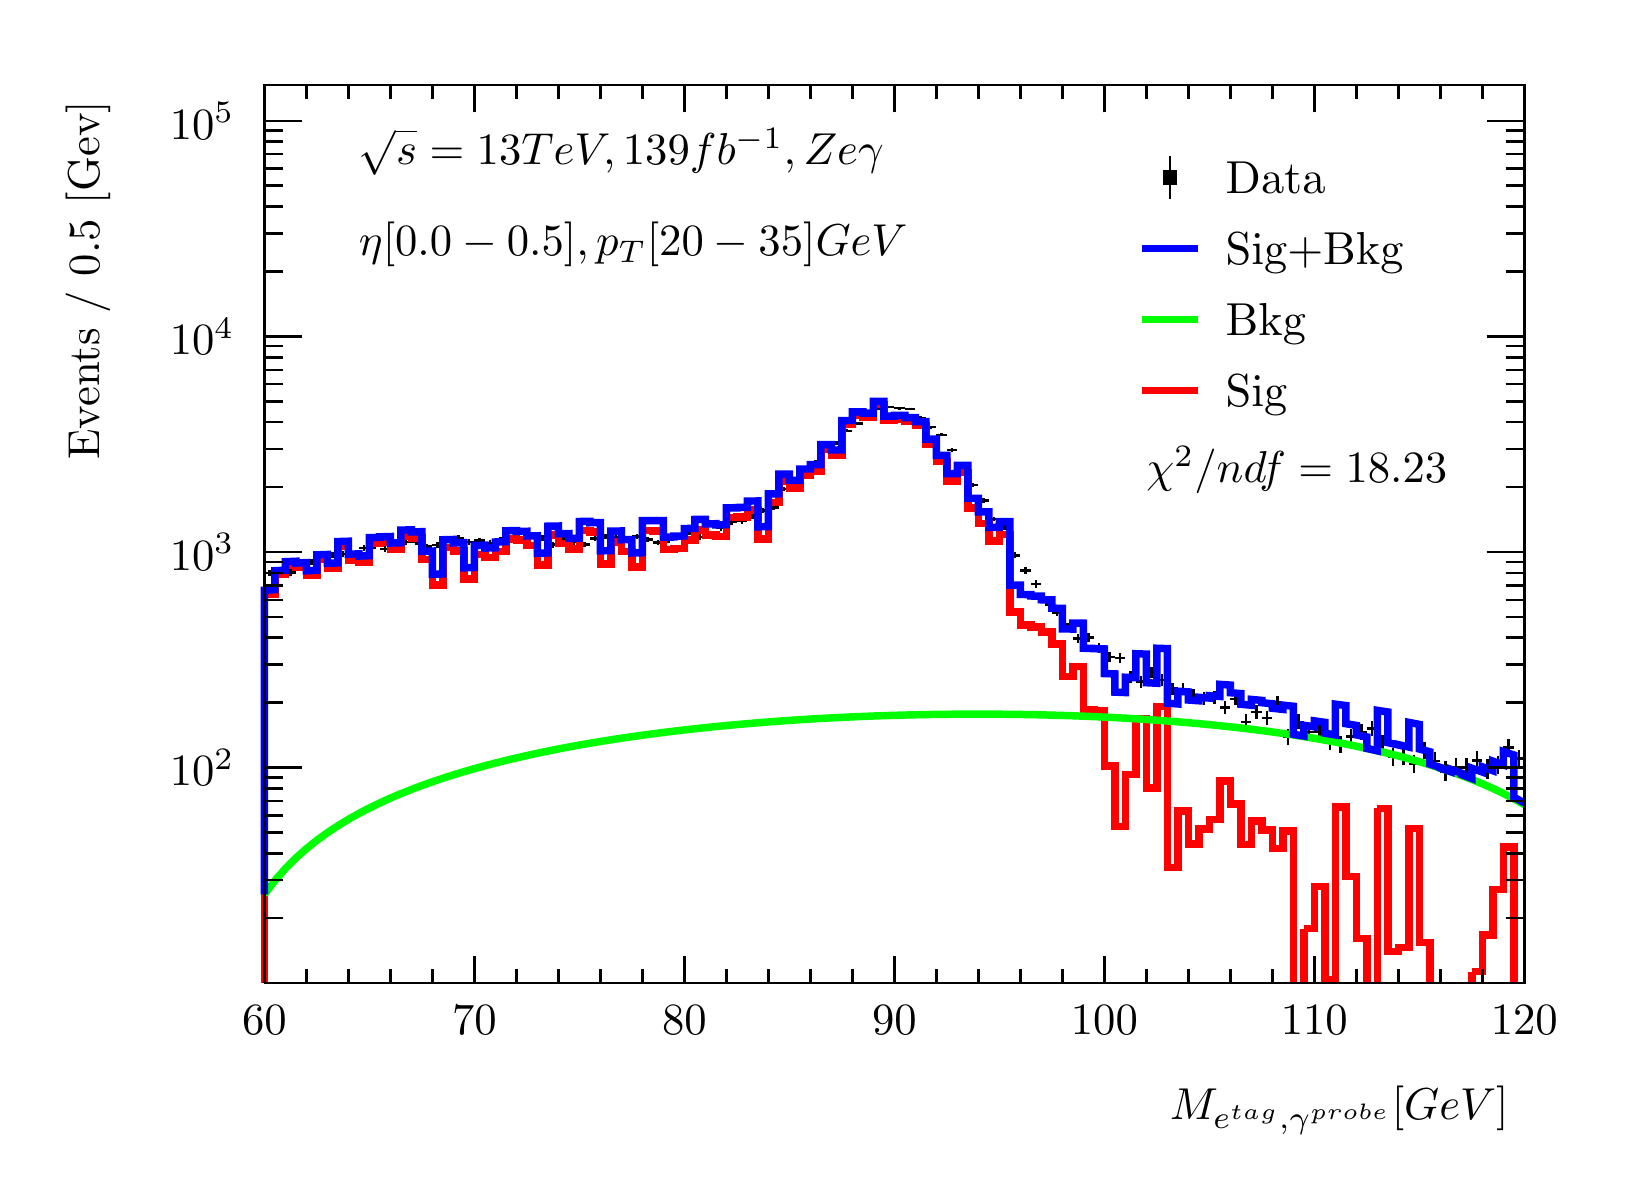
\begin{tikzpicture}
\pgfdeclareplotmark{cross} {
\pgfpathmoveto{\pgfpoint{-0.3\pgfplotmarksize}{\pgfplotmarksize}}
\pgfpathlineto{\pgfpoint{+0.3\pgfplotmarksize}{\pgfplotmarksize}}
\pgfpathlineto{\pgfpoint{+0.3\pgfplotmarksize}{0.3\pgfplotmarksize}}
\pgfpathlineto{\pgfpoint{+1\pgfplotmarksize}{0.3\pgfplotmarksize}}
\pgfpathlineto{\pgfpoint{+1\pgfplotmarksize}{-0.3\pgfplotmarksize}}
\pgfpathlineto{\pgfpoint{+0.3\pgfplotmarksize}{-0.3\pgfplotmarksize}}
\pgfpathlineto{\pgfpoint{+0.3\pgfplotmarksize}{-1.\pgfplotmarksize}}
\pgfpathlineto{\pgfpoint{-0.3\pgfplotmarksize}{-1.\pgfplotmarksize}}
\pgfpathlineto{\pgfpoint{-0.3\pgfplotmarksize}{-0.3\pgfplotmarksize}}
\pgfpathlineto{\pgfpoint{-1.\pgfplotmarksize}{-0.3\pgfplotmarksize}}
\pgfpathlineto{\pgfpoint{-1.\pgfplotmarksize}{0.3\pgfplotmarksize}}
\pgfpathlineto{\pgfpoint{-0.3\pgfplotmarksize}{0.3\pgfplotmarksize}}
\pgfpathclose
\pgfusepathqstroke
}
\pgfdeclareplotmark{cross*} {
\pgfpathmoveto{\pgfpoint{-0.3\pgfplotmarksize}{\pgfplotmarksize}}
\pgfpathlineto{\pgfpoint{+0.3\pgfplotmarksize}{\pgfplotmarksize}}
\pgfpathlineto{\pgfpoint{+0.3\pgfplotmarksize}{0.3\pgfplotmarksize}}
\pgfpathlineto{\pgfpoint{+1\pgfplotmarksize}{0.3\pgfplotmarksize}}
\pgfpathlineto{\pgfpoint{+1\pgfplotmarksize}{-0.3\pgfplotmarksize}}
\pgfpathlineto{\pgfpoint{+0.3\pgfplotmarksize}{-0.3\pgfplotmarksize}}
\pgfpathlineto{\pgfpoint{+0.3\pgfplotmarksize}{-1.\pgfplotmarksize}}
\pgfpathlineto{\pgfpoint{-0.3\pgfplotmarksize}{-1.\pgfplotmarksize}}
\pgfpathlineto{\pgfpoint{-0.3\pgfplotmarksize}{-0.3\pgfplotmarksize}}
\pgfpathlineto{\pgfpoint{-1.\pgfplotmarksize}{-0.3\pgfplotmarksize}}
\pgfpathlineto{\pgfpoint{-1.\pgfplotmarksize}{0.3\pgfplotmarksize}}
\pgfpathlineto{\pgfpoint{-0.3\pgfplotmarksize}{0.3\pgfplotmarksize}}
\pgfpathclose
\pgfusepathqfillstroke
}
\pgfdeclareplotmark{newstar} {
\pgfpathmoveto{\pgfqpoint{0pt}{\pgfplotmarksize}}
\pgfpathlineto{\pgfqpointpolar{44}{0.5\pgfplotmarksize}}
\pgfpathlineto{\pgfqpointpolar{18}{\pgfplotmarksize}}
\pgfpathlineto{\pgfqpointpolar{-20}{0.5\pgfplotmarksize}}
\pgfpathlineto{\pgfqpointpolar{-54}{\pgfplotmarksize}}
\pgfpathlineto{\pgfqpointpolar{-90}{0.5\pgfplotmarksize}}
\pgfpathlineto{\pgfqpointpolar{234}{\pgfplotmarksize}}
\pgfpathlineto{\pgfqpointpolar{198}{0.5\pgfplotmarksize}}
\pgfpathlineto{\pgfqpointpolar{162}{\pgfplotmarksize}}
\pgfpathlineto{\pgfqpointpolar{134}{0.5\pgfplotmarksize}}
\pgfpathclose
\pgfusepathqstroke
}
\pgfdeclareplotmark{newstar*} {
\pgfpathmoveto{\pgfqpoint{0pt}{\pgfplotmarksize}}
\pgfpathlineto{\pgfqpointpolar{44}{0.5\pgfplotmarksize}}
\pgfpathlineto{\pgfqpointpolar{18}{\pgfplotmarksize}}
\pgfpathlineto{\pgfqpointpolar{-20}{0.5\pgfplotmarksize}}
\pgfpathlineto{\pgfqpointpolar{-54}{\pgfplotmarksize}}
\pgfpathlineto{\pgfqpointpolar{-90}{0.5\pgfplotmarksize}}
\pgfpathlineto{\pgfqpointpolar{234}{\pgfplotmarksize}}
\pgfpathlineto{\pgfqpointpolar{198}{0.5\pgfplotmarksize}}
\pgfpathlineto{\pgfqpointpolar{162}{\pgfplotmarksize}}
\pgfpathlineto{\pgfqpointpolar{134}{0.5\pgfplotmarksize}}
\pgfpathclose
\pgfusepathqfillstroke
}
\definecolor{c}{rgb}{1,1,1};
\draw [color=c, fill=c] (0,0) rectangle (20,14.4361);
\draw [color=c, fill=c] (3,2.30977) rectangle (19,13.7143);
\definecolor{c}{rgb}{0,0,0};
\draw [c,line width=0.9] (3,2.30977) -- (3,13.7143) -- (19,13.7143) -- (19,2.30977) -- (3,2.30977);
\definecolor{c}{rgb}{1,1,1};
\draw [color=c, fill=c] (3,2.30977) rectangle (19,13.7143);
\definecolor{c}{rgb}{0,0,0};
\draw [c,line width=0.9] (3,2.30977) -- (3,13.7143) -- (19,13.7143) -- (19,2.30977) -- (3,2.30977);
\draw [c,line width=0.9] (3,2.30977) -- (19,2.30977);
\draw [c,line width=0.9] (3,2.65624) -- (3,2.30977);
\draw [c,line width=0.9] (3.53333,2.48301) -- (3.53333,2.30977);
\draw [c,line width=0.9] (4.06667,2.48301) -- (4.06667,2.30977);
\draw [c,line width=0.9] (4.6,2.48301) -- (4.6,2.30977);
\draw [c,line width=0.9] (5.13333,2.48301) -- (5.13333,2.30977);
\draw [c,line width=0.9] (5.66667,2.65624) -- (5.66667,2.30977);
\draw [c,line width=0.9] (6.2,2.48301) -- (6.2,2.30977);
\draw [c,line width=0.9] (6.73333,2.48301) -- (6.73333,2.30977);
\draw [c,line width=0.9] (7.26667,2.48301) -- (7.26667,2.30977);
\draw [c,line width=0.9] (7.8,2.48301) -- (7.8,2.30977);
\draw [c,line width=0.9] (8.33333,2.65624) -- (8.33333,2.30977);
\draw [c,line width=0.9] (8.86667,2.48301) -- (8.86667,2.30977);
\draw [c,line width=0.9] (9.4,2.48301) -- (9.4,2.30977);
\draw [c,line width=0.9] (9.93333,2.48301) -- (9.93333,2.30977);
\draw [c,line width=0.9] (10.4667,2.48301) -- (10.4667,2.30977);
\draw [c,line width=0.9] (11,2.65624) -- (11,2.30977);
\draw [c,line width=0.9] (11.5333,2.48301) -- (11.5333,2.30977);
\draw [c,line width=0.9] (12.0667,2.48301) -- (12.0667,2.30977);
\draw [c,line width=0.9] (12.6,2.48301) -- (12.6,2.30977);
\draw [c,line width=0.9] (13.1333,2.48301) -- (13.1333,2.30977);
\draw [c,line width=0.9] (13.6667,2.65624) -- (13.6667,2.30977);
\draw [c,line width=0.9] (14.2,2.48301) -- (14.2,2.30977);
\draw [c,line width=0.9] (14.7333,2.48301) -- (14.7333,2.30977);
\draw [c,line width=0.9] (15.2667,2.48301) -- (15.2667,2.30977);
\draw [c,line width=0.9] (15.8,2.48301) -- (15.8,2.30977);
\draw [c,line width=0.9] (16.3333,2.65624) -- (16.3333,2.30977);
\draw [c,line width=0.9] (16.8667,2.48301) -- (16.8667,2.30977);
\draw [c,line width=0.9] (17.4,2.48301) -- (17.4,2.30977);
\draw [c,line width=0.9] (17.9333,2.48301) -- (17.9333,2.30977);
\draw [c,line width=0.9] (18.4667,2.48301) -- (18.4667,2.30977);
\draw [c,line width=0.9] (19,2.65624) -- (19,2.30977);
\draw [anchor=base] (3,1.66015) node[scale=1.61424, color=c, rotate=0]{60};
\draw [anchor=base] (5.66667,1.66015) node[scale=1.61424, color=c, rotate=0]{70};
\draw [anchor=base] (8.33333,1.66015) node[scale=1.61424, color=c, rotate=0]{80};
\draw [anchor=base] (11,1.66015) node[scale=1.61424, color=c, rotate=0]{90};
\draw [anchor=base] (13.6667,1.66015) node[scale=1.61424, color=c, rotate=0]{100};
\draw [anchor=base] (16.3333,1.66015) node[scale=1.61424, color=c, rotate=0]{110};
\draw [anchor=base] (19,1.66015) node[scale=1.61424, color=c, rotate=0]{120};
\draw [anchor= east] (19,0.692932) node[scale=1.61424, color=c, rotate=0]{$M_{e^{tag}, \gamma^{probe}}  [GeV]$};
\draw [c,line width=0.9] (3,13.7143) -- (19,13.7143);
\draw [c,line width=0.9] (3,13.3678) -- (3,13.7143);
\draw [c,line width=0.9] (3.53333,13.5411) -- (3.53333,13.7143);
\draw [c,line width=0.9] (4.06667,13.5411) -- (4.06667,13.7143);
\draw [c,line width=0.9] (4.6,13.5411) -- (4.6,13.7143);
\draw [c,line width=0.9] (5.13333,13.5411) -- (5.13333,13.7143);
\draw [c,line width=0.9] (5.66667,13.3678) -- (5.66667,13.7143);
\draw [c,line width=0.9] (6.2,13.5411) -- (6.2,13.7143);
\draw [c,line width=0.9] (6.73333,13.5411) -- (6.73333,13.7143);
\draw [c,line width=0.9] (7.26667,13.5411) -- (7.26667,13.7143);
\draw [c,line width=0.9] (7.8,13.5411) -- (7.8,13.7143);
\draw [c,line width=0.9] (8.33333,13.3678) -- (8.33333,13.7143);
\draw [c,line width=0.9] (8.86667,13.5411) -- (8.86667,13.7143);
\draw [c,line width=0.9] (9.4,13.5411) -- (9.4,13.7143);
\draw [c,line width=0.9] (9.93333,13.5411) -- (9.93333,13.7143);
\draw [c,line width=0.9] (10.4667,13.5411) -- (10.4667,13.7143);
\draw [c,line width=0.9] (11,13.3678) -- (11,13.7143);
\draw [c,line width=0.9] (11.5333,13.5411) -- (11.5333,13.7143);
\draw [c,line width=0.9] (12.0667,13.5411) -- (12.0667,13.7143);
\draw [c,line width=0.9] (12.6,13.5411) -- (12.6,13.7143);
\draw [c,line width=0.9] (13.1333,13.5411) -- (13.1333,13.7143);
\draw [c,line width=0.9] (13.6667,13.3678) -- (13.6667,13.7143);
\draw [c,line width=0.9] (14.2,13.5411) -- (14.2,13.7143);
\draw [c,line width=0.9] (14.7333,13.5411) -- (14.7333,13.7143);
\draw [c,line width=0.9] (15.2667,13.5411) -- (15.2667,13.7143);
\draw [c,line width=0.9] (15.8,13.5411) -- (15.8,13.7143);
\draw [c,line width=0.9] (16.3333,13.3678) -- (16.3333,13.7143);
\draw [c,line width=0.9] (16.8667,13.5411) -- (16.8667,13.7143);
\draw [c,line width=0.9] (17.4,13.5411) -- (17.4,13.7143);
\draw [c,line width=0.9] (17.9333,13.5411) -- (17.9333,13.7143);
\draw [c,line width=0.9] (18.4667,13.5411) -- (18.4667,13.7143);
\draw [c,line width=0.9] (19,13.3678) -- (19,13.7143);
\draw [c,line width=0.9] (3,2.30977) -- (3,13.7143);
\draw [c,line width=0.9] (3.237,3.13385) -- (3,3.13385);
\draw [c,line width=0.9] (3.237,3.6159) -- (3,3.6159);
\draw [c,line width=0.9] (3.237,3.95792) -- (3,3.95792);
\draw [c,line width=0.9] (3.237,4.22321) -- (3,4.22321);
\draw [c,line width=0.9] (3.237,4.43997) -- (3,4.43997);
\draw [c,line width=0.9] (3.237,4.62324) -- (3,4.62324);
\draw [c,line width=0.9] (3.237,4.782) -- (3,4.782);
\draw [c,line width=0.9] (3.237,4.92203) -- (3,4.92203);
\draw [c,line width=0.9] (3.474,5.04729) -- (3,5.04729);
\draw [anchor= east] (2.82,5.04729) node[scale=1.61424, color=c, rotate=0]{$10^{2}$};
\draw [c,line width=0.9] (3.237,5.87136) -- (3,5.87136);
\draw [c,line width=0.9] (3.237,6.35342) -- (3,6.35342);
\draw [c,line width=0.9] (3.237,6.69544) -- (3,6.69544);
\draw [c,line width=0.9] (3.237,6.96073) -- (3,6.96073);
\draw [c,line width=0.9] (3.237,7.17749) -- (3,7.17749);
\draw [c,line width=0.9] (3.237,7.36076) -- (3,7.36076);
\draw [c,line width=0.9] (3.237,7.51951) -- (3,7.51951);
\draw [c,line width=0.9] (3.237,7.65954) -- (3,7.65954);
\draw [c,line width=0.9] (3.474,7.78481) -- (3,7.78481);
\draw [anchor= east] (2.82,7.78481) node[scale=1.61424, color=c, rotate=0]{$10^{3}$};
\draw [c,line width=0.9] (3.237,8.60888) -- (3,8.60888);
\draw [c,line width=0.9] (3.237,9.09093) -- (3,9.09093);
\draw [c,line width=0.9] (3.237,9.43296) -- (3,9.43296);
\draw [c,line width=0.9] (3.237,9.69825) -- (3,9.69825);
\draw [c,line width=0.9] (3.237,9.91501) -- (3,9.91501);
\draw [c,line width=0.9] (3.237,10.0983) -- (3,10.0983);
\draw [c,line width=0.9] (3.237,10.257) -- (3,10.257);
\draw [c,line width=0.9] (3.237,10.3971) -- (3,10.3971);
\draw [c,line width=0.9] (3.474,10.5223) -- (3,10.5223);
\draw [anchor= east] (2.82,10.5223) node[scale=1.61424, color=c, rotate=0]{$10^{4}$};
\draw [c,line width=0.9] (3.237,11.3464) -- (3,11.3464);
\draw [c,line width=0.9] (3.237,11.8285) -- (3,11.8285);
\draw [c,line width=0.9] (3.237,12.1705) -- (3,12.1705);
\draw [c,line width=0.9] (3.237,12.4358) -- (3,12.4358);
\draw [c,line width=0.9] (3.237,12.6525) -- (3,12.6525);
\draw [c,line width=0.9] (3.237,12.8358) -- (3,12.8358);
\draw [c,line width=0.9] (3.237,12.9945) -- (3,12.9945);
\draw [c,line width=0.9] (3.237,13.1346) -- (3,13.1346);
\draw [c,line width=0.9] (3.474,13.2598) -- (3,13.2598);
\draw [anchor= east] (2.82,13.2598) node[scale=1.61424, color=c, rotate=0]{$10^{5}$};
\draw [anchor= east] (0.76,13.7143) node[scale=1.61424, color=c, rotate=90]{Events / 0.5 [Gev]};
\draw [c,line width=0.9] (19,2.30977) -- (19,13.7143);
\draw [c,line width=0.9] (18.763,3.13385) -- (19,3.13385);
\draw [c,line width=0.9] (18.763,3.6159) -- (19,3.6159);
\draw [c,line width=0.9] (18.763,3.95792) -- (19,3.95792);
\draw [c,line width=0.9] (18.763,4.22321) -- (19,4.22321);
\draw [c,line width=0.9] (18.763,4.43997) -- (19,4.43997);
\draw [c,line width=0.9] (18.763,4.62324) -- (19,4.62324);
\draw [c,line width=0.9] (18.763,4.782) -- (19,4.782);
\draw [c,line width=0.9] (18.763,4.92203) -- (19,4.92203);
\draw [c,line width=0.9] (18.526,5.04729) -- (19,5.04729);
\draw [c,line width=0.9] (18.763,5.87136) -- (19,5.87136);
\draw [c,line width=0.9] (18.763,6.35342) -- (19,6.35342);
\draw [c,line width=0.9] (18.763,6.69544) -- (19,6.69544);
\draw [c,line width=0.9] (18.763,6.96073) -- (19,6.96073);
\draw [c,line width=0.9] (18.763,7.17749) -- (19,7.17749);
\draw [c,line width=0.9] (18.763,7.36076) -- (19,7.36076);
\draw [c,line width=0.9] (18.763,7.51951) -- (19,7.51951);
\draw [c,line width=0.9] (18.763,7.65954) -- (19,7.65954);
\draw [c,line width=0.9] (18.526,7.78481) -- (19,7.78481);
\draw [c,line width=0.9] (18.763,8.60888) -- (19,8.60888);
\draw [c,line width=0.9] (18.763,9.09093) -- (19,9.09093);
\draw [c,line width=0.9] (18.763,9.43296) -- (19,9.43296);
\draw [c,line width=0.9] (18.763,9.69825) -- (19,9.69825);
\draw [c,line width=0.9] (18.763,9.91501) -- (19,9.91501);
\draw [c,line width=0.9] (18.763,10.0983) -- (19,10.0983);
\draw [c,line width=0.9] (18.763,10.257) -- (19,10.257);
\draw [c,line width=0.9] (18.763,10.3971) -- (19,10.3971);
\draw [c,line width=0.9] (18.526,10.5223) -- (19,10.5223);
\draw [c,line width=0.9] (18.763,11.3464) -- (19,11.3464);
\draw [c,line width=0.9] (18.763,11.8285) -- (19,11.8285);
\draw [c,line width=0.9] (18.763,12.1705) -- (19,12.1705);
\draw [c,line width=0.9] (18.763,12.4358) -- (19,12.4358);
\draw [c,line width=0.9] (18.763,12.6525) -- (19,12.6525);
\draw [c,line width=0.9] (18.763,12.8358) -- (19,12.8358);
\draw [c,line width=0.9] (18.763,12.9945) -- (19,12.9945);
\draw [c,line width=0.9] (18.763,13.1346) -- (19,13.1346);
\draw [c,line width=0.9] (18.526,13.2598) -- (19,13.2598);
\draw [c,line width=0.9] (3.06667,7.51505) -- (3,7.51505);
\draw [c,line width=0.9] (3,7.51505) -- (3,7.51505);
\draw [c,line width=0.9] (3.06667,7.51505) -- (3.13333,7.51505);
\draw [c,line width=0.9] (3.13333,7.51505) -- (3.13333,7.51505);
\draw [c,line width=0.9] (3.06667,7.51505) -- (3.06667,7.55716);
\draw [c,line width=0.9] (3.06667,7.55716) -- (3.06667,7.55716);
\draw [c,line width=0.9] (3.06667,7.51505) -- (3.06667,7.47294);
\draw [c,line width=0.9] (3.06667,7.47294) -- (3.06667,7.47294);
\draw [c,line width=0.9] (3.2,7.50606) -- (3.13333,7.50606);
\draw [c,line width=0.9] (3.13333,7.50606) -- (3.13333,7.50606);
\draw [c,line width=0.9] (3.2,7.50606) -- (3.26667,7.50606);
\draw [c,line width=0.9] (3.26667,7.50606) -- (3.26667,7.50606);
\draw [c,line width=0.9] (3.2,7.50606) -- (3.2,7.54833);
\draw [c,line width=0.9] (3.2,7.54833) -- (3.2,7.54833);
\draw [c,line width=0.9] (3.2,7.50606) -- (3.2,7.46379);
\draw [c,line width=0.9] (3.2,7.46379) -- (3.2,7.46379);
\draw [c,line width=0.9] (3.33333,7.521) -- (3.26667,7.521);
\draw [c,line width=0.9] (3.26667,7.521) -- (3.26667,7.521);
\draw [c,line width=0.9] (3.33333,7.521) -- (3.4,7.521);
\draw [c,line width=0.9] (3.4,7.521) -- (3.4,7.521);
\draw [c,line width=0.9] (3.33333,7.521) -- (3.33333,7.563);
\draw [c,line width=0.9] (3.33333,7.563) -- (3.33333,7.563);
\draw [c,line width=0.9] (3.33333,7.521) -- (3.33333,7.47899);
\draw [c,line width=0.9] (3.33333,7.47899) -- (3.33333,7.47899);
\draw [c,line width=0.9] (3.46667,7.63012) -- (3.4,7.63012);
\draw [c,line width=0.9] (3.4,7.63012) -- (3.4,7.63012);
\draw [c,line width=0.9] (3.46667,7.63012) -- (3.53333,7.63012);
\draw [c,line width=0.9] (3.53333,7.63012) -- (3.53333,7.63012);
\draw [c,line width=0.9] (3.46667,7.63012) -- (3.46667,7.67024);
\draw [c,line width=0.9] (3.46667,7.67024) -- (3.46667,7.67024);
\draw [c,line width=0.9] (3.46667,7.63012) -- (3.46667,7.59);
\draw [c,line width=0.9] (3.46667,7.59) -- (3.46667,7.59);
\draw [c,line width=0.9] (3.6,7.65425) -- (3.53333,7.65425);
\draw [c,line width=0.9] (3.53333,7.65425) -- (3.53333,7.65425);
\draw [c,line width=0.9] (3.6,7.65425) -- (3.66667,7.65425);
\draw [c,line width=0.9] (3.66667,7.65425) -- (3.66667,7.65425);
\draw [c,line width=0.9] (3.6,7.65425) -- (3.6,7.69397);
\draw [c,line width=0.9] (3.6,7.69397) -- (3.6,7.69397);
\draw [c,line width=0.9] (3.6,7.65425) -- (3.6,7.61453);
\draw [c,line width=0.9] (3.6,7.61453) -- (3.6,7.61453);
\draw [c,line width=0.9] (3.73333,7.72633) -- (3.66667,7.72633);
\draw [c,line width=0.9] (3.66667,7.72633) -- (3.66667,7.72633);
\draw [c,line width=0.9] (3.73333,7.72633) -- (3.8,7.72633);
\draw [c,line width=0.9] (3.8,7.72633) -- (3.8,7.72633);
\draw [c,line width=0.9] (3.73333,7.72633) -- (3.73333,7.76486);
\draw [c,line width=0.9] (3.73333,7.76486) -- (3.73333,7.76486);
\draw [c,line width=0.9] (3.73333,7.72633) -- (3.73333,7.6878);
\draw [c,line width=0.9] (3.73333,7.6878) -- (3.73333,7.6878);
\draw [c,line width=0.9] (3.86667,7.73998) -- (3.8,7.73998);
\draw [c,line width=0.9] (3.8,7.73998) -- (3.8,7.73998);
\draw [c,line width=0.9] (3.86667,7.73998) -- (3.93333,7.73998);
\draw [c,line width=0.9] (3.93333,7.73998) -- (3.93333,7.73998);
\draw [c,line width=0.9] (3.86667,7.73998) -- (3.86667,7.77829);
\draw [c,line width=0.9] (3.86667,7.77829) -- (3.86667,7.77829);
\draw [c,line width=0.9] (3.86667,7.73998) -- (3.86667,7.70167);
\draw [c,line width=0.9] (3.86667,7.70167) -- (3.86667,7.70167);
\draw [c,line width=0.9] (4,7.75714) -- (3.93333,7.75714);
\draw [c,line width=0.9] (3.93333,7.75714) -- (3.93333,7.75714);
\draw [c,line width=0.9] (4,7.75714) -- (4.06667,7.75714);
\draw [c,line width=0.9] (4.06667,7.75714) -- (4.06667,7.75714);
\draw [c,line width=0.9] (4,7.75714) -- (4,7.79518);
\draw [c,line width=0.9] (4,7.79518) -- (4,7.79518);
\draw [c,line width=0.9] (4,7.75714) -- (4,7.71911);
\draw [c,line width=0.9] (4,7.71911) -- (4,7.71911);
\draw [c,line width=0.9] (4.13333,7.76079) -- (4.06667,7.76079);
\draw [c,line width=0.9] (4.06667,7.76079) -- (4.06667,7.76079);
\draw [c,line width=0.9] (4.13333,7.76079) -- (4.2,7.76079);
\draw [c,line width=0.9] (4.2,7.76079) -- (4.2,7.76079);
\draw [c,line width=0.9] (4.13333,7.76079) -- (4.13333,7.79876);
\draw [c,line width=0.9] (4.13333,7.79876) -- (4.13333,7.79876);
\draw [c,line width=0.9] (4.13333,7.76079) -- (4.13333,7.72281);
\draw [c,line width=0.9] (4.13333,7.72281) -- (4.13333,7.72281);
\draw [c,line width=0.9] (4.26667,7.83486) -- (4.2,7.83486);
\draw [c,line width=0.9] (4.2,7.83486) -- (4.2,7.83486);
\draw [c,line width=0.9] (4.26667,7.83486) -- (4.33333,7.83486);
\draw [c,line width=0.9] (4.33333,7.83486) -- (4.33333,7.83486);
\draw [c,line width=0.9] (4.26667,7.83486) -- (4.26667,7.87167);
\draw [c,line width=0.9] (4.26667,7.87167) -- (4.26667,7.87167);
\draw [c,line width=0.9] (4.26667,7.83486) -- (4.26667,7.79805);
\draw [c,line width=0.9] (4.26667,7.79805) -- (4.26667,7.79805);
\draw [c,line width=0.9] (4.4,7.85744) -- (4.33333,7.85744);
\draw [c,line width=0.9] (4.33333,7.85744) -- (4.33333,7.85744);
\draw [c,line width=0.9] (4.4,7.85744) -- (4.46667,7.85744);
\draw [c,line width=0.9] (4.46667,7.85744) -- (4.46667,7.85744);
\draw [c,line width=0.9] (4.4,7.85744) -- (4.4,7.89391);
\draw [c,line width=0.9] (4.4,7.89391) -- (4.4,7.89391);
\draw [c,line width=0.9] (4.4,7.85744) -- (4.4,7.82098);
\draw [c,line width=0.9] (4.4,7.82098) -- (4.4,7.82098);
\draw [c,line width=0.9] (4.53333,7.81995) -- (4.46667,7.81995);
\draw [c,line width=0.9] (4.46667,7.81995) -- (4.46667,7.81995);
\draw [c,line width=0.9] (4.53333,7.81995) -- (4.6,7.81995);
\draw [c,line width=0.9] (4.6,7.81995) -- (4.6,7.81995);
\draw [c,line width=0.9] (4.53333,7.81995) -- (4.53333,7.85699);
\draw [c,line width=0.9] (4.53333,7.85699) -- (4.53333,7.85699);
\draw [c,line width=0.9] (4.53333,7.81995) -- (4.53333,7.78291);
\draw [c,line width=0.9] (4.53333,7.78291) -- (4.53333,7.78291);
\draw [c,line width=0.9] (4.66667,7.86968) -- (4.6,7.86968);
\draw [c,line width=0.9] (4.6,7.86968) -- (4.6,7.86968);
\draw [c,line width=0.9] (4.66667,7.86968) -- (4.73333,7.86968);
\draw [c,line width=0.9] (4.73333,7.86968) -- (4.73333,7.86968);
\draw [c,line width=0.9] (4.66667,7.86968) -- (4.66667,7.90596);
\draw [c,line width=0.9] (4.66667,7.90596) -- (4.66667,7.90596);
\draw [c,line width=0.9] (4.66667,7.86968) -- (4.66667,7.83341);
\draw [c,line width=0.9] (4.66667,7.83341) -- (4.66667,7.83341);
\draw [c,line width=0.9] (4.8,7.91209) -- (4.73333,7.91209);
\draw [c,line width=0.9] (4.73333,7.91209) -- (4.73333,7.91209);
\draw [c,line width=0.9] (4.8,7.91209) -- (4.86667,7.91209);
\draw [c,line width=0.9] (4.86667,7.91209) -- (4.86667,7.91209);
\draw [c,line width=0.9] (4.8,7.91209) -- (4.8,7.94772);
\draw [c,line width=0.9] (4.8,7.94772) -- (4.8,7.94772);
\draw [c,line width=0.9] (4.8,7.91209) -- (4.8,7.87645);
\draw [c,line width=0.9] (4.8,7.87645) -- (4.8,7.87645);
\draw [c,line width=0.9] (4.93333,7.90995) -- (4.86667,7.90995);
\draw [c,line width=0.9] (4.86667,7.90995) -- (4.86667,7.90995);
\draw [c,line width=0.9] (4.93333,7.90995) -- (5,7.90995);
\draw [c,line width=0.9] (5,7.90995) -- (5,7.90995);
\draw [c,line width=0.9] (4.93333,7.90995) -- (4.93333,7.94562);
\draw [c,line width=0.9] (4.93333,7.94562) -- (4.93333,7.94562);
\draw [c,line width=0.9] (4.93333,7.90995) -- (4.93333,7.87428);
\draw [c,line width=0.9] (4.93333,7.87428) -- (4.93333,7.87428);
\draw [c,line width=0.9] (5.06667,7.85408) -- (5,7.85408);
\draw [c,line width=0.9] (5,7.85408) -- (5,7.85408);
\draw [c,line width=0.9] (5.06667,7.85408) -- (5.13333,7.85408);
\draw [c,line width=0.9] (5.13333,7.85408) -- (5.13333,7.85408);
\draw [c,line width=0.9] (5.06667,7.85408) -- (5.06667,7.8906);
\draw [c,line width=0.9] (5.06667,7.8906) -- (5.06667,7.8906);
\draw [c,line width=0.9] (5.06667,7.85408) -- (5.06667,7.81757);
\draw [c,line width=0.9] (5.06667,7.81757) -- (5.06667,7.81757);
\draw [c,line width=0.9] (5.2,7.87189) -- (5.13333,7.87189);
\draw [c,line width=0.9] (5.13333,7.87189) -- (5.13333,7.87189);
\draw [c,line width=0.9] (5.2,7.87189) -- (5.26667,7.87189);
\draw [c,line width=0.9] (5.26667,7.87189) -- (5.26667,7.87189);
\draw [c,line width=0.9] (5.2,7.87189) -- (5.2,7.90814);
\draw [c,line width=0.9] (5.2,7.90814) -- (5.2,7.90814);
\draw [c,line width=0.9] (5.2,7.87189) -- (5.2,7.83565);
\draw [c,line width=0.9] (5.2,7.83565) -- (5.2,7.83565);
\draw [c,line width=0.9] (5.33333,7.94163) -- (5.26667,7.94163);
\draw [c,line width=0.9] (5.26667,7.94163) -- (5.26667,7.94163);
\draw [c,line width=0.9] (5.33333,7.94163) -- (5.4,7.94163);
\draw [c,line width=0.9] (5.4,7.94163) -- (5.4,7.94163);
\draw [c,line width=0.9] (5.33333,7.94163) -- (5.33333,7.97682);
\draw [c,line width=0.9] (5.33333,7.97682) -- (5.33333,7.97682);
\draw [c,line width=0.9] (5.33333,7.94163) -- (5.33333,7.90643);
\draw [c,line width=0.9] (5.33333,7.90643) -- (5.33333,7.90643);
\draw [c,line width=0.9] (5.46667,7.96229) -- (5.4,7.96229);
\draw [c,line width=0.9] (5.4,7.96229) -- (5.4,7.96229);
\draw [c,line width=0.9] (5.46667,7.96229) -- (5.53333,7.96229);
\draw [c,line width=0.9] (5.53333,7.96229) -- (5.53333,7.96229);
\draw [c,line width=0.9] (5.46667,7.96229) -- (5.46667,7.99718);
\draw [c,line width=0.9] (5.46667,7.99718) -- (5.46667,7.99718);
\draw [c,line width=0.9] (5.46667,7.96229) -- (5.46667,7.9274);
\draw [c,line width=0.9] (5.46667,7.9274) -- (5.46667,7.9274);
\draw [c,line width=0.9] (5.6,7.91422) -- (5.53333,7.91422);
\draw [c,line width=0.9] (5.53333,7.91422) -- (5.53333,7.91422);
\draw [c,line width=0.9] (5.6,7.91422) -- (5.66667,7.91422);
\draw [c,line width=0.9] (5.66667,7.91422) -- (5.66667,7.91422);
\draw [c,line width=0.9] (5.6,7.91422) -- (5.6,7.94983);
\draw [c,line width=0.9] (5.6,7.94983) -- (5.6,7.94983);
\draw [c,line width=0.9] (5.6,7.91422) -- (5.6,7.87862);
\draw [c,line width=0.9] (5.6,7.87862) -- (5.6,7.87862);
\draw [c,line width=0.9] (5.73333,7.93221) -- (5.66667,7.93221);
\draw [c,line width=0.9] (5.66667,7.93221) -- (5.66667,7.93221);
\draw [c,line width=0.9] (5.73333,7.93221) -- (5.8,7.93221);
\draw [c,line width=0.9] (5.8,7.93221) -- (5.8,7.93221);
\draw [c,line width=0.9] (5.73333,7.93221) -- (5.73333,7.96755);
\draw [c,line width=0.9] (5.73333,7.96755) -- (5.73333,7.96755);
\draw [c,line width=0.9] (5.73333,7.93221) -- (5.73333,7.89688);
\draw [c,line width=0.9] (5.73333,7.89688) -- (5.73333,7.89688);
\draw [c,line width=0.9] (5.86667,7.89487) -- (5.8,7.89487);
\draw [c,line width=0.9] (5.8,7.89487) -- (5.8,7.89487);
\draw [c,line width=0.9] (5.86667,7.89487) -- (5.93333,7.89487);
\draw [c,line width=0.9] (5.93333,7.89487) -- (5.93333,7.89487);
\draw [c,line width=0.9] (5.86667,7.89487) -- (5.86667,7.93077);
\draw [c,line width=0.9] (5.86667,7.93077) -- (5.86667,7.93077);
\draw [c,line width=0.9] (5.86667,7.89487) -- (5.86667,7.85898);
\draw [c,line width=0.9] (5.86667,7.85898) -- (5.86667,7.85898);
\draw [c,line width=0.9] (6,7.9385) -- (5.93333,7.9385);
\draw [c,line width=0.9] (5.93333,7.9385) -- (5.93333,7.9385);
\draw [c,line width=0.9] (6,7.9385) -- (6.06667,7.9385);
\draw [c,line width=0.9] (6.06667,7.9385) -- (6.06667,7.9385);
\draw [c,line width=0.9] (6,7.9385) -- (6,7.97374);
\draw [c,line width=0.9] (6,7.97374) -- (6,7.97374);
\draw [c,line width=0.9] (6,7.9385) -- (6,7.90326);
\draw [c,line width=0.9] (6,7.90326) -- (6,7.90326);
\draw [c,line width=0.9] (6.13333,7.95303) -- (6.06667,7.95303);
\draw [c,line width=0.9] (6.06667,7.95303) -- (6.06667,7.95303);
\draw [c,line width=0.9] (6.13333,7.95303) -- (6.2,7.95303);
\draw [c,line width=0.9] (6.2,7.95303) -- (6.2,7.95303);
\draw [c,line width=0.9] (6.13333,7.95303) -- (6.13333,7.98806);
\draw [c,line width=0.9] (6.13333,7.98806) -- (6.13333,7.98806);
\draw [c,line width=0.9] (6.13333,7.95303) -- (6.13333,7.91801);
\draw [c,line width=0.9] (6.13333,7.91801) -- (6.13333,7.91801);
\draw [c,line width=0.9] (6.26667,7.9551) -- (6.2,7.9551);
\draw [c,line width=0.9] (6.2,7.9551) -- (6.2,7.9551);
\draw [c,line width=0.9] (6.26667,7.9551) -- (6.33333,7.9551);
\draw [c,line width=0.9] (6.33333,7.9551) -- (6.33333,7.9551);
\draw [c,line width=0.9] (6.26667,7.9551) -- (6.26667,7.99009);
\draw [c,line width=0.9] (6.26667,7.99009) -- (6.26667,7.99009);
\draw [c,line width=0.9] (6.26667,7.9551) -- (6.26667,7.9201);
\draw [c,line width=0.9] (6.26667,7.9201) -- (6.26667,7.9201);
\draw [c,line width=0.9] (6.4,7.99361) -- (6.33333,7.99361);
\draw [c,line width=0.9] (6.33333,7.99361) -- (6.33333,7.99361);
\draw [c,line width=0.9] (6.4,7.99361) -- (6.46667,7.99361);
\draw [c,line width=0.9] (6.46667,7.99361) -- (6.46667,7.99361);
\draw [c,line width=0.9] (6.4,7.99361) -- (6.4,8.02805);
\draw [c,line width=0.9] (6.4,8.02805) -- (6.4,8.02805);
\draw [c,line width=0.9] (6.4,7.99361) -- (6.4,7.95918);
\draw [c,line width=0.9] (6.4,7.95918) -- (6.4,7.95918);
\draw [c,line width=0.9] (6.53333,7.96433) -- (6.46667,7.96433);
\draw [c,line width=0.9] (6.46667,7.96433) -- (6.46667,7.96433);
\draw [c,line width=0.9] (6.53333,7.96433) -- (6.6,7.96433);
\draw [c,line width=0.9] (6.6,7.96433) -- (6.6,7.96433);
\draw [c,line width=0.9] (6.53333,7.96433) -- (6.53333,7.99919);
\draw [c,line width=0.9] (6.53333,7.99919) -- (6.53333,7.99919);
\draw [c,line width=0.9] (6.53333,7.96433) -- (6.53333,7.92947);
\draw [c,line width=0.9] (6.53333,7.92947) -- (6.53333,7.92947);
\draw [c,line width=0.9] (6.66667,7.87631) -- (6.6,7.87631);
\draw [c,line width=0.9] (6.6,7.87631) -- (6.6,7.87631);
\draw [c,line width=0.9] (6.66667,7.87631) -- (6.73333,7.87631);
\draw [c,line width=0.9] (6.73333,7.87631) -- (6.73333,7.87631);
\draw [c,line width=0.9] (6.66667,7.87631) -- (6.66667,7.91248);
\draw [c,line width=0.9] (6.66667,7.91248) -- (6.66667,7.91248);
\draw [c,line width=0.9] (6.66667,7.87631) -- (6.66667,7.84013);
\draw [c,line width=0.9] (6.66667,7.84013) -- (6.66667,7.84013);
\draw [c,line width=0.9] (6.8,7.97552) -- (6.73333,7.97552);
\draw [c,line width=0.9] (6.73333,7.97552) -- (6.73333,7.97552);
\draw [c,line width=0.9] (6.8,7.97552) -- (6.86667,7.97552);
\draw [c,line width=0.9] (6.86667,7.97552) -- (6.86667,7.97552);
\draw [c,line width=0.9] (6.8,7.97552) -- (6.8,8.01022);
\draw [c,line width=0.9] (6.8,8.01022) -- (6.8,8.01022);
\draw [c,line width=0.9] (6.8,7.97552) -- (6.8,7.94083);
\draw [c,line width=0.9] (6.8,7.94083) -- (6.8,7.94083);
\draw [c,line width=0.9] (6.93333,7.90888) -- (6.86667,7.90888);
\draw [c,line width=0.9] (6.86667,7.90888) -- (6.86667,7.90888);
\draw [c,line width=0.9] (6.93333,7.90888) -- (7,7.90888);
\draw [c,line width=0.9] (7,7.90888) -- (7,7.90888);
\draw [c,line width=0.9] (6.93333,7.90888) -- (6.93333,7.94456);
\draw [c,line width=0.9] (6.93333,7.94456) -- (6.93333,7.94456);
\draw [c,line width=0.9] (6.93333,7.90888) -- (6.93333,7.8732);
\draw [c,line width=0.9] (6.93333,7.8732) -- (6.93333,7.8732);
\draw [c,line width=0.9] (7.06667,7.87851) -- (7,7.87851);
\draw [c,line width=0.9] (7,7.87851) -- (7,7.87851);
\draw [c,line width=0.9] (7.06667,7.87851) -- (7.13333,7.87851);
\draw [c,line width=0.9] (7.13333,7.87851) -- (7.13333,7.87851);
\draw [c,line width=0.9] (7.06667,7.87851) -- (7.06667,7.91465);
\draw [c,line width=0.9] (7.06667,7.91465) -- (7.06667,7.91465);
\draw [c,line width=0.9] (7.06667,7.87851) -- (7.06667,7.84236);
\draw [c,line width=0.9] (7.06667,7.84236) -- (7.06667,7.84236);
\draw [c,line width=0.9] (7.2,7.95716) -- (7.13333,7.95716);
\draw [c,line width=0.9] (7.13333,7.95716) -- (7.13333,7.95716);
\draw [c,line width=0.9] (7.2,7.95716) -- (7.26667,7.95716);
\draw [c,line width=0.9] (7.26667,7.95716) -- (7.26667,7.95716);
\draw [c,line width=0.9] (7.2,7.95716) -- (7.2,7.99212);
\draw [c,line width=0.9] (7.2,7.99212) -- (7.2,7.99212);
\draw [c,line width=0.9] (7.2,7.95716) -- (7.2,7.92219);
\draw [c,line width=0.9] (7.2,7.92219) -- (7.2,7.92219);
\draw [c,line width=0.9] (7.33333,7.97957) -- (7.26667,7.97957);
\draw [c,line width=0.9] (7.26667,7.97957) -- (7.26667,7.97957);
\draw [c,line width=0.9] (7.33333,7.97957) -- (7.4,7.97957);
\draw [c,line width=0.9] (7.4,7.97957) -- (7.4,7.97957);
\draw [c,line width=0.9] (7.33333,7.97957) -- (7.33333,8.01421);
\draw [c,line width=0.9] (7.33333,8.01421) -- (7.33333,8.01421);
\draw [c,line width=0.9] (7.33333,7.97957) -- (7.33333,7.94493);
\draw [c,line width=0.9] (7.33333,7.94493) -- (7.33333,7.94493);
\draw [c,line width=0.9] (7.46667,7.97755) -- (7.4,7.97755);
\draw [c,line width=0.9] (7.4,7.97755) -- (7.4,7.97755);
\draw [c,line width=0.9] (7.46667,7.97755) -- (7.53333,7.97755);
\draw [c,line width=0.9] (7.53333,7.97755) -- (7.53333,7.97755);
\draw [c,line width=0.9] (7.46667,7.97755) -- (7.46667,8.01222);
\draw [c,line width=0.9] (7.46667,8.01222) -- (7.46667,8.01222);
\draw [c,line width=0.9] (7.46667,7.97755) -- (7.46667,7.94288);
\draw [c,line width=0.9] (7.46667,7.94288) -- (7.46667,7.94288);
\draw [c,line width=0.9] (7.6,7.94683) -- (7.53333,7.94683);
\draw [c,line width=0.9] (7.53333,7.94683) -- (7.53333,7.94683);
\draw [c,line width=0.9] (7.6,7.94683) -- (7.66667,7.94683);
\draw [c,line width=0.9] (7.66667,7.94683) -- (7.66667,7.94683);
\draw [c,line width=0.9] (7.6,7.94683) -- (7.6,7.98194);
\draw [c,line width=0.9] (7.6,7.98194) -- (7.6,7.98194);
\draw [c,line width=0.9] (7.6,7.94683) -- (7.6,7.91171);
\draw [c,line width=0.9] (7.6,7.91171) -- (7.6,7.91171);
\draw [c,line width=0.9] (7.73333,7.98159) -- (7.66667,7.98159);
\draw [c,line width=0.9] (7.66667,7.98159) -- (7.66667,7.98159);
\draw [c,line width=0.9] (7.73333,7.98159) -- (7.8,7.98159);
\draw [c,line width=0.9] (7.8,7.98159) -- (7.8,7.98159);
\draw [c,line width=0.9] (7.73333,7.98159) -- (7.73333,8.01619);
\draw [c,line width=0.9] (7.73333,8.01619) -- (7.73333,8.01619);
\draw [c,line width=0.9] (7.73333,7.98159) -- (7.73333,7.94698);
\draw [c,line width=0.9] (7.73333,7.94698) -- (7.73333,7.94698);
\draw [c,line width=0.9] (7.86667,7.94475) -- (7.8,7.94475);
\draw [c,line width=0.9] (7.8,7.94475) -- (7.8,7.94475);
\draw [c,line width=0.9] (7.86667,7.94475) -- (7.93333,7.94475);
\draw [c,line width=0.9] (7.93333,7.94475) -- (7.93333,7.94475);
\draw [c,line width=0.9] (7.86667,7.94475) -- (7.86667,7.9799);
\draw [c,line width=0.9] (7.86667,7.9799) -- (7.86667,7.9799);
\draw [c,line width=0.9] (7.86667,7.94475) -- (7.86667,7.9096);
\draw [c,line width=0.9] (7.86667,7.9096) -- (7.86667,7.9096);
\draw [c,line width=0.9] (8,7.90351) -- (7.93333,7.90351);
\draw [c,line width=0.9] (7.93333,7.90351) -- (7.93333,7.90351);
\draw [c,line width=0.9] (8,7.90351) -- (8.06667,7.90351);
\draw [c,line width=0.9] (8.06667,7.90351) -- (8.06667,7.90351);
\draw [c,line width=0.9] (8,7.90351) -- (8,7.93928);
\draw [c,line width=0.9] (8,7.93928) -- (8,7.93928);
\draw [c,line width=0.9] (8,7.90351) -- (8,7.86775);
\draw [c,line width=0.9] (8,7.86775) -- (8,7.86775);
\draw [c,line width=0.9] (8.13333,7.93536) -- (8.06667,7.93536);
\draw [c,line width=0.9] (8.06667,7.93536) -- (8.06667,7.93536);
\draw [c,line width=0.9] (8.13333,7.93536) -- (8.2,7.93536);
\draw [c,line width=0.9] (8.2,7.93536) -- (8.2,7.93536);
\draw [c,line width=0.9] (8.13333,7.93536) -- (8.13333,7.97065);
\draw [c,line width=0.9] (8.13333,7.97065) -- (8.13333,7.97065);
\draw [c,line width=0.9] (8.13333,7.93536) -- (8.13333,7.90007);
\draw [c,line width=0.9] (8.13333,7.90007) -- (8.13333,7.90007);
\draw [c,line width=0.9] (8.26667,7.98259) -- (8.2,7.98259);
\draw [c,line width=0.9] (8.2,7.98259) -- (8.2,7.98259);
\draw [c,line width=0.9] (8.26667,7.98259) -- (8.33333,7.98259);
\draw [c,line width=0.9] (8.33333,7.98259) -- (8.33333,7.98259);
\draw [c,line width=0.9] (8.26667,7.98259) -- (8.26667,8.01719);
\draw [c,line width=0.9] (8.26667,8.01719) -- (8.26667,8.01719);
\draw [c,line width=0.9] (8.26667,7.98259) -- (8.26667,7.948);
\draw [c,line width=0.9] (8.26667,7.948) -- (8.26667,7.948);
\draw [c,line width=0.9] (8.4,8.03092) -- (8.33333,8.03092);
\draw [c,line width=0.9] (8.33333,8.03092) -- (8.33333,8.03092);
\draw [c,line width=0.9] (8.4,8.03092) -- (8.46667,8.03092);
\draw [c,line width=0.9] (8.46667,8.03092) -- (8.46667,8.03092);
\draw [c,line width=0.9] (8.4,8.03092) -- (8.4,8.06482);
\draw [c,line width=0.9] (8.4,8.06482) -- (8.4,8.06482);
\draw [c,line width=0.9] (8.4,8.03092) -- (8.4,7.99703);
\draw [c,line width=0.9] (8.4,7.99703) -- (8.4,7.99703);
\draw [c,line width=0.9] (8.53333,7.97248) -- (8.46667,7.97248);
\draw [c,line width=0.9] (8.46667,7.97248) -- (8.46667,7.97248);
\draw [c,line width=0.9] (8.53333,7.97248) -- (8.6,7.97248);
\draw [c,line width=0.9] (8.6,7.97248) -- (8.6,7.97248);
\draw [c,line width=0.9] (8.53333,7.97248) -- (8.53333,8.00722);
\draw [c,line width=0.9] (8.53333,8.00722) -- (8.53333,8.00722);
\draw [c,line width=0.9] (8.53333,7.97248) -- (8.53333,7.93774);
\draw [c,line width=0.9] (8.53333,7.93774) -- (8.53333,7.93774);
\draw [c,line width=0.9] (8.66667,8.15299) -- (8.6,8.15299);
\draw [c,line width=0.9] (8.6,8.15299) -- (8.6,8.15299);
\draw [c,line width=0.9] (8.66667,8.15299) -- (8.73333,8.15299);
\draw [c,line width=0.9] (8.73333,8.15299) -- (8.73333,8.15299);
\draw [c,line width=0.9] (8.66667,8.15299) -- (8.66667,8.18519);
\draw [c,line width=0.9] (8.66667,8.18519) -- (8.66667,8.18519);
\draw [c,line width=0.9] (8.66667,8.15299) -- (8.66667,8.12079);
\draw [c,line width=0.9] (8.66667,8.12079) -- (8.66667,8.12079);
\draw [c,line width=0.9] (8.8,8.0857) -- (8.73333,8.0857);
\draw [c,line width=0.9] (8.73333,8.0857) -- (8.73333,8.0857);
\draw [c,line width=0.9] (8.8,8.0857) -- (8.86667,8.0857);
\draw [c,line width=0.9] (8.86667,8.0857) -- (8.86667,8.0857);
\draw [c,line width=0.9] (8.8,8.0857) -- (8.8,8.11883);
\draw [c,line width=0.9] (8.8,8.11883) -- (8.8,8.11883);
\draw [c,line width=0.9] (8.8,8.0857) -- (8.8,8.05258);
\draw [c,line width=0.9] (8.8,8.05258) -- (8.8,8.05258);
\draw [c,line width=0.9] (8.93333,8.16341) -- (8.86667,8.16341);
\draw [c,line width=0.9] (8.86667,8.16341) -- (8.86667,8.16341);
\draw [c,line width=0.9] (8.93333,8.16341) -- (9,8.16341);
\draw [c,line width=0.9] (9,8.16341) -- (9,8.16341);
\draw [c,line width=0.9] (8.93333,8.16341) -- (8.93333,8.19547);
\draw [c,line width=0.9] (8.93333,8.19547) -- (8.93333,8.19547);
\draw [c,line width=0.9] (8.93333,8.16341) -- (8.93333,8.13135);
\draw [c,line width=0.9] (8.93333,8.13135) -- (8.93333,8.13135);
\draw [c,line width=0.9] (9.06667,8.17717) -- (9,8.17717);
\draw [c,line width=0.9] (9,8.17717) -- (9,8.17717);
\draw [c,line width=0.9] (9.06667,8.17717) -- (9.13333,8.17717);
\draw [c,line width=0.9] (9.13333,8.17717) -- (9.13333,8.17717);
\draw [c,line width=0.9] (9.06667,8.17717) -- (9.06667,8.20904);
\draw [c,line width=0.9] (9.06667,8.20904) -- (9.06667,8.20904);
\draw [c,line width=0.9] (9.06667,8.17717) -- (9.06667,8.14529);
\draw [c,line width=0.9] (9.06667,8.14529) -- (9.06667,8.14529);
\draw [c,line width=0.9] (9.2,8.23879) -- (9.13333,8.23879);
\draw [c,line width=0.9] (9.13333,8.23879) -- (9.13333,8.23879);
\draw [c,line width=0.9] (9.2,8.23879) -- (9.26667,8.23879);
\draw [c,line width=0.9] (9.26667,8.23879) -- (9.26667,8.23879);
\draw [c,line width=0.9] (9.2,8.23879) -- (9.2,8.26985);
\draw [c,line width=0.9] (9.2,8.26985) -- (9.2,8.26985);
\draw [c,line width=0.9] (9.2,8.23879) -- (9.2,8.20773);
\draw [c,line width=0.9] (9.2,8.20773) -- (9.2,8.20773);
\draw [c,line width=0.9] (9.33333,8.31273) -- (9.26667,8.31273);
\draw [c,line width=0.9] (9.26667,8.31273) -- (9.26667,8.31273);
\draw [c,line width=0.9] (9.33333,8.31273) -- (9.4,8.31273);
\draw [c,line width=0.9] (9.4,8.31273) -- (9.4,8.31273);
\draw [c,line width=0.9] (9.33333,8.31273) -- (9.33333,8.34284);
\draw [c,line width=0.9] (9.33333,8.34284) -- (9.33333,8.34284);
\draw [c,line width=0.9] (9.33333,8.31273) -- (9.33333,8.28262);
\draw [c,line width=0.9] (9.33333,8.28262) -- (9.33333,8.28262);
\draw [c,line width=0.9] (9.46667,8.351) -- (9.4,8.351);
\draw [c,line width=0.9] (9.4,8.351) -- (9.4,8.351);
\draw [c,line width=0.9] (9.46667,8.351) -- (9.53333,8.351);
\draw [c,line width=0.9] (9.53333,8.351) -- (9.53333,8.351);
\draw [c,line width=0.9] (9.46667,8.351) -- (9.46667,8.38063);
\draw [c,line width=0.9] (9.46667,8.38063) -- (9.46667,8.38063);
\draw [c,line width=0.9] (9.46667,8.351) -- (9.46667,8.32137);
\draw [c,line width=0.9] (9.46667,8.32137) -- (9.46667,8.32137);
\draw [c,line width=0.9] (9.6,8.58365) -- (9.53333,8.58365);
\draw [c,line width=0.9] (9.53333,8.58365) -- (9.53333,8.58365);
\draw [c,line width=0.9] (9.6,8.58365) -- (9.66667,8.58365);
\draw [c,line width=0.9] (9.66667,8.58365) -- (9.66667,8.58365);
\draw [c,line width=0.9] (9.6,8.58365) -- (9.6,8.61052);
\draw [c,line width=0.9] (9.6,8.61052) -- (9.6,8.61052);
\draw [c,line width=0.9] (9.6,8.58365) -- (9.6,8.55678);
\draw [c,line width=0.9] (9.6,8.55678) -- (9.6,8.55678);
\draw [c,line width=0.9] (9.73333,8.58) -- (9.66667,8.58);
\draw [c,line width=0.9] (9.66667,8.58) -- (9.66667,8.58);
\draw [c,line width=0.9] (9.73333,8.58) -- (9.8,8.58);
\draw [c,line width=0.9] (9.8,8.58) -- (9.8,8.58);
\draw [c,line width=0.9] (9.73333,8.58) -- (9.73333,8.60691);
\draw [c,line width=0.9] (9.73333,8.60691) -- (9.73333,8.60691);
\draw [c,line width=0.9] (9.73333,8.58) -- (9.73333,8.55309);
\draw [c,line width=0.9] (9.73333,8.55309) -- (9.73333,8.55309);
\draw [c,line width=0.9] (9.86667,8.77917) -- (9.8,8.77917);
\draw [c,line width=0.9] (9.8,8.77917) -- (9.8,8.77917);
\draw [c,line width=0.9] (9.86667,8.77917) -- (9.93333,8.77917);
\draw [c,line width=0.9] (9.93333,8.77917) -- (9.93333,8.77917);
\draw [c,line width=0.9] (9.86667,8.77917) -- (9.86667,8.80392);
\draw [c,line width=0.9] (9.86667,8.80392) -- (9.86667,8.80392);
\draw [c,line width=0.9] (9.86667,8.77917) -- (9.86667,8.75443);
\draw [c,line width=0.9] (9.86667,8.75443) -- (9.86667,8.75443);
\draw [c,line width=0.9] (10,8.92491) -- (9.93333,8.92491);
\draw [c,line width=0.9] (9.93333,8.92491) -- (9.93333,8.92491);
\draw [c,line width=0.9] (10,8.92491) -- (10.0667,8.92491);
\draw [c,line width=0.9] (10.0667,8.92491) -- (10.0667,8.92491);
\draw [c,line width=0.9] (10,8.92491) -- (10,8.94819);
\draw [c,line width=0.9] (10,8.94819) -- (10,8.94819);
\draw [c,line width=0.9] (10,8.92491) -- (10,8.90164);
\draw [c,line width=0.9] (10,8.90164) -- (10,8.90164);
\draw [c,line width=0.9] (10.1333,9.0653) -- (10.0667,9.0653);
\draw [c,line width=0.9] (10.0667,9.0653) -- (10.0667,9.0653);
\draw [c,line width=0.9] (10.1333,9.0653) -- (10.2,9.0653);
\draw [c,line width=0.9] (10.2,9.0653) -- (10.2,9.0653);
\draw [c,line width=0.9] (10.1333,9.0653) -- (10.1333,9.08724);
\draw [c,line width=0.9] (10.1333,9.08724) -- (10.1333,9.08724);
\draw [c,line width=0.9] (10.1333,9.0653) -- (10.1333,9.04336);
\draw [c,line width=0.9] (10.1333,9.04336) -- (10.1333,9.04336);
\draw [c,line width=0.9] (10.2667,9.16915) -- (10.2,9.16915);
\draw [c,line width=0.9] (10.2,9.16915) -- (10.2,9.16915);
\draw [c,line width=0.9] (10.2667,9.16915) -- (10.3333,9.16915);
\draw [c,line width=0.9] (10.3333,9.16915) -- (10.3333,9.16915);
\draw [c,line width=0.9] (10.2667,9.16915) -- (10.2667,9.19015);
\draw [c,line width=0.9] (10.2667,9.19015) -- (10.2667,9.19015);
\draw [c,line width=0.9] (10.2667,9.16915) -- (10.2667,9.14815);
\draw [c,line width=0.9] (10.2667,9.14815) -- (10.2667,9.14815);
\draw [c,line width=0.9] (10.4,9.32312) -- (10.3333,9.32312);
\draw [c,line width=0.9] (10.3333,9.32312) -- (10.3333,9.32312);
\draw [c,line width=0.9] (10.4,9.32312) -- (10.4667,9.32312);
\draw [c,line width=0.9] (10.4667,9.32312) -- (10.4667,9.32312);
\draw [c,line width=0.9] (10.4,9.32312) -- (10.4,9.3428);
\draw [c,line width=0.9] (10.4,9.3428) -- (10.4,9.3428);
\draw [c,line width=0.9] (10.4,9.32312) -- (10.4,9.30343);
\draw [c,line width=0.9] (10.4,9.30343) -- (10.4,9.30343);
\draw [c,line width=0.9] (10.5333,9.41348) -- (10.4667,9.41348);
\draw [c,line width=0.9] (10.4667,9.41348) -- (10.4667,9.41348);
\draw [c,line width=0.9] (10.5333,9.41348) -- (10.6,9.41348);
\draw [c,line width=0.9] (10.6,9.41348) -- (10.6,9.41348);
\draw [c,line width=0.9] (10.5333,9.41348) -- (10.5333,9.43243);
\draw [c,line width=0.9] (10.5333,9.43243) -- (10.5333,9.43243);
\draw [c,line width=0.9] (10.5333,9.41348) -- (10.5333,9.39453);
\draw [c,line width=0.9] (10.5333,9.39453) -- (10.5333,9.39453);
\draw [c,line width=0.9] (10.6667,9.51228) -- (10.6,9.51228);
\draw [c,line width=0.9] (10.6,9.51228) -- (10.6,9.51228);
\draw [c,line width=0.9] (10.6667,9.51228) -- (10.7333,9.51228);
\draw [c,line width=0.9] (10.7333,9.51228) -- (10.7333,9.51228);
\draw [c,line width=0.9] (10.6667,9.51228) -- (10.6667,9.53046);
\draw [c,line width=0.9] (10.6667,9.53046) -- (10.6667,9.53046);
\draw [c,line width=0.9] (10.6667,9.51228) -- (10.6667,9.4941);
\draw [c,line width=0.9] (10.6667,9.4941) -- (10.6667,9.4941);
\draw [c,line width=0.9] (10.8,9.60428) -- (10.7333,9.60428);
\draw [c,line width=0.9] (10.7333,9.60428) -- (10.7333,9.60428);
\draw [c,line width=0.9] (10.8,9.60428) -- (10.8667,9.60428);
\draw [c,line width=0.9] (10.8667,9.60428) -- (10.8667,9.60428);
\draw [c,line width=0.9] (10.8,9.60428) -- (10.8,9.62177);
\draw [c,line width=0.9] (10.8,9.62177) -- (10.8,9.62177);
\draw [c,line width=0.9] (10.8,9.60428) -- (10.8,9.58678);
\draw [c,line width=0.9] (10.8,9.58678) -- (10.8,9.58678);
\draw [c,line width=0.9] (10.9333,9.62721) -- (10.8667,9.62721);
\draw [c,line width=0.9] (10.8667,9.62721) -- (10.8667,9.62721);
\draw [c,line width=0.9] (10.9333,9.62721) -- (11,9.62721);
\draw [c,line width=0.9] (11,9.62721) -- (11,9.62721);
\draw [c,line width=0.9] (10.9333,9.62721) -- (10.9333,9.64454);
\draw [c,line width=0.9] (10.9333,9.64454) -- (10.9333,9.64454);
\draw [c,line width=0.9] (10.9333,9.62721) -- (10.9333,9.60989);
\draw [c,line width=0.9] (10.9333,9.60989) -- (10.9333,9.60989);
\draw [c,line width=0.9] (11.0667,9.60967) -- (11,9.60967);
\draw [c,line width=0.9] (11,9.60967) -- (11,9.60967);
\draw [c,line width=0.9] (11.0667,9.60967) -- (11.1333,9.60967);
\draw [c,line width=0.9] (11.1333,9.60967) -- (11.1333,9.60967);
\draw [c,line width=0.9] (11.0667,9.60967) -- (11.0667,9.62712);
\draw [c,line width=0.9] (11.0667,9.62712) -- (11.0667,9.62712);
\draw [c,line width=0.9] (11.0667,9.60967) -- (11.0667,9.59222);
\draw [c,line width=0.9] (11.0667,9.59222) -- (11.0667,9.59222);
\draw [c,line width=0.9] (11.2,9.60144) -- (11.1333,9.60144);
\draw [c,line width=0.9] (11.1333,9.60144) -- (11.1333,9.60144);
\draw [c,line width=0.9] (11.2,9.60144) -- (11.2667,9.60144);
\draw [c,line width=0.9] (11.2667,9.60144) -- (11.2667,9.60144);
\draw [c,line width=0.9] (11.2,9.60144) -- (11.2,9.61895);
\draw [c,line width=0.9] (11.2,9.61895) -- (11.2,9.61895);
\draw [c,line width=0.9] (11.2,9.60144) -- (11.2,9.58393);
\draw [c,line width=0.9] (11.2,9.58393) -- (11.2,9.58393);
\draw [c,line width=0.9] (11.3333,9.48728) -- (11.2667,9.48728);
\draw [c,line width=0.9] (11.2667,9.48728) -- (11.2667,9.48728);
\draw [c,line width=0.9] (11.3333,9.48728) -- (11.4,9.48728);
\draw [c,line width=0.9] (11.4,9.48728) -- (11.4,9.48728);
\draw [c,line width=0.9] (11.3333,9.48728) -- (11.3333,9.50565);
\draw [c,line width=0.9] (11.3333,9.50565) -- (11.3333,9.50565);
\draw [c,line width=0.9] (11.3333,9.48728) -- (11.3333,9.4689);
\draw [c,line width=0.9] (11.3333,9.4689) -- (11.3333,9.4689);
\draw [c,line width=0.9] (11.4667,9.36978) -- (11.4,9.36978);
\draw [c,line width=0.9] (11.4,9.36978) -- (11.4,9.36978);
\draw [c,line width=0.9] (11.4667,9.36978) -- (11.5333,9.36978);
\draw [c,line width=0.9] (11.5333,9.36978) -- (11.5333,9.36978);
\draw [c,line width=0.9] (11.4667,9.36978) -- (11.4667,9.38909);
\draw [c,line width=0.9] (11.4667,9.38909) -- (11.4667,9.38909);
\draw [c,line width=0.9] (11.4667,9.36978) -- (11.4667,9.35048);
\draw [c,line width=0.9] (11.4667,9.35048) -- (11.4667,9.35048);
\draw [c,line width=0.9] (11.6,9.27182) -- (11.5333,9.27182);
\draw [c,line width=0.9] (11.5333,9.27182) -- (11.5333,9.27182);
\draw [c,line width=0.9] (11.6,9.27182) -- (11.6667,9.27182);
\draw [c,line width=0.9] (11.6667,9.27182) -- (11.6667,9.27182);
\draw [c,line width=0.9] (11.6,9.27182) -- (11.6,9.29194);
\draw [c,line width=0.9] (11.6,9.29194) -- (11.6,9.29194);
\draw [c,line width=0.9] (11.6,9.27182) -- (11.6,9.25171);
\draw [c,line width=0.9] (11.6,9.25171) -- (11.6,9.25171);
\draw [c,line width=0.9] (11.7333,9.08019) -- (11.6667,9.08019);
\draw [c,line width=0.9] (11.6667,9.08019) -- (11.6667,9.08019);
\draw [c,line width=0.9] (11.7333,9.08019) -- (11.8,9.08019);
\draw [c,line width=0.9] (11.8,9.08019) -- (11.8,9.08019);
\draw [c,line width=0.9] (11.7333,9.08019) -- (11.7333,9.10199);
\draw [c,line width=0.9] (11.7333,9.10199) -- (11.7333,9.10199);
\draw [c,line width=0.9] (11.7333,9.08019) -- (11.7333,9.05838);
\draw [c,line width=0.9] (11.7333,9.05838) -- (11.7333,9.05838);
\draw [c,line width=0.9] (11.8667,8.89164) -- (11.8,8.89164);
\draw [c,line width=0.9] (11.8,8.89164) -- (11.8,8.89164);
\draw [c,line width=0.9] (11.8667,8.89164) -- (11.9333,8.89164);
\draw [c,line width=0.9] (11.9333,8.89164) -- (11.9333,8.89164);
\draw [c,line width=0.9] (11.8667,8.89164) -- (11.8667,8.91525);
\draw [c,line width=0.9] (11.8667,8.91525) -- (11.8667,8.91525);
\draw [c,line width=0.9] (11.8667,8.89164) -- (11.8667,8.86804);
\draw [c,line width=0.9] (11.8667,8.86804) -- (11.8667,8.86804);
\draw [c,line width=0.9] (12,8.6365) -- (11.9333,8.6365);
\draw [c,line width=0.9] (11.9333,8.6365) -- (11.9333,8.6365);
\draw [c,line width=0.9] (12,8.6365) -- (12.0667,8.6365);
\draw [c,line width=0.9] (12.0667,8.6365) -- (12.0667,8.6365);
\draw [c,line width=0.9] (12,8.6365) -- (12,8.66277);
\draw [c,line width=0.9] (12,8.66277) -- (12,8.66277);
\draw [c,line width=0.9] (12,8.6365) -- (12,8.61022);
\draw [c,line width=0.9] (12,8.61022) -- (12,8.61022);
\draw [c,line width=0.9] (12.1333,8.43577) -- (12.0667,8.43577);
\draw [c,line width=0.9] (12.0667,8.43577) -- (12.0667,8.43577);
\draw [c,line width=0.9] (12.1333,8.43577) -- (12.2,8.43577);
\draw [c,line width=0.9] (12.2,8.43577) -- (12.2,8.43577);
\draw [c,line width=0.9] (12.1333,8.43577) -- (12.1333,8.46437);
\draw [c,line width=0.9] (12.1333,8.46437) -- (12.1333,8.46437);
\draw [c,line width=0.9] (12.1333,8.43577) -- (12.1333,8.40718);
\draw [c,line width=0.9] (12.1333,8.40718) -- (12.1333,8.40718);
\draw [c,line width=0.9] (12.2667,8.20337) -- (12.2,8.20337);
\draw [c,line width=0.9] (12.2,8.20337) -- (12.2,8.20337);
\draw [c,line width=0.9] (12.2667,8.20337) -- (12.3333,8.20337);
\draw [c,line width=0.9] (12.3333,8.20337) -- (12.3333,8.20337);
\draw [c,line width=0.9] (12.2667,8.20337) -- (12.2667,8.2349);
\draw [c,line width=0.9] (12.2667,8.2349) -- (12.2667,8.2349);
\draw [c,line width=0.9] (12.2667,8.20337) -- (12.2667,8.17185);
\draw [c,line width=0.9] (12.2667,8.17185) -- (12.2667,8.17185);
\draw [c,line width=0.9] (12.4,8.09123) -- (12.3333,8.09123);
\draw [c,line width=0.9] (12.3333,8.09123) -- (12.3333,8.09123);
\draw [c,line width=0.9] (12.4,8.09123) -- (12.4667,8.09123);
\draw [c,line width=0.9] (12.4667,8.09123) -- (12.4667,8.09123);
\draw [c,line width=0.9] (12.4,8.09123) -- (12.4,8.12428);
\draw [c,line width=0.9] (12.4,8.12428) -- (12.4,8.12428);
\draw [c,line width=0.9] (12.4,8.09123) -- (12.4,8.05818);
\draw [c,line width=0.9] (12.4,8.05818) -- (12.4,8.05818);
\draw [c,line width=0.9] (12.5333,7.73998) -- (12.4667,7.73998);
\draw [c,line width=0.9] (12.4667,7.73998) -- (12.4667,7.73998);
\draw [c,line width=0.9] (12.5333,7.73998) -- (12.6,7.73998);
\draw [c,line width=0.9] (12.6,7.73998) -- (12.6,7.73998);
\draw [c,line width=0.9] (12.5333,7.73998) -- (12.5333,7.77829);
\draw [c,line width=0.9] (12.5333,7.77829) -- (12.5333,7.77829);
\draw [c,line width=0.9] (12.5333,7.73998) -- (12.5333,7.70167);
\draw [c,line width=0.9] (12.5333,7.70167) -- (12.5333,7.70167);
\draw [c,line width=0.9] (12.6667,7.55177) -- (12.6,7.55177);
\draw [c,line width=0.9] (12.6,7.55177) -- (12.6,7.55177);
\draw [c,line width=0.9] (12.6667,7.55177) -- (12.7333,7.55177);
\draw [c,line width=0.9] (12.7333,7.55177) -- (12.7333,7.55177);
\draw [c,line width=0.9] (12.6667,7.55177) -- (12.6667,7.59323);
\draw [c,line width=0.9] (12.6667,7.59323) -- (12.6667,7.59323);
\draw [c,line width=0.9] (12.6667,7.55177) -- (12.6667,7.5103);
\draw [c,line width=0.9] (12.6667,7.5103) -- (12.6667,7.5103);
\draw [c,line width=0.9] (12.8,7.37762) -- (12.7333,7.37762);
\draw [c,line width=0.9] (12.7333,7.37762) -- (12.7333,7.37762);
\draw [c,line width=0.9] (12.8,7.37762) -- (12.8667,7.37762);
\draw [c,line width=0.9] (12.8667,7.37762) -- (12.8667,7.37762);
\draw [c,line width=0.9] (12.8,7.37762) -- (12.8,7.42224);
\draw [c,line width=0.9] (12.8,7.42224) -- (12.8,7.42224);
\draw [c,line width=0.9] (12.8,7.37762) -- (12.8,7.33301);
\draw [c,line width=0.9] (12.8,7.33301) -- (12.8,7.33301);
\draw [c,line width=0.9] (12.9333,7.15145) -- (12.8667,7.15145);
\draw [c,line width=0.9] (12.8667,7.15145) -- (12.8667,7.15145);
\draw [c,line width=0.9] (12.9333,7.15145) -- (13,7.15145);
\draw [c,line width=0.9] (13,7.15145) -- (13,7.15145);
\draw [c,line width=0.9] (12.9333,7.15145) -- (12.9333,7.20052);
\draw [c,line width=0.9] (12.9333,7.20052) -- (12.9333,7.20052);
\draw [c,line width=0.9] (12.9333,7.15145) -- (12.9333,7.10238);
\draw [c,line width=0.9] (12.9333,7.10238) -- (12.9333,7.10238);
\draw [c,line width=0.9] (13.0667,7.01874) -- (13,7.01874);
\draw [c,line width=0.9] (13,7.01874) -- (13,7.01874);
\draw [c,line width=0.9] (13.0667,7.01874) -- (13.1333,7.01874);
\draw [c,line width=0.9] (13.1333,7.01874) -- (13.1333,7.01874);
\draw [c,line width=0.9] (13.0667,7.01874) -- (13.0667,7.07062);
\draw [c,line width=0.9] (13.0667,7.07062) -- (13.0667,7.07062);
\draw [c,line width=0.9] (13.0667,7.01874) -- (13.0667,6.96686);
\draw [c,line width=0.9] (13.0667,6.96686) -- (13.0667,6.96686);
\draw [c,line width=0.9] (13.2,6.82219) -- (13.1333,6.82219);
\draw [c,line width=0.9] (13.1333,6.82219) -- (13.1333,6.82219);
\draw [c,line width=0.9] (13.2,6.82219) -- (13.2667,6.82219);
\draw [c,line width=0.9] (13.2667,6.82219) -- (13.2667,6.82219);
\draw [c,line width=0.9] (13.2,6.82219) -- (13.2,6.87854);
\draw [c,line width=0.9] (13.2,6.87854) -- (13.2,6.87854);
\draw [c,line width=0.9] (13.2,6.82219) -- (13.2,6.76583);
\draw [c,line width=0.9] (13.2,6.76583) -- (13.2,6.76583);
\draw [c,line width=0.9] (13.3333,6.68349) -- (13.2667,6.68349);
\draw [c,line width=0.9] (13.2667,6.68349) -- (13.2667,6.68349);
\draw [c,line width=0.9] (13.3333,6.68349) -- (13.4,6.68349);
\draw [c,line width=0.9] (13.4,6.68349) -- (13.4,6.68349);
\draw [c,line width=0.9] (13.3333,6.68349) -- (13.3333,6.74323);
\draw [c,line width=0.9] (13.3333,6.74323) -- (13.3333,6.74323);
\draw [c,line width=0.9] (13.3333,6.68349) -- (13.3333,6.62375);
\draw [c,line width=0.9] (13.3333,6.62375) -- (13.3333,6.62375);
\draw [c,line width=0.9] (13.4667,6.69841) -- (13.4,6.69841);
\draw [c,line width=0.9] (13.4,6.69841) -- (13.4,6.69841);
\draw [c,line width=0.9] (13.4667,6.69841) -- (13.5333,6.69841);
\draw [c,line width=0.9] (13.5333,6.69841) -- (13.5333,6.69841);
\draw [c,line width=0.9] (13.4667,6.69841) -- (13.4667,6.75777);
\draw [c,line width=0.9] (13.4667,6.75777) -- (13.4667,6.75777);
\draw [c,line width=0.9] (13.4667,6.69841) -- (13.4667,6.63904);
\draw [c,line width=0.9] (13.4667,6.63904) -- (13.4667,6.63904);
\draw [c,line width=0.9] (13.6,6.56023) -- (13.5333,6.56023);
\draw [c,line width=0.9] (13.5333,6.56023) -- (13.5333,6.56023);
\draw [c,line width=0.9] (13.6,6.56023) -- (13.6667,6.56023);
\draw [c,line width=0.9] (13.6667,6.56023) -- (13.6667,6.56023);
\draw [c,line width=0.9] (13.6,6.56023) -- (13.6,6.62314);
\draw [c,line width=0.9] (13.6,6.62314) -- (13.6,6.62314);
\draw [c,line width=0.9] (13.6,6.56023) -- (13.6,6.49731);
\draw [c,line width=0.9] (13.6,6.49731) -- (13.6,6.49731);
\draw [c,line width=0.9] (13.7333,6.45223) -- (13.6667,6.45223);
\draw [c,line width=0.9] (13.6667,6.45223) -- (13.6667,6.45223);
\draw [c,line width=0.9] (13.7333,6.45223) -- (13.8,6.45223);
\draw [c,line width=0.9] (13.8,6.45223) -- (13.8,6.45223);
\draw [c,line width=0.9] (13.7333,6.45223) -- (13.7333,6.51807);
\draw [c,line width=0.9] (13.7333,6.51807) -- (13.7333,6.51807);
\draw [c,line width=0.9] (13.7333,6.45223) -- (13.7333,6.38639);
\draw [c,line width=0.9] (13.7333,6.38639) -- (13.7333,6.38639);
\draw [c,line width=0.9] (13.8667,6.43755) -- (13.8,6.43755);
\draw [c,line width=0.9] (13.8,6.43755) -- (13.8,6.43755);
\draw [c,line width=0.9] (13.8667,6.43755) -- (13.9333,6.43755);
\draw [c,line width=0.9] (13.9333,6.43755) -- (13.9333,6.43755);
\draw [c,line width=0.9] (13.8667,6.43755) -- (13.8667,6.5038);
\draw [c,line width=0.9] (13.8667,6.5038) -- (13.8667,6.5038);
\draw [c,line width=0.9] (13.8667,6.43755) -- (13.8667,6.37131);
\draw [c,line width=0.9] (13.8667,6.37131) -- (13.8667,6.37131);
\draw [c,line width=0.9] (14,6.19693) -- (13.9333,6.19693);
\draw [c,line width=0.9] (13.9333,6.19693) -- (13.9333,6.19693);
\draw [c,line width=0.9] (14,6.19693) -- (14.0667,6.19693);
\draw [c,line width=0.9] (14.0667,6.19693) -- (14.0667,6.19693);
\draw [c,line width=0.9] (14,6.19693) -- (14,6.27023);
\draw [c,line width=0.9] (14,6.27023) -- (14,6.27023);
\draw [c,line width=0.9] (14,6.19693) -- (14,6.12363);
\draw [c,line width=0.9] (14,6.12363) -- (14,6.12363);
\draw [c,line width=0.9] (14.1333,6.13666) -- (14.0667,6.13666);
\draw [c,line width=0.9] (14.0667,6.13666) -- (14.0667,6.13666);
\draw [c,line width=0.9] (14.1333,6.13666) -- (14.2,6.13666);
\draw [c,line width=0.9] (14.2,6.13666) -- (14.2,6.13666);
\draw [c,line width=0.9] (14.1333,6.13666) -- (14.1333,6.21184);
\draw [c,line width=0.9] (14.1333,6.21184) -- (14.1333,6.21184);
\draw [c,line width=0.9] (14.1333,6.13666) -- (14.1333,6.06148);
\draw [c,line width=0.9] (14.1333,6.06148) -- (14.1333,6.06148);
\draw [c,line width=0.9] (14.2667,6.25429) -- (14.2,6.25429);
\draw [c,line width=0.9] (14.2,6.25429) -- (14.2,6.25429);
\draw [c,line width=0.9] (14.2667,6.25429) -- (14.3333,6.25429);
\draw [c,line width=0.9] (14.3333,6.25429) -- (14.3333,6.25429);
\draw [c,line width=0.9] (14.2667,6.25429) -- (14.2667,6.32584);
\draw [c,line width=0.9] (14.2667,6.32584) -- (14.2667,6.32584);
\draw [c,line width=0.9] (14.2667,6.25429) -- (14.2667,6.18273);
\draw [c,line width=0.9] (14.2667,6.18273) -- (14.2667,6.18273);
\draw [c,line width=0.9] (14.4,6.15553) -- (14.3333,6.15553);
\draw [c,line width=0.9] (14.3333,6.15553) -- (14.3333,6.15553);
\draw [c,line width=0.9] (14.4,6.15553) -- (14.4667,6.15553);
\draw [c,line width=0.9] (14.4667,6.15553) -- (14.4667,6.15553);
\draw [c,line width=0.9] (14.4,6.15553) -- (14.4,6.23011);
\draw [c,line width=0.9] (14.4,6.23011) -- (14.4,6.23011);
\draw [c,line width=0.9] (14.4,6.15553) -- (14.4,6.08094);
\draw [c,line width=0.9] (14.4,6.08094) -- (14.4,6.08094);
\draw [c,line width=0.9] (14.5333,6.04782) -- (14.4667,6.04782);
\draw [c,line width=0.9] (14.4667,6.04782) -- (14.4667,6.04782);
\draw [c,line width=0.9] (14.5333,6.04782) -- (14.6,6.04782);
\draw [c,line width=0.9] (14.6,6.04782) -- (14.6,6.04782);
\draw [c,line width=0.9] (14.5333,6.04782) -- (14.5333,6.12586);
\draw [c,line width=0.9] (14.5333,6.12586) -- (14.5333,6.12586);
\draw [c,line width=0.9] (14.5333,6.04782) -- (14.5333,5.96978);
\draw [c,line width=0.9] (14.5333,5.96978) -- (14.5333,5.96978);
\draw [c,line width=0.9] (14.6667,6.04268) -- (14.6,6.04268);
\draw [c,line width=0.9] (14.6,6.04268) -- (14.6,6.04268);
\draw [c,line width=0.9] (14.6667,6.04268) -- (14.7333,6.04268);
\draw [c,line width=0.9] (14.7333,6.04268) -- (14.7333,6.04268);
\draw [c,line width=0.9] (14.6667,6.04268) -- (14.6667,6.12089);
\draw [c,line width=0.9] (14.6667,6.12089) -- (14.6667,6.12089);
\draw [c,line width=0.9] (14.6667,6.04268) -- (14.6667,5.96448);
\draw [c,line width=0.9] (14.6667,5.96448) -- (14.6667,5.96448);
\draw [c,line width=0.9] (14.8,5.95735) -- (14.7333,5.95735);
\draw [c,line width=0.9] (14.7333,5.95735) -- (14.7333,5.95735);
\draw [c,line width=0.9] (14.8,5.95735) -- (14.8667,5.95735);
\draw [c,line width=0.9] (14.8667,5.95735) -- (14.8667,5.95735);
\draw [c,line width=0.9] (14.8,5.95735) -- (14.8,6.03841);
\draw [c,line width=0.9] (14.8,6.03841) -- (14.8,6.03841);
\draw [c,line width=0.9] (14.8,5.95735) -- (14.8,5.87628);
\draw [c,line width=0.9] (14.8,5.87628) -- (14.8,5.87628);
\draw [c,line width=0.9] (14.9333,5.9237) -- (14.8667,5.9237);
\draw [c,line width=0.9] (14.8667,5.9237) -- (14.8667,5.9237);
\draw [c,line width=0.9] (14.9333,5.9237) -- (15,5.9237);
\draw [c,line width=0.9] (15,5.9237) -- (15,5.9237);
\draw [c,line width=0.9] (14.9333,5.9237) -- (14.9333,6.00592);
\draw [c,line width=0.9] (14.9333,6.00592) -- (14.9333,6.00592);
\draw [c,line width=0.9] (14.9333,5.9237) -- (14.9333,5.84148);
\draw [c,line width=0.9] (14.9333,5.84148) -- (14.9333,5.84148);
\draw [c,line width=0.9] (15.0667,5.94064) -- (15,5.94064);
\draw [c,line width=0.9] (15,5.94064) -- (15,5.94064);
\draw [c,line width=0.9] (15.0667,5.94064) -- (15.1333,5.94064);
\draw [c,line width=0.9] (15.1333,5.94064) -- (15.1333,5.94064);
\draw [c,line width=0.9] (15.0667,5.94064) -- (15.0667,6.02228);
\draw [c,line width=0.9] (15.0667,6.02228) -- (15.0667,6.02228);
\draw [c,line width=0.9] (15.0667,5.94064) -- (15.0667,5.859);
\draw [c,line width=0.9] (15.0667,5.859) -- (15.0667,5.859);
\draw [c,line width=0.9] (15.2,5.81038) -- (15.1333,5.81038);
\draw [c,line width=0.9] (15.1333,5.81038) -- (15.1333,5.81038);
\draw [c,line width=0.9] (15.2,5.81038) -- (15.2667,5.81038);
\draw [c,line width=0.9] (15.2667,5.81038) -- (15.2667,5.81038);
\draw [c,line width=0.9] (15.2,5.81038) -- (15.2,5.89662);
\draw [c,line width=0.9] (15.2,5.89662) -- (15.2,5.89662);
\draw [c,line width=0.9] (15.2,5.81038) -- (15.2,5.72415);
\draw [c,line width=0.9] (15.2,5.72415) -- (15.2,5.72415);
\draw [c,line width=0.9] (15.3333,5.91799) -- (15.2667,5.91799);
\draw [c,line width=0.9] (15.2667,5.91799) -- (15.2667,5.91799);
\draw [c,line width=0.9] (15.3333,5.91799) -- (15.4,5.91799);
\draw [c,line width=0.9] (15.4,5.91799) -- (15.4,5.91799);
\draw [c,line width=0.9] (15.3333,5.91799) -- (15.3333,6.00041);
\draw [c,line width=0.9] (15.3333,6.00041) -- (15.3333,6.00041);
\draw [c,line width=0.9] (15.3333,5.91799) -- (15.3333,5.83558);
\draw [c,line width=0.9] (15.3333,5.83558) -- (15.3333,5.83558);
\draw [c,line width=0.9] (15.4667,5.62816) -- (15.4,5.62816);
\draw [c,line width=0.9] (15.4,5.62816) -- (15.4,5.62816);
\draw [c,line width=0.9] (15.4667,5.62816) -- (15.5333,5.62816);
\draw [c,line width=0.9] (15.5333,5.62816) -- (15.5333,5.62816);
\draw [c,line width=0.9] (15.4667,5.62816) -- (15.4667,5.72125);
\draw [c,line width=0.9] (15.4667,5.72125) -- (15.4667,5.72125);
\draw [c,line width=0.9] (15.4667,5.62816) -- (15.4667,5.53506);
\draw [c,line width=0.9] (15.4667,5.53506) -- (15.4667,5.53506);
\draw [c,line width=0.9] (15.6,5.75269) -- (15.5333,5.75269);
\draw [c,line width=0.9] (15.5333,5.75269) -- (15.5333,5.75269);
\draw [c,line width=0.9] (15.6,5.75269) -- (15.6667,5.75269);
\draw [c,line width=0.9] (15.6667,5.75269) -- (15.6667,5.75269);
\draw [c,line width=0.9] (15.6,5.75269) -- (15.6,5.84104);
\draw [c,line width=0.9] (15.6,5.84104) -- (15.6,5.84104);
\draw [c,line width=0.9] (15.6,5.75269) -- (15.6,5.66434);
\draw [c,line width=0.9] (15.6,5.66434) -- (15.6,5.66434);
\draw [c,line width=0.9] (15.7333,5.67815) -- (15.6667,5.67815);
\draw [c,line width=0.9] (15.6667,5.67815) -- (15.6667,5.67815);
\draw [c,line width=0.9] (15.7333,5.67815) -- (15.8,5.67815);
\draw [c,line width=0.9] (15.8,5.67815) -- (15.8,5.67815);
\draw [c,line width=0.9] (15.7333,5.67815) -- (15.7333,5.76931);
\draw [c,line width=0.9] (15.7333,5.76931) -- (15.7333,5.76931);
\draw [c,line width=0.9] (15.7333,5.67815) -- (15.7333,5.58699);
\draw [c,line width=0.9] (15.7333,5.58699) -- (15.7333,5.58699);
\draw [c,line width=0.9] (15.8667,5.86541) -- (15.8,5.86541);
\draw [c,line width=0.9] (15.8,5.86541) -- (15.8,5.86541);
\draw [c,line width=0.9] (15.8667,5.86541) -- (15.9333,5.86541);
\draw [c,line width=0.9] (15.9333,5.86541) -- (15.9333,5.86541);
\draw [c,line width=0.9] (15.8667,5.86541) -- (15.8667,5.94967);
\draw [c,line width=0.9] (15.8667,5.94967) -- (15.8667,5.94967);
\draw [c,line width=0.9] (15.8667,5.86541) -- (15.8667,5.78115);
\draw [c,line width=0.9] (15.8667,5.78115) -- (15.8667,5.78115);
\draw [c,line width=0.9] (16,5.4388) -- (15.9333,5.4388);
\draw [c,line width=0.9] (15.9333,5.4388) -- (15.9333,5.4388);
\draw [c,line width=0.9] (16,5.4388) -- (16.0667,5.4388);
\draw [c,line width=0.9] (16.0667,5.4388) -- (16.0667,5.4388);
\draw [c,line width=0.9] (16,5.4388) -- (16,5.53961);
\draw [c,line width=0.9] (16,5.53961) -- (16,5.53961);
\draw [c,line width=0.9] (16,5.4388) -- (16,5.33799);
\draw [c,line width=0.9] (16,5.33799) -- (16,5.33799);
\draw [c,line width=0.9] (16.1333,5.62816) -- (16.0667,5.62816);
\draw [c,line width=0.9] (16.0667,5.62816) -- (16.0667,5.62816);
\draw [c,line width=0.9] (16.1333,5.62816) -- (16.2,5.62816);
\draw [c,line width=0.9] (16.2,5.62816) -- (16.2,5.62816);
\draw [c,line width=0.9] (16.1333,5.62816) -- (16.1333,5.72125);
\draw [c,line width=0.9] (16.1333,5.72125) -- (16.1333,5.72125);
\draw [c,line width=0.9] (16.1333,5.62816) -- (16.1333,5.53506);
\draw [c,line width=0.9] (16.1333,5.53506) -- (16.1333,5.53506);
\draw [c,line width=0.9] (16.2667,5.49721) -- (16.2,5.49721);
\draw [c,line width=0.9] (16.2,5.49721) -- (16.2,5.49721);
\draw [c,line width=0.9] (16.2667,5.49721) -- (16.3333,5.49721);
\draw [c,line width=0.9] (16.3333,5.49721) -- (16.3333,5.49721);
\draw [c,line width=0.9] (16.2667,5.49721) -- (16.2667,5.59557);
\draw [c,line width=0.9] (16.2667,5.59557) -- (16.2667,5.59557);
\draw [c,line width=0.9] (16.2667,5.49721) -- (16.2667,5.39884);
\draw [c,line width=0.9] (16.2667,5.39884) -- (16.2667,5.39884);
\draw [c,line width=0.9] (16.4,5.50532) -- (16.3333,5.50532);
\draw [c,line width=0.9] (16.3333,5.50532) -- (16.3333,5.50532);
\draw [c,line width=0.9] (16.4,5.50532) -- (16.4667,5.50532);
\draw [c,line width=0.9] (16.4667,5.50532) -- (16.4667,5.50532);
\draw [c,line width=0.9] (16.4,5.50532) -- (16.4,5.60335);
\draw [c,line width=0.9] (16.4,5.60335) -- (16.4,5.60335);
\draw [c,line width=0.9] (16.4,5.50532) -- (16.4,5.40729);
\draw [c,line width=0.9] (16.4,5.40729) -- (16.4,5.40729);
\draw [c,line width=0.9] (16.5333,5.37736) -- (16.4667,5.37736);
\draw [c,line width=0.9] (16.4667,5.37736) -- (16.4667,5.37736);
\draw [c,line width=0.9] (16.5333,5.37736) -- (16.6,5.37736);
\draw [c,line width=0.9] (16.6,5.37736) -- (16.6,5.37736);
\draw [c,line width=0.9] (16.5333,5.37736) -- (16.5333,5.48081);
\draw [c,line width=0.9] (16.5333,5.48081) -- (16.5333,5.48081);
\draw [c,line width=0.9] (16.5333,5.37736) -- (16.5333,5.27392);
\draw [c,line width=0.9] (16.5333,5.27392) -- (16.5333,5.27392);
\draw [c,line width=0.9] (16.6667,5.34078) -- (16.6,5.34078);
\draw [c,line width=0.9] (16.6,5.34078) -- (16.6,5.34078);
\draw [c,line width=0.9] (16.6667,5.34078) -- (16.7333,5.34078);
\draw [c,line width=0.9] (16.7333,5.34078) -- (16.7333,5.34078);
\draw [c,line width=0.9] (16.6667,5.34078) -- (16.6667,5.44583);
\draw [c,line width=0.9] (16.6667,5.44583) -- (16.6667,5.44583);
\draw [c,line width=0.9] (16.6667,5.34078) -- (16.6667,5.23573);
\draw [c,line width=0.9] (16.6667,5.23573) -- (16.6667,5.23573);
\draw [c,line width=0.9] (16.8,5.4388) -- (16.7333,5.4388);
\draw [c,line width=0.9] (16.7333,5.4388) -- (16.7333,5.4388);
\draw [c,line width=0.9] (16.8,5.4388) -- (16.8667,5.4388);
\draw [c,line width=0.9] (16.8667,5.4388) -- (16.8667,5.4388);
\draw [c,line width=0.9] (16.8,5.4388) -- (16.8,5.53961);
\draw [c,line width=0.9] (16.8,5.53961) -- (16.8,5.53961);
\draw [c,line width=0.9] (16.8,5.4388) -- (16.8,5.33799);
\draw [c,line width=0.9] (16.8,5.33799) -- (16.8,5.33799);
\draw [c,line width=0.9] (16.9333,5.49721) -- (16.8667,5.49721);
\draw [c,line width=0.9] (16.8667,5.49721) -- (16.8667,5.49721);
\draw [c,line width=0.9] (16.9333,5.49721) -- (17,5.49721);
\draw [c,line width=0.9] (17,5.49721) -- (17,5.49721);
\draw [c,line width=0.9] (16.9333,5.49721) -- (16.9333,5.59557);
\draw [c,line width=0.9] (16.9333,5.59557) -- (16.9333,5.59557);
\draw [c,line width=0.9] (16.9333,5.49721) -- (16.9333,5.39884);
\draw [c,line width=0.9] (16.9333,5.39884) -- (16.9333,5.39884);
\draw [c,line width=0.9] (17.0667,5.54509) -- (17,5.54509);
\draw [c,line width=0.9] (17,5.54509) -- (17,5.54509);
\draw [c,line width=0.9] (17.0667,5.54509) -- (17.1333,5.54509);
\draw [c,line width=0.9] (17.1333,5.54509) -- (17.1333,5.54509);
\draw [c,line width=0.9] (17.0667,5.54509) -- (17.0667,5.6415);
\draw [c,line width=0.9] (17.0667,5.6415) -- (17.0667,5.6415);
\draw [c,line width=0.9] (17.0667,5.54509) -- (17.0667,5.44869);
\draw [c,line width=0.9] (17.0667,5.44869) -- (17.0667,5.44869);
\draw [c,line width=0.9] (17.2,5.35921) -- (17.1333,5.35921);
\draw [c,line width=0.9] (17.1333,5.35921) -- (17.1333,5.35921);
\draw [c,line width=0.9] (17.2,5.35921) -- (17.2667,5.35921);
\draw [c,line width=0.9] (17.2667,5.35921) -- (17.2667,5.35921);
\draw [c,line width=0.9] (17.2,5.35921) -- (17.2,5.46345);
\draw [c,line width=0.9] (17.2,5.46345) -- (17.2,5.46345);
\draw [c,line width=0.9] (17.2,5.35921) -- (17.2,5.25497);
\draw [c,line width=0.9] (17.2,5.25497) -- (17.2,5.25497);
\draw [c,line width=0.9] (17.3333,5.18203) -- (17.2667,5.18203);
\draw [c,line width=0.9] (17.2667,5.18203) -- (17.2667,5.18203);
\draw [c,line width=0.9] (17.3333,5.18203) -- (17.4,5.18203);
\draw [c,line width=0.9] (17.4,5.18203) -- (17.4,5.18203);
\draw [c,line width=0.9] (17.3333,5.18203) -- (17.3333,5.29432);
\draw [c,line width=0.9] (17.3333,5.29432) -- (17.3333,5.29432);
\draw [c,line width=0.9] (17.3333,5.18203) -- (17.3333,5.06973);
\draw [c,line width=0.9] (17.3333,5.06973) -- (17.3333,5.06973);
\draw [c,line width=0.9] (17.4667,5.19259) -- (17.4,5.19259);
\draw [c,line width=0.9] (17.4,5.19259) -- (17.4,5.19259);
\draw [c,line width=0.9] (17.4667,5.19259) -- (17.5333,5.19259);
\draw [c,line width=0.9] (17.5333,5.19259) -- (17.5333,5.19259);
\draw [c,line width=0.9] (17.4667,5.19259) -- (17.4667,5.30439);
\draw [c,line width=0.9] (17.4667,5.30439) -- (17.4667,5.30439);
\draw [c,line width=0.9] (17.4667,5.19259) -- (17.4667,5.08079);
\draw [c,line width=0.9] (17.4667,5.08079) -- (17.4667,5.08079);
\draw [c,line width=0.9] (17.6,5.09392) -- (17.5333,5.09392);
\draw [c,line width=0.9] (17.5333,5.09392) -- (17.5333,5.09392);
\draw [c,line width=0.9] (17.6,5.09392) -- (17.6667,5.09392);
\draw [c,line width=0.9] (17.6667,5.09392) -- (17.6667,5.09392);
\draw [c,line width=0.9] (17.6,5.09392) -- (17.6,5.21045);
\draw [c,line width=0.9] (17.6,5.21045) -- (17.6,5.21045);
\draw [c,line width=0.9] (17.6,5.09392) -- (17.6,4.97739);
\draw [c,line width=0.9] (17.6,4.97739) -- (17.6,4.97739);
\draw [c,line width=0.9] (17.7333,5.26405) -- (17.6667,5.26405);
\draw [c,line width=0.9] (17.6667,5.26405) -- (17.6667,5.26405);
\draw [c,line width=0.9] (17.7333,5.26405) -- (17.8,5.26405);
\draw [c,line width=0.9] (17.8,5.26405) -- (17.8,5.26405);
\draw [c,line width=0.9] (17.7333,5.26405) -- (17.7333,5.37254);
\draw [c,line width=0.9] (17.7333,5.37254) -- (17.7333,5.37254);
\draw [c,line width=0.9] (17.7333,5.26405) -- (17.7333,5.15556);
\draw [c,line width=0.9] (17.7333,5.15556) -- (17.7333,5.15556);
\draw [c,line width=0.9] (17.8667,5.12773) -- (17.8,5.12773);
\draw [c,line width=0.9] (17.8,5.12773) -- (17.8,5.12773);
\draw [c,line width=0.9] (17.8667,5.12773) -- (17.9333,5.12773);
\draw [c,line width=0.9] (17.9333,5.12773) -- (17.9333,5.12773);
\draw [c,line width=0.9] (17.8667,5.12773) -- (17.8667,5.24262);
\draw [c,line width=0.9] (17.8667,5.24262) -- (17.8667,5.24262);
\draw [c,line width=0.9] (17.8667,5.12773) -- (17.8667,5.01284);
\draw [c,line width=0.9] (17.8667,5.01284) -- (17.8667,5.01284);
\draw [c,line width=0.9] (18,4.99876) -- (17.9333,4.99876);
\draw [c,line width=0.9] (17.9333,4.99876) -- (17.9333,4.99876);
\draw [c,line width=0.9] (18,4.99876) -- (18.0667,4.99876);
\draw [c,line width=0.9] (18.0667,4.99876) -- (18.0667,4.99876);
\draw [c,line width=0.9] (18,4.99876) -- (18,5.12586);
\draw [c,line width=0.9] (18,5.12586) -- (18,5.12586);
\draw [c,line width=0.9] (18,4.99876) -- (18,4.871);
\draw [c,line width=0.9] (18,4.871) -- (18,4.871);
\draw [c,line width=0.9] (18.1333,5.04729) -- (18.0667,5.04729);
\draw [c,line width=0.9] (18.0667,5.04729) -- (18.0667,5.04729);
\draw [c,line width=0.9] (18.1333,5.04729) -- (18.2,5.04729);
\draw [c,line width=0.9] (18.2,5.04729) -- (18.2,5.04729);
\draw [c,line width=0.9] (18.1333,5.04729) -- (18.1333,5.17172);
\draw [c,line width=0.9] (18.1333,5.17172) -- (18.1333,5.17172);
\draw [c,line width=0.9] (18.1333,5.04729) -- (18.1333,4.92225);
\draw [c,line width=0.9] (18.1333,4.92225) -- (18.1333,4.92225);
\draw [c,line width=0.9] (18.2667,5.04729) -- (18.2,5.04729);
\draw [c,line width=0.9] (18.2,5.04729) -- (18.2,5.04729);
\draw [c,line width=0.9] (18.2667,5.04729) -- (18.3333,5.04729);
\draw [c,line width=0.9] (18.3333,5.04729) -- (18.3333,5.04729);
\draw [c,line width=0.9] (18.2667,5.04729) -- (18.2667,5.17172);
\draw [c,line width=0.9] (18.2667,5.17172) -- (18.2667,5.17172);
\draw [c,line width=0.9] (18.2667,5.04729) -- (18.2667,4.92225);
\draw [c,line width=0.9] (18.2667,4.92225) -- (18.2667,4.92225);
\draw [c,line width=0.9] (18.4,5.13879) -- (18.3333,5.13879);
\draw [c,line width=0.9] (18.3333,5.13879) -- (18.3333,5.13879);
\draw [c,line width=0.9] (18.4,5.13879) -- (18.4667,5.13879);
\draw [c,line width=0.9] (18.4667,5.13879) -- (18.4667,5.13879);
\draw [c,line width=0.9] (18.4,5.13879) -- (18.4,5.25315);
\draw [c,line width=0.9] (18.4,5.25315) -- (18.4,5.25315);
\draw [c,line width=0.9] (18.4,5.13879) -- (18.4,5.02443);
\draw [c,line width=0.9] (18.4,5.02443) -- (18.4,5.02443);
\draw [c,line width=0.9] (18.5333,5.02327) -- (18.4667,5.02327);
\draw [c,line width=0.9] (18.4667,5.02327) -- (18.4667,5.02327);
\draw [c,line width=0.9] (18.5333,5.02327) -- (18.6,5.02327);
\draw [c,line width=0.9] (18.6,5.02327) -- (18.6,5.02327);
\draw [c,line width=0.9] (18.5333,5.02327) -- (18.5333,5.14902);
\draw [c,line width=0.9] (18.5333,5.14902) -- (18.5333,5.14902);
\draw [c,line width=0.9] (18.5333,5.02327) -- (18.5333,4.8969);
\draw [c,line width=0.9] (18.5333,4.8969) -- (18.5333,4.8969);
\draw [c,line width=0.9] (18.6667,5.08243) -- (18.6,5.08243);
\draw [c,line width=0.9] (18.6,5.08243) -- (18.6,5.08243);
\draw [c,line width=0.9] (18.6667,5.08243) -- (18.7333,5.08243);
\draw [c,line width=0.9] (18.7333,5.08243) -- (18.7333,5.08243);
\draw [c,line width=0.9] (18.6667,5.08243) -- (18.6667,5.19953);
\draw [c,line width=0.9] (18.6667,5.19953) -- (18.6667,5.19953);
\draw [c,line width=0.9] (18.6667,5.08243) -- (18.6667,4.96534);
\draw [c,line width=0.9] (18.6667,4.96534) -- (18.6667,4.96534);
\draw [c,line width=0.9] (18.8,5.30303) -- (18.7333,5.30303);
\draw [c,line width=0.9] (18.7333,5.30303) -- (18.7333,5.30303);
\draw [c,line width=0.9] (18.8,5.30303) -- (18.8667,5.30303);
\draw [c,line width=0.9] (18.8667,5.30303) -- (18.8667,5.30303);
\draw [c,line width=0.9] (18.8,5.30303) -- (18.8,5.40976);
\draw [c,line width=0.9] (18.8,5.40976) -- (18.8,5.40976);
\draw [c,line width=0.9] (18.8,5.30303) -- (18.8,5.1963);
\draw [c,line width=0.9] (18.8,5.1963) -- (18.8,5.1963);
\draw [c,line width=0.9] (18.9333,5.1606) -- (18.8667,5.1606);
\draw [c,line width=0.9] (18.8667,5.1606) -- (18.8667,5.1606);
\draw [c,line width=0.9] (18.9333,5.1606) -- (19,5.1606);
\draw [c,line width=0.9] (19,5.1606) -- (19,5.1606);
\draw [c,line width=0.9] (18.9333,5.1606) -- (18.9333,5.27392);
\draw [c,line width=0.9] (18.9333,5.27392) -- (18.9333,5.27392);
\draw [c,line width=0.9] (18.9333,5.1606) -- (18.9333,5.04729);
\draw [c,line width=0.9] (18.9333,5.04729) -- (18.9333,5.04729);
\foreach \P in {(3.06667,7.51505), (3.2,7.50606), (3.33333,7.521), (3.46667,7.63012), (3.6,7.65425), (3.73333,7.72633), (3.86667,7.73998), (4,7.75714), (4.13333,7.76079), (4.26667,7.83486), (4.4,7.85744), (4.53333,7.81995), (4.66667,7.86968),
 (4.8,7.91209), (4.93333,7.90995), (5.06667,7.85408), (5.2,7.87189), (5.33333,7.94163), (5.46667,7.96229), (5.6,7.91422), (5.73333,7.93221), (5.86667,7.89487), (6,7.9385), (6.13333,7.95303), (6.26667,7.9551), (6.4,7.99361), (6.53333,7.96433),
 (6.66667,7.87631), (6.8,7.97552), (6.93333,7.90888), (7.06667,7.87851), (7.2,7.95716), (7.33333,7.97957), (7.46667,7.97755), (7.6,7.94683), (7.73333,7.98159), (7.86667,7.94475), (8,7.90351), (8.13333,7.93536), (8.26667,7.98259), (8.4,8.03092),
 (8.53333,7.97248), (8.66667,8.15299), (8.8,8.0857), (8.93333,8.16341), (9.06667,8.17717), (9.2,8.23879), (9.33333,8.31273), (9.46667,8.351), (9.6,8.58365), (9.73333,8.58), (9.86667,8.77917), (10,8.92491), (10.1333,9.0653), (10.2667,9.16915),
 (10.4,9.32312), (10.5333,9.41348), (10.6667,9.51228), (10.8,9.60428), (10.9333,9.62721), (11.0667,9.60967), (11.2,9.60144), (11.3333,9.48728), (11.4667,9.36978), (11.6,9.27182), (11.7333,9.08019), (11.8667,8.89164), (12,8.6365), (12.1333,8.43577),
 (12.2667,8.20337), (12.4,8.09123), (12.5333,7.73998), (12.6667,7.55177), (12.8,7.37762), (12.9333,7.15145), (13.0667,7.01874), (13.2,6.82219), (13.3333,6.68349), (13.4667,6.69841), (13.6,6.56023), (13.7333,6.45223), (13.8667,6.43755), (14,6.19693),
 (14.1333,6.13666), (14.2667,6.25429), (14.4,6.15553), (14.5333,6.04782), (14.6667,6.04268), (14.8,5.95735), (14.9333,5.9237), (15.0667,5.94064), (15.2,5.81038), (15.3333,5.91799), (15.4667,5.62816), (15.6,5.75269), (15.7333,5.67815),
 (15.8667,5.86541), (16,5.4388), (16.1333,5.62816), (16.2667,5.49721), (16.4,5.50532), (16.5333,5.37736), (16.6667,5.34078), (16.8,5.4388), (16.9333,5.49721), (17.0667,5.54509), (17.2,5.35921), (17.3333,5.18203), (17.4667,5.19259), (17.6,5.09392),
 (17.7333,5.26405), (17.8667,5.12773), (18,4.99876), (18.1333,5.04729), (18.2667,5.04729), (18.4,5.13879), (18.5333,5.02327), (18.6667,5.08243), (18.8,5.30303), (18.9333,5.1606)}{\draw[mark options={color=c,fill=c},mark size=2.882883pt,mark=] plot
 coordinates {\P};}
\definecolor{c}{rgb}{1,0,0};
\draw [c,line width=2.7] (3,2.30977) -- (3,7.25156);
\draw [c,line width=2.7] (3,7.25156) -- (3.13333,7.25156) -- (3.13333,7.50241) -- (3.26667,7.50241) -- (3.26667,7.6154) -- (3.4,7.6154) -- (3.4,7.59207) -- (3.53333,7.59207) -- (3.53333,7.48335) -- (3.66667,7.48335) -- (3.66667,7.69017) --
 (3.8,7.69017) -- (3.8,7.5712) -- (3.93333,7.5712) -- (3.93333,7.85826) -- (4.06667,7.85826) -- (4.06667,7.6839) -- (4.2,7.6839) -- (4.2,7.65378) -- (4.33333,7.65378) -- (4.33333,7.89824) -- (4.46667,7.89824) -- (4.46667,7.90563) -- (4.6,7.90563) --
 (4.6,7.81684) -- (4.73333,7.81684) -- (4.73333,7.98882) -- (4.86667,7.98882) -- (4.86667,7.96051) -- (5,7.96051) -- (5,7.69078) -- (5.13333,7.69078) -- (5.13333,7.36273) -- (5.26667,7.36273) -- (5.26667,7.84283) -- (5.4,7.84283) -- (5.4,7.79467) --
 (5.53333,7.79467) -- (5.53333,7.43975) -- (5.66667,7.43975) -- (5.66667,7.75254) -- (5.8,7.75254) -- (5.8,7.71133) -- (5.93333,7.71133) -- (5.93333,7.79366) -- (6.06667,7.79366) -- (6.06667,7.94641) -- (6.2,7.94641) -- (6.2,7.93384) --
 (6.33333,7.93384) -- (6.33333,7.86763) -- (6.46667,7.86763) -- (6.46667,7.61916) -- (6.6,7.61916) -- (6.6,7.99897) -- (6.73333,7.99897) -- (6.73333,7.89029) -- (6.86667,7.89029) -- (6.86667,7.8214) -- (7,7.8214) -- (7,8.05699) -- (7.13333,8.05699)
 -- (7.13333,8.03701) -- (7.26667,8.03701) -- (7.26667,7.63236) -- (7.4,7.63236) -- (7.4,7.91362) -- (7.53333,7.91362) -- (7.53333,7.78746) -- (7.66667,7.78746) -- (7.66667,7.59175) -- (7.8,7.59175) -- (7.8,8.05525) -- (7.93333,8.05525) --
 (7.93333,8.05326) -- (8.06667,8.05326) -- (8.06667,7.81513) -- (8.2,7.81513) -- (8.2,7.82718) -- (8.33333,7.82718) -- (8.33333,7.93517) -- (8.46667,7.93517) -- (8.46667,8.06284) -- (8.6,8.06284) -- (8.6,7.99856) -- (8.73333,7.99856) --
 (8.73333,7.98296) -- (8.86667,7.98296) -- (8.86667,8.22147) -- (9,8.22147) -- (9,8.2263) -- (9.13333,8.2263) -- (9.13333,8.31539) -- (9.26667,8.31539) -- (9.26667,7.94778) -- (9.4,7.94778) -- (9.4,8.41252) -- (9.53333,8.41252) -- (9.53333,8.68583)
 -- (9.66667,8.68583) -- (9.66667,8.59797) -- (9.8,8.59797) -- (9.8,8.75334) -- (9.93333,8.75334) -- (9.93333,8.81339) -- (10.0667,8.81339) -- (10.0667,9.08333) -- (10.2,9.08333) -- (10.2,9.00943) -- (10.3333,9.00943) -- (10.3333,9.40282) --
 (10.4667,9.40282) -- (10.4667,9.51742) -- (10.6,9.51742) -- (10.6,9.5006) -- (10.7333,9.5006) -- (10.7333,9.65468) -- (10.8667,9.65468) -- (10.8667,9.45882) -- (11,9.45882) -- (11,9.47027) -- (11.1333,9.47027) -- (11.1333,9.44031) --
 (11.2667,9.44031) -- (11.2667,9.38773) -- (11.4,9.38773) -- (11.4,9.15361) -- (11.5333,9.15361) -- (11.5333,8.93335) -- (11.6667,8.93335) -- (11.6667,8.68375) -- (11.8,8.68375) -- (11.8,8.79646) -- (11.9333,8.79646) -- (11.9333,8.34184) --
 (12.0667,8.34184) -- (12.0667,8.14914) -- (12.2,8.14914) -- (12.2,7.92224) -- (12.3333,7.92224) -- (12.3333,8.00619) -- (12.4667,8.00619) -- (12.4667,7.0197) -- (12.6,7.0197) -- (12.6,6.85776) -- (12.7333,6.85776) -- (12.7333,6.83186) --
 (12.8667,6.83186) -- (12.8667,6.76603) -- (13,6.76603) -- (13,6.61355) -- (13.1333,6.61355) -- (13.1333,6.20625) -- (13.2667,6.20625) -- (13.2667,6.32973) -- (13.4,6.32973) -- (13.4,5.77506) -- (13.5333,5.77506) -- (13.5333,5.76909) --
 (13.6667,5.76909) -- (13.6667,5.06377) -- (13.8,5.06377) -- (13.8,4.3006) -- (13.9333,4.3006) -- (13.9333,4.95929) -- (14.0667,4.95929) -- (14.0667,5.6698) -- (14.2,5.6698) -- (14.2,4.78707) -- (14.3333,4.78707) -- (14.3333,5.82115) --
 (14.4667,5.82115) -- (14.4667,3.77394) -- (14.6,3.77394) -- (14.6,4.49562) -- (14.7333,4.49562) -- (14.7333,4.07767) -- (14.8667,4.07767) -- (14.8667,4.26749) -- (15,4.26749) -- (15,4.38569) -- (15.1333,4.38569) -- (15.1333,4.87818) --
 (15.2667,4.87818) -- (15.2667,4.58572) -- (15.4,4.58572) -- (15.4,4.07166) -- (15.5333,4.07166) -- (15.5333,4.36683) -- (15.6667,4.36683) -- (15.6667,4.25623) -- (15.8,4.25623) -- (15.8,4.0193) -- (15.9333,4.0193) -- (15.9333,4.24216) --
 (16.0667,4.24216) -- (16.0667,2.30977);
\draw [c,line width=2.7] (16.2,2.30977) -- (16.2,3.00157);
\draw [c,line width=2.7] (16.2,3.00157) -- (16.3333,3.00157) -- (16.3333,3.5375) -- (16.4667,3.5375) -- (16.4667,2.34865) -- (16.6,2.34865) -- (16.6,4.54335) -- (16.7333,4.54335) -- (16.7333,3.66334) -- (16.8667,3.66334) -- (16.8667,2.87497) --
 (17,2.87497) -- (17,2.30977);
\draw [c,line width=2.7] (17.1333,2.30977) -- (17.1333,4.52788);
\draw [c,line width=2.7] (17.1333,4.52788) -- (17.2667,4.52788) -- (17.2667,2.71082) -- (17.4,2.71082) -- (17.4,2.75842) -- (17.5333,2.75842) -- (17.5333,4.27209) -- (17.6667,4.27209) -- (17.6667,2.82549) -- (17.8,2.82549) -- (17.8,2.30977);
\draw [c,line width=2.7] (18.3333,2.30977) -- (18.3333,2.45556);
\draw [c,line width=2.7] (18.3333,2.45556) -- (18.4667,2.45556) -- (18.4667,2.92233) -- (18.6,2.92233) -- (18.6,3.49596) -- (18.7333,3.49596) -- (18.7333,4.03808) -- (18.8667,4.03808) -- (18.8667,2.30977);
\definecolor{c}{rgb}{0,1,0};
\draw [c,line width=2.7] (3,3.43636) -- (3,3.43636);
\draw [c,line width=2.7] (3,3.43636) -- (3,3.43636) -- (3.13333,3.61305) -- (3.13333,3.61305) -- (3.26667,3.76514) -- (3.26667,3.76514) -- (3.4,3.89844) -- (3.4,3.89844) -- (3.53333,4.01689) -- (3.53333,4.01689) -- (3.66667,4.12331) --
 (3.66667,4.12331) -- (3.8,4.21979) -- (3.8,4.21979) -- (3.93333,4.3079) -- (3.93333,4.3079) -- (4.06667,4.38887) -- (4.06667,4.38887) -- (4.2,4.46369) -- (4.2,4.46369) -- (4.33333,4.53313) -- (4.33333,4.53313) -- (4.46667,4.59783) --
 (4.46667,4.59783) -- (4.6,4.65832) -- (4.6,4.65832) -- (4.73333,4.71505) -- (4.73333,4.71506) -- (4.86667,4.7684) -- (4.86667,4.7684) -- (5,4.81869) -- (5,4.81869) -- (5.13333,4.86619) -- (5.13333,4.86619) -- (5.26667,4.91114) -- (5.26667,4.91114)
 -- (5.4,4.95374) -- (5.4,4.95374) -- (5.53333,4.99419) -- (5.53333,4.99419) -- (5.66667,5.03263) -- (5.66667,5.03263) -- (5.8,5.06922) -- (5.8,5.06922) -- (5.93333,5.10408) -- (5.93333,5.10408) -- (6.06667,5.13733) -- (6.06667,5.13733) --
 (6.2,5.16905) -- (6.2,5.16905) -- (6.33333,5.19935) -- (6.33333,5.19935) -- (6.46667,5.22831) -- (6.46667,5.22831) -- (6.6,5.256) -- (6.6,5.256) -- (6.73333,5.28248) -- (6.73333,5.28248) -- (6.86667,5.30783) -- (6.86667,5.30783) -- (7,5.33209) --
 (7,5.33209) -- (7.13333,5.35532) -- (7.13333,5.35532) -- (7.26667,5.37757) -- (7.26667,5.37757) -- (7.4,5.39886) -- (7.4,5.39886) -- (7.53333,5.41926) -- (7.53333,5.41926) -- (7.66667,5.43879) -- (7.66667,5.43879) -- (7.8,5.45748) -- (7.8,5.45748)
 -- (7.93333,5.47537) -- (7.93333,5.47537) -- (8.06667,5.49249) -- (8.06667,5.49249) -- (8.2,5.50885) -- (8.2,5.50885) -- (8.33333,5.52449) -- (8.33333,5.52449) -- (8.46667,5.53943) -- (8.46667,5.53943) -- (8.6,5.55369) -- (8.6,5.55369) --
 (8.73333,5.56728) -- (8.73333,5.56728) -- (8.86667,5.58023) -- (8.86667,5.58023) -- (9,5.59255) -- (9,5.59255) -- (9.13333,5.60426) -- (9.13333,5.60426) -- (9.26667,5.61537) -- (9.26667,5.61537) -- (9.4,5.62589) -- (9.4,5.62589) -- (9.53333,5.63584)
 -- (9.53333,5.63584) -- (9.66667,5.64522) -- (9.66667,5.64522) -- (9.8,5.65405) -- (9.8,5.65405) -- (9.93333,5.66234) -- (9.93333,5.66234) -- (10.0667,5.67008) -- (10.0667,5.67008) -- (10.2,5.6773) -- (10.2,5.6773) -- (10.3333,5.684) --
 (10.3333,5.684) -- (10.4667,5.69018) -- (10.4667,5.69018) -- (10.6,5.69584) -- (10.6,5.69584) -- (10.7333,5.701) -- (10.7333,5.701) -- (10.8667,5.70566) -- (10.8667,5.70566) -- (11,5.70982) -- (11,5.70982) -- (11.1333,5.71348) -- (11.1333,5.71348)
 -- (11.2667,5.71664) -- (11.2667,5.71664) -- (11.4,5.71931) -- (11.4,5.71931) -- (11.5333,5.72149) -- (11.5333,5.72149) -- (11.6667,5.72317) -- (11.6667,5.72317) -- (11.8,5.72436) -- (11.8,5.72436) -- (11.9333,5.72505) -- (11.9333,5.72505) --
 (12.0667,5.72525) -- (12.0667,5.72525) -- (12.2,5.72495) -- (12.2,5.72495) -- (12.3333,5.72415) -- (12.3333,5.72415) -- (12.4667,5.72284) -- (12.4667,5.72284) -- (12.6,5.72102) -- (12.6,5.72102) -- (12.7333,5.71869) -- (12.7333,5.71869) --
 (12.8667,5.71584) -- (12.8667,5.71584) -- (13,5.71246) -- (13,5.71246) -- (13.1333,5.70854) -- (13.1333,5.70854) -- (13.2667,5.70409) -- (13.2667,5.70409) -- (13.4,5.69909) -- (13.4,5.69909) -- (13.5333,5.69352) -- (13.5333,5.69352) --
 (13.6667,5.68739) -- (13.6667,5.68739) -- (13.8,5.68067) -- (13.8,5.68067) -- (13.9333,5.67336) -- (13.9333,5.67336) -- (14.0667,5.66545) -- (14.0667,5.66545) -- (14.2,5.65691) -- (14.2,5.65691) -- (14.3333,5.64773) -- (14.3333,5.64773) --
 (14.4667,5.6379) -- (14.4667,5.6379) -- (14.6,5.6274) -- (14.6,5.6274) -- (14.7333,5.6162) -- (14.7333,5.6162) -- (14.8667,5.60429) -- (14.8667,5.60429) -- (15,5.59164) -- (15,5.59164) -- (15.1333,5.57822) -- (15.1333,5.57822) -- (15.2667,5.56401)
 -- (15.2667,5.56401) -- (15.4,5.54898) -- (15.4,5.54898) -- (15.5333,5.5331) -- (15.5333,5.5331) -- (15.6667,5.51633) -- (15.6667,5.51633) -- (15.8,5.49863) -- (15.8,5.49863) -- (15.9333,5.47996) -- (15.9333,5.47996) -- (16.0667,5.46028) --
 (16.0667,5.46028) -- (16.2,5.43953) -- (16.2,5.43953) -- (16.3333,5.41767) -- (16.3333,5.41767) -- (16.4667,5.39464) -- (16.4667,5.39464) -- (16.6,5.37036) -- (16.6,5.37036) -- (16.7333,5.34476) -- (16.7333,5.34476) -- (16.8667,5.31778) --
 (16.8667,5.31778) -- (17,5.28932) -- (17,5.28932) -- (17.1333,5.25928) -- (17.1333,5.25928) -- (17.2667,5.22756) -- (17.2667,5.22756) -- (17.4,5.19403) -- (17.4,5.19403) -- (17.5333,5.15856) -- (17.5333,5.15856) -- (17.6667,5.12099) --
 (17.6667,5.12099) -- (17.8,5.08116) -- (17.8,5.08116) -- (17.9333,5.03887) -- (17.9333,5.03887) -- (18.0667,4.99388) -- (18.0667,4.99388) -- (18.2,4.94594) -- (18.2,4.94594) -- (18.3333,4.89475) -- (18.3333,4.89475) -- (18.4667,4.83995) --
 (18.4667,4.83995) -- (18.6,4.78112) -- (18.6,4.78112) -- (18.7333,4.71778) -- (18.7333,4.71778) -- (18.8667,4.64932) -- (18.8667,4.64932) -- (19,4.57503) -- (19,4.57503) -- (19,4.57503) -- (19,4.57503);
\definecolor{c}{rgb}{0,0,1};
\draw [c,line width=2.7] (3,3.43636) -- (3,3.43636);
\draw [c,line width=2.7] (3,3.43636) -- (3,7.29864) -- (3.13333,7.30602) -- (3.13333,7.5467) -- (3.26667,7.55262) -- (3.26667,7.66114) -- (3.4,7.66645) -- (3.4,7.64411) -- (3.53333,7.64943) -- (3.53333,7.54607) -- (3.66667,7.55177) --
 (3.66667,7.74792) -- (3.8,7.75268) -- (3.8,7.6401) -- (3.93333,7.64524) -- (3.93333,7.9168) -- (4.06667,7.92082) -- (4.06667,7.75605) -- (4.2,7.76059) -- (4.2,7.73237) -- (4.33333,7.73694) -- (4.33333,7.96637) -- (4.46667,7.97007) --
 (4.46667,7.97703) -- (4.6,7.98064) -- (4.6,7.89748) -- (4.73333,7.90129) -- (4.73333,8.06224) -- (4.86667,8.0655) -- (4.86667,8.03897) -- (5,8.04225) -- (5,7.79247) -- (5.13333,7.79643) -- (5.13333,7.50009) -- (5.26667,7.50507) -- (5.26667,7.93974)
 -- (5.4,7.94313) -- (5.4,7.89895) -- (5.53333,7.9024) -- (5.53333,7.58277) -- (5.66667,7.58719) -- (5.66667,7.86746) -- (5.8,7.87088) -- (5.8,7.83364) -- (5.93333,7.83709) -- (5.93333,7.91141) -- (6.06667,7.91458) -- (6.06667,8.05339) --
 (6.2,8.05616) -- (6.2,8.0447) -- (6.33333,8.04743) -- (6.33333,7.98741) -- (6.46667,7.99022) -- (6.46667,7.76851) -- (6.6,7.77181) -- (6.6,8.11178) -- (6.73333,8.11421) -- (6.73333,8.01599) -- (6.86667,8.01856) -- (6.86667,7.95691) -- (7,7.95954) --
 (7,8.17146) -- (7.13333,8.17361) -- (7.13333,8.15551) -- (7.26667,8.15764) -- (7.26667,7.79861) -- (7.4,7.80141) -- (7.4,8.049) -- (7.53333,8.05121) -- (7.53333,7.93951) -- (7.66667,7.94187) -- (7.66667,7.77179) -- (7.8,7.77444) -- (7.8,8.18197) --
 (7.93333,8.18379) -- (7.93333,8.182) -- (8.06667,8.18377) -- (8.06667,7.97274) -- (8.2,7.97479) -- (8.2,7.98533) -- (8.33333,7.98729) -- (8.33333,8.0822) -- (8.46667,8.08394) -- (8.46667,8.19729) -- (8.6,8.19883) -- (8.6,8.14166) --
 (8.73333,8.14321) -- (8.73333,8.12941) -- (8.86667,8.13092) -- (8.86667,8.34387) -- (9,8.34508) -- (9,8.34943) -- (9.13333,8.35058) -- (9.13333,8.43113) -- (9.26667,8.43216) -- (9.26667,8.10419) -- (9.4,8.10549) -- (9.4,8.52145) -- (9.53333,8.52232)
 -- (9.53333,8.77389) -- (9.66667,8.77457) -- (9.66667,8.69325) -- (9.8,8.69394) -- (9.8,8.83796) -- (9.93333,8.83853) -- (9.93333,8.89452) -- (10.0667,8.89503) -- (10.0667,9.14884) -- (10.2,9.14922) -- (10.2,9.07943) -- (10.3333,9.07981) --
 (10.3333,9.45379) -- (10.4667,9.45405) -- (10.4667,9.56403) -- (10.6,9.56425) -- (10.6,9.54808) -- (10.7333,9.54829) -- (10.7333,9.69667) -- (10.8667,9.69683) -- (10.8667,9.50837) -- (11,9.50854) -- (11,9.51952) -- (11.1333,9.51967) --
 (11.1333,9.49095) -- (11.2667,9.49108) -- (11.2667,9.44075) -- (11.4,9.44086) -- (11.4,9.218) -- (11.5333,9.21811) -- (11.5333,9.01056) -- (11.6667,9.01067) -- (11.6667,8.77843) -- (11.8,8.77852) -- (11.8,8.88296) -- (11.9333,8.88301) --
 (11.9333,8.46665) -- (12.0667,8.46667) -- (12.0667,8.29464) -- (12.2,8.29461) -- (12.2,8.09615) -- (12.3333,8.09604) -- (12.3333,8.16892) -- (12.4667,8.16875) -- (12.4667,7.36404) -- (12.6,7.36359) -- (12.6,7.24445) -- (12.7333,7.2438) --
 (12.7333,7.22513) -- (12.8667,7.22433) -- (12.8667,7.17738) -- (13,7.1764) -- (13,7.07048) -- (13.1333,7.06923) -- (13.1333,6.80733) -- (13.2667,6.80556) -- (13.2667,6.88167) -- (13.4,6.87982) -- (13.4,6.56176) -- (13.5333,6.55907) --
 (13.5333,6.55598) -- (13.6667,6.55302) -- (13.6667,6.24008) -- (13.8,6.23587) -- (13.8,6.00464) -- (13.9333,5.99907) -- (13.9333,6.19323) -- (14.0667,6.18812) -- (14.0667,6.4917) -- (14.2,6.48745) -- (14.2,6.1239) -- (14.3333,6.11771) --
 (14.3333,6.56168) -- (14.4667,6.55713) -- (14.4667,5.86305) -- (14.6,5.85437) -- (14.6,6.01546) -- (14.7333,6.00739) -- (14.7333,5.90424) -- (14.8667,5.8949) -- (14.8667,5.93872) -- (15,5.92918) -- (15,5.9595) -- (15.1333,5.94967) --
 (15.1333,6.10307) -- (15.2667,6.09395) -- (15.2667,5.99685) -- (15.4,5.98642) -- (15.4,5.85046) -- (15.5333,5.83815) -- (15.5333,5.91166) -- (15.6667,5.89948) -- (15.6667,5.87002) -- (15.8,5.85691) -- (15.8,5.79966) -- (15.9333,5.78519) --
 (15.9333,5.83944) -- (16.0667,5.82492) -- (16.0667,5.46821) -- (16.2,5.44761) -- (16.2,5.58342) -- (16.3333,5.56407) -- (16.3333,5.64004) -- (16.4667,5.62097) -- (16.4667,5.48299) -- (16.6,5.46047) -- (16.6,5.85143) -- (16.7333,5.83442) --
 (16.7333,5.60348) -- (16.8667,5.58182) -- (16.8667,5.46112) -- (17,5.43592) -- (17,5.28932) -- (17.1333,5.25928) -- (17.1333,5.77303) -- (17.2667,5.75254) -- (17.2667,5.36272) -- (17.4,5.33284) -- (17.4,5.33818) -- (17.5333,5.30682) --
 (17.5333,5.62017) -- (17.6667,5.59483) -- (17.6667,5.28201) -- (17.8,5.2473) -- (17.8,5.09037) -- (17.9333,5.0484) -- (17.9333,5.03887) -- (18.0667,4.99388) -- (18.0667,5.02348) -- (18.2,4.97674) -- (18.2,4.95894) -- (18.3333,4.90832) --
 (18.3333,5.03849) -- (18.4667,4.99006) -- (18.4667,5.05601) -- (18.6,5.00717) -- (18.6,5.12842) -- (18.7333,5.08144) -- (18.7333,5.24993) -- (18.8667,5.20663) -- (18.8667,4.6702) -- (19,4.59724) -- (19,4.59724) -- (19,4.59724) -- (19,4.59724);
\definecolor{c}{rgb}{0,0,0};
\draw [c,line width=0.9] (3,2.30977) -- (19,2.30977);
\draw [c,line width=0.9] (3,2.65624) -- (3,2.30977);
\draw [c,line width=0.9] (3.53333,2.48301) -- (3.53333,2.30977);
\draw [c,line width=0.9] (4.06667,2.48301) -- (4.06667,2.30977);
\draw [c,line width=0.9] (4.6,2.48301) -- (4.6,2.30977);
\draw [c,line width=0.9] (5.13333,2.48301) -- (5.13333,2.30977);
\draw [c,line width=0.9] (5.66667,2.65624) -- (5.66667,2.30977);
\draw [c,line width=0.9] (6.2,2.48301) -- (6.2,2.30977);
\draw [c,line width=0.9] (6.73333,2.48301) -- (6.73333,2.30977);
\draw [c,line width=0.9] (7.26667,2.48301) -- (7.26667,2.30977);
\draw [c,line width=0.9] (7.8,2.48301) -- (7.8,2.30977);
\draw [c,line width=0.9] (8.33333,2.65624) -- (8.33333,2.30977);
\draw [c,line width=0.9] (8.86667,2.48301) -- (8.86667,2.30977);
\draw [c,line width=0.9] (9.4,2.48301) -- (9.4,2.30977);
\draw [c,line width=0.9] (9.93333,2.48301) -- (9.93333,2.30977);
\draw [c,line width=0.9] (10.4667,2.48301) -- (10.4667,2.30977);
\draw [c,line width=0.9] (11,2.65624) -- (11,2.30977);
\draw [c,line width=0.9] (11.5333,2.48301) -- (11.5333,2.30977);
\draw [c,line width=0.9] (12.0667,2.48301) -- (12.0667,2.30977);
\draw [c,line width=0.9] (12.6,2.48301) -- (12.6,2.30977);
\draw [c,line width=0.9] (13.1333,2.48301) -- (13.1333,2.30977);
\draw [c,line width=0.9] (13.6667,2.65624) -- (13.6667,2.30977);
\draw [c,line width=0.9] (14.2,2.48301) -- (14.2,2.30977);
\draw [c,line width=0.9] (14.7333,2.48301) -- (14.7333,2.30977);
\draw [c,line width=0.9] (15.2667,2.48301) -- (15.2667,2.30977);
\draw [c,line width=0.9] (15.8,2.48301) -- (15.8,2.30977);
\draw [c,line width=0.9] (16.3333,2.65624) -- (16.3333,2.30977);
\draw [c,line width=0.9] (16.8667,2.48301) -- (16.8667,2.30977);
\draw [c,line width=0.9] (17.4,2.48301) -- (17.4,2.30977);
\draw [c,line width=0.9] (17.9333,2.48301) -- (17.9333,2.30977);
\draw [c,line width=0.9] (18.4667,2.48301) -- (18.4667,2.30977);
\draw [c,line width=0.9] (19,2.65624) -- (19,2.30977);
\draw [c,line width=0.9] (3,13.7143) -- (19,13.7143);
\draw [c,line width=0.9] (3,13.3678) -- (3,13.7143);
\draw [c,line width=0.9] (3.53333,13.5411) -- (3.53333,13.7143);
\draw [c,line width=0.9] (4.06667,13.5411) -- (4.06667,13.7143);
\draw [c,line width=0.9] (4.6,13.5411) -- (4.6,13.7143);
\draw [c,line width=0.9] (5.13333,13.5411) -- (5.13333,13.7143);
\draw [c,line width=0.9] (5.66667,13.3678) -- (5.66667,13.7143);
\draw [c,line width=0.9] (6.2,13.5411) -- (6.2,13.7143);
\draw [c,line width=0.9] (6.73333,13.5411) -- (6.73333,13.7143);
\draw [c,line width=0.9] (7.26667,13.5411) -- (7.26667,13.7143);
\draw [c,line width=0.9] (7.8,13.5411) -- (7.8,13.7143);
\draw [c,line width=0.9] (8.33333,13.3678) -- (8.33333,13.7143);
\draw [c,line width=0.9] (8.86667,13.5411) -- (8.86667,13.7143);
\draw [c,line width=0.9] (9.4,13.5411) -- (9.4,13.7143);
\draw [c,line width=0.9] (9.93333,13.5411) -- (9.93333,13.7143);
\draw [c,line width=0.9] (10.4667,13.5411) -- (10.4667,13.7143);
\draw [c,line width=0.9] (11,13.3678) -- (11,13.7143);
\draw [c,line width=0.9] (11.5333,13.5411) -- (11.5333,13.7143);
\draw [c,line width=0.9] (12.0667,13.5411) -- (12.0667,13.7143);
\draw [c,line width=0.9] (12.6,13.5411) -- (12.6,13.7143);
\draw [c,line width=0.9] (13.1333,13.5411) -- (13.1333,13.7143);
\draw [c,line width=0.9] (13.6667,13.3678) -- (13.6667,13.7143);
\draw [c,line width=0.9] (14.2,13.5411) -- (14.2,13.7143);
\draw [c,line width=0.9] (14.7333,13.5411) -- (14.7333,13.7143);
\draw [c,line width=0.9] (15.2667,13.5411) -- (15.2667,13.7143);
\draw [c,line width=0.9] (15.8,13.5411) -- (15.8,13.7143);
\draw [c,line width=0.9] (16.3333,13.3678) -- (16.3333,13.7143);
\draw [c,line width=0.9] (16.8667,13.5411) -- (16.8667,13.7143);
\draw [c,line width=0.9] (17.4,13.5411) -- (17.4,13.7143);
\draw [c,line width=0.9] (17.9333,13.5411) -- (17.9333,13.7143);
\draw [c,line width=0.9] (18.4667,13.5411) -- (18.4667,13.7143);
\draw [c,line width=0.9] (19,13.3678) -- (19,13.7143);
\draw [c,line width=0.9] (3,2.30977) -- (3,13.7143);
\draw [c,line width=0.9] (3.237,3.13385) -- (3,3.13385);
\draw [c,line width=0.9] (3.237,3.6159) -- (3,3.6159);
\draw [c,line width=0.9] (3.237,3.95792) -- (3,3.95792);
\draw [c,line width=0.9] (3.237,4.22321) -- (3,4.22321);
\draw [c,line width=0.9] (3.237,4.43997) -- (3,4.43997);
\draw [c,line width=0.9] (3.237,4.62324) -- (3,4.62324);
\draw [c,line width=0.9] (3.237,4.782) -- (3,4.782);
\draw [c,line width=0.9] (3.237,4.92203) -- (3,4.92203);
\draw [c,line width=0.9] (3.474,5.04729) -- (3,5.04729);
\draw [c,line width=0.9] (3.237,5.87136) -- (3,5.87136);
\draw [c,line width=0.9] (3.237,6.35342) -- (3,6.35342);
\draw [c,line width=0.9] (3.237,6.69544) -- (3,6.69544);
\draw [c,line width=0.9] (3.237,6.96073) -- (3,6.96073);
\draw [c,line width=0.9] (3.237,7.17749) -- (3,7.17749);
\draw [c,line width=0.9] (3.237,7.36076) -- (3,7.36076);
\draw [c,line width=0.9] (3.237,7.51951) -- (3,7.51951);
\draw [c,line width=0.9] (3.237,7.65954) -- (3,7.65954);
\draw [c,line width=0.9] (3.474,7.78481) -- (3,7.78481);
\draw [c,line width=0.9] (3.237,8.60888) -- (3,8.60888);
\draw [c,line width=0.9] (3.237,9.09093) -- (3,9.09093);
\draw [c,line width=0.9] (3.237,9.43296) -- (3,9.43296);
\draw [c,line width=0.9] (3.237,9.69825) -- (3,9.69825);
\draw [c,line width=0.9] (3.237,9.91501) -- (3,9.91501);
\draw [c,line width=0.9] (3.237,10.0983) -- (3,10.0983);
\draw [c,line width=0.9] (3.237,10.257) -- (3,10.257);
\draw [c,line width=0.9] (3.237,10.3971) -- (3,10.3971);
\draw [c,line width=0.9] (3.474,10.5223) -- (3,10.5223);
\draw [c,line width=0.9] (3.237,11.3464) -- (3,11.3464);
\draw [c,line width=0.9] (3.237,11.8285) -- (3,11.8285);
\draw [c,line width=0.9] (3.237,12.1705) -- (3,12.1705);
\draw [c,line width=0.9] (3.237,12.4358) -- (3,12.4358);
\draw [c,line width=0.9] (3.237,12.6525) -- (3,12.6525);
\draw [c,line width=0.9] (3.237,12.8358) -- (3,12.8358);
\draw [c,line width=0.9] (3.237,12.9945) -- (3,12.9945);
\draw [c,line width=0.9] (3.237,13.1346) -- (3,13.1346);
\draw [c,line width=0.9] (3.474,13.2598) -- (3,13.2598);
\draw [c,line width=0.9] (19,2.30977) -- (19,13.7143);
\draw [c,line width=0.9] (18.763,3.13385) -- (19,3.13385);
\draw [c,line width=0.9] (18.763,3.6159) -- (19,3.6159);
\draw [c,line width=0.9] (18.763,3.95792) -- (19,3.95792);
\draw [c,line width=0.9] (18.763,4.22321) -- (19,4.22321);
\draw [c,line width=0.9] (18.763,4.43997) -- (19,4.43997);
\draw [c,line width=0.9] (18.763,4.62324) -- (19,4.62324);
\draw [c,line width=0.9] (18.763,4.782) -- (19,4.782);
\draw [c,line width=0.9] (18.763,4.92203) -- (19,4.92203);
\draw [c,line width=0.9] (18.526,5.04729) -- (19,5.04729);
\draw [c,line width=0.9] (18.763,5.87136) -- (19,5.87136);
\draw [c,line width=0.9] (18.763,6.35342) -- (19,6.35342);
\draw [c,line width=0.9] (18.763,6.69544) -- (19,6.69544);
\draw [c,line width=0.9] (18.763,6.96073) -- (19,6.96073);
\draw [c,line width=0.9] (18.763,7.17749) -- (19,7.17749);
\draw [c,line width=0.9] (18.763,7.36076) -- (19,7.36076);
\draw [c,line width=0.9] (18.763,7.51951) -- (19,7.51951);
\draw [c,line width=0.9] (18.763,7.65954) -- (19,7.65954);
\draw [c,line width=0.9] (18.526,7.78481) -- (19,7.78481);
\draw [c,line width=0.9] (18.763,8.60888) -- (19,8.60888);
\draw [c,line width=0.9] (18.763,9.09093) -- (19,9.09093);
\draw [c,line width=0.9] (18.763,9.43296) -- (19,9.43296);
\draw [c,line width=0.9] (18.763,9.69825) -- (19,9.69825);
\draw [c,line width=0.9] (18.763,9.91501) -- (19,9.91501);
\draw [c,line width=0.9] (18.763,10.0983) -- (19,10.0983);
\draw [c,line width=0.9] (18.763,10.257) -- (19,10.257);
\draw [c,line width=0.9] (18.763,10.3971) -- (19,10.3971);
\draw [c,line width=0.9] (18.526,10.5223) -- (19,10.5223);
\draw [c,line width=0.9] (18.763,11.3464) -- (19,11.3464);
\draw [c,line width=0.9] (18.763,11.8285) -- (19,11.8285);
\draw [c,line width=0.9] (18.763,12.1705) -- (19,12.1705);
\draw [c,line width=0.9] (18.763,12.4358) -- (19,12.4358);
\draw [c,line width=0.9] (18.763,12.6525) -- (19,12.6525);
\draw [c,line width=0.9] (18.763,12.8358) -- (19,12.8358);
\draw [c,line width=0.9] (18.763,12.9945) -- (19,12.9945);
\draw [c,line width=0.9] (18.763,13.1346) -- (19,13.1346);
\draw [c,line width=0.9] (18.526,13.2598) -- (19,13.2598);
\definecolor{c}{rgb}{1,1,1};
\draw [color=c, fill=c] (14,9.38346) rectangle (18,12.9925);
\definecolor{c}{rgb}{0,0,0};
\draw [anchor=base west] (15,12.3383) node[scale=1.6699, color=c, rotate=0]{Data};
\draw [c,line width=0.9] (14.5,12.6416) -- (14.5,12.812);
\draw [c,line width=0.9] (14.5,12.4411) -- (14.5,12.2707);
\foreach \P in {(14.5,12.5414)}{\draw[mark options={color=c,fill=c},mark size=2.402402pt,mark=square*] plot coordinates {\P};}
\draw [anchor=base west] (15,11.4361) node[scale=1.6699, color=c, rotate=0]{Sig+Bkg};
\definecolor{c}{rgb}{0,0,1};
\draw [c,line width=2.7] (14.15,11.6391) -- (14.85,11.6391);
\definecolor{c}{rgb}{0,0,0};
\draw [anchor=base west] (15,10.5338) node[scale=1.6699, color=c, rotate=0]{Bkg};
\definecolor{c}{rgb}{0,1,0};
\draw [c,line width=2.7] (14.15,10.7368) -- (14.85,10.7368);
\definecolor{c}{rgb}{0,0,0};
\draw [anchor=base west] (15,9.63158) node[scale=1.6699, color=c, rotate=0]{Sig};
\definecolor{c}{rgb}{1,0,0};
\draw [c,line width=2.7] (14.15,9.83459) -- (14.85,9.83459);
\definecolor{c}{rgb}{0,0,0};
\draw [anchor=base west] (4,12.7038) node[scale=1.61424, color=c, rotate=0]{$\sqrt{s}= 13 TeV, 139fb^{-1}, Ze\gamma$};
\draw [anchor=base west] (4,11.5489) node[scale=1.61424, color=c, rotate=0]{$\eta[0.0-0.5], p_{T}[20-35]GeV$};
\draw [anchor=base west] (14,8.66165) node[scale=1.61424, color=c, rotate=0]{$\chi^{2}/ndf= 18.23$};
\end{tikzpicture}
}
\scalebox{0.35}{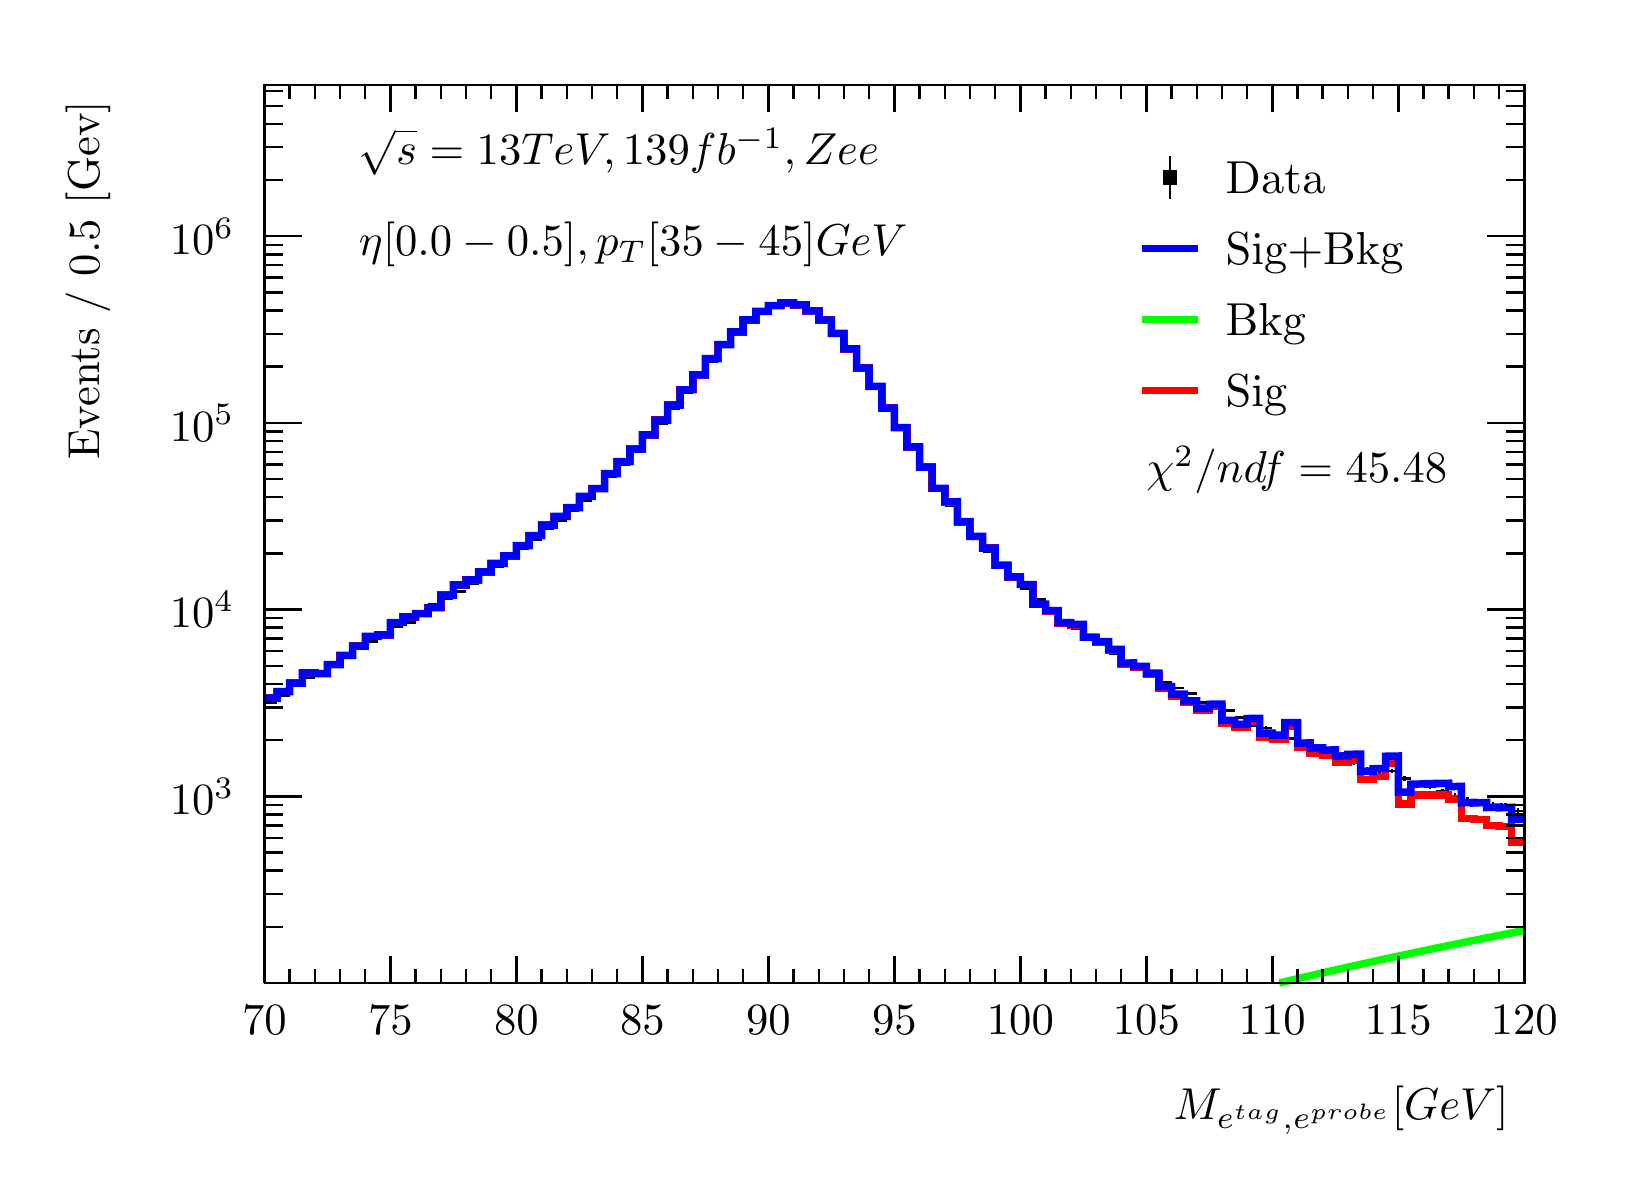
\begin{tikzpicture}
\pgfdeclareplotmark{cross} {
\pgfpathmoveto{\pgfpoint{-0.3\pgfplotmarksize}{\pgfplotmarksize}}
\pgfpathlineto{\pgfpoint{+0.3\pgfplotmarksize}{\pgfplotmarksize}}
\pgfpathlineto{\pgfpoint{+0.3\pgfplotmarksize}{0.3\pgfplotmarksize}}
\pgfpathlineto{\pgfpoint{+1\pgfplotmarksize}{0.3\pgfplotmarksize}}
\pgfpathlineto{\pgfpoint{+1\pgfplotmarksize}{-0.3\pgfplotmarksize}}
\pgfpathlineto{\pgfpoint{+0.3\pgfplotmarksize}{-0.3\pgfplotmarksize}}
\pgfpathlineto{\pgfpoint{+0.3\pgfplotmarksize}{-1.\pgfplotmarksize}}
\pgfpathlineto{\pgfpoint{-0.3\pgfplotmarksize}{-1.\pgfplotmarksize}}
\pgfpathlineto{\pgfpoint{-0.3\pgfplotmarksize}{-0.3\pgfplotmarksize}}
\pgfpathlineto{\pgfpoint{-1.\pgfplotmarksize}{-0.3\pgfplotmarksize}}
\pgfpathlineto{\pgfpoint{-1.\pgfplotmarksize}{0.3\pgfplotmarksize}}
\pgfpathlineto{\pgfpoint{-0.3\pgfplotmarksize}{0.3\pgfplotmarksize}}
\pgfpathclose
\pgfusepathqstroke
}
\pgfdeclareplotmark{cross*} {
\pgfpathmoveto{\pgfpoint{-0.3\pgfplotmarksize}{\pgfplotmarksize}}
\pgfpathlineto{\pgfpoint{+0.3\pgfplotmarksize}{\pgfplotmarksize}}
\pgfpathlineto{\pgfpoint{+0.3\pgfplotmarksize}{0.3\pgfplotmarksize}}
\pgfpathlineto{\pgfpoint{+1\pgfplotmarksize}{0.3\pgfplotmarksize}}
\pgfpathlineto{\pgfpoint{+1\pgfplotmarksize}{-0.3\pgfplotmarksize}}
\pgfpathlineto{\pgfpoint{+0.3\pgfplotmarksize}{-0.3\pgfplotmarksize}}
\pgfpathlineto{\pgfpoint{+0.3\pgfplotmarksize}{-1.\pgfplotmarksize}}
\pgfpathlineto{\pgfpoint{-0.3\pgfplotmarksize}{-1.\pgfplotmarksize}}
\pgfpathlineto{\pgfpoint{-0.3\pgfplotmarksize}{-0.3\pgfplotmarksize}}
\pgfpathlineto{\pgfpoint{-1.\pgfplotmarksize}{-0.3\pgfplotmarksize}}
\pgfpathlineto{\pgfpoint{-1.\pgfplotmarksize}{0.3\pgfplotmarksize}}
\pgfpathlineto{\pgfpoint{-0.3\pgfplotmarksize}{0.3\pgfplotmarksize}}
\pgfpathclose
\pgfusepathqfillstroke
}
\pgfdeclareplotmark{newstar} {
\pgfpathmoveto{\pgfqpoint{0pt}{\pgfplotmarksize}}
\pgfpathlineto{\pgfqpointpolar{44}{0.5\pgfplotmarksize}}
\pgfpathlineto{\pgfqpointpolar{18}{\pgfplotmarksize}}
\pgfpathlineto{\pgfqpointpolar{-20}{0.5\pgfplotmarksize}}
\pgfpathlineto{\pgfqpointpolar{-54}{\pgfplotmarksize}}
\pgfpathlineto{\pgfqpointpolar{-90}{0.5\pgfplotmarksize}}
\pgfpathlineto{\pgfqpointpolar{234}{\pgfplotmarksize}}
\pgfpathlineto{\pgfqpointpolar{198}{0.5\pgfplotmarksize}}
\pgfpathlineto{\pgfqpointpolar{162}{\pgfplotmarksize}}
\pgfpathlineto{\pgfqpointpolar{134}{0.5\pgfplotmarksize}}
\pgfpathclose
\pgfusepathqstroke
}
\pgfdeclareplotmark{newstar*} {
\pgfpathmoveto{\pgfqpoint{0pt}{\pgfplotmarksize}}
\pgfpathlineto{\pgfqpointpolar{44}{0.5\pgfplotmarksize}}
\pgfpathlineto{\pgfqpointpolar{18}{\pgfplotmarksize}}
\pgfpathlineto{\pgfqpointpolar{-20}{0.5\pgfplotmarksize}}
\pgfpathlineto{\pgfqpointpolar{-54}{\pgfplotmarksize}}
\pgfpathlineto{\pgfqpointpolar{-90}{0.5\pgfplotmarksize}}
\pgfpathlineto{\pgfqpointpolar{234}{\pgfplotmarksize}}
\pgfpathlineto{\pgfqpointpolar{198}{0.5\pgfplotmarksize}}
\pgfpathlineto{\pgfqpointpolar{162}{\pgfplotmarksize}}
\pgfpathlineto{\pgfqpointpolar{134}{0.5\pgfplotmarksize}}
\pgfpathclose
\pgfusepathqfillstroke
}
\definecolor{c}{rgb}{1,1,1};
\draw [color=c, fill=c] (0,0) rectangle (20,14.4361);
\draw [color=c, fill=c] (3,2.30977) rectangle (19,13.7143);
\definecolor{c}{rgb}{0,0,0};
\draw [c,line width=0.9] (3,2.30977) -- (3,13.7143) -- (19,13.7143) -- (19,2.30977) -- (3,2.30977);
\definecolor{c}{rgb}{1,1,1};
\draw [color=c, fill=c] (3,2.30977) rectangle (19,13.7143);
\definecolor{c}{rgb}{0,0,0};
\draw [c,line width=0.9] (3,2.30977) -- (3,13.7143) -- (19,13.7143) -- (19,2.30977) -- (3,2.30977);
\draw [c,line width=0.9] (3,2.30977) -- (19,2.30977);
\draw [c,line width=0.9] (3,2.65624) -- (3,2.30977);
\draw [c,line width=0.9] (3.32,2.48301) -- (3.32,2.30977);
\draw [c,line width=0.9] (3.64,2.48301) -- (3.64,2.30977);
\draw [c,line width=0.9] (3.96,2.48301) -- (3.96,2.30977);
\draw [c,line width=0.9] (4.28,2.48301) -- (4.28,2.30977);
\draw [c,line width=0.9] (4.6,2.65624) -- (4.6,2.30977);
\draw [c,line width=0.9] (4.92,2.48301) -- (4.92,2.30977);
\draw [c,line width=0.9] (5.24,2.48301) -- (5.24,2.30977);
\draw [c,line width=0.9] (5.56,2.48301) -- (5.56,2.30977);
\draw [c,line width=0.9] (5.88,2.48301) -- (5.88,2.30977);
\draw [c,line width=0.9] (6.2,2.65624) -- (6.2,2.30977);
\draw [c,line width=0.9] (6.52,2.48301) -- (6.52,2.30977);
\draw [c,line width=0.9] (6.84,2.48301) -- (6.84,2.30977);
\draw [c,line width=0.9] (7.16,2.48301) -- (7.16,2.30977);
\draw [c,line width=0.9] (7.48,2.48301) -- (7.48,2.30977);
\draw [c,line width=0.9] (7.8,2.65624) -- (7.8,2.30977);
\draw [c,line width=0.9] (8.12,2.48301) -- (8.12,2.30977);
\draw [c,line width=0.9] (8.44,2.48301) -- (8.44,2.30977);
\draw [c,line width=0.9] (8.76,2.48301) -- (8.76,2.30977);
\draw [c,line width=0.9] (9.08,2.48301) -- (9.08,2.30977);
\draw [c,line width=0.9] (9.4,2.65624) -- (9.4,2.30977);
\draw [c,line width=0.9] (9.72,2.48301) -- (9.72,2.30977);
\draw [c,line width=0.9] (10.04,2.48301) -- (10.04,2.30977);
\draw [c,line width=0.9] (10.36,2.48301) -- (10.36,2.30977);
\draw [c,line width=0.9] (10.68,2.48301) -- (10.68,2.30977);
\draw [c,line width=0.9] (11,2.65624) -- (11,2.30977);
\draw [c,line width=0.9] (11.32,2.48301) -- (11.32,2.30977);
\draw [c,line width=0.9] (11.64,2.48301) -- (11.64,2.30977);
\draw [c,line width=0.9] (11.96,2.48301) -- (11.96,2.30977);
\draw [c,line width=0.9] (12.28,2.48301) -- (12.28,2.30977);
\draw [c,line width=0.9] (12.6,2.65624) -- (12.6,2.30977);
\draw [c,line width=0.9] (12.92,2.48301) -- (12.92,2.30977);
\draw [c,line width=0.9] (13.24,2.48301) -- (13.24,2.30977);
\draw [c,line width=0.9] (13.56,2.48301) -- (13.56,2.30977);
\draw [c,line width=0.9] (13.88,2.48301) -- (13.88,2.30977);
\draw [c,line width=0.9] (14.2,2.65624) -- (14.2,2.30977);
\draw [c,line width=0.9] (14.52,2.48301) -- (14.52,2.30977);
\draw [c,line width=0.9] (14.84,2.48301) -- (14.84,2.30977);
\draw [c,line width=0.9] (15.16,2.48301) -- (15.16,2.30977);
\draw [c,line width=0.9] (15.48,2.48301) -- (15.48,2.30977);
\draw [c,line width=0.9] (15.8,2.65624) -- (15.8,2.30977);
\draw [c,line width=0.9] (16.12,2.48301) -- (16.12,2.30977);
\draw [c,line width=0.9] (16.44,2.48301) -- (16.44,2.30977);
\draw [c,line width=0.9] (16.76,2.48301) -- (16.76,2.30977);
\draw [c,line width=0.9] (17.08,2.48301) -- (17.08,2.30977);
\draw [c,line width=0.9] (17.4,2.65624) -- (17.4,2.30977);
\draw [c,line width=0.9] (17.72,2.48301) -- (17.72,2.30977);
\draw [c,line width=0.9] (18.04,2.48301) -- (18.04,2.30977);
\draw [c,line width=0.9] (18.36,2.48301) -- (18.36,2.30977);
\draw [c,line width=0.9] (18.68,2.48301) -- (18.68,2.30977);
\draw [c,line width=0.9] (19,2.65624) -- (19,2.30977);
\draw [anchor=base] (3,1.66015) node[scale=1.61424, color=c, rotate=0]{70};
\draw [anchor=base] (4.6,1.66015) node[scale=1.61424, color=c, rotate=0]{75};
\draw [anchor=base] (6.2,1.66015) node[scale=1.61424, color=c, rotate=0]{80};
\draw [anchor=base] (7.8,1.66015) node[scale=1.61424, color=c, rotate=0]{85};
\draw [anchor=base] (9.4,1.66015) node[scale=1.61424, color=c, rotate=0]{90};
\draw [anchor=base] (11,1.66015) node[scale=1.61424, color=c, rotate=0]{95};
\draw [anchor=base] (12.6,1.66015) node[scale=1.61424, color=c, rotate=0]{100};
\draw [anchor=base] (14.2,1.66015) node[scale=1.61424, color=c, rotate=0]{105};
\draw [anchor=base] (15.8,1.66015) node[scale=1.61424, color=c, rotate=0]{110};
\draw [anchor=base] (17.4,1.66015) node[scale=1.61424, color=c, rotate=0]{115};
\draw [anchor=base] (19,1.66015) node[scale=1.61424, color=c, rotate=0]{120};
\draw [anchor= east] (19,0.692932) node[scale=1.61424, color=c, rotate=0]{$M_{e^{tag}, e^{probe}}  [GeV]$};
\draw [c,line width=0.9] (3,13.7143) -- (19,13.7143);
\draw [c,line width=0.9] (3,13.3678) -- (3,13.7143);
\draw [c,line width=0.9] (3.32,13.5411) -- (3.32,13.7143);
\draw [c,line width=0.9] (3.64,13.5411) -- (3.64,13.7143);
\draw [c,line width=0.9] (3.96,13.5411) -- (3.96,13.7143);
\draw [c,line width=0.9] (4.28,13.5411) -- (4.28,13.7143);
\draw [c,line width=0.9] (4.6,13.3678) -- (4.6,13.7143);
\draw [c,line width=0.9] (4.92,13.5411) -- (4.92,13.7143);
\draw [c,line width=0.9] (5.24,13.5411) -- (5.24,13.7143);
\draw [c,line width=0.9] (5.56,13.5411) -- (5.56,13.7143);
\draw [c,line width=0.9] (5.88,13.5411) -- (5.88,13.7143);
\draw [c,line width=0.9] (6.2,13.3678) -- (6.2,13.7143);
\draw [c,line width=0.9] (6.52,13.5411) -- (6.52,13.7143);
\draw [c,line width=0.9] (6.84,13.5411) -- (6.84,13.7143);
\draw [c,line width=0.9] (7.16,13.5411) -- (7.16,13.7143);
\draw [c,line width=0.9] (7.48,13.5411) -- (7.48,13.7143);
\draw [c,line width=0.9] (7.8,13.3678) -- (7.8,13.7143);
\draw [c,line width=0.9] (8.12,13.5411) -- (8.12,13.7143);
\draw [c,line width=0.9] (8.44,13.5411) -- (8.44,13.7143);
\draw [c,line width=0.9] (8.76,13.5411) -- (8.76,13.7143);
\draw [c,line width=0.9] (9.08,13.5411) -- (9.08,13.7143);
\draw [c,line width=0.9] (9.4,13.3678) -- (9.4,13.7143);
\draw [c,line width=0.9] (9.72,13.5411) -- (9.72,13.7143);
\draw [c,line width=0.9] (10.04,13.5411) -- (10.04,13.7143);
\draw [c,line width=0.9] (10.36,13.5411) -- (10.36,13.7143);
\draw [c,line width=0.9] (10.68,13.5411) -- (10.68,13.7143);
\draw [c,line width=0.9] (11,13.3678) -- (11,13.7143);
\draw [c,line width=0.9] (11.32,13.5411) -- (11.32,13.7143);
\draw [c,line width=0.9] (11.64,13.5411) -- (11.64,13.7143);
\draw [c,line width=0.9] (11.96,13.5411) -- (11.96,13.7143);
\draw [c,line width=0.9] (12.28,13.5411) -- (12.28,13.7143);
\draw [c,line width=0.9] (12.6,13.3678) -- (12.6,13.7143);
\draw [c,line width=0.9] (12.92,13.5411) -- (12.92,13.7143);
\draw [c,line width=0.9] (13.24,13.5411) -- (13.24,13.7143);
\draw [c,line width=0.9] (13.56,13.5411) -- (13.56,13.7143);
\draw [c,line width=0.9] (13.88,13.5411) -- (13.88,13.7143);
\draw [c,line width=0.9] (14.2,13.3678) -- (14.2,13.7143);
\draw [c,line width=0.9] (14.52,13.5411) -- (14.52,13.7143);
\draw [c,line width=0.9] (14.84,13.5411) -- (14.84,13.7143);
\draw [c,line width=0.9] (15.16,13.5411) -- (15.16,13.7143);
\draw [c,line width=0.9] (15.48,13.5411) -- (15.48,13.7143);
\draw [c,line width=0.9] (15.8,13.3678) -- (15.8,13.7143);
\draw [c,line width=0.9] (16.12,13.5411) -- (16.12,13.7143);
\draw [c,line width=0.9] (16.44,13.5411) -- (16.44,13.7143);
\draw [c,line width=0.9] (16.76,13.5411) -- (16.76,13.7143);
\draw [c,line width=0.9] (17.08,13.5411) -- (17.08,13.7143);
\draw [c,line width=0.9] (17.4,13.3678) -- (17.4,13.7143);
\draw [c,line width=0.9] (17.72,13.5411) -- (17.72,13.7143);
\draw [c,line width=0.9] (18.04,13.5411) -- (18.04,13.7143);
\draw [c,line width=0.9] (18.36,13.5411) -- (18.36,13.7143);
\draw [c,line width=0.9] (18.68,13.5411) -- (18.68,13.7143);
\draw [c,line width=0.9] (19,13.3678) -- (19,13.7143);
\draw [c,line width=0.9] (3,2.30977) -- (3,13.7143);
\draw [c,line width=0.9] (3.237,3.02354) -- (3,3.02354);
\draw [c,line width=0.9] (3.237,3.44107) -- (3,3.44107);
\draw [c,line width=0.9] (3.237,3.73731) -- (3,3.73731);
\draw [c,line width=0.9] (3.237,3.96709) -- (3,3.96709);
\draw [c,line width=0.9] (3.237,4.15484) -- (3,4.15484);
\draw [c,line width=0.9] (3.237,4.31357) -- (3,4.31357);
\draw [c,line width=0.9] (3.237,4.45108) -- (3,4.45108);
\draw [c,line width=0.9] (3.237,4.57236) -- (3,4.57236);
\draw [c,line width=0.9] (3.474,4.68086) -- (3,4.68086);
\draw [anchor= east] (2.82,4.68086) node[scale=1.61424, color=c, rotate=0]{$10^{3}$};
\draw [c,line width=0.9] (3.237,5.39463) -- (3,5.39463);
\draw [c,line width=0.9] (3.237,5.81216) -- (3,5.81216);
\draw [c,line width=0.9] (3.237,6.1084) -- (3,6.1084);
\draw [c,line width=0.9] (3.237,6.33818) -- (3,6.33818);
\draw [c,line width=0.9] (3.237,6.52593) -- (3,6.52593);
\draw [c,line width=0.9] (3.237,6.68466) -- (3,6.68466);
\draw [c,line width=0.9] (3.237,6.82217) -- (3,6.82217);
\draw [c,line width=0.9] (3.237,6.94345) -- (3,6.94345);
\draw [c,line width=0.9] (3.474,7.05195) -- (3,7.05195);
\draw [anchor= east] (2.82,7.05195) node[scale=1.61424, color=c, rotate=0]{$10^{4}$};
\draw [c,line width=0.9] (3.237,7.76572) -- (3,7.76572);
\draw [c,line width=0.9] (3.237,8.18324) -- (3,8.18324);
\draw [c,line width=0.9] (3.237,8.47948) -- (3,8.47948);
\draw [c,line width=0.9] (3.237,8.70927) -- (3,8.70927);
\draw [c,line width=0.9] (3.237,8.89701) -- (3,8.89701);
\draw [c,line width=0.9] (3.237,9.05575) -- (3,9.05575);
\draw [c,line width=0.9] (3.237,9.19325) -- (3,9.19325);
\draw [c,line width=0.9] (3.237,9.31454) -- (3,9.31454);
\draw [c,line width=0.9] (3.474,9.42304) -- (3,9.42304);
\draw [anchor= east] (2.82,9.42304) node[scale=1.61424, color=c, rotate=0]{$10^{5}$};
\draw [c,line width=0.9] (3.237,10.1368) -- (3,10.1368);
\draw [c,line width=0.9] (3.237,10.5543) -- (3,10.5543);
\draw [c,line width=0.9] (3.237,10.8506) -- (3,10.8506);
\draw [c,line width=0.9] (3.237,11.0804) -- (3,11.0804);
\draw [c,line width=0.9] (3.237,11.2681) -- (3,11.2681);
\draw [c,line width=0.9] (3.237,11.4268) -- (3,11.4268);
\draw [c,line width=0.9] (3.237,11.5643) -- (3,11.5643);
\draw [c,line width=0.9] (3.237,11.6856) -- (3,11.6856);
\draw [c,line width=0.9] (3.474,11.7941) -- (3,11.7941);
\draw [anchor= east] (2.82,11.7941) node[scale=1.61424, color=c, rotate=0]{$10^{6}$};
\draw [c,line width=0.9] (3.237,12.5079) -- (3,12.5079);
\draw [c,line width=0.9] (3.237,12.9254) -- (3,12.9254);
\draw [c,line width=0.9] (3.237,13.2217) -- (3,13.2217);
\draw [c,line width=0.9] (3.237,13.4514) -- (3,13.4514);
\draw [c,line width=0.9] (3.237,13.6392) -- (3,13.6392);
\draw [anchor= east] (0.76,13.7143) node[scale=1.61424, color=c, rotate=90]{Events / 0.5 [Gev]};
\draw [c,line width=0.9] (19,2.30977) -- (19,13.7143);
\draw [c,line width=0.9] (18.763,3.02354) -- (19,3.02354);
\draw [c,line width=0.9] (18.763,3.44107) -- (19,3.44107);
\draw [c,line width=0.9] (18.763,3.73731) -- (19,3.73731);
\draw [c,line width=0.9] (18.763,3.96709) -- (19,3.96709);
\draw [c,line width=0.9] (18.763,4.15484) -- (19,4.15484);
\draw [c,line width=0.9] (18.763,4.31357) -- (19,4.31357);
\draw [c,line width=0.9] (18.763,4.45108) -- (19,4.45108);
\draw [c,line width=0.9] (18.763,4.57236) -- (19,4.57236);
\draw [c,line width=0.9] (18.526,4.68086) -- (19,4.68086);
\draw [c,line width=0.9] (18.763,5.39463) -- (19,5.39463);
\draw [c,line width=0.9] (18.763,5.81216) -- (19,5.81216);
\draw [c,line width=0.9] (18.763,6.1084) -- (19,6.1084);
\draw [c,line width=0.9] (18.763,6.33818) -- (19,6.33818);
\draw [c,line width=0.9] (18.763,6.52593) -- (19,6.52593);
\draw [c,line width=0.9] (18.763,6.68466) -- (19,6.68466);
\draw [c,line width=0.9] (18.763,6.82217) -- (19,6.82217);
\draw [c,line width=0.9] (18.763,6.94345) -- (19,6.94345);
\draw [c,line width=0.9] (18.526,7.05195) -- (19,7.05195);
\draw [c,line width=0.9] (18.763,7.76572) -- (19,7.76572);
\draw [c,line width=0.9] (18.763,8.18324) -- (19,8.18324);
\draw [c,line width=0.9] (18.763,8.47948) -- (19,8.47948);
\draw [c,line width=0.9] (18.763,8.70927) -- (19,8.70927);
\draw [c,line width=0.9] (18.763,8.89701) -- (19,8.89701);
\draw [c,line width=0.9] (18.763,9.05575) -- (19,9.05575);
\draw [c,line width=0.9] (18.763,9.19325) -- (19,9.19325);
\draw [c,line width=0.9] (18.763,9.31454) -- (19,9.31454);
\draw [c,line width=0.9] (18.526,9.42304) -- (19,9.42304);
\draw [c,line width=0.9] (18.763,10.1368) -- (19,10.1368);
\draw [c,line width=0.9] (18.763,10.5543) -- (19,10.5543);
\draw [c,line width=0.9] (18.763,10.8506) -- (19,10.8506);
\draw [c,line width=0.9] (18.763,11.0804) -- (19,11.0804);
\draw [c,line width=0.9] (18.763,11.2681) -- (19,11.2681);
\draw [c,line width=0.9] (18.763,11.4268) -- (19,11.4268);
\draw [c,line width=0.9] (18.763,11.5643) -- (19,11.5643);
\draw [c,line width=0.9] (18.763,11.6856) -- (19,11.6856);
\draw [c,line width=0.9] (18.526,11.7941) -- (19,11.7941);
\draw [c,line width=0.9] (18.763,12.5079) -- (19,12.5079);
\draw [c,line width=0.9] (18.763,12.9254) -- (19,12.9254);
\draw [c,line width=0.9] (18.763,13.2217) -- (19,13.2217);
\draw [c,line width=0.9] (18.763,13.4514) -- (19,13.4514);
\draw [c,line width=0.9] (18.763,13.6392) -- (19,13.6392);
\draw [c,line width=0.9] (3.08,5.87086) -- (3,5.87086);
\draw [c,line width=0.9] (3,5.87086) -- (3,5.87086);
\draw [c,line width=0.9] (3.08,5.87086) -- (3.16,5.87086);
\draw [c,line width=0.9] (3.16,5.87086) -- (3.16,5.87086);
\draw [c,line width=0.9] (3.08,5.87086) -- (3.08,5.88914);
\draw [c,line width=0.9] (3.08,5.88914) -- (3.08,5.88914);
\draw [c,line width=0.9] (3.08,5.87086) -- (3.08,5.85259);
\draw [c,line width=0.9] (3.08,5.85259) -- (3.08,5.85259);
\draw [c,line width=0.9] (3.24,5.95965) -- (3.16,5.95965);
\draw [c,line width=0.9] (3.16,5.95965) -- (3.16,5.95965);
\draw [c,line width=0.9] (3.24,5.95965) -- (3.32,5.95965);
\draw [c,line width=0.9] (3.32,5.95965) -- (3.32,5.95965);
\draw [c,line width=0.9] (3.24,5.95965) -- (3.24,5.97715);
\draw [c,line width=0.9] (3.24,5.97715) -- (3.24,5.97715);
\draw [c,line width=0.9] (3.24,5.95965) -- (3.24,5.94215);
\draw [c,line width=0.9] (3.24,5.94215) -- (3.24,5.94215);
\draw [c,line width=0.9] (3.4,6.12246) -- (3.32,6.12246);
\draw [c,line width=0.9] (3.32,6.12246) -- (3.32,6.12246);
\draw [c,line width=0.9] (3.4,6.12246) -- (3.48,6.12246);
\draw [c,line width=0.9] (3.48,6.12246) -- (3.48,6.12246);
\draw [c,line width=0.9] (3.4,6.12246) -- (3.4,6.13863);
\draw [c,line width=0.9] (3.4,6.13863) -- (3.4,6.13863);
\draw [c,line width=0.9] (3.4,6.12246) -- (3.4,6.10629);
\draw [c,line width=0.9] (3.4,6.10629) -- (3.4,6.10629);
\draw [c,line width=0.9] (3.56,6.19027) -- (3.48,6.19027);
\draw [c,line width=0.9] (3.48,6.19027) -- (3.48,6.19027);
\draw [c,line width=0.9] (3.56,6.19027) -- (3.64,6.19027);
\draw [c,line width=0.9] (3.64,6.19027) -- (3.64,6.19027);
\draw [c,line width=0.9] (3.56,6.19027) -- (3.56,6.20591);
\draw [c,line width=0.9] (3.56,6.20591) -- (3.56,6.20591);
\draw [c,line width=0.9] (3.56,6.19027) -- (3.56,6.17462);
\draw [c,line width=0.9] (3.56,6.17462) -- (3.56,6.17462);
\draw [c,line width=0.9] (3.72,6.27556) -- (3.64,6.27556);
\draw [c,line width=0.9] (3.64,6.27556) -- (3.64,6.27556);
\draw [c,line width=0.9] (3.72,6.27556) -- (3.8,6.27556);
\draw [c,line width=0.9] (3.8,6.27556) -- (3.8,6.27556);
\draw [c,line width=0.9] (3.72,6.27556) -- (3.72,6.29057);
\draw [c,line width=0.9] (3.72,6.29057) -- (3.72,6.29057);
\draw [c,line width=0.9] (3.72,6.27556) -- (3.72,6.26055);
\draw [c,line width=0.9] (3.72,6.26055) -- (3.72,6.26055);
\draw [c,line width=0.9] (3.88,6.37916) -- (3.8,6.37916);
\draw [c,line width=0.9] (3.8,6.37916) -- (3.8,6.37916);
\draw [c,line width=0.9] (3.88,6.37916) -- (3.96,6.37916);
\draw [c,line width=0.9] (3.96,6.37916) -- (3.96,6.37916);
\draw [c,line width=0.9] (3.88,6.37916) -- (3.88,6.39344);
\draw [c,line width=0.9] (3.88,6.39344) -- (3.88,6.39344);
\draw [c,line width=0.9] (3.88,6.37916) -- (3.88,6.36489);
\draw [c,line width=0.9] (3.88,6.36489) -- (3.88,6.36489);
\draw [c,line width=0.9] (4.04,6.47509) -- (3.96,6.47509);
\draw [c,line width=0.9] (3.96,6.47509) -- (3.96,6.47509);
\draw [c,line width=0.9] (4.04,6.47509) -- (4.12,6.47509);
\draw [c,line width=0.9] (4.12,6.47509) -- (4.12,6.47509);
\draw [c,line width=0.9] (4.04,6.47509) -- (4.04,6.48872);
\draw [c,line width=0.9] (4.04,6.48872) -- (4.04,6.48872);
\draw [c,line width=0.9] (4.04,6.47509) -- (4.04,6.46147);
\draw [c,line width=0.9] (4.04,6.46147) -- (4.04,6.46147);
\draw [c,line width=0.9] (4.2,6.576) -- (4.12,6.576);
\draw [c,line width=0.9] (4.12,6.576) -- (4.12,6.576);
\draw [c,line width=0.9] (4.2,6.576) -- (4.28,6.576);
\draw [c,line width=0.9] (4.28,6.576) -- (4.28,6.576);
\draw [c,line width=0.9] (4.2,6.576) -- (4.2,6.58898);
\draw [c,line width=0.9] (4.2,6.58898) -- (4.2,6.58898);
\draw [c,line width=0.9] (4.2,6.576) -- (4.2,6.56303);
\draw [c,line width=0.9] (4.2,6.56303) -- (4.2,6.56303);
\draw [c,line width=0.9] (4.36,6.64508) -- (4.28,6.64508);
\draw [c,line width=0.9] (4.28,6.64508) -- (4.28,6.64508);
\draw [c,line width=0.9] (4.36,6.64508) -- (4.44,6.64508);
\draw [c,line width=0.9] (4.44,6.64508) -- (4.44,6.64508);
\draw [c,line width=0.9] (4.36,6.64508) -- (4.36,6.65762);
\draw [c,line width=0.9] (4.36,6.65762) -- (4.36,6.65762);
\draw [c,line width=0.9] (4.36,6.64508) -- (4.36,6.63253);
\draw [c,line width=0.9] (4.36,6.63253) -- (4.36,6.63253);
\draw [c,line width=0.9] (4.52,6.7335) -- (4.44,6.7335);
\draw [c,line width=0.9] (4.44,6.7335) -- (4.44,6.7335);
\draw [c,line width=0.9] (4.52,6.7335) -- (4.6,6.7335);
\draw [c,line width=0.9] (4.6,6.7335) -- (4.6,6.7335);
\draw [c,line width=0.9] (4.52,6.7335) -- (4.52,6.74552);
\draw [c,line width=0.9] (4.52,6.74552) -- (4.52,6.74552);
\draw [c,line width=0.9] (4.52,6.7335) -- (4.52,6.72148);
\draw [c,line width=0.9] (4.52,6.72148) -- (4.52,6.72148);
\draw [c,line width=0.9] (4.68,6.83216) -- (4.6,6.83216);
\draw [c,line width=0.9] (4.6,6.83216) -- (4.6,6.83216);
\draw [c,line width=0.9] (4.68,6.83216) -- (4.76,6.83216);
\draw [c,line width=0.9] (4.76,6.83216) -- (4.76,6.83216);
\draw [c,line width=0.9] (4.68,6.83216) -- (4.68,6.84362);
\draw [c,line width=0.9] (4.68,6.84362) -- (4.68,6.84362);
\draw [c,line width=0.9] (4.68,6.83216) -- (4.68,6.8207);
\draw [c,line width=0.9] (4.68,6.8207) -- (4.68,6.8207);
\draw [c,line width=0.9] (4.84,6.88786) -- (4.76,6.88786);
\draw [c,line width=0.9] (4.76,6.88786) -- (4.76,6.88786);
\draw [c,line width=0.9] (4.84,6.88786) -- (4.92,6.88786);
\draw [c,line width=0.9] (4.92,6.88786) -- (4.92,6.88786);
\draw [c,line width=0.9] (4.84,6.88786) -- (4.84,6.89901);
\draw [c,line width=0.9] (4.84,6.89901) -- (4.84,6.89901);
\draw [c,line width=0.9] (4.84,6.88786) -- (4.84,6.87671);
\draw [c,line width=0.9] (4.84,6.87671) -- (4.84,6.87671);
\draw [c,line width=0.9] (5,7.00162) -- (4.92,7.00162);
\draw [c,line width=0.9] (4.92,7.00162) -- (4.92,7.00162);
\draw [c,line width=0.9] (5,7.00162) -- (5.08,7.00162);
\draw [c,line width=0.9] (5.08,7.00162) -- (5.08,7.00162);
\draw [c,line width=0.9] (5,7.00162) -- (5,7.01217);
\draw [c,line width=0.9] (5,7.01217) -- (5,7.01217);
\draw [c,line width=0.9] (5,7.00162) -- (5,6.99107);
\draw [c,line width=0.9] (5,6.99107) -- (5,6.99107);
\draw [c,line width=0.9] (5.16,7.11506) -- (5.08,7.11506);
\draw [c,line width=0.9] (5.08,7.11506) -- (5.08,7.11506);
\draw [c,line width=0.9] (5.16,7.11506) -- (5.24,7.11506);
\draw [c,line width=0.9] (5.24,7.11506) -- (5.24,7.11506);
\draw [c,line width=0.9] (5.16,7.11506) -- (5.16,7.12504);
\draw [c,line width=0.9] (5.16,7.12504) -- (5.16,7.12504);
\draw [c,line width=0.9] (5.16,7.11506) -- (5.16,7.10507);
\draw [c,line width=0.9] (5.16,7.10507) -- (5.16,7.10507);
\draw [c,line width=0.9] (5.32,7.18416) -- (5.24,7.18416);
\draw [c,line width=0.9] (5.24,7.18416) -- (5.24,7.18416);
\draw [c,line width=0.9] (5.32,7.18416) -- (5.4,7.18416);
\draw [c,line width=0.9] (5.4,7.18416) -- (5.4,7.18416);
\draw [c,line width=0.9] (5.32,7.18416) -- (5.32,7.19382);
\draw [c,line width=0.9] (5.32,7.19382) -- (5.32,7.19382);
\draw [c,line width=0.9] (5.32,7.18416) -- (5.32,7.1745);
\draw [c,line width=0.9] (5.32,7.1745) -- (5.32,7.1745);
\draw [c,line width=0.9] (5.48,7.28543) -- (5.4,7.28543);
\draw [c,line width=0.9] (5.4,7.28543) -- (5.4,7.28543);
\draw [c,line width=0.9] (5.48,7.28543) -- (5.56,7.28543);
\draw [c,line width=0.9] (5.56,7.28543) -- (5.56,7.28543);
\draw [c,line width=0.9] (5.48,7.28543) -- (5.48,7.29463);
\draw [c,line width=0.9] (5.48,7.29463) -- (5.48,7.29463);
\draw [c,line width=0.9] (5.48,7.28543) -- (5.48,7.27624);
\draw [c,line width=0.9] (5.48,7.27624) -- (5.48,7.27624);
\draw [c,line width=0.9] (5.64,7.38674) -- (5.56,7.38674);
\draw [c,line width=0.9] (5.56,7.38674) -- (5.56,7.38674);
\draw [c,line width=0.9] (5.64,7.38674) -- (5.72,7.38674);
\draw [c,line width=0.9] (5.72,7.38674) -- (5.72,7.38674);
\draw [c,line width=0.9] (5.64,7.38674) -- (5.64,7.3955);
\draw [c,line width=0.9] (5.64,7.3955) -- (5.64,7.3955);
\draw [c,line width=0.9] (5.64,7.38674) -- (5.64,7.37799);
\draw [c,line width=0.9] (5.64,7.37799) -- (5.64,7.37799);
\draw [c,line width=0.9] (5.8,7.50696) -- (5.72,7.50696);
\draw [c,line width=0.9] (5.72,7.50696) -- (5.72,7.50696);
\draw [c,line width=0.9] (5.8,7.50696) -- (5.88,7.50696);
\draw [c,line width=0.9] (5.88,7.50696) -- (5.88,7.50696);
\draw [c,line width=0.9] (5.8,7.50696) -- (5.8,7.51521);
\draw [c,line width=0.9] (5.8,7.51521) -- (5.8,7.51521);
\draw [c,line width=0.9] (5.8,7.50696) -- (5.8,7.4987);
\draw [c,line width=0.9] (5.8,7.4987) -- (5.8,7.4987);
\draw [c,line width=0.9] (5.96,7.59618) -- (5.88,7.59618);
\draw [c,line width=0.9] (5.88,7.59618) -- (5.88,7.59618);
\draw [c,line width=0.9] (5.96,7.59618) -- (6.04,7.59618);
\draw [c,line width=0.9] (6.04,7.59618) -- (6.04,7.59618);
\draw [c,line width=0.9] (5.96,7.59618) -- (5.96,7.60409);
\draw [c,line width=0.9] (5.96,7.60409) -- (5.96,7.60409);
\draw [c,line width=0.9] (5.96,7.59618) -- (5.96,7.58827);
\draw [c,line width=0.9] (5.96,7.58827) -- (5.96,7.58827);
\draw [c,line width=0.9] (6.12,7.71447) -- (6.04,7.71447);
\draw [c,line width=0.9] (6.04,7.71447) -- (6.04,7.71447);
\draw [c,line width=0.9] (6.12,7.71447) -- (6.2,7.71447);
\draw [c,line width=0.9] (6.2,7.71447) -- (6.2,7.71447);
\draw [c,line width=0.9] (6.12,7.71447) -- (6.12,7.72193);
\draw [c,line width=0.9] (6.12,7.72193) -- (6.12,7.72193);
\draw [c,line width=0.9] (6.12,7.71447) -- (6.12,7.707);
\draw [c,line width=0.9] (6.12,7.707) -- (6.12,7.707);
\draw [c,line width=0.9] (6.28,7.82212) -- (6.2,7.82212);
\draw [c,line width=0.9] (6.2,7.82212) -- (6.2,7.82212);
\draw [c,line width=0.9] (6.28,7.82212) -- (6.36,7.82212);
\draw [c,line width=0.9] (6.36,7.82212) -- (6.36,7.82212);
\draw [c,line width=0.9] (6.28,7.82212) -- (6.28,7.8292);
\draw [c,line width=0.9] (6.28,7.8292) -- (6.28,7.8292);
\draw [c,line width=0.9] (6.28,7.82212) -- (6.28,7.81503);
\draw [c,line width=0.9] (6.28,7.81503) -- (6.28,7.81503);
\draw [c,line width=0.9] (6.44,7.93472) -- (6.36,7.93472);
\draw [c,line width=0.9] (6.36,7.93472) -- (6.36,7.93472);
\draw [c,line width=0.9] (6.44,7.93472) -- (6.52,7.93472);
\draw [c,line width=0.9] (6.52,7.93472) -- (6.52,7.93472);
\draw [c,line width=0.9] (6.44,7.93472) -- (6.44,7.94142);
\draw [c,line width=0.9] (6.44,7.94142) -- (6.44,7.94142);
\draw [c,line width=0.9] (6.44,7.93472) -- (6.44,7.92801);
\draw [c,line width=0.9] (6.44,7.92801) -- (6.44,7.92801);
\draw [c,line width=0.9] (6.6,8.07448) -- (6.52,8.07448);
\draw [c,line width=0.9] (6.52,8.07448) -- (6.52,8.07448);
\draw [c,line width=0.9] (6.6,8.07448) -- (6.68,8.07448);
\draw [c,line width=0.9] (6.68,8.07448) -- (6.68,8.07448);
\draw [c,line width=0.9] (6.6,8.07448) -- (6.6,8.08075);
\draw [c,line width=0.9] (6.6,8.08075) -- (6.6,8.08075);
\draw [c,line width=0.9] (6.6,8.07448) -- (6.6,8.06822);
\draw [c,line width=0.9] (6.6,8.06822) -- (6.6,8.06822);
\draw [c,line width=0.9] (6.76,8.18149) -- (6.68,8.18149);
\draw [c,line width=0.9] (6.68,8.18149) -- (6.68,8.18149);
\draw [c,line width=0.9] (6.76,8.18149) -- (6.84,8.18149);
\draw [c,line width=0.9] (6.84,8.18149) -- (6.84,8.18149);
\draw [c,line width=0.9] (6.76,8.18149) -- (6.76,8.18744);
\draw [c,line width=0.9] (6.76,8.18744) -- (6.76,8.18744);
\draw [c,line width=0.9] (6.76,8.18149) -- (6.76,8.17554);
\draw [c,line width=0.9] (6.76,8.17554) -- (6.76,8.17554);
\draw [c,line width=0.9] (6.92,8.30533) -- (6.84,8.30533);
\draw [c,line width=0.9] (6.84,8.30533) -- (6.84,8.30533);
\draw [c,line width=0.9] (6.92,8.30533) -- (7,8.30533);
\draw [c,line width=0.9] (7,8.30533) -- (7,8.30533);
\draw [c,line width=0.9] (6.92,8.30533) -- (6.92,8.31093);
\draw [c,line width=0.9] (6.92,8.31093) -- (6.92,8.31093);
\draw [c,line width=0.9] (6.92,8.30533) -- (6.92,8.29972);
\draw [c,line width=0.9] (6.92,8.29972) -- (6.92,8.29972);
\draw [c,line width=0.9] (7.08,8.44101) -- (7,8.44101);
\draw [c,line width=0.9] (7,8.44101) -- (7,8.44101);
\draw [c,line width=0.9] (7.08,8.44101) -- (7.16,8.44101);
\draw [c,line width=0.9] (7.16,8.44101) -- (7.16,8.44101);
\draw [c,line width=0.9] (7.08,8.44101) -- (7.08,8.44626);
\draw [c,line width=0.9] (7.08,8.44626) -- (7.08,8.44626);
\draw [c,line width=0.9] (7.08,8.44101) -- (7.08,8.43576);
\draw [c,line width=0.9] (7.08,8.43576) -- (7.08,8.43576);
\draw [c,line width=0.9] (7.24,8.58649) -- (7.16,8.58649);
\draw [c,line width=0.9] (7.16,8.58649) -- (7.16,8.58649);
\draw [c,line width=0.9] (7.24,8.58649) -- (7.32,8.58649);
\draw [c,line width=0.9] (7.32,8.58649) -- (7.32,8.58649);
\draw [c,line width=0.9] (7.24,8.58649) -- (7.24,8.59138);
\draw [c,line width=0.9] (7.24,8.59138) -- (7.24,8.59138);
\draw [c,line width=0.9] (7.24,8.58649) -- (7.24,8.5816);
\draw [c,line width=0.9] (7.24,8.5816) -- (7.24,8.5816);
\draw [c,line width=0.9] (7.4,8.7375) -- (7.32,8.7375);
\draw [c,line width=0.9] (7.32,8.7375) -- (7.32,8.7375);
\draw [c,line width=0.9] (7.4,8.7375) -- (7.48,8.7375);
\draw [c,line width=0.9] (7.48,8.7375) -- (7.48,8.7375);
\draw [c,line width=0.9] (7.4,8.7375) -- (7.4,8.74205);
\draw [c,line width=0.9] (7.4,8.74205) -- (7.4,8.74205);
\draw [c,line width=0.9] (7.4,8.7375) -- (7.4,8.73296);
\draw [c,line width=0.9] (7.4,8.73296) -- (7.4,8.73296);
\draw [c,line width=0.9] (7.56,8.88897) -- (7.48,8.88897);
\draw [c,line width=0.9] (7.48,8.88897) -- (7.48,8.88897);
\draw [c,line width=0.9] (7.56,8.88897) -- (7.64,8.88897);
\draw [c,line width=0.9] (7.64,8.88897) -- (7.64,8.88897);
\draw [c,line width=0.9] (7.56,8.88897) -- (7.56,8.89319);
\draw [c,line width=0.9] (7.56,8.89319) -- (7.56,8.89319);
\draw [c,line width=0.9] (7.56,8.88897) -- (7.56,8.88475);
\draw [c,line width=0.9] (7.56,8.88475) -- (7.56,8.88475);
\draw [c,line width=0.9] (7.72,9.05543) -- (7.64,9.05543);
\draw [c,line width=0.9] (7.64,9.05543) -- (7.64,9.05543);
\draw [c,line width=0.9] (7.72,9.05543) -- (7.8,9.05543);
\draw [c,line width=0.9] (7.8,9.05543) -- (7.8,9.05543);
\draw [c,line width=0.9] (7.72,9.05543) -- (7.72,9.05932);
\draw [c,line width=0.9] (7.72,9.05932) -- (7.72,9.05932);
\draw [c,line width=0.9] (7.72,9.05543) -- (7.72,9.05153);
\draw [c,line width=0.9] (7.72,9.05153) -- (7.72,9.05153);
\draw [c,line width=0.9] (7.88,9.23782) -- (7.8,9.23782);
\draw [c,line width=0.9] (7.8,9.23782) -- (7.8,9.23782);
\draw [c,line width=0.9] (7.88,9.23782) -- (7.96,9.23782);
\draw [c,line width=0.9] (7.96,9.23782) -- (7.96,9.23782);
\draw [c,line width=0.9] (7.88,9.23782) -- (7.88,9.24138);
\draw [c,line width=0.9] (7.88,9.24138) -- (7.88,9.24138);
\draw [c,line width=0.9] (7.88,9.23782) -- (7.88,9.23425);
\draw [c,line width=0.9] (7.88,9.23425) -- (7.88,9.23425);
\draw [c,line width=0.9] (8.04,9.41066) -- (7.96,9.41066);
\draw [c,line width=0.9] (7.96,9.41066) -- (7.96,9.41066);
\draw [c,line width=0.9] (8.04,9.41066) -- (8.12,9.41066);
\draw [c,line width=0.9] (8.12,9.41066) -- (8.12,9.41066);
\draw [c,line width=0.9] (8.04,9.41066) -- (8.04,9.41393);
\draw [c,line width=0.9] (8.04,9.41393) -- (8.04,9.41393);
\draw [c,line width=0.9] (8.04,9.41066) -- (8.04,9.40738);
\draw [c,line width=0.9] (8.04,9.40738) -- (8.04,9.40738);
\draw [c,line width=0.9] (8.2,9.60518) -- (8.12,9.60518);
\draw [c,line width=0.9] (8.12,9.60518) -- (8.12,9.60518);
\draw [c,line width=0.9] (8.2,9.60518) -- (8.28,9.60518);
\draw [c,line width=0.9] (8.28,9.60518) -- (8.28,9.60518);
\draw [c,line width=0.9] (8.2,9.60518) -- (8.2,9.60816);
\draw [c,line width=0.9] (8.2,9.60816) -- (8.2,9.60816);
\draw [c,line width=0.9] (8.2,9.60518) -- (8.2,9.6022);
\draw [c,line width=0.9] (8.2,9.6022) -- (8.2,9.6022);
\draw [c,line width=0.9] (8.36,9.80488) -- (8.28,9.80488);
\draw [c,line width=0.9] (8.28,9.80488) -- (8.28,9.80488);
\draw [c,line width=0.9] (8.36,9.80488) -- (8.44,9.80488);
\draw [c,line width=0.9] (8.44,9.80488) -- (8.44,9.80488);
\draw [c,line width=0.9] (8.36,9.80488) -- (8.36,9.80758);
\draw [c,line width=0.9] (8.36,9.80758) -- (8.36,9.80758);
\draw [c,line width=0.9] (8.36,9.80488) -- (8.36,9.80217);
\draw [c,line width=0.9] (8.36,9.80217) -- (8.36,9.80217);
\draw [c,line width=0.9] (8.52,10.0023) -- (8.44,10.0023);
\draw [c,line width=0.9] (8.44,10.0023) -- (8.44,10.0023);
\draw [c,line width=0.9] (8.52,10.0023) -- (8.6,10.0023);
\draw [c,line width=0.9] (8.6,10.0023) -- (8.6,10.0023);
\draw [c,line width=0.9] (8.52,10.0023) -- (8.52,10.0048);
\draw [c,line width=0.9] (8.52,10.0048) -- (8.52,10.0048);
\draw [c,line width=0.9] (8.52,10.0023) -- (8.52,9.99984);
\draw [c,line width=0.9] (8.52,9.99984) -- (8.52,9.99984);
\draw [c,line width=0.9] (8.68,10.2031) -- (8.6,10.2031);
\draw [c,line width=0.9] (8.6,10.2031) -- (8.6,10.2031);
\draw [c,line width=0.9] (8.68,10.2031) -- (8.76,10.2031);
\draw [c,line width=0.9] (8.76,10.2031) -- (8.76,10.2031);
\draw [c,line width=0.9] (8.68,10.2031) -- (8.68,10.2053);
\draw [c,line width=0.9] (8.68,10.2053) -- (8.68,10.2053);
\draw [c,line width=0.9] (8.68,10.2031) -- (8.68,10.2008);
\draw [c,line width=0.9] (8.68,10.2008) -- (8.68,10.2008);
\draw [c,line width=0.9] (8.84,10.3968) -- (8.76,10.3968);
\draw [c,line width=0.9] (8.76,10.3968) -- (8.76,10.3968);
\draw [c,line width=0.9] (8.84,10.3968) -- (8.92,10.3968);
\draw [c,line width=0.9] (8.92,10.3968) -- (8.92,10.3968);
\draw [c,line width=0.9] (8.84,10.3968) -- (8.84,10.3988);
\draw [c,line width=0.9] (8.84,10.3988) -- (8.84,10.3988);
\draw [c,line width=0.9] (8.84,10.3968) -- (8.84,10.3948);
\draw [c,line width=0.9] (8.84,10.3948) -- (8.84,10.3948);
\draw [c,line width=0.9] (9,10.5752) -- (8.92,10.5752);
\draw [c,line width=0.9] (8.92,10.5752) -- (8.92,10.5752);
\draw [c,line width=0.9] (9,10.5752) -- (9.08,10.5752);
\draw [c,line width=0.9] (9.08,10.5752) -- (9.08,10.5752);
\draw [c,line width=0.9] (9,10.5752) -- (9,10.5771);
\draw [c,line width=0.9] (9,10.5771) -- (9,10.5771);
\draw [c,line width=0.9] (9,10.5752) -- (9,10.5734);
\draw [c,line width=0.9] (9,10.5734) -- (9,10.5734);
\draw [c,line width=0.9] (9.16,10.7326) -- (9.08,10.7326);
\draw [c,line width=0.9] (9.08,10.7326) -- (9.08,10.7326);
\draw [c,line width=0.9] (9.16,10.7326) -- (9.24,10.7326);
\draw [c,line width=0.9] (9.24,10.7326) -- (9.24,10.7326);
\draw [c,line width=0.9] (9.16,10.7326) -- (9.16,10.7344);
\draw [c,line width=0.9] (9.16,10.7344) -- (9.16,10.7344);
\draw [c,line width=0.9] (9.16,10.7326) -- (9.16,10.7309);
\draw [c,line width=0.9] (9.16,10.7309) -- (9.16,10.7309);
\draw [c,line width=0.9] (9.32,10.8566) -- (9.24,10.8566);
\draw [c,line width=0.9] (9.24,10.8566) -- (9.24,10.8566);
\draw [c,line width=0.9] (9.32,10.8566) -- (9.4,10.8566);
\draw [c,line width=0.9] (9.4,10.8566) -- (9.4,10.8566);
\draw [c,line width=0.9] (9.32,10.8566) -- (9.32,10.8582);
\draw [c,line width=0.9] (9.32,10.8582) -- (9.32,10.8582);
\draw [c,line width=0.9] (9.32,10.8566) -- (9.32,10.855);
\draw [c,line width=0.9] (9.32,10.855) -- (9.32,10.855);
\draw [c,line width=0.9] (9.48,10.9355) -- (9.4,10.9355);
\draw [c,line width=0.9] (9.4,10.9355) -- (9.4,10.9355);
\draw [c,line width=0.9] (9.48,10.9355) -- (9.56,10.9355);
\draw [c,line width=0.9] (9.56,10.9355) -- (9.56,10.9355);
\draw [c,line width=0.9] (9.48,10.9355) -- (9.48,10.9371);
\draw [c,line width=0.9] (9.48,10.9371) -- (9.48,10.9371);
\draw [c,line width=0.9] (9.48,10.9355) -- (9.48,10.934);
\draw [c,line width=0.9] (9.48,10.934) -- (9.48,10.934);
\draw [c,line width=0.9] (9.64,10.9682) -- (9.56,10.9682);
\draw [c,line width=0.9] (9.56,10.9682) -- (9.56,10.9682);
\draw [c,line width=0.9] (9.64,10.9682) -- (9.72,10.9682);
\draw [c,line width=0.9] (9.72,10.9682) -- (9.72,10.9682);
\draw [c,line width=0.9] (9.64,10.9682) -- (9.64,10.9698);
\draw [c,line width=0.9] (9.64,10.9698) -- (9.64,10.9698);
\draw [c,line width=0.9] (9.64,10.9682) -- (9.64,10.9667);
\draw [c,line width=0.9] (9.64,10.9667) -- (9.64,10.9667);
\draw [c,line width=0.9] (9.8,10.9489) -- (9.72,10.9489);
\draw [c,line width=0.9] (9.72,10.9489) -- (9.72,10.9489);
\draw [c,line width=0.9] (9.8,10.9489) -- (9.88,10.9489);
\draw [c,line width=0.9] (9.88,10.9489) -- (9.88,10.9489);
\draw [c,line width=0.9] (9.8,10.9489) -- (9.8,10.9505);
\draw [c,line width=0.9] (9.8,10.9505) -- (9.8,10.9505);
\draw [c,line width=0.9] (9.8,10.9489) -- (9.8,10.9474);
\draw [c,line width=0.9] (9.8,10.9474) -- (9.8,10.9474);
\draw [c,line width=0.9] (9.96,10.8741) -- (9.88,10.8741);
\draw [c,line width=0.9] (9.88,10.8741) -- (9.88,10.8741);
\draw [c,line width=0.9] (9.96,10.8741) -- (10.04,10.8741);
\draw [c,line width=0.9] (10.04,10.8741) -- (10.04,10.8741);
\draw [c,line width=0.9] (9.96,10.8741) -- (9.96,10.8757);
\draw [c,line width=0.9] (9.96,10.8757) -- (9.96,10.8757);
\draw [c,line width=0.9] (9.96,10.8741) -- (9.96,10.8725);
\draw [c,line width=0.9] (9.96,10.8725) -- (9.96,10.8725);
\draw [c,line width=0.9] (10.12,10.7496) -- (10.04,10.7496);
\draw [c,line width=0.9] (10.04,10.7496) -- (10.04,10.7496);
\draw [c,line width=0.9] (10.12,10.7496) -- (10.2,10.7496);
\draw [c,line width=0.9] (10.2,10.7496) -- (10.2,10.7496);
\draw [c,line width=0.9] (10.12,10.7496) -- (10.12,10.7513);
\draw [c,line width=0.9] (10.12,10.7513) -- (10.12,10.7513);
\draw [c,line width=0.9] (10.12,10.7496) -- (10.12,10.7479);
\draw [c,line width=0.9] (10.12,10.7479) -- (10.12,10.7479);
\draw [c,line width=0.9] (10.28,10.5813) -- (10.2,10.5813);
\draw [c,line width=0.9] (10.2,10.5813) -- (10.2,10.5813);
\draw [c,line width=0.9] (10.28,10.5813) -- (10.36,10.5813);
\draw [c,line width=0.9] (10.36,10.5813) -- (10.36,10.5813);
\draw [c,line width=0.9] (10.28,10.5813) -- (10.28,10.5831);
\draw [c,line width=0.9] (10.28,10.5831) -- (10.28,10.5831);
\draw [c,line width=0.9] (10.28,10.5813) -- (10.28,10.5794);
\draw [c,line width=0.9] (10.28,10.5794) -- (10.28,10.5794);
\draw [c,line width=0.9] (10.44,10.3716) -- (10.36,10.3716);
\draw [c,line width=0.9] (10.36,10.3716) -- (10.36,10.3716);
\draw [c,line width=0.9] (10.44,10.3716) -- (10.52,10.3716);
\draw [c,line width=0.9] (10.52,10.3716) -- (10.52,10.3716);
\draw [c,line width=0.9] (10.44,10.3716) -- (10.44,10.3737);
\draw [c,line width=0.9] (10.44,10.3737) -- (10.44,10.3737);
\draw [c,line width=0.9] (10.44,10.3716) -- (10.44,10.3696);
\draw [c,line width=0.9] (10.44,10.3696) -- (10.44,10.3696);
\draw [c,line width=0.9] (10.6,10.14) -- (10.52,10.14);
\draw [c,line width=0.9] (10.52,10.14) -- (10.52,10.14);
\draw [c,line width=0.9] (10.6,10.14) -- (10.68,10.14);
\draw [c,line width=0.9] (10.68,10.14) -- (10.68,10.14);
\draw [c,line width=0.9] (10.6,10.14) -- (10.6,10.1423);
\draw [c,line width=0.9] (10.6,10.1423) -- (10.6,10.1423);
\draw [c,line width=0.9] (10.6,10.14) -- (10.6,10.1377);
\draw [c,line width=0.9] (10.6,10.1377) -- (10.6,10.1377);
\draw [c,line width=0.9] (10.76,9.88095) -- (10.68,9.88095);
\draw [c,line width=0.9] (10.68,9.88095) -- (10.68,9.88095);
\draw [c,line width=0.9] (10.76,9.88095) -- (10.84,9.88095);
\draw [c,line width=0.9] (10.84,9.88095) -- (10.84,9.88095);
\draw [c,line width=0.9] (10.76,9.88095) -- (10.76,9.88355);
\draw [c,line width=0.9] (10.76,9.88355) -- (10.76,9.88355);
\draw [c,line width=0.9] (10.76,9.88095) -- (10.76,9.87834);
\draw [c,line width=0.9] (10.76,9.87834) -- (10.76,9.87834);
\draw [c,line width=0.9] (10.92,9.62369) -- (10.84,9.62369);
\draw [c,line width=0.9] (10.84,9.62369) -- (10.84,9.62369);
\draw [c,line width=0.9] (10.92,9.62369) -- (11,9.62369);
\draw [c,line width=0.9] (11,9.62369) -- (11,9.62369);
\draw [c,line width=0.9] (10.92,9.62369) -- (10.92,9.62665);
\draw [c,line width=0.9] (10.92,9.62665) -- (10.92,9.62665);
\draw [c,line width=0.9] (10.92,9.62369) -- (10.92,9.62074);
\draw [c,line width=0.9] (10.92,9.62074) -- (10.92,9.62074);
\draw [c,line width=0.9] (11.08,9.3557) -- (11,9.3557);
\draw [c,line width=0.9] (11,9.3557) -- (11,9.3557);
\draw [c,line width=0.9] (11.08,9.3557) -- (11.16,9.3557);
\draw [c,line width=0.9] (11.16,9.3557) -- (11.16,9.3557);
\draw [c,line width=0.9] (11.08,9.3557) -- (11.08,9.35906);
\draw [c,line width=0.9] (11.08,9.35906) -- (11.08,9.35906);
\draw [c,line width=0.9] (11.08,9.3557) -- (11.08,9.35233);
\draw [c,line width=0.9] (11.08,9.35233) -- (11.08,9.35233);
\draw [c,line width=0.9] (11.24,9.10165) -- (11.16,9.10165);
\draw [c,line width=0.9] (11.16,9.10165) -- (11.16,9.10165);
\draw [c,line width=0.9] (11.24,9.10165) -- (11.32,9.10165);
\draw [c,line width=0.9] (11.32,9.10165) -- (11.32,9.10165);
\draw [c,line width=0.9] (11.24,9.10165) -- (11.24,9.10546);
\draw [c,line width=0.9] (11.24,9.10546) -- (11.24,9.10546);
\draw [c,line width=0.9] (11.24,9.10165) -- (11.24,9.09785);
\draw [c,line width=0.9] (11.24,9.09785) -- (11.24,9.09785);
\draw [c,line width=0.9] (11.4,8.83731) -- (11.32,8.83731);
\draw [c,line width=0.9] (11.32,8.83731) -- (11.32,8.83731);
\draw [c,line width=0.9] (11.4,8.83731) -- (11.48,8.83731);
\draw [c,line width=0.9] (11.48,8.83731) -- (11.48,8.83731);
\draw [c,line width=0.9] (11.4,8.83731) -- (11.4,8.84163);
\draw [c,line width=0.9] (11.4,8.84163) -- (11.4,8.84163);
\draw [c,line width=0.9] (11.4,8.83731) -- (11.4,8.83298);
\draw [c,line width=0.9] (11.4,8.83298) -- (11.4,8.83298);
\draw [c,line width=0.9] (11.56,8.59072) -- (11.48,8.59072);
\draw [c,line width=0.9] (11.48,8.59072) -- (11.48,8.59072);
\draw [c,line width=0.9] (11.56,8.59072) -- (11.64,8.59072);
\draw [c,line width=0.9] (11.64,8.59072) -- (11.64,8.59072);
\draw [c,line width=0.9] (11.56,8.59072) -- (11.56,8.5956);
\draw [c,line width=0.9] (11.56,8.5956) -- (11.56,8.5956);
\draw [c,line width=0.9] (11.56,8.59072) -- (11.56,8.58585);
\draw [c,line width=0.9] (11.56,8.58585) -- (11.56,8.58585);
\draw [c,line width=0.9] (11.72,8.3747) -- (11.64,8.3747);
\draw [c,line width=0.9] (11.64,8.3747) -- (11.64,8.3747);
\draw [c,line width=0.9] (11.72,8.3747) -- (11.8,8.3747);
\draw [c,line width=0.9] (11.8,8.3747) -- (11.8,8.3747);
\draw [c,line width=0.9] (11.72,8.3747) -- (11.72,8.38012);
\draw [c,line width=0.9] (11.72,8.38012) -- (11.72,8.38012);
\draw [c,line width=0.9] (11.72,8.3747) -- (11.72,8.36929);
\draw [c,line width=0.9] (11.72,8.36929) -- (11.72,8.36929);
\draw [c,line width=0.9] (11.88,8.16838) -- (11.8,8.16838);
\draw [c,line width=0.9] (11.8,8.16838) -- (11.8,8.16838);
\draw [c,line width=0.9] (11.88,8.16838) -- (11.96,8.16838);
\draw [c,line width=0.9] (11.96,8.16838) -- (11.96,8.16838);
\draw [c,line width=0.9] (11.88,8.16838) -- (11.88,8.17437);
\draw [c,line width=0.9] (11.88,8.17437) -- (11.88,8.17437);
\draw [c,line width=0.9] (11.88,8.16838) -- (11.88,8.16239);
\draw [c,line width=0.9] (11.88,8.16239) -- (11.88,8.16239);
\draw [c,line width=0.9] (12.04,7.97272) -- (11.96,7.97272);
\draw [c,line width=0.9] (11.96,7.97272) -- (11.96,7.97272);
\draw [c,line width=0.9] (12.04,7.97272) -- (12.12,7.97272);
\draw [c,line width=0.9] (12.12,7.97272) -- (12.12,7.97272);
\draw [c,line width=0.9] (12.04,7.97272) -- (12.04,7.9793);
\draw [c,line width=0.9] (12.04,7.9793) -- (12.04,7.9793);
\draw [c,line width=0.9] (12.04,7.97272) -- (12.04,7.96613);
\draw [c,line width=0.9] (12.04,7.96613) -- (12.04,7.96613);
\draw [c,line width=0.9] (12.2,7.79195) -- (12.12,7.79195);
\draw [c,line width=0.9] (12.12,7.79195) -- (12.12,7.79195);
\draw [c,line width=0.9] (12.2,7.79195) -- (12.28,7.79195);
\draw [c,line width=0.9] (12.28,7.79195) -- (12.28,7.79195);
\draw [c,line width=0.9] (12.2,7.79195) -- (12.2,7.79914);
\draw [c,line width=0.9] (12.2,7.79914) -- (12.2,7.79914);
\draw [c,line width=0.9] (12.2,7.79195) -- (12.2,7.78476);
\draw [c,line width=0.9] (12.2,7.78476) -- (12.2,7.78476);
\draw [c,line width=0.9] (12.36,7.62302) -- (12.28,7.62302);
\draw [c,line width=0.9] (12.28,7.62302) -- (12.28,7.62302);
\draw [c,line width=0.9] (12.36,7.62302) -- (12.44,7.62302);
\draw [c,line width=0.9] (12.44,7.62302) -- (12.44,7.62302);
\draw [c,line width=0.9] (12.36,7.62302) -- (12.36,7.63083);
\draw [c,line width=0.9] (12.36,7.63083) -- (12.36,7.63083);
\draw [c,line width=0.9] (12.36,7.62302) -- (12.36,7.61522);
\draw [c,line width=0.9] (12.36,7.61522) -- (12.36,7.61522);
\draw [c,line width=0.9] (12.52,7.4535) -- (12.44,7.4535);
\draw [c,line width=0.9] (12.44,7.4535) -- (12.44,7.4535);
\draw [c,line width=0.9] (12.52,7.4535) -- (12.6,7.4535);
\draw [c,line width=0.9] (12.6,7.4535) -- (12.6,7.4535);
\draw [c,line width=0.9] (12.52,7.4535) -- (12.52,7.46197);
\draw [c,line width=0.9] (12.52,7.46197) -- (12.52,7.46197);
\draw [c,line width=0.9] (12.52,7.4535) -- (12.52,7.44502);
\draw [c,line width=0.9] (12.52,7.44502) -- (12.52,7.44502);
\draw [c,line width=0.9] (12.68,7.31974) -- (12.6,7.31974);
\draw [c,line width=0.9] (12.6,7.31974) -- (12.6,7.31974);
\draw [c,line width=0.9] (12.68,7.31974) -- (12.76,7.31974);
\draw [c,line width=0.9] (12.76,7.31974) -- (12.76,7.31974);
\draw [c,line width=0.9] (12.68,7.31974) -- (12.68,7.32878);
\draw [c,line width=0.9] (12.68,7.32878) -- (12.68,7.32878);
\draw [c,line width=0.9] (12.68,7.31974) -- (12.68,7.3107);
\draw [c,line width=0.9] (12.68,7.3107) -- (12.68,7.3107);
\draw [c,line width=0.9] (12.84,7.18008) -- (12.76,7.18008);
\draw [c,line width=0.9] (12.76,7.18008) -- (12.76,7.18008);
\draw [c,line width=0.9] (12.84,7.18008) -- (12.92,7.18008);
\draw [c,line width=0.9] (12.92,7.18008) -- (12.92,7.18008);
\draw [c,line width=0.9] (12.84,7.18008) -- (12.84,7.18975);
\draw [c,line width=0.9] (12.84,7.18975) -- (12.84,7.18975);
\draw [c,line width=0.9] (12.84,7.18008) -- (12.84,7.1704);
\draw [c,line width=0.9] (12.84,7.1704) -- (12.84,7.1704);
\draw [c,line width=0.9] (13,7.05668) -- (12.92,7.05668);
\draw [c,line width=0.9] (12.92,7.05668) -- (12.92,7.05668);
\draw [c,line width=0.9] (13,7.05668) -- (13.08,7.05668);
\draw [c,line width=0.9] (13.08,7.05668) -- (13.08,7.05668);
\draw [c,line width=0.9] (13,7.05668) -- (13,7.06695);
\draw [c,line width=0.9] (13,7.06695) -- (13,7.06695);
\draw [c,line width=0.9] (13,7.05668) -- (13,7.0464);
\draw [c,line width=0.9] (13,7.0464) -- (13,7.0464);
\draw [c,line width=0.9] (13.16,6.92078) -- (13.08,6.92078);
\draw [c,line width=0.9] (13.08,6.92078) -- (13.08,6.92078);
\draw [c,line width=0.9] (13.16,6.92078) -- (13.24,6.92078);
\draw [c,line width=0.9] (13.24,6.92078) -- (13.24,6.92078);
\draw [c,line width=0.9] (13.16,6.92078) -- (13.16,6.93176);
\draw [c,line width=0.9] (13.16,6.93176) -- (13.16,6.93176);
\draw [c,line width=0.9] (13.16,6.92078) -- (13.16,6.90981);
\draw [c,line width=0.9] (13.16,6.90981) -- (13.16,6.90981);
\draw [c,line width=0.9] (13.32,6.81221) -- (13.24,6.81221);
\draw [c,line width=0.9] (13.24,6.81221) -- (13.24,6.81221);
\draw [c,line width=0.9] (13.32,6.81221) -- (13.4,6.81221);
\draw [c,line width=0.9] (13.4,6.81221) -- (13.4,6.81221);
\draw [c,line width=0.9] (13.32,6.81221) -- (13.32,6.82378);
\draw [c,line width=0.9] (13.32,6.82378) -- (13.32,6.82378);
\draw [c,line width=0.9] (13.32,6.81221) -- (13.32,6.80064);
\draw [c,line width=0.9] (13.32,6.80064) -- (13.32,6.80064);
\draw [c,line width=0.9] (13.48,6.70188) -- (13.4,6.70188);
\draw [c,line width=0.9] (13.4,6.70188) -- (13.4,6.70188);
\draw [c,line width=0.9] (13.48,6.70188) -- (13.56,6.70188);
\draw [c,line width=0.9] (13.56,6.70188) -- (13.56,6.70188);
\draw [c,line width=0.9] (13.48,6.70188) -- (13.48,6.71408);
\draw [c,line width=0.9] (13.48,6.71408) -- (13.48,6.71408);
\draw [c,line width=0.9] (13.48,6.70188) -- (13.48,6.68967);
\draw [c,line width=0.9] (13.48,6.68967) -- (13.48,6.68967);
\draw [c,line width=0.9] (13.64,6.6142) -- (13.56,6.6142);
\draw [c,line width=0.9] (13.56,6.6142) -- (13.56,6.6142);
\draw [c,line width=0.9] (13.64,6.6142) -- (13.72,6.6142);
\draw [c,line width=0.9] (13.72,6.6142) -- (13.72,6.6142);
\draw [c,line width=0.9] (13.64,6.6142) -- (13.64,6.62693);
\draw [c,line width=0.9] (13.64,6.62693) -- (13.64,6.62693);
\draw [c,line width=0.9] (13.64,6.6142) -- (13.64,6.60146);
\draw [c,line width=0.9] (13.64,6.60146) -- (13.64,6.60146);
\draw [c,line width=0.9] (13.8,6.49332) -- (13.72,6.49332);
\draw [c,line width=0.9] (13.72,6.49332) -- (13.72,6.49332);
\draw [c,line width=0.9] (13.8,6.49332) -- (13.88,6.49332);
\draw [c,line width=0.9] (13.88,6.49332) -- (13.88,6.49332);
\draw [c,line width=0.9] (13.8,6.49332) -- (13.8,6.50683);
\draw [c,line width=0.9] (13.8,6.50683) -- (13.8,6.50683);
\draw [c,line width=0.9] (13.8,6.49332) -- (13.8,6.47982);
\draw [c,line width=0.9] (13.8,6.47982) -- (13.8,6.47982);
\draw [c,line width=0.9] (13.96,6.38783) -- (13.88,6.38783);
\draw [c,line width=0.9] (13.88,6.38783) -- (13.88,6.38783);
\draw [c,line width=0.9] (13.96,6.38783) -- (14.04,6.38783);
\draw [c,line width=0.9] (14.04,6.38783) -- (14.04,6.38783);
\draw [c,line width=0.9] (13.96,6.38783) -- (13.96,6.40205);
\draw [c,line width=0.9] (13.96,6.40205) -- (13.96,6.40205);
\draw [c,line width=0.9] (13.96,6.38783) -- (13.96,6.37362);
\draw [c,line width=0.9] (13.96,6.37362) -- (13.96,6.37362);
\draw [c,line width=0.9] (14.12,6.31464) -- (14.04,6.31464);
\draw [c,line width=0.9] (14.04,6.31464) -- (14.04,6.31464);
\draw [c,line width=0.9] (14.12,6.31464) -- (14.2,6.31464);
\draw [c,line width=0.9] (14.2,6.31464) -- (14.2,6.31464);
\draw [c,line width=0.9] (14.12,6.31464) -- (14.12,6.32937);
\draw [c,line width=0.9] (14.12,6.32937) -- (14.12,6.32937);
\draw [c,line width=0.9] (14.12,6.31464) -- (14.12,6.29991);
\draw [c,line width=0.9] (14.12,6.29991) -- (14.12,6.29991);
\draw [c,line width=0.9] (14.28,6.22625) -- (14.2,6.22625);
\draw [c,line width=0.9] (14.2,6.22625) -- (14.2,6.22625);
\draw [c,line width=0.9] (14.28,6.22625) -- (14.36,6.22625);
\draw [c,line width=0.9] (14.36,6.22625) -- (14.36,6.22625);
\draw [c,line width=0.9] (14.28,6.22625) -- (14.28,6.24162);
\draw [c,line width=0.9] (14.28,6.24162) -- (14.28,6.24162);
\draw [c,line width=0.9] (14.28,6.22625) -- (14.28,6.21087);
\draw [c,line width=0.9] (14.28,6.21087) -- (14.28,6.21087);
\draw [c,line width=0.9] (14.44,6.13257) -- (14.36,6.13257);
\draw [c,line width=0.9] (14.36,6.13257) -- (14.36,6.13257);
\draw [c,line width=0.9] (14.44,6.13257) -- (14.52,6.13257);
\draw [c,line width=0.9] (14.52,6.13257) -- (14.52,6.13257);
\draw [c,line width=0.9] (14.44,6.13257) -- (14.44,6.14866);
\draw [c,line width=0.9] (14.44,6.14866) -- (14.44,6.14866);
\draw [c,line width=0.9] (14.44,6.13257) -- (14.44,6.11648);
\draw [c,line width=0.9] (14.44,6.11648) -- (14.44,6.11648);
\draw [c,line width=0.9] (14.6,6.05639) -- (14.52,6.05639);
\draw [c,line width=0.9] (14.52,6.05639) -- (14.52,6.05639);
\draw [c,line width=0.9] (14.6,6.05639) -- (14.68,6.05639);
\draw [c,line width=0.9] (14.68,6.05639) -- (14.68,6.05639);
\draw [c,line width=0.9] (14.6,6.05639) -- (14.6,6.07309);
\draw [c,line width=0.9] (14.6,6.07309) -- (14.6,6.07309);
\draw [c,line width=0.9] (14.6,6.05639) -- (14.6,6.03969);
\draw [c,line width=0.9] (14.6,6.03969) -- (14.6,6.03969);
\draw [c,line width=0.9] (14.76,5.98608) -- (14.68,5.98608);
\draw [c,line width=0.9] (14.68,5.98608) -- (14.68,5.98608);
\draw [c,line width=0.9] (14.76,5.98608) -- (14.84,5.98608);
\draw [c,line width=0.9] (14.84,5.98608) -- (14.84,5.98608);
\draw [c,line width=0.9] (14.76,5.98608) -- (14.76,6.00336);
\draw [c,line width=0.9] (14.76,6.00336) -- (14.76,6.00336);
\draw [c,line width=0.9] (14.76,5.98608) -- (14.76,5.9688);
\draw [c,line width=0.9] (14.76,5.9688) -- (14.76,5.9688);
\draw [c,line width=0.9] (14.92,5.87378) -- (14.84,5.87378);
\draw [c,line width=0.9] (14.84,5.87378) -- (14.84,5.87378);
\draw [c,line width=0.9] (14.92,5.87378) -- (15,5.87378);
\draw [c,line width=0.9] (15,5.87378) -- (15,5.87378);
\draw [c,line width=0.9] (14.92,5.87378) -- (14.92,5.89202);
\draw [c,line width=0.9] (14.92,5.89202) -- (14.92,5.89202);
\draw [c,line width=0.9] (14.92,5.87378) -- (14.92,5.85553);
\draw [c,line width=0.9] (14.92,5.85553) -- (14.92,5.85553);
\draw [c,line width=0.9] (15.08,5.8349) -- (15,5.8349);
\draw [c,line width=0.9] (15,5.8349) -- (15,5.8349);
\draw [c,line width=0.9] (15.08,5.8349) -- (15.16,5.8349);
\draw [c,line width=0.9] (15.16,5.8349) -- (15.16,5.8349);
\draw [c,line width=0.9] (15.08,5.8349) -- (15.08,5.8535);
\draw [c,line width=0.9] (15.08,5.8535) -- (15.08,5.8535);
\draw [c,line width=0.9] (15.08,5.8349) -- (15.08,5.81631);
\draw [c,line width=0.9] (15.08,5.81631) -- (15.08,5.81631);
\draw [c,line width=0.9] (15.24,5.77012) -- (15.16,5.77012);
\draw [c,line width=0.9] (15.16,5.77012) -- (15.16,5.77012);
\draw [c,line width=0.9] (15.24,5.77012) -- (15.32,5.77012);
\draw [c,line width=0.9] (15.32,5.77012) -- (15.32,5.77012);
\draw [c,line width=0.9] (15.24,5.77012) -- (15.24,5.78931);
\draw [c,line width=0.9] (15.24,5.78931) -- (15.24,5.78931);
\draw [c,line width=0.9] (15.24,5.77012) -- (15.24,5.75093);
\draw [c,line width=0.9] (15.24,5.75093) -- (15.24,5.75093);
\draw [c,line width=0.9] (15.4,5.68091) -- (15.32,5.68091);
\draw [c,line width=0.9] (15.32,5.68091) -- (15.32,5.68091);
\draw [c,line width=0.9] (15.4,5.68091) -- (15.48,5.68091);
\draw [c,line width=0.9] (15.48,5.68091) -- (15.48,5.68091);
\draw [c,line width=0.9] (15.4,5.68091) -- (15.4,5.70095);
\draw [c,line width=0.9] (15.4,5.70095) -- (15.4,5.70095);
\draw [c,line width=0.9] (15.4,5.68091) -- (15.4,5.66087);
\draw [c,line width=0.9] (15.4,5.66087) -- (15.4,5.66087);
\draw [c,line width=0.9] (15.56,5.58238) -- (15.48,5.58238);
\draw [c,line width=0.9] (15.48,5.58238) -- (15.48,5.58238);
\draw [c,line width=0.9] (15.56,5.58238) -- (15.64,5.58238);
\draw [c,line width=0.9] (15.64,5.58238) -- (15.64,5.58238);
\draw [c,line width=0.9] (15.56,5.58238) -- (15.56,5.60339);
\draw [c,line width=0.9] (15.56,5.60339) -- (15.56,5.60339);
\draw [c,line width=0.9] (15.56,5.58238) -- (15.56,5.56136);
\draw [c,line width=0.9] (15.56,5.56136) -- (15.56,5.56136);
\draw [c,line width=0.9] (15.72,5.55057) -- (15.64,5.55057);
\draw [c,line width=0.9] (15.64,5.55057) -- (15.64,5.55057);
\draw [c,line width=0.9] (15.72,5.55057) -- (15.8,5.55057);
\draw [c,line width=0.9] (15.8,5.55057) -- (15.8,5.55057);
\draw [c,line width=0.9] (15.72,5.55057) -- (15.72,5.57191);
\draw [c,line width=0.9] (15.72,5.57191) -- (15.72,5.57191);
\draw [c,line width=0.9] (15.72,5.55057) -- (15.72,5.52922);
\draw [c,line width=0.9] (15.72,5.52922) -- (15.72,5.52922);
\draw [c,line width=0.9] (15.88,5.44634) -- (15.8,5.44634);
\draw [c,line width=0.9] (15.8,5.44634) -- (15.8,5.44634);
\draw [c,line width=0.9] (15.88,5.44634) -- (15.96,5.44634);
\draw [c,line width=0.9] (15.96,5.44634) -- (15.96,5.44634);
\draw [c,line width=0.9] (15.88,5.44634) -- (15.88,5.4688);
\draw [c,line width=0.9] (15.88,5.4688) -- (15.88,5.4688);
\draw [c,line width=0.9] (15.88,5.44634) -- (15.88,5.42389);
\draw [c,line width=0.9] (15.88,5.42389) -- (15.88,5.42389);
\draw [c,line width=0.9] (16.04,5.41351) -- (15.96,5.41351);
\draw [c,line width=0.9] (15.96,5.41351) -- (15.96,5.41351);
\draw [c,line width=0.9] (16.04,5.41351) -- (16.12,5.41351);
\draw [c,line width=0.9] (16.12,5.41351) -- (16.12,5.41351);
\draw [c,line width=0.9] (16.04,5.41351) -- (16.04,5.43632);
\draw [c,line width=0.9] (16.04,5.43632) -- (16.04,5.43632);
\draw [c,line width=0.9] (16.04,5.41351) -- (16.04,5.39069);
\draw [c,line width=0.9] (16.04,5.39069) -- (16.04,5.39069);
\draw [c,line width=0.9] (16.2,5.31713) -- (16.12,5.31713);
\draw [c,line width=0.9] (16.12,5.31713) -- (16.12,5.31713);
\draw [c,line width=0.9] (16.2,5.31713) -- (16.28,5.31713);
\draw [c,line width=0.9] (16.28,5.31713) -- (16.28,5.31713);
\draw [c,line width=0.9] (16.2,5.31713) -- (16.2,5.34104);
\draw [c,line width=0.9] (16.2,5.34104) -- (16.2,5.34104);
\draw [c,line width=0.9] (16.2,5.31713) -- (16.2,5.29322);
\draw [c,line width=0.9] (16.2,5.29322) -- (16.2,5.29322);
\draw [c,line width=0.9] (16.36,5.30372) -- (16.28,5.30372);
\draw [c,line width=0.9] (16.28,5.30372) -- (16.28,5.30372);
\draw [c,line width=0.9] (16.36,5.30372) -- (16.44,5.30372);
\draw [c,line width=0.9] (16.44,5.30372) -- (16.44,5.30372);
\draw [c,line width=0.9] (16.36,5.30372) -- (16.36,5.32778);
\draw [c,line width=0.9] (16.36,5.32778) -- (16.36,5.32778);
\draw [c,line width=0.9] (16.36,5.30372) -- (16.36,5.27965);
\draw [c,line width=0.9] (16.36,5.27965) -- (16.36,5.27965);
\draw [c,line width=0.9] (16.52,5.20152) -- (16.44,5.20152);
\draw [c,line width=0.9] (16.44,5.20152) -- (16.44,5.20152);
\draw [c,line width=0.9] (16.52,5.20152) -- (16.6,5.20152);
\draw [c,line width=0.9] (16.6,5.20152) -- (16.6,5.20152);
\draw [c,line width=0.9] (16.52,5.20152) -- (16.52,5.2268);
\draw [c,line width=0.9] (16.52,5.2268) -- (16.52,5.2268);
\draw [c,line width=0.9] (16.52,5.20152) -- (16.52,5.17623);
\draw [c,line width=0.9] (16.52,5.17623) -- (16.52,5.17623);
\draw [c,line width=0.9] (16.68,5.18776) -- (16.6,5.18776);
\draw [c,line width=0.9] (16.6,5.18776) -- (16.6,5.18776);
\draw [c,line width=0.9] (16.68,5.18776) -- (16.76,5.18776);
\draw [c,line width=0.9] (16.76,5.18776) -- (16.76,5.18776);
\draw [c,line width=0.9] (16.68,5.18776) -- (16.68,5.21322);
\draw [c,line width=0.9] (16.68,5.21322) -- (16.68,5.21322);
\draw [c,line width=0.9] (16.68,5.18776) -- (16.68,5.1623);
\draw [c,line width=0.9] (16.68,5.1623) -- (16.68,5.1623);
\draw [c,line width=0.9] (16.84,5.1025) -- (16.76,5.1025);
\draw [c,line width=0.9] (16.76,5.1025) -- (16.76,5.1025);
\draw [c,line width=0.9] (16.84,5.1025) -- (16.92,5.1025);
\draw [c,line width=0.9] (16.92,5.1025) -- (16.92,5.1025);
\draw [c,line width=0.9] (16.84,5.1025) -- (16.84,5.12903);
\draw [c,line width=0.9] (16.84,5.12903) -- (16.84,5.12903);
\draw [c,line width=0.9] (16.84,5.1025) -- (16.84,5.07597);
\draw [c,line width=0.9] (16.84,5.07597) -- (16.84,5.07597);
\draw [c,line width=0.9] (17,5.0207) -- (16.92,5.0207);
\draw [c,line width=0.9] (16.92,5.0207) -- (16.92,5.0207);
\draw [c,line width=0.9] (17,5.0207) -- (17.08,5.0207);
\draw [c,line width=0.9] (17.08,5.0207) -- (17.08,5.0207);
\draw [c,line width=0.9] (17,5.0207) -- (17,5.04831);
\draw [c,line width=0.9] (17,5.04831) -- (17,5.04831);
\draw [c,line width=0.9] (17,5.0207) -- (17,4.99309);
\draw [c,line width=0.9] (17,4.99309) -- (17,4.99309);
\draw [c,line width=0.9] (17.16,4.95892) -- (17.08,4.95892);
\draw [c,line width=0.9] (17.08,4.95892) -- (17.08,4.95892);
\draw [c,line width=0.9] (17.16,4.95892) -- (17.24,4.95892);
\draw [c,line width=0.9] (17.24,4.95892) -- (17.24,4.95892);
\draw [c,line width=0.9] (17.16,4.95892) -- (17.16,4.98737);
\draw [c,line width=0.9] (17.16,4.98737) -- (17.16,4.98737);
\draw [c,line width=0.9] (17.16,4.95892) -- (17.16,4.93047);
\draw [c,line width=0.9] (17.16,4.93047) -- (17.16,4.93047);
\draw [c,line width=0.9] (17.32,5.00429) -- (17.24,5.00429);
\draw [c,line width=0.9] (17.24,5.00429) -- (17.24,5.00429);
\draw [c,line width=0.9] (17.32,5.00429) -- (17.4,5.00429);
\draw [c,line width=0.9] (17.4,5.00429) -- (17.4,5.00429);
\draw [c,line width=0.9] (17.32,5.00429) -- (17.32,5.03212);
\draw [c,line width=0.9] (17.32,5.03212) -- (17.32,5.03212);
\draw [c,line width=0.9] (17.32,5.00429) -- (17.32,4.97646);
\draw [c,line width=0.9] (17.32,4.97646) -- (17.32,4.97646);
\draw [c,line width=0.9] (17.48,4.90652) -- (17.4,4.90652);
\draw [c,line width=0.9] (17.4,4.90652) -- (17.4,4.90652);
\draw [c,line width=0.9] (17.48,4.90652) -- (17.56,4.90652);
\draw [c,line width=0.9] (17.56,4.90652) -- (17.56,4.90652);
\draw [c,line width=0.9] (17.48,4.90652) -- (17.48,4.9357);
\draw [c,line width=0.9] (17.48,4.9357) -- (17.48,4.9357);
\draw [c,line width=0.9] (17.48,4.90652) -- (17.48,4.87733);
\draw [c,line width=0.9] (17.48,4.87733) -- (17.48,4.87733);
\draw [c,line width=0.9] (17.64,4.8513) -- (17.56,4.8513);
\draw [c,line width=0.9] (17.56,4.8513) -- (17.56,4.8513);
\draw [c,line width=0.9] (17.64,4.8513) -- (17.72,4.8513);
\draw [c,line width=0.9] (17.72,4.8513) -- (17.72,4.8513);
\draw [c,line width=0.9] (17.64,4.8513) -- (17.64,4.88128);
\draw [c,line width=0.9] (17.64,4.88128) -- (17.64,4.88128);
\draw [c,line width=0.9] (17.64,4.8513) -- (17.64,4.82132);
\draw [c,line width=0.9] (17.64,4.82132) -- (17.64,4.82132);
\draw [c,line width=0.9] (17.8,4.80763) -- (17.72,4.80763);
\draw [c,line width=0.9] (17.72,4.80763) -- (17.72,4.80763);
\draw [c,line width=0.9] (17.8,4.80763) -- (17.88,4.80763);
\draw [c,line width=0.9] (17.88,4.80763) -- (17.88,4.80763);
\draw [c,line width=0.9] (17.8,4.80763) -- (17.8,4.83824);
\draw [c,line width=0.9] (17.8,4.83824) -- (17.8,4.83824);
\draw [c,line width=0.9] (17.8,4.80763) -- (17.8,4.77701);
\draw [c,line width=0.9] (17.8,4.77701) -- (17.8,4.77701);
\draw [c,line width=0.9] (17.96,4.74861) -- (17.88,4.74861);
\draw [c,line width=0.9] (17.88,4.74861) -- (17.88,4.74861);
\draw [c,line width=0.9] (17.96,4.74861) -- (18.04,4.74861);
\draw [c,line width=0.9] (18.04,4.74861) -- (18.04,4.74861);
\draw [c,line width=0.9] (17.96,4.74861) -- (17.96,4.78012);
\draw [c,line width=0.9] (17.96,4.78012) -- (17.96,4.78012);
\draw [c,line width=0.9] (17.96,4.74861) -- (17.96,4.7171);
\draw [c,line width=0.9] (17.96,4.7171) -- (17.96,4.7171);
\draw [c,line width=0.9] (18.12,4.68702) -- (18.04,4.68702);
\draw [c,line width=0.9] (18.04,4.68702) -- (18.04,4.68702);
\draw [c,line width=0.9] (18.12,4.68702) -- (18.2,4.68702);
\draw [c,line width=0.9] (18.2,4.68702) -- (18.2,4.68702);
\draw [c,line width=0.9] (18.12,4.68702) -- (18.12,4.71949);
\draw [c,line width=0.9] (18.12,4.71949) -- (18.12,4.71949);
\draw [c,line width=0.9] (18.12,4.68702) -- (18.12,4.65456);
\draw [c,line width=0.9] (18.12,4.65456) -- (18.12,4.65456);
\draw [c,line width=0.9] (18.28,4.63453) -- (18.2,4.63453);
\draw [c,line width=0.9] (18.2,4.63453) -- (18.2,4.63453);
\draw [c,line width=0.9] (18.28,4.63453) -- (18.36,4.63453);
\draw [c,line width=0.9] (18.36,4.63453) -- (18.36,4.63453);
\draw [c,line width=0.9] (18.28,4.63453) -- (18.28,4.66783);
\draw [c,line width=0.9] (18.28,4.66783) -- (18.28,4.66783);
\draw [c,line width=0.9] (18.28,4.63453) -- (18.28,4.60122);
\draw [c,line width=0.9] (18.28,4.60122) -- (18.28,4.60122);
\draw [c,line width=0.9] (18.44,4.60058) -- (18.36,4.60058);
\draw [c,line width=0.9] (18.36,4.60058) -- (18.36,4.60058);
\draw [c,line width=0.9] (18.44,4.60058) -- (18.52,4.60058);
\draw [c,line width=0.9] (18.52,4.60058) -- (18.52,4.60058);
\draw [c,line width=0.9] (18.44,4.60058) -- (18.44,4.63444);
\draw [c,line width=0.9] (18.44,4.63444) -- (18.44,4.63444);
\draw [c,line width=0.9] (18.44,4.60058) -- (18.44,4.56672);
\draw [c,line width=0.9] (18.44,4.56672) -- (18.44,4.56672);
\draw [c,line width=0.9] (18.6,4.57122) -- (18.52,4.57122);
\draw [c,line width=0.9] (18.52,4.57122) -- (18.52,4.57122);
\draw [c,line width=0.9] (18.6,4.57122) -- (18.68,4.57122);
\draw [c,line width=0.9] (18.68,4.57122) -- (18.68,4.57122);
\draw [c,line width=0.9] (18.6,4.57122) -- (18.6,4.60556);
\draw [c,line width=0.9] (18.6,4.60556) -- (18.6,4.60556);
\draw [c,line width=0.9] (18.6,4.57122) -- (18.6,4.53688);
\draw [c,line width=0.9] (18.6,4.53688) -- (18.6,4.53688);
\draw [c,line width=0.9] (18.76,4.56663) -- (18.68,4.56663);
\draw [c,line width=0.9] (18.68,4.56663) -- (18.68,4.56663);
\draw [c,line width=0.9] (18.76,4.56663) -- (18.84,4.56663);
\draw [c,line width=0.9] (18.84,4.56663) -- (18.84,4.56663);
\draw [c,line width=0.9] (18.76,4.56663) -- (18.76,4.60105);
\draw [c,line width=0.9] (18.76,4.60105) -- (18.76,4.60105);
\draw [c,line width=0.9] (18.76,4.56663) -- (18.76,4.53221);
\draw [c,line width=0.9] (18.76,4.53221) -- (18.76,4.53221);
\draw [c,line width=0.9] (18.92,4.49517) -- (18.84,4.49517);
\draw [c,line width=0.9] (18.84,4.49517) -- (18.84,4.49517);
\draw [c,line width=0.9] (18.92,4.49517) -- (19,4.49517);
\draw [c,line width=0.9] (19,4.49517) -- (19,4.49517);
\draw [c,line width=0.9] (18.92,4.49517) -- (18.92,4.53081);
\draw [c,line width=0.9] (18.92,4.53081) -- (18.92,4.53081);
\draw [c,line width=0.9] (18.92,4.49517) -- (18.92,4.45954);
\draw [c,line width=0.9] (18.92,4.45954) -- (18.92,4.45954);
\foreach \P in {(3.08,5.87086), (3.24,5.95965), (3.4,6.12246), (3.56,6.19027), (3.72,6.27556), (3.88,6.37916), (4.04,6.47509), (4.2,6.576), (4.36,6.64508), (4.52,6.7335), (4.68,6.83216), (4.84,6.88786), (5,7.00162), (5.16,7.11506), (5.32,7.18416),
 (5.48,7.28543), (5.64,7.38674), (5.8,7.50696), (5.96,7.59618), (6.12,7.71447), (6.28,7.82212), (6.44,7.93472), (6.6,8.07448), (6.76,8.18149), (6.92,8.30533), (7.08,8.44101), (7.24,8.58649), (7.4,8.7375), (7.56,8.88897), (7.72,9.05543),
 (7.88,9.23782), (8.04,9.41066), (8.2,9.60518), (8.36,9.80488), (8.52,10.0023), (8.68,10.2031), (8.84,10.3968), (9,10.5752), (9.16,10.7326), (9.32,10.8566), (9.48,10.9355), (9.64,10.9682), (9.8,10.9489), (9.96,10.8741), (10.12,10.7496),
 (10.28,10.5813), (10.44,10.3716), (10.6,10.14), (10.76,9.88095), (10.92,9.62369), (11.08,9.3557), (11.24,9.10165), (11.4,8.83731), (11.56,8.59072), (11.72,8.3747), (11.88,8.16838), (12.04,7.97272), (12.2,7.79195), (12.36,7.62302), (12.52,7.4535),
 (12.68,7.31974), (12.84,7.18008), (13,7.05668), (13.16,6.92078), (13.32,6.81221), (13.48,6.70188), (13.64,6.6142), (13.8,6.49332), (13.96,6.38783), (14.12,6.31464), (14.28,6.22625), (14.44,6.13257), (14.6,6.05639), (14.76,5.98608), (14.92,5.87378),
 (15.08,5.8349), (15.24,5.77012), (15.4,5.68091), (15.56,5.58238), (15.72,5.55057), (15.88,5.44634), (16.04,5.41351), (16.2,5.31713), (16.36,5.30372), (16.52,5.20152), (16.68,5.18776), (16.84,5.1025), (17,5.0207), (17.16,4.95892), (17.32,5.00429),
 (17.48,4.90652), (17.64,4.8513), (17.8,4.80763), (17.96,4.74861), (18.12,4.68702), (18.28,4.63453), (18.44,4.60058), (18.6,4.57122), (18.76,4.56663), (18.92,4.49517)}{\draw[mark options={color=c,fill=c},mark size=2.882883pt,mark=] plot coordinates
 {\P};}
\definecolor{c}{rgb}{1,0,0};
\draw [c,line width=2.7] (3,5.92703) -- (3,5.92703);
\draw [c,line width=2.7] (3,5.92703) -- (3,5.92703) -- (3.16,5.92703) -- (3.16,6.01062) -- (3.32,6.01062) -- (3.32,6.1196) -- (3.48,6.1196) -- (3.48,6.24952) -- (3.64,6.24952) -- (3.64,6.24014) -- (3.8,6.24014) -- (3.8,6.35372) -- (3.96,6.35372) --
 (3.96,6.47236) -- (4.12,6.47236) -- (4.12,6.58734) -- (4.28,6.58734) -- (4.28,6.71215) -- (4.44,6.71215) -- (4.44,6.73064) -- (4.6,6.73064) -- (4.6,6.8888) -- (4.76,6.8888) -- (4.76,6.9595) -- (4.92,6.9595) -- (4.92,7.00243) -- (5.08,7.00243) --
 (5.08,7.07822) -- (5.24,7.07822) -- (5.24,7.23756) -- (5.4,7.23756) -- (5.4,7.36618) -- (5.56,7.36618) -- (5.56,7.43017) -- (5.72,7.43017) -- (5.72,7.5319) -- (5.88,7.5319) -- (5.88,7.63993) -- (6.04,7.63993) -- (6.04,7.7349) -- (6.2,7.7349) --
 (6.2,7.86615) -- (6.36,7.86615) -- (6.36,7.99152) -- (6.52,7.99152) -- (6.52,8.12551) -- (6.68,8.12551) -- (6.68,8.23589) -- (6.84,8.23589) -- (6.84,8.34635) -- (7,8.34635) -- (7,8.48994) -- (7.16,8.48994) -- (7.16,8.58888) -- (7.32,8.58888) --
 (7.32,8.77924) -- (7.48,8.77924) -- (7.48,8.93222) -- (7.64,8.93222) -- (7.64,9.09009) -- (7.8,9.09009) -- (7.8,9.2703) -- (7.96,9.2703) -- (7.96,9.4599) -- (8.12,9.4599) -- (8.12,9.65023) -- (8.28,9.65023) -- (8.28,9.84455) -- (8.44,9.84455) --
 (8.44,10.0342) -- (8.6,10.0342) -- (8.6,10.2392) -- (8.76,10.2392) -- (8.76,10.4187) -- (8.92,10.4187) -- (8.92,10.5798) -- (9.08,10.5798) -- (9.08,10.7322) -- (9.24,10.7322) -- (9.24,10.8402) -- (9.4,10.8402) -- (9.4,10.9117) -- (9.56,10.9117) --
 (9.56,10.947) -- (9.72,10.947) -- (9.72,10.9237) -- (9.88,10.9237) -- (9.88,10.8457) -- (10.04,10.8457) -- (10.04,10.7304) -- (10.2,10.7304) -- (10.2,10.5612) -- (10.36,10.5612) -- (10.36,10.3628) -- (10.52,10.3628) -- (10.52,10.1208) --
 (10.68,10.1208) -- (10.68,9.88811) -- (10.84,9.88811) -- (10.84,9.61113) -- (11,9.61113) -- (11,9.3628) -- (11.16,9.3628) -- (11.16,9.11759) -- (11.32,9.11759) -- (11.32,8.86203) -- (11.48,8.86203) -- (11.48,8.59292) -- (11.64,8.59292) --
 (11.64,8.42157) -- (11.8,8.42157) -- (11.8,8.1676) -- (11.96,8.1676) -- (11.96,7.97978) -- (12.12,7.97978) -- (12.12,7.83289) -- (12.28,7.83289) -- (12.28,7.61587) -- (12.44,7.61587) -- (12.44,7.4642) -- (12.6,7.4642) -- (12.6,7.36815) --
 (12.76,7.36815) -- (12.76,7.11688) -- (12.92,7.11688) -- (12.92,7.03351) -- (13.08,7.03351) -- (13.08,6.88056) -- (13.24,6.88056) -- (13.24,6.8583) -- (13.4,6.8583) -- (13.4,6.69547) -- (13.56,6.69547) -- (13.56,6.63654) -- (13.72,6.63654) --
 (13.72,6.53671) -- (13.88,6.53671) -- (13.88,6.36219) -- (14.04,6.36219) -- (14.04,6.3187) -- (14.2,6.3187) -- (14.2,6.23162) -- (14.36,6.23162) -- (14.36,6.0567) -- (14.52,6.0567) -- (14.52,5.95797) -- (14.68,5.95797) -- (14.68,5.86955) --
 (14.84,5.86955) -- (14.84,5.77302) -- (15,5.77302) -- (15,5.82364) -- (15.16,5.82364) -- (15.16,5.60946) -- (15.32,5.60946) -- (15.32,5.55593) -- (15.48,5.55593) -- (15.48,5.63307) -- (15.64,5.63307) -- (15.64,5.43604) -- (15.8,5.43604) --
 (15.8,5.40939) -- (15.96,5.40939) -- (15.96,5.57337) -- (16.12,5.57337) -- (16.12,5.29932) -- (16.28,5.29932) -- (16.28,5.23053) -- (16.44,5.23053) -- (16.44,5.20002) -- (16.6,5.20002) -- (16.6,5.11603) -- (16.76,5.11603) -- (16.76,5.1371) --
 (16.92,5.1371) -- (16.92,4.89771) -- (17.08,4.89771) -- (17.08,4.93114) -- (17.24,4.93114) -- (17.24,5.10205) -- (17.4,5.10205) -- (17.4,4.58483) -- (17.56,4.58483) -- (17.56,4.69827) -- (17.72,4.69827) -- (17.72,4.70049) -- (17.88,4.70049) --
 (17.88,4.69775) -- (18.04,4.69775) -- (18.04,4.6468) -- (18.2,4.6468) -- (18.2,4.39714) -- (18.36,4.39714) -- (18.36,4.38748) -- (18.52,4.38748) -- (18.52,4.30868) -- (18.68,4.30868) -- (18.68,4.29525) -- (18.84,4.29525) -- (18.84,4.09212) --
 (19,4.09212) -- (19,4.09212) -- (19,4.09212) -- (19,4.09212);
\definecolor{c}{rgb}{0,1,0};
\draw [c,line width=2.7] (15.888,2.30977) -- (15.96,2.32703);
\draw [c,line width=2.7] (15.96,2.32703) -- (15.96,2.32703) -- (16.12,2.36491) -- (16.12,2.36491) -- (16.28,2.40233) -- (16.28,2.40233) -- (16.44,2.43931) -- (16.44,2.43931) -- (16.6,2.47585) -- (16.6,2.47585) -- (16.76,2.51196) -- (16.76,2.51196) --
 (16.92,2.54766) -- (16.92,2.54766) -- (17.08,2.58294) -- (17.08,2.58294) -- (17.24,2.61783) -- (17.24,2.61783) -- (17.4,2.65233) -- (17.4,2.65233) -- (17.56,2.68645) -- (17.56,2.68645) -- (17.72,2.7202) -- (17.72,2.7202) -- (17.88,2.75358) --
 (17.88,2.75358) -- (18.04,2.7866) -- (18.04,2.78661) -- (18.2,2.81928) -- (18.2,2.81928) -- (18.36,2.85161) -- (18.36,2.85161) -- (18.52,2.88361) -- (18.52,2.88361) -- (18.68,2.91528) -- (18.68,2.91528) -- (18.84,2.94663) -- (18.84,2.94663) --
 (19,2.97767) -- (19,2.97767) -- (19,2.97767) -- (19,2.97767);
\definecolor{c}{rgb}{0,0,1};
\draw [c,line width=2.7] (3,5.92709) -- (3,5.92709);
\draw [c,line width=2.7] (3,5.92709) -- (3,5.92709) -- (3.16,5.92708) -- (3.16,6.01068) -- (3.32,6.01067) -- (3.32,6.11964) -- (3.48,6.11964) -- (3.48,6.24956) -- (3.64,6.24956) -- (3.64,6.24018) -- (3.8,6.24018) -- (3.8,6.35376) -- (3.96,6.35376) --
 (3.96,6.47239) -- (4.12,6.47239) -- (4.12,6.58738) -- (4.28,6.58738) -- (4.28,6.71219) -- (4.44,6.71219) -- (4.44,6.73068) -- (4.6,6.73068) -- (4.6,6.88884) -- (4.76,6.88885) -- (4.76,6.95954) -- (4.92,6.95955) -- (4.92,7.00248) -- (5.08,7.00249) --
 (5.08,7.07827) -- (5.24,7.07828) -- (5.24,7.23761) -- (5.4,7.23762) -- (5.4,7.36624) -- (5.56,7.36625) -- (5.56,7.43024) -- (5.72,7.43025) -- (5.72,7.53197) -- (5.88,7.53198) -- (5.88,7.64) -- (6.04,7.64002) -- (6.04,7.73498) -- (6.2,7.73499) --
 (6.2,7.86622) -- (6.36,7.86624) -- (6.36,7.9916) -- (6.52,7.99161) -- (6.52,8.12559) -- (6.68,8.1256) -- (6.68,8.23597) -- (6.84,8.23598) -- (6.84,8.34643) -- (7,8.34644) -- (7,8.49002) -- (7.16,8.49002) -- (7.16,8.58895) -- (7.32,8.58896) --
 (7.32,8.77931) -- (7.48,8.77932) -- (7.48,8.93229) -- (7.64,8.9323) -- (7.64,9.09015) -- (7.8,9.09016) -- (7.8,9.27036) -- (7.96,9.27037) -- (7.96,9.45996) -- (8.12,9.45996) -- (8.12,9.65028) -- (8.28,9.65028) -- (8.28,9.8446) -- (8.44,9.84461) --
 (8.44,10.0342) -- (8.6,10.0342) -- (8.6,10.2393) -- (8.76,10.2393) -- (8.76,10.4187) -- (8.92,10.4187) -- (8.92,10.5799) -- (9.08,10.5799) -- (9.08,10.7322) -- (9.24,10.7322) -- (9.24,10.8403) -- (9.4,10.8403) -- (9.4,10.9117) -- (9.56,10.9117) --
 (9.56,10.947) -- (9.72,10.947) -- (9.72,10.9237) -- (9.88,10.9237) -- (9.88,10.8457) -- (10.04,10.8457) -- (10.04,10.7304) -- (10.2,10.7304) -- (10.2,10.5613) -- (10.36,10.5613) -- (10.36,10.3628) -- (10.52,10.3629) -- (10.52,10.1209) --
 (10.68,10.1209) -- (10.68,9.88825) -- (10.84,9.88826) -- (10.84,9.61132) -- (11,9.61133) -- (11,9.36306) -- (11.16,9.36308) -- (11.16,9.11794) -- (11.32,9.11796) -- (11.32,8.8625) -- (11.48,8.86253) -- (11.48,8.59357) -- (11.64,8.59361) --
 (11.64,8.42239) -- (11.8,8.42244) -- (11.8,8.16871) -- (11.96,8.16877) -- (11.96,7.98119) -- (12.12,7.98127) -- (12.12,7.8346) -- (12.28,7.83469) -- (12.28,7.6181) -- (12.44,7.61821) -- (12.44,7.46691) -- (12.6,7.46705) -- (12.6,7.37128) --
 (12.76,7.37144) -- (12.76,7.12108) -- (12.92,7.12129) -- (12.92,7.03828) -- (13.08,7.03851) -- (13.08,6.88636) -- (13.24,6.88664) -- (13.24,6.86452) -- (13.4,6.86481) -- (13.4,6.7031) -- (13.56,6.70345) -- (13.56,6.64499) -- (13.72,6.64537) --
 (13.72,6.54644) -- (13.88,6.54688) -- (13.88,6.37423) -- (14.04,6.37476) -- (14.04,6.33182) -- (14.2,6.33239) -- (14.2,6.24651) -- (14.36,6.24715) -- (14.36,6.07507) -- (14.52,6.07585) -- (14.52,5.97904) -- (14.68,5.97992) -- (14.68,5.89344) --
 (14.84,5.89442) -- (14.84,5.80031) -- (15,5.80141) -- (15,5.85069) -- (15.16,5.85177) -- (15.16,5.64398) -- (15.32,5.64534) -- (15.32,5.59369) -- (15.48,5.59515) -- (15.48,5.66951) -- (15.64,5.6709) -- (15.64,5.48168) -- (15.8,5.48339) --
 (15.8,5.45795) -- (15.96,5.45975) -- (15.96,5.61647) -- (16.12,5.61805) -- (16.12,5.35724) -- (16.28,5.35933) -- (16.28,5.29455) -- (16.44,5.29682) -- (16.44,5.26825) -- (16.6,5.27063) -- (16.6,5.19242) -- (16.76,5.19505) -- (16.76,5.21457) --
 (16.92,5.2172) -- (16.92,4.99779) -- (17.08,5.00111) -- (17.08,5.03139) -- (17.24,5.03468) -- (17.24,5.19041) -- (17.4,5.19329) -- (17.4,4.73152) -- (17.56,4.73612) -- (17.56,4.83478) -- (17.72,4.83903) -- (17.72,4.84096) -- (17.88,4.84528) --
 (17.88,4.8429) -- (18.04,4.8473) -- (18.04,4.80339) -- (18.2,4.80806) -- (18.2,4.59856) -- (18.36,4.60438) -- (18.36,4.59649) -- (18.52,4.60244) -- (18.52,4.53896) -- (18.68,4.54538) -- (18.68,4.53472) -- (18.84,4.5413) -- (18.84,4.38483) --
 (19,4.39259) -- (19,4.39259) -- (19,4.39259) -- (19,4.39259);
\definecolor{c}{rgb}{0,0,0};
\draw [c,line width=0.9] (3,2.30977) -- (19,2.30977);
\draw [c,line width=0.9] (3,2.65624) -- (3,2.30977);
\draw [c,line width=0.9] (3.32,2.48301) -- (3.32,2.30977);
\draw [c,line width=0.9] (3.64,2.48301) -- (3.64,2.30977);
\draw [c,line width=0.9] (3.96,2.48301) -- (3.96,2.30977);
\draw [c,line width=0.9] (4.28,2.48301) -- (4.28,2.30977);
\draw [c,line width=0.9] (4.6,2.65624) -- (4.6,2.30977);
\draw [c,line width=0.9] (4.92,2.48301) -- (4.92,2.30977);
\draw [c,line width=0.9] (5.24,2.48301) -- (5.24,2.30977);
\draw [c,line width=0.9] (5.56,2.48301) -- (5.56,2.30977);
\draw [c,line width=0.9] (5.88,2.48301) -- (5.88,2.30977);
\draw [c,line width=0.9] (6.2,2.65624) -- (6.2,2.30977);
\draw [c,line width=0.9] (6.52,2.48301) -- (6.52,2.30977);
\draw [c,line width=0.9] (6.84,2.48301) -- (6.84,2.30977);
\draw [c,line width=0.9] (7.16,2.48301) -- (7.16,2.30977);
\draw [c,line width=0.9] (7.48,2.48301) -- (7.48,2.30977);
\draw [c,line width=0.9] (7.8,2.65624) -- (7.8,2.30977);
\draw [c,line width=0.9] (8.12,2.48301) -- (8.12,2.30977);
\draw [c,line width=0.9] (8.44,2.48301) -- (8.44,2.30977);
\draw [c,line width=0.9] (8.76,2.48301) -- (8.76,2.30977);
\draw [c,line width=0.9] (9.08,2.48301) -- (9.08,2.30977);
\draw [c,line width=0.9] (9.4,2.65624) -- (9.4,2.30977);
\draw [c,line width=0.9] (9.72,2.48301) -- (9.72,2.30977);
\draw [c,line width=0.9] (10.04,2.48301) -- (10.04,2.30977);
\draw [c,line width=0.9] (10.36,2.48301) -- (10.36,2.30977);
\draw [c,line width=0.9] (10.68,2.48301) -- (10.68,2.30977);
\draw [c,line width=0.9] (11,2.65624) -- (11,2.30977);
\draw [c,line width=0.9] (11.32,2.48301) -- (11.32,2.30977);
\draw [c,line width=0.9] (11.64,2.48301) -- (11.64,2.30977);
\draw [c,line width=0.9] (11.96,2.48301) -- (11.96,2.30977);
\draw [c,line width=0.9] (12.28,2.48301) -- (12.28,2.30977);
\draw [c,line width=0.9] (12.6,2.65624) -- (12.6,2.30977);
\draw [c,line width=0.9] (12.92,2.48301) -- (12.92,2.30977);
\draw [c,line width=0.9] (13.24,2.48301) -- (13.24,2.30977);
\draw [c,line width=0.9] (13.56,2.48301) -- (13.56,2.30977);
\draw [c,line width=0.9] (13.88,2.48301) -- (13.88,2.30977);
\draw [c,line width=0.9] (14.2,2.65624) -- (14.2,2.30977);
\draw [c,line width=0.9] (14.52,2.48301) -- (14.52,2.30977);
\draw [c,line width=0.9] (14.84,2.48301) -- (14.84,2.30977);
\draw [c,line width=0.9] (15.16,2.48301) -- (15.16,2.30977);
\draw [c,line width=0.9] (15.48,2.48301) -- (15.48,2.30977);
\draw [c,line width=0.9] (15.8,2.65624) -- (15.8,2.30977);
\draw [c,line width=0.9] (16.12,2.48301) -- (16.12,2.30977);
\draw [c,line width=0.9] (16.44,2.48301) -- (16.44,2.30977);
\draw [c,line width=0.9] (16.76,2.48301) -- (16.76,2.30977);
\draw [c,line width=0.9] (17.08,2.48301) -- (17.08,2.30977);
\draw [c,line width=0.9] (17.4,2.65624) -- (17.4,2.30977);
\draw [c,line width=0.9] (17.72,2.48301) -- (17.72,2.30977);
\draw [c,line width=0.9] (18.04,2.48301) -- (18.04,2.30977);
\draw [c,line width=0.9] (18.36,2.48301) -- (18.36,2.30977);
\draw [c,line width=0.9] (18.68,2.48301) -- (18.68,2.30977);
\draw [c,line width=0.9] (19,2.65624) -- (19,2.30977);
\draw [c,line width=0.9] (3,13.7143) -- (19,13.7143);
\draw [c,line width=0.9] (3,13.3678) -- (3,13.7143);
\draw [c,line width=0.9] (3.32,13.5411) -- (3.32,13.7143);
\draw [c,line width=0.9] (3.64,13.5411) -- (3.64,13.7143);
\draw [c,line width=0.9] (3.96,13.5411) -- (3.96,13.7143);
\draw [c,line width=0.9] (4.28,13.5411) -- (4.28,13.7143);
\draw [c,line width=0.9] (4.6,13.3678) -- (4.6,13.7143);
\draw [c,line width=0.9] (4.92,13.5411) -- (4.92,13.7143);
\draw [c,line width=0.9] (5.24,13.5411) -- (5.24,13.7143);
\draw [c,line width=0.9] (5.56,13.5411) -- (5.56,13.7143);
\draw [c,line width=0.9] (5.88,13.5411) -- (5.88,13.7143);
\draw [c,line width=0.9] (6.2,13.3678) -- (6.2,13.7143);
\draw [c,line width=0.9] (6.52,13.5411) -- (6.52,13.7143);
\draw [c,line width=0.9] (6.84,13.5411) -- (6.84,13.7143);
\draw [c,line width=0.9] (7.16,13.5411) -- (7.16,13.7143);
\draw [c,line width=0.9] (7.48,13.5411) -- (7.48,13.7143);
\draw [c,line width=0.9] (7.8,13.3678) -- (7.8,13.7143);
\draw [c,line width=0.9] (8.12,13.5411) -- (8.12,13.7143);
\draw [c,line width=0.9] (8.44,13.5411) -- (8.44,13.7143);
\draw [c,line width=0.9] (8.76,13.5411) -- (8.76,13.7143);
\draw [c,line width=0.9] (9.08,13.5411) -- (9.08,13.7143);
\draw [c,line width=0.9] (9.4,13.3678) -- (9.4,13.7143);
\draw [c,line width=0.9] (9.72,13.5411) -- (9.72,13.7143);
\draw [c,line width=0.9] (10.04,13.5411) -- (10.04,13.7143);
\draw [c,line width=0.9] (10.36,13.5411) -- (10.36,13.7143);
\draw [c,line width=0.9] (10.68,13.5411) -- (10.68,13.7143);
\draw [c,line width=0.9] (11,13.3678) -- (11,13.7143);
\draw [c,line width=0.9] (11.32,13.5411) -- (11.32,13.7143);
\draw [c,line width=0.9] (11.64,13.5411) -- (11.64,13.7143);
\draw [c,line width=0.9] (11.96,13.5411) -- (11.96,13.7143);
\draw [c,line width=0.9] (12.28,13.5411) -- (12.28,13.7143);
\draw [c,line width=0.9] (12.6,13.3678) -- (12.6,13.7143);
\draw [c,line width=0.9] (12.92,13.5411) -- (12.92,13.7143);
\draw [c,line width=0.9] (13.24,13.5411) -- (13.24,13.7143);
\draw [c,line width=0.9] (13.56,13.5411) -- (13.56,13.7143);
\draw [c,line width=0.9] (13.88,13.5411) -- (13.88,13.7143);
\draw [c,line width=0.9] (14.2,13.3678) -- (14.2,13.7143);
\draw [c,line width=0.9] (14.52,13.5411) -- (14.52,13.7143);
\draw [c,line width=0.9] (14.84,13.5411) -- (14.84,13.7143);
\draw [c,line width=0.9] (15.16,13.5411) -- (15.16,13.7143);
\draw [c,line width=0.9] (15.48,13.5411) -- (15.48,13.7143);
\draw [c,line width=0.9] (15.8,13.3678) -- (15.8,13.7143);
\draw [c,line width=0.9] (16.12,13.5411) -- (16.12,13.7143);
\draw [c,line width=0.9] (16.44,13.5411) -- (16.44,13.7143);
\draw [c,line width=0.9] (16.76,13.5411) -- (16.76,13.7143);
\draw [c,line width=0.9] (17.08,13.5411) -- (17.08,13.7143);
\draw [c,line width=0.9] (17.4,13.3678) -- (17.4,13.7143);
\draw [c,line width=0.9] (17.72,13.5411) -- (17.72,13.7143);
\draw [c,line width=0.9] (18.04,13.5411) -- (18.04,13.7143);
\draw [c,line width=0.9] (18.36,13.5411) -- (18.36,13.7143);
\draw [c,line width=0.9] (18.68,13.5411) -- (18.68,13.7143);
\draw [c,line width=0.9] (19,13.3678) -- (19,13.7143);
\draw [c,line width=0.9] (3,2.30977) -- (3,13.7143);
\draw [c,line width=0.9] (3.237,3.02354) -- (3,3.02354);
\draw [c,line width=0.9] (3.237,3.44107) -- (3,3.44107);
\draw [c,line width=0.9] (3.237,3.73731) -- (3,3.73731);
\draw [c,line width=0.9] (3.237,3.96709) -- (3,3.96709);
\draw [c,line width=0.9] (3.237,4.15484) -- (3,4.15484);
\draw [c,line width=0.9] (3.237,4.31357) -- (3,4.31357);
\draw [c,line width=0.9] (3.237,4.45108) -- (3,4.45108);
\draw [c,line width=0.9] (3.237,4.57236) -- (3,4.57236);
\draw [c,line width=0.9] (3.474,4.68086) -- (3,4.68086);
\draw [c,line width=0.9] (3.237,5.39463) -- (3,5.39463);
\draw [c,line width=0.9] (3.237,5.81216) -- (3,5.81216);
\draw [c,line width=0.9] (3.237,6.1084) -- (3,6.1084);
\draw [c,line width=0.9] (3.237,6.33818) -- (3,6.33818);
\draw [c,line width=0.9] (3.237,6.52593) -- (3,6.52593);
\draw [c,line width=0.9] (3.237,6.68466) -- (3,6.68466);
\draw [c,line width=0.9] (3.237,6.82217) -- (3,6.82217);
\draw [c,line width=0.9] (3.237,6.94345) -- (3,6.94345);
\draw [c,line width=0.9] (3.474,7.05195) -- (3,7.05195);
\draw [c,line width=0.9] (3.237,7.76572) -- (3,7.76572);
\draw [c,line width=0.9] (3.237,8.18324) -- (3,8.18324);
\draw [c,line width=0.9] (3.237,8.47948) -- (3,8.47948);
\draw [c,line width=0.9] (3.237,8.70927) -- (3,8.70927);
\draw [c,line width=0.9] (3.237,8.89701) -- (3,8.89701);
\draw [c,line width=0.9] (3.237,9.05575) -- (3,9.05575);
\draw [c,line width=0.9] (3.237,9.19325) -- (3,9.19325);
\draw [c,line width=0.9] (3.237,9.31454) -- (3,9.31454);
\draw [c,line width=0.9] (3.474,9.42304) -- (3,9.42304);
\draw [c,line width=0.9] (3.237,10.1368) -- (3,10.1368);
\draw [c,line width=0.9] (3.237,10.5543) -- (3,10.5543);
\draw [c,line width=0.9] (3.237,10.8506) -- (3,10.8506);
\draw [c,line width=0.9] (3.237,11.0804) -- (3,11.0804);
\draw [c,line width=0.9] (3.237,11.2681) -- (3,11.2681);
\draw [c,line width=0.9] (3.237,11.4268) -- (3,11.4268);
\draw [c,line width=0.9] (3.237,11.5643) -- (3,11.5643);
\draw [c,line width=0.9] (3.237,11.6856) -- (3,11.6856);
\draw [c,line width=0.9] (3.474,11.7941) -- (3,11.7941);
\draw [c,line width=0.9] (3.237,12.5079) -- (3,12.5079);
\draw [c,line width=0.9] (3.237,12.9254) -- (3,12.9254);
\draw [c,line width=0.9] (3.237,13.2217) -- (3,13.2217);
\draw [c,line width=0.9] (3.237,13.4514) -- (3,13.4514);
\draw [c,line width=0.9] (3.237,13.6392) -- (3,13.6392);
\draw [c,line width=0.9] (19,2.30977) -- (19,13.7143);
\draw [c,line width=0.9] (18.763,3.02354) -- (19,3.02354);
\draw [c,line width=0.9] (18.763,3.44107) -- (19,3.44107);
\draw [c,line width=0.9] (18.763,3.73731) -- (19,3.73731);
\draw [c,line width=0.9] (18.763,3.96709) -- (19,3.96709);
\draw [c,line width=0.9] (18.763,4.15484) -- (19,4.15484);
\draw [c,line width=0.9] (18.763,4.31357) -- (19,4.31357);
\draw [c,line width=0.9] (18.763,4.45108) -- (19,4.45108);
\draw [c,line width=0.9] (18.763,4.57236) -- (19,4.57236);
\draw [c,line width=0.9] (18.526,4.68086) -- (19,4.68086);
\draw [c,line width=0.9] (18.763,5.39463) -- (19,5.39463);
\draw [c,line width=0.9] (18.763,5.81216) -- (19,5.81216);
\draw [c,line width=0.9] (18.763,6.1084) -- (19,6.1084);
\draw [c,line width=0.9] (18.763,6.33818) -- (19,6.33818);
\draw [c,line width=0.9] (18.763,6.52593) -- (19,6.52593);
\draw [c,line width=0.9] (18.763,6.68466) -- (19,6.68466);
\draw [c,line width=0.9] (18.763,6.82217) -- (19,6.82217);
\draw [c,line width=0.9] (18.763,6.94345) -- (19,6.94345);
\draw [c,line width=0.9] (18.526,7.05195) -- (19,7.05195);
\draw [c,line width=0.9] (18.763,7.76572) -- (19,7.76572);
\draw [c,line width=0.9] (18.763,8.18324) -- (19,8.18324);
\draw [c,line width=0.9] (18.763,8.47948) -- (19,8.47948);
\draw [c,line width=0.9] (18.763,8.70927) -- (19,8.70927);
\draw [c,line width=0.9] (18.763,8.89701) -- (19,8.89701);
\draw [c,line width=0.9] (18.763,9.05575) -- (19,9.05575);
\draw [c,line width=0.9] (18.763,9.19325) -- (19,9.19325);
\draw [c,line width=0.9] (18.763,9.31454) -- (19,9.31454);
\draw [c,line width=0.9] (18.526,9.42304) -- (19,9.42304);
\draw [c,line width=0.9] (18.763,10.1368) -- (19,10.1368);
\draw [c,line width=0.9] (18.763,10.5543) -- (19,10.5543);
\draw [c,line width=0.9] (18.763,10.8506) -- (19,10.8506);
\draw [c,line width=0.9] (18.763,11.0804) -- (19,11.0804);
\draw [c,line width=0.9] (18.763,11.2681) -- (19,11.2681);
\draw [c,line width=0.9] (18.763,11.4268) -- (19,11.4268);
\draw [c,line width=0.9] (18.763,11.5643) -- (19,11.5643);
\draw [c,line width=0.9] (18.763,11.6856) -- (19,11.6856);
\draw [c,line width=0.9] (18.526,11.7941) -- (19,11.7941);
\draw [c,line width=0.9] (18.763,12.5079) -- (19,12.5079);
\draw [c,line width=0.9] (18.763,12.9254) -- (19,12.9254);
\draw [c,line width=0.9] (18.763,13.2217) -- (19,13.2217);
\draw [c,line width=0.9] (18.763,13.4514) -- (19,13.4514);
\draw [c,line width=0.9] (18.763,13.6392) -- (19,13.6392);
\definecolor{c}{rgb}{1,1,1};
\draw [color=c, fill=c] (14,9.38346) rectangle (18,12.9925);
\definecolor{c}{rgb}{0,0,0};
\draw [anchor=base west] (15,12.3383) node[scale=1.6699, color=c, rotate=0]{Data};
\draw [c,line width=0.9] (14.5,12.6416) -- (14.5,12.812);
\draw [c,line width=0.9] (14.5,12.4411) -- (14.5,12.2707);
\foreach \P in {(14.5,12.5414)}{\draw[mark options={color=c,fill=c},mark size=2.402402pt,mark=square*] plot coordinates {\P};}
\draw [anchor=base west] (15,11.4361) node[scale=1.6699, color=c, rotate=0]{Sig+Bkg};
\definecolor{c}{rgb}{0,0,1};
\draw [c,line width=2.7] (14.15,11.6391) -- (14.85,11.6391);
\definecolor{c}{rgb}{0,0,0};
\draw [anchor=base west] (15,10.5338) node[scale=1.6699, color=c, rotate=0]{Bkg};
\definecolor{c}{rgb}{0,1,0};
\draw [c,line width=2.7] (14.15,10.7368) -- (14.85,10.7368);
\definecolor{c}{rgb}{0,0,0};
\draw [anchor=base west] (15,9.63158) node[scale=1.6699, color=c, rotate=0]{Sig};
\definecolor{c}{rgb}{1,0,0};
\draw [c,line width=2.7] (14.15,9.83459) -- (14.85,9.83459);
\definecolor{c}{rgb}{0,0,0};
\draw [anchor=base west] (4,12.7038) node[scale=1.61424, color=c, rotate=0]{$\sqrt{s}= 13 TeV, 139fb^{-1}, Zee$};
\draw [anchor=base west] (4,11.5489) node[scale=1.61424, color=c, rotate=0]{$\eta[0.0-0.5], p_{T}[35-45]GeV$};
\draw [anchor=base west] (14,8.66165) node[scale=1.61424, color=c, rotate=0]{$\chi^{2}/ndf= 45.48$};
\end{tikzpicture}
}\scalebox{0.35}{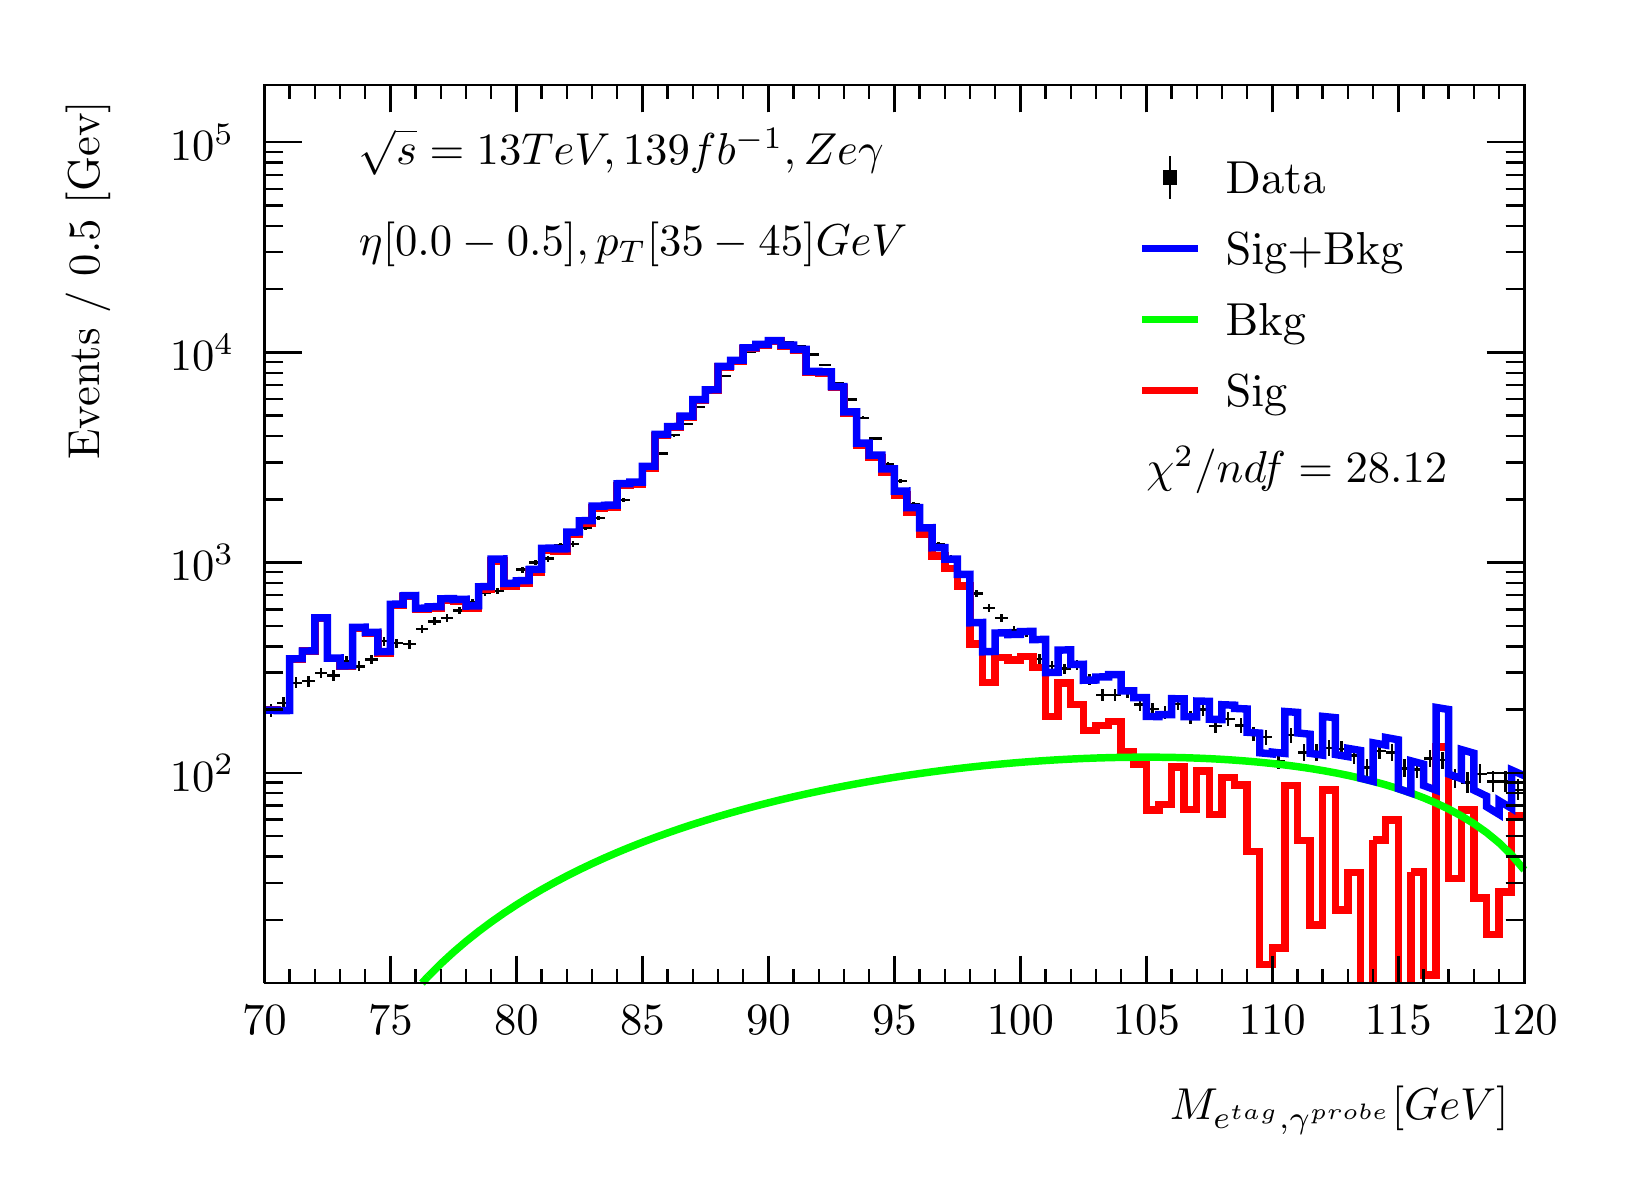
\begin{tikzpicture}
\pgfdeclareplotmark{cross} {
\pgfpathmoveto{\pgfpoint{-0.3\pgfplotmarksize}{\pgfplotmarksize}}
\pgfpathlineto{\pgfpoint{+0.3\pgfplotmarksize}{\pgfplotmarksize}}
\pgfpathlineto{\pgfpoint{+0.3\pgfplotmarksize}{0.3\pgfplotmarksize}}
\pgfpathlineto{\pgfpoint{+1\pgfplotmarksize}{0.3\pgfplotmarksize}}
\pgfpathlineto{\pgfpoint{+1\pgfplotmarksize}{-0.3\pgfplotmarksize}}
\pgfpathlineto{\pgfpoint{+0.3\pgfplotmarksize}{-0.3\pgfplotmarksize}}
\pgfpathlineto{\pgfpoint{+0.3\pgfplotmarksize}{-1.\pgfplotmarksize}}
\pgfpathlineto{\pgfpoint{-0.3\pgfplotmarksize}{-1.\pgfplotmarksize}}
\pgfpathlineto{\pgfpoint{-0.3\pgfplotmarksize}{-0.3\pgfplotmarksize}}
\pgfpathlineto{\pgfpoint{-1.\pgfplotmarksize}{-0.3\pgfplotmarksize}}
\pgfpathlineto{\pgfpoint{-1.\pgfplotmarksize}{0.3\pgfplotmarksize}}
\pgfpathlineto{\pgfpoint{-0.3\pgfplotmarksize}{0.3\pgfplotmarksize}}
\pgfpathclose
\pgfusepathqstroke
}
\pgfdeclareplotmark{cross*} {
\pgfpathmoveto{\pgfpoint{-0.3\pgfplotmarksize}{\pgfplotmarksize}}
\pgfpathlineto{\pgfpoint{+0.3\pgfplotmarksize}{\pgfplotmarksize}}
\pgfpathlineto{\pgfpoint{+0.3\pgfplotmarksize}{0.3\pgfplotmarksize}}
\pgfpathlineto{\pgfpoint{+1\pgfplotmarksize}{0.3\pgfplotmarksize}}
\pgfpathlineto{\pgfpoint{+1\pgfplotmarksize}{-0.3\pgfplotmarksize}}
\pgfpathlineto{\pgfpoint{+0.3\pgfplotmarksize}{-0.3\pgfplotmarksize}}
\pgfpathlineto{\pgfpoint{+0.3\pgfplotmarksize}{-1.\pgfplotmarksize}}
\pgfpathlineto{\pgfpoint{-0.3\pgfplotmarksize}{-1.\pgfplotmarksize}}
\pgfpathlineto{\pgfpoint{-0.3\pgfplotmarksize}{-0.3\pgfplotmarksize}}
\pgfpathlineto{\pgfpoint{-1.\pgfplotmarksize}{-0.3\pgfplotmarksize}}
\pgfpathlineto{\pgfpoint{-1.\pgfplotmarksize}{0.3\pgfplotmarksize}}
\pgfpathlineto{\pgfpoint{-0.3\pgfplotmarksize}{0.3\pgfplotmarksize}}
\pgfpathclose
\pgfusepathqfillstroke
}
\pgfdeclareplotmark{newstar} {
\pgfpathmoveto{\pgfqpoint{0pt}{\pgfplotmarksize}}
\pgfpathlineto{\pgfqpointpolar{44}{0.5\pgfplotmarksize}}
\pgfpathlineto{\pgfqpointpolar{18}{\pgfplotmarksize}}
\pgfpathlineto{\pgfqpointpolar{-20}{0.5\pgfplotmarksize}}
\pgfpathlineto{\pgfqpointpolar{-54}{\pgfplotmarksize}}
\pgfpathlineto{\pgfqpointpolar{-90}{0.5\pgfplotmarksize}}
\pgfpathlineto{\pgfqpointpolar{234}{\pgfplotmarksize}}
\pgfpathlineto{\pgfqpointpolar{198}{0.5\pgfplotmarksize}}
\pgfpathlineto{\pgfqpointpolar{162}{\pgfplotmarksize}}
\pgfpathlineto{\pgfqpointpolar{134}{0.5\pgfplotmarksize}}
\pgfpathclose
\pgfusepathqstroke
}
\pgfdeclareplotmark{newstar*} {
\pgfpathmoveto{\pgfqpoint{0pt}{\pgfplotmarksize}}
\pgfpathlineto{\pgfqpointpolar{44}{0.5\pgfplotmarksize}}
\pgfpathlineto{\pgfqpointpolar{18}{\pgfplotmarksize}}
\pgfpathlineto{\pgfqpointpolar{-20}{0.5\pgfplotmarksize}}
\pgfpathlineto{\pgfqpointpolar{-54}{\pgfplotmarksize}}
\pgfpathlineto{\pgfqpointpolar{-90}{0.5\pgfplotmarksize}}
\pgfpathlineto{\pgfqpointpolar{234}{\pgfplotmarksize}}
\pgfpathlineto{\pgfqpointpolar{198}{0.5\pgfplotmarksize}}
\pgfpathlineto{\pgfqpointpolar{162}{\pgfplotmarksize}}
\pgfpathlineto{\pgfqpointpolar{134}{0.5\pgfplotmarksize}}
\pgfpathclose
\pgfusepathqfillstroke
}
\definecolor{c}{rgb}{1,1,1};
\draw [color=c, fill=c] (0,0) rectangle (20,14.4361);
\draw [color=c, fill=c] (3,2.30977) rectangle (19,13.7143);
\definecolor{c}{rgb}{0,0,0};
\draw [c,line width=0.9] (3,2.30977) -- (3,13.7143) -- (19,13.7143) -- (19,2.30977) -- (3,2.30977);
\definecolor{c}{rgb}{1,1,1};
\draw [color=c, fill=c] (3,2.30977) rectangle (19,13.7143);
\definecolor{c}{rgb}{0,0,0};
\draw [c,line width=0.9] (3,2.30977) -- (3,13.7143) -- (19,13.7143) -- (19,2.30977) -- (3,2.30977);
\draw [c,line width=0.9] (3,2.30977) -- (19,2.30977);
\draw [c,line width=0.9] (3,2.65624) -- (3,2.30977);
\draw [c,line width=0.9] (3.32,2.48301) -- (3.32,2.30977);
\draw [c,line width=0.9] (3.64,2.48301) -- (3.64,2.30977);
\draw [c,line width=0.9] (3.96,2.48301) -- (3.96,2.30977);
\draw [c,line width=0.9] (4.28,2.48301) -- (4.28,2.30977);
\draw [c,line width=0.9] (4.6,2.65624) -- (4.6,2.30977);
\draw [c,line width=0.9] (4.92,2.48301) -- (4.92,2.30977);
\draw [c,line width=0.9] (5.24,2.48301) -- (5.24,2.30977);
\draw [c,line width=0.9] (5.56,2.48301) -- (5.56,2.30977);
\draw [c,line width=0.9] (5.88,2.48301) -- (5.88,2.30977);
\draw [c,line width=0.9] (6.2,2.65624) -- (6.2,2.30977);
\draw [c,line width=0.9] (6.52,2.48301) -- (6.52,2.30977);
\draw [c,line width=0.9] (6.84,2.48301) -- (6.84,2.30977);
\draw [c,line width=0.9] (7.16,2.48301) -- (7.16,2.30977);
\draw [c,line width=0.9] (7.48,2.48301) -- (7.48,2.30977);
\draw [c,line width=0.9] (7.8,2.65624) -- (7.8,2.30977);
\draw [c,line width=0.9] (8.12,2.48301) -- (8.12,2.30977);
\draw [c,line width=0.9] (8.44,2.48301) -- (8.44,2.30977);
\draw [c,line width=0.9] (8.76,2.48301) -- (8.76,2.30977);
\draw [c,line width=0.9] (9.08,2.48301) -- (9.08,2.30977);
\draw [c,line width=0.9] (9.4,2.65624) -- (9.4,2.30977);
\draw [c,line width=0.9] (9.72,2.48301) -- (9.72,2.30977);
\draw [c,line width=0.9] (10.04,2.48301) -- (10.04,2.30977);
\draw [c,line width=0.9] (10.36,2.48301) -- (10.36,2.30977);
\draw [c,line width=0.9] (10.68,2.48301) -- (10.68,2.30977);
\draw [c,line width=0.9] (11,2.65624) -- (11,2.30977);
\draw [c,line width=0.9] (11.32,2.48301) -- (11.32,2.30977);
\draw [c,line width=0.9] (11.64,2.48301) -- (11.64,2.30977);
\draw [c,line width=0.9] (11.96,2.48301) -- (11.96,2.30977);
\draw [c,line width=0.9] (12.28,2.48301) -- (12.28,2.30977);
\draw [c,line width=0.9] (12.6,2.65624) -- (12.6,2.30977);
\draw [c,line width=0.9] (12.92,2.48301) -- (12.92,2.30977);
\draw [c,line width=0.9] (13.24,2.48301) -- (13.24,2.30977);
\draw [c,line width=0.9] (13.56,2.48301) -- (13.56,2.30977);
\draw [c,line width=0.9] (13.88,2.48301) -- (13.88,2.30977);
\draw [c,line width=0.9] (14.2,2.65624) -- (14.2,2.30977);
\draw [c,line width=0.9] (14.52,2.48301) -- (14.52,2.30977);
\draw [c,line width=0.9] (14.84,2.48301) -- (14.84,2.30977);
\draw [c,line width=0.9] (15.16,2.48301) -- (15.16,2.30977);
\draw [c,line width=0.9] (15.48,2.48301) -- (15.48,2.30977);
\draw [c,line width=0.9] (15.8,2.65624) -- (15.8,2.30977);
\draw [c,line width=0.9] (16.12,2.48301) -- (16.12,2.30977);
\draw [c,line width=0.9] (16.44,2.48301) -- (16.44,2.30977);
\draw [c,line width=0.9] (16.76,2.48301) -- (16.76,2.30977);
\draw [c,line width=0.9] (17.08,2.48301) -- (17.08,2.30977);
\draw [c,line width=0.9] (17.4,2.65624) -- (17.4,2.30977);
\draw [c,line width=0.9] (17.72,2.48301) -- (17.72,2.30977);
\draw [c,line width=0.9] (18.04,2.48301) -- (18.04,2.30977);
\draw [c,line width=0.9] (18.36,2.48301) -- (18.36,2.30977);
\draw [c,line width=0.9] (18.68,2.48301) -- (18.68,2.30977);
\draw [c,line width=0.9] (19,2.65624) -- (19,2.30977);
\draw [anchor=base] (3,1.66015) node[scale=1.61424, color=c, rotate=0]{70};
\draw [anchor=base] (4.6,1.66015) node[scale=1.61424, color=c, rotate=0]{75};
\draw [anchor=base] (6.2,1.66015) node[scale=1.61424, color=c, rotate=0]{80};
\draw [anchor=base] (7.8,1.66015) node[scale=1.61424, color=c, rotate=0]{85};
\draw [anchor=base] (9.4,1.66015) node[scale=1.61424, color=c, rotate=0]{90};
\draw [anchor=base] (11,1.66015) node[scale=1.61424, color=c, rotate=0]{95};
\draw [anchor=base] (12.6,1.66015) node[scale=1.61424, color=c, rotate=0]{100};
\draw [anchor=base] (14.2,1.66015) node[scale=1.61424, color=c, rotate=0]{105};
\draw [anchor=base] (15.8,1.66015) node[scale=1.61424, color=c, rotate=0]{110};
\draw [anchor=base] (17.4,1.66015) node[scale=1.61424, color=c, rotate=0]{115};
\draw [anchor=base] (19,1.66015) node[scale=1.61424, color=c, rotate=0]{120};
\draw [anchor= east] (19,0.692932) node[scale=1.61424, color=c, rotate=0]{$M_{e^{tag}, \gamma^{probe}}  [GeV]$};
\draw [c,line width=0.9] (3,13.7143) -- (19,13.7143);
\draw [c,line width=0.9] (3,13.3678) -- (3,13.7143);
\draw [c,line width=0.9] (3.32,13.5411) -- (3.32,13.7143);
\draw [c,line width=0.9] (3.64,13.5411) -- (3.64,13.7143);
\draw [c,line width=0.9] (3.96,13.5411) -- (3.96,13.7143);
\draw [c,line width=0.9] (4.28,13.5411) -- (4.28,13.7143);
\draw [c,line width=0.9] (4.6,13.3678) -- (4.6,13.7143);
\draw [c,line width=0.9] (4.92,13.5411) -- (4.92,13.7143);
\draw [c,line width=0.9] (5.24,13.5411) -- (5.24,13.7143);
\draw [c,line width=0.9] (5.56,13.5411) -- (5.56,13.7143);
\draw [c,line width=0.9] (5.88,13.5411) -- (5.88,13.7143);
\draw [c,line width=0.9] (6.2,13.3678) -- (6.2,13.7143);
\draw [c,line width=0.9] (6.52,13.5411) -- (6.52,13.7143);
\draw [c,line width=0.9] (6.84,13.5411) -- (6.84,13.7143);
\draw [c,line width=0.9] (7.16,13.5411) -- (7.16,13.7143);
\draw [c,line width=0.9] (7.48,13.5411) -- (7.48,13.7143);
\draw [c,line width=0.9] (7.8,13.3678) -- (7.8,13.7143);
\draw [c,line width=0.9] (8.12,13.5411) -- (8.12,13.7143);
\draw [c,line width=0.9] (8.44,13.5411) -- (8.44,13.7143);
\draw [c,line width=0.9] (8.76,13.5411) -- (8.76,13.7143);
\draw [c,line width=0.9] (9.08,13.5411) -- (9.08,13.7143);
\draw [c,line width=0.9] (9.4,13.3678) -- (9.4,13.7143);
\draw [c,line width=0.9] (9.72,13.5411) -- (9.72,13.7143);
\draw [c,line width=0.9] (10.04,13.5411) -- (10.04,13.7143);
\draw [c,line width=0.9] (10.36,13.5411) -- (10.36,13.7143);
\draw [c,line width=0.9] (10.68,13.5411) -- (10.68,13.7143);
\draw [c,line width=0.9] (11,13.3678) -- (11,13.7143);
\draw [c,line width=0.9] (11.32,13.5411) -- (11.32,13.7143);
\draw [c,line width=0.9] (11.64,13.5411) -- (11.64,13.7143);
\draw [c,line width=0.9] (11.96,13.5411) -- (11.96,13.7143);
\draw [c,line width=0.9] (12.28,13.5411) -- (12.28,13.7143);
\draw [c,line width=0.9] (12.6,13.3678) -- (12.6,13.7143);
\draw [c,line width=0.9] (12.92,13.5411) -- (12.92,13.7143);
\draw [c,line width=0.9] (13.24,13.5411) -- (13.24,13.7143);
\draw [c,line width=0.9] (13.56,13.5411) -- (13.56,13.7143);
\draw [c,line width=0.9] (13.88,13.5411) -- (13.88,13.7143);
\draw [c,line width=0.9] (14.2,13.3678) -- (14.2,13.7143);
\draw [c,line width=0.9] (14.52,13.5411) -- (14.52,13.7143);
\draw [c,line width=0.9] (14.84,13.5411) -- (14.84,13.7143);
\draw [c,line width=0.9] (15.16,13.5411) -- (15.16,13.7143);
\draw [c,line width=0.9] (15.48,13.5411) -- (15.48,13.7143);
\draw [c,line width=0.9] (15.8,13.3678) -- (15.8,13.7143);
\draw [c,line width=0.9] (16.12,13.5411) -- (16.12,13.7143);
\draw [c,line width=0.9] (16.44,13.5411) -- (16.44,13.7143);
\draw [c,line width=0.9] (16.76,13.5411) -- (16.76,13.7143);
\draw [c,line width=0.9] (17.08,13.5411) -- (17.08,13.7143);
\draw [c,line width=0.9] (17.4,13.3678) -- (17.4,13.7143);
\draw [c,line width=0.9] (17.72,13.5411) -- (17.72,13.7143);
\draw [c,line width=0.9] (18.04,13.5411) -- (18.04,13.7143);
\draw [c,line width=0.9] (18.36,13.5411) -- (18.36,13.7143);
\draw [c,line width=0.9] (18.68,13.5411) -- (18.68,13.7143);
\draw [c,line width=0.9] (19,13.3678) -- (19,13.7143);
\draw [c,line width=0.9] (3,2.30977) -- (3,13.7143);
\draw [c,line width=0.9] (3.237,3.11343) -- (3,3.11343);
\draw [c,line width=0.9] (3.237,3.58354) -- (3,3.58354);
\draw [c,line width=0.9] (3.237,3.91709) -- (3,3.91709);
\draw [c,line width=0.9] (3.237,4.17581) -- (3,4.17581);
\draw [c,line width=0.9] (3.237,4.38719) -- (3,4.38719);
\draw [c,line width=0.9] (3.237,4.56592) -- (3,4.56592);
\draw [c,line width=0.9] (3.237,4.72074) -- (3,4.72074);
\draw [c,line width=0.9] (3.237,4.8573) -- (3,4.8573);
\draw [c,line width=0.9] (3.474,4.97946) -- (3,4.97946);
\draw [anchor= east] (2.82,4.97946) node[scale=1.61424, color=c, rotate=0]{$10^{2}$};
\draw [c,line width=0.9] (3.237,5.78312) -- (3,5.78312);
\draw [c,line width=0.9] (3.237,6.25323) -- (3,6.25323);
\draw [c,line width=0.9] (3.237,6.58678) -- (3,6.58678);
\draw [c,line width=0.9] (3.237,6.8455) -- (3,6.8455);
\draw [c,line width=0.9] (3.237,7.05689) -- (3,7.05689);
\draw [c,line width=0.9] (3.237,7.23561) -- (3,7.23561);
\draw [c,line width=0.9] (3.237,7.39043) -- (3,7.39043);
\draw [c,line width=0.9] (3.237,7.52699) -- (3,7.52699);
\draw [c,line width=0.9] (3.474,7.64915) -- (3,7.64915);
\draw [anchor= east] (2.82,7.64915) node[scale=1.61424, color=c, rotate=0]{$10^{3}$};
\draw [c,line width=0.9] (3.237,8.45281) -- (3,8.45281);
\draw [c,line width=0.9] (3.237,8.92292) -- (3,8.92292);
\draw [c,line width=0.9] (3.237,9.25647) -- (3,9.25647);
\draw [c,line width=0.9] (3.237,9.51519) -- (3,9.51519);
\draw [c,line width=0.9] (3.237,9.72658) -- (3,9.72658);
\draw [c,line width=0.9] (3.237,9.9053) -- (3,9.9053);
\draw [c,line width=0.9] (3.237,10.0601) -- (3,10.0601);
\draw [c,line width=0.9] (3.237,10.1967) -- (3,10.1967);
\draw [c,line width=0.9] (3.474,10.3188) -- (3,10.3188);
\draw [anchor= east] (2.82,10.3188) node[scale=1.61424, color=c, rotate=0]{$10^{4}$};
\draw [c,line width=0.9] (3.237,11.1225) -- (3,11.1225);
\draw [c,line width=0.9] (3.237,11.5926) -- (3,11.5926);
\draw [c,line width=0.9] (3.237,11.9262) -- (3,11.9262);
\draw [c,line width=0.9] (3.237,12.1849) -- (3,12.1849);
\draw [c,line width=0.9] (3.237,12.3963) -- (3,12.3963);
\draw [c,line width=0.9] (3.237,12.575) -- (3,12.575);
\draw [c,line width=0.9] (3.237,12.7298) -- (3,12.7298);
\draw [c,line width=0.9] (3.237,12.8664) -- (3,12.8664);
\draw [c,line width=0.9] (3.474,12.9885) -- (3,12.9885);
\draw [anchor= east] (2.82,12.9885) node[scale=1.61424, color=c, rotate=0]{$10^{5}$};
\draw [anchor= east] (0.76,13.7143) node[scale=1.61424, color=c, rotate=90]{Events / 0.5 [Gev]};
\draw [c,line width=0.9] (19,2.30977) -- (19,13.7143);
\draw [c,line width=0.9] (18.763,3.11343) -- (19,3.11343);
\draw [c,line width=0.9] (18.763,3.58354) -- (19,3.58354);
\draw [c,line width=0.9] (18.763,3.91709) -- (19,3.91709);
\draw [c,line width=0.9] (18.763,4.17581) -- (19,4.17581);
\draw [c,line width=0.9] (18.763,4.38719) -- (19,4.38719);
\draw [c,line width=0.9] (18.763,4.56592) -- (19,4.56592);
\draw [c,line width=0.9] (18.763,4.72074) -- (19,4.72074);
\draw [c,line width=0.9] (18.763,4.8573) -- (19,4.8573);
\draw [c,line width=0.9] (18.526,4.97946) -- (19,4.97946);
\draw [c,line width=0.9] (18.763,5.78312) -- (19,5.78312);
\draw [c,line width=0.9] (18.763,6.25323) -- (19,6.25323);
\draw [c,line width=0.9] (18.763,6.58678) -- (19,6.58678);
\draw [c,line width=0.9] (18.763,6.8455) -- (19,6.8455);
\draw [c,line width=0.9] (18.763,7.05689) -- (19,7.05689);
\draw [c,line width=0.9] (18.763,7.23561) -- (19,7.23561);
\draw [c,line width=0.9] (18.763,7.39043) -- (19,7.39043);
\draw [c,line width=0.9] (18.763,7.52699) -- (19,7.52699);
\draw [c,line width=0.9] (18.526,7.64915) -- (19,7.64915);
\draw [c,line width=0.9] (18.763,8.45281) -- (19,8.45281);
\draw [c,line width=0.9] (18.763,8.92292) -- (19,8.92292);
\draw [c,line width=0.9] (18.763,9.25647) -- (19,9.25647);
\draw [c,line width=0.9] (18.763,9.51519) -- (19,9.51519);
\draw [c,line width=0.9] (18.763,9.72658) -- (19,9.72658);
\draw [c,line width=0.9] (18.763,9.9053) -- (19,9.9053);
\draw [c,line width=0.9] (18.763,10.0601) -- (19,10.0601);
\draw [c,line width=0.9] (18.763,10.1967) -- (19,10.1967);
\draw [c,line width=0.9] (18.526,10.3188) -- (19,10.3188);
\draw [c,line width=0.9] (18.763,11.1225) -- (19,11.1225);
\draw [c,line width=0.9] (18.763,11.5926) -- (19,11.5926);
\draw [c,line width=0.9] (18.763,11.9262) -- (19,11.9262);
\draw [c,line width=0.9] (18.763,12.1849) -- (19,12.1849);
\draw [c,line width=0.9] (18.763,12.3963) -- (19,12.3963);
\draw [c,line width=0.9] (18.763,12.575) -- (19,12.575);
\draw [c,line width=0.9] (18.763,12.7298) -- (19,12.7298);
\draw [c,line width=0.9] (18.763,12.8664) -- (19,12.8664);
\draw [c,line width=0.9] (18.526,12.9885) -- (19,12.9885);
\draw [c,line width=0.9] (3.08,5.77147) -- (3,5.77147);
\draw [c,line width=0.9] (3,5.77147) -- (3,5.77147);
\draw [c,line width=0.9] (3.08,5.77147) -- (3.16,5.77147);
\draw [c,line width=0.9] (3.16,5.77147) -- (3.16,5.77147);
\draw [c,line width=0.9] (3.08,5.77147) -- (3.08,5.85385);
\draw [c,line width=0.9] (3.08,5.85385) -- (3.08,5.85385);
\draw [c,line width=0.9] (3.08,5.77147) -- (3.08,5.68909);
\draw [c,line width=0.9] (3.08,5.68909) -- (3.08,5.68909);
\draw [c,line width=0.9] (3.24,5.86697) -- (3.16,5.86697);
\draw [c,line width=0.9] (3.16,5.86697) -- (3.16,5.86697);
\draw [c,line width=0.9] (3.24,5.86697) -- (3.32,5.86697);
\draw [c,line width=0.9] (3.32,5.86697) -- (3.32,5.86697);
\draw [c,line width=0.9] (3.24,5.86697) -- (3.24,5.94603);
\draw [c,line width=0.9] (3.24,5.94603) -- (3.24,5.94603);
\draw [c,line width=0.9] (3.24,5.86697) -- (3.24,5.78791);
\draw [c,line width=0.9] (3.24,5.78791) -- (3.24,5.78791);
\draw [c,line width=0.9] (3.4,6.12245) -- (3.32,6.12245);
\draw [c,line width=0.9] (3.32,6.12245) -- (3.32,6.12245);
\draw [c,line width=0.9] (3.4,6.12245) -- (3.48,6.12245);
\draw [c,line width=0.9] (3.48,6.12245) -- (3.48,6.12245);
\draw [c,line width=0.9] (3.4,6.12245) -- (3.4,6.19326);
\draw [c,line width=0.9] (3.4,6.19326) -- (3.4,6.19326);
\draw [c,line width=0.9] (3.4,6.12245) -- (3.4,6.05164);
\draw [c,line width=0.9] (3.4,6.05164) -- (3.4,6.05164);
\draw [c,line width=0.9] (3.56,6.14388) -- (3.48,6.14388);
\draw [c,line width=0.9] (3.48,6.14388) -- (3.48,6.14388);
\draw [c,line width=0.9] (3.56,6.14388) -- (3.64,6.14388);
\draw [c,line width=0.9] (3.64,6.14388) -- (3.64,6.14388);
\draw [c,line width=0.9] (3.56,6.14388) -- (3.56,6.21404);
\draw [c,line width=0.9] (3.56,6.21404) -- (3.56,6.21404);
\draw [c,line width=0.9] (3.56,6.14388) -- (3.56,6.07372);
\draw [c,line width=0.9] (3.56,6.07372) -- (3.56,6.07372);
\draw [c,line width=0.9] (3.72,6.24547) -- (3.64,6.24547);
\draw [c,line width=0.9] (3.64,6.24547) -- (3.64,6.24547);
\draw [c,line width=0.9] (3.72,6.24547) -- (3.8,6.24547);
\draw [c,line width=0.9] (3.8,6.24547) -- (3.8,6.24547);
\draw [c,line width=0.9] (3.72,6.24547) -- (3.72,6.31263);
\draw [c,line width=0.9] (3.72,6.31263) -- (3.72,6.31263);
\draw [c,line width=0.9] (3.72,6.24547) -- (3.72,6.17832);
\draw [c,line width=0.9] (3.72,6.17832) -- (3.72,6.17832);
\draw [c,line width=0.9] (3.88,6.21392) -- (3.8,6.21392);
\draw [c,line width=0.9] (3.8,6.21392) -- (3.8,6.21392);
\draw [c,line width=0.9] (3.88,6.21392) -- (3.96,6.21392);
\draw [c,line width=0.9] (3.96,6.21392) -- (3.96,6.21392);
\draw [c,line width=0.9] (3.88,6.21392) -- (3.88,6.282);
\draw [c,line width=0.9] (3.88,6.282) -- (3.88,6.282);
\draw [c,line width=0.9] (3.88,6.21392) -- (3.88,6.14585);
\draw [c,line width=0.9] (3.88,6.14585) -- (3.88,6.14585);
\draw [c,line width=0.9] (4.04,6.39835) -- (3.96,6.39835);
\draw [c,line width=0.9] (3.96,6.39835) -- (3.96,6.39835);
\draw [c,line width=0.9] (4.04,6.39835) -- (4.12,6.39835);
\draw [c,line width=0.9] (4.12,6.39835) -- (4.12,6.39835);
\draw [c,line width=0.9] (4.04,6.39835) -- (4.04,6.46122);
\draw [c,line width=0.9] (4.04,6.46122) -- (4.04,6.46122);
\draw [c,line width=0.9] (4.04,6.39835) -- (4.04,6.33548);
\draw [c,line width=0.9] (4.04,6.33548) -- (4.04,6.33548);
\draw [c,line width=0.9] (4.2,6.33168) -- (4.12,6.33168);
\draw [c,line width=0.9] (4.12,6.33168) -- (4.12,6.33168);
\draw [c,line width=0.9] (4.2,6.33168) -- (4.28,6.33168);
\draw [c,line width=0.9] (4.28,6.33168) -- (4.28,6.33168);
\draw [c,line width=0.9] (4.2,6.33168) -- (4.2,6.39638);
\draw [c,line width=0.9] (4.2,6.39638) -- (4.2,6.39638);
\draw [c,line width=0.9] (4.2,6.33168) -- (4.2,6.26697);
\draw [c,line width=0.9] (4.2,6.26697) -- (4.2,6.26697);
\draw [c,line width=0.9] (4.36,6.41863) -- (4.28,6.41863);
\draw [c,line width=0.9] (4.28,6.41863) -- (4.28,6.41863);
\draw [c,line width=0.9] (4.36,6.41863) -- (4.44,6.41863);
\draw [c,line width=0.9] (4.44,6.41863) -- (4.44,6.41863);
\draw [c,line width=0.9] (4.36,6.41863) -- (4.36,6.48095);
\draw [c,line width=0.9] (4.36,6.48095) -- (4.36,6.48095);
\draw [c,line width=0.9] (4.36,6.41863) -- (4.36,6.35631);
\draw [c,line width=0.9] (4.36,6.35631) -- (4.36,6.35631);
\draw [c,line width=0.9] (4.52,6.6516) -- (4.44,6.6516);
\draw [c,line width=0.9] (4.44,6.6516) -- (4.44,6.6516);
\draw [c,line width=0.9] (4.52,6.6516) -- (4.6,6.6516);
\draw [c,line width=0.9] (4.6,6.6516) -- (4.6,6.6516);
\draw [c,line width=0.9] (4.52,6.6516) -- (4.52,6.70797);
\draw [c,line width=0.9] (4.52,6.70797) -- (4.52,6.70797);
\draw [c,line width=0.9] (4.52,6.6516) -- (4.52,6.59523);
\draw [c,line width=0.9] (4.52,6.59523) -- (4.52,6.59523);
\draw [c,line width=0.9] (4.68,6.62666) -- (4.6,6.62666);
\draw [c,line width=0.9] (4.6,6.62666) -- (4.6,6.62666);
\draw [c,line width=0.9] (4.68,6.62666) -- (4.76,6.62666);
\draw [c,line width=0.9] (4.76,6.62666) -- (4.76,6.62666);
\draw [c,line width=0.9] (4.68,6.62666) -- (4.68,6.68364);
\draw [c,line width=0.9] (4.68,6.68364) -- (4.68,6.68364);
\draw [c,line width=0.9] (4.68,6.62666) -- (4.68,6.56969);
\draw [c,line width=0.9] (4.68,6.56969) -- (4.68,6.56969);
\draw [c,line width=0.9] (4.84,6.61258) -- (4.76,6.61258);
\draw [c,line width=0.9] (4.76,6.61258) -- (4.76,6.61258);
\draw [c,line width=0.9] (4.84,6.61258) -- (4.92,6.61258);
\draw [c,line width=0.9] (4.92,6.61258) -- (4.92,6.61258);
\draw [c,line width=0.9] (4.84,6.61258) -- (4.84,6.6699);
\draw [c,line width=0.9] (4.84,6.6699) -- (4.84,6.6699);
\draw [c,line width=0.9] (4.84,6.61258) -- (4.84,6.55525);
\draw [c,line width=0.9] (4.84,6.55525) -- (4.84,6.55525);
\draw [c,line width=0.9] (5,6.80779) -- (4.92,6.80779);
\draw [c,line width=0.9] (4.92,6.80779) -- (4.92,6.80779);
\draw [c,line width=0.9] (5,6.80779) -- (5.08,6.80779);
\draw [c,line width=0.9] (5.08,6.80779) -- (5.08,6.80779);
\draw [c,line width=0.9] (5,6.80779) -- (5,6.86049);
\draw [c,line width=0.9] (5,6.86049) -- (5,6.86049);
\draw [c,line width=0.9] (5,6.80779) -- (5,6.75509);
\draw [c,line width=0.9] (5,6.75509) -- (5,6.75509);
\draw [c,line width=0.9] (5.16,6.90207) -- (5.08,6.90207);
\draw [c,line width=0.9] (5.08,6.90207) -- (5.08,6.90207);
\draw [c,line width=0.9] (5.16,6.90207) -- (5.24,6.90207);
\draw [c,line width=0.9] (5.24,6.90207) -- (5.24,6.90207);
\draw [c,line width=0.9] (5.16,6.90207) -- (5.16,6.95266);
\draw [c,line width=0.9] (5.16,6.95266) -- (5.16,6.95266);
\draw [c,line width=0.9] (5.16,6.90207) -- (5.16,6.85147);
\draw [c,line width=0.9] (5.16,6.85147) -- (5.16,6.85147);
\draw [c,line width=0.9] (5.32,6.94754) -- (5.24,6.94754);
\draw [c,line width=0.9] (5.24,6.94754) -- (5.24,6.94754);
\draw [c,line width=0.9] (5.32,6.94754) -- (5.4,6.94754);
\draw [c,line width=0.9] (5.4,6.94754) -- (5.4,6.94754);
\draw [c,line width=0.9] (5.32,6.94754) -- (5.32,6.99716);
\draw [c,line width=0.9] (5.32,6.99716) -- (5.32,6.99716);
\draw [c,line width=0.9] (5.32,6.94754) -- (5.32,6.89792);
\draw [c,line width=0.9] (5.32,6.89792) -- (5.32,6.89792);
\draw [c,line width=0.9] (5.48,7.03936) -- (5.4,7.03936);
\draw [c,line width=0.9] (5.4,7.03936) -- (5.4,7.03936);
\draw [c,line width=0.9] (5.48,7.03936) -- (5.56,7.03936);
\draw [c,line width=0.9] (5.56,7.03936) -- (5.56,7.03936);
\draw [c,line width=0.9] (5.48,7.03936) -- (5.48,7.08705);
\draw [c,line width=0.9] (5.48,7.08705) -- (5.48,7.08705);
\draw [c,line width=0.9] (5.48,7.03936) -- (5.48,6.99167);
\draw [c,line width=0.9] (5.48,6.99167) -- (5.48,6.99167);
\draw [c,line width=0.9] (5.64,7.14074) -- (5.56,7.14074);
\draw [c,line width=0.9] (5.56,7.14074) -- (5.56,7.14074);
\draw [c,line width=0.9] (5.64,7.14074) -- (5.72,7.14074);
\draw [c,line width=0.9] (5.72,7.14074) -- (5.72,7.14074);
\draw [c,line width=0.9] (5.64,7.14074) -- (5.64,7.18639);
\draw [c,line width=0.9] (5.64,7.18639) -- (5.64,7.18639);
\draw [c,line width=0.9] (5.64,7.14074) -- (5.64,7.09509);
\draw [c,line width=0.9] (5.64,7.09509) -- (5.64,7.09509);
\draw [c,line width=0.9] (5.8,7.26666) -- (5.72,7.26666);
\draw [c,line width=0.9] (5.72,7.26666) -- (5.72,7.26666);
\draw [c,line width=0.9] (5.8,7.26666) -- (5.88,7.26666);
\draw [c,line width=0.9] (5.88,7.26666) -- (5.88,7.26666);
\draw [c,line width=0.9] (5.8,7.26666) -- (5.8,7.3099);
\draw [c,line width=0.9] (5.8,7.3099) -- (5.8,7.3099);
\draw [c,line width=0.9] (5.8,7.26666) -- (5.8,7.22343);
\draw [c,line width=0.9] (5.8,7.22343) -- (5.8,7.22343);
\draw [c,line width=0.9] (5.96,7.28902) -- (5.88,7.28902);
\draw [c,line width=0.9] (5.88,7.28902) -- (5.88,7.28902);
\draw [c,line width=0.9] (5.96,7.28902) -- (6.04,7.28902);
\draw [c,line width=0.9] (6.04,7.28902) -- (6.04,7.28902);
\draw [c,line width=0.9] (5.96,7.28902) -- (5.96,7.33185);
\draw [c,line width=0.9] (5.96,7.33185) -- (5.96,7.33185);
\draw [c,line width=0.9] (5.96,7.28902) -- (5.96,7.2462);
\draw [c,line width=0.9] (5.96,7.2462) -- (5.96,7.2462);
\draw [c,line width=0.9] (6.12,7.36553) -- (6.04,7.36553);
\draw [c,line width=0.9] (6.04,7.36553) -- (6.04,7.36553);
\draw [c,line width=0.9] (6.12,7.36553) -- (6.2,7.36553);
\draw [c,line width=0.9] (6.2,7.36553) -- (6.2,7.36553);
\draw [c,line width=0.9] (6.12,7.36553) -- (6.12,7.40696);
\draw [c,line width=0.9] (6.12,7.40696) -- (6.12,7.40696);
\draw [c,line width=0.9] (6.12,7.36553) -- (6.12,7.3241);
\draw [c,line width=0.9] (6.12,7.3241) -- (6.12,7.3241);
\draw [c,line width=0.9] (6.28,7.55876) -- (6.2,7.55876);
\draw [c,line width=0.9] (6.2,7.55876) -- (6.2,7.55876);
\draw [c,line width=0.9] (6.28,7.55876) -- (6.36,7.55876);
\draw [c,line width=0.9] (6.36,7.55876) -- (6.36,7.55876);
\draw [c,line width=0.9] (6.28,7.55876) -- (6.28,7.59688);
\draw [c,line width=0.9] (6.28,7.59688) -- (6.28,7.59688);
\draw [c,line width=0.9] (6.28,7.55876) -- (6.28,7.52064);
\draw [c,line width=0.9] (6.28,7.52064) -- (6.28,7.52064);
\draw [c,line width=0.9] (6.44,7.65031) -- (6.36,7.65031);
\draw [c,line width=0.9] (6.36,7.65031) -- (6.36,7.65031);
\draw [c,line width=0.9] (6.44,7.65031) -- (6.52,7.65031);
\draw [c,line width=0.9] (6.52,7.65031) -- (6.52,7.65031);
\draw [c,line width=0.9] (6.44,7.65031) -- (6.44,7.68696);
\draw [c,line width=0.9] (6.44,7.68696) -- (6.44,7.68696);
\draw [c,line width=0.9] (6.44,7.65031) -- (6.44,7.61367);
\draw [c,line width=0.9] (6.44,7.61367) -- (6.44,7.61367);
\draw [c,line width=0.9] (6.6,7.69908) -- (6.52,7.69908);
\draw [c,line width=0.9] (6.52,7.69908) -- (6.52,7.69908);
\draw [c,line width=0.9] (6.6,7.69908) -- (6.68,7.69908);
\draw [c,line width=0.9] (6.68,7.69908) -- (6.68,7.69908);
\draw [c,line width=0.9] (6.6,7.69908) -- (6.6,7.73496);
\draw [c,line width=0.9] (6.6,7.73496) -- (6.6,7.73496);
\draw [c,line width=0.9] (6.6,7.69908) -- (6.6,7.6632);
\draw [c,line width=0.9] (6.6,7.6632) -- (6.6,7.6632);
\draw [c,line width=0.9] (6.76,7.87112) -- (6.68,7.87112);
\draw [c,line width=0.9] (6.68,7.87112) -- (6.68,7.87112);
\draw [c,line width=0.9] (6.76,7.87112) -- (6.84,7.87112);
\draw [c,line width=0.9] (6.84,7.87112) -- (6.84,7.87112);
\draw [c,line width=0.9] (6.76,7.87112) -- (6.76,7.90444);
\draw [c,line width=0.9] (6.76,7.90444) -- (6.76,7.90444);
\draw [c,line width=0.9] (6.76,7.87112) -- (6.76,7.83781);
\draw [c,line width=0.9] (6.76,7.83781) -- (6.76,7.83781);
\draw [c,line width=0.9] (6.92,7.8854) -- (6.84,7.8854);
\draw [c,line width=0.9] (6.84,7.8854) -- (6.84,7.8854);
\draw [c,line width=0.9] (6.92,7.8854) -- (7,7.8854);
\draw [c,line width=0.9] (7,7.8854) -- (7,7.8854);
\draw [c,line width=0.9] (6.92,7.8854) -- (6.92,7.91851);
\draw [c,line width=0.9] (6.92,7.91851) -- (6.92,7.91851);
\draw [c,line width=0.9] (6.92,7.8854) -- (6.92,7.85228);
\draw [c,line width=0.9] (6.92,7.85228) -- (6.92,7.85228);
\draw [c,line width=0.9] (7.08,8.09426) -- (7,8.09426);
\draw [c,line width=0.9] (7,8.09426) -- (7,8.09426);
\draw [c,line width=0.9] (7.08,8.09426) -- (7.16,8.09426);
\draw [c,line width=0.9] (7.16,8.09426) -- (7.16,8.09426);
\draw [c,line width=0.9] (7.08,8.09426) -- (7.08,8.12452);
\draw [c,line width=0.9] (7.08,8.12452) -- (7.08,8.12452);
\draw [c,line width=0.9] (7.08,8.09426) -- (7.08,8.064);
\draw [c,line width=0.9] (7.08,8.064) -- (7.08,8.064);
\draw [c,line width=0.9] (7.24,8.21705) -- (7.16,8.21705);
\draw [c,line width=0.9] (7.16,8.21705) -- (7.16,8.21705);
\draw [c,line width=0.9] (7.24,8.21705) -- (7.32,8.21705);
\draw [c,line width=0.9] (7.32,8.21705) -- (7.32,8.21705);
\draw [c,line width=0.9] (7.24,8.21705) -- (7.24,8.24575);
\draw [c,line width=0.9] (7.24,8.24575) -- (7.24,8.24575);
\draw [c,line width=0.9] (7.24,8.21705) -- (7.24,8.18835);
\draw [c,line width=0.9] (7.24,8.18835) -- (7.24,8.18835);
\draw [c,line width=0.9] (7.4,8.37365) -- (7.32,8.37365);
\draw [c,line width=0.9] (7.32,8.37365) -- (7.32,8.37365);
\draw [c,line width=0.9] (7.4,8.37365) -- (7.48,8.37365);
\draw [c,line width=0.9] (7.48,8.37365) -- (7.48,8.37365);
\draw [c,line width=0.9] (7.4,8.37365) -- (7.4,8.40047);
\draw [c,line width=0.9] (7.4,8.40047) -- (7.4,8.40047);
\draw [c,line width=0.9] (7.4,8.37365) -- (7.4,8.34682);
\draw [c,line width=0.9] (7.4,8.34682) -- (7.4,8.34682);
\draw [c,line width=0.9] (7.56,8.44233) -- (7.48,8.44233);
\draw [c,line width=0.9] (7.48,8.44233) -- (7.48,8.44233);
\draw [c,line width=0.9] (7.56,8.44233) -- (7.64,8.44233);
\draw [c,line width=0.9] (7.64,8.44233) -- (7.64,8.44233);
\draw [c,line width=0.9] (7.56,8.44233) -- (7.56,8.46837);
\draw [c,line width=0.9] (7.56,8.46837) -- (7.56,8.46837);
\draw [c,line width=0.9] (7.56,8.44233) -- (7.56,8.41629);
\draw [c,line width=0.9] (7.56,8.41629) -- (7.56,8.41629);
\draw [c,line width=0.9] (7.72,8.68526) -- (7.64,8.68526);
\draw [c,line width=0.9] (7.64,8.68526) -- (7.64,8.68526);
\draw [c,line width=0.9] (7.72,8.68526) -- (7.8,8.68526);
\draw [c,line width=0.9] (7.8,8.68526) -- (7.8,8.68526);
\draw [c,line width=0.9] (7.72,8.68526) -- (7.72,8.70872);
\draw [c,line width=0.9] (7.72,8.70872) -- (7.72,8.70872);
\draw [c,line width=0.9] (7.72,8.68526) -- (7.72,8.66181);
\draw [c,line width=0.9] (7.72,8.66181) -- (7.72,8.66181);
\draw [c,line width=0.9] (7.88,8.83336) -- (7.8,8.83336);
\draw [c,line width=0.9] (7.8,8.83336) -- (7.8,8.83336);
\draw [c,line width=0.9] (7.88,8.83336) -- (7.96,8.83336);
\draw [c,line width=0.9] (7.96,8.83336) -- (7.96,8.83336);
\draw [c,line width=0.9] (7.88,8.83336) -- (7.88,8.85537);
\draw [c,line width=0.9] (7.88,8.85537) -- (7.88,8.85537);
\draw [c,line width=0.9] (7.88,8.83336) -- (7.88,8.81136);
\draw [c,line width=0.9] (7.88,8.81136) -- (7.88,8.81136);
\draw [c,line width=0.9] (8.04,9.03763) -- (7.96,9.03763);
\draw [c,line width=0.9] (7.96,9.03763) -- (7.96,9.03763);
\draw [c,line width=0.9] (8.04,9.03763) -- (8.12,9.03763);
\draw [c,line width=0.9] (8.12,9.03763) -- (8.12,9.03763);
\draw [c,line width=0.9] (8.04,9.03763) -- (8.04,9.05778);
\draw [c,line width=0.9] (8.04,9.05778) -- (8.04,9.05778);
\draw [c,line width=0.9] (8.04,9.03763) -- (8.04,9.01749);
\draw [c,line width=0.9] (8.04,9.01749) -- (8.04,9.01749);
\draw [c,line width=0.9] (8.2,9.26858) -- (8.12,9.26858);
\draw [c,line width=0.9] (8.12,9.26858) -- (8.12,9.26858);
\draw [c,line width=0.9] (8.2,9.26858) -- (8.28,9.26858);
\draw [c,line width=0.9] (8.28,9.26858) -- (8.28,9.26858);
\draw [c,line width=0.9] (8.2,9.26858) -- (8.2,9.28681);
\draw [c,line width=0.9] (8.2,9.28681) -- (8.2,9.28681);
\draw [c,line width=0.9] (8.2,9.26858) -- (8.2,9.25034);
\draw [c,line width=0.9] (8.2,9.25034) -- (8.2,9.25034);
\draw [c,line width=0.9] (8.36,9.41093) -- (8.28,9.41093);
\draw [c,line width=0.9] (8.28,9.41093) -- (8.28,9.41093);
\draw [c,line width=0.9] (8.36,9.41093) -- (8.44,9.41093);
\draw [c,line width=0.9] (8.44,9.41093) -- (8.44,9.41093);
\draw [c,line width=0.9] (8.36,9.41093) -- (8.36,9.42808);
\draw [c,line width=0.9] (8.36,9.42808) -- (8.36,9.42808);
\draw [c,line width=0.9] (8.36,9.41093) -- (8.36,9.39377);
\draw [c,line width=0.9] (8.36,9.39377) -- (8.36,9.39377);
\draw [c,line width=0.9] (8.52,9.62801) -- (8.44,9.62801);
\draw [c,line width=0.9] (8.44,9.62801) -- (8.44,9.62801);
\draw [c,line width=0.9] (8.52,9.62801) -- (8.6,9.62801);
\draw [c,line width=0.9] (8.6,9.62801) -- (8.6,9.62801);
\draw [c,line width=0.9] (8.52,9.62801) -- (8.52,9.64363);
\draw [c,line width=0.9] (8.52,9.64363) -- (8.52,9.64363);
\draw [c,line width=0.9] (8.52,9.62801) -- (8.52,9.61239);
\draw [c,line width=0.9] (8.52,9.61239) -- (8.52,9.61239);
\draw [c,line width=0.9] (8.68,9.85105) -- (8.6,9.85105);
\draw [c,line width=0.9] (8.6,9.85105) -- (8.6,9.85105);
\draw [c,line width=0.9] (8.68,9.85105) -- (8.76,9.85105);
\draw [c,line width=0.9] (8.76,9.85105) -- (8.76,9.85105);
\draw [c,line width=0.9] (8.68,9.85105) -- (8.68,9.86524);
\draw [c,line width=0.9] (8.68,9.86524) -- (8.68,9.86524);
\draw [c,line width=0.9] (8.68,9.85105) -- (8.68,9.83687);
\draw [c,line width=0.9] (8.68,9.83687) -- (8.68,9.83687);
\draw [c,line width=0.9] (8.84,10.0176) -- (8.76,10.0176);
\draw [c,line width=0.9] (8.76,10.0176) -- (8.76,10.0176);
\draw [c,line width=0.9] (8.84,10.0176) -- (8.92,10.0176);
\draw [c,line width=0.9] (8.92,10.0176) -- (8.92,10.0176);
\draw [c,line width=0.9] (8.84,10.0176) -- (8.84,10.0308);
\draw [c,line width=0.9] (8.84,10.0308) -- (8.84,10.0308);
\draw [c,line width=0.9] (8.84,10.0176) -- (8.84,10.0044);
\draw [c,line width=0.9] (8.84,10.0044) -- (8.84,10.0044);
\draw [c,line width=0.9] (9,10.1863) -- (8.92,10.1863);
\draw [c,line width=0.9] (8.92,10.1863) -- (8.92,10.1863);
\draw [c,line width=0.9] (9,10.1863) -- (9.08,10.1863);
\draw [c,line width=0.9] (9.08,10.1863) -- (9.08,10.1863);
\draw [c,line width=0.9] (9,10.1863) -- (9,10.1986);
\draw [c,line width=0.9] (9,10.1986) -- (9,10.1986);
\draw [c,line width=0.9] (9,10.1863) -- (9,10.1741);
\draw [c,line width=0.9] (9,10.1741) -- (9,10.1741);
\draw [c,line width=0.9] (9.16,10.3322) -- (9.08,10.3322);
\draw [c,line width=0.9] (9.08,10.3322) -- (9.08,10.3322);
\draw [c,line width=0.9] (9.16,10.3322) -- (9.24,10.3322);
\draw [c,line width=0.9] (9.24,10.3322) -- (9.24,10.3322);
\draw [c,line width=0.9] (9.16,10.3322) -- (9.16,10.3437);
\draw [c,line width=0.9] (9.16,10.3437) -- (9.16,10.3437);
\draw [c,line width=0.9] (9.16,10.3322) -- (9.16,10.3207);
\draw [c,line width=0.9] (9.16,10.3207) -- (9.16,10.3207);
\draw [c,line width=0.9] (9.32,10.4103) -- (9.24,10.4103);
\draw [c,line width=0.9] (9.24,10.4103) -- (9.24,10.4103);
\draw [c,line width=0.9] (9.32,10.4103) -- (9.4,10.4103);
\draw [c,line width=0.9] (9.4,10.4103) -- (9.4,10.4103);
\draw [c,line width=0.9] (9.32,10.4103) -- (9.32,10.4215);
\draw [c,line width=0.9] (9.32,10.4215) -- (9.32,10.4215);
\draw [c,line width=0.9] (9.32,10.4103) -- (9.32,10.3992);
\draw [c,line width=0.9] (9.32,10.3992) -- (9.32,10.3992);
\draw [c,line width=0.9] (9.48,10.4655) -- (9.4,10.4655);
\draw [c,line width=0.9] (9.4,10.4655) -- (9.4,10.4655);
\draw [c,line width=0.9] (9.48,10.4655) -- (9.56,10.4655);
\draw [c,line width=0.9] (9.56,10.4655) -- (9.56,10.4655);
\draw [c,line width=0.9] (9.48,10.4655) -- (9.48,10.4763);
\draw [c,line width=0.9] (9.48,10.4763) -- (9.48,10.4763);
\draw [c,line width=0.9] (9.48,10.4655) -- (9.48,10.4546);
\draw [c,line width=0.9] (9.48,10.4546) -- (9.48,10.4546);
\draw [c,line width=0.9] (9.64,10.4522) -- (9.56,10.4522);
\draw [c,line width=0.9] (9.56,10.4522) -- (9.56,10.4522);
\draw [c,line width=0.9] (9.64,10.4522) -- (9.72,10.4522);
\draw [c,line width=0.9] (9.72,10.4522) -- (9.72,10.4522);
\draw [c,line width=0.9] (9.64,10.4522) -- (9.64,10.4632);
\draw [c,line width=0.9] (9.64,10.4632) -- (9.64,10.4632);
\draw [c,line width=0.9] (9.64,10.4522) -- (9.64,10.4413);
\draw [c,line width=0.9] (9.64,10.4413) -- (9.64,10.4413);
\draw [c,line width=0.9] (9.8,10.3965) -- (9.72,10.3965);
\draw [c,line width=0.9] (9.72,10.3965) -- (9.72,10.3965);
\draw [c,line width=0.9] (9.8,10.3965) -- (9.88,10.3965);
\draw [c,line width=0.9] (9.88,10.3965) -- (9.88,10.3965);
\draw [c,line width=0.9] (9.8,10.3965) -- (9.8,10.4077);
\draw [c,line width=0.9] (9.8,10.4077) -- (9.8,10.4077);
\draw [c,line width=0.9] (9.8,10.3965) -- (9.8,10.3853);
\draw [c,line width=0.9] (9.8,10.3853) -- (9.8,10.3853);
\draw [c,line width=0.9] (9.96,10.2945) -- (9.88,10.2945);
\draw [c,line width=0.9] (9.88,10.2945) -- (9.88,10.2945);
\draw [c,line width=0.9] (9.96,10.2945) -- (10.04,10.2945);
\draw [c,line width=0.9] (10.04,10.2945) -- (10.04,10.2945);
\draw [c,line width=0.9] (9.96,10.2945) -- (9.96,10.3062);
\draw [c,line width=0.9] (9.96,10.3062) -- (9.96,10.3062);
\draw [c,line width=0.9] (9.96,10.2945) -- (9.96,10.2828);
\draw [c,line width=0.9] (9.96,10.2828) -- (9.96,10.2828);
\draw [c,line width=0.9] (10.12,10.1619) -- (10.04,10.1619);
\draw [c,line width=0.9] (10.04,10.1619) -- (10.04,10.1619);
\draw [c,line width=0.9] (10.12,10.1619) -- (10.2,10.1619);
\draw [c,line width=0.9] (10.2,10.1619) -- (10.2,10.1619);
\draw [c,line width=0.9] (10.12,10.1619) -- (10.12,10.1743);
\draw [c,line width=0.9] (10.12,10.1743) -- (10.12,10.1743);
\draw [c,line width=0.9] (10.12,10.1619) -- (10.12,10.1495);
\draw [c,line width=0.9] (10.12,10.1495) -- (10.12,10.1495);
\draw [c,line width=0.9] (10.28,9.9328) -- (10.2,9.9328);
\draw [c,line width=0.9] (10.2,9.9328) -- (10.2,9.9328);
\draw [c,line width=0.9] (10.28,9.9328) -- (10.36,9.9328);
\draw [c,line width=0.9] (10.36,9.9328) -- (10.36,9.9328);
\draw [c,line width=0.9] (10.28,9.9328) -- (10.28,9.9465);
\draw [c,line width=0.9] (10.28,9.9465) -- (10.28,9.9465);
\draw [c,line width=0.9] (10.28,9.9328) -- (10.28,9.91911);
\draw [c,line width=0.9] (10.28,9.91911) -- (10.28,9.91911);
\draw [c,line width=0.9] (10.44,9.71979) -- (10.36,9.71979);
\draw [c,line width=0.9] (10.36,9.71979) -- (10.36,9.71979);
\draw [c,line width=0.9] (10.44,9.71979) -- (10.52,9.71979);
\draw [c,line width=0.9] (10.52,9.71979) -- (10.52,9.71979);
\draw [c,line width=0.9] (10.44,9.71979) -- (10.44,9.73481);
\draw [c,line width=0.9] (10.44,9.73481) -- (10.44,9.73481);
\draw [c,line width=0.9] (10.44,9.71979) -- (10.44,9.70478);
\draw [c,line width=0.9] (10.44,9.70478) -- (10.44,9.70478);
\draw [c,line width=0.9] (10.6,9.48868) -- (10.52,9.48868);
\draw [c,line width=0.9] (10.52,9.48868) -- (10.52,9.48868);
\draw [c,line width=0.9] (10.6,9.48868) -- (10.68,9.48868);
\draw [c,line width=0.9] (10.68,9.48868) -- (10.68,9.48868);
\draw [c,line width=0.9] (10.6,9.48868) -- (10.6,9.50527);
\draw [c,line width=0.9] (10.6,9.50527) -- (10.6,9.50527);
\draw [c,line width=0.9] (10.6,9.48868) -- (10.6,9.4721);
\draw [c,line width=0.9] (10.6,9.4721) -- (10.6,9.4721);
\draw [c,line width=0.9] (10.76,9.2283) -- (10.68,9.2283);
\draw [c,line width=0.9] (10.68,9.2283) -- (10.68,9.2283);
\draw [c,line width=0.9] (10.76,9.2283) -- (10.84,9.2283);
\draw [c,line width=0.9] (10.84,9.2283) -- (10.84,9.2283);
\draw [c,line width=0.9] (10.76,9.2283) -- (10.76,9.24686);
\draw [c,line width=0.9] (10.76,9.24686) -- (10.76,9.24686);
\draw [c,line width=0.9] (10.76,9.2283) -- (10.76,9.20975);
\draw [c,line width=0.9] (10.76,9.20975) -- (10.76,9.20975);
\draw [c,line width=0.9] (10.92,8.8995) -- (10.84,8.8995);
\draw [c,line width=0.9] (10.84,8.8995) -- (10.84,8.8995);
\draw [c,line width=0.9] (10.92,8.8995) -- (11,8.8995);
\draw [c,line width=0.9] (11,8.8995) -- (11,8.8995);
\draw [c,line width=0.9] (10.92,8.8995) -- (10.92,8.92088);
\draw [c,line width=0.9] (10.92,8.92088) -- (10.92,8.92088);
\draw [c,line width=0.9] (10.92,8.8995) -- (10.92,8.87811);
\draw [c,line width=0.9] (10.92,8.87811) -- (10.92,8.87811);
\draw [c,line width=0.9] (11.08,8.68716) -- (11,8.68716);
\draw [c,line width=0.9] (11,8.68716) -- (11,8.68716);
\draw [c,line width=0.9] (11.08,8.68716) -- (11.16,8.68716);
\draw [c,line width=0.9] (11.16,8.68716) -- (11.16,8.68716);
\draw [c,line width=0.9] (11.08,8.68716) -- (11.08,8.71059);
\draw [c,line width=0.9] (11.08,8.71059) -- (11.08,8.71059);
\draw [c,line width=0.9] (11.08,8.68716) -- (11.08,8.66373);
\draw [c,line width=0.9] (11.08,8.66373) -- (11.08,8.66373);
\draw [c,line width=0.9] (11.24,8.3909) -- (11.16,8.3909);
\draw [c,line width=0.9] (11.16,8.3909) -- (11.16,8.3909);
\draw [c,line width=0.9] (11.24,8.3909) -- (11.32,8.3909);
\draw [c,line width=0.9] (11.32,8.3909) -- (11.32,8.3909);
\draw [c,line width=0.9] (11.24,8.3909) -- (11.24,8.41752);
\draw [c,line width=0.9] (11.24,8.41752) -- (11.24,8.41752);
\draw [c,line width=0.9] (11.24,8.3909) -- (11.24,8.36427);
\draw [c,line width=0.9] (11.24,8.36427) -- (11.24,8.36427);
\draw [c,line width=0.9] (11.4,8.09426) -- (11.32,8.09426);
\draw [c,line width=0.9] (11.32,8.09426) -- (11.32,8.09426);
\draw [c,line width=0.9] (11.4,8.09426) -- (11.48,8.09426);
\draw [c,line width=0.9] (11.48,8.09426) -- (11.48,8.09426);
\draw [c,line width=0.9] (11.4,8.09426) -- (11.4,8.12452);
\draw [c,line width=0.9] (11.4,8.12452) -- (11.4,8.12452);
\draw [c,line width=0.9] (11.4,8.09426) -- (11.4,8.064);
\draw [c,line width=0.9] (11.4,8.064) -- (11.4,8.064);
\draw [c,line width=0.9] (11.56,7.88161) -- (11.48,7.88161);
\draw [c,line width=0.9] (11.48,7.88161) -- (11.48,7.88161);
\draw [c,line width=0.9] (11.56,7.88161) -- (11.64,7.88161);
\draw [c,line width=0.9] (11.64,7.88161) -- (11.64,7.88161);
\draw [c,line width=0.9] (11.56,7.88161) -- (11.56,7.91477);
\draw [c,line width=0.9] (11.56,7.91477) -- (11.56,7.91477);
\draw [c,line width=0.9] (11.56,7.88161) -- (11.56,7.84844);
\draw [c,line width=0.9] (11.56,7.84844) -- (11.56,7.84844);
\draw [c,line width=0.9] (11.72,7.71013) -- (11.64,7.71013);
\draw [c,line width=0.9] (11.64,7.71013) -- (11.64,7.71013);
\draw [c,line width=0.9] (11.72,7.71013) -- (11.8,7.71013);
\draw [c,line width=0.9] (11.8,7.71013) -- (11.8,7.71013);
\draw [c,line width=0.9] (11.72,7.71013) -- (11.72,7.74584);
\draw [c,line width=0.9] (11.72,7.74584) -- (11.72,7.74584);
\draw [c,line width=0.9] (11.72,7.71013) -- (11.72,7.67442);
\draw [c,line width=0.9] (11.72,7.67442) -- (11.72,7.67442);
\draw [c,line width=0.9] (11.88,7.49035) -- (11.8,7.49035);
\draw [c,line width=0.9] (11.8,7.49035) -- (11.8,7.49035);
\draw [c,line width=0.9] (11.88,7.49035) -- (11.96,7.49035);
\draw [c,line width=0.9] (11.96,7.49035) -- (11.96,7.49035);
\draw [c,line width=0.9] (11.88,7.49035) -- (11.88,7.52961);
\draw [c,line width=0.9] (11.88,7.52961) -- (11.88,7.52961);
\draw [c,line width=0.9] (11.88,7.49035) -- (11.88,7.45109);
\draw [c,line width=0.9] (11.88,7.45109) -- (11.88,7.45109);
\draw [c,line width=0.9] (12.04,7.25695) -- (11.96,7.25695);
\draw [c,line width=0.9] (11.96,7.25695) -- (11.96,7.25695);
\draw [c,line width=0.9] (12.04,7.25695) -- (12.12,7.25695);
\draw [c,line width=0.9] (12.12,7.25695) -- (12.12,7.25695);
\draw [c,line width=0.9] (12.04,7.25695) -- (12.04,7.30037);
\draw [c,line width=0.9] (12.04,7.30037) -- (12.04,7.30037);
\draw [c,line width=0.9] (12.04,7.25695) -- (12.04,7.21353);
\draw [c,line width=0.9] (12.04,7.21353) -- (12.04,7.21353);
\draw [c,line width=0.9] (12.2,7.07034) -- (12.12,7.07034);
\draw [c,line width=0.9] (12.12,7.07034) -- (12.12,7.07034);
\draw [c,line width=0.9] (12.2,7.07034) -- (12.28,7.07034);
\draw [c,line width=0.9] (12.28,7.07034) -- (12.28,7.07034);
\draw [c,line width=0.9] (12.2,7.07034) -- (12.2,7.11739);
\draw [c,line width=0.9] (12.2,7.11739) -- (12.2,7.11739);
\draw [c,line width=0.9] (12.2,7.07034) -- (12.2,7.02328);
\draw [c,line width=0.9] (12.2,7.02328) -- (12.2,7.02328);
\draw [c,line width=0.9] (12.36,6.94329) -- (12.28,6.94329);
\draw [c,line width=0.9] (12.28,6.94329) -- (12.28,6.94329);
\draw [c,line width=0.9] (12.36,6.94329) -- (12.44,6.94329);
\draw [c,line width=0.9] (12.44,6.94329) -- (12.44,6.94329);
\draw [c,line width=0.9] (12.36,6.94329) -- (12.36,6.99299);
\draw [c,line width=0.9] (12.36,6.99299) -- (12.36,6.99299);
\draw [c,line width=0.9] (12.36,6.94329) -- (12.36,6.89358);
\draw [c,line width=0.9] (12.36,6.89358) -- (12.36,6.89358);
\draw [c,line width=0.9] (12.52,6.79575) -- (12.44,6.79575);
\draw [c,line width=0.9] (12.44,6.79575) -- (12.44,6.79575);
\draw [c,line width=0.9] (12.52,6.79575) -- (12.6,6.79575);
\draw [c,line width=0.9] (12.6,6.79575) -- (12.6,6.79575);
\draw [c,line width=0.9] (12.52,6.79575) -- (12.52,6.84872);
\draw [c,line width=0.9] (12.52,6.84872) -- (12.52,6.84872);
\draw [c,line width=0.9] (12.52,6.79575) -- (12.52,6.74278);
\draw [c,line width=0.9] (12.52,6.74278) -- (12.52,6.74278);
\draw [c,line width=0.9] (12.68,6.75636) -- (12.6,6.75636);
\draw [c,line width=0.9] (12.6,6.75636) -- (12.6,6.75636);
\draw [c,line width=0.9] (12.68,6.75636) -- (12.76,6.75636);
\draw [c,line width=0.9] (12.76,6.75636) -- (12.76,6.75636);
\draw [c,line width=0.9] (12.68,6.75636) -- (12.68,6.81024);
\draw [c,line width=0.9] (12.68,6.81024) -- (12.68,6.81024);
\draw [c,line width=0.9] (12.68,6.75636) -- (12.68,6.70248);
\draw [c,line width=0.9] (12.68,6.70248) -- (12.68,6.70248);
\draw [c,line width=0.9] (12.84,6.42198) -- (12.76,6.42198);
\draw [c,line width=0.9] (12.76,6.42198) -- (12.76,6.42198);
\draw [c,line width=0.9] (12.84,6.42198) -- (12.92,6.42198);
\draw [c,line width=0.9] (12.92,6.42198) -- (12.92,6.42198);
\draw [c,line width=0.9] (12.84,6.42198) -- (12.84,6.48421);
\draw [c,line width=0.9] (12.84,6.48421) -- (12.84,6.48421);
\draw [c,line width=0.9] (12.84,6.42198) -- (12.84,6.35974);
\draw [c,line width=0.9] (12.84,6.35974) -- (12.84,6.35974);
\draw [c,line width=0.9] (13,6.33528) -- (12.92,6.33528);
\draw [c,line width=0.9] (12.92,6.33528) -- (12.92,6.33528);
\draw [c,line width=0.9] (13,6.33528) -- (13.08,6.33528);
\draw [c,line width=0.9] (13.08,6.33528) -- (13.08,6.33528);
\draw [c,line width=0.9] (13,6.33528) -- (13,6.39989);
\draw [c,line width=0.9] (13,6.39989) -- (13,6.39989);
\draw [c,line width=0.9] (13,6.33528) -- (13,6.27068);
\draw [c,line width=0.9] (13,6.27068) -- (13,6.27068);
\draw [c,line width=0.9] (13.16,6.30241) -- (13.08,6.30241);
\draw [c,line width=0.9] (13.08,6.30241) -- (13.08,6.30241);
\draw [c,line width=0.9] (13.16,6.30241) -- (13.24,6.30241);
\draw [c,line width=0.9] (13.24,6.30241) -- (13.24,6.30241);
\draw [c,line width=0.9] (13.16,6.30241) -- (13.16,6.36794);
\draw [c,line width=0.9] (13.16,6.36794) -- (13.16,6.36794);
\draw [c,line width=0.9] (13.16,6.30241) -- (13.16,6.23689);
\draw [c,line width=0.9] (13.16,6.23689) -- (13.16,6.23689);
\draw [c,line width=0.9] (13.32,6.34603) -- (13.24,6.34603);
\draw [c,line width=0.9] (13.24,6.34603) -- (13.24,6.34603);
\draw [c,line width=0.9] (13.32,6.34603) -- (13.4,6.34603);
\draw [c,line width=0.9] (13.4,6.34603) -- (13.4,6.34603);
\draw [c,line width=0.9] (13.32,6.34603) -- (13.32,6.41034);
\draw [c,line width=0.9] (13.32,6.41034) -- (13.32,6.41034);
\draw [c,line width=0.9] (13.32,6.34603) -- (13.32,6.28173);
\draw [c,line width=0.9] (13.32,6.28173) -- (13.32,6.28173);
\draw [c,line width=0.9] (13.48,6.16493) -- (13.4,6.16493);
\draw [c,line width=0.9] (13.4,6.16493) -- (13.4,6.16493);
\draw [c,line width=0.9] (13.48,6.16493) -- (13.56,6.16493);
\draw [c,line width=0.9] (13.56,6.16493) -- (13.56,6.16493);
\draw [c,line width=0.9] (13.48,6.16493) -- (13.48,6.23445);
\draw [c,line width=0.9] (13.48,6.23445) -- (13.48,6.23445);
\draw [c,line width=0.9] (13.48,6.16493) -- (13.48,6.0954);
\draw [c,line width=0.9] (13.48,6.0954) -- (13.48,6.0954);
\draw [c,line width=0.9] (13.64,5.9701) -- (13.56,5.9701);
\draw [c,line width=0.9] (13.56,5.9701) -- (13.56,5.9701);
\draw [c,line width=0.9] (13.64,5.9701) -- (13.72,5.9701);
\draw [c,line width=0.9] (13.72,5.9701) -- (13.72,5.9701);
\draw [c,line width=0.9] (13.64,5.9701) -- (13.64,6.04572);
\draw [c,line width=0.9] (13.64,6.04572) -- (13.64,6.04572);
\draw [c,line width=0.9] (13.64,5.9701) -- (13.64,5.89448);
\draw [c,line width=0.9] (13.64,5.89448) -- (13.64,5.89448);
\draw [c,line width=0.9] (13.8,5.96516) -- (13.72,5.96516);
\draw [c,line width=0.9] (13.72,5.96516) -- (13.72,5.96516);
\draw [c,line width=0.9] (13.8,5.96516) -- (13.88,5.96516);
\draw [c,line width=0.9] (13.88,5.96516) -- (13.88,5.96516);
\draw [c,line width=0.9] (13.8,5.96516) -- (13.8,6.04094);
\draw [c,line width=0.9] (13.8,6.04094) -- (13.8,6.04094);
\draw [c,line width=0.9] (13.8,5.96516) -- (13.8,5.88938);
\draw [c,line width=0.9] (13.8,5.88938) -- (13.8,5.88938);
\draw [c,line width=0.9] (13.96,5.99933) -- (13.88,5.99933);
\draw [c,line width=0.9] (13.88,5.99933) -- (13.88,5.99933);
\draw [c,line width=0.9] (13.96,5.99933) -- (14.04,5.99933);
\draw [c,line width=0.9] (14.04,5.99933) -- (14.04,5.99933);
\draw [c,line width=0.9] (13.96,5.99933) -- (13.96,6.074);
\draw [c,line width=0.9] (13.96,6.074) -- (13.96,6.074);
\draw [c,line width=0.9] (13.96,5.99933) -- (13.96,5.92466);
\draw [c,line width=0.9] (13.96,5.92466) -- (13.96,5.92466);
\draw [c,line width=0.9] (14.12,5.8452) -- (14.04,5.8452);
\draw [c,line width=0.9] (14.04,5.8452) -- (14.04,5.8452);
\draw [c,line width=0.9] (14.12,5.8452) -- (14.2,5.8452);
\draw [c,line width=0.9] (14.2,5.8452) -- (14.2,5.8452);
\draw [c,line width=0.9] (14.12,5.8452) -- (14.12,5.925);
\draw [c,line width=0.9] (14.12,5.925) -- (14.12,5.925);
\draw [c,line width=0.9] (14.12,5.8452) -- (14.12,5.7654);
\draw [c,line width=0.9] (14.12,5.7654) -- (14.12,5.7654);
\draw [c,line width=0.9] (14.28,5.7889) -- (14.2,5.7889);
\draw [c,line width=0.9] (14.2,5.7889) -- (14.2,5.7889);
\draw [c,line width=0.9] (14.28,5.7889) -- (14.36,5.7889);
\draw [c,line width=0.9] (14.36,5.7889) -- (14.36,5.7889);
\draw [c,line width=0.9] (14.28,5.7889) -- (14.28,5.87067);
\draw [c,line width=0.9] (14.28,5.87067) -- (14.28,5.87067);
\draw [c,line width=0.9] (14.28,5.7889) -- (14.28,5.70714);
\draw [c,line width=0.9] (14.28,5.70714) -- (14.28,5.70714);
\draw [c,line width=0.9] (14.44,5.74181) -- (14.36,5.74181);
\draw [c,line width=0.9] (14.36,5.74181) -- (14.36,5.74181);
\draw [c,line width=0.9] (14.44,5.74181) -- (14.52,5.74181);
\draw [c,line width=0.9] (14.52,5.74181) -- (14.52,5.74181);
\draw [c,line width=0.9] (14.44,5.74181) -- (14.44,5.82525);
\draw [c,line width=0.9] (14.44,5.82525) -- (14.44,5.82525);
\draw [c,line width=0.9] (14.44,5.74181) -- (14.44,5.65837);
\draw [c,line width=0.9] (14.44,5.65837) -- (14.44,5.65837);
\draw [c,line width=0.9] (14.6,5.85614) -- (14.52,5.85614);
\draw [c,line width=0.9] (14.52,5.85614) -- (14.52,5.85614);
\draw [c,line width=0.9] (14.6,5.85614) -- (14.68,5.85614);
\draw [c,line width=0.9] (14.68,5.85614) -- (14.68,5.85614);
\draw [c,line width=0.9] (14.6,5.85614) -- (14.6,5.93556);
\draw [c,line width=0.9] (14.6,5.93556) -- (14.6,5.93556);
\draw [c,line width=0.9] (14.6,5.85614) -- (14.6,5.77671);
\draw [c,line width=0.9] (14.6,5.77671) -- (14.6,5.77671);
\draw [c,line width=0.9] (14.76,5.68013) -- (14.68,5.68013);
\draw [c,line width=0.9] (14.68,5.68013) -- (14.68,5.68013);
\draw [c,line width=0.9] (14.76,5.68013) -- (14.84,5.68013);
\draw [c,line width=0.9] (14.84,5.68013) -- (14.84,5.68013);
\draw [c,line width=0.9] (14.76,5.68013) -- (14.76,5.76582);
\draw [c,line width=0.9] (14.76,5.76582) -- (14.76,5.76582);
\draw [c,line width=0.9] (14.76,5.68013) -- (14.76,5.59444);
\draw [c,line width=0.9] (14.76,5.59444) -- (14.76,5.59444);
\draw [c,line width=0.9] (14.92,5.78312) -- (14.84,5.78312);
\draw [c,line width=0.9] (14.84,5.78312) -- (14.84,5.78312);
\draw [c,line width=0.9] (14.92,5.78312) -- (15,5.78312);
\draw [c,line width=0.9] (15,5.78312) -- (15,5.78312);
\draw [c,line width=0.9] (14.92,5.78312) -- (14.92,5.86509);
\draw [c,line width=0.9] (14.92,5.86509) -- (14.92,5.86509);
\draw [c,line width=0.9] (14.92,5.78312) -- (14.92,5.70115);
\draw [c,line width=0.9] (14.92,5.70115) -- (14.92,5.70115);
\draw [c,line width=0.9] (15.08,5.57405) -- (15,5.57405);
\draw [c,line width=0.9] (15,5.57405) -- (15,5.57405);
\draw [c,line width=0.9] (15.08,5.57405) -- (15.16,5.57405);
\draw [c,line width=0.9] (15.16,5.57405) -- (15.16,5.57405);
\draw [c,line width=0.9] (15.08,5.57405) -- (15.08,5.66375);
\draw [c,line width=0.9] (15.08,5.66375) -- (15.08,5.66375);
\draw [c,line width=0.9] (15.08,5.57405) -- (15.08,5.48435);
\draw [c,line width=0.9] (15.08,5.48435) -- (15.08,5.48435);
\draw [c,line width=0.9] (15.24,5.66096) -- (15.16,5.66096);
\draw [c,line width=0.9] (15.16,5.66096) -- (15.16,5.66096);
\draw [c,line width=0.9] (15.24,5.66096) -- (15.32,5.66096);
\draw [c,line width=0.9] (15.32,5.66096) -- (15.32,5.66096);
\draw [c,line width=0.9] (15.24,5.66096) -- (15.24,5.74736);
\draw [c,line width=0.9] (15.24,5.74736) -- (15.24,5.74736);
\draw [c,line width=0.9] (15.24,5.66096) -- (15.24,5.57456);
\draw [c,line width=0.9] (15.24,5.57456) -- (15.24,5.57456);
\draw [c,line width=0.9] (15.4,5.58097) -- (15.32,5.58097);
\draw [c,line width=0.9] (15.32,5.58097) -- (15.32,5.58097);
\draw [c,line width=0.9] (15.4,5.58097) -- (15.48,5.58097);
\draw [c,line width=0.9] (15.48,5.58097) -- (15.48,5.58097);
\draw [c,line width=0.9] (15.4,5.58097) -- (15.4,5.6704);
\draw [c,line width=0.9] (15.4,5.6704) -- (15.4,5.6704);
\draw [c,line width=0.9] (15.4,5.58097) -- (15.4,5.49154);
\draw [c,line width=0.9] (15.4,5.49154) -- (15.4,5.49154);
\draw [c,line width=0.9] (15.56,5.47253) -- (15.48,5.47253);
\draw [c,line width=0.9] (15.48,5.47253) -- (15.48,5.47253);
\draw [c,line width=0.9] (15.56,5.47253) -- (15.64,5.47253);
\draw [c,line width=0.9] (15.64,5.47253) -- (15.64,5.47253);
\draw [c,line width=0.9] (15.56,5.47253) -- (15.56,5.56624);
\draw [c,line width=0.9] (15.56,5.56624) -- (15.56,5.56624);
\draw [c,line width=0.9] (15.56,5.47253) -- (15.56,5.37882);
\draw [c,line width=0.9] (15.56,5.37882) -- (15.56,5.37882);
\draw [c,line width=0.9] (15.72,5.43401) -- (15.64,5.43401);
\draw [c,line width=0.9] (15.64,5.43401) -- (15.64,5.43401);
\draw [c,line width=0.9] (15.72,5.43401) -- (15.8,5.43401);
\draw [c,line width=0.9] (15.8,5.43401) -- (15.8,5.43401);
\draw [c,line width=0.9] (15.72,5.43401) -- (15.72,5.52929);
\draw [c,line width=0.9] (15.72,5.52929) -- (15.72,5.52929);
\draw [c,line width=0.9] (15.72,5.43401) -- (15.72,5.33873);
\draw [c,line width=0.9] (15.72,5.33873) -- (15.72,5.33873);
\draw [c,line width=0.9] (15.88,5.13138) -- (15.8,5.13138);
\draw [c,line width=0.9] (15.8,5.13138) -- (15.8,5.13138);
\draw [c,line width=0.9] (15.88,5.13138) -- (15.96,5.13138);
\draw [c,line width=0.9] (15.96,5.13138) -- (15.96,5.13138);
\draw [c,line width=0.9] (15.88,5.13138) -- (15.88,5.23993);
\draw [c,line width=0.9] (15.88,5.23993) -- (15.88,5.23993);
\draw [c,line width=0.9] (15.88,5.13138) -- (15.88,5.02283);
\draw [c,line width=0.9] (15.88,5.02283) -- (15.88,5.02283);
\draw [c,line width=0.9] (16.04,5.45728) -- (15.96,5.45728);
\draw [c,line width=0.9] (15.96,5.45728) -- (15.96,5.45728);
\draw [c,line width=0.9] (16.04,5.45728) -- (16.12,5.45728);
\draw [c,line width=0.9] (16.12,5.45728) -- (16.12,5.45728);
\draw [c,line width=0.9] (16.04,5.45728) -- (16.04,5.5516);
\draw [c,line width=0.9] (16.04,5.5516) -- (16.04,5.5516);
\draw [c,line width=0.9] (16.04,5.45728) -- (16.04,5.36295);
\draw [c,line width=0.9] (16.04,5.36295) -- (16.04,5.36295);
\draw [c,line width=0.9] (16.2,5.23818) -- (16.12,5.23818);
\draw [c,line width=0.9] (16.12,5.23818) -- (16.12,5.23818);
\draw [c,line width=0.9] (16.2,5.23818) -- (16.28,5.23818);
\draw [c,line width=0.9] (16.28,5.23818) -- (16.28,5.23818);
\draw [c,line width=0.9] (16.2,5.23818) -- (16.2,5.34185);
\draw [c,line width=0.9] (16.2,5.34185) -- (16.2,5.34185);
\draw [c,line width=0.9] (16.2,5.23818) -- (16.2,5.13452);
\draw [c,line width=0.9] (16.2,5.13452) -- (16.2,5.13452);
\draw [c,line width=0.9] (16.36,5.23818) -- (16.28,5.23818);
\draw [c,line width=0.9] (16.28,5.23818) -- (16.28,5.23818);
\draw [c,line width=0.9] (16.36,5.23818) -- (16.44,5.23818);
\draw [c,line width=0.9] (16.44,5.23818) -- (16.44,5.23818);
\draw [c,line width=0.9] (16.36,5.23818) -- (16.36,5.34185);
\draw [c,line width=0.9] (16.36,5.34185) -- (16.36,5.34185);
\draw [c,line width=0.9] (16.36,5.23818) -- (16.36,5.13452);
\draw [c,line width=0.9] (16.36,5.13452) -- (16.36,5.13452);
\draw [c,line width=0.9] (16.52,5.29254) -- (16.44,5.29254);
\draw [c,line width=0.9] (16.44,5.29254) -- (16.44,5.29254);
\draw [c,line width=0.9] (16.52,5.29254) -- (16.6,5.29254);
\draw [c,line width=0.9] (16.6,5.29254) -- (16.6,5.29254);
\draw [c,line width=0.9] (16.52,5.29254) -- (16.52,5.39381);
\draw [c,line width=0.9] (16.52,5.39381) -- (16.52,5.39381);
\draw [c,line width=0.9] (16.52,5.29254) -- (16.52,5.19127);
\draw [c,line width=0.9] (16.52,5.19127) -- (16.52,5.19127);
\draw [c,line width=0.9] (16.68,5.28366) -- (16.6,5.28366);
\draw [c,line width=0.9] (16.6,5.28366) -- (16.6,5.28366);
\draw [c,line width=0.9] (16.68,5.28366) -- (16.76,5.28366);
\draw [c,line width=0.9] (16.76,5.28366) -- (16.76,5.28366);
\draw [c,line width=0.9] (16.68,5.28366) -- (16.68,5.38531);
\draw [c,line width=0.9] (16.68,5.38531) -- (16.68,5.38531);
\draw [c,line width=0.9] (16.68,5.28366) -- (16.68,5.182);
\draw [c,line width=0.9] (16.68,5.182) -- (16.68,5.182);
\draw [c,line width=0.9] (16.84,5.20048) -- (16.76,5.20048);
\draw [c,line width=0.9] (16.76,5.20048) -- (16.76,5.20048);
\draw [c,line width=0.9] (16.84,5.20048) -- (16.92,5.20048);
\draw [c,line width=0.9] (16.92,5.20048) -- (16.92,5.20048);
\draw [c,line width=0.9] (16.84,5.20048) -- (16.84,5.30584);
\draw [c,line width=0.9] (16.84,5.30584) -- (16.84,5.30584);
\draw [c,line width=0.9] (16.84,5.20048) -- (16.84,5.09511);
\draw [c,line width=0.9] (16.84,5.09511) -- (16.84,5.09511);
\draw [c,line width=0.9] (17,5.04702) -- (16.92,5.04702);
\draw [c,line width=0.9] (16.92,5.04702) -- (16.92,5.04702);
\draw [c,line width=0.9] (17,5.04702) -- (17.08,5.04702);
\draw [c,line width=0.9] (17.08,5.04702) -- (17.08,5.04702);
\draw [c,line width=0.9] (17,5.04702) -- (17,5.15959);
\draw [c,line width=0.9] (17,5.15959) -- (17,5.15959);
\draw [c,line width=0.9] (17,5.04702) -- (17,4.93445);
\draw [c,line width=0.9] (17,4.93445) -- (17,4.93445);
\draw [c,line width=0.9] (17.16,5.25659) -- (17.08,5.25659);
\draw [c,line width=0.9] (17.08,5.25659) -- (17.08,5.25659);
\draw [c,line width=0.9] (17.16,5.25659) -- (17.24,5.25659);
\draw [c,line width=0.9] (17.24,5.25659) -- (17.24,5.25659);
\draw [c,line width=0.9] (17.16,5.25659) -- (17.16,5.35944);
\draw [c,line width=0.9] (17.16,5.35944) -- (17.16,5.35944);
\draw [c,line width=0.9] (17.16,5.25659) -- (17.16,5.15374);
\draw [c,line width=0.9] (17.16,5.15374) -- (17.16,5.15374);
\draw [c,line width=0.9] (17.32,5.23818) -- (17.24,5.23818);
\draw [c,line width=0.9] (17.24,5.23818) -- (17.24,5.23818);
\draw [c,line width=0.9] (17.32,5.23818) -- (17.4,5.23818);
\draw [c,line width=0.9] (17.4,5.23818) -- (17.4,5.23818);
\draw [c,line width=0.9] (17.32,5.23818) -- (17.32,5.34185);
\draw [c,line width=0.9] (17.32,5.34185) -- (17.32,5.34185);
\draw [c,line width=0.9] (17.32,5.23818) -- (17.32,5.13452);
\draw [c,line width=0.9] (17.32,5.13452) -- (17.32,5.13452);
\draw [c,line width=0.9] (17.48,5.03603) -- (17.4,5.03603);
\draw [c,line width=0.9] (17.4,5.03603) -- (17.4,5.03603);
\draw [c,line width=0.9] (17.48,5.03603) -- (17.56,5.03603);
\draw [c,line width=0.9] (17.56,5.03603) -- (17.56,5.03603);
\draw [c,line width=0.9] (17.48,5.03603) -- (17.48,5.14914);
\draw [c,line width=0.9] (17.48,5.14914) -- (17.48,5.14914);
\draw [c,line width=0.9] (17.48,5.03603) -- (17.48,4.92293);
\draw [c,line width=0.9] (17.48,4.92293) -- (17.48,4.92293);
\draw [c,line width=0.9] (17.64,5.02494) -- (17.56,5.02494);
\draw [c,line width=0.9] (17.56,5.02494) -- (17.56,5.02494);
\draw [c,line width=0.9] (17.64,5.02494) -- (17.72,5.02494);
\draw [c,line width=0.9] (17.72,5.02494) -- (17.72,5.02494);
\draw [c,line width=0.9] (17.64,5.02494) -- (17.64,5.13858);
\draw [c,line width=0.9] (17.64,5.13858) -- (17.64,5.13858);
\draw [c,line width=0.9] (17.64,5.02494) -- (17.64,4.91129);
\draw [c,line width=0.9] (17.64,4.91129) -- (17.64,4.91129);
\draw [c,line width=0.9] (17.8,5.1615) -- (17.72,5.1615);
\draw [c,line width=0.9] (17.72,5.1615) -- (17.72,5.1615);
\draw [c,line width=0.9] (17.8,5.1615) -- (17.88,5.1615);
\draw [c,line width=0.9] (17.88,5.1615) -- (17.88,5.1615);
\draw [c,line width=0.9] (17.8,5.1615) -- (17.8,5.26865);
\draw [c,line width=0.9] (17.8,5.26865) -- (17.8,5.26865);
\draw [c,line width=0.9] (17.8,5.1615) -- (17.8,5.05435);
\draw [c,line width=0.9] (17.8,5.05435) -- (17.8,5.05435);
\draw [c,line width=0.9] (17.96,5.14151) -- (17.88,5.14151);
\draw [c,line width=0.9] (17.88,5.14151) -- (17.88,5.14151);
\draw [c,line width=0.9] (17.96,5.14151) -- (18.04,5.14151);
\draw [c,line width=0.9] (18.04,5.14151) -- (18.04,5.14151);
\draw [c,line width=0.9] (17.96,5.14151) -- (17.96,5.24959);
\draw [c,line width=0.9] (17.96,5.24959) -- (17.96,5.24959);
\draw [c,line width=0.9] (17.96,5.14151) -- (17.96,5.03343);
\draw [c,line width=0.9] (17.96,5.03343) -- (17.96,5.03343);
\draw [c,line width=0.9] (18.12,4.90772) -- (18.04,4.90772);
\draw [c,line width=0.9] (18.04,4.90772) -- (18.04,4.90772);
\draw [c,line width=0.9] (18.12,4.90772) -- (18.2,4.90772);
\draw [c,line width=0.9] (18.2,4.90772) -- (18.2,4.90772);
\draw [c,line width=0.9] (18.12,4.90772) -- (18.12,5.03305);
\draw [c,line width=0.9] (18.12,5.03305) -- (18.12,5.03305);
\draw [c,line width=0.9] (18.12,4.90772) -- (18.12,4.78175);
\draw [c,line width=0.9] (18.12,4.78175) -- (18.12,4.78175);
\draw [c,line width=0.9] (18.28,4.85731) -- (18.2,4.85731);
\draw [c,line width=0.9] (18.2,4.85731) -- (18.2,4.85731);
\draw [c,line width=0.9] (18.28,4.85731) -- (18.36,4.85731);
\draw [c,line width=0.9] (18.36,4.85731) -- (18.36,4.85731);
\draw [c,line width=0.9] (18.28,4.85731) -- (18.28,4.9855);
\draw [c,line width=0.9] (18.28,4.9855) -- (18.28,4.9855);
\draw [c,line width=0.9] (18.28,4.85731) -- (18.28,4.72841);
\draw [c,line width=0.9] (18.28,4.72841) -- (18.28,4.72841);
\draw [c,line width=0.9] (18.44,4.96781) -- (18.36,4.96781);
\draw [c,line width=0.9] (18.36,4.96781) -- (18.36,4.96781);
\draw [c,line width=0.9] (18.44,4.96781) -- (18.52,4.96781);
\draw [c,line width=0.9] (18.52,4.96781) -- (18.52,4.96781);
\draw [c,line width=0.9] (18.44,4.96781) -- (18.44,5.0898);
\draw [c,line width=0.9] (18.44,5.0898) -- (18.44,5.0898);
\draw [c,line width=0.9] (18.44,4.96781) -- (18.44,4.84522);
\draw [c,line width=0.9] (18.44,4.84522) -- (18.44,4.84522);
\draw [c,line width=0.9] (18.6,4.87012) -- (18.52,4.87012);
\draw [c,line width=0.9] (18.52,4.87012) -- (18.52,4.87012);
\draw [c,line width=0.9] (18.6,4.87012) -- (18.68,4.87012);
\draw [c,line width=0.9] (18.68,4.87012) -- (18.68,4.87012);
\draw [c,line width=0.9] (18.6,4.87012) -- (18.6,4.99758);
\draw [c,line width=0.9] (18.6,4.99758) -- (18.6,4.99758);
\draw [c,line width=0.9] (18.6,4.87012) -- (18.6,4.74197);
\draw [c,line width=0.9] (18.6,4.74197) -- (18.6,4.74197);
\draw [c,line width=0.9] (18.76,4.87012) -- (18.68,4.87012);
\draw [c,line width=0.9] (18.68,4.87012) -- (18.68,4.87012);
\draw [c,line width=0.9] (18.76,4.87012) -- (18.84,4.87012);
\draw [c,line width=0.9] (18.84,4.87012) -- (18.84,4.87012);
\draw [c,line width=0.9] (18.76,4.87012) -- (18.76,4.99758);
\draw [c,line width=0.9] (18.76,4.99758) -- (18.76,4.99758);
\draw [c,line width=0.9] (18.76,4.87012) -- (18.76,4.74197);
\draw [c,line width=0.9] (18.76,4.74197) -- (18.76,4.74197);
\draw [c,line width=0.9] (18.92,4.76343) -- (18.84,4.76343);
\draw [c,line width=0.9] (18.84,4.76343) -- (18.84,4.76343);
\draw [c,line width=0.9] (18.92,4.76343) -- (19,4.76343);
\draw [c,line width=0.9] (19,4.76343) -- (19,4.76343);
\draw [c,line width=0.9] (18.92,4.76343) -- (18.92,4.89716);
\draw [c,line width=0.9] (18.92,4.89716) -- (18.92,4.89716);
\draw [c,line width=0.9] (18.92,4.76343) -- (18.92,4.62891);
\draw [c,line width=0.9] (18.92,4.62891) -- (18.92,4.62891);
\foreach \P in {(3.08,5.77147), (3.24,5.86697), (3.4,6.12245), (3.56,6.14388), (3.72,6.24547), (3.88,6.21392), (4.04,6.39835), (4.2,6.33168), (4.36,6.41863), (4.52,6.6516), (4.68,6.62666), (4.84,6.61258), (5,6.80779), (5.16,6.90207), (5.32,6.94754),
 (5.48,7.03936), (5.64,7.14074), (5.8,7.26666), (5.96,7.28902), (6.12,7.36553), (6.28,7.55876), (6.44,7.65031), (6.6,7.69908), (6.76,7.87112), (6.92,7.8854), (7.08,8.09426), (7.24,8.21705), (7.4,8.37365), (7.56,8.44233), (7.72,8.68526),
 (7.88,8.83336), (8.04,9.03763), (8.2,9.26858), (8.36,9.41093), (8.52,9.62801), (8.68,9.85105), (8.84,10.0176), (9,10.1863), (9.16,10.3322), (9.32,10.4103), (9.48,10.4655), (9.64,10.4522), (9.8,10.3965), (9.96,10.2945), (10.12,10.1619),
 (10.28,9.9328), (10.44,9.71979), (10.6,9.48868), (10.76,9.2283), (10.92,8.8995), (11.08,8.68716), (11.24,8.3909), (11.4,8.09426), (11.56,7.88161), (11.72,7.71013), (11.88,7.49035), (12.04,7.25695), (12.2,7.07034), (12.36,6.94329), (12.52,6.79575),
 (12.68,6.75636), (12.84,6.42198), (13,6.33528), (13.16,6.30241), (13.32,6.34603), (13.48,6.16493), (13.64,5.9701), (13.8,5.96516), (13.96,5.99933), (14.12,5.8452), (14.28,5.7889), (14.44,5.74181), (14.6,5.85614), (14.76,5.68013), (14.92,5.78312),
 (15.08,5.57405), (15.24,5.66096), (15.4,5.58097), (15.56,5.47253), (15.72,5.43401), (15.88,5.13138), (16.04,5.45728), (16.2,5.23818), (16.36,5.23818), (16.52,5.29254), (16.68,5.28366), (16.84,5.20048), (17,5.04702), (17.16,5.25659), (17.32,5.23818),
 (17.48,5.03603), (17.64,5.02494), (17.8,5.1615), (17.96,5.14151), (18.12,4.90772), (18.28,4.85731), (18.44,4.96781), (18.6,4.87012), (18.76,4.87012), (18.92,4.76343)}{\draw[mark options={color=c,fill=c},mark size=2.882883pt,mark=] plot coordinates
 {\P};}
\definecolor{c}{rgb}{1,0,0};
\draw [c,line width=2.7] (3,5.77634) -- (3,5.77634);
\draw [c,line width=2.7] (3,5.77634) -- (3,5.77634) -- (3.16,5.77634) -- (3.16,5.76929) -- (3.32,5.76929) -- (3.32,6.42669) -- (3.48,6.42669) -- (3.48,6.5243) -- (3.64,6.5243) -- (3.64,6.94404) -- (3.8,6.94404) -- (3.8,6.42963) -- (3.96,6.42963) --
 (3.96,6.32838) -- (4.12,6.32838) -- (4.12,6.81874) -- (4.28,6.81874) -- (4.28,6.75124) -- (4.44,6.75124) -- (4.44,6.50031) -- (4.6,6.50031) -- (4.6,7.10826) -- (4.76,7.10826) -- (4.76,7.21577) -- (4.92,7.21577) -- (4.92,7.05075) -- (5.08,7.05075) --
 (5.08,7.0674) -- (5.24,7.0674) -- (5.24,7.16824) -- (5.4,7.16824) -- (5.4,7.15613) -- (5.56,7.15613) -- (5.56,7.06739) -- (5.72,7.06739) -- (5.72,7.31563) -- (5.88,7.31563) -- (5.88,7.67126) -- (6.04,7.67126) -- (6.04,7.35375) -- (6.2,7.35375) --
 (6.2,7.38507) -- (6.36,7.38507) -- (6.36,7.53008) -- (6.52,7.53008) -- (6.52,7.80331) -- (6.68,7.80331) -- (6.68,7.7923) -- (6.84,7.7923) -- (6.84,8.00896) -- (7,8.00896) -- (7,8.15516) -- (7.16,8.15516) -- (7.16,8.34306) -- (7.32,8.34306) --
 (7.32,8.35338) -- (7.48,8.35338) -- (7.48,8.63052) -- (7.64,8.63052) -- (7.64,8.64987) -- (7.8,8.64987) -- (7.8,8.85351) -- (7.96,8.85351) -- (7.96,9.26455) -- (8.12,9.26455) -- (8.12,9.36414) -- (8.28,9.36414) -- (8.28,9.49717) -- (8.44,9.49717) --
 (8.44,9.70854) -- (8.6,9.70854) -- (8.6,9.83381) -- (8.76,9.83381) -- (8.76,10.1342) -- (8.92,10.1342) -- (8.92,10.2109) -- (9.08,10.2109) -- (9.08,10.3704) -- (9.24,10.3704) -- (9.24,10.4141) -- (9.4,10.4141) -- (9.4,10.4608) -- (9.56,10.4608) --
 (9.56,10.4024) -- (9.72,10.4024) -- (9.72,10.3479) -- (9.88,10.3479) -- (9.88,10.0671) -- (10.04,10.0671) -- (10.04,10.0589) -- (10.2,10.0589) -- (10.2,9.87056) -- (10.36,9.87056) -- (10.36,9.54278) -- (10.52,9.54278) -- (10.52,9.13887) --
 (10.68,9.13887) -- (10.68,8.98127) -- (10.84,8.98127) -- (10.84,8.80003) -- (11,8.80003) -- (11,8.50615) -- (11.16,8.50615) -- (11.16,8.28272) -- (11.32,8.28272) -- (11.32,8.00924) -- (11.48,8.00924) -- (11.48,7.73391) -- (11.64,7.73391) --
 (11.64,7.57131) -- (11.8,7.57131) -- (11.8,7.35172) -- (11.96,7.35172) -- (11.96,6.61827) -- (12.12,6.61827) -- (12.12,6.12467) -- (12.28,6.12467) -- (12.28,6.44155) -- (12.44,6.44155) -- (12.44,6.41117) -- (12.6,6.41117) -- (12.6,6.45671) --
 (12.76,6.45671) -- (12.76,6.31684) -- (12.92,6.31684) -- (12.92,5.69488) -- (13.08,5.69488) -- (13.08,6.12334) -- (13.24,6.12334) -- (13.24,5.84752) -- (13.4,5.84752) -- (13.4,5.5152) -- (13.56,5.5152) -- (13.56,5.58091) -- (13.72,5.58091) --
 (13.72,5.62846) -- (13.88,5.62846) -- (13.88,5.25342) -- (14.04,5.25342) -- (14.04,5.08414) -- (14.2,5.08414) -- (14.2,4.50884) -- (14.36,4.50884) -- (14.36,4.57586) -- (14.52,4.57586) -- (14.52,5.05635) -- (14.68,5.05635) -- (14.68,4.51502) --
 (14.84,4.51502) -- (14.84,5.00269) -- (15,5.00269) -- (15,4.44744) -- (15.16,4.44744) -- (15.16,4.91851) -- (15.32,4.91851) -- (15.32,4.8256) -- (15.48,4.8256) -- (15.48,3.9803) -- (15.64,3.9803) -- (15.64,2.5431) -- (15.8,2.5431) -- (15.8,2.75742)
 -- (15.96,2.75742) -- (15.96,4.81568) -- (16.12,4.81568) -- (16.12,4.1225) -- (16.28,4.1225) -- (16.28,3.04536) -- (16.44,3.04536) -- (16.44,4.76324) -- (16.6,4.76324) -- (16.6,3.23683) -- (16.76,3.23683) -- (16.76,3.71106) -- (16.92,3.71106) --
 (16.92,2.30977);
\draw [c,line width=2.7] (17.08,2.30977) -- (17.08,4.12437);
\draw [c,line width=2.7] (17.08,4.12437) -- (17.24,4.12437) -- (17.24,4.37867) -- (17.4,4.37867) -- (17.4,2.30977);
\draw [c,line width=2.7] (17.56,2.30977) -- (17.56,3.7228);
\draw [c,line width=2.7] (17.56,3.7228) -- (17.72,3.7228) -- (17.72,2.41457) -- (17.88,2.41457) -- (17.88,5.30883) -- (18.04,5.30883) -- (18.04,3.63664) -- (18.2,3.63664) -- (18.2,4.50821) -- (18.36,4.50821) -- (18.36,3.39203) -- (18.52,3.39203) --
 (18.52,2.92665) -- (18.68,2.92665) -- (18.68,3.4666) -- (18.84,3.4666) -- (18.84,4.43283) -- (19,4.43283) -- (19,4.43283) -- (19,4.43283) -- (19,4.43283);
\definecolor{c}{rgb}{0,1,0};
\draw [c,line width=2.7] (5.00075,2.30977) -- (5.08,2.39549);
\draw [c,line width=2.7] (5.08,2.39549) -- (5.08,2.39549) -- (5.24,2.55467) -- (5.24,2.55467) -- (5.4,2.70184) -- (5.4,2.70184) -- (5.56,2.83854) -- (5.56,2.83854) -- (5.72,2.96601) -- (5.72,2.96601) -- (5.88,3.0853) -- (5.88,3.0853) --
 (6.04,3.19727) -- (6.04,3.19727) -- (6.2,3.30265) -- (6.2,3.30265) -- (6.36,3.40206) -- (6.36,3.40206) -- (6.52,3.49605) -- (6.52,3.49605) -- (6.68,3.58507) -- (6.68,3.58507) -- (6.84,3.66953) -- (6.84,3.66953) -- (7,3.74978) -- (7,3.74978) --
 (7.16,3.82614) -- (7.16,3.82614) -- (7.32,3.89888) -- (7.32,3.89888) -- (7.48,3.96825) -- (7.48,3.96825) -- (7.64,4.03446) -- (7.64,4.03446) -- (7.8,4.09772) -- (7.8,4.09772) -- (7.96,4.15819) -- (7.96,4.15819) -- (8.12,4.21603) -- (8.12,4.21603) --
 (8.28,4.27139) -- (8.28,4.27139) -- (8.44,4.32439) -- (8.44,4.32439) -- (8.6,4.37516) -- (8.6,4.37516) -- (8.76,4.4238) -- (8.76,4.4238) -- (8.92,4.4704) -- (8.92,4.4704) -- (9.08,4.51506) -- (9.08,4.51506) -- (9.24,4.55785) -- (9.24,4.55785) --
 (9.4,4.59886) -- (9.4,4.59886) -- (9.56,4.63813) -- (9.56,4.63813) -- (9.72,4.67575) -- (9.72,4.67575) -- (9.88,4.71176) -- (9.88,4.71176) -- (10.04,4.74621) -- (10.04,4.74621) -- (10.2,4.77915) -- (10.2,4.77915) -- (10.36,4.81062) --
 (10.36,4.81062) -- (10.52,4.84067) -- (10.52,4.84067) -- (10.68,4.86932) -- (10.68,4.86932) -- (10.84,4.8966) -- (10.84,4.8966) -- (11,4.92255) -- (11,4.92255) -- (11.16,4.94719) -- (11.16,4.94719) -- (11.32,4.97054) -- (11.32,4.97054) --
 (11.48,4.99262) -- (11.48,4.99262) -- (11.64,5.01344) -- (11.64,5.01344) -- (11.8,5.03302) -- (11.8,5.03302) -- (11.96,5.05137) -- (11.96,5.05137) -- (12.12,5.0685) -- (12.12,5.0685) -- (12.28,5.08441) -- (12.28,5.08441) -- (12.44,5.0991) --
 (12.44,5.0991) -- (12.6,5.11258) -- (12.6,5.11258) -- (12.76,5.12485) -- (12.76,5.12485) -- (12.92,5.13589) -- (12.92,5.13589) -- (13.08,5.1457) -- (13.08,5.1457) -- (13.24,5.15426) -- (13.24,5.15426) -- (13.4,5.16158) -- (13.4,5.16158) --
 (13.56,5.16761) -- (13.56,5.16761) -- (13.72,5.17235) -- (13.72,5.17235) -- (13.88,5.17577) -- (13.88,5.17577) -- (14.04,5.17784) -- (14.04,5.17784) -- (14.2,5.17853) -- (14.2,5.17853) -- (14.36,5.1778) -- (14.36,5.1778) -- (14.52,5.1756) --
 (14.52,5.1756) -- (14.68,5.17189) -- (14.68,5.17189) -- (14.84,5.1666) -- (14.84,5.1666) -- (15,5.15969) -- (15,5.15969) -- (15.16,5.15108) -- (15.16,5.15108) -- (15.32,5.14068) -- (15.32,5.14068) -- (15.48,5.12841) -- (15.48,5.12841) --
 (15.64,5.11416) -- (15.64,5.11416) -- (15.8,5.09782) -- (15.8,5.09782) -- (15.96,5.07927) -- (15.96,5.07927) -- (16.12,5.05834) -- (16.12,5.05834) -- (16.28,5.03487) -- (16.28,5.03487) -- (16.44,5.00866) -- (16.44,5.00866) -- (16.6,4.97948) --
 (16.6,4.97948) -- (16.76,4.94708) -- (16.76,4.94708) -- (16.92,4.91114) -- (16.92,4.91114) -- (17.08,4.87131) -- (17.08,4.87131) -- (17.24,4.82715) -- (17.24,4.82715) -- (17.4,4.77814) -- (17.4,4.77814) -- (17.56,4.72368) -- (17.56,4.72368) --
 (17.72,4.66299) -- (17.72,4.66299) -- (17.88,4.59513) -- (17.88,4.59512) -- (18.04,4.51889) -- (18.04,4.51889) -- (18.2,4.43274) -- (18.2,4.43274) -- (18.36,4.33464) -- (18.36,4.33464) -- (18.52,4.22183) -- (18.52,4.22183) -- (18.68,4.09043) --
 (18.68,4.09043) -- (18.84,3.93477) -- (18.84,3.93477) -- (19,3.74601) -- (19,3.74601) -- (19,3.74601) -- (19,3.74601);
\definecolor{c}{rgb}{0,0,1};
\draw [c,line width=2.7] (3,5.77634) -- (3,5.77634);
\draw [c,line width=2.7] (3,5.77634) -- (3,5.77634) -- (3.16,5.77676) -- (3.16,5.76971) -- (3.32,5.77097) -- (3.32,6.42764) -- (3.48,6.42881) -- (3.48,6.52624) -- (3.64,6.52772) -- (3.64,6.94642) -- (3.8,6.94772) -- (3.8,6.43536) -- (3.96,6.4378) --
 (3.96,6.33729) -- (4.12,6.34037) -- (4.12,6.8266) -- (4.28,6.82889) -- (4.28,6.762) -- (4.44,6.7647) -- (4.44,6.517) -- (4.6,6.52067) -- (4.6,7.12036) -- (4.76,7.12273) -- (4.76,7.22897) -- (4.92,7.23129) -- (4.92,7.06863) -- (5.08,7.07148) --
 (5.08,7.08783) -- (5.24,7.09081) -- (5.24,7.18973) -- (5.4,7.1926) -- (5.4,7.18075) -- (5.56,7.18379) -- (5.56,7.09722) -- (5.72,7.10063) -- (5.72,7.34254) -- (5.88,7.34542) -- (5.88,7.69326) -- (6.04,7.69547) -- (6.04,7.38547) -- (6.2,7.38844) --
 (6.2,7.41886) -- (6.36,7.42183) -- (6.36,7.56258) -- (6.52,7.56529) -- (6.52,7.83121) -- (6.68,7.83341) -- (6.68,7.82268) -- (6.84,7.82494) -- (6.84,8.03611) -- (7,8.03803) -- (7,8.18083) -- (7.16,8.18255) -- (7.16,8.36639) -- (7.32,8.36788) --
 (7.32,8.37799) -- (7.48,8.37949) -- (7.48,8.65112) -- (7.64,8.65232) -- (7.64,8.67132) -- (7.8,8.67251) -- (7.8,8.87253) -- (7.96,8.87354) -- (7.96,9.27864) -- (8.12,9.27935) -- (8.12,9.37774) -- (8.28,9.3784) -- (8.28,9.50989) -- (8.44,9.51048) --
 (8.44,9.71965) -- (8.6,9.72014) -- (8.6,9.84423) -- (8.76,9.84467) -- (8.76,10.1426) -- (8.92,10.143) -- (8.92,10.2191) -- (9.08,10.2194) -- (9.08,10.3778) -- (9.24,10.3781) -- (9.24,10.4215) -- (9.4,10.4218) -- (9.4,10.4682) -- (9.56,10.4684) --
 (9.56,10.4105) -- (9.72,10.4107) -- (9.72,10.3566) -- (9.88,10.3568) -- (9.88,10.0785) -- (10.04,10.0788) -- (10.04,10.0707) -- (10.2,10.071) -- (10.2,9.88483) -- (10.36,9.88522) -- (10.36,9.56219) -- (10.52,9.56269) -- (10.52,9.16698) --
 (10.68,9.16768) -- (10.68,9.01422) -- (10.84,9.01499) -- (10.84,8.83936) -- (11,8.84024) -- (11,8.5577) -- (11.16,8.55878) -- (11.16,8.34623) -- (11.32,8.34749) -- (11.32,8.09065) -- (11.48,8.09216) -- (11.48,7.83808) -- (11.64,7.83989) --
 (11.64,7.69244) -- (11.8,7.6944) -- (11.8,7.4989) -- (11.96,7.5011) -- (11.96,6.88519) -- (12.12,6.88873) -- (12.12,6.51656) -- (12.28,6.52115) -- (12.28,6.75481) -- (12.44,6.7583) -- (12.44,6.73526) -- (12.6,6.73856) -- (12.6,6.77307) --
 (12.76,6.77601) -- (12.76,6.67138) -- (12.92,6.6743) -- (12.92,6.25241) -- (13.08,6.25616) -- (13.08,6.53831) -- (13.24,6.54089) -- (13.24,6.35561) -- (13.4,6.35821) -- (13.4,6.15547) -- (13.56,6.15804) -- (13.56,6.19624) -- (13.72,6.19819) --
 (13.72,6.22635) -- (13.88,6.22773) -- (13.88,6.0189) -- (14.04,6.0199) -- (14.04,5.93559) -- (14.2,5.93595) -- (14.2,5.69504) -- (14.36,5.69457) -- (14.36,5.71911) -- (14.52,5.71774) -- (14.52,5.92116) -- (14.68,5.91921) -- (14.68,5.69302) --
 (14.84,5.68965) -- (14.84,5.8912) -- (15,5.8875) -- (15,5.66108) -- (15.16,5.65549) -- (15.16,5.84427) -- (15.32,5.83856) -- (15.32,5.79746) -- (15.48,5.79052) -- (15.48,5.49467) -- (15.64,5.4843) -- (15.64,5.23399) -- (15.8,5.21926) --
 (15.8,5.24244) -- (15.96,5.22608) -- (15.96,5.75861) -- (16.12,5.747) -- (16.12,5.48604) -- (16.28,5.46986) -- (16.28,5.22657) -- (16.44,5.20439) -- (16.44,5.69609) -- (16.6,5.68005) -- (16.6,5.21237) -- (16.76,5.18593) -- (16.76,5.29018) --
 (16.92,5.26356) -- (16.92,4.91114) -- (17.08,4.87131) -- (17.08,5.36064) -- (17.24,5.33187) -- (17.24,5.42812) -- (17.4,5.39918) -- (17.4,4.77814) -- (17.56,4.72368) -- (17.56,5.1317) -- (17.72,5.08935) -- (17.72,4.81878) -- (17.88,4.75967) --
 (17.88,5.80971) -- (18.04,5.78353) -- (18.04,4.96339) -- (18.2,4.90538) -- (18.2,5.27474) -- (18.36,5.22832) -- (18.36,4.76026) -- (18.52,4.68329) -- (18.52,4.55006) -- (18.68,4.45247) -- (18.68,4.62363) -- (18.84,4.52781) -- (18.84,5.014) --
 (19,4.94321) -- (19,4.94321) -- (19,4.94321) -- (19,4.94321);
\definecolor{c}{rgb}{0,0,0};
\draw [c,line width=0.9] (3,2.30977) -- (19,2.30977);
\draw [c,line width=0.9] (3,2.65624) -- (3,2.30977);
\draw [c,line width=0.9] (3.32,2.48301) -- (3.32,2.30977);
\draw [c,line width=0.9] (3.64,2.48301) -- (3.64,2.30977);
\draw [c,line width=0.9] (3.96,2.48301) -- (3.96,2.30977);
\draw [c,line width=0.9] (4.28,2.48301) -- (4.28,2.30977);
\draw [c,line width=0.9] (4.6,2.65624) -- (4.6,2.30977);
\draw [c,line width=0.9] (4.92,2.48301) -- (4.92,2.30977);
\draw [c,line width=0.9] (5.24,2.48301) -- (5.24,2.30977);
\draw [c,line width=0.9] (5.56,2.48301) -- (5.56,2.30977);
\draw [c,line width=0.9] (5.88,2.48301) -- (5.88,2.30977);
\draw [c,line width=0.9] (6.2,2.65624) -- (6.2,2.30977);
\draw [c,line width=0.9] (6.52,2.48301) -- (6.52,2.30977);
\draw [c,line width=0.9] (6.84,2.48301) -- (6.84,2.30977);
\draw [c,line width=0.9] (7.16,2.48301) -- (7.16,2.30977);
\draw [c,line width=0.9] (7.48,2.48301) -- (7.48,2.30977);
\draw [c,line width=0.9] (7.8,2.65624) -- (7.8,2.30977);
\draw [c,line width=0.9] (8.12,2.48301) -- (8.12,2.30977);
\draw [c,line width=0.9] (8.44,2.48301) -- (8.44,2.30977);
\draw [c,line width=0.9] (8.76,2.48301) -- (8.76,2.30977);
\draw [c,line width=0.9] (9.08,2.48301) -- (9.08,2.30977);
\draw [c,line width=0.9] (9.4,2.65624) -- (9.4,2.30977);
\draw [c,line width=0.9] (9.72,2.48301) -- (9.72,2.30977);
\draw [c,line width=0.9] (10.04,2.48301) -- (10.04,2.30977);
\draw [c,line width=0.9] (10.36,2.48301) -- (10.36,2.30977);
\draw [c,line width=0.9] (10.68,2.48301) -- (10.68,2.30977);
\draw [c,line width=0.9] (11,2.65624) -- (11,2.30977);
\draw [c,line width=0.9] (11.32,2.48301) -- (11.32,2.30977);
\draw [c,line width=0.9] (11.64,2.48301) -- (11.64,2.30977);
\draw [c,line width=0.9] (11.96,2.48301) -- (11.96,2.30977);
\draw [c,line width=0.9] (12.28,2.48301) -- (12.28,2.30977);
\draw [c,line width=0.9] (12.6,2.65624) -- (12.6,2.30977);
\draw [c,line width=0.9] (12.92,2.48301) -- (12.92,2.30977);
\draw [c,line width=0.9] (13.24,2.48301) -- (13.24,2.30977);
\draw [c,line width=0.9] (13.56,2.48301) -- (13.56,2.30977);
\draw [c,line width=0.9] (13.88,2.48301) -- (13.88,2.30977);
\draw [c,line width=0.9] (14.2,2.65624) -- (14.2,2.30977);
\draw [c,line width=0.9] (14.52,2.48301) -- (14.52,2.30977);
\draw [c,line width=0.9] (14.84,2.48301) -- (14.84,2.30977);
\draw [c,line width=0.9] (15.16,2.48301) -- (15.16,2.30977);
\draw [c,line width=0.9] (15.48,2.48301) -- (15.48,2.30977);
\draw [c,line width=0.9] (15.8,2.65624) -- (15.8,2.30977);
\draw [c,line width=0.9] (16.12,2.48301) -- (16.12,2.30977);
\draw [c,line width=0.9] (16.44,2.48301) -- (16.44,2.30977);
\draw [c,line width=0.9] (16.76,2.48301) -- (16.76,2.30977);
\draw [c,line width=0.9] (17.08,2.48301) -- (17.08,2.30977);
\draw [c,line width=0.9] (17.4,2.65624) -- (17.4,2.30977);
\draw [c,line width=0.9] (17.72,2.48301) -- (17.72,2.30977);
\draw [c,line width=0.9] (18.04,2.48301) -- (18.04,2.30977);
\draw [c,line width=0.9] (18.36,2.48301) -- (18.36,2.30977);
\draw [c,line width=0.9] (18.68,2.48301) -- (18.68,2.30977);
\draw [c,line width=0.9] (19,2.65624) -- (19,2.30977);
\draw [c,line width=0.9] (3,13.7143) -- (19,13.7143);
\draw [c,line width=0.9] (3,13.3678) -- (3,13.7143);
\draw [c,line width=0.9] (3.32,13.5411) -- (3.32,13.7143);
\draw [c,line width=0.9] (3.64,13.5411) -- (3.64,13.7143);
\draw [c,line width=0.9] (3.96,13.5411) -- (3.96,13.7143);
\draw [c,line width=0.9] (4.28,13.5411) -- (4.28,13.7143);
\draw [c,line width=0.9] (4.6,13.3678) -- (4.6,13.7143);
\draw [c,line width=0.9] (4.92,13.5411) -- (4.92,13.7143);
\draw [c,line width=0.9] (5.24,13.5411) -- (5.24,13.7143);
\draw [c,line width=0.9] (5.56,13.5411) -- (5.56,13.7143);
\draw [c,line width=0.9] (5.88,13.5411) -- (5.88,13.7143);
\draw [c,line width=0.9] (6.2,13.3678) -- (6.2,13.7143);
\draw [c,line width=0.9] (6.52,13.5411) -- (6.52,13.7143);
\draw [c,line width=0.9] (6.84,13.5411) -- (6.84,13.7143);
\draw [c,line width=0.9] (7.16,13.5411) -- (7.16,13.7143);
\draw [c,line width=0.9] (7.48,13.5411) -- (7.48,13.7143);
\draw [c,line width=0.9] (7.8,13.3678) -- (7.8,13.7143);
\draw [c,line width=0.9] (8.12,13.5411) -- (8.12,13.7143);
\draw [c,line width=0.9] (8.44,13.5411) -- (8.44,13.7143);
\draw [c,line width=0.9] (8.76,13.5411) -- (8.76,13.7143);
\draw [c,line width=0.9] (9.08,13.5411) -- (9.08,13.7143);
\draw [c,line width=0.9] (9.4,13.3678) -- (9.4,13.7143);
\draw [c,line width=0.9] (9.72,13.5411) -- (9.72,13.7143);
\draw [c,line width=0.9] (10.04,13.5411) -- (10.04,13.7143);
\draw [c,line width=0.9] (10.36,13.5411) -- (10.36,13.7143);
\draw [c,line width=0.9] (10.68,13.5411) -- (10.68,13.7143);
\draw [c,line width=0.9] (11,13.3678) -- (11,13.7143);
\draw [c,line width=0.9] (11.32,13.5411) -- (11.32,13.7143);
\draw [c,line width=0.9] (11.64,13.5411) -- (11.64,13.7143);
\draw [c,line width=0.9] (11.96,13.5411) -- (11.96,13.7143);
\draw [c,line width=0.9] (12.28,13.5411) -- (12.28,13.7143);
\draw [c,line width=0.9] (12.6,13.3678) -- (12.6,13.7143);
\draw [c,line width=0.9] (12.92,13.5411) -- (12.92,13.7143);
\draw [c,line width=0.9] (13.24,13.5411) -- (13.24,13.7143);
\draw [c,line width=0.9] (13.56,13.5411) -- (13.56,13.7143);
\draw [c,line width=0.9] (13.88,13.5411) -- (13.88,13.7143);
\draw [c,line width=0.9] (14.2,13.3678) -- (14.2,13.7143);
\draw [c,line width=0.9] (14.52,13.5411) -- (14.52,13.7143);
\draw [c,line width=0.9] (14.84,13.5411) -- (14.84,13.7143);
\draw [c,line width=0.9] (15.16,13.5411) -- (15.16,13.7143);
\draw [c,line width=0.9] (15.48,13.5411) -- (15.48,13.7143);
\draw [c,line width=0.9] (15.8,13.3678) -- (15.8,13.7143);
\draw [c,line width=0.9] (16.12,13.5411) -- (16.12,13.7143);
\draw [c,line width=0.9] (16.44,13.5411) -- (16.44,13.7143);
\draw [c,line width=0.9] (16.76,13.5411) -- (16.76,13.7143);
\draw [c,line width=0.9] (17.08,13.5411) -- (17.08,13.7143);
\draw [c,line width=0.9] (17.4,13.3678) -- (17.4,13.7143);
\draw [c,line width=0.9] (17.72,13.5411) -- (17.72,13.7143);
\draw [c,line width=0.9] (18.04,13.5411) -- (18.04,13.7143);
\draw [c,line width=0.9] (18.36,13.5411) -- (18.36,13.7143);
\draw [c,line width=0.9] (18.68,13.5411) -- (18.68,13.7143);
\draw [c,line width=0.9] (19,13.3678) -- (19,13.7143);
\draw [c,line width=0.9] (3,2.30977) -- (3,13.7143);
\draw [c,line width=0.9] (3.237,3.11343) -- (3,3.11343);
\draw [c,line width=0.9] (3.237,3.58354) -- (3,3.58354);
\draw [c,line width=0.9] (3.237,3.91709) -- (3,3.91709);
\draw [c,line width=0.9] (3.237,4.17581) -- (3,4.17581);
\draw [c,line width=0.9] (3.237,4.38719) -- (3,4.38719);
\draw [c,line width=0.9] (3.237,4.56592) -- (3,4.56592);
\draw [c,line width=0.9] (3.237,4.72074) -- (3,4.72074);
\draw [c,line width=0.9] (3.237,4.8573) -- (3,4.8573);
\draw [c,line width=0.9] (3.474,4.97946) -- (3,4.97946);
\draw [c,line width=0.9] (3.237,5.78312) -- (3,5.78312);
\draw [c,line width=0.9] (3.237,6.25323) -- (3,6.25323);
\draw [c,line width=0.9] (3.237,6.58678) -- (3,6.58678);
\draw [c,line width=0.9] (3.237,6.8455) -- (3,6.8455);
\draw [c,line width=0.9] (3.237,7.05689) -- (3,7.05689);
\draw [c,line width=0.9] (3.237,7.23561) -- (3,7.23561);
\draw [c,line width=0.9] (3.237,7.39043) -- (3,7.39043);
\draw [c,line width=0.9] (3.237,7.52699) -- (3,7.52699);
\draw [c,line width=0.9] (3.474,7.64915) -- (3,7.64915);
\draw [c,line width=0.9] (3.237,8.45281) -- (3,8.45281);
\draw [c,line width=0.9] (3.237,8.92292) -- (3,8.92292);
\draw [c,line width=0.9] (3.237,9.25647) -- (3,9.25647);
\draw [c,line width=0.9] (3.237,9.51519) -- (3,9.51519);
\draw [c,line width=0.9] (3.237,9.72658) -- (3,9.72658);
\draw [c,line width=0.9] (3.237,9.9053) -- (3,9.9053);
\draw [c,line width=0.9] (3.237,10.0601) -- (3,10.0601);
\draw [c,line width=0.9] (3.237,10.1967) -- (3,10.1967);
\draw [c,line width=0.9] (3.474,10.3188) -- (3,10.3188);
\draw [c,line width=0.9] (3.237,11.1225) -- (3,11.1225);
\draw [c,line width=0.9] (3.237,11.5926) -- (3,11.5926);
\draw [c,line width=0.9] (3.237,11.9262) -- (3,11.9262);
\draw [c,line width=0.9] (3.237,12.1849) -- (3,12.1849);
\draw [c,line width=0.9] (3.237,12.3963) -- (3,12.3963);
\draw [c,line width=0.9] (3.237,12.575) -- (3,12.575);
\draw [c,line width=0.9] (3.237,12.7298) -- (3,12.7298);
\draw [c,line width=0.9] (3.237,12.8664) -- (3,12.8664);
\draw [c,line width=0.9] (3.474,12.9885) -- (3,12.9885);
\draw [c,line width=0.9] (19,2.30977) -- (19,13.7143);
\draw [c,line width=0.9] (18.763,3.11343) -- (19,3.11343);
\draw [c,line width=0.9] (18.763,3.58354) -- (19,3.58354);
\draw [c,line width=0.9] (18.763,3.91709) -- (19,3.91709);
\draw [c,line width=0.9] (18.763,4.17581) -- (19,4.17581);
\draw [c,line width=0.9] (18.763,4.38719) -- (19,4.38719);
\draw [c,line width=0.9] (18.763,4.56592) -- (19,4.56592);
\draw [c,line width=0.9] (18.763,4.72074) -- (19,4.72074);
\draw [c,line width=0.9] (18.763,4.8573) -- (19,4.8573);
\draw [c,line width=0.9] (18.526,4.97946) -- (19,4.97946);
\draw [c,line width=0.9] (18.763,5.78312) -- (19,5.78312);
\draw [c,line width=0.9] (18.763,6.25323) -- (19,6.25323);
\draw [c,line width=0.9] (18.763,6.58678) -- (19,6.58678);
\draw [c,line width=0.9] (18.763,6.8455) -- (19,6.8455);
\draw [c,line width=0.9] (18.763,7.05689) -- (19,7.05689);
\draw [c,line width=0.9] (18.763,7.23561) -- (19,7.23561);
\draw [c,line width=0.9] (18.763,7.39043) -- (19,7.39043);
\draw [c,line width=0.9] (18.763,7.52699) -- (19,7.52699);
\draw [c,line width=0.9] (18.526,7.64915) -- (19,7.64915);
\draw [c,line width=0.9] (18.763,8.45281) -- (19,8.45281);
\draw [c,line width=0.9] (18.763,8.92292) -- (19,8.92292);
\draw [c,line width=0.9] (18.763,9.25647) -- (19,9.25647);
\draw [c,line width=0.9] (18.763,9.51519) -- (19,9.51519);
\draw [c,line width=0.9] (18.763,9.72658) -- (19,9.72658);
\draw [c,line width=0.9] (18.763,9.9053) -- (19,9.9053);
\draw [c,line width=0.9] (18.763,10.0601) -- (19,10.0601);
\draw [c,line width=0.9] (18.763,10.1967) -- (19,10.1967);
\draw [c,line width=0.9] (18.526,10.3188) -- (19,10.3188);
\draw [c,line width=0.9] (18.763,11.1225) -- (19,11.1225);
\draw [c,line width=0.9] (18.763,11.5926) -- (19,11.5926);
\draw [c,line width=0.9] (18.763,11.9262) -- (19,11.9262);
\draw [c,line width=0.9] (18.763,12.1849) -- (19,12.1849);
\draw [c,line width=0.9] (18.763,12.3963) -- (19,12.3963);
\draw [c,line width=0.9] (18.763,12.575) -- (19,12.575);
\draw [c,line width=0.9] (18.763,12.7298) -- (19,12.7298);
\draw [c,line width=0.9] (18.763,12.8664) -- (19,12.8664);
\draw [c,line width=0.9] (18.526,12.9885) -- (19,12.9885);
\definecolor{c}{rgb}{1,1,1};
\draw [color=c, fill=c] (14,9.38346) rectangle (18,12.9925);
\definecolor{c}{rgb}{0,0,0};
\draw [anchor=base west] (15,12.3383) node[scale=1.6699, color=c, rotate=0]{Data};
\draw [c,line width=0.9] (14.5,12.6416) -- (14.5,12.812);
\draw [c,line width=0.9] (14.5,12.4411) -- (14.5,12.2707);
\foreach \P in {(14.5,12.5414)}{\draw[mark options={color=c,fill=c},mark size=2.402402pt,mark=square*] plot coordinates {\P};}
\draw [anchor=base west] (15,11.4361) node[scale=1.6699, color=c, rotate=0]{Sig+Bkg};
\definecolor{c}{rgb}{0,0,1};
\draw [c,line width=2.7] (14.15,11.6391) -- (14.85,11.6391);
\definecolor{c}{rgb}{0,0,0};
\draw [anchor=base west] (15,10.5338) node[scale=1.6699, color=c, rotate=0]{Bkg};
\definecolor{c}{rgb}{0,1,0};
\draw [c,line width=2.7] (14.15,10.7368) -- (14.85,10.7368);
\definecolor{c}{rgb}{0,0,0};
\draw [anchor=base west] (15,9.63158) node[scale=1.6699, color=c, rotate=0]{Sig};
\definecolor{c}{rgb}{1,0,0};
\draw [c,line width=2.7] (14.15,9.83459) -- (14.85,9.83459);
\definecolor{c}{rgb}{0,0,0};
\draw [anchor=base west] (4,12.7038) node[scale=1.61424, color=c, rotate=0]{$\sqrt{s}= 13 TeV, 139fb^{-1}, Ze\gamma$};
\draw [anchor=base west] (4,11.5489) node[scale=1.61424, color=c, rotate=0]{$\eta[0.0-0.5], p_{T}[35-45]GeV$};
\draw [anchor=base west] (14,8.66165) node[scale=1.61424, color=c, rotate=0]{$\chi^{2}/ndf= 28.12$};
\end{tikzpicture}
}
\scalebox{0.35}{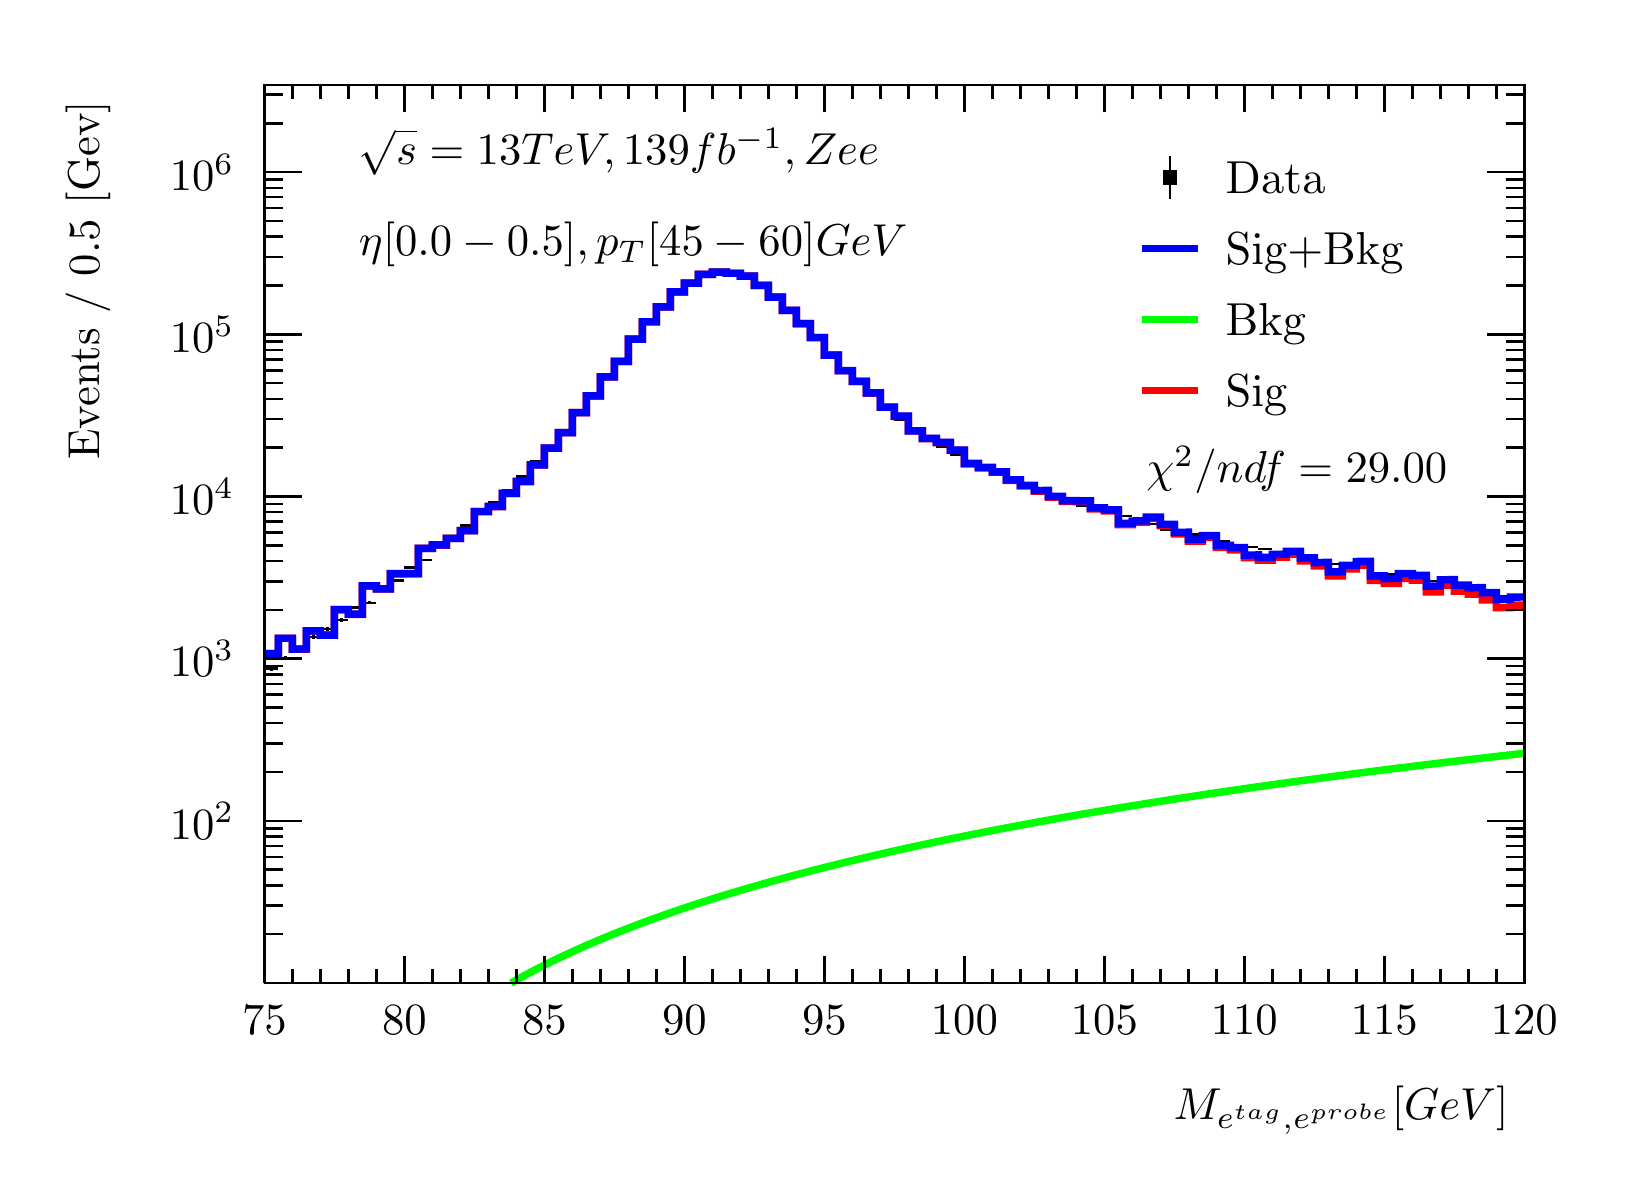
\begin{tikzpicture}
\pgfdeclareplotmark{cross} {
\pgfpathmoveto{\pgfpoint{-0.3\pgfplotmarksize}{\pgfplotmarksize}}
\pgfpathlineto{\pgfpoint{+0.3\pgfplotmarksize}{\pgfplotmarksize}}
\pgfpathlineto{\pgfpoint{+0.3\pgfplotmarksize}{0.3\pgfplotmarksize}}
\pgfpathlineto{\pgfpoint{+1\pgfplotmarksize}{0.3\pgfplotmarksize}}
\pgfpathlineto{\pgfpoint{+1\pgfplotmarksize}{-0.3\pgfplotmarksize}}
\pgfpathlineto{\pgfpoint{+0.3\pgfplotmarksize}{-0.3\pgfplotmarksize}}
\pgfpathlineto{\pgfpoint{+0.3\pgfplotmarksize}{-1.\pgfplotmarksize}}
\pgfpathlineto{\pgfpoint{-0.3\pgfplotmarksize}{-1.\pgfplotmarksize}}
\pgfpathlineto{\pgfpoint{-0.3\pgfplotmarksize}{-0.3\pgfplotmarksize}}
\pgfpathlineto{\pgfpoint{-1.\pgfplotmarksize}{-0.3\pgfplotmarksize}}
\pgfpathlineto{\pgfpoint{-1.\pgfplotmarksize}{0.3\pgfplotmarksize}}
\pgfpathlineto{\pgfpoint{-0.3\pgfplotmarksize}{0.3\pgfplotmarksize}}
\pgfpathclose
\pgfusepathqstroke
}
\pgfdeclareplotmark{cross*} {
\pgfpathmoveto{\pgfpoint{-0.3\pgfplotmarksize}{\pgfplotmarksize}}
\pgfpathlineto{\pgfpoint{+0.3\pgfplotmarksize}{\pgfplotmarksize}}
\pgfpathlineto{\pgfpoint{+0.3\pgfplotmarksize}{0.3\pgfplotmarksize}}
\pgfpathlineto{\pgfpoint{+1\pgfplotmarksize}{0.3\pgfplotmarksize}}
\pgfpathlineto{\pgfpoint{+1\pgfplotmarksize}{-0.3\pgfplotmarksize}}
\pgfpathlineto{\pgfpoint{+0.3\pgfplotmarksize}{-0.3\pgfplotmarksize}}
\pgfpathlineto{\pgfpoint{+0.3\pgfplotmarksize}{-1.\pgfplotmarksize}}
\pgfpathlineto{\pgfpoint{-0.3\pgfplotmarksize}{-1.\pgfplotmarksize}}
\pgfpathlineto{\pgfpoint{-0.3\pgfplotmarksize}{-0.3\pgfplotmarksize}}
\pgfpathlineto{\pgfpoint{-1.\pgfplotmarksize}{-0.3\pgfplotmarksize}}
\pgfpathlineto{\pgfpoint{-1.\pgfplotmarksize}{0.3\pgfplotmarksize}}
\pgfpathlineto{\pgfpoint{-0.3\pgfplotmarksize}{0.3\pgfplotmarksize}}
\pgfpathclose
\pgfusepathqfillstroke
}
\pgfdeclareplotmark{newstar} {
\pgfpathmoveto{\pgfqpoint{0pt}{\pgfplotmarksize}}
\pgfpathlineto{\pgfqpointpolar{44}{0.5\pgfplotmarksize}}
\pgfpathlineto{\pgfqpointpolar{18}{\pgfplotmarksize}}
\pgfpathlineto{\pgfqpointpolar{-20}{0.5\pgfplotmarksize}}
\pgfpathlineto{\pgfqpointpolar{-54}{\pgfplotmarksize}}
\pgfpathlineto{\pgfqpointpolar{-90}{0.5\pgfplotmarksize}}
\pgfpathlineto{\pgfqpointpolar{234}{\pgfplotmarksize}}
\pgfpathlineto{\pgfqpointpolar{198}{0.5\pgfplotmarksize}}
\pgfpathlineto{\pgfqpointpolar{162}{\pgfplotmarksize}}
\pgfpathlineto{\pgfqpointpolar{134}{0.5\pgfplotmarksize}}
\pgfpathclose
\pgfusepathqstroke
}
\pgfdeclareplotmark{newstar*} {
\pgfpathmoveto{\pgfqpoint{0pt}{\pgfplotmarksize}}
\pgfpathlineto{\pgfqpointpolar{44}{0.5\pgfplotmarksize}}
\pgfpathlineto{\pgfqpointpolar{18}{\pgfplotmarksize}}
\pgfpathlineto{\pgfqpointpolar{-20}{0.5\pgfplotmarksize}}
\pgfpathlineto{\pgfqpointpolar{-54}{\pgfplotmarksize}}
\pgfpathlineto{\pgfqpointpolar{-90}{0.5\pgfplotmarksize}}
\pgfpathlineto{\pgfqpointpolar{234}{\pgfplotmarksize}}
\pgfpathlineto{\pgfqpointpolar{198}{0.5\pgfplotmarksize}}
\pgfpathlineto{\pgfqpointpolar{162}{\pgfplotmarksize}}
\pgfpathlineto{\pgfqpointpolar{134}{0.5\pgfplotmarksize}}
\pgfpathclose
\pgfusepathqfillstroke
}
\definecolor{c}{rgb}{1,1,1};
\draw [color=c, fill=c] (0,0) rectangle (20,14.4361);
\draw [color=c, fill=c] (3,2.30977) rectangle (19,13.7143);
\definecolor{c}{rgb}{0,0,0};
\draw [c,line width=0.9] (3,2.30977) -- (3,13.7143) -- (19,13.7143) -- (19,2.30977) -- (3,2.30977);
\definecolor{c}{rgb}{1,1,1};
\draw [color=c, fill=c] (3,2.30977) rectangle (19,13.7143);
\definecolor{c}{rgb}{0,0,0};
\draw [c,line width=0.9] (3,2.30977) -- (3,13.7143) -- (19,13.7143) -- (19,2.30977) -- (3,2.30977);
\draw [c,line width=0.9] (3,2.30977) -- (19,2.30977);
\draw [c,line width=0.9] (3,2.65624) -- (3,2.30977);
\draw [c,line width=0.9] (3.35556,2.48301) -- (3.35556,2.30977);
\draw [c,line width=0.9] (3.71111,2.48301) -- (3.71111,2.30977);
\draw [c,line width=0.9] (4.06667,2.48301) -- (4.06667,2.30977);
\draw [c,line width=0.9] (4.42222,2.48301) -- (4.42222,2.30977);
\draw [c,line width=0.9] (4.77778,2.65624) -- (4.77778,2.30977);
\draw [c,line width=0.9] (5.13333,2.48301) -- (5.13333,2.30977);
\draw [c,line width=0.9] (5.48889,2.48301) -- (5.48889,2.30977);
\draw [c,line width=0.9] (5.84444,2.48301) -- (5.84444,2.30977);
\draw [c,line width=0.9] (6.2,2.48301) -- (6.2,2.30977);
\draw [c,line width=0.9] (6.55556,2.65624) -- (6.55556,2.30977);
\draw [c,line width=0.9] (6.91111,2.48301) -- (6.91111,2.30977);
\draw [c,line width=0.9] (7.26667,2.48301) -- (7.26667,2.30977);
\draw [c,line width=0.9] (7.62222,2.48301) -- (7.62222,2.30977);
\draw [c,line width=0.9] (7.97778,2.48301) -- (7.97778,2.30977);
\draw [c,line width=0.9] (8.33333,2.65624) -- (8.33333,2.30977);
\draw [c,line width=0.9] (8.68889,2.48301) -- (8.68889,2.30977);
\draw [c,line width=0.9] (9.04444,2.48301) -- (9.04444,2.30977);
\draw [c,line width=0.9] (9.4,2.48301) -- (9.4,2.30977);
\draw [c,line width=0.9] (9.75556,2.48301) -- (9.75556,2.30977);
\draw [c,line width=0.9] (10.1111,2.65624) -- (10.1111,2.30977);
\draw [c,line width=0.9] (10.4667,2.48301) -- (10.4667,2.30977);
\draw [c,line width=0.9] (10.8222,2.48301) -- (10.8222,2.30977);
\draw [c,line width=0.9] (11.1778,2.48301) -- (11.1778,2.30977);
\draw [c,line width=0.9] (11.5333,2.48301) -- (11.5333,2.30977);
\draw [c,line width=0.9] (11.8889,2.65624) -- (11.8889,2.30977);
\draw [c,line width=0.9] (12.2444,2.48301) -- (12.2444,2.30977);
\draw [c,line width=0.9] (12.6,2.48301) -- (12.6,2.30977);
\draw [c,line width=0.9] (12.9556,2.48301) -- (12.9556,2.30977);
\draw [c,line width=0.9] (13.3111,2.48301) -- (13.3111,2.30977);
\draw [c,line width=0.9] (13.6667,2.65624) -- (13.6667,2.30977);
\draw [c,line width=0.9] (14.0222,2.48301) -- (14.0222,2.30977);
\draw [c,line width=0.9] (14.3778,2.48301) -- (14.3778,2.30977);
\draw [c,line width=0.9] (14.7333,2.48301) -- (14.7333,2.30977);
\draw [c,line width=0.9] (15.0889,2.48301) -- (15.0889,2.30977);
\draw [c,line width=0.9] (15.4444,2.65624) -- (15.4444,2.30977);
\draw [c,line width=0.9] (15.8,2.48301) -- (15.8,2.30977);
\draw [c,line width=0.9] (16.1556,2.48301) -- (16.1556,2.30977);
\draw [c,line width=0.9] (16.5111,2.48301) -- (16.5111,2.30977);
\draw [c,line width=0.9] (16.8667,2.48301) -- (16.8667,2.30977);
\draw [c,line width=0.9] (17.2222,2.65624) -- (17.2222,2.30977);
\draw [c,line width=0.9] (17.5778,2.48301) -- (17.5778,2.30977);
\draw [c,line width=0.9] (17.9333,2.48301) -- (17.9333,2.30977);
\draw [c,line width=0.9] (18.2889,2.48301) -- (18.2889,2.30977);
\draw [c,line width=0.9] (18.6444,2.48301) -- (18.6444,2.30977);
\draw [c,line width=0.9] (19,2.65624) -- (19,2.30977);
\draw [c,line width=0.9] (19,2.65624) -- (19,2.30977);
\draw [anchor=base] (3,1.66015) node[scale=1.61424, color=c, rotate=0]{75};
\draw [anchor=base] (4.77778,1.66015) node[scale=1.61424, color=c, rotate=0]{80};
\draw [anchor=base] (6.55556,1.66015) node[scale=1.61424, color=c, rotate=0]{85};
\draw [anchor=base] (8.33333,1.66015) node[scale=1.61424, color=c, rotate=0]{90};
\draw [anchor=base] (10.1111,1.66015) node[scale=1.61424, color=c, rotate=0]{95};
\draw [anchor=base] (11.8889,1.66015) node[scale=1.61424, color=c, rotate=0]{100};
\draw [anchor=base] (13.6667,1.66015) node[scale=1.61424, color=c, rotate=0]{105};
\draw [anchor=base] (15.4444,1.66015) node[scale=1.61424, color=c, rotate=0]{110};
\draw [anchor=base] (17.2222,1.66015) node[scale=1.61424, color=c, rotate=0]{115};
\draw [anchor=base] (19,1.66015) node[scale=1.61424, color=c, rotate=0]{120};
\draw [anchor= east] (19,0.692932) node[scale=1.61424, color=c, rotate=0]{$M_{e^{tag}, e^{probe}}  [GeV]$};
\draw [c,line width=0.9] (3,13.7143) -- (19,13.7143);
\draw [c,line width=0.9] (3,13.3678) -- (3,13.7143);
\draw [c,line width=0.9] (3.35556,13.5411) -- (3.35556,13.7143);
\draw [c,line width=0.9] (3.71111,13.5411) -- (3.71111,13.7143);
\draw [c,line width=0.9] (4.06667,13.5411) -- (4.06667,13.7143);
\draw [c,line width=0.9] (4.42222,13.5411) -- (4.42222,13.7143);
\draw [c,line width=0.9] (4.77778,13.3678) -- (4.77778,13.7143);
\draw [c,line width=0.9] (5.13333,13.5411) -- (5.13333,13.7143);
\draw [c,line width=0.9] (5.48889,13.5411) -- (5.48889,13.7143);
\draw [c,line width=0.9] (5.84444,13.5411) -- (5.84444,13.7143);
\draw [c,line width=0.9] (6.2,13.5411) -- (6.2,13.7143);
\draw [c,line width=0.9] (6.55556,13.3678) -- (6.55556,13.7143);
\draw [c,line width=0.9] (6.91111,13.5411) -- (6.91111,13.7143);
\draw [c,line width=0.9] (7.26667,13.5411) -- (7.26667,13.7143);
\draw [c,line width=0.9] (7.62222,13.5411) -- (7.62222,13.7143);
\draw [c,line width=0.9] (7.97778,13.5411) -- (7.97778,13.7143);
\draw [c,line width=0.9] (8.33333,13.3678) -- (8.33333,13.7143);
\draw [c,line width=0.9] (8.68889,13.5411) -- (8.68889,13.7143);
\draw [c,line width=0.9] (9.04444,13.5411) -- (9.04444,13.7143);
\draw [c,line width=0.9] (9.4,13.5411) -- (9.4,13.7143);
\draw [c,line width=0.9] (9.75556,13.5411) -- (9.75556,13.7143);
\draw [c,line width=0.9] (10.1111,13.3678) -- (10.1111,13.7143);
\draw [c,line width=0.9] (10.4667,13.5411) -- (10.4667,13.7143);
\draw [c,line width=0.9] (10.8222,13.5411) -- (10.8222,13.7143);
\draw [c,line width=0.9] (11.1778,13.5411) -- (11.1778,13.7143);
\draw [c,line width=0.9] (11.5333,13.5411) -- (11.5333,13.7143);
\draw [c,line width=0.9] (11.8889,13.3678) -- (11.8889,13.7143);
\draw [c,line width=0.9] (12.2444,13.5411) -- (12.2444,13.7143);
\draw [c,line width=0.9] (12.6,13.5411) -- (12.6,13.7143);
\draw [c,line width=0.9] (12.9556,13.5411) -- (12.9556,13.7143);
\draw [c,line width=0.9] (13.3111,13.5411) -- (13.3111,13.7143);
\draw [c,line width=0.9] (13.6667,13.3678) -- (13.6667,13.7143);
\draw [c,line width=0.9] (14.0222,13.5411) -- (14.0222,13.7143);
\draw [c,line width=0.9] (14.3778,13.5411) -- (14.3778,13.7143);
\draw [c,line width=0.9] (14.7333,13.5411) -- (14.7333,13.7143);
\draw [c,line width=0.9] (15.0889,13.5411) -- (15.0889,13.7143);
\draw [c,line width=0.9] (15.4444,13.3678) -- (15.4444,13.7143);
\draw [c,line width=0.9] (15.8,13.5411) -- (15.8,13.7143);
\draw [c,line width=0.9] (16.1556,13.5411) -- (16.1556,13.7143);
\draw [c,line width=0.9] (16.5111,13.5411) -- (16.5111,13.7143);
\draw [c,line width=0.9] (16.8667,13.5411) -- (16.8667,13.7143);
\draw [c,line width=0.9] (17.2222,13.3678) -- (17.2222,13.7143);
\draw [c,line width=0.9] (17.5778,13.5411) -- (17.5778,13.7143);
\draw [c,line width=0.9] (17.9333,13.5411) -- (17.9333,13.7143);
\draw [c,line width=0.9] (18.2889,13.5411) -- (18.2889,13.7143);
\draw [c,line width=0.9] (18.6444,13.5411) -- (18.6444,13.7143);
\draw [c,line width=0.9] (19,13.3678) -- (19,13.7143);
\draw [c,line width=0.9] (19,13.3678) -- (19,13.7143);
\draw [c,line width=0.9] (3,2.30977) -- (3,13.7143);
\draw [c,line width=0.9] (3.237,2.92982) -- (3,2.92982);
\draw [c,line width=0.9] (3.237,3.29252) -- (3,3.29252);
\draw [c,line width=0.9] (3.237,3.54986) -- (3,3.54986);
\draw [c,line width=0.9] (3.237,3.74947) -- (3,3.74947);
\draw [c,line width=0.9] (3.237,3.91257) -- (3,3.91257);
\draw [c,line width=0.9] (3.237,4.05046) -- (3,4.05046);
\draw [c,line width=0.9] (3.237,4.16991) -- (3,4.16991);
\draw [c,line width=0.9] (3.237,4.27527) -- (3,4.27527);
\draw [c,line width=0.9] (3.474,4.36952) -- (3,4.36952);
\draw [anchor= east] (2.82,4.36952) node[scale=1.61424, color=c, rotate=0]{$10^{2}$};
\draw [c,line width=0.9] (3.237,4.98956) -- (3,4.98956);
\draw [c,line width=0.9] (3.237,5.35227) -- (3,5.35227);
\draw [c,line width=0.9] (3.237,5.60961) -- (3,5.60961);
\draw [c,line width=0.9] (3.237,5.80922) -- (3,5.80922);
\draw [c,line width=0.9] (3.237,5.97231) -- (3,5.97231);
\draw [c,line width=0.9] (3.237,6.11021) -- (3,6.11021);
\draw [c,line width=0.9] (3.237,6.22966) -- (3,6.22966);
\draw [c,line width=0.9] (3.237,6.33502) -- (3,6.33502);
\draw [c,line width=0.9] (3.474,6.42927) -- (3,6.42927);
\draw [anchor= east] (2.82,6.42927) node[scale=1.61424, color=c, rotate=0]{$10^{3}$};
\draw [c,line width=0.9] (3.237,7.04931) -- (3,7.04931);
\draw [c,line width=0.9] (3.237,7.41202) -- (3,7.41202);
\draw [c,line width=0.9] (3.237,7.66936) -- (3,7.66936);
\draw [c,line width=0.9] (3.237,7.86897) -- (3,7.86897);
\draw [c,line width=0.9] (3.237,8.03206) -- (3,8.03206);
\draw [c,line width=0.9] (3.237,8.16995) -- (3,8.16995);
\draw [c,line width=0.9] (3.237,8.2894) -- (3,8.2894);
\draw [c,line width=0.9] (3.237,8.39476) -- (3,8.39476);
\draw [c,line width=0.9] (3.474,8.48901) -- (3,8.48901);
\draw [anchor= east] (2.82,8.48901) node[scale=1.61424, color=c, rotate=0]{$10^{4}$};
\draw [c,line width=0.9] (3.237,9.10906) -- (3,9.10906);
\draw [c,line width=0.9] (3.237,9.47176) -- (3,9.47176);
\draw [c,line width=0.9] (3.237,9.7291) -- (3,9.7291);
\draw [c,line width=0.9] (3.237,9.92871) -- (3,9.92871);
\draw [c,line width=0.9] (3.237,10.0918) -- (3,10.0918);
\draw [c,line width=0.9] (3.237,10.2297) -- (3,10.2297);
\draw [c,line width=0.9] (3.237,10.3491) -- (3,10.3491);
\draw [c,line width=0.9] (3.237,10.4545) -- (3,10.4545);
\draw [c,line width=0.9] (3.474,10.5488) -- (3,10.5488);
\draw [anchor= east] (2.82,10.5488) node[scale=1.61424, color=c, rotate=0]{$10^{5}$};
\draw [c,line width=0.9] (3.237,11.1688) -- (3,11.1688);
\draw [c,line width=0.9] (3.237,11.5315) -- (3,11.5315);
\draw [c,line width=0.9] (3.237,11.7889) -- (3,11.7889);
\draw [c,line width=0.9] (3.237,11.9885) -- (3,11.9885);
\draw [c,line width=0.9] (3.237,12.1516) -- (3,12.1516);
\draw [c,line width=0.9] (3.237,12.2894) -- (3,12.2894);
\draw [c,line width=0.9] (3.237,12.4089) -- (3,12.4089);
\draw [c,line width=0.9] (3.237,12.5143) -- (3,12.5143);
\draw [c,line width=0.9] (3.474,12.6085) -- (3,12.6085);
\draw [anchor= east] (2.82,12.6085) node[scale=1.61424, color=c, rotate=0]{$10^{6}$};
\draw [c,line width=0.9] (3.237,13.2286) -- (3,13.2286);
\draw [c,line width=0.9] (3.237,13.5913) -- (3,13.5913);
\draw [anchor= east] (0.76,13.7143) node[scale=1.61424, color=c, rotate=90]{Events / 0.5 [Gev]};
\draw [c,line width=0.9] (19,2.30977) -- (19,13.7143);
\draw [c,line width=0.9] (18.763,2.92982) -- (19,2.92982);
\draw [c,line width=0.9] (18.763,3.29252) -- (19,3.29252);
\draw [c,line width=0.9] (18.763,3.54986) -- (19,3.54986);
\draw [c,line width=0.9] (18.763,3.74947) -- (19,3.74947);
\draw [c,line width=0.9] (18.763,3.91257) -- (19,3.91257);
\draw [c,line width=0.9] (18.763,4.05046) -- (19,4.05046);
\draw [c,line width=0.9] (18.763,4.16991) -- (19,4.16991);
\draw [c,line width=0.9] (18.763,4.27527) -- (19,4.27527);
\draw [c,line width=0.9] (18.526,4.36952) -- (19,4.36952);
\draw [c,line width=0.9] (18.763,4.98956) -- (19,4.98956);
\draw [c,line width=0.9] (18.763,5.35227) -- (19,5.35227);
\draw [c,line width=0.9] (18.763,5.60961) -- (19,5.60961);
\draw [c,line width=0.9] (18.763,5.80922) -- (19,5.80922);
\draw [c,line width=0.9] (18.763,5.97231) -- (19,5.97231);
\draw [c,line width=0.9] (18.763,6.11021) -- (19,6.11021);
\draw [c,line width=0.9] (18.763,6.22966) -- (19,6.22966);
\draw [c,line width=0.9] (18.763,6.33502) -- (19,6.33502);
\draw [c,line width=0.9] (18.526,6.42927) -- (19,6.42927);
\draw [c,line width=0.9] (18.763,7.04931) -- (19,7.04931);
\draw [c,line width=0.9] (18.763,7.41202) -- (19,7.41202);
\draw [c,line width=0.9] (18.763,7.66936) -- (19,7.66936);
\draw [c,line width=0.9] (18.763,7.86897) -- (19,7.86897);
\draw [c,line width=0.9] (18.763,8.03206) -- (19,8.03206);
\draw [c,line width=0.9] (18.763,8.16995) -- (19,8.16995);
\draw [c,line width=0.9] (18.763,8.2894) -- (19,8.2894);
\draw [c,line width=0.9] (18.763,8.39476) -- (19,8.39476);
\draw [c,line width=0.9] (18.526,8.48901) -- (19,8.48901);
\draw [c,line width=0.9] (18.763,9.10906) -- (19,9.10906);
\draw [c,line width=0.9] (18.763,9.47176) -- (19,9.47176);
\draw [c,line width=0.9] (18.763,9.7291) -- (19,9.7291);
\draw [c,line width=0.9] (18.763,9.92871) -- (19,9.92871);
\draw [c,line width=0.9] (18.763,10.0918) -- (19,10.0918);
\draw [c,line width=0.9] (18.763,10.2297) -- (19,10.2297);
\draw [c,line width=0.9] (18.763,10.3491) -- (19,10.3491);
\draw [c,line width=0.9] (18.763,10.4545) -- (19,10.4545);
\draw [c,line width=0.9] (18.526,10.5488) -- (19,10.5488);
\draw [c,line width=0.9] (18.763,11.1688) -- (19,11.1688);
\draw [c,line width=0.9] (18.763,11.5315) -- (19,11.5315);
\draw [c,line width=0.9] (18.763,11.7889) -- (19,11.7889);
\draw [c,line width=0.9] (18.763,11.9885) -- (19,11.9885);
\draw [c,line width=0.9] (18.763,12.1516) -- (19,12.1516);
\draw [c,line width=0.9] (18.763,12.2894) -- (19,12.2894);
\draw [c,line width=0.9] (18.763,12.4089) -- (19,12.4089);
\draw [c,line width=0.9] (18.763,12.5143) -- (19,12.5143);
\draw [c,line width=0.9] (18.526,12.6085) -- (19,12.6085);
\draw [c,line width=0.9] (18.763,13.2286) -- (19,13.2286);
\draw [c,line width=0.9] (18.763,13.5913) -- (19,13.5913);
\draw [c,line width=0.9] (3.08889,6.30572) -- (3,6.30572);
\draw [c,line width=0.9] (3,6.30572) -- (3,6.30572);
\draw [c,line width=0.9] (3.08889,6.30572) -- (3.17778,6.30572);
\draw [c,line width=0.9] (3.17778,6.30572) -- (3.17778,6.30572);
\draw [c,line width=0.9] (3.08889,6.30572) -- (3.08889,6.33603);
\draw [c,line width=0.9] (3.08889,6.33603) -- (3.08889,6.33603);
\draw [c,line width=0.9] (3.08889,6.30572) -- (3.08889,6.27541);
\draw [c,line width=0.9] (3.08889,6.27541) -- (3.08889,6.27541);
\draw [c,line width=0.9] (3.26667,6.43994) -- (3.17778,6.43994);
\draw [c,line width=0.9] (3.17778,6.43994) -- (3.17778,6.43994);
\draw [c,line width=0.9] (3.26667,6.43994) -- (3.35556,6.43994);
\draw [c,line width=0.9] (3.35556,6.43994) -- (3.35556,6.43994);
\draw [c,line width=0.9] (3.26667,6.43994) -- (3.26667,6.46806);
\draw [c,line width=0.9] (3.26667,6.46806) -- (3.26667,6.46806);
\draw [c,line width=0.9] (3.26667,6.43994) -- (3.26667,6.41182);
\draw [c,line width=0.9] (3.26667,6.41182) -- (3.26667,6.41182);
\draw [c,line width=0.9] (3.44444,6.55584) -- (3.35556,6.55584);
\draw [c,line width=0.9] (3.35556,6.55584) -- (3.35556,6.55584);
\draw [c,line width=0.9] (3.44444,6.55584) -- (3.53333,6.55584);
\draw [c,line width=0.9] (3.53333,6.55584) -- (3.53333,6.55584);
\draw [c,line width=0.9] (3.44444,6.55584) -- (3.44444,6.5822);
\draw [c,line width=0.9] (3.44444,6.5822) -- (3.44444,6.5822);
\draw [c,line width=0.9] (3.44444,6.55584) -- (3.44444,6.52949);
\draw [c,line width=0.9] (3.44444,6.52949) -- (3.44444,6.52949);
\draw [c,line width=0.9] (3.62222,6.70301) -- (3.53333,6.70301);
\draw [c,line width=0.9] (3.53333,6.70301) -- (3.53333,6.70301);
\draw [c,line width=0.9] (3.62222,6.70301) -- (3.71111,6.70301);
\draw [c,line width=0.9] (3.71111,6.70301) -- (3.71111,6.70301);
\draw [c,line width=0.9] (3.62222,6.70301) -- (3.62222,6.72728);
\draw [c,line width=0.9] (3.62222,6.72728) -- (3.62222,6.72728);
\draw [c,line width=0.9] (3.62222,6.70301) -- (3.62222,6.67873);
\draw [c,line width=0.9] (3.62222,6.67873) -- (3.62222,6.67873);
\draw [c,line width=0.9] (3.8,6.80852) -- (3.71111,6.80852);
\draw [c,line width=0.9] (3.71111,6.80852) -- (3.71111,6.80852);
\draw [c,line width=0.9] (3.8,6.80852) -- (3.88889,6.80852);
\draw [c,line width=0.9] (3.88889,6.80852) -- (3.88889,6.80852);
\draw [c,line width=0.9] (3.8,6.80852) -- (3.8,6.8314);
\draw [c,line width=0.9] (3.8,6.8314) -- (3.8,6.8314);
\draw [c,line width=0.9] (3.8,6.80852) -- (3.8,6.78563);
\draw [c,line width=0.9] (3.8,6.78563) -- (3.8,6.78563);
\draw [c,line width=0.9] (3.97778,6.91855) -- (3.88889,6.91855);
\draw [c,line width=0.9] (3.88889,6.91855) -- (3.88889,6.91855);
\draw [c,line width=0.9] (3.97778,6.91855) -- (4.06667,6.91855);
\draw [c,line width=0.9] (4.06667,6.91855) -- (4.06667,6.91855);
\draw [c,line width=0.9] (3.97778,6.91855) -- (3.97778,6.94007);
\draw [c,line width=0.9] (3.97778,6.94007) -- (3.97778,6.94007);
\draw [c,line width=0.9] (3.97778,6.91855) -- (3.97778,6.89703);
\draw [c,line width=0.9] (3.97778,6.89703) -- (3.97778,6.89703);
\draw [c,line width=0.9] (4.15556,7.08052) -- (4.06667,7.08052);
\draw [c,line width=0.9] (4.06667,7.08052) -- (4.06667,7.08052);
\draw [c,line width=0.9] (4.15556,7.08052) -- (4.24444,7.08052);
\draw [c,line width=0.9] (4.24444,7.08052) -- (4.24444,7.08052);
\draw [c,line width=0.9] (4.15556,7.08052) -- (4.15556,7.10017);
\draw [c,line width=0.9] (4.15556,7.10017) -- (4.15556,7.10017);
\draw [c,line width=0.9] (4.15556,7.08052) -- (4.15556,7.06086);
\draw [c,line width=0.9] (4.15556,7.06086) -- (4.15556,7.06086);
\draw [c,line width=0.9] (4.33333,7.13863) -- (4.24444,7.13863);
\draw [c,line width=0.9] (4.24444,7.13863) -- (4.24444,7.13863);
\draw [c,line width=0.9] (4.33333,7.13863) -- (4.42222,7.13863);
\draw [c,line width=0.9] (4.42222,7.13863) -- (4.42222,7.13863);
\draw [c,line width=0.9] (4.33333,7.13863) -- (4.33333,7.15766);
\draw [c,line width=0.9] (4.33333,7.15766) -- (4.33333,7.15766);
\draw [c,line width=0.9] (4.33333,7.13863) -- (4.33333,7.1196);
\draw [c,line width=0.9] (4.33333,7.1196) -- (4.33333,7.1196);
\draw [c,line width=0.9] (4.51111,7.29393) -- (4.42222,7.29393);
\draw [c,line width=0.9] (4.42222,7.29393) -- (4.42222,7.29393);
\draw [c,line width=0.9] (4.51111,7.29393) -- (4.6,7.29393);
\draw [c,line width=0.9] (4.6,7.29393) -- (4.6,7.29393);
\draw [c,line width=0.9] (4.51111,7.29393) -- (4.51111,7.31138);
\draw [c,line width=0.9] (4.51111,7.31138) -- (4.51111,7.31138);
\draw [c,line width=0.9] (4.51111,7.29393) -- (4.51111,7.27648);
\draw [c,line width=0.9] (4.51111,7.27648) -- (4.51111,7.27648);
\draw [c,line width=0.9] (4.68889,7.42239) -- (4.6,7.42239);
\draw [c,line width=0.9] (4.6,7.42239) -- (4.6,7.42239);
\draw [c,line width=0.9] (4.68889,7.42239) -- (4.77778,7.42239);
\draw [c,line width=0.9] (4.77778,7.42239) -- (4.77778,7.42239);
\draw [c,line width=0.9] (4.68889,7.42239) -- (4.68889,7.43863);
\draw [c,line width=0.9] (4.68889,7.43863) -- (4.68889,7.43863);
\draw [c,line width=0.9] (4.68889,7.42239) -- (4.68889,7.40616);
\draw [c,line width=0.9] (4.68889,7.40616) -- (4.68889,7.40616);
\draw [c,line width=0.9] (4.86667,7.58647) -- (4.77778,7.58647);
\draw [c,line width=0.9] (4.77778,7.58647) -- (4.77778,7.58647);
\draw [c,line width=0.9] (4.86667,7.58647) -- (4.95556,7.58647);
\draw [c,line width=0.9] (4.95556,7.58647) -- (4.95556,7.58647);
\draw [c,line width=0.9] (4.86667,7.58647) -- (4.86667,7.60128);
\draw [c,line width=0.9] (4.86667,7.60128) -- (4.86667,7.60128);
\draw [c,line width=0.9] (4.86667,7.58647) -- (4.86667,7.57165);
\draw [c,line width=0.9] (4.86667,7.57165) -- (4.86667,7.57165);
\draw [c,line width=0.9] (5.04444,7.68466) -- (4.95556,7.68466);
\draw [c,line width=0.9] (4.95556,7.68466) -- (4.95556,7.68466);
\draw [c,line width=0.9] (5.04444,7.68466) -- (5.13333,7.68466);
\draw [c,line width=0.9] (5.13333,7.68466) -- (5.13333,7.68466);
\draw [c,line width=0.9] (5.04444,7.68466) -- (5.04444,7.69868);
\draw [c,line width=0.9] (5.04444,7.69868) -- (5.04444,7.69868);
\draw [c,line width=0.9] (5.04444,7.68466) -- (5.04444,7.67063);
\draw [c,line width=0.9] (5.04444,7.67063) -- (5.04444,7.67063);
\draw [c,line width=0.9] (5.22222,7.83413) -- (5.13333,7.83413);
\draw [c,line width=0.9] (5.13333,7.83413) -- (5.13333,7.83413);
\draw [c,line width=0.9] (5.22222,7.83413) -- (5.31111,7.83413);
\draw [c,line width=0.9] (5.31111,7.83413) -- (5.31111,7.83413);
\draw [c,line width=0.9] (5.22222,7.83413) -- (5.22222,7.84703);
\draw [c,line width=0.9] (5.22222,7.84703) -- (5.22222,7.84703);
\draw [c,line width=0.9] (5.22222,7.83413) -- (5.22222,7.82123);
\draw [c,line width=0.9] (5.22222,7.82123) -- (5.22222,7.82123);
\draw [c,line width=0.9] (5.4,7.95861) -- (5.31111,7.95861);
\draw [c,line width=0.9] (5.31111,7.95861) -- (5.31111,7.95861);
\draw [c,line width=0.9] (5.4,7.95861) -- (5.48889,7.95861);
\draw [c,line width=0.9] (5.48889,7.95861) -- (5.48889,7.95861);
\draw [c,line width=0.9] (5.4,7.95861) -- (5.4,7.97064);
\draw [c,line width=0.9] (5.4,7.97064) -- (5.4,7.97064);
\draw [c,line width=0.9] (5.4,7.95861) -- (5.4,7.94658);
\draw [c,line width=0.9] (5.4,7.94658) -- (5.4,7.94658);
\draw [c,line width=0.9] (5.57778,8.118) -- (5.48889,8.118);
\draw [c,line width=0.9] (5.48889,8.118) -- (5.48889,8.118);
\draw [c,line width=0.9] (5.57778,8.118) -- (5.66667,8.118);
\draw [c,line width=0.9] (5.66667,8.118) -- (5.66667,8.118);
\draw [c,line width=0.9] (5.57778,8.118) -- (5.57778,8.129);
\draw [c,line width=0.9] (5.57778,8.129) -- (5.57778,8.129);
\draw [c,line width=0.9] (5.57778,8.118) -- (5.57778,8.10699);
\draw [c,line width=0.9] (5.57778,8.10699) -- (5.57778,8.10699);
\draw [c,line width=0.9] (5.75556,8.26354) -- (5.66667,8.26354);
\draw [c,line width=0.9] (5.66667,8.26354) -- (5.66667,8.26354);
\draw [c,line width=0.9] (5.75556,8.26354) -- (5.84444,8.26354);
\draw [c,line width=0.9] (5.84444,8.26354) -- (5.84444,8.26354);
\draw [c,line width=0.9] (5.75556,8.26354) -- (5.75556,8.27369);
\draw [c,line width=0.9] (5.75556,8.27369) -- (5.75556,8.27369);
\draw [c,line width=0.9] (5.75556,8.26354) -- (5.75556,8.25339);
\draw [c,line width=0.9] (5.75556,8.25339) -- (5.75556,8.25339);
\draw [c,line width=0.9] (5.93333,8.41189) -- (5.84444,8.41189);
\draw [c,line width=0.9] (5.84444,8.41189) -- (5.84444,8.41189);
\draw [c,line width=0.9] (5.93333,8.41189) -- (6.02222,8.41189);
\draw [c,line width=0.9] (6.02222,8.41189) -- (6.02222,8.41189);
\draw [c,line width=0.9] (5.93333,8.41189) -- (5.93333,8.42123);
\draw [c,line width=0.9] (5.93333,8.42123) -- (5.93333,8.42123);
\draw [c,line width=0.9] (5.93333,8.41189) -- (5.93333,8.40256);
\draw [c,line width=0.9] (5.93333,8.40256) -- (5.93333,8.40256);
\draw [c,line width=0.9] (6.11111,8.5702) -- (6.02222,8.5702);
\draw [c,line width=0.9] (6.02222,8.5702) -- (6.02222,8.5702);
\draw [c,line width=0.9] (6.11111,8.5702) -- (6.2,8.5702);
\draw [c,line width=0.9] (6.2,8.5702) -- (6.2,8.5702);
\draw [c,line width=0.9] (6.11111,8.5702) -- (6.11111,8.57875);
\draw [c,line width=0.9] (6.11111,8.57875) -- (6.11111,8.57875);
\draw [c,line width=0.9] (6.11111,8.5702) -- (6.11111,8.56165);
\draw [c,line width=0.9] (6.11111,8.56165) -- (6.11111,8.56165);
\draw [c,line width=0.9] (6.28889,8.74338) -- (6.2,8.74338);
\draw [c,line width=0.9] (6.2,8.74338) -- (6.2,8.74338);
\draw [c,line width=0.9] (6.28889,8.74338) -- (6.37778,8.74338);
\draw [c,line width=0.9] (6.37778,8.74338) -- (6.37778,8.74338);
\draw [c,line width=0.9] (6.28889,8.74338) -- (6.28889,8.75114);
\draw [c,line width=0.9] (6.28889,8.75114) -- (6.28889,8.75114);
\draw [c,line width=0.9] (6.28889,8.74338) -- (6.28889,8.73562);
\draw [c,line width=0.9] (6.28889,8.73562) -- (6.28889,8.73562);
\draw [c,line width=0.9] (6.46667,8.93957) -- (6.37778,8.93957);
\draw [c,line width=0.9] (6.37778,8.93957) -- (6.37778,8.93957);
\draw [c,line width=0.9] (6.46667,8.93957) -- (6.55556,8.93957);
\draw [c,line width=0.9] (6.55556,8.93957) -- (6.55556,8.93957);
\draw [c,line width=0.9] (6.46667,8.93957) -- (6.46667,8.94653);
\draw [c,line width=0.9] (6.46667,8.94653) -- (6.46667,8.94653);
\draw [c,line width=0.9] (6.46667,8.93957) -- (6.46667,8.93262);
\draw [c,line width=0.9] (6.46667,8.93262) -- (6.46667,8.93262);
\draw [c,line width=0.9] (6.64444,9.12594) -- (6.55556,9.12594);
\draw [c,line width=0.9] (6.55556,9.12594) -- (6.55556,9.12594);
\draw [c,line width=0.9] (6.64444,9.12594) -- (6.73333,9.12594);
\draw [c,line width=0.9] (6.73333,9.12594) -- (6.73333,9.12594);
\draw [c,line width=0.9] (6.64444,9.12594) -- (6.64444,9.13221);
\draw [c,line width=0.9] (6.64444,9.13221) -- (6.64444,9.13221);
\draw [c,line width=0.9] (6.64444,9.12594) -- (6.64444,9.11967);
\draw [c,line width=0.9] (6.64444,9.11967) -- (6.64444,9.11967);
\draw [c,line width=0.9] (6.82222,9.32751) -- (6.73333,9.32751);
\draw [c,line width=0.9] (6.73333,9.32751) -- (6.73333,9.32751);
\draw [c,line width=0.9] (6.82222,9.32751) -- (6.91111,9.32751);
\draw [c,line width=0.9] (6.91111,9.32751) -- (6.91111,9.32751);
\draw [c,line width=0.9] (6.82222,9.32751) -- (6.82222,9.3331);
\draw [c,line width=0.9] (6.82222,9.3331) -- (6.82222,9.3331);
\draw [c,line width=0.9] (6.82222,9.32751) -- (6.82222,9.32191);
\draw [c,line width=0.9] (6.82222,9.32191) -- (6.82222,9.32191);
\draw [c,line width=0.9] (7,9.53) -- (6.91111,9.53);
\draw [c,line width=0.9] (6.91111,9.53) -- (6.91111,9.53);
\draw [c,line width=0.9] (7,9.53) -- (7.08889,9.53);
\draw [c,line width=0.9] (7.08889,9.53) -- (7.08889,9.53);
\draw [c,line width=0.9] (7,9.53) -- (7,9.535);
\draw [c,line width=0.9] (7,9.535) -- (7,9.535);
\draw [c,line width=0.9] (7,9.53) -- (7,9.525);
\draw [c,line width=0.9] (7,9.525) -- (7,9.525);
\draw [c,line width=0.9] (7.17778,9.76837) -- (7.08889,9.76837);
\draw [c,line width=0.9] (7.08889,9.76837) -- (7.08889,9.76837);
\draw [c,line width=0.9] (7.17778,9.76837) -- (7.26667,9.76837);
\draw [c,line width=0.9] (7.26667,9.76837) -- (7.26667,9.76837);
\draw [c,line width=0.9] (7.17778,9.76837) -- (7.17778,9.77275);
\draw [c,line width=0.9] (7.17778,9.77275) -- (7.17778,9.77275);
\draw [c,line width=0.9] (7.17778,9.76837) -- (7.17778,9.764);
\draw [c,line width=0.9] (7.17778,9.764) -- (7.17778,9.764);
\draw [c,line width=0.9] (7.35556,9.99199) -- (7.26667,9.99199);
\draw [c,line width=0.9] (7.26667,9.99199) -- (7.26667,9.99199);
\draw [c,line width=0.9] (7.35556,9.99199) -- (7.44444,9.99199);
\draw [c,line width=0.9] (7.44444,9.99199) -- (7.44444,9.99199);
\draw [c,line width=0.9] (7.35556,9.99199) -- (7.35556,9.99585);
\draw [c,line width=0.9] (7.35556,9.99585) -- (7.35556,9.99585);
\draw [c,line width=0.9] (7.35556,9.99199) -- (7.35556,9.98813);
\draw [c,line width=0.9] (7.35556,9.98813) -- (7.35556,9.98813);
\draw [c,line width=0.9] (7.53333,10.2354) -- (7.44444,10.2354);
\draw [c,line width=0.9] (7.44444,10.2354) -- (7.44444,10.2354);
\draw [c,line width=0.9] (7.53333,10.2354) -- (7.62222,10.2354);
\draw [c,line width=0.9] (7.62222,10.2354) -- (7.62222,10.2354);
\draw [c,line width=0.9] (7.53333,10.2354) -- (7.53333,10.2387);
\draw [c,line width=0.9] (7.53333,10.2387) -- (7.53333,10.2387);
\draw [c,line width=0.9] (7.53333,10.2354) -- (7.53333,10.232);
\draw [c,line width=0.9] (7.53333,10.232) -- (7.53333,10.232);
\draw [c,line width=0.9] (7.71111,10.4629) -- (7.62222,10.4629);
\draw [c,line width=0.9] (7.62222,10.4629) -- (7.62222,10.4629);
\draw [c,line width=0.9] (7.71111,10.4629) -- (7.8,10.4629);
\draw [c,line width=0.9] (7.8,10.4629) -- (7.8,10.4629);
\draw [c,line width=0.9] (7.71111,10.4629) -- (7.71111,10.4658);
\draw [c,line width=0.9] (7.71111,10.4658) -- (7.71111,10.4658);
\draw [c,line width=0.9] (7.71111,10.4629) -- (7.71111,10.4599);
\draw [c,line width=0.9] (7.71111,10.4599) -- (7.71111,10.4599);
\draw [c,line width=0.9] (7.88889,10.6841) -- (7.8,10.6841);
\draw [c,line width=0.9] (7.8,10.6841) -- (7.8,10.6841);
\draw [c,line width=0.9] (7.88889,10.6841) -- (7.97778,10.6841);
\draw [c,line width=0.9] (7.97778,10.6841) -- (7.97778,10.6841);
\draw [c,line width=0.9] (7.88889,10.6841) -- (7.88889,10.6867);
\draw [c,line width=0.9] (7.88889,10.6867) -- (7.88889,10.6867);
\draw [c,line width=0.9] (7.88889,10.6841) -- (7.88889,10.6815);
\draw [c,line width=0.9] (7.88889,10.6815) -- (7.88889,10.6815);
\draw [c,line width=0.9] (8.06667,10.8887) -- (7.97778,10.8887);
\draw [c,line width=0.9] (7.97778,10.8887) -- (7.97778,10.8887);
\draw [c,line width=0.9] (8.06667,10.8887) -- (8.15556,10.8887);
\draw [c,line width=0.9] (8.15556,10.8887) -- (8.15556,10.8887);
\draw [c,line width=0.9] (8.06667,10.8887) -- (8.06667,10.891);
\draw [c,line width=0.9] (8.06667,10.891) -- (8.06667,10.891);
\draw [c,line width=0.9] (8.06667,10.8887) -- (8.06667,10.8863);
\draw [c,line width=0.9] (8.06667,10.8863) -- (8.06667,10.8863);
\draw [c,line width=0.9] (8.24444,11.0725) -- (8.15556,11.0725);
\draw [c,line width=0.9] (8.15556,11.0725) -- (8.15556,11.0725);
\draw [c,line width=0.9] (8.24444,11.0725) -- (8.33333,11.0725);
\draw [c,line width=0.9] (8.33333,11.0725) -- (8.33333,11.0725);
\draw [c,line width=0.9] (8.24444,11.0725) -- (8.24444,11.0746);
\draw [c,line width=0.9] (8.24444,11.0746) -- (8.24444,11.0746);
\draw [c,line width=0.9] (8.24444,11.0725) -- (8.24444,11.0704);
\draw [c,line width=0.9] (8.24444,11.0704) -- (8.24444,11.0704);
\draw [c,line width=0.9] (8.42222,11.2095) -- (8.33333,11.2095);
\draw [c,line width=0.9] (8.33333,11.2095) -- (8.33333,11.2095);
\draw [c,line width=0.9] (8.42222,11.2095) -- (8.51111,11.2095);
\draw [c,line width=0.9] (8.51111,11.2095) -- (8.51111,11.2095);
\draw [c,line width=0.9] (8.42222,11.2095) -- (8.42222,11.2115);
\draw [c,line width=0.9] (8.42222,11.2115) -- (8.42222,11.2115);
\draw [c,line width=0.9] (8.42222,11.2095) -- (8.42222,11.2076);
\draw [c,line width=0.9] (8.42222,11.2076) -- (8.42222,11.2076);
\draw [c,line width=0.9] (8.6,11.3058) -- (8.51111,11.3058);
\draw [c,line width=0.9] (8.51111,11.3058) -- (8.51111,11.3058);
\draw [c,line width=0.9] (8.6,11.3058) -- (8.68889,11.3058);
\draw [c,line width=0.9] (8.68889,11.3058) -- (8.68889,11.3058);
\draw [c,line width=0.9] (8.6,11.3058) -- (8.6,11.3076);
\draw [c,line width=0.9] (8.6,11.3076) -- (8.6,11.3076);
\draw [c,line width=0.9] (8.6,11.3058) -- (8.6,11.3039);
\draw [c,line width=0.9] (8.6,11.3039) -- (8.6,11.3039);
\draw [c,line width=0.9] (8.77778,11.3499) -- (8.68889,11.3499);
\draw [c,line width=0.9] (8.68889,11.3499) -- (8.68889,11.3499);
\draw [c,line width=0.9] (8.77778,11.3499) -- (8.86667,11.3499);
\draw [c,line width=0.9] (8.86667,11.3499) -- (8.86667,11.3499);
\draw [c,line width=0.9] (8.77778,11.3499) -- (8.77778,11.3517);
\draw [c,line width=0.9] (8.77778,11.3517) -- (8.77778,11.3517);
\draw [c,line width=0.9] (8.77778,11.3499) -- (8.77778,11.348);
\draw [c,line width=0.9] (8.77778,11.348) -- (8.77778,11.348);
\draw [c,line width=0.9] (8.95556,11.3424) -- (8.86667,11.3424);
\draw [c,line width=0.9] (8.86667,11.3424) -- (8.86667,11.3424);
\draw [c,line width=0.9] (8.95556,11.3424) -- (9.04444,11.3424);
\draw [c,line width=0.9] (9.04444,11.3424) -- (9.04444,11.3424);
\draw [c,line width=0.9] (8.95556,11.3424) -- (8.95556,11.3442);
\draw [c,line width=0.9] (8.95556,11.3442) -- (8.95556,11.3442);
\draw [c,line width=0.9] (8.95556,11.3424) -- (8.95556,11.3406);
\draw [c,line width=0.9] (8.95556,11.3406) -- (8.95556,11.3406);
\draw [c,line width=0.9] (9.13333,11.2839) -- (9.04444,11.2839);
\draw [c,line width=0.9] (9.04444,11.2839) -- (9.04444,11.2839);
\draw [c,line width=0.9] (9.13333,11.2839) -- (9.22222,11.2839);
\draw [c,line width=0.9] (9.22222,11.2839) -- (9.22222,11.2839);
\draw [c,line width=0.9] (9.13333,11.2839) -- (9.13333,11.2858);
\draw [c,line width=0.9] (9.13333,11.2858) -- (9.13333,11.2858);
\draw [c,line width=0.9] (9.13333,11.2839) -- (9.13333,11.2821);
\draw [c,line width=0.9] (9.13333,11.2821) -- (9.13333,11.2821);
\draw [c,line width=0.9] (9.31111,11.1805) -- (9.22222,11.1805);
\draw [c,line width=0.9] (9.22222,11.1805) -- (9.22222,11.1805);
\draw [c,line width=0.9] (9.31111,11.1805) -- (9.4,11.1805);
\draw [c,line width=0.9] (9.4,11.1805) -- (9.4,11.1805);
\draw [c,line width=0.9] (9.31111,11.1805) -- (9.31111,11.1825);
\draw [c,line width=0.9] (9.31111,11.1825) -- (9.31111,11.1825);
\draw [c,line width=0.9] (9.31111,11.1805) -- (9.31111,11.1785);
\draw [c,line width=0.9] (9.31111,11.1785) -- (9.31111,11.1785);
\draw [c,line width=0.9] (9.48889,11.0348) -- (9.4,11.0348);
\draw [c,line width=0.9] (9.4,11.0348) -- (9.4,11.0348);
\draw [c,line width=0.9] (9.48889,11.0348) -- (9.57778,11.0348);
\draw [c,line width=0.9] (9.57778,11.0348) -- (9.57778,11.0348);
\draw [c,line width=0.9] (9.48889,11.0348) -- (9.48889,11.037);
\draw [c,line width=0.9] (9.48889,11.037) -- (9.48889,11.037);
\draw [c,line width=0.9] (9.48889,11.0348) -- (9.48889,11.0326);
\draw [c,line width=0.9] (9.48889,11.0326) -- (9.48889,11.0326);
\draw [c,line width=0.9] (9.66667,10.8686) -- (9.57778,10.8686);
\draw [c,line width=0.9] (9.57778,10.8686) -- (9.57778,10.8686);
\draw [c,line width=0.9] (9.66667,10.8686) -- (9.75556,10.8686);
\draw [c,line width=0.9] (9.75556,10.8686) -- (9.75556,10.8686);
\draw [c,line width=0.9] (9.66667,10.8686) -- (9.66667,10.8709);
\draw [c,line width=0.9] (9.66667,10.8709) -- (9.66667,10.8709);
\draw [c,line width=0.9] (9.66667,10.8686) -- (9.66667,10.8662);
\draw [c,line width=0.9] (9.66667,10.8662) -- (9.66667,10.8662);
\draw [c,line width=0.9] (9.84444,10.6793) -- (9.75556,10.6793);
\draw [c,line width=0.9] (9.75556,10.6793) -- (9.75556,10.6793);
\draw [c,line width=0.9] (9.84444,10.6793) -- (9.93333,10.6793);
\draw [c,line width=0.9] (9.93333,10.6793) -- (9.93333,10.6793);
\draw [c,line width=0.9] (9.84444,10.6793) -- (9.84444,10.6819);
\draw [c,line width=0.9] (9.84444,10.6819) -- (9.84444,10.6819);
\draw [c,line width=0.9] (9.84444,10.6793) -- (9.84444,10.6766);
\draw [c,line width=0.9] (9.84444,10.6766) -- (9.84444,10.6766);
\draw [c,line width=0.9] (10.0222,10.4843) -- (9.93333,10.4843);
\draw [c,line width=0.9] (9.93333,10.4843) -- (9.93333,10.4843);
\draw [c,line width=0.9] (10.0222,10.4843) -- (10.1111,10.4843);
\draw [c,line width=0.9] (10.1111,10.4843) -- (10.1111,10.4843);
\draw [c,line width=0.9] (10.0222,10.4843) -- (10.0222,10.4872);
\draw [c,line width=0.9] (10.0222,10.4872) -- (10.0222,10.4872);
\draw [c,line width=0.9] (10.0222,10.4843) -- (10.0222,10.4814);
\draw [c,line width=0.9] (10.0222,10.4814) -- (10.0222,10.4814);
\draw [c,line width=0.9] (10.2,10.2927) -- (10.1111,10.2927);
\draw [c,line width=0.9] (10.1111,10.2927) -- (10.1111,10.2927);
\draw [c,line width=0.9] (10.2,10.2927) -- (10.2889,10.2927);
\draw [c,line width=0.9] (10.2889,10.2927) -- (10.2889,10.2927);
\draw [c,line width=0.9] (10.2,10.2927) -- (10.2,10.296);
\draw [c,line width=0.9] (10.2,10.296) -- (10.2,10.296);
\draw [c,line width=0.9] (10.2,10.2927) -- (10.2,10.2895);
\draw [c,line width=0.9] (10.2,10.2895) -- (10.2,10.2895);
\draw [c,line width=0.9] (10.3778,10.1023) -- (10.2889,10.1023);
\draw [c,line width=0.9] (10.2889,10.1023) -- (10.2889,10.1023);
\draw [c,line width=0.9] (10.3778,10.1023) -- (10.4667,10.1023);
\draw [c,line width=0.9] (10.4667,10.1023) -- (10.4667,10.1023);
\draw [c,line width=0.9] (10.3778,10.1023) -- (10.3778,10.1059);
\draw [c,line width=0.9] (10.3778,10.1059) -- (10.3778,10.1059);
\draw [c,line width=0.9] (10.3778,10.1023) -- (10.3778,10.0987);
\draw [c,line width=0.9] (10.3778,10.0987) -- (10.3778,10.0987);
\draw [c,line width=0.9] (10.5556,9.92126) -- (10.4667,9.92126);
\draw [c,line width=0.9] (10.4667,9.92126) -- (10.4667,9.92126);
\draw [c,line width=0.9] (10.5556,9.92126) -- (10.6444,9.92126);
\draw [c,line width=0.9] (10.6444,9.92126) -- (10.6444,9.92126);
\draw [c,line width=0.9] (10.5556,9.92126) -- (10.5556,9.92528);
\draw [c,line width=0.9] (10.5556,9.92528) -- (10.5556,9.92528);
\draw [c,line width=0.9] (10.5556,9.92126) -- (10.5556,9.91724);
\draw [c,line width=0.9] (10.5556,9.91724) -- (10.5556,9.91724);
\draw [c,line width=0.9] (10.7333,9.7638) -- (10.6444,9.7638);
\draw [c,line width=0.9] (10.6444,9.7638) -- (10.6444,9.7638);
\draw [c,line width=0.9] (10.7333,9.7638) -- (10.8222,9.7638);
\draw [c,line width=0.9] (10.8222,9.7638) -- (10.8222,9.7638);
\draw [c,line width=0.9] (10.7333,9.7638) -- (10.7333,9.76819);
\draw [c,line width=0.9] (10.7333,9.76819) -- (10.7333,9.76819);
\draw [c,line width=0.9] (10.7333,9.7638) -- (10.7333,9.75942);
\draw [c,line width=0.9] (10.7333,9.75942) -- (10.7333,9.75942);
\draw [c,line width=0.9] (10.9111,9.61001) -- (10.8222,9.61001);
\draw [c,line width=0.9] (10.8222,9.61001) -- (10.8222,9.61001);
\draw [c,line width=0.9] (10.9111,9.61001) -- (11,9.61001);
\draw [c,line width=0.9] (11,9.61001) -- (11,9.61001);
\draw [c,line width=0.9] (10.9111,9.61001) -- (10.9111,9.61479);
\draw [c,line width=0.9] (10.9111,9.61479) -- (10.9111,9.61479);
\draw [c,line width=0.9] (10.9111,9.61001) -- (10.9111,9.60523);
\draw [c,line width=0.9] (10.9111,9.60523) -- (10.9111,9.60523);
\draw [c,line width=0.9] (11.0889,9.46485) -- (11,9.46485);
\draw [c,line width=0.9] (11,9.46485) -- (11,9.46485);
\draw [c,line width=0.9] (11.0889,9.46485) -- (11.1778,9.46485);
\draw [c,line width=0.9] (11.1778,9.46485) -- (11.1778,9.46485);
\draw [c,line width=0.9] (11.0889,9.46485) -- (11.0889,9.47003);
\draw [c,line width=0.9] (11.0889,9.47003) -- (11.0889,9.47003);
\draw [c,line width=0.9] (11.0889,9.46485) -- (11.0889,9.45966);
\draw [c,line width=0.9] (11.0889,9.45966) -- (11.0889,9.45966);
\draw [c,line width=0.9] (11.2667,9.35677) -- (11.1778,9.35677);
\draw [c,line width=0.9] (11.1778,9.35677) -- (11.1778,9.35677);
\draw [c,line width=0.9] (11.2667,9.35677) -- (11.3556,9.35677);
\draw [c,line width=0.9] (11.3556,9.35677) -- (11.3556,9.35677);
\draw [c,line width=0.9] (11.2667,9.35677) -- (11.2667,9.36228);
\draw [c,line width=0.9] (11.2667,9.36228) -- (11.2667,9.36228);
\draw [c,line width=0.9] (11.2667,9.35677) -- (11.2667,9.35126);
\draw [c,line width=0.9] (11.2667,9.35126) -- (11.2667,9.35126);
\draw [c,line width=0.9] (11.4444,9.22135) -- (11.3556,9.22135);
\draw [c,line width=0.9] (11.3556,9.22135) -- (11.3556,9.22135);
\draw [c,line width=0.9] (11.4444,9.22135) -- (11.5333,9.22135);
\draw [c,line width=0.9] (11.5333,9.22135) -- (11.5333,9.22135);
\draw [c,line width=0.9] (11.4444,9.22135) -- (11.4444,9.22729);
\draw [c,line width=0.9] (11.4444,9.22729) -- (11.4444,9.22729);
\draw [c,line width=0.9] (11.4444,9.22135) -- (11.4444,9.21541);
\draw [c,line width=0.9] (11.4444,9.21541) -- (11.4444,9.21541);
\draw [c,line width=0.9] (11.6222,9.12374) -- (11.5333,9.12374);
\draw [c,line width=0.9] (11.5333,9.12374) -- (11.5333,9.12374);
\draw [c,line width=0.9] (11.6222,9.12374) -- (11.7111,9.12374);
\draw [c,line width=0.9] (11.7111,9.12374) -- (11.7111,9.12374);
\draw [c,line width=0.9] (11.6222,9.12374) -- (11.6222,9.13002);
\draw [c,line width=0.9] (11.6222,9.13002) -- (11.6222,9.13002);
\draw [c,line width=0.9] (11.6222,9.12374) -- (11.6222,9.11747);
\draw [c,line width=0.9] (11.6222,9.11747) -- (11.6222,9.11747);
\draw [c,line width=0.9] (11.8,9.02361) -- (11.7111,9.02361);
\draw [c,line width=0.9] (11.7111,9.02361) -- (11.7111,9.02361);
\draw [c,line width=0.9] (11.8,9.02361) -- (11.8889,9.02361);
\draw [c,line width=0.9] (11.8889,9.02361) -- (11.8889,9.02361);
\draw [c,line width=0.9] (11.8,9.02361) -- (11.8,9.03025);
\draw [c,line width=0.9] (11.8,9.03025) -- (11.8,9.03025);
\draw [c,line width=0.9] (11.8,9.02361) -- (11.8,9.01698);
\draw [c,line width=0.9] (11.8,9.01698) -- (11.8,9.01698);
\draw [c,line width=0.9] (11.9778,8.9379) -- (11.8889,8.9379);
\draw [c,line width=0.9] (11.8889,8.9379) -- (11.8889,8.9379);
\draw [c,line width=0.9] (11.9778,8.9379) -- (12.0667,8.9379);
\draw [c,line width=0.9] (12.0667,8.9379) -- (12.0667,8.9379);
\draw [c,line width=0.9] (11.9778,8.9379) -- (11.9778,8.94486);
\draw [c,line width=0.9] (11.9778,8.94486) -- (11.9778,8.94486);
\draw [c,line width=0.9] (11.9778,8.9379) -- (11.9778,8.93094);
\draw [c,line width=0.9] (11.9778,8.93094) -- (11.9778,8.93094);
\draw [c,line width=0.9] (12.1556,8.86144) -- (12.0667,8.86144);
\draw [c,line width=0.9] (12.0667,8.86144) -- (12.0667,8.86144);
\draw [c,line width=0.9] (12.1556,8.86144) -- (12.2444,8.86144);
\draw [c,line width=0.9] (12.2444,8.86144) -- (12.2444,8.86144);
\draw [c,line width=0.9] (12.1556,8.86144) -- (12.1556,8.86871);
\draw [c,line width=0.9] (12.1556,8.86871) -- (12.1556,8.86871);
\draw [c,line width=0.9] (12.1556,8.86144) -- (12.1556,8.85418);
\draw [c,line width=0.9] (12.1556,8.85418) -- (12.1556,8.85418);
\draw [c,line width=0.9] (12.3333,8.77297) -- (12.2444,8.77297);
\draw [c,line width=0.9] (12.2444,8.77297) -- (12.2444,8.77297);
\draw [c,line width=0.9] (12.3333,8.77297) -- (12.4222,8.77297);
\draw [c,line width=0.9] (12.4222,8.77297) -- (12.4222,8.77297);
\draw [c,line width=0.9] (12.3333,8.77297) -- (12.3333,8.7806);
\draw [c,line width=0.9] (12.3333,8.7806) -- (12.3333,8.7806);
\draw [c,line width=0.9] (12.3333,8.77297) -- (12.3333,8.76534);
\draw [c,line width=0.9] (12.3333,8.76534) -- (12.3333,8.76534);
\draw [c,line width=0.9] (12.5111,8.70325) -- (12.4222,8.70325);
\draw [c,line width=0.9] (12.4222,8.70325) -- (12.4222,8.70325);
\draw [c,line width=0.9] (12.5111,8.70325) -- (12.6,8.70325);
\draw [c,line width=0.9] (12.6,8.70325) -- (12.6,8.70325);
\draw [c,line width=0.9] (12.5111,8.70325) -- (12.5111,8.71118);
\draw [c,line width=0.9] (12.5111,8.71118) -- (12.5111,8.71118);
\draw [c,line width=0.9] (12.5111,8.70325) -- (12.5111,8.69531);
\draw [c,line width=0.9] (12.5111,8.69531) -- (12.5111,8.69531);
\draw [c,line width=0.9] (12.6889,8.62785) -- (12.6,8.62785);
\draw [c,line width=0.9] (12.6,8.62785) -- (12.6,8.62785);
\draw [c,line width=0.9] (12.6889,8.62785) -- (12.7778,8.62785);
\draw [c,line width=0.9] (12.7778,8.62785) -- (12.7778,8.62785);
\draw [c,line width=0.9] (12.6889,8.62785) -- (12.6889,8.63613);
\draw [c,line width=0.9] (12.6889,8.63613) -- (12.6889,8.63613);
\draw [c,line width=0.9] (12.6889,8.62785) -- (12.6889,8.61958);
\draw [c,line width=0.9] (12.6889,8.61958) -- (12.6889,8.61958);
\draw [c,line width=0.9] (12.8667,8.58309) -- (12.7778,8.58309);
\draw [c,line width=0.9] (12.7778,8.58309) -- (12.7778,8.58309);
\draw [c,line width=0.9] (12.8667,8.58309) -- (12.9556,8.58309);
\draw [c,line width=0.9] (12.9556,8.58309) -- (12.9556,8.58309);
\draw [c,line width=0.9] (12.8667,8.58309) -- (12.8667,8.59158);
\draw [c,line width=0.9] (12.8667,8.59158) -- (12.8667,8.59158);
\draw [c,line width=0.9] (12.8667,8.58309) -- (12.8667,8.57461);
\draw [c,line width=0.9] (12.8667,8.57461) -- (12.8667,8.57461);
\draw [c,line width=0.9] (13.0444,8.49676) -- (12.9556,8.49676);
\draw [c,line width=0.9] (12.9556,8.49676) -- (12.9556,8.49676);
\draw [c,line width=0.9] (13.0444,8.49676) -- (13.1333,8.49676);
\draw [c,line width=0.9] (13.1333,8.49676) -- (13.1333,8.49676);
\draw [c,line width=0.9] (13.0444,8.49676) -- (13.0444,8.50567);
\draw [c,line width=0.9] (13.0444,8.50567) -- (13.0444,8.50567);
\draw [c,line width=0.9] (13.0444,8.49676) -- (13.0444,8.48786);
\draw [c,line width=0.9] (13.0444,8.48786) -- (13.0444,8.48786);
\draw [c,line width=0.9] (13.2222,8.44238) -- (13.1333,8.44238);
\draw [c,line width=0.9] (13.1333,8.44238) -- (13.1333,8.44238);
\draw [c,line width=0.9] (13.2222,8.44238) -- (13.3111,8.44238);
\draw [c,line width=0.9] (13.3111,8.44238) -- (13.3111,8.44238);
\draw [c,line width=0.9] (13.2222,8.44238) -- (13.2222,8.45156);
\draw [c,line width=0.9] (13.2222,8.45156) -- (13.2222,8.45156);
\draw [c,line width=0.9] (13.2222,8.44238) -- (13.2222,8.4332);
\draw [c,line width=0.9] (13.2222,8.4332) -- (13.2222,8.4332);
\draw [c,line width=0.9] (13.4,8.37558) -- (13.3111,8.37558);
\draw [c,line width=0.9] (13.3111,8.37558) -- (13.3111,8.37558);
\draw [c,line width=0.9] (13.4,8.37558) -- (13.4889,8.37558);
\draw [c,line width=0.9] (13.4889,8.37558) -- (13.4889,8.37558);
\draw [c,line width=0.9] (13.4,8.37558) -- (13.4,8.38511);
\draw [c,line width=0.9] (13.4,8.38511) -- (13.4,8.38511);
\draw [c,line width=0.9] (13.4,8.37558) -- (13.4,8.36605);
\draw [c,line width=0.9] (13.4,8.36605) -- (13.4,8.36605);
\draw [c,line width=0.9] (13.5778,8.3373) -- (13.4889,8.3373);
\draw [c,line width=0.9] (13.4889,8.3373) -- (13.4889,8.3373);
\draw [c,line width=0.9] (13.5778,8.3373) -- (13.6667,8.3373);
\draw [c,line width=0.9] (13.6667,8.3373) -- (13.6667,8.3373);
\draw [c,line width=0.9] (13.5778,8.3373) -- (13.5778,8.34704);
\draw [c,line width=0.9] (13.5778,8.34704) -- (13.5778,8.34704);
\draw [c,line width=0.9] (13.5778,8.3373) -- (13.5778,8.32756);
\draw [c,line width=0.9] (13.5778,8.32756) -- (13.5778,8.32756);
\draw [c,line width=0.9] (13.7556,8.2777) -- (13.6667,8.2777);
\draw [c,line width=0.9] (13.6667,8.2777) -- (13.6667,8.2777);
\draw [c,line width=0.9] (13.7556,8.2777) -- (13.8444,8.2777);
\draw [c,line width=0.9] (13.8444,8.2777) -- (13.8444,8.2777);
\draw [c,line width=0.9] (13.7556,8.2777) -- (13.7556,8.28777);
\draw [c,line width=0.9] (13.7556,8.28777) -- (13.7556,8.28777);
\draw [c,line width=0.9] (13.7556,8.2777) -- (13.7556,8.26763);
\draw [c,line width=0.9] (13.7556,8.26763) -- (13.7556,8.26763);
\draw [c,line width=0.9] (13.9333,8.23821) -- (13.8444,8.23821);
\draw [c,line width=0.9] (13.8444,8.23821) -- (13.8444,8.23821);
\draw [c,line width=0.9] (13.9333,8.23821) -- (14.0222,8.23821);
\draw [c,line width=0.9] (14.0222,8.23821) -- (14.0222,8.23821);
\draw [c,line width=0.9] (13.9333,8.23821) -- (13.9333,8.2485);
\draw [c,line width=0.9] (13.9333,8.2485) -- (13.9333,8.2485);
\draw [c,line width=0.9] (13.9333,8.23821) -- (13.9333,8.22792);
\draw [c,line width=0.9] (13.9333,8.22792) -- (13.9333,8.22792);
\draw [c,line width=0.9] (14.1111,8.19739) -- (14.0222,8.19739);
\draw [c,line width=0.9] (14.0222,8.19739) -- (14.0222,8.19739);
\draw [c,line width=0.9] (14.1111,8.19739) -- (14.2,8.19739);
\draw [c,line width=0.9] (14.2,8.19739) -- (14.2,8.19739);
\draw [c,line width=0.9] (14.1111,8.19739) -- (14.1111,8.20792);
\draw [c,line width=0.9] (14.1111,8.20792) -- (14.1111,8.20792);
\draw [c,line width=0.9] (14.1111,8.19739) -- (14.1111,8.18686);
\draw [c,line width=0.9] (14.1111,8.18686) -- (14.1111,8.18686);
\draw [c,line width=0.9] (14.2889,8.13689) -- (14.2,8.13689);
\draw [c,line width=0.9] (14.2,8.13689) -- (14.2,8.13689);
\draw [c,line width=0.9] (14.2889,8.13689) -- (14.3778,8.13689);
\draw [c,line width=0.9] (14.3778,8.13689) -- (14.3778,8.13689);
\draw [c,line width=0.9] (14.2889,8.13689) -- (14.2889,8.14778);
\draw [c,line width=0.9] (14.2889,8.14778) -- (14.2889,8.14778);
\draw [c,line width=0.9] (14.2889,8.13689) -- (14.2889,8.126);
\draw [c,line width=0.9] (14.2889,8.126) -- (14.2889,8.126);
\draw [c,line width=0.9] (14.4667,8.06772) -- (14.3778,8.06772);
\draw [c,line width=0.9] (14.3778,8.06772) -- (14.3778,8.06772);
\draw [c,line width=0.9] (14.4667,8.06772) -- (14.5556,8.06772);
\draw [c,line width=0.9] (14.5556,8.06772) -- (14.5556,8.06772);
\draw [c,line width=0.9] (14.4667,8.06772) -- (14.4667,8.07904);
\draw [c,line width=0.9] (14.4667,8.07904) -- (14.4667,8.07904);
\draw [c,line width=0.9] (14.4667,8.06772) -- (14.4667,8.0564);
\draw [c,line width=0.9] (14.4667,8.0564) -- (14.4667,8.0564);
\draw [c,line width=0.9] (14.6444,8.05138) -- (14.5556,8.05138);
\draw [c,line width=0.9] (14.5556,8.05138) -- (14.5556,8.05138);
\draw [c,line width=0.9] (14.6444,8.05138) -- (14.7333,8.05138);
\draw [c,line width=0.9] (14.7333,8.05138) -- (14.7333,8.05138);
\draw [c,line width=0.9] (14.6444,8.05138) -- (14.6444,8.06281);
\draw [c,line width=0.9] (14.6444,8.06281) -- (14.6444,8.06281);
\draw [c,line width=0.9] (14.6444,8.05138) -- (14.6444,8.03996);
\draw [c,line width=0.9] (14.6444,8.03996) -- (14.6444,8.03996);
\draw [c,line width=0.9] (14.8222,8.00742) -- (14.7333,8.00742);
\draw [c,line width=0.9] (14.7333,8.00742) -- (14.7333,8.00742);
\draw [c,line width=0.9] (14.8222,8.00742) -- (14.9111,8.00742);
\draw [c,line width=0.9] (14.9111,8.00742) -- (14.9111,8.00742);
\draw [c,line width=0.9] (14.8222,8.00742) -- (14.8222,8.01913);
\draw [c,line width=0.9] (14.8222,8.01913) -- (14.8222,8.01913);
\draw [c,line width=0.9] (14.8222,8.00742) -- (14.8222,7.99572);
\draw [c,line width=0.9] (14.8222,7.99572) -- (14.8222,7.99572);
\draw [c,line width=0.9] (15,7.96442) -- (14.9111,7.96442);
\draw [c,line width=0.9] (14.9111,7.96442) -- (14.9111,7.96442);
\draw [c,line width=0.9] (15,7.96442) -- (15.0889,7.96442);
\draw [c,line width=0.9] (15.0889,7.96442) -- (15.0889,7.96442);
\draw [c,line width=0.9] (15,7.96442) -- (15,7.97641);
\draw [c,line width=0.9] (15,7.97641) -- (15,7.97641);
\draw [c,line width=0.9] (15,7.96442) -- (15,7.95242);
\draw [c,line width=0.9] (15,7.95242) -- (15,7.95242);
\draw [c,line width=0.9] (15.1778,7.91432) -- (15.0889,7.91432);
\draw [c,line width=0.9] (15.0889,7.91432) -- (15.0889,7.91432);
\draw [c,line width=0.9] (15.1778,7.91432) -- (15.2667,7.91432);
\draw [c,line width=0.9] (15.2667,7.91432) -- (15.2667,7.91432);
\draw [c,line width=0.9] (15.1778,7.91432) -- (15.1778,7.92665);
\draw [c,line width=0.9] (15.1778,7.92665) -- (15.1778,7.92665);
\draw [c,line width=0.9] (15.1778,7.91432) -- (15.1778,7.90198);
\draw [c,line width=0.9] (15.1778,7.90198) -- (15.1778,7.90198);
\draw [c,line width=0.9] (15.3556,7.85907) -- (15.2667,7.85907);
\draw [c,line width=0.9] (15.2667,7.85907) -- (15.2667,7.85907);
\draw [c,line width=0.9] (15.3556,7.85907) -- (15.4444,7.85907);
\draw [c,line width=0.9] (15.4444,7.85907) -- (15.4444,7.85907);
\draw [c,line width=0.9] (15.3556,7.85907) -- (15.3556,7.8718);
\draw [c,line width=0.9] (15.3556,7.8718) -- (15.3556,7.8718);
\draw [c,line width=0.9] (15.3556,7.85907) -- (15.3556,7.84635);
\draw [c,line width=0.9] (15.3556,7.84635) -- (15.3556,7.84635);
\draw [c,line width=0.9] (15.5333,7.84962) -- (15.4444,7.84962);
\draw [c,line width=0.9] (15.4444,7.84962) -- (15.4444,7.84962);
\draw [c,line width=0.9] (15.5333,7.84962) -- (15.6222,7.84962);
\draw [c,line width=0.9] (15.6222,7.84962) -- (15.6222,7.84962);
\draw [c,line width=0.9] (15.5333,7.84962) -- (15.5333,7.86241);
\draw [c,line width=0.9] (15.5333,7.86241) -- (15.5333,7.86241);
\draw [c,line width=0.9] (15.5333,7.84962) -- (15.5333,7.83683);
\draw [c,line width=0.9] (15.5333,7.83683) -- (15.5333,7.83683);
\draw [c,line width=0.9] (15.7111,7.82214) -- (15.6222,7.82214);
\draw [c,line width=0.9] (15.6222,7.82214) -- (15.6222,7.82214);
\draw [c,line width=0.9] (15.7111,7.82214) -- (15.8,7.82214);
\draw [c,line width=0.9] (15.8,7.82214) -- (15.8,7.82214);
\draw [c,line width=0.9] (15.7111,7.82214) -- (15.7111,7.83513);
\draw [c,line width=0.9] (15.7111,7.83513) -- (15.7111,7.83513);
\draw [c,line width=0.9] (15.7111,7.82214) -- (15.7111,7.80916);
\draw [c,line width=0.9] (15.7111,7.80916) -- (15.7111,7.80916);
\draw [c,line width=0.9] (15.8889,7.77512) -- (15.8,7.77512);
\draw [c,line width=0.9] (15.8,7.77512) -- (15.8,7.77512);
\draw [c,line width=0.9] (15.8889,7.77512) -- (15.9778,7.77512);
\draw [c,line width=0.9] (15.9778,7.77512) -- (15.9778,7.77512);
\draw [c,line width=0.9] (15.8889,7.77512) -- (15.8889,7.78845);
\draw [c,line width=0.9] (15.8889,7.78845) -- (15.8889,7.78845);
\draw [c,line width=0.9] (15.8889,7.77512) -- (15.8889,7.76179);
\draw [c,line width=0.9] (15.8889,7.76179) -- (15.8889,7.76179);
\draw [c,line width=0.9] (16.0667,7.73218) -- (15.9778,7.73218);
\draw [c,line width=0.9] (15.9778,7.73218) -- (15.9778,7.73218);
\draw [c,line width=0.9] (16.0667,7.73218) -- (16.1556,7.73218);
\draw [c,line width=0.9] (16.1556,7.73218) -- (16.1556,7.73218);
\draw [c,line width=0.9] (16.0667,7.73218) -- (16.0667,7.74583);
\draw [c,line width=0.9] (16.0667,7.74583) -- (16.0667,7.74583);
\draw [c,line width=0.9] (16.0667,7.73218) -- (16.0667,7.71852);
\draw [c,line width=0.9] (16.0667,7.71852) -- (16.0667,7.71852);
\draw [c,line width=0.9] (16.2444,7.71852) -- (16.1556,7.71852);
\draw [c,line width=0.9] (16.1556,7.71852) -- (16.1556,7.71852);
\draw [c,line width=0.9] (16.2444,7.71852) -- (16.3333,7.71852);
\draw [c,line width=0.9] (16.3333,7.71852) -- (16.3333,7.71852);
\draw [c,line width=0.9] (16.2444,7.71852) -- (16.2444,7.73228);
\draw [c,line width=0.9] (16.2444,7.73228) -- (16.2444,7.73228);
\draw [c,line width=0.9] (16.2444,7.71852) -- (16.2444,7.70476);
\draw [c,line width=0.9] (16.2444,7.70476) -- (16.2444,7.70476);
\draw [c,line width=0.9] (16.4222,7.65448) -- (16.3333,7.65448);
\draw [c,line width=0.9] (16.3333,7.65448) -- (16.3333,7.65448);
\draw [c,line width=0.9] (16.4222,7.65448) -- (16.5111,7.65448);
\draw [c,line width=0.9] (16.5111,7.65448) -- (16.5111,7.65448);
\draw [c,line width=0.9] (16.4222,7.65448) -- (16.4222,7.66874);
\draw [c,line width=0.9] (16.4222,7.66874) -- (16.4222,7.66874);
\draw [c,line width=0.9] (16.4222,7.65448) -- (16.4222,7.64021);
\draw [c,line width=0.9] (16.4222,7.64021) -- (16.4222,7.64021);
\draw [c,line width=0.9] (16.6,7.63284) -- (16.5111,7.63284);
\draw [c,line width=0.9] (16.5111,7.63284) -- (16.5111,7.63284);
\draw [c,line width=0.9] (16.6,7.63284) -- (16.6889,7.63284);
\draw [c,line width=0.9] (16.6889,7.63284) -- (16.6889,7.63284);
\draw [c,line width=0.9] (16.6,7.63284) -- (16.6,7.64728);
\draw [c,line width=0.9] (16.6,7.64728) -- (16.6,7.64728);
\draw [c,line width=0.9] (16.6,7.63284) -- (16.6,7.61841);
\draw [c,line width=0.9] (16.6,7.61841) -- (16.6,7.61841);
\draw [c,line width=0.9] (16.7778,7.58916) -- (16.6889,7.58916);
\draw [c,line width=0.9] (16.6889,7.58916) -- (16.6889,7.58916);
\draw [c,line width=0.9] (16.7778,7.58916) -- (16.8667,7.58916);
\draw [c,line width=0.9] (16.8667,7.58916) -- (16.8667,7.58916);
\draw [c,line width=0.9] (16.7778,7.58916) -- (16.7778,7.60395);
\draw [c,line width=0.9] (16.7778,7.60395) -- (16.7778,7.60395);
\draw [c,line width=0.9] (16.7778,7.58916) -- (16.7778,7.57437);
\draw [c,line width=0.9] (16.7778,7.57437) -- (16.7778,7.57437);
\draw [c,line width=0.9] (16.9556,7.57932) -- (16.8667,7.57932);
\draw [c,line width=0.9] (16.8667,7.57932) -- (16.8667,7.57932);
\draw [c,line width=0.9] (16.9556,7.57932) -- (17.0444,7.57932);
\draw [c,line width=0.9] (17.0444,7.57932) -- (17.0444,7.57932);
\draw [c,line width=0.9] (16.9556,7.57932) -- (16.9556,7.5942);
\draw [c,line width=0.9] (16.9556,7.5942) -- (16.9556,7.5942);
\draw [c,line width=0.9] (16.9556,7.57932) -- (16.9556,7.56445);
\draw [c,line width=0.9] (16.9556,7.56445) -- (16.9556,7.56445);
\draw [c,line width=0.9] (17.1333,7.51099) -- (17.0444,7.51099);
\draw [c,line width=0.9] (17.0444,7.51099) -- (17.0444,7.51099);
\draw [c,line width=0.9] (17.1333,7.51099) -- (17.2222,7.51099);
\draw [c,line width=0.9] (17.2222,7.51099) -- (17.2222,7.51099);
\draw [c,line width=0.9] (17.1333,7.51099) -- (17.1333,7.52645);
\draw [c,line width=0.9] (17.1333,7.52645) -- (17.1333,7.52645);
\draw [c,line width=0.9] (17.1333,7.51099) -- (17.1333,7.49554);
\draw [c,line width=0.9] (17.1333,7.49554) -- (17.1333,7.49554);
\draw [c,line width=0.9] (17.3111,7.50564) -- (17.2222,7.50564);
\draw [c,line width=0.9] (17.2222,7.50564) -- (17.2222,7.50564);
\draw [c,line width=0.9] (17.3111,7.50564) -- (17.4,7.50564);
\draw [c,line width=0.9] (17.4,7.50564) -- (17.4,7.50564);
\draw [c,line width=0.9] (17.3111,7.50564) -- (17.3111,7.52114);
\draw [c,line width=0.9] (17.3111,7.52114) -- (17.3111,7.52114);
\draw [c,line width=0.9] (17.3111,7.50564) -- (17.3111,7.49014);
\draw [c,line width=0.9] (17.3111,7.49014) -- (17.3111,7.49014);
\draw [c,line width=0.9] (17.4889,7.44394) -- (17.4,7.44394);
\draw [c,line width=0.9] (17.4,7.44394) -- (17.4,7.44394);
\draw [c,line width=0.9] (17.4889,7.44394) -- (17.5778,7.44394);
\draw [c,line width=0.9] (17.5778,7.44394) -- (17.5778,7.44394);
\draw [c,line width=0.9] (17.4889,7.44394) -- (17.4889,7.45998);
\draw [c,line width=0.9] (17.4889,7.45998) -- (17.4889,7.45998);
\draw [c,line width=0.9] (17.4889,7.44394) -- (17.4889,7.4279);
\draw [c,line width=0.9] (17.4889,7.4279) -- (17.4889,7.4279);
\draw [c,line width=0.9] (17.6667,7.45708) -- (17.5778,7.45708);
\draw [c,line width=0.9] (17.5778,7.45708) -- (17.5778,7.45708);
\draw [c,line width=0.9] (17.6667,7.45708) -- (17.7556,7.45708);
\draw [c,line width=0.9] (17.7556,7.45708) -- (17.7556,7.45708);
\draw [c,line width=0.9] (17.6667,7.45708) -- (17.6667,7.47301);
\draw [c,line width=0.9] (17.6667,7.47301) -- (17.6667,7.47301);
\draw [c,line width=0.9] (17.6667,7.45708) -- (17.6667,7.44115);
\draw [c,line width=0.9] (17.6667,7.44115) -- (17.6667,7.44115);
\draw [c,line width=0.9] (17.8444,7.41618) -- (17.7556,7.41618);
\draw [c,line width=0.9] (17.7556,7.41618) -- (17.7556,7.41618);
\draw [c,line width=0.9] (17.8444,7.41618) -- (17.9333,7.41618);
\draw [c,line width=0.9] (17.9333,7.41618) -- (17.9333,7.41618);
\draw [c,line width=0.9] (17.8444,7.41618) -- (17.8444,7.43248);
\draw [c,line width=0.9] (17.8444,7.43248) -- (17.8444,7.43248);
\draw [c,line width=0.9] (17.8444,7.41618) -- (17.8444,7.39989);
\draw [c,line width=0.9] (17.8444,7.39989) -- (17.8444,7.39989);
\draw [c,line width=0.9] (18.0222,7.35158) -- (17.9333,7.35158);
\draw [c,line width=0.9] (17.9333,7.35158) -- (17.9333,7.35158);
\draw [c,line width=0.9] (18.0222,7.35158) -- (18.1111,7.35158);
\draw [c,line width=0.9] (18.1111,7.35158) -- (18.1111,7.35158);
\draw [c,line width=0.9] (18.0222,7.35158) -- (18.0222,7.36847);
\draw [c,line width=0.9] (18.0222,7.36847) -- (18.0222,7.36847);
\draw [c,line width=0.9] (18.0222,7.35158) -- (18.0222,7.33468);
\draw [c,line width=0.9] (18.0222,7.33468) -- (18.0222,7.33468);
\draw [c,line width=0.9] (18.2,7.3371) -- (18.1111,7.3371);
\draw [c,line width=0.9] (18.1111,7.3371) -- (18.1111,7.3371);
\draw [c,line width=0.9] (18.2,7.3371) -- (18.2889,7.3371);
\draw [c,line width=0.9] (18.2889,7.3371) -- (18.2889,7.3371);
\draw [c,line width=0.9] (18.2,7.3371) -- (18.2,7.35413);
\draw [c,line width=0.9] (18.2,7.35413) -- (18.2,7.35413);
\draw [c,line width=0.9] (18.2,7.3371) -- (18.2,7.32007);
\draw [c,line width=0.9] (18.2,7.32007) -- (18.2,7.32007);
\draw [c,line width=0.9] (18.3778,7.29597) -- (18.2889,7.29597);
\draw [c,line width=0.9] (18.2889,7.29597) -- (18.2889,7.29597);
\draw [c,line width=0.9] (18.3778,7.29597) -- (18.4667,7.29597);
\draw [c,line width=0.9] (18.4667,7.29597) -- (18.4667,7.29597);
\draw [c,line width=0.9] (18.3778,7.29597) -- (18.3778,7.3134);
\draw [c,line width=0.9] (18.3778,7.3134) -- (18.3778,7.3134);
\draw [c,line width=0.9] (18.3778,7.29597) -- (18.3778,7.27854);
\draw [c,line width=0.9] (18.3778,7.27854) -- (18.3778,7.27854);
\draw [c,line width=0.9] (18.5556,7.24246) -- (18.4667,7.24246);
\draw [c,line width=0.9] (18.4667,7.24246) -- (18.4667,7.24246);
\draw [c,line width=0.9] (18.5556,7.24246) -- (18.6444,7.24246);
\draw [c,line width=0.9] (18.6444,7.24246) -- (18.6444,7.24246);
\draw [c,line width=0.9] (18.5556,7.24246) -- (18.5556,7.26041);
\draw [c,line width=0.9] (18.5556,7.26041) -- (18.5556,7.26041);
\draw [c,line width=0.9] (18.5556,7.24246) -- (18.5556,7.2245);
\draw [c,line width=0.9] (18.5556,7.2245) -- (18.5556,7.2245);
\draw [c,line width=0.9] (18.7333,7.21909) -- (18.6444,7.21909);
\draw [c,line width=0.9] (18.6444,7.21909) -- (18.6444,7.21909);
\draw [c,line width=0.9] (18.7333,7.21909) -- (18.8222,7.21909);
\draw [c,line width=0.9] (18.8222,7.21909) -- (18.8222,7.21909);
\draw [c,line width=0.9] (18.7333,7.21909) -- (18.7333,7.23728);
\draw [c,line width=0.9] (18.7333,7.23728) -- (18.7333,7.23728);
\draw [c,line width=0.9] (18.7333,7.21909) -- (18.7333,7.2009);
\draw [c,line width=0.9] (18.7333,7.2009) -- (18.7333,7.2009);
\draw [c,line width=0.9] (18.9111,7.18593) -- (18.8222,7.18593);
\draw [c,line width=0.9] (18.8222,7.18593) -- (18.8222,7.18593);
\draw [c,line width=0.9] (18.9111,7.18593) -- (19,7.18593);
\draw [c,line width=0.9] (19,7.18593) -- (19,7.18593);
\draw [c,line width=0.9] (18.9111,7.18593) -- (18.9111,7.20446);
\draw [c,line width=0.9] (18.9111,7.20446) -- (18.9111,7.20446);
\draw [c,line width=0.9] (18.9111,7.18593) -- (18.9111,7.1674);
\draw [c,line width=0.9] (18.9111,7.1674) -- (18.9111,7.1674);
\foreach \P in {(3.08889,6.30572), (3.26667,6.43994), (3.44444,6.55584), (3.62222,6.70301), (3.8,6.80852), (3.97778,6.91855), (4.15556,7.08052), (4.33333,7.13863), (4.51111,7.29393), (4.68889,7.42239), (4.86667,7.58647), (5.04444,7.68466),
 (5.22222,7.83413), (5.4,7.95861), (5.57778,8.118), (5.75556,8.26354), (5.93333,8.41189), (6.11111,8.5702), (6.28889,8.74338), (6.46667,8.93957), (6.64444,9.12594), (6.82222,9.32751), (7,9.53), (7.17778,9.76837), (7.35556,9.99199), (7.53333,10.2354),
 (7.71111,10.4629), (7.88889,10.6841), (8.06667,10.8887), (8.24444,11.0725), (8.42222,11.2095), (8.6,11.3058), (8.77778,11.3499), (8.95556,11.3424), (9.13333,11.2839), (9.31111,11.1805), (9.48889,11.0348), (9.66667,10.8686), (9.84444,10.6793),
 (10.0222,10.4843), (10.2,10.2927), (10.3778,10.1023), (10.5556,9.92126), (10.7333,9.7638), (10.9111,9.61001), (11.0889,9.46485), (11.2667,9.35677), (11.4444,9.22135), (11.6222,9.12374), (11.8,9.02361), (11.9778,8.9379), (12.1556,8.86144),
 (12.3333,8.77297), (12.5111,8.70325), (12.6889,8.62785), (12.8667,8.58309), (13.0444,8.49676), (13.2222,8.44238), (13.4,8.37558), (13.5778,8.3373), (13.7556,8.2777), (13.9333,8.23821), (14.1111,8.19739), (14.2889,8.13689), (14.4667,8.06772),
 (14.6444,8.05138), (14.8222,8.00742), (15,7.96442), (15.1778,7.91432), (15.3556,7.85907), (15.5333,7.84962), (15.7111,7.82214), (15.8889,7.77512), (16.0667,7.73218), (16.2444,7.71852), (16.4222,7.65448), (16.6,7.63284), (16.7778,7.58916),
 (16.9556,7.57932), (17.1333,7.51099), (17.3111,7.50564), (17.4889,7.44394), (17.6667,7.45708), (17.8444,7.41618), (18.0222,7.35158), (18.2,7.3371), (18.3778,7.29597), (18.5556,7.24246), (18.7333,7.21909), (18.9111,7.18593)}{\draw[mark
 options={color=c,fill=c},mark size=2.882883pt,mark=] plot coordinates {\P};}
\definecolor{c}{rgb}{1,0,0};
\draw [c,line width=2.7] (3,6.49468) -- (3,6.49468);
\draw [c,line width=2.7] (3,6.49468) -- (3,6.49468) -- (3.17778,6.49468) -- (3.17778,6.68879) -- (3.35556,6.68879) -- (3.35556,6.55186) -- (3.53333,6.55186) -- (3.53333,6.78112) -- (3.71111,6.78112) -- (3.71111,6.72813) -- (3.88889,6.72813) --
 (3.88889,7.05156) -- (4.06667,7.05156) -- (4.06667,6.99315) -- (4.24444,6.99315) -- (4.24444,7.35238) -- (4.42222,7.35238) -- (4.42222,7.31409) -- (4.6,7.31409) -- (4.6,7.5076) -- (4.77778,7.5076) -- (4.77778,7.50827) -- (4.95556,7.50827) --
 (4.95556,7.82994) -- (5.13333,7.82994) -- (5.13333,7.87262) -- (5.31111,7.87262) -- (5.31111,7.95708) -- (5.48889,7.95708) -- (5.48889,8.05497) -- (5.66667,8.05497) -- (5.66667,8.2976) -- (5.84444,8.2976) -- (5.84444,8.36147) -- (6.02222,8.36147) --
 (6.02222,8.52729) -- (6.2,8.52729) -- (6.2,8.67904) -- (6.37778,8.67904) -- (6.37778,8.88899) -- (6.55556,8.88899) -- (6.55556,9.10257) -- (6.73333,9.10257) -- (6.73333,9.29946) -- (6.91111,9.29946) -- (6.91111,9.55445) -- (7.08889,9.55445) --
 (7.08889,9.76714) -- (7.26667,9.76714) -- (7.26667,10.0071) -- (7.44444,10.0071) -- (7.44444,10.2052) -- (7.62222,10.2052) -- (7.62222,10.4868) -- (7.8,10.4868) -- (7.8,10.7079) -- (7.97778,10.7079) -- (7.97778,10.8965) -- (8.15556,10.8965) --
 (8.15556,11.0889) -- (8.33333,11.0889) -- (8.33333,11.1988) -- (8.51111,11.1988) -- (8.51111,11.3092) -- (8.68889,11.3092) -- (8.68889,11.3372) -- (8.86667,11.3372) -- (8.86667,11.3241) -- (9.04444,11.3241) -- (9.04445,11.2879) -- (9.22222,11.2879)
 -- (9.22222,11.1701) -- (9.4,11.1701) -- (9.4,11.0218) -- (9.57778,11.0218) -- (9.57778,10.8521) -- (9.75556,10.8521) -- (9.75556,10.6851) -- (9.93333,10.6851) -- (9.93333,10.5077) -- (10.1111,10.5077) -- (10.1111,10.2832) -- (10.2889,10.2832) --
 (10.2889,10.0858) -- (10.4667,10.0858) -- (10.4667,9.95024) -- (10.6444,9.95024) -- (10.6444,9.80236) -- (10.8222,9.80236) -- (10.8222,9.62238) -- (11,9.62238) -- (11,9.50659) -- (11.1778,9.50659) -- (11.1778,9.32085) -- (11.3556,9.32085) --
 (11.3556,9.22319) -- (11.5333,9.22319) -- (11.5333,9.17302) -- (11.7111,9.17302) -- (11.7111,9.07415) -- (11.8889,9.07415) -- (11.8889,8.90459) -- (12.0667,8.90459) -- (12.0667,8.85268) -- (12.2444,8.85268) -- (12.2444,8.79706) -- (12.4222,8.79706)
 -- (12.4222,8.69304) -- (12.6,8.69304) -- (12.6,8.62368) -- (12.7778,8.62368) -- (12.7778,8.55708) -- (12.9556,8.55708) -- (12.9556,8.48103) -- (13.1333,8.48103) -- (13.1333,8.42688) -- (13.3111,8.42688) -- (13.3111,8.42388) -- (13.4889,8.42388) --
 (13.4889,8.3313) -- (13.6667,8.3313) -- (13.6667,8.30616) -- (13.8444,8.30616) -- (13.8444,8.13307) -- (14.0222,8.13307) -- (14.0222,8.16211) -- (14.2,8.16211) -- (14.2,8.2107) -- (14.3778,8.2107) -- (14.3778,8.11758) -- (14.5556,8.11758) --
 (14.5556,8.01408) -- (14.7333,8.01408) -- (14.7333,7.92202) -- (14.9111,7.92202) -- (14.9111,7.96986) -- (15.0889,7.96986) -- (15.0889,7.84158) -- (15.2667,7.84158) -- (15.2667,7.81138) -- (15.4444,7.81138) -- (15.4444,7.71239) -- (15.6222,7.71239)
 -- (15.6222,7.68137) -- (15.8,7.68137) -- (15.8,7.71999) -- (15.9778,7.71999) -- (15.9778,7.75733) -- (16.1556,7.75733) -- (16.1556,7.6702) -- (16.3333,7.6702) -- (16.3333,7.60788) -- (16.5111,7.60788) -- (16.5111,7.48198) -- (16.6889,7.48198) --
 (16.6889,7.56852) -- (16.8667,7.56852) -- (16.8667,7.61825) -- (17.0444,7.61825) -- (17.0444,7.42211) -- (17.2222,7.42211) -- (17.2222,7.38574) -- (17.4,7.38574) -- (17.4,7.4503) -- (17.5778,7.4503) -- (17.5778,7.42562) -- (17.7556,7.42562) --
 (17.7556,7.27723) -- (17.9333,7.27723) -- (17.9333,7.36211) -- (18.1111,7.36211) -- (18.1111,7.28642) -- (18.2889,7.28642) -- (18.2889,7.2476) -- (18.4667,7.2476) -- (18.4667,7.17638) -- (18.6444,7.17638) -- (18.6444,7.07882) -- (18.8222,7.07882) --
 (18.8222,7.11011) -- (19,7.11011) -- (19,7.11011) -- (19,7.11011) -- (19,7.11011);
\definecolor{c}{rgb}{0,1,0};
\draw [c,line width=2.7] (6.13092,2.30977) -- (6.2,2.34947);
\draw [c,line width=2.7] (6.2,2.34947) -- (6.2,2.34947) -- (6.37778,2.44613) -- (6.37778,2.44613) -- (6.55556,2.53782) -- (6.55556,2.53782) -- (6.73333,2.62505) -- (6.73333,2.62505) -- (6.91111,2.70822) -- (6.91111,2.70822) -- (7.08889,2.7877) --
 (7.08889,2.7877) -- (7.26667,2.86379) -- (7.26667,2.86379) -- (7.44444,2.93679) -- (7.44444,2.93679) -- (7.62222,3.00691) -- (7.62222,3.00691) -- (7.8,3.0744) -- (7.8,3.0744) -- (7.97778,3.13943) -- (7.97778,3.13943) -- (8.15556,3.20218) --
 (8.15556,3.20218) -- (8.33333,3.2628) -- (8.33333,3.2628) -- (8.51111,3.32144) -- (8.51111,3.32144) -- (8.68889,3.37822) -- (8.68889,3.37822) -- (8.86667,3.43324) -- (8.86667,3.43324) -- (9.04444,3.48663) -- (9.04445,3.48663) -- (9.22222,3.53847) --
 (9.22222,3.53847) -- (9.4,3.58885) -- (9.4,3.58885) -- (9.57778,3.63785) -- (9.57778,3.63785) -- (9.75556,3.68555) -- (9.75556,3.68555) -- (9.93333,3.732) -- (9.93333,3.732) -- (10.1111,3.77728) -- (10.1111,3.77728) -- (10.2889,3.82144) --
 (10.2889,3.82144) -- (10.4667,3.86454) -- (10.4667,3.86454) -- (10.6444,3.90663) -- (10.6444,3.90663) -- (10.8222,3.94774) -- (10.8222,3.94774) -- (11,3.98794) -- (11,3.98794) -- (11.1778,4.02725) -- (11.1778,4.02725) -- (11.3556,4.06571) --
 (11.3556,4.06571) -- (11.5333,4.10337) -- (11.5333,4.10337) -- (11.7111,4.14025) -- (11.7111,4.14025) -- (11.8889,4.17638) -- (11.8889,4.17638) -- (12.0667,4.2118) -- (12.0667,4.2118) -- (12.2444,4.24653) -- (12.2444,4.24653) -- (12.4222,4.2806) --
 (12.4222,4.2806) -- (12.6,4.31403) -- (12.6,4.31403) -- (12.7778,4.34685) -- (12.7778,4.34685) -- (12.9556,4.37908) -- (12.9556,4.37908) -- (13.1333,4.41074) -- (13.1333,4.41074) -- (13.3111,4.44185) -- (13.3111,4.44185) -- (13.4889,4.47242) --
 (13.4889,4.47242) -- (13.6667,4.50249) -- (13.6667,4.50249) -- (13.8444,4.53205) -- (13.8444,4.53205) -- (14.0222,4.56114) -- (14.0222,4.56114) -- (14.2,4.58976) -- (14.2,4.58976) -- (14.3778,4.61793) -- (14.3778,4.61793) -- (14.5556,4.64566) --
 (14.5556,4.64566) -- (14.7333,4.67297) -- (14.7333,4.67297) -- (14.9111,4.69987) -- (14.9111,4.69987) -- (15.0889,4.72637) -- (15.0889,4.72637) -- (15.2667,4.75248) -- (15.2667,4.75248) -- (15.4444,4.77822) -- (15.4444,4.77822) -- (15.6222,4.80359)
 -- (15.6222,4.80359) -- (15.8,4.82861) -- (15.8,4.82861) -- (15.9778,4.85328) -- (15.9778,4.85328) -- (16.1556,4.87762) -- (16.1556,4.87762) -- (16.3333,4.90163) -- (16.3333,4.90163) -- (16.5111,4.92532) -- (16.5111,4.92532) -- (16.6889,4.9487) --
 (16.6889,4.9487) -- (16.8667,4.97178) -- (16.8667,4.97178) -- (17.0444,4.99457) -- (17.0444,4.99457) -- (17.2222,5.01707) -- (17.2222,5.01707) -- (17.4,5.03929) -- (17.4,5.03929) -- (17.5778,5.06124) -- (17.5778,5.06124) -- (17.7556,5.08292) --
 (17.7556,5.08292) -- (17.9333,5.10435) -- (17.9333,5.10435) -- (18.1111,5.12552) -- (18.1111,5.12552) -- (18.2889,5.14644) -- (18.2889,5.14644) -- (18.4667,5.16712) -- (18.4667,5.16712) -- (18.6444,5.18756) -- (18.6444,5.18756) -- (18.8222,5.20778)
 -- (18.8222,5.20778) -- (19,5.22776) -- (19,5.22776) -- (19,5.22776) -- (19,5.22776);
\definecolor{c}{rgb}{0,0,1};
\draw [c,line width=2.7] (3,6.49468) -- (3,6.49468);
\draw [c,line width=2.7] (3,6.49468) -- (3,6.49468) -- (3.17778,6.49471) -- (3.17778,6.68882) -- (3.35556,6.68888) -- (3.35556,6.55196) -- (3.53333,6.55209) -- (3.53333,6.78129) -- (3.71111,6.78143) -- (3.71111,6.72847) -- (3.88889,6.72865) --
 (3.88889,7.05193) -- (4.06667,7.05208) -- (4.06667,6.9937) -- (4.24444,6.9939) -- (4.24444,7.35288) -- (4.42222,7.35304) -- (4.42222,7.31478) -- (4.6,7.31496) -- (4.6,7.5083) -- (4.77778,7.50847) -- (4.77778,7.50914) -- (4.95556,7.50932) --
 (4.95556,7.83067) -- (5.13333,7.8308) -- (5.13333,7.87345) -- (5.31111,7.8736) -- (5.31111,7.95796) -- (5.48889,7.9581) -- (5.48889,8.05588) -- (5.66667,8.05602) -- (5.66667,8.29841) -- (5.84444,8.29852) -- (5.84444,8.36232) -- (6.02222,8.36243) --
 (6.02222,8.52808) -- (6.2,8.52818) -- (6.2,8.6798) -- (6.37778,8.67988) -- (6.37778,8.88965) -- (6.55556,8.88973) -- (6.55556,9.10315) -- (6.73333,9.10321) -- (6.73333,9.29998) -- (6.91111,9.30003) -- (6.91111,9.55487) -- (7.08889,9.55491) --
 (7.08889,9.76751) -- (7.26667,9.76754) -- (7.26667,10.0074) -- (7.44444,10.0074) -- (7.44444,10.2055) -- (7.62222,10.2055) -- (7.62222,10.487) -- (7.8,10.487) -- (7.8,10.7081) -- (7.97778,10.7081) -- (7.97778,10.8967) -- (8.15556,10.8967) --
 (8.15556,11.089) -- (8.33333,11.089) -- (8.33333,11.1989) -- (8.51111,11.1989) -- (8.51111,11.3094) -- (8.68889,11.3094) -- (8.68889,11.3373) -- (8.86667,11.3373) -- (8.86667,11.3243) -- (9.04444,11.3243) -- (9.04445,11.288) -- (9.22222,11.288) --
 (9.22222,11.1703) -- (9.4,11.1703) -- (9.4,11.0221) -- (9.57778,11.0221) -- (9.57778,10.8524) -- (9.75556,10.8524) -- (9.75556,10.6854) -- (9.93333,10.6854) -- (9.93333,10.5082) -- (10.1111,10.5082) -- (10.1111,10.2838) -- (10.2889,10.2838) --
 (10.2889,10.0867) -- (10.4667,10.0867) -- (10.4667,9.95123) -- (10.6444,9.95128) -- (10.6444,9.80359) -- (10.8222,9.80365) -- (10.8222,9.62395) -- (11,9.62402) -- (11,9.50846) -- (11.1778,9.50855) -- (11.1778,9.32325) -- (11.3556,9.32336) --
 (11.3556,9.22599) -- (11.5333,9.22611) -- (11.5333,9.17611) -- (11.7111,9.17624) -- (11.7111,9.07775) -- (11.8889,9.07789) -- (11.8889,8.90911) -- (12.0667,8.90929) -- (12.0667,8.85766) -- (12.2444,8.85786) -- (12.2444,8.80257) -- (12.4222,8.80278)
 -- (12.4222,8.69946) -- (12.6,8.69971) -- (12.6,8.63088) -- (12.7778,8.63115) -- (12.7778,8.56512) -- (12.9556,8.56542) -- (12.9556,8.49011) -- (13.1333,8.49043) -- (13.1333,8.43686) -- (13.3111,8.43721) -- (13.3111,8.43425) -- (13.4889,8.43461) --
 (13.4889,8.34319) -- (13.6667,8.3436) -- (13.6667,8.3188) -- (13.8444,8.31922) -- (13.8444,8.1489) -- (14.0222,8.14942) -- (14.0222,8.17794) -- (14.2,8.17845) -- (14.2,8.22618) -- (14.3778,8.22667) -- (14.3778,8.13529) -- (14.5556,8.13585) --
 (14.5556,8.03456) -- (14.7333,8.03519) -- (14.7333,7.94538) -- (14.9111,7.94608) -- (14.9111,7.99269) -- (15.0889,7.99336) -- (15.0889,7.86865) -- (15.2667,7.86944) -- (15.2667,7.84019) -- (15.4444,7.84102) -- (15.4444,7.74542) -- (15.6222,7.74636)
 -- (15.6222,7.71652) -- (15.8,7.7175) -- (15.8,7.75462) -- (15.9778,7.75557) -- (15.9778,7.79148) -- (16.1556,7.7924) -- (16.1556,7.70878) -- (16.3333,7.70981) -- (16.3333,7.65028) -- (16.5111,7.65139) -- (16.5111,7.53189) -- (16.6889,7.53317) --
 (16.6889,7.61512) -- (16.8667,7.6163) -- (16.8667,7.66351) -- (17.0444,7.66465) -- (17.0444,7.47953) -- (17.2222,7.48094) -- (17.2222,7.44693) -- (17.4,7.44841) -- (17.4,7.50876) -- (17.5778,7.51016) -- (17.5778,7.48709) -- (17.7556,7.48855) --
 (17.7556,7.35106) -- (17.9333,7.35278) -- (17.9333,7.43108) -- (18.1111,7.43267) -- (18.1111,7.36294) -- (18.2889,7.36467) -- (18.2889,7.32917) -- (18.4667,7.33099) -- (18.4667,7.26635) -- (18.6444,7.26832) -- (18.6444,7.18077) -- (18.8222,7.18297)
 -- (18.8222,7.21088) -- (19,7.21303) -- (19,7.21303) -- (19,7.21303) -- (19,7.21303);
\definecolor{c}{rgb}{0,0,0};
\draw [c,line width=0.9] (3,2.30977) -- (19,2.30977);
\draw [c,line width=0.9] (3,2.65624) -- (3,2.30977);
\draw [c,line width=0.9] (3.35556,2.48301) -- (3.35556,2.30977);
\draw [c,line width=0.9] (3.71111,2.48301) -- (3.71111,2.30977);
\draw [c,line width=0.9] (4.06667,2.48301) -- (4.06667,2.30977);
\draw [c,line width=0.9] (4.42222,2.48301) -- (4.42222,2.30977);
\draw [c,line width=0.9] (4.77778,2.65624) -- (4.77778,2.30977);
\draw [c,line width=0.9] (5.13333,2.48301) -- (5.13333,2.30977);
\draw [c,line width=0.9] (5.48889,2.48301) -- (5.48889,2.30977);
\draw [c,line width=0.9] (5.84444,2.48301) -- (5.84444,2.30977);
\draw [c,line width=0.9] (6.2,2.48301) -- (6.2,2.30977);
\draw [c,line width=0.9] (6.55556,2.65624) -- (6.55556,2.30977);
\draw [c,line width=0.9] (6.91111,2.48301) -- (6.91111,2.30977);
\draw [c,line width=0.9] (7.26667,2.48301) -- (7.26667,2.30977);
\draw [c,line width=0.9] (7.62222,2.48301) -- (7.62222,2.30977);
\draw [c,line width=0.9] (7.97778,2.48301) -- (7.97778,2.30977);
\draw [c,line width=0.9] (8.33333,2.65624) -- (8.33333,2.30977);
\draw [c,line width=0.9] (8.68889,2.48301) -- (8.68889,2.30977);
\draw [c,line width=0.9] (9.04444,2.48301) -- (9.04444,2.30977);
\draw [c,line width=0.9] (9.4,2.48301) -- (9.4,2.30977);
\draw [c,line width=0.9] (9.75556,2.48301) -- (9.75556,2.30977);
\draw [c,line width=0.9] (10.1111,2.65624) -- (10.1111,2.30977);
\draw [c,line width=0.9] (10.4667,2.48301) -- (10.4667,2.30977);
\draw [c,line width=0.9] (10.8222,2.48301) -- (10.8222,2.30977);
\draw [c,line width=0.9] (11.1778,2.48301) -- (11.1778,2.30977);
\draw [c,line width=0.9] (11.5333,2.48301) -- (11.5333,2.30977);
\draw [c,line width=0.9] (11.8889,2.65624) -- (11.8889,2.30977);
\draw [c,line width=0.9] (12.2444,2.48301) -- (12.2444,2.30977);
\draw [c,line width=0.9] (12.6,2.48301) -- (12.6,2.30977);
\draw [c,line width=0.9] (12.9556,2.48301) -- (12.9556,2.30977);
\draw [c,line width=0.9] (13.3111,2.48301) -- (13.3111,2.30977);
\draw [c,line width=0.9] (13.6667,2.65624) -- (13.6667,2.30977);
\draw [c,line width=0.9] (14.0222,2.48301) -- (14.0222,2.30977);
\draw [c,line width=0.9] (14.3778,2.48301) -- (14.3778,2.30977);
\draw [c,line width=0.9] (14.7333,2.48301) -- (14.7333,2.30977);
\draw [c,line width=0.9] (15.0889,2.48301) -- (15.0889,2.30977);
\draw [c,line width=0.9] (15.4444,2.65624) -- (15.4444,2.30977);
\draw [c,line width=0.9] (15.8,2.48301) -- (15.8,2.30977);
\draw [c,line width=0.9] (16.1556,2.48301) -- (16.1556,2.30977);
\draw [c,line width=0.9] (16.5111,2.48301) -- (16.5111,2.30977);
\draw [c,line width=0.9] (16.8667,2.48301) -- (16.8667,2.30977);
\draw [c,line width=0.9] (17.2222,2.65624) -- (17.2222,2.30977);
\draw [c,line width=0.9] (17.5778,2.48301) -- (17.5778,2.30977);
\draw [c,line width=0.9] (17.9333,2.48301) -- (17.9333,2.30977);
\draw [c,line width=0.9] (18.2889,2.48301) -- (18.2889,2.30977);
\draw [c,line width=0.9] (18.6444,2.48301) -- (18.6444,2.30977);
\draw [c,line width=0.9] (19,2.65624) -- (19,2.30977);
\draw [c,line width=0.9] (19,2.65624) -- (19,2.30977);
\draw [c,line width=0.9] (3,13.7143) -- (19,13.7143);
\draw [c,line width=0.9] (3,13.3678) -- (3,13.7143);
\draw [c,line width=0.9] (3.35556,13.5411) -- (3.35556,13.7143);
\draw [c,line width=0.9] (3.71111,13.5411) -- (3.71111,13.7143);
\draw [c,line width=0.9] (4.06667,13.5411) -- (4.06667,13.7143);
\draw [c,line width=0.9] (4.42222,13.5411) -- (4.42222,13.7143);
\draw [c,line width=0.9] (4.77778,13.3678) -- (4.77778,13.7143);
\draw [c,line width=0.9] (5.13333,13.5411) -- (5.13333,13.7143);
\draw [c,line width=0.9] (5.48889,13.5411) -- (5.48889,13.7143);
\draw [c,line width=0.9] (5.84444,13.5411) -- (5.84444,13.7143);
\draw [c,line width=0.9] (6.2,13.5411) -- (6.2,13.7143);
\draw [c,line width=0.9] (6.55556,13.3678) -- (6.55556,13.7143);
\draw [c,line width=0.9] (6.91111,13.5411) -- (6.91111,13.7143);
\draw [c,line width=0.9] (7.26667,13.5411) -- (7.26667,13.7143);
\draw [c,line width=0.9] (7.62222,13.5411) -- (7.62222,13.7143);
\draw [c,line width=0.9] (7.97778,13.5411) -- (7.97778,13.7143);
\draw [c,line width=0.9] (8.33333,13.3678) -- (8.33333,13.7143);
\draw [c,line width=0.9] (8.68889,13.5411) -- (8.68889,13.7143);
\draw [c,line width=0.9] (9.04444,13.5411) -- (9.04444,13.7143);
\draw [c,line width=0.9] (9.4,13.5411) -- (9.4,13.7143);
\draw [c,line width=0.9] (9.75556,13.5411) -- (9.75556,13.7143);
\draw [c,line width=0.9] (10.1111,13.3678) -- (10.1111,13.7143);
\draw [c,line width=0.9] (10.4667,13.5411) -- (10.4667,13.7143);
\draw [c,line width=0.9] (10.8222,13.5411) -- (10.8222,13.7143);
\draw [c,line width=0.9] (11.1778,13.5411) -- (11.1778,13.7143);
\draw [c,line width=0.9] (11.5333,13.5411) -- (11.5333,13.7143);
\draw [c,line width=0.9] (11.8889,13.3678) -- (11.8889,13.7143);
\draw [c,line width=0.9] (12.2444,13.5411) -- (12.2444,13.7143);
\draw [c,line width=0.9] (12.6,13.5411) -- (12.6,13.7143);
\draw [c,line width=0.9] (12.9556,13.5411) -- (12.9556,13.7143);
\draw [c,line width=0.9] (13.3111,13.5411) -- (13.3111,13.7143);
\draw [c,line width=0.9] (13.6667,13.3678) -- (13.6667,13.7143);
\draw [c,line width=0.9] (14.0222,13.5411) -- (14.0222,13.7143);
\draw [c,line width=0.9] (14.3778,13.5411) -- (14.3778,13.7143);
\draw [c,line width=0.9] (14.7333,13.5411) -- (14.7333,13.7143);
\draw [c,line width=0.9] (15.0889,13.5411) -- (15.0889,13.7143);
\draw [c,line width=0.9] (15.4444,13.3678) -- (15.4444,13.7143);
\draw [c,line width=0.9] (15.8,13.5411) -- (15.8,13.7143);
\draw [c,line width=0.9] (16.1556,13.5411) -- (16.1556,13.7143);
\draw [c,line width=0.9] (16.5111,13.5411) -- (16.5111,13.7143);
\draw [c,line width=0.9] (16.8667,13.5411) -- (16.8667,13.7143);
\draw [c,line width=0.9] (17.2222,13.3678) -- (17.2222,13.7143);
\draw [c,line width=0.9] (17.5778,13.5411) -- (17.5778,13.7143);
\draw [c,line width=0.9] (17.9333,13.5411) -- (17.9333,13.7143);
\draw [c,line width=0.9] (18.2889,13.5411) -- (18.2889,13.7143);
\draw [c,line width=0.9] (18.6444,13.5411) -- (18.6444,13.7143);
\draw [c,line width=0.9] (19,13.3678) -- (19,13.7143);
\draw [c,line width=0.9] (19,13.3678) -- (19,13.7143);
\draw [c,line width=0.9] (3,2.30977) -- (3,13.7143);
\draw [c,line width=0.9] (3.237,2.92982) -- (3,2.92982);
\draw [c,line width=0.9] (3.237,3.29252) -- (3,3.29252);
\draw [c,line width=0.9] (3.237,3.54986) -- (3,3.54986);
\draw [c,line width=0.9] (3.237,3.74947) -- (3,3.74947);
\draw [c,line width=0.9] (3.237,3.91257) -- (3,3.91257);
\draw [c,line width=0.9] (3.237,4.05046) -- (3,4.05046);
\draw [c,line width=0.9] (3.237,4.16991) -- (3,4.16991);
\draw [c,line width=0.9] (3.237,4.27527) -- (3,4.27527);
\draw [c,line width=0.9] (3.474,4.36952) -- (3,4.36952);
\draw [c,line width=0.9] (3.237,4.98956) -- (3,4.98956);
\draw [c,line width=0.9] (3.237,5.35227) -- (3,5.35227);
\draw [c,line width=0.9] (3.237,5.60961) -- (3,5.60961);
\draw [c,line width=0.9] (3.237,5.80922) -- (3,5.80922);
\draw [c,line width=0.9] (3.237,5.97231) -- (3,5.97231);
\draw [c,line width=0.9] (3.237,6.11021) -- (3,6.11021);
\draw [c,line width=0.9] (3.237,6.22966) -- (3,6.22966);
\draw [c,line width=0.9] (3.237,6.33502) -- (3,6.33502);
\draw [c,line width=0.9] (3.474,6.42927) -- (3,6.42927);
\draw [c,line width=0.9] (3.237,7.04931) -- (3,7.04931);
\draw [c,line width=0.9] (3.237,7.41202) -- (3,7.41202);
\draw [c,line width=0.9] (3.237,7.66936) -- (3,7.66936);
\draw [c,line width=0.9] (3.237,7.86897) -- (3,7.86897);
\draw [c,line width=0.9] (3.237,8.03206) -- (3,8.03206);
\draw [c,line width=0.9] (3.237,8.16995) -- (3,8.16995);
\draw [c,line width=0.9] (3.237,8.2894) -- (3,8.2894);
\draw [c,line width=0.9] (3.237,8.39476) -- (3,8.39476);
\draw [c,line width=0.9] (3.474,8.48901) -- (3,8.48901);
\draw [c,line width=0.9] (3.237,9.10906) -- (3,9.10906);
\draw [c,line width=0.9] (3.237,9.47176) -- (3,9.47176);
\draw [c,line width=0.9] (3.237,9.7291) -- (3,9.7291);
\draw [c,line width=0.9] (3.237,9.92871) -- (3,9.92871);
\draw [c,line width=0.9] (3.237,10.0918) -- (3,10.0918);
\draw [c,line width=0.9] (3.237,10.2297) -- (3,10.2297);
\draw [c,line width=0.9] (3.237,10.3491) -- (3,10.3491);
\draw [c,line width=0.9] (3.237,10.4545) -- (3,10.4545);
\draw [c,line width=0.9] (3.474,10.5488) -- (3,10.5488);
\draw [c,line width=0.9] (3.237,11.1688) -- (3,11.1688);
\draw [c,line width=0.9] (3.237,11.5315) -- (3,11.5315);
\draw [c,line width=0.9] (3.237,11.7889) -- (3,11.7889);
\draw [c,line width=0.9] (3.237,11.9885) -- (3,11.9885);
\draw [c,line width=0.9] (3.237,12.1516) -- (3,12.1516);
\draw [c,line width=0.9] (3.237,12.2894) -- (3,12.2894);
\draw [c,line width=0.9] (3.237,12.4089) -- (3,12.4089);
\draw [c,line width=0.9] (3.237,12.5143) -- (3,12.5143);
\draw [c,line width=0.9] (3.474,12.6085) -- (3,12.6085);
\draw [c,line width=0.9] (3.237,13.2286) -- (3,13.2286);
\draw [c,line width=0.9] (3.237,13.5913) -- (3,13.5913);
\draw [c,line width=0.9] (19,2.30977) -- (19,13.7143);
\draw [c,line width=0.9] (18.763,2.92982) -- (19,2.92982);
\draw [c,line width=0.9] (18.763,3.29252) -- (19,3.29252);
\draw [c,line width=0.9] (18.763,3.54986) -- (19,3.54986);
\draw [c,line width=0.9] (18.763,3.74947) -- (19,3.74947);
\draw [c,line width=0.9] (18.763,3.91257) -- (19,3.91257);
\draw [c,line width=0.9] (18.763,4.05046) -- (19,4.05046);
\draw [c,line width=0.9] (18.763,4.16991) -- (19,4.16991);
\draw [c,line width=0.9] (18.763,4.27527) -- (19,4.27527);
\draw [c,line width=0.9] (18.526,4.36952) -- (19,4.36952);
\draw [c,line width=0.9] (18.763,4.98956) -- (19,4.98956);
\draw [c,line width=0.9] (18.763,5.35227) -- (19,5.35227);
\draw [c,line width=0.9] (18.763,5.60961) -- (19,5.60961);
\draw [c,line width=0.9] (18.763,5.80922) -- (19,5.80922);
\draw [c,line width=0.9] (18.763,5.97231) -- (19,5.97231);
\draw [c,line width=0.9] (18.763,6.11021) -- (19,6.11021);
\draw [c,line width=0.9] (18.763,6.22966) -- (19,6.22966);
\draw [c,line width=0.9] (18.763,6.33502) -- (19,6.33502);
\draw [c,line width=0.9] (18.526,6.42927) -- (19,6.42927);
\draw [c,line width=0.9] (18.763,7.04931) -- (19,7.04931);
\draw [c,line width=0.9] (18.763,7.41202) -- (19,7.41202);
\draw [c,line width=0.9] (18.763,7.66936) -- (19,7.66936);
\draw [c,line width=0.9] (18.763,7.86897) -- (19,7.86897);
\draw [c,line width=0.9] (18.763,8.03206) -- (19,8.03206);
\draw [c,line width=0.9] (18.763,8.16995) -- (19,8.16995);
\draw [c,line width=0.9] (18.763,8.2894) -- (19,8.2894);
\draw [c,line width=0.9] (18.763,8.39476) -- (19,8.39476);
\draw [c,line width=0.9] (18.526,8.48901) -- (19,8.48901);
\draw [c,line width=0.9] (18.763,9.10906) -- (19,9.10906);
\draw [c,line width=0.9] (18.763,9.47176) -- (19,9.47176);
\draw [c,line width=0.9] (18.763,9.7291) -- (19,9.7291);
\draw [c,line width=0.9] (18.763,9.92871) -- (19,9.92871);
\draw [c,line width=0.9] (18.763,10.0918) -- (19,10.0918);
\draw [c,line width=0.9] (18.763,10.2297) -- (19,10.2297);
\draw [c,line width=0.9] (18.763,10.3491) -- (19,10.3491);
\draw [c,line width=0.9] (18.763,10.4545) -- (19,10.4545);
\draw [c,line width=0.9] (18.526,10.5488) -- (19,10.5488);
\draw [c,line width=0.9] (18.763,11.1688) -- (19,11.1688);
\draw [c,line width=0.9] (18.763,11.5315) -- (19,11.5315);
\draw [c,line width=0.9] (18.763,11.7889) -- (19,11.7889);
\draw [c,line width=0.9] (18.763,11.9885) -- (19,11.9885);
\draw [c,line width=0.9] (18.763,12.1516) -- (19,12.1516);
\draw [c,line width=0.9] (18.763,12.2894) -- (19,12.2894);
\draw [c,line width=0.9] (18.763,12.4089) -- (19,12.4089);
\draw [c,line width=0.9] (18.763,12.5143) -- (19,12.5143);
\draw [c,line width=0.9] (18.526,12.6085) -- (19,12.6085);
\draw [c,line width=0.9] (18.763,13.2286) -- (19,13.2286);
\draw [c,line width=0.9] (18.763,13.5913) -- (19,13.5913);
\definecolor{c}{rgb}{1,1,1};
\draw [color=c, fill=c] (14,9.38346) rectangle (18,12.9925);
\definecolor{c}{rgb}{0,0,0};
\draw [anchor=base west] (15,12.3383) node[scale=1.6699, color=c, rotate=0]{Data};
\draw [c,line width=0.9] (14.5,12.6416) -- (14.5,12.812);
\draw [c,line width=0.9] (14.5,12.4411) -- (14.5,12.2707);
\foreach \P in {(14.5,12.5414)}{\draw[mark options={color=c,fill=c},mark size=2.402402pt,mark=square*] plot coordinates {\P};}
\draw [anchor=base west] (15,11.4361) node[scale=1.6699, color=c, rotate=0]{Sig+Bkg};
\definecolor{c}{rgb}{0,0,1};
\draw [c,line width=2.7] (14.15,11.6391) -- (14.85,11.6391);
\definecolor{c}{rgb}{0,0,0};
\draw [anchor=base west] (15,10.5338) node[scale=1.6699, color=c, rotate=0]{Bkg};
\definecolor{c}{rgb}{0,1,0};
\draw [c,line width=2.7] (14.15,10.7368) -- (14.85,10.7368);
\definecolor{c}{rgb}{0,0,0};
\draw [anchor=base west] (15,9.63158) node[scale=1.6699, color=c, rotate=0]{Sig};
\definecolor{c}{rgb}{1,0,0};
\draw [c,line width=2.7] (14.15,9.83459) -- (14.85,9.83459);
\definecolor{c}{rgb}{0,0,0};
\draw [anchor=base west] (4,12.7038) node[scale=1.61424, color=c, rotate=0]{$\sqrt{s}= 13 TeV, 139fb^{-1}, Zee$};
\draw [anchor=base west] (4,11.5489) node[scale=1.61424, color=c, rotate=0]{$\eta[0.0-0.5], p_{T}[45-60]GeV$};
\draw [anchor=base west] (14,8.66165) node[scale=1.61424, color=c, rotate=0]{$\chi^{2}/ndf= 29.00$};
\end{tikzpicture}
}\scalebox{0.35}{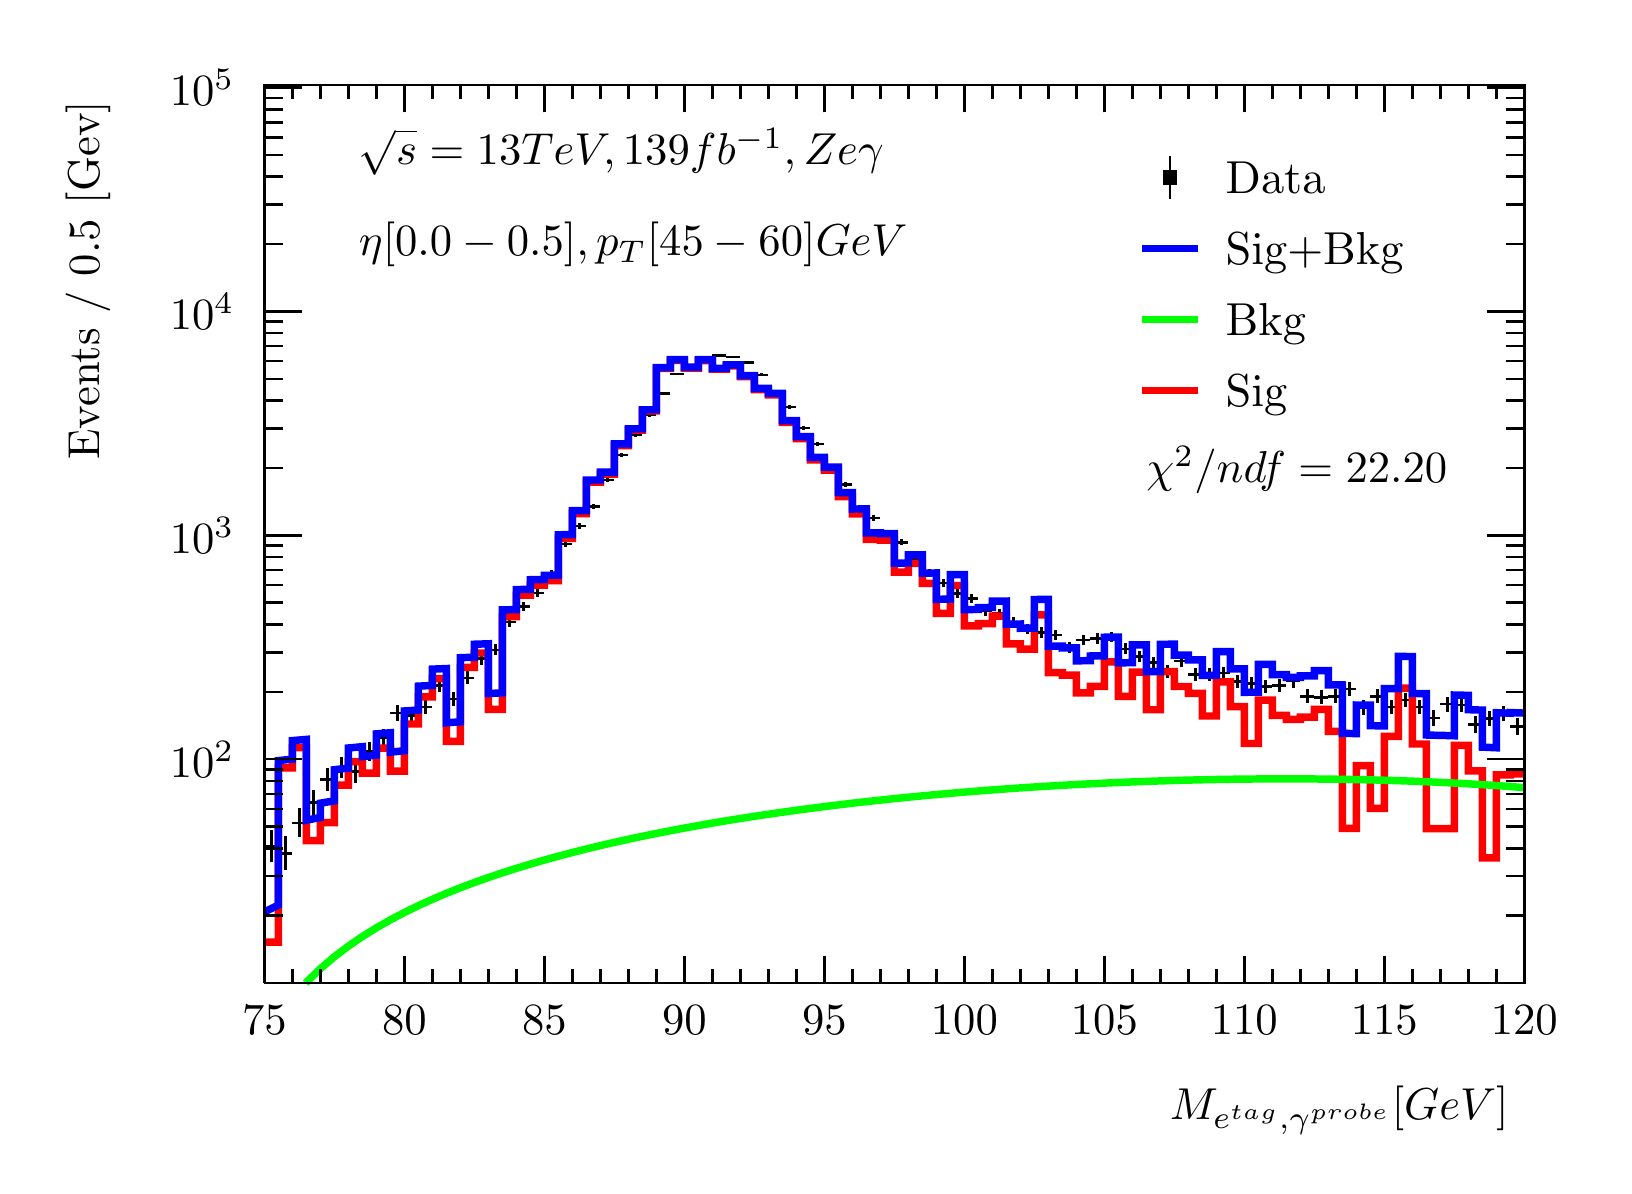
\begin{tikzpicture}
\pgfdeclareplotmark{cross} {
\pgfpathmoveto{\pgfpoint{-0.3\pgfplotmarksize}{\pgfplotmarksize}}
\pgfpathlineto{\pgfpoint{+0.3\pgfplotmarksize}{\pgfplotmarksize}}
\pgfpathlineto{\pgfpoint{+0.3\pgfplotmarksize}{0.3\pgfplotmarksize}}
\pgfpathlineto{\pgfpoint{+1\pgfplotmarksize}{0.3\pgfplotmarksize}}
\pgfpathlineto{\pgfpoint{+1\pgfplotmarksize}{-0.3\pgfplotmarksize}}
\pgfpathlineto{\pgfpoint{+0.3\pgfplotmarksize}{-0.3\pgfplotmarksize}}
\pgfpathlineto{\pgfpoint{+0.3\pgfplotmarksize}{-1.\pgfplotmarksize}}
\pgfpathlineto{\pgfpoint{-0.3\pgfplotmarksize}{-1.\pgfplotmarksize}}
\pgfpathlineto{\pgfpoint{-0.3\pgfplotmarksize}{-0.3\pgfplotmarksize}}
\pgfpathlineto{\pgfpoint{-1.\pgfplotmarksize}{-0.3\pgfplotmarksize}}
\pgfpathlineto{\pgfpoint{-1.\pgfplotmarksize}{0.3\pgfplotmarksize}}
\pgfpathlineto{\pgfpoint{-0.3\pgfplotmarksize}{0.3\pgfplotmarksize}}
\pgfpathclose
\pgfusepathqstroke
}
\pgfdeclareplotmark{cross*} {
\pgfpathmoveto{\pgfpoint{-0.3\pgfplotmarksize}{\pgfplotmarksize}}
\pgfpathlineto{\pgfpoint{+0.3\pgfplotmarksize}{\pgfplotmarksize}}
\pgfpathlineto{\pgfpoint{+0.3\pgfplotmarksize}{0.3\pgfplotmarksize}}
\pgfpathlineto{\pgfpoint{+1\pgfplotmarksize}{0.3\pgfplotmarksize}}
\pgfpathlineto{\pgfpoint{+1\pgfplotmarksize}{-0.3\pgfplotmarksize}}
\pgfpathlineto{\pgfpoint{+0.3\pgfplotmarksize}{-0.3\pgfplotmarksize}}
\pgfpathlineto{\pgfpoint{+0.3\pgfplotmarksize}{-1.\pgfplotmarksize}}
\pgfpathlineto{\pgfpoint{-0.3\pgfplotmarksize}{-1.\pgfplotmarksize}}
\pgfpathlineto{\pgfpoint{-0.3\pgfplotmarksize}{-0.3\pgfplotmarksize}}
\pgfpathlineto{\pgfpoint{-1.\pgfplotmarksize}{-0.3\pgfplotmarksize}}
\pgfpathlineto{\pgfpoint{-1.\pgfplotmarksize}{0.3\pgfplotmarksize}}
\pgfpathlineto{\pgfpoint{-0.3\pgfplotmarksize}{0.3\pgfplotmarksize}}
\pgfpathclose
\pgfusepathqfillstroke
}
\pgfdeclareplotmark{newstar} {
\pgfpathmoveto{\pgfqpoint{0pt}{\pgfplotmarksize}}
\pgfpathlineto{\pgfqpointpolar{44}{0.5\pgfplotmarksize}}
\pgfpathlineto{\pgfqpointpolar{18}{\pgfplotmarksize}}
\pgfpathlineto{\pgfqpointpolar{-20}{0.5\pgfplotmarksize}}
\pgfpathlineto{\pgfqpointpolar{-54}{\pgfplotmarksize}}
\pgfpathlineto{\pgfqpointpolar{-90}{0.5\pgfplotmarksize}}
\pgfpathlineto{\pgfqpointpolar{234}{\pgfplotmarksize}}
\pgfpathlineto{\pgfqpointpolar{198}{0.5\pgfplotmarksize}}
\pgfpathlineto{\pgfqpointpolar{162}{\pgfplotmarksize}}
\pgfpathlineto{\pgfqpointpolar{134}{0.5\pgfplotmarksize}}
\pgfpathclose
\pgfusepathqstroke
}
\pgfdeclareplotmark{newstar*} {
\pgfpathmoveto{\pgfqpoint{0pt}{\pgfplotmarksize}}
\pgfpathlineto{\pgfqpointpolar{44}{0.5\pgfplotmarksize}}
\pgfpathlineto{\pgfqpointpolar{18}{\pgfplotmarksize}}
\pgfpathlineto{\pgfqpointpolar{-20}{0.5\pgfplotmarksize}}
\pgfpathlineto{\pgfqpointpolar{-54}{\pgfplotmarksize}}
\pgfpathlineto{\pgfqpointpolar{-90}{0.5\pgfplotmarksize}}
\pgfpathlineto{\pgfqpointpolar{234}{\pgfplotmarksize}}
\pgfpathlineto{\pgfqpointpolar{198}{0.5\pgfplotmarksize}}
\pgfpathlineto{\pgfqpointpolar{162}{\pgfplotmarksize}}
\pgfpathlineto{\pgfqpointpolar{134}{0.5\pgfplotmarksize}}
\pgfpathclose
\pgfusepathqfillstroke
}
\definecolor{c}{rgb}{1,1,1};
\draw [color=c, fill=c] (0,0) rectangle (20,14.4361);
\draw [color=c, fill=c] (3,2.30977) rectangle (19,13.7143);
\definecolor{c}{rgb}{0,0,0};
\draw [c,line width=0.9] (3,2.30977) -- (3,13.7143) -- (19,13.7143) -- (19,2.30977) -- (3,2.30977);
\definecolor{c}{rgb}{1,1,1};
\draw [color=c, fill=c] (3,2.30977) rectangle (19,13.7143);
\definecolor{c}{rgb}{0,0,0};
\draw [c,line width=0.9] (3,2.30977) -- (3,13.7143) -- (19,13.7143) -- (19,2.30977) -- (3,2.30977);
\draw [c,line width=0.9] (3,2.30977) -- (19,2.30977);
\draw [c,line width=0.9] (3,2.65624) -- (3,2.30977);
\draw [c,line width=0.9] (3.35556,2.48301) -- (3.35556,2.30977);
\draw [c,line width=0.9] (3.71111,2.48301) -- (3.71111,2.30977);
\draw [c,line width=0.9] (4.06667,2.48301) -- (4.06667,2.30977);
\draw [c,line width=0.9] (4.42222,2.48301) -- (4.42222,2.30977);
\draw [c,line width=0.9] (4.77778,2.65624) -- (4.77778,2.30977);
\draw [c,line width=0.9] (5.13333,2.48301) -- (5.13333,2.30977);
\draw [c,line width=0.9] (5.48889,2.48301) -- (5.48889,2.30977);
\draw [c,line width=0.9] (5.84444,2.48301) -- (5.84444,2.30977);
\draw [c,line width=0.9] (6.2,2.48301) -- (6.2,2.30977);
\draw [c,line width=0.9] (6.55556,2.65624) -- (6.55556,2.30977);
\draw [c,line width=0.9] (6.91111,2.48301) -- (6.91111,2.30977);
\draw [c,line width=0.9] (7.26667,2.48301) -- (7.26667,2.30977);
\draw [c,line width=0.9] (7.62222,2.48301) -- (7.62222,2.30977);
\draw [c,line width=0.9] (7.97778,2.48301) -- (7.97778,2.30977);
\draw [c,line width=0.9] (8.33333,2.65624) -- (8.33333,2.30977);
\draw [c,line width=0.9] (8.68889,2.48301) -- (8.68889,2.30977);
\draw [c,line width=0.9] (9.04444,2.48301) -- (9.04444,2.30977);
\draw [c,line width=0.9] (9.4,2.48301) -- (9.4,2.30977);
\draw [c,line width=0.9] (9.75556,2.48301) -- (9.75556,2.30977);
\draw [c,line width=0.9] (10.1111,2.65624) -- (10.1111,2.30977);
\draw [c,line width=0.9] (10.4667,2.48301) -- (10.4667,2.30977);
\draw [c,line width=0.9] (10.8222,2.48301) -- (10.8222,2.30977);
\draw [c,line width=0.9] (11.1778,2.48301) -- (11.1778,2.30977);
\draw [c,line width=0.9] (11.5333,2.48301) -- (11.5333,2.30977);
\draw [c,line width=0.9] (11.8889,2.65624) -- (11.8889,2.30977);
\draw [c,line width=0.9] (12.2444,2.48301) -- (12.2444,2.30977);
\draw [c,line width=0.9] (12.6,2.48301) -- (12.6,2.30977);
\draw [c,line width=0.9] (12.9556,2.48301) -- (12.9556,2.30977);
\draw [c,line width=0.9] (13.3111,2.48301) -- (13.3111,2.30977);
\draw [c,line width=0.9] (13.6667,2.65624) -- (13.6667,2.30977);
\draw [c,line width=0.9] (14.0222,2.48301) -- (14.0222,2.30977);
\draw [c,line width=0.9] (14.3778,2.48301) -- (14.3778,2.30977);
\draw [c,line width=0.9] (14.7333,2.48301) -- (14.7333,2.30977);
\draw [c,line width=0.9] (15.0889,2.48301) -- (15.0889,2.30977);
\draw [c,line width=0.9] (15.4444,2.65624) -- (15.4444,2.30977);
\draw [c,line width=0.9] (15.8,2.48301) -- (15.8,2.30977);
\draw [c,line width=0.9] (16.1556,2.48301) -- (16.1556,2.30977);
\draw [c,line width=0.9] (16.5111,2.48301) -- (16.5111,2.30977);
\draw [c,line width=0.9] (16.8667,2.48301) -- (16.8667,2.30977);
\draw [c,line width=0.9] (17.2222,2.65624) -- (17.2222,2.30977);
\draw [c,line width=0.9] (17.5778,2.48301) -- (17.5778,2.30977);
\draw [c,line width=0.9] (17.9333,2.48301) -- (17.9333,2.30977);
\draw [c,line width=0.9] (18.2889,2.48301) -- (18.2889,2.30977);
\draw [c,line width=0.9] (18.6444,2.48301) -- (18.6444,2.30977);
\draw [c,line width=0.9] (19,2.65624) -- (19,2.30977);
\draw [c,line width=0.9] (19,2.65624) -- (19,2.30977);
\draw [anchor=base] (3,1.66015) node[scale=1.61424, color=c, rotate=0]{75};
\draw [anchor=base] (4.77778,1.66015) node[scale=1.61424, color=c, rotate=0]{80};
\draw [anchor=base] (6.55556,1.66015) node[scale=1.61424, color=c, rotate=0]{85};
\draw [anchor=base] (8.33333,1.66015) node[scale=1.61424, color=c, rotate=0]{90};
\draw [anchor=base] (10.1111,1.66015) node[scale=1.61424, color=c, rotate=0]{95};
\draw [anchor=base] (11.8889,1.66015) node[scale=1.61424, color=c, rotate=0]{100};
\draw [anchor=base] (13.6667,1.66015) node[scale=1.61424, color=c, rotate=0]{105};
\draw [anchor=base] (15.4444,1.66015) node[scale=1.61424, color=c, rotate=0]{110};
\draw [anchor=base] (17.2222,1.66015) node[scale=1.61424, color=c, rotate=0]{115};
\draw [anchor=base] (19,1.66015) node[scale=1.61424, color=c, rotate=0]{120};
\draw [anchor= east] (19,0.692932) node[scale=1.61424, color=c, rotate=0]{$M_{e^{tag}, \gamma^{probe}}  [GeV]$};
\draw [c,line width=0.9] (3,13.7143) -- (19,13.7143);
\draw [c,line width=0.9] (3,13.3678) -- (3,13.7143);
\draw [c,line width=0.9] (3.35556,13.5411) -- (3.35556,13.7143);
\draw [c,line width=0.9] (3.71111,13.5411) -- (3.71111,13.7143);
\draw [c,line width=0.9] (4.06667,13.5411) -- (4.06667,13.7143);
\draw [c,line width=0.9] (4.42222,13.5411) -- (4.42222,13.7143);
\draw [c,line width=0.9] (4.77778,13.3678) -- (4.77778,13.7143);
\draw [c,line width=0.9] (5.13333,13.5411) -- (5.13333,13.7143);
\draw [c,line width=0.9] (5.48889,13.5411) -- (5.48889,13.7143);
\draw [c,line width=0.9] (5.84444,13.5411) -- (5.84444,13.7143);
\draw [c,line width=0.9] (6.2,13.5411) -- (6.2,13.7143);
\draw [c,line width=0.9] (6.55556,13.3678) -- (6.55556,13.7143);
\draw [c,line width=0.9] (6.91111,13.5411) -- (6.91111,13.7143);
\draw [c,line width=0.9] (7.26667,13.5411) -- (7.26667,13.7143);
\draw [c,line width=0.9] (7.62222,13.5411) -- (7.62222,13.7143);
\draw [c,line width=0.9] (7.97778,13.5411) -- (7.97778,13.7143);
\draw [c,line width=0.9] (8.33333,13.3678) -- (8.33333,13.7143);
\draw [c,line width=0.9] (8.68889,13.5411) -- (8.68889,13.7143);
\draw [c,line width=0.9] (9.04444,13.5411) -- (9.04444,13.7143);
\draw [c,line width=0.9] (9.4,13.5411) -- (9.4,13.7143);
\draw [c,line width=0.9] (9.75556,13.5411) -- (9.75556,13.7143);
\draw [c,line width=0.9] (10.1111,13.3678) -- (10.1111,13.7143);
\draw [c,line width=0.9] (10.4667,13.5411) -- (10.4667,13.7143);
\draw [c,line width=0.9] (10.8222,13.5411) -- (10.8222,13.7143);
\draw [c,line width=0.9] (11.1778,13.5411) -- (11.1778,13.7143);
\draw [c,line width=0.9] (11.5333,13.5411) -- (11.5333,13.7143);
\draw [c,line width=0.9] (11.8889,13.3678) -- (11.8889,13.7143);
\draw [c,line width=0.9] (12.2444,13.5411) -- (12.2444,13.7143);
\draw [c,line width=0.9] (12.6,13.5411) -- (12.6,13.7143);
\draw [c,line width=0.9] (12.9556,13.5411) -- (12.9556,13.7143);
\draw [c,line width=0.9] (13.3111,13.5411) -- (13.3111,13.7143);
\draw [c,line width=0.9] (13.6667,13.3678) -- (13.6667,13.7143);
\draw [c,line width=0.9] (14.0222,13.5411) -- (14.0222,13.7143);
\draw [c,line width=0.9] (14.3778,13.5411) -- (14.3778,13.7143);
\draw [c,line width=0.9] (14.7333,13.5411) -- (14.7333,13.7143);
\draw [c,line width=0.9] (15.0889,13.5411) -- (15.0889,13.7143);
\draw [c,line width=0.9] (15.4444,13.3678) -- (15.4444,13.7143);
\draw [c,line width=0.9] (15.8,13.5411) -- (15.8,13.7143);
\draw [c,line width=0.9] (16.1556,13.5411) -- (16.1556,13.7143);
\draw [c,line width=0.9] (16.5111,13.5411) -- (16.5111,13.7143);
\draw [c,line width=0.9] (16.8667,13.5411) -- (16.8667,13.7143);
\draw [c,line width=0.9] (17.2222,13.3678) -- (17.2222,13.7143);
\draw [c,line width=0.9] (17.5778,13.5411) -- (17.5778,13.7143);
\draw [c,line width=0.9] (17.9333,13.5411) -- (17.9333,13.7143);
\draw [c,line width=0.9] (18.2889,13.5411) -- (18.2889,13.7143);
\draw [c,line width=0.9] (18.6444,13.5411) -- (18.6444,13.7143);
\draw [c,line width=0.9] (19,13.3678) -- (19,13.7143);
\draw [c,line width=0.9] (19,13.3678) -- (19,13.7143);
\draw [c,line width=0.9] (3,2.30977) -- (3,13.7143);
\draw [c,line width=0.9] (3.237,3.16561) -- (3,3.16561);
\draw [c,line width=0.9] (3.237,3.66625) -- (3,3.66625);
\draw [c,line width=0.9] (3.237,4.02146) -- (3,4.02146);
\draw [c,line width=0.9] (3.237,4.29698) -- (3,4.29698);
\draw [c,line width=0.9] (3.237,4.52209) -- (3,4.52209);
\draw [c,line width=0.9] (3.237,4.71242) -- (3,4.71242);
\draw [c,line width=0.9] (3.237,4.8773) -- (3,4.8773);
\draw [c,line width=0.9] (3.237,5.02273) -- (3,5.02273);
\draw [c,line width=0.9] (3.474,5.15282) -- (3,5.15282);
\draw [anchor= east] (2.82,5.15282) node[scale=1.61424, color=c, rotate=0]{$10^{2}$};
\draw [c,line width=0.9] (3.237,6.00866) -- (3,6.00866);
\draw [c,line width=0.9] (3.237,6.5093) -- (3,6.5093);
\draw [c,line width=0.9] (3.237,6.8645) -- (3,6.8645);
\draw [c,line width=0.9] (3.237,7.14002) -- (3,7.14002);
\draw [c,line width=0.9] (3.237,7.36514) -- (3,7.36514);
\draw [c,line width=0.9] (3.237,7.55547) -- (3,7.55547);
\draw [c,line width=0.9] (3.237,7.72034) -- (3,7.72034);
\draw [c,line width=0.9] (3.237,7.86577) -- (3,7.86577);
\draw [c,line width=0.9] (3.474,7.99586) -- (3,7.99586);
\draw [anchor= east] (2.82,7.99586) node[scale=1.61424, color=c, rotate=0]{$10^{3}$};
\draw [c,line width=0.9] (3.237,8.85171) -- (3,8.85171);
\draw [c,line width=0.9] (3.237,9.35234) -- (3,9.35234);
\draw [c,line width=0.9] (3.237,9.70755) -- (3,9.70755);
\draw [c,line width=0.9] (3.237,9.98307) -- (3,9.98307);
\draw [c,line width=0.9] (3.237,10.2082) -- (3,10.2082);
\draw [c,line width=0.9] (3.237,10.3985) -- (3,10.3985);
\draw [c,line width=0.9] (3.237,10.5634) -- (3,10.5634);
\draw [c,line width=0.9] (3.237,10.7088) -- (3,10.7088);
\draw [c,line width=0.9] (3.474,10.8389) -- (3,10.8389);
\draw [anchor= east] (2.82,10.8389) node[scale=1.61424, color=c, rotate=0]{$10^{4}$};
\draw [c,line width=0.9] (3.237,11.6948) -- (3,11.6948);
\draw [c,line width=0.9] (3.237,12.1954) -- (3,12.1954);
\draw [c,line width=0.9] (3.237,12.5506) -- (3,12.5506);
\draw [c,line width=0.9] (3.237,12.8261) -- (3,12.8261);
\draw [c,line width=0.9] (3.237,13.0512) -- (3,13.0512);
\draw [c,line width=0.9] (3.237,13.2416) -- (3,13.2416);
\draw [c,line width=0.9] (3.237,13.4064) -- (3,13.4064);
\draw [c,line width=0.9] (3.237,13.5519) -- (3,13.5519);
\draw [c,line width=0.9] (3.474,13.682) -- (3,13.682);
\draw [anchor= east] (2.82,13.682) node[scale=1.61424, color=c, rotate=0]{$10^{5}$};
\draw [anchor= east] (0.76,13.7143) node[scale=1.61424, color=c, rotate=90]{Events / 0.5 [Gev]};
\draw [c,line width=0.9] (19,2.30977) -- (19,13.7143);
\draw [c,line width=0.9] (18.763,3.16561) -- (19,3.16561);
\draw [c,line width=0.9] (18.763,3.66625) -- (19,3.66625);
\draw [c,line width=0.9] (18.763,4.02146) -- (19,4.02146);
\draw [c,line width=0.9] (18.763,4.29698) -- (19,4.29698);
\draw [c,line width=0.9] (18.763,4.52209) -- (19,4.52209);
\draw [c,line width=0.9] (18.763,4.71242) -- (19,4.71242);
\draw [c,line width=0.9] (18.763,4.8773) -- (19,4.8773);
\draw [c,line width=0.9] (18.763,5.02273) -- (19,5.02273);
\draw [c,line width=0.9] (18.526,5.15282) -- (19,5.15282);
\draw [c,line width=0.9] (18.763,6.00866) -- (19,6.00866);
\draw [c,line width=0.9] (18.763,6.5093) -- (19,6.5093);
\draw [c,line width=0.9] (18.763,6.8645) -- (19,6.8645);
\draw [c,line width=0.9] (18.763,7.14002) -- (19,7.14002);
\draw [c,line width=0.9] (18.763,7.36514) -- (19,7.36514);
\draw [c,line width=0.9] (18.763,7.55547) -- (19,7.55547);
\draw [c,line width=0.9] (18.763,7.72034) -- (19,7.72034);
\draw [c,line width=0.9] (18.763,7.86577) -- (19,7.86577);
\draw [c,line width=0.9] (18.526,7.99586) -- (19,7.99586);
\draw [c,line width=0.9] (18.763,8.85171) -- (19,8.85171);
\draw [c,line width=0.9] (18.763,9.35234) -- (19,9.35234);
\draw [c,line width=0.9] (18.763,9.70755) -- (19,9.70755);
\draw [c,line width=0.9] (18.763,9.98307) -- (19,9.98307);
\draw [c,line width=0.9] (18.763,10.2082) -- (19,10.2082);
\draw [c,line width=0.9] (18.763,10.3985) -- (19,10.3985);
\draw [c,line width=0.9] (18.763,10.5634) -- (19,10.5634);
\draw [c,line width=0.9] (18.763,10.7088) -- (19,10.7088);
\draw [c,line width=0.9] (18.526,10.8389) -- (19,10.8389);
\draw [c,line width=0.9] (18.763,11.6948) -- (19,11.6948);
\draw [c,line width=0.9] (18.763,12.1954) -- (19,12.1954);
\draw [c,line width=0.9] (18.763,12.5506) -- (19,12.5506);
\draw [c,line width=0.9] (18.763,12.8261) -- (19,12.8261);
\draw [c,line width=0.9] (18.763,13.0512) -- (19,13.0512);
\draw [c,line width=0.9] (18.763,13.2416) -- (19,13.2416);
\draw [c,line width=0.9] (18.763,13.4064) -- (19,13.4064);
\draw [c,line width=0.9] (18.763,13.5519) -- (19,13.5519);
\draw [c,line width=0.9] (18.526,13.682) -- (19,13.682);
\draw [c,line width=0.9] (3.08889,4.05195) -- (3,4.05195);
\draw [c,line width=0.9] (3,4.05195) -- (3,4.05195);
\draw [c,line width=0.9] (3.08889,4.05195) -- (3.17778,4.05195);
\draw [c,line width=0.9] (3.17778,4.05195) -- (3.17778,4.05195);
\draw [c,line width=0.9] (3.08889,4.05195) -- (3.08889,4.25823);
\draw [c,line width=0.9] (3.08889,4.25823) -- (3.08889,4.25823);
\draw [c,line width=0.9] (3.08889,4.05195) -- (3.08889,3.84322);
\draw [c,line width=0.9] (3.08889,3.84322) -- (3.08889,3.84322);
\draw [c,line width=0.9] (3.26667,3.95813) -- (3.17778,3.95813);
\draw [c,line width=0.9] (3.17778,3.95813) -- (3.17778,3.95813);
\draw [c,line width=0.9] (3.26667,3.95813) -- (3.35556,3.95813);
\draw [c,line width=0.9] (3.35556,3.95813) -- (3.35556,3.95813);
\draw [c,line width=0.9] (3.26667,3.95813) -- (3.26667,4.17287);
\draw [c,line width=0.9] (3.26667,4.17287) -- (3.26667,4.17287);
\draw [c,line width=0.9] (3.26667,3.95813) -- (3.26667,3.74063);
\draw [c,line width=0.9] (3.26667,3.74063) -- (3.26667,3.74063);
\draw [c,line width=0.9] (3.44444,4.3454) -- (3.35556,4.3454);
\draw [c,line width=0.9] (3.35556,4.3454) -- (3.35556,4.3454);
\draw [c,line width=0.9] (3.44444,4.3454) -- (3.53333,4.3454);
\draw [c,line width=0.9] (3.53333,4.3454) -- (3.53333,4.3454);
\draw [c,line width=0.9] (3.44444,4.3454) -- (3.44444,4.52738);
\draw [c,line width=0.9] (3.44444,4.52738) -- (3.44444,4.52738);
\draw [c,line width=0.9] (3.44444,4.3454) -- (3.44444,4.16172);
\draw [c,line width=0.9] (3.44444,4.16172) -- (3.44444,4.16172);
\draw [c,line width=0.9] (3.62222,4.60178) -- (3.53333,4.60178);
\draw [c,line width=0.9] (3.53333,4.60178) -- (3.53333,4.60178);
\draw [c,line width=0.9] (3.62222,4.60178) -- (3.71111,4.60178);
\draw [c,line width=0.9] (3.71111,4.60178) -- (3.71111,4.60178);
\draw [c,line width=0.9] (3.62222,4.60178) -- (3.62222,4.76495);
\draw [c,line width=0.9] (3.62222,4.76495) -- (3.62222,4.76495);
\draw [c,line width=0.9] (3.62222,4.60178) -- (3.62222,4.43737);
\draw [c,line width=0.9] (3.62222,4.43737) -- (3.62222,4.43737);
\draw [c,line width=0.9] (3.8,4.89264) -- (3.71111,4.89264);
\draw [c,line width=0.9] (3.71111,4.89264) -- (3.71111,4.89264);
\draw [c,line width=0.9] (3.8,4.89264) -- (3.88889,4.89264);
\draw [c,line width=0.9] (3.88889,4.89264) -- (3.88889,4.89264);
\draw [c,line width=0.9] (3.8,4.89264) -- (3.8,5.03688);
\draw [c,line width=0.9] (3.8,5.03688) -- (3.8,5.03688);
\draw [c,line width=0.9] (3.8,4.89264) -- (3.8,4.74753);
\draw [c,line width=0.9] (3.8,4.74753) -- (3.8,4.74753);
\draw [c,line width=0.9] (3.97778,5.04987) -- (3.88889,5.04987);
\draw [c,line width=0.9] (3.88889,5.04987) -- (3.88889,5.04987);
\draw [c,line width=0.9] (3.97778,5.04987) -- (4.06667,5.04987);
\draw [c,line width=0.9] (4.06667,5.04987) -- (4.06667,5.04987);
\draw [c,line width=0.9] (3.97778,5.04987) -- (3.97778,5.18483);
\draw [c,line width=0.9] (3.97778,5.18483) -- (3.97778,5.18483);
\draw [c,line width=0.9] (3.97778,5.04987) -- (3.97778,4.91418);
\draw [c,line width=0.9] (3.97778,4.91418) -- (3.97778,4.91418);
\draw [c,line width=0.9] (4.15556,4.99498) -- (4.06667,4.99498);
\draw [c,line width=0.9] (4.06667,4.99498) -- (4.06667,4.99498);
\draw [c,line width=0.9] (4.15556,4.99498) -- (4.24444,4.99498);
\draw [c,line width=0.9] (4.24444,4.99498) -- (4.24444,4.99498);
\draw [c,line width=0.9] (4.15556,4.99498) -- (4.15556,5.13311);
\draw [c,line width=0.9] (4.15556,5.13311) -- (4.15556,5.13311);
\draw [c,line width=0.9] (4.15556,4.99498) -- (4.15556,4.85608);
\draw [c,line width=0.9] (4.15556,4.85608) -- (4.15556,4.85608);
\draw [c,line width=0.9] (4.33333,5.24785) -- (4.24444,5.24785);
\draw [c,line width=0.9] (4.24444,5.24785) -- (4.24444,5.24785);
\draw [c,line width=0.9] (4.33333,5.24785) -- (4.42222,5.24785);
\draw [c,line width=0.9] (4.42222,5.24785) -- (4.42222,5.24785);
\draw [c,line width=0.9] (4.33333,5.24785) -- (4.33333,5.36661);
\draw [c,line width=0.9] (4.33333,5.36661) -- (4.33333,5.36661);
\draw [c,line width=0.9] (4.33333,5.24785) -- (4.33333,5.12908);
\draw [c,line width=0.9] (4.33333,5.12908) -- (4.33333,5.12908);
\draw [c,line width=0.9] (4.51111,5.42834) -- (4.42222,5.42834);
\draw [c,line width=0.9] (4.42222,5.42834) -- (4.42222,5.42834);
\draw [c,line width=0.9] (4.51111,5.42834) -- (4.6,5.42834);
\draw [c,line width=0.9] (4.6,5.42834) -- (4.6,5.42834);
\draw [c,line width=0.9] (4.51111,5.42834) -- (4.51111,5.53874);
\draw [c,line width=0.9] (4.51111,5.53874) -- (4.51111,5.53874);
\draw [c,line width=0.9] (4.51111,5.42834) -- (4.51111,5.31794);
\draw [c,line width=0.9] (4.51111,5.31794) -- (4.51111,5.31794);
\draw [c,line width=0.9] (4.68889,5.74084) -- (4.6,5.74084);
\draw [c,line width=0.9] (4.6,5.74084) -- (4.6,5.74084);
\draw [c,line width=0.9] (4.68889,5.74084) -- (4.77778,5.74084);
\draw [c,line width=0.9] (4.77778,5.74084) -- (4.77778,5.74084);
\draw [c,line width=0.9] (4.68889,5.74084) -- (4.68889,5.83812);
\draw [c,line width=0.9] (4.68889,5.83812) -- (4.68889,5.83812);
\draw [c,line width=0.9] (4.68889,5.74084) -- (4.68889,5.64355);
\draw [c,line width=0.9] (4.68889,5.64355) -- (4.68889,5.64355);
\draw [c,line width=0.9] (4.86667,5.70977) -- (4.77778,5.70977);
\draw [c,line width=0.9] (4.77778,5.70977) -- (4.77778,5.70977);
\draw [c,line width=0.9] (4.86667,5.70977) -- (4.95556,5.70977);
\draw [c,line width=0.9] (4.95556,5.70977) -- (4.95556,5.70977);
\draw [c,line width=0.9] (4.86667,5.70977) -- (4.86667,5.80829);
\draw [c,line width=0.9] (4.86667,5.80829) -- (4.86667,5.80829);
\draw [c,line width=0.9] (4.86667,5.70977) -- (4.86667,5.61126);
\draw [c,line width=0.9] (4.86667,5.61126) -- (4.86667,5.61126);
\draw [c,line width=0.9] (5.04444,5.81524) -- (4.95556,5.81524);
\draw [c,line width=0.9] (4.95556,5.81524) -- (4.95556,5.81524);
\draw [c,line width=0.9] (5.04444,5.81524) -- (5.13333,5.81524);
\draw [c,line width=0.9] (5.13333,5.81524) -- (5.13333,5.81524);
\draw [c,line width=0.9] (5.04444,5.81524) -- (5.04444,5.90964);
\draw [c,line width=0.9] (5.04444,5.90964) -- (5.04444,5.90964);
\draw [c,line width=0.9] (5.04444,5.81524) -- (5.04444,5.72084);
\draw [c,line width=0.9] (5.04444,5.72084) -- (5.04444,5.72084);
\draw [c,line width=0.9] (5.22222,6.08642) -- (5.13333,6.08642);
\draw [c,line width=0.9] (5.13333,6.08642) -- (5.13333,6.08642);
\draw [c,line width=0.9] (5.22222,6.08642) -- (5.31111,6.08642);
\draw [c,line width=0.9] (5.31111,6.08642) -- (5.31111,6.08642);
\draw [c,line width=0.9] (5.22222,6.08642) -- (5.22222,6.171);
\draw [c,line width=0.9] (5.22222,6.171) -- (5.22222,6.171);
\draw [c,line width=0.9] (5.22222,6.08642) -- (5.22222,6.00183);
\draw [c,line width=0.9] (5.22222,6.00183) -- (5.22222,6.00183);
\draw [c,line width=0.9] (5.4,5.91906) -- (5.31111,5.91906);
\draw [c,line width=0.9] (5.31111,5.91906) -- (5.31111,5.91906);
\draw [c,line width=0.9] (5.4,5.91906) -- (5.48889,5.91906);
\draw [c,line width=0.9] (5.48889,5.91906) -- (5.48889,5.91906);
\draw [c,line width=0.9] (5.4,5.91906) -- (5.4,6.00957);
\draw [c,line width=0.9] (5.4,6.00957) -- (5.4,6.00957);
\draw [c,line width=0.9] (5.4,5.91906) -- (5.4,5.82854);
\draw [c,line width=0.9] (5.4,5.82854) -- (5.4,5.82854);
\draw [c,line width=0.9] (5.57778,6.18658) -- (5.48889,6.18658);
\draw [c,line width=0.9] (5.48889,6.18658) -- (5.48889,6.18658);
\draw [c,line width=0.9] (5.57778,6.18658) -- (5.66667,6.18658);
\draw [c,line width=0.9] (5.66667,6.18658) -- (5.66667,6.18658);
\draw [c,line width=0.9] (5.57778,6.18658) -- (5.57778,6.26781);
\draw [c,line width=0.9] (5.57778,6.26781) -- (5.57778,6.26781);
\draw [c,line width=0.9] (5.57778,6.18658) -- (5.57778,6.10536);
\draw [c,line width=0.9] (5.57778,6.10536) -- (5.57778,6.10536);
\draw [c,line width=0.9] (5.75556,6.42851) -- (5.66667,6.42851);
\draw [c,line width=0.9] (5.66667,6.42851) -- (5.66667,6.42851);
\draw [c,line width=0.9] (5.75556,6.42851) -- (5.84444,6.42851);
\draw [c,line width=0.9] (5.84444,6.42851) -- (5.84444,6.42851);
\draw [c,line width=0.9] (5.75556,6.42851) -- (5.75556,6.50216);
\draw [c,line width=0.9] (5.75556,6.50216) -- (5.75556,6.50216);
\draw [c,line width=0.9] (5.75556,6.42851) -- (5.75556,6.35487);
\draw [c,line width=0.9] (5.75556,6.35487) -- (5.75556,6.35487);
\draw [c,line width=0.9] (5.93333,6.54179) -- (5.84444,6.54179);
\draw [c,line width=0.9] (5.84444,6.54179) -- (5.84444,6.54179);
\draw [c,line width=0.9] (5.93333,6.54179) -- (6.02222,6.54179);
\draw [c,line width=0.9] (6.02222,6.54179) -- (6.02222,6.54179);
\draw [c,line width=0.9] (5.93333,6.54179) -- (5.93333,6.61214);
\draw [c,line width=0.9] (5.93333,6.61214) -- (5.93333,6.61214);
\draw [c,line width=0.9] (5.93333,6.54179) -- (5.93333,6.47145);
\draw [c,line width=0.9] (5.93333,6.47145) -- (5.93333,6.47145);
\draw [c,line width=0.9] (6.11111,6.89198) -- (6.02222,6.89198);
\draw [c,line width=0.9] (6.02222,6.89198) -- (6.02222,6.89198);
\draw [c,line width=0.9] (6.11111,6.89198) -- (6.2,6.89198);
\draw [c,line width=0.9] (6.2,6.89198) -- (6.2,6.89198);
\draw [c,line width=0.9] (6.11111,6.89198) -- (6.11111,6.95302);
\draw [c,line width=0.9] (6.11111,6.95302) -- (6.11111,6.95302);
\draw [c,line width=0.9] (6.11111,6.89198) -- (6.11111,6.83093);
\draw [c,line width=0.9] (6.11111,6.83093) -- (6.11111,6.83093);
\draw [c,line width=0.9] (6.28889,7.09475) -- (6.2,7.09475);
\draw [c,line width=0.9] (6.2,7.09475) -- (6.2,7.09475);
\draw [c,line width=0.9] (6.28889,7.09475) -- (6.37778,7.09475);
\draw [c,line width=0.9] (6.37778,7.09475) -- (6.37778,7.09475);
\draw [c,line width=0.9] (6.28889,7.09475) -- (6.28889,7.15099);
\draw [c,line width=0.9] (6.28889,7.15099) -- (6.28889,7.15099);
\draw [c,line width=0.9] (6.28889,7.09475) -- (6.28889,7.03852);
\draw [c,line width=0.9] (6.28889,7.03852) -- (6.28889,7.03852);
\draw [c,line width=0.9] (6.46667,7.26442) -- (6.37778,7.26442);
\draw [c,line width=0.9] (6.37778,7.26442) -- (6.37778,7.26442);
\draw [c,line width=0.9] (6.46667,7.26442) -- (6.55556,7.26442);
\draw [c,line width=0.9] (6.55556,7.26442) -- (6.55556,7.26442);
\draw [c,line width=0.9] (6.46667,7.26442) -- (6.46667,7.31692);
\draw [c,line width=0.9] (6.46667,7.31692) -- (6.46667,7.31692);
\draw [c,line width=0.9] (6.46667,7.26442) -- (6.46667,7.21192);
\draw [c,line width=0.9] (6.46667,7.21192) -- (6.46667,7.21192);
\draw [c,line width=0.9] (6.64444,7.50874) -- (6.55556,7.50874);
\draw [c,line width=0.9] (6.55556,7.50874) -- (6.55556,7.50874);
\draw [c,line width=0.9] (6.64444,7.50874) -- (6.73333,7.50874);
\draw [c,line width=0.9] (6.73333,7.50874) -- (6.73333,7.50874);
\draw [c,line width=0.9] (6.64444,7.50874) -- (6.64444,7.55629);
\draw [c,line width=0.9] (6.64444,7.55629) -- (6.64444,7.55629);
\draw [c,line width=0.9] (6.64444,7.50874) -- (6.64444,7.46118);
\draw [c,line width=0.9] (6.64444,7.46118) -- (6.64444,7.46118);
\draw [c,line width=0.9] (6.82222,7.88618) -- (6.73333,7.88618);
\draw [c,line width=0.9] (6.73333,7.88618) -- (6.73333,7.88618);
\draw [c,line width=0.9] (6.82222,7.88618) -- (6.91111,7.88618);
\draw [c,line width=0.9] (6.91111,7.88618) -- (6.91111,7.88618);
\draw [c,line width=0.9] (6.82222,7.88618) -- (6.82222,7.927);
\draw [c,line width=0.9] (6.82222,7.927) -- (6.82222,7.927);
\draw [c,line width=0.9] (6.82222,7.88618) -- (6.82222,7.84537);
\draw [c,line width=0.9] (6.82222,7.84537) -- (6.82222,7.84537);
\draw [c,line width=0.9] (7,8.11242) -- (6.91111,8.11242);
\draw [c,line width=0.9] (6.91111,8.11242) -- (6.91111,8.11242);
\draw [c,line width=0.9] (7,8.11242) -- (7.08889,8.11242);
\draw [c,line width=0.9] (7.08889,8.11242) -- (7.08889,8.11242);
\draw [c,line width=0.9] (7,8.11242) -- (7,8.14967);
\draw [c,line width=0.9] (7,8.14967) -- (7,8.14967);
\draw [c,line width=0.9] (7,8.11242) -- (7,8.07518);
\draw [c,line width=0.9] (7,8.07518) -- (7,8.07518);
\draw [c,line width=0.9] (7.17778,8.36183) -- (7.08889,8.36183);
\draw [c,line width=0.9] (7.08889,8.36183) -- (7.08889,8.36183);
\draw [c,line width=0.9] (7.17778,8.36183) -- (7.26667,8.36183);
\draw [c,line width=0.9] (7.26667,8.36183) -- (7.26667,8.36183);
\draw [c,line width=0.9] (7.17778,8.36183) -- (7.17778,8.39549);
\draw [c,line width=0.9] (7.17778,8.39549) -- (7.17778,8.39549);
\draw [c,line width=0.9] (7.17778,8.36183) -- (7.17778,8.32816);
\draw [c,line width=0.9] (7.17778,8.32816) -- (7.17778,8.32816);
\draw [c,line width=0.9] (7.35556,8.70156) -- (7.26667,8.70156);
\draw [c,line width=0.9] (7.26667,8.70156) -- (7.26667,8.70156);
\draw [c,line width=0.9] (7.35556,8.70156) -- (7.44444,8.70156);
\draw [c,line width=0.9] (7.44444,8.70156) -- (7.44444,8.70156);
\draw [c,line width=0.9] (7.35556,8.70156) -- (7.35556,8.7309);
\draw [c,line width=0.9] (7.35556,8.7309) -- (7.35556,8.7309);
\draw [c,line width=0.9] (7.35556,8.70156) -- (7.35556,8.67222);
\draw [c,line width=0.9] (7.35556,8.67222) -- (7.35556,8.67222);
\draw [c,line width=0.9] (7.53333,9.01511) -- (7.44444,9.01511);
\draw [c,line width=0.9] (7.44444,9.01511) -- (7.44444,9.01511);
\draw [c,line width=0.9] (7.53333,9.01511) -- (7.62222,9.01511);
\draw [c,line width=0.9] (7.62222,9.01511) -- (7.62222,9.01511);
\draw [c,line width=0.9] (7.53333,9.01511) -- (7.53333,9.04095);
\draw [c,line width=0.9] (7.53333,9.04095) -- (7.53333,9.04095);
\draw [c,line width=0.9] (7.53333,9.01511) -- (7.53333,8.98927);
\draw [c,line width=0.9] (7.53333,8.98927) -- (7.53333,8.98927);
\draw [c,line width=0.9] (7.71111,9.26848) -- (7.62222,9.26848);
\draw [c,line width=0.9] (7.62222,9.26848) -- (7.62222,9.26848);
\draw [c,line width=0.9] (7.71111,9.26848) -- (7.8,9.26848);
\draw [c,line width=0.9] (7.8,9.26848) -- (7.8,9.26848);
\draw [c,line width=0.9] (7.71111,9.26848) -- (7.71111,9.2918);
\draw [c,line width=0.9] (7.71111,9.2918) -- (7.71111,9.2918);
\draw [c,line width=0.9] (7.71111,9.26848) -- (7.71111,9.24516);
\draw [c,line width=0.9] (7.71111,9.24516) -- (7.71111,9.24516);
\draw [c,line width=0.9] (7.88889,9.52312) -- (7.8,9.52312);
\draw [c,line width=0.9] (7.8,9.52312) -- (7.8,9.52312);
\draw [c,line width=0.9] (7.88889,9.52312) -- (7.97778,9.52312);
\draw [c,line width=0.9] (7.97778,9.52312) -- (7.97778,9.52312);
\draw [c,line width=0.9] (7.88889,9.52312) -- (7.88889,9.54416);
\draw [c,line width=0.9] (7.88889,9.54416) -- (7.88889,9.54416);
\draw [c,line width=0.9] (7.88889,9.52312) -- (7.88889,9.50208);
\draw [c,line width=0.9] (7.88889,9.50208) -- (7.88889,9.50208);
\draw [c,line width=0.9] (8.06667,9.79426) -- (7.97778,9.79426);
\draw [c,line width=0.9] (7.97778,9.79426) -- (7.97778,9.79426);
\draw [c,line width=0.9] (8.06667,9.79426) -- (8.15556,9.79426);
\draw [c,line width=0.9] (8.15556,9.79426) -- (8.15556,9.79426);
\draw [c,line width=0.9] (8.06667,9.79426) -- (8.06667,9.81311);
\draw [c,line width=0.9] (8.06667,9.81311) -- (8.06667,9.81311);
\draw [c,line width=0.9] (8.06667,9.79426) -- (8.06667,9.77541);
\draw [c,line width=0.9] (8.06667,9.77541) -- (8.06667,9.77541);
\draw [c,line width=0.9] (8.24444,10.0452) -- (8.15556,10.0452);
\draw [c,line width=0.9] (8.15556,10.0452) -- (8.15556,10.0452);
\draw [c,line width=0.9] (8.24444,10.0452) -- (8.33333,10.0452);
\draw [c,line width=0.9] (8.33333,10.0452) -- (8.33333,10.0452);
\draw [c,line width=0.9] (8.24444,10.0452) -- (8.24444,10.0622);
\draw [c,line width=0.9] (8.24444,10.0622) -- (8.24444,10.0622);
\draw [c,line width=0.9] (8.24444,10.0452) -- (8.24444,10.0282);
\draw [c,line width=0.9] (8.24444,10.0282) -- (8.24444,10.0282);
\draw [c,line width=0.9] (8.42222,10.1292) -- (8.33333,10.1292);
\draw [c,line width=0.9] (8.33333,10.1292) -- (8.33333,10.1292);
\draw [c,line width=0.9] (8.42222,10.1292) -- (8.51111,10.1292);
\draw [c,line width=0.9] (8.51111,10.1292) -- (8.51111,10.1292);
\draw [c,line width=0.9] (8.42222,10.1292) -- (8.42222,10.1456);
\draw [c,line width=0.9] (8.42222,10.1456) -- (8.42222,10.1456);
\draw [c,line width=0.9] (8.42222,10.1292) -- (8.42222,10.1127);
\draw [c,line width=0.9] (8.42222,10.1127) -- (8.42222,10.1127);
\draw [c,line width=0.9] (8.6,10.256) -- (8.51111,10.256);
\draw [c,line width=0.9] (8.51111,10.256) -- (8.51111,10.256);
\draw [c,line width=0.9] (8.6,10.256) -- (8.68889,10.256);
\draw [c,line width=0.9] (8.68889,10.256) -- (8.68889,10.256);
\draw [c,line width=0.9] (8.6,10.256) -- (8.6,10.2717);
\draw [c,line width=0.9] (8.6,10.2717) -- (8.6,10.2717);
\draw [c,line width=0.9] (8.6,10.256) -- (8.6,10.2404);
\draw [c,line width=0.9] (8.6,10.2404) -- (8.6,10.2404);
\draw [c,line width=0.9] (8.77778,10.2819) -- (8.68889,10.2819);
\draw [c,line width=0.9] (8.68889,10.2819) -- (8.68889,10.2819);
\draw [c,line width=0.9] (8.77778,10.2819) -- (8.86667,10.2819);
\draw [c,line width=0.9] (8.86667,10.2819) -- (8.86667,10.2819);
\draw [c,line width=0.9] (8.77778,10.2819) -- (8.77778,10.2973);
\draw [c,line width=0.9] (8.77778,10.2973) -- (8.77778,10.2973);
\draw [c,line width=0.9] (8.77778,10.2819) -- (8.77778,10.2664);
\draw [c,line width=0.9] (8.77778,10.2664) -- (8.77778,10.2664);
\draw [c,line width=0.9] (8.95556,10.258) -- (8.86667,10.258);
\draw [c,line width=0.9] (8.86667,10.258) -- (8.86667,10.258);
\draw [c,line width=0.9] (8.95556,10.258) -- (9.04444,10.258);
\draw [c,line width=0.9] (9.04444,10.258) -- (9.04444,10.258);
\draw [c,line width=0.9] (8.95556,10.258) -- (8.95556,10.2736);
\draw [c,line width=0.9] (8.95556,10.2736) -- (8.95556,10.2736);
\draw [c,line width=0.9] (8.95556,10.258) -- (8.95556,10.2424);
\draw [c,line width=0.9] (8.95556,10.2424) -- (8.95556,10.2424);
\draw [c,line width=0.9] (9.13333,10.1906) -- (9.04444,10.1906);
\draw [c,line width=0.9] (9.04444,10.1906) -- (9.04444,10.1906);
\draw [c,line width=0.9] (9.13333,10.1906) -- (9.22222,10.1906);
\draw [c,line width=0.9] (9.22222,10.1906) -- (9.22222,10.1906);
\draw [c,line width=0.9] (9.13333,10.1906) -- (9.13333,10.2066);
\draw [c,line width=0.9] (9.13333,10.2066) -- (9.13333,10.2066);
\draw [c,line width=0.9] (9.13333,10.1906) -- (9.13333,10.1745);
\draw [c,line width=0.9] (9.13333,10.1745) -- (9.13333,10.1745);
\draw [c,line width=0.9] (9.31111,10.0346) -- (9.22222,10.0346);
\draw [c,line width=0.9] (9.22222,10.0346) -- (9.22222,10.0346);
\draw [c,line width=0.9] (9.31111,10.0346) -- (9.4,10.0346);
\draw [c,line width=0.9] (9.4,10.0346) -- (9.4,10.0346);
\draw [c,line width=0.9] (9.31111,10.0346) -- (9.31111,10.0517);
\draw [c,line width=0.9] (9.31111,10.0517) -- (9.31111,10.0517);
\draw [c,line width=0.9] (9.31111,10.0346) -- (9.31111,10.0175);
\draw [c,line width=0.9] (9.31111,10.0175) -- (9.31111,10.0175);
\draw [c,line width=0.9] (9.48889,9.82551) -- (9.4,9.82551);
\draw [c,line width=0.9] (9.4,9.82551) -- (9.4,9.82551);
\draw [c,line width=0.9] (9.48889,9.82551) -- (9.57778,9.82551);
\draw [c,line width=0.9] (9.57778,9.82551) -- (9.57778,9.82551);
\draw [c,line width=0.9] (9.48889,9.82551) -- (9.48889,9.84412);
\draw [c,line width=0.9] (9.48889,9.84412) -- (9.48889,9.84412);
\draw [c,line width=0.9] (9.48889,9.82551) -- (9.48889,9.8069);
\draw [c,line width=0.9] (9.48889,9.8069) -- (9.48889,9.8069);
\draw [c,line width=0.9] (9.66667,9.62523) -- (9.57778,9.62523);
\draw [c,line width=0.9] (9.57778,9.62523) -- (9.57778,9.62523);
\draw [c,line width=0.9] (9.66667,9.62523) -- (9.75556,9.62523);
\draw [c,line width=0.9] (9.75556,9.62523) -- (9.75556,9.62523);
\draw [c,line width=0.9] (9.66667,9.62523) -- (9.66667,9.64541);
\draw [c,line width=0.9] (9.66667,9.64541) -- (9.66667,9.64541);
\draw [c,line width=0.9] (9.66667,9.62523) -- (9.66667,9.60504);
\draw [c,line width=0.9] (9.66667,9.60504) -- (9.66667,9.60504);
\draw [c,line width=0.9] (9.84444,9.35645) -- (9.75556,9.35645);
\draw [c,line width=0.9] (9.75556,9.35645) -- (9.75556,9.35645);
\draw [c,line width=0.9] (9.84444,9.35645) -- (9.93333,9.35645);
\draw [c,line width=0.9] (9.93333,9.35645) -- (9.93333,9.35645);
\draw [c,line width=0.9] (9.84444,9.35645) -- (9.84444,9.37896);
\draw [c,line width=0.9] (9.84444,9.37896) -- (9.84444,9.37896);
\draw [c,line width=0.9] (9.84444,9.35645) -- (9.84444,9.33395);
\draw [c,line width=0.9] (9.84444,9.33395) -- (9.84444,9.33395);
\draw [c,line width=0.9] (10.0222,9.15796) -- (9.93333,9.15796);
\draw [c,line width=0.9] (9.93333,9.15796) -- (9.93333,9.15796);
\draw [c,line width=0.9] (10.0222,9.15796) -- (10.1111,9.15796);
\draw [c,line width=0.9] (10.1111,9.15796) -- (10.1111,9.15796);
\draw [c,line width=0.9] (10.0222,9.15796) -- (10.0222,9.18234);
\draw [c,line width=0.9] (10.0222,9.18234) -- (10.0222,9.18234);
\draw [c,line width=0.9] (10.0222,9.15796) -- (10.0222,9.13357);
\draw [c,line width=0.9] (10.0222,9.13357) -- (10.0222,9.13357);
\draw [c,line width=0.9] (10.2,8.8368) -- (10.1111,8.8368);
\draw [c,line width=0.9] (10.1111,8.8368) -- (10.1111,8.8368);
\draw [c,line width=0.9] (10.2,8.8368) -- (10.2889,8.8368);
\draw [c,line width=0.9] (10.2889,8.8368) -- (10.2889,8.8368);
\draw [c,line width=0.9] (10.2,8.8368) -- (10.2,8.86458);
\draw [c,line width=0.9] (10.2,8.86458) -- (10.2,8.86458);
\draw [c,line width=0.9] (10.2,8.8368) -- (10.2,8.80902);
\draw [c,line width=0.9] (10.2,8.80902) -- (10.2,8.80902);
\draw [c,line width=0.9] (10.3778,8.64229) -- (10.2889,8.64229);
\draw [c,line width=0.9] (10.2889,8.64229) -- (10.2889,8.64229);
\draw [c,line width=0.9] (10.3778,8.64229) -- (10.4667,8.64229);
\draw [c,line width=0.9] (10.4667,8.64229) -- (10.4667,8.64229);
\draw [c,line width=0.9] (10.3778,8.64229) -- (10.3778,8.67235);
\draw [c,line width=0.9] (10.3778,8.67235) -- (10.3778,8.67235);
\draw [c,line width=0.9] (10.3778,8.64229) -- (10.3778,8.61224);
\draw [c,line width=0.9] (10.3778,8.61224) -- (10.3778,8.61224);
\draw [c,line width=0.9] (10.5556,8.33679) -- (10.4667,8.33679);
\draw [c,line width=0.9] (10.4667,8.33679) -- (10.4667,8.33679);
\draw [c,line width=0.9] (10.5556,8.33679) -- (10.6444,8.33679);
\draw [c,line width=0.9] (10.6444,8.33679) -- (10.6444,8.33679);
\draw [c,line width=0.9] (10.5556,8.33679) -- (10.5556,8.3708);
\draw [c,line width=0.9] (10.5556,8.3708) -- (10.5556,8.3708);
\draw [c,line width=0.9] (10.5556,8.33679) -- (10.5556,8.30278);
\draw [c,line width=0.9] (10.5556,8.30278) -- (10.5556,8.30278);
\draw [c,line width=0.9] (10.7333,8.21272) -- (10.6444,8.21272);
\draw [c,line width=0.9] (10.6444,8.21272) -- (10.6444,8.21272);
\draw [c,line width=0.9] (10.7333,8.21272) -- (10.8222,8.21272);
\draw [c,line width=0.9] (10.8222,8.21272) -- (10.8222,8.21272);
\draw [c,line width=0.9] (10.7333,8.21272) -- (10.7333,8.24848);
\draw [c,line width=0.9] (10.7333,8.24848) -- (10.7333,8.24848);
\draw [c,line width=0.9] (10.7333,8.21272) -- (10.7333,8.17696);
\draw [c,line width=0.9] (10.7333,8.17696) -- (10.7333,8.17696);
\draw [c,line width=0.9] (10.9111,7.98595) -- (10.8222,7.98595);
\draw [c,line width=0.9] (10.8222,7.98595) -- (10.8222,7.98595);
\draw [c,line width=0.9] (10.9111,7.98595) -- (11,7.98595);
\draw [c,line width=0.9] (11,7.98595) -- (11,7.98595);
\draw [c,line width=0.9] (10.9111,7.98595) -- (10.9111,8.02515);
\draw [c,line width=0.9] (10.9111,8.02515) -- (10.9111,8.02515);
\draw [c,line width=0.9] (10.9111,7.98595) -- (10.9111,7.94675);
\draw [c,line width=0.9] (10.9111,7.94675) -- (10.9111,7.94675);
\draw [c,line width=0.9] (11.0889,7.90759) -- (11,7.90759);
\draw [c,line width=0.9] (11,7.90759) -- (11,7.90759);
\draw [c,line width=0.9] (11.0889,7.90759) -- (11.1778,7.90759);
\draw [c,line width=0.9] (11.1778,7.90759) -- (11.1778,7.90759);
\draw [c,line width=0.9] (11.0889,7.90759) -- (11.0889,7.94805);
\draw [c,line width=0.9] (11.0889,7.94805) -- (11.0889,7.94805);
\draw [c,line width=0.9] (11.0889,7.90759) -- (11.0889,7.86712);
\draw [c,line width=0.9] (11.0889,7.86712) -- (11.0889,7.86712);
\draw [c,line width=0.9] (11.2667,7.70168) -- (11.1778,7.70168);
\draw [c,line width=0.9] (11.1778,7.70168) -- (11.1778,7.70168);
\draw [c,line width=0.9] (11.2667,7.70168) -- (11.3556,7.70168);
\draw [c,line width=0.9] (11.3556,7.70168) -- (11.3556,7.70168);
\draw [c,line width=0.9] (11.2667,7.70168) -- (11.2667,7.74567);
\draw [c,line width=0.9] (11.2667,7.74567) -- (11.2667,7.74567);
\draw [c,line width=0.9] (11.2667,7.70168) -- (11.2667,7.6577);
\draw [c,line width=0.9] (11.2667,7.6577) -- (11.2667,7.6577);
\draw [c,line width=0.9] (11.4444,7.52149) -- (11.3556,7.52149);
\draw [c,line width=0.9] (11.3556,7.52149) -- (11.3556,7.52149);
\draw [c,line width=0.9] (11.4444,7.52149) -- (11.5333,7.52149);
\draw [c,line width=0.9] (11.5333,7.52149) -- (11.5333,7.52149);
\draw [c,line width=0.9] (11.4444,7.52149) -- (11.4444,7.56881);
\draw [c,line width=0.9] (11.4444,7.56881) -- (11.4444,7.56881);
\draw [c,line width=0.9] (11.4444,7.52149) -- (11.4444,7.47418);
\draw [c,line width=0.9] (11.4444,7.47418) -- (11.4444,7.47418);
\draw [c,line width=0.9] (11.6222,7.38959) -- (11.5333,7.38959);
\draw [c,line width=0.9] (11.5333,7.38959) -- (11.5333,7.38959);
\draw [c,line width=0.9] (11.6222,7.38959) -- (11.7111,7.38959);
\draw [c,line width=0.9] (11.7111,7.38959) -- (11.7111,7.38959);
\draw [c,line width=0.9] (11.6222,7.38959) -- (11.6222,7.4395);
\draw [c,line width=0.9] (11.6222,7.4395) -- (11.6222,7.4395);
\draw [c,line width=0.9] (11.6222,7.38959) -- (11.6222,7.33968);
\draw [c,line width=0.9] (11.6222,7.33968) -- (11.6222,7.33968);
\draw [c,line width=0.9] (11.8,7.2577) -- (11.7111,7.2577);
\draw [c,line width=0.9] (11.7111,7.2577) -- (11.7111,7.2577);
\draw [c,line width=0.9] (11.8,7.2577) -- (11.8889,7.2577);
\draw [c,line width=0.9] (11.8889,7.2577) -- (11.8889,7.2577);
\draw [c,line width=0.9] (11.8,7.2577) -- (11.8,7.31035);
\draw [c,line width=0.9] (11.8,7.31035) -- (11.8,7.31035);
\draw [c,line width=0.9] (11.8,7.2577) -- (11.8,7.20506);
\draw [c,line width=0.9] (11.8,7.20506) -- (11.8,7.20506);
\draw [c,line width=0.9] (11.9778,7.19082) -- (11.8889,7.19082);
\draw [c,line width=0.9] (11.8889,7.19082) -- (11.8889,7.19082);
\draw [c,line width=0.9] (11.9778,7.19082) -- (12.0667,7.19082);
\draw [c,line width=0.9] (12.0667,7.19082) -- (12.0667,7.19082);
\draw [c,line width=0.9] (11.9778,7.19082) -- (11.9778,7.24491);
\draw [c,line width=0.9] (11.9778,7.24491) -- (11.9778,7.24491);
\draw [c,line width=0.9] (11.9778,7.19082) -- (11.9778,7.13673);
\draw [c,line width=0.9] (11.9778,7.13673) -- (11.9778,7.13673);
\draw [c,line width=0.9] (12.1556,7.03438) -- (12.0667,7.03438);
\draw [c,line width=0.9] (12.0667,7.03438) -- (12.0667,7.03438);
\draw [c,line width=0.9] (12.1556,7.03438) -- (12.2444,7.03438);
\draw [c,line width=0.9] (12.2444,7.03438) -- (12.2444,7.03438);
\draw [c,line width=0.9] (12.1556,7.03438) -- (12.1556,7.09201);
\draw [c,line width=0.9] (12.1556,7.09201) -- (12.1556,7.09201);
\draw [c,line width=0.9] (12.1556,7.03438) -- (12.1556,6.97676);
\draw [c,line width=0.9] (12.1556,6.97676) -- (12.1556,6.97676);
\draw [c,line width=0.9] (12.3333,7.00719) -- (12.2444,7.00719);
\draw [c,line width=0.9] (12.2444,7.00719) -- (12.2444,7.00719);
\draw [c,line width=0.9] (12.3333,7.00719) -- (12.4222,7.00719);
\draw [c,line width=0.9] (12.4222,7.00719) -- (12.4222,7.00719);
\draw [c,line width=0.9] (12.3333,7.00719) -- (12.3333,7.06545);
\draw [c,line width=0.9] (12.3333,7.06545) -- (12.3333,7.06545);
\draw [c,line width=0.9] (12.3333,7.00719) -- (12.3333,6.94892);
\draw [c,line width=0.9] (12.3333,6.94892) -- (12.3333,6.94892);
\draw [c,line width=0.9] (12.5111,6.898) -- (12.4222,6.898);
\draw [c,line width=0.9] (12.4222,6.898) -- (12.4222,6.898);
\draw [c,line width=0.9] (12.5111,6.898) -- (12.6,6.898);
\draw [c,line width=0.9] (12.6,6.898) -- (12.6,6.898);
\draw [c,line width=0.9] (12.5111,6.898) -- (12.5111,6.9589);
\draw [c,line width=0.9] (12.5111,6.9589) -- (12.5111,6.9589);
\draw [c,line width=0.9] (12.5111,6.898) -- (12.5111,6.8371);
\draw [c,line width=0.9] (12.5111,6.8371) -- (12.5111,6.8371);
\draw [c,line width=0.9] (12.6889,6.80117) -- (12.6,6.80117);
\draw [c,line width=0.9] (12.6,6.80117) -- (12.6,6.80117);
\draw [c,line width=0.9] (12.6889,6.80117) -- (12.7778,6.80117);
\draw [c,line width=0.9] (12.7778,6.80117) -- (12.7778,6.80117);
\draw [c,line width=0.9] (12.6889,6.80117) -- (12.6889,6.8645);
\draw [c,line width=0.9] (12.6889,6.8645) -- (12.6889,6.8645);
\draw [c,line width=0.9] (12.6889,6.80117) -- (12.6889,6.73784);
\draw [c,line width=0.9] (12.6889,6.73784) -- (12.6889,6.73784);
\draw [c,line width=0.9] (12.8667,6.76155) -- (12.7778,6.76155);
\draw [c,line width=0.9] (12.7778,6.76155) -- (12.7778,6.76155);
\draw [c,line width=0.9] (12.8667,6.76155) -- (12.9556,6.76155);
\draw [c,line width=0.9] (12.9556,6.76155) -- (12.9556,6.76155);
\draw [c,line width=0.9] (12.8667,6.76155) -- (12.8667,6.82591);
\draw [c,line width=0.9] (12.8667,6.82591) -- (12.8667,6.82591);
\draw [c,line width=0.9] (12.8667,6.76155) -- (12.8667,6.69719);
\draw [c,line width=0.9] (12.8667,6.69719) -- (12.8667,6.69719);
\draw [c,line width=0.9] (13.0444,6.72753) -- (12.9556,6.72753);
\draw [c,line width=0.9] (12.9556,6.72753) -- (12.9556,6.72753);
\draw [c,line width=0.9] (13.0444,6.72753) -- (13.1333,6.72753);
\draw [c,line width=0.9] (13.1333,6.72753) -- (13.1333,6.72753);
\draw [c,line width=0.9] (13.0444,6.72753) -- (13.0444,6.79278);
\draw [c,line width=0.9] (13.0444,6.79278) -- (13.0444,6.79278);
\draw [c,line width=0.9] (13.0444,6.72753) -- (13.0444,6.66228);
\draw [c,line width=0.9] (13.0444,6.66228) -- (13.0444,6.66228);
\draw [c,line width=0.9] (13.2222,6.57345) -- (13.1333,6.57345);
\draw [c,line width=0.9] (13.1333,6.57345) -- (13.1333,6.57345);
\draw [c,line width=0.9] (13.2222,6.57345) -- (13.3111,6.57345);
\draw [c,line width=0.9] (13.3111,6.57345) -- (13.3111,6.57345);
\draw [c,line width=0.9] (13.2222,6.57345) -- (13.2222,6.6429);
\draw [c,line width=0.9] (13.2222,6.6429) -- (13.2222,6.6429);
\draw [c,line width=0.9] (13.2222,6.57345) -- (13.2222,6.504);
\draw [c,line width=0.9] (13.2222,6.504) -- (13.2222,6.504);
\draw [c,line width=0.9] (13.4,6.66384) -- (13.3111,6.66384);
\draw [c,line width=0.9] (13.3111,6.66384) -- (13.3111,6.66384);
\draw [c,line width=0.9] (13.4,6.66384) -- (13.4889,6.66384);
\draw [c,line width=0.9] (13.4889,6.66384) -- (13.4889,6.66384);
\draw [c,line width=0.9] (13.4,6.66384) -- (13.4,6.73079);
\draw [c,line width=0.9] (13.4,6.73079) -- (13.4,6.73079);
\draw [c,line width=0.9] (13.4,6.66384) -- (13.4,6.59688);
\draw [c,line width=0.9] (13.4,6.59688) -- (13.4,6.59688);
\draw [c,line width=0.9] (13.5778,6.68544) -- (13.4889,6.68544);
\draw [c,line width=0.9] (13.4889,6.68544) -- (13.4889,6.68544);
\draw [c,line width=0.9] (13.5778,6.68544) -- (13.6667,6.68544);
\draw [c,line width=0.9] (13.6667,6.68544) -- (13.6667,6.68544);
\draw [c,line width=0.9] (13.5778,6.68544) -- (13.5778,6.75181);
\draw [c,line width=0.9] (13.5778,6.75181) -- (13.5778,6.75181);
\draw [c,line width=0.9] (13.5778,6.68544) -- (13.5778,6.61907);
\draw [c,line width=0.9] (13.5778,6.61907) -- (13.5778,6.61907);
\draw [c,line width=0.9] (13.7556,6.70667) -- (13.6667,6.70667);
\draw [c,line width=0.9] (13.6667,6.70667) -- (13.6667,6.70667);
\draw [c,line width=0.9] (13.7556,6.70667) -- (13.8444,6.70667);
\draw [c,line width=0.9] (13.8444,6.70667) -- (13.8444,6.70667);
\draw [c,line width=0.9] (13.7556,6.70667) -- (13.7556,6.77247);
\draw [c,line width=0.9] (13.7556,6.77247) -- (13.7556,6.77247);
\draw [c,line width=0.9] (13.7556,6.70667) -- (13.7556,6.64086);
\draw [c,line width=0.9] (13.7556,6.64086) -- (13.7556,6.64086);
\draw [c,line width=0.9] (13.9333,6.55376) -- (13.8444,6.55376);
\draw [c,line width=0.9] (13.8444,6.55376) -- (13.8444,6.55376);
\draw [c,line width=0.9] (13.9333,6.55376) -- (14.0222,6.55376);
\draw [c,line width=0.9] (14.0222,6.55376) -- (14.0222,6.55376);
\draw [c,line width=0.9] (13.9333,6.55376) -- (13.9333,6.62376);
\draw [c,line width=0.9] (13.9333,6.62376) -- (13.9333,6.62376);
\draw [c,line width=0.9] (13.9333,6.55376) -- (13.9333,6.48375);
\draw [c,line width=0.9] (13.9333,6.48375) -- (13.9333,6.48375);
\draw [c,line width=0.9] (14.1111,6.4546) -- (14.0222,6.4546);
\draw [c,line width=0.9] (14.0222,6.4546) -- (14.0222,6.4546);
\draw [c,line width=0.9] (14.1111,6.4546) -- (14.2,6.4546);
\draw [c,line width=0.9] (14.2,6.4546) -- (14.2,6.4546);
\draw [c,line width=0.9] (14.1111,6.4546) -- (14.1111,6.52747);
\draw [c,line width=0.9] (14.1111,6.52747) -- (14.1111,6.52747);
\draw [c,line width=0.9] (14.1111,6.4546) -- (14.1111,6.38173);
\draw [c,line width=0.9] (14.1111,6.38173) -- (14.1111,6.38173);
\draw [c,line width=0.9] (14.2889,6.37921) -- (14.2,6.37921);
\draw [c,line width=0.9] (14.2,6.37921) -- (14.2,6.37921);
\draw [c,line width=0.9] (14.2889,6.37921) -- (14.3778,6.37921);
\draw [c,line width=0.9] (14.3778,6.37921) -- (14.3778,6.37921);
\draw [c,line width=0.9] (14.2889,6.37921) -- (14.2889,6.45434);
\draw [c,line width=0.9] (14.2889,6.45434) -- (14.2889,6.45434);
\draw [c,line width=0.9] (14.2889,6.37921) -- (14.2889,6.30408);
\draw [c,line width=0.9] (14.2889,6.30408) -- (14.2889,6.30408);
\draw [c,line width=0.9] (14.4667,6.26427) -- (14.3778,6.26427);
\draw [c,line width=0.9] (14.3778,6.26427) -- (14.3778,6.26427);
\draw [c,line width=0.9] (14.4667,6.26427) -- (14.5556,6.26427);
\draw [c,line width=0.9] (14.5556,6.26427) -- (14.5556,6.26427);
\draw [c,line width=0.9] (14.4667,6.26427) -- (14.4667,6.34298);
\draw [c,line width=0.9] (14.4667,6.34298) -- (14.4667,6.34298);
\draw [c,line width=0.9] (14.4667,6.26427) -- (14.4667,6.18556);
\draw [c,line width=0.9] (14.4667,6.18556) -- (14.4667,6.18556);
\draw [c,line width=0.9] (14.6444,6.39736) -- (14.5556,6.39736);
\draw [c,line width=0.9] (14.5556,6.39736) -- (14.5556,6.39736);
\draw [c,line width=0.9] (14.6444,6.39736) -- (14.7333,6.39736);
\draw [c,line width=0.9] (14.7333,6.39736) -- (14.7333,6.39736);
\draw [c,line width=0.9] (14.6444,6.39736) -- (14.6444,6.47195);
\draw [c,line width=0.9] (14.6444,6.47195) -- (14.6444,6.47195);
\draw [c,line width=0.9] (14.6444,6.39736) -- (14.6444,6.32278);
\draw [c,line width=0.9] (14.6444,6.32278) -- (14.6444,6.32278);
\draw [c,line width=0.9] (14.8222,6.22862) -- (14.7333,6.22862);
\draw [c,line width=0.9] (14.7333,6.22862) -- (14.7333,6.22862);
\draw [c,line width=0.9] (14.8222,6.22862) -- (14.9111,6.22862);
\draw [c,line width=0.9] (14.9111,6.22862) -- (14.9111,6.22862);
\draw [c,line width=0.9] (14.8222,6.22862) -- (14.8222,6.30848);
\draw [c,line width=0.9] (14.8222,6.30848) -- (14.8222,6.30848);
\draw [c,line width=0.9] (14.8222,6.22862) -- (14.8222,6.14877);
\draw [c,line width=0.9] (14.8222,6.14877) -- (14.8222,6.14877);
\draw [c,line width=0.9] (15,6.22862) -- (14.9111,6.22862);
\draw [c,line width=0.9] (14.9111,6.22862) -- (14.9111,6.22862);
\draw [c,line width=0.9] (15,6.22862) -- (15.0889,6.22862);
\draw [c,line width=0.9] (15.0889,6.22862) -- (15.0889,6.22862);
\draw [c,line width=0.9] (15,6.22862) -- (15,6.30848);
\draw [c,line width=0.9] (15,6.30848) -- (15,6.30848);
\draw [c,line width=0.9] (15,6.22862) -- (15,6.14877);
\draw [c,line width=0.9] (15,6.14877) -- (15,6.14877);
\draw [c,line width=0.9] (15.1778,6.24912) -- (15.0889,6.24912);
\draw [c,line width=0.9] (15.0889,6.24912) -- (15.0889,6.24912);
\draw [c,line width=0.9] (15.1778,6.24912) -- (15.2667,6.24912);
\draw [c,line width=0.9] (15.2667,6.24912) -- (15.2667,6.24912);
\draw [c,line width=0.9] (15.1778,6.24912) -- (15.1778,6.32831);
\draw [c,line width=0.9] (15.1778,6.32831) -- (15.1778,6.32831);
\draw [c,line width=0.9] (15.1778,6.24912) -- (15.1778,6.16992);
\draw [c,line width=0.9] (15.1778,6.16992) -- (15.1778,6.16992);
\draw [c,line width=0.9] (15.3556,6.13752) -- (15.2667,6.13752);
\draw [c,line width=0.9] (15.2667,6.13752) -- (15.2667,6.13752);
\draw [c,line width=0.9] (15.3556,6.13752) -- (15.4444,6.13752);
\draw [c,line width=0.9] (15.4444,6.13752) -- (15.4444,6.13752);
\draw [c,line width=0.9] (15.3556,6.13752) -- (15.3556,6.22037);
\draw [c,line width=0.9] (15.3556,6.22037) -- (15.3556,6.22037);
\draw [c,line width=0.9] (15.3556,6.13752) -- (15.3556,6.05466);
\draw [c,line width=0.9] (15.3556,6.05466) -- (15.3556,6.05466);
\draw [c,line width=0.9] (15.5333,6.11507) -- (15.4444,6.11507);
\draw [c,line width=0.9] (15.4444,6.11507) -- (15.4444,6.11507);
\draw [c,line width=0.9] (15.5333,6.11507) -- (15.6222,6.11507);
\draw [c,line width=0.9] (15.6222,6.11507) -- (15.6222,6.11507);
\draw [c,line width=0.9] (15.5333,6.11507) -- (15.5333,6.19868);
\draw [c,line width=0.9] (15.5333,6.19868) -- (15.5333,6.19868);
\draw [c,line width=0.9] (15.5333,6.11507) -- (15.5333,6.03146);
\draw [c,line width=0.9] (15.5333,6.03146) -- (15.5333,6.03146);
\draw [c,line width=0.9] (15.7111,6.07477) -- (15.6222,6.07477);
\draw [c,line width=0.9] (15.6222,6.07477) -- (15.6222,6.07477);
\draw [c,line width=0.9] (15.7111,6.07477) -- (15.8,6.07477);
\draw [c,line width=0.9] (15.8,6.07477) -- (15.8,6.07477);
\draw [c,line width=0.9] (15.7111,6.07477) -- (15.7111,6.15975);
\draw [c,line width=0.9] (15.7111,6.15975) -- (15.7111,6.15975);
\draw [c,line width=0.9] (15.7111,6.07477) -- (15.7111,5.98978);
\draw [c,line width=0.9] (15.7111,5.98978) -- (15.7111,5.98978);
\draw [c,line width=0.9] (15.8889,6.08642) -- (15.8,6.08642);
\draw [c,line width=0.9] (15.8,6.08642) -- (15.8,6.08642);
\draw [c,line width=0.9] (15.8889,6.08642) -- (15.9778,6.08642);
\draw [c,line width=0.9] (15.9778,6.08642) -- (15.9778,6.08642);
\draw [c,line width=0.9] (15.8889,6.08642) -- (15.8889,6.171);
\draw [c,line width=0.9] (15.8889,6.171) -- (15.8889,6.171);
\draw [c,line width=0.9] (15.8889,6.08642) -- (15.8889,6.00183);
\draw [c,line width=0.9] (15.8889,6.00183) -- (15.8889,6.00183);
\draw [c,line width=0.9] (16.0667,6.14307) -- (15.9778,6.14307);
\draw [c,line width=0.9] (15.9778,6.14307) -- (15.9778,6.14307);
\draw [c,line width=0.9] (16.0667,6.14307) -- (16.1556,6.14307);
\draw [c,line width=0.9] (16.1556,6.14307) -- (16.1556,6.14307);
\draw [c,line width=0.9] (16.0667,6.14307) -- (16.0667,6.22573);
\draw [c,line width=0.9] (16.0667,6.22573) -- (16.0667,6.22573);
\draw [c,line width=0.9] (16.0667,6.14307) -- (16.0667,6.0604);
\draw [c,line width=0.9] (16.0667,6.0604) -- (16.0667,6.0604);
\draw [c,line width=0.9] (16.2444,5.95181) -- (16.1556,5.95181);
\draw [c,line width=0.9] (16.1556,5.95181) -- (16.1556,5.95181);
\draw [c,line width=0.9] (16.2444,5.95181) -- (16.3333,5.95181);
\draw [c,line width=0.9] (16.3333,5.95181) -- (16.3333,5.95181);
\draw [c,line width=0.9] (16.2444,5.95181) -- (16.2444,6.04113);
\draw [c,line width=0.9] (16.2444,6.04113) -- (16.2444,6.04113);
\draw [c,line width=0.9] (16.2444,5.95181) -- (16.2444,5.86249);
\draw [c,line width=0.9] (16.2444,5.86249) -- (16.2444,5.86249);
\draw [c,line width=0.9] (16.4222,5.93881) -- (16.3333,5.93881);
\draw [c,line width=0.9] (16.3333,5.93881) -- (16.3333,5.93881);
\draw [c,line width=0.9] (16.4222,5.93881) -- (16.5111,5.93881);
\draw [c,line width=0.9] (16.5111,5.93881) -- (16.5111,5.93881);
\draw [c,line width=0.9] (16.4222,5.93881) -- (16.4222,6.02861);
\draw [c,line width=0.9] (16.4222,6.02861) -- (16.4222,6.02861);
\draw [c,line width=0.9] (16.4222,5.93881) -- (16.4222,5.84902);
\draw [c,line width=0.9] (16.4222,5.84902) -- (16.4222,5.84902);
\draw [c,line width=0.9] (16.6,5.95181) -- (16.5111,5.95181);
\draw [c,line width=0.9] (16.5111,5.95181) -- (16.5111,5.95181);
\draw [c,line width=0.9] (16.6,5.95181) -- (16.6889,5.95181);
\draw [c,line width=0.9] (16.6889,5.95181) -- (16.6889,5.95181);
\draw [c,line width=0.9] (16.6,5.95181) -- (16.6,6.04113);
\draw [c,line width=0.9] (16.6,6.04113) -- (16.6,6.04113);
\draw [c,line width=0.9] (16.6,5.95181) -- (16.6,5.86249);
\draw [c,line width=0.9] (16.6,5.86249) -- (16.6,5.86249);
\draw [c,line width=0.9] (16.7778,6.04516) -- (16.6889,6.04516);
\draw [c,line width=0.9] (16.6889,6.04516) -- (16.6889,6.04516);
\draw [c,line width=0.9] (16.7778,6.04516) -- (16.8667,6.04516);
\draw [c,line width=0.9] (16.8667,6.04516) -- (16.8667,6.04516);
\draw [c,line width=0.9] (16.7778,6.04516) -- (16.7778,6.13117);
\draw [c,line width=0.9] (16.7778,6.13117) -- (16.7778,6.13117);
\draw [c,line width=0.9] (16.7778,6.04516) -- (16.7778,5.95915);
\draw [c,line width=0.9] (16.7778,5.95915) -- (16.7778,5.95915);
\draw [c,line width=0.9] (16.9556,5.808) -- (16.8667,5.808);
\draw [c,line width=0.9] (16.8667,5.808) -- (16.8667,5.808);
\draw [c,line width=0.9] (16.9556,5.808) -- (17.0444,5.808);
\draw [c,line width=0.9] (17.0444,5.808) -- (17.0444,5.808);
\draw [c,line width=0.9] (16.9556,5.808) -- (16.9556,5.90267);
\draw [c,line width=0.9] (16.9556,5.90267) -- (16.9556,5.90267);
\draw [c,line width=0.9] (16.9556,5.808) -- (16.9556,5.71332);
\draw [c,line width=0.9] (16.9556,5.71332) -- (16.9556,5.71332);
\draw [c,line width=0.9] (17.1333,5.95181) -- (17.0444,5.95181);
\draw [c,line width=0.9] (17.0444,5.95181) -- (17.0444,5.95181);
\draw [c,line width=0.9] (17.1333,5.95181) -- (17.2222,5.95181);
\draw [c,line width=0.9] (17.2222,5.95181) -- (17.2222,5.95181);
\draw [c,line width=0.9] (17.1333,5.95181) -- (17.1333,6.04113);
\draw [c,line width=0.9] (17.1333,6.04113) -- (17.1333,6.04113);
\draw [c,line width=0.9] (17.1333,5.95181) -- (17.1333,5.86249);
\draw [c,line width=0.9] (17.1333,5.86249) -- (17.1333,5.86249);
\draw [c,line width=0.9] (17.3111,5.81524) -- (17.2222,5.81524);
\draw [c,line width=0.9] (17.2222,5.81524) -- (17.2222,5.81524);
\draw [c,line width=0.9] (17.3111,5.81524) -- (17.4,5.81524);
\draw [c,line width=0.9] (17.4,5.81524) -- (17.4,5.81524);
\draw [c,line width=0.9] (17.3111,5.81524) -- (17.3111,5.90964);
\draw [c,line width=0.9] (17.3111,5.90964) -- (17.3111,5.90964);
\draw [c,line width=0.9] (17.3111,5.81524) -- (17.3111,5.72084);
\draw [c,line width=0.9] (17.3111,5.72084) -- (17.3111,5.72084);
\draw [c,line width=0.9] (17.4889,5.90571) -- (17.4,5.90571);
\draw [c,line width=0.9] (17.4,5.90571) -- (17.4,5.90571);
\draw [c,line width=0.9] (17.4889,5.90571) -- (17.5778,5.90571);
\draw [c,line width=0.9] (17.5778,5.90571) -- (17.5778,5.90571);
\draw [c,line width=0.9] (17.4889,5.90571) -- (17.4889,5.99671);
\draw [c,line width=0.9] (17.4889,5.99671) -- (17.4889,5.99671);
\draw [c,line width=0.9] (17.4889,5.90571) -- (17.4889,5.8147);
\draw [c,line width=0.9] (17.4889,5.8147) -- (17.4889,5.8147);
\draw [c,line width=0.9] (17.6667,5.81524) -- (17.5778,5.81524);
\draw [c,line width=0.9] (17.5778,5.81524) -- (17.5778,5.81524);
\draw [c,line width=0.9] (17.6667,5.81524) -- (17.7556,5.81524);
\draw [c,line width=0.9] (17.7556,5.81524) -- (17.7556,5.81524);
\draw [c,line width=0.9] (17.6667,5.81524) -- (17.6667,5.90964);
\draw [c,line width=0.9] (17.6667,5.90964) -- (17.6667,5.90964);
\draw [c,line width=0.9] (17.6667,5.81524) -- (17.6667,5.72084);
\draw [c,line width=0.9] (17.6667,5.72084) -- (17.6667,5.72084);
\draw [c,line width=0.9] (17.8444,5.67791) -- (17.7556,5.67791);
\draw [c,line width=0.9] (17.7556,5.67791) -- (17.7556,5.67791);
\draw [c,line width=0.9] (17.8444,5.67791) -- (17.9333,5.67791);
\draw [c,line width=0.9] (17.9333,5.67791) -- (17.9333,5.67791);
\draw [c,line width=0.9] (17.8444,5.67791) -- (17.8444,5.7777);
\draw [c,line width=0.9] (17.8444,5.7777) -- (17.8444,5.7777);
\draw [c,line width=0.9] (17.8444,5.67791) -- (17.8444,5.57811);
\draw [c,line width=0.9] (17.8444,5.57811) -- (17.8444,5.57811);
\draw [c,line width=0.9] (18.0222,5.85082) -- (17.9333,5.85082);
\draw [c,line width=0.9] (17.9333,5.85082) -- (17.9333,5.85082);
\draw [c,line width=0.9] (18.0222,5.85082) -- (18.1111,5.85082);
\draw [c,line width=0.9] (18.1111,5.85082) -- (18.1111,5.85082);
\draw [c,line width=0.9] (18.0222,5.85082) -- (18.0222,5.94387);
\draw [c,line width=0.9] (18.0222,5.94387) -- (18.0222,5.94387);
\draw [c,line width=0.9] (18.0222,5.85082) -- (18.0222,5.75777);
\draw [c,line width=0.9] (18.0222,5.75777) -- (18.0222,5.75777);
\draw [c,line width=0.9] (18.2,5.84379) -- (18.1111,5.84379);
\draw [c,line width=0.9] (18.1111,5.84379) -- (18.1111,5.84379);
\draw [c,line width=0.9] (18.2,5.84379) -- (18.2889,5.84379);
\draw [c,line width=0.9] (18.2889,5.84379) -- (18.2889,5.84379);
\draw [c,line width=0.9] (18.2,5.84379) -- (18.2,5.9371);
\draw [c,line width=0.9] (18.2,5.9371) -- (18.2,5.9371);
\draw [c,line width=0.9] (18.2,5.84379) -- (18.2,5.75047);
\draw [c,line width=0.9] (18.2,5.75047) -- (18.2,5.75047);
\draw [c,line width=0.9] (18.3778,5.59445) -- (18.2889,5.59445);
\draw [c,line width=0.9] (18.2889,5.59445) -- (18.2889,5.59445);
\draw [c,line width=0.9] (18.3778,5.59445) -- (18.4667,5.59445);
\draw [c,line width=0.9] (18.4667,5.59445) -- (18.4667,5.59445);
\draw [c,line width=0.9] (18.3778,5.59445) -- (18.3778,5.69767);
\draw [c,line width=0.9] (18.3778,5.69767) -- (18.3778,5.69767);
\draw [c,line width=0.9] (18.3778,5.59445) -- (18.3778,5.49122);
\draw [c,line width=0.9] (18.3778,5.49122) -- (18.3778,5.49122);
\draw [c,line width=0.9] (18.5556,5.66981) -- (18.4667,5.66981);
\draw [c,line width=0.9] (18.4667,5.66981) -- (18.4667,5.66981);
\draw [c,line width=0.9] (18.5556,5.66981) -- (18.6444,5.66981);
\draw [c,line width=0.9] (18.6444,5.66981) -- (18.6444,5.66981);
\draw [c,line width=0.9] (18.5556,5.66981) -- (18.5556,5.76993);
\draw [c,line width=0.9] (18.5556,5.76993) -- (18.5556,5.76993);
\draw [c,line width=0.9] (18.5556,5.66981) -- (18.5556,5.56969);
\draw [c,line width=0.9] (18.5556,5.56969) -- (18.5556,5.56969);
\draw [c,line width=0.9] (18.7333,5.73314) -- (18.6444,5.73314);
\draw [c,line width=0.9] (18.6444,5.73314) -- (18.6444,5.73314);
\draw [c,line width=0.9] (18.7333,5.73314) -- (18.8222,5.73314);
\draw [c,line width=0.9] (18.8222,5.73314) -- (18.8222,5.73314);
\draw [c,line width=0.9] (18.7333,5.73314) -- (18.7333,5.83073);
\draw [c,line width=0.9] (18.7333,5.83073) -- (18.7333,5.83073);
\draw [c,line width=0.9] (18.7333,5.73314) -- (18.7333,5.63555);
\draw [c,line width=0.9] (18.7333,5.63555) -- (18.7333,5.63555);
\draw [c,line width=0.9] (18.9111,5.56827) -- (18.8222,5.56827);
\draw [c,line width=0.9] (18.8222,5.56827) -- (18.8222,5.56827);
\draw [c,line width=0.9] (18.9111,5.56827) -- (19,5.56827);
\draw [c,line width=0.9] (19,5.56827) -- (19,5.56827);
\draw [c,line width=0.9] (18.9111,5.56827) -- (18.9111,5.67259);
\draw [c,line width=0.9] (18.9111,5.67259) -- (18.9111,5.67259);
\draw [c,line width=0.9] (18.9111,5.56827) -- (18.9111,5.46395);
\draw [c,line width=0.9] (18.9111,5.46395) -- (18.9111,5.46395);
\foreach \P in {(3.08889,4.05195), (3.26667,3.95813), (3.44444,4.3454), (3.62222,4.60178), (3.8,4.89264), (3.97778,5.04987), (4.15556,4.99498), (4.33333,5.24785), (4.51111,5.42834), (4.68889,5.74084), (4.86667,5.70977), (5.04444,5.81524),
 (5.22222,6.08642), (5.4,5.91906), (5.57778,6.18658), (5.75556,6.42851), (5.93333,6.54179), (6.11111,6.89198), (6.28889,7.09475), (6.46667,7.26442), (6.64444,7.50874), (6.82222,7.88618), (7,8.11242), (7.17778,8.36183), (7.35556,8.70156),
 (7.53333,9.01511), (7.71111,9.26848), (7.88889,9.52312), (8.06667,9.79426), (8.24444,10.0452), (8.42222,10.1292), (8.6,10.256), (8.77778,10.2819), (8.95556,10.258), (9.13333,10.1906), (9.31111,10.0346), (9.48889,9.82551), (9.66667,9.62523),
 (9.84444,9.35645), (10.0222,9.15796), (10.2,8.8368), (10.3778,8.64229), (10.5556,8.33679), (10.7333,8.21272), (10.9111,7.98595), (11.0889,7.90759), (11.2667,7.70168), (11.4444,7.52149), (11.6222,7.38959), (11.8,7.2577), (11.9778,7.19082),
 (12.1556,7.03438), (12.3333,7.00719), (12.5111,6.898), (12.6889,6.80117), (12.8667,6.76155), (13.0444,6.72753), (13.2222,6.57345), (13.4,6.66384), (13.5778,6.68544), (13.7556,6.70667), (13.9333,6.55376), (14.1111,6.4546), (14.2889,6.37921),
 (14.4667,6.26427), (14.6444,6.39736), (14.8222,6.22862), (15,6.22862), (15.1778,6.24912), (15.3556,6.13752), (15.5333,6.11507), (15.7111,6.07477), (15.8889,6.08642), (16.0667,6.14307), (16.2444,5.95181), (16.4222,5.93881), (16.6,5.95181),
 (16.7778,6.04516), (16.9556,5.808), (17.1333,5.95181), (17.3111,5.81524), (17.4889,5.90571), (17.6667,5.81524), (17.8444,5.67791), (18.0222,5.85082), (18.2,5.84379), (18.3778,5.59445), (18.5556,5.66981), (18.7333,5.73314),
 (18.9111,5.56827)}{\draw[mark options={color=c,fill=c},mark size=2.882883pt,mark=] plot coordinates {\P};}
\definecolor{c}{rgb}{1,0,0};
\draw [c,line width=2.7] (3,2.82888) -- (3,2.82888);
\draw [c,line width=2.7] (3,2.82888) -- (3,2.82888) -- (3.17778,2.82888) -- (3.17778,5.04292) -- (3.35556,5.04292) -- (3.35556,5.29805) -- (3.53333,5.29805) -- (3.53333,4.11944) -- (3.71111,4.11944) -- (3.71111,4.34596) -- (3.88889,4.34596) --
 (3.88889,4.82418) -- (4.06667,4.82418) -- (4.06667,5.12281) -- (4.24444,5.12281) -- (4.24444,4.97483) -- (4.42222,4.97483) -- (4.42222,5.29397) -- (4.6,5.29397) -- (4.6,5.0003) -- (4.77778,5.0003) -- (4.77778,5.59958) -- (4.95556,5.59958) --
 (4.95556,5.94423) -- (5.13333,5.94423) -- (5.13333,6.1752) -- (5.31111,6.1752) -- (5.31111,5.38017) -- (5.48889,5.38017) -- (5.48889,6.32012) -- (5.66667,6.32012) -- (5.66667,6.50136) -- (5.84444,6.50136) -- (5.84444,5.7845) -- (6.02222,5.7845) --
 (6.02222,6.96328) -- (6.2,6.96328) -- (6.2,7.23481) -- (6.37778,7.23481) -- (6.37778,7.36404) -- (6.55556,7.36404) -- (6.55556,7.41995) -- (6.73333,7.41995) -- (6.73333,7.95682) -- (6.91111,7.95682) -- (6.91111,8.27177) -- (7.08889,8.27177) --
 (7.08889,8.66984) -- (7.26667,8.66984) -- (7.26667,8.77148) -- (7.44444,8.77148) -- (7.44444,9.13541) -- (7.62222,9.13541) -- (7.62222,9.33047) -- (7.8,9.33047) -- (7.8,9.57481) -- (7.97778,9.57481) -- (7.97778,10.1146) -- (8.15556,10.1146) --
 (8.15556,10.2184) -- (8.33333,10.2184) -- (8.33333,10.1203) -- (8.51111,10.1203) -- (8.51111,10.2159) -- (8.68889,10.2159) -- (8.68889,10.1059) -- (8.86667,10.1059) -- (8.86667,10.1482) -- (9.04444,10.1482) -- (9.04445,10.012) -- (9.22222,10.012) --
 (9.22222,9.84592) -- (9.4,9.84592) -- (9.4,9.78084) -- (9.57778,9.78084) -- (9.57778,9.43134) -- (9.75556,9.43134) -- (9.75556,9.22263) -- (9.93333,9.22263) -- (9.93333,8.95287) -- (10.1111,8.95287) -- (10.1111,8.823) -- (10.2889,8.823) --
 (10.2889,8.48582) -- (10.4667,8.48582) -- (10.4667,8.26857) -- (10.6444,8.26857) -- (10.6444,7.94521) -- (10.8222,7.94521) -- (10.8222,7.93418) -- (11,7.93418) -- (11,7.52825) -- (11.1778,7.52825) -- (11.1778,7.6409) -- (11.3556,7.6409) --
 (11.3556,7.38439) -- (11.5333,7.38439) -- (11.5333,7.00542) -- (11.7111,7.00542) -- (11.7111,7.35864) -- (11.8889,7.35864) -- (11.8889,6.84725) -- (12.0667,6.84725) -- (12.0667,6.87498) -- (12.2444,6.87498) -- (12.2444,6.96848) -- (12.4222,6.96848)
 -- (12.4222,6.61673) -- (12.6,6.61673) -- (12.6,6.55003) -- (12.7778,6.55003) -- (12.7778,6.9867) -- (12.9556,6.9867) -- (12.9556,6.25181) -- (13.1333,6.25181) -- (13.1333,6.22049) -- (13.3111,6.22049) -- (13.3111,5.99564) -- (13.4889,5.99564) --
 (13.4889,6.07741) -- (13.6667,6.07741) -- (13.6667,6.39006) -- (13.8444,6.39006) -- (13.8444,5.94958) -- (14.0222,5.94958) -- (14.0222,6.25813) -- (14.2,6.25813) -- (14.2,5.78083) -- (14.3778,5.78083) -- (14.3778,6.26444) -- (14.5556,6.26444) --
 (14.5556,6.07604) -- (14.7333,6.07604) -- (14.7333,5.98923) -- (14.9111,5.98923) -- (14.9111,5.70135) -- (15.0889,5.70135) -- (15.0889,6.13333) -- (15.2667,6.13333) -- (15.2667,5.81959) -- (15.4444,5.81959) -- (15.4444,5.35223) -- (15.6222,5.35223)
 -- (15.6222,5.90236) -- (15.8,5.90236) -- (15.8,5.71033) -- (15.9778,5.71033) -- (15.9778,5.658) -- (16.1556,5.658) -- (16.1556,5.68714) -- (16.3333,5.68714) -- (16.3333,5.78626) -- (16.5111,5.78626) -- (16.5111,5.50721) -- (16.6889,5.50721) --
 (16.6889,4.27383) -- (16.8667,4.27383) -- (16.8667,5.06978) -- (17.0444,5.06978) -- (17.0444,4.5281) -- (17.2222,4.5281) -- (17.2222,5.44122) -- (17.4,5.44122) -- (17.4,6.05496) -- (17.5778,6.05496) -- (17.5778,5.34566) -- (17.7556,5.34566) --
 (17.7556,4.26994) -- (17.9333,4.26994) -- (17.9333,4.27222) -- (18.1111,4.27222) -- (18.1111,5.32797) -- (18.2889,5.32797) -- (18.2889,5.00522) -- (18.4667,5.00522) -- (18.4667,3.89914) -- (18.6444,3.89914) -- (18.6444,4.95309) -- (18.8222,4.95309)
 -- (18.8222,4.96757) -- (19,4.96757) -- (19,4.96757) -- (19,4.96757) -- (19,4.96757);
\definecolor{c}{rgb}{0,1,0};
\draw [c,line width=2.7] (3.52338,2.30977) -- (3.53333,2.32098);
\draw [c,line width=2.7] (3.53333,2.32098) -- (3.53333,2.32098) -- (3.71111,2.49339) -- (3.71111,2.49339) -- (3.88889,2.6447) -- (3.88889,2.64471) -- (4.06667,2.77949) -- (4.06667,2.77949) -- (4.24444,2.90096) -- (4.24444,2.90096) --
 (4.42222,3.01145) -- (4.42222,3.01145) -- (4.6,3.11273) -- (4.6,3.11273) -- (4.77778,3.20618) -- (4.77778,3.20618) -- (4.95556,3.29287) -- (4.95556,3.29287) -- (5.13333,3.37367) -- (5.13333,3.37367) -- (5.31111,3.44928) -- (5.31111,3.44928) --
 (5.48889,3.52029) -- (5.48889,3.52029) -- (5.66667,3.58717) -- (5.66667,3.58717) -- (5.84444,3.65035) -- (5.84444,3.65035) -- (6.02222,3.71017) -- (6.02222,3.71017) -- (6.2,3.76692) -- (6.2,3.76692) -- (6.37778,3.82087) -- (6.37778,3.82087) --
 (6.55556,3.87225) -- (6.55556,3.87225) -- (6.73333,3.92124) -- (6.73333,3.92124) -- (6.91111,3.96802) -- (6.91111,3.96802) -- (7.08889,4.01276) -- (7.08889,4.01276) -- (7.26667,4.05557) -- (7.26667,4.05557) -- (7.44444,4.09659) -- (7.44444,4.09659)
 -- (7.62222,4.13592) -- (7.62222,4.13592) -- (7.8,4.17366) -- (7.8,4.17366) -- (7.97778,4.2099) -- (7.97778,4.2099) -- (8.15556,4.24472) -- (8.15556,4.24472) -- (8.33333,4.27819) -- (8.33333,4.27819) -- (8.51111,4.31037) -- (8.51111,4.31038) --
 (8.68889,4.34134) -- (8.68889,4.34134) -- (8.86667,4.37113) -- (8.86667,4.37113) -- (9.04444,4.39981) -- (9.04445,4.39981) -- (9.22222,4.42741) -- (9.22222,4.42741) -- (9.4,4.45398) -- (9.4,4.45398) -- (9.57778,4.47956) -- (9.57778,4.47956) --
 (9.75556,4.50418) -- (9.75556,4.50418) -- (9.93333,4.52788) -- (9.93333,4.52788) -- (10.1111,4.55068) -- (10.1111,4.55068) -- (10.2889,4.57262) -- (10.2889,4.57262) -- (10.4667,4.59371) -- (10.4667,4.59371) -- (10.6444,4.61399) -- (10.6444,4.61399)
 -- (10.8222,4.63347) -- (10.8222,4.63347) -- (11,4.65217) -- (11,4.65217) -- (11.1778,4.67012) -- (11.1778,4.67012) -- (11.3556,4.68732) -- (11.3556,4.68732) -- (11.5333,4.7038) -- (11.5333,4.7038) -- (11.7111,4.71957) -- (11.7111,4.71957) --
 (11.8889,4.73464) -- (11.8889,4.73464) -- (12.0667,4.74903) -- (12.0667,4.74903) -- (12.2444,4.76273) -- (12.2444,4.76273) -- (12.4222,4.77577) -- (12.4222,4.77577) -- (12.6,4.78815) -- (12.6,4.78815) -- (12.7778,4.79988) -- (12.7778,4.79988) --
 (12.9556,4.81097) -- (12.9556,4.81097) -- (13.1333,4.82141) -- (13.1333,4.82141) -- (13.3111,4.83122) -- (13.3111,4.83122) -- (13.4889,4.8404) -- (13.4889,4.8404) -- (13.6667,4.84896) -- (13.6667,4.84896) -- (13.8444,4.85689) -- (13.8444,4.85689) --
 (14.0222,4.86419) -- (14.0222,4.86419) -- (14.2,4.87088) -- (14.2,4.87088) -- (14.3778,4.87694) -- (14.3778,4.87694) -- (14.5556,4.88237) -- (14.5556,4.88237) -- (14.7333,4.88718) -- (14.7333,4.88718) -- (14.9111,4.89136) -- (14.9111,4.89136) --
 (15.0889,4.8949) -- (15.0889,4.8949) -- (15.2667,4.89781) -- (15.2667,4.89781) -- (15.4444,4.90008) -- (15.4444,4.90008) -- (15.6222,4.90169) -- (15.6222,4.90169) -- (15.8,4.90265) -- (15.8,4.90265) -- (15.9778,4.90294) -- (15.9778,4.90294) --
 (16.1556,4.90256) -- (16.1556,4.90256) -- (16.3333,4.9015) -- (16.3333,4.9015) -- (16.5111,4.89973) -- (16.5111,4.89973) -- (16.6889,4.89726) -- (16.6889,4.89726) -- (16.8667,4.89406) -- (16.8667,4.89406) -- (17.0444,4.89012) -- (17.0444,4.89012) --
 (17.2222,4.88543) -- (17.2222,4.88543) -- (17.4,4.87995) -- (17.4,4.87995) -- (17.5778,4.87369) -- (17.5778,4.87369) -- (17.7556,4.8666) -- (17.7556,4.8666) -- (17.9333,4.85867) -- (17.9333,4.85867) -- (18.1111,4.84987) -- (18.1111,4.84987) --
 (18.2889,4.84018) -- (18.2889,4.84018) -- (18.4667,4.82955) -- (18.4667,4.82955) -- (18.6444,4.81796) -- (18.6444,4.81796) -- (18.8222,4.80537) -- (18.8222,4.80537) -- (19,4.79174) -- (19,4.79174) -- (19,4.79174) -- (19,4.79174);
\definecolor{c}{rgb}{0,0,1};
\draw [c,line width=2.7] (3,3.21355) -- (3,3.21355);
\draw [c,line width=2.7] (3,3.21355) -- (3,3.21355) -- (3.17778,3.2999) -- (3.17778,5.13485) -- (3.35556,5.15361) -- (3.35556,5.38882) -- (3.53333,5.40413) -- (3.53333,4.37809) -- (3.71111,4.41257) -- (3.71111,4.59456) -- (3.88889,4.62357) --
 (3.88889,5.01926) -- (4.06667,5.0399) -- (4.06667,5.29526) -- (4.24444,5.31179) -- (4.24444,5.18592) -- (4.42222,5.20395) -- (4.42222,5.47451) -- (4.6,5.48879) -- (4.6,5.24259) -- (4.77778,5.25977) -- (4.77778,5.76562) -- (4.95556,5.77687) --
 (4.95556,6.08062) -- (5.13333,6.08932) -- (5.13333,6.29672) -- (5.31111,6.304) -- (5.31111,5.61485) -- (5.48889,5.62744) -- (5.48889,6.44179) -- (5.66667,6.44822) -- (5.66667,6.61274) -- (5.84444,6.61832) -- (5.84444,5.98631) -- (6.02222,5.99552) --
 (6.02222,7.04882) -- (6.2,7.0527) -- (6.2,7.30709) -- (6.37778,7.31022) -- (6.37778,7.43216) -- (6.55556,7.43497) -- (6.55556,7.48783) -- (6.73333,7.4905) -- (6.73333,8.00295) -- (6.91111,8.00469) -- (6.91111,8.30903) -- (7.08889,8.31038) --
 (7.08889,8.69793) -- (7.26667,8.69891) -- (7.26667,8.79828) -- (7.44444,8.79917) -- (7.44444,9.15609) -- (7.62222,9.15676) -- (7.62222,9.34872) -- (7.8,9.34928) -- (7.8,9.59027) -- (7.97778,9.59072) -- (7.97778,10.1249) -- (8.15556,10.1252) --
 (8.15556,10.2282) -- (8.33333,10.2285) -- (8.33333,10.1312) -- (8.51111,10.1315) -- (8.51111,10.2262) -- (8.68889,10.2265) -- (8.68889,10.1174) -- (8.86667,10.1177) -- (8.86667,10.1596) -- (9.04444,10.1599) -- (9.04445,10.025) -- (9.22222,10.0253)
 -- (9.22222,9.86116) -- (9.4,9.86149) -- (9.4,9.79725) -- (9.57778,9.79759) -- (9.57778,9.45352) -- (9.75556,9.45396) -- (9.75556,9.24937) -- (9.93333,9.24989) -- (9.93333,8.98669) -- (10.1111,8.98731) -- (10.1111,8.8612) -- (10.2889,8.86188) --
 (10.2889,8.53666) -- (10.4667,8.53752) -- (10.4667,8.32997) -- (10.6444,8.33096) -- (10.6444,8.02568) -- (10.8222,8.02692) -- (10.8222,8.01659) -- (11,8.01781) -- (11,7.64296) -- (11.1778,7.64457) -- (11.1778,7.7475) -- (11.3556,7.74893) --
 (11.3556,7.51608) -- (11.5333,7.51776) -- (11.5333,7.18339) -- (11.7111,7.18552) -- (11.7111,7.49632) -- (11.8889,7.49792) -- (11.8889,7.05233) -- (12.0667,7.05454) -- (12.0667,7.07802) -- (12.2444,7.08011) -- (12.2444,7.15975) -- (12.4222,7.16163)
 -- (12.4222,6.86745) -- (12.6,6.86974) -- (12.6,6.81567) -- (12.7778,6.81795) -- (12.7778,7.1807) -- (12.9556,7.18232) -- (12.9556,6.58646) -- (13.1333,6.58895) -- (13.1333,6.56518) -- (13.3111,6.56758) -- (13.3111,6.40173) -- (13.4889,6.40431) --
 (13.4889,6.46359) -- (13.6667,6.46589) -- (13.6667,6.70163) -- (13.8444,6.70341) -- (13.8444,6.3762) -- (14.0222,6.37834) -- (14.0222,6.60408) -- (14.2,6.60571) -- (14.2,6.26369) -- (14.3778,6.26566) -- (14.3778,6.61196) -- (14.5556,6.6133) --
 (14.5556,6.474) -- (14.7333,6.47533) -- (14.7333,6.41313) -- (14.9111,6.41434) -- (14.9111,6.21746) -- (15.0889,6.21867) -- (15.0889,6.51913) -- (15.2667,6.51991) -- (15.2667,6.29864) -- (15.4444,6.29936) -- (15.4444,6.00258) -- (15.6222,6.00324) --
 (15.6222,6.35659) -- (15.8,6.35688) -- (15.8,6.22723) -- (15.9778,6.22733) -- (15.9778,6.19316) -- (16.1556,6.19302) -- (16.1556,6.21199) -- (16.3333,6.21162) -- (16.3333,6.27733) -- (16.5111,6.27675) -- (16.5111,6.0963) -- (16.6889,6.09536) --
 (16.6889,5.48032) -- (16.8667,5.47833) -- (16.8667,5.84089) -- (17.0444,5.83906) -- (17.0444,5.57817) -- (17.2222,5.57549) -- (17.2222,6.05018) -- (17.4,6.04805) -- (17.4,6.4581) -- (17.5778,6.45635) -- (17.5778,5.98793) -- (17.7556,5.98506) --
 (17.7556,5.45981) -- (17.9333,5.45491) -- (17.9333,5.45578) -- (18.1111,5.45037) -- (18.1111,5.96776) -- (18.2889,5.96385) -- (18.2889,5.78129) -- (18.4667,5.77635) -- (18.4667,5.30583) -- (18.6444,5.29796) -- (18.6444,5.74321) -- (18.8222,5.73728)
 -- (18.8222,5.74497) -- (19,5.73862) -- (19,5.73862) -- (19,5.73862) -- (19,5.73862);
\definecolor{c}{rgb}{0,0,0};
\draw [c,line width=0.9] (3,2.30977) -- (19,2.30977);
\draw [c,line width=0.9] (3,2.65624) -- (3,2.30977);
\draw [c,line width=0.9] (3.35556,2.48301) -- (3.35556,2.30977);
\draw [c,line width=0.9] (3.71111,2.48301) -- (3.71111,2.30977);
\draw [c,line width=0.9] (4.06667,2.48301) -- (4.06667,2.30977);
\draw [c,line width=0.9] (4.42222,2.48301) -- (4.42222,2.30977);
\draw [c,line width=0.9] (4.77778,2.65624) -- (4.77778,2.30977);
\draw [c,line width=0.9] (5.13333,2.48301) -- (5.13333,2.30977);
\draw [c,line width=0.9] (5.48889,2.48301) -- (5.48889,2.30977);
\draw [c,line width=0.9] (5.84444,2.48301) -- (5.84444,2.30977);
\draw [c,line width=0.9] (6.2,2.48301) -- (6.2,2.30977);
\draw [c,line width=0.9] (6.55556,2.65624) -- (6.55556,2.30977);
\draw [c,line width=0.9] (6.91111,2.48301) -- (6.91111,2.30977);
\draw [c,line width=0.9] (7.26667,2.48301) -- (7.26667,2.30977);
\draw [c,line width=0.9] (7.62222,2.48301) -- (7.62222,2.30977);
\draw [c,line width=0.9] (7.97778,2.48301) -- (7.97778,2.30977);
\draw [c,line width=0.9] (8.33333,2.65624) -- (8.33333,2.30977);
\draw [c,line width=0.9] (8.68889,2.48301) -- (8.68889,2.30977);
\draw [c,line width=0.9] (9.04444,2.48301) -- (9.04444,2.30977);
\draw [c,line width=0.9] (9.4,2.48301) -- (9.4,2.30977);
\draw [c,line width=0.9] (9.75556,2.48301) -- (9.75556,2.30977);
\draw [c,line width=0.9] (10.1111,2.65624) -- (10.1111,2.30977);
\draw [c,line width=0.9] (10.4667,2.48301) -- (10.4667,2.30977);
\draw [c,line width=0.9] (10.8222,2.48301) -- (10.8222,2.30977);
\draw [c,line width=0.9] (11.1778,2.48301) -- (11.1778,2.30977);
\draw [c,line width=0.9] (11.5333,2.48301) -- (11.5333,2.30977);
\draw [c,line width=0.9] (11.8889,2.65624) -- (11.8889,2.30977);
\draw [c,line width=0.9] (12.2444,2.48301) -- (12.2444,2.30977);
\draw [c,line width=0.9] (12.6,2.48301) -- (12.6,2.30977);
\draw [c,line width=0.9] (12.9556,2.48301) -- (12.9556,2.30977);
\draw [c,line width=0.9] (13.3111,2.48301) -- (13.3111,2.30977);
\draw [c,line width=0.9] (13.6667,2.65624) -- (13.6667,2.30977);
\draw [c,line width=0.9] (14.0222,2.48301) -- (14.0222,2.30977);
\draw [c,line width=0.9] (14.3778,2.48301) -- (14.3778,2.30977);
\draw [c,line width=0.9] (14.7333,2.48301) -- (14.7333,2.30977);
\draw [c,line width=0.9] (15.0889,2.48301) -- (15.0889,2.30977);
\draw [c,line width=0.9] (15.4444,2.65624) -- (15.4444,2.30977);
\draw [c,line width=0.9] (15.8,2.48301) -- (15.8,2.30977);
\draw [c,line width=0.9] (16.1556,2.48301) -- (16.1556,2.30977);
\draw [c,line width=0.9] (16.5111,2.48301) -- (16.5111,2.30977);
\draw [c,line width=0.9] (16.8667,2.48301) -- (16.8667,2.30977);
\draw [c,line width=0.9] (17.2222,2.65624) -- (17.2222,2.30977);
\draw [c,line width=0.9] (17.5778,2.48301) -- (17.5778,2.30977);
\draw [c,line width=0.9] (17.9333,2.48301) -- (17.9333,2.30977);
\draw [c,line width=0.9] (18.2889,2.48301) -- (18.2889,2.30977);
\draw [c,line width=0.9] (18.6444,2.48301) -- (18.6444,2.30977);
\draw [c,line width=0.9] (19,2.65624) -- (19,2.30977);
\draw [c,line width=0.9] (19,2.65624) -- (19,2.30977);
\draw [c,line width=0.9] (3,13.7143) -- (19,13.7143);
\draw [c,line width=0.9] (3,13.3678) -- (3,13.7143);
\draw [c,line width=0.9] (3.35556,13.5411) -- (3.35556,13.7143);
\draw [c,line width=0.9] (3.71111,13.5411) -- (3.71111,13.7143);
\draw [c,line width=0.9] (4.06667,13.5411) -- (4.06667,13.7143);
\draw [c,line width=0.9] (4.42222,13.5411) -- (4.42222,13.7143);
\draw [c,line width=0.9] (4.77778,13.3678) -- (4.77778,13.7143);
\draw [c,line width=0.9] (5.13333,13.5411) -- (5.13333,13.7143);
\draw [c,line width=0.9] (5.48889,13.5411) -- (5.48889,13.7143);
\draw [c,line width=0.9] (5.84444,13.5411) -- (5.84444,13.7143);
\draw [c,line width=0.9] (6.2,13.5411) -- (6.2,13.7143);
\draw [c,line width=0.9] (6.55556,13.3678) -- (6.55556,13.7143);
\draw [c,line width=0.9] (6.91111,13.5411) -- (6.91111,13.7143);
\draw [c,line width=0.9] (7.26667,13.5411) -- (7.26667,13.7143);
\draw [c,line width=0.9] (7.62222,13.5411) -- (7.62222,13.7143);
\draw [c,line width=0.9] (7.97778,13.5411) -- (7.97778,13.7143);
\draw [c,line width=0.9] (8.33333,13.3678) -- (8.33333,13.7143);
\draw [c,line width=0.9] (8.68889,13.5411) -- (8.68889,13.7143);
\draw [c,line width=0.9] (9.04444,13.5411) -- (9.04444,13.7143);
\draw [c,line width=0.9] (9.4,13.5411) -- (9.4,13.7143);
\draw [c,line width=0.9] (9.75556,13.5411) -- (9.75556,13.7143);
\draw [c,line width=0.9] (10.1111,13.3678) -- (10.1111,13.7143);
\draw [c,line width=0.9] (10.4667,13.5411) -- (10.4667,13.7143);
\draw [c,line width=0.9] (10.8222,13.5411) -- (10.8222,13.7143);
\draw [c,line width=0.9] (11.1778,13.5411) -- (11.1778,13.7143);
\draw [c,line width=0.9] (11.5333,13.5411) -- (11.5333,13.7143);
\draw [c,line width=0.9] (11.8889,13.3678) -- (11.8889,13.7143);
\draw [c,line width=0.9] (12.2444,13.5411) -- (12.2444,13.7143);
\draw [c,line width=0.9] (12.6,13.5411) -- (12.6,13.7143);
\draw [c,line width=0.9] (12.9556,13.5411) -- (12.9556,13.7143);
\draw [c,line width=0.9] (13.3111,13.5411) -- (13.3111,13.7143);
\draw [c,line width=0.9] (13.6667,13.3678) -- (13.6667,13.7143);
\draw [c,line width=0.9] (14.0222,13.5411) -- (14.0222,13.7143);
\draw [c,line width=0.9] (14.3778,13.5411) -- (14.3778,13.7143);
\draw [c,line width=0.9] (14.7333,13.5411) -- (14.7333,13.7143);
\draw [c,line width=0.9] (15.0889,13.5411) -- (15.0889,13.7143);
\draw [c,line width=0.9] (15.4444,13.3678) -- (15.4444,13.7143);
\draw [c,line width=0.9] (15.8,13.5411) -- (15.8,13.7143);
\draw [c,line width=0.9] (16.1556,13.5411) -- (16.1556,13.7143);
\draw [c,line width=0.9] (16.5111,13.5411) -- (16.5111,13.7143);
\draw [c,line width=0.9] (16.8667,13.5411) -- (16.8667,13.7143);
\draw [c,line width=0.9] (17.2222,13.3678) -- (17.2222,13.7143);
\draw [c,line width=0.9] (17.5778,13.5411) -- (17.5778,13.7143);
\draw [c,line width=0.9] (17.9333,13.5411) -- (17.9333,13.7143);
\draw [c,line width=0.9] (18.2889,13.5411) -- (18.2889,13.7143);
\draw [c,line width=0.9] (18.6444,13.5411) -- (18.6444,13.7143);
\draw [c,line width=0.9] (19,13.3678) -- (19,13.7143);
\draw [c,line width=0.9] (19,13.3678) -- (19,13.7143);
\draw [c,line width=0.9] (3,2.30977) -- (3,13.7143);
\draw [c,line width=0.9] (3.237,3.16561) -- (3,3.16561);
\draw [c,line width=0.9] (3.237,3.66625) -- (3,3.66625);
\draw [c,line width=0.9] (3.237,4.02146) -- (3,4.02146);
\draw [c,line width=0.9] (3.237,4.29698) -- (3,4.29698);
\draw [c,line width=0.9] (3.237,4.52209) -- (3,4.52209);
\draw [c,line width=0.9] (3.237,4.71242) -- (3,4.71242);
\draw [c,line width=0.9] (3.237,4.8773) -- (3,4.8773);
\draw [c,line width=0.9] (3.237,5.02273) -- (3,5.02273);
\draw [c,line width=0.9] (3.474,5.15282) -- (3,5.15282);
\draw [c,line width=0.9] (3.237,6.00866) -- (3,6.00866);
\draw [c,line width=0.9] (3.237,6.5093) -- (3,6.5093);
\draw [c,line width=0.9] (3.237,6.8645) -- (3,6.8645);
\draw [c,line width=0.9] (3.237,7.14002) -- (3,7.14002);
\draw [c,line width=0.9] (3.237,7.36514) -- (3,7.36514);
\draw [c,line width=0.9] (3.237,7.55547) -- (3,7.55547);
\draw [c,line width=0.9] (3.237,7.72034) -- (3,7.72034);
\draw [c,line width=0.9] (3.237,7.86577) -- (3,7.86577);
\draw [c,line width=0.9] (3.474,7.99586) -- (3,7.99586);
\draw [c,line width=0.9] (3.237,8.85171) -- (3,8.85171);
\draw [c,line width=0.9] (3.237,9.35234) -- (3,9.35234);
\draw [c,line width=0.9] (3.237,9.70755) -- (3,9.70755);
\draw [c,line width=0.9] (3.237,9.98307) -- (3,9.98307);
\draw [c,line width=0.9] (3.237,10.2082) -- (3,10.2082);
\draw [c,line width=0.9] (3.237,10.3985) -- (3,10.3985);
\draw [c,line width=0.9] (3.237,10.5634) -- (3,10.5634);
\draw [c,line width=0.9] (3.237,10.7088) -- (3,10.7088);
\draw [c,line width=0.9] (3.474,10.8389) -- (3,10.8389);
\draw [c,line width=0.9] (3.237,11.6948) -- (3,11.6948);
\draw [c,line width=0.9] (3.237,12.1954) -- (3,12.1954);
\draw [c,line width=0.9] (3.237,12.5506) -- (3,12.5506);
\draw [c,line width=0.9] (3.237,12.8261) -- (3,12.8261);
\draw [c,line width=0.9] (3.237,13.0512) -- (3,13.0512);
\draw [c,line width=0.9] (3.237,13.2416) -- (3,13.2416);
\draw [c,line width=0.9] (3.237,13.4064) -- (3,13.4064);
\draw [c,line width=0.9] (3.237,13.5519) -- (3,13.5519);
\draw [c,line width=0.9] (3.474,13.682) -- (3,13.682);
\draw [c,line width=0.9] (19,2.30977) -- (19,13.7143);
\draw [c,line width=0.9] (18.763,3.16561) -- (19,3.16561);
\draw [c,line width=0.9] (18.763,3.66625) -- (19,3.66625);
\draw [c,line width=0.9] (18.763,4.02146) -- (19,4.02146);
\draw [c,line width=0.9] (18.763,4.29698) -- (19,4.29698);
\draw [c,line width=0.9] (18.763,4.52209) -- (19,4.52209);
\draw [c,line width=0.9] (18.763,4.71242) -- (19,4.71242);
\draw [c,line width=0.9] (18.763,4.8773) -- (19,4.8773);
\draw [c,line width=0.9] (18.763,5.02273) -- (19,5.02273);
\draw [c,line width=0.9] (18.526,5.15282) -- (19,5.15282);
\draw [c,line width=0.9] (18.763,6.00866) -- (19,6.00866);
\draw [c,line width=0.9] (18.763,6.5093) -- (19,6.5093);
\draw [c,line width=0.9] (18.763,6.8645) -- (19,6.8645);
\draw [c,line width=0.9] (18.763,7.14002) -- (19,7.14002);
\draw [c,line width=0.9] (18.763,7.36514) -- (19,7.36514);
\draw [c,line width=0.9] (18.763,7.55547) -- (19,7.55547);
\draw [c,line width=0.9] (18.763,7.72034) -- (19,7.72034);
\draw [c,line width=0.9] (18.763,7.86577) -- (19,7.86577);
\draw [c,line width=0.9] (18.526,7.99586) -- (19,7.99586);
\draw [c,line width=0.9] (18.763,8.85171) -- (19,8.85171);
\draw [c,line width=0.9] (18.763,9.35234) -- (19,9.35234);
\draw [c,line width=0.9] (18.763,9.70755) -- (19,9.70755);
\draw [c,line width=0.9] (18.763,9.98307) -- (19,9.98307);
\draw [c,line width=0.9] (18.763,10.2082) -- (19,10.2082);
\draw [c,line width=0.9] (18.763,10.3985) -- (19,10.3985);
\draw [c,line width=0.9] (18.763,10.5634) -- (19,10.5634);
\draw [c,line width=0.9] (18.763,10.7088) -- (19,10.7088);
\draw [c,line width=0.9] (18.526,10.8389) -- (19,10.8389);
\draw [c,line width=0.9] (18.763,11.6948) -- (19,11.6948);
\draw [c,line width=0.9] (18.763,12.1954) -- (19,12.1954);
\draw [c,line width=0.9] (18.763,12.5506) -- (19,12.5506);
\draw [c,line width=0.9] (18.763,12.8261) -- (19,12.8261);
\draw [c,line width=0.9] (18.763,13.0512) -- (19,13.0512);
\draw [c,line width=0.9] (18.763,13.2416) -- (19,13.2416);
\draw [c,line width=0.9] (18.763,13.4064) -- (19,13.4064);
\draw [c,line width=0.9] (18.763,13.5519) -- (19,13.5519);
\draw [c,line width=0.9] (18.526,13.682) -- (19,13.682);
\definecolor{c}{rgb}{1,1,1};
\draw [color=c, fill=c] (14,9.38346) rectangle (18,12.9925);
\definecolor{c}{rgb}{0,0,0};
\draw [anchor=base west] (15,12.3383) node[scale=1.6699, color=c, rotate=0]{Data};
\draw [c,line width=0.9] (14.5,12.6416) -- (14.5,12.812);
\draw [c,line width=0.9] (14.5,12.4411) -- (14.5,12.2707);
\foreach \P in {(14.5,12.5414)}{\draw[mark options={color=c,fill=c},mark size=2.402402pt,mark=square*] plot coordinates {\P};}
\draw [anchor=base west] (15,11.4361) node[scale=1.6699, color=c, rotate=0]{Sig+Bkg};
\definecolor{c}{rgb}{0,0,1};
\draw [c,line width=2.7] (14.15,11.6391) -- (14.85,11.6391);
\definecolor{c}{rgb}{0,0,0};
\draw [anchor=base west] (15,10.5338) node[scale=1.6699, color=c, rotate=0]{Bkg};
\definecolor{c}{rgb}{0,1,0};
\draw [c,line width=2.7] (14.15,10.7368) -- (14.85,10.7368);
\definecolor{c}{rgb}{0,0,0};
\draw [anchor=base west] (15,9.63158) node[scale=1.6699, color=c, rotate=0]{Sig};
\definecolor{c}{rgb}{1,0,0};
\draw [c,line width=2.7] (14.15,9.83459) -- (14.85,9.83459);
\definecolor{c}{rgb}{0,0,0};
\draw [anchor=base west] (4,12.7038) node[scale=1.61424, color=c, rotate=0]{$\sqrt{s}= 13 TeV, 139fb^{-1}, Ze\gamma$};
\draw [anchor=base west] (4,11.5489) node[scale=1.61424, color=c, rotate=0]{$\eta[0.0-0.5], p_{T}[45-60]GeV$};
\draw [anchor=base west] (14,8.66165) node[scale=1.61424, color=c, rotate=0]{$\chi^{2}/ndf= 22.20$};
\end{tikzpicture}
}
\scalebox{0.35}{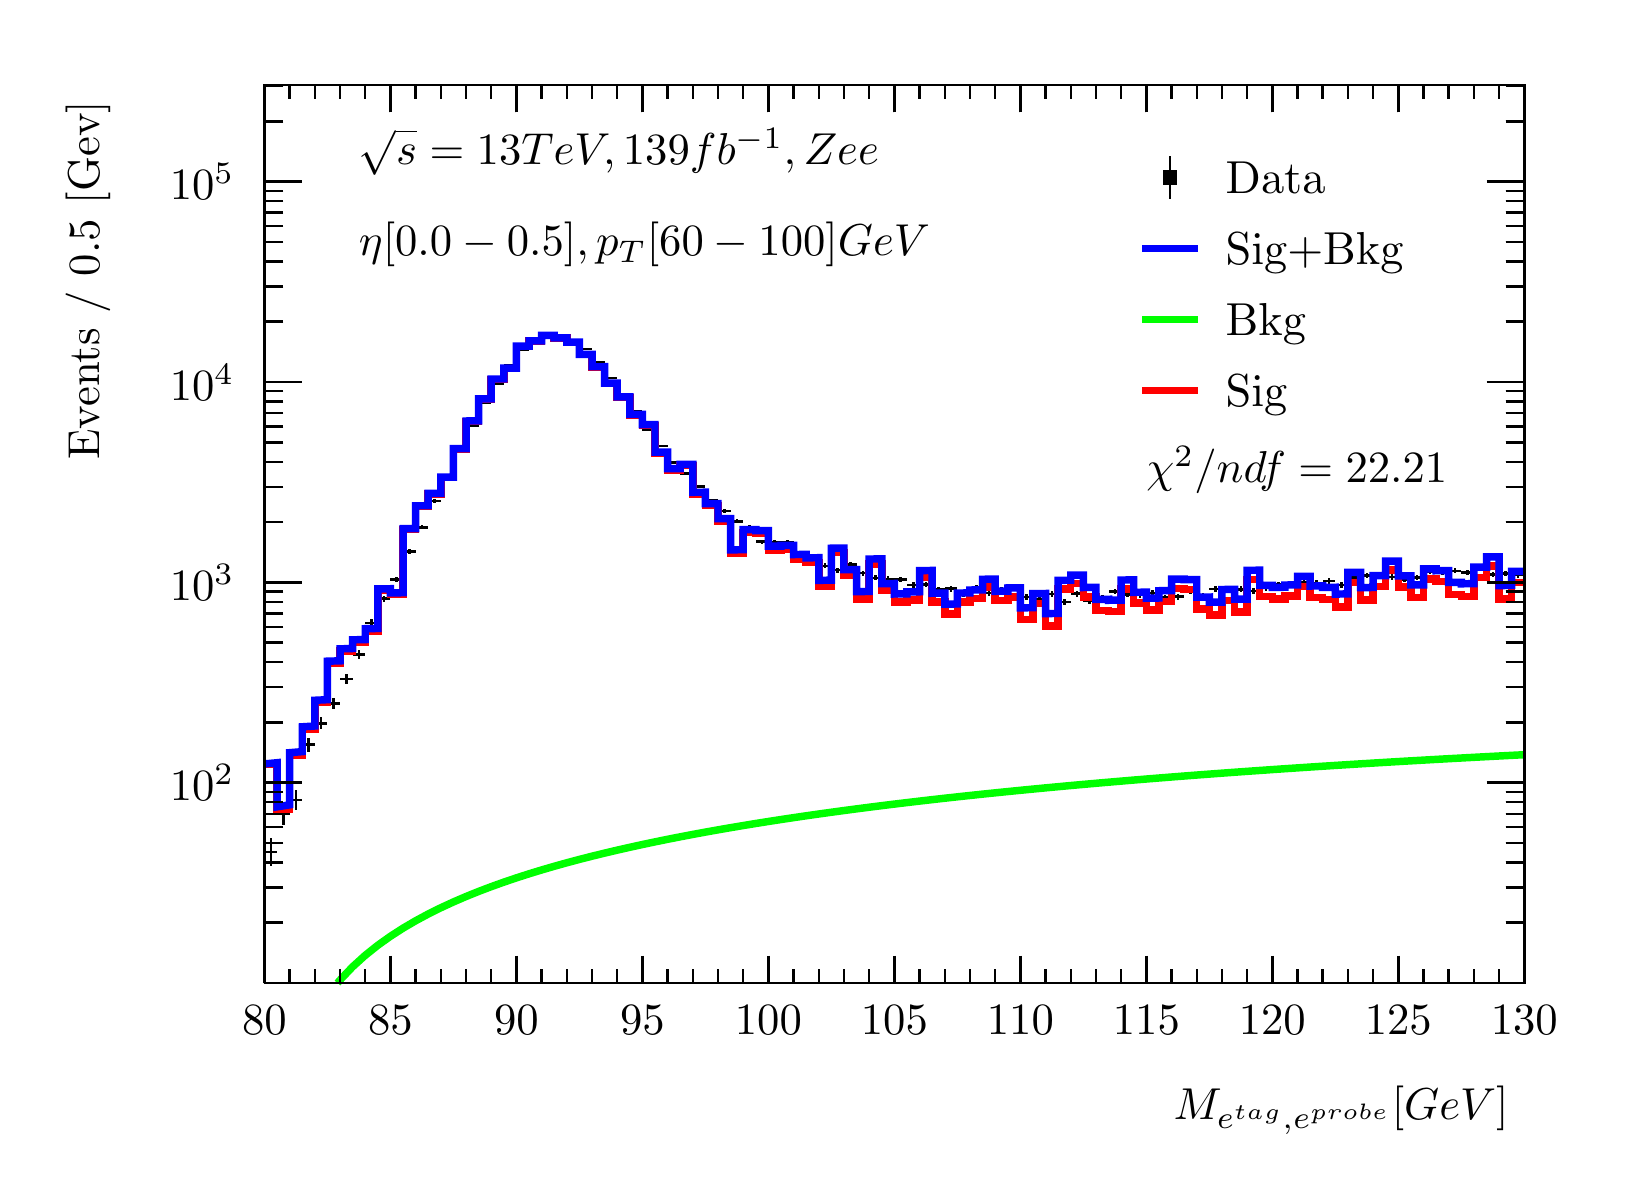
\begin{tikzpicture}
\pgfdeclareplotmark{cross} {
\pgfpathmoveto{\pgfpoint{-0.3\pgfplotmarksize}{\pgfplotmarksize}}
\pgfpathlineto{\pgfpoint{+0.3\pgfplotmarksize}{\pgfplotmarksize}}
\pgfpathlineto{\pgfpoint{+0.3\pgfplotmarksize}{0.3\pgfplotmarksize}}
\pgfpathlineto{\pgfpoint{+1\pgfplotmarksize}{0.3\pgfplotmarksize}}
\pgfpathlineto{\pgfpoint{+1\pgfplotmarksize}{-0.3\pgfplotmarksize}}
\pgfpathlineto{\pgfpoint{+0.3\pgfplotmarksize}{-0.3\pgfplotmarksize}}
\pgfpathlineto{\pgfpoint{+0.3\pgfplotmarksize}{-1.\pgfplotmarksize}}
\pgfpathlineto{\pgfpoint{-0.3\pgfplotmarksize}{-1.\pgfplotmarksize}}
\pgfpathlineto{\pgfpoint{-0.3\pgfplotmarksize}{-0.3\pgfplotmarksize}}
\pgfpathlineto{\pgfpoint{-1.\pgfplotmarksize}{-0.3\pgfplotmarksize}}
\pgfpathlineto{\pgfpoint{-1.\pgfplotmarksize}{0.3\pgfplotmarksize}}
\pgfpathlineto{\pgfpoint{-0.3\pgfplotmarksize}{0.3\pgfplotmarksize}}
\pgfpathclose
\pgfusepathqstroke
}
\pgfdeclareplotmark{cross*} {
\pgfpathmoveto{\pgfpoint{-0.3\pgfplotmarksize}{\pgfplotmarksize}}
\pgfpathlineto{\pgfpoint{+0.3\pgfplotmarksize}{\pgfplotmarksize}}
\pgfpathlineto{\pgfpoint{+0.3\pgfplotmarksize}{0.3\pgfplotmarksize}}
\pgfpathlineto{\pgfpoint{+1\pgfplotmarksize}{0.3\pgfplotmarksize}}
\pgfpathlineto{\pgfpoint{+1\pgfplotmarksize}{-0.3\pgfplotmarksize}}
\pgfpathlineto{\pgfpoint{+0.3\pgfplotmarksize}{-0.3\pgfplotmarksize}}
\pgfpathlineto{\pgfpoint{+0.3\pgfplotmarksize}{-1.\pgfplotmarksize}}
\pgfpathlineto{\pgfpoint{-0.3\pgfplotmarksize}{-1.\pgfplotmarksize}}
\pgfpathlineto{\pgfpoint{-0.3\pgfplotmarksize}{-0.3\pgfplotmarksize}}
\pgfpathlineto{\pgfpoint{-1.\pgfplotmarksize}{-0.3\pgfplotmarksize}}
\pgfpathlineto{\pgfpoint{-1.\pgfplotmarksize}{0.3\pgfplotmarksize}}
\pgfpathlineto{\pgfpoint{-0.3\pgfplotmarksize}{0.3\pgfplotmarksize}}
\pgfpathclose
\pgfusepathqfillstroke
}
\pgfdeclareplotmark{newstar} {
\pgfpathmoveto{\pgfqpoint{0pt}{\pgfplotmarksize}}
\pgfpathlineto{\pgfqpointpolar{44}{0.5\pgfplotmarksize}}
\pgfpathlineto{\pgfqpointpolar{18}{\pgfplotmarksize}}
\pgfpathlineto{\pgfqpointpolar{-20}{0.5\pgfplotmarksize}}
\pgfpathlineto{\pgfqpointpolar{-54}{\pgfplotmarksize}}
\pgfpathlineto{\pgfqpointpolar{-90}{0.5\pgfplotmarksize}}
\pgfpathlineto{\pgfqpointpolar{234}{\pgfplotmarksize}}
\pgfpathlineto{\pgfqpointpolar{198}{0.5\pgfplotmarksize}}
\pgfpathlineto{\pgfqpointpolar{162}{\pgfplotmarksize}}
\pgfpathlineto{\pgfqpointpolar{134}{0.5\pgfplotmarksize}}
\pgfpathclose
\pgfusepathqstroke
}
\pgfdeclareplotmark{newstar*} {
\pgfpathmoveto{\pgfqpoint{0pt}{\pgfplotmarksize}}
\pgfpathlineto{\pgfqpointpolar{44}{0.5\pgfplotmarksize}}
\pgfpathlineto{\pgfqpointpolar{18}{\pgfplotmarksize}}
\pgfpathlineto{\pgfqpointpolar{-20}{0.5\pgfplotmarksize}}
\pgfpathlineto{\pgfqpointpolar{-54}{\pgfplotmarksize}}
\pgfpathlineto{\pgfqpointpolar{-90}{0.5\pgfplotmarksize}}
\pgfpathlineto{\pgfqpointpolar{234}{\pgfplotmarksize}}
\pgfpathlineto{\pgfqpointpolar{198}{0.5\pgfplotmarksize}}
\pgfpathlineto{\pgfqpointpolar{162}{\pgfplotmarksize}}
\pgfpathlineto{\pgfqpointpolar{134}{0.5\pgfplotmarksize}}
\pgfpathclose
\pgfusepathqfillstroke
}
\definecolor{c}{rgb}{1,1,1};
\draw [color=c, fill=c] (0,0) rectangle (20,14.4361);
\draw [color=c, fill=c] (3,2.30977) rectangle (19,13.7143);
\definecolor{c}{rgb}{0,0,0};
\draw [c,line width=0.9] (3,2.30977) -- (3,13.7143) -- (19,13.7143) -- (19,2.30977) -- (3,2.30977);
\definecolor{c}{rgb}{1,1,1};
\draw [color=c, fill=c] (3,2.30977) rectangle (19,13.7143);
\definecolor{c}{rgb}{0,0,0};
\draw [c,line width=0.9] (3,2.30977) -- (3,13.7143) -- (19,13.7143) -- (19,2.30977) -- (3,2.30977);
\draw [c,line width=0.9] (3,2.30977) -- (19,2.30977);
\draw [c,line width=0.9] (3,2.65624) -- (3,2.30977);
\draw [c,line width=0.9] (3.32,2.48301) -- (3.32,2.30977);
\draw [c,line width=0.9] (3.64,2.48301) -- (3.64,2.30977);
\draw [c,line width=0.9] (3.96,2.48301) -- (3.96,2.30977);
\draw [c,line width=0.9] (4.28,2.48301) -- (4.28,2.30977);
\draw [c,line width=0.9] (4.6,2.65624) -- (4.6,2.30977);
\draw [c,line width=0.9] (4.92,2.48301) -- (4.92,2.30977);
\draw [c,line width=0.9] (5.24,2.48301) -- (5.24,2.30977);
\draw [c,line width=0.9] (5.56,2.48301) -- (5.56,2.30977);
\draw [c,line width=0.9] (5.88,2.48301) -- (5.88,2.30977);
\draw [c,line width=0.9] (6.2,2.65624) -- (6.2,2.30977);
\draw [c,line width=0.9] (6.52,2.48301) -- (6.52,2.30977);
\draw [c,line width=0.9] (6.84,2.48301) -- (6.84,2.30977);
\draw [c,line width=0.9] (7.16,2.48301) -- (7.16,2.30977);
\draw [c,line width=0.9] (7.48,2.48301) -- (7.48,2.30977);
\draw [c,line width=0.9] (7.8,2.65624) -- (7.8,2.30977);
\draw [c,line width=0.9] (8.12,2.48301) -- (8.12,2.30977);
\draw [c,line width=0.9] (8.44,2.48301) -- (8.44,2.30977);
\draw [c,line width=0.9] (8.76,2.48301) -- (8.76,2.30977);
\draw [c,line width=0.9] (9.08,2.48301) -- (9.08,2.30977);
\draw [c,line width=0.9] (9.4,2.65624) -- (9.4,2.30977);
\draw [c,line width=0.9] (9.72,2.48301) -- (9.72,2.30977);
\draw [c,line width=0.9] (10.04,2.48301) -- (10.04,2.30977);
\draw [c,line width=0.9] (10.36,2.48301) -- (10.36,2.30977);
\draw [c,line width=0.9] (10.68,2.48301) -- (10.68,2.30977);
\draw [c,line width=0.9] (11,2.65624) -- (11,2.30977);
\draw [c,line width=0.9] (11.32,2.48301) -- (11.32,2.30977);
\draw [c,line width=0.9] (11.64,2.48301) -- (11.64,2.30977);
\draw [c,line width=0.9] (11.96,2.48301) -- (11.96,2.30977);
\draw [c,line width=0.9] (12.28,2.48301) -- (12.28,2.30977);
\draw [c,line width=0.9] (12.6,2.65624) -- (12.6,2.30977);
\draw [c,line width=0.9] (12.92,2.48301) -- (12.92,2.30977);
\draw [c,line width=0.9] (13.24,2.48301) -- (13.24,2.30977);
\draw [c,line width=0.9] (13.56,2.48301) -- (13.56,2.30977);
\draw [c,line width=0.9] (13.88,2.48301) -- (13.88,2.30977);
\draw [c,line width=0.9] (14.2,2.65624) -- (14.2,2.30977);
\draw [c,line width=0.9] (14.52,2.48301) -- (14.52,2.30977);
\draw [c,line width=0.9] (14.84,2.48301) -- (14.84,2.30977);
\draw [c,line width=0.9] (15.16,2.48301) -- (15.16,2.30977);
\draw [c,line width=0.9] (15.48,2.48301) -- (15.48,2.30977);
\draw [c,line width=0.9] (15.8,2.65624) -- (15.8,2.30977);
\draw [c,line width=0.9] (16.12,2.48301) -- (16.12,2.30977);
\draw [c,line width=0.9] (16.44,2.48301) -- (16.44,2.30977);
\draw [c,line width=0.9] (16.76,2.48301) -- (16.76,2.30977);
\draw [c,line width=0.9] (17.08,2.48301) -- (17.08,2.30977);
\draw [c,line width=0.9] (17.4,2.65624) -- (17.4,2.30977);
\draw [c,line width=0.9] (17.72,2.48301) -- (17.72,2.30977);
\draw [c,line width=0.9] (18.04,2.48301) -- (18.04,2.30977);
\draw [c,line width=0.9] (18.36,2.48301) -- (18.36,2.30977);
\draw [c,line width=0.9] (18.68,2.48301) -- (18.68,2.30977);
\draw [c,line width=0.9] (19,2.65624) -- (19,2.30977);
\draw [anchor=base] (3,1.66015) node[scale=1.61424, color=c, rotate=0]{80};
\draw [anchor=base] (4.6,1.66015) node[scale=1.61424, color=c, rotate=0]{85};
\draw [anchor=base] (6.2,1.66015) node[scale=1.61424, color=c, rotate=0]{90};
\draw [anchor=base] (7.8,1.66015) node[scale=1.61424, color=c, rotate=0]{95};
\draw [anchor=base] (9.4,1.66015) node[scale=1.61424, color=c, rotate=0]{100};
\draw [anchor=base] (11,1.66015) node[scale=1.61424, color=c, rotate=0]{105};
\draw [anchor=base] (12.6,1.66015) node[scale=1.61424, color=c, rotate=0]{110};
\draw [anchor=base] (14.2,1.66015) node[scale=1.61424, color=c, rotate=0]{115};
\draw [anchor=base] (15.8,1.66015) node[scale=1.61424, color=c, rotate=0]{120};
\draw [anchor=base] (17.4,1.66015) node[scale=1.61424, color=c, rotate=0]{125};
\draw [anchor=base] (19,1.66015) node[scale=1.61424, color=c, rotate=0]{130};
\draw [anchor= east] (19,0.692932) node[scale=1.61424, color=c, rotate=0]{$M_{e^{tag}, e^{probe}}  [GeV]$};
\draw [c,line width=0.9] (3,13.7143) -- (19,13.7143);
\draw [c,line width=0.9] (3,13.3678) -- (3,13.7143);
\draw [c,line width=0.9] (3.32,13.5411) -- (3.32,13.7143);
\draw [c,line width=0.9] (3.64,13.5411) -- (3.64,13.7143);
\draw [c,line width=0.9] (3.96,13.5411) -- (3.96,13.7143);
\draw [c,line width=0.9] (4.28,13.5411) -- (4.28,13.7143);
\draw [c,line width=0.9] (4.6,13.3678) -- (4.6,13.7143);
\draw [c,line width=0.9] (4.92,13.5411) -- (4.92,13.7143);
\draw [c,line width=0.9] (5.24,13.5411) -- (5.24,13.7143);
\draw [c,line width=0.9] (5.56,13.5411) -- (5.56,13.7143);
\draw [c,line width=0.9] (5.88,13.5411) -- (5.88,13.7143);
\draw [c,line width=0.9] (6.2,13.3678) -- (6.2,13.7143);
\draw [c,line width=0.9] (6.52,13.5411) -- (6.52,13.7143);
\draw [c,line width=0.9] (6.84,13.5411) -- (6.84,13.7143);
\draw [c,line width=0.9] (7.16,13.5411) -- (7.16,13.7143);
\draw [c,line width=0.9] (7.48,13.5411) -- (7.48,13.7143);
\draw [c,line width=0.9] (7.8,13.3678) -- (7.8,13.7143);
\draw [c,line width=0.9] (8.12,13.5411) -- (8.12,13.7143);
\draw [c,line width=0.9] (8.44,13.5411) -- (8.44,13.7143);
\draw [c,line width=0.9] (8.76,13.5411) -- (8.76,13.7143);
\draw [c,line width=0.9] (9.08,13.5411) -- (9.08,13.7143);
\draw [c,line width=0.9] (9.4,13.3678) -- (9.4,13.7143);
\draw [c,line width=0.9] (9.72,13.5411) -- (9.72,13.7143);
\draw [c,line width=0.9] (10.04,13.5411) -- (10.04,13.7143);
\draw [c,line width=0.9] (10.36,13.5411) -- (10.36,13.7143);
\draw [c,line width=0.9] (10.68,13.5411) -- (10.68,13.7143);
\draw [c,line width=0.9] (11,13.3678) -- (11,13.7143);
\draw [c,line width=0.9] (11.32,13.5411) -- (11.32,13.7143);
\draw [c,line width=0.9] (11.64,13.5411) -- (11.64,13.7143);
\draw [c,line width=0.9] (11.96,13.5411) -- (11.96,13.7143);
\draw [c,line width=0.9] (12.28,13.5411) -- (12.28,13.7143);
\draw [c,line width=0.9] (12.6,13.3678) -- (12.6,13.7143);
\draw [c,line width=0.9] (12.92,13.5411) -- (12.92,13.7143);
\draw [c,line width=0.9] (13.24,13.5411) -- (13.24,13.7143);
\draw [c,line width=0.9] (13.56,13.5411) -- (13.56,13.7143);
\draw [c,line width=0.9] (13.88,13.5411) -- (13.88,13.7143);
\draw [c,line width=0.9] (14.2,13.3678) -- (14.2,13.7143);
\draw [c,line width=0.9] (14.52,13.5411) -- (14.52,13.7143);
\draw [c,line width=0.9] (14.84,13.5411) -- (14.84,13.7143);
\draw [c,line width=0.9] (15.16,13.5411) -- (15.16,13.7143);
\draw [c,line width=0.9] (15.48,13.5411) -- (15.48,13.7143);
\draw [c,line width=0.9] (15.8,13.3678) -- (15.8,13.7143);
\draw [c,line width=0.9] (16.12,13.5411) -- (16.12,13.7143);
\draw [c,line width=0.9] (16.44,13.5411) -- (16.44,13.7143);
\draw [c,line width=0.9] (16.76,13.5411) -- (16.76,13.7143);
\draw [c,line width=0.9] (17.08,13.5411) -- (17.08,13.7143);
\draw [c,line width=0.9] (17.4,13.3678) -- (17.4,13.7143);
\draw [c,line width=0.9] (17.72,13.5411) -- (17.72,13.7143);
\draw [c,line width=0.9] (18.04,13.5411) -- (18.04,13.7143);
\draw [c,line width=0.9] (18.36,13.5411) -- (18.36,13.7143);
\draw [c,line width=0.9] (18.68,13.5411) -- (18.68,13.7143);
\draw [c,line width=0.9] (19,13.3678) -- (19,13.7143);
\draw [c,line width=0.9] (3,2.30977) -- (3,13.7143);
\draw [c,line width=0.9] (3.237,3.07568) -- (3,3.07568);
\draw [c,line width=0.9] (3.237,3.5237) -- (3,3.5237);
\draw [c,line width=0.9] (3.237,3.84158) -- (3,3.84158);
\draw [c,line width=0.9] (3.237,4.08815) -- (3,4.08815);
\draw [c,line width=0.9] (3.237,4.2896) -- (3,4.2896);
\draw [c,line width=0.9] (3.237,4.45994) -- (3,4.45994);
\draw [c,line width=0.9] (3.237,4.60748) -- (3,4.60748);
\draw [c,line width=0.9] (3.237,4.73763) -- (3,4.73763);
\draw [c,line width=0.9] (3.474,4.85405) -- (3,4.85405);
\draw [anchor= east] (2.82,4.85405) node[scale=1.61424, color=c, rotate=0]{$10^{2}$};
\draw [c,line width=0.9] (3.237,5.61995) -- (3,5.61995);
\draw [c,line width=0.9] (3.237,6.06798) -- (3,6.06798);
\draw [c,line width=0.9] (3.237,6.38586) -- (3,6.38586);
\draw [c,line width=0.9] (3.237,6.63242) -- (3,6.63242);
\draw [c,line width=0.9] (3.237,6.83388) -- (3,6.83388);
\draw [c,line width=0.9] (3.237,7.00421) -- (3,7.00421);
\draw [c,line width=0.9] (3.237,7.15176) -- (3,7.15176);
\draw [c,line width=0.9] (3.237,7.28191) -- (3,7.28191);
\draw [c,line width=0.9] (3.474,7.39833) -- (3,7.39833);
\draw [anchor= east] (2.82,7.39833) node[scale=1.61424, color=c, rotate=0]{$10^{3}$};
\draw [c,line width=0.9] (3.237,8.16423) -- (3,8.16423);
\draw [c,line width=0.9] (3.237,8.61226) -- (3,8.61226);
\draw [c,line width=0.9] (3.237,8.93013) -- (3,8.93013);
\draw [c,line width=0.9] (3.237,9.1767) -- (3,9.1767);
\draw [c,line width=0.9] (3.237,9.37816) -- (3,9.37816);
\draw [c,line width=0.9] (3.237,9.54849) -- (3,9.54849);
\draw [c,line width=0.9] (3.237,9.69604) -- (3,9.69604);
\draw [c,line width=0.9] (3.237,9.82618) -- (3,9.82618);
\draw [c,line width=0.9] (3.474,9.9426) -- (3,9.9426);
\draw [anchor= east] (2.82,9.9426) node[scale=1.61424, color=c, rotate=0]{$10^{4}$};
\draw [c,line width=0.9] (3.237,10.7085) -- (3,10.7085);
\draw [c,line width=0.9] (3.237,11.1565) -- (3,11.1565);
\draw [c,line width=0.9] (3.237,11.4744) -- (3,11.4744);
\draw [c,line width=0.9] (3.237,11.721) -- (3,11.721);
\draw [c,line width=0.9] (3.237,11.9224) -- (3,11.9224);
\draw [c,line width=0.9] (3.237,12.0928) -- (3,12.0928);
\draw [c,line width=0.9] (3.237,12.2403) -- (3,12.2403);
\draw [c,line width=0.9] (3.237,12.3705) -- (3,12.3705);
\draw [c,line width=0.9] (3.474,12.4869) -- (3,12.4869);
\draw [anchor= east] (2.82,12.4869) node[scale=1.61424, color=c, rotate=0]{$10^{5}$};
\draw [c,line width=0.9] (3.237,13.2528) -- (3,13.2528);
\draw [c,line width=0.9] (3.237,13.7008) -- (3,13.7008);
\draw [anchor= east] (0.76,13.7143) node[scale=1.61424, color=c, rotate=90]{Events / 0.5 [Gev]};
\draw [c,line width=0.9] (19,2.30977) -- (19,13.7143);
\draw [c,line width=0.9] (18.763,3.07568) -- (19,3.07568);
\draw [c,line width=0.9] (18.763,3.5237) -- (19,3.5237);
\draw [c,line width=0.9] (18.763,3.84158) -- (19,3.84158);
\draw [c,line width=0.9] (18.763,4.08815) -- (19,4.08815);
\draw [c,line width=0.9] (18.763,4.2896) -- (19,4.2896);
\draw [c,line width=0.9] (18.763,4.45994) -- (19,4.45994);
\draw [c,line width=0.9] (18.763,4.60748) -- (19,4.60748);
\draw [c,line width=0.9] (18.763,4.73763) -- (19,4.73763);
\draw [c,line width=0.9] (18.526,4.85405) -- (19,4.85405);
\draw [c,line width=0.9] (18.763,5.61995) -- (19,5.61995);
\draw [c,line width=0.9] (18.763,6.06798) -- (19,6.06798);
\draw [c,line width=0.9] (18.763,6.38586) -- (19,6.38586);
\draw [c,line width=0.9] (18.763,6.63242) -- (19,6.63242);
\draw [c,line width=0.9] (18.763,6.83388) -- (19,6.83388);
\draw [c,line width=0.9] (18.763,7.00421) -- (19,7.00421);
\draw [c,line width=0.9] (18.763,7.15176) -- (19,7.15176);
\draw [c,line width=0.9] (18.763,7.28191) -- (19,7.28191);
\draw [c,line width=0.9] (18.526,7.39833) -- (19,7.39833);
\draw [c,line width=0.9] (18.763,8.16423) -- (19,8.16423);
\draw [c,line width=0.9] (18.763,8.61226) -- (19,8.61226);
\draw [c,line width=0.9] (18.763,8.93013) -- (19,8.93013);
\draw [c,line width=0.9] (18.763,9.1767) -- (19,9.1767);
\draw [c,line width=0.9] (18.763,9.37816) -- (19,9.37816);
\draw [c,line width=0.9] (18.763,9.54849) -- (19,9.54849);
\draw [c,line width=0.9] (18.763,9.69604) -- (19,9.69604);
\draw [c,line width=0.9] (18.763,9.82618) -- (19,9.82618);
\draw [c,line width=0.9] (18.526,9.9426) -- (19,9.9426);
\draw [c,line width=0.9] (18.763,10.7085) -- (19,10.7085);
\draw [c,line width=0.9] (18.763,11.1565) -- (19,11.1565);
\draw [c,line width=0.9] (18.763,11.4744) -- (19,11.4744);
\draw [c,line width=0.9] (18.763,11.721) -- (19,11.721);
\draw [c,line width=0.9] (18.763,11.9224) -- (19,11.9224);
\draw [c,line width=0.9] (18.763,12.0928) -- (19,12.0928);
\draw [c,line width=0.9] (18.763,12.2403) -- (19,12.2403);
\draw [c,line width=0.9] (18.763,12.3705) -- (19,12.3705);
\draw [c,line width=0.9] (18.526,12.4869) -- (19,12.4869);
\draw [c,line width=0.9] (18.763,13.2528) -- (19,13.2528);
\draw [c,line width=0.9] (18.763,13.7008) -- (19,13.7008);
\draw [c,line width=0.9] (3.08,3.97173) -- (3,3.97173);
\draw [c,line width=0.9] (3,3.97173) -- (3,3.97173);
\draw [c,line width=0.9] (3.08,3.97173) -- (3.16,3.97173);
\draw [c,line width=0.9] (3.16,3.97173) -- (3.16,3.97173);
\draw [c,line width=0.9] (3.08,3.97173) -- (3.08,4.14747);
\draw [c,line width=0.9] (3.08,4.14747) -- (3.08,4.14747);
\draw [c,line width=0.9] (3.08,3.97173) -- (3.08,3.79408);
\draw [c,line width=0.9] (3.08,3.79408) -- (3.08,3.79408);
\draw [c,line width=0.9] (3.24,4.45994) -- (3.16,4.45994);
\draw [c,line width=0.9] (3.16,4.45994) -- (3.16,4.45994);
\draw [c,line width=0.9] (3.24,4.45994) -- (3.32,4.45994);
\draw [c,line width=0.9] (3.32,4.45994) -- (3.32,4.45994);
\draw [c,line width=0.9] (3.24,4.45994) -- (3.24,4.59926);
\draw [c,line width=0.9] (3.24,4.59926) -- (3.24,4.59926);
\draw [c,line width=0.9] (3.24,4.45994) -- (3.24,4.31964);
\draw [c,line width=0.9] (3.24,4.31964) -- (3.24,4.31964);
\draw [c,line width=0.9] (3.4,4.63477) -- (3.32,4.63477);
\draw [c,line width=0.9] (3.32,4.63477) -- (3.32,4.63477);
\draw [c,line width=0.9] (3.4,4.63477) -- (3.48,4.63477);
\draw [c,line width=0.9] (3.48,4.63477) -- (3.48,4.63477);
\draw [c,line width=0.9] (3.4,4.63477) -- (3.4,4.76302);
\draw [c,line width=0.9] (3.4,4.76302) -- (3.4,4.76302);
\draw [c,line width=0.9] (3.4,4.63477) -- (3.4,4.50575);
\draw [c,line width=0.9] (3.4,4.50575) -- (3.4,4.50575);
\draw [c,line width=0.9] (3.56,5.33831) -- (3.48,5.33831);
\draw [c,line width=0.9] (3.48,5.33831) -- (3.48,5.33831);
\draw [c,line width=0.9] (3.56,5.33831) -- (3.64,5.33831);
\draw [c,line width=0.9] (3.64,5.33831) -- (3.64,5.33831);
\draw [c,line width=0.9] (3.56,5.33831) -- (3.56,5.42704);
\draw [c,line width=0.9] (3.56,5.42704) -- (3.56,5.42704);
\draw [c,line width=0.9] (3.56,5.33831) -- (3.56,5.24958);
\draw [c,line width=0.9] (3.56,5.24958) -- (3.56,5.24958);
\draw [c,line width=0.9] (3.72,5.60885) -- (3.64,5.60885);
\draw [c,line width=0.9] (3.64,5.60885) -- (3.64,5.60885);
\draw [c,line width=0.9] (3.72,5.60885) -- (3.8,5.60885);
\draw [c,line width=0.9] (3.8,5.60885) -- (3.8,5.60885);
\draw [c,line width=0.9] (3.72,5.60885) -- (3.72,5.68736);
\draw [c,line width=0.9] (3.72,5.68736) -- (3.72,5.68736);
\draw [c,line width=0.9] (3.72,5.60885) -- (3.72,5.53034);
\draw [c,line width=0.9] (3.72,5.53034) -- (3.72,5.53034);
\draw [c,line width=0.9] (3.88,5.85765) -- (3.8,5.85765);
\draw [c,line width=0.9] (3.8,5.85765) -- (3.8,5.85765);
\draw [c,line width=0.9] (3.88,5.85765) -- (3.96,5.85765);
\draw [c,line width=0.9] (3.96,5.85765) -- (3.96,5.85765);
\draw [c,line width=0.9] (3.88,5.85765) -- (3.88,5.9278);
\draw [c,line width=0.9] (3.88,5.9278) -- (3.88,5.9278);
\draw [c,line width=0.9] (3.88,5.85765) -- (3.88,5.78749);
\draw [c,line width=0.9] (3.88,5.78749) -- (3.88,5.78749);
\draw [c,line width=0.9] (4.04,6.16994) -- (3.96,6.16994);
\draw [c,line width=0.9] (3.96,6.16994) -- (3.96,6.16994);
\draw [c,line width=0.9] (4.04,6.16994) -- (4.12,6.16994);
\draw [c,line width=0.9] (4.12,6.16994) -- (4.12,6.16994);
\draw [c,line width=0.9] (4.04,6.16994) -- (4.04,6.23085);
\draw [c,line width=0.9] (4.04,6.23085) -- (4.04,6.23085);
\draw [c,line width=0.9] (4.04,6.16994) -- (4.04,6.10903);
\draw [c,line width=0.9] (4.04,6.10903) -- (4.04,6.10903);
\draw [c,line width=0.9] (4.2,6.48361) -- (4.12,6.48361);
\draw [c,line width=0.9] (4.12,6.48361) -- (4.12,6.48361);
\draw [c,line width=0.9] (4.2,6.48361) -- (4.28,6.48361);
\draw [c,line width=0.9] (4.28,6.48361) -- (4.28,6.48361);
\draw [c,line width=0.9] (4.2,6.48361) -- (4.2,6.53647);
\draw [c,line width=0.9] (4.2,6.53647) -- (4.2,6.53647);
\draw [c,line width=0.9] (4.2,6.48361) -- (4.2,6.43076);
\draw [c,line width=0.9] (4.2,6.43076) -- (4.2,6.43076);
\draw [c,line width=0.9] (4.36,6.88428) -- (4.28,6.88428);
\draw [c,line width=0.9] (4.28,6.88428) -- (4.28,6.88428);
\draw [c,line width=0.9] (4.36,6.88428) -- (4.44,6.88428);
\draw [c,line width=0.9] (4.44,6.88428) -- (4.44,6.88428);
\draw [c,line width=0.9] (4.36,6.88428) -- (4.36,6.92837);
\draw [c,line width=0.9] (4.36,6.92837) -- (4.36,6.92837);
\draw [c,line width=0.9] (4.36,6.88428) -- (4.36,6.84019);
\draw [c,line width=0.9] (4.36,6.84019) -- (4.36,6.84019);
\draw [c,line width=0.9] (4.52,7.19244) -- (4.44,7.19244);
\draw [c,line width=0.9] (4.44,7.19244) -- (4.44,7.19244);
\draw [c,line width=0.9] (4.52,7.19244) -- (4.6,7.19244);
\draw [c,line width=0.9] (4.6,7.19244) -- (4.6,7.19244);
\draw [c,line width=0.9] (4.52,7.19244) -- (4.52,7.23079);
\draw [c,line width=0.9] (4.52,7.23079) -- (4.52,7.23079);
\draw [c,line width=0.9] (4.52,7.19244) -- (4.52,7.15409);
\draw [c,line width=0.9] (4.52,7.15409) -- (4.52,7.15409);
\draw [c,line width=0.9] (4.68,7.4342) -- (4.6,7.4342);
\draw [c,line width=0.9] (4.6,7.4342) -- (4.6,7.4342);
\draw [c,line width=0.9] (4.68,7.4342) -- (4.76,7.4342);
\draw [c,line width=0.9] (4.76,7.4342) -- (4.76,7.4342);
\draw [c,line width=0.9] (4.68,7.4342) -- (4.68,7.46858);
\draw [c,line width=0.9] (4.68,7.46858) -- (4.68,7.46858);
\draw [c,line width=0.9] (4.68,7.4342) -- (4.68,7.39983);
\draw [c,line width=0.9] (4.68,7.39983) -- (4.68,7.39983);
\draw [c,line width=0.9] (4.84,7.7889) -- (4.76,7.7889);
\draw [c,line width=0.9] (4.76,7.7889) -- (4.76,7.7889);
\draw [c,line width=0.9] (4.84,7.7889) -- (4.92,7.7889);
\draw [c,line width=0.9] (4.92,7.7889) -- (4.92,7.7889);
\draw [c,line width=0.9] (4.84,7.7889) -- (4.84,7.81818);
\draw [c,line width=0.9] (4.84,7.81818) -- (4.84,7.81818);
\draw [c,line width=0.9] (4.84,7.7889) -- (4.84,7.75962);
\draw [c,line width=0.9] (4.84,7.75962) -- (4.84,7.75962);
\draw [c,line width=0.9] (5,8.09645) -- (4.92,8.09645);
\draw [c,line width=0.9] (4.92,8.09645) -- (4.92,8.09645);
\draw [c,line width=0.9] (5,8.09645) -- (5.08,8.09645);
\draw [c,line width=0.9] (5.08,8.09645) -- (5.08,8.09645);
\draw [c,line width=0.9] (5,8.09645) -- (5,8.12193);
\draw [c,line width=0.9] (5,8.12193) -- (5,8.12193);
\draw [c,line width=0.9] (5,8.09645) -- (5,8.07097);
\draw [c,line width=0.9] (5,8.07097) -- (5,8.07097);
\draw [c,line width=0.9] (5.16,8.43008) -- (5.08,8.43008);
\draw [c,line width=0.9] (5.08,8.43008) -- (5.08,8.43008);
\draw [c,line width=0.9] (5.16,8.43008) -- (5.24,8.43008);
\draw [c,line width=0.9] (5.24,8.43008) -- (5.24,8.43008);
\draw [c,line width=0.9] (5.16,8.43008) -- (5.16,8.45198);
\draw [c,line width=0.9] (5.16,8.45198) -- (5.16,8.45198);
\draw [c,line width=0.9] (5.16,8.43008) -- (5.16,8.40817);
\draw [c,line width=0.9] (5.16,8.40817) -- (5.16,8.40817);
\draw [c,line width=0.9] (5.32,8.73386) -- (5.24,8.73386);
\draw [c,line width=0.9] (5.24,8.73386) -- (5.24,8.73386);
\draw [c,line width=0.9] (5.32,8.73386) -- (5.4,8.73386);
\draw [c,line width=0.9] (5.4,8.73386) -- (5.4,8.73386);
\draw [c,line width=0.9] (5.32,8.73386) -- (5.32,8.75295);
\draw [c,line width=0.9] (5.32,8.75295) -- (5.32,8.75295);
\draw [c,line width=0.9] (5.32,8.73386) -- (5.32,8.71476);
\draw [c,line width=0.9] (5.32,8.71476) -- (5.32,8.71476);
\draw [c,line width=0.9] (5.48,9.07903) -- (5.4,9.07903);
\draw [c,line width=0.9] (5.4,9.07903) -- (5.4,9.07903);
\draw [c,line width=0.9] (5.48,9.07903) -- (5.56,9.07903);
\draw [c,line width=0.9] (5.56,9.07903) -- (5.56,9.07903);
\draw [c,line width=0.9] (5.48,9.07903) -- (5.48,9.09536);
\draw [c,line width=0.9] (5.48,9.09536) -- (5.48,9.09536);
\draw [c,line width=0.9] (5.48,9.07903) -- (5.48,9.0627);
\draw [c,line width=0.9] (5.48,9.0627) -- (5.48,9.0627);
\draw [c,line width=0.9] (5.64,9.39261) -- (5.56,9.39261);
\draw [c,line width=0.9] (5.56,9.39261) -- (5.56,9.39261);
\draw [c,line width=0.9] (5.64,9.39261) -- (5.72,9.39261);
\draw [c,line width=0.9] (5.72,9.39261) -- (5.72,9.39261);
\draw [c,line width=0.9] (5.64,9.39261) -- (5.64,9.40679);
\draw [c,line width=0.9] (5.64,9.40679) -- (5.64,9.40679);
\draw [c,line width=0.9] (5.64,9.39261) -- (5.64,9.37844);
\draw [c,line width=0.9] (5.64,9.37844) -- (5.64,9.37844);
\draw [c,line width=0.9] (5.8,9.67681) -- (5.72,9.67681);
\draw [c,line width=0.9] (5.72,9.67681) -- (5.72,9.67681);
\draw [c,line width=0.9] (5.8,9.67681) -- (5.88,9.67681);
\draw [c,line width=0.9] (5.88,9.67681) -- (5.88,9.67681);
\draw [c,line width=0.9] (5.8,9.67681) -- (5.8,9.68927);
\draw [c,line width=0.9] (5.8,9.68927) -- (5.8,9.68927);
\draw [c,line width=0.9] (5.8,9.67681) -- (5.8,9.66435);
\draw [c,line width=0.9] (5.8,9.66435) -- (5.8,9.66435);
\draw [c,line width=0.9] (5.96,9.9213) -- (5.88,9.9213);
\draw [c,line width=0.9] (5.88,9.9213) -- (5.88,9.9213);
\draw [c,line width=0.9] (5.96,9.9213) -- (6.04,9.9213);
\draw [c,line width=0.9] (6.04,9.9213) -- (6.04,9.9213);
\draw [c,line width=0.9] (5.96,9.9213) -- (5.96,9.93245);
\draw [c,line width=0.9] (5.96,9.93245) -- (5.96,9.93245);
\draw [c,line width=0.9] (5.96,9.9213) -- (5.96,9.91014);
\draw [c,line width=0.9] (5.96,9.91014) -- (5.96,9.91014);
\draw [c,line width=0.9] (6.12,10.1618) -- (6.04,10.1618);
\draw [c,line width=0.9] (6.04,10.1618) -- (6.04,10.1618);
\draw [c,line width=0.9] (6.12,10.1618) -- (6.2,10.1618);
\draw [c,line width=0.9] (6.2,10.1618) -- (6.2,10.1618);
\draw [c,line width=0.9] (6.12,10.1618) -- (6.12,10.1718);
\draw [c,line width=0.9] (6.12,10.1718) -- (6.12,10.1718);
\draw [c,line width=0.9] (6.12,10.1618) -- (6.12,10.1518);
\draw [c,line width=0.9] (6.12,10.1518) -- (6.12,10.1518);
\draw [c,line width=0.9] (6.28,10.3471) -- (6.2,10.3471);
\draw [c,line width=0.9] (6.2,10.3471) -- (6.2,10.3471);
\draw [c,line width=0.9] (6.28,10.3471) -- (6.36,10.3471);
\draw [c,line width=0.9] (6.36,10.3471) -- (6.36,10.3471);
\draw [c,line width=0.9] (6.28,10.3471) -- (6.28,10.3563);
\draw [c,line width=0.9] (6.28,10.3563) -- (6.28,10.3563);
\draw [c,line width=0.9] (6.28,10.3471) -- (6.28,10.3379);
\draw [c,line width=0.9] (6.28,10.3379) -- (6.28,10.3379);
\draw [c,line width=0.9] (6.44,10.4746) -- (6.36,10.4746);
\draw [c,line width=0.9] (6.36,10.4746) -- (6.36,10.4746);
\draw [c,line width=0.9] (6.44,10.4746) -- (6.52,10.4746);
\draw [c,line width=0.9] (6.52,10.4746) -- (6.52,10.4746);
\draw [c,line width=0.9] (6.44,10.4746) -- (6.44,10.4833);
\draw [c,line width=0.9] (6.44,10.4833) -- (6.44,10.4833);
\draw [c,line width=0.9] (6.44,10.4746) -- (6.44,10.466);
\draw [c,line width=0.9] (6.44,10.466) -- (6.44,10.466);
\draw [c,line width=0.9] (6.6,10.5373) -- (6.52,10.5373);
\draw [c,line width=0.9] (6.52,10.5373) -- (6.52,10.5373);
\draw [c,line width=0.9] (6.6,10.5373) -- (6.68,10.5373);
\draw [c,line width=0.9] (6.68,10.5373) -- (6.68,10.5373);
\draw [c,line width=0.9] (6.6,10.5373) -- (6.6,10.5457);
\draw [c,line width=0.9] (6.6,10.5457) -- (6.6,10.5457);
\draw [c,line width=0.9] (6.6,10.5373) -- (6.6,10.5288);
\draw [c,line width=0.9] (6.6,10.5288) -- (6.6,10.5288);
\draw [c,line width=0.9] (6.76,10.5319) -- (6.68,10.5319);
\draw [c,line width=0.9] (6.68,10.5319) -- (6.68,10.5319);
\draw [c,line width=0.9] (6.76,10.5319) -- (6.84,10.5319);
\draw [c,line width=0.9] (6.84,10.5319) -- (6.84,10.5319);
\draw [c,line width=0.9] (6.76,10.5319) -- (6.76,10.5403);
\draw [c,line width=0.9] (6.76,10.5403) -- (6.76,10.5403);
\draw [c,line width=0.9] (6.76,10.5319) -- (6.76,10.5234);
\draw [c,line width=0.9] (6.76,10.5234) -- (6.76,10.5234);
\draw [c,line width=0.9] (6.92,10.4613) -- (6.84,10.4613);
\draw [c,line width=0.9] (6.84,10.4613) -- (6.84,10.4613);
\draw [c,line width=0.9] (6.92,10.4613) -- (7,10.4613);
\draw [c,line width=0.9] (7,10.4613) -- (7,10.4613);
\draw [c,line width=0.9] (6.92,10.4613) -- (6.92,10.4701);
\draw [c,line width=0.9] (6.92,10.4701) -- (6.92,10.4701);
\draw [c,line width=0.9] (6.92,10.4613) -- (6.92,10.4526);
\draw [c,line width=0.9] (6.92,10.4526) -- (6.92,10.4526);
\draw [c,line width=0.9] (7.08,10.3639) -- (7,10.3639);
\draw [c,line width=0.9] (7,10.3639) -- (7,10.3639);
\draw [c,line width=0.9] (7.08,10.3639) -- (7.16,10.3639);
\draw [c,line width=0.9] (7.16,10.3639) -- (7.16,10.3639);
\draw [c,line width=0.9] (7.08,10.3639) -- (7.08,10.373);
\draw [c,line width=0.9] (7.08,10.373) -- (7.08,10.373);
\draw [c,line width=0.9] (7.08,10.3639) -- (7.08,10.3547);
\draw [c,line width=0.9] (7.08,10.3547) -- (7.08,10.3547);
\draw [c,line width=0.9] (7.24,10.1946) -- (7.16,10.1946);
\draw [c,line width=0.9] (7.16,10.1946) -- (7.16,10.1946);
\draw [c,line width=0.9] (7.24,10.1946) -- (7.32,10.1946);
\draw [c,line width=0.9] (7.32,10.1946) -- (7.32,10.1946);
\draw [c,line width=0.9] (7.24,10.1946) -- (7.24,10.2044);
\draw [c,line width=0.9] (7.24,10.2044) -- (7.24,10.2044);
\draw [c,line width=0.9] (7.24,10.1946) -- (7.24,10.1847);
\draw [c,line width=0.9] (7.24,10.1847) -- (7.24,10.1847);
\draw [c,line width=0.9] (7.4,9.9942) -- (7.32,9.9942);
\draw [c,line width=0.9] (7.32,9.9942) -- (7.32,9.9942);
\draw [c,line width=0.9] (7.4,9.9942) -- (7.48,9.9942);
\draw [c,line width=0.9] (7.48,9.9942) -- (7.48,9.9942);
\draw [c,line width=0.9] (7.4,9.9942) -- (7.4,10.005);
\draw [c,line width=0.9] (7.4,10.005) -- (7.4,10.005);
\draw [c,line width=0.9] (7.4,9.9942) -- (7.4,9.9834);
\draw [c,line width=0.9] (7.4,9.9834) -- (7.4,9.9834);
\draw [c,line width=0.9] (7.56,9.77273) -- (7.48,9.77273);
\draw [c,line width=0.9] (7.48,9.77273) -- (7.48,9.77273);
\draw [c,line width=0.9] (7.56,9.77273) -- (7.64,9.77273);
\draw [c,line width=0.9] (7.64,9.77273) -- (7.64,9.77273);
\draw [c,line width=0.9] (7.56,9.77273) -- (7.56,9.78467);
\draw [c,line width=0.9] (7.56,9.78467) -- (7.56,9.78467);
\draw [c,line width=0.9] (7.56,9.77273) -- (7.56,9.7608);
\draw [c,line width=0.9] (7.56,9.7608) -- (7.56,9.7608);
\draw [c,line width=0.9] (7.72,9.57099) -- (7.64,9.57099);
\draw [c,line width=0.9] (7.64,9.57099) -- (7.64,9.57099);
\draw [c,line width=0.9] (7.72,9.57099) -- (7.8,9.57099);
\draw [c,line width=0.9] (7.8,9.57099) -- (7.8,9.57099);
\draw [c,line width=0.9] (7.72,9.57099) -- (7.72,9.58406);
\draw [c,line width=0.9] (7.72,9.58406) -- (7.72,9.58406);
\draw [c,line width=0.9] (7.72,9.57099) -- (7.72,9.55792);
\draw [c,line width=0.9] (7.72,9.55792) -- (7.72,9.55792);
\draw [c,line width=0.9] (7.88,9.33075) -- (7.8,9.33075);
\draw [c,line width=0.9] (7.8,9.33075) -- (7.8,9.33075);
\draw [c,line width=0.9] (7.88,9.33075) -- (7.96,9.33075);
\draw [c,line width=0.9] (7.96,9.33075) -- (7.96,9.33075);
\draw [c,line width=0.9] (7.88,9.33075) -- (7.88,9.34532);
\draw [c,line width=0.9] (7.88,9.34532) -- (7.88,9.34532);
\draw [c,line width=0.9] (7.88,9.33075) -- (7.88,9.31617);
\draw [c,line width=0.9] (7.88,9.31617) -- (7.88,9.31617);
\draw [c,line width=0.9] (8.04,9.13159) -- (7.96,9.13159);
\draw [c,line width=0.9] (7.96,9.13159) -- (7.96,9.13159);
\draw [c,line width=0.9] (8.04,9.13159) -- (8.12,9.13159);
\draw [c,line width=0.9] (8.12,9.13159) -- (8.12,9.13159);
\draw [c,line width=0.9] (8.04,9.13159) -- (8.04,9.14754);
\draw [c,line width=0.9] (8.04,9.14754) -- (8.04,9.14754);
\draw [c,line width=0.9] (8.04,9.13159) -- (8.04,9.11565);
\draw [c,line width=0.9] (8.04,9.11565) -- (8.04,9.11565);
\draw [c,line width=0.9] (8.2,8.91903) -- (8.12,8.91903);
\draw [c,line width=0.9] (8.12,8.91903) -- (8.12,8.91903);
\draw [c,line width=0.9] (8.2,8.91903) -- (8.28,8.91903);
\draw [c,line width=0.9] (8.28,8.91903) -- (8.28,8.91903);
\draw [c,line width=0.9] (8.2,8.91903) -- (8.2,8.93659);
\draw [c,line width=0.9] (8.2,8.93659) -- (8.2,8.93659);
\draw [c,line width=0.9] (8.2,8.91903) -- (8.2,8.90147);
\draw [c,line width=0.9] (8.2,8.90147) -- (8.2,8.90147);
\draw [c,line width=0.9] (8.36,8.77911) -- (8.28,8.77911);
\draw [c,line width=0.9] (8.28,8.77911) -- (8.28,8.77911);
\draw [c,line width=0.9] (8.36,8.77911) -- (8.44,8.77911);
\draw [c,line width=0.9] (8.44,8.77911) -- (8.44,8.77911);
\draw [c,line width=0.9] (8.36,8.77911) -- (8.36,8.79782);
\draw [c,line width=0.9] (8.36,8.79782) -- (8.36,8.79782);
\draw [c,line width=0.9] (8.36,8.77911) -- (8.36,8.7604);
\draw [c,line width=0.9] (8.36,8.7604) -- (8.36,8.7604);
\draw [c,line width=0.9] (8.52,8.61887) -- (8.44,8.61887);
\draw [c,line width=0.9] (8.44,8.61887) -- (8.44,8.61887);
\draw [c,line width=0.9] (8.52,8.61887) -- (8.6,8.61887);
\draw [c,line width=0.9] (8.6,8.61887) -- (8.6,8.61887);
\draw [c,line width=0.9] (8.52,8.61887) -- (8.52,8.63898);
\draw [c,line width=0.9] (8.52,8.63898) -- (8.52,8.63898);
\draw [c,line width=0.9] (8.52,8.61887) -- (8.52,8.59875);
\draw [c,line width=0.9] (8.52,8.59875) -- (8.52,8.59875);
\draw [c,line width=0.9] (8.68,8.43657) -- (8.6,8.43657);
\draw [c,line width=0.9] (8.6,8.43657) -- (8.6,8.43657);
\draw [c,line width=0.9] (8.68,8.43657) -- (8.76,8.43657);
\draw [c,line width=0.9] (8.76,8.43657) -- (8.76,8.43657);
\draw [c,line width=0.9] (8.68,8.43657) -- (8.68,8.45842);
\draw [c,line width=0.9] (8.68,8.45842) -- (8.68,8.45842);
\draw [c,line width=0.9] (8.68,8.43657) -- (8.68,8.41473);
\draw [c,line width=0.9] (8.68,8.41473) -- (8.68,8.41473);
\draw [c,line width=0.9] (8.84,8.30464) -- (8.76,8.30464);
\draw [c,line width=0.9] (8.76,8.30464) -- (8.76,8.30464);
\draw [c,line width=0.9] (8.84,8.30464) -- (8.92,8.30464);
\draw [c,line width=0.9] (8.92,8.30464) -- (8.92,8.30464);
\draw [c,line width=0.9] (8.84,8.30464) -- (8.84,8.32783);
\draw [c,line width=0.9] (8.84,8.32783) -- (8.84,8.32783);
\draw [c,line width=0.9] (8.84,8.30464) -- (8.84,8.28146);
\draw [c,line width=0.9] (8.84,8.28146) -- (8.84,8.28146);
\draw [c,line width=0.9] (9,8.17358) -- (8.92,8.17358);
\draw [c,line width=0.9] (8.92,8.17358) -- (8.92,8.17358);
\draw [c,line width=0.9] (9,8.17358) -- (9.08,8.17358);
\draw [c,line width=0.9] (9.08,8.17358) -- (9.08,8.17358);
\draw [c,line width=0.9] (9,8.17358) -- (9,8.19819);
\draw [c,line width=0.9] (9,8.19819) -- (9,8.19819);
\draw [c,line width=0.9] (9,8.17358) -- (9,8.14898);
\draw [c,line width=0.9] (9,8.14898) -- (9,8.14898);
\draw [c,line width=0.9] (9.16,8.10231) -- (9.08,8.10231);
\draw [c,line width=0.9] (9.08,8.10231) -- (9.08,8.10231);
\draw [c,line width=0.9] (9.16,8.10231) -- (9.24,8.10231);
\draw [c,line width=0.9] (9.24,8.10231) -- (9.24,8.10231);
\draw [c,line width=0.9] (9.16,8.10231) -- (9.16,8.12772);
\draw [c,line width=0.9] (9.16,8.12772) -- (9.16,8.12772);
\draw [c,line width=0.9] (9.16,8.10231) -- (9.16,8.0769);
\draw [c,line width=0.9] (9.16,8.0769) -- (9.16,8.0769);
\draw [c,line width=0.9] (9.32,7.9149) -- (9.24,7.9149);
\draw [c,line width=0.9] (9.24,7.9149) -- (9.24,7.9149);
\draw [c,line width=0.9] (9.32,7.9149) -- (9.4,7.9149);
\draw [c,line width=0.9] (9.4,7.9149) -- (9.4,7.9149);
\draw [c,line width=0.9] (9.32,7.9149) -- (9.32,7.94256);
\draw [c,line width=0.9] (9.32,7.94256) -- (9.32,7.94256);
\draw [c,line width=0.9] (9.32,7.9149) -- (9.32,7.88724);
\draw [c,line width=0.9] (9.32,7.88724) -- (9.32,7.88724);
\draw [c,line width=0.9] (9.48,7.90865) -- (9.4,7.90865);
\draw [c,line width=0.9] (9.4,7.90865) -- (9.4,7.90865);
\draw [c,line width=0.9] (9.48,7.90865) -- (9.56,7.90865);
\draw [c,line width=0.9] (9.56,7.90865) -- (9.56,7.90865);
\draw [c,line width=0.9] (9.48,7.90865) -- (9.48,7.93639);
\draw [c,line width=0.9] (9.48,7.93639) -- (9.48,7.93639);
\draw [c,line width=0.9] (9.48,7.90865) -- (9.48,7.88092);
\draw [c,line width=0.9] (9.48,7.88092) -- (9.48,7.88092);
\draw [c,line width=0.9] (9.64,7.90795) -- (9.56,7.90795);
\draw [c,line width=0.9] (9.56,7.90795) -- (9.56,7.90795);
\draw [c,line width=0.9] (9.64,7.90795) -- (9.72,7.90795);
\draw [c,line width=0.9] (9.72,7.90795) -- (9.72,7.90795);
\draw [c,line width=0.9] (9.64,7.90795) -- (9.64,7.9357);
\draw [c,line width=0.9] (9.64,7.9357) -- (9.64,7.9357);
\draw [c,line width=0.9] (9.64,7.90795) -- (9.64,7.88021);
\draw [c,line width=0.9] (9.64,7.88021) -- (9.64,7.88021);
\draw [c,line width=0.9] (9.8,7.74295) -- (9.72,7.74295);
\draw [c,line width=0.9] (9.72,7.74295) -- (9.72,7.74295);
\draw [c,line width=0.9] (9.8,7.74295) -- (9.88,7.74295);
\draw [c,line width=0.9] (9.88,7.74295) -- (9.88,7.74295);
\draw [c,line width=0.9] (9.8,7.74295) -- (9.8,7.77285);
\draw [c,line width=0.9] (9.8,7.77285) -- (9.8,7.77285);
\draw [c,line width=0.9] (9.8,7.74295) -- (9.8,7.71306);
\draw [c,line width=0.9] (9.8,7.71306) -- (9.8,7.71306);
\draw [c,line width=0.9] (9.96,7.68653) -- (9.88,7.68653);
\draw [c,line width=0.9] (9.88,7.68653) -- (9.88,7.68653);
\draw [c,line width=0.9] (9.96,7.68653) -- (10.04,7.68653);
\draw [c,line width=0.9] (10.04,7.68653) -- (10.04,7.68653);
\draw [c,line width=0.9] (9.96,7.68653) -- (9.96,7.7172);
\draw [c,line width=0.9] (9.96,7.7172) -- (9.96,7.7172);
\draw [c,line width=0.9] (9.96,7.68653) -- (9.96,7.65586);
\draw [c,line width=0.9] (9.96,7.65586) -- (9.96,7.65586);
\draw [c,line width=0.9] (10.12,7.60896) -- (10.04,7.60896);
\draw [c,line width=0.9] (10.04,7.60896) -- (10.04,7.60896);
\draw [c,line width=0.9] (10.12,7.60896) -- (10.2,7.60896);
\draw [c,line width=0.9] (10.2,7.60896) -- (10.2,7.60896);
\draw [c,line width=0.9] (10.12,7.60896) -- (10.12,7.64072);
\draw [c,line width=0.9] (10.12,7.64072) -- (10.12,7.64072);
\draw [c,line width=0.9] (10.12,7.60896) -- (10.12,7.57719);
\draw [c,line width=0.9] (10.12,7.57719) -- (10.12,7.57719);
\draw [c,line width=0.9] (10.28,7.55468) -- (10.2,7.55468);
\draw [c,line width=0.9] (10.2,7.55468) -- (10.2,7.55468);
\draw [c,line width=0.9] (10.28,7.55468) -- (10.36,7.55468);
\draw [c,line width=0.9] (10.36,7.55468) -- (10.36,7.55468);
\draw [c,line width=0.9] (10.28,7.55468) -- (10.28,7.58723);
\draw [c,line width=0.9] (10.28,7.58723) -- (10.28,7.58723);
\draw [c,line width=0.9] (10.28,7.55468) -- (10.28,7.52213);
\draw [c,line width=0.9] (10.28,7.52213) -- (10.28,7.52213);
\draw [c,line width=0.9] (10.44,7.62347) -- (10.36,7.62347);
\draw [c,line width=0.9] (10.36,7.62347) -- (10.36,7.62347);
\draw [c,line width=0.9] (10.44,7.62347) -- (10.52,7.62347);
\draw [c,line width=0.9] (10.52,7.62347) -- (10.52,7.62347);
\draw [c,line width=0.9] (10.44,7.62347) -- (10.44,7.65503);
\draw [c,line width=0.9] (10.44,7.65503) -- (10.44,7.65503);
\draw [c,line width=0.9] (10.44,7.62347) -- (10.44,7.59192);
\draw [c,line width=0.9] (10.44,7.59192) -- (10.44,7.59192);
\draw [c,line width=0.9] (10.6,7.51563) -- (10.52,7.51563);
\draw [c,line width=0.9] (10.52,7.51563) -- (10.52,7.51563);
\draw [c,line width=0.9] (10.6,7.51563) -- (10.68,7.51563);
\draw [c,line width=0.9] (10.68,7.51563) -- (10.68,7.51563);
\draw [c,line width=0.9] (10.6,7.51563) -- (10.6,7.54877);
\draw [c,line width=0.9] (10.6,7.54877) -- (10.6,7.54877);
\draw [c,line width=0.9] (10.6,7.51563) -- (10.6,7.4825);
\draw [c,line width=0.9] (10.6,7.4825) -- (10.6,7.4825);
\draw [c,line width=0.9] (10.76,7.45644) -- (10.68,7.45644);
\draw [c,line width=0.9] (10.68,7.45644) -- (10.68,7.45644);
\draw [c,line width=0.9] (10.76,7.45644) -- (10.84,7.45644);
\draw [c,line width=0.9] (10.84,7.45644) -- (10.84,7.45644);
\draw [c,line width=0.9] (10.76,7.45644) -- (10.76,7.49047);
\draw [c,line width=0.9] (10.76,7.49047) -- (10.76,7.49047);
\draw [c,line width=0.9] (10.76,7.45644) -- (10.76,7.42241);
\draw [c,line width=0.9] (10.76,7.42241) -- (10.76,7.42241);
\draw [c,line width=0.9] (10.92,7.44379) -- (10.84,7.44379);
\draw [c,line width=0.9] (10.84,7.44379) -- (10.84,7.44379);
\draw [c,line width=0.9] (10.92,7.44379) -- (11,7.44379);
\draw [c,line width=0.9] (11,7.44379) -- (11,7.44379);
\draw [c,line width=0.9] (10.92,7.44379) -- (10.92,7.47802);
\draw [c,line width=0.9] (10.92,7.47802) -- (10.92,7.47802);
\draw [c,line width=0.9] (10.92,7.44379) -- (10.92,7.40956);
\draw [c,line width=0.9] (10.92,7.40956) -- (10.92,7.40956);
\draw [c,line width=0.9] (11.08,7.43634) -- (11,7.43634);
\draw [c,line width=0.9] (11,7.43634) -- (11,7.43634);
\draw [c,line width=0.9] (11.08,7.43634) -- (11.16,7.43634);
\draw [c,line width=0.9] (11.16,7.43634) -- (11.16,7.43634);
\draw [c,line width=0.9] (11.08,7.43634) -- (11.08,7.47069);
\draw [c,line width=0.9] (11.08,7.47069) -- (11.08,7.47069);
\draw [c,line width=0.9] (11.08,7.43634) -- (11.08,7.402);
\draw [c,line width=0.9] (11.08,7.402) -- (11.08,7.402);
\draw [c,line width=0.9] (11.24,7.36695) -- (11.16,7.36695);
\draw [c,line width=0.9] (11.16,7.36695) -- (11.16,7.36695);
\draw [c,line width=0.9] (11.24,7.36695) -- (11.32,7.36695);
\draw [c,line width=0.9] (11.32,7.36695) -- (11.32,7.36695);
\draw [c,line width=0.9] (11.24,7.36695) -- (11.24,7.40239);
\draw [c,line width=0.9] (11.24,7.40239) -- (11.24,7.40239);
\draw [c,line width=0.9] (11.24,7.36695) -- (11.24,7.33151);
\draw [c,line width=0.9] (11.24,7.33151) -- (11.24,7.33151);
\draw [c,line width=0.9] (11.4,7.37262) -- (11.32,7.37262);
\draw [c,line width=0.9] (11.32,7.37262) -- (11.32,7.37262);
\draw [c,line width=0.9] (11.4,7.37262) -- (11.48,7.37262);
\draw [c,line width=0.9] (11.48,7.37262) -- (11.48,7.37262);
\draw [c,line width=0.9] (11.4,7.37262) -- (11.4,7.40797);
\draw [c,line width=0.9] (11.4,7.40797) -- (11.4,7.40797);
\draw [c,line width=0.9] (11.4,7.37262) -- (11.4,7.33727);
\draw [c,line width=0.9] (11.4,7.33727) -- (11.4,7.33727);
\draw [c,line width=0.9] (11.56,7.30739) -- (11.48,7.30739);
\draw [c,line width=0.9] (11.48,7.30739) -- (11.48,7.30739);
\draw [c,line width=0.9] (11.56,7.30739) -- (11.64,7.30739);
\draw [c,line width=0.9] (11.64,7.30739) -- (11.64,7.30739);
\draw [c,line width=0.9] (11.56,7.30739) -- (11.56,7.3438);
\draw [c,line width=0.9] (11.56,7.3438) -- (11.56,7.3438);
\draw [c,line width=0.9] (11.56,7.30739) -- (11.56,7.27099);
\draw [c,line width=0.9] (11.56,7.27099) -- (11.56,7.27099);
\draw [c,line width=0.9] (11.72,7.31814) -- (11.64,7.31814);
\draw [c,line width=0.9] (11.64,7.31814) -- (11.64,7.31814);
\draw [c,line width=0.9] (11.72,7.31814) -- (11.8,7.31814);
\draw [c,line width=0.9] (11.8,7.31814) -- (11.8,7.31814);
\draw [c,line width=0.9] (11.72,7.31814) -- (11.72,7.35437);
\draw [c,line width=0.9] (11.72,7.35437) -- (11.72,7.35437);
\draw [c,line width=0.9] (11.72,7.31814) -- (11.72,7.28191);
\draw [c,line width=0.9] (11.72,7.28191) -- (11.72,7.28191);
\draw [c,line width=0.9] (11.88,7.24445) -- (11.8,7.24445);
\draw [c,line width=0.9] (11.8,7.24445) -- (11.8,7.24445);
\draw [c,line width=0.9] (11.88,7.24445) -- (11.96,7.24445);
\draw [c,line width=0.9] (11.96,7.24445) -- (11.96,7.24445);
\draw [c,line width=0.9] (11.88,7.24445) -- (11.88,7.28191);
\draw [c,line width=0.9] (11.88,7.28191) -- (11.88,7.28191);
\draw [c,line width=0.9] (11.88,7.24445) -- (11.88,7.20699);
\draw [c,line width=0.9] (11.88,7.20699) -- (11.88,7.20699);
\draw [c,line width=0.9] (12.04,7.32288) -- (11.96,7.32288);
\draw [c,line width=0.9] (11.96,7.32288) -- (11.96,7.32288);
\draw [c,line width=0.9] (12.04,7.32288) -- (12.12,7.32288);
\draw [c,line width=0.9] (12.12,7.32288) -- (12.12,7.32288);
\draw [c,line width=0.9] (12.04,7.32288) -- (12.04,7.35904);
\draw [c,line width=0.9] (12.04,7.35904) -- (12.04,7.35904);
\draw [c,line width=0.9] (12.04,7.32288) -- (12.04,7.28673);
\draw [c,line width=0.9] (12.04,7.28673) -- (12.04,7.28673);
\draw [c,line width=0.9] (12.2,7.26209) -- (12.12,7.26209);
\draw [c,line width=0.9] (12.12,7.26209) -- (12.12,7.26209);
\draw [c,line width=0.9] (12.2,7.26209) -- (12.28,7.26209);
\draw [c,line width=0.9] (12.28,7.26209) -- (12.28,7.26209);
\draw [c,line width=0.9] (12.2,7.26209) -- (12.2,7.29925);
\draw [c,line width=0.9] (12.2,7.29925) -- (12.2,7.29925);
\draw [c,line width=0.9] (12.2,7.26209) -- (12.2,7.22493);
\draw [c,line width=0.9] (12.2,7.22493) -- (12.2,7.22493);
\draw [c,line width=0.9] (12.36,7.30379) -- (12.28,7.30379);
\draw [c,line width=0.9] (12.28,7.30379) -- (12.28,7.30379);
\draw [c,line width=0.9] (12.36,7.30379) -- (12.44,7.30379);
\draw [c,line width=0.9] (12.44,7.30379) -- (12.44,7.30379);
\draw [c,line width=0.9] (12.36,7.30379) -- (12.36,7.34026);
\draw [c,line width=0.9] (12.36,7.34026) -- (12.36,7.34026);
\draw [c,line width=0.9] (12.36,7.30379) -- (12.36,7.26732);
\draw [c,line width=0.9] (12.36,7.26732) -- (12.36,7.26732);
\draw [c,line width=0.9] (12.52,7.19775) -- (12.44,7.19775);
\draw [c,line width=0.9] (12.44,7.19775) -- (12.44,7.19775);
\draw [c,line width=0.9] (12.52,7.19775) -- (12.6,7.19775);
\draw [c,line width=0.9] (12.6,7.19775) -- (12.6,7.19775);
\draw [c,line width=0.9] (12.52,7.19775) -- (12.52,7.23601);
\draw [c,line width=0.9] (12.52,7.23601) -- (12.52,7.23601);
\draw [c,line width=0.9] (12.52,7.19775) -- (12.52,7.15949);
\draw [c,line width=0.9] (12.52,7.15949) -- (12.52,7.15949);
\draw [c,line width=0.9] (12.68,7.21484) -- (12.6,7.21484);
\draw [c,line width=0.9] (12.6,7.21484) -- (12.6,7.21484);
\draw [c,line width=0.9] (12.68,7.21484) -- (12.76,7.21484);
\draw [c,line width=0.9] (12.76,7.21484) -- (12.76,7.21484);
\draw [c,line width=0.9] (12.68,7.21484) -- (12.68,7.25281);
\draw [c,line width=0.9] (12.68,7.25281) -- (12.68,7.25281);
\draw [c,line width=0.9] (12.68,7.21484) -- (12.68,7.17688);
\draw [c,line width=0.9] (12.68,7.17688) -- (12.68,7.17688);
\draw [c,line width=0.9] (12.84,7.18576) -- (12.76,7.18576);
\draw [c,line width=0.9] (12.76,7.18576) -- (12.76,7.18576);
\draw [c,line width=0.9] (12.84,7.18576) -- (12.92,7.18576);
\draw [c,line width=0.9] (12.92,7.18576) -- (12.92,7.18576);
\draw [c,line width=0.9] (12.84,7.18576) -- (12.84,7.22423);
\draw [c,line width=0.9] (12.84,7.22423) -- (12.84,7.22423);
\draw [c,line width=0.9] (12.84,7.18576) -- (12.84,7.1473);
\draw [c,line width=0.9] (12.84,7.1473) -- (12.84,7.1473);
\draw [c,line width=0.9] (13,7.25078) -- (12.92,7.25078);
\draw [c,line width=0.9] (12.92,7.25078) -- (12.92,7.25078);
\draw [c,line width=0.9] (13,7.25078) -- (13.08,7.25078);
\draw [c,line width=0.9] (13.08,7.25078) -- (13.08,7.25078);
\draw [c,line width=0.9] (13,7.25078) -- (13,7.28813);
\draw [c,line width=0.9] (13,7.28813) -- (13,7.28813);
\draw [c,line width=0.9] (13,7.25078) -- (13,7.21343);
\draw [c,line width=0.9] (13,7.21343) -- (13,7.21343);
\draw [c,line width=0.9] (13.16,7.14761) -- (13.08,7.14761);
\draw [c,line width=0.9] (13.08,7.14761) -- (13.08,7.14761);
\draw [c,line width=0.9] (13.16,7.14761) -- (13.24,7.14761);
\draw [c,line width=0.9] (13.24,7.14761) -- (13.24,7.14761);
\draw [c,line width=0.9] (13.16,7.14761) -- (13.16,7.18675);
\draw [c,line width=0.9] (13.16,7.18675) -- (13.16,7.18675);
\draw [c,line width=0.9] (13.16,7.14761) -- (13.16,7.10847);
\draw [c,line width=0.9] (13.16,7.10847) -- (13.16,7.10847);
\draw [c,line width=0.9] (13.32,7.25582) -- (13.24,7.25582);
\draw [c,line width=0.9] (13.24,7.25582) -- (13.24,7.25582);
\draw [c,line width=0.9] (13.32,7.25582) -- (13.4,7.25582);
\draw [c,line width=0.9] (13.4,7.25582) -- (13.4,7.25582);
\draw [c,line width=0.9] (13.32,7.25582) -- (13.32,7.29309);
\draw [c,line width=0.9] (13.32,7.29309) -- (13.32,7.29309);
\draw [c,line width=0.9] (13.32,7.25582) -- (13.32,7.21855);
\draw [c,line width=0.9] (13.32,7.21855) -- (13.32,7.21855);
\draw [c,line width=0.9] (13.48,7.16002) -- (13.4,7.16002);
\draw [c,line width=0.9] (13.4,7.16002) -- (13.4,7.16002);
\draw [c,line width=0.9] (13.48,7.16002) -- (13.56,7.16002);
\draw [c,line width=0.9] (13.56,7.16002) -- (13.56,7.16002);
\draw [c,line width=0.9] (13.48,7.16002) -- (13.48,7.19894);
\draw [c,line width=0.9] (13.48,7.19894) -- (13.48,7.19894);
\draw [c,line width=0.9] (13.48,7.16002) -- (13.48,7.1211);
\draw [c,line width=0.9] (13.48,7.1211) -- (13.48,7.1211);
\draw [c,line width=0.9] (13.64,7.20567) -- (13.56,7.20567);
\draw [c,line width=0.9] (13.56,7.20567) -- (13.56,7.20567);
\draw [c,line width=0.9] (13.64,7.20567) -- (13.72,7.20567);
\draw [c,line width=0.9] (13.72,7.20567) -- (13.72,7.20567);
\draw [c,line width=0.9] (13.64,7.20567) -- (13.64,7.2438);
\draw [c,line width=0.9] (13.64,7.2438) -- (13.64,7.2438);
\draw [c,line width=0.9] (13.64,7.20567) -- (13.64,7.16755);
\draw [c,line width=0.9] (13.64,7.16755) -- (13.64,7.16755);
\draw [c,line width=0.9] (13.8,7.28191) -- (13.72,7.28191);
\draw [c,line width=0.9] (13.72,7.28191) -- (13.72,7.28191);
\draw [c,line width=0.9] (13.8,7.28191) -- (13.88,7.28191);
\draw [c,line width=0.9] (13.88,7.28191) -- (13.88,7.28191);
\draw [c,line width=0.9] (13.8,7.28191) -- (13.8,7.31874);
\draw [c,line width=0.9] (13.8,7.31874) -- (13.8,7.31874);
\draw [c,line width=0.9] (13.8,7.28191) -- (13.8,7.24508);
\draw [c,line width=0.9] (13.8,7.24508) -- (13.8,7.24508);
\draw [c,line width=0.9] (13.96,7.24572) -- (13.88,7.24572);
\draw [c,line width=0.9] (13.88,7.24572) -- (13.88,7.24572);
\draw [c,line width=0.9] (13.96,7.24572) -- (14.04,7.24572);
\draw [c,line width=0.9] (14.04,7.24572) -- (14.04,7.24572);
\draw [c,line width=0.9] (13.96,7.24572) -- (13.96,7.28316);
\draw [c,line width=0.9] (13.96,7.28316) -- (13.96,7.28316);
\draw [c,line width=0.9] (13.96,7.24572) -- (13.96,7.20828);
\draw [c,line width=0.9] (13.96,7.20828) -- (13.96,7.20828);
\draw [c,line width=0.9] (14.12,7.24318) -- (14.04,7.24318);
\draw [c,line width=0.9] (14.04,7.24318) -- (14.04,7.24318);
\draw [c,line width=0.9] (14.12,7.24318) -- (14.2,7.24318);
\draw [c,line width=0.9] (14.2,7.24318) -- (14.2,7.24318);
\draw [c,line width=0.9] (14.12,7.24318) -- (14.12,7.28066);
\draw [c,line width=0.9] (14.12,7.28066) -- (14.12,7.28066);
\draw [c,line width=0.9] (14.12,7.24318) -- (14.12,7.2057);
\draw [c,line width=0.9] (14.12,7.2057) -- (14.12,7.2057);
\draw [c,line width=0.9] (14.28,7.26583) -- (14.2,7.26583);
\draw [c,line width=0.9] (14.2,7.26583) -- (14.2,7.26583);
\draw [c,line width=0.9] (14.28,7.26583) -- (14.36,7.26583);
\draw [c,line width=0.9] (14.36,7.26583) -- (14.36,7.26583);
\draw [c,line width=0.9] (14.28,7.26583) -- (14.28,7.30293);
\draw [c,line width=0.9] (14.28,7.30293) -- (14.28,7.30293);
\draw [c,line width=0.9] (14.28,7.26583) -- (14.28,7.22873);
\draw [c,line width=0.9] (14.28,7.22873) -- (14.28,7.22873);
\draw [c,line width=0.9] (14.44,7.20567) -- (14.36,7.20567);
\draw [c,line width=0.9] (14.36,7.20567) -- (14.36,7.20567);
\draw [c,line width=0.9] (14.44,7.20567) -- (14.52,7.20567);
\draw [c,line width=0.9] (14.52,7.20567) -- (14.52,7.20567);
\draw [c,line width=0.9] (14.44,7.20567) -- (14.44,7.2438);
\draw [c,line width=0.9] (14.44,7.2438) -- (14.44,7.2438);
\draw [c,line width=0.9] (14.44,7.20567) -- (14.44,7.16755);
\draw [c,line width=0.9] (14.44,7.16755) -- (14.44,7.16755);
\draw [c,line width=0.9] (14.6,7.21745) -- (14.52,7.21745);
\draw [c,line width=0.9] (14.52,7.21745) -- (14.52,7.21745);
\draw [c,line width=0.9] (14.6,7.21745) -- (14.68,7.21745);
\draw [c,line width=0.9] (14.68,7.21745) -- (14.68,7.21745);
\draw [c,line width=0.9] (14.6,7.21745) -- (14.6,7.25537);
\draw [c,line width=0.9] (14.6,7.25537) -- (14.6,7.25537);
\draw [c,line width=0.9] (14.6,7.21745) -- (14.6,7.17953);
\draw [c,line width=0.9] (14.6,7.17953) -- (14.6,7.17953);
\draw [c,line width=0.9] (14.76,7.28681) -- (14.68,7.28681);
\draw [c,line width=0.9] (14.68,7.28681) -- (14.68,7.28681);
\draw [c,line width=0.9] (14.76,7.28681) -- (14.84,7.28681);
\draw [c,line width=0.9] (14.84,7.28681) -- (14.84,7.28681);
\draw [c,line width=0.9] (14.76,7.28681) -- (14.76,7.32356);
\draw [c,line width=0.9] (14.76,7.32356) -- (14.76,7.32356);
\draw [c,line width=0.9] (14.76,7.28681) -- (14.76,7.25006);
\draw [c,line width=0.9] (14.76,7.25006) -- (14.76,7.25006);
\draw [c,line width=0.9] (14.92,7.22523) -- (14.84,7.22523);
\draw [c,line width=0.9] (14.84,7.22523) -- (14.84,7.22523);
\draw [c,line width=0.9] (14.92,7.22523) -- (15,7.22523);
\draw [c,line width=0.9] (15,7.22523) -- (15,7.22523);
\draw [c,line width=0.9] (14.92,7.22523) -- (14.92,7.26302);
\draw [c,line width=0.9] (14.92,7.26302) -- (14.92,7.26302);
\draw [c,line width=0.9] (14.92,7.22523) -- (14.92,7.18744);
\draw [c,line width=0.9] (14.92,7.18744) -- (14.92,7.18744);
\draw [c,line width=0.9] (15.08,7.31695) -- (15,7.31695);
\draw [c,line width=0.9] (15,7.31695) -- (15,7.31695);
\draw [c,line width=0.9] (15.08,7.31695) -- (15.16,7.31695);
\draw [c,line width=0.9] (15.16,7.31695) -- (15.16,7.31695);
\draw [c,line width=0.9] (15.08,7.31695) -- (15.08,7.3532);
\draw [c,line width=0.9] (15.08,7.3532) -- (15.08,7.3532);
\draw [c,line width=0.9] (15.08,7.31695) -- (15.08,7.2807);
\draw [c,line width=0.9] (15.08,7.2807) -- (15.08,7.2807);
\draw [c,line width=0.9] (15.24,7.29654) -- (15.16,7.29654);
\draw [c,line width=0.9] (15.16,7.29654) -- (15.16,7.29654);
\draw [c,line width=0.9] (15.24,7.29654) -- (15.32,7.29654);
\draw [c,line width=0.9] (15.32,7.29654) -- (15.32,7.29654);
\draw [c,line width=0.9] (15.24,7.29654) -- (15.24,7.33313);
\draw [c,line width=0.9] (15.24,7.33313) -- (15.24,7.33313);
\draw [c,line width=0.9] (15.24,7.29654) -- (15.24,7.25996);
\draw [c,line width=0.9] (15.24,7.25996) -- (15.24,7.25996);
\draw [c,line width=0.9] (15.4,7.30979) -- (15.32,7.30979);
\draw [c,line width=0.9] (15.32,7.30979) -- (15.32,7.30979);
\draw [c,line width=0.9] (15.4,7.30979) -- (15.48,7.30979);
\draw [c,line width=0.9] (15.48,7.30979) -- (15.48,7.30979);
\draw [c,line width=0.9] (15.4,7.30979) -- (15.4,7.34616);
\draw [c,line width=0.9] (15.4,7.34616) -- (15.4,7.34616);
\draw [c,line width=0.9] (15.4,7.30979) -- (15.4,7.27342);
\draw [c,line width=0.9] (15.4,7.27342) -- (15.4,7.27342);
\draw [c,line width=0.9] (15.56,7.29169) -- (15.48,7.29169);
\draw [c,line width=0.9] (15.48,7.29169) -- (15.48,7.29169);
\draw [c,line width=0.9] (15.56,7.29169) -- (15.64,7.29169);
\draw [c,line width=0.9] (15.64,7.29169) -- (15.64,7.29169);
\draw [c,line width=0.9] (15.56,7.29169) -- (15.56,7.32835);
\draw [c,line width=0.9] (15.56,7.32835) -- (15.56,7.32835);
\draw [c,line width=0.9] (15.56,7.29169) -- (15.56,7.25502);
\draw [c,line width=0.9] (15.56,7.25502) -- (15.56,7.25502);
\draw [c,line width=0.9] (15.72,7.32996) -- (15.64,7.32996);
\draw [c,line width=0.9] (15.64,7.32996) -- (15.64,7.32996);
\draw [c,line width=0.9] (15.72,7.32996) -- (15.8,7.32996);
\draw [c,line width=0.9] (15.8,7.32996) -- (15.8,7.32996);
\draw [c,line width=0.9] (15.72,7.32996) -- (15.72,7.366);
\draw [c,line width=0.9] (15.72,7.366) -- (15.72,7.366);
\draw [c,line width=0.9] (15.72,7.32996) -- (15.72,7.29392);
\draw [c,line width=0.9] (15.72,7.29392) -- (15.72,7.29392);
\draw [c,line width=0.9] (15.88,7.37375) -- (15.8,7.37375);
\draw [c,line width=0.9] (15.8,7.37375) -- (15.8,7.37375);
\draw [c,line width=0.9] (15.88,7.37375) -- (15.96,7.37375);
\draw [c,line width=0.9] (15.96,7.37375) -- (15.96,7.37375);
\draw [c,line width=0.9] (15.88,7.37375) -- (15.88,7.40908);
\draw [c,line width=0.9] (15.88,7.40908) -- (15.88,7.40908);
\draw [c,line width=0.9] (15.88,7.37375) -- (15.88,7.33842);
\draw [c,line width=0.9] (15.88,7.33842) -- (15.88,7.33842);
\draw [c,line width=0.9] (16.04,7.38611) -- (15.96,7.38611);
\draw [c,line width=0.9] (15.96,7.38611) -- (15.96,7.38611);
\draw [c,line width=0.9] (16.04,7.38611) -- (16.12,7.38611);
\draw [c,line width=0.9] (16.12,7.38611) -- (16.12,7.38611);
\draw [c,line width=0.9] (16.04,7.38611) -- (16.04,7.42124);
\draw [c,line width=0.9] (16.04,7.42124) -- (16.04,7.42124);
\draw [c,line width=0.9] (16.04,7.38611) -- (16.04,7.35097);
\draw [c,line width=0.9] (16.04,7.35097) -- (16.04,7.35097);
\draw [c,line width=0.9] (16.2,7.39722) -- (16.12,7.39722);
\draw [c,line width=0.9] (16.12,7.39722) -- (16.12,7.39722);
\draw [c,line width=0.9] (16.2,7.39722) -- (16.28,7.39722);
\draw [c,line width=0.9] (16.28,7.39722) -- (16.28,7.39722);
\draw [c,line width=0.9] (16.2,7.39722) -- (16.2,7.43218);
\draw [c,line width=0.9] (16.2,7.43218) -- (16.2,7.43218);
\draw [c,line width=0.9] (16.2,7.39722) -- (16.2,7.36226);
\draw [c,line width=0.9] (16.2,7.36226) -- (16.2,7.36226);
\draw [c,line width=0.9] (16.36,7.38945) -- (16.28,7.38945);
\draw [c,line width=0.9] (16.28,7.38945) -- (16.28,7.38945);
\draw [c,line width=0.9] (16.36,7.38945) -- (16.44,7.38945);
\draw [c,line width=0.9] (16.44,7.38945) -- (16.44,7.38945);
\draw [c,line width=0.9] (16.36,7.38945) -- (16.36,7.42453);
\draw [c,line width=0.9] (16.36,7.42453) -- (16.36,7.42453);
\draw [c,line width=0.9] (16.36,7.38945) -- (16.36,7.35437);
\draw [c,line width=0.9] (16.36,7.35437) -- (16.36,7.35437);
\draw [c,line width=0.9] (16.52,7.41804) -- (16.44,7.41804);
\draw [c,line width=0.9] (16.44,7.41804) -- (16.44,7.41804);
\draw [c,line width=0.9] (16.52,7.41804) -- (16.6,7.41804);
\draw [c,line width=0.9] (16.6,7.41804) -- (16.6,7.41804);
\draw [c,line width=0.9] (16.52,7.41804) -- (16.52,7.45267);
\draw [c,line width=0.9] (16.52,7.45267) -- (16.52,7.45267);
\draw [c,line width=0.9] (16.52,7.41804) -- (16.52,7.38341);
\draw [c,line width=0.9] (16.52,7.38341) -- (16.52,7.38341);
\draw [c,line width=0.9] (16.68,7.36467) -- (16.6,7.36467);
\draw [c,line width=0.9] (16.6,7.36467) -- (16.6,7.36467);
\draw [c,line width=0.9] (16.68,7.36467) -- (16.76,7.36467);
\draw [c,line width=0.9] (16.76,7.36467) -- (16.76,7.36467);
\draw [c,line width=0.9] (16.68,7.36467) -- (16.68,7.40015);
\draw [c,line width=0.9] (16.68,7.40015) -- (16.68,7.40015);
\draw [c,line width=0.9] (16.68,7.36467) -- (16.68,7.3292);
\draw [c,line width=0.9] (16.68,7.3292) -- (16.68,7.3292);
\draw [c,line width=0.9] (16.84,7.46167) -- (16.76,7.46167);
\draw [c,line width=0.9] (16.76,7.46167) -- (16.76,7.46167);
\draw [c,line width=0.9] (16.84,7.46167) -- (16.92,7.46167);
\draw [c,line width=0.9] (16.92,7.46167) -- (16.92,7.46167);
\draw [c,line width=0.9] (16.84,7.46167) -- (16.84,7.49562);
\draw [c,line width=0.9] (16.84,7.49562) -- (16.84,7.49562);
\draw [c,line width=0.9] (16.84,7.46167) -- (16.84,7.42772);
\draw [c,line width=0.9] (16.84,7.42772) -- (16.84,7.42772);
\draw [c,line width=0.9] (17,7.48847) -- (16.92,7.48847);
\draw [c,line width=0.9] (16.92,7.48847) -- (16.92,7.48847);
\draw [c,line width=0.9] (17,7.48847) -- (17.08,7.48847);
\draw [c,line width=0.9] (17.08,7.48847) -- (17.08,7.48847);
\draw [c,line width=0.9] (17,7.48847) -- (17,7.52202);
\draw [c,line width=0.9] (17,7.52202) -- (17,7.52202);
\draw [c,line width=0.9] (17,7.48847) -- (17,7.45493);
\draw [c,line width=0.9] (17,7.45493) -- (17,7.45493);
\draw [c,line width=0.9] (17.16,7.47927) -- (17.08,7.47927);
\draw [c,line width=0.9] (17.08,7.47927) -- (17.08,7.47927);
\draw [c,line width=0.9] (17.16,7.47927) -- (17.24,7.47927);
\draw [c,line width=0.9] (17.24,7.47927) -- (17.24,7.47927);
\draw [c,line width=0.9] (17.16,7.47927) -- (17.16,7.51295);
\draw [c,line width=0.9] (17.16,7.51295) -- (17.16,7.51295);
\draw [c,line width=0.9] (17.16,7.47927) -- (17.16,7.44558);
\draw [c,line width=0.9] (17.16,7.44558) -- (17.16,7.44558);
\draw [c,line width=0.9] (17.32,7.4648) -- (17.24,7.4648);
\draw [c,line width=0.9] (17.24,7.4648) -- (17.24,7.4648);
\draw [c,line width=0.9] (17.32,7.4648) -- (17.4,7.4648);
\draw [c,line width=0.9] (17.4,7.4648) -- (17.4,7.4648);
\draw [c,line width=0.9] (17.32,7.4648) -- (17.32,7.4987);
\draw [c,line width=0.9] (17.32,7.4987) -- (17.32,7.4987);
\draw [c,line width=0.9] (17.32,7.4648) -- (17.32,7.43089);
\draw [c,line width=0.9] (17.32,7.43089) -- (17.32,7.43089);
\draw [c,line width=0.9] (17.48,7.43741) -- (17.4,7.43741);
\draw [c,line width=0.9] (17.4,7.43741) -- (17.4,7.43741);
\draw [c,line width=0.9] (17.48,7.43741) -- (17.56,7.43741);
\draw [c,line width=0.9] (17.56,7.43741) -- (17.56,7.43741);
\draw [c,line width=0.9] (17.48,7.43741) -- (17.48,7.47174);
\draw [c,line width=0.9] (17.48,7.47174) -- (17.48,7.47174);
\draw [c,line width=0.9] (17.48,7.43741) -- (17.48,7.40308);
\draw [c,line width=0.9] (17.48,7.40308) -- (17.48,7.40308);
\draw [c,line width=0.9] (17.64,7.46271) -- (17.56,7.46271);
\draw [c,line width=0.9] (17.56,7.46271) -- (17.56,7.46271);
\draw [c,line width=0.9] (17.64,7.46271) -- (17.72,7.46271);
\draw [c,line width=0.9] (17.72,7.46271) -- (17.72,7.46271);
\draw [c,line width=0.9] (17.64,7.46271) -- (17.64,7.49665);
\draw [c,line width=0.9] (17.64,7.49665) -- (17.64,7.49665);
\draw [c,line width=0.9] (17.64,7.46271) -- (17.64,7.42878);
\draw [c,line width=0.9] (17.64,7.42878) -- (17.64,7.42878);
\draw [c,line width=0.9] (17.8,7.53533) -- (17.72,7.53533);
\draw [c,line width=0.9] (17.72,7.53533) -- (17.72,7.53533);
\draw [c,line width=0.9] (17.8,7.53533) -- (17.88,7.53533);
\draw [c,line width=0.9] (17.88,7.53533) -- (17.88,7.53533);
\draw [c,line width=0.9] (17.8,7.53533) -- (17.8,7.56817);
\draw [c,line width=0.9] (17.8,7.56817) -- (17.8,7.56817);
\draw [c,line width=0.9] (17.8,7.53533) -- (17.8,7.50249);
\draw [c,line width=0.9] (17.8,7.50249) -- (17.8,7.50249);
\draw [c,line width=0.9] (17.96,7.52847) -- (17.88,7.52847);
\draw [c,line width=0.9] (17.88,7.52847) -- (17.88,7.52847);
\draw [c,line width=0.9] (17.96,7.52847) -- (18.04,7.52847);
\draw [c,line width=0.9] (18.04,7.52847) -- (18.04,7.52847);
\draw [c,line width=0.9] (17.96,7.52847) -- (17.96,7.56142);
\draw [c,line width=0.9] (17.96,7.56142) -- (17.96,7.56142);
\draw [c,line width=0.9] (17.96,7.52847) -- (17.96,7.49553);
\draw [c,line width=0.9] (17.96,7.49553) -- (17.96,7.49553);
\draw [c,line width=0.9] (18.12,7.54601) -- (18.04,7.54601);
\draw [c,line width=0.9] (18.04,7.54601) -- (18.04,7.54601);
\draw [c,line width=0.9] (18.12,7.54601) -- (18.2,7.54601);
\draw [c,line width=0.9] (18.2,7.54601) -- (18.2,7.54601);
\draw [c,line width=0.9] (18.12,7.54601) -- (18.12,7.5787);
\draw [c,line width=0.9] (18.12,7.5787) -- (18.12,7.5787);
\draw [c,line width=0.9] (18.12,7.54601) -- (18.12,7.51333);
\draw [c,line width=0.9] (18.12,7.51333) -- (18.12,7.51333);
\draw [c,line width=0.9] (18.28,7.52454) -- (18.2,7.52454);
\draw [c,line width=0.9] (18.2,7.52454) -- (18.2,7.52454);
\draw [c,line width=0.9] (18.28,7.52454) -- (18.36,7.52454);
\draw [c,line width=0.9] (18.36,7.52454) -- (18.36,7.52454);
\draw [c,line width=0.9] (18.28,7.52454) -- (18.28,7.55754);
\draw [c,line width=0.9] (18.28,7.55754) -- (18.28,7.55754);
\draw [c,line width=0.9] (18.28,7.52454) -- (18.28,7.49154);
\draw [c,line width=0.9] (18.28,7.49154) -- (18.28,7.49154);
\draw [c,line width=0.9] (18.44,7.47206) -- (18.36,7.47206);
\draw [c,line width=0.9] (18.36,7.47206) -- (18.36,7.47206);
\draw [c,line width=0.9] (18.44,7.47206) -- (18.52,7.47206);
\draw [c,line width=0.9] (18.52,7.47206) -- (18.52,7.47206);
\draw [c,line width=0.9] (18.44,7.47206) -- (18.44,7.50585);
\draw [c,line width=0.9] (18.44,7.50585) -- (18.44,7.50585);
\draw [c,line width=0.9] (18.44,7.47206) -- (18.44,7.43826);
\draw [c,line width=0.9] (18.44,7.43826) -- (18.44,7.43826);
\draw [c,line width=0.9] (18.6,7.49962) -- (18.52,7.49962);
\draw [c,line width=0.9] (18.52,7.49962) -- (18.52,7.49962);
\draw [c,line width=0.9] (18.6,7.49962) -- (18.68,7.49962);
\draw [c,line width=0.9] (18.68,7.49962) -- (18.68,7.49962);
\draw [c,line width=0.9] (18.6,7.49962) -- (18.6,7.53299);
\draw [c,line width=0.9] (18.6,7.53299) -- (18.6,7.53299);
\draw [c,line width=0.9] (18.6,7.49962) -- (18.6,7.46624);
\draw [c,line width=0.9] (18.6,7.46624) -- (18.6,7.46624);
\draw [c,line width=0.9] (18.76,7.51165) -- (18.68,7.51165);
\draw [c,line width=0.9] (18.68,7.51165) -- (18.68,7.51165);
\draw [c,line width=0.9] (18.76,7.51165) -- (18.84,7.51165);
\draw [c,line width=0.9] (18.84,7.51165) -- (18.84,7.51165);
\draw [c,line width=0.9] (18.76,7.51165) -- (18.76,7.54484);
\draw [c,line width=0.9] (18.76,7.54484) -- (18.76,7.54484);
\draw [c,line width=0.9] (18.76,7.51165) -- (18.76,7.47846);
\draw [c,line width=0.9] (18.76,7.47846) -- (18.76,7.47846);
\draw [c,line width=0.9] (18.92,7.49152) -- (18.84,7.49152);
\draw [c,line width=0.9] (18.84,7.49152) -- (18.84,7.49152);
\draw [c,line width=0.9] (18.92,7.49152) -- (19,7.49152);
\draw [c,line width=0.9] (19,7.49152) -- (19,7.49152);
\draw [c,line width=0.9] (18.92,7.49152) -- (18.92,7.52502);
\draw [c,line width=0.9] (18.92,7.52502) -- (18.92,7.52502);
\draw [c,line width=0.9] (18.92,7.49152) -- (18.92,7.45802);
\draw [c,line width=0.9] (18.92,7.45802) -- (18.92,7.45802);
\foreach \P in {(3.08,3.97173), (3.24,4.45994), (3.4,4.63477), (3.56,5.33831), (3.72,5.60885), (3.88,5.85765), (4.04,6.16994), (4.2,6.48361), (4.36,6.88428), (4.52,7.19244), (4.68,7.4342), (4.84,7.7889), (5,8.09645), (5.16,8.43008), (5.32,8.73386),
 (5.48,9.07903), (5.64,9.39261), (5.8,9.67681), (5.96,9.9213), (6.12,10.1618), (6.28,10.3471), (6.44,10.4746), (6.6,10.5373), (6.76,10.5319), (6.92,10.4613), (7.08,10.3639), (7.24,10.1946), (7.4,9.9942), (7.56,9.77273), (7.72,9.57099),
 (7.88,9.33075), (8.04,9.13159), (8.2,8.91903), (8.36,8.77911), (8.52,8.61887), (8.68,8.43657), (8.84,8.30464), (9,8.17358), (9.16,8.10231), (9.32,7.9149), (9.48,7.90865), (9.64,7.90795), (9.8,7.74295), (9.96,7.68653), (10.12,7.60896),
 (10.28,7.55468), (10.44,7.62347), (10.6,7.51563), (10.76,7.45644), (10.92,7.44379), (11.08,7.43634), (11.24,7.36695), (11.4,7.37262), (11.56,7.30739), (11.72,7.31814), (11.88,7.24445), (12.04,7.32288), (12.2,7.26209), (12.36,7.30379),
 (12.52,7.19775), (12.68,7.21484), (12.84,7.18576), (13,7.25078), (13.16,7.14761), (13.32,7.25582), (13.48,7.16002), (13.64,7.20567), (13.8,7.28191), (13.96,7.24572), (14.12,7.24318), (14.28,7.26583), (14.44,7.20567), (14.6,7.21745), (14.76,7.28681),
 (14.92,7.22523), (15.08,7.31695), (15.24,7.29654), (15.4,7.30979), (15.56,7.29169), (15.72,7.32996), (15.88,7.37375), (16.04,7.38611), (16.2,7.39722), (16.36,7.38945), (16.52,7.41804), (16.68,7.36467), (16.84,7.46167), (17,7.48847), (17.16,7.47927),
 (17.32,7.4648), (17.48,7.43741), (17.64,7.46271), (17.8,7.53533), (17.96,7.52847), (18.12,7.54601), (18.28,7.52454), (18.44,7.47206), (18.6,7.49962), (18.76,7.51165), (18.92,7.49152)}{\draw[mark options={color=c,fill=c},mark size=2.882883pt,mark=]
 plot coordinates {\P};}
\definecolor{c}{rgb}{1,0,0};
\draw [c,line width=2.7] (3,5.09266) -- (3,5.09266);
\draw [c,line width=2.7] (3,5.09266) -- (3,5.09266) -- (3.16,5.09266) -- (3.16,4.52187) -- (3.32,4.52187) -- (3.32,5.20779) -- (3.48,5.20779) -- (3.48,5.53354) -- (3.64,5.53354) -- (3.64,5.87099) -- (3.8,5.87099) -- (3.8,6.37348) -- (3.96,6.37348) --
 (3.96,6.52944) -- (4.12,6.52944) -- (4.12,6.64249) -- (4.28,6.64249) -- (4.28,6.7836) -- (4.44,6.7836) -- (4.44,7.29703) -- (4.6,7.29703) -- (4.6,7.2431) -- (4.76,7.2431) -- (4.76,8.06853) -- (4.92,8.06853) -- (4.92,8.36175) -- (5.08,8.36175) --
 (5.08,8.51863) -- (5.24,8.51863) -- (5.24,8.72758) -- (5.4,8.72758) -- (5.4,9.09077) -- (5.56,9.09077) -- (5.56,9.44326) -- (5.72,9.44326) -- (5.72,9.72534) -- (5.88,9.72534) -- (5.88,9.9777) -- (6.04,9.9777) -- (6.04,10.1168) -- (6.2,10.1168) --
 (6.2,10.3966) -- (6.36,10.3966) -- (6.36,10.4621) -- (6.52,10.4621) -- (6.52,10.5325) -- (6.68,10.5325) -- (6.68,10.5011) -- (6.84,10.5011) -- (6.84,10.4461) -- (7,10.4461) -- (7,10.2906) -- (7.16,10.2906) -- (7.16,10.1327) -- (7.32,10.1327) --
 (7.32,9.92406) -- (7.48,9.92406) -- (7.48,9.74674) -- (7.64,9.74674) -- (7.64,9.52491) -- (7.8,9.52491) -- (7.8,9.3924) -- (7.96,9.3924) -- (7.96,9.04032) -- (8.12,9.04032) -- (8.12,8.82714) -- (8.28,8.82714) -- (8.28,8.8824) -- (8.44,8.8824) --
 (8.44,8.52075) -- (8.6,8.52075) -- (8.6,8.37271) -- (8.76,8.37271) -- (8.76,8.17566) -- (8.92,8.17566) -- (8.92,7.76556) -- (9.08,7.76556) -- (9.08,8.03032) -- (9.24,8.03032) -- (9.24,8.01722) -- (9.4,8.01722) -- (9.4,7.81058) -- (9.56,7.81058) --
 (9.56,7.81959) -- (9.72,7.81959) -- (9.72,7.69696) -- (9.88,7.69696) -- (9.88,7.65171) -- (10.04,7.65171) -- (10.04,7.34657) -- (10.2,7.34657) -- (10.2,7.77754) -- (10.36,7.77754) -- (10.36,7.48741) -- (10.52,7.48741) -- (10.52,7.18621) --
 (10.68,7.18621) -- (10.68,7.6293) -- (10.84,7.6293) -- (10.84,7.29311) -- (11,7.29311) -- (11,7.14715) -- (11.16,7.14715) -- (11.16,7.17452) -- (11.32,7.17452) -- (11.32,7.46722) -- (11.48,7.46722) -- (11.48,7.15199) -- (11.64,7.15199) --
 (11.64,6.99642) -- (11.8,6.99642) -- (11.8,7.15109) -- (11.96,7.15109) -- (11.96,7.19205) -- (12.12,7.19205) -- (12.12,7.34025) -- (12.28,7.34025) -- (12.28,7.17054) -- (12.44,7.17054) -- (12.44,7.2154) -- (12.6,7.2154) -- (12.6,6.92995) --
 (12.76,6.92995) -- (12.76,7.13204) -- (12.92,7.13204) -- (12.92,6.84162) -- (13.08,6.84162) -- (13.08,7.31607) -- (13.24,7.31607) -- (13.24,7.38644) -- (13.4,7.38644) -- (13.4,7.21166) -- (13.56,7.21166) -- (13.56,7.03999) -- (13.72,7.03999) --
 (13.72,7.02527) -- (13.88,7.02527) -- (13.88,7.31285) -- (14.04,7.31285) -- (14.04,7.13657) -- (14.2,7.13657) -- (14.2,7.05046) -- (14.36,7.05046) -- (14.36,7.15562) -- (14.52,7.15562) -- (14.52,7.31899) -- (14.68,7.31899) -- (14.68,7.31029) --
 (14.84,7.31029) -- (14.84,7.05782) -- (15,7.05782) -- (15,6.98113) -- (15.16,6.98113) -- (15.16,7.16506) -- (15.32,7.16506) -- (15.32,7.02149) -- (15.48,7.02149) -- (15.48,7.43631) -- (15.64,7.43631) -- (15.64,7.21912) -- (15.8,7.21912) --
 (15.8,7.18983) -- (15.96,7.18983) -- (15.96,7.22232) -- (16.12,7.22232) -- (16.12,7.34467) -- (16.28,7.34467) -- (16.28,7.20453) -- (16.44,7.20453) -- (16.44,7.18382) -- (16.6,7.18382) -- (16.6,7.084) -- (16.76,7.084) -- (16.76,7.39664) --
 (16.92,7.39664) -- (16.92,7.17564) -- (17.08,7.17564) -- (17.08,7.34777) -- (17.24,7.34777) -- (17.24,7.55276) -- (17.4,7.55276) -- (17.4,7.34197) -- (17.56,7.34197) -- (17.56,7.20951) -- (17.72,7.20951) -- (17.72,7.43994) -- (17.88,7.43994) --
 (17.88,7.4117) -- (18.04,7.4117) -- (18.04,7.24217) -- (18.2,7.24217) -- (18.2,7.22015) -- (18.36,7.22015) -- (18.36,7.46041) -- (18.52,7.46041) -- (18.52,7.6045) -- (18.68,7.6045) -- (18.68,7.19) -- (18.84,7.19) -- (18.84,7.39615) -- (19,7.39615)
 -- (19,7.39615) -- (19,7.39615) -- (19,7.39615);
\definecolor{c}{rgb}{0,1,0};
\draw [c,line width=2.7] (3.92866,2.30977) -- (3.96,2.34877);
\draw [c,line width=2.7] (3.96,2.34877) -- (3.96,2.34877) -- (4.12,2.51674) -- (4.12,2.51674) -- (4.28,2.66192) -- (4.28,2.66192) -- (4.44,2.78969) -- (4.44,2.78969) -- (4.6,2.90373) -- (4.6,2.90373) -- (4.76,3.00666) -- (4.76,3.00666) --
 (4.92,3.10042) -- (4.92,3.10042) -- (5.08,3.18647) -- (5.08,3.18647) -- (5.24,3.26596) -- (5.24,3.26596) -- (5.4,3.33979) -- (5.4,3.33979) -- (5.56,3.40869) -- (5.56,3.40869) -- (5.72,3.47327) -- (5.72,3.47327) -- (5.88,3.534) -- (5.88,3.534) --
 (6.04,3.59132) -- (6.04,3.59132) -- (6.2,3.64557) -- (6.2,3.64557) -- (6.36,3.69704) -- (6.36,3.69704) -- (6.52,3.74601) -- (6.52,3.74601) -- (6.68,3.79268) -- (6.68,3.79268) -- (6.84,3.83725) -- (6.84,3.83725) -- (7,3.8799) -- (7,3.8799) --
 (7.16,3.92078) -- (7.16,3.92078) -- (7.32,3.96001) -- (7.32,3.96001) -- (7.48,3.99772) -- (7.48,3.99772) -- (7.64,4.03402) -- (7.64,4.03402) -- (7.8,4.06899) -- (7.8,4.06899) -- (7.96,4.10273) -- (7.96,4.10273) -- (8.12,4.13532) -- (8.12,4.13532) --
 (8.28,4.16682) -- (8.28,4.16682) -- (8.44,4.1973) -- (8.44,4.1973) -- (8.6,4.22681) -- (8.6,4.22681) -- (8.76,4.25542) -- (8.76,4.25542) -- (8.92,4.28317) -- (8.92,4.28317) -- (9.08,4.31011) -- (9.08,4.31011) -- (9.24,4.33628) -- (9.24,4.33628) --
 (9.4,4.36171) -- (9.4,4.36171) -- (9.56,4.38644) -- (9.56,4.38644) -- (9.72,4.41052) -- (9.72,4.41052) -- (9.88,4.43396) -- (9.88,4.43396) -- (10.04,4.45679) -- (10.04,4.45679) -- (10.2,4.47905) -- (10.2,4.47905) -- (10.36,4.50076) --
 (10.36,4.50076) -- (10.52,4.52194) -- (10.52,4.52194) -- (10.68,4.54262) -- (10.68,4.54262) -- (10.84,4.5628) -- (10.84,4.5628) -- (11,4.58253) -- (11,4.58253) -- (11.16,4.6018) -- (11.16,4.6018) -- (11.32,4.62064) -- (11.32,4.62064) --
 (11.48,4.63907) -- (11.48,4.63907) -- (11.64,4.65709) -- (11.64,4.65709) -- (11.8,4.67474) -- (11.8,4.67474) -- (11.96,4.69201) -- (11.96,4.69201) -- (12.12,4.70892) -- (12.12,4.70892) -- (12.28,4.72548) -- (12.28,4.72548) -- (12.44,4.74171) --
 (12.44,4.74171) -- (12.6,4.75762) -- (12.6,4.75762) -- (12.76,4.77321) -- (12.76,4.77321) -- (12.92,4.7885) -- (12.92,4.7885) -- (13.08,4.8035) -- (13.08,4.8035) -- (13.24,4.81821) -- (13.24,4.81821) -- (13.4,4.83264) -- (13.4,4.83264) --
 (13.56,4.84681) -- (13.56,4.84681) -- (13.72,4.86072) -- (13.72,4.86072) -- (13.88,4.87437) -- (13.88,4.87437) -- (14.04,4.88778) -- (14.04,4.88778) -- (14.2,4.90095) -- (14.2,4.90095) -- (14.36,4.91388) -- (14.36,4.91388) -- (14.52,4.92659) --
 (14.52,4.92659) -- (14.68,4.93908) -- (14.68,4.93908) -- (14.84,4.95136) -- (14.84,4.95136) -- (15,4.96342) -- (15,4.96342) -- (15.16,4.97529) -- (15.16,4.97529) -- (15.32,4.98695) -- (15.32,4.98695) -- (15.48,4.99843) -- (15.48,4.99843) --
 (15.64,5.00971) -- (15.64,5.00971) -- (15.8,5.02081) -- (15.8,5.02081) -- (15.96,5.03173) -- (15.96,5.03173) -- (16.12,5.04247) -- (16.12,5.04247) -- (16.28,5.05304) -- (16.28,5.05304) -- (16.44,5.06345) -- (16.44,5.06345) -- (16.6,5.07369) --
 (16.6,5.07369) -- (16.76,5.08377) -- (16.76,5.08377) -- (16.92,5.0937) -- (16.92,5.0937) -- (17.08,5.10347) -- (17.08,5.10347) -- (17.24,5.11309) -- (17.24,5.11309) -- (17.4,5.12256) -- (17.4,5.12256) -- (17.56,5.13189) -- (17.56,5.13189) --
 (17.72,5.14108) -- (17.72,5.14108) -- (17.88,5.15013) -- (17.88,5.15013) -- (18.04,5.15904) -- (18.04,5.15904) -- (18.2,5.16783) -- (18.2,5.16783) -- (18.36,5.17648) -- (18.36,5.17648) -- (18.52,5.185) -- (18.52,5.185) -- (18.68,5.1934) --
 (18.68,5.1934) -- (18.84,5.20168) -- (18.84,5.20168) -- (19,5.20984) -- (19,5.20984) -- (19,5.20984) -- (19,5.20984);
\definecolor{c}{rgb}{0,0,1};
\draw [c,line width=2.7] (3,5.09266) -- (3,5.09266);
\draw [c,line width=2.7] (3,5.09266) -- (3,5.09266) -- (3.16,5.10809) -- (3.16,4.54762) -- (3.32,4.57267) -- (3.32,5.23538) -- (3.48,5.24884) -- (3.48,5.56425) -- (3.64,5.57422) -- (3.64,5.9011) -- (3.8,5.90843) -- (3.8,6.39739) -- (3.96,6.40205) --
 (3.96,6.55429) -- (4.12,6.55832) -- (4.12,6.66859) -- (4.28,6.67221) -- (4.28,6.8098) -- (4.44,6.81297) -- (4.44,7.31557) -- (4.6,7.31757) -- (4.6,7.26466) -- (4.76,7.26674) -- (4.76,8.07979) -- (4.92,8.08078) -- (4.92,8.37116) -- (5.08,8.37191) --
 (5.08,8.52746) -- (5.24,8.52812) -- (5.24,8.73544) -- (5.4,8.73598) -- (5.4,9.09682) -- (5.56,9.09721) -- (5.56,9.44794) -- (5.72,9.44822) -- (5.72,9.72919) -- (5.88,9.7294) -- (5.88,9.98094) -- (6.04,9.98111) -- (6.04,10.1198) -- (6.2,10.12) --
 (6.2,10.3991) -- (6.36,10.3992) -- (6.36,10.4646) -- (6.52,10.4647) -- (6.52,10.5348) -- (6.68,10.5349) -- (6.68,10.5036) -- (6.84,10.5037) -- (6.84,10.4489) -- (7,10.449) -- (7,10.2939) -- (7.16,10.2941) -- (7.16,10.1367) -- (7.32,10.1369) --
 (7.32,9.92906) -- (7.48,9.92923) -- (7.48,9.7528) -- (7.64,9.75301) -- (7.64,9.53256) -- (7.8,9.5328) -- (7.8,9.4013) -- (7.96,9.40157) -- (7.96,9.05292) -- (8.12,9.05329) -- (8.12,8.84285) -- (8.28,8.84331) -- (8.28,8.89778) -- (8.44,8.89821) --
 (8.44,8.54262) -- (8.6,8.5432) -- (8.6,8.39834) -- (8.76,8.39901) -- (8.76,8.20702) -- (8.92,8.20781) -- (8.92,7.81185) -- (9.08,7.81297) -- (9.08,8.0678) -- (9.24,8.06868) -- (9.24,8.05603) -- (9.4,8.05692) -- (9.4,7.85827) -- (9.56,7.85933) --
 (9.56,7.86795) -- (9.72,7.86899) -- (9.72,7.75201) -- (9.88,7.75316) -- (9.88,7.7102) -- (10.04,7.71139) -- (10.04,7.42457) -- (10.2,7.42611) -- (10.2,7.83201) -- (10.36,7.83307) -- (10.36,7.55908) -- (10.52,7.56042) -- (10.52,7.28114) --
 (10.68,7.28285) -- (10.68,7.69494) -- (10.84,7.69612) -- (10.84,7.38275) -- (11,7.3843) -- (11,7.25063) -- (11.16,7.25237) -- (11.16,7.27728) -- (11.32,7.27896) -- (11.32,7.54823) -- (11.48,7.54954) -- (11.48,7.26019) -- (11.64,7.26188) --
 (11.64,7.12202) -- (11.8,7.12393) -- (11.8,7.26275) -- (11.96,7.26443) -- (11.96,7.30146) -- (12.12,7.30306) -- (12.12,7.43793) -- (12.28,7.43934) -- (12.28,7.28525) -- (12.44,7.28686) -- (12.44,7.32732) -- (12.6,7.32886) -- (12.6,7.07475) --
 (12.76,7.07668) -- (12.76,7.25556) -- (12.92,7.25719) -- (12.92,7.00177) -- (13.08,7.00381) -- (13.08,7.42431) -- (13.24,7.42569) -- (13.24,7.4896) -- (13.4,7.49089) -- (13.4,7.33306) -- (13.56,7.33454) -- (13.56,7.18225) -- (13.72,7.18394) --
 (13.72,7.17102) -- (13.88,7.17272) -- (13.88,7.42821) -- (14.04,7.42954) -- (14.04,7.27226) -- (14.2,7.27379) -- (14.2,7.19809) -- (14.36,7.19971) -- (14.36,7.29213) -- (14.52,7.29361) -- (14.52,7.439) -- (14.68,7.4403) -- (14.68,7.4325) --
 (14.84,7.43379) -- (14.84,7.21093) -- (15,7.2125) -- (15,7.14613) -- (15.16,7.14778) -- (15.16,7.30773) -- (15.32,7.30915) -- (15.32,7.18417) -- (15.48,7.18575) -- (15.48,7.55173) -- (15.64,7.55285) -- (15.64,7.35943) -- (15.8,7.36076) --
 (15.8,7.33504) -- (15.96,7.33639) -- (15.96,7.36489) -- (16.12,7.3662) -- (16.12,7.47431) -- (16.28,7.47549) -- (16.28,7.35191) -- (16.44,7.35321) -- (16.44,7.33514) -- (16.6,7.33645) -- (16.6,7.25002) -- (16.76,7.25144) -- (16.76,7.52511) --
 (16.92,7.52621) -- (16.92,7.33195) -- (17.08,7.33324) -- (17.08,7.48398) -- (17.24,7.4851) -- (17.24,7.668) -- (17.4,7.66895) -- (17.4,7.4811) -- (17.56,7.4822) -- (17.56,7.36639) -- (17.72,7.36761) -- (17.72,7.56996) -- (17.88,7.57097) --
 (17.88,7.54592) -- (18.04,7.54694) -- (18.04,7.39832) -- (18.2,7.39948) -- (18.2,7.38042) -- (18.36,7.38159) -- (18.36,7.59209) -- (18.52,7.59305) -- (18.52,7.72176) -- (18.68,7.72261) -- (18.68,7.35795) -- (18.84,7.35912) -- (18.84,7.53825) --
 (19,7.53924) -- (19,7.53924) -- (19,7.53924) -- (19,7.53924);
\definecolor{c}{rgb}{0,0,0};
\draw [c,line width=0.9] (3,2.30977) -- (19,2.30977);
\draw [c,line width=0.9] (3,2.65624) -- (3,2.30977);
\draw [c,line width=0.9] (3.32,2.48301) -- (3.32,2.30977);
\draw [c,line width=0.9] (3.64,2.48301) -- (3.64,2.30977);
\draw [c,line width=0.9] (3.96,2.48301) -- (3.96,2.30977);
\draw [c,line width=0.9] (4.28,2.48301) -- (4.28,2.30977);
\draw [c,line width=0.9] (4.6,2.65624) -- (4.6,2.30977);
\draw [c,line width=0.9] (4.92,2.48301) -- (4.92,2.30977);
\draw [c,line width=0.9] (5.24,2.48301) -- (5.24,2.30977);
\draw [c,line width=0.9] (5.56,2.48301) -- (5.56,2.30977);
\draw [c,line width=0.9] (5.88,2.48301) -- (5.88,2.30977);
\draw [c,line width=0.9] (6.2,2.65624) -- (6.2,2.30977);
\draw [c,line width=0.9] (6.52,2.48301) -- (6.52,2.30977);
\draw [c,line width=0.9] (6.84,2.48301) -- (6.84,2.30977);
\draw [c,line width=0.9] (7.16,2.48301) -- (7.16,2.30977);
\draw [c,line width=0.9] (7.48,2.48301) -- (7.48,2.30977);
\draw [c,line width=0.9] (7.8,2.65624) -- (7.8,2.30977);
\draw [c,line width=0.9] (8.12,2.48301) -- (8.12,2.30977);
\draw [c,line width=0.9] (8.44,2.48301) -- (8.44,2.30977);
\draw [c,line width=0.9] (8.76,2.48301) -- (8.76,2.30977);
\draw [c,line width=0.9] (9.08,2.48301) -- (9.08,2.30977);
\draw [c,line width=0.9] (9.4,2.65624) -- (9.4,2.30977);
\draw [c,line width=0.9] (9.72,2.48301) -- (9.72,2.30977);
\draw [c,line width=0.9] (10.04,2.48301) -- (10.04,2.30977);
\draw [c,line width=0.9] (10.36,2.48301) -- (10.36,2.30977);
\draw [c,line width=0.9] (10.68,2.48301) -- (10.68,2.30977);
\draw [c,line width=0.9] (11,2.65624) -- (11,2.30977);
\draw [c,line width=0.9] (11.32,2.48301) -- (11.32,2.30977);
\draw [c,line width=0.9] (11.64,2.48301) -- (11.64,2.30977);
\draw [c,line width=0.9] (11.96,2.48301) -- (11.96,2.30977);
\draw [c,line width=0.9] (12.28,2.48301) -- (12.28,2.30977);
\draw [c,line width=0.9] (12.6,2.65624) -- (12.6,2.30977);
\draw [c,line width=0.9] (12.92,2.48301) -- (12.92,2.30977);
\draw [c,line width=0.9] (13.24,2.48301) -- (13.24,2.30977);
\draw [c,line width=0.9] (13.56,2.48301) -- (13.56,2.30977);
\draw [c,line width=0.9] (13.88,2.48301) -- (13.88,2.30977);
\draw [c,line width=0.9] (14.2,2.65624) -- (14.2,2.30977);
\draw [c,line width=0.9] (14.52,2.48301) -- (14.52,2.30977);
\draw [c,line width=0.9] (14.84,2.48301) -- (14.84,2.30977);
\draw [c,line width=0.9] (15.16,2.48301) -- (15.16,2.30977);
\draw [c,line width=0.9] (15.48,2.48301) -- (15.48,2.30977);
\draw [c,line width=0.9] (15.8,2.65624) -- (15.8,2.30977);
\draw [c,line width=0.9] (16.12,2.48301) -- (16.12,2.30977);
\draw [c,line width=0.9] (16.44,2.48301) -- (16.44,2.30977);
\draw [c,line width=0.9] (16.76,2.48301) -- (16.76,2.30977);
\draw [c,line width=0.9] (17.08,2.48301) -- (17.08,2.30977);
\draw [c,line width=0.9] (17.4,2.65624) -- (17.4,2.30977);
\draw [c,line width=0.9] (17.72,2.48301) -- (17.72,2.30977);
\draw [c,line width=0.9] (18.04,2.48301) -- (18.04,2.30977);
\draw [c,line width=0.9] (18.36,2.48301) -- (18.36,2.30977);
\draw [c,line width=0.9] (18.68,2.48301) -- (18.68,2.30977);
\draw [c,line width=0.9] (19,2.65624) -- (19,2.30977);
\draw [c,line width=0.9] (3,13.7143) -- (19,13.7143);
\draw [c,line width=0.9] (3,13.3678) -- (3,13.7143);
\draw [c,line width=0.9] (3.32,13.5411) -- (3.32,13.7143);
\draw [c,line width=0.9] (3.64,13.5411) -- (3.64,13.7143);
\draw [c,line width=0.9] (3.96,13.5411) -- (3.96,13.7143);
\draw [c,line width=0.9] (4.28,13.5411) -- (4.28,13.7143);
\draw [c,line width=0.9] (4.6,13.3678) -- (4.6,13.7143);
\draw [c,line width=0.9] (4.92,13.5411) -- (4.92,13.7143);
\draw [c,line width=0.9] (5.24,13.5411) -- (5.24,13.7143);
\draw [c,line width=0.9] (5.56,13.5411) -- (5.56,13.7143);
\draw [c,line width=0.9] (5.88,13.5411) -- (5.88,13.7143);
\draw [c,line width=0.9] (6.2,13.3678) -- (6.2,13.7143);
\draw [c,line width=0.9] (6.52,13.5411) -- (6.52,13.7143);
\draw [c,line width=0.9] (6.84,13.5411) -- (6.84,13.7143);
\draw [c,line width=0.9] (7.16,13.5411) -- (7.16,13.7143);
\draw [c,line width=0.9] (7.48,13.5411) -- (7.48,13.7143);
\draw [c,line width=0.9] (7.8,13.3678) -- (7.8,13.7143);
\draw [c,line width=0.9] (8.12,13.5411) -- (8.12,13.7143);
\draw [c,line width=0.9] (8.44,13.5411) -- (8.44,13.7143);
\draw [c,line width=0.9] (8.76,13.5411) -- (8.76,13.7143);
\draw [c,line width=0.9] (9.08,13.5411) -- (9.08,13.7143);
\draw [c,line width=0.9] (9.4,13.3678) -- (9.4,13.7143);
\draw [c,line width=0.9] (9.72,13.5411) -- (9.72,13.7143);
\draw [c,line width=0.9] (10.04,13.5411) -- (10.04,13.7143);
\draw [c,line width=0.9] (10.36,13.5411) -- (10.36,13.7143);
\draw [c,line width=0.9] (10.68,13.5411) -- (10.68,13.7143);
\draw [c,line width=0.9] (11,13.3678) -- (11,13.7143);
\draw [c,line width=0.9] (11.32,13.5411) -- (11.32,13.7143);
\draw [c,line width=0.9] (11.64,13.5411) -- (11.64,13.7143);
\draw [c,line width=0.9] (11.96,13.5411) -- (11.96,13.7143);
\draw [c,line width=0.9] (12.28,13.5411) -- (12.28,13.7143);
\draw [c,line width=0.9] (12.6,13.3678) -- (12.6,13.7143);
\draw [c,line width=0.9] (12.92,13.5411) -- (12.92,13.7143);
\draw [c,line width=0.9] (13.24,13.5411) -- (13.24,13.7143);
\draw [c,line width=0.9] (13.56,13.5411) -- (13.56,13.7143);
\draw [c,line width=0.9] (13.88,13.5411) -- (13.88,13.7143);
\draw [c,line width=0.9] (14.2,13.3678) -- (14.2,13.7143);
\draw [c,line width=0.9] (14.52,13.5411) -- (14.52,13.7143);
\draw [c,line width=0.9] (14.84,13.5411) -- (14.84,13.7143);
\draw [c,line width=0.9] (15.16,13.5411) -- (15.16,13.7143);
\draw [c,line width=0.9] (15.48,13.5411) -- (15.48,13.7143);
\draw [c,line width=0.9] (15.8,13.3678) -- (15.8,13.7143);
\draw [c,line width=0.9] (16.12,13.5411) -- (16.12,13.7143);
\draw [c,line width=0.9] (16.44,13.5411) -- (16.44,13.7143);
\draw [c,line width=0.9] (16.76,13.5411) -- (16.76,13.7143);
\draw [c,line width=0.9] (17.08,13.5411) -- (17.08,13.7143);
\draw [c,line width=0.9] (17.4,13.3678) -- (17.4,13.7143);
\draw [c,line width=0.9] (17.72,13.5411) -- (17.72,13.7143);
\draw [c,line width=0.9] (18.04,13.5411) -- (18.04,13.7143);
\draw [c,line width=0.9] (18.36,13.5411) -- (18.36,13.7143);
\draw [c,line width=0.9] (18.68,13.5411) -- (18.68,13.7143);
\draw [c,line width=0.9] (19,13.3678) -- (19,13.7143);
\draw [c,line width=0.9] (3,2.30977) -- (3,13.7143);
\draw [c,line width=0.9] (3.237,3.07568) -- (3,3.07568);
\draw [c,line width=0.9] (3.237,3.5237) -- (3,3.5237);
\draw [c,line width=0.9] (3.237,3.84158) -- (3,3.84158);
\draw [c,line width=0.9] (3.237,4.08815) -- (3,4.08815);
\draw [c,line width=0.9] (3.237,4.2896) -- (3,4.2896);
\draw [c,line width=0.9] (3.237,4.45994) -- (3,4.45994);
\draw [c,line width=0.9] (3.237,4.60748) -- (3,4.60748);
\draw [c,line width=0.9] (3.237,4.73763) -- (3,4.73763);
\draw [c,line width=0.9] (3.474,4.85405) -- (3,4.85405);
\draw [c,line width=0.9] (3.237,5.61995) -- (3,5.61995);
\draw [c,line width=0.9] (3.237,6.06798) -- (3,6.06798);
\draw [c,line width=0.9] (3.237,6.38586) -- (3,6.38586);
\draw [c,line width=0.9] (3.237,6.63242) -- (3,6.63242);
\draw [c,line width=0.9] (3.237,6.83388) -- (3,6.83388);
\draw [c,line width=0.9] (3.237,7.00421) -- (3,7.00421);
\draw [c,line width=0.9] (3.237,7.15176) -- (3,7.15176);
\draw [c,line width=0.9] (3.237,7.28191) -- (3,7.28191);
\draw [c,line width=0.9] (3.474,7.39833) -- (3,7.39833);
\draw [c,line width=0.9] (3.237,8.16423) -- (3,8.16423);
\draw [c,line width=0.9] (3.237,8.61226) -- (3,8.61226);
\draw [c,line width=0.9] (3.237,8.93013) -- (3,8.93013);
\draw [c,line width=0.9] (3.237,9.1767) -- (3,9.1767);
\draw [c,line width=0.9] (3.237,9.37816) -- (3,9.37816);
\draw [c,line width=0.9] (3.237,9.54849) -- (3,9.54849);
\draw [c,line width=0.9] (3.237,9.69604) -- (3,9.69604);
\draw [c,line width=0.9] (3.237,9.82618) -- (3,9.82618);
\draw [c,line width=0.9] (3.474,9.9426) -- (3,9.9426);
\draw [c,line width=0.9] (3.237,10.7085) -- (3,10.7085);
\draw [c,line width=0.9] (3.237,11.1565) -- (3,11.1565);
\draw [c,line width=0.9] (3.237,11.4744) -- (3,11.4744);
\draw [c,line width=0.9] (3.237,11.721) -- (3,11.721);
\draw [c,line width=0.9] (3.237,11.9224) -- (3,11.9224);
\draw [c,line width=0.9] (3.237,12.0928) -- (3,12.0928);
\draw [c,line width=0.9] (3.237,12.2403) -- (3,12.2403);
\draw [c,line width=0.9] (3.237,12.3705) -- (3,12.3705);
\draw [c,line width=0.9] (3.474,12.4869) -- (3,12.4869);
\draw [c,line width=0.9] (3.237,13.2528) -- (3,13.2528);
\draw [c,line width=0.9] (3.237,13.7008) -- (3,13.7008);
\draw [c,line width=0.9] (19,2.30977) -- (19,13.7143);
\draw [c,line width=0.9] (18.763,3.07568) -- (19,3.07568);
\draw [c,line width=0.9] (18.763,3.5237) -- (19,3.5237);
\draw [c,line width=0.9] (18.763,3.84158) -- (19,3.84158);
\draw [c,line width=0.9] (18.763,4.08815) -- (19,4.08815);
\draw [c,line width=0.9] (18.763,4.2896) -- (19,4.2896);
\draw [c,line width=0.9] (18.763,4.45994) -- (19,4.45994);
\draw [c,line width=0.9] (18.763,4.60748) -- (19,4.60748);
\draw [c,line width=0.9] (18.763,4.73763) -- (19,4.73763);
\draw [c,line width=0.9] (18.526,4.85405) -- (19,4.85405);
\draw [c,line width=0.9] (18.763,5.61995) -- (19,5.61995);
\draw [c,line width=0.9] (18.763,6.06798) -- (19,6.06798);
\draw [c,line width=0.9] (18.763,6.38586) -- (19,6.38586);
\draw [c,line width=0.9] (18.763,6.63242) -- (19,6.63242);
\draw [c,line width=0.9] (18.763,6.83388) -- (19,6.83388);
\draw [c,line width=0.9] (18.763,7.00421) -- (19,7.00421);
\draw [c,line width=0.9] (18.763,7.15176) -- (19,7.15176);
\draw [c,line width=0.9] (18.763,7.28191) -- (19,7.28191);
\draw [c,line width=0.9] (18.526,7.39833) -- (19,7.39833);
\draw [c,line width=0.9] (18.763,8.16423) -- (19,8.16423);
\draw [c,line width=0.9] (18.763,8.61226) -- (19,8.61226);
\draw [c,line width=0.9] (18.763,8.93013) -- (19,8.93013);
\draw [c,line width=0.9] (18.763,9.1767) -- (19,9.1767);
\draw [c,line width=0.9] (18.763,9.37816) -- (19,9.37816);
\draw [c,line width=0.9] (18.763,9.54849) -- (19,9.54849);
\draw [c,line width=0.9] (18.763,9.69604) -- (19,9.69604);
\draw [c,line width=0.9] (18.763,9.82618) -- (19,9.82618);
\draw [c,line width=0.9] (18.526,9.9426) -- (19,9.9426);
\draw [c,line width=0.9] (18.763,10.7085) -- (19,10.7085);
\draw [c,line width=0.9] (18.763,11.1565) -- (19,11.1565);
\draw [c,line width=0.9] (18.763,11.4744) -- (19,11.4744);
\draw [c,line width=0.9] (18.763,11.721) -- (19,11.721);
\draw [c,line width=0.9] (18.763,11.9224) -- (19,11.9224);
\draw [c,line width=0.9] (18.763,12.0928) -- (19,12.0928);
\draw [c,line width=0.9] (18.763,12.2403) -- (19,12.2403);
\draw [c,line width=0.9] (18.763,12.3705) -- (19,12.3705);
\draw [c,line width=0.9] (18.526,12.4869) -- (19,12.4869);
\draw [c,line width=0.9] (18.763,13.2528) -- (19,13.2528);
\draw [c,line width=0.9] (18.763,13.7008) -- (19,13.7008);
\definecolor{c}{rgb}{1,1,1};
\draw [color=c, fill=c] (14,9.38346) rectangle (18,12.9925);
\definecolor{c}{rgb}{0,0,0};
\draw [anchor=base west] (15,12.3383) node[scale=1.6699, color=c, rotate=0]{Data};
\draw [c,line width=0.9] (14.5,12.6416) -- (14.5,12.812);
\draw [c,line width=0.9] (14.5,12.4411) -- (14.5,12.2707);
\foreach \P in {(14.5,12.5414)}{\draw[mark options={color=c,fill=c},mark size=2.402402pt,mark=square*] plot coordinates {\P};}
\draw [anchor=base west] (15,11.4361) node[scale=1.6699, color=c, rotate=0]{Sig+Bkg};
\definecolor{c}{rgb}{0,0,1};
\draw [c,line width=2.7] (14.15,11.6391) -- (14.85,11.6391);
\definecolor{c}{rgb}{0,0,0};
\draw [anchor=base west] (15,10.5338) node[scale=1.6699, color=c, rotate=0]{Bkg};
\definecolor{c}{rgb}{0,1,0};
\draw [c,line width=2.7] (14.15,10.7368) -- (14.85,10.7368);
\definecolor{c}{rgb}{0,0,0};
\draw [anchor=base west] (15,9.63158) node[scale=1.6699, color=c, rotate=0]{Sig};
\definecolor{c}{rgb}{1,0,0};
\draw [c,line width=2.7] (14.15,9.83459) -- (14.85,9.83459);
\definecolor{c}{rgb}{0,0,0};
\draw [anchor=base west] (4,12.7038) node[scale=1.61424, color=c, rotate=0]{$\sqrt{s}= 13 TeV, 139fb^{-1}, Zee$};
\draw [anchor=base west] (4,11.5489) node[scale=1.61424, color=c, rotate=0]{$\eta[0.0-0.5], p_{T}[60-100]GeV$};
\draw [anchor=base west] (14,8.66165) node[scale=1.61424, color=c, rotate=0]{$\chi^{2}/ndf= 22.21$};
\end{tikzpicture}
}\scalebox{0.35}{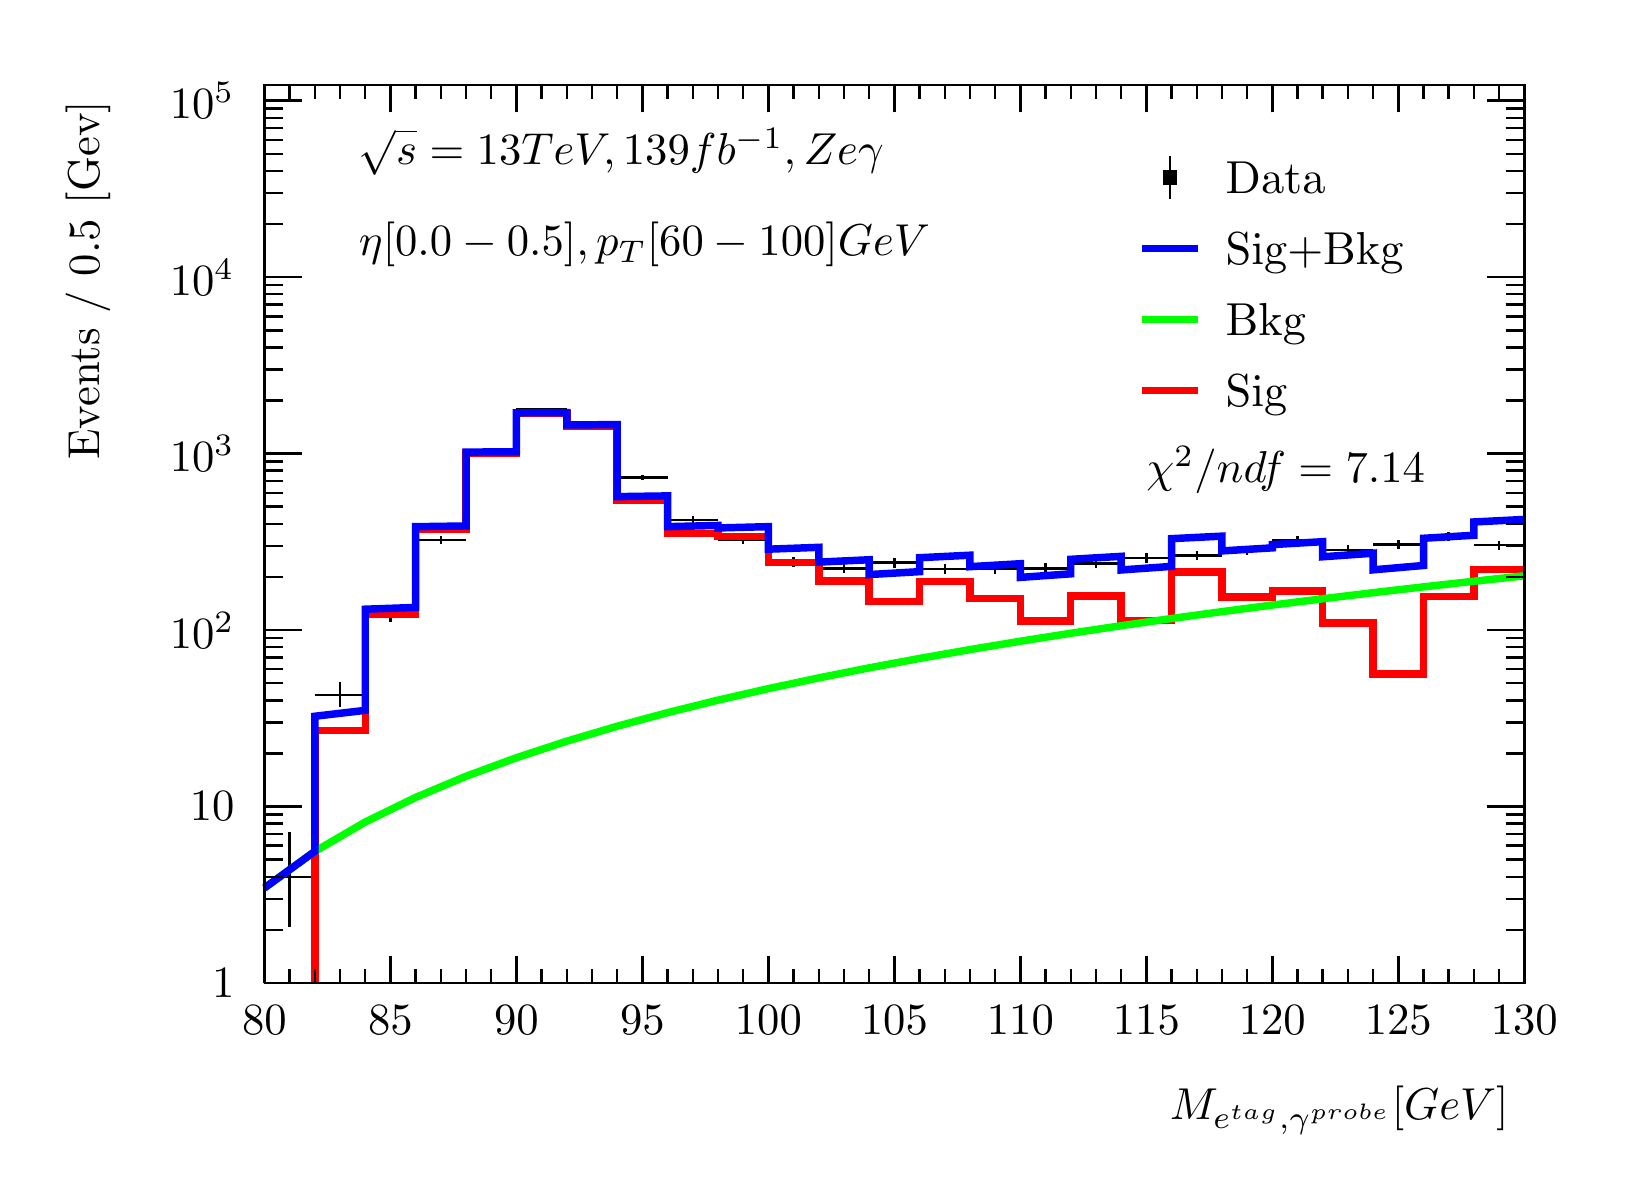
\begin{tikzpicture}
\pgfdeclareplotmark{cross} {
\pgfpathmoveto{\pgfpoint{-0.3\pgfplotmarksize}{\pgfplotmarksize}}
\pgfpathlineto{\pgfpoint{+0.3\pgfplotmarksize}{\pgfplotmarksize}}
\pgfpathlineto{\pgfpoint{+0.3\pgfplotmarksize}{0.3\pgfplotmarksize}}
\pgfpathlineto{\pgfpoint{+1\pgfplotmarksize}{0.3\pgfplotmarksize}}
\pgfpathlineto{\pgfpoint{+1\pgfplotmarksize}{-0.3\pgfplotmarksize}}
\pgfpathlineto{\pgfpoint{+0.3\pgfplotmarksize}{-0.3\pgfplotmarksize}}
\pgfpathlineto{\pgfpoint{+0.3\pgfplotmarksize}{-1.\pgfplotmarksize}}
\pgfpathlineto{\pgfpoint{-0.3\pgfplotmarksize}{-1.\pgfplotmarksize}}
\pgfpathlineto{\pgfpoint{-0.3\pgfplotmarksize}{-0.3\pgfplotmarksize}}
\pgfpathlineto{\pgfpoint{-1.\pgfplotmarksize}{-0.3\pgfplotmarksize}}
\pgfpathlineto{\pgfpoint{-1.\pgfplotmarksize}{0.3\pgfplotmarksize}}
\pgfpathlineto{\pgfpoint{-0.3\pgfplotmarksize}{0.3\pgfplotmarksize}}
\pgfpathclose
\pgfusepathqstroke
}
\pgfdeclareplotmark{cross*} {
\pgfpathmoveto{\pgfpoint{-0.3\pgfplotmarksize}{\pgfplotmarksize}}
\pgfpathlineto{\pgfpoint{+0.3\pgfplotmarksize}{\pgfplotmarksize}}
\pgfpathlineto{\pgfpoint{+0.3\pgfplotmarksize}{0.3\pgfplotmarksize}}
\pgfpathlineto{\pgfpoint{+1\pgfplotmarksize}{0.3\pgfplotmarksize}}
\pgfpathlineto{\pgfpoint{+1\pgfplotmarksize}{-0.3\pgfplotmarksize}}
\pgfpathlineto{\pgfpoint{+0.3\pgfplotmarksize}{-0.3\pgfplotmarksize}}
\pgfpathlineto{\pgfpoint{+0.3\pgfplotmarksize}{-1.\pgfplotmarksize}}
\pgfpathlineto{\pgfpoint{-0.3\pgfplotmarksize}{-1.\pgfplotmarksize}}
\pgfpathlineto{\pgfpoint{-0.3\pgfplotmarksize}{-0.3\pgfplotmarksize}}
\pgfpathlineto{\pgfpoint{-1.\pgfplotmarksize}{-0.3\pgfplotmarksize}}
\pgfpathlineto{\pgfpoint{-1.\pgfplotmarksize}{0.3\pgfplotmarksize}}
\pgfpathlineto{\pgfpoint{-0.3\pgfplotmarksize}{0.3\pgfplotmarksize}}
\pgfpathclose
\pgfusepathqfillstroke
}
\pgfdeclareplotmark{newstar} {
\pgfpathmoveto{\pgfqpoint{0pt}{\pgfplotmarksize}}
\pgfpathlineto{\pgfqpointpolar{44}{0.5\pgfplotmarksize}}
\pgfpathlineto{\pgfqpointpolar{18}{\pgfplotmarksize}}
\pgfpathlineto{\pgfqpointpolar{-20}{0.5\pgfplotmarksize}}
\pgfpathlineto{\pgfqpointpolar{-54}{\pgfplotmarksize}}
\pgfpathlineto{\pgfqpointpolar{-90}{0.5\pgfplotmarksize}}
\pgfpathlineto{\pgfqpointpolar{234}{\pgfplotmarksize}}
\pgfpathlineto{\pgfqpointpolar{198}{0.5\pgfplotmarksize}}
\pgfpathlineto{\pgfqpointpolar{162}{\pgfplotmarksize}}
\pgfpathlineto{\pgfqpointpolar{134}{0.5\pgfplotmarksize}}
\pgfpathclose
\pgfusepathqstroke
}
\pgfdeclareplotmark{newstar*} {
\pgfpathmoveto{\pgfqpoint{0pt}{\pgfplotmarksize}}
\pgfpathlineto{\pgfqpointpolar{44}{0.5\pgfplotmarksize}}
\pgfpathlineto{\pgfqpointpolar{18}{\pgfplotmarksize}}
\pgfpathlineto{\pgfqpointpolar{-20}{0.5\pgfplotmarksize}}
\pgfpathlineto{\pgfqpointpolar{-54}{\pgfplotmarksize}}
\pgfpathlineto{\pgfqpointpolar{-90}{0.5\pgfplotmarksize}}
\pgfpathlineto{\pgfqpointpolar{234}{\pgfplotmarksize}}
\pgfpathlineto{\pgfqpointpolar{198}{0.5\pgfplotmarksize}}
\pgfpathlineto{\pgfqpointpolar{162}{\pgfplotmarksize}}
\pgfpathlineto{\pgfqpointpolar{134}{0.5\pgfplotmarksize}}
\pgfpathclose
\pgfusepathqfillstroke
}
\definecolor{c}{rgb}{1,1,1};
\draw [color=c, fill=c] (0,0) rectangle (20,14.4361);
\draw [color=c, fill=c] (3,2.30977) rectangle (19,13.7143);
\definecolor{c}{rgb}{0,0,0};
\draw [c,line width=0.9] (3,2.30977) -- (3,13.7143) -- (19,13.7143) -- (19,2.30977) -- (3,2.30977);
\definecolor{c}{rgb}{1,1,1};
\draw [color=c, fill=c] (3,2.30977) rectangle (19,13.7143);
\definecolor{c}{rgb}{0,0,0};
\draw [c,line width=0.9] (3,2.30977) -- (3,13.7143) -- (19,13.7143) -- (19,2.30977) -- (3,2.30977);
\draw [c,line width=0.9] (3,2.30977) -- (19,2.30977);
\draw [c,line width=0.9] (3,2.65624) -- (3,2.30977);
\draw [c,line width=0.9] (3.32,2.48301) -- (3.32,2.30977);
\draw [c,line width=0.9] (3.64,2.48301) -- (3.64,2.30977);
\draw [c,line width=0.9] (3.96,2.48301) -- (3.96,2.30977);
\draw [c,line width=0.9] (4.28,2.48301) -- (4.28,2.30977);
\draw [c,line width=0.9] (4.6,2.65624) -- (4.6,2.30977);
\draw [c,line width=0.9] (4.92,2.48301) -- (4.92,2.30977);
\draw [c,line width=0.9] (5.24,2.48301) -- (5.24,2.30977);
\draw [c,line width=0.9] (5.56,2.48301) -- (5.56,2.30977);
\draw [c,line width=0.9] (5.88,2.48301) -- (5.88,2.30977);
\draw [c,line width=0.9] (6.2,2.65624) -- (6.2,2.30977);
\draw [c,line width=0.9] (6.52,2.48301) -- (6.52,2.30977);
\draw [c,line width=0.9] (6.84,2.48301) -- (6.84,2.30977);
\draw [c,line width=0.9] (7.16,2.48301) -- (7.16,2.30977);
\draw [c,line width=0.9] (7.48,2.48301) -- (7.48,2.30977);
\draw [c,line width=0.9] (7.8,2.65624) -- (7.8,2.30977);
\draw [c,line width=0.9] (8.12,2.48301) -- (8.12,2.30977);
\draw [c,line width=0.9] (8.44,2.48301) -- (8.44,2.30977);
\draw [c,line width=0.9] (8.76,2.48301) -- (8.76,2.30977);
\draw [c,line width=0.9] (9.08,2.48301) -- (9.08,2.30977);
\draw [c,line width=0.9] (9.4,2.65624) -- (9.4,2.30977);
\draw [c,line width=0.9] (9.72,2.48301) -- (9.72,2.30977);
\draw [c,line width=0.9] (10.04,2.48301) -- (10.04,2.30977);
\draw [c,line width=0.9] (10.36,2.48301) -- (10.36,2.30977);
\draw [c,line width=0.9] (10.68,2.48301) -- (10.68,2.30977);
\draw [c,line width=0.9] (11,2.65624) -- (11,2.30977);
\draw [c,line width=0.9] (11.32,2.48301) -- (11.32,2.30977);
\draw [c,line width=0.9] (11.64,2.48301) -- (11.64,2.30977);
\draw [c,line width=0.9] (11.96,2.48301) -- (11.96,2.30977);
\draw [c,line width=0.9] (12.28,2.48301) -- (12.28,2.30977);
\draw [c,line width=0.9] (12.6,2.65624) -- (12.6,2.30977);
\draw [c,line width=0.9] (12.92,2.48301) -- (12.92,2.30977);
\draw [c,line width=0.9] (13.24,2.48301) -- (13.24,2.30977);
\draw [c,line width=0.9] (13.56,2.48301) -- (13.56,2.30977);
\draw [c,line width=0.9] (13.88,2.48301) -- (13.88,2.30977);
\draw [c,line width=0.9] (14.2,2.65624) -- (14.2,2.30977);
\draw [c,line width=0.9] (14.52,2.48301) -- (14.52,2.30977);
\draw [c,line width=0.9] (14.84,2.48301) -- (14.84,2.30977);
\draw [c,line width=0.9] (15.16,2.48301) -- (15.16,2.30977);
\draw [c,line width=0.9] (15.48,2.48301) -- (15.48,2.30977);
\draw [c,line width=0.9] (15.8,2.65624) -- (15.8,2.30977);
\draw [c,line width=0.9] (16.12,2.48301) -- (16.12,2.30977);
\draw [c,line width=0.9] (16.44,2.48301) -- (16.44,2.30977);
\draw [c,line width=0.9] (16.76,2.48301) -- (16.76,2.30977);
\draw [c,line width=0.9] (17.08,2.48301) -- (17.08,2.30977);
\draw [c,line width=0.9] (17.4,2.65624) -- (17.4,2.30977);
\draw [c,line width=0.9] (17.72,2.48301) -- (17.72,2.30977);
\draw [c,line width=0.9] (18.04,2.48301) -- (18.04,2.30977);
\draw [c,line width=0.9] (18.36,2.48301) -- (18.36,2.30977);
\draw [c,line width=0.9] (18.68,2.48301) -- (18.68,2.30977);
\draw [c,line width=0.9] (19,2.65624) -- (19,2.30977);
\draw [anchor=base] (3,1.66015) node[scale=1.61424, color=c, rotate=0]{80};
\draw [anchor=base] (4.6,1.66015) node[scale=1.61424, color=c, rotate=0]{85};
\draw [anchor=base] (6.2,1.66015) node[scale=1.61424, color=c, rotate=0]{90};
\draw [anchor=base] (7.8,1.66015) node[scale=1.61424, color=c, rotate=0]{95};
\draw [anchor=base] (9.4,1.66015) node[scale=1.61424, color=c, rotate=0]{100};
\draw [anchor=base] (11,1.66015) node[scale=1.61424, color=c, rotate=0]{105};
\draw [anchor=base] (12.6,1.66015) node[scale=1.61424, color=c, rotate=0]{110};
\draw [anchor=base] (14.2,1.66015) node[scale=1.61424, color=c, rotate=0]{115};
\draw [anchor=base] (15.8,1.66015) node[scale=1.61424, color=c, rotate=0]{120};
\draw [anchor=base] (17.4,1.66015) node[scale=1.61424, color=c, rotate=0]{125};
\draw [anchor=base] (19,1.66015) node[scale=1.61424, color=c, rotate=0]{130};
\draw [anchor= east] (19,0.692932) node[scale=1.61424, color=c, rotate=0]{$M_{e^{tag}, \gamma^{probe}}  [GeV]$};
\draw [c,line width=0.9] (3,13.7143) -- (19,13.7143);
\draw [c,line width=0.9] (3,13.3678) -- (3,13.7143);
\draw [c,line width=0.9] (3.32,13.5411) -- (3.32,13.7143);
\draw [c,line width=0.9] (3.64,13.5411) -- (3.64,13.7143);
\draw [c,line width=0.9] (3.96,13.5411) -- (3.96,13.7143);
\draw [c,line width=0.9] (4.28,13.5411) -- (4.28,13.7143);
\draw [c,line width=0.9] (4.6,13.3678) -- (4.6,13.7143);
\draw [c,line width=0.9] (4.92,13.5411) -- (4.92,13.7143);
\draw [c,line width=0.9] (5.24,13.5411) -- (5.24,13.7143);
\draw [c,line width=0.9] (5.56,13.5411) -- (5.56,13.7143);
\draw [c,line width=0.9] (5.88,13.5411) -- (5.88,13.7143);
\draw [c,line width=0.9] (6.2,13.3678) -- (6.2,13.7143);
\draw [c,line width=0.9] (6.52,13.5411) -- (6.52,13.7143);
\draw [c,line width=0.9] (6.84,13.5411) -- (6.84,13.7143);
\draw [c,line width=0.9] (7.16,13.5411) -- (7.16,13.7143);
\draw [c,line width=0.9] (7.48,13.5411) -- (7.48,13.7143);
\draw [c,line width=0.9] (7.8,13.3678) -- (7.8,13.7143);
\draw [c,line width=0.9] (8.12,13.5411) -- (8.12,13.7143);
\draw [c,line width=0.9] (8.44,13.5411) -- (8.44,13.7143);
\draw [c,line width=0.9] (8.76,13.5411) -- (8.76,13.7143);
\draw [c,line width=0.9] (9.08,13.5411) -- (9.08,13.7143);
\draw [c,line width=0.9] (9.4,13.3678) -- (9.4,13.7143);
\draw [c,line width=0.9] (9.72,13.5411) -- (9.72,13.7143);
\draw [c,line width=0.9] (10.04,13.5411) -- (10.04,13.7143);
\draw [c,line width=0.9] (10.36,13.5411) -- (10.36,13.7143);
\draw [c,line width=0.9] (10.68,13.5411) -- (10.68,13.7143);
\draw [c,line width=0.9] (11,13.3678) -- (11,13.7143);
\draw [c,line width=0.9] (11.32,13.5411) -- (11.32,13.7143);
\draw [c,line width=0.9] (11.64,13.5411) -- (11.64,13.7143);
\draw [c,line width=0.9] (11.96,13.5411) -- (11.96,13.7143);
\draw [c,line width=0.9] (12.28,13.5411) -- (12.28,13.7143);
\draw [c,line width=0.9] (12.6,13.3678) -- (12.6,13.7143);
\draw [c,line width=0.9] (12.92,13.5411) -- (12.92,13.7143);
\draw [c,line width=0.9] (13.24,13.5411) -- (13.24,13.7143);
\draw [c,line width=0.9] (13.56,13.5411) -- (13.56,13.7143);
\draw [c,line width=0.9] (13.88,13.5411) -- (13.88,13.7143);
\draw [c,line width=0.9] (14.2,13.3678) -- (14.2,13.7143);
\draw [c,line width=0.9] (14.52,13.5411) -- (14.52,13.7143);
\draw [c,line width=0.9] (14.84,13.5411) -- (14.84,13.7143);
\draw [c,line width=0.9] (15.16,13.5411) -- (15.16,13.7143);
\draw [c,line width=0.9] (15.48,13.5411) -- (15.48,13.7143);
\draw [c,line width=0.9] (15.8,13.3678) -- (15.8,13.7143);
\draw [c,line width=0.9] (16.12,13.5411) -- (16.12,13.7143);
\draw [c,line width=0.9] (16.44,13.5411) -- (16.44,13.7143);
\draw [c,line width=0.9] (16.76,13.5411) -- (16.76,13.7143);
\draw [c,line width=0.9] (17.08,13.5411) -- (17.08,13.7143);
\draw [c,line width=0.9] (17.4,13.3678) -- (17.4,13.7143);
\draw [c,line width=0.9] (17.72,13.5411) -- (17.72,13.7143);
\draw [c,line width=0.9] (18.04,13.5411) -- (18.04,13.7143);
\draw [c,line width=0.9] (18.36,13.5411) -- (18.36,13.7143);
\draw [c,line width=0.9] (18.68,13.5411) -- (18.68,13.7143);
\draw [c,line width=0.9] (19,13.3678) -- (19,13.7143);
\draw [c,line width=0.9] (3,2.30977) -- (3,13.7143);
\draw [c,line width=0.9] (3.474,2.30978) -- (3,2.30978);
\draw [anchor= east] (2.82,2.30978) node[scale=1.61424, color=c, rotate=0]{1};
\draw [c,line width=0.9] (3.237,2.98447) -- (3,2.98447);
\draw [c,line width=0.9] (3.237,3.37914) -- (3,3.37914);
\draw [c,line width=0.9] (3.237,3.65916) -- (3,3.65916);
\draw [c,line width=0.9] (3.237,3.87637) -- (3,3.87637);
\draw [c,line width=0.9] (3.237,4.05383) -- (3,4.05383);
\draw [c,line width=0.9] (3.237,4.20388) -- (3,4.20388);
\draw [c,line width=0.9] (3.237,4.33386) -- (3,4.33386);
\draw [c,line width=0.9] (3.237,4.4485) -- (3,4.4485);
\draw [c,line width=0.9] (3.474,4.55106) -- (3,4.55106);
\draw [anchor= east] (2.82,4.55106) node[scale=1.61424, color=c, rotate=0]{10};
\draw [c,line width=0.9] (3.237,5.22575) -- (3,5.22575);
\draw [c,line width=0.9] (3.237,5.62042) -- (3,5.62042);
\draw [c,line width=0.9] (3.237,5.90045) -- (3,5.90045);
\draw [c,line width=0.9] (3.237,6.11765) -- (3,6.11765);
\draw [c,line width=0.9] (3.237,6.29512) -- (3,6.29512);
\draw [c,line width=0.9] (3.237,6.44516) -- (3,6.44516);
\draw [c,line width=0.9] (3.237,6.57514) -- (3,6.57514);
\draw [c,line width=0.9] (3.237,6.68979) -- (3,6.68979);
\draw [c,line width=0.9] (3.474,6.79234) -- (3,6.79234);
\draw [anchor= east] (2.82,6.79234) node[scale=1.61424, color=c, rotate=0]{$10^{2}$};
\draw [c,line width=0.9] (3.237,7.46704) -- (3,7.46704);
\draw [c,line width=0.9] (3.237,7.86171) -- (3,7.86171);
\draw [c,line width=0.9] (3.237,8.14173) -- (3,8.14173);
\draw [c,line width=0.9] (3.237,8.35893) -- (3,8.35893);
\draw [c,line width=0.9] (3.237,8.5364) -- (3,8.5364);
\draw [c,line width=0.9] (3.237,8.68645) -- (3,8.68645);
\draw [c,line width=0.9] (3.237,8.81642) -- (3,8.81642);
\draw [c,line width=0.9] (3.237,8.93107) -- (3,8.93107);
\draw [c,line width=0.9] (3.474,9.03363) -- (3,9.03363);
\draw [anchor= east] (2.82,9.03363) node[scale=1.61424, color=c, rotate=0]{$10^{3}$};
\draw [c,line width=0.9] (3.237,9.70832) -- (3,9.70832);
\draw [c,line width=0.9] (3.237,10.103) -- (3,10.103);
\draw [c,line width=0.9] (3.237,10.383) -- (3,10.383);
\draw [c,line width=0.9] (3.237,10.6002) -- (3,10.6002);
\draw [c,line width=0.9] (3.237,10.7777) -- (3,10.7777);
\draw [c,line width=0.9] (3.237,10.9277) -- (3,10.9277);
\draw [c,line width=0.9] (3.237,11.0577) -- (3,11.0577);
\draw [c,line width=0.9] (3.237,11.1724) -- (3,11.1724);
\draw [c,line width=0.9] (3.474,11.2749) -- (3,11.2749);
\draw [anchor= east] (2.82,11.2749) node[scale=1.61424, color=c, rotate=0]{$10^{4}$};
\draw [c,line width=0.9] (3.237,11.9496) -- (3,11.9496);
\draw [c,line width=0.9] (3.237,12.3443) -- (3,12.3443);
\draw [c,line width=0.9] (3.237,12.6243) -- (3,12.6243);
\draw [c,line width=0.9] (3.237,12.8415) -- (3,12.8415);
\draw [c,line width=0.9] (3.237,13.019) -- (3,13.019);
\draw [c,line width=0.9] (3.237,13.169) -- (3,13.169);
\draw [c,line width=0.9] (3.237,13.299) -- (3,13.299);
\draw [c,line width=0.9] (3.237,13.4136) -- (3,13.4136);
\draw [c,line width=0.9] (3.474,13.5162) -- (3,13.5162);
\draw [anchor= east] (2.82,13.5162) node[scale=1.61424, color=c, rotate=0]{$10^{5}$};
\draw [anchor= east] (0.76,13.7143) node[scale=1.61424, color=c, rotate=90]{Events / 0.5 [Gev]};
\draw [c,line width=0.9] (19,2.30977) -- (19,13.7143);
\draw [c,line width=0.9] (18.526,2.30978) -- (19,2.30978);
\draw [c,line width=0.9] (18.763,2.98447) -- (19,2.98447);
\draw [c,line width=0.9] (18.763,3.37914) -- (19,3.37914);
\draw [c,line width=0.9] (18.763,3.65916) -- (19,3.65916);
\draw [c,line width=0.9] (18.763,3.87637) -- (19,3.87637);
\draw [c,line width=0.9] (18.763,4.05383) -- (19,4.05383);
\draw [c,line width=0.9] (18.763,4.20388) -- (19,4.20388);
\draw [c,line width=0.9] (18.763,4.33386) -- (19,4.33386);
\draw [c,line width=0.9] (18.763,4.4485) -- (19,4.4485);
\draw [c,line width=0.9] (18.526,4.55106) -- (19,4.55106);
\draw [c,line width=0.9] (18.763,5.22575) -- (19,5.22575);
\draw [c,line width=0.9] (18.763,5.62042) -- (19,5.62042);
\draw [c,line width=0.9] (18.763,5.90045) -- (19,5.90045);
\draw [c,line width=0.9] (18.763,6.11765) -- (19,6.11765);
\draw [c,line width=0.9] (18.763,6.29512) -- (19,6.29512);
\draw [c,line width=0.9] (18.763,6.44516) -- (19,6.44516);
\draw [c,line width=0.9] (18.763,6.57514) -- (19,6.57514);
\draw [c,line width=0.9] (18.763,6.68979) -- (19,6.68979);
\draw [c,line width=0.9] (18.526,6.79234) -- (19,6.79234);
\draw [c,line width=0.9] (18.763,7.46704) -- (19,7.46704);
\draw [c,line width=0.9] (18.763,7.86171) -- (19,7.86171);
\draw [c,line width=0.9] (18.763,8.14173) -- (19,8.14173);
\draw [c,line width=0.9] (18.763,8.35893) -- (19,8.35893);
\draw [c,line width=0.9] (18.763,8.5364) -- (19,8.5364);
\draw [c,line width=0.9] (18.763,8.68645) -- (19,8.68645);
\draw [c,line width=0.9] (18.763,8.81642) -- (19,8.81642);
\draw [c,line width=0.9] (18.763,8.93107) -- (19,8.93107);
\draw [c,line width=0.9] (18.526,9.03363) -- (19,9.03363);
\draw [c,line width=0.9] (18.763,9.70832) -- (19,9.70832);
\draw [c,line width=0.9] (18.763,10.103) -- (19,10.103);
\draw [c,line width=0.9] (18.763,10.383) -- (19,10.383);
\draw [c,line width=0.9] (18.763,10.6002) -- (19,10.6002);
\draw [c,line width=0.9] (18.763,10.7777) -- (19,10.7777);
\draw [c,line width=0.9] (18.763,10.9277) -- (19,10.9277);
\draw [c,line width=0.9] (18.763,11.0577) -- (19,11.0577);
\draw [c,line width=0.9] (18.763,11.1724) -- (19,11.1724);
\draw [c,line width=0.9] (18.526,11.2749) -- (19,11.2749);
\draw [c,line width=0.9] (18.763,11.9496) -- (19,11.9496);
\draw [c,line width=0.9] (18.763,12.3443) -- (19,12.3443);
\draw [c,line width=0.9] (18.763,12.6243) -- (19,12.6243);
\draw [c,line width=0.9] (18.763,12.8415) -- (19,12.8415);
\draw [c,line width=0.9] (18.763,13.019) -- (19,13.019);
\draw [c,line width=0.9] (18.763,13.169) -- (19,13.169);
\draw [c,line width=0.9] (18.763,13.299) -- (19,13.299);
\draw [c,line width=0.9] (18.763,13.4136) -- (19,13.4136);
\draw [c,line width=0.9] (18.526,13.5162) -- (19,13.5162);
\draw [c,line width=0.9] (3.32,3.65916) -- (3,3.65916);
\draw [c,line width=0.9] (3,3.65916) -- (3,3.65916);
\draw [c,line width=0.9] (3.32,3.65916) -- (3.64,3.65916);
\draw [c,line width=0.9] (3.64,3.65916) -- (3.64,3.65916);
\draw [c,line width=0.9] (3.32,3.65916) -- (3.32,4.22625);
\draw [c,line width=0.9] (3.32,4.22625) -- (3.32,4.22625);
\draw [c,line width=0.9] (3.32,3.65916) -- (3.32,3.02529);
\draw [c,line width=0.9] (3.32,3.02529) -- (3.32,3.02529);
\draw [c,line width=0.9] (3.96,5.97084) -- (3.64,5.97084);
\draw [c,line width=0.9] (3.64,5.97084) -- (3.64,5.97084);
\draw [c,line width=0.9] (3.96,5.97084) -- (4.28,5.97084);
\draw [c,line width=0.9] (4.28,5.97084) -- (4.28,5.97084);
\draw [c,line width=0.9] (3.96,5.97084) -- (3.96,6.12942);
\draw [c,line width=0.9] (3.96,6.12942) -- (3.96,6.12942);
\draw [c,line width=0.9] (3.96,5.97084) -- (3.96,5.81047);
\draw [c,line width=0.9] (3.96,5.81047) -- (3.96,5.81047);
\draw [c,line width=0.9] (4.6,6.97789) -- (4.28,6.97789);
\draw [c,line width=0.9] (4.28,6.97789) -- (4.28,6.97789);
\draw [c,line width=0.9] (4.6,6.97789) -- (4.92,6.97789);
\draw [c,line width=0.9] (4.92,6.97789) -- (4.92,6.97789);
\draw [c,line width=0.9] (4.6,6.97789) -- (4.6,7.06635);
\draw [c,line width=0.9] (4.6,7.06635) -- (4.6,7.06635);
\draw [c,line width=0.9] (4.6,6.97789) -- (4.6,6.88943);
\draw [c,line width=0.9] (4.6,6.88943) -- (4.6,6.88943);
\draw [c,line width=0.9] (5.24,7.93662) -- (4.92,7.93662);
\draw [c,line width=0.9] (4.92,7.93662) -- (4.92,7.93662);
\draw [c,line width=0.9] (5.24,7.93662) -- (5.56,7.93662);
\draw [c,line width=0.9] (5.56,7.93662) -- (5.56,7.93662);
\draw [c,line width=0.9] (5.24,7.93662) -- (5.24,7.99069);
\draw [c,line width=0.9] (5.24,7.99069) -- (5.24,7.99069);
\draw [c,line width=0.9] (5.24,7.93662) -- (5.24,7.88255);
\draw [c,line width=0.9] (5.24,7.88255) -- (5.24,7.88255);
\draw [c,line width=0.9] (5.88,9.01594) -- (5.56,9.01594);
\draw [c,line width=0.9] (5.56,9.01594) -- (5.56,9.01594);
\draw [c,line width=0.9] (5.88,9.01594) -- (6.2,9.01594);
\draw [c,line width=0.9] (6.2,9.01594) -- (6.2,9.01594);
\draw [c,line width=0.9] (5.88,9.01594) -- (5.88,9.047);
\draw [c,line width=0.9] (5.88,9.047) -- (5.88,9.047);
\draw [c,line width=0.9] (5.88,9.01594) -- (5.88,8.98488);
\draw [c,line width=0.9] (5.88,8.98488) -- (5.88,8.98488);
\draw [c,line width=0.9] (6.52,9.59105) -- (6.2,9.59105);
\draw [c,line width=0.9] (6.2,9.59105) -- (6.2,9.59105);
\draw [c,line width=0.9] (6.52,9.59105) -- (6.84,9.59105);
\draw [c,line width=0.9] (6.84,9.59105) -- (6.84,9.59105);
\draw [c,line width=0.9] (6.52,9.59105) -- (6.52,9.61417);
\draw [c,line width=0.9] (6.52,9.61417) -- (6.52,9.61417);
\draw [c,line width=0.9] (6.52,9.59105) -- (6.52,9.56794);
\draw [c,line width=0.9] (6.52,9.56794) -- (6.52,9.56794);
\draw [c,line width=0.9] (7.16,9.42244) -- (6.84,9.42244);
\draw [c,line width=0.9] (6.84,9.42244) -- (6.84,9.42244);
\draw [c,line width=0.9] (7.16,9.42244) -- (7.48,9.42244);
\draw [c,line width=0.9] (7.48,9.42244) -- (7.48,9.42244);
\draw [c,line width=0.9] (7.16,9.42244) -- (7.16,9.44765);
\draw [c,line width=0.9] (7.16,9.44765) -- (7.16,9.44765);
\draw [c,line width=0.9] (7.16,9.42244) -- (7.16,9.39723);
\draw [c,line width=0.9] (7.16,9.39723) -- (7.16,9.39723);
\draw [c,line width=0.9] (7.8,8.72996) -- (7.48,8.72996);
\draw [c,line width=0.9] (7.48,8.72996) -- (7.48,8.72996);
\draw [c,line width=0.9] (7.8,8.72996) -- (8.12,8.72996);
\draw [c,line width=0.9] (8.12,8.72996) -- (8.12,8.72996);
\draw [c,line width=0.9] (7.8,8.72996) -- (7.8,8.76593);
\draw [c,line width=0.9] (7.8,8.76593) -- (7.8,8.76593);
\draw [c,line width=0.9] (7.8,8.72996) -- (7.8,8.69398);
\draw [c,line width=0.9] (7.8,8.69398) -- (7.8,8.69398);
\draw [c,line width=0.9] (8.44,8.18922) -- (8.12,8.18922);
\draw [c,line width=0.9] (8.12,8.18922) -- (8.12,8.18922);
\draw [c,line width=0.9] (8.44,8.18922) -- (8.76,8.18922);
\draw [c,line width=0.9] (8.76,8.18922) -- (8.76,8.18922);
\draw [c,line width=0.9] (8.44,8.18922) -- (8.44,8.23671);
\draw [c,line width=0.9] (8.44,8.23671) -- (8.44,8.23671);
\draw [c,line width=0.9] (8.44,8.18922) -- (8.44,8.14173);
\draw [c,line width=0.9] (8.44,8.14173) -- (8.44,8.14173);
\draw [c,line width=0.9] (9.08,7.94261) -- (8.76,7.94261);
\draw [c,line width=0.9] (8.76,7.94261) -- (8.76,7.94261);
\draw [c,line width=0.9] (9.08,7.94261) -- (9.4,7.94261);
\draw [c,line width=0.9] (9.4,7.94261) -- (9.4,7.94261);
\draw [c,line width=0.9] (9.08,7.94261) -- (9.08,7.99651);
\draw [c,line width=0.9] (9.08,7.99651) -- (9.08,7.99651);
\draw [c,line width=0.9] (9.08,7.94261) -- (9.08,7.8887);
\draw [c,line width=0.9] (9.08,7.8887) -- (9.08,7.8887);
\draw [c,line width=0.9] (9.72,7.66059) -- (9.4,7.66059);
\draw [c,line width=0.9] (9.4,7.66059) -- (9.4,7.66059);
\draw [c,line width=0.9] (9.72,7.66059) -- (10.04,7.66059);
\draw [c,line width=0.9] (10.04,7.66059) -- (10.04,7.66059);
\draw [c,line width=0.9] (9.72,7.66059) -- (9.72,7.7229);
\draw [c,line width=0.9] (9.72,7.7229) -- (9.72,7.7229);
\draw [c,line width=0.9] (9.72,7.66059) -- (9.72,7.59829);
\draw [c,line width=0.9] (9.72,7.59829) -- (9.72,7.59829);
\draw [c,line width=0.9] (10.36,7.57735) -- (10.04,7.57735);
\draw [c,line width=0.9] (10.04,7.57735) -- (10.04,7.57735);
\draw [c,line width=0.9] (10.36,7.57735) -- (10.68,7.57735);
\draw [c,line width=0.9] (10.68,7.57735) -- (10.68,7.57735);
\draw [c,line width=0.9] (10.36,7.57735) -- (10.36,7.64237);
\draw [c,line width=0.9] (10.36,7.64237) -- (10.36,7.64237);
\draw [c,line width=0.9] (10.36,7.57735) -- (10.36,7.51232);
\draw [c,line width=0.9] (10.36,7.51232) -- (10.36,7.51232);
\draw [c,line width=0.9] (11,7.64855) -- (10.68,7.64855);
\draw [c,line width=0.9] (10.68,7.64855) -- (10.68,7.64855);
\draw [c,line width=0.9] (11,7.64855) -- (11.32,7.64855);
\draw [c,line width=0.9] (11.32,7.64855) -- (11.32,7.64855);
\draw [c,line width=0.9] (11,7.64855) -- (11,7.71124);
\draw [c,line width=0.9] (11,7.71124) -- (11,7.71124);
\draw [c,line width=0.9] (11,7.64855) -- (11,7.58586);
\draw [c,line width=0.9] (11,7.58586) -- (11,7.58586);
\draw [c,line width=0.9] (11.64,7.56862) -- (11.32,7.56862);
\draw [c,line width=0.9] (11.32,7.56862) -- (11.32,7.56862);
\draw [c,line width=0.9] (11.64,7.56862) -- (11.96,7.56862);
\draw [c,line width=0.9] (11.96,7.56862) -- (11.96,7.56862);
\draw [c,line width=0.9] (11.64,7.56862) -- (11.64,7.63393);
\draw [c,line width=0.9] (11.64,7.63393) -- (11.64,7.63393);
\draw [c,line width=0.9] (11.64,7.56862) -- (11.64,7.5033);
\draw [c,line width=0.9] (11.64,7.5033) -- (11.64,7.5033);
\draw [c,line width=0.9] (12.28,7.57299) -- (11.96,7.57299);
\draw [c,line width=0.9] (11.96,7.57299) -- (11.96,7.57299);
\draw [c,line width=0.9] (12.28,7.57299) -- (12.6,7.57299);
\draw [c,line width=0.9] (12.6,7.57299) -- (12.6,7.57299);
\draw [c,line width=0.9] (12.28,7.57299) -- (12.28,7.63816);
\draw [c,line width=0.9] (12.28,7.63816) -- (12.28,7.63816);
\draw [c,line width=0.9] (12.28,7.57299) -- (12.28,7.50782);
\draw [c,line width=0.9] (12.28,7.50782) -- (12.28,7.50782);
\draw [c,line width=0.9] (12.92,7.57735) -- (12.6,7.57735);
\draw [c,line width=0.9] (12.6,7.57735) -- (12.6,7.57735);
\draw [c,line width=0.9] (12.92,7.57735) -- (13.24,7.57735);
\draw [c,line width=0.9] (13.24,7.57735) -- (13.24,7.57735);
\draw [c,line width=0.9] (12.92,7.57735) -- (12.92,7.64237);
\draw [c,line width=0.9] (12.92,7.64237) -- (12.92,7.64237);
\draw [c,line width=0.9] (12.92,7.57735) -- (12.92,7.51232);
\draw [c,line width=0.9] (12.92,7.51232) -- (12.92,7.51232);
\draw [c,line width=0.9] (13.56,7.64044) -- (13.24,7.64044);
\draw [c,line width=0.9] (13.24,7.64044) -- (13.24,7.64044);
\draw [c,line width=0.9] (13.56,7.64044) -- (13.88,7.64044);
\draw [c,line width=0.9] (13.88,7.64044) -- (13.88,7.64044);
\draw [c,line width=0.9] (13.56,7.64044) -- (13.56,7.70339);
\draw [c,line width=0.9] (13.56,7.70339) -- (13.56,7.70339);
\draw [c,line width=0.9] (13.56,7.64044) -- (13.56,7.57749);
\draw [c,line width=0.9] (13.56,7.57749) -- (13.56,7.57749);
\draw [c,line width=0.9] (14.2,7.71112) -- (13.88,7.71112);
\draw [c,line width=0.9] (13.88,7.71112) -- (13.88,7.71112);
\draw [c,line width=0.9] (14.2,7.71112) -- (14.52,7.71112);
\draw [c,line width=0.9] (14.52,7.71112) -- (14.52,7.71112);
\draw [c,line width=0.9] (14.2,7.71112) -- (14.2,7.77183);
\draw [c,line width=0.9] (14.2,7.77183) -- (14.2,7.77183);
\draw [c,line width=0.9] (14.2,7.71112) -- (14.2,7.65041);
\draw [c,line width=0.9] (14.2,7.65041) -- (14.2,7.65041);
\draw [c,line width=0.9] (14.84,7.73728) -- (14.52,7.73728);
\draw [c,line width=0.9] (14.52,7.73728) -- (14.52,7.73728);
\draw [c,line width=0.9] (14.84,7.73728) -- (15.16,7.73728);
\draw [c,line width=0.9] (15.16,7.73728) -- (15.16,7.73728);
\draw [c,line width=0.9] (14.84,7.73728) -- (14.84,7.79717);
\draw [c,line width=0.9] (14.84,7.79717) -- (14.84,7.79717);
\draw [c,line width=0.9] (14.84,7.73728) -- (14.84,7.67738);
\draw [c,line width=0.9] (14.84,7.67738) -- (14.84,7.67738);
\draw [c,line width=0.9] (15.48,7.80836) -- (15.16,7.80836);
\draw [c,line width=0.9] (15.16,7.80836) -- (15.16,7.80836);
\draw [c,line width=0.9] (15.48,7.80836) -- (15.8,7.80836);
\draw [c,line width=0.9] (15.8,7.80836) -- (15.8,7.80836);
\draw [c,line width=0.9] (15.48,7.80836) -- (15.48,7.86611);
\draw [c,line width=0.9] (15.48,7.86611) -- (15.48,7.86611);
\draw [c,line width=0.9] (15.48,7.80836) -- (15.48,7.75061);
\draw [c,line width=0.9] (15.48,7.75061) -- (15.48,7.75061);
\draw [c,line width=0.9] (16.12,7.93361) -- (15.8,7.93361);
\draw [c,line width=0.9] (15.8,7.93361) -- (15.8,7.93361);
\draw [c,line width=0.9] (16.12,7.93361) -- (16.44,7.93361);
\draw [c,line width=0.9] (16.44,7.93361) -- (16.44,7.93361);
\draw [c,line width=0.9] (16.12,7.93361) -- (16.12,7.98776);
\draw [c,line width=0.9] (16.12,7.98776) -- (16.12,7.98776);
\draw [c,line width=0.9] (16.12,7.93361) -- (16.12,7.87946);
\draw [c,line width=0.9] (16.12,7.87946) -- (16.12,7.87946);
\draw [c,line width=0.9] (16.76,7.81178) -- (16.44,7.81178);
\draw [c,line width=0.9] (16.44,7.81178) -- (16.44,7.81178);
\draw [c,line width=0.9] (16.76,7.81178) -- (17.08,7.81178);
\draw [c,line width=0.9] (17.08,7.81178) -- (17.08,7.81178);
\draw [c,line width=0.9] (16.76,7.81178) -- (16.76,7.86943);
\draw [c,line width=0.9] (16.76,7.86943) -- (16.76,7.86943);
\draw [c,line width=0.9] (16.76,7.81178) -- (16.76,7.75413);
\draw [c,line width=0.9] (16.76,7.75413) -- (16.76,7.75413);
\draw [c,line width=0.9] (17.4,7.87779) -- (17.08,7.87779);
\draw [c,line width=0.9] (17.08,7.87779) -- (17.08,7.87779);
\draw [c,line width=0.9] (17.4,7.87779) -- (17.72,7.87779);
\draw [c,line width=0.9] (17.72,7.87779) -- (17.72,7.87779);
\draw [c,line width=0.9] (17.4,7.87779) -- (17.4,7.93352);
\draw [c,line width=0.9] (17.4,7.93352) -- (17.4,7.93352);
\draw [c,line width=0.9] (17.4,7.87779) -- (17.4,7.82207);
\draw [c,line width=0.9] (17.4,7.82207) -- (17.4,7.82207);
\draw [c,line width=0.9] (18.04,7.98067) -- (17.72,7.98067);
\draw [c,line width=0.9] (17.72,7.98067) -- (17.72,7.98067);
\draw [c,line width=0.9] (18.04,7.98067) -- (18.36,7.98067);
\draw [c,line width=0.9] (18.36,7.98067) -- (18.36,7.98067);
\draw [c,line width=0.9] (18.04,7.98067) -- (18.04,8.03353);
\draw [c,line width=0.9] (18.04,8.03353) -- (18.04,8.03353);
\draw [c,line width=0.9] (18.04,7.98067) -- (18.04,7.92781);
\draw [c,line width=0.9] (18.04,7.92781) -- (18.04,7.92781);
\draw [c,line width=0.9] (18.68,7.87139) -- (18.36,7.87139);
\draw [c,line width=0.9] (18.36,7.87139) -- (18.36,7.87139);
\draw [c,line width=0.9] (18.68,7.87139) -- (19,7.87139);
\draw [c,line width=0.9] (19,7.87139) -- (19,7.87139);
\draw [c,line width=0.9] (18.68,7.87139) -- (18.68,7.9273);
\draw [c,line width=0.9] (18.68,7.9273) -- (18.68,7.9273);
\draw [c,line width=0.9] (18.68,7.87139) -- (18.68,7.81548);
\draw [c,line width=0.9] (18.68,7.81548) -- (18.68,7.81548);
\foreach \P in {(3.32,3.65916), (3.96,5.97084), (4.6,6.97789), (5.24,7.93662), (5.88,9.01594), (6.52,9.59105), (7.16,9.42244), (7.8,8.72996), (8.44,8.18922), (9.08,7.94261), (9.72,7.66059), (10.36,7.57735), (11,7.64855), (11.64,7.56862),
 (12.28,7.57299), (12.92,7.57735), (13.56,7.64044), (14.2,7.71112), (14.84,7.73728), (15.48,7.80836), (16.12,7.93361), (16.76,7.81178), (17.4,7.87779), (18.04,7.98067), (18.68,7.87139)}{\draw[mark options={color=c,fill=c},mark size=2.882883pt,mark=]
 plot coordinates {\P};}
\definecolor{c}{rgb}{1,0,0};
\draw [c,line width=2.7] (3.64,2.30977) -- (3.64,5.51487);
\draw [c,line width=2.7] (3.64,5.51487) -- (4.28,5.51487) -- (4.28,6.99504) -- (4.92,6.99504) -- (4.92,8.0768) -- (5.56,8.0768) -- (5.56,9.03869) -- (6.2,9.03869) -- (6.2,9.54112) -- (6.84,9.54112) -- (6.84,9.38238) -- (7.48,9.38238) --
 (7.48,8.43727) -- (8.12,8.43727) -- (8.12,8.01608) -- (8.76,8.01608) -- (8.76,7.98073) -- (9.4,7.98073) -- (9.4,7.64771) -- (10.04,7.64771) -- (10.04,7.41328) -- (10.68,7.41328) -- (10.68,7.15587) -- (11.32,7.15587) -- (11.32,7.40735) --
 (11.96,7.40735) -- (11.96,7.19492) -- (12.6,7.19492) -- (12.6,6.90613) -- (13.24,6.90613) -- (13.24,7.22418) -- (13.88,7.22418) -- (13.88,6.91353) -- (14.52,6.91353) -- (14.52,7.53019) -- (15.16,7.53019) -- (15.16,7.21107) -- (15.8,7.21107) --
 (15.8,7.2882) -- (16.44,7.2882) -- (16.44,6.88266) -- (17.08,6.88266) -- (17.08,6.23769) -- (17.72,6.23769) -- (17.72,7.22214) -- (18.36,7.22214) -- (18.36,7.56311) -- (19,7.56311) -- (19,7.56311) -- (19,7.56311) -- (19,7.56311);
\definecolor{c}{rgb}{0,1,0};
\draw [c,line width=2.7] (3,3.51772) -- (3,3.51772);
\draw [c,line width=2.7] (3,3.51772) -- (3,3.51772) -- (3.64,3.98183) -- (3.64,3.98183) -- (4.28,4.35484) -- (4.28,4.35484) -- (4.92,4.66705) -- (4.92,4.66705) -- (5.56,4.93566) -- (5.56,4.93566) -- (6.2,5.17145) -- (6.2,5.17145) -- (6.84,5.38161) --
 (6.84,5.38161) -- (7.48,5.57118) -- (7.48,5.57118) -- (8.12,5.74386) -- (8.12,5.74386) -- (8.76,5.90242) -- (8.76,5.90242) -- (9.4,6.049) -- (9.4,6.049) -- (10.04,6.1853) -- (10.04,6.1853) -- (10.68,6.31265) -- (10.68,6.31265) -- (11.32,6.43217) --
 (11.32,6.43217) -- (11.96,6.54476) -- (11.96,6.54476) -- (12.6,6.65118) -- (12.6,6.65118) -- (13.24,6.75209) -- (13.24,6.75209) -- (13.88,6.84801) -- (13.88,6.84801) -- (14.52,6.93942) -- (14.52,6.93942) -- (15.16,7.02673) -- (15.16,7.02673) --
 (15.8,7.11029) -- (15.8,7.11029) -- (16.44,7.1904) -- (16.44,7.1904) -- (17.08,7.26735) -- (17.08,7.26735) -- (17.72,7.34137) -- (17.72,7.34137) -- (18.36,7.41267) -- (18.36,7.41267) -- (19,7.48146) -- (19,7.48146) -- (19,7.48146) -- (19,7.48146);
\definecolor{c}{rgb}{0,0,1};
\draw [c,line width=2.7] (3,3.51772) -- (3,3.51772);
\draw [c,line width=2.7] (3,3.51772) -- (3,3.51772) -- (3.64,3.98183) -- (3.64,5.69801) -- (4.28,5.77301) -- (4.28,7.05759) -- (4.92,7.08024) -- (4.92,8.10567) -- (5.56,8.11467) -- (5.56,9.05297) -- (6.2,9.05684) -- (6.2,9.55199) -- (6.84,9.55459) --
 (6.84,9.39822) -- (7.48,9.40159) -- (7.48,8.4872) -- (8.12,8.4966) -- (8.12,8.10608) -- (8.76,8.12117) -- (8.76,8.0895) -- (9.4,8.10609) -- (9.4,7.8199) -- (10.04,7.84334) -- (10.04,7.656) -- (10.68,7.68558) -- (10.68,7.49754) -- (11.32,7.53448) --
 (11.32,7.71178) -- (11.96,7.74332) -- (11.96,7.59784) -- (12.6,7.63523) -- (12.6,7.46167) -- (13.24,7.50685) -- (13.24,7.69117) -- (13.88,7.72885) -- (13.88,7.55602) -- (14.52,7.60126) -- (14.52,7.95364) -- (15.16,7.98535) -- (15.16,7.79795) --
 (15.8,7.83668) -- (15.8,7.878) -- (16.44,7.91522) -- (16.44,7.72334) -- (17.08,7.76858) -- (17.08,7.55745) -- (17.72,7.61292) -- (17.72,7.95827) -- (18.36,7.99676) -- (18.36,8.16549) -- (19,8.19783) -- (19,8.19783) -- (19,8.19783) -- (19,8.19783);
\definecolor{c}{rgb}{0,0,0};
\draw [c,line width=0.9] (3,2.30977) -- (19,2.30977);
\draw [c,line width=0.9] (3,2.65624) -- (3,2.30977);
\draw [c,line width=0.9] (3.32,2.48301) -- (3.32,2.30977);
\draw [c,line width=0.9] (3.64,2.48301) -- (3.64,2.30977);
\draw [c,line width=0.9] (3.96,2.48301) -- (3.96,2.30977);
\draw [c,line width=0.9] (4.28,2.48301) -- (4.28,2.30977);
\draw [c,line width=0.9] (4.6,2.65624) -- (4.6,2.30977);
\draw [c,line width=0.9] (4.92,2.48301) -- (4.92,2.30977);
\draw [c,line width=0.9] (5.24,2.48301) -- (5.24,2.30977);
\draw [c,line width=0.9] (5.56,2.48301) -- (5.56,2.30977);
\draw [c,line width=0.9] (5.88,2.48301) -- (5.88,2.30977);
\draw [c,line width=0.9] (6.2,2.65624) -- (6.2,2.30977);
\draw [c,line width=0.9] (6.52,2.48301) -- (6.52,2.30977);
\draw [c,line width=0.9] (6.84,2.48301) -- (6.84,2.30977);
\draw [c,line width=0.9] (7.16,2.48301) -- (7.16,2.30977);
\draw [c,line width=0.9] (7.48,2.48301) -- (7.48,2.30977);
\draw [c,line width=0.9] (7.8,2.65624) -- (7.8,2.30977);
\draw [c,line width=0.9] (8.12,2.48301) -- (8.12,2.30977);
\draw [c,line width=0.9] (8.44,2.48301) -- (8.44,2.30977);
\draw [c,line width=0.9] (8.76,2.48301) -- (8.76,2.30977);
\draw [c,line width=0.9] (9.08,2.48301) -- (9.08,2.30977);
\draw [c,line width=0.9] (9.4,2.65624) -- (9.4,2.30977);
\draw [c,line width=0.9] (9.72,2.48301) -- (9.72,2.30977);
\draw [c,line width=0.9] (10.04,2.48301) -- (10.04,2.30977);
\draw [c,line width=0.9] (10.36,2.48301) -- (10.36,2.30977);
\draw [c,line width=0.9] (10.68,2.48301) -- (10.68,2.30977);
\draw [c,line width=0.9] (11,2.65624) -- (11,2.30977);
\draw [c,line width=0.9] (11.32,2.48301) -- (11.32,2.30977);
\draw [c,line width=0.9] (11.64,2.48301) -- (11.64,2.30977);
\draw [c,line width=0.9] (11.96,2.48301) -- (11.96,2.30977);
\draw [c,line width=0.9] (12.28,2.48301) -- (12.28,2.30977);
\draw [c,line width=0.9] (12.6,2.65624) -- (12.6,2.30977);
\draw [c,line width=0.9] (12.92,2.48301) -- (12.92,2.30977);
\draw [c,line width=0.9] (13.24,2.48301) -- (13.24,2.30977);
\draw [c,line width=0.9] (13.56,2.48301) -- (13.56,2.30977);
\draw [c,line width=0.9] (13.88,2.48301) -- (13.88,2.30977);
\draw [c,line width=0.9] (14.2,2.65624) -- (14.2,2.30977);
\draw [c,line width=0.9] (14.52,2.48301) -- (14.52,2.30977);
\draw [c,line width=0.9] (14.84,2.48301) -- (14.84,2.30977);
\draw [c,line width=0.9] (15.16,2.48301) -- (15.16,2.30977);
\draw [c,line width=0.9] (15.48,2.48301) -- (15.48,2.30977);
\draw [c,line width=0.9] (15.8,2.65624) -- (15.8,2.30977);
\draw [c,line width=0.9] (16.12,2.48301) -- (16.12,2.30977);
\draw [c,line width=0.9] (16.44,2.48301) -- (16.44,2.30977);
\draw [c,line width=0.9] (16.76,2.48301) -- (16.76,2.30977);
\draw [c,line width=0.9] (17.08,2.48301) -- (17.08,2.30977);
\draw [c,line width=0.9] (17.4,2.65624) -- (17.4,2.30977);
\draw [c,line width=0.9] (17.72,2.48301) -- (17.72,2.30977);
\draw [c,line width=0.9] (18.04,2.48301) -- (18.04,2.30977);
\draw [c,line width=0.9] (18.36,2.48301) -- (18.36,2.30977);
\draw [c,line width=0.9] (18.68,2.48301) -- (18.68,2.30977);
\draw [c,line width=0.9] (19,2.65624) -- (19,2.30977);
\draw [c,line width=0.9] (3,13.7143) -- (19,13.7143);
\draw [c,line width=0.9] (3,13.3678) -- (3,13.7143);
\draw [c,line width=0.9] (3.32,13.5411) -- (3.32,13.7143);
\draw [c,line width=0.9] (3.64,13.5411) -- (3.64,13.7143);
\draw [c,line width=0.9] (3.96,13.5411) -- (3.96,13.7143);
\draw [c,line width=0.9] (4.28,13.5411) -- (4.28,13.7143);
\draw [c,line width=0.9] (4.6,13.3678) -- (4.6,13.7143);
\draw [c,line width=0.9] (4.92,13.5411) -- (4.92,13.7143);
\draw [c,line width=0.9] (5.24,13.5411) -- (5.24,13.7143);
\draw [c,line width=0.9] (5.56,13.5411) -- (5.56,13.7143);
\draw [c,line width=0.9] (5.88,13.5411) -- (5.88,13.7143);
\draw [c,line width=0.9] (6.2,13.3678) -- (6.2,13.7143);
\draw [c,line width=0.9] (6.52,13.5411) -- (6.52,13.7143);
\draw [c,line width=0.9] (6.84,13.5411) -- (6.84,13.7143);
\draw [c,line width=0.9] (7.16,13.5411) -- (7.16,13.7143);
\draw [c,line width=0.9] (7.48,13.5411) -- (7.48,13.7143);
\draw [c,line width=0.9] (7.8,13.3678) -- (7.8,13.7143);
\draw [c,line width=0.9] (8.12,13.5411) -- (8.12,13.7143);
\draw [c,line width=0.9] (8.44,13.5411) -- (8.44,13.7143);
\draw [c,line width=0.9] (8.76,13.5411) -- (8.76,13.7143);
\draw [c,line width=0.9] (9.08,13.5411) -- (9.08,13.7143);
\draw [c,line width=0.9] (9.4,13.3678) -- (9.4,13.7143);
\draw [c,line width=0.9] (9.72,13.5411) -- (9.72,13.7143);
\draw [c,line width=0.9] (10.04,13.5411) -- (10.04,13.7143);
\draw [c,line width=0.9] (10.36,13.5411) -- (10.36,13.7143);
\draw [c,line width=0.9] (10.68,13.5411) -- (10.68,13.7143);
\draw [c,line width=0.9] (11,13.3678) -- (11,13.7143);
\draw [c,line width=0.9] (11.32,13.5411) -- (11.32,13.7143);
\draw [c,line width=0.9] (11.64,13.5411) -- (11.64,13.7143);
\draw [c,line width=0.9] (11.96,13.5411) -- (11.96,13.7143);
\draw [c,line width=0.9] (12.28,13.5411) -- (12.28,13.7143);
\draw [c,line width=0.9] (12.6,13.3678) -- (12.6,13.7143);
\draw [c,line width=0.9] (12.92,13.5411) -- (12.92,13.7143);
\draw [c,line width=0.9] (13.24,13.5411) -- (13.24,13.7143);
\draw [c,line width=0.9] (13.56,13.5411) -- (13.56,13.7143);
\draw [c,line width=0.9] (13.88,13.5411) -- (13.88,13.7143);
\draw [c,line width=0.9] (14.2,13.3678) -- (14.2,13.7143);
\draw [c,line width=0.9] (14.52,13.5411) -- (14.52,13.7143);
\draw [c,line width=0.9] (14.84,13.5411) -- (14.84,13.7143);
\draw [c,line width=0.9] (15.16,13.5411) -- (15.16,13.7143);
\draw [c,line width=0.9] (15.48,13.5411) -- (15.48,13.7143);
\draw [c,line width=0.9] (15.8,13.3678) -- (15.8,13.7143);
\draw [c,line width=0.9] (16.12,13.5411) -- (16.12,13.7143);
\draw [c,line width=0.9] (16.44,13.5411) -- (16.44,13.7143);
\draw [c,line width=0.9] (16.76,13.5411) -- (16.76,13.7143);
\draw [c,line width=0.9] (17.08,13.5411) -- (17.08,13.7143);
\draw [c,line width=0.9] (17.4,13.3678) -- (17.4,13.7143);
\draw [c,line width=0.9] (17.72,13.5411) -- (17.72,13.7143);
\draw [c,line width=0.9] (18.04,13.5411) -- (18.04,13.7143);
\draw [c,line width=0.9] (18.36,13.5411) -- (18.36,13.7143);
\draw [c,line width=0.9] (18.68,13.5411) -- (18.68,13.7143);
\draw [c,line width=0.9] (19,13.3678) -- (19,13.7143);
\draw [c,line width=0.9] (3,2.30977) -- (3,13.7143);
\draw [c,line width=0.9] (3.474,2.30978) -- (3,2.30978);
\draw [c,line width=0.9] (3.237,2.98447) -- (3,2.98447);
\draw [c,line width=0.9] (3.237,3.37914) -- (3,3.37914);
\draw [c,line width=0.9] (3.237,3.65916) -- (3,3.65916);
\draw [c,line width=0.9] (3.237,3.87637) -- (3,3.87637);
\draw [c,line width=0.9] (3.237,4.05383) -- (3,4.05383);
\draw [c,line width=0.9] (3.237,4.20388) -- (3,4.20388);
\draw [c,line width=0.9] (3.237,4.33386) -- (3,4.33386);
\draw [c,line width=0.9] (3.237,4.4485) -- (3,4.4485);
\draw [c,line width=0.9] (3.474,4.55106) -- (3,4.55106);
\draw [c,line width=0.9] (3.237,5.22575) -- (3,5.22575);
\draw [c,line width=0.9] (3.237,5.62042) -- (3,5.62042);
\draw [c,line width=0.9] (3.237,5.90045) -- (3,5.90045);
\draw [c,line width=0.9] (3.237,6.11765) -- (3,6.11765);
\draw [c,line width=0.9] (3.237,6.29512) -- (3,6.29512);
\draw [c,line width=0.9] (3.237,6.44516) -- (3,6.44516);
\draw [c,line width=0.9] (3.237,6.57514) -- (3,6.57514);
\draw [c,line width=0.9] (3.237,6.68979) -- (3,6.68979);
\draw [c,line width=0.9] (3.474,6.79234) -- (3,6.79234);
\draw [c,line width=0.9] (3.237,7.46704) -- (3,7.46704);
\draw [c,line width=0.9] (3.237,7.86171) -- (3,7.86171);
\draw [c,line width=0.9] (3.237,8.14173) -- (3,8.14173);
\draw [c,line width=0.9] (3.237,8.35893) -- (3,8.35893);
\draw [c,line width=0.9] (3.237,8.5364) -- (3,8.5364);
\draw [c,line width=0.9] (3.237,8.68645) -- (3,8.68645);
\draw [c,line width=0.9] (3.237,8.81642) -- (3,8.81642);
\draw [c,line width=0.9] (3.237,8.93107) -- (3,8.93107);
\draw [c,line width=0.9] (3.474,9.03363) -- (3,9.03363);
\draw [c,line width=0.9] (3.237,9.70832) -- (3,9.70832);
\draw [c,line width=0.9] (3.237,10.103) -- (3,10.103);
\draw [c,line width=0.9] (3.237,10.383) -- (3,10.383);
\draw [c,line width=0.9] (3.237,10.6002) -- (3,10.6002);
\draw [c,line width=0.9] (3.237,10.7777) -- (3,10.7777);
\draw [c,line width=0.9] (3.237,10.9277) -- (3,10.9277);
\draw [c,line width=0.9] (3.237,11.0577) -- (3,11.0577);
\draw [c,line width=0.9] (3.237,11.1724) -- (3,11.1724);
\draw [c,line width=0.9] (3.474,11.2749) -- (3,11.2749);
\draw [c,line width=0.9] (3.237,11.9496) -- (3,11.9496);
\draw [c,line width=0.9] (3.237,12.3443) -- (3,12.3443);
\draw [c,line width=0.9] (3.237,12.6243) -- (3,12.6243);
\draw [c,line width=0.9] (3.237,12.8415) -- (3,12.8415);
\draw [c,line width=0.9] (3.237,13.019) -- (3,13.019);
\draw [c,line width=0.9] (3.237,13.169) -- (3,13.169);
\draw [c,line width=0.9] (3.237,13.299) -- (3,13.299);
\draw [c,line width=0.9] (3.237,13.4136) -- (3,13.4136);
\draw [c,line width=0.9] (3.474,13.5162) -- (3,13.5162);
\draw [c,line width=0.9] (19,2.30977) -- (19,13.7143);
\draw [c,line width=0.9] (18.526,2.30978) -- (19,2.30978);
\draw [c,line width=0.9] (18.763,2.98447) -- (19,2.98447);
\draw [c,line width=0.9] (18.763,3.37914) -- (19,3.37914);
\draw [c,line width=0.9] (18.763,3.65916) -- (19,3.65916);
\draw [c,line width=0.9] (18.763,3.87637) -- (19,3.87637);
\draw [c,line width=0.9] (18.763,4.05383) -- (19,4.05383);
\draw [c,line width=0.9] (18.763,4.20388) -- (19,4.20388);
\draw [c,line width=0.9] (18.763,4.33386) -- (19,4.33386);
\draw [c,line width=0.9] (18.763,4.4485) -- (19,4.4485);
\draw [c,line width=0.9] (18.526,4.55106) -- (19,4.55106);
\draw [c,line width=0.9] (18.763,5.22575) -- (19,5.22575);
\draw [c,line width=0.9] (18.763,5.62042) -- (19,5.62042);
\draw [c,line width=0.9] (18.763,5.90045) -- (19,5.90045);
\draw [c,line width=0.9] (18.763,6.11765) -- (19,6.11765);
\draw [c,line width=0.9] (18.763,6.29512) -- (19,6.29512);
\draw [c,line width=0.9] (18.763,6.44516) -- (19,6.44516);
\draw [c,line width=0.9] (18.763,6.57514) -- (19,6.57514);
\draw [c,line width=0.9] (18.763,6.68979) -- (19,6.68979);
\draw [c,line width=0.9] (18.526,6.79234) -- (19,6.79234);
\draw [c,line width=0.9] (18.763,7.46704) -- (19,7.46704);
\draw [c,line width=0.9] (18.763,7.86171) -- (19,7.86171);
\draw [c,line width=0.9] (18.763,8.14173) -- (19,8.14173);
\draw [c,line width=0.9] (18.763,8.35893) -- (19,8.35893);
\draw [c,line width=0.9] (18.763,8.5364) -- (19,8.5364);
\draw [c,line width=0.9] (18.763,8.68645) -- (19,8.68645);
\draw [c,line width=0.9] (18.763,8.81642) -- (19,8.81642);
\draw [c,line width=0.9] (18.763,8.93107) -- (19,8.93107);
\draw [c,line width=0.9] (18.526,9.03363) -- (19,9.03363);
\draw [c,line width=0.9] (18.763,9.70832) -- (19,9.70832);
\draw [c,line width=0.9] (18.763,10.103) -- (19,10.103);
\draw [c,line width=0.9] (18.763,10.383) -- (19,10.383);
\draw [c,line width=0.9] (18.763,10.6002) -- (19,10.6002);
\draw [c,line width=0.9] (18.763,10.7777) -- (19,10.7777);
\draw [c,line width=0.9] (18.763,10.9277) -- (19,10.9277);
\draw [c,line width=0.9] (18.763,11.0577) -- (19,11.0577);
\draw [c,line width=0.9] (18.763,11.1724) -- (19,11.1724);
\draw [c,line width=0.9] (18.526,11.2749) -- (19,11.2749);
\draw [c,line width=0.9] (18.763,11.9496) -- (19,11.9496);
\draw [c,line width=0.9] (18.763,12.3443) -- (19,12.3443);
\draw [c,line width=0.9] (18.763,12.6243) -- (19,12.6243);
\draw [c,line width=0.9] (18.763,12.8415) -- (19,12.8415);
\draw [c,line width=0.9] (18.763,13.019) -- (19,13.019);
\draw [c,line width=0.9] (18.763,13.169) -- (19,13.169);
\draw [c,line width=0.9] (18.763,13.299) -- (19,13.299);
\draw [c,line width=0.9] (18.763,13.4136) -- (19,13.4136);
\draw [c,line width=0.9] (18.526,13.5162) -- (19,13.5162);
\definecolor{c}{rgb}{1,1,1};
\draw [color=c, fill=c] (14,9.38346) rectangle (18,12.9925);
\definecolor{c}{rgb}{0,0,0};
\draw [anchor=base west] (15,12.3383) node[scale=1.6699, color=c, rotate=0]{Data};
\draw [c,line width=0.9] (14.5,12.6416) -- (14.5,12.812);
\draw [c,line width=0.9] (14.5,12.4411) -- (14.5,12.2707);
\foreach \P in {(14.5,12.5414)}{\draw[mark options={color=c,fill=c},mark size=2.402402pt,mark=square*] plot coordinates {\P};}
\draw [anchor=base west] (15,11.4361) node[scale=1.6699, color=c, rotate=0]{Sig+Bkg};
\definecolor{c}{rgb}{0,0,1};
\draw [c,line width=2.7] (14.15,11.6391) -- (14.85,11.6391);
\definecolor{c}{rgb}{0,0,0};
\draw [anchor=base west] (15,10.5338) node[scale=1.6699, color=c, rotate=0]{Bkg};
\definecolor{c}{rgb}{0,1,0};
\draw [c,line width=2.7] (14.15,10.7368) -- (14.85,10.7368);
\definecolor{c}{rgb}{0,0,0};
\draw [anchor=base west] (15,9.63158) node[scale=1.6699, color=c, rotate=0]{Sig};
\definecolor{c}{rgb}{1,0,0};
\draw [c,line width=2.7] (14.15,9.83459) -- (14.85,9.83459);
\definecolor{c}{rgb}{0,0,0};
\draw [anchor=base west] (4,12.7038) node[scale=1.61424, color=c, rotate=0]{$\sqrt{s}= 13 TeV, 139fb^{-1}, Ze\gamma$};
\draw [anchor=base west] (4,11.5489) node[scale=1.61424, color=c, rotate=0]{$\eta[0.0-0.5], p_{T}[60-100]GeV$};
\draw [anchor=base west] (14,8.66165) node[scale=1.61424, color=c, rotate=0]{$\chi^{2}/ndf= 7.14$};
\end{tikzpicture}
}
\caption{The fit in zee (left) and zeg (right) control regions from four $p_{T}-\eta$ bins and the signal model is changed from the Crystal-Ball function to the MC template. As the shape is similar by changes in $\eta$, only the 1st $\eta$-bin fits are shown.}
\label{fig:fit_sys2}
\end{center}
\end{figure}

\begin{figure}[H]
\begin{center}
\scalebox{0.35}{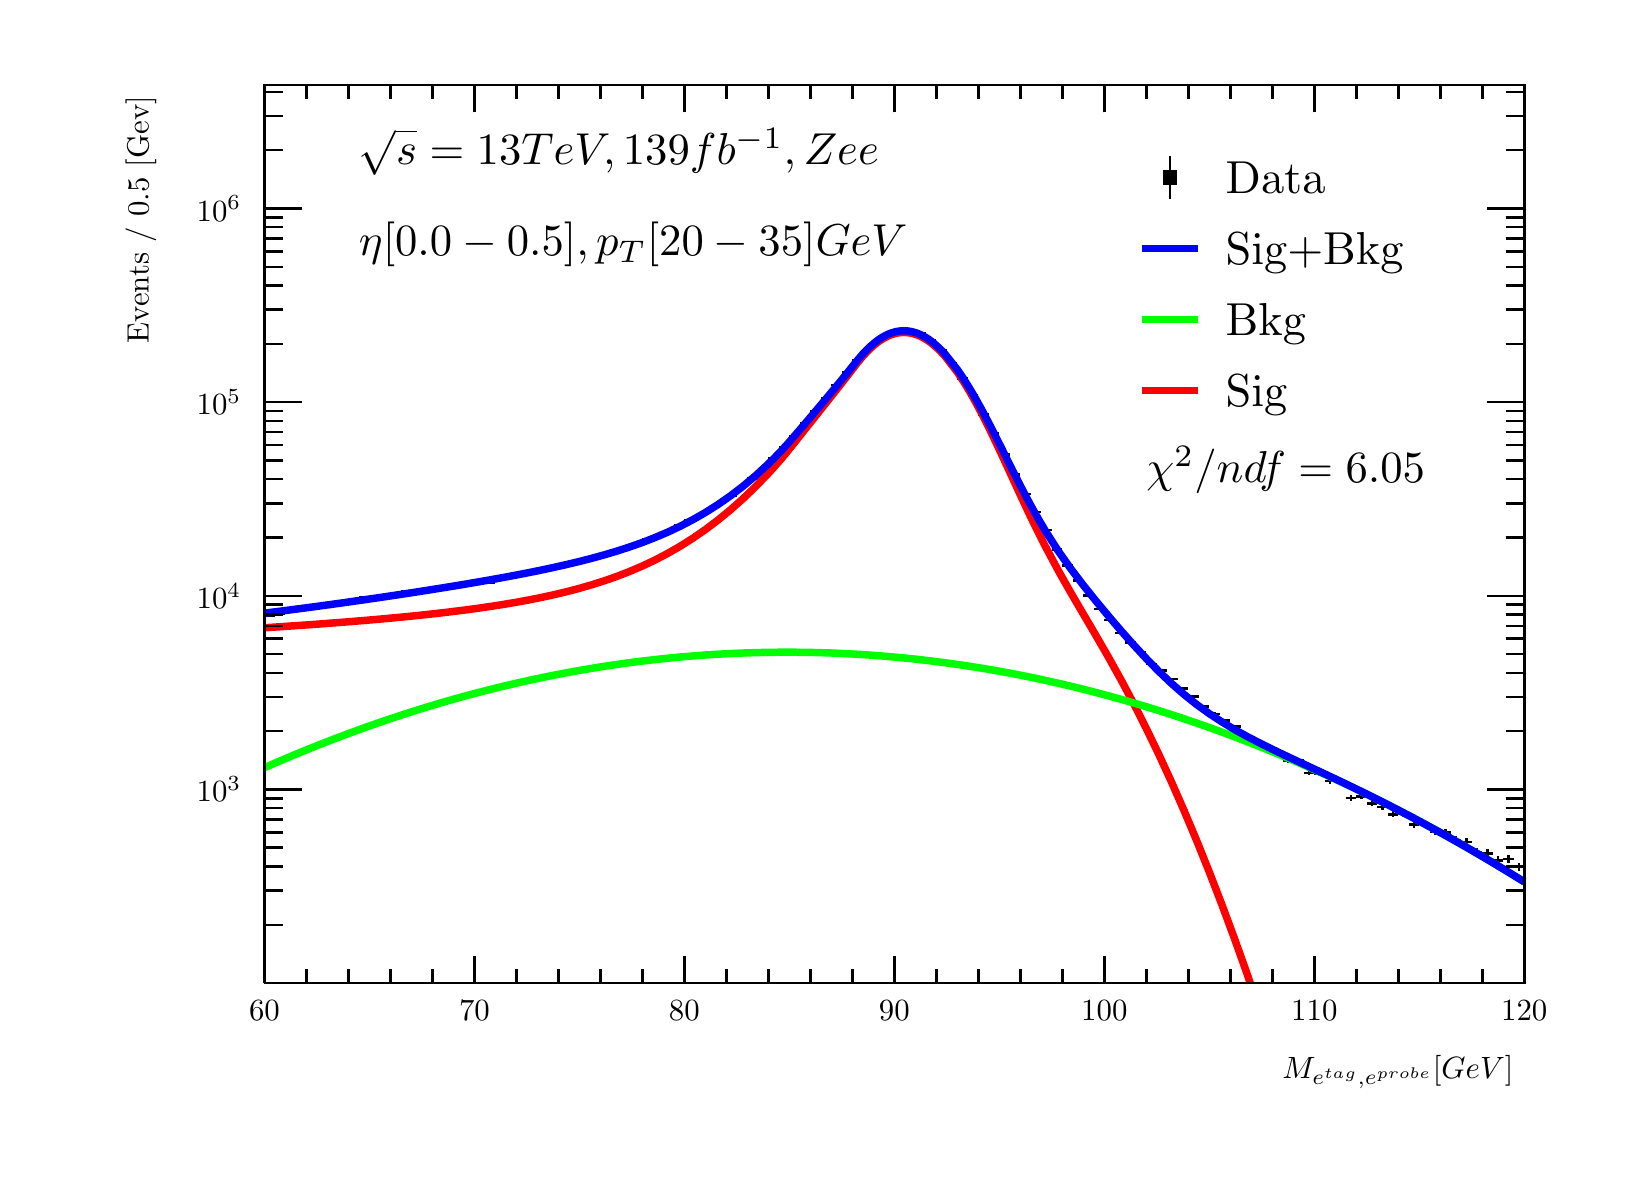
\begin{tikzpicture}
\pgfdeclareplotmark{cross} {
\pgfpathmoveto{\pgfpoint{-0.3\pgfplotmarksize}{\pgfplotmarksize}}
\pgfpathlineto{\pgfpoint{+0.3\pgfplotmarksize}{\pgfplotmarksize}}
\pgfpathlineto{\pgfpoint{+0.3\pgfplotmarksize}{0.3\pgfplotmarksize}}
\pgfpathlineto{\pgfpoint{+1\pgfplotmarksize}{0.3\pgfplotmarksize}}
\pgfpathlineto{\pgfpoint{+1\pgfplotmarksize}{-0.3\pgfplotmarksize}}
\pgfpathlineto{\pgfpoint{+0.3\pgfplotmarksize}{-0.3\pgfplotmarksize}}
\pgfpathlineto{\pgfpoint{+0.3\pgfplotmarksize}{-1.\pgfplotmarksize}}
\pgfpathlineto{\pgfpoint{-0.3\pgfplotmarksize}{-1.\pgfplotmarksize}}
\pgfpathlineto{\pgfpoint{-0.3\pgfplotmarksize}{-0.3\pgfplotmarksize}}
\pgfpathlineto{\pgfpoint{-1.\pgfplotmarksize}{-0.3\pgfplotmarksize}}
\pgfpathlineto{\pgfpoint{-1.\pgfplotmarksize}{0.3\pgfplotmarksize}}
\pgfpathlineto{\pgfpoint{-0.3\pgfplotmarksize}{0.3\pgfplotmarksize}}
\pgfpathclose
\pgfusepathqstroke
}
\pgfdeclareplotmark{cross*} {
\pgfpathmoveto{\pgfpoint{-0.3\pgfplotmarksize}{\pgfplotmarksize}}
\pgfpathlineto{\pgfpoint{+0.3\pgfplotmarksize}{\pgfplotmarksize}}
\pgfpathlineto{\pgfpoint{+0.3\pgfplotmarksize}{0.3\pgfplotmarksize}}
\pgfpathlineto{\pgfpoint{+1\pgfplotmarksize}{0.3\pgfplotmarksize}}
\pgfpathlineto{\pgfpoint{+1\pgfplotmarksize}{-0.3\pgfplotmarksize}}
\pgfpathlineto{\pgfpoint{+0.3\pgfplotmarksize}{-0.3\pgfplotmarksize}}
\pgfpathlineto{\pgfpoint{+0.3\pgfplotmarksize}{-1.\pgfplotmarksize}}
\pgfpathlineto{\pgfpoint{-0.3\pgfplotmarksize}{-1.\pgfplotmarksize}}
\pgfpathlineto{\pgfpoint{-0.3\pgfplotmarksize}{-0.3\pgfplotmarksize}}
\pgfpathlineto{\pgfpoint{-1.\pgfplotmarksize}{-0.3\pgfplotmarksize}}
\pgfpathlineto{\pgfpoint{-1.\pgfplotmarksize}{0.3\pgfplotmarksize}}
\pgfpathlineto{\pgfpoint{-0.3\pgfplotmarksize}{0.3\pgfplotmarksize}}
\pgfpathclose
\pgfusepathqfillstroke
}
\pgfdeclareplotmark{newstar} {
\pgfpathmoveto{\pgfqpoint{0pt}{\pgfplotmarksize}}
\pgfpathlineto{\pgfqpointpolar{44}{0.5\pgfplotmarksize}}
\pgfpathlineto{\pgfqpointpolar{18}{\pgfplotmarksize}}
\pgfpathlineto{\pgfqpointpolar{-20}{0.5\pgfplotmarksize}}
\pgfpathlineto{\pgfqpointpolar{-54}{\pgfplotmarksize}}
\pgfpathlineto{\pgfqpointpolar{-90}{0.5\pgfplotmarksize}}
\pgfpathlineto{\pgfqpointpolar{234}{\pgfplotmarksize}}
\pgfpathlineto{\pgfqpointpolar{198}{0.5\pgfplotmarksize}}
\pgfpathlineto{\pgfqpointpolar{162}{\pgfplotmarksize}}
\pgfpathlineto{\pgfqpointpolar{134}{0.5\pgfplotmarksize}}
\pgfpathclose
\pgfusepathqstroke
}
\pgfdeclareplotmark{newstar*} {
\pgfpathmoveto{\pgfqpoint{0pt}{\pgfplotmarksize}}
\pgfpathlineto{\pgfqpointpolar{44}{0.5\pgfplotmarksize}}
\pgfpathlineto{\pgfqpointpolar{18}{\pgfplotmarksize}}
\pgfpathlineto{\pgfqpointpolar{-20}{0.5\pgfplotmarksize}}
\pgfpathlineto{\pgfqpointpolar{-54}{\pgfplotmarksize}}
\pgfpathlineto{\pgfqpointpolar{-90}{0.5\pgfplotmarksize}}
\pgfpathlineto{\pgfqpointpolar{234}{\pgfplotmarksize}}
\pgfpathlineto{\pgfqpointpolar{198}{0.5\pgfplotmarksize}}
\pgfpathlineto{\pgfqpointpolar{162}{\pgfplotmarksize}}
\pgfpathlineto{\pgfqpointpolar{134}{0.5\pgfplotmarksize}}
\pgfpathclose
\pgfusepathqfillstroke
}
\definecolor{c}{rgb}{1,1,1};
\draw [color=c, fill=c] (0,0) rectangle (20,14.4361);
\draw [color=c, fill=c] (3,2.30977) rectangle (19,13.7143);
\definecolor{c}{rgb}{0,0,0};
\draw [c,line width=0.9] (3,2.30977) -- (3,13.7143) -- (19,13.7143) -- (19,2.30977) -- (3,2.30977);
\definecolor{c}{rgb}{1,1,1};
\draw [color=c, fill=c] (3,2.30977) rectangle (19,13.7143);
\definecolor{c}{rgb}{0,0,0};
\draw [c,line width=0.9] (3,2.30977) -- (3,13.7143) -- (19,13.7143) -- (19,2.30977) -- (3,2.30977);
\draw [c,line width=0.9] (3,2.30977) -- (19,2.30977);
\draw [c,line width=0.9] (3,2.65624) -- (3,2.30977);
\draw [c,line width=0.9] (3.53333,2.48301) -- (3.53333,2.30977);
\draw [c,line width=0.9] (4.06667,2.48301) -- (4.06667,2.30977);
\draw [c,line width=0.9] (4.6,2.48301) -- (4.6,2.30977);
\draw [c,line width=0.9] (5.13333,2.48301) -- (5.13333,2.30977);
\draw [c,line width=0.9] (5.66667,2.65624) -- (5.66667,2.30977);
\draw [c,line width=0.9] (6.2,2.48301) -- (6.2,2.30977);
\draw [c,line width=0.9] (6.73333,2.48301) -- (6.73333,2.30977);
\draw [c,line width=0.9] (7.26667,2.48301) -- (7.26667,2.30977);
\draw [c,line width=0.9] (7.8,2.48301) -- (7.8,2.30977);
\draw [c,line width=0.9] (8.33333,2.65624) -- (8.33333,2.30977);
\draw [c,line width=0.9] (8.86667,2.48301) -- (8.86667,2.30977);
\draw [c,line width=0.9] (9.4,2.48301) -- (9.4,2.30977);
\draw [c,line width=0.9] (9.93333,2.48301) -- (9.93333,2.30977);
\draw [c,line width=0.9] (10.4667,2.48301) -- (10.4667,2.30977);
\draw [c,line width=0.9] (11,2.65624) -- (11,2.30977);
\draw [c,line width=0.9] (11.5333,2.48301) -- (11.5333,2.30977);
\draw [c,line width=0.9] (12.0667,2.48301) -- (12.0667,2.30977);
\draw [c,line width=0.9] (12.6,2.48301) -- (12.6,2.30977);
\draw [c,line width=0.9] (13.1333,2.48301) -- (13.1333,2.30977);
\draw [c,line width=0.9] (13.6667,2.65624) -- (13.6667,2.30977);
\draw [c,line width=0.9] (14.2,2.48301) -- (14.2,2.30977);
\draw [c,line width=0.9] (14.7333,2.48301) -- (14.7333,2.30977);
\draw [c,line width=0.9] (15.2667,2.48301) -- (15.2667,2.30977);
\draw [c,line width=0.9] (15.8,2.48301) -- (15.8,2.30977);
\draw [c,line width=0.9] (16.3333,2.65624) -- (16.3333,2.30977);
\draw [c,line width=0.9] (16.8667,2.48301) -- (16.8667,2.30977);
\draw [c,line width=0.9] (17.4,2.48301) -- (17.4,2.30977);
\draw [c,line width=0.9] (17.9333,2.48301) -- (17.9333,2.30977);
\draw [c,line width=0.9] (18.4667,2.48301) -- (18.4667,2.30977);
\draw [c,line width=0.9] (19,2.65624) -- (19,2.30977);
\draw [anchor=base] (3,1.83338) node[scale=1.11327, color=c, rotate=0]{60};
\draw [anchor=base] (5.66667,1.83338) node[scale=1.11327, color=c, rotate=0]{70};
\draw [anchor=base] (8.33333,1.83338) node[scale=1.11327, color=c, rotate=0]{80};
\draw [anchor=base] (11,1.83338) node[scale=1.11327, color=c, rotate=0]{90};
\draw [anchor=base] (13.6667,1.83338) node[scale=1.11327, color=c, rotate=0]{100};
\draw [anchor=base] (16.3333,1.83338) node[scale=1.11327, color=c, rotate=0]{110};
\draw [anchor=base] (19,1.83338) node[scale=1.11327, color=c, rotate=0]{120};
\draw [anchor= east] (19,1.17798) node[scale=1.11327, color=c, rotate=0]{$M_{e^{tag}, e^{probe}}  [GeV]$};
\draw [c,line width=0.9] (3,13.7143) -- (19,13.7143);
\draw [c,line width=0.9] (3,13.3678) -- (3,13.7143);
\draw [c,line width=0.9] (3.53333,13.5411) -- (3.53333,13.7143);
\draw [c,line width=0.9] (4.06667,13.5411) -- (4.06667,13.7143);
\draw [c,line width=0.9] (4.6,13.5411) -- (4.6,13.7143);
\draw [c,line width=0.9] (5.13333,13.5411) -- (5.13333,13.7143);
\draw [c,line width=0.9] (5.66667,13.3678) -- (5.66667,13.7143);
\draw [c,line width=0.9] (6.2,13.5411) -- (6.2,13.7143);
\draw [c,line width=0.9] (6.73333,13.5411) -- (6.73333,13.7143);
\draw [c,line width=0.9] (7.26667,13.5411) -- (7.26667,13.7143);
\draw [c,line width=0.9] (7.8,13.5411) -- (7.8,13.7143);
\draw [c,line width=0.9] (8.33333,13.3678) -- (8.33333,13.7143);
\draw [c,line width=0.9] (8.86667,13.5411) -- (8.86667,13.7143);
\draw [c,line width=0.9] (9.4,13.5411) -- (9.4,13.7143);
\draw [c,line width=0.9] (9.93333,13.5411) -- (9.93333,13.7143);
\draw [c,line width=0.9] (10.4667,13.5411) -- (10.4667,13.7143);
\draw [c,line width=0.9] (11,13.3678) -- (11,13.7143);
\draw [c,line width=0.9] (11.5333,13.5411) -- (11.5333,13.7143);
\draw [c,line width=0.9] (12.0667,13.5411) -- (12.0667,13.7143);
\draw [c,line width=0.9] (12.6,13.5411) -- (12.6,13.7143);
\draw [c,line width=0.9] (13.1333,13.5411) -- (13.1333,13.7143);
\draw [c,line width=0.9] (13.6667,13.3678) -- (13.6667,13.7143);
\draw [c,line width=0.9] (14.2,13.5411) -- (14.2,13.7143);
\draw [c,line width=0.9] (14.7333,13.5411) -- (14.7333,13.7143);
\draw [c,line width=0.9] (15.2667,13.5411) -- (15.2667,13.7143);
\draw [c,line width=0.9] (15.8,13.5411) -- (15.8,13.7143);
\draw [c,line width=0.9] (16.3333,13.3678) -- (16.3333,13.7143);
\draw [c,line width=0.9] (16.8667,13.5411) -- (16.8667,13.7143);
\draw [c,line width=0.9] (17.4,13.5411) -- (17.4,13.7143);
\draw [c,line width=0.9] (17.9333,13.5411) -- (17.9333,13.7143);
\draw [c,line width=0.9] (18.4667,13.5411) -- (18.4667,13.7143);
\draw [c,line width=0.9] (19,13.3678) -- (19,13.7143);
\draw [c,line width=0.9] (3,2.30977) -- (3,13.7143);
\draw [c,line width=0.9] (3.237,3.05008) -- (3,3.05008);
\draw [c,line width=0.9] (3.237,3.48313) -- (3,3.48313);
\draw [c,line width=0.9] (3.237,3.79038) -- (3,3.79038);
\draw [c,line width=0.9] (3.237,4.02871) -- (3,4.02871);
\draw [c,line width=0.9] (3.237,4.22343) -- (3,4.22343);
\draw [c,line width=0.9] (3.237,4.38807) -- (3,4.38807);
\draw [c,line width=0.9] (3.237,4.53069) -- (3,4.53069);
\draw [c,line width=0.9] (3.237,4.65649) -- (3,4.65649);
\draw [c,line width=0.9] (3.474,4.76901) -- (3,4.76901);
\draw [anchor= east] (2.844,4.76901) node[scale=1.11327, color=c, rotate=0]{$10^{3}$};
\draw [c,line width=0.9] (3.237,5.50932) -- (3,5.50932);
\draw [c,line width=0.9] (3.237,5.94237) -- (3,5.94237);
\draw [c,line width=0.9] (3.237,6.24963) -- (3,6.24963);
\draw [c,line width=0.9] (3.237,6.48795) -- (3,6.48795);
\draw [c,line width=0.9] (3.237,6.68268) -- (3,6.68268);
\draw [c,line width=0.9] (3.237,6.84731) -- (3,6.84731);
\draw [c,line width=0.9] (3.237,6.98993) -- (3,6.98993);
\draw [c,line width=0.9] (3.237,7.11573) -- (3,7.11573);
\draw [c,line width=0.9] (3.474,7.22826) -- (3,7.22826);
\draw [anchor= east] (2.844,7.22826) node[scale=1.11327, color=c, rotate=0]{$10^{4}$};
\draw [c,line width=0.9] (3.237,7.96856) -- (3,7.96856);
\draw [c,line width=0.9] (3.237,8.40161) -- (3,8.40161);
\draw [c,line width=0.9] (3.237,8.70887) -- (3,8.70887);
\draw [c,line width=0.9] (3.237,8.94719) -- (3,8.94719);
\draw [c,line width=0.9] (3.237,9.14192) -- (3,9.14192);
\draw [c,line width=0.9] (3.237,9.30656) -- (3,9.30656);
\draw [c,line width=0.9] (3.237,9.44917) -- (3,9.44917);
\draw [c,line width=0.9] (3.237,9.57497) -- (3,9.57497);
\draw [c,line width=0.9] (3.474,9.6875) -- (3,9.6875);
\draw [anchor= east] (2.844,9.6875) node[scale=1.11327, color=c, rotate=0]{$10^{5}$};
\draw [c,line width=0.9] (3.237,10.4278) -- (3,10.4278);
\draw [c,line width=0.9] (3.237,10.8609) -- (3,10.8609);
\draw [c,line width=0.9] (3.237,11.1681) -- (3,11.1681);
\draw [c,line width=0.9] (3.237,11.4064) -- (3,11.4064);
\draw [c,line width=0.9] (3.237,11.6012) -- (3,11.6012);
\draw [c,line width=0.9] (3.237,11.7658) -- (3,11.7658);
\draw [c,line width=0.9] (3.237,11.9084) -- (3,11.9084);
\draw [c,line width=0.9] (3.237,12.0342) -- (3,12.0342);
\draw [c,line width=0.9] (3.474,12.1467) -- (3,12.1467);
\draw [anchor= east] (2.844,12.1467) node[scale=1.11327, color=c, rotate=0]{$10^{6}$};
\draw [c,line width=0.9] (3.237,12.887) -- (3,12.887);
\draw [c,line width=0.9] (3.237,13.3201) -- (3,13.3201);
\draw [c,line width=0.9] (3.237,13.6274) -- (3,13.6274);
\draw [anchor= east] (1.432,13.7143) node[scale=1.11327, color=c, rotate=90]{Events / 0.5 [Gev]};
\draw [c,line width=0.9] (19,2.30977) -- (19,13.7143);
\draw [c,line width=0.9] (18.763,3.05008) -- (19,3.05008);
\draw [c,line width=0.9] (18.763,3.48313) -- (19,3.48313);
\draw [c,line width=0.9] (18.763,3.79038) -- (19,3.79038);
\draw [c,line width=0.9] (18.763,4.02871) -- (19,4.02871);
\draw [c,line width=0.9] (18.763,4.22343) -- (19,4.22343);
\draw [c,line width=0.9] (18.763,4.38807) -- (19,4.38807);
\draw [c,line width=0.9] (18.763,4.53069) -- (19,4.53069);
\draw [c,line width=0.9] (18.763,4.65649) -- (19,4.65649);
\draw [c,line width=0.9] (18.526,4.76901) -- (19,4.76901);
\draw [c,line width=0.9] (18.763,5.50932) -- (19,5.50932);
\draw [c,line width=0.9] (18.763,5.94237) -- (19,5.94237);
\draw [c,line width=0.9] (18.763,6.24963) -- (19,6.24963);
\draw [c,line width=0.9] (18.763,6.48795) -- (19,6.48795);
\draw [c,line width=0.9] (18.763,6.68268) -- (19,6.68268);
\draw [c,line width=0.9] (18.763,6.84731) -- (19,6.84731);
\draw [c,line width=0.9] (18.763,6.98993) -- (19,6.98993);
\draw [c,line width=0.9] (18.763,7.11573) -- (19,7.11573);
\draw [c,line width=0.9] (18.526,7.22826) -- (19,7.22826);
\draw [c,line width=0.9] (18.763,7.96856) -- (19,7.96856);
\draw [c,line width=0.9] (18.763,8.40161) -- (19,8.40161);
\draw [c,line width=0.9] (18.763,8.70887) -- (19,8.70887);
\draw [c,line width=0.9] (18.763,8.94719) -- (19,8.94719);
\draw [c,line width=0.9] (18.763,9.14192) -- (19,9.14192);
\draw [c,line width=0.9] (18.763,9.30656) -- (19,9.30656);
\draw [c,line width=0.9] (18.763,9.44917) -- (19,9.44917);
\draw [c,line width=0.9] (18.763,9.57497) -- (19,9.57497);
\draw [c,line width=0.9] (18.526,9.6875) -- (19,9.6875);
\draw [c,line width=0.9] (18.763,10.4278) -- (19,10.4278);
\draw [c,line width=0.9] (18.763,10.8609) -- (19,10.8609);
\draw [c,line width=0.9] (18.763,11.1681) -- (19,11.1681);
\draw [c,line width=0.9] (18.763,11.4064) -- (19,11.4064);
\draw [c,line width=0.9] (18.763,11.6012) -- (19,11.6012);
\draw [c,line width=0.9] (18.763,11.7658) -- (19,11.7658);
\draw [c,line width=0.9] (18.763,11.9084) -- (19,11.9084);
\draw [c,line width=0.9] (18.763,12.0342) -- (19,12.0342);
\draw [c,line width=0.9] (18.526,12.1467) -- (19,12.1467);
\draw [c,line width=0.9] (18.763,12.887) -- (19,12.887);
\draw [c,line width=0.9] (18.763,13.3201) -- (19,13.3201);
\draw [c,line width=0.9] (18.763,13.6274) -- (19,13.6274);
\draw [c,line width=0.9] (3.06667,6.97555) -- (3,6.97555);
\draw [c,line width=0.9] (3,6.97555) -- (3,6.97555);
\draw [c,line width=0.9] (3.06667,6.97555) -- (3.13333,6.97555);
\draw [c,line width=0.9] (3.13333,6.97555) -- (3.13333,6.97555);
\draw [c,line width=0.9] (3.06667,6.97555) -- (3.06667,6.98757);
\draw [c,line width=0.9] (3.06667,6.98757) -- (3.06667,6.98757);
\draw [c,line width=0.9] (3.06667,6.97555) -- (3.06667,6.96353);
\draw [c,line width=0.9] (3.06667,6.96353) -- (3.06667,6.96353);
\draw [c,line width=0.9] (3.2,6.99897) -- (3.13333,6.99897);
\draw [c,line width=0.9] (3.13333,6.99897) -- (3.13333,6.99897);
\draw [c,line width=0.9] (3.2,6.99897) -- (3.26667,6.99897);
\draw [c,line width=0.9] (3.26667,6.99897) -- (3.26667,6.99897);
\draw [c,line width=0.9] (3.2,6.99897) -- (3.2,7.01086);
\draw [c,line width=0.9] (3.2,7.01086) -- (3.2,7.01086);
\draw [c,line width=0.9] (3.2,6.99897) -- (3.2,6.98708);
\draw [c,line width=0.9] (3.2,6.98708) -- (3.2,6.98708);
\draw [c,line width=0.9] (3.33333,7.05305) -- (3.26667,7.05305);
\draw [c,line width=0.9] (3.26667,7.05305) -- (3.26667,7.05305);
\draw [c,line width=0.9] (3.33333,7.05305) -- (3.4,7.05305);
\draw [c,line width=0.9] (3.4,7.05305) -- (3.4,7.05305);
\draw [c,line width=0.9] (3.33333,7.05305) -- (3.33333,7.06464);
\draw [c,line width=0.9] (3.33333,7.06464) -- (3.33333,7.06464);
\draw [c,line width=0.9] (3.33333,7.05305) -- (3.33333,7.04145);
\draw [c,line width=0.9] (3.33333,7.04145) -- (3.33333,7.04145);
\draw [c,line width=0.9] (3.46667,7.05619) -- (3.4,7.05619);
\draw [c,line width=0.9] (3.4,7.05619) -- (3.4,7.05619);
\draw [c,line width=0.9] (3.46667,7.05619) -- (3.53333,7.05619);
\draw [c,line width=0.9] (3.53333,7.05619) -- (3.53333,7.05619);
\draw [c,line width=0.9] (3.46667,7.05619) -- (3.46667,7.06776);
\draw [c,line width=0.9] (3.46667,7.06776) -- (3.46667,7.06776);
\draw [c,line width=0.9] (3.46667,7.05619) -- (3.46667,7.04461);
\draw [c,line width=0.9] (3.46667,7.04461) -- (3.46667,7.04461);
\draw [c,line width=0.9] (3.6,7.09403) -- (3.53333,7.09403);
\draw [c,line width=0.9] (3.53333,7.09403) -- (3.53333,7.09403);
\draw [c,line width=0.9] (3.6,7.09403) -- (3.66667,7.09403);
\draw [c,line width=0.9] (3.66667,7.09403) -- (3.66667,7.09403);
\draw [c,line width=0.9] (3.6,7.09403) -- (3.6,7.1054);
\draw [c,line width=0.9] (3.6,7.1054) -- (3.6,7.1054);
\draw [c,line width=0.9] (3.6,7.09403) -- (3.6,7.08266);
\draw [c,line width=0.9] (3.6,7.08266) -- (3.6,7.08266);
\draw [c,line width=0.9] (3.73333,7.12094) -- (3.66667,7.12094);
\draw [c,line width=0.9] (3.66667,7.12094) -- (3.66667,7.12094);
\draw [c,line width=0.9] (3.73333,7.12094) -- (3.8,7.12094);
\draw [c,line width=0.9] (3.8,7.12094) -- (3.8,7.12094);
\draw [c,line width=0.9] (3.73333,7.12094) -- (3.73333,7.13217);
\draw [c,line width=0.9] (3.73333,7.13217) -- (3.73333,7.13217);
\draw [c,line width=0.9] (3.73333,7.12094) -- (3.73333,7.10971);
\draw [c,line width=0.9] (3.73333,7.10971) -- (3.73333,7.10971);
\draw [c,line width=0.9] (3.86667,7.1328) -- (3.8,7.1328);
\draw [c,line width=0.9] (3.8,7.1328) -- (3.8,7.1328);
\draw [c,line width=0.9] (3.86667,7.1328) -- (3.93333,7.1328);
\draw [c,line width=0.9] (3.93333,7.1328) -- (3.93333,7.1328);
\draw [c,line width=0.9] (3.86667,7.1328) -- (3.86667,7.14397);
\draw [c,line width=0.9] (3.86667,7.14397) -- (3.86667,7.14397);
\draw [c,line width=0.9] (3.86667,7.1328) -- (3.86667,7.12163);
\draw [c,line width=0.9] (3.86667,7.12163) -- (3.86667,7.12163);
\draw [c,line width=0.9] (4,7.15407) -- (3.93333,7.15407);
\draw [c,line width=0.9] (3.93333,7.15407) -- (3.93333,7.15407);
\draw [c,line width=0.9] (4,7.15407) -- (4.06667,7.15407);
\draw [c,line width=0.9] (4.06667,7.15407) -- (4.06667,7.15407);
\draw [c,line width=0.9] (4,7.15407) -- (4,7.16513);
\draw [c,line width=0.9] (4,7.16513) -- (4,7.16513);
\draw [c,line width=0.9] (4,7.15407) -- (4,7.14302);
\draw [c,line width=0.9] (4,7.14302) -- (4,7.14302);
\draw [c,line width=0.9] (4.13333,7.18377) -- (4.06667,7.18377);
\draw [c,line width=0.9] (4.06667,7.18377) -- (4.06667,7.18377);
\draw [c,line width=0.9] (4.13333,7.18377) -- (4.2,7.18377);
\draw [c,line width=0.9] (4.2,7.18377) -- (4.2,7.18377);
\draw [c,line width=0.9] (4.13333,7.18377) -- (4.13333,7.19467);
\draw [c,line width=0.9] (4.13333,7.19467) -- (4.13333,7.19467);
\draw [c,line width=0.9] (4.13333,7.18377) -- (4.13333,7.17286);
\draw [c,line width=0.9] (4.13333,7.17286) -- (4.13333,7.17286);
\draw [c,line width=0.9] (4.26667,7.21439) -- (4.2,7.21439);
\draw [c,line width=0.9] (4.2,7.21439) -- (4.2,7.21439);
\draw [c,line width=0.9] (4.26667,7.21439) -- (4.33333,7.21439);
\draw [c,line width=0.9] (4.33333,7.21439) -- (4.33333,7.21439);
\draw [c,line width=0.9] (4.26667,7.21439) -- (4.26667,7.22514);
\draw [c,line width=0.9] (4.26667,7.22514) -- (4.26667,7.22514);
\draw [c,line width=0.9] (4.26667,7.21439) -- (4.26667,7.20364);
\draw [c,line width=0.9] (4.26667,7.20364) -- (4.26667,7.20364);
\draw [c,line width=0.9] (4.4,7.21114) -- (4.33333,7.21114);
\draw [c,line width=0.9] (4.33333,7.21114) -- (4.33333,7.21114);
\draw [c,line width=0.9] (4.4,7.21114) -- (4.46667,7.21114);
\draw [c,line width=0.9] (4.46667,7.21114) -- (4.46667,7.21114);
\draw [c,line width=0.9] (4.4,7.21114) -- (4.4,7.22191);
\draw [c,line width=0.9] (4.4,7.22191) -- (4.4,7.22191);
\draw [c,line width=0.9] (4.4,7.21114) -- (4.4,7.20037);
\draw [c,line width=0.9] (4.4,7.20037) -- (4.4,7.20037);
\draw [c,line width=0.9] (4.53333,7.21979) -- (4.46667,7.21979);
\draw [c,line width=0.9] (4.46667,7.21979) -- (4.46667,7.21979);
\draw [c,line width=0.9] (4.53333,7.21979) -- (4.6,7.21979);
\draw [c,line width=0.9] (4.6,7.21979) -- (4.6,7.21979);
\draw [c,line width=0.9] (4.53333,7.21979) -- (4.53333,7.23051);
\draw [c,line width=0.9] (4.53333,7.23051) -- (4.53333,7.23051);
\draw [c,line width=0.9] (4.53333,7.21979) -- (4.53333,7.20906);
\draw [c,line width=0.9] (4.53333,7.20906) -- (4.53333,7.20906);
\draw [c,line width=0.9] (4.66667,7.23878) -- (4.6,7.23878);
\draw [c,line width=0.9] (4.6,7.23878) -- (4.6,7.23878);
\draw [c,line width=0.9] (4.66667,7.23878) -- (4.73333,7.23878);
\draw [c,line width=0.9] (4.73333,7.23878) -- (4.73333,7.23878);
\draw [c,line width=0.9] (4.66667,7.23878) -- (4.66667,7.24941);
\draw [c,line width=0.9] (4.66667,7.24941) -- (4.66667,7.24941);
\draw [c,line width=0.9] (4.66667,7.23878) -- (4.66667,7.22815);
\draw [c,line width=0.9] (4.66667,7.22815) -- (4.66667,7.22815);
\draw [c,line width=0.9] (4.8,7.28756) -- (4.73333,7.28756);
\draw [c,line width=0.9] (4.73333,7.28756) -- (4.73333,7.28756);
\draw [c,line width=0.9] (4.8,7.28756) -- (4.86667,7.28756);
\draw [c,line width=0.9] (4.86667,7.28756) -- (4.86667,7.28756);
\draw [c,line width=0.9] (4.8,7.28756) -- (4.8,7.29795);
\draw [c,line width=0.9] (4.8,7.29795) -- (4.8,7.29795);
\draw [c,line width=0.9] (4.8,7.28756) -- (4.8,7.27718);
\draw [c,line width=0.9] (4.8,7.27718) -- (4.8,7.27718);
\draw [c,line width=0.9] (4.93333,7.27425) -- (4.86667,7.27425);
\draw [c,line width=0.9] (4.86667,7.27425) -- (4.86667,7.27425);
\draw [c,line width=0.9] (4.93333,7.27425) -- (5,7.27425);
\draw [c,line width=0.9] (5,7.27425) -- (5,7.27425);
\draw [c,line width=0.9] (4.93333,7.27425) -- (4.93333,7.2847);
\draw [c,line width=0.9] (4.93333,7.2847) -- (4.93333,7.2847);
\draw [c,line width=0.9] (4.93333,7.27425) -- (4.93333,7.26379);
\draw [c,line width=0.9] (4.93333,7.26379) -- (4.93333,7.26379);
\draw [c,line width=0.9] (5.06667,7.30986) -- (5,7.30986);
\draw [c,line width=0.9] (5,7.30986) -- (5,7.30986);
\draw [c,line width=0.9] (5.06667,7.30986) -- (5.13333,7.30986);
\draw [c,line width=0.9] (5.13333,7.30986) -- (5.13333,7.30986);
\draw [c,line width=0.9] (5.06667,7.30986) -- (5.06667,7.32014);
\draw [c,line width=0.9] (5.06667,7.32014) -- (5.06667,7.32014);
\draw [c,line width=0.9] (5.06667,7.30986) -- (5.06667,7.29958);
\draw [c,line width=0.9] (5.06667,7.29958) -- (5.06667,7.29958);
\draw [c,line width=0.9] (5.2,7.31065) -- (5.13333,7.31065);
\draw [c,line width=0.9] (5.13333,7.31065) -- (5.13333,7.31065);
\draw [c,line width=0.9] (5.2,7.31065) -- (5.26667,7.31065);
\draw [c,line width=0.9] (5.26667,7.31065) -- (5.26667,7.31065);
\draw [c,line width=0.9] (5.2,7.31065) -- (5.2,7.32093);
\draw [c,line width=0.9] (5.2,7.32093) -- (5.2,7.32093);
\draw [c,line width=0.9] (5.2,7.31065) -- (5.2,7.30038);
\draw [c,line width=0.9] (5.2,7.30038) -- (5.2,7.30038);
\draw [c,line width=0.9] (5.33333,7.34844) -- (5.26667,7.34844);
\draw [c,line width=0.9] (5.26667,7.34844) -- (5.26667,7.34844);
\draw [c,line width=0.9] (5.33333,7.34844) -- (5.4,7.34844);
\draw [c,line width=0.9] (5.4,7.34844) -- (5.4,7.34844);
\draw [c,line width=0.9] (5.33333,7.34844) -- (5.33333,7.35853);
\draw [c,line width=0.9] (5.33333,7.35853) -- (5.33333,7.35853);
\draw [c,line width=0.9] (5.33333,7.34844) -- (5.33333,7.33834);
\draw [c,line width=0.9] (5.33333,7.33834) -- (5.33333,7.33834);
\draw [c,line width=0.9] (5.46667,7.35358) -- (5.4,7.35358);
\draw [c,line width=0.9] (5.4,7.35358) -- (5.4,7.35358);
\draw [c,line width=0.9] (5.46667,7.35358) -- (5.53333,7.35358);
\draw [c,line width=0.9] (5.53333,7.35358) -- (5.53333,7.35358);
\draw [c,line width=0.9] (5.46667,7.35358) -- (5.46667,7.36365);
\draw [c,line width=0.9] (5.46667,7.36365) -- (5.46667,7.36365);
\draw [c,line width=0.9] (5.46667,7.35358) -- (5.46667,7.34351);
\draw [c,line width=0.9] (5.46667,7.34351) -- (5.46667,7.34351);
\draw [c,line width=0.9] (5.6,7.38401) -- (5.53333,7.38401);
\draw [c,line width=0.9] (5.53333,7.38401) -- (5.53333,7.38401);
\draw [c,line width=0.9] (5.6,7.38401) -- (5.66667,7.38401);
\draw [c,line width=0.9] (5.66667,7.38401) -- (5.66667,7.38401);
\draw [c,line width=0.9] (5.6,7.38401) -- (5.6,7.39394);
\draw [c,line width=0.9] (5.6,7.39394) -- (5.6,7.39394);
\draw [c,line width=0.9] (5.6,7.38401) -- (5.6,7.37408);
\draw [c,line width=0.9] (5.6,7.37408) -- (5.6,7.37408);
\draw [c,line width=0.9] (5.73333,7.39649) -- (5.66667,7.39649);
\draw [c,line width=0.9] (5.66667,7.39649) -- (5.66667,7.39649);
\draw [c,line width=0.9] (5.73333,7.39649) -- (5.8,7.39649);
\draw [c,line width=0.9] (5.8,7.39649) -- (5.8,7.39649);
\draw [c,line width=0.9] (5.73333,7.39649) -- (5.73333,7.40636);
\draw [c,line width=0.9] (5.73333,7.40636) -- (5.73333,7.40636);
\draw [c,line width=0.9] (5.73333,7.39649) -- (5.73333,7.38662);
\draw [c,line width=0.9] (5.73333,7.38662) -- (5.73333,7.38662);
\draw [c,line width=0.9] (5.86667,7.39722) -- (5.8,7.39722);
\draw [c,line width=0.9] (5.8,7.39722) -- (5.8,7.39722);
\draw [c,line width=0.9] (5.86667,7.39722) -- (5.93333,7.39722);
\draw [c,line width=0.9] (5.93333,7.39722) -- (5.93333,7.39722);
\draw [c,line width=0.9] (5.86667,7.39722) -- (5.86667,7.40709);
\draw [c,line width=0.9] (5.86667,7.40709) -- (5.86667,7.40709);
\draw [c,line width=0.9] (5.86667,7.39722) -- (5.86667,7.38735);
\draw [c,line width=0.9] (5.86667,7.38735) -- (5.86667,7.38735);
\draw [c,line width=0.9] (6,7.44378) -- (5.93333,7.44378);
\draw [c,line width=0.9] (5.93333,7.44378) -- (5.93333,7.44378);
\draw [c,line width=0.9] (6,7.44378) -- (6.06667,7.44378);
\draw [c,line width=0.9] (6.06667,7.44378) -- (6.06667,7.44378);
\draw [c,line width=0.9] (6,7.44378) -- (6,7.45344);
\draw [c,line width=0.9] (6,7.45344) -- (6,7.45344);
\draw [c,line width=0.9] (6,7.44378) -- (6,7.43413);
\draw [c,line width=0.9] (6,7.43413) -- (6,7.43413);
\draw [c,line width=0.9] (6.13333,7.45403) -- (6.06667,7.45403);
\draw [c,line width=0.9] (6.06667,7.45403) -- (6.06667,7.45403);
\draw [c,line width=0.9] (6.13333,7.45403) -- (6.2,7.45403);
\draw [c,line width=0.9] (6.2,7.45403) -- (6.2,7.45403);
\draw [c,line width=0.9] (6.13333,7.45403) -- (6.13333,7.46364);
\draw [c,line width=0.9] (6.13333,7.46364) -- (6.13333,7.46364);
\draw [c,line width=0.9] (6.13333,7.45403) -- (6.13333,7.44443);
\draw [c,line width=0.9] (6.13333,7.44443) -- (6.13333,7.44443);
\draw [c,line width=0.9] (6.26667,7.5008) -- (6.2,7.5008);
\draw [c,line width=0.9] (6.2,7.5008) -- (6.2,7.5008);
\draw [c,line width=0.9] (6.26667,7.5008) -- (6.33333,7.5008);
\draw [c,line width=0.9] (6.33333,7.5008) -- (6.33333,7.5008);
\draw [c,line width=0.9] (6.26667,7.5008) -- (6.26667,7.5102);
\draw [c,line width=0.9] (6.26667,7.5102) -- (6.26667,7.5102);
\draw [c,line width=0.9] (6.26667,7.5008) -- (6.26667,7.4914);
\draw [c,line width=0.9] (6.26667,7.4914) -- (6.26667,7.4914);
\draw [c,line width=0.9] (6.4,7.52162) -- (6.33333,7.52162);
\draw [c,line width=0.9] (6.33333,7.52162) -- (6.33333,7.52162);
\draw [c,line width=0.9] (6.4,7.52162) -- (6.46667,7.52162);
\draw [c,line width=0.9] (6.46667,7.52162) -- (6.46667,7.52162);
\draw [c,line width=0.9] (6.4,7.52162) -- (6.4,7.53093);
\draw [c,line width=0.9] (6.4,7.53093) -- (6.4,7.53093);
\draw [c,line width=0.9] (6.4,7.52162) -- (6.4,7.51231);
\draw [c,line width=0.9] (6.4,7.51231) -- (6.4,7.51231);
\draw [c,line width=0.9] (6.53333,7.54941) -- (6.46667,7.54941);
\draw [c,line width=0.9] (6.46667,7.54941) -- (6.46667,7.54941);
\draw [c,line width=0.9] (6.53333,7.54941) -- (6.6,7.54941);
\draw [c,line width=0.9] (6.6,7.54941) -- (6.6,7.54941);
\draw [c,line width=0.9] (6.53333,7.54941) -- (6.53333,7.5586);
\draw [c,line width=0.9] (6.53333,7.5586) -- (6.53333,7.5586);
\draw [c,line width=0.9] (6.53333,7.54941) -- (6.53333,7.54022);
\draw [c,line width=0.9] (6.53333,7.54022) -- (6.53333,7.54022);
\draw [c,line width=0.9] (6.66667,7.58211) -- (6.6,7.58211);
\draw [c,line width=0.9] (6.6,7.58211) -- (6.6,7.58211);
\draw [c,line width=0.9] (6.66667,7.58211) -- (6.73333,7.58211);
\draw [c,line width=0.9] (6.73333,7.58211) -- (6.73333,7.58211);
\draw [c,line width=0.9] (6.66667,7.58211) -- (6.66667,7.59116);
\draw [c,line width=0.9] (6.66667,7.59116) -- (6.66667,7.59116);
\draw [c,line width=0.9] (6.66667,7.58211) -- (6.66667,7.57306);
\draw [c,line width=0.9] (6.66667,7.57306) -- (6.66667,7.57306);
\draw [c,line width=0.9] (6.8,7.61094) -- (6.73333,7.61094);
\draw [c,line width=0.9] (6.73333,7.61094) -- (6.73333,7.61094);
\draw [c,line width=0.9] (6.8,7.61094) -- (6.86667,7.61094);
\draw [c,line width=0.9] (6.86667,7.61094) -- (6.86667,7.61094);
\draw [c,line width=0.9] (6.8,7.61094) -- (6.8,7.61987);
\draw [c,line width=0.9] (6.8,7.61987) -- (6.8,7.61987);
\draw [c,line width=0.9] (6.8,7.61094) -- (6.8,7.60201);
\draw [c,line width=0.9] (6.8,7.60201) -- (6.8,7.60201);
\draw [c,line width=0.9] (6.93333,7.6331) -- (6.86667,7.6331);
\draw [c,line width=0.9] (6.86667,7.6331) -- (6.86667,7.6331);
\draw [c,line width=0.9] (6.93333,7.6331) -- (7,7.6331);
\draw [c,line width=0.9] (7,7.6331) -- (7,7.6331);
\draw [c,line width=0.9] (6.93333,7.6331) -- (6.93333,7.64194);
\draw [c,line width=0.9] (6.93333,7.64194) -- (6.93333,7.64194);
\draw [c,line width=0.9] (6.93333,7.6331) -- (6.93333,7.62426);
\draw [c,line width=0.9] (6.93333,7.62426) -- (6.93333,7.62426);
\draw [c,line width=0.9] (7.06667,7.66734) -- (7,7.66734);
\draw [c,line width=0.9] (7,7.66734) -- (7,7.66734);
\draw [c,line width=0.9] (7.06667,7.66734) -- (7.13333,7.66734);
\draw [c,line width=0.9] (7.13333,7.66734) -- (7.13333,7.66734);
\draw [c,line width=0.9] (7.06667,7.66734) -- (7.06667,7.67604);
\draw [c,line width=0.9] (7.06667,7.67604) -- (7.06667,7.67604);
\draw [c,line width=0.9] (7.06667,7.66734) -- (7.06667,7.65865);
\draw [c,line width=0.9] (7.06667,7.65865) -- (7.06667,7.65865);
\draw [c,line width=0.9] (7.2,7.71829) -- (7.13333,7.71829);
\draw [c,line width=0.9] (7.13333,7.71829) -- (7.13333,7.71829);
\draw [c,line width=0.9] (7.2,7.71829) -- (7.26667,7.71829);
\draw [c,line width=0.9] (7.26667,7.71829) -- (7.26667,7.71829);
\draw [c,line width=0.9] (7.2,7.71829) -- (7.2,7.72678);
\draw [c,line width=0.9] (7.2,7.72678) -- (7.2,7.72678);
\draw [c,line width=0.9] (7.2,7.71829) -- (7.2,7.7098);
\draw [c,line width=0.9] (7.2,7.7098) -- (7.2,7.7098);
\draw [c,line width=0.9] (7.33333,7.73961) -- (7.26667,7.73961);
\draw [c,line width=0.9] (7.26667,7.73961) -- (7.26667,7.73961);
\draw [c,line width=0.9] (7.33333,7.73961) -- (7.4,7.73961);
\draw [c,line width=0.9] (7.4,7.73961) -- (7.4,7.73961);
\draw [c,line width=0.9] (7.33333,7.73961) -- (7.33333,7.74801);
\draw [c,line width=0.9] (7.33333,7.74801) -- (7.33333,7.74801);
\draw [c,line width=0.9] (7.33333,7.73961) -- (7.33333,7.7312);
\draw [c,line width=0.9] (7.33333,7.7312) -- (7.33333,7.7312);
\draw [c,line width=0.9] (7.46667,7.78235) -- (7.4,7.78235);
\draw [c,line width=0.9] (7.4,7.78235) -- (7.4,7.78235);
\draw [c,line width=0.9] (7.46667,7.78235) -- (7.53333,7.78235);
\draw [c,line width=0.9] (7.53333,7.78235) -- (7.53333,7.78235);
\draw [c,line width=0.9] (7.46667,7.78235) -- (7.46667,7.79059);
\draw [c,line width=0.9] (7.46667,7.79059) -- (7.46667,7.79059);
\draw [c,line width=0.9] (7.46667,7.78235) -- (7.46667,7.77411);
\draw [c,line width=0.9] (7.46667,7.77411) -- (7.46667,7.77411);
\draw [c,line width=0.9] (7.6,7.83343) -- (7.53333,7.83343);
\draw [c,line width=0.9] (7.53333,7.83343) -- (7.53333,7.83343);
\draw [c,line width=0.9] (7.6,7.83343) -- (7.66667,7.83343);
\draw [c,line width=0.9] (7.66667,7.83343) -- (7.66667,7.83343);
\draw [c,line width=0.9] (7.6,7.83343) -- (7.6,7.84147);
\draw [c,line width=0.9] (7.6,7.84147) -- (7.6,7.84147);
\draw [c,line width=0.9] (7.6,7.83343) -- (7.6,7.82538);
\draw [c,line width=0.9] (7.6,7.82538) -- (7.6,7.82538);
\draw [c,line width=0.9] (7.73333,7.89025) -- (7.66667,7.89025);
\draw [c,line width=0.9] (7.66667,7.89025) -- (7.66667,7.89025);
\draw [c,line width=0.9] (7.73333,7.89025) -- (7.8,7.89025);
\draw [c,line width=0.9] (7.8,7.89025) -- (7.8,7.89025);
\draw [c,line width=0.9] (7.73333,7.89025) -- (7.73333,7.89808);
\draw [c,line width=0.9] (7.73333,7.89808) -- (7.73333,7.89808);
\draw [c,line width=0.9] (7.73333,7.89025) -- (7.73333,7.88242);
\draw [c,line width=0.9] (7.73333,7.88242) -- (7.73333,7.88242);
\draw [c,line width=0.9] (7.86667,7.94824) -- (7.8,7.94824);
\draw [c,line width=0.9] (7.8,7.94824) -- (7.8,7.94824);
\draw [c,line width=0.9] (7.86667,7.94824) -- (7.93333,7.94824);
\draw [c,line width=0.9] (7.93333,7.94824) -- (7.93333,7.94824);
\draw [c,line width=0.9] (7.86667,7.94824) -- (7.86667,7.95586);
\draw [c,line width=0.9] (7.86667,7.95586) -- (7.86667,7.95586);
\draw [c,line width=0.9] (7.86667,7.94824) -- (7.86667,7.94061);
\draw [c,line width=0.9] (7.86667,7.94061) -- (7.86667,7.94061);
\draw [c,line width=0.9] (8,7.99107) -- (7.93333,7.99107);
\draw [c,line width=0.9] (7.93333,7.99107) -- (7.93333,7.99107);
\draw [c,line width=0.9] (8,7.99107) -- (8.06667,7.99107);
\draw [c,line width=0.9] (8.06667,7.99107) -- (8.06667,7.99107);
\draw [c,line width=0.9] (8,7.99107) -- (8,7.99855);
\draw [c,line width=0.9] (8,7.99855) -- (8,7.99855);
\draw [c,line width=0.9] (8,7.99107) -- (8,7.9836);
\draw [c,line width=0.9] (8,7.9836) -- (8,7.9836);
\draw [c,line width=0.9] (8.13333,8.04883) -- (8.06667,8.04883);
\draw [c,line width=0.9] (8.06667,8.04883) -- (8.06667,8.04883);
\draw [c,line width=0.9] (8.13333,8.04883) -- (8.2,8.04883);
\draw [c,line width=0.9] (8.2,8.04883) -- (8.2,8.04883);
\draw [c,line width=0.9] (8.13333,8.04883) -- (8.13333,8.0561);
\draw [c,line width=0.9] (8.13333,8.0561) -- (8.13333,8.0561);
\draw [c,line width=0.9] (8.13333,8.04883) -- (8.13333,8.04156);
\draw [c,line width=0.9] (8.13333,8.04156) -- (8.13333,8.04156);
\draw [c,line width=0.9] (8.26667,8.11821) -- (8.2,8.11821);
\draw [c,line width=0.9] (8.2,8.11821) -- (8.2,8.11821);
\draw [c,line width=0.9] (8.26667,8.11821) -- (8.33333,8.11821);
\draw [c,line width=0.9] (8.33333,8.11821) -- (8.33333,8.11821);
\draw [c,line width=0.9] (8.26667,8.11821) -- (8.26667,8.12525);
\draw [c,line width=0.9] (8.26667,8.12525) -- (8.26667,8.12525);
\draw [c,line width=0.9] (8.26667,8.11821) -- (8.26667,8.11116);
\draw [c,line width=0.9] (8.26667,8.11116) -- (8.26667,8.11116);
\draw [c,line width=0.9] (8.4,8.18278) -- (8.33333,8.18278);
\draw [c,line width=0.9] (8.33333,8.18278) -- (8.33333,8.18278);
\draw [c,line width=0.9] (8.4,8.18278) -- (8.46667,8.18278);
\draw [c,line width=0.9] (8.46667,8.18278) -- (8.46667,8.18278);
\draw [c,line width=0.9] (8.4,8.18278) -- (8.4,8.18961);
\draw [c,line width=0.9] (8.4,8.18961) -- (8.4,8.18961);
\draw [c,line width=0.9] (8.4,8.18278) -- (8.4,8.17595);
\draw [c,line width=0.9] (8.4,8.17595) -- (8.4,8.17595);
\draw [c,line width=0.9] (8.53333,8.25148) -- (8.46667,8.25148);
\draw [c,line width=0.9] (8.46667,8.25148) -- (8.46667,8.25148);
\draw [c,line width=0.9] (8.53333,8.25148) -- (8.6,8.25148);
\draw [c,line width=0.9] (8.6,8.25148) -- (8.6,8.25148);
\draw [c,line width=0.9] (8.53333,8.25148) -- (8.53333,8.2581);
\draw [c,line width=0.9] (8.53333,8.2581) -- (8.53333,8.2581);
\draw [c,line width=0.9] (8.53333,8.25148) -- (8.53333,8.24487);
\draw [c,line width=0.9] (8.53333,8.24487) -- (8.53333,8.24487);
\draw [c,line width=0.9] (8.66667,8.3296) -- (8.6,8.3296);
\draw [c,line width=0.9] (8.6,8.3296) -- (8.6,8.3296);
\draw [c,line width=0.9] (8.66667,8.3296) -- (8.73333,8.3296);
\draw [c,line width=0.9] (8.73333,8.3296) -- (8.73333,8.3296);
\draw [c,line width=0.9] (8.66667,8.3296) -- (8.66667,8.33598);
\draw [c,line width=0.9] (8.66667,8.33598) -- (8.66667,8.33598);
\draw [c,line width=0.9] (8.66667,8.3296) -- (8.66667,8.32323);
\draw [c,line width=0.9] (8.66667,8.32323) -- (8.66667,8.32323);
\draw [c,line width=0.9] (8.8,8.41062) -- (8.73333,8.41062);
\draw [c,line width=0.9] (8.73333,8.41062) -- (8.73333,8.41062);
\draw [c,line width=0.9] (8.8,8.41062) -- (8.86667,8.41062);
\draw [c,line width=0.9] (8.86667,8.41062) -- (8.86667,8.41062);
\draw [c,line width=0.9] (8.8,8.41062) -- (8.8,8.41676);
\draw [c,line width=0.9] (8.8,8.41676) -- (8.8,8.41676);
\draw [c,line width=0.9] (8.8,8.41062) -- (8.8,8.40448);
\draw [c,line width=0.9] (8.8,8.40448) -- (8.8,8.40448);
\draw [c,line width=0.9] (8.93333,8.50328) -- (8.86667,8.50328);
\draw [c,line width=0.9] (8.86667,8.50328) -- (8.86667,8.50328);
\draw [c,line width=0.9] (8.93333,8.50328) -- (9,8.50328);
\draw [c,line width=0.9] (9,8.50328) -- (9,8.50328);
\draw [c,line width=0.9] (8.93333,8.50328) -- (8.93333,8.50916);
\draw [c,line width=0.9] (8.93333,8.50916) -- (8.93333,8.50916);
\draw [c,line width=0.9] (8.93333,8.50328) -- (8.93333,8.4974);
\draw [c,line width=0.9] (8.93333,8.4974) -- (8.93333,8.4974);
\draw [c,line width=0.9] (9.06667,8.60958) -- (9,8.60958);
\draw [c,line width=0.9] (9,8.60958) -- (9,8.60958);
\draw [c,line width=0.9] (9.06667,8.60958) -- (9.13333,8.60958);
\draw [c,line width=0.9] (9.13333,8.60958) -- (9.13333,8.60958);
\draw [c,line width=0.9] (9.06667,8.60958) -- (9.06667,8.61517);
\draw [c,line width=0.9] (9.06667,8.61517) -- (9.06667,8.61517);
\draw [c,line width=0.9] (9.06667,8.60958) -- (9.06667,8.60398);
\draw [c,line width=0.9] (9.06667,8.60398) -- (9.06667,8.60398);
\draw [c,line width=0.9] (9.2,8.71741) -- (9.13333,8.71741);
\draw [c,line width=0.9] (9.13333,8.71741) -- (9.13333,8.71741);
\draw [c,line width=0.9] (9.2,8.71741) -- (9.26667,8.71741);
\draw [c,line width=0.9] (9.26667,8.71741) -- (9.26667,8.71741);
\draw [c,line width=0.9] (9.2,8.71741) -- (9.2,8.72272);
\draw [c,line width=0.9] (9.2,8.72272) -- (9.2,8.72272);
\draw [c,line width=0.9] (9.2,8.71741) -- (9.2,8.71209);
\draw [c,line width=0.9] (9.2,8.71209) -- (9.2,8.71209);
\draw [c,line width=0.9] (9.33333,8.83352) -- (9.26667,8.83352);
\draw [c,line width=0.9] (9.26667,8.83352) -- (9.26667,8.83352);
\draw [c,line width=0.9] (9.33333,8.83352) -- (9.4,8.83352);
\draw [c,line width=0.9] (9.4,8.83352) -- (9.4,8.83352);
\draw [c,line width=0.9] (9.33333,8.83352) -- (9.33333,8.83856);
\draw [c,line width=0.9] (9.33333,8.83856) -- (9.33333,8.83856);
\draw [c,line width=0.9] (9.33333,8.83352) -- (9.33333,8.82849);
\draw [c,line width=0.9] (9.33333,8.82849) -- (9.33333,8.82849);
\draw [c,line width=0.9] (9.46667,8.97016) -- (9.4,8.97016);
\draw [c,line width=0.9] (9.4,8.97016) -- (9.4,8.97016);
\draw [c,line width=0.9] (9.46667,8.97016) -- (9.53333,8.97016);
\draw [c,line width=0.9] (9.53333,8.97016) -- (9.53333,8.97016);
\draw [c,line width=0.9] (9.46667,8.97016) -- (9.46667,8.97489);
\draw [c,line width=0.9] (9.46667,8.97489) -- (9.46667,8.97489);
\draw [c,line width=0.9] (9.46667,8.97016) -- (9.46667,8.96544);
\draw [c,line width=0.9] (9.46667,8.96544) -- (9.46667,8.96544);
\draw [c,line width=0.9] (9.6,9.10987) -- (9.53333,9.10987);
\draw [c,line width=0.9] (9.53333,9.10987) -- (9.53333,9.10987);
\draw [c,line width=0.9] (9.6,9.10987) -- (9.66667,9.10987);
\draw [c,line width=0.9] (9.66667,9.10987) -- (9.66667,9.10987);
\draw [c,line width=0.9] (9.6,9.10987) -- (9.6,9.11429);
\draw [c,line width=0.9] (9.6,9.11429) -- (9.6,9.11429);
\draw [c,line width=0.9] (9.6,9.10987) -- (9.6,9.10544);
\draw [c,line width=0.9] (9.6,9.10544) -- (9.6,9.10544);
\draw [c,line width=0.9] (9.73333,9.25465) -- (9.66667,9.25465);
\draw [c,line width=0.9] (9.66667,9.25465) -- (9.66667,9.25465);
\draw [c,line width=0.9] (9.73333,9.25465) -- (9.8,9.25465);
\draw [c,line width=0.9] (9.8,9.25465) -- (9.8,9.25465);
\draw [c,line width=0.9] (9.73333,9.25465) -- (9.73333,9.25878);
\draw [c,line width=0.9] (9.73333,9.25878) -- (9.73333,9.25878);
\draw [c,line width=0.9] (9.73333,9.25465) -- (9.73333,9.25051);
\draw [c,line width=0.9] (9.73333,9.25051) -- (9.73333,9.25051);
\draw [c,line width=0.9] (9.86667,9.41402) -- (9.8,9.41402);
\draw [c,line width=0.9] (9.8,9.41402) -- (9.8,9.41402);
\draw [c,line width=0.9] (9.86667,9.41402) -- (9.93333,9.41402);
\draw [c,line width=0.9] (9.93333,9.41402) -- (9.93333,9.41402);
\draw [c,line width=0.9] (9.86667,9.41402) -- (9.86667,9.41786);
\draw [c,line width=0.9] (9.86667,9.41786) -- (9.86667,9.41786);
\draw [c,line width=0.9] (9.86667,9.41402) -- (9.86667,9.41018);
\draw [c,line width=0.9] (9.86667,9.41018) -- (9.86667,9.41018);
\draw [c,line width=0.9] (10,9.57757) -- (9.93333,9.57757);
\draw [c,line width=0.9] (9.93333,9.57757) -- (9.93333,9.57757);
\draw [c,line width=0.9] (10,9.57757) -- (10.0667,9.57757);
\draw [c,line width=0.9] (10.0667,9.57757) -- (10.0667,9.57757);
\draw [c,line width=0.9] (10,9.57757) -- (10,9.58112);
\draw [c,line width=0.9] (10,9.58112) -- (10,9.58112);
\draw [c,line width=0.9] (10,9.57757) -- (10,9.57401);
\draw [c,line width=0.9] (10,9.57401) -- (10,9.57401);
\draw [c,line width=0.9] (10.1333,9.74181) -- (10.0667,9.74181);
\draw [c,line width=0.9] (10.0667,9.74181) -- (10.0667,9.74181);
\draw [c,line width=0.9] (10.1333,9.74181) -- (10.2,9.74181);
\draw [c,line width=0.9] (10.2,9.74181) -- (10.2,9.74181);
\draw [c,line width=0.9] (10.1333,9.74181) -- (10.1333,9.74511);
\draw [c,line width=0.9] (10.1333,9.74511) -- (10.1333,9.74511);
\draw [c,line width=0.9] (10.1333,9.74181) -- (10.1333,9.73852);
\draw [c,line width=0.9] (10.1333,9.73852) -- (10.1333,9.73852);
\draw [c,line width=0.9] (10.2667,9.90267) -- (10.2,9.90267);
\draw [c,line width=0.9] (10.2,9.90267) -- (10.2,9.90267);
\draw [c,line width=0.9] (10.2667,9.90267) -- (10.3333,9.90267);
\draw [c,line width=0.9] (10.3333,9.90267) -- (10.3333,9.90267);
\draw [c,line width=0.9] (10.2667,9.90267) -- (10.2667,9.90572);
\draw [c,line width=0.9] (10.2667,9.90572) -- (10.2667,9.90572);
\draw [c,line width=0.9] (10.2667,9.90267) -- (10.2667,9.89961);
\draw [c,line width=0.9] (10.2667,9.89961) -- (10.2667,9.89961);
\draw [c,line width=0.9] (10.4,10.0673) -- (10.3333,10.0673);
\draw [c,line width=0.9] (10.3333,10.0673) -- (10.3333,10.0673);
\draw [c,line width=0.9] (10.4,10.0673) -- (10.4667,10.0673);
\draw [c,line width=0.9] (10.4667,10.0673) -- (10.4667,10.0673);
\draw [c,line width=0.9] (10.4,10.0673) -- (10.4,10.0701);
\draw [c,line width=0.9] (10.4,10.0701) -- (10.4,10.0701);
\draw [c,line width=0.9] (10.4,10.0673) -- (10.4,10.0645);
\draw [c,line width=0.9] (10.4,10.0645) -- (10.4,10.0645);
\draw [c,line width=0.9] (10.5333,10.217) -- (10.4667,10.217);
\draw [c,line width=0.9] (10.4667,10.217) -- (10.4667,10.217);
\draw [c,line width=0.9] (10.5333,10.217) -- (10.6,10.217);
\draw [c,line width=0.9] (10.6,10.217) -- (10.6,10.217);
\draw [c,line width=0.9] (10.5333,10.217) -- (10.5333,10.2197);
\draw [c,line width=0.9] (10.5333,10.2197) -- (10.5333,10.2197);
\draw [c,line width=0.9] (10.5333,10.217) -- (10.5333,10.2144);
\draw [c,line width=0.9] (10.5333,10.2144) -- (10.5333,10.2144);
\draw [c,line width=0.9] (10.6667,10.3535) -- (10.6,10.3535);
\draw [c,line width=0.9] (10.6,10.3535) -- (10.6,10.3535);
\draw [c,line width=0.9] (10.6667,10.3535) -- (10.7333,10.3535);
\draw [c,line width=0.9] (10.7333,10.3535) -- (10.7333,10.3535);
\draw [c,line width=0.9] (10.6667,10.3535) -- (10.6667,10.356);
\draw [c,line width=0.9] (10.6667,10.356) -- (10.6667,10.356);
\draw [c,line width=0.9] (10.6667,10.3535) -- (10.6667,10.351);
\draw [c,line width=0.9] (10.6667,10.351) -- (10.6667,10.351);
\draw [c,line width=0.9] (10.8,10.4675) -- (10.7333,10.4675);
\draw [c,line width=0.9] (10.7333,10.4675) -- (10.7333,10.4675);
\draw [c,line width=0.9] (10.8,10.4675) -- (10.8667,10.4675);
\draw [c,line width=0.9] (10.8667,10.4675) -- (10.8667,10.4675);
\draw [c,line width=0.9] (10.8,10.4675) -- (10.8,10.4698);
\draw [c,line width=0.9] (10.8,10.4698) -- (10.8,10.4698);
\draw [c,line width=0.9] (10.8,10.4675) -- (10.8,10.4652);
\draw [c,line width=0.9] (10.8,10.4652) -- (10.8,10.4652);
\draw [c,line width=0.9] (10.9333,10.546) -- (10.8667,10.546);
\draw [c,line width=0.9] (10.8667,10.546) -- (10.8667,10.546);
\draw [c,line width=0.9] (10.9333,10.546) -- (11,10.546);
\draw [c,line width=0.9] (11,10.546) -- (11,10.546);
\draw [c,line width=0.9] (10.9333,10.546) -- (10.9333,10.5482);
\draw [c,line width=0.9] (10.9333,10.5482) -- (10.9333,10.5482);
\draw [c,line width=0.9] (10.9333,10.546) -- (10.9333,10.5437);
\draw [c,line width=0.9] (10.9333,10.5437) -- (10.9333,10.5437);
\draw [c,line width=0.9] (11.0667,10.5926) -- (11,10.5926);
\draw [c,line width=0.9] (11,10.5926) -- (11,10.5926);
\draw [c,line width=0.9] (11.0667,10.5926) -- (11.1333,10.5926);
\draw [c,line width=0.9] (11.1333,10.5926) -- (11.1333,10.5926);
\draw [c,line width=0.9] (11.0667,10.5926) -- (11.0667,10.5948);
\draw [c,line width=0.9] (11.0667,10.5948) -- (11.0667,10.5948);
\draw [c,line width=0.9] (11.0667,10.5926) -- (11.0667,10.5904);
\draw [c,line width=0.9] (11.0667,10.5904) -- (11.0667,10.5904);
\draw [c,line width=0.9] (11.2,10.6009) -- (11.1333,10.6009);
\draw [c,line width=0.9] (11.1333,10.6009) -- (11.1333,10.6009);
\draw [c,line width=0.9] (11.2,10.6009) -- (11.2667,10.6009);
\draw [c,line width=0.9] (11.2667,10.6009) -- (11.2667,10.6009);
\draw [c,line width=0.9] (11.2,10.6009) -- (11.2,10.6031);
\draw [c,line width=0.9] (11.2,10.6031) -- (11.2,10.6031);
\draw [c,line width=0.9] (11.2,10.6009) -- (11.2,10.5987);
\draw [c,line width=0.9] (11.2,10.5987) -- (11.2,10.5987);
\draw [c,line width=0.9] (11.3333,10.5575) -- (11.2667,10.5575);
\draw [c,line width=0.9] (11.2667,10.5575) -- (11.2667,10.5575);
\draw [c,line width=0.9] (11.3333,10.5575) -- (11.4,10.5575);
\draw [c,line width=0.9] (11.4,10.5575) -- (11.4,10.5575);
\draw [c,line width=0.9] (11.3333,10.5575) -- (11.3333,10.5597);
\draw [c,line width=0.9] (11.3333,10.5597) -- (11.3333,10.5597);
\draw [c,line width=0.9] (11.3333,10.5575) -- (11.3333,10.5552);
\draw [c,line width=0.9] (11.3333,10.5552) -- (11.3333,10.5552);
\draw [c,line width=0.9] (11.4667,10.4745) -- (11.4,10.4745);
\draw [c,line width=0.9] (11.4,10.4745) -- (11.4,10.4745);
\draw [c,line width=0.9] (11.4667,10.4745) -- (11.5333,10.4745);
\draw [c,line width=0.9] (11.5333,10.4745) -- (11.5333,10.4745);
\draw [c,line width=0.9] (11.4667,10.4745) -- (11.4667,10.4768);
\draw [c,line width=0.9] (11.4667,10.4768) -- (11.4667,10.4768);
\draw [c,line width=0.9] (11.4667,10.4745) -- (11.4667,10.4721);
\draw [c,line width=0.9] (11.4667,10.4721) -- (11.4667,10.4721);
\draw [c,line width=0.9] (11.6,10.348) -- (11.5333,10.348);
\draw [c,line width=0.9] (11.5333,10.348) -- (11.5333,10.348);
\draw [c,line width=0.9] (11.6,10.348) -- (11.6667,10.348);
\draw [c,line width=0.9] (11.6667,10.348) -- (11.6667,10.348);
\draw [c,line width=0.9] (11.6,10.348) -- (11.6,10.3505);
\draw [c,line width=0.9] (11.6,10.3505) -- (11.6,10.3505);
\draw [c,line width=0.9] (11.6,10.348) -- (11.6,10.3456);
\draw [c,line width=0.9] (11.6,10.3456) -- (11.6,10.3456);
\draw [c,line width=0.9] (11.7333,10.1848) -- (11.6667,10.1848);
\draw [c,line width=0.9] (11.6667,10.1848) -- (11.6667,10.1848);
\draw [c,line width=0.9] (11.7333,10.1848) -- (11.8,10.1848);
\draw [c,line width=0.9] (11.8,10.1848) -- (11.8,10.1848);
\draw [c,line width=0.9] (11.7333,10.1848) -- (11.7333,10.1875);
\draw [c,line width=0.9] (11.7333,10.1875) -- (11.7333,10.1875);
\draw [c,line width=0.9] (11.7333,10.1848) -- (11.7333,10.1821);
\draw [c,line width=0.9] (11.7333,10.1821) -- (11.7333,10.1821);
\draw [c,line width=0.9] (11.8667,9.9901) -- (11.8,9.9901);
\draw [c,line width=0.9] (11.8,9.9901) -- (11.8,9.9901);
\draw [c,line width=0.9] (11.8667,9.9901) -- (11.9333,9.9901);
\draw [c,line width=0.9] (11.9333,9.9901) -- (11.9333,9.9901);
\draw [c,line width=0.9] (11.8667,9.9901) -- (11.8667,9.99303);
\draw [c,line width=0.9] (11.8667,9.99303) -- (11.8667,9.99303);
\draw [c,line width=0.9] (11.8667,9.9901) -- (11.8667,9.98717);
\draw [c,line width=0.9] (11.8667,9.98717) -- (11.8667,9.98717);
\draw [c,line width=0.9] (12,9.7739) -- (11.9333,9.7739);
\draw [c,line width=0.9] (11.9333,9.7739) -- (11.9333,9.7739);
\draw [c,line width=0.9] (12,9.7739) -- (12.0667,9.7739);
\draw [c,line width=0.9] (12.0667,9.7739) -- (12.0667,9.7739);
\draw [c,line width=0.9] (12,9.7739) -- (12,9.77714);
\draw [c,line width=0.9] (12,9.77714) -- (12,9.77714);
\draw [c,line width=0.9] (12,9.7739) -- (12,9.77066);
\draw [c,line width=0.9] (12,9.77066) -- (12,9.77066);
\draw [c,line width=0.9] (12.1333,9.52728) -- (12.0667,9.52728);
\draw [c,line width=0.9] (12.0667,9.52728) -- (12.0667,9.52728);
\draw [c,line width=0.9] (12.1333,9.52728) -- (12.2,9.52728);
\draw [c,line width=0.9] (12.2,9.52728) -- (12.2,9.52728);
\draw [c,line width=0.9] (12.1333,9.52728) -- (12.1333,9.53092);
\draw [c,line width=0.9] (12.1333,9.53092) -- (12.1333,9.53092);
\draw [c,line width=0.9] (12.1333,9.52728) -- (12.1333,9.52364);
\draw [c,line width=0.9] (12.1333,9.52364) -- (12.1333,9.52364);
\draw [c,line width=0.9] (12.2667,9.2891) -- (12.2,9.2891);
\draw [c,line width=0.9] (12.2,9.2891) -- (12.2,9.2891);
\draw [c,line width=0.9] (12.2667,9.2891) -- (12.3333,9.2891);
\draw [c,line width=0.9] (12.3333,9.2891) -- (12.3333,9.2891);
\draw [c,line width=0.9] (12.2667,9.2891) -- (12.2667,9.29317);
\draw [c,line width=0.9] (12.2667,9.29317) -- (12.2667,9.29317);
\draw [c,line width=0.9] (12.2667,9.2891) -- (12.2667,9.28503);
\draw [c,line width=0.9] (12.2667,9.28503) -- (12.2667,9.28503);
\draw [c,line width=0.9] (12.4,9.02525) -- (12.3333,9.02525);
\draw [c,line width=0.9] (12.3333,9.02525) -- (12.3333,9.02525);
\draw [c,line width=0.9] (12.4,9.02525) -- (12.4667,9.02525);
\draw [c,line width=0.9] (12.4667,9.02525) -- (12.4667,9.02525);
\draw [c,line width=0.9] (12.4,9.02525) -- (12.4,9.02985);
\draw [c,line width=0.9] (12.4,9.02985) -- (12.4,9.02985);
\draw [c,line width=0.9] (12.4,9.02525) -- (12.4,9.02064);
\draw [c,line width=0.9] (12.4,9.02064) -- (12.4,9.02064);
\draw [c,line width=0.9] (12.5333,8.76954) -- (12.4667,8.76954);
\draw [c,line width=0.9] (12.4667,8.76954) -- (12.4667,8.76954);
\draw [c,line width=0.9] (12.5333,8.76954) -- (12.6,8.76954);
\draw [c,line width=0.9] (12.6,8.76954) -- (12.6,8.76954);
\draw [c,line width=0.9] (12.5333,8.76954) -- (12.5333,8.77473);
\draw [c,line width=0.9] (12.5333,8.77473) -- (12.5333,8.77473);
\draw [c,line width=0.9] (12.5333,8.76954) -- (12.5333,8.76435);
\draw [c,line width=0.9] (12.5333,8.76435) -- (12.5333,8.76435);
\draw [c,line width=0.9] (12.6667,8.51756) -- (12.6,8.51756);
\draw [c,line width=0.9] (12.6,8.51756) -- (12.6,8.51756);
\draw [c,line width=0.9] (12.6667,8.51756) -- (12.7333,8.51756);
\draw [c,line width=0.9] (12.7333,8.51756) -- (12.7333,8.51756);
\draw [c,line width=0.9] (12.6667,8.51756) -- (12.6667,8.5234);
\draw [c,line width=0.9] (12.6667,8.5234) -- (12.6667,8.5234);
\draw [c,line width=0.9] (12.6667,8.51756) -- (12.6667,8.51171);
\draw [c,line width=0.9] (12.6667,8.51171) -- (12.6667,8.51171);
\draw [c,line width=0.9] (12.8,8.29134) -- (12.7333,8.29134);
\draw [c,line width=0.9] (12.7333,8.29134) -- (12.7333,8.29134);
\draw [c,line width=0.9] (12.8,8.29134) -- (12.8667,8.29134);
\draw [c,line width=0.9] (12.8667,8.29134) -- (12.8667,8.29134);
\draw [c,line width=0.9] (12.8,8.29134) -- (12.8,8.29783);
\draw [c,line width=0.9] (12.8,8.29783) -- (12.8,8.29783);
\draw [c,line width=0.9] (12.8,8.29134) -- (12.8,8.28484);
\draw [c,line width=0.9] (12.8,8.28484) -- (12.8,8.28484);
\draw [c,line width=0.9] (12.9333,8.06525) -- (12.8667,8.06525);
\draw [c,line width=0.9] (12.8667,8.06525) -- (12.8667,8.06525);
\draw [c,line width=0.9] (12.9333,8.06525) -- (13,8.06525);
\draw [c,line width=0.9] (13,8.06525) -- (13,8.06525);
\draw [c,line width=0.9] (12.9333,8.06525) -- (12.9333,8.07247);
\draw [c,line width=0.9] (12.9333,8.07247) -- (12.9333,8.07247);
\draw [c,line width=0.9] (12.9333,8.06525) -- (12.9333,8.05803);
\draw [c,line width=0.9] (12.9333,8.05803) -- (12.9333,8.05803);
\draw [c,line width=0.9] (13.0667,7.81878) -- (13,7.81878);
\draw [c,line width=0.9] (13,7.81878) -- (13,7.81878);
\draw [c,line width=0.9] (13.0667,7.81878) -- (13.1333,7.81878);
\draw [c,line width=0.9] (13.1333,7.81878) -- (13.1333,7.81878);
\draw [c,line width=0.9] (13.0667,7.81878) -- (13.0667,7.82688);
\draw [c,line width=0.9] (13.0667,7.82688) -- (13.0667,7.82688);
\draw [c,line width=0.9] (13.0667,7.81878) -- (13.0667,7.81068);
\draw [c,line width=0.9] (13.0667,7.81068) -- (13.0667,7.81068);
\draw [c,line width=0.9] (13.2,7.61355) -- (13.1333,7.61355);
\draw [c,line width=0.9] (13.1333,7.61355) -- (13.1333,7.61355);
\draw [c,line width=0.9] (13.2,7.61355) -- (13.2667,7.61355);
\draw [c,line width=0.9] (13.2667,7.61355) -- (13.2667,7.61355);
\draw [c,line width=0.9] (13.2,7.61355) -- (13.2,7.62247);
\draw [c,line width=0.9] (13.2,7.62247) -- (13.2,7.62247);
\draw [c,line width=0.9] (13.2,7.61355) -- (13.2,7.60463);
\draw [c,line width=0.9] (13.2,7.60463) -- (13.2,7.60463);
\draw [c,line width=0.9] (13.3333,7.42102) -- (13.2667,7.42102);
\draw [c,line width=0.9] (13.2667,7.42102) -- (13.2667,7.42102);
\draw [c,line width=0.9] (13.3333,7.42102) -- (13.4,7.42102);
\draw [c,line width=0.9] (13.4,7.42102) -- (13.4,7.42102);
\draw [c,line width=0.9] (13.3333,7.42102) -- (13.3333,7.43078);
\draw [c,line width=0.9] (13.3333,7.43078) -- (13.3333,7.43078);
\draw [c,line width=0.9] (13.3333,7.42102) -- (13.3333,7.41126);
\draw [c,line width=0.9] (13.3333,7.41126) -- (13.3333,7.41126);
\draw [c,line width=0.9] (13.4667,7.22943) -- (13.4,7.22943);
\draw [c,line width=0.9] (13.4,7.22943) -- (13.4,7.22943);
\draw [c,line width=0.9] (13.4667,7.22943) -- (13.5333,7.22943);
\draw [c,line width=0.9] (13.5333,7.22943) -- (13.5333,7.22943);
\draw [c,line width=0.9] (13.4667,7.22943) -- (13.4667,7.24011);
\draw [c,line width=0.9] (13.4667,7.24011) -- (13.4667,7.24011);
\draw [c,line width=0.9] (13.4667,7.22943) -- (13.4667,7.21876);
\draw [c,line width=0.9] (13.4667,7.21876) -- (13.4667,7.21876);
\draw [c,line width=0.9] (13.6,7.05982) -- (13.5333,7.05982);
\draw [c,line width=0.9] (13.5333,7.05982) -- (13.5333,7.05982);
\draw [c,line width=0.9] (13.6,7.05982) -- (13.6667,7.05982);
\draw [c,line width=0.9] (13.6667,7.05982) -- (13.6667,7.05982);
\draw [c,line width=0.9] (13.6,7.05982) -- (13.6,7.07138);
\draw [c,line width=0.9] (13.6,7.07138) -- (13.6,7.07138);
\draw [c,line width=0.9] (13.6,7.05982) -- (13.6,7.04826);
\draw [c,line width=0.9] (13.6,7.04826) -- (13.6,7.04826);
\draw [c,line width=0.9] (13.7333,6.92171) -- (13.6667,6.92171);
\draw [c,line width=0.9] (13.6667,6.92171) -- (13.6667,6.92171);
\draw [c,line width=0.9] (13.7333,6.92171) -- (13.8,6.92171);
\draw [c,line width=0.9] (13.8,6.92171) -- (13.8,6.92171);
\draw [c,line width=0.9] (13.7333,6.92171) -- (13.7333,6.93404);
\draw [c,line width=0.9] (13.7333,6.93404) -- (13.7333,6.93404);
\draw [c,line width=0.9] (13.7333,6.92171) -- (13.7333,6.90939);
\draw [c,line width=0.9] (13.7333,6.90939) -- (13.7333,6.90939);
\draw [c,line width=0.9] (13.8667,6.75727) -- (13.8,6.75727);
\draw [c,line width=0.9] (13.8,6.75727) -- (13.8,6.75727);
\draw [c,line width=0.9] (13.8667,6.75727) -- (13.9333,6.75727);
\draw [c,line width=0.9] (13.9333,6.75727) -- (13.9333,6.75727);
\draw [c,line width=0.9] (13.8667,6.75727) -- (13.8667,6.77058);
\draw [c,line width=0.9] (13.8667,6.77058) -- (13.8667,6.77058);
\draw [c,line width=0.9] (13.8667,6.75727) -- (13.8667,6.74395);
\draw [c,line width=0.9] (13.8667,6.74395) -- (13.8667,6.74395);
\draw [c,line width=0.9] (14,6.63648) -- (13.9333,6.63648);
\draw [c,line width=0.9] (13.9333,6.63648) -- (13.9333,6.63648);
\draw [c,line width=0.9] (14,6.63648) -- (14.0667,6.63648);
\draw [c,line width=0.9] (14.0667,6.63648) -- (14.0667,6.63648);
\draw [c,line width=0.9] (14,6.63648) -- (14,6.65057);
\draw [c,line width=0.9] (14,6.65057) -- (14,6.65057);
\draw [c,line width=0.9] (14,6.63648) -- (14,6.62239);
\draw [c,line width=0.9] (14,6.62239) -- (14,6.62239);
\draw [c,line width=0.9] (14.1333,6.51266) -- (14.0667,6.51266);
\draw [c,line width=0.9] (14.0667,6.51266) -- (14.0667,6.51266);
\draw [c,line width=0.9] (14.1333,6.51266) -- (14.2,6.51266);
\draw [c,line width=0.9] (14.2,6.51266) -- (14.2,6.51266);
\draw [c,line width=0.9] (14.1333,6.51266) -- (14.1333,6.52759);
\draw [c,line width=0.9] (14.1333,6.52759) -- (14.1333,6.52759);
\draw [c,line width=0.9] (14.1333,6.51266) -- (14.1333,6.49773);
\draw [c,line width=0.9] (14.1333,6.49773) -- (14.1333,6.49773);
\draw [c,line width=0.9] (14.2667,6.36253) -- (14.2,6.36253);
\draw [c,line width=0.9] (14.2,6.36253) -- (14.2,6.36253);
\draw [c,line width=0.9] (14.2667,6.36253) -- (14.3333,6.36253);
\draw [c,line width=0.9] (14.3333,6.36253) -- (14.3333,6.36253);
\draw [c,line width=0.9] (14.2667,6.36253) -- (14.2667,6.37855);
\draw [c,line width=0.9] (14.2667,6.37855) -- (14.2667,6.37855);
\draw [c,line width=0.9] (14.2667,6.36253) -- (14.2667,6.34651);
\draw [c,line width=0.9] (14.2667,6.34651) -- (14.2667,6.34651);
\draw [c,line width=0.9] (14.4,6.27626) -- (14.3333,6.27626);
\draw [c,line width=0.9] (14.3333,6.27626) -- (14.3333,6.27626);
\draw [c,line width=0.9] (14.4,6.27626) -- (14.4667,6.27626);
\draw [c,line width=0.9] (14.4667,6.27626) -- (14.4667,6.27626);
\draw [c,line width=0.9] (14.4,6.27626) -- (14.4,6.29294);
\draw [c,line width=0.9] (14.4,6.29294) -- (14.4,6.29294);
\draw [c,line width=0.9] (14.4,6.27626) -- (14.4,6.25958);
\draw [c,line width=0.9] (14.4,6.25958) -- (14.4,6.25958);
\draw [c,line width=0.9] (14.5333,6.17039) -- (14.4667,6.17039);
\draw [c,line width=0.9] (14.4667,6.17039) -- (14.4667,6.17039);
\draw [c,line width=0.9] (14.5333,6.17039) -- (14.6,6.17039);
\draw [c,line width=0.9] (14.6,6.17039) -- (14.6,6.17039);
\draw [c,line width=0.9] (14.5333,6.17039) -- (14.5333,6.18792);
\draw [c,line width=0.9] (14.5333,6.18792) -- (14.5333,6.18792);
\draw [c,line width=0.9] (14.5333,6.17039) -- (14.5333,6.15287);
\draw [c,line width=0.9] (14.5333,6.15287) -- (14.5333,6.15287);
\draw [c,line width=0.9] (14.6667,6.05223) -- (14.6,6.05223);
\draw [c,line width=0.9] (14.6,6.05223) -- (14.6,6.05223);
\draw [c,line width=0.9] (14.6667,6.05223) -- (14.7333,6.05223);
\draw [c,line width=0.9] (14.7333,6.05223) -- (14.7333,6.05223);
\draw [c,line width=0.9] (14.6667,6.05223) -- (14.6667,6.07075);
\draw [c,line width=0.9] (14.6667,6.07075) -- (14.6667,6.07075);
\draw [c,line width=0.9] (14.6667,6.05223) -- (14.6667,6.03371);
\draw [c,line width=0.9] (14.6667,6.03371) -- (14.6667,6.03371);
\draw [c,line width=0.9] (14.8,5.94841) -- (14.7333,5.94841);
\draw [c,line width=0.9] (14.7333,5.94841) -- (14.7333,5.94841);
\draw [c,line width=0.9] (14.8,5.94841) -- (14.8667,5.94841);
\draw [c,line width=0.9] (14.8667,5.94841) -- (14.8667,5.94841);
\draw [c,line width=0.9] (14.8,5.94841) -- (14.8,5.96785);
\draw [c,line width=0.9] (14.8,5.96785) -- (14.8,5.96785);
\draw [c,line width=0.9] (14.8,5.94841) -- (14.8,5.92896);
\draw [c,line width=0.9] (14.8,5.92896) -- (14.8,5.92896);
\draw [c,line width=0.9] (14.9333,5.82389) -- (14.8667,5.82389);
\draw [c,line width=0.9] (14.8667,5.82389) -- (14.8667,5.82389);
\draw [c,line width=0.9] (14.9333,5.82389) -- (15,5.82389);
\draw [c,line width=0.9] (15,5.82389) -- (15,5.82389);
\draw [c,line width=0.9] (14.9333,5.82389) -- (14.9333,5.8445);
\draw [c,line width=0.9] (14.9333,5.8445) -- (14.9333,5.8445);
\draw [c,line width=0.9] (14.9333,5.82389) -- (14.9333,5.80328);
\draw [c,line width=0.9] (14.9333,5.80328) -- (14.9333,5.80328);
\draw [c,line width=0.9] (15.0667,5.72607) -- (15,5.72607);
\draw [c,line width=0.9] (15,5.72607) -- (15,5.72607);
\draw [c,line width=0.9] (15.0667,5.72607) -- (15.1333,5.72607);
\draw [c,line width=0.9] (15.1333,5.72607) -- (15.1333,5.72607);
\draw [c,line width=0.9] (15.0667,5.72607) -- (15.0667,5.74765);
\draw [c,line width=0.9] (15.0667,5.74765) -- (15.0667,5.74765);
\draw [c,line width=0.9] (15.0667,5.72607) -- (15.0667,5.70449);
\draw [c,line width=0.9] (15.0667,5.70449) -- (15.0667,5.70449);
\draw [c,line width=0.9] (15.2,5.64598) -- (15.1333,5.64598);
\draw [c,line width=0.9] (15.1333,5.64598) -- (15.1333,5.64598);
\draw [c,line width=0.9] (15.2,5.64598) -- (15.2667,5.64598);
\draw [c,line width=0.9] (15.2667,5.64598) -- (15.2667,5.64598);
\draw [c,line width=0.9] (15.2,5.64598) -- (15.2,5.66838);
\draw [c,line width=0.9] (15.2,5.66838) -- (15.2,5.66838);
\draw [c,line width=0.9] (15.2,5.64598) -- (15.2,5.62358);
\draw [c,line width=0.9] (15.2,5.62358) -- (15.2,5.62358);
\draw [c,line width=0.9] (15.3333,5.566) -- (15.2667,5.566);
\draw [c,line width=0.9] (15.2667,5.566) -- (15.2667,5.566);
\draw [c,line width=0.9] (15.3333,5.566) -- (15.4,5.566);
\draw [c,line width=0.9] (15.4,5.566) -- (15.4,5.566);
\draw [c,line width=0.9] (15.3333,5.566) -- (15.3333,5.58925);
\draw [c,line width=0.9] (15.3333,5.58925) -- (15.3333,5.58925);
\draw [c,line width=0.9] (15.3333,5.566) -- (15.3333,5.54274);
\draw [c,line width=0.9] (15.3333,5.54274) -- (15.3333,5.54274);
\draw [c,line width=0.9] (15.4667,5.44777) -- (15.4,5.44777);
\draw [c,line width=0.9] (15.4,5.44777) -- (15.4,5.44777);
\draw [c,line width=0.9] (15.4667,5.44777) -- (15.5333,5.44777);
\draw [c,line width=0.9] (15.5333,5.44777) -- (15.5333,5.44777);
\draw [c,line width=0.9] (15.4667,5.44777) -- (15.4667,5.47235);
\draw [c,line width=0.9] (15.4667,5.47235) -- (15.4667,5.47235);
\draw [c,line width=0.9] (15.4667,5.44777) -- (15.4667,5.42319);
\draw [c,line width=0.9] (15.4667,5.42319) -- (15.4667,5.42319);
\draw [c,line width=0.9] (15.6,5.36793) -- (15.5333,5.36793);
\draw [c,line width=0.9] (15.5333,5.36793) -- (15.5333,5.36793);
\draw [c,line width=0.9] (15.6,5.36793) -- (15.6667,5.36793);
\draw [c,line width=0.9] (15.6667,5.36793) -- (15.6667,5.36793);
\draw [c,line width=0.9] (15.6,5.36793) -- (15.6,5.39344);
\draw [c,line width=0.9] (15.6,5.39344) -- (15.6,5.39344);
\draw [c,line width=0.9] (15.6,5.36793) -- (15.6,5.34241);
\draw [c,line width=0.9] (15.6,5.34241) -- (15.6,5.34241);
\draw [c,line width=0.9] (15.7333,5.31353) -- (15.6667,5.31353);
\draw [c,line width=0.9] (15.6667,5.31353) -- (15.6667,5.31353);
\draw [c,line width=0.9] (15.7333,5.31353) -- (15.8,5.31353);
\draw [c,line width=0.9] (15.8,5.31353) -- (15.8,5.31353);
\draw [c,line width=0.9] (15.7333,5.31353) -- (15.7333,5.3397);
\draw [c,line width=0.9] (15.7333,5.3397) -- (15.7333,5.3397);
\draw [c,line width=0.9] (15.7333,5.31353) -- (15.7333,5.28735);
\draw [c,line width=0.9] (15.7333,5.28735) -- (15.7333,5.28735);
\draw [c,line width=0.9] (15.8667,5.22042) -- (15.8,5.22042);
\draw [c,line width=0.9] (15.8,5.22042) -- (15.8,5.22042);
\draw [c,line width=0.9] (15.8667,5.22042) -- (15.9333,5.22042);
\draw [c,line width=0.9] (15.9333,5.22042) -- (15.9333,5.22042);
\draw [c,line width=0.9] (15.8667,5.22042) -- (15.8667,5.24776);
\draw [c,line width=0.9] (15.8667,5.24776) -- (15.8667,5.24776);
\draw [c,line width=0.9] (15.8667,5.22042) -- (15.8667,5.19308);
\draw [c,line width=0.9] (15.8667,5.19308) -- (15.8667,5.19308);
\draw [c,line width=0.9] (16,5.13143) -- (15.9333,5.13143);
\draw [c,line width=0.9] (15.9333,5.13143) -- (15.9333,5.13143);
\draw [c,line width=0.9] (16,5.13143) -- (16.0667,5.13143);
\draw [c,line width=0.9] (16.0667,5.13143) -- (16.0667,5.13143);
\draw [c,line width=0.9] (16,5.13143) -- (16,5.15993);
\draw [c,line width=0.9] (16,5.15993) -- (16,5.15993);
\draw [c,line width=0.9] (16,5.13143) -- (16,5.10292);
\draw [c,line width=0.9] (16,5.10292) -- (16,5.10292);
\draw [c,line width=0.9] (16.1333,5.13447) -- (16.0667,5.13447);
\draw [c,line width=0.9] (16.0667,5.13447) -- (16.0667,5.13447);
\draw [c,line width=0.9] (16.1333,5.13447) -- (16.2,5.13447);
\draw [c,line width=0.9] (16.2,5.13447) -- (16.2,5.13447);
\draw [c,line width=0.9] (16.1333,5.13447) -- (16.1333,5.16293);
\draw [c,line width=0.9] (16.1333,5.16293) -- (16.1333,5.16293);
\draw [c,line width=0.9] (16.1333,5.13447) -- (16.1333,5.106);
\draw [c,line width=0.9] (16.1333,5.106) -- (16.1333,5.106);
\draw [c,line width=0.9] (16.2667,4.97877) -- (16.2,4.97877);
\draw [c,line width=0.9] (16.2,4.97877) -- (16.2,4.97877);
\draw [c,line width=0.9] (16.2667,4.97877) -- (16.3333,4.97877);
\draw [c,line width=0.9] (16.3333,4.97877) -- (16.3333,4.97877);
\draw [c,line width=0.9] (16.2667,4.97877) -- (16.2667,5.00938);
\draw [c,line width=0.9] (16.2667,5.00938) -- (16.2667,5.00938);
\draw [c,line width=0.9] (16.2667,4.97877) -- (16.2667,4.94815);
\draw [c,line width=0.9] (16.2667,4.94815) -- (16.2667,4.94815);
\draw [c,line width=0.9] (16.4,4.97349) -- (16.3333,4.97349);
\draw [c,line width=0.9] (16.3333,4.97349) -- (16.3333,4.97349);
\draw [c,line width=0.9] (16.4,4.97349) -- (16.4667,4.97349);
\draw [c,line width=0.9] (16.4667,4.97349) -- (16.4667,4.97349);
\draw [c,line width=0.9] (16.4,4.97349) -- (16.4,5.00418);
\draw [c,line width=0.9] (16.4,5.00418) -- (16.4,5.00418);
\draw [c,line width=0.9] (16.4,4.97349) -- (16.4,4.9428);
\draw [c,line width=0.9] (16.4,4.9428) -- (16.4,4.9428);
\draw [c,line width=0.9] (16.5333,4.87275) -- (16.4667,4.87275);
\draw [c,line width=0.9] (16.4667,4.87275) -- (16.4667,4.87275);
\draw [c,line width=0.9] (16.5333,4.87275) -- (16.6,4.87275);
\draw [c,line width=0.9] (16.6,4.87275) -- (16.6,4.87275);
\draw [c,line width=0.9] (16.5333,4.87275) -- (16.5333,4.90492);
\draw [c,line width=0.9] (16.5333,4.90492) -- (16.5333,4.90492);
\draw [c,line width=0.9] (16.5333,4.87275) -- (16.5333,4.84058);
\draw [c,line width=0.9] (16.5333,4.84058) -- (16.5333,4.84058);
\draw [c,line width=0.9] (16.6667,4.86008) -- (16.6,4.86008);
\draw [c,line width=0.9] (16.6,4.86008) -- (16.6,4.86008);
\draw [c,line width=0.9] (16.6667,4.86008) -- (16.7333,4.86008);
\draw [c,line width=0.9] (16.7333,4.86008) -- (16.7333,4.86008);
\draw [c,line width=0.9] (16.6667,4.86008) -- (16.6667,4.89244);
\draw [c,line width=0.9] (16.6667,4.89244) -- (16.6667,4.89244);
\draw [c,line width=0.9] (16.6667,4.86008) -- (16.6667,4.82771);
\draw [c,line width=0.9] (16.6667,4.82771) -- (16.6667,4.82771);
\draw [c,line width=0.9] (16.8,4.65886) -- (16.7333,4.65886);
\draw [c,line width=0.9] (16.7333,4.65886) -- (16.7333,4.65886);
\draw [c,line width=0.9] (16.8,4.65886) -- (16.8667,4.65886);
\draw [c,line width=0.9] (16.8667,4.65886) -- (16.8667,4.65886);
\draw [c,line width=0.9] (16.8,4.65886) -- (16.8,4.69442);
\draw [c,line width=0.9] (16.8,4.69442) -- (16.8,4.69442);
\draw [c,line width=0.9] (16.8,4.65886) -- (16.8,4.6233);
\draw [c,line width=0.9] (16.8,4.6233) -- (16.8,4.6233);
\draw [c,line width=0.9] (16.9333,4.6788) -- (16.8667,4.6788);
\draw [c,line width=0.9] (16.8667,4.6788) -- (16.8667,4.6788);
\draw [c,line width=0.9] (16.9333,4.6788) -- (17,4.6788);
\draw [c,line width=0.9] (17,4.6788) -- (17,4.6788);
\draw [c,line width=0.9] (16.9333,4.6788) -- (16.9333,4.71403);
\draw [c,line width=0.9] (16.9333,4.71403) -- (16.9333,4.71403);
\draw [c,line width=0.9] (16.9333,4.6788) -- (16.9333,4.64357);
\draw [c,line width=0.9] (16.9333,4.64357) -- (16.9333,4.64357);
\draw [c,line width=0.9] (17.0667,4.59166) -- (17,4.59166);
\draw [c,line width=0.9] (17,4.59166) -- (17,4.59166);
\draw [c,line width=0.9] (17.0667,4.59166) -- (17.1333,4.59166);
\draw [c,line width=0.9] (17.1333,4.59166) -- (17.1333,4.59166);
\draw [c,line width=0.9] (17.0667,4.59166) -- (17.0667,4.62836);
\draw [c,line width=0.9] (17.0667,4.62836) -- (17.0667,4.62836);
\draw [c,line width=0.9] (17.0667,4.59166) -- (17.0667,4.55497);
\draw [c,line width=0.9] (17.0667,4.55497) -- (17.0667,4.55497);
\draw [c,line width=0.9] (17.2,4.54791) -- (17.1333,4.54791);
\draw [c,line width=0.9] (17.1333,4.54791) -- (17.1333,4.54791);
\draw [c,line width=0.9] (17.2,4.54791) -- (17.2667,4.54791);
\draw [c,line width=0.9] (17.2667,4.54791) -- (17.2667,4.54791);
\draw [c,line width=0.9] (17.2,4.54791) -- (17.2,4.58536);
\draw [c,line width=0.9] (17.2,4.58536) -- (17.2,4.58536);
\draw [c,line width=0.9] (17.2,4.54791) -- (17.2,4.51045);
\draw [c,line width=0.9] (17.2,4.51045) -- (17.2,4.51045);
\draw [c,line width=0.9] (17.3333,4.45318) -- (17.2667,4.45318);
\draw [c,line width=0.9] (17.2667,4.45318) -- (17.2667,4.45318);
\draw [c,line width=0.9] (17.3333,4.45318) -- (17.4,4.45318);
\draw [c,line width=0.9] (17.4,4.45318) -- (17.4,4.45318);
\draw [c,line width=0.9] (17.3333,4.45318) -- (17.3333,4.49234);
\draw [c,line width=0.9] (17.3333,4.49234) -- (17.3333,4.49234);
\draw [c,line width=0.9] (17.3333,4.45318) -- (17.3333,4.41403);
\draw [c,line width=0.9] (17.3333,4.41403) -- (17.3333,4.41403);
\draw [c,line width=0.9] (17.4667,4.45462) -- (17.4,4.45462);
\draw [c,line width=0.9] (17.4,4.45462) -- (17.4,4.45462);
\draw [c,line width=0.9] (17.4667,4.45462) -- (17.5333,4.45462);
\draw [c,line width=0.9] (17.5333,4.45462) -- (17.5333,4.45462);
\draw [c,line width=0.9] (17.4667,4.45462) -- (17.4667,4.49374);
\draw [c,line width=0.9] (17.4667,4.49374) -- (17.4667,4.49374);
\draw [c,line width=0.9] (17.4667,4.45462) -- (17.4667,4.41549);
\draw [c,line width=0.9] (17.4667,4.41549) -- (17.4667,4.41549);
\draw [c,line width=0.9] (17.6,4.32199) -- (17.5333,4.32199);
\draw [c,line width=0.9] (17.5333,4.32199) -- (17.5333,4.32199);
\draw [c,line width=0.9] (17.6,4.32199) -- (17.6667,4.32199);
\draw [c,line width=0.9] (17.6667,4.32199) -- (17.6667,4.32199);
\draw [c,line width=0.9] (17.6,4.32199) -- (17.6,4.36362);
\draw [c,line width=0.9] (17.6,4.36362) -- (17.6,4.36362);
\draw [c,line width=0.9] (17.6,4.32199) -- (17.6,4.28036);
\draw [c,line width=0.9] (17.6,4.28036) -- (17.6,4.28036);
\draw [c,line width=0.9] (17.7333,4.33007) -- (17.6667,4.33007);
\draw [c,line width=0.9] (17.6667,4.33007) -- (17.6667,4.33007);
\draw [c,line width=0.9] (17.7333,4.33007) -- (17.8,4.33007);
\draw [c,line width=0.9] (17.8,4.33007) -- (17.8,4.33007);
\draw [c,line width=0.9] (17.7333,4.33007) -- (17.7333,4.37155);
\draw [c,line width=0.9] (17.7333,4.37155) -- (17.7333,4.37155);
\draw [c,line width=0.9] (17.7333,4.33007) -- (17.7333,4.2886);
\draw [c,line width=0.9] (17.7333,4.2886) -- (17.7333,4.2886);
\draw [c,line width=0.9] (17.8667,4.23406) -- (17.8,4.23406);
\draw [c,line width=0.9] (17.8,4.23406) -- (17.8,4.23406);
\draw [c,line width=0.9] (17.8667,4.23406) -- (17.9333,4.23406);
\draw [c,line width=0.9] (17.9333,4.23406) -- (17.9333,4.23406);
\draw [c,line width=0.9] (17.8667,4.23406) -- (17.8667,4.27745);
\draw [c,line width=0.9] (17.8667,4.27745) -- (17.8667,4.27745);
\draw [c,line width=0.9] (17.8667,4.23406) -- (17.8667,4.19068);
\draw [c,line width=0.9] (17.8667,4.19068) -- (17.8667,4.19068);
\draw [c,line width=0.9] (18,4.22344) -- (17.9333,4.22344);
\draw [c,line width=0.9] (17.9333,4.22344) -- (17.9333,4.22344);
\draw [c,line width=0.9] (18,4.22344) -- (18.0667,4.22344);
\draw [c,line width=0.9] (18.0667,4.22344) -- (18.0667,4.22344);
\draw [c,line width=0.9] (18,4.22344) -- (18,4.26704);
\draw [c,line width=0.9] (18,4.26704) -- (18,4.26704);
\draw [c,line width=0.9] (18,4.22344) -- (18,4.17984);
\draw [c,line width=0.9] (18,4.17984) -- (18,4.17984);
\draw [c,line width=0.9] (18.1333,4.12856) -- (18.0667,4.12856);
\draw [c,line width=0.9] (18.0667,4.12856) -- (18.0667,4.12856);
\draw [c,line width=0.9] (18.1333,4.12856) -- (18.2,4.12856);
\draw [c,line width=0.9] (18.2,4.12856) -- (18.2,4.12856);
\draw [c,line width=0.9] (18.1333,4.12856) -- (18.1333,4.17414);
\draw [c,line width=0.9] (18.1333,4.17414) -- (18.1333,4.17414);
\draw [c,line width=0.9] (18.1333,4.12856) -- (18.1333,4.08298);
\draw [c,line width=0.9] (18.1333,4.08298) -- (18.1333,4.08298);
\draw [c,line width=0.9] (18.2667,4.10297) -- (18.2,4.10297);
\draw [c,line width=0.9] (18.2,4.10297) -- (18.2,4.10297);
\draw [c,line width=0.9] (18.2667,4.10297) -- (18.3333,4.10297);
\draw [c,line width=0.9] (18.3333,4.10297) -- (18.3333,4.10297);
\draw [c,line width=0.9] (18.2667,4.10297) -- (18.2667,4.1491);
\draw [c,line width=0.9] (18.2667,4.1491) -- (18.2667,4.1491);
\draw [c,line width=0.9] (18.2667,4.10297) -- (18.2667,4.05684);
\draw [c,line width=0.9] (18.2667,4.05684) -- (18.2667,4.05684);
\draw [c,line width=0.9] (18.4,3.97168) -- (18.3333,3.97168);
\draw [c,line width=0.9] (18.3333,3.97168) -- (18.3333,3.97168);
\draw [c,line width=0.9] (18.4,3.97168) -- (18.4667,3.97168);
\draw [c,line width=0.9] (18.4667,3.97168) -- (18.4667,3.97168);
\draw [c,line width=0.9] (18.4,3.97168) -- (18.4,4.02073);
\draw [c,line width=0.9] (18.4,4.02073) -- (18.4,4.02073);
\draw [c,line width=0.9] (18.4,3.97168) -- (18.4,3.92262);
\draw [c,line width=0.9] (18.4,3.92262) -- (18.4,3.92262);
\draw [c,line width=0.9] (18.5333,3.95807) -- (18.4667,3.95807);
\draw [c,line width=0.9] (18.4667,3.95807) -- (18.4667,3.95807);
\draw [c,line width=0.9] (18.5333,3.95807) -- (18.6,3.95807);
\draw [c,line width=0.9] (18.6,3.95807) -- (18.6,3.95807);
\draw [c,line width=0.9] (18.5333,3.95807) -- (18.5333,4.00744);
\draw [c,line width=0.9] (18.5333,4.00744) -- (18.5333,4.00744);
\draw [c,line width=0.9] (18.5333,3.95807) -- (18.5333,3.90871);
\draw [c,line width=0.9] (18.5333,3.90871) -- (18.5333,3.90871);
\draw [c,line width=0.9] (18.6667,3.86763) -- (18.6,3.86763);
\draw [c,line width=0.9] (18.6,3.86763) -- (18.6,3.86763);
\draw [c,line width=0.9] (18.6667,3.86763) -- (18.7333,3.86763);
\draw [c,line width=0.9] (18.7333,3.86763) -- (18.7333,3.86763);
\draw [c,line width=0.9] (18.6667,3.86763) -- (18.6667,3.91913);
\draw [c,line width=0.9] (18.6667,3.91913) -- (18.6667,3.91913);
\draw [c,line width=0.9] (18.6667,3.86763) -- (18.6667,3.81613);
\draw [c,line width=0.9] (18.6667,3.81613) -- (18.6667,3.81613);
\draw [c,line width=0.9] (18.8,3.88243) -- (18.7333,3.88243);
\draw [c,line width=0.9] (18.7333,3.88243) -- (18.7333,3.88243);
\draw [c,line width=0.9] (18.8,3.88243) -- (18.8667,3.88243);
\draw [c,line width=0.9] (18.8667,3.88243) -- (18.8667,3.88243);
\draw [c,line width=0.9] (18.8,3.88243) -- (18.8,3.93357);
\draw [c,line width=0.9] (18.8,3.93357) -- (18.8,3.93357);
\draw [c,line width=0.9] (18.8,3.88243) -- (18.8,3.83128);
\draw [c,line width=0.9] (18.8,3.83128) -- (18.8,3.83128);
\draw [c,line width=0.9] (18.9333,3.78503) -- (18.8667,3.78503);
\draw [c,line width=0.9] (18.8667,3.78503) -- (18.8667,3.78503);
\draw [c,line width=0.9] (18.9333,3.78503) -- (19,3.78503);
\draw [c,line width=0.9] (19,3.78503) -- (19,3.78503);
\draw [c,line width=0.9] (18.9333,3.78503) -- (18.9333,3.83856);
\draw [c,line width=0.9] (18.9333,3.83856) -- (18.9333,3.83856);
\draw [c,line width=0.9] (18.9333,3.78503) -- (18.9333,3.7315);
\draw [c,line width=0.9] (18.9333,3.7315) -- (18.9333,3.7315);
\foreach \P in {(3.06667,6.97555), (3.2,6.99897), (3.33333,7.05305), (3.46667,7.05619), (3.6,7.09403), (3.73333,7.12094), (3.86667,7.1328), (4,7.15407), (4.13333,7.18377), (4.26667,7.21439), (4.4,7.21114), (4.53333,7.21979), (4.66667,7.23878),
 (4.8,7.28756), (4.93333,7.27425), (5.06667,7.30986), (5.2,7.31065), (5.33333,7.34844), (5.46667,7.35358), (5.6,7.38401), (5.73333,7.39649), (5.86667,7.39722), (6,7.44378), (6.13333,7.45403), (6.26667,7.5008), (6.4,7.52162), (6.53333,7.54941),
 (6.66667,7.58211), (6.8,7.61094), (6.93333,7.6331), (7.06667,7.66734), (7.2,7.71829), (7.33333,7.73961), (7.46667,7.78235), (7.6,7.83343), (7.73333,7.89025), (7.86667,7.94824), (8,7.99107), (8.13333,8.04883), (8.26667,8.11821), (8.4,8.18278),
 (8.53333,8.25148), (8.66667,8.3296), (8.8,8.41062), (8.93333,8.50328), (9.06667,8.60958), (9.2,8.71741), (9.33333,8.83352), (9.46667,8.97016), (9.6,9.10987), (9.73333,9.25465), (9.86667,9.41402), (10,9.57757), (10.1333,9.74181), (10.2667,9.90267),
 (10.4,10.0673), (10.5333,10.217), (10.6667,10.3535), (10.8,10.4675), (10.9333,10.546), (11.0667,10.5926), (11.2,10.6009), (11.3333,10.5575), (11.4667,10.4745), (11.6,10.348), (11.7333,10.1848), (11.8667,9.9901), (12,9.7739), (12.1333,9.52728),
 (12.2667,9.2891), (12.4,9.02525), (12.5333,8.76954), (12.6667,8.51756), (12.8,8.29134), (12.9333,8.06525), (13.0667,7.81878), (13.2,7.61355), (13.3333,7.42102), (13.4667,7.22943), (13.6,7.05982), (13.7333,6.92171), (13.8667,6.75727), (14,6.63648),
 (14.1333,6.51266), (14.2667,6.36253), (14.4,6.27626), (14.5333,6.17039), (14.6667,6.05223), (14.8,5.94841), (14.9333,5.82389), (15.0667,5.72607), (15.2,5.64598), (15.3333,5.566), (15.4667,5.44777), (15.6,5.36793), (15.7333,5.31353),
 (15.8667,5.22042), (16,5.13143), (16.1333,5.13447), (16.2667,4.97877), (16.4,4.97349), (16.5333,4.87275), (16.6667,4.86008), (16.8,4.65886), (16.9333,4.6788), (17.0667,4.59166), (17.2,4.54791), (17.3333,4.45318), (17.4667,4.45462), (17.6,4.32199),
 (17.7333,4.33007), (17.8667,4.23406), (18,4.22344), (18.1333,4.12856), (18.2667,4.10297), (18.4,3.97168), (18.5333,3.95807), (18.6667,3.86763), (18.8,3.88243), (18.9333,3.78503)}{\draw[mark options={color=c,fill=c},mark size=2.402402pt,mark=] plot
 coordinates {\P};}
\definecolor{c}{rgb}{1,0,0};
\draw [c,line width=2.7] (3,6.82204) -- (3,6.82204);
\draw [c,line width=2.7] (3,6.82204) -- (3.16,6.83239) -- (3.32,6.84307) -- (3.48,6.85409) -- (3.64,6.86548) -- (3.8,6.87729) -- (3.96,6.88953) -- (4.12,6.90227) -- (4.28,6.91554) -- (4.44,6.92939) -- (4.6,6.94389) -- (4.76,6.95911) -- (4.92,6.97513)
 -- (5.08,6.99203) -- (5.24,7.00993) -- (5.4,7.02894) -- (5.56,7.04919) -- (5.72,7.07085) -- (5.88,7.0941) -- (6.04,7.11914) -- (6.2,7.1462) -- (6.36,7.17555) -- (6.52,7.2075) -- (6.68,7.24238) -- (6.84,7.28057) -- (7,7.32252) -- (7.16,7.36867) --
 (7.32,7.41956) -- (7.48,7.47574) -- (7.64,7.5378) -- (7.8,7.60636) -- (7.96,7.68207) -- (8.12,7.76556) -- (8.28,7.85749) -- (8.44,7.95844) -- (8.6,8.069) -- (8.76,8.18967) -- (8.92,8.32095) -- (9.08,8.46328) -- (9.24,8.61718) -- (9.4,8.78334) --
 (9.48,8.87137) -- (9.56,8.96301) -- (9.64,9.05866) -- (9.72,9.15872) -- (9.8,9.25973) -- (9.88,9.36038) -- (9.96,9.46083) -- (10.04,9.56126) -- (10.12,9.66183) -- (10.2,9.76272) -- (10.28,9.86413) -- (10.36,9.96624) -- (10.44,10.0692) --
 (10.52,10.1732) -- (10.6,10.2706) -- (10.68,10.355) -- (10.76,10.4259) -- (10.8,10.4563) -- (10.84,10.4831) -- (10.88,10.5065) -- (10.92,10.5263) -- (10.96,10.5426) -- (11,10.5553) -- (11.04,10.5645) -- (11.08,10.57) -- (11.12,10.572) --
 (11.16,10.5703) -- (11.2,10.5651) -- (11.24,10.5562) -- (11.28,10.5438) -- (11.32,10.5278) -- (11.36,10.5083) -- (11.4,10.4852) -- (11.44,10.4586) -- (11.48,10.4285) -- (11.56,10.3581) -- (11.64,10.2742) -- (11.8,10.0679) -- (11.88,9.94665) --
 (11.96,9.8144) -- (12.04,9.67206) -- (12.12,9.52076) -- (12.2,9.3618) -- (12.28,9.19664) -- (12.36,9.02691) -- (12.44,8.85435) -- (12.52,8.68074) -- (12.6,8.50783) -- (12.68,8.3372) -- (12.76,8.17018) -- (12.84,8.00774) -- (12.92,7.85042) --
 (13.08,7.55106) -- (13.24,7.26842) -- (13.4,6.9951) -- (13.56,6.72309) -- (13.72,6.44567) -- (13.88,6.15806) -- (14.04,5.85726) -- (14.2,5.54153) -- (14.36,5.20992) -- (14.52,4.86197) -- (14.68,4.49745) -- (14.84,4.11626) -- (15,3.71837) --
 (15.16,3.30375) -- (15.32,2.87239) -- (15.48,2.42431) -- (15.5194,2.30977);
\definecolor{c}{rgb}{0,1,0};
\draw [c,line width=2.7] (3,5.04477) -- (3,5.04477);
\draw [c,line width=2.7] (3,5.04477) -- (3.16,5.11463) -- (3.32,5.18279) -- (3.48,5.24924) -- (3.64,5.31399) -- (3.8,5.37704) -- (3.96,5.43838) -- (4.12,5.49801) -- (4.28,5.55594) -- (4.44,5.61217) -- (4.6,5.66669) -- (4.76,5.71951) -- (4.92,5.77062)
 -- (5.08,5.82003) -- (5.24,5.86774) -- (5.4,5.91374) -- (5.56,5.95804) -- (5.72,6.00063) -- (5.88,6.04152) -- (6.04,6.0807) -- (6.2,6.11818) -- (6.36,6.15395) -- (6.52,6.18802) -- (6.68,6.22039) -- (6.84,6.25105) -- (7,6.28001) -- (7.16,6.30726) --
 (7.32,6.33281) -- (7.48,6.35665) -- (7.64,6.37879) -- (7.8,6.39923) -- (7.96,6.41796) -- (8.12,6.43499) -- (8.28,6.45031) -- (8.44,6.46393) -- (8.6,6.47584) -- (8.76,6.48605) -- (8.92,6.49455) -- (9.08,6.50136) -- (9.24,6.50645) -- (9.4,6.50984) --
 (9.56,6.51153) -- (9.72,6.51152) -- (9.88,6.50979) -- (10.04,6.50637) -- (10.2,6.50124) -- (10.36,6.49441) -- (10.52,6.48587) -- (10.68,6.47562) -- (10.84,6.46368) -- (11,6.45003) -- (11.16,6.43467) -- (11.32,6.41761) -- (11.48,6.39885) --
 (11.64,6.37838) -- (11.8,6.3562) -- (11.96,6.33233) -- (12.12,6.30674) -- (12.28,6.27946) -- (12.44,6.25047) -- (12.6,6.21977) -- (12.76,6.18737) -- (12.92,6.15327) -- (13.08,6.11746) -- (13.24,6.07995) -- (13.4,6.04073) -- (13.56,5.99981) --
 (13.72,5.95719) -- (13.88,5.91286) -- (14.04,5.86682) -- (14.2,5.81909) -- (14.36,5.76964) -- (14.52,5.7185) -- (14.68,5.66565) -- (14.84,5.61109) -- (15,5.55483) -- (15.16,5.49687) -- (15.32,5.4372) -- (15.48,5.37582) -- (15.64,5.31275) --
 (15.8,5.24796) -- (15.96,5.18148) -- (16.12,5.11329) -- (16.28,5.04339) -- (16.44,4.97179) -- (16.6,4.89849) -- (16.76,4.82348) -- (16.92,4.74677) -- (17.08,4.66835) -- (17.24,4.58823) -- (17.4,4.50641) -- (17.56,4.42288) -- (17.72,4.33765) --
 (17.88,4.25071) -- (18.04,4.16206) -- (18.2,4.07172) -- (18.36,3.97967) -- (18.52,3.88591) -- (18.68,3.79045) -- (18.84,3.69329) -- (19,3.59442) -- (19,3.59442) -- (19,3.59442);
\definecolor{c}{rgb}{0,0,1};
\draw [c,line width=2.7] (3,7.00726) -- (3,7.00726);
\draw [c,line width=2.7] (3,7.00726) -- (3.16,7.02732) -- (3.32,7.0478) -- (3.48,7.06869) -- (3.64,7.09) -- (3.8,7.11171) -- (3.96,7.13381) -- (4.12,7.15631) -- (4.28,7.17919) -- (4.44,7.20245) -- (4.6,7.22612) -- (4.76,7.25019) -- (4.92,7.27468) --
 (5.08,7.29963) -- (5.24,7.32506) -- (5.4,7.35103) -- (5.56,7.3776) -- (5.72,7.40484) -- (5.88,7.43285) -- (6.04,7.46175) -- (6.2,7.49168) -- (6.36,7.52281) -- (6.52,7.55535) -- (6.68,7.58953) -- (6.84,7.62564) -- (7,7.66402) -- (7.16,7.70503) --
 (7.32,7.74913) -- (7.48,7.79682) -- (7.64,7.84866) -- (7.8,7.90527) -- (7.96,7.96735) -- (8.12,8.03563) -- (8.28,8.11091) -- (8.44,8.194) -- (8.6,8.28574) -- (8.76,8.38697) -- (8.92,8.4985) -- (9.08,8.62116) -- (9.24,8.75579) -- (9.4,8.90342) --
 (9.48,8.98253) -- (9.56,9.06551) -- (9.64,9.15277) -- (9.72,9.24473) -- (9.8,9.33821) -- (9.88,9.43196) -- (9.96,9.52609) -- (10.04,9.62072) -- (10.12,9.71596) -- (10.2,9.81196) -- (10.28,9.90887) -- (10.36,10.0068) -- (10.44,10.106) --
 (10.52,10.2065) -- (10.6,10.3009) -- (10.68,10.3828) -- (10.76,10.4519) -- (10.8,10.4815) -- (10.84,10.5076) -- (10.88,10.5304) -- (10.92,10.5497) -- (10.96,10.5656) -- (11,10.578) -- (11.04,10.5868) -- (11.08,10.5922) -- (11.12,10.594) --
 (11.16,10.5923) -- (11.2,10.5871) -- (11.24,10.5783) -- (11.28,10.5661) -- (11.32,10.5503) -- (11.36,10.5311) -- (11.4,10.5084) -- (11.44,10.4823) -- (11.48,10.4528) -- (11.56,10.3837) -- (11.64,10.3016) -- (11.8,10.1004) -- (11.88,9.98267) --
 (11.96,9.85462) -- (12.04,9.71737) -- (12.12,9.57219) -- (12.2,9.42053) -- (12.28,9.26403) -- (12.36,9.10449) -- (12.44,8.94378) -- (12.52,8.7838) -- (12.6,8.62637) -- (12.68,8.47308) -- (12.76,8.32521) -- (12.84,8.18364) -- (12.92,8.04881) --
 (13.08,7.79896) -- (13.24,7.57192) -- (13.4,7.36146) -- (13.56,7.16185) -- (13.72,6.96942) -- (13.88,6.78279) -- (14.04,6.60236) -- (14.2,6.4296) -- (14.36,6.26634) -- (14.52,6.11419) -- (14.68,5.97419) -- (14.84,5.84659) -- (15,5.73084) --
 (15.16,5.62579) -- (15.32,5.52981) -- (15.48,5.44115) -- (15.64,5.35802) -- (15.8,5.27882) -- (15.96,5.20217) -- (16.12,5.12695) -- (16.28,5.05228) -- (16.44,4.97749) -- (16.6,4.90209) -- (16.76,4.82572) -- (16.92,4.74814) -- (17.08,4.66919) --
 (17.24,4.58873) -- (17.4,4.5067) -- (17.56,4.42305) -- (17.72,4.33774) -- (17.88,4.25076) -- (18.04,4.16209) -- (18.2,4.07173) -- (18.36,3.97968) -- (18.52,3.88592) -- (18.68,3.79045) -- (18.84,3.69329) -- (19,3.59442) -- (19,3.59442) --
 (19,3.59442);
\definecolor{c}{rgb}{0,0,0};
\draw [c,line width=0.9] (3,2.30977) -- (19,2.30977);
\draw [c,line width=0.9] (3,2.65624) -- (3,2.30977);
\draw [c,line width=0.9] (3.53333,2.48301) -- (3.53333,2.30977);
\draw [c,line width=0.9] (4.06667,2.48301) -- (4.06667,2.30977);
\draw [c,line width=0.9] (4.6,2.48301) -- (4.6,2.30977);
\draw [c,line width=0.9] (5.13333,2.48301) -- (5.13333,2.30977);
\draw [c,line width=0.9] (5.66667,2.65624) -- (5.66667,2.30977);
\draw [c,line width=0.9] (6.2,2.48301) -- (6.2,2.30977);
\draw [c,line width=0.9] (6.73333,2.48301) -- (6.73333,2.30977);
\draw [c,line width=0.9] (7.26667,2.48301) -- (7.26667,2.30977);
\draw [c,line width=0.9] (7.8,2.48301) -- (7.8,2.30977);
\draw [c,line width=0.9] (8.33333,2.65624) -- (8.33333,2.30977);
\draw [c,line width=0.9] (8.86667,2.48301) -- (8.86667,2.30977);
\draw [c,line width=0.9] (9.4,2.48301) -- (9.4,2.30977);
\draw [c,line width=0.9] (9.93333,2.48301) -- (9.93333,2.30977);
\draw [c,line width=0.9] (10.4667,2.48301) -- (10.4667,2.30977);
\draw [c,line width=0.9] (11,2.65624) -- (11,2.30977);
\draw [c,line width=0.9] (11.5333,2.48301) -- (11.5333,2.30977);
\draw [c,line width=0.9] (12.0667,2.48301) -- (12.0667,2.30977);
\draw [c,line width=0.9] (12.6,2.48301) -- (12.6,2.30977);
\draw [c,line width=0.9] (13.1333,2.48301) -- (13.1333,2.30977);
\draw [c,line width=0.9] (13.6667,2.65624) -- (13.6667,2.30977);
\draw [c,line width=0.9] (14.2,2.48301) -- (14.2,2.30977);
\draw [c,line width=0.9] (14.7333,2.48301) -- (14.7333,2.30977);
\draw [c,line width=0.9] (15.2667,2.48301) -- (15.2667,2.30977);
\draw [c,line width=0.9] (15.8,2.48301) -- (15.8,2.30977);
\draw [c,line width=0.9] (16.3333,2.65624) -- (16.3333,2.30977);
\draw [c,line width=0.9] (16.8667,2.48301) -- (16.8667,2.30977);
\draw [c,line width=0.9] (17.4,2.48301) -- (17.4,2.30977);
\draw [c,line width=0.9] (17.9333,2.48301) -- (17.9333,2.30977);
\draw [c,line width=0.9] (18.4667,2.48301) -- (18.4667,2.30977);
\draw [c,line width=0.9] (19,2.65624) -- (19,2.30977);
\draw [c,line width=0.9] (3,13.7143) -- (19,13.7143);
\draw [c,line width=0.9] (3,13.3678) -- (3,13.7143);
\draw [c,line width=0.9] (3.53333,13.5411) -- (3.53333,13.7143);
\draw [c,line width=0.9] (4.06667,13.5411) -- (4.06667,13.7143);
\draw [c,line width=0.9] (4.6,13.5411) -- (4.6,13.7143);
\draw [c,line width=0.9] (5.13333,13.5411) -- (5.13333,13.7143);
\draw [c,line width=0.9] (5.66667,13.3678) -- (5.66667,13.7143);
\draw [c,line width=0.9] (6.2,13.5411) -- (6.2,13.7143);
\draw [c,line width=0.9] (6.73333,13.5411) -- (6.73333,13.7143);
\draw [c,line width=0.9] (7.26667,13.5411) -- (7.26667,13.7143);
\draw [c,line width=0.9] (7.8,13.5411) -- (7.8,13.7143);
\draw [c,line width=0.9] (8.33333,13.3678) -- (8.33333,13.7143);
\draw [c,line width=0.9] (8.86667,13.5411) -- (8.86667,13.7143);
\draw [c,line width=0.9] (9.4,13.5411) -- (9.4,13.7143);
\draw [c,line width=0.9] (9.93333,13.5411) -- (9.93333,13.7143);
\draw [c,line width=0.9] (10.4667,13.5411) -- (10.4667,13.7143);
\draw [c,line width=0.9] (11,13.3678) -- (11,13.7143);
\draw [c,line width=0.9] (11.5333,13.5411) -- (11.5333,13.7143);
\draw [c,line width=0.9] (12.0667,13.5411) -- (12.0667,13.7143);
\draw [c,line width=0.9] (12.6,13.5411) -- (12.6,13.7143);
\draw [c,line width=0.9] (13.1333,13.5411) -- (13.1333,13.7143);
\draw [c,line width=0.9] (13.6667,13.3678) -- (13.6667,13.7143);
\draw [c,line width=0.9] (14.2,13.5411) -- (14.2,13.7143);
\draw [c,line width=0.9] (14.7333,13.5411) -- (14.7333,13.7143);
\draw [c,line width=0.9] (15.2667,13.5411) -- (15.2667,13.7143);
\draw [c,line width=0.9] (15.8,13.5411) -- (15.8,13.7143);
\draw [c,line width=0.9] (16.3333,13.3678) -- (16.3333,13.7143);
\draw [c,line width=0.9] (16.8667,13.5411) -- (16.8667,13.7143);
\draw [c,line width=0.9] (17.4,13.5411) -- (17.4,13.7143);
\draw [c,line width=0.9] (17.9333,13.5411) -- (17.9333,13.7143);
\draw [c,line width=0.9] (18.4667,13.5411) -- (18.4667,13.7143);
\draw [c,line width=0.9] (19,13.3678) -- (19,13.7143);
\draw [c,line width=0.9] (3,2.30977) -- (3,13.7143);
\draw [c,line width=0.9] (3.237,3.05008) -- (3,3.05008);
\draw [c,line width=0.9] (3.237,3.48313) -- (3,3.48313);
\draw [c,line width=0.9] (3.237,3.79038) -- (3,3.79038);
\draw [c,line width=0.9] (3.237,4.02871) -- (3,4.02871);
\draw [c,line width=0.9] (3.237,4.22343) -- (3,4.22343);
\draw [c,line width=0.9] (3.237,4.38807) -- (3,4.38807);
\draw [c,line width=0.9] (3.237,4.53069) -- (3,4.53069);
\draw [c,line width=0.9] (3.237,4.65649) -- (3,4.65649);
\draw [c,line width=0.9] (3.474,4.76901) -- (3,4.76901);
\draw [c,line width=0.9] (3.237,5.50932) -- (3,5.50932);
\draw [c,line width=0.9] (3.237,5.94237) -- (3,5.94237);
\draw [c,line width=0.9] (3.237,6.24963) -- (3,6.24963);
\draw [c,line width=0.9] (3.237,6.48795) -- (3,6.48795);
\draw [c,line width=0.9] (3.237,6.68268) -- (3,6.68268);
\draw [c,line width=0.9] (3.237,6.84731) -- (3,6.84731);
\draw [c,line width=0.9] (3.237,6.98993) -- (3,6.98993);
\draw [c,line width=0.9] (3.237,7.11573) -- (3,7.11573);
\draw [c,line width=0.9] (3.474,7.22826) -- (3,7.22826);
\draw [c,line width=0.9] (3.237,7.96856) -- (3,7.96856);
\draw [c,line width=0.9] (3.237,8.40161) -- (3,8.40161);
\draw [c,line width=0.9] (3.237,8.70887) -- (3,8.70887);
\draw [c,line width=0.9] (3.237,8.94719) -- (3,8.94719);
\draw [c,line width=0.9] (3.237,9.14192) -- (3,9.14192);
\draw [c,line width=0.9] (3.237,9.30656) -- (3,9.30656);
\draw [c,line width=0.9] (3.237,9.44917) -- (3,9.44917);
\draw [c,line width=0.9] (3.237,9.57497) -- (3,9.57497);
\draw [c,line width=0.9] (3.474,9.6875) -- (3,9.6875);
\draw [c,line width=0.9] (3.237,10.4278) -- (3,10.4278);
\draw [c,line width=0.9] (3.237,10.8609) -- (3,10.8609);
\draw [c,line width=0.9] (3.237,11.1681) -- (3,11.1681);
\draw [c,line width=0.9] (3.237,11.4064) -- (3,11.4064);
\draw [c,line width=0.9] (3.237,11.6012) -- (3,11.6012);
\draw [c,line width=0.9] (3.237,11.7658) -- (3,11.7658);
\draw [c,line width=0.9] (3.237,11.9084) -- (3,11.9084);
\draw [c,line width=0.9] (3.237,12.0342) -- (3,12.0342);
\draw [c,line width=0.9] (3.474,12.1467) -- (3,12.1467);
\draw [c,line width=0.9] (3.237,12.887) -- (3,12.887);
\draw [c,line width=0.9] (3.237,13.3201) -- (3,13.3201);
\draw [c,line width=0.9] (3.237,13.6274) -- (3,13.6274);
\draw [c,line width=0.9] (19,2.30977) -- (19,13.7143);
\draw [c,line width=0.9] (18.763,3.05008) -- (19,3.05008);
\draw [c,line width=0.9] (18.763,3.48313) -- (19,3.48313);
\draw [c,line width=0.9] (18.763,3.79038) -- (19,3.79038);
\draw [c,line width=0.9] (18.763,4.02871) -- (19,4.02871);
\draw [c,line width=0.9] (18.763,4.22343) -- (19,4.22343);
\draw [c,line width=0.9] (18.763,4.38807) -- (19,4.38807);
\draw [c,line width=0.9] (18.763,4.53069) -- (19,4.53069);
\draw [c,line width=0.9] (18.763,4.65649) -- (19,4.65649);
\draw [c,line width=0.9] (18.526,4.76901) -- (19,4.76901);
\draw [c,line width=0.9] (18.763,5.50932) -- (19,5.50932);
\draw [c,line width=0.9] (18.763,5.94237) -- (19,5.94237);
\draw [c,line width=0.9] (18.763,6.24963) -- (19,6.24963);
\draw [c,line width=0.9] (18.763,6.48795) -- (19,6.48795);
\draw [c,line width=0.9] (18.763,6.68268) -- (19,6.68268);
\draw [c,line width=0.9] (18.763,6.84731) -- (19,6.84731);
\draw [c,line width=0.9] (18.763,6.98993) -- (19,6.98993);
\draw [c,line width=0.9] (18.763,7.11573) -- (19,7.11573);
\draw [c,line width=0.9] (18.526,7.22826) -- (19,7.22826);
\draw [c,line width=0.9] (18.763,7.96856) -- (19,7.96856);
\draw [c,line width=0.9] (18.763,8.40161) -- (19,8.40161);
\draw [c,line width=0.9] (18.763,8.70887) -- (19,8.70887);
\draw [c,line width=0.9] (18.763,8.94719) -- (19,8.94719);
\draw [c,line width=0.9] (18.763,9.14192) -- (19,9.14192);
\draw [c,line width=0.9] (18.763,9.30656) -- (19,9.30656);
\draw [c,line width=0.9] (18.763,9.44917) -- (19,9.44917);
\draw [c,line width=0.9] (18.763,9.57497) -- (19,9.57497);
\draw [c,line width=0.9] (18.526,9.6875) -- (19,9.6875);
\draw [c,line width=0.9] (18.763,10.4278) -- (19,10.4278);
\draw [c,line width=0.9] (18.763,10.8609) -- (19,10.8609);
\draw [c,line width=0.9] (18.763,11.1681) -- (19,11.1681);
\draw [c,line width=0.9] (18.763,11.4064) -- (19,11.4064);
\draw [c,line width=0.9] (18.763,11.6012) -- (19,11.6012);
\draw [c,line width=0.9] (18.763,11.7658) -- (19,11.7658);
\draw [c,line width=0.9] (18.763,11.9084) -- (19,11.9084);
\draw [c,line width=0.9] (18.763,12.0342) -- (19,12.0342);
\draw [c,line width=0.9] (18.526,12.1467) -- (19,12.1467);
\draw [c,line width=0.9] (18.763,12.887) -- (19,12.887);
\draw [c,line width=0.9] (18.763,13.3201) -- (19,13.3201);
\draw [c,line width=0.9] (18.763,13.6274) -- (19,13.6274);
\definecolor{c}{rgb}{1,1,1};
\draw [color=c, fill=c] (14,9.38346) rectangle (18,12.9925);
\definecolor{c}{rgb}{0,0,0};
\draw [anchor=base west] (15,12.3383) node[scale=1.6699, color=c, rotate=0]{Data};
\draw [c,line width=0.9] (14.5,12.6416) -- (14.5,12.812);
\draw [c,line width=0.9] (14.5,12.4411) -- (14.5,12.2707);
\foreach \P in {(14.5,12.5414)}{\draw[mark options={color=c,fill=c},mark size=2.402402pt,mark=square*] plot coordinates {\P};}
\draw [anchor=base west] (15,11.4361) node[scale=1.6699, color=c, rotate=0]{Sig+Bkg};
\definecolor{c}{rgb}{0,0,1};
\draw [c,line width=2.7] (14.15,11.6391) -- (14.85,11.6391);
\definecolor{c}{rgb}{0,0,0};
\draw [anchor=base west] (15,10.5338) node[scale=1.6699, color=c, rotate=0]{Bkg};
\definecolor{c}{rgb}{0,1,0};
\draw [c,line width=2.7] (14.15,10.7368) -- (14.85,10.7368);
\definecolor{c}{rgb}{0,0,0};
\draw [anchor=base west] (15,9.63158) node[scale=1.6699, color=c, rotate=0]{Sig};
\definecolor{c}{rgb}{1,0,0};
\draw [c,line width=2.7] (14.15,9.83459) -- (14.85,9.83459);
\definecolor{c}{rgb}{0,0,0};
\draw [anchor=base west] (4,12.7038) node[scale=1.61424, color=c, rotate=0]{$\sqrt{s}= 13 TeV, 139fb^{-1}, Zee$};
\draw [anchor=base west] (4,11.5489) node[scale=1.61424, color=c, rotate=0]{$\eta[0.0-0.5], p_{T}[20-35]GeV$};
\draw [anchor=base west] (14,8.66165) node[scale=1.61424, color=c, rotate=0]{$\chi^{2}/ndf= 6.05$};
\end{tikzpicture}
}\scalebox{0.35}{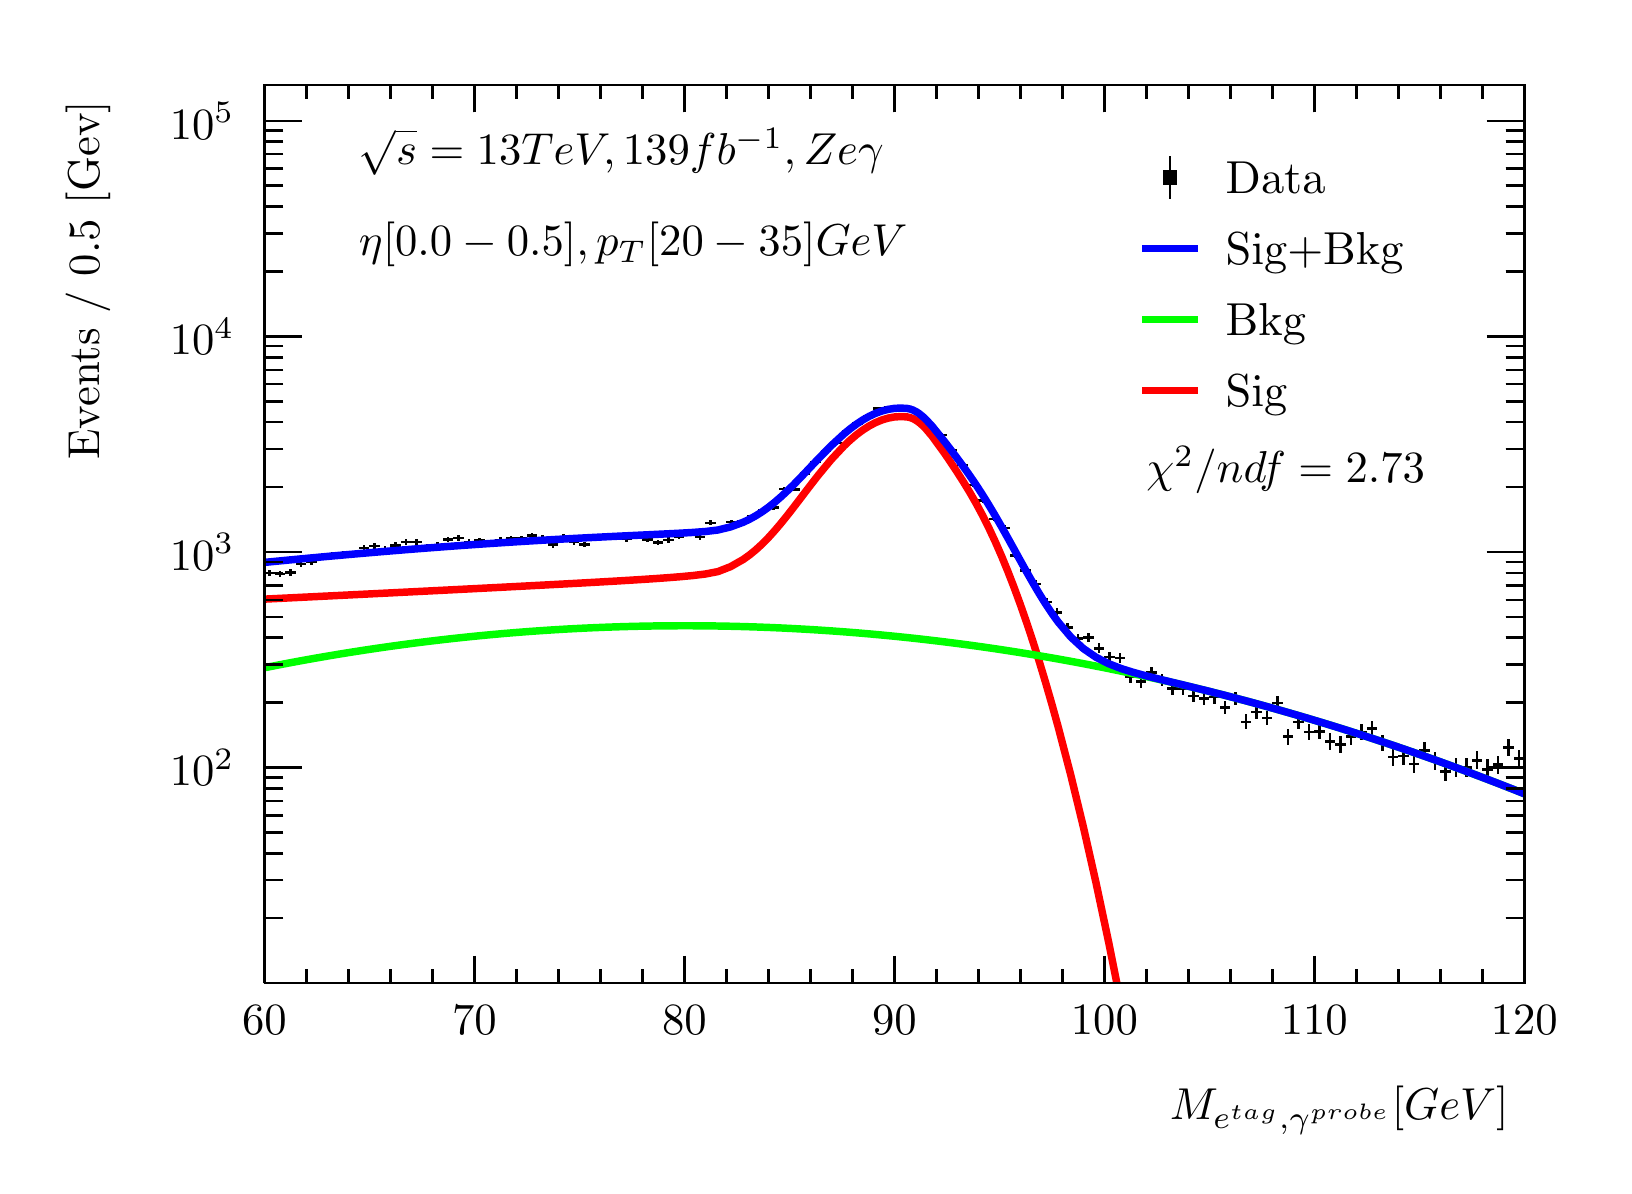
\begin{tikzpicture}
\pgfdeclareplotmark{cross} {
\pgfpathmoveto{\pgfpoint{-0.3\pgfplotmarksize}{\pgfplotmarksize}}
\pgfpathlineto{\pgfpoint{+0.3\pgfplotmarksize}{\pgfplotmarksize}}
\pgfpathlineto{\pgfpoint{+0.3\pgfplotmarksize}{0.3\pgfplotmarksize}}
\pgfpathlineto{\pgfpoint{+1\pgfplotmarksize}{0.3\pgfplotmarksize}}
\pgfpathlineto{\pgfpoint{+1\pgfplotmarksize}{-0.3\pgfplotmarksize}}
\pgfpathlineto{\pgfpoint{+0.3\pgfplotmarksize}{-0.3\pgfplotmarksize}}
\pgfpathlineto{\pgfpoint{+0.3\pgfplotmarksize}{-1.\pgfplotmarksize}}
\pgfpathlineto{\pgfpoint{-0.3\pgfplotmarksize}{-1.\pgfplotmarksize}}
\pgfpathlineto{\pgfpoint{-0.3\pgfplotmarksize}{-0.3\pgfplotmarksize}}
\pgfpathlineto{\pgfpoint{-1.\pgfplotmarksize}{-0.3\pgfplotmarksize}}
\pgfpathlineto{\pgfpoint{-1.\pgfplotmarksize}{0.3\pgfplotmarksize}}
\pgfpathlineto{\pgfpoint{-0.3\pgfplotmarksize}{0.3\pgfplotmarksize}}
\pgfpathclose
\pgfusepathqstroke
}
\pgfdeclareplotmark{cross*} {
\pgfpathmoveto{\pgfpoint{-0.3\pgfplotmarksize}{\pgfplotmarksize}}
\pgfpathlineto{\pgfpoint{+0.3\pgfplotmarksize}{\pgfplotmarksize}}
\pgfpathlineto{\pgfpoint{+0.3\pgfplotmarksize}{0.3\pgfplotmarksize}}
\pgfpathlineto{\pgfpoint{+1\pgfplotmarksize}{0.3\pgfplotmarksize}}
\pgfpathlineto{\pgfpoint{+1\pgfplotmarksize}{-0.3\pgfplotmarksize}}
\pgfpathlineto{\pgfpoint{+0.3\pgfplotmarksize}{-0.3\pgfplotmarksize}}
\pgfpathlineto{\pgfpoint{+0.3\pgfplotmarksize}{-1.\pgfplotmarksize}}
\pgfpathlineto{\pgfpoint{-0.3\pgfplotmarksize}{-1.\pgfplotmarksize}}
\pgfpathlineto{\pgfpoint{-0.3\pgfplotmarksize}{-0.3\pgfplotmarksize}}
\pgfpathlineto{\pgfpoint{-1.\pgfplotmarksize}{-0.3\pgfplotmarksize}}
\pgfpathlineto{\pgfpoint{-1.\pgfplotmarksize}{0.3\pgfplotmarksize}}
\pgfpathlineto{\pgfpoint{-0.3\pgfplotmarksize}{0.3\pgfplotmarksize}}
\pgfpathclose
\pgfusepathqfillstroke
}
\pgfdeclareplotmark{newstar} {
\pgfpathmoveto{\pgfqpoint{0pt}{\pgfplotmarksize}}
\pgfpathlineto{\pgfqpointpolar{44}{0.5\pgfplotmarksize}}
\pgfpathlineto{\pgfqpointpolar{18}{\pgfplotmarksize}}
\pgfpathlineto{\pgfqpointpolar{-20}{0.5\pgfplotmarksize}}
\pgfpathlineto{\pgfqpointpolar{-54}{\pgfplotmarksize}}
\pgfpathlineto{\pgfqpointpolar{-90}{0.5\pgfplotmarksize}}
\pgfpathlineto{\pgfqpointpolar{234}{\pgfplotmarksize}}
\pgfpathlineto{\pgfqpointpolar{198}{0.5\pgfplotmarksize}}
\pgfpathlineto{\pgfqpointpolar{162}{\pgfplotmarksize}}
\pgfpathlineto{\pgfqpointpolar{134}{0.5\pgfplotmarksize}}
\pgfpathclose
\pgfusepathqstroke
}
\pgfdeclareplotmark{newstar*} {
\pgfpathmoveto{\pgfqpoint{0pt}{\pgfplotmarksize}}
\pgfpathlineto{\pgfqpointpolar{44}{0.5\pgfplotmarksize}}
\pgfpathlineto{\pgfqpointpolar{18}{\pgfplotmarksize}}
\pgfpathlineto{\pgfqpointpolar{-20}{0.5\pgfplotmarksize}}
\pgfpathlineto{\pgfqpointpolar{-54}{\pgfplotmarksize}}
\pgfpathlineto{\pgfqpointpolar{-90}{0.5\pgfplotmarksize}}
\pgfpathlineto{\pgfqpointpolar{234}{\pgfplotmarksize}}
\pgfpathlineto{\pgfqpointpolar{198}{0.5\pgfplotmarksize}}
\pgfpathlineto{\pgfqpointpolar{162}{\pgfplotmarksize}}
\pgfpathlineto{\pgfqpointpolar{134}{0.5\pgfplotmarksize}}
\pgfpathclose
\pgfusepathqfillstroke
}
\definecolor{c}{rgb}{1,1,1};
\draw [color=c, fill=c] (0,0) rectangle (20,14.4361);
\draw [color=c, fill=c] (3,2.30977) rectangle (19,13.7143);
\definecolor{c}{rgb}{0,0,0};
\draw [c,line width=0.9] (3,2.30977) -- (3,13.7143) -- (19,13.7143) -- (19,2.30977) -- (3,2.30977);
\definecolor{c}{rgb}{1,1,1};
\draw [color=c, fill=c] (3,2.30977) rectangle (19,13.7143);
\definecolor{c}{rgb}{0,0,0};
\draw [c,line width=0.9] (3,2.30977) -- (3,13.7143) -- (19,13.7143) -- (19,2.30977) -- (3,2.30977);
\draw [c,line width=0.9] (3,2.30977) -- (19,2.30977);
\draw [c,line width=0.9] (3,2.65624) -- (3,2.30977);
\draw [c,line width=0.9] (3.53333,2.48301) -- (3.53333,2.30977);
\draw [c,line width=0.9] (4.06667,2.48301) -- (4.06667,2.30977);
\draw [c,line width=0.9] (4.6,2.48301) -- (4.6,2.30977);
\draw [c,line width=0.9] (5.13333,2.48301) -- (5.13333,2.30977);
\draw [c,line width=0.9] (5.66667,2.65624) -- (5.66667,2.30977);
\draw [c,line width=0.9] (6.2,2.48301) -- (6.2,2.30977);
\draw [c,line width=0.9] (6.73333,2.48301) -- (6.73333,2.30977);
\draw [c,line width=0.9] (7.26667,2.48301) -- (7.26667,2.30977);
\draw [c,line width=0.9] (7.8,2.48301) -- (7.8,2.30977);
\draw [c,line width=0.9] (8.33333,2.65624) -- (8.33333,2.30977);
\draw [c,line width=0.9] (8.86667,2.48301) -- (8.86667,2.30977);
\draw [c,line width=0.9] (9.4,2.48301) -- (9.4,2.30977);
\draw [c,line width=0.9] (9.93333,2.48301) -- (9.93333,2.30977);
\draw [c,line width=0.9] (10.4667,2.48301) -- (10.4667,2.30977);
\draw [c,line width=0.9] (11,2.65624) -- (11,2.30977);
\draw [c,line width=0.9] (11.5333,2.48301) -- (11.5333,2.30977);
\draw [c,line width=0.9] (12.0667,2.48301) -- (12.0667,2.30977);
\draw [c,line width=0.9] (12.6,2.48301) -- (12.6,2.30977);
\draw [c,line width=0.9] (13.1333,2.48301) -- (13.1333,2.30977);
\draw [c,line width=0.9] (13.6667,2.65624) -- (13.6667,2.30977);
\draw [c,line width=0.9] (14.2,2.48301) -- (14.2,2.30977);
\draw [c,line width=0.9] (14.7333,2.48301) -- (14.7333,2.30977);
\draw [c,line width=0.9] (15.2667,2.48301) -- (15.2667,2.30977);
\draw [c,line width=0.9] (15.8,2.48301) -- (15.8,2.30977);
\draw [c,line width=0.9] (16.3333,2.65624) -- (16.3333,2.30977);
\draw [c,line width=0.9] (16.8667,2.48301) -- (16.8667,2.30977);
\draw [c,line width=0.9] (17.4,2.48301) -- (17.4,2.30977);
\draw [c,line width=0.9] (17.9333,2.48301) -- (17.9333,2.30977);
\draw [c,line width=0.9] (18.4667,2.48301) -- (18.4667,2.30977);
\draw [c,line width=0.9] (19,2.65624) -- (19,2.30977);
\draw [anchor=base] (3,1.66015) node[scale=1.61424, color=c, rotate=0]{60};
\draw [anchor=base] (5.66667,1.66015) node[scale=1.61424, color=c, rotate=0]{70};
\draw [anchor=base] (8.33333,1.66015) node[scale=1.61424, color=c, rotate=0]{80};
\draw [anchor=base] (11,1.66015) node[scale=1.61424, color=c, rotate=0]{90};
\draw [anchor=base] (13.6667,1.66015) node[scale=1.61424, color=c, rotate=0]{100};
\draw [anchor=base] (16.3333,1.66015) node[scale=1.61424, color=c, rotate=0]{110};
\draw [anchor=base] (19,1.66015) node[scale=1.61424, color=c, rotate=0]{120};
\draw [anchor= east] (19,0.692932) node[scale=1.61424, color=c, rotate=0]{$M_{e^{tag}, \gamma^{probe}}  [GeV]$};
\draw [c,line width=0.9] (3,13.7143) -- (19,13.7143);
\draw [c,line width=0.9] (3,13.3678) -- (3,13.7143);
\draw [c,line width=0.9] (3.53333,13.5411) -- (3.53333,13.7143);
\draw [c,line width=0.9] (4.06667,13.5411) -- (4.06667,13.7143);
\draw [c,line width=0.9] (4.6,13.5411) -- (4.6,13.7143);
\draw [c,line width=0.9] (5.13333,13.5411) -- (5.13333,13.7143);
\draw [c,line width=0.9] (5.66667,13.3678) -- (5.66667,13.7143);
\draw [c,line width=0.9] (6.2,13.5411) -- (6.2,13.7143);
\draw [c,line width=0.9] (6.73333,13.5411) -- (6.73333,13.7143);
\draw [c,line width=0.9] (7.26667,13.5411) -- (7.26667,13.7143);
\draw [c,line width=0.9] (7.8,13.5411) -- (7.8,13.7143);
\draw [c,line width=0.9] (8.33333,13.3678) -- (8.33333,13.7143);
\draw [c,line width=0.9] (8.86667,13.5411) -- (8.86667,13.7143);
\draw [c,line width=0.9] (9.4,13.5411) -- (9.4,13.7143);
\draw [c,line width=0.9] (9.93333,13.5411) -- (9.93333,13.7143);
\draw [c,line width=0.9] (10.4667,13.5411) -- (10.4667,13.7143);
\draw [c,line width=0.9] (11,13.3678) -- (11,13.7143);
\draw [c,line width=0.9] (11.5333,13.5411) -- (11.5333,13.7143);
\draw [c,line width=0.9] (12.0667,13.5411) -- (12.0667,13.7143);
\draw [c,line width=0.9] (12.6,13.5411) -- (12.6,13.7143);
\draw [c,line width=0.9] (13.1333,13.5411) -- (13.1333,13.7143);
\draw [c,line width=0.9] (13.6667,13.3678) -- (13.6667,13.7143);
\draw [c,line width=0.9] (14.2,13.5411) -- (14.2,13.7143);
\draw [c,line width=0.9] (14.7333,13.5411) -- (14.7333,13.7143);
\draw [c,line width=0.9] (15.2667,13.5411) -- (15.2667,13.7143);
\draw [c,line width=0.9] (15.8,13.5411) -- (15.8,13.7143);
\draw [c,line width=0.9] (16.3333,13.3678) -- (16.3333,13.7143);
\draw [c,line width=0.9] (16.8667,13.5411) -- (16.8667,13.7143);
\draw [c,line width=0.9] (17.4,13.5411) -- (17.4,13.7143);
\draw [c,line width=0.9] (17.9333,13.5411) -- (17.9333,13.7143);
\draw [c,line width=0.9] (18.4667,13.5411) -- (18.4667,13.7143);
\draw [c,line width=0.9] (19,13.3678) -- (19,13.7143);
\draw [c,line width=0.9] (3,2.30977) -- (3,13.7143);
\draw [c,line width=0.9] (3.237,3.13385) -- (3,3.13385);
\draw [c,line width=0.9] (3.237,3.6159) -- (3,3.6159);
\draw [c,line width=0.9] (3.237,3.95792) -- (3,3.95792);
\draw [c,line width=0.9] (3.237,4.22321) -- (3,4.22321);
\draw [c,line width=0.9] (3.237,4.43997) -- (3,4.43997);
\draw [c,line width=0.9] (3.237,4.62324) -- (3,4.62324);
\draw [c,line width=0.9] (3.237,4.782) -- (3,4.782);
\draw [c,line width=0.9] (3.237,4.92203) -- (3,4.92203);
\draw [c,line width=0.9] (3.474,5.04729) -- (3,5.04729);
\draw [anchor= east] (2.82,5.04729) node[scale=1.61424, color=c, rotate=0]{$10^{2}$};
\draw [c,line width=0.9] (3.237,5.87136) -- (3,5.87136);
\draw [c,line width=0.9] (3.237,6.35342) -- (3,6.35342);
\draw [c,line width=0.9] (3.237,6.69544) -- (3,6.69544);
\draw [c,line width=0.9] (3.237,6.96073) -- (3,6.96073);
\draw [c,line width=0.9] (3.237,7.17749) -- (3,7.17749);
\draw [c,line width=0.9] (3.237,7.36076) -- (3,7.36076);
\draw [c,line width=0.9] (3.237,7.51951) -- (3,7.51951);
\draw [c,line width=0.9] (3.237,7.65954) -- (3,7.65954);
\draw [c,line width=0.9] (3.474,7.78481) -- (3,7.78481);
\draw [anchor= east] (2.82,7.78481) node[scale=1.61424, color=c, rotate=0]{$10^{3}$};
\draw [c,line width=0.9] (3.237,8.60888) -- (3,8.60888);
\draw [c,line width=0.9] (3.237,9.09093) -- (3,9.09093);
\draw [c,line width=0.9] (3.237,9.43296) -- (3,9.43296);
\draw [c,line width=0.9] (3.237,9.69825) -- (3,9.69825);
\draw [c,line width=0.9] (3.237,9.91501) -- (3,9.91501);
\draw [c,line width=0.9] (3.237,10.0983) -- (3,10.0983);
\draw [c,line width=0.9] (3.237,10.257) -- (3,10.257);
\draw [c,line width=0.9] (3.237,10.3971) -- (3,10.3971);
\draw [c,line width=0.9] (3.474,10.5223) -- (3,10.5223);
\draw [anchor= east] (2.82,10.5223) node[scale=1.61424, color=c, rotate=0]{$10^{4}$};
\draw [c,line width=0.9] (3.237,11.3464) -- (3,11.3464);
\draw [c,line width=0.9] (3.237,11.8285) -- (3,11.8285);
\draw [c,line width=0.9] (3.237,12.1705) -- (3,12.1705);
\draw [c,line width=0.9] (3.237,12.4358) -- (3,12.4358);
\draw [c,line width=0.9] (3.237,12.6525) -- (3,12.6525);
\draw [c,line width=0.9] (3.237,12.8358) -- (3,12.8358);
\draw [c,line width=0.9] (3.237,12.9945) -- (3,12.9945);
\draw [c,line width=0.9] (3.237,13.1346) -- (3,13.1346);
\draw [c,line width=0.9] (3.474,13.2598) -- (3,13.2598);
\draw [anchor= east] (2.82,13.2598) node[scale=1.61424, color=c, rotate=0]{$10^{5}$};
\draw [anchor= east] (0.76,13.7143) node[scale=1.61424, color=c, rotate=90]{Events / 0.5 [Gev]};
\draw [c,line width=0.9] (19,2.30977) -- (19,13.7143);
\draw [c,line width=0.9] (18.763,3.13385) -- (19,3.13385);
\draw [c,line width=0.9] (18.763,3.6159) -- (19,3.6159);
\draw [c,line width=0.9] (18.763,3.95792) -- (19,3.95792);
\draw [c,line width=0.9] (18.763,4.22321) -- (19,4.22321);
\draw [c,line width=0.9] (18.763,4.43997) -- (19,4.43997);
\draw [c,line width=0.9] (18.763,4.62324) -- (19,4.62324);
\draw [c,line width=0.9] (18.763,4.782) -- (19,4.782);
\draw [c,line width=0.9] (18.763,4.92203) -- (19,4.92203);
\draw [c,line width=0.9] (18.526,5.04729) -- (19,5.04729);
\draw [c,line width=0.9] (18.763,5.87136) -- (19,5.87136);
\draw [c,line width=0.9] (18.763,6.35342) -- (19,6.35342);
\draw [c,line width=0.9] (18.763,6.69544) -- (19,6.69544);
\draw [c,line width=0.9] (18.763,6.96073) -- (19,6.96073);
\draw [c,line width=0.9] (18.763,7.17749) -- (19,7.17749);
\draw [c,line width=0.9] (18.763,7.36076) -- (19,7.36076);
\draw [c,line width=0.9] (18.763,7.51951) -- (19,7.51951);
\draw [c,line width=0.9] (18.763,7.65954) -- (19,7.65954);
\draw [c,line width=0.9] (18.526,7.78481) -- (19,7.78481);
\draw [c,line width=0.9] (18.763,8.60888) -- (19,8.60888);
\draw [c,line width=0.9] (18.763,9.09093) -- (19,9.09093);
\draw [c,line width=0.9] (18.763,9.43296) -- (19,9.43296);
\draw [c,line width=0.9] (18.763,9.69825) -- (19,9.69825);
\draw [c,line width=0.9] (18.763,9.91501) -- (19,9.91501);
\draw [c,line width=0.9] (18.763,10.0983) -- (19,10.0983);
\draw [c,line width=0.9] (18.763,10.257) -- (19,10.257);
\draw [c,line width=0.9] (18.763,10.3971) -- (19,10.3971);
\draw [c,line width=0.9] (18.526,10.5223) -- (19,10.5223);
\draw [c,line width=0.9] (18.763,11.3464) -- (19,11.3464);
\draw [c,line width=0.9] (18.763,11.8285) -- (19,11.8285);
\draw [c,line width=0.9] (18.763,12.1705) -- (19,12.1705);
\draw [c,line width=0.9] (18.763,12.4358) -- (19,12.4358);
\draw [c,line width=0.9] (18.763,12.6525) -- (19,12.6525);
\draw [c,line width=0.9] (18.763,12.8358) -- (19,12.8358);
\draw [c,line width=0.9] (18.763,12.9945) -- (19,12.9945);
\draw [c,line width=0.9] (18.763,13.1346) -- (19,13.1346);
\draw [c,line width=0.9] (18.526,13.2598) -- (19,13.2598);
\draw [c,line width=0.9] (3.06667,7.51505) -- (3,7.51505);
\draw [c,line width=0.9] (3,7.51505) -- (3,7.51505);
\draw [c,line width=0.9] (3.06667,7.51505) -- (3.13333,7.51505);
\draw [c,line width=0.9] (3.13333,7.51505) -- (3.13333,7.51505);
\draw [c,line width=0.9] (3.06667,7.51505) -- (3.06667,7.55716);
\draw [c,line width=0.9] (3.06667,7.55716) -- (3.06667,7.55716);
\draw [c,line width=0.9] (3.06667,7.51505) -- (3.06667,7.47294);
\draw [c,line width=0.9] (3.06667,7.47294) -- (3.06667,7.47294);
\draw [c,line width=0.9] (3.2,7.50606) -- (3.13333,7.50606);
\draw [c,line width=0.9] (3.13333,7.50606) -- (3.13333,7.50606);
\draw [c,line width=0.9] (3.2,7.50606) -- (3.26667,7.50606);
\draw [c,line width=0.9] (3.26667,7.50606) -- (3.26667,7.50606);
\draw [c,line width=0.9] (3.2,7.50606) -- (3.2,7.54833);
\draw [c,line width=0.9] (3.2,7.54833) -- (3.2,7.54833);
\draw [c,line width=0.9] (3.2,7.50606) -- (3.2,7.46379);
\draw [c,line width=0.9] (3.2,7.46379) -- (3.2,7.46379);
\draw [c,line width=0.9] (3.33333,7.521) -- (3.26667,7.521);
\draw [c,line width=0.9] (3.26667,7.521) -- (3.26667,7.521);
\draw [c,line width=0.9] (3.33333,7.521) -- (3.4,7.521);
\draw [c,line width=0.9] (3.4,7.521) -- (3.4,7.521);
\draw [c,line width=0.9] (3.33333,7.521) -- (3.33333,7.563);
\draw [c,line width=0.9] (3.33333,7.563) -- (3.33333,7.563);
\draw [c,line width=0.9] (3.33333,7.521) -- (3.33333,7.47899);
\draw [c,line width=0.9] (3.33333,7.47899) -- (3.33333,7.47899);
\draw [c,line width=0.9] (3.46667,7.63012) -- (3.4,7.63012);
\draw [c,line width=0.9] (3.4,7.63012) -- (3.4,7.63012);
\draw [c,line width=0.9] (3.46667,7.63012) -- (3.53333,7.63012);
\draw [c,line width=0.9] (3.53333,7.63012) -- (3.53333,7.63012);
\draw [c,line width=0.9] (3.46667,7.63012) -- (3.46667,7.67024);
\draw [c,line width=0.9] (3.46667,7.67024) -- (3.46667,7.67024);
\draw [c,line width=0.9] (3.46667,7.63012) -- (3.46667,7.59);
\draw [c,line width=0.9] (3.46667,7.59) -- (3.46667,7.59);
\draw [c,line width=0.9] (3.6,7.65425) -- (3.53333,7.65425);
\draw [c,line width=0.9] (3.53333,7.65425) -- (3.53333,7.65425);
\draw [c,line width=0.9] (3.6,7.65425) -- (3.66667,7.65425);
\draw [c,line width=0.9] (3.66667,7.65425) -- (3.66667,7.65425);
\draw [c,line width=0.9] (3.6,7.65425) -- (3.6,7.69397);
\draw [c,line width=0.9] (3.6,7.69397) -- (3.6,7.69397);
\draw [c,line width=0.9] (3.6,7.65425) -- (3.6,7.61453);
\draw [c,line width=0.9] (3.6,7.61453) -- (3.6,7.61453);
\draw [c,line width=0.9] (3.73333,7.72633) -- (3.66667,7.72633);
\draw [c,line width=0.9] (3.66667,7.72633) -- (3.66667,7.72633);
\draw [c,line width=0.9] (3.73333,7.72633) -- (3.8,7.72633);
\draw [c,line width=0.9] (3.8,7.72633) -- (3.8,7.72633);
\draw [c,line width=0.9] (3.73333,7.72633) -- (3.73333,7.76486);
\draw [c,line width=0.9] (3.73333,7.76486) -- (3.73333,7.76486);
\draw [c,line width=0.9] (3.73333,7.72633) -- (3.73333,7.6878);
\draw [c,line width=0.9] (3.73333,7.6878) -- (3.73333,7.6878);
\draw [c,line width=0.9] (3.86667,7.73998) -- (3.8,7.73998);
\draw [c,line width=0.9] (3.8,7.73998) -- (3.8,7.73998);
\draw [c,line width=0.9] (3.86667,7.73998) -- (3.93333,7.73998);
\draw [c,line width=0.9] (3.93333,7.73998) -- (3.93333,7.73998);
\draw [c,line width=0.9] (3.86667,7.73998) -- (3.86667,7.77829);
\draw [c,line width=0.9] (3.86667,7.77829) -- (3.86667,7.77829);
\draw [c,line width=0.9] (3.86667,7.73998) -- (3.86667,7.70167);
\draw [c,line width=0.9] (3.86667,7.70167) -- (3.86667,7.70167);
\draw [c,line width=0.9] (4,7.75714) -- (3.93333,7.75714);
\draw [c,line width=0.9] (3.93333,7.75714) -- (3.93333,7.75714);
\draw [c,line width=0.9] (4,7.75714) -- (4.06667,7.75714);
\draw [c,line width=0.9] (4.06667,7.75714) -- (4.06667,7.75714);
\draw [c,line width=0.9] (4,7.75714) -- (4,7.79518);
\draw [c,line width=0.9] (4,7.79518) -- (4,7.79518);
\draw [c,line width=0.9] (4,7.75714) -- (4,7.71911);
\draw [c,line width=0.9] (4,7.71911) -- (4,7.71911);
\draw [c,line width=0.9] (4.13333,7.76079) -- (4.06667,7.76079);
\draw [c,line width=0.9] (4.06667,7.76079) -- (4.06667,7.76079);
\draw [c,line width=0.9] (4.13333,7.76079) -- (4.2,7.76079);
\draw [c,line width=0.9] (4.2,7.76079) -- (4.2,7.76079);
\draw [c,line width=0.9] (4.13333,7.76079) -- (4.13333,7.79876);
\draw [c,line width=0.9] (4.13333,7.79876) -- (4.13333,7.79876);
\draw [c,line width=0.9] (4.13333,7.76079) -- (4.13333,7.72281);
\draw [c,line width=0.9] (4.13333,7.72281) -- (4.13333,7.72281);
\draw [c,line width=0.9] (4.26667,7.83486) -- (4.2,7.83486);
\draw [c,line width=0.9] (4.2,7.83486) -- (4.2,7.83486);
\draw [c,line width=0.9] (4.26667,7.83486) -- (4.33333,7.83486);
\draw [c,line width=0.9] (4.33333,7.83486) -- (4.33333,7.83486);
\draw [c,line width=0.9] (4.26667,7.83486) -- (4.26667,7.87167);
\draw [c,line width=0.9] (4.26667,7.87167) -- (4.26667,7.87167);
\draw [c,line width=0.9] (4.26667,7.83486) -- (4.26667,7.79805);
\draw [c,line width=0.9] (4.26667,7.79805) -- (4.26667,7.79805);
\draw [c,line width=0.9] (4.4,7.85744) -- (4.33333,7.85744);
\draw [c,line width=0.9] (4.33333,7.85744) -- (4.33333,7.85744);
\draw [c,line width=0.9] (4.4,7.85744) -- (4.46667,7.85744);
\draw [c,line width=0.9] (4.46667,7.85744) -- (4.46667,7.85744);
\draw [c,line width=0.9] (4.4,7.85744) -- (4.4,7.89391);
\draw [c,line width=0.9] (4.4,7.89391) -- (4.4,7.89391);
\draw [c,line width=0.9] (4.4,7.85744) -- (4.4,7.82098);
\draw [c,line width=0.9] (4.4,7.82098) -- (4.4,7.82098);
\draw [c,line width=0.9] (4.53333,7.81995) -- (4.46667,7.81995);
\draw [c,line width=0.9] (4.46667,7.81995) -- (4.46667,7.81995);
\draw [c,line width=0.9] (4.53333,7.81995) -- (4.6,7.81995);
\draw [c,line width=0.9] (4.6,7.81995) -- (4.6,7.81995);
\draw [c,line width=0.9] (4.53333,7.81995) -- (4.53333,7.85699);
\draw [c,line width=0.9] (4.53333,7.85699) -- (4.53333,7.85699);
\draw [c,line width=0.9] (4.53333,7.81995) -- (4.53333,7.78291);
\draw [c,line width=0.9] (4.53333,7.78291) -- (4.53333,7.78291);
\draw [c,line width=0.9] (4.66667,7.86968) -- (4.6,7.86968);
\draw [c,line width=0.9] (4.6,7.86968) -- (4.6,7.86968);
\draw [c,line width=0.9] (4.66667,7.86968) -- (4.73333,7.86968);
\draw [c,line width=0.9] (4.73333,7.86968) -- (4.73333,7.86968);
\draw [c,line width=0.9] (4.66667,7.86968) -- (4.66667,7.90596);
\draw [c,line width=0.9] (4.66667,7.90596) -- (4.66667,7.90596);
\draw [c,line width=0.9] (4.66667,7.86968) -- (4.66667,7.83341);
\draw [c,line width=0.9] (4.66667,7.83341) -- (4.66667,7.83341);
\draw [c,line width=0.9] (4.8,7.91209) -- (4.73333,7.91209);
\draw [c,line width=0.9] (4.73333,7.91209) -- (4.73333,7.91209);
\draw [c,line width=0.9] (4.8,7.91209) -- (4.86667,7.91209);
\draw [c,line width=0.9] (4.86667,7.91209) -- (4.86667,7.91209);
\draw [c,line width=0.9] (4.8,7.91209) -- (4.8,7.94772);
\draw [c,line width=0.9] (4.8,7.94772) -- (4.8,7.94772);
\draw [c,line width=0.9] (4.8,7.91209) -- (4.8,7.87645);
\draw [c,line width=0.9] (4.8,7.87645) -- (4.8,7.87645);
\draw [c,line width=0.9] (4.93333,7.90995) -- (4.86667,7.90995);
\draw [c,line width=0.9] (4.86667,7.90995) -- (4.86667,7.90995);
\draw [c,line width=0.9] (4.93333,7.90995) -- (5,7.90995);
\draw [c,line width=0.9] (5,7.90995) -- (5,7.90995);
\draw [c,line width=0.9] (4.93333,7.90995) -- (4.93333,7.94562);
\draw [c,line width=0.9] (4.93333,7.94562) -- (4.93333,7.94562);
\draw [c,line width=0.9] (4.93333,7.90995) -- (4.93333,7.87428);
\draw [c,line width=0.9] (4.93333,7.87428) -- (4.93333,7.87428);
\draw [c,line width=0.9] (5.06667,7.85408) -- (5,7.85408);
\draw [c,line width=0.9] (5,7.85408) -- (5,7.85408);
\draw [c,line width=0.9] (5.06667,7.85408) -- (5.13333,7.85408);
\draw [c,line width=0.9] (5.13333,7.85408) -- (5.13333,7.85408);
\draw [c,line width=0.9] (5.06667,7.85408) -- (5.06667,7.8906);
\draw [c,line width=0.9] (5.06667,7.8906) -- (5.06667,7.8906);
\draw [c,line width=0.9] (5.06667,7.85408) -- (5.06667,7.81757);
\draw [c,line width=0.9] (5.06667,7.81757) -- (5.06667,7.81757);
\draw [c,line width=0.9] (5.2,7.87189) -- (5.13333,7.87189);
\draw [c,line width=0.9] (5.13333,7.87189) -- (5.13333,7.87189);
\draw [c,line width=0.9] (5.2,7.87189) -- (5.26667,7.87189);
\draw [c,line width=0.9] (5.26667,7.87189) -- (5.26667,7.87189);
\draw [c,line width=0.9] (5.2,7.87189) -- (5.2,7.90814);
\draw [c,line width=0.9] (5.2,7.90814) -- (5.2,7.90814);
\draw [c,line width=0.9] (5.2,7.87189) -- (5.2,7.83565);
\draw [c,line width=0.9] (5.2,7.83565) -- (5.2,7.83565);
\draw [c,line width=0.9] (5.33333,7.94163) -- (5.26667,7.94163);
\draw [c,line width=0.9] (5.26667,7.94163) -- (5.26667,7.94163);
\draw [c,line width=0.9] (5.33333,7.94163) -- (5.4,7.94163);
\draw [c,line width=0.9] (5.4,7.94163) -- (5.4,7.94163);
\draw [c,line width=0.9] (5.33333,7.94163) -- (5.33333,7.97682);
\draw [c,line width=0.9] (5.33333,7.97682) -- (5.33333,7.97682);
\draw [c,line width=0.9] (5.33333,7.94163) -- (5.33333,7.90643);
\draw [c,line width=0.9] (5.33333,7.90643) -- (5.33333,7.90643);
\draw [c,line width=0.9] (5.46667,7.96229) -- (5.4,7.96229);
\draw [c,line width=0.9] (5.4,7.96229) -- (5.4,7.96229);
\draw [c,line width=0.9] (5.46667,7.96229) -- (5.53333,7.96229);
\draw [c,line width=0.9] (5.53333,7.96229) -- (5.53333,7.96229);
\draw [c,line width=0.9] (5.46667,7.96229) -- (5.46667,7.99718);
\draw [c,line width=0.9] (5.46667,7.99718) -- (5.46667,7.99718);
\draw [c,line width=0.9] (5.46667,7.96229) -- (5.46667,7.9274);
\draw [c,line width=0.9] (5.46667,7.9274) -- (5.46667,7.9274);
\draw [c,line width=0.9] (5.6,7.91422) -- (5.53333,7.91422);
\draw [c,line width=0.9] (5.53333,7.91422) -- (5.53333,7.91422);
\draw [c,line width=0.9] (5.6,7.91422) -- (5.66667,7.91422);
\draw [c,line width=0.9] (5.66667,7.91422) -- (5.66667,7.91422);
\draw [c,line width=0.9] (5.6,7.91422) -- (5.6,7.94983);
\draw [c,line width=0.9] (5.6,7.94983) -- (5.6,7.94983);
\draw [c,line width=0.9] (5.6,7.91422) -- (5.6,7.87862);
\draw [c,line width=0.9] (5.6,7.87862) -- (5.6,7.87862);
\draw [c,line width=0.9] (5.73333,7.93221) -- (5.66667,7.93221);
\draw [c,line width=0.9] (5.66667,7.93221) -- (5.66667,7.93221);
\draw [c,line width=0.9] (5.73333,7.93221) -- (5.8,7.93221);
\draw [c,line width=0.9] (5.8,7.93221) -- (5.8,7.93221);
\draw [c,line width=0.9] (5.73333,7.93221) -- (5.73333,7.96755);
\draw [c,line width=0.9] (5.73333,7.96755) -- (5.73333,7.96755);
\draw [c,line width=0.9] (5.73333,7.93221) -- (5.73333,7.89688);
\draw [c,line width=0.9] (5.73333,7.89688) -- (5.73333,7.89688);
\draw [c,line width=0.9] (5.86667,7.89487) -- (5.8,7.89487);
\draw [c,line width=0.9] (5.8,7.89487) -- (5.8,7.89487);
\draw [c,line width=0.9] (5.86667,7.89487) -- (5.93333,7.89487);
\draw [c,line width=0.9] (5.93333,7.89487) -- (5.93333,7.89487);
\draw [c,line width=0.9] (5.86667,7.89487) -- (5.86667,7.93077);
\draw [c,line width=0.9] (5.86667,7.93077) -- (5.86667,7.93077);
\draw [c,line width=0.9] (5.86667,7.89487) -- (5.86667,7.85898);
\draw [c,line width=0.9] (5.86667,7.85898) -- (5.86667,7.85898);
\draw [c,line width=0.9] (6,7.9385) -- (5.93333,7.9385);
\draw [c,line width=0.9] (5.93333,7.9385) -- (5.93333,7.9385);
\draw [c,line width=0.9] (6,7.9385) -- (6.06667,7.9385);
\draw [c,line width=0.9] (6.06667,7.9385) -- (6.06667,7.9385);
\draw [c,line width=0.9] (6,7.9385) -- (6,7.97374);
\draw [c,line width=0.9] (6,7.97374) -- (6,7.97374);
\draw [c,line width=0.9] (6,7.9385) -- (6,7.90326);
\draw [c,line width=0.9] (6,7.90326) -- (6,7.90326);
\draw [c,line width=0.9] (6.13333,7.95303) -- (6.06667,7.95303);
\draw [c,line width=0.9] (6.06667,7.95303) -- (6.06667,7.95303);
\draw [c,line width=0.9] (6.13333,7.95303) -- (6.2,7.95303);
\draw [c,line width=0.9] (6.2,7.95303) -- (6.2,7.95303);
\draw [c,line width=0.9] (6.13333,7.95303) -- (6.13333,7.98806);
\draw [c,line width=0.9] (6.13333,7.98806) -- (6.13333,7.98806);
\draw [c,line width=0.9] (6.13333,7.95303) -- (6.13333,7.91801);
\draw [c,line width=0.9] (6.13333,7.91801) -- (6.13333,7.91801);
\draw [c,line width=0.9] (6.26667,7.9551) -- (6.2,7.9551);
\draw [c,line width=0.9] (6.2,7.9551) -- (6.2,7.9551);
\draw [c,line width=0.9] (6.26667,7.9551) -- (6.33333,7.9551);
\draw [c,line width=0.9] (6.33333,7.9551) -- (6.33333,7.9551);
\draw [c,line width=0.9] (6.26667,7.9551) -- (6.26667,7.99009);
\draw [c,line width=0.9] (6.26667,7.99009) -- (6.26667,7.99009);
\draw [c,line width=0.9] (6.26667,7.9551) -- (6.26667,7.9201);
\draw [c,line width=0.9] (6.26667,7.9201) -- (6.26667,7.9201);
\draw [c,line width=0.9] (6.4,7.99361) -- (6.33333,7.99361);
\draw [c,line width=0.9] (6.33333,7.99361) -- (6.33333,7.99361);
\draw [c,line width=0.9] (6.4,7.99361) -- (6.46667,7.99361);
\draw [c,line width=0.9] (6.46667,7.99361) -- (6.46667,7.99361);
\draw [c,line width=0.9] (6.4,7.99361) -- (6.4,8.02805);
\draw [c,line width=0.9] (6.4,8.02805) -- (6.4,8.02805);
\draw [c,line width=0.9] (6.4,7.99361) -- (6.4,7.95918);
\draw [c,line width=0.9] (6.4,7.95918) -- (6.4,7.95918);
\draw [c,line width=0.9] (6.53333,7.96433) -- (6.46667,7.96433);
\draw [c,line width=0.9] (6.46667,7.96433) -- (6.46667,7.96433);
\draw [c,line width=0.9] (6.53333,7.96433) -- (6.6,7.96433);
\draw [c,line width=0.9] (6.6,7.96433) -- (6.6,7.96433);
\draw [c,line width=0.9] (6.53333,7.96433) -- (6.53333,7.99919);
\draw [c,line width=0.9] (6.53333,7.99919) -- (6.53333,7.99919);
\draw [c,line width=0.9] (6.53333,7.96433) -- (6.53333,7.92947);
\draw [c,line width=0.9] (6.53333,7.92947) -- (6.53333,7.92947);
\draw [c,line width=0.9] (6.66667,7.87631) -- (6.6,7.87631);
\draw [c,line width=0.9] (6.6,7.87631) -- (6.6,7.87631);
\draw [c,line width=0.9] (6.66667,7.87631) -- (6.73333,7.87631);
\draw [c,line width=0.9] (6.73333,7.87631) -- (6.73333,7.87631);
\draw [c,line width=0.9] (6.66667,7.87631) -- (6.66667,7.91248);
\draw [c,line width=0.9] (6.66667,7.91248) -- (6.66667,7.91248);
\draw [c,line width=0.9] (6.66667,7.87631) -- (6.66667,7.84013);
\draw [c,line width=0.9] (6.66667,7.84013) -- (6.66667,7.84013);
\draw [c,line width=0.9] (6.8,7.97552) -- (6.73333,7.97552);
\draw [c,line width=0.9] (6.73333,7.97552) -- (6.73333,7.97552);
\draw [c,line width=0.9] (6.8,7.97552) -- (6.86667,7.97552);
\draw [c,line width=0.9] (6.86667,7.97552) -- (6.86667,7.97552);
\draw [c,line width=0.9] (6.8,7.97552) -- (6.8,8.01022);
\draw [c,line width=0.9] (6.8,8.01022) -- (6.8,8.01022);
\draw [c,line width=0.9] (6.8,7.97552) -- (6.8,7.94083);
\draw [c,line width=0.9] (6.8,7.94083) -- (6.8,7.94083);
\draw [c,line width=0.9] (6.93333,7.90888) -- (6.86667,7.90888);
\draw [c,line width=0.9] (6.86667,7.90888) -- (6.86667,7.90888);
\draw [c,line width=0.9] (6.93333,7.90888) -- (7,7.90888);
\draw [c,line width=0.9] (7,7.90888) -- (7,7.90888);
\draw [c,line width=0.9] (6.93333,7.90888) -- (6.93333,7.94456);
\draw [c,line width=0.9] (6.93333,7.94456) -- (6.93333,7.94456);
\draw [c,line width=0.9] (6.93333,7.90888) -- (6.93333,7.8732);
\draw [c,line width=0.9] (6.93333,7.8732) -- (6.93333,7.8732);
\draw [c,line width=0.9] (7.06667,7.87851) -- (7,7.87851);
\draw [c,line width=0.9] (7,7.87851) -- (7,7.87851);
\draw [c,line width=0.9] (7.06667,7.87851) -- (7.13333,7.87851);
\draw [c,line width=0.9] (7.13333,7.87851) -- (7.13333,7.87851);
\draw [c,line width=0.9] (7.06667,7.87851) -- (7.06667,7.91465);
\draw [c,line width=0.9] (7.06667,7.91465) -- (7.06667,7.91465);
\draw [c,line width=0.9] (7.06667,7.87851) -- (7.06667,7.84236);
\draw [c,line width=0.9] (7.06667,7.84236) -- (7.06667,7.84236);
\draw [c,line width=0.9] (7.2,7.95716) -- (7.13333,7.95716);
\draw [c,line width=0.9] (7.13333,7.95716) -- (7.13333,7.95716);
\draw [c,line width=0.9] (7.2,7.95716) -- (7.26667,7.95716);
\draw [c,line width=0.9] (7.26667,7.95716) -- (7.26667,7.95716);
\draw [c,line width=0.9] (7.2,7.95716) -- (7.2,7.99212);
\draw [c,line width=0.9] (7.2,7.99212) -- (7.2,7.99212);
\draw [c,line width=0.9] (7.2,7.95716) -- (7.2,7.92219);
\draw [c,line width=0.9] (7.2,7.92219) -- (7.2,7.92219);
\draw [c,line width=0.9] (7.33333,7.97957) -- (7.26667,7.97957);
\draw [c,line width=0.9] (7.26667,7.97957) -- (7.26667,7.97957);
\draw [c,line width=0.9] (7.33333,7.97957) -- (7.4,7.97957);
\draw [c,line width=0.9] (7.4,7.97957) -- (7.4,7.97957);
\draw [c,line width=0.9] (7.33333,7.97957) -- (7.33333,8.01421);
\draw [c,line width=0.9] (7.33333,8.01421) -- (7.33333,8.01421);
\draw [c,line width=0.9] (7.33333,7.97957) -- (7.33333,7.94493);
\draw [c,line width=0.9] (7.33333,7.94493) -- (7.33333,7.94493);
\draw [c,line width=0.9] (7.46667,7.97755) -- (7.4,7.97755);
\draw [c,line width=0.9] (7.4,7.97755) -- (7.4,7.97755);
\draw [c,line width=0.9] (7.46667,7.97755) -- (7.53333,7.97755);
\draw [c,line width=0.9] (7.53333,7.97755) -- (7.53333,7.97755);
\draw [c,line width=0.9] (7.46667,7.97755) -- (7.46667,8.01222);
\draw [c,line width=0.9] (7.46667,8.01222) -- (7.46667,8.01222);
\draw [c,line width=0.9] (7.46667,7.97755) -- (7.46667,7.94288);
\draw [c,line width=0.9] (7.46667,7.94288) -- (7.46667,7.94288);
\draw [c,line width=0.9] (7.6,7.94683) -- (7.53333,7.94683);
\draw [c,line width=0.9] (7.53333,7.94683) -- (7.53333,7.94683);
\draw [c,line width=0.9] (7.6,7.94683) -- (7.66667,7.94683);
\draw [c,line width=0.9] (7.66667,7.94683) -- (7.66667,7.94683);
\draw [c,line width=0.9] (7.6,7.94683) -- (7.6,7.98194);
\draw [c,line width=0.9] (7.6,7.98194) -- (7.6,7.98194);
\draw [c,line width=0.9] (7.6,7.94683) -- (7.6,7.91171);
\draw [c,line width=0.9] (7.6,7.91171) -- (7.6,7.91171);
\draw [c,line width=0.9] (7.73333,7.98159) -- (7.66667,7.98159);
\draw [c,line width=0.9] (7.66667,7.98159) -- (7.66667,7.98159);
\draw [c,line width=0.9] (7.73333,7.98159) -- (7.8,7.98159);
\draw [c,line width=0.9] (7.8,7.98159) -- (7.8,7.98159);
\draw [c,line width=0.9] (7.73333,7.98159) -- (7.73333,8.01619);
\draw [c,line width=0.9] (7.73333,8.01619) -- (7.73333,8.01619);
\draw [c,line width=0.9] (7.73333,7.98159) -- (7.73333,7.94698);
\draw [c,line width=0.9] (7.73333,7.94698) -- (7.73333,7.94698);
\draw [c,line width=0.9] (7.86667,7.94475) -- (7.8,7.94475);
\draw [c,line width=0.9] (7.8,7.94475) -- (7.8,7.94475);
\draw [c,line width=0.9] (7.86667,7.94475) -- (7.93333,7.94475);
\draw [c,line width=0.9] (7.93333,7.94475) -- (7.93333,7.94475);
\draw [c,line width=0.9] (7.86667,7.94475) -- (7.86667,7.9799);
\draw [c,line width=0.9] (7.86667,7.9799) -- (7.86667,7.9799);
\draw [c,line width=0.9] (7.86667,7.94475) -- (7.86667,7.9096);
\draw [c,line width=0.9] (7.86667,7.9096) -- (7.86667,7.9096);
\draw [c,line width=0.9] (8,7.90351) -- (7.93333,7.90351);
\draw [c,line width=0.9] (7.93333,7.90351) -- (7.93333,7.90351);
\draw [c,line width=0.9] (8,7.90351) -- (8.06667,7.90351);
\draw [c,line width=0.9] (8.06667,7.90351) -- (8.06667,7.90351);
\draw [c,line width=0.9] (8,7.90351) -- (8,7.93928);
\draw [c,line width=0.9] (8,7.93928) -- (8,7.93928);
\draw [c,line width=0.9] (8,7.90351) -- (8,7.86775);
\draw [c,line width=0.9] (8,7.86775) -- (8,7.86775);
\draw [c,line width=0.9] (8.13333,7.93536) -- (8.06667,7.93536);
\draw [c,line width=0.9] (8.06667,7.93536) -- (8.06667,7.93536);
\draw [c,line width=0.9] (8.13333,7.93536) -- (8.2,7.93536);
\draw [c,line width=0.9] (8.2,7.93536) -- (8.2,7.93536);
\draw [c,line width=0.9] (8.13333,7.93536) -- (8.13333,7.97065);
\draw [c,line width=0.9] (8.13333,7.97065) -- (8.13333,7.97065);
\draw [c,line width=0.9] (8.13333,7.93536) -- (8.13333,7.90007);
\draw [c,line width=0.9] (8.13333,7.90007) -- (8.13333,7.90007);
\draw [c,line width=0.9] (8.26667,7.98259) -- (8.2,7.98259);
\draw [c,line width=0.9] (8.2,7.98259) -- (8.2,7.98259);
\draw [c,line width=0.9] (8.26667,7.98259) -- (8.33333,7.98259);
\draw [c,line width=0.9] (8.33333,7.98259) -- (8.33333,7.98259);
\draw [c,line width=0.9] (8.26667,7.98259) -- (8.26667,8.01719);
\draw [c,line width=0.9] (8.26667,8.01719) -- (8.26667,8.01719);
\draw [c,line width=0.9] (8.26667,7.98259) -- (8.26667,7.948);
\draw [c,line width=0.9] (8.26667,7.948) -- (8.26667,7.948);
\draw [c,line width=0.9] (8.4,8.03092) -- (8.33333,8.03092);
\draw [c,line width=0.9] (8.33333,8.03092) -- (8.33333,8.03092);
\draw [c,line width=0.9] (8.4,8.03092) -- (8.46667,8.03092);
\draw [c,line width=0.9] (8.46667,8.03092) -- (8.46667,8.03092);
\draw [c,line width=0.9] (8.4,8.03092) -- (8.4,8.06482);
\draw [c,line width=0.9] (8.4,8.06482) -- (8.4,8.06482);
\draw [c,line width=0.9] (8.4,8.03092) -- (8.4,7.99703);
\draw [c,line width=0.9] (8.4,7.99703) -- (8.4,7.99703);
\draw [c,line width=0.9] (8.53333,7.97248) -- (8.46667,7.97248);
\draw [c,line width=0.9] (8.46667,7.97248) -- (8.46667,7.97248);
\draw [c,line width=0.9] (8.53333,7.97248) -- (8.6,7.97248);
\draw [c,line width=0.9] (8.6,7.97248) -- (8.6,7.97248);
\draw [c,line width=0.9] (8.53333,7.97248) -- (8.53333,8.00722);
\draw [c,line width=0.9] (8.53333,8.00722) -- (8.53333,8.00722);
\draw [c,line width=0.9] (8.53333,7.97248) -- (8.53333,7.93774);
\draw [c,line width=0.9] (8.53333,7.93774) -- (8.53333,7.93774);
\draw [c,line width=0.9] (8.66667,8.15299) -- (8.6,8.15299);
\draw [c,line width=0.9] (8.6,8.15299) -- (8.6,8.15299);
\draw [c,line width=0.9] (8.66667,8.15299) -- (8.73333,8.15299);
\draw [c,line width=0.9] (8.73333,8.15299) -- (8.73333,8.15299);
\draw [c,line width=0.9] (8.66667,8.15299) -- (8.66667,8.18519);
\draw [c,line width=0.9] (8.66667,8.18519) -- (8.66667,8.18519);
\draw [c,line width=0.9] (8.66667,8.15299) -- (8.66667,8.12079);
\draw [c,line width=0.9] (8.66667,8.12079) -- (8.66667,8.12079);
\draw [c,line width=0.9] (8.8,8.0857) -- (8.73333,8.0857);
\draw [c,line width=0.9] (8.73333,8.0857) -- (8.73333,8.0857);
\draw [c,line width=0.9] (8.8,8.0857) -- (8.86667,8.0857);
\draw [c,line width=0.9] (8.86667,8.0857) -- (8.86667,8.0857);
\draw [c,line width=0.9] (8.8,8.0857) -- (8.8,8.11883);
\draw [c,line width=0.9] (8.8,8.11883) -- (8.8,8.11883);
\draw [c,line width=0.9] (8.8,8.0857) -- (8.8,8.05258);
\draw [c,line width=0.9] (8.8,8.05258) -- (8.8,8.05258);
\draw [c,line width=0.9] (8.93333,8.16341) -- (8.86667,8.16341);
\draw [c,line width=0.9] (8.86667,8.16341) -- (8.86667,8.16341);
\draw [c,line width=0.9] (8.93333,8.16341) -- (9,8.16341);
\draw [c,line width=0.9] (9,8.16341) -- (9,8.16341);
\draw [c,line width=0.9] (8.93333,8.16341) -- (8.93333,8.19547);
\draw [c,line width=0.9] (8.93333,8.19547) -- (8.93333,8.19547);
\draw [c,line width=0.9] (8.93333,8.16341) -- (8.93333,8.13135);
\draw [c,line width=0.9] (8.93333,8.13135) -- (8.93333,8.13135);
\draw [c,line width=0.9] (9.06667,8.17717) -- (9,8.17717);
\draw [c,line width=0.9] (9,8.17717) -- (9,8.17717);
\draw [c,line width=0.9] (9.06667,8.17717) -- (9.13333,8.17717);
\draw [c,line width=0.9] (9.13333,8.17717) -- (9.13333,8.17717);
\draw [c,line width=0.9] (9.06667,8.17717) -- (9.06667,8.20904);
\draw [c,line width=0.9] (9.06667,8.20904) -- (9.06667,8.20904);
\draw [c,line width=0.9] (9.06667,8.17717) -- (9.06667,8.14529);
\draw [c,line width=0.9] (9.06667,8.14529) -- (9.06667,8.14529);
\draw [c,line width=0.9] (9.2,8.23879) -- (9.13333,8.23879);
\draw [c,line width=0.9] (9.13333,8.23879) -- (9.13333,8.23879);
\draw [c,line width=0.9] (9.2,8.23879) -- (9.26667,8.23879);
\draw [c,line width=0.9] (9.26667,8.23879) -- (9.26667,8.23879);
\draw [c,line width=0.9] (9.2,8.23879) -- (9.2,8.26985);
\draw [c,line width=0.9] (9.2,8.26985) -- (9.2,8.26985);
\draw [c,line width=0.9] (9.2,8.23879) -- (9.2,8.20773);
\draw [c,line width=0.9] (9.2,8.20773) -- (9.2,8.20773);
\draw [c,line width=0.9] (9.33333,8.31273) -- (9.26667,8.31273);
\draw [c,line width=0.9] (9.26667,8.31273) -- (9.26667,8.31273);
\draw [c,line width=0.9] (9.33333,8.31273) -- (9.4,8.31273);
\draw [c,line width=0.9] (9.4,8.31273) -- (9.4,8.31273);
\draw [c,line width=0.9] (9.33333,8.31273) -- (9.33333,8.34284);
\draw [c,line width=0.9] (9.33333,8.34284) -- (9.33333,8.34284);
\draw [c,line width=0.9] (9.33333,8.31273) -- (9.33333,8.28262);
\draw [c,line width=0.9] (9.33333,8.28262) -- (9.33333,8.28262);
\draw [c,line width=0.9] (9.46667,8.351) -- (9.4,8.351);
\draw [c,line width=0.9] (9.4,8.351) -- (9.4,8.351);
\draw [c,line width=0.9] (9.46667,8.351) -- (9.53333,8.351);
\draw [c,line width=0.9] (9.53333,8.351) -- (9.53333,8.351);
\draw [c,line width=0.9] (9.46667,8.351) -- (9.46667,8.38063);
\draw [c,line width=0.9] (9.46667,8.38063) -- (9.46667,8.38063);
\draw [c,line width=0.9] (9.46667,8.351) -- (9.46667,8.32137);
\draw [c,line width=0.9] (9.46667,8.32137) -- (9.46667,8.32137);
\draw [c,line width=0.9] (9.6,8.58365) -- (9.53333,8.58365);
\draw [c,line width=0.9] (9.53333,8.58365) -- (9.53333,8.58365);
\draw [c,line width=0.9] (9.6,8.58365) -- (9.66667,8.58365);
\draw [c,line width=0.9] (9.66667,8.58365) -- (9.66667,8.58365);
\draw [c,line width=0.9] (9.6,8.58365) -- (9.6,8.61052);
\draw [c,line width=0.9] (9.6,8.61052) -- (9.6,8.61052);
\draw [c,line width=0.9] (9.6,8.58365) -- (9.6,8.55678);
\draw [c,line width=0.9] (9.6,8.55678) -- (9.6,8.55678);
\draw [c,line width=0.9] (9.73333,8.58) -- (9.66667,8.58);
\draw [c,line width=0.9] (9.66667,8.58) -- (9.66667,8.58);
\draw [c,line width=0.9] (9.73333,8.58) -- (9.8,8.58);
\draw [c,line width=0.9] (9.8,8.58) -- (9.8,8.58);
\draw [c,line width=0.9] (9.73333,8.58) -- (9.73333,8.60691);
\draw [c,line width=0.9] (9.73333,8.60691) -- (9.73333,8.60691);
\draw [c,line width=0.9] (9.73333,8.58) -- (9.73333,8.55309);
\draw [c,line width=0.9] (9.73333,8.55309) -- (9.73333,8.55309);
\draw [c,line width=0.9] (9.86667,8.77917) -- (9.8,8.77917);
\draw [c,line width=0.9] (9.8,8.77917) -- (9.8,8.77917);
\draw [c,line width=0.9] (9.86667,8.77917) -- (9.93333,8.77917);
\draw [c,line width=0.9] (9.93333,8.77917) -- (9.93333,8.77917);
\draw [c,line width=0.9] (9.86667,8.77917) -- (9.86667,8.80392);
\draw [c,line width=0.9] (9.86667,8.80392) -- (9.86667,8.80392);
\draw [c,line width=0.9] (9.86667,8.77917) -- (9.86667,8.75443);
\draw [c,line width=0.9] (9.86667,8.75443) -- (9.86667,8.75443);
\draw [c,line width=0.9] (10,8.92491) -- (9.93333,8.92491);
\draw [c,line width=0.9] (9.93333,8.92491) -- (9.93333,8.92491);
\draw [c,line width=0.9] (10,8.92491) -- (10.0667,8.92491);
\draw [c,line width=0.9] (10.0667,8.92491) -- (10.0667,8.92491);
\draw [c,line width=0.9] (10,8.92491) -- (10,8.94819);
\draw [c,line width=0.9] (10,8.94819) -- (10,8.94819);
\draw [c,line width=0.9] (10,8.92491) -- (10,8.90164);
\draw [c,line width=0.9] (10,8.90164) -- (10,8.90164);
\draw [c,line width=0.9] (10.1333,9.0653) -- (10.0667,9.0653);
\draw [c,line width=0.9] (10.0667,9.0653) -- (10.0667,9.0653);
\draw [c,line width=0.9] (10.1333,9.0653) -- (10.2,9.0653);
\draw [c,line width=0.9] (10.2,9.0653) -- (10.2,9.0653);
\draw [c,line width=0.9] (10.1333,9.0653) -- (10.1333,9.08724);
\draw [c,line width=0.9] (10.1333,9.08724) -- (10.1333,9.08724);
\draw [c,line width=0.9] (10.1333,9.0653) -- (10.1333,9.04336);
\draw [c,line width=0.9] (10.1333,9.04336) -- (10.1333,9.04336);
\draw [c,line width=0.9] (10.2667,9.16915) -- (10.2,9.16915);
\draw [c,line width=0.9] (10.2,9.16915) -- (10.2,9.16915);
\draw [c,line width=0.9] (10.2667,9.16915) -- (10.3333,9.16915);
\draw [c,line width=0.9] (10.3333,9.16915) -- (10.3333,9.16915);
\draw [c,line width=0.9] (10.2667,9.16915) -- (10.2667,9.19015);
\draw [c,line width=0.9] (10.2667,9.19015) -- (10.2667,9.19015);
\draw [c,line width=0.9] (10.2667,9.16915) -- (10.2667,9.14815);
\draw [c,line width=0.9] (10.2667,9.14815) -- (10.2667,9.14815);
\draw [c,line width=0.9] (10.4,9.32312) -- (10.3333,9.32312);
\draw [c,line width=0.9] (10.3333,9.32312) -- (10.3333,9.32312);
\draw [c,line width=0.9] (10.4,9.32312) -- (10.4667,9.32312);
\draw [c,line width=0.9] (10.4667,9.32312) -- (10.4667,9.32312);
\draw [c,line width=0.9] (10.4,9.32312) -- (10.4,9.3428);
\draw [c,line width=0.9] (10.4,9.3428) -- (10.4,9.3428);
\draw [c,line width=0.9] (10.4,9.32312) -- (10.4,9.30343);
\draw [c,line width=0.9] (10.4,9.30343) -- (10.4,9.30343);
\draw [c,line width=0.9] (10.5333,9.41348) -- (10.4667,9.41348);
\draw [c,line width=0.9] (10.4667,9.41348) -- (10.4667,9.41348);
\draw [c,line width=0.9] (10.5333,9.41348) -- (10.6,9.41348);
\draw [c,line width=0.9] (10.6,9.41348) -- (10.6,9.41348);
\draw [c,line width=0.9] (10.5333,9.41348) -- (10.5333,9.43243);
\draw [c,line width=0.9] (10.5333,9.43243) -- (10.5333,9.43243);
\draw [c,line width=0.9] (10.5333,9.41348) -- (10.5333,9.39453);
\draw [c,line width=0.9] (10.5333,9.39453) -- (10.5333,9.39453);
\draw [c,line width=0.9] (10.6667,9.51228) -- (10.6,9.51228);
\draw [c,line width=0.9] (10.6,9.51228) -- (10.6,9.51228);
\draw [c,line width=0.9] (10.6667,9.51228) -- (10.7333,9.51228);
\draw [c,line width=0.9] (10.7333,9.51228) -- (10.7333,9.51228);
\draw [c,line width=0.9] (10.6667,9.51228) -- (10.6667,9.53046);
\draw [c,line width=0.9] (10.6667,9.53046) -- (10.6667,9.53046);
\draw [c,line width=0.9] (10.6667,9.51228) -- (10.6667,9.4941);
\draw [c,line width=0.9] (10.6667,9.4941) -- (10.6667,9.4941);
\draw [c,line width=0.9] (10.8,9.60428) -- (10.7333,9.60428);
\draw [c,line width=0.9] (10.7333,9.60428) -- (10.7333,9.60428);
\draw [c,line width=0.9] (10.8,9.60428) -- (10.8667,9.60428);
\draw [c,line width=0.9] (10.8667,9.60428) -- (10.8667,9.60428);
\draw [c,line width=0.9] (10.8,9.60428) -- (10.8,9.62177);
\draw [c,line width=0.9] (10.8,9.62177) -- (10.8,9.62177);
\draw [c,line width=0.9] (10.8,9.60428) -- (10.8,9.58678);
\draw [c,line width=0.9] (10.8,9.58678) -- (10.8,9.58678);
\draw [c,line width=0.9] (10.9333,9.62721) -- (10.8667,9.62721);
\draw [c,line width=0.9] (10.8667,9.62721) -- (10.8667,9.62721);
\draw [c,line width=0.9] (10.9333,9.62721) -- (11,9.62721);
\draw [c,line width=0.9] (11,9.62721) -- (11,9.62721);
\draw [c,line width=0.9] (10.9333,9.62721) -- (10.9333,9.64454);
\draw [c,line width=0.9] (10.9333,9.64454) -- (10.9333,9.64454);
\draw [c,line width=0.9] (10.9333,9.62721) -- (10.9333,9.60989);
\draw [c,line width=0.9] (10.9333,9.60989) -- (10.9333,9.60989);
\draw [c,line width=0.9] (11.0667,9.60967) -- (11,9.60967);
\draw [c,line width=0.9] (11,9.60967) -- (11,9.60967);
\draw [c,line width=0.9] (11.0667,9.60967) -- (11.1333,9.60967);
\draw [c,line width=0.9] (11.1333,9.60967) -- (11.1333,9.60967);
\draw [c,line width=0.9] (11.0667,9.60967) -- (11.0667,9.62712);
\draw [c,line width=0.9] (11.0667,9.62712) -- (11.0667,9.62712);
\draw [c,line width=0.9] (11.0667,9.60967) -- (11.0667,9.59222);
\draw [c,line width=0.9] (11.0667,9.59222) -- (11.0667,9.59222);
\draw [c,line width=0.9] (11.2,9.60144) -- (11.1333,9.60144);
\draw [c,line width=0.9] (11.1333,9.60144) -- (11.1333,9.60144);
\draw [c,line width=0.9] (11.2,9.60144) -- (11.2667,9.60144);
\draw [c,line width=0.9] (11.2667,9.60144) -- (11.2667,9.60144);
\draw [c,line width=0.9] (11.2,9.60144) -- (11.2,9.61895);
\draw [c,line width=0.9] (11.2,9.61895) -- (11.2,9.61895);
\draw [c,line width=0.9] (11.2,9.60144) -- (11.2,9.58393);
\draw [c,line width=0.9] (11.2,9.58393) -- (11.2,9.58393);
\draw [c,line width=0.9] (11.3333,9.48728) -- (11.2667,9.48728);
\draw [c,line width=0.9] (11.2667,9.48728) -- (11.2667,9.48728);
\draw [c,line width=0.9] (11.3333,9.48728) -- (11.4,9.48728);
\draw [c,line width=0.9] (11.4,9.48728) -- (11.4,9.48728);
\draw [c,line width=0.9] (11.3333,9.48728) -- (11.3333,9.50565);
\draw [c,line width=0.9] (11.3333,9.50565) -- (11.3333,9.50565);
\draw [c,line width=0.9] (11.3333,9.48728) -- (11.3333,9.4689);
\draw [c,line width=0.9] (11.3333,9.4689) -- (11.3333,9.4689);
\draw [c,line width=0.9] (11.4667,9.36978) -- (11.4,9.36978);
\draw [c,line width=0.9] (11.4,9.36978) -- (11.4,9.36978);
\draw [c,line width=0.9] (11.4667,9.36978) -- (11.5333,9.36978);
\draw [c,line width=0.9] (11.5333,9.36978) -- (11.5333,9.36978);
\draw [c,line width=0.9] (11.4667,9.36978) -- (11.4667,9.38909);
\draw [c,line width=0.9] (11.4667,9.38909) -- (11.4667,9.38909);
\draw [c,line width=0.9] (11.4667,9.36978) -- (11.4667,9.35048);
\draw [c,line width=0.9] (11.4667,9.35048) -- (11.4667,9.35048);
\draw [c,line width=0.9] (11.6,9.27182) -- (11.5333,9.27182);
\draw [c,line width=0.9] (11.5333,9.27182) -- (11.5333,9.27182);
\draw [c,line width=0.9] (11.6,9.27182) -- (11.6667,9.27182);
\draw [c,line width=0.9] (11.6667,9.27182) -- (11.6667,9.27182);
\draw [c,line width=0.9] (11.6,9.27182) -- (11.6,9.29194);
\draw [c,line width=0.9] (11.6,9.29194) -- (11.6,9.29194);
\draw [c,line width=0.9] (11.6,9.27182) -- (11.6,9.25171);
\draw [c,line width=0.9] (11.6,9.25171) -- (11.6,9.25171);
\draw [c,line width=0.9] (11.7333,9.08019) -- (11.6667,9.08019);
\draw [c,line width=0.9] (11.6667,9.08019) -- (11.6667,9.08019);
\draw [c,line width=0.9] (11.7333,9.08019) -- (11.8,9.08019);
\draw [c,line width=0.9] (11.8,9.08019) -- (11.8,9.08019);
\draw [c,line width=0.9] (11.7333,9.08019) -- (11.7333,9.10199);
\draw [c,line width=0.9] (11.7333,9.10199) -- (11.7333,9.10199);
\draw [c,line width=0.9] (11.7333,9.08019) -- (11.7333,9.05838);
\draw [c,line width=0.9] (11.7333,9.05838) -- (11.7333,9.05838);
\draw [c,line width=0.9] (11.8667,8.89164) -- (11.8,8.89164);
\draw [c,line width=0.9] (11.8,8.89164) -- (11.8,8.89164);
\draw [c,line width=0.9] (11.8667,8.89164) -- (11.9333,8.89164);
\draw [c,line width=0.9] (11.9333,8.89164) -- (11.9333,8.89164);
\draw [c,line width=0.9] (11.8667,8.89164) -- (11.8667,8.91525);
\draw [c,line width=0.9] (11.8667,8.91525) -- (11.8667,8.91525);
\draw [c,line width=0.9] (11.8667,8.89164) -- (11.8667,8.86804);
\draw [c,line width=0.9] (11.8667,8.86804) -- (11.8667,8.86804);
\draw [c,line width=0.9] (12,8.6365) -- (11.9333,8.6365);
\draw [c,line width=0.9] (11.9333,8.6365) -- (11.9333,8.6365);
\draw [c,line width=0.9] (12,8.6365) -- (12.0667,8.6365);
\draw [c,line width=0.9] (12.0667,8.6365) -- (12.0667,8.6365);
\draw [c,line width=0.9] (12,8.6365) -- (12,8.66277);
\draw [c,line width=0.9] (12,8.66277) -- (12,8.66277);
\draw [c,line width=0.9] (12,8.6365) -- (12,8.61022);
\draw [c,line width=0.9] (12,8.61022) -- (12,8.61022);
\draw [c,line width=0.9] (12.1333,8.43577) -- (12.0667,8.43577);
\draw [c,line width=0.9] (12.0667,8.43577) -- (12.0667,8.43577);
\draw [c,line width=0.9] (12.1333,8.43577) -- (12.2,8.43577);
\draw [c,line width=0.9] (12.2,8.43577) -- (12.2,8.43577);
\draw [c,line width=0.9] (12.1333,8.43577) -- (12.1333,8.46437);
\draw [c,line width=0.9] (12.1333,8.46437) -- (12.1333,8.46437);
\draw [c,line width=0.9] (12.1333,8.43577) -- (12.1333,8.40718);
\draw [c,line width=0.9] (12.1333,8.40718) -- (12.1333,8.40718);
\draw [c,line width=0.9] (12.2667,8.20337) -- (12.2,8.20337);
\draw [c,line width=0.9] (12.2,8.20337) -- (12.2,8.20337);
\draw [c,line width=0.9] (12.2667,8.20337) -- (12.3333,8.20337);
\draw [c,line width=0.9] (12.3333,8.20337) -- (12.3333,8.20337);
\draw [c,line width=0.9] (12.2667,8.20337) -- (12.2667,8.2349);
\draw [c,line width=0.9] (12.2667,8.2349) -- (12.2667,8.2349);
\draw [c,line width=0.9] (12.2667,8.20337) -- (12.2667,8.17185);
\draw [c,line width=0.9] (12.2667,8.17185) -- (12.2667,8.17185);
\draw [c,line width=0.9] (12.4,8.09123) -- (12.3333,8.09123);
\draw [c,line width=0.9] (12.3333,8.09123) -- (12.3333,8.09123);
\draw [c,line width=0.9] (12.4,8.09123) -- (12.4667,8.09123);
\draw [c,line width=0.9] (12.4667,8.09123) -- (12.4667,8.09123);
\draw [c,line width=0.9] (12.4,8.09123) -- (12.4,8.12428);
\draw [c,line width=0.9] (12.4,8.12428) -- (12.4,8.12428);
\draw [c,line width=0.9] (12.4,8.09123) -- (12.4,8.05818);
\draw [c,line width=0.9] (12.4,8.05818) -- (12.4,8.05818);
\draw [c,line width=0.9] (12.5333,7.73998) -- (12.4667,7.73998);
\draw [c,line width=0.9] (12.4667,7.73998) -- (12.4667,7.73998);
\draw [c,line width=0.9] (12.5333,7.73998) -- (12.6,7.73998);
\draw [c,line width=0.9] (12.6,7.73998) -- (12.6,7.73998);
\draw [c,line width=0.9] (12.5333,7.73998) -- (12.5333,7.77829);
\draw [c,line width=0.9] (12.5333,7.77829) -- (12.5333,7.77829);
\draw [c,line width=0.9] (12.5333,7.73998) -- (12.5333,7.70167);
\draw [c,line width=0.9] (12.5333,7.70167) -- (12.5333,7.70167);
\draw [c,line width=0.9] (12.6667,7.55177) -- (12.6,7.55177);
\draw [c,line width=0.9] (12.6,7.55177) -- (12.6,7.55177);
\draw [c,line width=0.9] (12.6667,7.55177) -- (12.7333,7.55177);
\draw [c,line width=0.9] (12.7333,7.55177) -- (12.7333,7.55177);
\draw [c,line width=0.9] (12.6667,7.55177) -- (12.6667,7.59323);
\draw [c,line width=0.9] (12.6667,7.59323) -- (12.6667,7.59323);
\draw [c,line width=0.9] (12.6667,7.55177) -- (12.6667,7.5103);
\draw [c,line width=0.9] (12.6667,7.5103) -- (12.6667,7.5103);
\draw [c,line width=0.9] (12.8,7.37762) -- (12.7333,7.37762);
\draw [c,line width=0.9] (12.7333,7.37762) -- (12.7333,7.37762);
\draw [c,line width=0.9] (12.8,7.37762) -- (12.8667,7.37762);
\draw [c,line width=0.9] (12.8667,7.37762) -- (12.8667,7.37762);
\draw [c,line width=0.9] (12.8,7.37762) -- (12.8,7.42224);
\draw [c,line width=0.9] (12.8,7.42224) -- (12.8,7.42224);
\draw [c,line width=0.9] (12.8,7.37762) -- (12.8,7.33301);
\draw [c,line width=0.9] (12.8,7.33301) -- (12.8,7.33301);
\draw [c,line width=0.9] (12.9333,7.15145) -- (12.8667,7.15145);
\draw [c,line width=0.9] (12.8667,7.15145) -- (12.8667,7.15145);
\draw [c,line width=0.9] (12.9333,7.15145) -- (13,7.15145);
\draw [c,line width=0.9] (13,7.15145) -- (13,7.15145);
\draw [c,line width=0.9] (12.9333,7.15145) -- (12.9333,7.20052);
\draw [c,line width=0.9] (12.9333,7.20052) -- (12.9333,7.20052);
\draw [c,line width=0.9] (12.9333,7.15145) -- (12.9333,7.10238);
\draw [c,line width=0.9] (12.9333,7.10238) -- (12.9333,7.10238);
\draw [c,line width=0.9] (13.0667,7.01874) -- (13,7.01874);
\draw [c,line width=0.9] (13,7.01874) -- (13,7.01874);
\draw [c,line width=0.9] (13.0667,7.01874) -- (13.1333,7.01874);
\draw [c,line width=0.9] (13.1333,7.01874) -- (13.1333,7.01874);
\draw [c,line width=0.9] (13.0667,7.01874) -- (13.0667,7.07062);
\draw [c,line width=0.9] (13.0667,7.07062) -- (13.0667,7.07062);
\draw [c,line width=0.9] (13.0667,7.01874) -- (13.0667,6.96686);
\draw [c,line width=0.9] (13.0667,6.96686) -- (13.0667,6.96686);
\draw [c,line width=0.9] (13.2,6.82219) -- (13.1333,6.82219);
\draw [c,line width=0.9] (13.1333,6.82219) -- (13.1333,6.82219);
\draw [c,line width=0.9] (13.2,6.82219) -- (13.2667,6.82219);
\draw [c,line width=0.9] (13.2667,6.82219) -- (13.2667,6.82219);
\draw [c,line width=0.9] (13.2,6.82219) -- (13.2,6.87854);
\draw [c,line width=0.9] (13.2,6.87854) -- (13.2,6.87854);
\draw [c,line width=0.9] (13.2,6.82219) -- (13.2,6.76583);
\draw [c,line width=0.9] (13.2,6.76583) -- (13.2,6.76583);
\draw [c,line width=0.9] (13.3333,6.68349) -- (13.2667,6.68349);
\draw [c,line width=0.9] (13.2667,6.68349) -- (13.2667,6.68349);
\draw [c,line width=0.9] (13.3333,6.68349) -- (13.4,6.68349);
\draw [c,line width=0.9] (13.4,6.68349) -- (13.4,6.68349);
\draw [c,line width=0.9] (13.3333,6.68349) -- (13.3333,6.74323);
\draw [c,line width=0.9] (13.3333,6.74323) -- (13.3333,6.74323);
\draw [c,line width=0.9] (13.3333,6.68349) -- (13.3333,6.62375);
\draw [c,line width=0.9] (13.3333,6.62375) -- (13.3333,6.62375);
\draw [c,line width=0.9] (13.4667,6.69841) -- (13.4,6.69841);
\draw [c,line width=0.9] (13.4,6.69841) -- (13.4,6.69841);
\draw [c,line width=0.9] (13.4667,6.69841) -- (13.5333,6.69841);
\draw [c,line width=0.9] (13.5333,6.69841) -- (13.5333,6.69841);
\draw [c,line width=0.9] (13.4667,6.69841) -- (13.4667,6.75777);
\draw [c,line width=0.9] (13.4667,6.75777) -- (13.4667,6.75777);
\draw [c,line width=0.9] (13.4667,6.69841) -- (13.4667,6.63904);
\draw [c,line width=0.9] (13.4667,6.63904) -- (13.4667,6.63904);
\draw [c,line width=0.9] (13.6,6.56023) -- (13.5333,6.56023);
\draw [c,line width=0.9] (13.5333,6.56023) -- (13.5333,6.56023);
\draw [c,line width=0.9] (13.6,6.56023) -- (13.6667,6.56023);
\draw [c,line width=0.9] (13.6667,6.56023) -- (13.6667,6.56023);
\draw [c,line width=0.9] (13.6,6.56023) -- (13.6,6.62314);
\draw [c,line width=0.9] (13.6,6.62314) -- (13.6,6.62314);
\draw [c,line width=0.9] (13.6,6.56023) -- (13.6,6.49731);
\draw [c,line width=0.9] (13.6,6.49731) -- (13.6,6.49731);
\draw [c,line width=0.9] (13.7333,6.45223) -- (13.6667,6.45223);
\draw [c,line width=0.9] (13.6667,6.45223) -- (13.6667,6.45223);
\draw [c,line width=0.9] (13.7333,6.45223) -- (13.8,6.45223);
\draw [c,line width=0.9] (13.8,6.45223) -- (13.8,6.45223);
\draw [c,line width=0.9] (13.7333,6.45223) -- (13.7333,6.51807);
\draw [c,line width=0.9] (13.7333,6.51807) -- (13.7333,6.51807);
\draw [c,line width=0.9] (13.7333,6.45223) -- (13.7333,6.38639);
\draw [c,line width=0.9] (13.7333,6.38639) -- (13.7333,6.38639);
\draw [c,line width=0.9] (13.8667,6.43755) -- (13.8,6.43755);
\draw [c,line width=0.9] (13.8,6.43755) -- (13.8,6.43755);
\draw [c,line width=0.9] (13.8667,6.43755) -- (13.9333,6.43755);
\draw [c,line width=0.9] (13.9333,6.43755) -- (13.9333,6.43755);
\draw [c,line width=0.9] (13.8667,6.43755) -- (13.8667,6.5038);
\draw [c,line width=0.9] (13.8667,6.5038) -- (13.8667,6.5038);
\draw [c,line width=0.9] (13.8667,6.43755) -- (13.8667,6.37131);
\draw [c,line width=0.9] (13.8667,6.37131) -- (13.8667,6.37131);
\draw [c,line width=0.9] (14,6.19693) -- (13.9333,6.19693);
\draw [c,line width=0.9] (13.9333,6.19693) -- (13.9333,6.19693);
\draw [c,line width=0.9] (14,6.19693) -- (14.0667,6.19693);
\draw [c,line width=0.9] (14.0667,6.19693) -- (14.0667,6.19693);
\draw [c,line width=0.9] (14,6.19693) -- (14,6.27023);
\draw [c,line width=0.9] (14,6.27023) -- (14,6.27023);
\draw [c,line width=0.9] (14,6.19693) -- (14,6.12363);
\draw [c,line width=0.9] (14,6.12363) -- (14,6.12363);
\draw [c,line width=0.9] (14.1333,6.13666) -- (14.0667,6.13666);
\draw [c,line width=0.9] (14.0667,6.13666) -- (14.0667,6.13666);
\draw [c,line width=0.9] (14.1333,6.13666) -- (14.2,6.13666);
\draw [c,line width=0.9] (14.2,6.13666) -- (14.2,6.13666);
\draw [c,line width=0.9] (14.1333,6.13666) -- (14.1333,6.21184);
\draw [c,line width=0.9] (14.1333,6.21184) -- (14.1333,6.21184);
\draw [c,line width=0.9] (14.1333,6.13666) -- (14.1333,6.06148);
\draw [c,line width=0.9] (14.1333,6.06148) -- (14.1333,6.06148);
\draw [c,line width=0.9] (14.2667,6.25429) -- (14.2,6.25429);
\draw [c,line width=0.9] (14.2,6.25429) -- (14.2,6.25429);
\draw [c,line width=0.9] (14.2667,6.25429) -- (14.3333,6.25429);
\draw [c,line width=0.9] (14.3333,6.25429) -- (14.3333,6.25429);
\draw [c,line width=0.9] (14.2667,6.25429) -- (14.2667,6.32584);
\draw [c,line width=0.9] (14.2667,6.32584) -- (14.2667,6.32584);
\draw [c,line width=0.9] (14.2667,6.25429) -- (14.2667,6.18273);
\draw [c,line width=0.9] (14.2667,6.18273) -- (14.2667,6.18273);
\draw [c,line width=0.9] (14.4,6.15553) -- (14.3333,6.15553);
\draw [c,line width=0.9] (14.3333,6.15553) -- (14.3333,6.15553);
\draw [c,line width=0.9] (14.4,6.15553) -- (14.4667,6.15553);
\draw [c,line width=0.9] (14.4667,6.15553) -- (14.4667,6.15553);
\draw [c,line width=0.9] (14.4,6.15553) -- (14.4,6.23011);
\draw [c,line width=0.9] (14.4,6.23011) -- (14.4,6.23011);
\draw [c,line width=0.9] (14.4,6.15553) -- (14.4,6.08094);
\draw [c,line width=0.9] (14.4,6.08094) -- (14.4,6.08094);
\draw [c,line width=0.9] (14.5333,6.04782) -- (14.4667,6.04782);
\draw [c,line width=0.9] (14.4667,6.04782) -- (14.4667,6.04782);
\draw [c,line width=0.9] (14.5333,6.04782) -- (14.6,6.04782);
\draw [c,line width=0.9] (14.6,6.04782) -- (14.6,6.04782);
\draw [c,line width=0.9] (14.5333,6.04782) -- (14.5333,6.12586);
\draw [c,line width=0.9] (14.5333,6.12586) -- (14.5333,6.12586);
\draw [c,line width=0.9] (14.5333,6.04782) -- (14.5333,5.96978);
\draw [c,line width=0.9] (14.5333,5.96978) -- (14.5333,5.96978);
\draw [c,line width=0.9] (14.6667,6.04268) -- (14.6,6.04268);
\draw [c,line width=0.9] (14.6,6.04268) -- (14.6,6.04268);
\draw [c,line width=0.9] (14.6667,6.04268) -- (14.7333,6.04268);
\draw [c,line width=0.9] (14.7333,6.04268) -- (14.7333,6.04268);
\draw [c,line width=0.9] (14.6667,6.04268) -- (14.6667,6.12089);
\draw [c,line width=0.9] (14.6667,6.12089) -- (14.6667,6.12089);
\draw [c,line width=0.9] (14.6667,6.04268) -- (14.6667,5.96448);
\draw [c,line width=0.9] (14.6667,5.96448) -- (14.6667,5.96448);
\draw [c,line width=0.9] (14.8,5.95735) -- (14.7333,5.95735);
\draw [c,line width=0.9] (14.7333,5.95735) -- (14.7333,5.95735);
\draw [c,line width=0.9] (14.8,5.95735) -- (14.8667,5.95735);
\draw [c,line width=0.9] (14.8667,5.95735) -- (14.8667,5.95735);
\draw [c,line width=0.9] (14.8,5.95735) -- (14.8,6.03841);
\draw [c,line width=0.9] (14.8,6.03841) -- (14.8,6.03841);
\draw [c,line width=0.9] (14.8,5.95735) -- (14.8,5.87628);
\draw [c,line width=0.9] (14.8,5.87628) -- (14.8,5.87628);
\draw [c,line width=0.9] (14.9333,5.9237) -- (14.8667,5.9237);
\draw [c,line width=0.9] (14.8667,5.9237) -- (14.8667,5.9237);
\draw [c,line width=0.9] (14.9333,5.9237) -- (15,5.9237);
\draw [c,line width=0.9] (15,5.9237) -- (15,5.9237);
\draw [c,line width=0.9] (14.9333,5.9237) -- (14.9333,6.00592);
\draw [c,line width=0.9] (14.9333,6.00592) -- (14.9333,6.00592);
\draw [c,line width=0.9] (14.9333,5.9237) -- (14.9333,5.84148);
\draw [c,line width=0.9] (14.9333,5.84148) -- (14.9333,5.84148);
\draw [c,line width=0.9] (15.0667,5.94064) -- (15,5.94064);
\draw [c,line width=0.9] (15,5.94064) -- (15,5.94064);
\draw [c,line width=0.9] (15.0667,5.94064) -- (15.1333,5.94064);
\draw [c,line width=0.9] (15.1333,5.94064) -- (15.1333,5.94064);
\draw [c,line width=0.9] (15.0667,5.94064) -- (15.0667,6.02228);
\draw [c,line width=0.9] (15.0667,6.02228) -- (15.0667,6.02228);
\draw [c,line width=0.9] (15.0667,5.94064) -- (15.0667,5.859);
\draw [c,line width=0.9] (15.0667,5.859) -- (15.0667,5.859);
\draw [c,line width=0.9] (15.2,5.81038) -- (15.1333,5.81038);
\draw [c,line width=0.9] (15.1333,5.81038) -- (15.1333,5.81038);
\draw [c,line width=0.9] (15.2,5.81038) -- (15.2667,5.81038);
\draw [c,line width=0.9] (15.2667,5.81038) -- (15.2667,5.81038);
\draw [c,line width=0.9] (15.2,5.81038) -- (15.2,5.89662);
\draw [c,line width=0.9] (15.2,5.89662) -- (15.2,5.89662);
\draw [c,line width=0.9] (15.2,5.81038) -- (15.2,5.72415);
\draw [c,line width=0.9] (15.2,5.72415) -- (15.2,5.72415);
\draw [c,line width=0.9] (15.3333,5.91799) -- (15.2667,5.91799);
\draw [c,line width=0.9] (15.2667,5.91799) -- (15.2667,5.91799);
\draw [c,line width=0.9] (15.3333,5.91799) -- (15.4,5.91799);
\draw [c,line width=0.9] (15.4,5.91799) -- (15.4,5.91799);
\draw [c,line width=0.9] (15.3333,5.91799) -- (15.3333,6.00041);
\draw [c,line width=0.9] (15.3333,6.00041) -- (15.3333,6.00041);
\draw [c,line width=0.9] (15.3333,5.91799) -- (15.3333,5.83558);
\draw [c,line width=0.9] (15.3333,5.83558) -- (15.3333,5.83558);
\draw [c,line width=0.9] (15.4667,5.62816) -- (15.4,5.62816);
\draw [c,line width=0.9] (15.4,5.62816) -- (15.4,5.62816);
\draw [c,line width=0.9] (15.4667,5.62816) -- (15.5333,5.62816);
\draw [c,line width=0.9] (15.5333,5.62816) -- (15.5333,5.62816);
\draw [c,line width=0.9] (15.4667,5.62816) -- (15.4667,5.72125);
\draw [c,line width=0.9] (15.4667,5.72125) -- (15.4667,5.72125);
\draw [c,line width=0.9] (15.4667,5.62816) -- (15.4667,5.53506);
\draw [c,line width=0.9] (15.4667,5.53506) -- (15.4667,5.53506);
\draw [c,line width=0.9] (15.6,5.75269) -- (15.5333,5.75269);
\draw [c,line width=0.9] (15.5333,5.75269) -- (15.5333,5.75269);
\draw [c,line width=0.9] (15.6,5.75269) -- (15.6667,5.75269);
\draw [c,line width=0.9] (15.6667,5.75269) -- (15.6667,5.75269);
\draw [c,line width=0.9] (15.6,5.75269) -- (15.6,5.84104);
\draw [c,line width=0.9] (15.6,5.84104) -- (15.6,5.84104);
\draw [c,line width=0.9] (15.6,5.75269) -- (15.6,5.66434);
\draw [c,line width=0.9] (15.6,5.66434) -- (15.6,5.66434);
\draw [c,line width=0.9] (15.7333,5.67815) -- (15.6667,5.67815);
\draw [c,line width=0.9] (15.6667,5.67815) -- (15.6667,5.67815);
\draw [c,line width=0.9] (15.7333,5.67815) -- (15.8,5.67815);
\draw [c,line width=0.9] (15.8,5.67815) -- (15.8,5.67815);
\draw [c,line width=0.9] (15.7333,5.67815) -- (15.7333,5.76931);
\draw [c,line width=0.9] (15.7333,5.76931) -- (15.7333,5.76931);
\draw [c,line width=0.9] (15.7333,5.67815) -- (15.7333,5.58699);
\draw [c,line width=0.9] (15.7333,5.58699) -- (15.7333,5.58699);
\draw [c,line width=0.9] (15.8667,5.86541) -- (15.8,5.86541);
\draw [c,line width=0.9] (15.8,5.86541) -- (15.8,5.86541);
\draw [c,line width=0.9] (15.8667,5.86541) -- (15.9333,5.86541);
\draw [c,line width=0.9] (15.9333,5.86541) -- (15.9333,5.86541);
\draw [c,line width=0.9] (15.8667,5.86541) -- (15.8667,5.94967);
\draw [c,line width=0.9] (15.8667,5.94967) -- (15.8667,5.94967);
\draw [c,line width=0.9] (15.8667,5.86541) -- (15.8667,5.78115);
\draw [c,line width=0.9] (15.8667,5.78115) -- (15.8667,5.78115);
\draw [c,line width=0.9] (16,5.4388) -- (15.9333,5.4388);
\draw [c,line width=0.9] (15.9333,5.4388) -- (15.9333,5.4388);
\draw [c,line width=0.9] (16,5.4388) -- (16.0667,5.4388);
\draw [c,line width=0.9] (16.0667,5.4388) -- (16.0667,5.4388);
\draw [c,line width=0.9] (16,5.4388) -- (16,5.53961);
\draw [c,line width=0.9] (16,5.53961) -- (16,5.53961);
\draw [c,line width=0.9] (16,5.4388) -- (16,5.33799);
\draw [c,line width=0.9] (16,5.33799) -- (16,5.33799);
\draw [c,line width=0.9] (16.1333,5.62816) -- (16.0667,5.62816);
\draw [c,line width=0.9] (16.0667,5.62816) -- (16.0667,5.62816);
\draw [c,line width=0.9] (16.1333,5.62816) -- (16.2,5.62816);
\draw [c,line width=0.9] (16.2,5.62816) -- (16.2,5.62816);
\draw [c,line width=0.9] (16.1333,5.62816) -- (16.1333,5.72125);
\draw [c,line width=0.9] (16.1333,5.72125) -- (16.1333,5.72125);
\draw [c,line width=0.9] (16.1333,5.62816) -- (16.1333,5.53506);
\draw [c,line width=0.9] (16.1333,5.53506) -- (16.1333,5.53506);
\draw [c,line width=0.9] (16.2667,5.49721) -- (16.2,5.49721);
\draw [c,line width=0.9] (16.2,5.49721) -- (16.2,5.49721);
\draw [c,line width=0.9] (16.2667,5.49721) -- (16.3333,5.49721);
\draw [c,line width=0.9] (16.3333,5.49721) -- (16.3333,5.49721);
\draw [c,line width=0.9] (16.2667,5.49721) -- (16.2667,5.59557);
\draw [c,line width=0.9] (16.2667,5.59557) -- (16.2667,5.59557);
\draw [c,line width=0.9] (16.2667,5.49721) -- (16.2667,5.39884);
\draw [c,line width=0.9] (16.2667,5.39884) -- (16.2667,5.39884);
\draw [c,line width=0.9] (16.4,5.50532) -- (16.3333,5.50532);
\draw [c,line width=0.9] (16.3333,5.50532) -- (16.3333,5.50532);
\draw [c,line width=0.9] (16.4,5.50532) -- (16.4667,5.50532);
\draw [c,line width=0.9] (16.4667,5.50532) -- (16.4667,5.50532);
\draw [c,line width=0.9] (16.4,5.50532) -- (16.4,5.60335);
\draw [c,line width=0.9] (16.4,5.60335) -- (16.4,5.60335);
\draw [c,line width=0.9] (16.4,5.50532) -- (16.4,5.40729);
\draw [c,line width=0.9] (16.4,5.40729) -- (16.4,5.40729);
\draw [c,line width=0.9] (16.5333,5.37736) -- (16.4667,5.37736);
\draw [c,line width=0.9] (16.4667,5.37736) -- (16.4667,5.37736);
\draw [c,line width=0.9] (16.5333,5.37736) -- (16.6,5.37736);
\draw [c,line width=0.9] (16.6,5.37736) -- (16.6,5.37736);
\draw [c,line width=0.9] (16.5333,5.37736) -- (16.5333,5.48081);
\draw [c,line width=0.9] (16.5333,5.48081) -- (16.5333,5.48081);
\draw [c,line width=0.9] (16.5333,5.37736) -- (16.5333,5.27392);
\draw [c,line width=0.9] (16.5333,5.27392) -- (16.5333,5.27392);
\draw [c,line width=0.9] (16.6667,5.34078) -- (16.6,5.34078);
\draw [c,line width=0.9] (16.6,5.34078) -- (16.6,5.34078);
\draw [c,line width=0.9] (16.6667,5.34078) -- (16.7333,5.34078);
\draw [c,line width=0.9] (16.7333,5.34078) -- (16.7333,5.34078);
\draw [c,line width=0.9] (16.6667,5.34078) -- (16.6667,5.44583);
\draw [c,line width=0.9] (16.6667,5.44583) -- (16.6667,5.44583);
\draw [c,line width=0.9] (16.6667,5.34078) -- (16.6667,5.23573);
\draw [c,line width=0.9] (16.6667,5.23573) -- (16.6667,5.23573);
\draw [c,line width=0.9] (16.8,5.4388) -- (16.7333,5.4388);
\draw [c,line width=0.9] (16.7333,5.4388) -- (16.7333,5.4388);
\draw [c,line width=0.9] (16.8,5.4388) -- (16.8667,5.4388);
\draw [c,line width=0.9] (16.8667,5.4388) -- (16.8667,5.4388);
\draw [c,line width=0.9] (16.8,5.4388) -- (16.8,5.53961);
\draw [c,line width=0.9] (16.8,5.53961) -- (16.8,5.53961);
\draw [c,line width=0.9] (16.8,5.4388) -- (16.8,5.33799);
\draw [c,line width=0.9] (16.8,5.33799) -- (16.8,5.33799);
\draw [c,line width=0.9] (16.9333,5.49721) -- (16.8667,5.49721);
\draw [c,line width=0.9] (16.8667,5.49721) -- (16.8667,5.49721);
\draw [c,line width=0.9] (16.9333,5.49721) -- (17,5.49721);
\draw [c,line width=0.9] (17,5.49721) -- (17,5.49721);
\draw [c,line width=0.9] (16.9333,5.49721) -- (16.9333,5.59557);
\draw [c,line width=0.9] (16.9333,5.59557) -- (16.9333,5.59557);
\draw [c,line width=0.9] (16.9333,5.49721) -- (16.9333,5.39884);
\draw [c,line width=0.9] (16.9333,5.39884) -- (16.9333,5.39884);
\draw [c,line width=0.9] (17.0667,5.54509) -- (17,5.54509);
\draw [c,line width=0.9] (17,5.54509) -- (17,5.54509);
\draw [c,line width=0.9] (17.0667,5.54509) -- (17.1333,5.54509);
\draw [c,line width=0.9] (17.1333,5.54509) -- (17.1333,5.54509);
\draw [c,line width=0.9] (17.0667,5.54509) -- (17.0667,5.6415);
\draw [c,line width=0.9] (17.0667,5.6415) -- (17.0667,5.6415);
\draw [c,line width=0.9] (17.0667,5.54509) -- (17.0667,5.44869);
\draw [c,line width=0.9] (17.0667,5.44869) -- (17.0667,5.44869);
\draw [c,line width=0.9] (17.2,5.35921) -- (17.1333,5.35921);
\draw [c,line width=0.9] (17.1333,5.35921) -- (17.1333,5.35921);
\draw [c,line width=0.9] (17.2,5.35921) -- (17.2667,5.35921);
\draw [c,line width=0.9] (17.2667,5.35921) -- (17.2667,5.35921);
\draw [c,line width=0.9] (17.2,5.35921) -- (17.2,5.46345);
\draw [c,line width=0.9] (17.2,5.46345) -- (17.2,5.46345);
\draw [c,line width=0.9] (17.2,5.35921) -- (17.2,5.25497);
\draw [c,line width=0.9] (17.2,5.25497) -- (17.2,5.25497);
\draw [c,line width=0.9] (17.3333,5.18203) -- (17.2667,5.18203);
\draw [c,line width=0.9] (17.2667,5.18203) -- (17.2667,5.18203);
\draw [c,line width=0.9] (17.3333,5.18203) -- (17.4,5.18203);
\draw [c,line width=0.9] (17.4,5.18203) -- (17.4,5.18203);
\draw [c,line width=0.9] (17.3333,5.18203) -- (17.3333,5.29432);
\draw [c,line width=0.9] (17.3333,5.29432) -- (17.3333,5.29432);
\draw [c,line width=0.9] (17.3333,5.18203) -- (17.3333,5.06973);
\draw [c,line width=0.9] (17.3333,5.06973) -- (17.3333,5.06973);
\draw [c,line width=0.9] (17.4667,5.19259) -- (17.4,5.19259);
\draw [c,line width=0.9] (17.4,5.19259) -- (17.4,5.19259);
\draw [c,line width=0.9] (17.4667,5.19259) -- (17.5333,5.19259);
\draw [c,line width=0.9] (17.5333,5.19259) -- (17.5333,5.19259);
\draw [c,line width=0.9] (17.4667,5.19259) -- (17.4667,5.30439);
\draw [c,line width=0.9] (17.4667,5.30439) -- (17.4667,5.30439);
\draw [c,line width=0.9] (17.4667,5.19259) -- (17.4667,5.08079);
\draw [c,line width=0.9] (17.4667,5.08079) -- (17.4667,5.08079);
\draw [c,line width=0.9] (17.6,5.09392) -- (17.5333,5.09392);
\draw [c,line width=0.9] (17.5333,5.09392) -- (17.5333,5.09392);
\draw [c,line width=0.9] (17.6,5.09392) -- (17.6667,5.09392);
\draw [c,line width=0.9] (17.6667,5.09392) -- (17.6667,5.09392);
\draw [c,line width=0.9] (17.6,5.09392) -- (17.6,5.21045);
\draw [c,line width=0.9] (17.6,5.21045) -- (17.6,5.21045);
\draw [c,line width=0.9] (17.6,5.09392) -- (17.6,4.97739);
\draw [c,line width=0.9] (17.6,4.97739) -- (17.6,4.97739);
\draw [c,line width=0.9] (17.7333,5.26405) -- (17.6667,5.26405);
\draw [c,line width=0.9] (17.6667,5.26405) -- (17.6667,5.26405);
\draw [c,line width=0.9] (17.7333,5.26405) -- (17.8,5.26405);
\draw [c,line width=0.9] (17.8,5.26405) -- (17.8,5.26405);
\draw [c,line width=0.9] (17.7333,5.26405) -- (17.7333,5.37254);
\draw [c,line width=0.9] (17.7333,5.37254) -- (17.7333,5.37254);
\draw [c,line width=0.9] (17.7333,5.26405) -- (17.7333,5.15556);
\draw [c,line width=0.9] (17.7333,5.15556) -- (17.7333,5.15556);
\draw [c,line width=0.9] (17.8667,5.12773) -- (17.8,5.12773);
\draw [c,line width=0.9] (17.8,5.12773) -- (17.8,5.12773);
\draw [c,line width=0.9] (17.8667,5.12773) -- (17.9333,5.12773);
\draw [c,line width=0.9] (17.9333,5.12773) -- (17.9333,5.12773);
\draw [c,line width=0.9] (17.8667,5.12773) -- (17.8667,5.24262);
\draw [c,line width=0.9] (17.8667,5.24262) -- (17.8667,5.24262);
\draw [c,line width=0.9] (17.8667,5.12773) -- (17.8667,5.01284);
\draw [c,line width=0.9] (17.8667,5.01284) -- (17.8667,5.01284);
\draw [c,line width=0.9] (18,4.99876) -- (17.9333,4.99876);
\draw [c,line width=0.9] (17.9333,4.99876) -- (17.9333,4.99876);
\draw [c,line width=0.9] (18,4.99876) -- (18.0667,4.99876);
\draw [c,line width=0.9] (18.0667,4.99876) -- (18.0667,4.99876);
\draw [c,line width=0.9] (18,4.99876) -- (18,5.12586);
\draw [c,line width=0.9] (18,5.12586) -- (18,5.12586);
\draw [c,line width=0.9] (18,4.99876) -- (18,4.871);
\draw [c,line width=0.9] (18,4.871) -- (18,4.871);
\draw [c,line width=0.9] (18.1333,5.04729) -- (18.0667,5.04729);
\draw [c,line width=0.9] (18.0667,5.04729) -- (18.0667,5.04729);
\draw [c,line width=0.9] (18.1333,5.04729) -- (18.2,5.04729);
\draw [c,line width=0.9] (18.2,5.04729) -- (18.2,5.04729);
\draw [c,line width=0.9] (18.1333,5.04729) -- (18.1333,5.17172);
\draw [c,line width=0.9] (18.1333,5.17172) -- (18.1333,5.17172);
\draw [c,line width=0.9] (18.1333,5.04729) -- (18.1333,4.92225);
\draw [c,line width=0.9] (18.1333,4.92225) -- (18.1333,4.92225);
\draw [c,line width=0.9] (18.2667,5.04729) -- (18.2,5.04729);
\draw [c,line width=0.9] (18.2,5.04729) -- (18.2,5.04729);
\draw [c,line width=0.9] (18.2667,5.04729) -- (18.3333,5.04729);
\draw [c,line width=0.9] (18.3333,5.04729) -- (18.3333,5.04729);
\draw [c,line width=0.9] (18.2667,5.04729) -- (18.2667,5.17172);
\draw [c,line width=0.9] (18.2667,5.17172) -- (18.2667,5.17172);
\draw [c,line width=0.9] (18.2667,5.04729) -- (18.2667,4.92225);
\draw [c,line width=0.9] (18.2667,4.92225) -- (18.2667,4.92225);
\draw [c,line width=0.9] (18.4,5.13879) -- (18.3333,5.13879);
\draw [c,line width=0.9] (18.3333,5.13879) -- (18.3333,5.13879);
\draw [c,line width=0.9] (18.4,5.13879) -- (18.4667,5.13879);
\draw [c,line width=0.9] (18.4667,5.13879) -- (18.4667,5.13879);
\draw [c,line width=0.9] (18.4,5.13879) -- (18.4,5.25315);
\draw [c,line width=0.9] (18.4,5.25315) -- (18.4,5.25315);
\draw [c,line width=0.9] (18.4,5.13879) -- (18.4,5.02443);
\draw [c,line width=0.9] (18.4,5.02443) -- (18.4,5.02443);
\draw [c,line width=0.9] (18.5333,5.02327) -- (18.4667,5.02327);
\draw [c,line width=0.9] (18.4667,5.02327) -- (18.4667,5.02327);
\draw [c,line width=0.9] (18.5333,5.02327) -- (18.6,5.02327);
\draw [c,line width=0.9] (18.6,5.02327) -- (18.6,5.02327);
\draw [c,line width=0.9] (18.5333,5.02327) -- (18.5333,5.14902);
\draw [c,line width=0.9] (18.5333,5.14902) -- (18.5333,5.14902);
\draw [c,line width=0.9] (18.5333,5.02327) -- (18.5333,4.8969);
\draw [c,line width=0.9] (18.5333,4.8969) -- (18.5333,4.8969);
\draw [c,line width=0.9] (18.6667,5.08243) -- (18.6,5.08243);
\draw [c,line width=0.9] (18.6,5.08243) -- (18.6,5.08243);
\draw [c,line width=0.9] (18.6667,5.08243) -- (18.7333,5.08243);
\draw [c,line width=0.9] (18.7333,5.08243) -- (18.7333,5.08243);
\draw [c,line width=0.9] (18.6667,5.08243) -- (18.6667,5.19953);
\draw [c,line width=0.9] (18.6667,5.19953) -- (18.6667,5.19953);
\draw [c,line width=0.9] (18.6667,5.08243) -- (18.6667,4.96534);
\draw [c,line width=0.9] (18.6667,4.96534) -- (18.6667,4.96534);
\draw [c,line width=0.9] (18.8,5.30303) -- (18.7333,5.30303);
\draw [c,line width=0.9] (18.7333,5.30303) -- (18.7333,5.30303);
\draw [c,line width=0.9] (18.8,5.30303) -- (18.8667,5.30303);
\draw [c,line width=0.9] (18.8667,5.30303) -- (18.8667,5.30303);
\draw [c,line width=0.9] (18.8,5.30303) -- (18.8,5.40976);
\draw [c,line width=0.9] (18.8,5.40976) -- (18.8,5.40976);
\draw [c,line width=0.9] (18.8,5.30303) -- (18.8,5.1963);
\draw [c,line width=0.9] (18.8,5.1963) -- (18.8,5.1963);
\draw [c,line width=0.9] (18.9333,5.1606) -- (18.8667,5.1606);
\draw [c,line width=0.9] (18.8667,5.1606) -- (18.8667,5.1606);
\draw [c,line width=0.9] (18.9333,5.1606) -- (19,5.1606);
\draw [c,line width=0.9] (19,5.1606) -- (19,5.1606);
\draw [c,line width=0.9] (18.9333,5.1606) -- (18.9333,5.27392);
\draw [c,line width=0.9] (18.9333,5.27392) -- (18.9333,5.27392);
\draw [c,line width=0.9] (18.9333,5.1606) -- (18.9333,5.04729);
\draw [c,line width=0.9] (18.9333,5.04729) -- (18.9333,5.04729);
\foreach \P in {(3.06667,7.51505), (3.2,7.50606), (3.33333,7.521), (3.46667,7.63012), (3.6,7.65425), (3.73333,7.72633), (3.86667,7.73998), (4,7.75714), (4.13333,7.76079), (4.26667,7.83486), (4.4,7.85744), (4.53333,7.81995), (4.66667,7.86968),
 (4.8,7.91209), (4.93333,7.90995), (5.06667,7.85408), (5.2,7.87189), (5.33333,7.94163), (5.46667,7.96229), (5.6,7.91422), (5.73333,7.93221), (5.86667,7.89487), (6,7.9385), (6.13333,7.95303), (6.26667,7.9551), (6.4,7.99361), (6.53333,7.96433),
 (6.66667,7.87631), (6.8,7.97552), (6.93333,7.90888), (7.06667,7.87851), (7.2,7.95716), (7.33333,7.97957), (7.46667,7.97755), (7.6,7.94683), (7.73333,7.98159), (7.86667,7.94475), (8,7.90351), (8.13333,7.93536), (8.26667,7.98259), (8.4,8.03092),
 (8.53333,7.97248), (8.66667,8.15299), (8.8,8.0857), (8.93333,8.16341), (9.06667,8.17717), (9.2,8.23879), (9.33333,8.31273), (9.46667,8.351), (9.6,8.58365), (9.73333,8.58), (9.86667,8.77917), (10,8.92491), (10.1333,9.0653), (10.2667,9.16915),
 (10.4,9.32312), (10.5333,9.41348), (10.6667,9.51228), (10.8,9.60428), (10.9333,9.62721), (11.0667,9.60967), (11.2,9.60144), (11.3333,9.48728), (11.4667,9.36978), (11.6,9.27182), (11.7333,9.08019), (11.8667,8.89164), (12,8.6365), (12.1333,8.43577),
 (12.2667,8.20337), (12.4,8.09123), (12.5333,7.73998), (12.6667,7.55177), (12.8,7.37762), (12.9333,7.15145), (13.0667,7.01874), (13.2,6.82219), (13.3333,6.68349), (13.4667,6.69841), (13.6,6.56023), (13.7333,6.45223), (13.8667,6.43755), (14,6.19693),
 (14.1333,6.13666), (14.2667,6.25429), (14.4,6.15553), (14.5333,6.04782), (14.6667,6.04268), (14.8,5.95735), (14.9333,5.9237), (15.0667,5.94064), (15.2,5.81038), (15.3333,5.91799), (15.4667,5.62816), (15.6,5.75269), (15.7333,5.67815),
 (15.8667,5.86541), (16,5.4388), (16.1333,5.62816), (16.2667,5.49721), (16.4,5.50532), (16.5333,5.37736), (16.6667,5.34078), (16.8,5.4388), (16.9333,5.49721), (17.0667,5.54509), (17.2,5.35921), (17.3333,5.18203), (17.4667,5.19259), (17.6,5.09392),
 (17.7333,5.26405), (17.8667,5.12773), (18,4.99876), (18.1333,5.04729), (18.2667,5.04729), (18.4,5.13879), (18.5333,5.02327), (18.6667,5.08243), (18.8,5.30303), (18.9333,5.1606)}{\draw[mark options={color=c,fill=c},mark size=2.882883pt,mark=] plot
 coordinates {\P};}
\definecolor{c}{rgb}{1,0,0};
\draw [c,line width=2.7] (3,7.18558) -- (3,7.18558);
\draw [c,line width=2.7] (3,7.18558) -- (3.16,7.19345) -- (3.32,7.20133) -- (3.48,7.20923) -- (3.64,7.21713) -- (3.8,7.22504) -- (3.96,7.23297) -- (4.12,7.24091) -- (4.28,7.24886) -- (4.44,7.25683) -- (4.6,7.26482) -- (4.76,7.27283) -- (4.92,7.28085)
 -- (5.08,7.2889) -- (5.24,7.29697) -- (5.4,7.30507) -- (5.56,7.3132) -- (5.72,7.32137) -- (5.88,7.32957) -- (6.04,7.33782) -- (6.2,7.34612) -- (6.36,7.35448) -- (6.52,7.36291) -- (6.68,7.37142) -- (6.84,7.38003) -- (7,7.38876) -- (7.16,7.39763) --
 (7.32,7.40668) -- (7.48,7.41597) -- (7.64,7.42555) -- (7.8,7.43554) -- (7.96,7.4461) -- (8.12,7.45748) -- (8.28,7.47017) -- (8.44,7.48511) -- (8.6,7.50452) -- (8.76,7.53554) -- (8.92,7.59797) -- (9.08,7.68902) -- (9.16,7.74619) -- (9.24,7.81154) --
 (9.32,7.88503) -- (9.4,7.96626) -- (9.48,8.05453) -- (9.56,8.14888) -- (9.64,8.24807) -- (9.72,8.35072) -- (9.8,8.4554) -- (9.88,8.56062) -- (9.96,8.66496) -- (10.04,8.76708) -- (10.2,8.95994) -- (10.36,9.13098) -- (10.44,9.20633) -- (10.52,9.27406)
 -- (10.6,9.33369) -- (10.68,9.38481) -- (10.76,9.42711) -- (10.84,9.46033) -- (10.92,9.4843) -- (11,9.4989) -- (11.08,9.50406) -- (11.16,9.49978) -- (11.2,9.49163) -- (11.24,9.47619) -- (11.28,9.45368) -- (11.32,9.4245) -- (11.36,9.38922) --
 (11.4,9.34852) -- (11.48,9.25403) -- (11.64,9.03347) -- (11.72,8.91568) -- (11.8,8.79463) -- (11.88,8.66927) -- (11.96,8.53771) -- (12.04,8.39804) -- (12.12,8.24874) -- (12.2,8.08881) -- (12.28,7.91767) -- (12.36,7.73501) -- (12.44,7.5407) --
 (12.52,7.33467) -- (12.6,7.11691) -- (12.68,6.8874) -- (12.76,6.64614) -- (12.84,6.39314) -- (12.92,6.12839) -- (13,5.85188) -- (13.08,5.56363) -- (13.24,4.95188) -- (13.4,4.29313) -- (13.56,3.58739) -- (13.72,2.83465) -- (13.825,2.30977);
\definecolor{c}{rgb}{0,1,0};
\draw [c,line width=2.7] (3,6.31412) -- (3,6.31412);
\draw [c,line width=2.7] (3,6.31412) -- (3.16,6.34564) -- (3.32,6.3762) -- (3.48,6.40581) -- (3.64,6.43445) -- (3.8,6.46213) -- (3.96,6.48886) -- (4.12,6.51462) -- (4.28,6.53942) -- (4.44,6.56326) -- (4.6,6.58615) -- (4.76,6.60807) -- (4.92,6.62903)
 -- (5.08,6.64903) -- (5.24,6.66808) -- (5.4,6.68616) -- (5.56,6.70328) -- (5.72,6.71944) -- (5.88,6.73464) -- (6.04,6.74888) -- (6.2,6.76217) -- (6.36,6.77449) -- (6.52,6.78585) -- (6.68,6.79625) -- (6.84,6.80569) -- (7,6.81417) -- (7.16,6.82169) --
 (7.32,6.82825) -- (7.48,6.83385) -- (7.64,6.83849) -- (7.8,6.84218) -- (7.96,6.8449) -- (8.12,6.84666) -- (8.28,6.84746) -- (8.44,6.8473) -- (8.6,6.84618) -- (8.76,6.8441) -- (8.92,6.84105) -- (9.08,6.83705) -- (9.24,6.83209) -- (9.4,6.82617) --
 (9.56,6.81929) -- (9.72,6.81145) -- (9.88,6.80265) -- (10.04,6.79289) -- (10.2,6.78217) -- (10.36,6.77049) -- (10.52,6.75785) -- (10.68,6.74424) -- (10.84,6.72968) -- (11,6.71416) -- (11.16,6.69768) -- (11.32,6.68024) -- (11.48,6.66184) --
 (11.64,6.64247) -- (11.8,6.62215) -- (11.96,6.60087) -- (12.12,6.57863) -- (12.28,6.55542) -- (12.44,6.53126) -- (12.6,6.50614) -- (12.76,6.48005) -- (12.92,6.45301) -- (13.08,6.42501) -- (13.24,6.39605) -- (13.4,6.36612) -- (13.56,6.33524) --
 (13.72,6.30339) -- (13.88,6.27059) -- (14.04,6.23683) -- (14.2,6.2021) -- (14.36,6.16642) -- (14.52,6.12978) -- (14.68,6.09217) -- (14.84,6.05361) -- (15,6.01408) -- (15.16,5.9736) -- (15.32,5.93215) -- (15.48,5.88975) -- (15.64,5.84638) --
 (15.8,5.80206) -- (15.96,5.75677) -- (16.12,5.71053) -- (16.28,5.66332) -- (16.44,5.61516) -- (16.6,5.56603) -- (16.76,5.51595) -- (16.92,5.4649) -- (17.08,5.4129) -- (17.24,5.35993) -- (17.4,5.306) -- (17.56,5.25112) -- (17.72,5.19527) --
 (17.88,5.13846) -- (18.04,5.0807) -- (18.2,5.02197) -- (18.36,4.96229) -- (18.52,4.90164) -- (18.68,4.84003) -- (18.84,4.77746) -- (19,4.71394) -- (19,4.71394) -- (19,4.71394);
\definecolor{c}{rgb}{0,0,1};
\draw [c,line width=2.7] (3,7.65204) -- (3,7.65204);
\draw [c,line width=2.7] (3,7.65204) -- (3.16,7.66764) -- (3.32,7.68303) -- (3.48,7.6982) -- (3.64,7.71314) -- (3.8,7.72784) -- (3.96,7.74228) -- (4.12,7.75646) -- (4.28,7.77037) -- (4.44,7.784) -- (4.6,7.79734) -- (4.76,7.81039) -- (4.92,7.82314) --
 (5.08,7.83558) -- (5.24,7.84771) -- (5.4,7.85952) -- (5.56,7.87101) -- (5.72,7.88217) -- (5.88,7.89301) -- (6.04,7.90353) -- (6.2,7.91372) -- (6.36,7.92358) -- (6.52,7.93313) -- (6.68,7.94236) -- (6.84,7.95129) -- (7,7.95992) -- (7.16,7.96828) --
 (7.32,7.97638) -- (7.48,7.98426) -- (7.64,7.99197) -- (7.8,7.99957) -- (7.96,8.00718) -- (8.12,8.01495) -- (8.28,8.0232) -- (8.44,8.03254) -- (8.6,8.04442) -- (8.76,8.06347) -- (8.92,8.10283) -- (9.08,8.16185) -- (9.16,8.19981) -- (9.24,8.24403) --
 (9.32,8.29475) -- (9.4,8.35201) -- (9.48,8.41561) -- (9.56,8.48508) -- (9.64,8.55971) -- (9.72,8.63861) -- (9.8,8.72068) -- (9.88,8.80474) -- (9.96,8.88957) -- (10.04,8.97393) -- (10.2,9.13653) -- (10.36,9.28396) -- (10.44,9.34975) --
 (10.52,9.40928) -- (10.6,9.46196) -- (10.68,9.50727) -- (10.76,9.54482) -- (10.84,9.57427) -- (10.92,9.59539) -- (11,9.608) -- (11.08,9.612) -- (11.16,9.60736) -- (11.2,9.59955) -- (11.24,9.58508) -- (11.28,9.56416) -- (11.32,9.5372) --
 (11.36,9.50473) -- (11.4,9.46743) -- (11.48,9.38132) -- (11.64,9.18281) -- (11.72,9.07826) -- (11.8,8.97195) -- (11.88,8.86318) -- (11.96,8.7506) -- (12.04,8.633) -- (12.12,8.50967) -- (12.2,8.3805) -- (12.28,8.24591) -- (12.36,8.10673) --
 (12.44,7.96412) -- (12.52,7.81947) -- (12.6,7.6744) -- (12.68,7.53065) -- (12.76,7.39007) -- (12.84,7.25454) -- (12.92,7.12582) -- (13,7.00548) -- (13.08,6.89476) -- (13.24,6.70503) -- (13.4,6.55773) -- (13.56,6.44762) -- (13.72,6.36599) --
 (13.88,6.30384) -- (14.04,6.25372) -- (14.2,6.21034) -- (14.36,6.17027) -- (14.52,6.13151) -- (14.68,6.09292) -- (14.84,6.05392) -- (15,6.01421) -- (15.16,5.97365) -- (15.32,5.93217) -- (15.48,5.88976) -- (15.64,5.84639) -- (15.8,5.80206) --
 (15.96,5.75677) -- (16.12,5.71053) -- (16.28,5.66332) -- (16.44,5.61516) -- (16.6,5.56603) -- (16.76,5.51595) -- (16.92,5.4649) -- (17.08,5.4129) -- (17.24,5.35993) -- (17.4,5.306) -- (17.56,5.25112) -- (17.72,5.19527) -- (17.88,5.13846) --
 (18.04,5.0807) -- (18.2,5.02197) -- (18.36,4.96229) -- (18.52,4.90164) -- (18.68,4.84003) -- (18.84,4.77746) -- (19,4.71394) -- (19,4.71394) -- (19,4.71394);
\definecolor{c}{rgb}{0,0,0};
\draw [c,line width=0.9] (3,2.30977) -- (19,2.30977);
\draw [c,line width=0.9] (3,2.65624) -- (3,2.30977);
\draw [c,line width=0.9] (3.53333,2.48301) -- (3.53333,2.30977);
\draw [c,line width=0.9] (4.06667,2.48301) -- (4.06667,2.30977);
\draw [c,line width=0.9] (4.6,2.48301) -- (4.6,2.30977);
\draw [c,line width=0.9] (5.13333,2.48301) -- (5.13333,2.30977);
\draw [c,line width=0.9] (5.66667,2.65624) -- (5.66667,2.30977);
\draw [c,line width=0.9] (6.2,2.48301) -- (6.2,2.30977);
\draw [c,line width=0.9] (6.73333,2.48301) -- (6.73333,2.30977);
\draw [c,line width=0.9] (7.26667,2.48301) -- (7.26667,2.30977);
\draw [c,line width=0.9] (7.8,2.48301) -- (7.8,2.30977);
\draw [c,line width=0.9] (8.33333,2.65624) -- (8.33333,2.30977);
\draw [c,line width=0.9] (8.86667,2.48301) -- (8.86667,2.30977);
\draw [c,line width=0.9] (9.4,2.48301) -- (9.4,2.30977);
\draw [c,line width=0.9] (9.93333,2.48301) -- (9.93333,2.30977);
\draw [c,line width=0.9] (10.4667,2.48301) -- (10.4667,2.30977);
\draw [c,line width=0.9] (11,2.65624) -- (11,2.30977);
\draw [c,line width=0.9] (11.5333,2.48301) -- (11.5333,2.30977);
\draw [c,line width=0.9] (12.0667,2.48301) -- (12.0667,2.30977);
\draw [c,line width=0.9] (12.6,2.48301) -- (12.6,2.30977);
\draw [c,line width=0.9] (13.1333,2.48301) -- (13.1333,2.30977);
\draw [c,line width=0.9] (13.6667,2.65624) -- (13.6667,2.30977);
\draw [c,line width=0.9] (14.2,2.48301) -- (14.2,2.30977);
\draw [c,line width=0.9] (14.7333,2.48301) -- (14.7333,2.30977);
\draw [c,line width=0.9] (15.2667,2.48301) -- (15.2667,2.30977);
\draw [c,line width=0.9] (15.8,2.48301) -- (15.8,2.30977);
\draw [c,line width=0.9] (16.3333,2.65624) -- (16.3333,2.30977);
\draw [c,line width=0.9] (16.8667,2.48301) -- (16.8667,2.30977);
\draw [c,line width=0.9] (17.4,2.48301) -- (17.4,2.30977);
\draw [c,line width=0.9] (17.9333,2.48301) -- (17.9333,2.30977);
\draw [c,line width=0.9] (18.4667,2.48301) -- (18.4667,2.30977);
\draw [c,line width=0.9] (19,2.65624) -- (19,2.30977);
\draw [c,line width=0.9] (3,13.7143) -- (19,13.7143);
\draw [c,line width=0.9] (3,13.3678) -- (3,13.7143);
\draw [c,line width=0.9] (3.53333,13.5411) -- (3.53333,13.7143);
\draw [c,line width=0.9] (4.06667,13.5411) -- (4.06667,13.7143);
\draw [c,line width=0.9] (4.6,13.5411) -- (4.6,13.7143);
\draw [c,line width=0.9] (5.13333,13.5411) -- (5.13333,13.7143);
\draw [c,line width=0.9] (5.66667,13.3678) -- (5.66667,13.7143);
\draw [c,line width=0.9] (6.2,13.5411) -- (6.2,13.7143);
\draw [c,line width=0.9] (6.73333,13.5411) -- (6.73333,13.7143);
\draw [c,line width=0.9] (7.26667,13.5411) -- (7.26667,13.7143);
\draw [c,line width=0.9] (7.8,13.5411) -- (7.8,13.7143);
\draw [c,line width=0.9] (8.33333,13.3678) -- (8.33333,13.7143);
\draw [c,line width=0.9] (8.86667,13.5411) -- (8.86667,13.7143);
\draw [c,line width=0.9] (9.4,13.5411) -- (9.4,13.7143);
\draw [c,line width=0.9] (9.93333,13.5411) -- (9.93333,13.7143);
\draw [c,line width=0.9] (10.4667,13.5411) -- (10.4667,13.7143);
\draw [c,line width=0.9] (11,13.3678) -- (11,13.7143);
\draw [c,line width=0.9] (11.5333,13.5411) -- (11.5333,13.7143);
\draw [c,line width=0.9] (12.0667,13.5411) -- (12.0667,13.7143);
\draw [c,line width=0.9] (12.6,13.5411) -- (12.6,13.7143);
\draw [c,line width=0.9] (13.1333,13.5411) -- (13.1333,13.7143);
\draw [c,line width=0.9] (13.6667,13.3678) -- (13.6667,13.7143);
\draw [c,line width=0.9] (14.2,13.5411) -- (14.2,13.7143);
\draw [c,line width=0.9] (14.7333,13.5411) -- (14.7333,13.7143);
\draw [c,line width=0.9] (15.2667,13.5411) -- (15.2667,13.7143);
\draw [c,line width=0.9] (15.8,13.5411) -- (15.8,13.7143);
\draw [c,line width=0.9] (16.3333,13.3678) -- (16.3333,13.7143);
\draw [c,line width=0.9] (16.8667,13.5411) -- (16.8667,13.7143);
\draw [c,line width=0.9] (17.4,13.5411) -- (17.4,13.7143);
\draw [c,line width=0.9] (17.9333,13.5411) -- (17.9333,13.7143);
\draw [c,line width=0.9] (18.4667,13.5411) -- (18.4667,13.7143);
\draw [c,line width=0.9] (19,13.3678) -- (19,13.7143);
\draw [c,line width=0.9] (3,2.30977) -- (3,13.7143);
\draw [c,line width=0.9] (3.237,3.13385) -- (3,3.13385);
\draw [c,line width=0.9] (3.237,3.6159) -- (3,3.6159);
\draw [c,line width=0.9] (3.237,3.95792) -- (3,3.95792);
\draw [c,line width=0.9] (3.237,4.22321) -- (3,4.22321);
\draw [c,line width=0.9] (3.237,4.43997) -- (3,4.43997);
\draw [c,line width=0.9] (3.237,4.62324) -- (3,4.62324);
\draw [c,line width=0.9] (3.237,4.782) -- (3,4.782);
\draw [c,line width=0.9] (3.237,4.92203) -- (3,4.92203);
\draw [c,line width=0.9] (3.474,5.04729) -- (3,5.04729);
\draw [c,line width=0.9] (3.237,5.87136) -- (3,5.87136);
\draw [c,line width=0.9] (3.237,6.35342) -- (3,6.35342);
\draw [c,line width=0.9] (3.237,6.69544) -- (3,6.69544);
\draw [c,line width=0.9] (3.237,6.96073) -- (3,6.96073);
\draw [c,line width=0.9] (3.237,7.17749) -- (3,7.17749);
\draw [c,line width=0.9] (3.237,7.36076) -- (3,7.36076);
\draw [c,line width=0.9] (3.237,7.51951) -- (3,7.51951);
\draw [c,line width=0.9] (3.237,7.65954) -- (3,7.65954);
\draw [c,line width=0.9] (3.474,7.78481) -- (3,7.78481);
\draw [c,line width=0.9] (3.237,8.60888) -- (3,8.60888);
\draw [c,line width=0.9] (3.237,9.09093) -- (3,9.09093);
\draw [c,line width=0.9] (3.237,9.43296) -- (3,9.43296);
\draw [c,line width=0.9] (3.237,9.69825) -- (3,9.69825);
\draw [c,line width=0.9] (3.237,9.91501) -- (3,9.91501);
\draw [c,line width=0.9] (3.237,10.0983) -- (3,10.0983);
\draw [c,line width=0.9] (3.237,10.257) -- (3,10.257);
\draw [c,line width=0.9] (3.237,10.3971) -- (3,10.3971);
\draw [c,line width=0.9] (3.474,10.5223) -- (3,10.5223);
\draw [c,line width=0.9] (3.237,11.3464) -- (3,11.3464);
\draw [c,line width=0.9] (3.237,11.8285) -- (3,11.8285);
\draw [c,line width=0.9] (3.237,12.1705) -- (3,12.1705);
\draw [c,line width=0.9] (3.237,12.4358) -- (3,12.4358);
\draw [c,line width=0.9] (3.237,12.6525) -- (3,12.6525);
\draw [c,line width=0.9] (3.237,12.8358) -- (3,12.8358);
\draw [c,line width=0.9] (3.237,12.9945) -- (3,12.9945);
\draw [c,line width=0.9] (3.237,13.1346) -- (3,13.1346);
\draw [c,line width=0.9] (3.474,13.2598) -- (3,13.2598);
\draw [c,line width=0.9] (19,2.30977) -- (19,13.7143);
\draw [c,line width=0.9] (18.763,3.13385) -- (19,3.13385);
\draw [c,line width=0.9] (18.763,3.6159) -- (19,3.6159);
\draw [c,line width=0.9] (18.763,3.95792) -- (19,3.95792);
\draw [c,line width=0.9] (18.763,4.22321) -- (19,4.22321);
\draw [c,line width=0.9] (18.763,4.43997) -- (19,4.43997);
\draw [c,line width=0.9] (18.763,4.62324) -- (19,4.62324);
\draw [c,line width=0.9] (18.763,4.782) -- (19,4.782);
\draw [c,line width=0.9] (18.763,4.92203) -- (19,4.92203);
\draw [c,line width=0.9] (18.526,5.04729) -- (19,5.04729);
\draw [c,line width=0.9] (18.763,5.87136) -- (19,5.87136);
\draw [c,line width=0.9] (18.763,6.35342) -- (19,6.35342);
\draw [c,line width=0.9] (18.763,6.69544) -- (19,6.69544);
\draw [c,line width=0.9] (18.763,6.96073) -- (19,6.96073);
\draw [c,line width=0.9] (18.763,7.17749) -- (19,7.17749);
\draw [c,line width=0.9] (18.763,7.36076) -- (19,7.36076);
\draw [c,line width=0.9] (18.763,7.51951) -- (19,7.51951);
\draw [c,line width=0.9] (18.763,7.65954) -- (19,7.65954);
\draw [c,line width=0.9] (18.526,7.78481) -- (19,7.78481);
\draw [c,line width=0.9] (18.763,8.60888) -- (19,8.60888);
\draw [c,line width=0.9] (18.763,9.09093) -- (19,9.09093);
\draw [c,line width=0.9] (18.763,9.43296) -- (19,9.43296);
\draw [c,line width=0.9] (18.763,9.69825) -- (19,9.69825);
\draw [c,line width=0.9] (18.763,9.91501) -- (19,9.91501);
\draw [c,line width=0.9] (18.763,10.0983) -- (19,10.0983);
\draw [c,line width=0.9] (18.763,10.257) -- (19,10.257);
\draw [c,line width=0.9] (18.763,10.3971) -- (19,10.3971);
\draw [c,line width=0.9] (18.526,10.5223) -- (19,10.5223);
\draw [c,line width=0.9] (18.763,11.3464) -- (19,11.3464);
\draw [c,line width=0.9] (18.763,11.8285) -- (19,11.8285);
\draw [c,line width=0.9] (18.763,12.1705) -- (19,12.1705);
\draw [c,line width=0.9] (18.763,12.4358) -- (19,12.4358);
\draw [c,line width=0.9] (18.763,12.6525) -- (19,12.6525);
\draw [c,line width=0.9] (18.763,12.8358) -- (19,12.8358);
\draw [c,line width=0.9] (18.763,12.9945) -- (19,12.9945);
\draw [c,line width=0.9] (18.763,13.1346) -- (19,13.1346);
\draw [c,line width=0.9] (18.526,13.2598) -- (19,13.2598);
\definecolor{c}{rgb}{1,1,1};
\draw [color=c, fill=c] (14,9.38346) rectangle (18,12.9925);
\definecolor{c}{rgb}{0,0,0};
\draw [anchor=base west] (15,12.3383) node[scale=1.6699, color=c, rotate=0]{Data};
\draw [c,line width=0.9] (14.5,12.6416) -- (14.5,12.812);
\draw [c,line width=0.9] (14.5,12.4411) -- (14.5,12.2707);
\foreach \P in {(14.5,12.5414)}{\draw[mark options={color=c,fill=c},mark size=2.402402pt,mark=square*] plot coordinates {\P};}
\draw [anchor=base west] (15,11.4361) node[scale=1.6699, color=c, rotate=0]{Sig+Bkg};
\definecolor{c}{rgb}{0,0,1};
\draw [c,line width=2.7] (14.15,11.6391) -- (14.85,11.6391);
\definecolor{c}{rgb}{0,0,0};
\draw [anchor=base west] (15,10.5338) node[scale=1.6699, color=c, rotate=0]{Bkg};
\definecolor{c}{rgb}{0,1,0};
\draw [c,line width=2.7] (14.15,10.7368) -- (14.85,10.7368);
\definecolor{c}{rgb}{0,0,0};
\draw [anchor=base west] (15,9.63158) node[scale=1.6699, color=c, rotate=0]{Sig};
\definecolor{c}{rgb}{1,0,0};
\draw [c,line width=2.7] (14.15,9.83459) -- (14.85,9.83459);
\definecolor{c}{rgb}{0,0,0};
\draw [anchor=base west] (4,12.7038) node[scale=1.61424, color=c, rotate=0]{$\sqrt{s}= 13 TeV, 139fb^{-1}, Ze\gamma$};
\draw [anchor=base west] (4,11.5489) node[scale=1.61424, color=c, rotate=0]{$\eta[0.0-0.5], p_{T}[20-35]GeV$};
\draw [anchor=base west] (14,8.66165) node[scale=1.61424, color=c, rotate=0]{$\chi^{2}/ndf= 2.73$};
\end{tikzpicture}
}
\scalebox{0.35}{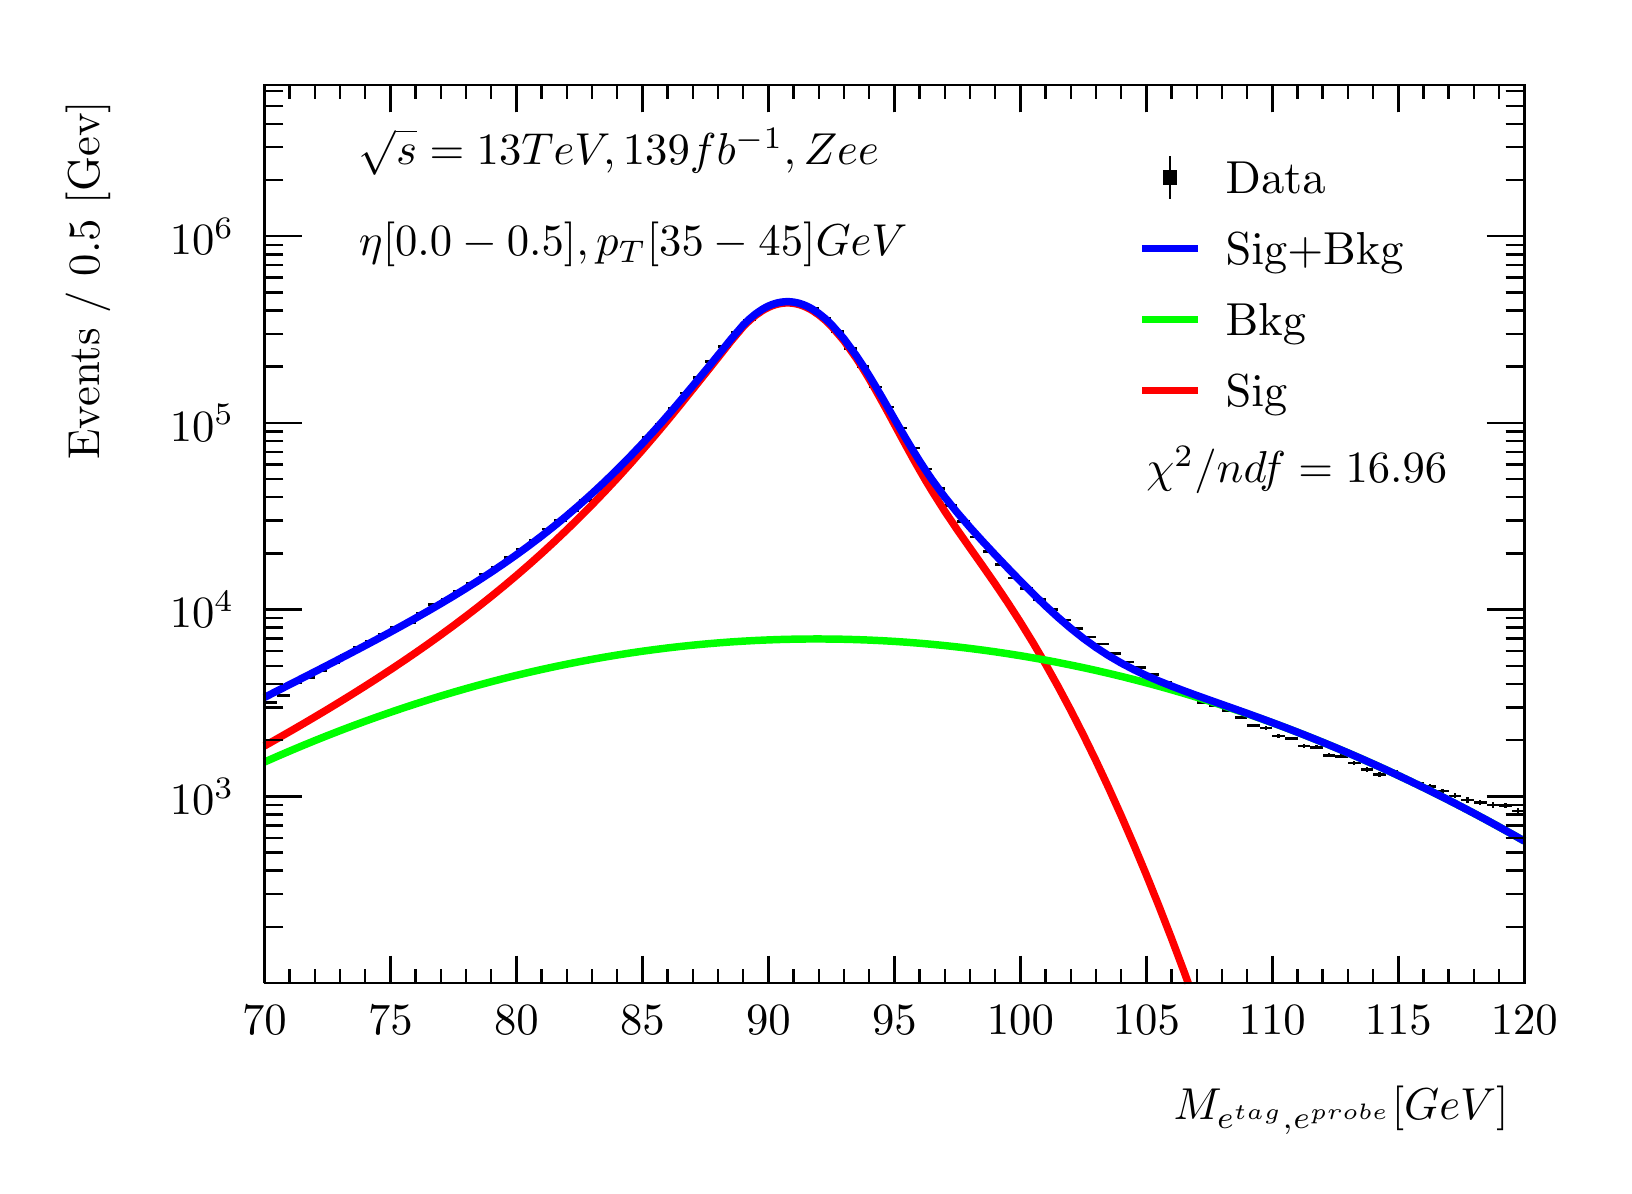
\begin{tikzpicture}
\pgfdeclareplotmark{cross} {
\pgfpathmoveto{\pgfpoint{-0.3\pgfplotmarksize}{\pgfplotmarksize}}
\pgfpathlineto{\pgfpoint{+0.3\pgfplotmarksize}{\pgfplotmarksize}}
\pgfpathlineto{\pgfpoint{+0.3\pgfplotmarksize}{0.3\pgfplotmarksize}}
\pgfpathlineto{\pgfpoint{+1\pgfplotmarksize}{0.3\pgfplotmarksize}}
\pgfpathlineto{\pgfpoint{+1\pgfplotmarksize}{-0.3\pgfplotmarksize}}
\pgfpathlineto{\pgfpoint{+0.3\pgfplotmarksize}{-0.3\pgfplotmarksize}}
\pgfpathlineto{\pgfpoint{+0.3\pgfplotmarksize}{-1.\pgfplotmarksize}}
\pgfpathlineto{\pgfpoint{-0.3\pgfplotmarksize}{-1.\pgfplotmarksize}}
\pgfpathlineto{\pgfpoint{-0.3\pgfplotmarksize}{-0.3\pgfplotmarksize}}
\pgfpathlineto{\pgfpoint{-1.\pgfplotmarksize}{-0.3\pgfplotmarksize}}
\pgfpathlineto{\pgfpoint{-1.\pgfplotmarksize}{0.3\pgfplotmarksize}}
\pgfpathlineto{\pgfpoint{-0.3\pgfplotmarksize}{0.3\pgfplotmarksize}}
\pgfpathclose
\pgfusepathqstroke
}
\pgfdeclareplotmark{cross*} {
\pgfpathmoveto{\pgfpoint{-0.3\pgfplotmarksize}{\pgfplotmarksize}}
\pgfpathlineto{\pgfpoint{+0.3\pgfplotmarksize}{\pgfplotmarksize}}
\pgfpathlineto{\pgfpoint{+0.3\pgfplotmarksize}{0.3\pgfplotmarksize}}
\pgfpathlineto{\pgfpoint{+1\pgfplotmarksize}{0.3\pgfplotmarksize}}
\pgfpathlineto{\pgfpoint{+1\pgfplotmarksize}{-0.3\pgfplotmarksize}}
\pgfpathlineto{\pgfpoint{+0.3\pgfplotmarksize}{-0.3\pgfplotmarksize}}
\pgfpathlineto{\pgfpoint{+0.3\pgfplotmarksize}{-1.\pgfplotmarksize}}
\pgfpathlineto{\pgfpoint{-0.3\pgfplotmarksize}{-1.\pgfplotmarksize}}
\pgfpathlineto{\pgfpoint{-0.3\pgfplotmarksize}{-0.3\pgfplotmarksize}}
\pgfpathlineto{\pgfpoint{-1.\pgfplotmarksize}{-0.3\pgfplotmarksize}}
\pgfpathlineto{\pgfpoint{-1.\pgfplotmarksize}{0.3\pgfplotmarksize}}
\pgfpathlineto{\pgfpoint{-0.3\pgfplotmarksize}{0.3\pgfplotmarksize}}
\pgfpathclose
\pgfusepathqfillstroke
}
\pgfdeclareplotmark{newstar} {
\pgfpathmoveto{\pgfqpoint{0pt}{\pgfplotmarksize}}
\pgfpathlineto{\pgfqpointpolar{44}{0.5\pgfplotmarksize}}
\pgfpathlineto{\pgfqpointpolar{18}{\pgfplotmarksize}}
\pgfpathlineto{\pgfqpointpolar{-20}{0.5\pgfplotmarksize}}
\pgfpathlineto{\pgfqpointpolar{-54}{\pgfplotmarksize}}
\pgfpathlineto{\pgfqpointpolar{-90}{0.5\pgfplotmarksize}}
\pgfpathlineto{\pgfqpointpolar{234}{\pgfplotmarksize}}
\pgfpathlineto{\pgfqpointpolar{198}{0.5\pgfplotmarksize}}
\pgfpathlineto{\pgfqpointpolar{162}{\pgfplotmarksize}}
\pgfpathlineto{\pgfqpointpolar{134}{0.5\pgfplotmarksize}}
\pgfpathclose
\pgfusepathqstroke
}
\pgfdeclareplotmark{newstar*} {
\pgfpathmoveto{\pgfqpoint{0pt}{\pgfplotmarksize}}
\pgfpathlineto{\pgfqpointpolar{44}{0.5\pgfplotmarksize}}
\pgfpathlineto{\pgfqpointpolar{18}{\pgfplotmarksize}}
\pgfpathlineto{\pgfqpointpolar{-20}{0.5\pgfplotmarksize}}
\pgfpathlineto{\pgfqpointpolar{-54}{\pgfplotmarksize}}
\pgfpathlineto{\pgfqpointpolar{-90}{0.5\pgfplotmarksize}}
\pgfpathlineto{\pgfqpointpolar{234}{\pgfplotmarksize}}
\pgfpathlineto{\pgfqpointpolar{198}{0.5\pgfplotmarksize}}
\pgfpathlineto{\pgfqpointpolar{162}{\pgfplotmarksize}}
\pgfpathlineto{\pgfqpointpolar{134}{0.5\pgfplotmarksize}}
\pgfpathclose
\pgfusepathqfillstroke
}
\definecolor{c}{rgb}{1,1,1};
\draw [color=c, fill=c] (0,0) rectangle (20,14.4361);
\draw [color=c, fill=c] (3,2.30977) rectangle (19,13.7143);
\definecolor{c}{rgb}{0,0,0};
\draw [c,line width=0.9] (3,2.30977) -- (3,13.7143) -- (19,13.7143) -- (19,2.30977) -- (3,2.30977);
\definecolor{c}{rgb}{1,1,1};
\draw [color=c, fill=c] (3,2.30977) rectangle (19,13.7143);
\definecolor{c}{rgb}{0,0,0};
\draw [c,line width=0.9] (3,2.30977) -- (3,13.7143) -- (19,13.7143) -- (19,2.30977) -- (3,2.30977);
\draw [c,line width=0.9] (3,2.30977) -- (19,2.30977);
\draw [c,line width=0.9] (3,2.65624) -- (3,2.30977);
\draw [c,line width=0.9] (3.32,2.48301) -- (3.32,2.30977);
\draw [c,line width=0.9] (3.64,2.48301) -- (3.64,2.30977);
\draw [c,line width=0.9] (3.96,2.48301) -- (3.96,2.30977);
\draw [c,line width=0.9] (4.28,2.48301) -- (4.28,2.30977);
\draw [c,line width=0.9] (4.6,2.65624) -- (4.6,2.30977);
\draw [c,line width=0.9] (4.92,2.48301) -- (4.92,2.30977);
\draw [c,line width=0.9] (5.24,2.48301) -- (5.24,2.30977);
\draw [c,line width=0.9] (5.56,2.48301) -- (5.56,2.30977);
\draw [c,line width=0.9] (5.88,2.48301) -- (5.88,2.30977);
\draw [c,line width=0.9] (6.2,2.65624) -- (6.2,2.30977);
\draw [c,line width=0.9] (6.52,2.48301) -- (6.52,2.30977);
\draw [c,line width=0.9] (6.84,2.48301) -- (6.84,2.30977);
\draw [c,line width=0.9] (7.16,2.48301) -- (7.16,2.30977);
\draw [c,line width=0.9] (7.48,2.48301) -- (7.48,2.30977);
\draw [c,line width=0.9] (7.8,2.65624) -- (7.8,2.30977);
\draw [c,line width=0.9] (8.12,2.48301) -- (8.12,2.30977);
\draw [c,line width=0.9] (8.44,2.48301) -- (8.44,2.30977);
\draw [c,line width=0.9] (8.76,2.48301) -- (8.76,2.30977);
\draw [c,line width=0.9] (9.08,2.48301) -- (9.08,2.30977);
\draw [c,line width=0.9] (9.4,2.65624) -- (9.4,2.30977);
\draw [c,line width=0.9] (9.72,2.48301) -- (9.72,2.30977);
\draw [c,line width=0.9] (10.04,2.48301) -- (10.04,2.30977);
\draw [c,line width=0.9] (10.36,2.48301) -- (10.36,2.30977);
\draw [c,line width=0.9] (10.68,2.48301) -- (10.68,2.30977);
\draw [c,line width=0.9] (11,2.65624) -- (11,2.30977);
\draw [c,line width=0.9] (11.32,2.48301) -- (11.32,2.30977);
\draw [c,line width=0.9] (11.64,2.48301) -- (11.64,2.30977);
\draw [c,line width=0.9] (11.96,2.48301) -- (11.96,2.30977);
\draw [c,line width=0.9] (12.28,2.48301) -- (12.28,2.30977);
\draw [c,line width=0.9] (12.6,2.65624) -- (12.6,2.30977);
\draw [c,line width=0.9] (12.92,2.48301) -- (12.92,2.30977);
\draw [c,line width=0.9] (13.24,2.48301) -- (13.24,2.30977);
\draw [c,line width=0.9] (13.56,2.48301) -- (13.56,2.30977);
\draw [c,line width=0.9] (13.88,2.48301) -- (13.88,2.30977);
\draw [c,line width=0.9] (14.2,2.65624) -- (14.2,2.30977);
\draw [c,line width=0.9] (14.52,2.48301) -- (14.52,2.30977);
\draw [c,line width=0.9] (14.84,2.48301) -- (14.84,2.30977);
\draw [c,line width=0.9] (15.16,2.48301) -- (15.16,2.30977);
\draw [c,line width=0.9] (15.48,2.48301) -- (15.48,2.30977);
\draw [c,line width=0.9] (15.8,2.65624) -- (15.8,2.30977);
\draw [c,line width=0.9] (16.12,2.48301) -- (16.12,2.30977);
\draw [c,line width=0.9] (16.44,2.48301) -- (16.44,2.30977);
\draw [c,line width=0.9] (16.76,2.48301) -- (16.76,2.30977);
\draw [c,line width=0.9] (17.08,2.48301) -- (17.08,2.30977);
\draw [c,line width=0.9] (17.4,2.65624) -- (17.4,2.30977);
\draw [c,line width=0.9] (17.72,2.48301) -- (17.72,2.30977);
\draw [c,line width=0.9] (18.04,2.48301) -- (18.04,2.30977);
\draw [c,line width=0.9] (18.36,2.48301) -- (18.36,2.30977);
\draw [c,line width=0.9] (18.68,2.48301) -- (18.68,2.30977);
\draw [c,line width=0.9] (19,2.65624) -- (19,2.30977);
\draw [anchor=base] (3,1.66015) node[scale=1.61424, color=c, rotate=0]{70};
\draw [anchor=base] (4.6,1.66015) node[scale=1.61424, color=c, rotate=0]{75};
\draw [anchor=base] (6.2,1.66015) node[scale=1.61424, color=c, rotate=0]{80};
\draw [anchor=base] (7.8,1.66015) node[scale=1.61424, color=c, rotate=0]{85};
\draw [anchor=base] (9.4,1.66015) node[scale=1.61424, color=c, rotate=0]{90};
\draw [anchor=base] (11,1.66015) node[scale=1.61424, color=c, rotate=0]{95};
\draw [anchor=base] (12.6,1.66015) node[scale=1.61424, color=c, rotate=0]{100};
\draw [anchor=base] (14.2,1.66015) node[scale=1.61424, color=c, rotate=0]{105};
\draw [anchor=base] (15.8,1.66015) node[scale=1.61424, color=c, rotate=0]{110};
\draw [anchor=base] (17.4,1.66015) node[scale=1.61424, color=c, rotate=0]{115};
\draw [anchor=base] (19,1.66015) node[scale=1.61424, color=c, rotate=0]{120};
\draw [anchor= east] (19,0.692932) node[scale=1.61424, color=c, rotate=0]{$M_{e^{tag}, e^{probe}}  [GeV]$};
\draw [c,line width=0.9] (3,13.7143) -- (19,13.7143);
\draw [c,line width=0.9] (3,13.3678) -- (3,13.7143);
\draw [c,line width=0.9] (3.32,13.5411) -- (3.32,13.7143);
\draw [c,line width=0.9] (3.64,13.5411) -- (3.64,13.7143);
\draw [c,line width=0.9] (3.96,13.5411) -- (3.96,13.7143);
\draw [c,line width=0.9] (4.28,13.5411) -- (4.28,13.7143);
\draw [c,line width=0.9] (4.6,13.3678) -- (4.6,13.7143);
\draw [c,line width=0.9] (4.92,13.5411) -- (4.92,13.7143);
\draw [c,line width=0.9] (5.24,13.5411) -- (5.24,13.7143);
\draw [c,line width=0.9] (5.56,13.5411) -- (5.56,13.7143);
\draw [c,line width=0.9] (5.88,13.5411) -- (5.88,13.7143);
\draw [c,line width=0.9] (6.2,13.3678) -- (6.2,13.7143);
\draw [c,line width=0.9] (6.52,13.5411) -- (6.52,13.7143);
\draw [c,line width=0.9] (6.84,13.5411) -- (6.84,13.7143);
\draw [c,line width=0.9] (7.16,13.5411) -- (7.16,13.7143);
\draw [c,line width=0.9] (7.48,13.5411) -- (7.48,13.7143);
\draw [c,line width=0.9] (7.8,13.3678) -- (7.8,13.7143);
\draw [c,line width=0.9] (8.12,13.5411) -- (8.12,13.7143);
\draw [c,line width=0.9] (8.44,13.5411) -- (8.44,13.7143);
\draw [c,line width=0.9] (8.76,13.5411) -- (8.76,13.7143);
\draw [c,line width=0.9] (9.08,13.5411) -- (9.08,13.7143);
\draw [c,line width=0.9] (9.4,13.3678) -- (9.4,13.7143);
\draw [c,line width=0.9] (9.72,13.5411) -- (9.72,13.7143);
\draw [c,line width=0.9] (10.04,13.5411) -- (10.04,13.7143);
\draw [c,line width=0.9] (10.36,13.5411) -- (10.36,13.7143);
\draw [c,line width=0.9] (10.68,13.5411) -- (10.68,13.7143);
\draw [c,line width=0.9] (11,13.3678) -- (11,13.7143);
\draw [c,line width=0.9] (11.32,13.5411) -- (11.32,13.7143);
\draw [c,line width=0.9] (11.64,13.5411) -- (11.64,13.7143);
\draw [c,line width=0.9] (11.96,13.5411) -- (11.96,13.7143);
\draw [c,line width=0.9] (12.28,13.5411) -- (12.28,13.7143);
\draw [c,line width=0.9] (12.6,13.3678) -- (12.6,13.7143);
\draw [c,line width=0.9] (12.92,13.5411) -- (12.92,13.7143);
\draw [c,line width=0.9] (13.24,13.5411) -- (13.24,13.7143);
\draw [c,line width=0.9] (13.56,13.5411) -- (13.56,13.7143);
\draw [c,line width=0.9] (13.88,13.5411) -- (13.88,13.7143);
\draw [c,line width=0.9] (14.2,13.3678) -- (14.2,13.7143);
\draw [c,line width=0.9] (14.52,13.5411) -- (14.52,13.7143);
\draw [c,line width=0.9] (14.84,13.5411) -- (14.84,13.7143);
\draw [c,line width=0.9] (15.16,13.5411) -- (15.16,13.7143);
\draw [c,line width=0.9] (15.48,13.5411) -- (15.48,13.7143);
\draw [c,line width=0.9] (15.8,13.3678) -- (15.8,13.7143);
\draw [c,line width=0.9] (16.12,13.5411) -- (16.12,13.7143);
\draw [c,line width=0.9] (16.44,13.5411) -- (16.44,13.7143);
\draw [c,line width=0.9] (16.76,13.5411) -- (16.76,13.7143);
\draw [c,line width=0.9] (17.08,13.5411) -- (17.08,13.7143);
\draw [c,line width=0.9] (17.4,13.3678) -- (17.4,13.7143);
\draw [c,line width=0.9] (17.72,13.5411) -- (17.72,13.7143);
\draw [c,line width=0.9] (18.04,13.5411) -- (18.04,13.7143);
\draw [c,line width=0.9] (18.36,13.5411) -- (18.36,13.7143);
\draw [c,line width=0.9] (18.68,13.5411) -- (18.68,13.7143);
\draw [c,line width=0.9] (19,13.3678) -- (19,13.7143);
\draw [c,line width=0.9] (3,2.30977) -- (3,13.7143);
\draw [c,line width=0.9] (3.237,3.02354) -- (3,3.02354);
\draw [c,line width=0.9] (3.237,3.44107) -- (3,3.44107);
\draw [c,line width=0.9] (3.237,3.73731) -- (3,3.73731);
\draw [c,line width=0.9] (3.237,3.96709) -- (3,3.96709);
\draw [c,line width=0.9] (3.237,4.15484) -- (3,4.15484);
\draw [c,line width=0.9] (3.237,4.31357) -- (3,4.31357);
\draw [c,line width=0.9] (3.237,4.45108) -- (3,4.45108);
\draw [c,line width=0.9] (3.237,4.57236) -- (3,4.57236);
\draw [c,line width=0.9] (3.474,4.68086) -- (3,4.68086);
\draw [anchor= east] (2.82,4.68086) node[scale=1.61424, color=c, rotate=0]{$10^{3}$};
\draw [c,line width=0.9] (3.237,5.39463) -- (3,5.39463);
\draw [c,line width=0.9] (3.237,5.81216) -- (3,5.81216);
\draw [c,line width=0.9] (3.237,6.1084) -- (3,6.1084);
\draw [c,line width=0.9] (3.237,6.33818) -- (3,6.33818);
\draw [c,line width=0.9] (3.237,6.52593) -- (3,6.52593);
\draw [c,line width=0.9] (3.237,6.68466) -- (3,6.68466);
\draw [c,line width=0.9] (3.237,6.82217) -- (3,6.82217);
\draw [c,line width=0.9] (3.237,6.94345) -- (3,6.94345);
\draw [c,line width=0.9] (3.474,7.05195) -- (3,7.05195);
\draw [anchor= east] (2.82,7.05195) node[scale=1.61424, color=c, rotate=0]{$10^{4}$};
\draw [c,line width=0.9] (3.237,7.76572) -- (3,7.76572);
\draw [c,line width=0.9] (3.237,8.18324) -- (3,8.18324);
\draw [c,line width=0.9] (3.237,8.47948) -- (3,8.47948);
\draw [c,line width=0.9] (3.237,8.70927) -- (3,8.70927);
\draw [c,line width=0.9] (3.237,8.89701) -- (3,8.89701);
\draw [c,line width=0.9] (3.237,9.05575) -- (3,9.05575);
\draw [c,line width=0.9] (3.237,9.19325) -- (3,9.19325);
\draw [c,line width=0.9] (3.237,9.31454) -- (3,9.31454);
\draw [c,line width=0.9] (3.474,9.42304) -- (3,9.42304);
\draw [anchor= east] (2.82,9.42304) node[scale=1.61424, color=c, rotate=0]{$10^{5}$};
\draw [c,line width=0.9] (3.237,10.1368) -- (3,10.1368);
\draw [c,line width=0.9] (3.237,10.5543) -- (3,10.5543);
\draw [c,line width=0.9] (3.237,10.8506) -- (3,10.8506);
\draw [c,line width=0.9] (3.237,11.0804) -- (3,11.0804);
\draw [c,line width=0.9] (3.237,11.2681) -- (3,11.2681);
\draw [c,line width=0.9] (3.237,11.4268) -- (3,11.4268);
\draw [c,line width=0.9] (3.237,11.5643) -- (3,11.5643);
\draw [c,line width=0.9] (3.237,11.6856) -- (3,11.6856);
\draw [c,line width=0.9] (3.474,11.7941) -- (3,11.7941);
\draw [anchor= east] (2.82,11.7941) node[scale=1.61424, color=c, rotate=0]{$10^{6}$};
\draw [c,line width=0.9] (3.237,12.5079) -- (3,12.5079);
\draw [c,line width=0.9] (3.237,12.9254) -- (3,12.9254);
\draw [c,line width=0.9] (3.237,13.2217) -- (3,13.2217);
\draw [c,line width=0.9] (3.237,13.4514) -- (3,13.4514);
\draw [c,line width=0.9] (3.237,13.6392) -- (3,13.6392);
\draw [anchor= east] (0.76,13.7143) node[scale=1.61424, color=c, rotate=90]{Events / 0.5 [Gev]};
\draw [c,line width=0.9] (19,2.30977) -- (19,13.7143);
\draw [c,line width=0.9] (18.763,3.02354) -- (19,3.02354);
\draw [c,line width=0.9] (18.763,3.44107) -- (19,3.44107);
\draw [c,line width=0.9] (18.763,3.73731) -- (19,3.73731);
\draw [c,line width=0.9] (18.763,3.96709) -- (19,3.96709);
\draw [c,line width=0.9] (18.763,4.15484) -- (19,4.15484);
\draw [c,line width=0.9] (18.763,4.31357) -- (19,4.31357);
\draw [c,line width=0.9] (18.763,4.45108) -- (19,4.45108);
\draw [c,line width=0.9] (18.763,4.57236) -- (19,4.57236);
\draw [c,line width=0.9] (18.526,4.68086) -- (19,4.68086);
\draw [c,line width=0.9] (18.763,5.39463) -- (19,5.39463);
\draw [c,line width=0.9] (18.763,5.81216) -- (19,5.81216);
\draw [c,line width=0.9] (18.763,6.1084) -- (19,6.1084);
\draw [c,line width=0.9] (18.763,6.33818) -- (19,6.33818);
\draw [c,line width=0.9] (18.763,6.52593) -- (19,6.52593);
\draw [c,line width=0.9] (18.763,6.68466) -- (19,6.68466);
\draw [c,line width=0.9] (18.763,6.82217) -- (19,6.82217);
\draw [c,line width=0.9] (18.763,6.94345) -- (19,6.94345);
\draw [c,line width=0.9] (18.526,7.05195) -- (19,7.05195);
\draw [c,line width=0.9] (18.763,7.76572) -- (19,7.76572);
\draw [c,line width=0.9] (18.763,8.18324) -- (19,8.18324);
\draw [c,line width=0.9] (18.763,8.47948) -- (19,8.47948);
\draw [c,line width=0.9] (18.763,8.70927) -- (19,8.70927);
\draw [c,line width=0.9] (18.763,8.89701) -- (19,8.89701);
\draw [c,line width=0.9] (18.763,9.05575) -- (19,9.05575);
\draw [c,line width=0.9] (18.763,9.19325) -- (19,9.19325);
\draw [c,line width=0.9] (18.763,9.31454) -- (19,9.31454);
\draw [c,line width=0.9] (18.526,9.42304) -- (19,9.42304);
\draw [c,line width=0.9] (18.763,10.1368) -- (19,10.1368);
\draw [c,line width=0.9] (18.763,10.5543) -- (19,10.5543);
\draw [c,line width=0.9] (18.763,10.8506) -- (19,10.8506);
\draw [c,line width=0.9] (18.763,11.0804) -- (19,11.0804);
\draw [c,line width=0.9] (18.763,11.2681) -- (19,11.2681);
\draw [c,line width=0.9] (18.763,11.4268) -- (19,11.4268);
\draw [c,line width=0.9] (18.763,11.5643) -- (19,11.5643);
\draw [c,line width=0.9] (18.763,11.6856) -- (19,11.6856);
\draw [c,line width=0.9] (18.526,11.7941) -- (19,11.7941);
\draw [c,line width=0.9] (18.763,12.5079) -- (19,12.5079);
\draw [c,line width=0.9] (18.763,12.9254) -- (19,12.9254);
\draw [c,line width=0.9] (18.763,13.2217) -- (19,13.2217);
\draw [c,line width=0.9] (18.763,13.4514) -- (19,13.4514);
\draw [c,line width=0.9] (18.763,13.6392) -- (19,13.6392);
\draw [c,line width=0.9] (3.08,5.87086) -- (3,5.87086);
\draw [c,line width=0.9] (3,5.87086) -- (3,5.87086);
\draw [c,line width=0.9] (3.08,5.87086) -- (3.16,5.87086);
\draw [c,line width=0.9] (3.16,5.87086) -- (3.16,5.87086);
\draw [c,line width=0.9] (3.08,5.87086) -- (3.08,5.88914);
\draw [c,line width=0.9] (3.08,5.88914) -- (3.08,5.88914);
\draw [c,line width=0.9] (3.08,5.87086) -- (3.08,5.85259);
\draw [c,line width=0.9] (3.08,5.85259) -- (3.08,5.85259);
\draw [c,line width=0.9] (3.24,5.95965) -- (3.16,5.95965);
\draw [c,line width=0.9] (3.16,5.95965) -- (3.16,5.95965);
\draw [c,line width=0.9] (3.24,5.95965) -- (3.32,5.95965);
\draw [c,line width=0.9] (3.32,5.95965) -- (3.32,5.95965);
\draw [c,line width=0.9] (3.24,5.95965) -- (3.24,5.97715);
\draw [c,line width=0.9] (3.24,5.97715) -- (3.24,5.97715);
\draw [c,line width=0.9] (3.24,5.95965) -- (3.24,5.94215);
\draw [c,line width=0.9] (3.24,5.94215) -- (3.24,5.94215);
\draw [c,line width=0.9] (3.4,6.12246) -- (3.32,6.12246);
\draw [c,line width=0.9] (3.32,6.12246) -- (3.32,6.12246);
\draw [c,line width=0.9] (3.4,6.12246) -- (3.48,6.12246);
\draw [c,line width=0.9] (3.48,6.12246) -- (3.48,6.12246);
\draw [c,line width=0.9] (3.4,6.12246) -- (3.4,6.13863);
\draw [c,line width=0.9] (3.4,6.13863) -- (3.4,6.13863);
\draw [c,line width=0.9] (3.4,6.12246) -- (3.4,6.10629);
\draw [c,line width=0.9] (3.4,6.10629) -- (3.4,6.10629);
\draw [c,line width=0.9] (3.56,6.19027) -- (3.48,6.19027);
\draw [c,line width=0.9] (3.48,6.19027) -- (3.48,6.19027);
\draw [c,line width=0.9] (3.56,6.19027) -- (3.64,6.19027);
\draw [c,line width=0.9] (3.64,6.19027) -- (3.64,6.19027);
\draw [c,line width=0.9] (3.56,6.19027) -- (3.56,6.20591);
\draw [c,line width=0.9] (3.56,6.20591) -- (3.56,6.20591);
\draw [c,line width=0.9] (3.56,6.19027) -- (3.56,6.17462);
\draw [c,line width=0.9] (3.56,6.17462) -- (3.56,6.17462);
\draw [c,line width=0.9] (3.72,6.27556) -- (3.64,6.27556);
\draw [c,line width=0.9] (3.64,6.27556) -- (3.64,6.27556);
\draw [c,line width=0.9] (3.72,6.27556) -- (3.8,6.27556);
\draw [c,line width=0.9] (3.8,6.27556) -- (3.8,6.27556);
\draw [c,line width=0.9] (3.72,6.27556) -- (3.72,6.29057);
\draw [c,line width=0.9] (3.72,6.29057) -- (3.72,6.29057);
\draw [c,line width=0.9] (3.72,6.27556) -- (3.72,6.26055);
\draw [c,line width=0.9] (3.72,6.26055) -- (3.72,6.26055);
\draw [c,line width=0.9] (3.88,6.37916) -- (3.8,6.37916);
\draw [c,line width=0.9] (3.8,6.37916) -- (3.8,6.37916);
\draw [c,line width=0.9] (3.88,6.37916) -- (3.96,6.37916);
\draw [c,line width=0.9] (3.96,6.37916) -- (3.96,6.37916);
\draw [c,line width=0.9] (3.88,6.37916) -- (3.88,6.39344);
\draw [c,line width=0.9] (3.88,6.39344) -- (3.88,6.39344);
\draw [c,line width=0.9] (3.88,6.37916) -- (3.88,6.36489);
\draw [c,line width=0.9] (3.88,6.36489) -- (3.88,6.36489);
\draw [c,line width=0.9] (4.04,6.47509) -- (3.96,6.47509);
\draw [c,line width=0.9] (3.96,6.47509) -- (3.96,6.47509);
\draw [c,line width=0.9] (4.04,6.47509) -- (4.12,6.47509);
\draw [c,line width=0.9] (4.12,6.47509) -- (4.12,6.47509);
\draw [c,line width=0.9] (4.04,6.47509) -- (4.04,6.48872);
\draw [c,line width=0.9] (4.04,6.48872) -- (4.04,6.48872);
\draw [c,line width=0.9] (4.04,6.47509) -- (4.04,6.46147);
\draw [c,line width=0.9] (4.04,6.46147) -- (4.04,6.46147);
\draw [c,line width=0.9] (4.2,6.576) -- (4.12,6.576);
\draw [c,line width=0.9] (4.12,6.576) -- (4.12,6.576);
\draw [c,line width=0.9] (4.2,6.576) -- (4.28,6.576);
\draw [c,line width=0.9] (4.28,6.576) -- (4.28,6.576);
\draw [c,line width=0.9] (4.2,6.576) -- (4.2,6.58898);
\draw [c,line width=0.9] (4.2,6.58898) -- (4.2,6.58898);
\draw [c,line width=0.9] (4.2,6.576) -- (4.2,6.56303);
\draw [c,line width=0.9] (4.2,6.56303) -- (4.2,6.56303);
\draw [c,line width=0.9] (4.36,6.64508) -- (4.28,6.64508);
\draw [c,line width=0.9] (4.28,6.64508) -- (4.28,6.64508);
\draw [c,line width=0.9] (4.36,6.64508) -- (4.44,6.64508);
\draw [c,line width=0.9] (4.44,6.64508) -- (4.44,6.64508);
\draw [c,line width=0.9] (4.36,6.64508) -- (4.36,6.65762);
\draw [c,line width=0.9] (4.36,6.65762) -- (4.36,6.65762);
\draw [c,line width=0.9] (4.36,6.64508) -- (4.36,6.63253);
\draw [c,line width=0.9] (4.36,6.63253) -- (4.36,6.63253);
\draw [c,line width=0.9] (4.52,6.7335) -- (4.44,6.7335);
\draw [c,line width=0.9] (4.44,6.7335) -- (4.44,6.7335);
\draw [c,line width=0.9] (4.52,6.7335) -- (4.6,6.7335);
\draw [c,line width=0.9] (4.6,6.7335) -- (4.6,6.7335);
\draw [c,line width=0.9] (4.52,6.7335) -- (4.52,6.74552);
\draw [c,line width=0.9] (4.52,6.74552) -- (4.52,6.74552);
\draw [c,line width=0.9] (4.52,6.7335) -- (4.52,6.72148);
\draw [c,line width=0.9] (4.52,6.72148) -- (4.52,6.72148);
\draw [c,line width=0.9] (4.68,6.83216) -- (4.6,6.83216);
\draw [c,line width=0.9] (4.6,6.83216) -- (4.6,6.83216);
\draw [c,line width=0.9] (4.68,6.83216) -- (4.76,6.83216);
\draw [c,line width=0.9] (4.76,6.83216) -- (4.76,6.83216);
\draw [c,line width=0.9] (4.68,6.83216) -- (4.68,6.84362);
\draw [c,line width=0.9] (4.68,6.84362) -- (4.68,6.84362);
\draw [c,line width=0.9] (4.68,6.83216) -- (4.68,6.8207);
\draw [c,line width=0.9] (4.68,6.8207) -- (4.68,6.8207);
\draw [c,line width=0.9] (4.84,6.88786) -- (4.76,6.88786);
\draw [c,line width=0.9] (4.76,6.88786) -- (4.76,6.88786);
\draw [c,line width=0.9] (4.84,6.88786) -- (4.92,6.88786);
\draw [c,line width=0.9] (4.92,6.88786) -- (4.92,6.88786);
\draw [c,line width=0.9] (4.84,6.88786) -- (4.84,6.89901);
\draw [c,line width=0.9] (4.84,6.89901) -- (4.84,6.89901);
\draw [c,line width=0.9] (4.84,6.88786) -- (4.84,6.87671);
\draw [c,line width=0.9] (4.84,6.87671) -- (4.84,6.87671);
\draw [c,line width=0.9] (5,7.00162) -- (4.92,7.00162);
\draw [c,line width=0.9] (4.92,7.00162) -- (4.92,7.00162);
\draw [c,line width=0.9] (5,7.00162) -- (5.08,7.00162);
\draw [c,line width=0.9] (5.08,7.00162) -- (5.08,7.00162);
\draw [c,line width=0.9] (5,7.00162) -- (5,7.01217);
\draw [c,line width=0.9] (5,7.01217) -- (5,7.01217);
\draw [c,line width=0.9] (5,7.00162) -- (5,6.99107);
\draw [c,line width=0.9] (5,6.99107) -- (5,6.99107);
\draw [c,line width=0.9] (5.16,7.11506) -- (5.08,7.11506);
\draw [c,line width=0.9] (5.08,7.11506) -- (5.08,7.11506);
\draw [c,line width=0.9] (5.16,7.11506) -- (5.24,7.11506);
\draw [c,line width=0.9] (5.24,7.11506) -- (5.24,7.11506);
\draw [c,line width=0.9] (5.16,7.11506) -- (5.16,7.12504);
\draw [c,line width=0.9] (5.16,7.12504) -- (5.16,7.12504);
\draw [c,line width=0.9] (5.16,7.11506) -- (5.16,7.10507);
\draw [c,line width=0.9] (5.16,7.10507) -- (5.16,7.10507);
\draw [c,line width=0.9] (5.32,7.18416) -- (5.24,7.18416);
\draw [c,line width=0.9] (5.24,7.18416) -- (5.24,7.18416);
\draw [c,line width=0.9] (5.32,7.18416) -- (5.4,7.18416);
\draw [c,line width=0.9] (5.4,7.18416) -- (5.4,7.18416);
\draw [c,line width=0.9] (5.32,7.18416) -- (5.32,7.19382);
\draw [c,line width=0.9] (5.32,7.19382) -- (5.32,7.19382);
\draw [c,line width=0.9] (5.32,7.18416) -- (5.32,7.1745);
\draw [c,line width=0.9] (5.32,7.1745) -- (5.32,7.1745);
\draw [c,line width=0.9] (5.48,7.28543) -- (5.4,7.28543);
\draw [c,line width=0.9] (5.4,7.28543) -- (5.4,7.28543);
\draw [c,line width=0.9] (5.48,7.28543) -- (5.56,7.28543);
\draw [c,line width=0.9] (5.56,7.28543) -- (5.56,7.28543);
\draw [c,line width=0.9] (5.48,7.28543) -- (5.48,7.29463);
\draw [c,line width=0.9] (5.48,7.29463) -- (5.48,7.29463);
\draw [c,line width=0.9] (5.48,7.28543) -- (5.48,7.27624);
\draw [c,line width=0.9] (5.48,7.27624) -- (5.48,7.27624);
\draw [c,line width=0.9] (5.64,7.38674) -- (5.56,7.38674);
\draw [c,line width=0.9] (5.56,7.38674) -- (5.56,7.38674);
\draw [c,line width=0.9] (5.64,7.38674) -- (5.72,7.38674);
\draw [c,line width=0.9] (5.72,7.38674) -- (5.72,7.38674);
\draw [c,line width=0.9] (5.64,7.38674) -- (5.64,7.3955);
\draw [c,line width=0.9] (5.64,7.3955) -- (5.64,7.3955);
\draw [c,line width=0.9] (5.64,7.38674) -- (5.64,7.37799);
\draw [c,line width=0.9] (5.64,7.37799) -- (5.64,7.37799);
\draw [c,line width=0.9] (5.8,7.50696) -- (5.72,7.50696);
\draw [c,line width=0.9] (5.72,7.50696) -- (5.72,7.50696);
\draw [c,line width=0.9] (5.8,7.50696) -- (5.88,7.50696);
\draw [c,line width=0.9] (5.88,7.50696) -- (5.88,7.50696);
\draw [c,line width=0.9] (5.8,7.50696) -- (5.8,7.51521);
\draw [c,line width=0.9] (5.8,7.51521) -- (5.8,7.51521);
\draw [c,line width=0.9] (5.8,7.50696) -- (5.8,7.4987);
\draw [c,line width=0.9] (5.8,7.4987) -- (5.8,7.4987);
\draw [c,line width=0.9] (5.96,7.59618) -- (5.88,7.59618);
\draw [c,line width=0.9] (5.88,7.59618) -- (5.88,7.59618);
\draw [c,line width=0.9] (5.96,7.59618) -- (6.04,7.59618);
\draw [c,line width=0.9] (6.04,7.59618) -- (6.04,7.59618);
\draw [c,line width=0.9] (5.96,7.59618) -- (5.96,7.60409);
\draw [c,line width=0.9] (5.96,7.60409) -- (5.96,7.60409);
\draw [c,line width=0.9] (5.96,7.59618) -- (5.96,7.58827);
\draw [c,line width=0.9] (5.96,7.58827) -- (5.96,7.58827);
\draw [c,line width=0.9] (6.12,7.71447) -- (6.04,7.71447);
\draw [c,line width=0.9] (6.04,7.71447) -- (6.04,7.71447);
\draw [c,line width=0.9] (6.12,7.71447) -- (6.2,7.71447);
\draw [c,line width=0.9] (6.2,7.71447) -- (6.2,7.71447);
\draw [c,line width=0.9] (6.12,7.71447) -- (6.12,7.72193);
\draw [c,line width=0.9] (6.12,7.72193) -- (6.12,7.72193);
\draw [c,line width=0.9] (6.12,7.71447) -- (6.12,7.707);
\draw [c,line width=0.9] (6.12,7.707) -- (6.12,7.707);
\draw [c,line width=0.9] (6.28,7.82212) -- (6.2,7.82212);
\draw [c,line width=0.9] (6.2,7.82212) -- (6.2,7.82212);
\draw [c,line width=0.9] (6.28,7.82212) -- (6.36,7.82212);
\draw [c,line width=0.9] (6.36,7.82212) -- (6.36,7.82212);
\draw [c,line width=0.9] (6.28,7.82212) -- (6.28,7.8292);
\draw [c,line width=0.9] (6.28,7.8292) -- (6.28,7.8292);
\draw [c,line width=0.9] (6.28,7.82212) -- (6.28,7.81503);
\draw [c,line width=0.9] (6.28,7.81503) -- (6.28,7.81503);
\draw [c,line width=0.9] (6.44,7.93472) -- (6.36,7.93472);
\draw [c,line width=0.9] (6.36,7.93472) -- (6.36,7.93472);
\draw [c,line width=0.9] (6.44,7.93472) -- (6.52,7.93472);
\draw [c,line width=0.9] (6.52,7.93472) -- (6.52,7.93472);
\draw [c,line width=0.9] (6.44,7.93472) -- (6.44,7.94142);
\draw [c,line width=0.9] (6.44,7.94142) -- (6.44,7.94142);
\draw [c,line width=0.9] (6.44,7.93472) -- (6.44,7.92801);
\draw [c,line width=0.9] (6.44,7.92801) -- (6.44,7.92801);
\draw [c,line width=0.9] (6.6,8.07448) -- (6.52,8.07448);
\draw [c,line width=0.9] (6.52,8.07448) -- (6.52,8.07448);
\draw [c,line width=0.9] (6.6,8.07448) -- (6.68,8.07448);
\draw [c,line width=0.9] (6.68,8.07448) -- (6.68,8.07448);
\draw [c,line width=0.9] (6.6,8.07448) -- (6.6,8.08075);
\draw [c,line width=0.9] (6.6,8.08075) -- (6.6,8.08075);
\draw [c,line width=0.9] (6.6,8.07448) -- (6.6,8.06822);
\draw [c,line width=0.9] (6.6,8.06822) -- (6.6,8.06822);
\draw [c,line width=0.9] (6.76,8.18149) -- (6.68,8.18149);
\draw [c,line width=0.9] (6.68,8.18149) -- (6.68,8.18149);
\draw [c,line width=0.9] (6.76,8.18149) -- (6.84,8.18149);
\draw [c,line width=0.9] (6.84,8.18149) -- (6.84,8.18149);
\draw [c,line width=0.9] (6.76,8.18149) -- (6.76,8.18744);
\draw [c,line width=0.9] (6.76,8.18744) -- (6.76,8.18744);
\draw [c,line width=0.9] (6.76,8.18149) -- (6.76,8.17554);
\draw [c,line width=0.9] (6.76,8.17554) -- (6.76,8.17554);
\draw [c,line width=0.9] (6.92,8.30533) -- (6.84,8.30533);
\draw [c,line width=0.9] (6.84,8.30533) -- (6.84,8.30533);
\draw [c,line width=0.9] (6.92,8.30533) -- (7,8.30533);
\draw [c,line width=0.9] (7,8.30533) -- (7,8.30533);
\draw [c,line width=0.9] (6.92,8.30533) -- (6.92,8.31093);
\draw [c,line width=0.9] (6.92,8.31093) -- (6.92,8.31093);
\draw [c,line width=0.9] (6.92,8.30533) -- (6.92,8.29972);
\draw [c,line width=0.9] (6.92,8.29972) -- (6.92,8.29972);
\draw [c,line width=0.9] (7.08,8.44101) -- (7,8.44101);
\draw [c,line width=0.9] (7,8.44101) -- (7,8.44101);
\draw [c,line width=0.9] (7.08,8.44101) -- (7.16,8.44101);
\draw [c,line width=0.9] (7.16,8.44101) -- (7.16,8.44101);
\draw [c,line width=0.9] (7.08,8.44101) -- (7.08,8.44626);
\draw [c,line width=0.9] (7.08,8.44626) -- (7.08,8.44626);
\draw [c,line width=0.9] (7.08,8.44101) -- (7.08,8.43576);
\draw [c,line width=0.9] (7.08,8.43576) -- (7.08,8.43576);
\draw [c,line width=0.9] (7.24,8.58649) -- (7.16,8.58649);
\draw [c,line width=0.9] (7.16,8.58649) -- (7.16,8.58649);
\draw [c,line width=0.9] (7.24,8.58649) -- (7.32,8.58649);
\draw [c,line width=0.9] (7.32,8.58649) -- (7.32,8.58649);
\draw [c,line width=0.9] (7.24,8.58649) -- (7.24,8.59138);
\draw [c,line width=0.9] (7.24,8.59138) -- (7.24,8.59138);
\draw [c,line width=0.9] (7.24,8.58649) -- (7.24,8.5816);
\draw [c,line width=0.9] (7.24,8.5816) -- (7.24,8.5816);
\draw [c,line width=0.9] (7.4,8.7375) -- (7.32,8.7375);
\draw [c,line width=0.9] (7.32,8.7375) -- (7.32,8.7375);
\draw [c,line width=0.9] (7.4,8.7375) -- (7.48,8.7375);
\draw [c,line width=0.9] (7.48,8.7375) -- (7.48,8.7375);
\draw [c,line width=0.9] (7.4,8.7375) -- (7.4,8.74205);
\draw [c,line width=0.9] (7.4,8.74205) -- (7.4,8.74205);
\draw [c,line width=0.9] (7.4,8.7375) -- (7.4,8.73296);
\draw [c,line width=0.9] (7.4,8.73296) -- (7.4,8.73296);
\draw [c,line width=0.9] (7.56,8.88897) -- (7.48,8.88897);
\draw [c,line width=0.9] (7.48,8.88897) -- (7.48,8.88897);
\draw [c,line width=0.9] (7.56,8.88897) -- (7.64,8.88897);
\draw [c,line width=0.9] (7.64,8.88897) -- (7.64,8.88897);
\draw [c,line width=0.9] (7.56,8.88897) -- (7.56,8.89319);
\draw [c,line width=0.9] (7.56,8.89319) -- (7.56,8.89319);
\draw [c,line width=0.9] (7.56,8.88897) -- (7.56,8.88475);
\draw [c,line width=0.9] (7.56,8.88475) -- (7.56,8.88475);
\draw [c,line width=0.9] (7.72,9.05543) -- (7.64,9.05543);
\draw [c,line width=0.9] (7.64,9.05543) -- (7.64,9.05543);
\draw [c,line width=0.9] (7.72,9.05543) -- (7.8,9.05543);
\draw [c,line width=0.9] (7.8,9.05543) -- (7.8,9.05543);
\draw [c,line width=0.9] (7.72,9.05543) -- (7.72,9.05932);
\draw [c,line width=0.9] (7.72,9.05932) -- (7.72,9.05932);
\draw [c,line width=0.9] (7.72,9.05543) -- (7.72,9.05153);
\draw [c,line width=0.9] (7.72,9.05153) -- (7.72,9.05153);
\draw [c,line width=0.9] (7.88,9.23782) -- (7.8,9.23782);
\draw [c,line width=0.9] (7.8,9.23782) -- (7.8,9.23782);
\draw [c,line width=0.9] (7.88,9.23782) -- (7.96,9.23782);
\draw [c,line width=0.9] (7.96,9.23782) -- (7.96,9.23782);
\draw [c,line width=0.9] (7.88,9.23782) -- (7.88,9.24138);
\draw [c,line width=0.9] (7.88,9.24138) -- (7.88,9.24138);
\draw [c,line width=0.9] (7.88,9.23782) -- (7.88,9.23425);
\draw [c,line width=0.9] (7.88,9.23425) -- (7.88,9.23425);
\draw [c,line width=0.9] (8.04,9.41066) -- (7.96,9.41066);
\draw [c,line width=0.9] (7.96,9.41066) -- (7.96,9.41066);
\draw [c,line width=0.9] (8.04,9.41066) -- (8.12,9.41066);
\draw [c,line width=0.9] (8.12,9.41066) -- (8.12,9.41066);
\draw [c,line width=0.9] (8.04,9.41066) -- (8.04,9.41393);
\draw [c,line width=0.9] (8.04,9.41393) -- (8.04,9.41393);
\draw [c,line width=0.9] (8.04,9.41066) -- (8.04,9.40738);
\draw [c,line width=0.9] (8.04,9.40738) -- (8.04,9.40738);
\draw [c,line width=0.9] (8.2,9.60518) -- (8.12,9.60518);
\draw [c,line width=0.9] (8.12,9.60518) -- (8.12,9.60518);
\draw [c,line width=0.9] (8.2,9.60518) -- (8.28,9.60518);
\draw [c,line width=0.9] (8.28,9.60518) -- (8.28,9.60518);
\draw [c,line width=0.9] (8.2,9.60518) -- (8.2,9.60816);
\draw [c,line width=0.9] (8.2,9.60816) -- (8.2,9.60816);
\draw [c,line width=0.9] (8.2,9.60518) -- (8.2,9.6022);
\draw [c,line width=0.9] (8.2,9.6022) -- (8.2,9.6022);
\draw [c,line width=0.9] (8.36,9.80488) -- (8.28,9.80488);
\draw [c,line width=0.9] (8.28,9.80488) -- (8.28,9.80488);
\draw [c,line width=0.9] (8.36,9.80488) -- (8.44,9.80488);
\draw [c,line width=0.9] (8.44,9.80488) -- (8.44,9.80488);
\draw [c,line width=0.9] (8.36,9.80488) -- (8.36,9.80758);
\draw [c,line width=0.9] (8.36,9.80758) -- (8.36,9.80758);
\draw [c,line width=0.9] (8.36,9.80488) -- (8.36,9.80217);
\draw [c,line width=0.9] (8.36,9.80217) -- (8.36,9.80217);
\draw [c,line width=0.9] (8.52,10.0023) -- (8.44,10.0023);
\draw [c,line width=0.9] (8.44,10.0023) -- (8.44,10.0023);
\draw [c,line width=0.9] (8.52,10.0023) -- (8.6,10.0023);
\draw [c,line width=0.9] (8.6,10.0023) -- (8.6,10.0023);
\draw [c,line width=0.9] (8.52,10.0023) -- (8.52,10.0048);
\draw [c,line width=0.9] (8.52,10.0048) -- (8.52,10.0048);
\draw [c,line width=0.9] (8.52,10.0023) -- (8.52,9.99984);
\draw [c,line width=0.9] (8.52,9.99984) -- (8.52,9.99984);
\draw [c,line width=0.9] (8.68,10.2031) -- (8.6,10.2031);
\draw [c,line width=0.9] (8.6,10.2031) -- (8.6,10.2031);
\draw [c,line width=0.9] (8.68,10.2031) -- (8.76,10.2031);
\draw [c,line width=0.9] (8.76,10.2031) -- (8.76,10.2031);
\draw [c,line width=0.9] (8.68,10.2031) -- (8.68,10.2053);
\draw [c,line width=0.9] (8.68,10.2053) -- (8.68,10.2053);
\draw [c,line width=0.9] (8.68,10.2031) -- (8.68,10.2008);
\draw [c,line width=0.9] (8.68,10.2008) -- (8.68,10.2008);
\draw [c,line width=0.9] (8.84,10.3968) -- (8.76,10.3968);
\draw [c,line width=0.9] (8.76,10.3968) -- (8.76,10.3968);
\draw [c,line width=0.9] (8.84,10.3968) -- (8.92,10.3968);
\draw [c,line width=0.9] (8.92,10.3968) -- (8.92,10.3968);
\draw [c,line width=0.9] (8.84,10.3968) -- (8.84,10.3988);
\draw [c,line width=0.9] (8.84,10.3988) -- (8.84,10.3988);
\draw [c,line width=0.9] (8.84,10.3968) -- (8.84,10.3948);
\draw [c,line width=0.9] (8.84,10.3948) -- (8.84,10.3948);
\draw [c,line width=0.9] (9,10.5752) -- (8.92,10.5752);
\draw [c,line width=0.9] (8.92,10.5752) -- (8.92,10.5752);
\draw [c,line width=0.9] (9,10.5752) -- (9.08,10.5752);
\draw [c,line width=0.9] (9.08,10.5752) -- (9.08,10.5752);
\draw [c,line width=0.9] (9,10.5752) -- (9,10.5771);
\draw [c,line width=0.9] (9,10.5771) -- (9,10.5771);
\draw [c,line width=0.9] (9,10.5752) -- (9,10.5734);
\draw [c,line width=0.9] (9,10.5734) -- (9,10.5734);
\draw [c,line width=0.9] (9.16,10.7326) -- (9.08,10.7326);
\draw [c,line width=0.9] (9.08,10.7326) -- (9.08,10.7326);
\draw [c,line width=0.9] (9.16,10.7326) -- (9.24,10.7326);
\draw [c,line width=0.9] (9.24,10.7326) -- (9.24,10.7326);
\draw [c,line width=0.9] (9.16,10.7326) -- (9.16,10.7344);
\draw [c,line width=0.9] (9.16,10.7344) -- (9.16,10.7344);
\draw [c,line width=0.9] (9.16,10.7326) -- (9.16,10.7309);
\draw [c,line width=0.9] (9.16,10.7309) -- (9.16,10.7309);
\draw [c,line width=0.9] (9.32,10.8566) -- (9.24,10.8566);
\draw [c,line width=0.9] (9.24,10.8566) -- (9.24,10.8566);
\draw [c,line width=0.9] (9.32,10.8566) -- (9.4,10.8566);
\draw [c,line width=0.9] (9.4,10.8566) -- (9.4,10.8566);
\draw [c,line width=0.9] (9.32,10.8566) -- (9.32,10.8582);
\draw [c,line width=0.9] (9.32,10.8582) -- (9.32,10.8582);
\draw [c,line width=0.9] (9.32,10.8566) -- (9.32,10.855);
\draw [c,line width=0.9] (9.32,10.855) -- (9.32,10.855);
\draw [c,line width=0.9] (9.48,10.9355) -- (9.4,10.9355);
\draw [c,line width=0.9] (9.4,10.9355) -- (9.4,10.9355);
\draw [c,line width=0.9] (9.48,10.9355) -- (9.56,10.9355);
\draw [c,line width=0.9] (9.56,10.9355) -- (9.56,10.9355);
\draw [c,line width=0.9] (9.48,10.9355) -- (9.48,10.9371);
\draw [c,line width=0.9] (9.48,10.9371) -- (9.48,10.9371);
\draw [c,line width=0.9] (9.48,10.9355) -- (9.48,10.934);
\draw [c,line width=0.9] (9.48,10.934) -- (9.48,10.934);
\draw [c,line width=0.9] (9.64,10.9682) -- (9.56,10.9682);
\draw [c,line width=0.9] (9.56,10.9682) -- (9.56,10.9682);
\draw [c,line width=0.9] (9.64,10.9682) -- (9.72,10.9682);
\draw [c,line width=0.9] (9.72,10.9682) -- (9.72,10.9682);
\draw [c,line width=0.9] (9.64,10.9682) -- (9.64,10.9698);
\draw [c,line width=0.9] (9.64,10.9698) -- (9.64,10.9698);
\draw [c,line width=0.9] (9.64,10.9682) -- (9.64,10.9667);
\draw [c,line width=0.9] (9.64,10.9667) -- (9.64,10.9667);
\draw [c,line width=0.9] (9.8,10.9489) -- (9.72,10.9489);
\draw [c,line width=0.9] (9.72,10.9489) -- (9.72,10.9489);
\draw [c,line width=0.9] (9.8,10.9489) -- (9.88,10.9489);
\draw [c,line width=0.9] (9.88,10.9489) -- (9.88,10.9489);
\draw [c,line width=0.9] (9.8,10.9489) -- (9.8,10.9505);
\draw [c,line width=0.9] (9.8,10.9505) -- (9.8,10.9505);
\draw [c,line width=0.9] (9.8,10.9489) -- (9.8,10.9474);
\draw [c,line width=0.9] (9.8,10.9474) -- (9.8,10.9474);
\draw [c,line width=0.9] (9.96,10.8741) -- (9.88,10.8741);
\draw [c,line width=0.9] (9.88,10.8741) -- (9.88,10.8741);
\draw [c,line width=0.9] (9.96,10.8741) -- (10.04,10.8741);
\draw [c,line width=0.9] (10.04,10.8741) -- (10.04,10.8741);
\draw [c,line width=0.9] (9.96,10.8741) -- (9.96,10.8757);
\draw [c,line width=0.9] (9.96,10.8757) -- (9.96,10.8757);
\draw [c,line width=0.9] (9.96,10.8741) -- (9.96,10.8725);
\draw [c,line width=0.9] (9.96,10.8725) -- (9.96,10.8725);
\draw [c,line width=0.9] (10.12,10.7496) -- (10.04,10.7496);
\draw [c,line width=0.9] (10.04,10.7496) -- (10.04,10.7496);
\draw [c,line width=0.9] (10.12,10.7496) -- (10.2,10.7496);
\draw [c,line width=0.9] (10.2,10.7496) -- (10.2,10.7496);
\draw [c,line width=0.9] (10.12,10.7496) -- (10.12,10.7513);
\draw [c,line width=0.9] (10.12,10.7513) -- (10.12,10.7513);
\draw [c,line width=0.9] (10.12,10.7496) -- (10.12,10.7479);
\draw [c,line width=0.9] (10.12,10.7479) -- (10.12,10.7479);
\draw [c,line width=0.9] (10.28,10.5813) -- (10.2,10.5813);
\draw [c,line width=0.9] (10.2,10.5813) -- (10.2,10.5813);
\draw [c,line width=0.9] (10.28,10.5813) -- (10.36,10.5813);
\draw [c,line width=0.9] (10.36,10.5813) -- (10.36,10.5813);
\draw [c,line width=0.9] (10.28,10.5813) -- (10.28,10.5831);
\draw [c,line width=0.9] (10.28,10.5831) -- (10.28,10.5831);
\draw [c,line width=0.9] (10.28,10.5813) -- (10.28,10.5794);
\draw [c,line width=0.9] (10.28,10.5794) -- (10.28,10.5794);
\draw [c,line width=0.9] (10.44,10.3716) -- (10.36,10.3716);
\draw [c,line width=0.9] (10.36,10.3716) -- (10.36,10.3716);
\draw [c,line width=0.9] (10.44,10.3716) -- (10.52,10.3716);
\draw [c,line width=0.9] (10.52,10.3716) -- (10.52,10.3716);
\draw [c,line width=0.9] (10.44,10.3716) -- (10.44,10.3737);
\draw [c,line width=0.9] (10.44,10.3737) -- (10.44,10.3737);
\draw [c,line width=0.9] (10.44,10.3716) -- (10.44,10.3696);
\draw [c,line width=0.9] (10.44,10.3696) -- (10.44,10.3696);
\draw [c,line width=0.9] (10.6,10.14) -- (10.52,10.14);
\draw [c,line width=0.9] (10.52,10.14) -- (10.52,10.14);
\draw [c,line width=0.9] (10.6,10.14) -- (10.68,10.14);
\draw [c,line width=0.9] (10.68,10.14) -- (10.68,10.14);
\draw [c,line width=0.9] (10.6,10.14) -- (10.6,10.1423);
\draw [c,line width=0.9] (10.6,10.1423) -- (10.6,10.1423);
\draw [c,line width=0.9] (10.6,10.14) -- (10.6,10.1377);
\draw [c,line width=0.9] (10.6,10.1377) -- (10.6,10.1377);
\draw [c,line width=0.9] (10.76,9.88095) -- (10.68,9.88095);
\draw [c,line width=0.9] (10.68,9.88095) -- (10.68,9.88095);
\draw [c,line width=0.9] (10.76,9.88095) -- (10.84,9.88095);
\draw [c,line width=0.9] (10.84,9.88095) -- (10.84,9.88095);
\draw [c,line width=0.9] (10.76,9.88095) -- (10.76,9.88355);
\draw [c,line width=0.9] (10.76,9.88355) -- (10.76,9.88355);
\draw [c,line width=0.9] (10.76,9.88095) -- (10.76,9.87834);
\draw [c,line width=0.9] (10.76,9.87834) -- (10.76,9.87834);
\draw [c,line width=0.9] (10.92,9.62369) -- (10.84,9.62369);
\draw [c,line width=0.9] (10.84,9.62369) -- (10.84,9.62369);
\draw [c,line width=0.9] (10.92,9.62369) -- (11,9.62369);
\draw [c,line width=0.9] (11,9.62369) -- (11,9.62369);
\draw [c,line width=0.9] (10.92,9.62369) -- (10.92,9.62665);
\draw [c,line width=0.9] (10.92,9.62665) -- (10.92,9.62665);
\draw [c,line width=0.9] (10.92,9.62369) -- (10.92,9.62074);
\draw [c,line width=0.9] (10.92,9.62074) -- (10.92,9.62074);
\draw [c,line width=0.9] (11.08,9.3557) -- (11,9.3557);
\draw [c,line width=0.9] (11,9.3557) -- (11,9.3557);
\draw [c,line width=0.9] (11.08,9.3557) -- (11.16,9.3557);
\draw [c,line width=0.9] (11.16,9.3557) -- (11.16,9.3557);
\draw [c,line width=0.9] (11.08,9.3557) -- (11.08,9.35906);
\draw [c,line width=0.9] (11.08,9.35906) -- (11.08,9.35906);
\draw [c,line width=0.9] (11.08,9.3557) -- (11.08,9.35233);
\draw [c,line width=0.9] (11.08,9.35233) -- (11.08,9.35233);
\draw [c,line width=0.9] (11.24,9.10165) -- (11.16,9.10165);
\draw [c,line width=0.9] (11.16,9.10165) -- (11.16,9.10165);
\draw [c,line width=0.9] (11.24,9.10165) -- (11.32,9.10165);
\draw [c,line width=0.9] (11.32,9.10165) -- (11.32,9.10165);
\draw [c,line width=0.9] (11.24,9.10165) -- (11.24,9.10546);
\draw [c,line width=0.9] (11.24,9.10546) -- (11.24,9.10546);
\draw [c,line width=0.9] (11.24,9.10165) -- (11.24,9.09785);
\draw [c,line width=0.9] (11.24,9.09785) -- (11.24,9.09785);
\draw [c,line width=0.9] (11.4,8.83731) -- (11.32,8.83731);
\draw [c,line width=0.9] (11.32,8.83731) -- (11.32,8.83731);
\draw [c,line width=0.9] (11.4,8.83731) -- (11.48,8.83731);
\draw [c,line width=0.9] (11.48,8.83731) -- (11.48,8.83731);
\draw [c,line width=0.9] (11.4,8.83731) -- (11.4,8.84163);
\draw [c,line width=0.9] (11.4,8.84163) -- (11.4,8.84163);
\draw [c,line width=0.9] (11.4,8.83731) -- (11.4,8.83298);
\draw [c,line width=0.9] (11.4,8.83298) -- (11.4,8.83298);
\draw [c,line width=0.9] (11.56,8.59072) -- (11.48,8.59072);
\draw [c,line width=0.9] (11.48,8.59072) -- (11.48,8.59072);
\draw [c,line width=0.9] (11.56,8.59072) -- (11.64,8.59072);
\draw [c,line width=0.9] (11.64,8.59072) -- (11.64,8.59072);
\draw [c,line width=0.9] (11.56,8.59072) -- (11.56,8.5956);
\draw [c,line width=0.9] (11.56,8.5956) -- (11.56,8.5956);
\draw [c,line width=0.9] (11.56,8.59072) -- (11.56,8.58585);
\draw [c,line width=0.9] (11.56,8.58585) -- (11.56,8.58585);
\draw [c,line width=0.9] (11.72,8.3747) -- (11.64,8.3747);
\draw [c,line width=0.9] (11.64,8.3747) -- (11.64,8.3747);
\draw [c,line width=0.9] (11.72,8.3747) -- (11.8,8.3747);
\draw [c,line width=0.9] (11.8,8.3747) -- (11.8,8.3747);
\draw [c,line width=0.9] (11.72,8.3747) -- (11.72,8.38012);
\draw [c,line width=0.9] (11.72,8.38012) -- (11.72,8.38012);
\draw [c,line width=0.9] (11.72,8.3747) -- (11.72,8.36929);
\draw [c,line width=0.9] (11.72,8.36929) -- (11.72,8.36929);
\draw [c,line width=0.9] (11.88,8.16838) -- (11.8,8.16838);
\draw [c,line width=0.9] (11.8,8.16838) -- (11.8,8.16838);
\draw [c,line width=0.9] (11.88,8.16838) -- (11.96,8.16838);
\draw [c,line width=0.9] (11.96,8.16838) -- (11.96,8.16838);
\draw [c,line width=0.9] (11.88,8.16838) -- (11.88,8.17437);
\draw [c,line width=0.9] (11.88,8.17437) -- (11.88,8.17437);
\draw [c,line width=0.9] (11.88,8.16838) -- (11.88,8.16239);
\draw [c,line width=0.9] (11.88,8.16239) -- (11.88,8.16239);
\draw [c,line width=0.9] (12.04,7.97272) -- (11.96,7.97272);
\draw [c,line width=0.9] (11.96,7.97272) -- (11.96,7.97272);
\draw [c,line width=0.9] (12.04,7.97272) -- (12.12,7.97272);
\draw [c,line width=0.9] (12.12,7.97272) -- (12.12,7.97272);
\draw [c,line width=0.9] (12.04,7.97272) -- (12.04,7.9793);
\draw [c,line width=0.9] (12.04,7.9793) -- (12.04,7.9793);
\draw [c,line width=0.9] (12.04,7.97272) -- (12.04,7.96613);
\draw [c,line width=0.9] (12.04,7.96613) -- (12.04,7.96613);
\draw [c,line width=0.9] (12.2,7.79195) -- (12.12,7.79195);
\draw [c,line width=0.9] (12.12,7.79195) -- (12.12,7.79195);
\draw [c,line width=0.9] (12.2,7.79195) -- (12.28,7.79195);
\draw [c,line width=0.9] (12.28,7.79195) -- (12.28,7.79195);
\draw [c,line width=0.9] (12.2,7.79195) -- (12.2,7.79914);
\draw [c,line width=0.9] (12.2,7.79914) -- (12.2,7.79914);
\draw [c,line width=0.9] (12.2,7.79195) -- (12.2,7.78476);
\draw [c,line width=0.9] (12.2,7.78476) -- (12.2,7.78476);
\draw [c,line width=0.9] (12.36,7.62302) -- (12.28,7.62302);
\draw [c,line width=0.9] (12.28,7.62302) -- (12.28,7.62302);
\draw [c,line width=0.9] (12.36,7.62302) -- (12.44,7.62302);
\draw [c,line width=0.9] (12.44,7.62302) -- (12.44,7.62302);
\draw [c,line width=0.9] (12.36,7.62302) -- (12.36,7.63083);
\draw [c,line width=0.9] (12.36,7.63083) -- (12.36,7.63083);
\draw [c,line width=0.9] (12.36,7.62302) -- (12.36,7.61522);
\draw [c,line width=0.9] (12.36,7.61522) -- (12.36,7.61522);
\draw [c,line width=0.9] (12.52,7.4535) -- (12.44,7.4535);
\draw [c,line width=0.9] (12.44,7.4535) -- (12.44,7.4535);
\draw [c,line width=0.9] (12.52,7.4535) -- (12.6,7.4535);
\draw [c,line width=0.9] (12.6,7.4535) -- (12.6,7.4535);
\draw [c,line width=0.9] (12.52,7.4535) -- (12.52,7.46197);
\draw [c,line width=0.9] (12.52,7.46197) -- (12.52,7.46197);
\draw [c,line width=0.9] (12.52,7.4535) -- (12.52,7.44502);
\draw [c,line width=0.9] (12.52,7.44502) -- (12.52,7.44502);
\draw [c,line width=0.9] (12.68,7.31974) -- (12.6,7.31974);
\draw [c,line width=0.9] (12.6,7.31974) -- (12.6,7.31974);
\draw [c,line width=0.9] (12.68,7.31974) -- (12.76,7.31974);
\draw [c,line width=0.9] (12.76,7.31974) -- (12.76,7.31974);
\draw [c,line width=0.9] (12.68,7.31974) -- (12.68,7.32878);
\draw [c,line width=0.9] (12.68,7.32878) -- (12.68,7.32878);
\draw [c,line width=0.9] (12.68,7.31974) -- (12.68,7.3107);
\draw [c,line width=0.9] (12.68,7.3107) -- (12.68,7.3107);
\draw [c,line width=0.9] (12.84,7.18008) -- (12.76,7.18008);
\draw [c,line width=0.9] (12.76,7.18008) -- (12.76,7.18008);
\draw [c,line width=0.9] (12.84,7.18008) -- (12.92,7.18008);
\draw [c,line width=0.9] (12.92,7.18008) -- (12.92,7.18008);
\draw [c,line width=0.9] (12.84,7.18008) -- (12.84,7.18975);
\draw [c,line width=0.9] (12.84,7.18975) -- (12.84,7.18975);
\draw [c,line width=0.9] (12.84,7.18008) -- (12.84,7.1704);
\draw [c,line width=0.9] (12.84,7.1704) -- (12.84,7.1704);
\draw [c,line width=0.9] (13,7.05668) -- (12.92,7.05668);
\draw [c,line width=0.9] (12.92,7.05668) -- (12.92,7.05668);
\draw [c,line width=0.9] (13,7.05668) -- (13.08,7.05668);
\draw [c,line width=0.9] (13.08,7.05668) -- (13.08,7.05668);
\draw [c,line width=0.9] (13,7.05668) -- (13,7.06695);
\draw [c,line width=0.9] (13,7.06695) -- (13,7.06695);
\draw [c,line width=0.9] (13,7.05668) -- (13,7.0464);
\draw [c,line width=0.9] (13,7.0464) -- (13,7.0464);
\draw [c,line width=0.9] (13.16,6.92078) -- (13.08,6.92078);
\draw [c,line width=0.9] (13.08,6.92078) -- (13.08,6.92078);
\draw [c,line width=0.9] (13.16,6.92078) -- (13.24,6.92078);
\draw [c,line width=0.9] (13.24,6.92078) -- (13.24,6.92078);
\draw [c,line width=0.9] (13.16,6.92078) -- (13.16,6.93176);
\draw [c,line width=0.9] (13.16,6.93176) -- (13.16,6.93176);
\draw [c,line width=0.9] (13.16,6.92078) -- (13.16,6.90981);
\draw [c,line width=0.9] (13.16,6.90981) -- (13.16,6.90981);
\draw [c,line width=0.9] (13.32,6.81221) -- (13.24,6.81221);
\draw [c,line width=0.9] (13.24,6.81221) -- (13.24,6.81221);
\draw [c,line width=0.9] (13.32,6.81221) -- (13.4,6.81221);
\draw [c,line width=0.9] (13.4,6.81221) -- (13.4,6.81221);
\draw [c,line width=0.9] (13.32,6.81221) -- (13.32,6.82378);
\draw [c,line width=0.9] (13.32,6.82378) -- (13.32,6.82378);
\draw [c,line width=0.9] (13.32,6.81221) -- (13.32,6.80064);
\draw [c,line width=0.9] (13.32,6.80064) -- (13.32,6.80064);
\draw [c,line width=0.9] (13.48,6.70188) -- (13.4,6.70188);
\draw [c,line width=0.9] (13.4,6.70188) -- (13.4,6.70188);
\draw [c,line width=0.9] (13.48,6.70188) -- (13.56,6.70188);
\draw [c,line width=0.9] (13.56,6.70188) -- (13.56,6.70188);
\draw [c,line width=0.9] (13.48,6.70188) -- (13.48,6.71408);
\draw [c,line width=0.9] (13.48,6.71408) -- (13.48,6.71408);
\draw [c,line width=0.9] (13.48,6.70188) -- (13.48,6.68967);
\draw [c,line width=0.9] (13.48,6.68967) -- (13.48,6.68967);
\draw [c,line width=0.9] (13.64,6.6142) -- (13.56,6.6142);
\draw [c,line width=0.9] (13.56,6.6142) -- (13.56,6.6142);
\draw [c,line width=0.9] (13.64,6.6142) -- (13.72,6.6142);
\draw [c,line width=0.9] (13.72,6.6142) -- (13.72,6.6142);
\draw [c,line width=0.9] (13.64,6.6142) -- (13.64,6.62693);
\draw [c,line width=0.9] (13.64,6.62693) -- (13.64,6.62693);
\draw [c,line width=0.9] (13.64,6.6142) -- (13.64,6.60146);
\draw [c,line width=0.9] (13.64,6.60146) -- (13.64,6.60146);
\draw [c,line width=0.9] (13.8,6.49332) -- (13.72,6.49332);
\draw [c,line width=0.9] (13.72,6.49332) -- (13.72,6.49332);
\draw [c,line width=0.9] (13.8,6.49332) -- (13.88,6.49332);
\draw [c,line width=0.9] (13.88,6.49332) -- (13.88,6.49332);
\draw [c,line width=0.9] (13.8,6.49332) -- (13.8,6.50683);
\draw [c,line width=0.9] (13.8,6.50683) -- (13.8,6.50683);
\draw [c,line width=0.9] (13.8,6.49332) -- (13.8,6.47982);
\draw [c,line width=0.9] (13.8,6.47982) -- (13.8,6.47982);
\draw [c,line width=0.9] (13.96,6.38783) -- (13.88,6.38783);
\draw [c,line width=0.9] (13.88,6.38783) -- (13.88,6.38783);
\draw [c,line width=0.9] (13.96,6.38783) -- (14.04,6.38783);
\draw [c,line width=0.9] (14.04,6.38783) -- (14.04,6.38783);
\draw [c,line width=0.9] (13.96,6.38783) -- (13.96,6.40205);
\draw [c,line width=0.9] (13.96,6.40205) -- (13.96,6.40205);
\draw [c,line width=0.9] (13.96,6.38783) -- (13.96,6.37362);
\draw [c,line width=0.9] (13.96,6.37362) -- (13.96,6.37362);
\draw [c,line width=0.9] (14.12,6.31464) -- (14.04,6.31464);
\draw [c,line width=0.9] (14.04,6.31464) -- (14.04,6.31464);
\draw [c,line width=0.9] (14.12,6.31464) -- (14.2,6.31464);
\draw [c,line width=0.9] (14.2,6.31464) -- (14.2,6.31464);
\draw [c,line width=0.9] (14.12,6.31464) -- (14.12,6.32937);
\draw [c,line width=0.9] (14.12,6.32937) -- (14.12,6.32937);
\draw [c,line width=0.9] (14.12,6.31464) -- (14.12,6.29991);
\draw [c,line width=0.9] (14.12,6.29991) -- (14.12,6.29991);
\draw [c,line width=0.9] (14.28,6.22625) -- (14.2,6.22625);
\draw [c,line width=0.9] (14.2,6.22625) -- (14.2,6.22625);
\draw [c,line width=0.9] (14.28,6.22625) -- (14.36,6.22625);
\draw [c,line width=0.9] (14.36,6.22625) -- (14.36,6.22625);
\draw [c,line width=0.9] (14.28,6.22625) -- (14.28,6.24162);
\draw [c,line width=0.9] (14.28,6.24162) -- (14.28,6.24162);
\draw [c,line width=0.9] (14.28,6.22625) -- (14.28,6.21087);
\draw [c,line width=0.9] (14.28,6.21087) -- (14.28,6.21087);
\draw [c,line width=0.9] (14.44,6.13257) -- (14.36,6.13257);
\draw [c,line width=0.9] (14.36,6.13257) -- (14.36,6.13257);
\draw [c,line width=0.9] (14.44,6.13257) -- (14.52,6.13257);
\draw [c,line width=0.9] (14.52,6.13257) -- (14.52,6.13257);
\draw [c,line width=0.9] (14.44,6.13257) -- (14.44,6.14866);
\draw [c,line width=0.9] (14.44,6.14866) -- (14.44,6.14866);
\draw [c,line width=0.9] (14.44,6.13257) -- (14.44,6.11648);
\draw [c,line width=0.9] (14.44,6.11648) -- (14.44,6.11648);
\draw [c,line width=0.9] (14.6,6.05639) -- (14.52,6.05639);
\draw [c,line width=0.9] (14.52,6.05639) -- (14.52,6.05639);
\draw [c,line width=0.9] (14.6,6.05639) -- (14.68,6.05639);
\draw [c,line width=0.9] (14.68,6.05639) -- (14.68,6.05639);
\draw [c,line width=0.9] (14.6,6.05639) -- (14.6,6.07309);
\draw [c,line width=0.9] (14.6,6.07309) -- (14.6,6.07309);
\draw [c,line width=0.9] (14.6,6.05639) -- (14.6,6.03969);
\draw [c,line width=0.9] (14.6,6.03969) -- (14.6,6.03969);
\draw [c,line width=0.9] (14.76,5.98608) -- (14.68,5.98608);
\draw [c,line width=0.9] (14.68,5.98608) -- (14.68,5.98608);
\draw [c,line width=0.9] (14.76,5.98608) -- (14.84,5.98608);
\draw [c,line width=0.9] (14.84,5.98608) -- (14.84,5.98608);
\draw [c,line width=0.9] (14.76,5.98608) -- (14.76,6.00336);
\draw [c,line width=0.9] (14.76,6.00336) -- (14.76,6.00336);
\draw [c,line width=0.9] (14.76,5.98608) -- (14.76,5.9688);
\draw [c,line width=0.9] (14.76,5.9688) -- (14.76,5.9688);
\draw [c,line width=0.9] (14.92,5.87378) -- (14.84,5.87378);
\draw [c,line width=0.9] (14.84,5.87378) -- (14.84,5.87378);
\draw [c,line width=0.9] (14.92,5.87378) -- (15,5.87378);
\draw [c,line width=0.9] (15,5.87378) -- (15,5.87378);
\draw [c,line width=0.9] (14.92,5.87378) -- (14.92,5.89202);
\draw [c,line width=0.9] (14.92,5.89202) -- (14.92,5.89202);
\draw [c,line width=0.9] (14.92,5.87378) -- (14.92,5.85553);
\draw [c,line width=0.9] (14.92,5.85553) -- (14.92,5.85553);
\draw [c,line width=0.9] (15.08,5.8349) -- (15,5.8349);
\draw [c,line width=0.9] (15,5.8349) -- (15,5.8349);
\draw [c,line width=0.9] (15.08,5.8349) -- (15.16,5.8349);
\draw [c,line width=0.9] (15.16,5.8349) -- (15.16,5.8349);
\draw [c,line width=0.9] (15.08,5.8349) -- (15.08,5.8535);
\draw [c,line width=0.9] (15.08,5.8535) -- (15.08,5.8535);
\draw [c,line width=0.9] (15.08,5.8349) -- (15.08,5.81631);
\draw [c,line width=0.9] (15.08,5.81631) -- (15.08,5.81631);
\draw [c,line width=0.9] (15.24,5.77012) -- (15.16,5.77012);
\draw [c,line width=0.9] (15.16,5.77012) -- (15.16,5.77012);
\draw [c,line width=0.9] (15.24,5.77012) -- (15.32,5.77012);
\draw [c,line width=0.9] (15.32,5.77012) -- (15.32,5.77012);
\draw [c,line width=0.9] (15.24,5.77012) -- (15.24,5.78931);
\draw [c,line width=0.9] (15.24,5.78931) -- (15.24,5.78931);
\draw [c,line width=0.9] (15.24,5.77012) -- (15.24,5.75093);
\draw [c,line width=0.9] (15.24,5.75093) -- (15.24,5.75093);
\draw [c,line width=0.9] (15.4,5.68091) -- (15.32,5.68091);
\draw [c,line width=0.9] (15.32,5.68091) -- (15.32,5.68091);
\draw [c,line width=0.9] (15.4,5.68091) -- (15.48,5.68091);
\draw [c,line width=0.9] (15.48,5.68091) -- (15.48,5.68091);
\draw [c,line width=0.9] (15.4,5.68091) -- (15.4,5.70095);
\draw [c,line width=0.9] (15.4,5.70095) -- (15.4,5.70095);
\draw [c,line width=0.9] (15.4,5.68091) -- (15.4,5.66087);
\draw [c,line width=0.9] (15.4,5.66087) -- (15.4,5.66087);
\draw [c,line width=0.9] (15.56,5.58238) -- (15.48,5.58238);
\draw [c,line width=0.9] (15.48,5.58238) -- (15.48,5.58238);
\draw [c,line width=0.9] (15.56,5.58238) -- (15.64,5.58238);
\draw [c,line width=0.9] (15.64,5.58238) -- (15.64,5.58238);
\draw [c,line width=0.9] (15.56,5.58238) -- (15.56,5.60339);
\draw [c,line width=0.9] (15.56,5.60339) -- (15.56,5.60339);
\draw [c,line width=0.9] (15.56,5.58238) -- (15.56,5.56136);
\draw [c,line width=0.9] (15.56,5.56136) -- (15.56,5.56136);
\draw [c,line width=0.9] (15.72,5.55057) -- (15.64,5.55057);
\draw [c,line width=0.9] (15.64,5.55057) -- (15.64,5.55057);
\draw [c,line width=0.9] (15.72,5.55057) -- (15.8,5.55057);
\draw [c,line width=0.9] (15.8,5.55057) -- (15.8,5.55057);
\draw [c,line width=0.9] (15.72,5.55057) -- (15.72,5.57191);
\draw [c,line width=0.9] (15.72,5.57191) -- (15.72,5.57191);
\draw [c,line width=0.9] (15.72,5.55057) -- (15.72,5.52922);
\draw [c,line width=0.9] (15.72,5.52922) -- (15.72,5.52922);
\draw [c,line width=0.9] (15.88,5.44634) -- (15.8,5.44634);
\draw [c,line width=0.9] (15.8,5.44634) -- (15.8,5.44634);
\draw [c,line width=0.9] (15.88,5.44634) -- (15.96,5.44634);
\draw [c,line width=0.9] (15.96,5.44634) -- (15.96,5.44634);
\draw [c,line width=0.9] (15.88,5.44634) -- (15.88,5.4688);
\draw [c,line width=0.9] (15.88,5.4688) -- (15.88,5.4688);
\draw [c,line width=0.9] (15.88,5.44634) -- (15.88,5.42389);
\draw [c,line width=0.9] (15.88,5.42389) -- (15.88,5.42389);
\draw [c,line width=0.9] (16.04,5.41351) -- (15.96,5.41351);
\draw [c,line width=0.9] (15.96,5.41351) -- (15.96,5.41351);
\draw [c,line width=0.9] (16.04,5.41351) -- (16.12,5.41351);
\draw [c,line width=0.9] (16.12,5.41351) -- (16.12,5.41351);
\draw [c,line width=0.9] (16.04,5.41351) -- (16.04,5.43632);
\draw [c,line width=0.9] (16.04,5.43632) -- (16.04,5.43632);
\draw [c,line width=0.9] (16.04,5.41351) -- (16.04,5.39069);
\draw [c,line width=0.9] (16.04,5.39069) -- (16.04,5.39069);
\draw [c,line width=0.9] (16.2,5.31713) -- (16.12,5.31713);
\draw [c,line width=0.9] (16.12,5.31713) -- (16.12,5.31713);
\draw [c,line width=0.9] (16.2,5.31713) -- (16.28,5.31713);
\draw [c,line width=0.9] (16.28,5.31713) -- (16.28,5.31713);
\draw [c,line width=0.9] (16.2,5.31713) -- (16.2,5.34104);
\draw [c,line width=0.9] (16.2,5.34104) -- (16.2,5.34104);
\draw [c,line width=0.9] (16.2,5.31713) -- (16.2,5.29322);
\draw [c,line width=0.9] (16.2,5.29322) -- (16.2,5.29322);
\draw [c,line width=0.9] (16.36,5.30372) -- (16.28,5.30372);
\draw [c,line width=0.9] (16.28,5.30372) -- (16.28,5.30372);
\draw [c,line width=0.9] (16.36,5.30372) -- (16.44,5.30372);
\draw [c,line width=0.9] (16.44,5.30372) -- (16.44,5.30372);
\draw [c,line width=0.9] (16.36,5.30372) -- (16.36,5.32778);
\draw [c,line width=0.9] (16.36,5.32778) -- (16.36,5.32778);
\draw [c,line width=0.9] (16.36,5.30372) -- (16.36,5.27965);
\draw [c,line width=0.9] (16.36,5.27965) -- (16.36,5.27965);
\draw [c,line width=0.9] (16.52,5.20152) -- (16.44,5.20152);
\draw [c,line width=0.9] (16.44,5.20152) -- (16.44,5.20152);
\draw [c,line width=0.9] (16.52,5.20152) -- (16.6,5.20152);
\draw [c,line width=0.9] (16.6,5.20152) -- (16.6,5.20152);
\draw [c,line width=0.9] (16.52,5.20152) -- (16.52,5.2268);
\draw [c,line width=0.9] (16.52,5.2268) -- (16.52,5.2268);
\draw [c,line width=0.9] (16.52,5.20152) -- (16.52,5.17623);
\draw [c,line width=0.9] (16.52,5.17623) -- (16.52,5.17623);
\draw [c,line width=0.9] (16.68,5.18776) -- (16.6,5.18776);
\draw [c,line width=0.9] (16.6,5.18776) -- (16.6,5.18776);
\draw [c,line width=0.9] (16.68,5.18776) -- (16.76,5.18776);
\draw [c,line width=0.9] (16.76,5.18776) -- (16.76,5.18776);
\draw [c,line width=0.9] (16.68,5.18776) -- (16.68,5.21322);
\draw [c,line width=0.9] (16.68,5.21322) -- (16.68,5.21322);
\draw [c,line width=0.9] (16.68,5.18776) -- (16.68,5.1623);
\draw [c,line width=0.9] (16.68,5.1623) -- (16.68,5.1623);
\draw [c,line width=0.9] (16.84,5.1025) -- (16.76,5.1025);
\draw [c,line width=0.9] (16.76,5.1025) -- (16.76,5.1025);
\draw [c,line width=0.9] (16.84,5.1025) -- (16.92,5.1025);
\draw [c,line width=0.9] (16.92,5.1025) -- (16.92,5.1025);
\draw [c,line width=0.9] (16.84,5.1025) -- (16.84,5.12903);
\draw [c,line width=0.9] (16.84,5.12903) -- (16.84,5.12903);
\draw [c,line width=0.9] (16.84,5.1025) -- (16.84,5.07597);
\draw [c,line width=0.9] (16.84,5.07597) -- (16.84,5.07597);
\draw [c,line width=0.9] (17,5.0207) -- (16.92,5.0207);
\draw [c,line width=0.9] (16.92,5.0207) -- (16.92,5.0207);
\draw [c,line width=0.9] (17,5.0207) -- (17.08,5.0207);
\draw [c,line width=0.9] (17.08,5.0207) -- (17.08,5.0207);
\draw [c,line width=0.9] (17,5.0207) -- (17,5.04831);
\draw [c,line width=0.9] (17,5.04831) -- (17,5.04831);
\draw [c,line width=0.9] (17,5.0207) -- (17,4.99309);
\draw [c,line width=0.9] (17,4.99309) -- (17,4.99309);
\draw [c,line width=0.9] (17.16,4.95892) -- (17.08,4.95892);
\draw [c,line width=0.9] (17.08,4.95892) -- (17.08,4.95892);
\draw [c,line width=0.9] (17.16,4.95892) -- (17.24,4.95892);
\draw [c,line width=0.9] (17.24,4.95892) -- (17.24,4.95892);
\draw [c,line width=0.9] (17.16,4.95892) -- (17.16,4.98737);
\draw [c,line width=0.9] (17.16,4.98737) -- (17.16,4.98737);
\draw [c,line width=0.9] (17.16,4.95892) -- (17.16,4.93047);
\draw [c,line width=0.9] (17.16,4.93047) -- (17.16,4.93047);
\draw [c,line width=0.9] (17.32,5.00429) -- (17.24,5.00429);
\draw [c,line width=0.9] (17.24,5.00429) -- (17.24,5.00429);
\draw [c,line width=0.9] (17.32,5.00429) -- (17.4,5.00429);
\draw [c,line width=0.9] (17.4,5.00429) -- (17.4,5.00429);
\draw [c,line width=0.9] (17.32,5.00429) -- (17.32,5.03212);
\draw [c,line width=0.9] (17.32,5.03212) -- (17.32,5.03212);
\draw [c,line width=0.9] (17.32,5.00429) -- (17.32,4.97646);
\draw [c,line width=0.9] (17.32,4.97646) -- (17.32,4.97646);
\draw [c,line width=0.9] (17.48,4.90652) -- (17.4,4.90652);
\draw [c,line width=0.9] (17.4,4.90652) -- (17.4,4.90652);
\draw [c,line width=0.9] (17.48,4.90652) -- (17.56,4.90652);
\draw [c,line width=0.9] (17.56,4.90652) -- (17.56,4.90652);
\draw [c,line width=0.9] (17.48,4.90652) -- (17.48,4.9357);
\draw [c,line width=0.9] (17.48,4.9357) -- (17.48,4.9357);
\draw [c,line width=0.9] (17.48,4.90652) -- (17.48,4.87733);
\draw [c,line width=0.9] (17.48,4.87733) -- (17.48,4.87733);
\draw [c,line width=0.9] (17.64,4.8513) -- (17.56,4.8513);
\draw [c,line width=0.9] (17.56,4.8513) -- (17.56,4.8513);
\draw [c,line width=0.9] (17.64,4.8513) -- (17.72,4.8513);
\draw [c,line width=0.9] (17.72,4.8513) -- (17.72,4.8513);
\draw [c,line width=0.9] (17.64,4.8513) -- (17.64,4.88128);
\draw [c,line width=0.9] (17.64,4.88128) -- (17.64,4.88128);
\draw [c,line width=0.9] (17.64,4.8513) -- (17.64,4.82132);
\draw [c,line width=0.9] (17.64,4.82132) -- (17.64,4.82132);
\draw [c,line width=0.9] (17.8,4.80763) -- (17.72,4.80763);
\draw [c,line width=0.9] (17.72,4.80763) -- (17.72,4.80763);
\draw [c,line width=0.9] (17.8,4.80763) -- (17.88,4.80763);
\draw [c,line width=0.9] (17.88,4.80763) -- (17.88,4.80763);
\draw [c,line width=0.9] (17.8,4.80763) -- (17.8,4.83824);
\draw [c,line width=0.9] (17.8,4.83824) -- (17.8,4.83824);
\draw [c,line width=0.9] (17.8,4.80763) -- (17.8,4.77701);
\draw [c,line width=0.9] (17.8,4.77701) -- (17.8,4.77701);
\draw [c,line width=0.9] (17.96,4.74861) -- (17.88,4.74861);
\draw [c,line width=0.9] (17.88,4.74861) -- (17.88,4.74861);
\draw [c,line width=0.9] (17.96,4.74861) -- (18.04,4.74861);
\draw [c,line width=0.9] (18.04,4.74861) -- (18.04,4.74861);
\draw [c,line width=0.9] (17.96,4.74861) -- (17.96,4.78012);
\draw [c,line width=0.9] (17.96,4.78012) -- (17.96,4.78012);
\draw [c,line width=0.9] (17.96,4.74861) -- (17.96,4.7171);
\draw [c,line width=0.9] (17.96,4.7171) -- (17.96,4.7171);
\draw [c,line width=0.9] (18.12,4.68702) -- (18.04,4.68702);
\draw [c,line width=0.9] (18.04,4.68702) -- (18.04,4.68702);
\draw [c,line width=0.9] (18.12,4.68702) -- (18.2,4.68702);
\draw [c,line width=0.9] (18.2,4.68702) -- (18.2,4.68702);
\draw [c,line width=0.9] (18.12,4.68702) -- (18.12,4.71949);
\draw [c,line width=0.9] (18.12,4.71949) -- (18.12,4.71949);
\draw [c,line width=0.9] (18.12,4.68702) -- (18.12,4.65456);
\draw [c,line width=0.9] (18.12,4.65456) -- (18.12,4.65456);
\draw [c,line width=0.9] (18.28,4.63453) -- (18.2,4.63453);
\draw [c,line width=0.9] (18.2,4.63453) -- (18.2,4.63453);
\draw [c,line width=0.9] (18.28,4.63453) -- (18.36,4.63453);
\draw [c,line width=0.9] (18.36,4.63453) -- (18.36,4.63453);
\draw [c,line width=0.9] (18.28,4.63453) -- (18.28,4.66783);
\draw [c,line width=0.9] (18.28,4.66783) -- (18.28,4.66783);
\draw [c,line width=0.9] (18.28,4.63453) -- (18.28,4.60122);
\draw [c,line width=0.9] (18.28,4.60122) -- (18.28,4.60122);
\draw [c,line width=0.9] (18.44,4.60058) -- (18.36,4.60058);
\draw [c,line width=0.9] (18.36,4.60058) -- (18.36,4.60058);
\draw [c,line width=0.9] (18.44,4.60058) -- (18.52,4.60058);
\draw [c,line width=0.9] (18.52,4.60058) -- (18.52,4.60058);
\draw [c,line width=0.9] (18.44,4.60058) -- (18.44,4.63444);
\draw [c,line width=0.9] (18.44,4.63444) -- (18.44,4.63444);
\draw [c,line width=0.9] (18.44,4.60058) -- (18.44,4.56672);
\draw [c,line width=0.9] (18.44,4.56672) -- (18.44,4.56672);
\draw [c,line width=0.9] (18.6,4.57122) -- (18.52,4.57122);
\draw [c,line width=0.9] (18.52,4.57122) -- (18.52,4.57122);
\draw [c,line width=0.9] (18.6,4.57122) -- (18.68,4.57122);
\draw [c,line width=0.9] (18.68,4.57122) -- (18.68,4.57122);
\draw [c,line width=0.9] (18.6,4.57122) -- (18.6,4.60556);
\draw [c,line width=0.9] (18.6,4.60556) -- (18.6,4.60556);
\draw [c,line width=0.9] (18.6,4.57122) -- (18.6,4.53688);
\draw [c,line width=0.9] (18.6,4.53688) -- (18.6,4.53688);
\draw [c,line width=0.9] (18.76,4.56663) -- (18.68,4.56663);
\draw [c,line width=0.9] (18.68,4.56663) -- (18.68,4.56663);
\draw [c,line width=0.9] (18.76,4.56663) -- (18.84,4.56663);
\draw [c,line width=0.9] (18.84,4.56663) -- (18.84,4.56663);
\draw [c,line width=0.9] (18.76,4.56663) -- (18.76,4.60105);
\draw [c,line width=0.9] (18.76,4.60105) -- (18.76,4.60105);
\draw [c,line width=0.9] (18.76,4.56663) -- (18.76,4.53221);
\draw [c,line width=0.9] (18.76,4.53221) -- (18.76,4.53221);
\draw [c,line width=0.9] (18.92,4.49517) -- (18.84,4.49517);
\draw [c,line width=0.9] (18.84,4.49517) -- (18.84,4.49517);
\draw [c,line width=0.9] (18.92,4.49517) -- (19,4.49517);
\draw [c,line width=0.9] (19,4.49517) -- (19,4.49517);
\draw [c,line width=0.9] (18.92,4.49517) -- (18.92,4.53081);
\draw [c,line width=0.9] (18.92,4.53081) -- (18.92,4.53081);
\draw [c,line width=0.9] (18.92,4.49517) -- (18.92,4.45954);
\draw [c,line width=0.9] (18.92,4.45954) -- (18.92,4.45954);
\foreach \P in {(3.08,5.87086), (3.24,5.95965), (3.4,6.12246), (3.56,6.19027), (3.72,6.27556), (3.88,6.37916), (4.04,6.47509), (4.2,6.576), (4.36,6.64508), (4.52,6.7335), (4.68,6.83216), (4.84,6.88786), (5,7.00162), (5.16,7.11506), (5.32,7.18416),
 (5.48,7.28543), (5.64,7.38674), (5.8,7.50696), (5.96,7.59618), (6.12,7.71447), (6.28,7.82212), (6.44,7.93472), (6.6,8.07448), (6.76,8.18149), (6.92,8.30533), (7.08,8.44101), (7.24,8.58649), (7.4,8.7375), (7.56,8.88897), (7.72,9.05543),
 (7.88,9.23782), (8.04,9.41066), (8.2,9.60518), (8.36,9.80488), (8.52,10.0023), (8.68,10.2031), (8.84,10.3968), (9,10.5752), (9.16,10.7326), (9.32,10.8566), (9.48,10.9355), (9.64,10.9682), (9.8,10.9489), (9.96,10.8741), (10.12,10.7496),
 (10.28,10.5813), (10.44,10.3716), (10.6,10.14), (10.76,9.88095), (10.92,9.62369), (11.08,9.3557), (11.24,9.10165), (11.4,8.83731), (11.56,8.59072), (11.72,8.3747), (11.88,8.16838), (12.04,7.97272), (12.2,7.79195), (12.36,7.62302), (12.52,7.4535),
 (12.68,7.31974), (12.84,7.18008), (13,7.05668), (13.16,6.92078), (13.32,6.81221), (13.48,6.70188), (13.64,6.6142), (13.8,6.49332), (13.96,6.38783), (14.12,6.31464), (14.28,6.22625), (14.44,6.13257), (14.6,6.05639), (14.76,5.98608), (14.92,5.87378),
 (15.08,5.8349), (15.24,5.77012), (15.4,5.68091), (15.56,5.58238), (15.72,5.55057), (15.88,5.44634), (16.04,5.41351), (16.2,5.31713), (16.36,5.30372), (16.52,5.20152), (16.68,5.18776), (16.84,5.1025), (17,5.0207), (17.16,4.95892), (17.32,5.00429),
 (17.48,4.90652), (17.64,4.8513), (17.8,4.80763), (17.96,4.74861), (18.12,4.68702), (18.28,4.63453), (18.44,4.60058), (18.6,4.57122), (18.76,4.56663), (18.92,4.49517)}{\draw[mark options={color=c,fill=c},mark size=2.882883pt,mark=] plot coordinates
 {\P};}
\definecolor{c}{rgb}{1,0,0};
\draw [c,line width=2.7] (3,5.32112) -- (3,5.32112);
\draw [c,line width=2.7] (3,5.32112) -- (3.16,5.41127) -- (3.32,5.50266) -- (3.48,5.59537) -- (3.64,5.68948) -- (3.8,5.78507) -- (3.96,5.88225) -- (4.12,5.98111) -- (4.28,6.08177) -- (4.44,6.18436) -- (4.6,6.289) -- (4.76,6.39585) -- (4.92,6.50505)
 -- (5.08,6.61678) -- (5.24,6.7312) -- (5.4,6.84849) -- (5.56,6.96884) -- (5.72,7.09246) -- (5.88,7.21953) -- (6.04,7.35027) -- (6.2,7.48485) -- (6.36,7.6235) -- (6.52,7.76637) -- (6.68,7.91366) -- (6.84,8.06552) -- (7,8.22208) -- (7.16,8.38347) --
 (7.32,8.54978) -- (7.48,8.72105) -- (7.64,8.89734) -- (7.8,9.07863) -- (7.96,9.26491) -- (8.04,9.3599) -- (8.12,9.45611) -- (8.2,9.55354) -- (8.28,9.65217) -- (8.36,9.75183) -- (8.44,9.85158) -- (8.52,9.95134) -- (8.6,10.0513) -- (8.68,10.1515) --
 (8.76,10.2522) -- (8.84,10.3535) -- (8.92,10.4555) -- (9.08,10.6454) -- (9.16,10.7242) -- (9.24,10.7915) -- (9.32,10.847) -- (9.36,10.8702) -- (9.4,10.8905) -- (9.44,10.9076) -- (9.48,10.9217) -- (9.52,10.9328) -- (9.56,10.9407) -- (9.6,10.9455) --
 (9.64,10.9473) -- (9.68,10.9459) -- (9.72,10.9415) -- (9.76,10.9339) -- (9.8,10.9233) -- (9.84,10.9096) -- (9.88,10.8929) -- (9.92,10.8732) -- (9.96,10.8504) -- (10.04,10.796) -- (10.12,10.7299) -- (10.2,10.6525) -- (10.36,10.4657) --
 (10.52,10.2401) -- (10.6,10.1147) -- (10.68,9.98229) -- (10.76,9.84393) -- (10.84,9.70095) -- (10.92,9.55473) -- (11,9.40672) -- (11.08,9.2584) -- (11.16,9.11117) -- (11.24,8.96628) -- (11.32,8.82475) -- (11.4,8.68732) -- (11.48,8.55438) --
 (11.64,8.30184) -- (11.8,8.06408) -- (11.96,7.83516) -- (12.12,7.60852) -- (12.28,7.37847) -- (12.44,7.14086) -- (12.6,6.89292) -- (12.76,6.633) -- (12.92,6.36016) -- (13.08,6.0739) -- (13.24,5.77397) -- (13.4,5.46026) -- (13.56,5.13271) --
 (13.72,4.7913) -- (13.88,4.43602) -- (14.04,4.06686) -- (14.2,3.68383) -- (14.36,3.28692) -- (14.52,2.87613) -- (14.68,2.45147) -- (14.7317,2.30977);
\definecolor{c}{rgb}{0,1,0};
\draw [c,line width=2.7] (3,5.11639) -- (3,5.11639);
\draw [c,line width=2.7] (3,5.11639) -- (3.16,5.1869) -- (3.32,5.25578) -- (3.48,5.32304) -- (3.64,5.38867) -- (3.8,5.45267) -- (3.96,5.51505) -- (4.12,5.57579) -- (4.28,5.63491) -- (4.44,5.69241) -- (4.6,5.74827) -- (4.76,5.80251) -- (4.92,5.85512)
 -- (5.08,5.90611) -- (5.24,5.95547) -- (5.4,6.0032) -- (5.56,6.0493) -- (5.72,6.09378) -- (5.88,6.13663) -- (6.04,6.17785) -- (6.2,6.21745) -- (6.36,6.25541) -- (6.52,6.29176) -- (6.68,6.32647) -- (6.84,6.35956) -- (7,6.39102) -- (7.16,6.42085) --
 (7.32,6.44906) -- (7.48,6.47563) -- (7.64,6.50059) -- (7.8,6.52391) -- (7.96,6.54561) -- (8.12,6.56568) -- (8.28,6.58412) -- (8.44,6.60094) -- (8.6,6.61613) -- (8.76,6.62969) -- (8.92,6.64163) -- (9.08,6.65193) -- (9.24,6.66062) -- (9.4,6.66767) --
 (9.56,6.6731) -- (9.72,6.6769) -- (9.88,6.67907) -- (10.04,6.67961) -- (10.2,6.67853) -- (10.36,6.67582) -- (10.52,6.67149) -- (10.68,6.66553) -- (10.84,6.65794) -- (11,6.64872) -- (11.16,6.63788) -- (11.32,6.62541) -- (11.48,6.61131) --
 (11.64,6.59558) -- (11.8,6.57823) -- (11.96,6.55925) -- (12.12,6.53865) -- (12.28,6.51641) -- (12.44,6.49255) -- (12.6,6.46706) -- (12.76,6.43995) -- (12.92,6.41121) -- (13.08,6.38084) -- (13.24,6.34884) -- (13.4,6.31522) -- (13.56,6.27997) --
 (13.72,6.24309) -- (13.88,6.20459) -- (14.04,6.16446) -- (14.2,6.1227) -- (14.36,6.07932) -- (14.52,6.0343) -- (14.68,5.98766) -- (14.84,5.9394) -- (15,5.8895) -- (15.16,5.83798) -- (15.32,5.78484) -- (15.48,5.73006) -- (15.64,5.67366) --
 (15.8,5.61563) -- (15.96,5.55597) -- (16.12,5.49469) -- (16.28,5.43178) -- (16.44,5.36724) -- (16.6,5.30108) -- (16.76,5.23329) -- (16.92,5.16387) -- (17.08,5.09282) -- (17.24,5.02015) -- (17.4,4.94585) -- (17.56,4.86993) -- (17.72,4.79237) --
 (17.88,4.71319) -- (18.04,4.63238) -- (18.2,4.54995) -- (18.36,4.46589) -- (18.52,4.3802) -- (18.68,4.29288) -- (18.84,4.20394) -- (19,4.11337) -- (19,4.11337) -- (19,4.11337);
\definecolor{c}{rgb}{0,0,1};
\draw [c,line width=2.7] (3,5.9376) -- (3,5.9376);
\draw [c,line width=2.7] (3,5.9376) -- (3.16,6.01895) -- (3.32,6.10037) -- (3.48,6.18195) -- (3.64,6.26379) -- (3.8,6.346) -- (3.96,6.4287) -- (4.12,6.51203) -- (4.28,6.59616) -- (4.44,6.68125) -- (4.6,6.7675) -- (4.76,6.85511) -- (4.92,6.9443) --
 (5.08,7.03534) -- (5.24,7.12848) -- (5.4,7.22401) -- (5.56,7.32224) -- (5.72,7.42349) -- (5.88,7.52809) -- (6.04,7.63638) -- (6.2,7.74872) -- (6.36,7.86545) -- (6.52,7.98691) -- (6.68,8.11343) -- (6.84,8.24532) -- (7,8.38283) -- (7.16,8.52622) --
 (7.32,8.67565) -- (7.48,8.83128) -- (7.64,8.99317) -- (7.8,9.16137) -- (7.96,9.33584) -- (8.04,9.4254) -- (8.12,9.5165) -- (8.2,9.60911) -- (8.28,9.70322) -- (8.36,9.79866) -- (8.44,9.8945) -- (8.52,9.99067) -- (8.6,10.0873) -- (8.68,10.1845) --
 (8.76,10.2823) -- (8.84,10.381) -- (8.92,10.4805) -- (9.08,10.6665) -- (9.16,10.7438) -- (9.24,10.81) -- (9.32,10.8646) -- (9.36,10.8875) -- (9.4,10.9074) -- (9.44,10.9243) -- (9.48,10.9382) -- (9.52,10.9491) -- (9.56,10.9569) -- (9.6,10.9617) --
 (9.64,10.9634) -- (9.68,10.9621) -- (9.72,10.9577) -- (9.76,10.9503) -- (9.8,10.9399) -- (9.84,10.9264) -- (9.88,10.91) -- (9.92,10.8905) -- (9.96,10.8682) -- (10.04,10.8147) -- (10.12,10.7498) -- (10.2,10.674) -- (10.36,10.4913) -- (10.52,10.2718)
 -- (10.6,10.1504) -- (10.68,10.0226) -- (10.76,9.88975) -- (10.84,9.75322) -- (10.92,9.6145) -- (11,9.47512) -- (11.08,9.33662) -- (11.16,9.20043) -- (11.24,9.06781) -- (11.32,8.93975) -- (11.4,8.81693) -- (11.48,8.69967) -- (11.64,8.48159) --
 (11.8,8.28246) -- (11.96,8.09711) -- (12.12,7.92046) -- (12.28,7.7489) -- (12.44,7.58067) -- (12.6,7.41562) -- (12.76,7.25476) -- (12.92,7.09977) -- (13.08,6.95253) -- (13.24,6.81478) -- (13.4,6.6878) -- (13.56,6.57224) -- (13.72,6.46807) --
 (13.88,6.37461) -- (14.04,6.2907) -- (14.2,6.21487) -- (14.36,6.14554) -- (14.52,6.08117) -- (14.68,6.02036) -- (14.84,5.96189) -- (15,5.90477) -- (15.16,5.84821) -- (15.32,5.79161) -- (15.48,5.73448) -- (15.64,5.67652) -- (15.8,5.61745) --
 (15.96,5.55712) -- (16.12,5.49541) -- (16.28,5.43222) -- (16.44,5.36751) -- (16.6,5.30124) -- (16.76,5.23338) -- (16.92,5.16393) -- (17.08,5.09286) -- (17.24,5.02017) -- (17.4,4.94586) -- (17.56,4.86993) -- (17.72,4.79238) -- (17.88,4.71319) --
 (18.04,4.63238) -- (18.2,4.54995) -- (18.36,4.46589) -- (18.52,4.3802) -- (18.68,4.29288) -- (18.84,4.20394) -- (19,4.11337) -- (19,4.11337) -- (19,4.11337);
\definecolor{c}{rgb}{0,0,0};
\draw [c,line width=0.9] (3,2.30977) -- (19,2.30977);
\draw [c,line width=0.9] (3,2.65624) -- (3,2.30977);
\draw [c,line width=0.9] (3.32,2.48301) -- (3.32,2.30977);
\draw [c,line width=0.9] (3.64,2.48301) -- (3.64,2.30977);
\draw [c,line width=0.9] (3.96,2.48301) -- (3.96,2.30977);
\draw [c,line width=0.9] (4.28,2.48301) -- (4.28,2.30977);
\draw [c,line width=0.9] (4.6,2.65624) -- (4.6,2.30977);
\draw [c,line width=0.9] (4.92,2.48301) -- (4.92,2.30977);
\draw [c,line width=0.9] (5.24,2.48301) -- (5.24,2.30977);
\draw [c,line width=0.9] (5.56,2.48301) -- (5.56,2.30977);
\draw [c,line width=0.9] (5.88,2.48301) -- (5.88,2.30977);
\draw [c,line width=0.9] (6.2,2.65624) -- (6.2,2.30977);
\draw [c,line width=0.9] (6.52,2.48301) -- (6.52,2.30977);
\draw [c,line width=0.9] (6.84,2.48301) -- (6.84,2.30977);
\draw [c,line width=0.9] (7.16,2.48301) -- (7.16,2.30977);
\draw [c,line width=0.9] (7.48,2.48301) -- (7.48,2.30977);
\draw [c,line width=0.9] (7.8,2.65624) -- (7.8,2.30977);
\draw [c,line width=0.9] (8.12,2.48301) -- (8.12,2.30977);
\draw [c,line width=0.9] (8.44,2.48301) -- (8.44,2.30977);
\draw [c,line width=0.9] (8.76,2.48301) -- (8.76,2.30977);
\draw [c,line width=0.9] (9.08,2.48301) -- (9.08,2.30977);
\draw [c,line width=0.9] (9.4,2.65624) -- (9.4,2.30977);
\draw [c,line width=0.9] (9.72,2.48301) -- (9.72,2.30977);
\draw [c,line width=0.9] (10.04,2.48301) -- (10.04,2.30977);
\draw [c,line width=0.9] (10.36,2.48301) -- (10.36,2.30977);
\draw [c,line width=0.9] (10.68,2.48301) -- (10.68,2.30977);
\draw [c,line width=0.9] (11,2.65624) -- (11,2.30977);
\draw [c,line width=0.9] (11.32,2.48301) -- (11.32,2.30977);
\draw [c,line width=0.9] (11.64,2.48301) -- (11.64,2.30977);
\draw [c,line width=0.9] (11.96,2.48301) -- (11.96,2.30977);
\draw [c,line width=0.9] (12.28,2.48301) -- (12.28,2.30977);
\draw [c,line width=0.9] (12.6,2.65624) -- (12.6,2.30977);
\draw [c,line width=0.9] (12.92,2.48301) -- (12.92,2.30977);
\draw [c,line width=0.9] (13.24,2.48301) -- (13.24,2.30977);
\draw [c,line width=0.9] (13.56,2.48301) -- (13.56,2.30977);
\draw [c,line width=0.9] (13.88,2.48301) -- (13.88,2.30977);
\draw [c,line width=0.9] (14.2,2.65624) -- (14.2,2.30977);
\draw [c,line width=0.9] (14.52,2.48301) -- (14.52,2.30977);
\draw [c,line width=0.9] (14.84,2.48301) -- (14.84,2.30977);
\draw [c,line width=0.9] (15.16,2.48301) -- (15.16,2.30977);
\draw [c,line width=0.9] (15.48,2.48301) -- (15.48,2.30977);
\draw [c,line width=0.9] (15.8,2.65624) -- (15.8,2.30977);
\draw [c,line width=0.9] (16.12,2.48301) -- (16.12,2.30977);
\draw [c,line width=0.9] (16.44,2.48301) -- (16.44,2.30977);
\draw [c,line width=0.9] (16.76,2.48301) -- (16.76,2.30977);
\draw [c,line width=0.9] (17.08,2.48301) -- (17.08,2.30977);
\draw [c,line width=0.9] (17.4,2.65624) -- (17.4,2.30977);
\draw [c,line width=0.9] (17.72,2.48301) -- (17.72,2.30977);
\draw [c,line width=0.9] (18.04,2.48301) -- (18.04,2.30977);
\draw [c,line width=0.9] (18.36,2.48301) -- (18.36,2.30977);
\draw [c,line width=0.9] (18.68,2.48301) -- (18.68,2.30977);
\draw [c,line width=0.9] (19,2.65624) -- (19,2.30977);
\draw [c,line width=0.9] (3,13.7143) -- (19,13.7143);
\draw [c,line width=0.9] (3,13.3678) -- (3,13.7143);
\draw [c,line width=0.9] (3.32,13.5411) -- (3.32,13.7143);
\draw [c,line width=0.9] (3.64,13.5411) -- (3.64,13.7143);
\draw [c,line width=0.9] (3.96,13.5411) -- (3.96,13.7143);
\draw [c,line width=0.9] (4.28,13.5411) -- (4.28,13.7143);
\draw [c,line width=0.9] (4.6,13.3678) -- (4.6,13.7143);
\draw [c,line width=0.9] (4.92,13.5411) -- (4.92,13.7143);
\draw [c,line width=0.9] (5.24,13.5411) -- (5.24,13.7143);
\draw [c,line width=0.9] (5.56,13.5411) -- (5.56,13.7143);
\draw [c,line width=0.9] (5.88,13.5411) -- (5.88,13.7143);
\draw [c,line width=0.9] (6.2,13.3678) -- (6.2,13.7143);
\draw [c,line width=0.9] (6.52,13.5411) -- (6.52,13.7143);
\draw [c,line width=0.9] (6.84,13.5411) -- (6.84,13.7143);
\draw [c,line width=0.9] (7.16,13.5411) -- (7.16,13.7143);
\draw [c,line width=0.9] (7.48,13.5411) -- (7.48,13.7143);
\draw [c,line width=0.9] (7.8,13.3678) -- (7.8,13.7143);
\draw [c,line width=0.9] (8.12,13.5411) -- (8.12,13.7143);
\draw [c,line width=0.9] (8.44,13.5411) -- (8.44,13.7143);
\draw [c,line width=0.9] (8.76,13.5411) -- (8.76,13.7143);
\draw [c,line width=0.9] (9.08,13.5411) -- (9.08,13.7143);
\draw [c,line width=0.9] (9.4,13.3678) -- (9.4,13.7143);
\draw [c,line width=0.9] (9.72,13.5411) -- (9.72,13.7143);
\draw [c,line width=0.9] (10.04,13.5411) -- (10.04,13.7143);
\draw [c,line width=0.9] (10.36,13.5411) -- (10.36,13.7143);
\draw [c,line width=0.9] (10.68,13.5411) -- (10.68,13.7143);
\draw [c,line width=0.9] (11,13.3678) -- (11,13.7143);
\draw [c,line width=0.9] (11.32,13.5411) -- (11.32,13.7143);
\draw [c,line width=0.9] (11.64,13.5411) -- (11.64,13.7143);
\draw [c,line width=0.9] (11.96,13.5411) -- (11.96,13.7143);
\draw [c,line width=0.9] (12.28,13.5411) -- (12.28,13.7143);
\draw [c,line width=0.9] (12.6,13.3678) -- (12.6,13.7143);
\draw [c,line width=0.9] (12.92,13.5411) -- (12.92,13.7143);
\draw [c,line width=0.9] (13.24,13.5411) -- (13.24,13.7143);
\draw [c,line width=0.9] (13.56,13.5411) -- (13.56,13.7143);
\draw [c,line width=0.9] (13.88,13.5411) -- (13.88,13.7143);
\draw [c,line width=0.9] (14.2,13.3678) -- (14.2,13.7143);
\draw [c,line width=0.9] (14.52,13.5411) -- (14.52,13.7143);
\draw [c,line width=0.9] (14.84,13.5411) -- (14.84,13.7143);
\draw [c,line width=0.9] (15.16,13.5411) -- (15.16,13.7143);
\draw [c,line width=0.9] (15.48,13.5411) -- (15.48,13.7143);
\draw [c,line width=0.9] (15.8,13.3678) -- (15.8,13.7143);
\draw [c,line width=0.9] (16.12,13.5411) -- (16.12,13.7143);
\draw [c,line width=0.9] (16.44,13.5411) -- (16.44,13.7143);
\draw [c,line width=0.9] (16.76,13.5411) -- (16.76,13.7143);
\draw [c,line width=0.9] (17.08,13.5411) -- (17.08,13.7143);
\draw [c,line width=0.9] (17.4,13.3678) -- (17.4,13.7143);
\draw [c,line width=0.9] (17.72,13.5411) -- (17.72,13.7143);
\draw [c,line width=0.9] (18.04,13.5411) -- (18.04,13.7143);
\draw [c,line width=0.9] (18.36,13.5411) -- (18.36,13.7143);
\draw [c,line width=0.9] (18.68,13.5411) -- (18.68,13.7143);
\draw [c,line width=0.9] (19,13.3678) -- (19,13.7143);
\draw [c,line width=0.9] (3,2.30977) -- (3,13.7143);
\draw [c,line width=0.9] (3.237,3.02354) -- (3,3.02354);
\draw [c,line width=0.9] (3.237,3.44107) -- (3,3.44107);
\draw [c,line width=0.9] (3.237,3.73731) -- (3,3.73731);
\draw [c,line width=0.9] (3.237,3.96709) -- (3,3.96709);
\draw [c,line width=0.9] (3.237,4.15484) -- (3,4.15484);
\draw [c,line width=0.9] (3.237,4.31357) -- (3,4.31357);
\draw [c,line width=0.9] (3.237,4.45108) -- (3,4.45108);
\draw [c,line width=0.9] (3.237,4.57236) -- (3,4.57236);
\draw [c,line width=0.9] (3.474,4.68086) -- (3,4.68086);
\draw [c,line width=0.9] (3.237,5.39463) -- (3,5.39463);
\draw [c,line width=0.9] (3.237,5.81216) -- (3,5.81216);
\draw [c,line width=0.9] (3.237,6.1084) -- (3,6.1084);
\draw [c,line width=0.9] (3.237,6.33818) -- (3,6.33818);
\draw [c,line width=0.9] (3.237,6.52593) -- (3,6.52593);
\draw [c,line width=0.9] (3.237,6.68466) -- (3,6.68466);
\draw [c,line width=0.9] (3.237,6.82217) -- (3,6.82217);
\draw [c,line width=0.9] (3.237,6.94345) -- (3,6.94345);
\draw [c,line width=0.9] (3.474,7.05195) -- (3,7.05195);
\draw [c,line width=0.9] (3.237,7.76572) -- (3,7.76572);
\draw [c,line width=0.9] (3.237,8.18324) -- (3,8.18324);
\draw [c,line width=0.9] (3.237,8.47948) -- (3,8.47948);
\draw [c,line width=0.9] (3.237,8.70927) -- (3,8.70927);
\draw [c,line width=0.9] (3.237,8.89701) -- (3,8.89701);
\draw [c,line width=0.9] (3.237,9.05575) -- (3,9.05575);
\draw [c,line width=0.9] (3.237,9.19325) -- (3,9.19325);
\draw [c,line width=0.9] (3.237,9.31454) -- (3,9.31454);
\draw [c,line width=0.9] (3.474,9.42304) -- (3,9.42304);
\draw [c,line width=0.9] (3.237,10.1368) -- (3,10.1368);
\draw [c,line width=0.9] (3.237,10.5543) -- (3,10.5543);
\draw [c,line width=0.9] (3.237,10.8506) -- (3,10.8506);
\draw [c,line width=0.9] (3.237,11.0804) -- (3,11.0804);
\draw [c,line width=0.9] (3.237,11.2681) -- (3,11.2681);
\draw [c,line width=0.9] (3.237,11.4268) -- (3,11.4268);
\draw [c,line width=0.9] (3.237,11.5643) -- (3,11.5643);
\draw [c,line width=0.9] (3.237,11.6856) -- (3,11.6856);
\draw [c,line width=0.9] (3.474,11.7941) -- (3,11.7941);
\draw [c,line width=0.9] (3.237,12.5079) -- (3,12.5079);
\draw [c,line width=0.9] (3.237,12.9254) -- (3,12.9254);
\draw [c,line width=0.9] (3.237,13.2217) -- (3,13.2217);
\draw [c,line width=0.9] (3.237,13.4514) -- (3,13.4514);
\draw [c,line width=0.9] (3.237,13.6392) -- (3,13.6392);
\draw [c,line width=0.9] (19,2.30977) -- (19,13.7143);
\draw [c,line width=0.9] (18.763,3.02354) -- (19,3.02354);
\draw [c,line width=0.9] (18.763,3.44107) -- (19,3.44107);
\draw [c,line width=0.9] (18.763,3.73731) -- (19,3.73731);
\draw [c,line width=0.9] (18.763,3.96709) -- (19,3.96709);
\draw [c,line width=0.9] (18.763,4.15484) -- (19,4.15484);
\draw [c,line width=0.9] (18.763,4.31357) -- (19,4.31357);
\draw [c,line width=0.9] (18.763,4.45108) -- (19,4.45108);
\draw [c,line width=0.9] (18.763,4.57236) -- (19,4.57236);
\draw [c,line width=0.9] (18.526,4.68086) -- (19,4.68086);
\draw [c,line width=0.9] (18.763,5.39463) -- (19,5.39463);
\draw [c,line width=0.9] (18.763,5.81216) -- (19,5.81216);
\draw [c,line width=0.9] (18.763,6.1084) -- (19,6.1084);
\draw [c,line width=0.9] (18.763,6.33818) -- (19,6.33818);
\draw [c,line width=0.9] (18.763,6.52593) -- (19,6.52593);
\draw [c,line width=0.9] (18.763,6.68466) -- (19,6.68466);
\draw [c,line width=0.9] (18.763,6.82217) -- (19,6.82217);
\draw [c,line width=0.9] (18.763,6.94345) -- (19,6.94345);
\draw [c,line width=0.9] (18.526,7.05195) -- (19,7.05195);
\draw [c,line width=0.9] (18.763,7.76572) -- (19,7.76572);
\draw [c,line width=0.9] (18.763,8.18324) -- (19,8.18324);
\draw [c,line width=0.9] (18.763,8.47948) -- (19,8.47948);
\draw [c,line width=0.9] (18.763,8.70927) -- (19,8.70927);
\draw [c,line width=0.9] (18.763,8.89701) -- (19,8.89701);
\draw [c,line width=0.9] (18.763,9.05575) -- (19,9.05575);
\draw [c,line width=0.9] (18.763,9.19325) -- (19,9.19325);
\draw [c,line width=0.9] (18.763,9.31454) -- (19,9.31454);
\draw [c,line width=0.9] (18.526,9.42304) -- (19,9.42304);
\draw [c,line width=0.9] (18.763,10.1368) -- (19,10.1368);
\draw [c,line width=0.9] (18.763,10.5543) -- (19,10.5543);
\draw [c,line width=0.9] (18.763,10.8506) -- (19,10.8506);
\draw [c,line width=0.9] (18.763,11.0804) -- (19,11.0804);
\draw [c,line width=0.9] (18.763,11.2681) -- (19,11.2681);
\draw [c,line width=0.9] (18.763,11.4268) -- (19,11.4268);
\draw [c,line width=0.9] (18.763,11.5643) -- (19,11.5643);
\draw [c,line width=0.9] (18.763,11.6856) -- (19,11.6856);
\draw [c,line width=0.9] (18.526,11.7941) -- (19,11.7941);
\draw [c,line width=0.9] (18.763,12.5079) -- (19,12.5079);
\draw [c,line width=0.9] (18.763,12.9254) -- (19,12.9254);
\draw [c,line width=0.9] (18.763,13.2217) -- (19,13.2217);
\draw [c,line width=0.9] (18.763,13.4514) -- (19,13.4514);
\draw [c,line width=0.9] (18.763,13.6392) -- (19,13.6392);
\definecolor{c}{rgb}{1,1,1};
\draw [color=c, fill=c] (14,9.38346) rectangle (18,12.9925);
\definecolor{c}{rgb}{0,0,0};
\draw [anchor=base west] (15,12.3383) node[scale=1.6699, color=c, rotate=0]{Data};
\draw [c,line width=0.9] (14.5,12.6416) -- (14.5,12.812);
\draw [c,line width=0.9] (14.5,12.4411) -- (14.5,12.2707);
\foreach \P in {(14.5,12.5414)}{\draw[mark options={color=c,fill=c},mark size=2.402402pt,mark=square*] plot coordinates {\P};}
\draw [anchor=base west] (15,11.4361) node[scale=1.6699, color=c, rotate=0]{Sig+Bkg};
\definecolor{c}{rgb}{0,0,1};
\draw [c,line width=2.7] (14.15,11.6391) -- (14.85,11.6391);
\definecolor{c}{rgb}{0,0,0};
\draw [anchor=base west] (15,10.5338) node[scale=1.6699, color=c, rotate=0]{Bkg};
\definecolor{c}{rgb}{0,1,0};
\draw [c,line width=2.7] (14.15,10.7368) -- (14.85,10.7368);
\definecolor{c}{rgb}{0,0,0};
\draw [anchor=base west] (15,9.63158) node[scale=1.6699, color=c, rotate=0]{Sig};
\definecolor{c}{rgb}{1,0,0};
\draw [c,line width=2.7] (14.15,9.83459) -- (14.85,9.83459);
\definecolor{c}{rgb}{0,0,0};
\draw [anchor=base west] (4,12.7038) node[scale=1.61424, color=c, rotate=0]{$\sqrt{s}= 13 TeV, 139fb^{-1}, Zee$};
\draw [anchor=base west] (4,11.5489) node[scale=1.61424, color=c, rotate=0]{$\eta[0.0-0.5], p_{T}[35-45]GeV$};
\draw [anchor=base west] (14,8.66165) node[scale=1.61424, color=c, rotate=0]{$\chi^{2}/ndf= 16.96$};
\end{tikzpicture}
}\scalebox{0.35}{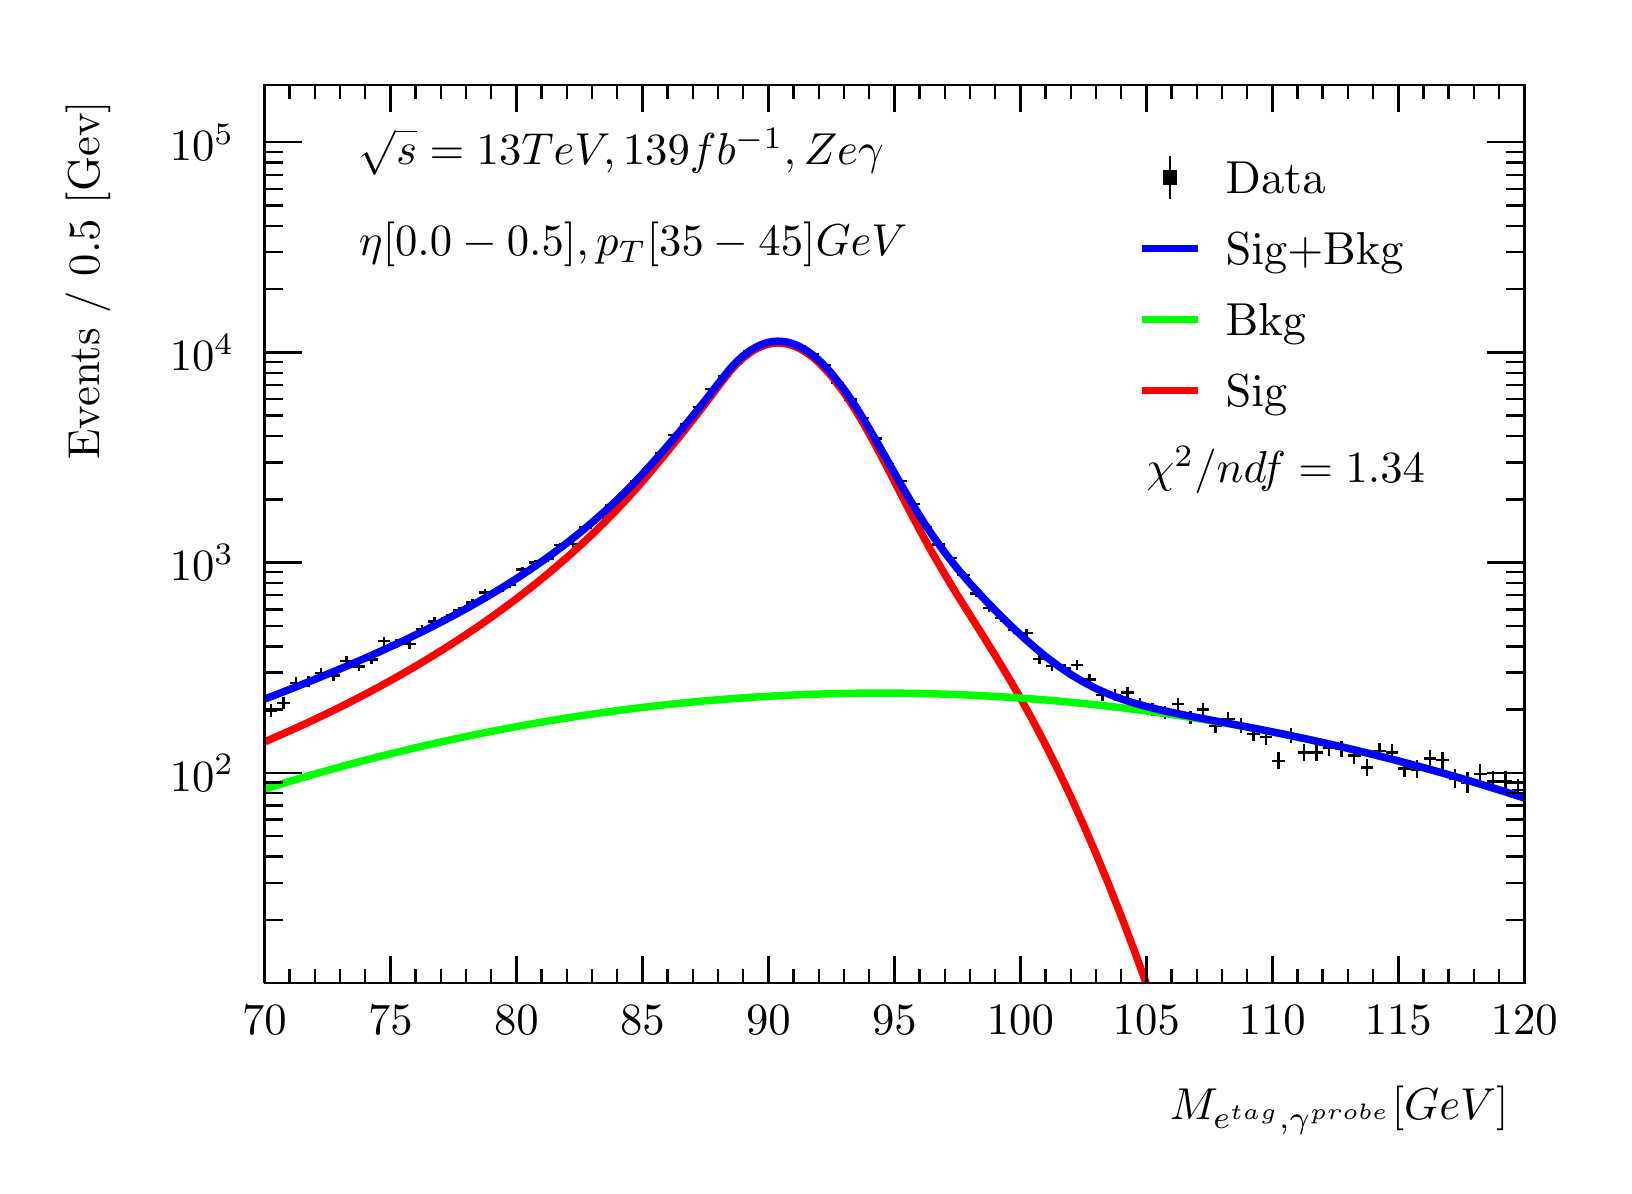
\begin{tikzpicture}
\pgfdeclareplotmark{cross} {
\pgfpathmoveto{\pgfpoint{-0.3\pgfplotmarksize}{\pgfplotmarksize}}
\pgfpathlineto{\pgfpoint{+0.3\pgfplotmarksize}{\pgfplotmarksize}}
\pgfpathlineto{\pgfpoint{+0.3\pgfplotmarksize}{0.3\pgfplotmarksize}}
\pgfpathlineto{\pgfpoint{+1\pgfplotmarksize}{0.3\pgfplotmarksize}}
\pgfpathlineto{\pgfpoint{+1\pgfplotmarksize}{-0.3\pgfplotmarksize}}
\pgfpathlineto{\pgfpoint{+0.3\pgfplotmarksize}{-0.3\pgfplotmarksize}}
\pgfpathlineto{\pgfpoint{+0.3\pgfplotmarksize}{-1.\pgfplotmarksize}}
\pgfpathlineto{\pgfpoint{-0.3\pgfplotmarksize}{-1.\pgfplotmarksize}}
\pgfpathlineto{\pgfpoint{-0.3\pgfplotmarksize}{-0.3\pgfplotmarksize}}
\pgfpathlineto{\pgfpoint{-1.\pgfplotmarksize}{-0.3\pgfplotmarksize}}
\pgfpathlineto{\pgfpoint{-1.\pgfplotmarksize}{0.3\pgfplotmarksize}}
\pgfpathlineto{\pgfpoint{-0.3\pgfplotmarksize}{0.3\pgfplotmarksize}}
\pgfpathclose
\pgfusepathqstroke
}
\pgfdeclareplotmark{cross*} {
\pgfpathmoveto{\pgfpoint{-0.3\pgfplotmarksize}{\pgfplotmarksize}}
\pgfpathlineto{\pgfpoint{+0.3\pgfplotmarksize}{\pgfplotmarksize}}
\pgfpathlineto{\pgfpoint{+0.3\pgfplotmarksize}{0.3\pgfplotmarksize}}
\pgfpathlineto{\pgfpoint{+1\pgfplotmarksize}{0.3\pgfplotmarksize}}
\pgfpathlineto{\pgfpoint{+1\pgfplotmarksize}{-0.3\pgfplotmarksize}}
\pgfpathlineto{\pgfpoint{+0.3\pgfplotmarksize}{-0.3\pgfplotmarksize}}
\pgfpathlineto{\pgfpoint{+0.3\pgfplotmarksize}{-1.\pgfplotmarksize}}
\pgfpathlineto{\pgfpoint{-0.3\pgfplotmarksize}{-1.\pgfplotmarksize}}
\pgfpathlineto{\pgfpoint{-0.3\pgfplotmarksize}{-0.3\pgfplotmarksize}}
\pgfpathlineto{\pgfpoint{-1.\pgfplotmarksize}{-0.3\pgfplotmarksize}}
\pgfpathlineto{\pgfpoint{-1.\pgfplotmarksize}{0.3\pgfplotmarksize}}
\pgfpathlineto{\pgfpoint{-0.3\pgfplotmarksize}{0.3\pgfplotmarksize}}
\pgfpathclose
\pgfusepathqfillstroke
}
\pgfdeclareplotmark{newstar} {
\pgfpathmoveto{\pgfqpoint{0pt}{\pgfplotmarksize}}
\pgfpathlineto{\pgfqpointpolar{44}{0.5\pgfplotmarksize}}
\pgfpathlineto{\pgfqpointpolar{18}{\pgfplotmarksize}}
\pgfpathlineto{\pgfqpointpolar{-20}{0.5\pgfplotmarksize}}
\pgfpathlineto{\pgfqpointpolar{-54}{\pgfplotmarksize}}
\pgfpathlineto{\pgfqpointpolar{-90}{0.5\pgfplotmarksize}}
\pgfpathlineto{\pgfqpointpolar{234}{\pgfplotmarksize}}
\pgfpathlineto{\pgfqpointpolar{198}{0.5\pgfplotmarksize}}
\pgfpathlineto{\pgfqpointpolar{162}{\pgfplotmarksize}}
\pgfpathlineto{\pgfqpointpolar{134}{0.5\pgfplotmarksize}}
\pgfpathclose
\pgfusepathqstroke
}
\pgfdeclareplotmark{newstar*} {
\pgfpathmoveto{\pgfqpoint{0pt}{\pgfplotmarksize}}
\pgfpathlineto{\pgfqpointpolar{44}{0.5\pgfplotmarksize}}
\pgfpathlineto{\pgfqpointpolar{18}{\pgfplotmarksize}}
\pgfpathlineto{\pgfqpointpolar{-20}{0.5\pgfplotmarksize}}
\pgfpathlineto{\pgfqpointpolar{-54}{\pgfplotmarksize}}
\pgfpathlineto{\pgfqpointpolar{-90}{0.5\pgfplotmarksize}}
\pgfpathlineto{\pgfqpointpolar{234}{\pgfplotmarksize}}
\pgfpathlineto{\pgfqpointpolar{198}{0.5\pgfplotmarksize}}
\pgfpathlineto{\pgfqpointpolar{162}{\pgfplotmarksize}}
\pgfpathlineto{\pgfqpointpolar{134}{0.5\pgfplotmarksize}}
\pgfpathclose
\pgfusepathqfillstroke
}
\definecolor{c}{rgb}{1,1,1};
\draw [color=c, fill=c] (0,0) rectangle (20,14.4361);
\draw [color=c, fill=c] (3,2.30977) rectangle (19,13.7143);
\definecolor{c}{rgb}{0,0,0};
\draw [c,line width=0.9] (3,2.30977) -- (3,13.7143) -- (19,13.7143) -- (19,2.30977) -- (3,2.30977);
\definecolor{c}{rgb}{1,1,1};
\draw [color=c, fill=c] (3,2.30977) rectangle (19,13.7143);
\definecolor{c}{rgb}{0,0,0};
\draw [c,line width=0.9] (3,2.30977) -- (3,13.7143) -- (19,13.7143) -- (19,2.30977) -- (3,2.30977);
\draw [c,line width=0.9] (3,2.30977) -- (19,2.30977);
\draw [c,line width=0.9] (3,2.65624) -- (3,2.30977);
\draw [c,line width=0.9] (3.32,2.48301) -- (3.32,2.30977);
\draw [c,line width=0.9] (3.64,2.48301) -- (3.64,2.30977);
\draw [c,line width=0.9] (3.96,2.48301) -- (3.96,2.30977);
\draw [c,line width=0.9] (4.28,2.48301) -- (4.28,2.30977);
\draw [c,line width=0.9] (4.6,2.65624) -- (4.6,2.30977);
\draw [c,line width=0.9] (4.92,2.48301) -- (4.92,2.30977);
\draw [c,line width=0.9] (5.24,2.48301) -- (5.24,2.30977);
\draw [c,line width=0.9] (5.56,2.48301) -- (5.56,2.30977);
\draw [c,line width=0.9] (5.88,2.48301) -- (5.88,2.30977);
\draw [c,line width=0.9] (6.2,2.65624) -- (6.2,2.30977);
\draw [c,line width=0.9] (6.52,2.48301) -- (6.52,2.30977);
\draw [c,line width=0.9] (6.84,2.48301) -- (6.84,2.30977);
\draw [c,line width=0.9] (7.16,2.48301) -- (7.16,2.30977);
\draw [c,line width=0.9] (7.48,2.48301) -- (7.48,2.30977);
\draw [c,line width=0.9] (7.8,2.65624) -- (7.8,2.30977);
\draw [c,line width=0.9] (8.12,2.48301) -- (8.12,2.30977);
\draw [c,line width=0.9] (8.44,2.48301) -- (8.44,2.30977);
\draw [c,line width=0.9] (8.76,2.48301) -- (8.76,2.30977);
\draw [c,line width=0.9] (9.08,2.48301) -- (9.08,2.30977);
\draw [c,line width=0.9] (9.4,2.65624) -- (9.4,2.30977);
\draw [c,line width=0.9] (9.72,2.48301) -- (9.72,2.30977);
\draw [c,line width=0.9] (10.04,2.48301) -- (10.04,2.30977);
\draw [c,line width=0.9] (10.36,2.48301) -- (10.36,2.30977);
\draw [c,line width=0.9] (10.68,2.48301) -- (10.68,2.30977);
\draw [c,line width=0.9] (11,2.65624) -- (11,2.30977);
\draw [c,line width=0.9] (11.32,2.48301) -- (11.32,2.30977);
\draw [c,line width=0.9] (11.64,2.48301) -- (11.64,2.30977);
\draw [c,line width=0.9] (11.96,2.48301) -- (11.96,2.30977);
\draw [c,line width=0.9] (12.28,2.48301) -- (12.28,2.30977);
\draw [c,line width=0.9] (12.6,2.65624) -- (12.6,2.30977);
\draw [c,line width=0.9] (12.92,2.48301) -- (12.92,2.30977);
\draw [c,line width=0.9] (13.24,2.48301) -- (13.24,2.30977);
\draw [c,line width=0.9] (13.56,2.48301) -- (13.56,2.30977);
\draw [c,line width=0.9] (13.88,2.48301) -- (13.88,2.30977);
\draw [c,line width=0.9] (14.2,2.65624) -- (14.2,2.30977);
\draw [c,line width=0.9] (14.52,2.48301) -- (14.52,2.30977);
\draw [c,line width=0.9] (14.84,2.48301) -- (14.84,2.30977);
\draw [c,line width=0.9] (15.16,2.48301) -- (15.16,2.30977);
\draw [c,line width=0.9] (15.48,2.48301) -- (15.48,2.30977);
\draw [c,line width=0.9] (15.8,2.65624) -- (15.8,2.30977);
\draw [c,line width=0.9] (16.12,2.48301) -- (16.12,2.30977);
\draw [c,line width=0.9] (16.44,2.48301) -- (16.44,2.30977);
\draw [c,line width=0.9] (16.76,2.48301) -- (16.76,2.30977);
\draw [c,line width=0.9] (17.08,2.48301) -- (17.08,2.30977);
\draw [c,line width=0.9] (17.4,2.65624) -- (17.4,2.30977);
\draw [c,line width=0.9] (17.72,2.48301) -- (17.72,2.30977);
\draw [c,line width=0.9] (18.04,2.48301) -- (18.04,2.30977);
\draw [c,line width=0.9] (18.36,2.48301) -- (18.36,2.30977);
\draw [c,line width=0.9] (18.68,2.48301) -- (18.68,2.30977);
\draw [c,line width=0.9] (19,2.65624) -- (19,2.30977);
\draw [anchor=base] (3,1.66015) node[scale=1.61424, color=c, rotate=0]{70};
\draw [anchor=base] (4.6,1.66015) node[scale=1.61424, color=c, rotate=0]{75};
\draw [anchor=base] (6.2,1.66015) node[scale=1.61424, color=c, rotate=0]{80};
\draw [anchor=base] (7.8,1.66015) node[scale=1.61424, color=c, rotate=0]{85};
\draw [anchor=base] (9.4,1.66015) node[scale=1.61424, color=c, rotate=0]{90};
\draw [anchor=base] (11,1.66015) node[scale=1.61424, color=c, rotate=0]{95};
\draw [anchor=base] (12.6,1.66015) node[scale=1.61424, color=c, rotate=0]{100};
\draw [anchor=base] (14.2,1.66015) node[scale=1.61424, color=c, rotate=0]{105};
\draw [anchor=base] (15.8,1.66015) node[scale=1.61424, color=c, rotate=0]{110};
\draw [anchor=base] (17.4,1.66015) node[scale=1.61424, color=c, rotate=0]{115};
\draw [anchor=base] (19,1.66015) node[scale=1.61424, color=c, rotate=0]{120};
\draw [anchor= east] (19,0.692932) node[scale=1.61424, color=c, rotate=0]{$M_{e^{tag}, \gamma^{probe}}  [GeV]$};
\draw [c,line width=0.9] (3,13.7143) -- (19,13.7143);
\draw [c,line width=0.9] (3,13.3678) -- (3,13.7143);
\draw [c,line width=0.9] (3.32,13.5411) -- (3.32,13.7143);
\draw [c,line width=0.9] (3.64,13.5411) -- (3.64,13.7143);
\draw [c,line width=0.9] (3.96,13.5411) -- (3.96,13.7143);
\draw [c,line width=0.9] (4.28,13.5411) -- (4.28,13.7143);
\draw [c,line width=0.9] (4.6,13.3678) -- (4.6,13.7143);
\draw [c,line width=0.9] (4.92,13.5411) -- (4.92,13.7143);
\draw [c,line width=0.9] (5.24,13.5411) -- (5.24,13.7143);
\draw [c,line width=0.9] (5.56,13.5411) -- (5.56,13.7143);
\draw [c,line width=0.9] (5.88,13.5411) -- (5.88,13.7143);
\draw [c,line width=0.9] (6.2,13.3678) -- (6.2,13.7143);
\draw [c,line width=0.9] (6.52,13.5411) -- (6.52,13.7143);
\draw [c,line width=0.9] (6.84,13.5411) -- (6.84,13.7143);
\draw [c,line width=0.9] (7.16,13.5411) -- (7.16,13.7143);
\draw [c,line width=0.9] (7.48,13.5411) -- (7.48,13.7143);
\draw [c,line width=0.9] (7.8,13.3678) -- (7.8,13.7143);
\draw [c,line width=0.9] (8.12,13.5411) -- (8.12,13.7143);
\draw [c,line width=0.9] (8.44,13.5411) -- (8.44,13.7143);
\draw [c,line width=0.9] (8.76,13.5411) -- (8.76,13.7143);
\draw [c,line width=0.9] (9.08,13.5411) -- (9.08,13.7143);
\draw [c,line width=0.9] (9.4,13.3678) -- (9.4,13.7143);
\draw [c,line width=0.9] (9.72,13.5411) -- (9.72,13.7143);
\draw [c,line width=0.9] (10.04,13.5411) -- (10.04,13.7143);
\draw [c,line width=0.9] (10.36,13.5411) -- (10.36,13.7143);
\draw [c,line width=0.9] (10.68,13.5411) -- (10.68,13.7143);
\draw [c,line width=0.9] (11,13.3678) -- (11,13.7143);
\draw [c,line width=0.9] (11.32,13.5411) -- (11.32,13.7143);
\draw [c,line width=0.9] (11.64,13.5411) -- (11.64,13.7143);
\draw [c,line width=0.9] (11.96,13.5411) -- (11.96,13.7143);
\draw [c,line width=0.9] (12.28,13.5411) -- (12.28,13.7143);
\draw [c,line width=0.9] (12.6,13.3678) -- (12.6,13.7143);
\draw [c,line width=0.9] (12.92,13.5411) -- (12.92,13.7143);
\draw [c,line width=0.9] (13.24,13.5411) -- (13.24,13.7143);
\draw [c,line width=0.9] (13.56,13.5411) -- (13.56,13.7143);
\draw [c,line width=0.9] (13.88,13.5411) -- (13.88,13.7143);
\draw [c,line width=0.9] (14.2,13.3678) -- (14.2,13.7143);
\draw [c,line width=0.9] (14.52,13.5411) -- (14.52,13.7143);
\draw [c,line width=0.9] (14.84,13.5411) -- (14.84,13.7143);
\draw [c,line width=0.9] (15.16,13.5411) -- (15.16,13.7143);
\draw [c,line width=0.9] (15.48,13.5411) -- (15.48,13.7143);
\draw [c,line width=0.9] (15.8,13.3678) -- (15.8,13.7143);
\draw [c,line width=0.9] (16.12,13.5411) -- (16.12,13.7143);
\draw [c,line width=0.9] (16.44,13.5411) -- (16.44,13.7143);
\draw [c,line width=0.9] (16.76,13.5411) -- (16.76,13.7143);
\draw [c,line width=0.9] (17.08,13.5411) -- (17.08,13.7143);
\draw [c,line width=0.9] (17.4,13.3678) -- (17.4,13.7143);
\draw [c,line width=0.9] (17.72,13.5411) -- (17.72,13.7143);
\draw [c,line width=0.9] (18.04,13.5411) -- (18.04,13.7143);
\draw [c,line width=0.9] (18.36,13.5411) -- (18.36,13.7143);
\draw [c,line width=0.9] (18.68,13.5411) -- (18.68,13.7143);
\draw [c,line width=0.9] (19,13.3678) -- (19,13.7143);
\draw [c,line width=0.9] (3,2.30977) -- (3,13.7143);
\draw [c,line width=0.9] (3.237,3.11343) -- (3,3.11343);
\draw [c,line width=0.9] (3.237,3.58354) -- (3,3.58354);
\draw [c,line width=0.9] (3.237,3.91709) -- (3,3.91709);
\draw [c,line width=0.9] (3.237,4.17581) -- (3,4.17581);
\draw [c,line width=0.9] (3.237,4.38719) -- (3,4.38719);
\draw [c,line width=0.9] (3.237,4.56592) -- (3,4.56592);
\draw [c,line width=0.9] (3.237,4.72074) -- (3,4.72074);
\draw [c,line width=0.9] (3.237,4.8573) -- (3,4.8573);
\draw [c,line width=0.9] (3.474,4.97946) -- (3,4.97946);
\draw [anchor= east] (2.82,4.97946) node[scale=1.61424, color=c, rotate=0]{$10^{2}$};
\draw [c,line width=0.9] (3.237,5.78312) -- (3,5.78312);
\draw [c,line width=0.9] (3.237,6.25323) -- (3,6.25323);
\draw [c,line width=0.9] (3.237,6.58678) -- (3,6.58678);
\draw [c,line width=0.9] (3.237,6.8455) -- (3,6.8455);
\draw [c,line width=0.9] (3.237,7.05689) -- (3,7.05689);
\draw [c,line width=0.9] (3.237,7.23561) -- (3,7.23561);
\draw [c,line width=0.9] (3.237,7.39043) -- (3,7.39043);
\draw [c,line width=0.9] (3.237,7.52699) -- (3,7.52699);
\draw [c,line width=0.9] (3.474,7.64915) -- (3,7.64915);
\draw [anchor= east] (2.82,7.64915) node[scale=1.61424, color=c, rotate=0]{$10^{3}$};
\draw [c,line width=0.9] (3.237,8.45281) -- (3,8.45281);
\draw [c,line width=0.9] (3.237,8.92292) -- (3,8.92292);
\draw [c,line width=0.9] (3.237,9.25647) -- (3,9.25647);
\draw [c,line width=0.9] (3.237,9.51519) -- (3,9.51519);
\draw [c,line width=0.9] (3.237,9.72658) -- (3,9.72658);
\draw [c,line width=0.9] (3.237,9.9053) -- (3,9.9053);
\draw [c,line width=0.9] (3.237,10.0601) -- (3,10.0601);
\draw [c,line width=0.9] (3.237,10.1967) -- (3,10.1967);
\draw [c,line width=0.9] (3.474,10.3188) -- (3,10.3188);
\draw [anchor= east] (2.82,10.3188) node[scale=1.61424, color=c, rotate=0]{$10^{4}$};
\draw [c,line width=0.9] (3.237,11.1225) -- (3,11.1225);
\draw [c,line width=0.9] (3.237,11.5926) -- (3,11.5926);
\draw [c,line width=0.9] (3.237,11.9262) -- (3,11.9262);
\draw [c,line width=0.9] (3.237,12.1849) -- (3,12.1849);
\draw [c,line width=0.9] (3.237,12.3963) -- (3,12.3963);
\draw [c,line width=0.9] (3.237,12.575) -- (3,12.575);
\draw [c,line width=0.9] (3.237,12.7298) -- (3,12.7298);
\draw [c,line width=0.9] (3.237,12.8664) -- (3,12.8664);
\draw [c,line width=0.9] (3.474,12.9885) -- (3,12.9885);
\draw [anchor= east] (2.82,12.9885) node[scale=1.61424, color=c, rotate=0]{$10^{5}$};
\draw [anchor= east] (0.76,13.7143) node[scale=1.61424, color=c, rotate=90]{Events / 0.5 [Gev]};
\draw [c,line width=0.9] (19,2.30977) -- (19,13.7143);
\draw [c,line width=0.9] (18.763,3.11343) -- (19,3.11343);
\draw [c,line width=0.9] (18.763,3.58354) -- (19,3.58354);
\draw [c,line width=0.9] (18.763,3.91709) -- (19,3.91709);
\draw [c,line width=0.9] (18.763,4.17581) -- (19,4.17581);
\draw [c,line width=0.9] (18.763,4.38719) -- (19,4.38719);
\draw [c,line width=0.9] (18.763,4.56592) -- (19,4.56592);
\draw [c,line width=0.9] (18.763,4.72074) -- (19,4.72074);
\draw [c,line width=0.9] (18.763,4.8573) -- (19,4.8573);
\draw [c,line width=0.9] (18.526,4.97946) -- (19,4.97946);
\draw [c,line width=0.9] (18.763,5.78312) -- (19,5.78312);
\draw [c,line width=0.9] (18.763,6.25323) -- (19,6.25323);
\draw [c,line width=0.9] (18.763,6.58678) -- (19,6.58678);
\draw [c,line width=0.9] (18.763,6.8455) -- (19,6.8455);
\draw [c,line width=0.9] (18.763,7.05689) -- (19,7.05689);
\draw [c,line width=0.9] (18.763,7.23561) -- (19,7.23561);
\draw [c,line width=0.9] (18.763,7.39043) -- (19,7.39043);
\draw [c,line width=0.9] (18.763,7.52699) -- (19,7.52699);
\draw [c,line width=0.9] (18.526,7.64915) -- (19,7.64915);
\draw [c,line width=0.9] (18.763,8.45281) -- (19,8.45281);
\draw [c,line width=0.9] (18.763,8.92292) -- (19,8.92292);
\draw [c,line width=0.9] (18.763,9.25647) -- (19,9.25647);
\draw [c,line width=0.9] (18.763,9.51519) -- (19,9.51519);
\draw [c,line width=0.9] (18.763,9.72658) -- (19,9.72658);
\draw [c,line width=0.9] (18.763,9.9053) -- (19,9.9053);
\draw [c,line width=0.9] (18.763,10.0601) -- (19,10.0601);
\draw [c,line width=0.9] (18.763,10.1967) -- (19,10.1967);
\draw [c,line width=0.9] (18.526,10.3188) -- (19,10.3188);
\draw [c,line width=0.9] (18.763,11.1225) -- (19,11.1225);
\draw [c,line width=0.9] (18.763,11.5926) -- (19,11.5926);
\draw [c,line width=0.9] (18.763,11.9262) -- (19,11.9262);
\draw [c,line width=0.9] (18.763,12.1849) -- (19,12.1849);
\draw [c,line width=0.9] (18.763,12.3963) -- (19,12.3963);
\draw [c,line width=0.9] (18.763,12.575) -- (19,12.575);
\draw [c,line width=0.9] (18.763,12.7298) -- (19,12.7298);
\draw [c,line width=0.9] (18.763,12.8664) -- (19,12.8664);
\draw [c,line width=0.9] (18.526,12.9885) -- (19,12.9885);
\draw [c,line width=0.9] (3.08,5.77147) -- (3,5.77147);
\draw [c,line width=0.9] (3,5.77147) -- (3,5.77147);
\draw [c,line width=0.9] (3.08,5.77147) -- (3.16,5.77147);
\draw [c,line width=0.9] (3.16,5.77147) -- (3.16,5.77147);
\draw [c,line width=0.9] (3.08,5.77147) -- (3.08,5.85385);
\draw [c,line width=0.9] (3.08,5.85385) -- (3.08,5.85385);
\draw [c,line width=0.9] (3.08,5.77147) -- (3.08,5.68909);
\draw [c,line width=0.9] (3.08,5.68909) -- (3.08,5.68909);
\draw [c,line width=0.9] (3.24,5.86697) -- (3.16,5.86697);
\draw [c,line width=0.9] (3.16,5.86697) -- (3.16,5.86697);
\draw [c,line width=0.9] (3.24,5.86697) -- (3.32,5.86697);
\draw [c,line width=0.9] (3.32,5.86697) -- (3.32,5.86697);
\draw [c,line width=0.9] (3.24,5.86697) -- (3.24,5.94603);
\draw [c,line width=0.9] (3.24,5.94603) -- (3.24,5.94603);
\draw [c,line width=0.9] (3.24,5.86697) -- (3.24,5.78791);
\draw [c,line width=0.9] (3.24,5.78791) -- (3.24,5.78791);
\draw [c,line width=0.9] (3.4,6.12245) -- (3.32,6.12245);
\draw [c,line width=0.9] (3.32,6.12245) -- (3.32,6.12245);
\draw [c,line width=0.9] (3.4,6.12245) -- (3.48,6.12245);
\draw [c,line width=0.9] (3.48,6.12245) -- (3.48,6.12245);
\draw [c,line width=0.9] (3.4,6.12245) -- (3.4,6.19326);
\draw [c,line width=0.9] (3.4,6.19326) -- (3.4,6.19326);
\draw [c,line width=0.9] (3.4,6.12245) -- (3.4,6.05164);
\draw [c,line width=0.9] (3.4,6.05164) -- (3.4,6.05164);
\draw [c,line width=0.9] (3.56,6.14388) -- (3.48,6.14388);
\draw [c,line width=0.9] (3.48,6.14388) -- (3.48,6.14388);
\draw [c,line width=0.9] (3.56,6.14388) -- (3.64,6.14388);
\draw [c,line width=0.9] (3.64,6.14388) -- (3.64,6.14388);
\draw [c,line width=0.9] (3.56,6.14388) -- (3.56,6.21404);
\draw [c,line width=0.9] (3.56,6.21404) -- (3.56,6.21404);
\draw [c,line width=0.9] (3.56,6.14388) -- (3.56,6.07372);
\draw [c,line width=0.9] (3.56,6.07372) -- (3.56,6.07372);
\draw [c,line width=0.9] (3.72,6.24547) -- (3.64,6.24547);
\draw [c,line width=0.9] (3.64,6.24547) -- (3.64,6.24547);
\draw [c,line width=0.9] (3.72,6.24547) -- (3.8,6.24547);
\draw [c,line width=0.9] (3.8,6.24547) -- (3.8,6.24547);
\draw [c,line width=0.9] (3.72,6.24547) -- (3.72,6.31263);
\draw [c,line width=0.9] (3.72,6.31263) -- (3.72,6.31263);
\draw [c,line width=0.9] (3.72,6.24547) -- (3.72,6.17832);
\draw [c,line width=0.9] (3.72,6.17832) -- (3.72,6.17832);
\draw [c,line width=0.9] (3.88,6.21392) -- (3.8,6.21392);
\draw [c,line width=0.9] (3.8,6.21392) -- (3.8,6.21392);
\draw [c,line width=0.9] (3.88,6.21392) -- (3.96,6.21392);
\draw [c,line width=0.9] (3.96,6.21392) -- (3.96,6.21392);
\draw [c,line width=0.9] (3.88,6.21392) -- (3.88,6.282);
\draw [c,line width=0.9] (3.88,6.282) -- (3.88,6.282);
\draw [c,line width=0.9] (3.88,6.21392) -- (3.88,6.14585);
\draw [c,line width=0.9] (3.88,6.14585) -- (3.88,6.14585);
\draw [c,line width=0.9] (4.04,6.39835) -- (3.96,6.39835);
\draw [c,line width=0.9] (3.96,6.39835) -- (3.96,6.39835);
\draw [c,line width=0.9] (4.04,6.39835) -- (4.12,6.39835);
\draw [c,line width=0.9] (4.12,6.39835) -- (4.12,6.39835);
\draw [c,line width=0.9] (4.04,6.39835) -- (4.04,6.46122);
\draw [c,line width=0.9] (4.04,6.46122) -- (4.04,6.46122);
\draw [c,line width=0.9] (4.04,6.39835) -- (4.04,6.33548);
\draw [c,line width=0.9] (4.04,6.33548) -- (4.04,6.33548);
\draw [c,line width=0.9] (4.2,6.33168) -- (4.12,6.33168);
\draw [c,line width=0.9] (4.12,6.33168) -- (4.12,6.33168);
\draw [c,line width=0.9] (4.2,6.33168) -- (4.28,6.33168);
\draw [c,line width=0.9] (4.28,6.33168) -- (4.28,6.33168);
\draw [c,line width=0.9] (4.2,6.33168) -- (4.2,6.39638);
\draw [c,line width=0.9] (4.2,6.39638) -- (4.2,6.39638);
\draw [c,line width=0.9] (4.2,6.33168) -- (4.2,6.26697);
\draw [c,line width=0.9] (4.2,6.26697) -- (4.2,6.26697);
\draw [c,line width=0.9] (4.36,6.41863) -- (4.28,6.41863);
\draw [c,line width=0.9] (4.28,6.41863) -- (4.28,6.41863);
\draw [c,line width=0.9] (4.36,6.41863) -- (4.44,6.41863);
\draw [c,line width=0.9] (4.44,6.41863) -- (4.44,6.41863);
\draw [c,line width=0.9] (4.36,6.41863) -- (4.36,6.48095);
\draw [c,line width=0.9] (4.36,6.48095) -- (4.36,6.48095);
\draw [c,line width=0.9] (4.36,6.41863) -- (4.36,6.35631);
\draw [c,line width=0.9] (4.36,6.35631) -- (4.36,6.35631);
\draw [c,line width=0.9] (4.52,6.6516) -- (4.44,6.6516);
\draw [c,line width=0.9] (4.44,6.6516) -- (4.44,6.6516);
\draw [c,line width=0.9] (4.52,6.6516) -- (4.6,6.6516);
\draw [c,line width=0.9] (4.6,6.6516) -- (4.6,6.6516);
\draw [c,line width=0.9] (4.52,6.6516) -- (4.52,6.70797);
\draw [c,line width=0.9] (4.52,6.70797) -- (4.52,6.70797);
\draw [c,line width=0.9] (4.52,6.6516) -- (4.52,6.59523);
\draw [c,line width=0.9] (4.52,6.59523) -- (4.52,6.59523);
\draw [c,line width=0.9] (4.68,6.62666) -- (4.6,6.62666);
\draw [c,line width=0.9] (4.6,6.62666) -- (4.6,6.62666);
\draw [c,line width=0.9] (4.68,6.62666) -- (4.76,6.62666);
\draw [c,line width=0.9] (4.76,6.62666) -- (4.76,6.62666);
\draw [c,line width=0.9] (4.68,6.62666) -- (4.68,6.68364);
\draw [c,line width=0.9] (4.68,6.68364) -- (4.68,6.68364);
\draw [c,line width=0.9] (4.68,6.62666) -- (4.68,6.56969);
\draw [c,line width=0.9] (4.68,6.56969) -- (4.68,6.56969);
\draw [c,line width=0.9] (4.84,6.61258) -- (4.76,6.61258);
\draw [c,line width=0.9] (4.76,6.61258) -- (4.76,6.61258);
\draw [c,line width=0.9] (4.84,6.61258) -- (4.92,6.61258);
\draw [c,line width=0.9] (4.92,6.61258) -- (4.92,6.61258);
\draw [c,line width=0.9] (4.84,6.61258) -- (4.84,6.6699);
\draw [c,line width=0.9] (4.84,6.6699) -- (4.84,6.6699);
\draw [c,line width=0.9] (4.84,6.61258) -- (4.84,6.55525);
\draw [c,line width=0.9] (4.84,6.55525) -- (4.84,6.55525);
\draw [c,line width=0.9] (5,6.80779) -- (4.92,6.80779);
\draw [c,line width=0.9] (4.92,6.80779) -- (4.92,6.80779);
\draw [c,line width=0.9] (5,6.80779) -- (5.08,6.80779);
\draw [c,line width=0.9] (5.08,6.80779) -- (5.08,6.80779);
\draw [c,line width=0.9] (5,6.80779) -- (5,6.86049);
\draw [c,line width=0.9] (5,6.86049) -- (5,6.86049);
\draw [c,line width=0.9] (5,6.80779) -- (5,6.75509);
\draw [c,line width=0.9] (5,6.75509) -- (5,6.75509);
\draw [c,line width=0.9] (5.16,6.90207) -- (5.08,6.90207);
\draw [c,line width=0.9] (5.08,6.90207) -- (5.08,6.90207);
\draw [c,line width=0.9] (5.16,6.90207) -- (5.24,6.90207);
\draw [c,line width=0.9] (5.24,6.90207) -- (5.24,6.90207);
\draw [c,line width=0.9] (5.16,6.90207) -- (5.16,6.95266);
\draw [c,line width=0.9] (5.16,6.95266) -- (5.16,6.95266);
\draw [c,line width=0.9] (5.16,6.90207) -- (5.16,6.85147);
\draw [c,line width=0.9] (5.16,6.85147) -- (5.16,6.85147);
\draw [c,line width=0.9] (5.32,6.94754) -- (5.24,6.94754);
\draw [c,line width=0.9] (5.24,6.94754) -- (5.24,6.94754);
\draw [c,line width=0.9] (5.32,6.94754) -- (5.4,6.94754);
\draw [c,line width=0.9] (5.4,6.94754) -- (5.4,6.94754);
\draw [c,line width=0.9] (5.32,6.94754) -- (5.32,6.99716);
\draw [c,line width=0.9] (5.32,6.99716) -- (5.32,6.99716);
\draw [c,line width=0.9] (5.32,6.94754) -- (5.32,6.89792);
\draw [c,line width=0.9] (5.32,6.89792) -- (5.32,6.89792);
\draw [c,line width=0.9] (5.48,7.03936) -- (5.4,7.03936);
\draw [c,line width=0.9] (5.4,7.03936) -- (5.4,7.03936);
\draw [c,line width=0.9] (5.48,7.03936) -- (5.56,7.03936);
\draw [c,line width=0.9] (5.56,7.03936) -- (5.56,7.03936);
\draw [c,line width=0.9] (5.48,7.03936) -- (5.48,7.08705);
\draw [c,line width=0.9] (5.48,7.08705) -- (5.48,7.08705);
\draw [c,line width=0.9] (5.48,7.03936) -- (5.48,6.99167);
\draw [c,line width=0.9] (5.48,6.99167) -- (5.48,6.99167);
\draw [c,line width=0.9] (5.64,7.14074) -- (5.56,7.14074);
\draw [c,line width=0.9] (5.56,7.14074) -- (5.56,7.14074);
\draw [c,line width=0.9] (5.64,7.14074) -- (5.72,7.14074);
\draw [c,line width=0.9] (5.72,7.14074) -- (5.72,7.14074);
\draw [c,line width=0.9] (5.64,7.14074) -- (5.64,7.18639);
\draw [c,line width=0.9] (5.64,7.18639) -- (5.64,7.18639);
\draw [c,line width=0.9] (5.64,7.14074) -- (5.64,7.09509);
\draw [c,line width=0.9] (5.64,7.09509) -- (5.64,7.09509);
\draw [c,line width=0.9] (5.8,7.26666) -- (5.72,7.26666);
\draw [c,line width=0.9] (5.72,7.26666) -- (5.72,7.26666);
\draw [c,line width=0.9] (5.8,7.26666) -- (5.88,7.26666);
\draw [c,line width=0.9] (5.88,7.26666) -- (5.88,7.26666);
\draw [c,line width=0.9] (5.8,7.26666) -- (5.8,7.3099);
\draw [c,line width=0.9] (5.8,7.3099) -- (5.8,7.3099);
\draw [c,line width=0.9] (5.8,7.26666) -- (5.8,7.22343);
\draw [c,line width=0.9] (5.8,7.22343) -- (5.8,7.22343);
\draw [c,line width=0.9] (5.96,7.28902) -- (5.88,7.28902);
\draw [c,line width=0.9] (5.88,7.28902) -- (5.88,7.28902);
\draw [c,line width=0.9] (5.96,7.28902) -- (6.04,7.28902);
\draw [c,line width=0.9] (6.04,7.28902) -- (6.04,7.28902);
\draw [c,line width=0.9] (5.96,7.28902) -- (5.96,7.33185);
\draw [c,line width=0.9] (5.96,7.33185) -- (5.96,7.33185);
\draw [c,line width=0.9] (5.96,7.28902) -- (5.96,7.2462);
\draw [c,line width=0.9] (5.96,7.2462) -- (5.96,7.2462);
\draw [c,line width=0.9] (6.12,7.36553) -- (6.04,7.36553);
\draw [c,line width=0.9] (6.04,7.36553) -- (6.04,7.36553);
\draw [c,line width=0.9] (6.12,7.36553) -- (6.2,7.36553);
\draw [c,line width=0.9] (6.2,7.36553) -- (6.2,7.36553);
\draw [c,line width=0.9] (6.12,7.36553) -- (6.12,7.40696);
\draw [c,line width=0.9] (6.12,7.40696) -- (6.12,7.40696);
\draw [c,line width=0.9] (6.12,7.36553) -- (6.12,7.3241);
\draw [c,line width=0.9] (6.12,7.3241) -- (6.12,7.3241);
\draw [c,line width=0.9] (6.28,7.55876) -- (6.2,7.55876);
\draw [c,line width=0.9] (6.2,7.55876) -- (6.2,7.55876);
\draw [c,line width=0.9] (6.28,7.55876) -- (6.36,7.55876);
\draw [c,line width=0.9] (6.36,7.55876) -- (6.36,7.55876);
\draw [c,line width=0.9] (6.28,7.55876) -- (6.28,7.59688);
\draw [c,line width=0.9] (6.28,7.59688) -- (6.28,7.59688);
\draw [c,line width=0.9] (6.28,7.55876) -- (6.28,7.52064);
\draw [c,line width=0.9] (6.28,7.52064) -- (6.28,7.52064);
\draw [c,line width=0.9] (6.44,7.65031) -- (6.36,7.65031);
\draw [c,line width=0.9] (6.36,7.65031) -- (6.36,7.65031);
\draw [c,line width=0.9] (6.44,7.65031) -- (6.52,7.65031);
\draw [c,line width=0.9] (6.52,7.65031) -- (6.52,7.65031);
\draw [c,line width=0.9] (6.44,7.65031) -- (6.44,7.68696);
\draw [c,line width=0.9] (6.44,7.68696) -- (6.44,7.68696);
\draw [c,line width=0.9] (6.44,7.65031) -- (6.44,7.61367);
\draw [c,line width=0.9] (6.44,7.61367) -- (6.44,7.61367);
\draw [c,line width=0.9] (6.6,7.69908) -- (6.52,7.69908);
\draw [c,line width=0.9] (6.52,7.69908) -- (6.52,7.69908);
\draw [c,line width=0.9] (6.6,7.69908) -- (6.68,7.69908);
\draw [c,line width=0.9] (6.68,7.69908) -- (6.68,7.69908);
\draw [c,line width=0.9] (6.6,7.69908) -- (6.6,7.73496);
\draw [c,line width=0.9] (6.6,7.73496) -- (6.6,7.73496);
\draw [c,line width=0.9] (6.6,7.69908) -- (6.6,7.6632);
\draw [c,line width=0.9] (6.6,7.6632) -- (6.6,7.6632);
\draw [c,line width=0.9] (6.76,7.87112) -- (6.68,7.87112);
\draw [c,line width=0.9] (6.68,7.87112) -- (6.68,7.87112);
\draw [c,line width=0.9] (6.76,7.87112) -- (6.84,7.87112);
\draw [c,line width=0.9] (6.84,7.87112) -- (6.84,7.87112);
\draw [c,line width=0.9] (6.76,7.87112) -- (6.76,7.90444);
\draw [c,line width=0.9] (6.76,7.90444) -- (6.76,7.90444);
\draw [c,line width=0.9] (6.76,7.87112) -- (6.76,7.83781);
\draw [c,line width=0.9] (6.76,7.83781) -- (6.76,7.83781);
\draw [c,line width=0.9] (6.92,7.8854) -- (6.84,7.8854);
\draw [c,line width=0.9] (6.84,7.8854) -- (6.84,7.8854);
\draw [c,line width=0.9] (6.92,7.8854) -- (7,7.8854);
\draw [c,line width=0.9] (7,7.8854) -- (7,7.8854);
\draw [c,line width=0.9] (6.92,7.8854) -- (6.92,7.91851);
\draw [c,line width=0.9] (6.92,7.91851) -- (6.92,7.91851);
\draw [c,line width=0.9] (6.92,7.8854) -- (6.92,7.85228);
\draw [c,line width=0.9] (6.92,7.85228) -- (6.92,7.85228);
\draw [c,line width=0.9] (7.08,8.09426) -- (7,8.09426);
\draw [c,line width=0.9] (7,8.09426) -- (7,8.09426);
\draw [c,line width=0.9] (7.08,8.09426) -- (7.16,8.09426);
\draw [c,line width=0.9] (7.16,8.09426) -- (7.16,8.09426);
\draw [c,line width=0.9] (7.08,8.09426) -- (7.08,8.12452);
\draw [c,line width=0.9] (7.08,8.12452) -- (7.08,8.12452);
\draw [c,line width=0.9] (7.08,8.09426) -- (7.08,8.064);
\draw [c,line width=0.9] (7.08,8.064) -- (7.08,8.064);
\draw [c,line width=0.9] (7.24,8.21705) -- (7.16,8.21705);
\draw [c,line width=0.9] (7.16,8.21705) -- (7.16,8.21705);
\draw [c,line width=0.9] (7.24,8.21705) -- (7.32,8.21705);
\draw [c,line width=0.9] (7.32,8.21705) -- (7.32,8.21705);
\draw [c,line width=0.9] (7.24,8.21705) -- (7.24,8.24575);
\draw [c,line width=0.9] (7.24,8.24575) -- (7.24,8.24575);
\draw [c,line width=0.9] (7.24,8.21705) -- (7.24,8.18835);
\draw [c,line width=0.9] (7.24,8.18835) -- (7.24,8.18835);
\draw [c,line width=0.9] (7.4,8.37365) -- (7.32,8.37365);
\draw [c,line width=0.9] (7.32,8.37365) -- (7.32,8.37365);
\draw [c,line width=0.9] (7.4,8.37365) -- (7.48,8.37365);
\draw [c,line width=0.9] (7.48,8.37365) -- (7.48,8.37365);
\draw [c,line width=0.9] (7.4,8.37365) -- (7.4,8.40047);
\draw [c,line width=0.9] (7.4,8.40047) -- (7.4,8.40047);
\draw [c,line width=0.9] (7.4,8.37365) -- (7.4,8.34682);
\draw [c,line width=0.9] (7.4,8.34682) -- (7.4,8.34682);
\draw [c,line width=0.9] (7.56,8.44233) -- (7.48,8.44233);
\draw [c,line width=0.9] (7.48,8.44233) -- (7.48,8.44233);
\draw [c,line width=0.9] (7.56,8.44233) -- (7.64,8.44233);
\draw [c,line width=0.9] (7.64,8.44233) -- (7.64,8.44233);
\draw [c,line width=0.9] (7.56,8.44233) -- (7.56,8.46837);
\draw [c,line width=0.9] (7.56,8.46837) -- (7.56,8.46837);
\draw [c,line width=0.9] (7.56,8.44233) -- (7.56,8.41629);
\draw [c,line width=0.9] (7.56,8.41629) -- (7.56,8.41629);
\draw [c,line width=0.9] (7.72,8.68526) -- (7.64,8.68526);
\draw [c,line width=0.9] (7.64,8.68526) -- (7.64,8.68526);
\draw [c,line width=0.9] (7.72,8.68526) -- (7.8,8.68526);
\draw [c,line width=0.9] (7.8,8.68526) -- (7.8,8.68526);
\draw [c,line width=0.9] (7.72,8.68526) -- (7.72,8.70872);
\draw [c,line width=0.9] (7.72,8.70872) -- (7.72,8.70872);
\draw [c,line width=0.9] (7.72,8.68526) -- (7.72,8.66181);
\draw [c,line width=0.9] (7.72,8.66181) -- (7.72,8.66181);
\draw [c,line width=0.9] (7.88,8.83336) -- (7.8,8.83336);
\draw [c,line width=0.9] (7.8,8.83336) -- (7.8,8.83336);
\draw [c,line width=0.9] (7.88,8.83336) -- (7.96,8.83336);
\draw [c,line width=0.9] (7.96,8.83336) -- (7.96,8.83336);
\draw [c,line width=0.9] (7.88,8.83336) -- (7.88,8.85537);
\draw [c,line width=0.9] (7.88,8.85537) -- (7.88,8.85537);
\draw [c,line width=0.9] (7.88,8.83336) -- (7.88,8.81136);
\draw [c,line width=0.9] (7.88,8.81136) -- (7.88,8.81136);
\draw [c,line width=0.9] (8.04,9.03763) -- (7.96,9.03763);
\draw [c,line width=0.9] (7.96,9.03763) -- (7.96,9.03763);
\draw [c,line width=0.9] (8.04,9.03763) -- (8.12,9.03763);
\draw [c,line width=0.9] (8.12,9.03763) -- (8.12,9.03763);
\draw [c,line width=0.9] (8.04,9.03763) -- (8.04,9.05778);
\draw [c,line width=0.9] (8.04,9.05778) -- (8.04,9.05778);
\draw [c,line width=0.9] (8.04,9.03763) -- (8.04,9.01749);
\draw [c,line width=0.9] (8.04,9.01749) -- (8.04,9.01749);
\draw [c,line width=0.9] (8.2,9.26858) -- (8.12,9.26858);
\draw [c,line width=0.9] (8.12,9.26858) -- (8.12,9.26858);
\draw [c,line width=0.9] (8.2,9.26858) -- (8.28,9.26858);
\draw [c,line width=0.9] (8.28,9.26858) -- (8.28,9.26858);
\draw [c,line width=0.9] (8.2,9.26858) -- (8.2,9.28681);
\draw [c,line width=0.9] (8.2,9.28681) -- (8.2,9.28681);
\draw [c,line width=0.9] (8.2,9.26858) -- (8.2,9.25034);
\draw [c,line width=0.9] (8.2,9.25034) -- (8.2,9.25034);
\draw [c,line width=0.9] (8.36,9.41093) -- (8.28,9.41093);
\draw [c,line width=0.9] (8.28,9.41093) -- (8.28,9.41093);
\draw [c,line width=0.9] (8.36,9.41093) -- (8.44,9.41093);
\draw [c,line width=0.9] (8.44,9.41093) -- (8.44,9.41093);
\draw [c,line width=0.9] (8.36,9.41093) -- (8.36,9.42808);
\draw [c,line width=0.9] (8.36,9.42808) -- (8.36,9.42808);
\draw [c,line width=0.9] (8.36,9.41093) -- (8.36,9.39377);
\draw [c,line width=0.9] (8.36,9.39377) -- (8.36,9.39377);
\draw [c,line width=0.9] (8.52,9.62801) -- (8.44,9.62801);
\draw [c,line width=0.9] (8.44,9.62801) -- (8.44,9.62801);
\draw [c,line width=0.9] (8.52,9.62801) -- (8.6,9.62801);
\draw [c,line width=0.9] (8.6,9.62801) -- (8.6,9.62801);
\draw [c,line width=0.9] (8.52,9.62801) -- (8.52,9.64363);
\draw [c,line width=0.9] (8.52,9.64363) -- (8.52,9.64363);
\draw [c,line width=0.9] (8.52,9.62801) -- (8.52,9.61239);
\draw [c,line width=0.9] (8.52,9.61239) -- (8.52,9.61239);
\draw [c,line width=0.9] (8.68,9.85105) -- (8.6,9.85105);
\draw [c,line width=0.9] (8.6,9.85105) -- (8.6,9.85105);
\draw [c,line width=0.9] (8.68,9.85105) -- (8.76,9.85105);
\draw [c,line width=0.9] (8.76,9.85105) -- (8.76,9.85105);
\draw [c,line width=0.9] (8.68,9.85105) -- (8.68,9.86524);
\draw [c,line width=0.9] (8.68,9.86524) -- (8.68,9.86524);
\draw [c,line width=0.9] (8.68,9.85105) -- (8.68,9.83687);
\draw [c,line width=0.9] (8.68,9.83687) -- (8.68,9.83687);
\draw [c,line width=0.9] (8.84,10.0176) -- (8.76,10.0176);
\draw [c,line width=0.9] (8.76,10.0176) -- (8.76,10.0176);
\draw [c,line width=0.9] (8.84,10.0176) -- (8.92,10.0176);
\draw [c,line width=0.9] (8.92,10.0176) -- (8.92,10.0176);
\draw [c,line width=0.9] (8.84,10.0176) -- (8.84,10.0308);
\draw [c,line width=0.9] (8.84,10.0308) -- (8.84,10.0308);
\draw [c,line width=0.9] (8.84,10.0176) -- (8.84,10.0044);
\draw [c,line width=0.9] (8.84,10.0044) -- (8.84,10.0044);
\draw [c,line width=0.9] (9,10.1863) -- (8.92,10.1863);
\draw [c,line width=0.9] (8.92,10.1863) -- (8.92,10.1863);
\draw [c,line width=0.9] (9,10.1863) -- (9.08,10.1863);
\draw [c,line width=0.9] (9.08,10.1863) -- (9.08,10.1863);
\draw [c,line width=0.9] (9,10.1863) -- (9,10.1986);
\draw [c,line width=0.9] (9,10.1986) -- (9,10.1986);
\draw [c,line width=0.9] (9,10.1863) -- (9,10.1741);
\draw [c,line width=0.9] (9,10.1741) -- (9,10.1741);
\draw [c,line width=0.9] (9.16,10.3322) -- (9.08,10.3322);
\draw [c,line width=0.9] (9.08,10.3322) -- (9.08,10.3322);
\draw [c,line width=0.9] (9.16,10.3322) -- (9.24,10.3322);
\draw [c,line width=0.9] (9.24,10.3322) -- (9.24,10.3322);
\draw [c,line width=0.9] (9.16,10.3322) -- (9.16,10.3437);
\draw [c,line width=0.9] (9.16,10.3437) -- (9.16,10.3437);
\draw [c,line width=0.9] (9.16,10.3322) -- (9.16,10.3207);
\draw [c,line width=0.9] (9.16,10.3207) -- (9.16,10.3207);
\draw [c,line width=0.9] (9.32,10.4103) -- (9.24,10.4103);
\draw [c,line width=0.9] (9.24,10.4103) -- (9.24,10.4103);
\draw [c,line width=0.9] (9.32,10.4103) -- (9.4,10.4103);
\draw [c,line width=0.9] (9.4,10.4103) -- (9.4,10.4103);
\draw [c,line width=0.9] (9.32,10.4103) -- (9.32,10.4215);
\draw [c,line width=0.9] (9.32,10.4215) -- (9.32,10.4215);
\draw [c,line width=0.9] (9.32,10.4103) -- (9.32,10.3992);
\draw [c,line width=0.9] (9.32,10.3992) -- (9.32,10.3992);
\draw [c,line width=0.9] (9.48,10.4655) -- (9.4,10.4655);
\draw [c,line width=0.9] (9.4,10.4655) -- (9.4,10.4655);
\draw [c,line width=0.9] (9.48,10.4655) -- (9.56,10.4655);
\draw [c,line width=0.9] (9.56,10.4655) -- (9.56,10.4655);
\draw [c,line width=0.9] (9.48,10.4655) -- (9.48,10.4763);
\draw [c,line width=0.9] (9.48,10.4763) -- (9.48,10.4763);
\draw [c,line width=0.9] (9.48,10.4655) -- (9.48,10.4546);
\draw [c,line width=0.9] (9.48,10.4546) -- (9.48,10.4546);
\draw [c,line width=0.9] (9.64,10.4522) -- (9.56,10.4522);
\draw [c,line width=0.9] (9.56,10.4522) -- (9.56,10.4522);
\draw [c,line width=0.9] (9.64,10.4522) -- (9.72,10.4522);
\draw [c,line width=0.9] (9.72,10.4522) -- (9.72,10.4522);
\draw [c,line width=0.9] (9.64,10.4522) -- (9.64,10.4632);
\draw [c,line width=0.9] (9.64,10.4632) -- (9.64,10.4632);
\draw [c,line width=0.9] (9.64,10.4522) -- (9.64,10.4413);
\draw [c,line width=0.9] (9.64,10.4413) -- (9.64,10.4413);
\draw [c,line width=0.9] (9.8,10.3965) -- (9.72,10.3965);
\draw [c,line width=0.9] (9.72,10.3965) -- (9.72,10.3965);
\draw [c,line width=0.9] (9.8,10.3965) -- (9.88,10.3965);
\draw [c,line width=0.9] (9.88,10.3965) -- (9.88,10.3965);
\draw [c,line width=0.9] (9.8,10.3965) -- (9.8,10.4077);
\draw [c,line width=0.9] (9.8,10.4077) -- (9.8,10.4077);
\draw [c,line width=0.9] (9.8,10.3965) -- (9.8,10.3853);
\draw [c,line width=0.9] (9.8,10.3853) -- (9.8,10.3853);
\draw [c,line width=0.9] (9.96,10.2945) -- (9.88,10.2945);
\draw [c,line width=0.9] (9.88,10.2945) -- (9.88,10.2945);
\draw [c,line width=0.9] (9.96,10.2945) -- (10.04,10.2945);
\draw [c,line width=0.9] (10.04,10.2945) -- (10.04,10.2945);
\draw [c,line width=0.9] (9.96,10.2945) -- (9.96,10.3062);
\draw [c,line width=0.9] (9.96,10.3062) -- (9.96,10.3062);
\draw [c,line width=0.9] (9.96,10.2945) -- (9.96,10.2828);
\draw [c,line width=0.9] (9.96,10.2828) -- (9.96,10.2828);
\draw [c,line width=0.9] (10.12,10.1619) -- (10.04,10.1619);
\draw [c,line width=0.9] (10.04,10.1619) -- (10.04,10.1619);
\draw [c,line width=0.9] (10.12,10.1619) -- (10.2,10.1619);
\draw [c,line width=0.9] (10.2,10.1619) -- (10.2,10.1619);
\draw [c,line width=0.9] (10.12,10.1619) -- (10.12,10.1743);
\draw [c,line width=0.9] (10.12,10.1743) -- (10.12,10.1743);
\draw [c,line width=0.9] (10.12,10.1619) -- (10.12,10.1495);
\draw [c,line width=0.9] (10.12,10.1495) -- (10.12,10.1495);
\draw [c,line width=0.9] (10.28,9.9328) -- (10.2,9.9328);
\draw [c,line width=0.9] (10.2,9.9328) -- (10.2,9.9328);
\draw [c,line width=0.9] (10.28,9.9328) -- (10.36,9.9328);
\draw [c,line width=0.9] (10.36,9.9328) -- (10.36,9.9328);
\draw [c,line width=0.9] (10.28,9.9328) -- (10.28,9.9465);
\draw [c,line width=0.9] (10.28,9.9465) -- (10.28,9.9465);
\draw [c,line width=0.9] (10.28,9.9328) -- (10.28,9.91911);
\draw [c,line width=0.9] (10.28,9.91911) -- (10.28,9.91911);
\draw [c,line width=0.9] (10.44,9.71979) -- (10.36,9.71979);
\draw [c,line width=0.9] (10.36,9.71979) -- (10.36,9.71979);
\draw [c,line width=0.9] (10.44,9.71979) -- (10.52,9.71979);
\draw [c,line width=0.9] (10.52,9.71979) -- (10.52,9.71979);
\draw [c,line width=0.9] (10.44,9.71979) -- (10.44,9.73481);
\draw [c,line width=0.9] (10.44,9.73481) -- (10.44,9.73481);
\draw [c,line width=0.9] (10.44,9.71979) -- (10.44,9.70478);
\draw [c,line width=0.9] (10.44,9.70478) -- (10.44,9.70478);
\draw [c,line width=0.9] (10.6,9.48868) -- (10.52,9.48868);
\draw [c,line width=0.9] (10.52,9.48868) -- (10.52,9.48868);
\draw [c,line width=0.9] (10.6,9.48868) -- (10.68,9.48868);
\draw [c,line width=0.9] (10.68,9.48868) -- (10.68,9.48868);
\draw [c,line width=0.9] (10.6,9.48868) -- (10.6,9.50527);
\draw [c,line width=0.9] (10.6,9.50527) -- (10.6,9.50527);
\draw [c,line width=0.9] (10.6,9.48868) -- (10.6,9.4721);
\draw [c,line width=0.9] (10.6,9.4721) -- (10.6,9.4721);
\draw [c,line width=0.9] (10.76,9.2283) -- (10.68,9.2283);
\draw [c,line width=0.9] (10.68,9.2283) -- (10.68,9.2283);
\draw [c,line width=0.9] (10.76,9.2283) -- (10.84,9.2283);
\draw [c,line width=0.9] (10.84,9.2283) -- (10.84,9.2283);
\draw [c,line width=0.9] (10.76,9.2283) -- (10.76,9.24686);
\draw [c,line width=0.9] (10.76,9.24686) -- (10.76,9.24686);
\draw [c,line width=0.9] (10.76,9.2283) -- (10.76,9.20975);
\draw [c,line width=0.9] (10.76,9.20975) -- (10.76,9.20975);
\draw [c,line width=0.9] (10.92,8.8995) -- (10.84,8.8995);
\draw [c,line width=0.9] (10.84,8.8995) -- (10.84,8.8995);
\draw [c,line width=0.9] (10.92,8.8995) -- (11,8.8995);
\draw [c,line width=0.9] (11,8.8995) -- (11,8.8995);
\draw [c,line width=0.9] (10.92,8.8995) -- (10.92,8.92088);
\draw [c,line width=0.9] (10.92,8.92088) -- (10.92,8.92088);
\draw [c,line width=0.9] (10.92,8.8995) -- (10.92,8.87811);
\draw [c,line width=0.9] (10.92,8.87811) -- (10.92,8.87811);
\draw [c,line width=0.9] (11.08,8.68716) -- (11,8.68716);
\draw [c,line width=0.9] (11,8.68716) -- (11,8.68716);
\draw [c,line width=0.9] (11.08,8.68716) -- (11.16,8.68716);
\draw [c,line width=0.9] (11.16,8.68716) -- (11.16,8.68716);
\draw [c,line width=0.9] (11.08,8.68716) -- (11.08,8.71059);
\draw [c,line width=0.9] (11.08,8.71059) -- (11.08,8.71059);
\draw [c,line width=0.9] (11.08,8.68716) -- (11.08,8.66373);
\draw [c,line width=0.9] (11.08,8.66373) -- (11.08,8.66373);
\draw [c,line width=0.9] (11.24,8.3909) -- (11.16,8.3909);
\draw [c,line width=0.9] (11.16,8.3909) -- (11.16,8.3909);
\draw [c,line width=0.9] (11.24,8.3909) -- (11.32,8.3909);
\draw [c,line width=0.9] (11.32,8.3909) -- (11.32,8.3909);
\draw [c,line width=0.9] (11.24,8.3909) -- (11.24,8.41752);
\draw [c,line width=0.9] (11.24,8.41752) -- (11.24,8.41752);
\draw [c,line width=0.9] (11.24,8.3909) -- (11.24,8.36427);
\draw [c,line width=0.9] (11.24,8.36427) -- (11.24,8.36427);
\draw [c,line width=0.9] (11.4,8.09426) -- (11.32,8.09426);
\draw [c,line width=0.9] (11.32,8.09426) -- (11.32,8.09426);
\draw [c,line width=0.9] (11.4,8.09426) -- (11.48,8.09426);
\draw [c,line width=0.9] (11.48,8.09426) -- (11.48,8.09426);
\draw [c,line width=0.9] (11.4,8.09426) -- (11.4,8.12452);
\draw [c,line width=0.9] (11.4,8.12452) -- (11.4,8.12452);
\draw [c,line width=0.9] (11.4,8.09426) -- (11.4,8.064);
\draw [c,line width=0.9] (11.4,8.064) -- (11.4,8.064);
\draw [c,line width=0.9] (11.56,7.88161) -- (11.48,7.88161);
\draw [c,line width=0.9] (11.48,7.88161) -- (11.48,7.88161);
\draw [c,line width=0.9] (11.56,7.88161) -- (11.64,7.88161);
\draw [c,line width=0.9] (11.64,7.88161) -- (11.64,7.88161);
\draw [c,line width=0.9] (11.56,7.88161) -- (11.56,7.91477);
\draw [c,line width=0.9] (11.56,7.91477) -- (11.56,7.91477);
\draw [c,line width=0.9] (11.56,7.88161) -- (11.56,7.84844);
\draw [c,line width=0.9] (11.56,7.84844) -- (11.56,7.84844);
\draw [c,line width=0.9] (11.72,7.71013) -- (11.64,7.71013);
\draw [c,line width=0.9] (11.64,7.71013) -- (11.64,7.71013);
\draw [c,line width=0.9] (11.72,7.71013) -- (11.8,7.71013);
\draw [c,line width=0.9] (11.8,7.71013) -- (11.8,7.71013);
\draw [c,line width=0.9] (11.72,7.71013) -- (11.72,7.74584);
\draw [c,line width=0.9] (11.72,7.74584) -- (11.72,7.74584);
\draw [c,line width=0.9] (11.72,7.71013) -- (11.72,7.67442);
\draw [c,line width=0.9] (11.72,7.67442) -- (11.72,7.67442);
\draw [c,line width=0.9] (11.88,7.49035) -- (11.8,7.49035);
\draw [c,line width=0.9] (11.8,7.49035) -- (11.8,7.49035);
\draw [c,line width=0.9] (11.88,7.49035) -- (11.96,7.49035);
\draw [c,line width=0.9] (11.96,7.49035) -- (11.96,7.49035);
\draw [c,line width=0.9] (11.88,7.49035) -- (11.88,7.52961);
\draw [c,line width=0.9] (11.88,7.52961) -- (11.88,7.52961);
\draw [c,line width=0.9] (11.88,7.49035) -- (11.88,7.45109);
\draw [c,line width=0.9] (11.88,7.45109) -- (11.88,7.45109);
\draw [c,line width=0.9] (12.04,7.25695) -- (11.96,7.25695);
\draw [c,line width=0.9] (11.96,7.25695) -- (11.96,7.25695);
\draw [c,line width=0.9] (12.04,7.25695) -- (12.12,7.25695);
\draw [c,line width=0.9] (12.12,7.25695) -- (12.12,7.25695);
\draw [c,line width=0.9] (12.04,7.25695) -- (12.04,7.30037);
\draw [c,line width=0.9] (12.04,7.30037) -- (12.04,7.30037);
\draw [c,line width=0.9] (12.04,7.25695) -- (12.04,7.21353);
\draw [c,line width=0.9] (12.04,7.21353) -- (12.04,7.21353);
\draw [c,line width=0.9] (12.2,7.07034) -- (12.12,7.07034);
\draw [c,line width=0.9] (12.12,7.07034) -- (12.12,7.07034);
\draw [c,line width=0.9] (12.2,7.07034) -- (12.28,7.07034);
\draw [c,line width=0.9] (12.28,7.07034) -- (12.28,7.07034);
\draw [c,line width=0.9] (12.2,7.07034) -- (12.2,7.11739);
\draw [c,line width=0.9] (12.2,7.11739) -- (12.2,7.11739);
\draw [c,line width=0.9] (12.2,7.07034) -- (12.2,7.02328);
\draw [c,line width=0.9] (12.2,7.02328) -- (12.2,7.02328);
\draw [c,line width=0.9] (12.36,6.94329) -- (12.28,6.94329);
\draw [c,line width=0.9] (12.28,6.94329) -- (12.28,6.94329);
\draw [c,line width=0.9] (12.36,6.94329) -- (12.44,6.94329);
\draw [c,line width=0.9] (12.44,6.94329) -- (12.44,6.94329);
\draw [c,line width=0.9] (12.36,6.94329) -- (12.36,6.99299);
\draw [c,line width=0.9] (12.36,6.99299) -- (12.36,6.99299);
\draw [c,line width=0.9] (12.36,6.94329) -- (12.36,6.89358);
\draw [c,line width=0.9] (12.36,6.89358) -- (12.36,6.89358);
\draw [c,line width=0.9] (12.52,6.79575) -- (12.44,6.79575);
\draw [c,line width=0.9] (12.44,6.79575) -- (12.44,6.79575);
\draw [c,line width=0.9] (12.52,6.79575) -- (12.6,6.79575);
\draw [c,line width=0.9] (12.6,6.79575) -- (12.6,6.79575);
\draw [c,line width=0.9] (12.52,6.79575) -- (12.52,6.84872);
\draw [c,line width=0.9] (12.52,6.84872) -- (12.52,6.84872);
\draw [c,line width=0.9] (12.52,6.79575) -- (12.52,6.74278);
\draw [c,line width=0.9] (12.52,6.74278) -- (12.52,6.74278);
\draw [c,line width=0.9] (12.68,6.75636) -- (12.6,6.75636);
\draw [c,line width=0.9] (12.6,6.75636) -- (12.6,6.75636);
\draw [c,line width=0.9] (12.68,6.75636) -- (12.76,6.75636);
\draw [c,line width=0.9] (12.76,6.75636) -- (12.76,6.75636);
\draw [c,line width=0.9] (12.68,6.75636) -- (12.68,6.81024);
\draw [c,line width=0.9] (12.68,6.81024) -- (12.68,6.81024);
\draw [c,line width=0.9] (12.68,6.75636) -- (12.68,6.70248);
\draw [c,line width=0.9] (12.68,6.70248) -- (12.68,6.70248);
\draw [c,line width=0.9] (12.84,6.42198) -- (12.76,6.42198);
\draw [c,line width=0.9] (12.76,6.42198) -- (12.76,6.42198);
\draw [c,line width=0.9] (12.84,6.42198) -- (12.92,6.42198);
\draw [c,line width=0.9] (12.92,6.42198) -- (12.92,6.42198);
\draw [c,line width=0.9] (12.84,6.42198) -- (12.84,6.48421);
\draw [c,line width=0.9] (12.84,6.48421) -- (12.84,6.48421);
\draw [c,line width=0.9] (12.84,6.42198) -- (12.84,6.35974);
\draw [c,line width=0.9] (12.84,6.35974) -- (12.84,6.35974);
\draw [c,line width=0.9] (13,6.33528) -- (12.92,6.33528);
\draw [c,line width=0.9] (12.92,6.33528) -- (12.92,6.33528);
\draw [c,line width=0.9] (13,6.33528) -- (13.08,6.33528);
\draw [c,line width=0.9] (13.08,6.33528) -- (13.08,6.33528);
\draw [c,line width=0.9] (13,6.33528) -- (13,6.39989);
\draw [c,line width=0.9] (13,6.39989) -- (13,6.39989);
\draw [c,line width=0.9] (13,6.33528) -- (13,6.27068);
\draw [c,line width=0.9] (13,6.27068) -- (13,6.27068);
\draw [c,line width=0.9] (13.16,6.30241) -- (13.08,6.30241);
\draw [c,line width=0.9] (13.08,6.30241) -- (13.08,6.30241);
\draw [c,line width=0.9] (13.16,6.30241) -- (13.24,6.30241);
\draw [c,line width=0.9] (13.24,6.30241) -- (13.24,6.30241);
\draw [c,line width=0.9] (13.16,6.30241) -- (13.16,6.36794);
\draw [c,line width=0.9] (13.16,6.36794) -- (13.16,6.36794);
\draw [c,line width=0.9] (13.16,6.30241) -- (13.16,6.23689);
\draw [c,line width=0.9] (13.16,6.23689) -- (13.16,6.23689);
\draw [c,line width=0.9] (13.32,6.34603) -- (13.24,6.34603);
\draw [c,line width=0.9] (13.24,6.34603) -- (13.24,6.34603);
\draw [c,line width=0.9] (13.32,6.34603) -- (13.4,6.34603);
\draw [c,line width=0.9] (13.4,6.34603) -- (13.4,6.34603);
\draw [c,line width=0.9] (13.32,6.34603) -- (13.32,6.41034);
\draw [c,line width=0.9] (13.32,6.41034) -- (13.32,6.41034);
\draw [c,line width=0.9] (13.32,6.34603) -- (13.32,6.28173);
\draw [c,line width=0.9] (13.32,6.28173) -- (13.32,6.28173);
\draw [c,line width=0.9] (13.48,6.16493) -- (13.4,6.16493);
\draw [c,line width=0.9] (13.4,6.16493) -- (13.4,6.16493);
\draw [c,line width=0.9] (13.48,6.16493) -- (13.56,6.16493);
\draw [c,line width=0.9] (13.56,6.16493) -- (13.56,6.16493);
\draw [c,line width=0.9] (13.48,6.16493) -- (13.48,6.23445);
\draw [c,line width=0.9] (13.48,6.23445) -- (13.48,6.23445);
\draw [c,line width=0.9] (13.48,6.16493) -- (13.48,6.0954);
\draw [c,line width=0.9] (13.48,6.0954) -- (13.48,6.0954);
\draw [c,line width=0.9] (13.64,5.9701) -- (13.56,5.9701);
\draw [c,line width=0.9] (13.56,5.9701) -- (13.56,5.9701);
\draw [c,line width=0.9] (13.64,5.9701) -- (13.72,5.9701);
\draw [c,line width=0.9] (13.72,5.9701) -- (13.72,5.9701);
\draw [c,line width=0.9] (13.64,5.9701) -- (13.64,6.04572);
\draw [c,line width=0.9] (13.64,6.04572) -- (13.64,6.04572);
\draw [c,line width=0.9] (13.64,5.9701) -- (13.64,5.89448);
\draw [c,line width=0.9] (13.64,5.89448) -- (13.64,5.89448);
\draw [c,line width=0.9] (13.8,5.96516) -- (13.72,5.96516);
\draw [c,line width=0.9] (13.72,5.96516) -- (13.72,5.96516);
\draw [c,line width=0.9] (13.8,5.96516) -- (13.88,5.96516);
\draw [c,line width=0.9] (13.88,5.96516) -- (13.88,5.96516);
\draw [c,line width=0.9] (13.8,5.96516) -- (13.8,6.04094);
\draw [c,line width=0.9] (13.8,6.04094) -- (13.8,6.04094);
\draw [c,line width=0.9] (13.8,5.96516) -- (13.8,5.88938);
\draw [c,line width=0.9] (13.8,5.88938) -- (13.8,5.88938);
\draw [c,line width=0.9] (13.96,5.99933) -- (13.88,5.99933);
\draw [c,line width=0.9] (13.88,5.99933) -- (13.88,5.99933);
\draw [c,line width=0.9] (13.96,5.99933) -- (14.04,5.99933);
\draw [c,line width=0.9] (14.04,5.99933) -- (14.04,5.99933);
\draw [c,line width=0.9] (13.96,5.99933) -- (13.96,6.074);
\draw [c,line width=0.9] (13.96,6.074) -- (13.96,6.074);
\draw [c,line width=0.9] (13.96,5.99933) -- (13.96,5.92466);
\draw [c,line width=0.9] (13.96,5.92466) -- (13.96,5.92466);
\draw [c,line width=0.9] (14.12,5.8452) -- (14.04,5.8452);
\draw [c,line width=0.9] (14.04,5.8452) -- (14.04,5.8452);
\draw [c,line width=0.9] (14.12,5.8452) -- (14.2,5.8452);
\draw [c,line width=0.9] (14.2,5.8452) -- (14.2,5.8452);
\draw [c,line width=0.9] (14.12,5.8452) -- (14.12,5.925);
\draw [c,line width=0.9] (14.12,5.925) -- (14.12,5.925);
\draw [c,line width=0.9] (14.12,5.8452) -- (14.12,5.7654);
\draw [c,line width=0.9] (14.12,5.7654) -- (14.12,5.7654);
\draw [c,line width=0.9] (14.28,5.7889) -- (14.2,5.7889);
\draw [c,line width=0.9] (14.2,5.7889) -- (14.2,5.7889);
\draw [c,line width=0.9] (14.28,5.7889) -- (14.36,5.7889);
\draw [c,line width=0.9] (14.36,5.7889) -- (14.36,5.7889);
\draw [c,line width=0.9] (14.28,5.7889) -- (14.28,5.87067);
\draw [c,line width=0.9] (14.28,5.87067) -- (14.28,5.87067);
\draw [c,line width=0.9] (14.28,5.7889) -- (14.28,5.70714);
\draw [c,line width=0.9] (14.28,5.70714) -- (14.28,5.70714);
\draw [c,line width=0.9] (14.44,5.74181) -- (14.36,5.74181);
\draw [c,line width=0.9] (14.36,5.74181) -- (14.36,5.74181);
\draw [c,line width=0.9] (14.44,5.74181) -- (14.52,5.74181);
\draw [c,line width=0.9] (14.52,5.74181) -- (14.52,5.74181);
\draw [c,line width=0.9] (14.44,5.74181) -- (14.44,5.82525);
\draw [c,line width=0.9] (14.44,5.82525) -- (14.44,5.82525);
\draw [c,line width=0.9] (14.44,5.74181) -- (14.44,5.65837);
\draw [c,line width=0.9] (14.44,5.65837) -- (14.44,5.65837);
\draw [c,line width=0.9] (14.6,5.85614) -- (14.52,5.85614);
\draw [c,line width=0.9] (14.52,5.85614) -- (14.52,5.85614);
\draw [c,line width=0.9] (14.6,5.85614) -- (14.68,5.85614);
\draw [c,line width=0.9] (14.68,5.85614) -- (14.68,5.85614);
\draw [c,line width=0.9] (14.6,5.85614) -- (14.6,5.93556);
\draw [c,line width=0.9] (14.6,5.93556) -- (14.6,5.93556);
\draw [c,line width=0.9] (14.6,5.85614) -- (14.6,5.77671);
\draw [c,line width=0.9] (14.6,5.77671) -- (14.6,5.77671);
\draw [c,line width=0.9] (14.76,5.68013) -- (14.68,5.68013);
\draw [c,line width=0.9] (14.68,5.68013) -- (14.68,5.68013);
\draw [c,line width=0.9] (14.76,5.68013) -- (14.84,5.68013);
\draw [c,line width=0.9] (14.84,5.68013) -- (14.84,5.68013);
\draw [c,line width=0.9] (14.76,5.68013) -- (14.76,5.76582);
\draw [c,line width=0.9] (14.76,5.76582) -- (14.76,5.76582);
\draw [c,line width=0.9] (14.76,5.68013) -- (14.76,5.59444);
\draw [c,line width=0.9] (14.76,5.59444) -- (14.76,5.59444);
\draw [c,line width=0.9] (14.92,5.78312) -- (14.84,5.78312);
\draw [c,line width=0.9] (14.84,5.78312) -- (14.84,5.78312);
\draw [c,line width=0.9] (14.92,5.78312) -- (15,5.78312);
\draw [c,line width=0.9] (15,5.78312) -- (15,5.78312);
\draw [c,line width=0.9] (14.92,5.78312) -- (14.92,5.86509);
\draw [c,line width=0.9] (14.92,5.86509) -- (14.92,5.86509);
\draw [c,line width=0.9] (14.92,5.78312) -- (14.92,5.70115);
\draw [c,line width=0.9] (14.92,5.70115) -- (14.92,5.70115);
\draw [c,line width=0.9] (15.08,5.57405) -- (15,5.57405);
\draw [c,line width=0.9] (15,5.57405) -- (15,5.57405);
\draw [c,line width=0.9] (15.08,5.57405) -- (15.16,5.57405);
\draw [c,line width=0.9] (15.16,5.57405) -- (15.16,5.57405);
\draw [c,line width=0.9] (15.08,5.57405) -- (15.08,5.66375);
\draw [c,line width=0.9] (15.08,5.66375) -- (15.08,5.66375);
\draw [c,line width=0.9] (15.08,5.57405) -- (15.08,5.48435);
\draw [c,line width=0.9] (15.08,5.48435) -- (15.08,5.48435);
\draw [c,line width=0.9] (15.24,5.66096) -- (15.16,5.66096);
\draw [c,line width=0.9] (15.16,5.66096) -- (15.16,5.66096);
\draw [c,line width=0.9] (15.24,5.66096) -- (15.32,5.66096);
\draw [c,line width=0.9] (15.32,5.66096) -- (15.32,5.66096);
\draw [c,line width=0.9] (15.24,5.66096) -- (15.24,5.74736);
\draw [c,line width=0.9] (15.24,5.74736) -- (15.24,5.74736);
\draw [c,line width=0.9] (15.24,5.66096) -- (15.24,5.57456);
\draw [c,line width=0.9] (15.24,5.57456) -- (15.24,5.57456);
\draw [c,line width=0.9] (15.4,5.58097) -- (15.32,5.58097);
\draw [c,line width=0.9] (15.32,5.58097) -- (15.32,5.58097);
\draw [c,line width=0.9] (15.4,5.58097) -- (15.48,5.58097);
\draw [c,line width=0.9] (15.48,5.58097) -- (15.48,5.58097);
\draw [c,line width=0.9] (15.4,5.58097) -- (15.4,5.6704);
\draw [c,line width=0.9] (15.4,5.6704) -- (15.4,5.6704);
\draw [c,line width=0.9] (15.4,5.58097) -- (15.4,5.49154);
\draw [c,line width=0.9] (15.4,5.49154) -- (15.4,5.49154);
\draw [c,line width=0.9] (15.56,5.47253) -- (15.48,5.47253);
\draw [c,line width=0.9] (15.48,5.47253) -- (15.48,5.47253);
\draw [c,line width=0.9] (15.56,5.47253) -- (15.64,5.47253);
\draw [c,line width=0.9] (15.64,5.47253) -- (15.64,5.47253);
\draw [c,line width=0.9] (15.56,5.47253) -- (15.56,5.56624);
\draw [c,line width=0.9] (15.56,5.56624) -- (15.56,5.56624);
\draw [c,line width=0.9] (15.56,5.47253) -- (15.56,5.37882);
\draw [c,line width=0.9] (15.56,5.37882) -- (15.56,5.37882);
\draw [c,line width=0.9] (15.72,5.43401) -- (15.64,5.43401);
\draw [c,line width=0.9] (15.64,5.43401) -- (15.64,5.43401);
\draw [c,line width=0.9] (15.72,5.43401) -- (15.8,5.43401);
\draw [c,line width=0.9] (15.8,5.43401) -- (15.8,5.43401);
\draw [c,line width=0.9] (15.72,5.43401) -- (15.72,5.52929);
\draw [c,line width=0.9] (15.72,5.52929) -- (15.72,5.52929);
\draw [c,line width=0.9] (15.72,5.43401) -- (15.72,5.33873);
\draw [c,line width=0.9] (15.72,5.33873) -- (15.72,5.33873);
\draw [c,line width=0.9] (15.88,5.13138) -- (15.8,5.13138);
\draw [c,line width=0.9] (15.8,5.13138) -- (15.8,5.13138);
\draw [c,line width=0.9] (15.88,5.13138) -- (15.96,5.13138);
\draw [c,line width=0.9] (15.96,5.13138) -- (15.96,5.13138);
\draw [c,line width=0.9] (15.88,5.13138) -- (15.88,5.23993);
\draw [c,line width=0.9] (15.88,5.23993) -- (15.88,5.23993);
\draw [c,line width=0.9] (15.88,5.13138) -- (15.88,5.02283);
\draw [c,line width=0.9] (15.88,5.02283) -- (15.88,5.02283);
\draw [c,line width=0.9] (16.04,5.45728) -- (15.96,5.45728);
\draw [c,line width=0.9] (15.96,5.45728) -- (15.96,5.45728);
\draw [c,line width=0.9] (16.04,5.45728) -- (16.12,5.45728);
\draw [c,line width=0.9] (16.12,5.45728) -- (16.12,5.45728);
\draw [c,line width=0.9] (16.04,5.45728) -- (16.04,5.5516);
\draw [c,line width=0.9] (16.04,5.5516) -- (16.04,5.5516);
\draw [c,line width=0.9] (16.04,5.45728) -- (16.04,5.36295);
\draw [c,line width=0.9] (16.04,5.36295) -- (16.04,5.36295);
\draw [c,line width=0.9] (16.2,5.23818) -- (16.12,5.23818);
\draw [c,line width=0.9] (16.12,5.23818) -- (16.12,5.23818);
\draw [c,line width=0.9] (16.2,5.23818) -- (16.28,5.23818);
\draw [c,line width=0.9] (16.28,5.23818) -- (16.28,5.23818);
\draw [c,line width=0.9] (16.2,5.23818) -- (16.2,5.34185);
\draw [c,line width=0.9] (16.2,5.34185) -- (16.2,5.34185);
\draw [c,line width=0.9] (16.2,5.23818) -- (16.2,5.13452);
\draw [c,line width=0.9] (16.2,5.13452) -- (16.2,5.13452);
\draw [c,line width=0.9] (16.36,5.23818) -- (16.28,5.23818);
\draw [c,line width=0.9] (16.28,5.23818) -- (16.28,5.23818);
\draw [c,line width=0.9] (16.36,5.23818) -- (16.44,5.23818);
\draw [c,line width=0.9] (16.44,5.23818) -- (16.44,5.23818);
\draw [c,line width=0.9] (16.36,5.23818) -- (16.36,5.34185);
\draw [c,line width=0.9] (16.36,5.34185) -- (16.36,5.34185);
\draw [c,line width=0.9] (16.36,5.23818) -- (16.36,5.13452);
\draw [c,line width=0.9] (16.36,5.13452) -- (16.36,5.13452);
\draw [c,line width=0.9] (16.52,5.29254) -- (16.44,5.29254);
\draw [c,line width=0.9] (16.44,5.29254) -- (16.44,5.29254);
\draw [c,line width=0.9] (16.52,5.29254) -- (16.6,5.29254);
\draw [c,line width=0.9] (16.6,5.29254) -- (16.6,5.29254);
\draw [c,line width=0.9] (16.52,5.29254) -- (16.52,5.39381);
\draw [c,line width=0.9] (16.52,5.39381) -- (16.52,5.39381);
\draw [c,line width=0.9] (16.52,5.29254) -- (16.52,5.19127);
\draw [c,line width=0.9] (16.52,5.19127) -- (16.52,5.19127);
\draw [c,line width=0.9] (16.68,5.28366) -- (16.6,5.28366);
\draw [c,line width=0.9] (16.6,5.28366) -- (16.6,5.28366);
\draw [c,line width=0.9] (16.68,5.28366) -- (16.76,5.28366);
\draw [c,line width=0.9] (16.76,5.28366) -- (16.76,5.28366);
\draw [c,line width=0.9] (16.68,5.28366) -- (16.68,5.38531);
\draw [c,line width=0.9] (16.68,5.38531) -- (16.68,5.38531);
\draw [c,line width=0.9] (16.68,5.28366) -- (16.68,5.182);
\draw [c,line width=0.9] (16.68,5.182) -- (16.68,5.182);
\draw [c,line width=0.9] (16.84,5.20048) -- (16.76,5.20048);
\draw [c,line width=0.9] (16.76,5.20048) -- (16.76,5.20048);
\draw [c,line width=0.9] (16.84,5.20048) -- (16.92,5.20048);
\draw [c,line width=0.9] (16.92,5.20048) -- (16.92,5.20048);
\draw [c,line width=0.9] (16.84,5.20048) -- (16.84,5.30584);
\draw [c,line width=0.9] (16.84,5.30584) -- (16.84,5.30584);
\draw [c,line width=0.9] (16.84,5.20048) -- (16.84,5.09511);
\draw [c,line width=0.9] (16.84,5.09511) -- (16.84,5.09511);
\draw [c,line width=0.9] (17,5.04702) -- (16.92,5.04702);
\draw [c,line width=0.9] (16.92,5.04702) -- (16.92,5.04702);
\draw [c,line width=0.9] (17,5.04702) -- (17.08,5.04702);
\draw [c,line width=0.9] (17.08,5.04702) -- (17.08,5.04702);
\draw [c,line width=0.9] (17,5.04702) -- (17,5.15959);
\draw [c,line width=0.9] (17,5.15959) -- (17,5.15959);
\draw [c,line width=0.9] (17,5.04702) -- (17,4.93445);
\draw [c,line width=0.9] (17,4.93445) -- (17,4.93445);
\draw [c,line width=0.9] (17.16,5.25659) -- (17.08,5.25659);
\draw [c,line width=0.9] (17.08,5.25659) -- (17.08,5.25659);
\draw [c,line width=0.9] (17.16,5.25659) -- (17.24,5.25659);
\draw [c,line width=0.9] (17.24,5.25659) -- (17.24,5.25659);
\draw [c,line width=0.9] (17.16,5.25659) -- (17.16,5.35944);
\draw [c,line width=0.9] (17.16,5.35944) -- (17.16,5.35944);
\draw [c,line width=0.9] (17.16,5.25659) -- (17.16,5.15374);
\draw [c,line width=0.9] (17.16,5.15374) -- (17.16,5.15374);
\draw [c,line width=0.9] (17.32,5.23818) -- (17.24,5.23818);
\draw [c,line width=0.9] (17.24,5.23818) -- (17.24,5.23818);
\draw [c,line width=0.9] (17.32,5.23818) -- (17.4,5.23818);
\draw [c,line width=0.9] (17.4,5.23818) -- (17.4,5.23818);
\draw [c,line width=0.9] (17.32,5.23818) -- (17.32,5.34185);
\draw [c,line width=0.9] (17.32,5.34185) -- (17.32,5.34185);
\draw [c,line width=0.9] (17.32,5.23818) -- (17.32,5.13452);
\draw [c,line width=0.9] (17.32,5.13452) -- (17.32,5.13452);
\draw [c,line width=0.9] (17.48,5.03603) -- (17.4,5.03603);
\draw [c,line width=0.9] (17.4,5.03603) -- (17.4,5.03603);
\draw [c,line width=0.9] (17.48,5.03603) -- (17.56,5.03603);
\draw [c,line width=0.9] (17.56,5.03603) -- (17.56,5.03603);
\draw [c,line width=0.9] (17.48,5.03603) -- (17.48,5.14914);
\draw [c,line width=0.9] (17.48,5.14914) -- (17.48,5.14914);
\draw [c,line width=0.9] (17.48,5.03603) -- (17.48,4.92293);
\draw [c,line width=0.9] (17.48,4.92293) -- (17.48,4.92293);
\draw [c,line width=0.9] (17.64,5.02494) -- (17.56,5.02494);
\draw [c,line width=0.9] (17.56,5.02494) -- (17.56,5.02494);
\draw [c,line width=0.9] (17.64,5.02494) -- (17.72,5.02494);
\draw [c,line width=0.9] (17.72,5.02494) -- (17.72,5.02494);
\draw [c,line width=0.9] (17.64,5.02494) -- (17.64,5.13858);
\draw [c,line width=0.9] (17.64,5.13858) -- (17.64,5.13858);
\draw [c,line width=0.9] (17.64,5.02494) -- (17.64,4.91129);
\draw [c,line width=0.9] (17.64,4.91129) -- (17.64,4.91129);
\draw [c,line width=0.9] (17.8,5.1615) -- (17.72,5.1615);
\draw [c,line width=0.9] (17.72,5.1615) -- (17.72,5.1615);
\draw [c,line width=0.9] (17.8,5.1615) -- (17.88,5.1615);
\draw [c,line width=0.9] (17.88,5.1615) -- (17.88,5.1615);
\draw [c,line width=0.9] (17.8,5.1615) -- (17.8,5.26865);
\draw [c,line width=0.9] (17.8,5.26865) -- (17.8,5.26865);
\draw [c,line width=0.9] (17.8,5.1615) -- (17.8,5.05435);
\draw [c,line width=0.9] (17.8,5.05435) -- (17.8,5.05435);
\draw [c,line width=0.9] (17.96,5.14151) -- (17.88,5.14151);
\draw [c,line width=0.9] (17.88,5.14151) -- (17.88,5.14151);
\draw [c,line width=0.9] (17.96,5.14151) -- (18.04,5.14151);
\draw [c,line width=0.9] (18.04,5.14151) -- (18.04,5.14151);
\draw [c,line width=0.9] (17.96,5.14151) -- (17.96,5.24959);
\draw [c,line width=0.9] (17.96,5.24959) -- (17.96,5.24959);
\draw [c,line width=0.9] (17.96,5.14151) -- (17.96,5.03343);
\draw [c,line width=0.9] (17.96,5.03343) -- (17.96,5.03343);
\draw [c,line width=0.9] (18.12,4.90772) -- (18.04,4.90772);
\draw [c,line width=0.9] (18.04,4.90772) -- (18.04,4.90772);
\draw [c,line width=0.9] (18.12,4.90772) -- (18.2,4.90772);
\draw [c,line width=0.9] (18.2,4.90772) -- (18.2,4.90772);
\draw [c,line width=0.9] (18.12,4.90772) -- (18.12,5.03305);
\draw [c,line width=0.9] (18.12,5.03305) -- (18.12,5.03305);
\draw [c,line width=0.9] (18.12,4.90772) -- (18.12,4.78175);
\draw [c,line width=0.9] (18.12,4.78175) -- (18.12,4.78175);
\draw [c,line width=0.9] (18.28,4.85731) -- (18.2,4.85731);
\draw [c,line width=0.9] (18.2,4.85731) -- (18.2,4.85731);
\draw [c,line width=0.9] (18.28,4.85731) -- (18.36,4.85731);
\draw [c,line width=0.9] (18.36,4.85731) -- (18.36,4.85731);
\draw [c,line width=0.9] (18.28,4.85731) -- (18.28,4.9855);
\draw [c,line width=0.9] (18.28,4.9855) -- (18.28,4.9855);
\draw [c,line width=0.9] (18.28,4.85731) -- (18.28,4.72841);
\draw [c,line width=0.9] (18.28,4.72841) -- (18.28,4.72841);
\draw [c,line width=0.9] (18.44,4.96781) -- (18.36,4.96781);
\draw [c,line width=0.9] (18.36,4.96781) -- (18.36,4.96781);
\draw [c,line width=0.9] (18.44,4.96781) -- (18.52,4.96781);
\draw [c,line width=0.9] (18.52,4.96781) -- (18.52,4.96781);
\draw [c,line width=0.9] (18.44,4.96781) -- (18.44,5.0898);
\draw [c,line width=0.9] (18.44,5.0898) -- (18.44,5.0898);
\draw [c,line width=0.9] (18.44,4.96781) -- (18.44,4.84522);
\draw [c,line width=0.9] (18.44,4.84522) -- (18.44,4.84522);
\draw [c,line width=0.9] (18.6,4.87012) -- (18.52,4.87012);
\draw [c,line width=0.9] (18.52,4.87012) -- (18.52,4.87012);
\draw [c,line width=0.9] (18.6,4.87012) -- (18.68,4.87012);
\draw [c,line width=0.9] (18.68,4.87012) -- (18.68,4.87012);
\draw [c,line width=0.9] (18.6,4.87012) -- (18.6,4.99758);
\draw [c,line width=0.9] (18.6,4.99758) -- (18.6,4.99758);
\draw [c,line width=0.9] (18.6,4.87012) -- (18.6,4.74197);
\draw [c,line width=0.9] (18.6,4.74197) -- (18.6,4.74197);
\draw [c,line width=0.9] (18.76,4.87012) -- (18.68,4.87012);
\draw [c,line width=0.9] (18.68,4.87012) -- (18.68,4.87012);
\draw [c,line width=0.9] (18.76,4.87012) -- (18.84,4.87012);
\draw [c,line width=0.9] (18.84,4.87012) -- (18.84,4.87012);
\draw [c,line width=0.9] (18.76,4.87012) -- (18.76,4.99758);
\draw [c,line width=0.9] (18.76,4.99758) -- (18.76,4.99758);
\draw [c,line width=0.9] (18.76,4.87012) -- (18.76,4.74197);
\draw [c,line width=0.9] (18.76,4.74197) -- (18.76,4.74197);
\draw [c,line width=0.9] (18.92,4.76343) -- (18.84,4.76343);
\draw [c,line width=0.9] (18.84,4.76343) -- (18.84,4.76343);
\draw [c,line width=0.9] (18.92,4.76343) -- (19,4.76343);
\draw [c,line width=0.9] (19,4.76343) -- (19,4.76343);
\draw [c,line width=0.9] (18.92,4.76343) -- (18.92,4.89716);
\draw [c,line width=0.9] (18.92,4.89716) -- (18.92,4.89716);
\draw [c,line width=0.9] (18.92,4.76343) -- (18.92,4.62891);
\draw [c,line width=0.9] (18.92,4.62891) -- (18.92,4.62891);
\foreach \P in {(3.08,5.77147), (3.24,5.86697), (3.4,6.12245), (3.56,6.14388), (3.72,6.24547), (3.88,6.21392), (4.04,6.39835), (4.2,6.33168), (4.36,6.41863), (4.52,6.6516), (4.68,6.62666), (4.84,6.61258), (5,6.80779), (5.16,6.90207), (5.32,6.94754),
 (5.48,7.03936), (5.64,7.14074), (5.8,7.26666), (5.96,7.28902), (6.12,7.36553), (6.28,7.55876), (6.44,7.65031), (6.6,7.69908), (6.76,7.87112), (6.92,7.8854), (7.08,8.09426), (7.24,8.21705), (7.4,8.37365), (7.56,8.44233), (7.72,8.68526),
 (7.88,8.83336), (8.04,9.03763), (8.2,9.26858), (8.36,9.41093), (8.52,9.62801), (8.68,9.85105), (8.84,10.0176), (9,10.1863), (9.16,10.3322), (9.32,10.4103), (9.48,10.4655), (9.64,10.4522), (9.8,10.3965), (9.96,10.2945), (10.12,10.1619),
 (10.28,9.9328), (10.44,9.71979), (10.6,9.48868), (10.76,9.2283), (10.92,8.8995), (11.08,8.68716), (11.24,8.3909), (11.4,8.09426), (11.56,7.88161), (11.72,7.71013), (11.88,7.49035), (12.04,7.25695), (12.2,7.07034), (12.36,6.94329), (12.52,6.79575),
 (12.68,6.75636), (12.84,6.42198), (13,6.33528), (13.16,6.30241), (13.32,6.34603), (13.48,6.16493), (13.64,5.9701), (13.8,5.96516), (13.96,5.99933), (14.12,5.8452), (14.28,5.7889), (14.44,5.74181), (14.6,5.85614), (14.76,5.68013), (14.92,5.78312),
 (15.08,5.57405), (15.24,5.66096), (15.4,5.58097), (15.56,5.47253), (15.72,5.43401), (15.88,5.13138), (16.04,5.45728), (16.2,5.23818), (16.36,5.23818), (16.52,5.29254), (16.68,5.28366), (16.84,5.20048), (17,5.04702), (17.16,5.25659), (17.32,5.23818),
 (17.48,5.03603), (17.64,5.02494), (17.8,5.1615), (17.96,5.14151), (18.12,4.90772), (18.28,4.85731), (18.44,4.96781), (18.6,4.87012), (18.76,4.87012), (18.92,4.76343)}{\draw[mark options={color=c,fill=c},mark size=2.882883pt,mark=] plot coordinates
 {\P};}
\definecolor{c}{rgb}{1,0,0};
\draw [c,line width=2.7] (3,5.37301) -- (3,5.37301);
\draw [c,line width=2.7] (3,5.37301) -- (3.16,5.44183) -- (3.32,5.51244) -- (3.48,5.58491) -- (3.64,5.65931) -- (3.8,5.73572) -- (3.96,5.81422) -- (4.12,5.89489) -- (4.28,5.97781) -- (4.44,6.06308) -- (4.6,6.15081) -- (4.76,6.24109) -- (4.92,6.33403)
 -- (5.08,6.42977) -- (5.24,6.52842) -- (5.4,6.63014) -- (5.56,6.73506) -- (5.72,6.84336) -- (5.88,6.95521) -- (6.04,7.07081) -- (6.2,7.19037) -- (6.36,7.31413) -- (6.52,7.44237) -- (6.68,7.57538) -- (6.84,7.71351) -- (7,7.85715) -- (7.16,8.0068) --
 (7.32,8.16302) -- (7.48,8.32654) -- (7.64,8.49832) -- (7.8,8.67969) -- (7.96,8.86984) -- (8.04,8.96622) -- (8.12,9.06345) -- (8.2,9.16158) -- (8.28,9.26069) -- (8.36,9.36088) -- (8.44,9.46228) -- (8.52,9.56503) -- (8.6,9.66929) -- (8.68,9.77526) --
 (8.76,9.88314) -- (8.92,10.0891) -- (9,10.1751) -- (9.08,10.249) -- (9.16,10.3107) -- (9.2,10.337) -- (9.24,10.3602) -- (9.28,10.3804) -- (9.32,10.3975) -- (9.36,10.4115) -- (9.4,10.4225) -- (9.44,10.4305) -- (9.48,10.4353) -- (9.52,10.4372) --
 (9.56,10.436) -- (9.6,10.4318) -- (9.64,10.4245) -- (9.68,10.4143) -- (9.72,10.4011) -- (9.76,10.3849) -- (9.8,10.3658) -- (9.88,10.3188) -- (9.96,10.2604) -- (10.04,10.1908) -- (10.12,10.1104) -- (10.2,10.0195) -- (10.36,9.80819) -- (10.44,9.68898)
 -- (10.52,9.56167) -- (10.6,9.42709) -- (10.68,9.28618) -- (10.76,9.13998) -- (10.84,8.98963) -- (10.92,8.83632) -- (11,8.6813) -- (11.08,8.5258) -- (11.16,8.37099) -- (11.24,8.21791) -- (11.32,8.06746) -- (11.4,7.92025) -- (11.48,7.77669) --
 (11.64,7.50065) -- (11.8,7.23732) -- (11.96,6.9819) -- (12.12,6.72853) -- (12.28,6.47162) -- (12.44,6.20663) -- (12.6,5.93027) -- (12.76,5.64031) -- (12.92,5.33535) -- (13.08,5.01453) -- (13.24,4.6774) -- (13.4,4.32368) -- (13.56,3.95323) --
 (13.72,3.56599) -- (13.88,3.16193) -- (14.04,2.74102) -- (14.1976,2.30977);
\definecolor{c}{rgb}{0,1,0};
\draw [c,line width=2.7] (3,4.77317) -- (3,4.77317);
\draw [c,line width=2.7] (3,4.77317) -- (3.16,4.82253) -- (3.32,4.87086) -- (3.48,4.91818) -- (3.64,4.96447) -- (3.8,5.00975) -- (3.96,5.05401) -- (4.12,5.09724) -- (4.28,5.13946) -- (4.44,5.18066) -- (4.6,5.22084) -- (4.76,5.25999) -- (4.92,5.29813)
 -- (5.08,5.33525) -- (5.24,5.37135) -- (5.4,5.40643) -- (5.56,5.44048) -- (5.72,5.47352) -- (5.88,5.50554) -- (6.04,5.53654) -- (6.2,5.56652) -- (6.36,5.59548) -- (6.52,5.62342) -- (6.68,5.65034) -- (6.84,5.67624) -- (7,5.70112) -- (7.16,5.72498) --
 (7.32,5.74782) -- (7.48,5.76964) -- (7.64,5.79044) -- (7.8,5.81022) -- (7.96,5.82898) -- (8.12,5.84672) -- (8.28,5.86344) -- (8.44,5.87914) -- (8.6,5.89382) -- (8.76,5.90749) -- (8.92,5.92013) -- (9.08,5.93175) -- (9.24,5.94235) -- (9.4,5.95193) --
 (9.56,5.9605) -- (9.72,5.96804) -- (9.88,5.97456) -- (10.04,5.98006) -- (10.2,5.98455) -- (10.36,5.98801) -- (10.52,5.99045) -- (10.68,5.99188) -- (10.84,5.99228) -- (11,5.99167) -- (11.16,5.99003) -- (11.32,5.98737) -- (11.48,5.9837) --
 (11.64,5.979) -- (11.8,5.97329) -- (11.96,5.96655) -- (12.12,5.9588) -- (12.28,5.95002) -- (12.44,5.94023) -- (12.6,5.92941) -- (12.76,5.91758) -- (12.92,5.90473) -- (13.08,5.89085) -- (13.24,5.87596) -- (13.4,5.86004) -- (13.56,5.84311) --
 (13.72,5.82516) -- (13.88,5.80619) -- (14.04,5.78619) -- (14.2,5.76518) -- (14.36,5.74315) -- (14.52,5.7201) -- (14.68,5.69602) -- (14.84,5.67093) -- (15,5.64482) -- (15.16,5.61769) -- (15.32,5.58954) -- (15.48,5.56036) -- (15.64,5.53017) --
 (15.8,5.49896) -- (15.96,5.46673) -- (16.12,5.43348) -- (16.28,5.39921) -- (16.44,5.36392) -- (16.6,5.32761) -- (16.76,5.29028) -- (16.92,5.25193) -- (17.08,5.21256) -- (17.24,5.17217) -- (17.4,5.13076) -- (17.56,5.08833) -- (17.72,5.04488) --
 (17.88,5.00041) -- (18.04,4.95493) -- (18.2,4.90842) -- (18.36,4.86089) -- (18.52,4.81234) -- (18.68,4.76277) -- (18.84,4.71218) -- (19,4.66058) -- (19,4.66058) -- (19,4.66058);
\definecolor{c}{rgb}{0,0,1};
\draw [c,line width=2.7] (3,5.91511) -- (3,5.91511);
\draw [c,line width=2.7] (3,5.91511) -- (3.16,5.9767) -- (3.32,6.03913) -- (3.48,6.10248) -- (3.64,6.16684) -- (3.8,6.23231) -- (3.96,6.29899) -- (4.12,6.367) -- (4.28,6.43647) -- (4.44,6.50753) -- (4.6,6.58032) -- (4.76,6.65501) -- (4.92,6.73178) --
 (5.08,6.81079) -- (5.24,6.89226) -- (5.4,6.9764) -- (5.56,7.06344) -- (5.72,7.15362) -- (5.88,7.24722) -- (6.04,7.34451) -- (6.2,7.4458) -- (6.36,7.55142) -- (6.52,7.66174) -- (6.68,7.77714) -- (6.84,7.89806) -- (7,8.02497) -- (7.16,8.15844) --
 (7.32,8.29911) -- (7.48,8.44776) -- (7.64,8.6054) -- (7.8,8.77339) -- (7.96,8.9511) -- (8.04,9.04178) -- (8.12,9.13362) -- (8.2,9.22667) -- (8.28,9.321) -- (8.36,9.41669) -- (8.44,9.51385) -- (8.52,9.61261) -- (8.6,9.71312) -- (8.68,9.81556) --
 (8.76,9.92013) -- (8.92,10.1205) -- (9,10.2044) -- (9.08,10.2766) -- (9.16,10.3371) -- (9.24,10.3856) -- (9.28,10.4054) -- (9.32,10.4222) -- (9.36,10.436) -- (9.4,10.4468) -- (9.44,10.4546) -- (9.48,10.4594) -- (9.52,10.4613) -- (9.56,10.4602) --
 (9.6,10.4561) -- (9.64,10.449) -- (9.68,10.439) -- (9.72,10.4261) -- (9.76,10.4103) -- (9.8,10.3917) -- (9.88,10.3459) -- (9.96,10.2889) -- (10.04,10.2211) -- (10.12,10.1429) -- (10.2,10.0546) -- (10.36,9.85039) -- (10.44,9.73572) -- (10.52,9.61376)
 -- (10.6,9.48548) -- (10.68,9.35193) -- (10.76,9.21431) -- (10.84,9.07389) -- (10.92,8.932) -- (11,8.79001) -- (11.08,8.64923) -- (11.16,8.51092) -- (11.24,8.37615) -- (11.32,8.2458) -- (11.4,8.12049) -- (11.48,8.00058) -- (11.64,7.77702) --
 (11.8,7.57331) -- (11.96,7.38565) -- (12.12,7.21006) -- (12.28,7.04356) -- (12.44,6.88472) -- (12.6,6.7335) -- (12.76,6.59087) -- (12.92,6.4583) -- (13.08,6.33724) -- (13.24,6.22877) -- (13.4,6.13331) -- (13.56,6.05056) -- (13.72,5.9796) --
 (13.88,5.91903) -- (14.04,5.86717) -- (14.2,5.8223) -- (14.36,5.78278) -- (14.52,5.74716) -- (14.68,5.71423) -- (14.84,5.683) -- (15,5.6527) -- (15.16,5.62276) -- (15.32,5.59276) -- (15.48,5.56238) -- (15.64,5.53142) -- (15.8,5.49972) --
 (15.96,5.46719) -- (16.12,5.43375) -- (16.28,5.39937) -- (16.44,5.36401) -- (16.6,5.32766) -- (16.76,5.29031) -- (16.92,5.25195) -- (17.08,5.21257) -- (17.24,5.17217) -- (17.4,5.13076) -- (17.56,5.08833) -- (17.72,5.04488) -- (17.88,5.00041) --
 (18.04,4.95493) -- (18.2,4.90842) -- (18.36,4.86089) -- (18.52,4.81234) -- (18.68,4.76277) -- (18.84,4.71218) -- (19,4.66058) -- (19,4.66058) -- (19,4.66058);
\definecolor{c}{rgb}{0,0,0};
\draw [c,line width=0.9] (3,2.30977) -- (19,2.30977);
\draw [c,line width=0.9] (3,2.65624) -- (3,2.30977);
\draw [c,line width=0.9] (3.32,2.48301) -- (3.32,2.30977);
\draw [c,line width=0.9] (3.64,2.48301) -- (3.64,2.30977);
\draw [c,line width=0.9] (3.96,2.48301) -- (3.96,2.30977);
\draw [c,line width=0.9] (4.28,2.48301) -- (4.28,2.30977);
\draw [c,line width=0.9] (4.6,2.65624) -- (4.6,2.30977);
\draw [c,line width=0.9] (4.92,2.48301) -- (4.92,2.30977);
\draw [c,line width=0.9] (5.24,2.48301) -- (5.24,2.30977);
\draw [c,line width=0.9] (5.56,2.48301) -- (5.56,2.30977);
\draw [c,line width=0.9] (5.88,2.48301) -- (5.88,2.30977);
\draw [c,line width=0.9] (6.2,2.65624) -- (6.2,2.30977);
\draw [c,line width=0.9] (6.52,2.48301) -- (6.52,2.30977);
\draw [c,line width=0.9] (6.84,2.48301) -- (6.84,2.30977);
\draw [c,line width=0.9] (7.16,2.48301) -- (7.16,2.30977);
\draw [c,line width=0.9] (7.48,2.48301) -- (7.48,2.30977);
\draw [c,line width=0.9] (7.8,2.65624) -- (7.8,2.30977);
\draw [c,line width=0.9] (8.12,2.48301) -- (8.12,2.30977);
\draw [c,line width=0.9] (8.44,2.48301) -- (8.44,2.30977);
\draw [c,line width=0.9] (8.76,2.48301) -- (8.76,2.30977);
\draw [c,line width=0.9] (9.08,2.48301) -- (9.08,2.30977);
\draw [c,line width=0.9] (9.4,2.65624) -- (9.4,2.30977);
\draw [c,line width=0.9] (9.72,2.48301) -- (9.72,2.30977);
\draw [c,line width=0.9] (10.04,2.48301) -- (10.04,2.30977);
\draw [c,line width=0.9] (10.36,2.48301) -- (10.36,2.30977);
\draw [c,line width=0.9] (10.68,2.48301) -- (10.68,2.30977);
\draw [c,line width=0.9] (11,2.65624) -- (11,2.30977);
\draw [c,line width=0.9] (11.32,2.48301) -- (11.32,2.30977);
\draw [c,line width=0.9] (11.64,2.48301) -- (11.64,2.30977);
\draw [c,line width=0.9] (11.96,2.48301) -- (11.96,2.30977);
\draw [c,line width=0.9] (12.28,2.48301) -- (12.28,2.30977);
\draw [c,line width=0.9] (12.6,2.65624) -- (12.6,2.30977);
\draw [c,line width=0.9] (12.92,2.48301) -- (12.92,2.30977);
\draw [c,line width=0.9] (13.24,2.48301) -- (13.24,2.30977);
\draw [c,line width=0.9] (13.56,2.48301) -- (13.56,2.30977);
\draw [c,line width=0.9] (13.88,2.48301) -- (13.88,2.30977);
\draw [c,line width=0.9] (14.2,2.65624) -- (14.2,2.30977);
\draw [c,line width=0.9] (14.52,2.48301) -- (14.52,2.30977);
\draw [c,line width=0.9] (14.84,2.48301) -- (14.84,2.30977);
\draw [c,line width=0.9] (15.16,2.48301) -- (15.16,2.30977);
\draw [c,line width=0.9] (15.48,2.48301) -- (15.48,2.30977);
\draw [c,line width=0.9] (15.8,2.65624) -- (15.8,2.30977);
\draw [c,line width=0.9] (16.12,2.48301) -- (16.12,2.30977);
\draw [c,line width=0.9] (16.44,2.48301) -- (16.44,2.30977);
\draw [c,line width=0.9] (16.76,2.48301) -- (16.76,2.30977);
\draw [c,line width=0.9] (17.08,2.48301) -- (17.08,2.30977);
\draw [c,line width=0.9] (17.4,2.65624) -- (17.4,2.30977);
\draw [c,line width=0.9] (17.72,2.48301) -- (17.72,2.30977);
\draw [c,line width=0.9] (18.04,2.48301) -- (18.04,2.30977);
\draw [c,line width=0.9] (18.36,2.48301) -- (18.36,2.30977);
\draw [c,line width=0.9] (18.68,2.48301) -- (18.68,2.30977);
\draw [c,line width=0.9] (19,2.65624) -- (19,2.30977);
\draw [c,line width=0.9] (3,13.7143) -- (19,13.7143);
\draw [c,line width=0.9] (3,13.3678) -- (3,13.7143);
\draw [c,line width=0.9] (3.32,13.5411) -- (3.32,13.7143);
\draw [c,line width=0.9] (3.64,13.5411) -- (3.64,13.7143);
\draw [c,line width=0.9] (3.96,13.5411) -- (3.96,13.7143);
\draw [c,line width=0.9] (4.28,13.5411) -- (4.28,13.7143);
\draw [c,line width=0.9] (4.6,13.3678) -- (4.6,13.7143);
\draw [c,line width=0.9] (4.92,13.5411) -- (4.92,13.7143);
\draw [c,line width=0.9] (5.24,13.5411) -- (5.24,13.7143);
\draw [c,line width=0.9] (5.56,13.5411) -- (5.56,13.7143);
\draw [c,line width=0.9] (5.88,13.5411) -- (5.88,13.7143);
\draw [c,line width=0.9] (6.2,13.3678) -- (6.2,13.7143);
\draw [c,line width=0.9] (6.52,13.5411) -- (6.52,13.7143);
\draw [c,line width=0.9] (6.84,13.5411) -- (6.84,13.7143);
\draw [c,line width=0.9] (7.16,13.5411) -- (7.16,13.7143);
\draw [c,line width=0.9] (7.48,13.5411) -- (7.48,13.7143);
\draw [c,line width=0.9] (7.8,13.3678) -- (7.8,13.7143);
\draw [c,line width=0.9] (8.12,13.5411) -- (8.12,13.7143);
\draw [c,line width=0.9] (8.44,13.5411) -- (8.44,13.7143);
\draw [c,line width=0.9] (8.76,13.5411) -- (8.76,13.7143);
\draw [c,line width=0.9] (9.08,13.5411) -- (9.08,13.7143);
\draw [c,line width=0.9] (9.4,13.3678) -- (9.4,13.7143);
\draw [c,line width=0.9] (9.72,13.5411) -- (9.72,13.7143);
\draw [c,line width=0.9] (10.04,13.5411) -- (10.04,13.7143);
\draw [c,line width=0.9] (10.36,13.5411) -- (10.36,13.7143);
\draw [c,line width=0.9] (10.68,13.5411) -- (10.68,13.7143);
\draw [c,line width=0.9] (11,13.3678) -- (11,13.7143);
\draw [c,line width=0.9] (11.32,13.5411) -- (11.32,13.7143);
\draw [c,line width=0.9] (11.64,13.5411) -- (11.64,13.7143);
\draw [c,line width=0.9] (11.96,13.5411) -- (11.96,13.7143);
\draw [c,line width=0.9] (12.28,13.5411) -- (12.28,13.7143);
\draw [c,line width=0.9] (12.6,13.3678) -- (12.6,13.7143);
\draw [c,line width=0.9] (12.92,13.5411) -- (12.92,13.7143);
\draw [c,line width=0.9] (13.24,13.5411) -- (13.24,13.7143);
\draw [c,line width=0.9] (13.56,13.5411) -- (13.56,13.7143);
\draw [c,line width=0.9] (13.88,13.5411) -- (13.88,13.7143);
\draw [c,line width=0.9] (14.2,13.3678) -- (14.2,13.7143);
\draw [c,line width=0.9] (14.52,13.5411) -- (14.52,13.7143);
\draw [c,line width=0.9] (14.84,13.5411) -- (14.84,13.7143);
\draw [c,line width=0.9] (15.16,13.5411) -- (15.16,13.7143);
\draw [c,line width=0.9] (15.48,13.5411) -- (15.48,13.7143);
\draw [c,line width=0.9] (15.8,13.3678) -- (15.8,13.7143);
\draw [c,line width=0.9] (16.12,13.5411) -- (16.12,13.7143);
\draw [c,line width=0.9] (16.44,13.5411) -- (16.44,13.7143);
\draw [c,line width=0.9] (16.76,13.5411) -- (16.76,13.7143);
\draw [c,line width=0.9] (17.08,13.5411) -- (17.08,13.7143);
\draw [c,line width=0.9] (17.4,13.3678) -- (17.4,13.7143);
\draw [c,line width=0.9] (17.72,13.5411) -- (17.72,13.7143);
\draw [c,line width=0.9] (18.04,13.5411) -- (18.04,13.7143);
\draw [c,line width=0.9] (18.36,13.5411) -- (18.36,13.7143);
\draw [c,line width=0.9] (18.68,13.5411) -- (18.68,13.7143);
\draw [c,line width=0.9] (19,13.3678) -- (19,13.7143);
\draw [c,line width=0.9] (3,2.30977) -- (3,13.7143);
\draw [c,line width=0.9] (3.237,3.11343) -- (3,3.11343);
\draw [c,line width=0.9] (3.237,3.58354) -- (3,3.58354);
\draw [c,line width=0.9] (3.237,3.91709) -- (3,3.91709);
\draw [c,line width=0.9] (3.237,4.17581) -- (3,4.17581);
\draw [c,line width=0.9] (3.237,4.38719) -- (3,4.38719);
\draw [c,line width=0.9] (3.237,4.56592) -- (3,4.56592);
\draw [c,line width=0.9] (3.237,4.72074) -- (3,4.72074);
\draw [c,line width=0.9] (3.237,4.8573) -- (3,4.8573);
\draw [c,line width=0.9] (3.474,4.97946) -- (3,4.97946);
\draw [c,line width=0.9] (3.237,5.78312) -- (3,5.78312);
\draw [c,line width=0.9] (3.237,6.25323) -- (3,6.25323);
\draw [c,line width=0.9] (3.237,6.58678) -- (3,6.58678);
\draw [c,line width=0.9] (3.237,6.8455) -- (3,6.8455);
\draw [c,line width=0.9] (3.237,7.05689) -- (3,7.05689);
\draw [c,line width=0.9] (3.237,7.23561) -- (3,7.23561);
\draw [c,line width=0.9] (3.237,7.39043) -- (3,7.39043);
\draw [c,line width=0.9] (3.237,7.52699) -- (3,7.52699);
\draw [c,line width=0.9] (3.474,7.64915) -- (3,7.64915);
\draw [c,line width=0.9] (3.237,8.45281) -- (3,8.45281);
\draw [c,line width=0.9] (3.237,8.92292) -- (3,8.92292);
\draw [c,line width=0.9] (3.237,9.25647) -- (3,9.25647);
\draw [c,line width=0.9] (3.237,9.51519) -- (3,9.51519);
\draw [c,line width=0.9] (3.237,9.72658) -- (3,9.72658);
\draw [c,line width=0.9] (3.237,9.9053) -- (3,9.9053);
\draw [c,line width=0.9] (3.237,10.0601) -- (3,10.0601);
\draw [c,line width=0.9] (3.237,10.1967) -- (3,10.1967);
\draw [c,line width=0.9] (3.474,10.3188) -- (3,10.3188);
\draw [c,line width=0.9] (3.237,11.1225) -- (3,11.1225);
\draw [c,line width=0.9] (3.237,11.5926) -- (3,11.5926);
\draw [c,line width=0.9] (3.237,11.9262) -- (3,11.9262);
\draw [c,line width=0.9] (3.237,12.1849) -- (3,12.1849);
\draw [c,line width=0.9] (3.237,12.3963) -- (3,12.3963);
\draw [c,line width=0.9] (3.237,12.575) -- (3,12.575);
\draw [c,line width=0.9] (3.237,12.7298) -- (3,12.7298);
\draw [c,line width=0.9] (3.237,12.8664) -- (3,12.8664);
\draw [c,line width=0.9] (3.474,12.9885) -- (3,12.9885);
\draw [c,line width=0.9] (19,2.30977) -- (19,13.7143);
\draw [c,line width=0.9] (18.763,3.11343) -- (19,3.11343);
\draw [c,line width=0.9] (18.763,3.58354) -- (19,3.58354);
\draw [c,line width=0.9] (18.763,3.91709) -- (19,3.91709);
\draw [c,line width=0.9] (18.763,4.17581) -- (19,4.17581);
\draw [c,line width=0.9] (18.763,4.38719) -- (19,4.38719);
\draw [c,line width=0.9] (18.763,4.56592) -- (19,4.56592);
\draw [c,line width=0.9] (18.763,4.72074) -- (19,4.72074);
\draw [c,line width=0.9] (18.763,4.8573) -- (19,4.8573);
\draw [c,line width=0.9] (18.526,4.97946) -- (19,4.97946);
\draw [c,line width=0.9] (18.763,5.78312) -- (19,5.78312);
\draw [c,line width=0.9] (18.763,6.25323) -- (19,6.25323);
\draw [c,line width=0.9] (18.763,6.58678) -- (19,6.58678);
\draw [c,line width=0.9] (18.763,6.8455) -- (19,6.8455);
\draw [c,line width=0.9] (18.763,7.05689) -- (19,7.05689);
\draw [c,line width=0.9] (18.763,7.23561) -- (19,7.23561);
\draw [c,line width=0.9] (18.763,7.39043) -- (19,7.39043);
\draw [c,line width=0.9] (18.763,7.52699) -- (19,7.52699);
\draw [c,line width=0.9] (18.526,7.64915) -- (19,7.64915);
\draw [c,line width=0.9] (18.763,8.45281) -- (19,8.45281);
\draw [c,line width=0.9] (18.763,8.92292) -- (19,8.92292);
\draw [c,line width=0.9] (18.763,9.25647) -- (19,9.25647);
\draw [c,line width=0.9] (18.763,9.51519) -- (19,9.51519);
\draw [c,line width=0.9] (18.763,9.72658) -- (19,9.72658);
\draw [c,line width=0.9] (18.763,9.9053) -- (19,9.9053);
\draw [c,line width=0.9] (18.763,10.0601) -- (19,10.0601);
\draw [c,line width=0.9] (18.763,10.1967) -- (19,10.1967);
\draw [c,line width=0.9] (18.526,10.3188) -- (19,10.3188);
\draw [c,line width=0.9] (18.763,11.1225) -- (19,11.1225);
\draw [c,line width=0.9] (18.763,11.5926) -- (19,11.5926);
\draw [c,line width=0.9] (18.763,11.9262) -- (19,11.9262);
\draw [c,line width=0.9] (18.763,12.1849) -- (19,12.1849);
\draw [c,line width=0.9] (18.763,12.3963) -- (19,12.3963);
\draw [c,line width=0.9] (18.763,12.575) -- (19,12.575);
\draw [c,line width=0.9] (18.763,12.7298) -- (19,12.7298);
\draw [c,line width=0.9] (18.763,12.8664) -- (19,12.8664);
\draw [c,line width=0.9] (18.526,12.9885) -- (19,12.9885);
\definecolor{c}{rgb}{1,1,1};
\draw [color=c, fill=c] (14,9.38346) rectangle (18,12.9925);
\definecolor{c}{rgb}{0,0,0};
\draw [anchor=base west] (15,12.3383) node[scale=1.6699, color=c, rotate=0]{Data};
\draw [c,line width=0.9] (14.5,12.6416) -- (14.5,12.812);
\draw [c,line width=0.9] (14.5,12.4411) -- (14.5,12.2707);
\foreach \P in {(14.5,12.5414)}{\draw[mark options={color=c,fill=c},mark size=2.402402pt,mark=square*] plot coordinates {\P};}
\draw [anchor=base west] (15,11.4361) node[scale=1.6699, color=c, rotate=0]{Sig+Bkg};
\definecolor{c}{rgb}{0,0,1};
\draw [c,line width=2.7] (14.15,11.6391) -- (14.85,11.6391);
\definecolor{c}{rgb}{0,0,0};
\draw [anchor=base west] (15,10.5338) node[scale=1.6699, color=c, rotate=0]{Bkg};
\definecolor{c}{rgb}{0,1,0};
\draw [c,line width=2.7] (14.15,10.7368) -- (14.85,10.7368);
\definecolor{c}{rgb}{0,0,0};
\draw [anchor=base west] (15,9.63158) node[scale=1.6699, color=c, rotate=0]{Sig};
\definecolor{c}{rgb}{1,0,0};
\draw [c,line width=2.7] (14.15,9.83459) -- (14.85,9.83459);
\definecolor{c}{rgb}{0,0,0};
\draw [anchor=base west] (4,12.7038) node[scale=1.61424, color=c, rotate=0]{$\sqrt{s}= 13 TeV, 139fb^{-1}, Ze\gamma$};
\draw [anchor=base west] (4,11.5489) node[scale=1.61424, color=c, rotate=0]{$\eta[0.0-0.5], p_{T}[35-45]GeV$};
\draw [anchor=base west] (14,8.66165) node[scale=1.61424, color=c, rotate=0]{$\chi^{2}/ndf= 1.34$};
\end{tikzpicture}
}
\scalebox{0.35}{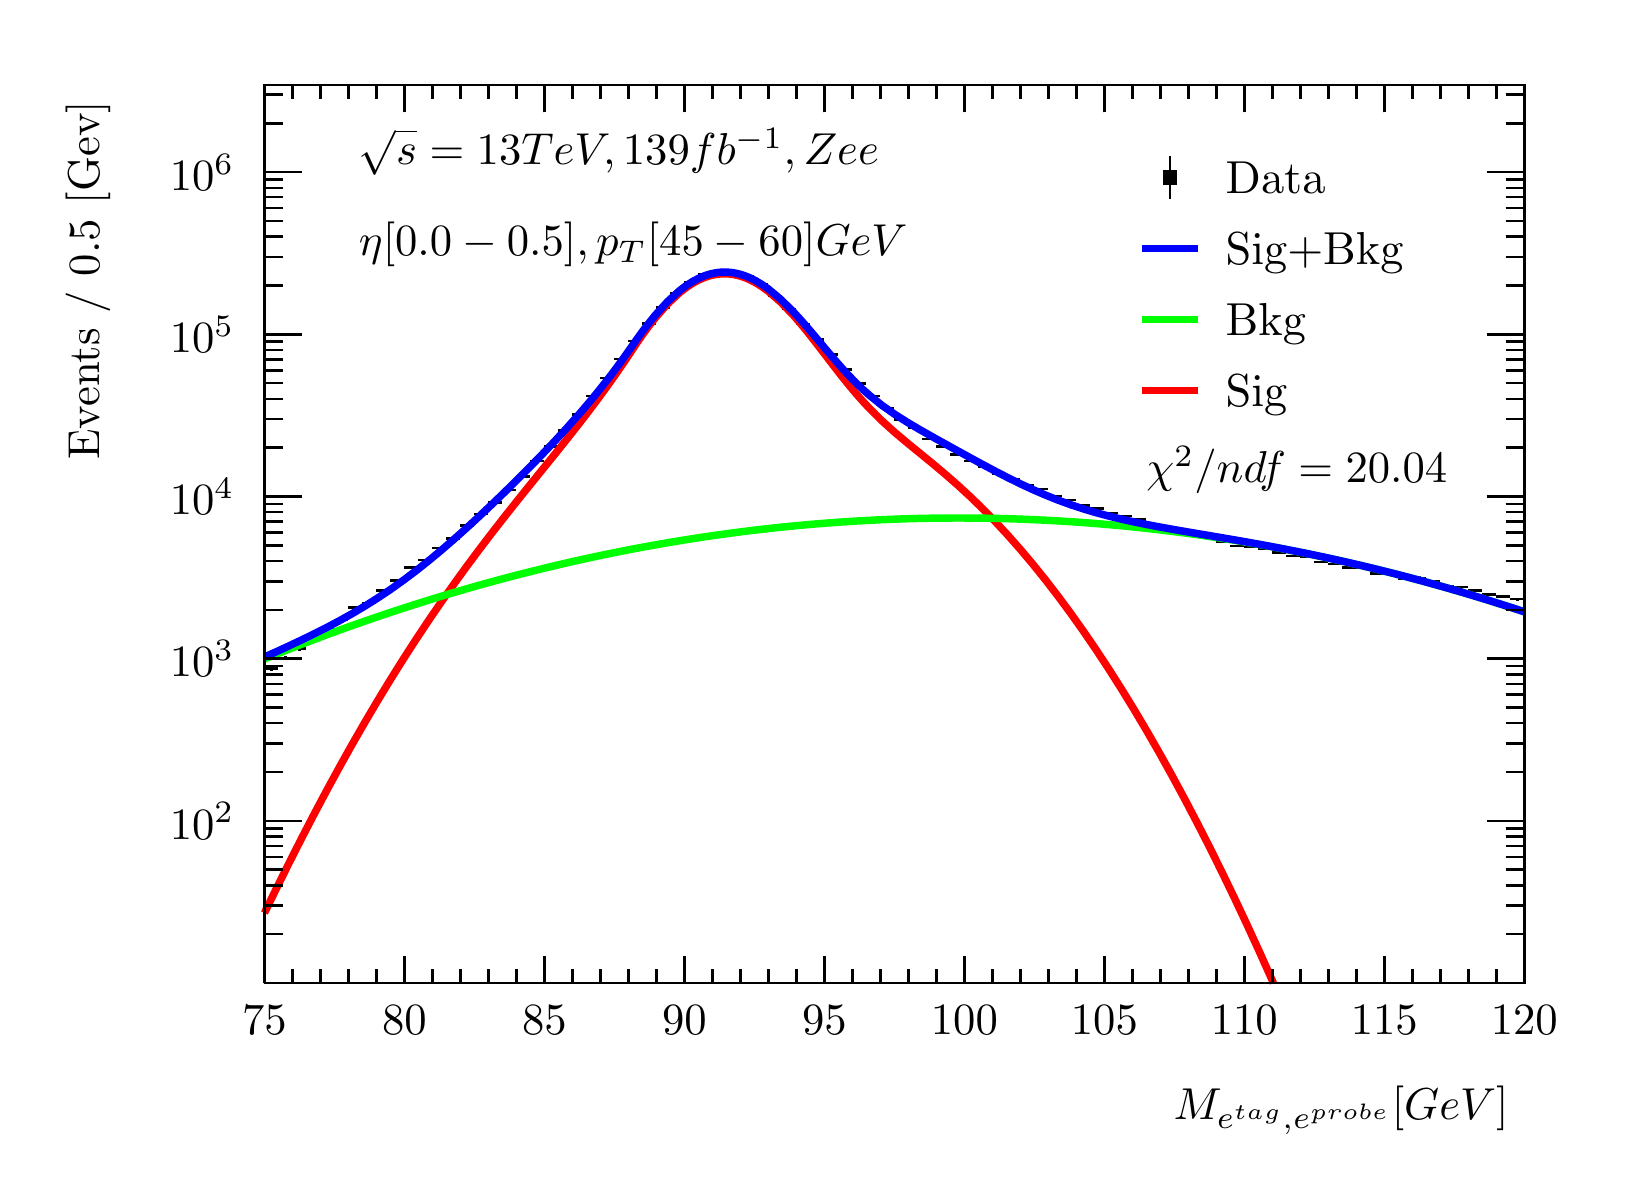
\begin{tikzpicture}
\pgfdeclareplotmark{cross} {
\pgfpathmoveto{\pgfpoint{-0.3\pgfplotmarksize}{\pgfplotmarksize}}
\pgfpathlineto{\pgfpoint{+0.3\pgfplotmarksize}{\pgfplotmarksize}}
\pgfpathlineto{\pgfpoint{+0.3\pgfplotmarksize}{0.3\pgfplotmarksize}}
\pgfpathlineto{\pgfpoint{+1\pgfplotmarksize}{0.3\pgfplotmarksize}}
\pgfpathlineto{\pgfpoint{+1\pgfplotmarksize}{-0.3\pgfplotmarksize}}
\pgfpathlineto{\pgfpoint{+0.3\pgfplotmarksize}{-0.3\pgfplotmarksize}}
\pgfpathlineto{\pgfpoint{+0.3\pgfplotmarksize}{-1.\pgfplotmarksize}}
\pgfpathlineto{\pgfpoint{-0.3\pgfplotmarksize}{-1.\pgfplotmarksize}}
\pgfpathlineto{\pgfpoint{-0.3\pgfplotmarksize}{-0.3\pgfplotmarksize}}
\pgfpathlineto{\pgfpoint{-1.\pgfplotmarksize}{-0.3\pgfplotmarksize}}
\pgfpathlineto{\pgfpoint{-1.\pgfplotmarksize}{0.3\pgfplotmarksize}}
\pgfpathlineto{\pgfpoint{-0.3\pgfplotmarksize}{0.3\pgfplotmarksize}}
\pgfpathclose
\pgfusepathqstroke
}
\pgfdeclareplotmark{cross*} {
\pgfpathmoveto{\pgfpoint{-0.3\pgfplotmarksize}{\pgfplotmarksize}}
\pgfpathlineto{\pgfpoint{+0.3\pgfplotmarksize}{\pgfplotmarksize}}
\pgfpathlineto{\pgfpoint{+0.3\pgfplotmarksize}{0.3\pgfplotmarksize}}
\pgfpathlineto{\pgfpoint{+1\pgfplotmarksize}{0.3\pgfplotmarksize}}
\pgfpathlineto{\pgfpoint{+1\pgfplotmarksize}{-0.3\pgfplotmarksize}}
\pgfpathlineto{\pgfpoint{+0.3\pgfplotmarksize}{-0.3\pgfplotmarksize}}
\pgfpathlineto{\pgfpoint{+0.3\pgfplotmarksize}{-1.\pgfplotmarksize}}
\pgfpathlineto{\pgfpoint{-0.3\pgfplotmarksize}{-1.\pgfplotmarksize}}
\pgfpathlineto{\pgfpoint{-0.3\pgfplotmarksize}{-0.3\pgfplotmarksize}}
\pgfpathlineto{\pgfpoint{-1.\pgfplotmarksize}{-0.3\pgfplotmarksize}}
\pgfpathlineto{\pgfpoint{-1.\pgfplotmarksize}{0.3\pgfplotmarksize}}
\pgfpathlineto{\pgfpoint{-0.3\pgfplotmarksize}{0.3\pgfplotmarksize}}
\pgfpathclose
\pgfusepathqfillstroke
}
\pgfdeclareplotmark{newstar} {
\pgfpathmoveto{\pgfqpoint{0pt}{\pgfplotmarksize}}
\pgfpathlineto{\pgfqpointpolar{44}{0.5\pgfplotmarksize}}
\pgfpathlineto{\pgfqpointpolar{18}{\pgfplotmarksize}}
\pgfpathlineto{\pgfqpointpolar{-20}{0.5\pgfplotmarksize}}
\pgfpathlineto{\pgfqpointpolar{-54}{\pgfplotmarksize}}
\pgfpathlineto{\pgfqpointpolar{-90}{0.5\pgfplotmarksize}}
\pgfpathlineto{\pgfqpointpolar{234}{\pgfplotmarksize}}
\pgfpathlineto{\pgfqpointpolar{198}{0.5\pgfplotmarksize}}
\pgfpathlineto{\pgfqpointpolar{162}{\pgfplotmarksize}}
\pgfpathlineto{\pgfqpointpolar{134}{0.5\pgfplotmarksize}}
\pgfpathclose
\pgfusepathqstroke
}
\pgfdeclareplotmark{newstar*} {
\pgfpathmoveto{\pgfqpoint{0pt}{\pgfplotmarksize}}
\pgfpathlineto{\pgfqpointpolar{44}{0.5\pgfplotmarksize}}
\pgfpathlineto{\pgfqpointpolar{18}{\pgfplotmarksize}}
\pgfpathlineto{\pgfqpointpolar{-20}{0.5\pgfplotmarksize}}
\pgfpathlineto{\pgfqpointpolar{-54}{\pgfplotmarksize}}
\pgfpathlineto{\pgfqpointpolar{-90}{0.5\pgfplotmarksize}}
\pgfpathlineto{\pgfqpointpolar{234}{\pgfplotmarksize}}
\pgfpathlineto{\pgfqpointpolar{198}{0.5\pgfplotmarksize}}
\pgfpathlineto{\pgfqpointpolar{162}{\pgfplotmarksize}}
\pgfpathlineto{\pgfqpointpolar{134}{0.5\pgfplotmarksize}}
\pgfpathclose
\pgfusepathqfillstroke
}
\definecolor{c}{rgb}{1,1,1};
\draw [color=c, fill=c] (0,0) rectangle (20,14.4361);
\draw [color=c, fill=c] (3,2.30977) rectangle (19,13.7143);
\definecolor{c}{rgb}{0,0,0};
\draw [c,line width=0.9] (3,2.30977) -- (3,13.7143) -- (19,13.7143) -- (19,2.30977) -- (3,2.30977);
\definecolor{c}{rgb}{1,1,1};
\draw [color=c, fill=c] (3,2.30977) rectangle (19,13.7143);
\definecolor{c}{rgb}{0,0,0};
\draw [c,line width=0.9] (3,2.30977) -- (3,13.7143) -- (19,13.7143) -- (19,2.30977) -- (3,2.30977);
\draw [c,line width=0.9] (3,2.30977) -- (19,2.30977);
\draw [c,line width=0.9] (3,2.65624) -- (3,2.30977);
\draw [c,line width=0.9] (3.35556,2.48301) -- (3.35556,2.30977);
\draw [c,line width=0.9] (3.71111,2.48301) -- (3.71111,2.30977);
\draw [c,line width=0.9] (4.06667,2.48301) -- (4.06667,2.30977);
\draw [c,line width=0.9] (4.42222,2.48301) -- (4.42222,2.30977);
\draw [c,line width=0.9] (4.77778,2.65624) -- (4.77778,2.30977);
\draw [c,line width=0.9] (5.13333,2.48301) -- (5.13333,2.30977);
\draw [c,line width=0.9] (5.48889,2.48301) -- (5.48889,2.30977);
\draw [c,line width=0.9] (5.84444,2.48301) -- (5.84444,2.30977);
\draw [c,line width=0.9] (6.2,2.48301) -- (6.2,2.30977);
\draw [c,line width=0.9] (6.55556,2.65624) -- (6.55556,2.30977);
\draw [c,line width=0.9] (6.91111,2.48301) -- (6.91111,2.30977);
\draw [c,line width=0.9] (7.26667,2.48301) -- (7.26667,2.30977);
\draw [c,line width=0.9] (7.62222,2.48301) -- (7.62222,2.30977);
\draw [c,line width=0.9] (7.97778,2.48301) -- (7.97778,2.30977);
\draw [c,line width=0.9] (8.33333,2.65624) -- (8.33333,2.30977);
\draw [c,line width=0.9] (8.68889,2.48301) -- (8.68889,2.30977);
\draw [c,line width=0.9] (9.04444,2.48301) -- (9.04444,2.30977);
\draw [c,line width=0.9] (9.4,2.48301) -- (9.4,2.30977);
\draw [c,line width=0.9] (9.75556,2.48301) -- (9.75556,2.30977);
\draw [c,line width=0.9] (10.1111,2.65624) -- (10.1111,2.30977);
\draw [c,line width=0.9] (10.4667,2.48301) -- (10.4667,2.30977);
\draw [c,line width=0.9] (10.8222,2.48301) -- (10.8222,2.30977);
\draw [c,line width=0.9] (11.1778,2.48301) -- (11.1778,2.30977);
\draw [c,line width=0.9] (11.5333,2.48301) -- (11.5333,2.30977);
\draw [c,line width=0.9] (11.8889,2.65624) -- (11.8889,2.30977);
\draw [c,line width=0.9] (12.2444,2.48301) -- (12.2444,2.30977);
\draw [c,line width=0.9] (12.6,2.48301) -- (12.6,2.30977);
\draw [c,line width=0.9] (12.9556,2.48301) -- (12.9556,2.30977);
\draw [c,line width=0.9] (13.3111,2.48301) -- (13.3111,2.30977);
\draw [c,line width=0.9] (13.6667,2.65624) -- (13.6667,2.30977);
\draw [c,line width=0.9] (14.0222,2.48301) -- (14.0222,2.30977);
\draw [c,line width=0.9] (14.3778,2.48301) -- (14.3778,2.30977);
\draw [c,line width=0.9] (14.7333,2.48301) -- (14.7333,2.30977);
\draw [c,line width=0.9] (15.0889,2.48301) -- (15.0889,2.30977);
\draw [c,line width=0.9] (15.4444,2.65624) -- (15.4444,2.30977);
\draw [c,line width=0.9] (15.8,2.48301) -- (15.8,2.30977);
\draw [c,line width=0.9] (16.1556,2.48301) -- (16.1556,2.30977);
\draw [c,line width=0.9] (16.5111,2.48301) -- (16.5111,2.30977);
\draw [c,line width=0.9] (16.8667,2.48301) -- (16.8667,2.30977);
\draw [c,line width=0.9] (17.2222,2.65624) -- (17.2222,2.30977);
\draw [c,line width=0.9] (17.5778,2.48301) -- (17.5778,2.30977);
\draw [c,line width=0.9] (17.9333,2.48301) -- (17.9333,2.30977);
\draw [c,line width=0.9] (18.2889,2.48301) -- (18.2889,2.30977);
\draw [c,line width=0.9] (18.6444,2.48301) -- (18.6444,2.30977);
\draw [c,line width=0.9] (19,2.65624) -- (19,2.30977);
\draw [c,line width=0.9] (19,2.65624) -- (19,2.30977);
\draw [anchor=base] (3,1.66015) node[scale=1.61424, color=c, rotate=0]{75};
\draw [anchor=base] (4.77778,1.66015) node[scale=1.61424, color=c, rotate=0]{80};
\draw [anchor=base] (6.55556,1.66015) node[scale=1.61424, color=c, rotate=0]{85};
\draw [anchor=base] (8.33333,1.66015) node[scale=1.61424, color=c, rotate=0]{90};
\draw [anchor=base] (10.1111,1.66015) node[scale=1.61424, color=c, rotate=0]{95};
\draw [anchor=base] (11.8889,1.66015) node[scale=1.61424, color=c, rotate=0]{100};
\draw [anchor=base] (13.6667,1.66015) node[scale=1.61424, color=c, rotate=0]{105};
\draw [anchor=base] (15.4444,1.66015) node[scale=1.61424, color=c, rotate=0]{110};
\draw [anchor=base] (17.2222,1.66015) node[scale=1.61424, color=c, rotate=0]{115};
\draw [anchor=base] (19,1.66015) node[scale=1.61424, color=c, rotate=0]{120};
\draw [anchor= east] (19,0.692932) node[scale=1.61424, color=c, rotate=0]{$M_{e^{tag}, e^{probe}}  [GeV]$};
\draw [c,line width=0.9] (3,13.7143) -- (19,13.7143);
\draw [c,line width=0.9] (3,13.3678) -- (3,13.7143);
\draw [c,line width=0.9] (3.35556,13.5411) -- (3.35556,13.7143);
\draw [c,line width=0.9] (3.71111,13.5411) -- (3.71111,13.7143);
\draw [c,line width=0.9] (4.06667,13.5411) -- (4.06667,13.7143);
\draw [c,line width=0.9] (4.42222,13.5411) -- (4.42222,13.7143);
\draw [c,line width=0.9] (4.77778,13.3678) -- (4.77778,13.7143);
\draw [c,line width=0.9] (5.13333,13.5411) -- (5.13333,13.7143);
\draw [c,line width=0.9] (5.48889,13.5411) -- (5.48889,13.7143);
\draw [c,line width=0.9] (5.84444,13.5411) -- (5.84444,13.7143);
\draw [c,line width=0.9] (6.2,13.5411) -- (6.2,13.7143);
\draw [c,line width=0.9] (6.55556,13.3678) -- (6.55556,13.7143);
\draw [c,line width=0.9] (6.91111,13.5411) -- (6.91111,13.7143);
\draw [c,line width=0.9] (7.26667,13.5411) -- (7.26667,13.7143);
\draw [c,line width=0.9] (7.62222,13.5411) -- (7.62222,13.7143);
\draw [c,line width=0.9] (7.97778,13.5411) -- (7.97778,13.7143);
\draw [c,line width=0.9] (8.33333,13.3678) -- (8.33333,13.7143);
\draw [c,line width=0.9] (8.68889,13.5411) -- (8.68889,13.7143);
\draw [c,line width=0.9] (9.04444,13.5411) -- (9.04444,13.7143);
\draw [c,line width=0.9] (9.4,13.5411) -- (9.4,13.7143);
\draw [c,line width=0.9] (9.75556,13.5411) -- (9.75556,13.7143);
\draw [c,line width=0.9] (10.1111,13.3678) -- (10.1111,13.7143);
\draw [c,line width=0.9] (10.4667,13.5411) -- (10.4667,13.7143);
\draw [c,line width=0.9] (10.8222,13.5411) -- (10.8222,13.7143);
\draw [c,line width=0.9] (11.1778,13.5411) -- (11.1778,13.7143);
\draw [c,line width=0.9] (11.5333,13.5411) -- (11.5333,13.7143);
\draw [c,line width=0.9] (11.8889,13.3678) -- (11.8889,13.7143);
\draw [c,line width=0.9] (12.2444,13.5411) -- (12.2444,13.7143);
\draw [c,line width=0.9] (12.6,13.5411) -- (12.6,13.7143);
\draw [c,line width=0.9] (12.9556,13.5411) -- (12.9556,13.7143);
\draw [c,line width=0.9] (13.3111,13.5411) -- (13.3111,13.7143);
\draw [c,line width=0.9] (13.6667,13.3678) -- (13.6667,13.7143);
\draw [c,line width=0.9] (14.0222,13.5411) -- (14.0222,13.7143);
\draw [c,line width=0.9] (14.3778,13.5411) -- (14.3778,13.7143);
\draw [c,line width=0.9] (14.7333,13.5411) -- (14.7333,13.7143);
\draw [c,line width=0.9] (15.0889,13.5411) -- (15.0889,13.7143);
\draw [c,line width=0.9] (15.4444,13.3678) -- (15.4444,13.7143);
\draw [c,line width=0.9] (15.8,13.5411) -- (15.8,13.7143);
\draw [c,line width=0.9] (16.1556,13.5411) -- (16.1556,13.7143);
\draw [c,line width=0.9] (16.5111,13.5411) -- (16.5111,13.7143);
\draw [c,line width=0.9] (16.8667,13.5411) -- (16.8667,13.7143);
\draw [c,line width=0.9] (17.2222,13.3678) -- (17.2222,13.7143);
\draw [c,line width=0.9] (17.5778,13.5411) -- (17.5778,13.7143);
\draw [c,line width=0.9] (17.9333,13.5411) -- (17.9333,13.7143);
\draw [c,line width=0.9] (18.2889,13.5411) -- (18.2889,13.7143);
\draw [c,line width=0.9] (18.6444,13.5411) -- (18.6444,13.7143);
\draw [c,line width=0.9] (19,13.3678) -- (19,13.7143);
\draw [c,line width=0.9] (19,13.3678) -- (19,13.7143);
\draw [c,line width=0.9] (3,2.30977) -- (3,13.7143);
\draw [c,line width=0.9] (3.237,2.92982) -- (3,2.92982);
\draw [c,line width=0.9] (3.237,3.29252) -- (3,3.29252);
\draw [c,line width=0.9] (3.237,3.54986) -- (3,3.54986);
\draw [c,line width=0.9] (3.237,3.74947) -- (3,3.74947);
\draw [c,line width=0.9] (3.237,3.91257) -- (3,3.91257);
\draw [c,line width=0.9] (3.237,4.05046) -- (3,4.05046);
\draw [c,line width=0.9] (3.237,4.16991) -- (3,4.16991);
\draw [c,line width=0.9] (3.237,4.27527) -- (3,4.27527);
\draw [c,line width=0.9] (3.474,4.36952) -- (3,4.36952);
\draw [anchor= east] (2.82,4.36952) node[scale=1.61424, color=c, rotate=0]{$10^{2}$};
\draw [c,line width=0.9] (3.237,4.98956) -- (3,4.98956);
\draw [c,line width=0.9] (3.237,5.35227) -- (3,5.35227);
\draw [c,line width=0.9] (3.237,5.60961) -- (3,5.60961);
\draw [c,line width=0.9] (3.237,5.80922) -- (3,5.80922);
\draw [c,line width=0.9] (3.237,5.97231) -- (3,5.97231);
\draw [c,line width=0.9] (3.237,6.11021) -- (3,6.11021);
\draw [c,line width=0.9] (3.237,6.22966) -- (3,6.22966);
\draw [c,line width=0.9] (3.237,6.33502) -- (3,6.33502);
\draw [c,line width=0.9] (3.474,6.42927) -- (3,6.42927);
\draw [anchor= east] (2.82,6.42927) node[scale=1.61424, color=c, rotate=0]{$10^{3}$};
\draw [c,line width=0.9] (3.237,7.04931) -- (3,7.04931);
\draw [c,line width=0.9] (3.237,7.41202) -- (3,7.41202);
\draw [c,line width=0.9] (3.237,7.66936) -- (3,7.66936);
\draw [c,line width=0.9] (3.237,7.86897) -- (3,7.86897);
\draw [c,line width=0.9] (3.237,8.03206) -- (3,8.03206);
\draw [c,line width=0.9] (3.237,8.16995) -- (3,8.16995);
\draw [c,line width=0.9] (3.237,8.2894) -- (3,8.2894);
\draw [c,line width=0.9] (3.237,8.39476) -- (3,8.39476);
\draw [c,line width=0.9] (3.474,8.48901) -- (3,8.48901);
\draw [anchor= east] (2.82,8.48901) node[scale=1.61424, color=c, rotate=0]{$10^{4}$};
\draw [c,line width=0.9] (3.237,9.10906) -- (3,9.10906);
\draw [c,line width=0.9] (3.237,9.47176) -- (3,9.47176);
\draw [c,line width=0.9] (3.237,9.7291) -- (3,9.7291);
\draw [c,line width=0.9] (3.237,9.92871) -- (3,9.92871);
\draw [c,line width=0.9] (3.237,10.0918) -- (3,10.0918);
\draw [c,line width=0.9] (3.237,10.2297) -- (3,10.2297);
\draw [c,line width=0.9] (3.237,10.3491) -- (3,10.3491);
\draw [c,line width=0.9] (3.237,10.4545) -- (3,10.4545);
\draw [c,line width=0.9] (3.474,10.5488) -- (3,10.5488);
\draw [anchor= east] (2.82,10.5488) node[scale=1.61424, color=c, rotate=0]{$10^{5}$};
\draw [c,line width=0.9] (3.237,11.1688) -- (3,11.1688);
\draw [c,line width=0.9] (3.237,11.5315) -- (3,11.5315);
\draw [c,line width=0.9] (3.237,11.7889) -- (3,11.7889);
\draw [c,line width=0.9] (3.237,11.9885) -- (3,11.9885);
\draw [c,line width=0.9] (3.237,12.1516) -- (3,12.1516);
\draw [c,line width=0.9] (3.237,12.2894) -- (3,12.2894);
\draw [c,line width=0.9] (3.237,12.4089) -- (3,12.4089);
\draw [c,line width=0.9] (3.237,12.5143) -- (3,12.5143);
\draw [c,line width=0.9] (3.474,12.6085) -- (3,12.6085);
\draw [anchor= east] (2.82,12.6085) node[scale=1.61424, color=c, rotate=0]{$10^{6}$};
\draw [c,line width=0.9] (3.237,13.2286) -- (3,13.2286);
\draw [c,line width=0.9] (3.237,13.5913) -- (3,13.5913);
\draw [anchor= east] (0.76,13.7143) node[scale=1.61424, color=c, rotate=90]{Events / 0.5 [Gev]};
\draw [c,line width=0.9] (19,2.30977) -- (19,13.7143);
\draw [c,line width=0.9] (18.763,2.92982) -- (19,2.92982);
\draw [c,line width=0.9] (18.763,3.29252) -- (19,3.29252);
\draw [c,line width=0.9] (18.763,3.54986) -- (19,3.54986);
\draw [c,line width=0.9] (18.763,3.74947) -- (19,3.74947);
\draw [c,line width=0.9] (18.763,3.91257) -- (19,3.91257);
\draw [c,line width=0.9] (18.763,4.05046) -- (19,4.05046);
\draw [c,line width=0.9] (18.763,4.16991) -- (19,4.16991);
\draw [c,line width=0.9] (18.763,4.27527) -- (19,4.27527);
\draw [c,line width=0.9] (18.526,4.36952) -- (19,4.36952);
\draw [c,line width=0.9] (18.763,4.98956) -- (19,4.98956);
\draw [c,line width=0.9] (18.763,5.35227) -- (19,5.35227);
\draw [c,line width=0.9] (18.763,5.60961) -- (19,5.60961);
\draw [c,line width=0.9] (18.763,5.80922) -- (19,5.80922);
\draw [c,line width=0.9] (18.763,5.97231) -- (19,5.97231);
\draw [c,line width=0.9] (18.763,6.11021) -- (19,6.11021);
\draw [c,line width=0.9] (18.763,6.22966) -- (19,6.22966);
\draw [c,line width=0.9] (18.763,6.33502) -- (19,6.33502);
\draw [c,line width=0.9] (18.526,6.42927) -- (19,6.42927);
\draw [c,line width=0.9] (18.763,7.04931) -- (19,7.04931);
\draw [c,line width=0.9] (18.763,7.41202) -- (19,7.41202);
\draw [c,line width=0.9] (18.763,7.66936) -- (19,7.66936);
\draw [c,line width=0.9] (18.763,7.86897) -- (19,7.86897);
\draw [c,line width=0.9] (18.763,8.03206) -- (19,8.03206);
\draw [c,line width=0.9] (18.763,8.16995) -- (19,8.16995);
\draw [c,line width=0.9] (18.763,8.2894) -- (19,8.2894);
\draw [c,line width=0.9] (18.763,8.39476) -- (19,8.39476);
\draw [c,line width=0.9] (18.526,8.48901) -- (19,8.48901);
\draw [c,line width=0.9] (18.763,9.10906) -- (19,9.10906);
\draw [c,line width=0.9] (18.763,9.47176) -- (19,9.47176);
\draw [c,line width=0.9] (18.763,9.7291) -- (19,9.7291);
\draw [c,line width=0.9] (18.763,9.92871) -- (19,9.92871);
\draw [c,line width=0.9] (18.763,10.0918) -- (19,10.0918);
\draw [c,line width=0.9] (18.763,10.2297) -- (19,10.2297);
\draw [c,line width=0.9] (18.763,10.3491) -- (19,10.3491);
\draw [c,line width=0.9] (18.763,10.4545) -- (19,10.4545);
\draw [c,line width=0.9] (18.526,10.5488) -- (19,10.5488);
\draw [c,line width=0.9] (18.763,11.1688) -- (19,11.1688);
\draw [c,line width=0.9] (18.763,11.5315) -- (19,11.5315);
\draw [c,line width=0.9] (18.763,11.7889) -- (19,11.7889);
\draw [c,line width=0.9] (18.763,11.9885) -- (19,11.9885);
\draw [c,line width=0.9] (18.763,12.1516) -- (19,12.1516);
\draw [c,line width=0.9] (18.763,12.2894) -- (19,12.2894);
\draw [c,line width=0.9] (18.763,12.4089) -- (19,12.4089);
\draw [c,line width=0.9] (18.763,12.5143) -- (19,12.5143);
\draw [c,line width=0.9] (18.526,12.6085) -- (19,12.6085);
\draw [c,line width=0.9] (18.763,13.2286) -- (19,13.2286);
\draw [c,line width=0.9] (18.763,13.5913) -- (19,13.5913);
\draw [c,line width=0.9] (3.08889,6.30572) -- (3,6.30572);
\draw [c,line width=0.9] (3,6.30572) -- (3,6.30572);
\draw [c,line width=0.9] (3.08889,6.30572) -- (3.17778,6.30572);
\draw [c,line width=0.9] (3.17778,6.30572) -- (3.17778,6.30572);
\draw [c,line width=0.9] (3.08889,6.30572) -- (3.08889,6.33603);
\draw [c,line width=0.9] (3.08889,6.33603) -- (3.08889,6.33603);
\draw [c,line width=0.9] (3.08889,6.30572) -- (3.08889,6.27541);
\draw [c,line width=0.9] (3.08889,6.27541) -- (3.08889,6.27541);
\draw [c,line width=0.9] (3.26667,6.43994) -- (3.17778,6.43994);
\draw [c,line width=0.9] (3.17778,6.43994) -- (3.17778,6.43994);
\draw [c,line width=0.9] (3.26667,6.43994) -- (3.35556,6.43994);
\draw [c,line width=0.9] (3.35556,6.43994) -- (3.35556,6.43994);
\draw [c,line width=0.9] (3.26667,6.43994) -- (3.26667,6.46806);
\draw [c,line width=0.9] (3.26667,6.46806) -- (3.26667,6.46806);
\draw [c,line width=0.9] (3.26667,6.43994) -- (3.26667,6.41182);
\draw [c,line width=0.9] (3.26667,6.41182) -- (3.26667,6.41182);
\draw [c,line width=0.9] (3.44444,6.55584) -- (3.35556,6.55584);
\draw [c,line width=0.9] (3.35556,6.55584) -- (3.35556,6.55584);
\draw [c,line width=0.9] (3.44444,6.55584) -- (3.53333,6.55584);
\draw [c,line width=0.9] (3.53333,6.55584) -- (3.53333,6.55584);
\draw [c,line width=0.9] (3.44444,6.55584) -- (3.44444,6.5822);
\draw [c,line width=0.9] (3.44444,6.5822) -- (3.44444,6.5822);
\draw [c,line width=0.9] (3.44444,6.55584) -- (3.44444,6.52949);
\draw [c,line width=0.9] (3.44444,6.52949) -- (3.44444,6.52949);
\draw [c,line width=0.9] (3.62222,6.70301) -- (3.53333,6.70301);
\draw [c,line width=0.9] (3.53333,6.70301) -- (3.53333,6.70301);
\draw [c,line width=0.9] (3.62222,6.70301) -- (3.71111,6.70301);
\draw [c,line width=0.9] (3.71111,6.70301) -- (3.71111,6.70301);
\draw [c,line width=0.9] (3.62222,6.70301) -- (3.62222,6.72728);
\draw [c,line width=0.9] (3.62222,6.72728) -- (3.62222,6.72728);
\draw [c,line width=0.9] (3.62222,6.70301) -- (3.62222,6.67873);
\draw [c,line width=0.9] (3.62222,6.67873) -- (3.62222,6.67873);
\draw [c,line width=0.9] (3.8,6.80852) -- (3.71111,6.80852);
\draw [c,line width=0.9] (3.71111,6.80852) -- (3.71111,6.80852);
\draw [c,line width=0.9] (3.8,6.80852) -- (3.88889,6.80852);
\draw [c,line width=0.9] (3.88889,6.80852) -- (3.88889,6.80852);
\draw [c,line width=0.9] (3.8,6.80852) -- (3.8,6.8314);
\draw [c,line width=0.9] (3.8,6.8314) -- (3.8,6.8314);
\draw [c,line width=0.9] (3.8,6.80852) -- (3.8,6.78563);
\draw [c,line width=0.9] (3.8,6.78563) -- (3.8,6.78563);
\draw [c,line width=0.9] (3.97778,6.91855) -- (3.88889,6.91855);
\draw [c,line width=0.9] (3.88889,6.91855) -- (3.88889,6.91855);
\draw [c,line width=0.9] (3.97778,6.91855) -- (4.06667,6.91855);
\draw [c,line width=0.9] (4.06667,6.91855) -- (4.06667,6.91855);
\draw [c,line width=0.9] (3.97778,6.91855) -- (3.97778,6.94007);
\draw [c,line width=0.9] (3.97778,6.94007) -- (3.97778,6.94007);
\draw [c,line width=0.9] (3.97778,6.91855) -- (3.97778,6.89703);
\draw [c,line width=0.9] (3.97778,6.89703) -- (3.97778,6.89703);
\draw [c,line width=0.9] (4.15556,7.08052) -- (4.06667,7.08052);
\draw [c,line width=0.9] (4.06667,7.08052) -- (4.06667,7.08052);
\draw [c,line width=0.9] (4.15556,7.08052) -- (4.24444,7.08052);
\draw [c,line width=0.9] (4.24444,7.08052) -- (4.24444,7.08052);
\draw [c,line width=0.9] (4.15556,7.08052) -- (4.15556,7.10017);
\draw [c,line width=0.9] (4.15556,7.10017) -- (4.15556,7.10017);
\draw [c,line width=0.9] (4.15556,7.08052) -- (4.15556,7.06086);
\draw [c,line width=0.9] (4.15556,7.06086) -- (4.15556,7.06086);
\draw [c,line width=0.9] (4.33333,7.13863) -- (4.24444,7.13863);
\draw [c,line width=0.9] (4.24444,7.13863) -- (4.24444,7.13863);
\draw [c,line width=0.9] (4.33333,7.13863) -- (4.42222,7.13863);
\draw [c,line width=0.9] (4.42222,7.13863) -- (4.42222,7.13863);
\draw [c,line width=0.9] (4.33333,7.13863) -- (4.33333,7.15766);
\draw [c,line width=0.9] (4.33333,7.15766) -- (4.33333,7.15766);
\draw [c,line width=0.9] (4.33333,7.13863) -- (4.33333,7.1196);
\draw [c,line width=0.9] (4.33333,7.1196) -- (4.33333,7.1196);
\draw [c,line width=0.9] (4.51111,7.29393) -- (4.42222,7.29393);
\draw [c,line width=0.9] (4.42222,7.29393) -- (4.42222,7.29393);
\draw [c,line width=0.9] (4.51111,7.29393) -- (4.6,7.29393);
\draw [c,line width=0.9] (4.6,7.29393) -- (4.6,7.29393);
\draw [c,line width=0.9] (4.51111,7.29393) -- (4.51111,7.31138);
\draw [c,line width=0.9] (4.51111,7.31138) -- (4.51111,7.31138);
\draw [c,line width=0.9] (4.51111,7.29393) -- (4.51111,7.27648);
\draw [c,line width=0.9] (4.51111,7.27648) -- (4.51111,7.27648);
\draw [c,line width=0.9] (4.68889,7.42239) -- (4.6,7.42239);
\draw [c,line width=0.9] (4.6,7.42239) -- (4.6,7.42239);
\draw [c,line width=0.9] (4.68889,7.42239) -- (4.77778,7.42239);
\draw [c,line width=0.9] (4.77778,7.42239) -- (4.77778,7.42239);
\draw [c,line width=0.9] (4.68889,7.42239) -- (4.68889,7.43863);
\draw [c,line width=0.9] (4.68889,7.43863) -- (4.68889,7.43863);
\draw [c,line width=0.9] (4.68889,7.42239) -- (4.68889,7.40616);
\draw [c,line width=0.9] (4.68889,7.40616) -- (4.68889,7.40616);
\draw [c,line width=0.9] (4.86667,7.58647) -- (4.77778,7.58647);
\draw [c,line width=0.9] (4.77778,7.58647) -- (4.77778,7.58647);
\draw [c,line width=0.9] (4.86667,7.58647) -- (4.95556,7.58647);
\draw [c,line width=0.9] (4.95556,7.58647) -- (4.95556,7.58647);
\draw [c,line width=0.9] (4.86667,7.58647) -- (4.86667,7.60128);
\draw [c,line width=0.9] (4.86667,7.60128) -- (4.86667,7.60128);
\draw [c,line width=0.9] (4.86667,7.58647) -- (4.86667,7.57165);
\draw [c,line width=0.9] (4.86667,7.57165) -- (4.86667,7.57165);
\draw [c,line width=0.9] (5.04444,7.68466) -- (4.95556,7.68466);
\draw [c,line width=0.9] (4.95556,7.68466) -- (4.95556,7.68466);
\draw [c,line width=0.9] (5.04444,7.68466) -- (5.13333,7.68466);
\draw [c,line width=0.9] (5.13333,7.68466) -- (5.13333,7.68466);
\draw [c,line width=0.9] (5.04444,7.68466) -- (5.04444,7.69868);
\draw [c,line width=0.9] (5.04444,7.69868) -- (5.04444,7.69868);
\draw [c,line width=0.9] (5.04444,7.68466) -- (5.04444,7.67063);
\draw [c,line width=0.9] (5.04444,7.67063) -- (5.04444,7.67063);
\draw [c,line width=0.9] (5.22222,7.83413) -- (5.13333,7.83413);
\draw [c,line width=0.9] (5.13333,7.83413) -- (5.13333,7.83413);
\draw [c,line width=0.9] (5.22222,7.83413) -- (5.31111,7.83413);
\draw [c,line width=0.9] (5.31111,7.83413) -- (5.31111,7.83413);
\draw [c,line width=0.9] (5.22222,7.83413) -- (5.22222,7.84703);
\draw [c,line width=0.9] (5.22222,7.84703) -- (5.22222,7.84703);
\draw [c,line width=0.9] (5.22222,7.83413) -- (5.22222,7.82123);
\draw [c,line width=0.9] (5.22222,7.82123) -- (5.22222,7.82123);
\draw [c,line width=0.9] (5.4,7.95861) -- (5.31111,7.95861);
\draw [c,line width=0.9] (5.31111,7.95861) -- (5.31111,7.95861);
\draw [c,line width=0.9] (5.4,7.95861) -- (5.48889,7.95861);
\draw [c,line width=0.9] (5.48889,7.95861) -- (5.48889,7.95861);
\draw [c,line width=0.9] (5.4,7.95861) -- (5.4,7.97064);
\draw [c,line width=0.9] (5.4,7.97064) -- (5.4,7.97064);
\draw [c,line width=0.9] (5.4,7.95861) -- (5.4,7.94658);
\draw [c,line width=0.9] (5.4,7.94658) -- (5.4,7.94658);
\draw [c,line width=0.9] (5.57778,8.118) -- (5.48889,8.118);
\draw [c,line width=0.9] (5.48889,8.118) -- (5.48889,8.118);
\draw [c,line width=0.9] (5.57778,8.118) -- (5.66667,8.118);
\draw [c,line width=0.9] (5.66667,8.118) -- (5.66667,8.118);
\draw [c,line width=0.9] (5.57778,8.118) -- (5.57778,8.129);
\draw [c,line width=0.9] (5.57778,8.129) -- (5.57778,8.129);
\draw [c,line width=0.9] (5.57778,8.118) -- (5.57778,8.10699);
\draw [c,line width=0.9] (5.57778,8.10699) -- (5.57778,8.10699);
\draw [c,line width=0.9] (5.75556,8.26354) -- (5.66667,8.26354);
\draw [c,line width=0.9] (5.66667,8.26354) -- (5.66667,8.26354);
\draw [c,line width=0.9] (5.75556,8.26354) -- (5.84444,8.26354);
\draw [c,line width=0.9] (5.84444,8.26354) -- (5.84444,8.26354);
\draw [c,line width=0.9] (5.75556,8.26354) -- (5.75556,8.27369);
\draw [c,line width=0.9] (5.75556,8.27369) -- (5.75556,8.27369);
\draw [c,line width=0.9] (5.75556,8.26354) -- (5.75556,8.25339);
\draw [c,line width=0.9] (5.75556,8.25339) -- (5.75556,8.25339);
\draw [c,line width=0.9] (5.93333,8.41189) -- (5.84444,8.41189);
\draw [c,line width=0.9] (5.84444,8.41189) -- (5.84444,8.41189);
\draw [c,line width=0.9] (5.93333,8.41189) -- (6.02222,8.41189);
\draw [c,line width=0.9] (6.02222,8.41189) -- (6.02222,8.41189);
\draw [c,line width=0.9] (5.93333,8.41189) -- (5.93333,8.42123);
\draw [c,line width=0.9] (5.93333,8.42123) -- (5.93333,8.42123);
\draw [c,line width=0.9] (5.93333,8.41189) -- (5.93333,8.40256);
\draw [c,line width=0.9] (5.93333,8.40256) -- (5.93333,8.40256);
\draw [c,line width=0.9] (6.11111,8.5702) -- (6.02222,8.5702);
\draw [c,line width=0.9] (6.02222,8.5702) -- (6.02222,8.5702);
\draw [c,line width=0.9] (6.11111,8.5702) -- (6.2,8.5702);
\draw [c,line width=0.9] (6.2,8.5702) -- (6.2,8.5702);
\draw [c,line width=0.9] (6.11111,8.5702) -- (6.11111,8.57875);
\draw [c,line width=0.9] (6.11111,8.57875) -- (6.11111,8.57875);
\draw [c,line width=0.9] (6.11111,8.5702) -- (6.11111,8.56165);
\draw [c,line width=0.9] (6.11111,8.56165) -- (6.11111,8.56165);
\draw [c,line width=0.9] (6.28889,8.74338) -- (6.2,8.74338);
\draw [c,line width=0.9] (6.2,8.74338) -- (6.2,8.74338);
\draw [c,line width=0.9] (6.28889,8.74338) -- (6.37778,8.74338);
\draw [c,line width=0.9] (6.37778,8.74338) -- (6.37778,8.74338);
\draw [c,line width=0.9] (6.28889,8.74338) -- (6.28889,8.75114);
\draw [c,line width=0.9] (6.28889,8.75114) -- (6.28889,8.75114);
\draw [c,line width=0.9] (6.28889,8.74338) -- (6.28889,8.73562);
\draw [c,line width=0.9] (6.28889,8.73562) -- (6.28889,8.73562);
\draw [c,line width=0.9] (6.46667,8.93957) -- (6.37778,8.93957);
\draw [c,line width=0.9] (6.37778,8.93957) -- (6.37778,8.93957);
\draw [c,line width=0.9] (6.46667,8.93957) -- (6.55556,8.93957);
\draw [c,line width=0.9] (6.55556,8.93957) -- (6.55556,8.93957);
\draw [c,line width=0.9] (6.46667,8.93957) -- (6.46667,8.94653);
\draw [c,line width=0.9] (6.46667,8.94653) -- (6.46667,8.94653);
\draw [c,line width=0.9] (6.46667,8.93957) -- (6.46667,8.93262);
\draw [c,line width=0.9] (6.46667,8.93262) -- (6.46667,8.93262);
\draw [c,line width=0.9] (6.64444,9.12594) -- (6.55556,9.12594);
\draw [c,line width=0.9] (6.55556,9.12594) -- (6.55556,9.12594);
\draw [c,line width=0.9] (6.64444,9.12594) -- (6.73333,9.12594);
\draw [c,line width=0.9] (6.73333,9.12594) -- (6.73333,9.12594);
\draw [c,line width=0.9] (6.64444,9.12594) -- (6.64444,9.13221);
\draw [c,line width=0.9] (6.64444,9.13221) -- (6.64444,9.13221);
\draw [c,line width=0.9] (6.64444,9.12594) -- (6.64444,9.11967);
\draw [c,line width=0.9] (6.64444,9.11967) -- (6.64444,9.11967);
\draw [c,line width=0.9] (6.82222,9.32751) -- (6.73333,9.32751);
\draw [c,line width=0.9] (6.73333,9.32751) -- (6.73333,9.32751);
\draw [c,line width=0.9] (6.82222,9.32751) -- (6.91111,9.32751);
\draw [c,line width=0.9] (6.91111,9.32751) -- (6.91111,9.32751);
\draw [c,line width=0.9] (6.82222,9.32751) -- (6.82222,9.3331);
\draw [c,line width=0.9] (6.82222,9.3331) -- (6.82222,9.3331);
\draw [c,line width=0.9] (6.82222,9.32751) -- (6.82222,9.32191);
\draw [c,line width=0.9] (6.82222,9.32191) -- (6.82222,9.32191);
\draw [c,line width=0.9] (7,9.53) -- (6.91111,9.53);
\draw [c,line width=0.9] (6.91111,9.53) -- (6.91111,9.53);
\draw [c,line width=0.9] (7,9.53) -- (7.08889,9.53);
\draw [c,line width=0.9] (7.08889,9.53) -- (7.08889,9.53);
\draw [c,line width=0.9] (7,9.53) -- (7,9.535);
\draw [c,line width=0.9] (7,9.535) -- (7,9.535);
\draw [c,line width=0.9] (7,9.53) -- (7,9.525);
\draw [c,line width=0.9] (7,9.525) -- (7,9.525);
\draw [c,line width=0.9] (7.17778,9.76837) -- (7.08889,9.76837);
\draw [c,line width=0.9] (7.08889,9.76837) -- (7.08889,9.76837);
\draw [c,line width=0.9] (7.17778,9.76837) -- (7.26667,9.76837);
\draw [c,line width=0.9] (7.26667,9.76837) -- (7.26667,9.76837);
\draw [c,line width=0.9] (7.17778,9.76837) -- (7.17778,9.77275);
\draw [c,line width=0.9] (7.17778,9.77275) -- (7.17778,9.77275);
\draw [c,line width=0.9] (7.17778,9.76837) -- (7.17778,9.764);
\draw [c,line width=0.9] (7.17778,9.764) -- (7.17778,9.764);
\draw [c,line width=0.9] (7.35556,9.99199) -- (7.26667,9.99199);
\draw [c,line width=0.9] (7.26667,9.99199) -- (7.26667,9.99199);
\draw [c,line width=0.9] (7.35556,9.99199) -- (7.44444,9.99199);
\draw [c,line width=0.9] (7.44444,9.99199) -- (7.44444,9.99199);
\draw [c,line width=0.9] (7.35556,9.99199) -- (7.35556,9.99585);
\draw [c,line width=0.9] (7.35556,9.99585) -- (7.35556,9.99585);
\draw [c,line width=0.9] (7.35556,9.99199) -- (7.35556,9.98813);
\draw [c,line width=0.9] (7.35556,9.98813) -- (7.35556,9.98813);
\draw [c,line width=0.9] (7.53333,10.2354) -- (7.44444,10.2354);
\draw [c,line width=0.9] (7.44444,10.2354) -- (7.44444,10.2354);
\draw [c,line width=0.9] (7.53333,10.2354) -- (7.62222,10.2354);
\draw [c,line width=0.9] (7.62222,10.2354) -- (7.62222,10.2354);
\draw [c,line width=0.9] (7.53333,10.2354) -- (7.53333,10.2387);
\draw [c,line width=0.9] (7.53333,10.2387) -- (7.53333,10.2387);
\draw [c,line width=0.9] (7.53333,10.2354) -- (7.53333,10.232);
\draw [c,line width=0.9] (7.53333,10.232) -- (7.53333,10.232);
\draw [c,line width=0.9] (7.71111,10.4629) -- (7.62222,10.4629);
\draw [c,line width=0.9] (7.62222,10.4629) -- (7.62222,10.4629);
\draw [c,line width=0.9] (7.71111,10.4629) -- (7.8,10.4629);
\draw [c,line width=0.9] (7.8,10.4629) -- (7.8,10.4629);
\draw [c,line width=0.9] (7.71111,10.4629) -- (7.71111,10.4658);
\draw [c,line width=0.9] (7.71111,10.4658) -- (7.71111,10.4658);
\draw [c,line width=0.9] (7.71111,10.4629) -- (7.71111,10.4599);
\draw [c,line width=0.9] (7.71111,10.4599) -- (7.71111,10.4599);
\draw [c,line width=0.9] (7.88889,10.6841) -- (7.8,10.6841);
\draw [c,line width=0.9] (7.8,10.6841) -- (7.8,10.6841);
\draw [c,line width=0.9] (7.88889,10.6841) -- (7.97778,10.6841);
\draw [c,line width=0.9] (7.97778,10.6841) -- (7.97778,10.6841);
\draw [c,line width=0.9] (7.88889,10.6841) -- (7.88889,10.6867);
\draw [c,line width=0.9] (7.88889,10.6867) -- (7.88889,10.6867);
\draw [c,line width=0.9] (7.88889,10.6841) -- (7.88889,10.6815);
\draw [c,line width=0.9] (7.88889,10.6815) -- (7.88889,10.6815);
\draw [c,line width=0.9] (8.06667,10.8887) -- (7.97778,10.8887);
\draw [c,line width=0.9] (7.97778,10.8887) -- (7.97778,10.8887);
\draw [c,line width=0.9] (8.06667,10.8887) -- (8.15556,10.8887);
\draw [c,line width=0.9] (8.15556,10.8887) -- (8.15556,10.8887);
\draw [c,line width=0.9] (8.06667,10.8887) -- (8.06667,10.891);
\draw [c,line width=0.9] (8.06667,10.891) -- (8.06667,10.891);
\draw [c,line width=0.9] (8.06667,10.8887) -- (8.06667,10.8863);
\draw [c,line width=0.9] (8.06667,10.8863) -- (8.06667,10.8863);
\draw [c,line width=0.9] (8.24444,11.0725) -- (8.15556,11.0725);
\draw [c,line width=0.9] (8.15556,11.0725) -- (8.15556,11.0725);
\draw [c,line width=0.9] (8.24444,11.0725) -- (8.33333,11.0725);
\draw [c,line width=0.9] (8.33333,11.0725) -- (8.33333,11.0725);
\draw [c,line width=0.9] (8.24444,11.0725) -- (8.24444,11.0746);
\draw [c,line width=0.9] (8.24444,11.0746) -- (8.24444,11.0746);
\draw [c,line width=0.9] (8.24444,11.0725) -- (8.24444,11.0704);
\draw [c,line width=0.9] (8.24444,11.0704) -- (8.24444,11.0704);
\draw [c,line width=0.9] (8.42222,11.2095) -- (8.33333,11.2095);
\draw [c,line width=0.9] (8.33333,11.2095) -- (8.33333,11.2095);
\draw [c,line width=0.9] (8.42222,11.2095) -- (8.51111,11.2095);
\draw [c,line width=0.9] (8.51111,11.2095) -- (8.51111,11.2095);
\draw [c,line width=0.9] (8.42222,11.2095) -- (8.42222,11.2115);
\draw [c,line width=0.9] (8.42222,11.2115) -- (8.42222,11.2115);
\draw [c,line width=0.9] (8.42222,11.2095) -- (8.42222,11.2076);
\draw [c,line width=0.9] (8.42222,11.2076) -- (8.42222,11.2076);
\draw [c,line width=0.9] (8.6,11.3058) -- (8.51111,11.3058);
\draw [c,line width=0.9] (8.51111,11.3058) -- (8.51111,11.3058);
\draw [c,line width=0.9] (8.6,11.3058) -- (8.68889,11.3058);
\draw [c,line width=0.9] (8.68889,11.3058) -- (8.68889,11.3058);
\draw [c,line width=0.9] (8.6,11.3058) -- (8.6,11.3076);
\draw [c,line width=0.9] (8.6,11.3076) -- (8.6,11.3076);
\draw [c,line width=0.9] (8.6,11.3058) -- (8.6,11.3039);
\draw [c,line width=0.9] (8.6,11.3039) -- (8.6,11.3039);
\draw [c,line width=0.9] (8.77778,11.3499) -- (8.68889,11.3499);
\draw [c,line width=0.9] (8.68889,11.3499) -- (8.68889,11.3499);
\draw [c,line width=0.9] (8.77778,11.3499) -- (8.86667,11.3499);
\draw [c,line width=0.9] (8.86667,11.3499) -- (8.86667,11.3499);
\draw [c,line width=0.9] (8.77778,11.3499) -- (8.77778,11.3517);
\draw [c,line width=0.9] (8.77778,11.3517) -- (8.77778,11.3517);
\draw [c,line width=0.9] (8.77778,11.3499) -- (8.77778,11.348);
\draw [c,line width=0.9] (8.77778,11.348) -- (8.77778,11.348);
\draw [c,line width=0.9] (8.95556,11.3424) -- (8.86667,11.3424);
\draw [c,line width=0.9] (8.86667,11.3424) -- (8.86667,11.3424);
\draw [c,line width=0.9] (8.95556,11.3424) -- (9.04444,11.3424);
\draw [c,line width=0.9] (9.04444,11.3424) -- (9.04444,11.3424);
\draw [c,line width=0.9] (8.95556,11.3424) -- (8.95556,11.3442);
\draw [c,line width=0.9] (8.95556,11.3442) -- (8.95556,11.3442);
\draw [c,line width=0.9] (8.95556,11.3424) -- (8.95556,11.3406);
\draw [c,line width=0.9] (8.95556,11.3406) -- (8.95556,11.3406);
\draw [c,line width=0.9] (9.13333,11.2839) -- (9.04444,11.2839);
\draw [c,line width=0.9] (9.04444,11.2839) -- (9.04444,11.2839);
\draw [c,line width=0.9] (9.13333,11.2839) -- (9.22222,11.2839);
\draw [c,line width=0.9] (9.22222,11.2839) -- (9.22222,11.2839);
\draw [c,line width=0.9] (9.13333,11.2839) -- (9.13333,11.2858);
\draw [c,line width=0.9] (9.13333,11.2858) -- (9.13333,11.2858);
\draw [c,line width=0.9] (9.13333,11.2839) -- (9.13333,11.2821);
\draw [c,line width=0.9] (9.13333,11.2821) -- (9.13333,11.2821);
\draw [c,line width=0.9] (9.31111,11.1805) -- (9.22222,11.1805);
\draw [c,line width=0.9] (9.22222,11.1805) -- (9.22222,11.1805);
\draw [c,line width=0.9] (9.31111,11.1805) -- (9.4,11.1805);
\draw [c,line width=0.9] (9.4,11.1805) -- (9.4,11.1805);
\draw [c,line width=0.9] (9.31111,11.1805) -- (9.31111,11.1825);
\draw [c,line width=0.9] (9.31111,11.1825) -- (9.31111,11.1825);
\draw [c,line width=0.9] (9.31111,11.1805) -- (9.31111,11.1785);
\draw [c,line width=0.9] (9.31111,11.1785) -- (9.31111,11.1785);
\draw [c,line width=0.9] (9.48889,11.0348) -- (9.4,11.0348);
\draw [c,line width=0.9] (9.4,11.0348) -- (9.4,11.0348);
\draw [c,line width=0.9] (9.48889,11.0348) -- (9.57778,11.0348);
\draw [c,line width=0.9] (9.57778,11.0348) -- (9.57778,11.0348);
\draw [c,line width=0.9] (9.48889,11.0348) -- (9.48889,11.037);
\draw [c,line width=0.9] (9.48889,11.037) -- (9.48889,11.037);
\draw [c,line width=0.9] (9.48889,11.0348) -- (9.48889,11.0326);
\draw [c,line width=0.9] (9.48889,11.0326) -- (9.48889,11.0326);
\draw [c,line width=0.9] (9.66667,10.8686) -- (9.57778,10.8686);
\draw [c,line width=0.9] (9.57778,10.8686) -- (9.57778,10.8686);
\draw [c,line width=0.9] (9.66667,10.8686) -- (9.75556,10.8686);
\draw [c,line width=0.9] (9.75556,10.8686) -- (9.75556,10.8686);
\draw [c,line width=0.9] (9.66667,10.8686) -- (9.66667,10.8709);
\draw [c,line width=0.9] (9.66667,10.8709) -- (9.66667,10.8709);
\draw [c,line width=0.9] (9.66667,10.8686) -- (9.66667,10.8662);
\draw [c,line width=0.9] (9.66667,10.8662) -- (9.66667,10.8662);
\draw [c,line width=0.9] (9.84444,10.6793) -- (9.75556,10.6793);
\draw [c,line width=0.9] (9.75556,10.6793) -- (9.75556,10.6793);
\draw [c,line width=0.9] (9.84444,10.6793) -- (9.93333,10.6793);
\draw [c,line width=0.9] (9.93333,10.6793) -- (9.93333,10.6793);
\draw [c,line width=0.9] (9.84444,10.6793) -- (9.84444,10.6819);
\draw [c,line width=0.9] (9.84444,10.6819) -- (9.84444,10.6819);
\draw [c,line width=0.9] (9.84444,10.6793) -- (9.84444,10.6766);
\draw [c,line width=0.9] (9.84444,10.6766) -- (9.84444,10.6766);
\draw [c,line width=0.9] (10.0222,10.4843) -- (9.93333,10.4843);
\draw [c,line width=0.9] (9.93333,10.4843) -- (9.93333,10.4843);
\draw [c,line width=0.9] (10.0222,10.4843) -- (10.1111,10.4843);
\draw [c,line width=0.9] (10.1111,10.4843) -- (10.1111,10.4843);
\draw [c,line width=0.9] (10.0222,10.4843) -- (10.0222,10.4872);
\draw [c,line width=0.9] (10.0222,10.4872) -- (10.0222,10.4872);
\draw [c,line width=0.9] (10.0222,10.4843) -- (10.0222,10.4814);
\draw [c,line width=0.9] (10.0222,10.4814) -- (10.0222,10.4814);
\draw [c,line width=0.9] (10.2,10.2927) -- (10.1111,10.2927);
\draw [c,line width=0.9] (10.1111,10.2927) -- (10.1111,10.2927);
\draw [c,line width=0.9] (10.2,10.2927) -- (10.2889,10.2927);
\draw [c,line width=0.9] (10.2889,10.2927) -- (10.2889,10.2927);
\draw [c,line width=0.9] (10.2,10.2927) -- (10.2,10.296);
\draw [c,line width=0.9] (10.2,10.296) -- (10.2,10.296);
\draw [c,line width=0.9] (10.2,10.2927) -- (10.2,10.2895);
\draw [c,line width=0.9] (10.2,10.2895) -- (10.2,10.2895);
\draw [c,line width=0.9] (10.3778,10.1023) -- (10.2889,10.1023);
\draw [c,line width=0.9] (10.2889,10.1023) -- (10.2889,10.1023);
\draw [c,line width=0.9] (10.3778,10.1023) -- (10.4667,10.1023);
\draw [c,line width=0.9] (10.4667,10.1023) -- (10.4667,10.1023);
\draw [c,line width=0.9] (10.3778,10.1023) -- (10.3778,10.1059);
\draw [c,line width=0.9] (10.3778,10.1059) -- (10.3778,10.1059);
\draw [c,line width=0.9] (10.3778,10.1023) -- (10.3778,10.0987);
\draw [c,line width=0.9] (10.3778,10.0987) -- (10.3778,10.0987);
\draw [c,line width=0.9] (10.5556,9.92126) -- (10.4667,9.92126);
\draw [c,line width=0.9] (10.4667,9.92126) -- (10.4667,9.92126);
\draw [c,line width=0.9] (10.5556,9.92126) -- (10.6444,9.92126);
\draw [c,line width=0.9] (10.6444,9.92126) -- (10.6444,9.92126);
\draw [c,line width=0.9] (10.5556,9.92126) -- (10.5556,9.92528);
\draw [c,line width=0.9] (10.5556,9.92528) -- (10.5556,9.92528);
\draw [c,line width=0.9] (10.5556,9.92126) -- (10.5556,9.91724);
\draw [c,line width=0.9] (10.5556,9.91724) -- (10.5556,9.91724);
\draw [c,line width=0.9] (10.7333,9.7638) -- (10.6444,9.7638);
\draw [c,line width=0.9] (10.6444,9.7638) -- (10.6444,9.7638);
\draw [c,line width=0.9] (10.7333,9.7638) -- (10.8222,9.7638);
\draw [c,line width=0.9] (10.8222,9.7638) -- (10.8222,9.7638);
\draw [c,line width=0.9] (10.7333,9.7638) -- (10.7333,9.76819);
\draw [c,line width=0.9] (10.7333,9.76819) -- (10.7333,9.76819);
\draw [c,line width=0.9] (10.7333,9.7638) -- (10.7333,9.75942);
\draw [c,line width=0.9] (10.7333,9.75942) -- (10.7333,9.75942);
\draw [c,line width=0.9] (10.9111,9.61001) -- (10.8222,9.61001);
\draw [c,line width=0.9] (10.8222,9.61001) -- (10.8222,9.61001);
\draw [c,line width=0.9] (10.9111,9.61001) -- (11,9.61001);
\draw [c,line width=0.9] (11,9.61001) -- (11,9.61001);
\draw [c,line width=0.9] (10.9111,9.61001) -- (10.9111,9.61479);
\draw [c,line width=0.9] (10.9111,9.61479) -- (10.9111,9.61479);
\draw [c,line width=0.9] (10.9111,9.61001) -- (10.9111,9.60523);
\draw [c,line width=0.9] (10.9111,9.60523) -- (10.9111,9.60523);
\draw [c,line width=0.9] (11.0889,9.46485) -- (11,9.46485);
\draw [c,line width=0.9] (11,9.46485) -- (11,9.46485);
\draw [c,line width=0.9] (11.0889,9.46485) -- (11.1778,9.46485);
\draw [c,line width=0.9] (11.1778,9.46485) -- (11.1778,9.46485);
\draw [c,line width=0.9] (11.0889,9.46485) -- (11.0889,9.47003);
\draw [c,line width=0.9] (11.0889,9.47003) -- (11.0889,9.47003);
\draw [c,line width=0.9] (11.0889,9.46485) -- (11.0889,9.45966);
\draw [c,line width=0.9] (11.0889,9.45966) -- (11.0889,9.45966);
\draw [c,line width=0.9] (11.2667,9.35677) -- (11.1778,9.35677);
\draw [c,line width=0.9] (11.1778,9.35677) -- (11.1778,9.35677);
\draw [c,line width=0.9] (11.2667,9.35677) -- (11.3556,9.35677);
\draw [c,line width=0.9] (11.3556,9.35677) -- (11.3556,9.35677);
\draw [c,line width=0.9] (11.2667,9.35677) -- (11.2667,9.36228);
\draw [c,line width=0.9] (11.2667,9.36228) -- (11.2667,9.36228);
\draw [c,line width=0.9] (11.2667,9.35677) -- (11.2667,9.35126);
\draw [c,line width=0.9] (11.2667,9.35126) -- (11.2667,9.35126);
\draw [c,line width=0.9] (11.4444,9.22135) -- (11.3556,9.22135);
\draw [c,line width=0.9] (11.3556,9.22135) -- (11.3556,9.22135);
\draw [c,line width=0.9] (11.4444,9.22135) -- (11.5333,9.22135);
\draw [c,line width=0.9] (11.5333,9.22135) -- (11.5333,9.22135);
\draw [c,line width=0.9] (11.4444,9.22135) -- (11.4444,9.22729);
\draw [c,line width=0.9] (11.4444,9.22729) -- (11.4444,9.22729);
\draw [c,line width=0.9] (11.4444,9.22135) -- (11.4444,9.21541);
\draw [c,line width=0.9] (11.4444,9.21541) -- (11.4444,9.21541);
\draw [c,line width=0.9] (11.6222,9.12374) -- (11.5333,9.12374);
\draw [c,line width=0.9] (11.5333,9.12374) -- (11.5333,9.12374);
\draw [c,line width=0.9] (11.6222,9.12374) -- (11.7111,9.12374);
\draw [c,line width=0.9] (11.7111,9.12374) -- (11.7111,9.12374);
\draw [c,line width=0.9] (11.6222,9.12374) -- (11.6222,9.13002);
\draw [c,line width=0.9] (11.6222,9.13002) -- (11.6222,9.13002);
\draw [c,line width=0.9] (11.6222,9.12374) -- (11.6222,9.11747);
\draw [c,line width=0.9] (11.6222,9.11747) -- (11.6222,9.11747);
\draw [c,line width=0.9] (11.8,9.02361) -- (11.7111,9.02361);
\draw [c,line width=0.9] (11.7111,9.02361) -- (11.7111,9.02361);
\draw [c,line width=0.9] (11.8,9.02361) -- (11.8889,9.02361);
\draw [c,line width=0.9] (11.8889,9.02361) -- (11.8889,9.02361);
\draw [c,line width=0.9] (11.8,9.02361) -- (11.8,9.03025);
\draw [c,line width=0.9] (11.8,9.03025) -- (11.8,9.03025);
\draw [c,line width=0.9] (11.8,9.02361) -- (11.8,9.01698);
\draw [c,line width=0.9] (11.8,9.01698) -- (11.8,9.01698);
\draw [c,line width=0.9] (11.9778,8.9379) -- (11.8889,8.9379);
\draw [c,line width=0.9] (11.8889,8.9379) -- (11.8889,8.9379);
\draw [c,line width=0.9] (11.9778,8.9379) -- (12.0667,8.9379);
\draw [c,line width=0.9] (12.0667,8.9379) -- (12.0667,8.9379);
\draw [c,line width=0.9] (11.9778,8.9379) -- (11.9778,8.94486);
\draw [c,line width=0.9] (11.9778,8.94486) -- (11.9778,8.94486);
\draw [c,line width=0.9] (11.9778,8.9379) -- (11.9778,8.93094);
\draw [c,line width=0.9] (11.9778,8.93094) -- (11.9778,8.93094);
\draw [c,line width=0.9] (12.1556,8.86144) -- (12.0667,8.86144);
\draw [c,line width=0.9] (12.0667,8.86144) -- (12.0667,8.86144);
\draw [c,line width=0.9] (12.1556,8.86144) -- (12.2444,8.86144);
\draw [c,line width=0.9] (12.2444,8.86144) -- (12.2444,8.86144);
\draw [c,line width=0.9] (12.1556,8.86144) -- (12.1556,8.86871);
\draw [c,line width=0.9] (12.1556,8.86871) -- (12.1556,8.86871);
\draw [c,line width=0.9] (12.1556,8.86144) -- (12.1556,8.85418);
\draw [c,line width=0.9] (12.1556,8.85418) -- (12.1556,8.85418);
\draw [c,line width=0.9] (12.3333,8.77297) -- (12.2444,8.77297);
\draw [c,line width=0.9] (12.2444,8.77297) -- (12.2444,8.77297);
\draw [c,line width=0.9] (12.3333,8.77297) -- (12.4222,8.77297);
\draw [c,line width=0.9] (12.4222,8.77297) -- (12.4222,8.77297);
\draw [c,line width=0.9] (12.3333,8.77297) -- (12.3333,8.7806);
\draw [c,line width=0.9] (12.3333,8.7806) -- (12.3333,8.7806);
\draw [c,line width=0.9] (12.3333,8.77297) -- (12.3333,8.76534);
\draw [c,line width=0.9] (12.3333,8.76534) -- (12.3333,8.76534);
\draw [c,line width=0.9] (12.5111,8.70325) -- (12.4222,8.70325);
\draw [c,line width=0.9] (12.4222,8.70325) -- (12.4222,8.70325);
\draw [c,line width=0.9] (12.5111,8.70325) -- (12.6,8.70325);
\draw [c,line width=0.9] (12.6,8.70325) -- (12.6,8.70325);
\draw [c,line width=0.9] (12.5111,8.70325) -- (12.5111,8.71118);
\draw [c,line width=0.9] (12.5111,8.71118) -- (12.5111,8.71118);
\draw [c,line width=0.9] (12.5111,8.70325) -- (12.5111,8.69531);
\draw [c,line width=0.9] (12.5111,8.69531) -- (12.5111,8.69531);
\draw [c,line width=0.9] (12.6889,8.62785) -- (12.6,8.62785);
\draw [c,line width=0.9] (12.6,8.62785) -- (12.6,8.62785);
\draw [c,line width=0.9] (12.6889,8.62785) -- (12.7778,8.62785);
\draw [c,line width=0.9] (12.7778,8.62785) -- (12.7778,8.62785);
\draw [c,line width=0.9] (12.6889,8.62785) -- (12.6889,8.63613);
\draw [c,line width=0.9] (12.6889,8.63613) -- (12.6889,8.63613);
\draw [c,line width=0.9] (12.6889,8.62785) -- (12.6889,8.61958);
\draw [c,line width=0.9] (12.6889,8.61958) -- (12.6889,8.61958);
\draw [c,line width=0.9] (12.8667,8.58309) -- (12.7778,8.58309);
\draw [c,line width=0.9] (12.7778,8.58309) -- (12.7778,8.58309);
\draw [c,line width=0.9] (12.8667,8.58309) -- (12.9556,8.58309);
\draw [c,line width=0.9] (12.9556,8.58309) -- (12.9556,8.58309);
\draw [c,line width=0.9] (12.8667,8.58309) -- (12.8667,8.59158);
\draw [c,line width=0.9] (12.8667,8.59158) -- (12.8667,8.59158);
\draw [c,line width=0.9] (12.8667,8.58309) -- (12.8667,8.57461);
\draw [c,line width=0.9] (12.8667,8.57461) -- (12.8667,8.57461);
\draw [c,line width=0.9] (13.0444,8.49676) -- (12.9556,8.49676);
\draw [c,line width=0.9] (12.9556,8.49676) -- (12.9556,8.49676);
\draw [c,line width=0.9] (13.0444,8.49676) -- (13.1333,8.49676);
\draw [c,line width=0.9] (13.1333,8.49676) -- (13.1333,8.49676);
\draw [c,line width=0.9] (13.0444,8.49676) -- (13.0444,8.50567);
\draw [c,line width=0.9] (13.0444,8.50567) -- (13.0444,8.50567);
\draw [c,line width=0.9] (13.0444,8.49676) -- (13.0444,8.48786);
\draw [c,line width=0.9] (13.0444,8.48786) -- (13.0444,8.48786);
\draw [c,line width=0.9] (13.2222,8.44238) -- (13.1333,8.44238);
\draw [c,line width=0.9] (13.1333,8.44238) -- (13.1333,8.44238);
\draw [c,line width=0.9] (13.2222,8.44238) -- (13.3111,8.44238);
\draw [c,line width=0.9] (13.3111,8.44238) -- (13.3111,8.44238);
\draw [c,line width=0.9] (13.2222,8.44238) -- (13.2222,8.45156);
\draw [c,line width=0.9] (13.2222,8.45156) -- (13.2222,8.45156);
\draw [c,line width=0.9] (13.2222,8.44238) -- (13.2222,8.4332);
\draw [c,line width=0.9] (13.2222,8.4332) -- (13.2222,8.4332);
\draw [c,line width=0.9] (13.4,8.37558) -- (13.3111,8.37558);
\draw [c,line width=0.9] (13.3111,8.37558) -- (13.3111,8.37558);
\draw [c,line width=0.9] (13.4,8.37558) -- (13.4889,8.37558);
\draw [c,line width=0.9] (13.4889,8.37558) -- (13.4889,8.37558);
\draw [c,line width=0.9] (13.4,8.37558) -- (13.4,8.38511);
\draw [c,line width=0.9] (13.4,8.38511) -- (13.4,8.38511);
\draw [c,line width=0.9] (13.4,8.37558) -- (13.4,8.36605);
\draw [c,line width=0.9] (13.4,8.36605) -- (13.4,8.36605);
\draw [c,line width=0.9] (13.5778,8.3373) -- (13.4889,8.3373);
\draw [c,line width=0.9] (13.4889,8.3373) -- (13.4889,8.3373);
\draw [c,line width=0.9] (13.5778,8.3373) -- (13.6667,8.3373);
\draw [c,line width=0.9] (13.6667,8.3373) -- (13.6667,8.3373);
\draw [c,line width=0.9] (13.5778,8.3373) -- (13.5778,8.34704);
\draw [c,line width=0.9] (13.5778,8.34704) -- (13.5778,8.34704);
\draw [c,line width=0.9] (13.5778,8.3373) -- (13.5778,8.32756);
\draw [c,line width=0.9] (13.5778,8.32756) -- (13.5778,8.32756);
\draw [c,line width=0.9] (13.7556,8.2777) -- (13.6667,8.2777);
\draw [c,line width=0.9] (13.6667,8.2777) -- (13.6667,8.2777);
\draw [c,line width=0.9] (13.7556,8.2777) -- (13.8444,8.2777);
\draw [c,line width=0.9] (13.8444,8.2777) -- (13.8444,8.2777);
\draw [c,line width=0.9] (13.7556,8.2777) -- (13.7556,8.28777);
\draw [c,line width=0.9] (13.7556,8.28777) -- (13.7556,8.28777);
\draw [c,line width=0.9] (13.7556,8.2777) -- (13.7556,8.26763);
\draw [c,line width=0.9] (13.7556,8.26763) -- (13.7556,8.26763);
\draw [c,line width=0.9] (13.9333,8.23821) -- (13.8444,8.23821);
\draw [c,line width=0.9] (13.8444,8.23821) -- (13.8444,8.23821);
\draw [c,line width=0.9] (13.9333,8.23821) -- (14.0222,8.23821);
\draw [c,line width=0.9] (14.0222,8.23821) -- (14.0222,8.23821);
\draw [c,line width=0.9] (13.9333,8.23821) -- (13.9333,8.2485);
\draw [c,line width=0.9] (13.9333,8.2485) -- (13.9333,8.2485);
\draw [c,line width=0.9] (13.9333,8.23821) -- (13.9333,8.22792);
\draw [c,line width=0.9] (13.9333,8.22792) -- (13.9333,8.22792);
\draw [c,line width=0.9] (14.1111,8.19739) -- (14.0222,8.19739);
\draw [c,line width=0.9] (14.0222,8.19739) -- (14.0222,8.19739);
\draw [c,line width=0.9] (14.1111,8.19739) -- (14.2,8.19739);
\draw [c,line width=0.9] (14.2,8.19739) -- (14.2,8.19739);
\draw [c,line width=0.9] (14.1111,8.19739) -- (14.1111,8.20792);
\draw [c,line width=0.9] (14.1111,8.20792) -- (14.1111,8.20792);
\draw [c,line width=0.9] (14.1111,8.19739) -- (14.1111,8.18686);
\draw [c,line width=0.9] (14.1111,8.18686) -- (14.1111,8.18686);
\draw [c,line width=0.9] (14.2889,8.13689) -- (14.2,8.13689);
\draw [c,line width=0.9] (14.2,8.13689) -- (14.2,8.13689);
\draw [c,line width=0.9] (14.2889,8.13689) -- (14.3778,8.13689);
\draw [c,line width=0.9] (14.3778,8.13689) -- (14.3778,8.13689);
\draw [c,line width=0.9] (14.2889,8.13689) -- (14.2889,8.14778);
\draw [c,line width=0.9] (14.2889,8.14778) -- (14.2889,8.14778);
\draw [c,line width=0.9] (14.2889,8.13689) -- (14.2889,8.126);
\draw [c,line width=0.9] (14.2889,8.126) -- (14.2889,8.126);
\draw [c,line width=0.9] (14.4667,8.06772) -- (14.3778,8.06772);
\draw [c,line width=0.9] (14.3778,8.06772) -- (14.3778,8.06772);
\draw [c,line width=0.9] (14.4667,8.06772) -- (14.5556,8.06772);
\draw [c,line width=0.9] (14.5556,8.06772) -- (14.5556,8.06772);
\draw [c,line width=0.9] (14.4667,8.06772) -- (14.4667,8.07904);
\draw [c,line width=0.9] (14.4667,8.07904) -- (14.4667,8.07904);
\draw [c,line width=0.9] (14.4667,8.06772) -- (14.4667,8.0564);
\draw [c,line width=0.9] (14.4667,8.0564) -- (14.4667,8.0564);
\draw [c,line width=0.9] (14.6444,8.05138) -- (14.5556,8.05138);
\draw [c,line width=0.9] (14.5556,8.05138) -- (14.5556,8.05138);
\draw [c,line width=0.9] (14.6444,8.05138) -- (14.7333,8.05138);
\draw [c,line width=0.9] (14.7333,8.05138) -- (14.7333,8.05138);
\draw [c,line width=0.9] (14.6444,8.05138) -- (14.6444,8.06281);
\draw [c,line width=0.9] (14.6444,8.06281) -- (14.6444,8.06281);
\draw [c,line width=0.9] (14.6444,8.05138) -- (14.6444,8.03996);
\draw [c,line width=0.9] (14.6444,8.03996) -- (14.6444,8.03996);
\draw [c,line width=0.9] (14.8222,8.00742) -- (14.7333,8.00742);
\draw [c,line width=0.9] (14.7333,8.00742) -- (14.7333,8.00742);
\draw [c,line width=0.9] (14.8222,8.00742) -- (14.9111,8.00742);
\draw [c,line width=0.9] (14.9111,8.00742) -- (14.9111,8.00742);
\draw [c,line width=0.9] (14.8222,8.00742) -- (14.8222,8.01913);
\draw [c,line width=0.9] (14.8222,8.01913) -- (14.8222,8.01913);
\draw [c,line width=0.9] (14.8222,8.00742) -- (14.8222,7.99572);
\draw [c,line width=0.9] (14.8222,7.99572) -- (14.8222,7.99572);
\draw [c,line width=0.9] (15,7.96442) -- (14.9111,7.96442);
\draw [c,line width=0.9] (14.9111,7.96442) -- (14.9111,7.96442);
\draw [c,line width=0.9] (15,7.96442) -- (15.0889,7.96442);
\draw [c,line width=0.9] (15.0889,7.96442) -- (15.0889,7.96442);
\draw [c,line width=0.9] (15,7.96442) -- (15,7.97641);
\draw [c,line width=0.9] (15,7.97641) -- (15,7.97641);
\draw [c,line width=0.9] (15,7.96442) -- (15,7.95242);
\draw [c,line width=0.9] (15,7.95242) -- (15,7.95242);
\draw [c,line width=0.9] (15.1778,7.91432) -- (15.0889,7.91432);
\draw [c,line width=0.9] (15.0889,7.91432) -- (15.0889,7.91432);
\draw [c,line width=0.9] (15.1778,7.91432) -- (15.2667,7.91432);
\draw [c,line width=0.9] (15.2667,7.91432) -- (15.2667,7.91432);
\draw [c,line width=0.9] (15.1778,7.91432) -- (15.1778,7.92665);
\draw [c,line width=0.9] (15.1778,7.92665) -- (15.1778,7.92665);
\draw [c,line width=0.9] (15.1778,7.91432) -- (15.1778,7.90198);
\draw [c,line width=0.9] (15.1778,7.90198) -- (15.1778,7.90198);
\draw [c,line width=0.9] (15.3556,7.85907) -- (15.2667,7.85907);
\draw [c,line width=0.9] (15.2667,7.85907) -- (15.2667,7.85907);
\draw [c,line width=0.9] (15.3556,7.85907) -- (15.4444,7.85907);
\draw [c,line width=0.9] (15.4444,7.85907) -- (15.4444,7.85907);
\draw [c,line width=0.9] (15.3556,7.85907) -- (15.3556,7.8718);
\draw [c,line width=0.9] (15.3556,7.8718) -- (15.3556,7.8718);
\draw [c,line width=0.9] (15.3556,7.85907) -- (15.3556,7.84635);
\draw [c,line width=0.9] (15.3556,7.84635) -- (15.3556,7.84635);
\draw [c,line width=0.9] (15.5333,7.84962) -- (15.4444,7.84962);
\draw [c,line width=0.9] (15.4444,7.84962) -- (15.4444,7.84962);
\draw [c,line width=0.9] (15.5333,7.84962) -- (15.6222,7.84962);
\draw [c,line width=0.9] (15.6222,7.84962) -- (15.6222,7.84962);
\draw [c,line width=0.9] (15.5333,7.84962) -- (15.5333,7.86241);
\draw [c,line width=0.9] (15.5333,7.86241) -- (15.5333,7.86241);
\draw [c,line width=0.9] (15.5333,7.84962) -- (15.5333,7.83683);
\draw [c,line width=0.9] (15.5333,7.83683) -- (15.5333,7.83683);
\draw [c,line width=0.9] (15.7111,7.82214) -- (15.6222,7.82214);
\draw [c,line width=0.9] (15.6222,7.82214) -- (15.6222,7.82214);
\draw [c,line width=0.9] (15.7111,7.82214) -- (15.8,7.82214);
\draw [c,line width=0.9] (15.8,7.82214) -- (15.8,7.82214);
\draw [c,line width=0.9] (15.7111,7.82214) -- (15.7111,7.83513);
\draw [c,line width=0.9] (15.7111,7.83513) -- (15.7111,7.83513);
\draw [c,line width=0.9] (15.7111,7.82214) -- (15.7111,7.80916);
\draw [c,line width=0.9] (15.7111,7.80916) -- (15.7111,7.80916);
\draw [c,line width=0.9] (15.8889,7.77512) -- (15.8,7.77512);
\draw [c,line width=0.9] (15.8,7.77512) -- (15.8,7.77512);
\draw [c,line width=0.9] (15.8889,7.77512) -- (15.9778,7.77512);
\draw [c,line width=0.9] (15.9778,7.77512) -- (15.9778,7.77512);
\draw [c,line width=0.9] (15.8889,7.77512) -- (15.8889,7.78845);
\draw [c,line width=0.9] (15.8889,7.78845) -- (15.8889,7.78845);
\draw [c,line width=0.9] (15.8889,7.77512) -- (15.8889,7.76179);
\draw [c,line width=0.9] (15.8889,7.76179) -- (15.8889,7.76179);
\draw [c,line width=0.9] (16.0667,7.73218) -- (15.9778,7.73218);
\draw [c,line width=0.9] (15.9778,7.73218) -- (15.9778,7.73218);
\draw [c,line width=0.9] (16.0667,7.73218) -- (16.1556,7.73218);
\draw [c,line width=0.9] (16.1556,7.73218) -- (16.1556,7.73218);
\draw [c,line width=0.9] (16.0667,7.73218) -- (16.0667,7.74583);
\draw [c,line width=0.9] (16.0667,7.74583) -- (16.0667,7.74583);
\draw [c,line width=0.9] (16.0667,7.73218) -- (16.0667,7.71852);
\draw [c,line width=0.9] (16.0667,7.71852) -- (16.0667,7.71852);
\draw [c,line width=0.9] (16.2444,7.71852) -- (16.1556,7.71852);
\draw [c,line width=0.9] (16.1556,7.71852) -- (16.1556,7.71852);
\draw [c,line width=0.9] (16.2444,7.71852) -- (16.3333,7.71852);
\draw [c,line width=0.9] (16.3333,7.71852) -- (16.3333,7.71852);
\draw [c,line width=0.9] (16.2444,7.71852) -- (16.2444,7.73228);
\draw [c,line width=0.9] (16.2444,7.73228) -- (16.2444,7.73228);
\draw [c,line width=0.9] (16.2444,7.71852) -- (16.2444,7.70476);
\draw [c,line width=0.9] (16.2444,7.70476) -- (16.2444,7.70476);
\draw [c,line width=0.9] (16.4222,7.65448) -- (16.3333,7.65448);
\draw [c,line width=0.9] (16.3333,7.65448) -- (16.3333,7.65448);
\draw [c,line width=0.9] (16.4222,7.65448) -- (16.5111,7.65448);
\draw [c,line width=0.9] (16.5111,7.65448) -- (16.5111,7.65448);
\draw [c,line width=0.9] (16.4222,7.65448) -- (16.4222,7.66874);
\draw [c,line width=0.9] (16.4222,7.66874) -- (16.4222,7.66874);
\draw [c,line width=0.9] (16.4222,7.65448) -- (16.4222,7.64021);
\draw [c,line width=0.9] (16.4222,7.64021) -- (16.4222,7.64021);
\draw [c,line width=0.9] (16.6,7.63284) -- (16.5111,7.63284);
\draw [c,line width=0.9] (16.5111,7.63284) -- (16.5111,7.63284);
\draw [c,line width=0.9] (16.6,7.63284) -- (16.6889,7.63284);
\draw [c,line width=0.9] (16.6889,7.63284) -- (16.6889,7.63284);
\draw [c,line width=0.9] (16.6,7.63284) -- (16.6,7.64728);
\draw [c,line width=0.9] (16.6,7.64728) -- (16.6,7.64728);
\draw [c,line width=0.9] (16.6,7.63284) -- (16.6,7.61841);
\draw [c,line width=0.9] (16.6,7.61841) -- (16.6,7.61841);
\draw [c,line width=0.9] (16.7778,7.58916) -- (16.6889,7.58916);
\draw [c,line width=0.9] (16.6889,7.58916) -- (16.6889,7.58916);
\draw [c,line width=0.9] (16.7778,7.58916) -- (16.8667,7.58916);
\draw [c,line width=0.9] (16.8667,7.58916) -- (16.8667,7.58916);
\draw [c,line width=0.9] (16.7778,7.58916) -- (16.7778,7.60395);
\draw [c,line width=0.9] (16.7778,7.60395) -- (16.7778,7.60395);
\draw [c,line width=0.9] (16.7778,7.58916) -- (16.7778,7.57437);
\draw [c,line width=0.9] (16.7778,7.57437) -- (16.7778,7.57437);
\draw [c,line width=0.9] (16.9556,7.57932) -- (16.8667,7.57932);
\draw [c,line width=0.9] (16.8667,7.57932) -- (16.8667,7.57932);
\draw [c,line width=0.9] (16.9556,7.57932) -- (17.0444,7.57932);
\draw [c,line width=0.9] (17.0444,7.57932) -- (17.0444,7.57932);
\draw [c,line width=0.9] (16.9556,7.57932) -- (16.9556,7.5942);
\draw [c,line width=0.9] (16.9556,7.5942) -- (16.9556,7.5942);
\draw [c,line width=0.9] (16.9556,7.57932) -- (16.9556,7.56445);
\draw [c,line width=0.9] (16.9556,7.56445) -- (16.9556,7.56445);
\draw [c,line width=0.9] (17.1333,7.51099) -- (17.0444,7.51099);
\draw [c,line width=0.9] (17.0444,7.51099) -- (17.0444,7.51099);
\draw [c,line width=0.9] (17.1333,7.51099) -- (17.2222,7.51099);
\draw [c,line width=0.9] (17.2222,7.51099) -- (17.2222,7.51099);
\draw [c,line width=0.9] (17.1333,7.51099) -- (17.1333,7.52645);
\draw [c,line width=0.9] (17.1333,7.52645) -- (17.1333,7.52645);
\draw [c,line width=0.9] (17.1333,7.51099) -- (17.1333,7.49554);
\draw [c,line width=0.9] (17.1333,7.49554) -- (17.1333,7.49554);
\draw [c,line width=0.9] (17.3111,7.50564) -- (17.2222,7.50564);
\draw [c,line width=0.9] (17.2222,7.50564) -- (17.2222,7.50564);
\draw [c,line width=0.9] (17.3111,7.50564) -- (17.4,7.50564);
\draw [c,line width=0.9] (17.4,7.50564) -- (17.4,7.50564);
\draw [c,line width=0.9] (17.3111,7.50564) -- (17.3111,7.52114);
\draw [c,line width=0.9] (17.3111,7.52114) -- (17.3111,7.52114);
\draw [c,line width=0.9] (17.3111,7.50564) -- (17.3111,7.49014);
\draw [c,line width=0.9] (17.3111,7.49014) -- (17.3111,7.49014);
\draw [c,line width=0.9] (17.4889,7.44394) -- (17.4,7.44394);
\draw [c,line width=0.9] (17.4,7.44394) -- (17.4,7.44394);
\draw [c,line width=0.9] (17.4889,7.44394) -- (17.5778,7.44394);
\draw [c,line width=0.9] (17.5778,7.44394) -- (17.5778,7.44394);
\draw [c,line width=0.9] (17.4889,7.44394) -- (17.4889,7.45998);
\draw [c,line width=0.9] (17.4889,7.45998) -- (17.4889,7.45998);
\draw [c,line width=0.9] (17.4889,7.44394) -- (17.4889,7.4279);
\draw [c,line width=0.9] (17.4889,7.4279) -- (17.4889,7.4279);
\draw [c,line width=0.9] (17.6667,7.45708) -- (17.5778,7.45708);
\draw [c,line width=0.9] (17.5778,7.45708) -- (17.5778,7.45708);
\draw [c,line width=0.9] (17.6667,7.45708) -- (17.7556,7.45708);
\draw [c,line width=0.9] (17.7556,7.45708) -- (17.7556,7.45708);
\draw [c,line width=0.9] (17.6667,7.45708) -- (17.6667,7.47301);
\draw [c,line width=0.9] (17.6667,7.47301) -- (17.6667,7.47301);
\draw [c,line width=0.9] (17.6667,7.45708) -- (17.6667,7.44115);
\draw [c,line width=0.9] (17.6667,7.44115) -- (17.6667,7.44115);
\draw [c,line width=0.9] (17.8444,7.41618) -- (17.7556,7.41618);
\draw [c,line width=0.9] (17.7556,7.41618) -- (17.7556,7.41618);
\draw [c,line width=0.9] (17.8444,7.41618) -- (17.9333,7.41618);
\draw [c,line width=0.9] (17.9333,7.41618) -- (17.9333,7.41618);
\draw [c,line width=0.9] (17.8444,7.41618) -- (17.8444,7.43248);
\draw [c,line width=0.9] (17.8444,7.43248) -- (17.8444,7.43248);
\draw [c,line width=0.9] (17.8444,7.41618) -- (17.8444,7.39989);
\draw [c,line width=0.9] (17.8444,7.39989) -- (17.8444,7.39989);
\draw [c,line width=0.9] (18.0222,7.35158) -- (17.9333,7.35158);
\draw [c,line width=0.9] (17.9333,7.35158) -- (17.9333,7.35158);
\draw [c,line width=0.9] (18.0222,7.35158) -- (18.1111,7.35158);
\draw [c,line width=0.9] (18.1111,7.35158) -- (18.1111,7.35158);
\draw [c,line width=0.9] (18.0222,7.35158) -- (18.0222,7.36847);
\draw [c,line width=0.9] (18.0222,7.36847) -- (18.0222,7.36847);
\draw [c,line width=0.9] (18.0222,7.35158) -- (18.0222,7.33468);
\draw [c,line width=0.9] (18.0222,7.33468) -- (18.0222,7.33468);
\draw [c,line width=0.9] (18.2,7.3371) -- (18.1111,7.3371);
\draw [c,line width=0.9] (18.1111,7.3371) -- (18.1111,7.3371);
\draw [c,line width=0.9] (18.2,7.3371) -- (18.2889,7.3371);
\draw [c,line width=0.9] (18.2889,7.3371) -- (18.2889,7.3371);
\draw [c,line width=0.9] (18.2,7.3371) -- (18.2,7.35413);
\draw [c,line width=0.9] (18.2,7.35413) -- (18.2,7.35413);
\draw [c,line width=0.9] (18.2,7.3371) -- (18.2,7.32007);
\draw [c,line width=0.9] (18.2,7.32007) -- (18.2,7.32007);
\draw [c,line width=0.9] (18.3778,7.29597) -- (18.2889,7.29597);
\draw [c,line width=0.9] (18.2889,7.29597) -- (18.2889,7.29597);
\draw [c,line width=0.9] (18.3778,7.29597) -- (18.4667,7.29597);
\draw [c,line width=0.9] (18.4667,7.29597) -- (18.4667,7.29597);
\draw [c,line width=0.9] (18.3778,7.29597) -- (18.3778,7.3134);
\draw [c,line width=0.9] (18.3778,7.3134) -- (18.3778,7.3134);
\draw [c,line width=0.9] (18.3778,7.29597) -- (18.3778,7.27854);
\draw [c,line width=0.9] (18.3778,7.27854) -- (18.3778,7.27854);
\draw [c,line width=0.9] (18.5556,7.24246) -- (18.4667,7.24246);
\draw [c,line width=0.9] (18.4667,7.24246) -- (18.4667,7.24246);
\draw [c,line width=0.9] (18.5556,7.24246) -- (18.6444,7.24246);
\draw [c,line width=0.9] (18.6444,7.24246) -- (18.6444,7.24246);
\draw [c,line width=0.9] (18.5556,7.24246) -- (18.5556,7.26041);
\draw [c,line width=0.9] (18.5556,7.26041) -- (18.5556,7.26041);
\draw [c,line width=0.9] (18.5556,7.24246) -- (18.5556,7.2245);
\draw [c,line width=0.9] (18.5556,7.2245) -- (18.5556,7.2245);
\draw [c,line width=0.9] (18.7333,7.21909) -- (18.6444,7.21909);
\draw [c,line width=0.9] (18.6444,7.21909) -- (18.6444,7.21909);
\draw [c,line width=0.9] (18.7333,7.21909) -- (18.8222,7.21909);
\draw [c,line width=0.9] (18.8222,7.21909) -- (18.8222,7.21909);
\draw [c,line width=0.9] (18.7333,7.21909) -- (18.7333,7.23728);
\draw [c,line width=0.9] (18.7333,7.23728) -- (18.7333,7.23728);
\draw [c,line width=0.9] (18.7333,7.21909) -- (18.7333,7.2009);
\draw [c,line width=0.9] (18.7333,7.2009) -- (18.7333,7.2009);
\draw [c,line width=0.9] (18.9111,7.18593) -- (18.8222,7.18593);
\draw [c,line width=0.9] (18.8222,7.18593) -- (18.8222,7.18593);
\draw [c,line width=0.9] (18.9111,7.18593) -- (19,7.18593);
\draw [c,line width=0.9] (19,7.18593) -- (19,7.18593);
\draw [c,line width=0.9] (18.9111,7.18593) -- (18.9111,7.20446);
\draw [c,line width=0.9] (18.9111,7.20446) -- (18.9111,7.20446);
\draw [c,line width=0.9] (18.9111,7.18593) -- (18.9111,7.1674);
\draw [c,line width=0.9] (18.9111,7.1674) -- (18.9111,7.1674);
\foreach \P in {(3.08889,6.30572), (3.26667,6.43994), (3.44444,6.55584), (3.62222,6.70301), (3.8,6.80852), (3.97778,6.91855), (4.15556,7.08052), (4.33333,7.13863), (4.51111,7.29393), (4.68889,7.42239), (4.86667,7.58647), (5.04444,7.68466),
 (5.22222,7.83413), (5.4,7.95861), (5.57778,8.118), (5.75556,8.26354), (5.93333,8.41189), (6.11111,8.5702), (6.28889,8.74338), (6.46667,8.93957), (6.64444,9.12594), (6.82222,9.32751), (7,9.53), (7.17778,9.76837), (7.35556,9.99199), (7.53333,10.2354),
 (7.71111,10.4629), (7.88889,10.6841), (8.06667,10.8887), (8.24444,11.0725), (8.42222,11.2095), (8.6,11.3058), (8.77778,11.3499), (8.95556,11.3424), (9.13333,11.2839), (9.31111,11.1805), (9.48889,11.0348), (9.66667,10.8686), (9.84444,10.6793),
 (10.0222,10.4843), (10.2,10.2927), (10.3778,10.1023), (10.5556,9.92126), (10.7333,9.7638), (10.9111,9.61001), (11.0889,9.46485), (11.2667,9.35677), (11.4444,9.22135), (11.6222,9.12374), (11.8,9.02361), (11.9778,8.9379), (12.1556,8.86144),
 (12.3333,8.77297), (12.5111,8.70325), (12.6889,8.62785), (12.8667,8.58309), (13.0444,8.49676), (13.2222,8.44238), (13.4,8.37558), (13.5778,8.3373), (13.7556,8.2777), (13.9333,8.23821), (14.1111,8.19739), (14.2889,8.13689), (14.4667,8.06772),
 (14.6444,8.05138), (14.8222,8.00742), (15,7.96442), (15.1778,7.91432), (15.3556,7.85907), (15.5333,7.84962), (15.7111,7.82214), (15.8889,7.77512), (16.0667,7.73218), (16.2444,7.71852), (16.4222,7.65448), (16.6,7.63284), (16.7778,7.58916),
 (16.9556,7.57932), (17.1333,7.51099), (17.3111,7.50564), (17.4889,7.44394), (17.6667,7.45708), (17.8444,7.41618), (18.0222,7.35158), (18.2,7.3371), (18.3778,7.29597), (18.5556,7.24246), (18.7333,7.21909), (18.9111,7.18593)}{\draw[mark
 options={color=c,fill=c},mark size=2.882883pt,mark=] plot coordinates {\P};}
\definecolor{c}{rgb}{1,0,0};
\draw [c,line width=2.7] (3,3.1995) -- (3,3.1995);
\draw [c,line width=2.7] (3,3.1995) -- (3.16,3.52779) -- (3.32,3.84954) -- (3.48,4.16444) -- (3.64,4.47225) -- (3.8,4.77277) -- (3.96,5.06587) -- (4.12,5.35145) -- (4.28,5.62947) -- (4.44,5.89992) -- (4.6,6.16283) -- (4.76,6.41826) -- (4.92,6.66634)
 -- (5.08,6.90724) -- (5.24,7.14117) -- (5.4,7.36843) -- (5.56,7.58939) -- (5.72,7.80452) -- (5.88,8.0144) -- (6.04,8.21976) -- (6.2,8.42146) -- (6.36,8.62057) -- (6.52,8.81835) -- (6.68,9.01624) -- (6.84,9.2159) -- (7,9.41914) -- (7.08,9.52269) --
 (7.16,9.62785) -- (7.24,9.73486) -- (7.32,9.84393) -- (7.4,9.95529) -- (7.48,10.0691) -- (7.56,10.1856) -- (7.64,10.3049) -- (7.72,10.4254) -- (7.8,10.541) -- (7.88,10.6504) -- (7.96,10.7529) -- (8.12,10.9352) -- (8.28,11.0842) -- (8.36,11.1454) --
 (8.44,11.1976) -- (8.52,11.2404) -- (8.56,11.2583) -- (8.6,11.2739) -- (8.64,11.2871) -- (8.68,11.2979) -- (8.72,11.3063) -- (8.76,11.3123) -- (8.8,11.316) -- (8.84,11.3173) -- (8.88,11.3162) -- (8.92,11.3128) -- (8.96,11.307) -- (9,11.2989) --
 (9.04,11.2884) -- (9.08,11.2757) -- (9.12,11.2606) -- (9.16,11.2433) -- (9.24,11.2021) -- (9.32,11.1522) -- (9.4,11.0939) -- (9.56,10.9541) -- (9.72,10.7869) -- (9.8,10.6947) -- (9.88,10.5979) -- (9.96,10.4976) -- (10.04,10.3947) -- (10.12,10.2904)
 -- (10.2,10.186) -- (10.28,10.0825) -- (10.36,9.98105) -- (10.44,9.88261) -- (10.52,9.7879) -- (10.6,9.69742) -- (10.68,9.6114) -- (10.84,9.45232) -- (11,9.30781) -- (11.16,9.17294) -- (11.32,9.0424) -- (11.48,8.91165) -- (11.64,8.77734) --
 (11.8,8.63721) -- (11.96,8.48988) -- (12.12,8.33457) -- (12.28,8.17085) -- (12.44,7.99849) -- (12.6,7.81738) -- (12.76,7.62748) -- (12.92,7.42875) -- (13.08,7.2212) -- (13.24,7.00481) -- (13.4,6.77959) -- (13.56,6.54554) -- (13.72,6.30265) --
 (13.88,6.05092) -- (14.04,5.79036) -- (14.2,5.52096) -- (14.36,5.24273) -- (14.52,4.95566) -- (14.68,4.65976) -- (14.84,4.35502) -- (15,4.04145) -- (15.16,3.71904) -- (15.32,3.38779) -- (15.48,3.04771) -- (15.64,2.6988) -- (15.8,2.34105) --
 (15.8136,2.30977);
\definecolor{c}{rgb}{0,1,0};
\draw [c,line width=2.7] (3,6.42548) -- (3,6.42548);
\draw [c,line width=2.7] (3,6.42548) -- (3.16,6.48991) -- (3.32,6.55315) -- (3.48,6.61522) -- (3.64,6.67611) -- (3.8,6.73582) -- (3.96,6.79434) -- (4.12,6.85169) -- (4.28,6.90785) -- (4.44,6.96283) -- (4.6,7.01664) -- (4.76,7.06926) -- (4.92,7.1207)
 -- (5.08,7.17097) -- (5.24,7.22005) -- (5.4,7.26795) -- (5.56,7.31467) -- (5.72,7.36021) -- (5.88,7.40457) -- (6.04,7.44775) -- (6.2,7.48975) -- (6.36,7.53057) -- (6.52,7.5702) -- (6.68,7.60866) -- (6.84,7.64594) -- (7,7.68203) -- (7.16,7.71695) --
 (7.32,7.75068) -- (7.48,7.78324) -- (7.64,7.81461) -- (7.8,7.84481) -- (7.96,7.87382) -- (8.12,7.90165) -- (8.28,7.9283) -- (8.44,7.95377) -- (8.6,7.97807) -- (8.76,8.00117) -- (8.92,8.0231) -- (9.08,8.04385) -- (9.24,8.06342) -- (9.4,8.08181) --
 (9.56,8.09902) -- (9.72,8.11505) -- (9.88,8.12989) -- (10.04,8.14356) -- (10.2,8.15604) -- (10.36,8.16735) -- (10.52,8.17747) -- (10.68,8.18642) -- (10.84,8.19418) -- (11,8.20077) -- (11.16,8.20617) -- (11.32,8.21039) -- (11.48,8.21343) --
 (11.64,8.21529) -- (11.8,8.21597) -- (11.96,8.21547) -- (12.12,8.21379) -- (12.28,8.21093) -- (12.44,8.20689) -- (12.6,8.20167) -- (12.76,8.19527) -- (12.92,8.18768) -- (13.08,8.17892) -- (13.24,8.16898) -- (13.4,8.15785) -- (13.56,8.14555) --
 (13.72,8.13206) -- (13.88,8.11739) -- (14.04,8.10155) -- (14.2,8.08452) -- (14.36,8.06631) -- (14.52,8.04692) -- (14.68,8.02636) -- (14.84,8.00461) -- (15,7.98168) -- (15.16,7.95757) -- (15.32,7.93228) -- (15.48,7.90581) -- (15.64,7.87815) --
 (15.8,7.84932) -- (15.96,7.81931) -- (16.12,7.78811) -- (16.28,7.75574) -- (16.44,7.72219) -- (16.6,7.68745) -- (16.76,7.65154) -- (16.92,7.61444) -- (17.08,7.57616) -- (17.24,7.53671) -- (17.4,7.49607) -- (17.56,7.45425) -- (17.72,7.41125) --
 (17.88,7.36707) -- (18.04,7.32171) -- (18.2,7.27517) -- (18.36,7.22745) -- (18.52,7.17855) -- (18.68,7.12847) -- (18.84,7.07721) -- (19,7.02477) -- (19,7.02477) -- (19,7.02477);
\definecolor{c}{rgb}{0,0,1};
\draw [c,line width=2.7] (3,6.44944) -- (3,6.44944);
\draw [c,line width=2.7] (3,6.44944) -- (3.16,6.52195) -- (3.32,6.59568) -- (3.48,6.67121) -- (3.64,6.74918) -- (3.8,6.83031) -- (3.96,6.91533) -- (4.12,7.00497) -- (4.28,7.09993) -- (4.44,7.2008) -- (4.6,7.308) -- (4.76,7.42177) -- (4.92,7.54211) --
 (5.08,7.66883) -- (5.24,7.80152) -- (5.4,7.93964) -- (5.56,8.08258) -- (5.72,8.22972) -- (5.88,8.38052) -- (6.04,8.53462) -- (6.2,8.69184) -- (6.36,8.85228) -- (6.52,9.01635) -- (6.68,9.18477) -- (6.84,9.35856) -- (7,9.53904) -- (7.08,9.63225) --
 (7.16,9.72771) -- (7.24,9.82563) -- (7.32,9.9262) -- (7.4,10.0296) -- (7.48,10.136) -- (7.56,10.2456) -- (7.64,10.3585) -- (7.72,10.4732) -- (7.8,10.5839) -- (7.88,10.6891) -- (7.96,10.788) -- (8.12,10.9648) -- (8.28,11.1101) -- (8.36,11.17) --
 (8.44,11.2211) -- (8.52,11.2631) -- (8.56,11.2808) -- (8.6,11.2961) -- (8.64,11.3091) -- (8.68,11.3198) -- (8.72,11.3281) -- (8.76,11.3342) -- (8.8,11.3379) -- (8.84,11.3393) -- (8.88,11.3383) -- (8.92,11.3351) -- (8.96,11.3296) -- (9,11.3218) --
 (9.04,11.3118) -- (9.08,11.2995) -- (9.12,11.285) -- (9.16,11.2683) -- (9.24,11.2285) -- (9.32,11.1803) -- (9.4,11.1243) -- (9.56,10.9902) -- (9.72,10.8309) -- (9.8,10.7438) -- (9.88,10.6529) -- (9.96,10.5593) -- (10.04,10.4641) -- (10.12,10.3686)
 -- (10.2,10.274) -- (10.28,10.1813) -- (10.36,10.0917) -- (10.44,10.0059) -- (10.52,9.92471) -- (10.6,9.84834) -- (10.68,9.77696) -- (10.84,9.64835) -- (11,9.53566) -- (11.16,9.43431) -- (11.32,9.33988) -- (11.48,9.24905) -- (11.64,9.15979) --
 (11.8,9.0712) -- (11.96,8.9832) -- (12.12,8.89627) -- (12.28,8.81116) -- (12.44,8.72879) -- (12.6,8.65005) -- (12.76,8.57573) -- (12.92,8.50644) -- (13.08,8.44258) -- (13.24,8.3843) -- (13.4,8.33148) -- (13.56,8.28384) -- (13.72,8.24089) --
 (13.88,8.20204) -- (14.04,8.16665) -- (14.2,8.13406) -- (14.36,8.10361) -- (14.52,8.07472) -- (14.68,8.04687) -- (14.84,8.01961) -- (15,7.99254) -- (15.16,7.96536) -- (15.32,7.93782) -- (15.48,7.90971) -- (15.64,7.88088) -- (15.8,7.85121) --
 (15.96,7.82061) -- (16.12,7.789) -- (16.28,7.75634) -- (16.44,7.72259) -- (16.6,7.68772) -- (16.76,7.65171) -- (16.92,7.61455) -- (17.08,7.57624) -- (17.24,7.53675) -- (17.4,7.4961) -- (17.56,7.45427) -- (17.72,7.41126) -- (17.88,7.36708) --
 (18.04,7.32172) -- (18.2,7.27518) -- (18.36,7.22746) -- (18.52,7.17855) -- (18.68,7.12847) -- (18.84,7.07721) -- (19,7.02477) -- (19,7.02477) -- (19,7.02477);
\definecolor{c}{rgb}{0,0,0};
\draw [c,line width=0.9] (3,2.30977) -- (19,2.30977);
\draw [c,line width=0.9] (3,2.65624) -- (3,2.30977);
\draw [c,line width=0.9] (3.35556,2.48301) -- (3.35556,2.30977);
\draw [c,line width=0.9] (3.71111,2.48301) -- (3.71111,2.30977);
\draw [c,line width=0.9] (4.06667,2.48301) -- (4.06667,2.30977);
\draw [c,line width=0.9] (4.42222,2.48301) -- (4.42222,2.30977);
\draw [c,line width=0.9] (4.77778,2.65624) -- (4.77778,2.30977);
\draw [c,line width=0.9] (5.13333,2.48301) -- (5.13333,2.30977);
\draw [c,line width=0.9] (5.48889,2.48301) -- (5.48889,2.30977);
\draw [c,line width=0.9] (5.84444,2.48301) -- (5.84444,2.30977);
\draw [c,line width=0.9] (6.2,2.48301) -- (6.2,2.30977);
\draw [c,line width=0.9] (6.55556,2.65624) -- (6.55556,2.30977);
\draw [c,line width=0.9] (6.91111,2.48301) -- (6.91111,2.30977);
\draw [c,line width=0.9] (7.26667,2.48301) -- (7.26667,2.30977);
\draw [c,line width=0.9] (7.62222,2.48301) -- (7.62222,2.30977);
\draw [c,line width=0.9] (7.97778,2.48301) -- (7.97778,2.30977);
\draw [c,line width=0.9] (8.33333,2.65624) -- (8.33333,2.30977);
\draw [c,line width=0.9] (8.68889,2.48301) -- (8.68889,2.30977);
\draw [c,line width=0.9] (9.04444,2.48301) -- (9.04444,2.30977);
\draw [c,line width=0.9] (9.4,2.48301) -- (9.4,2.30977);
\draw [c,line width=0.9] (9.75556,2.48301) -- (9.75556,2.30977);
\draw [c,line width=0.9] (10.1111,2.65624) -- (10.1111,2.30977);
\draw [c,line width=0.9] (10.4667,2.48301) -- (10.4667,2.30977);
\draw [c,line width=0.9] (10.8222,2.48301) -- (10.8222,2.30977);
\draw [c,line width=0.9] (11.1778,2.48301) -- (11.1778,2.30977);
\draw [c,line width=0.9] (11.5333,2.48301) -- (11.5333,2.30977);
\draw [c,line width=0.9] (11.8889,2.65624) -- (11.8889,2.30977);
\draw [c,line width=0.9] (12.2444,2.48301) -- (12.2444,2.30977);
\draw [c,line width=0.9] (12.6,2.48301) -- (12.6,2.30977);
\draw [c,line width=0.9] (12.9556,2.48301) -- (12.9556,2.30977);
\draw [c,line width=0.9] (13.3111,2.48301) -- (13.3111,2.30977);
\draw [c,line width=0.9] (13.6667,2.65624) -- (13.6667,2.30977);
\draw [c,line width=0.9] (14.0222,2.48301) -- (14.0222,2.30977);
\draw [c,line width=0.9] (14.3778,2.48301) -- (14.3778,2.30977);
\draw [c,line width=0.9] (14.7333,2.48301) -- (14.7333,2.30977);
\draw [c,line width=0.9] (15.0889,2.48301) -- (15.0889,2.30977);
\draw [c,line width=0.9] (15.4444,2.65624) -- (15.4444,2.30977);
\draw [c,line width=0.9] (15.8,2.48301) -- (15.8,2.30977);
\draw [c,line width=0.9] (16.1556,2.48301) -- (16.1556,2.30977);
\draw [c,line width=0.9] (16.5111,2.48301) -- (16.5111,2.30977);
\draw [c,line width=0.9] (16.8667,2.48301) -- (16.8667,2.30977);
\draw [c,line width=0.9] (17.2222,2.65624) -- (17.2222,2.30977);
\draw [c,line width=0.9] (17.5778,2.48301) -- (17.5778,2.30977);
\draw [c,line width=0.9] (17.9333,2.48301) -- (17.9333,2.30977);
\draw [c,line width=0.9] (18.2889,2.48301) -- (18.2889,2.30977);
\draw [c,line width=0.9] (18.6444,2.48301) -- (18.6444,2.30977);
\draw [c,line width=0.9] (19,2.65624) -- (19,2.30977);
\draw [c,line width=0.9] (19,2.65624) -- (19,2.30977);
\draw [c,line width=0.9] (3,13.7143) -- (19,13.7143);
\draw [c,line width=0.9] (3,13.3678) -- (3,13.7143);
\draw [c,line width=0.9] (3.35556,13.5411) -- (3.35556,13.7143);
\draw [c,line width=0.9] (3.71111,13.5411) -- (3.71111,13.7143);
\draw [c,line width=0.9] (4.06667,13.5411) -- (4.06667,13.7143);
\draw [c,line width=0.9] (4.42222,13.5411) -- (4.42222,13.7143);
\draw [c,line width=0.9] (4.77778,13.3678) -- (4.77778,13.7143);
\draw [c,line width=0.9] (5.13333,13.5411) -- (5.13333,13.7143);
\draw [c,line width=0.9] (5.48889,13.5411) -- (5.48889,13.7143);
\draw [c,line width=0.9] (5.84444,13.5411) -- (5.84444,13.7143);
\draw [c,line width=0.9] (6.2,13.5411) -- (6.2,13.7143);
\draw [c,line width=0.9] (6.55556,13.3678) -- (6.55556,13.7143);
\draw [c,line width=0.9] (6.91111,13.5411) -- (6.91111,13.7143);
\draw [c,line width=0.9] (7.26667,13.5411) -- (7.26667,13.7143);
\draw [c,line width=0.9] (7.62222,13.5411) -- (7.62222,13.7143);
\draw [c,line width=0.9] (7.97778,13.5411) -- (7.97778,13.7143);
\draw [c,line width=0.9] (8.33333,13.3678) -- (8.33333,13.7143);
\draw [c,line width=0.9] (8.68889,13.5411) -- (8.68889,13.7143);
\draw [c,line width=0.9] (9.04444,13.5411) -- (9.04444,13.7143);
\draw [c,line width=0.9] (9.4,13.5411) -- (9.4,13.7143);
\draw [c,line width=0.9] (9.75556,13.5411) -- (9.75556,13.7143);
\draw [c,line width=0.9] (10.1111,13.3678) -- (10.1111,13.7143);
\draw [c,line width=0.9] (10.4667,13.5411) -- (10.4667,13.7143);
\draw [c,line width=0.9] (10.8222,13.5411) -- (10.8222,13.7143);
\draw [c,line width=0.9] (11.1778,13.5411) -- (11.1778,13.7143);
\draw [c,line width=0.9] (11.5333,13.5411) -- (11.5333,13.7143);
\draw [c,line width=0.9] (11.8889,13.3678) -- (11.8889,13.7143);
\draw [c,line width=0.9] (12.2444,13.5411) -- (12.2444,13.7143);
\draw [c,line width=0.9] (12.6,13.5411) -- (12.6,13.7143);
\draw [c,line width=0.9] (12.9556,13.5411) -- (12.9556,13.7143);
\draw [c,line width=0.9] (13.3111,13.5411) -- (13.3111,13.7143);
\draw [c,line width=0.9] (13.6667,13.3678) -- (13.6667,13.7143);
\draw [c,line width=0.9] (14.0222,13.5411) -- (14.0222,13.7143);
\draw [c,line width=0.9] (14.3778,13.5411) -- (14.3778,13.7143);
\draw [c,line width=0.9] (14.7333,13.5411) -- (14.7333,13.7143);
\draw [c,line width=0.9] (15.0889,13.5411) -- (15.0889,13.7143);
\draw [c,line width=0.9] (15.4444,13.3678) -- (15.4444,13.7143);
\draw [c,line width=0.9] (15.8,13.5411) -- (15.8,13.7143);
\draw [c,line width=0.9] (16.1556,13.5411) -- (16.1556,13.7143);
\draw [c,line width=0.9] (16.5111,13.5411) -- (16.5111,13.7143);
\draw [c,line width=0.9] (16.8667,13.5411) -- (16.8667,13.7143);
\draw [c,line width=0.9] (17.2222,13.3678) -- (17.2222,13.7143);
\draw [c,line width=0.9] (17.5778,13.5411) -- (17.5778,13.7143);
\draw [c,line width=0.9] (17.9333,13.5411) -- (17.9333,13.7143);
\draw [c,line width=0.9] (18.2889,13.5411) -- (18.2889,13.7143);
\draw [c,line width=0.9] (18.6444,13.5411) -- (18.6444,13.7143);
\draw [c,line width=0.9] (19,13.3678) -- (19,13.7143);
\draw [c,line width=0.9] (19,13.3678) -- (19,13.7143);
\draw [c,line width=0.9] (3,2.30977) -- (3,13.7143);
\draw [c,line width=0.9] (3.237,2.92982) -- (3,2.92982);
\draw [c,line width=0.9] (3.237,3.29252) -- (3,3.29252);
\draw [c,line width=0.9] (3.237,3.54986) -- (3,3.54986);
\draw [c,line width=0.9] (3.237,3.74947) -- (3,3.74947);
\draw [c,line width=0.9] (3.237,3.91257) -- (3,3.91257);
\draw [c,line width=0.9] (3.237,4.05046) -- (3,4.05046);
\draw [c,line width=0.9] (3.237,4.16991) -- (3,4.16991);
\draw [c,line width=0.9] (3.237,4.27527) -- (3,4.27527);
\draw [c,line width=0.9] (3.474,4.36952) -- (3,4.36952);
\draw [c,line width=0.9] (3.237,4.98956) -- (3,4.98956);
\draw [c,line width=0.9] (3.237,5.35227) -- (3,5.35227);
\draw [c,line width=0.9] (3.237,5.60961) -- (3,5.60961);
\draw [c,line width=0.9] (3.237,5.80922) -- (3,5.80922);
\draw [c,line width=0.9] (3.237,5.97231) -- (3,5.97231);
\draw [c,line width=0.9] (3.237,6.11021) -- (3,6.11021);
\draw [c,line width=0.9] (3.237,6.22966) -- (3,6.22966);
\draw [c,line width=0.9] (3.237,6.33502) -- (3,6.33502);
\draw [c,line width=0.9] (3.474,6.42927) -- (3,6.42927);
\draw [c,line width=0.9] (3.237,7.04931) -- (3,7.04931);
\draw [c,line width=0.9] (3.237,7.41202) -- (3,7.41202);
\draw [c,line width=0.9] (3.237,7.66936) -- (3,7.66936);
\draw [c,line width=0.9] (3.237,7.86897) -- (3,7.86897);
\draw [c,line width=0.9] (3.237,8.03206) -- (3,8.03206);
\draw [c,line width=0.9] (3.237,8.16995) -- (3,8.16995);
\draw [c,line width=0.9] (3.237,8.2894) -- (3,8.2894);
\draw [c,line width=0.9] (3.237,8.39476) -- (3,8.39476);
\draw [c,line width=0.9] (3.474,8.48901) -- (3,8.48901);
\draw [c,line width=0.9] (3.237,9.10906) -- (3,9.10906);
\draw [c,line width=0.9] (3.237,9.47176) -- (3,9.47176);
\draw [c,line width=0.9] (3.237,9.7291) -- (3,9.7291);
\draw [c,line width=0.9] (3.237,9.92871) -- (3,9.92871);
\draw [c,line width=0.9] (3.237,10.0918) -- (3,10.0918);
\draw [c,line width=0.9] (3.237,10.2297) -- (3,10.2297);
\draw [c,line width=0.9] (3.237,10.3491) -- (3,10.3491);
\draw [c,line width=0.9] (3.237,10.4545) -- (3,10.4545);
\draw [c,line width=0.9] (3.474,10.5488) -- (3,10.5488);
\draw [c,line width=0.9] (3.237,11.1688) -- (3,11.1688);
\draw [c,line width=0.9] (3.237,11.5315) -- (3,11.5315);
\draw [c,line width=0.9] (3.237,11.7889) -- (3,11.7889);
\draw [c,line width=0.9] (3.237,11.9885) -- (3,11.9885);
\draw [c,line width=0.9] (3.237,12.1516) -- (3,12.1516);
\draw [c,line width=0.9] (3.237,12.2894) -- (3,12.2894);
\draw [c,line width=0.9] (3.237,12.4089) -- (3,12.4089);
\draw [c,line width=0.9] (3.237,12.5143) -- (3,12.5143);
\draw [c,line width=0.9] (3.474,12.6085) -- (3,12.6085);
\draw [c,line width=0.9] (3.237,13.2286) -- (3,13.2286);
\draw [c,line width=0.9] (3.237,13.5913) -- (3,13.5913);
\draw [c,line width=0.9] (19,2.30977) -- (19,13.7143);
\draw [c,line width=0.9] (18.763,2.92982) -- (19,2.92982);
\draw [c,line width=0.9] (18.763,3.29252) -- (19,3.29252);
\draw [c,line width=0.9] (18.763,3.54986) -- (19,3.54986);
\draw [c,line width=0.9] (18.763,3.74947) -- (19,3.74947);
\draw [c,line width=0.9] (18.763,3.91257) -- (19,3.91257);
\draw [c,line width=0.9] (18.763,4.05046) -- (19,4.05046);
\draw [c,line width=0.9] (18.763,4.16991) -- (19,4.16991);
\draw [c,line width=0.9] (18.763,4.27527) -- (19,4.27527);
\draw [c,line width=0.9] (18.526,4.36952) -- (19,4.36952);
\draw [c,line width=0.9] (18.763,4.98956) -- (19,4.98956);
\draw [c,line width=0.9] (18.763,5.35227) -- (19,5.35227);
\draw [c,line width=0.9] (18.763,5.60961) -- (19,5.60961);
\draw [c,line width=0.9] (18.763,5.80922) -- (19,5.80922);
\draw [c,line width=0.9] (18.763,5.97231) -- (19,5.97231);
\draw [c,line width=0.9] (18.763,6.11021) -- (19,6.11021);
\draw [c,line width=0.9] (18.763,6.22966) -- (19,6.22966);
\draw [c,line width=0.9] (18.763,6.33502) -- (19,6.33502);
\draw [c,line width=0.9] (18.526,6.42927) -- (19,6.42927);
\draw [c,line width=0.9] (18.763,7.04931) -- (19,7.04931);
\draw [c,line width=0.9] (18.763,7.41202) -- (19,7.41202);
\draw [c,line width=0.9] (18.763,7.66936) -- (19,7.66936);
\draw [c,line width=0.9] (18.763,7.86897) -- (19,7.86897);
\draw [c,line width=0.9] (18.763,8.03206) -- (19,8.03206);
\draw [c,line width=0.9] (18.763,8.16995) -- (19,8.16995);
\draw [c,line width=0.9] (18.763,8.2894) -- (19,8.2894);
\draw [c,line width=0.9] (18.763,8.39476) -- (19,8.39476);
\draw [c,line width=0.9] (18.526,8.48901) -- (19,8.48901);
\draw [c,line width=0.9] (18.763,9.10906) -- (19,9.10906);
\draw [c,line width=0.9] (18.763,9.47176) -- (19,9.47176);
\draw [c,line width=0.9] (18.763,9.7291) -- (19,9.7291);
\draw [c,line width=0.9] (18.763,9.92871) -- (19,9.92871);
\draw [c,line width=0.9] (18.763,10.0918) -- (19,10.0918);
\draw [c,line width=0.9] (18.763,10.2297) -- (19,10.2297);
\draw [c,line width=0.9] (18.763,10.3491) -- (19,10.3491);
\draw [c,line width=0.9] (18.763,10.4545) -- (19,10.4545);
\draw [c,line width=0.9] (18.526,10.5488) -- (19,10.5488);
\draw [c,line width=0.9] (18.763,11.1688) -- (19,11.1688);
\draw [c,line width=0.9] (18.763,11.5315) -- (19,11.5315);
\draw [c,line width=0.9] (18.763,11.7889) -- (19,11.7889);
\draw [c,line width=0.9] (18.763,11.9885) -- (19,11.9885);
\draw [c,line width=0.9] (18.763,12.1516) -- (19,12.1516);
\draw [c,line width=0.9] (18.763,12.2894) -- (19,12.2894);
\draw [c,line width=0.9] (18.763,12.4089) -- (19,12.4089);
\draw [c,line width=0.9] (18.763,12.5143) -- (19,12.5143);
\draw [c,line width=0.9] (18.526,12.6085) -- (19,12.6085);
\draw [c,line width=0.9] (18.763,13.2286) -- (19,13.2286);
\draw [c,line width=0.9] (18.763,13.5913) -- (19,13.5913);
\definecolor{c}{rgb}{1,1,1};
\draw [color=c, fill=c] (14,9.38346) rectangle (18,12.9925);
\definecolor{c}{rgb}{0,0,0};
\draw [anchor=base west] (15,12.3383) node[scale=1.6699, color=c, rotate=0]{Data};
\draw [c,line width=0.9] (14.5,12.6416) -- (14.5,12.812);
\draw [c,line width=0.9] (14.5,12.4411) -- (14.5,12.2707);
\foreach \P in {(14.5,12.5414)}{\draw[mark options={color=c,fill=c},mark size=2.402402pt,mark=square*] plot coordinates {\P};}
\draw [anchor=base west] (15,11.4361) node[scale=1.6699, color=c, rotate=0]{Sig+Bkg};
\definecolor{c}{rgb}{0,0,1};
\draw [c,line width=2.7] (14.15,11.6391) -- (14.85,11.6391);
\definecolor{c}{rgb}{0,0,0};
\draw [anchor=base west] (15,10.5338) node[scale=1.6699, color=c, rotate=0]{Bkg};
\definecolor{c}{rgb}{0,1,0};
\draw [c,line width=2.7] (14.15,10.7368) -- (14.85,10.7368);
\definecolor{c}{rgb}{0,0,0};
\draw [anchor=base west] (15,9.63158) node[scale=1.6699, color=c, rotate=0]{Sig};
\definecolor{c}{rgb}{1,0,0};
\draw [c,line width=2.7] (14.15,9.83459) -- (14.85,9.83459);
\definecolor{c}{rgb}{0,0,0};
\draw [anchor=base west] (4,12.7038) node[scale=1.61424, color=c, rotate=0]{$\sqrt{s}= 13 TeV, 139fb^{-1}, Zee$};
\draw [anchor=base west] (4,11.5489) node[scale=1.61424, color=c, rotate=0]{$\eta[0.0-0.5], p_{T}[45-60]GeV$};
\draw [anchor=base west] (14,8.66165) node[scale=1.61424, color=c, rotate=0]{$\chi^{2}/ndf= 20.04$};
\end{tikzpicture}
}\scalebox{0.35}{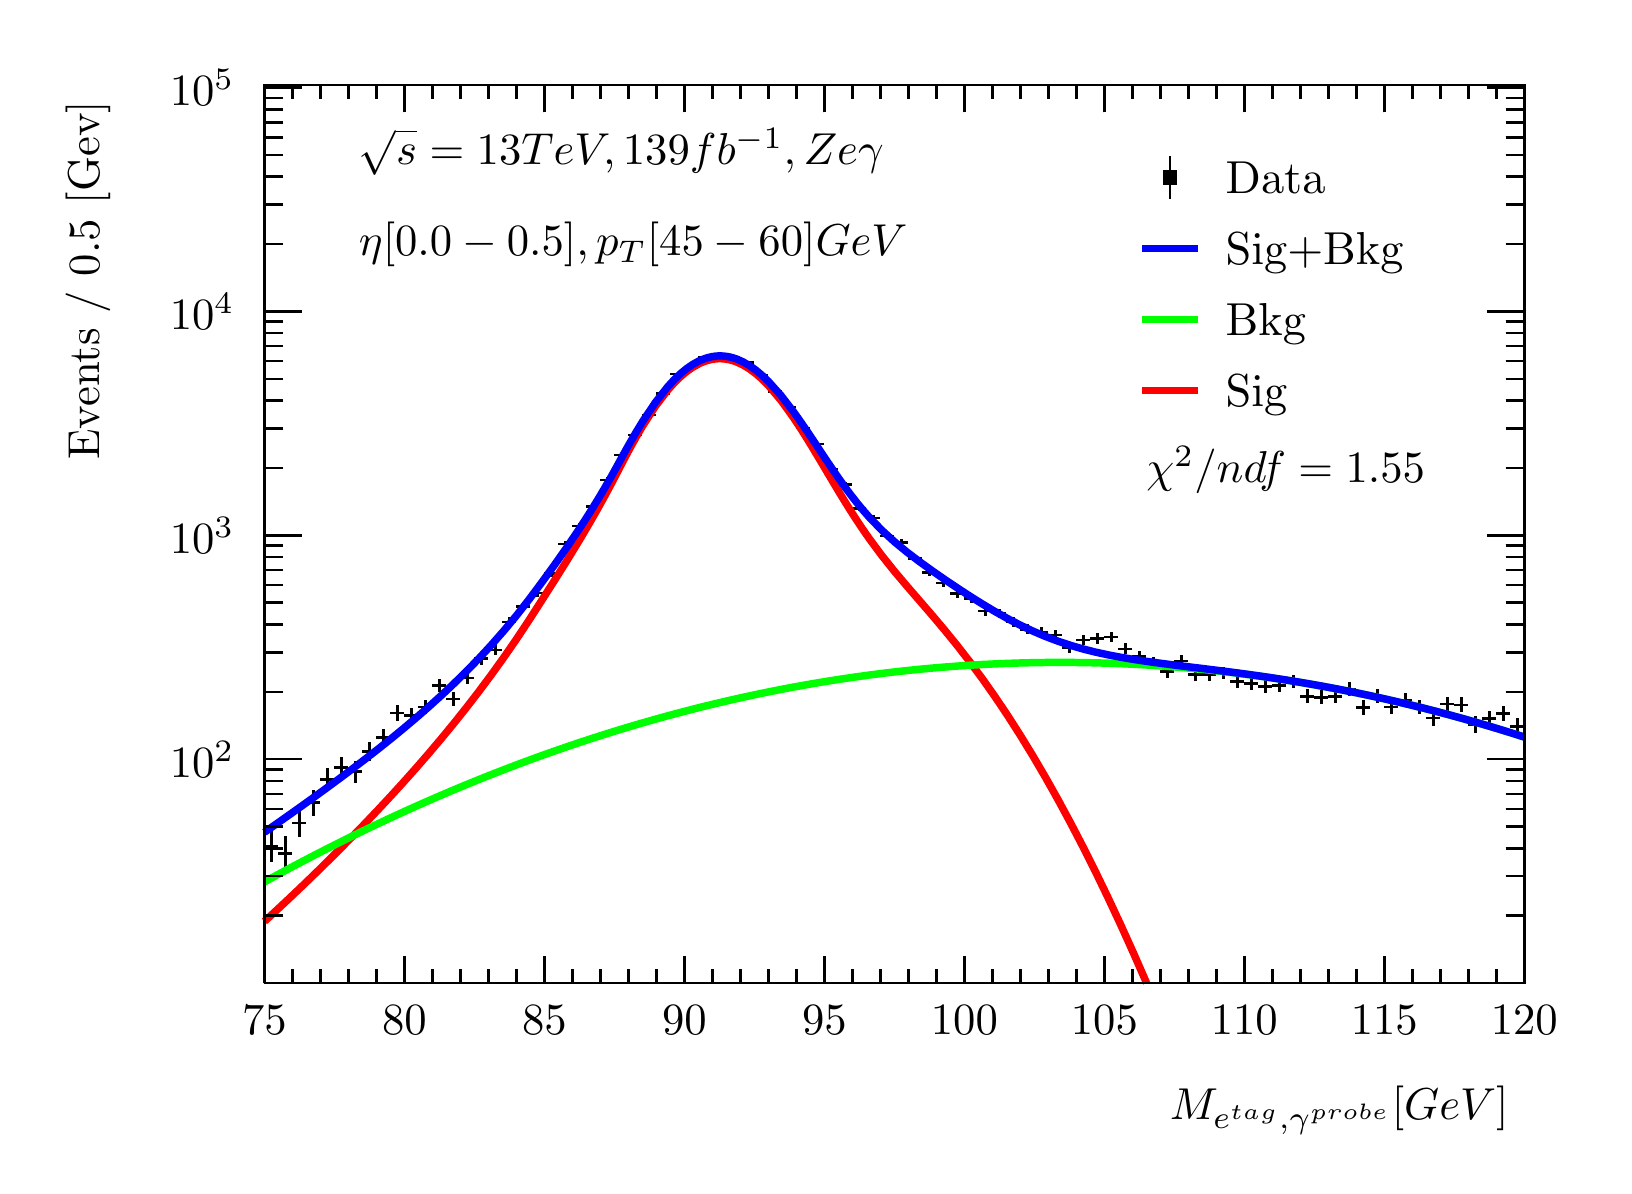
\begin{tikzpicture}
\pgfdeclareplotmark{cross} {
\pgfpathmoveto{\pgfpoint{-0.3\pgfplotmarksize}{\pgfplotmarksize}}
\pgfpathlineto{\pgfpoint{+0.3\pgfplotmarksize}{\pgfplotmarksize}}
\pgfpathlineto{\pgfpoint{+0.3\pgfplotmarksize}{0.3\pgfplotmarksize}}
\pgfpathlineto{\pgfpoint{+1\pgfplotmarksize}{0.3\pgfplotmarksize}}
\pgfpathlineto{\pgfpoint{+1\pgfplotmarksize}{-0.3\pgfplotmarksize}}
\pgfpathlineto{\pgfpoint{+0.3\pgfplotmarksize}{-0.3\pgfplotmarksize}}
\pgfpathlineto{\pgfpoint{+0.3\pgfplotmarksize}{-1.\pgfplotmarksize}}
\pgfpathlineto{\pgfpoint{-0.3\pgfplotmarksize}{-1.\pgfplotmarksize}}
\pgfpathlineto{\pgfpoint{-0.3\pgfplotmarksize}{-0.3\pgfplotmarksize}}
\pgfpathlineto{\pgfpoint{-1.\pgfplotmarksize}{-0.3\pgfplotmarksize}}
\pgfpathlineto{\pgfpoint{-1.\pgfplotmarksize}{0.3\pgfplotmarksize}}
\pgfpathlineto{\pgfpoint{-0.3\pgfplotmarksize}{0.3\pgfplotmarksize}}
\pgfpathclose
\pgfusepathqstroke
}
\pgfdeclareplotmark{cross*} {
\pgfpathmoveto{\pgfpoint{-0.3\pgfplotmarksize}{\pgfplotmarksize}}
\pgfpathlineto{\pgfpoint{+0.3\pgfplotmarksize}{\pgfplotmarksize}}
\pgfpathlineto{\pgfpoint{+0.3\pgfplotmarksize}{0.3\pgfplotmarksize}}
\pgfpathlineto{\pgfpoint{+1\pgfplotmarksize}{0.3\pgfplotmarksize}}
\pgfpathlineto{\pgfpoint{+1\pgfplotmarksize}{-0.3\pgfplotmarksize}}
\pgfpathlineto{\pgfpoint{+0.3\pgfplotmarksize}{-0.3\pgfplotmarksize}}
\pgfpathlineto{\pgfpoint{+0.3\pgfplotmarksize}{-1.\pgfplotmarksize}}
\pgfpathlineto{\pgfpoint{-0.3\pgfplotmarksize}{-1.\pgfplotmarksize}}
\pgfpathlineto{\pgfpoint{-0.3\pgfplotmarksize}{-0.3\pgfplotmarksize}}
\pgfpathlineto{\pgfpoint{-1.\pgfplotmarksize}{-0.3\pgfplotmarksize}}
\pgfpathlineto{\pgfpoint{-1.\pgfplotmarksize}{0.3\pgfplotmarksize}}
\pgfpathlineto{\pgfpoint{-0.3\pgfplotmarksize}{0.3\pgfplotmarksize}}
\pgfpathclose
\pgfusepathqfillstroke
}
\pgfdeclareplotmark{newstar} {
\pgfpathmoveto{\pgfqpoint{0pt}{\pgfplotmarksize}}
\pgfpathlineto{\pgfqpointpolar{44}{0.5\pgfplotmarksize}}
\pgfpathlineto{\pgfqpointpolar{18}{\pgfplotmarksize}}
\pgfpathlineto{\pgfqpointpolar{-20}{0.5\pgfplotmarksize}}
\pgfpathlineto{\pgfqpointpolar{-54}{\pgfplotmarksize}}
\pgfpathlineto{\pgfqpointpolar{-90}{0.5\pgfplotmarksize}}
\pgfpathlineto{\pgfqpointpolar{234}{\pgfplotmarksize}}
\pgfpathlineto{\pgfqpointpolar{198}{0.5\pgfplotmarksize}}
\pgfpathlineto{\pgfqpointpolar{162}{\pgfplotmarksize}}
\pgfpathlineto{\pgfqpointpolar{134}{0.5\pgfplotmarksize}}
\pgfpathclose
\pgfusepathqstroke
}
\pgfdeclareplotmark{newstar*} {
\pgfpathmoveto{\pgfqpoint{0pt}{\pgfplotmarksize}}
\pgfpathlineto{\pgfqpointpolar{44}{0.5\pgfplotmarksize}}
\pgfpathlineto{\pgfqpointpolar{18}{\pgfplotmarksize}}
\pgfpathlineto{\pgfqpointpolar{-20}{0.5\pgfplotmarksize}}
\pgfpathlineto{\pgfqpointpolar{-54}{\pgfplotmarksize}}
\pgfpathlineto{\pgfqpointpolar{-90}{0.5\pgfplotmarksize}}
\pgfpathlineto{\pgfqpointpolar{234}{\pgfplotmarksize}}
\pgfpathlineto{\pgfqpointpolar{198}{0.5\pgfplotmarksize}}
\pgfpathlineto{\pgfqpointpolar{162}{\pgfplotmarksize}}
\pgfpathlineto{\pgfqpointpolar{134}{0.5\pgfplotmarksize}}
\pgfpathclose
\pgfusepathqfillstroke
}
\definecolor{c}{rgb}{1,1,1};
\draw [color=c, fill=c] (0,0) rectangle (20,14.4361);
\draw [color=c, fill=c] (3,2.30977) rectangle (19,13.7143);
\definecolor{c}{rgb}{0,0,0};
\draw [c,line width=0.9] (3,2.30977) -- (3,13.7143) -- (19,13.7143) -- (19,2.30977) -- (3,2.30977);
\definecolor{c}{rgb}{1,1,1};
\draw [color=c, fill=c] (3,2.30977) rectangle (19,13.7143);
\definecolor{c}{rgb}{0,0,0};
\draw [c,line width=0.9] (3,2.30977) -- (3,13.7143) -- (19,13.7143) -- (19,2.30977) -- (3,2.30977);
\draw [c,line width=0.9] (3,2.30977) -- (19,2.30977);
\draw [c,line width=0.9] (3,2.65624) -- (3,2.30977);
\draw [c,line width=0.9] (3.35556,2.48301) -- (3.35556,2.30977);
\draw [c,line width=0.9] (3.71111,2.48301) -- (3.71111,2.30977);
\draw [c,line width=0.9] (4.06667,2.48301) -- (4.06667,2.30977);
\draw [c,line width=0.9] (4.42222,2.48301) -- (4.42222,2.30977);
\draw [c,line width=0.9] (4.77778,2.65624) -- (4.77778,2.30977);
\draw [c,line width=0.9] (5.13333,2.48301) -- (5.13333,2.30977);
\draw [c,line width=0.9] (5.48889,2.48301) -- (5.48889,2.30977);
\draw [c,line width=0.9] (5.84444,2.48301) -- (5.84444,2.30977);
\draw [c,line width=0.9] (6.2,2.48301) -- (6.2,2.30977);
\draw [c,line width=0.9] (6.55556,2.65624) -- (6.55556,2.30977);
\draw [c,line width=0.9] (6.91111,2.48301) -- (6.91111,2.30977);
\draw [c,line width=0.9] (7.26667,2.48301) -- (7.26667,2.30977);
\draw [c,line width=0.9] (7.62222,2.48301) -- (7.62222,2.30977);
\draw [c,line width=0.9] (7.97778,2.48301) -- (7.97778,2.30977);
\draw [c,line width=0.9] (8.33333,2.65624) -- (8.33333,2.30977);
\draw [c,line width=0.9] (8.68889,2.48301) -- (8.68889,2.30977);
\draw [c,line width=0.9] (9.04444,2.48301) -- (9.04444,2.30977);
\draw [c,line width=0.9] (9.4,2.48301) -- (9.4,2.30977);
\draw [c,line width=0.9] (9.75556,2.48301) -- (9.75556,2.30977);
\draw [c,line width=0.9] (10.1111,2.65624) -- (10.1111,2.30977);
\draw [c,line width=0.9] (10.4667,2.48301) -- (10.4667,2.30977);
\draw [c,line width=0.9] (10.8222,2.48301) -- (10.8222,2.30977);
\draw [c,line width=0.9] (11.1778,2.48301) -- (11.1778,2.30977);
\draw [c,line width=0.9] (11.5333,2.48301) -- (11.5333,2.30977);
\draw [c,line width=0.9] (11.8889,2.65624) -- (11.8889,2.30977);
\draw [c,line width=0.9] (12.2444,2.48301) -- (12.2444,2.30977);
\draw [c,line width=0.9] (12.6,2.48301) -- (12.6,2.30977);
\draw [c,line width=0.9] (12.9556,2.48301) -- (12.9556,2.30977);
\draw [c,line width=0.9] (13.3111,2.48301) -- (13.3111,2.30977);
\draw [c,line width=0.9] (13.6667,2.65624) -- (13.6667,2.30977);
\draw [c,line width=0.9] (14.0222,2.48301) -- (14.0222,2.30977);
\draw [c,line width=0.9] (14.3778,2.48301) -- (14.3778,2.30977);
\draw [c,line width=0.9] (14.7333,2.48301) -- (14.7333,2.30977);
\draw [c,line width=0.9] (15.0889,2.48301) -- (15.0889,2.30977);
\draw [c,line width=0.9] (15.4444,2.65624) -- (15.4444,2.30977);
\draw [c,line width=0.9] (15.8,2.48301) -- (15.8,2.30977);
\draw [c,line width=0.9] (16.1556,2.48301) -- (16.1556,2.30977);
\draw [c,line width=0.9] (16.5111,2.48301) -- (16.5111,2.30977);
\draw [c,line width=0.9] (16.8667,2.48301) -- (16.8667,2.30977);
\draw [c,line width=0.9] (17.2222,2.65624) -- (17.2222,2.30977);
\draw [c,line width=0.9] (17.5778,2.48301) -- (17.5778,2.30977);
\draw [c,line width=0.9] (17.9333,2.48301) -- (17.9333,2.30977);
\draw [c,line width=0.9] (18.2889,2.48301) -- (18.2889,2.30977);
\draw [c,line width=0.9] (18.6444,2.48301) -- (18.6444,2.30977);
\draw [c,line width=0.9] (19,2.65624) -- (19,2.30977);
\draw [c,line width=0.9] (19,2.65624) -- (19,2.30977);
\draw [anchor=base] (3,1.66015) node[scale=1.61424, color=c, rotate=0]{75};
\draw [anchor=base] (4.77778,1.66015) node[scale=1.61424, color=c, rotate=0]{80};
\draw [anchor=base] (6.55556,1.66015) node[scale=1.61424, color=c, rotate=0]{85};
\draw [anchor=base] (8.33333,1.66015) node[scale=1.61424, color=c, rotate=0]{90};
\draw [anchor=base] (10.1111,1.66015) node[scale=1.61424, color=c, rotate=0]{95};
\draw [anchor=base] (11.8889,1.66015) node[scale=1.61424, color=c, rotate=0]{100};
\draw [anchor=base] (13.6667,1.66015) node[scale=1.61424, color=c, rotate=0]{105};
\draw [anchor=base] (15.4444,1.66015) node[scale=1.61424, color=c, rotate=0]{110};
\draw [anchor=base] (17.2222,1.66015) node[scale=1.61424, color=c, rotate=0]{115};
\draw [anchor=base] (19,1.66015) node[scale=1.61424, color=c, rotate=0]{120};
\draw [anchor= east] (19,0.692932) node[scale=1.61424, color=c, rotate=0]{$M_{e^{tag}, \gamma^{probe}}  [GeV]$};
\draw [c,line width=0.9] (3,13.7143) -- (19,13.7143);
\draw [c,line width=0.9] (3,13.3678) -- (3,13.7143);
\draw [c,line width=0.9] (3.35556,13.5411) -- (3.35556,13.7143);
\draw [c,line width=0.9] (3.71111,13.5411) -- (3.71111,13.7143);
\draw [c,line width=0.9] (4.06667,13.5411) -- (4.06667,13.7143);
\draw [c,line width=0.9] (4.42222,13.5411) -- (4.42222,13.7143);
\draw [c,line width=0.9] (4.77778,13.3678) -- (4.77778,13.7143);
\draw [c,line width=0.9] (5.13333,13.5411) -- (5.13333,13.7143);
\draw [c,line width=0.9] (5.48889,13.5411) -- (5.48889,13.7143);
\draw [c,line width=0.9] (5.84444,13.5411) -- (5.84444,13.7143);
\draw [c,line width=0.9] (6.2,13.5411) -- (6.2,13.7143);
\draw [c,line width=0.9] (6.55556,13.3678) -- (6.55556,13.7143);
\draw [c,line width=0.9] (6.91111,13.5411) -- (6.91111,13.7143);
\draw [c,line width=0.9] (7.26667,13.5411) -- (7.26667,13.7143);
\draw [c,line width=0.9] (7.62222,13.5411) -- (7.62222,13.7143);
\draw [c,line width=0.9] (7.97778,13.5411) -- (7.97778,13.7143);
\draw [c,line width=0.9] (8.33333,13.3678) -- (8.33333,13.7143);
\draw [c,line width=0.9] (8.68889,13.5411) -- (8.68889,13.7143);
\draw [c,line width=0.9] (9.04444,13.5411) -- (9.04444,13.7143);
\draw [c,line width=0.9] (9.4,13.5411) -- (9.4,13.7143);
\draw [c,line width=0.9] (9.75556,13.5411) -- (9.75556,13.7143);
\draw [c,line width=0.9] (10.1111,13.3678) -- (10.1111,13.7143);
\draw [c,line width=0.9] (10.4667,13.5411) -- (10.4667,13.7143);
\draw [c,line width=0.9] (10.8222,13.5411) -- (10.8222,13.7143);
\draw [c,line width=0.9] (11.1778,13.5411) -- (11.1778,13.7143);
\draw [c,line width=0.9] (11.5333,13.5411) -- (11.5333,13.7143);
\draw [c,line width=0.9] (11.8889,13.3678) -- (11.8889,13.7143);
\draw [c,line width=0.9] (12.2444,13.5411) -- (12.2444,13.7143);
\draw [c,line width=0.9] (12.6,13.5411) -- (12.6,13.7143);
\draw [c,line width=0.9] (12.9556,13.5411) -- (12.9556,13.7143);
\draw [c,line width=0.9] (13.3111,13.5411) -- (13.3111,13.7143);
\draw [c,line width=0.9] (13.6667,13.3678) -- (13.6667,13.7143);
\draw [c,line width=0.9] (14.0222,13.5411) -- (14.0222,13.7143);
\draw [c,line width=0.9] (14.3778,13.5411) -- (14.3778,13.7143);
\draw [c,line width=0.9] (14.7333,13.5411) -- (14.7333,13.7143);
\draw [c,line width=0.9] (15.0889,13.5411) -- (15.0889,13.7143);
\draw [c,line width=0.9] (15.4444,13.3678) -- (15.4444,13.7143);
\draw [c,line width=0.9] (15.8,13.5411) -- (15.8,13.7143);
\draw [c,line width=0.9] (16.1556,13.5411) -- (16.1556,13.7143);
\draw [c,line width=0.9] (16.5111,13.5411) -- (16.5111,13.7143);
\draw [c,line width=0.9] (16.8667,13.5411) -- (16.8667,13.7143);
\draw [c,line width=0.9] (17.2222,13.3678) -- (17.2222,13.7143);
\draw [c,line width=0.9] (17.5778,13.5411) -- (17.5778,13.7143);
\draw [c,line width=0.9] (17.9333,13.5411) -- (17.9333,13.7143);
\draw [c,line width=0.9] (18.2889,13.5411) -- (18.2889,13.7143);
\draw [c,line width=0.9] (18.6444,13.5411) -- (18.6444,13.7143);
\draw [c,line width=0.9] (19,13.3678) -- (19,13.7143);
\draw [c,line width=0.9] (19,13.3678) -- (19,13.7143);
\draw [c,line width=0.9] (3,2.30977) -- (3,13.7143);
\draw [c,line width=0.9] (3.237,3.16561) -- (3,3.16561);
\draw [c,line width=0.9] (3.237,3.66625) -- (3,3.66625);
\draw [c,line width=0.9] (3.237,4.02146) -- (3,4.02146);
\draw [c,line width=0.9] (3.237,4.29698) -- (3,4.29698);
\draw [c,line width=0.9] (3.237,4.52209) -- (3,4.52209);
\draw [c,line width=0.9] (3.237,4.71242) -- (3,4.71242);
\draw [c,line width=0.9] (3.237,4.8773) -- (3,4.8773);
\draw [c,line width=0.9] (3.237,5.02273) -- (3,5.02273);
\draw [c,line width=0.9] (3.474,5.15282) -- (3,5.15282);
\draw [anchor= east] (2.82,5.15282) node[scale=1.61424, color=c, rotate=0]{$10^{2}$};
\draw [c,line width=0.9] (3.237,6.00866) -- (3,6.00866);
\draw [c,line width=0.9] (3.237,6.5093) -- (3,6.5093);
\draw [c,line width=0.9] (3.237,6.8645) -- (3,6.8645);
\draw [c,line width=0.9] (3.237,7.14002) -- (3,7.14002);
\draw [c,line width=0.9] (3.237,7.36514) -- (3,7.36514);
\draw [c,line width=0.9] (3.237,7.55547) -- (3,7.55547);
\draw [c,line width=0.9] (3.237,7.72034) -- (3,7.72034);
\draw [c,line width=0.9] (3.237,7.86577) -- (3,7.86577);
\draw [c,line width=0.9] (3.474,7.99586) -- (3,7.99586);
\draw [anchor= east] (2.82,7.99586) node[scale=1.61424, color=c, rotate=0]{$10^{3}$};
\draw [c,line width=0.9] (3.237,8.85171) -- (3,8.85171);
\draw [c,line width=0.9] (3.237,9.35234) -- (3,9.35234);
\draw [c,line width=0.9] (3.237,9.70755) -- (3,9.70755);
\draw [c,line width=0.9] (3.237,9.98307) -- (3,9.98307);
\draw [c,line width=0.9] (3.237,10.2082) -- (3,10.2082);
\draw [c,line width=0.9] (3.237,10.3985) -- (3,10.3985);
\draw [c,line width=0.9] (3.237,10.5634) -- (3,10.5634);
\draw [c,line width=0.9] (3.237,10.7088) -- (3,10.7088);
\draw [c,line width=0.9] (3.474,10.8389) -- (3,10.8389);
\draw [anchor= east] (2.82,10.8389) node[scale=1.61424, color=c, rotate=0]{$10^{4}$};
\draw [c,line width=0.9] (3.237,11.6948) -- (3,11.6948);
\draw [c,line width=0.9] (3.237,12.1954) -- (3,12.1954);
\draw [c,line width=0.9] (3.237,12.5506) -- (3,12.5506);
\draw [c,line width=0.9] (3.237,12.8261) -- (3,12.8261);
\draw [c,line width=0.9] (3.237,13.0512) -- (3,13.0512);
\draw [c,line width=0.9] (3.237,13.2416) -- (3,13.2416);
\draw [c,line width=0.9] (3.237,13.4064) -- (3,13.4064);
\draw [c,line width=0.9] (3.237,13.5519) -- (3,13.5519);
\draw [c,line width=0.9] (3.474,13.682) -- (3,13.682);
\draw [anchor= east] (2.82,13.682) node[scale=1.61424, color=c, rotate=0]{$10^{5}$};
\draw [anchor= east] (0.76,13.7143) node[scale=1.61424, color=c, rotate=90]{Events / 0.5 [Gev]};
\draw [c,line width=0.9] (19,2.30977) -- (19,13.7143);
\draw [c,line width=0.9] (18.763,3.16561) -- (19,3.16561);
\draw [c,line width=0.9] (18.763,3.66625) -- (19,3.66625);
\draw [c,line width=0.9] (18.763,4.02146) -- (19,4.02146);
\draw [c,line width=0.9] (18.763,4.29698) -- (19,4.29698);
\draw [c,line width=0.9] (18.763,4.52209) -- (19,4.52209);
\draw [c,line width=0.9] (18.763,4.71242) -- (19,4.71242);
\draw [c,line width=0.9] (18.763,4.8773) -- (19,4.8773);
\draw [c,line width=0.9] (18.763,5.02273) -- (19,5.02273);
\draw [c,line width=0.9] (18.526,5.15282) -- (19,5.15282);
\draw [c,line width=0.9] (18.763,6.00866) -- (19,6.00866);
\draw [c,line width=0.9] (18.763,6.5093) -- (19,6.5093);
\draw [c,line width=0.9] (18.763,6.8645) -- (19,6.8645);
\draw [c,line width=0.9] (18.763,7.14002) -- (19,7.14002);
\draw [c,line width=0.9] (18.763,7.36514) -- (19,7.36514);
\draw [c,line width=0.9] (18.763,7.55547) -- (19,7.55547);
\draw [c,line width=0.9] (18.763,7.72034) -- (19,7.72034);
\draw [c,line width=0.9] (18.763,7.86577) -- (19,7.86577);
\draw [c,line width=0.9] (18.526,7.99586) -- (19,7.99586);
\draw [c,line width=0.9] (18.763,8.85171) -- (19,8.85171);
\draw [c,line width=0.9] (18.763,9.35234) -- (19,9.35234);
\draw [c,line width=0.9] (18.763,9.70755) -- (19,9.70755);
\draw [c,line width=0.9] (18.763,9.98307) -- (19,9.98307);
\draw [c,line width=0.9] (18.763,10.2082) -- (19,10.2082);
\draw [c,line width=0.9] (18.763,10.3985) -- (19,10.3985);
\draw [c,line width=0.9] (18.763,10.5634) -- (19,10.5634);
\draw [c,line width=0.9] (18.763,10.7088) -- (19,10.7088);
\draw [c,line width=0.9] (18.526,10.8389) -- (19,10.8389);
\draw [c,line width=0.9] (18.763,11.6948) -- (19,11.6948);
\draw [c,line width=0.9] (18.763,12.1954) -- (19,12.1954);
\draw [c,line width=0.9] (18.763,12.5506) -- (19,12.5506);
\draw [c,line width=0.9] (18.763,12.8261) -- (19,12.8261);
\draw [c,line width=0.9] (18.763,13.0512) -- (19,13.0512);
\draw [c,line width=0.9] (18.763,13.2416) -- (19,13.2416);
\draw [c,line width=0.9] (18.763,13.4064) -- (19,13.4064);
\draw [c,line width=0.9] (18.763,13.5519) -- (19,13.5519);
\draw [c,line width=0.9] (18.526,13.682) -- (19,13.682);
\draw [c,line width=0.9] (3.08889,4.05195) -- (3,4.05195);
\draw [c,line width=0.9] (3,4.05195) -- (3,4.05195);
\draw [c,line width=0.9] (3.08889,4.05195) -- (3.17778,4.05195);
\draw [c,line width=0.9] (3.17778,4.05195) -- (3.17778,4.05195);
\draw [c,line width=0.9] (3.08889,4.05195) -- (3.08889,4.25823);
\draw [c,line width=0.9] (3.08889,4.25823) -- (3.08889,4.25823);
\draw [c,line width=0.9] (3.08889,4.05195) -- (3.08889,3.84322);
\draw [c,line width=0.9] (3.08889,3.84322) -- (3.08889,3.84322);
\draw [c,line width=0.9] (3.26667,3.95813) -- (3.17778,3.95813);
\draw [c,line width=0.9] (3.17778,3.95813) -- (3.17778,3.95813);
\draw [c,line width=0.9] (3.26667,3.95813) -- (3.35556,3.95813);
\draw [c,line width=0.9] (3.35556,3.95813) -- (3.35556,3.95813);
\draw [c,line width=0.9] (3.26667,3.95813) -- (3.26667,4.17287);
\draw [c,line width=0.9] (3.26667,4.17287) -- (3.26667,4.17287);
\draw [c,line width=0.9] (3.26667,3.95813) -- (3.26667,3.74063);
\draw [c,line width=0.9] (3.26667,3.74063) -- (3.26667,3.74063);
\draw [c,line width=0.9] (3.44444,4.3454) -- (3.35556,4.3454);
\draw [c,line width=0.9] (3.35556,4.3454) -- (3.35556,4.3454);
\draw [c,line width=0.9] (3.44444,4.3454) -- (3.53333,4.3454);
\draw [c,line width=0.9] (3.53333,4.3454) -- (3.53333,4.3454);
\draw [c,line width=0.9] (3.44444,4.3454) -- (3.44444,4.52738);
\draw [c,line width=0.9] (3.44444,4.52738) -- (3.44444,4.52738);
\draw [c,line width=0.9] (3.44444,4.3454) -- (3.44444,4.16172);
\draw [c,line width=0.9] (3.44444,4.16172) -- (3.44444,4.16172);
\draw [c,line width=0.9] (3.62222,4.60178) -- (3.53333,4.60178);
\draw [c,line width=0.9] (3.53333,4.60178) -- (3.53333,4.60178);
\draw [c,line width=0.9] (3.62222,4.60178) -- (3.71111,4.60178);
\draw [c,line width=0.9] (3.71111,4.60178) -- (3.71111,4.60178);
\draw [c,line width=0.9] (3.62222,4.60178) -- (3.62222,4.76495);
\draw [c,line width=0.9] (3.62222,4.76495) -- (3.62222,4.76495);
\draw [c,line width=0.9] (3.62222,4.60178) -- (3.62222,4.43737);
\draw [c,line width=0.9] (3.62222,4.43737) -- (3.62222,4.43737);
\draw [c,line width=0.9] (3.8,4.89264) -- (3.71111,4.89264);
\draw [c,line width=0.9] (3.71111,4.89264) -- (3.71111,4.89264);
\draw [c,line width=0.9] (3.8,4.89264) -- (3.88889,4.89264);
\draw [c,line width=0.9] (3.88889,4.89264) -- (3.88889,4.89264);
\draw [c,line width=0.9] (3.8,4.89264) -- (3.8,5.03688);
\draw [c,line width=0.9] (3.8,5.03688) -- (3.8,5.03688);
\draw [c,line width=0.9] (3.8,4.89264) -- (3.8,4.74753);
\draw [c,line width=0.9] (3.8,4.74753) -- (3.8,4.74753);
\draw [c,line width=0.9] (3.97778,5.04987) -- (3.88889,5.04987);
\draw [c,line width=0.9] (3.88889,5.04987) -- (3.88889,5.04987);
\draw [c,line width=0.9] (3.97778,5.04987) -- (4.06667,5.04987);
\draw [c,line width=0.9] (4.06667,5.04987) -- (4.06667,5.04987);
\draw [c,line width=0.9] (3.97778,5.04987) -- (3.97778,5.18483);
\draw [c,line width=0.9] (3.97778,5.18483) -- (3.97778,5.18483);
\draw [c,line width=0.9] (3.97778,5.04987) -- (3.97778,4.91418);
\draw [c,line width=0.9] (3.97778,4.91418) -- (3.97778,4.91418);
\draw [c,line width=0.9] (4.15556,4.99498) -- (4.06667,4.99498);
\draw [c,line width=0.9] (4.06667,4.99498) -- (4.06667,4.99498);
\draw [c,line width=0.9] (4.15556,4.99498) -- (4.24444,4.99498);
\draw [c,line width=0.9] (4.24444,4.99498) -- (4.24444,4.99498);
\draw [c,line width=0.9] (4.15556,4.99498) -- (4.15556,5.13311);
\draw [c,line width=0.9] (4.15556,5.13311) -- (4.15556,5.13311);
\draw [c,line width=0.9] (4.15556,4.99498) -- (4.15556,4.85608);
\draw [c,line width=0.9] (4.15556,4.85608) -- (4.15556,4.85608);
\draw [c,line width=0.9] (4.33333,5.24785) -- (4.24444,5.24785);
\draw [c,line width=0.9] (4.24444,5.24785) -- (4.24444,5.24785);
\draw [c,line width=0.9] (4.33333,5.24785) -- (4.42222,5.24785);
\draw [c,line width=0.9] (4.42222,5.24785) -- (4.42222,5.24785);
\draw [c,line width=0.9] (4.33333,5.24785) -- (4.33333,5.36661);
\draw [c,line width=0.9] (4.33333,5.36661) -- (4.33333,5.36661);
\draw [c,line width=0.9] (4.33333,5.24785) -- (4.33333,5.12908);
\draw [c,line width=0.9] (4.33333,5.12908) -- (4.33333,5.12908);
\draw [c,line width=0.9] (4.51111,5.42834) -- (4.42222,5.42834);
\draw [c,line width=0.9] (4.42222,5.42834) -- (4.42222,5.42834);
\draw [c,line width=0.9] (4.51111,5.42834) -- (4.6,5.42834);
\draw [c,line width=0.9] (4.6,5.42834) -- (4.6,5.42834);
\draw [c,line width=0.9] (4.51111,5.42834) -- (4.51111,5.53874);
\draw [c,line width=0.9] (4.51111,5.53874) -- (4.51111,5.53874);
\draw [c,line width=0.9] (4.51111,5.42834) -- (4.51111,5.31794);
\draw [c,line width=0.9] (4.51111,5.31794) -- (4.51111,5.31794);
\draw [c,line width=0.9] (4.68889,5.74084) -- (4.6,5.74084);
\draw [c,line width=0.9] (4.6,5.74084) -- (4.6,5.74084);
\draw [c,line width=0.9] (4.68889,5.74084) -- (4.77778,5.74084);
\draw [c,line width=0.9] (4.77778,5.74084) -- (4.77778,5.74084);
\draw [c,line width=0.9] (4.68889,5.74084) -- (4.68889,5.83812);
\draw [c,line width=0.9] (4.68889,5.83812) -- (4.68889,5.83812);
\draw [c,line width=0.9] (4.68889,5.74084) -- (4.68889,5.64355);
\draw [c,line width=0.9] (4.68889,5.64355) -- (4.68889,5.64355);
\draw [c,line width=0.9] (4.86667,5.70977) -- (4.77778,5.70977);
\draw [c,line width=0.9] (4.77778,5.70977) -- (4.77778,5.70977);
\draw [c,line width=0.9] (4.86667,5.70977) -- (4.95556,5.70977);
\draw [c,line width=0.9] (4.95556,5.70977) -- (4.95556,5.70977);
\draw [c,line width=0.9] (4.86667,5.70977) -- (4.86667,5.80829);
\draw [c,line width=0.9] (4.86667,5.80829) -- (4.86667,5.80829);
\draw [c,line width=0.9] (4.86667,5.70977) -- (4.86667,5.61126);
\draw [c,line width=0.9] (4.86667,5.61126) -- (4.86667,5.61126);
\draw [c,line width=0.9] (5.04444,5.81524) -- (4.95556,5.81524);
\draw [c,line width=0.9] (4.95556,5.81524) -- (4.95556,5.81524);
\draw [c,line width=0.9] (5.04444,5.81524) -- (5.13333,5.81524);
\draw [c,line width=0.9] (5.13333,5.81524) -- (5.13333,5.81524);
\draw [c,line width=0.9] (5.04444,5.81524) -- (5.04444,5.90964);
\draw [c,line width=0.9] (5.04444,5.90964) -- (5.04444,5.90964);
\draw [c,line width=0.9] (5.04444,5.81524) -- (5.04444,5.72084);
\draw [c,line width=0.9] (5.04444,5.72084) -- (5.04444,5.72084);
\draw [c,line width=0.9] (5.22222,6.08642) -- (5.13333,6.08642);
\draw [c,line width=0.9] (5.13333,6.08642) -- (5.13333,6.08642);
\draw [c,line width=0.9] (5.22222,6.08642) -- (5.31111,6.08642);
\draw [c,line width=0.9] (5.31111,6.08642) -- (5.31111,6.08642);
\draw [c,line width=0.9] (5.22222,6.08642) -- (5.22222,6.171);
\draw [c,line width=0.9] (5.22222,6.171) -- (5.22222,6.171);
\draw [c,line width=0.9] (5.22222,6.08642) -- (5.22222,6.00183);
\draw [c,line width=0.9] (5.22222,6.00183) -- (5.22222,6.00183);
\draw [c,line width=0.9] (5.4,5.91906) -- (5.31111,5.91906);
\draw [c,line width=0.9] (5.31111,5.91906) -- (5.31111,5.91906);
\draw [c,line width=0.9] (5.4,5.91906) -- (5.48889,5.91906);
\draw [c,line width=0.9] (5.48889,5.91906) -- (5.48889,5.91906);
\draw [c,line width=0.9] (5.4,5.91906) -- (5.4,6.00957);
\draw [c,line width=0.9] (5.4,6.00957) -- (5.4,6.00957);
\draw [c,line width=0.9] (5.4,5.91906) -- (5.4,5.82854);
\draw [c,line width=0.9] (5.4,5.82854) -- (5.4,5.82854);
\draw [c,line width=0.9] (5.57778,6.18658) -- (5.48889,6.18658);
\draw [c,line width=0.9] (5.48889,6.18658) -- (5.48889,6.18658);
\draw [c,line width=0.9] (5.57778,6.18658) -- (5.66667,6.18658);
\draw [c,line width=0.9] (5.66667,6.18658) -- (5.66667,6.18658);
\draw [c,line width=0.9] (5.57778,6.18658) -- (5.57778,6.26781);
\draw [c,line width=0.9] (5.57778,6.26781) -- (5.57778,6.26781);
\draw [c,line width=0.9] (5.57778,6.18658) -- (5.57778,6.10536);
\draw [c,line width=0.9] (5.57778,6.10536) -- (5.57778,6.10536);
\draw [c,line width=0.9] (5.75556,6.42851) -- (5.66667,6.42851);
\draw [c,line width=0.9] (5.66667,6.42851) -- (5.66667,6.42851);
\draw [c,line width=0.9] (5.75556,6.42851) -- (5.84444,6.42851);
\draw [c,line width=0.9] (5.84444,6.42851) -- (5.84444,6.42851);
\draw [c,line width=0.9] (5.75556,6.42851) -- (5.75556,6.50216);
\draw [c,line width=0.9] (5.75556,6.50216) -- (5.75556,6.50216);
\draw [c,line width=0.9] (5.75556,6.42851) -- (5.75556,6.35487);
\draw [c,line width=0.9] (5.75556,6.35487) -- (5.75556,6.35487);
\draw [c,line width=0.9] (5.93333,6.54179) -- (5.84444,6.54179);
\draw [c,line width=0.9] (5.84444,6.54179) -- (5.84444,6.54179);
\draw [c,line width=0.9] (5.93333,6.54179) -- (6.02222,6.54179);
\draw [c,line width=0.9] (6.02222,6.54179) -- (6.02222,6.54179);
\draw [c,line width=0.9] (5.93333,6.54179) -- (5.93333,6.61214);
\draw [c,line width=0.9] (5.93333,6.61214) -- (5.93333,6.61214);
\draw [c,line width=0.9] (5.93333,6.54179) -- (5.93333,6.47145);
\draw [c,line width=0.9] (5.93333,6.47145) -- (5.93333,6.47145);
\draw [c,line width=0.9] (6.11111,6.89198) -- (6.02222,6.89198);
\draw [c,line width=0.9] (6.02222,6.89198) -- (6.02222,6.89198);
\draw [c,line width=0.9] (6.11111,6.89198) -- (6.2,6.89198);
\draw [c,line width=0.9] (6.2,6.89198) -- (6.2,6.89198);
\draw [c,line width=0.9] (6.11111,6.89198) -- (6.11111,6.95302);
\draw [c,line width=0.9] (6.11111,6.95302) -- (6.11111,6.95302);
\draw [c,line width=0.9] (6.11111,6.89198) -- (6.11111,6.83093);
\draw [c,line width=0.9] (6.11111,6.83093) -- (6.11111,6.83093);
\draw [c,line width=0.9] (6.28889,7.09475) -- (6.2,7.09475);
\draw [c,line width=0.9] (6.2,7.09475) -- (6.2,7.09475);
\draw [c,line width=0.9] (6.28889,7.09475) -- (6.37778,7.09475);
\draw [c,line width=0.9] (6.37778,7.09475) -- (6.37778,7.09475);
\draw [c,line width=0.9] (6.28889,7.09475) -- (6.28889,7.15099);
\draw [c,line width=0.9] (6.28889,7.15099) -- (6.28889,7.15099);
\draw [c,line width=0.9] (6.28889,7.09475) -- (6.28889,7.03852);
\draw [c,line width=0.9] (6.28889,7.03852) -- (6.28889,7.03852);
\draw [c,line width=0.9] (6.46667,7.26442) -- (6.37778,7.26442);
\draw [c,line width=0.9] (6.37778,7.26442) -- (6.37778,7.26442);
\draw [c,line width=0.9] (6.46667,7.26442) -- (6.55556,7.26442);
\draw [c,line width=0.9] (6.55556,7.26442) -- (6.55556,7.26442);
\draw [c,line width=0.9] (6.46667,7.26442) -- (6.46667,7.31692);
\draw [c,line width=0.9] (6.46667,7.31692) -- (6.46667,7.31692);
\draw [c,line width=0.9] (6.46667,7.26442) -- (6.46667,7.21192);
\draw [c,line width=0.9] (6.46667,7.21192) -- (6.46667,7.21192);
\draw [c,line width=0.9] (6.64444,7.50874) -- (6.55556,7.50874);
\draw [c,line width=0.9] (6.55556,7.50874) -- (6.55556,7.50874);
\draw [c,line width=0.9] (6.64444,7.50874) -- (6.73333,7.50874);
\draw [c,line width=0.9] (6.73333,7.50874) -- (6.73333,7.50874);
\draw [c,line width=0.9] (6.64444,7.50874) -- (6.64444,7.55629);
\draw [c,line width=0.9] (6.64444,7.55629) -- (6.64444,7.55629);
\draw [c,line width=0.9] (6.64444,7.50874) -- (6.64444,7.46118);
\draw [c,line width=0.9] (6.64444,7.46118) -- (6.64444,7.46118);
\draw [c,line width=0.9] (6.82222,7.88618) -- (6.73333,7.88618);
\draw [c,line width=0.9] (6.73333,7.88618) -- (6.73333,7.88618);
\draw [c,line width=0.9] (6.82222,7.88618) -- (6.91111,7.88618);
\draw [c,line width=0.9] (6.91111,7.88618) -- (6.91111,7.88618);
\draw [c,line width=0.9] (6.82222,7.88618) -- (6.82222,7.927);
\draw [c,line width=0.9] (6.82222,7.927) -- (6.82222,7.927);
\draw [c,line width=0.9] (6.82222,7.88618) -- (6.82222,7.84537);
\draw [c,line width=0.9] (6.82222,7.84537) -- (6.82222,7.84537);
\draw [c,line width=0.9] (7,8.11242) -- (6.91111,8.11242);
\draw [c,line width=0.9] (6.91111,8.11242) -- (6.91111,8.11242);
\draw [c,line width=0.9] (7,8.11242) -- (7.08889,8.11242);
\draw [c,line width=0.9] (7.08889,8.11242) -- (7.08889,8.11242);
\draw [c,line width=0.9] (7,8.11242) -- (7,8.14967);
\draw [c,line width=0.9] (7,8.14967) -- (7,8.14967);
\draw [c,line width=0.9] (7,8.11242) -- (7,8.07518);
\draw [c,line width=0.9] (7,8.07518) -- (7,8.07518);
\draw [c,line width=0.9] (7.17778,8.36183) -- (7.08889,8.36183);
\draw [c,line width=0.9] (7.08889,8.36183) -- (7.08889,8.36183);
\draw [c,line width=0.9] (7.17778,8.36183) -- (7.26667,8.36183);
\draw [c,line width=0.9] (7.26667,8.36183) -- (7.26667,8.36183);
\draw [c,line width=0.9] (7.17778,8.36183) -- (7.17778,8.39549);
\draw [c,line width=0.9] (7.17778,8.39549) -- (7.17778,8.39549);
\draw [c,line width=0.9] (7.17778,8.36183) -- (7.17778,8.32816);
\draw [c,line width=0.9] (7.17778,8.32816) -- (7.17778,8.32816);
\draw [c,line width=0.9] (7.35556,8.70156) -- (7.26667,8.70156);
\draw [c,line width=0.9] (7.26667,8.70156) -- (7.26667,8.70156);
\draw [c,line width=0.9] (7.35556,8.70156) -- (7.44444,8.70156);
\draw [c,line width=0.9] (7.44444,8.70156) -- (7.44444,8.70156);
\draw [c,line width=0.9] (7.35556,8.70156) -- (7.35556,8.7309);
\draw [c,line width=0.9] (7.35556,8.7309) -- (7.35556,8.7309);
\draw [c,line width=0.9] (7.35556,8.70156) -- (7.35556,8.67222);
\draw [c,line width=0.9] (7.35556,8.67222) -- (7.35556,8.67222);
\draw [c,line width=0.9] (7.53333,9.01511) -- (7.44444,9.01511);
\draw [c,line width=0.9] (7.44444,9.01511) -- (7.44444,9.01511);
\draw [c,line width=0.9] (7.53333,9.01511) -- (7.62222,9.01511);
\draw [c,line width=0.9] (7.62222,9.01511) -- (7.62222,9.01511);
\draw [c,line width=0.9] (7.53333,9.01511) -- (7.53333,9.04095);
\draw [c,line width=0.9] (7.53333,9.04095) -- (7.53333,9.04095);
\draw [c,line width=0.9] (7.53333,9.01511) -- (7.53333,8.98927);
\draw [c,line width=0.9] (7.53333,8.98927) -- (7.53333,8.98927);
\draw [c,line width=0.9] (7.71111,9.26848) -- (7.62222,9.26848);
\draw [c,line width=0.9] (7.62222,9.26848) -- (7.62222,9.26848);
\draw [c,line width=0.9] (7.71111,9.26848) -- (7.8,9.26848);
\draw [c,line width=0.9] (7.8,9.26848) -- (7.8,9.26848);
\draw [c,line width=0.9] (7.71111,9.26848) -- (7.71111,9.2918);
\draw [c,line width=0.9] (7.71111,9.2918) -- (7.71111,9.2918);
\draw [c,line width=0.9] (7.71111,9.26848) -- (7.71111,9.24516);
\draw [c,line width=0.9] (7.71111,9.24516) -- (7.71111,9.24516);
\draw [c,line width=0.9] (7.88889,9.52312) -- (7.8,9.52312);
\draw [c,line width=0.9] (7.8,9.52312) -- (7.8,9.52312);
\draw [c,line width=0.9] (7.88889,9.52312) -- (7.97778,9.52312);
\draw [c,line width=0.9] (7.97778,9.52312) -- (7.97778,9.52312);
\draw [c,line width=0.9] (7.88889,9.52312) -- (7.88889,9.54416);
\draw [c,line width=0.9] (7.88889,9.54416) -- (7.88889,9.54416);
\draw [c,line width=0.9] (7.88889,9.52312) -- (7.88889,9.50208);
\draw [c,line width=0.9] (7.88889,9.50208) -- (7.88889,9.50208);
\draw [c,line width=0.9] (8.06667,9.79426) -- (7.97778,9.79426);
\draw [c,line width=0.9] (7.97778,9.79426) -- (7.97778,9.79426);
\draw [c,line width=0.9] (8.06667,9.79426) -- (8.15556,9.79426);
\draw [c,line width=0.9] (8.15556,9.79426) -- (8.15556,9.79426);
\draw [c,line width=0.9] (8.06667,9.79426) -- (8.06667,9.81311);
\draw [c,line width=0.9] (8.06667,9.81311) -- (8.06667,9.81311);
\draw [c,line width=0.9] (8.06667,9.79426) -- (8.06667,9.77541);
\draw [c,line width=0.9] (8.06667,9.77541) -- (8.06667,9.77541);
\draw [c,line width=0.9] (8.24444,10.0452) -- (8.15556,10.0452);
\draw [c,line width=0.9] (8.15556,10.0452) -- (8.15556,10.0452);
\draw [c,line width=0.9] (8.24444,10.0452) -- (8.33333,10.0452);
\draw [c,line width=0.9] (8.33333,10.0452) -- (8.33333,10.0452);
\draw [c,line width=0.9] (8.24444,10.0452) -- (8.24444,10.0622);
\draw [c,line width=0.9] (8.24444,10.0622) -- (8.24444,10.0622);
\draw [c,line width=0.9] (8.24444,10.0452) -- (8.24444,10.0282);
\draw [c,line width=0.9] (8.24444,10.0282) -- (8.24444,10.0282);
\draw [c,line width=0.9] (8.42222,10.1292) -- (8.33333,10.1292);
\draw [c,line width=0.9] (8.33333,10.1292) -- (8.33333,10.1292);
\draw [c,line width=0.9] (8.42222,10.1292) -- (8.51111,10.1292);
\draw [c,line width=0.9] (8.51111,10.1292) -- (8.51111,10.1292);
\draw [c,line width=0.9] (8.42222,10.1292) -- (8.42222,10.1456);
\draw [c,line width=0.9] (8.42222,10.1456) -- (8.42222,10.1456);
\draw [c,line width=0.9] (8.42222,10.1292) -- (8.42222,10.1127);
\draw [c,line width=0.9] (8.42222,10.1127) -- (8.42222,10.1127);
\draw [c,line width=0.9] (8.6,10.256) -- (8.51111,10.256);
\draw [c,line width=0.9] (8.51111,10.256) -- (8.51111,10.256);
\draw [c,line width=0.9] (8.6,10.256) -- (8.68889,10.256);
\draw [c,line width=0.9] (8.68889,10.256) -- (8.68889,10.256);
\draw [c,line width=0.9] (8.6,10.256) -- (8.6,10.2717);
\draw [c,line width=0.9] (8.6,10.2717) -- (8.6,10.2717);
\draw [c,line width=0.9] (8.6,10.256) -- (8.6,10.2404);
\draw [c,line width=0.9] (8.6,10.2404) -- (8.6,10.2404);
\draw [c,line width=0.9] (8.77778,10.2819) -- (8.68889,10.2819);
\draw [c,line width=0.9] (8.68889,10.2819) -- (8.68889,10.2819);
\draw [c,line width=0.9] (8.77778,10.2819) -- (8.86667,10.2819);
\draw [c,line width=0.9] (8.86667,10.2819) -- (8.86667,10.2819);
\draw [c,line width=0.9] (8.77778,10.2819) -- (8.77778,10.2973);
\draw [c,line width=0.9] (8.77778,10.2973) -- (8.77778,10.2973);
\draw [c,line width=0.9] (8.77778,10.2819) -- (8.77778,10.2664);
\draw [c,line width=0.9] (8.77778,10.2664) -- (8.77778,10.2664);
\draw [c,line width=0.9] (8.95556,10.258) -- (8.86667,10.258);
\draw [c,line width=0.9] (8.86667,10.258) -- (8.86667,10.258);
\draw [c,line width=0.9] (8.95556,10.258) -- (9.04444,10.258);
\draw [c,line width=0.9] (9.04444,10.258) -- (9.04444,10.258);
\draw [c,line width=0.9] (8.95556,10.258) -- (8.95556,10.2736);
\draw [c,line width=0.9] (8.95556,10.2736) -- (8.95556,10.2736);
\draw [c,line width=0.9] (8.95556,10.258) -- (8.95556,10.2424);
\draw [c,line width=0.9] (8.95556,10.2424) -- (8.95556,10.2424);
\draw [c,line width=0.9] (9.13333,10.1906) -- (9.04444,10.1906);
\draw [c,line width=0.9] (9.04444,10.1906) -- (9.04444,10.1906);
\draw [c,line width=0.9] (9.13333,10.1906) -- (9.22222,10.1906);
\draw [c,line width=0.9] (9.22222,10.1906) -- (9.22222,10.1906);
\draw [c,line width=0.9] (9.13333,10.1906) -- (9.13333,10.2066);
\draw [c,line width=0.9] (9.13333,10.2066) -- (9.13333,10.2066);
\draw [c,line width=0.9] (9.13333,10.1906) -- (9.13333,10.1745);
\draw [c,line width=0.9] (9.13333,10.1745) -- (9.13333,10.1745);
\draw [c,line width=0.9] (9.31111,10.0346) -- (9.22222,10.0346);
\draw [c,line width=0.9] (9.22222,10.0346) -- (9.22222,10.0346);
\draw [c,line width=0.9] (9.31111,10.0346) -- (9.4,10.0346);
\draw [c,line width=0.9] (9.4,10.0346) -- (9.4,10.0346);
\draw [c,line width=0.9] (9.31111,10.0346) -- (9.31111,10.0517);
\draw [c,line width=0.9] (9.31111,10.0517) -- (9.31111,10.0517);
\draw [c,line width=0.9] (9.31111,10.0346) -- (9.31111,10.0175);
\draw [c,line width=0.9] (9.31111,10.0175) -- (9.31111,10.0175);
\draw [c,line width=0.9] (9.48889,9.82551) -- (9.4,9.82551);
\draw [c,line width=0.9] (9.4,9.82551) -- (9.4,9.82551);
\draw [c,line width=0.9] (9.48889,9.82551) -- (9.57778,9.82551);
\draw [c,line width=0.9] (9.57778,9.82551) -- (9.57778,9.82551);
\draw [c,line width=0.9] (9.48889,9.82551) -- (9.48889,9.84412);
\draw [c,line width=0.9] (9.48889,9.84412) -- (9.48889,9.84412);
\draw [c,line width=0.9] (9.48889,9.82551) -- (9.48889,9.8069);
\draw [c,line width=0.9] (9.48889,9.8069) -- (9.48889,9.8069);
\draw [c,line width=0.9] (9.66667,9.62523) -- (9.57778,9.62523);
\draw [c,line width=0.9] (9.57778,9.62523) -- (9.57778,9.62523);
\draw [c,line width=0.9] (9.66667,9.62523) -- (9.75556,9.62523);
\draw [c,line width=0.9] (9.75556,9.62523) -- (9.75556,9.62523);
\draw [c,line width=0.9] (9.66667,9.62523) -- (9.66667,9.64541);
\draw [c,line width=0.9] (9.66667,9.64541) -- (9.66667,9.64541);
\draw [c,line width=0.9] (9.66667,9.62523) -- (9.66667,9.60504);
\draw [c,line width=0.9] (9.66667,9.60504) -- (9.66667,9.60504);
\draw [c,line width=0.9] (9.84444,9.35645) -- (9.75556,9.35645);
\draw [c,line width=0.9] (9.75556,9.35645) -- (9.75556,9.35645);
\draw [c,line width=0.9] (9.84444,9.35645) -- (9.93333,9.35645);
\draw [c,line width=0.9] (9.93333,9.35645) -- (9.93333,9.35645);
\draw [c,line width=0.9] (9.84444,9.35645) -- (9.84444,9.37896);
\draw [c,line width=0.9] (9.84444,9.37896) -- (9.84444,9.37896);
\draw [c,line width=0.9] (9.84444,9.35645) -- (9.84444,9.33395);
\draw [c,line width=0.9] (9.84444,9.33395) -- (9.84444,9.33395);
\draw [c,line width=0.9] (10.0222,9.15796) -- (9.93333,9.15796);
\draw [c,line width=0.9] (9.93333,9.15796) -- (9.93333,9.15796);
\draw [c,line width=0.9] (10.0222,9.15796) -- (10.1111,9.15796);
\draw [c,line width=0.9] (10.1111,9.15796) -- (10.1111,9.15796);
\draw [c,line width=0.9] (10.0222,9.15796) -- (10.0222,9.18234);
\draw [c,line width=0.9] (10.0222,9.18234) -- (10.0222,9.18234);
\draw [c,line width=0.9] (10.0222,9.15796) -- (10.0222,9.13357);
\draw [c,line width=0.9] (10.0222,9.13357) -- (10.0222,9.13357);
\draw [c,line width=0.9] (10.2,8.8368) -- (10.1111,8.8368);
\draw [c,line width=0.9] (10.1111,8.8368) -- (10.1111,8.8368);
\draw [c,line width=0.9] (10.2,8.8368) -- (10.2889,8.8368);
\draw [c,line width=0.9] (10.2889,8.8368) -- (10.2889,8.8368);
\draw [c,line width=0.9] (10.2,8.8368) -- (10.2,8.86458);
\draw [c,line width=0.9] (10.2,8.86458) -- (10.2,8.86458);
\draw [c,line width=0.9] (10.2,8.8368) -- (10.2,8.80902);
\draw [c,line width=0.9] (10.2,8.80902) -- (10.2,8.80902);
\draw [c,line width=0.9] (10.3778,8.64229) -- (10.2889,8.64229);
\draw [c,line width=0.9] (10.2889,8.64229) -- (10.2889,8.64229);
\draw [c,line width=0.9] (10.3778,8.64229) -- (10.4667,8.64229);
\draw [c,line width=0.9] (10.4667,8.64229) -- (10.4667,8.64229);
\draw [c,line width=0.9] (10.3778,8.64229) -- (10.3778,8.67235);
\draw [c,line width=0.9] (10.3778,8.67235) -- (10.3778,8.67235);
\draw [c,line width=0.9] (10.3778,8.64229) -- (10.3778,8.61224);
\draw [c,line width=0.9] (10.3778,8.61224) -- (10.3778,8.61224);
\draw [c,line width=0.9] (10.5556,8.33679) -- (10.4667,8.33679);
\draw [c,line width=0.9] (10.4667,8.33679) -- (10.4667,8.33679);
\draw [c,line width=0.9] (10.5556,8.33679) -- (10.6444,8.33679);
\draw [c,line width=0.9] (10.6444,8.33679) -- (10.6444,8.33679);
\draw [c,line width=0.9] (10.5556,8.33679) -- (10.5556,8.3708);
\draw [c,line width=0.9] (10.5556,8.3708) -- (10.5556,8.3708);
\draw [c,line width=0.9] (10.5556,8.33679) -- (10.5556,8.30278);
\draw [c,line width=0.9] (10.5556,8.30278) -- (10.5556,8.30278);
\draw [c,line width=0.9] (10.7333,8.21272) -- (10.6444,8.21272);
\draw [c,line width=0.9] (10.6444,8.21272) -- (10.6444,8.21272);
\draw [c,line width=0.9] (10.7333,8.21272) -- (10.8222,8.21272);
\draw [c,line width=0.9] (10.8222,8.21272) -- (10.8222,8.21272);
\draw [c,line width=0.9] (10.7333,8.21272) -- (10.7333,8.24848);
\draw [c,line width=0.9] (10.7333,8.24848) -- (10.7333,8.24848);
\draw [c,line width=0.9] (10.7333,8.21272) -- (10.7333,8.17696);
\draw [c,line width=0.9] (10.7333,8.17696) -- (10.7333,8.17696);
\draw [c,line width=0.9] (10.9111,7.98595) -- (10.8222,7.98595);
\draw [c,line width=0.9] (10.8222,7.98595) -- (10.8222,7.98595);
\draw [c,line width=0.9] (10.9111,7.98595) -- (11,7.98595);
\draw [c,line width=0.9] (11,7.98595) -- (11,7.98595);
\draw [c,line width=0.9] (10.9111,7.98595) -- (10.9111,8.02515);
\draw [c,line width=0.9] (10.9111,8.02515) -- (10.9111,8.02515);
\draw [c,line width=0.9] (10.9111,7.98595) -- (10.9111,7.94675);
\draw [c,line width=0.9] (10.9111,7.94675) -- (10.9111,7.94675);
\draw [c,line width=0.9] (11.0889,7.90759) -- (11,7.90759);
\draw [c,line width=0.9] (11,7.90759) -- (11,7.90759);
\draw [c,line width=0.9] (11.0889,7.90759) -- (11.1778,7.90759);
\draw [c,line width=0.9] (11.1778,7.90759) -- (11.1778,7.90759);
\draw [c,line width=0.9] (11.0889,7.90759) -- (11.0889,7.94805);
\draw [c,line width=0.9] (11.0889,7.94805) -- (11.0889,7.94805);
\draw [c,line width=0.9] (11.0889,7.90759) -- (11.0889,7.86712);
\draw [c,line width=0.9] (11.0889,7.86712) -- (11.0889,7.86712);
\draw [c,line width=0.9] (11.2667,7.70168) -- (11.1778,7.70168);
\draw [c,line width=0.9] (11.1778,7.70168) -- (11.1778,7.70168);
\draw [c,line width=0.9] (11.2667,7.70168) -- (11.3556,7.70168);
\draw [c,line width=0.9] (11.3556,7.70168) -- (11.3556,7.70168);
\draw [c,line width=0.9] (11.2667,7.70168) -- (11.2667,7.74567);
\draw [c,line width=0.9] (11.2667,7.74567) -- (11.2667,7.74567);
\draw [c,line width=0.9] (11.2667,7.70168) -- (11.2667,7.6577);
\draw [c,line width=0.9] (11.2667,7.6577) -- (11.2667,7.6577);
\draw [c,line width=0.9] (11.4444,7.52149) -- (11.3556,7.52149);
\draw [c,line width=0.9] (11.3556,7.52149) -- (11.3556,7.52149);
\draw [c,line width=0.9] (11.4444,7.52149) -- (11.5333,7.52149);
\draw [c,line width=0.9] (11.5333,7.52149) -- (11.5333,7.52149);
\draw [c,line width=0.9] (11.4444,7.52149) -- (11.4444,7.56881);
\draw [c,line width=0.9] (11.4444,7.56881) -- (11.4444,7.56881);
\draw [c,line width=0.9] (11.4444,7.52149) -- (11.4444,7.47418);
\draw [c,line width=0.9] (11.4444,7.47418) -- (11.4444,7.47418);
\draw [c,line width=0.9] (11.6222,7.38959) -- (11.5333,7.38959);
\draw [c,line width=0.9] (11.5333,7.38959) -- (11.5333,7.38959);
\draw [c,line width=0.9] (11.6222,7.38959) -- (11.7111,7.38959);
\draw [c,line width=0.9] (11.7111,7.38959) -- (11.7111,7.38959);
\draw [c,line width=0.9] (11.6222,7.38959) -- (11.6222,7.4395);
\draw [c,line width=0.9] (11.6222,7.4395) -- (11.6222,7.4395);
\draw [c,line width=0.9] (11.6222,7.38959) -- (11.6222,7.33968);
\draw [c,line width=0.9] (11.6222,7.33968) -- (11.6222,7.33968);
\draw [c,line width=0.9] (11.8,7.2577) -- (11.7111,7.2577);
\draw [c,line width=0.9] (11.7111,7.2577) -- (11.7111,7.2577);
\draw [c,line width=0.9] (11.8,7.2577) -- (11.8889,7.2577);
\draw [c,line width=0.9] (11.8889,7.2577) -- (11.8889,7.2577);
\draw [c,line width=0.9] (11.8,7.2577) -- (11.8,7.31035);
\draw [c,line width=0.9] (11.8,7.31035) -- (11.8,7.31035);
\draw [c,line width=0.9] (11.8,7.2577) -- (11.8,7.20506);
\draw [c,line width=0.9] (11.8,7.20506) -- (11.8,7.20506);
\draw [c,line width=0.9] (11.9778,7.19082) -- (11.8889,7.19082);
\draw [c,line width=0.9] (11.8889,7.19082) -- (11.8889,7.19082);
\draw [c,line width=0.9] (11.9778,7.19082) -- (12.0667,7.19082);
\draw [c,line width=0.9] (12.0667,7.19082) -- (12.0667,7.19082);
\draw [c,line width=0.9] (11.9778,7.19082) -- (11.9778,7.24491);
\draw [c,line width=0.9] (11.9778,7.24491) -- (11.9778,7.24491);
\draw [c,line width=0.9] (11.9778,7.19082) -- (11.9778,7.13673);
\draw [c,line width=0.9] (11.9778,7.13673) -- (11.9778,7.13673);
\draw [c,line width=0.9] (12.1556,7.03438) -- (12.0667,7.03438);
\draw [c,line width=0.9] (12.0667,7.03438) -- (12.0667,7.03438);
\draw [c,line width=0.9] (12.1556,7.03438) -- (12.2444,7.03438);
\draw [c,line width=0.9] (12.2444,7.03438) -- (12.2444,7.03438);
\draw [c,line width=0.9] (12.1556,7.03438) -- (12.1556,7.09201);
\draw [c,line width=0.9] (12.1556,7.09201) -- (12.1556,7.09201);
\draw [c,line width=0.9] (12.1556,7.03438) -- (12.1556,6.97676);
\draw [c,line width=0.9] (12.1556,6.97676) -- (12.1556,6.97676);
\draw [c,line width=0.9] (12.3333,7.00719) -- (12.2444,7.00719);
\draw [c,line width=0.9] (12.2444,7.00719) -- (12.2444,7.00719);
\draw [c,line width=0.9] (12.3333,7.00719) -- (12.4222,7.00719);
\draw [c,line width=0.9] (12.4222,7.00719) -- (12.4222,7.00719);
\draw [c,line width=0.9] (12.3333,7.00719) -- (12.3333,7.06545);
\draw [c,line width=0.9] (12.3333,7.06545) -- (12.3333,7.06545);
\draw [c,line width=0.9] (12.3333,7.00719) -- (12.3333,6.94892);
\draw [c,line width=0.9] (12.3333,6.94892) -- (12.3333,6.94892);
\draw [c,line width=0.9] (12.5111,6.898) -- (12.4222,6.898);
\draw [c,line width=0.9] (12.4222,6.898) -- (12.4222,6.898);
\draw [c,line width=0.9] (12.5111,6.898) -- (12.6,6.898);
\draw [c,line width=0.9] (12.6,6.898) -- (12.6,6.898);
\draw [c,line width=0.9] (12.5111,6.898) -- (12.5111,6.9589);
\draw [c,line width=0.9] (12.5111,6.9589) -- (12.5111,6.9589);
\draw [c,line width=0.9] (12.5111,6.898) -- (12.5111,6.8371);
\draw [c,line width=0.9] (12.5111,6.8371) -- (12.5111,6.8371);
\draw [c,line width=0.9] (12.6889,6.80117) -- (12.6,6.80117);
\draw [c,line width=0.9] (12.6,6.80117) -- (12.6,6.80117);
\draw [c,line width=0.9] (12.6889,6.80117) -- (12.7778,6.80117);
\draw [c,line width=0.9] (12.7778,6.80117) -- (12.7778,6.80117);
\draw [c,line width=0.9] (12.6889,6.80117) -- (12.6889,6.8645);
\draw [c,line width=0.9] (12.6889,6.8645) -- (12.6889,6.8645);
\draw [c,line width=0.9] (12.6889,6.80117) -- (12.6889,6.73784);
\draw [c,line width=0.9] (12.6889,6.73784) -- (12.6889,6.73784);
\draw [c,line width=0.9] (12.8667,6.76155) -- (12.7778,6.76155);
\draw [c,line width=0.9] (12.7778,6.76155) -- (12.7778,6.76155);
\draw [c,line width=0.9] (12.8667,6.76155) -- (12.9556,6.76155);
\draw [c,line width=0.9] (12.9556,6.76155) -- (12.9556,6.76155);
\draw [c,line width=0.9] (12.8667,6.76155) -- (12.8667,6.82591);
\draw [c,line width=0.9] (12.8667,6.82591) -- (12.8667,6.82591);
\draw [c,line width=0.9] (12.8667,6.76155) -- (12.8667,6.69719);
\draw [c,line width=0.9] (12.8667,6.69719) -- (12.8667,6.69719);
\draw [c,line width=0.9] (13.0444,6.72753) -- (12.9556,6.72753);
\draw [c,line width=0.9] (12.9556,6.72753) -- (12.9556,6.72753);
\draw [c,line width=0.9] (13.0444,6.72753) -- (13.1333,6.72753);
\draw [c,line width=0.9] (13.1333,6.72753) -- (13.1333,6.72753);
\draw [c,line width=0.9] (13.0444,6.72753) -- (13.0444,6.79278);
\draw [c,line width=0.9] (13.0444,6.79278) -- (13.0444,6.79278);
\draw [c,line width=0.9] (13.0444,6.72753) -- (13.0444,6.66228);
\draw [c,line width=0.9] (13.0444,6.66228) -- (13.0444,6.66228);
\draw [c,line width=0.9] (13.2222,6.57345) -- (13.1333,6.57345);
\draw [c,line width=0.9] (13.1333,6.57345) -- (13.1333,6.57345);
\draw [c,line width=0.9] (13.2222,6.57345) -- (13.3111,6.57345);
\draw [c,line width=0.9] (13.3111,6.57345) -- (13.3111,6.57345);
\draw [c,line width=0.9] (13.2222,6.57345) -- (13.2222,6.6429);
\draw [c,line width=0.9] (13.2222,6.6429) -- (13.2222,6.6429);
\draw [c,line width=0.9] (13.2222,6.57345) -- (13.2222,6.504);
\draw [c,line width=0.9] (13.2222,6.504) -- (13.2222,6.504);
\draw [c,line width=0.9] (13.4,6.66384) -- (13.3111,6.66384);
\draw [c,line width=0.9] (13.3111,6.66384) -- (13.3111,6.66384);
\draw [c,line width=0.9] (13.4,6.66384) -- (13.4889,6.66384);
\draw [c,line width=0.9] (13.4889,6.66384) -- (13.4889,6.66384);
\draw [c,line width=0.9] (13.4,6.66384) -- (13.4,6.73079);
\draw [c,line width=0.9] (13.4,6.73079) -- (13.4,6.73079);
\draw [c,line width=0.9] (13.4,6.66384) -- (13.4,6.59688);
\draw [c,line width=0.9] (13.4,6.59688) -- (13.4,6.59688);
\draw [c,line width=0.9] (13.5778,6.68544) -- (13.4889,6.68544);
\draw [c,line width=0.9] (13.4889,6.68544) -- (13.4889,6.68544);
\draw [c,line width=0.9] (13.5778,6.68544) -- (13.6667,6.68544);
\draw [c,line width=0.9] (13.6667,6.68544) -- (13.6667,6.68544);
\draw [c,line width=0.9] (13.5778,6.68544) -- (13.5778,6.75181);
\draw [c,line width=0.9] (13.5778,6.75181) -- (13.5778,6.75181);
\draw [c,line width=0.9] (13.5778,6.68544) -- (13.5778,6.61907);
\draw [c,line width=0.9] (13.5778,6.61907) -- (13.5778,6.61907);
\draw [c,line width=0.9] (13.7556,6.70667) -- (13.6667,6.70667);
\draw [c,line width=0.9] (13.6667,6.70667) -- (13.6667,6.70667);
\draw [c,line width=0.9] (13.7556,6.70667) -- (13.8444,6.70667);
\draw [c,line width=0.9] (13.8444,6.70667) -- (13.8444,6.70667);
\draw [c,line width=0.9] (13.7556,6.70667) -- (13.7556,6.77247);
\draw [c,line width=0.9] (13.7556,6.77247) -- (13.7556,6.77247);
\draw [c,line width=0.9] (13.7556,6.70667) -- (13.7556,6.64086);
\draw [c,line width=0.9] (13.7556,6.64086) -- (13.7556,6.64086);
\draw [c,line width=0.9] (13.9333,6.55376) -- (13.8444,6.55376);
\draw [c,line width=0.9] (13.8444,6.55376) -- (13.8444,6.55376);
\draw [c,line width=0.9] (13.9333,6.55376) -- (14.0222,6.55376);
\draw [c,line width=0.9] (14.0222,6.55376) -- (14.0222,6.55376);
\draw [c,line width=0.9] (13.9333,6.55376) -- (13.9333,6.62376);
\draw [c,line width=0.9] (13.9333,6.62376) -- (13.9333,6.62376);
\draw [c,line width=0.9] (13.9333,6.55376) -- (13.9333,6.48375);
\draw [c,line width=0.9] (13.9333,6.48375) -- (13.9333,6.48375);
\draw [c,line width=0.9] (14.1111,6.4546) -- (14.0222,6.4546);
\draw [c,line width=0.9] (14.0222,6.4546) -- (14.0222,6.4546);
\draw [c,line width=0.9] (14.1111,6.4546) -- (14.2,6.4546);
\draw [c,line width=0.9] (14.2,6.4546) -- (14.2,6.4546);
\draw [c,line width=0.9] (14.1111,6.4546) -- (14.1111,6.52747);
\draw [c,line width=0.9] (14.1111,6.52747) -- (14.1111,6.52747);
\draw [c,line width=0.9] (14.1111,6.4546) -- (14.1111,6.38173);
\draw [c,line width=0.9] (14.1111,6.38173) -- (14.1111,6.38173);
\draw [c,line width=0.9] (14.2889,6.37921) -- (14.2,6.37921);
\draw [c,line width=0.9] (14.2,6.37921) -- (14.2,6.37921);
\draw [c,line width=0.9] (14.2889,6.37921) -- (14.3778,6.37921);
\draw [c,line width=0.9] (14.3778,6.37921) -- (14.3778,6.37921);
\draw [c,line width=0.9] (14.2889,6.37921) -- (14.2889,6.45434);
\draw [c,line width=0.9] (14.2889,6.45434) -- (14.2889,6.45434);
\draw [c,line width=0.9] (14.2889,6.37921) -- (14.2889,6.30408);
\draw [c,line width=0.9] (14.2889,6.30408) -- (14.2889,6.30408);
\draw [c,line width=0.9] (14.4667,6.26427) -- (14.3778,6.26427);
\draw [c,line width=0.9] (14.3778,6.26427) -- (14.3778,6.26427);
\draw [c,line width=0.9] (14.4667,6.26427) -- (14.5556,6.26427);
\draw [c,line width=0.9] (14.5556,6.26427) -- (14.5556,6.26427);
\draw [c,line width=0.9] (14.4667,6.26427) -- (14.4667,6.34298);
\draw [c,line width=0.9] (14.4667,6.34298) -- (14.4667,6.34298);
\draw [c,line width=0.9] (14.4667,6.26427) -- (14.4667,6.18556);
\draw [c,line width=0.9] (14.4667,6.18556) -- (14.4667,6.18556);
\draw [c,line width=0.9] (14.6444,6.39736) -- (14.5556,6.39736);
\draw [c,line width=0.9] (14.5556,6.39736) -- (14.5556,6.39736);
\draw [c,line width=0.9] (14.6444,6.39736) -- (14.7333,6.39736);
\draw [c,line width=0.9] (14.7333,6.39736) -- (14.7333,6.39736);
\draw [c,line width=0.9] (14.6444,6.39736) -- (14.6444,6.47195);
\draw [c,line width=0.9] (14.6444,6.47195) -- (14.6444,6.47195);
\draw [c,line width=0.9] (14.6444,6.39736) -- (14.6444,6.32278);
\draw [c,line width=0.9] (14.6444,6.32278) -- (14.6444,6.32278);
\draw [c,line width=0.9] (14.8222,6.22862) -- (14.7333,6.22862);
\draw [c,line width=0.9] (14.7333,6.22862) -- (14.7333,6.22862);
\draw [c,line width=0.9] (14.8222,6.22862) -- (14.9111,6.22862);
\draw [c,line width=0.9] (14.9111,6.22862) -- (14.9111,6.22862);
\draw [c,line width=0.9] (14.8222,6.22862) -- (14.8222,6.30848);
\draw [c,line width=0.9] (14.8222,6.30848) -- (14.8222,6.30848);
\draw [c,line width=0.9] (14.8222,6.22862) -- (14.8222,6.14877);
\draw [c,line width=0.9] (14.8222,6.14877) -- (14.8222,6.14877);
\draw [c,line width=0.9] (15,6.22862) -- (14.9111,6.22862);
\draw [c,line width=0.9] (14.9111,6.22862) -- (14.9111,6.22862);
\draw [c,line width=0.9] (15,6.22862) -- (15.0889,6.22862);
\draw [c,line width=0.9] (15.0889,6.22862) -- (15.0889,6.22862);
\draw [c,line width=0.9] (15,6.22862) -- (15,6.30848);
\draw [c,line width=0.9] (15,6.30848) -- (15,6.30848);
\draw [c,line width=0.9] (15,6.22862) -- (15,6.14877);
\draw [c,line width=0.9] (15,6.14877) -- (15,6.14877);
\draw [c,line width=0.9] (15.1778,6.24912) -- (15.0889,6.24912);
\draw [c,line width=0.9] (15.0889,6.24912) -- (15.0889,6.24912);
\draw [c,line width=0.9] (15.1778,6.24912) -- (15.2667,6.24912);
\draw [c,line width=0.9] (15.2667,6.24912) -- (15.2667,6.24912);
\draw [c,line width=0.9] (15.1778,6.24912) -- (15.1778,6.32831);
\draw [c,line width=0.9] (15.1778,6.32831) -- (15.1778,6.32831);
\draw [c,line width=0.9] (15.1778,6.24912) -- (15.1778,6.16992);
\draw [c,line width=0.9] (15.1778,6.16992) -- (15.1778,6.16992);
\draw [c,line width=0.9] (15.3556,6.13752) -- (15.2667,6.13752);
\draw [c,line width=0.9] (15.2667,6.13752) -- (15.2667,6.13752);
\draw [c,line width=0.9] (15.3556,6.13752) -- (15.4444,6.13752);
\draw [c,line width=0.9] (15.4444,6.13752) -- (15.4444,6.13752);
\draw [c,line width=0.9] (15.3556,6.13752) -- (15.3556,6.22037);
\draw [c,line width=0.9] (15.3556,6.22037) -- (15.3556,6.22037);
\draw [c,line width=0.9] (15.3556,6.13752) -- (15.3556,6.05466);
\draw [c,line width=0.9] (15.3556,6.05466) -- (15.3556,6.05466);
\draw [c,line width=0.9] (15.5333,6.11507) -- (15.4444,6.11507);
\draw [c,line width=0.9] (15.4444,6.11507) -- (15.4444,6.11507);
\draw [c,line width=0.9] (15.5333,6.11507) -- (15.6222,6.11507);
\draw [c,line width=0.9] (15.6222,6.11507) -- (15.6222,6.11507);
\draw [c,line width=0.9] (15.5333,6.11507) -- (15.5333,6.19868);
\draw [c,line width=0.9] (15.5333,6.19868) -- (15.5333,6.19868);
\draw [c,line width=0.9] (15.5333,6.11507) -- (15.5333,6.03146);
\draw [c,line width=0.9] (15.5333,6.03146) -- (15.5333,6.03146);
\draw [c,line width=0.9] (15.7111,6.07477) -- (15.6222,6.07477);
\draw [c,line width=0.9] (15.6222,6.07477) -- (15.6222,6.07477);
\draw [c,line width=0.9] (15.7111,6.07477) -- (15.8,6.07477);
\draw [c,line width=0.9] (15.8,6.07477) -- (15.8,6.07477);
\draw [c,line width=0.9] (15.7111,6.07477) -- (15.7111,6.15975);
\draw [c,line width=0.9] (15.7111,6.15975) -- (15.7111,6.15975);
\draw [c,line width=0.9] (15.7111,6.07477) -- (15.7111,5.98978);
\draw [c,line width=0.9] (15.7111,5.98978) -- (15.7111,5.98978);
\draw [c,line width=0.9] (15.8889,6.08642) -- (15.8,6.08642);
\draw [c,line width=0.9] (15.8,6.08642) -- (15.8,6.08642);
\draw [c,line width=0.9] (15.8889,6.08642) -- (15.9778,6.08642);
\draw [c,line width=0.9] (15.9778,6.08642) -- (15.9778,6.08642);
\draw [c,line width=0.9] (15.8889,6.08642) -- (15.8889,6.171);
\draw [c,line width=0.9] (15.8889,6.171) -- (15.8889,6.171);
\draw [c,line width=0.9] (15.8889,6.08642) -- (15.8889,6.00183);
\draw [c,line width=0.9] (15.8889,6.00183) -- (15.8889,6.00183);
\draw [c,line width=0.9] (16.0667,6.14307) -- (15.9778,6.14307);
\draw [c,line width=0.9] (15.9778,6.14307) -- (15.9778,6.14307);
\draw [c,line width=0.9] (16.0667,6.14307) -- (16.1556,6.14307);
\draw [c,line width=0.9] (16.1556,6.14307) -- (16.1556,6.14307);
\draw [c,line width=0.9] (16.0667,6.14307) -- (16.0667,6.22573);
\draw [c,line width=0.9] (16.0667,6.22573) -- (16.0667,6.22573);
\draw [c,line width=0.9] (16.0667,6.14307) -- (16.0667,6.0604);
\draw [c,line width=0.9] (16.0667,6.0604) -- (16.0667,6.0604);
\draw [c,line width=0.9] (16.2444,5.95181) -- (16.1556,5.95181);
\draw [c,line width=0.9] (16.1556,5.95181) -- (16.1556,5.95181);
\draw [c,line width=0.9] (16.2444,5.95181) -- (16.3333,5.95181);
\draw [c,line width=0.9] (16.3333,5.95181) -- (16.3333,5.95181);
\draw [c,line width=0.9] (16.2444,5.95181) -- (16.2444,6.04113);
\draw [c,line width=0.9] (16.2444,6.04113) -- (16.2444,6.04113);
\draw [c,line width=0.9] (16.2444,5.95181) -- (16.2444,5.86249);
\draw [c,line width=0.9] (16.2444,5.86249) -- (16.2444,5.86249);
\draw [c,line width=0.9] (16.4222,5.93881) -- (16.3333,5.93881);
\draw [c,line width=0.9] (16.3333,5.93881) -- (16.3333,5.93881);
\draw [c,line width=0.9] (16.4222,5.93881) -- (16.5111,5.93881);
\draw [c,line width=0.9] (16.5111,5.93881) -- (16.5111,5.93881);
\draw [c,line width=0.9] (16.4222,5.93881) -- (16.4222,6.02861);
\draw [c,line width=0.9] (16.4222,6.02861) -- (16.4222,6.02861);
\draw [c,line width=0.9] (16.4222,5.93881) -- (16.4222,5.84902);
\draw [c,line width=0.9] (16.4222,5.84902) -- (16.4222,5.84902);
\draw [c,line width=0.9] (16.6,5.95181) -- (16.5111,5.95181);
\draw [c,line width=0.9] (16.5111,5.95181) -- (16.5111,5.95181);
\draw [c,line width=0.9] (16.6,5.95181) -- (16.6889,5.95181);
\draw [c,line width=0.9] (16.6889,5.95181) -- (16.6889,5.95181);
\draw [c,line width=0.9] (16.6,5.95181) -- (16.6,6.04113);
\draw [c,line width=0.9] (16.6,6.04113) -- (16.6,6.04113);
\draw [c,line width=0.9] (16.6,5.95181) -- (16.6,5.86249);
\draw [c,line width=0.9] (16.6,5.86249) -- (16.6,5.86249);
\draw [c,line width=0.9] (16.7778,6.04516) -- (16.6889,6.04516);
\draw [c,line width=0.9] (16.6889,6.04516) -- (16.6889,6.04516);
\draw [c,line width=0.9] (16.7778,6.04516) -- (16.8667,6.04516);
\draw [c,line width=0.9] (16.8667,6.04516) -- (16.8667,6.04516);
\draw [c,line width=0.9] (16.7778,6.04516) -- (16.7778,6.13117);
\draw [c,line width=0.9] (16.7778,6.13117) -- (16.7778,6.13117);
\draw [c,line width=0.9] (16.7778,6.04516) -- (16.7778,5.95915);
\draw [c,line width=0.9] (16.7778,5.95915) -- (16.7778,5.95915);
\draw [c,line width=0.9] (16.9556,5.808) -- (16.8667,5.808);
\draw [c,line width=0.9] (16.8667,5.808) -- (16.8667,5.808);
\draw [c,line width=0.9] (16.9556,5.808) -- (17.0444,5.808);
\draw [c,line width=0.9] (17.0444,5.808) -- (17.0444,5.808);
\draw [c,line width=0.9] (16.9556,5.808) -- (16.9556,5.90267);
\draw [c,line width=0.9] (16.9556,5.90267) -- (16.9556,5.90267);
\draw [c,line width=0.9] (16.9556,5.808) -- (16.9556,5.71332);
\draw [c,line width=0.9] (16.9556,5.71332) -- (16.9556,5.71332);
\draw [c,line width=0.9] (17.1333,5.95181) -- (17.0444,5.95181);
\draw [c,line width=0.9] (17.0444,5.95181) -- (17.0444,5.95181);
\draw [c,line width=0.9] (17.1333,5.95181) -- (17.2222,5.95181);
\draw [c,line width=0.9] (17.2222,5.95181) -- (17.2222,5.95181);
\draw [c,line width=0.9] (17.1333,5.95181) -- (17.1333,6.04113);
\draw [c,line width=0.9] (17.1333,6.04113) -- (17.1333,6.04113);
\draw [c,line width=0.9] (17.1333,5.95181) -- (17.1333,5.86249);
\draw [c,line width=0.9] (17.1333,5.86249) -- (17.1333,5.86249);
\draw [c,line width=0.9] (17.3111,5.81524) -- (17.2222,5.81524);
\draw [c,line width=0.9] (17.2222,5.81524) -- (17.2222,5.81524);
\draw [c,line width=0.9] (17.3111,5.81524) -- (17.4,5.81524);
\draw [c,line width=0.9] (17.4,5.81524) -- (17.4,5.81524);
\draw [c,line width=0.9] (17.3111,5.81524) -- (17.3111,5.90964);
\draw [c,line width=0.9] (17.3111,5.90964) -- (17.3111,5.90964);
\draw [c,line width=0.9] (17.3111,5.81524) -- (17.3111,5.72084);
\draw [c,line width=0.9] (17.3111,5.72084) -- (17.3111,5.72084);
\draw [c,line width=0.9] (17.4889,5.90571) -- (17.4,5.90571);
\draw [c,line width=0.9] (17.4,5.90571) -- (17.4,5.90571);
\draw [c,line width=0.9] (17.4889,5.90571) -- (17.5778,5.90571);
\draw [c,line width=0.9] (17.5778,5.90571) -- (17.5778,5.90571);
\draw [c,line width=0.9] (17.4889,5.90571) -- (17.4889,5.99671);
\draw [c,line width=0.9] (17.4889,5.99671) -- (17.4889,5.99671);
\draw [c,line width=0.9] (17.4889,5.90571) -- (17.4889,5.8147);
\draw [c,line width=0.9] (17.4889,5.8147) -- (17.4889,5.8147);
\draw [c,line width=0.9] (17.6667,5.81524) -- (17.5778,5.81524);
\draw [c,line width=0.9] (17.5778,5.81524) -- (17.5778,5.81524);
\draw [c,line width=0.9] (17.6667,5.81524) -- (17.7556,5.81524);
\draw [c,line width=0.9] (17.7556,5.81524) -- (17.7556,5.81524);
\draw [c,line width=0.9] (17.6667,5.81524) -- (17.6667,5.90964);
\draw [c,line width=0.9] (17.6667,5.90964) -- (17.6667,5.90964);
\draw [c,line width=0.9] (17.6667,5.81524) -- (17.6667,5.72084);
\draw [c,line width=0.9] (17.6667,5.72084) -- (17.6667,5.72084);
\draw [c,line width=0.9] (17.8444,5.67791) -- (17.7556,5.67791);
\draw [c,line width=0.9] (17.7556,5.67791) -- (17.7556,5.67791);
\draw [c,line width=0.9] (17.8444,5.67791) -- (17.9333,5.67791);
\draw [c,line width=0.9] (17.9333,5.67791) -- (17.9333,5.67791);
\draw [c,line width=0.9] (17.8444,5.67791) -- (17.8444,5.7777);
\draw [c,line width=0.9] (17.8444,5.7777) -- (17.8444,5.7777);
\draw [c,line width=0.9] (17.8444,5.67791) -- (17.8444,5.57811);
\draw [c,line width=0.9] (17.8444,5.57811) -- (17.8444,5.57811);
\draw [c,line width=0.9] (18.0222,5.85082) -- (17.9333,5.85082);
\draw [c,line width=0.9] (17.9333,5.85082) -- (17.9333,5.85082);
\draw [c,line width=0.9] (18.0222,5.85082) -- (18.1111,5.85082);
\draw [c,line width=0.9] (18.1111,5.85082) -- (18.1111,5.85082);
\draw [c,line width=0.9] (18.0222,5.85082) -- (18.0222,5.94387);
\draw [c,line width=0.9] (18.0222,5.94387) -- (18.0222,5.94387);
\draw [c,line width=0.9] (18.0222,5.85082) -- (18.0222,5.75777);
\draw [c,line width=0.9] (18.0222,5.75777) -- (18.0222,5.75777);
\draw [c,line width=0.9] (18.2,5.84379) -- (18.1111,5.84379);
\draw [c,line width=0.9] (18.1111,5.84379) -- (18.1111,5.84379);
\draw [c,line width=0.9] (18.2,5.84379) -- (18.2889,5.84379);
\draw [c,line width=0.9] (18.2889,5.84379) -- (18.2889,5.84379);
\draw [c,line width=0.9] (18.2,5.84379) -- (18.2,5.9371);
\draw [c,line width=0.9] (18.2,5.9371) -- (18.2,5.9371);
\draw [c,line width=0.9] (18.2,5.84379) -- (18.2,5.75047);
\draw [c,line width=0.9] (18.2,5.75047) -- (18.2,5.75047);
\draw [c,line width=0.9] (18.3778,5.59445) -- (18.2889,5.59445);
\draw [c,line width=0.9] (18.2889,5.59445) -- (18.2889,5.59445);
\draw [c,line width=0.9] (18.3778,5.59445) -- (18.4667,5.59445);
\draw [c,line width=0.9] (18.4667,5.59445) -- (18.4667,5.59445);
\draw [c,line width=0.9] (18.3778,5.59445) -- (18.3778,5.69767);
\draw [c,line width=0.9] (18.3778,5.69767) -- (18.3778,5.69767);
\draw [c,line width=0.9] (18.3778,5.59445) -- (18.3778,5.49122);
\draw [c,line width=0.9] (18.3778,5.49122) -- (18.3778,5.49122);
\draw [c,line width=0.9] (18.5556,5.66981) -- (18.4667,5.66981);
\draw [c,line width=0.9] (18.4667,5.66981) -- (18.4667,5.66981);
\draw [c,line width=0.9] (18.5556,5.66981) -- (18.6444,5.66981);
\draw [c,line width=0.9] (18.6444,5.66981) -- (18.6444,5.66981);
\draw [c,line width=0.9] (18.5556,5.66981) -- (18.5556,5.76993);
\draw [c,line width=0.9] (18.5556,5.76993) -- (18.5556,5.76993);
\draw [c,line width=0.9] (18.5556,5.66981) -- (18.5556,5.56969);
\draw [c,line width=0.9] (18.5556,5.56969) -- (18.5556,5.56969);
\draw [c,line width=0.9] (18.7333,5.73314) -- (18.6444,5.73314);
\draw [c,line width=0.9] (18.6444,5.73314) -- (18.6444,5.73314);
\draw [c,line width=0.9] (18.7333,5.73314) -- (18.8222,5.73314);
\draw [c,line width=0.9] (18.8222,5.73314) -- (18.8222,5.73314);
\draw [c,line width=0.9] (18.7333,5.73314) -- (18.7333,5.83073);
\draw [c,line width=0.9] (18.7333,5.83073) -- (18.7333,5.83073);
\draw [c,line width=0.9] (18.7333,5.73314) -- (18.7333,5.63555);
\draw [c,line width=0.9] (18.7333,5.63555) -- (18.7333,5.63555);
\draw [c,line width=0.9] (18.9111,5.56827) -- (18.8222,5.56827);
\draw [c,line width=0.9] (18.8222,5.56827) -- (18.8222,5.56827);
\draw [c,line width=0.9] (18.9111,5.56827) -- (19,5.56827);
\draw [c,line width=0.9] (19,5.56827) -- (19,5.56827);
\draw [c,line width=0.9] (18.9111,5.56827) -- (18.9111,5.67259);
\draw [c,line width=0.9] (18.9111,5.67259) -- (18.9111,5.67259);
\draw [c,line width=0.9] (18.9111,5.56827) -- (18.9111,5.46395);
\draw [c,line width=0.9] (18.9111,5.46395) -- (18.9111,5.46395);
\foreach \P in {(3.08889,4.05195), (3.26667,3.95813), (3.44444,4.3454), (3.62222,4.60178), (3.8,4.89264), (3.97778,5.04987), (4.15556,4.99498), (4.33333,5.24785), (4.51111,5.42834), (4.68889,5.74084), (4.86667,5.70977), (5.04444,5.81524),
 (5.22222,6.08642), (5.4,5.91906), (5.57778,6.18658), (5.75556,6.42851), (5.93333,6.54179), (6.11111,6.89198), (6.28889,7.09475), (6.46667,7.26442), (6.64444,7.50874), (6.82222,7.88618), (7,8.11242), (7.17778,8.36183), (7.35556,8.70156),
 (7.53333,9.01511), (7.71111,9.26848), (7.88889,9.52312), (8.06667,9.79426), (8.24444,10.0452), (8.42222,10.1292), (8.6,10.256), (8.77778,10.2819), (8.95556,10.258), (9.13333,10.1906), (9.31111,10.0346), (9.48889,9.82551), (9.66667,9.62523),
 (9.84444,9.35645), (10.0222,9.15796), (10.2,8.8368), (10.3778,8.64229), (10.5556,8.33679), (10.7333,8.21272), (10.9111,7.98595), (11.0889,7.90759), (11.2667,7.70168), (11.4444,7.52149), (11.6222,7.38959), (11.8,7.2577), (11.9778,7.19082),
 (12.1556,7.03438), (12.3333,7.00719), (12.5111,6.898), (12.6889,6.80117), (12.8667,6.76155), (13.0444,6.72753), (13.2222,6.57345), (13.4,6.66384), (13.5778,6.68544), (13.7556,6.70667), (13.9333,6.55376), (14.1111,6.4546), (14.2889,6.37921),
 (14.4667,6.26427), (14.6444,6.39736), (14.8222,6.22862), (15,6.22862), (15.1778,6.24912), (15.3556,6.13752), (15.5333,6.11507), (15.7111,6.07477), (15.8889,6.08642), (16.0667,6.14307), (16.2444,5.95181), (16.4222,5.93881), (16.6,5.95181),
 (16.7778,6.04516), (16.9556,5.808), (17.1333,5.95181), (17.3111,5.81524), (17.4889,5.90571), (17.6667,5.81524), (17.8444,5.67791), (18.0222,5.85082), (18.2,5.84379), (18.3778,5.59445), (18.5556,5.66981), (18.7333,5.73314),
 (18.9111,5.56827)}{\draw[mark options={color=c,fill=c},mark size=2.882883pt,mark=] plot coordinates {\P};}
\definecolor{c}{rgb}{1,0,0};
\draw [c,line width=2.7] (3,3.09208) -- (3,3.09208);
\draw [c,line width=2.7] (3,3.09208) -- (3.16,3.23994) -- (3.32,3.38985) -- (3.48,3.54193) -- (3.64,3.69629) -- (3.8,3.85306) -- (3.96,4.01239) -- (4.12,4.17446) -- (4.28,4.33947) -- (4.44,4.50765) -- (4.6,4.67926) -- (4.76,4.85461) -- (4.92,5.03404)
 -- (5.08,5.21796) -- (5.24,5.40681) -- (5.4,5.60111) -- (5.56,5.80144) -- (5.72,6.00843) -- (5.88,6.2228) -- (6.04,6.4453) -- (6.2,6.67674) -- (6.36,6.91795) -- (6.52,7.1669) -- (6.68,7.4177) -- (6.84,7.67264) -- (7,7.93465) -- (7.08,8.06929) --
 (7.16,8.20687) -- (7.24,8.34778) -- (7.32,8.49237) -- (7.4,8.64098) -- (7.48,8.79392) -- (7.56,8.9489) -- (7.64,9.09904) -- (7.72,9.24294) -- (7.8,9.37963) -- (7.96,9.62799) -- (8.12,9.83848) -- (8.2,9.9282) -- (8.28,10.007) -- (8.36,10.0747) --
 (8.44,10.1309) -- (8.52,10.1755) -- (8.56,10.1934) -- (8.6,10.2084) -- (8.64,10.2203) -- (8.68,10.2294) -- (8.72,10.2355) -- (8.76,10.2386) -- (8.8,10.2387) -- (8.84,10.2359) -- (8.88,10.2302) -- (8.92,10.2215) -- (8.96,10.2099) -- (9,10.1954) --
 (9.08,10.1579) -- (9.16,10.1092) -- (9.24,10.0495) -- (9.32,9.97923) -- (9.4,9.89886) -- (9.56,9.71002) -- (9.72,9.48847) -- (9.8,9.36763) -- (9.88,9.24148) -- (9.96,9.11121) -- (10.04,8.97807) -- (10.12,8.84338) -- (10.2,8.70848) -- (10.28,8.57464)
 -- (10.36,8.44304) -- (10.44,8.31469) -- (10.52,8.19037) -- (10.6,8.0706) -- (10.68,7.95564) -- (10.84,7.73971) -- (11,7.53962) -- (11.16,7.35014) -- (11.32,7.16541) -- (11.48,6.98024) -- (11.64,6.79058) -- (11.8,6.5936) -- (11.96,6.38745) --
 (12.12,6.17103) -- (12.28,5.9437) -- (12.44,5.7051) -- (12.6,5.45505) -- (12.76,5.19347) -- (12.92,4.9203) -- (13.08,4.63553) -- (13.24,4.33915) -- (13.4,4.03116) -- (13.56,3.71156) -- (13.72,3.38034) -- (13.88,3.0375) -- (14.04,2.68305) --
 (14.2,2.31698) -- (14.2031,2.30977);
\definecolor{c}{rgb}{0,1,0};
\draw [c,line width=2.7] (3,3.59438) -- (3,3.59438);
\draw [c,line width=2.7] (3,3.59438) -- (3.16,3.68194) -- (3.32,3.76811) -- (3.48,3.85288) -- (3.64,3.93626) -- (3.8,4.01823) -- (3.96,4.09881) -- (4.12,4.17799) -- (4.28,4.25578) -- (4.44,4.33216) -- (4.6,4.40715) -- (4.76,4.48075) -- (4.92,4.55294)
 -- (5.08,4.62374) -- (5.24,4.69314) -- (5.4,4.76114) -- (5.56,4.82775) -- (5.72,4.89295) -- (5.88,4.95676) -- (6.04,5.01918) -- (6.2,5.08019) -- (6.36,5.13981) -- (6.52,5.19803) -- (6.68,5.25486) -- (6.84,5.31028) -- (7,5.36431) -- (7.16,5.41694) --
 (7.32,5.46818) -- (7.48,5.51801) -- (7.64,5.56645) -- (7.8,5.61349) -- (7.96,5.65914) -- (8.12,5.70339) -- (8.28,5.74624) -- (8.44,5.78769) -- (8.6,5.82774) -- (8.76,5.8664) -- (8.92,5.90366) -- (9.08,5.93953) -- (9.24,5.97399) -- (9.4,6.00706) --
 (9.56,6.03873) -- (9.72,6.069) -- (9.88,6.09788) -- (10.04,6.12536) -- (10.2,6.15144) -- (10.36,6.17612) -- (10.52,6.19941) -- (10.68,6.2213) -- (10.84,6.24179) -- (11,6.26089) -- (11.16,6.27858) -- (11.32,6.29488) -- (11.48,6.30979) --
 (11.64,6.32329) -- (11.8,6.3354) -- (11.96,6.34611) -- (12.12,6.35542) -- (12.28,6.36334) -- (12.44,6.36986) -- (12.6,6.37498) -- (12.76,6.3787) -- (12.92,6.38103) -- (13.08,6.38196) -- (13.24,6.38149) -- (13.4,6.37962) -- (13.56,6.37636) --
 (13.72,6.3717) -- (13.88,6.36564) -- (14.04,6.35818) -- (14.2,6.34933) -- (14.36,6.33908) -- (14.52,6.32743) -- (14.68,6.31439) -- (14.84,6.29994) -- (15,6.28411) -- (15.16,6.26687) -- (15.32,6.24823) -- (15.48,6.2282) -- (15.64,6.20677) --
 (15.8,6.18395) -- (15.96,6.15972) -- (16.12,6.1341) -- (16.28,6.10708) -- (16.44,6.07867) -- (16.6,6.04885) -- (16.76,6.01764) -- (16.92,5.98503) -- (17.08,5.95103) -- (17.24,5.91562) -- (17.4,5.87882) -- (17.56,5.84063) -- (17.72,5.80103) --
 (17.88,5.76004) -- (18.04,5.71765) -- (18.2,5.67386) -- (18.36,5.62868) -- (18.52,5.5821) -- (18.68,5.53412) -- (18.84,5.48474) -- (19,5.43397) -- (19,5.43397) -- (19,5.43397);
\definecolor{c}{rgb}{0,0,1};
\draw [c,line width=2.7] (3,4.22444) -- (3,4.22444);
\draw [c,line width=2.7] (3,4.22444) -- (3.16,4.33646) -- (3.32,4.44925) -- (3.48,4.56301) -- (3.64,4.67794) -- (3.8,4.79425) -- (3.96,4.9122) -- (4.12,5.03207) -- (4.28,5.15418) -- (4.44,5.27887) -- (4.6,5.40653) -- (4.76,5.53762) -- (4.92,5.67262)
 -- (5.08,5.8121) -- (5.24,5.95668) -- (5.4,6.10706) -- (5.56,6.26403) -- (5.72,6.42844) -- (5.88,6.60125) -- (6.04,6.78346) -- (6.2,6.97616) -- (6.36,7.18046) -- (6.52,7.39509) -- (6.68,7.61523) -- (6.84,7.84262) -- (7,8.07977) -- (7.08,8.20287) --
 (7.16,8.32948) -- (7.24,8.45995) -- (7.32,8.59464) -- (7.4,8.73387) -- (7.48,8.87795) -- (7.56,9.02475) -- (7.64,9.16773) -- (7.72,9.30542) -- (7.8,9.43675) -- (7.96,9.67663) -- (8.12,9.8811) -- (8.2,9.96857) -- (8.28,10.0456) -- (8.36,10.1118) --
 (8.44,10.167) -- (8.52,10.2109) -- (8.56,10.2286) -- (8.6,10.2434) -- (8.64,10.2553) -- (8.68,10.2644) -- (8.72,10.2705) -- (8.76,10.2738) -- (8.8,10.2742) -- (8.84,10.2718) -- (8.88,10.2665) -- (8.92,10.2583) -- (8.96,10.2474) -- (9,10.2336) --
 (9.08,10.1978) -- (9.16,10.1512) -- (9.24,10.0942) -- (9.32,10.0271) -- (9.4,9.95057) -- (9.56,9.77159) -- (9.72,9.56356) -- (9.8,9.45113) -- (9.88,9.33467) -- (9.96,9.21546) -- (10.04,9.09487) -- (10.12,8.97429) -- (10.2,8.85508) -- (10.28,8.73851)
 -- (10.36,8.62572) -- (10.44,8.51761) -- (10.52,8.41486) -- (10.6,8.31784) -- (10.68,8.22666) -- (10.84,8.06104) -- (11,7.91473) -- (11.16,7.78297) -- (11.32,7.66117) -- (11.48,7.54582) -- (11.64,7.43475) -- (11.8,7.32708) -- (11.96,7.2228) --
 (12.12,7.12251) -- (12.28,7.0271) -- (12.44,6.93753) -- (12.6,6.85462) -- (12.76,6.779) -- (12.92,6.71098) -- (13.08,6.6506) -- (13.24,6.59758) -- (13.4,6.5514) -- (13.56,6.51135) -- (13.72,6.47661) -- (13.88,6.4463) -- (14.04,6.41957) --
 (14.2,6.39558) -- (14.36,6.37359) -- (14.52,6.35294) -- (14.68,6.33307) -- (14.84,6.31351) -- (15,6.29386) -- (15.16,6.27383) -- (15.32,6.25316) -- (15.48,6.23165) -- (15.64,6.20917) -- (15.8,6.1856) -- (15.96,6.16085) -- (16.12,6.13487) --
 (16.28,6.1076) -- (16.44,6.07901) -- (16.6,6.04908) -- (16.76,6.01779) -- (16.92,5.98513) -- (17.08,5.95109) -- (17.24,5.91566) -- (17.4,5.87885) -- (17.56,5.84064) -- (17.72,5.80104) -- (17.88,5.76005) -- (18.04,5.71765) -- (18.2,5.67386) --
 (18.36,5.62868) -- (18.52,5.5821) -- (18.68,5.53412) -- (18.84,5.48474) -- (19,5.43397) -- (19,5.43397) -- (19,5.43397);
\definecolor{c}{rgb}{0,0,0};
\draw [c,line width=0.9] (3,2.30977) -- (19,2.30977);
\draw [c,line width=0.9] (3,2.65624) -- (3,2.30977);
\draw [c,line width=0.9] (3.35556,2.48301) -- (3.35556,2.30977);
\draw [c,line width=0.9] (3.71111,2.48301) -- (3.71111,2.30977);
\draw [c,line width=0.9] (4.06667,2.48301) -- (4.06667,2.30977);
\draw [c,line width=0.9] (4.42222,2.48301) -- (4.42222,2.30977);
\draw [c,line width=0.9] (4.77778,2.65624) -- (4.77778,2.30977);
\draw [c,line width=0.9] (5.13333,2.48301) -- (5.13333,2.30977);
\draw [c,line width=0.9] (5.48889,2.48301) -- (5.48889,2.30977);
\draw [c,line width=0.9] (5.84444,2.48301) -- (5.84444,2.30977);
\draw [c,line width=0.9] (6.2,2.48301) -- (6.2,2.30977);
\draw [c,line width=0.9] (6.55556,2.65624) -- (6.55556,2.30977);
\draw [c,line width=0.9] (6.91111,2.48301) -- (6.91111,2.30977);
\draw [c,line width=0.9] (7.26667,2.48301) -- (7.26667,2.30977);
\draw [c,line width=0.9] (7.62222,2.48301) -- (7.62222,2.30977);
\draw [c,line width=0.9] (7.97778,2.48301) -- (7.97778,2.30977);
\draw [c,line width=0.9] (8.33333,2.65624) -- (8.33333,2.30977);
\draw [c,line width=0.9] (8.68889,2.48301) -- (8.68889,2.30977);
\draw [c,line width=0.9] (9.04444,2.48301) -- (9.04444,2.30977);
\draw [c,line width=0.9] (9.4,2.48301) -- (9.4,2.30977);
\draw [c,line width=0.9] (9.75556,2.48301) -- (9.75556,2.30977);
\draw [c,line width=0.9] (10.1111,2.65624) -- (10.1111,2.30977);
\draw [c,line width=0.9] (10.4667,2.48301) -- (10.4667,2.30977);
\draw [c,line width=0.9] (10.8222,2.48301) -- (10.8222,2.30977);
\draw [c,line width=0.9] (11.1778,2.48301) -- (11.1778,2.30977);
\draw [c,line width=0.9] (11.5333,2.48301) -- (11.5333,2.30977);
\draw [c,line width=0.9] (11.8889,2.65624) -- (11.8889,2.30977);
\draw [c,line width=0.9] (12.2444,2.48301) -- (12.2444,2.30977);
\draw [c,line width=0.9] (12.6,2.48301) -- (12.6,2.30977);
\draw [c,line width=0.9] (12.9556,2.48301) -- (12.9556,2.30977);
\draw [c,line width=0.9] (13.3111,2.48301) -- (13.3111,2.30977);
\draw [c,line width=0.9] (13.6667,2.65624) -- (13.6667,2.30977);
\draw [c,line width=0.9] (14.0222,2.48301) -- (14.0222,2.30977);
\draw [c,line width=0.9] (14.3778,2.48301) -- (14.3778,2.30977);
\draw [c,line width=0.9] (14.7333,2.48301) -- (14.7333,2.30977);
\draw [c,line width=0.9] (15.0889,2.48301) -- (15.0889,2.30977);
\draw [c,line width=0.9] (15.4444,2.65624) -- (15.4444,2.30977);
\draw [c,line width=0.9] (15.8,2.48301) -- (15.8,2.30977);
\draw [c,line width=0.9] (16.1556,2.48301) -- (16.1556,2.30977);
\draw [c,line width=0.9] (16.5111,2.48301) -- (16.5111,2.30977);
\draw [c,line width=0.9] (16.8667,2.48301) -- (16.8667,2.30977);
\draw [c,line width=0.9] (17.2222,2.65624) -- (17.2222,2.30977);
\draw [c,line width=0.9] (17.5778,2.48301) -- (17.5778,2.30977);
\draw [c,line width=0.9] (17.9333,2.48301) -- (17.9333,2.30977);
\draw [c,line width=0.9] (18.2889,2.48301) -- (18.2889,2.30977);
\draw [c,line width=0.9] (18.6444,2.48301) -- (18.6444,2.30977);
\draw [c,line width=0.9] (19,2.65624) -- (19,2.30977);
\draw [c,line width=0.9] (19,2.65624) -- (19,2.30977);
\draw [c,line width=0.9] (3,13.7143) -- (19,13.7143);
\draw [c,line width=0.9] (3,13.3678) -- (3,13.7143);
\draw [c,line width=0.9] (3.35556,13.5411) -- (3.35556,13.7143);
\draw [c,line width=0.9] (3.71111,13.5411) -- (3.71111,13.7143);
\draw [c,line width=0.9] (4.06667,13.5411) -- (4.06667,13.7143);
\draw [c,line width=0.9] (4.42222,13.5411) -- (4.42222,13.7143);
\draw [c,line width=0.9] (4.77778,13.3678) -- (4.77778,13.7143);
\draw [c,line width=0.9] (5.13333,13.5411) -- (5.13333,13.7143);
\draw [c,line width=0.9] (5.48889,13.5411) -- (5.48889,13.7143);
\draw [c,line width=0.9] (5.84444,13.5411) -- (5.84444,13.7143);
\draw [c,line width=0.9] (6.2,13.5411) -- (6.2,13.7143);
\draw [c,line width=0.9] (6.55556,13.3678) -- (6.55556,13.7143);
\draw [c,line width=0.9] (6.91111,13.5411) -- (6.91111,13.7143);
\draw [c,line width=0.9] (7.26667,13.5411) -- (7.26667,13.7143);
\draw [c,line width=0.9] (7.62222,13.5411) -- (7.62222,13.7143);
\draw [c,line width=0.9] (7.97778,13.5411) -- (7.97778,13.7143);
\draw [c,line width=0.9] (8.33333,13.3678) -- (8.33333,13.7143);
\draw [c,line width=0.9] (8.68889,13.5411) -- (8.68889,13.7143);
\draw [c,line width=0.9] (9.04444,13.5411) -- (9.04444,13.7143);
\draw [c,line width=0.9] (9.4,13.5411) -- (9.4,13.7143);
\draw [c,line width=0.9] (9.75556,13.5411) -- (9.75556,13.7143);
\draw [c,line width=0.9] (10.1111,13.3678) -- (10.1111,13.7143);
\draw [c,line width=0.9] (10.4667,13.5411) -- (10.4667,13.7143);
\draw [c,line width=0.9] (10.8222,13.5411) -- (10.8222,13.7143);
\draw [c,line width=0.9] (11.1778,13.5411) -- (11.1778,13.7143);
\draw [c,line width=0.9] (11.5333,13.5411) -- (11.5333,13.7143);
\draw [c,line width=0.9] (11.8889,13.3678) -- (11.8889,13.7143);
\draw [c,line width=0.9] (12.2444,13.5411) -- (12.2444,13.7143);
\draw [c,line width=0.9] (12.6,13.5411) -- (12.6,13.7143);
\draw [c,line width=0.9] (12.9556,13.5411) -- (12.9556,13.7143);
\draw [c,line width=0.9] (13.3111,13.5411) -- (13.3111,13.7143);
\draw [c,line width=0.9] (13.6667,13.3678) -- (13.6667,13.7143);
\draw [c,line width=0.9] (14.0222,13.5411) -- (14.0222,13.7143);
\draw [c,line width=0.9] (14.3778,13.5411) -- (14.3778,13.7143);
\draw [c,line width=0.9] (14.7333,13.5411) -- (14.7333,13.7143);
\draw [c,line width=0.9] (15.0889,13.5411) -- (15.0889,13.7143);
\draw [c,line width=0.9] (15.4444,13.3678) -- (15.4444,13.7143);
\draw [c,line width=0.9] (15.8,13.5411) -- (15.8,13.7143);
\draw [c,line width=0.9] (16.1556,13.5411) -- (16.1556,13.7143);
\draw [c,line width=0.9] (16.5111,13.5411) -- (16.5111,13.7143);
\draw [c,line width=0.9] (16.8667,13.5411) -- (16.8667,13.7143);
\draw [c,line width=0.9] (17.2222,13.3678) -- (17.2222,13.7143);
\draw [c,line width=0.9] (17.5778,13.5411) -- (17.5778,13.7143);
\draw [c,line width=0.9] (17.9333,13.5411) -- (17.9333,13.7143);
\draw [c,line width=0.9] (18.2889,13.5411) -- (18.2889,13.7143);
\draw [c,line width=0.9] (18.6444,13.5411) -- (18.6444,13.7143);
\draw [c,line width=0.9] (19,13.3678) -- (19,13.7143);
\draw [c,line width=0.9] (19,13.3678) -- (19,13.7143);
\draw [c,line width=0.9] (3,2.30977) -- (3,13.7143);
\draw [c,line width=0.9] (3.237,3.16561) -- (3,3.16561);
\draw [c,line width=0.9] (3.237,3.66625) -- (3,3.66625);
\draw [c,line width=0.9] (3.237,4.02146) -- (3,4.02146);
\draw [c,line width=0.9] (3.237,4.29698) -- (3,4.29698);
\draw [c,line width=0.9] (3.237,4.52209) -- (3,4.52209);
\draw [c,line width=0.9] (3.237,4.71242) -- (3,4.71242);
\draw [c,line width=0.9] (3.237,4.8773) -- (3,4.8773);
\draw [c,line width=0.9] (3.237,5.02273) -- (3,5.02273);
\draw [c,line width=0.9] (3.474,5.15282) -- (3,5.15282);
\draw [c,line width=0.9] (3.237,6.00866) -- (3,6.00866);
\draw [c,line width=0.9] (3.237,6.5093) -- (3,6.5093);
\draw [c,line width=0.9] (3.237,6.8645) -- (3,6.8645);
\draw [c,line width=0.9] (3.237,7.14002) -- (3,7.14002);
\draw [c,line width=0.9] (3.237,7.36514) -- (3,7.36514);
\draw [c,line width=0.9] (3.237,7.55547) -- (3,7.55547);
\draw [c,line width=0.9] (3.237,7.72034) -- (3,7.72034);
\draw [c,line width=0.9] (3.237,7.86577) -- (3,7.86577);
\draw [c,line width=0.9] (3.474,7.99586) -- (3,7.99586);
\draw [c,line width=0.9] (3.237,8.85171) -- (3,8.85171);
\draw [c,line width=0.9] (3.237,9.35234) -- (3,9.35234);
\draw [c,line width=0.9] (3.237,9.70755) -- (3,9.70755);
\draw [c,line width=0.9] (3.237,9.98307) -- (3,9.98307);
\draw [c,line width=0.9] (3.237,10.2082) -- (3,10.2082);
\draw [c,line width=0.9] (3.237,10.3985) -- (3,10.3985);
\draw [c,line width=0.9] (3.237,10.5634) -- (3,10.5634);
\draw [c,line width=0.9] (3.237,10.7088) -- (3,10.7088);
\draw [c,line width=0.9] (3.474,10.8389) -- (3,10.8389);
\draw [c,line width=0.9] (3.237,11.6948) -- (3,11.6948);
\draw [c,line width=0.9] (3.237,12.1954) -- (3,12.1954);
\draw [c,line width=0.9] (3.237,12.5506) -- (3,12.5506);
\draw [c,line width=0.9] (3.237,12.8261) -- (3,12.8261);
\draw [c,line width=0.9] (3.237,13.0512) -- (3,13.0512);
\draw [c,line width=0.9] (3.237,13.2416) -- (3,13.2416);
\draw [c,line width=0.9] (3.237,13.4064) -- (3,13.4064);
\draw [c,line width=0.9] (3.237,13.5519) -- (3,13.5519);
\draw [c,line width=0.9] (3.474,13.682) -- (3,13.682);
\draw [c,line width=0.9] (19,2.30977) -- (19,13.7143);
\draw [c,line width=0.9] (18.763,3.16561) -- (19,3.16561);
\draw [c,line width=0.9] (18.763,3.66625) -- (19,3.66625);
\draw [c,line width=0.9] (18.763,4.02146) -- (19,4.02146);
\draw [c,line width=0.9] (18.763,4.29698) -- (19,4.29698);
\draw [c,line width=0.9] (18.763,4.52209) -- (19,4.52209);
\draw [c,line width=0.9] (18.763,4.71242) -- (19,4.71242);
\draw [c,line width=0.9] (18.763,4.8773) -- (19,4.8773);
\draw [c,line width=0.9] (18.763,5.02273) -- (19,5.02273);
\draw [c,line width=0.9] (18.526,5.15282) -- (19,5.15282);
\draw [c,line width=0.9] (18.763,6.00866) -- (19,6.00866);
\draw [c,line width=0.9] (18.763,6.5093) -- (19,6.5093);
\draw [c,line width=0.9] (18.763,6.8645) -- (19,6.8645);
\draw [c,line width=0.9] (18.763,7.14002) -- (19,7.14002);
\draw [c,line width=0.9] (18.763,7.36514) -- (19,7.36514);
\draw [c,line width=0.9] (18.763,7.55547) -- (19,7.55547);
\draw [c,line width=0.9] (18.763,7.72034) -- (19,7.72034);
\draw [c,line width=0.9] (18.763,7.86577) -- (19,7.86577);
\draw [c,line width=0.9] (18.526,7.99586) -- (19,7.99586);
\draw [c,line width=0.9] (18.763,8.85171) -- (19,8.85171);
\draw [c,line width=0.9] (18.763,9.35234) -- (19,9.35234);
\draw [c,line width=0.9] (18.763,9.70755) -- (19,9.70755);
\draw [c,line width=0.9] (18.763,9.98307) -- (19,9.98307);
\draw [c,line width=0.9] (18.763,10.2082) -- (19,10.2082);
\draw [c,line width=0.9] (18.763,10.3985) -- (19,10.3985);
\draw [c,line width=0.9] (18.763,10.5634) -- (19,10.5634);
\draw [c,line width=0.9] (18.763,10.7088) -- (19,10.7088);
\draw [c,line width=0.9] (18.526,10.8389) -- (19,10.8389);
\draw [c,line width=0.9] (18.763,11.6948) -- (19,11.6948);
\draw [c,line width=0.9] (18.763,12.1954) -- (19,12.1954);
\draw [c,line width=0.9] (18.763,12.5506) -- (19,12.5506);
\draw [c,line width=0.9] (18.763,12.8261) -- (19,12.8261);
\draw [c,line width=0.9] (18.763,13.0512) -- (19,13.0512);
\draw [c,line width=0.9] (18.763,13.2416) -- (19,13.2416);
\draw [c,line width=0.9] (18.763,13.4064) -- (19,13.4064);
\draw [c,line width=0.9] (18.763,13.5519) -- (19,13.5519);
\draw [c,line width=0.9] (18.526,13.682) -- (19,13.682);
\definecolor{c}{rgb}{1,1,1};
\draw [color=c, fill=c] (14,9.38346) rectangle (18,12.9925);
\definecolor{c}{rgb}{0,0,0};
\draw [anchor=base west] (15,12.3383) node[scale=1.6699, color=c, rotate=0]{Data};
\draw [c,line width=0.9] (14.5,12.6416) -- (14.5,12.812);
\draw [c,line width=0.9] (14.5,12.4411) -- (14.5,12.2707);
\foreach \P in {(14.5,12.5414)}{\draw[mark options={color=c,fill=c},mark size=2.402402pt,mark=square*] plot coordinates {\P};}
\draw [anchor=base west] (15,11.4361) node[scale=1.6699, color=c, rotate=0]{Sig+Bkg};
\definecolor{c}{rgb}{0,0,1};
\draw [c,line width=2.7] (14.15,11.6391) -- (14.85,11.6391);
\definecolor{c}{rgb}{0,0,0};
\draw [anchor=base west] (15,10.5338) node[scale=1.6699, color=c, rotate=0]{Bkg};
\definecolor{c}{rgb}{0,1,0};
\draw [c,line width=2.7] (14.15,10.7368) -- (14.85,10.7368);
\definecolor{c}{rgb}{0,0,0};
\draw [anchor=base west] (15,9.63158) node[scale=1.6699, color=c, rotate=0]{Sig};
\definecolor{c}{rgb}{1,0,0};
\draw [c,line width=2.7] (14.15,9.83459) -- (14.85,9.83459);
\definecolor{c}{rgb}{0,0,0};
\draw [anchor=base west] (4,12.7038) node[scale=1.61424, color=c, rotate=0]{$\sqrt{s}= 13 TeV, 139fb^{-1}, Ze\gamma$};
\draw [anchor=base west] (4,11.5489) node[scale=1.61424, color=c, rotate=0]{$\eta[0.0-0.5], p_{T}[45-60]GeV$};
\draw [anchor=base west] (14,8.66165) node[scale=1.61424, color=c, rotate=0]{$\chi^{2}/ndf= 1.55$};
\end{tikzpicture}
}
\scalebox{0.35}{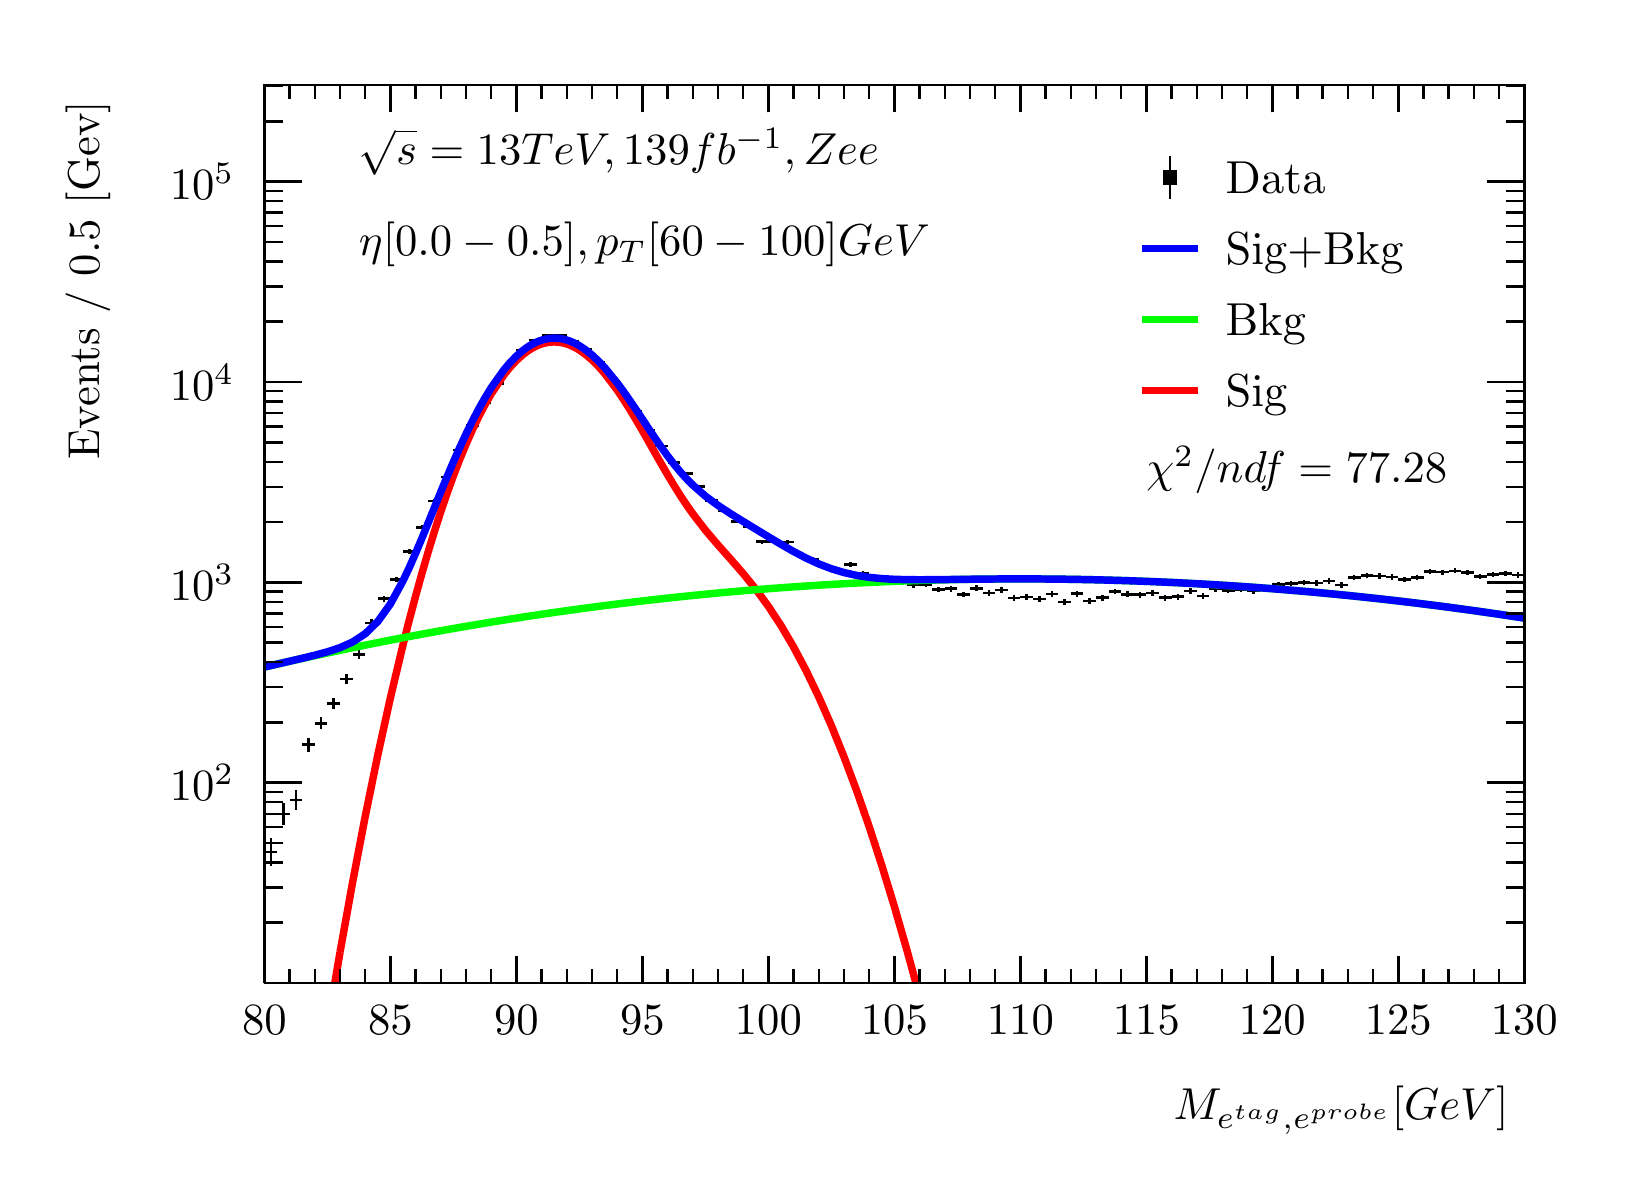
\begin{tikzpicture}
\pgfdeclareplotmark{cross} {
\pgfpathmoveto{\pgfpoint{-0.3\pgfplotmarksize}{\pgfplotmarksize}}
\pgfpathlineto{\pgfpoint{+0.3\pgfplotmarksize}{\pgfplotmarksize}}
\pgfpathlineto{\pgfpoint{+0.3\pgfplotmarksize}{0.3\pgfplotmarksize}}
\pgfpathlineto{\pgfpoint{+1\pgfplotmarksize}{0.3\pgfplotmarksize}}
\pgfpathlineto{\pgfpoint{+1\pgfplotmarksize}{-0.3\pgfplotmarksize}}
\pgfpathlineto{\pgfpoint{+0.3\pgfplotmarksize}{-0.3\pgfplotmarksize}}
\pgfpathlineto{\pgfpoint{+0.3\pgfplotmarksize}{-1.\pgfplotmarksize}}
\pgfpathlineto{\pgfpoint{-0.3\pgfplotmarksize}{-1.\pgfplotmarksize}}
\pgfpathlineto{\pgfpoint{-0.3\pgfplotmarksize}{-0.3\pgfplotmarksize}}
\pgfpathlineto{\pgfpoint{-1.\pgfplotmarksize}{-0.3\pgfplotmarksize}}
\pgfpathlineto{\pgfpoint{-1.\pgfplotmarksize}{0.3\pgfplotmarksize}}
\pgfpathlineto{\pgfpoint{-0.3\pgfplotmarksize}{0.3\pgfplotmarksize}}
\pgfpathclose
\pgfusepathqstroke
}
\pgfdeclareplotmark{cross*} {
\pgfpathmoveto{\pgfpoint{-0.3\pgfplotmarksize}{\pgfplotmarksize}}
\pgfpathlineto{\pgfpoint{+0.3\pgfplotmarksize}{\pgfplotmarksize}}
\pgfpathlineto{\pgfpoint{+0.3\pgfplotmarksize}{0.3\pgfplotmarksize}}
\pgfpathlineto{\pgfpoint{+1\pgfplotmarksize}{0.3\pgfplotmarksize}}
\pgfpathlineto{\pgfpoint{+1\pgfplotmarksize}{-0.3\pgfplotmarksize}}
\pgfpathlineto{\pgfpoint{+0.3\pgfplotmarksize}{-0.3\pgfplotmarksize}}
\pgfpathlineto{\pgfpoint{+0.3\pgfplotmarksize}{-1.\pgfplotmarksize}}
\pgfpathlineto{\pgfpoint{-0.3\pgfplotmarksize}{-1.\pgfplotmarksize}}
\pgfpathlineto{\pgfpoint{-0.3\pgfplotmarksize}{-0.3\pgfplotmarksize}}
\pgfpathlineto{\pgfpoint{-1.\pgfplotmarksize}{-0.3\pgfplotmarksize}}
\pgfpathlineto{\pgfpoint{-1.\pgfplotmarksize}{0.3\pgfplotmarksize}}
\pgfpathlineto{\pgfpoint{-0.3\pgfplotmarksize}{0.3\pgfplotmarksize}}
\pgfpathclose
\pgfusepathqfillstroke
}
\pgfdeclareplotmark{newstar} {
\pgfpathmoveto{\pgfqpoint{0pt}{\pgfplotmarksize}}
\pgfpathlineto{\pgfqpointpolar{44}{0.5\pgfplotmarksize}}
\pgfpathlineto{\pgfqpointpolar{18}{\pgfplotmarksize}}
\pgfpathlineto{\pgfqpointpolar{-20}{0.5\pgfplotmarksize}}
\pgfpathlineto{\pgfqpointpolar{-54}{\pgfplotmarksize}}
\pgfpathlineto{\pgfqpointpolar{-90}{0.5\pgfplotmarksize}}
\pgfpathlineto{\pgfqpointpolar{234}{\pgfplotmarksize}}
\pgfpathlineto{\pgfqpointpolar{198}{0.5\pgfplotmarksize}}
\pgfpathlineto{\pgfqpointpolar{162}{\pgfplotmarksize}}
\pgfpathlineto{\pgfqpointpolar{134}{0.5\pgfplotmarksize}}
\pgfpathclose
\pgfusepathqstroke
}
\pgfdeclareplotmark{newstar*} {
\pgfpathmoveto{\pgfqpoint{0pt}{\pgfplotmarksize}}
\pgfpathlineto{\pgfqpointpolar{44}{0.5\pgfplotmarksize}}
\pgfpathlineto{\pgfqpointpolar{18}{\pgfplotmarksize}}
\pgfpathlineto{\pgfqpointpolar{-20}{0.5\pgfplotmarksize}}
\pgfpathlineto{\pgfqpointpolar{-54}{\pgfplotmarksize}}
\pgfpathlineto{\pgfqpointpolar{-90}{0.5\pgfplotmarksize}}
\pgfpathlineto{\pgfqpointpolar{234}{\pgfplotmarksize}}
\pgfpathlineto{\pgfqpointpolar{198}{0.5\pgfplotmarksize}}
\pgfpathlineto{\pgfqpointpolar{162}{\pgfplotmarksize}}
\pgfpathlineto{\pgfqpointpolar{134}{0.5\pgfplotmarksize}}
\pgfpathclose
\pgfusepathqfillstroke
}
\definecolor{c}{rgb}{1,1,1};
\draw [color=c, fill=c] (0,0) rectangle (20,14.4361);
\draw [color=c, fill=c] (3,2.30977) rectangle (19,13.7143);
\definecolor{c}{rgb}{0,0,0};
\draw [c,line width=0.9] (3,2.30977) -- (3,13.7143) -- (19,13.7143) -- (19,2.30977) -- (3,2.30977);
\definecolor{c}{rgb}{1,1,1};
\draw [color=c, fill=c] (3,2.30977) rectangle (19,13.7143);
\definecolor{c}{rgb}{0,0,0};
\draw [c,line width=0.9] (3,2.30977) -- (3,13.7143) -- (19,13.7143) -- (19,2.30977) -- (3,2.30977);
\draw [c,line width=0.9] (3,2.30977) -- (19,2.30977);
\draw [c,line width=0.9] (3,2.65624) -- (3,2.30977);
\draw [c,line width=0.9] (3.32,2.48301) -- (3.32,2.30977);
\draw [c,line width=0.9] (3.64,2.48301) -- (3.64,2.30977);
\draw [c,line width=0.9] (3.96,2.48301) -- (3.96,2.30977);
\draw [c,line width=0.9] (4.28,2.48301) -- (4.28,2.30977);
\draw [c,line width=0.9] (4.6,2.65624) -- (4.6,2.30977);
\draw [c,line width=0.9] (4.92,2.48301) -- (4.92,2.30977);
\draw [c,line width=0.9] (5.24,2.48301) -- (5.24,2.30977);
\draw [c,line width=0.9] (5.56,2.48301) -- (5.56,2.30977);
\draw [c,line width=0.9] (5.88,2.48301) -- (5.88,2.30977);
\draw [c,line width=0.9] (6.2,2.65624) -- (6.2,2.30977);
\draw [c,line width=0.9] (6.52,2.48301) -- (6.52,2.30977);
\draw [c,line width=0.9] (6.84,2.48301) -- (6.84,2.30977);
\draw [c,line width=0.9] (7.16,2.48301) -- (7.16,2.30977);
\draw [c,line width=0.9] (7.48,2.48301) -- (7.48,2.30977);
\draw [c,line width=0.9] (7.8,2.65624) -- (7.8,2.30977);
\draw [c,line width=0.9] (8.12,2.48301) -- (8.12,2.30977);
\draw [c,line width=0.9] (8.44,2.48301) -- (8.44,2.30977);
\draw [c,line width=0.9] (8.76,2.48301) -- (8.76,2.30977);
\draw [c,line width=0.9] (9.08,2.48301) -- (9.08,2.30977);
\draw [c,line width=0.9] (9.4,2.65624) -- (9.4,2.30977);
\draw [c,line width=0.9] (9.72,2.48301) -- (9.72,2.30977);
\draw [c,line width=0.9] (10.04,2.48301) -- (10.04,2.30977);
\draw [c,line width=0.9] (10.36,2.48301) -- (10.36,2.30977);
\draw [c,line width=0.9] (10.68,2.48301) -- (10.68,2.30977);
\draw [c,line width=0.9] (11,2.65624) -- (11,2.30977);
\draw [c,line width=0.9] (11.32,2.48301) -- (11.32,2.30977);
\draw [c,line width=0.9] (11.64,2.48301) -- (11.64,2.30977);
\draw [c,line width=0.9] (11.96,2.48301) -- (11.96,2.30977);
\draw [c,line width=0.9] (12.28,2.48301) -- (12.28,2.30977);
\draw [c,line width=0.9] (12.6,2.65624) -- (12.6,2.30977);
\draw [c,line width=0.9] (12.92,2.48301) -- (12.92,2.30977);
\draw [c,line width=0.9] (13.24,2.48301) -- (13.24,2.30977);
\draw [c,line width=0.9] (13.56,2.48301) -- (13.56,2.30977);
\draw [c,line width=0.9] (13.88,2.48301) -- (13.88,2.30977);
\draw [c,line width=0.9] (14.2,2.65624) -- (14.2,2.30977);
\draw [c,line width=0.9] (14.52,2.48301) -- (14.52,2.30977);
\draw [c,line width=0.9] (14.84,2.48301) -- (14.84,2.30977);
\draw [c,line width=0.9] (15.16,2.48301) -- (15.16,2.30977);
\draw [c,line width=0.9] (15.48,2.48301) -- (15.48,2.30977);
\draw [c,line width=0.9] (15.8,2.65624) -- (15.8,2.30977);
\draw [c,line width=0.9] (16.12,2.48301) -- (16.12,2.30977);
\draw [c,line width=0.9] (16.44,2.48301) -- (16.44,2.30977);
\draw [c,line width=0.9] (16.76,2.48301) -- (16.76,2.30977);
\draw [c,line width=0.9] (17.08,2.48301) -- (17.08,2.30977);
\draw [c,line width=0.9] (17.4,2.65624) -- (17.4,2.30977);
\draw [c,line width=0.9] (17.72,2.48301) -- (17.72,2.30977);
\draw [c,line width=0.9] (18.04,2.48301) -- (18.04,2.30977);
\draw [c,line width=0.9] (18.36,2.48301) -- (18.36,2.30977);
\draw [c,line width=0.9] (18.68,2.48301) -- (18.68,2.30977);
\draw [c,line width=0.9] (19,2.65624) -- (19,2.30977);
\draw [anchor=base] (3,1.66015) node[scale=1.61424, color=c, rotate=0]{80};
\draw [anchor=base] (4.6,1.66015) node[scale=1.61424, color=c, rotate=0]{85};
\draw [anchor=base] (6.2,1.66015) node[scale=1.61424, color=c, rotate=0]{90};
\draw [anchor=base] (7.8,1.66015) node[scale=1.61424, color=c, rotate=0]{95};
\draw [anchor=base] (9.4,1.66015) node[scale=1.61424, color=c, rotate=0]{100};
\draw [anchor=base] (11,1.66015) node[scale=1.61424, color=c, rotate=0]{105};
\draw [anchor=base] (12.6,1.66015) node[scale=1.61424, color=c, rotate=0]{110};
\draw [anchor=base] (14.2,1.66015) node[scale=1.61424, color=c, rotate=0]{115};
\draw [anchor=base] (15.8,1.66015) node[scale=1.61424, color=c, rotate=0]{120};
\draw [anchor=base] (17.4,1.66015) node[scale=1.61424, color=c, rotate=0]{125};
\draw [anchor=base] (19,1.66015) node[scale=1.61424, color=c, rotate=0]{130};
\draw [anchor= east] (19,0.692932) node[scale=1.61424, color=c, rotate=0]{$M_{e^{tag}, e^{probe}}  [GeV]$};
\draw [c,line width=0.9] (3,13.7143) -- (19,13.7143);
\draw [c,line width=0.9] (3,13.3678) -- (3,13.7143);
\draw [c,line width=0.9] (3.32,13.5411) -- (3.32,13.7143);
\draw [c,line width=0.9] (3.64,13.5411) -- (3.64,13.7143);
\draw [c,line width=0.9] (3.96,13.5411) -- (3.96,13.7143);
\draw [c,line width=0.9] (4.28,13.5411) -- (4.28,13.7143);
\draw [c,line width=0.9] (4.6,13.3678) -- (4.6,13.7143);
\draw [c,line width=0.9] (4.92,13.5411) -- (4.92,13.7143);
\draw [c,line width=0.9] (5.24,13.5411) -- (5.24,13.7143);
\draw [c,line width=0.9] (5.56,13.5411) -- (5.56,13.7143);
\draw [c,line width=0.9] (5.88,13.5411) -- (5.88,13.7143);
\draw [c,line width=0.9] (6.2,13.3678) -- (6.2,13.7143);
\draw [c,line width=0.9] (6.52,13.5411) -- (6.52,13.7143);
\draw [c,line width=0.9] (6.84,13.5411) -- (6.84,13.7143);
\draw [c,line width=0.9] (7.16,13.5411) -- (7.16,13.7143);
\draw [c,line width=0.9] (7.48,13.5411) -- (7.48,13.7143);
\draw [c,line width=0.9] (7.8,13.3678) -- (7.8,13.7143);
\draw [c,line width=0.9] (8.12,13.5411) -- (8.12,13.7143);
\draw [c,line width=0.9] (8.44,13.5411) -- (8.44,13.7143);
\draw [c,line width=0.9] (8.76,13.5411) -- (8.76,13.7143);
\draw [c,line width=0.9] (9.08,13.5411) -- (9.08,13.7143);
\draw [c,line width=0.9] (9.4,13.3678) -- (9.4,13.7143);
\draw [c,line width=0.9] (9.72,13.5411) -- (9.72,13.7143);
\draw [c,line width=0.9] (10.04,13.5411) -- (10.04,13.7143);
\draw [c,line width=0.9] (10.36,13.5411) -- (10.36,13.7143);
\draw [c,line width=0.9] (10.68,13.5411) -- (10.68,13.7143);
\draw [c,line width=0.9] (11,13.3678) -- (11,13.7143);
\draw [c,line width=0.9] (11.32,13.5411) -- (11.32,13.7143);
\draw [c,line width=0.9] (11.64,13.5411) -- (11.64,13.7143);
\draw [c,line width=0.9] (11.96,13.5411) -- (11.96,13.7143);
\draw [c,line width=0.9] (12.28,13.5411) -- (12.28,13.7143);
\draw [c,line width=0.9] (12.6,13.3678) -- (12.6,13.7143);
\draw [c,line width=0.9] (12.92,13.5411) -- (12.92,13.7143);
\draw [c,line width=0.9] (13.24,13.5411) -- (13.24,13.7143);
\draw [c,line width=0.9] (13.56,13.5411) -- (13.56,13.7143);
\draw [c,line width=0.9] (13.88,13.5411) -- (13.88,13.7143);
\draw [c,line width=0.9] (14.2,13.3678) -- (14.2,13.7143);
\draw [c,line width=0.9] (14.52,13.5411) -- (14.52,13.7143);
\draw [c,line width=0.9] (14.84,13.5411) -- (14.84,13.7143);
\draw [c,line width=0.9] (15.16,13.5411) -- (15.16,13.7143);
\draw [c,line width=0.9] (15.48,13.5411) -- (15.48,13.7143);
\draw [c,line width=0.9] (15.8,13.3678) -- (15.8,13.7143);
\draw [c,line width=0.9] (16.12,13.5411) -- (16.12,13.7143);
\draw [c,line width=0.9] (16.44,13.5411) -- (16.44,13.7143);
\draw [c,line width=0.9] (16.76,13.5411) -- (16.76,13.7143);
\draw [c,line width=0.9] (17.08,13.5411) -- (17.08,13.7143);
\draw [c,line width=0.9] (17.4,13.3678) -- (17.4,13.7143);
\draw [c,line width=0.9] (17.72,13.5411) -- (17.72,13.7143);
\draw [c,line width=0.9] (18.04,13.5411) -- (18.04,13.7143);
\draw [c,line width=0.9] (18.36,13.5411) -- (18.36,13.7143);
\draw [c,line width=0.9] (18.68,13.5411) -- (18.68,13.7143);
\draw [c,line width=0.9] (19,13.3678) -- (19,13.7143);
\draw [c,line width=0.9] (3,2.30977) -- (3,13.7143);
\draw [c,line width=0.9] (3.237,3.07568) -- (3,3.07568);
\draw [c,line width=0.9] (3.237,3.5237) -- (3,3.5237);
\draw [c,line width=0.9] (3.237,3.84158) -- (3,3.84158);
\draw [c,line width=0.9] (3.237,4.08815) -- (3,4.08815);
\draw [c,line width=0.9] (3.237,4.2896) -- (3,4.2896);
\draw [c,line width=0.9] (3.237,4.45994) -- (3,4.45994);
\draw [c,line width=0.9] (3.237,4.60748) -- (3,4.60748);
\draw [c,line width=0.9] (3.237,4.73763) -- (3,4.73763);
\draw [c,line width=0.9] (3.474,4.85405) -- (3,4.85405);
\draw [anchor= east] (2.82,4.85405) node[scale=1.61424, color=c, rotate=0]{$10^{2}$};
\draw [c,line width=0.9] (3.237,5.61995) -- (3,5.61995);
\draw [c,line width=0.9] (3.237,6.06798) -- (3,6.06798);
\draw [c,line width=0.9] (3.237,6.38586) -- (3,6.38586);
\draw [c,line width=0.9] (3.237,6.63242) -- (3,6.63242);
\draw [c,line width=0.9] (3.237,6.83388) -- (3,6.83388);
\draw [c,line width=0.9] (3.237,7.00421) -- (3,7.00421);
\draw [c,line width=0.9] (3.237,7.15176) -- (3,7.15176);
\draw [c,line width=0.9] (3.237,7.28191) -- (3,7.28191);
\draw [c,line width=0.9] (3.474,7.39833) -- (3,7.39833);
\draw [anchor= east] (2.82,7.39833) node[scale=1.61424, color=c, rotate=0]{$10^{3}$};
\draw [c,line width=0.9] (3.237,8.16423) -- (3,8.16423);
\draw [c,line width=0.9] (3.237,8.61226) -- (3,8.61226);
\draw [c,line width=0.9] (3.237,8.93013) -- (3,8.93013);
\draw [c,line width=0.9] (3.237,9.1767) -- (3,9.1767);
\draw [c,line width=0.9] (3.237,9.37816) -- (3,9.37816);
\draw [c,line width=0.9] (3.237,9.54849) -- (3,9.54849);
\draw [c,line width=0.9] (3.237,9.69604) -- (3,9.69604);
\draw [c,line width=0.9] (3.237,9.82618) -- (3,9.82618);
\draw [c,line width=0.9] (3.474,9.9426) -- (3,9.9426);
\draw [anchor= east] (2.82,9.9426) node[scale=1.61424, color=c, rotate=0]{$10^{4}$};
\draw [c,line width=0.9] (3.237,10.7085) -- (3,10.7085);
\draw [c,line width=0.9] (3.237,11.1565) -- (3,11.1565);
\draw [c,line width=0.9] (3.237,11.4744) -- (3,11.4744);
\draw [c,line width=0.9] (3.237,11.721) -- (3,11.721);
\draw [c,line width=0.9] (3.237,11.9224) -- (3,11.9224);
\draw [c,line width=0.9] (3.237,12.0928) -- (3,12.0928);
\draw [c,line width=0.9] (3.237,12.2403) -- (3,12.2403);
\draw [c,line width=0.9] (3.237,12.3705) -- (3,12.3705);
\draw [c,line width=0.9] (3.474,12.4869) -- (3,12.4869);
\draw [anchor= east] (2.82,12.4869) node[scale=1.61424, color=c, rotate=0]{$10^{5}$};
\draw [c,line width=0.9] (3.237,13.2528) -- (3,13.2528);
\draw [c,line width=0.9] (3.237,13.7008) -- (3,13.7008);
\draw [anchor= east] (0.76,13.7143) node[scale=1.61424, color=c, rotate=90]{Events / 0.5 [Gev]};
\draw [c,line width=0.9] (19,2.30977) -- (19,13.7143);
\draw [c,line width=0.9] (18.763,3.07568) -- (19,3.07568);
\draw [c,line width=0.9] (18.763,3.5237) -- (19,3.5237);
\draw [c,line width=0.9] (18.763,3.84158) -- (19,3.84158);
\draw [c,line width=0.9] (18.763,4.08815) -- (19,4.08815);
\draw [c,line width=0.9] (18.763,4.2896) -- (19,4.2896);
\draw [c,line width=0.9] (18.763,4.45994) -- (19,4.45994);
\draw [c,line width=0.9] (18.763,4.60748) -- (19,4.60748);
\draw [c,line width=0.9] (18.763,4.73763) -- (19,4.73763);
\draw [c,line width=0.9] (18.526,4.85405) -- (19,4.85405);
\draw [c,line width=0.9] (18.763,5.61995) -- (19,5.61995);
\draw [c,line width=0.9] (18.763,6.06798) -- (19,6.06798);
\draw [c,line width=0.9] (18.763,6.38586) -- (19,6.38586);
\draw [c,line width=0.9] (18.763,6.63242) -- (19,6.63242);
\draw [c,line width=0.9] (18.763,6.83388) -- (19,6.83388);
\draw [c,line width=0.9] (18.763,7.00421) -- (19,7.00421);
\draw [c,line width=0.9] (18.763,7.15176) -- (19,7.15176);
\draw [c,line width=0.9] (18.763,7.28191) -- (19,7.28191);
\draw [c,line width=0.9] (18.526,7.39833) -- (19,7.39833);
\draw [c,line width=0.9] (18.763,8.16423) -- (19,8.16423);
\draw [c,line width=0.9] (18.763,8.61226) -- (19,8.61226);
\draw [c,line width=0.9] (18.763,8.93013) -- (19,8.93013);
\draw [c,line width=0.9] (18.763,9.1767) -- (19,9.1767);
\draw [c,line width=0.9] (18.763,9.37816) -- (19,9.37816);
\draw [c,line width=0.9] (18.763,9.54849) -- (19,9.54849);
\draw [c,line width=0.9] (18.763,9.69604) -- (19,9.69604);
\draw [c,line width=0.9] (18.763,9.82618) -- (19,9.82618);
\draw [c,line width=0.9] (18.526,9.9426) -- (19,9.9426);
\draw [c,line width=0.9] (18.763,10.7085) -- (19,10.7085);
\draw [c,line width=0.9] (18.763,11.1565) -- (19,11.1565);
\draw [c,line width=0.9] (18.763,11.4744) -- (19,11.4744);
\draw [c,line width=0.9] (18.763,11.721) -- (19,11.721);
\draw [c,line width=0.9] (18.763,11.9224) -- (19,11.9224);
\draw [c,line width=0.9] (18.763,12.0928) -- (19,12.0928);
\draw [c,line width=0.9] (18.763,12.2403) -- (19,12.2403);
\draw [c,line width=0.9] (18.763,12.3705) -- (19,12.3705);
\draw [c,line width=0.9] (18.526,12.4869) -- (19,12.4869);
\draw [c,line width=0.9] (18.763,13.2528) -- (19,13.2528);
\draw [c,line width=0.9] (18.763,13.7008) -- (19,13.7008);
\draw [c,line width=0.9] (3.08,3.97173) -- (3,3.97173);
\draw [c,line width=0.9] (3,3.97173) -- (3,3.97173);
\draw [c,line width=0.9] (3.08,3.97173) -- (3.16,3.97173);
\draw [c,line width=0.9] (3.16,3.97173) -- (3.16,3.97173);
\draw [c,line width=0.9] (3.08,3.97173) -- (3.08,4.14747);
\draw [c,line width=0.9] (3.08,4.14747) -- (3.08,4.14747);
\draw [c,line width=0.9] (3.08,3.97173) -- (3.08,3.79408);
\draw [c,line width=0.9] (3.08,3.79408) -- (3.08,3.79408);
\draw [c,line width=0.9] (3.24,4.45994) -- (3.16,4.45994);
\draw [c,line width=0.9] (3.16,4.45994) -- (3.16,4.45994);
\draw [c,line width=0.9] (3.24,4.45994) -- (3.32,4.45994);
\draw [c,line width=0.9] (3.32,4.45994) -- (3.32,4.45994);
\draw [c,line width=0.9] (3.24,4.45994) -- (3.24,4.59926);
\draw [c,line width=0.9] (3.24,4.59926) -- (3.24,4.59926);
\draw [c,line width=0.9] (3.24,4.45994) -- (3.24,4.31964);
\draw [c,line width=0.9] (3.24,4.31964) -- (3.24,4.31964);
\draw [c,line width=0.9] (3.4,4.63477) -- (3.32,4.63477);
\draw [c,line width=0.9] (3.32,4.63477) -- (3.32,4.63477);
\draw [c,line width=0.9] (3.4,4.63477) -- (3.48,4.63477);
\draw [c,line width=0.9] (3.48,4.63477) -- (3.48,4.63477);
\draw [c,line width=0.9] (3.4,4.63477) -- (3.4,4.76302);
\draw [c,line width=0.9] (3.4,4.76302) -- (3.4,4.76302);
\draw [c,line width=0.9] (3.4,4.63477) -- (3.4,4.50575);
\draw [c,line width=0.9] (3.4,4.50575) -- (3.4,4.50575);
\draw [c,line width=0.9] (3.56,5.33831) -- (3.48,5.33831);
\draw [c,line width=0.9] (3.48,5.33831) -- (3.48,5.33831);
\draw [c,line width=0.9] (3.56,5.33831) -- (3.64,5.33831);
\draw [c,line width=0.9] (3.64,5.33831) -- (3.64,5.33831);
\draw [c,line width=0.9] (3.56,5.33831) -- (3.56,5.42704);
\draw [c,line width=0.9] (3.56,5.42704) -- (3.56,5.42704);
\draw [c,line width=0.9] (3.56,5.33831) -- (3.56,5.24958);
\draw [c,line width=0.9] (3.56,5.24958) -- (3.56,5.24958);
\draw [c,line width=0.9] (3.72,5.60885) -- (3.64,5.60885);
\draw [c,line width=0.9] (3.64,5.60885) -- (3.64,5.60885);
\draw [c,line width=0.9] (3.72,5.60885) -- (3.8,5.60885);
\draw [c,line width=0.9] (3.8,5.60885) -- (3.8,5.60885);
\draw [c,line width=0.9] (3.72,5.60885) -- (3.72,5.68736);
\draw [c,line width=0.9] (3.72,5.68736) -- (3.72,5.68736);
\draw [c,line width=0.9] (3.72,5.60885) -- (3.72,5.53034);
\draw [c,line width=0.9] (3.72,5.53034) -- (3.72,5.53034);
\draw [c,line width=0.9] (3.88,5.85765) -- (3.8,5.85765);
\draw [c,line width=0.9] (3.8,5.85765) -- (3.8,5.85765);
\draw [c,line width=0.9] (3.88,5.85765) -- (3.96,5.85765);
\draw [c,line width=0.9] (3.96,5.85765) -- (3.96,5.85765);
\draw [c,line width=0.9] (3.88,5.85765) -- (3.88,5.9278);
\draw [c,line width=0.9] (3.88,5.9278) -- (3.88,5.9278);
\draw [c,line width=0.9] (3.88,5.85765) -- (3.88,5.78749);
\draw [c,line width=0.9] (3.88,5.78749) -- (3.88,5.78749);
\draw [c,line width=0.9] (4.04,6.16994) -- (3.96,6.16994);
\draw [c,line width=0.9] (3.96,6.16994) -- (3.96,6.16994);
\draw [c,line width=0.9] (4.04,6.16994) -- (4.12,6.16994);
\draw [c,line width=0.9] (4.12,6.16994) -- (4.12,6.16994);
\draw [c,line width=0.9] (4.04,6.16994) -- (4.04,6.23085);
\draw [c,line width=0.9] (4.04,6.23085) -- (4.04,6.23085);
\draw [c,line width=0.9] (4.04,6.16994) -- (4.04,6.10903);
\draw [c,line width=0.9] (4.04,6.10903) -- (4.04,6.10903);
\draw [c,line width=0.9] (4.2,6.48361) -- (4.12,6.48361);
\draw [c,line width=0.9] (4.12,6.48361) -- (4.12,6.48361);
\draw [c,line width=0.9] (4.2,6.48361) -- (4.28,6.48361);
\draw [c,line width=0.9] (4.28,6.48361) -- (4.28,6.48361);
\draw [c,line width=0.9] (4.2,6.48361) -- (4.2,6.53647);
\draw [c,line width=0.9] (4.2,6.53647) -- (4.2,6.53647);
\draw [c,line width=0.9] (4.2,6.48361) -- (4.2,6.43076);
\draw [c,line width=0.9] (4.2,6.43076) -- (4.2,6.43076);
\draw [c,line width=0.9] (4.36,6.88428) -- (4.28,6.88428);
\draw [c,line width=0.9] (4.28,6.88428) -- (4.28,6.88428);
\draw [c,line width=0.9] (4.36,6.88428) -- (4.44,6.88428);
\draw [c,line width=0.9] (4.44,6.88428) -- (4.44,6.88428);
\draw [c,line width=0.9] (4.36,6.88428) -- (4.36,6.92837);
\draw [c,line width=0.9] (4.36,6.92837) -- (4.36,6.92837);
\draw [c,line width=0.9] (4.36,6.88428) -- (4.36,6.84019);
\draw [c,line width=0.9] (4.36,6.84019) -- (4.36,6.84019);
\draw [c,line width=0.9] (4.52,7.19244) -- (4.44,7.19244);
\draw [c,line width=0.9] (4.44,7.19244) -- (4.44,7.19244);
\draw [c,line width=0.9] (4.52,7.19244) -- (4.6,7.19244);
\draw [c,line width=0.9] (4.6,7.19244) -- (4.6,7.19244);
\draw [c,line width=0.9] (4.52,7.19244) -- (4.52,7.23079);
\draw [c,line width=0.9] (4.52,7.23079) -- (4.52,7.23079);
\draw [c,line width=0.9] (4.52,7.19244) -- (4.52,7.15409);
\draw [c,line width=0.9] (4.52,7.15409) -- (4.52,7.15409);
\draw [c,line width=0.9] (4.68,7.4342) -- (4.6,7.4342);
\draw [c,line width=0.9] (4.6,7.4342) -- (4.6,7.4342);
\draw [c,line width=0.9] (4.68,7.4342) -- (4.76,7.4342);
\draw [c,line width=0.9] (4.76,7.4342) -- (4.76,7.4342);
\draw [c,line width=0.9] (4.68,7.4342) -- (4.68,7.46858);
\draw [c,line width=0.9] (4.68,7.46858) -- (4.68,7.46858);
\draw [c,line width=0.9] (4.68,7.4342) -- (4.68,7.39983);
\draw [c,line width=0.9] (4.68,7.39983) -- (4.68,7.39983);
\draw [c,line width=0.9] (4.84,7.7889) -- (4.76,7.7889);
\draw [c,line width=0.9] (4.76,7.7889) -- (4.76,7.7889);
\draw [c,line width=0.9] (4.84,7.7889) -- (4.92,7.7889);
\draw [c,line width=0.9] (4.92,7.7889) -- (4.92,7.7889);
\draw [c,line width=0.9] (4.84,7.7889) -- (4.84,7.81818);
\draw [c,line width=0.9] (4.84,7.81818) -- (4.84,7.81818);
\draw [c,line width=0.9] (4.84,7.7889) -- (4.84,7.75962);
\draw [c,line width=0.9] (4.84,7.75962) -- (4.84,7.75962);
\draw [c,line width=0.9] (5,8.09645) -- (4.92,8.09645);
\draw [c,line width=0.9] (4.92,8.09645) -- (4.92,8.09645);
\draw [c,line width=0.9] (5,8.09645) -- (5.08,8.09645);
\draw [c,line width=0.9] (5.08,8.09645) -- (5.08,8.09645);
\draw [c,line width=0.9] (5,8.09645) -- (5,8.12193);
\draw [c,line width=0.9] (5,8.12193) -- (5,8.12193);
\draw [c,line width=0.9] (5,8.09645) -- (5,8.07097);
\draw [c,line width=0.9] (5,8.07097) -- (5,8.07097);
\draw [c,line width=0.9] (5.16,8.43008) -- (5.08,8.43008);
\draw [c,line width=0.9] (5.08,8.43008) -- (5.08,8.43008);
\draw [c,line width=0.9] (5.16,8.43008) -- (5.24,8.43008);
\draw [c,line width=0.9] (5.24,8.43008) -- (5.24,8.43008);
\draw [c,line width=0.9] (5.16,8.43008) -- (5.16,8.45198);
\draw [c,line width=0.9] (5.16,8.45198) -- (5.16,8.45198);
\draw [c,line width=0.9] (5.16,8.43008) -- (5.16,8.40817);
\draw [c,line width=0.9] (5.16,8.40817) -- (5.16,8.40817);
\draw [c,line width=0.9] (5.32,8.73386) -- (5.24,8.73386);
\draw [c,line width=0.9] (5.24,8.73386) -- (5.24,8.73386);
\draw [c,line width=0.9] (5.32,8.73386) -- (5.4,8.73386);
\draw [c,line width=0.9] (5.4,8.73386) -- (5.4,8.73386);
\draw [c,line width=0.9] (5.32,8.73386) -- (5.32,8.75295);
\draw [c,line width=0.9] (5.32,8.75295) -- (5.32,8.75295);
\draw [c,line width=0.9] (5.32,8.73386) -- (5.32,8.71476);
\draw [c,line width=0.9] (5.32,8.71476) -- (5.32,8.71476);
\draw [c,line width=0.9] (5.48,9.07903) -- (5.4,9.07903);
\draw [c,line width=0.9] (5.4,9.07903) -- (5.4,9.07903);
\draw [c,line width=0.9] (5.48,9.07903) -- (5.56,9.07903);
\draw [c,line width=0.9] (5.56,9.07903) -- (5.56,9.07903);
\draw [c,line width=0.9] (5.48,9.07903) -- (5.48,9.09536);
\draw [c,line width=0.9] (5.48,9.09536) -- (5.48,9.09536);
\draw [c,line width=0.9] (5.48,9.07903) -- (5.48,9.0627);
\draw [c,line width=0.9] (5.48,9.0627) -- (5.48,9.0627);
\draw [c,line width=0.9] (5.64,9.39261) -- (5.56,9.39261);
\draw [c,line width=0.9] (5.56,9.39261) -- (5.56,9.39261);
\draw [c,line width=0.9] (5.64,9.39261) -- (5.72,9.39261);
\draw [c,line width=0.9] (5.72,9.39261) -- (5.72,9.39261);
\draw [c,line width=0.9] (5.64,9.39261) -- (5.64,9.40679);
\draw [c,line width=0.9] (5.64,9.40679) -- (5.64,9.40679);
\draw [c,line width=0.9] (5.64,9.39261) -- (5.64,9.37844);
\draw [c,line width=0.9] (5.64,9.37844) -- (5.64,9.37844);
\draw [c,line width=0.9] (5.8,9.67681) -- (5.72,9.67681);
\draw [c,line width=0.9] (5.72,9.67681) -- (5.72,9.67681);
\draw [c,line width=0.9] (5.8,9.67681) -- (5.88,9.67681);
\draw [c,line width=0.9] (5.88,9.67681) -- (5.88,9.67681);
\draw [c,line width=0.9] (5.8,9.67681) -- (5.8,9.68927);
\draw [c,line width=0.9] (5.8,9.68927) -- (5.8,9.68927);
\draw [c,line width=0.9] (5.8,9.67681) -- (5.8,9.66435);
\draw [c,line width=0.9] (5.8,9.66435) -- (5.8,9.66435);
\draw [c,line width=0.9] (5.96,9.9213) -- (5.88,9.9213);
\draw [c,line width=0.9] (5.88,9.9213) -- (5.88,9.9213);
\draw [c,line width=0.9] (5.96,9.9213) -- (6.04,9.9213);
\draw [c,line width=0.9] (6.04,9.9213) -- (6.04,9.9213);
\draw [c,line width=0.9] (5.96,9.9213) -- (5.96,9.93245);
\draw [c,line width=0.9] (5.96,9.93245) -- (5.96,9.93245);
\draw [c,line width=0.9] (5.96,9.9213) -- (5.96,9.91014);
\draw [c,line width=0.9] (5.96,9.91014) -- (5.96,9.91014);
\draw [c,line width=0.9] (6.12,10.1618) -- (6.04,10.1618);
\draw [c,line width=0.9] (6.04,10.1618) -- (6.04,10.1618);
\draw [c,line width=0.9] (6.12,10.1618) -- (6.2,10.1618);
\draw [c,line width=0.9] (6.2,10.1618) -- (6.2,10.1618);
\draw [c,line width=0.9] (6.12,10.1618) -- (6.12,10.1718);
\draw [c,line width=0.9] (6.12,10.1718) -- (6.12,10.1718);
\draw [c,line width=0.9] (6.12,10.1618) -- (6.12,10.1518);
\draw [c,line width=0.9] (6.12,10.1518) -- (6.12,10.1518);
\draw [c,line width=0.9] (6.28,10.3471) -- (6.2,10.3471);
\draw [c,line width=0.9] (6.2,10.3471) -- (6.2,10.3471);
\draw [c,line width=0.9] (6.28,10.3471) -- (6.36,10.3471);
\draw [c,line width=0.9] (6.36,10.3471) -- (6.36,10.3471);
\draw [c,line width=0.9] (6.28,10.3471) -- (6.28,10.3563);
\draw [c,line width=0.9] (6.28,10.3563) -- (6.28,10.3563);
\draw [c,line width=0.9] (6.28,10.3471) -- (6.28,10.3379);
\draw [c,line width=0.9] (6.28,10.3379) -- (6.28,10.3379);
\draw [c,line width=0.9] (6.44,10.4746) -- (6.36,10.4746);
\draw [c,line width=0.9] (6.36,10.4746) -- (6.36,10.4746);
\draw [c,line width=0.9] (6.44,10.4746) -- (6.52,10.4746);
\draw [c,line width=0.9] (6.52,10.4746) -- (6.52,10.4746);
\draw [c,line width=0.9] (6.44,10.4746) -- (6.44,10.4833);
\draw [c,line width=0.9] (6.44,10.4833) -- (6.44,10.4833);
\draw [c,line width=0.9] (6.44,10.4746) -- (6.44,10.466);
\draw [c,line width=0.9] (6.44,10.466) -- (6.44,10.466);
\draw [c,line width=0.9] (6.6,10.5373) -- (6.52,10.5373);
\draw [c,line width=0.9] (6.52,10.5373) -- (6.52,10.5373);
\draw [c,line width=0.9] (6.6,10.5373) -- (6.68,10.5373);
\draw [c,line width=0.9] (6.68,10.5373) -- (6.68,10.5373);
\draw [c,line width=0.9] (6.6,10.5373) -- (6.6,10.5457);
\draw [c,line width=0.9] (6.6,10.5457) -- (6.6,10.5457);
\draw [c,line width=0.9] (6.6,10.5373) -- (6.6,10.5288);
\draw [c,line width=0.9] (6.6,10.5288) -- (6.6,10.5288);
\draw [c,line width=0.9] (6.76,10.5319) -- (6.68,10.5319);
\draw [c,line width=0.9] (6.68,10.5319) -- (6.68,10.5319);
\draw [c,line width=0.9] (6.76,10.5319) -- (6.84,10.5319);
\draw [c,line width=0.9] (6.84,10.5319) -- (6.84,10.5319);
\draw [c,line width=0.9] (6.76,10.5319) -- (6.76,10.5403);
\draw [c,line width=0.9] (6.76,10.5403) -- (6.76,10.5403);
\draw [c,line width=0.9] (6.76,10.5319) -- (6.76,10.5234);
\draw [c,line width=0.9] (6.76,10.5234) -- (6.76,10.5234);
\draw [c,line width=0.9] (6.92,10.4613) -- (6.84,10.4613);
\draw [c,line width=0.9] (6.84,10.4613) -- (6.84,10.4613);
\draw [c,line width=0.9] (6.92,10.4613) -- (7,10.4613);
\draw [c,line width=0.9] (7,10.4613) -- (7,10.4613);
\draw [c,line width=0.9] (6.92,10.4613) -- (6.92,10.4701);
\draw [c,line width=0.9] (6.92,10.4701) -- (6.92,10.4701);
\draw [c,line width=0.9] (6.92,10.4613) -- (6.92,10.4526);
\draw [c,line width=0.9] (6.92,10.4526) -- (6.92,10.4526);
\draw [c,line width=0.9] (7.08,10.3639) -- (7,10.3639);
\draw [c,line width=0.9] (7,10.3639) -- (7,10.3639);
\draw [c,line width=0.9] (7.08,10.3639) -- (7.16,10.3639);
\draw [c,line width=0.9] (7.16,10.3639) -- (7.16,10.3639);
\draw [c,line width=0.9] (7.08,10.3639) -- (7.08,10.373);
\draw [c,line width=0.9] (7.08,10.373) -- (7.08,10.373);
\draw [c,line width=0.9] (7.08,10.3639) -- (7.08,10.3547);
\draw [c,line width=0.9] (7.08,10.3547) -- (7.08,10.3547);
\draw [c,line width=0.9] (7.24,10.1946) -- (7.16,10.1946);
\draw [c,line width=0.9] (7.16,10.1946) -- (7.16,10.1946);
\draw [c,line width=0.9] (7.24,10.1946) -- (7.32,10.1946);
\draw [c,line width=0.9] (7.32,10.1946) -- (7.32,10.1946);
\draw [c,line width=0.9] (7.24,10.1946) -- (7.24,10.2044);
\draw [c,line width=0.9] (7.24,10.2044) -- (7.24,10.2044);
\draw [c,line width=0.9] (7.24,10.1946) -- (7.24,10.1847);
\draw [c,line width=0.9] (7.24,10.1847) -- (7.24,10.1847);
\draw [c,line width=0.9] (7.4,9.9942) -- (7.32,9.9942);
\draw [c,line width=0.9] (7.32,9.9942) -- (7.32,9.9942);
\draw [c,line width=0.9] (7.4,9.9942) -- (7.48,9.9942);
\draw [c,line width=0.9] (7.48,9.9942) -- (7.48,9.9942);
\draw [c,line width=0.9] (7.4,9.9942) -- (7.4,10.005);
\draw [c,line width=0.9] (7.4,10.005) -- (7.4,10.005);
\draw [c,line width=0.9] (7.4,9.9942) -- (7.4,9.9834);
\draw [c,line width=0.9] (7.4,9.9834) -- (7.4,9.9834);
\draw [c,line width=0.9] (7.56,9.77273) -- (7.48,9.77273);
\draw [c,line width=0.9] (7.48,9.77273) -- (7.48,9.77273);
\draw [c,line width=0.9] (7.56,9.77273) -- (7.64,9.77273);
\draw [c,line width=0.9] (7.64,9.77273) -- (7.64,9.77273);
\draw [c,line width=0.9] (7.56,9.77273) -- (7.56,9.78467);
\draw [c,line width=0.9] (7.56,9.78467) -- (7.56,9.78467);
\draw [c,line width=0.9] (7.56,9.77273) -- (7.56,9.7608);
\draw [c,line width=0.9] (7.56,9.7608) -- (7.56,9.7608);
\draw [c,line width=0.9] (7.72,9.57099) -- (7.64,9.57099);
\draw [c,line width=0.9] (7.64,9.57099) -- (7.64,9.57099);
\draw [c,line width=0.9] (7.72,9.57099) -- (7.8,9.57099);
\draw [c,line width=0.9] (7.8,9.57099) -- (7.8,9.57099);
\draw [c,line width=0.9] (7.72,9.57099) -- (7.72,9.58406);
\draw [c,line width=0.9] (7.72,9.58406) -- (7.72,9.58406);
\draw [c,line width=0.9] (7.72,9.57099) -- (7.72,9.55792);
\draw [c,line width=0.9] (7.72,9.55792) -- (7.72,9.55792);
\draw [c,line width=0.9] (7.88,9.33075) -- (7.8,9.33075);
\draw [c,line width=0.9] (7.8,9.33075) -- (7.8,9.33075);
\draw [c,line width=0.9] (7.88,9.33075) -- (7.96,9.33075);
\draw [c,line width=0.9] (7.96,9.33075) -- (7.96,9.33075);
\draw [c,line width=0.9] (7.88,9.33075) -- (7.88,9.34532);
\draw [c,line width=0.9] (7.88,9.34532) -- (7.88,9.34532);
\draw [c,line width=0.9] (7.88,9.33075) -- (7.88,9.31617);
\draw [c,line width=0.9] (7.88,9.31617) -- (7.88,9.31617);
\draw [c,line width=0.9] (8.04,9.13159) -- (7.96,9.13159);
\draw [c,line width=0.9] (7.96,9.13159) -- (7.96,9.13159);
\draw [c,line width=0.9] (8.04,9.13159) -- (8.12,9.13159);
\draw [c,line width=0.9] (8.12,9.13159) -- (8.12,9.13159);
\draw [c,line width=0.9] (8.04,9.13159) -- (8.04,9.14754);
\draw [c,line width=0.9] (8.04,9.14754) -- (8.04,9.14754);
\draw [c,line width=0.9] (8.04,9.13159) -- (8.04,9.11565);
\draw [c,line width=0.9] (8.04,9.11565) -- (8.04,9.11565);
\draw [c,line width=0.9] (8.2,8.91903) -- (8.12,8.91903);
\draw [c,line width=0.9] (8.12,8.91903) -- (8.12,8.91903);
\draw [c,line width=0.9] (8.2,8.91903) -- (8.28,8.91903);
\draw [c,line width=0.9] (8.28,8.91903) -- (8.28,8.91903);
\draw [c,line width=0.9] (8.2,8.91903) -- (8.2,8.93659);
\draw [c,line width=0.9] (8.2,8.93659) -- (8.2,8.93659);
\draw [c,line width=0.9] (8.2,8.91903) -- (8.2,8.90147);
\draw [c,line width=0.9] (8.2,8.90147) -- (8.2,8.90147);
\draw [c,line width=0.9] (8.36,8.77911) -- (8.28,8.77911);
\draw [c,line width=0.9] (8.28,8.77911) -- (8.28,8.77911);
\draw [c,line width=0.9] (8.36,8.77911) -- (8.44,8.77911);
\draw [c,line width=0.9] (8.44,8.77911) -- (8.44,8.77911);
\draw [c,line width=0.9] (8.36,8.77911) -- (8.36,8.79782);
\draw [c,line width=0.9] (8.36,8.79782) -- (8.36,8.79782);
\draw [c,line width=0.9] (8.36,8.77911) -- (8.36,8.7604);
\draw [c,line width=0.9] (8.36,8.7604) -- (8.36,8.7604);
\draw [c,line width=0.9] (8.52,8.61887) -- (8.44,8.61887);
\draw [c,line width=0.9] (8.44,8.61887) -- (8.44,8.61887);
\draw [c,line width=0.9] (8.52,8.61887) -- (8.6,8.61887);
\draw [c,line width=0.9] (8.6,8.61887) -- (8.6,8.61887);
\draw [c,line width=0.9] (8.52,8.61887) -- (8.52,8.63898);
\draw [c,line width=0.9] (8.52,8.63898) -- (8.52,8.63898);
\draw [c,line width=0.9] (8.52,8.61887) -- (8.52,8.59875);
\draw [c,line width=0.9] (8.52,8.59875) -- (8.52,8.59875);
\draw [c,line width=0.9] (8.68,8.43657) -- (8.6,8.43657);
\draw [c,line width=0.9] (8.6,8.43657) -- (8.6,8.43657);
\draw [c,line width=0.9] (8.68,8.43657) -- (8.76,8.43657);
\draw [c,line width=0.9] (8.76,8.43657) -- (8.76,8.43657);
\draw [c,line width=0.9] (8.68,8.43657) -- (8.68,8.45842);
\draw [c,line width=0.9] (8.68,8.45842) -- (8.68,8.45842);
\draw [c,line width=0.9] (8.68,8.43657) -- (8.68,8.41473);
\draw [c,line width=0.9] (8.68,8.41473) -- (8.68,8.41473);
\draw [c,line width=0.9] (8.84,8.30464) -- (8.76,8.30464);
\draw [c,line width=0.9] (8.76,8.30464) -- (8.76,8.30464);
\draw [c,line width=0.9] (8.84,8.30464) -- (8.92,8.30464);
\draw [c,line width=0.9] (8.92,8.30464) -- (8.92,8.30464);
\draw [c,line width=0.9] (8.84,8.30464) -- (8.84,8.32783);
\draw [c,line width=0.9] (8.84,8.32783) -- (8.84,8.32783);
\draw [c,line width=0.9] (8.84,8.30464) -- (8.84,8.28146);
\draw [c,line width=0.9] (8.84,8.28146) -- (8.84,8.28146);
\draw [c,line width=0.9] (9,8.17358) -- (8.92,8.17358);
\draw [c,line width=0.9] (8.92,8.17358) -- (8.92,8.17358);
\draw [c,line width=0.9] (9,8.17358) -- (9.08,8.17358);
\draw [c,line width=0.9] (9.08,8.17358) -- (9.08,8.17358);
\draw [c,line width=0.9] (9,8.17358) -- (9,8.19819);
\draw [c,line width=0.9] (9,8.19819) -- (9,8.19819);
\draw [c,line width=0.9] (9,8.17358) -- (9,8.14898);
\draw [c,line width=0.9] (9,8.14898) -- (9,8.14898);
\draw [c,line width=0.9] (9.16,8.10231) -- (9.08,8.10231);
\draw [c,line width=0.9] (9.08,8.10231) -- (9.08,8.10231);
\draw [c,line width=0.9] (9.16,8.10231) -- (9.24,8.10231);
\draw [c,line width=0.9] (9.24,8.10231) -- (9.24,8.10231);
\draw [c,line width=0.9] (9.16,8.10231) -- (9.16,8.12772);
\draw [c,line width=0.9] (9.16,8.12772) -- (9.16,8.12772);
\draw [c,line width=0.9] (9.16,8.10231) -- (9.16,8.0769);
\draw [c,line width=0.9] (9.16,8.0769) -- (9.16,8.0769);
\draw [c,line width=0.9] (9.32,7.9149) -- (9.24,7.9149);
\draw [c,line width=0.9] (9.24,7.9149) -- (9.24,7.9149);
\draw [c,line width=0.9] (9.32,7.9149) -- (9.4,7.9149);
\draw [c,line width=0.9] (9.4,7.9149) -- (9.4,7.9149);
\draw [c,line width=0.9] (9.32,7.9149) -- (9.32,7.94256);
\draw [c,line width=0.9] (9.32,7.94256) -- (9.32,7.94256);
\draw [c,line width=0.9] (9.32,7.9149) -- (9.32,7.88724);
\draw [c,line width=0.9] (9.32,7.88724) -- (9.32,7.88724);
\draw [c,line width=0.9] (9.48,7.90865) -- (9.4,7.90865);
\draw [c,line width=0.9] (9.4,7.90865) -- (9.4,7.90865);
\draw [c,line width=0.9] (9.48,7.90865) -- (9.56,7.90865);
\draw [c,line width=0.9] (9.56,7.90865) -- (9.56,7.90865);
\draw [c,line width=0.9] (9.48,7.90865) -- (9.48,7.93639);
\draw [c,line width=0.9] (9.48,7.93639) -- (9.48,7.93639);
\draw [c,line width=0.9] (9.48,7.90865) -- (9.48,7.88092);
\draw [c,line width=0.9] (9.48,7.88092) -- (9.48,7.88092);
\draw [c,line width=0.9] (9.64,7.90795) -- (9.56,7.90795);
\draw [c,line width=0.9] (9.56,7.90795) -- (9.56,7.90795);
\draw [c,line width=0.9] (9.64,7.90795) -- (9.72,7.90795);
\draw [c,line width=0.9] (9.72,7.90795) -- (9.72,7.90795);
\draw [c,line width=0.9] (9.64,7.90795) -- (9.64,7.9357);
\draw [c,line width=0.9] (9.64,7.9357) -- (9.64,7.9357);
\draw [c,line width=0.9] (9.64,7.90795) -- (9.64,7.88021);
\draw [c,line width=0.9] (9.64,7.88021) -- (9.64,7.88021);
\draw [c,line width=0.9] (9.8,7.74295) -- (9.72,7.74295);
\draw [c,line width=0.9] (9.72,7.74295) -- (9.72,7.74295);
\draw [c,line width=0.9] (9.8,7.74295) -- (9.88,7.74295);
\draw [c,line width=0.9] (9.88,7.74295) -- (9.88,7.74295);
\draw [c,line width=0.9] (9.8,7.74295) -- (9.8,7.77285);
\draw [c,line width=0.9] (9.8,7.77285) -- (9.8,7.77285);
\draw [c,line width=0.9] (9.8,7.74295) -- (9.8,7.71306);
\draw [c,line width=0.9] (9.8,7.71306) -- (9.8,7.71306);
\draw [c,line width=0.9] (9.96,7.68653) -- (9.88,7.68653);
\draw [c,line width=0.9] (9.88,7.68653) -- (9.88,7.68653);
\draw [c,line width=0.9] (9.96,7.68653) -- (10.04,7.68653);
\draw [c,line width=0.9] (10.04,7.68653) -- (10.04,7.68653);
\draw [c,line width=0.9] (9.96,7.68653) -- (9.96,7.7172);
\draw [c,line width=0.9] (9.96,7.7172) -- (9.96,7.7172);
\draw [c,line width=0.9] (9.96,7.68653) -- (9.96,7.65586);
\draw [c,line width=0.9] (9.96,7.65586) -- (9.96,7.65586);
\draw [c,line width=0.9] (10.12,7.60896) -- (10.04,7.60896);
\draw [c,line width=0.9] (10.04,7.60896) -- (10.04,7.60896);
\draw [c,line width=0.9] (10.12,7.60896) -- (10.2,7.60896);
\draw [c,line width=0.9] (10.2,7.60896) -- (10.2,7.60896);
\draw [c,line width=0.9] (10.12,7.60896) -- (10.12,7.64072);
\draw [c,line width=0.9] (10.12,7.64072) -- (10.12,7.64072);
\draw [c,line width=0.9] (10.12,7.60896) -- (10.12,7.57719);
\draw [c,line width=0.9] (10.12,7.57719) -- (10.12,7.57719);
\draw [c,line width=0.9] (10.28,7.55468) -- (10.2,7.55468);
\draw [c,line width=0.9] (10.2,7.55468) -- (10.2,7.55468);
\draw [c,line width=0.9] (10.28,7.55468) -- (10.36,7.55468);
\draw [c,line width=0.9] (10.36,7.55468) -- (10.36,7.55468);
\draw [c,line width=0.9] (10.28,7.55468) -- (10.28,7.58723);
\draw [c,line width=0.9] (10.28,7.58723) -- (10.28,7.58723);
\draw [c,line width=0.9] (10.28,7.55468) -- (10.28,7.52213);
\draw [c,line width=0.9] (10.28,7.52213) -- (10.28,7.52213);
\draw [c,line width=0.9] (10.44,7.62347) -- (10.36,7.62347);
\draw [c,line width=0.9] (10.36,7.62347) -- (10.36,7.62347);
\draw [c,line width=0.9] (10.44,7.62347) -- (10.52,7.62347);
\draw [c,line width=0.9] (10.52,7.62347) -- (10.52,7.62347);
\draw [c,line width=0.9] (10.44,7.62347) -- (10.44,7.65503);
\draw [c,line width=0.9] (10.44,7.65503) -- (10.44,7.65503);
\draw [c,line width=0.9] (10.44,7.62347) -- (10.44,7.59192);
\draw [c,line width=0.9] (10.44,7.59192) -- (10.44,7.59192);
\draw [c,line width=0.9] (10.6,7.51563) -- (10.52,7.51563);
\draw [c,line width=0.9] (10.52,7.51563) -- (10.52,7.51563);
\draw [c,line width=0.9] (10.6,7.51563) -- (10.68,7.51563);
\draw [c,line width=0.9] (10.68,7.51563) -- (10.68,7.51563);
\draw [c,line width=0.9] (10.6,7.51563) -- (10.6,7.54877);
\draw [c,line width=0.9] (10.6,7.54877) -- (10.6,7.54877);
\draw [c,line width=0.9] (10.6,7.51563) -- (10.6,7.4825);
\draw [c,line width=0.9] (10.6,7.4825) -- (10.6,7.4825);
\draw [c,line width=0.9] (10.76,7.45644) -- (10.68,7.45644);
\draw [c,line width=0.9] (10.68,7.45644) -- (10.68,7.45644);
\draw [c,line width=0.9] (10.76,7.45644) -- (10.84,7.45644);
\draw [c,line width=0.9] (10.84,7.45644) -- (10.84,7.45644);
\draw [c,line width=0.9] (10.76,7.45644) -- (10.76,7.49047);
\draw [c,line width=0.9] (10.76,7.49047) -- (10.76,7.49047);
\draw [c,line width=0.9] (10.76,7.45644) -- (10.76,7.42241);
\draw [c,line width=0.9] (10.76,7.42241) -- (10.76,7.42241);
\draw [c,line width=0.9] (10.92,7.44379) -- (10.84,7.44379);
\draw [c,line width=0.9] (10.84,7.44379) -- (10.84,7.44379);
\draw [c,line width=0.9] (10.92,7.44379) -- (11,7.44379);
\draw [c,line width=0.9] (11,7.44379) -- (11,7.44379);
\draw [c,line width=0.9] (10.92,7.44379) -- (10.92,7.47802);
\draw [c,line width=0.9] (10.92,7.47802) -- (10.92,7.47802);
\draw [c,line width=0.9] (10.92,7.44379) -- (10.92,7.40956);
\draw [c,line width=0.9] (10.92,7.40956) -- (10.92,7.40956);
\draw [c,line width=0.9] (11.08,7.43634) -- (11,7.43634);
\draw [c,line width=0.9] (11,7.43634) -- (11,7.43634);
\draw [c,line width=0.9] (11.08,7.43634) -- (11.16,7.43634);
\draw [c,line width=0.9] (11.16,7.43634) -- (11.16,7.43634);
\draw [c,line width=0.9] (11.08,7.43634) -- (11.08,7.47069);
\draw [c,line width=0.9] (11.08,7.47069) -- (11.08,7.47069);
\draw [c,line width=0.9] (11.08,7.43634) -- (11.08,7.402);
\draw [c,line width=0.9] (11.08,7.402) -- (11.08,7.402);
\draw [c,line width=0.9] (11.24,7.36695) -- (11.16,7.36695);
\draw [c,line width=0.9] (11.16,7.36695) -- (11.16,7.36695);
\draw [c,line width=0.9] (11.24,7.36695) -- (11.32,7.36695);
\draw [c,line width=0.9] (11.32,7.36695) -- (11.32,7.36695);
\draw [c,line width=0.9] (11.24,7.36695) -- (11.24,7.40239);
\draw [c,line width=0.9] (11.24,7.40239) -- (11.24,7.40239);
\draw [c,line width=0.9] (11.24,7.36695) -- (11.24,7.33151);
\draw [c,line width=0.9] (11.24,7.33151) -- (11.24,7.33151);
\draw [c,line width=0.9] (11.4,7.37262) -- (11.32,7.37262);
\draw [c,line width=0.9] (11.32,7.37262) -- (11.32,7.37262);
\draw [c,line width=0.9] (11.4,7.37262) -- (11.48,7.37262);
\draw [c,line width=0.9] (11.48,7.37262) -- (11.48,7.37262);
\draw [c,line width=0.9] (11.4,7.37262) -- (11.4,7.40797);
\draw [c,line width=0.9] (11.4,7.40797) -- (11.4,7.40797);
\draw [c,line width=0.9] (11.4,7.37262) -- (11.4,7.33727);
\draw [c,line width=0.9] (11.4,7.33727) -- (11.4,7.33727);
\draw [c,line width=0.9] (11.56,7.30739) -- (11.48,7.30739);
\draw [c,line width=0.9] (11.48,7.30739) -- (11.48,7.30739);
\draw [c,line width=0.9] (11.56,7.30739) -- (11.64,7.30739);
\draw [c,line width=0.9] (11.64,7.30739) -- (11.64,7.30739);
\draw [c,line width=0.9] (11.56,7.30739) -- (11.56,7.3438);
\draw [c,line width=0.9] (11.56,7.3438) -- (11.56,7.3438);
\draw [c,line width=0.9] (11.56,7.30739) -- (11.56,7.27099);
\draw [c,line width=0.9] (11.56,7.27099) -- (11.56,7.27099);
\draw [c,line width=0.9] (11.72,7.31814) -- (11.64,7.31814);
\draw [c,line width=0.9] (11.64,7.31814) -- (11.64,7.31814);
\draw [c,line width=0.9] (11.72,7.31814) -- (11.8,7.31814);
\draw [c,line width=0.9] (11.8,7.31814) -- (11.8,7.31814);
\draw [c,line width=0.9] (11.72,7.31814) -- (11.72,7.35437);
\draw [c,line width=0.9] (11.72,7.35437) -- (11.72,7.35437);
\draw [c,line width=0.9] (11.72,7.31814) -- (11.72,7.28191);
\draw [c,line width=0.9] (11.72,7.28191) -- (11.72,7.28191);
\draw [c,line width=0.9] (11.88,7.24445) -- (11.8,7.24445);
\draw [c,line width=0.9] (11.8,7.24445) -- (11.8,7.24445);
\draw [c,line width=0.9] (11.88,7.24445) -- (11.96,7.24445);
\draw [c,line width=0.9] (11.96,7.24445) -- (11.96,7.24445);
\draw [c,line width=0.9] (11.88,7.24445) -- (11.88,7.28191);
\draw [c,line width=0.9] (11.88,7.28191) -- (11.88,7.28191);
\draw [c,line width=0.9] (11.88,7.24445) -- (11.88,7.20699);
\draw [c,line width=0.9] (11.88,7.20699) -- (11.88,7.20699);
\draw [c,line width=0.9] (12.04,7.32288) -- (11.96,7.32288);
\draw [c,line width=0.9] (11.96,7.32288) -- (11.96,7.32288);
\draw [c,line width=0.9] (12.04,7.32288) -- (12.12,7.32288);
\draw [c,line width=0.9] (12.12,7.32288) -- (12.12,7.32288);
\draw [c,line width=0.9] (12.04,7.32288) -- (12.04,7.35904);
\draw [c,line width=0.9] (12.04,7.35904) -- (12.04,7.35904);
\draw [c,line width=0.9] (12.04,7.32288) -- (12.04,7.28673);
\draw [c,line width=0.9] (12.04,7.28673) -- (12.04,7.28673);
\draw [c,line width=0.9] (12.2,7.26209) -- (12.12,7.26209);
\draw [c,line width=0.9] (12.12,7.26209) -- (12.12,7.26209);
\draw [c,line width=0.9] (12.2,7.26209) -- (12.28,7.26209);
\draw [c,line width=0.9] (12.28,7.26209) -- (12.28,7.26209);
\draw [c,line width=0.9] (12.2,7.26209) -- (12.2,7.29925);
\draw [c,line width=0.9] (12.2,7.29925) -- (12.2,7.29925);
\draw [c,line width=0.9] (12.2,7.26209) -- (12.2,7.22493);
\draw [c,line width=0.9] (12.2,7.22493) -- (12.2,7.22493);
\draw [c,line width=0.9] (12.36,7.30379) -- (12.28,7.30379);
\draw [c,line width=0.9] (12.28,7.30379) -- (12.28,7.30379);
\draw [c,line width=0.9] (12.36,7.30379) -- (12.44,7.30379);
\draw [c,line width=0.9] (12.44,7.30379) -- (12.44,7.30379);
\draw [c,line width=0.9] (12.36,7.30379) -- (12.36,7.34026);
\draw [c,line width=0.9] (12.36,7.34026) -- (12.36,7.34026);
\draw [c,line width=0.9] (12.36,7.30379) -- (12.36,7.26732);
\draw [c,line width=0.9] (12.36,7.26732) -- (12.36,7.26732);
\draw [c,line width=0.9] (12.52,7.19775) -- (12.44,7.19775);
\draw [c,line width=0.9] (12.44,7.19775) -- (12.44,7.19775);
\draw [c,line width=0.9] (12.52,7.19775) -- (12.6,7.19775);
\draw [c,line width=0.9] (12.6,7.19775) -- (12.6,7.19775);
\draw [c,line width=0.9] (12.52,7.19775) -- (12.52,7.23601);
\draw [c,line width=0.9] (12.52,7.23601) -- (12.52,7.23601);
\draw [c,line width=0.9] (12.52,7.19775) -- (12.52,7.15949);
\draw [c,line width=0.9] (12.52,7.15949) -- (12.52,7.15949);
\draw [c,line width=0.9] (12.68,7.21484) -- (12.6,7.21484);
\draw [c,line width=0.9] (12.6,7.21484) -- (12.6,7.21484);
\draw [c,line width=0.9] (12.68,7.21484) -- (12.76,7.21484);
\draw [c,line width=0.9] (12.76,7.21484) -- (12.76,7.21484);
\draw [c,line width=0.9] (12.68,7.21484) -- (12.68,7.25281);
\draw [c,line width=0.9] (12.68,7.25281) -- (12.68,7.25281);
\draw [c,line width=0.9] (12.68,7.21484) -- (12.68,7.17688);
\draw [c,line width=0.9] (12.68,7.17688) -- (12.68,7.17688);
\draw [c,line width=0.9] (12.84,7.18576) -- (12.76,7.18576);
\draw [c,line width=0.9] (12.76,7.18576) -- (12.76,7.18576);
\draw [c,line width=0.9] (12.84,7.18576) -- (12.92,7.18576);
\draw [c,line width=0.9] (12.92,7.18576) -- (12.92,7.18576);
\draw [c,line width=0.9] (12.84,7.18576) -- (12.84,7.22423);
\draw [c,line width=0.9] (12.84,7.22423) -- (12.84,7.22423);
\draw [c,line width=0.9] (12.84,7.18576) -- (12.84,7.1473);
\draw [c,line width=0.9] (12.84,7.1473) -- (12.84,7.1473);
\draw [c,line width=0.9] (13,7.25078) -- (12.92,7.25078);
\draw [c,line width=0.9] (12.92,7.25078) -- (12.92,7.25078);
\draw [c,line width=0.9] (13,7.25078) -- (13.08,7.25078);
\draw [c,line width=0.9] (13.08,7.25078) -- (13.08,7.25078);
\draw [c,line width=0.9] (13,7.25078) -- (13,7.28813);
\draw [c,line width=0.9] (13,7.28813) -- (13,7.28813);
\draw [c,line width=0.9] (13,7.25078) -- (13,7.21343);
\draw [c,line width=0.9] (13,7.21343) -- (13,7.21343);
\draw [c,line width=0.9] (13.16,7.14761) -- (13.08,7.14761);
\draw [c,line width=0.9] (13.08,7.14761) -- (13.08,7.14761);
\draw [c,line width=0.9] (13.16,7.14761) -- (13.24,7.14761);
\draw [c,line width=0.9] (13.24,7.14761) -- (13.24,7.14761);
\draw [c,line width=0.9] (13.16,7.14761) -- (13.16,7.18675);
\draw [c,line width=0.9] (13.16,7.18675) -- (13.16,7.18675);
\draw [c,line width=0.9] (13.16,7.14761) -- (13.16,7.10847);
\draw [c,line width=0.9] (13.16,7.10847) -- (13.16,7.10847);
\draw [c,line width=0.9] (13.32,7.25582) -- (13.24,7.25582);
\draw [c,line width=0.9] (13.24,7.25582) -- (13.24,7.25582);
\draw [c,line width=0.9] (13.32,7.25582) -- (13.4,7.25582);
\draw [c,line width=0.9] (13.4,7.25582) -- (13.4,7.25582);
\draw [c,line width=0.9] (13.32,7.25582) -- (13.32,7.29309);
\draw [c,line width=0.9] (13.32,7.29309) -- (13.32,7.29309);
\draw [c,line width=0.9] (13.32,7.25582) -- (13.32,7.21855);
\draw [c,line width=0.9] (13.32,7.21855) -- (13.32,7.21855);
\draw [c,line width=0.9] (13.48,7.16002) -- (13.4,7.16002);
\draw [c,line width=0.9] (13.4,7.16002) -- (13.4,7.16002);
\draw [c,line width=0.9] (13.48,7.16002) -- (13.56,7.16002);
\draw [c,line width=0.9] (13.56,7.16002) -- (13.56,7.16002);
\draw [c,line width=0.9] (13.48,7.16002) -- (13.48,7.19894);
\draw [c,line width=0.9] (13.48,7.19894) -- (13.48,7.19894);
\draw [c,line width=0.9] (13.48,7.16002) -- (13.48,7.1211);
\draw [c,line width=0.9] (13.48,7.1211) -- (13.48,7.1211);
\draw [c,line width=0.9] (13.64,7.20567) -- (13.56,7.20567);
\draw [c,line width=0.9] (13.56,7.20567) -- (13.56,7.20567);
\draw [c,line width=0.9] (13.64,7.20567) -- (13.72,7.20567);
\draw [c,line width=0.9] (13.72,7.20567) -- (13.72,7.20567);
\draw [c,line width=0.9] (13.64,7.20567) -- (13.64,7.2438);
\draw [c,line width=0.9] (13.64,7.2438) -- (13.64,7.2438);
\draw [c,line width=0.9] (13.64,7.20567) -- (13.64,7.16755);
\draw [c,line width=0.9] (13.64,7.16755) -- (13.64,7.16755);
\draw [c,line width=0.9] (13.8,7.28191) -- (13.72,7.28191);
\draw [c,line width=0.9] (13.72,7.28191) -- (13.72,7.28191);
\draw [c,line width=0.9] (13.8,7.28191) -- (13.88,7.28191);
\draw [c,line width=0.9] (13.88,7.28191) -- (13.88,7.28191);
\draw [c,line width=0.9] (13.8,7.28191) -- (13.8,7.31874);
\draw [c,line width=0.9] (13.8,7.31874) -- (13.8,7.31874);
\draw [c,line width=0.9] (13.8,7.28191) -- (13.8,7.24508);
\draw [c,line width=0.9] (13.8,7.24508) -- (13.8,7.24508);
\draw [c,line width=0.9] (13.96,7.24572) -- (13.88,7.24572);
\draw [c,line width=0.9] (13.88,7.24572) -- (13.88,7.24572);
\draw [c,line width=0.9] (13.96,7.24572) -- (14.04,7.24572);
\draw [c,line width=0.9] (14.04,7.24572) -- (14.04,7.24572);
\draw [c,line width=0.9] (13.96,7.24572) -- (13.96,7.28316);
\draw [c,line width=0.9] (13.96,7.28316) -- (13.96,7.28316);
\draw [c,line width=0.9] (13.96,7.24572) -- (13.96,7.20828);
\draw [c,line width=0.9] (13.96,7.20828) -- (13.96,7.20828);
\draw [c,line width=0.9] (14.12,7.24318) -- (14.04,7.24318);
\draw [c,line width=0.9] (14.04,7.24318) -- (14.04,7.24318);
\draw [c,line width=0.9] (14.12,7.24318) -- (14.2,7.24318);
\draw [c,line width=0.9] (14.2,7.24318) -- (14.2,7.24318);
\draw [c,line width=0.9] (14.12,7.24318) -- (14.12,7.28066);
\draw [c,line width=0.9] (14.12,7.28066) -- (14.12,7.28066);
\draw [c,line width=0.9] (14.12,7.24318) -- (14.12,7.2057);
\draw [c,line width=0.9] (14.12,7.2057) -- (14.12,7.2057);
\draw [c,line width=0.9] (14.28,7.26583) -- (14.2,7.26583);
\draw [c,line width=0.9] (14.2,7.26583) -- (14.2,7.26583);
\draw [c,line width=0.9] (14.28,7.26583) -- (14.36,7.26583);
\draw [c,line width=0.9] (14.36,7.26583) -- (14.36,7.26583);
\draw [c,line width=0.9] (14.28,7.26583) -- (14.28,7.30293);
\draw [c,line width=0.9] (14.28,7.30293) -- (14.28,7.30293);
\draw [c,line width=0.9] (14.28,7.26583) -- (14.28,7.22873);
\draw [c,line width=0.9] (14.28,7.22873) -- (14.28,7.22873);
\draw [c,line width=0.9] (14.44,7.20567) -- (14.36,7.20567);
\draw [c,line width=0.9] (14.36,7.20567) -- (14.36,7.20567);
\draw [c,line width=0.9] (14.44,7.20567) -- (14.52,7.20567);
\draw [c,line width=0.9] (14.52,7.20567) -- (14.52,7.20567);
\draw [c,line width=0.9] (14.44,7.20567) -- (14.44,7.2438);
\draw [c,line width=0.9] (14.44,7.2438) -- (14.44,7.2438);
\draw [c,line width=0.9] (14.44,7.20567) -- (14.44,7.16755);
\draw [c,line width=0.9] (14.44,7.16755) -- (14.44,7.16755);
\draw [c,line width=0.9] (14.6,7.21745) -- (14.52,7.21745);
\draw [c,line width=0.9] (14.52,7.21745) -- (14.52,7.21745);
\draw [c,line width=0.9] (14.6,7.21745) -- (14.68,7.21745);
\draw [c,line width=0.9] (14.68,7.21745) -- (14.68,7.21745);
\draw [c,line width=0.9] (14.6,7.21745) -- (14.6,7.25537);
\draw [c,line width=0.9] (14.6,7.25537) -- (14.6,7.25537);
\draw [c,line width=0.9] (14.6,7.21745) -- (14.6,7.17953);
\draw [c,line width=0.9] (14.6,7.17953) -- (14.6,7.17953);
\draw [c,line width=0.9] (14.76,7.28681) -- (14.68,7.28681);
\draw [c,line width=0.9] (14.68,7.28681) -- (14.68,7.28681);
\draw [c,line width=0.9] (14.76,7.28681) -- (14.84,7.28681);
\draw [c,line width=0.9] (14.84,7.28681) -- (14.84,7.28681);
\draw [c,line width=0.9] (14.76,7.28681) -- (14.76,7.32356);
\draw [c,line width=0.9] (14.76,7.32356) -- (14.76,7.32356);
\draw [c,line width=0.9] (14.76,7.28681) -- (14.76,7.25006);
\draw [c,line width=0.9] (14.76,7.25006) -- (14.76,7.25006);
\draw [c,line width=0.9] (14.92,7.22523) -- (14.84,7.22523);
\draw [c,line width=0.9] (14.84,7.22523) -- (14.84,7.22523);
\draw [c,line width=0.9] (14.92,7.22523) -- (15,7.22523);
\draw [c,line width=0.9] (15,7.22523) -- (15,7.22523);
\draw [c,line width=0.9] (14.92,7.22523) -- (14.92,7.26302);
\draw [c,line width=0.9] (14.92,7.26302) -- (14.92,7.26302);
\draw [c,line width=0.9] (14.92,7.22523) -- (14.92,7.18744);
\draw [c,line width=0.9] (14.92,7.18744) -- (14.92,7.18744);
\draw [c,line width=0.9] (15.08,7.31695) -- (15,7.31695);
\draw [c,line width=0.9] (15,7.31695) -- (15,7.31695);
\draw [c,line width=0.9] (15.08,7.31695) -- (15.16,7.31695);
\draw [c,line width=0.9] (15.16,7.31695) -- (15.16,7.31695);
\draw [c,line width=0.9] (15.08,7.31695) -- (15.08,7.3532);
\draw [c,line width=0.9] (15.08,7.3532) -- (15.08,7.3532);
\draw [c,line width=0.9] (15.08,7.31695) -- (15.08,7.2807);
\draw [c,line width=0.9] (15.08,7.2807) -- (15.08,7.2807);
\draw [c,line width=0.9] (15.24,7.29654) -- (15.16,7.29654);
\draw [c,line width=0.9] (15.16,7.29654) -- (15.16,7.29654);
\draw [c,line width=0.9] (15.24,7.29654) -- (15.32,7.29654);
\draw [c,line width=0.9] (15.32,7.29654) -- (15.32,7.29654);
\draw [c,line width=0.9] (15.24,7.29654) -- (15.24,7.33313);
\draw [c,line width=0.9] (15.24,7.33313) -- (15.24,7.33313);
\draw [c,line width=0.9] (15.24,7.29654) -- (15.24,7.25996);
\draw [c,line width=0.9] (15.24,7.25996) -- (15.24,7.25996);
\draw [c,line width=0.9] (15.4,7.30979) -- (15.32,7.30979);
\draw [c,line width=0.9] (15.32,7.30979) -- (15.32,7.30979);
\draw [c,line width=0.9] (15.4,7.30979) -- (15.48,7.30979);
\draw [c,line width=0.9] (15.48,7.30979) -- (15.48,7.30979);
\draw [c,line width=0.9] (15.4,7.30979) -- (15.4,7.34616);
\draw [c,line width=0.9] (15.4,7.34616) -- (15.4,7.34616);
\draw [c,line width=0.9] (15.4,7.30979) -- (15.4,7.27342);
\draw [c,line width=0.9] (15.4,7.27342) -- (15.4,7.27342);
\draw [c,line width=0.9] (15.56,7.29169) -- (15.48,7.29169);
\draw [c,line width=0.9] (15.48,7.29169) -- (15.48,7.29169);
\draw [c,line width=0.9] (15.56,7.29169) -- (15.64,7.29169);
\draw [c,line width=0.9] (15.64,7.29169) -- (15.64,7.29169);
\draw [c,line width=0.9] (15.56,7.29169) -- (15.56,7.32835);
\draw [c,line width=0.9] (15.56,7.32835) -- (15.56,7.32835);
\draw [c,line width=0.9] (15.56,7.29169) -- (15.56,7.25502);
\draw [c,line width=0.9] (15.56,7.25502) -- (15.56,7.25502);
\draw [c,line width=0.9] (15.72,7.32996) -- (15.64,7.32996);
\draw [c,line width=0.9] (15.64,7.32996) -- (15.64,7.32996);
\draw [c,line width=0.9] (15.72,7.32996) -- (15.8,7.32996);
\draw [c,line width=0.9] (15.8,7.32996) -- (15.8,7.32996);
\draw [c,line width=0.9] (15.72,7.32996) -- (15.72,7.366);
\draw [c,line width=0.9] (15.72,7.366) -- (15.72,7.366);
\draw [c,line width=0.9] (15.72,7.32996) -- (15.72,7.29392);
\draw [c,line width=0.9] (15.72,7.29392) -- (15.72,7.29392);
\draw [c,line width=0.9] (15.88,7.37375) -- (15.8,7.37375);
\draw [c,line width=0.9] (15.8,7.37375) -- (15.8,7.37375);
\draw [c,line width=0.9] (15.88,7.37375) -- (15.96,7.37375);
\draw [c,line width=0.9] (15.96,7.37375) -- (15.96,7.37375);
\draw [c,line width=0.9] (15.88,7.37375) -- (15.88,7.40908);
\draw [c,line width=0.9] (15.88,7.40908) -- (15.88,7.40908);
\draw [c,line width=0.9] (15.88,7.37375) -- (15.88,7.33842);
\draw [c,line width=0.9] (15.88,7.33842) -- (15.88,7.33842);
\draw [c,line width=0.9] (16.04,7.38611) -- (15.96,7.38611);
\draw [c,line width=0.9] (15.96,7.38611) -- (15.96,7.38611);
\draw [c,line width=0.9] (16.04,7.38611) -- (16.12,7.38611);
\draw [c,line width=0.9] (16.12,7.38611) -- (16.12,7.38611);
\draw [c,line width=0.9] (16.04,7.38611) -- (16.04,7.42124);
\draw [c,line width=0.9] (16.04,7.42124) -- (16.04,7.42124);
\draw [c,line width=0.9] (16.04,7.38611) -- (16.04,7.35097);
\draw [c,line width=0.9] (16.04,7.35097) -- (16.04,7.35097);
\draw [c,line width=0.9] (16.2,7.39722) -- (16.12,7.39722);
\draw [c,line width=0.9] (16.12,7.39722) -- (16.12,7.39722);
\draw [c,line width=0.9] (16.2,7.39722) -- (16.28,7.39722);
\draw [c,line width=0.9] (16.28,7.39722) -- (16.28,7.39722);
\draw [c,line width=0.9] (16.2,7.39722) -- (16.2,7.43218);
\draw [c,line width=0.9] (16.2,7.43218) -- (16.2,7.43218);
\draw [c,line width=0.9] (16.2,7.39722) -- (16.2,7.36226);
\draw [c,line width=0.9] (16.2,7.36226) -- (16.2,7.36226);
\draw [c,line width=0.9] (16.36,7.38945) -- (16.28,7.38945);
\draw [c,line width=0.9] (16.28,7.38945) -- (16.28,7.38945);
\draw [c,line width=0.9] (16.36,7.38945) -- (16.44,7.38945);
\draw [c,line width=0.9] (16.44,7.38945) -- (16.44,7.38945);
\draw [c,line width=0.9] (16.36,7.38945) -- (16.36,7.42453);
\draw [c,line width=0.9] (16.36,7.42453) -- (16.36,7.42453);
\draw [c,line width=0.9] (16.36,7.38945) -- (16.36,7.35437);
\draw [c,line width=0.9] (16.36,7.35437) -- (16.36,7.35437);
\draw [c,line width=0.9] (16.52,7.41804) -- (16.44,7.41804);
\draw [c,line width=0.9] (16.44,7.41804) -- (16.44,7.41804);
\draw [c,line width=0.9] (16.52,7.41804) -- (16.6,7.41804);
\draw [c,line width=0.9] (16.6,7.41804) -- (16.6,7.41804);
\draw [c,line width=0.9] (16.52,7.41804) -- (16.52,7.45267);
\draw [c,line width=0.9] (16.52,7.45267) -- (16.52,7.45267);
\draw [c,line width=0.9] (16.52,7.41804) -- (16.52,7.38341);
\draw [c,line width=0.9] (16.52,7.38341) -- (16.52,7.38341);
\draw [c,line width=0.9] (16.68,7.36467) -- (16.6,7.36467);
\draw [c,line width=0.9] (16.6,7.36467) -- (16.6,7.36467);
\draw [c,line width=0.9] (16.68,7.36467) -- (16.76,7.36467);
\draw [c,line width=0.9] (16.76,7.36467) -- (16.76,7.36467);
\draw [c,line width=0.9] (16.68,7.36467) -- (16.68,7.40015);
\draw [c,line width=0.9] (16.68,7.40015) -- (16.68,7.40015);
\draw [c,line width=0.9] (16.68,7.36467) -- (16.68,7.3292);
\draw [c,line width=0.9] (16.68,7.3292) -- (16.68,7.3292);
\draw [c,line width=0.9] (16.84,7.46167) -- (16.76,7.46167);
\draw [c,line width=0.9] (16.76,7.46167) -- (16.76,7.46167);
\draw [c,line width=0.9] (16.84,7.46167) -- (16.92,7.46167);
\draw [c,line width=0.9] (16.92,7.46167) -- (16.92,7.46167);
\draw [c,line width=0.9] (16.84,7.46167) -- (16.84,7.49562);
\draw [c,line width=0.9] (16.84,7.49562) -- (16.84,7.49562);
\draw [c,line width=0.9] (16.84,7.46167) -- (16.84,7.42772);
\draw [c,line width=0.9] (16.84,7.42772) -- (16.84,7.42772);
\draw [c,line width=0.9] (17,7.48847) -- (16.92,7.48847);
\draw [c,line width=0.9] (16.92,7.48847) -- (16.92,7.48847);
\draw [c,line width=0.9] (17,7.48847) -- (17.08,7.48847);
\draw [c,line width=0.9] (17.08,7.48847) -- (17.08,7.48847);
\draw [c,line width=0.9] (17,7.48847) -- (17,7.52202);
\draw [c,line width=0.9] (17,7.52202) -- (17,7.52202);
\draw [c,line width=0.9] (17,7.48847) -- (17,7.45493);
\draw [c,line width=0.9] (17,7.45493) -- (17,7.45493);
\draw [c,line width=0.9] (17.16,7.47927) -- (17.08,7.47927);
\draw [c,line width=0.9] (17.08,7.47927) -- (17.08,7.47927);
\draw [c,line width=0.9] (17.16,7.47927) -- (17.24,7.47927);
\draw [c,line width=0.9] (17.24,7.47927) -- (17.24,7.47927);
\draw [c,line width=0.9] (17.16,7.47927) -- (17.16,7.51295);
\draw [c,line width=0.9] (17.16,7.51295) -- (17.16,7.51295);
\draw [c,line width=0.9] (17.16,7.47927) -- (17.16,7.44558);
\draw [c,line width=0.9] (17.16,7.44558) -- (17.16,7.44558);
\draw [c,line width=0.9] (17.32,7.4648) -- (17.24,7.4648);
\draw [c,line width=0.9] (17.24,7.4648) -- (17.24,7.4648);
\draw [c,line width=0.9] (17.32,7.4648) -- (17.4,7.4648);
\draw [c,line width=0.9] (17.4,7.4648) -- (17.4,7.4648);
\draw [c,line width=0.9] (17.32,7.4648) -- (17.32,7.4987);
\draw [c,line width=0.9] (17.32,7.4987) -- (17.32,7.4987);
\draw [c,line width=0.9] (17.32,7.4648) -- (17.32,7.43089);
\draw [c,line width=0.9] (17.32,7.43089) -- (17.32,7.43089);
\draw [c,line width=0.9] (17.48,7.43741) -- (17.4,7.43741);
\draw [c,line width=0.9] (17.4,7.43741) -- (17.4,7.43741);
\draw [c,line width=0.9] (17.48,7.43741) -- (17.56,7.43741);
\draw [c,line width=0.9] (17.56,7.43741) -- (17.56,7.43741);
\draw [c,line width=0.9] (17.48,7.43741) -- (17.48,7.47174);
\draw [c,line width=0.9] (17.48,7.47174) -- (17.48,7.47174);
\draw [c,line width=0.9] (17.48,7.43741) -- (17.48,7.40308);
\draw [c,line width=0.9] (17.48,7.40308) -- (17.48,7.40308);
\draw [c,line width=0.9] (17.64,7.46271) -- (17.56,7.46271);
\draw [c,line width=0.9] (17.56,7.46271) -- (17.56,7.46271);
\draw [c,line width=0.9] (17.64,7.46271) -- (17.72,7.46271);
\draw [c,line width=0.9] (17.72,7.46271) -- (17.72,7.46271);
\draw [c,line width=0.9] (17.64,7.46271) -- (17.64,7.49665);
\draw [c,line width=0.9] (17.64,7.49665) -- (17.64,7.49665);
\draw [c,line width=0.9] (17.64,7.46271) -- (17.64,7.42878);
\draw [c,line width=0.9] (17.64,7.42878) -- (17.64,7.42878);
\draw [c,line width=0.9] (17.8,7.53533) -- (17.72,7.53533);
\draw [c,line width=0.9] (17.72,7.53533) -- (17.72,7.53533);
\draw [c,line width=0.9] (17.8,7.53533) -- (17.88,7.53533);
\draw [c,line width=0.9] (17.88,7.53533) -- (17.88,7.53533);
\draw [c,line width=0.9] (17.8,7.53533) -- (17.8,7.56817);
\draw [c,line width=0.9] (17.8,7.56817) -- (17.8,7.56817);
\draw [c,line width=0.9] (17.8,7.53533) -- (17.8,7.50249);
\draw [c,line width=0.9] (17.8,7.50249) -- (17.8,7.50249);
\draw [c,line width=0.9] (17.96,7.52847) -- (17.88,7.52847);
\draw [c,line width=0.9] (17.88,7.52847) -- (17.88,7.52847);
\draw [c,line width=0.9] (17.96,7.52847) -- (18.04,7.52847);
\draw [c,line width=0.9] (18.04,7.52847) -- (18.04,7.52847);
\draw [c,line width=0.9] (17.96,7.52847) -- (17.96,7.56142);
\draw [c,line width=0.9] (17.96,7.56142) -- (17.96,7.56142);
\draw [c,line width=0.9] (17.96,7.52847) -- (17.96,7.49553);
\draw [c,line width=0.9] (17.96,7.49553) -- (17.96,7.49553);
\draw [c,line width=0.9] (18.12,7.54601) -- (18.04,7.54601);
\draw [c,line width=0.9] (18.04,7.54601) -- (18.04,7.54601);
\draw [c,line width=0.9] (18.12,7.54601) -- (18.2,7.54601);
\draw [c,line width=0.9] (18.2,7.54601) -- (18.2,7.54601);
\draw [c,line width=0.9] (18.12,7.54601) -- (18.12,7.5787);
\draw [c,line width=0.9] (18.12,7.5787) -- (18.12,7.5787);
\draw [c,line width=0.9] (18.12,7.54601) -- (18.12,7.51333);
\draw [c,line width=0.9] (18.12,7.51333) -- (18.12,7.51333);
\draw [c,line width=0.9] (18.28,7.52454) -- (18.2,7.52454);
\draw [c,line width=0.9] (18.2,7.52454) -- (18.2,7.52454);
\draw [c,line width=0.9] (18.28,7.52454) -- (18.36,7.52454);
\draw [c,line width=0.9] (18.36,7.52454) -- (18.36,7.52454);
\draw [c,line width=0.9] (18.28,7.52454) -- (18.28,7.55754);
\draw [c,line width=0.9] (18.28,7.55754) -- (18.28,7.55754);
\draw [c,line width=0.9] (18.28,7.52454) -- (18.28,7.49154);
\draw [c,line width=0.9] (18.28,7.49154) -- (18.28,7.49154);
\draw [c,line width=0.9] (18.44,7.47206) -- (18.36,7.47206);
\draw [c,line width=0.9] (18.36,7.47206) -- (18.36,7.47206);
\draw [c,line width=0.9] (18.44,7.47206) -- (18.52,7.47206);
\draw [c,line width=0.9] (18.52,7.47206) -- (18.52,7.47206);
\draw [c,line width=0.9] (18.44,7.47206) -- (18.44,7.50585);
\draw [c,line width=0.9] (18.44,7.50585) -- (18.44,7.50585);
\draw [c,line width=0.9] (18.44,7.47206) -- (18.44,7.43826);
\draw [c,line width=0.9] (18.44,7.43826) -- (18.44,7.43826);
\draw [c,line width=0.9] (18.6,7.49962) -- (18.52,7.49962);
\draw [c,line width=0.9] (18.52,7.49962) -- (18.52,7.49962);
\draw [c,line width=0.9] (18.6,7.49962) -- (18.68,7.49962);
\draw [c,line width=0.9] (18.68,7.49962) -- (18.68,7.49962);
\draw [c,line width=0.9] (18.6,7.49962) -- (18.6,7.53299);
\draw [c,line width=0.9] (18.6,7.53299) -- (18.6,7.53299);
\draw [c,line width=0.9] (18.6,7.49962) -- (18.6,7.46624);
\draw [c,line width=0.9] (18.6,7.46624) -- (18.6,7.46624);
\draw [c,line width=0.9] (18.76,7.51165) -- (18.68,7.51165);
\draw [c,line width=0.9] (18.68,7.51165) -- (18.68,7.51165);
\draw [c,line width=0.9] (18.76,7.51165) -- (18.84,7.51165);
\draw [c,line width=0.9] (18.84,7.51165) -- (18.84,7.51165);
\draw [c,line width=0.9] (18.76,7.51165) -- (18.76,7.54484);
\draw [c,line width=0.9] (18.76,7.54484) -- (18.76,7.54484);
\draw [c,line width=0.9] (18.76,7.51165) -- (18.76,7.47846);
\draw [c,line width=0.9] (18.76,7.47846) -- (18.76,7.47846);
\draw [c,line width=0.9] (18.92,7.49152) -- (18.84,7.49152);
\draw [c,line width=0.9] (18.84,7.49152) -- (18.84,7.49152);
\draw [c,line width=0.9] (18.92,7.49152) -- (19,7.49152);
\draw [c,line width=0.9] (19,7.49152) -- (19,7.49152);
\draw [c,line width=0.9] (18.92,7.49152) -- (18.92,7.52502);
\draw [c,line width=0.9] (18.92,7.52502) -- (18.92,7.52502);
\draw [c,line width=0.9] (18.92,7.49152) -- (18.92,7.45802);
\draw [c,line width=0.9] (18.92,7.45802) -- (18.92,7.45802);
\foreach \P in {(3.08,3.97173), (3.24,4.45994), (3.4,4.63477), (3.56,5.33831), (3.72,5.60885), (3.88,5.85765), (4.04,6.16994), (4.2,6.48361), (4.36,6.88428), (4.52,7.19244), (4.68,7.4342), (4.84,7.7889), (5,8.09645), (5.16,8.43008), (5.32,8.73386),
 (5.48,9.07903), (5.64,9.39261), (5.8,9.67681), (5.96,9.9213), (6.12,10.1618), (6.28,10.3471), (6.44,10.4746), (6.6,10.5373), (6.76,10.5319), (6.92,10.4613), (7.08,10.3639), (7.24,10.1946), (7.4,9.9942), (7.56,9.77273), (7.72,9.57099),
 (7.88,9.33075), (8.04,9.13159), (8.2,8.91903), (8.36,8.77911), (8.52,8.61887), (8.68,8.43657), (8.84,8.30464), (9,8.17358), (9.16,8.10231), (9.32,7.9149), (9.48,7.90865), (9.64,7.90795), (9.8,7.74295), (9.96,7.68653), (10.12,7.60896),
 (10.28,7.55468), (10.44,7.62347), (10.6,7.51563), (10.76,7.45644), (10.92,7.44379), (11.08,7.43634), (11.24,7.36695), (11.4,7.37262), (11.56,7.30739), (11.72,7.31814), (11.88,7.24445), (12.04,7.32288), (12.2,7.26209), (12.36,7.30379),
 (12.52,7.19775), (12.68,7.21484), (12.84,7.18576), (13,7.25078), (13.16,7.14761), (13.32,7.25582), (13.48,7.16002), (13.64,7.20567), (13.8,7.28191), (13.96,7.24572), (14.12,7.24318), (14.28,7.26583), (14.44,7.20567), (14.6,7.21745), (14.76,7.28681),
 (14.92,7.22523), (15.08,7.31695), (15.24,7.29654), (15.4,7.30979), (15.56,7.29169), (15.72,7.32996), (15.88,7.37375), (16.04,7.38611), (16.2,7.39722), (16.36,7.38945), (16.52,7.41804), (16.68,7.36467), (16.84,7.46167), (17,7.48847), (17.16,7.47927),
 (17.32,7.4648), (17.48,7.43741), (17.64,7.46271), (17.8,7.53533), (17.96,7.52847), (18.12,7.54601), (18.28,7.52454), (18.44,7.47206), (18.6,7.49962), (18.76,7.51165), (18.92,7.49152)}{\draw[mark options={color=c,fill=c},mark size=2.882883pt,mark=]
 plot coordinates {\P};}
\definecolor{c}{rgb}{1,0,0};
\draw [c,line width=2.7] (3.89339,2.30977) -- (3.96,2.70268);
\draw [c,line width=2.7] (3.96,2.70268) -- (4.12,3.59221) -- (4.28,4.42741) -- (4.44,5.20829) -- (4.6,5.93484) -- (4.76,6.60708) -- (4.84,6.92282) -- (4.92,7.225) -- (5,7.51359) -- (5.08,7.78862) -- (5.16,8.05007) -- (5.24,8.29796) -- (5.32,8.53228)
 -- (5.4,8.75304) -- (5.48,8.96025) -- (5.56,9.15391) -- (5.64,9.33403) -- (5.72,9.50062) -- (5.8,9.65369) -- (5.88,9.79325) -- (6.04,10.0319) -- (6.12,10.1311) -- (6.2,10.2168) -- (6.28,10.2891) -- (6.32,10.3203) -- (6.36,10.3481) -- (6.4,10.3726)
 -- (6.44,10.3938) -- (6.48,10.4116) -- (6.52,10.4262) -- (6.56,10.4375) -- (6.6,10.4455) -- (6.64,10.4502) -- (6.68,10.4517) -- (6.72,10.4499) -- (6.76,10.4449) -- (6.8,10.4367) -- (6.84,10.4254) -- (6.88,10.4108) -- (6.92,10.3932) -- (6.96,10.3724)
 -- (7,10.3485) -- (7.08,10.2918) -- (7.16,10.2232) -- (7.24,10.1432) -- (7.32,10.0523) -- (7.48,9.84056) -- (7.56,9.72138) -- (7.64,9.59475) -- (7.72,9.462) -- (7.8,9.32464) -- (7.88,9.18436) -- (7.96,9.04302) -- (8.04,8.90253) -- (8.12,8.76476) --
 (8.2,8.63141) -- (8.28,8.50385) -- (8.36,8.38299) -- (8.44,8.2692) -- (8.6,8.06147) -- (8.76,7.87343) -- (8.92,7.69347) -- (9.08,7.50961) -- (9.24,7.31203) -- (9.4,7.09365) -- (9.56,6.84985) -- (9.72,6.57779) -- (9.88,6.27582) -- (10.04,5.943) --
 (10.2,5.5788) -- (10.36,5.18295) -- (10.52,4.75531) -- (10.68,4.2958) -- (10.84,3.80439) -- (11,3.28106) -- (11.16,2.72581) -- (11.2734,2.30977);
\definecolor{c}{rgb}{0,1,0};
\draw [c,line width=2.7] (3,6.32267) -- (3,6.32267);
\draw [c,line width=2.7] (3,6.32267) -- (3.16,6.35968) -- (3.32,6.39607) -- (3.48,6.43183) -- (3.64,6.46697) -- (3.8,6.50149) -- (3.96,6.53539) -- (4.12,6.56867) -- (4.28,6.60132) -- (4.44,6.63336) -- (4.6,6.66477) -- (4.76,6.69555) -- (4.92,6.72572)
 -- (5.08,6.75527) -- (5.24,6.78419) -- (5.4,6.81249) -- (5.56,6.84017) -- (5.72,6.86722) -- (5.88,6.89366) -- (6.04,6.91947) -- (6.2,6.94466) -- (6.36,6.96923) -- (6.52,6.99318) -- (6.68,7.0165) -- (6.84,7.0392) -- (7,7.06129) -- (7.16,7.08274) --
 (7.32,7.10358) -- (7.48,7.1238) -- (7.64,7.14339) -- (7.8,7.16236) -- (7.96,7.18071) -- (8.12,7.19843) -- (8.28,7.21554) -- (8.44,7.23202) -- (8.6,7.24788) -- (8.76,7.26312) -- (8.92,7.27774) -- (9.08,7.29173) -- (9.24,7.30511) -- (9.4,7.31786) --
 (9.56,7.32999) -- (9.72,7.34149) -- (9.88,7.35238) -- (10.04,7.36264) -- (10.2,7.37228) -- (10.36,7.3813) -- (10.52,7.3897) -- (10.68,7.39747) -- (10.84,7.40462) -- (11,7.41116) -- (11.16,7.41707) -- (11.32,7.42235) -- (11.48,7.42702) --
 (11.64,7.43106) -- (11.8,7.43448) -- (11.96,7.43728) -- (12.12,7.43946) -- (12.28,7.44101) -- (12.44,7.44194) -- (12.6,7.44226) -- (12.76,7.44194) -- (12.92,7.44101) -- (13.08,7.43946) -- (13.24,7.43728) -- (13.4,7.43448) -- (13.56,7.43106) --
 (13.72,7.42702) -- (13.88,7.42235) -- (14.04,7.41707) -- (14.2,7.41116) -- (14.36,7.40462) -- (14.52,7.39747) -- (14.68,7.3897) -- (14.84,7.3813) -- (15,7.37228) -- (15.16,7.36264) -- (15.32,7.35238) -- (15.48,7.34149) -- (15.64,7.32999) --
 (15.8,7.31786) -- (15.96,7.30511) -- (16.12,7.29173) -- (16.28,7.27774) -- (16.44,7.26312) -- (16.6,7.24788) -- (16.76,7.23202) -- (16.92,7.21554) -- (17.08,7.19843) -- (17.24,7.18071) -- (17.4,7.16236) -- (17.56,7.14339) -- (17.72,7.1238) --
 (17.88,7.10358) -- (18.04,7.08274) -- (18.2,7.06129) -- (18.36,7.0392) -- (18.52,7.0165) -- (18.68,6.99318) -- (18.84,6.96923) -- (19,6.94466) -- (19,6.94466) -- (19,6.94466);
\definecolor{c}{rgb}{0,0,1};
\draw [c,line width=2.7] (3,6.32279) -- (3,6.32279);
\draw [c,line width=2.7] (3,6.32279) -- (3.16,6.36002) -- (3.32,6.39702) -- (3.48,6.43434) -- (3.64,6.47327) -- (3.8,6.5165) -- (3.96,6.5693) -- (4.12,6.64098) -- (4.28,6.74593) -- (4.44,6.90211) -- (4.6,7.12492) -- (4.76,7.4181) -- (4.84,7.58776) --
 (4.92,7.76923) -- (5,7.95925) -- (5.08,8.15448) -- (5.16,8.35173) -- (5.24,8.54815) -- (5.32,8.74128) -- (5.4,8.92907) -- (5.48,9.10985) -- (5.56,9.28229) -- (5.64,9.44532) -- (5.72,9.59812) -- (5.8,9.74005) -- (5.88,9.87059) -- (6.04,10.0961) --
 (6.12,10.1905) -- (6.2,10.2725) -- (6.28,10.342) -- (6.32,10.372) -- (6.36,10.3988) -- (6.4,10.4225) -- (6.44,10.443) -- (6.48,10.4604) -- (6.52,10.4746) -- (6.56,10.4856) -- (6.6,10.4935) -- (6.64,10.4983) -- (6.68,10.5) -- (6.72,10.4985) --
 (6.76,10.494) -- (6.8,10.4864) -- (6.84,10.4758) -- (6.88,10.4622) -- (6.92,10.4456) -- (6.96,10.426) -- (7,10.4036) -- (7.08,10.3502) -- (7.16,10.2858) -- (7.24,10.211) -- (7.32,10.1264) -- (7.48,9.93126) -- (7.56,9.82281) -- (7.64,9.70884) --
 (7.72,9.59089) -- (7.8,9.47068) -- (7.88,9.35005) -- (7.96,9.23092) -- (8.04,9.11518) -- (8.12,9.00451) -- (8.2,8.90032) -- (8.28,8.8036) -- (8.36,8.71483) -- (8.44,8.63399) -- (8.6,8.49383) -- (8.76,8.37579) -- (8.92,8.27094) -- (9.08,8.17194) --
 (9.24,8.07448) -- (9.4,7.97733) -- (9.56,7.8817) -- (9.72,7.79025) -- (9.88,7.70623) -- (10.04,7.63257) -- (10.2,7.57124) -- (10.36,7.52294) -- (10.52,7.48712) -- (10.68,7.46226) -- (10.84,7.44632) -- (11,7.43715) -- (11.16,7.43278) --
 (11.32,7.43157) -- (11.48,7.43227) -- (11.64,7.43397) -- (11.8,7.43604) -- (11.96,7.4381) -- (12.12,7.43987) -- (12.28,7.44122) -- (12.44,7.44204) -- (12.6,7.4423) -- (12.76,7.44197) -- (12.92,7.44102) -- (13.08,7.43946) -- (13.24,7.43728) --
 (13.4,7.43448) -- (13.56,7.43106) -- (13.72,7.42702) -- (13.88,7.42235) -- (14.04,7.41707) -- (14.2,7.41116) -- (14.36,7.40462) -- (14.52,7.39747) -- (14.68,7.3897) -- (14.84,7.3813) -- (15,7.37228) -- (15.16,7.36264) -- (15.32,7.35238) --
 (15.48,7.34149) -- (15.64,7.32999) -- (15.8,7.31786) -- (15.96,7.30511) -- (16.12,7.29173) -- (16.28,7.27774) -- (16.44,7.26312) -- (16.6,7.24788) -- (16.76,7.23202) -- (16.92,7.21554) -- (17.08,7.19843) -- (17.24,7.18071) -- (17.4,7.16236) --
 (17.56,7.14339) -- (17.72,7.1238) -- (17.88,7.10358) -- (18.04,7.08274) -- (18.2,7.06129) -- (18.36,7.0392) -- (18.52,7.0165) -- (18.68,6.99318) -- (18.84,6.96923) -- (19,6.94466) -- (19,6.94466) -- (19,6.94466);
\definecolor{c}{rgb}{0,0,0};
\draw [c,line width=0.9] (3,2.30977) -- (19,2.30977);
\draw [c,line width=0.9] (3,2.65624) -- (3,2.30977);
\draw [c,line width=0.9] (3.32,2.48301) -- (3.32,2.30977);
\draw [c,line width=0.9] (3.64,2.48301) -- (3.64,2.30977);
\draw [c,line width=0.9] (3.96,2.48301) -- (3.96,2.30977);
\draw [c,line width=0.9] (4.28,2.48301) -- (4.28,2.30977);
\draw [c,line width=0.9] (4.6,2.65624) -- (4.6,2.30977);
\draw [c,line width=0.9] (4.92,2.48301) -- (4.92,2.30977);
\draw [c,line width=0.9] (5.24,2.48301) -- (5.24,2.30977);
\draw [c,line width=0.9] (5.56,2.48301) -- (5.56,2.30977);
\draw [c,line width=0.9] (5.88,2.48301) -- (5.88,2.30977);
\draw [c,line width=0.9] (6.2,2.65624) -- (6.2,2.30977);
\draw [c,line width=0.9] (6.52,2.48301) -- (6.52,2.30977);
\draw [c,line width=0.9] (6.84,2.48301) -- (6.84,2.30977);
\draw [c,line width=0.9] (7.16,2.48301) -- (7.16,2.30977);
\draw [c,line width=0.9] (7.48,2.48301) -- (7.48,2.30977);
\draw [c,line width=0.9] (7.8,2.65624) -- (7.8,2.30977);
\draw [c,line width=0.9] (8.12,2.48301) -- (8.12,2.30977);
\draw [c,line width=0.9] (8.44,2.48301) -- (8.44,2.30977);
\draw [c,line width=0.9] (8.76,2.48301) -- (8.76,2.30977);
\draw [c,line width=0.9] (9.08,2.48301) -- (9.08,2.30977);
\draw [c,line width=0.9] (9.4,2.65624) -- (9.4,2.30977);
\draw [c,line width=0.9] (9.72,2.48301) -- (9.72,2.30977);
\draw [c,line width=0.9] (10.04,2.48301) -- (10.04,2.30977);
\draw [c,line width=0.9] (10.36,2.48301) -- (10.36,2.30977);
\draw [c,line width=0.9] (10.68,2.48301) -- (10.68,2.30977);
\draw [c,line width=0.9] (11,2.65624) -- (11,2.30977);
\draw [c,line width=0.9] (11.32,2.48301) -- (11.32,2.30977);
\draw [c,line width=0.9] (11.64,2.48301) -- (11.64,2.30977);
\draw [c,line width=0.9] (11.96,2.48301) -- (11.96,2.30977);
\draw [c,line width=0.9] (12.28,2.48301) -- (12.28,2.30977);
\draw [c,line width=0.9] (12.6,2.65624) -- (12.6,2.30977);
\draw [c,line width=0.9] (12.92,2.48301) -- (12.92,2.30977);
\draw [c,line width=0.9] (13.24,2.48301) -- (13.24,2.30977);
\draw [c,line width=0.9] (13.56,2.48301) -- (13.56,2.30977);
\draw [c,line width=0.9] (13.88,2.48301) -- (13.88,2.30977);
\draw [c,line width=0.9] (14.2,2.65624) -- (14.2,2.30977);
\draw [c,line width=0.9] (14.52,2.48301) -- (14.52,2.30977);
\draw [c,line width=0.9] (14.84,2.48301) -- (14.84,2.30977);
\draw [c,line width=0.9] (15.16,2.48301) -- (15.16,2.30977);
\draw [c,line width=0.9] (15.48,2.48301) -- (15.48,2.30977);
\draw [c,line width=0.9] (15.8,2.65624) -- (15.8,2.30977);
\draw [c,line width=0.9] (16.12,2.48301) -- (16.12,2.30977);
\draw [c,line width=0.9] (16.44,2.48301) -- (16.44,2.30977);
\draw [c,line width=0.9] (16.76,2.48301) -- (16.76,2.30977);
\draw [c,line width=0.9] (17.08,2.48301) -- (17.08,2.30977);
\draw [c,line width=0.9] (17.4,2.65624) -- (17.4,2.30977);
\draw [c,line width=0.9] (17.72,2.48301) -- (17.72,2.30977);
\draw [c,line width=0.9] (18.04,2.48301) -- (18.04,2.30977);
\draw [c,line width=0.9] (18.36,2.48301) -- (18.36,2.30977);
\draw [c,line width=0.9] (18.68,2.48301) -- (18.68,2.30977);
\draw [c,line width=0.9] (19,2.65624) -- (19,2.30977);
\draw [c,line width=0.9] (3,13.7143) -- (19,13.7143);
\draw [c,line width=0.9] (3,13.3678) -- (3,13.7143);
\draw [c,line width=0.9] (3.32,13.5411) -- (3.32,13.7143);
\draw [c,line width=0.9] (3.64,13.5411) -- (3.64,13.7143);
\draw [c,line width=0.9] (3.96,13.5411) -- (3.96,13.7143);
\draw [c,line width=0.9] (4.28,13.5411) -- (4.28,13.7143);
\draw [c,line width=0.9] (4.6,13.3678) -- (4.6,13.7143);
\draw [c,line width=0.9] (4.92,13.5411) -- (4.92,13.7143);
\draw [c,line width=0.9] (5.24,13.5411) -- (5.24,13.7143);
\draw [c,line width=0.9] (5.56,13.5411) -- (5.56,13.7143);
\draw [c,line width=0.9] (5.88,13.5411) -- (5.88,13.7143);
\draw [c,line width=0.9] (6.2,13.3678) -- (6.2,13.7143);
\draw [c,line width=0.9] (6.52,13.5411) -- (6.52,13.7143);
\draw [c,line width=0.9] (6.84,13.5411) -- (6.84,13.7143);
\draw [c,line width=0.9] (7.16,13.5411) -- (7.16,13.7143);
\draw [c,line width=0.9] (7.48,13.5411) -- (7.48,13.7143);
\draw [c,line width=0.9] (7.8,13.3678) -- (7.8,13.7143);
\draw [c,line width=0.9] (8.12,13.5411) -- (8.12,13.7143);
\draw [c,line width=0.9] (8.44,13.5411) -- (8.44,13.7143);
\draw [c,line width=0.9] (8.76,13.5411) -- (8.76,13.7143);
\draw [c,line width=0.9] (9.08,13.5411) -- (9.08,13.7143);
\draw [c,line width=0.9] (9.4,13.3678) -- (9.4,13.7143);
\draw [c,line width=0.9] (9.72,13.5411) -- (9.72,13.7143);
\draw [c,line width=0.9] (10.04,13.5411) -- (10.04,13.7143);
\draw [c,line width=0.9] (10.36,13.5411) -- (10.36,13.7143);
\draw [c,line width=0.9] (10.68,13.5411) -- (10.68,13.7143);
\draw [c,line width=0.9] (11,13.3678) -- (11,13.7143);
\draw [c,line width=0.9] (11.32,13.5411) -- (11.32,13.7143);
\draw [c,line width=0.9] (11.64,13.5411) -- (11.64,13.7143);
\draw [c,line width=0.9] (11.96,13.5411) -- (11.96,13.7143);
\draw [c,line width=0.9] (12.28,13.5411) -- (12.28,13.7143);
\draw [c,line width=0.9] (12.6,13.3678) -- (12.6,13.7143);
\draw [c,line width=0.9] (12.92,13.5411) -- (12.92,13.7143);
\draw [c,line width=0.9] (13.24,13.5411) -- (13.24,13.7143);
\draw [c,line width=0.9] (13.56,13.5411) -- (13.56,13.7143);
\draw [c,line width=0.9] (13.88,13.5411) -- (13.88,13.7143);
\draw [c,line width=0.9] (14.2,13.3678) -- (14.2,13.7143);
\draw [c,line width=0.9] (14.52,13.5411) -- (14.52,13.7143);
\draw [c,line width=0.9] (14.84,13.5411) -- (14.84,13.7143);
\draw [c,line width=0.9] (15.16,13.5411) -- (15.16,13.7143);
\draw [c,line width=0.9] (15.48,13.5411) -- (15.48,13.7143);
\draw [c,line width=0.9] (15.8,13.3678) -- (15.8,13.7143);
\draw [c,line width=0.9] (16.12,13.5411) -- (16.12,13.7143);
\draw [c,line width=0.9] (16.44,13.5411) -- (16.44,13.7143);
\draw [c,line width=0.9] (16.76,13.5411) -- (16.76,13.7143);
\draw [c,line width=0.9] (17.08,13.5411) -- (17.08,13.7143);
\draw [c,line width=0.9] (17.4,13.3678) -- (17.4,13.7143);
\draw [c,line width=0.9] (17.72,13.5411) -- (17.72,13.7143);
\draw [c,line width=0.9] (18.04,13.5411) -- (18.04,13.7143);
\draw [c,line width=0.9] (18.36,13.5411) -- (18.36,13.7143);
\draw [c,line width=0.9] (18.68,13.5411) -- (18.68,13.7143);
\draw [c,line width=0.9] (19,13.3678) -- (19,13.7143);
\draw [c,line width=0.9] (3,2.30977) -- (3,13.7143);
\draw [c,line width=0.9] (3.237,3.07568) -- (3,3.07568);
\draw [c,line width=0.9] (3.237,3.5237) -- (3,3.5237);
\draw [c,line width=0.9] (3.237,3.84158) -- (3,3.84158);
\draw [c,line width=0.9] (3.237,4.08815) -- (3,4.08815);
\draw [c,line width=0.9] (3.237,4.2896) -- (3,4.2896);
\draw [c,line width=0.9] (3.237,4.45994) -- (3,4.45994);
\draw [c,line width=0.9] (3.237,4.60748) -- (3,4.60748);
\draw [c,line width=0.9] (3.237,4.73763) -- (3,4.73763);
\draw [c,line width=0.9] (3.474,4.85405) -- (3,4.85405);
\draw [c,line width=0.9] (3.237,5.61995) -- (3,5.61995);
\draw [c,line width=0.9] (3.237,6.06798) -- (3,6.06798);
\draw [c,line width=0.9] (3.237,6.38586) -- (3,6.38586);
\draw [c,line width=0.9] (3.237,6.63242) -- (3,6.63242);
\draw [c,line width=0.9] (3.237,6.83388) -- (3,6.83388);
\draw [c,line width=0.9] (3.237,7.00421) -- (3,7.00421);
\draw [c,line width=0.9] (3.237,7.15176) -- (3,7.15176);
\draw [c,line width=0.9] (3.237,7.28191) -- (3,7.28191);
\draw [c,line width=0.9] (3.474,7.39833) -- (3,7.39833);
\draw [c,line width=0.9] (3.237,8.16423) -- (3,8.16423);
\draw [c,line width=0.9] (3.237,8.61226) -- (3,8.61226);
\draw [c,line width=0.9] (3.237,8.93013) -- (3,8.93013);
\draw [c,line width=0.9] (3.237,9.1767) -- (3,9.1767);
\draw [c,line width=0.9] (3.237,9.37816) -- (3,9.37816);
\draw [c,line width=0.9] (3.237,9.54849) -- (3,9.54849);
\draw [c,line width=0.9] (3.237,9.69604) -- (3,9.69604);
\draw [c,line width=0.9] (3.237,9.82618) -- (3,9.82618);
\draw [c,line width=0.9] (3.474,9.9426) -- (3,9.9426);
\draw [c,line width=0.9] (3.237,10.7085) -- (3,10.7085);
\draw [c,line width=0.9] (3.237,11.1565) -- (3,11.1565);
\draw [c,line width=0.9] (3.237,11.4744) -- (3,11.4744);
\draw [c,line width=0.9] (3.237,11.721) -- (3,11.721);
\draw [c,line width=0.9] (3.237,11.9224) -- (3,11.9224);
\draw [c,line width=0.9] (3.237,12.0928) -- (3,12.0928);
\draw [c,line width=0.9] (3.237,12.2403) -- (3,12.2403);
\draw [c,line width=0.9] (3.237,12.3705) -- (3,12.3705);
\draw [c,line width=0.9] (3.474,12.4869) -- (3,12.4869);
\draw [c,line width=0.9] (3.237,13.2528) -- (3,13.2528);
\draw [c,line width=0.9] (3.237,13.7008) -- (3,13.7008);
\draw [c,line width=0.9] (19,2.30977) -- (19,13.7143);
\draw [c,line width=0.9] (18.763,3.07568) -- (19,3.07568);
\draw [c,line width=0.9] (18.763,3.5237) -- (19,3.5237);
\draw [c,line width=0.9] (18.763,3.84158) -- (19,3.84158);
\draw [c,line width=0.9] (18.763,4.08815) -- (19,4.08815);
\draw [c,line width=0.9] (18.763,4.2896) -- (19,4.2896);
\draw [c,line width=0.9] (18.763,4.45994) -- (19,4.45994);
\draw [c,line width=0.9] (18.763,4.60748) -- (19,4.60748);
\draw [c,line width=0.9] (18.763,4.73763) -- (19,4.73763);
\draw [c,line width=0.9] (18.526,4.85405) -- (19,4.85405);
\draw [c,line width=0.9] (18.763,5.61995) -- (19,5.61995);
\draw [c,line width=0.9] (18.763,6.06798) -- (19,6.06798);
\draw [c,line width=0.9] (18.763,6.38586) -- (19,6.38586);
\draw [c,line width=0.9] (18.763,6.63242) -- (19,6.63242);
\draw [c,line width=0.9] (18.763,6.83388) -- (19,6.83388);
\draw [c,line width=0.9] (18.763,7.00421) -- (19,7.00421);
\draw [c,line width=0.9] (18.763,7.15176) -- (19,7.15176);
\draw [c,line width=0.9] (18.763,7.28191) -- (19,7.28191);
\draw [c,line width=0.9] (18.526,7.39833) -- (19,7.39833);
\draw [c,line width=0.9] (18.763,8.16423) -- (19,8.16423);
\draw [c,line width=0.9] (18.763,8.61226) -- (19,8.61226);
\draw [c,line width=0.9] (18.763,8.93013) -- (19,8.93013);
\draw [c,line width=0.9] (18.763,9.1767) -- (19,9.1767);
\draw [c,line width=0.9] (18.763,9.37816) -- (19,9.37816);
\draw [c,line width=0.9] (18.763,9.54849) -- (19,9.54849);
\draw [c,line width=0.9] (18.763,9.69604) -- (19,9.69604);
\draw [c,line width=0.9] (18.763,9.82618) -- (19,9.82618);
\draw [c,line width=0.9] (18.526,9.9426) -- (19,9.9426);
\draw [c,line width=0.9] (18.763,10.7085) -- (19,10.7085);
\draw [c,line width=0.9] (18.763,11.1565) -- (19,11.1565);
\draw [c,line width=0.9] (18.763,11.4744) -- (19,11.4744);
\draw [c,line width=0.9] (18.763,11.721) -- (19,11.721);
\draw [c,line width=0.9] (18.763,11.9224) -- (19,11.9224);
\draw [c,line width=0.9] (18.763,12.0928) -- (19,12.0928);
\draw [c,line width=0.9] (18.763,12.2403) -- (19,12.2403);
\draw [c,line width=0.9] (18.763,12.3705) -- (19,12.3705);
\draw [c,line width=0.9] (18.526,12.4869) -- (19,12.4869);
\draw [c,line width=0.9] (18.763,13.2528) -- (19,13.2528);
\draw [c,line width=0.9] (18.763,13.7008) -- (19,13.7008);
\definecolor{c}{rgb}{1,1,1};
\draw [color=c, fill=c] (14,9.38346) rectangle (18,12.9925);
\definecolor{c}{rgb}{0,0,0};
\draw [anchor=base west] (15,12.3383) node[scale=1.6699, color=c, rotate=0]{Data};
\draw [c,line width=0.9] (14.5,12.6416) -- (14.5,12.812);
\draw [c,line width=0.9] (14.5,12.4411) -- (14.5,12.2707);
\foreach \P in {(14.5,12.5414)}{\draw[mark options={color=c,fill=c},mark size=2.402402pt,mark=square*] plot coordinates {\P};}
\draw [anchor=base west] (15,11.4361) node[scale=1.6699, color=c, rotate=0]{Sig+Bkg};
\definecolor{c}{rgb}{0,0,1};
\draw [c,line width=2.7] (14.15,11.6391) -- (14.85,11.6391);
\definecolor{c}{rgb}{0,0,0};
\draw [anchor=base west] (15,10.5338) node[scale=1.6699, color=c, rotate=0]{Bkg};
\definecolor{c}{rgb}{0,1,0};
\draw [c,line width=2.7] (14.15,10.7368) -- (14.85,10.7368);
\definecolor{c}{rgb}{0,0,0};
\draw [anchor=base west] (15,9.63158) node[scale=1.6699, color=c, rotate=0]{Sig};
\definecolor{c}{rgb}{1,0,0};
\draw [c,line width=2.7] (14.15,9.83459) -- (14.85,9.83459);
\definecolor{c}{rgb}{0,0,0};
\draw [anchor=base west] (4,12.7038) node[scale=1.61424, color=c, rotate=0]{$\sqrt{s}= 13 TeV, 139fb^{-1}, Zee$};
\draw [anchor=base west] (4,11.5489) node[scale=1.61424, color=c, rotate=0]{$\eta[0.0-0.5], p_{T}[60-100]GeV$};
\draw [anchor=base west] (14,8.66165) node[scale=1.61424, color=c, rotate=0]{$\chi^{2}/ndf= 77.28$};
\end{tikzpicture}
}\scalebox{0.35}{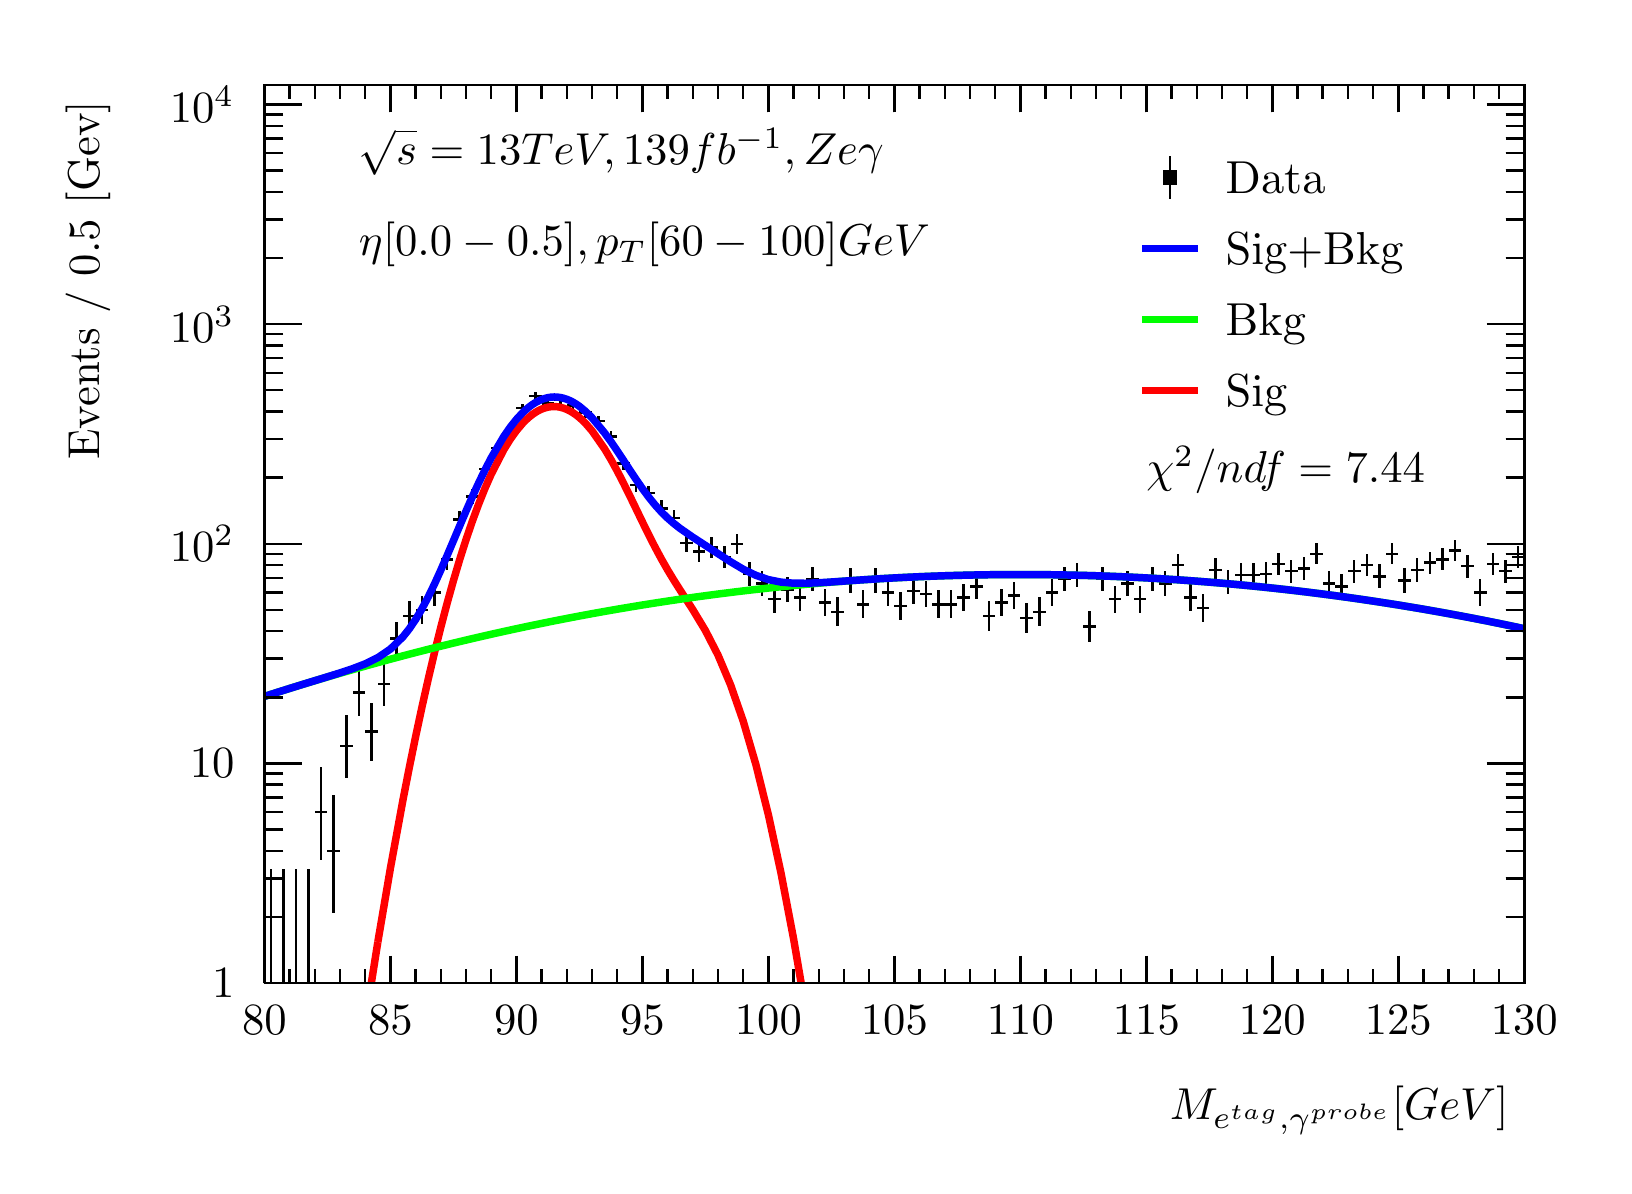
\begin{tikzpicture}
\pgfdeclareplotmark{cross} {
\pgfpathmoveto{\pgfpoint{-0.3\pgfplotmarksize}{\pgfplotmarksize}}
\pgfpathlineto{\pgfpoint{+0.3\pgfplotmarksize}{\pgfplotmarksize}}
\pgfpathlineto{\pgfpoint{+0.3\pgfplotmarksize}{0.3\pgfplotmarksize}}
\pgfpathlineto{\pgfpoint{+1\pgfplotmarksize}{0.3\pgfplotmarksize}}
\pgfpathlineto{\pgfpoint{+1\pgfplotmarksize}{-0.3\pgfplotmarksize}}
\pgfpathlineto{\pgfpoint{+0.3\pgfplotmarksize}{-0.3\pgfplotmarksize}}
\pgfpathlineto{\pgfpoint{+0.3\pgfplotmarksize}{-1.\pgfplotmarksize}}
\pgfpathlineto{\pgfpoint{-0.3\pgfplotmarksize}{-1.\pgfplotmarksize}}
\pgfpathlineto{\pgfpoint{-0.3\pgfplotmarksize}{-0.3\pgfplotmarksize}}
\pgfpathlineto{\pgfpoint{-1.\pgfplotmarksize}{-0.3\pgfplotmarksize}}
\pgfpathlineto{\pgfpoint{-1.\pgfplotmarksize}{0.3\pgfplotmarksize}}
\pgfpathlineto{\pgfpoint{-0.3\pgfplotmarksize}{0.3\pgfplotmarksize}}
\pgfpathclose
\pgfusepathqstroke
}
\pgfdeclareplotmark{cross*} {
\pgfpathmoveto{\pgfpoint{-0.3\pgfplotmarksize}{\pgfplotmarksize}}
\pgfpathlineto{\pgfpoint{+0.3\pgfplotmarksize}{\pgfplotmarksize}}
\pgfpathlineto{\pgfpoint{+0.3\pgfplotmarksize}{0.3\pgfplotmarksize}}
\pgfpathlineto{\pgfpoint{+1\pgfplotmarksize}{0.3\pgfplotmarksize}}
\pgfpathlineto{\pgfpoint{+1\pgfplotmarksize}{-0.3\pgfplotmarksize}}
\pgfpathlineto{\pgfpoint{+0.3\pgfplotmarksize}{-0.3\pgfplotmarksize}}
\pgfpathlineto{\pgfpoint{+0.3\pgfplotmarksize}{-1.\pgfplotmarksize}}
\pgfpathlineto{\pgfpoint{-0.3\pgfplotmarksize}{-1.\pgfplotmarksize}}
\pgfpathlineto{\pgfpoint{-0.3\pgfplotmarksize}{-0.3\pgfplotmarksize}}
\pgfpathlineto{\pgfpoint{-1.\pgfplotmarksize}{-0.3\pgfplotmarksize}}
\pgfpathlineto{\pgfpoint{-1.\pgfplotmarksize}{0.3\pgfplotmarksize}}
\pgfpathlineto{\pgfpoint{-0.3\pgfplotmarksize}{0.3\pgfplotmarksize}}
\pgfpathclose
\pgfusepathqfillstroke
}
\pgfdeclareplotmark{newstar} {
\pgfpathmoveto{\pgfqpoint{0pt}{\pgfplotmarksize}}
\pgfpathlineto{\pgfqpointpolar{44}{0.5\pgfplotmarksize}}
\pgfpathlineto{\pgfqpointpolar{18}{\pgfplotmarksize}}
\pgfpathlineto{\pgfqpointpolar{-20}{0.5\pgfplotmarksize}}
\pgfpathlineto{\pgfqpointpolar{-54}{\pgfplotmarksize}}
\pgfpathlineto{\pgfqpointpolar{-90}{0.5\pgfplotmarksize}}
\pgfpathlineto{\pgfqpointpolar{234}{\pgfplotmarksize}}
\pgfpathlineto{\pgfqpointpolar{198}{0.5\pgfplotmarksize}}
\pgfpathlineto{\pgfqpointpolar{162}{\pgfplotmarksize}}
\pgfpathlineto{\pgfqpointpolar{134}{0.5\pgfplotmarksize}}
\pgfpathclose
\pgfusepathqstroke
}
\pgfdeclareplotmark{newstar*} {
\pgfpathmoveto{\pgfqpoint{0pt}{\pgfplotmarksize}}
\pgfpathlineto{\pgfqpointpolar{44}{0.5\pgfplotmarksize}}
\pgfpathlineto{\pgfqpointpolar{18}{\pgfplotmarksize}}
\pgfpathlineto{\pgfqpointpolar{-20}{0.5\pgfplotmarksize}}
\pgfpathlineto{\pgfqpointpolar{-54}{\pgfplotmarksize}}
\pgfpathlineto{\pgfqpointpolar{-90}{0.5\pgfplotmarksize}}
\pgfpathlineto{\pgfqpointpolar{234}{\pgfplotmarksize}}
\pgfpathlineto{\pgfqpointpolar{198}{0.5\pgfplotmarksize}}
\pgfpathlineto{\pgfqpointpolar{162}{\pgfplotmarksize}}
\pgfpathlineto{\pgfqpointpolar{134}{0.5\pgfplotmarksize}}
\pgfpathclose
\pgfusepathqfillstroke
}
\definecolor{c}{rgb}{1,1,1};
\draw [color=c, fill=c] (0,0) rectangle (20,14.4361);
\draw [color=c, fill=c] (3,2.30977) rectangle (19,13.7143);
\definecolor{c}{rgb}{0,0,0};
\draw [c,line width=0.9] (3,2.30977) -- (3,13.7143) -- (19,13.7143) -- (19,2.30977) -- (3,2.30977);
\definecolor{c}{rgb}{1,1,1};
\draw [color=c, fill=c] (3,2.30977) rectangle (19,13.7143);
\definecolor{c}{rgb}{0,0,0};
\draw [c,line width=0.9] (3,2.30977) -- (3,13.7143) -- (19,13.7143) -- (19,2.30977) -- (3,2.30977);
\draw [c,line width=0.9] (3,2.30977) -- (19,2.30977);
\draw [c,line width=0.9] (3,2.65624) -- (3,2.30977);
\draw [c,line width=0.9] (3.32,2.48301) -- (3.32,2.30977);
\draw [c,line width=0.9] (3.64,2.48301) -- (3.64,2.30977);
\draw [c,line width=0.9] (3.96,2.48301) -- (3.96,2.30977);
\draw [c,line width=0.9] (4.28,2.48301) -- (4.28,2.30977);
\draw [c,line width=0.9] (4.6,2.65624) -- (4.6,2.30977);
\draw [c,line width=0.9] (4.92,2.48301) -- (4.92,2.30977);
\draw [c,line width=0.9] (5.24,2.48301) -- (5.24,2.30977);
\draw [c,line width=0.9] (5.56,2.48301) -- (5.56,2.30977);
\draw [c,line width=0.9] (5.88,2.48301) -- (5.88,2.30977);
\draw [c,line width=0.9] (6.2,2.65624) -- (6.2,2.30977);
\draw [c,line width=0.9] (6.52,2.48301) -- (6.52,2.30977);
\draw [c,line width=0.9] (6.84,2.48301) -- (6.84,2.30977);
\draw [c,line width=0.9] (7.16,2.48301) -- (7.16,2.30977);
\draw [c,line width=0.9] (7.48,2.48301) -- (7.48,2.30977);
\draw [c,line width=0.9] (7.8,2.65624) -- (7.8,2.30977);
\draw [c,line width=0.9] (8.12,2.48301) -- (8.12,2.30977);
\draw [c,line width=0.9] (8.44,2.48301) -- (8.44,2.30977);
\draw [c,line width=0.9] (8.76,2.48301) -- (8.76,2.30977);
\draw [c,line width=0.9] (9.08,2.48301) -- (9.08,2.30977);
\draw [c,line width=0.9] (9.4,2.65624) -- (9.4,2.30977);
\draw [c,line width=0.9] (9.72,2.48301) -- (9.72,2.30977);
\draw [c,line width=0.9] (10.04,2.48301) -- (10.04,2.30977);
\draw [c,line width=0.9] (10.36,2.48301) -- (10.36,2.30977);
\draw [c,line width=0.9] (10.68,2.48301) -- (10.68,2.30977);
\draw [c,line width=0.9] (11,2.65624) -- (11,2.30977);
\draw [c,line width=0.9] (11.32,2.48301) -- (11.32,2.30977);
\draw [c,line width=0.9] (11.64,2.48301) -- (11.64,2.30977);
\draw [c,line width=0.9] (11.96,2.48301) -- (11.96,2.30977);
\draw [c,line width=0.9] (12.28,2.48301) -- (12.28,2.30977);
\draw [c,line width=0.9] (12.6,2.65624) -- (12.6,2.30977);
\draw [c,line width=0.9] (12.92,2.48301) -- (12.92,2.30977);
\draw [c,line width=0.9] (13.24,2.48301) -- (13.24,2.30977);
\draw [c,line width=0.9] (13.56,2.48301) -- (13.56,2.30977);
\draw [c,line width=0.9] (13.88,2.48301) -- (13.88,2.30977);
\draw [c,line width=0.9] (14.2,2.65624) -- (14.2,2.30977);
\draw [c,line width=0.9] (14.52,2.48301) -- (14.52,2.30977);
\draw [c,line width=0.9] (14.84,2.48301) -- (14.84,2.30977);
\draw [c,line width=0.9] (15.16,2.48301) -- (15.16,2.30977);
\draw [c,line width=0.9] (15.48,2.48301) -- (15.48,2.30977);
\draw [c,line width=0.9] (15.8,2.65624) -- (15.8,2.30977);
\draw [c,line width=0.9] (16.12,2.48301) -- (16.12,2.30977);
\draw [c,line width=0.9] (16.44,2.48301) -- (16.44,2.30977);
\draw [c,line width=0.9] (16.76,2.48301) -- (16.76,2.30977);
\draw [c,line width=0.9] (17.08,2.48301) -- (17.08,2.30977);
\draw [c,line width=0.9] (17.4,2.65624) -- (17.4,2.30977);
\draw [c,line width=0.9] (17.72,2.48301) -- (17.72,2.30977);
\draw [c,line width=0.9] (18.04,2.48301) -- (18.04,2.30977);
\draw [c,line width=0.9] (18.36,2.48301) -- (18.36,2.30977);
\draw [c,line width=0.9] (18.68,2.48301) -- (18.68,2.30977);
\draw [c,line width=0.9] (19,2.65624) -- (19,2.30977);
\draw [anchor=base] (3,1.66015) node[scale=1.61424, color=c, rotate=0]{80};
\draw [anchor=base] (4.6,1.66015) node[scale=1.61424, color=c, rotate=0]{85};
\draw [anchor=base] (6.2,1.66015) node[scale=1.61424, color=c, rotate=0]{90};
\draw [anchor=base] (7.8,1.66015) node[scale=1.61424, color=c, rotate=0]{95};
\draw [anchor=base] (9.4,1.66015) node[scale=1.61424, color=c, rotate=0]{100};
\draw [anchor=base] (11,1.66015) node[scale=1.61424, color=c, rotate=0]{105};
\draw [anchor=base] (12.6,1.66015) node[scale=1.61424, color=c, rotate=0]{110};
\draw [anchor=base] (14.2,1.66015) node[scale=1.61424, color=c, rotate=0]{115};
\draw [anchor=base] (15.8,1.66015) node[scale=1.61424, color=c, rotate=0]{120};
\draw [anchor=base] (17.4,1.66015) node[scale=1.61424, color=c, rotate=0]{125};
\draw [anchor=base] (19,1.66015) node[scale=1.61424, color=c, rotate=0]{130};
\draw [anchor= east] (19,0.692932) node[scale=1.61424, color=c, rotate=0]{$M_{e^{tag}, \gamma^{probe}}  [GeV]$};
\draw [c,line width=0.9] (3,13.7143) -- (19,13.7143);
\draw [c,line width=0.9] (3,13.3678) -- (3,13.7143);
\draw [c,line width=0.9] (3.32,13.5411) -- (3.32,13.7143);
\draw [c,line width=0.9] (3.64,13.5411) -- (3.64,13.7143);
\draw [c,line width=0.9] (3.96,13.5411) -- (3.96,13.7143);
\draw [c,line width=0.9] (4.28,13.5411) -- (4.28,13.7143);
\draw [c,line width=0.9] (4.6,13.3678) -- (4.6,13.7143);
\draw [c,line width=0.9] (4.92,13.5411) -- (4.92,13.7143);
\draw [c,line width=0.9] (5.24,13.5411) -- (5.24,13.7143);
\draw [c,line width=0.9] (5.56,13.5411) -- (5.56,13.7143);
\draw [c,line width=0.9] (5.88,13.5411) -- (5.88,13.7143);
\draw [c,line width=0.9] (6.2,13.3678) -- (6.2,13.7143);
\draw [c,line width=0.9] (6.52,13.5411) -- (6.52,13.7143);
\draw [c,line width=0.9] (6.84,13.5411) -- (6.84,13.7143);
\draw [c,line width=0.9] (7.16,13.5411) -- (7.16,13.7143);
\draw [c,line width=0.9] (7.48,13.5411) -- (7.48,13.7143);
\draw [c,line width=0.9] (7.8,13.3678) -- (7.8,13.7143);
\draw [c,line width=0.9] (8.12,13.5411) -- (8.12,13.7143);
\draw [c,line width=0.9] (8.44,13.5411) -- (8.44,13.7143);
\draw [c,line width=0.9] (8.76,13.5411) -- (8.76,13.7143);
\draw [c,line width=0.9] (9.08,13.5411) -- (9.08,13.7143);
\draw [c,line width=0.9] (9.4,13.3678) -- (9.4,13.7143);
\draw [c,line width=0.9] (9.72,13.5411) -- (9.72,13.7143);
\draw [c,line width=0.9] (10.04,13.5411) -- (10.04,13.7143);
\draw [c,line width=0.9] (10.36,13.5411) -- (10.36,13.7143);
\draw [c,line width=0.9] (10.68,13.5411) -- (10.68,13.7143);
\draw [c,line width=0.9] (11,13.3678) -- (11,13.7143);
\draw [c,line width=0.9] (11.32,13.5411) -- (11.32,13.7143);
\draw [c,line width=0.9] (11.64,13.5411) -- (11.64,13.7143);
\draw [c,line width=0.9] (11.96,13.5411) -- (11.96,13.7143);
\draw [c,line width=0.9] (12.28,13.5411) -- (12.28,13.7143);
\draw [c,line width=0.9] (12.6,13.3678) -- (12.6,13.7143);
\draw [c,line width=0.9] (12.92,13.5411) -- (12.92,13.7143);
\draw [c,line width=0.9] (13.24,13.5411) -- (13.24,13.7143);
\draw [c,line width=0.9] (13.56,13.5411) -- (13.56,13.7143);
\draw [c,line width=0.9] (13.88,13.5411) -- (13.88,13.7143);
\draw [c,line width=0.9] (14.2,13.3678) -- (14.2,13.7143);
\draw [c,line width=0.9] (14.52,13.5411) -- (14.52,13.7143);
\draw [c,line width=0.9] (14.84,13.5411) -- (14.84,13.7143);
\draw [c,line width=0.9] (15.16,13.5411) -- (15.16,13.7143);
\draw [c,line width=0.9] (15.48,13.5411) -- (15.48,13.7143);
\draw [c,line width=0.9] (15.8,13.3678) -- (15.8,13.7143);
\draw [c,line width=0.9] (16.12,13.5411) -- (16.12,13.7143);
\draw [c,line width=0.9] (16.44,13.5411) -- (16.44,13.7143);
\draw [c,line width=0.9] (16.76,13.5411) -- (16.76,13.7143);
\draw [c,line width=0.9] (17.08,13.5411) -- (17.08,13.7143);
\draw [c,line width=0.9] (17.4,13.3678) -- (17.4,13.7143);
\draw [c,line width=0.9] (17.72,13.5411) -- (17.72,13.7143);
\draw [c,line width=0.9] (18.04,13.5411) -- (18.04,13.7143);
\draw [c,line width=0.9] (18.36,13.5411) -- (18.36,13.7143);
\draw [c,line width=0.9] (18.68,13.5411) -- (18.68,13.7143);
\draw [c,line width=0.9] (19,13.3678) -- (19,13.7143);
\draw [c,line width=0.9] (3,2.30977) -- (3,13.7143);
\draw [c,line width=0.9] (3.474,2.30978) -- (3,2.30978);
\draw [anchor= east] (2.82,2.30978) node[scale=1.61424, color=c, rotate=0]{1};
\draw [c,line width=0.9] (3.237,3.1495) -- (3,3.1495);
\draw [c,line width=0.9] (3.237,3.6407) -- (3,3.6407);
\draw [c,line width=0.9] (3.237,3.98922) -- (3,3.98922);
\draw [c,line width=0.9] (3.237,4.25955) -- (3,4.25955);
\draw [c,line width=0.9] (3.237,4.48042) -- (3,4.48042);
\draw [c,line width=0.9] (3.237,4.66717) -- (3,4.66717);
\draw [c,line width=0.9] (3.237,4.82894) -- (3,4.82894);
\draw [c,line width=0.9] (3.237,4.97163) -- (3,4.97163);
\draw [c,line width=0.9] (3.474,5.09927) -- (3,5.09927);
\draw [anchor= east] (2.82,5.09927) node[scale=1.61424, color=c, rotate=0]{10};
\draw [c,line width=0.9] (3.237,5.93899) -- (3,5.93899);
\draw [c,line width=0.9] (3.237,6.43019) -- (3,6.43019);
\draw [c,line width=0.9] (3.237,6.77871) -- (3,6.77871);
\draw [c,line width=0.9] (3.237,7.04904) -- (3,7.04904);
\draw [c,line width=0.9] (3.237,7.26991) -- (3,7.26991);
\draw [c,line width=0.9] (3.237,7.45666) -- (3,7.45666);
\draw [c,line width=0.9] (3.237,7.61843) -- (3,7.61843);
\draw [c,line width=0.9] (3.237,7.76112) -- (3,7.76112);
\draw [c,line width=0.9] (3.474,7.88876) -- (3,7.88876);
\draw [anchor= east] (2.82,7.88876) node[scale=1.61424, color=c, rotate=0]{$10^{2}$};
\draw [c,line width=0.9] (3.237,8.72848) -- (3,8.72848);
\draw [c,line width=0.9] (3.237,9.21968) -- (3,9.21968);
\draw [c,line width=0.9] (3.237,9.5682) -- (3,9.5682);
\draw [c,line width=0.9] (3.237,9.83853) -- (3,9.83853);
\draw [c,line width=0.9] (3.237,10.0594) -- (3,10.0594);
\draw [c,line width=0.9] (3.237,10.2462) -- (3,10.2462);
\draw [c,line width=0.9] (3.237,10.4079) -- (3,10.4079);
\draw [c,line width=0.9] (3.237,10.5506) -- (3,10.5506);
\draw [c,line width=0.9] (3.474,10.6782) -- (3,10.6782);
\draw [anchor= east] (2.82,10.6782) node[scale=1.61424, color=c, rotate=0]{$10^{3}$};
\draw [c,line width=0.9] (3.237,11.518) -- (3,11.518);
\draw [c,line width=0.9] (3.237,12.0092) -- (3,12.0092);
\draw [c,line width=0.9] (3.237,12.3577) -- (3,12.3577);
\draw [c,line width=0.9] (3.237,12.628) -- (3,12.628);
\draw [c,line width=0.9] (3.237,12.8489) -- (3,12.8489);
\draw [c,line width=0.9] (3.237,13.0356) -- (3,13.0356);
\draw [c,line width=0.9] (3.237,13.1974) -- (3,13.1974);
\draw [c,line width=0.9] (3.237,13.3401) -- (3,13.3401);
\draw [c,line width=0.9] (3.474,13.4677) -- (3,13.4677);
\draw [anchor= east] (2.82,13.4677) node[scale=1.61424, color=c, rotate=0]{$10^{4}$};
\draw [anchor= east] (0.76,13.7143) node[scale=1.61424, color=c, rotate=90]{Events / 0.5 [Gev]};
\draw [c,line width=0.9] (19,2.30977) -- (19,13.7143);
\draw [c,line width=0.9] (18.526,2.30978) -- (19,2.30978);
\draw [c,line width=0.9] (18.763,3.1495) -- (19,3.1495);
\draw [c,line width=0.9] (18.763,3.6407) -- (19,3.6407);
\draw [c,line width=0.9] (18.763,3.98922) -- (19,3.98922);
\draw [c,line width=0.9] (18.763,4.25955) -- (19,4.25955);
\draw [c,line width=0.9] (18.763,4.48042) -- (19,4.48042);
\draw [c,line width=0.9] (18.763,4.66717) -- (19,4.66717);
\draw [c,line width=0.9] (18.763,4.82894) -- (19,4.82894);
\draw [c,line width=0.9] (18.763,4.97163) -- (19,4.97163);
\draw [c,line width=0.9] (18.526,5.09927) -- (19,5.09927);
\draw [c,line width=0.9] (18.763,5.93899) -- (19,5.93899);
\draw [c,line width=0.9] (18.763,6.43019) -- (19,6.43019);
\draw [c,line width=0.9] (18.763,6.77871) -- (19,6.77871);
\draw [c,line width=0.9] (18.763,7.04904) -- (19,7.04904);
\draw [c,line width=0.9] (18.763,7.26991) -- (19,7.26991);
\draw [c,line width=0.9] (18.763,7.45666) -- (19,7.45666);
\draw [c,line width=0.9] (18.763,7.61843) -- (19,7.61843);
\draw [c,line width=0.9] (18.763,7.76112) -- (19,7.76112);
\draw [c,line width=0.9] (18.526,7.88876) -- (19,7.88876);
\draw [c,line width=0.9] (18.763,8.72848) -- (19,8.72848);
\draw [c,line width=0.9] (18.763,9.21968) -- (19,9.21968);
\draw [c,line width=0.9] (18.763,9.5682) -- (19,9.5682);
\draw [c,line width=0.9] (18.763,9.83853) -- (19,9.83853);
\draw [c,line width=0.9] (18.763,10.0594) -- (19,10.0594);
\draw [c,line width=0.9] (18.763,10.2462) -- (19,10.2462);
\draw [c,line width=0.9] (18.763,10.4079) -- (19,10.4079);
\draw [c,line width=0.9] (18.763,10.5506) -- (19,10.5506);
\draw [c,line width=0.9] (18.526,10.6782) -- (19,10.6782);
\draw [c,line width=0.9] (18.763,11.518) -- (19,11.518);
\draw [c,line width=0.9] (18.763,12.0092) -- (19,12.0092);
\draw [c,line width=0.9] (18.763,12.3577) -- (19,12.3577);
\draw [c,line width=0.9] (18.763,12.628) -- (19,12.628);
\draw [c,line width=0.9] (18.763,12.8489) -- (19,12.8489);
\draw [c,line width=0.9] (18.763,13.0356) -- (19,13.0356);
\draw [c,line width=0.9] (18.763,13.1974) -- (19,13.1974);
\draw [c,line width=0.9] (18.763,13.3401) -- (19,13.3401);
\draw [c,line width=0.9] (18.526,13.4677) -- (19,13.4677);
\draw [c,line width=0.9] (3.08,2.30977) -- (3,2.30977);
\draw [c,line width=0.9] (3,2.30977) -- (3,2.30977);
\draw [c,line width=0.9] (3.08,2.30977) -- (3.16,2.30977);
\draw [c,line width=0.9] (3.16,2.30977) -- (3.16,2.30977);
\draw [c,line width=0.9] (3.08,2.30977) -- (3.08,3.75599);
\draw [c,line width=0.9] (3.08,3.75599) -- (3.08,3.75599);
\draw [c,line width=0.9] (3.24,2.30977) -- (3.16,2.30977);
\draw [c,line width=0.9] (3.16,2.30977) -- (3.16,2.30977);
\draw [c,line width=0.9] (3.24,2.30977) -- (3.32,2.30977);
\draw [c,line width=0.9] (3.32,2.30977) -- (3.32,2.30977);
\draw [c,line width=0.9] (3.24,2.30977) -- (3.24,3.75599);
\draw [c,line width=0.9] (3.24,3.75599) -- (3.24,3.75599);
\draw [c,line width=0.9] (3.4,2.30977) -- (3.32,2.30977);
\draw [c,line width=0.9] (3.32,2.30977) -- (3.32,2.30977);
\draw [c,line width=0.9] (3.4,2.30977) -- (3.48,2.30977);
\draw [c,line width=0.9] (3.48,2.30977) -- (3.48,2.30977);
\draw [c,line width=0.9] (3.4,2.30977) -- (3.4,3.75599);
\draw [c,line width=0.9] (3.4,3.75599) -- (3.4,3.75599);
\draw [c,line width=0.9] (3.56,2.30977) -- (3.48,2.30977);
\draw [c,line width=0.9] (3.48,2.30977) -- (3.48,2.30977);
\draw [c,line width=0.9] (3.56,2.30977) -- (3.64,2.30977);
\draw [c,line width=0.9] (3.64,2.30977) -- (3.64,2.30977);
\draw [c,line width=0.9] (3.56,2.30977) -- (3.56,3.75599);
\draw [c,line width=0.9] (3.56,3.75599) -- (3.56,3.75599);
\draw [c,line width=0.9] (3.72,4.48042) -- (3.64,4.48042);
\draw [c,line width=0.9] (3.64,4.48042) -- (3.64,4.48042);
\draw [c,line width=0.9] (3.72,4.48042) -- (3.8,4.48042);
\draw [c,line width=0.9] (3.8,4.48042) -- (3.8,4.48042);
\draw [c,line width=0.9] (3.72,4.48042) -- (3.72,5.04775);
\draw [c,line width=0.9] (3.72,5.04775) -- (3.72,5.04775);
\draw [c,line width=0.9] (3.72,4.48042) -- (3.72,3.86831);
\draw [c,line width=0.9] (3.72,3.86831) -- (3.72,3.86831);
\draw [c,line width=0.9] (3.88,3.98922) -- (3.8,3.98922);
\draw [c,line width=0.9] (3.8,3.98922) -- (3.8,3.98922);
\draw [c,line width=0.9] (3.88,3.98922) -- (3.96,3.98922);
\draw [c,line width=0.9] (3.96,3.98922) -- (3.96,3.98922);
\draw [c,line width=0.9] (3.88,3.98922) -- (3.88,4.69501);
\draw [c,line width=0.9] (3.88,4.69501) -- (3.88,4.69501);
\draw [c,line width=0.9] (3.88,3.98922) -- (3.88,3.2003);
\draw [c,line width=0.9] (3.88,3.2003) -- (3.88,3.2003);
\draw [c,line width=0.9] (4.04,5.32014) -- (3.96,5.32014);
\draw [c,line width=0.9] (3.96,5.32014) -- (3.96,5.32014);
\draw [c,line width=0.9] (4.04,5.32014) -- (4.12,5.32014);
\draw [c,line width=0.9] (4.12,5.32014) -- (4.12,5.32014);
\draw [c,line width=0.9] (4.04,5.32014) -- (4.04,5.71032);
\draw [c,line width=0.9] (4.04,5.71032) -- (4.04,5.71032);
\draw [c,line width=0.9] (4.04,5.32014) -- (4.04,4.9144);
\draw [c,line width=0.9] (4.04,4.9144) -- (4.04,4.9144);
\draw [c,line width=0.9] (4.2,5.99809) -- (4.12,5.99809);
\draw [c,line width=0.9] (4.12,5.99809) -- (4.12,5.99809);
\draw [c,line width=0.9] (4.2,5.99809) -- (4.28,5.99809);
\draw [c,line width=0.9] (4.28,5.99809) -- (4.28,5.99809);
\draw [c,line width=0.9] (4.2,5.99809) -- (4.2,6.28698);
\draw [c,line width=0.9] (4.2,6.28698) -- (4.2,6.28698);
\draw [c,line width=0.9] (4.2,5.99809) -- (4.2,5.70257);
\draw [c,line width=0.9] (4.2,5.70257) -- (4.2,5.70257);
\draw [c,line width=0.9] (4.36,5.50689) -- (4.28,5.50689);
\draw [c,line width=0.9] (4.28,5.50689) -- (4.28,5.50689);
\draw [c,line width=0.9] (4.36,5.50689) -- (4.44,5.50689);
\draw [c,line width=0.9] (4.44,5.50689) -- (4.44,5.50689);
\draw [c,line width=0.9] (4.36,5.50689) -- (4.36,5.86598);
\draw [c,line width=0.9] (4.36,5.86598) -- (4.36,5.86598);
\draw [c,line width=0.9] (4.36,5.50689) -- (4.36,5.13549);
\draw [c,line width=0.9] (4.36,5.13549) -- (4.36,5.13549);
\draw [c,line width=0.9] (4.52,6.1083) -- (4.44,6.1083);
\draw [c,line width=0.9] (4.44,6.1083) -- (4.44,6.1083);
\draw [c,line width=0.9] (4.52,6.1083) -- (4.6,6.1083);
\draw [c,line width=0.9] (4.6,6.1083) -- (4.6,6.1083);
\draw [c,line width=0.9] (4.52,6.1083) -- (4.52,6.38348);
\draw [c,line width=0.9] (4.52,6.38348) -- (4.52,6.38348);
\draw [c,line width=0.9] (4.52,6.1083) -- (4.52,5.82734);
\draw [c,line width=0.9] (4.52,5.82734) -- (4.52,5.82734);
\draw [c,line width=0.9] (4.68,6.68426) -- (4.6,6.68426);
\draw [c,line width=0.9] (4.6,6.68426) -- (4.6,6.68426);
\draw [c,line width=0.9] (4.68,6.68426) -- (4.76,6.68426);
\draw [c,line width=0.9] (4.76,6.68426) -- (4.76,6.68426);
\draw [c,line width=0.9] (4.68,6.68426) -- (4.68,6.89795);
\draw [c,line width=0.9] (4.68,6.89795) -- (4.68,6.89795);
\draw [c,line width=0.9] (4.68,6.68426) -- (4.68,6.46776);
\draw [c,line width=0.9] (4.68,6.46776) -- (4.68,6.46776);
\draw [c,line width=0.9] (4.84,6.97408) -- (4.76,6.97408);
\draw [c,line width=0.9] (4.76,6.97408) -- (4.76,6.97408);
\draw [c,line width=0.9] (4.84,6.97408) -- (4.92,6.97408);
\draw [c,line width=0.9] (4.92,6.97408) -- (4.92,6.97408);
\draw [c,line width=0.9] (4.84,6.97408) -- (4.84,7.16239);
\draw [c,line width=0.9] (4.84,7.16239) -- (4.84,7.16239);
\draw [c,line width=0.9] (4.84,6.97408) -- (4.84,6.78381);
\draw [c,line width=0.9] (4.84,6.78381) -- (4.84,6.78381);
\draw [c,line width=0.9] (5,7.04904) -- (4.92,7.04904);
\draw [c,line width=0.9] (4.92,7.04904) -- (4.92,7.04904);
\draw [c,line width=0.9] (5,7.04904) -- (5.08,7.04904);
\draw [c,line width=0.9] (5.08,7.04904) -- (5.08,7.04904);
\draw [c,line width=0.9] (5,7.04904) -- (5,7.23131);
\draw [c,line width=0.9] (5,7.23131) -- (5,7.23131);
\draw [c,line width=0.9] (5,7.04904) -- (5,6.86499);
\draw [c,line width=0.9] (5,6.86499) -- (5,6.86499);
\draw [c,line width=0.9] (5.16,7.26991) -- (5.08,7.26991);
\draw [c,line width=0.9] (5.08,7.26991) -- (5.08,7.26991);
\draw [c,line width=0.9] (5.16,7.26991) -- (5.24,7.26991);
\draw [c,line width=0.9] (5.24,7.26991) -- (5.24,7.26991);
\draw [c,line width=0.9] (5.16,7.26991) -- (5.16,7.43552);
\draw [c,line width=0.9] (5.16,7.43552) -- (5.16,7.43552);
\draw [c,line width=0.9] (5.16,7.26991) -- (5.16,7.10296);
\draw [c,line width=0.9] (5.16,7.10296) -- (5.16,7.10296);
\draw [c,line width=0.9] (5.32,7.69187) -- (5.24,7.69187);
\draw [c,line width=0.9] (5.24,7.69187) -- (5.24,7.69187);
\draw [c,line width=0.9] (5.32,7.69187) -- (5.4,7.69187);
\draw [c,line width=0.9] (5.4,7.69187) -- (5.4,7.69187);
\draw [c,line width=0.9] (5.32,7.69187) -- (5.32,7.82987);
\draw [c,line width=0.9] (5.32,7.82987) -- (5.32,7.82987);
\draw [c,line width=0.9] (5.32,7.69187) -- (5.32,7.55307);
\draw [c,line width=0.9] (5.32,7.55307) -- (5.32,7.55307);
\draw [c,line width=0.9] (5.48,8.19725) -- (5.4,8.19725);
\draw [c,line width=0.9] (5.4,8.19725) -- (5.4,8.19725);
\draw [c,line width=0.9] (5.48,8.19725) -- (5.56,8.19725);
\draw [c,line width=0.9] (5.56,8.19725) -- (5.56,8.19725);
\draw [c,line width=0.9] (5.48,8.19725) -- (5.48,8.30387);
\draw [c,line width=0.9] (5.48,8.30387) -- (5.48,8.30387);
\draw [c,line width=0.9] (5.48,8.19725) -- (5.48,8.09062);
\draw [c,line width=0.9] (5.48,8.09062) -- (5.48,8.09062);
\draw [c,line width=0.9] (5.64,8.48806) -- (5.56,8.48806);
\draw [c,line width=0.9] (5.56,8.48806) -- (5.56,8.48806);
\draw [c,line width=0.9] (5.64,8.48806) -- (5.72,8.48806);
\draw [c,line width=0.9] (5.72,8.48806) -- (5.72,8.48806);
\draw [c,line width=0.9] (5.64,8.48806) -- (5.64,8.58264);
\draw [c,line width=0.9] (5.64,8.58264) -- (5.64,8.58264);
\draw [c,line width=0.9] (5.64,8.48806) -- (5.64,8.39349);
\draw [c,line width=0.9] (5.64,8.39349) -- (5.64,8.39349);
\draw [c,line width=0.9] (5.8,8.83842) -- (5.72,8.83842);
\draw [c,line width=0.9] (5.72,8.83842) -- (5.72,8.83842);
\draw [c,line width=0.9] (5.8,8.83842) -- (5.88,8.83842);
\draw [c,line width=0.9] (5.88,8.83842) -- (5.88,8.83842);
\draw [c,line width=0.9] (5.8,8.83842) -- (5.8,8.92027);
\draw [c,line width=0.9] (5.8,8.92027) -- (5.8,8.92027);
\draw [c,line width=0.9] (5.8,8.83842) -- (5.8,8.75658);
\draw [c,line width=0.9] (5.8,8.75658) -- (5.8,8.75658);
\draw [c,line width=0.9] (5.96,9.10543) -- (5.88,9.10543);
\draw [c,line width=0.9] (5.88,9.10543) -- (5.88,9.10543);
\draw [c,line width=0.9] (5.96,9.10543) -- (6.04,9.10543);
\draw [c,line width=0.9] (6.04,9.10543) -- (6.04,9.10543);
\draw [c,line width=0.9] (5.96,9.10543) -- (5.96,9.17874);
\draw [c,line width=0.9] (5.96,9.17874) -- (5.96,9.17874);
\draw [c,line width=0.9] (5.96,9.10543) -- (5.96,9.03212);
\draw [c,line width=0.9] (5.96,9.03212) -- (5.96,9.03212);
\draw [c,line width=0.9] (6.12,9.32037) -- (6.04,9.32037);
\draw [c,line width=0.9] (6.04,9.32037) -- (6.04,9.32037);
\draw [c,line width=0.9] (6.12,9.32037) -- (6.2,9.32037);
\draw [c,line width=0.9] (6.2,9.32037) -- (6.2,9.32037);
\draw [c,line width=0.9] (6.12,9.32037) -- (6.12,9.38746);
\draw [c,line width=0.9] (6.12,9.38746) -- (6.12,9.38746);
\draw [c,line width=0.9] (6.12,9.32037) -- (6.12,9.25328);
\draw [c,line width=0.9] (6.12,9.25328) -- (6.12,9.25328);
\draw [c,line width=0.9] (6.28,9.60987) -- (6.2,9.60987);
\draw [c,line width=0.9] (6.2,9.60987) -- (6.2,9.60987);
\draw [c,line width=0.9] (6.28,9.60987) -- (6.36,9.60987);
\draw [c,line width=0.9] (6.36,9.60987) -- (6.36,9.60987);
\draw [c,line width=0.9] (6.28,9.60987) -- (6.28,9.66941);
\draw [c,line width=0.9] (6.28,9.66941) -- (6.28,9.66941);
\draw [c,line width=0.9] (6.28,9.60987) -- (6.28,9.55034);
\draw [c,line width=0.9] (6.28,9.55034) -- (6.28,9.55034);
\draw [c,line width=0.9] (6.44,9.76357) -- (6.36,9.76357);
\draw [c,line width=0.9] (6.36,9.76357) -- (6.36,9.76357);
\draw [c,line width=0.9] (6.44,9.76357) -- (6.52,9.76357);
\draw [c,line width=0.9] (6.52,9.76357) -- (6.52,9.76357);
\draw [c,line width=0.9] (6.44,9.76357) -- (6.44,9.81944);
\draw [c,line width=0.9] (6.44,9.81944) -- (6.44,9.81944);
\draw [c,line width=0.9] (6.44,9.76357) -- (6.44,9.70769);
\draw [c,line width=0.9] (6.44,9.70769) -- (6.44,9.70769);
\draw [c,line width=0.9] (6.6,9.66982) -- (6.52,9.66982);
\draw [c,line width=0.9] (6.52,9.66982) -- (6.52,9.66982);
\draw [c,line width=0.9] (6.6,9.66982) -- (6.68,9.66982);
\draw [c,line width=0.9] (6.68,9.66982) -- (6.68,9.66982);
\draw [c,line width=0.9] (6.6,9.66982) -- (6.6,9.7279);
\draw [c,line width=0.9] (6.6,9.7279) -- (6.6,9.7279);
\draw [c,line width=0.9] (6.6,9.66982) -- (6.6,9.61174);
\draw [c,line width=0.9] (6.6,9.61174) -- (6.6,9.61174);
\draw [c,line width=0.9] (6.76,9.72161) -- (6.68,9.72161);
\draw [c,line width=0.9] (6.68,9.72161) -- (6.68,9.72161);
\draw [c,line width=0.9] (6.76,9.72161) -- (6.84,9.72161);
\draw [c,line width=0.9] (6.84,9.72161) -- (6.84,9.72161);
\draw [c,line width=0.9] (6.76,9.72161) -- (6.76,9.77846);
\draw [c,line width=0.9] (6.76,9.77846) -- (6.76,9.77846);
\draw [c,line width=0.9] (6.76,9.72161) -- (6.76,9.66476);
\draw [c,line width=0.9] (6.76,9.66476) -- (6.76,9.66476);
\draw [c,line width=0.9] (6.92,9.64449) -- (6.84,9.64449);
\draw [c,line width=0.9] (6.84,9.64449) -- (6.84,9.64449);
\draw [c,line width=0.9] (6.92,9.64449) -- (7,9.64449);
\draw [c,line width=0.9] (7,9.64449) -- (7,9.64449);
\draw [c,line width=0.9] (6.92,9.64449) -- (6.92,9.70318);
\draw [c,line width=0.9] (6.92,9.70318) -- (6.92,9.70318);
\draw [c,line width=0.9] (6.92,9.64449) -- (6.92,9.5858);
\draw [c,line width=0.9] (6.92,9.5858) -- (6.92,9.5858);
\draw [c,line width=0.9] (7.08,9.55296) -- (7,9.55296);
\draw [c,line width=0.9] (7,9.55296) -- (7,9.55296);
\draw [c,line width=0.9] (7.08,9.55296) -- (7.16,9.55296);
\draw [c,line width=0.9] (7.16,9.55296) -- (7.16,9.55296);
\draw [c,line width=0.9] (7.08,9.55296) -- (7.08,9.61391);
\draw [c,line width=0.9] (7.08,9.61391) -- (7.08,9.61391);
\draw [c,line width=0.9] (7.08,9.55296) -- (7.08,9.49201);
\draw [c,line width=0.9] (7.08,9.49201) -- (7.08,9.49201);
\draw [c,line width=0.9] (7.24,9.44727) -- (7.16,9.44727);
\draw [c,line width=0.9] (7.16,9.44727) -- (7.16,9.44727);
\draw [c,line width=0.9] (7.24,9.44727) -- (7.32,9.44727);
\draw [c,line width=0.9] (7.32,9.44727) -- (7.32,9.44727);
\draw [c,line width=0.9] (7.24,9.44727) -- (7.24,9.51093);
\draw [c,line width=0.9] (7.24,9.51093) -- (7.24,9.51093);
\draw [c,line width=0.9] (7.24,9.44727) -- (7.24,9.3836);
\draw [c,line width=0.9] (7.24,9.3836) -- (7.24,9.3836);
\draw [c,line width=0.9] (7.4,9.25156) -- (7.32,9.25156);
\draw [c,line width=0.9] (7.32,9.25156) -- (7.32,9.25156);
\draw [c,line width=0.9] (7.4,9.25156) -- (7.48,9.25156);
\draw [c,line width=0.9] (7.48,9.25156) -- (7.48,9.25156);
\draw [c,line width=0.9] (7.4,9.25156) -- (7.4,9.32058);
\draw [c,line width=0.9] (7.4,9.32058) -- (7.4,9.32058);
\draw [c,line width=0.9] (7.4,9.25156) -- (7.4,9.18254);
\draw [c,line width=0.9] (7.4,9.18254) -- (7.4,9.18254);
\draw [c,line width=0.9] (7.56,8.90828) -- (7.48,8.90828);
\draw [c,line width=0.9] (7.48,8.90828) -- (7.48,8.90828);
\draw [c,line width=0.9] (7.56,8.90828) -- (7.64,8.90828);
\draw [c,line width=0.9] (7.64,8.90828) -- (7.64,8.90828);
\draw [c,line width=0.9] (7.56,8.90828) -- (7.56,8.9878);
\draw [c,line width=0.9] (7.56,8.9878) -- (7.56,8.9878);
\draw [c,line width=0.9] (7.56,8.90828) -- (7.56,8.82876);
\draw [c,line width=0.9] (7.56,8.82876) -- (7.56,8.82876);
\draw [c,line width=0.9] (7.72,8.63403) -- (7.64,8.63403);
\draw [c,line width=0.9] (7.64,8.63403) -- (7.64,8.63403);
\draw [c,line width=0.9] (7.72,8.63403) -- (7.8,8.63403);
\draw [c,line width=0.9] (7.8,8.63403) -- (7.8,8.63403);
\draw [c,line width=0.9] (7.72,8.63403) -- (7.72,8.72308);
\draw [c,line width=0.9] (7.72,8.72308) -- (7.72,8.72308);
\draw [c,line width=0.9] (7.72,8.63403) -- (7.72,8.54498);
\draw [c,line width=0.9] (7.72,8.54498) -- (7.72,8.54498);
\draw [c,line width=0.9] (7.88,8.53159) -- (7.8,8.53159);
\draw [c,line width=0.9] (7.8,8.53159) -- (7.8,8.53159);
\draw [c,line width=0.9] (7.88,8.53159) -- (7.96,8.53159);
\draw [c,line width=0.9] (7.96,8.53159) -- (7.96,8.53159);
\draw [c,line width=0.9] (7.88,8.53159) -- (7.88,8.62448);
\draw [c,line width=0.9] (7.88,8.62448) -- (7.88,8.62448);
\draw [c,line width=0.9] (7.88,8.53159) -- (7.88,8.4387);
\draw [c,line width=0.9] (7.88,8.4387) -- (7.88,8.4387);
\draw [c,line width=0.9] (8.04,8.33889) -- (7.96,8.33889);
\draw [c,line width=0.9] (7.96,8.33889) -- (7.96,8.33889);
\draw [c,line width=0.9] (8.04,8.33889) -- (8.12,8.33889);
\draw [c,line width=0.9] (8.12,8.33889) -- (8.12,8.33889);
\draw [c,line width=0.9] (8.04,8.33889) -- (8.04,8.43947);
\draw [c,line width=0.9] (8.04,8.43947) -- (8.04,8.43947);
\draw [c,line width=0.9] (8.04,8.33889) -- (8.04,8.23831);
\draw [c,line width=0.9] (8.04,8.23831) -- (8.04,8.23831);
\draw [c,line width=0.9] (8.2,8.21588) -- (8.12,8.21588);
\draw [c,line width=0.9] (8.12,8.21588) -- (8.12,8.21588);
\draw [c,line width=0.9] (8.2,8.21588) -- (8.28,8.21588);
\draw [c,line width=0.9] (8.28,8.21588) -- (8.28,8.21588);
\draw [c,line width=0.9] (8.2,8.21588) -- (8.2,8.3217);
\draw [c,line width=0.9] (8.2,8.3217) -- (8.2,8.3217);
\draw [c,line width=0.9] (8.2,8.21588) -- (8.2,8.11007);
\draw [c,line width=0.9] (8.2,8.11007) -- (8.2,8.11007);
\draw [c,line width=0.9] (8.36,7.90081) -- (8.28,7.90081);
\draw [c,line width=0.9] (8.28,7.90081) -- (8.28,7.90081);
\draw [c,line width=0.9] (8.36,7.90081) -- (8.44,7.90081);
\draw [c,line width=0.9] (8.44,7.90081) -- (8.44,7.90081);
\draw [c,line width=0.9] (8.36,7.90081) -- (8.36,8.02131);
\draw [c,line width=0.9] (8.36,8.02131) -- (8.36,8.02131);
\draw [c,line width=0.9] (8.36,7.90081) -- (8.36,7.78032);
\draw [c,line width=0.9] (8.36,7.78032) -- (8.36,7.78032);
\draw [c,line width=0.9] (8.52,7.78774) -- (8.44,7.78774);
\draw [c,line width=0.9] (8.44,7.78774) -- (8.44,7.78774);
\draw [c,line width=0.9] (8.52,7.78774) -- (8.6,7.78774);
\draw [c,line width=0.9] (8.6,7.78774) -- (8.6,7.78774);
\draw [c,line width=0.9] (8.52,7.78774) -- (8.52,7.92016);
\draw [c,line width=0.9] (8.52,7.92016) -- (8.52,7.92016);
\draw [c,line width=0.9] (8.52,7.78774) -- (8.52,7.65462);
\draw [c,line width=0.9] (8.52,7.65462) -- (8.52,7.65462);
\draw [c,line width=0.9] (8.68,7.8393) -- (8.6,7.8393);
\draw [c,line width=0.9] (8.6,7.8393) -- (8.6,7.8393);
\draw [c,line width=0.9] (8.68,7.8393) -- (8.76,7.8393);
\draw [c,line width=0.9] (8.76,7.8393) -- (8.76,7.8393);
\draw [c,line width=0.9] (8.68,7.8393) -- (8.68,7.96882);
\draw [c,line width=0.9] (8.68,7.96882) -- (8.68,7.96882);
\draw [c,line width=0.9] (8.68,7.8393) -- (8.68,7.70912);
\draw [c,line width=0.9] (8.68,7.70912) -- (8.68,7.70912);
\draw [c,line width=0.9] (8.84,7.72005) -- (8.76,7.72005);
\draw [c,line width=0.9] (8.76,7.72005) -- (8.76,7.72005);
\draw [c,line width=0.9] (8.84,7.72005) -- (8.92,7.72005);
\draw [c,line width=0.9] (8.92,7.72005) -- (8.92,7.72005);
\draw [c,line width=0.9] (8.84,7.72005) -- (8.84,7.85638);
\draw [c,line width=0.9] (8.84,7.85638) -- (8.84,7.85638);
\draw [c,line width=0.9] (8.84,7.72005) -- (8.84,7.58294);
\draw [c,line width=0.9] (8.84,7.58294) -- (8.84,7.58294);
\draw [c,line width=0.9] (9,7.88876) -- (8.92,7.88876);
\draw [c,line width=0.9] (8.92,7.88876) -- (8.92,7.88876);
\draw [c,line width=0.9] (9,7.88876) -- (9.08,7.88876);
\draw [c,line width=0.9] (9.08,7.88876) -- (9.08,7.88876);
\draw [c,line width=0.9] (9,7.88876) -- (9,8.01555);
\draw [c,line width=0.9] (9,8.01555) -- (9,8.01555);
\draw [c,line width=0.9] (9,7.88876) -- (9,7.76134);
\draw [c,line width=0.9] (9,7.76134) -- (9,7.76134);
\draw [c,line width=0.9] (9.16,7.5075) -- (9.08,7.5075);
\draw [c,line width=0.9] (9.08,7.5075) -- (9.08,7.5075);
\draw [c,line width=0.9] (9.16,7.5075) -- (9.24,7.5075);
\draw [c,line width=0.9] (9.24,7.5075) -- (9.24,7.5075);
\draw [c,line width=0.9] (9.16,7.5075) -- (9.16,7.65692);
\draw [c,line width=0.9] (9.16,7.65692) -- (9.16,7.65692);
\draw [c,line width=0.9] (9.16,7.5075) -- (9.16,7.35707);
\draw [c,line width=0.9] (9.16,7.35707) -- (9.16,7.35707);
\draw [c,line width=0.9] (9.32,7.38538) -- (9.24,7.38538);
\draw [c,line width=0.9] (9.24,7.38538) -- (9.24,7.38538);
\draw [c,line width=0.9] (9.32,7.38538) -- (9.4,7.38538);
\draw [c,line width=0.9] (9.4,7.38538) -- (9.4,7.38538);
\draw [c,line width=0.9] (9.32,7.38538) -- (9.32,7.5429);
\draw [c,line width=0.9] (9.32,7.5429) -- (9.32,7.5429);
\draw [c,line width=0.9] (9.32,7.38538) -- (9.32,7.22668);
\draw [c,line width=0.9] (9.32,7.22668) -- (9.32,7.22668);
\draw [c,line width=0.9] (9.48,7.18633) -- (9.4,7.18633);
\draw [c,line width=0.9] (9.4,7.18633) -- (9.4,7.18633);
\draw [c,line width=0.9] (9.48,7.18633) -- (9.56,7.18633);
\draw [c,line width=0.9] (9.56,7.18633) -- (9.56,7.18633);
\draw [c,line width=0.9] (9.48,7.18633) -- (9.48,7.35805);
\draw [c,line width=0.9] (9.48,7.35805) -- (9.48,7.35805);
\draw [c,line width=0.9] (9.48,7.18633) -- (9.48,7.01311);
\draw [c,line width=0.9] (9.48,7.01311) -- (9.48,7.01311);
\draw [c,line width=0.9] (9.64,7.30964) -- (9.56,7.30964);
\draw [c,line width=0.9] (9.56,7.30964) -- (9.56,7.30964);
\draw [c,line width=0.9] (9.64,7.30964) -- (9.72,7.30964);
\draw [c,line width=0.9] (9.72,7.30964) -- (9.72,7.30964);
\draw [c,line width=0.9] (9.64,7.30964) -- (9.64,7.47242);
\draw [c,line width=0.9] (9.64,7.47242) -- (9.64,7.47242);
\draw [c,line width=0.9] (9.64,7.30964) -- (9.64,7.14557);
\draw [c,line width=0.9] (9.64,7.14557) -- (9.64,7.14557);
\draw [c,line width=0.9] (9.8,7.20777) -- (9.72,7.20777);
\draw [c,line width=0.9] (9.72,7.20777) -- (9.72,7.20777);
\draw [c,line width=0.9] (9.8,7.20777) -- (9.88,7.20777);
\draw [c,line width=0.9] (9.88,7.20777) -- (9.88,7.20777);
\draw [c,line width=0.9] (9.8,7.20777) -- (9.8,7.3779);
\draw [c,line width=0.9] (9.8,7.3779) -- (9.8,7.3779);
\draw [c,line width=0.9] (9.8,7.20777) -- (9.8,7.03618);
\draw [c,line width=0.9] (9.8,7.03618) -- (9.8,7.03618);
\draw [c,line width=0.9] (9.96,7.43923) -- (9.88,7.43923);
\draw [c,line width=0.9] (9.88,7.43923) -- (9.88,7.43923);
\draw [c,line width=0.9] (9.96,7.43923) -- (10.04,7.43923);
\draw [c,line width=0.9] (10.04,7.43923) -- (10.04,7.43923);
\draw [c,line width=0.9] (9.96,7.43923) -- (9.96,7.59313);
\draw [c,line width=0.9] (9.96,7.59313) -- (9.96,7.59313);
\draw [c,line width=0.9] (9.96,7.43923) -- (9.96,7.28423);
\draw [c,line width=0.9] (9.96,7.28423) -- (9.96,7.28423);
\draw [c,line width=0.9] (10.12,7.14227) -- (10.04,7.14227);
\draw [c,line width=0.9] (10.04,7.14227) -- (10.04,7.14227);
\draw [c,line width=0.9] (10.12,7.14227) -- (10.2,7.14227);
\draw [c,line width=0.9] (10.2,7.14227) -- (10.2,7.14227);
\draw [c,line width=0.9] (10.12,7.14227) -- (10.12,7.31731);
\draw [c,line width=0.9] (10.12,7.31731) -- (10.12,7.31731);
\draw [c,line width=0.9] (10.12,7.14227) -- (10.12,6.96565);
\draw [c,line width=0.9] (10.12,6.96565) -- (10.12,6.96565);
\draw [c,line width=0.9] (10.28,7.02456) -- (10.2,7.02456);
\draw [c,line width=0.9] (10.2,7.02456) -- (10.2,7.02456);
\draw [c,line width=0.9] (10.28,7.02456) -- (10.36,7.02456);
\draw [c,line width=0.9] (10.36,7.02456) -- (10.36,7.02456);
\draw [c,line width=0.9] (10.28,7.02456) -- (10.28,7.20878);
\draw [c,line width=0.9] (10.28,7.20878) -- (10.28,7.20878);
\draw [c,line width=0.9] (10.28,7.02456) -- (10.28,6.83851);
\draw [c,line width=0.9] (10.28,6.83851) -- (10.28,6.83851);
\draw [c,line width=0.9] (10.44,7.42154) -- (10.36,7.42154);
\draw [c,line width=0.9] (10.36,7.42154) -- (10.36,7.42154);
\draw [c,line width=0.9] (10.44,7.42154) -- (10.52,7.42154);
\draw [c,line width=0.9] (10.52,7.42154) -- (10.52,7.42154);
\draw [c,line width=0.9] (10.44,7.42154) -- (10.44,7.57663);
\draw [c,line width=0.9] (10.44,7.57663) -- (10.44,7.57663);
\draw [c,line width=0.9] (10.44,7.42154) -- (10.44,7.26534);
\draw [c,line width=0.9] (10.44,7.26534) -- (10.44,7.26534);
\draw [c,line width=0.9] (10.6,7.11963) -- (10.52,7.11963);
\draw [c,line width=0.9] (10.52,7.11963) -- (10.52,7.11963);
\draw [c,line width=0.9] (10.6,7.11963) -- (10.68,7.11963);
\draw [c,line width=0.9] (10.68,7.11963) -- (10.68,7.11963);
\draw [c,line width=0.9] (10.6,7.11963) -- (10.6,7.29639);
\draw [c,line width=0.9] (10.6,7.29639) -- (10.6,7.29639);
\draw [c,line width=0.9] (10.6,7.11963) -- (10.6,6.94123);
\draw [c,line width=0.9] (10.6,6.94123) -- (10.6,6.94123);
\draw [c,line width=0.9] (10.76,7.42154) -- (10.68,7.42154);
\draw [c,line width=0.9] (10.68,7.42154) -- (10.68,7.42154);
\draw [c,line width=0.9] (10.76,7.42154) -- (10.84,7.42154);
\draw [c,line width=0.9] (10.84,7.42154) -- (10.84,7.42154);
\draw [c,line width=0.9] (10.76,7.42154) -- (10.76,7.57663);
\draw [c,line width=0.9] (10.76,7.57663) -- (10.76,7.57663);
\draw [c,line width=0.9] (10.76,7.42154) -- (10.76,7.26534);
\draw [c,line width=0.9] (10.76,7.26534) -- (10.76,7.26534);
\draw [c,line width=0.9] (10.92,7.26991) -- (10.84,7.26991);
\draw [c,line width=0.9] (10.84,7.26991) -- (10.84,7.26991);
\draw [c,line width=0.9] (10.92,7.26991) -- (11,7.26991);
\draw [c,line width=0.9] (11,7.26991) -- (11,7.26991);
\draw [c,line width=0.9] (10.92,7.26991) -- (10.92,7.43552);
\draw [c,line width=0.9] (10.92,7.43552) -- (10.92,7.43552);
\draw [c,line width=0.9] (10.92,7.26991) -- (10.92,7.10296);
\draw [c,line width=0.9] (10.92,7.10296) -- (10.92,7.10296);
\draw [c,line width=0.9] (11.08,7.09655) -- (11,7.09655);
\draw [c,line width=0.9] (11,7.09655) -- (11,7.09655);
\draw [c,line width=0.9] (11.08,7.09655) -- (11.16,7.09655);
\draw [c,line width=0.9] (11.16,7.09655) -- (11.16,7.09655);
\draw [c,line width=0.9] (11.08,7.09655) -- (11.08,7.2751);
\draw [c,line width=0.9] (11.08,7.2751) -- (11.08,7.2751);
\draw [c,line width=0.9] (11.08,7.09655) -- (11.08,6.91633);
\draw [c,line width=0.9] (11.08,6.91633) -- (11.08,6.91633);
\draw [c,line width=0.9] (11.24,7.28994) -- (11.16,7.28994);
\draw [c,line width=0.9] (11.16,7.28994) -- (11.16,7.28994);
\draw [c,line width=0.9] (11.24,7.28994) -- (11.32,7.28994);
\draw [c,line width=0.9] (11.32,7.28994) -- (11.32,7.28994);
\draw [c,line width=0.9] (11.24,7.28994) -- (11.24,7.45411);
\draw [c,line width=0.9] (11.24,7.45411) -- (11.24,7.45411);
\draw [c,line width=0.9] (11.24,7.28994) -- (11.24,7.12444);
\draw [c,line width=0.9] (11.24,7.12444) -- (11.24,7.12444);
\draw [c,line width=0.9] (11.4,7.24955) -- (11.32,7.24955);
\draw [c,line width=0.9] (11.32,7.24955) -- (11.32,7.24955);
\draw [c,line width=0.9] (11.4,7.24955) -- (11.48,7.24955);
\draw [c,line width=0.9] (11.48,7.24955) -- (11.48,7.24955);
\draw [c,line width=0.9] (11.4,7.24955) -- (11.4,7.41663);
\draw [c,line width=0.9] (11.4,7.41663) -- (11.4,7.41663);
\draw [c,line width=0.9] (11.4,7.24955) -- (11.4,7.08109);
\draw [c,line width=0.9] (11.4,7.08109) -- (11.4,7.08109);
\draw [c,line width=0.9] (11.56,7.11963) -- (11.48,7.11963);
\draw [c,line width=0.9] (11.48,7.11963) -- (11.48,7.11963);
\draw [c,line width=0.9] (11.56,7.11963) -- (11.64,7.11963);
\draw [c,line width=0.9] (11.64,7.11963) -- (11.64,7.11963);
\draw [c,line width=0.9] (11.56,7.11963) -- (11.56,7.29639);
\draw [c,line width=0.9] (11.56,7.29639) -- (11.56,7.29639);
\draw [c,line width=0.9] (11.56,7.11963) -- (11.56,6.94123);
\draw [c,line width=0.9] (11.56,6.94123) -- (11.56,6.94123);
\draw [c,line width=0.9] (11.72,7.11963) -- (11.64,7.11963);
\draw [c,line width=0.9] (11.64,7.11963) -- (11.64,7.11963);
\draw [c,line width=0.9] (11.72,7.11963) -- (11.8,7.11963);
\draw [c,line width=0.9] (11.8,7.11963) -- (11.8,7.11963);
\draw [c,line width=0.9] (11.72,7.11963) -- (11.72,7.29639);
\draw [c,line width=0.9] (11.72,7.29639) -- (11.72,7.29639);
\draw [c,line width=0.9] (11.72,7.11963) -- (11.72,6.94123);
\draw [c,line width=0.9] (11.72,6.94123) -- (11.72,6.94123);
\draw [c,line width=0.9] (11.88,7.20777) -- (11.8,7.20777);
\draw [c,line width=0.9] (11.8,7.20777) -- (11.8,7.20777);
\draw [c,line width=0.9] (11.88,7.20777) -- (11.96,7.20777);
\draw [c,line width=0.9] (11.96,7.20777) -- (11.96,7.20777);
\draw [c,line width=0.9] (11.88,7.20777) -- (11.88,7.3779);
\draw [c,line width=0.9] (11.88,7.3779) -- (11.88,7.3779);
\draw [c,line width=0.9] (11.88,7.20777) -- (11.88,7.03618);
\draw [c,line width=0.9] (11.88,7.03618) -- (11.88,7.03618);
\draw [c,line width=0.9] (12.04,7.3481) -- (11.96,7.3481);
\draw [c,line width=0.9] (11.96,7.3481) -- (11.96,7.3481);
\draw [c,line width=0.9] (12.04,7.3481) -- (12.12,7.3481);
\draw [c,line width=0.9] (12.12,7.3481) -- (12.12,7.3481);
\draw [c,line width=0.9] (12.04,7.3481) -- (12.04,7.50819);
\draw [c,line width=0.9] (12.04,7.50819) -- (12.04,7.50819);
\draw [c,line width=0.9] (12.04,7.3481) -- (12.04,7.18678);
\draw [c,line width=0.9] (12.04,7.18678) -- (12.04,7.18678);
\draw [c,line width=0.9] (12.2,6.97408) -- (12.12,6.97408);
\draw [c,line width=0.9] (12.12,6.97408) -- (12.12,6.97408);
\draw [c,line width=0.9] (12.2,6.97408) -- (12.28,6.97408);
\draw [c,line width=0.9] (12.28,6.97408) -- (12.28,6.97408);
\draw [c,line width=0.9] (12.2,6.97408) -- (12.2,7.16239);
\draw [c,line width=0.9] (12.2,7.16239) -- (12.2,7.16239);
\draw [c,line width=0.9] (12.2,6.97408) -- (12.2,6.78381);
\draw [c,line width=0.9] (12.2,6.78381) -- (12.2,6.78381);
\draw [c,line width=0.9] (12.36,7.14227) -- (12.28,7.14227);
\draw [c,line width=0.9] (12.28,7.14227) -- (12.28,7.14227);
\draw [c,line width=0.9] (12.36,7.14227) -- (12.44,7.14227);
\draw [c,line width=0.9] (12.44,7.14227) -- (12.44,7.14227);
\draw [c,line width=0.9] (12.36,7.14227) -- (12.36,7.31731);
\draw [c,line width=0.9] (12.36,7.31731) -- (12.36,7.31731);
\draw [c,line width=0.9] (12.36,7.14227) -- (12.36,6.96565);
\draw [c,line width=0.9] (12.36,6.96565) -- (12.36,6.96565);
\draw [c,line width=0.9] (12.52,7.22884) -- (12.44,7.22884);
\draw [c,line width=0.9] (12.44,7.22884) -- (12.44,7.22884);
\draw [c,line width=0.9] (12.52,7.22884) -- (12.6,7.22884);
\draw [c,line width=0.9] (12.6,7.22884) -- (12.6,7.22884);
\draw [c,line width=0.9] (12.52,7.22884) -- (12.52,7.39742);
\draw [c,line width=0.9] (12.52,7.39742) -- (12.52,7.39742);
\draw [c,line width=0.9] (12.52,7.22884) -- (12.52,7.05884);
\draw [c,line width=0.9] (12.52,7.05884) -- (12.52,7.05884);
\draw [c,line width=0.9] (12.68,6.94802) -- (12.6,6.94802);
\draw [c,line width=0.9] (12.6,6.94802) -- (12.6,6.94802);
\draw [c,line width=0.9] (12.68,6.94802) -- (12.76,6.94802);
\draw [c,line width=0.9] (12.76,6.94802) -- (12.76,6.94802);
\draw [c,line width=0.9] (12.68,6.94802) -- (12.68,7.13848);
\draw [c,line width=0.9] (12.68,7.13848) -- (12.68,7.13848);
\draw [c,line width=0.9] (12.68,6.94802) -- (12.68,6.75554);
\draw [c,line width=0.9] (12.68,6.75554) -- (12.68,6.75554);
\draw [c,line width=0.9] (12.84,7.02456) -- (12.76,7.02456);
\draw [c,line width=0.9] (12.76,7.02456) -- (12.76,7.02456);
\draw [c,line width=0.9] (12.84,7.02456) -- (12.92,7.02456);
\draw [c,line width=0.9] (12.92,7.02456) -- (12.92,7.02456);
\draw [c,line width=0.9] (12.84,7.02456) -- (12.84,7.20878);
\draw [c,line width=0.9] (12.84,7.20878) -- (12.84,7.20878);
\draw [c,line width=0.9] (12.84,7.02456) -- (12.84,6.83851);
\draw [c,line width=0.9] (12.84,6.83851) -- (12.84,6.83851);
\draw [c,line width=0.9] (13,7.26991) -- (12.92,7.26991);
\draw [c,line width=0.9] (12.92,7.26991) -- (12.92,7.26991);
\draw [c,line width=0.9] (13,7.26991) -- (13.08,7.26991);
\draw [c,line width=0.9] (13.08,7.26991) -- (13.08,7.26991);
\draw [c,line width=0.9] (13,7.26991) -- (13,7.43552);
\draw [c,line width=0.9] (13,7.43552) -- (13,7.43552);
\draw [c,line width=0.9] (13,7.26991) -- (13,7.10296);
\draw [c,line width=0.9] (13,7.10296) -- (13,7.10296);
\draw [c,line width=0.9] (13.16,7.43923) -- (13.08,7.43923);
\draw [c,line width=0.9] (13.08,7.43923) -- (13.08,7.43923);
\draw [c,line width=0.9] (13.16,7.43923) -- (13.24,7.43923);
\draw [c,line width=0.9] (13.24,7.43923) -- (13.24,7.43923);
\draw [c,line width=0.9] (13.16,7.43923) -- (13.16,7.59313);
\draw [c,line width=0.9] (13.16,7.59313) -- (13.16,7.59313);
\draw [c,line width=0.9] (13.16,7.43923) -- (13.16,7.28423);
\draw [c,line width=0.9] (13.16,7.28423) -- (13.16,7.28423);
\draw [c,line width=0.9] (13.32,7.49079) -- (13.24,7.49079);
\draw [c,line width=0.9] (13.24,7.49079) -- (13.24,7.49079);
\draw [c,line width=0.9] (13.32,7.49079) -- (13.4,7.49079);
\draw [c,line width=0.9] (13.4,7.49079) -- (13.4,7.49079);
\draw [c,line width=0.9] (13.32,7.49079) -- (13.32,7.6413);
\draw [c,line width=0.9] (13.32,7.6413) -- (13.32,7.6413);
\draw [c,line width=0.9] (13.32,7.49079) -- (13.32,7.33925);
\draw [c,line width=0.9] (13.32,7.33925) -- (13.32,7.33925);
\draw [c,line width=0.9] (13.48,6.83781) -- (13.4,6.83781);
\draw [c,line width=0.9] (13.4,6.83781) -- (13.4,6.83781);
\draw [c,line width=0.9] (13.48,6.83781) -- (13.56,6.83781);
\draw [c,line width=0.9] (13.56,6.83781) -- (13.56,6.83781);
\draw [c,line width=0.9] (13.48,6.83781) -- (13.48,7.03765);
\draw [c,line width=0.9] (13.48,7.03765) -- (13.48,7.03765);
\draw [c,line width=0.9] (13.48,6.83781) -- (13.48,6.63566);
\draw [c,line width=0.9] (13.48,6.63566) -- (13.48,6.63566);
\draw [c,line width=0.9] (13.64,7.43923) -- (13.56,7.43923);
\draw [c,line width=0.9] (13.56,7.43923) -- (13.56,7.43923);
\draw [c,line width=0.9] (13.64,7.43923) -- (13.72,7.43923);
\draw [c,line width=0.9] (13.72,7.43923) -- (13.72,7.43923);
\draw [c,line width=0.9] (13.64,7.43923) -- (13.64,7.59313);
\draw [c,line width=0.9] (13.64,7.59313) -- (13.64,7.59313);
\draw [c,line width=0.9] (13.64,7.43923) -- (13.64,7.28423);
\draw [c,line width=0.9] (13.64,7.28423) -- (13.64,7.28423);
\draw [c,line width=0.9] (13.8,7.18633) -- (13.72,7.18633);
\draw [c,line width=0.9] (13.72,7.18633) -- (13.72,7.18633);
\draw [c,line width=0.9] (13.8,7.18633) -- (13.88,7.18633);
\draw [c,line width=0.9] (13.88,7.18633) -- (13.88,7.18633);
\draw [c,line width=0.9] (13.8,7.18633) -- (13.8,7.35805);
\draw [c,line width=0.9] (13.8,7.35805) -- (13.8,7.35805);
\draw [c,line width=0.9] (13.8,7.18633) -- (13.8,7.01311);
\draw [c,line width=0.9] (13.8,7.01311) -- (13.8,7.01311);
\draw [c,line width=0.9] (13.96,7.38538) -- (13.88,7.38538);
\draw [c,line width=0.9] (13.88,7.38538) -- (13.88,7.38538);
\draw [c,line width=0.9] (13.96,7.38538) -- (14.04,7.38538);
\draw [c,line width=0.9] (14.04,7.38538) -- (14.04,7.38538);
\draw [c,line width=0.9] (13.96,7.38538) -- (13.96,7.5429);
\draw [c,line width=0.9] (13.96,7.5429) -- (13.96,7.5429);
\draw [c,line width=0.9] (13.96,7.38538) -- (13.96,7.22668);
\draw [c,line width=0.9] (13.96,7.22668) -- (13.96,7.22668);
\draw [c,line width=0.9] (14.12,7.18633) -- (14.04,7.18633);
\draw [c,line width=0.9] (14.04,7.18633) -- (14.04,7.18633);
\draw [c,line width=0.9] (14.12,7.18633) -- (14.2,7.18633);
\draw [c,line width=0.9] (14.2,7.18633) -- (14.2,7.18633);
\draw [c,line width=0.9] (14.12,7.18633) -- (14.12,7.35805);
\draw [c,line width=0.9] (14.12,7.35805) -- (14.12,7.35805);
\draw [c,line width=0.9] (14.12,7.18633) -- (14.12,7.01311);
\draw [c,line width=0.9] (14.12,7.01311) -- (14.12,7.01311);
\draw [c,line width=0.9] (14.28,7.43923) -- (14.2,7.43923);
\draw [c,line width=0.9] (14.2,7.43923) -- (14.2,7.43923);
\draw [c,line width=0.9] (14.28,7.43923) -- (14.36,7.43923);
\draw [c,line width=0.9] (14.36,7.43923) -- (14.36,7.43923);
\draw [c,line width=0.9] (14.28,7.43923) -- (14.28,7.59313);
\draw [c,line width=0.9] (14.28,7.59313) -- (14.28,7.59313);
\draw [c,line width=0.9] (14.28,7.43923) -- (14.28,7.28423);
\draw [c,line width=0.9] (14.28,7.28423) -- (14.28,7.28423);
\draw [c,line width=0.9] (14.44,7.38538) -- (14.36,7.38538);
\draw [c,line width=0.9] (14.36,7.38538) -- (14.36,7.38538);
\draw [c,line width=0.9] (14.44,7.38538) -- (14.52,7.38538);
\draw [c,line width=0.9] (14.52,7.38538) -- (14.52,7.38538);
\draw [c,line width=0.9] (14.44,7.38538) -- (14.44,7.5429);
\draw [c,line width=0.9] (14.44,7.5429) -- (14.44,7.5429);
\draw [c,line width=0.9] (14.44,7.38538) -- (14.44,7.22668);
\draw [c,line width=0.9] (14.44,7.22668) -- (14.44,7.22668);
\draw [c,line width=0.9] (14.6,7.61843) -- (14.52,7.61843);
\draw [c,line width=0.9] (14.52,7.61843) -- (14.52,7.61843);
\draw [c,line width=0.9] (14.6,7.61843) -- (14.68,7.61843);
\draw [c,line width=0.9] (14.68,7.61843) -- (14.68,7.61843);
\draw [c,line width=0.9] (14.6,7.61843) -- (14.6,7.76087);
\draw [c,line width=0.9] (14.6,7.76087) -- (14.6,7.76087);
\draw [c,line width=0.9] (14.6,7.61843) -- (14.6,7.47511);
\draw [c,line width=0.9] (14.6,7.47511) -- (14.6,7.47511);
\draw [c,line width=0.9] (14.76,7.20777) -- (14.68,7.20777);
\draw [c,line width=0.9] (14.68,7.20777) -- (14.68,7.20777);
\draw [c,line width=0.9] (14.76,7.20777) -- (14.84,7.20777);
\draw [c,line width=0.9] (14.84,7.20777) -- (14.84,7.20777);
\draw [c,line width=0.9] (14.76,7.20777) -- (14.76,7.3779);
\draw [c,line width=0.9] (14.76,7.3779) -- (14.76,7.3779);
\draw [c,line width=0.9] (14.76,7.20777) -- (14.76,7.03618);
\draw [c,line width=0.9] (14.76,7.03618) -- (14.76,7.03618);
\draw [c,line width=0.9] (14.92,7.07303) -- (14.84,7.07303);
\draw [c,line width=0.9] (14.84,7.07303) -- (14.84,7.07303);
\draw [c,line width=0.9] (14.92,7.07303) -- (15,7.07303);
\draw [c,line width=0.9] (15,7.07303) -- (15,7.07303);
\draw [c,line width=0.9] (14.92,7.07303) -- (14.92,7.25341);
\draw [c,line width=0.9] (14.92,7.25341) -- (14.92,7.25341);
\draw [c,line width=0.9] (14.92,7.07303) -- (14.92,6.89092);
\draw [c,line width=0.9] (14.92,6.89092) -- (14.92,6.89092);
\draw [c,line width=0.9] (15.08,7.55629) -- (15,7.55629);
\draw [c,line width=0.9] (15,7.55629) -- (15,7.55629);
\draw [c,line width=0.9] (15.08,7.55629) -- (15.16,7.55629);
\draw [c,line width=0.9] (15.16,7.55629) -- (15.16,7.55629);
\draw [c,line width=0.9] (15.08,7.55629) -- (15.08,7.7026);
\draw [c,line width=0.9] (15.08,7.7026) -- (15.08,7.7026);
\draw [c,line width=0.9] (15.08,7.55629) -- (15.08,7.40903);
\draw [c,line width=0.9] (15.08,7.40903) -- (15.08,7.40903);
\draw [c,line width=0.9] (15.24,7.40359) -- (15.16,7.40359);
\draw [c,line width=0.9] (15.16,7.40359) -- (15.16,7.40359);
\draw [c,line width=0.9] (15.24,7.40359) -- (15.32,7.40359);
\draw [c,line width=0.9] (15.32,7.40359) -- (15.32,7.40359);
\draw [c,line width=0.9] (15.24,7.40359) -- (15.24,7.55989);
\draw [c,line width=0.9] (15.24,7.55989) -- (15.24,7.55989);
\draw [c,line width=0.9] (15.24,7.40359) -- (15.24,7.24616);
\draw [c,line width=0.9] (15.24,7.24616) -- (15.24,7.24616);
\draw [c,line width=0.9] (15.4,7.49079) -- (15.32,7.49079);
\draw [c,line width=0.9] (15.32,7.49079) -- (15.32,7.49079);
\draw [c,line width=0.9] (15.4,7.49079) -- (15.48,7.49079);
\draw [c,line width=0.9] (15.48,7.49079) -- (15.48,7.49079);
\draw [c,line width=0.9] (15.4,7.49079) -- (15.4,7.6413);
\draw [c,line width=0.9] (15.4,7.6413) -- (15.4,7.6413);
\draw [c,line width=0.9] (15.4,7.49079) -- (15.4,7.33925);
\draw [c,line width=0.9] (15.4,7.33925) -- (15.4,7.33925);
\draw [c,line width=0.9] (15.56,7.49079) -- (15.48,7.49079);
\draw [c,line width=0.9] (15.48,7.49079) -- (15.48,7.49079);
\draw [c,line width=0.9] (15.56,7.49079) -- (15.64,7.49079);
\draw [c,line width=0.9] (15.64,7.49079) -- (15.64,7.49079);
\draw [c,line width=0.9] (15.56,7.49079) -- (15.56,7.6413);
\draw [c,line width=0.9] (15.56,7.6413) -- (15.56,7.6413);
\draw [c,line width=0.9] (15.56,7.49079) -- (15.56,7.33925);
\draw [c,line width=0.9] (15.56,7.33925) -- (15.56,7.33925);
\draw [c,line width=0.9] (15.72,7.5075) -- (15.64,7.5075);
\draw [c,line width=0.9] (15.64,7.5075) -- (15.64,7.5075);
\draw [c,line width=0.9] (15.72,7.5075) -- (15.8,7.5075);
\draw [c,line width=0.9] (15.8,7.5075) -- (15.8,7.5075);
\draw [c,line width=0.9] (15.72,7.5075) -- (15.72,7.65692);
\draw [c,line width=0.9] (15.72,7.65692) -- (15.72,7.65692);
\draw [c,line width=0.9] (15.72,7.5075) -- (15.72,7.35707);
\draw [c,line width=0.9] (15.72,7.35707) -- (15.72,7.35707);
\draw [c,line width=0.9] (15.88,7.63348) -- (15.8,7.63348);
\draw [c,line width=0.9] (15.8,7.63348) -- (15.8,7.63348);
\draw [c,line width=0.9] (15.88,7.63348) -- (15.96,7.63348);
\draw [c,line width=0.9] (15.96,7.63348) -- (15.96,7.63348);
\draw [c,line width=0.9] (15.88,7.63348) -- (15.88,7.775);
\draw [c,line width=0.9] (15.88,7.775) -- (15.88,7.775);
\draw [c,line width=0.9] (15.88,7.63348) -- (15.88,7.4911);
\draw [c,line width=0.9] (15.88,7.4911) -- (15.88,7.4911);
\draw [c,line width=0.9] (16.04,7.54024) -- (15.96,7.54024);
\draw [c,line width=0.9] (15.96,7.54024) -- (15.96,7.54024);
\draw [c,line width=0.9] (16.04,7.54024) -- (16.12,7.54024);
\draw [c,line width=0.9] (16.12,7.54024) -- (16.12,7.54024);
\draw [c,line width=0.9] (16.04,7.54024) -- (16.04,7.68757);
\draw [c,line width=0.9] (16.04,7.68757) -- (16.04,7.68757);
\draw [c,line width=0.9] (16.04,7.54024) -- (16.04,7.39195);
\draw [c,line width=0.9] (16.04,7.39195) -- (16.04,7.39195);
\draw [c,line width=0.9] (16.2,7.57212) -- (16.12,7.57212);
\draw [c,line width=0.9] (16.12,7.57212) -- (16.12,7.57212);
\draw [c,line width=0.9] (16.2,7.57212) -- (16.28,7.57212);
\draw [c,line width=0.9] (16.28,7.57212) -- (16.28,7.57212);
\draw [c,line width=0.9] (16.2,7.57212) -- (16.2,7.71744);
\draw [c,line width=0.9] (16.2,7.71744) -- (16.2,7.71744);
\draw [c,line width=0.9] (16.2,7.57212) -- (16.2,7.42588);
\draw [c,line width=0.9] (16.2,7.42588) -- (16.2,7.42588);
\draw [c,line width=0.9] (16.36,7.76112) -- (16.28,7.76112);
\draw [c,line width=0.9] (16.28,7.76112) -- (16.28,7.76112);
\draw [c,line width=0.9] (16.36,7.76112) -- (16.44,7.76112);
\draw [c,line width=0.9] (16.44,7.76112) -- (16.44,7.76112);
\draw [c,line width=0.9] (16.36,7.76112) -- (16.36,7.89506);
\draw [c,line width=0.9] (16.36,7.89506) -- (16.36,7.89506);
\draw [c,line width=0.9] (16.36,7.76112) -- (16.36,7.62644);
\draw [c,line width=0.9] (16.36,7.62644) -- (16.36,7.62644);
\draw [c,line width=0.9] (16.52,7.38538) -- (16.44,7.38538);
\draw [c,line width=0.9] (16.44,7.38538) -- (16.44,7.38538);
\draw [c,line width=0.9] (16.52,7.38538) -- (16.6,7.38538);
\draw [c,line width=0.9] (16.6,7.38538) -- (16.6,7.38538);
\draw [c,line width=0.9] (16.52,7.38538) -- (16.52,7.5429);
\draw [c,line width=0.9] (16.52,7.5429) -- (16.52,7.5429);
\draw [c,line width=0.9] (16.52,7.38538) -- (16.52,7.22668);
\draw [c,line width=0.9] (16.52,7.22668) -- (16.52,7.22668);
\draw [c,line width=0.9] (16.68,7.3481) -- (16.6,7.3481);
\draw [c,line width=0.9] (16.6,7.3481) -- (16.6,7.3481);
\draw [c,line width=0.9] (16.68,7.3481) -- (16.76,7.3481);
\draw [c,line width=0.9] (16.76,7.3481) -- (16.76,7.3481);
\draw [c,line width=0.9] (16.68,7.3481) -- (16.68,7.50819);
\draw [c,line width=0.9] (16.68,7.50819) -- (16.68,7.50819);
\draw [c,line width=0.9] (16.68,7.3481) -- (16.68,7.18678);
\draw [c,line width=0.9] (16.68,7.18678) -- (16.68,7.18678);
\draw [c,line width=0.9] (16.84,7.54024) -- (16.76,7.54024);
\draw [c,line width=0.9] (16.76,7.54024) -- (16.76,7.54024);
\draw [c,line width=0.9] (16.84,7.54024) -- (16.92,7.54024);
\draw [c,line width=0.9] (16.92,7.54024) -- (16.92,7.54024);
\draw [c,line width=0.9] (16.84,7.54024) -- (16.84,7.68757);
\draw [c,line width=0.9] (16.84,7.68757) -- (16.84,7.68757);
\draw [c,line width=0.9] (16.84,7.54024) -- (16.84,7.39195);
\draw [c,line width=0.9] (16.84,7.39195) -- (16.84,7.39195);
\draw [c,line width=0.9] (17,7.61843) -- (16.92,7.61843);
\draw [c,line width=0.9] (16.92,7.61843) -- (16.92,7.61843);
\draw [c,line width=0.9] (17,7.61843) -- (17.08,7.61843);
\draw [c,line width=0.9] (17.08,7.61843) -- (17.08,7.61843);
\draw [c,line width=0.9] (17,7.61843) -- (17,7.76087);
\draw [c,line width=0.9] (17,7.76087) -- (17,7.76087);
\draw [c,line width=0.9] (17,7.61843) -- (17,7.47511);
\draw [c,line width=0.9] (17,7.47511) -- (17,7.47511);
\draw [c,line width=0.9] (17.16,7.47384) -- (17.08,7.47384);
\draw [c,line width=0.9] (17.08,7.47384) -- (17.08,7.47384);
\draw [c,line width=0.9] (17.16,7.47384) -- (17.24,7.47384);
\draw [c,line width=0.9] (17.24,7.47384) -- (17.24,7.47384);
\draw [c,line width=0.9] (17.16,7.47384) -- (17.16,7.62546);
\draw [c,line width=0.9] (17.16,7.62546) -- (17.16,7.62546);
\draw [c,line width=0.9] (17.16,7.47384) -- (17.16,7.32118);
\draw [c,line width=0.9] (17.16,7.32118) -- (17.16,7.32118);
\draw [c,line width=0.9] (17.32,7.76112) -- (17.24,7.76112);
\draw [c,line width=0.9] (17.24,7.76112) -- (17.24,7.76112);
\draw [c,line width=0.9] (17.32,7.76112) -- (17.4,7.76112);
\draw [c,line width=0.9] (17.4,7.76112) -- (17.4,7.76112);
\draw [c,line width=0.9] (17.32,7.76112) -- (17.32,7.89506);
\draw [c,line width=0.9] (17.32,7.89506) -- (17.32,7.89506);
\draw [c,line width=0.9] (17.32,7.76112) -- (17.32,7.62644);
\draw [c,line width=0.9] (17.32,7.62644) -- (17.32,7.62644);
\draw [c,line width=0.9] (17.48,7.42154) -- (17.4,7.42154);
\draw [c,line width=0.9] (17.4,7.42154) -- (17.4,7.42154);
\draw [c,line width=0.9] (17.48,7.42154) -- (17.56,7.42154);
\draw [c,line width=0.9] (17.56,7.42154) -- (17.56,7.42154);
\draw [c,line width=0.9] (17.48,7.42154) -- (17.48,7.57663);
\draw [c,line width=0.9] (17.48,7.57663) -- (17.48,7.57663);
\draw [c,line width=0.9] (17.48,7.42154) -- (17.48,7.26534);
\draw [c,line width=0.9] (17.48,7.26534) -- (17.48,7.26534);
\draw [c,line width=0.9] (17.64,7.55629) -- (17.56,7.55629);
\draw [c,line width=0.9] (17.56,7.55629) -- (17.56,7.55629);
\draw [c,line width=0.9] (17.64,7.55629) -- (17.72,7.55629);
\draw [c,line width=0.9] (17.72,7.55629) -- (17.72,7.55629);
\draw [c,line width=0.9] (17.64,7.55629) -- (17.64,7.7026);
\draw [c,line width=0.9] (17.64,7.7026) -- (17.64,7.7026);
\draw [c,line width=0.9] (17.64,7.55629) -- (17.64,7.40903);
\draw [c,line width=0.9] (17.64,7.40903) -- (17.64,7.40903);
\draw [c,line width=0.9] (17.8,7.64834) -- (17.72,7.64834);
\draw [c,line width=0.9] (17.72,7.64834) -- (17.72,7.64834);
\draw [c,line width=0.9] (17.8,7.64834) -- (17.88,7.64834);
\draw [c,line width=0.9] (17.88,7.64834) -- (17.88,7.64834);
\draw [c,line width=0.9] (17.8,7.64834) -- (17.8,7.78896);
\draw [c,line width=0.9] (17.8,7.78896) -- (17.8,7.78896);
\draw [c,line width=0.9] (17.8,7.64834) -- (17.8,7.50688);
\draw [c,line width=0.9] (17.8,7.50688) -- (17.8,7.50688);
\draw [c,line width=0.9] (17.96,7.69187) -- (17.88,7.69187);
\draw [c,line width=0.9] (17.88,7.69187) -- (17.88,7.69187);
\draw [c,line width=0.9] (17.96,7.69187) -- (18.04,7.69187);
\draw [c,line width=0.9] (18.04,7.69187) -- (18.04,7.69187);
\draw [c,line width=0.9] (17.96,7.69187) -- (17.96,7.82987);
\draw [c,line width=0.9] (17.96,7.82987) -- (17.96,7.82987);
\draw [c,line width=0.9] (17.96,7.69187) -- (17.96,7.55307);
\draw [c,line width=0.9] (17.96,7.55307) -- (17.96,7.55307);
\draw [c,line width=0.9] (18.12,7.80084) -- (18.04,7.80084);
\draw [c,line width=0.9] (18.04,7.80084) -- (18.04,7.80084);
\draw [c,line width=0.9] (18.12,7.80084) -- (18.2,7.80084);
\draw [c,line width=0.9] (18.2,7.80084) -- (18.2,7.80084);
\draw [c,line width=0.9] (18.12,7.80084) -- (18.12,7.93252);
\draw [c,line width=0.9] (18.12,7.93252) -- (18.12,7.93252);
\draw [c,line width=0.9] (18.12,7.80084) -- (18.12,7.66847);
\draw [c,line width=0.9] (18.12,7.66847) -- (18.12,7.66847);
\draw [c,line width=0.9] (18.28,7.60319) -- (18.2,7.60319);
\draw [c,line width=0.9] (18.2,7.60319) -- (18.2,7.60319);
\draw [c,line width=0.9] (18.28,7.60319) -- (18.36,7.60319);
\draw [c,line width=0.9] (18.36,7.60319) -- (18.36,7.60319);
\draw [c,line width=0.9] (18.28,7.60319) -- (18.28,7.74657);
\draw [c,line width=0.9] (18.28,7.74657) -- (18.28,7.74657);
\draw [c,line width=0.9] (18.28,7.60319) -- (18.28,7.45892);
\draw [c,line width=0.9] (18.28,7.45892) -- (18.28,7.45892);
\draw [c,line width=0.9] (18.44,7.26991) -- (18.36,7.26991);
\draw [c,line width=0.9] (18.36,7.26991) -- (18.36,7.26991);
\draw [c,line width=0.9] (18.44,7.26991) -- (18.52,7.26991);
\draw [c,line width=0.9] (18.52,7.26991) -- (18.52,7.26991);
\draw [c,line width=0.9] (18.44,7.26991) -- (18.44,7.43552);
\draw [c,line width=0.9] (18.44,7.43552) -- (18.44,7.43552);
\draw [c,line width=0.9] (18.44,7.26991) -- (18.44,7.10296);
\draw [c,line width=0.9] (18.44,7.10296) -- (18.44,7.10296);
\draw [c,line width=0.9] (18.6,7.63348) -- (18.52,7.63348);
\draw [c,line width=0.9] (18.52,7.63348) -- (18.52,7.63348);
\draw [c,line width=0.9] (18.6,7.63348) -- (18.68,7.63348);
\draw [c,line width=0.9] (18.68,7.63348) -- (18.68,7.63348);
\draw [c,line width=0.9] (18.6,7.63348) -- (18.6,7.775);
\draw [c,line width=0.9] (18.6,7.775) -- (18.6,7.775);
\draw [c,line width=0.9] (18.6,7.63348) -- (18.6,7.4911);
\draw [c,line width=0.9] (18.6,7.4911) -- (18.6,7.4911);
\draw [c,line width=0.9] (18.76,7.54024) -- (18.68,7.54024);
\draw [c,line width=0.9] (18.68,7.54024) -- (18.68,7.54024);
\draw [c,line width=0.9] (18.76,7.54024) -- (18.84,7.54024);
\draw [c,line width=0.9] (18.84,7.54024) -- (18.84,7.54024);
\draw [c,line width=0.9] (18.76,7.54024) -- (18.76,7.68757);
\draw [c,line width=0.9] (18.76,7.68757) -- (18.76,7.68757);
\draw [c,line width=0.9] (18.76,7.54024) -- (18.76,7.39195);
\draw [c,line width=0.9] (18.76,7.39195) -- (18.76,7.39195);
\draw [c,line width=0.9] (18.92,7.72005) -- (18.84,7.72005);
\draw [c,line width=0.9] (18.84,7.72005) -- (18.84,7.72005);
\draw [c,line width=0.9] (18.92,7.72005) -- (19,7.72005);
\draw [c,line width=0.9] (19,7.72005) -- (19,7.72005);
\draw [c,line width=0.9] (18.92,7.72005) -- (18.92,7.85638);
\draw [c,line width=0.9] (18.92,7.85638) -- (18.92,7.85638);
\draw [c,line width=0.9] (18.92,7.72005) -- (18.92,7.58294);
\draw [c,line width=0.9] (18.92,7.58294) -- (18.92,7.58294);
\foreach \P in {(3.08,2.30977), (3.24,2.30977), (3.4,2.30977), (3.56,2.30977), (3.72,4.48042), (3.88,3.98922), (4.04,5.32014), (4.2,5.99809), (4.36,5.50689), (4.52,6.1083), (4.68,6.68426), (4.84,6.97408), (5,7.04904), (5.16,7.26991), (5.32,7.69187),
 (5.48,8.19725), (5.64,8.48806), (5.8,8.83842), (5.96,9.10543), (6.12,9.32037), (6.28,9.60987), (6.44,9.76357), (6.6,9.66982), (6.76,9.72161), (6.92,9.64449), (7.08,9.55296), (7.24,9.44727), (7.4,9.25156), (7.56,8.90828), (7.72,8.63403),
 (7.88,8.53159), (8.04,8.33889), (8.2,8.21588), (8.36,7.90081), (8.52,7.78774), (8.68,7.8393), (8.84,7.72005), (9,7.88876), (9.16,7.5075), (9.32,7.38538), (9.48,7.18633), (9.64,7.30964), (9.8,7.20777), (9.96,7.43923), (10.12,7.14227),
 (10.28,7.02456), (10.44,7.42154), (10.6,7.11963), (10.76,7.42154), (10.92,7.26991), (11.08,7.09655), (11.24,7.28994), (11.4,7.24955), (11.56,7.11963), (11.72,7.11963), (11.88,7.20777), (12.04,7.3481), (12.2,6.97408), (12.36,7.14227),
 (12.52,7.22884), (12.68,6.94802), (12.84,7.02456), (13,7.26991), (13.16,7.43923), (13.32,7.49079), (13.48,6.83781), (13.64,7.43923), (13.8,7.18633), (13.96,7.38538), (14.12,7.18633), (14.28,7.43923), (14.44,7.38538), (14.6,7.61843), (14.76,7.20777),
 (14.92,7.07303), (15.08,7.55629), (15.24,7.40359), (15.4,7.49079), (15.56,7.49079), (15.72,7.5075), (15.88,7.63348), (16.04,7.54024), (16.2,7.57212), (16.36,7.76112), (16.52,7.38538), (16.68,7.3481), (16.84,7.54024), (17,7.61843), (17.16,7.47384),
 (17.32,7.76112), (17.48,7.42154), (17.64,7.55629), (17.8,7.64834), (17.96,7.69187), (18.12,7.80084), (18.28,7.60319), (18.44,7.26991), (18.6,7.63348), (18.76,7.54024), (18.92,7.72005)}{\draw[mark options={color=c,fill=c},mark size=2.882883pt,mark=]
 plot coordinates {\P};}
\definecolor{c}{rgb}{1,0,0};
\draw [c,line width=2.7] (4.35735,2.30977) -- (4.44,2.83113);
\draw [c,line width=2.7] (4.44,2.83113) -- (4.6,3.77056) -- (4.76,4.64017) -- (4.84,5.0488) -- (4.92,5.43997) -- (5,5.81369) -- (5.08,6.16995) -- (5.16,6.50876) -- (5.24,6.83011) -- (5.32,7.13401) -- (5.4,7.42046) -- (5.48,7.68945) -- (5.56,7.94099)
 -- (5.64,8.17507) -- (5.72,8.3917) -- (5.8,8.59087) -- (5.88,8.7726) -- (6.04,9.0837) -- (6.12,9.21307) -- (6.2,9.32501) -- (6.28,9.41952) -- (6.32,9.46023) -- (6.36,9.4966) -- (6.4,9.52861) -- (6.44,9.55628) -- (6.48,9.5796) -- (6.52,9.59857) --
 (6.56,9.61322) -- (6.6,9.62353) -- (6.64,9.62953) -- (6.68,9.63121) -- (6.72,9.62859) -- (6.76,9.62168) -- (6.8,9.61051) -- (6.84,9.59508) -- (6.88,9.57543) -- (6.92,9.55157) -- (6.96,9.52356) -- (7,9.49142) -- (7.04,9.4552) -- (7.08,9.41496) --
 (7.16,9.3227) -- (7.32,9.09378) -- (7.4,8.9593) -- (7.48,8.81354) -- (7.56,8.65858) -- (7.64,8.49698) -- (7.72,8.33172) -- (7.8,8.16608) -- (7.88,8.00334) -- (7.96,7.84643) -- (8.04,7.6974) -- (8.12,7.55709) -- (8.2,7.42488) -- (8.28,7.29877) --
 (8.44,7.05189) -- (8.6,6.78668) -- (8.76,6.47511) -- (8.92,6.09636) -- (9.08,5.63692) -- (9.24,5.08858) -- (9.4,4.44651) -- (9.56,3.70793) -- (9.72,2.87119) -- (9.81598,2.30977);
\definecolor{c}{rgb}{0,1,0};
\draw [c,line width=2.7] (3,5.94982) -- (3,5.94982);
\draw [c,line width=2.7] (3,5.94982) -- (3.16,6.001) -- (3.32,6.05131) -- (3.48,6.10077) -- (3.64,6.14936) -- (3.8,6.1971) -- (3.96,6.24397) -- (4.12,6.28999) -- (4.28,6.33514) -- (4.44,6.37943) -- (4.6,6.42287) -- (4.76,6.46544) -- (4.92,6.50716) --
 (5.08,6.54801) -- (5.24,6.58801) -- (5.4,6.62714) -- (5.56,6.66541) -- (5.72,6.70283) -- (5.88,6.73938) -- (6.04,6.77507) -- (6.2,6.80991) -- (6.36,6.84388) -- (6.52,6.87699) -- (6.68,6.90925) -- (6.84,6.94064) -- (7,6.97117) -- (7.16,7.00085) --
 (7.32,7.02966) -- (7.48,7.05761) -- (7.64,7.0847) -- (7.8,7.11094) -- (7.96,7.13631) -- (8.12,7.16082) -- (8.28,7.18447) -- (8.44,7.20727) -- (8.6,7.2292) -- (8.76,7.25027) -- (8.92,7.27048) -- (9.08,7.28983) -- (9.24,7.30833) -- (9.4,7.32596) --
 (9.56,7.34273) -- (9.72,7.35864) -- (9.88,7.37369) -- (10.04,7.38788) -- (10.2,7.40122) -- (10.36,7.41369) -- (10.52,7.4253) -- (10.68,7.43605) -- (10.84,7.44594) -- (11,7.45497) -- (11.16,7.46314) -- (11.32,7.47045) -- (11.48,7.4769) --
 (11.64,7.48249) -- (11.8,7.48722) -- (11.96,7.49109) -- (12.12,7.4941) -- (12.28,7.49625) -- (12.44,7.49754) -- (12.6,7.49797) -- (12.76,7.49754) -- (12.92,7.49625) -- (13.08,7.4941) -- (13.24,7.49109) -- (13.4,7.48722) -- (13.56,7.48249) --
 (13.72,7.4769) -- (13.88,7.47045) -- (14.04,7.46314) -- (14.2,7.45497) -- (14.36,7.44594) -- (14.52,7.43605) -- (14.68,7.4253) -- (14.84,7.41369) -- (15,7.40122) -- (15.16,7.38788) -- (15.32,7.37369) -- (15.48,7.35864) -- (15.64,7.34273) --
 (15.8,7.32596) -- (15.96,7.30833) -- (16.12,7.28983) -- (16.28,7.27048) -- (16.44,7.25027) -- (16.6,7.2292) -- (16.76,7.20727) -- (16.92,7.18447) -- (17.08,7.16082) -- (17.24,7.13631) -- (17.4,7.11094) -- (17.56,7.0847) -- (17.72,7.05761) --
 (17.88,7.02966) -- (18.04,7.00085) -- (18.2,6.97117) -- (18.36,6.94064) -- (18.52,6.90925) -- (18.68,6.87699) -- (18.84,6.84388) -- (19,6.80991) -- (19,6.80991) -- (19,6.80991);
\definecolor{c}{rgb}{0,0,1};
\draw [c,line width=2.7] (3,5.94983) -- (3,5.94983);
\draw [c,line width=2.7] (3,5.94983) -- (3.16,6.00102) -- (3.32,6.05139) -- (3.48,6.101) -- (3.64,6.15005) -- (3.8,6.199) -- (3.96,6.24897) -- (4.12,6.30236) -- (4.28,6.36399) -- (4.44,6.44252) -- (4.6,6.55147) -- (4.76,6.70798) -- (4.84,6.80912) --
 (4.92,6.92718) -- (5,7.06227) -- (5.08,7.21339) -- (5.16,7.37852) -- (5.24,7.55482) -- (5.32,7.73893) -- (5.4,7.92733) -- (5.48,8.11659) -- (5.56,8.30358) -- (5.64,8.48554) -- (5.72,8.66015) -- (5.8,8.82547) -- (5.88,8.97996) -- (6.04,9.25167) --
 (6.12,9.36713) -- (6.2,9.46815) -- (6.28,9.55427) -- (6.32,9.59163) -- (6.36,9.62515) -- (6.4,9.65481) -- (6.44,9.68057) -- (6.48,9.70243) -- (6.52,9.72037) -- (6.56,9.7344) -- (6.6,9.7445) -- (6.64,9.75069) -- (6.68,9.75297) -- (6.72,9.75136) --
 (6.76,9.74589) -- (6.8,9.73658) -- (6.84,9.72346) -- (6.88,9.70659) -- (6.92,9.68601) -- (6.96,9.66178) -- (7,9.63399) -- (7.08,9.56802) -- (7.16,9.48897) -- (7.32,9.29633) -- (7.4,9.18595) -- (7.48,9.06895) -- (7.56,8.9479) -- (7.64,8.82566) --
 (7.72,8.70526) -- (7.8,8.58964) -- (7.88,8.4814) -- (7.96,8.38239) -- (8.04,8.29356) -- (8.12,8.21481) -- (8.2,8.14509) -- (8.28,8.08269) -- (8.44,7.97179) -- (8.6,7.86775) -- (8.76,7.76338) -- (8.92,7.66014) -- (9.08,7.56552) -- (9.24,7.48818) --
 (9.4,7.43352) -- (9.56,7.40157) -- (9.72,7.38811) -- (9.88,7.38722) -- (10.04,7.39359) -- (10.2,7.40343) -- (10.36,7.41448) -- (10.52,7.42556) -- (10.68,7.43613) -- (10.84,7.44596) -- (11,7.45498) -- (11.16,7.46314) -- (11.32,7.47045) --
 (11.48,7.4769) -- (11.64,7.48249) -- (11.8,7.48722) -- (11.96,7.49109) -- (12.12,7.4941) -- (12.28,7.49625) -- (12.44,7.49754) -- (12.6,7.49797) -- (12.76,7.49754) -- (12.92,7.49625) -- (13.08,7.4941) -- (13.24,7.49109) -- (13.4,7.48722) --
 (13.56,7.48249) -- (13.72,7.4769) -- (13.88,7.47045) -- (14.04,7.46314) -- (14.2,7.45497) -- (14.36,7.44594) -- (14.52,7.43605) -- (14.68,7.4253) -- (14.84,7.41369) -- (15,7.40122) -- (15.16,7.38788) -- (15.32,7.37369) -- (15.48,7.35864) --
 (15.64,7.34273) -- (15.8,7.32596) -- (15.96,7.30833) -- (16.12,7.28983) -- (16.28,7.27048) -- (16.44,7.25027) -- (16.6,7.2292) -- (16.76,7.20727) -- (16.92,7.18447) -- (17.08,7.16082) -- (17.24,7.13631) -- (17.4,7.11094) -- (17.56,7.0847) --
 (17.72,7.05761) -- (17.88,7.02966) -- (18.04,7.00085) -- (18.2,6.97117) -- (18.36,6.94064) -- (18.52,6.90925) -- (18.68,6.87699) -- (18.84,6.84388) -- (19,6.80991) -- (19,6.80991) -- (19,6.80991);
\definecolor{c}{rgb}{0,0,0};
\draw [c,line width=0.9] (3,2.30977) -- (19,2.30977);
\draw [c,line width=0.9] (3,2.65624) -- (3,2.30977);
\draw [c,line width=0.9] (3.32,2.48301) -- (3.32,2.30977);
\draw [c,line width=0.9] (3.64,2.48301) -- (3.64,2.30977);
\draw [c,line width=0.9] (3.96,2.48301) -- (3.96,2.30977);
\draw [c,line width=0.9] (4.28,2.48301) -- (4.28,2.30977);
\draw [c,line width=0.9] (4.6,2.65624) -- (4.6,2.30977);
\draw [c,line width=0.9] (4.92,2.48301) -- (4.92,2.30977);
\draw [c,line width=0.9] (5.24,2.48301) -- (5.24,2.30977);
\draw [c,line width=0.9] (5.56,2.48301) -- (5.56,2.30977);
\draw [c,line width=0.9] (5.88,2.48301) -- (5.88,2.30977);
\draw [c,line width=0.9] (6.2,2.65624) -- (6.2,2.30977);
\draw [c,line width=0.9] (6.52,2.48301) -- (6.52,2.30977);
\draw [c,line width=0.9] (6.84,2.48301) -- (6.84,2.30977);
\draw [c,line width=0.9] (7.16,2.48301) -- (7.16,2.30977);
\draw [c,line width=0.9] (7.48,2.48301) -- (7.48,2.30977);
\draw [c,line width=0.9] (7.8,2.65624) -- (7.8,2.30977);
\draw [c,line width=0.9] (8.12,2.48301) -- (8.12,2.30977);
\draw [c,line width=0.9] (8.44,2.48301) -- (8.44,2.30977);
\draw [c,line width=0.9] (8.76,2.48301) -- (8.76,2.30977);
\draw [c,line width=0.9] (9.08,2.48301) -- (9.08,2.30977);
\draw [c,line width=0.9] (9.4,2.65624) -- (9.4,2.30977);
\draw [c,line width=0.9] (9.72,2.48301) -- (9.72,2.30977);
\draw [c,line width=0.9] (10.04,2.48301) -- (10.04,2.30977);
\draw [c,line width=0.9] (10.36,2.48301) -- (10.36,2.30977);
\draw [c,line width=0.9] (10.68,2.48301) -- (10.68,2.30977);
\draw [c,line width=0.9] (11,2.65624) -- (11,2.30977);
\draw [c,line width=0.9] (11.32,2.48301) -- (11.32,2.30977);
\draw [c,line width=0.9] (11.64,2.48301) -- (11.64,2.30977);
\draw [c,line width=0.9] (11.96,2.48301) -- (11.96,2.30977);
\draw [c,line width=0.9] (12.28,2.48301) -- (12.28,2.30977);
\draw [c,line width=0.9] (12.6,2.65624) -- (12.6,2.30977);
\draw [c,line width=0.9] (12.92,2.48301) -- (12.92,2.30977);
\draw [c,line width=0.9] (13.24,2.48301) -- (13.24,2.30977);
\draw [c,line width=0.9] (13.56,2.48301) -- (13.56,2.30977);
\draw [c,line width=0.9] (13.88,2.48301) -- (13.88,2.30977);
\draw [c,line width=0.9] (14.2,2.65624) -- (14.2,2.30977);
\draw [c,line width=0.9] (14.52,2.48301) -- (14.52,2.30977);
\draw [c,line width=0.9] (14.84,2.48301) -- (14.84,2.30977);
\draw [c,line width=0.9] (15.16,2.48301) -- (15.16,2.30977);
\draw [c,line width=0.9] (15.48,2.48301) -- (15.48,2.30977);
\draw [c,line width=0.9] (15.8,2.65624) -- (15.8,2.30977);
\draw [c,line width=0.9] (16.12,2.48301) -- (16.12,2.30977);
\draw [c,line width=0.9] (16.44,2.48301) -- (16.44,2.30977);
\draw [c,line width=0.9] (16.76,2.48301) -- (16.76,2.30977);
\draw [c,line width=0.9] (17.08,2.48301) -- (17.08,2.30977);
\draw [c,line width=0.9] (17.4,2.65624) -- (17.4,2.30977);
\draw [c,line width=0.9] (17.72,2.48301) -- (17.72,2.30977);
\draw [c,line width=0.9] (18.04,2.48301) -- (18.04,2.30977);
\draw [c,line width=0.9] (18.36,2.48301) -- (18.36,2.30977);
\draw [c,line width=0.9] (18.68,2.48301) -- (18.68,2.30977);
\draw [c,line width=0.9] (19,2.65624) -- (19,2.30977);
\draw [c,line width=0.9] (3,13.7143) -- (19,13.7143);
\draw [c,line width=0.9] (3,13.3678) -- (3,13.7143);
\draw [c,line width=0.9] (3.32,13.5411) -- (3.32,13.7143);
\draw [c,line width=0.9] (3.64,13.5411) -- (3.64,13.7143);
\draw [c,line width=0.9] (3.96,13.5411) -- (3.96,13.7143);
\draw [c,line width=0.9] (4.28,13.5411) -- (4.28,13.7143);
\draw [c,line width=0.9] (4.6,13.3678) -- (4.6,13.7143);
\draw [c,line width=0.9] (4.92,13.5411) -- (4.92,13.7143);
\draw [c,line width=0.9] (5.24,13.5411) -- (5.24,13.7143);
\draw [c,line width=0.9] (5.56,13.5411) -- (5.56,13.7143);
\draw [c,line width=0.9] (5.88,13.5411) -- (5.88,13.7143);
\draw [c,line width=0.9] (6.2,13.3678) -- (6.2,13.7143);
\draw [c,line width=0.9] (6.52,13.5411) -- (6.52,13.7143);
\draw [c,line width=0.9] (6.84,13.5411) -- (6.84,13.7143);
\draw [c,line width=0.9] (7.16,13.5411) -- (7.16,13.7143);
\draw [c,line width=0.9] (7.48,13.5411) -- (7.48,13.7143);
\draw [c,line width=0.9] (7.8,13.3678) -- (7.8,13.7143);
\draw [c,line width=0.9] (8.12,13.5411) -- (8.12,13.7143);
\draw [c,line width=0.9] (8.44,13.5411) -- (8.44,13.7143);
\draw [c,line width=0.9] (8.76,13.5411) -- (8.76,13.7143);
\draw [c,line width=0.9] (9.08,13.5411) -- (9.08,13.7143);
\draw [c,line width=0.9] (9.4,13.3678) -- (9.4,13.7143);
\draw [c,line width=0.9] (9.72,13.5411) -- (9.72,13.7143);
\draw [c,line width=0.9] (10.04,13.5411) -- (10.04,13.7143);
\draw [c,line width=0.9] (10.36,13.5411) -- (10.36,13.7143);
\draw [c,line width=0.9] (10.68,13.5411) -- (10.68,13.7143);
\draw [c,line width=0.9] (11,13.3678) -- (11,13.7143);
\draw [c,line width=0.9] (11.32,13.5411) -- (11.32,13.7143);
\draw [c,line width=0.9] (11.64,13.5411) -- (11.64,13.7143);
\draw [c,line width=0.9] (11.96,13.5411) -- (11.96,13.7143);
\draw [c,line width=0.9] (12.28,13.5411) -- (12.28,13.7143);
\draw [c,line width=0.9] (12.6,13.3678) -- (12.6,13.7143);
\draw [c,line width=0.9] (12.92,13.5411) -- (12.92,13.7143);
\draw [c,line width=0.9] (13.24,13.5411) -- (13.24,13.7143);
\draw [c,line width=0.9] (13.56,13.5411) -- (13.56,13.7143);
\draw [c,line width=0.9] (13.88,13.5411) -- (13.88,13.7143);
\draw [c,line width=0.9] (14.2,13.3678) -- (14.2,13.7143);
\draw [c,line width=0.9] (14.52,13.5411) -- (14.52,13.7143);
\draw [c,line width=0.9] (14.84,13.5411) -- (14.84,13.7143);
\draw [c,line width=0.9] (15.16,13.5411) -- (15.16,13.7143);
\draw [c,line width=0.9] (15.48,13.5411) -- (15.48,13.7143);
\draw [c,line width=0.9] (15.8,13.3678) -- (15.8,13.7143);
\draw [c,line width=0.9] (16.12,13.5411) -- (16.12,13.7143);
\draw [c,line width=0.9] (16.44,13.5411) -- (16.44,13.7143);
\draw [c,line width=0.9] (16.76,13.5411) -- (16.76,13.7143);
\draw [c,line width=0.9] (17.08,13.5411) -- (17.08,13.7143);
\draw [c,line width=0.9] (17.4,13.3678) -- (17.4,13.7143);
\draw [c,line width=0.9] (17.72,13.5411) -- (17.72,13.7143);
\draw [c,line width=0.9] (18.04,13.5411) -- (18.04,13.7143);
\draw [c,line width=0.9] (18.36,13.5411) -- (18.36,13.7143);
\draw [c,line width=0.9] (18.68,13.5411) -- (18.68,13.7143);
\draw [c,line width=0.9] (19,13.3678) -- (19,13.7143);
\draw [c,line width=0.9] (3,2.30977) -- (3,13.7143);
\draw [c,line width=0.9] (3.474,2.30978) -- (3,2.30978);
\draw [c,line width=0.9] (3.237,3.1495) -- (3,3.1495);
\draw [c,line width=0.9] (3.237,3.6407) -- (3,3.6407);
\draw [c,line width=0.9] (3.237,3.98922) -- (3,3.98922);
\draw [c,line width=0.9] (3.237,4.25955) -- (3,4.25955);
\draw [c,line width=0.9] (3.237,4.48042) -- (3,4.48042);
\draw [c,line width=0.9] (3.237,4.66717) -- (3,4.66717);
\draw [c,line width=0.9] (3.237,4.82894) -- (3,4.82894);
\draw [c,line width=0.9] (3.237,4.97163) -- (3,4.97163);
\draw [c,line width=0.9] (3.474,5.09927) -- (3,5.09927);
\draw [c,line width=0.9] (3.237,5.93899) -- (3,5.93899);
\draw [c,line width=0.9] (3.237,6.43019) -- (3,6.43019);
\draw [c,line width=0.9] (3.237,6.77871) -- (3,6.77871);
\draw [c,line width=0.9] (3.237,7.04904) -- (3,7.04904);
\draw [c,line width=0.9] (3.237,7.26991) -- (3,7.26991);
\draw [c,line width=0.9] (3.237,7.45666) -- (3,7.45666);
\draw [c,line width=0.9] (3.237,7.61843) -- (3,7.61843);
\draw [c,line width=0.9] (3.237,7.76112) -- (3,7.76112);
\draw [c,line width=0.9] (3.474,7.88876) -- (3,7.88876);
\draw [c,line width=0.9] (3.237,8.72848) -- (3,8.72848);
\draw [c,line width=0.9] (3.237,9.21968) -- (3,9.21968);
\draw [c,line width=0.9] (3.237,9.5682) -- (3,9.5682);
\draw [c,line width=0.9] (3.237,9.83853) -- (3,9.83853);
\draw [c,line width=0.9] (3.237,10.0594) -- (3,10.0594);
\draw [c,line width=0.9] (3.237,10.2462) -- (3,10.2462);
\draw [c,line width=0.9] (3.237,10.4079) -- (3,10.4079);
\draw [c,line width=0.9] (3.237,10.5506) -- (3,10.5506);
\draw [c,line width=0.9] (3.474,10.6782) -- (3,10.6782);
\draw [c,line width=0.9] (3.237,11.518) -- (3,11.518);
\draw [c,line width=0.9] (3.237,12.0092) -- (3,12.0092);
\draw [c,line width=0.9] (3.237,12.3577) -- (3,12.3577);
\draw [c,line width=0.9] (3.237,12.628) -- (3,12.628);
\draw [c,line width=0.9] (3.237,12.8489) -- (3,12.8489);
\draw [c,line width=0.9] (3.237,13.0356) -- (3,13.0356);
\draw [c,line width=0.9] (3.237,13.1974) -- (3,13.1974);
\draw [c,line width=0.9] (3.237,13.3401) -- (3,13.3401);
\draw [c,line width=0.9] (3.474,13.4677) -- (3,13.4677);
\draw [c,line width=0.9] (19,2.30977) -- (19,13.7143);
\draw [c,line width=0.9] (18.526,2.30978) -- (19,2.30978);
\draw [c,line width=0.9] (18.763,3.1495) -- (19,3.1495);
\draw [c,line width=0.9] (18.763,3.6407) -- (19,3.6407);
\draw [c,line width=0.9] (18.763,3.98922) -- (19,3.98922);
\draw [c,line width=0.9] (18.763,4.25955) -- (19,4.25955);
\draw [c,line width=0.9] (18.763,4.48042) -- (19,4.48042);
\draw [c,line width=0.9] (18.763,4.66717) -- (19,4.66717);
\draw [c,line width=0.9] (18.763,4.82894) -- (19,4.82894);
\draw [c,line width=0.9] (18.763,4.97163) -- (19,4.97163);
\draw [c,line width=0.9] (18.526,5.09927) -- (19,5.09927);
\draw [c,line width=0.9] (18.763,5.93899) -- (19,5.93899);
\draw [c,line width=0.9] (18.763,6.43019) -- (19,6.43019);
\draw [c,line width=0.9] (18.763,6.77871) -- (19,6.77871);
\draw [c,line width=0.9] (18.763,7.04904) -- (19,7.04904);
\draw [c,line width=0.9] (18.763,7.26991) -- (19,7.26991);
\draw [c,line width=0.9] (18.763,7.45666) -- (19,7.45666);
\draw [c,line width=0.9] (18.763,7.61843) -- (19,7.61843);
\draw [c,line width=0.9] (18.763,7.76112) -- (19,7.76112);
\draw [c,line width=0.9] (18.526,7.88876) -- (19,7.88876);
\draw [c,line width=0.9] (18.763,8.72848) -- (19,8.72848);
\draw [c,line width=0.9] (18.763,9.21968) -- (19,9.21968);
\draw [c,line width=0.9] (18.763,9.5682) -- (19,9.5682);
\draw [c,line width=0.9] (18.763,9.83853) -- (19,9.83853);
\draw [c,line width=0.9] (18.763,10.0594) -- (19,10.0594);
\draw [c,line width=0.9] (18.763,10.2462) -- (19,10.2462);
\draw [c,line width=0.9] (18.763,10.4079) -- (19,10.4079);
\draw [c,line width=0.9] (18.763,10.5506) -- (19,10.5506);
\draw [c,line width=0.9] (18.526,10.6782) -- (19,10.6782);
\draw [c,line width=0.9] (18.763,11.518) -- (19,11.518);
\draw [c,line width=0.9] (18.763,12.0092) -- (19,12.0092);
\draw [c,line width=0.9] (18.763,12.3577) -- (19,12.3577);
\draw [c,line width=0.9] (18.763,12.628) -- (19,12.628);
\draw [c,line width=0.9] (18.763,12.8489) -- (19,12.8489);
\draw [c,line width=0.9] (18.763,13.0356) -- (19,13.0356);
\draw [c,line width=0.9] (18.763,13.1974) -- (19,13.1974);
\draw [c,line width=0.9] (18.763,13.3401) -- (19,13.3401);
\draw [c,line width=0.9] (18.526,13.4677) -- (19,13.4677);
\definecolor{c}{rgb}{1,1,1};
\draw [color=c, fill=c] (14,9.38346) rectangle (18,12.9925);
\definecolor{c}{rgb}{0,0,0};
\draw [anchor=base west] (15,12.3383) node[scale=1.6699, color=c, rotate=0]{Data};
\draw [c,line width=0.9] (14.5,12.6416) -- (14.5,12.812);
\draw [c,line width=0.9] (14.5,12.4411) -- (14.5,12.2707);
\foreach \P in {(14.5,12.5414)}{\draw[mark options={color=c,fill=c},mark size=2.402402pt,mark=square*] plot coordinates {\P};}
\draw [anchor=base west] (15,11.4361) node[scale=1.6699, color=c, rotate=0]{Sig+Bkg};
\definecolor{c}{rgb}{0,0,1};
\draw [c,line width=2.7] (14.15,11.6391) -- (14.85,11.6391);
\definecolor{c}{rgb}{0,0,0};
\draw [anchor=base west] (15,10.5338) node[scale=1.6699, color=c, rotate=0]{Bkg};
\definecolor{c}{rgb}{0,1,0};
\draw [c,line width=2.7] (14.15,10.7368) -- (14.85,10.7368);
\definecolor{c}{rgb}{0,0,0};
\draw [anchor=base west] (15,9.63158) node[scale=1.6699, color=c, rotate=0]{Sig};
\definecolor{c}{rgb}{1,0,0};
\draw [c,line width=2.7] (14.15,9.83459) -- (14.85,9.83459);
\definecolor{c}{rgb}{0,0,0};
\draw [anchor=base west] (4,12.7038) node[scale=1.61424, color=c, rotate=0]{$\sqrt{s}= 13 TeV, 139fb^{-1}, Ze\gamma$};
\draw [anchor=base west] (4,11.5489) node[scale=1.61424, color=c, rotate=0]{$\eta[0.0-0.5], p_{T}[60-100]GeV$};
\draw [anchor=base west] (14,8.66165) node[scale=1.61424, color=c, rotate=0]{$\chi^{2}/ndf= 7.44$};
\end{tikzpicture}
}
\caption{The fit in zee (left) and zeg (right) control regions from four $p_{T}-\eta$ bins and the background model is change to Gaussian function from the Bernstein polynomial. As the shape is similar by changes in $\eta$, only the 1st $\eta$-bin fits are shown.}
\label{fig:fit_sys3}
\end{center}
\end{figure}

\section{Fake Rate Scale Factors}
\label{fcsfs}

The fake rate scale factors are presented in \ref{fig:h2_sf_final} with statistical and systematic uncertainties. The differential scale factors will be applied to the MC signal region to correct the e-fake background estimation. The scale factors are calculated for each bin from the data fake rates over the MC fake rates $SF_{FR}^i = \frac{FR_{Data}^i}{FR_{MC}^i}$. By calculating the e-fake contribution from one process and applying to another process we are considering the fact that the mis-modeling e-fake in MC is universal and independent from the process itself. The numbers presented vary for different $p_{T}$ and $\eta$, so SFs will be applied according the kinematics of the particle in the signal region and it's more accurate than applying an overall fake rate scale factor neglecting the kinematics of the object.

\begin{figure}[H]
\begin{center}
\scalebox{0.6}{\begin{tikzpicture}
\pgfdeclareplotmark{cross} {
\pgfpathmoveto{\pgfpoint{-0.3\pgfplotmarksize}{\pgfplotmarksize}}
\pgfpathlineto{\pgfpoint{+0.3\pgfplotmarksize}{\pgfplotmarksize}}
\pgfpathlineto{\pgfpoint{+0.3\pgfplotmarksize}{0.3\pgfplotmarksize}}
\pgfpathlineto{\pgfpoint{+1\pgfplotmarksize}{0.3\pgfplotmarksize}}
\pgfpathlineto{\pgfpoint{+1\pgfplotmarksize}{-0.3\pgfplotmarksize}}
\pgfpathlineto{\pgfpoint{+0.3\pgfplotmarksize}{-0.3\pgfplotmarksize}}
\pgfpathlineto{\pgfpoint{+0.3\pgfplotmarksize}{-1.\pgfplotmarksize}}
\pgfpathlineto{\pgfpoint{-0.3\pgfplotmarksize}{-1.\pgfplotmarksize}}
\pgfpathlineto{\pgfpoint{-0.3\pgfplotmarksize}{-0.3\pgfplotmarksize}}
\pgfpathlineto{\pgfpoint{-1.\pgfplotmarksize}{-0.3\pgfplotmarksize}}
\pgfpathlineto{\pgfpoint{-1.\pgfplotmarksize}{0.3\pgfplotmarksize}}
\pgfpathlineto{\pgfpoint{-0.3\pgfplotmarksize}{0.3\pgfplotmarksize}}
\pgfpathclose
\pgfusepathqstroke
}
\pgfdeclareplotmark{cross*} {
\pgfpathmoveto{\pgfpoint{-0.3\pgfplotmarksize}{\pgfplotmarksize}}
\pgfpathlineto{\pgfpoint{+0.3\pgfplotmarksize}{\pgfplotmarksize}}
\pgfpathlineto{\pgfpoint{+0.3\pgfplotmarksize}{0.3\pgfplotmarksize}}
\pgfpathlineto{\pgfpoint{+1\pgfplotmarksize}{0.3\pgfplotmarksize}}
\pgfpathlineto{\pgfpoint{+1\pgfplotmarksize}{-0.3\pgfplotmarksize}}
\pgfpathlineto{\pgfpoint{+0.3\pgfplotmarksize}{-0.3\pgfplotmarksize}}
\pgfpathlineto{\pgfpoint{+0.3\pgfplotmarksize}{-1.\pgfplotmarksize}}
\pgfpathlineto{\pgfpoint{-0.3\pgfplotmarksize}{-1.\pgfplotmarksize}}
\pgfpathlineto{\pgfpoint{-0.3\pgfplotmarksize}{-0.3\pgfplotmarksize}}
\pgfpathlineto{\pgfpoint{-1.\pgfplotmarksize}{-0.3\pgfplotmarksize}}
\pgfpathlineto{\pgfpoint{-1.\pgfplotmarksize}{0.3\pgfplotmarksize}}
\pgfpathlineto{\pgfpoint{-0.3\pgfplotmarksize}{0.3\pgfplotmarksize}}
\pgfpathclose
\pgfusepathqfillstroke
}
\pgfdeclareplotmark{newstar} {
\pgfpathmoveto{\pgfqpoint{0pt}{\pgfplotmarksize}}
\pgfpathlineto{\pgfqpointpolar{44}{0.5\pgfplotmarksize}}
\pgfpathlineto{\pgfqpointpolar{18}{\pgfplotmarksize}}
\pgfpathlineto{\pgfqpointpolar{-20}{0.5\pgfplotmarksize}}
\pgfpathlineto{\pgfqpointpolar{-54}{\pgfplotmarksize}}
\pgfpathlineto{\pgfqpointpolar{-90}{0.5\pgfplotmarksize}}
\pgfpathlineto{\pgfqpointpolar{234}{\pgfplotmarksize}}
\pgfpathlineto{\pgfqpointpolar{198}{0.5\pgfplotmarksize}}
\pgfpathlineto{\pgfqpointpolar{162}{\pgfplotmarksize}}
\pgfpathlineto{\pgfqpointpolar{134}{0.5\pgfplotmarksize}}
\pgfpathclose
\pgfusepathqstroke
}
\pgfdeclareplotmark{newstar*} {
\pgfpathmoveto{\pgfqpoint{0pt}{\pgfplotmarksize}}
\pgfpathlineto{\pgfqpointpolar{44}{0.5\pgfplotmarksize}}
\pgfpathlineto{\pgfqpointpolar{18}{\pgfplotmarksize}}
\pgfpathlineto{\pgfqpointpolar{-20}{0.5\pgfplotmarksize}}
\pgfpathlineto{\pgfqpointpolar{-54}{\pgfplotmarksize}}
\pgfpathlineto{\pgfqpointpolar{-90}{0.5\pgfplotmarksize}}
\pgfpathlineto{\pgfqpointpolar{234}{\pgfplotmarksize}}
\pgfpathlineto{\pgfqpointpolar{198}{0.5\pgfplotmarksize}}
\pgfpathlineto{\pgfqpointpolar{162}{\pgfplotmarksize}}
\pgfpathlineto{\pgfqpointpolar{134}{0.5\pgfplotmarksize}}
\pgfpathclose
\pgfusepathqfillstroke
}
\definecolor{c}{rgb}{1,1,1};
\draw [color=c, fill=c] (0,0) rectangle (20,14.3108);
\draw [color=c, fill=c] (2,1.43108) rectangle (18,12.8797);
\definecolor{c}{rgb}{0,0,0};
\draw [c,line width=0.9] (2,1.43108) -- (2,12.8797) -- (18,12.8797) -- (18,1.43108) -- (2,1.43108);
\definecolor{c}{rgb}{0.719608,0.263113,0.13652};
\draw [color=c, fill=c] (2,1.43108) rectangle (5.37553,3.57769);
\definecolor{c}{rgb}{0.79326,0.567402,0.273897};
\draw [color=c, fill=c] (5.37553,1.43108) rectangle (8.75105,3.57769);
\definecolor{c}{rgb}{0.851961,0.792892,0.499387};
\draw [color=c, fill=c] (8.75105,1.43108) rectangle (11.2489,3.57769);
\definecolor{c}{rgb}{0.860294,0.872181,0.670343};
\draw [color=c, fill=c] (12.2616,1.43108) rectangle (15.5021,3.57769);
\definecolor{c}{rgb}{0.851961,0.792892,0.499387};
\draw [color=c, fill=c] (15.5021,1.43108) rectangle (18,3.57769);
\definecolor{c}{rgb}{0.817157,0.659804,0.345588};
\draw [color=c, fill=c] (2,3.57769) rectangle (5.37553,5.00877);
\definecolor{c}{rgb}{0.864706,0.840686,0.58701};
\draw [color=c, fill=c] (5.37553,3.57769) rectangle (8.75105,5.00877);
\definecolor{c}{rgb}{0.842647,0.888358,0.743873};
\draw [color=c, fill=c] (8.75105,3.57769) rectangle (11.2489,5.00877);
\draw [color=c, fill=c] (12.2616,3.57769) rectangle (15.5021,5.00877);
\draw [color=c, fill=c] (15.5021,3.57769) rectangle (18,5.00877);
\definecolor{c}{rgb}{0.839216,0.745098,0.411765};
\draw [color=c, fill=c] (2,5.00877) rectangle (5.37553,7.15539);
\definecolor{c}{rgb}{0.860294,0.872181,0.670343};
\draw [color=c, fill=c] (5.37553,5.00877) rectangle (8.75105,7.15539);
\definecolor{c}{rgb}{0.842647,0.888358,0.743873};
\draw [color=c, fill=c] (8.75105,5.00877) rectangle (11.2489,7.15539);
\draw [color=c, fill=c] (12.2616,5.00877) rectangle (15.5021,7.15539);
\draw [color=c, fill=c] (15.5021,5.00877) rectangle (18,7.15539);
\definecolor{c}{rgb}{0.864706,0.840686,0.58701};
\draw [color=c, fill=c] (2,7.15539) rectangle (5.37553,12.8797);
\definecolor{c}{rgb}{0.842647,0.888358,0.743873};
\draw [color=c, fill=c] (5.37553,7.15539) rectangle (8.75105,12.8797);
\draw [color=c, fill=c] (8.75105,7.15539) rectangle (11.2489,12.8797);
\definecolor{c}{rgb}{0.860294,0.872181,0.670343};
\draw [color=c, fill=c] (12.2616,7.15539) rectangle (15.5021,12.8797);
\definecolor{c}{rgb}{0.842647,0.888358,0.743873};
\draw [color=c, fill=c] (15.5021,7.15539) rectangle (18,12.8797);
\definecolor{c}{rgb}{0.18229,0.273751,0.887287};
\draw [color=c, fill=c] (18.1,1.43108) rectangle (19,2.00351);
\definecolor{c}{rgb}{0.248071,0.40038,0.854396};
\draw [color=c, fill=c] (18.1,2.00351) rectangle (19,2.57594);
\definecolor{c}{rgb}{0.323039,0.505147,0.851225};
\draw [color=c, fill=c] (18.1,2.57594) rectangle (19,3.14837);
\definecolor{c}{rgb}{0.39951,0.584559,0.871814};
\draw [color=c, fill=c] (18.1,3.14837) rectangle (19,3.7208);
\definecolor{c}{rgb}{0.482353,0.670588,0.894118};
\draw [color=c, fill=c] (18.1,3.7208) rectangle (19,4.29323);
\definecolor{c}{rgb}{0.541299,0.734314,0.884559};
\draw [color=c, fill=c] (18.1,4.29323) rectangle (19,4.86566);
\definecolor{c}{rgb}{0.600245,0.798039,0.875};
\draw [color=c, fill=c] (18.1,4.86566) rectangle (19,5.4381);
\definecolor{c}{rgb}{0.664216,0.842157,0.861765};
\draw [color=c, fill=c] (18.1,5.4381) rectangle (19,6.01053);
\definecolor{c}{rgb}{0.743873,0.87402,0.842647};
\draw [color=c, fill=c] (18.1,6.01053) rectangle (19,6.58296);
\definecolor{c}{rgb}{0.823529,0.905882,0.823529};
\draw [color=c, fill=c] (18.1,6.58296) rectangle (19,7.15539);
\definecolor{c}{rgb}{0.842647,0.888358,0.743873};
\draw [color=c, fill=c] (18.1,7.15539) rectangle (19,7.72782);
\definecolor{c}{rgb}{0.860294,0.872181,0.670343};
\draw [color=c, fill=c] (18.1,7.72782) rectangle (19,8.30025);
\definecolor{c}{rgb}{0.864706,0.840686,0.58701};
\draw [color=c, fill=c] (18.1,8.30025) rectangle (19,8.87268);
\definecolor{c}{rgb}{0.851961,0.792892,0.499387};
\draw [color=c, fill=c] (18.1,8.87268) rectangle (19,9.44511);
\definecolor{c}{rgb}{0.839216,0.745098,0.411765};
\draw [color=c, fill=c] (18.1,9.44511) rectangle (19,10.0175);
\definecolor{c}{rgb}{0.817157,0.659804,0.345588};
\draw [color=c, fill=c] (18.1,10.0175) rectangle (19,10.59);
\definecolor{c}{rgb}{0.79326,0.567402,0.273897};
\draw [color=c, fill=c] (18.1,10.59) rectangle (19,11.1624);
\definecolor{c}{rgb}{0.768627,0.468382,0.216176};
\draw [color=c, fill=c] (18.1,11.1624) rectangle (19,11.7348);
\definecolor{c}{rgb}{0.743137,0.361642,0.174755};
\draw [color=c, fill=c] (18.1,11.7348) rectangle (19,12.3073);
\definecolor{c}{rgb}{0.719608,0.263113,0.13652};
\draw [color=c, fill=c] (18.1,12.3073) rectangle (19,12.8797);
\definecolor{c}{rgb}{0,0,0};
\draw [c,line width=0.9] (19,1.43108) -- (19,12.8797);
\draw [c,line width=0.9] (18.52,1.43108) -- (19,1.43108);
\draw [c,line width=0.9] (18.52,2.69432) -- (19,2.69432);
\draw [c,line width=0.9] (18.52,3.95756) -- (19,3.95756);
\draw [c,line width=0.9] (18.52,5.2208) -- (19,5.2208);
\draw [c,line width=0.9] (18.52,6.48404) -- (19,6.48404);
\draw [c,line width=0.9] (18.52,7.74728) -- (19,7.74728);
\draw [c,line width=0.9] (18.52,9.01052) -- (19,9.01052);
\draw [c,line width=0.9] (18.52,10.2738) -- (19,10.2738);
\draw [c,line width=0.9] (18.52,11.537) -- (19,11.537);
\draw [c,line width=0.9] (18.52,12.8002) -- (19,12.8002);
\draw [c,line width=0.9] (18.52,12.8002) -- (19,12.8002);
\draw [anchor= west] (19.1,1.43108) node[scale=1.11327, color=c, rotate=0]{0};
\draw [anchor= west] (19.1,2.69432) node[scale=1.11327, color=c, rotate=0]{0.2};
\draw [anchor= west] (19.1,3.95756) node[scale=1.11327, color=c, rotate=0]{0.4};
\draw [anchor= west] (19.1,5.2208) node[scale=1.11327, color=c, rotate=0]{0.6};
\draw [anchor= west] (19.1,6.48404) node[scale=1.11327, color=c, rotate=0]{0.8};
\draw [anchor= west] (19.1,7.74728) node[scale=1.11327, color=c, rotate=0]{1};
\draw [anchor= west] (19.1,9.01052) node[scale=1.11327, color=c, rotate=0]{1.2};
\draw [anchor= west] (19.1,10.2738) node[scale=1.11327, color=c, rotate=0]{1.4};
\draw [anchor= west] (19.1,11.537) node[scale=1.11327, color=c, rotate=0]{1.6};
\draw [anchor= west] (19.1,12.8002) node[scale=1.11327, color=c, rotate=0]{1.8};
\draw (3.68776,2.50439) node[scale=1.61424, color=c, rotate=1]{$\genfrac{}{}{0pt}{}{1.81}{\pm 0.44}$};
\draw (7.06329,2.50439) node[scale=1.61424, color=c, rotate=1]{$\genfrac{}{}{0pt}{}{1.49}{\pm 0.35}$};
\draw (10,2.50439) node[scale=1.61424, color=c, rotate=1]{$\genfrac{}{}{0pt}{}{1.23}{\pm 0.16}$};
\draw (13.8819,2.50439) node[scale=1.61424, color=c, rotate=1]{$\genfrac{}{}{0pt}{}{1.08}{\pm 0.29}$};
\draw (16.7511,2.50439) node[scale=1.61424, color=c, rotate=1]{$\genfrac{}{}{0pt}{}{1.18}{\pm 0.20}$};
\draw (3.68776,4.29323) node[scale=1.61424, color=c, rotate=1]{$\genfrac{}{}{0pt}{}{1.38}{\pm 0.09}$};
\draw (7.06329,4.29323) node[scale=1.61424, color=c, rotate=1]{$\genfrac{}{}{0pt}{}{1.11}{\pm 0.09}$};
\draw (10,4.29323) node[scale=1.61424, color=c, rotate=1]{$\genfrac{}{}{0pt}{}{0.92}{\pm 0.08}$};
\draw (13.8819,4.29323) node[scale=1.61424, color=c, rotate=1]{$\genfrac{}{}{0pt}{}{0.96}{\pm 0.10}$};
\draw (16.7511,4.29323) node[scale=1.61424, color=c, rotate=1]{$\genfrac{}{}{0pt}{}{0.99}{\pm 0.11}$};
\draw (3.68776,6.08208) node[scale=1.61424, color=c, rotate=1]{$\genfrac{}{}{0pt}{}{1.32}{\pm 0.10}$};
\draw (7.06329,6.08208) node[scale=1.61424, color=c, rotate=1]{$\genfrac{}{}{0pt}{}{1.02}{\pm 0.05}$};
\draw (10,6.08208) node[scale=1.61424, color=c, rotate=1]{$\genfrac{}{}{0pt}{}{0.93}{\pm 0.05}$};
\draw (13.8819,6.08208) node[scale=1.61424, color=c, rotate=1]{$\genfrac{}{}{0pt}{}{0.96}{\pm 0.16}$};
\draw (16.7511,6.08208) node[scale=1.61424, color=c, rotate=1]{$\genfrac{}{}{0pt}{}{0.96}{\pm 0.15}$};
\draw (3.68776,10.0175) node[scale=1.61424, color=c, rotate=1]{$\genfrac{}{}{0pt}{}{1.15}{\pm 0.21}$};
\draw (7.06329,10.0175) node[scale=1.61424, color=c, rotate=1]{$\genfrac{}{}{0pt}{}{0.96}{\pm 0.18}$};
\draw (10,10.0175) node[scale=1.61424, color=c, rotate=1]{$\genfrac{}{}{0pt}{}{0.99}{\pm 0.19}$};
\draw (13.8819,10.0175) node[scale=1.61424, color=c, rotate=1]{$\genfrac{}{}{0pt}{}{1.00}{\pm 0.17}$};
\draw (16.7511,10.0175) node[scale=1.61424, color=c, rotate=1]{$\genfrac{}{}{0pt}{}{0.98}{\pm 0.09}$};
\draw [c,line width=0.9] (2,1.43108) -- (18,1.43108);
\draw [anchor=north] (3.68776,1.25935) node[scale=0.723624, color=c, rotate=0]{[0.0 - 0.5]};
\draw [anchor=north] (7.06329,1.25935) node[scale=0.723624, color=c, rotate=0]{[0.5 - 1.0]};
\draw [anchor=north] (10,1.25935) node[scale=0.723624, color=c, rotate=0]{[1.0 - 1.37]};
\draw [anchor=north] (13.8819,1.25935) node[scale=0.723624, color=c, rotate=0]{[1.52 - 2.0]};
\draw [anchor=north] (16.7511,1.25935) node[scale=0.723624, color=c, rotate=0]{[2.0 - 2.37]};
\draw [c,line width=0.9] (2,1.77454) -- (2,1.43108);
\draw [c,line width=0.9] (5.37553,1.77454) -- (5.37553,1.43108);
\draw [c,line width=0.9] (8.75105,1.77454) -- (8.75105,1.43108);
\draw [c,line width=0.9] (12.1266,1.77454) -- (12.1266,1.43108);
\draw [c,line width=0.9] (15.5021,1.77454) -- (15.5021,1.43108);
\draw [c,line width=0.9] (15.5021,1.77454) -- (15.5021,1.43108);
\draw [anchor= east] (18,0.309113) node[scale=1.11327, color=c, rotate=0]{$|\eta|_{  e/\gamma}^{probe}$};
\draw [c,line width=0.9] (2,1.43108) -- (2,12.8797);
\draw [anchor= east] (1.76,2.50439) node[scale=0.723624, color=c, rotate=0]{[20 - 35] };
\draw [anchor= east] (1.76,4.29323) node[scale=0.723624, color=c, rotate=0]{[35 - 45] };
\draw [anchor= east] (1.76,6.08208) node[scale=0.723624, color=c, rotate=0]{[45 - 60] };
\draw [anchor= east] (1.76,10.0175) node[scale=0.723624, color=c, rotate=0]{[60 - 100]};
\draw [c,line width=0.9] (2.48,1.43108) -- (2,1.43108);
\draw [c,line width=0.9] (2.48,4.29323) -- (2,4.29323);
\draw [c,line width=0.9] (2.48,7.15539) -- (2,7.15539);
\draw [c,line width=0.9] (2.48,10.0175) -- (2,10.0175);
\draw [c,line width=0.9] (2.48,12.8797) -- (2,12.8797);
\draw [anchor= east] (0.432,12.8797) node[scale=1.11327, color=c, rotate=90]{$p_{T,  e/\gamma}^{probe}  [GeV]$};
\end{tikzpicture}
}
\caption{The 2D histogram of the final fake rates scale factors in 20 bins of $p_{T}$ and $\eta$.}
\label{fig:h2_sf_final}
\end{center}
\end{figure}

\section{Photon Conversion and SFs}
\label{phconversion}

Photons and electrons leave similar energy deposits in the electromagnetic calorimeter (ECAL) in the ATLAS detector, and their reconstruction process is parallel\cite{MITREVSKI20162539}. Unconverted photons are reconstructed from ECAL clusters, which are not associated with any track. And converted photons are defined as objects associated with at least one track from the primary vertex to the ECAL cluster. From the reconstruction process, the converted photons have similarities with electrons and it's expected that the fake rates are higher for converted photons. In the previous section, the fake rate scale factors have been presented with total uncertainties. In this section, the fake rate scale factors are defined separately depending on the photon's conversion type (converted or unconverted).
%The electron and photon reconstruction process is described in section \ref{section:reconstruction}.

The $Z\rightarrow e\gamma$ control regions in data and MC are divided into two classes of the converted and unconverted photon. From selected data events, around $60\%$ of the final state photons belong to converted type and the remaining $40\%$ of the photons are unconverted.  The fake rates in the MC and data have been calculated with the same method described in sections \ref{mcfc} and \ref{datafc}. The inclusive measured fake rates for data and MC and the fake rate scale factors are summarized in table \ref{tab:conversion}. The inclusive MC fake rate for the unconverted photons were $1.29\pm0.14\%$, and $2.50\pm0.10\%$ for the converted photon. As expected, The calculated fake rates for data also shown a similar difference between the converted and unconverted photons. The MC fake rate for different $p_{T}$ and $|\eta|$ of probe photons are shown in figure \ref{fig:mc_fc_conv}. The fake rates are comparatively higher for converted photons in the high $|\eta|$-region. It is because the converted photons are more populated in the high $|\eta|$-region while unconverted photons are distributed more uniformly in different $|\eta|$-regions.

\begin{table}[H]
\caption{The data and MC fake rates and scale factors for converted and unconverted photons. Only the statistical uncertainties are considered.}
\label{tab:conversion}
\centering
\begin{tabular}{l l l l}
\toprule
$\gamma$ Conversion & $FR_{MC}(\%)$ & $FR_{Data}(\%)$ & $SF_{FR}$\\
\midrule
Converted & $2.50\pm0.10\%$ & $2.62\pm0.28\%$ & $1.05\pm0.38\%$ \\
Unconverted & $1.29\pm0.14\%$ & $1.53\pm1.51\%$ & $1.19\pm1.65\%$ \\
\bottomrule\\
\end{tabular}
\end{table}

\begin{figure}[H]
\begin{center}
\scalebox{0.35}{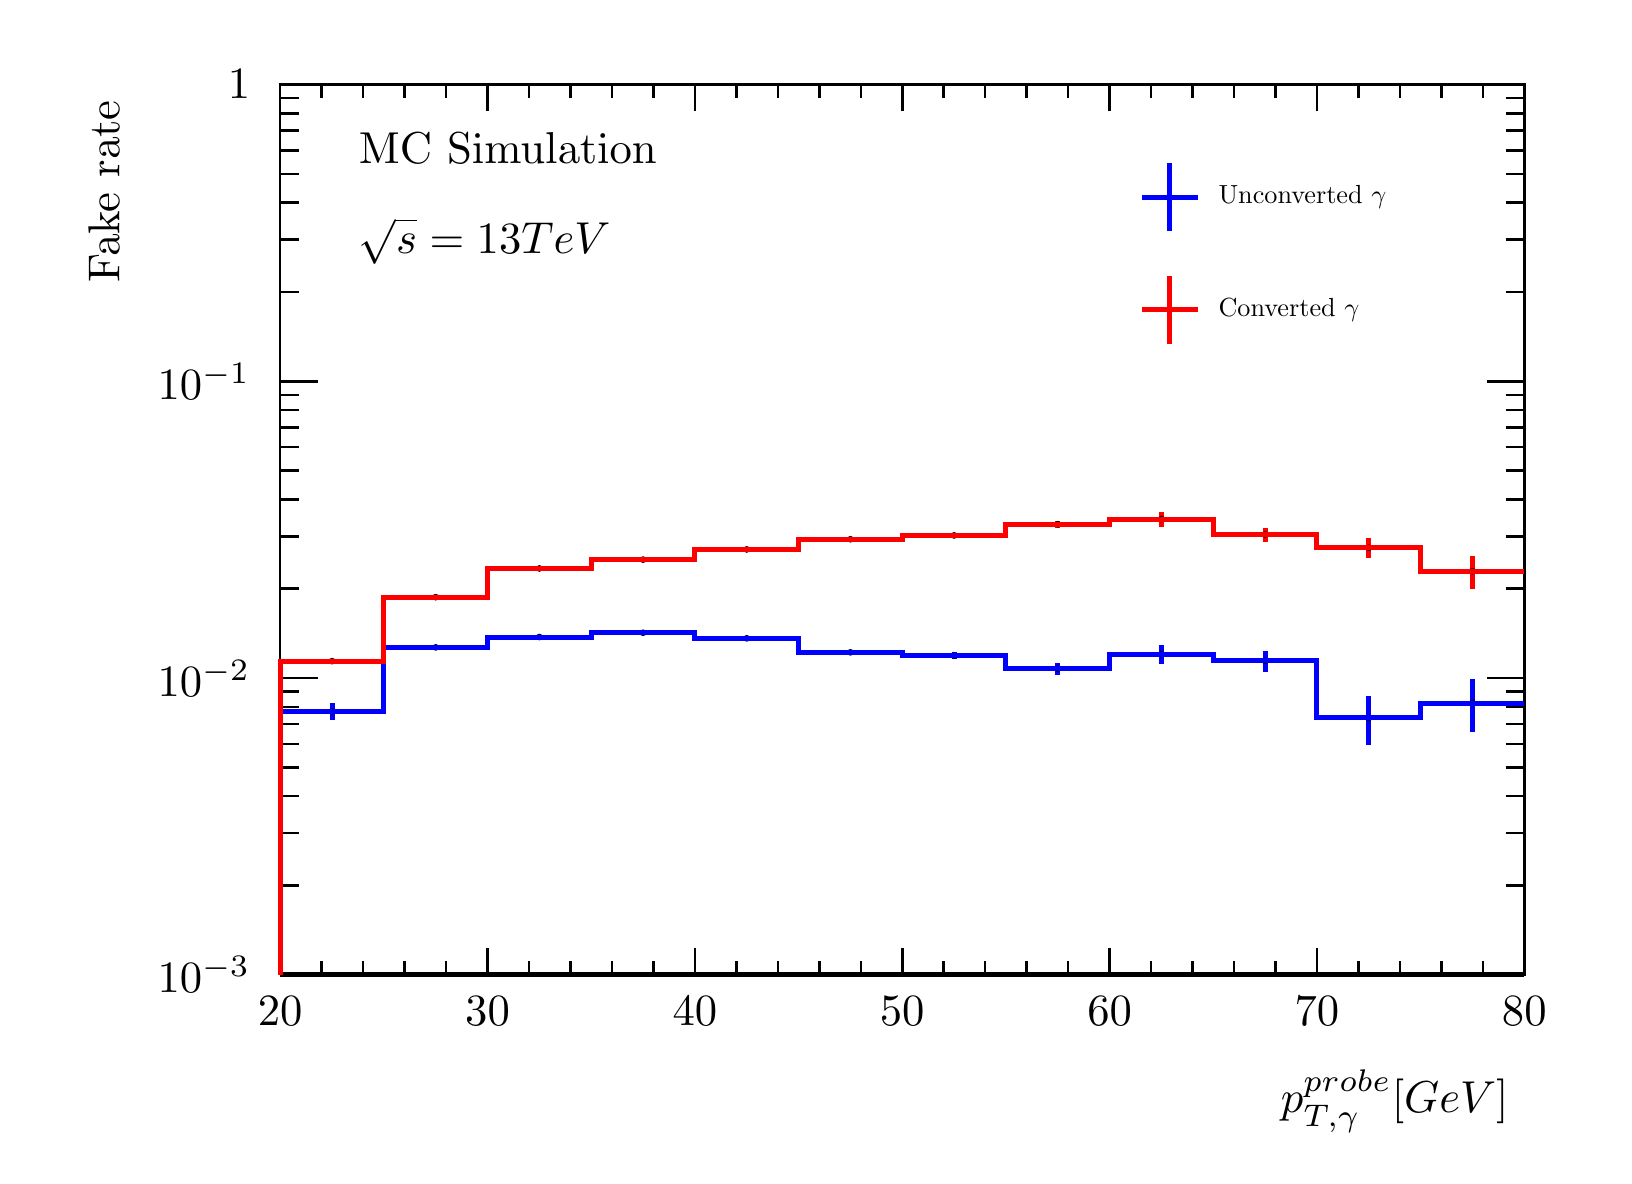
\begin{tikzpicture}
\pgfdeclareplotmark{cross} {
\pgfpathmoveto{\pgfpoint{-0.3\pgfplotmarksize}{\pgfplotmarksize}}
\pgfpathlineto{\pgfpoint{+0.3\pgfplotmarksize}{\pgfplotmarksize}}
\pgfpathlineto{\pgfpoint{+0.3\pgfplotmarksize}{0.3\pgfplotmarksize}}
\pgfpathlineto{\pgfpoint{+1\pgfplotmarksize}{0.3\pgfplotmarksize}}
\pgfpathlineto{\pgfpoint{+1\pgfplotmarksize}{-0.3\pgfplotmarksize}}
\pgfpathlineto{\pgfpoint{+0.3\pgfplotmarksize}{-0.3\pgfplotmarksize}}
\pgfpathlineto{\pgfpoint{+0.3\pgfplotmarksize}{-1.\pgfplotmarksize}}
\pgfpathlineto{\pgfpoint{-0.3\pgfplotmarksize}{-1.\pgfplotmarksize}}
\pgfpathlineto{\pgfpoint{-0.3\pgfplotmarksize}{-0.3\pgfplotmarksize}}
\pgfpathlineto{\pgfpoint{-1.\pgfplotmarksize}{-0.3\pgfplotmarksize}}
\pgfpathlineto{\pgfpoint{-1.\pgfplotmarksize}{0.3\pgfplotmarksize}}
\pgfpathlineto{\pgfpoint{-0.3\pgfplotmarksize}{0.3\pgfplotmarksize}}
\pgfpathclose
\pgfusepathqstroke
}
\pgfdeclareplotmark{cross*} {
\pgfpathmoveto{\pgfpoint{-0.3\pgfplotmarksize}{\pgfplotmarksize}}
\pgfpathlineto{\pgfpoint{+0.3\pgfplotmarksize}{\pgfplotmarksize}}
\pgfpathlineto{\pgfpoint{+0.3\pgfplotmarksize}{0.3\pgfplotmarksize}}
\pgfpathlineto{\pgfpoint{+1\pgfplotmarksize}{0.3\pgfplotmarksize}}
\pgfpathlineto{\pgfpoint{+1\pgfplotmarksize}{-0.3\pgfplotmarksize}}
\pgfpathlineto{\pgfpoint{+0.3\pgfplotmarksize}{-0.3\pgfplotmarksize}}
\pgfpathlineto{\pgfpoint{+0.3\pgfplotmarksize}{-1.\pgfplotmarksize}}
\pgfpathlineto{\pgfpoint{-0.3\pgfplotmarksize}{-1.\pgfplotmarksize}}
\pgfpathlineto{\pgfpoint{-0.3\pgfplotmarksize}{-0.3\pgfplotmarksize}}
\pgfpathlineto{\pgfpoint{-1.\pgfplotmarksize}{-0.3\pgfplotmarksize}}
\pgfpathlineto{\pgfpoint{-1.\pgfplotmarksize}{0.3\pgfplotmarksize}}
\pgfpathlineto{\pgfpoint{-0.3\pgfplotmarksize}{0.3\pgfplotmarksize}}
\pgfpathclose
\pgfusepathqfillstroke
}
\pgfdeclareplotmark{newstar} {
\pgfpathmoveto{\pgfqpoint{0pt}{\pgfplotmarksize}}
\pgfpathlineto{\pgfqpointpolar{44}{0.5\pgfplotmarksize}}
\pgfpathlineto{\pgfqpointpolar{18}{\pgfplotmarksize}}
\pgfpathlineto{\pgfqpointpolar{-20}{0.5\pgfplotmarksize}}
\pgfpathlineto{\pgfqpointpolar{-54}{\pgfplotmarksize}}
\pgfpathlineto{\pgfqpointpolar{-90}{0.5\pgfplotmarksize}}
\pgfpathlineto{\pgfqpointpolar{234}{\pgfplotmarksize}}
\pgfpathlineto{\pgfqpointpolar{198}{0.5\pgfplotmarksize}}
\pgfpathlineto{\pgfqpointpolar{162}{\pgfplotmarksize}}
\pgfpathlineto{\pgfqpointpolar{134}{0.5\pgfplotmarksize}}
\pgfpathclose
\pgfusepathqstroke
}
\pgfdeclareplotmark{newstar*} {
\pgfpathmoveto{\pgfqpoint{0pt}{\pgfplotmarksize}}
\pgfpathlineto{\pgfqpointpolar{44}{0.5\pgfplotmarksize}}
\pgfpathlineto{\pgfqpointpolar{18}{\pgfplotmarksize}}
\pgfpathlineto{\pgfqpointpolar{-20}{0.5\pgfplotmarksize}}
\pgfpathlineto{\pgfqpointpolar{-54}{\pgfplotmarksize}}
\pgfpathlineto{\pgfqpointpolar{-90}{0.5\pgfplotmarksize}}
\pgfpathlineto{\pgfqpointpolar{234}{\pgfplotmarksize}}
\pgfpathlineto{\pgfqpointpolar{198}{0.5\pgfplotmarksize}}
\pgfpathlineto{\pgfqpointpolar{162}{\pgfplotmarksize}}
\pgfpathlineto{\pgfqpointpolar{134}{0.5\pgfplotmarksize}}
\pgfpathclose
\pgfusepathqfillstroke
}
\definecolor{c}{rgb}{1,1,1};
\draw [color=c, fill=c] (0,0) rectangle (20,14.3108);
\draw [color=c, fill=c] (3.2,2.28972) rectangle (19,13.5952);
\definecolor{c}{rgb}{0,0,0};
\draw [c,line width=0.9] (3.2,2.28972) -- (3.2,13.5952) -- (19,13.5952) -- (19,2.28972) -- (3.2,2.28972);
\draw [c,line width=1.8] (3.2,2.28972) -- (3.2158,2.28972) -- (3.2158,2.28972) -- (3.2316,2.28972) -- (3.2316,2.28972) -- (3.2474,2.28972) -- (3.2474,2.28972) -- (3.2632,2.28972) -- (3.2632,2.28972) -- (3.279,2.28972) -- (3.279,2.28972) --
 (3.2948,2.28972) -- (3.2948,2.28972) -- (3.3106,2.28972) -- (3.3106,2.28972) -- (3.3264,2.28972) -- (3.3264,2.28972) -- (3.3422,2.28972) -- (3.3422,2.28972) -- (3.358,2.28972) -- (3.358,2.28972) -- (3.3738,2.28972) -- (3.3738,2.28972) --
 (3.3896,2.28972) -- (3.3896,2.28972) -- (3.4054,2.28972) -- (3.4054,2.28972) -- (3.4212,2.28972) -- (3.4212,2.28972) -- (3.437,2.28972) -- (3.437,2.28972) -- (3.4528,2.28972) -- (3.4528,2.28972) -- (3.4686,2.28972) -- (3.4686,2.28972) --
 (3.4844,2.28972) -- (3.4844,2.28972) -- (3.5002,2.28972) -- (3.5002,2.28972) -- (3.516,2.28972) -- (3.516,2.28972) -- (3.5318,2.28972) -- (3.5318,2.28972) -- (3.5476,2.28972) -- (3.5476,2.28972) -- (3.5634,2.28972) -- (3.5634,2.28972) --
 (3.5792,2.28972) -- (3.5792,2.28972) -- (3.595,2.28972) -- (3.595,2.28972) -- (3.6108,2.28972) -- (3.6108,2.28972) -- (3.6266,2.28972) -- (3.6266,2.28972) -- (3.6424,2.28972) -- (3.6424,2.28972) -- (3.6582,2.28972) -- (3.6582,2.28972) --
 (3.674,2.28972) -- (3.674,2.28972) -- (3.6898,2.28972) -- (3.6898,2.28972) -- (3.7056,2.28972) -- (3.7056,2.28972) -- (3.7214,2.28972) -- (3.7214,2.28972) -- (3.7372,2.28972) -- (3.7372,2.28972) -- (3.753,2.28972) -- (3.753,2.28972) --
 (3.7688,2.28972) -- (3.7688,2.28972) -- (3.7846,2.28972) -- (3.7846,2.28972) -- (3.8004,2.28972) -- (3.8004,2.28972) -- (3.8162,2.28972) -- (3.8162,2.28972) -- (3.832,2.28972) -- (3.832,2.28972) -- (3.8478,2.28972) -- (3.8478,2.28972) --
 (3.8636,2.28972) -- (3.8636,2.28972) -- (3.8794,2.28972) -- (3.8794,2.28972) -- (3.8952,2.28972) -- (3.8952,2.28972) -- (3.911,2.28972) -- (3.911,2.28972) -- (3.9268,2.28972) -- (3.9268,2.28972) -- (3.9426,2.28972) -- (3.9426,2.28972) --
 (3.9584,2.28972) -- (3.9584,2.28972) -- (3.9742,2.28972) -- (3.9742,2.28972) -- (3.99,2.28972) -- (3.99,2.28972) -- (4.0058,2.28972) -- (4.0058,2.28972) -- (4.0216,2.28972) -- (4.0216,2.28972) -- (4.0374,2.28972) -- (4.0374,2.28972) --
 (4.0532,2.28972) -- (4.0532,2.28972) -- (4.069,2.28972) -- (4.069,2.28972) -- (4.0848,2.28972) -- (4.0848,2.28972) -- (4.1006,2.28972) -- (4.1006,2.28972) -- (4.1164,2.28972) -- (4.1164,2.28972) -- (4.1322,2.28972) -- (4.1322,2.28972) --
 (4.148,2.28972) -- (4.148,2.28972) -- (4.1638,2.28972) -- (4.1638,2.28972) -- (4.1796,2.28972) -- (4.1796,2.28972) -- (4.1954,2.28972) -- (4.1954,2.28972) -- (4.2112,2.28972) -- (4.2112,2.28972) -- (4.227,2.28972) -- (4.227,2.28972) --
 (4.2428,2.28972) -- (4.2428,2.28972) -- (4.2586,2.28972) -- (4.2586,2.28972) -- (4.2744,2.28972) -- (4.2744,2.28972) -- (4.2902,2.28972) -- (4.2902,2.28972) -- (4.306,2.28972) -- (4.306,2.28972) -- (4.3218,2.28972) -- (4.3218,2.28972) --
 (4.3376,2.28972) -- (4.3376,2.28972) -- (4.3534,2.28972) -- (4.3534,2.28972) -- (4.3692,2.28972) -- (4.3692,2.28972) -- (4.385,2.28972) -- (4.385,2.28972) -- (4.4008,2.28972) -- (4.4008,2.28972) -- (4.4166,2.28972) -- (4.4166,2.28972) --
 (4.4324,2.28972) -- (4.4324,2.28972) -- (4.4482,2.28972) -- (4.4482,2.28972) -- (4.464,2.28972) -- (4.464,2.28972) -- (4.4798,2.28972) -- (4.4798,2.28972) -- (4.4956,2.28972) -- (4.4956,2.28972) -- (4.5114,2.28972) -- (4.5114,2.28972) --
 (4.5272,2.28972) -- (4.5272,2.28972) -- (4.543,2.28972) -- (4.543,2.28972) -- (4.5588,2.28972) -- (4.5588,2.28972) -- (4.5746,2.28972) -- (4.5746,2.28972) -- (4.5904,2.28972) -- (4.5904,2.28972) -- (4.6062,2.28972) -- (4.6062,2.28972) --
 (4.622,2.28972) -- (4.622,2.28972) -- (4.6378,2.28972) -- (4.6378,2.28972) -- (4.6536,2.28972) -- (4.6536,2.28972) -- (4.6694,2.28972) -- (4.6694,2.28972) -- (4.6852,2.28972) -- (4.6852,2.28972) -- (4.701,2.28972) -- (4.701,2.28972) --
 (4.7168,2.28972) -- (4.7168,2.28972) -- (4.7326,2.28972) -- (4.7326,2.28972) -- (4.7484,2.28972) -- (4.7484,2.28972) -- (4.7642,2.28972) -- (4.7642,2.28972) -- (4.78,2.28972) -- (4.78,2.28972) -- (4.7958,2.28972) -- (4.7958,2.28972) --
 (4.8116,2.28972) -- (4.8116,2.28972) -- (4.8274,2.28972) -- (4.8274,2.28972) -- (4.8432,2.28972) -- (4.8432,2.28972) -- (4.859,2.28972) -- (4.859,2.28972) -- (4.8748,2.28972) -- (4.8748,2.28972) -- (4.8906,2.28972) -- (4.8906,2.28972) --
 (4.9064,2.28972) -- (4.9064,2.28972) -- (4.9222,2.28972) -- (4.9222,2.28972) -- (4.938,2.28972) -- (4.938,2.28972) -- (4.9538,2.28972) -- (4.9538,2.28972) -- (4.9696,2.28972) -- (4.9696,2.28972) -- (4.9854,2.28972) -- (4.9854,2.28972) --
 (5.0012,2.28972) -- (5.0012,2.28972) -- (5.017,2.28972) -- (5.017,2.28972) -- (5.0328,2.28972) -- (5.0328,2.28972) -- (5.0486,2.28972) -- (5.0486,2.28972) -- (5.0644,2.28972) -- (5.0644,2.28972) -- (5.0802,2.28972) -- (5.0802,2.28972) --
 (5.096,2.28972) -- (5.096,2.28972) -- (5.1118,2.28972) -- (5.1118,2.28972) -- (5.1276,2.28972) -- (5.1276,2.28972) -- (5.1434,2.28972) -- (5.1434,2.28972) -- (5.1592,2.28972) -- (5.1592,2.28972) -- (5.175,2.28972) -- (5.175,2.28972) --
 (5.1908,2.28972) -- (5.1908,2.28972) -- (5.2066,2.28972) -- (5.2066,2.28972) -- (5.2224,2.28972) -- (5.2224,2.28972) -- (5.2382,2.28972) -- (5.2382,2.28972) -- (5.254,2.28972) -- (5.254,2.28972) -- (5.2698,2.28972) -- (5.2698,2.28972) --
 (5.2856,2.28972) -- (5.2856,2.28972) -- (5.3014,2.28972) -- (5.3014,2.28972) -- (5.3172,2.28972) -- (5.3172,2.28972) -- (5.333,2.28972) -- (5.333,2.28972) -- (5.3488,2.28972) -- (5.3488,2.28972) -- (5.3646,2.28972) -- (5.3646,2.28972) --
 (5.3804,2.28972) -- (5.3804,2.28972) -- (5.3962,2.28972) -- (5.3962,2.28972) -- (5.412,2.28972) -- (5.412,2.28972) -- (5.4278,2.28972) -- (5.4278,2.28972) -- (5.4436,2.28972) -- (5.4436,2.28972) -- (5.4594,2.28972) -- (5.4594,2.28972) --
 (5.4752,2.28972) -- (5.4752,2.28972) -- (5.491,2.28972) -- (5.491,2.28972) -- (5.5068,2.28972) -- (5.5068,2.28972) -- (5.5226,2.28972) -- (5.5226,2.28972) -- (5.5384,2.28972) -- (5.5384,2.28972) -- (5.5542,2.28972) -- (5.5542,2.28972) --
 (5.57,2.28972) -- (5.57,2.28972) -- (5.5858,2.28972) -- (5.5858,2.28972) -- (5.6016,2.28972) -- (5.6016,2.28972) -- (5.6174,2.28972) -- (5.6174,2.28972) -- (5.6332,2.28972) -- (5.6332,2.28972) -- (5.649,2.28972) -- (5.649,2.28972) --
 (5.6648,2.28972) -- (5.6648,2.28972) -- (5.6806,2.28972) -- (5.6806,2.28972) -- (5.6964,2.28972) -- (5.6964,2.28972) -- (5.7122,2.28972) -- (5.7122,2.28972) -- (5.728,2.28972) -- (5.728,2.28972) -- (5.7438,2.28972) -- (5.7438,2.28972) --
 (5.7596,2.28972) -- (5.7596,2.28972) -- (5.7754,2.28972) -- (5.7754,2.28972) -- (5.7912,2.28972) -- (5.7912,2.28972) -- (5.807,2.28972) -- (5.807,2.28972) -- (5.8228,2.28972) -- (5.8228,2.28972) -- (5.8386,2.28972) -- (5.8386,2.28972) --
 (5.8544,2.28972) -- (5.8544,2.28972) -- (5.8702,2.28972) -- (5.8702,2.28972) -- (5.886,2.28972) -- (5.886,2.28972) -- (5.9018,2.28972) -- (5.9018,2.28972) -- (5.9176,2.28972) -- (5.9176,2.28972) -- (5.9334,2.28972) -- (5.9334,2.28972) --
 (5.9492,2.28972) -- (5.9492,2.28972) -- (5.965,2.28972) -- (5.965,2.28972) -- (5.9808,2.28972) -- (5.9808,2.28972) -- (5.9966,2.28972) -- (5.9966,2.28972) -- (6.0124,2.28972) -- (6.0124,2.28972) -- (6.0282,2.28972) -- (6.0282,2.28972) --
 (6.044,2.28972) -- (6.044,2.28972) -- (6.0598,2.28972) -- (6.0598,2.28972) -- (6.0756,2.28972) -- (6.0756,2.28972) -- (6.0914,2.28972) -- (6.0914,2.28972) -- (6.1072,2.28972) -- (6.1072,2.28972) -- (6.123,2.28972) -- (6.123,2.28972) --
 (6.1388,2.28972) -- (6.1388,2.28972) -- (6.1546,2.28972) -- (6.1546,2.28972) -- (6.1704,2.28972) -- (6.1704,2.28972) -- (6.1862,2.28972) -- (6.1862,2.28972) -- (6.202,2.28972) -- (6.202,2.28972) -- (6.2178,2.28972) -- (6.2178,2.28972) --
 (6.2336,2.28972) -- (6.2336,2.28972) -- (6.2494,2.28972) -- (6.2494,2.28972) -- (6.2652,2.28972) -- (6.2652,2.28972) -- (6.281,2.28972) -- (6.281,2.28972) -- (6.2968,2.28972) -- (6.2968,2.28972) -- (6.3126,2.28972) -- (6.3126,2.28972) --
 (6.3284,2.28972) -- (6.3284,2.28972) -- (6.3442,2.28972) -- (6.3442,2.28972) -- (6.36,2.28972) -- (6.36,2.28972) -- (6.3758,2.28972) -- (6.3758,2.28972) -- (6.3916,2.28972) -- (6.3916,2.28972) -- (6.4074,2.28972) -- (6.4074,2.28972) --
 (6.4232,2.28972) -- (6.4232,2.28972) -- (6.439,2.28972) -- (6.439,2.28972) -- (6.4548,2.28972) -- (6.4548,2.28972) -- (6.4706,2.28972) -- (6.4706,2.28972) -- (6.4864,2.28972) -- (6.4864,2.28972) -- (6.5022,2.28972) -- (6.5022,2.28972) --
 (6.518,2.28972) -- (6.518,2.28972) -- (6.5338,2.28972) -- (6.5338,2.28972) -- (6.5496,2.28972) -- (6.5496,2.28972) -- (6.5654,2.28972) -- (6.5654,2.28972) -- (6.5812,2.28972) -- (6.5812,2.28972) -- (6.597,2.28972) -- (6.597,2.28972) --
 (6.6128,2.28972) -- (6.6128,2.28972) -- (6.6286,2.28972) -- (6.6286,2.28972) -- (6.6444,2.28972) -- (6.6444,2.28972) -- (6.6602,2.28972) -- (6.6602,2.28972) -- (6.676,2.28972) -- (6.676,2.28972) -- (6.6918,2.28972) -- (6.6918,2.28972) --
 (6.7076,2.28972) -- (6.7076,2.28972) -- (6.7234,2.28972) -- (6.7234,2.28972) -- (6.7392,2.28972) -- (6.7392,2.28972) -- (6.755,2.28972) -- (6.755,2.28972) -- (6.7708,2.28972) -- (6.7708,2.28972) -- (6.7866,2.28972) -- (6.7866,2.28972) --
 (6.8024,2.28972) -- (6.8024,2.28972) -- (6.8182,2.28972) -- (6.8182,2.28972) -- (6.834,2.28972) -- (6.834,2.28972) -- (6.8498,2.28972) -- (6.8498,2.28972) -- (6.8656,2.28972) -- (6.8656,2.28972) -- (6.8814,2.28972) -- (6.8814,2.28972) --
 (6.8972,2.28972) -- (6.8972,2.28972) -- (6.913,2.28972) -- (6.913,2.28972) -- (6.9288,2.28972) -- (6.9288,2.28972) -- (6.9446,2.28972) -- (6.9446,2.28972) -- (6.9604,2.28972) -- (6.9604,2.28972) -- (6.9762,2.28972) -- (6.9762,2.28972) --
 (6.992,2.28972) -- (6.992,2.28972) -- (7.0078,2.28972) -- (7.0078,2.28972) -- (7.0236,2.28972) -- (7.0236,2.28972) -- (7.0394,2.28972) -- (7.0394,2.28972) -- (7.0552,2.28972) -- (7.0552,2.28972) -- (7.071,2.28972) -- (7.071,2.28972) --
 (7.0868,2.28972) -- (7.0868,2.28972) -- (7.1026,2.28972) -- (7.1026,2.28972) -- (7.1184,2.28972) -- (7.1184,2.28972) -- (7.1342,2.28972) -- (7.1342,2.28972) -- (7.15,2.28972) -- (7.15,2.28972) -- (7.1658,2.28972) -- (7.1658,2.28972) --
 (7.1816,2.28972) -- (7.1816,2.28972) -- (7.1974,2.28972) -- (7.1974,2.28972) -- (7.2132,2.28972) -- (7.2132,2.28972) -- (7.229,2.28972) -- (7.229,2.28972) -- (7.2448,2.28972) -- (7.2448,2.28972) -- (7.2606,2.28972) -- (7.2606,2.28972) --
 (7.2764,2.28972) -- (7.2764,2.28972) -- (7.2922,2.28972) -- (7.2922,2.28972) -- (7.308,2.28972) -- (7.308,2.28972) -- (7.3238,2.28972) -- (7.3238,2.28972) -- (7.3396,2.28972) -- (7.3396,2.28972) -- (7.3554,2.28972) -- (7.3554,2.28972) --
 (7.3712,2.28972) -- (7.3712,2.28972) -- (7.387,2.28972) -- (7.387,2.28972) -- (7.4028,2.28972) -- (7.4028,2.28972) -- (7.4186,2.28972) -- (7.4186,2.28972) -- (7.4344,2.28972) -- (7.4344,2.28972) -- (7.4502,2.28972) -- (7.4502,2.28972) --
 (7.466,2.28972) -- (7.466,2.28972) -- (7.4818,2.28972) -- (7.4818,2.28972) -- (7.4976,2.28972) -- (7.4976,2.28972) -- (7.5134,2.28972) -- (7.5134,2.28972) -- (7.5292,2.28972) -- (7.5292,2.28972) -- (7.545,2.28972) -- (7.545,2.28972) --
 (7.5608,2.28972) -- (7.5608,2.28972) -- (7.5766,2.28972) -- (7.5766,2.28972) -- (7.5924,2.28972) -- (7.5924,2.28972) -- (7.6082,2.28972) -- (7.6082,2.28972) -- (7.624,2.28972) -- (7.624,2.28972) -- (7.6398,2.28972) -- (7.6398,2.28972) --
 (7.6556,2.28972) -- (7.6556,2.28972) -- (7.6714,2.28972) -- (7.6714,2.28972) -- (7.6872,2.28972) -- (7.6872,2.28972) -- (7.703,2.28972) -- (7.703,2.28972) -- (7.7188,2.28972) -- (7.7188,2.28972) -- (7.7346,2.28972) -- (7.7346,2.28972) --
 (7.7504,2.28972) -- (7.7504,2.28972) -- (7.7662,2.28972) -- (7.7662,2.28972) -- (7.782,2.28972) -- (7.782,2.28972) -- (7.7978,2.28972) -- (7.7978,2.28972) -- (7.8136,2.28972) -- (7.8136,2.28972) -- (7.8294,2.28972) -- (7.8294,2.28972) --
 (7.8452,2.28972) -- (7.8452,2.28972) -- (7.861,2.28972) -- (7.861,2.28972) -- (7.8768,2.28972) -- (7.8768,2.28972) -- (7.8926,2.28972) -- (7.8926,2.28972) -- (7.9084,2.28972) -- (7.9084,2.28972) -- (7.9242,2.28972) -- (7.9242,2.28972) --
 (7.94,2.28972) -- (7.94,2.28972) -- (7.9558,2.28972) -- (7.9558,2.28972) -- (7.9716,2.28972) -- (7.9716,2.28972) -- (7.9874,2.28972) -- (7.9874,2.28972) -- (8.0032,2.28972) -- (8.0032,2.28972) -- (8.019,2.28972) -- (8.019,2.28972) --
 (8.0348,2.28972) -- (8.0348,2.28972) -- (8.0506,2.28972) -- (8.0506,2.28972) -- (8.0664,2.28972) -- (8.0664,2.28972) -- (8.0822,2.28972) -- (8.0822,2.28972) -- (8.098,2.28972) -- (8.098,2.28972) -- (8.1138,2.28972) -- (8.1138,2.28972) --
 (8.1296,2.28972) -- (8.1296,2.28972) -- (8.1454,2.28972) -- (8.1454,2.28972) -- (8.1612,2.28972) -- (8.1612,2.28972) -- (8.177,2.28972) -- (8.177,2.28972) -- (8.1928,2.28972) -- (8.1928,2.28972) -- (8.2086,2.28972) -- (8.2086,2.28972) --
 (8.2244,2.28972) -- (8.2244,2.28972) -- (8.2402,2.28972) -- (8.2402,2.28972) -- (8.256,2.28972) -- (8.256,2.28972) -- (8.2718,2.28972) -- (8.2718,2.28972) -- (8.2876,2.28972) -- (8.2876,2.28972) -- (8.3034,2.28972) -- (8.3034,2.28972) --
 (8.3192,2.28972) -- (8.3192,2.28972) -- (8.335,2.28972) -- (8.335,2.28972) -- (8.3508,2.28972) -- (8.3508,2.28972) -- (8.3666,2.28972) -- (8.3666,2.28972) -- (8.3824,2.28972) -- (8.3824,2.28972) -- (8.3982,2.28972) -- (8.3982,2.28972) --
 (8.414,2.28972) -- (8.414,2.28972) -- (8.4298,2.28972) -- (8.4298,2.28972) -- (8.4456,2.28972) -- (8.4456,2.28972) -- (8.4614,2.28972) -- (8.4614,2.28972) -- (8.4772,2.28972) -- (8.4772,2.28972) -- (8.493,2.28972) -- (8.493,2.28972) --
 (8.5088,2.28972) -- (8.5088,2.28972) -- (8.5246,2.28972) -- (8.5246,2.28972) -- (8.5404,2.28972) -- (8.5404,2.28972) -- (8.5562,2.28972) -- (8.5562,2.28972) -- (8.572,2.28972) -- (8.572,2.28972) -- (8.5878,2.28972) -- (8.5878,2.28972) --
 (8.6036,2.28972) -- (8.6036,2.28972) -- (8.6194,2.28972) -- (8.6194,2.28972) -- (8.6352,2.28972) -- (8.6352,2.28972) -- (8.651,2.28972) -- (8.651,2.28972) -- (8.6668,2.28972) -- (8.6668,2.28972) -- (8.6826,2.28972) -- (8.6826,2.28972) --
 (8.6984,2.28972) -- (8.6984,2.28972) -- (8.7142,2.28972) -- (8.7142,2.28972) -- (8.73,2.28972) -- (8.73,2.28972) -- (8.7458,2.28972) -- (8.7458,2.28972) -- (8.7616,2.28972) -- (8.7616,2.28972) -- (8.7774,2.28972) -- (8.7774,2.28972) --
 (8.7932,2.28972) -- (8.7932,2.28972) -- (8.809,2.28972) -- (8.809,2.28972) -- (8.8248,2.28972) -- (8.8248,2.28972) -- (8.8406,2.28972) -- (8.8406,2.28972) -- (8.8564,2.28972) -- (8.8564,2.28972) -- (8.8722,2.28972) -- (8.8722,2.28972) --
 (8.888,2.28972) -- (8.888,2.28972) -- (8.9038,2.28972) -- (8.9038,2.28972) -- (8.9196,2.28972) -- (8.9196,2.28972) -- (8.9354,2.28972) -- (8.9354,2.28972) -- (8.9512,2.28972) -- (8.9512,2.28972) -- (8.967,2.28972) -- (8.967,2.28972) --
 (8.9828,2.28972) -- (8.9828,2.28972) -- (8.9986,2.28972) -- (8.9986,2.28972) -- (9.0144,2.28972) -- (9.0144,2.28972) -- (9.0302,2.28972) -- (9.0302,2.28972) -- (9.046,2.28972) -- (9.046,2.28972) -- (9.0618,2.28972) -- (9.0618,2.28972) --
 (9.0776,2.28972) -- (9.0776,2.28972) -- (9.0934,2.28972) -- (9.0934,2.28972) -- (9.1092,2.28972) -- (9.1092,2.28972) -- (9.125,2.28972) -- (9.125,2.28972) -- (9.1408,2.28972) -- (9.1408,2.28972) -- (9.1566,2.28972) -- (9.1566,2.28972) --
 (9.1724,2.28972) -- (9.1724,2.28972) -- (9.1882,2.28972) -- (9.1882,2.28972) -- (9.204,2.28972) -- (9.204,2.28972) -- (9.2198,2.28972) -- (9.2198,2.28972) -- (9.2356,2.28972) -- (9.2356,2.28972) -- (9.2514,2.28972) -- (9.2514,2.28972) --
 (9.2672,2.28972) -- (9.2672,2.28972) -- (9.283,2.28972) -- (9.283,2.28972) -- (9.2988,2.28972) -- (9.2988,2.28972) -- (9.3146,2.28972) -- (9.3146,2.28972) -- (9.3304,2.28972) -- (9.3304,2.28972) -- (9.3462,2.28972) -- (9.3462,2.28972) --
 (9.362,2.28972) -- (9.362,2.28972) -- (9.3778,2.28972) -- (9.3778,2.28972) -- (9.3936,2.28972) -- (9.3936,2.28972) -- (9.4094,2.28972) -- (9.4094,2.28972) -- (9.4252,2.28972) -- (9.4252,2.28972) -- (9.441,2.28972) -- (9.441,2.28972) --
 (9.4568,2.28972) -- (9.4568,2.28972) -- (9.4726,2.28972) -- (9.4726,2.28972) -- (9.4884,2.28972) -- (9.4884,2.28972) -- (9.5042,2.28972) -- (9.5042,2.28972) -- (9.52,2.28972) -- (9.52,2.28972) -- (9.5358,2.28972) -- (9.5358,2.28972) --
 (9.5516,2.28972) -- (9.5516,2.28972) -- (9.5674,2.28972) -- (9.5674,2.28972) -- (9.5832,2.28972) -- (9.5832,2.28972) -- (9.599,2.28972) -- (9.599,2.28972) -- (9.6148,2.28972) -- (9.6148,2.28972) -- (9.6306,2.28972) -- (9.6306,2.28972) --
 (9.6464,2.28972) -- (9.6464,2.28972) -- (9.6622,2.28972) -- (9.6622,2.28972) -- (9.678,2.28972) -- (9.678,2.28972) -- (9.6938,2.28972) -- (9.6938,2.28972) -- (9.7096,2.28972) -- (9.7096,2.28972) -- (9.7254,2.28972) -- (9.7254,2.28972) --
 (9.7412,2.28972) -- (9.7412,2.28972) -- (9.757,2.28972) -- (9.757,2.28972) -- (9.7728,2.28972) -- (9.7728,2.28972) -- (9.7886,2.28972) -- (9.7886,2.28972) -- (9.8044,2.28972) -- (9.8044,2.28972) -- (9.8202,2.28972) -- (9.8202,2.28972) --
 (9.836,2.28972) -- (9.836,2.28972) -- (9.8518,2.28972) -- (9.8518,2.28972) -- (9.8676,2.28972) -- (9.8676,2.28972) -- (9.8834,2.28972) -- (9.8834,2.28972) -- (9.8992,2.28972) -- (9.8992,2.28972) -- (9.915,2.28972) -- (9.915,2.28972) --
 (9.9308,2.28972) -- (9.9308,2.28972) -- (9.9466,2.28972) -- (9.9466,2.28972) -- (9.9624,2.28972) -- (9.9624,2.28972) -- (9.9782,2.28972) -- (9.9782,2.28972) -- (9.994,2.28972) -- (9.994,2.28972) -- (10.0098,2.28972) -- (10.0098,2.28972) --
 (10.0256,2.28972) -- (10.0256,2.28972) -- (10.0414,2.28972) -- (10.0414,2.28972) -- (10.0572,2.28972) -- (10.0572,2.28972) -- (10.073,2.28972) -- (10.073,2.28972) -- (10.0888,2.28972) -- (10.0888,2.28972) -- (10.1046,2.28972) -- (10.1046,2.28972) --
 (10.1204,2.28972) -- (10.1204,2.28972) -- (10.1362,2.28972) -- (10.1362,2.28972) -- (10.152,2.28972) -- (10.152,2.28972) -- (10.1678,2.28972) -- (10.1678,2.28972) -- (10.1836,2.28972) -- (10.1836,2.28972) -- (10.1994,2.28972) -- (10.1994,2.28972) --
 (10.2152,2.28972) -- (10.2152,2.28972) -- (10.231,2.28972) -- (10.231,2.28972) -- (10.2468,2.28972) -- (10.2468,2.28972) -- (10.2626,2.28972) -- (10.2626,2.28972) -- (10.2784,2.28972) -- (10.2784,2.28972) -- (10.2942,2.28972) -- (10.2942,2.28972) --
 (10.31,2.28972) -- (10.31,2.28972) -- (10.3258,2.28972) -- (10.3258,2.28972) -- (10.3416,2.28972) -- (10.3416,2.28972) -- (10.3574,2.28972) -- (10.3574,2.28972) -- (10.3732,2.28972) -- (10.3732,2.28972) -- (10.389,2.28972) -- (10.389,2.28972) --
 (10.4048,2.28972) -- (10.4048,2.28972) -- (10.4206,2.28972) -- (10.4206,2.28972) -- (10.4364,2.28972) -- (10.4364,2.28972) -- (10.4522,2.28972) -- (10.4522,2.28972) -- (10.468,2.28972) -- (10.468,2.28972) -- (10.4838,2.28972) -- (10.4838,2.28972) --
 (10.4996,2.28972) -- (10.4996,2.28972) -- (10.5154,2.28972) -- (10.5154,2.28972) -- (10.5312,2.28972) -- (10.5312,2.28972) -- (10.547,2.28972) -- (10.547,2.28972) -- (10.5628,2.28972) -- (10.5628,2.28972) -- (10.5786,2.28972) -- (10.5786,2.28972) --
 (10.5944,2.28972) -- (10.5944,2.28972) -- (10.6102,2.28972) -- (10.6102,2.28972) -- (10.626,2.28972) -- (10.626,2.28972) -- (10.6418,2.28972) -- (10.6418,2.28972) -- (10.6576,2.28972) -- (10.6576,2.28972) -- (10.6734,2.28972) -- (10.6734,2.28972) --
 (10.6892,2.28972) -- (10.6892,2.28972) -- (10.705,2.28972) -- (10.705,2.28972) -- (10.7208,2.28972) -- (10.7208,2.28972) -- (10.7366,2.28972) -- (10.7366,2.28972) -- (10.7524,2.28972) -- (10.7524,2.28972) -- (10.7682,2.28972) -- (10.7682,2.28972) --
 (10.784,2.28972) -- (10.784,2.28972) -- (10.7998,2.28972) -- (10.7998,2.28972) -- (10.8156,2.28972) -- (10.8156,2.28972) -- (10.8314,2.28972) -- (10.8314,2.28972) -- (10.8472,2.28972) -- (10.8472,2.28972) -- (10.863,2.28972) -- (10.863,2.28972) --
 (10.8788,2.28972) -- (10.8788,2.28972) -- (10.8946,2.28972) -- (10.8946,2.28972) -- (10.9104,2.28972) -- (10.9104,2.28972) -- (10.9262,2.28972) -- (10.9262,2.28972) -- (10.942,2.28972) -- (10.942,2.28972) -- (10.9578,2.28972) -- (10.9578,2.28972) --
 (10.9736,2.28972) -- (10.9736,2.28972) -- (10.9894,2.28972) -- (10.9894,2.28972) -- (11.0052,2.28972) -- (11.0052,2.28972) -- (11.021,2.28972) -- (11.021,2.28972) -- (11.0368,2.28972) -- (11.0368,2.28972) -- (11.0526,2.28972) -- (11.0526,2.28972) --
 (11.0684,2.28972) -- (11.0684,2.28972) -- (11.0842,2.28972) -- (11.0842,2.28972) -- (11.1,2.28972) -- (11.1,2.28972) -- (11.1158,2.28972) -- (11.1158,2.28972) -- (11.1316,2.28972) -- (11.1316,2.28972) -- (11.1474,2.28972) -- (11.1474,2.28972) --
 (11.1632,2.28972) -- (11.1632,2.28972) -- (11.179,2.28972) -- (11.179,2.28972) -- (11.1948,2.28972) -- (11.1948,2.28972) -- (11.2106,2.28972) -- (11.2106,2.28972) -- (11.2264,2.28972) -- (11.2264,2.28972) -- (11.2422,2.28972) -- (11.2422,2.28972) --
 (11.258,2.28972) -- (11.258,2.28972) -- (11.2738,2.28972) -- (11.2738,2.28972) -- (11.2896,2.28972) -- (11.2896,2.28972) -- (11.3054,2.28972) -- (11.3054,2.28972) -- (11.3212,2.28972) -- (11.3212,2.28972) -- (11.337,2.28972) -- (11.337,2.28972) --
 (11.3528,2.28972) -- (11.3528,2.28972) -- (11.3686,2.28972) -- (11.3686,2.28972) -- (11.3844,2.28972) -- (11.3844,2.28972) -- (11.4002,2.28972) -- (11.4002,2.28972) -- (11.416,2.28972) -- (11.416,2.28972) -- (11.4318,2.28972) -- (11.4318,2.28972) --
 (11.4476,2.28972) -- (11.4476,2.28972) -- (11.4634,2.28972) -- (11.4634,2.28972) -- (11.4792,2.28972) -- (11.4792,2.28972) -- (11.495,2.28972) -- (11.495,2.28972) -- (11.5108,2.28972) -- (11.5108,2.28972) -- (11.5266,2.28972) -- (11.5266,2.28972) --
 (11.5424,2.28972) -- (11.5424,2.28972) -- (11.5582,2.28972) -- (11.5582,2.28972) -- (11.574,2.28972) -- (11.574,2.28972) -- (11.5898,2.28972) -- (11.5898,2.28972) -- (11.6056,2.28972) -- (11.6056,2.28972) -- (11.6214,2.28972) -- (11.6214,2.28972) --
 (11.6372,2.28972) -- (11.6372,2.28972) -- (11.653,2.28972) -- (11.653,2.28972) -- (11.6688,2.28972) -- (11.6688,2.28972) -- (11.6846,2.28972) -- (11.6846,2.28972) -- (11.7004,2.28972) -- (11.7004,2.28972) -- (11.7162,2.28972) -- (11.7162,2.28972) --
 (11.732,2.28972) -- (11.732,2.28972) -- (11.7478,2.28972) -- (11.7478,2.28972) -- (11.7636,2.28972) -- (11.7636,2.28972) -- (11.7794,2.28972) -- (11.7794,2.28972) -- (11.7952,2.28972) -- (11.7952,2.28972) -- (11.811,2.28972) -- (11.811,2.28972) --
 (11.8268,2.28972) -- (11.8268,2.28972) -- (11.8426,2.28972) -- (11.8426,2.28972) -- (11.8584,2.28972) -- (11.8584,2.28972) -- (11.8742,2.28972) -- (11.8742,2.28972) -- (11.89,2.28972) -- (11.89,2.28972) -- (11.9058,2.28972) -- (11.9058,2.28972) --
 (11.9216,2.28972) -- (11.9216,2.28972) -- (11.9374,2.28972) -- (11.9374,2.28972) -- (11.9532,2.28972) -- (11.9532,2.28972) -- (11.969,2.28972) -- (11.969,2.28972) -- (11.9848,2.28972) -- (11.9848,2.28972) -- (12.0006,2.28972) -- (12.0006,2.28972) --
 (12.0164,2.28972) -- (12.0164,2.28972) -- (12.0322,2.28972) -- (12.0322,2.28972) -- (12.048,2.28972) -- (12.048,2.28972) -- (12.0638,2.28972) -- (12.0638,2.28972) -- (12.0796,2.28972) -- (12.0796,2.28972) -- (12.0954,2.28972) -- (12.0954,2.28972) --
 (12.1112,2.28972) -- (12.1112,2.28972) -- (12.127,2.28972) -- (12.127,2.28972) -- (12.1428,2.28972) -- (12.1428,2.28972) -- (12.1586,2.28972) -- (12.1586,2.28972) -- (12.1744,2.28972) -- (12.1744,2.28972) -- (12.1902,2.28972) -- (12.1902,2.28972) --
 (12.206,2.28972) -- (12.206,2.28972) -- (12.2218,2.28972) -- (12.2218,2.28972) -- (12.2376,2.28972) -- (12.2376,2.28972) -- (12.2534,2.28972) -- (12.2534,2.28972) -- (12.2692,2.28972) -- (12.2692,2.28972) -- (12.285,2.28972) -- (12.285,2.28972) --
 (12.3008,2.28972) -- (12.3008,2.28972) -- (12.3166,2.28972) -- (12.3166,2.28972) -- (12.3324,2.28972) -- (12.3324,2.28972) -- (12.3482,2.28972) -- (12.3482,2.28972) -- (12.364,2.28972) -- (12.364,2.28972) -- (12.3798,2.28972) -- (12.3798,2.28972) --
 (12.3956,2.28972) -- (12.3956,2.28972) -- (12.4114,2.28972) -- (12.4114,2.28972) -- (12.4272,2.28972) -- (12.4272,2.28972) -- (12.443,2.28972) -- (12.443,2.28972) -- (12.4588,2.28972) -- (12.4588,2.28972) -- (12.4746,2.28972) -- (12.4746,2.28972) --
 (12.4904,2.28972) -- (12.4904,2.28972) -- (12.5062,2.28972) -- (12.5062,2.28972) -- (12.522,2.28972) -- (12.522,2.28972) -- (12.5378,2.28972) -- (12.5378,2.28972) -- (12.5536,2.28972) -- (12.5536,2.28972) -- (12.5694,2.28972) -- (12.5694,2.28972) --
 (12.5852,2.28972) -- (12.5852,2.28972) -- (12.601,2.28972) -- (12.601,2.28972) -- (12.6168,2.28972) -- (12.6168,2.28972) -- (12.6326,2.28972) -- (12.6326,2.28972) -- (12.6484,2.28972) -- (12.6484,2.28972) -- (12.6642,2.28972) -- (12.6642,2.28972) --
 (12.68,2.28972) -- (12.68,2.28972) -- (12.6958,2.28972) -- (12.6958,2.28972) -- (12.7116,2.28972) -- (12.7116,2.28972) -- (12.7274,2.28972) -- (12.7274,2.28972) -- (12.7432,2.28972) -- (12.7432,2.28972) -- (12.759,2.28972) -- (12.759,2.28972) --
 (12.7748,2.28972) -- (12.7748,2.28972) -- (12.7906,2.28972) -- (12.7906,2.28972) -- (12.8064,2.28972) -- (12.8064,2.28972) -- (12.8222,2.28972) -- (12.8222,2.28972) -- (12.838,2.28972) -- (12.838,2.28972) -- (12.8538,2.28972) -- (12.8538,2.28972) --
 (12.8696,2.28972) -- (12.8696,2.28972) -- (12.8854,2.28972) -- (12.8854,2.28972) -- (12.9012,2.28972) -- (12.9012,2.28972) -- (12.917,2.28972) -- (12.917,2.28972) -- (12.9328,2.28972) -- (12.9328,2.28972) -- (12.9486,2.28972) -- (12.9486,2.28972) --
 (12.9644,2.28972) -- (12.9644,2.28972) -- (12.9802,2.28972) -- (12.9802,2.28972) -- (12.996,2.28972) -- (12.996,2.28972) -- (13.0118,2.28972) -- (13.0118,2.28972) -- (13.0276,2.28972) -- (13.0276,2.28972) -- (13.0434,2.28972) -- (13.0434,2.28972) --
 (13.0592,2.28972) -- (13.0592,2.28972) -- (13.075,2.28972) -- (13.075,2.28972) -- (13.0908,2.28972) -- (13.0908,2.28972) -- (13.1066,2.28972) -- (13.1066,2.28972) -- (13.1224,2.28972) -- (13.1224,2.28972) -- (13.1382,2.28972) -- (13.1382,2.28972) --
 (13.154,2.28972) -- (13.154,2.28972) -- (13.1698,2.28972) -- (13.1698,2.28972) -- (13.1856,2.28972) -- (13.1856,2.28972) -- (13.2014,2.28972) -- (13.2014,2.28972) -- (13.2172,2.28972) -- (13.2172,2.28972) -- (13.233,2.28972) -- (13.233,2.28972) --
 (13.2488,2.28972) -- (13.2488,2.28972) -- (13.2646,2.28972) -- (13.2646,2.28972) -- (13.2804,2.28972) -- (13.2804,2.28972) -- (13.2962,2.28972) -- (13.2962,2.28972) -- (13.312,2.28972) -- (13.312,2.28972) -- (13.3278,2.28972) -- (13.3278,2.28972) --
 (13.3436,2.28972) -- (13.3436,2.28972) -- (13.3594,2.28972) -- (13.3594,2.28972) -- (13.3752,2.28972) -- (13.3752,2.28972) -- (13.391,2.28972) -- (13.391,2.28972) -- (13.4068,2.28972) -- (13.4068,2.28972) -- (13.4226,2.28972) -- (13.4226,2.28972) --
 (13.4384,2.28972) -- (13.4384,2.28972) -- (13.4542,2.28972) -- (13.4542,2.28972) -- (13.47,2.28972) -- (13.47,2.28972) -- (13.4858,2.28972) -- (13.4858,2.28972) -- (13.5016,2.28972) -- (13.5016,2.28972) -- (13.5174,2.28972) -- (13.5174,2.28972) --
 (13.5332,2.28972) -- (13.5332,2.28972) -- (13.549,2.28972) -- (13.549,2.28972) -- (13.5648,2.28972) -- (13.5648,2.28972) -- (13.5806,2.28972) -- (13.5806,2.28972) -- (13.5964,2.28972) -- (13.5964,2.28972) -- (13.6122,2.28972) -- (13.6122,2.28972) --
 (13.628,2.28972) -- (13.628,2.28972) -- (13.6438,2.28972) -- (13.6438,2.28972) -- (13.6596,2.28972) -- (13.6596,2.28972) -- (13.6754,2.28972) -- (13.6754,2.28972) -- (13.6912,2.28972) -- (13.6912,2.28972) -- (13.707,2.28972) -- (13.707,2.28972) --
 (13.7228,2.28972) -- (13.7228,2.28972) -- (13.7386,2.28972) -- (13.7386,2.28972) -- (13.7544,2.28972) -- (13.7544,2.28972) -- (13.7702,2.28972) -- (13.7702,2.28972) -- (13.786,2.28972) -- (13.786,2.28972) -- (13.8018,2.28972) -- (13.8018,2.28972) --
 (13.8176,2.28972) -- (13.8176,2.28972) -- (13.8334,2.28972) -- (13.8334,2.28972) -- (13.8492,2.28972) -- (13.8492,2.28972) -- (13.865,2.28972) -- (13.865,2.28972) -- (13.8808,2.28972) -- (13.8808,2.28972) -- (13.8966,2.28972) -- (13.8966,2.28972) --
 (13.9124,2.28972) -- (13.9124,2.28972) -- (13.9282,2.28972) -- (13.9282,2.28972) -- (13.944,2.28972) -- (13.944,2.28972) -- (13.9598,2.28972) -- (13.9598,2.28972) -- (13.9756,2.28972) -- (13.9756,2.28972) -- (13.9914,2.28972) -- (13.9914,2.28972) --
 (14.0072,2.28972) -- (14.0072,2.28972) -- (14.023,2.28972) -- (14.023,2.28972) -- (14.0388,2.28972) -- (14.0388,2.28972) -- (14.0546,2.28972) -- (14.0546,2.28972) -- (14.0704,2.28972) -- (14.0704,2.28972) -- (14.0862,2.28972) -- (14.0862,2.28972) --
 (14.102,2.28972) -- (14.102,2.28972) -- (14.1178,2.28972) -- (14.1178,2.28972) -- (14.1336,2.28972) -- (14.1336,2.28972) -- (14.1494,2.28972) -- (14.1494,2.28972) -- (14.1652,2.28972) -- (14.1652,2.28972) -- (14.181,2.28972) -- (14.181,2.28972) --
 (14.1968,2.28972) -- (14.1968,2.28972) -- (14.2126,2.28972) -- (14.2126,2.28972) -- (14.2284,2.28972) -- (14.2284,2.28972) -- (14.2442,2.28972) -- (14.2442,2.28972) -- (14.26,2.28972) -- (14.26,2.28972) -- (14.2758,2.28972) -- (14.2758,2.28972) --
 (14.2916,2.28972) -- (14.2916,2.28972) -- (14.3074,2.28972) -- (14.3074,2.28972) -- (14.3232,2.28972) -- (14.3232,2.28972) -- (14.339,2.28972) -- (14.339,2.28972) -- (14.3548,2.28972) -- (14.3548,2.28972) -- (14.3706,2.28972) -- (14.3706,2.28972) --
 (14.3864,2.28972) -- (14.3864,2.28972) -- (14.4022,2.28972) -- (14.4022,2.28972) -- (14.418,2.28972) -- (14.418,2.28972) -- (14.4338,2.28972) -- (14.4338,2.28972) -- (14.4496,2.28972) -- (14.4496,2.28972) -- (14.4654,2.28972) -- (14.4654,2.28972) --
 (14.4812,2.28972) -- (14.4812,2.28972) -- (14.497,2.28972) -- (14.497,2.28972) -- (14.5128,2.28972) -- (14.5128,2.28972) -- (14.5286,2.28972) -- (14.5286,2.28972) -- (14.5444,2.28972) -- (14.5444,2.28972) -- (14.5602,2.28972) -- (14.5602,2.28972) --
 (14.576,2.28972) -- (14.576,2.28972) -- (14.5918,2.28972) -- (14.5918,2.28972) -- (14.6076,2.28972) -- (14.6076,2.28972) -- (14.6234,2.28972) -- (14.6234,2.28972) -- (14.6392,2.28972) -- (14.6392,2.28972) -- (14.655,2.28972) -- (14.655,2.28972) --
 (14.6708,2.28972) -- (14.6708,2.28972) -- (14.6866,2.28972) -- (14.6866,2.28972) -- (14.7024,2.28972) -- (14.7024,2.28972) -- (14.7182,2.28972) -- (14.7182,2.28972) -- (14.734,2.28972) -- (14.734,2.28972) -- (14.7498,2.28972) -- (14.7498,2.28972) --
 (14.7656,2.28972) -- (14.7656,2.28972) -- (14.7814,2.28972) -- (14.7814,2.28972) -- (14.7972,2.28972) -- (14.7972,2.28972) -- (14.813,2.28972) -- (14.813,2.28972) -- (14.8288,2.28972) -- (14.8288,2.28972) -- (14.8446,2.28972) -- (14.8446,2.28972) --
 (14.8604,2.28972) -- (14.8604,2.28972) -- (14.8762,2.28972) -- (14.8762,2.28972) -- (14.892,2.28972) -- (14.892,2.28972) -- (14.9078,2.28972) -- (14.9078,2.28972) -- (14.9236,2.28972) -- (14.9236,2.28972) -- (14.9394,2.28972) -- (14.9394,2.28972) --
 (14.9552,2.28972) -- (14.9552,2.28972) -- (14.971,2.28972) -- (14.971,2.28972) -- (14.9868,2.28972) -- (14.9868,2.28972) -- (15.0026,2.28972) -- (15.0026,2.28972) -- (15.0184,2.28972) -- (15.0184,2.28972) -- (15.0342,2.28972) -- (15.0342,2.28972) --
 (15.05,2.28972) -- (15.05,2.28972) -- (15.0658,2.28972) -- (15.0658,2.28972) -- (15.0816,2.28972) -- (15.0816,2.28972) -- (15.0974,2.28972) -- (15.0974,2.28972) -- (15.1132,2.28972) -- (15.1132,2.28972) -- (15.129,2.28972) -- (15.129,2.28972) --
 (15.1448,2.28972) -- (15.1448,2.28972) -- (15.1606,2.28972) -- (15.1606,2.28972) -- (15.1764,2.28972) -- (15.1764,2.28972) -- (15.1922,2.28972) -- (15.1922,2.28972) -- (15.208,2.28972) -- (15.208,2.28972) -- (15.2238,2.28972) -- (15.2238,2.28972) --
 (15.2396,2.28972) -- (15.2396,2.28972) -- (15.2554,2.28972) -- (15.2554,2.28972) -- (15.2712,2.28972) -- (15.2712,2.28972) -- (15.287,2.28972) -- (15.287,2.28972) -- (15.3028,2.28972) -- (15.3028,2.28972) -- (15.3186,2.28972) -- (15.3186,2.28972) --
 (15.3344,2.28972) -- (15.3344,2.28972) -- (15.3502,2.28972) -- (15.3502,2.28972) -- (15.366,2.28972) -- (15.366,2.28972) -- (15.3818,2.28972) -- (15.3818,2.28972) -- (15.3976,2.28972) -- (15.3976,2.28972) -- (15.4134,2.28972) -- (15.4134,2.28972) --
 (15.4292,2.28972) -- (15.4292,2.28972) -- (15.445,2.28972) -- (15.445,2.28972) -- (15.4608,2.28972) -- (15.4608,2.28972) -- (15.4766,2.28972) -- (15.4766,2.28972) -- (15.4924,2.28972) -- (15.4924,2.28972) -- (15.5082,2.28972) -- (15.5082,2.28972) --
 (15.524,2.28972) -- (15.524,2.28972) -- (15.5398,2.28972) -- (15.5398,2.28972) -- (15.5556,2.28972) -- (15.5556,2.28972) -- (15.5714,2.28972) -- (15.5714,2.28972) -- (15.5872,2.28972) -- (15.5872,2.28972) -- (15.603,2.28972) -- (15.603,2.28972) --
 (15.6188,2.28972) -- (15.6188,2.28972) -- (15.6346,2.28972) -- (15.6346,2.28972) -- (15.6504,2.28972) -- (15.6504,2.28972) -- (15.6662,2.28972) -- (15.6662,2.28972) -- (15.682,2.28972) -- (15.682,2.28972) -- (15.6978,2.28972) -- (15.6978,2.28972) --
 (15.7136,2.28972) -- (15.7136,2.28972) -- (15.7294,2.28972) -- (15.7294,2.28972) -- (15.7452,2.28972) -- (15.7452,2.28972) -- (15.761,2.28972) -- (15.761,2.28972) -- (15.7768,2.28972) -- (15.7768,2.28972) -- (15.7926,2.28972) -- (15.7926,2.28972) --
 (15.8084,2.28972) -- (15.8084,2.28972) -- (15.8242,2.28972) -- (15.8242,2.28972) -- (15.84,2.28972) -- (15.84,2.28972) -- (15.8558,2.28972) -- (15.8558,2.28972) -- (15.8716,2.28972) -- (15.8716,2.28972) -- (15.8874,2.28972) -- (15.8874,2.28972) --
 (15.9032,2.28972) -- (15.9032,2.28972) -- (15.919,2.28972) -- (15.919,2.28972) -- (15.9348,2.28972) -- (15.9348,2.28972) -- (15.9506,2.28972) -- (15.9506,2.28972) -- (15.9664,2.28972) -- (15.9664,2.28972) -- (15.9822,2.28972) -- (15.9822,2.28972) --
 (15.998,2.28972) -- (15.998,2.28972) -- (16.0138,2.28972) -- (16.0138,2.28972) -- (16.0296,2.28972) -- (16.0296,2.28972) -- (16.0454,2.28972) -- (16.0454,2.28972) -- (16.0612,2.28972) -- (16.0612,2.28972) -- (16.077,2.28972) -- (16.077,2.28972) --
 (16.0928,2.28972) -- (16.0928,2.28972) -- (16.1086,2.28972) -- (16.1086,2.28972) -- (16.1244,2.28972) -- (16.1244,2.28972) -- (16.1402,2.28972) -- (16.1402,2.28972) -- (16.156,2.28972) -- (16.156,2.28972) -- (16.1718,2.28972) -- (16.1718,2.28972) --
 (16.1876,2.28972) -- (16.1876,2.28972) -- (16.2034,2.28972) -- (16.2034,2.28972) -- (16.2192,2.28972) -- (16.2192,2.28972) -- (16.235,2.28972) -- (16.235,2.28972) -- (16.2508,2.28972) -- (16.2508,2.28972) -- (16.2666,2.28972) -- (16.2666,2.28972) --
 (16.2824,2.28972) -- (16.2824,2.28972) -- (16.2982,2.28972) -- (16.2982,2.28972) -- (16.314,2.28972) -- (16.314,2.28972) -- (16.3298,2.28972) -- (16.3298,2.28972) -- (16.3456,2.28972) -- (16.3456,2.28972) -- (16.3614,2.28972) -- (16.3614,2.28972) --
 (16.3772,2.28972) -- (16.3772,2.28972) -- (16.393,2.28972) -- (16.393,2.28972) -- (16.4088,2.28972) -- (16.4088,2.28972) -- (16.4246,2.28972) -- (16.4246,2.28972) -- (16.4404,2.28972) -- (16.4404,2.28972) -- (16.4562,2.28972) -- (16.4562,2.28972) --
 (16.472,2.28972) -- (16.472,2.28972) -- (16.4878,2.28972) -- (16.4878,2.28972) -- (16.5036,2.28972) -- (16.5036,2.28972) -- (16.5194,2.28972) -- (16.5194,2.28972) -- (16.5352,2.28972) -- (16.5352,2.28972) -- (16.551,2.28972) -- (16.551,2.28972) --
 (16.5668,2.28972) -- (16.5668,2.28972) -- (16.5826,2.28972) -- (16.5826,2.28972) -- (16.5984,2.28972) -- (16.5984,2.28972) -- (16.6142,2.28972) -- (16.6142,2.28972) -- (16.63,2.28972) -- (16.63,2.28972) -- (16.6458,2.28972) -- (16.6458,2.28972) --
 (16.6616,2.28972) -- (16.6616,2.28972) -- (16.6774,2.28972) -- (16.6774,2.28972) -- (16.6932,2.28972) -- (16.6932,2.28972) -- (16.709,2.28972) -- (16.709,2.28972) -- (16.7248,2.28972) -- (16.7248,2.28972) -- (16.7406,2.28972) -- (16.7406,2.28972) --
 (16.7564,2.28972) -- (16.7564,2.28972) -- (16.7722,2.28972) -- (16.7722,2.28972) -- (16.788,2.28972) -- (16.788,2.28972) -- (16.8038,2.28972) -- (16.8038,2.28972) -- (16.8196,2.28972) -- (16.8196,2.28972) -- (16.8354,2.28972) -- (16.8354,2.28972) --
 (16.8512,2.28972) -- (16.8512,2.28972) -- (16.867,2.28972) -- (16.867,2.28972) -- (16.8828,2.28972) -- (16.8828,2.28972) -- (16.8986,2.28972) -- (16.8986,2.28972) -- (16.9144,2.28972) -- (16.9144,2.28972) -- (16.9302,2.28972) -- (16.9302,2.28972) --
 (16.946,2.28972) -- (16.946,2.28972) -- (16.9618,2.28972) -- (16.9618,2.28972) -- (16.9776,2.28972) -- (16.9776,2.28972) -- (16.9934,2.28972) -- (16.9934,2.28972) -- (17.0092,2.28972) -- (17.0092,2.28972) -- (17.025,2.28972) -- (17.025,2.28972) --
 (17.0408,2.28972) -- (17.0408,2.28972) -- (17.0566,2.28972) -- (17.0566,2.28972) -- (17.0724,2.28972) -- (17.0724,2.28972) -- (17.0882,2.28972) -- (17.0882,2.28972) -- (17.104,2.28972) -- (17.104,2.28972) -- (17.1198,2.28972) -- (17.1198,2.28972) --
 (17.1356,2.28972) -- (17.1356,2.28972) -- (17.1514,2.28972) -- (17.1514,2.28972) -- (17.1672,2.28972) -- (17.1672,2.28972) -- (17.183,2.28972) -- (17.183,2.28972) -- (17.1988,2.28972) -- (17.1988,2.28972) -- (17.2146,2.28972) -- (17.2146,2.28972) --
 (17.2304,2.28972) -- (17.2304,2.28972) -- (17.2462,2.28972) -- (17.2462,2.28972) -- (17.262,2.28972) -- (17.262,2.28972) -- (17.2778,2.28972) -- (17.2778,2.28972) -- (17.2936,2.28972) -- (17.2936,2.28972) -- (17.3094,2.28972) -- (17.3094,2.28972) --
 (17.3252,2.28972) -- (17.3252,2.28972) -- (17.341,2.28972) -- (17.341,2.28972) -- (17.3568,2.28972) -- (17.3568,2.28972) -- (17.3726,2.28972) -- (17.3726,2.28972) -- (17.3884,2.28972) -- (17.3884,2.28972) -- (17.4042,2.28972) -- (17.4042,2.28972) --
 (17.42,2.28972) -- (17.42,2.28972) -- (17.4358,2.28972) -- (17.4358,2.28972) -- (17.4516,2.28972) -- (17.4516,2.28972) -- (17.4674,2.28972) -- (17.4674,2.28972) -- (17.4832,2.28972) -- (17.4832,2.28972) -- (17.499,2.28972) -- (17.499,2.28972) --
 (17.5148,2.28972) -- (17.5148,2.28972) -- (17.5306,2.28972) -- (17.5306,2.28972) -- (17.5464,2.28972) -- (17.5464,2.28972) -- (17.5622,2.28972) -- (17.5622,2.28972) -- (17.578,2.28972) -- (17.578,2.28972) -- (17.5938,2.28972) -- (17.5938,2.28972) --
 (17.6096,2.28972) -- (17.6096,2.28972) -- (17.6254,2.28972) -- (17.6254,2.28972) -- (17.6412,2.28972) -- (17.6412,2.28972) -- (17.657,2.28972) -- (17.657,2.28972) -- (17.6728,2.28972) -- (17.6728,2.28972) -- (17.6886,2.28972) -- (17.6886,2.28972) --
 (17.7044,2.28972) -- (17.7044,2.28972) -- (17.7202,2.28972) -- (17.7202,2.28972) -- (17.736,2.28972) -- (17.736,2.28972) -- (17.7518,2.28972) -- (17.7518,2.28972) -- (17.7676,2.28972) -- (17.7676,2.28972) -- (17.7834,2.28972) -- (17.7834,2.28972) --
 (17.7992,2.28972) -- (17.7992,2.28972) -- (17.815,2.28972) -- (17.815,2.28972) -- (17.8308,2.28972) -- (17.8308,2.28972) -- (17.8466,2.28972) -- (17.8466,2.28972) -- (17.8624,2.28972) -- (17.8624,2.28972) -- (17.8782,2.28972) -- (17.8782,2.28972) --
 (17.894,2.28972) -- (17.894,2.28972) -- (17.9098,2.28972) -- (17.9098,2.28972) -- (17.9256,2.28972) -- (17.9256,2.28972) -- (17.9414,2.28972) -- (17.9414,2.28972) -- (17.9572,2.28972) -- (17.9572,2.28972) -- (17.973,2.28972) -- (17.973,2.28972) --
 (17.9888,2.28972) -- (17.9888,2.28972) -- (18.0046,2.28972) -- (18.0046,2.28972) -- (18.0204,2.28972) -- (18.0204,2.28972) -- (18.0362,2.28972) -- (18.0362,2.28972) -- (18.052,2.28972) -- (18.052,2.28972) -- (18.0678,2.28972) -- (18.0678,2.28972) --
 (18.0836,2.28972) -- (18.0836,2.28972) -- (18.0994,2.28972) -- (18.0994,2.28972) -- (18.1152,2.28972) -- (18.1152,2.28972) -- (18.131,2.28972) -- (18.131,2.28972) -- (18.1468,2.28972) -- (18.1468,2.28972) -- (18.1626,2.28972) -- (18.1626,2.28972) --
 (18.1784,2.28972) -- (18.1784,2.28972) -- (18.1942,2.28972) -- (18.1942,2.28972) -- (18.21,2.28972) -- (18.21,2.28972) -- (18.2258,2.28972) -- (18.2258,2.28972) -- (18.2416,2.28972) -- (18.2416,2.28972) -- (18.2574,2.28972) -- (18.2574,2.28972) --
 (18.2732,2.28972) -- (18.2732,2.28972) -- (18.289,2.28972) -- (18.289,2.28972) -- (18.3048,2.28972) -- (18.3048,2.28972) -- (18.3206,2.28972) -- (18.3206,2.28972) -- (18.3364,2.28972) -- (18.3364,2.28972) -- (18.3522,2.28972) -- (18.3522,2.28972) --
 (18.368,2.28972) -- (18.368,2.28972) -- (18.3838,2.28972) -- (18.3838,2.28972) -- (18.3996,2.28972) -- (18.3996,2.28972) -- (18.4154,2.28972) -- (18.4154,2.28972) -- (18.4312,2.28972) -- (18.4312,2.28972) -- (18.447,2.28972) -- (18.447,2.28972) --
 (18.4628,2.28972) -- (18.4628,2.28972) -- (18.4786,2.28972) -- (18.4786,2.28972) -- (18.4944,2.28972) -- (18.4944,2.28972) -- (18.5102,2.28972) -- (18.5102,2.28972) -- (18.526,2.28972) -- (18.526,2.28972) -- (18.5418,2.28972) -- (18.5418,2.28972) --
 (18.5576,2.28972) -- (18.5576,2.28972) -- (18.5734,2.28972) -- (18.5734,2.28972) -- (18.5892,2.28972) -- (18.5892,2.28972) -- (18.605,2.28972) -- (18.605,2.28972) -- (18.6208,2.28972) -- (18.6208,2.28972) -- (18.6366,2.28972) -- (18.6366,2.28972) --
 (18.6524,2.28972) -- (18.6524,2.28972) -- (18.6682,2.28972) -- (18.6682,2.28972) -- (18.684,2.28972) -- (18.684,2.28972) -- (18.6998,2.28972) -- (18.6998,2.28972) -- (18.7156,2.28972) -- (18.7156,2.28972) -- (18.7314,2.28972) -- (18.7314,2.28972) --
 (18.7472,2.28972) -- (18.7472,2.28972) -- (18.763,2.28972) -- (18.763,2.28972) -- (18.7788,2.28972) -- (18.7788,2.28972) -- (18.7946,2.28972) -- (18.7946,2.28972) -- (18.8104,2.28972) -- (18.8104,2.28972) -- (18.8262,2.28972) -- (18.8262,2.28972) --
 (18.842,2.28972) -- (18.842,2.28972) -- (18.8578,2.28972) -- (18.8578,2.28972) -- (18.8736,2.28972) -- (18.8736,2.28972) -- (18.8894,2.28972) -- (18.8894,2.28972) -- (18.9052,2.28972) -- (18.9052,2.28972) -- (18.921,2.28972) -- (18.921,2.28972) --
 (18.9368,2.28972) -- (18.9368,2.28972) -- (18.9526,2.28972) -- (18.9526,2.28972) -- (18.9684,2.28972) -- (18.9684,2.28972) -- (18.9842,2.28972) -- (18.9842,2.28972) -- (19,2.28972);
\draw [c,line width=0.9] (3.2,2.28972) -- (19,2.28972);
\draw [c,line width=0.9] (3.2,2.62889) -- (3.2,2.28972);
\draw [c,line width=0.9] (3.72667,2.45931) -- (3.72667,2.28972);
\draw [c,line width=0.9] (4.25333,2.45931) -- (4.25333,2.28972);
\draw [c,line width=0.9] (4.78,2.45931) -- (4.78,2.28972);
\draw [c,line width=0.9] (5.30667,2.45931) -- (5.30667,2.28972);
\draw [c,line width=0.9] (5.83333,2.62889) -- (5.83333,2.28972);
\draw [c,line width=0.9] (6.36,2.45931) -- (6.36,2.28972);
\draw [c,line width=0.9] (6.88667,2.45931) -- (6.88667,2.28972);
\draw [c,line width=0.9] (7.41333,2.45931) -- (7.41333,2.28972);
\draw [c,line width=0.9] (7.94,2.45931) -- (7.94,2.28972);
\draw [c,line width=0.9] (8.46667,2.62889) -- (8.46667,2.28972);
\draw [c,line width=0.9] (8.99333,2.45931) -- (8.99333,2.28972);
\draw [c,line width=0.9] (9.52,2.45931) -- (9.52,2.28972);
\draw [c,line width=0.9] (10.0467,2.45931) -- (10.0467,2.28972);
\draw [c,line width=0.9] (10.5733,2.45931) -- (10.5733,2.28972);
\draw [c,line width=0.9] (11.1,2.62889) -- (11.1,2.28972);
\draw [c,line width=0.9] (11.6267,2.45931) -- (11.6267,2.28972);
\draw [c,line width=0.9] (12.1533,2.45931) -- (12.1533,2.28972);
\draw [c,line width=0.9] (12.68,2.45931) -- (12.68,2.28972);
\draw [c,line width=0.9] (13.2067,2.45931) -- (13.2067,2.28972);
\draw [c,line width=0.9] (13.7333,2.62889) -- (13.7333,2.28972);
\draw [c,line width=0.9] (14.26,2.45931) -- (14.26,2.28972);
\draw [c,line width=0.9] (14.7867,2.45931) -- (14.7867,2.28972);
\draw [c,line width=0.9] (15.3133,2.45931) -- (15.3133,2.28972);
\draw [c,line width=0.9] (15.84,2.45931) -- (15.84,2.28972);
\draw [c,line width=0.9] (16.3667,2.62889) -- (16.3667,2.28972);
\draw [c,line width=0.9] (16.8933,2.45931) -- (16.8933,2.28972);
\draw [c,line width=0.9] (17.42,2.45931) -- (17.42,2.28972);
\draw [c,line width=0.9] (17.9467,2.45931) -- (17.9467,2.28972);
\draw [c,line width=0.9] (18.4733,2.45931) -- (18.4733,2.28972);
\draw [c,line width=0.9] (19,2.62889) -- (19,2.28972);
\draw [anchor=base] (3.2,1.64574) node[scale=1.61424, color=c, rotate=0]{20};
\draw [anchor=base] (5.83333,1.64574) node[scale=1.61424, color=c, rotate=0]{30};
\draw [anchor=base] (8.46667,1.64574) node[scale=1.61424, color=c, rotate=0]{40};
\draw [anchor=base] (11.1,1.64574) node[scale=1.61424, color=c, rotate=0]{50};
\draw [anchor=base] (13.7333,1.64574) node[scale=1.61424, color=c, rotate=0]{60};
\draw [anchor=base] (16.3667,1.64574) node[scale=1.61424, color=c, rotate=0]{70};
\draw [anchor=base] (19,1.64574) node[scale=1.61424, color=c, rotate=0]{80};
\draw [anchor= east] (19,0.686917) node[scale=1.61424, color=c, rotate=0]{$p_{T,  \gamma}^{probe}  [GeV]$};
\draw [c,line width=0.9] (3.2,13.5952) -- (19,13.5952);
\draw [c,line width=0.9] (3.2,13.2561) -- (3.2,13.5952);
\draw [c,line width=0.9] (3.72667,13.4257) -- (3.72667,13.5952);
\draw [c,line width=0.9] (4.25333,13.4257) -- (4.25333,13.5952);
\draw [c,line width=0.9] (4.78,13.4257) -- (4.78,13.5952);
\draw [c,line width=0.9] (5.30667,13.4257) -- (5.30667,13.5952);
\draw [c,line width=0.9] (5.83333,13.2561) -- (5.83333,13.5952);
\draw [c,line width=0.9] (6.36,13.4257) -- (6.36,13.5952);
\draw [c,line width=0.9] (6.88667,13.4257) -- (6.88667,13.5952);
\draw [c,line width=0.9] (7.41333,13.4257) -- (7.41333,13.5952);
\draw [c,line width=0.9] (7.94,13.4257) -- (7.94,13.5952);
\draw [c,line width=0.9] (8.46667,13.2561) -- (8.46667,13.5952);
\draw [c,line width=0.9] (8.99333,13.4257) -- (8.99333,13.5952);
\draw [c,line width=0.9] (9.52,13.4257) -- (9.52,13.5952);
\draw [c,line width=0.9] (10.0467,13.4257) -- (10.0467,13.5952);
\draw [c,line width=0.9] (10.5733,13.4257) -- (10.5733,13.5952);
\draw [c,line width=0.9] (11.1,13.2561) -- (11.1,13.5952);
\draw [c,line width=0.9] (11.6267,13.4257) -- (11.6267,13.5952);
\draw [c,line width=0.9] (12.1533,13.4257) -- (12.1533,13.5952);
\draw [c,line width=0.9] (12.68,13.4257) -- (12.68,13.5952);
\draw [c,line width=0.9] (13.2067,13.4257) -- (13.2067,13.5952);
\draw [c,line width=0.9] (13.7333,13.2561) -- (13.7333,13.5952);
\draw [c,line width=0.9] (14.26,13.4257) -- (14.26,13.5952);
\draw [c,line width=0.9] (14.7867,13.4257) -- (14.7867,13.5952);
\draw [c,line width=0.9] (15.3133,13.4257) -- (15.3133,13.5952);
\draw [c,line width=0.9] (15.84,13.4257) -- (15.84,13.5952);
\draw [c,line width=0.9] (16.3667,13.2561) -- (16.3667,13.5952);
\draw [c,line width=0.9] (16.8933,13.4257) -- (16.8933,13.5952);
\draw [c,line width=0.9] (17.42,13.4257) -- (17.42,13.5952);
\draw [c,line width=0.9] (17.9467,13.4257) -- (17.9467,13.5952);
\draw [c,line width=0.9] (18.4733,13.4257) -- (18.4733,13.5952);
\draw [c,line width=0.9] (19,13.2561) -- (19,13.5952);
\draw [c,line width=0.9] (3.2,2.28972) -- (3.2,13.5952);
\draw [c,line width=0.9] (3.674,2.28973) -- (3.2,2.28973);
\draw [anchor= east] (3.02,2.28973) node[scale=1.61424, color=c, rotate=0]{$10^{-3}$};
\draw [c,line width=0.9] (3.437,3.42416) -- (3.2,3.42416);
\draw [c,line width=0.9] (3.437,4.08776) -- (3.2,4.08776);
\draw [c,line width=0.9] (3.437,4.55859) -- (3.2,4.55859);
\draw [c,line width=0.9] (3.437,4.9238) -- (3.2,4.9238);
\draw [c,line width=0.9] (3.437,5.22219) -- (3.2,5.22219);
\draw [c,line width=0.9] (3.437,5.47448) -- (3.2,5.47448);
\draw [c,line width=0.9] (3.437,5.69303) -- (3.2,5.69303);
\draw [c,line width=0.9] (3.437,5.88579) -- (3.2,5.88579);
\draw [c,line width=0.9] (3.674,6.05823) -- (3.2,6.05823);
\draw [anchor= east] (3.02,6.05823) node[scale=1.61424, color=c, rotate=0]{$10^{-2}$};
\draw [c,line width=0.9] (3.437,7.19266) -- (3.2,7.19266);
\draw [c,line width=0.9] (3.437,7.85626) -- (3.2,7.85626);
\draw [c,line width=0.9] (3.437,8.3271) -- (3.2,8.3271);
\draw [c,line width=0.9] (3.437,8.6923) -- (3.2,8.6923);
\draw [c,line width=0.9] (3.437,8.9907) -- (3.2,8.9907);
\draw [c,line width=0.9] (3.437,9.24299) -- (3.2,9.24299);
\draw [c,line width=0.9] (3.437,9.46153) -- (3.2,9.46153);
\draw [c,line width=0.9] (3.437,9.6543) -- (3.2,9.6543);
\draw [c,line width=0.9] (3.674,9.82673) -- (3.2,9.82673);
\draw [anchor= east] (3.02,9.82673) node[scale=1.61424, color=c, rotate=0]{$10^{-1}$};
\draw [c,line width=0.9] (3.437,10.9612) -- (3.2,10.9612);
\draw [c,line width=0.9] (3.437,11.6248) -- (3.2,11.6248);
\draw [c,line width=0.9] (3.437,12.0956) -- (3.2,12.0956);
\draw [c,line width=0.9] (3.437,12.4608) -- (3.2,12.4608);
\draw [c,line width=0.9] (3.437,12.7592) -- (3.2,12.7592);
\draw [c,line width=0.9] (3.437,13.0115) -- (3.2,13.0115);
\draw [c,line width=0.9] (3.437,13.23) -- (3.2,13.23);
\draw [c,line width=0.9] (3.437,13.4228) -- (3.2,13.4228);
\draw [c,line width=0.9] (3.674,13.5952) -- (3.2,13.5952);
\draw [anchor= east] (3.02,13.5952) node[scale=1.61424, color=c, rotate=0]{1};
\draw [anchor= east] (0.96,13.5952) node[scale=1.61424, color=c, rotate=90]{Fake rate};
\draw [c,line width=0.9] (19,2.28972) -- (19,13.5952);
\draw [c,line width=0.9] (18.526,2.28973) -- (19,2.28973);
\draw [c,line width=0.9] (18.763,3.42416) -- (19,3.42416);
\draw [c,line width=0.9] (18.763,4.08776) -- (19,4.08776);
\draw [c,line width=0.9] (18.763,4.55859) -- (19,4.55859);
\draw [c,line width=0.9] (18.763,4.9238) -- (19,4.9238);
\draw [c,line width=0.9] (18.763,5.22219) -- (19,5.22219);
\draw [c,line width=0.9] (18.763,5.47448) -- (19,5.47448);
\draw [c,line width=0.9] (18.763,5.69303) -- (19,5.69303);
\draw [c,line width=0.9] (18.763,5.88579) -- (19,5.88579);
\draw [c,line width=0.9] (18.526,6.05823) -- (19,6.05823);
\draw [c,line width=0.9] (18.763,7.19266) -- (19,7.19266);
\draw [c,line width=0.9] (18.763,7.85626) -- (19,7.85626);
\draw [c,line width=0.9] (18.763,8.3271) -- (19,8.3271);
\draw [c,line width=0.9] (18.763,8.6923) -- (19,8.6923);
\draw [c,line width=0.9] (18.763,8.9907) -- (19,8.9907);
\draw [c,line width=0.9] (18.763,9.24299) -- (19,9.24299);
\draw [c,line width=0.9] (18.763,9.46153) -- (19,9.46153);
\draw [c,line width=0.9] (18.763,9.6543) -- (19,9.6543);
\draw [c,line width=0.9] (18.526,9.82673) -- (19,9.82673);
\draw [c,line width=0.9] (18.763,10.9612) -- (19,10.9612);
\draw [c,line width=0.9] (18.763,11.6248) -- (19,11.6248);
\draw [c,line width=0.9] (18.763,12.0956) -- (19,12.0956);
\draw [c,line width=0.9] (18.763,12.4608) -- (19,12.4608);
\draw [c,line width=0.9] (18.763,12.7592) -- (19,12.7592);
\draw [c,line width=0.9] (18.763,13.0115) -- (19,13.0115);
\draw [c,line width=0.9] (18.763,13.23) -- (19,13.23);
\draw [c,line width=0.9] (18.763,13.4228) -- (19,13.4228);
\draw [c,line width=0.9] (18.526,13.5952) -- (19,13.5952);
\definecolor{c}{rgb}{0,0,1};
\draw [c,line width=1.8] (3.85833,5.51897) -- (3.85833,5.63487);
\draw [c,line width=1.8] (3.85833,5.63487) -- (3.85833,5.7431);
\definecolor{c}{rgb}{0,0,0};
\foreach \P in {(3.85833,5.63487)}{\draw[mark options={color=c,fill=c},mark size=2.402402pt,mark=*,mark size=1pt] plot coordinates {\P};}
\definecolor{c}{rgb}{0,0,1};
\draw [c,line width=1.8] (5.175,6.42103) -- (5.175,6.44764);
\draw [c,line width=1.8] (5.175,6.44764) -- (5.175,6.47383);
\definecolor{c}{rgb}{0,0,0};
\foreach \P in {(5.175,6.44764)}{\draw[mark options={color=c,fill=c},mark size=2.402402pt,mark=*,mark size=1pt] plot coordinates {\P};}
\definecolor{c}{rgb}{0,0,1};
\draw [c,line width=1.8] (6.49167,6.55886) -- (6.49167,6.57895);
\draw [c,line width=1.8] (6.49167,6.57895) -- (6.49167,6.5988);
\definecolor{c}{rgb}{0,0,0};
\foreach \P in {(6.49167,6.57895)}{\draw[mark options={color=c,fill=c},mark size=2.402402pt,mark=*,mark size=1pt] plot coordinates {\P};}
\definecolor{c}{rgb}{0,0,1};
\draw [c,line width=1.8] (7.80833,6.61734) -- (7.80833,6.63332);
\draw [c,line width=1.8] (7.80833,6.63332) -- (7.80833,6.64915);
\definecolor{c}{rgb}{0,0,0};
\foreach \P in {(7.80833,6.63332)}{\draw[mark options={color=c,fill=c},mark size=2.402402pt,mark=*,mark size=1pt] plot coordinates {\P};}
\definecolor{c}{rgb}{0,0,1};
\draw [c,line width=1.8] (9.125,6.54837) -- (9.125,6.5627);
\draw [c,line width=1.8] (9.125,6.5627) -- (9.125,6.5769);
\definecolor{c}{rgb}{0,0,0};
\foreach \P in {(9.125,6.5627)}{\draw[mark options={color=c,fill=c},mark size=2.402402pt,mark=*,mark size=1pt] plot coordinates {\P};}
\definecolor{c}{rgb}{0,0,1};
\draw [c,line width=1.8] (10.4417,6.3641) -- (10.4417,6.38416);
\draw [c,line width=1.8] (10.4417,6.38416) -- (10.4417,6.40399);
\definecolor{c}{rgb}{0,0,0};
\foreach \P in {(10.4417,6.38416)}{\draw[mark options={color=c,fill=c},mark size=2.402402pt,mark=*,mark size=1pt] plot coordinates {\P};}
\definecolor{c}{rgb}{0,0,1};
\draw [c,line width=1.8] (11.7583,6.30231) -- (11.7583,6.34324);
\draw [c,line width=1.8] (11.7583,6.34324) -- (11.7583,6.38317);
\definecolor{c}{rgb}{0,0,0};
\foreach \P in {(11.7583,6.34324)}{\draw[mark options={color=c,fill=c},mark size=2.402402pt,mark=*,mark size=1pt] plot coordinates {\P};}
\definecolor{c}{rgb}{0,0,1};
\draw [c,line width=1.8] (13.075,6.10147) -- (13.075,6.17701);
\draw [c,line width=1.8] (13.075,6.17701) -- (13.075,6.24921);
\definecolor{c}{rgb}{0,0,0};
\foreach \P in {(13.075,6.17701)}{\draw[mark options={color=c,fill=c},mark size=2.402402pt,mark=*,mark size=1pt] plot coordinates {\P};}
\definecolor{c}{rgb}{0,0,1};
\draw [c,line width=1.8] (14.3917,6.23131) -- (14.3917,6.35829);
\draw [c,line width=1.8] (14.3917,6.35829) -- (14.3917,6.47613);
\definecolor{c}{rgb}{0,0,0};
\foreach \P in {(14.3917,6.35829)}{\draw[mark options={color=c,fill=c},mark size=2.402402pt,mark=*,mark size=1pt] plot coordinates {\P};}
\definecolor{c}{rgb}{0,0,1};
\draw [c,line width=1.8] (15.7083,6.13702) -- (15.7083,6.27666);
\draw [c,line width=1.8] (15.7083,6.27666) -- (15.7083,6.40532);
\definecolor{c}{rgb}{0,0,0};
\foreach \P in {(15.7083,6.27666)}{\draw[mark options={color=c,fill=c},mark size=2.402402pt,mark=*,mark size=1pt] plot coordinates {\P};}
\definecolor{c}{rgb}{0,0,1};
\draw [c,line width=1.8] (17.025,5.2137) -- (17.025,5.55187);
\draw [c,line width=1.8] (17.025,5.55187) -- (17.025,5.832);
\definecolor{c}{rgb}{0,0,0};
\foreach \P in {(17.025,5.55187)}{\draw[mark options={color=c,fill=c},mark size=2.402402pt,mark=*,mark size=1pt] plot coordinates {\P};}
\definecolor{c}{rgb}{0,0,1};
\draw [c,line width=1.8] (18.3417,5.36836) -- (18.3417,5.74087);
\draw [c,line width=1.8] (18.3417,5.74087) -- (18.3417,6.04411);
\definecolor{c}{rgb}{0,0,0};
\foreach \P in {(18.3417,5.74087)}{\draw[mark options={color=c,fill=c},mark size=2.402402pt,mark=*,mark size=1pt] plot coordinates {\P};}
\definecolor{c}{rgb}{0,0,1};
\draw [c,line width=1.8] (3.2,2.28972) -- (3.2,2.28972) -- (3.2,5.63487) -- (4.51667,5.63487) -- (4.51667,6.44764) -- (5.83333,6.44764) -- (5.83333,6.57895) -- (7.15,6.57895) -- (7.15,6.63332) -- (8.46667,6.63332) -- (8.46667,6.5627) --
 (9.78333,6.5627) -- (9.78333,6.38416) -- (11.1,6.38416) -- (11.1,6.34324) -- (12.4167,6.34324) -- (12.4167,6.17701) -- (13.7333,6.17701) -- (13.7333,6.35829) -- (15.05,6.35829) -- (15.05,6.27666) -- (16.3667,6.27666) -- (16.3667,5.55187) --
 (17.6833,5.55187) -- (17.6833,5.74087) -- (19,5.74087);
\definecolor{c}{rgb}{1,0,0};
\draw [c,line width=1.8] (3.85833,6.23872) -- (3.85833,6.27276);
\draw [c,line width=1.8] (3.85833,6.27276) -- (3.85833,6.3061);
\definecolor{c}{rgb}{0,0,0};
\foreach \P in {(3.85833,6.27276)}{\draw[mark options={color=c,fill=c},mark size=2.402402pt,mark=*,mark size=1pt] plot coordinates {\P};}
\definecolor{c}{rgb}{1,0,0};
\draw [c,line width=1.8] (5.175,7.06311) -- (5.175,7.08537);
\draw [c,line width=1.8] (5.175,7.08537) -- (5.175,7.10732);
\definecolor{c}{rgb}{0,0,0};
\foreach \P in {(5.175,7.08537)}{\draw[mark options={color=c,fill=c},mark size=2.402402pt,mark=*,mark size=1pt] plot coordinates {\P};}
\definecolor{c}{rgb}{1,0,0};
\draw [c,line width=1.8] (6.49167,7.43443) -- (6.49167,7.44993);
\draw [c,line width=1.8] (6.49167,7.44993) -- (6.49167,7.46529);
\definecolor{c}{rgb}{0,0,0};
\foreach \P in {(6.49167,7.44993)}{\draw[mark options={color=c,fill=c},mark size=2.402402pt,mark=*,mark size=1pt] plot coordinates {\P};}
\definecolor{c}{rgb}{1,0,0};
\draw [c,line width=1.8] (7.80833,7.54994) -- (7.80833,7.56207);
\draw [c,line width=1.8] (7.80833,7.56207) -- (7.80833,7.57411);
\definecolor{c}{rgb}{0,0,0};
\foreach \P in {(7.80833,7.56207)}{\draw[mark options={color=c,fill=c},mark size=2.402402pt,mark=*,mark size=1pt] plot coordinates {\P};}
\definecolor{c}{rgb}{1,0,0};
\draw [c,line width=1.8] (9.125,7.68124) -- (9.125,7.69153);
\draw [c,line width=1.8] (9.125,7.69153) -- (9.125,7.70176);
\definecolor{c}{rgb}{0,0,0};
\foreach \P in {(9.125,7.69153)}{\draw[mark options={color=c,fill=c},mark size=2.402402pt,mark=*,mark size=1pt] plot coordinates {\P};}
\definecolor{c}{rgb}{1,0,0};
\draw [c,line width=1.8] (10.4417,7.8077) -- (10.4417,7.82056);
\draw [c,line width=1.8] (10.4417,7.82056) -- (10.4417,7.83331);
\definecolor{c}{rgb}{0,0,0};
\foreach \P in {(10.4417,7.82056)}{\draw[mark options={color=c,fill=c},mark size=2.402402pt,mark=*,mark size=1pt] plot coordinates {\P};}
\definecolor{c}{rgb}{1,0,0};
\draw [c,line width=1.8] (11.7583,7.84382) -- (11.7583,7.86928);
\draw [c,line width=1.8] (11.7583,7.86928) -- (11.7583,7.89435);
\definecolor{c}{rgb}{0,0,0};
\foreach \P in {(11.7583,7.86928)}{\draw[mark options={color=c,fill=c},mark size=2.402402pt,mark=*,mark size=1pt] plot coordinates {\P};}
\definecolor{c}{rgb}{1,0,0};
\draw [c,line width=1.8] (13.075,7.96672) -- (13.075,8.01115);
\draw [c,line width=1.8] (13.075,8.01115) -- (13.075,8.0544);
\definecolor{c}{rgb}{0,0,0};
\foreach \P in {(13.075,8.01115)}{\draw[mark options={color=c,fill=c},mark size=2.402402pt,mark=*,mark size=1pt] plot coordinates {\P};}
\definecolor{c}{rgb}{1,0,0};
\draw [c,line width=1.8] (14.3917,7.97577) -- (14.3917,8.07732);
\draw [c,line width=1.8] (14.3917,8.07732) -- (14.3917,8.17293);
\definecolor{c}{rgb}{0,0,0};
\foreach \P in {(14.3917,8.07732)}{\draw[mark options={color=c,fill=c},mark size=2.402402pt,mark=*,mark size=1pt] plot coordinates {\P};}
\definecolor{c}{rgb}{1,0,0};
\draw [c,line width=1.8] (15.7083,7.79195) -- (15.7083,7.88122);
\draw [c,line width=1.8] (15.7083,7.88122) -- (15.7083,7.96588);
\definecolor{c}{rgb}{0,0,0};
\foreach \P in {(15.7083,7.88122)}{\draw[mark options={color=c,fill=c},mark size=2.402402pt,mark=*,mark size=1pt] plot coordinates {\P};}
\definecolor{c}{rgb}{1,0,0};
\draw [c,line width=1.8] (17.025,7.57734) -- (17.025,7.71329);
\draw [c,line width=1.8] (17.025,7.71329) -- (17.025,7.83881);
\definecolor{c}{rgb}{0,0,0};
\foreach \P in {(17.025,7.71329)}{\draw[mark options={color=c,fill=c},mark size=2.402402pt,mark=*,mark size=1pt] plot coordinates {\P};}
\definecolor{c}{rgb}{1,0,0};
\draw [c,line width=1.8] (18.3417,7.1916) -- (18.3417,7.41557);
\draw [c,line width=1.8] (18.3417,7.41557) -- (18.3417,7.61254);
\definecolor{c}{rgb}{0,0,0};
\foreach \P in {(18.3417,7.41557)}{\draw[mark options={color=c,fill=c},mark size=2.402402pt,mark=*,mark size=1pt] plot coordinates {\P};}
\definecolor{c}{rgb}{1,0,0};
\draw [c,line width=1.8] (3.2,2.28972) -- (3.2,2.28972) -- (3.2,6.27276) -- (4.51667,6.27276) -- (4.51667,7.08537) -- (5.83333,7.08537) -- (5.83333,7.44993) -- (7.15,7.44993) -- (7.15,7.56207) -- (8.46667,7.56207) -- (8.46667,7.69153) --
 (9.78333,7.69153) -- (9.78333,7.82056) -- (11.1,7.82056) -- (11.1,7.86928) -- (12.4167,7.86928) -- (12.4167,8.01115) -- (13.7333,8.01115) -- (13.7333,8.07732) -- (15.05,8.07732) -- (15.05,7.88122) -- (16.3667,7.88122) -- (16.3667,7.71329) --
 (17.6833,7.71329) -- (17.6833,7.41557) -- (19,7.41557);
\definecolor{c}{rgb}{1,1,1};
\draw [color=c, fill=c] (14,10.0175) rectangle (18,12.8797);
\definecolor{c}{rgb}{0,0,0};
\draw [anchor= west] (15,12.1642) node[scale=0.946278, color=c, rotate=0]{Unconverted $\gamma$};
\definecolor{c}{rgb}{0,0,1};
\draw [c,line width=1.8] (14.15,12.1642) -- (14.85,12.1642);
\draw [c,line width=1.8] (14.5,11.7348) -- (14.5,12.5935);
\definecolor{c}{rgb}{0,0,0};
\draw [anchor= west] (15,10.7331) node[scale=0.946278, color=c, rotate=0]{Converted $\gamma$};
\definecolor{c}{rgb}{1,0,0};
\draw [c,line width=1.8] (14.15,10.7331) -- (14.85,10.7331);
\draw [c,line width=1.8] (14.5,10.3038) -- (14.5,11.1624);
\definecolor{c}{rgb}{0,0,0};
\draw [anchor=base west] (4,12.5935) node[scale=1.61424, color=c, rotate=0]{MC Simulation};
\draw [anchor=base west] (4,11.4486) node[scale=1.61424, color=c, rotate=0]{$\sqrt{s}= 13 TeV$};
\end{tikzpicture}
}\scalebox{0.35}{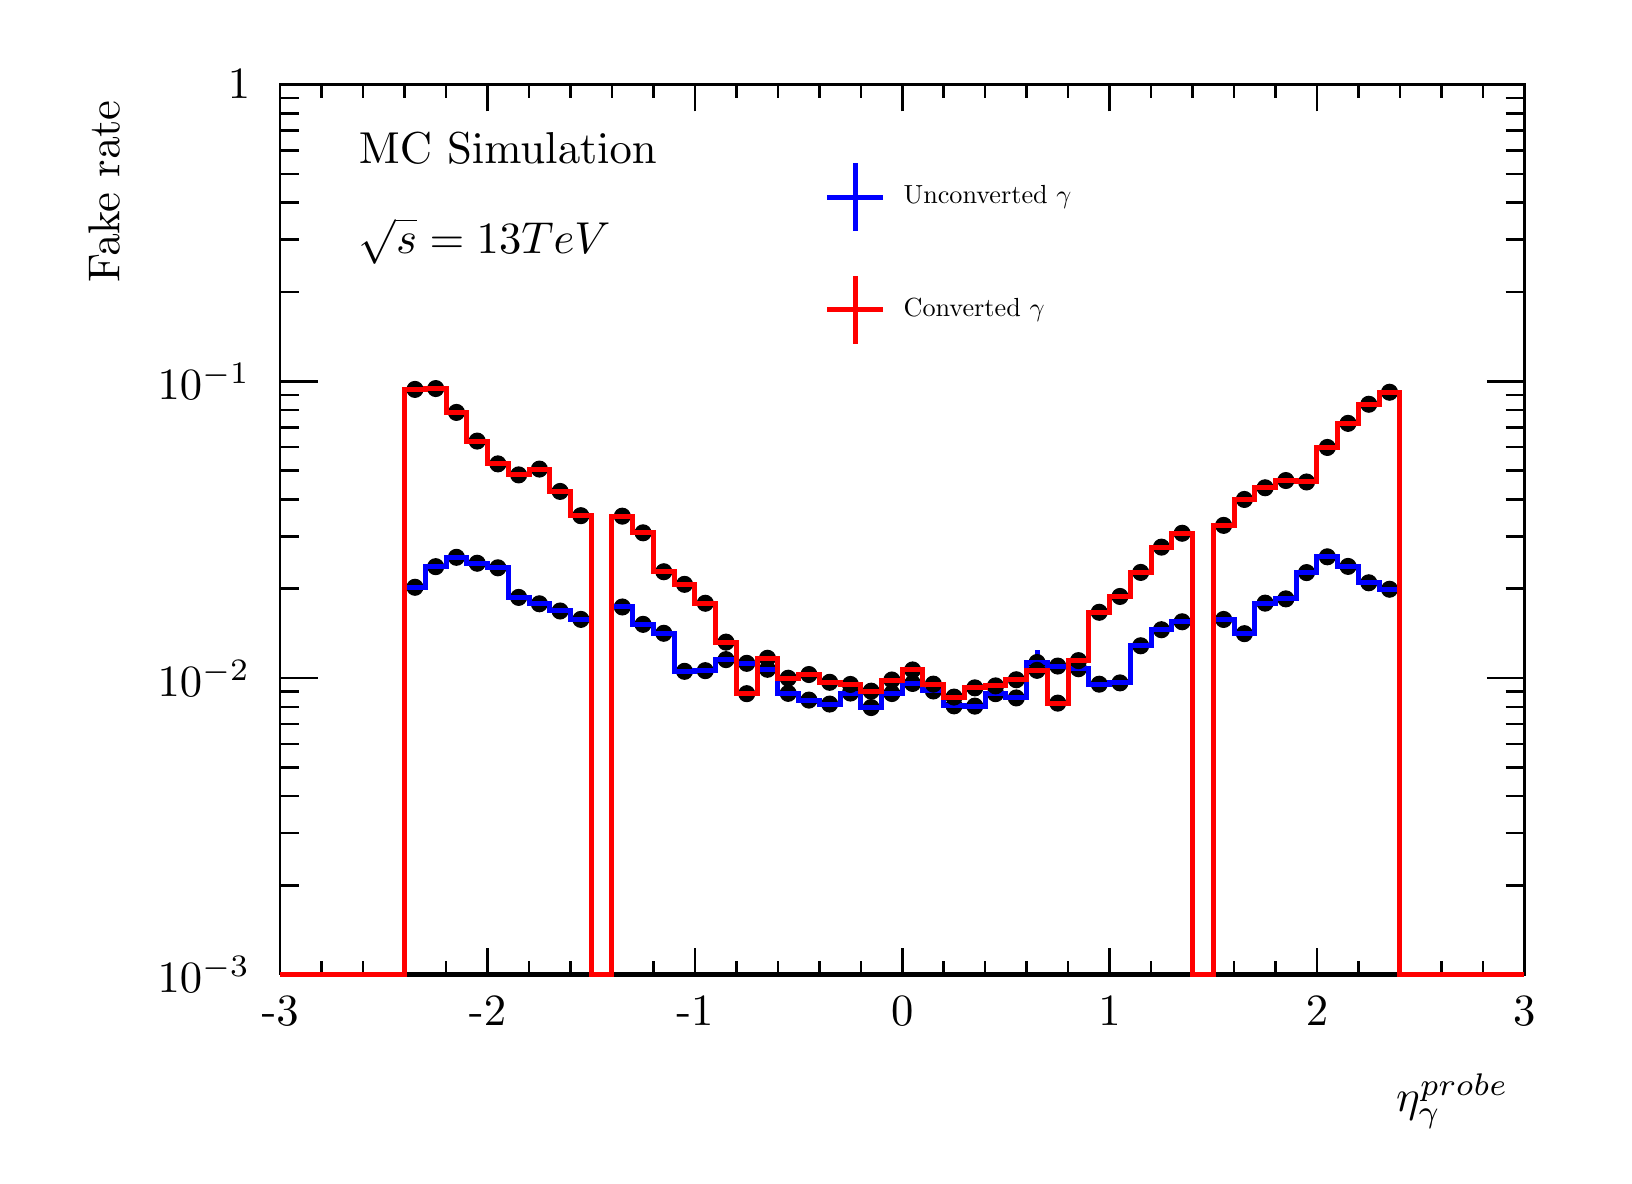
\begin{tikzpicture}
\pgfdeclareplotmark{cross} {
\pgfpathmoveto{\pgfpoint{-0.3\pgfplotmarksize}{\pgfplotmarksize}}
\pgfpathlineto{\pgfpoint{+0.3\pgfplotmarksize}{\pgfplotmarksize}}
\pgfpathlineto{\pgfpoint{+0.3\pgfplotmarksize}{0.3\pgfplotmarksize}}
\pgfpathlineto{\pgfpoint{+1\pgfplotmarksize}{0.3\pgfplotmarksize}}
\pgfpathlineto{\pgfpoint{+1\pgfplotmarksize}{-0.3\pgfplotmarksize}}
\pgfpathlineto{\pgfpoint{+0.3\pgfplotmarksize}{-0.3\pgfplotmarksize}}
\pgfpathlineto{\pgfpoint{+0.3\pgfplotmarksize}{-1.\pgfplotmarksize}}
\pgfpathlineto{\pgfpoint{-0.3\pgfplotmarksize}{-1.\pgfplotmarksize}}
\pgfpathlineto{\pgfpoint{-0.3\pgfplotmarksize}{-0.3\pgfplotmarksize}}
\pgfpathlineto{\pgfpoint{-1.\pgfplotmarksize}{-0.3\pgfplotmarksize}}
\pgfpathlineto{\pgfpoint{-1.\pgfplotmarksize}{0.3\pgfplotmarksize}}
\pgfpathlineto{\pgfpoint{-0.3\pgfplotmarksize}{0.3\pgfplotmarksize}}
\pgfpathclose
\pgfusepathqstroke
}
\pgfdeclareplotmark{cross*} {
\pgfpathmoveto{\pgfpoint{-0.3\pgfplotmarksize}{\pgfplotmarksize}}
\pgfpathlineto{\pgfpoint{+0.3\pgfplotmarksize}{\pgfplotmarksize}}
\pgfpathlineto{\pgfpoint{+0.3\pgfplotmarksize}{0.3\pgfplotmarksize}}
\pgfpathlineto{\pgfpoint{+1\pgfplotmarksize}{0.3\pgfplotmarksize}}
\pgfpathlineto{\pgfpoint{+1\pgfplotmarksize}{-0.3\pgfplotmarksize}}
\pgfpathlineto{\pgfpoint{+0.3\pgfplotmarksize}{-0.3\pgfplotmarksize}}
\pgfpathlineto{\pgfpoint{+0.3\pgfplotmarksize}{-1.\pgfplotmarksize}}
\pgfpathlineto{\pgfpoint{-0.3\pgfplotmarksize}{-1.\pgfplotmarksize}}
\pgfpathlineto{\pgfpoint{-0.3\pgfplotmarksize}{-0.3\pgfplotmarksize}}
\pgfpathlineto{\pgfpoint{-1.\pgfplotmarksize}{-0.3\pgfplotmarksize}}
\pgfpathlineto{\pgfpoint{-1.\pgfplotmarksize}{0.3\pgfplotmarksize}}
\pgfpathlineto{\pgfpoint{-0.3\pgfplotmarksize}{0.3\pgfplotmarksize}}
\pgfpathclose
\pgfusepathqfillstroke
}
\pgfdeclareplotmark{newstar} {
\pgfpathmoveto{\pgfqpoint{0pt}{\pgfplotmarksize}}
\pgfpathlineto{\pgfqpointpolar{44}{0.5\pgfplotmarksize}}
\pgfpathlineto{\pgfqpointpolar{18}{\pgfplotmarksize}}
\pgfpathlineto{\pgfqpointpolar{-20}{0.5\pgfplotmarksize}}
\pgfpathlineto{\pgfqpointpolar{-54}{\pgfplotmarksize}}
\pgfpathlineto{\pgfqpointpolar{-90}{0.5\pgfplotmarksize}}
\pgfpathlineto{\pgfqpointpolar{234}{\pgfplotmarksize}}
\pgfpathlineto{\pgfqpointpolar{198}{0.5\pgfplotmarksize}}
\pgfpathlineto{\pgfqpointpolar{162}{\pgfplotmarksize}}
\pgfpathlineto{\pgfqpointpolar{134}{0.5\pgfplotmarksize}}
\pgfpathclose
\pgfusepathqstroke
}
\pgfdeclareplotmark{newstar*} {
\pgfpathmoveto{\pgfqpoint{0pt}{\pgfplotmarksize}}
\pgfpathlineto{\pgfqpointpolar{44}{0.5\pgfplotmarksize}}
\pgfpathlineto{\pgfqpointpolar{18}{\pgfplotmarksize}}
\pgfpathlineto{\pgfqpointpolar{-20}{0.5\pgfplotmarksize}}
\pgfpathlineto{\pgfqpointpolar{-54}{\pgfplotmarksize}}
\pgfpathlineto{\pgfqpointpolar{-90}{0.5\pgfplotmarksize}}
\pgfpathlineto{\pgfqpointpolar{234}{\pgfplotmarksize}}
\pgfpathlineto{\pgfqpointpolar{198}{0.5\pgfplotmarksize}}
\pgfpathlineto{\pgfqpointpolar{162}{\pgfplotmarksize}}
\pgfpathlineto{\pgfqpointpolar{134}{0.5\pgfplotmarksize}}
\pgfpathclose
\pgfusepathqfillstroke
}
\definecolor{c}{rgb}{1,1,1};
\draw [color=c, fill=c] (0,0) rectangle (20,14.3108);
\draw [color=c, fill=c] (3.2,2.28972) rectangle (19,13.5952);
\definecolor{c}{rgb}{0,0,0};
\draw [c,line width=0.9] (3.2,2.28972) -- (3.2,13.5952) -- (19,13.5952) -- (19,2.28972) -- (3.2,2.28972);
\draw [c,line width=1.8] (3.2,2.28972) -- (3.2158,2.28972) -- (3.2158,2.28972) -- (3.2316,2.28972) -- (3.2316,2.28972) -- (3.2474,2.28972) -- (3.2474,2.28972) -- (3.2632,2.28972) -- (3.2632,2.28972) -- (3.279,2.28972) -- (3.279,2.28972) --
 (3.2948,2.28972) -- (3.2948,2.28972) -- (3.3106,2.28972) -- (3.3106,2.28972) -- (3.3264,2.28972) -- (3.3264,2.28972) -- (3.3422,2.28972) -- (3.3422,2.28972) -- (3.358,2.28972) -- (3.358,2.28972) -- (3.3738,2.28972) -- (3.3738,2.28972) --
 (3.3896,2.28972) -- (3.3896,2.28972) -- (3.4054,2.28972) -- (3.4054,2.28972) -- (3.4212,2.28972) -- (3.4212,2.28972) -- (3.437,2.28972) -- (3.437,2.28972) -- (3.4528,2.28972) -- (3.4528,2.28972) -- (3.4686,2.28972) -- (3.4686,2.28972) --
 (3.4844,2.28972) -- (3.4844,2.28972) -- (3.5002,2.28972) -- (3.5002,2.28972) -- (3.516,2.28972) -- (3.516,2.28972) -- (3.5318,2.28972) -- (3.5318,2.28972) -- (3.5476,2.28972) -- (3.5476,2.28972) -- (3.5634,2.28972) -- (3.5634,2.28972) --
 (3.5792,2.28972) -- (3.5792,2.28972) -- (3.595,2.28972) -- (3.595,2.28972) -- (3.6108,2.28972) -- (3.6108,2.28972) -- (3.6266,2.28972) -- (3.6266,2.28972) -- (3.6424,2.28972) -- (3.6424,2.28972) -- (3.6582,2.28972) -- (3.6582,2.28972) --
 (3.674,2.28972) -- (3.674,2.28972) -- (3.6898,2.28972) -- (3.6898,2.28972) -- (3.7056,2.28972) -- (3.7056,2.28972) -- (3.7214,2.28972) -- (3.7214,2.28972) -- (3.7372,2.28972) -- (3.7372,2.28972) -- (3.753,2.28972) -- (3.753,2.28972) --
 (3.7688,2.28972) -- (3.7688,2.28972) -- (3.7846,2.28972) -- (3.7846,2.28972) -- (3.8004,2.28972) -- (3.8004,2.28972) -- (3.8162,2.28972) -- (3.8162,2.28972) -- (3.832,2.28972) -- (3.832,2.28972) -- (3.8478,2.28972) -- (3.8478,2.28972) --
 (3.8636,2.28972) -- (3.8636,2.28972) -- (3.8794,2.28972) -- (3.8794,2.28972) -- (3.8952,2.28972) -- (3.8952,2.28972) -- (3.911,2.28972) -- (3.911,2.28972) -- (3.9268,2.28972) -- (3.9268,2.28972) -- (3.9426,2.28972) -- (3.9426,2.28972) --
 (3.9584,2.28972) -- (3.9584,2.28972) -- (3.9742,2.28972) -- (3.9742,2.28972) -- (3.99,2.28972) -- (3.99,2.28972) -- (4.0058,2.28972) -- (4.0058,2.28972) -- (4.0216,2.28972) -- (4.0216,2.28972) -- (4.0374,2.28972) -- (4.0374,2.28972) --
 (4.0532,2.28972) -- (4.0532,2.28972) -- (4.069,2.28972) -- (4.069,2.28972) -- (4.0848,2.28972) -- (4.0848,2.28972) -- (4.1006,2.28972) -- (4.1006,2.28972) -- (4.1164,2.28972) -- (4.1164,2.28972) -- (4.1322,2.28972) -- (4.1322,2.28972) --
 (4.148,2.28972) -- (4.148,2.28972) -- (4.1638,2.28972) -- (4.1638,2.28972) -- (4.1796,2.28972) -- (4.1796,2.28972) -- (4.1954,2.28972) -- (4.1954,2.28972) -- (4.2112,2.28972) -- (4.2112,2.28972) -- (4.227,2.28972) -- (4.227,2.28972) --
 (4.2428,2.28972) -- (4.2428,2.28972) -- (4.2586,2.28972) -- (4.2586,2.28972) -- (4.2744,2.28972) -- (4.2744,2.28972) -- (4.2902,2.28972) -- (4.2902,2.28972) -- (4.306,2.28972) -- (4.306,2.28972) -- (4.3218,2.28972) -- (4.3218,2.28972) --
 (4.3376,2.28972) -- (4.3376,2.28972) -- (4.3534,2.28972) -- (4.3534,2.28972) -- (4.3692,2.28972) -- (4.3692,2.28972) -- (4.385,2.28972) -- (4.385,2.28972) -- (4.4008,2.28972) -- (4.4008,2.28972) -- (4.4166,2.28972) -- (4.4166,2.28972) --
 (4.4324,2.28972) -- (4.4324,2.28972) -- (4.4482,2.28972) -- (4.4482,2.28972) -- (4.464,2.28972) -- (4.464,2.28972) -- (4.4798,2.28972) -- (4.4798,2.28972) -- (4.4956,2.28972) -- (4.4956,2.28972) -- (4.5114,2.28972) -- (4.5114,2.28972) --
 (4.5272,2.28972) -- (4.5272,2.28972) -- (4.543,2.28972) -- (4.543,2.28972) -- (4.5588,2.28972) -- (4.5588,2.28972) -- (4.5746,2.28972) -- (4.5746,2.28972) -- (4.5904,2.28972) -- (4.5904,2.28972) -- (4.6062,2.28972) -- (4.6062,2.28972) --
 (4.622,2.28972) -- (4.622,2.28972) -- (4.6378,2.28972) -- (4.6378,2.28972) -- (4.6536,2.28972) -- (4.6536,2.28972) -- (4.6694,2.28972) -- (4.6694,2.28972) -- (4.6852,2.28972) -- (4.6852,2.28972) -- (4.701,2.28972) -- (4.701,2.28972) --
 (4.7168,2.28972) -- (4.7168,2.28972) -- (4.7326,2.28972) -- (4.7326,2.28972) -- (4.7484,2.28972) -- (4.7484,2.28972) -- (4.7642,2.28972) -- (4.7642,2.28972) -- (4.78,2.28972) -- (4.78,2.28972) -- (4.7958,2.28972) -- (4.7958,2.28972) --
 (4.8116,2.28972) -- (4.8116,2.28972) -- (4.8274,2.28972) -- (4.8274,2.28972) -- (4.8432,2.28972) -- (4.8432,2.28972) -- (4.859,2.28972) -- (4.859,2.28972) -- (4.8748,2.28972) -- (4.8748,2.28972) -- (4.8906,2.28972) -- (4.8906,2.28972) --
 (4.9064,2.28972) -- (4.9064,2.28972) -- (4.9222,2.28972) -- (4.9222,2.28972) -- (4.938,2.28972) -- (4.938,2.28972) -- (4.9538,2.28972) -- (4.9538,2.28972) -- (4.9696,2.28972) -- (4.9696,2.28972) -- (4.9854,2.28972) -- (4.9854,2.28972) --
 (5.0012,2.28972) -- (5.0012,2.28972) -- (5.017,2.28972) -- (5.017,2.28972) -- (5.0328,2.28972) -- (5.0328,2.28972) -- (5.0486,2.28972) -- (5.0486,2.28972) -- (5.0644,2.28972) -- (5.0644,2.28972) -- (5.0802,2.28972) -- (5.0802,2.28972) --
 (5.096,2.28972) -- (5.096,2.28972) -- (5.1118,2.28972) -- (5.1118,2.28972) -- (5.1276,2.28972) -- (5.1276,2.28972) -- (5.1434,2.28972) -- (5.1434,2.28972) -- (5.1592,2.28972) -- (5.1592,2.28972) -- (5.175,2.28972) -- (5.175,2.28972) --
 (5.1908,2.28972) -- (5.1908,2.28972) -- (5.2066,2.28972) -- (5.2066,2.28972) -- (5.2224,2.28972) -- (5.2224,2.28972) -- (5.2382,2.28972) -- (5.2382,2.28972) -- (5.254,2.28972) -- (5.254,2.28972) -- (5.2698,2.28972) -- (5.2698,2.28972) --
 (5.2856,2.28972) -- (5.2856,2.28972) -- (5.3014,2.28972) -- (5.3014,2.28972) -- (5.3172,2.28972) -- (5.3172,2.28972) -- (5.333,2.28972) -- (5.333,2.28972) -- (5.3488,2.28972) -- (5.3488,2.28972) -- (5.3646,2.28972) -- (5.3646,2.28972) --
 (5.3804,2.28972) -- (5.3804,2.28972) -- (5.3962,2.28972) -- (5.3962,2.28972) -- (5.412,2.28972) -- (5.412,2.28972) -- (5.4278,2.28972) -- (5.4278,2.28972) -- (5.4436,2.28972) -- (5.4436,2.28972) -- (5.4594,2.28972) -- (5.4594,2.28972) --
 (5.4752,2.28972) -- (5.4752,2.28972) -- (5.491,2.28972) -- (5.491,2.28972) -- (5.5068,2.28972) -- (5.5068,2.28972) -- (5.5226,2.28972) -- (5.5226,2.28972) -- (5.5384,2.28972) -- (5.5384,2.28972) -- (5.5542,2.28972) -- (5.5542,2.28972) --
 (5.57,2.28972) -- (5.57,2.28972) -- (5.5858,2.28972) -- (5.5858,2.28972) -- (5.6016,2.28972) -- (5.6016,2.28972) -- (5.6174,2.28972) -- (5.6174,2.28972) -- (5.6332,2.28972) -- (5.6332,2.28972) -- (5.649,2.28972) -- (5.649,2.28972) --
 (5.6648,2.28972) -- (5.6648,2.28972) -- (5.6806,2.28972) -- (5.6806,2.28972) -- (5.6964,2.28972) -- (5.6964,2.28972) -- (5.7122,2.28972) -- (5.7122,2.28972) -- (5.728,2.28972) -- (5.728,2.28972) -- (5.7438,2.28972) -- (5.7438,2.28972) --
 (5.7596,2.28972) -- (5.7596,2.28972) -- (5.7754,2.28972) -- (5.7754,2.28972) -- (5.7912,2.28972) -- (5.7912,2.28972) -- (5.807,2.28972) -- (5.807,2.28972) -- (5.8228,2.28972) -- (5.8228,2.28972) -- (5.8386,2.28972) -- (5.8386,2.28972) --
 (5.8544,2.28972) -- (5.8544,2.28972) -- (5.8702,2.28972) -- (5.8702,2.28972) -- (5.886,2.28972) -- (5.886,2.28972) -- (5.9018,2.28972) -- (5.9018,2.28972) -- (5.9176,2.28972) -- (5.9176,2.28972) -- (5.9334,2.28972) -- (5.9334,2.28972) --
 (5.9492,2.28972) -- (5.9492,2.28972) -- (5.965,2.28972) -- (5.965,2.28972) -- (5.9808,2.28972) -- (5.9808,2.28972) -- (5.9966,2.28972) -- (5.9966,2.28972) -- (6.0124,2.28972) -- (6.0124,2.28972) -- (6.0282,2.28972) -- (6.0282,2.28972) --
 (6.044,2.28972) -- (6.044,2.28972) -- (6.0598,2.28972) -- (6.0598,2.28972) -- (6.0756,2.28972) -- (6.0756,2.28972) -- (6.0914,2.28972) -- (6.0914,2.28972) -- (6.1072,2.28972) -- (6.1072,2.28972) -- (6.123,2.28972) -- (6.123,2.28972) --
 (6.1388,2.28972) -- (6.1388,2.28972) -- (6.1546,2.28972) -- (6.1546,2.28972) -- (6.1704,2.28972) -- (6.1704,2.28972) -- (6.1862,2.28972) -- (6.1862,2.28972) -- (6.202,2.28972) -- (6.202,2.28972) -- (6.2178,2.28972) -- (6.2178,2.28972) --
 (6.2336,2.28972) -- (6.2336,2.28972) -- (6.2494,2.28972) -- (6.2494,2.28972) -- (6.2652,2.28972) -- (6.2652,2.28972) -- (6.281,2.28972) -- (6.281,2.28972) -- (6.2968,2.28972) -- (6.2968,2.28972) -- (6.3126,2.28972) -- (6.3126,2.28972) --
 (6.3284,2.28972) -- (6.3284,2.28972) -- (6.3442,2.28972) -- (6.3442,2.28972) -- (6.36,2.28972) -- (6.36,2.28972) -- (6.3758,2.28972) -- (6.3758,2.28972) -- (6.3916,2.28972) -- (6.3916,2.28972) -- (6.4074,2.28972) -- (6.4074,2.28972) --
 (6.4232,2.28972) -- (6.4232,2.28972) -- (6.439,2.28972) -- (6.439,2.28972) -- (6.4548,2.28972) -- (6.4548,2.28972) -- (6.4706,2.28972) -- (6.4706,2.28972) -- (6.4864,2.28972) -- (6.4864,2.28972) -- (6.5022,2.28972) -- (6.5022,2.28972) --
 (6.518,2.28972) -- (6.518,2.28972) -- (6.5338,2.28972) -- (6.5338,2.28972) -- (6.5496,2.28972) -- (6.5496,2.28972) -- (6.5654,2.28972) -- (6.5654,2.28972) -- (6.5812,2.28972) -- (6.5812,2.28972) -- (6.597,2.28972) -- (6.597,2.28972) --
 (6.6128,2.28972) -- (6.6128,2.28972) -- (6.6286,2.28972) -- (6.6286,2.28972) -- (6.6444,2.28972) -- (6.6444,2.28972) -- (6.6602,2.28972) -- (6.6602,2.28972) -- (6.676,2.28972) -- (6.676,2.28972) -- (6.6918,2.28972) -- (6.6918,2.28972) --
 (6.7076,2.28972) -- (6.7076,2.28972) -- (6.7234,2.28972) -- (6.7234,2.28972) -- (6.7392,2.28972) -- (6.7392,2.28972) -- (6.755,2.28972) -- (6.755,2.28972) -- (6.7708,2.28972) -- (6.7708,2.28972) -- (6.7866,2.28972) -- (6.7866,2.28972) --
 (6.8024,2.28972) -- (6.8024,2.28972) -- (6.8182,2.28972) -- (6.8182,2.28972) -- (6.834,2.28972) -- (6.834,2.28972) -- (6.8498,2.28972) -- (6.8498,2.28972) -- (6.8656,2.28972) -- (6.8656,2.28972) -- (6.8814,2.28972) -- (6.8814,2.28972) --
 (6.8972,2.28972) -- (6.8972,2.28972) -- (6.913,2.28972) -- (6.913,2.28972) -- (6.9288,2.28972) -- (6.9288,2.28972) -- (6.9446,2.28972) -- (6.9446,2.28972) -- (6.9604,2.28972) -- (6.9604,2.28972) -- (6.9762,2.28972) -- (6.9762,2.28972) --
 (6.992,2.28972) -- (6.992,2.28972) -- (7.0078,2.28972) -- (7.0078,2.28972) -- (7.0236,2.28972) -- (7.0236,2.28972) -- (7.0394,2.28972) -- (7.0394,2.28972) -- (7.0552,2.28972) -- (7.0552,2.28972) -- (7.071,2.28972) -- (7.071,2.28972) --
 (7.0868,2.28972) -- (7.0868,2.28972) -- (7.1026,2.28972) -- (7.1026,2.28972) -- (7.1184,2.28972) -- (7.1184,2.28972) -- (7.1342,2.28972) -- (7.1342,2.28972) -- (7.15,2.28972) -- (7.15,2.28972) -- (7.1658,2.28972) -- (7.1658,2.28972) --
 (7.1816,2.28972) -- (7.1816,2.28972) -- (7.1974,2.28972) -- (7.1974,2.28972) -- (7.2132,2.28972) -- (7.2132,2.28972) -- (7.229,2.28972) -- (7.229,2.28972) -- (7.2448,2.28972) -- (7.2448,2.28972) -- (7.2606,2.28972) -- (7.2606,2.28972) --
 (7.2764,2.28972) -- (7.2764,2.28972) -- (7.2922,2.28972) -- (7.2922,2.28972) -- (7.308,2.28972) -- (7.308,2.28972) -- (7.3238,2.28972) -- (7.3238,2.28972) -- (7.3396,2.28972) -- (7.3396,2.28972) -- (7.3554,2.28972) -- (7.3554,2.28972) --
 (7.3712,2.28972) -- (7.3712,2.28972) -- (7.387,2.28972) -- (7.387,2.28972) -- (7.4028,2.28972) -- (7.4028,2.28972) -- (7.4186,2.28972) -- (7.4186,2.28972) -- (7.4344,2.28972) -- (7.4344,2.28972) -- (7.4502,2.28972) -- (7.4502,2.28972) --
 (7.466,2.28972) -- (7.466,2.28972) -- (7.4818,2.28972) -- (7.4818,2.28972) -- (7.4976,2.28972) -- (7.4976,2.28972) -- (7.5134,2.28972) -- (7.5134,2.28972) -- (7.5292,2.28972) -- (7.5292,2.28972) -- (7.545,2.28972) -- (7.545,2.28972) --
 (7.5608,2.28972) -- (7.5608,2.28972) -- (7.5766,2.28972) -- (7.5766,2.28972) -- (7.5924,2.28972) -- (7.5924,2.28972) -- (7.6082,2.28972) -- (7.6082,2.28972) -- (7.624,2.28972) -- (7.624,2.28972) -- (7.6398,2.28972) -- (7.6398,2.28972) --
 (7.6556,2.28972) -- (7.6556,2.28972) -- (7.6714,2.28972) -- (7.6714,2.28972) -- (7.6872,2.28972) -- (7.6872,2.28972) -- (7.703,2.28972) -- (7.703,2.28972) -- (7.7188,2.28972) -- (7.7188,2.28972) -- (7.7346,2.28972) -- (7.7346,2.28972) --
 (7.7504,2.28972) -- (7.7504,2.28972) -- (7.7662,2.28972) -- (7.7662,2.28972) -- (7.782,2.28972) -- (7.782,2.28972) -- (7.7978,2.28972) -- (7.7978,2.28972) -- (7.8136,2.28972) -- (7.8136,2.28972) -- (7.8294,2.28972) -- (7.8294,2.28972) --
 (7.8452,2.28972) -- (7.8452,2.28972) -- (7.861,2.28972) -- (7.861,2.28972) -- (7.8768,2.28972) -- (7.8768,2.28972) -- (7.8926,2.28972) -- (7.8926,2.28972) -- (7.9084,2.28972) -- (7.9084,2.28972) -- (7.9242,2.28972) -- (7.9242,2.28972) --
 (7.94,2.28972) -- (7.94,2.28972) -- (7.9558,2.28972) -- (7.9558,2.28972) -- (7.9716,2.28972) -- (7.9716,2.28972) -- (7.9874,2.28972) -- (7.9874,2.28972) -- (8.0032,2.28972) -- (8.0032,2.28972) -- (8.019,2.28972) -- (8.019,2.28972) --
 (8.0348,2.28972) -- (8.0348,2.28972) -- (8.0506,2.28972) -- (8.0506,2.28972) -- (8.0664,2.28972) -- (8.0664,2.28972) -- (8.0822,2.28972) -- (8.0822,2.28972) -- (8.098,2.28972) -- (8.098,2.28972) -- (8.1138,2.28972) -- (8.1138,2.28972) --
 (8.1296,2.28972) -- (8.1296,2.28972) -- (8.1454,2.28972) -- (8.1454,2.28972) -- (8.1612,2.28972) -- (8.1612,2.28972) -- (8.177,2.28972) -- (8.177,2.28972) -- (8.1928,2.28972) -- (8.1928,2.28972) -- (8.2086,2.28972) -- (8.2086,2.28972) --
 (8.2244,2.28972) -- (8.2244,2.28972) -- (8.2402,2.28972) -- (8.2402,2.28972) -- (8.256,2.28972) -- (8.256,2.28972) -- (8.2718,2.28972) -- (8.2718,2.28972) -- (8.2876,2.28972) -- (8.2876,2.28972) -- (8.3034,2.28972) -- (8.3034,2.28972) --
 (8.3192,2.28972) -- (8.3192,2.28972) -- (8.335,2.28972) -- (8.335,2.28972) -- (8.3508,2.28972) -- (8.3508,2.28972) -- (8.3666,2.28972) -- (8.3666,2.28972) -- (8.3824,2.28972) -- (8.3824,2.28972) -- (8.3982,2.28972) -- (8.3982,2.28972) --
 (8.414,2.28972) -- (8.414,2.28972) -- (8.4298,2.28972) -- (8.4298,2.28972) -- (8.4456,2.28972) -- (8.4456,2.28972) -- (8.4614,2.28972) -- (8.4614,2.28972) -- (8.4772,2.28972) -- (8.4772,2.28972) -- (8.493,2.28972) -- (8.493,2.28972) --
 (8.5088,2.28972) -- (8.5088,2.28972) -- (8.5246,2.28972) -- (8.5246,2.28972) -- (8.5404,2.28972) -- (8.5404,2.28972) -- (8.5562,2.28972) -- (8.5562,2.28972) -- (8.572,2.28972) -- (8.572,2.28972) -- (8.5878,2.28972) -- (8.5878,2.28972) --
 (8.6036,2.28972) -- (8.6036,2.28972) -- (8.6194,2.28972) -- (8.6194,2.28972) -- (8.6352,2.28972) -- (8.6352,2.28972) -- (8.651,2.28972) -- (8.651,2.28972) -- (8.6668,2.28972) -- (8.6668,2.28972) -- (8.6826,2.28972) -- (8.6826,2.28972) --
 (8.6984,2.28972) -- (8.6984,2.28972) -- (8.7142,2.28972) -- (8.7142,2.28972) -- (8.73,2.28972) -- (8.73,2.28972) -- (8.7458,2.28972) -- (8.7458,2.28972) -- (8.7616,2.28972) -- (8.7616,2.28972) -- (8.7774,2.28972) -- (8.7774,2.28972) --
 (8.7932,2.28972) -- (8.7932,2.28972) -- (8.809,2.28972) -- (8.809,2.28972) -- (8.8248,2.28972) -- (8.8248,2.28972) -- (8.8406,2.28972) -- (8.8406,2.28972) -- (8.8564,2.28972) -- (8.8564,2.28972) -- (8.8722,2.28972) -- (8.8722,2.28972) --
 (8.888,2.28972) -- (8.888,2.28972) -- (8.9038,2.28972) -- (8.9038,2.28972) -- (8.9196,2.28972) -- (8.9196,2.28972) -- (8.9354,2.28972) -- (8.9354,2.28972) -- (8.9512,2.28972) -- (8.9512,2.28972) -- (8.967,2.28972) -- (8.967,2.28972) --
 (8.9828,2.28972) -- (8.9828,2.28972) -- (8.9986,2.28972) -- (8.9986,2.28972) -- (9.0144,2.28972) -- (9.0144,2.28972) -- (9.0302,2.28972) -- (9.0302,2.28972) -- (9.046,2.28972) -- (9.046,2.28972) -- (9.0618,2.28972) -- (9.0618,2.28972) --
 (9.0776,2.28972) -- (9.0776,2.28972) -- (9.0934,2.28972) -- (9.0934,2.28972) -- (9.1092,2.28972) -- (9.1092,2.28972) -- (9.125,2.28972) -- (9.125,2.28972) -- (9.1408,2.28972) -- (9.1408,2.28972) -- (9.1566,2.28972) -- (9.1566,2.28972) --
 (9.1724,2.28972) -- (9.1724,2.28972) -- (9.1882,2.28972) -- (9.1882,2.28972) -- (9.204,2.28972) -- (9.204,2.28972) -- (9.2198,2.28972) -- (9.2198,2.28972) -- (9.2356,2.28972) -- (9.2356,2.28972) -- (9.2514,2.28972) -- (9.2514,2.28972) --
 (9.2672,2.28972) -- (9.2672,2.28972) -- (9.283,2.28972) -- (9.283,2.28972) -- (9.2988,2.28972) -- (9.2988,2.28972) -- (9.3146,2.28972) -- (9.3146,2.28972) -- (9.3304,2.28972) -- (9.3304,2.28972) -- (9.3462,2.28972) -- (9.3462,2.28972) --
 (9.362,2.28972) -- (9.362,2.28972) -- (9.3778,2.28972) -- (9.3778,2.28972) -- (9.3936,2.28972) -- (9.3936,2.28972) -- (9.4094,2.28972) -- (9.4094,2.28972) -- (9.4252,2.28972) -- (9.4252,2.28972) -- (9.441,2.28972) -- (9.441,2.28972) --
 (9.4568,2.28972) -- (9.4568,2.28972) -- (9.4726,2.28972) -- (9.4726,2.28972) -- (9.4884,2.28972) -- (9.4884,2.28972) -- (9.5042,2.28972) -- (9.5042,2.28972) -- (9.52,2.28972) -- (9.52,2.28972) -- (9.5358,2.28972) -- (9.5358,2.28972) --
 (9.5516,2.28972) -- (9.5516,2.28972) -- (9.5674,2.28972) -- (9.5674,2.28972) -- (9.5832,2.28972) -- (9.5832,2.28972) -- (9.599,2.28972) -- (9.599,2.28972) -- (9.6148,2.28972) -- (9.6148,2.28972) -- (9.6306,2.28972) -- (9.6306,2.28972) --
 (9.6464,2.28972) -- (9.6464,2.28972) -- (9.6622,2.28972) -- (9.6622,2.28972) -- (9.678,2.28972) -- (9.678,2.28972) -- (9.6938,2.28972) -- (9.6938,2.28972) -- (9.7096,2.28972) -- (9.7096,2.28972) -- (9.7254,2.28972) -- (9.7254,2.28972) --
 (9.7412,2.28972) -- (9.7412,2.28972) -- (9.757,2.28972) -- (9.757,2.28972) -- (9.7728,2.28972) -- (9.7728,2.28972) -- (9.7886,2.28972) -- (9.7886,2.28972) -- (9.8044,2.28972) -- (9.8044,2.28972) -- (9.8202,2.28972) -- (9.8202,2.28972) --
 (9.836,2.28972) -- (9.836,2.28972) -- (9.8518,2.28972) -- (9.8518,2.28972) -- (9.8676,2.28972) -- (9.8676,2.28972) -- (9.8834,2.28972) -- (9.8834,2.28972) -- (9.8992,2.28972) -- (9.8992,2.28972) -- (9.915,2.28972) -- (9.915,2.28972) --
 (9.9308,2.28972) -- (9.9308,2.28972) -- (9.9466,2.28972) -- (9.9466,2.28972) -- (9.9624,2.28972) -- (9.9624,2.28972) -- (9.9782,2.28972) -- (9.9782,2.28972) -- (9.994,2.28972) -- (9.994,2.28972) -- (10.0098,2.28972) -- (10.0098,2.28972) --
 (10.0256,2.28972) -- (10.0256,2.28972) -- (10.0414,2.28972) -- (10.0414,2.28972) -- (10.0572,2.28972) -- (10.0572,2.28972) -- (10.073,2.28972) -- (10.073,2.28972) -- (10.0888,2.28972) -- (10.0888,2.28972) -- (10.1046,2.28972) -- (10.1046,2.28972) --
 (10.1204,2.28972) -- (10.1204,2.28972) -- (10.1362,2.28972) -- (10.1362,2.28972) -- (10.152,2.28972) -- (10.152,2.28972) -- (10.1678,2.28972) -- (10.1678,2.28972) -- (10.1836,2.28972) -- (10.1836,2.28972) -- (10.1994,2.28972) -- (10.1994,2.28972) --
 (10.2152,2.28972) -- (10.2152,2.28972) -- (10.231,2.28972) -- (10.231,2.28972) -- (10.2468,2.28972) -- (10.2468,2.28972) -- (10.2626,2.28972) -- (10.2626,2.28972) -- (10.2784,2.28972) -- (10.2784,2.28972) -- (10.2942,2.28972) -- (10.2942,2.28972) --
 (10.31,2.28972) -- (10.31,2.28972) -- (10.3258,2.28972) -- (10.3258,2.28972) -- (10.3416,2.28972) -- (10.3416,2.28972) -- (10.3574,2.28972) -- (10.3574,2.28972) -- (10.3732,2.28972) -- (10.3732,2.28972) -- (10.389,2.28972) -- (10.389,2.28972) --
 (10.4048,2.28972) -- (10.4048,2.28972) -- (10.4206,2.28972) -- (10.4206,2.28972) -- (10.4364,2.28972) -- (10.4364,2.28972) -- (10.4522,2.28972) -- (10.4522,2.28972) -- (10.468,2.28972) -- (10.468,2.28972) -- (10.4838,2.28972) -- (10.4838,2.28972) --
 (10.4996,2.28972) -- (10.4996,2.28972) -- (10.5154,2.28972) -- (10.5154,2.28972) -- (10.5312,2.28972) -- (10.5312,2.28972) -- (10.547,2.28972) -- (10.547,2.28972) -- (10.5628,2.28972) -- (10.5628,2.28972) -- (10.5786,2.28972) -- (10.5786,2.28972) --
 (10.5944,2.28972) -- (10.5944,2.28972) -- (10.6102,2.28972) -- (10.6102,2.28972) -- (10.626,2.28972) -- (10.626,2.28972) -- (10.6418,2.28972) -- (10.6418,2.28972) -- (10.6576,2.28972) -- (10.6576,2.28972) -- (10.6734,2.28972) -- (10.6734,2.28972) --
 (10.6892,2.28972) -- (10.6892,2.28972) -- (10.705,2.28972) -- (10.705,2.28972) -- (10.7208,2.28972) -- (10.7208,2.28972) -- (10.7366,2.28972) -- (10.7366,2.28972) -- (10.7524,2.28972) -- (10.7524,2.28972) -- (10.7682,2.28972) -- (10.7682,2.28972) --
 (10.784,2.28972) -- (10.784,2.28972) -- (10.7998,2.28972) -- (10.7998,2.28972) -- (10.8156,2.28972) -- (10.8156,2.28972) -- (10.8314,2.28972) -- (10.8314,2.28972) -- (10.8472,2.28972) -- (10.8472,2.28972) -- (10.863,2.28972) -- (10.863,2.28972) --
 (10.8788,2.28972) -- (10.8788,2.28972) -- (10.8946,2.28972) -- (10.8946,2.28972) -- (10.9104,2.28972) -- (10.9104,2.28972) -- (10.9262,2.28972) -- (10.9262,2.28972) -- (10.942,2.28972) -- (10.942,2.28972) -- (10.9578,2.28972) -- (10.9578,2.28972) --
 (10.9736,2.28972) -- (10.9736,2.28972) -- (10.9894,2.28972) -- (10.9894,2.28972) -- (11.0052,2.28972) -- (11.0052,2.28972) -- (11.021,2.28972) -- (11.021,2.28972) -- (11.0368,2.28972) -- (11.0368,2.28972) -- (11.0526,2.28972) -- (11.0526,2.28972) --
 (11.0684,2.28972) -- (11.0684,2.28972) -- (11.0842,2.28972) -- (11.0842,2.28972) -- (11.1,2.28972) -- (11.1,2.28972) -- (11.1158,2.28972) -- (11.1158,2.28972) -- (11.1316,2.28972) -- (11.1316,2.28972) -- (11.1474,2.28972) -- (11.1474,2.28972) --
 (11.1632,2.28972) -- (11.1632,2.28972) -- (11.179,2.28972) -- (11.179,2.28972) -- (11.1948,2.28972) -- (11.1948,2.28972) -- (11.2106,2.28972) -- (11.2106,2.28972) -- (11.2264,2.28972) -- (11.2264,2.28972) -- (11.2422,2.28972) -- (11.2422,2.28972) --
 (11.258,2.28972) -- (11.258,2.28972) -- (11.2738,2.28972) -- (11.2738,2.28972) -- (11.2896,2.28972) -- (11.2896,2.28972) -- (11.3054,2.28972) -- (11.3054,2.28972) -- (11.3212,2.28972) -- (11.3212,2.28972) -- (11.337,2.28972) -- (11.337,2.28972) --
 (11.3528,2.28972) -- (11.3528,2.28972) -- (11.3686,2.28972) -- (11.3686,2.28972) -- (11.3844,2.28972) -- (11.3844,2.28972) -- (11.4002,2.28972) -- (11.4002,2.28972) -- (11.416,2.28972) -- (11.416,2.28972) -- (11.4318,2.28972) -- (11.4318,2.28972) --
 (11.4476,2.28972) -- (11.4476,2.28972) -- (11.4634,2.28972) -- (11.4634,2.28972) -- (11.4792,2.28972) -- (11.4792,2.28972) -- (11.495,2.28972) -- (11.495,2.28972) -- (11.5108,2.28972) -- (11.5108,2.28972) -- (11.5266,2.28972) -- (11.5266,2.28972) --
 (11.5424,2.28972) -- (11.5424,2.28972) -- (11.5582,2.28972) -- (11.5582,2.28972) -- (11.574,2.28972) -- (11.574,2.28972) -- (11.5898,2.28972) -- (11.5898,2.28972) -- (11.6056,2.28972) -- (11.6056,2.28972) -- (11.6214,2.28972) -- (11.6214,2.28972) --
 (11.6372,2.28972) -- (11.6372,2.28972) -- (11.653,2.28972) -- (11.653,2.28972) -- (11.6688,2.28972) -- (11.6688,2.28972) -- (11.6846,2.28972) -- (11.6846,2.28972) -- (11.7004,2.28972) -- (11.7004,2.28972) -- (11.7162,2.28972) -- (11.7162,2.28972) --
 (11.732,2.28972) -- (11.732,2.28972) -- (11.7478,2.28972) -- (11.7478,2.28972) -- (11.7636,2.28972) -- (11.7636,2.28972) -- (11.7794,2.28972) -- (11.7794,2.28972) -- (11.7952,2.28972) -- (11.7952,2.28972) -- (11.811,2.28972) -- (11.811,2.28972) --
 (11.8268,2.28972) -- (11.8268,2.28972) -- (11.8426,2.28972) -- (11.8426,2.28972) -- (11.8584,2.28972) -- (11.8584,2.28972) -- (11.8742,2.28972) -- (11.8742,2.28972) -- (11.89,2.28972) -- (11.89,2.28972) -- (11.9058,2.28972) -- (11.9058,2.28972) --
 (11.9216,2.28972) -- (11.9216,2.28972) -- (11.9374,2.28972) -- (11.9374,2.28972) -- (11.9532,2.28972) -- (11.9532,2.28972) -- (11.969,2.28972) -- (11.969,2.28972) -- (11.9848,2.28972) -- (11.9848,2.28972) -- (12.0006,2.28972) -- (12.0006,2.28972) --
 (12.0164,2.28972) -- (12.0164,2.28972) -- (12.0322,2.28972) -- (12.0322,2.28972) -- (12.048,2.28972) -- (12.048,2.28972) -- (12.0638,2.28972) -- (12.0638,2.28972) -- (12.0796,2.28972) -- (12.0796,2.28972) -- (12.0954,2.28972) -- (12.0954,2.28972) --
 (12.1112,2.28972) -- (12.1112,2.28972) -- (12.127,2.28972) -- (12.127,2.28972) -- (12.1428,2.28972) -- (12.1428,2.28972) -- (12.1586,2.28972) -- (12.1586,2.28972) -- (12.1744,2.28972) -- (12.1744,2.28972) -- (12.1902,2.28972) -- (12.1902,2.28972) --
 (12.206,2.28972) -- (12.206,2.28972) -- (12.2218,2.28972) -- (12.2218,2.28972) -- (12.2376,2.28972) -- (12.2376,2.28972) -- (12.2534,2.28972) -- (12.2534,2.28972) -- (12.2692,2.28972) -- (12.2692,2.28972) -- (12.285,2.28972) -- (12.285,2.28972) --
 (12.3008,2.28972) -- (12.3008,2.28972) -- (12.3166,2.28972) -- (12.3166,2.28972) -- (12.3324,2.28972) -- (12.3324,2.28972) -- (12.3482,2.28972) -- (12.3482,2.28972) -- (12.364,2.28972) -- (12.364,2.28972) -- (12.3798,2.28972) -- (12.3798,2.28972) --
 (12.3956,2.28972) -- (12.3956,2.28972) -- (12.4114,2.28972) -- (12.4114,2.28972) -- (12.4272,2.28972) -- (12.4272,2.28972) -- (12.443,2.28972) -- (12.443,2.28972) -- (12.4588,2.28972) -- (12.4588,2.28972) -- (12.4746,2.28972) -- (12.4746,2.28972) --
 (12.4904,2.28972) -- (12.4904,2.28972) -- (12.5062,2.28972) -- (12.5062,2.28972) -- (12.522,2.28972) -- (12.522,2.28972) -- (12.5378,2.28972) -- (12.5378,2.28972) -- (12.5536,2.28972) -- (12.5536,2.28972) -- (12.5694,2.28972) -- (12.5694,2.28972) --
 (12.5852,2.28972) -- (12.5852,2.28972) -- (12.601,2.28972) -- (12.601,2.28972) -- (12.6168,2.28972) -- (12.6168,2.28972) -- (12.6326,2.28972) -- (12.6326,2.28972) -- (12.6484,2.28972) -- (12.6484,2.28972) -- (12.6642,2.28972) -- (12.6642,2.28972) --
 (12.68,2.28972) -- (12.68,2.28972) -- (12.6958,2.28972) -- (12.6958,2.28972) -- (12.7116,2.28972) -- (12.7116,2.28972) -- (12.7274,2.28972) -- (12.7274,2.28972) -- (12.7432,2.28972) -- (12.7432,2.28972) -- (12.759,2.28972) -- (12.759,2.28972) --
 (12.7748,2.28972) -- (12.7748,2.28972) -- (12.7906,2.28972) -- (12.7906,2.28972) -- (12.8064,2.28972) -- (12.8064,2.28972) -- (12.8222,2.28972) -- (12.8222,2.28972) -- (12.838,2.28972) -- (12.838,2.28972) -- (12.8538,2.28972) -- (12.8538,2.28972) --
 (12.8696,2.28972) -- (12.8696,2.28972) -- (12.8854,2.28972) -- (12.8854,2.28972) -- (12.9012,2.28972) -- (12.9012,2.28972) -- (12.917,2.28972) -- (12.917,2.28972) -- (12.9328,2.28972) -- (12.9328,2.28972) -- (12.9486,2.28972) -- (12.9486,2.28972) --
 (12.9644,2.28972) -- (12.9644,2.28972) -- (12.9802,2.28972) -- (12.9802,2.28972) -- (12.996,2.28972) -- (12.996,2.28972) -- (13.0118,2.28972) -- (13.0118,2.28972) -- (13.0276,2.28972) -- (13.0276,2.28972) -- (13.0434,2.28972) -- (13.0434,2.28972) --
 (13.0592,2.28972) -- (13.0592,2.28972) -- (13.075,2.28972) -- (13.075,2.28972) -- (13.0908,2.28972) -- (13.0908,2.28972) -- (13.1066,2.28972) -- (13.1066,2.28972) -- (13.1224,2.28972) -- (13.1224,2.28972) -- (13.1382,2.28972) -- (13.1382,2.28972) --
 (13.154,2.28972) -- (13.154,2.28972) -- (13.1698,2.28972) -- (13.1698,2.28972) -- (13.1856,2.28972) -- (13.1856,2.28972) -- (13.2014,2.28972) -- (13.2014,2.28972) -- (13.2172,2.28972) -- (13.2172,2.28972) -- (13.233,2.28972) -- (13.233,2.28972) --
 (13.2488,2.28972) -- (13.2488,2.28972) -- (13.2646,2.28972) -- (13.2646,2.28972) -- (13.2804,2.28972) -- (13.2804,2.28972) -- (13.2962,2.28972) -- (13.2962,2.28972) -- (13.312,2.28972) -- (13.312,2.28972) -- (13.3278,2.28972) -- (13.3278,2.28972) --
 (13.3436,2.28972) -- (13.3436,2.28972) -- (13.3594,2.28972) -- (13.3594,2.28972) -- (13.3752,2.28972) -- (13.3752,2.28972) -- (13.391,2.28972) -- (13.391,2.28972) -- (13.4068,2.28972) -- (13.4068,2.28972) -- (13.4226,2.28972) -- (13.4226,2.28972) --
 (13.4384,2.28972) -- (13.4384,2.28972) -- (13.4542,2.28972) -- (13.4542,2.28972) -- (13.47,2.28972) -- (13.47,2.28972) -- (13.4858,2.28972) -- (13.4858,2.28972) -- (13.5016,2.28972) -- (13.5016,2.28972) -- (13.5174,2.28972) -- (13.5174,2.28972) --
 (13.5332,2.28972) -- (13.5332,2.28972) -- (13.549,2.28972) -- (13.549,2.28972) -- (13.5648,2.28972) -- (13.5648,2.28972) -- (13.5806,2.28972) -- (13.5806,2.28972) -- (13.5964,2.28972) -- (13.5964,2.28972) -- (13.6122,2.28972) -- (13.6122,2.28972) --
 (13.628,2.28972) -- (13.628,2.28972) -- (13.6438,2.28972) -- (13.6438,2.28972) -- (13.6596,2.28972) -- (13.6596,2.28972) -- (13.6754,2.28972) -- (13.6754,2.28972) -- (13.6912,2.28972) -- (13.6912,2.28972) -- (13.707,2.28972) -- (13.707,2.28972) --
 (13.7228,2.28972) -- (13.7228,2.28972) -- (13.7386,2.28972) -- (13.7386,2.28972) -- (13.7544,2.28972) -- (13.7544,2.28972) -- (13.7702,2.28972) -- (13.7702,2.28972) -- (13.786,2.28972) -- (13.786,2.28972) -- (13.8018,2.28972) -- (13.8018,2.28972) --
 (13.8176,2.28972) -- (13.8176,2.28972) -- (13.8334,2.28972) -- (13.8334,2.28972) -- (13.8492,2.28972) -- (13.8492,2.28972) -- (13.865,2.28972) -- (13.865,2.28972) -- (13.8808,2.28972) -- (13.8808,2.28972) -- (13.8966,2.28972) -- (13.8966,2.28972) --
 (13.9124,2.28972) -- (13.9124,2.28972) -- (13.9282,2.28972) -- (13.9282,2.28972) -- (13.944,2.28972) -- (13.944,2.28972) -- (13.9598,2.28972) -- (13.9598,2.28972) -- (13.9756,2.28972) -- (13.9756,2.28972) -- (13.9914,2.28972) -- (13.9914,2.28972) --
 (14.0072,2.28972) -- (14.0072,2.28972) -- (14.023,2.28972) -- (14.023,2.28972) -- (14.0388,2.28972) -- (14.0388,2.28972) -- (14.0546,2.28972) -- (14.0546,2.28972) -- (14.0704,2.28972) -- (14.0704,2.28972) -- (14.0862,2.28972) -- (14.0862,2.28972) --
 (14.102,2.28972) -- (14.102,2.28972) -- (14.1178,2.28972) -- (14.1178,2.28972) -- (14.1336,2.28972) -- (14.1336,2.28972) -- (14.1494,2.28972) -- (14.1494,2.28972) -- (14.1652,2.28972) -- (14.1652,2.28972) -- (14.181,2.28972) -- (14.181,2.28972) --
 (14.1968,2.28972) -- (14.1968,2.28972) -- (14.2126,2.28972) -- (14.2126,2.28972) -- (14.2284,2.28972) -- (14.2284,2.28972) -- (14.2442,2.28972) -- (14.2442,2.28972) -- (14.26,2.28972) -- (14.26,2.28972) -- (14.2758,2.28972) -- (14.2758,2.28972) --
 (14.2916,2.28972) -- (14.2916,2.28972) -- (14.3074,2.28972) -- (14.3074,2.28972) -- (14.3232,2.28972) -- (14.3232,2.28972) -- (14.339,2.28972) -- (14.339,2.28972) -- (14.3548,2.28972) -- (14.3548,2.28972) -- (14.3706,2.28972) -- (14.3706,2.28972) --
 (14.3864,2.28972) -- (14.3864,2.28972) -- (14.4022,2.28972) -- (14.4022,2.28972) -- (14.418,2.28972) -- (14.418,2.28972) -- (14.4338,2.28972) -- (14.4338,2.28972) -- (14.4496,2.28972) -- (14.4496,2.28972) -- (14.4654,2.28972) -- (14.4654,2.28972) --
 (14.4812,2.28972) -- (14.4812,2.28972) -- (14.497,2.28972) -- (14.497,2.28972) -- (14.5128,2.28972) -- (14.5128,2.28972) -- (14.5286,2.28972) -- (14.5286,2.28972) -- (14.5444,2.28972) -- (14.5444,2.28972) -- (14.5602,2.28972) -- (14.5602,2.28972) --
 (14.576,2.28972) -- (14.576,2.28972) -- (14.5918,2.28972) -- (14.5918,2.28972) -- (14.6076,2.28972) -- (14.6076,2.28972) -- (14.6234,2.28972) -- (14.6234,2.28972) -- (14.6392,2.28972) -- (14.6392,2.28972) -- (14.655,2.28972) -- (14.655,2.28972) --
 (14.6708,2.28972) -- (14.6708,2.28972) -- (14.6866,2.28972) -- (14.6866,2.28972) -- (14.7024,2.28972) -- (14.7024,2.28972) -- (14.7182,2.28972) -- (14.7182,2.28972) -- (14.734,2.28972) -- (14.734,2.28972) -- (14.7498,2.28972) -- (14.7498,2.28972) --
 (14.7656,2.28972) -- (14.7656,2.28972) -- (14.7814,2.28972) -- (14.7814,2.28972) -- (14.7972,2.28972) -- (14.7972,2.28972) -- (14.813,2.28972) -- (14.813,2.28972) -- (14.8288,2.28972) -- (14.8288,2.28972) -- (14.8446,2.28972) -- (14.8446,2.28972) --
 (14.8604,2.28972) -- (14.8604,2.28972) -- (14.8762,2.28972) -- (14.8762,2.28972) -- (14.892,2.28972) -- (14.892,2.28972) -- (14.9078,2.28972) -- (14.9078,2.28972) -- (14.9236,2.28972) -- (14.9236,2.28972) -- (14.9394,2.28972) -- (14.9394,2.28972) --
 (14.9552,2.28972) -- (14.9552,2.28972) -- (14.971,2.28972) -- (14.971,2.28972) -- (14.9868,2.28972) -- (14.9868,2.28972) -- (15.0026,2.28972) -- (15.0026,2.28972) -- (15.0184,2.28972) -- (15.0184,2.28972) -- (15.0342,2.28972) -- (15.0342,2.28972) --
 (15.05,2.28972) -- (15.05,2.28972) -- (15.0658,2.28972) -- (15.0658,2.28972) -- (15.0816,2.28972) -- (15.0816,2.28972) -- (15.0974,2.28972) -- (15.0974,2.28972) -- (15.1132,2.28972) -- (15.1132,2.28972) -- (15.129,2.28972) -- (15.129,2.28972) --
 (15.1448,2.28972) -- (15.1448,2.28972) -- (15.1606,2.28972) -- (15.1606,2.28972) -- (15.1764,2.28972) -- (15.1764,2.28972) -- (15.1922,2.28972) -- (15.1922,2.28972) -- (15.208,2.28972) -- (15.208,2.28972) -- (15.2238,2.28972) -- (15.2238,2.28972) --
 (15.2396,2.28972) -- (15.2396,2.28972) -- (15.2554,2.28972) -- (15.2554,2.28972) -- (15.2712,2.28972) -- (15.2712,2.28972) -- (15.287,2.28972) -- (15.287,2.28972) -- (15.3028,2.28972) -- (15.3028,2.28972) -- (15.3186,2.28972) -- (15.3186,2.28972) --
 (15.3344,2.28972) -- (15.3344,2.28972) -- (15.3502,2.28972) -- (15.3502,2.28972) -- (15.366,2.28972) -- (15.366,2.28972) -- (15.3818,2.28972) -- (15.3818,2.28972) -- (15.3976,2.28972) -- (15.3976,2.28972) -- (15.4134,2.28972) -- (15.4134,2.28972) --
 (15.4292,2.28972) -- (15.4292,2.28972) -- (15.445,2.28972) -- (15.445,2.28972) -- (15.4608,2.28972) -- (15.4608,2.28972) -- (15.4766,2.28972) -- (15.4766,2.28972) -- (15.4924,2.28972) -- (15.4924,2.28972) -- (15.5082,2.28972) -- (15.5082,2.28972) --
 (15.524,2.28972) -- (15.524,2.28972) -- (15.5398,2.28972) -- (15.5398,2.28972) -- (15.5556,2.28972) -- (15.5556,2.28972) -- (15.5714,2.28972) -- (15.5714,2.28972) -- (15.5872,2.28972) -- (15.5872,2.28972) -- (15.603,2.28972) -- (15.603,2.28972) --
 (15.6188,2.28972) -- (15.6188,2.28972) -- (15.6346,2.28972) -- (15.6346,2.28972) -- (15.6504,2.28972) -- (15.6504,2.28972) -- (15.6662,2.28972) -- (15.6662,2.28972) -- (15.682,2.28972) -- (15.682,2.28972) -- (15.6978,2.28972) -- (15.6978,2.28972) --
 (15.7136,2.28972) -- (15.7136,2.28972) -- (15.7294,2.28972) -- (15.7294,2.28972) -- (15.7452,2.28972) -- (15.7452,2.28972) -- (15.761,2.28972) -- (15.761,2.28972) -- (15.7768,2.28972) -- (15.7768,2.28972) -- (15.7926,2.28972) -- (15.7926,2.28972) --
 (15.8084,2.28972) -- (15.8084,2.28972) -- (15.8242,2.28972) -- (15.8242,2.28972) -- (15.84,2.28972) -- (15.84,2.28972) -- (15.8558,2.28972) -- (15.8558,2.28972) -- (15.8716,2.28972) -- (15.8716,2.28972) -- (15.8874,2.28972) -- (15.8874,2.28972) --
 (15.9032,2.28972) -- (15.9032,2.28972) -- (15.919,2.28972) -- (15.919,2.28972) -- (15.9348,2.28972) -- (15.9348,2.28972) -- (15.9506,2.28972) -- (15.9506,2.28972) -- (15.9664,2.28972) -- (15.9664,2.28972) -- (15.9822,2.28972) -- (15.9822,2.28972) --
 (15.998,2.28972) -- (15.998,2.28972) -- (16.0138,2.28972) -- (16.0138,2.28972) -- (16.0296,2.28972) -- (16.0296,2.28972) -- (16.0454,2.28972) -- (16.0454,2.28972) -- (16.0612,2.28972) -- (16.0612,2.28972) -- (16.077,2.28972) -- (16.077,2.28972) --
 (16.0928,2.28972) -- (16.0928,2.28972) -- (16.1086,2.28972) -- (16.1086,2.28972) -- (16.1244,2.28972) -- (16.1244,2.28972) -- (16.1402,2.28972) -- (16.1402,2.28972) -- (16.156,2.28972) -- (16.156,2.28972) -- (16.1718,2.28972) -- (16.1718,2.28972) --
 (16.1876,2.28972) -- (16.1876,2.28972) -- (16.2034,2.28972) -- (16.2034,2.28972) -- (16.2192,2.28972) -- (16.2192,2.28972) -- (16.235,2.28972) -- (16.235,2.28972) -- (16.2508,2.28972) -- (16.2508,2.28972) -- (16.2666,2.28972) -- (16.2666,2.28972) --
 (16.2824,2.28972) -- (16.2824,2.28972) -- (16.2982,2.28972) -- (16.2982,2.28972) -- (16.314,2.28972) -- (16.314,2.28972) -- (16.3298,2.28972) -- (16.3298,2.28972) -- (16.3456,2.28972) -- (16.3456,2.28972) -- (16.3614,2.28972) -- (16.3614,2.28972) --
 (16.3772,2.28972) -- (16.3772,2.28972) -- (16.393,2.28972) -- (16.393,2.28972) -- (16.4088,2.28972) -- (16.4088,2.28972) -- (16.4246,2.28972) -- (16.4246,2.28972) -- (16.4404,2.28972) -- (16.4404,2.28972) -- (16.4562,2.28972) -- (16.4562,2.28972) --
 (16.472,2.28972) -- (16.472,2.28972) -- (16.4878,2.28972) -- (16.4878,2.28972) -- (16.5036,2.28972) -- (16.5036,2.28972) -- (16.5194,2.28972) -- (16.5194,2.28972) -- (16.5352,2.28972) -- (16.5352,2.28972) -- (16.551,2.28972) -- (16.551,2.28972) --
 (16.5668,2.28972) -- (16.5668,2.28972) -- (16.5826,2.28972) -- (16.5826,2.28972) -- (16.5984,2.28972) -- (16.5984,2.28972) -- (16.6142,2.28972) -- (16.6142,2.28972) -- (16.63,2.28972) -- (16.63,2.28972) -- (16.6458,2.28972) -- (16.6458,2.28972) --
 (16.6616,2.28972) -- (16.6616,2.28972) -- (16.6774,2.28972) -- (16.6774,2.28972) -- (16.6932,2.28972) -- (16.6932,2.28972) -- (16.709,2.28972) -- (16.709,2.28972) -- (16.7248,2.28972) -- (16.7248,2.28972) -- (16.7406,2.28972) -- (16.7406,2.28972) --
 (16.7564,2.28972) -- (16.7564,2.28972) -- (16.7722,2.28972) -- (16.7722,2.28972) -- (16.788,2.28972) -- (16.788,2.28972) -- (16.8038,2.28972) -- (16.8038,2.28972) -- (16.8196,2.28972) -- (16.8196,2.28972) -- (16.8354,2.28972) -- (16.8354,2.28972) --
 (16.8512,2.28972) -- (16.8512,2.28972) -- (16.867,2.28972) -- (16.867,2.28972) -- (16.8828,2.28972) -- (16.8828,2.28972) -- (16.8986,2.28972) -- (16.8986,2.28972) -- (16.9144,2.28972) -- (16.9144,2.28972) -- (16.9302,2.28972) -- (16.9302,2.28972) --
 (16.946,2.28972) -- (16.946,2.28972) -- (16.9618,2.28972) -- (16.9618,2.28972) -- (16.9776,2.28972) -- (16.9776,2.28972) -- (16.9934,2.28972) -- (16.9934,2.28972) -- (17.0092,2.28972) -- (17.0092,2.28972) -- (17.025,2.28972) -- (17.025,2.28972) --
 (17.0408,2.28972) -- (17.0408,2.28972) -- (17.0566,2.28972) -- (17.0566,2.28972) -- (17.0724,2.28972) -- (17.0724,2.28972) -- (17.0882,2.28972) -- (17.0882,2.28972) -- (17.104,2.28972) -- (17.104,2.28972) -- (17.1198,2.28972) -- (17.1198,2.28972) --
 (17.1356,2.28972) -- (17.1356,2.28972) -- (17.1514,2.28972) -- (17.1514,2.28972) -- (17.1672,2.28972) -- (17.1672,2.28972) -- (17.183,2.28972) -- (17.183,2.28972) -- (17.1988,2.28972) -- (17.1988,2.28972) -- (17.2146,2.28972) -- (17.2146,2.28972) --
 (17.2304,2.28972) -- (17.2304,2.28972) -- (17.2462,2.28972) -- (17.2462,2.28972) -- (17.262,2.28972) -- (17.262,2.28972) -- (17.2778,2.28972) -- (17.2778,2.28972) -- (17.2936,2.28972) -- (17.2936,2.28972) -- (17.3094,2.28972) -- (17.3094,2.28972) --
 (17.3252,2.28972) -- (17.3252,2.28972) -- (17.341,2.28972) -- (17.341,2.28972) -- (17.3568,2.28972) -- (17.3568,2.28972) -- (17.3726,2.28972) -- (17.3726,2.28972) -- (17.3884,2.28972) -- (17.3884,2.28972) -- (17.4042,2.28972) -- (17.4042,2.28972) --
 (17.42,2.28972) -- (17.42,2.28972) -- (17.4358,2.28972) -- (17.4358,2.28972) -- (17.4516,2.28972) -- (17.4516,2.28972) -- (17.4674,2.28972) -- (17.4674,2.28972) -- (17.4832,2.28972) -- (17.4832,2.28972) -- (17.499,2.28972) -- (17.499,2.28972) --
 (17.5148,2.28972) -- (17.5148,2.28972) -- (17.5306,2.28972) -- (17.5306,2.28972) -- (17.5464,2.28972) -- (17.5464,2.28972) -- (17.5622,2.28972) -- (17.5622,2.28972) -- (17.578,2.28972) -- (17.578,2.28972) -- (17.5938,2.28972) -- (17.5938,2.28972) --
 (17.6096,2.28972) -- (17.6096,2.28972) -- (17.6254,2.28972) -- (17.6254,2.28972) -- (17.6412,2.28972) -- (17.6412,2.28972) -- (17.657,2.28972) -- (17.657,2.28972) -- (17.6728,2.28972) -- (17.6728,2.28972) -- (17.6886,2.28972) -- (17.6886,2.28972) --
 (17.7044,2.28972) -- (17.7044,2.28972) -- (17.7202,2.28972) -- (17.7202,2.28972) -- (17.736,2.28972) -- (17.736,2.28972) -- (17.7518,2.28972) -- (17.7518,2.28972) -- (17.7676,2.28972) -- (17.7676,2.28972) -- (17.7834,2.28972) -- (17.7834,2.28972) --
 (17.7992,2.28972) -- (17.7992,2.28972) -- (17.815,2.28972) -- (17.815,2.28972) -- (17.8308,2.28972) -- (17.8308,2.28972) -- (17.8466,2.28972) -- (17.8466,2.28972) -- (17.8624,2.28972) -- (17.8624,2.28972) -- (17.8782,2.28972) -- (17.8782,2.28972) --
 (17.894,2.28972) -- (17.894,2.28972) -- (17.9098,2.28972) -- (17.9098,2.28972) -- (17.9256,2.28972) -- (17.9256,2.28972) -- (17.9414,2.28972) -- (17.9414,2.28972) -- (17.9572,2.28972) -- (17.9572,2.28972) -- (17.973,2.28972) -- (17.973,2.28972) --
 (17.9888,2.28972) -- (17.9888,2.28972) -- (18.0046,2.28972) -- (18.0046,2.28972) -- (18.0204,2.28972) -- (18.0204,2.28972) -- (18.0362,2.28972) -- (18.0362,2.28972) -- (18.052,2.28972) -- (18.052,2.28972) -- (18.0678,2.28972) -- (18.0678,2.28972) --
 (18.0836,2.28972) -- (18.0836,2.28972) -- (18.0994,2.28972) -- (18.0994,2.28972) -- (18.1152,2.28972) -- (18.1152,2.28972) -- (18.131,2.28972) -- (18.131,2.28972) -- (18.1468,2.28972) -- (18.1468,2.28972) -- (18.1626,2.28972) -- (18.1626,2.28972) --
 (18.1784,2.28972) -- (18.1784,2.28972) -- (18.1942,2.28972) -- (18.1942,2.28972) -- (18.21,2.28972) -- (18.21,2.28972) -- (18.2258,2.28972) -- (18.2258,2.28972) -- (18.2416,2.28972) -- (18.2416,2.28972) -- (18.2574,2.28972) -- (18.2574,2.28972) --
 (18.2732,2.28972) -- (18.2732,2.28972) -- (18.289,2.28972) -- (18.289,2.28972) -- (18.3048,2.28972) -- (18.3048,2.28972) -- (18.3206,2.28972) -- (18.3206,2.28972) -- (18.3364,2.28972) -- (18.3364,2.28972) -- (18.3522,2.28972) -- (18.3522,2.28972) --
 (18.368,2.28972) -- (18.368,2.28972) -- (18.3838,2.28972) -- (18.3838,2.28972) -- (18.3996,2.28972) -- (18.3996,2.28972) -- (18.4154,2.28972) -- (18.4154,2.28972) -- (18.4312,2.28972) -- (18.4312,2.28972) -- (18.447,2.28972) -- (18.447,2.28972) --
 (18.4628,2.28972) -- (18.4628,2.28972) -- (18.4786,2.28972) -- (18.4786,2.28972) -- (18.4944,2.28972) -- (18.4944,2.28972) -- (18.5102,2.28972) -- (18.5102,2.28972) -- (18.526,2.28972) -- (18.526,2.28972) -- (18.5418,2.28972) -- (18.5418,2.28972) --
 (18.5576,2.28972) -- (18.5576,2.28972) -- (18.5734,2.28972) -- (18.5734,2.28972) -- (18.5892,2.28972) -- (18.5892,2.28972) -- (18.605,2.28972) -- (18.605,2.28972) -- (18.6208,2.28972) -- (18.6208,2.28972) -- (18.6366,2.28972) -- (18.6366,2.28972) --
 (18.6524,2.28972) -- (18.6524,2.28972) -- (18.6682,2.28972) -- (18.6682,2.28972) -- (18.684,2.28972) -- (18.684,2.28972) -- (18.6998,2.28972) -- (18.6998,2.28972) -- (18.7156,2.28972) -- (18.7156,2.28972) -- (18.7314,2.28972) -- (18.7314,2.28972) --
 (18.7472,2.28972) -- (18.7472,2.28972) -- (18.763,2.28972) -- (18.763,2.28972) -- (18.7788,2.28972) -- (18.7788,2.28972) -- (18.7946,2.28972) -- (18.7946,2.28972) -- (18.8104,2.28972) -- (18.8104,2.28972) -- (18.8262,2.28972) -- (18.8262,2.28972) --
 (18.842,2.28972) -- (18.842,2.28972) -- (18.8578,2.28972) -- (18.8578,2.28972) -- (18.8736,2.28972) -- (18.8736,2.28972) -- (18.8894,2.28972) -- (18.8894,2.28972) -- (18.9052,2.28972) -- (18.9052,2.28972) -- (18.921,2.28972) -- (18.921,2.28972) --
 (18.9368,2.28972) -- (18.9368,2.28972) -- (18.9526,2.28972) -- (18.9526,2.28972) -- (18.9684,2.28972) -- (18.9684,2.28972) -- (18.9842,2.28972) -- (18.9842,2.28972) -- (19,2.28972);
\draw [c,line width=0.9] (3.2,2.28972) -- (19,2.28972);
\draw [c,line width=0.9] (3.2,2.62889) -- (3.2,2.28972);
\draw [c,line width=0.9] (3.72667,2.45931) -- (3.72667,2.28972);
\draw [c,line width=0.9] (4.25333,2.45931) -- (4.25333,2.28972);
\draw [c,line width=0.9] (4.78,2.45931) -- (4.78,2.28972);
\draw [c,line width=0.9] (5.30667,2.45931) -- (5.30667,2.28972);
\draw [c,line width=0.9] (5.83333,2.62889) -- (5.83333,2.28972);
\draw [c,line width=0.9] (6.36,2.45931) -- (6.36,2.28972);
\draw [c,line width=0.9] (6.88667,2.45931) -- (6.88667,2.28972);
\draw [c,line width=0.9] (7.41333,2.45931) -- (7.41333,2.28972);
\draw [c,line width=0.9] (7.94,2.45931) -- (7.94,2.28972);
\draw [c,line width=0.9] (8.46667,2.62889) -- (8.46667,2.28972);
\draw [c,line width=0.9] (8.99333,2.45931) -- (8.99333,2.28972);
\draw [c,line width=0.9] (9.52,2.45931) -- (9.52,2.28972);
\draw [c,line width=0.9] (10.0467,2.45931) -- (10.0467,2.28972);
\draw [c,line width=0.9] (10.5733,2.45931) -- (10.5733,2.28972);
\draw [c,line width=0.9] (11.1,2.62889) -- (11.1,2.28972);
\draw [c,line width=0.9] (11.6267,2.45931) -- (11.6267,2.28972);
\draw [c,line width=0.9] (12.1533,2.45931) -- (12.1533,2.28972);
\draw [c,line width=0.9] (12.68,2.45931) -- (12.68,2.28972);
\draw [c,line width=0.9] (13.2067,2.45931) -- (13.2067,2.28972);
\draw [c,line width=0.9] (13.7333,2.62889) -- (13.7333,2.28972);
\draw [c,line width=0.9] (14.26,2.45931) -- (14.26,2.28972);
\draw [c,line width=0.9] (14.7867,2.45931) -- (14.7867,2.28972);
\draw [c,line width=0.9] (15.3133,2.45931) -- (15.3133,2.28972);
\draw [c,line width=0.9] (15.84,2.45931) -- (15.84,2.28972);
\draw [c,line width=0.9] (16.3667,2.62889) -- (16.3667,2.28972);
\draw [c,line width=0.9] (16.8933,2.45931) -- (16.8933,2.28972);
\draw [c,line width=0.9] (17.42,2.45931) -- (17.42,2.28972);
\draw [c,line width=0.9] (17.9467,2.45931) -- (17.9467,2.28972);
\draw [c,line width=0.9] (18.4733,2.45931) -- (18.4733,2.28972);
\draw [c,line width=0.9] (19,2.62889) -- (19,2.28972);
\draw [c,line width=0.9] (19,2.62889) -- (19,2.28972);
\draw [anchor=base] (3.2,1.64574) node[scale=1.61424, color=c, rotate=0]{-3};
\draw [anchor=base] (5.83333,1.64574) node[scale=1.61424, color=c, rotate=0]{-2};
\draw [anchor=base] (8.46667,1.64574) node[scale=1.61424, color=c, rotate=0]{-1};
\draw [anchor=base] (11.1,1.64574) node[scale=1.61424, color=c, rotate=0]{0};
\draw [anchor=base] (13.7333,1.64574) node[scale=1.61424, color=c, rotate=0]{1};
\draw [anchor=base] (16.3667,1.64574) node[scale=1.61424, color=c, rotate=0]{2};
\draw [anchor=base] (19,1.64574) node[scale=1.61424, color=c, rotate=0]{3};
\draw [anchor= east] (19,0.686917) node[scale=1.61424, color=c, rotate=0]{$\eta_{\gamma}^{probe}$};
\draw [c,line width=0.9] (3.2,13.5952) -- (19,13.5952);
\draw [c,line width=0.9] (3.2,13.2561) -- (3.2,13.5952);
\draw [c,line width=0.9] (3.72667,13.4257) -- (3.72667,13.5952);
\draw [c,line width=0.9] (4.25333,13.4257) -- (4.25333,13.5952);
\draw [c,line width=0.9] (4.78,13.4257) -- (4.78,13.5952);
\draw [c,line width=0.9] (5.30667,13.4257) -- (5.30667,13.5952);
\draw [c,line width=0.9] (5.83333,13.2561) -- (5.83333,13.5952);
\draw [c,line width=0.9] (6.36,13.4257) -- (6.36,13.5952);
\draw [c,line width=0.9] (6.88667,13.4257) -- (6.88667,13.5952);
\draw [c,line width=0.9] (7.41333,13.4257) -- (7.41333,13.5952);
\draw [c,line width=0.9] (7.94,13.4257) -- (7.94,13.5952);
\draw [c,line width=0.9] (8.46667,13.2561) -- (8.46667,13.5952);
\draw [c,line width=0.9] (8.99333,13.4257) -- (8.99333,13.5952);
\draw [c,line width=0.9] (9.52,13.4257) -- (9.52,13.5952);
\draw [c,line width=0.9] (10.0467,13.4257) -- (10.0467,13.5952);
\draw [c,line width=0.9] (10.5733,13.4257) -- (10.5733,13.5952);
\draw [c,line width=0.9] (11.1,13.2561) -- (11.1,13.5952);
\draw [c,line width=0.9] (11.6267,13.4257) -- (11.6267,13.5952);
\draw [c,line width=0.9] (12.1533,13.4257) -- (12.1533,13.5952);
\draw [c,line width=0.9] (12.68,13.4257) -- (12.68,13.5952);
\draw [c,line width=0.9] (13.2067,13.4257) -- (13.2067,13.5952);
\draw [c,line width=0.9] (13.7333,13.2561) -- (13.7333,13.5952);
\draw [c,line width=0.9] (14.26,13.4257) -- (14.26,13.5952);
\draw [c,line width=0.9] (14.7867,13.4257) -- (14.7867,13.5952);
\draw [c,line width=0.9] (15.3133,13.4257) -- (15.3133,13.5952);
\draw [c,line width=0.9] (15.84,13.4257) -- (15.84,13.5952);
\draw [c,line width=0.9] (16.3667,13.2561) -- (16.3667,13.5952);
\draw [c,line width=0.9] (16.8933,13.4257) -- (16.8933,13.5952);
\draw [c,line width=0.9] (17.42,13.4257) -- (17.42,13.5952);
\draw [c,line width=0.9] (17.9467,13.4257) -- (17.9467,13.5952);
\draw [c,line width=0.9] (18.4733,13.4257) -- (18.4733,13.5952);
\draw [c,line width=0.9] (19,13.2561) -- (19,13.5952);
\draw [c,line width=0.9] (19,13.2561) -- (19,13.5952);
\draw [c,line width=0.9] (3.2,2.28972) -- (3.2,13.5952);
\draw [c,line width=0.9] (3.674,2.28973) -- (3.2,2.28973);
\draw [anchor= east] (3.02,2.28973) node[scale=1.61424, color=c, rotate=0]{$10^{-3}$};
\draw [c,line width=0.9] (3.437,3.42416) -- (3.2,3.42416);
\draw [c,line width=0.9] (3.437,4.08776) -- (3.2,4.08776);
\draw [c,line width=0.9] (3.437,4.55859) -- (3.2,4.55859);
\draw [c,line width=0.9] (3.437,4.9238) -- (3.2,4.9238);
\draw [c,line width=0.9] (3.437,5.22219) -- (3.2,5.22219);
\draw [c,line width=0.9] (3.437,5.47448) -- (3.2,5.47448);
\draw [c,line width=0.9] (3.437,5.69303) -- (3.2,5.69303);
\draw [c,line width=0.9] (3.437,5.88579) -- (3.2,5.88579);
\draw [c,line width=0.9] (3.674,6.05823) -- (3.2,6.05823);
\draw [anchor= east] (3.02,6.05823) node[scale=1.61424, color=c, rotate=0]{$10^{-2}$};
\draw [c,line width=0.9] (3.437,7.19266) -- (3.2,7.19266);
\draw [c,line width=0.9] (3.437,7.85626) -- (3.2,7.85626);
\draw [c,line width=0.9] (3.437,8.3271) -- (3.2,8.3271);
\draw [c,line width=0.9] (3.437,8.6923) -- (3.2,8.6923);
\draw [c,line width=0.9] (3.437,8.9907) -- (3.2,8.9907);
\draw [c,line width=0.9] (3.437,9.24299) -- (3.2,9.24299);
\draw [c,line width=0.9] (3.437,9.46153) -- (3.2,9.46153);
\draw [c,line width=0.9] (3.437,9.6543) -- (3.2,9.6543);
\draw [c,line width=0.9] (3.674,9.82673) -- (3.2,9.82673);
\draw [anchor= east] (3.02,9.82673) node[scale=1.61424, color=c, rotate=0]{$10^{-1}$};
\draw [c,line width=0.9] (3.437,10.9612) -- (3.2,10.9612);
\draw [c,line width=0.9] (3.437,11.6248) -- (3.2,11.6248);
\draw [c,line width=0.9] (3.437,12.0956) -- (3.2,12.0956);
\draw [c,line width=0.9] (3.437,12.4608) -- (3.2,12.4608);
\draw [c,line width=0.9] (3.437,12.7592) -- (3.2,12.7592);
\draw [c,line width=0.9] (3.437,13.0115) -- (3.2,13.0115);
\draw [c,line width=0.9] (3.437,13.23) -- (3.2,13.23);
\draw [c,line width=0.9] (3.437,13.4228) -- (3.2,13.4228);
\draw [c,line width=0.9] (3.674,13.5952) -- (3.2,13.5952);
\draw [anchor= east] (3.02,13.5952) node[scale=1.61424, color=c, rotate=0]{1};
\draw [anchor= east] (0.96,13.5952) node[scale=1.61424, color=c, rotate=90]{Fake rate};
\draw [c,line width=0.9] (19,2.28972) -- (19,13.5952);
\draw [c,line width=0.9] (18.526,2.28973) -- (19,2.28973);
\draw [c,line width=0.9] (18.763,3.42416) -- (19,3.42416);
\draw [c,line width=0.9] (18.763,4.08776) -- (19,4.08776);
\draw [c,line width=0.9] (18.763,4.55859) -- (19,4.55859);
\draw [c,line width=0.9] (18.763,4.9238) -- (19,4.9238);
\draw [c,line width=0.9] (18.763,5.22219) -- (19,5.22219);
\draw [c,line width=0.9] (18.763,5.47448) -- (19,5.47448);
\draw [c,line width=0.9] (18.763,5.69303) -- (19,5.69303);
\draw [c,line width=0.9] (18.763,5.88579) -- (19,5.88579);
\draw [c,line width=0.9] (18.526,6.05823) -- (19,6.05823);
\draw [c,line width=0.9] (18.763,7.19266) -- (19,7.19266);
\draw [c,line width=0.9] (18.763,7.85626) -- (19,7.85626);
\draw [c,line width=0.9] (18.763,8.3271) -- (19,8.3271);
\draw [c,line width=0.9] (18.763,8.6923) -- (19,8.6923);
\draw [c,line width=0.9] (18.763,8.9907) -- (19,8.9907);
\draw [c,line width=0.9] (18.763,9.24299) -- (19,9.24299);
\draw [c,line width=0.9] (18.763,9.46153) -- (19,9.46153);
\draw [c,line width=0.9] (18.763,9.6543) -- (19,9.6543);
\draw [c,line width=0.9] (18.526,9.82673) -- (19,9.82673);
\draw [c,line width=0.9] (18.763,10.9612) -- (19,10.9612);
\draw [c,line width=0.9] (18.763,11.6248) -- (19,11.6248);
\draw [c,line width=0.9] (18.763,12.0956) -- (19,12.0956);
\draw [c,line width=0.9] (18.763,12.4608) -- (19,12.4608);
\draw [c,line width=0.9] (18.763,12.7592) -- (19,12.7592);
\draw [c,line width=0.9] (18.763,13.0115) -- (19,13.0115);
\draw [c,line width=0.9] (18.763,13.23) -- (19,13.23);
\draw [c,line width=0.9] (18.763,13.4228) -- (19,13.4228);
\draw [c,line width=0.9] (18.526,13.5952) -- (19,13.5952);
\foreach \P in {(4.91167,7.2107)}{\draw[mark options={color=c,fill=c},mark size=2.882883pt,mark=*] plot coordinates {\P};}
\foreach \P in {(5.175,7.47254)}{\draw[mark options={color=c,fill=c},mark size=2.882883pt,mark=*] plot coordinates {\P};}
\foreach \P in {(5.43833,7.59138)}{\draw[mark options={color=c,fill=c},mark size=2.882883pt,mark=*] plot coordinates {\P};}
\foreach \P in {(5.70167,7.51597)}{\draw[mark options={color=c,fill=c},mark size=2.882883pt,mark=*] plot coordinates {\P};}
\foreach \P in {(5.965,7.45814)}{\draw[mark options={color=c,fill=c},mark size=2.882883pt,mark=*] plot coordinates {\P};}
\foreach \P in {(6.22833,7.0822)}{\draw[mark options={color=c,fill=c},mark size=2.882883pt,mark=*] plot coordinates {\P};}
\foreach \P in {(6.49167,7.00111)}{\draw[mark options={color=c,fill=c},mark size=2.882883pt,mark=*] plot coordinates {\P};}
\foreach \P in {(6.755,6.90963)}{\draw[mark options={color=c,fill=c},mark size=2.882883pt,mark=*] plot coordinates {\P};}
\foreach \P in {(7.01833,6.8029)}{\draw[mark options={color=c,fill=c},mark size=2.882883pt,mark=*] plot coordinates {\P};}
\foreach \P in {(7.545,6.96056)}{\draw[mark options={color=c,fill=c},mark size=2.882883pt,mark=*] plot coordinates {\P};}
\foreach \P in {(7.80833,6.73993)}{\draw[mark options={color=c,fill=c},mark size=2.882883pt,mark=*] plot coordinates {\P};}
\foreach \P in {(8.07167,6.62639)}{\draw[mark options={color=c,fill=c},mark size=2.882883pt,mark=*] plot coordinates {\P};}
\foreach \P in {(8.335,6.14335)}{\draw[mark options={color=c,fill=c},mark size=2.882883pt,mark=*] plot coordinates {\P};}
\foreach \P in {(8.59833,6.15177)}{\draw[mark options={color=c,fill=c},mark size=2.882883pt,mark=*] plot coordinates {\P};}
\foreach \P in {(8.86167,6.29189)}{\draw[mark options={color=c,fill=c},mark size=2.882883pt,mark=*] plot coordinates {\P};}
\foreach \P in {(9.125,6.2449)}{\draw[mark options={color=c,fill=c},mark size=2.882883pt,mark=*] plot coordinates {\P};}
\foreach \P in {(9.38833,6.16938)}{\draw[mark options={color=c,fill=c},mark size=2.882883pt,mark=*] plot coordinates {\P};}
\foreach \P in {(9.65167,5.86358)}{\draw[mark options={color=c,fill=c},mark size=2.882883pt,mark=*] plot coordinates {\P};}
\foreach \P in {(9.915,5.77822)}{\draw[mark options={color=c,fill=c},mark size=2.882883pt,mark=*] plot coordinates {\P};}
\foreach \P in {(10.1783,5.7276)}{\draw[mark options={color=c,fill=c},mark size=2.882883pt,mark=*] plot coordinates {\P};}
\foreach \P in {(10.4417,5.86717)}{\draw[mark options={color=c,fill=c},mark size=2.882883pt,mark=*] plot coordinates {\P};}
\foreach \P in {(10.705,5.68329)}{\draw[mark options={color=c,fill=c},mark size=2.882883pt,mark=*] plot coordinates {\P};}
\foreach \P in {(10.9683,5.86128)}{\draw[mark options={color=c,fill=c},mark size=2.882883pt,mark=*] plot coordinates {\P};}
\foreach \P in {(11.2317,5.98939)}{\draw[mark options={color=c,fill=c},mark size=2.882883pt,mark=*] plot coordinates {\P};}
\foreach \P in {(11.495,5.89377)}{\draw[mark options={color=c,fill=c},mark size=2.882883pt,mark=*] plot coordinates {\P};}
\foreach \P in {(11.7583,5.70487)}{\draw[mark options={color=c,fill=c},mark size=2.882883pt,mark=*] plot coordinates {\P};}
\foreach \P in {(12.0217,5.70141)}{\draw[mark options={color=c,fill=c},mark size=2.882883pt,mark=*] plot coordinates {\P};}
\foreach \P in {(12.285,5.85941)}{\draw[mark options={color=c,fill=c},mark size=2.882883pt,mark=*] plot coordinates {\P};}
\foreach \P in {(12.5483,5.80532)}{\draw[mark options={color=c,fill=c},mark size=2.882883pt,mark=*] plot coordinates {\P};}
\definecolor{c}{rgb}{0,0,1};
\draw [c,line width=1.8] (12.8117,6.07241) -- (12.8117,6.15502);
\draw [c,line width=1.8] (12.8117,6.35552) -- (12.8117,6.41974);
\definecolor{c}{rgb}{0,0,0};
\foreach \P in {(12.8117,6.25527)}{\draw[mark options={color=c,fill=c},mark size=2.882883pt,mark=*] plot coordinates {\P};}
\foreach \P in {(13.075,6.2104)}{\draw[mark options={color=c,fill=c},mark size=2.882883pt,mark=*] plot coordinates {\P};}
\foreach \P in {(13.3383,6.17623)}{\draw[mark options={color=c,fill=c},mark size=2.882883pt,mark=*] plot coordinates {\P};}
\foreach \P in {(13.6017,5.97988)}{\draw[mark options={color=c,fill=c},mark size=2.882883pt,mark=*] plot coordinates {\P};}
\foreach \P in {(13.865,5.99642)}{\draw[mark options={color=c,fill=c},mark size=2.882883pt,mark=*] plot coordinates {\P};}
\foreach \P in {(14.1283,6.46788)}{\draw[mark options={color=c,fill=c},mark size=2.882883pt,mark=*] plot coordinates {\P};}
\foreach \P in {(14.3917,6.67163)}{\draw[mark options={color=c,fill=c},mark size=2.882883pt,mark=*] plot coordinates {\P};}
\foreach \P in {(14.655,6.77259)}{\draw[mark options={color=c,fill=c},mark size=2.882883pt,mark=*] plot coordinates {\P};}
\foreach \P in {(15.1817,6.80208)}{\draw[mark options={color=c,fill=c},mark size=2.882883pt,mark=*] plot coordinates {\P};}
\foreach \P in {(15.445,6.62164)}{\draw[mark options={color=c,fill=c},mark size=2.882883pt,mark=*] plot coordinates {\P};}
\foreach \P in {(15.7083,7.00934)}{\draw[mark options={color=c,fill=c},mark size=2.882883pt,mark=*] plot coordinates {\P};}
\foreach \P in {(15.9717,7.06355)}{\draw[mark options={color=c,fill=c},mark size=2.882883pt,mark=*] plot coordinates {\P};}
\foreach \P in {(16.235,7.39719)}{\draw[mark options={color=c,fill=c},mark size=2.882883pt,mark=*] plot coordinates {\P};}
\foreach \P in {(16.4983,7.59777)}{\draw[mark options={color=c,fill=c},mark size=2.882883pt,mark=*] plot coordinates {\P};}
\foreach \P in {(16.7617,7.47574)}{\draw[mark options={color=c,fill=c},mark size=2.882883pt,mark=*] plot coordinates {\P};}
\foreach \P in {(17.025,7.26785)}{\draw[mark options={color=c,fill=c},mark size=2.882883pt,mark=*] plot coordinates {\P};}
\foreach \P in {(17.2883,7.18572)}{\draw[mark options={color=c,fill=c},mark size=2.882883pt,mark=*] plot coordinates {\P};}
\definecolor{c}{rgb}{0,0,1};
\draw [c,line width=1.8] (3.2,2.28972) -- (3.46333,2.28972) -- (3.46333,2.28972) -- (3.72667,2.28972) -- (3.72667,2.28972) -- (3.99,2.28972) -- (3.99,2.28972) -- (4.25333,2.28972) -- (4.25333,2.28972) -- (4.51667,2.28972) -- (4.51667,2.28972) --
 (4.78,2.28972) -- (4.78,7.2107) -- (5.04333,7.2107) -- (5.04333,7.47254) -- (5.30667,7.47254) -- (5.30667,7.59138) -- (5.57,7.59138) -- (5.57,7.51597) -- (5.83333,7.51597) -- (5.83333,7.45814) -- (6.09667,7.45814) -- (6.09667,7.0822) --
 (6.36,7.0822) -- (6.36,7.00111) -- (6.62333,7.00111) -- (6.62333,6.90963) -- (6.88667,6.90963) -- (6.88667,6.8029) -- (7.15,6.8029) -- (7.15,2.28972) -- (7.41333,2.28972) -- (7.41333,6.96056) -- (7.67667,6.96056) -- (7.67667,6.73993) --
 (7.94,6.73993) -- (7.94,6.62639) -- (8.20333,6.62639) -- (8.20333,6.14335) -- (8.46667,6.14335) -- (8.46667,6.15177) -- (8.73,6.15177) -- (8.73,6.29189) -- (8.99333,6.29189) -- (8.99333,6.2449) -- (9.25667,6.2449) -- (9.25667,6.16938) --
 (9.52,6.16938) -- (9.52,5.86358) -- (9.78333,5.86358) -- (9.78333,5.77822) -- (10.0467,5.77822) -- (10.0467,5.7276) -- (10.31,5.7276) -- (10.31,5.86717) -- (10.5733,5.86717) -- (10.5733,5.68329) -- (10.8367,5.68329) -- (10.8367,5.86128) --
 (11.1,5.86128) -- (11.1,5.98939) -- (11.3633,5.98939) -- (11.3633,5.89377) -- (11.6267,5.89377) -- (11.6267,5.70487) -- (11.89,5.70487) -- (11.89,5.70141) -- (12.1533,5.70141) -- (12.1533,5.85941) -- (12.4167,5.85941) -- (12.4167,5.80532) --
 (12.68,5.80532) -- (12.68,6.25527) -- (12.9433,6.25527) -- (12.9433,6.2104) -- (13.2067,6.2104) -- (13.2067,6.17623) -- (13.47,6.17623) -- (13.47,5.97988) -- (13.7333,5.97988) -- (13.7333,5.99642) -- (13.9967,5.99642) -- (13.9967,6.46788) --
 (14.26,6.46788) -- (14.26,6.67163) -- (14.5233,6.67163) -- (14.5233,6.77259) -- (14.7867,6.77259) -- (14.7867,2.28972) -- (15.05,2.28972) -- (15.05,6.80208) -- (15.3133,6.80208) -- (15.3133,6.62164) -- (15.5767,6.62164) -- (15.5767,7.00934) --
 (15.84,7.00934) -- (15.84,7.06355) -- (16.1033,7.06355) -- (16.1033,7.39719) -- (16.3667,7.39719) -- (16.3667,7.59777) -- (16.63,7.59777) -- (16.63,7.47574) -- (16.8933,7.47574) -- (16.8933,7.26785) -- (17.1567,7.26785) -- (17.1567,7.18572) --
 (17.42,7.18572) -- (17.42,2.28972) -- (17.6833,2.28972) -- (17.6833,2.28972) -- (17.9467,2.28972) -- (17.9467,2.28972) -- (18.21,2.28972) -- (18.21,2.28972) -- (18.4733,2.28972) -- (18.4733,2.28972) -- (18.7367,2.28972) -- (18.7367,2.28972) --
 (19,2.28972);
\definecolor{c}{rgb}{0,0,0};
\foreach \P in {(4.91167,9.72358)}{\draw[mark options={color=c,fill=c},mark size=2.882883pt,mark=*] plot coordinates {\P};}
\foreach \P in {(5.175,9.73456)}{\draw[mark options={color=c,fill=c},mark size=2.882883pt,mark=*] plot coordinates {\P};}
\foreach \P in {(5.43833,9.43149)}{\draw[mark options={color=c,fill=c},mark size=2.882883pt,mark=*] plot coordinates {\P};}
\foreach \P in {(5.70167,9.06773)}{\draw[mark options={color=c,fill=c},mark size=2.882883pt,mark=*] plot coordinates {\P};}
\foreach \P in {(5.965,8.77778)}{\draw[mark options={color=c,fill=c},mark size=2.882883pt,mark=*] plot coordinates {\P};}
\foreach \P in {(6.22833,8.63793)}{\draw[mark options={color=c,fill=c},mark size=2.882883pt,mark=*] plot coordinates {\P};}
\foreach \P in {(6.49167,8.71181)}{\draw[mark options={color=c,fill=c},mark size=2.882883pt,mark=*] plot coordinates {\P};}
\foreach \P in {(6.755,8.42798)}{\draw[mark options={color=c,fill=c},mark size=2.882883pt,mark=*] plot coordinates {\P};}
\foreach \P in {(7.01833,8.11993)}{\draw[mark options={color=c,fill=c},mark size=2.882883pt,mark=*] plot coordinates {\P};}
\foreach \P in {(7.545,8.11392)}{\draw[mark options={color=c,fill=c},mark size=2.882883pt,mark=*] plot coordinates {\P};}
\foreach \P in {(7.80833,7.90236)}{\draw[mark options={color=c,fill=c},mark size=2.882883pt,mark=*] plot coordinates {\P};}
\foreach \P in {(8.07167,7.40799)}{\draw[mark options={color=c,fill=c},mark size=2.882883pt,mark=*] plot coordinates {\P};}
\foreach \P in {(8.335,7.24794)}{\draw[mark options={color=c,fill=c},mark size=2.882883pt,mark=*] plot coordinates {\P};}
\foreach \P in {(8.59833,7.00782)}{\draw[mark options={color=c,fill=c},mark size=2.882883pt,mark=*] plot coordinates {\P};}
\foreach \P in {(8.86167,6.51407)}{\draw[mark options={color=c,fill=c},mark size=2.882883pt,mark=*] plot coordinates {\P};}
\foreach \P in {(9.125,5.85941)}{\draw[mark options={color=c,fill=c},mark size=2.882883pt,mark=*] plot coordinates {\P};}
\foreach \P in {(9.38833,6.30918)}{\draw[mark options={color=c,fill=c},mark size=2.882883pt,mark=*] plot coordinates {\P};}
\foreach \P in {(9.65167,6.05567)}{\draw[mark options={color=c,fill=c},mark size=2.882883pt,mark=*] plot coordinates {\P};}
\foreach \P in {(9.915,6.10278)}{\draw[mark options={color=c,fill=c},mark size=2.882883pt,mark=*] plot coordinates {\P};}
\foreach \P in {(10.1783,6.00398)}{\draw[mark options={color=c,fill=c},mark size=2.882883pt,mark=*] plot coordinates {\P};}
\foreach \P in {(10.4417,5.97669)}{\draw[mark options={color=c,fill=c},mark size=2.882883pt,mark=*] plot coordinates {\P};}
\foreach \P in {(10.705,5.89145)}{\draw[mark options={color=c,fill=c},mark size=2.882883pt,mark=*] plot coordinates {\P};}
\foreach \P in {(10.9683,6.03308)}{\draw[mark options={color=c,fill=c},mark size=2.882883pt,mark=*] plot coordinates {\P};}
\foreach \P in {(11.2317,6.16079)}{\draw[mark options={color=c,fill=c},mark size=2.882883pt,mark=*] plot coordinates {\P};}
\foreach \P in {(11.495,5.98045)}{\draw[mark options={color=c,fill=c},mark size=2.882883pt,mark=*] plot coordinates {\P};}
\foreach \P in {(11.7583,5.81622)}{\draw[mark options={color=c,fill=c},mark size=2.882883pt,mark=*] plot coordinates {\P};}
\foreach \P in {(12.0217,5.93324)}{\draw[mark options={color=c,fill=c},mark size=2.882883pt,mark=*] plot coordinates {\P};}
\foreach \P in {(12.285,5.95843)}{\draw[mark options={color=c,fill=c},mark size=2.882883pt,mark=*] plot coordinates {\P};}
\foreach \P in {(12.5483,6.03624)}{\draw[mark options={color=c,fill=c},mark size=2.882883pt,mark=*] plot coordinates {\P};}
\foreach \P in {(12.8117,6.15595)}{\draw[mark options={color=c,fill=c},mark size=2.882883pt,mark=*] plot coordinates {\P};}
\foreach \P in {(13.075,5.73937)}{\draw[mark options={color=c,fill=c},mark size=2.882883pt,mark=*] plot coordinates {\P};}
\foreach \P in {(13.3383,6.27913)}{\draw[mark options={color=c,fill=c},mark size=2.882883pt,mark=*] plot coordinates {\P};}
\foreach \P in {(13.6017,6.89319)}{\draw[mark options={color=c,fill=c},mark size=2.882883pt,mark=*] plot coordinates {\P};}
\foreach \P in {(13.865,7.0941)}{\draw[mark options={color=c,fill=c},mark size=2.882883pt,mark=*] plot coordinates {\P};}
\foreach \P in {(14.1283,7.39939)}{\draw[mark options={color=c,fill=c},mark size=2.882883pt,mark=*] plot coordinates {\P};}
\foreach \P in {(14.3917,7.72064)}{\draw[mark options={color=c,fill=c},mark size=2.882883pt,mark=*] plot coordinates {\P};}
\foreach \P in {(14.655,7.89663)}{\draw[mark options={color=c,fill=c},mark size=2.882883pt,mark=*] plot coordinates {\P};}
\foreach \P in {(15.1817,7.99686)}{\draw[mark options={color=c,fill=c},mark size=2.882883pt,mark=*] plot coordinates {\P};}
\foreach \P in {(15.445,8.32625)}{\draw[mark options={color=c,fill=c},mark size=2.882883pt,mark=*] plot coordinates {\P};}
\foreach \P in {(15.7083,8.47451)}{\draw[mark options={color=c,fill=c},mark size=2.882883pt,mark=*] plot coordinates {\P};}
\foreach \P in {(15.9717,8.56649)}{\draw[mark options={color=c,fill=c},mark size=2.882883pt,mark=*] plot coordinates {\P};}
\foreach \P in {(16.235,8.5481)}{\draw[mark options={color=c,fill=c},mark size=2.882883pt,mark=*] plot coordinates {\P};}
\foreach \P in {(16.4983,8.98653)}{\draw[mark options={color=c,fill=c},mark size=2.882883pt,mark=*] plot coordinates {\P};}
\foreach \P in {(16.7617,9.29234)}{\draw[mark options={color=c,fill=c},mark size=2.882883pt,mark=*] plot coordinates {\P};}
\foreach \P in {(17.025,9.53503)}{\draw[mark options={color=c,fill=c},mark size=2.882883pt,mark=*] plot coordinates {\P};}
\foreach \P in {(17.2883,9.68764)}{\draw[mark options={color=c,fill=c},mark size=2.882883pt,mark=*] plot coordinates {\P};}
\definecolor{c}{rgb}{1,0,0};
\draw [c,line width=1.8] (3.2,2.28972) -- (3.46333,2.28972) -- (3.46333,2.28972) -- (3.72667,2.28972) -- (3.72667,2.28972) -- (3.99,2.28972) -- (3.99,2.28972) -- (4.25333,2.28972) -- (4.25333,2.28972) -- (4.51667,2.28972) -- (4.51667,2.28972) --
 (4.78,2.28972) -- (4.78,9.72358) -- (5.04333,9.72358) -- (5.04333,9.73456) -- (5.30667,9.73456) -- (5.30667,9.43149) -- (5.57,9.43149) -- (5.57,9.06773) -- (5.83333,9.06773) -- (5.83333,8.77778) -- (6.09667,8.77778) -- (6.09667,8.63793) --
 (6.36,8.63793) -- (6.36,8.71181) -- (6.62333,8.71181) -- (6.62333,8.42798) -- (6.88667,8.42798) -- (6.88667,8.11993) -- (7.15,8.11993) -- (7.15,2.28972) -- (7.41333,2.28972) -- (7.41333,8.11392) -- (7.67667,8.11392) -- (7.67667,7.90236) --
 (7.94,7.90236) -- (7.94,7.40799) -- (8.20333,7.40799) -- (8.20333,7.24794) -- (8.46667,7.24794) -- (8.46667,7.00782) -- (8.73,7.00782) -- (8.73,6.51407) -- (8.99333,6.51407) -- (8.99333,5.85941) -- (9.25667,5.85941) -- (9.25667,6.30918) --
 (9.52,6.30918) -- (9.52,6.05567) -- (9.78333,6.05567) -- (9.78333,6.10278) -- (10.0467,6.10278) -- (10.0467,6.00398) -- (10.31,6.00398) -- (10.31,5.97669) -- (10.5733,5.97669) -- (10.5733,5.89145) -- (10.8367,5.89145) -- (10.8367,6.03308) --
 (11.1,6.03308) -- (11.1,6.16079) -- (11.3633,6.16079) -- (11.3633,5.98045) -- (11.6267,5.98045) -- (11.6267,5.81622) -- (11.89,5.81622) -- (11.89,5.93324) -- (12.1533,5.93324) -- (12.1533,5.95843) -- (12.4167,5.95843) -- (12.4167,6.03624) --
 (12.68,6.03624) -- (12.68,6.15595) -- (12.9433,6.15595) -- (12.9433,5.73937) -- (13.2067,5.73937) -- (13.2067,6.27913) -- (13.47,6.27913) -- (13.47,6.89319) -- (13.7333,6.89319) -- (13.7333,7.0941) -- (13.9967,7.0941) -- (13.9967,7.39939) --
 (14.26,7.39939) -- (14.26,7.72064) -- (14.5233,7.72064) -- (14.5233,7.89663) -- (14.7867,7.89663) -- (14.7867,2.28972) -- (15.05,2.28972) -- (15.05,7.99686) -- (15.3133,7.99686) -- (15.3133,8.32625) -- (15.5767,8.32625) -- (15.5767,8.47451) --
 (15.84,8.47451) -- (15.84,8.56649) -- (16.1033,8.56649) -- (16.1033,8.5481) -- (16.3667,8.5481) -- (16.3667,8.98653) -- (16.63,8.98653) -- (16.63,9.29234) -- (16.8933,9.29234) -- (16.8933,9.53503) -- (17.1567,9.53503) -- (17.1567,9.68764) --
 (17.42,9.68764) -- (17.42,2.28972) -- (17.6833,2.28972) -- (17.6833,2.28972) -- (17.9467,2.28972) -- (17.9467,2.28972) -- (18.21,2.28972) -- (18.21,2.28972) -- (18.4733,2.28972) -- (18.4733,2.28972) -- (18.7367,2.28972) -- (18.7367,2.28972) --
 (19,2.28972);
\definecolor{c}{rgb}{1,1,1};
\draw [color=c, fill=c] (10,10.0175) rectangle (14,12.8797);
\definecolor{c}{rgb}{0,0,0};
\draw [anchor= west] (11,12.1642) node[scale=0.946278, color=c, rotate=0]{Unconverted $\gamma$};
\definecolor{c}{rgb}{0,0,1};
\draw [c,line width=1.8] (10.15,12.1642) -- (10.85,12.1642);
\draw [c,line width=1.8] (10.5,11.7348) -- (10.5,12.5935);
\definecolor{c}{rgb}{0,0,0};
\draw [anchor= west] (11,10.7331) node[scale=0.946278, color=c, rotate=0]{Converted $\gamma$};
\definecolor{c}{rgb}{1,0,0};
\draw [c,line width=1.8] (10.15,10.7331) -- (10.85,10.7331);
\draw [c,line width=1.8] (10.5,10.3038) -- (10.5,11.1624);
\definecolor{c}{rgb}{0,0,0};
\draw [anchor=base west] (4,12.5935) node[scale=1.61424, color=c, rotate=0]{MC Simulation};
\draw [anchor=base west] (4,11.4486) node[scale=1.61424, color=c, rotate=0]{$\sqrt{s}= 13 TeV$};
\end{tikzpicture}
}
\caption{The MC fake rate for converted and unconverted $\gamma$ as a function of $p_{T}$ (left) and $\eta$ (right) of the probe particles.}
\label{fig:mc_fc_conv}
\end{center}
\end{figure}

The fake rates and the scale factors are separately shown for unconverted and converted photon in the following. The 2D histograms of figures \ref{fig:hu2_mc_fc} and \ref{fig:hc2_mc_fc} show the MC fake rate for unconverted and converted photons respectively. The fake rates for the unconverted photons varies from $0.7\%$ in the low $p_{T}$ and $\eta$ region to $2.6\%$ in the high $\eta$ region. For the converted photons the variation is much higher as compare to unconverted photons and the fake rates vary from $0.7\%$ to $10\%$ by increase of $p_{T}$ and $\eta$. The data fake rate distributions in figures \ref{fig:hu2_data_fc} and \ref{fig:hc2_data_fc} follow similar pattern as the MC fake rate. At last, the fake rate scale factors are presented in figures \ref{fig:hu2_sf} and \ref{fig:hc2_sf}. The scale factors for the unconverted photons vary from $0.87\pm0.08$ to $1.74\pm0.05$, and for the converted photons vary from $0.87\pm0.02$ to $1.63\pm0.05$.

\begin{figure}[htbp]
\begin{center}
\scalebox{0.6}{\begin{tikzpicture}
\pgfdeclareplotmark{cross} {
\pgfpathmoveto{\pgfpoint{-0.3\pgfplotmarksize}{\pgfplotmarksize}}
\pgfpathlineto{\pgfpoint{+0.3\pgfplotmarksize}{\pgfplotmarksize}}
\pgfpathlineto{\pgfpoint{+0.3\pgfplotmarksize}{0.3\pgfplotmarksize}}
\pgfpathlineto{\pgfpoint{+1\pgfplotmarksize}{0.3\pgfplotmarksize}}
\pgfpathlineto{\pgfpoint{+1\pgfplotmarksize}{-0.3\pgfplotmarksize}}
\pgfpathlineto{\pgfpoint{+0.3\pgfplotmarksize}{-0.3\pgfplotmarksize}}
\pgfpathlineto{\pgfpoint{+0.3\pgfplotmarksize}{-1.\pgfplotmarksize}}
\pgfpathlineto{\pgfpoint{-0.3\pgfplotmarksize}{-1.\pgfplotmarksize}}
\pgfpathlineto{\pgfpoint{-0.3\pgfplotmarksize}{-0.3\pgfplotmarksize}}
\pgfpathlineto{\pgfpoint{-1.\pgfplotmarksize}{-0.3\pgfplotmarksize}}
\pgfpathlineto{\pgfpoint{-1.\pgfplotmarksize}{0.3\pgfplotmarksize}}
\pgfpathlineto{\pgfpoint{-0.3\pgfplotmarksize}{0.3\pgfplotmarksize}}
\pgfpathclose
\pgfusepathqstroke
}
\pgfdeclareplotmark{cross*} {
\pgfpathmoveto{\pgfpoint{-0.3\pgfplotmarksize}{\pgfplotmarksize}}
\pgfpathlineto{\pgfpoint{+0.3\pgfplotmarksize}{\pgfplotmarksize}}
\pgfpathlineto{\pgfpoint{+0.3\pgfplotmarksize}{0.3\pgfplotmarksize}}
\pgfpathlineto{\pgfpoint{+1\pgfplotmarksize}{0.3\pgfplotmarksize}}
\pgfpathlineto{\pgfpoint{+1\pgfplotmarksize}{-0.3\pgfplotmarksize}}
\pgfpathlineto{\pgfpoint{+0.3\pgfplotmarksize}{-0.3\pgfplotmarksize}}
\pgfpathlineto{\pgfpoint{+0.3\pgfplotmarksize}{-1.\pgfplotmarksize}}
\pgfpathlineto{\pgfpoint{-0.3\pgfplotmarksize}{-1.\pgfplotmarksize}}
\pgfpathlineto{\pgfpoint{-0.3\pgfplotmarksize}{-0.3\pgfplotmarksize}}
\pgfpathlineto{\pgfpoint{-1.\pgfplotmarksize}{-0.3\pgfplotmarksize}}
\pgfpathlineto{\pgfpoint{-1.\pgfplotmarksize}{0.3\pgfplotmarksize}}
\pgfpathlineto{\pgfpoint{-0.3\pgfplotmarksize}{0.3\pgfplotmarksize}}
\pgfpathclose
\pgfusepathqfillstroke
}
\pgfdeclareplotmark{newstar} {
\pgfpathmoveto{\pgfqpoint{0pt}{\pgfplotmarksize}}
\pgfpathlineto{\pgfqpointpolar{44}{0.5\pgfplotmarksize}}
\pgfpathlineto{\pgfqpointpolar{18}{\pgfplotmarksize}}
\pgfpathlineto{\pgfqpointpolar{-20}{0.5\pgfplotmarksize}}
\pgfpathlineto{\pgfqpointpolar{-54}{\pgfplotmarksize}}
\pgfpathlineto{\pgfqpointpolar{-90}{0.5\pgfplotmarksize}}
\pgfpathlineto{\pgfqpointpolar{234}{\pgfplotmarksize}}
\pgfpathlineto{\pgfqpointpolar{198}{0.5\pgfplotmarksize}}
\pgfpathlineto{\pgfqpointpolar{162}{\pgfplotmarksize}}
\pgfpathlineto{\pgfqpointpolar{134}{0.5\pgfplotmarksize}}
\pgfpathclose
\pgfusepathqstroke
}
\pgfdeclareplotmark{newstar*} {
\pgfpathmoveto{\pgfqpoint{0pt}{\pgfplotmarksize}}
\pgfpathlineto{\pgfqpointpolar{44}{0.5\pgfplotmarksize}}
\pgfpathlineto{\pgfqpointpolar{18}{\pgfplotmarksize}}
\pgfpathlineto{\pgfqpointpolar{-20}{0.5\pgfplotmarksize}}
\pgfpathlineto{\pgfqpointpolar{-54}{\pgfplotmarksize}}
\pgfpathlineto{\pgfqpointpolar{-90}{0.5\pgfplotmarksize}}
\pgfpathlineto{\pgfqpointpolar{234}{\pgfplotmarksize}}
\pgfpathlineto{\pgfqpointpolar{198}{0.5\pgfplotmarksize}}
\pgfpathlineto{\pgfqpointpolar{162}{\pgfplotmarksize}}
\pgfpathlineto{\pgfqpointpolar{134}{0.5\pgfplotmarksize}}
\pgfpathclose
\pgfusepathqfillstroke
}
\definecolor{c}{rgb}{1,1,1};
\draw [color=c, fill=c] (0,0) rectangle (20,14.4361);
\draw [color=c, fill=c] (3.2,2.30977) rectangle (19,13.7143);
\definecolor{c}{rgb}{0,0,0};
\draw [c,line width=0.9] (3.2,2.30977) -- (3.2,13.7143) -- (19,13.7143) -- (19,2.30977) -- (3.2,2.30977);
\definecolor{c}{rgb}{0.541299,0.734314,0.884559};
\draw [color=c, fill=c] (3.2,2.30977) rectangle (6.53333,4.44812);
\definecolor{c}{rgb}{0.664216,0.842157,0.861765};
\draw [color=c, fill=c] (6.53333,2.30977) rectangle (9.86667,4.44812);
\definecolor{c}{rgb}{0.823529,0.905882,0.823529};
\draw [color=c, fill=c] (9.86667,2.30977) rectangle (12.3333,4.44812);
\definecolor{c}{rgb}{0.864706,0.840686,0.58701};
\draw [color=c, fill=c] (13.3333,2.30977) rectangle (16.5333,4.44812);
\definecolor{c}{rgb}{0.817157,0.659804,0.345588};
\draw [color=c, fill=c] (16.5333,2.30977) rectangle (19,4.44812);
\definecolor{c}{rgb}{0.664216,0.842157,0.861765};
\draw [color=c, fill=c] (3.2,4.44812) rectangle (6.53333,5.87368);
\definecolor{c}{rgb}{0.743873,0.87402,0.842647};
\draw [color=c, fill=c] (6.53333,4.44812) rectangle (9.86667,5.87368);
\definecolor{c}{rgb}{0.842647,0.888358,0.743873};
\draw [color=c, fill=c] (9.86667,4.44812) rectangle (12.3333,5.87368);
\definecolor{c}{rgb}{0.839216,0.745098,0.411765};
\draw [color=c, fill=c] (13.3333,4.44812) rectangle (16.5333,5.87368);
\definecolor{c}{rgb}{0.719608,0.263113,0.13652};
\draw [color=c, fill=c] (16.5333,4.44812) rectangle (19,5.87368);
\definecolor{c}{rgb}{0.600245,0.798039,0.875};
\draw [color=c, fill=c] (3.2,5.87368) rectangle (6.53333,8.01203);
\definecolor{c}{rgb}{0.664216,0.842157,0.861765};
\draw [color=c, fill=c] (6.53333,5.87368) rectangle (9.86667,8.01203);
\definecolor{c}{rgb}{0.743873,0.87402,0.842647};
\draw [color=c, fill=c] (9.86667,5.87368) rectangle (12.3333,8.01203);
\definecolor{c}{rgb}{0.864706,0.840686,0.58701};
\draw [color=c, fill=c] (13.3333,5.87368) rectangle (16.5333,8.01203);
\definecolor{c}{rgb}{0.817157,0.659804,0.345588};
\draw [color=c, fill=c] (16.5333,5.87368) rectangle (19,8.01203);
\definecolor{c}{rgb}{0.600245,0.798039,0.875};
\draw [color=c, fill=c] (3.2,8.01203) rectangle (6.53333,13.7143);
\definecolor{c}{rgb}{0.664216,0.842157,0.861765};
\draw [color=c, fill=c] (6.53333,8.01203) rectangle (9.86667,13.7143);
\definecolor{c}{rgb}{0.541299,0.734314,0.884559};
\draw [color=c, fill=c] (9.86667,8.01203) rectangle (12.3333,13.7143);
\definecolor{c}{rgb}{0.823529,0.905882,0.823529};
\draw [color=c, fill=c] (13.3333,8.01203) rectangle (16.5333,13.7143);
\definecolor{c}{rgb}{0.839216,0.745098,0.411765};
\draw [color=c, fill=c] (16.5333,8.01203) rectangle (19,13.7143);
\definecolor{c}{rgb}{0.18229,0.273751,0.887287};
\draw [color=c, fill=c] (19.1,2.30977) rectangle (19.99,2.88);
\definecolor{c}{rgb}{0.248071,0.40038,0.854396};
\draw [color=c, fill=c] (19.1,2.88) rectangle (19.99,3.45023);
\definecolor{c}{rgb}{0.323039,0.505147,0.851225};
\draw [color=c, fill=c] (19.1,3.45023) rectangle (19.99,4.02045);
\definecolor{c}{rgb}{0.39951,0.584559,0.871814};
\draw [color=c, fill=c] (19.1,4.02045) rectangle (19.99,4.59068);
\definecolor{c}{rgb}{0.482353,0.670588,0.894118};
\draw [color=c, fill=c] (19.1,4.59068) rectangle (19.99,5.1609);
\definecolor{c}{rgb}{0.541299,0.734314,0.884559};
\draw [color=c, fill=c] (19.1,5.1609) rectangle (19.99,5.73113);
\definecolor{c}{rgb}{0.600245,0.798039,0.875};
\draw [color=c, fill=c] (19.1,5.73113) rectangle (19.99,6.30135);
\definecolor{c}{rgb}{0.664216,0.842157,0.861765};
\draw [color=c, fill=c] (19.1,6.30135) rectangle (19.99,6.87158);
\definecolor{c}{rgb}{0.743873,0.87402,0.842647};
\draw [color=c, fill=c] (19.1,6.87158) rectangle (19.99,7.4418);
\definecolor{c}{rgb}{0.823529,0.905882,0.823529};
\draw [color=c, fill=c] (19.1,7.4418) rectangle (19.99,8.01203);
\definecolor{c}{rgb}{0.842647,0.888358,0.743873};
\draw [color=c, fill=c] (19.1,8.01203) rectangle (19.99,8.58226);
\definecolor{c}{rgb}{0.860294,0.872181,0.670343};
\draw [color=c, fill=c] (19.1,8.58226) rectangle (19.99,9.15248);
\definecolor{c}{rgb}{0.864706,0.840686,0.58701};
\draw [color=c, fill=c] (19.1,9.15248) rectangle (19.99,9.72271);
\definecolor{c}{rgb}{0.851961,0.792892,0.499387};
\draw [color=c, fill=c] (19.1,9.72271) rectangle (19.99,10.2929);
\definecolor{c}{rgb}{0.839216,0.745098,0.411765};
\draw [color=c, fill=c] (19.1,10.2929) rectangle (19.99,10.8632);
\definecolor{c}{rgb}{0.817157,0.659804,0.345588};
\draw [color=c, fill=c] (19.1,10.8632) rectangle (19.99,11.4334);
\definecolor{c}{rgb}{0.79326,0.567402,0.273897};
\draw [color=c, fill=c] (19.1,11.4334) rectangle (19.99,12.0036);
\definecolor{c}{rgb}{0.768627,0.468382,0.216176};
\draw [color=c, fill=c] (19.1,12.0036) rectangle (19.99,12.5738);
\definecolor{c}{rgb}{0.743137,0.361642,0.174755};
\draw [color=c, fill=c] (19.1,12.5738) rectangle (19.99,13.1441);
\definecolor{c}{rgb}{0.719608,0.263113,0.13652};
\draw [color=c, fill=c] (19.1,13.1441) rectangle (19.99,13.7143);
\definecolor{c}{rgb}{0,0,0};
\draw [c,line width=0.9] (19.99,2.30977) -- (19.99,13.7143);
\draw [c,line width=0.9] (19.516,2.30977) -- (19.99,2.30977);
\draw [c,line width=0.9] (19.516,4.44824) -- (19.99,4.44824);
\draw [c,line width=0.9] (19.516,6.5867) -- (19.99,6.5867);
\draw [c,line width=0.9] (19.516,8.72517) -- (19.99,8.72517);
\draw [c,line width=0.9] (19.516,10.8636) -- (19.99,10.8636);
\draw [c,line width=0.9] (19.516,13.0021) -- (19.99,13.0021);
\draw [c,line width=0.9] (19.516,13.0021) -- (19.99,13.0021);
\draw [anchor= west] (20.09,2.30977) node[scale=1.11327, color=c, rotate=0]{0};
\draw [anchor= west] (20.09,4.44824) node[scale=1.11327, color=c, rotate=0]{0.5};
\draw [anchor= west] (20.09,6.5867) node[scale=1.11327, color=c, rotate=0]{1};
\draw [anchor= west] (20.09,8.72517) node[scale=1.11327, color=c, rotate=0]{1.5};
\draw [anchor= west] (20.09,10.8636) node[scale=1.11327, color=c, rotate=0]{2};
\draw [anchor= west] (20.09,13.0021) node[scale=1.11327, color=c, rotate=0]{2.5};
\draw (4.86667,3.37895) node[scale=1.61424, color=c, rotate=1]{$\genfrac{}{}{0pt}{}{0.729}{\pm 0.016}$};
\draw (8.2,3.37895) node[scale=1.61424, color=c, rotate=1]{$\genfrac{}{}{0pt}{}{0.967}{\pm 0.046}$};
\draw (11.1,3.37895) node[scale=1.61424, color=c, rotate=1]{$\genfrac{}{}{0pt}{}{1.323}{\pm 0.029}$};
\draw (14.9333,3.37895) node[scale=1.61424, color=c, rotate=1]{$\genfrac{}{}{0pt}{}{1.709}{\pm 0.032}$};
\draw (17.7667,3.37895) node[scale=1.61424, color=c, rotate=1]{$\genfrac{}{}{0pt}{}{2.112}{\pm 0.043}$};
\draw (4.86667,5.1609) node[scale=1.61424, color=c, rotate=1]{$\genfrac{}{}{0pt}{}{0.947}{\pm 0.014}$};
\draw (8.2,5.1609) node[scale=1.61424, color=c, rotate=1]{$\genfrac{}{}{0pt}{}{1.086}{\pm 0.015}$};
\draw (11.1,5.1609) node[scale=1.61424, color=c, rotate=1]{$\genfrac{}{}{0pt}{}{1.428}{\pm 0.024}$};
\draw (14.9333,5.1609) node[scale=1.61424, color=c, rotate=1]{$\genfrac{}{}{0pt}{}{1.995}{\pm 0.027}$};
\draw (17.7667,5.1609) node[scale=1.61424, color=c, rotate=1]{$\genfrac{}{}{0pt}{}{2.667}{\pm 0.042}$};
\draw (4.86667,6.94286) node[scale=1.61424, color=c, rotate=1]{$\genfrac{}{}{0pt}{}{0.858}{\pm 0.020}$};
\draw (8.2,6.94286) node[scale=1.61424, color=c, rotate=1]{$\genfrac{}{}{0pt}{}{1.034}{\pm 0.023}$};
\draw (11.1,6.94286) node[scale=1.61424, color=c, rotate=1]{$\genfrac{}{}{0pt}{}{1.163}{\pm 0.032}$};
\draw (14.9333,6.94286) node[scale=1.61424, color=c, rotate=1]{$\genfrac{}{}{0pt}{}{1.614}{\pm 0.036}$};
\draw (17.7667,6.94286) node[scale=1.61424, color=c, rotate=1]{$\genfrac{}{}{0pt}{}{2.132}{\pm 0.057}$};
\draw (4.86667,10.8632) node[scale=1.61424, color=c, rotate=1]{$\genfrac{}{}{0pt}{}{0.850}{\pm 0.077}$};
\draw (8.2,10.8632) node[scale=1.61424, color=c, rotate=1]{$\genfrac{}{}{0pt}{}{1.045}{\pm 0.087}$};
\draw (11.1,10.8632) node[scale=1.61424, color=c, rotate=1]{$\genfrac{}{}{0pt}{}{0.764}{\pm 0.110}$};
\draw (14.9333,10.8632) node[scale=1.61424, color=c, rotate=1]{$\genfrac{}{}{0pt}{}{1.311}{\pm 0.130}$};
\draw (17.7667,10.8632) node[scale=1.61424, color=c, rotate=1]{$\genfrac{}{}{0pt}{}{1.937}{\pm 0.200}$};
\draw [c,line width=0.9] (3.2,2.30977) -- (19,2.30977);
\draw [anchor=north] (4.86667,2.13871) node[scale=0.723624, color=c, rotate=0]{[0.0 - 0.5]};
\draw [anchor=north] (8.2,2.13871) node[scale=0.723624, color=c, rotate=0]{[0.5 - 1.0]};
\draw [anchor=north] (11.1,2.13871) node[scale=0.723624, color=c, rotate=0]{[1.0 - 1.37]};
\draw [anchor=north] (14.9333,2.13871) node[scale=0.723624, color=c, rotate=0]{[1.52 - 2.0]};
\draw [anchor=north] (17.7667,2.13871) node[scale=0.723624, color=c, rotate=0]{[2.0 - 2.37]};
\draw [c,line width=0.9] (3.2,2.65191) -- (3.2,2.30977);
\draw [c,line width=0.9] (6.53333,2.65191) -- (6.53333,2.30977);
\draw [c,line width=0.9] (9.86667,2.65191) -- (9.86667,2.30977);
\draw [c,line width=0.9] (13.2,2.65191) -- (13.2,2.30977);
\draw [c,line width=0.9] (16.5333,2.65191) -- (16.5333,2.30977);
\draw [c,line width=0.9] (16.5333,2.65191) -- (16.5333,2.30977);
\draw [anchor= east] (19,1.17798) node[scale=1.11327, color=c, rotate=0]{$|\eta|_{  e}^{probe}$};
\draw [c,line width=0.9] (3.2,13.7143) -- (19,13.7143);
\draw [c,line width=0.9] (3.2,13.3722) -- (3.2,13.7143);
\draw [c,line width=0.9] (6.53333,13.3722) -- (6.53333,13.7143);
\draw [c,line width=0.9] (9.86667,13.3722) -- (9.86667,13.7143);
\draw [c,line width=0.9] (13.2,13.3722) -- (13.2,13.7143);
\draw [c,line width=0.9] (16.5333,13.3722) -- (16.5333,13.7143);
\draw [c,line width=0.9] (16.5333,13.3722) -- (16.5333,13.7143);
\draw [c,line width=0.9] (3.2,2.30977) -- (3.2,13.7143);
\draw [anchor= east] (2.963,3.37895) node[scale=0.723624, color=c, rotate=0]{[20 - 35] };
\draw [anchor= east] (2.963,5.1609) node[scale=0.723624, color=c, rotate=0]{[35 - 45] };
\draw [anchor= east] (2.963,6.94286) node[scale=0.723624, color=c, rotate=0]{[45 - 60] };
\draw [anchor= east] (2.963,10.8632) node[scale=0.723624, color=c, rotate=0]{[60 - 100]};
\draw [c,line width=0.9] (3.674,2.30977) -- (3.2,2.30977);
\draw [c,line width=0.9] (3.674,5.1609) -- (3.2,5.1609);
\draw [c,line width=0.9] (3.674,8.01203) -- (3.2,8.01203);
\draw [c,line width=0.9] (3.674,10.8632) -- (3.2,10.8632);
\draw [c,line width=0.9] (3.674,13.7143) -- (3.2,13.7143);
\draw [anchor= east] (1.632,13.7143) node[scale=1.11327, color=c, rotate=90]{$p_{T,  e}^{probe}  [GeV]$};
\draw [c,line width=0.9] (19,2.30977) -- (19,13.7143);
\draw [c,line width=0.9] (18.526,2.30977) -- (19,2.30977);
\draw [c,line width=0.9] (18.526,5.1609) -- (19,5.1609);
\draw [c,line width=0.9] (18.526,8.01203) -- (19,8.01203);
\draw [c,line width=0.9] (18.526,10.8632) -- (19,10.8632);
\draw [c,line width=0.9] (18.526,13.7143) -- (19,13.7143);
\end{tikzpicture}
}
\caption{The 2D histogram of the MC fake rate (unconverted) in 20 bins of $p_{T}$ and $\eta$ of the probe particle. Bin value shows the fake rate for the corresponding bin in percentage}
\label{fig:hu2_mc_fc}
\end{center}
\end{figure}

\begin{figure}[htbp]
\begin{center}
\scalebox{0.6}{\begin{tikzpicture}
\pgfdeclareplotmark{cross} {
\pgfpathmoveto{\pgfpoint{-0.3\pgfplotmarksize}{\pgfplotmarksize}}
\pgfpathlineto{\pgfpoint{+0.3\pgfplotmarksize}{\pgfplotmarksize}}
\pgfpathlineto{\pgfpoint{+0.3\pgfplotmarksize}{0.3\pgfplotmarksize}}
\pgfpathlineto{\pgfpoint{+1\pgfplotmarksize}{0.3\pgfplotmarksize}}
\pgfpathlineto{\pgfpoint{+1\pgfplotmarksize}{-0.3\pgfplotmarksize}}
\pgfpathlineto{\pgfpoint{+0.3\pgfplotmarksize}{-0.3\pgfplotmarksize}}
\pgfpathlineto{\pgfpoint{+0.3\pgfplotmarksize}{-1.\pgfplotmarksize}}
\pgfpathlineto{\pgfpoint{-0.3\pgfplotmarksize}{-1.\pgfplotmarksize}}
\pgfpathlineto{\pgfpoint{-0.3\pgfplotmarksize}{-0.3\pgfplotmarksize}}
\pgfpathlineto{\pgfpoint{-1.\pgfplotmarksize}{-0.3\pgfplotmarksize}}
\pgfpathlineto{\pgfpoint{-1.\pgfplotmarksize}{0.3\pgfplotmarksize}}
\pgfpathlineto{\pgfpoint{-0.3\pgfplotmarksize}{0.3\pgfplotmarksize}}
\pgfpathclose
\pgfusepathqstroke
}
\pgfdeclareplotmark{cross*} {
\pgfpathmoveto{\pgfpoint{-0.3\pgfplotmarksize}{\pgfplotmarksize}}
\pgfpathlineto{\pgfpoint{+0.3\pgfplotmarksize}{\pgfplotmarksize}}
\pgfpathlineto{\pgfpoint{+0.3\pgfplotmarksize}{0.3\pgfplotmarksize}}
\pgfpathlineto{\pgfpoint{+1\pgfplotmarksize}{0.3\pgfplotmarksize}}
\pgfpathlineto{\pgfpoint{+1\pgfplotmarksize}{-0.3\pgfplotmarksize}}
\pgfpathlineto{\pgfpoint{+0.3\pgfplotmarksize}{-0.3\pgfplotmarksize}}
\pgfpathlineto{\pgfpoint{+0.3\pgfplotmarksize}{-1.\pgfplotmarksize}}
\pgfpathlineto{\pgfpoint{-0.3\pgfplotmarksize}{-1.\pgfplotmarksize}}
\pgfpathlineto{\pgfpoint{-0.3\pgfplotmarksize}{-0.3\pgfplotmarksize}}
\pgfpathlineto{\pgfpoint{-1.\pgfplotmarksize}{-0.3\pgfplotmarksize}}
\pgfpathlineto{\pgfpoint{-1.\pgfplotmarksize}{0.3\pgfplotmarksize}}
\pgfpathlineto{\pgfpoint{-0.3\pgfplotmarksize}{0.3\pgfplotmarksize}}
\pgfpathclose
\pgfusepathqfillstroke
}
\pgfdeclareplotmark{newstar} {
\pgfpathmoveto{\pgfqpoint{0pt}{\pgfplotmarksize}}
\pgfpathlineto{\pgfqpointpolar{44}{0.5\pgfplotmarksize}}
\pgfpathlineto{\pgfqpointpolar{18}{\pgfplotmarksize}}
\pgfpathlineto{\pgfqpointpolar{-20}{0.5\pgfplotmarksize}}
\pgfpathlineto{\pgfqpointpolar{-54}{\pgfplotmarksize}}
\pgfpathlineto{\pgfqpointpolar{-90}{0.5\pgfplotmarksize}}
\pgfpathlineto{\pgfqpointpolar{234}{\pgfplotmarksize}}
\pgfpathlineto{\pgfqpointpolar{198}{0.5\pgfplotmarksize}}
\pgfpathlineto{\pgfqpointpolar{162}{\pgfplotmarksize}}
\pgfpathlineto{\pgfqpointpolar{134}{0.5\pgfplotmarksize}}
\pgfpathclose
\pgfusepathqstroke
}
\pgfdeclareplotmark{newstar*} {
\pgfpathmoveto{\pgfqpoint{0pt}{\pgfplotmarksize}}
\pgfpathlineto{\pgfqpointpolar{44}{0.5\pgfplotmarksize}}
\pgfpathlineto{\pgfqpointpolar{18}{\pgfplotmarksize}}
\pgfpathlineto{\pgfqpointpolar{-20}{0.5\pgfplotmarksize}}
\pgfpathlineto{\pgfqpointpolar{-54}{\pgfplotmarksize}}
\pgfpathlineto{\pgfqpointpolar{-90}{0.5\pgfplotmarksize}}
\pgfpathlineto{\pgfqpointpolar{234}{\pgfplotmarksize}}
\pgfpathlineto{\pgfqpointpolar{198}{0.5\pgfplotmarksize}}
\pgfpathlineto{\pgfqpointpolar{162}{\pgfplotmarksize}}
\pgfpathlineto{\pgfqpointpolar{134}{0.5\pgfplotmarksize}}
\pgfpathclose
\pgfusepathqfillstroke
}
\definecolor{c}{rgb}{1,1,1};
\draw [color=c, fill=c] (0,0) rectangle (20,14.4361);
\draw [color=c, fill=c] (3.2,2.30977) rectangle (19,13.7143);
\definecolor{c}{rgb}{0,0,0};
\draw [c,line width=0.9] (3.2,2.30977) -- (3.2,13.7143) -- (19,13.7143) -- (19,2.30977) -- (3.2,2.30977);
\definecolor{c}{rgb}{0.248071,0.40038,0.854396};
\draw [color=c, fill=c] (3.2,2.30977) rectangle (6.53333,4.44812);
\draw [color=c, fill=c] (6.53333,2.30977) rectangle (9.86667,4.44812);
\definecolor{c}{rgb}{0.39951,0.584559,0.871814};
\draw [color=c, fill=c] (9.86667,2.30977) rectangle (12.3333,4.44812);
\definecolor{c}{rgb}{0.600245,0.798039,0.875};
\draw [color=c, fill=c] (13.3333,2.30977) rectangle (16.5333,4.44812);
\definecolor{c}{rgb}{0.842647,0.888358,0.743873};
\draw [color=c, fill=c] (16.5333,2.30977) rectangle (19,4.44812);
\definecolor{c}{rgb}{0.323039,0.505147,0.851225};
\draw [color=c, fill=c] (3.2,4.44812) rectangle (6.53333,5.87368);
\draw [color=c, fill=c] (6.53333,4.44812) rectangle (9.86667,5.87368);
\definecolor{c}{rgb}{0.541299,0.734314,0.884559};
\draw [color=c, fill=c] (9.86667,4.44812) rectangle (12.3333,5.87368);
\definecolor{c}{rgb}{0.823529,0.905882,0.823529};
\draw [color=c, fill=c] (13.3333,4.44812) rectangle (16.5333,5.87368);
\definecolor{c}{rgb}{0.768627,0.468382,0.216176};
\draw [color=c, fill=c] (16.5333,4.44812) rectangle (19,5.87368);
\definecolor{c}{rgb}{0.323039,0.505147,0.851225};
\draw [color=c, fill=c] (3.2,5.87368) rectangle (6.53333,8.01203);
\draw [color=c, fill=c] (6.53333,5.87368) rectangle (9.86667,8.01203);
\definecolor{c}{rgb}{0.541299,0.734314,0.884559};
\draw [color=c, fill=c] (9.86667,5.87368) rectangle (12.3333,8.01203);
\definecolor{c}{rgb}{0.842647,0.888358,0.743873};
\draw [color=c, fill=c] (13.3333,5.87368) rectangle (16.5333,8.01203);
\definecolor{c}{rgb}{0.719608,0.263113,0.13652};
\draw [color=c, fill=c] (16.5333,5.87368) rectangle (19,8.01203);
\definecolor{c}{rgb}{0.323039,0.505147,0.851225};
\draw [color=c, fill=c] (3.2,8.01203) rectangle (6.53333,13.7143);
\definecolor{c}{rgb}{0.39951,0.584559,0.871814};
\draw [color=c, fill=c] (6.53333,8.01203) rectangle (9.86667,13.7143);
\definecolor{c}{rgb}{0.600245,0.798039,0.875};
\draw [color=c, fill=c] (9.86667,8.01203) rectangle (12.3333,13.7143);
\definecolor{c}{rgb}{0.842647,0.888358,0.743873};
\draw [color=c, fill=c] (13.3333,8.01203) rectangle (16.5333,13.7143);
\definecolor{c}{rgb}{0.719608,0.263113,0.13652};
\draw [color=c, fill=c] (16.5333,8.01203) rectangle (19,13.7143);
\definecolor{c}{rgb}{0.18229,0.273751,0.887287};
\draw [color=c, fill=c] (19.1,2.30977) rectangle (19.99,2.88);
\definecolor{c}{rgb}{0.248071,0.40038,0.854396};
\draw [color=c, fill=c] (19.1,2.88) rectangle (19.99,3.45023);
\definecolor{c}{rgb}{0.323039,0.505147,0.851225};
\draw [color=c, fill=c] (19.1,3.45023) rectangle (19.99,4.02045);
\definecolor{c}{rgb}{0.39951,0.584559,0.871814};
\draw [color=c, fill=c] (19.1,4.02045) rectangle (19.99,4.59068);
\definecolor{c}{rgb}{0.482353,0.670588,0.894118};
\draw [color=c, fill=c] (19.1,4.59068) rectangle (19.99,5.1609);
\definecolor{c}{rgb}{0.541299,0.734314,0.884559};
\draw [color=c, fill=c] (19.1,5.1609) rectangle (19.99,5.73113);
\definecolor{c}{rgb}{0.600245,0.798039,0.875};
\draw [color=c, fill=c] (19.1,5.73113) rectangle (19.99,6.30135);
\definecolor{c}{rgb}{0.664216,0.842157,0.861765};
\draw [color=c, fill=c] (19.1,6.30135) rectangle (19.99,6.87158);
\definecolor{c}{rgb}{0.743873,0.87402,0.842647};
\draw [color=c, fill=c] (19.1,6.87158) rectangle (19.99,7.4418);
\definecolor{c}{rgb}{0.823529,0.905882,0.823529};
\draw [color=c, fill=c] (19.1,7.4418) rectangle (19.99,8.01203);
\definecolor{c}{rgb}{0.842647,0.888358,0.743873};
\draw [color=c, fill=c] (19.1,8.01203) rectangle (19.99,8.58226);
\definecolor{c}{rgb}{0.860294,0.872181,0.670343};
\draw [color=c, fill=c] (19.1,8.58226) rectangle (19.99,9.15248);
\definecolor{c}{rgb}{0.864706,0.840686,0.58701};
\draw [color=c, fill=c] (19.1,9.15248) rectangle (19.99,9.72271);
\definecolor{c}{rgb}{0.851961,0.792892,0.499387};
\draw [color=c, fill=c] (19.1,9.72271) rectangle (19.99,10.2929);
\definecolor{c}{rgb}{0.839216,0.745098,0.411765};
\draw [color=c, fill=c] (19.1,10.2929) rectangle (19.99,10.8632);
\definecolor{c}{rgb}{0.817157,0.659804,0.345588};
\draw [color=c, fill=c] (19.1,10.8632) rectangle (19.99,11.4334);
\definecolor{c}{rgb}{0.79326,0.567402,0.273897};
\draw [color=c, fill=c] (19.1,11.4334) rectangle (19.99,12.0036);
\definecolor{c}{rgb}{0.768627,0.468382,0.216176};
\draw [color=c, fill=c] (19.1,12.0036) rectangle (19.99,12.5738);
\definecolor{c}{rgb}{0.743137,0.361642,0.174755};
\draw [color=c, fill=c] (19.1,12.5738) rectangle (19.99,13.1441);
\definecolor{c}{rgb}{0.719608,0.263113,0.13652};
\draw [color=c, fill=c] (19.1,13.1441) rectangle (19.99,13.7143);
\definecolor{c}{rgb}{0,0,0};
\draw [c,line width=0.9] (19.99,2.30977) -- (19.99,13.7143);
\draw [c,line width=0.9] (19.516,2.30977) -- (19.99,2.30977);
\draw [c,line width=0.9] (19.516,3.45487) -- (19.99,3.45487);
\draw [c,line width=0.9] (19.516,4.59997) -- (19.99,4.59997);
\draw [c,line width=0.9] (19.516,5.74506) -- (19.99,5.74506);
\draw [c,line width=0.9] (19.516,6.89016) -- (19.99,6.89016);
\draw [c,line width=0.9] (19.516,8.03525) -- (19.99,8.03525);
\draw [c,line width=0.9] (19.516,9.18035) -- (19.99,9.18035);
\draw [c,line width=0.9] (19.516,10.3254) -- (19.99,10.3254);
\draw [c,line width=0.9] (19.516,11.4705) -- (19.99,11.4705);
\draw [c,line width=0.9] (19.516,12.6156) -- (19.99,12.6156);
\draw [c,line width=0.9] (19.516,12.6156) -- (19.99,12.6156);
\draw [anchor= west] (20.09,2.30977) node[scale=1.11327, color=c, rotate=0]{0};
\draw [anchor= west] (20.09,3.45487) node[scale=1.11327, color=c, rotate=0]{1};
\draw [anchor= west] (20.09,4.59997) node[scale=1.11327, color=c, rotate=0]{2};
\draw [anchor= west] (20.09,5.74506) node[scale=1.11327, color=c, rotate=0]{3};
\draw [anchor= west] (20.09,6.89016) node[scale=1.11327, color=c, rotate=0]{4};
\draw [anchor= west] (20.09,8.03525) node[scale=1.11327, color=c, rotate=0]{5};
\draw [anchor= west] (20.09,9.18035) node[scale=1.11327, color=c, rotate=0]{6};
\draw [anchor= west] (20.09,10.3254) node[scale=1.11327, color=c, rotate=0]{7};
\draw [anchor= west] (20.09,11.4705) node[scale=1.11327, color=c, rotate=0]{8};
\draw [anchor= west] (20.09,12.6156) node[scale=1.11327, color=c, rotate=0]{9};
\draw (4.86667,3.37895) node[scale=1.61424, color=c, rotate=1]{$\genfrac{}{}{0pt}{}{0.688}{\pm 0.015}$};
\draw (8.2,3.37895) node[scale=1.61424, color=c, rotate=1]{$\genfrac{}{}{0pt}{}{0.874}{\pm 0.019}$};
\draw (11.1,3.37895) node[scale=1.61424, color=c, rotate=1]{$\genfrac{}{}{0pt}{}{1.949}{\pm 0.037}$};
\draw (14.9333,3.37895) node[scale=1.61424, color=c, rotate=1]{$\genfrac{}{}{0pt}{}{3.372}{\pm 0.045}$};
\draw (17.7667,3.37895) node[scale=1.61424, color=c, rotate=1]{$\genfrac{}{}{0pt}{}{5.381}{\pm 0.069}$};
\draw (4.86667,5.1609) node[scale=1.61424, color=c, rotate=1]{$\genfrac{}{}{0pt}{}{1.022}{\pm 0.014}$};
\draw (8.2,5.1609) node[scale=1.61424, color=c, rotate=1]{$\genfrac{}{}{0pt}{}{1.210}{\pm 0.016}$};
\draw (11.1,5.1609) node[scale=1.61424, color=c, rotate=1]{$\genfrac{}{}{0pt}{}{2.628}{\pm 0.034}$};
\draw (14.9333,5.1609) node[scale=1.61424, color=c, rotate=1]{$\genfrac{}{}{0pt}{}{4.717}{\pm 0.042}$};
\draw (17.7667,5.1609) node[scale=1.61424, color=c, rotate=1]{$\genfrac{}{}{0pt}{}{8.652}{\pm 0.078}$};
\draw (4.86667,6.94286) node[scale=1.61424, color=c, rotate=1]{$\genfrac{}{}{0pt}{}{1.171}{\pm 0.023}$};
\draw (8.2,6.94286) node[scale=1.61424, color=c, rotate=1]{$\genfrac{}{}{0pt}{}{1.436}{\pm 0.027}$};
\draw (11.1,6.94286) node[scale=1.61424, color=c, rotate=1]{$\genfrac{}{}{0pt}{}{2.916}{\pm 0.049}$};
\draw (14.9333,6.94286) node[scale=1.61424, color=c, rotate=1]{$\genfrac{}{}{0pt}{}{5.069}{\pm 0.065}$};
\draw (17.7667,6.94286) node[scale=1.61424, color=c, rotate=1]{$\genfrac{}{}{0pt}{}{9.959}{\pm 0.131}$};
\draw (4.86667,10.8632) node[scale=1.61424, color=c, rotate=1]{$\genfrac{}{}{0pt}{}{1.229}{\pm 0.097}$};
\draw (8.2,10.8632) node[scale=1.61424, color=c, rotate=1]{$\genfrac{}{}{0pt}{}{1.575}{\pm 0.118}$};
\draw (11.1,10.8632) node[scale=1.61424, color=c, rotate=1]{$\genfrac{}{}{0pt}{}{3.065}{\pm 0.203}$};
\draw (14.9333,10.8632) node[scale=1.61424, color=c, rotate=1]{$\genfrac{}{}{0pt}{}{5.126}{\pm 0.265}$};
\draw (17.7667,10.8632) node[scale=1.61424, color=c, rotate=1]{$\genfrac{}{}{0pt}{}{9.896}{\pm 0.506}$};
\draw [c,line width=0.9] (3.2,2.30977) -- (19,2.30977);
\draw [anchor=north] (4.86667,2.13871) node[scale=0.723624, color=c, rotate=0]{[0.0 - 0.5]};
\draw [anchor=north] (8.2,2.13871) node[scale=0.723624, color=c, rotate=0]{[0.5 - 1.0]};
\draw [anchor=north] (11.1,2.13871) node[scale=0.723624, color=c, rotate=0]{[1.0 - 1.37]};
\draw [anchor=north] (14.9333,2.13871) node[scale=0.723624, color=c, rotate=0]{[1.52 - 2.0]};
\draw [anchor=north] (17.7667,2.13871) node[scale=0.723624, color=c, rotate=0]{[2.0 - 2.37]};
\draw [c,line width=0.9] (3.2,2.65191) -- (3.2,2.30977);
\draw [c,line width=0.9] (6.53333,2.65191) -- (6.53333,2.30977);
\draw [c,line width=0.9] (9.86667,2.65191) -- (9.86667,2.30977);
\draw [c,line width=0.9] (13.2,2.65191) -- (13.2,2.30977);
\draw [c,line width=0.9] (16.5333,2.65191) -- (16.5333,2.30977);
\draw [c,line width=0.9] (16.5333,2.65191) -- (16.5333,2.30977);
\draw [anchor= east] (19,1.17798) node[scale=1.11327, color=c, rotate=0]{$|\eta|_{  e}^{probe}$};
\draw [c,line width=0.9] (3.2,13.7143) -- (19,13.7143);
\draw [c,line width=0.9] (3.2,13.3722) -- (3.2,13.7143);
\draw [c,line width=0.9] (6.53333,13.3722) -- (6.53333,13.7143);
\draw [c,line width=0.9] (9.86667,13.3722) -- (9.86667,13.7143);
\draw [c,line width=0.9] (13.2,13.3722) -- (13.2,13.7143);
\draw [c,line width=0.9] (16.5333,13.3722) -- (16.5333,13.7143);
\draw [c,line width=0.9] (16.5333,13.3722) -- (16.5333,13.7143);
\draw [c,line width=0.9] (3.2,2.30977) -- (3.2,13.7143);
\draw [anchor= east] (2.963,3.37895) node[scale=0.723624, color=c, rotate=0]{[20 - 35] };
\draw [anchor= east] (2.963,5.1609) node[scale=0.723624, color=c, rotate=0]{[35 - 45] };
\draw [anchor= east] (2.963,6.94286) node[scale=0.723624, color=c, rotate=0]{[45 - 60] };
\draw [anchor= east] (2.963,10.8632) node[scale=0.723624, color=c, rotate=0]{[60 - 100]};
\draw [c,line width=0.9] (3.674,2.30977) -- (3.2,2.30977);
\draw [c,line width=0.9] (3.674,5.1609) -- (3.2,5.1609);
\draw [c,line width=0.9] (3.674,8.01203) -- (3.2,8.01203);
\draw [c,line width=0.9] (3.674,10.8632) -- (3.2,10.8632);
\draw [c,line width=0.9] (3.674,13.7143) -- (3.2,13.7143);
\draw [anchor= east] (1.632,13.7143) node[scale=1.11327, color=c, rotate=90]{$p_{T,  e}^{probe}  [GeV]$};
\draw [c,line width=0.9] (19,2.30977) -- (19,13.7143);
\draw [c,line width=0.9] (18.526,2.30977) -- (19,2.30977);
\draw [c,line width=0.9] (18.526,5.1609) -- (19,5.1609);
\draw [c,line width=0.9] (18.526,8.01203) -- (19,8.01203);
\draw [c,line width=0.9] (18.526,10.8632) -- (19,10.8632);
\draw [c,line width=0.9] (18.526,13.7143) -- (19,13.7143);
\end{tikzpicture}
}
\caption{The 2D histogram of the MC fake rate (Converted) in 20 bins of $p_{T}$ and $\eta$ of the probe particle. Bin value shows the fake rate for the corresponding bin in percentage}
\label{fig:hc2_mc_fc}
\end{center}
\end{figure}

\begin{figure}[htbp]
\begin{center}
\scalebox{0.6}{\begin{tikzpicture}
\pgfdeclareplotmark{cross} {
\pgfpathmoveto{\pgfpoint{-0.3\pgfplotmarksize}{\pgfplotmarksize}}
\pgfpathlineto{\pgfpoint{+0.3\pgfplotmarksize}{\pgfplotmarksize}}
\pgfpathlineto{\pgfpoint{+0.3\pgfplotmarksize}{0.3\pgfplotmarksize}}
\pgfpathlineto{\pgfpoint{+1\pgfplotmarksize}{0.3\pgfplotmarksize}}
\pgfpathlineto{\pgfpoint{+1\pgfplotmarksize}{-0.3\pgfplotmarksize}}
\pgfpathlineto{\pgfpoint{+0.3\pgfplotmarksize}{-0.3\pgfplotmarksize}}
\pgfpathlineto{\pgfpoint{+0.3\pgfplotmarksize}{-1.\pgfplotmarksize}}
\pgfpathlineto{\pgfpoint{-0.3\pgfplotmarksize}{-1.\pgfplotmarksize}}
\pgfpathlineto{\pgfpoint{-0.3\pgfplotmarksize}{-0.3\pgfplotmarksize}}
\pgfpathlineto{\pgfpoint{-1.\pgfplotmarksize}{-0.3\pgfplotmarksize}}
\pgfpathlineto{\pgfpoint{-1.\pgfplotmarksize}{0.3\pgfplotmarksize}}
\pgfpathlineto{\pgfpoint{-0.3\pgfplotmarksize}{0.3\pgfplotmarksize}}
\pgfpathclose
\pgfusepathqstroke
}
\pgfdeclareplotmark{cross*} {
\pgfpathmoveto{\pgfpoint{-0.3\pgfplotmarksize}{\pgfplotmarksize}}
\pgfpathlineto{\pgfpoint{+0.3\pgfplotmarksize}{\pgfplotmarksize}}
\pgfpathlineto{\pgfpoint{+0.3\pgfplotmarksize}{0.3\pgfplotmarksize}}
\pgfpathlineto{\pgfpoint{+1\pgfplotmarksize}{0.3\pgfplotmarksize}}
\pgfpathlineto{\pgfpoint{+1\pgfplotmarksize}{-0.3\pgfplotmarksize}}
\pgfpathlineto{\pgfpoint{+0.3\pgfplotmarksize}{-0.3\pgfplotmarksize}}
\pgfpathlineto{\pgfpoint{+0.3\pgfplotmarksize}{-1.\pgfplotmarksize}}
\pgfpathlineto{\pgfpoint{-0.3\pgfplotmarksize}{-1.\pgfplotmarksize}}
\pgfpathlineto{\pgfpoint{-0.3\pgfplotmarksize}{-0.3\pgfplotmarksize}}
\pgfpathlineto{\pgfpoint{-1.\pgfplotmarksize}{-0.3\pgfplotmarksize}}
\pgfpathlineto{\pgfpoint{-1.\pgfplotmarksize}{0.3\pgfplotmarksize}}
\pgfpathlineto{\pgfpoint{-0.3\pgfplotmarksize}{0.3\pgfplotmarksize}}
\pgfpathclose
\pgfusepathqfillstroke
}
\pgfdeclareplotmark{newstar} {
\pgfpathmoveto{\pgfqpoint{0pt}{\pgfplotmarksize}}
\pgfpathlineto{\pgfqpointpolar{44}{0.5\pgfplotmarksize}}
\pgfpathlineto{\pgfqpointpolar{18}{\pgfplotmarksize}}
\pgfpathlineto{\pgfqpointpolar{-20}{0.5\pgfplotmarksize}}
\pgfpathlineto{\pgfqpointpolar{-54}{\pgfplotmarksize}}
\pgfpathlineto{\pgfqpointpolar{-90}{0.5\pgfplotmarksize}}
\pgfpathlineto{\pgfqpointpolar{234}{\pgfplotmarksize}}
\pgfpathlineto{\pgfqpointpolar{198}{0.5\pgfplotmarksize}}
\pgfpathlineto{\pgfqpointpolar{162}{\pgfplotmarksize}}
\pgfpathlineto{\pgfqpointpolar{134}{0.5\pgfplotmarksize}}
\pgfpathclose
\pgfusepathqstroke
}
\pgfdeclareplotmark{newstar*} {
\pgfpathmoveto{\pgfqpoint{0pt}{\pgfplotmarksize}}
\pgfpathlineto{\pgfqpointpolar{44}{0.5\pgfplotmarksize}}
\pgfpathlineto{\pgfqpointpolar{18}{\pgfplotmarksize}}
\pgfpathlineto{\pgfqpointpolar{-20}{0.5\pgfplotmarksize}}
\pgfpathlineto{\pgfqpointpolar{-54}{\pgfplotmarksize}}
\pgfpathlineto{\pgfqpointpolar{-90}{0.5\pgfplotmarksize}}
\pgfpathlineto{\pgfqpointpolar{234}{\pgfplotmarksize}}
\pgfpathlineto{\pgfqpointpolar{198}{0.5\pgfplotmarksize}}
\pgfpathlineto{\pgfqpointpolar{162}{\pgfplotmarksize}}
\pgfpathlineto{\pgfqpointpolar{134}{0.5\pgfplotmarksize}}
\pgfpathclose
\pgfusepathqfillstroke
}
\definecolor{c}{rgb}{1,1,1};
\draw [color=c, fill=c] (0,0) rectangle (20,14.4361);
\draw [color=c, fill=c] (3.2,2.30977) rectangle (19,13.7143);
\definecolor{c}{rgb}{0,0,0};
\draw [c,line width=0.9] (3.2,2.30977) -- (3.2,13.7143) -- (19,13.7143) -- (19,2.30977) -- (3.2,2.30977);
\definecolor{c}{rgb}{0.1802,0.7178,0.6425};
\draw [color=c, fill=c] (3.2,2.30977) rectangle (6.53333,4.44812);
\definecolor{c}{rgb}{0.453559,0.742331,0.504766};
\draw [color=c, fill=c] (6.53333,2.30977) rectangle (9.86667,4.44812);
\definecolor{c}{rgb}{0.956881,0.774519,0.230291};
\draw [color=c, fill=c] (9.86667,2.30977) rectangle (12.3333,4.44812);
\draw [color=c, fill=c] (13.3333,2.30977) rectangle (16.5333,4.44812);
\definecolor{c}{rgb}{0.9842,0.903169,0.111953};
\draw [color=c, fill=c] (16.5333,2.30977) rectangle (19,4.44812);
\definecolor{c}{rgb}{0.1802,0.7178,0.6425};
\draw [color=c, fill=c] (3.2,4.44812) rectangle (6.53333,5.87368);
\definecolor{c}{rgb}{0.116419,0.686966,0.702991};
\draw [color=c, fill=c] (6.53333,4.44812) rectangle (9.86667,5.87368);
\definecolor{c}{rgb}{0.322347,0.730556,0.570878};
\draw [color=c, fill=c] (9.86667,4.44812) rectangle (12.3333,5.87368);
\definecolor{c}{rgb}{0.956881,0.774519,0.230291};
\draw [color=c, fill=c] (13.3333,4.44812) rectangle (16.5333,5.87368);
\definecolor{c}{rgb}{0.977,0.977044,0.0583656};
\draw [color=c, fill=c] (16.5333,4.44812) rectangle (19,5.87368);
\definecolor{c}{rgb}{0.0526375,0.656131,0.763481};
\draw [color=c, fill=c] (3.2,5.87368) rectangle (6.53333,8.01203);
\draw [color=c, fill=c] (6.53333,5.87368) rectangle (9.86667,8.01203);
\definecolor{c}{rgb}{0.116419,0.686966,0.702991};
\draw [color=c, fill=c] (9.86667,5.87368) rectangle (12.3333,8.01203);
\definecolor{c}{rgb}{0.701397,0.739462,0.397147};
\draw [color=c, fill=c] (13.3333,5.87368) rectangle (16.5333,8.01203);
\definecolor{c}{rgb}{0.956881,0.774519,0.230291};
\draw [color=c, fill=c] (16.5333,5.87368) rectangle (19,8.01203);
\definecolor{c}{rgb}{0.0526375,0.656131,0.763481};
\draw [color=c, fill=c] (3.2,8.01203) rectangle (6.53333,13.7143);
\definecolor{c}{rgb}{0.033475,0.616063,0.800231};
\draw [color=c, fill=c] (6.53333,8.01203) rectangle (9.86667,13.7143);
\definecolor{c}{rgb}{0.0526375,0.656131,0.763481};
\draw [color=c, fill=c] (9.86667,8.01203) rectangle (12.3333,13.7143);
\definecolor{c}{rgb}{0.701397,0.739462,0.397147};
\draw [color=c, fill=c] (13.3333,8.01203) rectangle (16.5333,13.7143);
\definecolor{c}{rgb}{0.8186,0.7328,0.3499};
\draw [color=c, fill=c] (16.5333,8.01203) rectangle (19,13.7143);
\definecolor{c}{rgb}{0,0,0};
\draw (4.86667,3.37895) node[scale=1.61424, color=c, rotate=1]{$\genfrac{}{}{0pt}{}{1.271}{\pm 0.019}$};
\draw (8.2,3.37895) node[scale=1.61424, color=c, rotate=1]{$\genfrac{}{}{0pt}{}{1.509}{\pm 0.003}$};
\draw (11.1,3.37895) node[scale=1.61424, color=c, rotate=1]{$\genfrac{}{}{0pt}{}{2.142}{\pm 0.004}$};
\draw (14.9333,3.37895) node[scale=1.61424, color=c, rotate=1]{$\genfrac{}{}{0pt}{}{2.154}{\pm 0.023}$};
\draw (17.7667,3.37895) node[scale=1.61424, color=c, rotate=1]{$\genfrac{}{}{0pt}{}{2.465}{\pm 0.023}$};
\draw (4.86667,5.1609) node[scale=1.61424, color=c, rotate=1]{$\genfrac{}{}{0pt}{}{1.196}{\pm 0.012}$};
\draw (8.2,5.1609) node[scale=1.61424, color=c, rotate=1]{$\genfrac{}{}{0pt}{}{1.176}{\pm 0.021}$};
\draw (11.1,5.1609) node[scale=1.61424, color=c, rotate=1]{$\genfrac{}{}{0pt}{}{1.424}{\pm 0.059}$};
\draw (14.9333,5.1609) node[scale=1.61424, color=c, rotate=1]{$\genfrac{}{}{0pt}{}{2.125}{\pm 0.022}$};
\draw (17.7667,5.1609) node[scale=1.61424, color=c, rotate=1]{$\genfrac{}{}{0pt}{}{2.648}{\pm 0.024}$};
\draw (4.86667,6.94286) node[scale=1.61424, color=c, rotate=1]{$\genfrac{}{}{0pt}{}{0.937}{\pm 0.008}$};
\draw (8.2,6.94286) node[scale=1.61424, color=c, rotate=1]{$\genfrac{}{}{0pt}{}{1.000}{\pm 0.008}$};
\draw (11.1,6.94286) node[scale=1.61424, color=c, rotate=1]{$\genfrac{}{}{0pt}{}{1.113}{\pm 0.013}$};
\draw (14.9333,6.94286) node[scale=1.61424, color=c, rotate=1]{$\genfrac{}{}{0pt}{}{1.832}{\pm 0.017}$};
\draw (17.7667,6.94286) node[scale=1.61424, color=c, rotate=1]{$\genfrac{}{}{0pt}{}{2.138}{\pm 0.019}$};
\draw (4.86667,10.8632) node[scale=1.61424, color=c, rotate=1]{$\genfrac{}{}{0pt}{}{0.930}{\pm 0.023}$};
\draw (8.2,10.8632) node[scale=1.61424, color=c, rotate=1]{$\genfrac{}{}{0pt}{}{0.908}{\pm 0.045}$};
\draw (11.1,10.8632) node[scale=1.61424, color=c, rotate=1]{$\genfrac{}{}{0pt}{}{0.941}{\pm 0.032}$};
\draw (14.9333,10.8632) node[scale=1.61424, color=c, rotate=1]{$\genfrac{}{}{0pt}{}{1.780}{\pm 0.042}$};
\draw (17.7667,10.8632) node[scale=1.61424, color=c, rotate=1]{$\genfrac{}{}{0pt}{}{1.952}{\pm 0.061}$};
\draw [c,line width=0.9] (3.2,2.30977) -- (19,2.30977);
\draw [anchor=north] (4.86667,2.13871) node[scale=1.0576, color=c, rotate=0]{[0.0 - 0.5]};
\draw [anchor=north] (8.2,2.13871) node[scale=1.0576, color=c, rotate=0]{[0.5 - 1.0]};
\draw [anchor=north] (11.1,2.13871) node[scale=1.0576, color=c, rotate=0]{[1.0 - 1.37]};
% \draw [anchor=north] (12.8333,2.13871) node[scale=1.0576, color=c, rotate=0]{[1.37 - 1.52]};
\draw [anchor=north] (14.9333,2.13871) node[scale=1.0576, color=c, rotate=0]{[1.52 - 2.0]};
\draw [anchor=north] (17.7667,2.13871) node[scale=1.0576, color=c, rotate=0]{[2.0 - 2.37]};
\draw [c,line width=0.9] (3.2,2.65191) -- (3.2,2.30977);
\draw [c,line width=0.9] (6.53333,2.65191) -- (6.53333,2.30977);
\draw [c,line width=0.9] (9.86667,2.65191) -- (9.86667,2.30977);
\draw [c,line width=0.9] (13.2,2.65191) -- (13.2,2.30977);
\draw [c,line width=0.9] (16.5333,2.65191) -- (16.5333,2.30977);
\draw [c,line width=0.9] (16.5333,2.65191) -- (16.5333,2.30977);
\draw [anchor= east] (19,0.692932) node[scale=1.61424, color=c, rotate=0]{$|\eta|_{  e}^{probe}$};
\draw [c,line width=0.9] (3.2,13.7143) -- (19,13.7143);
\draw [c,line width=0.9] (3.2,13.3722) -- (3.2,13.7143);
\draw [c,line width=0.9] (6.53333,13.3722) -- (6.53333,13.7143);
\draw [c,line width=0.9] (9.86667,13.3722) -- (9.86667,13.7143);
\draw [c,line width=0.9] (13.2,13.3722) -- (13.2,13.7143);
\draw [c,line width=0.9] (16.5333,13.3722) -- (16.5333,13.7143);
\draw [c,line width=0.9] (16.5333,13.3722) -- (16.5333,13.7143);
\draw [c,line width=0.9] (3.2,2.30977) -- (3.2,13.7143);
\draw [anchor= east] (2.963,3.37895) node[scale=1.0576, color=c, rotate=0]{[20 - 35] };
\draw [anchor= east] (2.963,5.1609) node[scale=1.0576, color=c, rotate=0]{[35 - 45] };
\draw [anchor= east] (2.963,6.94286) node[scale=1.0576, color=c, rotate=0]{[45 - 60] };
\draw [anchor= east] (2.963,8.6) node[scale=1.0576, color=c, rotate=0]{[60 - 100]};
\draw [c,line width=0.9] (3.674,2.30977) -- (3.2,2.30977);
\draw [c,line width=0.9] (3.674,5.1609) -- (3.2,5.1609);
\draw [c,line width=0.9] (3.674,8.01203) -- (3.2,8.01203);
\draw [c,line width=0.9] (3.674,10.8632) -- (3.2,10.8632);
\draw [c,line width=0.9] (3.674,13.7143) -- (3.2,13.7143);
\draw [anchor= east] (0.96,13.7143) node[scale=1.61424, color=c, rotate=90]{$p_{T,  e}^{probe}  [GeV]$};
\draw [c,line width=0.9] (19,2.30977) -- (19,13.7143);
\draw [c,line width=0.9] (18.526,2.30977) -- (19,2.30977);
\draw [c,line width=0.9] (18.526,5.1609) -- (19,5.1609);
\draw [c,line width=0.9] (18.526,8.01203) -- (19,8.01203);
\draw [c,line width=0.9] (18.526,10.8632) -- (19,10.8632);
\draw [c,line width=0.9] (18.526,13.7143) -- (19,13.7143);
\definecolor{c}{rgb}{0.150523,0.241303,0.660565};
\draw [color=c, fill=c] (19.1,2.30977) rectangle (19.99,2.88);
\definecolor{c}{rgb}{0.0880387,0.322448,0.802768};
\draw [color=c, fill=c] (19.1,2.88) rectangle (19.99,3.45023);
\definecolor{c}{rgb}{0.0633125,0.391444,0.861859};
\draw [color=c, fill=c] (19.1,3.45023) rectangle (19.99,4.02045);
\definecolor{c}{rgb}{0.0703625,0.445519,0.850647};
\draw [color=c, fill=c] (19.1,4.02045) rectangle (19.99,4.59068);
\definecolor{c}{rgb}{0.078,0.5041,0.8385};
\draw [color=c, fill=c] (19.1,4.59068) rectangle (19.99,5.1609);
\definecolor{c}{rgb}{0.0557375,0.560081,0.819366};
\draw [color=c, fill=c] (19.1,5.1609) rectangle (19.99,5.73113);
\definecolor{c}{rgb}{0.033475,0.616063,0.800231};
\draw [color=c, fill=c] (19.1,5.73113) rectangle (19.99,6.30135);
\definecolor{c}{rgb}{0.0526375,0.656131,0.763481};
\draw [color=c, fill=c] (19.1,6.30135) rectangle (19.99,6.87158);
\definecolor{c}{rgb}{0.116419,0.686966,0.702991};
\draw [color=c, fill=c] (19.1,6.87158) rectangle (19.99,7.4418);
\definecolor{c}{rgb}{0.1802,0.7178,0.6425};
\draw [color=c, fill=c] (19.1,7.4418) rectangle (19.99,8.01203);
\definecolor{c}{rgb}{0.322347,0.730556,0.570878};
\draw [color=c, fill=c] (19.1,8.01203) rectangle (19.99,8.58226);
\definecolor{c}{rgb}{0.453559,0.742331,0.504766};
\draw [color=c, fill=c] (19.1,8.58226) rectangle (19.99,9.15248);
\definecolor{c}{rgb}{0.584194,0.746125,0.444394};
\draw [color=c, fill=c] (19.1,9.15248) rectangle (19.99,9.72271);
\definecolor{c}{rgb}{0.701397,0.739462,0.397147};
\draw [color=c, fill=c] (19.1,9.72271) rectangle (19.99,10.2929);
\definecolor{c}{rgb}{0.8186,0.7328,0.3499};
\draw [color=c, fill=c] (19.1,10.2929) rectangle (19.99,10.8632);
\definecolor{c}{rgb}{0.884975,0.752825,0.292488};
\draw [color=c, fill=c] (19.1,10.8632) rectangle (19.99,11.4334);
\definecolor{c}{rgb}{0.956881,0.774519,0.230291};
\draw [color=c, fill=c] (19.1,11.4334) rectangle (19.99,12.0036);
\definecolor{c}{rgb}{0.992,0.823138,0.170006};
\draw [color=c, fill=c] (19.1,12.0036) rectangle (19.99,12.5738);
\definecolor{c}{rgb}{0.9842,0.903169,0.111953};
\draw [color=c, fill=c] (19.1,12.5738) rectangle (19.99,13.1441);
\definecolor{c}{rgb}{0.977,0.977044,0.0583656};
\draw [color=c, fill=c] (19.1,13.1441) rectangle (19.99,13.7143);
\definecolor{c}{rgb}{0,0,0};
\draw [c,line width=0.9] (19.99,2.30977) -- (19.99,13.7143);
\draw [c,line width=0.9] (19.516,2.30977) -- (19.99,2.30977);
\draw [c,line width=0.9] (19.516,4.4636) -- (19.99,4.4636);
\draw [c,line width=0.9] (19.516,6.61742) -- (19.99,6.61742);
\draw [c,line width=0.9] (19.516,8.77124) -- (19.99,8.77124);
\draw [c,line width=0.9] (19.516,10.9251) -- (19.99,10.9251);
\draw [c,line width=0.9] (19.516,13.0789) -- (19.99,13.0789);
\draw [c,line width=0.9] (19.516,13.0789) -- (19.99,13.0789);
\draw [anchor= west] (20.09,2.30977) node[scale=1.61424, color=c, rotate=0]{0};
\draw [anchor= west] (20.09,4.4636) node[scale=1.61424, color=c, rotate=0]{0.5};
\draw [anchor= west] (20.09,6.61742) node[scale=1.61424, color=c, rotate=0]{1};
\draw [anchor= west] (20.09,8.77124) node[scale=1.61424, color=c, rotate=0]{1.5};
\draw [anchor= west] (20.09,10.9251) node[scale=1.61424, color=c, rotate=0]{2};
\draw [anchor= west] (20.09,13.0789) node[scale=1.61424, color=c, rotate=0]{2.5};
\end{tikzpicture}
}
\caption{The 2D histogram of the data fake rate (Unconverted) in 20 bins of $p_{T}$ and $\eta$ of the probe particle (The values are in shown in percentage).}
\label{fig:hu2_data_fc}
\end{center}
\end{figure}

\begin{figure}[htbp]
\begin{center}
\scalebox{0.6}{\begin{tikzpicture}
\pgfdeclareplotmark{cross} {
\pgfpathmoveto{\pgfpoint{-0.3\pgfplotmarksize}{\pgfplotmarksize}}
\pgfpathlineto{\pgfpoint{+0.3\pgfplotmarksize}{\pgfplotmarksize}}
\pgfpathlineto{\pgfpoint{+0.3\pgfplotmarksize}{0.3\pgfplotmarksize}}
\pgfpathlineto{\pgfpoint{+1\pgfplotmarksize}{0.3\pgfplotmarksize}}
\pgfpathlineto{\pgfpoint{+1\pgfplotmarksize}{-0.3\pgfplotmarksize}}
\pgfpathlineto{\pgfpoint{+0.3\pgfplotmarksize}{-0.3\pgfplotmarksize}}
\pgfpathlineto{\pgfpoint{+0.3\pgfplotmarksize}{-1.\pgfplotmarksize}}
\pgfpathlineto{\pgfpoint{-0.3\pgfplotmarksize}{-1.\pgfplotmarksize}}
\pgfpathlineto{\pgfpoint{-0.3\pgfplotmarksize}{-0.3\pgfplotmarksize}}
\pgfpathlineto{\pgfpoint{-1.\pgfplotmarksize}{-0.3\pgfplotmarksize}}
\pgfpathlineto{\pgfpoint{-1.\pgfplotmarksize}{0.3\pgfplotmarksize}}
\pgfpathlineto{\pgfpoint{-0.3\pgfplotmarksize}{0.3\pgfplotmarksize}}
\pgfpathclose
\pgfusepathqstroke
}
\pgfdeclareplotmark{cross*} {
\pgfpathmoveto{\pgfpoint{-0.3\pgfplotmarksize}{\pgfplotmarksize}}
\pgfpathlineto{\pgfpoint{+0.3\pgfplotmarksize}{\pgfplotmarksize}}
\pgfpathlineto{\pgfpoint{+0.3\pgfplotmarksize}{0.3\pgfplotmarksize}}
\pgfpathlineto{\pgfpoint{+1\pgfplotmarksize}{0.3\pgfplotmarksize}}
\pgfpathlineto{\pgfpoint{+1\pgfplotmarksize}{-0.3\pgfplotmarksize}}
\pgfpathlineto{\pgfpoint{+0.3\pgfplotmarksize}{-0.3\pgfplotmarksize}}
\pgfpathlineto{\pgfpoint{+0.3\pgfplotmarksize}{-1.\pgfplotmarksize}}
\pgfpathlineto{\pgfpoint{-0.3\pgfplotmarksize}{-1.\pgfplotmarksize}}
\pgfpathlineto{\pgfpoint{-0.3\pgfplotmarksize}{-0.3\pgfplotmarksize}}
\pgfpathlineto{\pgfpoint{-1.\pgfplotmarksize}{-0.3\pgfplotmarksize}}
\pgfpathlineto{\pgfpoint{-1.\pgfplotmarksize}{0.3\pgfplotmarksize}}
\pgfpathlineto{\pgfpoint{-0.3\pgfplotmarksize}{0.3\pgfplotmarksize}}
\pgfpathclose
\pgfusepathqfillstroke
}
\pgfdeclareplotmark{newstar} {
\pgfpathmoveto{\pgfqpoint{0pt}{\pgfplotmarksize}}
\pgfpathlineto{\pgfqpointpolar{44}{0.5\pgfplotmarksize}}
\pgfpathlineto{\pgfqpointpolar{18}{\pgfplotmarksize}}
\pgfpathlineto{\pgfqpointpolar{-20}{0.5\pgfplotmarksize}}
\pgfpathlineto{\pgfqpointpolar{-54}{\pgfplotmarksize}}
\pgfpathlineto{\pgfqpointpolar{-90}{0.5\pgfplotmarksize}}
\pgfpathlineto{\pgfqpointpolar{234}{\pgfplotmarksize}}
\pgfpathlineto{\pgfqpointpolar{198}{0.5\pgfplotmarksize}}
\pgfpathlineto{\pgfqpointpolar{162}{\pgfplotmarksize}}
\pgfpathlineto{\pgfqpointpolar{134}{0.5\pgfplotmarksize}}
\pgfpathclose
\pgfusepathqstroke
}
\pgfdeclareplotmark{newstar*} {
\pgfpathmoveto{\pgfqpoint{0pt}{\pgfplotmarksize}}
\pgfpathlineto{\pgfqpointpolar{44}{0.5\pgfplotmarksize}}
\pgfpathlineto{\pgfqpointpolar{18}{\pgfplotmarksize}}
\pgfpathlineto{\pgfqpointpolar{-20}{0.5\pgfplotmarksize}}
\pgfpathlineto{\pgfqpointpolar{-54}{\pgfplotmarksize}}
\pgfpathlineto{\pgfqpointpolar{-90}{0.5\pgfplotmarksize}}
\pgfpathlineto{\pgfqpointpolar{234}{\pgfplotmarksize}}
\pgfpathlineto{\pgfqpointpolar{198}{0.5\pgfplotmarksize}}
\pgfpathlineto{\pgfqpointpolar{162}{\pgfplotmarksize}}
\pgfpathlineto{\pgfqpointpolar{134}{0.5\pgfplotmarksize}}
\pgfpathclose
\pgfusepathqfillstroke
}
\definecolor{c}{rgb}{1,1,1};
\draw [color=c, fill=c] (0,0) rectangle (20,14.4361);
\draw [color=c, fill=c] (3.2,2.30977) rectangle (19,13.7143);
\definecolor{c}{rgb}{0,0,0};
\draw [c,line width=0.9] (3.2,2.30977) -- (3.2,13.7143) -- (19,13.7143) -- (19,2.30977) -- (3.2,2.30977);
\definecolor{c}{rgb}{0.0633125,0.391444,0.861859};
\draw [color=c, fill=c] (3.2,2.30977) rectangle (6.53333,4.44812);
\draw [color=c, fill=c] (6.53333,2.30977) rectangle (9.86667,4.44812);
\definecolor{c}{rgb}{0.078,0.5041,0.8385};
\draw [color=c, fill=c] (9.86667,2.30977) rectangle (12.3333,4.44812);
\definecolor{c}{rgb}{0.033475,0.616063,0.800231};
\draw [color=c, fill=c] (13.3333,2.30977) rectangle (16.5333,4.44812);
\definecolor{c}{rgb}{0.453559,0.742331,0.504766};
\draw [color=c, fill=c] (16.5333,2.30977) rectangle (19,4.44812);
\definecolor{c}{rgb}{0.0703625,0.445519,0.850647};
\draw [color=c, fill=c] (3.2,4.44812) rectangle (6.53333,5.87368);
\definecolor{c}{rgb}{0.0633125,0.391444,0.861859};
\draw [color=c, fill=c] (6.53333,4.44812) rectangle (9.86667,5.87368);
\definecolor{c}{rgb}{0.0557375,0.560081,0.819366};
\draw [color=c, fill=c] (9.86667,4.44812) rectangle (12.3333,5.87368);
\definecolor{c}{rgb}{0.1802,0.7178,0.6425};
\draw [color=c, fill=c] (13.3333,4.44812) rectangle (16.5333,5.87368);
\definecolor{c}{rgb}{0.9842,0.903169,0.111953};
\draw [color=c, fill=c] (16.5333,4.44812) rectangle (19,5.87368);
\definecolor{c}{rgb}{0.0703625,0.445519,0.850647};
\draw [color=c, fill=c] (3.2,5.87368) rectangle (6.53333,8.01203);
\draw [color=c, fill=c] (6.53333,5.87368) rectangle (9.86667,8.01203);
\definecolor{c}{rgb}{0.0557375,0.560081,0.819366};
\draw [color=c, fill=c] (9.86667,5.87368) rectangle (12.3333,8.01203);
\definecolor{c}{rgb}{0.1802,0.7178,0.6425};
\draw [color=c, fill=c] (13.3333,5.87368) rectangle (16.5333,8.01203);
\definecolor{c}{rgb}{0.977,0.977044,0.0583656};
\draw [color=c, fill=c] (16.5333,5.87368) rectangle (19,8.01203);
\definecolor{c}{rgb}{0.0703625,0.445519,0.850647};
\draw [color=c, fill=c] (3.2,8.01203) rectangle (6.53333,13.7143);
\draw [color=c, fill=c] (6.53333,8.01203) rectangle (9.86667,13.7143);
\definecolor{c}{rgb}{0.033475,0.616063,0.800231};
\draw [color=c, fill=c] (9.86667,8.01203) rectangle (12.3333,13.7143);
\definecolor{c}{rgb}{0.1802,0.7178,0.6425};
\draw [color=c, fill=c] (13.3333,8.01203) rectangle (16.5333,13.7143);
\definecolor{c}{rgb}{0.977,0.977044,0.0583656};
\draw [color=c, fill=c] (16.5333,8.01203) rectangle (19,13.7143);
\definecolor{c}{rgb}{0,0,0};
\draw (4.86667,3.37895) node[scale=1.61424, color=c, rotate=1]{$\genfrac{}{}{0pt}{}{1.124}{\pm 0.023}$};
\draw (8.2,3.37895) node[scale=1.61424, color=c, rotate=1]{$\genfrac{}{}{0pt}{}{1.121}{\pm 0.007}$};
\draw (11.1,3.37895) node[scale=1.61424, color=c, rotate=1]{$\genfrac{}{}{0pt}{}{2.140}{\pm 0.013}$};
\draw (14.9333,3.37895) node[scale=1.61424, color=c, rotate=1]{$\genfrac{}{}{0pt}{}{2.939}{\pm 0.053}$};
\draw (17.7667,3.37895) node[scale=1.61424, color=c, rotate=1]{$\genfrac{}{}{0pt}{}{5.599}{\pm 0.060}$};
\draw (4.86667,5.1609) node[scale=1.61424, color=c, rotate=1]{$\genfrac{}{}{0pt}{}{1.526}{\pm 0.012}$};
\draw (8.2,5.1609) node[scale=1.61424, color=c, rotate=1]{$\genfrac{}{}{0pt}{}{1.352}{\pm 0.005}$};
\draw (11.1,5.1609) node[scale=1.61424, color=c, rotate=1]{$\genfrac{}{}{0pt}{}{2.422}{\pm 0.010}$};
\draw (14.9333,5.1609) node[scale=1.61424, color=c, rotate=1]{$\genfrac{}{}{0pt}{}{4.257}{\pm 0.026}$};
\draw (17.7667,5.1609) node[scale=1.61424, color=c, rotate=1]{$\genfrac{}{}{0pt}{}{8.649}{\pm 0.037}$};
\draw (4.86667,6.94286) node[scale=1.61424, color=c, rotate=1]{$\genfrac{}{}{0pt}{}{1.725}{\pm 0.015}$};
\draw (8.2,6.94286) node[scale=1.61424, color=c, rotate=1]{$\genfrac{}{}{0pt}{}{1.555}{\pm 0.008}$};
\draw (11.1,6.94286) node[scale=1.61424, color=c, rotate=1]{$\genfrac{}{}{0pt}{}{2.688}{\pm 0.016}$};
\draw (14.9333,6.94286) node[scale=1.61424, color=c, rotate=1]{$\genfrac{}{}{0pt}{}{4.531}{\pm 0.019}$};
\draw (17.7667,6.94286) node[scale=1.61424, color=c, rotate=1]{$\genfrac{}{}{0pt}{}{9.468}{\pm 0.044}$};
\draw (4.86667,10.8632) node[scale=1.61424, color=c, rotate=1]{$\genfrac{}{}{0pt}{}{1.640}{\pm 0.030}$};
\draw (8.2,10.8632) node[scale=1.61424, color=c, rotate=1]{$\genfrac{}{}{0pt}{}{1.613}{\pm 0.031}$};
\draw (11.1,10.8632) node[scale=1.61424, color=c, rotate=1]{$\genfrac{}{}{0pt}{}{2.933}{\pm 0.054}$};
\draw (14.9333,10.8632) node[scale=1.61424, color=c, rotate=1]{$\genfrac{}{}{0pt}{}{4.549}{\pm 0.067}$};
\draw (17.7667,10.8632) node[scale=1.61424, color=c, rotate=1]{$\genfrac{}{}{0pt}{}{9.400}{\pm 0.137}$};
\draw [c,line width=0.9] (3.2,2.30977) -- (19,2.30977);
\draw [anchor=north] (4.86667,2.13871) node[scale=1.0576, color=c, rotate=0]{[0.0 - 0.5]};
\draw [anchor=north] (8.2,2.13871) node[scale=1.0576, color=c, rotate=0]{[0.5 - 1.0]};
\draw [anchor=north] (11.1,2.13871) node[scale=1.0576, color=c, rotate=0]{[1.0 - 1.37]};
%\draw [anchor=north] (12.8333,2.13871) node[scale=1.0576, color=c, rotate=0]{[1.37 - 1.52]};
\draw [anchor=north] (14.9333,2.13871) node[scale=1.0576, color=c, rotate=0]{[1.52 - 2.0]};
\draw [anchor=north] (17.7667,2.13871) node[scale=1.0576, color=c, rotate=0]{[2.0 - 2.37]};
\draw [c,line width=0.9] (3.2,2.65191) -- (3.2,2.30977);
\draw [c,line width=0.9] (6.53333,2.65191) -- (6.53333,2.30977);
\draw [c,line width=0.9] (9.86667,2.65191) -- (9.86667,2.30977);
\draw [c,line width=0.9] (13.2,2.65191) -- (13.2,2.30977);
\draw [c,line width=0.9] (16.5333,2.65191) -- (16.5333,2.30977);
\draw [c,line width=0.9] (16.5333,2.65191) -- (16.5333,2.30977);
\draw [anchor= east] (19,0.692932) node[scale=1.61424, color=c, rotate=0]{$|\eta|_{  e}^{probe}$};
\draw [c,line width=0.9] (3.2,13.7143) -- (19,13.7143);
\draw [c,line width=0.9] (3.2,13.3722) -- (3.2,13.7143);
\draw [c,line width=0.9] (6.53333,13.3722) -- (6.53333,13.7143);
\draw [c,line width=0.9] (9.86667,13.3722) -- (9.86667,13.7143);
\draw [c,line width=0.9] (13.2,13.3722) -- (13.2,13.7143);
\draw [c,line width=0.9] (16.5333,13.3722) -- (16.5333,13.7143);
\draw [c,line width=0.9] (16.5333,13.3722) -- (16.5333,13.7143);
\draw [c,line width=0.9] (3.2,2.30977) -- (3.2,13.7143);
\draw [anchor= east] (2.963,3.37895) node[scale=1.0576, color=c, rotate=0]{[20 - 35] };
\draw [anchor= east] (2.963,5.1609) node[scale=1.0576, color=c, rotate=0]{[35 - 45] };
\draw [anchor= east] (2.963,6.94286) node[scale=1.0576, color=c, rotate=0]{[45 - 60] };
\draw [anchor= east] (2.963,8.6) node[scale=1.0576, color=c, rotate=0]{[60 - 100]};
\draw [c,line width=0.9] (3.674,2.30977) -- (3.2,2.30977);
\draw [c,line width=0.9] (3.674,5.1609) -- (3.2,5.1609);
\draw [c,line width=0.9] (3.674,8.01203) -- (3.2,8.01203);
\draw [c,line width=0.9] (3.674,10.8632) -- (3.2,10.8632);
\draw [c,line width=0.9] (3.674,13.7143) -- (3.2,13.7143);
\draw [anchor= east] (0.96,13.7143) node[scale=1.61424, color=c, rotate=90]{$p_{T,  e}^{probe}  [GeV]$};
\draw [c,line width=0.9] (19,2.30977) -- (19,13.7143);
\draw [c,line width=0.9] (18.526,2.30977) -- (19,2.30977);
\draw [c,line width=0.9] (18.526,5.1609) -- (19,5.1609);
\draw [c,line width=0.9] (18.526,8.01203) -- (19,8.01203);
\draw [c,line width=0.9] (18.526,10.8632) -- (19,10.8632);
\draw [c,line width=0.9] (18.526,13.7143) -- (19,13.7143);
\definecolor{c}{rgb}{0.150523,0.241303,0.660565};
\draw [color=c, fill=c] (19.1,2.30977) rectangle (19.99,2.88);
\definecolor{c}{rgb}{0.0880387,0.322448,0.802768};
\draw [color=c, fill=c] (19.1,2.88) rectangle (19.99,3.45023);
\definecolor{c}{rgb}{0.0633125,0.391444,0.861859};
\draw [color=c, fill=c] (19.1,3.45023) rectangle (19.99,4.02045);
\definecolor{c}{rgb}{0.0703625,0.445519,0.850647};
\draw [color=c, fill=c] (19.1,4.02045) rectangle (19.99,4.59068);
\definecolor{c}{rgb}{0.078,0.5041,0.8385};
\draw [color=c, fill=c] (19.1,4.59068) rectangle (19.99,5.1609);
\definecolor{c}{rgb}{0.0557375,0.560081,0.819366};
\draw [color=c, fill=c] (19.1,5.1609) rectangle (19.99,5.73113);
\definecolor{c}{rgb}{0.033475,0.616063,0.800231};
\draw [color=c, fill=c] (19.1,5.73113) rectangle (19.99,6.30135);
\definecolor{c}{rgb}{0.0526375,0.656131,0.763481};
\draw [color=c, fill=c] (19.1,6.30135) rectangle (19.99,6.87158);
\definecolor{c}{rgb}{0.116419,0.686966,0.702991};
\draw [color=c, fill=c] (19.1,6.87158) rectangle (19.99,7.4418);
\definecolor{c}{rgb}{0.1802,0.7178,0.6425};
\draw [color=c, fill=c] (19.1,7.4418) rectangle (19.99,8.01203);
\definecolor{c}{rgb}{0.322347,0.730556,0.570878};
\draw [color=c, fill=c] (19.1,8.01203) rectangle (19.99,8.58226);
\definecolor{c}{rgb}{0.453559,0.742331,0.504766};
\draw [color=c, fill=c] (19.1,8.58226) rectangle (19.99,9.15248);
\definecolor{c}{rgb}{0.584194,0.746125,0.444394};
\draw [color=c, fill=c] (19.1,9.15248) rectangle (19.99,9.72271);
\definecolor{c}{rgb}{0.701397,0.739462,0.397147};
\draw [color=c, fill=c] (19.1,9.72271) rectangle (19.99,10.2929);
\definecolor{c}{rgb}{0.8186,0.7328,0.3499};
\draw [color=c, fill=c] (19.1,10.2929) rectangle (19.99,10.8632);
\definecolor{c}{rgb}{0.884975,0.752825,0.292488};
\draw [color=c, fill=c] (19.1,10.8632) rectangle (19.99,11.4334);
\definecolor{c}{rgb}{0.956881,0.774519,0.230291};
\draw [color=c, fill=c] (19.1,11.4334) rectangle (19.99,12.0036);
\definecolor{c}{rgb}{0.992,0.823138,0.170006};
\draw [color=c, fill=c] (19.1,12.0036) rectangle (19.99,12.5738);
\definecolor{c}{rgb}{0.9842,0.903169,0.111953};
\draw [color=c, fill=c] (19.1,12.5738) rectangle (19.99,13.1441);
\definecolor{c}{rgb}{0.977,0.977044,0.0583656};
\draw [color=c, fill=c] (19.1,13.1441) rectangle (19.99,13.7143);
\definecolor{c}{rgb}{0,0,0};
\draw [c,line width=0.9] (19.99,2.30977) -- (19.99,13.7143);
\draw [c,line width=0.9] (19.516,2.30977) -- (19.99,2.30977);
\draw [c,line width=0.9] (19.516,3.51426) -- (19.99,3.51426);
\draw [c,line width=0.9] (19.516,4.71875) -- (19.99,4.71875);
\draw [c,line width=0.9] (19.516,5.92324) -- (19.99,5.92324);
\draw [c,line width=0.9] (19.516,7.12773) -- (19.99,7.12773);
\draw [c,line width=0.9] (19.516,8.33222) -- (19.99,8.33222);
\draw [c,line width=0.9] (19.516,9.53671) -- (19.99,9.53671);
\draw [c,line width=0.9] (19.516,10.7412) -- (19.99,10.7412);
\draw [c,line width=0.9] (19.516,11.9457) -- (19.99,11.9457);
\draw [c,line width=0.9] (19.516,13.1502) -- (19.99,13.1502);
\draw [c,line width=0.9] (19.516,13.1502) -- (19.99,13.1502);
\draw [anchor= west] (20.09,2.30977) node[scale=1.61424, color=c, rotate=0]{0};
\draw [anchor= west] (20.09,3.51426) node[scale=1.61424, color=c, rotate=0]{1};
\draw [anchor= west] (20.09,4.71875) node[scale=1.61424, color=c, rotate=0]{2};
\draw [anchor= west] (20.09,5.92324) node[scale=1.61424, color=c, rotate=0]{3};
\draw [anchor= west] (20.09,7.12773) node[scale=1.61424, color=c, rotate=0]{4};
\draw [anchor= west] (20.09,8.33222) node[scale=1.61424, color=c, rotate=0]{5};
\draw [anchor= west] (20.09,9.53671) node[scale=1.61424, color=c, rotate=0]{6};
\draw [anchor= west] (20.09,10.7412) node[scale=1.61424, color=c, rotate=0]{7};
\draw [anchor= west] (20.09,11.9457) node[scale=1.61424, color=c, rotate=0]{8};
\draw [anchor= west] (20.09,13.1502) node[scale=1.61424, color=c, rotate=0]{9};
\end{tikzpicture}
}
\caption{The 2D histogram of the data fake rate (Converted) in 20 bins of $p_{T}$ and $\eta$ of the probe particle (The values are in shown in percentage).}
\label{fig:hc2_data_fc}
\end{center}
\end{figure}

\begin{figure}[H]
\begin{center}
\scalebox{0.6}{\begin{tikzpicture}
\pgfdeclareplotmark{cross} {
\pgfpathmoveto{\pgfpoint{-0.3\pgfplotmarksize}{\pgfplotmarksize}}
\pgfpathlineto{\pgfpoint{+0.3\pgfplotmarksize}{\pgfplotmarksize}}
\pgfpathlineto{\pgfpoint{+0.3\pgfplotmarksize}{0.3\pgfplotmarksize}}
\pgfpathlineto{\pgfpoint{+1\pgfplotmarksize}{0.3\pgfplotmarksize}}
\pgfpathlineto{\pgfpoint{+1\pgfplotmarksize}{-0.3\pgfplotmarksize}}
\pgfpathlineto{\pgfpoint{+0.3\pgfplotmarksize}{-0.3\pgfplotmarksize}}
\pgfpathlineto{\pgfpoint{+0.3\pgfplotmarksize}{-1.\pgfplotmarksize}}
\pgfpathlineto{\pgfpoint{-0.3\pgfplotmarksize}{-1.\pgfplotmarksize}}
\pgfpathlineto{\pgfpoint{-0.3\pgfplotmarksize}{-0.3\pgfplotmarksize}}
\pgfpathlineto{\pgfpoint{-1.\pgfplotmarksize}{-0.3\pgfplotmarksize}}
\pgfpathlineto{\pgfpoint{-1.\pgfplotmarksize}{0.3\pgfplotmarksize}}
\pgfpathlineto{\pgfpoint{-0.3\pgfplotmarksize}{0.3\pgfplotmarksize}}
\pgfpathclose
\pgfusepathqstroke
}
\pgfdeclareplotmark{cross*} {
\pgfpathmoveto{\pgfpoint{-0.3\pgfplotmarksize}{\pgfplotmarksize}}
\pgfpathlineto{\pgfpoint{+0.3\pgfplotmarksize}{\pgfplotmarksize}}
\pgfpathlineto{\pgfpoint{+0.3\pgfplotmarksize}{0.3\pgfplotmarksize}}
\pgfpathlineto{\pgfpoint{+1\pgfplotmarksize}{0.3\pgfplotmarksize}}
\pgfpathlineto{\pgfpoint{+1\pgfplotmarksize}{-0.3\pgfplotmarksize}}
\pgfpathlineto{\pgfpoint{+0.3\pgfplotmarksize}{-0.3\pgfplotmarksize}}
\pgfpathlineto{\pgfpoint{+0.3\pgfplotmarksize}{-1.\pgfplotmarksize}}
\pgfpathlineto{\pgfpoint{-0.3\pgfplotmarksize}{-1.\pgfplotmarksize}}
\pgfpathlineto{\pgfpoint{-0.3\pgfplotmarksize}{-0.3\pgfplotmarksize}}
\pgfpathlineto{\pgfpoint{-1.\pgfplotmarksize}{-0.3\pgfplotmarksize}}
\pgfpathlineto{\pgfpoint{-1.\pgfplotmarksize}{0.3\pgfplotmarksize}}
\pgfpathlineto{\pgfpoint{-0.3\pgfplotmarksize}{0.3\pgfplotmarksize}}
\pgfpathclose
\pgfusepathqfillstroke
}
\pgfdeclareplotmark{newstar} {
\pgfpathmoveto{\pgfqpoint{0pt}{\pgfplotmarksize}}
\pgfpathlineto{\pgfqpointpolar{44}{0.5\pgfplotmarksize}}
\pgfpathlineto{\pgfqpointpolar{18}{\pgfplotmarksize}}
\pgfpathlineto{\pgfqpointpolar{-20}{0.5\pgfplotmarksize}}
\pgfpathlineto{\pgfqpointpolar{-54}{\pgfplotmarksize}}
\pgfpathlineto{\pgfqpointpolar{-90}{0.5\pgfplotmarksize}}
\pgfpathlineto{\pgfqpointpolar{234}{\pgfplotmarksize}}
\pgfpathlineto{\pgfqpointpolar{198}{0.5\pgfplotmarksize}}
\pgfpathlineto{\pgfqpointpolar{162}{\pgfplotmarksize}}
\pgfpathlineto{\pgfqpointpolar{134}{0.5\pgfplotmarksize}}
\pgfpathclose
\pgfusepathqstroke
}
\pgfdeclareplotmark{newstar*} {
\pgfpathmoveto{\pgfqpoint{0pt}{\pgfplotmarksize}}
\pgfpathlineto{\pgfqpointpolar{44}{0.5\pgfplotmarksize}}
\pgfpathlineto{\pgfqpointpolar{18}{\pgfplotmarksize}}
\pgfpathlineto{\pgfqpointpolar{-20}{0.5\pgfplotmarksize}}
\pgfpathlineto{\pgfqpointpolar{-54}{\pgfplotmarksize}}
\pgfpathlineto{\pgfqpointpolar{-90}{0.5\pgfplotmarksize}}
\pgfpathlineto{\pgfqpointpolar{234}{\pgfplotmarksize}}
\pgfpathlineto{\pgfqpointpolar{198}{0.5\pgfplotmarksize}}
\pgfpathlineto{\pgfqpointpolar{162}{\pgfplotmarksize}}
\pgfpathlineto{\pgfqpointpolar{134}{0.5\pgfplotmarksize}}
\pgfpathclose
\pgfusepathqfillstroke
}
\definecolor{c}{rgb}{1,1,1};
\draw [color=c, fill=c] (0,0) rectangle (20,14.4361);
\draw [color=c, fill=c] (3.2,2.30977) rectangle (19,13.7143);
\definecolor{c}{rgb}{0,0,0};
\draw [c,line width=0.9] (3.2,2.30977) -- (3.2,13.7143) -- (19,13.7143) -- (19,2.30977) -- (3.2,2.30977);
\definecolor{c}{rgb}{0.719608,0.263113,0.13652};
\draw [color=c, fill=c] (3.2,2.30977) rectangle (6.53333,4.44812);
\definecolor{c}{rgb}{0.768627,0.468382,0.216176};
\draw [color=c, fill=c] (6.53333,2.30977) rectangle (9.86667,4.44812);
\definecolor{c}{rgb}{0.743137,0.361642,0.174755};
\draw [color=c, fill=c] (9.86667,2.30977) rectangle (12.3333,4.44812);
\definecolor{c}{rgb}{0.839216,0.745098,0.411765};
\draw [color=c, fill=c] (13.3333,2.30977) rectangle (16.5333,4.44812);
\definecolor{c}{rgb}{0.851961,0.792892,0.499387};
\draw [color=c, fill=c] (16.5333,2.30977) rectangle (19,4.44812);
\definecolor{c}{rgb}{0.839216,0.745098,0.411765};
\draw [color=c, fill=c] (3.2,4.44812) rectangle (6.53333,5.87368);
\definecolor{c}{rgb}{0.864706,0.840686,0.58701};
\draw [color=c, fill=c] (6.53333,4.44812) rectangle (9.86667,5.87368);
\definecolor{c}{rgb}{0.860294,0.872181,0.670343};
\draw [color=c, fill=c] (9.86667,4.44812) rectangle (12.3333,5.87368);
\definecolor{c}{rgb}{0.864706,0.840686,0.58701};
\draw [color=c, fill=c] (13.3333,4.44812) rectangle (16.5333,5.87368);
\definecolor{c}{rgb}{0.860294,0.872181,0.670343};
\draw [color=c, fill=c] (16.5333,4.44812) rectangle (19,5.87368);
\definecolor{c}{rgb}{0.864706,0.840686,0.58701};
\draw [color=c, fill=c] (3.2,5.87368) rectangle (6.53333,8.01203);
\definecolor{c}{rgb}{0.860294,0.872181,0.670343};
\draw [color=c, fill=c] (6.53333,5.87368) rectangle (9.86667,8.01203);
\definecolor{c}{rgb}{0.842647,0.888358,0.743873};
\draw [color=c, fill=c] (9.86667,5.87368) rectangle (12.3333,8.01203);
\definecolor{c}{rgb}{0.851961,0.792892,0.499387};
\draw [color=c, fill=c] (13.3333,5.87368) rectangle (16.5333,8.01203);
\definecolor{c}{rgb}{0.860294,0.872181,0.670343};
\draw [color=c, fill=c] (16.5333,5.87368) rectangle (19,8.01203);
\definecolor{c}{rgb}{0.864706,0.840686,0.58701};
\draw [color=c, fill=c] (3.2,8.01203) rectangle (6.53333,13.7143);
\definecolor{c}{rgb}{0.823529,0.905882,0.823529};
\draw [color=c, fill=c] (6.53333,8.01203) rectangle (9.86667,13.7143);
\definecolor{c}{rgb}{0.839216,0.745098,0.411765};
\draw [color=c, fill=c] (9.86667,8.01203) rectangle (12.3333,13.7143);
\definecolor{c}{rgb}{0.817157,0.659804,0.345588};
\draw [color=c, fill=c] (13.3333,8.01203) rectangle (16.5333,13.7143);
\definecolor{c}{rgb}{0.860294,0.872181,0.670343};
\draw [color=c, fill=c] (16.5333,8.01203) rectangle (19,13.7143);
\definecolor{c}{rgb}{0.18229,0.273751,0.887287};
\draw [color=c, fill=c] (19.1,2.30977) rectangle (19.99,2.88);
\definecolor{c}{rgb}{0.248071,0.40038,0.854396};
\draw [color=c, fill=c] (19.1,2.88) rectangle (19.99,3.45023);
\definecolor{c}{rgb}{0.323039,0.505147,0.851225};
\draw [color=c, fill=c] (19.1,3.45023) rectangle (19.99,4.02045);
\definecolor{c}{rgb}{0.39951,0.584559,0.871814};
\draw [color=c, fill=c] (19.1,4.02045) rectangle (19.99,4.59068);
\definecolor{c}{rgb}{0.482353,0.670588,0.894118};
\draw [color=c, fill=c] (19.1,4.59068) rectangle (19.99,5.1609);
\definecolor{c}{rgb}{0.541299,0.734314,0.884559};
\draw [color=c, fill=c] (19.1,5.1609) rectangle (19.99,5.73113);
\definecolor{c}{rgb}{0.600245,0.798039,0.875};
\draw [color=c, fill=c] (19.1,5.73113) rectangle (19.99,6.30135);
\definecolor{c}{rgb}{0.664216,0.842157,0.861765};
\draw [color=c, fill=c] (19.1,6.30135) rectangle (19.99,6.87158);
\definecolor{c}{rgb}{0.743873,0.87402,0.842647};
\draw [color=c, fill=c] (19.1,6.87158) rectangle (19.99,7.4418);
\definecolor{c}{rgb}{0.823529,0.905882,0.823529};
\draw [color=c, fill=c] (19.1,7.4418) rectangle (19.99,8.01203);
\definecolor{c}{rgb}{0.842647,0.888358,0.743873};
\draw [color=c, fill=c] (19.1,8.01203) rectangle (19.99,8.58226);
\definecolor{c}{rgb}{0.860294,0.872181,0.670343};
\draw [color=c, fill=c] (19.1,8.58226) rectangle (19.99,9.15248);
\definecolor{c}{rgb}{0.864706,0.840686,0.58701};
\draw [color=c, fill=c] (19.1,9.15248) rectangle (19.99,9.72271);
\definecolor{c}{rgb}{0.851961,0.792892,0.499387};
\draw [color=c, fill=c] (19.1,9.72271) rectangle (19.99,10.2929);
\definecolor{c}{rgb}{0.839216,0.745098,0.411765};
\draw [color=c, fill=c] (19.1,10.2929) rectangle (19.99,10.8632);
\definecolor{c}{rgb}{0.817157,0.659804,0.345588};
\draw [color=c, fill=c] (19.1,10.8632) rectangle (19.99,11.4334);
\definecolor{c}{rgb}{0.79326,0.567402,0.273897};
\draw [color=c, fill=c] (19.1,11.4334) rectangle (19.99,12.0036);
\definecolor{c}{rgb}{0.768627,0.468382,0.216176};
\draw [color=c, fill=c] (19.1,12.0036) rectangle (19.99,12.5738);
\definecolor{c}{rgb}{0.743137,0.361642,0.174755};
\draw [color=c, fill=c] (19.1,12.5738) rectangle (19.99,13.1441);
\definecolor{c}{rgb}{0.719608,0.263113,0.13652};
\draw [color=c, fill=c] (19.1,13.1441) rectangle (19.99,13.7143);
\definecolor{c}{rgb}{0,0,0};
\draw [c,line width=0.9] (19.99,2.30977) -- (19.99,13.7143);
\draw [c,line width=0.9] (19.516,2.30977) -- (19.99,2.30977);
\draw [c,line width=0.9] (19.516,3.61817) -- (19.99,3.61817);
\draw [c,line width=0.9] (19.516,4.92656) -- (19.99,4.92656);
\draw [c,line width=0.9] (19.516,6.23495) -- (19.99,6.23495);
\draw [c,line width=0.9] (19.516,7.54334) -- (19.99,7.54334);
\draw [c,line width=0.9] (19.516,8.85173) -- (19.99,8.85173);
\draw [c,line width=0.9] (19.516,10.1601) -- (19.99,10.1601);
\draw [c,line width=0.9] (19.516,11.4685) -- (19.99,11.4685);
\draw [c,line width=0.9] (19.516,12.7769) -- (19.99,12.7769);
\draw [c,line width=0.9] (19.516,12.7769) -- (19.99,12.7769);
\draw [anchor= west] (20.09,2.30977) node[scale=1.61424, color=c, rotate=0]{0};
\draw [anchor= west] (20.09,3.61817) node[scale=1.61424, color=c, rotate=0]{0.2};
\draw [anchor= west] (20.09,4.92656) node[scale=1.61424, color=c, rotate=0]{0.4};
\draw [anchor= west] (20.09,6.23495) node[scale=1.61424, color=c, rotate=0]{0.6};
\draw [anchor= west] (20.09,7.54334) node[scale=1.61424, color=c, rotate=0]{0.8};
\draw [anchor= west] (20.09,8.85173) node[scale=1.61424, color=c, rotate=0]{1};
\draw [anchor= west] (20.09,10.1601) node[scale=1.61424, color=c, rotate=0]{1.2};
\draw [anchor= west] (20.09,11.4685) node[scale=1.61424, color=c, rotate=0]{1.4};
\draw [anchor= west] (20.09,12.7769) node[scale=1.61424, color=c, rotate=0]{1.6};
\draw (4.86667,3.37895) node[scale=1.61424, color=c, rotate=1]{$\genfrac{}{}{0pt}{}{1.74}{\pm 0.05}$};
\draw (8.2,3.37895) node[scale=1.61424, color=c, rotate=1]{$\genfrac{}{}{0pt}{}{1.56}{\pm 0.07}$};
\draw (11.1,3.37895) node[scale=1.61424, color=c, rotate=1]{$\genfrac{}{}{0pt}{}{1.62}{\pm 0.04}$};
\draw (14.9333,3.37895) node[scale=1.61424, color=c, rotate=1]{$\genfrac{}{}{0pt}{}{1.26}{\pm 0.03}$};
\draw (17.7667,3.37895) node[scale=1.61424, color=c, rotate=1]{$\genfrac{}{}{0pt}{}{1.17}{\pm 0.03}$};
\draw (4.86667,5.1609) node[scale=1.61424, color=c, rotate=1]{$\genfrac{}{}{0pt}{}{1.26}{\pm 0.02}$};
\draw (8.2,5.1609) node[scale=1.61424, color=c, rotate=1]{$\genfrac{}{}{0pt}{}{1.08}{\pm 0.02}$};
\draw (11.1,5.1609) node[scale=1.61424, color=c, rotate=1]{$\genfrac{}{}{0pt}{}{1.00}{\pm 0.04}$};
\draw (14.9333,5.1609) node[scale=1.61424, color=c, rotate=1]{$\genfrac{}{}{0pt}{}{1.06}{\pm 0.02}$};
\draw (17.7667,5.1609) node[scale=1.61424, color=c, rotate=1]{$\genfrac{}{}{0pt}{}{0.99}{\pm 0.02}$};
\draw (4.86667,6.94286) node[scale=1.61424, color=c, rotate=1]{$\genfrac{}{}{0pt}{}{1.09}{\pm 0.03}$};
\draw (8.2,6.94286) node[scale=1.61424, color=c, rotate=1]{$\genfrac{}{}{0pt}{}{0.97}{\pm 0.02}$};
\draw (11.1,6.94286) node[scale=1.61424, color=c, rotate=1]{$\genfrac{}{}{0pt}{}{0.96}{\pm 0.03}$};
\draw (14.9333,6.94286) node[scale=1.61424, color=c, rotate=1]{$\genfrac{}{}{0pt}{}{1.13}{\pm 0.03}$};
\draw (17.7667,6.94286) node[scale=1.61424, color=c, rotate=1]{$\genfrac{}{}{0pt}{}{1.00}{\pm 0.03}$};
\draw (4.86667,10.8632) node[scale=1.61424, color=c, rotate=1]{$\genfrac{}{}{0pt}{}{1.09}{\pm 0.10}$};
\draw (8.2,10.8632) node[scale=1.61424, color=c, rotate=1]{$\genfrac{}{}{0pt}{}{0.87}{\pm 0.08}$};
\draw (11.1,10.8632) node[scale=1.61424, color=c, rotate=1]{$\genfrac{}{}{0pt}{}{1.23}{\pm 0.18}$};
\draw (14.9333,10.8632) node[scale=1.61424, color=c, rotate=1]{$\genfrac{}{}{0pt}{}{1.36}{\pm 0.14}$};
\draw (17.7667,10.8632) node[scale=1.61424, color=c, rotate=1]{$\genfrac{}{}{0pt}{}{1.01}{\pm 0.11}$};
\draw [c,line width=0.9] (3.2,2.30977) -- (19,2.30977);
\draw [anchor=north] (4.86667,2.13871) node[scale=1.0576, color=c, rotate=0]{[0.0 - 0.5]};
\draw [anchor=north] (8.2,2.13871) node[scale=1.0576, color=c, rotate=0]{[0.5 - 1.0]};
\draw [anchor=north] (11.1,2.13871) node[scale=1.0576, color=c, rotate=0]{[1.0 - 1.37]};
% \draw [anchor=north] (12.8333,2.13871) node[scale=1.0576, color=c, rotate=0]{[1.37 - 1.52]};
\draw [anchor=north] (14.9333,2.13871) node[scale=1.0576, color=c, rotate=0]{[1.52 - 2.0]};
\draw [anchor=north] (17.7667,2.13871) node[scale=1.0576, color=c, rotate=0]{[2.0 - 2.37]};
\draw [c,line width=0.9] (3.2,2.65191) -- (3.2,2.30977);
\draw [c,line width=0.9] (6.53333,2.65191) -- (6.53333,2.30977);
\draw [c,line width=0.9] (9.86667,2.65191) -- (9.86667,2.30977);
\draw [c,line width=0.9] (13.2,2.65191) -- (13.2,2.30977);
\draw [c,line width=0.9] (16.5333,2.65191) -- (16.5333,2.30977);
\draw [c,line width=0.9] (16.5333,2.65191) -- (16.5333,2.30977);
\draw [anchor= east] (19,0.692932) node[scale=1.61424, color=c, rotate=0]{$|\eta|_{  e/\gamma}^{probe}$};
\draw [c,line width=0.9] (3.2,13.7143) -- (19,13.7143);
\draw [c,line width=0.9] (3.2,13.3722) -- (3.2,13.7143);
\draw [c,line width=0.9] (6.53333,13.3722) -- (6.53333,13.7143);
\draw [c,line width=0.9] (9.86667,13.3722) -- (9.86667,13.7143);
\draw [c,line width=0.9] (13.2,13.3722) -- (13.2,13.7143);
\draw [c,line width=0.9] (16.5333,13.3722) -- (16.5333,13.7143);
\draw [c,line width=0.9] (16.5333,13.3722) -- (16.5333,13.7143);
\draw [c,line width=0.9] (3.2,2.30977) -- (3.2,13.7143);
\draw [anchor= east] (2.963,3.37895) node[scale=1.0576, color=c, rotate=0]{[20 - 35] };
\draw [anchor= east] (2.963,5.1609) node[scale=1.0576, color=c, rotate=0]{[35 - 45] };
\draw [anchor= east] (2.963,6.94286) node[scale=1.0576, color=c, rotate=0]{[45 - 60] };
\draw [anchor= east] (2.963,8.6) node[scale=1.0576, color=c, rotate=0]{[60 - 100]};
\draw [c,line width=0.9] (3.674,2.30977) -- (3.2,2.30977);
\draw [c,line width=0.9] (3.674,5.1609) -- (3.2,5.1609);
\draw [c,line width=0.9] (3.674,8.01203) -- (3.2,8.01203);
\draw [c,line width=0.9] (3.674,10.8632) -- (3.2,10.8632);
\draw [c,line width=0.9] (3.674,13.7143) -- (3.2,13.7143);
\draw [anchor= east] (0.96,13.7143) node[scale=1.61424, color=c, rotate=90]{$p_{T,  e/\gamma}^{probe}  [GeV]$};
\draw [c,line width=0.9] (19,2.30977) -- (19,13.7143);
\draw [c,line width=0.9] (18.526,2.30977) -- (19,2.30977);
\draw [c,line width=0.9] (18.526,5.1609) -- (19,5.1609);
\draw [c,line width=0.9] (18.526,8.01203) -- (19,8.01203);
\draw [c,line width=0.9] (18.526,10.8632) -- (19,10.8632);
\draw [c,line width=0.9] (18.526,13.7143) -- (19,13.7143);
\end{tikzpicture}
}
\caption{The 2D histogram of the final fake rates scale factors (Unconverted) in 20 bins of $p_{T}$ and $\eta$.}
\label{fig:hu2_sf}
\end{center}
\end{figure}

\begin{figure}[H]
\begin{center}
\scalebox{0.6}{\begin{tikzpicture}
\pgfdeclareplotmark{cross} {
\pgfpathmoveto{\pgfpoint{-0.3\pgfplotmarksize}{\pgfplotmarksize}}
\pgfpathlineto{\pgfpoint{+0.3\pgfplotmarksize}{\pgfplotmarksize}}
\pgfpathlineto{\pgfpoint{+0.3\pgfplotmarksize}{0.3\pgfplotmarksize}}
\pgfpathlineto{\pgfpoint{+1\pgfplotmarksize}{0.3\pgfplotmarksize}}
\pgfpathlineto{\pgfpoint{+1\pgfplotmarksize}{-0.3\pgfplotmarksize}}
\pgfpathlineto{\pgfpoint{+0.3\pgfplotmarksize}{-0.3\pgfplotmarksize}}
\pgfpathlineto{\pgfpoint{+0.3\pgfplotmarksize}{-1.\pgfplotmarksize}}
\pgfpathlineto{\pgfpoint{-0.3\pgfplotmarksize}{-1.\pgfplotmarksize}}
\pgfpathlineto{\pgfpoint{-0.3\pgfplotmarksize}{-0.3\pgfplotmarksize}}
\pgfpathlineto{\pgfpoint{-1.\pgfplotmarksize}{-0.3\pgfplotmarksize}}
\pgfpathlineto{\pgfpoint{-1.\pgfplotmarksize}{0.3\pgfplotmarksize}}
\pgfpathlineto{\pgfpoint{-0.3\pgfplotmarksize}{0.3\pgfplotmarksize}}
\pgfpathclose
\pgfusepathqstroke
}
\pgfdeclareplotmark{cross*} {
\pgfpathmoveto{\pgfpoint{-0.3\pgfplotmarksize}{\pgfplotmarksize}}
\pgfpathlineto{\pgfpoint{+0.3\pgfplotmarksize}{\pgfplotmarksize}}
\pgfpathlineto{\pgfpoint{+0.3\pgfplotmarksize}{0.3\pgfplotmarksize}}
\pgfpathlineto{\pgfpoint{+1\pgfplotmarksize}{0.3\pgfplotmarksize}}
\pgfpathlineto{\pgfpoint{+1\pgfplotmarksize}{-0.3\pgfplotmarksize}}
\pgfpathlineto{\pgfpoint{+0.3\pgfplotmarksize}{-0.3\pgfplotmarksize}}
\pgfpathlineto{\pgfpoint{+0.3\pgfplotmarksize}{-1.\pgfplotmarksize}}
\pgfpathlineto{\pgfpoint{-0.3\pgfplotmarksize}{-1.\pgfplotmarksize}}
\pgfpathlineto{\pgfpoint{-0.3\pgfplotmarksize}{-0.3\pgfplotmarksize}}
\pgfpathlineto{\pgfpoint{-1.\pgfplotmarksize}{-0.3\pgfplotmarksize}}
\pgfpathlineto{\pgfpoint{-1.\pgfplotmarksize}{0.3\pgfplotmarksize}}
\pgfpathlineto{\pgfpoint{-0.3\pgfplotmarksize}{0.3\pgfplotmarksize}}
\pgfpathclose
\pgfusepathqfillstroke
}
\pgfdeclareplotmark{newstar} {
\pgfpathmoveto{\pgfqpoint{0pt}{\pgfplotmarksize}}
\pgfpathlineto{\pgfqpointpolar{44}{0.5\pgfplotmarksize}}
\pgfpathlineto{\pgfqpointpolar{18}{\pgfplotmarksize}}
\pgfpathlineto{\pgfqpointpolar{-20}{0.5\pgfplotmarksize}}
\pgfpathlineto{\pgfqpointpolar{-54}{\pgfplotmarksize}}
\pgfpathlineto{\pgfqpointpolar{-90}{0.5\pgfplotmarksize}}
\pgfpathlineto{\pgfqpointpolar{234}{\pgfplotmarksize}}
\pgfpathlineto{\pgfqpointpolar{198}{0.5\pgfplotmarksize}}
\pgfpathlineto{\pgfqpointpolar{162}{\pgfplotmarksize}}
\pgfpathlineto{\pgfqpointpolar{134}{0.5\pgfplotmarksize}}
\pgfpathclose
\pgfusepathqstroke
}
\pgfdeclareplotmark{newstar*} {
\pgfpathmoveto{\pgfqpoint{0pt}{\pgfplotmarksize}}
\pgfpathlineto{\pgfqpointpolar{44}{0.5\pgfplotmarksize}}
\pgfpathlineto{\pgfqpointpolar{18}{\pgfplotmarksize}}
\pgfpathlineto{\pgfqpointpolar{-20}{0.5\pgfplotmarksize}}
\pgfpathlineto{\pgfqpointpolar{-54}{\pgfplotmarksize}}
\pgfpathlineto{\pgfqpointpolar{-90}{0.5\pgfplotmarksize}}
\pgfpathlineto{\pgfqpointpolar{234}{\pgfplotmarksize}}
\pgfpathlineto{\pgfqpointpolar{198}{0.5\pgfplotmarksize}}
\pgfpathlineto{\pgfqpointpolar{162}{\pgfplotmarksize}}
\pgfpathlineto{\pgfqpointpolar{134}{0.5\pgfplotmarksize}}
\pgfpathclose
\pgfusepathqfillstroke
}
\definecolor{c}{rgb}{1,1,1};
\draw [color=c, fill=c] (0,0) rectangle (20,14.4361);
\draw [color=c, fill=c] (3.2,2.30977) rectangle (19,13.7143);
\definecolor{c}{rgb}{0,0,0};
\draw [c,line width=0.9] (3.2,2.30977) -- (3.2,13.7143) -- (19,13.7143) -- (19,2.30977) -- (3.2,2.30977);
\definecolor{c}{rgb}{0.719608,0.263113,0.13652};
\draw [color=c, fill=c] (3.2,2.30977) rectangle (6.53333,4.44812);
\definecolor{c}{rgb}{0.817157,0.659804,0.345588};
\draw [color=c, fill=c] (6.53333,2.30977) rectangle (9.86667,4.44812);
\definecolor{c}{rgb}{0.851961,0.792892,0.499387};
\draw [color=c, fill=c] (9.86667,2.30977) rectangle (12.3333,4.44812);
\definecolor{c}{rgb}{0.842647,0.888358,0.743873};
\draw [color=c, fill=c] (13.3333,2.30977) rectangle (16.5333,4.44812);
\definecolor{c}{rgb}{0.864706,0.840686,0.58701};
\draw [color=c, fill=c] (16.5333,2.30977) rectangle (19,4.44812);
\definecolor{c}{rgb}{0.743137,0.361642,0.174755};
\draw [color=c, fill=c] (3.2,4.44812) rectangle (6.53333,5.87368);
\definecolor{c}{rgb}{0.851961,0.792892,0.499387};
\draw [color=c, fill=c] (6.53333,4.44812) rectangle (9.86667,5.87368);
\definecolor{c}{rgb}{0.860294,0.872181,0.670343};
\draw [color=c, fill=c] (9.86667,4.44812) rectangle (12.3333,5.87368);
\draw [color=c, fill=c] (13.3333,4.44812) rectangle (16.5333,5.87368);
\definecolor{c}{rgb}{0.864706,0.840686,0.58701};
\draw [color=c, fill=c] (16.5333,4.44812) rectangle (19,5.87368);
\definecolor{c}{rgb}{0.743137,0.361642,0.174755};
\draw [color=c, fill=c] (3.2,5.87368) rectangle (6.53333,8.01203);
\definecolor{c}{rgb}{0.851961,0.792892,0.499387};
\draw [color=c, fill=c] (6.53333,5.87368) rectangle (9.86667,8.01203);
\definecolor{c}{rgb}{0.860294,0.872181,0.670343};
\draw [color=c, fill=c] (9.86667,5.87368) rectangle (12.3333,8.01203);
\definecolor{c}{rgb}{0.842647,0.888358,0.743873};
\draw [color=c, fill=c] (13.3333,5.87368) rectangle (16.5333,8.01203);
\definecolor{c}{rgb}{0.860294,0.872181,0.670343};
\draw [color=c, fill=c] (16.5333,5.87368) rectangle (19,8.01203);
\definecolor{c}{rgb}{0.79326,0.567402,0.273897};
\draw [color=c, fill=c] (3.2,8.01203) rectangle (6.53333,13.7143);
\definecolor{c}{rgb}{0.864706,0.840686,0.58701};
\draw [color=c, fill=c] (6.53333,8.01203) rectangle (9.86667,13.7143);
\definecolor{c}{rgb}{0.860294,0.872181,0.670343};
\draw [color=c, fill=c] (9.86667,8.01203) rectangle (12.3333,13.7143);
\definecolor{c}{rgb}{0.842647,0.888358,0.743873};
\draw [color=c, fill=c] (13.3333,8.01203) rectangle (16.5333,13.7143);
\definecolor{c}{rgb}{0.860294,0.872181,0.670343};
\draw [color=c, fill=c] (16.5333,8.01203) rectangle (19,13.7143);
\definecolor{c}{rgb}{0.18229,0.273751,0.887287};
\draw [color=c, fill=c] (19.1,2.30977) rectangle (19.99,2.88);
\definecolor{c}{rgb}{0.248071,0.40038,0.854396};
\draw [color=c, fill=c] (19.1,2.88) rectangle (19.99,3.45023);
\definecolor{c}{rgb}{0.323039,0.505147,0.851225};
\draw [color=c, fill=c] (19.1,3.45023) rectangle (19.99,4.02045);
\definecolor{c}{rgb}{0.39951,0.584559,0.871814};
\draw [color=c, fill=c] (19.1,4.02045) rectangle (19.99,4.59068);
\definecolor{c}{rgb}{0.482353,0.670588,0.894118};
\draw [color=c, fill=c] (19.1,4.59068) rectangle (19.99,5.1609);
\definecolor{c}{rgb}{0.541299,0.734314,0.884559};
\draw [color=c, fill=c] (19.1,5.1609) rectangle (19.99,5.73113);
\definecolor{c}{rgb}{0.600245,0.798039,0.875};
\draw [color=c, fill=c] (19.1,5.73113) rectangle (19.99,6.30135);
\definecolor{c}{rgb}{0.664216,0.842157,0.861765};
\draw [color=c, fill=c] (19.1,6.30135) rectangle (19.99,6.87158);
\definecolor{c}{rgb}{0.743873,0.87402,0.842647};
\draw [color=c, fill=c] (19.1,6.87158) rectangle (19.99,7.4418);
\definecolor{c}{rgb}{0.823529,0.905882,0.823529};
\draw [color=c, fill=c] (19.1,7.4418) rectangle (19.99,8.01203);
\definecolor{c}{rgb}{0.842647,0.888358,0.743873};
\draw [color=c, fill=c] (19.1,8.01203) rectangle (19.99,8.58226);
\definecolor{c}{rgb}{0.860294,0.872181,0.670343};
\draw [color=c, fill=c] (19.1,8.58226) rectangle (19.99,9.15248);
\definecolor{c}{rgb}{0.864706,0.840686,0.58701};
\draw [color=c, fill=c] (19.1,9.15248) rectangle (19.99,9.72271);
\definecolor{c}{rgb}{0.851961,0.792892,0.499387};
\draw [color=c, fill=c] (19.1,9.72271) rectangle (19.99,10.2929);
\definecolor{c}{rgb}{0.839216,0.745098,0.411765};
\draw [color=c, fill=c] (19.1,10.2929) rectangle (19.99,10.8632);
\definecolor{c}{rgb}{0.817157,0.659804,0.345588};
\draw [color=c, fill=c] (19.1,10.8632) rectangle (19.99,11.4334);
\definecolor{c}{rgb}{0.79326,0.567402,0.273897};
\draw [color=c, fill=c] (19.1,11.4334) rectangle (19.99,12.0036);
\definecolor{c}{rgb}{0.768627,0.468382,0.216176};
\draw [color=c, fill=c] (19.1,12.0036) rectangle (19.99,12.5738);
\definecolor{c}{rgb}{0.743137,0.361642,0.174755};
\draw [color=c, fill=c] (19.1,12.5738) rectangle (19.99,13.1441);
\definecolor{c}{rgb}{0.719608,0.263113,0.13652};
\draw [color=c, fill=c] (19.1,13.1441) rectangle (19.99,13.7143);
\definecolor{c}{rgb}{0,0,0};
\draw [c,line width=0.9] (19.99,2.30977) -- (19.99,13.7143);
\draw [c,line width=0.9] (19.516,2.30977) -- (19.99,2.30977);
\draw [c,line width=0.9] (19.516,3.70582) -- (19.99,3.70582);
\draw [c,line width=0.9] (19.516,5.10187) -- (19.99,5.10187);
\draw [c,line width=0.9] (19.516,6.49792) -- (19.99,6.49792);
\draw [c,line width=0.9] (19.516,7.89396) -- (19.99,7.89396);
\draw [c,line width=0.9] (19.516,9.29001) -- (19.99,9.29001);
\draw [c,line width=0.9] (19.516,10.6861) -- (19.99,10.6861);
\draw [c,line width=0.9] (19.516,12.0821) -- (19.99,12.0821);
\draw [c,line width=0.9] (19.516,13.4782) -- (19.99,13.4782);
\draw [c,line width=0.9] (19.516,13.4782) -- (19.99,13.4782);
\draw [anchor= west] (20.09,2.30977) node[scale=1.61424, color=c, rotate=0]{0};
\draw [anchor= west] (20.09,3.70582) node[scale=1.61424, color=c, rotate=0]{0.2};
\draw [anchor= west] (20.09,5.10187) node[scale=1.61424, color=c, rotate=0]{0.4};
\draw [anchor= west] (20.09,6.49792) node[scale=1.61424, color=c, rotate=0]{0.6};
\draw [anchor= west] (20.09,7.89396) node[scale=1.61424, color=c, rotate=0]{0.8};
\draw [anchor= west] (20.09,9.29001) node[scale=1.61424, color=c, rotate=0]{1};
\draw [anchor= west] (20.09,10.6861) node[scale=1.61424, color=c, rotate=0]{1.2};
\draw [anchor= west] (20.09,12.0821) node[scale=1.61424, color=c, rotate=0]{1.4};
\draw [anchor= west] (20.09,13.4782) node[scale=1.61424, color=c, rotate=0]{1.6};
\draw (4.86667,3.37895) node[scale=1.61424, color=c, rotate=1]{$\genfrac{}{}{0pt}{}{1.63}{\pm 0.05}$};
\draw (8.2,3.37895) node[scale=1.61424, color=c, rotate=1]{$\genfrac{}{}{0pt}{}{1.28}{\pm 0.03}$};
\draw (11.1,3.37895) node[scale=1.61424, color=c, rotate=1]{$\genfrac{}{}{0pt}{}{1.10}{\pm 0.02}$};
\draw (14.9333,3.37895) node[scale=1.61424, color=c, rotate=1]{$\genfrac{}{}{0pt}{}{0.87}{\pm 0.02}$};
\draw (17.7667,3.37895) node[scale=1.61424, color=c, rotate=1]{$\genfrac{}{}{0pt}{}{1.04}{\pm 0.02}$};
\draw (4.86667,5.1609) node[scale=1.61424, color=c, rotate=1]{$\genfrac{}{}{0pt}{}{1.49}{\pm 0.02}$};
\draw (8.2,5.1609) node[scale=1.61424, color=c, rotate=1]{$\genfrac{}{}{0pt}{}{1.12}{\pm 0.02}$};
\draw (11.1,5.1609) node[scale=1.61424, color=c, rotate=1]{$\genfrac{}{}{0pt}{}{0.92}{\pm 0.01}$};
\draw (14.9333,5.1609) node[scale=1.61424, color=c, rotate=1]{$\genfrac{}{}{0pt}{}{0.90}{\pm 0.01}$};
\draw (17.7667,5.1609) node[scale=1.61424, color=c, rotate=1]{$\genfrac{}{}{0pt}{}{1.00}{\pm 0.01}$};
\draw (4.86667,6.94286) node[scale=1.61424, color=c, rotate=1]{$\genfrac{}{}{0pt}{}{1.47}{\pm 0.03}$};
\draw (8.2,6.94286) node[scale=1.61424, color=c, rotate=1]{$\genfrac{}{}{0pt}{}{1.08}{\pm 0.02}$};
\draw (11.1,6.94286) node[scale=1.61424, color=c, rotate=1]{$\genfrac{}{}{0pt}{}{0.92}{\pm 0.02}$};
\draw (14.9333,6.94286) node[scale=1.61424, color=c, rotate=1]{$\genfrac{}{}{0pt}{}{0.89}{\pm 0.01}$};
\draw (17.7667,6.94286) node[scale=1.61424, color=c, rotate=1]{$\genfrac{}{}{0pt}{}{0.95}{\pm 0.01}$};
\draw (4.86667,10.8632) node[scale=1.61424, color=c, rotate=1]{$\genfrac{}{}{0pt}{}{1.33}{\pm 0.11}$};
\draw (8.2,10.8632) node[scale=1.61424, color=c, rotate=1]{$\genfrac{}{}{0pt}{}{1.02}{\pm 0.08}$};
\draw (11.1,10.8632) node[scale=1.61424, color=c, rotate=1]{$\genfrac{}{}{0pt}{}{0.96}{\pm 0.07}$};
\draw (14.9333,10.8632) node[scale=1.61424, color=c, rotate=1]{$\genfrac{}{}{0pt}{}{0.89}{\pm 0.05}$};
\draw (17.7667,10.8632) node[scale=1.61424, color=c, rotate=1]{$\genfrac{}{}{0pt}{}{0.95}{\pm 0.05}$};
\draw [c,line width=0.9] (3.2,2.30977) -- (19,2.30977);
\draw [anchor=north] (4.86667,2.13871) node[scale=1.0576, color=c, rotate=0]{[0.0 - 0.5]};
\draw [anchor=north] (8.2,2.13871) node[scale=1.0576, color=c, rotate=0]{[0.5 - 1.0]};
\draw [anchor=north] (11.1,2.13871) node[scale=1.0576, color=c, rotate=0]{[1.0 - 1.37]};
% \draw [anchor=north] (12.8333,2.13871) node[scale=1.0576, color=c, rotate=0]{[1.37 - 1.52]};
\draw [anchor=north] (14.9333,2.13871) node[scale=1.0576, color=c, rotate=0]{[1.52 - 2.0]};
\draw [anchor=north] (17.7667,2.13871) node[scale=1.0576, color=c, rotate=0]{[2.0 - 2.37]};
\draw [c,line width=0.9] (3.2,2.65191) -- (3.2,2.30977);
\draw [c,line width=0.9] (6.53333,2.65191) -- (6.53333,2.30977);
\draw [c,line width=0.9] (9.86667,2.65191) -- (9.86667,2.30977);
\draw [c,line width=0.9] (13.2,2.65191) -- (13.2,2.30977);
\draw [c,line width=0.9] (16.5333,2.65191) -- (16.5333,2.30977);
\draw [c,line width=0.9] (16.5333,2.65191) -- (16.5333,2.30977);
\draw [anchor= east] (19,0.692932) node[scale=1.61424, color=c, rotate=0]{$|\eta|_{  e/\gamma}^{probe}$};
\draw [c,line width=0.9] (3.2,13.7143) -- (19,13.7143);
\draw [c,line width=0.9] (3.2,13.3722) -- (3.2,13.7143);
\draw [c,line width=0.9] (6.53333,13.3722) -- (6.53333,13.7143);
\draw [c,line width=0.9] (9.86667,13.3722) -- (9.86667,13.7143);
\draw [c,line width=0.9] (13.2,13.3722) -- (13.2,13.7143);
\draw [c,line width=0.9] (16.5333,13.3722) -- (16.5333,13.7143);
\draw [c,line width=0.9] (16.5333,13.3722) -- (16.5333,13.7143);
\draw [c,line width=0.9] (3.2,2.30977) -- (3.2,13.7143);
\draw [anchor= east] (2.963,3.37895) node[scale=1.0576, color=c, rotate=0]{[20 - 35] };
\draw [anchor= east] (2.963,5.1609) node[scale=1.0576, color=c, rotate=0]{[35 - 45] };
\draw [anchor= east] (2.963,6.94286) node[scale=1.0576, color=c, rotate=0]{[45 - 60] };
\draw [anchor= east] (2.963,8.6) node[scale=1.0576, color=c, rotate=0]{[60 - 100]};
\draw [c,line width=0.9] (3.674,2.30977) -- (3.2,2.30977);
\draw [c,line width=0.9] (3.674,5.1609) -- (3.2,5.1609);
\draw [c,line width=0.9] (3.674,8.01203) -- (3.2,8.01203);
\draw [c,line width=0.9] (3.674,10.8632) -- (3.2,10.8632);
\draw [c,line width=0.9] (3.674,13.7143) -- (3.2,13.7143);
\draw [anchor= east] (0.96,13.7143) node[scale=1.61424, color=c, rotate=90]{$p_{T,  e/\gamma}^{probe}  [GeV]$};
\draw [c,line width=0.9] (19,2.30977) -- (19,13.7143);
\draw [c,line width=0.9] (18.526,2.30977) -- (19,2.30977);
\draw [c,line width=0.9] (18.526,5.1609) -- (19,5.1609);
\draw [c,line width=0.9] (18.526,8.01203) -- (19,8.01203);
\draw [c,line width=0.9] (18.526,10.8632) -- (19,10.8632);
\draw [c,line width=0.9] (18.526,13.7143) -- (19,13.7143);
\end{tikzpicture}
}
\caption{The 2D histogram of the final fake rates scale factors (Converted) in 20 bins of $p_{T}$ and $\eta$.}
\label{fig:hc2_sf}
\end{center}
\end{figure}
